\documentclass{book}
\usepackage[a4paper,top=2.5cm,bottom=2.5cm,left=2.5cm,right=2.5cm]{geometry}
\usepackage{makeidx}
\usepackage{natbib}
\usepackage{graphicx}
\usepackage{multicol}
\usepackage{float}
\usepackage{listings}
\usepackage{color}
\usepackage{ifthen}
\usepackage[table]{xcolor}
\usepackage{textcomp}
\usepackage{alltt}
\usepackage{ifpdf}
\ifpdf
\usepackage[pdftex,
            pagebackref=true,
            colorlinks=true,
            linkcolor=blue,
            unicode
           ]{hyperref}
\else
\usepackage[ps2pdf,
            pagebackref=true,
            colorlinks=true,
            linkcolor=blue,
            unicode
           ]{hyperref}
\usepackage{pspicture}
\fi
\usepackage[utf8]{inputenc}
\usepackage{mathptmx}
\usepackage[scaled=.90]{helvet}
\usepackage{courier}
\usepackage{sectsty}
\usepackage{amssymb}
\usepackage[titles]{tocloft}
\usepackage{doxygen}
\lstset{language=C++,inputencoding=utf8,basicstyle=\footnotesize,breaklines=true,breakatwhitespace=true,tabsize=8,numbers=left }
\makeindex
\setcounter{tocdepth}{3}
\renewcommand{\footrulewidth}{0.4pt}
\renewcommand{\familydefault}{\sfdefault}
\hfuzz=15pt
\setlength{\emergencystretch}{15pt}
\hbadness=750
\tolerance=750
\begin{document}
\hypersetup{pageanchor=false,citecolor=blue}
\begin{titlepage}
\vspace*{7cm}
\begin{center}
{\Large F\-G\-S\-L }\\
\vspace*{1cm}
{\large Generated by Doxygen 1.8.3.1}\\
\vspace*{0.5cm}
{\small Sat Jun 22 2013 12:47:33}\\
\end{center}
\end{titlepage}
\clearemptydoublepage
\pagenumbering{roman}
\tableofcontents
\clearemptydoublepage
\pagenumbering{arabic}
\hypersetup{pageanchor=true,citecolor=blue}
\chapter{Main Page}
\label{index}\hypertarget{index}{}Interface module for use of G\+S\+L from Fortran \begin{DoxyAuthor}{Author}
R. Bader, T. Schoonjans
\end{DoxyAuthor}
Please see the \href{pages.html}{\tt Related Pages} section for the information about the conventions used in the interface. Examples on how to use the interface are available in the 

{\bfseries doc/examples}

subdirectory of the source package. 
\chapter{Introduction}
\label{Introduction}
\hypertarget{Introduction}{}

\begin{DoxyEnumerate}
\item Introductory notes\+: 
\begin{DoxyItemize}
\item In Fortran code, G\+S\+L\+\_\+$\ast$ must be replaced by F\+G\+S\+L\+\_\+$\ast$ for each A\+P\+I call, abstract data type, module variables and parameters (with exception of the M\+\_\+$\ast$ mathematical constants) 
\item Some names were changed due to U\+C/\+L\+C aliasing. See the documentation chapter on special functions for details. 
\item Intrinsic type matching\+:
\begin{DoxyEnumerate}
\item real(fgsl\+\_\+double) is used for double precision values
\item real(fgsl\+\_\+float) is used for single precision values
\item integer(fgsl\+\_\+int) for integer
\item integer(fgsl\+\_\+long) for long integer
\item integer(fgsl\+\_\+size\+\_\+t) for size\+\_\+t integer
\item complex(fgsl\+\_\+double\+\_\+complex) for \hyperlink{structfgsl_1_1gsl__complex}{gsl\+\_\+complex}
\item character(fgsl\+\_\+char) for characters
\item no value attributes and mostly no pointers in Fortran calls
\item unsigned int must be converted to integer(fgsl\+\_\+long).
\item char $\ast$ results are converted to fixed length strings. Use T\+R\+I\+M. 
\end{DoxyEnumerate}
\end{DoxyItemize}
\item Additional routines\+: 
\begin{DoxyItemize}
\item Generic interface \hyperlink{interfacefgsl__well__defined}{fgsl\+\_\+well\+\_\+defined} for checking status of F\+G\+S\+L objects (which are typically opaque). 
\item See \hyperlink{array_8finc}{api/array.\+finc} for array alignment routines. 
\item See \hyperlink{math_8finc}{api/math.\+finc} for function object constructors. 
\item See \hyperlink{io_8finc}{api/io.\+finc} for I/\+O related add-\/ons. 
\end{DoxyItemize}
\item Structure of the documentation\+: 
\begin{DoxyItemize}
\item type definitions are in the fgsl section of the Modules menu item 
\item all A\+P\+I routines are available via the Files menu item 
\item additional remarks on the various files are available via the Related Pages menu item 
\end{DoxyItemize}
\item Only interfaces from the G\+S\+L manual are implemented. The C include files may contain more stuff which may only be meant for internal use, or is not officially documented. 
\item Inlining of G\+S\+L routines is not possible. 
\item Macros are not supported\+: 
\begin{DoxyItemize}
\item macro values are replicated as parameters 
\item Inf/\+Nan need to use I\+E\+E\+E\+\_\+\+V\+A\+L\+U\+E (if available) 
\end{DoxyItemize}
\end{DoxyEnumerate}
\chapter{Comments on vectors and matrices}
\label{Comments on vectors and matrices}
\hypertarget{Comments on vectors and matrices}{}
Please go to \hyperlink{array_8finc}{api/array.\+finc} for the A\+P\+I documentation. Since array processing is one of the strengths of Fortran, F\+G\+S\+L focuses on leveraging Fortran-\/style array processing for those G\+S\+L routines which require arguments of type {\ttfamily fgsl\+\_\+vector$\ast$} or {\ttfamily fgsl\+\_\+matrix$\ast$}. 
\chapter{Comments on basis splines}
\label{Comments on basis splines}
\hypertarget{Comments on basis splines}{}
Please go to \hyperlink{bspline_8finc}{api/bspline.\-finc} for the A\-P\-I documentation. 
\chapter{Comments on chebyshev approximation}
\label{Comments on chebyshev approximation}
\hypertarget{Comments on chebyshev approximation}{}
Please go to \hyperlink{chebyshev_8finc}{api/chebyshev.\+finc} for the A\+P\+I documentation. 
\chapter{Comments on complex numbers}
\label{Comments on complex numbers}
\hypertarget{Comments on complex numbers}{}
Please go to \hyperlink{complex_8finc}{api/complex.\+finc} for the A\+P\+I documentation.

Since the Fortran standard provides extensive support for complex numbers, ony those routines for which no Fortran intrinsic is available are mapped in F\+G\+S\+L. Instead of an argument of type {\ttfamily gsl\+\_\+complex}, a standard Fortran {\ttfamily complex(fgsl\+\_\+double)} is used for all mapped functions. 
\chapter{Comments on numerical derivatives}
\label{Comments on numerical derivatives}
\hypertarget{Comments on numerical derivatives}{}
Please go to \hyperlink{deriv_8finc}{api/deriv.\+finc} for the A\+P\+I documentation. 
\chapter{Comments on Hankel transforms}
\label{Comments on Hankel transforms}
\hypertarget{Comments on Hankel transforms}{}
Please go to \hyperlink{dht_8finc}{api/dht.\-finc} for the A\-P\-I documentation. 
\chapter{Comments on eigensystems}
\label{Comments on eigensystems}
\hypertarget{Comments on eigensystems}{}
Please go to \hyperlink{eigen_8finc}{api/eigen.\+finc} for the A\+P\+I documentation. 
\chapter{Comments on error handling}
\label{Comments on error handling}
\hypertarget{Comments on error handling}{}
Please go to \hyperlink{error_8finc}{api/error.\+finc} for the A\+P\+I documentation.

The error handling subroutines are available from Fortran, with exception of the macros {\ttfamily G\+S\+L\+\_\+\+E\+R\+R\+O\+R} and {\ttfamily G\+S\+L\+\_\+\+E\+R\+R\+O\+R\+\_\+\+V\+A\+L}. A user-\/defined error handler can be defined either in C or using a Fortran function with the {\ttfamily bind(c)} attribute. Here is the description of the required interface\+: 
\begin{DoxyPre}
 subroutine errhand(reason, file, line, errno) bind(c)
    type(c\_ptr), value :: reason, file
    integer(c\_int), value :: line, errno
 end subroutine errhand
 \end{DoxyPre}
 An object of type {\ttfamily fgsl\+\_\+error\+\_\+handler\+\_\+t} is returned by the constructor {\ttfamily fgsl\+\_\+error\+\_\+handler\+\_\+init(errhand)}, which takes a subroutine with the interface described above as its argument. The subroutine {\ttfamily fgsl\+\_\+error(reason, file, line, errno)} works in an analogous manner as the C version. If the Fortran preprocessor is supported, it should be possible to use the macros {\ttfamily \+\_\+\+\_\+\+F\+I\+L\+E\+\_\+\+\_\+} and {\ttfamily \+\_\+\+\_\+\+L\+I\+N\+E\+\_\+\+\_\+} in the above call. Once not needed any more, the error handler object can be deallocated by calling the subroutine {\ttfamily fgsl\+\_\+error\+\_\+handler\+\_\+free} with itself as its only argument. Note that the function {\ttfamily fgsl\+\_\+strerror} returns a string of length {\ttfamily fgsl\+\_\+strmax}. 
\chapter{Comments on fast Fourier transforms}
\label{Comments on fast Fourier transforms}
\hypertarget{Comments on fast Fourier transforms}{}
Please go to \hyperlink{fft_8finc}{api/fft.\-finc} for the A\-P\-I documentation. 
\chapter{Comments on fitting of functions}
\label{Comments on fitting of functions}
\hypertarget{Comments on fitting of functions}{}
Please go to \hyperlink{fit_8finc}{api/fit.\-finc} for the A\-P\-I documentation. 
\chapter{Comments on histograms}
\label{Comments on histograms}
\hypertarget{Comments on histograms}{}
Please go to \hyperlink{histogram_8finc}{api/histogram.\+finc} for the A\+P\+I documentation. 
\chapter{Comments on I\-E\-E\-E support}
\label{Comments on IEEE support}
\hypertarget{Comments on IEEE support}{}
Please go to \hyperlink{ieee_8finc}{api/ieee.\+finc} for the A\+P\+I documentation. interaction between the Fortran run time settings and C may lead to unreliable behaviour; for example, setting of I\+E\+E\+E rounding apparently does not always work correctly. Within Fortran, usage of the facilities defined in the intrinsic I\+E\+E\+E modules is the reliable and therefore appropriate method. 
\chapter{Comments on numerical integration routines}
\label{Comments on numerical integration routines}
\hypertarget{Comments on numerical integration routines}{}
Please go to \hyperlink{integration_8finc}{api/integration.\-finc} for the A\-P\-I documentation. 
\chapter{Comments on interpolation routines}
\label{Comments on interpolation routines}
\hypertarget{Comments on interpolation routines}{}
Please go to \hyperlink{interp_8finc}{api/interp.\-finc} for the A\-P\-I documentation. 
\chapter{Comments on auxiliary I/\-O routines}
\label{Comments on auxiliary I/O routines}
\hypertarget{Comments on auxiliary I/O routines}{}
Please go to \hyperlink{io_8finc}{api/io.\+finc} for the A\+P\+I documentation. 
\chapter{Comments on linear algebra routines}
\label{Comments on linear algebra routines}
\hypertarget{Comments on linear algebra routines}{}
Please go to \hyperlink{linalg_8finc}{api/linalg.\+finc} for the A\+P\+I documentation. Since G\+S\+L follows the C convention for ordering of elements, all matrices must be set up and read out transposed. 
\chapter{Comments on elementary mathematical functions}
\label{Comments on elementary mathematical functions}
\hypertarget{Comments on elementary mathematical functions}{}
Please go to \hyperlink{math_8finc}{api/math.\+finc} for the A\+P\+I documentation. Note that many of the elementary functions are also available as Fortran intrinsics. The file also contains constructors for function objects. 
\chapter{Comments on minimization routines}
\label{Comments on minimization routines}
\hypertarget{Comments on minimization routines}{}
Please go to \hyperlink{min_8finc}{api/min.\+finc} for the A\+P\+I documentation. 
\chapter{Comments on miscellaneous support routines}
\label{Comments on miscellaneous support routines}
\hypertarget{Comments on miscellaneous support routines}{}
Please go to \hyperlink{misc_8finc}{api/misc.\-finc} for the A\-P\-I documentation. 
\chapter{Comments on monte carlo routines}
\label{Comments on monte carlo routines}
\hypertarget{Comments on monte carlo routines}{}
Please go to \hyperlink{montecarlo_8finc}{api/montecarlo.\-finc} for the A\-P\-I documentation. Note\-: in G\-S\-L 1.\-13, accessors were also added to G\-S\-L. They're slightly different named and have a differing interface from fgsl\-\_\-monte\-\_\-$\ast$\-\_\-?etparams routines already existing in F\-G\-S\-L. To preserve backward compatibility, the F\-G\-S\-L accessors are retained. 
\chapter{Comments on nonlinear least squares fitting}
\label{Comments on nonlinear least squares fitting}
\hypertarget{Comments on nonlinear least squares fitting}{}
Please go to \hyperlink{multifit_8finc}{api/multifit.\-finc} for the A\-P\-I documentation. 
\chapter{Comments on multidimensional minimization}
\label{Comments on multidimensional minimization}
\hypertarget{Comments on multidimensional minimization}{}
Please go to \hyperlink{multimin_8finc}{api/multimin.\-finc} for the A\-P\-I documentation. 
\chapter{Comments on multidimensional root finding}
\label{Comments on multidimensional root finding}
\hypertarget{Comments on multidimensional root finding}{}
Please go to \hyperlink{multiroots_8finc}{api/multiroots.\+finc} for the A\+P\+I documentation. 
\chapter{Comments on ntuples}
\label{Comments on ntuples}
\hypertarget{Comments on ntuples}{}
Please go to \hyperlink{ntuple_8finc}{api/ntuple.\+finc} for the A\+P\+I documentation. 
\chapter{Comments on ordinary differential equations}
\label{Comments on ordinary differential equations}
\hypertarget{Comments on ordinary differential equations}{}
Please go to \hyperlink{ode_8finc}{api/ode.\+finc} for the A\+P\+I documentation. Note that the new odeiv2 calls should be used for new code. The legacy odeiv calls are retained for binary compatibility. 
\chapter{Comments on permutations, combinations and multisets}
\label{Comments on permutations, combinations and multisets}
\hypertarget{Comments on permutations, combinations and multisets}{}
Please go to \hyperlink{permutation_8finc}{api/permutation.\-finc} for the A\-P\-I documentation. 
\chapter{Comments on polynomials}
\label{Comments on polynomials}
\hypertarget{Comments on polynomials}{}
Please go to \hyperlink{poly_8finc}{api/poly.\+finc} for the A\+P\+I documentation. 
\chapter{Comments on random numbers}
\label{Comments on random numbers}
\hypertarget{Comments on random numbers}{}
Please go to \hyperlink{rng_8finc}{api/rng.\-finc} for the A\-P\-I documentation. 
\chapter{Comments on root finding}
\label{Comments on root finding}
\hypertarget{Comments on root finding}{}
Please go to \hyperlink{roots_8finc}{api/roots.\+finc} for the A\+P\+I documentation. 
\chapter{Comments on simulated annealing}
\label{Comments on simulated annealing}
\hypertarget{Comments on simulated annealing}{}
Please go to \hyperlink{siman_8finc}{api/siman.\-finc} for the A\-P\-I documentation. 
\chapter{Comments on sorting}
\label{Comments on sorting}
\hypertarget{Comments on sorting}{}
Please go to \hyperlink{sort_8finc}{api/sort.\-finc} for the A\-P\-I documentation. 
\chapter{Comments on special functions}
\label{Comments on special functions}
\hypertarget{Comments on special functions}{}
Please go to \hyperlink{specfunc_8finc}{api/specfunc.\+finc} for the A\+P\+I documentation.

Functions for which two identical names would result due to L\+C/\+U\+C aliasing have been assigned new names. The name mappings are given in the following table. The additional letters {\bfseries c} viz {\bfseries s} are used to denote cylindrical and spherical Bessel functions, respectively. \begin{TabularC}{2}
\hline
\rowcolor{lightgray}{\bf C name }&{\bf Fortran name }\\\cline{1-2}
gsl\+\_\+sf\+\_\+bessel\+\_\+\+J0 &fgsl\+\_\+sf\+\_\+bessel\+\_\+jc0 \\\cline{1-2}
gsl\+\_\+sf\+\_\+bessel\+\_\+\+J0\+\_\+e &fgsl\+\_\+sf\+\_\+bessel\+\_\+jc0\+\_\+e \\\cline{1-2}
gsl\+\_\+sf\+\_\+bessel\+\_\+\+J1 &fgsl\+\_\+sf\+\_\+bessel\+\_\+jc1 \\\cline{1-2}
gsl\+\_\+sf\+\_\+bessel\+\_\+\+J1\+\_\+e &fgsl\+\_\+sf\+\_\+bessel\+\_\+jc1\+\_\+e \\\cline{1-2}
gsl\+\_\+sf\+\_\+bessel\+\_\+\+Jn &fgsl\+\_\+sf\+\_\+bessel\+\_\+jcn \\\cline{1-2}
gsl\+\_\+sf\+\_\+bessel\+\_\+\+Jn\+\_\+e &fgsl\+\_\+sf\+\_\+bessel\+\_\+jcn\+\_\+e \\\cline{1-2}
gsl\+\_\+sf\+\_\+bessel\+\_\+\+Jn\+\_\+array &fgsl\+\_\+sf\+\_\+bessel\+\_\+jcn\+\_\+array \\\cline{1-2}
gsl\+\_\+sf\+\_\+bessel\+\_\+\+Y0 &fgsl\+\_\+sf\+\_\+bessel\+\_\+yc0 \\\cline{1-2}
gsl\+\_\+sf\+\_\+bessel\+\_\+\+Y0\+\_\+e &fgsl\+\_\+sf\+\_\+bessel\+\_\+yc0\+\_\+e \\\cline{1-2}
gsl\+\_\+sf\+\_\+bessel\+\_\+\+Y1 &fgsl\+\_\+sf\+\_\+bessel\+\_\+yc1 \\\cline{1-2}
gsl\+\_\+sf\+\_\+bessel\+\_\+\+Y1\+\_\+e &fgsl\+\_\+sf\+\_\+bessel\+\_\+yc1\+\_\+e \\\cline{1-2}
gsl\+\_\+sf\+\_\+bessel\+\_\+\+Yn &fgsl\+\_\+sf\+\_\+bessel\+\_\+ycn \\\cline{1-2}
gsl\+\_\+sf\+\_\+bessel\+\_\+\+Yn\+\_\+e &fgsl\+\_\+sf\+\_\+bessel\+\_\+ycn\+\_\+e \\\cline{1-2}
gsl\+\_\+sf\+\_\+bessel\+\_\+\+Yn\+\_\+array &fgsl\+\_\+sf\+\_\+bessel\+\_\+ycn\+\_\+array \\\cline{1-2}
gsl\+\_\+sf\+\_\+bessel\+\_\+\+I0 &fgsl\+\_\+sf\+\_\+bessel\+\_\+ic0 \\\cline{1-2}
gsl\+\_\+sf\+\_\+bessel\+\_\+\+I0\+\_\+e &fgsl\+\_\+sf\+\_\+bessel\+\_\+ic0\+\_\+e \\\cline{1-2}
gsl\+\_\+sf\+\_\+bessel\+\_\+\+I1 &fgsl\+\_\+sf\+\_\+bessel\+\_\+ic1 \\\cline{1-2}
gsl\+\_\+sf\+\_\+bessel\+\_\+\+I1\+\_\+e &fgsl\+\_\+sf\+\_\+bessel\+\_\+ic1\+\_\+e \\\cline{1-2}
gsl\+\_\+sf\+\_\+bessel\+\_\+\+In &fgsl\+\_\+sf\+\_\+bessel\+\_\+icn \\\cline{1-2}
gsl\+\_\+sf\+\_\+bessel\+\_\+\+In\+\_\+e &fgsl\+\_\+sf\+\_\+bessel\+\_\+icn\+\_\+e \\\cline{1-2}
gsl\+\_\+sf\+\_\+bessel\+\_\+\+In\+\_\+array &fgsl\+\_\+sf\+\_\+bessel\+\_\+icn\+\_\+array \\\cline{1-2}
gsl\+\_\+sf\+\_\+bessel\+\_\+\+I0\+\_\+scaled &fgsl\+\_\+sf\+\_\+bessel\+\_\+ic0\+\_\+scaled \\\cline{1-2}
gsl\+\_\+sf\+\_\+bessel\+\_\+\+I0\+\_\+scaled\+\_\+e &fgsl\+\_\+sf\+\_\+bessel\+\_\+ic0\+\_\+scaled\+\_\+e \\\cline{1-2}
gsl\+\_\+sf\+\_\+bessel\+\_\+\+I1\+\_\+scaled &fgsl\+\_\+sf\+\_\+bessel\+\_\+ic1\+\_\+scaled \\\cline{1-2}
gsl\+\_\+sf\+\_\+bessel\+\_\+\+I1\+\_\+scaled\+\_\+e &fgsl\+\_\+sf\+\_\+bessel\+\_\+ic1\+\_\+scaled\+\_\+e \\\cline{1-2}
gsl\+\_\+sf\+\_\+bessel\+\_\+\+In\+\_\+scaled &fgsl\+\_\+sf\+\_\+bessel\+\_\+icn\+\_\+scaled \\\cline{1-2}
gsl\+\_\+sf\+\_\+bessel\+\_\+\+In\+\_\+scaled\+\_\+e &fgsl\+\_\+sf\+\_\+bessel\+\_\+icn\+\_\+scaled\+\_\+e \\\cline{1-2}
gsl\+\_\+sf\+\_\+bessel\+\_\+\+In\+\_\+scaled\+\_\+array &fgsl\+\_\+sf\+\_\+bessel\+\_\+icn\+\_\+scaled\+\_\+array \\\cline{1-2}
gsl\+\_\+sf\+\_\+bessel\+\_\+\+K0 &fgsl\+\_\+sf\+\_\+bessel\+\_\+kc0 \\\cline{1-2}
gsl\+\_\+sf\+\_\+bessel\+\_\+\+K0\+\_\+e &fgsl\+\_\+sf\+\_\+bessel\+\_\+kc0\+\_\+e \\\cline{1-2}
gsl\+\_\+sf\+\_\+bessel\+\_\+\+K1 &fgsl\+\_\+sf\+\_\+bessel\+\_\+kc1 \\\cline{1-2}
gsl\+\_\+sf\+\_\+bessel\+\_\+\+K1\+\_\+e &fgsl\+\_\+sf\+\_\+bessel\+\_\+kc1\+\_\+e \\\cline{1-2}
gsl\+\_\+sf\+\_\+bessel\+\_\+\+Kn &fgsl\+\_\+sf\+\_\+bessel\+\_\+kcn \\\cline{1-2}
gsl\+\_\+sf\+\_\+bessel\+\_\+\+Kn\+\_\+e &fgsl\+\_\+sf\+\_\+bessel\+\_\+kcn\+\_\+e \\\cline{1-2}
gsl\+\_\+sf\+\_\+bessel\+\_\+\+Kn\+\_\+array &fgsl\+\_\+sf\+\_\+bessel\+\_\+kcn\+\_\+array \\\cline{1-2}
gsl\+\_\+sf\+\_\+bessel\+\_\+\+K0\+\_\+scaled &fgsl\+\_\+sf\+\_\+bessel\+\_\+kc0\+\_\+scaled \\\cline{1-2}
gsl\+\_\+sf\+\_\+bessel\+\_\+\+K0\+\_\+scaled\+\_\+e &fgsl\+\_\+sf\+\_\+bessel\+\_\+kc0\+\_\+scaled\+\_\+e \\\cline{1-2}
gsl\+\_\+sf\+\_\+bessel\+\_\+\+K1\+\_\+scaled &fgsl\+\_\+sf\+\_\+bessel\+\_\+kc1\+\_\+scaled \\\cline{1-2}
gsl\+\_\+sf\+\_\+bessel\+\_\+\+K1\+\_\+scaled\+\_\+e &fgsl\+\_\+sf\+\_\+bessel\+\_\+kc1\+\_\+scaled\+\_\+e \\\cline{1-2}
gsl\+\_\+sf\+\_\+bessel\+\_\+\+Kn\+\_\+scaled &fgsl\+\_\+sf\+\_\+bessel\+\_\+kcn\+\_\+scaled \\\cline{1-2}
gsl\+\_\+sf\+\_\+bessel\+\_\+\+Kn\+\_\+scaled\+\_\+e &fgsl\+\_\+sf\+\_\+bessel\+\_\+kcn\+\_\+scaled\+\_\+e \\\cline{1-2}
gsl\+\_\+sf\+\_\+bessel\+\_\+\+Kn\+\_\+scaled\+\_\+array &fgsl\+\_\+sf\+\_\+bessel\+\_\+kcn\+\_\+scaled\+\_\+array \\\cline{1-2}
gsl\+\_\+sf\+\_\+bessel\+\_\+j0 &fgsl\+\_\+sf\+\_\+bessel\+\_\+js0 \\\cline{1-2}
gsl\+\_\+sf\+\_\+bessel\+\_\+j0\+\_\+e &fgsl\+\_\+sf\+\_\+bessel\+\_\+js0\+\_\+e \\\cline{1-2}
gsl\+\_\+sf\+\_\+bessel\+\_\+j1 &fgsl\+\_\+sf\+\_\+bessel\+\_\+js1 \\\cline{1-2}
gsl\+\_\+sf\+\_\+bessel\+\_\+j1\+\_\+e &fgsl\+\_\+sf\+\_\+bessel\+\_\+js1\+\_\+e \\\cline{1-2}
gsl\+\_\+sf\+\_\+bessel\+\_\+j2 &fgsl\+\_\+sf\+\_\+bessel\+\_\+js2 \\\cline{1-2}
gsl\+\_\+sf\+\_\+bessel\+\_\+j2\+\_\+e &fgsl\+\_\+sf\+\_\+bessel\+\_\+js2\+\_\+e \\\cline{1-2}
gsl\+\_\+sf\+\_\+bessel\+\_\+jl &fgsl\+\_\+sf\+\_\+bessel\+\_\+jsl \\\cline{1-2}
gsl\+\_\+sf\+\_\+bessel\+\_\+jl\+\_\+e &fgsl\+\_\+sf\+\_\+bessel\+\_\+jsl\+\_\+e \\\cline{1-2}
gsl\+\_\+sf\+\_\+bessel\+\_\+jl\+\_\+array &fgsl\+\_\+sf\+\_\+bessel\+\_\+jsl\+\_\+array \\\cline{1-2}
gsl\+\_\+sf\+\_\+bessel\+\_\+jl\+\_\+steed\+\_\+array &fgsl\+\_\+sf\+\_\+bessel\+\_\+jsl\+\_\+steed\+\_\+array \\\cline{1-2}
gsl\+\_\+sf\+\_\+bessel\+\_\+y0 &fgsl\+\_\+sf\+\_\+bessel\+\_\+ys0 \\\cline{1-2}
gsl\+\_\+sf\+\_\+bessel\+\_\+y0\+\_\+e &fgsl\+\_\+sf\+\_\+bessel\+\_\+ys0\+\_\+e \\\cline{1-2}
gsl\+\_\+sf\+\_\+bessel\+\_\+y1 &fgsl\+\_\+sf\+\_\+bessel\+\_\+ys1 \\\cline{1-2}
gsl\+\_\+sf\+\_\+bessel\+\_\+y1\+\_\+e &fgsl\+\_\+sf\+\_\+bessel\+\_\+ys1\+\_\+e \\\cline{1-2}
gsl\+\_\+sf\+\_\+bessel\+\_\+y2 &fgsl\+\_\+sf\+\_\+bessel\+\_\+ys2 \\\cline{1-2}
gsl\+\_\+sf\+\_\+bessel\+\_\+y2\+\_\+e &fgsl\+\_\+sf\+\_\+bessel\+\_\+ys2\+\_\+e \\\cline{1-2}
gsl\+\_\+sf\+\_\+bessel\+\_\+yl &fgsl\+\_\+sf\+\_\+bessel\+\_\+ysl \\\cline{1-2}
gsl\+\_\+sf\+\_\+bessel\+\_\+yl\+\_\+e &fgsl\+\_\+sf\+\_\+bessel\+\_\+ysl\+\_\+e \\\cline{1-2}
gsl\+\_\+sf\+\_\+bessel\+\_\+yl\+\_\+array &fgsl\+\_\+sf\+\_\+bessel\+\_\+ysl\+\_\+array \\\cline{1-2}
gsl\+\_\+sf\+\_\+bessel\+\_\+i0\+\_\+scaled &fgsl\+\_\+sf\+\_\+bessel\+\_\+is0\+\_\+scaled \\\cline{1-2}
gsl\+\_\+sf\+\_\+bessel\+\_\+i0\+\_\+scaled\+\_\+e &fgsl\+\_\+sf\+\_\+bessel\+\_\+is0\+\_\+scaled\+\_\+e \\\cline{1-2}
gsl\+\_\+sf\+\_\+bessel\+\_\+i1\+\_\+scaled &fgsl\+\_\+sf\+\_\+bessel\+\_\+is1\+\_\+scaled \\\cline{1-2}
gsl\+\_\+sf\+\_\+bessel\+\_\+i1\+\_\+scaled\+\_\+e &fgsl\+\_\+sf\+\_\+bessel\+\_\+is1\+\_\+scaled\+\_\+e \\\cline{1-2}
gsl\+\_\+sf\+\_\+bessel\+\_\+i2\+\_\+scaled &fgsl\+\_\+sf\+\_\+bessel\+\_\+is2\+\_\+scaled \\\cline{1-2}
gsl\+\_\+sf\+\_\+bessel\+\_\+i2\+\_\+scaled\+\_\+e &fgsl\+\_\+sf\+\_\+bessel\+\_\+is2\+\_\+scaled\+\_\+e \\\cline{1-2}
gsl\+\_\+sf\+\_\+bessel\+\_\+il\+\_\+scaled &fgsl\+\_\+sf\+\_\+bessel\+\_\+isl\+\_\+scaled \\\cline{1-2}
gsl\+\_\+sf\+\_\+bessel\+\_\+il\+\_\+scaled\+\_\+e &fgsl\+\_\+sf\+\_\+bessel\+\_\+isl\+\_\+scaled\+\_\+e \\\cline{1-2}
gsl\+\_\+sf\+\_\+bessel\+\_\+il\+\_\+scaled\+\_\+array &fgsl\+\_\+sf\+\_\+bessel\+\_\+isl\+\_\+scaled\+\_\+array \\\cline{1-2}
gsl\+\_\+sf\+\_\+bessel\+\_\+k0\+\_\+scaled &fgsl\+\_\+sf\+\_\+bessel\+\_\+ks0\+\_\+scaled \\\cline{1-2}
gsl\+\_\+sf\+\_\+bessel\+\_\+k0\+\_\+scaled\+\_\+e &fgsl\+\_\+sf\+\_\+bessel\+\_\+ks0\+\_\+scaled\+\_\+e \\\cline{1-2}
gsl\+\_\+sf\+\_\+bessel\+\_\+k1\+\_\+scaled &fgsl\+\_\+sf\+\_\+bessel\+\_\+ks1\+\_\+scaled \\\cline{1-2}
gsl\+\_\+sf\+\_\+bessel\+\_\+k1\+\_\+scaled\+\_\+e &fgsl\+\_\+sf\+\_\+bessel\+\_\+ks1\+\_\+scaled\+\_\+e \\\cline{1-2}
gsl\+\_\+sf\+\_\+bessel\+\_\+k2\+\_\+scaled &fgsl\+\_\+sf\+\_\+bessel\+\_\+ks2\+\_\+scaled \\\cline{1-2}
gsl\+\_\+sf\+\_\+bessel\+\_\+k2\+\_\+scaled\+\_\+e &fgsl\+\_\+sf\+\_\+bessel\+\_\+ks2\+\_\+scaled\+\_\+e \\\cline{1-2}
gsl\+\_\+sf\+\_\+bessel\+\_\+kl\+\_\+scaled &fgsl\+\_\+sf\+\_\+bessel\+\_\+ksl\+\_\+scaled \\\cline{1-2}
gsl\+\_\+sf\+\_\+bessel\+\_\+kl\+\_\+scaled\+\_\+e &fgsl\+\_\+sf\+\_\+bessel\+\_\+ksl\+\_\+scaled\+\_\+e \\\cline{1-2}
gsl\+\_\+sf\+\_\+bessel\+\_\+kl\+\_\+scaled\+\_\+array &fgsl\+\_\+sf\+\_\+bessel\+\_\+ksl\+\_\+scaled\+\_\+array \\\cline{1-2}
gsl\+\_\+sf\+\_\+bessel\+\_\+zero\+\_\+\+J0 &fgsl\+\_\+sf\+\_\+bessel\+\_\+zero\+\_\+jc0 \\\cline{1-2}
gsl\+\_\+sf\+\_\+bessel\+\_\+zero\+\_\+\+J0\+\_\+e &fgsl\+\_\+sf\+\_\+bessel\+\_\+zero\+\_\+jc0\+\_\+e \\\cline{1-2}
gsl\+\_\+sf\+\_\+bessel\+\_\+zero\+\_\+\+J1 &fgsl\+\_\+sf\+\_\+bessel\+\_\+zero\+\_\+jc1 \\\cline{1-2}
gsl\+\_\+sf\+\_\+bessel\+\_\+zero\+\_\+\+J1\+\_\+e &fgsl\+\_\+sf\+\_\+bessel\+\_\+zero\+\_\+jc1\+\_\+e \\\cline{1-2}
gsl\+\_\+sf\+\_\+bessel\+\_\+zero\+\_\+\+Jnu &fgsl\+\_\+sf\+\_\+bessel\+\_\+zero\+\_\+jcnu \\\cline{1-2}
gsl\+\_\+sf\+\_\+bessel\+\_\+zero\+\_\+\+Jnu\+\_\+e &fgsl\+\_\+sf\+\_\+bessel\+\_\+zero\+\_\+jcnu\+\_\+e \\\cline{1-2}
\end{TabularC}

\chapter{Comments on statistical functions}
\label{Comments on statistical functions}
\hypertarget{Comments on statistical functions}{}
Please go to \hyperlink{statistics_8finc}{api/statistics.\-finc} for the A\-P\-I documentation. 
\chapter{Comments on series acceleration}
\label{Comments on series acceleration}
\hypertarget{Comments on series acceleration}{}
Please go to api/levin.\-finc for the A\-P\-I documentation. 
\chapter{Comments on wavelet transforms}
\label{Comments on wavelet transforms}
\hypertarget{Comments on wavelet transforms}{}
Please go to \hyperlink{wavelet_8finc}{api/wavelet.\-finc} for the A\-P\-I documentation. 
\chapter{Data Type Index}
\section{Data Types List}
Here are the data types with brief descriptions\+:\begin{DoxyCompactList}
\item\contentsline{section}{\hyperlink{interfaceassignment_07_0A_08}{assignment(=)} }{\pageref{interfaceassignment_07_0A_08}}{}
\item\contentsline{section}{\hyperlink{structfgsl_1_1fgsl__bspline__workspace}{fgsl\+::fgsl\+\_\+bspline\+\_\+workspace} }{\pageref{structfgsl_1_1fgsl__bspline__workspace}}{}
\item\contentsline{section}{\hyperlink{structfgsl_1_1fgsl__cheb__series}{fgsl\+::fgsl\+\_\+cheb\+\_\+series} }{\pageref{structfgsl_1_1fgsl__cheb__series}}{}
\item\contentsline{section}{\hyperlink{structfgsl_1_1fgsl__combination}{fgsl\+::fgsl\+\_\+combination} }{\pageref{structfgsl_1_1fgsl__combination}}{}
\item\contentsline{section}{\hyperlink{structfgsl_1_1fgsl__dht}{fgsl\+::fgsl\+\_\+dht} }{\pageref{structfgsl_1_1fgsl__dht}}{}
\item\contentsline{section}{\hyperlink{structfgsl_1_1fgsl__eigen__gen__workspace}{fgsl\+::fgsl\+\_\+eigen\+\_\+gen\+\_\+workspace} }{\pageref{structfgsl_1_1fgsl__eigen__gen__workspace}}{}
\item\contentsline{section}{\hyperlink{structfgsl_1_1fgsl__eigen__genherm__workspace}{fgsl\+::fgsl\+\_\+eigen\+\_\+genherm\+\_\+workspace} }{\pageref{structfgsl_1_1fgsl__eigen__genherm__workspace}}{}
\item\contentsline{section}{\hyperlink{structfgsl_1_1fgsl__eigen__genhermv__workspace}{fgsl\+::fgsl\+\_\+eigen\+\_\+genhermv\+\_\+workspace} }{\pageref{structfgsl_1_1fgsl__eigen__genhermv__workspace}}{}
\item\contentsline{section}{\hyperlink{structfgsl_1_1fgsl__eigen__gensymm__workspace}{fgsl\+::fgsl\+\_\+eigen\+\_\+gensymm\+\_\+workspace} }{\pageref{structfgsl_1_1fgsl__eigen__gensymm__workspace}}{}
\item\contentsline{section}{\hyperlink{structfgsl_1_1fgsl__eigen__gensymmv__workspace}{fgsl\+::fgsl\+\_\+eigen\+\_\+gensymmv\+\_\+workspace} }{\pageref{structfgsl_1_1fgsl__eigen__gensymmv__workspace}}{}
\item\contentsline{section}{\hyperlink{structfgsl_1_1fgsl__eigen__genv__workspace}{fgsl\+::fgsl\+\_\+eigen\+\_\+genv\+\_\+workspace} }{\pageref{structfgsl_1_1fgsl__eigen__genv__workspace}}{}
\item\contentsline{section}{\hyperlink{structfgsl_1_1fgsl__eigen__herm__workspace}{fgsl\+::fgsl\+\_\+eigen\+\_\+herm\+\_\+workspace} }{\pageref{structfgsl_1_1fgsl__eigen__herm__workspace}}{}
\item\contentsline{section}{\hyperlink{structfgsl_1_1fgsl__eigen__hermv__workspace}{fgsl\+::fgsl\+\_\+eigen\+\_\+hermv\+\_\+workspace} }{\pageref{structfgsl_1_1fgsl__eigen__hermv__workspace}}{}
\item\contentsline{section}{\hyperlink{structfgsl_1_1fgsl__eigen__nonsymm__workspace}{fgsl\+::fgsl\+\_\+eigen\+\_\+nonsymm\+\_\+workspace} }{\pageref{structfgsl_1_1fgsl__eigen__nonsymm__workspace}}{}
\item\contentsline{section}{\hyperlink{structfgsl_1_1fgsl__eigen__nonsymmv__workspace}{fgsl\+::fgsl\+\_\+eigen\+\_\+nonsymmv\+\_\+workspace} }{\pageref{structfgsl_1_1fgsl__eigen__nonsymmv__workspace}}{}
\item\contentsline{section}{\hyperlink{structfgsl_1_1fgsl__eigen__symm__workspace}{fgsl\+::fgsl\+\_\+eigen\+\_\+symm\+\_\+workspace} }{\pageref{structfgsl_1_1fgsl__eigen__symm__workspace}}{}
\item\contentsline{section}{\hyperlink{structfgsl_1_1fgsl__eigen__symmv__workspace}{fgsl\+::fgsl\+\_\+eigen\+\_\+symmv\+\_\+workspace} }{\pageref{structfgsl_1_1fgsl__eigen__symmv__workspace}}{}
\item\contentsline{section}{\hyperlink{structfgsl_1_1fgsl__error__handler__t}{fgsl\+::fgsl\+\_\+error\+\_\+handler\+\_\+t} }{\pageref{structfgsl_1_1fgsl__error__handler__t}}{}
\item\contentsline{section}{\hyperlink{structfgsl_1_1fgsl__fft__complex__wavetable}{fgsl\+::fgsl\+\_\+fft\+\_\+complex\+\_\+wavetable} }{\pageref{structfgsl_1_1fgsl__fft__complex__wavetable}}{}
\item\contentsline{section}{\hyperlink{structfgsl_1_1fgsl__fft__complex__workspace}{fgsl\+::fgsl\+\_\+fft\+\_\+complex\+\_\+workspace} }{\pageref{structfgsl_1_1fgsl__fft__complex__workspace}}{}
\item\contentsline{section}{\hyperlink{structfgsl_1_1fgsl__fft__halfcomplex__wavetable}{fgsl\+::fgsl\+\_\+fft\+\_\+halfcomplex\+\_\+wavetable} }{\pageref{structfgsl_1_1fgsl__fft__halfcomplex__wavetable}}{}
\item\contentsline{section}{\hyperlink{structfgsl_1_1fgsl__fft__real__wavetable}{fgsl\+::fgsl\+\_\+fft\+\_\+real\+\_\+wavetable} }{\pageref{structfgsl_1_1fgsl__fft__real__wavetable}}{}
\item\contentsline{section}{\hyperlink{structfgsl_1_1fgsl__fft__real__workspace}{fgsl\+::fgsl\+\_\+fft\+\_\+real\+\_\+workspace} }{\pageref{structfgsl_1_1fgsl__fft__real__workspace}}{}
\item\contentsline{section}{\hyperlink{structfgsl_1_1fgsl__file}{fgsl\+::fgsl\+\_\+file} }{\pageref{structfgsl_1_1fgsl__file}}{}
\item\contentsline{section}{\hyperlink{structfgsl_1_1fgsl__function}{fgsl\+::fgsl\+\_\+function} }{\pageref{structfgsl_1_1fgsl__function}}{}
\item\contentsline{section}{\hyperlink{structfgsl_1_1fgsl__function__fdf}{fgsl\+::fgsl\+\_\+function\+\_\+fdf} }{\pageref{structfgsl_1_1fgsl__function__fdf}}{}
\item\contentsline{section}{\hyperlink{structfgsl_1_1fgsl__histogram}{fgsl\+::fgsl\+\_\+histogram} }{\pageref{structfgsl_1_1fgsl__histogram}}{}
\item\contentsline{section}{\hyperlink{structfgsl_1_1fgsl__histogram2d}{fgsl\+::fgsl\+\_\+histogram2d} }{\pageref{structfgsl_1_1fgsl__histogram2d}}{}
\item\contentsline{section}{\hyperlink{structfgsl_1_1fgsl__histogram2d__pdf}{fgsl\+::fgsl\+\_\+histogram2d\+\_\+pdf} }{\pageref{structfgsl_1_1fgsl__histogram2d__pdf}}{}
\item\contentsline{section}{\hyperlink{structfgsl_1_1fgsl__histogram__pdf}{fgsl\+::fgsl\+\_\+histogram\+\_\+pdf} }{\pageref{structfgsl_1_1fgsl__histogram__pdf}}{}
\item\contentsline{section}{\hyperlink{interfacefgsl__ieee__fprintf}{fgsl\+\_\+ieee\+\_\+fprintf} }{\pageref{interfacefgsl__ieee__fprintf}}{}
\item\contentsline{section}{\hyperlink{interfacefgsl__ieee__printf}{fgsl\+\_\+ieee\+\_\+printf} }{\pageref{interfacefgsl__ieee__printf}}{}
\item\contentsline{section}{\hyperlink{structfgsl_1_1fgsl__integration__cquad__workspace}{fgsl\+::fgsl\+\_\+integration\+\_\+cquad\+\_\+workspace} }{\pageref{structfgsl_1_1fgsl__integration__cquad__workspace}}{}
\item\contentsline{section}{\hyperlink{structfgsl_1_1fgsl__integration__glfixed__table}{fgsl\+::fgsl\+\_\+integration\+\_\+glfixed\+\_\+table} }{\pageref{structfgsl_1_1fgsl__integration__glfixed__table}}{}
\item\contentsline{section}{\hyperlink{structfgsl_1_1fgsl__integration__qawo__table}{fgsl\+::fgsl\+\_\+integration\+\_\+qawo\+\_\+table} }{\pageref{structfgsl_1_1fgsl__integration__qawo__table}}{}
\item\contentsline{section}{\hyperlink{structfgsl_1_1fgsl__integration__qaws__table}{fgsl\+::fgsl\+\_\+integration\+\_\+qaws\+\_\+table} }{\pageref{structfgsl_1_1fgsl__integration__qaws__table}}{}
\item\contentsline{section}{\hyperlink{structfgsl_1_1fgsl__integration__workspace}{fgsl\+::fgsl\+\_\+integration\+\_\+workspace} }{\pageref{structfgsl_1_1fgsl__integration__workspace}}{}
\item\contentsline{section}{\hyperlink{structfgsl_1_1fgsl__interp}{fgsl\+::fgsl\+\_\+interp} }{\pageref{structfgsl_1_1fgsl__interp}}{}
\item\contentsline{section}{\hyperlink{structfgsl_1_1fgsl__interp2d}{fgsl\+::fgsl\+\_\+interp2d} }{\pageref{structfgsl_1_1fgsl__interp2d}}{}
\item\contentsline{section}{\hyperlink{structfgsl_1_1fgsl__interp2d__type}{fgsl\+::fgsl\+\_\+interp2d\+\_\+type} }{\pageref{structfgsl_1_1fgsl__interp2d__type}}{}
\item\contentsline{section}{\hyperlink{structfgsl_1_1fgsl__interp__accel}{fgsl\+::fgsl\+\_\+interp\+\_\+accel} }{\pageref{structfgsl_1_1fgsl__interp__accel}}{}
\item\contentsline{section}{\hyperlink{structfgsl_1_1fgsl__interp__type}{fgsl\+::fgsl\+\_\+interp\+\_\+type} }{\pageref{structfgsl_1_1fgsl__interp__type}}{}
\item\contentsline{section}{\hyperlink{structfgsl_1_1fgsl__matrix}{fgsl\+::fgsl\+\_\+matrix} }{\pageref{structfgsl_1_1fgsl__matrix}}{}
\item\contentsline{section}{\hyperlink{interfacefgsl__matrix__align}{fgsl\+\_\+matrix\+\_\+align} }{\pageref{interfacefgsl__matrix__align}}{}
\item\contentsline{section}{\hyperlink{structfgsl_1_1fgsl__matrix__complex}{fgsl\+::fgsl\+\_\+matrix\+\_\+complex} }{\pageref{structfgsl_1_1fgsl__matrix__complex}}{}
\item\contentsline{section}{\hyperlink{interfacefgsl__matrix__free}{fgsl\+\_\+matrix\+\_\+free} }{\pageref{interfacefgsl__matrix__free}}{}
\item\contentsline{section}{\hyperlink{interfacefgsl__matrix__init}{fgsl\+\_\+matrix\+\_\+init} }{\pageref{interfacefgsl__matrix__init}}{}
\item\contentsline{section}{\hyperlink{structfgsl_1_1fgsl__min__fminimizer}{fgsl\+::fgsl\+\_\+min\+\_\+fminimizer} }{\pageref{structfgsl_1_1fgsl__min__fminimizer}}{}
\item\contentsline{section}{\hyperlink{structfgsl_1_1fgsl__min__fminimizer__type}{fgsl\+::fgsl\+\_\+min\+\_\+fminimizer\+\_\+type} }{\pageref{structfgsl_1_1fgsl__min__fminimizer__type}}{}
\item\contentsline{section}{\hyperlink{structfgsl_1_1fgsl__mode__t}{fgsl\+::fgsl\+\_\+mode\+\_\+t} }{\pageref{structfgsl_1_1fgsl__mode__t}}{}
\item\contentsline{section}{\hyperlink{structfgsl_1_1fgsl__monte__function}{fgsl\+::fgsl\+\_\+monte\+\_\+function} }{\pageref{structfgsl_1_1fgsl__monte__function}}{}
\item\contentsline{section}{\hyperlink{structfgsl_1_1fgsl__monte__miser__state}{fgsl\+::fgsl\+\_\+monte\+\_\+miser\+\_\+state} }{\pageref{structfgsl_1_1fgsl__monte__miser__state}}{}
\item\contentsline{section}{\hyperlink{structfgsl_1_1fgsl__monte__plain__state}{fgsl\+::fgsl\+\_\+monte\+\_\+plain\+\_\+state} }{\pageref{structfgsl_1_1fgsl__monte__plain__state}}{}
\item\contentsline{section}{\hyperlink{structfgsl_1_1fgsl__monte__vegas__state}{fgsl\+::fgsl\+\_\+monte\+\_\+vegas\+\_\+state} }{\pageref{structfgsl_1_1fgsl__monte__vegas__state}}{}
\item\contentsline{section}{\hyperlink{interfacefgsl__multifit__eval__wdf}{fgsl\+\_\+multifit\+\_\+eval\+\_\+wdf} }{\pageref{interfacefgsl__multifit__eval__wdf}}{}
\item\contentsline{section}{\hyperlink{interfacefgsl__multifit__eval__wf}{fgsl\+\_\+multifit\+\_\+eval\+\_\+wf} }{\pageref{interfacefgsl__multifit__eval__wf}}{}
\item\contentsline{section}{\hyperlink{structfgsl_1_1fgsl__multifit__fdfridge}{fgsl\+::fgsl\+\_\+multifit\+\_\+fdfridge} }{\pageref{structfgsl_1_1fgsl__multifit__fdfridge}}{}
\item\contentsline{section}{\hyperlink{structfgsl_1_1fgsl__multifit__fdfsolver}{fgsl\+::fgsl\+\_\+multifit\+\_\+fdfsolver} }{\pageref{structfgsl_1_1fgsl__multifit__fdfsolver}}{}
\item\contentsline{section}{\hyperlink{interfacefgsl__multifit__fdfsolver__dif__df}{fgsl\+\_\+multifit\+\_\+fdfsolver\+\_\+dif\+\_\+df} }{\pageref{interfacefgsl__multifit__fdfsolver__dif__df}}{}
\item\contentsline{section}{\hyperlink{structfgsl_1_1fgsl__multifit__fdfsolver__type}{fgsl\+::fgsl\+\_\+multifit\+\_\+fdfsolver\+\_\+type} }{\pageref{structfgsl_1_1fgsl__multifit__fdfsolver__type}}{}
\item\contentsline{section}{\hyperlink{structfgsl_1_1fgsl__multifit__fsolver}{fgsl\+::fgsl\+\_\+multifit\+\_\+fsolver} }{\pageref{structfgsl_1_1fgsl__multifit__fsolver}}{}
\item\contentsline{section}{\hyperlink{structfgsl_1_1fgsl__multifit__fsolver__type}{fgsl\+::fgsl\+\_\+multifit\+\_\+fsolver\+\_\+type} }{\pageref{structfgsl_1_1fgsl__multifit__fsolver__type}}{}
\item\contentsline{section}{\hyperlink{structfgsl_1_1fgsl__multifit__function}{fgsl\+::fgsl\+\_\+multifit\+\_\+function} }{\pageref{structfgsl_1_1fgsl__multifit__function}}{}
\item\contentsline{section}{\hyperlink{structfgsl_1_1fgsl__multifit__function__fdf}{fgsl\+::fgsl\+\_\+multifit\+\_\+function\+\_\+fdf} }{\pageref{structfgsl_1_1fgsl__multifit__function__fdf}}{}
\item\contentsline{section}{\hyperlink{structfgsl_1_1fgsl__multifit__linear__workspace}{fgsl\+::fgsl\+\_\+multifit\+\_\+linear\+\_\+workspace} }{\pageref{structfgsl_1_1fgsl__multifit__linear__workspace}}{}
\item\contentsline{section}{\hyperlink{structfgsl_1_1fgsl__multifit__robust__stats}{fgsl\+::fgsl\+\_\+multifit\+\_\+robust\+\_\+stats} }{\pageref{structfgsl_1_1fgsl__multifit__robust__stats}}{}
\item\contentsline{section}{\hyperlink{structfgsl_1_1fgsl__multifit__robust__type}{fgsl\+::fgsl\+\_\+multifit\+\_\+robust\+\_\+type} }{\pageref{structfgsl_1_1fgsl__multifit__robust__type}}{}
\item\contentsline{section}{\hyperlink{structfgsl_1_1fgsl__multifit__robust__workspace}{fgsl\+::fgsl\+\_\+multifit\+\_\+robust\+\_\+workspace} }{\pageref{structfgsl_1_1fgsl__multifit__robust__workspace}}{}
\item\contentsline{section}{\hyperlink{structfgsl_1_1fgsl__multilarge__linear__type}{fgsl\+::fgsl\+\_\+multilarge\+\_\+linear\+\_\+type} }{\pageref{structfgsl_1_1fgsl__multilarge__linear__type}}{}
\item\contentsline{section}{\hyperlink{structfgsl_1_1fgsl__multilarge__linear__workspace}{fgsl\+::fgsl\+\_\+multilarge\+\_\+linear\+\_\+workspace} }{\pageref{structfgsl_1_1fgsl__multilarge__linear__workspace}}{}
\item\contentsline{section}{\hyperlink{structfgsl_1_1fgsl__multimin__fdfminimizer}{fgsl\+::fgsl\+\_\+multimin\+\_\+fdfminimizer} }{\pageref{structfgsl_1_1fgsl__multimin__fdfminimizer}}{}
\item\contentsline{section}{\hyperlink{structfgsl_1_1fgsl__multimin__fdfminimizer__type}{fgsl\+::fgsl\+\_\+multimin\+\_\+fdfminimizer\+\_\+type} }{\pageref{structfgsl_1_1fgsl__multimin__fdfminimizer__type}}{}
\item\contentsline{section}{\hyperlink{structfgsl_1_1fgsl__multimin__fminimizer}{fgsl\+::fgsl\+\_\+multimin\+\_\+fminimizer} }{\pageref{structfgsl_1_1fgsl__multimin__fminimizer}}{}
\item\contentsline{section}{\hyperlink{structfgsl_1_1fgsl__multimin__fminimizer__type}{fgsl\+::fgsl\+\_\+multimin\+\_\+fminimizer\+\_\+type} }{\pageref{structfgsl_1_1fgsl__multimin__fminimizer__type}}{}
\item\contentsline{section}{\hyperlink{structfgsl_1_1fgsl__multimin__function}{fgsl\+::fgsl\+\_\+multimin\+\_\+function} }{\pageref{structfgsl_1_1fgsl__multimin__function}}{}
\item\contentsline{section}{\hyperlink{structfgsl_1_1fgsl__multimin__function__fdf}{fgsl\+::fgsl\+\_\+multimin\+\_\+function\+\_\+fdf} }{\pageref{structfgsl_1_1fgsl__multimin__function__fdf}}{}
\item\contentsline{section}{\hyperlink{structfgsl_1_1fgsl__multiroot__fdfsolver}{fgsl\+::fgsl\+\_\+multiroot\+\_\+fdfsolver} }{\pageref{structfgsl_1_1fgsl__multiroot__fdfsolver}}{}
\item\contentsline{section}{\hyperlink{structfgsl_1_1fgsl__multiroot__fdfsolver__type}{fgsl\+::fgsl\+\_\+multiroot\+\_\+fdfsolver\+\_\+type} }{\pageref{structfgsl_1_1fgsl__multiroot__fdfsolver__type}}{}
\item\contentsline{section}{\hyperlink{structfgsl_1_1fgsl__multiroot__fsolver}{fgsl\+::fgsl\+\_\+multiroot\+\_\+fsolver} }{\pageref{structfgsl_1_1fgsl__multiroot__fsolver}}{}
\item\contentsline{section}{\hyperlink{structfgsl_1_1fgsl__multiroot__fsolver__type}{fgsl\+::fgsl\+\_\+multiroot\+\_\+fsolver\+\_\+type} }{\pageref{structfgsl_1_1fgsl__multiroot__fsolver__type}}{}
\item\contentsline{section}{\hyperlink{structfgsl_1_1fgsl__multiroot__function}{fgsl\+::fgsl\+\_\+multiroot\+\_\+function} }{\pageref{structfgsl_1_1fgsl__multiroot__function}}{}
\item\contentsline{section}{\hyperlink{structfgsl_1_1fgsl__multiroot__function__fdf}{fgsl\+::fgsl\+\_\+multiroot\+\_\+function\+\_\+fdf} }{\pageref{structfgsl_1_1fgsl__multiroot__function__fdf}}{}
\item\contentsline{section}{\hyperlink{structfgsl_1_1fgsl__multiset}{fgsl\+::fgsl\+\_\+multiset} }{\pageref{structfgsl_1_1fgsl__multiset}}{}
\item\contentsline{section}{\hyperlink{structfgsl_1_1fgsl__ntuple}{fgsl\+::fgsl\+\_\+ntuple} }{\pageref{structfgsl_1_1fgsl__ntuple}}{}
\item\contentsline{section}{\hyperlink{structfgsl_1_1fgsl__ntuple__select__fn}{fgsl\+::fgsl\+\_\+ntuple\+\_\+select\+\_\+fn} }{\pageref{structfgsl_1_1fgsl__ntuple__select__fn}}{}
\item\contentsline{section}{\hyperlink{structfgsl_1_1fgsl__ntuple__value__fn}{fgsl\+::fgsl\+\_\+ntuple\+\_\+value\+\_\+fn} }{\pageref{structfgsl_1_1fgsl__ntuple__value__fn}}{}
\item\contentsline{section}{\hyperlink{interfacefgsl__obj__c__ptr}{fgsl\+\_\+obj\+\_\+c\+\_\+ptr} }{\pageref{interfacefgsl__obj__c__ptr}}{}
\item\contentsline{section}{\hyperlink{structfgsl_1_1fgsl__odeiv2__control}{fgsl\+::fgsl\+\_\+odeiv2\+\_\+control} }{\pageref{structfgsl_1_1fgsl__odeiv2__control}}{}
\item\contentsline{section}{\hyperlink{structfgsl_1_1fgsl__odeiv2__control__type}{fgsl\+::fgsl\+\_\+odeiv2\+\_\+control\+\_\+type} }{\pageref{structfgsl_1_1fgsl__odeiv2__control__type}}{}
\item\contentsline{section}{\hyperlink{structfgsl_1_1fgsl__odeiv2__driver}{fgsl\+::fgsl\+\_\+odeiv2\+\_\+driver} }{\pageref{structfgsl_1_1fgsl__odeiv2__driver}}{}
\item\contentsline{section}{\hyperlink{structfgsl_1_1fgsl__odeiv2__evolve}{fgsl\+::fgsl\+\_\+odeiv2\+\_\+evolve} }{\pageref{structfgsl_1_1fgsl__odeiv2__evolve}}{}
\item\contentsline{section}{\hyperlink{structfgsl_1_1fgsl__odeiv2__step}{fgsl\+::fgsl\+\_\+odeiv2\+\_\+step} }{\pageref{structfgsl_1_1fgsl__odeiv2__step}}{}
\item\contentsline{section}{\hyperlink{structfgsl_1_1fgsl__odeiv2__step__type}{fgsl\+::fgsl\+\_\+odeiv2\+\_\+step\+\_\+type} }{\pageref{structfgsl_1_1fgsl__odeiv2__step__type}}{}
\item\contentsline{section}{\hyperlink{structfgsl_1_1fgsl__odeiv2__system}{fgsl\+::fgsl\+\_\+odeiv2\+\_\+system} }{\pageref{structfgsl_1_1fgsl__odeiv2__system}}{}
\item\contentsline{section}{\hyperlink{structfgsl_1_1fgsl__odeiv__control}{fgsl\+::fgsl\+\_\+odeiv\+\_\+control} }{\pageref{structfgsl_1_1fgsl__odeiv__control}}{}
\item\contentsline{section}{\hyperlink{structfgsl_1_1fgsl__odeiv__control__type}{fgsl\+::fgsl\+\_\+odeiv\+\_\+control\+\_\+type} }{\pageref{structfgsl_1_1fgsl__odeiv__control__type}}{}
\item\contentsline{section}{\hyperlink{structfgsl_1_1fgsl__odeiv__evolve}{fgsl\+::fgsl\+\_\+odeiv\+\_\+evolve} }{\pageref{structfgsl_1_1fgsl__odeiv__evolve}}{}
\item\contentsline{section}{\hyperlink{structfgsl_1_1fgsl__odeiv__step}{fgsl\+::fgsl\+\_\+odeiv\+\_\+step} }{\pageref{structfgsl_1_1fgsl__odeiv__step}}{}
\item\contentsline{section}{\hyperlink{structfgsl_1_1fgsl__odeiv__step__type}{fgsl\+::fgsl\+\_\+odeiv\+\_\+step\+\_\+type} }{\pageref{structfgsl_1_1fgsl__odeiv__step__type}}{}
\item\contentsline{section}{\hyperlink{structfgsl_1_1fgsl__odeiv__system}{fgsl\+::fgsl\+\_\+odeiv\+\_\+system} }{\pageref{structfgsl_1_1fgsl__odeiv__system}}{}
\item\contentsline{section}{\hyperlink{structfgsl_1_1fgsl__permutation}{fgsl\+::fgsl\+\_\+permutation} }{\pageref{structfgsl_1_1fgsl__permutation}}{}
\item\contentsline{section}{\hyperlink{interfacefgsl__permute}{fgsl\+\_\+permute} }{\pageref{interfacefgsl__permute}}{}
\item\contentsline{section}{\hyperlink{interfacefgsl__permute__inverse}{fgsl\+\_\+permute\+\_\+inverse} }{\pageref{interfacefgsl__permute__inverse}}{}
\item\contentsline{section}{\hyperlink{structfgsl_1_1fgsl__poly__complex__workspace}{fgsl\+::fgsl\+\_\+poly\+\_\+complex\+\_\+workspace} }{\pageref{structfgsl_1_1fgsl__poly__complex__workspace}}{}
\item\contentsline{section}{\hyperlink{structfgsl_1_1fgsl__qrng}{fgsl\+::fgsl\+\_\+qrng} }{\pageref{structfgsl_1_1fgsl__qrng}}{}
\item\contentsline{section}{\hyperlink{structfgsl_1_1fgsl__qrng__type}{fgsl\+::fgsl\+\_\+qrng\+\_\+type} }{\pageref{structfgsl_1_1fgsl__qrng__type}}{}
\item\contentsline{section}{\hyperlink{structfgsl_1_1fgsl__ran__discrete__t}{fgsl\+::fgsl\+\_\+ran\+\_\+discrete\+\_\+t} }{\pageref{structfgsl_1_1fgsl__ran__discrete__t}}{}
\item\contentsline{section}{\hyperlink{interfacefgsl__ran__shuffle}{fgsl\+\_\+ran\+\_\+shuffle} }{\pageref{interfacefgsl__ran__shuffle}}{}
\item\contentsline{section}{\hyperlink{structfgsl_1_1fgsl__rng}{fgsl\+::fgsl\+\_\+rng} }{\pageref{structfgsl_1_1fgsl__rng}}{}
\item\contentsline{section}{\hyperlink{structfgsl_1_1fgsl__rng__type}{fgsl\+::fgsl\+\_\+rng\+\_\+type} }{\pageref{structfgsl_1_1fgsl__rng__type}}{}
\item\contentsline{section}{\hyperlink{structfgsl_1_1fgsl__root__fdfsolver}{fgsl\+::fgsl\+\_\+root\+\_\+fdfsolver} }{\pageref{structfgsl_1_1fgsl__root__fdfsolver}}{}
\item\contentsline{section}{\hyperlink{structfgsl_1_1fgsl__root__fdfsolver__type}{fgsl\+::fgsl\+\_\+root\+\_\+fdfsolver\+\_\+type} }{\pageref{structfgsl_1_1fgsl__root__fdfsolver__type}}{}
\item\contentsline{section}{\hyperlink{structfgsl_1_1fgsl__root__fsolver}{fgsl\+::fgsl\+\_\+root\+\_\+fsolver} }{\pageref{structfgsl_1_1fgsl__root__fsolver}}{}
\item\contentsline{section}{\hyperlink{structfgsl_1_1fgsl__root__fsolver__type}{fgsl\+::fgsl\+\_\+root\+\_\+fsolver\+\_\+type} }{\pageref{structfgsl_1_1fgsl__root__fsolver__type}}{}
\item\contentsline{section}{\hyperlink{structfgsl_1_1fgsl__rstat__quantile__workspace}{fgsl\+::fgsl\+\_\+rstat\+\_\+quantile\+\_\+workspace} }{\pageref{structfgsl_1_1fgsl__rstat__quantile__workspace}}{}
\item\contentsline{section}{\hyperlink{structfgsl_1_1fgsl__rstat__workspace}{fgsl\+::fgsl\+\_\+rstat\+\_\+workspace} }{\pageref{structfgsl_1_1fgsl__rstat__workspace}}{}
\item\contentsline{section}{\hyperlink{structfgsl_1_1fgsl__sf__legendre__t}{fgsl\+::fgsl\+\_\+sf\+\_\+legendre\+\_\+t} }{\pageref{structfgsl_1_1fgsl__sf__legendre__t}}{}
\item\contentsline{section}{\hyperlink{structfgsl_1_1fgsl__sf__mathieu__workspace}{fgsl\+::fgsl\+\_\+sf\+\_\+mathieu\+\_\+workspace} }{\pageref{structfgsl_1_1fgsl__sf__mathieu__workspace}}{}
\item\contentsline{section}{\hyperlink{structfgsl_1_1fgsl__sf__result}{fgsl\+::fgsl\+\_\+sf\+\_\+result} }{\pageref{structfgsl_1_1fgsl__sf__result}}{}
\item\contentsline{section}{\hyperlink{structfgsl_1_1fgsl__sf__result__e10}{fgsl\+::fgsl\+\_\+sf\+\_\+result\+\_\+e10} }{\pageref{structfgsl_1_1fgsl__sf__result__e10}}{}
\item\contentsline{section}{\hyperlink{structfgsl_1_1fgsl__siman__params__t}{fgsl\+::fgsl\+\_\+siman\+\_\+params\+\_\+t} }{\pageref{structfgsl_1_1fgsl__siman__params__t}}{}
\item\contentsline{section}{\hyperlink{interfacefgsl__sizeof}{fgsl\+\_\+sizeof} }{\pageref{interfacefgsl__sizeof}}{}
\item\contentsline{section}{\hyperlink{interfacefgsl__sort}{fgsl\+\_\+sort} }{\pageref{interfacefgsl__sort}}{}
\item\contentsline{section}{\hyperlink{interfacefgsl__sort__index}{fgsl\+\_\+sort\+\_\+index} }{\pageref{interfacefgsl__sort__index}}{}
\item\contentsline{section}{\hyperlink{interfacefgsl__sort__largest}{fgsl\+\_\+sort\+\_\+largest} }{\pageref{interfacefgsl__sort__largest}}{}
\item\contentsline{section}{\hyperlink{interfacefgsl__sort__largest__index}{fgsl\+\_\+sort\+\_\+largest\+\_\+index} }{\pageref{interfacefgsl__sort__largest__index}}{}
\item\contentsline{section}{\hyperlink{interfacefgsl__sort__smallest}{fgsl\+\_\+sort\+\_\+smallest} }{\pageref{interfacefgsl__sort__smallest}}{}
\item\contentsline{section}{\hyperlink{interfacefgsl__sort__smallest__index}{fgsl\+\_\+sort\+\_\+smallest\+\_\+index} }{\pageref{interfacefgsl__sort__smallest__index}}{}
\item\contentsline{section}{\hyperlink{structfgsl_1_1fgsl__splinalg__itersolve}{fgsl\+::fgsl\+\_\+splinalg\+\_\+itersolve} }{\pageref{structfgsl_1_1fgsl__splinalg__itersolve}}{}
\item\contentsline{section}{\hyperlink{structfgsl_1_1fgsl__splinalg__itersolve__type}{fgsl\+::fgsl\+\_\+splinalg\+\_\+itersolve\+\_\+type} }{\pageref{structfgsl_1_1fgsl__splinalg__itersolve__type}}{}
\item\contentsline{section}{\hyperlink{structfgsl_1_1fgsl__spline}{fgsl\+::fgsl\+\_\+spline} }{\pageref{structfgsl_1_1fgsl__spline}}{}
\item\contentsline{section}{\hyperlink{structfgsl_1_1fgsl__spline2d}{fgsl\+::fgsl\+\_\+spline2d} }{\pageref{structfgsl_1_1fgsl__spline2d}}{}
\item\contentsline{section}{\hyperlink{structfgsl_1_1fgsl__spmatrix}{fgsl\+::fgsl\+\_\+spmatrix} }{\pageref{structfgsl_1_1fgsl__spmatrix}}{}
\item\contentsline{section}{\hyperlink{structfgsl_1_1fgsl__sum__levin__u__workspace}{fgsl\+::fgsl\+\_\+sum\+\_\+levin\+\_\+u\+\_\+workspace} }{\pageref{structfgsl_1_1fgsl__sum__levin__u__workspace}}{}
\item\contentsline{section}{\hyperlink{structfgsl_1_1fgsl__sum__levin__utrunc__workspace}{fgsl\+::fgsl\+\_\+sum\+\_\+levin\+\_\+utrunc\+\_\+workspace} }{\pageref{structfgsl_1_1fgsl__sum__levin__utrunc__workspace}}{}
\item\contentsline{section}{\hyperlink{structfgsl_1_1fgsl__vector}{fgsl\+::fgsl\+\_\+vector} }{\pageref{structfgsl_1_1fgsl__vector}}{}
\item\contentsline{section}{\hyperlink{interfacefgsl__vector__align}{fgsl\+\_\+vector\+\_\+align} }{\pageref{interfacefgsl__vector__align}}{}
\item\contentsline{section}{\hyperlink{structfgsl_1_1fgsl__vector__complex}{fgsl\+::fgsl\+\_\+vector\+\_\+complex} }{\pageref{structfgsl_1_1fgsl__vector__complex}}{}
\item\contentsline{section}{\hyperlink{interfacefgsl__vector__free}{fgsl\+\_\+vector\+\_\+free} }{\pageref{interfacefgsl__vector__free}}{}
\item\contentsline{section}{\hyperlink{interfacefgsl__vector__init}{fgsl\+\_\+vector\+\_\+init} }{\pageref{interfacefgsl__vector__init}}{}
\item\contentsline{section}{\hyperlink{structfgsl_1_1fgsl__wavelet}{fgsl\+::fgsl\+\_\+wavelet} }{\pageref{structfgsl_1_1fgsl__wavelet}}{}
\item\contentsline{section}{\hyperlink{structfgsl_1_1fgsl__wavelet__type}{fgsl\+::fgsl\+\_\+wavelet\+\_\+type} }{\pageref{structfgsl_1_1fgsl__wavelet__type}}{}
\item\contentsline{section}{\hyperlink{structfgsl_1_1fgsl__wavelet__workspace}{fgsl\+::fgsl\+\_\+wavelet\+\_\+workspace} }{\pageref{structfgsl_1_1fgsl__wavelet__workspace}}{}
\item\contentsline{section}{\hyperlink{interfacefgsl__well__defined}{fgsl\+\_\+well\+\_\+defined} }{\pageref{interfacefgsl__well__defined}}{}
\item\contentsline{section}{\hyperlink{structfgsl_1_1gsl__complex}{fgsl\+::gsl\+\_\+complex} }{\pageref{structfgsl_1_1gsl__complex}}{}
\item\contentsline{section}{\hyperlink{structfgsl_1_1gsl__sf__result}{fgsl\+::gsl\+\_\+sf\+\_\+result} }{\pageref{structfgsl_1_1gsl__sf__result}}{}
\item\contentsline{section}{\hyperlink{structfgsl_1_1gsl__sf__result__e10}{fgsl\+::gsl\+\_\+sf\+\_\+result\+\_\+e10} }{\pageref{structfgsl_1_1gsl__sf__result__e10}}{}
\end{DoxyCompactList}

\chapter{File Index}
\section{File List}
Here is a list of all files with brief descriptions\+:\begin{DoxyCompactList}
\item\contentsline{section}{\hyperlink{fgsl_8F90}{fgsl.\+F90} }{\pageref{fgsl_8F90}}{}
\item\contentsline{section}{api/\hyperlink{array_8finc}{array.\+finc} }{\pageref{array_8finc}}{}
\item\contentsline{section}{api/\hyperlink{bspline_8finc}{bspline.\+finc} }{\pageref{bspline_8finc}}{}
\item\contentsline{section}{api/\hyperlink{chebyshev_8finc}{chebyshev.\+finc} }{\pageref{chebyshev_8finc}}{}
\item\contentsline{section}{api/\hyperlink{complex_8finc}{complex.\+finc} }{\pageref{complex_8finc}}{}
\item\contentsline{section}{api/\hyperlink{deriv_8finc}{deriv.\+finc} }{\pageref{deriv_8finc}}{}
\item\contentsline{section}{api/\hyperlink{dht_8finc}{dht.\+finc} }{\pageref{dht_8finc}}{}
\item\contentsline{section}{api/\hyperlink{eigen_8finc}{eigen.\+finc} }{\pageref{eigen_8finc}}{}
\item\contentsline{section}{api/\hyperlink{error_8finc}{error.\+finc} }{\pageref{error_8finc}}{}
\item\contentsline{section}{api/\hyperlink{fft_8finc}{fft.\+finc} }{\pageref{fft_8finc}}{}
\item\contentsline{section}{api/\hyperlink{fit_8finc}{fit.\+finc} }{\pageref{fit_8finc}}{}
\item\contentsline{section}{api/\hyperlink{histogram_8finc}{histogram.\+finc} }{\pageref{histogram_8finc}}{}
\item\contentsline{section}{api/\hyperlink{ieee_8finc}{ieee.\+finc} }{\pageref{ieee_8finc}}{}
\item\contentsline{section}{api/\hyperlink{integration_8finc}{integration.\+finc} }{\pageref{integration_8finc}}{}
\item\contentsline{section}{api/\hyperlink{interp_8finc}{interp.\+finc} }{\pageref{interp_8finc}}{}
\item\contentsline{section}{api/\hyperlink{io_8finc}{io.\+finc} }{\pageref{io_8finc}}{}
\item\contentsline{section}{api/\hyperlink{linalg_8finc}{linalg.\+finc} }{\pageref{linalg_8finc}}{}
\item\contentsline{section}{api/\hyperlink{math_8finc}{math.\+finc} }{\pageref{math_8finc}}{}
\item\contentsline{section}{api/\hyperlink{min_8finc}{min.\+finc} }{\pageref{min_8finc}}{}
\item\contentsline{section}{api/\hyperlink{misc_8finc}{misc.\+finc} }{\pageref{misc_8finc}}{}
\item\contentsline{section}{api/\hyperlink{montecarlo_8finc}{montecarlo.\+finc} }{\pageref{montecarlo_8finc}}{}
\item\contentsline{section}{api/\hyperlink{multifit_8finc}{multifit.\+finc} }{\pageref{multifit_8finc}}{}
\item\contentsline{section}{api/\hyperlink{multilarge_8finc}{multilarge.\+finc} }{\pageref{multilarge_8finc}}{}
\item\contentsline{section}{api/\hyperlink{multimin_8finc}{multimin.\+finc} }{\pageref{multimin_8finc}}{}
\item\contentsline{section}{api/\hyperlink{multiroots_8finc}{multiroots.\+finc} }{\pageref{multiroots_8finc}}{}
\item\contentsline{section}{api/\hyperlink{ntuple_8finc}{ntuple.\+finc} }{\pageref{ntuple_8finc}}{}
\item\contentsline{section}{api/\hyperlink{ode_8finc}{ode.\+finc} }{\pageref{ode_8finc}}{}
\item\contentsline{section}{api/\hyperlink{permutation_8finc}{permutation.\+finc} }{\pageref{permutation_8finc}}{}
\item\contentsline{section}{api/\hyperlink{poly_8finc}{poly.\+finc} }{\pageref{poly_8finc}}{}
\item\contentsline{section}{api/\hyperlink{rng_8finc}{rng.\+finc} }{\pageref{rng_8finc}}{}
\item\contentsline{section}{api/\hyperlink{roots_8finc}{roots.\+finc} }{\pageref{roots_8finc}}{}
\item\contentsline{section}{api/\hyperlink{rstat_8finc}{rstat.\+finc} }{\pageref{rstat_8finc}}{}
\item\contentsline{section}{api/\hyperlink{siman_8finc}{siman.\+finc} }{\pageref{siman_8finc}}{}
\item\contentsline{section}{api/\hyperlink{sort_8finc}{sort.\+finc} }{\pageref{sort_8finc}}{}
\item\contentsline{section}{api/\hyperlink{specfunc_8finc}{specfunc.\+finc} }{\pageref{specfunc_8finc}}{}
\item\contentsline{section}{api/\hyperlink{splinalg_8finc}{splinalg.\+finc} }{\pageref{splinalg_8finc}}{}
\item\contentsline{section}{api/\hyperlink{spmatrix_8finc}{spmatrix.\+finc} }{\pageref{spmatrix_8finc}}{}
\item\contentsline{section}{api/\hyperlink{statistics_8finc}{statistics.\+finc} }{\pageref{statistics_8finc}}{}
\item\contentsline{section}{api/\hyperlink{sum__levin_8finc}{sum\+\_\+levin.\+finc} }{\pageref{sum__levin_8finc}}{}
\item\contentsline{section}{api/\hyperlink{wavelet_8finc}{wavelet.\+finc} }{\pageref{wavelet_8finc}}{}
\item\contentsline{section}{interface/\hyperlink{generics_8finc}{generics.\+finc} }{\pageref{generics_8finc}}{}
\end{DoxyCompactList}

\chapter{Data Type Documentation}
\hypertarget{interfaceassignment_07_0A_08}{}\section{assignment(=) Interface Reference}
\label{interfaceassignment_07_0A_08}\index{assignment(=)@{assignment(=)}}
\subsection*{Public Member Functions}
\begin{DoxyCompactItemize}
\item 
\hyperlink{interfaceassignment_07_0A_08_ac3e93cb4b207d0378198c8dcbaecf770}{fgsl\+\_\+complex\+\_\+to\+\_\+complex}
\item 
\hyperlink{interfaceassignment_07_0A_08_a22cecc540b4b1701b3b05c433ab0e23e}{complex\+\_\+to\+\_\+fgsl\+\_\+complex}
\item 
\hyperlink{interfaceassignment_07_0A_08_a4caa8cce928527c9cb48ff1885b56b48}{gsl\+\_\+sf\+\_\+to\+\_\+fgsl\+\_\+sf}
\item 
\hyperlink{interfaceassignment_07_0A_08_a4692b5faaba4bbfffecfa8639c0ec8f0}{gsl\+\_\+sfe10\+\_\+to\+\_\+fgsl\+\_\+sfe10}
\item 
\hyperlink{interfaceassignment_07_0A_08_a0231891ddc58d8304fdb71378a72ea67}{fgsl\+\_\+vector\+\_\+to\+\_\+array}
\item 
\hyperlink{interfaceassignment_07_0A_08_a688dba997c315053d02a96e240431ca2}{fgsl\+\_\+vector\+\_\+complex\+\_\+to\+\_\+array}
\item 
\hyperlink{interfaceassignment_07_0A_08_a99d7b27946edfff808475c35f97e93d3}{fgsl\+\_\+matrix\+\_\+to\+\_\+array}
\item 
\hyperlink{interfaceassignment_07_0A_08_af9f67de6fa30c8dd905d8b2a8f0cfca9}{fgsl\+\_\+matrix\+\_\+complex\+\_\+to\+\_\+array}
\end{DoxyCompactItemize}


\subsection{Member Function/\+Subroutine Documentation}
\hypertarget{interfaceassignment_07_0A_08_a22cecc540b4b1701b3b05c433ab0e23e}{}\index{assignment(=)@{assignment(=)}!complex\+\_\+to\+\_\+fgsl\+\_\+complex@{complex\+\_\+to\+\_\+fgsl\+\_\+complex}}
\index{complex\+\_\+to\+\_\+fgsl\+\_\+complex@{complex\+\_\+to\+\_\+fgsl\+\_\+complex}!assignment(=)@{assignment(=)}}
\subsubsection[{complex\+\_\+to\+\_\+fgsl\+\_\+complex}]{\setlength{\rightskip}{0pt plus 5cm}assignment(=)\+::complex\+\_\+to\+\_\+fgsl\+\_\+complex (
\begin{DoxyParamCaption}
{}
\end{DoxyParamCaption}
)}\label{interfaceassignment_07_0A_08_a22cecc540b4b1701b3b05c433ab0e23e}
\hypertarget{interfaceassignment_07_0A_08_ac3e93cb4b207d0378198c8dcbaecf770}{}\index{assignment(=)@{assignment(=)}!fgsl\+\_\+complex\+\_\+to\+\_\+complex@{fgsl\+\_\+complex\+\_\+to\+\_\+complex}}
\index{fgsl\+\_\+complex\+\_\+to\+\_\+complex@{fgsl\+\_\+complex\+\_\+to\+\_\+complex}!assignment(=)@{assignment(=)}}
\subsubsection[{fgsl\+\_\+complex\+\_\+to\+\_\+complex}]{\setlength{\rightskip}{0pt plus 5cm}assignment(=)\+::fgsl\+\_\+complex\+\_\+to\+\_\+complex (
\begin{DoxyParamCaption}
{}
\end{DoxyParamCaption}
)}\label{interfaceassignment_07_0A_08_ac3e93cb4b207d0378198c8dcbaecf770}
\hypertarget{interfaceassignment_07_0A_08_af9f67de6fa30c8dd905d8b2a8f0cfca9}{}\index{assignment(=)@{assignment(=)}!fgsl\+\_\+matrix\+\_\+complex\+\_\+to\+\_\+array@{fgsl\+\_\+matrix\+\_\+complex\+\_\+to\+\_\+array}}
\index{fgsl\+\_\+matrix\+\_\+complex\+\_\+to\+\_\+array@{fgsl\+\_\+matrix\+\_\+complex\+\_\+to\+\_\+array}!assignment(=)@{assignment(=)}}
\subsubsection[{fgsl\+\_\+matrix\+\_\+complex\+\_\+to\+\_\+array}]{\setlength{\rightskip}{0pt plus 5cm}assignment(=)\+::fgsl\+\_\+matrix\+\_\+complex\+\_\+to\+\_\+array (
\begin{DoxyParamCaption}
{}
\end{DoxyParamCaption}
)}\label{interfaceassignment_07_0A_08_af9f67de6fa30c8dd905d8b2a8f0cfca9}
\hypertarget{interfaceassignment_07_0A_08_a99d7b27946edfff808475c35f97e93d3}{}\index{assignment(=)@{assignment(=)}!fgsl\+\_\+matrix\+\_\+to\+\_\+array@{fgsl\+\_\+matrix\+\_\+to\+\_\+array}}
\index{fgsl\+\_\+matrix\+\_\+to\+\_\+array@{fgsl\+\_\+matrix\+\_\+to\+\_\+array}!assignment(=)@{assignment(=)}}
\subsubsection[{fgsl\+\_\+matrix\+\_\+to\+\_\+array}]{\setlength{\rightskip}{0pt plus 5cm}assignment(=)\+::fgsl\+\_\+matrix\+\_\+to\+\_\+array (
\begin{DoxyParamCaption}
{}
\end{DoxyParamCaption}
)}\label{interfaceassignment_07_0A_08_a99d7b27946edfff808475c35f97e93d3}
\hypertarget{interfaceassignment_07_0A_08_a688dba997c315053d02a96e240431ca2}{}\index{assignment(=)@{assignment(=)}!fgsl\+\_\+vector\+\_\+complex\+\_\+to\+\_\+array@{fgsl\+\_\+vector\+\_\+complex\+\_\+to\+\_\+array}}
\index{fgsl\+\_\+vector\+\_\+complex\+\_\+to\+\_\+array@{fgsl\+\_\+vector\+\_\+complex\+\_\+to\+\_\+array}!assignment(=)@{assignment(=)}}
\subsubsection[{fgsl\+\_\+vector\+\_\+complex\+\_\+to\+\_\+array}]{\setlength{\rightskip}{0pt plus 5cm}assignment(=)\+::fgsl\+\_\+vector\+\_\+complex\+\_\+to\+\_\+array (
\begin{DoxyParamCaption}
{}
\end{DoxyParamCaption}
)}\label{interfaceassignment_07_0A_08_a688dba997c315053d02a96e240431ca2}
\hypertarget{interfaceassignment_07_0A_08_a0231891ddc58d8304fdb71378a72ea67}{}\index{assignment(=)@{assignment(=)}!fgsl\+\_\+vector\+\_\+to\+\_\+array@{fgsl\+\_\+vector\+\_\+to\+\_\+array}}
\index{fgsl\+\_\+vector\+\_\+to\+\_\+array@{fgsl\+\_\+vector\+\_\+to\+\_\+array}!assignment(=)@{assignment(=)}}
\subsubsection[{fgsl\+\_\+vector\+\_\+to\+\_\+array}]{\setlength{\rightskip}{0pt plus 5cm}assignment(=)\+::fgsl\+\_\+vector\+\_\+to\+\_\+array (
\begin{DoxyParamCaption}
{}
\end{DoxyParamCaption}
)}\label{interfaceassignment_07_0A_08_a0231891ddc58d8304fdb71378a72ea67}
\hypertarget{interfaceassignment_07_0A_08_a4caa8cce928527c9cb48ff1885b56b48}{}\index{assignment(=)@{assignment(=)}!gsl\+\_\+sf\+\_\+to\+\_\+fgsl\+\_\+sf@{gsl\+\_\+sf\+\_\+to\+\_\+fgsl\+\_\+sf}}
\index{gsl\+\_\+sf\+\_\+to\+\_\+fgsl\+\_\+sf@{gsl\+\_\+sf\+\_\+to\+\_\+fgsl\+\_\+sf}!assignment(=)@{assignment(=)}}
\subsubsection[{gsl\+\_\+sf\+\_\+to\+\_\+fgsl\+\_\+sf}]{\setlength{\rightskip}{0pt plus 5cm}assignment(=)\+::gsl\+\_\+sf\+\_\+to\+\_\+fgsl\+\_\+sf (
\begin{DoxyParamCaption}
{}
\end{DoxyParamCaption}
)}\label{interfaceassignment_07_0A_08_a4caa8cce928527c9cb48ff1885b56b48}
\hypertarget{interfaceassignment_07_0A_08_a4692b5faaba4bbfffecfa8639c0ec8f0}{}\index{assignment(=)@{assignment(=)}!gsl\+\_\+sfe10\+\_\+to\+\_\+fgsl\+\_\+sfe10@{gsl\+\_\+sfe10\+\_\+to\+\_\+fgsl\+\_\+sfe10}}
\index{gsl\+\_\+sfe10\+\_\+to\+\_\+fgsl\+\_\+sfe10@{gsl\+\_\+sfe10\+\_\+to\+\_\+fgsl\+\_\+sfe10}!assignment(=)@{assignment(=)}}
\subsubsection[{gsl\+\_\+sfe10\+\_\+to\+\_\+fgsl\+\_\+sfe10}]{\setlength{\rightskip}{0pt plus 5cm}assignment(=)\+::gsl\+\_\+sfe10\+\_\+to\+\_\+fgsl\+\_\+sfe10 (
\begin{DoxyParamCaption}
{}
\end{DoxyParamCaption}
)}\label{interfaceassignment_07_0A_08_a4692b5faaba4bbfffecfa8639c0ec8f0}


The documentation for this interface was generated from the following file\+:\begin{DoxyCompactItemize}
\item 
interface/\hyperlink{generics_8finc}{generics.\+finc}\end{DoxyCompactItemize}

\hypertarget{classfgsl}{\section{fgsl Module Reference}
\label{classfgsl}\index{fgsl@{fgsl}}
}


Collaboration diagram for fgsl\-:
\nopagebreak
\begin{figure}[H]
\begin{center}
\leavevmode
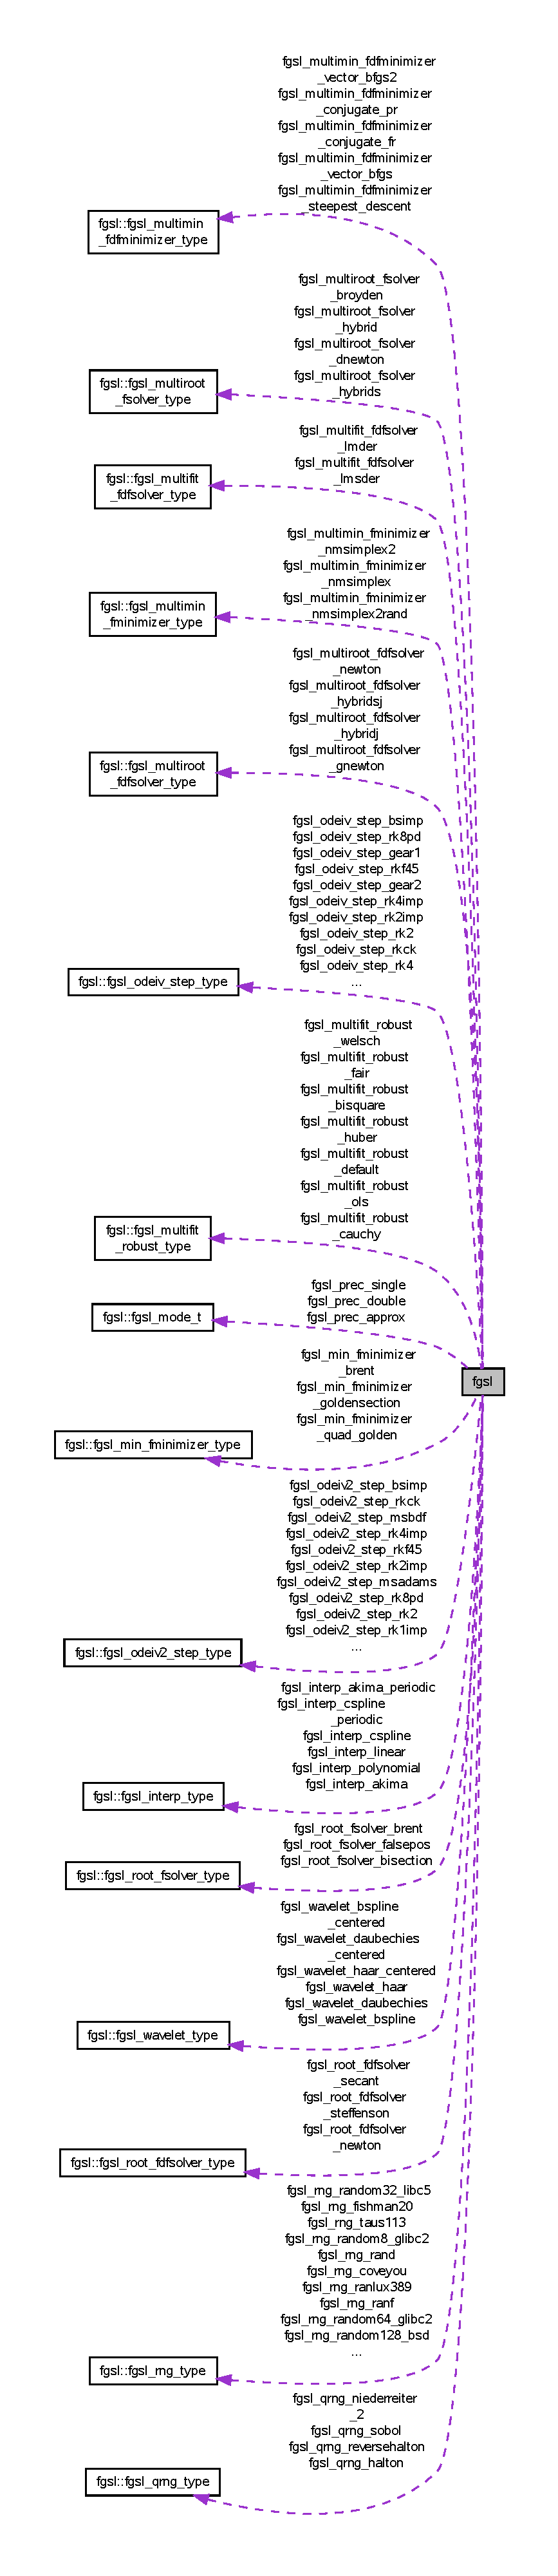
\includegraphics[height=550pt]{classfgsl__coll__graph}
\end{center}
\end{figure}
\subsection*{Data Types}
\begin{DoxyCompactItemize}
\item 
type \hyperlink{structfgsl_1_1fgsl__bspline__deriv__workspace}{fgsl\-\_\-bspline\-\_\-deriv\-\_\-workspace}
\item 
type \hyperlink{structfgsl_1_1fgsl__bspline__workspace}{fgsl\-\_\-bspline\-\_\-workspace}
\item 
type \hyperlink{structfgsl_1_1fgsl__cheb__series}{fgsl\-\_\-cheb\-\_\-series}
\item 
type \hyperlink{structfgsl_1_1fgsl__combination}{fgsl\-\_\-combination}
\item 
type \hyperlink{structfgsl_1_1fgsl__dht}{fgsl\-\_\-dht}
\item 
type \hyperlink{structfgsl_1_1fgsl__eigen__gen__workspace}{fgsl\-\_\-eigen\-\_\-gen\-\_\-workspace}
\item 
type \hyperlink{structfgsl_1_1fgsl__eigen__genherm__workspace}{fgsl\-\_\-eigen\-\_\-genherm\-\_\-workspace}
\item 
type \hyperlink{structfgsl_1_1fgsl__eigen__genhermv__workspace}{fgsl\-\_\-eigen\-\_\-genhermv\-\_\-workspace}
\item 
type \hyperlink{structfgsl_1_1fgsl__eigen__gensymm__workspace}{fgsl\-\_\-eigen\-\_\-gensymm\-\_\-workspace}
\item 
type \hyperlink{structfgsl_1_1fgsl__eigen__gensymmv__workspace}{fgsl\-\_\-eigen\-\_\-gensymmv\-\_\-workspace}
\item 
type \hyperlink{structfgsl_1_1fgsl__eigen__genv__workspace}{fgsl\-\_\-eigen\-\_\-genv\-\_\-workspace}
\item 
type \hyperlink{structfgsl_1_1fgsl__eigen__herm__workspace}{fgsl\-\_\-eigen\-\_\-herm\-\_\-workspace}
\item 
type \hyperlink{structfgsl_1_1fgsl__eigen__hermv__workspace}{fgsl\-\_\-eigen\-\_\-hermv\-\_\-workspace}
\item 
type \hyperlink{structfgsl_1_1fgsl__eigen__nonsymm__workspace}{fgsl\-\_\-eigen\-\_\-nonsymm\-\_\-workspace}
\item 
type \hyperlink{structfgsl_1_1fgsl__eigen__nonsymmv__workspace}{fgsl\-\_\-eigen\-\_\-nonsymmv\-\_\-workspace}
\item 
type \hyperlink{structfgsl_1_1fgsl__eigen__symm__workspace}{fgsl\-\_\-eigen\-\_\-symm\-\_\-workspace}
\item 
type \hyperlink{structfgsl_1_1fgsl__eigen__symmv__workspace}{fgsl\-\_\-eigen\-\_\-symmv\-\_\-workspace}
\item 
type \hyperlink{structfgsl_1_1fgsl__error__handler__t}{fgsl\-\_\-error\-\_\-handler\-\_\-t}
\item 
type \hyperlink{structfgsl_1_1fgsl__fft__complex__wavetable}{fgsl\-\_\-fft\-\_\-complex\-\_\-wavetable}
\item 
type \hyperlink{structfgsl_1_1fgsl__fft__complex__workspace}{fgsl\-\_\-fft\-\_\-complex\-\_\-workspace}
\item 
type \hyperlink{structfgsl_1_1fgsl__fft__halfcomplex__wavetable}{fgsl\-\_\-fft\-\_\-halfcomplex\-\_\-wavetable}
\item 
type \hyperlink{structfgsl_1_1fgsl__fft__real__wavetable}{fgsl\-\_\-fft\-\_\-real\-\_\-wavetable}
\item 
type \hyperlink{structfgsl_1_1fgsl__fft__real__workspace}{fgsl\-\_\-fft\-\_\-real\-\_\-workspace}
\item 
type \hyperlink{structfgsl_1_1fgsl__file}{fgsl\-\_\-file}
\item 
type \hyperlink{structfgsl_1_1fgsl__function}{fgsl\-\_\-function}
\item 
type \hyperlink{structfgsl_1_1fgsl__function__fdf}{fgsl\-\_\-function\-\_\-fdf}
\item 
type \hyperlink{structfgsl_1_1fgsl__histogram}{fgsl\-\_\-histogram}
\item 
type \hyperlink{structfgsl_1_1fgsl__histogram2d}{fgsl\-\_\-histogram2d}
\item 
type \hyperlink{structfgsl_1_1fgsl__histogram2d__pdf}{fgsl\-\_\-histogram2d\-\_\-pdf}
\item 
type \hyperlink{structfgsl_1_1fgsl__histogram__pdf}{fgsl\-\_\-histogram\-\_\-pdf}
\item 
type \hyperlink{structfgsl_1_1fgsl__integration__cquad__workspace}{fgsl\-\_\-integration\-\_\-cquad\-\_\-workspace}
\item 
type \hyperlink{structfgsl_1_1fgsl__integration__glfixed__table}{fgsl\-\_\-integration\-\_\-glfixed\-\_\-table}
\item 
type \hyperlink{structfgsl_1_1fgsl__integration__qawo__table}{fgsl\-\_\-integration\-\_\-qawo\-\_\-table}
\item 
type \hyperlink{structfgsl_1_1fgsl__integration__qaws__table}{fgsl\-\_\-integration\-\_\-qaws\-\_\-table}
\item 
type \hyperlink{structfgsl_1_1fgsl__integration__workspace}{fgsl\-\_\-integration\-\_\-workspace}
\item 
type \hyperlink{structfgsl_1_1fgsl__interp}{fgsl\-\_\-interp}
\item 
type \hyperlink{structfgsl_1_1fgsl__interp__accel}{fgsl\-\_\-interp\-\_\-accel}
\item 
type \hyperlink{structfgsl_1_1fgsl__interp__type}{fgsl\-\_\-interp\-\_\-type}
\item 
type \hyperlink{structfgsl_1_1fgsl__matrix}{fgsl\-\_\-matrix}
\item 
type \hyperlink{structfgsl_1_1fgsl__matrix__complex}{fgsl\-\_\-matrix\-\_\-complex}
\item 
type \hyperlink{structfgsl_1_1fgsl__min__fminimizer}{fgsl\-\_\-min\-\_\-fminimizer}
\item 
type \hyperlink{structfgsl_1_1fgsl__min__fminimizer__type}{fgsl\-\_\-min\-\_\-fminimizer\-\_\-type}
\item 
type \hyperlink{structfgsl_1_1fgsl__mode__t}{fgsl\-\_\-mode\-\_\-t}
\item 
type \hyperlink{structfgsl_1_1fgsl__monte__function}{fgsl\-\_\-monte\-\_\-function}
\item 
type \hyperlink{structfgsl_1_1fgsl__monte__miser__state}{fgsl\-\_\-monte\-\_\-miser\-\_\-state}
\item 
type \hyperlink{structfgsl_1_1fgsl__monte__plain__state}{fgsl\-\_\-monte\-\_\-plain\-\_\-state}
\item 
type \hyperlink{structfgsl_1_1fgsl__monte__vegas__state}{fgsl\-\_\-monte\-\_\-vegas\-\_\-state}
\item 
type \hyperlink{structfgsl_1_1fgsl__multifit__fdfsolver}{fgsl\-\_\-multifit\-\_\-fdfsolver}
\item 
type \hyperlink{structfgsl_1_1fgsl__multifit__fdfsolver__type}{fgsl\-\_\-multifit\-\_\-fdfsolver\-\_\-type}
\item 
type \hyperlink{structfgsl_1_1fgsl__multifit__fsolver}{fgsl\-\_\-multifit\-\_\-fsolver}
\item 
type \hyperlink{structfgsl_1_1fgsl__multifit__fsolver__type}{fgsl\-\_\-multifit\-\_\-fsolver\-\_\-type}
\item 
type \hyperlink{structfgsl_1_1fgsl__multifit__function}{fgsl\-\_\-multifit\-\_\-function}
\item 
type \hyperlink{structfgsl_1_1fgsl__multifit__function__fdf}{fgsl\-\_\-multifit\-\_\-function\-\_\-fdf}
\item 
type \hyperlink{structfgsl_1_1fgsl__multifit__linear__workspace}{fgsl\-\_\-multifit\-\_\-linear\-\_\-workspace}
\item 
type \hyperlink{structfgsl_1_1fgsl__multimin__fdfminimizer}{fgsl\-\_\-multimin\-\_\-fdfminimizer}
\item 
type \hyperlink{structfgsl_1_1fgsl__multimin__fdfminimizer__type}{fgsl\-\_\-multimin\-\_\-fdfminimizer\-\_\-type}
\item 
type \hyperlink{structfgsl_1_1fgsl__multimin__fminimizer}{fgsl\-\_\-multimin\-\_\-fminimizer}
\item 
type \hyperlink{structfgsl_1_1fgsl__multimin__fminimizer__type}{fgsl\-\_\-multimin\-\_\-fminimizer\-\_\-type}
\item 
type \hyperlink{structfgsl_1_1fgsl__multimin__function}{fgsl\-\_\-multimin\-\_\-function}
\item 
type \hyperlink{structfgsl_1_1fgsl__multimin__function__fdf}{fgsl\-\_\-multimin\-\_\-function\-\_\-fdf}
\item 
type \hyperlink{structfgsl_1_1fgsl__multiroot__fdfsolver}{fgsl\-\_\-multiroot\-\_\-fdfsolver}
\item 
type \hyperlink{structfgsl_1_1fgsl__multiroot__fdfsolver__type}{fgsl\-\_\-multiroot\-\_\-fdfsolver\-\_\-type}
\item 
type \hyperlink{structfgsl_1_1fgsl__multiroot__fsolver}{fgsl\-\_\-multiroot\-\_\-fsolver}
\item 
type \hyperlink{structfgsl_1_1fgsl__multiroot__fsolver__type}{fgsl\-\_\-multiroot\-\_\-fsolver\-\_\-type}
\item 
type \hyperlink{structfgsl_1_1fgsl__multiroot__function}{fgsl\-\_\-multiroot\-\_\-function}
\item 
type \hyperlink{structfgsl_1_1fgsl__multiroot__function__fdf}{fgsl\-\_\-multiroot\-\_\-function\-\_\-fdf}
\item 
type \hyperlink{structfgsl_1_1fgsl__multiset}{fgsl\-\_\-multiset}
\item 
type \hyperlink{structfgsl_1_1fgsl__ntuple}{fgsl\-\_\-ntuple}
\item 
type \hyperlink{structfgsl_1_1fgsl__ntuple__select__fn}{fgsl\-\_\-ntuple\-\_\-select\-\_\-fn}
\item 
type \hyperlink{structfgsl_1_1fgsl__ntuple__value__fn}{fgsl\-\_\-ntuple\-\_\-value\-\_\-fn}
\item 
type \hyperlink{structfgsl_1_1fgsl__odeiv2__control}{fgsl\-\_\-odeiv2\-\_\-control}
\item 
type \hyperlink{structfgsl_1_1fgsl__odeiv2__control__type}{fgsl\-\_\-odeiv2\-\_\-control\-\_\-type}
\item 
type \hyperlink{structfgsl_1_1fgsl__odeiv2__driver}{fgsl\-\_\-odeiv2\-\_\-driver}
\item 
type \hyperlink{structfgsl_1_1fgsl__odeiv2__evolve}{fgsl\-\_\-odeiv2\-\_\-evolve}
\item 
type \hyperlink{structfgsl_1_1fgsl__odeiv2__step}{fgsl\-\_\-odeiv2\-\_\-step}
\item 
type \hyperlink{structfgsl_1_1fgsl__odeiv2__step__type}{fgsl\-\_\-odeiv2\-\_\-step\-\_\-type}
\item 
type \hyperlink{structfgsl_1_1fgsl__odeiv2__system}{fgsl\-\_\-odeiv2\-\_\-system}
\item 
type \hyperlink{structfgsl_1_1fgsl__odeiv__control}{fgsl\-\_\-odeiv\-\_\-control}
\item 
type \hyperlink{structfgsl_1_1fgsl__odeiv__control__type}{fgsl\-\_\-odeiv\-\_\-control\-\_\-type}
\item 
type \hyperlink{structfgsl_1_1fgsl__odeiv__evolve}{fgsl\-\_\-odeiv\-\_\-evolve}
\item 
type \hyperlink{structfgsl_1_1fgsl__odeiv__step}{fgsl\-\_\-odeiv\-\_\-step}
\item 
type \hyperlink{structfgsl_1_1fgsl__odeiv__step__type}{fgsl\-\_\-odeiv\-\_\-step\-\_\-type}
\item 
type \hyperlink{structfgsl_1_1fgsl__odeiv__system}{fgsl\-\_\-odeiv\-\_\-system}
\item 
type \hyperlink{structfgsl_1_1fgsl__permutation}{fgsl\-\_\-permutation}
\item 
type \hyperlink{structfgsl_1_1fgsl__poly__complex__workspace}{fgsl\-\_\-poly\-\_\-complex\-\_\-workspace}
\item 
type \hyperlink{structfgsl_1_1fgsl__qrng}{fgsl\-\_\-qrng}
\item 
type \hyperlink{structfgsl_1_1fgsl__qrng__type}{fgsl\-\_\-qrng\-\_\-type}
\item 
type \hyperlink{structfgsl_1_1fgsl__ran__discrete__t}{fgsl\-\_\-ran\-\_\-discrete\-\_\-t}
\item 
type \hyperlink{structfgsl_1_1fgsl__rng}{fgsl\-\_\-rng}
\item 
type \hyperlink{structfgsl_1_1fgsl__rng__type}{fgsl\-\_\-rng\-\_\-type}
\item 
type \hyperlink{structfgsl_1_1fgsl__root__fdfsolver}{fgsl\-\_\-root\-\_\-fdfsolver}
\item 
type \hyperlink{structfgsl_1_1fgsl__root__fdfsolver__type}{fgsl\-\_\-root\-\_\-fdfsolver\-\_\-type}
\item 
type \hyperlink{structfgsl_1_1fgsl__root__fsolver}{fgsl\-\_\-root\-\_\-fsolver}
\item 
type \hyperlink{structfgsl_1_1fgsl__root__fsolver__type}{fgsl\-\_\-root\-\_\-fsolver\-\_\-type}
\item 
type \hyperlink{structfgsl_1_1fgsl__sf__result}{fgsl\-\_\-sf\-\_\-result}
\item 
type \hyperlink{structfgsl_1_1fgsl__sf__result__e10}{fgsl\-\_\-sf\-\_\-result\-\_\-e10}
\item 
type \hyperlink{structfgsl_1_1fgsl__siman__params__t}{fgsl\-\_\-siman\-\_\-params\-\_\-t}
\item 
type \hyperlink{structfgsl_1_1fgsl__spline}{fgsl\-\_\-spline}
\item 
type \hyperlink{structfgsl_1_1fgsl__sum__levin__u__workspace}{fgsl\-\_\-sum\-\_\-levin\-\_\-u\-\_\-workspace}
\item 
type \hyperlink{structfgsl_1_1fgsl__sum__levin__utrunc__workspace}{fgsl\-\_\-sum\-\_\-levin\-\_\-utrunc\-\_\-workspace}
\item 
type \hyperlink{structfgsl_1_1fgsl__vector}{fgsl\-\_\-vector}
\item 
type \hyperlink{structfgsl_1_1fgsl__vector__complex}{fgsl\-\_\-vector\-\_\-complex}
\item 
type \hyperlink{structfgsl_1_1fgsl__wavelet}{fgsl\-\_\-wavelet}
\item 
type \hyperlink{structfgsl_1_1fgsl__wavelet__type}{fgsl\-\_\-wavelet\-\_\-type}
\item 
type \hyperlink{structfgsl_1_1fgsl__wavelet__workspace}{fgsl\-\_\-wavelet\-\_\-workspace}
\item 
type \hyperlink{structfgsl_1_1gsl__complex}{gsl\-\_\-complex}
\item 
type \hyperlink{structfgsl_1_1gsl__sf__result}{gsl\-\_\-sf\-\_\-result}
\item 
type \hyperlink{structfgsl_1_1gsl__sf__result__e10}{gsl\-\_\-sf\-\_\-result\-\_\-e10}
\end{DoxyCompactItemize}
\subsection*{Public Attributes}
\begin{DoxyCompactItemize}
\item 
integer, parameter, public \hyperlink{classfgsl_a9af5113378e0f000eb479d3f90196ddf}{fgsl\-\_\-double} = c\-\_\-double
\item 
integer, parameter, public \hyperlink{classfgsl_a66d0fde3788cc0c300046f8fcd07d702}{fgsl\-\_\-double\-\_\-complex} = c\-\_\-double\-\_\-complex
\item 
integer, parameter, public \hyperlink{classfgsl_a9f38abe97062020e8a507aaa5bc683ab}{fgsl\-\_\-extended} = selected\-\_\-real\-\_\-kind(13)
\item 
integer, parameter, public \hyperlink{classfgsl_a5721fab55a48ca577c4557fdb1861eb6}{fgsl\-\_\-float} = c\-\_\-float
\item 
integer, parameter, public \hyperlink{classfgsl_a222deda1d7a0c0e845ce4a683318efeb}{fgsl\-\_\-int} = c\-\_\-int
\item 
integer, parameter, public \hyperlink{classfgsl_a22fca1111887118eb07d5f9688ea38ad}{fgsl\-\_\-long} = c\-\_\-long
\item 
integer, parameter, public \hyperlink{classfgsl_a82c8fc2281b4c13609c41ae8b7f1cb1e}{fgsl\-\_\-size\-\_\-t} = c\-\_\-size\-\_\-t
\item 
integer, parameter, public \hyperlink{classfgsl_a12911ae4a4462f8e892d903081e77ab4}{fgsl\-\_\-char} = c\-\_\-char
\item 
integer, parameter, public \hyperlink{classfgsl_a1951faf9d6c8119266db0e5eee1865b7}{fgsl\-\_\-strmax} = 128
\item 
integer, parameter, public \hyperlink{classfgsl_a4531e537443b76eab7842214d4e86f01}{fgsl\-\_\-pathmax} = 2048
\item 
character(kind=\hyperlink{classfgsl_a12911ae4a4462f8e892d903081e77ab4}{fgsl\-\_\-char}, len=$\ast$), \\*
parameter, public \hyperlink{classfgsl_a3443bae7bac02745f1562e6c2f891656}{fgsl\-\_\-version} =P\-A\-C\-K\-A\-G\-E\-\_\-\-V\-E\-R\-S\-I\-O\-N
\item 
character(kind=\hyperlink{classfgsl_a12911ae4a4462f8e892d903081e77ab4}{fgsl\-\_\-char}, len=$\ast$), \\*
parameter, public \hyperlink{classfgsl_ad8d3e2a5a480d0a6e9569ef516c5dff4}{fgsl\-\_\-gslbase} =G\-S\-L\-\_\-\-V\-E\-R\-S\-I\-O\-N
\item 
integer(\hyperlink{classfgsl_a222deda1d7a0c0e845ce4a683318efeb}{fgsl\-\_\-int}), parameter, \\*
public \hyperlink{classfgsl_a5637d95a4aceec9a80a9b74a2e40ebdf}{fgsl\-\_\-success} = 0
\item 
integer(\hyperlink{classfgsl_a222deda1d7a0c0e845ce4a683318efeb}{fgsl\-\_\-int}), parameter, \\*
public \hyperlink{classfgsl_a4cb2b20fedfc04419dd412d3bdc635e0}{fgsl\-\_\-failure} = -\/1
\item 
integer(\hyperlink{classfgsl_a222deda1d7a0c0e845ce4a683318efeb}{fgsl\-\_\-int}), parameter, \\*
public \hyperlink{classfgsl_adaee86adbad23b6853659f6564d6c46b}{fgsl\-\_\-continue} = -\/2
\item 
integer(\hyperlink{classfgsl_a222deda1d7a0c0e845ce4a683318efeb}{fgsl\-\_\-int}), parameter, \\*
public \hyperlink{classfgsl_a4a331f3c353a431cb6975bbe8e0cbf63}{fgsl\-\_\-edom} = 1
\item 
integer(\hyperlink{classfgsl_a222deda1d7a0c0e845ce4a683318efeb}{fgsl\-\_\-int}), parameter, \\*
public \hyperlink{classfgsl_a25790738744df3ed3e0b2d50d9b30976}{fgsl\-\_\-erange} = 2
\item 
integer(\hyperlink{classfgsl_a222deda1d7a0c0e845ce4a683318efeb}{fgsl\-\_\-int}), parameter, \\*
public \hyperlink{classfgsl_a3866fec8a527d4830fa9b88464c52417}{fgsl\-\_\-efault} = 3
\item 
integer(\hyperlink{classfgsl_a222deda1d7a0c0e845ce4a683318efeb}{fgsl\-\_\-int}), parameter, \\*
public \hyperlink{classfgsl_a720540845b1b10b1af117475a2b5f2c7}{fgsl\-\_\-einval} = 4
\item 
integer(\hyperlink{classfgsl_a222deda1d7a0c0e845ce4a683318efeb}{fgsl\-\_\-int}), parameter, \\*
public \hyperlink{classfgsl_a027973d6b14562a967273973aed85e4f}{fgsl\-\_\-efactor} = 6
\item 
integer(\hyperlink{classfgsl_a222deda1d7a0c0e845ce4a683318efeb}{fgsl\-\_\-int}), parameter, \\*
public \hyperlink{classfgsl_a9dc60d8f0ce30b7b328d703d09a0e987}{fgsl\-\_\-esanity} = 7
\item 
integer(\hyperlink{classfgsl_a222deda1d7a0c0e845ce4a683318efeb}{fgsl\-\_\-int}), parameter, \\*
public \hyperlink{classfgsl_a70b026317b5a6f797b14978468ca01d9}{fgsl\-\_\-enomem} = 8
\item 
integer(\hyperlink{classfgsl_a222deda1d7a0c0e845ce4a683318efeb}{fgsl\-\_\-int}), parameter, \\*
public \hyperlink{classfgsl_aee7266f310ad4022066e6fe82eecc0f9}{fgsl\-\_\-ebadfunc} = 9
\item 
integer(\hyperlink{classfgsl_a222deda1d7a0c0e845ce4a683318efeb}{fgsl\-\_\-int}), parameter, \\*
public \hyperlink{classfgsl_a89dc8311615f753f8b0b83a60e5f16c0}{fgsl\-\_\-erunaway} = 10
\item 
integer(\hyperlink{classfgsl_a222deda1d7a0c0e845ce4a683318efeb}{fgsl\-\_\-int}), parameter, \\*
public \hyperlink{classfgsl_a5e63249fa198903f233261cb159a3e28}{fgsl\-\_\-emaxiter} = 11
\item 
integer(\hyperlink{classfgsl_a222deda1d7a0c0e845ce4a683318efeb}{fgsl\-\_\-int}), parameter, \\*
public \hyperlink{classfgsl_a13b65889d69077a99a6f13522883061f}{fgsl\-\_\-ezerodiv} = 12
\item 
integer(\hyperlink{classfgsl_a222deda1d7a0c0e845ce4a683318efeb}{fgsl\-\_\-int}), parameter, \\*
public \hyperlink{classfgsl_a3df3fe39582721655da00574f4b021d1}{fgsl\-\_\-ebadtol} = 13
\item 
integer(\hyperlink{classfgsl_a222deda1d7a0c0e845ce4a683318efeb}{fgsl\-\_\-int}), parameter, \\*
public \hyperlink{classfgsl_a7e4da7bbb4435c2bceff8cf57d554015}{fgsl\-\_\-etol} = 14
\item 
integer(\hyperlink{classfgsl_a222deda1d7a0c0e845ce4a683318efeb}{fgsl\-\_\-int}), parameter, \\*
public \hyperlink{classfgsl_ae5ac5a32777e537541e47cb0419da46c}{fgsl\-\_\-eundrflw} = 15
\item 
integer(\hyperlink{classfgsl_a222deda1d7a0c0e845ce4a683318efeb}{fgsl\-\_\-int}), parameter, \\*
public \hyperlink{classfgsl_a7dc79e0a3af443223d2320c5e2b7b803}{fgsl\-\_\-eovrflw} = 16
\item 
integer(\hyperlink{classfgsl_a222deda1d7a0c0e845ce4a683318efeb}{fgsl\-\_\-int}), parameter, \\*
public \hyperlink{classfgsl_afdf53f6a99fb8880de40cd8136bf8e1c}{fgsl\-\_\-eloss} = 17
\item 
integer(\hyperlink{classfgsl_a222deda1d7a0c0e845ce4a683318efeb}{fgsl\-\_\-int}), parameter, \\*
public \hyperlink{classfgsl_a46f7428fe03a54ce95e47c21d299a129}{fgsl\-\_\-eround} = 18
\item 
integer(\hyperlink{classfgsl_a222deda1d7a0c0e845ce4a683318efeb}{fgsl\-\_\-int}), parameter, \\*
public \hyperlink{classfgsl_ac1f16c63f7a3d224fceb2113566856f5}{fgsl\-\_\-ebadlen} = 19
\item 
integer(\hyperlink{classfgsl_a222deda1d7a0c0e845ce4a683318efeb}{fgsl\-\_\-int}), parameter, \\*
public \hyperlink{classfgsl_a0ad3f5a5023fcd60f764cab3b2b07984}{fgsl\-\_\-enotsqr} = 20
\item 
integer(\hyperlink{classfgsl_a222deda1d7a0c0e845ce4a683318efeb}{fgsl\-\_\-int}), parameter, \\*
public \hyperlink{classfgsl_aeb4c28b199599ec4c17ff7330a4ad10d}{fgsl\-\_\-esing} = 21
\item 
integer(\hyperlink{classfgsl_a222deda1d7a0c0e845ce4a683318efeb}{fgsl\-\_\-int}), parameter, \\*
public \hyperlink{classfgsl_a955eb5c7585781ffb9e336843a471566}{fgsl\-\_\-ediverge} = 22
\item 
integer(\hyperlink{classfgsl_a222deda1d7a0c0e845ce4a683318efeb}{fgsl\-\_\-int}), parameter, \\*
public \hyperlink{classfgsl_af76528fed48ac5623d664d6e66e7ac1b}{fgsl\-\_\-eunsup} = 23
\item 
integer(\hyperlink{classfgsl_a222deda1d7a0c0e845ce4a683318efeb}{fgsl\-\_\-int}), parameter, \\*
public \hyperlink{classfgsl_a3a2e9a31e7f3fc209b5269b82d17117c}{fgsl\-\_\-eunimpl} = 24
\item 
integer(\hyperlink{classfgsl_a222deda1d7a0c0e845ce4a683318efeb}{fgsl\-\_\-int}), parameter, \\*
public \hyperlink{classfgsl_aa9ace1ec026e9acd65806d63c8b6e649}{fgsl\-\_\-ecache} = 25
\item 
integer(\hyperlink{classfgsl_a222deda1d7a0c0e845ce4a683318efeb}{fgsl\-\_\-int}), parameter, \\*
public \hyperlink{classfgsl_ac1348341f3d95b02f852466ca383d1ae}{fgsl\-\_\-etable} = 26
\item 
integer(\hyperlink{classfgsl_a222deda1d7a0c0e845ce4a683318efeb}{fgsl\-\_\-int}), parameter, \\*
public \hyperlink{classfgsl_a11266b4068f90334758a26d35c116f73}{fgsl\-\_\-enoprog} = 27
\item 
integer(\hyperlink{classfgsl_a222deda1d7a0c0e845ce4a683318efeb}{fgsl\-\_\-int}), parameter, \\*
public \hyperlink{classfgsl_ad9567598ce07cacf43815d0453e649bb}{fgsl\-\_\-enoprogj} = 28
\item 
integer(\hyperlink{classfgsl_a222deda1d7a0c0e845ce4a683318efeb}{fgsl\-\_\-int}), parameter, \\*
public \hyperlink{classfgsl_a9b3ff0443a3c8e9570d06e762b1ca241}{fgsl\-\_\-etolf} = 29
\item 
integer(\hyperlink{classfgsl_a222deda1d7a0c0e845ce4a683318efeb}{fgsl\-\_\-int}), parameter, \\*
public \hyperlink{classfgsl_ad136d96d34c4ac68f155224650a94e4c}{fgsl\-\_\-etolx} = 30
\item 
integer(\hyperlink{classfgsl_a222deda1d7a0c0e845ce4a683318efeb}{fgsl\-\_\-int}), parameter, \\*
public \hyperlink{classfgsl_a12d84e3678cb637e43f1a7a888558110}{fgsl\-\_\-etolg} = 31
\item 
integer(\hyperlink{classfgsl_a222deda1d7a0c0e845ce4a683318efeb}{fgsl\-\_\-int}), parameter, \\*
public \hyperlink{classfgsl_a9641f79a70406a1c9f483f01fdb1ccfa}{fgsl\-\_\-eof} = 32
\item 
real(\hyperlink{classfgsl_a9f38abe97062020e8a507aaa5bc683ab}{fgsl\-\_\-extended}), parameter, \\*
public \hyperlink{classfgsl_abd883826f3a31d832e0746f37ac56cff}{m\-\_\-e} = 2.\-71828182845904523536028747135\-\_\-fgsl\-\_\-extended
\item 
real(\hyperlink{classfgsl_a9f38abe97062020e8a507aaa5bc683ab}{fgsl\-\_\-extended}), parameter, \\*
public \hyperlink{classfgsl_a93d2e5a473874e31cbcf8de12963fd8e}{m\-\_\-log2e} = 1.\-44269504088896340735992468100\-\_\-fgsl\-\_\-extended
\item 
real(\hyperlink{classfgsl_a9f38abe97062020e8a507aaa5bc683ab}{fgsl\-\_\-extended}), parameter, \\*
public \hyperlink{classfgsl_a64dfb3018d641c61312823bf56c85023}{m\-\_\-log10e} = 0.\-43429448190325182765112891892\-\_\-fgsl\-\_\-extended
\item 
real(\hyperlink{classfgsl_a9f38abe97062020e8a507aaa5bc683ab}{fgsl\-\_\-extended}), parameter, \\*
public \hyperlink{classfgsl_a7d0e2199519f7100527499e3c206fc31}{m\-\_\-sqrt2} = 1.\-41421356237309504880168872421\-\_\-fgsl\-\_\-extended
\item 
real(\hyperlink{classfgsl_a9f38abe97062020e8a507aaa5bc683ab}{fgsl\-\_\-extended}), parameter, \\*
public \hyperlink{classfgsl_aa15c7774ec8561b9221b81138e50d715}{m\-\_\-sqrt1\-\_\-2} = 0.\-70710678118654752440084436210\-\_\-fgsl\-\_\-extended
\item 
real(\hyperlink{classfgsl_a9f38abe97062020e8a507aaa5bc683ab}{fgsl\-\_\-extended}), parameter, \\*
public \hyperlink{classfgsl_acdd93c47924b7382b9ab00728cc46b9f}{m\-\_\-sqrt3} = 1.\-73205080756887729352744634151\-\_\-fgsl\-\_\-extended
\item 
real(\hyperlink{classfgsl_a9f38abe97062020e8a507aaa5bc683ab}{fgsl\-\_\-extended}), parameter, \\*
public \hyperlink{classfgsl_a8af1e390793c77a120b600e4844495dc}{m\-\_\-pi} = 3.\-14159265358979323846264338328\-\_\-fgsl\-\_\-extended
\item 
real(\hyperlink{classfgsl_a9f38abe97062020e8a507aaa5bc683ab}{fgsl\-\_\-extended}), parameter, \\*
public \hyperlink{classfgsl_af8cd74655823aa30933d33b51ac35bbc}{m\-\_\-pi\-\_\-2} = 1.\-57079632679489661923132169164\-\_\-fgsl\-\_\-extended
\item 
real(\hyperlink{classfgsl_a9f38abe97062020e8a507aaa5bc683ab}{fgsl\-\_\-extended}), parameter, \\*
public \hyperlink{classfgsl_ac72cdbd05abd60541bd253d571673cf4}{m\-\_\-pi\-\_\-4} = 0.\-78539816339744830961566084582\-\_\-fgsl\-\_\-extended
\item 
real(\hyperlink{classfgsl_a9f38abe97062020e8a507aaa5bc683ab}{fgsl\-\_\-extended}), parameter, \\*
public \hyperlink{classfgsl_aa32be73a066aea0217a624284ae34c39}{m\-\_\-sqrtpi} = 1.\-77245385090551602729816748334\-\_\-fgsl\-\_\-extended
\item 
real(\hyperlink{classfgsl_a9f38abe97062020e8a507aaa5bc683ab}{fgsl\-\_\-extended}), parameter, \\*
public \hyperlink{classfgsl_a20272585dc8f0b54e493f4717330469a}{m\-\_\-2\-\_\-sqrtpi} = 1.\-12837916709551257389615890312\-\_\-fgsl\-\_\-extended
\item 
real(\hyperlink{classfgsl_a9f38abe97062020e8a507aaa5bc683ab}{fgsl\-\_\-extended}), parameter, \\*
public \hyperlink{classfgsl_a10fdf50a29d35a63b13bc641ed465051}{m\-\_\-1\-\_\-pi} = 0.\-31830988618379067153776752675\-\_\-fgsl\-\_\-extended
\item 
real(\hyperlink{classfgsl_a9f38abe97062020e8a507aaa5bc683ab}{fgsl\-\_\-extended}), parameter, \\*
public \hyperlink{classfgsl_a28e530e58a51ac2bbce00674f617bbbd}{m\-\_\-2\-\_\-pi} = 0.\-63661977236758134307553505349\-\_\-fgsl\-\_\-extended
\item 
real(\hyperlink{classfgsl_a9f38abe97062020e8a507aaa5bc683ab}{fgsl\-\_\-extended}), parameter, \\*
public \hyperlink{classfgsl_a152b62af261c671c54b99ac278df759d}{m\-\_\-ln10} = 2.\-30258509299404568401799145468\-\_\-fgsl\-\_\-extended
\item 
real(\hyperlink{classfgsl_a9f38abe97062020e8a507aaa5bc683ab}{fgsl\-\_\-extended}), parameter, \\*
public \hyperlink{classfgsl_a126c02aa2554290ff648243425e03ace}{m\-\_\-ln2} = 0.\-69314718055994530941723212146\-\_\-fgsl\-\_\-extended
\item 
real(\hyperlink{classfgsl_a9f38abe97062020e8a507aaa5bc683ab}{fgsl\-\_\-extended}), parameter, \\*
public \hyperlink{classfgsl_ae9aff58d6fcadaab60410424796cd713}{m\-\_\-lnpi} = 1.\-14472988584940017414342735135\-\_\-fgsl\-\_\-extended
\item 
real(\hyperlink{classfgsl_a9f38abe97062020e8a507aaa5bc683ab}{fgsl\-\_\-extended}), parameter, \\*
public \hyperlink{classfgsl_ab8079b9a6e17b1def176e97feda2a841}{m\-\_\-euler} = 0.\-57721566490153286060651209008\-\_\-fgsl\-\_\-extended
\item 
real(\hyperlink{classfgsl_a9af5113378e0f000eb479d3f90196ddf}{fgsl\-\_\-double}), parameter, \\*
public \hyperlink{classfgsl_aa12fc22d559b707d7e1e63ac17c596cb}{fgsl\-\_\-const\-\_\-num\-\_\-fine\-\_\-structure} = 7.\-297352533\-E-\/3\-\_\-fgsl\-\_\-double
\item 
real(\hyperlink{classfgsl_a9af5113378e0f000eb479d3f90196ddf}{fgsl\-\_\-double}), parameter, \\*
public \hyperlink{classfgsl_a009cf79cdb578326cbceea51aa302e53}{fgsl\-\_\-const\-\_\-num\-\_\-avogadro} = 6.\-02214199\-E23\-\_\-fgsl\-\_\-double
\item 
real(\hyperlink{classfgsl_a9af5113378e0f000eb479d3f90196ddf}{fgsl\-\_\-double}), parameter, \\*
public \hyperlink{classfgsl_a0b9812de1b4fd0e830437a0f81756409}{fgsl\-\_\-const\-\_\-num\-\_\-yotta} = 1e24\-\_\-fgsl\-\_\-double
\item 
real(\hyperlink{classfgsl_a9af5113378e0f000eb479d3f90196ddf}{fgsl\-\_\-double}), parameter, \\*
public \hyperlink{classfgsl_adbd48c7f748a96cfbe32705159c06b84}{fgsl\-\_\-const\-\_\-num\-\_\-zetta} = 1e21\-\_\-fgsl\-\_\-double
\item 
real(\hyperlink{classfgsl_a9af5113378e0f000eb479d3f90196ddf}{fgsl\-\_\-double}), parameter, \\*
public \hyperlink{classfgsl_a0d6878f336ffcf4aaf3af66bbdfc5a9b}{fgsl\-\_\-const\-\_\-num\-\_\-exa} = 1e18\-\_\-fgsl\-\_\-double
\item 
real(\hyperlink{classfgsl_a9af5113378e0f000eb479d3f90196ddf}{fgsl\-\_\-double}), parameter, \\*
public \hyperlink{classfgsl_aa124eb86407291ed14158b0802d02029}{fgsl\-\_\-const\-\_\-num\-\_\-peta} = 1e15\-\_\-fgsl\-\_\-double
\item 
real(\hyperlink{classfgsl_a9af5113378e0f000eb479d3f90196ddf}{fgsl\-\_\-double}), parameter, \\*
public \hyperlink{classfgsl_a6b39aa71fe2d5af7fa748710f70afd58}{fgsl\-\_\-const\-\_\-num\-\_\-tera} = 1e12\-\_\-fgsl\-\_\-double
\item 
real(\hyperlink{classfgsl_a9af5113378e0f000eb479d3f90196ddf}{fgsl\-\_\-double}), parameter, \\*
public \hyperlink{classfgsl_a27758acec15033cf3c0918d8d9c55eca}{fgsl\-\_\-const\-\_\-num\-\_\-giga} = 1e9\-\_\-fgsl\-\_\-double
\item 
real(\hyperlink{classfgsl_a9af5113378e0f000eb479d3f90196ddf}{fgsl\-\_\-double}), parameter, \\*
public \hyperlink{classfgsl_a3783a70eb7db5888129ccf2094415129}{fgsl\-\_\-const\-\_\-num\-\_\-mega} = 1e6\-\_\-fgsl\-\_\-double
\item 
real(\hyperlink{classfgsl_a9af5113378e0f000eb479d3f90196ddf}{fgsl\-\_\-double}), parameter, \\*
public \hyperlink{classfgsl_a921e5869ad16238cb472943f2486d0ac}{fgsl\-\_\-const\-\_\-num\-\_\-kilo} = 1e3\-\_\-fgsl\-\_\-double
\item 
real(\hyperlink{classfgsl_a9af5113378e0f000eb479d3f90196ddf}{fgsl\-\_\-double}), parameter, \\*
public \hyperlink{classfgsl_a3fb5efe0ae67e7937ba05e8f184e2d35}{fgsl\-\_\-const\-\_\-num\-\_\-milli} = 1e-\/3\-\_\-fgsl\-\_\-double
\item 
real(\hyperlink{classfgsl_a9af5113378e0f000eb479d3f90196ddf}{fgsl\-\_\-double}), parameter, \\*
public \hyperlink{classfgsl_aa7d0f5804ffc72dc0ecddbee234cd51d}{fgsl\-\_\-const\-\_\-num\-\_\-micro} = 1e-\/6\-\_\-fgsl\-\_\-double
\item 
real(\hyperlink{classfgsl_a9af5113378e0f000eb479d3f90196ddf}{fgsl\-\_\-double}), parameter, \\*
public \hyperlink{classfgsl_a18d57365a461c2adc8f4e0ddb4c690d6}{fgsl\-\_\-const\-\_\-num\-\_\-nano} = 1e-\/9\-\_\-fgsl\-\_\-double
\item 
real(\hyperlink{classfgsl_a9af5113378e0f000eb479d3f90196ddf}{fgsl\-\_\-double}), parameter, \\*
public \hyperlink{classfgsl_a8a137e17b45fbfd8a37ef012e9b522ab}{fgsl\-\_\-const\-\_\-num\-\_\-pico} = 1e-\/12\-\_\-fgsl\-\_\-double
\item 
real(\hyperlink{classfgsl_a9af5113378e0f000eb479d3f90196ddf}{fgsl\-\_\-double}), parameter, \\*
public \hyperlink{classfgsl_a3ab8d745c9129ec33f7556e68234b60b}{fgsl\-\_\-const\-\_\-num\-\_\-femto} = 1e-\/15\-\_\-fgsl\-\_\-double
\item 
real(\hyperlink{classfgsl_a9af5113378e0f000eb479d3f90196ddf}{fgsl\-\_\-double}), parameter, \\*
public \hyperlink{classfgsl_aca23ff810481681a4329c406eb3c4bbc}{fgsl\-\_\-const\-\_\-num\-\_\-atto} = 1e-\/18\-\_\-fgsl\-\_\-double
\item 
real(\hyperlink{classfgsl_a9af5113378e0f000eb479d3f90196ddf}{fgsl\-\_\-double}), parameter, \\*
public \hyperlink{classfgsl_ac924f9358aa8ca1b7a72025328901e8e}{fgsl\-\_\-const\-\_\-num\-\_\-zepto} = 1e-\/21\-\_\-fgsl\-\_\-double
\item 
real(\hyperlink{classfgsl_a9af5113378e0f000eb479d3f90196ddf}{fgsl\-\_\-double}), parameter, \\*
public \hyperlink{classfgsl_a97bcc951d0797621c0a06cb1d63cad49}{fgsl\-\_\-const\-\_\-num\-\_\-yocto} = 1e-\/24\-\_\-fgsl\-\_\-double
\item 
real(\hyperlink{classfgsl_a9af5113378e0f000eb479d3f90196ddf}{fgsl\-\_\-double}), parameter, \\*
public \hyperlink{classfgsl_a3d8ceae8504f8bd508cbd8865e1ba1b8}{fgsl\-\_\-const\-\_\-mksa\-\_\-speed\-\_\-of\-\_\-light} = 2.\-99792458e8\-\_\-fgsl\-\_\-double
\item 
real(\hyperlink{classfgsl_a9af5113378e0f000eb479d3f90196ddf}{fgsl\-\_\-double}), parameter, \\*
public \hyperlink{classfgsl_a74c4f68c51be744dc16f9de6679690a1}{fgsl\-\_\-const\-\_\-mksa\-\_\-gravitational\-\_\-constant} = 6.\-673e-\/11\-\_\-fgsl\-\_\-double
\item 
real(\hyperlink{classfgsl_a9af5113378e0f000eb479d3f90196ddf}{fgsl\-\_\-double}), parameter, \\*
public \hyperlink{classfgsl_a1f1f5a27cac13f7f29c34ccb809e2eae}{fgsl\-\_\-const\-\_\-mksa\-\_\-plancks\-\_\-constant\-\_\-h} = 6.\-62606896e-\/34\-\_\-fgsl\-\_\-double
\item 
real(\hyperlink{classfgsl_a9af5113378e0f000eb479d3f90196ddf}{fgsl\-\_\-double}), parameter, \\*
public \hyperlink{classfgsl_a505da32ff79a7c317534298642a2ac3c}{fgsl\-\_\-const\-\_\-mksa\-\_\-plancks\-\_\-constant\-\_\-hbar} = 1.\-05457162825e-\/34\-\_\-fgsl\-\_\-double
\item 
real(\hyperlink{classfgsl_a9af5113378e0f000eb479d3f90196ddf}{fgsl\-\_\-double}), parameter, \\*
public \hyperlink{classfgsl_aa2d41436d179db0d4d442c5207737611}{fgsl\-\_\-const\-\_\-mksa\-\_\-astronomical\-\_\-unit} = 1.\-49597870691e11\-\_\-fgsl\-\_\-double
\item 
real(\hyperlink{classfgsl_a9af5113378e0f000eb479d3f90196ddf}{fgsl\-\_\-double}), parameter, \\*
public \hyperlink{classfgsl_ac9efe31fa2e902dc8cced7ce8b82c610}{fgsl\-\_\-const\-\_\-mksa\-\_\-light\-\_\-year} = 9.\-46053620707e15\-\_\-fgsl\-\_\-double
\item 
real(\hyperlink{classfgsl_a9af5113378e0f000eb479d3f90196ddf}{fgsl\-\_\-double}), parameter, \\*
public \hyperlink{classfgsl_ab701318a50ffa3b0b31f26f7882a2b16}{fgsl\-\_\-const\-\_\-mksa\-\_\-parsec} = 3.\-08567758135e16\-\_\-fgsl\-\_\-double
\item 
real(\hyperlink{classfgsl_a9af5113378e0f000eb479d3f90196ddf}{fgsl\-\_\-double}), parameter, \\*
public \hyperlink{classfgsl_a7c644841a5ff5cd815dca7cfc3383642}{fgsl\-\_\-const\-\_\-mksa\-\_\-grav\-\_\-accel} = 9.\-80665e0\-\_\-fgsl\-\_\-double
\item 
real(\hyperlink{classfgsl_a9af5113378e0f000eb479d3f90196ddf}{fgsl\-\_\-double}), parameter, \\*
public \hyperlink{classfgsl_a2b715db04903e667b5f50d6df3054bee}{fgsl\-\_\-const\-\_\-mksa\-\_\-electron\-\_\-volt} = 1.\-602176487e-\/19\-\_\-fgsl\-\_\-double
\item 
real(\hyperlink{classfgsl_a9af5113378e0f000eb479d3f90196ddf}{fgsl\-\_\-double}), parameter, \\*
public \hyperlink{classfgsl_a9b37f99c3856817b93dd18bc94b81725}{fgsl\-\_\-const\-\_\-mksa\-\_\-mass\-\_\-electron} = 9.\-10938188e-\/31\-\_\-fgsl\-\_\-double
\item 
real(\hyperlink{classfgsl_a9af5113378e0f000eb479d3f90196ddf}{fgsl\-\_\-double}), parameter, \\*
public \hyperlink{classfgsl_afcace800f07f1c2e9703336d2ff02ba4}{fgsl\-\_\-const\-\_\-mksa\-\_\-mass\-\_\-muon} = 1.\-88353109e-\/28\-\_\-fgsl\-\_\-double
\item 
real(\hyperlink{classfgsl_a9af5113378e0f000eb479d3f90196ddf}{fgsl\-\_\-double}), parameter, \\*
public \hyperlink{classfgsl_a9b4432f549e95747550b45df3417757f}{fgsl\-\_\-const\-\_\-mksa\-\_\-mass\-\_\-proton} = 1.\-67262158e-\/27\-\_\-fgsl\-\_\-double
\item 
real(\hyperlink{classfgsl_a9af5113378e0f000eb479d3f90196ddf}{fgsl\-\_\-double}), parameter, \\*
public \hyperlink{classfgsl_a4480f5ff7a83600820b4cdaa8aff929e}{fgsl\-\_\-const\-\_\-mksa\-\_\-mass\-\_\-neutron} = 1.\-67492716e-\/27\-\_\-fgsl\-\_\-double
\item 
real(\hyperlink{classfgsl_a9af5113378e0f000eb479d3f90196ddf}{fgsl\-\_\-double}), parameter, \\*
public \hyperlink{classfgsl_a06f564b1101469e9756b3bb20be06b16}{fgsl\-\_\-const\-\_\-mksa\-\_\-rydberg} = 2.\-17987196968e-\/18\-\_\-fgsl\-\_\-double
\item 
real(\hyperlink{classfgsl_a9af5113378e0f000eb479d3f90196ddf}{fgsl\-\_\-double}), parameter, \\*
public \hyperlink{classfgsl_aee3fe8b4260b1d34436e9f66707b773e}{fgsl\-\_\-const\-\_\-mksa\-\_\-boltzmann} = 1.\-3806504e-\/23\-\_\-fgsl\-\_\-double
\item 
real(\hyperlink{classfgsl_a9af5113378e0f000eb479d3f90196ddf}{fgsl\-\_\-double}), parameter, \\*
public \hyperlink{classfgsl_afa92cd1a7ffe8a0106c3ae29720b0f84}{fgsl\-\_\-const\-\_\-mksa\-\_\-bohr\-\_\-magneton} = 9.\-27400899e-\/24\-\_\-fgsl\-\_\-double
\item 
real(\hyperlink{classfgsl_a9af5113378e0f000eb479d3f90196ddf}{fgsl\-\_\-double}), parameter, \\*
public \hyperlink{classfgsl_a01a0e11a78d0097f8c8a170dbea03e3f}{fgsl\-\_\-const\-\_\-mksa\-\_\-nuclear\-\_\-magneton} = 5.\-05078317e-\/27\-\_\-fgsl\-\_\-double
\item 
real(\hyperlink{classfgsl_a9af5113378e0f000eb479d3f90196ddf}{fgsl\-\_\-double}), parameter, \\*
public \hyperlink{classfgsl_ae360dd0b55b309065855f8521a316e0f}{fgsl\-\_\-const\-\_\-mksa\-\_\-electron\-\_\-magnetic\-\_\-moment} = 9.\-28476362e-\/24\-\_\-fgsl\-\_\-double
\item 
real(\hyperlink{classfgsl_a9af5113378e0f000eb479d3f90196ddf}{fgsl\-\_\-double}), parameter, \\*
public \hyperlink{classfgsl_a11b01d727e4e01028200e21ced0e16c2}{fgsl\-\_\-const\-\_\-mksa\-\_\-proton\-\_\-magnetic\-\_\-moment} = 1.\-410606633e-\/26\-\_\-fgsl\-\_\-double
\item 
real(\hyperlink{classfgsl_a9af5113378e0f000eb479d3f90196ddf}{fgsl\-\_\-double}), parameter, \\*
public \hyperlink{classfgsl_aba418557adafd1575eab5108ba172cf7}{fgsl\-\_\-const\-\_\-mksa\-\_\-molar\-\_\-gas} = 8.\-314472e0\-\_\-fgsl\-\_\-double
\item 
real(\hyperlink{classfgsl_a9af5113378e0f000eb479d3f90196ddf}{fgsl\-\_\-double}), parameter, \\*
public \hyperlink{classfgsl_a43547e219346197d5b5b8c6adff614eb}{fgsl\-\_\-const\-\_\-mksa\-\_\-standard\-\_\-gas\-\_\-volume} = 2.\-2710981e-\/2\-\_\-fgsl\-\_\-double
\item 
real(\hyperlink{classfgsl_a9af5113378e0f000eb479d3f90196ddf}{fgsl\-\_\-double}), parameter, \\*
public \hyperlink{classfgsl_a5c0cc4ab0dc2be570d83ef0f9d2f4ba6}{fgsl\-\_\-const\-\_\-mksa\-\_\-minute} = 6e1\-\_\-fgsl\-\_\-double
\item 
real(\hyperlink{classfgsl_a9af5113378e0f000eb479d3f90196ddf}{fgsl\-\_\-double}), parameter, \\*
public \hyperlink{classfgsl_aa7d132341cda0d591f1452a894cf5855}{fgsl\-\_\-const\-\_\-mksa\-\_\-hour} = 3.\-6e3\-\_\-fgsl\-\_\-double
\item 
real(\hyperlink{classfgsl_a9af5113378e0f000eb479d3f90196ddf}{fgsl\-\_\-double}), parameter, \\*
public \hyperlink{classfgsl_af69acf253e04452510d9ec67efa458d2}{fgsl\-\_\-const\-\_\-mksa\-\_\-day} = 8.\-64e4\-\_\-fgsl\-\_\-double
\item 
real(\hyperlink{classfgsl_a9af5113378e0f000eb479d3f90196ddf}{fgsl\-\_\-double}), parameter, \\*
public \hyperlink{classfgsl_aecb67f391facbac682484e9d352dac5e}{fgsl\-\_\-const\-\_\-mksa\-\_\-week} = 6.\-048e5\-\_\-fgsl\-\_\-double
\item 
real(\hyperlink{classfgsl_a9af5113378e0f000eb479d3f90196ddf}{fgsl\-\_\-double}), parameter, \\*
public \hyperlink{classfgsl_a272689a26b0b7b5cd89f28713aa251d4}{fgsl\-\_\-const\-\_\-mksa\-\_\-inch} = 2.\-54e-\/2\-\_\-fgsl\-\_\-double
\item 
real(\hyperlink{classfgsl_a9af5113378e0f000eb479d3f90196ddf}{fgsl\-\_\-double}), parameter, \\*
public \hyperlink{classfgsl_acff74ed42941dc6324409ba0eee894ee}{fgsl\-\_\-const\-\_\-mksa\-\_\-foot} = 3.\-048e-\/1\-\_\-fgsl\-\_\-double
\item 
real(\hyperlink{classfgsl_a9af5113378e0f000eb479d3f90196ddf}{fgsl\-\_\-double}), parameter, \\*
public \hyperlink{classfgsl_a822a621129f787917e82b140d0814b72}{fgsl\-\_\-const\-\_\-mksa\-\_\-yard} = 9.\-144e-\/1\-\_\-fgsl\-\_\-double
\item 
real(\hyperlink{classfgsl_a9af5113378e0f000eb479d3f90196ddf}{fgsl\-\_\-double}), parameter, \\*
public \hyperlink{classfgsl_a6336ad4316ac012f6ae1ba2c951ec520}{fgsl\-\_\-const\-\_\-mksa\-\_\-mile} = 1.\-609344e3\-\_\-fgsl\-\_\-double
\item 
real(\hyperlink{classfgsl_a9af5113378e0f000eb479d3f90196ddf}{fgsl\-\_\-double}), parameter, \\*
public \hyperlink{classfgsl_a035a322332ff494af9c3ecfb5dca6125}{fgsl\-\_\-const\-\_\-mksa\-\_\-nautical\-\_\-mile} = 1.\-852e3\-\_\-fgsl\-\_\-double
\item 
real(\hyperlink{classfgsl_a9af5113378e0f000eb479d3f90196ddf}{fgsl\-\_\-double}), parameter, \\*
public \hyperlink{classfgsl_a1b3e809c97882aeaebf2e325079f38a3}{fgsl\-\_\-const\-\_\-mksa\-\_\-fathom} = 1.\-8288e0\-\_\-fgsl\-\_\-double
\item 
real(\hyperlink{classfgsl_a9af5113378e0f000eb479d3f90196ddf}{fgsl\-\_\-double}), parameter, \\*
public \hyperlink{classfgsl_af6a9d8baf161c3f9b2b9c8ef41833a67}{fgsl\-\_\-const\-\_\-mksa\-\_\-mil} = 2.\-54e-\/5\-\_\-fgsl\-\_\-double
\item 
real(\hyperlink{classfgsl_a9af5113378e0f000eb479d3f90196ddf}{fgsl\-\_\-double}), parameter, \\*
public \hyperlink{classfgsl_ad8f1c0644b869b25114ce66526bd4a9d}{fgsl\-\_\-const\-\_\-mksa\-\_\-point} = 3.\-52777777778e-\/4\-\_\-fgsl\-\_\-double
\item 
real(\hyperlink{classfgsl_a9af5113378e0f000eb479d3f90196ddf}{fgsl\-\_\-double}), parameter, \\*
public \hyperlink{classfgsl_a962d8da1f8bc62c2323777660898e316}{fgsl\-\_\-const\-\_\-mksa\-\_\-texpoint} = 3.\-51459803515e-\/4\-\_\-fgsl\-\_\-double
\item 
real(\hyperlink{classfgsl_a9af5113378e0f000eb479d3f90196ddf}{fgsl\-\_\-double}), parameter, \\*
public \hyperlink{classfgsl_ab0be2229dca10e5128f21a8729ff742b}{fgsl\-\_\-const\-\_\-mksa\-\_\-micron} = 1e-\/6\-\_\-fgsl\-\_\-double
\item 
real(\hyperlink{classfgsl_a9af5113378e0f000eb479d3f90196ddf}{fgsl\-\_\-double}), parameter, \\*
public \hyperlink{classfgsl_ae348f6545928612e5e56ed4174d31875}{fgsl\-\_\-const\-\_\-mksa\-\_\-angstrom} = 1e-\/10\-\_\-fgsl\-\_\-double
\item 
real(\hyperlink{classfgsl_a9af5113378e0f000eb479d3f90196ddf}{fgsl\-\_\-double}), parameter, \\*
public \hyperlink{classfgsl_a62efb1288447e01349bbf38c21b82e70}{fgsl\-\_\-const\-\_\-mksa\-\_\-hectare} = 1e4\-\_\-fgsl\-\_\-double
\item 
real(\hyperlink{classfgsl_a9af5113378e0f000eb479d3f90196ddf}{fgsl\-\_\-double}), parameter, \\*
public \hyperlink{classfgsl_a58e85d8e8be547abd415a03ac8cfe6d9}{fgsl\-\_\-const\-\_\-mksa\-\_\-acre} = 4.\-04685642241e3\-\_\-fgsl\-\_\-double
\item 
real(\hyperlink{classfgsl_a9af5113378e0f000eb479d3f90196ddf}{fgsl\-\_\-double}), parameter, \\*
public \hyperlink{classfgsl_a859c8ea83a5175d31bc4240282c2b0b4}{fgsl\-\_\-const\-\_\-mksa\-\_\-barn} = 1e-\/28\-\_\-fgsl\-\_\-double
\item 
real(\hyperlink{classfgsl_a9af5113378e0f000eb479d3f90196ddf}{fgsl\-\_\-double}), parameter, \\*
public \hyperlink{classfgsl_ac989bb9124679e7e571cef06c81e5fe3}{fgsl\-\_\-const\-\_\-mksa\-\_\-liter} = 1e-\/3\-\_\-fgsl\-\_\-double
\item 
real(\hyperlink{classfgsl_a9af5113378e0f000eb479d3f90196ddf}{fgsl\-\_\-double}), parameter, \\*
public \hyperlink{classfgsl_a9c8e297dc4a0fa63d97e1c130cc5248a}{fgsl\-\_\-const\-\_\-mksa\-\_\-us\-\_\-gallon} = 3.\-78541178402e-\/3\-\_\-fgsl\-\_\-double
\item 
real(\hyperlink{classfgsl_a9af5113378e0f000eb479d3f90196ddf}{fgsl\-\_\-double}), parameter, \\*
public \hyperlink{classfgsl_a30b92280c9a587dcda6d603b6c737fc3}{fgsl\-\_\-const\-\_\-mksa\-\_\-quart} = 9.\-46352946004e-\/4\-\_\-fgsl\-\_\-double
\item 
real(\hyperlink{classfgsl_a9af5113378e0f000eb479d3f90196ddf}{fgsl\-\_\-double}), parameter, \\*
public \hyperlink{classfgsl_a11b62fc3ced19e2c4f1ad227de09f9f0}{fgsl\-\_\-const\-\_\-mksa\-\_\-pint} = 4.\-73176473002e-\/4\-\_\-fgsl\-\_\-double
\item 
real(\hyperlink{classfgsl_a9af5113378e0f000eb479d3f90196ddf}{fgsl\-\_\-double}), parameter, \\*
public \hyperlink{classfgsl_af7eed4749b386e3a913ae8e18cadc2bc}{fgsl\-\_\-const\-\_\-mksa\-\_\-cup} = 2.\-36588236501e-\/4\-\_\-fgsl\-\_\-double
\item 
real(\hyperlink{classfgsl_a9af5113378e0f000eb479d3f90196ddf}{fgsl\-\_\-double}), parameter, \\*
public \hyperlink{classfgsl_af688bbef5ebab7dfd674fad9cf5d8bd3}{fgsl\-\_\-const\-\_\-mksa\-\_\-fluid\-\_\-ounce} = 2.\-95735295626e-\/5\-\_\-fgsl\-\_\-double
\item 
real(\hyperlink{classfgsl_a9af5113378e0f000eb479d3f90196ddf}{fgsl\-\_\-double}), parameter, \\*
public \hyperlink{classfgsl_abb32761f02e5a238d65d6c3e48c1c2b9}{fgsl\-\_\-const\-\_\-mksa\-\_\-tablespoon} = 1.\-47867647813e-\/5\-\_\-fgsl\-\_\-double
\item 
real(\hyperlink{classfgsl_a9af5113378e0f000eb479d3f90196ddf}{fgsl\-\_\-double}), parameter, \\*
public \hyperlink{classfgsl_aa58032e706375dbeb56727446a0ffea1}{fgsl\-\_\-const\-\_\-mksa\-\_\-teaspoon} = 4.\-92892159375e-\/6\-\_\-fgsl\-\_\-double
\item 
real(\hyperlink{classfgsl_a9af5113378e0f000eb479d3f90196ddf}{fgsl\-\_\-double}), parameter, \\*
public \hyperlink{classfgsl_a12f46f464315290d696dc0dd7d011aaf}{fgsl\-\_\-const\-\_\-mksa\-\_\-canadian\-\_\-gallon} = 4.\-54609e-\/3\-\_\-fgsl\-\_\-double
\item 
real(\hyperlink{classfgsl_a9af5113378e0f000eb479d3f90196ddf}{fgsl\-\_\-double}), parameter, \\*
public \hyperlink{classfgsl_a15754665dbe5dc6a4976466a653b27a3}{fgsl\-\_\-const\-\_\-mksa\-\_\-uk\-\_\-gallon} = 4.\-546092e-\/3\-\_\-fgsl\-\_\-double
\item 
real(\hyperlink{classfgsl_a9af5113378e0f000eb479d3f90196ddf}{fgsl\-\_\-double}), parameter, \\*
public \hyperlink{classfgsl_a66a4e29fec2be328384363b6a5b3efcd}{fgsl\-\_\-const\-\_\-mksa\-\_\-miles\-\_\-per\-\_\-hour} = 4.\-4704e-\/1\-\_\-fgsl\-\_\-double
\item 
real(\hyperlink{classfgsl_a9af5113378e0f000eb479d3f90196ddf}{fgsl\-\_\-double}), parameter, \\*
public \hyperlink{classfgsl_ae0c1239a6941272700558b0eaf053137}{fgsl\-\_\-const\-\_\-mksa\-\_\-kilometers\-\_\-per\-\_\-hour} = 2.\-77777777778e-\/1\-\_\-fgsl\-\_\-double
\item 
real(\hyperlink{classfgsl_a9af5113378e0f000eb479d3f90196ddf}{fgsl\-\_\-double}), parameter, \\*
public \hyperlink{classfgsl_a36e83219d4dc03eaba28ee2ee6636c56}{fgsl\-\_\-const\-\_\-mksa\-\_\-knot} = 5.\-14444444444e-\/1\-\_\-fgsl\-\_\-double
\item 
real(\hyperlink{classfgsl_a9af5113378e0f000eb479d3f90196ddf}{fgsl\-\_\-double}), parameter, \\*
public \hyperlink{classfgsl_ad3cb7ad76502d5665ed74c2306e2b5f2}{fgsl\-\_\-const\-\_\-mksa\-\_\-pound\-\_\-mass} = 4.\-5359237e-\/1\-\_\-fgsl\-\_\-double
\item 
real(\hyperlink{classfgsl_a9af5113378e0f000eb479d3f90196ddf}{fgsl\-\_\-double}), parameter, \\*
public \hyperlink{classfgsl_ad41b90538ca94b0ba552ed733d732c4b}{fgsl\-\_\-const\-\_\-mksa\-\_\-ounce\-\_\-mass} = 2.\-8349523125e-\/2\-\_\-fgsl\-\_\-double
\item 
real(\hyperlink{classfgsl_a9af5113378e0f000eb479d3f90196ddf}{fgsl\-\_\-double}), parameter, \\*
public \hyperlink{classfgsl_a28b9223526d6d5565fda3d778045fee0}{fgsl\-\_\-const\-\_\-mksa\-\_\-ton} = 9.\-0718474e2\-\_\-fgsl\-\_\-double
\item 
real(\hyperlink{classfgsl_a9af5113378e0f000eb479d3f90196ddf}{fgsl\-\_\-double}), parameter, \\*
public \hyperlink{classfgsl_a0d771fd3ef9d093957328b9555c6a604}{fgsl\-\_\-const\-\_\-mksa\-\_\-metric\-\_\-ton} = 1e3\-\_\-fgsl\-\_\-double
\item 
real(\hyperlink{classfgsl_a9af5113378e0f000eb479d3f90196ddf}{fgsl\-\_\-double}), parameter, \\*
public \hyperlink{classfgsl_a3eea842ca98526b2c06b85da367b7579}{fgsl\-\_\-const\-\_\-mksa\-\_\-uk\-\_\-ton} = 1.\-0160469088e3\-\_\-fgsl\-\_\-double
\item 
real(\hyperlink{classfgsl_a9af5113378e0f000eb479d3f90196ddf}{fgsl\-\_\-double}), parameter, \\*
public \hyperlink{classfgsl_a7046241db07bad6371b685e812c9d177}{fgsl\-\_\-const\-\_\-mksa\-\_\-troy\-\_\-ounce} = 3.\-1103475e-\/2\-\_\-fgsl\-\_\-double
\item 
real(\hyperlink{classfgsl_a9af5113378e0f000eb479d3f90196ddf}{fgsl\-\_\-double}), parameter, \\*
public \hyperlink{classfgsl_ab0deb9fa34a456a2db1c8833499c5b2f}{fgsl\-\_\-const\-\_\-mksa\-\_\-carat} = 2e-\/4\-\_\-fgsl\-\_\-double
\item 
real(\hyperlink{classfgsl_a9af5113378e0f000eb479d3f90196ddf}{fgsl\-\_\-double}), parameter, \\*
public \hyperlink{classfgsl_a0e18a0c505ad7f70865f8d0351dbec24}{fgsl\-\_\-const\-\_\-mksa\-\_\-unified\-\_\-atomic\-\_\-mass} = 1.\-660538782e-\/27\-\_\-fgsl\-\_\-double
\item 
real(\hyperlink{classfgsl_a9af5113378e0f000eb479d3f90196ddf}{fgsl\-\_\-double}), parameter, \\*
public \hyperlink{classfgsl_ac3e7e21c6fe9874df8a9b7583e343e76}{fgsl\-\_\-const\-\_\-mksa\-\_\-gram\-\_\-force} = 9.\-80665e-\/3\-\_\-fgsl\-\_\-double
\item 
real(\hyperlink{classfgsl_a9af5113378e0f000eb479d3f90196ddf}{fgsl\-\_\-double}), parameter, \\*
public \hyperlink{classfgsl_af568f44c87cf706dcc1fe887c5a68604}{fgsl\-\_\-const\-\_\-mksa\-\_\-pound\-\_\-force} = 4.\-44822161526e0\-\_\-fgsl\-\_\-double
\item 
real(\hyperlink{classfgsl_a9af5113378e0f000eb479d3f90196ddf}{fgsl\-\_\-double}), parameter, \\*
public \hyperlink{classfgsl_a7c76b512b50dc8300612e051816e5ede}{fgsl\-\_\-const\-\_\-mksa\-\_\-kilopound\-\_\-force} = 4.\-44822161526e3\-\_\-fgsl\-\_\-double
\item 
real(\hyperlink{classfgsl_a9af5113378e0f000eb479d3f90196ddf}{fgsl\-\_\-double}), parameter, \\*
public \hyperlink{classfgsl_a6679d0f4bba1852ff847f920c8f8ad2b}{fgsl\-\_\-const\-\_\-mksa\-\_\-poundal} = 1.\-38255e-\/1\-\_\-fgsl\-\_\-double
\item 
real(\hyperlink{classfgsl_a9af5113378e0f000eb479d3f90196ddf}{fgsl\-\_\-double}), parameter, \\*
public \hyperlink{classfgsl_acb71a08b4387dc29400805067d9aa6ec}{fgsl\-\_\-const\-\_\-mksa\-\_\-calorie} = 4.\-1868e0\-\_\-fgsl\-\_\-double
\item 
real(\hyperlink{classfgsl_a9af5113378e0f000eb479d3f90196ddf}{fgsl\-\_\-double}), parameter, \\*
public \hyperlink{classfgsl_a868742553429b50b469d7d21a481cc66}{fgsl\-\_\-const\-\_\-mksa\-\_\-btu} = 1.\-05505585262e3\-\_\-fgsl\-\_\-double
\item 
real(\hyperlink{classfgsl_a9af5113378e0f000eb479d3f90196ddf}{fgsl\-\_\-double}), parameter, \\*
public \hyperlink{classfgsl_ae80985230902a792be876b10eac1a358}{fgsl\-\_\-const\-\_\-mksa\-\_\-therm} = 1.\-05506e8\-\_\-fgsl\-\_\-double
\item 
real(\hyperlink{classfgsl_a9af5113378e0f000eb479d3f90196ddf}{fgsl\-\_\-double}), parameter, \\*
public \hyperlink{classfgsl_af97c5cddea274909ba83c36dc36e90a3}{fgsl\-\_\-const\-\_\-mksa\-\_\-horsepower} = 7.\-457e2\-\_\-fgsl\-\_\-double
\item 
real(\hyperlink{classfgsl_a9af5113378e0f000eb479d3f90196ddf}{fgsl\-\_\-double}), parameter, \\*
public \hyperlink{classfgsl_a218481ee71a34d944cbc21affd61bc8a}{fgsl\-\_\-const\-\_\-mksa\-\_\-bar} = 1e5\-\_\-fgsl\-\_\-double
\item 
real(\hyperlink{classfgsl_a9af5113378e0f000eb479d3f90196ddf}{fgsl\-\_\-double}), parameter, \\*
public \hyperlink{classfgsl_ae2440545adbbcd420b11d8e12db0a681}{fgsl\-\_\-const\-\_\-mksa\-\_\-std\-\_\-atmosphere} = 1.\-01325e5\-\_\-fgsl\-\_\-double
\item 
real(\hyperlink{classfgsl_a9af5113378e0f000eb479d3f90196ddf}{fgsl\-\_\-double}), parameter, \\*
public \hyperlink{classfgsl_aba0c7c1da846e36ceea84cec02bb6478}{fgsl\-\_\-const\-\_\-mksa\-\_\-torr} = 1.\-33322368421e2\-\_\-fgsl\-\_\-double
\item 
real(\hyperlink{classfgsl_a9af5113378e0f000eb479d3f90196ddf}{fgsl\-\_\-double}), parameter, \\*
public \hyperlink{classfgsl_a7f5943b971d1e27da66ed35eb36865a0}{fgsl\-\_\-const\-\_\-mksa\-\_\-meter\-\_\-of\-\_\-mercury} = 1.\-33322368421e5\-\_\-fgsl\-\_\-double
\item 
real(\hyperlink{classfgsl_a9af5113378e0f000eb479d3f90196ddf}{fgsl\-\_\-double}), parameter, \\*
public \hyperlink{classfgsl_a66f697c831591659ce7e9305e7c18c46}{fgsl\-\_\-const\-\_\-mksa\-\_\-inch\-\_\-of\-\_\-mercury} = 3.\-38638815789e3\-\_\-fgsl\-\_\-double
\item 
real(\hyperlink{classfgsl_a9af5113378e0f000eb479d3f90196ddf}{fgsl\-\_\-double}), parameter, \\*
public \hyperlink{classfgsl_afdebd41de62af9d5a4b9ed6efcf9cea2}{fgsl\-\_\-const\-\_\-mksa\-\_\-inch\-\_\-of\-\_\-water} = 2.\-490889e2\-\_\-fgsl\-\_\-double
\item 
real(\hyperlink{classfgsl_a9af5113378e0f000eb479d3f90196ddf}{fgsl\-\_\-double}), parameter, \\*
public \hyperlink{classfgsl_af1bb05c944f3cc7eca8c2ffb562c1cfe}{fgsl\-\_\-const\-\_\-mksa\-\_\-psi} = 6.\-89475729317e3\-\_\-fgsl\-\_\-double
\item 
real(\hyperlink{classfgsl_a9af5113378e0f000eb479d3f90196ddf}{fgsl\-\_\-double}), parameter, \\*
public \hyperlink{classfgsl_a1b18b9e73da6e94185746f50a31ca4c3}{fgsl\-\_\-const\-\_\-mksa\-\_\-poise} = 1e-\/1\-\_\-fgsl\-\_\-double
\item 
real(\hyperlink{classfgsl_a9af5113378e0f000eb479d3f90196ddf}{fgsl\-\_\-double}), parameter, \\*
public \hyperlink{classfgsl_a273648685fb01a8fa87760688d2be8aa}{fgsl\-\_\-const\-\_\-mksa\-\_\-stokes} = 1e-\/4\-\_\-fgsl\-\_\-double
\item 
real(\hyperlink{classfgsl_a9af5113378e0f000eb479d3f90196ddf}{fgsl\-\_\-double}), parameter, \\*
public \hyperlink{classfgsl_a7a5c5ad37eb790e7372f127324e5fc9f}{fgsl\-\_\-const\-\_\-mksa\-\_\-faraday} = 9.\-64853429775e4\-\_\-fgsl\-\_\-double
\item 
real(\hyperlink{classfgsl_a9af5113378e0f000eb479d3f90196ddf}{fgsl\-\_\-double}), parameter, \\*
public \hyperlink{classfgsl_a5e5f274ebbe5764c7828f792b8b10b12}{fgsl\-\_\-const\-\_\-mksa\-\_\-electron\-\_\-charge} = 1.\-602176487e-\/19\-\_\-fgsl\-\_\-double
\item 
real(\hyperlink{classfgsl_a9af5113378e0f000eb479d3f90196ddf}{fgsl\-\_\-double}), parameter, \\*
public \hyperlink{classfgsl_a043539089f28355888955c6546349052}{fgsl\-\_\-const\-\_\-mksa\-\_\-gauss} = 1e-\/4\-\_\-fgsl\-\_\-double
\item 
real(\hyperlink{classfgsl_a9af5113378e0f000eb479d3f90196ddf}{fgsl\-\_\-double}), parameter, \\*
public \hyperlink{classfgsl_a744ee71f71c6df7add4526f13316e982}{fgsl\-\_\-const\-\_\-mksa\-\_\-stilb} = 1e4\-\_\-fgsl\-\_\-double
\item 
real(\hyperlink{classfgsl_a9af5113378e0f000eb479d3f90196ddf}{fgsl\-\_\-double}), parameter, \\*
public \hyperlink{classfgsl_a7bb4dd075b4ec4613ff976153a8a42dd}{fgsl\-\_\-const\-\_\-mksa\-\_\-lumen} = 1e0\-\_\-fgsl\-\_\-double
\item 
real(\hyperlink{classfgsl_a9af5113378e0f000eb479d3f90196ddf}{fgsl\-\_\-double}), parameter, \\*
public \hyperlink{classfgsl_a38e1e1db82aff58851133f55d981feed}{fgsl\-\_\-const\-\_\-mksa\-\_\-lux} = 1e0\-\_\-fgsl\-\_\-double
\item 
real(\hyperlink{classfgsl_a9af5113378e0f000eb479d3f90196ddf}{fgsl\-\_\-double}), parameter, \\*
public \hyperlink{classfgsl_aa7384fc174d5954073075ac6e8117789}{fgsl\-\_\-const\-\_\-mksa\-\_\-phot} = 1e4\-\_\-fgsl\-\_\-double
\item 
real(\hyperlink{classfgsl_a9af5113378e0f000eb479d3f90196ddf}{fgsl\-\_\-double}), parameter, \\*
public \hyperlink{classfgsl_aed42c585eae8fbc1ddd6baf9d539408f}{fgsl\-\_\-const\-\_\-mksa\-\_\-footcandle} = 1.\-076e1\-\_\-fgsl\-\_\-double
\item 
real(\hyperlink{classfgsl_a9af5113378e0f000eb479d3f90196ddf}{fgsl\-\_\-double}), parameter, \\*
public \hyperlink{classfgsl_abb530767690eea1cf7e8d6d99141ae41}{fgsl\-\_\-const\-\_\-mksa\-\_\-lambert} = 1e4\-\_\-fgsl\-\_\-double
\item 
real(\hyperlink{classfgsl_a9af5113378e0f000eb479d3f90196ddf}{fgsl\-\_\-double}), parameter, \\*
public \hyperlink{classfgsl_a5362c5c67d790eba885afc839e76df4a}{fgsl\-\_\-const\-\_\-mksa\-\_\-footlambert} = 1.\-07639104e1\-\_\-fgsl\-\_\-double
\item 
real(\hyperlink{classfgsl_a9af5113378e0f000eb479d3f90196ddf}{fgsl\-\_\-double}), parameter, \\*
public \hyperlink{classfgsl_a96bbfcd3e0e6a9190e86a1a909b7407b}{fgsl\-\_\-const\-\_\-mksa\-\_\-curie} = 3.\-7e10\-\_\-fgsl\-\_\-double
\item 
real(\hyperlink{classfgsl_a9af5113378e0f000eb479d3f90196ddf}{fgsl\-\_\-double}), parameter, \\*
public \hyperlink{classfgsl_a0b3f21e2d3493c6d7662dbe77ab1fbe6}{fgsl\-\_\-const\-\_\-mksa\-\_\-roentgen} = 2.\-58e-\/4\-\_\-fgsl\-\_\-double
\item 
real(\hyperlink{classfgsl_a9af5113378e0f000eb479d3f90196ddf}{fgsl\-\_\-double}), parameter, \\*
public \hyperlink{classfgsl_a46fbda29caeb0f9c75253f461d340353}{fgsl\-\_\-const\-\_\-mksa\-\_\-rad} = 1e-\/2\-\_\-fgsl\-\_\-double
\item 
real(\hyperlink{classfgsl_a9af5113378e0f000eb479d3f90196ddf}{fgsl\-\_\-double}), parameter, \\*
public \hyperlink{classfgsl_accd84d0687faa8d8009cb69525c2c81d}{fgsl\-\_\-const\-\_\-mksa\-\_\-solar\-\_\-mass} = 1.\-98892e30\-\_\-fgsl\-\_\-double
\item 
real(\hyperlink{classfgsl_a9af5113378e0f000eb479d3f90196ddf}{fgsl\-\_\-double}), parameter, \\*
public \hyperlink{classfgsl_a52a0f9900118e47b537d0ee98ba88780}{fgsl\-\_\-const\-\_\-mksa\-\_\-bohr\-\_\-radius} = 5.\-291772083e-\/11\-\_\-fgsl\-\_\-double
\item 
real(\hyperlink{classfgsl_a9af5113378e0f000eb479d3f90196ddf}{fgsl\-\_\-double}), parameter, \\*
public \hyperlink{classfgsl_a502e10d884393483a5f705039802ef9f}{fgsl\-\_\-const\-\_\-mksa\-\_\-newton} = 1e0\-\_\-fgsl\-\_\-double
\item 
real(\hyperlink{classfgsl_a9af5113378e0f000eb479d3f90196ddf}{fgsl\-\_\-double}), parameter, \\*
public \hyperlink{classfgsl_a17365a3e64a2dd83aea9ebba6757fd7b}{fgsl\-\_\-const\-\_\-mksa\-\_\-dyne} = 1e-\/5\-\_\-fgsl\-\_\-double
\item 
real(\hyperlink{classfgsl_a9af5113378e0f000eb479d3f90196ddf}{fgsl\-\_\-double}), parameter, \\*
public \hyperlink{classfgsl_a2bb10acb778e8412e7c0bc7e7f95787b}{fgsl\-\_\-const\-\_\-mksa\-\_\-joule} = 1e0\-\_\-fgsl\-\_\-double
\item 
real(\hyperlink{classfgsl_a9af5113378e0f000eb479d3f90196ddf}{fgsl\-\_\-double}), parameter, \\*
public \hyperlink{classfgsl_a7135370afba011fa6c30a3028af76f15}{fgsl\-\_\-const\-\_\-mksa\-\_\-erg} = 1e-\/7\-\_\-fgsl\-\_\-double
\item 
real(\hyperlink{classfgsl_a9af5113378e0f000eb479d3f90196ddf}{fgsl\-\_\-double}), parameter, \\*
public \hyperlink{classfgsl_a730c5b5646585a81247eaa92703505da}{fgsl\-\_\-const\-\_\-mksa\-\_\-stefan\-\_\-boltzmann\-\_\-constant} = 5.\-67040047374e-\/8\-\_\-fgsl\-\_\-double
\item 
real(\hyperlink{classfgsl_a9af5113378e0f000eb479d3f90196ddf}{fgsl\-\_\-double}), parameter, \\*
public \hyperlink{classfgsl_a6db1579c2961f86ba36e1ec23eea34cf}{fgsl\-\_\-const\-\_\-mksa\-\_\-thomson\-\_\-cross\-\_\-section} = 6.\-65245893699e-\/29\-\_\-fgsl\-\_\-double
\item 
real(\hyperlink{classfgsl_a9af5113378e0f000eb479d3f90196ddf}{fgsl\-\_\-double}), parameter, \\*
public \hyperlink{classfgsl_a74a2728881184d5037b397e55d24411d}{fgsl\-\_\-const\-\_\-mksa\-\_\-vacuum\-\_\-permittivity} = 8.\-854187817e-\/12\-\_\-fgsl\-\_\-double
\item 
real(\hyperlink{classfgsl_a9af5113378e0f000eb479d3f90196ddf}{fgsl\-\_\-double}), parameter, \\*
public \hyperlink{classfgsl_a16aee30f6ddf44068a051e80be1f1e0e}{fgsl\-\_\-const\-\_\-mksa\-\_\-vacuum\-\_\-permeability} = 1.\-25663706144e-\/6\-\_\-fgsl\-\_\-double
\item 
real(\hyperlink{classfgsl_a9af5113378e0f000eb479d3f90196ddf}{fgsl\-\_\-double}), parameter, \\*
public \hyperlink{classfgsl_ad4022c36598c9b49cb3bc9497fcdc06c}{fgsl\-\_\-const\-\_\-mksa\-\_\-debye} = 3.\-33564095198e-\/30\-\_\-fgsl\-\_\-double
\item 
real(\hyperlink{classfgsl_a9af5113378e0f000eb479d3f90196ddf}{fgsl\-\_\-double}), parameter, \\*
public \hyperlink{classfgsl_a5b4812e235747b48af51d2e576dfa469}{fgsl\-\_\-const\-\_\-cgsm\-\_\-speed\-\_\-of\-\_\-light} = 2.\-99792458e10\-\_\-fgsl\-\_\-double
\item 
real(\hyperlink{classfgsl_a9af5113378e0f000eb479d3f90196ddf}{fgsl\-\_\-double}), parameter, \\*
public \hyperlink{classfgsl_a9f255e9dfccd5852a1229344cadc48ba}{fgsl\-\_\-const\-\_\-cgsm\-\_\-gravitational\-\_\-constant} = 6.\-673e-\/8\-\_\-fgsl\-\_\-double
\item 
real(\hyperlink{classfgsl_a9af5113378e0f000eb479d3f90196ddf}{fgsl\-\_\-double}), parameter, \\*
public \hyperlink{classfgsl_ace25c1aaa228a6b88d1f8e8ad1811cc5}{fgsl\-\_\-const\-\_\-cgsm\-\_\-plancks\-\_\-constant\-\_\-h} = 6.\-62606896e-\/27\-\_\-fgsl\-\_\-double
\item 
real(\hyperlink{classfgsl_a9af5113378e0f000eb479d3f90196ddf}{fgsl\-\_\-double}), parameter, \\*
public \hyperlink{classfgsl_a59a3499a4c13d0d58c0aa1470c6c589a}{fgsl\-\_\-const\-\_\-cgsm\-\_\-plancks\-\_\-constant\-\_\-hbar} = 1.\-05457162825e-\/27\-\_\-fgsl\-\_\-double
\item 
real(\hyperlink{classfgsl_a9af5113378e0f000eb479d3f90196ddf}{fgsl\-\_\-double}), parameter, \\*
public \hyperlink{classfgsl_af1dd23df42a3363f75423e5d3ff79cde}{fgsl\-\_\-const\-\_\-cgsm\-\_\-astronomical\-\_\-unit} = 1.\-49597870691e13\-\_\-fgsl\-\_\-double
\item 
real(\hyperlink{classfgsl_a9af5113378e0f000eb479d3f90196ddf}{fgsl\-\_\-double}), parameter, \\*
public \hyperlink{classfgsl_a7a0fc1754861e860249707775c149bd8}{fgsl\-\_\-const\-\_\-cgsm\-\_\-light\-\_\-year} = 9.\-46053620707e17\-\_\-fgsl\-\_\-double
\item 
real(\hyperlink{classfgsl_a9af5113378e0f000eb479d3f90196ddf}{fgsl\-\_\-double}), parameter, \\*
public \hyperlink{classfgsl_a3eb251959ceffa5d3604d70bd5279f02}{fgsl\-\_\-const\-\_\-cgsm\-\_\-parsec} = 3.\-08567758135e18\-\_\-fgsl\-\_\-double
\item 
real(\hyperlink{classfgsl_a9af5113378e0f000eb479d3f90196ddf}{fgsl\-\_\-double}), parameter, \\*
public \hyperlink{classfgsl_abcdb6fe4c8e314d2d05ee14a854357fd}{fgsl\-\_\-const\-\_\-cgsm\-\_\-grav\-\_\-accel} = 9.\-80665e2\-\_\-fgsl\-\_\-double
\item 
real(\hyperlink{classfgsl_a9af5113378e0f000eb479d3f90196ddf}{fgsl\-\_\-double}), parameter, \\*
public \hyperlink{classfgsl_aeec1dd933fc3bc5a582363056455d46c}{fgsl\-\_\-const\-\_\-cgsm\-\_\-electron\-\_\-volt} = 1.\-602176487e-\/12\-\_\-fgsl\-\_\-double
\item 
real(\hyperlink{classfgsl_a9af5113378e0f000eb479d3f90196ddf}{fgsl\-\_\-double}), parameter, \\*
public \hyperlink{classfgsl_a8b5c993b964f03b76098558c24095fd4}{fgsl\-\_\-const\-\_\-cgsm\-\_\-mass\-\_\-electron} = 9.\-10938188e-\/28\-\_\-fgsl\-\_\-double
\item 
real(\hyperlink{classfgsl_a9af5113378e0f000eb479d3f90196ddf}{fgsl\-\_\-double}), parameter, \\*
public \hyperlink{classfgsl_a3092e1888259499b77e1dc358db86c58}{fgsl\-\_\-const\-\_\-cgsm\-\_\-mass\-\_\-muon} = 1.\-88353109e-\/25\-\_\-fgsl\-\_\-double
\item 
real(\hyperlink{classfgsl_a9af5113378e0f000eb479d3f90196ddf}{fgsl\-\_\-double}), parameter, \\*
public \hyperlink{classfgsl_aefda043fac3adf36e5c9142193d24ef6}{fgsl\-\_\-const\-\_\-cgsm\-\_\-mass\-\_\-proton} = 1.\-67262158e-\/24\-\_\-fgsl\-\_\-double
\item 
real(\hyperlink{classfgsl_a9af5113378e0f000eb479d3f90196ddf}{fgsl\-\_\-double}), parameter, \\*
public \hyperlink{classfgsl_aa4c1d627604e0ff04d68a92847dc1a00}{fgsl\-\_\-const\-\_\-cgsm\-\_\-mass\-\_\-neutron} = 1.\-67492716e-\/24\-\_\-fgsl\-\_\-double
\item 
real(\hyperlink{classfgsl_a9af5113378e0f000eb479d3f90196ddf}{fgsl\-\_\-double}), parameter, \\*
public \hyperlink{classfgsl_a0f2cb7b75a4fd58c54e5a0b794da13b6}{fgsl\-\_\-const\-\_\-cgsm\-\_\-rydberg} = 2.\-17987196968e-\/11\-\_\-fgsl\-\_\-double
\item 
real(\hyperlink{classfgsl_a9af5113378e0f000eb479d3f90196ddf}{fgsl\-\_\-double}), parameter, \\*
public \hyperlink{classfgsl_abe34761700d2098a3dcde1e962938eb4}{fgsl\-\_\-const\-\_\-cgsm\-\_\-boltzmann} = 1.\-3806504e-\/16\-\_\-fgsl\-\_\-double
\item 
real(\hyperlink{classfgsl_a9af5113378e0f000eb479d3f90196ddf}{fgsl\-\_\-double}), parameter, \\*
public \hyperlink{classfgsl_a106f93e7068726bf01947287eb77faed}{fgsl\-\_\-const\-\_\-cgsm\-\_\-bohr\-\_\-magneton} = 9.\-27400899e-\/21\-\_\-fgsl\-\_\-double
\item 
real(\hyperlink{classfgsl_a9af5113378e0f000eb479d3f90196ddf}{fgsl\-\_\-double}), parameter, \\*
public \hyperlink{classfgsl_a31fef82c84b5351ce89d573f6be1eb8f}{fgsl\-\_\-const\-\_\-cgsm\-\_\-nuclear\-\_\-magneton} = 5.\-05078317e-\/24\-\_\-fgsl\-\_\-double
\item 
real(\hyperlink{classfgsl_a9af5113378e0f000eb479d3f90196ddf}{fgsl\-\_\-double}), parameter, \\*
public \hyperlink{classfgsl_aeef2a928302f3601b87ba01c486de9bd}{fgsl\-\_\-const\-\_\-cgsm\-\_\-electron\-\_\-magnetic\-\_\-moment} = 9.\-28476362e-\/21\-\_\-fgsl\-\_\-double
\item 
real(\hyperlink{classfgsl_a9af5113378e0f000eb479d3f90196ddf}{fgsl\-\_\-double}), parameter, \\*
public \hyperlink{classfgsl_a91a53064c6d7b4c8af4bf3368a896d74}{fgsl\-\_\-const\-\_\-cgsm\-\_\-proton\-\_\-magnetic\-\_\-moment} = 1.\-410606633e-\/23\-\_\-fgsl\-\_\-double
\item 
real(\hyperlink{classfgsl_a9af5113378e0f000eb479d3f90196ddf}{fgsl\-\_\-double}), parameter, \\*
public \hyperlink{classfgsl_a23addc2e9852914913cdbe8e164b27ae}{fgsl\-\_\-const\-\_\-cgsm\-\_\-molar\-\_\-gas} = 8.\-314472e7\-\_\-fgsl\-\_\-double
\item 
real(\hyperlink{classfgsl_a9af5113378e0f000eb479d3f90196ddf}{fgsl\-\_\-double}), parameter, \\*
public \hyperlink{classfgsl_ab7cd57aadb050c6aa836b7ab1246f435}{fgsl\-\_\-const\-\_\-cgsm\-\_\-standard\-\_\-gas\-\_\-volume} = 2.\-2710981e4\-\_\-fgsl\-\_\-double
\item 
real(\hyperlink{classfgsl_a9af5113378e0f000eb479d3f90196ddf}{fgsl\-\_\-double}), parameter, \\*
public \hyperlink{classfgsl_ab028fa17e53d65adbb35fa580f5e25a0}{fgsl\-\_\-const\-\_\-cgsm\-\_\-minute} = 6e1\-\_\-fgsl\-\_\-double
\item 
real(\hyperlink{classfgsl_a9af5113378e0f000eb479d3f90196ddf}{fgsl\-\_\-double}), parameter, \\*
public \hyperlink{classfgsl_ae4bb30ae02c03177a710c656125616a7}{fgsl\-\_\-const\-\_\-cgsm\-\_\-hour} = 3.\-6e3\-\_\-fgsl\-\_\-double
\item 
real(\hyperlink{classfgsl_a9af5113378e0f000eb479d3f90196ddf}{fgsl\-\_\-double}), parameter, \\*
public \hyperlink{classfgsl_af34712504add6a207ec8e068ff61d8cd}{fgsl\-\_\-const\-\_\-cgsm\-\_\-day} = 8.\-64e4\-\_\-fgsl\-\_\-double
\item 
real(\hyperlink{classfgsl_a9af5113378e0f000eb479d3f90196ddf}{fgsl\-\_\-double}), parameter, \\*
public \hyperlink{classfgsl_ab1a6fad27f87e45e6de1d5b58d7b86fc}{fgsl\-\_\-const\-\_\-cgsm\-\_\-week} = 6.\-048e5\-\_\-fgsl\-\_\-double
\item 
real(\hyperlink{classfgsl_a9af5113378e0f000eb479d3f90196ddf}{fgsl\-\_\-double}), parameter, \\*
public \hyperlink{classfgsl_ad425eda5fab2505e2342ed4f46b5f5f0}{fgsl\-\_\-const\-\_\-cgsm\-\_\-inch} = 2.\-54e0\-\_\-fgsl\-\_\-double
\item 
real(\hyperlink{classfgsl_a9af5113378e0f000eb479d3f90196ddf}{fgsl\-\_\-double}), parameter, \\*
public \hyperlink{classfgsl_a479fa8c0e8ae3d17e949a4a365a39c19}{fgsl\-\_\-const\-\_\-cgsm\-\_\-foot} = 3.\-048e1\-\_\-fgsl\-\_\-double
\item 
real(\hyperlink{classfgsl_a9af5113378e0f000eb479d3f90196ddf}{fgsl\-\_\-double}), parameter, \\*
public \hyperlink{classfgsl_a3f40255d359411c5789f360fd7c2961e}{fgsl\-\_\-const\-\_\-cgsm\-\_\-yard} = 9.\-144e1\-\_\-fgsl\-\_\-double
\item 
real(\hyperlink{classfgsl_a9af5113378e0f000eb479d3f90196ddf}{fgsl\-\_\-double}), parameter, \\*
public \hyperlink{classfgsl_a56582420eb5e22fb229cf4eea9cb3fca}{fgsl\-\_\-const\-\_\-cgsm\-\_\-mile} = 1.\-609344e5\-\_\-fgsl\-\_\-double
\item 
real(\hyperlink{classfgsl_a9af5113378e0f000eb479d3f90196ddf}{fgsl\-\_\-double}), parameter, \\*
public \hyperlink{classfgsl_ad2fef81cdb19dcaed2ce527744cb8600}{fgsl\-\_\-const\-\_\-cgsm\-\_\-nautical\-\_\-mile} = 1.\-852e5\-\_\-fgsl\-\_\-double
\item 
real(\hyperlink{classfgsl_a9af5113378e0f000eb479d3f90196ddf}{fgsl\-\_\-double}), parameter, \\*
public \hyperlink{classfgsl_a8351533377c64da8b76317b3172c1c76}{fgsl\-\_\-const\-\_\-cgsm\-\_\-fathom} = 1.\-8288e2\-\_\-fgsl\-\_\-double
\item 
real(\hyperlink{classfgsl_a9af5113378e0f000eb479d3f90196ddf}{fgsl\-\_\-double}), parameter, \\*
public \hyperlink{classfgsl_afa02507efeb6d20012bb31b69efa6291}{fgsl\-\_\-const\-\_\-cgsm\-\_\-mil} = 2.\-54e-\/3\-\_\-fgsl\-\_\-double
\item 
real(\hyperlink{classfgsl_a9af5113378e0f000eb479d3f90196ddf}{fgsl\-\_\-double}), parameter, \\*
public \hyperlink{classfgsl_a924bd137c2b9e9abffbc4edb9826b398}{fgsl\-\_\-const\-\_\-cgsm\-\_\-point} = 3.\-52777777778e-\/2\-\_\-fgsl\-\_\-double
\item 
real(\hyperlink{classfgsl_a9af5113378e0f000eb479d3f90196ddf}{fgsl\-\_\-double}), parameter, \\*
public \hyperlink{classfgsl_af0bb6a664a268b6db97ed93021e98828}{fgsl\-\_\-const\-\_\-cgsm\-\_\-texpoint} = 3.\-51459803515e-\/2\-\_\-fgsl\-\_\-double
\item 
real(\hyperlink{classfgsl_a9af5113378e0f000eb479d3f90196ddf}{fgsl\-\_\-double}), parameter, \\*
public \hyperlink{classfgsl_afa1f606b298574904dc1963ed870db4b}{fgsl\-\_\-const\-\_\-cgsm\-\_\-micron} = 1e-\/4\-\_\-fgsl\-\_\-double
\item 
real(\hyperlink{classfgsl_a9af5113378e0f000eb479d3f90196ddf}{fgsl\-\_\-double}), parameter, \\*
public \hyperlink{classfgsl_aedfe01763a71e3f82c2dee8a2586b442}{fgsl\-\_\-const\-\_\-cgsm\-\_\-angstrom} = 1e-\/8\-\_\-fgsl\-\_\-double
\item 
real(\hyperlink{classfgsl_a9af5113378e0f000eb479d3f90196ddf}{fgsl\-\_\-double}), parameter, \\*
public \hyperlink{classfgsl_a4d19d597ffc77fc0c1aa577276cab117}{fgsl\-\_\-const\-\_\-cgsm\-\_\-hectare} = 1e8\-\_\-fgsl\-\_\-double
\item 
real(\hyperlink{classfgsl_a9af5113378e0f000eb479d3f90196ddf}{fgsl\-\_\-double}), parameter, \\*
public \hyperlink{classfgsl_a6417ace541dc0310036197a333495c36}{fgsl\-\_\-const\-\_\-cgsm\-\_\-acre} = 4.\-04685642241e7\-\_\-fgsl\-\_\-double
\item 
real(\hyperlink{classfgsl_a9af5113378e0f000eb479d3f90196ddf}{fgsl\-\_\-double}), parameter, \\*
public \hyperlink{classfgsl_a96f3fd765f8469355c932e287e34f25a}{fgsl\-\_\-const\-\_\-cgsm\-\_\-barn} = 1e-\/24\-\_\-fgsl\-\_\-double
\item 
real(\hyperlink{classfgsl_a9af5113378e0f000eb479d3f90196ddf}{fgsl\-\_\-double}), parameter, \\*
public \hyperlink{classfgsl_aa765c28c4966a92d631fc0d4721e7160}{fgsl\-\_\-const\-\_\-cgsm\-\_\-liter} = 1e3\-\_\-fgsl\-\_\-double
\item 
real(\hyperlink{classfgsl_a9af5113378e0f000eb479d3f90196ddf}{fgsl\-\_\-double}), parameter, \\*
public \hyperlink{classfgsl_a9fdaf0160e636b5a341738f1038e6671}{fgsl\-\_\-const\-\_\-cgsm\-\_\-us\-\_\-gallon} = 3.\-78541178402e3\-\_\-fgsl\-\_\-double
\item 
real(\hyperlink{classfgsl_a9af5113378e0f000eb479d3f90196ddf}{fgsl\-\_\-double}), parameter, \\*
public \hyperlink{classfgsl_a1dd9210eaaf96e8f99597ede1f808892}{fgsl\-\_\-const\-\_\-cgsm\-\_\-quart} = 9.\-46352946004e2\-\_\-fgsl\-\_\-double
\item 
real(\hyperlink{classfgsl_a9af5113378e0f000eb479d3f90196ddf}{fgsl\-\_\-double}), parameter, \\*
public \hyperlink{classfgsl_a77fc850550f8adbaa35a17890fe1ddb6}{fgsl\-\_\-const\-\_\-cgsm\-\_\-pint} = 4.\-73176473002e2\-\_\-fgsl\-\_\-double
\item 
real(\hyperlink{classfgsl_a9af5113378e0f000eb479d3f90196ddf}{fgsl\-\_\-double}), parameter, \\*
public \hyperlink{classfgsl_aa3f891d5605128364396d3ae108b3d43}{fgsl\-\_\-const\-\_\-cgsm\-\_\-cup} = 2.\-36588236501e2\-\_\-fgsl\-\_\-double
\item 
real(\hyperlink{classfgsl_a9af5113378e0f000eb479d3f90196ddf}{fgsl\-\_\-double}), parameter, \\*
public \hyperlink{classfgsl_ada803a980994f045ecc9fa32cebad23b}{fgsl\-\_\-const\-\_\-cgsm\-\_\-fluid\-\_\-ounce} = 2.\-95735295626e1\-\_\-fgsl\-\_\-double
\item 
real(\hyperlink{classfgsl_a9af5113378e0f000eb479d3f90196ddf}{fgsl\-\_\-double}), parameter, \\*
public \hyperlink{classfgsl_ad8c01acfc1ba5ba62f1c97aa1b0d8142}{fgsl\-\_\-const\-\_\-cgsm\-\_\-tablespoon} = 1.\-47867647813e1\-\_\-fgsl\-\_\-double
\item 
real(\hyperlink{classfgsl_a9af5113378e0f000eb479d3f90196ddf}{fgsl\-\_\-double}), parameter, \\*
public \hyperlink{classfgsl_a46a096885f2709ea27ce6f1b8f59c279}{fgsl\-\_\-const\-\_\-cgsm\-\_\-teaspoon} = 4.\-92892159375e0\-\_\-fgsl\-\_\-double
\item 
real(\hyperlink{classfgsl_a9af5113378e0f000eb479d3f90196ddf}{fgsl\-\_\-double}), parameter, \\*
public \hyperlink{classfgsl_a3a07299d97f40e47785e44126a457907}{fgsl\-\_\-const\-\_\-cgsm\-\_\-canadian\-\_\-gallon} = 4.\-54609e3\-\_\-fgsl\-\_\-double
\item 
real(\hyperlink{classfgsl_a9af5113378e0f000eb479d3f90196ddf}{fgsl\-\_\-double}), parameter, \\*
public \hyperlink{classfgsl_aaa815df0586e577834ad13d9b6dd8218}{fgsl\-\_\-const\-\_\-cgsm\-\_\-uk\-\_\-gallon} = 4.\-546092e3\-\_\-fgsl\-\_\-double
\item 
real(\hyperlink{classfgsl_a9af5113378e0f000eb479d3f90196ddf}{fgsl\-\_\-double}), parameter, \\*
public \hyperlink{classfgsl_a021d66524bb3e4b9305ce5399f11f2ec}{fgsl\-\_\-const\-\_\-cgsm\-\_\-miles\-\_\-per\-\_\-hour} = 4.\-4704e1\-\_\-fgsl\-\_\-double
\item 
real(\hyperlink{classfgsl_a9af5113378e0f000eb479d3f90196ddf}{fgsl\-\_\-double}), parameter, \\*
public \hyperlink{classfgsl_a302d497108c596ed552f90c728af3002}{fgsl\-\_\-const\-\_\-cgsm\-\_\-kilometers\-\_\-per\-\_\-hour} = 2.\-77777777778e1\-\_\-fgsl\-\_\-double
\item 
real(\hyperlink{classfgsl_a9af5113378e0f000eb479d3f90196ddf}{fgsl\-\_\-double}), parameter, \\*
public \hyperlink{classfgsl_a7b637a368f16bed373b7ff18193b8417}{fgsl\-\_\-const\-\_\-cgsm\-\_\-knot} = 5.\-14444444444e1\-\_\-fgsl\-\_\-double
\item 
real(\hyperlink{classfgsl_a9af5113378e0f000eb479d3f90196ddf}{fgsl\-\_\-double}), parameter, \\*
public \hyperlink{classfgsl_ae6b5172d0dcea9b11e99852be3ec5f1a}{fgsl\-\_\-const\-\_\-cgsm\-\_\-pound\-\_\-mass} = 4.\-5359237e2\-\_\-fgsl\-\_\-double
\item 
real(\hyperlink{classfgsl_a9af5113378e0f000eb479d3f90196ddf}{fgsl\-\_\-double}), parameter, \\*
public \hyperlink{classfgsl_aef077a68e7fdd2fe6ec932a7f3c1e8bc}{fgsl\-\_\-const\-\_\-cgsm\-\_\-ounce\-\_\-mass} = 2.\-8349523125e1\-\_\-fgsl\-\_\-double
\item 
real(\hyperlink{classfgsl_a9af5113378e0f000eb479d3f90196ddf}{fgsl\-\_\-double}), parameter, \\*
public \hyperlink{classfgsl_a4f163ec06fee37b45bf96990c803601e}{fgsl\-\_\-const\-\_\-cgsm\-\_\-ton} = 9.\-0718474e5\-\_\-fgsl\-\_\-double
\item 
real(\hyperlink{classfgsl_a9af5113378e0f000eb479d3f90196ddf}{fgsl\-\_\-double}), parameter, \\*
public \hyperlink{classfgsl_a6d4725a1ee32c2bf1dcd4aa1d2e00908}{fgsl\-\_\-const\-\_\-cgsm\-\_\-metric\-\_\-ton} = 1e6\-\_\-fgsl\-\_\-double
\item 
real(\hyperlink{classfgsl_a9af5113378e0f000eb479d3f90196ddf}{fgsl\-\_\-double}), parameter, \\*
public \hyperlink{classfgsl_abcaa9958fedcc17e52fb560e58639633}{fgsl\-\_\-const\-\_\-cgsm\-\_\-uk\-\_\-ton} = 1.\-0160469088e6\-\_\-fgsl\-\_\-double
\item 
real(\hyperlink{classfgsl_a9af5113378e0f000eb479d3f90196ddf}{fgsl\-\_\-double}), parameter, \\*
public \hyperlink{classfgsl_aa2e9facb3d97dfb32697727764bbd619}{fgsl\-\_\-const\-\_\-cgsm\-\_\-troy\-\_\-ounce} = 3.\-1103475e1\-\_\-fgsl\-\_\-double
\item 
real(\hyperlink{classfgsl_a9af5113378e0f000eb479d3f90196ddf}{fgsl\-\_\-double}), parameter, \\*
public \hyperlink{classfgsl_a239136f12feacdcaf3bc528ccb0c492f}{fgsl\-\_\-const\-\_\-cgsm\-\_\-carat} = 2e-\/1\-\_\-fgsl\-\_\-double
\item 
real(\hyperlink{classfgsl_a9af5113378e0f000eb479d3f90196ddf}{fgsl\-\_\-double}), parameter, \\*
public \hyperlink{classfgsl_a6b7f3fbb6b2b1c225cab4719706b6d59}{fgsl\-\_\-const\-\_\-cgsm\-\_\-unified\-\_\-atomic\-\_\-mass} = 1.\-660538782e-\/24\-\_\-fgsl\-\_\-double
\item 
real(\hyperlink{classfgsl_a9af5113378e0f000eb479d3f90196ddf}{fgsl\-\_\-double}), parameter, \\*
public \hyperlink{classfgsl_a1ba32b331b50764a4e448e8020526104}{fgsl\-\_\-const\-\_\-cgsm\-\_\-gram\-\_\-force} = 9.\-80665e2\-\_\-fgsl\-\_\-double
\item 
real(\hyperlink{classfgsl_a9af5113378e0f000eb479d3f90196ddf}{fgsl\-\_\-double}), parameter, \\*
public \hyperlink{classfgsl_a42219a1cda342fbf61675de1c4fa2e9a}{fgsl\-\_\-const\-\_\-cgsm\-\_\-pound\-\_\-force} = 4.\-44822161526e5\-\_\-fgsl\-\_\-double
\item 
real(\hyperlink{classfgsl_a9af5113378e0f000eb479d3f90196ddf}{fgsl\-\_\-double}), parameter, \\*
public \hyperlink{classfgsl_aca0248b47e63c840ed0ab430927008f1}{fgsl\-\_\-const\-\_\-cgsm\-\_\-kilopound\-\_\-force} = 4.\-44822161526e8\-\_\-fgsl\-\_\-double
\item 
real(\hyperlink{classfgsl_a9af5113378e0f000eb479d3f90196ddf}{fgsl\-\_\-double}), parameter, \\*
public \hyperlink{classfgsl_a4453ec263f2b4c5802122e762e1672c4}{fgsl\-\_\-const\-\_\-cgsm\-\_\-poundal} = 1.\-38255e4\-\_\-fgsl\-\_\-double
\item 
real(\hyperlink{classfgsl_a9af5113378e0f000eb479d3f90196ddf}{fgsl\-\_\-double}), parameter, \\*
public \hyperlink{classfgsl_a82882b4ac09d9b5f5cd25cff0daa2119}{fgsl\-\_\-const\-\_\-cgsm\-\_\-calorie} = 4.\-1868e7\-\_\-fgsl\-\_\-double
\item 
real(\hyperlink{classfgsl_a9af5113378e0f000eb479d3f90196ddf}{fgsl\-\_\-double}), parameter, \\*
public \hyperlink{classfgsl_a01479e6b5bfdbc02efb80e985ca837a6}{fgsl\-\_\-const\-\_\-cgsm\-\_\-btu} = 1.\-05505585262e10\-\_\-fgsl\-\_\-double
\item 
real(\hyperlink{classfgsl_a9af5113378e0f000eb479d3f90196ddf}{fgsl\-\_\-double}), parameter, \\*
public \hyperlink{classfgsl_a3a73d93cd550287bba936f1fe898b44b}{fgsl\-\_\-const\-\_\-cgsm\-\_\-therm} = 1.\-05506e15\-\_\-fgsl\-\_\-double
\item 
real(\hyperlink{classfgsl_a9af5113378e0f000eb479d3f90196ddf}{fgsl\-\_\-double}), parameter, \\*
public \hyperlink{classfgsl_a42cd4b78f557f4774c2542bb74f48dfb}{fgsl\-\_\-const\-\_\-cgsm\-\_\-horsepower} = 7.\-457e9\-\_\-fgsl\-\_\-double
\item 
real(\hyperlink{classfgsl_a9af5113378e0f000eb479d3f90196ddf}{fgsl\-\_\-double}), parameter, \\*
public \hyperlink{classfgsl_a324807e6ca282345460f8918fc39f07f}{fgsl\-\_\-const\-\_\-cgsm\-\_\-bar} = 1e6\-\_\-fgsl\-\_\-double
\item 
real(\hyperlink{classfgsl_a9af5113378e0f000eb479d3f90196ddf}{fgsl\-\_\-double}), parameter, \\*
public \hyperlink{classfgsl_a3da30a3dd34b8f19a5e653e57f41f360}{fgsl\-\_\-const\-\_\-cgsm\-\_\-std\-\_\-atmosphere} = 1.\-01325e6\-\_\-fgsl\-\_\-double
\item 
real(\hyperlink{classfgsl_a9af5113378e0f000eb479d3f90196ddf}{fgsl\-\_\-double}), parameter, \\*
public \hyperlink{classfgsl_a94ff1d0989beeed6065313b2a63530cb}{fgsl\-\_\-const\-\_\-cgsm\-\_\-torr} = 1.\-33322368421e3\-\_\-fgsl\-\_\-double
\item 
real(\hyperlink{classfgsl_a9af5113378e0f000eb479d3f90196ddf}{fgsl\-\_\-double}), parameter, \\*
public \hyperlink{classfgsl_aa8fef1711fbb6768c4d9f7061e85b117}{fgsl\-\_\-const\-\_\-cgsm\-\_\-meter\-\_\-of\-\_\-mercury} = 1.\-33322368421e6\-\_\-fgsl\-\_\-double
\item 
real(\hyperlink{classfgsl_a9af5113378e0f000eb479d3f90196ddf}{fgsl\-\_\-double}), parameter, \\*
public \hyperlink{classfgsl_a3cedc29e68dc7bfeb7a43c07d1496c6e}{fgsl\-\_\-const\-\_\-cgsm\-\_\-inch\-\_\-of\-\_\-mercury} = 3.\-38638815789e4\-\_\-fgsl\-\_\-double
\item 
real(\hyperlink{classfgsl_a9af5113378e0f000eb479d3f90196ddf}{fgsl\-\_\-double}), parameter, \\*
public \hyperlink{classfgsl_ae3e9d91a0883033afa45f2237810a306}{fgsl\-\_\-const\-\_\-cgsm\-\_\-inch\-\_\-of\-\_\-water} = 2.\-490889e3\-\_\-fgsl\-\_\-double
\item 
real(\hyperlink{classfgsl_a9af5113378e0f000eb479d3f90196ddf}{fgsl\-\_\-double}), parameter, \\*
public \hyperlink{classfgsl_adbc0f817c0f6ab5ff3cb517430c2a28f}{fgsl\-\_\-const\-\_\-cgsm\-\_\-psi} = 6.\-89475729317e4\-\_\-fgsl\-\_\-double
\item 
real(\hyperlink{classfgsl_a9af5113378e0f000eb479d3f90196ddf}{fgsl\-\_\-double}), parameter, \\*
public \hyperlink{classfgsl_ac2108186e2fec1e447f96ad1ab30ae23}{fgsl\-\_\-const\-\_\-cgsm\-\_\-poise} = 1e0\-\_\-fgsl\-\_\-double
\item 
real(\hyperlink{classfgsl_a9af5113378e0f000eb479d3f90196ddf}{fgsl\-\_\-double}), parameter, \\*
public \hyperlink{classfgsl_a3d38806d98751c252e4450fb1df5b246}{fgsl\-\_\-const\-\_\-cgsm\-\_\-stokes} = 1e0\-\_\-fgsl\-\_\-double
\item 
real(\hyperlink{classfgsl_a9af5113378e0f000eb479d3f90196ddf}{fgsl\-\_\-double}), parameter, \\*
public \hyperlink{classfgsl_a147d94db9ca3b698ccb636b75b27484e}{fgsl\-\_\-const\-\_\-cgsm\-\_\-faraday} = 9.\-64853429775e3\-\_\-fgsl\-\_\-double
\item 
real(\hyperlink{classfgsl_a9af5113378e0f000eb479d3f90196ddf}{fgsl\-\_\-double}), parameter, \\*
public \hyperlink{classfgsl_a5dafed1eec73194b34fc66d1e9337dc3}{fgsl\-\_\-const\-\_\-cgsm\-\_\-electron\-\_\-charge} = 1.\-602176487e-\/20\-\_\-fgsl\-\_\-double
\item 
real(\hyperlink{classfgsl_a9af5113378e0f000eb479d3f90196ddf}{fgsl\-\_\-double}), parameter, \\*
public \hyperlink{classfgsl_af917fb04d607724208d74a65a71644fe}{fgsl\-\_\-const\-\_\-cgsm\-\_\-gauss} = 1e0\-\_\-fgsl\-\_\-double
\item 
real(\hyperlink{classfgsl_a9af5113378e0f000eb479d3f90196ddf}{fgsl\-\_\-double}), parameter, \\*
public \hyperlink{classfgsl_a8f6eb902874b66bc00a4959e7444cb1a}{fgsl\-\_\-const\-\_\-cgsm\-\_\-stilb} = 1e0\-\_\-fgsl\-\_\-double
\item 
real(\hyperlink{classfgsl_a9af5113378e0f000eb479d3f90196ddf}{fgsl\-\_\-double}), parameter, \\*
public \hyperlink{classfgsl_a754f063aac1363ab86693605311aeaf8}{fgsl\-\_\-const\-\_\-cgsm\-\_\-lumen} = 1e0\-\_\-fgsl\-\_\-double
\item 
real(\hyperlink{classfgsl_a9af5113378e0f000eb479d3f90196ddf}{fgsl\-\_\-double}), parameter, \\*
public \hyperlink{classfgsl_aba54a122b0e64f01ac54513a4a0f6a9f}{fgsl\-\_\-const\-\_\-cgsm\-\_\-lux} = 1e-\/4\-\_\-fgsl\-\_\-double
\item 
real(\hyperlink{classfgsl_a9af5113378e0f000eb479d3f90196ddf}{fgsl\-\_\-double}), parameter, \\*
public \hyperlink{classfgsl_a97e19ca0cdcef10fb78328e155bc5671}{fgsl\-\_\-const\-\_\-cgsm\-\_\-phot} = 1e0\-\_\-fgsl\-\_\-double
\item 
real(\hyperlink{classfgsl_a9af5113378e0f000eb479d3f90196ddf}{fgsl\-\_\-double}), parameter, \\*
public \hyperlink{classfgsl_ab94d2a4bddeb2056b97285714a740131}{fgsl\-\_\-const\-\_\-cgsm\-\_\-footcandle} = 1.\-076e-\/3\-\_\-fgsl\-\_\-double
\item 
real(\hyperlink{classfgsl_a9af5113378e0f000eb479d3f90196ddf}{fgsl\-\_\-double}), parameter, \\*
public \hyperlink{classfgsl_a9dcbf51e3d416e2da01a503e5ba573bc}{fgsl\-\_\-const\-\_\-cgsm\-\_\-lambert} = 1e0\-\_\-fgsl\-\_\-double
\item 
real(\hyperlink{classfgsl_a9af5113378e0f000eb479d3f90196ddf}{fgsl\-\_\-double}), parameter, \\*
public \hyperlink{classfgsl_a392158d18a3d487acc9ed9d88636066c}{fgsl\-\_\-const\-\_\-cgsm\-\_\-footlambert} = 1.\-07639104e-\/3\-\_\-fgsl\-\_\-double
\item 
real(\hyperlink{classfgsl_a9af5113378e0f000eb479d3f90196ddf}{fgsl\-\_\-double}), parameter, \\*
public \hyperlink{classfgsl_a1a2ad0a32e7001630dc57fb05a13896b}{fgsl\-\_\-const\-\_\-cgsm\-\_\-curie} = 3.\-7e10\-\_\-fgsl\-\_\-double
\item 
real(\hyperlink{classfgsl_a9af5113378e0f000eb479d3f90196ddf}{fgsl\-\_\-double}), parameter, \\*
public \hyperlink{classfgsl_a081808c3b3b7297c71e015034c089d04}{fgsl\-\_\-const\-\_\-cgsm\-\_\-roentgen} = 2.\-58e-\/8\-\_\-fgsl\-\_\-double
\item 
real(\hyperlink{classfgsl_a9af5113378e0f000eb479d3f90196ddf}{fgsl\-\_\-double}), parameter, \\*
public \hyperlink{classfgsl_aa616f1f47c1a107f10dcb7418517b723}{fgsl\-\_\-const\-\_\-cgsm\-\_\-rad} = 1e2\-\_\-fgsl\-\_\-double
\item 
real(\hyperlink{classfgsl_a9af5113378e0f000eb479d3f90196ddf}{fgsl\-\_\-double}), parameter, \\*
public \hyperlink{classfgsl_a41afd20c5be47db2d713c42cac018572}{fgsl\-\_\-const\-\_\-cgsm\-\_\-solar\-\_\-mass} = 1.\-98892e33\-\_\-fgsl\-\_\-double
\item 
real(\hyperlink{classfgsl_a9af5113378e0f000eb479d3f90196ddf}{fgsl\-\_\-double}), parameter, \\*
public \hyperlink{classfgsl_a61da4815b82a64d0b0a2a5737ee854f5}{fgsl\-\_\-const\-\_\-cgsm\-\_\-bohr\-\_\-radius} = 5.\-291772083e-\/9\-\_\-fgsl\-\_\-double
\item 
real(\hyperlink{classfgsl_a9af5113378e0f000eb479d3f90196ddf}{fgsl\-\_\-double}), parameter, \\*
public \hyperlink{classfgsl_a1130bb96c29d828c350ca8882cac2a6d}{fgsl\-\_\-const\-\_\-cgsm\-\_\-newton} = 1e5\-\_\-fgsl\-\_\-double
\item 
real(\hyperlink{classfgsl_a9af5113378e0f000eb479d3f90196ddf}{fgsl\-\_\-double}), parameter, \\*
public \hyperlink{classfgsl_a9d4d18eee80940b4fda61ccf8eb7a0a1}{fgsl\-\_\-const\-\_\-cgsm\-\_\-dyne} = 1e0\-\_\-fgsl\-\_\-double
\item 
real(\hyperlink{classfgsl_a9af5113378e0f000eb479d3f90196ddf}{fgsl\-\_\-double}), parameter, \\*
public \hyperlink{classfgsl_adea52d494e1c4e17f003736bd07eb592}{fgsl\-\_\-const\-\_\-cgsm\-\_\-joule} = 1e7\-\_\-fgsl\-\_\-double
\item 
real(\hyperlink{classfgsl_a9af5113378e0f000eb479d3f90196ddf}{fgsl\-\_\-double}), parameter, \\*
public \hyperlink{classfgsl_aa30f1017800c569944ad894fff2ae006}{fgsl\-\_\-const\-\_\-cgsm\-\_\-erg} = 1e0\-\_\-fgsl\-\_\-double
\item 
real(\hyperlink{classfgsl_a9af5113378e0f000eb479d3f90196ddf}{fgsl\-\_\-double}), parameter, \\*
public \hyperlink{classfgsl_a7b2b26a4a33ccd17f26be17db533b3ac}{fgsl\-\_\-const\-\_\-cgsm\-\_\-stefan\-\_\-boltzmann\-\_\-constant} = 5.\-67040047374e-\/5\-\_\-fgsl\-\_\-double
\item 
real(\hyperlink{classfgsl_a9af5113378e0f000eb479d3f90196ddf}{fgsl\-\_\-double}), parameter, \\*
public \hyperlink{classfgsl_a1581b093a3a9c09cff62c4bee45c1dcd}{fgsl\-\_\-const\-\_\-cgsm\-\_\-thomson\-\_\-cross\-\_\-section} = 6.\-65245893699e-\/25\-\_\-fgsl\-\_\-double
\item 
type(\hyperlink{structfgsl_1_1fgsl__mode__t}{fgsl\-\_\-mode\-\_\-t}), parameter, \\*
public \hyperlink{classfgsl_a974fb113c1c5dced8257e1eae0def683}{fgsl\-\_\-prec\-\_\-double} = \hyperlink{structfgsl_1_1fgsl__mode__t}{fgsl\-\_\-mode\-\_\-t}(0)
\item 
type(\hyperlink{structfgsl_1_1fgsl__mode__t}{fgsl\-\_\-mode\-\_\-t}), parameter, \\*
public \hyperlink{classfgsl_ac6801c472f4316aa060668c157db61bd}{fgsl\-\_\-prec\-\_\-single} = \hyperlink{structfgsl_1_1fgsl__mode__t}{fgsl\-\_\-mode\-\_\-t}(1)
\item 
type(\hyperlink{structfgsl_1_1fgsl__mode__t}{fgsl\-\_\-mode\-\_\-t}), parameter, \\*
public \hyperlink{classfgsl_ab6d5bd94526f9dacea9ce2293a66c824}{fgsl\-\_\-prec\-\_\-approx} = \hyperlink{structfgsl_1_1fgsl__mode__t}{fgsl\-\_\-mode\-\_\-t}(2)
\item 
type(\hyperlink{structfgsl_1_1fgsl__interp__type}{fgsl\-\_\-interp\-\_\-type}), \\*
parameter, public \hyperlink{classfgsl_a56a303cdb0b7046c3d8bfd1ebbf77bbc}{fgsl\-\_\-interp\-\_\-linear} = \hyperlink{structfgsl_1_1fgsl__interp__type}{fgsl\-\_\-interp\-\_\-type}(1)
\item 
type(\hyperlink{structfgsl_1_1fgsl__interp__type}{fgsl\-\_\-interp\-\_\-type}), \\*
parameter, public \hyperlink{classfgsl_aedbdc4347cb86cafe5bd0a2da8e38648}{fgsl\-\_\-interp\-\_\-polynomial} = \hyperlink{structfgsl_1_1fgsl__interp__type}{fgsl\-\_\-interp\-\_\-type}(2)
\item 
type(\hyperlink{structfgsl_1_1fgsl__interp__type}{fgsl\-\_\-interp\-\_\-type}), \\*
parameter, public \hyperlink{classfgsl_aa03de96a2a37daa1c2e464b98e198eb3}{fgsl\-\_\-interp\-\_\-cspline} = \hyperlink{structfgsl_1_1fgsl__interp__type}{fgsl\-\_\-interp\-\_\-type}(3)
\item 
type(\hyperlink{structfgsl_1_1fgsl__interp__type}{fgsl\-\_\-interp\-\_\-type}), \\*
parameter, public \hyperlink{classfgsl_a383cf4d39acd2faf1d29a204d9349043}{fgsl\-\_\-interp\-\_\-cspline\-\_\-periodic} = \hyperlink{structfgsl_1_1fgsl__interp__type}{fgsl\-\_\-interp\-\_\-type}(4)
\item 
type(\hyperlink{structfgsl_1_1fgsl__interp__type}{fgsl\-\_\-interp\-\_\-type}), \\*
parameter, public \hyperlink{classfgsl_a7da81682e22860ff3f743dcf2e80b6e5}{fgsl\-\_\-interp\-\_\-akima} = \hyperlink{structfgsl_1_1fgsl__interp__type}{fgsl\-\_\-interp\-\_\-type}(5)
\item 
type(\hyperlink{structfgsl_1_1fgsl__interp__type}{fgsl\-\_\-interp\-\_\-type}), \\*
parameter, public \hyperlink{classfgsl_ae51f422b992227f64fb8505b62335502}{fgsl\-\_\-interp\-\_\-akima\-\_\-periodic} = \hyperlink{structfgsl_1_1fgsl__interp__type}{fgsl\-\_\-interp\-\_\-type}(6)
\item 
integer(c\-\_\-int), parameter, public \hyperlink{classfgsl_ad37ba047f5c1bbd5e2621f94d81a5aa4}{fgsl\-\_\-eigen\-\_\-sort\-\_\-val\-\_\-asc} = 0
\item 
integer(c\-\_\-int), parameter, public \hyperlink{classfgsl_a2dac34cd764be6e7de1f57d061c7f5d2}{fgsl\-\_\-eigen\-\_\-sort\-\_\-val\-\_\-desc} = 1
\item 
integer(c\-\_\-int), parameter, public \hyperlink{classfgsl_a5cf81e4e6e4b769e96ca69bea62e2d14}{fgsl\-\_\-eigen\-\_\-sort\-\_\-abs\-\_\-asc} = 2
\item 
integer(c\-\_\-int), parameter, public \hyperlink{classfgsl_a0ed0d4f25aa5ae03cb6adfe004cf648e}{fgsl\-\_\-eigen\-\_\-sort\-\_\-abs\-\_\-desc} = 3
\item 
integer(\hyperlink{classfgsl_a222deda1d7a0c0e845ce4a683318efeb}{fgsl\-\_\-int}), parameter, \\*
public \hyperlink{classfgsl_ae892609677dce6cab285f1a12f956f84}{fgsl\-\_\-integ\-\_\-gauss15} = 1
\item 
integer(\hyperlink{classfgsl_a222deda1d7a0c0e845ce4a683318efeb}{fgsl\-\_\-int}), parameter, \\*
public \hyperlink{classfgsl_a3c4e8f9478c6a8ab3bab6580929c8894}{fgsl\-\_\-integ\-\_\-gauss21} = 2
\item 
integer(\hyperlink{classfgsl_a222deda1d7a0c0e845ce4a683318efeb}{fgsl\-\_\-int}), parameter, \\*
public \hyperlink{classfgsl_a6fd868988f11aa3c2ab7c6a3d60ab1a0}{fgsl\-\_\-integ\-\_\-gauss31} = 3
\item 
integer(\hyperlink{classfgsl_a222deda1d7a0c0e845ce4a683318efeb}{fgsl\-\_\-int}), parameter, \\*
public \hyperlink{classfgsl_a5c219f8f951d411c63849088e0e224da}{fgsl\-\_\-integ\-\_\-gauss41} = 4
\item 
integer(\hyperlink{classfgsl_a222deda1d7a0c0e845ce4a683318efeb}{fgsl\-\_\-int}), parameter, \\*
public \hyperlink{classfgsl_a8331538c5a42b13f0893e34864bae6d7}{fgsl\-\_\-integ\-\_\-gauss51} = 5
\item 
integer(\hyperlink{classfgsl_a222deda1d7a0c0e845ce4a683318efeb}{fgsl\-\_\-int}), parameter, \\*
public \hyperlink{classfgsl_ac82cf20c4bb7b1f3a6053020016abfed}{fgsl\-\_\-integ\-\_\-gauss61} = 6
\item 
integer(\hyperlink{classfgsl_a222deda1d7a0c0e845ce4a683318efeb}{fgsl\-\_\-int}), parameter, \\*
public \hyperlink{classfgsl_a32ea398e71abe5dd44ef510e11dcfa87}{fgsl\-\_\-integ\-\_\-cosine} = 0
\item 
integer(\hyperlink{classfgsl_a222deda1d7a0c0e845ce4a683318efeb}{fgsl\-\_\-int}), parameter, \\*
public \hyperlink{classfgsl_a4cc7312b9db6359e7b0cdc32f98ce88d}{fgsl\-\_\-integ\-\_\-sine} = 1
\item 
type(\hyperlink{structfgsl_1_1fgsl__rng__type}{fgsl\-\_\-rng\-\_\-type}), public \hyperlink{classfgsl_ab8c31f8079ad3a768a528cd525c8ccf2}{fgsl\-\_\-rng\-\_\-default} = \hyperlink{structfgsl_1_1fgsl__rng__type}{fgsl\-\_\-rng\-\_\-type}(c\-\_\-null\-\_\-ptr, -\/1)
\item 
type(\hyperlink{structfgsl_1_1fgsl__rng__type}{fgsl\-\_\-rng\-\_\-type}), public \hyperlink{classfgsl_afcf3a859944205f1a11e0dc35e13e608}{fgsl\-\_\-rng\-\_\-borosh13} = \hyperlink{structfgsl_1_1fgsl__rng__type}{fgsl\-\_\-rng\-\_\-type}(c\-\_\-null\-\_\-ptr, 1)
\item 
type(\hyperlink{structfgsl_1_1fgsl__rng__type}{fgsl\-\_\-rng\-\_\-type}), public \hyperlink{classfgsl_a8eb316ba1f0e42680fb05bf4444f3018}{fgsl\-\_\-rng\-\_\-coveyou} = \hyperlink{structfgsl_1_1fgsl__rng__type}{fgsl\-\_\-rng\-\_\-type}(c\-\_\-null\-\_\-ptr, 2)
\item 
type(\hyperlink{structfgsl_1_1fgsl__rng__type}{fgsl\-\_\-rng\-\_\-type}), public \hyperlink{classfgsl_a46ec4ab895207c6e3da1a2adb29bb0ff}{fgsl\-\_\-rng\-\_\-cmrg} = \hyperlink{structfgsl_1_1fgsl__rng__type}{fgsl\-\_\-rng\-\_\-type}(c\-\_\-null\-\_\-ptr, 3)
\item 
type(\hyperlink{structfgsl_1_1fgsl__rng__type}{fgsl\-\_\-rng\-\_\-type}), public \hyperlink{classfgsl_a8f22f1b0b7e5d37d485553834c96b959}{fgsl\-\_\-rng\-\_\-fishman18} = \hyperlink{structfgsl_1_1fgsl__rng__type}{fgsl\-\_\-rng\-\_\-type}(c\-\_\-null\-\_\-ptr, 4)
\item 
type(\hyperlink{structfgsl_1_1fgsl__rng__type}{fgsl\-\_\-rng\-\_\-type}), public \hyperlink{classfgsl_aaa1400ecb0b7757a72553cd766ac5880}{fgsl\-\_\-rng\-\_\-fishman20} = \hyperlink{structfgsl_1_1fgsl__rng__type}{fgsl\-\_\-rng\-\_\-type}(c\-\_\-null\-\_\-ptr, 5)
\item 
type(\hyperlink{structfgsl_1_1fgsl__rng__type}{fgsl\-\_\-rng\-\_\-type}), public \hyperlink{classfgsl_a6564b2d833a35c41a82dc834f2cc3263}{fgsl\-\_\-rng\-\_\-fishman2x} = \hyperlink{structfgsl_1_1fgsl__rng__type}{fgsl\-\_\-rng\-\_\-type}(c\-\_\-null\-\_\-ptr, 6)
\item 
type(\hyperlink{structfgsl_1_1fgsl__rng__type}{fgsl\-\_\-rng\-\_\-type}), public \hyperlink{classfgsl_a12158a5916e899c6bf9c9ceee7352105}{fgsl\-\_\-rng\-\_\-gfsr4} = \hyperlink{structfgsl_1_1fgsl__rng__type}{fgsl\-\_\-rng\-\_\-type}(c\-\_\-null\-\_\-ptr, 7)
\item 
type(\hyperlink{structfgsl_1_1fgsl__rng__type}{fgsl\-\_\-rng\-\_\-type}), public \hyperlink{classfgsl_af73840b5889e5a54be83e7596d5973c0}{fgsl\-\_\-rng\-\_\-knuthran} = \hyperlink{structfgsl_1_1fgsl__rng__type}{fgsl\-\_\-rng\-\_\-type}(c\-\_\-null\-\_\-ptr, 8)
\item 
type(\hyperlink{structfgsl_1_1fgsl__rng__type}{fgsl\-\_\-rng\-\_\-type}), public \hyperlink{classfgsl_a528795b3607aafcfc90f8615237804fa}{fgsl\-\_\-rng\-\_\-knuthran2} = \hyperlink{structfgsl_1_1fgsl__rng__type}{fgsl\-\_\-rng\-\_\-type}(c\-\_\-null\-\_\-ptr, 9)
\item 
type(\hyperlink{structfgsl_1_1fgsl__rng__type}{fgsl\-\_\-rng\-\_\-type}), public \hyperlink{classfgsl_a636f91cce473d59c5b32c77a329f4486}{fgsl\-\_\-rng\-\_\-lecuyer21} = \hyperlink{structfgsl_1_1fgsl__rng__type}{fgsl\-\_\-rng\-\_\-type}(c\-\_\-null\-\_\-ptr, 10)
\item 
type(\hyperlink{structfgsl_1_1fgsl__rng__type}{fgsl\-\_\-rng\-\_\-type}), public \hyperlink{classfgsl_a9bc7cd5586595c2ac502e3f6496869a9}{fgsl\-\_\-rng\-\_\-minstd} = \hyperlink{structfgsl_1_1fgsl__rng__type}{fgsl\-\_\-rng\-\_\-type}(c\-\_\-null\-\_\-ptr, 11)
\item 
type(\hyperlink{structfgsl_1_1fgsl__rng__type}{fgsl\-\_\-rng\-\_\-type}), public \hyperlink{classfgsl_a598ecc30ecba7ed571bf0d76f66cc23f}{fgsl\-\_\-rng\-\_\-mrg} = \hyperlink{structfgsl_1_1fgsl__rng__type}{fgsl\-\_\-rng\-\_\-type}(c\-\_\-null\-\_\-ptr, 12)
\item 
type(\hyperlink{structfgsl_1_1fgsl__rng__type}{fgsl\-\_\-rng\-\_\-type}), public \hyperlink{classfgsl_ac85f5a9aab93968683416a0bf672122d}{fgsl\-\_\-rng\-\_\-mt19937} = \hyperlink{structfgsl_1_1fgsl__rng__type}{fgsl\-\_\-rng\-\_\-type}(c\-\_\-null\-\_\-ptr, 13)
\item 
type(\hyperlink{structfgsl_1_1fgsl__rng__type}{fgsl\-\_\-rng\-\_\-type}), public \hyperlink{classfgsl_a9e349dde1852d8ef9eb4bbdcc9de661a}{fgsl\-\_\-rng\-\_\-mt19937\-\_\-1999} = \hyperlink{structfgsl_1_1fgsl__rng__type}{fgsl\-\_\-rng\-\_\-type}(c\-\_\-null\-\_\-ptr, 14)
\item 
type(\hyperlink{structfgsl_1_1fgsl__rng__type}{fgsl\-\_\-rng\-\_\-type}), public \hyperlink{classfgsl_a984a8a295a9ec6b581b70421f780df53}{fgsl\-\_\-rng\-\_\-mt19937\-\_\-1998} = \hyperlink{structfgsl_1_1fgsl__rng__type}{fgsl\-\_\-rng\-\_\-type}(c\-\_\-null\-\_\-ptr, 15)
\item 
type(\hyperlink{structfgsl_1_1fgsl__rng__type}{fgsl\-\_\-rng\-\_\-type}), public \hyperlink{classfgsl_ada1200ead9fd55af5e211bdd3666dea1}{fgsl\-\_\-rng\-\_\-r250} = \hyperlink{structfgsl_1_1fgsl__rng__type}{fgsl\-\_\-rng\-\_\-type}(c\-\_\-null\-\_\-ptr, 16)
\item 
type(\hyperlink{structfgsl_1_1fgsl__rng__type}{fgsl\-\_\-rng\-\_\-type}), public \hyperlink{classfgsl_a355fcde51e3f3a5d6ad8ea548e7cdb0c}{fgsl\-\_\-rng\-\_\-ran0} = \hyperlink{structfgsl_1_1fgsl__rng__type}{fgsl\-\_\-rng\-\_\-type}(c\-\_\-null\-\_\-ptr, 17)
\item 
type(\hyperlink{structfgsl_1_1fgsl__rng__type}{fgsl\-\_\-rng\-\_\-type}), public \hyperlink{classfgsl_a4b91ddd8f42db11c9ae467f1b8fbe5f2}{fgsl\-\_\-rng\-\_\-ran1} = \hyperlink{structfgsl_1_1fgsl__rng__type}{fgsl\-\_\-rng\-\_\-type}(c\-\_\-null\-\_\-ptr, 18)
\item 
type(\hyperlink{structfgsl_1_1fgsl__rng__type}{fgsl\-\_\-rng\-\_\-type}), public \hyperlink{classfgsl_a82dd93da12a619eb5cbf8a4d32e44daa}{fgsl\-\_\-rng\-\_\-ran2} = \hyperlink{structfgsl_1_1fgsl__rng__type}{fgsl\-\_\-rng\-\_\-type}(c\-\_\-null\-\_\-ptr, 19)
\item 
type(\hyperlink{structfgsl_1_1fgsl__rng__type}{fgsl\-\_\-rng\-\_\-type}), public \hyperlink{classfgsl_a2bcafc9c66a493e0ad7ead60bf9d9a0e}{fgsl\-\_\-rng\-\_\-ran3} = \hyperlink{structfgsl_1_1fgsl__rng__type}{fgsl\-\_\-rng\-\_\-type}(c\-\_\-null\-\_\-ptr, 20)
\item 
type(\hyperlink{structfgsl_1_1fgsl__rng__type}{fgsl\-\_\-rng\-\_\-type}), public \hyperlink{classfgsl_afbedce588830713e9a4f2dfdebe1a262}{fgsl\-\_\-rng\-\_\-rand} = \hyperlink{structfgsl_1_1fgsl__rng__type}{fgsl\-\_\-rng\-\_\-type}(c\-\_\-null\-\_\-ptr, 21)
\item 
type(\hyperlink{structfgsl_1_1fgsl__rng__type}{fgsl\-\_\-rng\-\_\-type}), public \hyperlink{classfgsl_ae82ea40ab1281a4f6390dc0fd2ba998b}{fgsl\-\_\-rng\-\_\-rand48} = \hyperlink{structfgsl_1_1fgsl__rng__type}{fgsl\-\_\-rng\-\_\-type}(c\-\_\-null\-\_\-ptr, 22)
\item 
type(\hyperlink{structfgsl_1_1fgsl__rng__type}{fgsl\-\_\-rng\-\_\-type}), public \hyperlink{classfgsl_a398996158c507375c9f2d554deb5d27b}{fgsl\-\_\-rng\-\_\-random128\-\_\-bsd} = \hyperlink{structfgsl_1_1fgsl__rng__type}{fgsl\-\_\-rng\-\_\-type}(c\-\_\-null\-\_\-ptr, 23)
\item 
type(\hyperlink{structfgsl_1_1fgsl__rng__type}{fgsl\-\_\-rng\-\_\-type}), public \hyperlink{classfgsl_aa3d875270ff8191378a356c1b7aadc43}{fgsl\-\_\-rng\-\_\-random128\-\_\-glibc2} = \hyperlink{structfgsl_1_1fgsl__rng__type}{fgsl\-\_\-rng\-\_\-type}(c\-\_\-null\-\_\-ptr, 24)
\item 
type(\hyperlink{structfgsl_1_1fgsl__rng__type}{fgsl\-\_\-rng\-\_\-type}), public \hyperlink{classfgsl_a49f71c990dc8dddacbdcdc1a012c4654}{fgsl\-\_\-rng\-\_\-random128\-\_\-libc5} = \hyperlink{structfgsl_1_1fgsl__rng__type}{fgsl\-\_\-rng\-\_\-type}(c\-\_\-null\-\_\-ptr, 25)
\item 
type(\hyperlink{structfgsl_1_1fgsl__rng__type}{fgsl\-\_\-rng\-\_\-type}), public \hyperlink{classfgsl_aa0a98fef28a7dc6e538ab97f5f07fc22}{fgsl\-\_\-rng\-\_\-random256\-\_\-bsd} = \hyperlink{structfgsl_1_1fgsl__rng__type}{fgsl\-\_\-rng\-\_\-type}(c\-\_\-null\-\_\-ptr, 26)
\item 
type(\hyperlink{structfgsl_1_1fgsl__rng__type}{fgsl\-\_\-rng\-\_\-type}), public \hyperlink{classfgsl_aca7a71613cf5e355ebfe501bd30a0062}{fgsl\-\_\-rng\-\_\-random256\-\_\-glibc2} = \hyperlink{structfgsl_1_1fgsl__rng__type}{fgsl\-\_\-rng\-\_\-type}(c\-\_\-null\-\_\-ptr, 27)
\item 
type(\hyperlink{structfgsl_1_1fgsl__rng__type}{fgsl\-\_\-rng\-\_\-type}), public \hyperlink{classfgsl_a07865f4f3a0cd07f3e922da1b3616e68}{fgsl\-\_\-rng\-\_\-random256\-\_\-libc5} = \hyperlink{structfgsl_1_1fgsl__rng__type}{fgsl\-\_\-rng\-\_\-type}(c\-\_\-null\-\_\-ptr, 28)
\item 
type(\hyperlink{structfgsl_1_1fgsl__rng__type}{fgsl\-\_\-rng\-\_\-type}), public \hyperlink{classfgsl_a1adf276b8f59b011e5a28451b9245a96}{fgsl\-\_\-rng\-\_\-random32\-\_\-bsd} = \hyperlink{structfgsl_1_1fgsl__rng__type}{fgsl\-\_\-rng\-\_\-type}(c\-\_\-null\-\_\-ptr, 29)
\item 
type(\hyperlink{structfgsl_1_1fgsl__rng__type}{fgsl\-\_\-rng\-\_\-type}), public \hyperlink{classfgsl_a26cb9ca6b94f3b1db24cdc006f07196a}{fgsl\-\_\-rng\-\_\-random32\-\_\-glibc2} = \hyperlink{structfgsl_1_1fgsl__rng__type}{fgsl\-\_\-rng\-\_\-type}(c\-\_\-null\-\_\-ptr, 30)
\item 
type(\hyperlink{structfgsl_1_1fgsl__rng__type}{fgsl\-\_\-rng\-\_\-type}), public \hyperlink{classfgsl_a85c8b85216d7705c54a071e06a65d871}{fgsl\-\_\-rng\-\_\-random32\-\_\-libc5} = \hyperlink{structfgsl_1_1fgsl__rng__type}{fgsl\-\_\-rng\-\_\-type}(c\-\_\-null\-\_\-ptr, 31)
\item 
type(\hyperlink{structfgsl_1_1fgsl__rng__type}{fgsl\-\_\-rng\-\_\-type}), public \hyperlink{classfgsl_a4f1fadb8ae8e69bc97fa0ce10b8c2669}{fgsl\-\_\-rng\-\_\-random64\-\_\-bsd} = \hyperlink{structfgsl_1_1fgsl__rng__type}{fgsl\-\_\-rng\-\_\-type}(c\-\_\-null\-\_\-ptr, 32)
\item 
type(\hyperlink{structfgsl_1_1fgsl__rng__type}{fgsl\-\_\-rng\-\_\-type}), public \hyperlink{classfgsl_afa30a9f9486fc4a3ebc5c98fdf7c2734}{fgsl\-\_\-rng\-\_\-random64\-\_\-glibc2} = \hyperlink{structfgsl_1_1fgsl__rng__type}{fgsl\-\_\-rng\-\_\-type}(c\-\_\-null\-\_\-ptr, 33)
\item 
type(\hyperlink{structfgsl_1_1fgsl__rng__type}{fgsl\-\_\-rng\-\_\-type}), public \hyperlink{classfgsl_a5d485fce442bdf380a13906f23f519cb}{fgsl\-\_\-rng\-\_\-random64\-\_\-libc5} = \hyperlink{structfgsl_1_1fgsl__rng__type}{fgsl\-\_\-rng\-\_\-type}(c\-\_\-null\-\_\-ptr, 34)
\item 
type(\hyperlink{structfgsl_1_1fgsl__rng__type}{fgsl\-\_\-rng\-\_\-type}), public \hyperlink{classfgsl_a03a999d95485529c23b1eeb38284dd6a}{fgsl\-\_\-rng\-\_\-random8\-\_\-bsd} = \hyperlink{structfgsl_1_1fgsl__rng__type}{fgsl\-\_\-rng\-\_\-type}(c\-\_\-null\-\_\-ptr, 35)
\item 
type(\hyperlink{structfgsl_1_1fgsl__rng__type}{fgsl\-\_\-rng\-\_\-type}), public \hyperlink{classfgsl_a6028caefc0e3a940d1ee57801f7fd438}{fgsl\-\_\-rng\-\_\-random8\-\_\-glibc2} = \hyperlink{structfgsl_1_1fgsl__rng__type}{fgsl\-\_\-rng\-\_\-type}(c\-\_\-null\-\_\-ptr, 36)
\item 
type(\hyperlink{structfgsl_1_1fgsl__rng__type}{fgsl\-\_\-rng\-\_\-type}), public \hyperlink{classfgsl_a2cce36d84f84109ec9e54bd0d252bbb3}{fgsl\-\_\-rng\-\_\-random8\-\_\-libc5} = \hyperlink{structfgsl_1_1fgsl__rng__type}{fgsl\-\_\-rng\-\_\-type}(c\-\_\-null\-\_\-ptr, 37)
\item 
type(\hyperlink{structfgsl_1_1fgsl__rng__type}{fgsl\-\_\-rng\-\_\-type}), public \hyperlink{classfgsl_a087022fa0d8a304cfb59e544a14d0a3c}{fgsl\-\_\-rng\-\_\-random\-\_\-bsd} = \hyperlink{structfgsl_1_1fgsl__rng__type}{fgsl\-\_\-rng\-\_\-type}(c\-\_\-null\-\_\-ptr, 38)
\item 
type(\hyperlink{structfgsl_1_1fgsl__rng__type}{fgsl\-\_\-rng\-\_\-type}), public \hyperlink{classfgsl_aa5b21e91890ada1ae4bef30981f67da1}{fgsl\-\_\-rng\-\_\-random\-\_\-glibc2} = \hyperlink{structfgsl_1_1fgsl__rng__type}{fgsl\-\_\-rng\-\_\-type}(c\-\_\-null\-\_\-ptr, 39)
\item 
type(\hyperlink{structfgsl_1_1fgsl__rng__type}{fgsl\-\_\-rng\-\_\-type}), public \hyperlink{classfgsl_a642018575871b9b658058f7540ffce03}{fgsl\-\_\-rng\-\_\-random\-\_\-libc5} = \hyperlink{structfgsl_1_1fgsl__rng__type}{fgsl\-\_\-rng\-\_\-type}(c\-\_\-null\-\_\-ptr, 40)
\item 
type(\hyperlink{structfgsl_1_1fgsl__rng__type}{fgsl\-\_\-rng\-\_\-type}), public \hyperlink{classfgsl_a27e0ade0cf0e6155c944ca520547c4a8}{fgsl\-\_\-rng\-\_\-randu} = \hyperlink{structfgsl_1_1fgsl__rng__type}{fgsl\-\_\-rng\-\_\-type}(c\-\_\-null\-\_\-ptr, 41)
\item 
type(\hyperlink{structfgsl_1_1fgsl__rng__type}{fgsl\-\_\-rng\-\_\-type}), public \hyperlink{classfgsl_a40a3682ade652628973e925312f78240}{fgsl\-\_\-rng\-\_\-ranf} = \hyperlink{structfgsl_1_1fgsl__rng__type}{fgsl\-\_\-rng\-\_\-type}(c\-\_\-null\-\_\-ptr, 42)
\item 
type(\hyperlink{structfgsl_1_1fgsl__rng__type}{fgsl\-\_\-rng\-\_\-type}), public \hyperlink{classfgsl_a52505d0b341c829d785f2a0005575a40}{fgsl\-\_\-rng\-\_\-ranlux} = \hyperlink{structfgsl_1_1fgsl__rng__type}{fgsl\-\_\-rng\-\_\-type}(c\-\_\-null\-\_\-ptr, 43)
\item 
type(\hyperlink{structfgsl_1_1fgsl__rng__type}{fgsl\-\_\-rng\-\_\-type}), public \hyperlink{classfgsl_a1403f9766b272caac077f138b24156ba}{fgsl\-\_\-rng\-\_\-ranlux389} = \hyperlink{structfgsl_1_1fgsl__rng__type}{fgsl\-\_\-rng\-\_\-type}(c\-\_\-null\-\_\-ptr, 44)
\item 
type(\hyperlink{structfgsl_1_1fgsl__rng__type}{fgsl\-\_\-rng\-\_\-type}), public \hyperlink{classfgsl_a524c5eebeb98cf095b5bfe9bde105de5}{fgsl\-\_\-rng\-\_\-ranlxd1} = \hyperlink{structfgsl_1_1fgsl__rng__type}{fgsl\-\_\-rng\-\_\-type}(c\-\_\-null\-\_\-ptr, 45)
\item 
type(\hyperlink{structfgsl_1_1fgsl__rng__type}{fgsl\-\_\-rng\-\_\-type}), public \hyperlink{classfgsl_ab9c54c86c74196b01b8038402c43038a}{fgsl\-\_\-rng\-\_\-ranlxd2} = \hyperlink{structfgsl_1_1fgsl__rng__type}{fgsl\-\_\-rng\-\_\-type}(c\-\_\-null\-\_\-ptr, 46)
\item 
type(\hyperlink{structfgsl_1_1fgsl__rng__type}{fgsl\-\_\-rng\-\_\-type}), public \hyperlink{classfgsl_a7114194063748411f9f00507745269fa}{fgsl\-\_\-rng\-\_\-ranlxs0} = \hyperlink{structfgsl_1_1fgsl__rng__type}{fgsl\-\_\-rng\-\_\-type}(c\-\_\-null\-\_\-ptr, 47)
\item 
type(\hyperlink{structfgsl_1_1fgsl__rng__type}{fgsl\-\_\-rng\-\_\-type}), public \hyperlink{classfgsl_aa3756069479859f5b94693230b23f052}{fgsl\-\_\-rng\-\_\-ranlxs1} = \hyperlink{structfgsl_1_1fgsl__rng__type}{fgsl\-\_\-rng\-\_\-type}(c\-\_\-null\-\_\-ptr, 48)
\item 
type(\hyperlink{structfgsl_1_1fgsl__rng__type}{fgsl\-\_\-rng\-\_\-type}), public \hyperlink{classfgsl_a961029daf705e420d4626038ceffbdc5}{fgsl\-\_\-rng\-\_\-ranlxs2} = \hyperlink{structfgsl_1_1fgsl__rng__type}{fgsl\-\_\-rng\-\_\-type}(c\-\_\-null\-\_\-ptr, 49)
\item 
type(\hyperlink{structfgsl_1_1fgsl__rng__type}{fgsl\-\_\-rng\-\_\-type}), public \hyperlink{classfgsl_a099ffd8b436045a9bd570027a1406df4}{fgsl\-\_\-rng\-\_\-ranmar} = \hyperlink{structfgsl_1_1fgsl__rng__type}{fgsl\-\_\-rng\-\_\-type}(c\-\_\-null\-\_\-ptr, 50)
\item 
type(\hyperlink{structfgsl_1_1fgsl__rng__type}{fgsl\-\_\-rng\-\_\-type}), public \hyperlink{classfgsl_aa8d0035b0617f463167b9fce7aeedd26}{fgsl\-\_\-rng\-\_\-slatec} = \hyperlink{structfgsl_1_1fgsl__rng__type}{fgsl\-\_\-rng\-\_\-type}(c\-\_\-null\-\_\-ptr, 51)
\item 
type(\hyperlink{structfgsl_1_1fgsl__rng__type}{fgsl\-\_\-rng\-\_\-type}), public \hyperlink{classfgsl_a9fe9a6cae0f833d90b9c22d644165758}{fgsl\-\_\-rng\-\_\-taus} = \hyperlink{structfgsl_1_1fgsl__rng__type}{fgsl\-\_\-rng\-\_\-type}(c\-\_\-null\-\_\-ptr, 52)
\item 
type(\hyperlink{structfgsl_1_1fgsl__rng__type}{fgsl\-\_\-rng\-\_\-type}), public \hyperlink{classfgsl_a49b9837652787069b7179152078a6c9d}{fgsl\-\_\-rng\-\_\-taus2} = \hyperlink{structfgsl_1_1fgsl__rng__type}{fgsl\-\_\-rng\-\_\-type}(c\-\_\-null\-\_\-ptr, 53)
\item 
type(\hyperlink{structfgsl_1_1fgsl__rng__type}{fgsl\-\_\-rng\-\_\-type}), public \hyperlink{classfgsl_a4b4cf5cdf021417e3147d6efff412544}{fgsl\-\_\-rng\-\_\-taus113} = \hyperlink{structfgsl_1_1fgsl__rng__type}{fgsl\-\_\-rng\-\_\-type}(c\-\_\-null\-\_\-ptr, 54)
\item 
type(\hyperlink{structfgsl_1_1fgsl__rng__type}{fgsl\-\_\-rng\-\_\-type}), public \hyperlink{classfgsl_ae6f6fd654d8c94d4ff5cf3a3eb274ccb}{fgsl\-\_\-rng\-\_\-transputer} = \hyperlink{structfgsl_1_1fgsl__rng__type}{fgsl\-\_\-rng\-\_\-type}(c\-\_\-null\-\_\-ptr, 55)
\item 
type(\hyperlink{structfgsl_1_1fgsl__rng__type}{fgsl\-\_\-rng\-\_\-type}), public \hyperlink{classfgsl_a1ec0bdbcac349e419b11ccb34d994e2d}{fgsl\-\_\-rng\-\_\-tt800} = \hyperlink{structfgsl_1_1fgsl__rng__type}{fgsl\-\_\-rng\-\_\-type}(c\-\_\-null\-\_\-ptr, 56)
\item 
type(\hyperlink{structfgsl_1_1fgsl__rng__type}{fgsl\-\_\-rng\-\_\-type}), public \hyperlink{classfgsl_aaa640575921c58278aa5f851482cd072}{fgsl\-\_\-rng\-\_\-uni} = \hyperlink{structfgsl_1_1fgsl__rng__type}{fgsl\-\_\-rng\-\_\-type}(c\-\_\-null\-\_\-ptr, 57)
\item 
type(\hyperlink{structfgsl_1_1fgsl__rng__type}{fgsl\-\_\-rng\-\_\-type}), public \hyperlink{classfgsl_a762bd46602bef4b69b29c76cbb184687}{fgsl\-\_\-rng\-\_\-uni32} = \hyperlink{structfgsl_1_1fgsl__rng__type}{fgsl\-\_\-rng\-\_\-type}(c\-\_\-null\-\_\-ptr, 58)
\item 
type(\hyperlink{structfgsl_1_1fgsl__rng__type}{fgsl\-\_\-rng\-\_\-type}), public \hyperlink{classfgsl_a85a32537847b642a47c056213ad0c1a6}{fgsl\-\_\-rng\-\_\-vax} = \hyperlink{structfgsl_1_1fgsl__rng__type}{fgsl\-\_\-rng\-\_\-type}(c\-\_\-null\-\_\-ptr, 59)
\item 
type(\hyperlink{structfgsl_1_1fgsl__rng__type}{fgsl\-\_\-rng\-\_\-type}), public \hyperlink{classfgsl_a47b92bfccacd568a2f9c08efbc2cb660}{fgsl\-\_\-rng\-\_\-waterman14} = \hyperlink{structfgsl_1_1fgsl__rng__type}{fgsl\-\_\-rng\-\_\-type}(c\-\_\-null\-\_\-ptr, 60)
\item 
type(\hyperlink{structfgsl_1_1fgsl__rng__type}{fgsl\-\_\-rng\-\_\-type}), public \hyperlink{classfgsl_a43051f5642335d5741ab956a7c9cdb64}{fgsl\-\_\-rng\-\_\-zuf} = \hyperlink{structfgsl_1_1fgsl__rng__type}{fgsl\-\_\-rng\-\_\-type}(c\-\_\-null\-\_\-ptr, 61)
\item 
type(\hyperlink{structfgsl_1_1fgsl__rng__type}{fgsl\-\_\-rng\-\_\-type}), public \hyperlink{classfgsl_a4148e5146be887be4fac343f69ce9399}{fgsl\-\_\-rng\-\_\-knuthran2002} = \hyperlink{structfgsl_1_1fgsl__rng__type}{fgsl\-\_\-rng\-\_\-type}(c\-\_\-null\-\_\-ptr, 62)
\item 
integer(\hyperlink{classfgsl_a22fca1111887118eb07d5f9688ea38ad}{fgsl\-\_\-long}), dimension(c, \\*
name='gsl\-\_\-rng\-\_\-default\-\_\-seed'), \\*
public \hyperlink{classfgsl_a64406a5e119fa92e47b1adcddb152e91}{bind}
\item 
integer(\hyperlink{classfgsl_a22fca1111887118eb07d5f9688ea38ad}{fgsl\-\_\-long}), public \hyperlink{classfgsl_a26af265921be65d7d401bd4865dfe221}{fgsl\-\_\-rng\-\_\-default\-\_\-seed}
\item 
type(\hyperlink{structfgsl_1_1fgsl__qrng__type}{fgsl\-\_\-qrng\-\_\-type}), \\*
parameter, public \hyperlink{classfgsl_a3b034ddb20e620b652a5fe35050c0beb}{fgsl\-\_\-qrng\-\_\-niederreiter\-\_\-2} = \hyperlink{structfgsl_1_1fgsl__qrng__type}{fgsl\-\_\-qrng\-\_\-type}(1)
\item 
type(\hyperlink{structfgsl_1_1fgsl__qrng__type}{fgsl\-\_\-qrng\-\_\-type}), \\*
parameter, public \hyperlink{classfgsl_ae1c1dcc2273c7307b2f972c9f04ab69f}{fgsl\-\_\-qrng\-\_\-sobol} = \hyperlink{structfgsl_1_1fgsl__qrng__type}{fgsl\-\_\-qrng\-\_\-type}(2)
\item 
type(\hyperlink{structfgsl_1_1fgsl__qrng__type}{fgsl\-\_\-qrng\-\_\-type}), \\*
parameter, public \hyperlink{classfgsl_a0d865a8d73c002f671f6e1bc1727966c}{fgsl\-\_\-qrng\-\_\-halton} = \hyperlink{structfgsl_1_1fgsl__qrng__type}{fgsl\-\_\-qrng\-\_\-type}(3)
\item 
type(\hyperlink{structfgsl_1_1fgsl__qrng__type}{fgsl\-\_\-qrng\-\_\-type}), \\*
parameter, public \hyperlink{classfgsl_a871225c291532b659185f193d97a976a}{fgsl\-\_\-qrng\-\_\-reversehalton} = \hyperlink{structfgsl_1_1fgsl__qrng__type}{fgsl\-\_\-qrng\-\_\-type}(4)
\item 
integer(c\-\_\-int), parameter, public \hyperlink{classfgsl_a40718f473b729ccccca99b83b15569f1}{fgsl\-\_\-vegas\-\_\-mode\-\_\-importance} = 1
\item 
integer(c\-\_\-int), parameter, public \hyperlink{classfgsl_a8b3b603c4ff1fa9726169eaeb1617cf4}{fgsl\-\_\-vegas\-\_\-mode\-\_\-importance\-\_\-only} = 0
\item 
integer(c\-\_\-int), parameter, public \hyperlink{classfgsl_a03809231ad730f80ecda79c11940298e}{fgsl\-\_\-vegas\-\_\-mode\-\_\-stratified} = -\/1
\item 
type(\hyperlink{structfgsl_1_1fgsl__odeiv2__step__type}{fgsl\-\_\-odeiv2\-\_\-step\-\_\-type}), \\*
parameter, public \hyperlink{classfgsl_a3f76db1b3a7cdaa6b00e64515d6641b0}{fgsl\-\_\-odeiv2\-\_\-step\-\_\-rk2} = \hyperlink{structfgsl_1_1fgsl__odeiv2__step__type}{fgsl\-\_\-odeiv2\-\_\-step\-\_\-type}(1)
\item 
type(\hyperlink{structfgsl_1_1fgsl__odeiv2__step__type}{fgsl\-\_\-odeiv2\-\_\-step\-\_\-type}), \\*
parameter, public \hyperlink{classfgsl_a3d8617454e04b4450cc8c8f3101ff504}{fgsl\-\_\-odeiv2\-\_\-step\-\_\-rk4} = \hyperlink{structfgsl_1_1fgsl__odeiv2__step__type}{fgsl\-\_\-odeiv2\-\_\-step\-\_\-type}(2)
\item 
type(\hyperlink{structfgsl_1_1fgsl__odeiv2__step__type}{fgsl\-\_\-odeiv2\-\_\-step\-\_\-type}), \\*
parameter, public \hyperlink{classfgsl_a9ddf77505b3bd58dea1832c7d57cb566}{fgsl\-\_\-odeiv2\-\_\-step\-\_\-rkf45} = \hyperlink{structfgsl_1_1fgsl__odeiv2__step__type}{fgsl\-\_\-odeiv2\-\_\-step\-\_\-type}(3)
\item 
type(\hyperlink{structfgsl_1_1fgsl__odeiv2__step__type}{fgsl\-\_\-odeiv2\-\_\-step\-\_\-type}), \\*
parameter, public \hyperlink{classfgsl_a18b4edbca94c0c9d60fbadc94d1d4964}{fgsl\-\_\-odeiv2\-\_\-step\-\_\-rkck} = \hyperlink{structfgsl_1_1fgsl__odeiv2__step__type}{fgsl\-\_\-odeiv2\-\_\-step\-\_\-type}(4)
\item 
type(\hyperlink{structfgsl_1_1fgsl__odeiv2__step__type}{fgsl\-\_\-odeiv2\-\_\-step\-\_\-type}), \\*
parameter, public \hyperlink{classfgsl_aa7c82f7503be3be3ab81991a3e8eb719}{fgsl\-\_\-odeiv2\-\_\-step\-\_\-rk8pd} = \hyperlink{structfgsl_1_1fgsl__odeiv2__step__type}{fgsl\-\_\-odeiv2\-\_\-step\-\_\-type}(5)
\item 
type(\hyperlink{structfgsl_1_1fgsl__odeiv2__step__type}{fgsl\-\_\-odeiv2\-\_\-step\-\_\-type}), \\*
parameter, public \hyperlink{classfgsl_ae903b3c5e98a84868123fcf7f45cdf11}{fgsl\-\_\-odeiv2\-\_\-step\-\_\-rk1imp} = \hyperlink{structfgsl_1_1fgsl__odeiv2__step__type}{fgsl\-\_\-odeiv2\-\_\-step\-\_\-type}(6)
\item 
type(\hyperlink{structfgsl_1_1fgsl__odeiv2__step__type}{fgsl\-\_\-odeiv2\-\_\-step\-\_\-type}), \\*
parameter, public \hyperlink{classfgsl_a7b4cc51dc91d507009b26f542f372bbd}{fgsl\-\_\-odeiv2\-\_\-step\-\_\-rk2imp} = \hyperlink{structfgsl_1_1fgsl__odeiv2__step__type}{fgsl\-\_\-odeiv2\-\_\-step\-\_\-type}(7)
\item 
type(\hyperlink{structfgsl_1_1fgsl__odeiv2__step__type}{fgsl\-\_\-odeiv2\-\_\-step\-\_\-type}), \\*
parameter, public \hyperlink{classfgsl_ac791c6691e1ebeae5e10c234a26737df}{fgsl\-\_\-odeiv2\-\_\-step\-\_\-rk4imp} = \hyperlink{structfgsl_1_1fgsl__odeiv2__step__type}{fgsl\-\_\-odeiv2\-\_\-step\-\_\-type}(8)
\item 
type(\hyperlink{structfgsl_1_1fgsl__odeiv2__step__type}{fgsl\-\_\-odeiv2\-\_\-step\-\_\-type}), \\*
parameter, public \hyperlink{classfgsl_a6c2cfecdf8c9901ed22feb4c9fdef384}{fgsl\-\_\-odeiv2\-\_\-step\-\_\-bsimp} = \hyperlink{structfgsl_1_1fgsl__odeiv2__step__type}{fgsl\-\_\-odeiv2\-\_\-step\-\_\-type}(9)
\item 
type(\hyperlink{structfgsl_1_1fgsl__odeiv2__step__type}{fgsl\-\_\-odeiv2\-\_\-step\-\_\-type}), \\*
parameter, public \hyperlink{classfgsl_a2cdba04e438cd75d8a78612215dcc5bc}{fgsl\-\_\-odeiv2\-\_\-step\-\_\-msadams} = \hyperlink{structfgsl_1_1fgsl__odeiv2__step__type}{fgsl\-\_\-odeiv2\-\_\-step\-\_\-type}(10)
\item 
type(\hyperlink{structfgsl_1_1fgsl__odeiv2__step__type}{fgsl\-\_\-odeiv2\-\_\-step\-\_\-type}), \\*
parameter, public \hyperlink{classfgsl_a125bb5f7c78cd4dda6b7a957e8867653}{fgsl\-\_\-odeiv2\-\_\-step\-\_\-msbdf} = \hyperlink{structfgsl_1_1fgsl__odeiv2__step__type}{fgsl\-\_\-odeiv2\-\_\-step\-\_\-type}(11)
\item 
type(\hyperlink{structfgsl_1_1fgsl__odeiv__step__type}{fgsl\-\_\-odeiv\-\_\-step\-\_\-type}), \\*
parameter, public \hyperlink{classfgsl_aa58b6af1260738ff3a83d7910e978b32}{fgsl\-\_\-odeiv\-\_\-step\-\_\-rk2} = \hyperlink{structfgsl_1_1fgsl__odeiv__step__type}{fgsl\-\_\-odeiv\-\_\-step\-\_\-type}(1)
\item 
type(\hyperlink{structfgsl_1_1fgsl__odeiv__step__type}{fgsl\-\_\-odeiv\-\_\-step\-\_\-type}), \\*
parameter, public \hyperlink{classfgsl_a466a47d91e65ed8da5395e1e1cb53a2c}{fgsl\-\_\-odeiv\-\_\-step\-\_\-rk4} = \hyperlink{structfgsl_1_1fgsl__odeiv__step__type}{fgsl\-\_\-odeiv\-\_\-step\-\_\-type}(2)
\item 
type(\hyperlink{structfgsl_1_1fgsl__odeiv__step__type}{fgsl\-\_\-odeiv\-\_\-step\-\_\-type}), \\*
parameter, public \hyperlink{classfgsl_ad73c3dd0c5faf790ac4fe7c6bdfe0b75}{fgsl\-\_\-odeiv\-\_\-step\-\_\-rkf45} = \hyperlink{structfgsl_1_1fgsl__odeiv__step__type}{fgsl\-\_\-odeiv\-\_\-step\-\_\-type}(3)
\item 
type(\hyperlink{structfgsl_1_1fgsl__odeiv__step__type}{fgsl\-\_\-odeiv\-\_\-step\-\_\-type}), \\*
parameter, public \hyperlink{classfgsl_a0c2cde787f3c705f883a74b1be126952}{fgsl\-\_\-odeiv\-\_\-step\-\_\-rkck} = \hyperlink{structfgsl_1_1fgsl__odeiv__step__type}{fgsl\-\_\-odeiv\-\_\-step\-\_\-type}(4)
\item 
type(\hyperlink{structfgsl_1_1fgsl__odeiv__step__type}{fgsl\-\_\-odeiv\-\_\-step\-\_\-type}), \\*
parameter, public \hyperlink{classfgsl_a104f6eb85d1676e32d4aa0a93531ef61}{fgsl\-\_\-odeiv\-\_\-step\-\_\-rk8pd} = \hyperlink{structfgsl_1_1fgsl__odeiv__step__type}{fgsl\-\_\-odeiv\-\_\-step\-\_\-type}(5)
\item 
type(\hyperlink{structfgsl_1_1fgsl__odeiv__step__type}{fgsl\-\_\-odeiv\-\_\-step\-\_\-type}), \\*
parameter, public \hyperlink{classfgsl_a0352c460177df9a983fc5984dd5be04a}{fgsl\-\_\-odeiv\-\_\-step\-\_\-rk2imp} = \hyperlink{structfgsl_1_1fgsl__odeiv__step__type}{fgsl\-\_\-odeiv\-\_\-step\-\_\-type}(6)
\item 
type(\hyperlink{structfgsl_1_1fgsl__odeiv__step__type}{fgsl\-\_\-odeiv\-\_\-step\-\_\-type}), \\*
parameter, public \hyperlink{classfgsl_aba1fcb32d594f9bfa4e3d81e79ea8bff}{fgsl\-\_\-odeiv\-\_\-step\-\_\-rk2simp} = \hyperlink{structfgsl_1_1fgsl__odeiv__step__type}{fgsl\-\_\-odeiv\-\_\-step\-\_\-type}(7)
\item 
type(\hyperlink{structfgsl_1_1fgsl__odeiv__step__type}{fgsl\-\_\-odeiv\-\_\-step\-\_\-type}), \\*
parameter, public \hyperlink{classfgsl_ac3387d8df1b6ef380e912fcb3a852d2b}{fgsl\-\_\-odeiv\-\_\-step\-\_\-rk4imp} = \hyperlink{structfgsl_1_1fgsl__odeiv__step__type}{fgsl\-\_\-odeiv\-\_\-step\-\_\-type}(8)
\item 
type(\hyperlink{structfgsl_1_1fgsl__odeiv__step__type}{fgsl\-\_\-odeiv\-\_\-step\-\_\-type}), \\*
parameter, public \hyperlink{classfgsl_a64196b17cea8ee47b1386de3b5c3186e}{fgsl\-\_\-odeiv\-\_\-step\-\_\-bsimp} = \hyperlink{structfgsl_1_1fgsl__odeiv__step__type}{fgsl\-\_\-odeiv\-\_\-step\-\_\-type}(9)
\item 
type(\hyperlink{structfgsl_1_1fgsl__odeiv__step__type}{fgsl\-\_\-odeiv\-\_\-step\-\_\-type}), \\*
parameter, public \hyperlink{classfgsl_adc37c503cd35373720d2238db569e06a}{fgsl\-\_\-odeiv\-\_\-step\-\_\-gear1} = \hyperlink{structfgsl_1_1fgsl__odeiv__step__type}{fgsl\-\_\-odeiv\-\_\-step\-\_\-type}(10)
\item 
type(\hyperlink{structfgsl_1_1fgsl__odeiv__step__type}{fgsl\-\_\-odeiv\-\_\-step\-\_\-type}), \\*
parameter, public \hyperlink{classfgsl_ac5f41836ce32fc0099426b20ac83966c}{fgsl\-\_\-odeiv\-\_\-step\-\_\-gear2} = \hyperlink{structfgsl_1_1fgsl__odeiv__step__type}{fgsl\-\_\-odeiv\-\_\-step\-\_\-type}(11)
\item 
integer(\hyperlink{classfgsl_a222deda1d7a0c0e845ce4a683318efeb}{fgsl\-\_\-int}), parameter, \\*
public \hyperlink{classfgsl_a6af547b616e922df4bf6658c0199307d}{fgsl\-\_\-odeiv\-\_\-hadj\-\_\-inc} = 1
\item 
integer(\hyperlink{classfgsl_a222deda1d7a0c0e845ce4a683318efeb}{fgsl\-\_\-int}), parameter, \\*
public \hyperlink{classfgsl_ac1c1bce27a4a8cb6ac049b401b496372}{fgsl\-\_\-odeiv\-\_\-hadj\-\_\-nil} = 0
\item 
integer(\hyperlink{classfgsl_a222deda1d7a0c0e845ce4a683318efeb}{fgsl\-\_\-int}), parameter, \\*
public \hyperlink{classfgsl_a2325b2b4a96fc162d6be916e21d71bb0}{fgsl\-\_\-odeiv\-\_\-hadj\-\_\-dec} = -\/1
\item 
type(\hyperlink{structfgsl_1_1fgsl__wavelet__type}{fgsl\-\_\-wavelet\-\_\-type}), \\*
parameter, public \hyperlink{classfgsl_a67c3173fcd7991624114d64eb31bf6d8}{fgsl\-\_\-wavelet\-\_\-daubechies} = \hyperlink{structfgsl_1_1fgsl__wavelet__type}{fgsl\-\_\-wavelet\-\_\-type}(1)
\item 
type(\hyperlink{structfgsl_1_1fgsl__wavelet__type}{fgsl\-\_\-wavelet\-\_\-type}), \\*
parameter, public \hyperlink{classfgsl_a26df4eaadbaa474bae2dca6abdaea27f}{fgsl\-\_\-wavelet\-\_\-daubechies\-\_\-centered} = \hyperlink{structfgsl_1_1fgsl__wavelet__type}{fgsl\-\_\-wavelet\-\_\-type}(2)
\item 
type(\hyperlink{structfgsl_1_1fgsl__wavelet__type}{fgsl\-\_\-wavelet\-\_\-type}), \\*
parameter, public \hyperlink{classfgsl_a416323050493f1845d764b5bf3599477}{fgsl\-\_\-wavelet\-\_\-haar} = \hyperlink{structfgsl_1_1fgsl__wavelet__type}{fgsl\-\_\-wavelet\-\_\-type}(3)
\item 
type(\hyperlink{structfgsl_1_1fgsl__wavelet__type}{fgsl\-\_\-wavelet\-\_\-type}), \\*
parameter, public \hyperlink{classfgsl_a98a440f78f036ed2b35f84992ba0db82}{fgsl\-\_\-wavelet\-\_\-haar\-\_\-centered} = \hyperlink{structfgsl_1_1fgsl__wavelet__type}{fgsl\-\_\-wavelet\-\_\-type}(4)
\item 
type(\hyperlink{structfgsl_1_1fgsl__wavelet__type}{fgsl\-\_\-wavelet\-\_\-type}), \\*
parameter, public \hyperlink{classfgsl_a6fb8d8501c5f52d65dd32be21f7a8431}{fgsl\-\_\-wavelet\-\_\-bspline} = \hyperlink{structfgsl_1_1fgsl__wavelet__type}{fgsl\-\_\-wavelet\-\_\-type}(5)
\item 
type(\hyperlink{structfgsl_1_1fgsl__wavelet__type}{fgsl\-\_\-wavelet\-\_\-type}), \\*
parameter, public \hyperlink{classfgsl_a61c7f4e05d439d135784a3d84e7f9b3a}{fgsl\-\_\-wavelet\-\_\-bspline\-\_\-centered} = \hyperlink{structfgsl_1_1fgsl__wavelet__type}{fgsl\-\_\-wavelet\-\_\-type}(6)
\item 
type(\hyperlink{structfgsl_1_1fgsl__root__fsolver__type}{fgsl\-\_\-root\-\_\-fsolver\-\_\-type}), \\*
parameter, public \hyperlink{classfgsl_aa7dc27fd2c5eda5bdd57f4936c041faf}{fgsl\-\_\-root\-\_\-fsolver\-\_\-bisection} = \hyperlink{structfgsl_1_1fgsl__root__fsolver__type}{fgsl\-\_\-root\-\_\-fsolver\-\_\-type}(1)
\item 
type(\hyperlink{structfgsl_1_1fgsl__root__fsolver__type}{fgsl\-\_\-root\-\_\-fsolver\-\_\-type}), \\*
parameter, public \hyperlink{classfgsl_a097401e95907837ed18233ae594898d2}{fgsl\-\_\-root\-\_\-fsolver\-\_\-brent} = \hyperlink{structfgsl_1_1fgsl__root__fsolver__type}{fgsl\-\_\-root\-\_\-fsolver\-\_\-type}(2)
\item 
type(\hyperlink{structfgsl_1_1fgsl__root__fsolver__type}{fgsl\-\_\-root\-\_\-fsolver\-\_\-type}), \\*
parameter, public \hyperlink{classfgsl_ac71356c84267ed5e1dba5501be28b428}{fgsl\-\_\-root\-\_\-fsolver\-\_\-falsepos} = \hyperlink{structfgsl_1_1fgsl__root__fsolver__type}{fgsl\-\_\-root\-\_\-fsolver\-\_\-type}(3)
\item 
type(\hyperlink{structfgsl_1_1fgsl__root__fdfsolver__type}{fgsl\-\_\-root\-\_\-fdfsolver\-\_\-type}), \\*
parameter, public \hyperlink{classfgsl_aa05053ddddf728c909cfa5bed48b65dc}{fgsl\-\_\-root\-\_\-fdfsolver\-\_\-newton} = \hyperlink{structfgsl_1_1fgsl__root__fdfsolver__type}{fgsl\-\_\-root\-\_\-fdfsolver\-\_\-type}(1)
\item 
type(\hyperlink{structfgsl_1_1fgsl__root__fdfsolver__type}{fgsl\-\_\-root\-\_\-fdfsolver\-\_\-type}), \\*
parameter, public \hyperlink{classfgsl_a52cb2fcd33e5ad5b7bf7303a8b47764a}{fgsl\-\_\-root\-\_\-fdfsolver\-\_\-secant} = \hyperlink{structfgsl_1_1fgsl__root__fdfsolver__type}{fgsl\-\_\-root\-\_\-fdfsolver\-\_\-type}(2)
\item 
type(\hyperlink{structfgsl_1_1fgsl__root__fdfsolver__type}{fgsl\-\_\-root\-\_\-fdfsolver\-\_\-type}), \\*
parameter, public \hyperlink{classfgsl_aca4a5d84619cc9678ec442a1f33741aa}{fgsl\-\_\-root\-\_\-fdfsolver\-\_\-steffenson} = \hyperlink{structfgsl_1_1fgsl__root__fdfsolver__type}{fgsl\-\_\-root\-\_\-fdfsolver\-\_\-type}(3)
\item 
type(\hyperlink{structfgsl_1_1fgsl__min__fminimizer__type}{fgsl\-\_\-min\-\_\-fminimizer\-\_\-type}), \\*
parameter, public \hyperlink{classfgsl_a372d8c5ea330e874febcdaf090c8f8fc}{fgsl\-\_\-min\-\_\-fminimizer\-\_\-goldensection} = \hyperlink{structfgsl_1_1fgsl__min__fminimizer__type}{fgsl\-\_\-min\-\_\-fminimizer\-\_\-type}(1)
\item 
type(\hyperlink{structfgsl_1_1fgsl__min__fminimizer__type}{fgsl\-\_\-min\-\_\-fminimizer\-\_\-type}), \\*
parameter, public \hyperlink{classfgsl_a0434a8f5d054ed9038714a856f8937ad}{fgsl\-\_\-min\-\_\-fminimizer\-\_\-brent} = \hyperlink{structfgsl_1_1fgsl__min__fminimizer__type}{fgsl\-\_\-min\-\_\-fminimizer\-\_\-type}(2)
\item 
type(\hyperlink{structfgsl_1_1fgsl__min__fminimizer__type}{fgsl\-\_\-min\-\_\-fminimizer\-\_\-type}), \\*
parameter, public \hyperlink{classfgsl_a7c479328d8e7e7d55f2fa4908d0122c9}{fgsl\-\_\-min\-\_\-fminimizer\-\_\-quad\-\_\-golden} = \hyperlink{structfgsl_1_1fgsl__min__fminimizer__type}{fgsl\-\_\-min\-\_\-fminimizer\-\_\-type}(3)
\item 
type(\hyperlink{structfgsl_1_1fgsl__multiroot__fsolver__type}{fgsl\-\_\-multiroot\-\_\-fsolver\-\_\-type}), \\*
parameter, public \hyperlink{classfgsl_a1621295c3bf584aab577fe54f3a89fb0}{fgsl\-\_\-multiroot\-\_\-fsolver\-\_\-dnewton} = \hyperlink{structfgsl_1_1fgsl__multiroot__fsolver__type}{fgsl\-\_\-multiroot\-\_\-fsolver\-\_\-type}(1)
\item 
type(\hyperlink{structfgsl_1_1fgsl__multiroot__fsolver__type}{fgsl\-\_\-multiroot\-\_\-fsolver\-\_\-type}), \\*
parameter, public \hyperlink{classfgsl_aaa51198ecabbc2cc4e7cd469492acedc}{fgsl\-\_\-multiroot\-\_\-fsolver\-\_\-broyden} = \hyperlink{structfgsl_1_1fgsl__multiroot__fsolver__type}{fgsl\-\_\-multiroot\-\_\-fsolver\-\_\-type}(2)
\item 
type(\hyperlink{structfgsl_1_1fgsl__multiroot__fsolver__type}{fgsl\-\_\-multiroot\-\_\-fsolver\-\_\-type}), \\*
parameter, public \hyperlink{classfgsl_acca2b12319b40798b2dc4dd347fcc4b5}{fgsl\-\_\-multiroot\-\_\-fsolver\-\_\-hybrid} = \hyperlink{structfgsl_1_1fgsl__multiroot__fsolver__type}{fgsl\-\_\-multiroot\-\_\-fsolver\-\_\-type}(3)
\item 
type(\hyperlink{structfgsl_1_1fgsl__multiroot__fsolver__type}{fgsl\-\_\-multiroot\-\_\-fsolver\-\_\-type}), \\*
parameter, public \hyperlink{classfgsl_abd283e94024c75208f98eb64fd4a8833}{fgsl\-\_\-multiroot\-\_\-fsolver\-\_\-hybrids} = \hyperlink{structfgsl_1_1fgsl__multiroot__fsolver__type}{fgsl\-\_\-multiroot\-\_\-fsolver\-\_\-type}(4)
\item 
type(\hyperlink{structfgsl_1_1fgsl__multiroot__fdfsolver__type}{fgsl\-\_\-multiroot\-\_\-fdfsolver\-\_\-type}), \\*
parameter, public \hyperlink{classfgsl_ae80cc34511a1cc786b0fb5617e3929ed}{fgsl\-\_\-multiroot\-\_\-fdfsolver\-\_\-newton} = \hyperlink{structfgsl_1_1fgsl__multiroot__fdfsolver__type}{fgsl\-\_\-multiroot\-\_\-fdfsolver\-\_\-type}(1)
\item 
type(\hyperlink{structfgsl_1_1fgsl__multiroot__fdfsolver__type}{fgsl\-\_\-multiroot\-\_\-fdfsolver\-\_\-type}), \\*
parameter, public \hyperlink{classfgsl_a4ecb43f393dacc9cefa731f8aec97f40}{fgsl\-\_\-multiroot\-\_\-fdfsolver\-\_\-gnewton} = \hyperlink{structfgsl_1_1fgsl__multiroot__fdfsolver__type}{fgsl\-\_\-multiroot\-\_\-fdfsolver\-\_\-type}(2)
\item 
type(\hyperlink{structfgsl_1_1fgsl__multiroot__fdfsolver__type}{fgsl\-\_\-multiroot\-\_\-fdfsolver\-\_\-type}), \\*
parameter, public \hyperlink{classfgsl_a3a3728bb3d1d1a699c08a4a02af2eac1}{fgsl\-\_\-multiroot\-\_\-fdfsolver\-\_\-hybridj} = \hyperlink{structfgsl_1_1fgsl__multiroot__fdfsolver__type}{fgsl\-\_\-multiroot\-\_\-fdfsolver\-\_\-type}(3)
\item 
type(\hyperlink{structfgsl_1_1fgsl__multiroot__fdfsolver__type}{fgsl\-\_\-multiroot\-\_\-fdfsolver\-\_\-type}), \\*
parameter, public \hyperlink{classfgsl_a4d6c0533915b025bbb86fb16727964ca}{fgsl\-\_\-multiroot\-\_\-fdfsolver\-\_\-hybridsj} = \hyperlink{structfgsl_1_1fgsl__multiroot__fdfsolver__type}{fgsl\-\_\-multiroot\-\_\-fdfsolver\-\_\-type}(4)
\item 
type(\hyperlink{structfgsl_1_1fgsl__multimin__fminimizer__type}{fgsl\-\_\-multimin\-\_\-fminimizer\-\_\-type}), \\*
parameter, public \hyperlink{classfgsl_ab2e841755e0db0b740c913a9ca231417}{fgsl\-\_\-multimin\-\_\-fminimizer\-\_\-nmsimplex} = \hyperlink{structfgsl_1_1fgsl__multimin__fminimizer__type}{fgsl\-\_\-multimin\-\_\-fminimizer\-\_\-type}(1)
\item 
type(\hyperlink{structfgsl_1_1fgsl__multimin__fminimizer__type}{fgsl\-\_\-multimin\-\_\-fminimizer\-\_\-type}), \\*
parameter, public \hyperlink{classfgsl_a360e9e8ff70d499aedd5dbbdbdfd8404}{fgsl\-\_\-multimin\-\_\-fminimizer\-\_\-nmsimplex2} = \hyperlink{structfgsl_1_1fgsl__multimin__fminimizer__type}{fgsl\-\_\-multimin\-\_\-fminimizer\-\_\-type}(2)
\item 
type(\hyperlink{structfgsl_1_1fgsl__multimin__fminimizer__type}{fgsl\-\_\-multimin\-\_\-fminimizer\-\_\-type}), \\*
parameter, public \hyperlink{classfgsl_a1d64d873582c83a3e43c44d10ada296e}{fgsl\-\_\-multimin\-\_\-fminimizer\-\_\-nmsimplex2rand} = \hyperlink{structfgsl_1_1fgsl__multimin__fminimizer__type}{fgsl\-\_\-multimin\-\_\-fminimizer\-\_\-type}(3)
\item 
type(\hyperlink{structfgsl_1_1fgsl__multimin__fdfminimizer__type}{fgsl\-\_\-multimin\-\_\-fdfminimizer\-\_\-type}), \\*
parameter, public \hyperlink{classfgsl_a30855ab98d924e9fa284bc2d50170b82}{fgsl\-\_\-multimin\-\_\-fdfminimizer\-\_\-steepest\-\_\-descent} = \hyperlink{structfgsl_1_1fgsl__multimin__fdfminimizer__type}{fgsl\-\_\-multimin\-\_\-fdfminimizer\-\_\-type}(1)
\item 
type(\hyperlink{structfgsl_1_1fgsl__multimin__fdfminimizer__type}{fgsl\-\_\-multimin\-\_\-fdfminimizer\-\_\-type}), \\*
parameter, public \hyperlink{classfgsl_a8ac392b0c99b65482d4a3f6a8f719ed6}{fgsl\-\_\-multimin\-\_\-fdfminimizer\-\_\-conjugate\-\_\-pr} = \hyperlink{structfgsl_1_1fgsl__multimin__fdfminimizer__type}{fgsl\-\_\-multimin\-\_\-fdfminimizer\-\_\-type}(2)
\item 
type(\hyperlink{structfgsl_1_1fgsl__multimin__fdfminimizer__type}{fgsl\-\_\-multimin\-\_\-fdfminimizer\-\_\-type}), \\*
parameter, public \hyperlink{classfgsl_a94fc756d777c9358f808374b01e6a879}{fgsl\-\_\-multimin\-\_\-fdfminimizer\-\_\-conjugate\-\_\-fr} = \hyperlink{structfgsl_1_1fgsl__multimin__fdfminimizer__type}{fgsl\-\_\-multimin\-\_\-fdfminimizer\-\_\-type}(3)
\item 
type(\hyperlink{structfgsl_1_1fgsl__multimin__fdfminimizer__type}{fgsl\-\_\-multimin\-\_\-fdfminimizer\-\_\-type}), \\*
parameter, public \hyperlink{classfgsl_a98f35d82aab613681b886c2582cb98d2}{fgsl\-\_\-multimin\-\_\-fdfminimizer\-\_\-vector\-\_\-bfgs} = \hyperlink{structfgsl_1_1fgsl__multimin__fdfminimizer__type}{fgsl\-\_\-multimin\-\_\-fdfminimizer\-\_\-type}(4)
\item 
type(\hyperlink{structfgsl_1_1fgsl__multimin__fdfminimizer__type}{fgsl\-\_\-multimin\-\_\-fdfminimizer\-\_\-type}), \\*
parameter, public \hyperlink{classfgsl_a6cc130b66b81b66a085cfb1882c711e6}{fgsl\-\_\-multimin\-\_\-fdfminimizer\-\_\-vector\-\_\-bfgs2} = \hyperlink{structfgsl_1_1fgsl__multimin__fdfminimizer__type}{fgsl\-\_\-multimin\-\_\-fdfminimizer\-\_\-type}(5)
\item 
type(\hyperlink{structfgsl_1_1fgsl__multifit__fdfsolver__type}{fgsl\-\_\-multifit\-\_\-fdfsolver\-\_\-type}), \\*
parameter, public \hyperlink{classfgsl_a8d1aeaeb6d1cc87ec0d79eddf44965b8}{fgsl\-\_\-multifit\-\_\-fdfsolver\-\_\-lmder} = \hyperlink{structfgsl_1_1fgsl__multifit__fdfsolver__type}{fgsl\-\_\-multifit\-\_\-fdfsolver\-\_\-type}(1)
\item 
type(\hyperlink{structfgsl_1_1fgsl__multifit__fdfsolver__type}{fgsl\-\_\-multifit\-\_\-fdfsolver\-\_\-type}), \\*
parameter, public \hyperlink{classfgsl_a24b9409272a5a9556e295c38502b6dbc}{fgsl\-\_\-multifit\-\_\-fdfsolver\-\_\-lmsder} = \hyperlink{structfgsl_1_1fgsl__multifit__fdfsolver__type}{fgsl\-\_\-multifit\-\_\-fdfsolver\-\_\-type}(2)
\end{DoxyCompactItemize}


\subsection{Member Data Documentation}
\hypertarget{classfgsl_a64406a5e119fa92e47b1adcddb152e91}{\index{fgsl@{fgsl}!bind@{bind}}
\index{bind@{bind}!fgsl@{fgsl}}
\subsubsection[{bind}]{\setlength{\rightskip}{0pt plus 5cm}integer({\bf fgsl\-\_\-long}), dimension(c, name='gsl\-\_\-rng\-\_\-default\-\_\-seed'), public fgsl\-::bind}}\label{classfgsl_a64406a5e119fa92e47b1adcddb152e91}
\hypertarget{classfgsl_a12911ae4a4462f8e892d903081e77ab4}{\index{fgsl@{fgsl}!fgsl\-\_\-char@{fgsl\-\_\-char}}
\index{fgsl\-\_\-char@{fgsl\-\_\-char}!fgsl@{fgsl}}
\subsubsection[{fgsl\-\_\-char}]{\setlength{\rightskip}{0pt plus 5cm}integer, parameter, public fgsl\-::fgsl\-\_\-char = c\-\_\-char}}\label{classfgsl_a12911ae4a4462f8e892d903081e77ab4}
\hypertarget{classfgsl_a6417ace541dc0310036197a333495c36}{\index{fgsl@{fgsl}!fgsl\-\_\-const\-\_\-cgsm\-\_\-acre@{fgsl\-\_\-const\-\_\-cgsm\-\_\-acre}}
\index{fgsl\-\_\-const\-\_\-cgsm\-\_\-acre@{fgsl\-\_\-const\-\_\-cgsm\-\_\-acre}!fgsl@{fgsl}}
\subsubsection[{fgsl\-\_\-const\-\_\-cgsm\-\_\-acre}]{\setlength{\rightskip}{0pt plus 5cm}real({\bf fgsl\-\_\-double}), parameter, public fgsl\-::fgsl\-\_\-const\-\_\-cgsm\-\_\-acre = 4.\-04685642241e7\-\_\-fgsl\-\_\-double}}\label{classfgsl_a6417ace541dc0310036197a333495c36}
\hypertarget{classfgsl_aedfe01763a71e3f82c2dee8a2586b442}{\index{fgsl@{fgsl}!fgsl\-\_\-const\-\_\-cgsm\-\_\-angstrom@{fgsl\-\_\-const\-\_\-cgsm\-\_\-angstrom}}
\index{fgsl\-\_\-const\-\_\-cgsm\-\_\-angstrom@{fgsl\-\_\-const\-\_\-cgsm\-\_\-angstrom}!fgsl@{fgsl}}
\subsubsection[{fgsl\-\_\-const\-\_\-cgsm\-\_\-angstrom}]{\setlength{\rightskip}{0pt plus 5cm}real({\bf fgsl\-\_\-double}), parameter, public fgsl\-::fgsl\-\_\-const\-\_\-cgsm\-\_\-angstrom = 1e-\/8\-\_\-fgsl\-\_\-double}}\label{classfgsl_aedfe01763a71e3f82c2dee8a2586b442}
\hypertarget{classfgsl_af1dd23df42a3363f75423e5d3ff79cde}{\index{fgsl@{fgsl}!fgsl\-\_\-const\-\_\-cgsm\-\_\-astronomical\-\_\-unit@{fgsl\-\_\-const\-\_\-cgsm\-\_\-astronomical\-\_\-unit}}
\index{fgsl\-\_\-const\-\_\-cgsm\-\_\-astronomical\-\_\-unit@{fgsl\-\_\-const\-\_\-cgsm\-\_\-astronomical\-\_\-unit}!fgsl@{fgsl}}
\subsubsection[{fgsl\-\_\-const\-\_\-cgsm\-\_\-astronomical\-\_\-unit}]{\setlength{\rightskip}{0pt plus 5cm}real({\bf fgsl\-\_\-double}), parameter, public fgsl\-::fgsl\-\_\-const\-\_\-cgsm\-\_\-astronomical\-\_\-unit = 1.\-49597870691e13\-\_\-fgsl\-\_\-double}}\label{classfgsl_af1dd23df42a3363f75423e5d3ff79cde}
\hypertarget{classfgsl_a324807e6ca282345460f8918fc39f07f}{\index{fgsl@{fgsl}!fgsl\-\_\-const\-\_\-cgsm\-\_\-bar@{fgsl\-\_\-const\-\_\-cgsm\-\_\-bar}}
\index{fgsl\-\_\-const\-\_\-cgsm\-\_\-bar@{fgsl\-\_\-const\-\_\-cgsm\-\_\-bar}!fgsl@{fgsl}}
\subsubsection[{fgsl\-\_\-const\-\_\-cgsm\-\_\-bar}]{\setlength{\rightskip}{0pt plus 5cm}real({\bf fgsl\-\_\-double}), parameter, public fgsl\-::fgsl\-\_\-const\-\_\-cgsm\-\_\-bar = 1e6\-\_\-fgsl\-\_\-double}}\label{classfgsl_a324807e6ca282345460f8918fc39f07f}
\hypertarget{classfgsl_a96f3fd765f8469355c932e287e34f25a}{\index{fgsl@{fgsl}!fgsl\-\_\-const\-\_\-cgsm\-\_\-barn@{fgsl\-\_\-const\-\_\-cgsm\-\_\-barn}}
\index{fgsl\-\_\-const\-\_\-cgsm\-\_\-barn@{fgsl\-\_\-const\-\_\-cgsm\-\_\-barn}!fgsl@{fgsl}}
\subsubsection[{fgsl\-\_\-const\-\_\-cgsm\-\_\-barn}]{\setlength{\rightskip}{0pt plus 5cm}real({\bf fgsl\-\_\-double}), parameter, public fgsl\-::fgsl\-\_\-const\-\_\-cgsm\-\_\-barn = 1e-\/24\-\_\-fgsl\-\_\-double}}\label{classfgsl_a96f3fd765f8469355c932e287e34f25a}
\hypertarget{classfgsl_a106f93e7068726bf01947287eb77faed}{\index{fgsl@{fgsl}!fgsl\-\_\-const\-\_\-cgsm\-\_\-bohr\-\_\-magneton@{fgsl\-\_\-const\-\_\-cgsm\-\_\-bohr\-\_\-magneton}}
\index{fgsl\-\_\-const\-\_\-cgsm\-\_\-bohr\-\_\-magneton@{fgsl\-\_\-const\-\_\-cgsm\-\_\-bohr\-\_\-magneton}!fgsl@{fgsl}}
\subsubsection[{fgsl\-\_\-const\-\_\-cgsm\-\_\-bohr\-\_\-magneton}]{\setlength{\rightskip}{0pt plus 5cm}real({\bf fgsl\-\_\-double}), parameter, public fgsl\-::fgsl\-\_\-const\-\_\-cgsm\-\_\-bohr\-\_\-magneton = 9.\-27400899e-\/21\-\_\-fgsl\-\_\-double}}\label{classfgsl_a106f93e7068726bf01947287eb77faed}
\hypertarget{classfgsl_a61da4815b82a64d0b0a2a5737ee854f5}{\index{fgsl@{fgsl}!fgsl\-\_\-const\-\_\-cgsm\-\_\-bohr\-\_\-radius@{fgsl\-\_\-const\-\_\-cgsm\-\_\-bohr\-\_\-radius}}
\index{fgsl\-\_\-const\-\_\-cgsm\-\_\-bohr\-\_\-radius@{fgsl\-\_\-const\-\_\-cgsm\-\_\-bohr\-\_\-radius}!fgsl@{fgsl}}
\subsubsection[{fgsl\-\_\-const\-\_\-cgsm\-\_\-bohr\-\_\-radius}]{\setlength{\rightskip}{0pt plus 5cm}real({\bf fgsl\-\_\-double}), parameter, public fgsl\-::fgsl\-\_\-const\-\_\-cgsm\-\_\-bohr\-\_\-radius = 5.\-291772083e-\/9\-\_\-fgsl\-\_\-double}}\label{classfgsl_a61da4815b82a64d0b0a2a5737ee854f5}
\hypertarget{classfgsl_abe34761700d2098a3dcde1e962938eb4}{\index{fgsl@{fgsl}!fgsl\-\_\-const\-\_\-cgsm\-\_\-boltzmann@{fgsl\-\_\-const\-\_\-cgsm\-\_\-boltzmann}}
\index{fgsl\-\_\-const\-\_\-cgsm\-\_\-boltzmann@{fgsl\-\_\-const\-\_\-cgsm\-\_\-boltzmann}!fgsl@{fgsl}}
\subsubsection[{fgsl\-\_\-const\-\_\-cgsm\-\_\-boltzmann}]{\setlength{\rightskip}{0pt plus 5cm}real({\bf fgsl\-\_\-double}), parameter, public fgsl\-::fgsl\-\_\-const\-\_\-cgsm\-\_\-boltzmann = 1.\-3806504e-\/16\-\_\-fgsl\-\_\-double}}\label{classfgsl_abe34761700d2098a3dcde1e962938eb4}
\hypertarget{classfgsl_a01479e6b5bfdbc02efb80e985ca837a6}{\index{fgsl@{fgsl}!fgsl\-\_\-const\-\_\-cgsm\-\_\-btu@{fgsl\-\_\-const\-\_\-cgsm\-\_\-btu}}
\index{fgsl\-\_\-const\-\_\-cgsm\-\_\-btu@{fgsl\-\_\-const\-\_\-cgsm\-\_\-btu}!fgsl@{fgsl}}
\subsubsection[{fgsl\-\_\-const\-\_\-cgsm\-\_\-btu}]{\setlength{\rightskip}{0pt plus 5cm}real({\bf fgsl\-\_\-double}), parameter, public fgsl\-::fgsl\-\_\-const\-\_\-cgsm\-\_\-btu = 1.\-05505585262e10\-\_\-fgsl\-\_\-double}}\label{classfgsl_a01479e6b5bfdbc02efb80e985ca837a6}
\hypertarget{classfgsl_a82882b4ac09d9b5f5cd25cff0daa2119}{\index{fgsl@{fgsl}!fgsl\-\_\-const\-\_\-cgsm\-\_\-calorie@{fgsl\-\_\-const\-\_\-cgsm\-\_\-calorie}}
\index{fgsl\-\_\-const\-\_\-cgsm\-\_\-calorie@{fgsl\-\_\-const\-\_\-cgsm\-\_\-calorie}!fgsl@{fgsl}}
\subsubsection[{fgsl\-\_\-const\-\_\-cgsm\-\_\-calorie}]{\setlength{\rightskip}{0pt plus 5cm}real({\bf fgsl\-\_\-double}), parameter, public fgsl\-::fgsl\-\_\-const\-\_\-cgsm\-\_\-calorie = 4.\-1868e7\-\_\-fgsl\-\_\-double}}\label{classfgsl_a82882b4ac09d9b5f5cd25cff0daa2119}
\hypertarget{classfgsl_a3a07299d97f40e47785e44126a457907}{\index{fgsl@{fgsl}!fgsl\-\_\-const\-\_\-cgsm\-\_\-canadian\-\_\-gallon@{fgsl\-\_\-const\-\_\-cgsm\-\_\-canadian\-\_\-gallon}}
\index{fgsl\-\_\-const\-\_\-cgsm\-\_\-canadian\-\_\-gallon@{fgsl\-\_\-const\-\_\-cgsm\-\_\-canadian\-\_\-gallon}!fgsl@{fgsl}}
\subsubsection[{fgsl\-\_\-const\-\_\-cgsm\-\_\-canadian\-\_\-gallon}]{\setlength{\rightskip}{0pt plus 5cm}real({\bf fgsl\-\_\-double}), parameter, public fgsl\-::fgsl\-\_\-const\-\_\-cgsm\-\_\-canadian\-\_\-gallon = 4.\-54609e3\-\_\-fgsl\-\_\-double}}\label{classfgsl_a3a07299d97f40e47785e44126a457907}
\hypertarget{classfgsl_a239136f12feacdcaf3bc528ccb0c492f}{\index{fgsl@{fgsl}!fgsl\-\_\-const\-\_\-cgsm\-\_\-carat@{fgsl\-\_\-const\-\_\-cgsm\-\_\-carat}}
\index{fgsl\-\_\-const\-\_\-cgsm\-\_\-carat@{fgsl\-\_\-const\-\_\-cgsm\-\_\-carat}!fgsl@{fgsl}}
\subsubsection[{fgsl\-\_\-const\-\_\-cgsm\-\_\-carat}]{\setlength{\rightskip}{0pt plus 5cm}real({\bf fgsl\-\_\-double}), parameter, public fgsl\-::fgsl\-\_\-const\-\_\-cgsm\-\_\-carat = 2e-\/1\-\_\-fgsl\-\_\-double}}\label{classfgsl_a239136f12feacdcaf3bc528ccb0c492f}
\hypertarget{classfgsl_aa3f891d5605128364396d3ae108b3d43}{\index{fgsl@{fgsl}!fgsl\-\_\-const\-\_\-cgsm\-\_\-cup@{fgsl\-\_\-const\-\_\-cgsm\-\_\-cup}}
\index{fgsl\-\_\-const\-\_\-cgsm\-\_\-cup@{fgsl\-\_\-const\-\_\-cgsm\-\_\-cup}!fgsl@{fgsl}}
\subsubsection[{fgsl\-\_\-const\-\_\-cgsm\-\_\-cup}]{\setlength{\rightskip}{0pt plus 5cm}real({\bf fgsl\-\_\-double}), parameter, public fgsl\-::fgsl\-\_\-const\-\_\-cgsm\-\_\-cup = 2.\-36588236501e2\-\_\-fgsl\-\_\-double}}\label{classfgsl_aa3f891d5605128364396d3ae108b3d43}
\hypertarget{classfgsl_a1a2ad0a32e7001630dc57fb05a13896b}{\index{fgsl@{fgsl}!fgsl\-\_\-const\-\_\-cgsm\-\_\-curie@{fgsl\-\_\-const\-\_\-cgsm\-\_\-curie}}
\index{fgsl\-\_\-const\-\_\-cgsm\-\_\-curie@{fgsl\-\_\-const\-\_\-cgsm\-\_\-curie}!fgsl@{fgsl}}
\subsubsection[{fgsl\-\_\-const\-\_\-cgsm\-\_\-curie}]{\setlength{\rightskip}{0pt plus 5cm}real({\bf fgsl\-\_\-double}), parameter, public fgsl\-::fgsl\-\_\-const\-\_\-cgsm\-\_\-curie = 3.\-7e10\-\_\-fgsl\-\_\-double}}\label{classfgsl_a1a2ad0a32e7001630dc57fb05a13896b}
\hypertarget{classfgsl_af34712504add6a207ec8e068ff61d8cd}{\index{fgsl@{fgsl}!fgsl\-\_\-const\-\_\-cgsm\-\_\-day@{fgsl\-\_\-const\-\_\-cgsm\-\_\-day}}
\index{fgsl\-\_\-const\-\_\-cgsm\-\_\-day@{fgsl\-\_\-const\-\_\-cgsm\-\_\-day}!fgsl@{fgsl}}
\subsubsection[{fgsl\-\_\-const\-\_\-cgsm\-\_\-day}]{\setlength{\rightskip}{0pt plus 5cm}real({\bf fgsl\-\_\-double}), parameter, public fgsl\-::fgsl\-\_\-const\-\_\-cgsm\-\_\-day = 8.\-64e4\-\_\-fgsl\-\_\-double}}\label{classfgsl_af34712504add6a207ec8e068ff61d8cd}
\hypertarget{classfgsl_a9d4d18eee80940b4fda61ccf8eb7a0a1}{\index{fgsl@{fgsl}!fgsl\-\_\-const\-\_\-cgsm\-\_\-dyne@{fgsl\-\_\-const\-\_\-cgsm\-\_\-dyne}}
\index{fgsl\-\_\-const\-\_\-cgsm\-\_\-dyne@{fgsl\-\_\-const\-\_\-cgsm\-\_\-dyne}!fgsl@{fgsl}}
\subsubsection[{fgsl\-\_\-const\-\_\-cgsm\-\_\-dyne}]{\setlength{\rightskip}{0pt plus 5cm}real({\bf fgsl\-\_\-double}), parameter, public fgsl\-::fgsl\-\_\-const\-\_\-cgsm\-\_\-dyne = 1e0\-\_\-fgsl\-\_\-double}}\label{classfgsl_a9d4d18eee80940b4fda61ccf8eb7a0a1}
\hypertarget{classfgsl_a5dafed1eec73194b34fc66d1e9337dc3}{\index{fgsl@{fgsl}!fgsl\-\_\-const\-\_\-cgsm\-\_\-electron\-\_\-charge@{fgsl\-\_\-const\-\_\-cgsm\-\_\-electron\-\_\-charge}}
\index{fgsl\-\_\-const\-\_\-cgsm\-\_\-electron\-\_\-charge@{fgsl\-\_\-const\-\_\-cgsm\-\_\-electron\-\_\-charge}!fgsl@{fgsl}}
\subsubsection[{fgsl\-\_\-const\-\_\-cgsm\-\_\-electron\-\_\-charge}]{\setlength{\rightskip}{0pt plus 5cm}real({\bf fgsl\-\_\-double}), parameter, public fgsl\-::fgsl\-\_\-const\-\_\-cgsm\-\_\-electron\-\_\-charge = 1.\-602176487e-\/20\-\_\-fgsl\-\_\-double}}\label{classfgsl_a5dafed1eec73194b34fc66d1e9337dc3}
\hypertarget{classfgsl_aeef2a928302f3601b87ba01c486de9bd}{\index{fgsl@{fgsl}!fgsl\-\_\-const\-\_\-cgsm\-\_\-electron\-\_\-magnetic\-\_\-moment@{fgsl\-\_\-const\-\_\-cgsm\-\_\-electron\-\_\-magnetic\-\_\-moment}}
\index{fgsl\-\_\-const\-\_\-cgsm\-\_\-electron\-\_\-magnetic\-\_\-moment@{fgsl\-\_\-const\-\_\-cgsm\-\_\-electron\-\_\-magnetic\-\_\-moment}!fgsl@{fgsl}}
\subsubsection[{fgsl\-\_\-const\-\_\-cgsm\-\_\-electron\-\_\-magnetic\-\_\-moment}]{\setlength{\rightskip}{0pt plus 5cm}real({\bf fgsl\-\_\-double}), parameter, public fgsl\-::fgsl\-\_\-const\-\_\-cgsm\-\_\-electron\-\_\-magnetic\-\_\-moment = 9.\-28476362e-\/21\-\_\-fgsl\-\_\-double}}\label{classfgsl_aeef2a928302f3601b87ba01c486de9bd}
\hypertarget{classfgsl_aeec1dd933fc3bc5a582363056455d46c}{\index{fgsl@{fgsl}!fgsl\-\_\-const\-\_\-cgsm\-\_\-electron\-\_\-volt@{fgsl\-\_\-const\-\_\-cgsm\-\_\-electron\-\_\-volt}}
\index{fgsl\-\_\-const\-\_\-cgsm\-\_\-electron\-\_\-volt@{fgsl\-\_\-const\-\_\-cgsm\-\_\-electron\-\_\-volt}!fgsl@{fgsl}}
\subsubsection[{fgsl\-\_\-const\-\_\-cgsm\-\_\-electron\-\_\-volt}]{\setlength{\rightskip}{0pt plus 5cm}real({\bf fgsl\-\_\-double}), parameter, public fgsl\-::fgsl\-\_\-const\-\_\-cgsm\-\_\-electron\-\_\-volt = 1.\-602176487e-\/12\-\_\-fgsl\-\_\-double}}\label{classfgsl_aeec1dd933fc3bc5a582363056455d46c}
\hypertarget{classfgsl_aa30f1017800c569944ad894fff2ae006}{\index{fgsl@{fgsl}!fgsl\-\_\-const\-\_\-cgsm\-\_\-erg@{fgsl\-\_\-const\-\_\-cgsm\-\_\-erg}}
\index{fgsl\-\_\-const\-\_\-cgsm\-\_\-erg@{fgsl\-\_\-const\-\_\-cgsm\-\_\-erg}!fgsl@{fgsl}}
\subsubsection[{fgsl\-\_\-const\-\_\-cgsm\-\_\-erg}]{\setlength{\rightskip}{0pt plus 5cm}real({\bf fgsl\-\_\-double}), parameter, public fgsl\-::fgsl\-\_\-const\-\_\-cgsm\-\_\-erg = 1e0\-\_\-fgsl\-\_\-double}}\label{classfgsl_aa30f1017800c569944ad894fff2ae006}
\hypertarget{classfgsl_a147d94db9ca3b698ccb636b75b27484e}{\index{fgsl@{fgsl}!fgsl\-\_\-const\-\_\-cgsm\-\_\-faraday@{fgsl\-\_\-const\-\_\-cgsm\-\_\-faraday}}
\index{fgsl\-\_\-const\-\_\-cgsm\-\_\-faraday@{fgsl\-\_\-const\-\_\-cgsm\-\_\-faraday}!fgsl@{fgsl}}
\subsubsection[{fgsl\-\_\-const\-\_\-cgsm\-\_\-faraday}]{\setlength{\rightskip}{0pt plus 5cm}real({\bf fgsl\-\_\-double}), parameter, public fgsl\-::fgsl\-\_\-const\-\_\-cgsm\-\_\-faraday = 9.\-64853429775e3\-\_\-fgsl\-\_\-double}}\label{classfgsl_a147d94db9ca3b698ccb636b75b27484e}
\hypertarget{classfgsl_a8351533377c64da8b76317b3172c1c76}{\index{fgsl@{fgsl}!fgsl\-\_\-const\-\_\-cgsm\-\_\-fathom@{fgsl\-\_\-const\-\_\-cgsm\-\_\-fathom}}
\index{fgsl\-\_\-const\-\_\-cgsm\-\_\-fathom@{fgsl\-\_\-const\-\_\-cgsm\-\_\-fathom}!fgsl@{fgsl}}
\subsubsection[{fgsl\-\_\-const\-\_\-cgsm\-\_\-fathom}]{\setlength{\rightskip}{0pt plus 5cm}real({\bf fgsl\-\_\-double}), parameter, public fgsl\-::fgsl\-\_\-const\-\_\-cgsm\-\_\-fathom = 1.\-8288e2\-\_\-fgsl\-\_\-double}}\label{classfgsl_a8351533377c64da8b76317b3172c1c76}
\hypertarget{classfgsl_ada803a980994f045ecc9fa32cebad23b}{\index{fgsl@{fgsl}!fgsl\-\_\-const\-\_\-cgsm\-\_\-fluid\-\_\-ounce@{fgsl\-\_\-const\-\_\-cgsm\-\_\-fluid\-\_\-ounce}}
\index{fgsl\-\_\-const\-\_\-cgsm\-\_\-fluid\-\_\-ounce@{fgsl\-\_\-const\-\_\-cgsm\-\_\-fluid\-\_\-ounce}!fgsl@{fgsl}}
\subsubsection[{fgsl\-\_\-const\-\_\-cgsm\-\_\-fluid\-\_\-ounce}]{\setlength{\rightskip}{0pt plus 5cm}real({\bf fgsl\-\_\-double}), parameter, public fgsl\-::fgsl\-\_\-const\-\_\-cgsm\-\_\-fluid\-\_\-ounce = 2.\-95735295626e1\-\_\-fgsl\-\_\-double}}\label{classfgsl_ada803a980994f045ecc9fa32cebad23b}
\hypertarget{classfgsl_a479fa8c0e8ae3d17e949a4a365a39c19}{\index{fgsl@{fgsl}!fgsl\-\_\-const\-\_\-cgsm\-\_\-foot@{fgsl\-\_\-const\-\_\-cgsm\-\_\-foot}}
\index{fgsl\-\_\-const\-\_\-cgsm\-\_\-foot@{fgsl\-\_\-const\-\_\-cgsm\-\_\-foot}!fgsl@{fgsl}}
\subsubsection[{fgsl\-\_\-const\-\_\-cgsm\-\_\-foot}]{\setlength{\rightskip}{0pt plus 5cm}real({\bf fgsl\-\_\-double}), parameter, public fgsl\-::fgsl\-\_\-const\-\_\-cgsm\-\_\-foot = 3.\-048e1\-\_\-fgsl\-\_\-double}}\label{classfgsl_a479fa8c0e8ae3d17e949a4a365a39c19}
\hypertarget{classfgsl_ab94d2a4bddeb2056b97285714a740131}{\index{fgsl@{fgsl}!fgsl\-\_\-const\-\_\-cgsm\-\_\-footcandle@{fgsl\-\_\-const\-\_\-cgsm\-\_\-footcandle}}
\index{fgsl\-\_\-const\-\_\-cgsm\-\_\-footcandle@{fgsl\-\_\-const\-\_\-cgsm\-\_\-footcandle}!fgsl@{fgsl}}
\subsubsection[{fgsl\-\_\-const\-\_\-cgsm\-\_\-footcandle}]{\setlength{\rightskip}{0pt plus 5cm}real({\bf fgsl\-\_\-double}), parameter, public fgsl\-::fgsl\-\_\-const\-\_\-cgsm\-\_\-footcandle = 1.\-076e-\/3\-\_\-fgsl\-\_\-double}}\label{classfgsl_ab94d2a4bddeb2056b97285714a740131}
\hypertarget{classfgsl_a392158d18a3d487acc9ed9d88636066c}{\index{fgsl@{fgsl}!fgsl\-\_\-const\-\_\-cgsm\-\_\-footlambert@{fgsl\-\_\-const\-\_\-cgsm\-\_\-footlambert}}
\index{fgsl\-\_\-const\-\_\-cgsm\-\_\-footlambert@{fgsl\-\_\-const\-\_\-cgsm\-\_\-footlambert}!fgsl@{fgsl}}
\subsubsection[{fgsl\-\_\-const\-\_\-cgsm\-\_\-footlambert}]{\setlength{\rightskip}{0pt plus 5cm}real({\bf fgsl\-\_\-double}), parameter, public fgsl\-::fgsl\-\_\-const\-\_\-cgsm\-\_\-footlambert = 1.\-07639104e-\/3\-\_\-fgsl\-\_\-double}}\label{classfgsl_a392158d18a3d487acc9ed9d88636066c}
\hypertarget{classfgsl_af917fb04d607724208d74a65a71644fe}{\index{fgsl@{fgsl}!fgsl\-\_\-const\-\_\-cgsm\-\_\-gauss@{fgsl\-\_\-const\-\_\-cgsm\-\_\-gauss}}
\index{fgsl\-\_\-const\-\_\-cgsm\-\_\-gauss@{fgsl\-\_\-const\-\_\-cgsm\-\_\-gauss}!fgsl@{fgsl}}
\subsubsection[{fgsl\-\_\-const\-\_\-cgsm\-\_\-gauss}]{\setlength{\rightskip}{0pt plus 5cm}real({\bf fgsl\-\_\-double}), parameter, public fgsl\-::fgsl\-\_\-const\-\_\-cgsm\-\_\-gauss = 1e0\-\_\-fgsl\-\_\-double}}\label{classfgsl_af917fb04d607724208d74a65a71644fe}
\hypertarget{classfgsl_a1ba32b331b50764a4e448e8020526104}{\index{fgsl@{fgsl}!fgsl\-\_\-const\-\_\-cgsm\-\_\-gram\-\_\-force@{fgsl\-\_\-const\-\_\-cgsm\-\_\-gram\-\_\-force}}
\index{fgsl\-\_\-const\-\_\-cgsm\-\_\-gram\-\_\-force@{fgsl\-\_\-const\-\_\-cgsm\-\_\-gram\-\_\-force}!fgsl@{fgsl}}
\subsubsection[{fgsl\-\_\-const\-\_\-cgsm\-\_\-gram\-\_\-force}]{\setlength{\rightskip}{0pt plus 5cm}real({\bf fgsl\-\_\-double}), parameter, public fgsl\-::fgsl\-\_\-const\-\_\-cgsm\-\_\-gram\-\_\-force = 9.\-80665e2\-\_\-fgsl\-\_\-double}}\label{classfgsl_a1ba32b331b50764a4e448e8020526104}
\hypertarget{classfgsl_abcdb6fe4c8e314d2d05ee14a854357fd}{\index{fgsl@{fgsl}!fgsl\-\_\-const\-\_\-cgsm\-\_\-grav\-\_\-accel@{fgsl\-\_\-const\-\_\-cgsm\-\_\-grav\-\_\-accel}}
\index{fgsl\-\_\-const\-\_\-cgsm\-\_\-grav\-\_\-accel@{fgsl\-\_\-const\-\_\-cgsm\-\_\-grav\-\_\-accel}!fgsl@{fgsl}}
\subsubsection[{fgsl\-\_\-const\-\_\-cgsm\-\_\-grav\-\_\-accel}]{\setlength{\rightskip}{0pt plus 5cm}real({\bf fgsl\-\_\-double}), parameter, public fgsl\-::fgsl\-\_\-const\-\_\-cgsm\-\_\-grav\-\_\-accel = 9.\-80665e2\-\_\-fgsl\-\_\-double}}\label{classfgsl_abcdb6fe4c8e314d2d05ee14a854357fd}
\hypertarget{classfgsl_a9f255e9dfccd5852a1229344cadc48ba}{\index{fgsl@{fgsl}!fgsl\-\_\-const\-\_\-cgsm\-\_\-gravitational\-\_\-constant@{fgsl\-\_\-const\-\_\-cgsm\-\_\-gravitational\-\_\-constant}}
\index{fgsl\-\_\-const\-\_\-cgsm\-\_\-gravitational\-\_\-constant@{fgsl\-\_\-const\-\_\-cgsm\-\_\-gravitational\-\_\-constant}!fgsl@{fgsl}}
\subsubsection[{fgsl\-\_\-const\-\_\-cgsm\-\_\-gravitational\-\_\-constant}]{\setlength{\rightskip}{0pt plus 5cm}real({\bf fgsl\-\_\-double}), parameter, public fgsl\-::fgsl\-\_\-const\-\_\-cgsm\-\_\-gravitational\-\_\-constant = 6.\-673e-\/8\-\_\-fgsl\-\_\-double}}\label{classfgsl_a9f255e9dfccd5852a1229344cadc48ba}
\hypertarget{classfgsl_a4d19d597ffc77fc0c1aa577276cab117}{\index{fgsl@{fgsl}!fgsl\-\_\-const\-\_\-cgsm\-\_\-hectare@{fgsl\-\_\-const\-\_\-cgsm\-\_\-hectare}}
\index{fgsl\-\_\-const\-\_\-cgsm\-\_\-hectare@{fgsl\-\_\-const\-\_\-cgsm\-\_\-hectare}!fgsl@{fgsl}}
\subsubsection[{fgsl\-\_\-const\-\_\-cgsm\-\_\-hectare}]{\setlength{\rightskip}{0pt plus 5cm}real({\bf fgsl\-\_\-double}), parameter, public fgsl\-::fgsl\-\_\-const\-\_\-cgsm\-\_\-hectare = 1e8\-\_\-fgsl\-\_\-double}}\label{classfgsl_a4d19d597ffc77fc0c1aa577276cab117}
\hypertarget{classfgsl_a42cd4b78f557f4774c2542bb74f48dfb}{\index{fgsl@{fgsl}!fgsl\-\_\-const\-\_\-cgsm\-\_\-horsepower@{fgsl\-\_\-const\-\_\-cgsm\-\_\-horsepower}}
\index{fgsl\-\_\-const\-\_\-cgsm\-\_\-horsepower@{fgsl\-\_\-const\-\_\-cgsm\-\_\-horsepower}!fgsl@{fgsl}}
\subsubsection[{fgsl\-\_\-const\-\_\-cgsm\-\_\-horsepower}]{\setlength{\rightskip}{0pt plus 5cm}real({\bf fgsl\-\_\-double}), parameter, public fgsl\-::fgsl\-\_\-const\-\_\-cgsm\-\_\-horsepower = 7.\-457e9\-\_\-fgsl\-\_\-double}}\label{classfgsl_a42cd4b78f557f4774c2542bb74f48dfb}
\hypertarget{classfgsl_ae4bb30ae02c03177a710c656125616a7}{\index{fgsl@{fgsl}!fgsl\-\_\-const\-\_\-cgsm\-\_\-hour@{fgsl\-\_\-const\-\_\-cgsm\-\_\-hour}}
\index{fgsl\-\_\-const\-\_\-cgsm\-\_\-hour@{fgsl\-\_\-const\-\_\-cgsm\-\_\-hour}!fgsl@{fgsl}}
\subsubsection[{fgsl\-\_\-const\-\_\-cgsm\-\_\-hour}]{\setlength{\rightskip}{0pt plus 5cm}real({\bf fgsl\-\_\-double}), parameter, public fgsl\-::fgsl\-\_\-const\-\_\-cgsm\-\_\-hour = 3.\-6e3\-\_\-fgsl\-\_\-double}}\label{classfgsl_ae4bb30ae02c03177a710c656125616a7}
\hypertarget{classfgsl_ad425eda5fab2505e2342ed4f46b5f5f0}{\index{fgsl@{fgsl}!fgsl\-\_\-const\-\_\-cgsm\-\_\-inch@{fgsl\-\_\-const\-\_\-cgsm\-\_\-inch}}
\index{fgsl\-\_\-const\-\_\-cgsm\-\_\-inch@{fgsl\-\_\-const\-\_\-cgsm\-\_\-inch}!fgsl@{fgsl}}
\subsubsection[{fgsl\-\_\-const\-\_\-cgsm\-\_\-inch}]{\setlength{\rightskip}{0pt plus 5cm}real({\bf fgsl\-\_\-double}), parameter, public fgsl\-::fgsl\-\_\-const\-\_\-cgsm\-\_\-inch = 2.\-54e0\-\_\-fgsl\-\_\-double}}\label{classfgsl_ad425eda5fab2505e2342ed4f46b5f5f0}
\hypertarget{classfgsl_a3cedc29e68dc7bfeb7a43c07d1496c6e}{\index{fgsl@{fgsl}!fgsl\-\_\-const\-\_\-cgsm\-\_\-inch\-\_\-of\-\_\-mercury@{fgsl\-\_\-const\-\_\-cgsm\-\_\-inch\-\_\-of\-\_\-mercury}}
\index{fgsl\-\_\-const\-\_\-cgsm\-\_\-inch\-\_\-of\-\_\-mercury@{fgsl\-\_\-const\-\_\-cgsm\-\_\-inch\-\_\-of\-\_\-mercury}!fgsl@{fgsl}}
\subsubsection[{fgsl\-\_\-const\-\_\-cgsm\-\_\-inch\-\_\-of\-\_\-mercury}]{\setlength{\rightskip}{0pt plus 5cm}real({\bf fgsl\-\_\-double}), parameter, public fgsl\-::fgsl\-\_\-const\-\_\-cgsm\-\_\-inch\-\_\-of\-\_\-mercury = 3.\-38638815789e4\-\_\-fgsl\-\_\-double}}\label{classfgsl_a3cedc29e68dc7bfeb7a43c07d1496c6e}
\hypertarget{classfgsl_ae3e9d91a0883033afa45f2237810a306}{\index{fgsl@{fgsl}!fgsl\-\_\-const\-\_\-cgsm\-\_\-inch\-\_\-of\-\_\-water@{fgsl\-\_\-const\-\_\-cgsm\-\_\-inch\-\_\-of\-\_\-water}}
\index{fgsl\-\_\-const\-\_\-cgsm\-\_\-inch\-\_\-of\-\_\-water@{fgsl\-\_\-const\-\_\-cgsm\-\_\-inch\-\_\-of\-\_\-water}!fgsl@{fgsl}}
\subsubsection[{fgsl\-\_\-const\-\_\-cgsm\-\_\-inch\-\_\-of\-\_\-water}]{\setlength{\rightskip}{0pt plus 5cm}real({\bf fgsl\-\_\-double}), parameter, public fgsl\-::fgsl\-\_\-const\-\_\-cgsm\-\_\-inch\-\_\-of\-\_\-water = 2.\-490889e3\-\_\-fgsl\-\_\-double}}\label{classfgsl_ae3e9d91a0883033afa45f2237810a306}
\hypertarget{classfgsl_adea52d494e1c4e17f003736bd07eb592}{\index{fgsl@{fgsl}!fgsl\-\_\-const\-\_\-cgsm\-\_\-joule@{fgsl\-\_\-const\-\_\-cgsm\-\_\-joule}}
\index{fgsl\-\_\-const\-\_\-cgsm\-\_\-joule@{fgsl\-\_\-const\-\_\-cgsm\-\_\-joule}!fgsl@{fgsl}}
\subsubsection[{fgsl\-\_\-const\-\_\-cgsm\-\_\-joule}]{\setlength{\rightskip}{0pt plus 5cm}real({\bf fgsl\-\_\-double}), parameter, public fgsl\-::fgsl\-\_\-const\-\_\-cgsm\-\_\-joule = 1e7\-\_\-fgsl\-\_\-double}}\label{classfgsl_adea52d494e1c4e17f003736bd07eb592}
\hypertarget{classfgsl_a302d497108c596ed552f90c728af3002}{\index{fgsl@{fgsl}!fgsl\-\_\-const\-\_\-cgsm\-\_\-kilometers\-\_\-per\-\_\-hour@{fgsl\-\_\-const\-\_\-cgsm\-\_\-kilometers\-\_\-per\-\_\-hour}}
\index{fgsl\-\_\-const\-\_\-cgsm\-\_\-kilometers\-\_\-per\-\_\-hour@{fgsl\-\_\-const\-\_\-cgsm\-\_\-kilometers\-\_\-per\-\_\-hour}!fgsl@{fgsl}}
\subsubsection[{fgsl\-\_\-const\-\_\-cgsm\-\_\-kilometers\-\_\-per\-\_\-hour}]{\setlength{\rightskip}{0pt plus 5cm}real({\bf fgsl\-\_\-double}), parameter, public fgsl\-::fgsl\-\_\-const\-\_\-cgsm\-\_\-kilometers\-\_\-per\-\_\-hour = 2.\-77777777778e1\-\_\-fgsl\-\_\-double}}\label{classfgsl_a302d497108c596ed552f90c728af3002}
\hypertarget{classfgsl_aca0248b47e63c840ed0ab430927008f1}{\index{fgsl@{fgsl}!fgsl\-\_\-const\-\_\-cgsm\-\_\-kilopound\-\_\-force@{fgsl\-\_\-const\-\_\-cgsm\-\_\-kilopound\-\_\-force}}
\index{fgsl\-\_\-const\-\_\-cgsm\-\_\-kilopound\-\_\-force@{fgsl\-\_\-const\-\_\-cgsm\-\_\-kilopound\-\_\-force}!fgsl@{fgsl}}
\subsubsection[{fgsl\-\_\-const\-\_\-cgsm\-\_\-kilopound\-\_\-force}]{\setlength{\rightskip}{0pt plus 5cm}real({\bf fgsl\-\_\-double}), parameter, public fgsl\-::fgsl\-\_\-const\-\_\-cgsm\-\_\-kilopound\-\_\-force = 4.\-44822161526e8\-\_\-fgsl\-\_\-double}}\label{classfgsl_aca0248b47e63c840ed0ab430927008f1}
\hypertarget{classfgsl_a7b637a368f16bed373b7ff18193b8417}{\index{fgsl@{fgsl}!fgsl\-\_\-const\-\_\-cgsm\-\_\-knot@{fgsl\-\_\-const\-\_\-cgsm\-\_\-knot}}
\index{fgsl\-\_\-const\-\_\-cgsm\-\_\-knot@{fgsl\-\_\-const\-\_\-cgsm\-\_\-knot}!fgsl@{fgsl}}
\subsubsection[{fgsl\-\_\-const\-\_\-cgsm\-\_\-knot}]{\setlength{\rightskip}{0pt plus 5cm}real({\bf fgsl\-\_\-double}), parameter, public fgsl\-::fgsl\-\_\-const\-\_\-cgsm\-\_\-knot = 5.\-14444444444e1\-\_\-fgsl\-\_\-double}}\label{classfgsl_a7b637a368f16bed373b7ff18193b8417}
\hypertarget{classfgsl_a9dcbf51e3d416e2da01a503e5ba573bc}{\index{fgsl@{fgsl}!fgsl\-\_\-const\-\_\-cgsm\-\_\-lambert@{fgsl\-\_\-const\-\_\-cgsm\-\_\-lambert}}
\index{fgsl\-\_\-const\-\_\-cgsm\-\_\-lambert@{fgsl\-\_\-const\-\_\-cgsm\-\_\-lambert}!fgsl@{fgsl}}
\subsubsection[{fgsl\-\_\-const\-\_\-cgsm\-\_\-lambert}]{\setlength{\rightskip}{0pt plus 5cm}real({\bf fgsl\-\_\-double}), parameter, public fgsl\-::fgsl\-\_\-const\-\_\-cgsm\-\_\-lambert = 1e0\-\_\-fgsl\-\_\-double}}\label{classfgsl_a9dcbf51e3d416e2da01a503e5ba573bc}
\hypertarget{classfgsl_a7a0fc1754861e860249707775c149bd8}{\index{fgsl@{fgsl}!fgsl\-\_\-const\-\_\-cgsm\-\_\-light\-\_\-year@{fgsl\-\_\-const\-\_\-cgsm\-\_\-light\-\_\-year}}
\index{fgsl\-\_\-const\-\_\-cgsm\-\_\-light\-\_\-year@{fgsl\-\_\-const\-\_\-cgsm\-\_\-light\-\_\-year}!fgsl@{fgsl}}
\subsubsection[{fgsl\-\_\-const\-\_\-cgsm\-\_\-light\-\_\-year}]{\setlength{\rightskip}{0pt plus 5cm}real({\bf fgsl\-\_\-double}), parameter, public fgsl\-::fgsl\-\_\-const\-\_\-cgsm\-\_\-light\-\_\-year = 9.\-46053620707e17\-\_\-fgsl\-\_\-double}}\label{classfgsl_a7a0fc1754861e860249707775c149bd8}
\hypertarget{classfgsl_aa765c28c4966a92d631fc0d4721e7160}{\index{fgsl@{fgsl}!fgsl\-\_\-const\-\_\-cgsm\-\_\-liter@{fgsl\-\_\-const\-\_\-cgsm\-\_\-liter}}
\index{fgsl\-\_\-const\-\_\-cgsm\-\_\-liter@{fgsl\-\_\-const\-\_\-cgsm\-\_\-liter}!fgsl@{fgsl}}
\subsubsection[{fgsl\-\_\-const\-\_\-cgsm\-\_\-liter}]{\setlength{\rightskip}{0pt plus 5cm}real({\bf fgsl\-\_\-double}), parameter, public fgsl\-::fgsl\-\_\-const\-\_\-cgsm\-\_\-liter = 1e3\-\_\-fgsl\-\_\-double}}\label{classfgsl_aa765c28c4966a92d631fc0d4721e7160}
\hypertarget{classfgsl_a754f063aac1363ab86693605311aeaf8}{\index{fgsl@{fgsl}!fgsl\-\_\-const\-\_\-cgsm\-\_\-lumen@{fgsl\-\_\-const\-\_\-cgsm\-\_\-lumen}}
\index{fgsl\-\_\-const\-\_\-cgsm\-\_\-lumen@{fgsl\-\_\-const\-\_\-cgsm\-\_\-lumen}!fgsl@{fgsl}}
\subsubsection[{fgsl\-\_\-const\-\_\-cgsm\-\_\-lumen}]{\setlength{\rightskip}{0pt plus 5cm}real({\bf fgsl\-\_\-double}), parameter, public fgsl\-::fgsl\-\_\-const\-\_\-cgsm\-\_\-lumen = 1e0\-\_\-fgsl\-\_\-double}}\label{classfgsl_a754f063aac1363ab86693605311aeaf8}
\hypertarget{classfgsl_aba54a122b0e64f01ac54513a4a0f6a9f}{\index{fgsl@{fgsl}!fgsl\-\_\-const\-\_\-cgsm\-\_\-lux@{fgsl\-\_\-const\-\_\-cgsm\-\_\-lux}}
\index{fgsl\-\_\-const\-\_\-cgsm\-\_\-lux@{fgsl\-\_\-const\-\_\-cgsm\-\_\-lux}!fgsl@{fgsl}}
\subsubsection[{fgsl\-\_\-const\-\_\-cgsm\-\_\-lux}]{\setlength{\rightskip}{0pt plus 5cm}real({\bf fgsl\-\_\-double}), parameter, public fgsl\-::fgsl\-\_\-const\-\_\-cgsm\-\_\-lux = 1e-\/4\-\_\-fgsl\-\_\-double}}\label{classfgsl_aba54a122b0e64f01ac54513a4a0f6a9f}
\hypertarget{classfgsl_a8b5c993b964f03b76098558c24095fd4}{\index{fgsl@{fgsl}!fgsl\-\_\-const\-\_\-cgsm\-\_\-mass\-\_\-electron@{fgsl\-\_\-const\-\_\-cgsm\-\_\-mass\-\_\-electron}}
\index{fgsl\-\_\-const\-\_\-cgsm\-\_\-mass\-\_\-electron@{fgsl\-\_\-const\-\_\-cgsm\-\_\-mass\-\_\-electron}!fgsl@{fgsl}}
\subsubsection[{fgsl\-\_\-const\-\_\-cgsm\-\_\-mass\-\_\-electron}]{\setlength{\rightskip}{0pt plus 5cm}real({\bf fgsl\-\_\-double}), parameter, public fgsl\-::fgsl\-\_\-const\-\_\-cgsm\-\_\-mass\-\_\-electron = 9.\-10938188e-\/28\-\_\-fgsl\-\_\-double}}\label{classfgsl_a8b5c993b964f03b76098558c24095fd4}
\hypertarget{classfgsl_a3092e1888259499b77e1dc358db86c58}{\index{fgsl@{fgsl}!fgsl\-\_\-const\-\_\-cgsm\-\_\-mass\-\_\-muon@{fgsl\-\_\-const\-\_\-cgsm\-\_\-mass\-\_\-muon}}
\index{fgsl\-\_\-const\-\_\-cgsm\-\_\-mass\-\_\-muon@{fgsl\-\_\-const\-\_\-cgsm\-\_\-mass\-\_\-muon}!fgsl@{fgsl}}
\subsubsection[{fgsl\-\_\-const\-\_\-cgsm\-\_\-mass\-\_\-muon}]{\setlength{\rightskip}{0pt plus 5cm}real({\bf fgsl\-\_\-double}), parameter, public fgsl\-::fgsl\-\_\-const\-\_\-cgsm\-\_\-mass\-\_\-muon = 1.\-88353109e-\/25\-\_\-fgsl\-\_\-double}}\label{classfgsl_a3092e1888259499b77e1dc358db86c58}
\hypertarget{classfgsl_aa4c1d627604e0ff04d68a92847dc1a00}{\index{fgsl@{fgsl}!fgsl\-\_\-const\-\_\-cgsm\-\_\-mass\-\_\-neutron@{fgsl\-\_\-const\-\_\-cgsm\-\_\-mass\-\_\-neutron}}
\index{fgsl\-\_\-const\-\_\-cgsm\-\_\-mass\-\_\-neutron@{fgsl\-\_\-const\-\_\-cgsm\-\_\-mass\-\_\-neutron}!fgsl@{fgsl}}
\subsubsection[{fgsl\-\_\-const\-\_\-cgsm\-\_\-mass\-\_\-neutron}]{\setlength{\rightskip}{0pt plus 5cm}real({\bf fgsl\-\_\-double}), parameter, public fgsl\-::fgsl\-\_\-const\-\_\-cgsm\-\_\-mass\-\_\-neutron = 1.\-67492716e-\/24\-\_\-fgsl\-\_\-double}}\label{classfgsl_aa4c1d627604e0ff04d68a92847dc1a00}
\hypertarget{classfgsl_aefda043fac3adf36e5c9142193d24ef6}{\index{fgsl@{fgsl}!fgsl\-\_\-const\-\_\-cgsm\-\_\-mass\-\_\-proton@{fgsl\-\_\-const\-\_\-cgsm\-\_\-mass\-\_\-proton}}
\index{fgsl\-\_\-const\-\_\-cgsm\-\_\-mass\-\_\-proton@{fgsl\-\_\-const\-\_\-cgsm\-\_\-mass\-\_\-proton}!fgsl@{fgsl}}
\subsubsection[{fgsl\-\_\-const\-\_\-cgsm\-\_\-mass\-\_\-proton}]{\setlength{\rightskip}{0pt plus 5cm}real({\bf fgsl\-\_\-double}), parameter, public fgsl\-::fgsl\-\_\-const\-\_\-cgsm\-\_\-mass\-\_\-proton = 1.\-67262158e-\/24\-\_\-fgsl\-\_\-double}}\label{classfgsl_aefda043fac3adf36e5c9142193d24ef6}
\hypertarget{classfgsl_aa8fef1711fbb6768c4d9f7061e85b117}{\index{fgsl@{fgsl}!fgsl\-\_\-const\-\_\-cgsm\-\_\-meter\-\_\-of\-\_\-mercury@{fgsl\-\_\-const\-\_\-cgsm\-\_\-meter\-\_\-of\-\_\-mercury}}
\index{fgsl\-\_\-const\-\_\-cgsm\-\_\-meter\-\_\-of\-\_\-mercury@{fgsl\-\_\-const\-\_\-cgsm\-\_\-meter\-\_\-of\-\_\-mercury}!fgsl@{fgsl}}
\subsubsection[{fgsl\-\_\-const\-\_\-cgsm\-\_\-meter\-\_\-of\-\_\-mercury}]{\setlength{\rightskip}{0pt plus 5cm}real({\bf fgsl\-\_\-double}), parameter, public fgsl\-::fgsl\-\_\-const\-\_\-cgsm\-\_\-meter\-\_\-of\-\_\-mercury = 1.\-33322368421e6\-\_\-fgsl\-\_\-double}}\label{classfgsl_aa8fef1711fbb6768c4d9f7061e85b117}
\hypertarget{classfgsl_a6d4725a1ee32c2bf1dcd4aa1d2e00908}{\index{fgsl@{fgsl}!fgsl\-\_\-const\-\_\-cgsm\-\_\-metric\-\_\-ton@{fgsl\-\_\-const\-\_\-cgsm\-\_\-metric\-\_\-ton}}
\index{fgsl\-\_\-const\-\_\-cgsm\-\_\-metric\-\_\-ton@{fgsl\-\_\-const\-\_\-cgsm\-\_\-metric\-\_\-ton}!fgsl@{fgsl}}
\subsubsection[{fgsl\-\_\-const\-\_\-cgsm\-\_\-metric\-\_\-ton}]{\setlength{\rightskip}{0pt plus 5cm}real({\bf fgsl\-\_\-double}), parameter, public fgsl\-::fgsl\-\_\-const\-\_\-cgsm\-\_\-metric\-\_\-ton = 1e6\-\_\-fgsl\-\_\-double}}\label{classfgsl_a6d4725a1ee32c2bf1dcd4aa1d2e00908}
\hypertarget{classfgsl_afa1f606b298574904dc1963ed870db4b}{\index{fgsl@{fgsl}!fgsl\-\_\-const\-\_\-cgsm\-\_\-micron@{fgsl\-\_\-const\-\_\-cgsm\-\_\-micron}}
\index{fgsl\-\_\-const\-\_\-cgsm\-\_\-micron@{fgsl\-\_\-const\-\_\-cgsm\-\_\-micron}!fgsl@{fgsl}}
\subsubsection[{fgsl\-\_\-const\-\_\-cgsm\-\_\-micron}]{\setlength{\rightskip}{0pt plus 5cm}real({\bf fgsl\-\_\-double}), parameter, public fgsl\-::fgsl\-\_\-const\-\_\-cgsm\-\_\-micron = 1e-\/4\-\_\-fgsl\-\_\-double}}\label{classfgsl_afa1f606b298574904dc1963ed870db4b}
\hypertarget{classfgsl_afa02507efeb6d20012bb31b69efa6291}{\index{fgsl@{fgsl}!fgsl\-\_\-const\-\_\-cgsm\-\_\-mil@{fgsl\-\_\-const\-\_\-cgsm\-\_\-mil}}
\index{fgsl\-\_\-const\-\_\-cgsm\-\_\-mil@{fgsl\-\_\-const\-\_\-cgsm\-\_\-mil}!fgsl@{fgsl}}
\subsubsection[{fgsl\-\_\-const\-\_\-cgsm\-\_\-mil}]{\setlength{\rightskip}{0pt plus 5cm}real({\bf fgsl\-\_\-double}), parameter, public fgsl\-::fgsl\-\_\-const\-\_\-cgsm\-\_\-mil = 2.\-54e-\/3\-\_\-fgsl\-\_\-double}}\label{classfgsl_afa02507efeb6d20012bb31b69efa6291}
\hypertarget{classfgsl_a56582420eb5e22fb229cf4eea9cb3fca}{\index{fgsl@{fgsl}!fgsl\-\_\-const\-\_\-cgsm\-\_\-mile@{fgsl\-\_\-const\-\_\-cgsm\-\_\-mile}}
\index{fgsl\-\_\-const\-\_\-cgsm\-\_\-mile@{fgsl\-\_\-const\-\_\-cgsm\-\_\-mile}!fgsl@{fgsl}}
\subsubsection[{fgsl\-\_\-const\-\_\-cgsm\-\_\-mile}]{\setlength{\rightskip}{0pt plus 5cm}real({\bf fgsl\-\_\-double}), parameter, public fgsl\-::fgsl\-\_\-const\-\_\-cgsm\-\_\-mile = 1.\-609344e5\-\_\-fgsl\-\_\-double}}\label{classfgsl_a56582420eb5e22fb229cf4eea9cb3fca}
\hypertarget{classfgsl_a021d66524bb3e4b9305ce5399f11f2ec}{\index{fgsl@{fgsl}!fgsl\-\_\-const\-\_\-cgsm\-\_\-miles\-\_\-per\-\_\-hour@{fgsl\-\_\-const\-\_\-cgsm\-\_\-miles\-\_\-per\-\_\-hour}}
\index{fgsl\-\_\-const\-\_\-cgsm\-\_\-miles\-\_\-per\-\_\-hour@{fgsl\-\_\-const\-\_\-cgsm\-\_\-miles\-\_\-per\-\_\-hour}!fgsl@{fgsl}}
\subsubsection[{fgsl\-\_\-const\-\_\-cgsm\-\_\-miles\-\_\-per\-\_\-hour}]{\setlength{\rightskip}{0pt plus 5cm}real({\bf fgsl\-\_\-double}), parameter, public fgsl\-::fgsl\-\_\-const\-\_\-cgsm\-\_\-miles\-\_\-per\-\_\-hour = 4.\-4704e1\-\_\-fgsl\-\_\-double}}\label{classfgsl_a021d66524bb3e4b9305ce5399f11f2ec}
\hypertarget{classfgsl_ab028fa17e53d65adbb35fa580f5e25a0}{\index{fgsl@{fgsl}!fgsl\-\_\-const\-\_\-cgsm\-\_\-minute@{fgsl\-\_\-const\-\_\-cgsm\-\_\-minute}}
\index{fgsl\-\_\-const\-\_\-cgsm\-\_\-minute@{fgsl\-\_\-const\-\_\-cgsm\-\_\-minute}!fgsl@{fgsl}}
\subsubsection[{fgsl\-\_\-const\-\_\-cgsm\-\_\-minute}]{\setlength{\rightskip}{0pt plus 5cm}real({\bf fgsl\-\_\-double}), parameter, public fgsl\-::fgsl\-\_\-const\-\_\-cgsm\-\_\-minute = 6e1\-\_\-fgsl\-\_\-double}}\label{classfgsl_ab028fa17e53d65adbb35fa580f5e25a0}
\hypertarget{classfgsl_a23addc2e9852914913cdbe8e164b27ae}{\index{fgsl@{fgsl}!fgsl\-\_\-const\-\_\-cgsm\-\_\-molar\-\_\-gas@{fgsl\-\_\-const\-\_\-cgsm\-\_\-molar\-\_\-gas}}
\index{fgsl\-\_\-const\-\_\-cgsm\-\_\-molar\-\_\-gas@{fgsl\-\_\-const\-\_\-cgsm\-\_\-molar\-\_\-gas}!fgsl@{fgsl}}
\subsubsection[{fgsl\-\_\-const\-\_\-cgsm\-\_\-molar\-\_\-gas}]{\setlength{\rightskip}{0pt plus 5cm}real({\bf fgsl\-\_\-double}), parameter, public fgsl\-::fgsl\-\_\-const\-\_\-cgsm\-\_\-molar\-\_\-gas = 8.\-314472e7\-\_\-fgsl\-\_\-double}}\label{classfgsl_a23addc2e9852914913cdbe8e164b27ae}
\hypertarget{classfgsl_ad2fef81cdb19dcaed2ce527744cb8600}{\index{fgsl@{fgsl}!fgsl\-\_\-const\-\_\-cgsm\-\_\-nautical\-\_\-mile@{fgsl\-\_\-const\-\_\-cgsm\-\_\-nautical\-\_\-mile}}
\index{fgsl\-\_\-const\-\_\-cgsm\-\_\-nautical\-\_\-mile@{fgsl\-\_\-const\-\_\-cgsm\-\_\-nautical\-\_\-mile}!fgsl@{fgsl}}
\subsubsection[{fgsl\-\_\-const\-\_\-cgsm\-\_\-nautical\-\_\-mile}]{\setlength{\rightskip}{0pt plus 5cm}real({\bf fgsl\-\_\-double}), parameter, public fgsl\-::fgsl\-\_\-const\-\_\-cgsm\-\_\-nautical\-\_\-mile = 1.\-852e5\-\_\-fgsl\-\_\-double}}\label{classfgsl_ad2fef81cdb19dcaed2ce527744cb8600}
\hypertarget{classfgsl_a1130bb96c29d828c350ca8882cac2a6d}{\index{fgsl@{fgsl}!fgsl\-\_\-const\-\_\-cgsm\-\_\-newton@{fgsl\-\_\-const\-\_\-cgsm\-\_\-newton}}
\index{fgsl\-\_\-const\-\_\-cgsm\-\_\-newton@{fgsl\-\_\-const\-\_\-cgsm\-\_\-newton}!fgsl@{fgsl}}
\subsubsection[{fgsl\-\_\-const\-\_\-cgsm\-\_\-newton}]{\setlength{\rightskip}{0pt plus 5cm}real({\bf fgsl\-\_\-double}), parameter, public fgsl\-::fgsl\-\_\-const\-\_\-cgsm\-\_\-newton = 1e5\-\_\-fgsl\-\_\-double}}\label{classfgsl_a1130bb96c29d828c350ca8882cac2a6d}
\hypertarget{classfgsl_a31fef82c84b5351ce89d573f6be1eb8f}{\index{fgsl@{fgsl}!fgsl\-\_\-const\-\_\-cgsm\-\_\-nuclear\-\_\-magneton@{fgsl\-\_\-const\-\_\-cgsm\-\_\-nuclear\-\_\-magneton}}
\index{fgsl\-\_\-const\-\_\-cgsm\-\_\-nuclear\-\_\-magneton@{fgsl\-\_\-const\-\_\-cgsm\-\_\-nuclear\-\_\-magneton}!fgsl@{fgsl}}
\subsubsection[{fgsl\-\_\-const\-\_\-cgsm\-\_\-nuclear\-\_\-magneton}]{\setlength{\rightskip}{0pt plus 5cm}real({\bf fgsl\-\_\-double}), parameter, public fgsl\-::fgsl\-\_\-const\-\_\-cgsm\-\_\-nuclear\-\_\-magneton = 5.\-05078317e-\/24\-\_\-fgsl\-\_\-double}}\label{classfgsl_a31fef82c84b5351ce89d573f6be1eb8f}
\hypertarget{classfgsl_aef077a68e7fdd2fe6ec932a7f3c1e8bc}{\index{fgsl@{fgsl}!fgsl\-\_\-const\-\_\-cgsm\-\_\-ounce\-\_\-mass@{fgsl\-\_\-const\-\_\-cgsm\-\_\-ounce\-\_\-mass}}
\index{fgsl\-\_\-const\-\_\-cgsm\-\_\-ounce\-\_\-mass@{fgsl\-\_\-const\-\_\-cgsm\-\_\-ounce\-\_\-mass}!fgsl@{fgsl}}
\subsubsection[{fgsl\-\_\-const\-\_\-cgsm\-\_\-ounce\-\_\-mass}]{\setlength{\rightskip}{0pt plus 5cm}real({\bf fgsl\-\_\-double}), parameter, public fgsl\-::fgsl\-\_\-const\-\_\-cgsm\-\_\-ounce\-\_\-mass = 2.\-8349523125e1\-\_\-fgsl\-\_\-double}}\label{classfgsl_aef077a68e7fdd2fe6ec932a7f3c1e8bc}
\hypertarget{classfgsl_a3eb251959ceffa5d3604d70bd5279f02}{\index{fgsl@{fgsl}!fgsl\-\_\-const\-\_\-cgsm\-\_\-parsec@{fgsl\-\_\-const\-\_\-cgsm\-\_\-parsec}}
\index{fgsl\-\_\-const\-\_\-cgsm\-\_\-parsec@{fgsl\-\_\-const\-\_\-cgsm\-\_\-parsec}!fgsl@{fgsl}}
\subsubsection[{fgsl\-\_\-const\-\_\-cgsm\-\_\-parsec}]{\setlength{\rightskip}{0pt plus 5cm}real({\bf fgsl\-\_\-double}), parameter, public fgsl\-::fgsl\-\_\-const\-\_\-cgsm\-\_\-parsec = 3.\-08567758135e18\-\_\-fgsl\-\_\-double}}\label{classfgsl_a3eb251959ceffa5d3604d70bd5279f02}
\hypertarget{classfgsl_a97e19ca0cdcef10fb78328e155bc5671}{\index{fgsl@{fgsl}!fgsl\-\_\-const\-\_\-cgsm\-\_\-phot@{fgsl\-\_\-const\-\_\-cgsm\-\_\-phot}}
\index{fgsl\-\_\-const\-\_\-cgsm\-\_\-phot@{fgsl\-\_\-const\-\_\-cgsm\-\_\-phot}!fgsl@{fgsl}}
\subsubsection[{fgsl\-\_\-const\-\_\-cgsm\-\_\-phot}]{\setlength{\rightskip}{0pt plus 5cm}real({\bf fgsl\-\_\-double}), parameter, public fgsl\-::fgsl\-\_\-const\-\_\-cgsm\-\_\-phot = 1e0\-\_\-fgsl\-\_\-double}}\label{classfgsl_a97e19ca0cdcef10fb78328e155bc5671}
\hypertarget{classfgsl_a77fc850550f8adbaa35a17890fe1ddb6}{\index{fgsl@{fgsl}!fgsl\-\_\-const\-\_\-cgsm\-\_\-pint@{fgsl\-\_\-const\-\_\-cgsm\-\_\-pint}}
\index{fgsl\-\_\-const\-\_\-cgsm\-\_\-pint@{fgsl\-\_\-const\-\_\-cgsm\-\_\-pint}!fgsl@{fgsl}}
\subsubsection[{fgsl\-\_\-const\-\_\-cgsm\-\_\-pint}]{\setlength{\rightskip}{0pt plus 5cm}real({\bf fgsl\-\_\-double}), parameter, public fgsl\-::fgsl\-\_\-const\-\_\-cgsm\-\_\-pint = 4.\-73176473002e2\-\_\-fgsl\-\_\-double}}\label{classfgsl_a77fc850550f8adbaa35a17890fe1ddb6}
\hypertarget{classfgsl_ace25c1aaa228a6b88d1f8e8ad1811cc5}{\index{fgsl@{fgsl}!fgsl\-\_\-const\-\_\-cgsm\-\_\-plancks\-\_\-constant\-\_\-h@{fgsl\-\_\-const\-\_\-cgsm\-\_\-plancks\-\_\-constant\-\_\-h}}
\index{fgsl\-\_\-const\-\_\-cgsm\-\_\-plancks\-\_\-constant\-\_\-h@{fgsl\-\_\-const\-\_\-cgsm\-\_\-plancks\-\_\-constant\-\_\-h}!fgsl@{fgsl}}
\subsubsection[{fgsl\-\_\-const\-\_\-cgsm\-\_\-plancks\-\_\-constant\-\_\-h}]{\setlength{\rightskip}{0pt plus 5cm}real({\bf fgsl\-\_\-double}), parameter, public fgsl\-::fgsl\-\_\-const\-\_\-cgsm\-\_\-plancks\-\_\-constant\-\_\-h = 6.\-62606896e-\/27\-\_\-fgsl\-\_\-double}}\label{classfgsl_ace25c1aaa228a6b88d1f8e8ad1811cc5}
\hypertarget{classfgsl_a59a3499a4c13d0d58c0aa1470c6c589a}{\index{fgsl@{fgsl}!fgsl\-\_\-const\-\_\-cgsm\-\_\-plancks\-\_\-constant\-\_\-hbar@{fgsl\-\_\-const\-\_\-cgsm\-\_\-plancks\-\_\-constant\-\_\-hbar}}
\index{fgsl\-\_\-const\-\_\-cgsm\-\_\-plancks\-\_\-constant\-\_\-hbar@{fgsl\-\_\-const\-\_\-cgsm\-\_\-plancks\-\_\-constant\-\_\-hbar}!fgsl@{fgsl}}
\subsubsection[{fgsl\-\_\-const\-\_\-cgsm\-\_\-plancks\-\_\-constant\-\_\-hbar}]{\setlength{\rightskip}{0pt plus 5cm}real({\bf fgsl\-\_\-double}), parameter, public fgsl\-::fgsl\-\_\-const\-\_\-cgsm\-\_\-plancks\-\_\-constant\-\_\-hbar = 1.\-05457162825e-\/27\-\_\-fgsl\-\_\-double}}\label{classfgsl_a59a3499a4c13d0d58c0aa1470c6c589a}
\hypertarget{classfgsl_a924bd137c2b9e9abffbc4edb9826b398}{\index{fgsl@{fgsl}!fgsl\-\_\-const\-\_\-cgsm\-\_\-point@{fgsl\-\_\-const\-\_\-cgsm\-\_\-point}}
\index{fgsl\-\_\-const\-\_\-cgsm\-\_\-point@{fgsl\-\_\-const\-\_\-cgsm\-\_\-point}!fgsl@{fgsl}}
\subsubsection[{fgsl\-\_\-const\-\_\-cgsm\-\_\-point}]{\setlength{\rightskip}{0pt plus 5cm}real({\bf fgsl\-\_\-double}), parameter, public fgsl\-::fgsl\-\_\-const\-\_\-cgsm\-\_\-point = 3.\-52777777778e-\/2\-\_\-fgsl\-\_\-double}}\label{classfgsl_a924bd137c2b9e9abffbc4edb9826b398}
\hypertarget{classfgsl_ac2108186e2fec1e447f96ad1ab30ae23}{\index{fgsl@{fgsl}!fgsl\-\_\-const\-\_\-cgsm\-\_\-poise@{fgsl\-\_\-const\-\_\-cgsm\-\_\-poise}}
\index{fgsl\-\_\-const\-\_\-cgsm\-\_\-poise@{fgsl\-\_\-const\-\_\-cgsm\-\_\-poise}!fgsl@{fgsl}}
\subsubsection[{fgsl\-\_\-const\-\_\-cgsm\-\_\-poise}]{\setlength{\rightskip}{0pt plus 5cm}real({\bf fgsl\-\_\-double}), parameter, public fgsl\-::fgsl\-\_\-const\-\_\-cgsm\-\_\-poise = 1e0\-\_\-fgsl\-\_\-double}}\label{classfgsl_ac2108186e2fec1e447f96ad1ab30ae23}
\hypertarget{classfgsl_a42219a1cda342fbf61675de1c4fa2e9a}{\index{fgsl@{fgsl}!fgsl\-\_\-const\-\_\-cgsm\-\_\-pound\-\_\-force@{fgsl\-\_\-const\-\_\-cgsm\-\_\-pound\-\_\-force}}
\index{fgsl\-\_\-const\-\_\-cgsm\-\_\-pound\-\_\-force@{fgsl\-\_\-const\-\_\-cgsm\-\_\-pound\-\_\-force}!fgsl@{fgsl}}
\subsubsection[{fgsl\-\_\-const\-\_\-cgsm\-\_\-pound\-\_\-force}]{\setlength{\rightskip}{0pt plus 5cm}real({\bf fgsl\-\_\-double}), parameter, public fgsl\-::fgsl\-\_\-const\-\_\-cgsm\-\_\-pound\-\_\-force = 4.\-44822161526e5\-\_\-fgsl\-\_\-double}}\label{classfgsl_a42219a1cda342fbf61675de1c4fa2e9a}
\hypertarget{classfgsl_ae6b5172d0dcea9b11e99852be3ec5f1a}{\index{fgsl@{fgsl}!fgsl\-\_\-const\-\_\-cgsm\-\_\-pound\-\_\-mass@{fgsl\-\_\-const\-\_\-cgsm\-\_\-pound\-\_\-mass}}
\index{fgsl\-\_\-const\-\_\-cgsm\-\_\-pound\-\_\-mass@{fgsl\-\_\-const\-\_\-cgsm\-\_\-pound\-\_\-mass}!fgsl@{fgsl}}
\subsubsection[{fgsl\-\_\-const\-\_\-cgsm\-\_\-pound\-\_\-mass}]{\setlength{\rightskip}{0pt plus 5cm}real({\bf fgsl\-\_\-double}), parameter, public fgsl\-::fgsl\-\_\-const\-\_\-cgsm\-\_\-pound\-\_\-mass = 4.\-5359237e2\-\_\-fgsl\-\_\-double}}\label{classfgsl_ae6b5172d0dcea9b11e99852be3ec5f1a}
\hypertarget{classfgsl_a4453ec263f2b4c5802122e762e1672c4}{\index{fgsl@{fgsl}!fgsl\-\_\-const\-\_\-cgsm\-\_\-poundal@{fgsl\-\_\-const\-\_\-cgsm\-\_\-poundal}}
\index{fgsl\-\_\-const\-\_\-cgsm\-\_\-poundal@{fgsl\-\_\-const\-\_\-cgsm\-\_\-poundal}!fgsl@{fgsl}}
\subsubsection[{fgsl\-\_\-const\-\_\-cgsm\-\_\-poundal}]{\setlength{\rightskip}{0pt plus 5cm}real({\bf fgsl\-\_\-double}), parameter, public fgsl\-::fgsl\-\_\-const\-\_\-cgsm\-\_\-poundal = 1.\-38255e4\-\_\-fgsl\-\_\-double}}\label{classfgsl_a4453ec263f2b4c5802122e762e1672c4}
\hypertarget{classfgsl_a91a53064c6d7b4c8af4bf3368a896d74}{\index{fgsl@{fgsl}!fgsl\-\_\-const\-\_\-cgsm\-\_\-proton\-\_\-magnetic\-\_\-moment@{fgsl\-\_\-const\-\_\-cgsm\-\_\-proton\-\_\-magnetic\-\_\-moment}}
\index{fgsl\-\_\-const\-\_\-cgsm\-\_\-proton\-\_\-magnetic\-\_\-moment@{fgsl\-\_\-const\-\_\-cgsm\-\_\-proton\-\_\-magnetic\-\_\-moment}!fgsl@{fgsl}}
\subsubsection[{fgsl\-\_\-const\-\_\-cgsm\-\_\-proton\-\_\-magnetic\-\_\-moment}]{\setlength{\rightskip}{0pt plus 5cm}real({\bf fgsl\-\_\-double}), parameter, public fgsl\-::fgsl\-\_\-const\-\_\-cgsm\-\_\-proton\-\_\-magnetic\-\_\-moment = 1.\-410606633e-\/23\-\_\-fgsl\-\_\-double}}\label{classfgsl_a91a53064c6d7b4c8af4bf3368a896d74}
\hypertarget{classfgsl_adbc0f817c0f6ab5ff3cb517430c2a28f}{\index{fgsl@{fgsl}!fgsl\-\_\-const\-\_\-cgsm\-\_\-psi@{fgsl\-\_\-const\-\_\-cgsm\-\_\-psi}}
\index{fgsl\-\_\-const\-\_\-cgsm\-\_\-psi@{fgsl\-\_\-const\-\_\-cgsm\-\_\-psi}!fgsl@{fgsl}}
\subsubsection[{fgsl\-\_\-const\-\_\-cgsm\-\_\-psi}]{\setlength{\rightskip}{0pt plus 5cm}real({\bf fgsl\-\_\-double}), parameter, public fgsl\-::fgsl\-\_\-const\-\_\-cgsm\-\_\-psi = 6.\-89475729317e4\-\_\-fgsl\-\_\-double}}\label{classfgsl_adbc0f817c0f6ab5ff3cb517430c2a28f}
\hypertarget{classfgsl_a1dd9210eaaf96e8f99597ede1f808892}{\index{fgsl@{fgsl}!fgsl\-\_\-const\-\_\-cgsm\-\_\-quart@{fgsl\-\_\-const\-\_\-cgsm\-\_\-quart}}
\index{fgsl\-\_\-const\-\_\-cgsm\-\_\-quart@{fgsl\-\_\-const\-\_\-cgsm\-\_\-quart}!fgsl@{fgsl}}
\subsubsection[{fgsl\-\_\-const\-\_\-cgsm\-\_\-quart}]{\setlength{\rightskip}{0pt plus 5cm}real({\bf fgsl\-\_\-double}), parameter, public fgsl\-::fgsl\-\_\-const\-\_\-cgsm\-\_\-quart = 9.\-46352946004e2\-\_\-fgsl\-\_\-double}}\label{classfgsl_a1dd9210eaaf96e8f99597ede1f808892}
\hypertarget{classfgsl_aa616f1f47c1a107f10dcb7418517b723}{\index{fgsl@{fgsl}!fgsl\-\_\-const\-\_\-cgsm\-\_\-rad@{fgsl\-\_\-const\-\_\-cgsm\-\_\-rad}}
\index{fgsl\-\_\-const\-\_\-cgsm\-\_\-rad@{fgsl\-\_\-const\-\_\-cgsm\-\_\-rad}!fgsl@{fgsl}}
\subsubsection[{fgsl\-\_\-const\-\_\-cgsm\-\_\-rad}]{\setlength{\rightskip}{0pt plus 5cm}real({\bf fgsl\-\_\-double}), parameter, public fgsl\-::fgsl\-\_\-const\-\_\-cgsm\-\_\-rad = 1e2\-\_\-fgsl\-\_\-double}}\label{classfgsl_aa616f1f47c1a107f10dcb7418517b723}
\hypertarget{classfgsl_a081808c3b3b7297c71e015034c089d04}{\index{fgsl@{fgsl}!fgsl\-\_\-const\-\_\-cgsm\-\_\-roentgen@{fgsl\-\_\-const\-\_\-cgsm\-\_\-roentgen}}
\index{fgsl\-\_\-const\-\_\-cgsm\-\_\-roentgen@{fgsl\-\_\-const\-\_\-cgsm\-\_\-roentgen}!fgsl@{fgsl}}
\subsubsection[{fgsl\-\_\-const\-\_\-cgsm\-\_\-roentgen}]{\setlength{\rightskip}{0pt plus 5cm}real({\bf fgsl\-\_\-double}), parameter, public fgsl\-::fgsl\-\_\-const\-\_\-cgsm\-\_\-roentgen = 2.\-58e-\/8\-\_\-fgsl\-\_\-double}}\label{classfgsl_a081808c3b3b7297c71e015034c089d04}
\hypertarget{classfgsl_a0f2cb7b75a4fd58c54e5a0b794da13b6}{\index{fgsl@{fgsl}!fgsl\-\_\-const\-\_\-cgsm\-\_\-rydberg@{fgsl\-\_\-const\-\_\-cgsm\-\_\-rydberg}}
\index{fgsl\-\_\-const\-\_\-cgsm\-\_\-rydberg@{fgsl\-\_\-const\-\_\-cgsm\-\_\-rydberg}!fgsl@{fgsl}}
\subsubsection[{fgsl\-\_\-const\-\_\-cgsm\-\_\-rydberg}]{\setlength{\rightskip}{0pt plus 5cm}real({\bf fgsl\-\_\-double}), parameter, public fgsl\-::fgsl\-\_\-const\-\_\-cgsm\-\_\-rydberg = 2.\-17987196968e-\/11\-\_\-fgsl\-\_\-double}}\label{classfgsl_a0f2cb7b75a4fd58c54e5a0b794da13b6}
\hypertarget{classfgsl_a41afd20c5be47db2d713c42cac018572}{\index{fgsl@{fgsl}!fgsl\-\_\-const\-\_\-cgsm\-\_\-solar\-\_\-mass@{fgsl\-\_\-const\-\_\-cgsm\-\_\-solar\-\_\-mass}}
\index{fgsl\-\_\-const\-\_\-cgsm\-\_\-solar\-\_\-mass@{fgsl\-\_\-const\-\_\-cgsm\-\_\-solar\-\_\-mass}!fgsl@{fgsl}}
\subsubsection[{fgsl\-\_\-const\-\_\-cgsm\-\_\-solar\-\_\-mass}]{\setlength{\rightskip}{0pt plus 5cm}real({\bf fgsl\-\_\-double}), parameter, public fgsl\-::fgsl\-\_\-const\-\_\-cgsm\-\_\-solar\-\_\-mass = 1.\-98892e33\-\_\-fgsl\-\_\-double}}\label{classfgsl_a41afd20c5be47db2d713c42cac018572}
\hypertarget{classfgsl_a5b4812e235747b48af51d2e576dfa469}{\index{fgsl@{fgsl}!fgsl\-\_\-const\-\_\-cgsm\-\_\-speed\-\_\-of\-\_\-light@{fgsl\-\_\-const\-\_\-cgsm\-\_\-speed\-\_\-of\-\_\-light}}
\index{fgsl\-\_\-const\-\_\-cgsm\-\_\-speed\-\_\-of\-\_\-light@{fgsl\-\_\-const\-\_\-cgsm\-\_\-speed\-\_\-of\-\_\-light}!fgsl@{fgsl}}
\subsubsection[{fgsl\-\_\-const\-\_\-cgsm\-\_\-speed\-\_\-of\-\_\-light}]{\setlength{\rightskip}{0pt plus 5cm}real({\bf fgsl\-\_\-double}), parameter, public fgsl\-::fgsl\-\_\-const\-\_\-cgsm\-\_\-speed\-\_\-of\-\_\-light = 2.\-99792458e10\-\_\-fgsl\-\_\-double}}\label{classfgsl_a5b4812e235747b48af51d2e576dfa469}
\hypertarget{classfgsl_ab7cd57aadb050c6aa836b7ab1246f435}{\index{fgsl@{fgsl}!fgsl\-\_\-const\-\_\-cgsm\-\_\-standard\-\_\-gas\-\_\-volume@{fgsl\-\_\-const\-\_\-cgsm\-\_\-standard\-\_\-gas\-\_\-volume}}
\index{fgsl\-\_\-const\-\_\-cgsm\-\_\-standard\-\_\-gas\-\_\-volume@{fgsl\-\_\-const\-\_\-cgsm\-\_\-standard\-\_\-gas\-\_\-volume}!fgsl@{fgsl}}
\subsubsection[{fgsl\-\_\-const\-\_\-cgsm\-\_\-standard\-\_\-gas\-\_\-volume}]{\setlength{\rightskip}{0pt plus 5cm}real({\bf fgsl\-\_\-double}), parameter, public fgsl\-::fgsl\-\_\-const\-\_\-cgsm\-\_\-standard\-\_\-gas\-\_\-volume = 2.\-2710981e4\-\_\-fgsl\-\_\-double}}\label{classfgsl_ab7cd57aadb050c6aa836b7ab1246f435}
\hypertarget{classfgsl_a3da30a3dd34b8f19a5e653e57f41f360}{\index{fgsl@{fgsl}!fgsl\-\_\-const\-\_\-cgsm\-\_\-std\-\_\-atmosphere@{fgsl\-\_\-const\-\_\-cgsm\-\_\-std\-\_\-atmosphere}}
\index{fgsl\-\_\-const\-\_\-cgsm\-\_\-std\-\_\-atmosphere@{fgsl\-\_\-const\-\_\-cgsm\-\_\-std\-\_\-atmosphere}!fgsl@{fgsl}}
\subsubsection[{fgsl\-\_\-const\-\_\-cgsm\-\_\-std\-\_\-atmosphere}]{\setlength{\rightskip}{0pt plus 5cm}real({\bf fgsl\-\_\-double}), parameter, public fgsl\-::fgsl\-\_\-const\-\_\-cgsm\-\_\-std\-\_\-atmosphere = 1.\-01325e6\-\_\-fgsl\-\_\-double}}\label{classfgsl_a3da30a3dd34b8f19a5e653e57f41f360}
\hypertarget{classfgsl_a7b2b26a4a33ccd17f26be17db533b3ac}{\index{fgsl@{fgsl}!fgsl\-\_\-const\-\_\-cgsm\-\_\-stefan\-\_\-boltzmann\-\_\-constant@{fgsl\-\_\-const\-\_\-cgsm\-\_\-stefan\-\_\-boltzmann\-\_\-constant}}
\index{fgsl\-\_\-const\-\_\-cgsm\-\_\-stefan\-\_\-boltzmann\-\_\-constant@{fgsl\-\_\-const\-\_\-cgsm\-\_\-stefan\-\_\-boltzmann\-\_\-constant}!fgsl@{fgsl}}
\subsubsection[{fgsl\-\_\-const\-\_\-cgsm\-\_\-stefan\-\_\-boltzmann\-\_\-constant}]{\setlength{\rightskip}{0pt plus 5cm}real({\bf fgsl\-\_\-double}), parameter, public fgsl\-::fgsl\-\_\-const\-\_\-cgsm\-\_\-stefan\-\_\-boltzmann\-\_\-constant = 5.\-67040047374e-\/5\-\_\-fgsl\-\_\-double}}\label{classfgsl_a7b2b26a4a33ccd17f26be17db533b3ac}
\hypertarget{classfgsl_a8f6eb902874b66bc00a4959e7444cb1a}{\index{fgsl@{fgsl}!fgsl\-\_\-const\-\_\-cgsm\-\_\-stilb@{fgsl\-\_\-const\-\_\-cgsm\-\_\-stilb}}
\index{fgsl\-\_\-const\-\_\-cgsm\-\_\-stilb@{fgsl\-\_\-const\-\_\-cgsm\-\_\-stilb}!fgsl@{fgsl}}
\subsubsection[{fgsl\-\_\-const\-\_\-cgsm\-\_\-stilb}]{\setlength{\rightskip}{0pt plus 5cm}real({\bf fgsl\-\_\-double}), parameter, public fgsl\-::fgsl\-\_\-const\-\_\-cgsm\-\_\-stilb = 1e0\-\_\-fgsl\-\_\-double}}\label{classfgsl_a8f6eb902874b66bc00a4959e7444cb1a}
\hypertarget{classfgsl_a3d38806d98751c252e4450fb1df5b246}{\index{fgsl@{fgsl}!fgsl\-\_\-const\-\_\-cgsm\-\_\-stokes@{fgsl\-\_\-const\-\_\-cgsm\-\_\-stokes}}
\index{fgsl\-\_\-const\-\_\-cgsm\-\_\-stokes@{fgsl\-\_\-const\-\_\-cgsm\-\_\-stokes}!fgsl@{fgsl}}
\subsubsection[{fgsl\-\_\-const\-\_\-cgsm\-\_\-stokes}]{\setlength{\rightskip}{0pt plus 5cm}real({\bf fgsl\-\_\-double}), parameter, public fgsl\-::fgsl\-\_\-const\-\_\-cgsm\-\_\-stokes = 1e0\-\_\-fgsl\-\_\-double}}\label{classfgsl_a3d38806d98751c252e4450fb1df5b246}
\hypertarget{classfgsl_ad8c01acfc1ba5ba62f1c97aa1b0d8142}{\index{fgsl@{fgsl}!fgsl\-\_\-const\-\_\-cgsm\-\_\-tablespoon@{fgsl\-\_\-const\-\_\-cgsm\-\_\-tablespoon}}
\index{fgsl\-\_\-const\-\_\-cgsm\-\_\-tablespoon@{fgsl\-\_\-const\-\_\-cgsm\-\_\-tablespoon}!fgsl@{fgsl}}
\subsubsection[{fgsl\-\_\-const\-\_\-cgsm\-\_\-tablespoon}]{\setlength{\rightskip}{0pt plus 5cm}real({\bf fgsl\-\_\-double}), parameter, public fgsl\-::fgsl\-\_\-const\-\_\-cgsm\-\_\-tablespoon = 1.\-47867647813e1\-\_\-fgsl\-\_\-double}}\label{classfgsl_ad8c01acfc1ba5ba62f1c97aa1b0d8142}
\hypertarget{classfgsl_a46a096885f2709ea27ce6f1b8f59c279}{\index{fgsl@{fgsl}!fgsl\-\_\-const\-\_\-cgsm\-\_\-teaspoon@{fgsl\-\_\-const\-\_\-cgsm\-\_\-teaspoon}}
\index{fgsl\-\_\-const\-\_\-cgsm\-\_\-teaspoon@{fgsl\-\_\-const\-\_\-cgsm\-\_\-teaspoon}!fgsl@{fgsl}}
\subsubsection[{fgsl\-\_\-const\-\_\-cgsm\-\_\-teaspoon}]{\setlength{\rightskip}{0pt plus 5cm}real({\bf fgsl\-\_\-double}), parameter, public fgsl\-::fgsl\-\_\-const\-\_\-cgsm\-\_\-teaspoon = 4.\-92892159375e0\-\_\-fgsl\-\_\-double}}\label{classfgsl_a46a096885f2709ea27ce6f1b8f59c279}
\hypertarget{classfgsl_af0bb6a664a268b6db97ed93021e98828}{\index{fgsl@{fgsl}!fgsl\-\_\-const\-\_\-cgsm\-\_\-texpoint@{fgsl\-\_\-const\-\_\-cgsm\-\_\-texpoint}}
\index{fgsl\-\_\-const\-\_\-cgsm\-\_\-texpoint@{fgsl\-\_\-const\-\_\-cgsm\-\_\-texpoint}!fgsl@{fgsl}}
\subsubsection[{fgsl\-\_\-const\-\_\-cgsm\-\_\-texpoint}]{\setlength{\rightskip}{0pt plus 5cm}real({\bf fgsl\-\_\-double}), parameter, public fgsl\-::fgsl\-\_\-const\-\_\-cgsm\-\_\-texpoint = 3.\-51459803515e-\/2\-\_\-fgsl\-\_\-double}}\label{classfgsl_af0bb6a664a268b6db97ed93021e98828}
\hypertarget{classfgsl_a3a73d93cd550287bba936f1fe898b44b}{\index{fgsl@{fgsl}!fgsl\-\_\-const\-\_\-cgsm\-\_\-therm@{fgsl\-\_\-const\-\_\-cgsm\-\_\-therm}}
\index{fgsl\-\_\-const\-\_\-cgsm\-\_\-therm@{fgsl\-\_\-const\-\_\-cgsm\-\_\-therm}!fgsl@{fgsl}}
\subsubsection[{fgsl\-\_\-const\-\_\-cgsm\-\_\-therm}]{\setlength{\rightskip}{0pt plus 5cm}real({\bf fgsl\-\_\-double}), parameter, public fgsl\-::fgsl\-\_\-const\-\_\-cgsm\-\_\-therm = 1.\-05506e15\-\_\-fgsl\-\_\-double}}\label{classfgsl_a3a73d93cd550287bba936f1fe898b44b}
\hypertarget{classfgsl_a1581b093a3a9c09cff62c4bee45c1dcd}{\index{fgsl@{fgsl}!fgsl\-\_\-const\-\_\-cgsm\-\_\-thomson\-\_\-cross\-\_\-section@{fgsl\-\_\-const\-\_\-cgsm\-\_\-thomson\-\_\-cross\-\_\-section}}
\index{fgsl\-\_\-const\-\_\-cgsm\-\_\-thomson\-\_\-cross\-\_\-section@{fgsl\-\_\-const\-\_\-cgsm\-\_\-thomson\-\_\-cross\-\_\-section}!fgsl@{fgsl}}
\subsubsection[{fgsl\-\_\-const\-\_\-cgsm\-\_\-thomson\-\_\-cross\-\_\-section}]{\setlength{\rightskip}{0pt plus 5cm}real({\bf fgsl\-\_\-double}), parameter, public fgsl\-::fgsl\-\_\-const\-\_\-cgsm\-\_\-thomson\-\_\-cross\-\_\-section = 6.\-65245893699e-\/25\-\_\-fgsl\-\_\-double}}\label{classfgsl_a1581b093a3a9c09cff62c4bee45c1dcd}
\hypertarget{classfgsl_a4f163ec06fee37b45bf96990c803601e}{\index{fgsl@{fgsl}!fgsl\-\_\-const\-\_\-cgsm\-\_\-ton@{fgsl\-\_\-const\-\_\-cgsm\-\_\-ton}}
\index{fgsl\-\_\-const\-\_\-cgsm\-\_\-ton@{fgsl\-\_\-const\-\_\-cgsm\-\_\-ton}!fgsl@{fgsl}}
\subsubsection[{fgsl\-\_\-const\-\_\-cgsm\-\_\-ton}]{\setlength{\rightskip}{0pt plus 5cm}real({\bf fgsl\-\_\-double}), parameter, public fgsl\-::fgsl\-\_\-const\-\_\-cgsm\-\_\-ton = 9.\-0718474e5\-\_\-fgsl\-\_\-double}}\label{classfgsl_a4f163ec06fee37b45bf96990c803601e}
\hypertarget{classfgsl_a94ff1d0989beeed6065313b2a63530cb}{\index{fgsl@{fgsl}!fgsl\-\_\-const\-\_\-cgsm\-\_\-torr@{fgsl\-\_\-const\-\_\-cgsm\-\_\-torr}}
\index{fgsl\-\_\-const\-\_\-cgsm\-\_\-torr@{fgsl\-\_\-const\-\_\-cgsm\-\_\-torr}!fgsl@{fgsl}}
\subsubsection[{fgsl\-\_\-const\-\_\-cgsm\-\_\-torr}]{\setlength{\rightskip}{0pt plus 5cm}real({\bf fgsl\-\_\-double}), parameter, public fgsl\-::fgsl\-\_\-const\-\_\-cgsm\-\_\-torr = 1.\-33322368421e3\-\_\-fgsl\-\_\-double}}\label{classfgsl_a94ff1d0989beeed6065313b2a63530cb}
\hypertarget{classfgsl_aa2e9facb3d97dfb32697727764bbd619}{\index{fgsl@{fgsl}!fgsl\-\_\-const\-\_\-cgsm\-\_\-troy\-\_\-ounce@{fgsl\-\_\-const\-\_\-cgsm\-\_\-troy\-\_\-ounce}}
\index{fgsl\-\_\-const\-\_\-cgsm\-\_\-troy\-\_\-ounce@{fgsl\-\_\-const\-\_\-cgsm\-\_\-troy\-\_\-ounce}!fgsl@{fgsl}}
\subsubsection[{fgsl\-\_\-const\-\_\-cgsm\-\_\-troy\-\_\-ounce}]{\setlength{\rightskip}{0pt plus 5cm}real({\bf fgsl\-\_\-double}), parameter, public fgsl\-::fgsl\-\_\-const\-\_\-cgsm\-\_\-troy\-\_\-ounce = 3.\-1103475e1\-\_\-fgsl\-\_\-double}}\label{classfgsl_aa2e9facb3d97dfb32697727764bbd619}
\hypertarget{classfgsl_aaa815df0586e577834ad13d9b6dd8218}{\index{fgsl@{fgsl}!fgsl\-\_\-const\-\_\-cgsm\-\_\-uk\-\_\-gallon@{fgsl\-\_\-const\-\_\-cgsm\-\_\-uk\-\_\-gallon}}
\index{fgsl\-\_\-const\-\_\-cgsm\-\_\-uk\-\_\-gallon@{fgsl\-\_\-const\-\_\-cgsm\-\_\-uk\-\_\-gallon}!fgsl@{fgsl}}
\subsubsection[{fgsl\-\_\-const\-\_\-cgsm\-\_\-uk\-\_\-gallon}]{\setlength{\rightskip}{0pt plus 5cm}real({\bf fgsl\-\_\-double}), parameter, public fgsl\-::fgsl\-\_\-const\-\_\-cgsm\-\_\-uk\-\_\-gallon = 4.\-546092e3\-\_\-fgsl\-\_\-double}}\label{classfgsl_aaa815df0586e577834ad13d9b6dd8218}
\hypertarget{classfgsl_abcaa9958fedcc17e52fb560e58639633}{\index{fgsl@{fgsl}!fgsl\-\_\-const\-\_\-cgsm\-\_\-uk\-\_\-ton@{fgsl\-\_\-const\-\_\-cgsm\-\_\-uk\-\_\-ton}}
\index{fgsl\-\_\-const\-\_\-cgsm\-\_\-uk\-\_\-ton@{fgsl\-\_\-const\-\_\-cgsm\-\_\-uk\-\_\-ton}!fgsl@{fgsl}}
\subsubsection[{fgsl\-\_\-const\-\_\-cgsm\-\_\-uk\-\_\-ton}]{\setlength{\rightskip}{0pt plus 5cm}real({\bf fgsl\-\_\-double}), parameter, public fgsl\-::fgsl\-\_\-const\-\_\-cgsm\-\_\-uk\-\_\-ton = 1.\-0160469088e6\-\_\-fgsl\-\_\-double}}\label{classfgsl_abcaa9958fedcc17e52fb560e58639633}
\hypertarget{classfgsl_a6b7f3fbb6b2b1c225cab4719706b6d59}{\index{fgsl@{fgsl}!fgsl\-\_\-const\-\_\-cgsm\-\_\-unified\-\_\-atomic\-\_\-mass@{fgsl\-\_\-const\-\_\-cgsm\-\_\-unified\-\_\-atomic\-\_\-mass}}
\index{fgsl\-\_\-const\-\_\-cgsm\-\_\-unified\-\_\-atomic\-\_\-mass@{fgsl\-\_\-const\-\_\-cgsm\-\_\-unified\-\_\-atomic\-\_\-mass}!fgsl@{fgsl}}
\subsubsection[{fgsl\-\_\-const\-\_\-cgsm\-\_\-unified\-\_\-atomic\-\_\-mass}]{\setlength{\rightskip}{0pt plus 5cm}real({\bf fgsl\-\_\-double}), parameter, public fgsl\-::fgsl\-\_\-const\-\_\-cgsm\-\_\-unified\-\_\-atomic\-\_\-mass = 1.\-660538782e-\/24\-\_\-fgsl\-\_\-double}}\label{classfgsl_a6b7f3fbb6b2b1c225cab4719706b6d59}
\hypertarget{classfgsl_a9fdaf0160e636b5a341738f1038e6671}{\index{fgsl@{fgsl}!fgsl\-\_\-const\-\_\-cgsm\-\_\-us\-\_\-gallon@{fgsl\-\_\-const\-\_\-cgsm\-\_\-us\-\_\-gallon}}
\index{fgsl\-\_\-const\-\_\-cgsm\-\_\-us\-\_\-gallon@{fgsl\-\_\-const\-\_\-cgsm\-\_\-us\-\_\-gallon}!fgsl@{fgsl}}
\subsubsection[{fgsl\-\_\-const\-\_\-cgsm\-\_\-us\-\_\-gallon}]{\setlength{\rightskip}{0pt plus 5cm}real({\bf fgsl\-\_\-double}), parameter, public fgsl\-::fgsl\-\_\-const\-\_\-cgsm\-\_\-us\-\_\-gallon = 3.\-78541178402e3\-\_\-fgsl\-\_\-double}}\label{classfgsl_a9fdaf0160e636b5a341738f1038e6671}
\hypertarget{classfgsl_ab1a6fad27f87e45e6de1d5b58d7b86fc}{\index{fgsl@{fgsl}!fgsl\-\_\-const\-\_\-cgsm\-\_\-week@{fgsl\-\_\-const\-\_\-cgsm\-\_\-week}}
\index{fgsl\-\_\-const\-\_\-cgsm\-\_\-week@{fgsl\-\_\-const\-\_\-cgsm\-\_\-week}!fgsl@{fgsl}}
\subsubsection[{fgsl\-\_\-const\-\_\-cgsm\-\_\-week}]{\setlength{\rightskip}{0pt plus 5cm}real({\bf fgsl\-\_\-double}), parameter, public fgsl\-::fgsl\-\_\-const\-\_\-cgsm\-\_\-week = 6.\-048e5\-\_\-fgsl\-\_\-double}}\label{classfgsl_ab1a6fad27f87e45e6de1d5b58d7b86fc}
\hypertarget{classfgsl_a3f40255d359411c5789f360fd7c2961e}{\index{fgsl@{fgsl}!fgsl\-\_\-const\-\_\-cgsm\-\_\-yard@{fgsl\-\_\-const\-\_\-cgsm\-\_\-yard}}
\index{fgsl\-\_\-const\-\_\-cgsm\-\_\-yard@{fgsl\-\_\-const\-\_\-cgsm\-\_\-yard}!fgsl@{fgsl}}
\subsubsection[{fgsl\-\_\-const\-\_\-cgsm\-\_\-yard}]{\setlength{\rightskip}{0pt plus 5cm}real({\bf fgsl\-\_\-double}), parameter, public fgsl\-::fgsl\-\_\-const\-\_\-cgsm\-\_\-yard = 9.\-144e1\-\_\-fgsl\-\_\-double}}\label{classfgsl_a3f40255d359411c5789f360fd7c2961e}
\hypertarget{classfgsl_a58e85d8e8be547abd415a03ac8cfe6d9}{\index{fgsl@{fgsl}!fgsl\-\_\-const\-\_\-mksa\-\_\-acre@{fgsl\-\_\-const\-\_\-mksa\-\_\-acre}}
\index{fgsl\-\_\-const\-\_\-mksa\-\_\-acre@{fgsl\-\_\-const\-\_\-mksa\-\_\-acre}!fgsl@{fgsl}}
\subsubsection[{fgsl\-\_\-const\-\_\-mksa\-\_\-acre}]{\setlength{\rightskip}{0pt plus 5cm}real({\bf fgsl\-\_\-double}), parameter, public fgsl\-::fgsl\-\_\-const\-\_\-mksa\-\_\-acre = 4.\-04685642241e3\-\_\-fgsl\-\_\-double}}\label{classfgsl_a58e85d8e8be547abd415a03ac8cfe6d9}
\hypertarget{classfgsl_ae348f6545928612e5e56ed4174d31875}{\index{fgsl@{fgsl}!fgsl\-\_\-const\-\_\-mksa\-\_\-angstrom@{fgsl\-\_\-const\-\_\-mksa\-\_\-angstrom}}
\index{fgsl\-\_\-const\-\_\-mksa\-\_\-angstrom@{fgsl\-\_\-const\-\_\-mksa\-\_\-angstrom}!fgsl@{fgsl}}
\subsubsection[{fgsl\-\_\-const\-\_\-mksa\-\_\-angstrom}]{\setlength{\rightskip}{0pt plus 5cm}real({\bf fgsl\-\_\-double}), parameter, public fgsl\-::fgsl\-\_\-const\-\_\-mksa\-\_\-angstrom = 1e-\/10\-\_\-fgsl\-\_\-double}}\label{classfgsl_ae348f6545928612e5e56ed4174d31875}
\hypertarget{classfgsl_aa2d41436d179db0d4d442c5207737611}{\index{fgsl@{fgsl}!fgsl\-\_\-const\-\_\-mksa\-\_\-astronomical\-\_\-unit@{fgsl\-\_\-const\-\_\-mksa\-\_\-astronomical\-\_\-unit}}
\index{fgsl\-\_\-const\-\_\-mksa\-\_\-astronomical\-\_\-unit@{fgsl\-\_\-const\-\_\-mksa\-\_\-astronomical\-\_\-unit}!fgsl@{fgsl}}
\subsubsection[{fgsl\-\_\-const\-\_\-mksa\-\_\-astronomical\-\_\-unit}]{\setlength{\rightskip}{0pt plus 5cm}real({\bf fgsl\-\_\-double}), parameter, public fgsl\-::fgsl\-\_\-const\-\_\-mksa\-\_\-astronomical\-\_\-unit = 1.\-49597870691e11\-\_\-fgsl\-\_\-double}}\label{classfgsl_aa2d41436d179db0d4d442c5207737611}
\hypertarget{classfgsl_a218481ee71a34d944cbc21affd61bc8a}{\index{fgsl@{fgsl}!fgsl\-\_\-const\-\_\-mksa\-\_\-bar@{fgsl\-\_\-const\-\_\-mksa\-\_\-bar}}
\index{fgsl\-\_\-const\-\_\-mksa\-\_\-bar@{fgsl\-\_\-const\-\_\-mksa\-\_\-bar}!fgsl@{fgsl}}
\subsubsection[{fgsl\-\_\-const\-\_\-mksa\-\_\-bar}]{\setlength{\rightskip}{0pt plus 5cm}real({\bf fgsl\-\_\-double}), parameter, public fgsl\-::fgsl\-\_\-const\-\_\-mksa\-\_\-bar = 1e5\-\_\-fgsl\-\_\-double}}\label{classfgsl_a218481ee71a34d944cbc21affd61bc8a}
\hypertarget{classfgsl_a859c8ea83a5175d31bc4240282c2b0b4}{\index{fgsl@{fgsl}!fgsl\-\_\-const\-\_\-mksa\-\_\-barn@{fgsl\-\_\-const\-\_\-mksa\-\_\-barn}}
\index{fgsl\-\_\-const\-\_\-mksa\-\_\-barn@{fgsl\-\_\-const\-\_\-mksa\-\_\-barn}!fgsl@{fgsl}}
\subsubsection[{fgsl\-\_\-const\-\_\-mksa\-\_\-barn}]{\setlength{\rightskip}{0pt plus 5cm}real({\bf fgsl\-\_\-double}), parameter, public fgsl\-::fgsl\-\_\-const\-\_\-mksa\-\_\-barn = 1e-\/28\-\_\-fgsl\-\_\-double}}\label{classfgsl_a859c8ea83a5175d31bc4240282c2b0b4}
\hypertarget{classfgsl_afa92cd1a7ffe8a0106c3ae29720b0f84}{\index{fgsl@{fgsl}!fgsl\-\_\-const\-\_\-mksa\-\_\-bohr\-\_\-magneton@{fgsl\-\_\-const\-\_\-mksa\-\_\-bohr\-\_\-magneton}}
\index{fgsl\-\_\-const\-\_\-mksa\-\_\-bohr\-\_\-magneton@{fgsl\-\_\-const\-\_\-mksa\-\_\-bohr\-\_\-magneton}!fgsl@{fgsl}}
\subsubsection[{fgsl\-\_\-const\-\_\-mksa\-\_\-bohr\-\_\-magneton}]{\setlength{\rightskip}{0pt plus 5cm}real({\bf fgsl\-\_\-double}), parameter, public fgsl\-::fgsl\-\_\-const\-\_\-mksa\-\_\-bohr\-\_\-magneton = 9.\-27400899e-\/24\-\_\-fgsl\-\_\-double}}\label{classfgsl_afa92cd1a7ffe8a0106c3ae29720b0f84}
\hypertarget{classfgsl_a52a0f9900118e47b537d0ee98ba88780}{\index{fgsl@{fgsl}!fgsl\-\_\-const\-\_\-mksa\-\_\-bohr\-\_\-radius@{fgsl\-\_\-const\-\_\-mksa\-\_\-bohr\-\_\-radius}}
\index{fgsl\-\_\-const\-\_\-mksa\-\_\-bohr\-\_\-radius@{fgsl\-\_\-const\-\_\-mksa\-\_\-bohr\-\_\-radius}!fgsl@{fgsl}}
\subsubsection[{fgsl\-\_\-const\-\_\-mksa\-\_\-bohr\-\_\-radius}]{\setlength{\rightskip}{0pt plus 5cm}real({\bf fgsl\-\_\-double}), parameter, public fgsl\-::fgsl\-\_\-const\-\_\-mksa\-\_\-bohr\-\_\-radius = 5.\-291772083e-\/11\-\_\-fgsl\-\_\-double}}\label{classfgsl_a52a0f9900118e47b537d0ee98ba88780}
\hypertarget{classfgsl_aee3fe8b4260b1d34436e9f66707b773e}{\index{fgsl@{fgsl}!fgsl\-\_\-const\-\_\-mksa\-\_\-boltzmann@{fgsl\-\_\-const\-\_\-mksa\-\_\-boltzmann}}
\index{fgsl\-\_\-const\-\_\-mksa\-\_\-boltzmann@{fgsl\-\_\-const\-\_\-mksa\-\_\-boltzmann}!fgsl@{fgsl}}
\subsubsection[{fgsl\-\_\-const\-\_\-mksa\-\_\-boltzmann}]{\setlength{\rightskip}{0pt plus 5cm}real({\bf fgsl\-\_\-double}), parameter, public fgsl\-::fgsl\-\_\-const\-\_\-mksa\-\_\-boltzmann = 1.\-3806504e-\/23\-\_\-fgsl\-\_\-double}}\label{classfgsl_aee3fe8b4260b1d34436e9f66707b773e}
\hypertarget{classfgsl_a868742553429b50b469d7d21a481cc66}{\index{fgsl@{fgsl}!fgsl\-\_\-const\-\_\-mksa\-\_\-btu@{fgsl\-\_\-const\-\_\-mksa\-\_\-btu}}
\index{fgsl\-\_\-const\-\_\-mksa\-\_\-btu@{fgsl\-\_\-const\-\_\-mksa\-\_\-btu}!fgsl@{fgsl}}
\subsubsection[{fgsl\-\_\-const\-\_\-mksa\-\_\-btu}]{\setlength{\rightskip}{0pt plus 5cm}real({\bf fgsl\-\_\-double}), parameter, public fgsl\-::fgsl\-\_\-const\-\_\-mksa\-\_\-btu = 1.\-05505585262e3\-\_\-fgsl\-\_\-double}}\label{classfgsl_a868742553429b50b469d7d21a481cc66}
\hypertarget{classfgsl_acb71a08b4387dc29400805067d9aa6ec}{\index{fgsl@{fgsl}!fgsl\-\_\-const\-\_\-mksa\-\_\-calorie@{fgsl\-\_\-const\-\_\-mksa\-\_\-calorie}}
\index{fgsl\-\_\-const\-\_\-mksa\-\_\-calorie@{fgsl\-\_\-const\-\_\-mksa\-\_\-calorie}!fgsl@{fgsl}}
\subsubsection[{fgsl\-\_\-const\-\_\-mksa\-\_\-calorie}]{\setlength{\rightskip}{0pt plus 5cm}real({\bf fgsl\-\_\-double}), parameter, public fgsl\-::fgsl\-\_\-const\-\_\-mksa\-\_\-calorie = 4.\-1868e0\-\_\-fgsl\-\_\-double}}\label{classfgsl_acb71a08b4387dc29400805067d9aa6ec}
\hypertarget{classfgsl_a12f46f464315290d696dc0dd7d011aaf}{\index{fgsl@{fgsl}!fgsl\-\_\-const\-\_\-mksa\-\_\-canadian\-\_\-gallon@{fgsl\-\_\-const\-\_\-mksa\-\_\-canadian\-\_\-gallon}}
\index{fgsl\-\_\-const\-\_\-mksa\-\_\-canadian\-\_\-gallon@{fgsl\-\_\-const\-\_\-mksa\-\_\-canadian\-\_\-gallon}!fgsl@{fgsl}}
\subsubsection[{fgsl\-\_\-const\-\_\-mksa\-\_\-canadian\-\_\-gallon}]{\setlength{\rightskip}{0pt plus 5cm}real({\bf fgsl\-\_\-double}), parameter, public fgsl\-::fgsl\-\_\-const\-\_\-mksa\-\_\-canadian\-\_\-gallon = 4.\-54609e-\/3\-\_\-fgsl\-\_\-double}}\label{classfgsl_a12f46f464315290d696dc0dd7d011aaf}
\hypertarget{classfgsl_ab0deb9fa34a456a2db1c8833499c5b2f}{\index{fgsl@{fgsl}!fgsl\-\_\-const\-\_\-mksa\-\_\-carat@{fgsl\-\_\-const\-\_\-mksa\-\_\-carat}}
\index{fgsl\-\_\-const\-\_\-mksa\-\_\-carat@{fgsl\-\_\-const\-\_\-mksa\-\_\-carat}!fgsl@{fgsl}}
\subsubsection[{fgsl\-\_\-const\-\_\-mksa\-\_\-carat}]{\setlength{\rightskip}{0pt plus 5cm}real({\bf fgsl\-\_\-double}), parameter, public fgsl\-::fgsl\-\_\-const\-\_\-mksa\-\_\-carat = 2e-\/4\-\_\-fgsl\-\_\-double}}\label{classfgsl_ab0deb9fa34a456a2db1c8833499c5b2f}
\hypertarget{classfgsl_af7eed4749b386e3a913ae8e18cadc2bc}{\index{fgsl@{fgsl}!fgsl\-\_\-const\-\_\-mksa\-\_\-cup@{fgsl\-\_\-const\-\_\-mksa\-\_\-cup}}
\index{fgsl\-\_\-const\-\_\-mksa\-\_\-cup@{fgsl\-\_\-const\-\_\-mksa\-\_\-cup}!fgsl@{fgsl}}
\subsubsection[{fgsl\-\_\-const\-\_\-mksa\-\_\-cup}]{\setlength{\rightskip}{0pt plus 5cm}real({\bf fgsl\-\_\-double}), parameter, public fgsl\-::fgsl\-\_\-const\-\_\-mksa\-\_\-cup = 2.\-36588236501e-\/4\-\_\-fgsl\-\_\-double}}\label{classfgsl_af7eed4749b386e3a913ae8e18cadc2bc}
\hypertarget{classfgsl_a96bbfcd3e0e6a9190e86a1a909b7407b}{\index{fgsl@{fgsl}!fgsl\-\_\-const\-\_\-mksa\-\_\-curie@{fgsl\-\_\-const\-\_\-mksa\-\_\-curie}}
\index{fgsl\-\_\-const\-\_\-mksa\-\_\-curie@{fgsl\-\_\-const\-\_\-mksa\-\_\-curie}!fgsl@{fgsl}}
\subsubsection[{fgsl\-\_\-const\-\_\-mksa\-\_\-curie}]{\setlength{\rightskip}{0pt plus 5cm}real({\bf fgsl\-\_\-double}), parameter, public fgsl\-::fgsl\-\_\-const\-\_\-mksa\-\_\-curie = 3.\-7e10\-\_\-fgsl\-\_\-double}}\label{classfgsl_a96bbfcd3e0e6a9190e86a1a909b7407b}
\hypertarget{classfgsl_af69acf253e04452510d9ec67efa458d2}{\index{fgsl@{fgsl}!fgsl\-\_\-const\-\_\-mksa\-\_\-day@{fgsl\-\_\-const\-\_\-mksa\-\_\-day}}
\index{fgsl\-\_\-const\-\_\-mksa\-\_\-day@{fgsl\-\_\-const\-\_\-mksa\-\_\-day}!fgsl@{fgsl}}
\subsubsection[{fgsl\-\_\-const\-\_\-mksa\-\_\-day}]{\setlength{\rightskip}{0pt plus 5cm}real({\bf fgsl\-\_\-double}), parameter, public fgsl\-::fgsl\-\_\-const\-\_\-mksa\-\_\-day = 8.\-64e4\-\_\-fgsl\-\_\-double}}\label{classfgsl_af69acf253e04452510d9ec67efa458d2}
\hypertarget{classfgsl_ad4022c36598c9b49cb3bc9497fcdc06c}{\index{fgsl@{fgsl}!fgsl\-\_\-const\-\_\-mksa\-\_\-debye@{fgsl\-\_\-const\-\_\-mksa\-\_\-debye}}
\index{fgsl\-\_\-const\-\_\-mksa\-\_\-debye@{fgsl\-\_\-const\-\_\-mksa\-\_\-debye}!fgsl@{fgsl}}
\subsubsection[{fgsl\-\_\-const\-\_\-mksa\-\_\-debye}]{\setlength{\rightskip}{0pt plus 5cm}real({\bf fgsl\-\_\-double}), parameter, public fgsl\-::fgsl\-\_\-const\-\_\-mksa\-\_\-debye = 3.\-33564095198e-\/30\-\_\-fgsl\-\_\-double}}\label{classfgsl_ad4022c36598c9b49cb3bc9497fcdc06c}
\hypertarget{classfgsl_a17365a3e64a2dd83aea9ebba6757fd7b}{\index{fgsl@{fgsl}!fgsl\-\_\-const\-\_\-mksa\-\_\-dyne@{fgsl\-\_\-const\-\_\-mksa\-\_\-dyne}}
\index{fgsl\-\_\-const\-\_\-mksa\-\_\-dyne@{fgsl\-\_\-const\-\_\-mksa\-\_\-dyne}!fgsl@{fgsl}}
\subsubsection[{fgsl\-\_\-const\-\_\-mksa\-\_\-dyne}]{\setlength{\rightskip}{0pt plus 5cm}real({\bf fgsl\-\_\-double}), parameter, public fgsl\-::fgsl\-\_\-const\-\_\-mksa\-\_\-dyne = 1e-\/5\-\_\-fgsl\-\_\-double}}\label{classfgsl_a17365a3e64a2dd83aea9ebba6757fd7b}
\hypertarget{classfgsl_a5e5f274ebbe5764c7828f792b8b10b12}{\index{fgsl@{fgsl}!fgsl\-\_\-const\-\_\-mksa\-\_\-electron\-\_\-charge@{fgsl\-\_\-const\-\_\-mksa\-\_\-electron\-\_\-charge}}
\index{fgsl\-\_\-const\-\_\-mksa\-\_\-electron\-\_\-charge@{fgsl\-\_\-const\-\_\-mksa\-\_\-electron\-\_\-charge}!fgsl@{fgsl}}
\subsubsection[{fgsl\-\_\-const\-\_\-mksa\-\_\-electron\-\_\-charge}]{\setlength{\rightskip}{0pt plus 5cm}real({\bf fgsl\-\_\-double}), parameter, public fgsl\-::fgsl\-\_\-const\-\_\-mksa\-\_\-electron\-\_\-charge = 1.\-602176487e-\/19\-\_\-fgsl\-\_\-double}}\label{classfgsl_a5e5f274ebbe5764c7828f792b8b10b12}
\hypertarget{classfgsl_ae360dd0b55b309065855f8521a316e0f}{\index{fgsl@{fgsl}!fgsl\-\_\-const\-\_\-mksa\-\_\-electron\-\_\-magnetic\-\_\-moment@{fgsl\-\_\-const\-\_\-mksa\-\_\-electron\-\_\-magnetic\-\_\-moment}}
\index{fgsl\-\_\-const\-\_\-mksa\-\_\-electron\-\_\-magnetic\-\_\-moment@{fgsl\-\_\-const\-\_\-mksa\-\_\-electron\-\_\-magnetic\-\_\-moment}!fgsl@{fgsl}}
\subsubsection[{fgsl\-\_\-const\-\_\-mksa\-\_\-electron\-\_\-magnetic\-\_\-moment}]{\setlength{\rightskip}{0pt plus 5cm}real({\bf fgsl\-\_\-double}), parameter, public fgsl\-::fgsl\-\_\-const\-\_\-mksa\-\_\-electron\-\_\-magnetic\-\_\-moment = 9.\-28476362e-\/24\-\_\-fgsl\-\_\-double}}\label{classfgsl_ae360dd0b55b309065855f8521a316e0f}
\hypertarget{classfgsl_a2b715db04903e667b5f50d6df3054bee}{\index{fgsl@{fgsl}!fgsl\-\_\-const\-\_\-mksa\-\_\-electron\-\_\-volt@{fgsl\-\_\-const\-\_\-mksa\-\_\-electron\-\_\-volt}}
\index{fgsl\-\_\-const\-\_\-mksa\-\_\-electron\-\_\-volt@{fgsl\-\_\-const\-\_\-mksa\-\_\-electron\-\_\-volt}!fgsl@{fgsl}}
\subsubsection[{fgsl\-\_\-const\-\_\-mksa\-\_\-electron\-\_\-volt}]{\setlength{\rightskip}{0pt plus 5cm}real({\bf fgsl\-\_\-double}), parameter, public fgsl\-::fgsl\-\_\-const\-\_\-mksa\-\_\-electron\-\_\-volt = 1.\-602176487e-\/19\-\_\-fgsl\-\_\-double}}\label{classfgsl_a2b715db04903e667b5f50d6df3054bee}
\hypertarget{classfgsl_a7135370afba011fa6c30a3028af76f15}{\index{fgsl@{fgsl}!fgsl\-\_\-const\-\_\-mksa\-\_\-erg@{fgsl\-\_\-const\-\_\-mksa\-\_\-erg}}
\index{fgsl\-\_\-const\-\_\-mksa\-\_\-erg@{fgsl\-\_\-const\-\_\-mksa\-\_\-erg}!fgsl@{fgsl}}
\subsubsection[{fgsl\-\_\-const\-\_\-mksa\-\_\-erg}]{\setlength{\rightskip}{0pt plus 5cm}real({\bf fgsl\-\_\-double}), parameter, public fgsl\-::fgsl\-\_\-const\-\_\-mksa\-\_\-erg = 1e-\/7\-\_\-fgsl\-\_\-double}}\label{classfgsl_a7135370afba011fa6c30a3028af76f15}
\hypertarget{classfgsl_a7a5c5ad37eb790e7372f127324e5fc9f}{\index{fgsl@{fgsl}!fgsl\-\_\-const\-\_\-mksa\-\_\-faraday@{fgsl\-\_\-const\-\_\-mksa\-\_\-faraday}}
\index{fgsl\-\_\-const\-\_\-mksa\-\_\-faraday@{fgsl\-\_\-const\-\_\-mksa\-\_\-faraday}!fgsl@{fgsl}}
\subsubsection[{fgsl\-\_\-const\-\_\-mksa\-\_\-faraday}]{\setlength{\rightskip}{0pt plus 5cm}real({\bf fgsl\-\_\-double}), parameter, public fgsl\-::fgsl\-\_\-const\-\_\-mksa\-\_\-faraday = 9.\-64853429775e4\-\_\-fgsl\-\_\-double}}\label{classfgsl_a7a5c5ad37eb790e7372f127324e5fc9f}
\hypertarget{classfgsl_a1b3e809c97882aeaebf2e325079f38a3}{\index{fgsl@{fgsl}!fgsl\-\_\-const\-\_\-mksa\-\_\-fathom@{fgsl\-\_\-const\-\_\-mksa\-\_\-fathom}}
\index{fgsl\-\_\-const\-\_\-mksa\-\_\-fathom@{fgsl\-\_\-const\-\_\-mksa\-\_\-fathom}!fgsl@{fgsl}}
\subsubsection[{fgsl\-\_\-const\-\_\-mksa\-\_\-fathom}]{\setlength{\rightskip}{0pt plus 5cm}real({\bf fgsl\-\_\-double}), parameter, public fgsl\-::fgsl\-\_\-const\-\_\-mksa\-\_\-fathom = 1.\-8288e0\-\_\-fgsl\-\_\-double}}\label{classfgsl_a1b3e809c97882aeaebf2e325079f38a3}
\hypertarget{classfgsl_af688bbef5ebab7dfd674fad9cf5d8bd3}{\index{fgsl@{fgsl}!fgsl\-\_\-const\-\_\-mksa\-\_\-fluid\-\_\-ounce@{fgsl\-\_\-const\-\_\-mksa\-\_\-fluid\-\_\-ounce}}
\index{fgsl\-\_\-const\-\_\-mksa\-\_\-fluid\-\_\-ounce@{fgsl\-\_\-const\-\_\-mksa\-\_\-fluid\-\_\-ounce}!fgsl@{fgsl}}
\subsubsection[{fgsl\-\_\-const\-\_\-mksa\-\_\-fluid\-\_\-ounce}]{\setlength{\rightskip}{0pt plus 5cm}real({\bf fgsl\-\_\-double}), parameter, public fgsl\-::fgsl\-\_\-const\-\_\-mksa\-\_\-fluid\-\_\-ounce = 2.\-95735295626e-\/5\-\_\-fgsl\-\_\-double}}\label{classfgsl_af688bbef5ebab7dfd674fad9cf5d8bd3}
\hypertarget{classfgsl_acff74ed42941dc6324409ba0eee894ee}{\index{fgsl@{fgsl}!fgsl\-\_\-const\-\_\-mksa\-\_\-foot@{fgsl\-\_\-const\-\_\-mksa\-\_\-foot}}
\index{fgsl\-\_\-const\-\_\-mksa\-\_\-foot@{fgsl\-\_\-const\-\_\-mksa\-\_\-foot}!fgsl@{fgsl}}
\subsubsection[{fgsl\-\_\-const\-\_\-mksa\-\_\-foot}]{\setlength{\rightskip}{0pt plus 5cm}real({\bf fgsl\-\_\-double}), parameter, public fgsl\-::fgsl\-\_\-const\-\_\-mksa\-\_\-foot = 3.\-048e-\/1\-\_\-fgsl\-\_\-double}}\label{classfgsl_acff74ed42941dc6324409ba0eee894ee}
\hypertarget{classfgsl_aed42c585eae8fbc1ddd6baf9d539408f}{\index{fgsl@{fgsl}!fgsl\-\_\-const\-\_\-mksa\-\_\-footcandle@{fgsl\-\_\-const\-\_\-mksa\-\_\-footcandle}}
\index{fgsl\-\_\-const\-\_\-mksa\-\_\-footcandle@{fgsl\-\_\-const\-\_\-mksa\-\_\-footcandle}!fgsl@{fgsl}}
\subsubsection[{fgsl\-\_\-const\-\_\-mksa\-\_\-footcandle}]{\setlength{\rightskip}{0pt plus 5cm}real({\bf fgsl\-\_\-double}), parameter, public fgsl\-::fgsl\-\_\-const\-\_\-mksa\-\_\-footcandle = 1.\-076e1\-\_\-fgsl\-\_\-double}}\label{classfgsl_aed42c585eae8fbc1ddd6baf9d539408f}
\hypertarget{classfgsl_a5362c5c67d790eba885afc839e76df4a}{\index{fgsl@{fgsl}!fgsl\-\_\-const\-\_\-mksa\-\_\-footlambert@{fgsl\-\_\-const\-\_\-mksa\-\_\-footlambert}}
\index{fgsl\-\_\-const\-\_\-mksa\-\_\-footlambert@{fgsl\-\_\-const\-\_\-mksa\-\_\-footlambert}!fgsl@{fgsl}}
\subsubsection[{fgsl\-\_\-const\-\_\-mksa\-\_\-footlambert}]{\setlength{\rightskip}{0pt plus 5cm}real({\bf fgsl\-\_\-double}), parameter, public fgsl\-::fgsl\-\_\-const\-\_\-mksa\-\_\-footlambert = 1.\-07639104e1\-\_\-fgsl\-\_\-double}}\label{classfgsl_a5362c5c67d790eba885afc839e76df4a}
\hypertarget{classfgsl_a043539089f28355888955c6546349052}{\index{fgsl@{fgsl}!fgsl\-\_\-const\-\_\-mksa\-\_\-gauss@{fgsl\-\_\-const\-\_\-mksa\-\_\-gauss}}
\index{fgsl\-\_\-const\-\_\-mksa\-\_\-gauss@{fgsl\-\_\-const\-\_\-mksa\-\_\-gauss}!fgsl@{fgsl}}
\subsubsection[{fgsl\-\_\-const\-\_\-mksa\-\_\-gauss}]{\setlength{\rightskip}{0pt plus 5cm}real({\bf fgsl\-\_\-double}), parameter, public fgsl\-::fgsl\-\_\-const\-\_\-mksa\-\_\-gauss = 1e-\/4\-\_\-fgsl\-\_\-double}}\label{classfgsl_a043539089f28355888955c6546349052}
\hypertarget{classfgsl_ac3e7e21c6fe9874df8a9b7583e343e76}{\index{fgsl@{fgsl}!fgsl\-\_\-const\-\_\-mksa\-\_\-gram\-\_\-force@{fgsl\-\_\-const\-\_\-mksa\-\_\-gram\-\_\-force}}
\index{fgsl\-\_\-const\-\_\-mksa\-\_\-gram\-\_\-force@{fgsl\-\_\-const\-\_\-mksa\-\_\-gram\-\_\-force}!fgsl@{fgsl}}
\subsubsection[{fgsl\-\_\-const\-\_\-mksa\-\_\-gram\-\_\-force}]{\setlength{\rightskip}{0pt plus 5cm}real({\bf fgsl\-\_\-double}), parameter, public fgsl\-::fgsl\-\_\-const\-\_\-mksa\-\_\-gram\-\_\-force = 9.\-80665e-\/3\-\_\-fgsl\-\_\-double}}\label{classfgsl_ac3e7e21c6fe9874df8a9b7583e343e76}
\hypertarget{classfgsl_a7c644841a5ff5cd815dca7cfc3383642}{\index{fgsl@{fgsl}!fgsl\-\_\-const\-\_\-mksa\-\_\-grav\-\_\-accel@{fgsl\-\_\-const\-\_\-mksa\-\_\-grav\-\_\-accel}}
\index{fgsl\-\_\-const\-\_\-mksa\-\_\-grav\-\_\-accel@{fgsl\-\_\-const\-\_\-mksa\-\_\-grav\-\_\-accel}!fgsl@{fgsl}}
\subsubsection[{fgsl\-\_\-const\-\_\-mksa\-\_\-grav\-\_\-accel}]{\setlength{\rightskip}{0pt plus 5cm}real({\bf fgsl\-\_\-double}), parameter, public fgsl\-::fgsl\-\_\-const\-\_\-mksa\-\_\-grav\-\_\-accel = 9.\-80665e0\-\_\-fgsl\-\_\-double}}\label{classfgsl_a7c644841a5ff5cd815dca7cfc3383642}
\hypertarget{classfgsl_a74c4f68c51be744dc16f9de6679690a1}{\index{fgsl@{fgsl}!fgsl\-\_\-const\-\_\-mksa\-\_\-gravitational\-\_\-constant@{fgsl\-\_\-const\-\_\-mksa\-\_\-gravitational\-\_\-constant}}
\index{fgsl\-\_\-const\-\_\-mksa\-\_\-gravitational\-\_\-constant@{fgsl\-\_\-const\-\_\-mksa\-\_\-gravitational\-\_\-constant}!fgsl@{fgsl}}
\subsubsection[{fgsl\-\_\-const\-\_\-mksa\-\_\-gravitational\-\_\-constant}]{\setlength{\rightskip}{0pt plus 5cm}real({\bf fgsl\-\_\-double}), parameter, public fgsl\-::fgsl\-\_\-const\-\_\-mksa\-\_\-gravitational\-\_\-constant = 6.\-673e-\/11\-\_\-fgsl\-\_\-double}}\label{classfgsl_a74c4f68c51be744dc16f9de6679690a1}
\hypertarget{classfgsl_a62efb1288447e01349bbf38c21b82e70}{\index{fgsl@{fgsl}!fgsl\-\_\-const\-\_\-mksa\-\_\-hectare@{fgsl\-\_\-const\-\_\-mksa\-\_\-hectare}}
\index{fgsl\-\_\-const\-\_\-mksa\-\_\-hectare@{fgsl\-\_\-const\-\_\-mksa\-\_\-hectare}!fgsl@{fgsl}}
\subsubsection[{fgsl\-\_\-const\-\_\-mksa\-\_\-hectare}]{\setlength{\rightskip}{0pt plus 5cm}real({\bf fgsl\-\_\-double}), parameter, public fgsl\-::fgsl\-\_\-const\-\_\-mksa\-\_\-hectare = 1e4\-\_\-fgsl\-\_\-double}}\label{classfgsl_a62efb1288447e01349bbf38c21b82e70}
\hypertarget{classfgsl_af97c5cddea274909ba83c36dc36e90a3}{\index{fgsl@{fgsl}!fgsl\-\_\-const\-\_\-mksa\-\_\-horsepower@{fgsl\-\_\-const\-\_\-mksa\-\_\-horsepower}}
\index{fgsl\-\_\-const\-\_\-mksa\-\_\-horsepower@{fgsl\-\_\-const\-\_\-mksa\-\_\-horsepower}!fgsl@{fgsl}}
\subsubsection[{fgsl\-\_\-const\-\_\-mksa\-\_\-horsepower}]{\setlength{\rightskip}{0pt plus 5cm}real({\bf fgsl\-\_\-double}), parameter, public fgsl\-::fgsl\-\_\-const\-\_\-mksa\-\_\-horsepower = 7.\-457e2\-\_\-fgsl\-\_\-double}}\label{classfgsl_af97c5cddea274909ba83c36dc36e90a3}
\hypertarget{classfgsl_aa7d132341cda0d591f1452a894cf5855}{\index{fgsl@{fgsl}!fgsl\-\_\-const\-\_\-mksa\-\_\-hour@{fgsl\-\_\-const\-\_\-mksa\-\_\-hour}}
\index{fgsl\-\_\-const\-\_\-mksa\-\_\-hour@{fgsl\-\_\-const\-\_\-mksa\-\_\-hour}!fgsl@{fgsl}}
\subsubsection[{fgsl\-\_\-const\-\_\-mksa\-\_\-hour}]{\setlength{\rightskip}{0pt plus 5cm}real({\bf fgsl\-\_\-double}), parameter, public fgsl\-::fgsl\-\_\-const\-\_\-mksa\-\_\-hour = 3.\-6e3\-\_\-fgsl\-\_\-double}}\label{classfgsl_aa7d132341cda0d591f1452a894cf5855}
\hypertarget{classfgsl_a272689a26b0b7b5cd89f28713aa251d4}{\index{fgsl@{fgsl}!fgsl\-\_\-const\-\_\-mksa\-\_\-inch@{fgsl\-\_\-const\-\_\-mksa\-\_\-inch}}
\index{fgsl\-\_\-const\-\_\-mksa\-\_\-inch@{fgsl\-\_\-const\-\_\-mksa\-\_\-inch}!fgsl@{fgsl}}
\subsubsection[{fgsl\-\_\-const\-\_\-mksa\-\_\-inch}]{\setlength{\rightskip}{0pt plus 5cm}real({\bf fgsl\-\_\-double}), parameter, public fgsl\-::fgsl\-\_\-const\-\_\-mksa\-\_\-inch = 2.\-54e-\/2\-\_\-fgsl\-\_\-double}}\label{classfgsl_a272689a26b0b7b5cd89f28713aa251d4}
\hypertarget{classfgsl_a66f697c831591659ce7e9305e7c18c46}{\index{fgsl@{fgsl}!fgsl\-\_\-const\-\_\-mksa\-\_\-inch\-\_\-of\-\_\-mercury@{fgsl\-\_\-const\-\_\-mksa\-\_\-inch\-\_\-of\-\_\-mercury}}
\index{fgsl\-\_\-const\-\_\-mksa\-\_\-inch\-\_\-of\-\_\-mercury@{fgsl\-\_\-const\-\_\-mksa\-\_\-inch\-\_\-of\-\_\-mercury}!fgsl@{fgsl}}
\subsubsection[{fgsl\-\_\-const\-\_\-mksa\-\_\-inch\-\_\-of\-\_\-mercury}]{\setlength{\rightskip}{0pt plus 5cm}real({\bf fgsl\-\_\-double}), parameter, public fgsl\-::fgsl\-\_\-const\-\_\-mksa\-\_\-inch\-\_\-of\-\_\-mercury = 3.\-38638815789e3\-\_\-fgsl\-\_\-double}}\label{classfgsl_a66f697c831591659ce7e9305e7c18c46}
\hypertarget{classfgsl_afdebd41de62af9d5a4b9ed6efcf9cea2}{\index{fgsl@{fgsl}!fgsl\-\_\-const\-\_\-mksa\-\_\-inch\-\_\-of\-\_\-water@{fgsl\-\_\-const\-\_\-mksa\-\_\-inch\-\_\-of\-\_\-water}}
\index{fgsl\-\_\-const\-\_\-mksa\-\_\-inch\-\_\-of\-\_\-water@{fgsl\-\_\-const\-\_\-mksa\-\_\-inch\-\_\-of\-\_\-water}!fgsl@{fgsl}}
\subsubsection[{fgsl\-\_\-const\-\_\-mksa\-\_\-inch\-\_\-of\-\_\-water}]{\setlength{\rightskip}{0pt plus 5cm}real({\bf fgsl\-\_\-double}), parameter, public fgsl\-::fgsl\-\_\-const\-\_\-mksa\-\_\-inch\-\_\-of\-\_\-water = 2.\-490889e2\-\_\-fgsl\-\_\-double}}\label{classfgsl_afdebd41de62af9d5a4b9ed6efcf9cea2}
\hypertarget{classfgsl_a2bb10acb778e8412e7c0bc7e7f95787b}{\index{fgsl@{fgsl}!fgsl\-\_\-const\-\_\-mksa\-\_\-joule@{fgsl\-\_\-const\-\_\-mksa\-\_\-joule}}
\index{fgsl\-\_\-const\-\_\-mksa\-\_\-joule@{fgsl\-\_\-const\-\_\-mksa\-\_\-joule}!fgsl@{fgsl}}
\subsubsection[{fgsl\-\_\-const\-\_\-mksa\-\_\-joule}]{\setlength{\rightskip}{0pt plus 5cm}real({\bf fgsl\-\_\-double}), parameter, public fgsl\-::fgsl\-\_\-const\-\_\-mksa\-\_\-joule = 1e0\-\_\-fgsl\-\_\-double}}\label{classfgsl_a2bb10acb778e8412e7c0bc7e7f95787b}
\hypertarget{classfgsl_ae0c1239a6941272700558b0eaf053137}{\index{fgsl@{fgsl}!fgsl\-\_\-const\-\_\-mksa\-\_\-kilometers\-\_\-per\-\_\-hour@{fgsl\-\_\-const\-\_\-mksa\-\_\-kilometers\-\_\-per\-\_\-hour}}
\index{fgsl\-\_\-const\-\_\-mksa\-\_\-kilometers\-\_\-per\-\_\-hour@{fgsl\-\_\-const\-\_\-mksa\-\_\-kilometers\-\_\-per\-\_\-hour}!fgsl@{fgsl}}
\subsubsection[{fgsl\-\_\-const\-\_\-mksa\-\_\-kilometers\-\_\-per\-\_\-hour}]{\setlength{\rightskip}{0pt plus 5cm}real({\bf fgsl\-\_\-double}), parameter, public fgsl\-::fgsl\-\_\-const\-\_\-mksa\-\_\-kilometers\-\_\-per\-\_\-hour = 2.\-77777777778e-\/1\-\_\-fgsl\-\_\-double}}\label{classfgsl_ae0c1239a6941272700558b0eaf053137}
\hypertarget{classfgsl_a7c76b512b50dc8300612e051816e5ede}{\index{fgsl@{fgsl}!fgsl\-\_\-const\-\_\-mksa\-\_\-kilopound\-\_\-force@{fgsl\-\_\-const\-\_\-mksa\-\_\-kilopound\-\_\-force}}
\index{fgsl\-\_\-const\-\_\-mksa\-\_\-kilopound\-\_\-force@{fgsl\-\_\-const\-\_\-mksa\-\_\-kilopound\-\_\-force}!fgsl@{fgsl}}
\subsubsection[{fgsl\-\_\-const\-\_\-mksa\-\_\-kilopound\-\_\-force}]{\setlength{\rightskip}{0pt plus 5cm}real({\bf fgsl\-\_\-double}), parameter, public fgsl\-::fgsl\-\_\-const\-\_\-mksa\-\_\-kilopound\-\_\-force = 4.\-44822161526e3\-\_\-fgsl\-\_\-double}}\label{classfgsl_a7c76b512b50dc8300612e051816e5ede}
\hypertarget{classfgsl_a36e83219d4dc03eaba28ee2ee6636c56}{\index{fgsl@{fgsl}!fgsl\-\_\-const\-\_\-mksa\-\_\-knot@{fgsl\-\_\-const\-\_\-mksa\-\_\-knot}}
\index{fgsl\-\_\-const\-\_\-mksa\-\_\-knot@{fgsl\-\_\-const\-\_\-mksa\-\_\-knot}!fgsl@{fgsl}}
\subsubsection[{fgsl\-\_\-const\-\_\-mksa\-\_\-knot}]{\setlength{\rightskip}{0pt plus 5cm}real({\bf fgsl\-\_\-double}), parameter, public fgsl\-::fgsl\-\_\-const\-\_\-mksa\-\_\-knot = 5.\-14444444444e-\/1\-\_\-fgsl\-\_\-double}}\label{classfgsl_a36e83219d4dc03eaba28ee2ee6636c56}
\hypertarget{classfgsl_abb530767690eea1cf7e8d6d99141ae41}{\index{fgsl@{fgsl}!fgsl\-\_\-const\-\_\-mksa\-\_\-lambert@{fgsl\-\_\-const\-\_\-mksa\-\_\-lambert}}
\index{fgsl\-\_\-const\-\_\-mksa\-\_\-lambert@{fgsl\-\_\-const\-\_\-mksa\-\_\-lambert}!fgsl@{fgsl}}
\subsubsection[{fgsl\-\_\-const\-\_\-mksa\-\_\-lambert}]{\setlength{\rightskip}{0pt plus 5cm}real({\bf fgsl\-\_\-double}), parameter, public fgsl\-::fgsl\-\_\-const\-\_\-mksa\-\_\-lambert = 1e4\-\_\-fgsl\-\_\-double}}\label{classfgsl_abb530767690eea1cf7e8d6d99141ae41}
\hypertarget{classfgsl_ac9efe31fa2e902dc8cced7ce8b82c610}{\index{fgsl@{fgsl}!fgsl\-\_\-const\-\_\-mksa\-\_\-light\-\_\-year@{fgsl\-\_\-const\-\_\-mksa\-\_\-light\-\_\-year}}
\index{fgsl\-\_\-const\-\_\-mksa\-\_\-light\-\_\-year@{fgsl\-\_\-const\-\_\-mksa\-\_\-light\-\_\-year}!fgsl@{fgsl}}
\subsubsection[{fgsl\-\_\-const\-\_\-mksa\-\_\-light\-\_\-year}]{\setlength{\rightskip}{0pt plus 5cm}real({\bf fgsl\-\_\-double}), parameter, public fgsl\-::fgsl\-\_\-const\-\_\-mksa\-\_\-light\-\_\-year = 9.\-46053620707e15\-\_\-fgsl\-\_\-double}}\label{classfgsl_ac9efe31fa2e902dc8cced7ce8b82c610}
\hypertarget{classfgsl_ac989bb9124679e7e571cef06c81e5fe3}{\index{fgsl@{fgsl}!fgsl\-\_\-const\-\_\-mksa\-\_\-liter@{fgsl\-\_\-const\-\_\-mksa\-\_\-liter}}
\index{fgsl\-\_\-const\-\_\-mksa\-\_\-liter@{fgsl\-\_\-const\-\_\-mksa\-\_\-liter}!fgsl@{fgsl}}
\subsubsection[{fgsl\-\_\-const\-\_\-mksa\-\_\-liter}]{\setlength{\rightskip}{0pt plus 5cm}real({\bf fgsl\-\_\-double}), parameter, public fgsl\-::fgsl\-\_\-const\-\_\-mksa\-\_\-liter = 1e-\/3\-\_\-fgsl\-\_\-double}}\label{classfgsl_ac989bb9124679e7e571cef06c81e5fe3}
\hypertarget{classfgsl_a7bb4dd075b4ec4613ff976153a8a42dd}{\index{fgsl@{fgsl}!fgsl\-\_\-const\-\_\-mksa\-\_\-lumen@{fgsl\-\_\-const\-\_\-mksa\-\_\-lumen}}
\index{fgsl\-\_\-const\-\_\-mksa\-\_\-lumen@{fgsl\-\_\-const\-\_\-mksa\-\_\-lumen}!fgsl@{fgsl}}
\subsubsection[{fgsl\-\_\-const\-\_\-mksa\-\_\-lumen}]{\setlength{\rightskip}{0pt plus 5cm}real({\bf fgsl\-\_\-double}), parameter, public fgsl\-::fgsl\-\_\-const\-\_\-mksa\-\_\-lumen = 1e0\-\_\-fgsl\-\_\-double}}\label{classfgsl_a7bb4dd075b4ec4613ff976153a8a42dd}
\hypertarget{classfgsl_a38e1e1db82aff58851133f55d981feed}{\index{fgsl@{fgsl}!fgsl\-\_\-const\-\_\-mksa\-\_\-lux@{fgsl\-\_\-const\-\_\-mksa\-\_\-lux}}
\index{fgsl\-\_\-const\-\_\-mksa\-\_\-lux@{fgsl\-\_\-const\-\_\-mksa\-\_\-lux}!fgsl@{fgsl}}
\subsubsection[{fgsl\-\_\-const\-\_\-mksa\-\_\-lux}]{\setlength{\rightskip}{0pt plus 5cm}real({\bf fgsl\-\_\-double}), parameter, public fgsl\-::fgsl\-\_\-const\-\_\-mksa\-\_\-lux = 1e0\-\_\-fgsl\-\_\-double}}\label{classfgsl_a38e1e1db82aff58851133f55d981feed}
\hypertarget{classfgsl_a9b37f99c3856817b93dd18bc94b81725}{\index{fgsl@{fgsl}!fgsl\-\_\-const\-\_\-mksa\-\_\-mass\-\_\-electron@{fgsl\-\_\-const\-\_\-mksa\-\_\-mass\-\_\-electron}}
\index{fgsl\-\_\-const\-\_\-mksa\-\_\-mass\-\_\-electron@{fgsl\-\_\-const\-\_\-mksa\-\_\-mass\-\_\-electron}!fgsl@{fgsl}}
\subsubsection[{fgsl\-\_\-const\-\_\-mksa\-\_\-mass\-\_\-electron}]{\setlength{\rightskip}{0pt plus 5cm}real({\bf fgsl\-\_\-double}), parameter, public fgsl\-::fgsl\-\_\-const\-\_\-mksa\-\_\-mass\-\_\-electron = 9.\-10938188e-\/31\-\_\-fgsl\-\_\-double}}\label{classfgsl_a9b37f99c3856817b93dd18bc94b81725}
\hypertarget{classfgsl_afcace800f07f1c2e9703336d2ff02ba4}{\index{fgsl@{fgsl}!fgsl\-\_\-const\-\_\-mksa\-\_\-mass\-\_\-muon@{fgsl\-\_\-const\-\_\-mksa\-\_\-mass\-\_\-muon}}
\index{fgsl\-\_\-const\-\_\-mksa\-\_\-mass\-\_\-muon@{fgsl\-\_\-const\-\_\-mksa\-\_\-mass\-\_\-muon}!fgsl@{fgsl}}
\subsubsection[{fgsl\-\_\-const\-\_\-mksa\-\_\-mass\-\_\-muon}]{\setlength{\rightskip}{0pt plus 5cm}real({\bf fgsl\-\_\-double}), parameter, public fgsl\-::fgsl\-\_\-const\-\_\-mksa\-\_\-mass\-\_\-muon = 1.\-88353109e-\/28\-\_\-fgsl\-\_\-double}}\label{classfgsl_afcace800f07f1c2e9703336d2ff02ba4}
\hypertarget{classfgsl_a4480f5ff7a83600820b4cdaa8aff929e}{\index{fgsl@{fgsl}!fgsl\-\_\-const\-\_\-mksa\-\_\-mass\-\_\-neutron@{fgsl\-\_\-const\-\_\-mksa\-\_\-mass\-\_\-neutron}}
\index{fgsl\-\_\-const\-\_\-mksa\-\_\-mass\-\_\-neutron@{fgsl\-\_\-const\-\_\-mksa\-\_\-mass\-\_\-neutron}!fgsl@{fgsl}}
\subsubsection[{fgsl\-\_\-const\-\_\-mksa\-\_\-mass\-\_\-neutron}]{\setlength{\rightskip}{0pt plus 5cm}real({\bf fgsl\-\_\-double}), parameter, public fgsl\-::fgsl\-\_\-const\-\_\-mksa\-\_\-mass\-\_\-neutron = 1.\-67492716e-\/27\-\_\-fgsl\-\_\-double}}\label{classfgsl_a4480f5ff7a83600820b4cdaa8aff929e}
\hypertarget{classfgsl_a9b4432f549e95747550b45df3417757f}{\index{fgsl@{fgsl}!fgsl\-\_\-const\-\_\-mksa\-\_\-mass\-\_\-proton@{fgsl\-\_\-const\-\_\-mksa\-\_\-mass\-\_\-proton}}
\index{fgsl\-\_\-const\-\_\-mksa\-\_\-mass\-\_\-proton@{fgsl\-\_\-const\-\_\-mksa\-\_\-mass\-\_\-proton}!fgsl@{fgsl}}
\subsubsection[{fgsl\-\_\-const\-\_\-mksa\-\_\-mass\-\_\-proton}]{\setlength{\rightskip}{0pt plus 5cm}real({\bf fgsl\-\_\-double}), parameter, public fgsl\-::fgsl\-\_\-const\-\_\-mksa\-\_\-mass\-\_\-proton = 1.\-67262158e-\/27\-\_\-fgsl\-\_\-double}}\label{classfgsl_a9b4432f549e95747550b45df3417757f}
\hypertarget{classfgsl_a7f5943b971d1e27da66ed35eb36865a0}{\index{fgsl@{fgsl}!fgsl\-\_\-const\-\_\-mksa\-\_\-meter\-\_\-of\-\_\-mercury@{fgsl\-\_\-const\-\_\-mksa\-\_\-meter\-\_\-of\-\_\-mercury}}
\index{fgsl\-\_\-const\-\_\-mksa\-\_\-meter\-\_\-of\-\_\-mercury@{fgsl\-\_\-const\-\_\-mksa\-\_\-meter\-\_\-of\-\_\-mercury}!fgsl@{fgsl}}
\subsubsection[{fgsl\-\_\-const\-\_\-mksa\-\_\-meter\-\_\-of\-\_\-mercury}]{\setlength{\rightskip}{0pt plus 5cm}real({\bf fgsl\-\_\-double}), parameter, public fgsl\-::fgsl\-\_\-const\-\_\-mksa\-\_\-meter\-\_\-of\-\_\-mercury = 1.\-33322368421e5\-\_\-fgsl\-\_\-double}}\label{classfgsl_a7f5943b971d1e27da66ed35eb36865a0}
\hypertarget{classfgsl_a0d771fd3ef9d093957328b9555c6a604}{\index{fgsl@{fgsl}!fgsl\-\_\-const\-\_\-mksa\-\_\-metric\-\_\-ton@{fgsl\-\_\-const\-\_\-mksa\-\_\-metric\-\_\-ton}}
\index{fgsl\-\_\-const\-\_\-mksa\-\_\-metric\-\_\-ton@{fgsl\-\_\-const\-\_\-mksa\-\_\-metric\-\_\-ton}!fgsl@{fgsl}}
\subsubsection[{fgsl\-\_\-const\-\_\-mksa\-\_\-metric\-\_\-ton}]{\setlength{\rightskip}{0pt plus 5cm}real({\bf fgsl\-\_\-double}), parameter, public fgsl\-::fgsl\-\_\-const\-\_\-mksa\-\_\-metric\-\_\-ton = 1e3\-\_\-fgsl\-\_\-double}}\label{classfgsl_a0d771fd3ef9d093957328b9555c6a604}
\hypertarget{classfgsl_ab0be2229dca10e5128f21a8729ff742b}{\index{fgsl@{fgsl}!fgsl\-\_\-const\-\_\-mksa\-\_\-micron@{fgsl\-\_\-const\-\_\-mksa\-\_\-micron}}
\index{fgsl\-\_\-const\-\_\-mksa\-\_\-micron@{fgsl\-\_\-const\-\_\-mksa\-\_\-micron}!fgsl@{fgsl}}
\subsubsection[{fgsl\-\_\-const\-\_\-mksa\-\_\-micron}]{\setlength{\rightskip}{0pt plus 5cm}real({\bf fgsl\-\_\-double}), parameter, public fgsl\-::fgsl\-\_\-const\-\_\-mksa\-\_\-micron = 1e-\/6\-\_\-fgsl\-\_\-double}}\label{classfgsl_ab0be2229dca10e5128f21a8729ff742b}
\hypertarget{classfgsl_af6a9d8baf161c3f9b2b9c8ef41833a67}{\index{fgsl@{fgsl}!fgsl\-\_\-const\-\_\-mksa\-\_\-mil@{fgsl\-\_\-const\-\_\-mksa\-\_\-mil}}
\index{fgsl\-\_\-const\-\_\-mksa\-\_\-mil@{fgsl\-\_\-const\-\_\-mksa\-\_\-mil}!fgsl@{fgsl}}
\subsubsection[{fgsl\-\_\-const\-\_\-mksa\-\_\-mil}]{\setlength{\rightskip}{0pt plus 5cm}real({\bf fgsl\-\_\-double}), parameter, public fgsl\-::fgsl\-\_\-const\-\_\-mksa\-\_\-mil = 2.\-54e-\/5\-\_\-fgsl\-\_\-double}}\label{classfgsl_af6a9d8baf161c3f9b2b9c8ef41833a67}
\hypertarget{classfgsl_a6336ad4316ac012f6ae1ba2c951ec520}{\index{fgsl@{fgsl}!fgsl\-\_\-const\-\_\-mksa\-\_\-mile@{fgsl\-\_\-const\-\_\-mksa\-\_\-mile}}
\index{fgsl\-\_\-const\-\_\-mksa\-\_\-mile@{fgsl\-\_\-const\-\_\-mksa\-\_\-mile}!fgsl@{fgsl}}
\subsubsection[{fgsl\-\_\-const\-\_\-mksa\-\_\-mile}]{\setlength{\rightskip}{0pt plus 5cm}real({\bf fgsl\-\_\-double}), parameter, public fgsl\-::fgsl\-\_\-const\-\_\-mksa\-\_\-mile = 1.\-609344e3\-\_\-fgsl\-\_\-double}}\label{classfgsl_a6336ad4316ac012f6ae1ba2c951ec520}
\hypertarget{classfgsl_a66a4e29fec2be328384363b6a5b3efcd}{\index{fgsl@{fgsl}!fgsl\-\_\-const\-\_\-mksa\-\_\-miles\-\_\-per\-\_\-hour@{fgsl\-\_\-const\-\_\-mksa\-\_\-miles\-\_\-per\-\_\-hour}}
\index{fgsl\-\_\-const\-\_\-mksa\-\_\-miles\-\_\-per\-\_\-hour@{fgsl\-\_\-const\-\_\-mksa\-\_\-miles\-\_\-per\-\_\-hour}!fgsl@{fgsl}}
\subsubsection[{fgsl\-\_\-const\-\_\-mksa\-\_\-miles\-\_\-per\-\_\-hour}]{\setlength{\rightskip}{0pt plus 5cm}real({\bf fgsl\-\_\-double}), parameter, public fgsl\-::fgsl\-\_\-const\-\_\-mksa\-\_\-miles\-\_\-per\-\_\-hour = 4.\-4704e-\/1\-\_\-fgsl\-\_\-double}}\label{classfgsl_a66a4e29fec2be328384363b6a5b3efcd}
\hypertarget{classfgsl_a5c0cc4ab0dc2be570d83ef0f9d2f4ba6}{\index{fgsl@{fgsl}!fgsl\-\_\-const\-\_\-mksa\-\_\-minute@{fgsl\-\_\-const\-\_\-mksa\-\_\-minute}}
\index{fgsl\-\_\-const\-\_\-mksa\-\_\-minute@{fgsl\-\_\-const\-\_\-mksa\-\_\-minute}!fgsl@{fgsl}}
\subsubsection[{fgsl\-\_\-const\-\_\-mksa\-\_\-minute}]{\setlength{\rightskip}{0pt plus 5cm}real({\bf fgsl\-\_\-double}), parameter, public fgsl\-::fgsl\-\_\-const\-\_\-mksa\-\_\-minute = 6e1\-\_\-fgsl\-\_\-double}}\label{classfgsl_a5c0cc4ab0dc2be570d83ef0f9d2f4ba6}
\hypertarget{classfgsl_aba418557adafd1575eab5108ba172cf7}{\index{fgsl@{fgsl}!fgsl\-\_\-const\-\_\-mksa\-\_\-molar\-\_\-gas@{fgsl\-\_\-const\-\_\-mksa\-\_\-molar\-\_\-gas}}
\index{fgsl\-\_\-const\-\_\-mksa\-\_\-molar\-\_\-gas@{fgsl\-\_\-const\-\_\-mksa\-\_\-molar\-\_\-gas}!fgsl@{fgsl}}
\subsubsection[{fgsl\-\_\-const\-\_\-mksa\-\_\-molar\-\_\-gas}]{\setlength{\rightskip}{0pt plus 5cm}real({\bf fgsl\-\_\-double}), parameter, public fgsl\-::fgsl\-\_\-const\-\_\-mksa\-\_\-molar\-\_\-gas = 8.\-314472e0\-\_\-fgsl\-\_\-double}}\label{classfgsl_aba418557adafd1575eab5108ba172cf7}
\hypertarget{classfgsl_a035a322332ff494af9c3ecfb5dca6125}{\index{fgsl@{fgsl}!fgsl\-\_\-const\-\_\-mksa\-\_\-nautical\-\_\-mile@{fgsl\-\_\-const\-\_\-mksa\-\_\-nautical\-\_\-mile}}
\index{fgsl\-\_\-const\-\_\-mksa\-\_\-nautical\-\_\-mile@{fgsl\-\_\-const\-\_\-mksa\-\_\-nautical\-\_\-mile}!fgsl@{fgsl}}
\subsubsection[{fgsl\-\_\-const\-\_\-mksa\-\_\-nautical\-\_\-mile}]{\setlength{\rightskip}{0pt plus 5cm}real({\bf fgsl\-\_\-double}), parameter, public fgsl\-::fgsl\-\_\-const\-\_\-mksa\-\_\-nautical\-\_\-mile = 1.\-852e3\-\_\-fgsl\-\_\-double}}\label{classfgsl_a035a322332ff494af9c3ecfb5dca6125}
\hypertarget{classfgsl_a502e10d884393483a5f705039802ef9f}{\index{fgsl@{fgsl}!fgsl\-\_\-const\-\_\-mksa\-\_\-newton@{fgsl\-\_\-const\-\_\-mksa\-\_\-newton}}
\index{fgsl\-\_\-const\-\_\-mksa\-\_\-newton@{fgsl\-\_\-const\-\_\-mksa\-\_\-newton}!fgsl@{fgsl}}
\subsubsection[{fgsl\-\_\-const\-\_\-mksa\-\_\-newton}]{\setlength{\rightskip}{0pt plus 5cm}real({\bf fgsl\-\_\-double}), parameter, public fgsl\-::fgsl\-\_\-const\-\_\-mksa\-\_\-newton = 1e0\-\_\-fgsl\-\_\-double}}\label{classfgsl_a502e10d884393483a5f705039802ef9f}
\hypertarget{classfgsl_a01a0e11a78d0097f8c8a170dbea03e3f}{\index{fgsl@{fgsl}!fgsl\-\_\-const\-\_\-mksa\-\_\-nuclear\-\_\-magneton@{fgsl\-\_\-const\-\_\-mksa\-\_\-nuclear\-\_\-magneton}}
\index{fgsl\-\_\-const\-\_\-mksa\-\_\-nuclear\-\_\-magneton@{fgsl\-\_\-const\-\_\-mksa\-\_\-nuclear\-\_\-magneton}!fgsl@{fgsl}}
\subsubsection[{fgsl\-\_\-const\-\_\-mksa\-\_\-nuclear\-\_\-magneton}]{\setlength{\rightskip}{0pt plus 5cm}real({\bf fgsl\-\_\-double}), parameter, public fgsl\-::fgsl\-\_\-const\-\_\-mksa\-\_\-nuclear\-\_\-magneton = 5.\-05078317e-\/27\-\_\-fgsl\-\_\-double}}\label{classfgsl_a01a0e11a78d0097f8c8a170dbea03e3f}
\hypertarget{classfgsl_ad41b90538ca94b0ba552ed733d732c4b}{\index{fgsl@{fgsl}!fgsl\-\_\-const\-\_\-mksa\-\_\-ounce\-\_\-mass@{fgsl\-\_\-const\-\_\-mksa\-\_\-ounce\-\_\-mass}}
\index{fgsl\-\_\-const\-\_\-mksa\-\_\-ounce\-\_\-mass@{fgsl\-\_\-const\-\_\-mksa\-\_\-ounce\-\_\-mass}!fgsl@{fgsl}}
\subsubsection[{fgsl\-\_\-const\-\_\-mksa\-\_\-ounce\-\_\-mass}]{\setlength{\rightskip}{0pt plus 5cm}real({\bf fgsl\-\_\-double}), parameter, public fgsl\-::fgsl\-\_\-const\-\_\-mksa\-\_\-ounce\-\_\-mass = 2.\-8349523125e-\/2\-\_\-fgsl\-\_\-double}}\label{classfgsl_ad41b90538ca94b0ba552ed733d732c4b}
\hypertarget{classfgsl_ab701318a50ffa3b0b31f26f7882a2b16}{\index{fgsl@{fgsl}!fgsl\-\_\-const\-\_\-mksa\-\_\-parsec@{fgsl\-\_\-const\-\_\-mksa\-\_\-parsec}}
\index{fgsl\-\_\-const\-\_\-mksa\-\_\-parsec@{fgsl\-\_\-const\-\_\-mksa\-\_\-parsec}!fgsl@{fgsl}}
\subsubsection[{fgsl\-\_\-const\-\_\-mksa\-\_\-parsec}]{\setlength{\rightskip}{0pt plus 5cm}real({\bf fgsl\-\_\-double}), parameter, public fgsl\-::fgsl\-\_\-const\-\_\-mksa\-\_\-parsec = 3.\-08567758135e16\-\_\-fgsl\-\_\-double}}\label{classfgsl_ab701318a50ffa3b0b31f26f7882a2b16}
\hypertarget{classfgsl_aa7384fc174d5954073075ac6e8117789}{\index{fgsl@{fgsl}!fgsl\-\_\-const\-\_\-mksa\-\_\-phot@{fgsl\-\_\-const\-\_\-mksa\-\_\-phot}}
\index{fgsl\-\_\-const\-\_\-mksa\-\_\-phot@{fgsl\-\_\-const\-\_\-mksa\-\_\-phot}!fgsl@{fgsl}}
\subsubsection[{fgsl\-\_\-const\-\_\-mksa\-\_\-phot}]{\setlength{\rightskip}{0pt plus 5cm}real({\bf fgsl\-\_\-double}), parameter, public fgsl\-::fgsl\-\_\-const\-\_\-mksa\-\_\-phot = 1e4\-\_\-fgsl\-\_\-double}}\label{classfgsl_aa7384fc174d5954073075ac6e8117789}
\hypertarget{classfgsl_a11b62fc3ced19e2c4f1ad227de09f9f0}{\index{fgsl@{fgsl}!fgsl\-\_\-const\-\_\-mksa\-\_\-pint@{fgsl\-\_\-const\-\_\-mksa\-\_\-pint}}
\index{fgsl\-\_\-const\-\_\-mksa\-\_\-pint@{fgsl\-\_\-const\-\_\-mksa\-\_\-pint}!fgsl@{fgsl}}
\subsubsection[{fgsl\-\_\-const\-\_\-mksa\-\_\-pint}]{\setlength{\rightskip}{0pt plus 5cm}real({\bf fgsl\-\_\-double}), parameter, public fgsl\-::fgsl\-\_\-const\-\_\-mksa\-\_\-pint = 4.\-73176473002e-\/4\-\_\-fgsl\-\_\-double}}\label{classfgsl_a11b62fc3ced19e2c4f1ad227de09f9f0}
\hypertarget{classfgsl_a1f1f5a27cac13f7f29c34ccb809e2eae}{\index{fgsl@{fgsl}!fgsl\-\_\-const\-\_\-mksa\-\_\-plancks\-\_\-constant\-\_\-h@{fgsl\-\_\-const\-\_\-mksa\-\_\-plancks\-\_\-constant\-\_\-h}}
\index{fgsl\-\_\-const\-\_\-mksa\-\_\-plancks\-\_\-constant\-\_\-h@{fgsl\-\_\-const\-\_\-mksa\-\_\-plancks\-\_\-constant\-\_\-h}!fgsl@{fgsl}}
\subsubsection[{fgsl\-\_\-const\-\_\-mksa\-\_\-plancks\-\_\-constant\-\_\-h}]{\setlength{\rightskip}{0pt plus 5cm}real({\bf fgsl\-\_\-double}), parameter, public fgsl\-::fgsl\-\_\-const\-\_\-mksa\-\_\-plancks\-\_\-constant\-\_\-h = 6.\-62606896e-\/34\-\_\-fgsl\-\_\-double}}\label{classfgsl_a1f1f5a27cac13f7f29c34ccb809e2eae}
\hypertarget{classfgsl_a505da32ff79a7c317534298642a2ac3c}{\index{fgsl@{fgsl}!fgsl\-\_\-const\-\_\-mksa\-\_\-plancks\-\_\-constant\-\_\-hbar@{fgsl\-\_\-const\-\_\-mksa\-\_\-plancks\-\_\-constant\-\_\-hbar}}
\index{fgsl\-\_\-const\-\_\-mksa\-\_\-plancks\-\_\-constant\-\_\-hbar@{fgsl\-\_\-const\-\_\-mksa\-\_\-plancks\-\_\-constant\-\_\-hbar}!fgsl@{fgsl}}
\subsubsection[{fgsl\-\_\-const\-\_\-mksa\-\_\-plancks\-\_\-constant\-\_\-hbar}]{\setlength{\rightskip}{0pt plus 5cm}real({\bf fgsl\-\_\-double}), parameter, public fgsl\-::fgsl\-\_\-const\-\_\-mksa\-\_\-plancks\-\_\-constant\-\_\-hbar = 1.\-05457162825e-\/34\-\_\-fgsl\-\_\-double}}\label{classfgsl_a505da32ff79a7c317534298642a2ac3c}
\hypertarget{classfgsl_ad8f1c0644b869b25114ce66526bd4a9d}{\index{fgsl@{fgsl}!fgsl\-\_\-const\-\_\-mksa\-\_\-point@{fgsl\-\_\-const\-\_\-mksa\-\_\-point}}
\index{fgsl\-\_\-const\-\_\-mksa\-\_\-point@{fgsl\-\_\-const\-\_\-mksa\-\_\-point}!fgsl@{fgsl}}
\subsubsection[{fgsl\-\_\-const\-\_\-mksa\-\_\-point}]{\setlength{\rightskip}{0pt plus 5cm}real({\bf fgsl\-\_\-double}), parameter, public fgsl\-::fgsl\-\_\-const\-\_\-mksa\-\_\-point = 3.\-52777777778e-\/4\-\_\-fgsl\-\_\-double}}\label{classfgsl_ad8f1c0644b869b25114ce66526bd4a9d}
\hypertarget{classfgsl_a1b18b9e73da6e94185746f50a31ca4c3}{\index{fgsl@{fgsl}!fgsl\-\_\-const\-\_\-mksa\-\_\-poise@{fgsl\-\_\-const\-\_\-mksa\-\_\-poise}}
\index{fgsl\-\_\-const\-\_\-mksa\-\_\-poise@{fgsl\-\_\-const\-\_\-mksa\-\_\-poise}!fgsl@{fgsl}}
\subsubsection[{fgsl\-\_\-const\-\_\-mksa\-\_\-poise}]{\setlength{\rightskip}{0pt plus 5cm}real({\bf fgsl\-\_\-double}), parameter, public fgsl\-::fgsl\-\_\-const\-\_\-mksa\-\_\-poise = 1e-\/1\-\_\-fgsl\-\_\-double}}\label{classfgsl_a1b18b9e73da6e94185746f50a31ca4c3}
\hypertarget{classfgsl_af568f44c87cf706dcc1fe887c5a68604}{\index{fgsl@{fgsl}!fgsl\-\_\-const\-\_\-mksa\-\_\-pound\-\_\-force@{fgsl\-\_\-const\-\_\-mksa\-\_\-pound\-\_\-force}}
\index{fgsl\-\_\-const\-\_\-mksa\-\_\-pound\-\_\-force@{fgsl\-\_\-const\-\_\-mksa\-\_\-pound\-\_\-force}!fgsl@{fgsl}}
\subsubsection[{fgsl\-\_\-const\-\_\-mksa\-\_\-pound\-\_\-force}]{\setlength{\rightskip}{0pt plus 5cm}real({\bf fgsl\-\_\-double}), parameter, public fgsl\-::fgsl\-\_\-const\-\_\-mksa\-\_\-pound\-\_\-force = 4.\-44822161526e0\-\_\-fgsl\-\_\-double}}\label{classfgsl_af568f44c87cf706dcc1fe887c5a68604}
\hypertarget{classfgsl_ad3cb7ad76502d5665ed74c2306e2b5f2}{\index{fgsl@{fgsl}!fgsl\-\_\-const\-\_\-mksa\-\_\-pound\-\_\-mass@{fgsl\-\_\-const\-\_\-mksa\-\_\-pound\-\_\-mass}}
\index{fgsl\-\_\-const\-\_\-mksa\-\_\-pound\-\_\-mass@{fgsl\-\_\-const\-\_\-mksa\-\_\-pound\-\_\-mass}!fgsl@{fgsl}}
\subsubsection[{fgsl\-\_\-const\-\_\-mksa\-\_\-pound\-\_\-mass}]{\setlength{\rightskip}{0pt plus 5cm}real({\bf fgsl\-\_\-double}), parameter, public fgsl\-::fgsl\-\_\-const\-\_\-mksa\-\_\-pound\-\_\-mass = 4.\-5359237e-\/1\-\_\-fgsl\-\_\-double}}\label{classfgsl_ad3cb7ad76502d5665ed74c2306e2b5f2}
\hypertarget{classfgsl_a6679d0f4bba1852ff847f920c8f8ad2b}{\index{fgsl@{fgsl}!fgsl\-\_\-const\-\_\-mksa\-\_\-poundal@{fgsl\-\_\-const\-\_\-mksa\-\_\-poundal}}
\index{fgsl\-\_\-const\-\_\-mksa\-\_\-poundal@{fgsl\-\_\-const\-\_\-mksa\-\_\-poundal}!fgsl@{fgsl}}
\subsubsection[{fgsl\-\_\-const\-\_\-mksa\-\_\-poundal}]{\setlength{\rightskip}{0pt plus 5cm}real({\bf fgsl\-\_\-double}), parameter, public fgsl\-::fgsl\-\_\-const\-\_\-mksa\-\_\-poundal = 1.\-38255e-\/1\-\_\-fgsl\-\_\-double}}\label{classfgsl_a6679d0f4bba1852ff847f920c8f8ad2b}
\hypertarget{classfgsl_a11b01d727e4e01028200e21ced0e16c2}{\index{fgsl@{fgsl}!fgsl\-\_\-const\-\_\-mksa\-\_\-proton\-\_\-magnetic\-\_\-moment@{fgsl\-\_\-const\-\_\-mksa\-\_\-proton\-\_\-magnetic\-\_\-moment}}
\index{fgsl\-\_\-const\-\_\-mksa\-\_\-proton\-\_\-magnetic\-\_\-moment@{fgsl\-\_\-const\-\_\-mksa\-\_\-proton\-\_\-magnetic\-\_\-moment}!fgsl@{fgsl}}
\subsubsection[{fgsl\-\_\-const\-\_\-mksa\-\_\-proton\-\_\-magnetic\-\_\-moment}]{\setlength{\rightskip}{0pt plus 5cm}real({\bf fgsl\-\_\-double}), parameter, public fgsl\-::fgsl\-\_\-const\-\_\-mksa\-\_\-proton\-\_\-magnetic\-\_\-moment = 1.\-410606633e-\/26\-\_\-fgsl\-\_\-double}}\label{classfgsl_a11b01d727e4e01028200e21ced0e16c2}
\hypertarget{classfgsl_af1bb05c944f3cc7eca8c2ffb562c1cfe}{\index{fgsl@{fgsl}!fgsl\-\_\-const\-\_\-mksa\-\_\-psi@{fgsl\-\_\-const\-\_\-mksa\-\_\-psi}}
\index{fgsl\-\_\-const\-\_\-mksa\-\_\-psi@{fgsl\-\_\-const\-\_\-mksa\-\_\-psi}!fgsl@{fgsl}}
\subsubsection[{fgsl\-\_\-const\-\_\-mksa\-\_\-psi}]{\setlength{\rightskip}{0pt plus 5cm}real({\bf fgsl\-\_\-double}), parameter, public fgsl\-::fgsl\-\_\-const\-\_\-mksa\-\_\-psi = 6.\-89475729317e3\-\_\-fgsl\-\_\-double}}\label{classfgsl_af1bb05c944f3cc7eca8c2ffb562c1cfe}
\hypertarget{classfgsl_a30b92280c9a587dcda6d603b6c737fc3}{\index{fgsl@{fgsl}!fgsl\-\_\-const\-\_\-mksa\-\_\-quart@{fgsl\-\_\-const\-\_\-mksa\-\_\-quart}}
\index{fgsl\-\_\-const\-\_\-mksa\-\_\-quart@{fgsl\-\_\-const\-\_\-mksa\-\_\-quart}!fgsl@{fgsl}}
\subsubsection[{fgsl\-\_\-const\-\_\-mksa\-\_\-quart}]{\setlength{\rightskip}{0pt plus 5cm}real({\bf fgsl\-\_\-double}), parameter, public fgsl\-::fgsl\-\_\-const\-\_\-mksa\-\_\-quart = 9.\-46352946004e-\/4\-\_\-fgsl\-\_\-double}}\label{classfgsl_a30b92280c9a587dcda6d603b6c737fc3}
\hypertarget{classfgsl_a46fbda29caeb0f9c75253f461d340353}{\index{fgsl@{fgsl}!fgsl\-\_\-const\-\_\-mksa\-\_\-rad@{fgsl\-\_\-const\-\_\-mksa\-\_\-rad}}
\index{fgsl\-\_\-const\-\_\-mksa\-\_\-rad@{fgsl\-\_\-const\-\_\-mksa\-\_\-rad}!fgsl@{fgsl}}
\subsubsection[{fgsl\-\_\-const\-\_\-mksa\-\_\-rad}]{\setlength{\rightskip}{0pt plus 5cm}real({\bf fgsl\-\_\-double}), parameter, public fgsl\-::fgsl\-\_\-const\-\_\-mksa\-\_\-rad = 1e-\/2\-\_\-fgsl\-\_\-double}}\label{classfgsl_a46fbda29caeb0f9c75253f461d340353}
\hypertarget{classfgsl_a0b3f21e2d3493c6d7662dbe77ab1fbe6}{\index{fgsl@{fgsl}!fgsl\-\_\-const\-\_\-mksa\-\_\-roentgen@{fgsl\-\_\-const\-\_\-mksa\-\_\-roentgen}}
\index{fgsl\-\_\-const\-\_\-mksa\-\_\-roentgen@{fgsl\-\_\-const\-\_\-mksa\-\_\-roentgen}!fgsl@{fgsl}}
\subsubsection[{fgsl\-\_\-const\-\_\-mksa\-\_\-roentgen}]{\setlength{\rightskip}{0pt plus 5cm}real({\bf fgsl\-\_\-double}), parameter, public fgsl\-::fgsl\-\_\-const\-\_\-mksa\-\_\-roentgen = 2.\-58e-\/4\-\_\-fgsl\-\_\-double}}\label{classfgsl_a0b3f21e2d3493c6d7662dbe77ab1fbe6}
\hypertarget{classfgsl_a06f564b1101469e9756b3bb20be06b16}{\index{fgsl@{fgsl}!fgsl\-\_\-const\-\_\-mksa\-\_\-rydberg@{fgsl\-\_\-const\-\_\-mksa\-\_\-rydberg}}
\index{fgsl\-\_\-const\-\_\-mksa\-\_\-rydberg@{fgsl\-\_\-const\-\_\-mksa\-\_\-rydberg}!fgsl@{fgsl}}
\subsubsection[{fgsl\-\_\-const\-\_\-mksa\-\_\-rydberg}]{\setlength{\rightskip}{0pt plus 5cm}real({\bf fgsl\-\_\-double}), parameter, public fgsl\-::fgsl\-\_\-const\-\_\-mksa\-\_\-rydberg = 2.\-17987196968e-\/18\-\_\-fgsl\-\_\-double}}\label{classfgsl_a06f564b1101469e9756b3bb20be06b16}
\hypertarget{classfgsl_accd84d0687faa8d8009cb69525c2c81d}{\index{fgsl@{fgsl}!fgsl\-\_\-const\-\_\-mksa\-\_\-solar\-\_\-mass@{fgsl\-\_\-const\-\_\-mksa\-\_\-solar\-\_\-mass}}
\index{fgsl\-\_\-const\-\_\-mksa\-\_\-solar\-\_\-mass@{fgsl\-\_\-const\-\_\-mksa\-\_\-solar\-\_\-mass}!fgsl@{fgsl}}
\subsubsection[{fgsl\-\_\-const\-\_\-mksa\-\_\-solar\-\_\-mass}]{\setlength{\rightskip}{0pt plus 5cm}real({\bf fgsl\-\_\-double}), parameter, public fgsl\-::fgsl\-\_\-const\-\_\-mksa\-\_\-solar\-\_\-mass = 1.\-98892e30\-\_\-fgsl\-\_\-double}}\label{classfgsl_accd84d0687faa8d8009cb69525c2c81d}
\hypertarget{classfgsl_a3d8ceae8504f8bd508cbd8865e1ba1b8}{\index{fgsl@{fgsl}!fgsl\-\_\-const\-\_\-mksa\-\_\-speed\-\_\-of\-\_\-light@{fgsl\-\_\-const\-\_\-mksa\-\_\-speed\-\_\-of\-\_\-light}}
\index{fgsl\-\_\-const\-\_\-mksa\-\_\-speed\-\_\-of\-\_\-light@{fgsl\-\_\-const\-\_\-mksa\-\_\-speed\-\_\-of\-\_\-light}!fgsl@{fgsl}}
\subsubsection[{fgsl\-\_\-const\-\_\-mksa\-\_\-speed\-\_\-of\-\_\-light}]{\setlength{\rightskip}{0pt plus 5cm}real({\bf fgsl\-\_\-double}), parameter, public fgsl\-::fgsl\-\_\-const\-\_\-mksa\-\_\-speed\-\_\-of\-\_\-light = 2.\-99792458e8\-\_\-fgsl\-\_\-double}}\label{classfgsl_a3d8ceae8504f8bd508cbd8865e1ba1b8}
\hypertarget{classfgsl_a43547e219346197d5b5b8c6adff614eb}{\index{fgsl@{fgsl}!fgsl\-\_\-const\-\_\-mksa\-\_\-standard\-\_\-gas\-\_\-volume@{fgsl\-\_\-const\-\_\-mksa\-\_\-standard\-\_\-gas\-\_\-volume}}
\index{fgsl\-\_\-const\-\_\-mksa\-\_\-standard\-\_\-gas\-\_\-volume@{fgsl\-\_\-const\-\_\-mksa\-\_\-standard\-\_\-gas\-\_\-volume}!fgsl@{fgsl}}
\subsubsection[{fgsl\-\_\-const\-\_\-mksa\-\_\-standard\-\_\-gas\-\_\-volume}]{\setlength{\rightskip}{0pt plus 5cm}real({\bf fgsl\-\_\-double}), parameter, public fgsl\-::fgsl\-\_\-const\-\_\-mksa\-\_\-standard\-\_\-gas\-\_\-volume = 2.\-2710981e-\/2\-\_\-fgsl\-\_\-double}}\label{classfgsl_a43547e219346197d5b5b8c6adff614eb}
\hypertarget{classfgsl_ae2440545adbbcd420b11d8e12db0a681}{\index{fgsl@{fgsl}!fgsl\-\_\-const\-\_\-mksa\-\_\-std\-\_\-atmosphere@{fgsl\-\_\-const\-\_\-mksa\-\_\-std\-\_\-atmosphere}}
\index{fgsl\-\_\-const\-\_\-mksa\-\_\-std\-\_\-atmosphere@{fgsl\-\_\-const\-\_\-mksa\-\_\-std\-\_\-atmosphere}!fgsl@{fgsl}}
\subsubsection[{fgsl\-\_\-const\-\_\-mksa\-\_\-std\-\_\-atmosphere}]{\setlength{\rightskip}{0pt plus 5cm}real({\bf fgsl\-\_\-double}), parameter, public fgsl\-::fgsl\-\_\-const\-\_\-mksa\-\_\-std\-\_\-atmosphere = 1.\-01325e5\-\_\-fgsl\-\_\-double}}\label{classfgsl_ae2440545adbbcd420b11d8e12db0a681}
\hypertarget{classfgsl_a730c5b5646585a81247eaa92703505da}{\index{fgsl@{fgsl}!fgsl\-\_\-const\-\_\-mksa\-\_\-stefan\-\_\-boltzmann\-\_\-constant@{fgsl\-\_\-const\-\_\-mksa\-\_\-stefan\-\_\-boltzmann\-\_\-constant}}
\index{fgsl\-\_\-const\-\_\-mksa\-\_\-stefan\-\_\-boltzmann\-\_\-constant@{fgsl\-\_\-const\-\_\-mksa\-\_\-stefan\-\_\-boltzmann\-\_\-constant}!fgsl@{fgsl}}
\subsubsection[{fgsl\-\_\-const\-\_\-mksa\-\_\-stefan\-\_\-boltzmann\-\_\-constant}]{\setlength{\rightskip}{0pt plus 5cm}real({\bf fgsl\-\_\-double}), parameter, public fgsl\-::fgsl\-\_\-const\-\_\-mksa\-\_\-stefan\-\_\-boltzmann\-\_\-constant = 5.\-67040047374e-\/8\-\_\-fgsl\-\_\-double}}\label{classfgsl_a730c5b5646585a81247eaa92703505da}
\hypertarget{classfgsl_a744ee71f71c6df7add4526f13316e982}{\index{fgsl@{fgsl}!fgsl\-\_\-const\-\_\-mksa\-\_\-stilb@{fgsl\-\_\-const\-\_\-mksa\-\_\-stilb}}
\index{fgsl\-\_\-const\-\_\-mksa\-\_\-stilb@{fgsl\-\_\-const\-\_\-mksa\-\_\-stilb}!fgsl@{fgsl}}
\subsubsection[{fgsl\-\_\-const\-\_\-mksa\-\_\-stilb}]{\setlength{\rightskip}{0pt plus 5cm}real({\bf fgsl\-\_\-double}), parameter, public fgsl\-::fgsl\-\_\-const\-\_\-mksa\-\_\-stilb = 1e4\-\_\-fgsl\-\_\-double}}\label{classfgsl_a744ee71f71c6df7add4526f13316e982}
\hypertarget{classfgsl_a273648685fb01a8fa87760688d2be8aa}{\index{fgsl@{fgsl}!fgsl\-\_\-const\-\_\-mksa\-\_\-stokes@{fgsl\-\_\-const\-\_\-mksa\-\_\-stokes}}
\index{fgsl\-\_\-const\-\_\-mksa\-\_\-stokes@{fgsl\-\_\-const\-\_\-mksa\-\_\-stokes}!fgsl@{fgsl}}
\subsubsection[{fgsl\-\_\-const\-\_\-mksa\-\_\-stokes}]{\setlength{\rightskip}{0pt plus 5cm}real({\bf fgsl\-\_\-double}), parameter, public fgsl\-::fgsl\-\_\-const\-\_\-mksa\-\_\-stokes = 1e-\/4\-\_\-fgsl\-\_\-double}}\label{classfgsl_a273648685fb01a8fa87760688d2be8aa}
\hypertarget{classfgsl_abb32761f02e5a238d65d6c3e48c1c2b9}{\index{fgsl@{fgsl}!fgsl\-\_\-const\-\_\-mksa\-\_\-tablespoon@{fgsl\-\_\-const\-\_\-mksa\-\_\-tablespoon}}
\index{fgsl\-\_\-const\-\_\-mksa\-\_\-tablespoon@{fgsl\-\_\-const\-\_\-mksa\-\_\-tablespoon}!fgsl@{fgsl}}
\subsubsection[{fgsl\-\_\-const\-\_\-mksa\-\_\-tablespoon}]{\setlength{\rightskip}{0pt plus 5cm}real({\bf fgsl\-\_\-double}), parameter, public fgsl\-::fgsl\-\_\-const\-\_\-mksa\-\_\-tablespoon = 1.\-47867647813e-\/5\-\_\-fgsl\-\_\-double}}\label{classfgsl_abb32761f02e5a238d65d6c3e48c1c2b9}
\hypertarget{classfgsl_aa58032e706375dbeb56727446a0ffea1}{\index{fgsl@{fgsl}!fgsl\-\_\-const\-\_\-mksa\-\_\-teaspoon@{fgsl\-\_\-const\-\_\-mksa\-\_\-teaspoon}}
\index{fgsl\-\_\-const\-\_\-mksa\-\_\-teaspoon@{fgsl\-\_\-const\-\_\-mksa\-\_\-teaspoon}!fgsl@{fgsl}}
\subsubsection[{fgsl\-\_\-const\-\_\-mksa\-\_\-teaspoon}]{\setlength{\rightskip}{0pt plus 5cm}real({\bf fgsl\-\_\-double}), parameter, public fgsl\-::fgsl\-\_\-const\-\_\-mksa\-\_\-teaspoon = 4.\-92892159375e-\/6\-\_\-fgsl\-\_\-double}}\label{classfgsl_aa58032e706375dbeb56727446a0ffea1}
\hypertarget{classfgsl_a962d8da1f8bc62c2323777660898e316}{\index{fgsl@{fgsl}!fgsl\-\_\-const\-\_\-mksa\-\_\-texpoint@{fgsl\-\_\-const\-\_\-mksa\-\_\-texpoint}}
\index{fgsl\-\_\-const\-\_\-mksa\-\_\-texpoint@{fgsl\-\_\-const\-\_\-mksa\-\_\-texpoint}!fgsl@{fgsl}}
\subsubsection[{fgsl\-\_\-const\-\_\-mksa\-\_\-texpoint}]{\setlength{\rightskip}{0pt plus 5cm}real({\bf fgsl\-\_\-double}), parameter, public fgsl\-::fgsl\-\_\-const\-\_\-mksa\-\_\-texpoint = 3.\-51459803515e-\/4\-\_\-fgsl\-\_\-double}}\label{classfgsl_a962d8da1f8bc62c2323777660898e316}
\hypertarget{classfgsl_ae80985230902a792be876b10eac1a358}{\index{fgsl@{fgsl}!fgsl\-\_\-const\-\_\-mksa\-\_\-therm@{fgsl\-\_\-const\-\_\-mksa\-\_\-therm}}
\index{fgsl\-\_\-const\-\_\-mksa\-\_\-therm@{fgsl\-\_\-const\-\_\-mksa\-\_\-therm}!fgsl@{fgsl}}
\subsubsection[{fgsl\-\_\-const\-\_\-mksa\-\_\-therm}]{\setlength{\rightskip}{0pt plus 5cm}real({\bf fgsl\-\_\-double}), parameter, public fgsl\-::fgsl\-\_\-const\-\_\-mksa\-\_\-therm = 1.\-05506e8\-\_\-fgsl\-\_\-double}}\label{classfgsl_ae80985230902a792be876b10eac1a358}
\hypertarget{classfgsl_a6db1579c2961f86ba36e1ec23eea34cf}{\index{fgsl@{fgsl}!fgsl\-\_\-const\-\_\-mksa\-\_\-thomson\-\_\-cross\-\_\-section@{fgsl\-\_\-const\-\_\-mksa\-\_\-thomson\-\_\-cross\-\_\-section}}
\index{fgsl\-\_\-const\-\_\-mksa\-\_\-thomson\-\_\-cross\-\_\-section@{fgsl\-\_\-const\-\_\-mksa\-\_\-thomson\-\_\-cross\-\_\-section}!fgsl@{fgsl}}
\subsubsection[{fgsl\-\_\-const\-\_\-mksa\-\_\-thomson\-\_\-cross\-\_\-section}]{\setlength{\rightskip}{0pt plus 5cm}real({\bf fgsl\-\_\-double}), parameter, public fgsl\-::fgsl\-\_\-const\-\_\-mksa\-\_\-thomson\-\_\-cross\-\_\-section = 6.\-65245893699e-\/29\-\_\-fgsl\-\_\-double}}\label{classfgsl_a6db1579c2961f86ba36e1ec23eea34cf}
\hypertarget{classfgsl_a28b9223526d6d5565fda3d778045fee0}{\index{fgsl@{fgsl}!fgsl\-\_\-const\-\_\-mksa\-\_\-ton@{fgsl\-\_\-const\-\_\-mksa\-\_\-ton}}
\index{fgsl\-\_\-const\-\_\-mksa\-\_\-ton@{fgsl\-\_\-const\-\_\-mksa\-\_\-ton}!fgsl@{fgsl}}
\subsubsection[{fgsl\-\_\-const\-\_\-mksa\-\_\-ton}]{\setlength{\rightskip}{0pt plus 5cm}real({\bf fgsl\-\_\-double}), parameter, public fgsl\-::fgsl\-\_\-const\-\_\-mksa\-\_\-ton = 9.\-0718474e2\-\_\-fgsl\-\_\-double}}\label{classfgsl_a28b9223526d6d5565fda3d778045fee0}
\hypertarget{classfgsl_aba0c7c1da846e36ceea84cec02bb6478}{\index{fgsl@{fgsl}!fgsl\-\_\-const\-\_\-mksa\-\_\-torr@{fgsl\-\_\-const\-\_\-mksa\-\_\-torr}}
\index{fgsl\-\_\-const\-\_\-mksa\-\_\-torr@{fgsl\-\_\-const\-\_\-mksa\-\_\-torr}!fgsl@{fgsl}}
\subsubsection[{fgsl\-\_\-const\-\_\-mksa\-\_\-torr}]{\setlength{\rightskip}{0pt plus 5cm}real({\bf fgsl\-\_\-double}), parameter, public fgsl\-::fgsl\-\_\-const\-\_\-mksa\-\_\-torr = 1.\-33322368421e2\-\_\-fgsl\-\_\-double}}\label{classfgsl_aba0c7c1da846e36ceea84cec02bb6478}
\hypertarget{classfgsl_a7046241db07bad6371b685e812c9d177}{\index{fgsl@{fgsl}!fgsl\-\_\-const\-\_\-mksa\-\_\-troy\-\_\-ounce@{fgsl\-\_\-const\-\_\-mksa\-\_\-troy\-\_\-ounce}}
\index{fgsl\-\_\-const\-\_\-mksa\-\_\-troy\-\_\-ounce@{fgsl\-\_\-const\-\_\-mksa\-\_\-troy\-\_\-ounce}!fgsl@{fgsl}}
\subsubsection[{fgsl\-\_\-const\-\_\-mksa\-\_\-troy\-\_\-ounce}]{\setlength{\rightskip}{0pt plus 5cm}real({\bf fgsl\-\_\-double}), parameter, public fgsl\-::fgsl\-\_\-const\-\_\-mksa\-\_\-troy\-\_\-ounce = 3.\-1103475e-\/2\-\_\-fgsl\-\_\-double}}\label{classfgsl_a7046241db07bad6371b685e812c9d177}
\hypertarget{classfgsl_a15754665dbe5dc6a4976466a653b27a3}{\index{fgsl@{fgsl}!fgsl\-\_\-const\-\_\-mksa\-\_\-uk\-\_\-gallon@{fgsl\-\_\-const\-\_\-mksa\-\_\-uk\-\_\-gallon}}
\index{fgsl\-\_\-const\-\_\-mksa\-\_\-uk\-\_\-gallon@{fgsl\-\_\-const\-\_\-mksa\-\_\-uk\-\_\-gallon}!fgsl@{fgsl}}
\subsubsection[{fgsl\-\_\-const\-\_\-mksa\-\_\-uk\-\_\-gallon}]{\setlength{\rightskip}{0pt plus 5cm}real({\bf fgsl\-\_\-double}), parameter, public fgsl\-::fgsl\-\_\-const\-\_\-mksa\-\_\-uk\-\_\-gallon = 4.\-546092e-\/3\-\_\-fgsl\-\_\-double}}\label{classfgsl_a15754665dbe5dc6a4976466a653b27a3}
\hypertarget{classfgsl_a3eea842ca98526b2c06b85da367b7579}{\index{fgsl@{fgsl}!fgsl\-\_\-const\-\_\-mksa\-\_\-uk\-\_\-ton@{fgsl\-\_\-const\-\_\-mksa\-\_\-uk\-\_\-ton}}
\index{fgsl\-\_\-const\-\_\-mksa\-\_\-uk\-\_\-ton@{fgsl\-\_\-const\-\_\-mksa\-\_\-uk\-\_\-ton}!fgsl@{fgsl}}
\subsubsection[{fgsl\-\_\-const\-\_\-mksa\-\_\-uk\-\_\-ton}]{\setlength{\rightskip}{0pt plus 5cm}real({\bf fgsl\-\_\-double}), parameter, public fgsl\-::fgsl\-\_\-const\-\_\-mksa\-\_\-uk\-\_\-ton = 1.\-0160469088e3\-\_\-fgsl\-\_\-double}}\label{classfgsl_a3eea842ca98526b2c06b85da367b7579}
\hypertarget{classfgsl_a0e18a0c505ad7f70865f8d0351dbec24}{\index{fgsl@{fgsl}!fgsl\-\_\-const\-\_\-mksa\-\_\-unified\-\_\-atomic\-\_\-mass@{fgsl\-\_\-const\-\_\-mksa\-\_\-unified\-\_\-atomic\-\_\-mass}}
\index{fgsl\-\_\-const\-\_\-mksa\-\_\-unified\-\_\-atomic\-\_\-mass@{fgsl\-\_\-const\-\_\-mksa\-\_\-unified\-\_\-atomic\-\_\-mass}!fgsl@{fgsl}}
\subsubsection[{fgsl\-\_\-const\-\_\-mksa\-\_\-unified\-\_\-atomic\-\_\-mass}]{\setlength{\rightskip}{0pt plus 5cm}real({\bf fgsl\-\_\-double}), parameter, public fgsl\-::fgsl\-\_\-const\-\_\-mksa\-\_\-unified\-\_\-atomic\-\_\-mass = 1.\-660538782e-\/27\-\_\-fgsl\-\_\-double}}\label{classfgsl_a0e18a0c505ad7f70865f8d0351dbec24}
\hypertarget{classfgsl_a9c8e297dc4a0fa63d97e1c130cc5248a}{\index{fgsl@{fgsl}!fgsl\-\_\-const\-\_\-mksa\-\_\-us\-\_\-gallon@{fgsl\-\_\-const\-\_\-mksa\-\_\-us\-\_\-gallon}}
\index{fgsl\-\_\-const\-\_\-mksa\-\_\-us\-\_\-gallon@{fgsl\-\_\-const\-\_\-mksa\-\_\-us\-\_\-gallon}!fgsl@{fgsl}}
\subsubsection[{fgsl\-\_\-const\-\_\-mksa\-\_\-us\-\_\-gallon}]{\setlength{\rightskip}{0pt plus 5cm}real({\bf fgsl\-\_\-double}), parameter, public fgsl\-::fgsl\-\_\-const\-\_\-mksa\-\_\-us\-\_\-gallon = 3.\-78541178402e-\/3\-\_\-fgsl\-\_\-double}}\label{classfgsl_a9c8e297dc4a0fa63d97e1c130cc5248a}
\hypertarget{classfgsl_a16aee30f6ddf44068a051e80be1f1e0e}{\index{fgsl@{fgsl}!fgsl\-\_\-const\-\_\-mksa\-\_\-vacuum\-\_\-permeability@{fgsl\-\_\-const\-\_\-mksa\-\_\-vacuum\-\_\-permeability}}
\index{fgsl\-\_\-const\-\_\-mksa\-\_\-vacuum\-\_\-permeability@{fgsl\-\_\-const\-\_\-mksa\-\_\-vacuum\-\_\-permeability}!fgsl@{fgsl}}
\subsubsection[{fgsl\-\_\-const\-\_\-mksa\-\_\-vacuum\-\_\-permeability}]{\setlength{\rightskip}{0pt plus 5cm}real({\bf fgsl\-\_\-double}), parameter, public fgsl\-::fgsl\-\_\-const\-\_\-mksa\-\_\-vacuum\-\_\-permeability = 1.\-25663706144e-\/6\-\_\-fgsl\-\_\-double}}\label{classfgsl_a16aee30f6ddf44068a051e80be1f1e0e}
\hypertarget{classfgsl_a74a2728881184d5037b397e55d24411d}{\index{fgsl@{fgsl}!fgsl\-\_\-const\-\_\-mksa\-\_\-vacuum\-\_\-permittivity@{fgsl\-\_\-const\-\_\-mksa\-\_\-vacuum\-\_\-permittivity}}
\index{fgsl\-\_\-const\-\_\-mksa\-\_\-vacuum\-\_\-permittivity@{fgsl\-\_\-const\-\_\-mksa\-\_\-vacuum\-\_\-permittivity}!fgsl@{fgsl}}
\subsubsection[{fgsl\-\_\-const\-\_\-mksa\-\_\-vacuum\-\_\-permittivity}]{\setlength{\rightskip}{0pt plus 5cm}real({\bf fgsl\-\_\-double}), parameter, public fgsl\-::fgsl\-\_\-const\-\_\-mksa\-\_\-vacuum\-\_\-permittivity = 8.\-854187817e-\/12\-\_\-fgsl\-\_\-double}}\label{classfgsl_a74a2728881184d5037b397e55d24411d}
\hypertarget{classfgsl_aecb67f391facbac682484e9d352dac5e}{\index{fgsl@{fgsl}!fgsl\-\_\-const\-\_\-mksa\-\_\-week@{fgsl\-\_\-const\-\_\-mksa\-\_\-week}}
\index{fgsl\-\_\-const\-\_\-mksa\-\_\-week@{fgsl\-\_\-const\-\_\-mksa\-\_\-week}!fgsl@{fgsl}}
\subsubsection[{fgsl\-\_\-const\-\_\-mksa\-\_\-week}]{\setlength{\rightskip}{0pt plus 5cm}real({\bf fgsl\-\_\-double}), parameter, public fgsl\-::fgsl\-\_\-const\-\_\-mksa\-\_\-week = 6.\-048e5\-\_\-fgsl\-\_\-double}}\label{classfgsl_aecb67f391facbac682484e9d352dac5e}
\hypertarget{classfgsl_a822a621129f787917e82b140d0814b72}{\index{fgsl@{fgsl}!fgsl\-\_\-const\-\_\-mksa\-\_\-yard@{fgsl\-\_\-const\-\_\-mksa\-\_\-yard}}
\index{fgsl\-\_\-const\-\_\-mksa\-\_\-yard@{fgsl\-\_\-const\-\_\-mksa\-\_\-yard}!fgsl@{fgsl}}
\subsubsection[{fgsl\-\_\-const\-\_\-mksa\-\_\-yard}]{\setlength{\rightskip}{0pt plus 5cm}real({\bf fgsl\-\_\-double}), parameter, public fgsl\-::fgsl\-\_\-const\-\_\-mksa\-\_\-yard = 9.\-144e-\/1\-\_\-fgsl\-\_\-double}}\label{classfgsl_a822a621129f787917e82b140d0814b72}
\hypertarget{classfgsl_aca23ff810481681a4329c406eb3c4bbc}{\index{fgsl@{fgsl}!fgsl\-\_\-const\-\_\-num\-\_\-atto@{fgsl\-\_\-const\-\_\-num\-\_\-atto}}
\index{fgsl\-\_\-const\-\_\-num\-\_\-atto@{fgsl\-\_\-const\-\_\-num\-\_\-atto}!fgsl@{fgsl}}
\subsubsection[{fgsl\-\_\-const\-\_\-num\-\_\-atto}]{\setlength{\rightskip}{0pt plus 5cm}real({\bf fgsl\-\_\-double}), parameter, public fgsl\-::fgsl\-\_\-const\-\_\-num\-\_\-atto = 1e-\/18\-\_\-fgsl\-\_\-double}}\label{classfgsl_aca23ff810481681a4329c406eb3c4bbc}
\hypertarget{classfgsl_a009cf79cdb578326cbceea51aa302e53}{\index{fgsl@{fgsl}!fgsl\-\_\-const\-\_\-num\-\_\-avogadro@{fgsl\-\_\-const\-\_\-num\-\_\-avogadro}}
\index{fgsl\-\_\-const\-\_\-num\-\_\-avogadro@{fgsl\-\_\-const\-\_\-num\-\_\-avogadro}!fgsl@{fgsl}}
\subsubsection[{fgsl\-\_\-const\-\_\-num\-\_\-avogadro}]{\setlength{\rightskip}{0pt plus 5cm}real({\bf fgsl\-\_\-double}), parameter, public fgsl\-::fgsl\-\_\-const\-\_\-num\-\_\-avogadro = 6.\-02214199\-E23\-\_\-fgsl\-\_\-double}}\label{classfgsl_a009cf79cdb578326cbceea51aa302e53}
\hypertarget{classfgsl_a0d6878f336ffcf4aaf3af66bbdfc5a9b}{\index{fgsl@{fgsl}!fgsl\-\_\-const\-\_\-num\-\_\-exa@{fgsl\-\_\-const\-\_\-num\-\_\-exa}}
\index{fgsl\-\_\-const\-\_\-num\-\_\-exa@{fgsl\-\_\-const\-\_\-num\-\_\-exa}!fgsl@{fgsl}}
\subsubsection[{fgsl\-\_\-const\-\_\-num\-\_\-exa}]{\setlength{\rightskip}{0pt plus 5cm}real({\bf fgsl\-\_\-double}), parameter, public fgsl\-::fgsl\-\_\-const\-\_\-num\-\_\-exa = 1e18\-\_\-fgsl\-\_\-double}}\label{classfgsl_a0d6878f336ffcf4aaf3af66bbdfc5a9b}
\hypertarget{classfgsl_a3ab8d745c9129ec33f7556e68234b60b}{\index{fgsl@{fgsl}!fgsl\-\_\-const\-\_\-num\-\_\-femto@{fgsl\-\_\-const\-\_\-num\-\_\-femto}}
\index{fgsl\-\_\-const\-\_\-num\-\_\-femto@{fgsl\-\_\-const\-\_\-num\-\_\-femto}!fgsl@{fgsl}}
\subsubsection[{fgsl\-\_\-const\-\_\-num\-\_\-femto}]{\setlength{\rightskip}{0pt plus 5cm}real({\bf fgsl\-\_\-double}), parameter, public fgsl\-::fgsl\-\_\-const\-\_\-num\-\_\-femto = 1e-\/15\-\_\-fgsl\-\_\-double}}\label{classfgsl_a3ab8d745c9129ec33f7556e68234b60b}
\hypertarget{classfgsl_aa12fc22d559b707d7e1e63ac17c596cb}{\index{fgsl@{fgsl}!fgsl\-\_\-const\-\_\-num\-\_\-fine\-\_\-structure@{fgsl\-\_\-const\-\_\-num\-\_\-fine\-\_\-structure}}
\index{fgsl\-\_\-const\-\_\-num\-\_\-fine\-\_\-structure@{fgsl\-\_\-const\-\_\-num\-\_\-fine\-\_\-structure}!fgsl@{fgsl}}
\subsubsection[{fgsl\-\_\-const\-\_\-num\-\_\-fine\-\_\-structure}]{\setlength{\rightskip}{0pt plus 5cm}real({\bf fgsl\-\_\-double}), parameter, public fgsl\-::fgsl\-\_\-const\-\_\-num\-\_\-fine\-\_\-structure = 7.\-297352533\-E-\/3\-\_\-fgsl\-\_\-double}}\label{classfgsl_aa12fc22d559b707d7e1e63ac17c596cb}
\hypertarget{classfgsl_a27758acec15033cf3c0918d8d9c55eca}{\index{fgsl@{fgsl}!fgsl\-\_\-const\-\_\-num\-\_\-giga@{fgsl\-\_\-const\-\_\-num\-\_\-giga}}
\index{fgsl\-\_\-const\-\_\-num\-\_\-giga@{fgsl\-\_\-const\-\_\-num\-\_\-giga}!fgsl@{fgsl}}
\subsubsection[{fgsl\-\_\-const\-\_\-num\-\_\-giga}]{\setlength{\rightskip}{0pt plus 5cm}real({\bf fgsl\-\_\-double}), parameter, public fgsl\-::fgsl\-\_\-const\-\_\-num\-\_\-giga = 1e9\-\_\-fgsl\-\_\-double}}\label{classfgsl_a27758acec15033cf3c0918d8d9c55eca}
\hypertarget{classfgsl_a921e5869ad16238cb472943f2486d0ac}{\index{fgsl@{fgsl}!fgsl\-\_\-const\-\_\-num\-\_\-kilo@{fgsl\-\_\-const\-\_\-num\-\_\-kilo}}
\index{fgsl\-\_\-const\-\_\-num\-\_\-kilo@{fgsl\-\_\-const\-\_\-num\-\_\-kilo}!fgsl@{fgsl}}
\subsubsection[{fgsl\-\_\-const\-\_\-num\-\_\-kilo}]{\setlength{\rightskip}{0pt plus 5cm}real({\bf fgsl\-\_\-double}), parameter, public fgsl\-::fgsl\-\_\-const\-\_\-num\-\_\-kilo = 1e3\-\_\-fgsl\-\_\-double}}\label{classfgsl_a921e5869ad16238cb472943f2486d0ac}
\hypertarget{classfgsl_a3783a70eb7db5888129ccf2094415129}{\index{fgsl@{fgsl}!fgsl\-\_\-const\-\_\-num\-\_\-mega@{fgsl\-\_\-const\-\_\-num\-\_\-mega}}
\index{fgsl\-\_\-const\-\_\-num\-\_\-mega@{fgsl\-\_\-const\-\_\-num\-\_\-mega}!fgsl@{fgsl}}
\subsubsection[{fgsl\-\_\-const\-\_\-num\-\_\-mega}]{\setlength{\rightskip}{0pt plus 5cm}real({\bf fgsl\-\_\-double}), parameter, public fgsl\-::fgsl\-\_\-const\-\_\-num\-\_\-mega = 1e6\-\_\-fgsl\-\_\-double}}\label{classfgsl_a3783a70eb7db5888129ccf2094415129}
\hypertarget{classfgsl_aa7d0f5804ffc72dc0ecddbee234cd51d}{\index{fgsl@{fgsl}!fgsl\-\_\-const\-\_\-num\-\_\-micro@{fgsl\-\_\-const\-\_\-num\-\_\-micro}}
\index{fgsl\-\_\-const\-\_\-num\-\_\-micro@{fgsl\-\_\-const\-\_\-num\-\_\-micro}!fgsl@{fgsl}}
\subsubsection[{fgsl\-\_\-const\-\_\-num\-\_\-micro}]{\setlength{\rightskip}{0pt plus 5cm}real({\bf fgsl\-\_\-double}), parameter, public fgsl\-::fgsl\-\_\-const\-\_\-num\-\_\-micro = 1e-\/6\-\_\-fgsl\-\_\-double}}\label{classfgsl_aa7d0f5804ffc72dc0ecddbee234cd51d}
\hypertarget{classfgsl_a3fb5efe0ae67e7937ba05e8f184e2d35}{\index{fgsl@{fgsl}!fgsl\-\_\-const\-\_\-num\-\_\-milli@{fgsl\-\_\-const\-\_\-num\-\_\-milli}}
\index{fgsl\-\_\-const\-\_\-num\-\_\-milli@{fgsl\-\_\-const\-\_\-num\-\_\-milli}!fgsl@{fgsl}}
\subsubsection[{fgsl\-\_\-const\-\_\-num\-\_\-milli}]{\setlength{\rightskip}{0pt plus 5cm}real({\bf fgsl\-\_\-double}), parameter, public fgsl\-::fgsl\-\_\-const\-\_\-num\-\_\-milli = 1e-\/3\-\_\-fgsl\-\_\-double}}\label{classfgsl_a3fb5efe0ae67e7937ba05e8f184e2d35}
\hypertarget{classfgsl_a18d57365a461c2adc8f4e0ddb4c690d6}{\index{fgsl@{fgsl}!fgsl\-\_\-const\-\_\-num\-\_\-nano@{fgsl\-\_\-const\-\_\-num\-\_\-nano}}
\index{fgsl\-\_\-const\-\_\-num\-\_\-nano@{fgsl\-\_\-const\-\_\-num\-\_\-nano}!fgsl@{fgsl}}
\subsubsection[{fgsl\-\_\-const\-\_\-num\-\_\-nano}]{\setlength{\rightskip}{0pt plus 5cm}real({\bf fgsl\-\_\-double}), parameter, public fgsl\-::fgsl\-\_\-const\-\_\-num\-\_\-nano = 1e-\/9\-\_\-fgsl\-\_\-double}}\label{classfgsl_a18d57365a461c2adc8f4e0ddb4c690d6}
\hypertarget{classfgsl_aa124eb86407291ed14158b0802d02029}{\index{fgsl@{fgsl}!fgsl\-\_\-const\-\_\-num\-\_\-peta@{fgsl\-\_\-const\-\_\-num\-\_\-peta}}
\index{fgsl\-\_\-const\-\_\-num\-\_\-peta@{fgsl\-\_\-const\-\_\-num\-\_\-peta}!fgsl@{fgsl}}
\subsubsection[{fgsl\-\_\-const\-\_\-num\-\_\-peta}]{\setlength{\rightskip}{0pt plus 5cm}real({\bf fgsl\-\_\-double}), parameter, public fgsl\-::fgsl\-\_\-const\-\_\-num\-\_\-peta = 1e15\-\_\-fgsl\-\_\-double}}\label{classfgsl_aa124eb86407291ed14158b0802d02029}
\hypertarget{classfgsl_a8a137e17b45fbfd8a37ef012e9b522ab}{\index{fgsl@{fgsl}!fgsl\-\_\-const\-\_\-num\-\_\-pico@{fgsl\-\_\-const\-\_\-num\-\_\-pico}}
\index{fgsl\-\_\-const\-\_\-num\-\_\-pico@{fgsl\-\_\-const\-\_\-num\-\_\-pico}!fgsl@{fgsl}}
\subsubsection[{fgsl\-\_\-const\-\_\-num\-\_\-pico}]{\setlength{\rightskip}{0pt plus 5cm}real({\bf fgsl\-\_\-double}), parameter, public fgsl\-::fgsl\-\_\-const\-\_\-num\-\_\-pico = 1e-\/12\-\_\-fgsl\-\_\-double}}\label{classfgsl_a8a137e17b45fbfd8a37ef012e9b522ab}
\hypertarget{classfgsl_a6b39aa71fe2d5af7fa748710f70afd58}{\index{fgsl@{fgsl}!fgsl\-\_\-const\-\_\-num\-\_\-tera@{fgsl\-\_\-const\-\_\-num\-\_\-tera}}
\index{fgsl\-\_\-const\-\_\-num\-\_\-tera@{fgsl\-\_\-const\-\_\-num\-\_\-tera}!fgsl@{fgsl}}
\subsubsection[{fgsl\-\_\-const\-\_\-num\-\_\-tera}]{\setlength{\rightskip}{0pt plus 5cm}real({\bf fgsl\-\_\-double}), parameter, public fgsl\-::fgsl\-\_\-const\-\_\-num\-\_\-tera = 1e12\-\_\-fgsl\-\_\-double}}\label{classfgsl_a6b39aa71fe2d5af7fa748710f70afd58}
\hypertarget{classfgsl_a97bcc951d0797621c0a06cb1d63cad49}{\index{fgsl@{fgsl}!fgsl\-\_\-const\-\_\-num\-\_\-yocto@{fgsl\-\_\-const\-\_\-num\-\_\-yocto}}
\index{fgsl\-\_\-const\-\_\-num\-\_\-yocto@{fgsl\-\_\-const\-\_\-num\-\_\-yocto}!fgsl@{fgsl}}
\subsubsection[{fgsl\-\_\-const\-\_\-num\-\_\-yocto}]{\setlength{\rightskip}{0pt plus 5cm}real({\bf fgsl\-\_\-double}), parameter, public fgsl\-::fgsl\-\_\-const\-\_\-num\-\_\-yocto = 1e-\/24\-\_\-fgsl\-\_\-double}}\label{classfgsl_a97bcc951d0797621c0a06cb1d63cad49}
\hypertarget{classfgsl_a0b9812de1b4fd0e830437a0f81756409}{\index{fgsl@{fgsl}!fgsl\-\_\-const\-\_\-num\-\_\-yotta@{fgsl\-\_\-const\-\_\-num\-\_\-yotta}}
\index{fgsl\-\_\-const\-\_\-num\-\_\-yotta@{fgsl\-\_\-const\-\_\-num\-\_\-yotta}!fgsl@{fgsl}}
\subsubsection[{fgsl\-\_\-const\-\_\-num\-\_\-yotta}]{\setlength{\rightskip}{0pt plus 5cm}real({\bf fgsl\-\_\-double}), parameter, public fgsl\-::fgsl\-\_\-const\-\_\-num\-\_\-yotta = 1e24\-\_\-fgsl\-\_\-double}}\label{classfgsl_a0b9812de1b4fd0e830437a0f81756409}
\hypertarget{classfgsl_ac924f9358aa8ca1b7a72025328901e8e}{\index{fgsl@{fgsl}!fgsl\-\_\-const\-\_\-num\-\_\-zepto@{fgsl\-\_\-const\-\_\-num\-\_\-zepto}}
\index{fgsl\-\_\-const\-\_\-num\-\_\-zepto@{fgsl\-\_\-const\-\_\-num\-\_\-zepto}!fgsl@{fgsl}}
\subsubsection[{fgsl\-\_\-const\-\_\-num\-\_\-zepto}]{\setlength{\rightskip}{0pt plus 5cm}real({\bf fgsl\-\_\-double}), parameter, public fgsl\-::fgsl\-\_\-const\-\_\-num\-\_\-zepto = 1e-\/21\-\_\-fgsl\-\_\-double}}\label{classfgsl_ac924f9358aa8ca1b7a72025328901e8e}
\hypertarget{classfgsl_adbd48c7f748a96cfbe32705159c06b84}{\index{fgsl@{fgsl}!fgsl\-\_\-const\-\_\-num\-\_\-zetta@{fgsl\-\_\-const\-\_\-num\-\_\-zetta}}
\index{fgsl\-\_\-const\-\_\-num\-\_\-zetta@{fgsl\-\_\-const\-\_\-num\-\_\-zetta}!fgsl@{fgsl}}
\subsubsection[{fgsl\-\_\-const\-\_\-num\-\_\-zetta}]{\setlength{\rightskip}{0pt plus 5cm}real({\bf fgsl\-\_\-double}), parameter, public fgsl\-::fgsl\-\_\-const\-\_\-num\-\_\-zetta = 1e21\-\_\-fgsl\-\_\-double}}\label{classfgsl_adbd48c7f748a96cfbe32705159c06b84}
\hypertarget{classfgsl_adaee86adbad23b6853659f6564d6c46b}{\index{fgsl@{fgsl}!fgsl\-\_\-continue@{fgsl\-\_\-continue}}
\index{fgsl\-\_\-continue@{fgsl\-\_\-continue}!fgsl@{fgsl}}
\subsubsection[{fgsl\-\_\-continue}]{\setlength{\rightskip}{0pt plus 5cm}integer({\bf fgsl\-\_\-int}), parameter, public fgsl\-::fgsl\-\_\-continue = -\/2}}\label{classfgsl_adaee86adbad23b6853659f6564d6c46b}
\hypertarget{classfgsl_a9af5113378e0f000eb479d3f90196ddf}{\index{fgsl@{fgsl}!fgsl\-\_\-double@{fgsl\-\_\-double}}
\index{fgsl\-\_\-double@{fgsl\-\_\-double}!fgsl@{fgsl}}
\subsubsection[{fgsl\-\_\-double}]{\setlength{\rightskip}{0pt plus 5cm}integer, parameter, public fgsl\-::fgsl\-\_\-double = c\-\_\-double}}\label{classfgsl_a9af5113378e0f000eb479d3f90196ddf}
\hypertarget{classfgsl_a66d0fde3788cc0c300046f8fcd07d702}{\index{fgsl@{fgsl}!fgsl\-\_\-double\-\_\-complex@{fgsl\-\_\-double\-\_\-complex}}
\index{fgsl\-\_\-double\-\_\-complex@{fgsl\-\_\-double\-\_\-complex}!fgsl@{fgsl}}
\subsubsection[{fgsl\-\_\-double\-\_\-complex}]{\setlength{\rightskip}{0pt plus 5cm}integer, parameter, public fgsl\-::fgsl\-\_\-double\-\_\-complex = c\-\_\-double\-\_\-complex}}\label{classfgsl_a66d0fde3788cc0c300046f8fcd07d702}
\hypertarget{classfgsl_aee7266f310ad4022066e6fe82eecc0f9}{\index{fgsl@{fgsl}!fgsl\-\_\-ebadfunc@{fgsl\-\_\-ebadfunc}}
\index{fgsl\-\_\-ebadfunc@{fgsl\-\_\-ebadfunc}!fgsl@{fgsl}}
\subsubsection[{fgsl\-\_\-ebadfunc}]{\setlength{\rightskip}{0pt plus 5cm}integer({\bf fgsl\-\_\-int}), parameter, public fgsl\-::fgsl\-\_\-ebadfunc = 9}}\label{classfgsl_aee7266f310ad4022066e6fe82eecc0f9}
\hypertarget{classfgsl_ac1f16c63f7a3d224fceb2113566856f5}{\index{fgsl@{fgsl}!fgsl\-\_\-ebadlen@{fgsl\-\_\-ebadlen}}
\index{fgsl\-\_\-ebadlen@{fgsl\-\_\-ebadlen}!fgsl@{fgsl}}
\subsubsection[{fgsl\-\_\-ebadlen}]{\setlength{\rightskip}{0pt plus 5cm}integer({\bf fgsl\-\_\-int}), parameter, public fgsl\-::fgsl\-\_\-ebadlen = 19}}\label{classfgsl_ac1f16c63f7a3d224fceb2113566856f5}
\hypertarget{classfgsl_a3df3fe39582721655da00574f4b021d1}{\index{fgsl@{fgsl}!fgsl\-\_\-ebadtol@{fgsl\-\_\-ebadtol}}
\index{fgsl\-\_\-ebadtol@{fgsl\-\_\-ebadtol}!fgsl@{fgsl}}
\subsubsection[{fgsl\-\_\-ebadtol}]{\setlength{\rightskip}{0pt plus 5cm}integer({\bf fgsl\-\_\-int}), parameter, public fgsl\-::fgsl\-\_\-ebadtol = 13}}\label{classfgsl_a3df3fe39582721655da00574f4b021d1}
\hypertarget{classfgsl_aa9ace1ec026e9acd65806d63c8b6e649}{\index{fgsl@{fgsl}!fgsl\-\_\-ecache@{fgsl\-\_\-ecache}}
\index{fgsl\-\_\-ecache@{fgsl\-\_\-ecache}!fgsl@{fgsl}}
\subsubsection[{fgsl\-\_\-ecache}]{\setlength{\rightskip}{0pt plus 5cm}integer({\bf fgsl\-\_\-int}), parameter, public fgsl\-::fgsl\-\_\-ecache = 25}}\label{classfgsl_aa9ace1ec026e9acd65806d63c8b6e649}
\hypertarget{classfgsl_a955eb5c7585781ffb9e336843a471566}{\index{fgsl@{fgsl}!fgsl\-\_\-ediverge@{fgsl\-\_\-ediverge}}
\index{fgsl\-\_\-ediverge@{fgsl\-\_\-ediverge}!fgsl@{fgsl}}
\subsubsection[{fgsl\-\_\-ediverge}]{\setlength{\rightskip}{0pt plus 5cm}integer({\bf fgsl\-\_\-int}), parameter, public fgsl\-::fgsl\-\_\-ediverge = 22}}\label{classfgsl_a955eb5c7585781ffb9e336843a471566}
\hypertarget{classfgsl_a4a331f3c353a431cb6975bbe8e0cbf63}{\index{fgsl@{fgsl}!fgsl\-\_\-edom@{fgsl\-\_\-edom}}
\index{fgsl\-\_\-edom@{fgsl\-\_\-edom}!fgsl@{fgsl}}
\subsubsection[{fgsl\-\_\-edom}]{\setlength{\rightskip}{0pt plus 5cm}integer({\bf fgsl\-\_\-int}), parameter, public fgsl\-::fgsl\-\_\-edom = 1}}\label{classfgsl_a4a331f3c353a431cb6975bbe8e0cbf63}
\hypertarget{classfgsl_a027973d6b14562a967273973aed85e4f}{\index{fgsl@{fgsl}!fgsl\-\_\-efactor@{fgsl\-\_\-efactor}}
\index{fgsl\-\_\-efactor@{fgsl\-\_\-efactor}!fgsl@{fgsl}}
\subsubsection[{fgsl\-\_\-efactor}]{\setlength{\rightskip}{0pt plus 5cm}integer({\bf fgsl\-\_\-int}), parameter, public fgsl\-::fgsl\-\_\-efactor = 6}}\label{classfgsl_a027973d6b14562a967273973aed85e4f}
\hypertarget{classfgsl_a3866fec8a527d4830fa9b88464c52417}{\index{fgsl@{fgsl}!fgsl\-\_\-efault@{fgsl\-\_\-efault}}
\index{fgsl\-\_\-efault@{fgsl\-\_\-efault}!fgsl@{fgsl}}
\subsubsection[{fgsl\-\_\-efault}]{\setlength{\rightskip}{0pt plus 5cm}integer({\bf fgsl\-\_\-int}), parameter, public fgsl\-::fgsl\-\_\-efault = 3}}\label{classfgsl_a3866fec8a527d4830fa9b88464c52417}
\hypertarget{classfgsl_a5cf81e4e6e4b769e96ca69bea62e2d14}{\index{fgsl@{fgsl}!fgsl\-\_\-eigen\-\_\-sort\-\_\-abs\-\_\-asc@{fgsl\-\_\-eigen\-\_\-sort\-\_\-abs\-\_\-asc}}
\index{fgsl\-\_\-eigen\-\_\-sort\-\_\-abs\-\_\-asc@{fgsl\-\_\-eigen\-\_\-sort\-\_\-abs\-\_\-asc}!fgsl@{fgsl}}
\subsubsection[{fgsl\-\_\-eigen\-\_\-sort\-\_\-abs\-\_\-asc}]{\setlength{\rightskip}{0pt plus 5cm}integer(c\-\_\-int), parameter, public fgsl\-::fgsl\-\_\-eigen\-\_\-sort\-\_\-abs\-\_\-asc = 2}}\label{classfgsl_a5cf81e4e6e4b769e96ca69bea62e2d14}
\hypertarget{classfgsl_a0ed0d4f25aa5ae03cb6adfe004cf648e}{\index{fgsl@{fgsl}!fgsl\-\_\-eigen\-\_\-sort\-\_\-abs\-\_\-desc@{fgsl\-\_\-eigen\-\_\-sort\-\_\-abs\-\_\-desc}}
\index{fgsl\-\_\-eigen\-\_\-sort\-\_\-abs\-\_\-desc@{fgsl\-\_\-eigen\-\_\-sort\-\_\-abs\-\_\-desc}!fgsl@{fgsl}}
\subsubsection[{fgsl\-\_\-eigen\-\_\-sort\-\_\-abs\-\_\-desc}]{\setlength{\rightskip}{0pt plus 5cm}integer(c\-\_\-int), parameter, public fgsl\-::fgsl\-\_\-eigen\-\_\-sort\-\_\-abs\-\_\-desc = 3}}\label{classfgsl_a0ed0d4f25aa5ae03cb6adfe004cf648e}
\hypertarget{classfgsl_ad37ba047f5c1bbd5e2621f94d81a5aa4}{\index{fgsl@{fgsl}!fgsl\-\_\-eigen\-\_\-sort\-\_\-val\-\_\-asc@{fgsl\-\_\-eigen\-\_\-sort\-\_\-val\-\_\-asc}}
\index{fgsl\-\_\-eigen\-\_\-sort\-\_\-val\-\_\-asc@{fgsl\-\_\-eigen\-\_\-sort\-\_\-val\-\_\-asc}!fgsl@{fgsl}}
\subsubsection[{fgsl\-\_\-eigen\-\_\-sort\-\_\-val\-\_\-asc}]{\setlength{\rightskip}{0pt plus 5cm}integer(c\-\_\-int), parameter, public fgsl\-::fgsl\-\_\-eigen\-\_\-sort\-\_\-val\-\_\-asc = 0}}\label{classfgsl_ad37ba047f5c1bbd5e2621f94d81a5aa4}
\hypertarget{classfgsl_a2dac34cd764be6e7de1f57d061c7f5d2}{\index{fgsl@{fgsl}!fgsl\-\_\-eigen\-\_\-sort\-\_\-val\-\_\-desc@{fgsl\-\_\-eigen\-\_\-sort\-\_\-val\-\_\-desc}}
\index{fgsl\-\_\-eigen\-\_\-sort\-\_\-val\-\_\-desc@{fgsl\-\_\-eigen\-\_\-sort\-\_\-val\-\_\-desc}!fgsl@{fgsl}}
\subsubsection[{fgsl\-\_\-eigen\-\_\-sort\-\_\-val\-\_\-desc}]{\setlength{\rightskip}{0pt plus 5cm}integer(c\-\_\-int), parameter, public fgsl\-::fgsl\-\_\-eigen\-\_\-sort\-\_\-val\-\_\-desc = 1}}\label{classfgsl_a2dac34cd764be6e7de1f57d061c7f5d2}
\hypertarget{classfgsl_a720540845b1b10b1af117475a2b5f2c7}{\index{fgsl@{fgsl}!fgsl\-\_\-einval@{fgsl\-\_\-einval}}
\index{fgsl\-\_\-einval@{fgsl\-\_\-einval}!fgsl@{fgsl}}
\subsubsection[{fgsl\-\_\-einval}]{\setlength{\rightskip}{0pt plus 5cm}integer({\bf fgsl\-\_\-int}), parameter, public fgsl\-::fgsl\-\_\-einval = 4}}\label{classfgsl_a720540845b1b10b1af117475a2b5f2c7}
\hypertarget{classfgsl_afdf53f6a99fb8880de40cd8136bf8e1c}{\index{fgsl@{fgsl}!fgsl\-\_\-eloss@{fgsl\-\_\-eloss}}
\index{fgsl\-\_\-eloss@{fgsl\-\_\-eloss}!fgsl@{fgsl}}
\subsubsection[{fgsl\-\_\-eloss}]{\setlength{\rightskip}{0pt plus 5cm}integer({\bf fgsl\-\_\-int}), parameter, public fgsl\-::fgsl\-\_\-eloss = 17}}\label{classfgsl_afdf53f6a99fb8880de40cd8136bf8e1c}
\hypertarget{classfgsl_a5e63249fa198903f233261cb159a3e28}{\index{fgsl@{fgsl}!fgsl\-\_\-emaxiter@{fgsl\-\_\-emaxiter}}
\index{fgsl\-\_\-emaxiter@{fgsl\-\_\-emaxiter}!fgsl@{fgsl}}
\subsubsection[{fgsl\-\_\-emaxiter}]{\setlength{\rightskip}{0pt plus 5cm}integer({\bf fgsl\-\_\-int}), parameter, public fgsl\-::fgsl\-\_\-emaxiter = 11}}\label{classfgsl_a5e63249fa198903f233261cb159a3e28}
\hypertarget{classfgsl_a70b026317b5a6f797b14978468ca01d9}{\index{fgsl@{fgsl}!fgsl\-\_\-enomem@{fgsl\-\_\-enomem}}
\index{fgsl\-\_\-enomem@{fgsl\-\_\-enomem}!fgsl@{fgsl}}
\subsubsection[{fgsl\-\_\-enomem}]{\setlength{\rightskip}{0pt plus 5cm}integer({\bf fgsl\-\_\-int}), parameter, public fgsl\-::fgsl\-\_\-enomem = 8}}\label{classfgsl_a70b026317b5a6f797b14978468ca01d9}
\hypertarget{classfgsl_a11266b4068f90334758a26d35c116f73}{\index{fgsl@{fgsl}!fgsl\-\_\-enoprog@{fgsl\-\_\-enoprog}}
\index{fgsl\-\_\-enoprog@{fgsl\-\_\-enoprog}!fgsl@{fgsl}}
\subsubsection[{fgsl\-\_\-enoprog}]{\setlength{\rightskip}{0pt plus 5cm}integer({\bf fgsl\-\_\-int}), parameter, public fgsl\-::fgsl\-\_\-enoprog = 27}}\label{classfgsl_a11266b4068f90334758a26d35c116f73}
\hypertarget{classfgsl_ad9567598ce07cacf43815d0453e649bb}{\index{fgsl@{fgsl}!fgsl\-\_\-enoprogj@{fgsl\-\_\-enoprogj}}
\index{fgsl\-\_\-enoprogj@{fgsl\-\_\-enoprogj}!fgsl@{fgsl}}
\subsubsection[{fgsl\-\_\-enoprogj}]{\setlength{\rightskip}{0pt plus 5cm}integer({\bf fgsl\-\_\-int}), parameter, public fgsl\-::fgsl\-\_\-enoprogj = 28}}\label{classfgsl_ad9567598ce07cacf43815d0453e649bb}
\hypertarget{classfgsl_a0ad3f5a5023fcd60f764cab3b2b07984}{\index{fgsl@{fgsl}!fgsl\-\_\-enotsqr@{fgsl\-\_\-enotsqr}}
\index{fgsl\-\_\-enotsqr@{fgsl\-\_\-enotsqr}!fgsl@{fgsl}}
\subsubsection[{fgsl\-\_\-enotsqr}]{\setlength{\rightskip}{0pt plus 5cm}integer({\bf fgsl\-\_\-int}), parameter, public fgsl\-::fgsl\-\_\-enotsqr = 20}}\label{classfgsl_a0ad3f5a5023fcd60f764cab3b2b07984}
\hypertarget{classfgsl_a9641f79a70406a1c9f483f01fdb1ccfa}{\index{fgsl@{fgsl}!fgsl\-\_\-eof@{fgsl\-\_\-eof}}
\index{fgsl\-\_\-eof@{fgsl\-\_\-eof}!fgsl@{fgsl}}
\subsubsection[{fgsl\-\_\-eof}]{\setlength{\rightskip}{0pt plus 5cm}integer({\bf fgsl\-\_\-int}), parameter, public fgsl\-::fgsl\-\_\-eof = 32}}\label{classfgsl_a9641f79a70406a1c9f483f01fdb1ccfa}
\hypertarget{classfgsl_a7dc79e0a3af443223d2320c5e2b7b803}{\index{fgsl@{fgsl}!fgsl\-\_\-eovrflw@{fgsl\-\_\-eovrflw}}
\index{fgsl\-\_\-eovrflw@{fgsl\-\_\-eovrflw}!fgsl@{fgsl}}
\subsubsection[{fgsl\-\_\-eovrflw}]{\setlength{\rightskip}{0pt plus 5cm}integer({\bf fgsl\-\_\-int}), parameter, public fgsl\-::fgsl\-\_\-eovrflw = 16}}\label{classfgsl_a7dc79e0a3af443223d2320c5e2b7b803}
\hypertarget{classfgsl_a25790738744df3ed3e0b2d50d9b30976}{\index{fgsl@{fgsl}!fgsl\-\_\-erange@{fgsl\-\_\-erange}}
\index{fgsl\-\_\-erange@{fgsl\-\_\-erange}!fgsl@{fgsl}}
\subsubsection[{fgsl\-\_\-erange}]{\setlength{\rightskip}{0pt plus 5cm}integer({\bf fgsl\-\_\-int}), parameter, public fgsl\-::fgsl\-\_\-erange = 2}}\label{classfgsl_a25790738744df3ed3e0b2d50d9b30976}
\hypertarget{classfgsl_a46f7428fe03a54ce95e47c21d299a129}{\index{fgsl@{fgsl}!fgsl\-\_\-eround@{fgsl\-\_\-eround}}
\index{fgsl\-\_\-eround@{fgsl\-\_\-eround}!fgsl@{fgsl}}
\subsubsection[{fgsl\-\_\-eround}]{\setlength{\rightskip}{0pt plus 5cm}integer({\bf fgsl\-\_\-int}), parameter, public fgsl\-::fgsl\-\_\-eround = 18}}\label{classfgsl_a46f7428fe03a54ce95e47c21d299a129}
\hypertarget{classfgsl_a89dc8311615f753f8b0b83a60e5f16c0}{\index{fgsl@{fgsl}!fgsl\-\_\-erunaway@{fgsl\-\_\-erunaway}}
\index{fgsl\-\_\-erunaway@{fgsl\-\_\-erunaway}!fgsl@{fgsl}}
\subsubsection[{fgsl\-\_\-erunaway}]{\setlength{\rightskip}{0pt plus 5cm}integer({\bf fgsl\-\_\-int}), parameter, public fgsl\-::fgsl\-\_\-erunaway = 10}}\label{classfgsl_a89dc8311615f753f8b0b83a60e5f16c0}
\hypertarget{classfgsl_a9dc60d8f0ce30b7b328d703d09a0e987}{\index{fgsl@{fgsl}!fgsl\-\_\-esanity@{fgsl\-\_\-esanity}}
\index{fgsl\-\_\-esanity@{fgsl\-\_\-esanity}!fgsl@{fgsl}}
\subsubsection[{fgsl\-\_\-esanity}]{\setlength{\rightskip}{0pt plus 5cm}integer({\bf fgsl\-\_\-int}), parameter, public fgsl\-::fgsl\-\_\-esanity = 7}}\label{classfgsl_a9dc60d8f0ce30b7b328d703d09a0e987}
\hypertarget{classfgsl_aeb4c28b199599ec4c17ff7330a4ad10d}{\index{fgsl@{fgsl}!fgsl\-\_\-esing@{fgsl\-\_\-esing}}
\index{fgsl\-\_\-esing@{fgsl\-\_\-esing}!fgsl@{fgsl}}
\subsubsection[{fgsl\-\_\-esing}]{\setlength{\rightskip}{0pt plus 5cm}integer({\bf fgsl\-\_\-int}), parameter, public fgsl\-::fgsl\-\_\-esing = 21}}\label{classfgsl_aeb4c28b199599ec4c17ff7330a4ad10d}
\hypertarget{classfgsl_ac1348341f3d95b02f852466ca383d1ae}{\index{fgsl@{fgsl}!fgsl\-\_\-etable@{fgsl\-\_\-etable}}
\index{fgsl\-\_\-etable@{fgsl\-\_\-etable}!fgsl@{fgsl}}
\subsubsection[{fgsl\-\_\-etable}]{\setlength{\rightskip}{0pt plus 5cm}integer({\bf fgsl\-\_\-int}), parameter, public fgsl\-::fgsl\-\_\-etable = 26}}\label{classfgsl_ac1348341f3d95b02f852466ca383d1ae}
\hypertarget{classfgsl_a7e4da7bbb4435c2bceff8cf57d554015}{\index{fgsl@{fgsl}!fgsl\-\_\-etol@{fgsl\-\_\-etol}}
\index{fgsl\-\_\-etol@{fgsl\-\_\-etol}!fgsl@{fgsl}}
\subsubsection[{fgsl\-\_\-etol}]{\setlength{\rightskip}{0pt plus 5cm}integer({\bf fgsl\-\_\-int}), parameter, public fgsl\-::fgsl\-\_\-etol = 14}}\label{classfgsl_a7e4da7bbb4435c2bceff8cf57d554015}
\hypertarget{classfgsl_a9b3ff0443a3c8e9570d06e762b1ca241}{\index{fgsl@{fgsl}!fgsl\-\_\-etolf@{fgsl\-\_\-etolf}}
\index{fgsl\-\_\-etolf@{fgsl\-\_\-etolf}!fgsl@{fgsl}}
\subsubsection[{fgsl\-\_\-etolf}]{\setlength{\rightskip}{0pt plus 5cm}integer({\bf fgsl\-\_\-int}), parameter, public fgsl\-::fgsl\-\_\-etolf = 29}}\label{classfgsl_a9b3ff0443a3c8e9570d06e762b1ca241}
\hypertarget{classfgsl_a12d84e3678cb637e43f1a7a888558110}{\index{fgsl@{fgsl}!fgsl\-\_\-etolg@{fgsl\-\_\-etolg}}
\index{fgsl\-\_\-etolg@{fgsl\-\_\-etolg}!fgsl@{fgsl}}
\subsubsection[{fgsl\-\_\-etolg}]{\setlength{\rightskip}{0pt plus 5cm}integer({\bf fgsl\-\_\-int}), parameter, public fgsl\-::fgsl\-\_\-etolg = 31}}\label{classfgsl_a12d84e3678cb637e43f1a7a888558110}
\hypertarget{classfgsl_ad136d96d34c4ac68f155224650a94e4c}{\index{fgsl@{fgsl}!fgsl\-\_\-etolx@{fgsl\-\_\-etolx}}
\index{fgsl\-\_\-etolx@{fgsl\-\_\-etolx}!fgsl@{fgsl}}
\subsubsection[{fgsl\-\_\-etolx}]{\setlength{\rightskip}{0pt plus 5cm}integer({\bf fgsl\-\_\-int}), parameter, public fgsl\-::fgsl\-\_\-etolx = 30}}\label{classfgsl_ad136d96d34c4ac68f155224650a94e4c}
\hypertarget{classfgsl_ae5ac5a32777e537541e47cb0419da46c}{\index{fgsl@{fgsl}!fgsl\-\_\-eundrflw@{fgsl\-\_\-eundrflw}}
\index{fgsl\-\_\-eundrflw@{fgsl\-\_\-eundrflw}!fgsl@{fgsl}}
\subsubsection[{fgsl\-\_\-eundrflw}]{\setlength{\rightskip}{0pt plus 5cm}integer({\bf fgsl\-\_\-int}), parameter, public fgsl\-::fgsl\-\_\-eundrflw = 15}}\label{classfgsl_ae5ac5a32777e537541e47cb0419da46c}
\hypertarget{classfgsl_a3a2e9a31e7f3fc209b5269b82d17117c}{\index{fgsl@{fgsl}!fgsl\-\_\-eunimpl@{fgsl\-\_\-eunimpl}}
\index{fgsl\-\_\-eunimpl@{fgsl\-\_\-eunimpl}!fgsl@{fgsl}}
\subsubsection[{fgsl\-\_\-eunimpl}]{\setlength{\rightskip}{0pt plus 5cm}integer({\bf fgsl\-\_\-int}), parameter, public fgsl\-::fgsl\-\_\-eunimpl = 24}}\label{classfgsl_a3a2e9a31e7f3fc209b5269b82d17117c}
\hypertarget{classfgsl_af76528fed48ac5623d664d6e66e7ac1b}{\index{fgsl@{fgsl}!fgsl\-\_\-eunsup@{fgsl\-\_\-eunsup}}
\index{fgsl\-\_\-eunsup@{fgsl\-\_\-eunsup}!fgsl@{fgsl}}
\subsubsection[{fgsl\-\_\-eunsup}]{\setlength{\rightskip}{0pt plus 5cm}integer({\bf fgsl\-\_\-int}), parameter, public fgsl\-::fgsl\-\_\-eunsup = 23}}\label{classfgsl_af76528fed48ac5623d664d6e66e7ac1b}
\hypertarget{classfgsl_a9f38abe97062020e8a507aaa5bc683ab}{\index{fgsl@{fgsl}!fgsl\-\_\-extended@{fgsl\-\_\-extended}}
\index{fgsl\-\_\-extended@{fgsl\-\_\-extended}!fgsl@{fgsl}}
\subsubsection[{fgsl\-\_\-extended}]{\setlength{\rightskip}{0pt plus 5cm}integer, parameter, public fgsl\-::fgsl\-\_\-extended = selected\-\_\-real\-\_\-kind(13)}}\label{classfgsl_a9f38abe97062020e8a507aaa5bc683ab}
\hypertarget{classfgsl_a13b65889d69077a99a6f13522883061f}{\index{fgsl@{fgsl}!fgsl\-\_\-ezerodiv@{fgsl\-\_\-ezerodiv}}
\index{fgsl\-\_\-ezerodiv@{fgsl\-\_\-ezerodiv}!fgsl@{fgsl}}
\subsubsection[{fgsl\-\_\-ezerodiv}]{\setlength{\rightskip}{0pt plus 5cm}integer({\bf fgsl\-\_\-int}), parameter, public fgsl\-::fgsl\-\_\-ezerodiv = 12}}\label{classfgsl_a13b65889d69077a99a6f13522883061f}
\hypertarget{classfgsl_a4cb2b20fedfc04419dd412d3bdc635e0}{\index{fgsl@{fgsl}!fgsl\-\_\-failure@{fgsl\-\_\-failure}}
\index{fgsl\-\_\-failure@{fgsl\-\_\-failure}!fgsl@{fgsl}}
\subsubsection[{fgsl\-\_\-failure}]{\setlength{\rightskip}{0pt plus 5cm}integer({\bf fgsl\-\_\-int}), parameter, public fgsl\-::fgsl\-\_\-failure = -\/1}}\label{classfgsl_a4cb2b20fedfc04419dd412d3bdc635e0}
\hypertarget{classfgsl_a5721fab55a48ca577c4557fdb1861eb6}{\index{fgsl@{fgsl}!fgsl\-\_\-float@{fgsl\-\_\-float}}
\index{fgsl\-\_\-float@{fgsl\-\_\-float}!fgsl@{fgsl}}
\subsubsection[{fgsl\-\_\-float}]{\setlength{\rightskip}{0pt plus 5cm}integer, parameter, public fgsl\-::fgsl\-\_\-float = c\-\_\-float}}\label{classfgsl_a5721fab55a48ca577c4557fdb1861eb6}
\hypertarget{classfgsl_ad8d3e2a5a480d0a6e9569ef516c5dff4}{\index{fgsl@{fgsl}!fgsl\-\_\-gslbase@{fgsl\-\_\-gslbase}}
\index{fgsl\-\_\-gslbase@{fgsl\-\_\-gslbase}!fgsl@{fgsl}}
\subsubsection[{fgsl\-\_\-gslbase}]{\setlength{\rightskip}{0pt plus 5cm}character(kind={\bf fgsl\-\_\-char}, len=$\ast$), parameter, public fgsl\-::fgsl\-\_\-gslbase =G\-S\-L\-\_\-\-V\-E\-R\-S\-I\-O\-N}}\label{classfgsl_ad8d3e2a5a480d0a6e9569ef516c5dff4}
\hypertarget{classfgsl_a222deda1d7a0c0e845ce4a683318efeb}{\index{fgsl@{fgsl}!fgsl\-\_\-int@{fgsl\-\_\-int}}
\index{fgsl\-\_\-int@{fgsl\-\_\-int}!fgsl@{fgsl}}
\subsubsection[{fgsl\-\_\-int}]{\setlength{\rightskip}{0pt plus 5cm}integer, parameter, public fgsl\-::fgsl\-\_\-int = c\-\_\-int}}\label{classfgsl_a222deda1d7a0c0e845ce4a683318efeb}
\hypertarget{classfgsl_a32ea398e71abe5dd44ef510e11dcfa87}{\index{fgsl@{fgsl}!fgsl\-\_\-integ\-\_\-cosine@{fgsl\-\_\-integ\-\_\-cosine}}
\index{fgsl\-\_\-integ\-\_\-cosine@{fgsl\-\_\-integ\-\_\-cosine}!fgsl@{fgsl}}
\subsubsection[{fgsl\-\_\-integ\-\_\-cosine}]{\setlength{\rightskip}{0pt plus 5cm}integer({\bf fgsl\-\_\-int}), parameter, public fgsl\-::fgsl\-\_\-integ\-\_\-cosine = 0}}\label{classfgsl_a32ea398e71abe5dd44ef510e11dcfa87}
\hypertarget{classfgsl_ae892609677dce6cab285f1a12f956f84}{\index{fgsl@{fgsl}!fgsl\-\_\-integ\-\_\-gauss15@{fgsl\-\_\-integ\-\_\-gauss15}}
\index{fgsl\-\_\-integ\-\_\-gauss15@{fgsl\-\_\-integ\-\_\-gauss15}!fgsl@{fgsl}}
\subsubsection[{fgsl\-\_\-integ\-\_\-gauss15}]{\setlength{\rightskip}{0pt plus 5cm}integer({\bf fgsl\-\_\-int}), parameter, public fgsl\-::fgsl\-\_\-integ\-\_\-gauss15 = 1}}\label{classfgsl_ae892609677dce6cab285f1a12f956f84}
\hypertarget{classfgsl_a3c4e8f9478c6a8ab3bab6580929c8894}{\index{fgsl@{fgsl}!fgsl\-\_\-integ\-\_\-gauss21@{fgsl\-\_\-integ\-\_\-gauss21}}
\index{fgsl\-\_\-integ\-\_\-gauss21@{fgsl\-\_\-integ\-\_\-gauss21}!fgsl@{fgsl}}
\subsubsection[{fgsl\-\_\-integ\-\_\-gauss21}]{\setlength{\rightskip}{0pt plus 5cm}integer({\bf fgsl\-\_\-int}), parameter, public fgsl\-::fgsl\-\_\-integ\-\_\-gauss21 = 2}}\label{classfgsl_a3c4e8f9478c6a8ab3bab6580929c8894}
\hypertarget{classfgsl_a6fd868988f11aa3c2ab7c6a3d60ab1a0}{\index{fgsl@{fgsl}!fgsl\-\_\-integ\-\_\-gauss31@{fgsl\-\_\-integ\-\_\-gauss31}}
\index{fgsl\-\_\-integ\-\_\-gauss31@{fgsl\-\_\-integ\-\_\-gauss31}!fgsl@{fgsl}}
\subsubsection[{fgsl\-\_\-integ\-\_\-gauss31}]{\setlength{\rightskip}{0pt plus 5cm}integer({\bf fgsl\-\_\-int}), parameter, public fgsl\-::fgsl\-\_\-integ\-\_\-gauss31 = 3}}\label{classfgsl_a6fd868988f11aa3c2ab7c6a3d60ab1a0}
\hypertarget{classfgsl_a5c219f8f951d411c63849088e0e224da}{\index{fgsl@{fgsl}!fgsl\-\_\-integ\-\_\-gauss41@{fgsl\-\_\-integ\-\_\-gauss41}}
\index{fgsl\-\_\-integ\-\_\-gauss41@{fgsl\-\_\-integ\-\_\-gauss41}!fgsl@{fgsl}}
\subsubsection[{fgsl\-\_\-integ\-\_\-gauss41}]{\setlength{\rightskip}{0pt plus 5cm}integer({\bf fgsl\-\_\-int}), parameter, public fgsl\-::fgsl\-\_\-integ\-\_\-gauss41 = 4}}\label{classfgsl_a5c219f8f951d411c63849088e0e224da}
\hypertarget{classfgsl_a8331538c5a42b13f0893e34864bae6d7}{\index{fgsl@{fgsl}!fgsl\-\_\-integ\-\_\-gauss51@{fgsl\-\_\-integ\-\_\-gauss51}}
\index{fgsl\-\_\-integ\-\_\-gauss51@{fgsl\-\_\-integ\-\_\-gauss51}!fgsl@{fgsl}}
\subsubsection[{fgsl\-\_\-integ\-\_\-gauss51}]{\setlength{\rightskip}{0pt plus 5cm}integer({\bf fgsl\-\_\-int}), parameter, public fgsl\-::fgsl\-\_\-integ\-\_\-gauss51 = 5}}\label{classfgsl_a8331538c5a42b13f0893e34864bae6d7}
\hypertarget{classfgsl_ac82cf20c4bb7b1f3a6053020016abfed}{\index{fgsl@{fgsl}!fgsl\-\_\-integ\-\_\-gauss61@{fgsl\-\_\-integ\-\_\-gauss61}}
\index{fgsl\-\_\-integ\-\_\-gauss61@{fgsl\-\_\-integ\-\_\-gauss61}!fgsl@{fgsl}}
\subsubsection[{fgsl\-\_\-integ\-\_\-gauss61}]{\setlength{\rightskip}{0pt plus 5cm}integer({\bf fgsl\-\_\-int}), parameter, public fgsl\-::fgsl\-\_\-integ\-\_\-gauss61 = 6}}\label{classfgsl_ac82cf20c4bb7b1f3a6053020016abfed}
\hypertarget{classfgsl_a4cc7312b9db6359e7b0cdc32f98ce88d}{\index{fgsl@{fgsl}!fgsl\-\_\-integ\-\_\-sine@{fgsl\-\_\-integ\-\_\-sine}}
\index{fgsl\-\_\-integ\-\_\-sine@{fgsl\-\_\-integ\-\_\-sine}!fgsl@{fgsl}}
\subsubsection[{fgsl\-\_\-integ\-\_\-sine}]{\setlength{\rightskip}{0pt plus 5cm}integer({\bf fgsl\-\_\-int}), parameter, public fgsl\-::fgsl\-\_\-integ\-\_\-sine = 1}}\label{classfgsl_a4cc7312b9db6359e7b0cdc32f98ce88d}
\hypertarget{classfgsl_a7da81682e22860ff3f743dcf2e80b6e5}{\index{fgsl@{fgsl}!fgsl\-\_\-interp\-\_\-akima@{fgsl\-\_\-interp\-\_\-akima}}
\index{fgsl\-\_\-interp\-\_\-akima@{fgsl\-\_\-interp\-\_\-akima}!fgsl@{fgsl}}
\subsubsection[{fgsl\-\_\-interp\-\_\-akima}]{\setlength{\rightskip}{0pt plus 5cm}type({\bf fgsl\-\_\-interp\-\_\-type}), parameter, public fgsl\-::fgsl\-\_\-interp\-\_\-akima = {\bf fgsl\-\_\-interp\-\_\-type}(5)}}\label{classfgsl_a7da81682e22860ff3f743dcf2e80b6e5}
\hypertarget{classfgsl_ae51f422b992227f64fb8505b62335502}{\index{fgsl@{fgsl}!fgsl\-\_\-interp\-\_\-akima\-\_\-periodic@{fgsl\-\_\-interp\-\_\-akima\-\_\-periodic}}
\index{fgsl\-\_\-interp\-\_\-akima\-\_\-periodic@{fgsl\-\_\-interp\-\_\-akima\-\_\-periodic}!fgsl@{fgsl}}
\subsubsection[{fgsl\-\_\-interp\-\_\-akima\-\_\-periodic}]{\setlength{\rightskip}{0pt plus 5cm}type({\bf fgsl\-\_\-interp\-\_\-type}), parameter, public fgsl\-::fgsl\-\_\-interp\-\_\-akima\-\_\-periodic = {\bf fgsl\-\_\-interp\-\_\-type}(6)}}\label{classfgsl_ae51f422b992227f64fb8505b62335502}
\hypertarget{classfgsl_aa03de96a2a37daa1c2e464b98e198eb3}{\index{fgsl@{fgsl}!fgsl\-\_\-interp\-\_\-cspline@{fgsl\-\_\-interp\-\_\-cspline}}
\index{fgsl\-\_\-interp\-\_\-cspline@{fgsl\-\_\-interp\-\_\-cspline}!fgsl@{fgsl}}
\subsubsection[{fgsl\-\_\-interp\-\_\-cspline}]{\setlength{\rightskip}{0pt plus 5cm}type({\bf fgsl\-\_\-interp\-\_\-type}), parameter, public fgsl\-::fgsl\-\_\-interp\-\_\-cspline = {\bf fgsl\-\_\-interp\-\_\-type}(3)}}\label{classfgsl_aa03de96a2a37daa1c2e464b98e198eb3}
\hypertarget{classfgsl_a383cf4d39acd2faf1d29a204d9349043}{\index{fgsl@{fgsl}!fgsl\-\_\-interp\-\_\-cspline\-\_\-periodic@{fgsl\-\_\-interp\-\_\-cspline\-\_\-periodic}}
\index{fgsl\-\_\-interp\-\_\-cspline\-\_\-periodic@{fgsl\-\_\-interp\-\_\-cspline\-\_\-periodic}!fgsl@{fgsl}}
\subsubsection[{fgsl\-\_\-interp\-\_\-cspline\-\_\-periodic}]{\setlength{\rightskip}{0pt plus 5cm}type({\bf fgsl\-\_\-interp\-\_\-type}), parameter, public fgsl\-::fgsl\-\_\-interp\-\_\-cspline\-\_\-periodic = {\bf fgsl\-\_\-interp\-\_\-type}(4)}}\label{classfgsl_a383cf4d39acd2faf1d29a204d9349043}
\hypertarget{classfgsl_a56a303cdb0b7046c3d8bfd1ebbf77bbc}{\index{fgsl@{fgsl}!fgsl\-\_\-interp\-\_\-linear@{fgsl\-\_\-interp\-\_\-linear}}
\index{fgsl\-\_\-interp\-\_\-linear@{fgsl\-\_\-interp\-\_\-linear}!fgsl@{fgsl}}
\subsubsection[{fgsl\-\_\-interp\-\_\-linear}]{\setlength{\rightskip}{0pt plus 5cm}type({\bf fgsl\-\_\-interp\-\_\-type}), parameter, public fgsl\-::fgsl\-\_\-interp\-\_\-linear = {\bf fgsl\-\_\-interp\-\_\-type}(1)}}\label{classfgsl_a56a303cdb0b7046c3d8bfd1ebbf77bbc}
\hypertarget{classfgsl_aedbdc4347cb86cafe5bd0a2da8e38648}{\index{fgsl@{fgsl}!fgsl\-\_\-interp\-\_\-polynomial@{fgsl\-\_\-interp\-\_\-polynomial}}
\index{fgsl\-\_\-interp\-\_\-polynomial@{fgsl\-\_\-interp\-\_\-polynomial}!fgsl@{fgsl}}
\subsubsection[{fgsl\-\_\-interp\-\_\-polynomial}]{\setlength{\rightskip}{0pt plus 5cm}type({\bf fgsl\-\_\-interp\-\_\-type}), parameter, public fgsl\-::fgsl\-\_\-interp\-\_\-polynomial = {\bf fgsl\-\_\-interp\-\_\-type}(2)}}\label{classfgsl_aedbdc4347cb86cafe5bd0a2da8e38648}
\hypertarget{classfgsl_a22fca1111887118eb07d5f9688ea38ad}{\index{fgsl@{fgsl}!fgsl\-\_\-long@{fgsl\-\_\-long}}
\index{fgsl\-\_\-long@{fgsl\-\_\-long}!fgsl@{fgsl}}
\subsubsection[{fgsl\-\_\-long}]{\setlength{\rightskip}{0pt plus 5cm}integer, parameter, public fgsl\-::fgsl\-\_\-long = c\-\_\-long}}\label{classfgsl_a22fca1111887118eb07d5f9688ea38ad}
\hypertarget{classfgsl_a0434a8f5d054ed9038714a856f8937ad}{\index{fgsl@{fgsl}!fgsl\-\_\-min\-\_\-fminimizer\-\_\-brent@{fgsl\-\_\-min\-\_\-fminimizer\-\_\-brent}}
\index{fgsl\-\_\-min\-\_\-fminimizer\-\_\-brent@{fgsl\-\_\-min\-\_\-fminimizer\-\_\-brent}!fgsl@{fgsl}}
\subsubsection[{fgsl\-\_\-min\-\_\-fminimizer\-\_\-brent}]{\setlength{\rightskip}{0pt plus 5cm}type({\bf fgsl\-\_\-min\-\_\-fminimizer\-\_\-type}), parameter, public fgsl\-::fgsl\-\_\-min\-\_\-fminimizer\-\_\-brent = {\bf fgsl\-\_\-min\-\_\-fminimizer\-\_\-type}(2)}}\label{classfgsl_a0434a8f5d054ed9038714a856f8937ad}
\hypertarget{classfgsl_a372d8c5ea330e874febcdaf090c8f8fc}{\index{fgsl@{fgsl}!fgsl\-\_\-min\-\_\-fminimizer\-\_\-goldensection@{fgsl\-\_\-min\-\_\-fminimizer\-\_\-goldensection}}
\index{fgsl\-\_\-min\-\_\-fminimizer\-\_\-goldensection@{fgsl\-\_\-min\-\_\-fminimizer\-\_\-goldensection}!fgsl@{fgsl}}
\subsubsection[{fgsl\-\_\-min\-\_\-fminimizer\-\_\-goldensection}]{\setlength{\rightskip}{0pt plus 5cm}type({\bf fgsl\-\_\-min\-\_\-fminimizer\-\_\-type}), parameter, public fgsl\-::fgsl\-\_\-min\-\_\-fminimizer\-\_\-goldensection = {\bf fgsl\-\_\-min\-\_\-fminimizer\-\_\-type}(1)}}\label{classfgsl_a372d8c5ea330e874febcdaf090c8f8fc}
\hypertarget{classfgsl_a7c479328d8e7e7d55f2fa4908d0122c9}{\index{fgsl@{fgsl}!fgsl\-\_\-min\-\_\-fminimizer\-\_\-quad\-\_\-golden@{fgsl\-\_\-min\-\_\-fminimizer\-\_\-quad\-\_\-golden}}
\index{fgsl\-\_\-min\-\_\-fminimizer\-\_\-quad\-\_\-golden@{fgsl\-\_\-min\-\_\-fminimizer\-\_\-quad\-\_\-golden}!fgsl@{fgsl}}
\subsubsection[{fgsl\-\_\-min\-\_\-fminimizer\-\_\-quad\-\_\-golden}]{\setlength{\rightskip}{0pt plus 5cm}type({\bf fgsl\-\_\-min\-\_\-fminimizer\-\_\-type}), parameter, public fgsl\-::fgsl\-\_\-min\-\_\-fminimizer\-\_\-quad\-\_\-golden = {\bf fgsl\-\_\-min\-\_\-fminimizer\-\_\-type}(3)}}\label{classfgsl_a7c479328d8e7e7d55f2fa4908d0122c9}
\hypertarget{classfgsl_a8d1aeaeb6d1cc87ec0d79eddf44965b8}{\index{fgsl@{fgsl}!fgsl\-\_\-multifit\-\_\-fdfsolver\-\_\-lmder@{fgsl\-\_\-multifit\-\_\-fdfsolver\-\_\-lmder}}
\index{fgsl\-\_\-multifit\-\_\-fdfsolver\-\_\-lmder@{fgsl\-\_\-multifit\-\_\-fdfsolver\-\_\-lmder}!fgsl@{fgsl}}
\subsubsection[{fgsl\-\_\-multifit\-\_\-fdfsolver\-\_\-lmder}]{\setlength{\rightskip}{0pt plus 5cm}type({\bf fgsl\-\_\-multifit\-\_\-fdfsolver\-\_\-type}), parameter, public fgsl\-::fgsl\-\_\-multifit\-\_\-fdfsolver\-\_\-lmder = {\bf fgsl\-\_\-multifit\-\_\-fdfsolver\-\_\-type}(1)}}\label{classfgsl_a8d1aeaeb6d1cc87ec0d79eddf44965b8}
\hypertarget{classfgsl_a24b9409272a5a9556e295c38502b6dbc}{\index{fgsl@{fgsl}!fgsl\-\_\-multifit\-\_\-fdfsolver\-\_\-lmsder@{fgsl\-\_\-multifit\-\_\-fdfsolver\-\_\-lmsder}}
\index{fgsl\-\_\-multifit\-\_\-fdfsolver\-\_\-lmsder@{fgsl\-\_\-multifit\-\_\-fdfsolver\-\_\-lmsder}!fgsl@{fgsl}}
\subsubsection[{fgsl\-\_\-multifit\-\_\-fdfsolver\-\_\-lmsder}]{\setlength{\rightskip}{0pt plus 5cm}type({\bf fgsl\-\_\-multifit\-\_\-fdfsolver\-\_\-type}), parameter, public fgsl\-::fgsl\-\_\-multifit\-\_\-fdfsolver\-\_\-lmsder = {\bf fgsl\-\_\-multifit\-\_\-fdfsolver\-\_\-type}(2)}}\label{classfgsl_a24b9409272a5a9556e295c38502b6dbc}
\hypertarget{classfgsl_a94fc756d777c9358f808374b01e6a879}{\index{fgsl@{fgsl}!fgsl\-\_\-multimin\-\_\-fdfminimizer\-\_\-conjugate\-\_\-fr@{fgsl\-\_\-multimin\-\_\-fdfminimizer\-\_\-conjugate\-\_\-fr}}
\index{fgsl\-\_\-multimin\-\_\-fdfminimizer\-\_\-conjugate\-\_\-fr@{fgsl\-\_\-multimin\-\_\-fdfminimizer\-\_\-conjugate\-\_\-fr}!fgsl@{fgsl}}
\subsubsection[{fgsl\-\_\-multimin\-\_\-fdfminimizer\-\_\-conjugate\-\_\-fr}]{\setlength{\rightskip}{0pt plus 5cm}type({\bf fgsl\-\_\-multimin\-\_\-fdfminimizer\-\_\-type}), parameter, public fgsl\-::fgsl\-\_\-multimin\-\_\-fdfminimizer\-\_\-conjugate\-\_\-fr = {\bf fgsl\-\_\-multimin\-\_\-fdfminimizer\-\_\-type}(3)}}\label{classfgsl_a94fc756d777c9358f808374b01e6a879}
\hypertarget{classfgsl_a8ac392b0c99b65482d4a3f6a8f719ed6}{\index{fgsl@{fgsl}!fgsl\-\_\-multimin\-\_\-fdfminimizer\-\_\-conjugate\-\_\-pr@{fgsl\-\_\-multimin\-\_\-fdfminimizer\-\_\-conjugate\-\_\-pr}}
\index{fgsl\-\_\-multimin\-\_\-fdfminimizer\-\_\-conjugate\-\_\-pr@{fgsl\-\_\-multimin\-\_\-fdfminimizer\-\_\-conjugate\-\_\-pr}!fgsl@{fgsl}}
\subsubsection[{fgsl\-\_\-multimin\-\_\-fdfminimizer\-\_\-conjugate\-\_\-pr}]{\setlength{\rightskip}{0pt plus 5cm}type({\bf fgsl\-\_\-multimin\-\_\-fdfminimizer\-\_\-type}), parameter, public fgsl\-::fgsl\-\_\-multimin\-\_\-fdfminimizer\-\_\-conjugate\-\_\-pr = {\bf fgsl\-\_\-multimin\-\_\-fdfminimizer\-\_\-type}(2)}}\label{classfgsl_a8ac392b0c99b65482d4a3f6a8f719ed6}
\hypertarget{classfgsl_a30855ab98d924e9fa284bc2d50170b82}{\index{fgsl@{fgsl}!fgsl\-\_\-multimin\-\_\-fdfminimizer\-\_\-steepest\-\_\-descent@{fgsl\-\_\-multimin\-\_\-fdfminimizer\-\_\-steepest\-\_\-descent}}
\index{fgsl\-\_\-multimin\-\_\-fdfminimizer\-\_\-steepest\-\_\-descent@{fgsl\-\_\-multimin\-\_\-fdfminimizer\-\_\-steepest\-\_\-descent}!fgsl@{fgsl}}
\subsubsection[{fgsl\-\_\-multimin\-\_\-fdfminimizer\-\_\-steepest\-\_\-descent}]{\setlength{\rightskip}{0pt plus 5cm}type({\bf fgsl\-\_\-multimin\-\_\-fdfminimizer\-\_\-type}), parameter, public fgsl\-::fgsl\-\_\-multimin\-\_\-fdfminimizer\-\_\-steepest\-\_\-descent = {\bf fgsl\-\_\-multimin\-\_\-fdfminimizer\-\_\-type}(1)}}\label{classfgsl_a30855ab98d924e9fa284bc2d50170b82}
\hypertarget{classfgsl_a98f35d82aab613681b886c2582cb98d2}{\index{fgsl@{fgsl}!fgsl\-\_\-multimin\-\_\-fdfminimizer\-\_\-vector\-\_\-bfgs@{fgsl\-\_\-multimin\-\_\-fdfminimizer\-\_\-vector\-\_\-bfgs}}
\index{fgsl\-\_\-multimin\-\_\-fdfminimizer\-\_\-vector\-\_\-bfgs@{fgsl\-\_\-multimin\-\_\-fdfminimizer\-\_\-vector\-\_\-bfgs}!fgsl@{fgsl}}
\subsubsection[{fgsl\-\_\-multimin\-\_\-fdfminimizer\-\_\-vector\-\_\-bfgs}]{\setlength{\rightskip}{0pt plus 5cm}type({\bf fgsl\-\_\-multimin\-\_\-fdfminimizer\-\_\-type}), parameter, public fgsl\-::fgsl\-\_\-multimin\-\_\-fdfminimizer\-\_\-vector\-\_\-bfgs = {\bf fgsl\-\_\-multimin\-\_\-fdfminimizer\-\_\-type}(4)}}\label{classfgsl_a98f35d82aab613681b886c2582cb98d2}
\hypertarget{classfgsl_a6cc130b66b81b66a085cfb1882c711e6}{\index{fgsl@{fgsl}!fgsl\-\_\-multimin\-\_\-fdfminimizer\-\_\-vector\-\_\-bfgs2@{fgsl\-\_\-multimin\-\_\-fdfminimizer\-\_\-vector\-\_\-bfgs2}}
\index{fgsl\-\_\-multimin\-\_\-fdfminimizer\-\_\-vector\-\_\-bfgs2@{fgsl\-\_\-multimin\-\_\-fdfminimizer\-\_\-vector\-\_\-bfgs2}!fgsl@{fgsl}}
\subsubsection[{fgsl\-\_\-multimin\-\_\-fdfminimizer\-\_\-vector\-\_\-bfgs2}]{\setlength{\rightskip}{0pt plus 5cm}type({\bf fgsl\-\_\-multimin\-\_\-fdfminimizer\-\_\-type}), parameter, public fgsl\-::fgsl\-\_\-multimin\-\_\-fdfminimizer\-\_\-vector\-\_\-bfgs2 = {\bf fgsl\-\_\-multimin\-\_\-fdfminimizer\-\_\-type}(5)}}\label{classfgsl_a6cc130b66b81b66a085cfb1882c711e6}
\hypertarget{classfgsl_ab2e841755e0db0b740c913a9ca231417}{\index{fgsl@{fgsl}!fgsl\-\_\-multimin\-\_\-fminimizer\-\_\-nmsimplex@{fgsl\-\_\-multimin\-\_\-fminimizer\-\_\-nmsimplex}}
\index{fgsl\-\_\-multimin\-\_\-fminimizer\-\_\-nmsimplex@{fgsl\-\_\-multimin\-\_\-fminimizer\-\_\-nmsimplex}!fgsl@{fgsl}}
\subsubsection[{fgsl\-\_\-multimin\-\_\-fminimizer\-\_\-nmsimplex}]{\setlength{\rightskip}{0pt plus 5cm}type({\bf fgsl\-\_\-multimin\-\_\-fminimizer\-\_\-type}), parameter, public fgsl\-::fgsl\-\_\-multimin\-\_\-fminimizer\-\_\-nmsimplex = {\bf fgsl\-\_\-multimin\-\_\-fminimizer\-\_\-type}(1)}}\label{classfgsl_ab2e841755e0db0b740c913a9ca231417}
\hypertarget{classfgsl_a360e9e8ff70d499aedd5dbbdbdfd8404}{\index{fgsl@{fgsl}!fgsl\-\_\-multimin\-\_\-fminimizer\-\_\-nmsimplex2@{fgsl\-\_\-multimin\-\_\-fminimizer\-\_\-nmsimplex2}}
\index{fgsl\-\_\-multimin\-\_\-fminimizer\-\_\-nmsimplex2@{fgsl\-\_\-multimin\-\_\-fminimizer\-\_\-nmsimplex2}!fgsl@{fgsl}}
\subsubsection[{fgsl\-\_\-multimin\-\_\-fminimizer\-\_\-nmsimplex2}]{\setlength{\rightskip}{0pt plus 5cm}type({\bf fgsl\-\_\-multimin\-\_\-fminimizer\-\_\-type}), parameter, public fgsl\-::fgsl\-\_\-multimin\-\_\-fminimizer\-\_\-nmsimplex2 = {\bf fgsl\-\_\-multimin\-\_\-fminimizer\-\_\-type}(2)}}\label{classfgsl_a360e9e8ff70d499aedd5dbbdbdfd8404}
\hypertarget{classfgsl_a1d64d873582c83a3e43c44d10ada296e}{\index{fgsl@{fgsl}!fgsl\-\_\-multimin\-\_\-fminimizer\-\_\-nmsimplex2rand@{fgsl\-\_\-multimin\-\_\-fminimizer\-\_\-nmsimplex2rand}}
\index{fgsl\-\_\-multimin\-\_\-fminimizer\-\_\-nmsimplex2rand@{fgsl\-\_\-multimin\-\_\-fminimizer\-\_\-nmsimplex2rand}!fgsl@{fgsl}}
\subsubsection[{fgsl\-\_\-multimin\-\_\-fminimizer\-\_\-nmsimplex2rand}]{\setlength{\rightskip}{0pt plus 5cm}type({\bf fgsl\-\_\-multimin\-\_\-fminimizer\-\_\-type}), parameter, public fgsl\-::fgsl\-\_\-multimin\-\_\-fminimizer\-\_\-nmsimplex2rand = {\bf fgsl\-\_\-multimin\-\_\-fminimizer\-\_\-type}(3)}}\label{classfgsl_a1d64d873582c83a3e43c44d10ada296e}
\hypertarget{classfgsl_a4ecb43f393dacc9cefa731f8aec97f40}{\index{fgsl@{fgsl}!fgsl\-\_\-multiroot\-\_\-fdfsolver\-\_\-gnewton@{fgsl\-\_\-multiroot\-\_\-fdfsolver\-\_\-gnewton}}
\index{fgsl\-\_\-multiroot\-\_\-fdfsolver\-\_\-gnewton@{fgsl\-\_\-multiroot\-\_\-fdfsolver\-\_\-gnewton}!fgsl@{fgsl}}
\subsubsection[{fgsl\-\_\-multiroot\-\_\-fdfsolver\-\_\-gnewton}]{\setlength{\rightskip}{0pt plus 5cm}type({\bf fgsl\-\_\-multiroot\-\_\-fdfsolver\-\_\-type}), parameter, public fgsl\-::fgsl\-\_\-multiroot\-\_\-fdfsolver\-\_\-gnewton = {\bf fgsl\-\_\-multiroot\-\_\-fdfsolver\-\_\-type}(2)}}\label{classfgsl_a4ecb43f393dacc9cefa731f8aec97f40}
\hypertarget{classfgsl_a3a3728bb3d1d1a699c08a4a02af2eac1}{\index{fgsl@{fgsl}!fgsl\-\_\-multiroot\-\_\-fdfsolver\-\_\-hybridj@{fgsl\-\_\-multiroot\-\_\-fdfsolver\-\_\-hybridj}}
\index{fgsl\-\_\-multiroot\-\_\-fdfsolver\-\_\-hybridj@{fgsl\-\_\-multiroot\-\_\-fdfsolver\-\_\-hybridj}!fgsl@{fgsl}}
\subsubsection[{fgsl\-\_\-multiroot\-\_\-fdfsolver\-\_\-hybridj}]{\setlength{\rightskip}{0pt plus 5cm}type({\bf fgsl\-\_\-multiroot\-\_\-fdfsolver\-\_\-type}), parameter, public fgsl\-::fgsl\-\_\-multiroot\-\_\-fdfsolver\-\_\-hybridj = {\bf fgsl\-\_\-multiroot\-\_\-fdfsolver\-\_\-type}(3)}}\label{classfgsl_a3a3728bb3d1d1a699c08a4a02af2eac1}
\hypertarget{classfgsl_a4d6c0533915b025bbb86fb16727964ca}{\index{fgsl@{fgsl}!fgsl\-\_\-multiroot\-\_\-fdfsolver\-\_\-hybridsj@{fgsl\-\_\-multiroot\-\_\-fdfsolver\-\_\-hybridsj}}
\index{fgsl\-\_\-multiroot\-\_\-fdfsolver\-\_\-hybridsj@{fgsl\-\_\-multiroot\-\_\-fdfsolver\-\_\-hybridsj}!fgsl@{fgsl}}
\subsubsection[{fgsl\-\_\-multiroot\-\_\-fdfsolver\-\_\-hybridsj}]{\setlength{\rightskip}{0pt plus 5cm}type({\bf fgsl\-\_\-multiroot\-\_\-fdfsolver\-\_\-type}), parameter, public fgsl\-::fgsl\-\_\-multiroot\-\_\-fdfsolver\-\_\-hybridsj = {\bf fgsl\-\_\-multiroot\-\_\-fdfsolver\-\_\-type}(4)}}\label{classfgsl_a4d6c0533915b025bbb86fb16727964ca}
\hypertarget{classfgsl_ae80cc34511a1cc786b0fb5617e3929ed}{\index{fgsl@{fgsl}!fgsl\-\_\-multiroot\-\_\-fdfsolver\-\_\-newton@{fgsl\-\_\-multiroot\-\_\-fdfsolver\-\_\-newton}}
\index{fgsl\-\_\-multiroot\-\_\-fdfsolver\-\_\-newton@{fgsl\-\_\-multiroot\-\_\-fdfsolver\-\_\-newton}!fgsl@{fgsl}}
\subsubsection[{fgsl\-\_\-multiroot\-\_\-fdfsolver\-\_\-newton}]{\setlength{\rightskip}{0pt plus 5cm}type({\bf fgsl\-\_\-multiroot\-\_\-fdfsolver\-\_\-type}), parameter, public fgsl\-::fgsl\-\_\-multiroot\-\_\-fdfsolver\-\_\-newton = {\bf fgsl\-\_\-multiroot\-\_\-fdfsolver\-\_\-type}(1)}}\label{classfgsl_ae80cc34511a1cc786b0fb5617e3929ed}
\hypertarget{classfgsl_aaa51198ecabbc2cc4e7cd469492acedc}{\index{fgsl@{fgsl}!fgsl\-\_\-multiroot\-\_\-fsolver\-\_\-broyden@{fgsl\-\_\-multiroot\-\_\-fsolver\-\_\-broyden}}
\index{fgsl\-\_\-multiroot\-\_\-fsolver\-\_\-broyden@{fgsl\-\_\-multiroot\-\_\-fsolver\-\_\-broyden}!fgsl@{fgsl}}
\subsubsection[{fgsl\-\_\-multiroot\-\_\-fsolver\-\_\-broyden}]{\setlength{\rightskip}{0pt plus 5cm}type({\bf fgsl\-\_\-multiroot\-\_\-fsolver\-\_\-type}), parameter, public fgsl\-::fgsl\-\_\-multiroot\-\_\-fsolver\-\_\-broyden = {\bf fgsl\-\_\-multiroot\-\_\-fsolver\-\_\-type}(2)}}\label{classfgsl_aaa51198ecabbc2cc4e7cd469492acedc}
\hypertarget{classfgsl_a1621295c3bf584aab577fe54f3a89fb0}{\index{fgsl@{fgsl}!fgsl\-\_\-multiroot\-\_\-fsolver\-\_\-dnewton@{fgsl\-\_\-multiroot\-\_\-fsolver\-\_\-dnewton}}
\index{fgsl\-\_\-multiroot\-\_\-fsolver\-\_\-dnewton@{fgsl\-\_\-multiroot\-\_\-fsolver\-\_\-dnewton}!fgsl@{fgsl}}
\subsubsection[{fgsl\-\_\-multiroot\-\_\-fsolver\-\_\-dnewton}]{\setlength{\rightskip}{0pt plus 5cm}type({\bf fgsl\-\_\-multiroot\-\_\-fsolver\-\_\-type}), parameter, public fgsl\-::fgsl\-\_\-multiroot\-\_\-fsolver\-\_\-dnewton = {\bf fgsl\-\_\-multiroot\-\_\-fsolver\-\_\-type}(1)}}\label{classfgsl_a1621295c3bf584aab577fe54f3a89fb0}
\hypertarget{classfgsl_acca2b12319b40798b2dc4dd347fcc4b5}{\index{fgsl@{fgsl}!fgsl\-\_\-multiroot\-\_\-fsolver\-\_\-hybrid@{fgsl\-\_\-multiroot\-\_\-fsolver\-\_\-hybrid}}
\index{fgsl\-\_\-multiroot\-\_\-fsolver\-\_\-hybrid@{fgsl\-\_\-multiroot\-\_\-fsolver\-\_\-hybrid}!fgsl@{fgsl}}
\subsubsection[{fgsl\-\_\-multiroot\-\_\-fsolver\-\_\-hybrid}]{\setlength{\rightskip}{0pt plus 5cm}type({\bf fgsl\-\_\-multiroot\-\_\-fsolver\-\_\-type}), parameter, public fgsl\-::fgsl\-\_\-multiroot\-\_\-fsolver\-\_\-hybrid = {\bf fgsl\-\_\-multiroot\-\_\-fsolver\-\_\-type}(3)}}\label{classfgsl_acca2b12319b40798b2dc4dd347fcc4b5}
\hypertarget{classfgsl_abd283e94024c75208f98eb64fd4a8833}{\index{fgsl@{fgsl}!fgsl\-\_\-multiroot\-\_\-fsolver\-\_\-hybrids@{fgsl\-\_\-multiroot\-\_\-fsolver\-\_\-hybrids}}
\index{fgsl\-\_\-multiroot\-\_\-fsolver\-\_\-hybrids@{fgsl\-\_\-multiroot\-\_\-fsolver\-\_\-hybrids}!fgsl@{fgsl}}
\subsubsection[{fgsl\-\_\-multiroot\-\_\-fsolver\-\_\-hybrids}]{\setlength{\rightskip}{0pt plus 5cm}type({\bf fgsl\-\_\-multiroot\-\_\-fsolver\-\_\-type}), parameter, public fgsl\-::fgsl\-\_\-multiroot\-\_\-fsolver\-\_\-hybrids = {\bf fgsl\-\_\-multiroot\-\_\-fsolver\-\_\-type}(4)}}\label{classfgsl_abd283e94024c75208f98eb64fd4a8833}
\hypertarget{classfgsl_a6c2cfecdf8c9901ed22feb4c9fdef384}{\index{fgsl@{fgsl}!fgsl\-\_\-odeiv2\-\_\-step\-\_\-bsimp@{fgsl\-\_\-odeiv2\-\_\-step\-\_\-bsimp}}
\index{fgsl\-\_\-odeiv2\-\_\-step\-\_\-bsimp@{fgsl\-\_\-odeiv2\-\_\-step\-\_\-bsimp}!fgsl@{fgsl}}
\subsubsection[{fgsl\-\_\-odeiv2\-\_\-step\-\_\-bsimp}]{\setlength{\rightskip}{0pt plus 5cm}type({\bf fgsl\-\_\-odeiv2\-\_\-step\-\_\-type}), parameter, public fgsl\-::fgsl\-\_\-odeiv2\-\_\-step\-\_\-bsimp = {\bf fgsl\-\_\-odeiv2\-\_\-step\-\_\-type}(9)}}\label{classfgsl_a6c2cfecdf8c9901ed22feb4c9fdef384}
\hypertarget{classfgsl_a2cdba04e438cd75d8a78612215dcc5bc}{\index{fgsl@{fgsl}!fgsl\-\_\-odeiv2\-\_\-step\-\_\-msadams@{fgsl\-\_\-odeiv2\-\_\-step\-\_\-msadams}}
\index{fgsl\-\_\-odeiv2\-\_\-step\-\_\-msadams@{fgsl\-\_\-odeiv2\-\_\-step\-\_\-msadams}!fgsl@{fgsl}}
\subsubsection[{fgsl\-\_\-odeiv2\-\_\-step\-\_\-msadams}]{\setlength{\rightskip}{0pt plus 5cm}type({\bf fgsl\-\_\-odeiv2\-\_\-step\-\_\-type}), parameter, public fgsl\-::fgsl\-\_\-odeiv2\-\_\-step\-\_\-msadams = {\bf fgsl\-\_\-odeiv2\-\_\-step\-\_\-type}(10)}}\label{classfgsl_a2cdba04e438cd75d8a78612215dcc5bc}
\hypertarget{classfgsl_a125bb5f7c78cd4dda6b7a957e8867653}{\index{fgsl@{fgsl}!fgsl\-\_\-odeiv2\-\_\-step\-\_\-msbdf@{fgsl\-\_\-odeiv2\-\_\-step\-\_\-msbdf}}
\index{fgsl\-\_\-odeiv2\-\_\-step\-\_\-msbdf@{fgsl\-\_\-odeiv2\-\_\-step\-\_\-msbdf}!fgsl@{fgsl}}
\subsubsection[{fgsl\-\_\-odeiv2\-\_\-step\-\_\-msbdf}]{\setlength{\rightskip}{0pt plus 5cm}type({\bf fgsl\-\_\-odeiv2\-\_\-step\-\_\-type}), parameter, public fgsl\-::fgsl\-\_\-odeiv2\-\_\-step\-\_\-msbdf = {\bf fgsl\-\_\-odeiv2\-\_\-step\-\_\-type}(11)}}\label{classfgsl_a125bb5f7c78cd4dda6b7a957e8867653}
\hypertarget{classfgsl_ae903b3c5e98a84868123fcf7f45cdf11}{\index{fgsl@{fgsl}!fgsl\-\_\-odeiv2\-\_\-step\-\_\-rk1imp@{fgsl\-\_\-odeiv2\-\_\-step\-\_\-rk1imp}}
\index{fgsl\-\_\-odeiv2\-\_\-step\-\_\-rk1imp@{fgsl\-\_\-odeiv2\-\_\-step\-\_\-rk1imp}!fgsl@{fgsl}}
\subsubsection[{fgsl\-\_\-odeiv2\-\_\-step\-\_\-rk1imp}]{\setlength{\rightskip}{0pt plus 5cm}type({\bf fgsl\-\_\-odeiv2\-\_\-step\-\_\-type}), parameter, public fgsl\-::fgsl\-\_\-odeiv2\-\_\-step\-\_\-rk1imp = {\bf fgsl\-\_\-odeiv2\-\_\-step\-\_\-type}(6)}}\label{classfgsl_ae903b3c5e98a84868123fcf7f45cdf11}
\hypertarget{classfgsl_a3f76db1b3a7cdaa6b00e64515d6641b0}{\index{fgsl@{fgsl}!fgsl\-\_\-odeiv2\-\_\-step\-\_\-rk2@{fgsl\-\_\-odeiv2\-\_\-step\-\_\-rk2}}
\index{fgsl\-\_\-odeiv2\-\_\-step\-\_\-rk2@{fgsl\-\_\-odeiv2\-\_\-step\-\_\-rk2}!fgsl@{fgsl}}
\subsubsection[{fgsl\-\_\-odeiv2\-\_\-step\-\_\-rk2}]{\setlength{\rightskip}{0pt plus 5cm}type({\bf fgsl\-\_\-odeiv2\-\_\-step\-\_\-type}), parameter, public fgsl\-::fgsl\-\_\-odeiv2\-\_\-step\-\_\-rk2 = {\bf fgsl\-\_\-odeiv2\-\_\-step\-\_\-type}(1)}}\label{classfgsl_a3f76db1b3a7cdaa6b00e64515d6641b0}
\hypertarget{classfgsl_a7b4cc51dc91d507009b26f542f372bbd}{\index{fgsl@{fgsl}!fgsl\-\_\-odeiv2\-\_\-step\-\_\-rk2imp@{fgsl\-\_\-odeiv2\-\_\-step\-\_\-rk2imp}}
\index{fgsl\-\_\-odeiv2\-\_\-step\-\_\-rk2imp@{fgsl\-\_\-odeiv2\-\_\-step\-\_\-rk2imp}!fgsl@{fgsl}}
\subsubsection[{fgsl\-\_\-odeiv2\-\_\-step\-\_\-rk2imp}]{\setlength{\rightskip}{0pt plus 5cm}type({\bf fgsl\-\_\-odeiv2\-\_\-step\-\_\-type}), parameter, public fgsl\-::fgsl\-\_\-odeiv2\-\_\-step\-\_\-rk2imp = {\bf fgsl\-\_\-odeiv2\-\_\-step\-\_\-type}(7)}}\label{classfgsl_a7b4cc51dc91d507009b26f542f372bbd}
\hypertarget{classfgsl_a3d8617454e04b4450cc8c8f3101ff504}{\index{fgsl@{fgsl}!fgsl\-\_\-odeiv2\-\_\-step\-\_\-rk4@{fgsl\-\_\-odeiv2\-\_\-step\-\_\-rk4}}
\index{fgsl\-\_\-odeiv2\-\_\-step\-\_\-rk4@{fgsl\-\_\-odeiv2\-\_\-step\-\_\-rk4}!fgsl@{fgsl}}
\subsubsection[{fgsl\-\_\-odeiv2\-\_\-step\-\_\-rk4}]{\setlength{\rightskip}{0pt plus 5cm}type({\bf fgsl\-\_\-odeiv2\-\_\-step\-\_\-type}), parameter, public fgsl\-::fgsl\-\_\-odeiv2\-\_\-step\-\_\-rk4 = {\bf fgsl\-\_\-odeiv2\-\_\-step\-\_\-type}(2)}}\label{classfgsl_a3d8617454e04b4450cc8c8f3101ff504}
\hypertarget{classfgsl_ac791c6691e1ebeae5e10c234a26737df}{\index{fgsl@{fgsl}!fgsl\-\_\-odeiv2\-\_\-step\-\_\-rk4imp@{fgsl\-\_\-odeiv2\-\_\-step\-\_\-rk4imp}}
\index{fgsl\-\_\-odeiv2\-\_\-step\-\_\-rk4imp@{fgsl\-\_\-odeiv2\-\_\-step\-\_\-rk4imp}!fgsl@{fgsl}}
\subsubsection[{fgsl\-\_\-odeiv2\-\_\-step\-\_\-rk4imp}]{\setlength{\rightskip}{0pt plus 5cm}type({\bf fgsl\-\_\-odeiv2\-\_\-step\-\_\-type}), parameter, public fgsl\-::fgsl\-\_\-odeiv2\-\_\-step\-\_\-rk4imp = {\bf fgsl\-\_\-odeiv2\-\_\-step\-\_\-type}(8)}}\label{classfgsl_ac791c6691e1ebeae5e10c234a26737df}
\hypertarget{classfgsl_aa7c82f7503be3be3ab81991a3e8eb719}{\index{fgsl@{fgsl}!fgsl\-\_\-odeiv2\-\_\-step\-\_\-rk8pd@{fgsl\-\_\-odeiv2\-\_\-step\-\_\-rk8pd}}
\index{fgsl\-\_\-odeiv2\-\_\-step\-\_\-rk8pd@{fgsl\-\_\-odeiv2\-\_\-step\-\_\-rk8pd}!fgsl@{fgsl}}
\subsubsection[{fgsl\-\_\-odeiv2\-\_\-step\-\_\-rk8pd}]{\setlength{\rightskip}{0pt plus 5cm}type({\bf fgsl\-\_\-odeiv2\-\_\-step\-\_\-type}), parameter, public fgsl\-::fgsl\-\_\-odeiv2\-\_\-step\-\_\-rk8pd = {\bf fgsl\-\_\-odeiv2\-\_\-step\-\_\-type}(5)}}\label{classfgsl_aa7c82f7503be3be3ab81991a3e8eb719}
\hypertarget{classfgsl_a18b4edbca94c0c9d60fbadc94d1d4964}{\index{fgsl@{fgsl}!fgsl\-\_\-odeiv2\-\_\-step\-\_\-rkck@{fgsl\-\_\-odeiv2\-\_\-step\-\_\-rkck}}
\index{fgsl\-\_\-odeiv2\-\_\-step\-\_\-rkck@{fgsl\-\_\-odeiv2\-\_\-step\-\_\-rkck}!fgsl@{fgsl}}
\subsubsection[{fgsl\-\_\-odeiv2\-\_\-step\-\_\-rkck}]{\setlength{\rightskip}{0pt plus 5cm}type({\bf fgsl\-\_\-odeiv2\-\_\-step\-\_\-type}), parameter, public fgsl\-::fgsl\-\_\-odeiv2\-\_\-step\-\_\-rkck = {\bf fgsl\-\_\-odeiv2\-\_\-step\-\_\-type}(4)}}\label{classfgsl_a18b4edbca94c0c9d60fbadc94d1d4964}
\hypertarget{classfgsl_a9ddf77505b3bd58dea1832c7d57cb566}{\index{fgsl@{fgsl}!fgsl\-\_\-odeiv2\-\_\-step\-\_\-rkf45@{fgsl\-\_\-odeiv2\-\_\-step\-\_\-rkf45}}
\index{fgsl\-\_\-odeiv2\-\_\-step\-\_\-rkf45@{fgsl\-\_\-odeiv2\-\_\-step\-\_\-rkf45}!fgsl@{fgsl}}
\subsubsection[{fgsl\-\_\-odeiv2\-\_\-step\-\_\-rkf45}]{\setlength{\rightskip}{0pt plus 5cm}type({\bf fgsl\-\_\-odeiv2\-\_\-step\-\_\-type}), parameter, public fgsl\-::fgsl\-\_\-odeiv2\-\_\-step\-\_\-rkf45 = {\bf fgsl\-\_\-odeiv2\-\_\-step\-\_\-type}(3)}}\label{classfgsl_a9ddf77505b3bd58dea1832c7d57cb566}
\hypertarget{classfgsl_a2325b2b4a96fc162d6be916e21d71bb0}{\index{fgsl@{fgsl}!fgsl\-\_\-odeiv\-\_\-hadj\-\_\-dec@{fgsl\-\_\-odeiv\-\_\-hadj\-\_\-dec}}
\index{fgsl\-\_\-odeiv\-\_\-hadj\-\_\-dec@{fgsl\-\_\-odeiv\-\_\-hadj\-\_\-dec}!fgsl@{fgsl}}
\subsubsection[{fgsl\-\_\-odeiv\-\_\-hadj\-\_\-dec}]{\setlength{\rightskip}{0pt plus 5cm}integer({\bf fgsl\-\_\-int}), parameter, public fgsl\-::fgsl\-\_\-odeiv\-\_\-hadj\-\_\-dec = -\/1}}\label{classfgsl_a2325b2b4a96fc162d6be916e21d71bb0}
\hypertarget{classfgsl_a6af547b616e922df4bf6658c0199307d}{\index{fgsl@{fgsl}!fgsl\-\_\-odeiv\-\_\-hadj\-\_\-inc@{fgsl\-\_\-odeiv\-\_\-hadj\-\_\-inc}}
\index{fgsl\-\_\-odeiv\-\_\-hadj\-\_\-inc@{fgsl\-\_\-odeiv\-\_\-hadj\-\_\-inc}!fgsl@{fgsl}}
\subsubsection[{fgsl\-\_\-odeiv\-\_\-hadj\-\_\-inc}]{\setlength{\rightskip}{0pt plus 5cm}integer({\bf fgsl\-\_\-int}), parameter, public fgsl\-::fgsl\-\_\-odeiv\-\_\-hadj\-\_\-inc = 1}}\label{classfgsl_a6af547b616e922df4bf6658c0199307d}
\hypertarget{classfgsl_ac1c1bce27a4a8cb6ac049b401b496372}{\index{fgsl@{fgsl}!fgsl\-\_\-odeiv\-\_\-hadj\-\_\-nil@{fgsl\-\_\-odeiv\-\_\-hadj\-\_\-nil}}
\index{fgsl\-\_\-odeiv\-\_\-hadj\-\_\-nil@{fgsl\-\_\-odeiv\-\_\-hadj\-\_\-nil}!fgsl@{fgsl}}
\subsubsection[{fgsl\-\_\-odeiv\-\_\-hadj\-\_\-nil}]{\setlength{\rightskip}{0pt plus 5cm}integer({\bf fgsl\-\_\-int}), parameter, public fgsl\-::fgsl\-\_\-odeiv\-\_\-hadj\-\_\-nil = 0}}\label{classfgsl_ac1c1bce27a4a8cb6ac049b401b496372}
\hypertarget{classfgsl_a64196b17cea8ee47b1386de3b5c3186e}{\index{fgsl@{fgsl}!fgsl\-\_\-odeiv\-\_\-step\-\_\-bsimp@{fgsl\-\_\-odeiv\-\_\-step\-\_\-bsimp}}
\index{fgsl\-\_\-odeiv\-\_\-step\-\_\-bsimp@{fgsl\-\_\-odeiv\-\_\-step\-\_\-bsimp}!fgsl@{fgsl}}
\subsubsection[{fgsl\-\_\-odeiv\-\_\-step\-\_\-bsimp}]{\setlength{\rightskip}{0pt plus 5cm}type({\bf fgsl\-\_\-odeiv\-\_\-step\-\_\-type}), parameter, public fgsl\-::fgsl\-\_\-odeiv\-\_\-step\-\_\-bsimp = {\bf fgsl\-\_\-odeiv\-\_\-step\-\_\-type}(9)}}\label{classfgsl_a64196b17cea8ee47b1386de3b5c3186e}
\hypertarget{classfgsl_adc37c503cd35373720d2238db569e06a}{\index{fgsl@{fgsl}!fgsl\-\_\-odeiv\-\_\-step\-\_\-gear1@{fgsl\-\_\-odeiv\-\_\-step\-\_\-gear1}}
\index{fgsl\-\_\-odeiv\-\_\-step\-\_\-gear1@{fgsl\-\_\-odeiv\-\_\-step\-\_\-gear1}!fgsl@{fgsl}}
\subsubsection[{fgsl\-\_\-odeiv\-\_\-step\-\_\-gear1}]{\setlength{\rightskip}{0pt plus 5cm}type({\bf fgsl\-\_\-odeiv\-\_\-step\-\_\-type}), parameter, public fgsl\-::fgsl\-\_\-odeiv\-\_\-step\-\_\-gear1 = {\bf fgsl\-\_\-odeiv\-\_\-step\-\_\-type}(10)}}\label{classfgsl_adc37c503cd35373720d2238db569e06a}
\hypertarget{classfgsl_ac5f41836ce32fc0099426b20ac83966c}{\index{fgsl@{fgsl}!fgsl\-\_\-odeiv\-\_\-step\-\_\-gear2@{fgsl\-\_\-odeiv\-\_\-step\-\_\-gear2}}
\index{fgsl\-\_\-odeiv\-\_\-step\-\_\-gear2@{fgsl\-\_\-odeiv\-\_\-step\-\_\-gear2}!fgsl@{fgsl}}
\subsubsection[{fgsl\-\_\-odeiv\-\_\-step\-\_\-gear2}]{\setlength{\rightskip}{0pt plus 5cm}type({\bf fgsl\-\_\-odeiv\-\_\-step\-\_\-type}), parameter, public fgsl\-::fgsl\-\_\-odeiv\-\_\-step\-\_\-gear2 = {\bf fgsl\-\_\-odeiv\-\_\-step\-\_\-type}(11)}}\label{classfgsl_ac5f41836ce32fc0099426b20ac83966c}
\hypertarget{classfgsl_aa58b6af1260738ff3a83d7910e978b32}{\index{fgsl@{fgsl}!fgsl\-\_\-odeiv\-\_\-step\-\_\-rk2@{fgsl\-\_\-odeiv\-\_\-step\-\_\-rk2}}
\index{fgsl\-\_\-odeiv\-\_\-step\-\_\-rk2@{fgsl\-\_\-odeiv\-\_\-step\-\_\-rk2}!fgsl@{fgsl}}
\subsubsection[{fgsl\-\_\-odeiv\-\_\-step\-\_\-rk2}]{\setlength{\rightskip}{0pt plus 5cm}type({\bf fgsl\-\_\-odeiv\-\_\-step\-\_\-type}), parameter, public fgsl\-::fgsl\-\_\-odeiv\-\_\-step\-\_\-rk2 = {\bf fgsl\-\_\-odeiv\-\_\-step\-\_\-type}(1)}}\label{classfgsl_aa58b6af1260738ff3a83d7910e978b32}
\hypertarget{classfgsl_a0352c460177df9a983fc5984dd5be04a}{\index{fgsl@{fgsl}!fgsl\-\_\-odeiv\-\_\-step\-\_\-rk2imp@{fgsl\-\_\-odeiv\-\_\-step\-\_\-rk2imp}}
\index{fgsl\-\_\-odeiv\-\_\-step\-\_\-rk2imp@{fgsl\-\_\-odeiv\-\_\-step\-\_\-rk2imp}!fgsl@{fgsl}}
\subsubsection[{fgsl\-\_\-odeiv\-\_\-step\-\_\-rk2imp}]{\setlength{\rightskip}{0pt plus 5cm}type({\bf fgsl\-\_\-odeiv\-\_\-step\-\_\-type}), parameter, public fgsl\-::fgsl\-\_\-odeiv\-\_\-step\-\_\-rk2imp = {\bf fgsl\-\_\-odeiv\-\_\-step\-\_\-type}(6)}}\label{classfgsl_a0352c460177df9a983fc5984dd5be04a}
\hypertarget{classfgsl_aba1fcb32d594f9bfa4e3d81e79ea8bff}{\index{fgsl@{fgsl}!fgsl\-\_\-odeiv\-\_\-step\-\_\-rk2simp@{fgsl\-\_\-odeiv\-\_\-step\-\_\-rk2simp}}
\index{fgsl\-\_\-odeiv\-\_\-step\-\_\-rk2simp@{fgsl\-\_\-odeiv\-\_\-step\-\_\-rk2simp}!fgsl@{fgsl}}
\subsubsection[{fgsl\-\_\-odeiv\-\_\-step\-\_\-rk2simp}]{\setlength{\rightskip}{0pt plus 5cm}type({\bf fgsl\-\_\-odeiv\-\_\-step\-\_\-type}), parameter, public fgsl\-::fgsl\-\_\-odeiv\-\_\-step\-\_\-rk2simp = {\bf fgsl\-\_\-odeiv\-\_\-step\-\_\-type}(7)}}\label{classfgsl_aba1fcb32d594f9bfa4e3d81e79ea8bff}
\hypertarget{classfgsl_a466a47d91e65ed8da5395e1e1cb53a2c}{\index{fgsl@{fgsl}!fgsl\-\_\-odeiv\-\_\-step\-\_\-rk4@{fgsl\-\_\-odeiv\-\_\-step\-\_\-rk4}}
\index{fgsl\-\_\-odeiv\-\_\-step\-\_\-rk4@{fgsl\-\_\-odeiv\-\_\-step\-\_\-rk4}!fgsl@{fgsl}}
\subsubsection[{fgsl\-\_\-odeiv\-\_\-step\-\_\-rk4}]{\setlength{\rightskip}{0pt plus 5cm}type({\bf fgsl\-\_\-odeiv\-\_\-step\-\_\-type}), parameter, public fgsl\-::fgsl\-\_\-odeiv\-\_\-step\-\_\-rk4 = {\bf fgsl\-\_\-odeiv\-\_\-step\-\_\-type}(2)}}\label{classfgsl_a466a47d91e65ed8da5395e1e1cb53a2c}
\hypertarget{classfgsl_ac3387d8df1b6ef380e912fcb3a852d2b}{\index{fgsl@{fgsl}!fgsl\-\_\-odeiv\-\_\-step\-\_\-rk4imp@{fgsl\-\_\-odeiv\-\_\-step\-\_\-rk4imp}}
\index{fgsl\-\_\-odeiv\-\_\-step\-\_\-rk4imp@{fgsl\-\_\-odeiv\-\_\-step\-\_\-rk4imp}!fgsl@{fgsl}}
\subsubsection[{fgsl\-\_\-odeiv\-\_\-step\-\_\-rk4imp}]{\setlength{\rightskip}{0pt plus 5cm}type({\bf fgsl\-\_\-odeiv\-\_\-step\-\_\-type}), parameter, public fgsl\-::fgsl\-\_\-odeiv\-\_\-step\-\_\-rk4imp = {\bf fgsl\-\_\-odeiv\-\_\-step\-\_\-type}(8)}}\label{classfgsl_ac3387d8df1b6ef380e912fcb3a852d2b}
\hypertarget{classfgsl_a104f6eb85d1676e32d4aa0a93531ef61}{\index{fgsl@{fgsl}!fgsl\-\_\-odeiv\-\_\-step\-\_\-rk8pd@{fgsl\-\_\-odeiv\-\_\-step\-\_\-rk8pd}}
\index{fgsl\-\_\-odeiv\-\_\-step\-\_\-rk8pd@{fgsl\-\_\-odeiv\-\_\-step\-\_\-rk8pd}!fgsl@{fgsl}}
\subsubsection[{fgsl\-\_\-odeiv\-\_\-step\-\_\-rk8pd}]{\setlength{\rightskip}{0pt plus 5cm}type({\bf fgsl\-\_\-odeiv\-\_\-step\-\_\-type}), parameter, public fgsl\-::fgsl\-\_\-odeiv\-\_\-step\-\_\-rk8pd = {\bf fgsl\-\_\-odeiv\-\_\-step\-\_\-type}(5)}}\label{classfgsl_a104f6eb85d1676e32d4aa0a93531ef61}
\hypertarget{classfgsl_a0c2cde787f3c705f883a74b1be126952}{\index{fgsl@{fgsl}!fgsl\-\_\-odeiv\-\_\-step\-\_\-rkck@{fgsl\-\_\-odeiv\-\_\-step\-\_\-rkck}}
\index{fgsl\-\_\-odeiv\-\_\-step\-\_\-rkck@{fgsl\-\_\-odeiv\-\_\-step\-\_\-rkck}!fgsl@{fgsl}}
\subsubsection[{fgsl\-\_\-odeiv\-\_\-step\-\_\-rkck}]{\setlength{\rightskip}{0pt plus 5cm}type({\bf fgsl\-\_\-odeiv\-\_\-step\-\_\-type}), parameter, public fgsl\-::fgsl\-\_\-odeiv\-\_\-step\-\_\-rkck = {\bf fgsl\-\_\-odeiv\-\_\-step\-\_\-type}(4)}}\label{classfgsl_a0c2cde787f3c705f883a74b1be126952}
\hypertarget{classfgsl_ad73c3dd0c5faf790ac4fe7c6bdfe0b75}{\index{fgsl@{fgsl}!fgsl\-\_\-odeiv\-\_\-step\-\_\-rkf45@{fgsl\-\_\-odeiv\-\_\-step\-\_\-rkf45}}
\index{fgsl\-\_\-odeiv\-\_\-step\-\_\-rkf45@{fgsl\-\_\-odeiv\-\_\-step\-\_\-rkf45}!fgsl@{fgsl}}
\subsubsection[{fgsl\-\_\-odeiv\-\_\-step\-\_\-rkf45}]{\setlength{\rightskip}{0pt plus 5cm}type({\bf fgsl\-\_\-odeiv\-\_\-step\-\_\-type}), parameter, public fgsl\-::fgsl\-\_\-odeiv\-\_\-step\-\_\-rkf45 = {\bf fgsl\-\_\-odeiv\-\_\-step\-\_\-type}(3)}}\label{classfgsl_ad73c3dd0c5faf790ac4fe7c6bdfe0b75}
\hypertarget{classfgsl_a4531e537443b76eab7842214d4e86f01}{\index{fgsl@{fgsl}!fgsl\-\_\-pathmax@{fgsl\-\_\-pathmax}}
\index{fgsl\-\_\-pathmax@{fgsl\-\_\-pathmax}!fgsl@{fgsl}}
\subsubsection[{fgsl\-\_\-pathmax}]{\setlength{\rightskip}{0pt plus 5cm}integer, parameter, public fgsl\-::fgsl\-\_\-pathmax = 2048}}\label{classfgsl_a4531e537443b76eab7842214d4e86f01}
\hypertarget{classfgsl_ab6d5bd94526f9dacea9ce2293a66c824}{\index{fgsl@{fgsl}!fgsl\-\_\-prec\-\_\-approx@{fgsl\-\_\-prec\-\_\-approx}}
\index{fgsl\-\_\-prec\-\_\-approx@{fgsl\-\_\-prec\-\_\-approx}!fgsl@{fgsl}}
\subsubsection[{fgsl\-\_\-prec\-\_\-approx}]{\setlength{\rightskip}{0pt plus 5cm}type({\bf fgsl\-\_\-mode\-\_\-t}), parameter, public fgsl\-::fgsl\-\_\-prec\-\_\-approx = {\bf fgsl\-\_\-mode\-\_\-t}(2)}}\label{classfgsl_ab6d5bd94526f9dacea9ce2293a66c824}
\hypertarget{classfgsl_a974fb113c1c5dced8257e1eae0def683}{\index{fgsl@{fgsl}!fgsl\-\_\-prec\-\_\-double@{fgsl\-\_\-prec\-\_\-double}}
\index{fgsl\-\_\-prec\-\_\-double@{fgsl\-\_\-prec\-\_\-double}!fgsl@{fgsl}}
\subsubsection[{fgsl\-\_\-prec\-\_\-double}]{\setlength{\rightskip}{0pt plus 5cm}type({\bf fgsl\-\_\-mode\-\_\-t}), parameter, public fgsl\-::fgsl\-\_\-prec\-\_\-double = {\bf fgsl\-\_\-mode\-\_\-t}(0)}}\label{classfgsl_a974fb113c1c5dced8257e1eae0def683}
\hypertarget{classfgsl_ac6801c472f4316aa060668c157db61bd}{\index{fgsl@{fgsl}!fgsl\-\_\-prec\-\_\-single@{fgsl\-\_\-prec\-\_\-single}}
\index{fgsl\-\_\-prec\-\_\-single@{fgsl\-\_\-prec\-\_\-single}!fgsl@{fgsl}}
\subsubsection[{fgsl\-\_\-prec\-\_\-single}]{\setlength{\rightskip}{0pt plus 5cm}type({\bf fgsl\-\_\-mode\-\_\-t}), parameter, public fgsl\-::fgsl\-\_\-prec\-\_\-single = {\bf fgsl\-\_\-mode\-\_\-t}(1)}}\label{classfgsl_ac6801c472f4316aa060668c157db61bd}
\hypertarget{classfgsl_a0d865a8d73c002f671f6e1bc1727966c}{\index{fgsl@{fgsl}!fgsl\-\_\-qrng\-\_\-halton@{fgsl\-\_\-qrng\-\_\-halton}}
\index{fgsl\-\_\-qrng\-\_\-halton@{fgsl\-\_\-qrng\-\_\-halton}!fgsl@{fgsl}}
\subsubsection[{fgsl\-\_\-qrng\-\_\-halton}]{\setlength{\rightskip}{0pt plus 5cm}type({\bf fgsl\-\_\-qrng\-\_\-type}), parameter, public fgsl\-::fgsl\-\_\-qrng\-\_\-halton = {\bf fgsl\-\_\-qrng\-\_\-type}(3)}}\label{classfgsl_a0d865a8d73c002f671f6e1bc1727966c}
\hypertarget{classfgsl_a3b034ddb20e620b652a5fe35050c0beb}{\index{fgsl@{fgsl}!fgsl\-\_\-qrng\-\_\-niederreiter\-\_\-2@{fgsl\-\_\-qrng\-\_\-niederreiter\-\_\-2}}
\index{fgsl\-\_\-qrng\-\_\-niederreiter\-\_\-2@{fgsl\-\_\-qrng\-\_\-niederreiter\-\_\-2}!fgsl@{fgsl}}
\subsubsection[{fgsl\-\_\-qrng\-\_\-niederreiter\-\_\-2}]{\setlength{\rightskip}{0pt plus 5cm}type({\bf fgsl\-\_\-qrng\-\_\-type}), parameter, public fgsl\-::fgsl\-\_\-qrng\-\_\-niederreiter\-\_\-2 = {\bf fgsl\-\_\-qrng\-\_\-type}(1)}}\label{classfgsl_a3b034ddb20e620b652a5fe35050c0beb}
\hypertarget{classfgsl_a871225c291532b659185f193d97a976a}{\index{fgsl@{fgsl}!fgsl\-\_\-qrng\-\_\-reversehalton@{fgsl\-\_\-qrng\-\_\-reversehalton}}
\index{fgsl\-\_\-qrng\-\_\-reversehalton@{fgsl\-\_\-qrng\-\_\-reversehalton}!fgsl@{fgsl}}
\subsubsection[{fgsl\-\_\-qrng\-\_\-reversehalton}]{\setlength{\rightskip}{0pt plus 5cm}type({\bf fgsl\-\_\-qrng\-\_\-type}), parameter, public fgsl\-::fgsl\-\_\-qrng\-\_\-reversehalton = {\bf fgsl\-\_\-qrng\-\_\-type}(4)}}\label{classfgsl_a871225c291532b659185f193d97a976a}
\hypertarget{classfgsl_ae1c1dcc2273c7307b2f972c9f04ab69f}{\index{fgsl@{fgsl}!fgsl\-\_\-qrng\-\_\-sobol@{fgsl\-\_\-qrng\-\_\-sobol}}
\index{fgsl\-\_\-qrng\-\_\-sobol@{fgsl\-\_\-qrng\-\_\-sobol}!fgsl@{fgsl}}
\subsubsection[{fgsl\-\_\-qrng\-\_\-sobol}]{\setlength{\rightskip}{0pt plus 5cm}type({\bf fgsl\-\_\-qrng\-\_\-type}), parameter, public fgsl\-::fgsl\-\_\-qrng\-\_\-sobol = {\bf fgsl\-\_\-qrng\-\_\-type}(2)}}\label{classfgsl_ae1c1dcc2273c7307b2f972c9f04ab69f}
\hypertarget{classfgsl_afcf3a859944205f1a11e0dc35e13e608}{\index{fgsl@{fgsl}!fgsl\-\_\-rng\-\_\-borosh13@{fgsl\-\_\-rng\-\_\-borosh13}}
\index{fgsl\-\_\-rng\-\_\-borosh13@{fgsl\-\_\-rng\-\_\-borosh13}!fgsl@{fgsl}}
\subsubsection[{fgsl\-\_\-rng\-\_\-borosh13}]{\setlength{\rightskip}{0pt plus 5cm}type({\bf fgsl\-\_\-rng\-\_\-type}), public fgsl\-::fgsl\-\_\-rng\-\_\-borosh13 = {\bf fgsl\-\_\-rng\-\_\-type}(c\-\_\-null\-\_\-ptr, 1)}}\label{classfgsl_afcf3a859944205f1a11e0dc35e13e608}
\hypertarget{classfgsl_a46ec4ab895207c6e3da1a2adb29bb0ff}{\index{fgsl@{fgsl}!fgsl\-\_\-rng\-\_\-cmrg@{fgsl\-\_\-rng\-\_\-cmrg}}
\index{fgsl\-\_\-rng\-\_\-cmrg@{fgsl\-\_\-rng\-\_\-cmrg}!fgsl@{fgsl}}
\subsubsection[{fgsl\-\_\-rng\-\_\-cmrg}]{\setlength{\rightskip}{0pt plus 5cm}type({\bf fgsl\-\_\-rng\-\_\-type}), public fgsl\-::fgsl\-\_\-rng\-\_\-cmrg = {\bf fgsl\-\_\-rng\-\_\-type}(c\-\_\-null\-\_\-ptr, 3)}}\label{classfgsl_a46ec4ab895207c6e3da1a2adb29bb0ff}
\hypertarget{classfgsl_a8eb316ba1f0e42680fb05bf4444f3018}{\index{fgsl@{fgsl}!fgsl\-\_\-rng\-\_\-coveyou@{fgsl\-\_\-rng\-\_\-coveyou}}
\index{fgsl\-\_\-rng\-\_\-coveyou@{fgsl\-\_\-rng\-\_\-coveyou}!fgsl@{fgsl}}
\subsubsection[{fgsl\-\_\-rng\-\_\-coveyou}]{\setlength{\rightskip}{0pt plus 5cm}type({\bf fgsl\-\_\-rng\-\_\-type}), public fgsl\-::fgsl\-\_\-rng\-\_\-coveyou = {\bf fgsl\-\_\-rng\-\_\-type}(c\-\_\-null\-\_\-ptr, 2)}}\label{classfgsl_a8eb316ba1f0e42680fb05bf4444f3018}
\hypertarget{classfgsl_ab8c31f8079ad3a768a528cd525c8ccf2}{\index{fgsl@{fgsl}!fgsl\-\_\-rng\-\_\-default@{fgsl\-\_\-rng\-\_\-default}}
\index{fgsl\-\_\-rng\-\_\-default@{fgsl\-\_\-rng\-\_\-default}!fgsl@{fgsl}}
\subsubsection[{fgsl\-\_\-rng\-\_\-default}]{\setlength{\rightskip}{0pt plus 5cm}type({\bf fgsl\-\_\-rng\-\_\-type}), public fgsl\-::fgsl\-\_\-rng\-\_\-default = {\bf fgsl\-\_\-rng\-\_\-type}(c\-\_\-null\-\_\-ptr, -\/1)}}\label{classfgsl_ab8c31f8079ad3a768a528cd525c8ccf2}
\hypertarget{classfgsl_a26af265921be65d7d401bd4865dfe221}{\index{fgsl@{fgsl}!fgsl\-\_\-rng\-\_\-default\-\_\-seed@{fgsl\-\_\-rng\-\_\-default\-\_\-seed}}
\index{fgsl\-\_\-rng\-\_\-default\-\_\-seed@{fgsl\-\_\-rng\-\_\-default\-\_\-seed}!fgsl@{fgsl}}
\subsubsection[{fgsl\-\_\-rng\-\_\-default\-\_\-seed}]{\setlength{\rightskip}{0pt plus 5cm}integer({\bf fgsl\-\_\-long}), public fgsl\-::fgsl\-\_\-rng\-\_\-default\-\_\-seed}}\label{classfgsl_a26af265921be65d7d401bd4865dfe221}
\hypertarget{classfgsl_a8f22f1b0b7e5d37d485553834c96b959}{\index{fgsl@{fgsl}!fgsl\-\_\-rng\-\_\-fishman18@{fgsl\-\_\-rng\-\_\-fishman18}}
\index{fgsl\-\_\-rng\-\_\-fishman18@{fgsl\-\_\-rng\-\_\-fishman18}!fgsl@{fgsl}}
\subsubsection[{fgsl\-\_\-rng\-\_\-fishman18}]{\setlength{\rightskip}{0pt plus 5cm}type({\bf fgsl\-\_\-rng\-\_\-type}), public fgsl\-::fgsl\-\_\-rng\-\_\-fishman18 = {\bf fgsl\-\_\-rng\-\_\-type}(c\-\_\-null\-\_\-ptr, 4)}}\label{classfgsl_a8f22f1b0b7e5d37d485553834c96b959}
\hypertarget{classfgsl_aaa1400ecb0b7757a72553cd766ac5880}{\index{fgsl@{fgsl}!fgsl\-\_\-rng\-\_\-fishman20@{fgsl\-\_\-rng\-\_\-fishman20}}
\index{fgsl\-\_\-rng\-\_\-fishman20@{fgsl\-\_\-rng\-\_\-fishman20}!fgsl@{fgsl}}
\subsubsection[{fgsl\-\_\-rng\-\_\-fishman20}]{\setlength{\rightskip}{0pt plus 5cm}type({\bf fgsl\-\_\-rng\-\_\-type}), public fgsl\-::fgsl\-\_\-rng\-\_\-fishman20 = {\bf fgsl\-\_\-rng\-\_\-type}(c\-\_\-null\-\_\-ptr, 5)}}\label{classfgsl_aaa1400ecb0b7757a72553cd766ac5880}
\hypertarget{classfgsl_a6564b2d833a35c41a82dc834f2cc3263}{\index{fgsl@{fgsl}!fgsl\-\_\-rng\-\_\-fishman2x@{fgsl\-\_\-rng\-\_\-fishman2x}}
\index{fgsl\-\_\-rng\-\_\-fishman2x@{fgsl\-\_\-rng\-\_\-fishman2x}!fgsl@{fgsl}}
\subsubsection[{fgsl\-\_\-rng\-\_\-fishman2x}]{\setlength{\rightskip}{0pt plus 5cm}type({\bf fgsl\-\_\-rng\-\_\-type}), public fgsl\-::fgsl\-\_\-rng\-\_\-fishman2x = {\bf fgsl\-\_\-rng\-\_\-type}(c\-\_\-null\-\_\-ptr, 6)}}\label{classfgsl_a6564b2d833a35c41a82dc834f2cc3263}
\hypertarget{classfgsl_a12158a5916e899c6bf9c9ceee7352105}{\index{fgsl@{fgsl}!fgsl\-\_\-rng\-\_\-gfsr4@{fgsl\-\_\-rng\-\_\-gfsr4}}
\index{fgsl\-\_\-rng\-\_\-gfsr4@{fgsl\-\_\-rng\-\_\-gfsr4}!fgsl@{fgsl}}
\subsubsection[{fgsl\-\_\-rng\-\_\-gfsr4}]{\setlength{\rightskip}{0pt plus 5cm}type({\bf fgsl\-\_\-rng\-\_\-type}), public fgsl\-::fgsl\-\_\-rng\-\_\-gfsr4 = {\bf fgsl\-\_\-rng\-\_\-type}(c\-\_\-null\-\_\-ptr, 7)}}\label{classfgsl_a12158a5916e899c6bf9c9ceee7352105}
\hypertarget{classfgsl_af73840b5889e5a54be83e7596d5973c0}{\index{fgsl@{fgsl}!fgsl\-\_\-rng\-\_\-knuthran@{fgsl\-\_\-rng\-\_\-knuthran}}
\index{fgsl\-\_\-rng\-\_\-knuthran@{fgsl\-\_\-rng\-\_\-knuthran}!fgsl@{fgsl}}
\subsubsection[{fgsl\-\_\-rng\-\_\-knuthran}]{\setlength{\rightskip}{0pt plus 5cm}type({\bf fgsl\-\_\-rng\-\_\-type}), public fgsl\-::fgsl\-\_\-rng\-\_\-knuthran = {\bf fgsl\-\_\-rng\-\_\-type}(c\-\_\-null\-\_\-ptr, 8)}}\label{classfgsl_af73840b5889e5a54be83e7596d5973c0}
\hypertarget{classfgsl_a528795b3607aafcfc90f8615237804fa}{\index{fgsl@{fgsl}!fgsl\-\_\-rng\-\_\-knuthran2@{fgsl\-\_\-rng\-\_\-knuthran2}}
\index{fgsl\-\_\-rng\-\_\-knuthran2@{fgsl\-\_\-rng\-\_\-knuthran2}!fgsl@{fgsl}}
\subsubsection[{fgsl\-\_\-rng\-\_\-knuthran2}]{\setlength{\rightskip}{0pt plus 5cm}type({\bf fgsl\-\_\-rng\-\_\-type}), public fgsl\-::fgsl\-\_\-rng\-\_\-knuthran2 = {\bf fgsl\-\_\-rng\-\_\-type}(c\-\_\-null\-\_\-ptr, 9)}}\label{classfgsl_a528795b3607aafcfc90f8615237804fa}
\hypertarget{classfgsl_a4148e5146be887be4fac343f69ce9399}{\index{fgsl@{fgsl}!fgsl\-\_\-rng\-\_\-knuthran2002@{fgsl\-\_\-rng\-\_\-knuthran2002}}
\index{fgsl\-\_\-rng\-\_\-knuthran2002@{fgsl\-\_\-rng\-\_\-knuthran2002}!fgsl@{fgsl}}
\subsubsection[{fgsl\-\_\-rng\-\_\-knuthran2002}]{\setlength{\rightskip}{0pt plus 5cm}type({\bf fgsl\-\_\-rng\-\_\-type}), public fgsl\-::fgsl\-\_\-rng\-\_\-knuthran2002 = {\bf fgsl\-\_\-rng\-\_\-type}(c\-\_\-null\-\_\-ptr, 62)}}\label{classfgsl_a4148e5146be887be4fac343f69ce9399}
\hypertarget{classfgsl_a636f91cce473d59c5b32c77a329f4486}{\index{fgsl@{fgsl}!fgsl\-\_\-rng\-\_\-lecuyer21@{fgsl\-\_\-rng\-\_\-lecuyer21}}
\index{fgsl\-\_\-rng\-\_\-lecuyer21@{fgsl\-\_\-rng\-\_\-lecuyer21}!fgsl@{fgsl}}
\subsubsection[{fgsl\-\_\-rng\-\_\-lecuyer21}]{\setlength{\rightskip}{0pt plus 5cm}type({\bf fgsl\-\_\-rng\-\_\-type}), public fgsl\-::fgsl\-\_\-rng\-\_\-lecuyer21 = {\bf fgsl\-\_\-rng\-\_\-type}(c\-\_\-null\-\_\-ptr, 10)}}\label{classfgsl_a636f91cce473d59c5b32c77a329f4486}
\hypertarget{classfgsl_a9bc7cd5586595c2ac502e3f6496869a9}{\index{fgsl@{fgsl}!fgsl\-\_\-rng\-\_\-minstd@{fgsl\-\_\-rng\-\_\-minstd}}
\index{fgsl\-\_\-rng\-\_\-minstd@{fgsl\-\_\-rng\-\_\-minstd}!fgsl@{fgsl}}
\subsubsection[{fgsl\-\_\-rng\-\_\-minstd}]{\setlength{\rightskip}{0pt plus 5cm}type({\bf fgsl\-\_\-rng\-\_\-type}), public fgsl\-::fgsl\-\_\-rng\-\_\-minstd = {\bf fgsl\-\_\-rng\-\_\-type}(c\-\_\-null\-\_\-ptr, 11)}}\label{classfgsl_a9bc7cd5586595c2ac502e3f6496869a9}
\hypertarget{classfgsl_a598ecc30ecba7ed571bf0d76f66cc23f}{\index{fgsl@{fgsl}!fgsl\-\_\-rng\-\_\-mrg@{fgsl\-\_\-rng\-\_\-mrg}}
\index{fgsl\-\_\-rng\-\_\-mrg@{fgsl\-\_\-rng\-\_\-mrg}!fgsl@{fgsl}}
\subsubsection[{fgsl\-\_\-rng\-\_\-mrg}]{\setlength{\rightskip}{0pt plus 5cm}type({\bf fgsl\-\_\-rng\-\_\-type}), public fgsl\-::fgsl\-\_\-rng\-\_\-mrg = {\bf fgsl\-\_\-rng\-\_\-type}(c\-\_\-null\-\_\-ptr, 12)}}\label{classfgsl_a598ecc30ecba7ed571bf0d76f66cc23f}
\hypertarget{classfgsl_ac85f5a9aab93968683416a0bf672122d}{\index{fgsl@{fgsl}!fgsl\-\_\-rng\-\_\-mt19937@{fgsl\-\_\-rng\-\_\-mt19937}}
\index{fgsl\-\_\-rng\-\_\-mt19937@{fgsl\-\_\-rng\-\_\-mt19937}!fgsl@{fgsl}}
\subsubsection[{fgsl\-\_\-rng\-\_\-mt19937}]{\setlength{\rightskip}{0pt plus 5cm}type({\bf fgsl\-\_\-rng\-\_\-type}), public fgsl\-::fgsl\-\_\-rng\-\_\-mt19937 = {\bf fgsl\-\_\-rng\-\_\-type}(c\-\_\-null\-\_\-ptr, 13)}}\label{classfgsl_ac85f5a9aab93968683416a0bf672122d}
\hypertarget{classfgsl_a984a8a295a9ec6b581b70421f780df53}{\index{fgsl@{fgsl}!fgsl\-\_\-rng\-\_\-mt19937\-\_\-1998@{fgsl\-\_\-rng\-\_\-mt19937\-\_\-1998}}
\index{fgsl\-\_\-rng\-\_\-mt19937\-\_\-1998@{fgsl\-\_\-rng\-\_\-mt19937\-\_\-1998}!fgsl@{fgsl}}
\subsubsection[{fgsl\-\_\-rng\-\_\-mt19937\-\_\-1998}]{\setlength{\rightskip}{0pt plus 5cm}type({\bf fgsl\-\_\-rng\-\_\-type}), public fgsl\-::fgsl\-\_\-rng\-\_\-mt19937\-\_\-1998 = {\bf fgsl\-\_\-rng\-\_\-type}(c\-\_\-null\-\_\-ptr, 15)}}\label{classfgsl_a984a8a295a9ec6b581b70421f780df53}
\hypertarget{classfgsl_a9e349dde1852d8ef9eb4bbdcc9de661a}{\index{fgsl@{fgsl}!fgsl\-\_\-rng\-\_\-mt19937\-\_\-1999@{fgsl\-\_\-rng\-\_\-mt19937\-\_\-1999}}
\index{fgsl\-\_\-rng\-\_\-mt19937\-\_\-1999@{fgsl\-\_\-rng\-\_\-mt19937\-\_\-1999}!fgsl@{fgsl}}
\subsubsection[{fgsl\-\_\-rng\-\_\-mt19937\-\_\-1999}]{\setlength{\rightskip}{0pt plus 5cm}type({\bf fgsl\-\_\-rng\-\_\-type}), public fgsl\-::fgsl\-\_\-rng\-\_\-mt19937\-\_\-1999 = {\bf fgsl\-\_\-rng\-\_\-type}(c\-\_\-null\-\_\-ptr, 14)}}\label{classfgsl_a9e349dde1852d8ef9eb4bbdcc9de661a}
\hypertarget{classfgsl_ada1200ead9fd55af5e211bdd3666dea1}{\index{fgsl@{fgsl}!fgsl\-\_\-rng\-\_\-r250@{fgsl\-\_\-rng\-\_\-r250}}
\index{fgsl\-\_\-rng\-\_\-r250@{fgsl\-\_\-rng\-\_\-r250}!fgsl@{fgsl}}
\subsubsection[{fgsl\-\_\-rng\-\_\-r250}]{\setlength{\rightskip}{0pt plus 5cm}type({\bf fgsl\-\_\-rng\-\_\-type}), public fgsl\-::fgsl\-\_\-rng\-\_\-r250 = {\bf fgsl\-\_\-rng\-\_\-type}(c\-\_\-null\-\_\-ptr, 16)}}\label{classfgsl_ada1200ead9fd55af5e211bdd3666dea1}
\hypertarget{classfgsl_a355fcde51e3f3a5d6ad8ea548e7cdb0c}{\index{fgsl@{fgsl}!fgsl\-\_\-rng\-\_\-ran0@{fgsl\-\_\-rng\-\_\-ran0}}
\index{fgsl\-\_\-rng\-\_\-ran0@{fgsl\-\_\-rng\-\_\-ran0}!fgsl@{fgsl}}
\subsubsection[{fgsl\-\_\-rng\-\_\-ran0}]{\setlength{\rightskip}{0pt plus 5cm}type({\bf fgsl\-\_\-rng\-\_\-type}), public fgsl\-::fgsl\-\_\-rng\-\_\-ran0 = {\bf fgsl\-\_\-rng\-\_\-type}(c\-\_\-null\-\_\-ptr, 17)}}\label{classfgsl_a355fcde51e3f3a5d6ad8ea548e7cdb0c}
\hypertarget{classfgsl_a4b91ddd8f42db11c9ae467f1b8fbe5f2}{\index{fgsl@{fgsl}!fgsl\-\_\-rng\-\_\-ran1@{fgsl\-\_\-rng\-\_\-ran1}}
\index{fgsl\-\_\-rng\-\_\-ran1@{fgsl\-\_\-rng\-\_\-ran1}!fgsl@{fgsl}}
\subsubsection[{fgsl\-\_\-rng\-\_\-ran1}]{\setlength{\rightskip}{0pt plus 5cm}type({\bf fgsl\-\_\-rng\-\_\-type}), public fgsl\-::fgsl\-\_\-rng\-\_\-ran1 = {\bf fgsl\-\_\-rng\-\_\-type}(c\-\_\-null\-\_\-ptr, 18)}}\label{classfgsl_a4b91ddd8f42db11c9ae467f1b8fbe5f2}
\hypertarget{classfgsl_a82dd93da12a619eb5cbf8a4d32e44daa}{\index{fgsl@{fgsl}!fgsl\-\_\-rng\-\_\-ran2@{fgsl\-\_\-rng\-\_\-ran2}}
\index{fgsl\-\_\-rng\-\_\-ran2@{fgsl\-\_\-rng\-\_\-ran2}!fgsl@{fgsl}}
\subsubsection[{fgsl\-\_\-rng\-\_\-ran2}]{\setlength{\rightskip}{0pt plus 5cm}type({\bf fgsl\-\_\-rng\-\_\-type}), public fgsl\-::fgsl\-\_\-rng\-\_\-ran2 = {\bf fgsl\-\_\-rng\-\_\-type}(c\-\_\-null\-\_\-ptr, 19)}}\label{classfgsl_a82dd93da12a619eb5cbf8a4d32e44daa}
\hypertarget{classfgsl_a2bcafc9c66a493e0ad7ead60bf9d9a0e}{\index{fgsl@{fgsl}!fgsl\-\_\-rng\-\_\-ran3@{fgsl\-\_\-rng\-\_\-ran3}}
\index{fgsl\-\_\-rng\-\_\-ran3@{fgsl\-\_\-rng\-\_\-ran3}!fgsl@{fgsl}}
\subsubsection[{fgsl\-\_\-rng\-\_\-ran3}]{\setlength{\rightskip}{0pt plus 5cm}type({\bf fgsl\-\_\-rng\-\_\-type}), public fgsl\-::fgsl\-\_\-rng\-\_\-ran3 = {\bf fgsl\-\_\-rng\-\_\-type}(c\-\_\-null\-\_\-ptr, 20)}}\label{classfgsl_a2bcafc9c66a493e0ad7ead60bf9d9a0e}
\hypertarget{classfgsl_afbedce588830713e9a4f2dfdebe1a262}{\index{fgsl@{fgsl}!fgsl\-\_\-rng\-\_\-rand@{fgsl\-\_\-rng\-\_\-rand}}
\index{fgsl\-\_\-rng\-\_\-rand@{fgsl\-\_\-rng\-\_\-rand}!fgsl@{fgsl}}
\subsubsection[{fgsl\-\_\-rng\-\_\-rand}]{\setlength{\rightskip}{0pt plus 5cm}type({\bf fgsl\-\_\-rng\-\_\-type}), public fgsl\-::fgsl\-\_\-rng\-\_\-rand = {\bf fgsl\-\_\-rng\-\_\-type}(c\-\_\-null\-\_\-ptr, 21)}}\label{classfgsl_afbedce588830713e9a4f2dfdebe1a262}
\hypertarget{classfgsl_ae82ea40ab1281a4f6390dc0fd2ba998b}{\index{fgsl@{fgsl}!fgsl\-\_\-rng\-\_\-rand48@{fgsl\-\_\-rng\-\_\-rand48}}
\index{fgsl\-\_\-rng\-\_\-rand48@{fgsl\-\_\-rng\-\_\-rand48}!fgsl@{fgsl}}
\subsubsection[{fgsl\-\_\-rng\-\_\-rand48}]{\setlength{\rightskip}{0pt plus 5cm}type({\bf fgsl\-\_\-rng\-\_\-type}), public fgsl\-::fgsl\-\_\-rng\-\_\-rand48 = {\bf fgsl\-\_\-rng\-\_\-type}(c\-\_\-null\-\_\-ptr, 22)}}\label{classfgsl_ae82ea40ab1281a4f6390dc0fd2ba998b}
\hypertarget{classfgsl_a398996158c507375c9f2d554deb5d27b}{\index{fgsl@{fgsl}!fgsl\-\_\-rng\-\_\-random128\-\_\-bsd@{fgsl\-\_\-rng\-\_\-random128\-\_\-bsd}}
\index{fgsl\-\_\-rng\-\_\-random128\-\_\-bsd@{fgsl\-\_\-rng\-\_\-random128\-\_\-bsd}!fgsl@{fgsl}}
\subsubsection[{fgsl\-\_\-rng\-\_\-random128\-\_\-bsd}]{\setlength{\rightskip}{0pt plus 5cm}type({\bf fgsl\-\_\-rng\-\_\-type}), public fgsl\-::fgsl\-\_\-rng\-\_\-random128\-\_\-bsd = {\bf fgsl\-\_\-rng\-\_\-type}(c\-\_\-null\-\_\-ptr, 23)}}\label{classfgsl_a398996158c507375c9f2d554deb5d27b}
\hypertarget{classfgsl_aa3d875270ff8191378a356c1b7aadc43}{\index{fgsl@{fgsl}!fgsl\-\_\-rng\-\_\-random128\-\_\-glibc2@{fgsl\-\_\-rng\-\_\-random128\-\_\-glibc2}}
\index{fgsl\-\_\-rng\-\_\-random128\-\_\-glibc2@{fgsl\-\_\-rng\-\_\-random128\-\_\-glibc2}!fgsl@{fgsl}}
\subsubsection[{fgsl\-\_\-rng\-\_\-random128\-\_\-glibc2}]{\setlength{\rightskip}{0pt plus 5cm}type({\bf fgsl\-\_\-rng\-\_\-type}), public fgsl\-::fgsl\-\_\-rng\-\_\-random128\-\_\-glibc2 = {\bf fgsl\-\_\-rng\-\_\-type}(c\-\_\-null\-\_\-ptr, 24)}}\label{classfgsl_aa3d875270ff8191378a356c1b7aadc43}
\hypertarget{classfgsl_a49f71c990dc8dddacbdcdc1a012c4654}{\index{fgsl@{fgsl}!fgsl\-\_\-rng\-\_\-random128\-\_\-libc5@{fgsl\-\_\-rng\-\_\-random128\-\_\-libc5}}
\index{fgsl\-\_\-rng\-\_\-random128\-\_\-libc5@{fgsl\-\_\-rng\-\_\-random128\-\_\-libc5}!fgsl@{fgsl}}
\subsubsection[{fgsl\-\_\-rng\-\_\-random128\-\_\-libc5}]{\setlength{\rightskip}{0pt plus 5cm}type({\bf fgsl\-\_\-rng\-\_\-type}), public fgsl\-::fgsl\-\_\-rng\-\_\-random128\-\_\-libc5 = {\bf fgsl\-\_\-rng\-\_\-type}(c\-\_\-null\-\_\-ptr, 25)}}\label{classfgsl_a49f71c990dc8dddacbdcdc1a012c4654}
\hypertarget{classfgsl_aa0a98fef28a7dc6e538ab97f5f07fc22}{\index{fgsl@{fgsl}!fgsl\-\_\-rng\-\_\-random256\-\_\-bsd@{fgsl\-\_\-rng\-\_\-random256\-\_\-bsd}}
\index{fgsl\-\_\-rng\-\_\-random256\-\_\-bsd@{fgsl\-\_\-rng\-\_\-random256\-\_\-bsd}!fgsl@{fgsl}}
\subsubsection[{fgsl\-\_\-rng\-\_\-random256\-\_\-bsd}]{\setlength{\rightskip}{0pt plus 5cm}type({\bf fgsl\-\_\-rng\-\_\-type}), public fgsl\-::fgsl\-\_\-rng\-\_\-random256\-\_\-bsd = {\bf fgsl\-\_\-rng\-\_\-type}(c\-\_\-null\-\_\-ptr, 26)}}\label{classfgsl_aa0a98fef28a7dc6e538ab97f5f07fc22}
\hypertarget{classfgsl_aca7a71613cf5e355ebfe501bd30a0062}{\index{fgsl@{fgsl}!fgsl\-\_\-rng\-\_\-random256\-\_\-glibc2@{fgsl\-\_\-rng\-\_\-random256\-\_\-glibc2}}
\index{fgsl\-\_\-rng\-\_\-random256\-\_\-glibc2@{fgsl\-\_\-rng\-\_\-random256\-\_\-glibc2}!fgsl@{fgsl}}
\subsubsection[{fgsl\-\_\-rng\-\_\-random256\-\_\-glibc2}]{\setlength{\rightskip}{0pt plus 5cm}type({\bf fgsl\-\_\-rng\-\_\-type}), public fgsl\-::fgsl\-\_\-rng\-\_\-random256\-\_\-glibc2 = {\bf fgsl\-\_\-rng\-\_\-type}(c\-\_\-null\-\_\-ptr, 27)}}\label{classfgsl_aca7a71613cf5e355ebfe501bd30a0062}
\hypertarget{classfgsl_a07865f4f3a0cd07f3e922da1b3616e68}{\index{fgsl@{fgsl}!fgsl\-\_\-rng\-\_\-random256\-\_\-libc5@{fgsl\-\_\-rng\-\_\-random256\-\_\-libc5}}
\index{fgsl\-\_\-rng\-\_\-random256\-\_\-libc5@{fgsl\-\_\-rng\-\_\-random256\-\_\-libc5}!fgsl@{fgsl}}
\subsubsection[{fgsl\-\_\-rng\-\_\-random256\-\_\-libc5}]{\setlength{\rightskip}{0pt plus 5cm}type({\bf fgsl\-\_\-rng\-\_\-type}), public fgsl\-::fgsl\-\_\-rng\-\_\-random256\-\_\-libc5 = {\bf fgsl\-\_\-rng\-\_\-type}(c\-\_\-null\-\_\-ptr, 28)}}\label{classfgsl_a07865f4f3a0cd07f3e922da1b3616e68}
\hypertarget{classfgsl_a1adf276b8f59b011e5a28451b9245a96}{\index{fgsl@{fgsl}!fgsl\-\_\-rng\-\_\-random32\-\_\-bsd@{fgsl\-\_\-rng\-\_\-random32\-\_\-bsd}}
\index{fgsl\-\_\-rng\-\_\-random32\-\_\-bsd@{fgsl\-\_\-rng\-\_\-random32\-\_\-bsd}!fgsl@{fgsl}}
\subsubsection[{fgsl\-\_\-rng\-\_\-random32\-\_\-bsd}]{\setlength{\rightskip}{0pt plus 5cm}type({\bf fgsl\-\_\-rng\-\_\-type}), public fgsl\-::fgsl\-\_\-rng\-\_\-random32\-\_\-bsd = {\bf fgsl\-\_\-rng\-\_\-type}(c\-\_\-null\-\_\-ptr, 29)}}\label{classfgsl_a1adf276b8f59b011e5a28451b9245a96}
\hypertarget{classfgsl_a26cb9ca6b94f3b1db24cdc006f07196a}{\index{fgsl@{fgsl}!fgsl\-\_\-rng\-\_\-random32\-\_\-glibc2@{fgsl\-\_\-rng\-\_\-random32\-\_\-glibc2}}
\index{fgsl\-\_\-rng\-\_\-random32\-\_\-glibc2@{fgsl\-\_\-rng\-\_\-random32\-\_\-glibc2}!fgsl@{fgsl}}
\subsubsection[{fgsl\-\_\-rng\-\_\-random32\-\_\-glibc2}]{\setlength{\rightskip}{0pt plus 5cm}type({\bf fgsl\-\_\-rng\-\_\-type}), public fgsl\-::fgsl\-\_\-rng\-\_\-random32\-\_\-glibc2 = {\bf fgsl\-\_\-rng\-\_\-type}(c\-\_\-null\-\_\-ptr, 30)}}\label{classfgsl_a26cb9ca6b94f3b1db24cdc006f07196a}
\hypertarget{classfgsl_a85c8b85216d7705c54a071e06a65d871}{\index{fgsl@{fgsl}!fgsl\-\_\-rng\-\_\-random32\-\_\-libc5@{fgsl\-\_\-rng\-\_\-random32\-\_\-libc5}}
\index{fgsl\-\_\-rng\-\_\-random32\-\_\-libc5@{fgsl\-\_\-rng\-\_\-random32\-\_\-libc5}!fgsl@{fgsl}}
\subsubsection[{fgsl\-\_\-rng\-\_\-random32\-\_\-libc5}]{\setlength{\rightskip}{0pt plus 5cm}type({\bf fgsl\-\_\-rng\-\_\-type}), public fgsl\-::fgsl\-\_\-rng\-\_\-random32\-\_\-libc5 = {\bf fgsl\-\_\-rng\-\_\-type}(c\-\_\-null\-\_\-ptr, 31)}}\label{classfgsl_a85c8b85216d7705c54a071e06a65d871}
\hypertarget{classfgsl_a4f1fadb8ae8e69bc97fa0ce10b8c2669}{\index{fgsl@{fgsl}!fgsl\-\_\-rng\-\_\-random64\-\_\-bsd@{fgsl\-\_\-rng\-\_\-random64\-\_\-bsd}}
\index{fgsl\-\_\-rng\-\_\-random64\-\_\-bsd@{fgsl\-\_\-rng\-\_\-random64\-\_\-bsd}!fgsl@{fgsl}}
\subsubsection[{fgsl\-\_\-rng\-\_\-random64\-\_\-bsd}]{\setlength{\rightskip}{0pt plus 5cm}type({\bf fgsl\-\_\-rng\-\_\-type}), public fgsl\-::fgsl\-\_\-rng\-\_\-random64\-\_\-bsd = {\bf fgsl\-\_\-rng\-\_\-type}(c\-\_\-null\-\_\-ptr, 32)}}\label{classfgsl_a4f1fadb8ae8e69bc97fa0ce10b8c2669}
\hypertarget{classfgsl_afa30a9f9486fc4a3ebc5c98fdf7c2734}{\index{fgsl@{fgsl}!fgsl\-\_\-rng\-\_\-random64\-\_\-glibc2@{fgsl\-\_\-rng\-\_\-random64\-\_\-glibc2}}
\index{fgsl\-\_\-rng\-\_\-random64\-\_\-glibc2@{fgsl\-\_\-rng\-\_\-random64\-\_\-glibc2}!fgsl@{fgsl}}
\subsubsection[{fgsl\-\_\-rng\-\_\-random64\-\_\-glibc2}]{\setlength{\rightskip}{0pt plus 5cm}type({\bf fgsl\-\_\-rng\-\_\-type}), public fgsl\-::fgsl\-\_\-rng\-\_\-random64\-\_\-glibc2 = {\bf fgsl\-\_\-rng\-\_\-type}(c\-\_\-null\-\_\-ptr, 33)}}\label{classfgsl_afa30a9f9486fc4a3ebc5c98fdf7c2734}
\hypertarget{classfgsl_a5d485fce442bdf380a13906f23f519cb}{\index{fgsl@{fgsl}!fgsl\-\_\-rng\-\_\-random64\-\_\-libc5@{fgsl\-\_\-rng\-\_\-random64\-\_\-libc5}}
\index{fgsl\-\_\-rng\-\_\-random64\-\_\-libc5@{fgsl\-\_\-rng\-\_\-random64\-\_\-libc5}!fgsl@{fgsl}}
\subsubsection[{fgsl\-\_\-rng\-\_\-random64\-\_\-libc5}]{\setlength{\rightskip}{0pt plus 5cm}type({\bf fgsl\-\_\-rng\-\_\-type}), public fgsl\-::fgsl\-\_\-rng\-\_\-random64\-\_\-libc5 = {\bf fgsl\-\_\-rng\-\_\-type}(c\-\_\-null\-\_\-ptr, 34)}}\label{classfgsl_a5d485fce442bdf380a13906f23f519cb}
\hypertarget{classfgsl_a03a999d95485529c23b1eeb38284dd6a}{\index{fgsl@{fgsl}!fgsl\-\_\-rng\-\_\-random8\-\_\-bsd@{fgsl\-\_\-rng\-\_\-random8\-\_\-bsd}}
\index{fgsl\-\_\-rng\-\_\-random8\-\_\-bsd@{fgsl\-\_\-rng\-\_\-random8\-\_\-bsd}!fgsl@{fgsl}}
\subsubsection[{fgsl\-\_\-rng\-\_\-random8\-\_\-bsd}]{\setlength{\rightskip}{0pt plus 5cm}type({\bf fgsl\-\_\-rng\-\_\-type}), public fgsl\-::fgsl\-\_\-rng\-\_\-random8\-\_\-bsd = {\bf fgsl\-\_\-rng\-\_\-type}(c\-\_\-null\-\_\-ptr, 35)}}\label{classfgsl_a03a999d95485529c23b1eeb38284dd6a}
\hypertarget{classfgsl_a6028caefc0e3a940d1ee57801f7fd438}{\index{fgsl@{fgsl}!fgsl\-\_\-rng\-\_\-random8\-\_\-glibc2@{fgsl\-\_\-rng\-\_\-random8\-\_\-glibc2}}
\index{fgsl\-\_\-rng\-\_\-random8\-\_\-glibc2@{fgsl\-\_\-rng\-\_\-random8\-\_\-glibc2}!fgsl@{fgsl}}
\subsubsection[{fgsl\-\_\-rng\-\_\-random8\-\_\-glibc2}]{\setlength{\rightskip}{0pt plus 5cm}type({\bf fgsl\-\_\-rng\-\_\-type}), public fgsl\-::fgsl\-\_\-rng\-\_\-random8\-\_\-glibc2 = {\bf fgsl\-\_\-rng\-\_\-type}(c\-\_\-null\-\_\-ptr, 36)}}\label{classfgsl_a6028caefc0e3a940d1ee57801f7fd438}
\hypertarget{classfgsl_a2cce36d84f84109ec9e54bd0d252bbb3}{\index{fgsl@{fgsl}!fgsl\-\_\-rng\-\_\-random8\-\_\-libc5@{fgsl\-\_\-rng\-\_\-random8\-\_\-libc5}}
\index{fgsl\-\_\-rng\-\_\-random8\-\_\-libc5@{fgsl\-\_\-rng\-\_\-random8\-\_\-libc5}!fgsl@{fgsl}}
\subsubsection[{fgsl\-\_\-rng\-\_\-random8\-\_\-libc5}]{\setlength{\rightskip}{0pt plus 5cm}type({\bf fgsl\-\_\-rng\-\_\-type}), public fgsl\-::fgsl\-\_\-rng\-\_\-random8\-\_\-libc5 = {\bf fgsl\-\_\-rng\-\_\-type}(c\-\_\-null\-\_\-ptr, 37)}}\label{classfgsl_a2cce36d84f84109ec9e54bd0d252bbb3}
\hypertarget{classfgsl_a087022fa0d8a304cfb59e544a14d0a3c}{\index{fgsl@{fgsl}!fgsl\-\_\-rng\-\_\-random\-\_\-bsd@{fgsl\-\_\-rng\-\_\-random\-\_\-bsd}}
\index{fgsl\-\_\-rng\-\_\-random\-\_\-bsd@{fgsl\-\_\-rng\-\_\-random\-\_\-bsd}!fgsl@{fgsl}}
\subsubsection[{fgsl\-\_\-rng\-\_\-random\-\_\-bsd}]{\setlength{\rightskip}{0pt plus 5cm}type({\bf fgsl\-\_\-rng\-\_\-type}), public fgsl\-::fgsl\-\_\-rng\-\_\-random\-\_\-bsd = {\bf fgsl\-\_\-rng\-\_\-type}(c\-\_\-null\-\_\-ptr, 38)}}\label{classfgsl_a087022fa0d8a304cfb59e544a14d0a3c}
\hypertarget{classfgsl_aa5b21e91890ada1ae4bef30981f67da1}{\index{fgsl@{fgsl}!fgsl\-\_\-rng\-\_\-random\-\_\-glibc2@{fgsl\-\_\-rng\-\_\-random\-\_\-glibc2}}
\index{fgsl\-\_\-rng\-\_\-random\-\_\-glibc2@{fgsl\-\_\-rng\-\_\-random\-\_\-glibc2}!fgsl@{fgsl}}
\subsubsection[{fgsl\-\_\-rng\-\_\-random\-\_\-glibc2}]{\setlength{\rightskip}{0pt plus 5cm}type({\bf fgsl\-\_\-rng\-\_\-type}), public fgsl\-::fgsl\-\_\-rng\-\_\-random\-\_\-glibc2 = {\bf fgsl\-\_\-rng\-\_\-type}(c\-\_\-null\-\_\-ptr, 39)}}\label{classfgsl_aa5b21e91890ada1ae4bef30981f67da1}
\hypertarget{classfgsl_a642018575871b9b658058f7540ffce03}{\index{fgsl@{fgsl}!fgsl\-\_\-rng\-\_\-random\-\_\-libc5@{fgsl\-\_\-rng\-\_\-random\-\_\-libc5}}
\index{fgsl\-\_\-rng\-\_\-random\-\_\-libc5@{fgsl\-\_\-rng\-\_\-random\-\_\-libc5}!fgsl@{fgsl}}
\subsubsection[{fgsl\-\_\-rng\-\_\-random\-\_\-libc5}]{\setlength{\rightskip}{0pt plus 5cm}type({\bf fgsl\-\_\-rng\-\_\-type}), public fgsl\-::fgsl\-\_\-rng\-\_\-random\-\_\-libc5 = {\bf fgsl\-\_\-rng\-\_\-type}(c\-\_\-null\-\_\-ptr, 40)}}\label{classfgsl_a642018575871b9b658058f7540ffce03}
\hypertarget{classfgsl_a27e0ade0cf0e6155c944ca520547c4a8}{\index{fgsl@{fgsl}!fgsl\-\_\-rng\-\_\-randu@{fgsl\-\_\-rng\-\_\-randu}}
\index{fgsl\-\_\-rng\-\_\-randu@{fgsl\-\_\-rng\-\_\-randu}!fgsl@{fgsl}}
\subsubsection[{fgsl\-\_\-rng\-\_\-randu}]{\setlength{\rightskip}{0pt plus 5cm}type({\bf fgsl\-\_\-rng\-\_\-type}), public fgsl\-::fgsl\-\_\-rng\-\_\-randu = {\bf fgsl\-\_\-rng\-\_\-type}(c\-\_\-null\-\_\-ptr, 41)}}\label{classfgsl_a27e0ade0cf0e6155c944ca520547c4a8}
\hypertarget{classfgsl_a40a3682ade652628973e925312f78240}{\index{fgsl@{fgsl}!fgsl\-\_\-rng\-\_\-ranf@{fgsl\-\_\-rng\-\_\-ranf}}
\index{fgsl\-\_\-rng\-\_\-ranf@{fgsl\-\_\-rng\-\_\-ranf}!fgsl@{fgsl}}
\subsubsection[{fgsl\-\_\-rng\-\_\-ranf}]{\setlength{\rightskip}{0pt plus 5cm}type({\bf fgsl\-\_\-rng\-\_\-type}), public fgsl\-::fgsl\-\_\-rng\-\_\-ranf = {\bf fgsl\-\_\-rng\-\_\-type}(c\-\_\-null\-\_\-ptr, 42)}}\label{classfgsl_a40a3682ade652628973e925312f78240}
\hypertarget{classfgsl_a52505d0b341c829d785f2a0005575a40}{\index{fgsl@{fgsl}!fgsl\-\_\-rng\-\_\-ranlux@{fgsl\-\_\-rng\-\_\-ranlux}}
\index{fgsl\-\_\-rng\-\_\-ranlux@{fgsl\-\_\-rng\-\_\-ranlux}!fgsl@{fgsl}}
\subsubsection[{fgsl\-\_\-rng\-\_\-ranlux}]{\setlength{\rightskip}{0pt plus 5cm}type({\bf fgsl\-\_\-rng\-\_\-type}), public fgsl\-::fgsl\-\_\-rng\-\_\-ranlux = {\bf fgsl\-\_\-rng\-\_\-type}(c\-\_\-null\-\_\-ptr, 43)}}\label{classfgsl_a52505d0b341c829d785f2a0005575a40}
\hypertarget{classfgsl_a1403f9766b272caac077f138b24156ba}{\index{fgsl@{fgsl}!fgsl\-\_\-rng\-\_\-ranlux389@{fgsl\-\_\-rng\-\_\-ranlux389}}
\index{fgsl\-\_\-rng\-\_\-ranlux389@{fgsl\-\_\-rng\-\_\-ranlux389}!fgsl@{fgsl}}
\subsubsection[{fgsl\-\_\-rng\-\_\-ranlux389}]{\setlength{\rightskip}{0pt plus 5cm}type({\bf fgsl\-\_\-rng\-\_\-type}), public fgsl\-::fgsl\-\_\-rng\-\_\-ranlux389 = {\bf fgsl\-\_\-rng\-\_\-type}(c\-\_\-null\-\_\-ptr, 44)}}\label{classfgsl_a1403f9766b272caac077f138b24156ba}
\hypertarget{classfgsl_a524c5eebeb98cf095b5bfe9bde105de5}{\index{fgsl@{fgsl}!fgsl\-\_\-rng\-\_\-ranlxd1@{fgsl\-\_\-rng\-\_\-ranlxd1}}
\index{fgsl\-\_\-rng\-\_\-ranlxd1@{fgsl\-\_\-rng\-\_\-ranlxd1}!fgsl@{fgsl}}
\subsubsection[{fgsl\-\_\-rng\-\_\-ranlxd1}]{\setlength{\rightskip}{0pt plus 5cm}type({\bf fgsl\-\_\-rng\-\_\-type}), public fgsl\-::fgsl\-\_\-rng\-\_\-ranlxd1 = {\bf fgsl\-\_\-rng\-\_\-type}(c\-\_\-null\-\_\-ptr, 45)}}\label{classfgsl_a524c5eebeb98cf095b5bfe9bde105de5}
\hypertarget{classfgsl_ab9c54c86c74196b01b8038402c43038a}{\index{fgsl@{fgsl}!fgsl\-\_\-rng\-\_\-ranlxd2@{fgsl\-\_\-rng\-\_\-ranlxd2}}
\index{fgsl\-\_\-rng\-\_\-ranlxd2@{fgsl\-\_\-rng\-\_\-ranlxd2}!fgsl@{fgsl}}
\subsubsection[{fgsl\-\_\-rng\-\_\-ranlxd2}]{\setlength{\rightskip}{0pt plus 5cm}type({\bf fgsl\-\_\-rng\-\_\-type}), public fgsl\-::fgsl\-\_\-rng\-\_\-ranlxd2 = {\bf fgsl\-\_\-rng\-\_\-type}(c\-\_\-null\-\_\-ptr, 46)}}\label{classfgsl_ab9c54c86c74196b01b8038402c43038a}
\hypertarget{classfgsl_a7114194063748411f9f00507745269fa}{\index{fgsl@{fgsl}!fgsl\-\_\-rng\-\_\-ranlxs0@{fgsl\-\_\-rng\-\_\-ranlxs0}}
\index{fgsl\-\_\-rng\-\_\-ranlxs0@{fgsl\-\_\-rng\-\_\-ranlxs0}!fgsl@{fgsl}}
\subsubsection[{fgsl\-\_\-rng\-\_\-ranlxs0}]{\setlength{\rightskip}{0pt plus 5cm}type({\bf fgsl\-\_\-rng\-\_\-type}), public fgsl\-::fgsl\-\_\-rng\-\_\-ranlxs0 = {\bf fgsl\-\_\-rng\-\_\-type}(c\-\_\-null\-\_\-ptr, 47)}}\label{classfgsl_a7114194063748411f9f00507745269fa}
\hypertarget{classfgsl_aa3756069479859f5b94693230b23f052}{\index{fgsl@{fgsl}!fgsl\-\_\-rng\-\_\-ranlxs1@{fgsl\-\_\-rng\-\_\-ranlxs1}}
\index{fgsl\-\_\-rng\-\_\-ranlxs1@{fgsl\-\_\-rng\-\_\-ranlxs1}!fgsl@{fgsl}}
\subsubsection[{fgsl\-\_\-rng\-\_\-ranlxs1}]{\setlength{\rightskip}{0pt plus 5cm}type({\bf fgsl\-\_\-rng\-\_\-type}), public fgsl\-::fgsl\-\_\-rng\-\_\-ranlxs1 = {\bf fgsl\-\_\-rng\-\_\-type}(c\-\_\-null\-\_\-ptr, 48)}}\label{classfgsl_aa3756069479859f5b94693230b23f052}
\hypertarget{classfgsl_a961029daf705e420d4626038ceffbdc5}{\index{fgsl@{fgsl}!fgsl\-\_\-rng\-\_\-ranlxs2@{fgsl\-\_\-rng\-\_\-ranlxs2}}
\index{fgsl\-\_\-rng\-\_\-ranlxs2@{fgsl\-\_\-rng\-\_\-ranlxs2}!fgsl@{fgsl}}
\subsubsection[{fgsl\-\_\-rng\-\_\-ranlxs2}]{\setlength{\rightskip}{0pt plus 5cm}type({\bf fgsl\-\_\-rng\-\_\-type}), public fgsl\-::fgsl\-\_\-rng\-\_\-ranlxs2 = {\bf fgsl\-\_\-rng\-\_\-type}(c\-\_\-null\-\_\-ptr, 49)}}\label{classfgsl_a961029daf705e420d4626038ceffbdc5}
\hypertarget{classfgsl_a099ffd8b436045a9bd570027a1406df4}{\index{fgsl@{fgsl}!fgsl\-\_\-rng\-\_\-ranmar@{fgsl\-\_\-rng\-\_\-ranmar}}
\index{fgsl\-\_\-rng\-\_\-ranmar@{fgsl\-\_\-rng\-\_\-ranmar}!fgsl@{fgsl}}
\subsubsection[{fgsl\-\_\-rng\-\_\-ranmar}]{\setlength{\rightskip}{0pt plus 5cm}type({\bf fgsl\-\_\-rng\-\_\-type}), public fgsl\-::fgsl\-\_\-rng\-\_\-ranmar = {\bf fgsl\-\_\-rng\-\_\-type}(c\-\_\-null\-\_\-ptr, 50)}}\label{classfgsl_a099ffd8b436045a9bd570027a1406df4}
\hypertarget{classfgsl_aa8d0035b0617f463167b9fce7aeedd26}{\index{fgsl@{fgsl}!fgsl\-\_\-rng\-\_\-slatec@{fgsl\-\_\-rng\-\_\-slatec}}
\index{fgsl\-\_\-rng\-\_\-slatec@{fgsl\-\_\-rng\-\_\-slatec}!fgsl@{fgsl}}
\subsubsection[{fgsl\-\_\-rng\-\_\-slatec}]{\setlength{\rightskip}{0pt plus 5cm}type({\bf fgsl\-\_\-rng\-\_\-type}), public fgsl\-::fgsl\-\_\-rng\-\_\-slatec = {\bf fgsl\-\_\-rng\-\_\-type}(c\-\_\-null\-\_\-ptr, 51)}}\label{classfgsl_aa8d0035b0617f463167b9fce7aeedd26}
\hypertarget{classfgsl_a9fe9a6cae0f833d90b9c22d644165758}{\index{fgsl@{fgsl}!fgsl\-\_\-rng\-\_\-taus@{fgsl\-\_\-rng\-\_\-taus}}
\index{fgsl\-\_\-rng\-\_\-taus@{fgsl\-\_\-rng\-\_\-taus}!fgsl@{fgsl}}
\subsubsection[{fgsl\-\_\-rng\-\_\-taus}]{\setlength{\rightskip}{0pt plus 5cm}type({\bf fgsl\-\_\-rng\-\_\-type}), public fgsl\-::fgsl\-\_\-rng\-\_\-taus = {\bf fgsl\-\_\-rng\-\_\-type}(c\-\_\-null\-\_\-ptr, 52)}}\label{classfgsl_a9fe9a6cae0f833d90b9c22d644165758}
\hypertarget{classfgsl_a4b4cf5cdf021417e3147d6efff412544}{\index{fgsl@{fgsl}!fgsl\-\_\-rng\-\_\-taus113@{fgsl\-\_\-rng\-\_\-taus113}}
\index{fgsl\-\_\-rng\-\_\-taus113@{fgsl\-\_\-rng\-\_\-taus113}!fgsl@{fgsl}}
\subsubsection[{fgsl\-\_\-rng\-\_\-taus113}]{\setlength{\rightskip}{0pt plus 5cm}type({\bf fgsl\-\_\-rng\-\_\-type}), public fgsl\-::fgsl\-\_\-rng\-\_\-taus113 = {\bf fgsl\-\_\-rng\-\_\-type}(c\-\_\-null\-\_\-ptr, 54)}}\label{classfgsl_a4b4cf5cdf021417e3147d6efff412544}
\hypertarget{classfgsl_a49b9837652787069b7179152078a6c9d}{\index{fgsl@{fgsl}!fgsl\-\_\-rng\-\_\-taus2@{fgsl\-\_\-rng\-\_\-taus2}}
\index{fgsl\-\_\-rng\-\_\-taus2@{fgsl\-\_\-rng\-\_\-taus2}!fgsl@{fgsl}}
\subsubsection[{fgsl\-\_\-rng\-\_\-taus2}]{\setlength{\rightskip}{0pt plus 5cm}type({\bf fgsl\-\_\-rng\-\_\-type}), public fgsl\-::fgsl\-\_\-rng\-\_\-taus2 = {\bf fgsl\-\_\-rng\-\_\-type}(c\-\_\-null\-\_\-ptr, 53)}}\label{classfgsl_a49b9837652787069b7179152078a6c9d}
\hypertarget{classfgsl_ae6f6fd654d8c94d4ff5cf3a3eb274ccb}{\index{fgsl@{fgsl}!fgsl\-\_\-rng\-\_\-transputer@{fgsl\-\_\-rng\-\_\-transputer}}
\index{fgsl\-\_\-rng\-\_\-transputer@{fgsl\-\_\-rng\-\_\-transputer}!fgsl@{fgsl}}
\subsubsection[{fgsl\-\_\-rng\-\_\-transputer}]{\setlength{\rightskip}{0pt plus 5cm}type({\bf fgsl\-\_\-rng\-\_\-type}), public fgsl\-::fgsl\-\_\-rng\-\_\-transputer = {\bf fgsl\-\_\-rng\-\_\-type}(c\-\_\-null\-\_\-ptr, 55)}}\label{classfgsl_ae6f6fd654d8c94d4ff5cf3a3eb274ccb}
\hypertarget{classfgsl_a1ec0bdbcac349e419b11ccb34d994e2d}{\index{fgsl@{fgsl}!fgsl\-\_\-rng\-\_\-tt800@{fgsl\-\_\-rng\-\_\-tt800}}
\index{fgsl\-\_\-rng\-\_\-tt800@{fgsl\-\_\-rng\-\_\-tt800}!fgsl@{fgsl}}
\subsubsection[{fgsl\-\_\-rng\-\_\-tt800}]{\setlength{\rightskip}{0pt plus 5cm}type({\bf fgsl\-\_\-rng\-\_\-type}), public fgsl\-::fgsl\-\_\-rng\-\_\-tt800 = {\bf fgsl\-\_\-rng\-\_\-type}(c\-\_\-null\-\_\-ptr, 56)}}\label{classfgsl_a1ec0bdbcac349e419b11ccb34d994e2d}
\hypertarget{classfgsl_aaa640575921c58278aa5f851482cd072}{\index{fgsl@{fgsl}!fgsl\-\_\-rng\-\_\-uni@{fgsl\-\_\-rng\-\_\-uni}}
\index{fgsl\-\_\-rng\-\_\-uni@{fgsl\-\_\-rng\-\_\-uni}!fgsl@{fgsl}}
\subsubsection[{fgsl\-\_\-rng\-\_\-uni}]{\setlength{\rightskip}{0pt plus 5cm}type({\bf fgsl\-\_\-rng\-\_\-type}), public fgsl\-::fgsl\-\_\-rng\-\_\-uni = {\bf fgsl\-\_\-rng\-\_\-type}(c\-\_\-null\-\_\-ptr, 57)}}\label{classfgsl_aaa640575921c58278aa5f851482cd072}
\hypertarget{classfgsl_a762bd46602bef4b69b29c76cbb184687}{\index{fgsl@{fgsl}!fgsl\-\_\-rng\-\_\-uni32@{fgsl\-\_\-rng\-\_\-uni32}}
\index{fgsl\-\_\-rng\-\_\-uni32@{fgsl\-\_\-rng\-\_\-uni32}!fgsl@{fgsl}}
\subsubsection[{fgsl\-\_\-rng\-\_\-uni32}]{\setlength{\rightskip}{0pt plus 5cm}type({\bf fgsl\-\_\-rng\-\_\-type}), public fgsl\-::fgsl\-\_\-rng\-\_\-uni32 = {\bf fgsl\-\_\-rng\-\_\-type}(c\-\_\-null\-\_\-ptr, 58)}}\label{classfgsl_a762bd46602bef4b69b29c76cbb184687}
\hypertarget{classfgsl_a85a32537847b642a47c056213ad0c1a6}{\index{fgsl@{fgsl}!fgsl\-\_\-rng\-\_\-vax@{fgsl\-\_\-rng\-\_\-vax}}
\index{fgsl\-\_\-rng\-\_\-vax@{fgsl\-\_\-rng\-\_\-vax}!fgsl@{fgsl}}
\subsubsection[{fgsl\-\_\-rng\-\_\-vax}]{\setlength{\rightskip}{0pt plus 5cm}type({\bf fgsl\-\_\-rng\-\_\-type}), public fgsl\-::fgsl\-\_\-rng\-\_\-vax = {\bf fgsl\-\_\-rng\-\_\-type}(c\-\_\-null\-\_\-ptr, 59)}}\label{classfgsl_a85a32537847b642a47c056213ad0c1a6}
\hypertarget{classfgsl_a47b92bfccacd568a2f9c08efbc2cb660}{\index{fgsl@{fgsl}!fgsl\-\_\-rng\-\_\-waterman14@{fgsl\-\_\-rng\-\_\-waterman14}}
\index{fgsl\-\_\-rng\-\_\-waterman14@{fgsl\-\_\-rng\-\_\-waterman14}!fgsl@{fgsl}}
\subsubsection[{fgsl\-\_\-rng\-\_\-waterman14}]{\setlength{\rightskip}{0pt plus 5cm}type({\bf fgsl\-\_\-rng\-\_\-type}), public fgsl\-::fgsl\-\_\-rng\-\_\-waterman14 = {\bf fgsl\-\_\-rng\-\_\-type}(c\-\_\-null\-\_\-ptr, 60)}}\label{classfgsl_a47b92bfccacd568a2f9c08efbc2cb660}
\hypertarget{classfgsl_a43051f5642335d5741ab956a7c9cdb64}{\index{fgsl@{fgsl}!fgsl\-\_\-rng\-\_\-zuf@{fgsl\-\_\-rng\-\_\-zuf}}
\index{fgsl\-\_\-rng\-\_\-zuf@{fgsl\-\_\-rng\-\_\-zuf}!fgsl@{fgsl}}
\subsubsection[{fgsl\-\_\-rng\-\_\-zuf}]{\setlength{\rightskip}{0pt plus 5cm}type({\bf fgsl\-\_\-rng\-\_\-type}), public fgsl\-::fgsl\-\_\-rng\-\_\-zuf = {\bf fgsl\-\_\-rng\-\_\-type}(c\-\_\-null\-\_\-ptr, 61)}}\label{classfgsl_a43051f5642335d5741ab956a7c9cdb64}
\hypertarget{classfgsl_aa05053ddddf728c909cfa5bed48b65dc}{\index{fgsl@{fgsl}!fgsl\-\_\-root\-\_\-fdfsolver\-\_\-newton@{fgsl\-\_\-root\-\_\-fdfsolver\-\_\-newton}}
\index{fgsl\-\_\-root\-\_\-fdfsolver\-\_\-newton@{fgsl\-\_\-root\-\_\-fdfsolver\-\_\-newton}!fgsl@{fgsl}}
\subsubsection[{fgsl\-\_\-root\-\_\-fdfsolver\-\_\-newton}]{\setlength{\rightskip}{0pt plus 5cm}type({\bf fgsl\-\_\-root\-\_\-fdfsolver\-\_\-type}), parameter, public fgsl\-::fgsl\-\_\-root\-\_\-fdfsolver\-\_\-newton = {\bf fgsl\-\_\-root\-\_\-fdfsolver\-\_\-type}(1)}}\label{classfgsl_aa05053ddddf728c909cfa5bed48b65dc}
\hypertarget{classfgsl_a52cb2fcd33e5ad5b7bf7303a8b47764a}{\index{fgsl@{fgsl}!fgsl\-\_\-root\-\_\-fdfsolver\-\_\-secant@{fgsl\-\_\-root\-\_\-fdfsolver\-\_\-secant}}
\index{fgsl\-\_\-root\-\_\-fdfsolver\-\_\-secant@{fgsl\-\_\-root\-\_\-fdfsolver\-\_\-secant}!fgsl@{fgsl}}
\subsubsection[{fgsl\-\_\-root\-\_\-fdfsolver\-\_\-secant}]{\setlength{\rightskip}{0pt plus 5cm}type({\bf fgsl\-\_\-root\-\_\-fdfsolver\-\_\-type}), parameter, public fgsl\-::fgsl\-\_\-root\-\_\-fdfsolver\-\_\-secant = {\bf fgsl\-\_\-root\-\_\-fdfsolver\-\_\-type}(2)}}\label{classfgsl_a52cb2fcd33e5ad5b7bf7303a8b47764a}
\hypertarget{classfgsl_aca4a5d84619cc9678ec442a1f33741aa}{\index{fgsl@{fgsl}!fgsl\-\_\-root\-\_\-fdfsolver\-\_\-steffenson@{fgsl\-\_\-root\-\_\-fdfsolver\-\_\-steffenson}}
\index{fgsl\-\_\-root\-\_\-fdfsolver\-\_\-steffenson@{fgsl\-\_\-root\-\_\-fdfsolver\-\_\-steffenson}!fgsl@{fgsl}}
\subsubsection[{fgsl\-\_\-root\-\_\-fdfsolver\-\_\-steffenson}]{\setlength{\rightskip}{0pt plus 5cm}type({\bf fgsl\-\_\-root\-\_\-fdfsolver\-\_\-type}), parameter, public fgsl\-::fgsl\-\_\-root\-\_\-fdfsolver\-\_\-steffenson = {\bf fgsl\-\_\-root\-\_\-fdfsolver\-\_\-type}(3)}}\label{classfgsl_aca4a5d84619cc9678ec442a1f33741aa}
\hypertarget{classfgsl_aa7dc27fd2c5eda5bdd57f4936c041faf}{\index{fgsl@{fgsl}!fgsl\-\_\-root\-\_\-fsolver\-\_\-bisection@{fgsl\-\_\-root\-\_\-fsolver\-\_\-bisection}}
\index{fgsl\-\_\-root\-\_\-fsolver\-\_\-bisection@{fgsl\-\_\-root\-\_\-fsolver\-\_\-bisection}!fgsl@{fgsl}}
\subsubsection[{fgsl\-\_\-root\-\_\-fsolver\-\_\-bisection}]{\setlength{\rightskip}{0pt plus 5cm}type({\bf fgsl\-\_\-root\-\_\-fsolver\-\_\-type}), parameter, public fgsl\-::fgsl\-\_\-root\-\_\-fsolver\-\_\-bisection = {\bf fgsl\-\_\-root\-\_\-fsolver\-\_\-type}(1)}}\label{classfgsl_aa7dc27fd2c5eda5bdd57f4936c041faf}
\hypertarget{classfgsl_a097401e95907837ed18233ae594898d2}{\index{fgsl@{fgsl}!fgsl\-\_\-root\-\_\-fsolver\-\_\-brent@{fgsl\-\_\-root\-\_\-fsolver\-\_\-brent}}
\index{fgsl\-\_\-root\-\_\-fsolver\-\_\-brent@{fgsl\-\_\-root\-\_\-fsolver\-\_\-brent}!fgsl@{fgsl}}
\subsubsection[{fgsl\-\_\-root\-\_\-fsolver\-\_\-brent}]{\setlength{\rightskip}{0pt plus 5cm}type({\bf fgsl\-\_\-root\-\_\-fsolver\-\_\-type}), parameter, public fgsl\-::fgsl\-\_\-root\-\_\-fsolver\-\_\-brent = {\bf fgsl\-\_\-root\-\_\-fsolver\-\_\-type}(2)}}\label{classfgsl_a097401e95907837ed18233ae594898d2}
\hypertarget{classfgsl_ac71356c84267ed5e1dba5501be28b428}{\index{fgsl@{fgsl}!fgsl\-\_\-root\-\_\-fsolver\-\_\-falsepos@{fgsl\-\_\-root\-\_\-fsolver\-\_\-falsepos}}
\index{fgsl\-\_\-root\-\_\-fsolver\-\_\-falsepos@{fgsl\-\_\-root\-\_\-fsolver\-\_\-falsepos}!fgsl@{fgsl}}
\subsubsection[{fgsl\-\_\-root\-\_\-fsolver\-\_\-falsepos}]{\setlength{\rightskip}{0pt plus 5cm}type({\bf fgsl\-\_\-root\-\_\-fsolver\-\_\-type}), parameter, public fgsl\-::fgsl\-\_\-root\-\_\-fsolver\-\_\-falsepos = {\bf fgsl\-\_\-root\-\_\-fsolver\-\_\-type}(3)}}\label{classfgsl_ac71356c84267ed5e1dba5501be28b428}
\hypertarget{classfgsl_a82c8fc2281b4c13609c41ae8b7f1cb1e}{\index{fgsl@{fgsl}!fgsl\-\_\-size\-\_\-t@{fgsl\-\_\-size\-\_\-t}}
\index{fgsl\-\_\-size\-\_\-t@{fgsl\-\_\-size\-\_\-t}!fgsl@{fgsl}}
\subsubsection[{fgsl\-\_\-size\-\_\-t}]{\setlength{\rightskip}{0pt plus 5cm}integer, parameter, public fgsl\-::fgsl\-\_\-size\-\_\-t = c\-\_\-size\-\_\-t}}\label{classfgsl_a82c8fc2281b4c13609c41ae8b7f1cb1e}
\hypertarget{classfgsl_a1951faf9d6c8119266db0e5eee1865b7}{\index{fgsl@{fgsl}!fgsl\-\_\-strmax@{fgsl\-\_\-strmax}}
\index{fgsl\-\_\-strmax@{fgsl\-\_\-strmax}!fgsl@{fgsl}}
\subsubsection[{fgsl\-\_\-strmax}]{\setlength{\rightskip}{0pt plus 5cm}integer, parameter, public fgsl\-::fgsl\-\_\-strmax = 128}}\label{classfgsl_a1951faf9d6c8119266db0e5eee1865b7}
\hypertarget{classfgsl_a5637d95a4aceec9a80a9b74a2e40ebdf}{\index{fgsl@{fgsl}!fgsl\-\_\-success@{fgsl\-\_\-success}}
\index{fgsl\-\_\-success@{fgsl\-\_\-success}!fgsl@{fgsl}}
\subsubsection[{fgsl\-\_\-success}]{\setlength{\rightskip}{0pt plus 5cm}integer({\bf fgsl\-\_\-int}), parameter, public fgsl\-::fgsl\-\_\-success = 0}}\label{classfgsl_a5637d95a4aceec9a80a9b74a2e40ebdf}
\hypertarget{classfgsl_a40718f473b729ccccca99b83b15569f1}{\index{fgsl@{fgsl}!fgsl\-\_\-vegas\-\_\-mode\-\_\-importance@{fgsl\-\_\-vegas\-\_\-mode\-\_\-importance}}
\index{fgsl\-\_\-vegas\-\_\-mode\-\_\-importance@{fgsl\-\_\-vegas\-\_\-mode\-\_\-importance}!fgsl@{fgsl}}
\subsubsection[{fgsl\-\_\-vegas\-\_\-mode\-\_\-importance}]{\setlength{\rightskip}{0pt plus 5cm}integer(c\-\_\-int), parameter, public fgsl\-::fgsl\-\_\-vegas\-\_\-mode\-\_\-importance = 1}}\label{classfgsl_a40718f473b729ccccca99b83b15569f1}
\hypertarget{classfgsl_a8b3b603c4ff1fa9726169eaeb1617cf4}{\index{fgsl@{fgsl}!fgsl\-\_\-vegas\-\_\-mode\-\_\-importance\-\_\-only@{fgsl\-\_\-vegas\-\_\-mode\-\_\-importance\-\_\-only}}
\index{fgsl\-\_\-vegas\-\_\-mode\-\_\-importance\-\_\-only@{fgsl\-\_\-vegas\-\_\-mode\-\_\-importance\-\_\-only}!fgsl@{fgsl}}
\subsubsection[{fgsl\-\_\-vegas\-\_\-mode\-\_\-importance\-\_\-only}]{\setlength{\rightskip}{0pt plus 5cm}integer(c\-\_\-int), parameter, public fgsl\-::fgsl\-\_\-vegas\-\_\-mode\-\_\-importance\-\_\-only = 0}}\label{classfgsl_a8b3b603c4ff1fa9726169eaeb1617cf4}
\hypertarget{classfgsl_a03809231ad730f80ecda79c11940298e}{\index{fgsl@{fgsl}!fgsl\-\_\-vegas\-\_\-mode\-\_\-stratified@{fgsl\-\_\-vegas\-\_\-mode\-\_\-stratified}}
\index{fgsl\-\_\-vegas\-\_\-mode\-\_\-stratified@{fgsl\-\_\-vegas\-\_\-mode\-\_\-stratified}!fgsl@{fgsl}}
\subsubsection[{fgsl\-\_\-vegas\-\_\-mode\-\_\-stratified}]{\setlength{\rightskip}{0pt plus 5cm}integer(c\-\_\-int), parameter, public fgsl\-::fgsl\-\_\-vegas\-\_\-mode\-\_\-stratified = -\/1}}\label{classfgsl_a03809231ad730f80ecda79c11940298e}
\hypertarget{classfgsl_a3443bae7bac02745f1562e6c2f891656}{\index{fgsl@{fgsl}!fgsl\-\_\-version@{fgsl\-\_\-version}}
\index{fgsl\-\_\-version@{fgsl\-\_\-version}!fgsl@{fgsl}}
\subsubsection[{fgsl\-\_\-version}]{\setlength{\rightskip}{0pt plus 5cm}character(kind={\bf fgsl\-\_\-char}, len=$\ast$), parameter, public fgsl\-::fgsl\-\_\-version =P\-A\-C\-K\-A\-G\-E\-\_\-\-V\-E\-R\-S\-I\-O\-N}}\label{classfgsl_a3443bae7bac02745f1562e6c2f891656}
\hypertarget{classfgsl_a6fb8d8501c5f52d65dd32be21f7a8431}{\index{fgsl@{fgsl}!fgsl\-\_\-wavelet\-\_\-bspline@{fgsl\-\_\-wavelet\-\_\-bspline}}
\index{fgsl\-\_\-wavelet\-\_\-bspline@{fgsl\-\_\-wavelet\-\_\-bspline}!fgsl@{fgsl}}
\subsubsection[{fgsl\-\_\-wavelet\-\_\-bspline}]{\setlength{\rightskip}{0pt plus 5cm}type({\bf fgsl\-\_\-wavelet\-\_\-type}), parameter, public fgsl\-::fgsl\-\_\-wavelet\-\_\-bspline = {\bf fgsl\-\_\-wavelet\-\_\-type}(5)}}\label{classfgsl_a6fb8d8501c5f52d65dd32be21f7a8431}
\hypertarget{classfgsl_a61c7f4e05d439d135784a3d84e7f9b3a}{\index{fgsl@{fgsl}!fgsl\-\_\-wavelet\-\_\-bspline\-\_\-centered@{fgsl\-\_\-wavelet\-\_\-bspline\-\_\-centered}}
\index{fgsl\-\_\-wavelet\-\_\-bspline\-\_\-centered@{fgsl\-\_\-wavelet\-\_\-bspline\-\_\-centered}!fgsl@{fgsl}}
\subsubsection[{fgsl\-\_\-wavelet\-\_\-bspline\-\_\-centered}]{\setlength{\rightskip}{0pt plus 5cm}type({\bf fgsl\-\_\-wavelet\-\_\-type}), parameter, public fgsl\-::fgsl\-\_\-wavelet\-\_\-bspline\-\_\-centered = {\bf fgsl\-\_\-wavelet\-\_\-type}(6)}}\label{classfgsl_a61c7f4e05d439d135784a3d84e7f9b3a}
\hypertarget{classfgsl_a67c3173fcd7991624114d64eb31bf6d8}{\index{fgsl@{fgsl}!fgsl\-\_\-wavelet\-\_\-daubechies@{fgsl\-\_\-wavelet\-\_\-daubechies}}
\index{fgsl\-\_\-wavelet\-\_\-daubechies@{fgsl\-\_\-wavelet\-\_\-daubechies}!fgsl@{fgsl}}
\subsubsection[{fgsl\-\_\-wavelet\-\_\-daubechies}]{\setlength{\rightskip}{0pt plus 5cm}type({\bf fgsl\-\_\-wavelet\-\_\-type}), parameter, public fgsl\-::fgsl\-\_\-wavelet\-\_\-daubechies = {\bf fgsl\-\_\-wavelet\-\_\-type}(1)}}\label{classfgsl_a67c3173fcd7991624114d64eb31bf6d8}
\hypertarget{classfgsl_a26df4eaadbaa474bae2dca6abdaea27f}{\index{fgsl@{fgsl}!fgsl\-\_\-wavelet\-\_\-daubechies\-\_\-centered@{fgsl\-\_\-wavelet\-\_\-daubechies\-\_\-centered}}
\index{fgsl\-\_\-wavelet\-\_\-daubechies\-\_\-centered@{fgsl\-\_\-wavelet\-\_\-daubechies\-\_\-centered}!fgsl@{fgsl}}
\subsubsection[{fgsl\-\_\-wavelet\-\_\-daubechies\-\_\-centered}]{\setlength{\rightskip}{0pt plus 5cm}type({\bf fgsl\-\_\-wavelet\-\_\-type}), parameter, public fgsl\-::fgsl\-\_\-wavelet\-\_\-daubechies\-\_\-centered = {\bf fgsl\-\_\-wavelet\-\_\-type}(2)}}\label{classfgsl_a26df4eaadbaa474bae2dca6abdaea27f}
\hypertarget{classfgsl_a416323050493f1845d764b5bf3599477}{\index{fgsl@{fgsl}!fgsl\-\_\-wavelet\-\_\-haar@{fgsl\-\_\-wavelet\-\_\-haar}}
\index{fgsl\-\_\-wavelet\-\_\-haar@{fgsl\-\_\-wavelet\-\_\-haar}!fgsl@{fgsl}}
\subsubsection[{fgsl\-\_\-wavelet\-\_\-haar}]{\setlength{\rightskip}{0pt plus 5cm}type({\bf fgsl\-\_\-wavelet\-\_\-type}), parameter, public fgsl\-::fgsl\-\_\-wavelet\-\_\-haar = {\bf fgsl\-\_\-wavelet\-\_\-type}(3)}}\label{classfgsl_a416323050493f1845d764b5bf3599477}
\hypertarget{classfgsl_a98a440f78f036ed2b35f84992ba0db82}{\index{fgsl@{fgsl}!fgsl\-\_\-wavelet\-\_\-haar\-\_\-centered@{fgsl\-\_\-wavelet\-\_\-haar\-\_\-centered}}
\index{fgsl\-\_\-wavelet\-\_\-haar\-\_\-centered@{fgsl\-\_\-wavelet\-\_\-haar\-\_\-centered}!fgsl@{fgsl}}
\subsubsection[{fgsl\-\_\-wavelet\-\_\-haar\-\_\-centered}]{\setlength{\rightskip}{0pt plus 5cm}type({\bf fgsl\-\_\-wavelet\-\_\-type}), parameter, public fgsl\-::fgsl\-\_\-wavelet\-\_\-haar\-\_\-centered = {\bf fgsl\-\_\-wavelet\-\_\-type}(4)}}\label{classfgsl_a98a440f78f036ed2b35f84992ba0db82}
\hypertarget{classfgsl_a10fdf50a29d35a63b13bc641ed465051}{\index{fgsl@{fgsl}!m\-\_\-1\-\_\-pi@{m\-\_\-1\-\_\-pi}}
\index{m\-\_\-1\-\_\-pi@{m\-\_\-1\-\_\-pi}!fgsl@{fgsl}}
\subsubsection[{m\-\_\-1\-\_\-pi}]{\setlength{\rightskip}{0pt plus 5cm}real({\bf fgsl\-\_\-extended}), parameter, public fgsl\-::m\-\_\-1\-\_\-pi = 0.\-31830988618379067153776752675\-\_\-fgsl\-\_\-extended}}\label{classfgsl_a10fdf50a29d35a63b13bc641ed465051}
\hypertarget{classfgsl_a28e530e58a51ac2bbce00674f617bbbd}{\index{fgsl@{fgsl}!m\-\_\-2\-\_\-pi@{m\-\_\-2\-\_\-pi}}
\index{m\-\_\-2\-\_\-pi@{m\-\_\-2\-\_\-pi}!fgsl@{fgsl}}
\subsubsection[{m\-\_\-2\-\_\-pi}]{\setlength{\rightskip}{0pt plus 5cm}real({\bf fgsl\-\_\-extended}), parameter, public fgsl\-::m\-\_\-2\-\_\-pi = 0.\-63661977236758134307553505349\-\_\-fgsl\-\_\-extended}}\label{classfgsl_a28e530e58a51ac2bbce00674f617bbbd}
\hypertarget{classfgsl_a20272585dc8f0b54e493f4717330469a}{\index{fgsl@{fgsl}!m\-\_\-2\-\_\-sqrtpi@{m\-\_\-2\-\_\-sqrtpi}}
\index{m\-\_\-2\-\_\-sqrtpi@{m\-\_\-2\-\_\-sqrtpi}!fgsl@{fgsl}}
\subsubsection[{m\-\_\-2\-\_\-sqrtpi}]{\setlength{\rightskip}{0pt plus 5cm}real({\bf fgsl\-\_\-extended}), parameter, public fgsl\-::m\-\_\-2\-\_\-sqrtpi = 1.\-12837916709551257389615890312\-\_\-fgsl\-\_\-extended}}\label{classfgsl_a20272585dc8f0b54e493f4717330469a}
\hypertarget{classfgsl_abd883826f3a31d832e0746f37ac56cff}{\index{fgsl@{fgsl}!m\-\_\-e@{m\-\_\-e}}
\index{m\-\_\-e@{m\-\_\-e}!fgsl@{fgsl}}
\subsubsection[{m\-\_\-e}]{\setlength{\rightskip}{0pt plus 5cm}real({\bf fgsl\-\_\-extended}), parameter, public fgsl\-::m\-\_\-e = 2.\-71828182845904523536028747135\-\_\-fgsl\-\_\-extended}}\label{classfgsl_abd883826f3a31d832e0746f37ac56cff}
\hypertarget{classfgsl_ab8079b9a6e17b1def176e97feda2a841}{\index{fgsl@{fgsl}!m\-\_\-euler@{m\-\_\-euler}}
\index{m\-\_\-euler@{m\-\_\-euler}!fgsl@{fgsl}}
\subsubsection[{m\-\_\-euler}]{\setlength{\rightskip}{0pt plus 5cm}real({\bf fgsl\-\_\-extended}), parameter, public fgsl\-::m\-\_\-euler = 0.\-57721566490153286060651209008\-\_\-fgsl\-\_\-extended}}\label{classfgsl_ab8079b9a6e17b1def176e97feda2a841}
\hypertarget{classfgsl_a152b62af261c671c54b99ac278df759d}{\index{fgsl@{fgsl}!m\-\_\-ln10@{m\-\_\-ln10}}
\index{m\-\_\-ln10@{m\-\_\-ln10}!fgsl@{fgsl}}
\subsubsection[{m\-\_\-ln10}]{\setlength{\rightskip}{0pt plus 5cm}real({\bf fgsl\-\_\-extended}), parameter, public fgsl\-::m\-\_\-ln10 = 2.\-30258509299404568401799145468\-\_\-fgsl\-\_\-extended}}\label{classfgsl_a152b62af261c671c54b99ac278df759d}
\hypertarget{classfgsl_a126c02aa2554290ff648243425e03ace}{\index{fgsl@{fgsl}!m\-\_\-ln2@{m\-\_\-ln2}}
\index{m\-\_\-ln2@{m\-\_\-ln2}!fgsl@{fgsl}}
\subsubsection[{m\-\_\-ln2}]{\setlength{\rightskip}{0pt plus 5cm}real({\bf fgsl\-\_\-extended}), parameter, public fgsl\-::m\-\_\-ln2 = 0.\-69314718055994530941723212146\-\_\-fgsl\-\_\-extended}}\label{classfgsl_a126c02aa2554290ff648243425e03ace}
\hypertarget{classfgsl_ae9aff58d6fcadaab60410424796cd713}{\index{fgsl@{fgsl}!m\-\_\-lnpi@{m\-\_\-lnpi}}
\index{m\-\_\-lnpi@{m\-\_\-lnpi}!fgsl@{fgsl}}
\subsubsection[{m\-\_\-lnpi}]{\setlength{\rightskip}{0pt plus 5cm}real({\bf fgsl\-\_\-extended}), parameter, public fgsl\-::m\-\_\-lnpi = 1.\-14472988584940017414342735135\-\_\-fgsl\-\_\-extended}}\label{classfgsl_ae9aff58d6fcadaab60410424796cd713}
\hypertarget{classfgsl_a64dfb3018d641c61312823bf56c85023}{\index{fgsl@{fgsl}!m\-\_\-log10e@{m\-\_\-log10e}}
\index{m\-\_\-log10e@{m\-\_\-log10e}!fgsl@{fgsl}}
\subsubsection[{m\-\_\-log10e}]{\setlength{\rightskip}{0pt plus 5cm}real({\bf fgsl\-\_\-extended}), parameter, public fgsl\-::m\-\_\-log10e = 0.\-43429448190325182765112891892\-\_\-fgsl\-\_\-extended}}\label{classfgsl_a64dfb3018d641c61312823bf56c85023}
\hypertarget{classfgsl_a93d2e5a473874e31cbcf8de12963fd8e}{\index{fgsl@{fgsl}!m\-\_\-log2e@{m\-\_\-log2e}}
\index{m\-\_\-log2e@{m\-\_\-log2e}!fgsl@{fgsl}}
\subsubsection[{m\-\_\-log2e}]{\setlength{\rightskip}{0pt plus 5cm}real({\bf fgsl\-\_\-extended}), parameter, public fgsl\-::m\-\_\-log2e = 1.\-44269504088896340735992468100\-\_\-fgsl\-\_\-extended}}\label{classfgsl_a93d2e5a473874e31cbcf8de12963fd8e}
\hypertarget{classfgsl_a8af1e390793c77a120b600e4844495dc}{\index{fgsl@{fgsl}!m\-\_\-pi@{m\-\_\-pi}}
\index{m\-\_\-pi@{m\-\_\-pi}!fgsl@{fgsl}}
\subsubsection[{m\-\_\-pi}]{\setlength{\rightskip}{0pt plus 5cm}real({\bf fgsl\-\_\-extended}), parameter, public fgsl\-::m\-\_\-pi = 3.\-14159265358979323846264338328\-\_\-fgsl\-\_\-extended}}\label{classfgsl_a8af1e390793c77a120b600e4844495dc}
\hypertarget{classfgsl_af8cd74655823aa30933d33b51ac35bbc}{\index{fgsl@{fgsl}!m\-\_\-pi\-\_\-2@{m\-\_\-pi\-\_\-2}}
\index{m\-\_\-pi\-\_\-2@{m\-\_\-pi\-\_\-2}!fgsl@{fgsl}}
\subsubsection[{m\-\_\-pi\-\_\-2}]{\setlength{\rightskip}{0pt plus 5cm}real({\bf fgsl\-\_\-extended}), parameter, public fgsl\-::m\-\_\-pi\-\_\-2 = 1.\-57079632679489661923132169164\-\_\-fgsl\-\_\-extended}}\label{classfgsl_af8cd74655823aa30933d33b51ac35bbc}
\hypertarget{classfgsl_ac72cdbd05abd60541bd253d571673cf4}{\index{fgsl@{fgsl}!m\-\_\-pi\-\_\-4@{m\-\_\-pi\-\_\-4}}
\index{m\-\_\-pi\-\_\-4@{m\-\_\-pi\-\_\-4}!fgsl@{fgsl}}
\subsubsection[{m\-\_\-pi\-\_\-4}]{\setlength{\rightskip}{0pt plus 5cm}real({\bf fgsl\-\_\-extended}), parameter, public fgsl\-::m\-\_\-pi\-\_\-4 = 0.\-78539816339744830961566084582\-\_\-fgsl\-\_\-extended}}\label{classfgsl_ac72cdbd05abd60541bd253d571673cf4}
\hypertarget{classfgsl_aa15c7774ec8561b9221b81138e50d715}{\index{fgsl@{fgsl}!m\-\_\-sqrt1\-\_\-2@{m\-\_\-sqrt1\-\_\-2}}
\index{m\-\_\-sqrt1\-\_\-2@{m\-\_\-sqrt1\-\_\-2}!fgsl@{fgsl}}
\subsubsection[{m\-\_\-sqrt1\-\_\-2}]{\setlength{\rightskip}{0pt plus 5cm}real({\bf fgsl\-\_\-extended}), parameter, public fgsl\-::m\-\_\-sqrt1\-\_\-2 = 0.\-70710678118654752440084436210\-\_\-fgsl\-\_\-extended}}\label{classfgsl_aa15c7774ec8561b9221b81138e50d715}
\hypertarget{classfgsl_a7d0e2199519f7100527499e3c206fc31}{\index{fgsl@{fgsl}!m\-\_\-sqrt2@{m\-\_\-sqrt2}}
\index{m\-\_\-sqrt2@{m\-\_\-sqrt2}!fgsl@{fgsl}}
\subsubsection[{m\-\_\-sqrt2}]{\setlength{\rightskip}{0pt plus 5cm}real({\bf fgsl\-\_\-extended}), parameter, public fgsl\-::m\-\_\-sqrt2 = 1.\-41421356237309504880168872421\-\_\-fgsl\-\_\-extended}}\label{classfgsl_a7d0e2199519f7100527499e3c206fc31}
\hypertarget{classfgsl_acdd93c47924b7382b9ab00728cc46b9f}{\index{fgsl@{fgsl}!m\-\_\-sqrt3@{m\-\_\-sqrt3}}
\index{m\-\_\-sqrt3@{m\-\_\-sqrt3}!fgsl@{fgsl}}
\subsubsection[{m\-\_\-sqrt3}]{\setlength{\rightskip}{0pt plus 5cm}real({\bf fgsl\-\_\-extended}), parameter, public fgsl\-::m\-\_\-sqrt3 = 1.\-73205080756887729352744634151\-\_\-fgsl\-\_\-extended}}\label{classfgsl_acdd93c47924b7382b9ab00728cc46b9f}
\hypertarget{classfgsl_aa32be73a066aea0217a624284ae34c39}{\index{fgsl@{fgsl}!m\-\_\-sqrtpi@{m\-\_\-sqrtpi}}
\index{m\-\_\-sqrtpi@{m\-\_\-sqrtpi}!fgsl@{fgsl}}
\subsubsection[{m\-\_\-sqrtpi}]{\setlength{\rightskip}{0pt plus 5cm}real({\bf fgsl\-\_\-extended}), parameter, public fgsl\-::m\-\_\-sqrtpi = 1.\-77245385090551602729816748334\-\_\-fgsl\-\_\-extended}}\label{classfgsl_aa32be73a066aea0217a624284ae34c39}


The documentation for this module was generated from the following file\-:\begin{DoxyCompactItemize}
\item 
\hyperlink{fgsl_8F90}{fgsl.\-F90}\end{DoxyCompactItemize}

\hypertarget{structfgsl_1_1fgsl__bspline__deriv__workspace}{\section{fgsl\-:\-:fgsl\-\_\-bspline\-\_\-deriv\-\_\-workspace Type Reference}
\label{structfgsl_1_1fgsl__bspline__deriv__workspace}\index{fgsl\-::fgsl\-\_\-bspline\-\_\-deriv\-\_\-workspace@{fgsl\-::fgsl\-\_\-bspline\-\_\-deriv\-\_\-workspace}}
}
\subsection*{Public Attributes}
\begin{DoxyCompactItemize}
\item 
type(c\-\_\-ptr) \hyperlink{structfgsl_1_1fgsl__bspline__deriv__workspace_a80baca4d0abdb0e69b1b5e93ded72c22}{gsl\-\_\-bspline\-\_\-deriv\-\_\-workspace}
\end{DoxyCompactItemize}


\subsection{Member Data Documentation}
\hypertarget{structfgsl_1_1fgsl__bspline__deriv__workspace_a80baca4d0abdb0e69b1b5e93ded72c22}{\index{fgsl\-::fgsl\-\_\-bspline\-\_\-deriv\-\_\-workspace@{fgsl\-::fgsl\-\_\-bspline\-\_\-deriv\-\_\-workspace}!gsl\-\_\-bspline\-\_\-deriv\-\_\-workspace@{gsl\-\_\-bspline\-\_\-deriv\-\_\-workspace}}
\index{gsl\-\_\-bspline\-\_\-deriv\-\_\-workspace@{gsl\-\_\-bspline\-\_\-deriv\-\_\-workspace}!fgsl::fgsl_bspline_deriv_workspace@{fgsl\-::fgsl\-\_\-bspline\-\_\-deriv\-\_\-workspace}}
\subsubsection[{gsl\-\_\-bspline\-\_\-deriv\-\_\-workspace}]{\setlength{\rightskip}{0pt plus 5cm}type(c\-\_\-ptr) fgsl\-::fgsl\-\_\-bspline\-\_\-deriv\-\_\-workspace\-::gsl\-\_\-bspline\-\_\-deriv\-\_\-workspace}}\label{structfgsl_1_1fgsl__bspline__deriv__workspace_a80baca4d0abdb0e69b1b5e93ded72c22}


The documentation for this type was generated from the following file\-:\begin{DoxyCompactItemize}
\item 
\hyperlink{fgsl_8F90}{fgsl.\-F90}\end{DoxyCompactItemize}

\hypertarget{structfgsl_1_1fgsl__bspline__workspace}{\section{fgsl\-:\-:fgsl\-\_\-bspline\-\_\-workspace Type Reference}
\label{structfgsl_1_1fgsl__bspline__workspace}\index{fgsl\-::fgsl\-\_\-bspline\-\_\-workspace@{fgsl\-::fgsl\-\_\-bspline\-\_\-workspace}}
}
\subsection*{Public Attributes}
\begin{DoxyCompactItemize}
\item 
type(c\-\_\-ptr) \hyperlink{structfgsl_1_1fgsl__bspline__workspace_a4f8d27353e3f5e3aabbcfe07c0b932da}{gsl\-\_\-bspline\-\_\-workspace}
\end{DoxyCompactItemize}


\subsection{Member Data Documentation}
\hypertarget{structfgsl_1_1fgsl__bspline__workspace_a4f8d27353e3f5e3aabbcfe07c0b932da}{\index{fgsl\-::fgsl\-\_\-bspline\-\_\-workspace@{fgsl\-::fgsl\-\_\-bspline\-\_\-workspace}!gsl\-\_\-bspline\-\_\-workspace@{gsl\-\_\-bspline\-\_\-workspace}}
\index{gsl\-\_\-bspline\-\_\-workspace@{gsl\-\_\-bspline\-\_\-workspace}!fgsl::fgsl_bspline_workspace@{fgsl\-::fgsl\-\_\-bspline\-\_\-workspace}}
\subsubsection[{gsl\-\_\-bspline\-\_\-workspace}]{\setlength{\rightskip}{0pt plus 5cm}type(c\-\_\-ptr) fgsl\-::fgsl\-\_\-bspline\-\_\-workspace\-::gsl\-\_\-bspline\-\_\-workspace}}\label{structfgsl_1_1fgsl__bspline__workspace_a4f8d27353e3f5e3aabbcfe07c0b932da}


The documentation for this type was generated from the following file\-:\begin{DoxyCompactItemize}
\item 
\hyperlink{fgsl_8F90}{fgsl.\-F90}\end{DoxyCompactItemize}

\hypertarget{structfgsl_1_1fgsl__cheb__series}{\section{fgsl\-:\-:fgsl\-\_\-cheb\-\_\-series Type Reference}
\label{structfgsl_1_1fgsl__cheb__series}\index{fgsl\-::fgsl\-\_\-cheb\-\_\-series@{fgsl\-::fgsl\-\_\-cheb\-\_\-series}}
}
\subsection*{Public Attributes}
\begin{DoxyCompactItemize}
\item 
type(c\-\_\-ptr) \hyperlink{structfgsl_1_1fgsl__cheb__series_a89c19d0c070d4d0ae5f923df74f69e96}{gsl\-\_\-cheb\-\_\-series} = c\-\_\-null\-\_\-ptr
\end{DoxyCompactItemize}


\subsection{Member Data Documentation}
\hypertarget{structfgsl_1_1fgsl__cheb__series_a89c19d0c070d4d0ae5f923df74f69e96}{\index{fgsl\-::fgsl\-\_\-cheb\-\_\-series@{fgsl\-::fgsl\-\_\-cheb\-\_\-series}!gsl\-\_\-cheb\-\_\-series@{gsl\-\_\-cheb\-\_\-series}}
\index{gsl\-\_\-cheb\-\_\-series@{gsl\-\_\-cheb\-\_\-series}!fgsl::fgsl_cheb_series@{fgsl\-::fgsl\-\_\-cheb\-\_\-series}}
\subsubsection[{gsl\-\_\-cheb\-\_\-series}]{\setlength{\rightskip}{0pt plus 5cm}type(c\-\_\-ptr) fgsl\-::fgsl\-\_\-cheb\-\_\-series\-::gsl\-\_\-cheb\-\_\-series = c\-\_\-null\-\_\-ptr}}\label{structfgsl_1_1fgsl__cheb__series_a89c19d0c070d4d0ae5f923df74f69e96}


The documentation for this type was generated from the following file\-:\begin{DoxyCompactItemize}
\item 
\hyperlink{fgsl_8F90}{fgsl.\-F90}\end{DoxyCompactItemize}

\hypertarget{structfgsl_1_1fgsl__combination}{}\section{fgsl\+:\+:fgsl\+\_\+combination Type Reference}
\label{structfgsl_1_1fgsl__combination}\index{fgsl\+::fgsl\+\_\+combination@{fgsl\+::fgsl\+\_\+combination}}
\subsection*{Public Attributes}
\begin{DoxyCompactItemize}
\item 
type(c\+\_\+ptr) \hyperlink{structfgsl_1_1fgsl__combination_a0b58c1a36b36b76ed2fbac172bd7bd97}{gsl\+\_\+combination} = c\+\_\+null\+\_\+ptr
\end{DoxyCompactItemize}


\subsection{Member Data Documentation}
\hypertarget{structfgsl_1_1fgsl__combination_a0b58c1a36b36b76ed2fbac172bd7bd97}{}\index{fgsl\+::fgsl\+\_\+combination@{fgsl\+::fgsl\+\_\+combination}!gsl\+\_\+combination@{gsl\+\_\+combination}}
\index{gsl\+\_\+combination@{gsl\+\_\+combination}!fgsl\+::fgsl\+\_\+combination@{fgsl\+::fgsl\+\_\+combination}}
\subsubsection[{gsl\+\_\+combination}]{\setlength{\rightskip}{0pt plus 5cm}type(c\+\_\+ptr) fgsl\+::fgsl\+\_\+combination\+::gsl\+\_\+combination = c\+\_\+null\+\_\+ptr}\label{structfgsl_1_1fgsl__combination_a0b58c1a36b36b76ed2fbac172bd7bd97}


The documentation for this type was generated from the following file\+:\begin{DoxyCompactItemize}
\item 
\hyperlink{fgsl_8F90}{fgsl.\+F90}\end{DoxyCompactItemize}

\hypertarget{structfgsl_1_1fgsl__dht}{}\section{fgsl\+:\+:fgsl\+\_\+dht Type Reference}
\label{structfgsl_1_1fgsl__dht}\index{fgsl\+::fgsl\+\_\+dht@{fgsl\+::fgsl\+\_\+dht}}
\subsection*{Public Attributes}
\begin{DoxyCompactItemize}
\item 
type(c\+\_\+ptr) \hyperlink{structfgsl_1_1fgsl__dht_a969a0f8a5c2cd5e83d3f55c4f06b51c0}{gsl\+\_\+dht} = c\+\_\+null\+\_\+ptr
\end{DoxyCompactItemize}


\subsection{Member Data Documentation}
\hypertarget{structfgsl_1_1fgsl__dht_a969a0f8a5c2cd5e83d3f55c4f06b51c0}{}\index{fgsl\+::fgsl\+\_\+dht@{fgsl\+::fgsl\+\_\+dht}!gsl\+\_\+dht@{gsl\+\_\+dht}}
\index{gsl\+\_\+dht@{gsl\+\_\+dht}!fgsl\+::fgsl\+\_\+dht@{fgsl\+::fgsl\+\_\+dht}}
\subsubsection[{gsl\+\_\+dht}]{\setlength{\rightskip}{0pt plus 5cm}type(c\+\_\+ptr) fgsl\+::fgsl\+\_\+dht\+::gsl\+\_\+dht = c\+\_\+null\+\_\+ptr}\label{structfgsl_1_1fgsl__dht_a969a0f8a5c2cd5e83d3f55c4f06b51c0}


The documentation for this type was generated from the following file\+:\begin{DoxyCompactItemize}
\item 
\hyperlink{fgsl_8F90}{fgsl.\+F90}\end{DoxyCompactItemize}

\hypertarget{structfgsl_1_1fgsl__eigen__gen__workspace}{}\section{fgsl\+:\+:fgsl\+\_\+eigen\+\_\+gen\+\_\+workspace Type Reference}
\label{structfgsl_1_1fgsl__eigen__gen__workspace}\index{fgsl\+::fgsl\+\_\+eigen\+\_\+gen\+\_\+workspace@{fgsl\+::fgsl\+\_\+eigen\+\_\+gen\+\_\+workspace}}
\subsection*{Public Attributes}
\begin{DoxyCompactItemize}
\item 
type(c\+\_\+ptr) \hyperlink{structfgsl_1_1fgsl__eigen__gen__workspace_aa6b6ff281fc9afaf2b7caeeb4ba444fc}{gsl\+\_\+eigen\+\_\+gen\+\_\+workspace} = c\+\_\+null\+\_\+ptr
\end{DoxyCompactItemize}


\subsection{Member Data Documentation}
\hypertarget{structfgsl_1_1fgsl__eigen__gen__workspace_aa6b6ff281fc9afaf2b7caeeb4ba444fc}{}\index{fgsl\+::fgsl\+\_\+eigen\+\_\+gen\+\_\+workspace@{fgsl\+::fgsl\+\_\+eigen\+\_\+gen\+\_\+workspace}!gsl\+\_\+eigen\+\_\+gen\+\_\+workspace@{gsl\+\_\+eigen\+\_\+gen\+\_\+workspace}}
\index{gsl\+\_\+eigen\+\_\+gen\+\_\+workspace@{gsl\+\_\+eigen\+\_\+gen\+\_\+workspace}!fgsl\+::fgsl\+\_\+eigen\+\_\+gen\+\_\+workspace@{fgsl\+::fgsl\+\_\+eigen\+\_\+gen\+\_\+workspace}}
\subsubsection[{gsl\+\_\+eigen\+\_\+gen\+\_\+workspace}]{\setlength{\rightskip}{0pt plus 5cm}type(c\+\_\+ptr) fgsl\+::fgsl\+\_\+eigen\+\_\+gen\+\_\+workspace\+::gsl\+\_\+eigen\+\_\+gen\+\_\+workspace = c\+\_\+null\+\_\+ptr}\label{structfgsl_1_1fgsl__eigen__gen__workspace_aa6b6ff281fc9afaf2b7caeeb4ba444fc}


The documentation for this type was generated from the following file\+:\begin{DoxyCompactItemize}
\item 
\hyperlink{fgsl_8F90}{fgsl.\+F90}\end{DoxyCompactItemize}

\hypertarget{structfgsl_1_1fgsl__eigen__genherm__workspace}{\section{fgsl\-:\-:fgsl\-\_\-eigen\-\_\-genherm\-\_\-workspace Type Reference}
\label{structfgsl_1_1fgsl__eigen__genherm__workspace}\index{fgsl\-::fgsl\-\_\-eigen\-\_\-genherm\-\_\-workspace@{fgsl\-::fgsl\-\_\-eigen\-\_\-genherm\-\_\-workspace}}
}
\subsection*{Public Attributes}
\begin{DoxyCompactItemize}
\item 
type(c\-\_\-ptr) \hyperlink{structfgsl_1_1fgsl__eigen__genherm__workspace_aec60111a47f5aa75025ed6cc45a24f3c}{gsl\-\_\-eigen\-\_\-genherm\-\_\-workspace} = c\-\_\-null\-\_\-ptr
\end{DoxyCompactItemize}


\subsection{Member Data Documentation}
\hypertarget{structfgsl_1_1fgsl__eigen__genherm__workspace_aec60111a47f5aa75025ed6cc45a24f3c}{\index{fgsl\-::fgsl\-\_\-eigen\-\_\-genherm\-\_\-workspace@{fgsl\-::fgsl\-\_\-eigen\-\_\-genherm\-\_\-workspace}!gsl\-\_\-eigen\-\_\-genherm\-\_\-workspace@{gsl\-\_\-eigen\-\_\-genherm\-\_\-workspace}}
\index{gsl\-\_\-eigen\-\_\-genherm\-\_\-workspace@{gsl\-\_\-eigen\-\_\-genherm\-\_\-workspace}!fgsl::fgsl_eigen_genherm_workspace@{fgsl\-::fgsl\-\_\-eigen\-\_\-genherm\-\_\-workspace}}
\subsubsection[{gsl\-\_\-eigen\-\_\-genherm\-\_\-workspace}]{\setlength{\rightskip}{0pt plus 5cm}type(c\-\_\-ptr) fgsl\-::fgsl\-\_\-eigen\-\_\-genherm\-\_\-workspace\-::gsl\-\_\-eigen\-\_\-genherm\-\_\-workspace = c\-\_\-null\-\_\-ptr}}\label{structfgsl_1_1fgsl__eigen__genherm__workspace_aec60111a47f5aa75025ed6cc45a24f3c}


The documentation for this type was generated from the following file\-:\begin{DoxyCompactItemize}
\item 
\hyperlink{fgsl_8F90}{fgsl.\-F90}\end{DoxyCompactItemize}

\hypertarget{structfgsl_1_1fgsl__eigen__genhermv__workspace}{}\section{fgsl\+:\+:fgsl\+\_\+eigen\+\_\+genhermv\+\_\+workspace Type Reference}
\label{structfgsl_1_1fgsl__eigen__genhermv__workspace}\index{fgsl\+::fgsl\+\_\+eigen\+\_\+genhermv\+\_\+workspace@{fgsl\+::fgsl\+\_\+eigen\+\_\+genhermv\+\_\+workspace}}
\subsection*{Public Attributes}
\begin{DoxyCompactItemize}
\item 
type(c\+\_\+ptr) \hyperlink{structfgsl_1_1fgsl__eigen__genhermv__workspace_a27c02e480d2679e5e01213ce48ceb989}{gsl\+\_\+eigen\+\_\+genhermv\+\_\+workspace} = c\+\_\+null\+\_\+ptr
\end{DoxyCompactItemize}


\subsection{Member Data Documentation}
\hypertarget{structfgsl_1_1fgsl__eigen__genhermv__workspace_a27c02e480d2679e5e01213ce48ceb989}{}\index{fgsl\+::fgsl\+\_\+eigen\+\_\+genhermv\+\_\+workspace@{fgsl\+::fgsl\+\_\+eigen\+\_\+genhermv\+\_\+workspace}!gsl\+\_\+eigen\+\_\+genhermv\+\_\+workspace@{gsl\+\_\+eigen\+\_\+genhermv\+\_\+workspace}}
\index{gsl\+\_\+eigen\+\_\+genhermv\+\_\+workspace@{gsl\+\_\+eigen\+\_\+genhermv\+\_\+workspace}!fgsl\+::fgsl\+\_\+eigen\+\_\+genhermv\+\_\+workspace@{fgsl\+::fgsl\+\_\+eigen\+\_\+genhermv\+\_\+workspace}}
\subsubsection[{gsl\+\_\+eigen\+\_\+genhermv\+\_\+workspace}]{\setlength{\rightskip}{0pt plus 5cm}type(c\+\_\+ptr) fgsl\+::fgsl\+\_\+eigen\+\_\+genhermv\+\_\+workspace\+::gsl\+\_\+eigen\+\_\+genhermv\+\_\+workspace = c\+\_\+null\+\_\+ptr}\label{structfgsl_1_1fgsl__eigen__genhermv__workspace_a27c02e480d2679e5e01213ce48ceb989}


The documentation for this type was generated from the following file\+:\begin{DoxyCompactItemize}
\item 
\hyperlink{fgsl_8F90}{fgsl.\+F90}\end{DoxyCompactItemize}

\hypertarget{structfgsl_1_1fgsl__eigen__gensymm__workspace}{\section{fgsl\-:\-:fgsl\-\_\-eigen\-\_\-gensymm\-\_\-workspace Type Reference}
\label{structfgsl_1_1fgsl__eigen__gensymm__workspace}\index{fgsl\-::fgsl\-\_\-eigen\-\_\-gensymm\-\_\-workspace@{fgsl\-::fgsl\-\_\-eigen\-\_\-gensymm\-\_\-workspace}}
}
\subsection*{Public Attributes}
\begin{DoxyCompactItemize}
\item 
type(c\-\_\-ptr) \hyperlink{structfgsl_1_1fgsl__eigen__gensymm__workspace_af54735f9be07ab0669882fef98e7a790}{gsl\-\_\-eigen\-\_\-gensymm\-\_\-workspace} = c\-\_\-null\-\_\-ptr
\end{DoxyCompactItemize}


\subsection{Member Data Documentation}
\hypertarget{structfgsl_1_1fgsl__eigen__gensymm__workspace_af54735f9be07ab0669882fef98e7a790}{\index{fgsl\-::fgsl\-\_\-eigen\-\_\-gensymm\-\_\-workspace@{fgsl\-::fgsl\-\_\-eigen\-\_\-gensymm\-\_\-workspace}!gsl\-\_\-eigen\-\_\-gensymm\-\_\-workspace@{gsl\-\_\-eigen\-\_\-gensymm\-\_\-workspace}}
\index{gsl\-\_\-eigen\-\_\-gensymm\-\_\-workspace@{gsl\-\_\-eigen\-\_\-gensymm\-\_\-workspace}!fgsl::fgsl_eigen_gensymm_workspace@{fgsl\-::fgsl\-\_\-eigen\-\_\-gensymm\-\_\-workspace}}
\subsubsection[{gsl\-\_\-eigen\-\_\-gensymm\-\_\-workspace}]{\setlength{\rightskip}{0pt plus 5cm}type(c\-\_\-ptr) fgsl\-::fgsl\-\_\-eigen\-\_\-gensymm\-\_\-workspace\-::gsl\-\_\-eigen\-\_\-gensymm\-\_\-workspace = c\-\_\-null\-\_\-ptr}}\label{structfgsl_1_1fgsl__eigen__gensymm__workspace_af54735f9be07ab0669882fef98e7a790}


The documentation for this type was generated from the following file\-:\begin{DoxyCompactItemize}
\item 
\hyperlink{fgsl_8F90}{fgsl.\-F90}\end{DoxyCompactItemize}

\hypertarget{structfgsl_1_1fgsl__eigen__gensymmv__workspace}{\section{fgsl\-:\-:fgsl\-\_\-eigen\-\_\-gensymmv\-\_\-workspace Type Reference}
\label{structfgsl_1_1fgsl__eigen__gensymmv__workspace}\index{fgsl\-::fgsl\-\_\-eigen\-\_\-gensymmv\-\_\-workspace@{fgsl\-::fgsl\-\_\-eigen\-\_\-gensymmv\-\_\-workspace}}
}
\subsection*{Public Attributes}
\begin{DoxyCompactItemize}
\item 
type(c\-\_\-ptr) \hyperlink{structfgsl_1_1fgsl__eigen__gensymmv__workspace_aafe47b9fd2e9dd43196912878c9c687b}{gsl\-\_\-eigen\-\_\-gensymmv\-\_\-workspace} = c\-\_\-null\-\_\-ptr
\end{DoxyCompactItemize}


\subsection{Member Data Documentation}
\hypertarget{structfgsl_1_1fgsl__eigen__gensymmv__workspace_aafe47b9fd2e9dd43196912878c9c687b}{\index{fgsl\-::fgsl\-\_\-eigen\-\_\-gensymmv\-\_\-workspace@{fgsl\-::fgsl\-\_\-eigen\-\_\-gensymmv\-\_\-workspace}!gsl\-\_\-eigen\-\_\-gensymmv\-\_\-workspace@{gsl\-\_\-eigen\-\_\-gensymmv\-\_\-workspace}}
\index{gsl\-\_\-eigen\-\_\-gensymmv\-\_\-workspace@{gsl\-\_\-eigen\-\_\-gensymmv\-\_\-workspace}!fgsl::fgsl_eigen_gensymmv_workspace@{fgsl\-::fgsl\-\_\-eigen\-\_\-gensymmv\-\_\-workspace}}
\subsubsection[{gsl\-\_\-eigen\-\_\-gensymmv\-\_\-workspace}]{\setlength{\rightskip}{0pt plus 5cm}type(c\-\_\-ptr) fgsl\-::fgsl\-\_\-eigen\-\_\-gensymmv\-\_\-workspace\-::gsl\-\_\-eigen\-\_\-gensymmv\-\_\-workspace = c\-\_\-null\-\_\-ptr}}\label{structfgsl_1_1fgsl__eigen__gensymmv__workspace_aafe47b9fd2e9dd43196912878c9c687b}


The documentation for this type was generated from the following file\-:\begin{DoxyCompactItemize}
\item 
\hyperlink{fgsl_8F90}{fgsl.\-F90}\end{DoxyCompactItemize}

\hypertarget{structfgsl_1_1fgsl__eigen__genv__workspace}{\section{fgsl\-:\-:fgsl\-\_\-eigen\-\_\-genv\-\_\-workspace Type Reference}
\label{structfgsl_1_1fgsl__eigen__genv__workspace}\index{fgsl\-::fgsl\-\_\-eigen\-\_\-genv\-\_\-workspace@{fgsl\-::fgsl\-\_\-eigen\-\_\-genv\-\_\-workspace}}
}
\subsection*{Public Attributes}
\begin{DoxyCompactItemize}
\item 
type(c\-\_\-ptr) \hyperlink{structfgsl_1_1fgsl__eigen__genv__workspace_ae144c3babedc9df6774d58a4106dcb19}{gsl\-\_\-eigen\-\_\-genv\-\_\-workspace} = c\-\_\-null\-\_\-ptr
\end{DoxyCompactItemize}


\subsection{Member Data Documentation}
\hypertarget{structfgsl_1_1fgsl__eigen__genv__workspace_ae144c3babedc9df6774d58a4106dcb19}{\index{fgsl\-::fgsl\-\_\-eigen\-\_\-genv\-\_\-workspace@{fgsl\-::fgsl\-\_\-eigen\-\_\-genv\-\_\-workspace}!gsl\-\_\-eigen\-\_\-genv\-\_\-workspace@{gsl\-\_\-eigen\-\_\-genv\-\_\-workspace}}
\index{gsl\-\_\-eigen\-\_\-genv\-\_\-workspace@{gsl\-\_\-eigen\-\_\-genv\-\_\-workspace}!fgsl::fgsl_eigen_genv_workspace@{fgsl\-::fgsl\-\_\-eigen\-\_\-genv\-\_\-workspace}}
\subsubsection[{gsl\-\_\-eigen\-\_\-genv\-\_\-workspace}]{\setlength{\rightskip}{0pt plus 5cm}type(c\-\_\-ptr) fgsl\-::fgsl\-\_\-eigen\-\_\-genv\-\_\-workspace\-::gsl\-\_\-eigen\-\_\-genv\-\_\-workspace = c\-\_\-null\-\_\-ptr}}\label{structfgsl_1_1fgsl__eigen__genv__workspace_ae144c3babedc9df6774d58a4106dcb19}


The documentation for this type was generated from the following file\-:\begin{DoxyCompactItemize}
\item 
\hyperlink{fgsl_8F90}{fgsl.\-F90}\end{DoxyCompactItemize}

\hypertarget{structfgsl_1_1fgsl__eigen__herm__workspace}{\section{fgsl\-:\-:fgsl\-\_\-eigen\-\_\-herm\-\_\-workspace Type Reference}
\label{structfgsl_1_1fgsl__eigen__herm__workspace}\index{fgsl\-::fgsl\-\_\-eigen\-\_\-herm\-\_\-workspace@{fgsl\-::fgsl\-\_\-eigen\-\_\-herm\-\_\-workspace}}
}
\subsection*{Public Attributes}
\begin{DoxyCompactItemize}
\item 
type(c\-\_\-ptr) \hyperlink{structfgsl_1_1fgsl__eigen__herm__workspace_a7f78768ae373ecc0557037dda210b843}{gsl\-\_\-eigen\-\_\-herm\-\_\-workspace} = c\-\_\-null\-\_\-ptr
\end{DoxyCompactItemize}


\subsection{Member Data Documentation}
\hypertarget{structfgsl_1_1fgsl__eigen__herm__workspace_a7f78768ae373ecc0557037dda210b843}{\index{fgsl\-::fgsl\-\_\-eigen\-\_\-herm\-\_\-workspace@{fgsl\-::fgsl\-\_\-eigen\-\_\-herm\-\_\-workspace}!gsl\-\_\-eigen\-\_\-herm\-\_\-workspace@{gsl\-\_\-eigen\-\_\-herm\-\_\-workspace}}
\index{gsl\-\_\-eigen\-\_\-herm\-\_\-workspace@{gsl\-\_\-eigen\-\_\-herm\-\_\-workspace}!fgsl::fgsl_eigen_herm_workspace@{fgsl\-::fgsl\-\_\-eigen\-\_\-herm\-\_\-workspace}}
\subsubsection[{gsl\-\_\-eigen\-\_\-herm\-\_\-workspace}]{\setlength{\rightskip}{0pt plus 5cm}type(c\-\_\-ptr) fgsl\-::fgsl\-\_\-eigen\-\_\-herm\-\_\-workspace\-::gsl\-\_\-eigen\-\_\-herm\-\_\-workspace = c\-\_\-null\-\_\-ptr}}\label{structfgsl_1_1fgsl__eigen__herm__workspace_a7f78768ae373ecc0557037dda210b843}


The documentation for this type was generated from the following file\-:\begin{DoxyCompactItemize}
\item 
\hyperlink{fgsl_8F90}{fgsl.\-F90}\end{DoxyCompactItemize}

\hypertarget{structfgsl_1_1fgsl__eigen__hermv__workspace}{}\section{fgsl\+:\+:fgsl\+\_\+eigen\+\_\+hermv\+\_\+workspace Type Reference}
\label{structfgsl_1_1fgsl__eigen__hermv__workspace}\index{fgsl\+::fgsl\+\_\+eigen\+\_\+hermv\+\_\+workspace@{fgsl\+::fgsl\+\_\+eigen\+\_\+hermv\+\_\+workspace}}
\subsection*{Public Attributes}
\begin{DoxyCompactItemize}
\item 
type(c\+\_\+ptr) \hyperlink{structfgsl_1_1fgsl__eigen__hermv__workspace_a54b4d23aaeb797865f2e898cb8022888}{gsl\+\_\+eigen\+\_\+hermv\+\_\+workspace} = c\+\_\+null\+\_\+ptr
\end{DoxyCompactItemize}


\subsection{Member Data Documentation}
\hypertarget{structfgsl_1_1fgsl__eigen__hermv__workspace_a54b4d23aaeb797865f2e898cb8022888}{}\index{fgsl\+::fgsl\+\_\+eigen\+\_\+hermv\+\_\+workspace@{fgsl\+::fgsl\+\_\+eigen\+\_\+hermv\+\_\+workspace}!gsl\+\_\+eigen\+\_\+hermv\+\_\+workspace@{gsl\+\_\+eigen\+\_\+hermv\+\_\+workspace}}
\index{gsl\+\_\+eigen\+\_\+hermv\+\_\+workspace@{gsl\+\_\+eigen\+\_\+hermv\+\_\+workspace}!fgsl\+::fgsl\+\_\+eigen\+\_\+hermv\+\_\+workspace@{fgsl\+::fgsl\+\_\+eigen\+\_\+hermv\+\_\+workspace}}
\subsubsection[{gsl\+\_\+eigen\+\_\+hermv\+\_\+workspace}]{\setlength{\rightskip}{0pt plus 5cm}type(c\+\_\+ptr) fgsl\+::fgsl\+\_\+eigen\+\_\+hermv\+\_\+workspace\+::gsl\+\_\+eigen\+\_\+hermv\+\_\+workspace = c\+\_\+null\+\_\+ptr}\label{structfgsl_1_1fgsl__eigen__hermv__workspace_a54b4d23aaeb797865f2e898cb8022888}


The documentation for this type was generated from the following file\+:\begin{DoxyCompactItemize}
\item 
\hyperlink{fgsl_8F90}{fgsl.\+F90}\end{DoxyCompactItemize}

\hypertarget{structfgsl_1_1fgsl__eigen__nonsymm__workspace}{}\section{fgsl\+:\+:fgsl\+\_\+eigen\+\_\+nonsymm\+\_\+workspace Type Reference}
\label{structfgsl_1_1fgsl__eigen__nonsymm__workspace}\index{fgsl\+::fgsl\+\_\+eigen\+\_\+nonsymm\+\_\+workspace@{fgsl\+::fgsl\+\_\+eigen\+\_\+nonsymm\+\_\+workspace}}
\subsection*{Public Attributes}
\begin{DoxyCompactItemize}
\item 
type(c\+\_\+ptr) \hyperlink{structfgsl_1_1fgsl__eigen__nonsymm__workspace_a6588dacfb8c71634b2b0b4ae86637323}{gsl\+\_\+eigen\+\_\+nonsymm\+\_\+workspace} = c\+\_\+null\+\_\+ptr
\end{DoxyCompactItemize}


\subsection{Member Data Documentation}
\hypertarget{structfgsl_1_1fgsl__eigen__nonsymm__workspace_a6588dacfb8c71634b2b0b4ae86637323}{}\index{fgsl\+::fgsl\+\_\+eigen\+\_\+nonsymm\+\_\+workspace@{fgsl\+::fgsl\+\_\+eigen\+\_\+nonsymm\+\_\+workspace}!gsl\+\_\+eigen\+\_\+nonsymm\+\_\+workspace@{gsl\+\_\+eigen\+\_\+nonsymm\+\_\+workspace}}
\index{gsl\+\_\+eigen\+\_\+nonsymm\+\_\+workspace@{gsl\+\_\+eigen\+\_\+nonsymm\+\_\+workspace}!fgsl\+::fgsl\+\_\+eigen\+\_\+nonsymm\+\_\+workspace@{fgsl\+::fgsl\+\_\+eigen\+\_\+nonsymm\+\_\+workspace}}
\subsubsection[{gsl\+\_\+eigen\+\_\+nonsymm\+\_\+workspace}]{\setlength{\rightskip}{0pt plus 5cm}type(c\+\_\+ptr) fgsl\+::fgsl\+\_\+eigen\+\_\+nonsymm\+\_\+workspace\+::gsl\+\_\+eigen\+\_\+nonsymm\+\_\+workspace = c\+\_\+null\+\_\+ptr}\label{structfgsl_1_1fgsl__eigen__nonsymm__workspace_a6588dacfb8c71634b2b0b4ae86637323}


The documentation for this type was generated from the following file\+:\begin{DoxyCompactItemize}
\item 
\hyperlink{fgsl_8F90}{fgsl.\+F90}\end{DoxyCompactItemize}

\hypertarget{structfgsl_1_1fgsl__eigen__nonsymmv__workspace}{\section{fgsl\-:\-:fgsl\-\_\-eigen\-\_\-nonsymmv\-\_\-workspace Type Reference}
\label{structfgsl_1_1fgsl__eigen__nonsymmv__workspace}\index{fgsl\-::fgsl\-\_\-eigen\-\_\-nonsymmv\-\_\-workspace@{fgsl\-::fgsl\-\_\-eigen\-\_\-nonsymmv\-\_\-workspace}}
}
\subsection*{Public Attributes}
\begin{DoxyCompactItemize}
\item 
type(c\-\_\-ptr) \hyperlink{structfgsl_1_1fgsl__eigen__nonsymmv__workspace_a3ec6c0a7879746daf301e68adf02a03d}{gsl\-\_\-eigen\-\_\-nonsymmv\-\_\-workspace} = c\-\_\-null\-\_\-ptr
\end{DoxyCompactItemize}


\subsection{Member Data Documentation}
\hypertarget{structfgsl_1_1fgsl__eigen__nonsymmv__workspace_a3ec6c0a7879746daf301e68adf02a03d}{\index{fgsl\-::fgsl\-\_\-eigen\-\_\-nonsymmv\-\_\-workspace@{fgsl\-::fgsl\-\_\-eigen\-\_\-nonsymmv\-\_\-workspace}!gsl\-\_\-eigen\-\_\-nonsymmv\-\_\-workspace@{gsl\-\_\-eigen\-\_\-nonsymmv\-\_\-workspace}}
\index{gsl\-\_\-eigen\-\_\-nonsymmv\-\_\-workspace@{gsl\-\_\-eigen\-\_\-nonsymmv\-\_\-workspace}!fgsl::fgsl_eigen_nonsymmv_workspace@{fgsl\-::fgsl\-\_\-eigen\-\_\-nonsymmv\-\_\-workspace}}
\subsubsection[{gsl\-\_\-eigen\-\_\-nonsymmv\-\_\-workspace}]{\setlength{\rightskip}{0pt plus 5cm}type(c\-\_\-ptr) fgsl\-::fgsl\-\_\-eigen\-\_\-nonsymmv\-\_\-workspace\-::gsl\-\_\-eigen\-\_\-nonsymmv\-\_\-workspace = c\-\_\-null\-\_\-ptr}}\label{structfgsl_1_1fgsl__eigen__nonsymmv__workspace_a3ec6c0a7879746daf301e68adf02a03d}


The documentation for this type was generated from the following file\-:\begin{DoxyCompactItemize}
\item 
\hyperlink{fgsl_8F90}{fgsl.\-F90}\end{DoxyCompactItemize}

\hypertarget{structfgsl_1_1fgsl__eigen__symm__workspace}{\section{fgsl\-:\-:fgsl\-\_\-eigen\-\_\-symm\-\_\-workspace Type Reference}
\label{structfgsl_1_1fgsl__eigen__symm__workspace}\index{fgsl\-::fgsl\-\_\-eigen\-\_\-symm\-\_\-workspace@{fgsl\-::fgsl\-\_\-eigen\-\_\-symm\-\_\-workspace}}
}
\subsection*{Public Attributes}
\begin{DoxyCompactItemize}
\item 
type(c\-\_\-ptr) \hyperlink{structfgsl_1_1fgsl__eigen__symm__workspace_a42f5fa8f0e6cd50086df8035c7134bcc}{gsl\-\_\-eigen\-\_\-symm\-\_\-workspace} = c\-\_\-null\-\_\-ptr
\end{DoxyCompactItemize}


\subsection{Member Data Documentation}
\hypertarget{structfgsl_1_1fgsl__eigen__symm__workspace_a42f5fa8f0e6cd50086df8035c7134bcc}{\index{fgsl\-::fgsl\-\_\-eigen\-\_\-symm\-\_\-workspace@{fgsl\-::fgsl\-\_\-eigen\-\_\-symm\-\_\-workspace}!gsl\-\_\-eigen\-\_\-symm\-\_\-workspace@{gsl\-\_\-eigen\-\_\-symm\-\_\-workspace}}
\index{gsl\-\_\-eigen\-\_\-symm\-\_\-workspace@{gsl\-\_\-eigen\-\_\-symm\-\_\-workspace}!fgsl::fgsl_eigen_symm_workspace@{fgsl\-::fgsl\-\_\-eigen\-\_\-symm\-\_\-workspace}}
\subsubsection[{gsl\-\_\-eigen\-\_\-symm\-\_\-workspace}]{\setlength{\rightskip}{0pt plus 5cm}type(c\-\_\-ptr) fgsl\-::fgsl\-\_\-eigen\-\_\-symm\-\_\-workspace\-::gsl\-\_\-eigen\-\_\-symm\-\_\-workspace = c\-\_\-null\-\_\-ptr}}\label{structfgsl_1_1fgsl__eigen__symm__workspace_a42f5fa8f0e6cd50086df8035c7134bcc}


The documentation for this type was generated from the following file\-:\begin{DoxyCompactItemize}
\item 
\hyperlink{fgsl_8F90}{fgsl.\-F90}\end{DoxyCompactItemize}

\hypertarget{structfgsl_1_1fgsl__eigen__symmv__workspace}{\section{fgsl\-:\-:fgsl\-\_\-eigen\-\_\-symmv\-\_\-workspace Type Reference}
\label{structfgsl_1_1fgsl__eigen__symmv__workspace}\index{fgsl\-::fgsl\-\_\-eigen\-\_\-symmv\-\_\-workspace@{fgsl\-::fgsl\-\_\-eigen\-\_\-symmv\-\_\-workspace}}
}
\subsection*{Public Attributes}
\begin{DoxyCompactItemize}
\item 
type(c\-\_\-ptr) \hyperlink{structfgsl_1_1fgsl__eigen__symmv__workspace_af4f6039413c7ee3bb9eb8e8ca9474ad4}{gsl\-\_\-eigen\-\_\-symmv\-\_\-workspace} = c\-\_\-null\-\_\-ptr
\end{DoxyCompactItemize}


\subsection{Member Data Documentation}
\hypertarget{structfgsl_1_1fgsl__eigen__symmv__workspace_af4f6039413c7ee3bb9eb8e8ca9474ad4}{\index{fgsl\-::fgsl\-\_\-eigen\-\_\-symmv\-\_\-workspace@{fgsl\-::fgsl\-\_\-eigen\-\_\-symmv\-\_\-workspace}!gsl\-\_\-eigen\-\_\-symmv\-\_\-workspace@{gsl\-\_\-eigen\-\_\-symmv\-\_\-workspace}}
\index{gsl\-\_\-eigen\-\_\-symmv\-\_\-workspace@{gsl\-\_\-eigen\-\_\-symmv\-\_\-workspace}!fgsl::fgsl_eigen_symmv_workspace@{fgsl\-::fgsl\-\_\-eigen\-\_\-symmv\-\_\-workspace}}
\subsubsection[{gsl\-\_\-eigen\-\_\-symmv\-\_\-workspace}]{\setlength{\rightskip}{0pt plus 5cm}type(c\-\_\-ptr) fgsl\-::fgsl\-\_\-eigen\-\_\-symmv\-\_\-workspace\-::gsl\-\_\-eigen\-\_\-symmv\-\_\-workspace = c\-\_\-null\-\_\-ptr}}\label{structfgsl_1_1fgsl__eigen__symmv__workspace_af4f6039413c7ee3bb9eb8e8ca9474ad4}


The documentation for this type was generated from the following file\-:\begin{DoxyCompactItemize}
\item 
\hyperlink{fgsl_8F90}{fgsl.\-F90}\end{DoxyCompactItemize}

\hypertarget{structfgsl_1_1fgsl__error__handler__t}{\section{fgsl\-:\-:fgsl\-\_\-error\-\_\-handler\-\_\-t Type Reference}
\label{structfgsl_1_1fgsl__error__handler__t}\index{fgsl\-::fgsl\-\_\-error\-\_\-handler\-\_\-t@{fgsl\-::fgsl\-\_\-error\-\_\-handler\-\_\-t}}
}
\subsection*{Public Attributes}
\begin{DoxyCompactItemize}
\item 
type(c\-\_\-funptr) \hyperlink{structfgsl_1_1fgsl__error__handler__t_a1686e995c1c7a589469b53b3a86a84a0}{gsl\-\_\-error\-\_\-handler\-\_\-t} = c\-\_\-null\-\_\-funptr
\end{DoxyCompactItemize}


\subsection{Member Data Documentation}
\hypertarget{structfgsl_1_1fgsl__error__handler__t_a1686e995c1c7a589469b53b3a86a84a0}{\index{fgsl\-::fgsl\-\_\-error\-\_\-handler\-\_\-t@{fgsl\-::fgsl\-\_\-error\-\_\-handler\-\_\-t}!gsl\-\_\-error\-\_\-handler\-\_\-t@{gsl\-\_\-error\-\_\-handler\-\_\-t}}
\index{gsl\-\_\-error\-\_\-handler\-\_\-t@{gsl\-\_\-error\-\_\-handler\-\_\-t}!fgsl::fgsl_error_handler_t@{fgsl\-::fgsl\-\_\-error\-\_\-handler\-\_\-t}}
\subsubsection[{gsl\-\_\-error\-\_\-handler\-\_\-t}]{\setlength{\rightskip}{0pt plus 5cm}type(c\-\_\-funptr) fgsl\-::fgsl\-\_\-error\-\_\-handler\-\_\-t\-::gsl\-\_\-error\-\_\-handler\-\_\-t = c\-\_\-null\-\_\-funptr}}\label{structfgsl_1_1fgsl__error__handler__t_a1686e995c1c7a589469b53b3a86a84a0}


The documentation for this type was generated from the following file\-:\begin{DoxyCompactItemize}
\item 
\hyperlink{fgsl_8F90}{fgsl.\-F90}\end{DoxyCompactItemize}

\hypertarget{structfgsl_1_1fgsl__fft__complex__wavetable}{\section{fgsl\-:\-:fgsl\-\_\-fft\-\_\-complex\-\_\-wavetable Type Reference}
\label{structfgsl_1_1fgsl__fft__complex__wavetable}\index{fgsl\-::fgsl\-\_\-fft\-\_\-complex\-\_\-wavetable@{fgsl\-::fgsl\-\_\-fft\-\_\-complex\-\_\-wavetable}}
}
\subsection*{Public Attributes}
\begin{DoxyCompactItemize}
\item 
type(c\-\_\-ptr) \hyperlink{structfgsl_1_1fgsl__fft__complex__wavetable_afb4fa615365958d5ee789a7702992108}{gsl\-\_\-fft\-\_\-complex\-\_\-wavetable} = c\-\_\-null\-\_\-ptr
\end{DoxyCompactItemize}


\subsection{Member Data Documentation}
\hypertarget{structfgsl_1_1fgsl__fft__complex__wavetable_afb4fa615365958d5ee789a7702992108}{\index{fgsl\-::fgsl\-\_\-fft\-\_\-complex\-\_\-wavetable@{fgsl\-::fgsl\-\_\-fft\-\_\-complex\-\_\-wavetable}!gsl\-\_\-fft\-\_\-complex\-\_\-wavetable@{gsl\-\_\-fft\-\_\-complex\-\_\-wavetable}}
\index{gsl\-\_\-fft\-\_\-complex\-\_\-wavetable@{gsl\-\_\-fft\-\_\-complex\-\_\-wavetable}!fgsl::fgsl_fft_complex_wavetable@{fgsl\-::fgsl\-\_\-fft\-\_\-complex\-\_\-wavetable}}
\subsubsection[{gsl\-\_\-fft\-\_\-complex\-\_\-wavetable}]{\setlength{\rightskip}{0pt plus 5cm}type(c\-\_\-ptr) fgsl\-::fgsl\-\_\-fft\-\_\-complex\-\_\-wavetable\-::gsl\-\_\-fft\-\_\-complex\-\_\-wavetable = c\-\_\-null\-\_\-ptr}}\label{structfgsl_1_1fgsl__fft__complex__wavetable_afb4fa615365958d5ee789a7702992108}


The documentation for this type was generated from the following file\-:\begin{DoxyCompactItemize}
\item 
\hyperlink{fgsl_8F90}{fgsl.\-F90}\end{DoxyCompactItemize}

\hypertarget{structfgsl_1_1fgsl__fft__complex__workspace}{}\section{fgsl\+:\+:fgsl\+\_\+fft\+\_\+complex\+\_\+workspace Type Reference}
\label{structfgsl_1_1fgsl__fft__complex__workspace}\index{fgsl\+::fgsl\+\_\+fft\+\_\+complex\+\_\+workspace@{fgsl\+::fgsl\+\_\+fft\+\_\+complex\+\_\+workspace}}
\subsection*{Public Attributes}
\begin{DoxyCompactItemize}
\item 
type(c\+\_\+ptr) \hyperlink{structfgsl_1_1fgsl__fft__complex__workspace_abf8e2a8cf8e6a49c3098df94237f95e3}{gsl\+\_\+fft\+\_\+complex\+\_\+workspace} = c\+\_\+null\+\_\+ptr
\end{DoxyCompactItemize}


\subsection{Member Data Documentation}
\hypertarget{structfgsl_1_1fgsl__fft__complex__workspace_abf8e2a8cf8e6a49c3098df94237f95e3}{}\index{fgsl\+::fgsl\+\_\+fft\+\_\+complex\+\_\+workspace@{fgsl\+::fgsl\+\_\+fft\+\_\+complex\+\_\+workspace}!gsl\+\_\+fft\+\_\+complex\+\_\+workspace@{gsl\+\_\+fft\+\_\+complex\+\_\+workspace}}
\index{gsl\+\_\+fft\+\_\+complex\+\_\+workspace@{gsl\+\_\+fft\+\_\+complex\+\_\+workspace}!fgsl\+::fgsl\+\_\+fft\+\_\+complex\+\_\+workspace@{fgsl\+::fgsl\+\_\+fft\+\_\+complex\+\_\+workspace}}
\subsubsection[{gsl\+\_\+fft\+\_\+complex\+\_\+workspace}]{\setlength{\rightskip}{0pt plus 5cm}type(c\+\_\+ptr) fgsl\+::fgsl\+\_\+fft\+\_\+complex\+\_\+workspace\+::gsl\+\_\+fft\+\_\+complex\+\_\+workspace = c\+\_\+null\+\_\+ptr}\label{structfgsl_1_1fgsl__fft__complex__workspace_abf8e2a8cf8e6a49c3098df94237f95e3}


The documentation for this type was generated from the following file\+:\begin{DoxyCompactItemize}
\item 
\hyperlink{fgsl_8F90}{fgsl.\+F90}\end{DoxyCompactItemize}

\hypertarget{structfgsl_1_1fgsl__fft__halfcomplex__wavetable}{}\section{fgsl\+:\+:fgsl\+\_\+fft\+\_\+halfcomplex\+\_\+wavetable Type Reference}
\label{structfgsl_1_1fgsl__fft__halfcomplex__wavetable}\index{fgsl\+::fgsl\+\_\+fft\+\_\+halfcomplex\+\_\+wavetable@{fgsl\+::fgsl\+\_\+fft\+\_\+halfcomplex\+\_\+wavetable}}
\subsection*{Public Attributes}
\begin{DoxyCompactItemize}
\item 
type(c\+\_\+ptr) \hyperlink{structfgsl_1_1fgsl__fft__halfcomplex__wavetable_add900077adc0ba713682ec60b81d3c5a}{gsl\+\_\+fft\+\_\+halfcomplex\+\_\+wavetable} = c\+\_\+null\+\_\+ptr
\end{DoxyCompactItemize}


\subsection{Member Data Documentation}
\hypertarget{structfgsl_1_1fgsl__fft__halfcomplex__wavetable_add900077adc0ba713682ec60b81d3c5a}{}\index{fgsl\+::fgsl\+\_\+fft\+\_\+halfcomplex\+\_\+wavetable@{fgsl\+::fgsl\+\_\+fft\+\_\+halfcomplex\+\_\+wavetable}!gsl\+\_\+fft\+\_\+halfcomplex\+\_\+wavetable@{gsl\+\_\+fft\+\_\+halfcomplex\+\_\+wavetable}}
\index{gsl\+\_\+fft\+\_\+halfcomplex\+\_\+wavetable@{gsl\+\_\+fft\+\_\+halfcomplex\+\_\+wavetable}!fgsl\+::fgsl\+\_\+fft\+\_\+halfcomplex\+\_\+wavetable@{fgsl\+::fgsl\+\_\+fft\+\_\+halfcomplex\+\_\+wavetable}}
\subsubsection[{gsl\+\_\+fft\+\_\+halfcomplex\+\_\+wavetable}]{\setlength{\rightskip}{0pt plus 5cm}type(c\+\_\+ptr) fgsl\+::fgsl\+\_\+fft\+\_\+halfcomplex\+\_\+wavetable\+::gsl\+\_\+fft\+\_\+halfcomplex\+\_\+wavetable = c\+\_\+null\+\_\+ptr}\label{structfgsl_1_1fgsl__fft__halfcomplex__wavetable_add900077adc0ba713682ec60b81d3c5a}


The documentation for this type was generated from the following file\+:\begin{DoxyCompactItemize}
\item 
\hyperlink{fgsl_8F90}{fgsl.\+F90}\end{DoxyCompactItemize}

\hypertarget{structfgsl_1_1fgsl__fft__real__wavetable}{\section{fgsl\-:\-:fgsl\-\_\-fft\-\_\-real\-\_\-wavetable Type Reference}
\label{structfgsl_1_1fgsl__fft__real__wavetable}\index{fgsl\-::fgsl\-\_\-fft\-\_\-real\-\_\-wavetable@{fgsl\-::fgsl\-\_\-fft\-\_\-real\-\_\-wavetable}}
}
\subsection*{Public Attributes}
\begin{DoxyCompactItemize}
\item 
type(c\-\_\-ptr) \hyperlink{structfgsl_1_1fgsl__fft__real__wavetable_aab5a383cf301df5551ecbe80a1ca3044}{gsl\-\_\-fft\-\_\-real\-\_\-wavetable} = c\-\_\-null\-\_\-ptr
\end{DoxyCompactItemize}


\subsection{Member Data Documentation}
\hypertarget{structfgsl_1_1fgsl__fft__real__wavetable_aab5a383cf301df5551ecbe80a1ca3044}{\index{fgsl\-::fgsl\-\_\-fft\-\_\-real\-\_\-wavetable@{fgsl\-::fgsl\-\_\-fft\-\_\-real\-\_\-wavetable}!gsl\-\_\-fft\-\_\-real\-\_\-wavetable@{gsl\-\_\-fft\-\_\-real\-\_\-wavetable}}
\index{gsl\-\_\-fft\-\_\-real\-\_\-wavetable@{gsl\-\_\-fft\-\_\-real\-\_\-wavetable}!fgsl::fgsl_fft_real_wavetable@{fgsl\-::fgsl\-\_\-fft\-\_\-real\-\_\-wavetable}}
\subsubsection[{gsl\-\_\-fft\-\_\-real\-\_\-wavetable}]{\setlength{\rightskip}{0pt plus 5cm}type(c\-\_\-ptr) fgsl\-::fgsl\-\_\-fft\-\_\-real\-\_\-wavetable\-::gsl\-\_\-fft\-\_\-real\-\_\-wavetable = c\-\_\-null\-\_\-ptr}}\label{structfgsl_1_1fgsl__fft__real__wavetable_aab5a383cf301df5551ecbe80a1ca3044}


The documentation for this type was generated from the following file\-:\begin{DoxyCompactItemize}
\item 
\hyperlink{fgsl_8F90}{fgsl.\-F90}\end{DoxyCompactItemize}

\hypertarget{structfgsl_1_1fgsl__fft__real__workspace}{\section{fgsl\-:\-:fgsl\-\_\-fft\-\_\-real\-\_\-workspace Type Reference}
\label{structfgsl_1_1fgsl__fft__real__workspace}\index{fgsl\-::fgsl\-\_\-fft\-\_\-real\-\_\-workspace@{fgsl\-::fgsl\-\_\-fft\-\_\-real\-\_\-workspace}}
}
\subsection*{Public Attributes}
\begin{DoxyCompactItemize}
\item 
type(c\-\_\-ptr) \hyperlink{structfgsl_1_1fgsl__fft__real__workspace_aa9c3c1e2241ef0309eca81a637960ec4}{gsl\-\_\-fft\-\_\-real\-\_\-workspace} = c\-\_\-null\-\_\-ptr
\end{DoxyCompactItemize}


\subsection{Member Data Documentation}
\hypertarget{structfgsl_1_1fgsl__fft__real__workspace_aa9c3c1e2241ef0309eca81a637960ec4}{\index{fgsl\-::fgsl\-\_\-fft\-\_\-real\-\_\-workspace@{fgsl\-::fgsl\-\_\-fft\-\_\-real\-\_\-workspace}!gsl\-\_\-fft\-\_\-real\-\_\-workspace@{gsl\-\_\-fft\-\_\-real\-\_\-workspace}}
\index{gsl\-\_\-fft\-\_\-real\-\_\-workspace@{gsl\-\_\-fft\-\_\-real\-\_\-workspace}!fgsl::fgsl_fft_real_workspace@{fgsl\-::fgsl\-\_\-fft\-\_\-real\-\_\-workspace}}
\subsubsection[{gsl\-\_\-fft\-\_\-real\-\_\-workspace}]{\setlength{\rightskip}{0pt plus 5cm}type(c\-\_\-ptr) fgsl\-::fgsl\-\_\-fft\-\_\-real\-\_\-workspace\-::gsl\-\_\-fft\-\_\-real\-\_\-workspace = c\-\_\-null\-\_\-ptr}}\label{structfgsl_1_1fgsl__fft__real__workspace_aa9c3c1e2241ef0309eca81a637960ec4}


The documentation for this type was generated from the following file\-:\begin{DoxyCompactItemize}
\item 
\hyperlink{fgsl_8F90}{fgsl.\-F90}\end{DoxyCompactItemize}

\hypertarget{structfgsl_1_1fgsl__file}{\section{fgsl\-:\-:fgsl\-\_\-file Type Reference}
\label{structfgsl_1_1fgsl__file}\index{fgsl\-::fgsl\-\_\-file@{fgsl\-::fgsl\-\_\-file}}
}
\subsection*{Public Attributes}
\begin{DoxyCompactItemize}
\item 
type(c\-\_\-ptr) \hyperlink{structfgsl_1_1fgsl__file_af456e8d82976ae4010ef4beb7573f13b}{gsl\-\_\-file} = c\-\_\-null\-\_\-ptr
\end{DoxyCompactItemize}


\subsection{Member Data Documentation}
\hypertarget{structfgsl_1_1fgsl__file_af456e8d82976ae4010ef4beb7573f13b}{\index{fgsl\-::fgsl\-\_\-file@{fgsl\-::fgsl\-\_\-file}!gsl\-\_\-file@{gsl\-\_\-file}}
\index{gsl\-\_\-file@{gsl\-\_\-file}!fgsl::fgsl_file@{fgsl\-::fgsl\-\_\-file}}
\subsubsection[{gsl\-\_\-file}]{\setlength{\rightskip}{0pt plus 5cm}type(c\-\_\-ptr) fgsl\-::fgsl\-\_\-file\-::gsl\-\_\-file = c\-\_\-null\-\_\-ptr}}\label{structfgsl_1_1fgsl__file_af456e8d82976ae4010ef4beb7573f13b}


The documentation for this type was generated from the following file\-:\begin{DoxyCompactItemize}
\item 
\hyperlink{fgsl_8F90}{fgsl.\-F90}\end{DoxyCompactItemize}

\hypertarget{structfgsl_1_1fgsl__function}{}\section{fgsl\+:\+:fgsl\+\_\+function Type Reference}
\label{structfgsl_1_1fgsl__function}\index{fgsl\+::fgsl\+\_\+function@{fgsl\+::fgsl\+\_\+function}}
\subsection*{Public Attributes}
\begin{DoxyCompactItemize}
\item 
type(c\+\_\+ptr) \hyperlink{structfgsl_1_1fgsl__function_af51a7fb8249a2737a6799d55f7c08960}{gsl\+\_\+function} = c\+\_\+null\+\_\+ptr
\end{DoxyCompactItemize}


\subsection{Member Data Documentation}
\hypertarget{structfgsl_1_1fgsl__function_af51a7fb8249a2737a6799d55f7c08960}{}\index{fgsl\+::fgsl\+\_\+function@{fgsl\+::fgsl\+\_\+function}!gsl\+\_\+function@{gsl\+\_\+function}}
\index{gsl\+\_\+function@{gsl\+\_\+function}!fgsl\+::fgsl\+\_\+function@{fgsl\+::fgsl\+\_\+function}}
\subsubsection[{gsl\+\_\+function}]{\setlength{\rightskip}{0pt plus 5cm}type(c\+\_\+ptr) fgsl\+::fgsl\+\_\+function\+::gsl\+\_\+function = c\+\_\+null\+\_\+ptr}\label{structfgsl_1_1fgsl__function_af51a7fb8249a2737a6799d55f7c08960}


The documentation for this type was generated from the following file\+:\begin{DoxyCompactItemize}
\item 
\hyperlink{fgsl_8F90}{fgsl.\+F90}\end{DoxyCompactItemize}

\hypertarget{structfgsl_1_1fgsl__function__fdf}{\section{fgsl\-:\-:fgsl\-\_\-function\-\_\-fdf Type Reference}
\label{structfgsl_1_1fgsl__function__fdf}\index{fgsl\-::fgsl\-\_\-function\-\_\-fdf@{fgsl\-::fgsl\-\_\-function\-\_\-fdf}}
}
\subsection*{Public Attributes}
\begin{DoxyCompactItemize}
\item 
type(c\-\_\-ptr) \hyperlink{structfgsl_1_1fgsl__function__fdf_a084f8ac7c74ec8371923ffc2185d668e}{gsl\-\_\-function\-\_\-fdf} = c\-\_\-null\-\_\-ptr
\end{DoxyCompactItemize}


\subsection{Member Data Documentation}
\hypertarget{structfgsl_1_1fgsl__function__fdf_a084f8ac7c74ec8371923ffc2185d668e}{\index{fgsl\-::fgsl\-\_\-function\-\_\-fdf@{fgsl\-::fgsl\-\_\-function\-\_\-fdf}!gsl\-\_\-function\-\_\-fdf@{gsl\-\_\-function\-\_\-fdf}}
\index{gsl\-\_\-function\-\_\-fdf@{gsl\-\_\-function\-\_\-fdf}!fgsl::fgsl_function_fdf@{fgsl\-::fgsl\-\_\-function\-\_\-fdf}}
\subsubsection[{gsl\-\_\-function\-\_\-fdf}]{\setlength{\rightskip}{0pt plus 5cm}type(c\-\_\-ptr) fgsl\-::fgsl\-\_\-function\-\_\-fdf\-::gsl\-\_\-function\-\_\-fdf = c\-\_\-null\-\_\-ptr}}\label{structfgsl_1_1fgsl__function__fdf_a084f8ac7c74ec8371923ffc2185d668e}


The documentation for this type was generated from the following file\-:\begin{DoxyCompactItemize}
\item 
\hyperlink{fgsl_8F90}{fgsl.\-F90}\end{DoxyCompactItemize}

\hypertarget{structfgsl_1_1fgsl__histogram}{\section{fgsl\-:\-:fgsl\-\_\-histogram Type Reference}
\label{structfgsl_1_1fgsl__histogram}\index{fgsl\-::fgsl\-\_\-histogram@{fgsl\-::fgsl\-\_\-histogram}}
}
\subsection*{Public Attributes}
\begin{DoxyCompactItemize}
\item 
type(c\-\_\-ptr) \hyperlink{structfgsl_1_1fgsl__histogram_ab9424b661b6155c5425ee2276c228cab}{gsl\-\_\-histogram} = c\-\_\-null\-\_\-ptr
\end{DoxyCompactItemize}


\subsection{Member Data Documentation}
\hypertarget{structfgsl_1_1fgsl__histogram_ab9424b661b6155c5425ee2276c228cab}{\index{fgsl\-::fgsl\-\_\-histogram@{fgsl\-::fgsl\-\_\-histogram}!gsl\-\_\-histogram@{gsl\-\_\-histogram}}
\index{gsl\-\_\-histogram@{gsl\-\_\-histogram}!fgsl::fgsl_histogram@{fgsl\-::fgsl\-\_\-histogram}}
\subsubsection[{gsl\-\_\-histogram}]{\setlength{\rightskip}{0pt plus 5cm}type(c\-\_\-ptr) fgsl\-::fgsl\-\_\-histogram\-::gsl\-\_\-histogram = c\-\_\-null\-\_\-ptr}}\label{structfgsl_1_1fgsl__histogram_ab9424b661b6155c5425ee2276c228cab}


The documentation for this type was generated from the following file\-:\begin{DoxyCompactItemize}
\item 
\hyperlink{fgsl_8F90}{fgsl.\-F90}\end{DoxyCompactItemize}

\hypertarget{structfgsl_1_1fgsl__histogram2d}{\section{fgsl\-:\-:fgsl\-\_\-histogram2d Type Reference}
\label{structfgsl_1_1fgsl__histogram2d}\index{fgsl\-::fgsl\-\_\-histogram2d@{fgsl\-::fgsl\-\_\-histogram2d}}
}
\subsection*{Public Attributes}
\begin{DoxyCompactItemize}
\item 
type(c\-\_\-ptr) \hyperlink{structfgsl_1_1fgsl__histogram2d_a9cb2cbcab12a56f1b458247180418670}{gsl\-\_\-histogram2d} = c\-\_\-null\-\_\-ptr
\end{DoxyCompactItemize}


\subsection{Member Data Documentation}
\hypertarget{structfgsl_1_1fgsl__histogram2d_a9cb2cbcab12a56f1b458247180418670}{\index{fgsl\-::fgsl\-\_\-histogram2d@{fgsl\-::fgsl\-\_\-histogram2d}!gsl\-\_\-histogram2d@{gsl\-\_\-histogram2d}}
\index{gsl\-\_\-histogram2d@{gsl\-\_\-histogram2d}!fgsl::fgsl_histogram2d@{fgsl\-::fgsl\-\_\-histogram2d}}
\subsubsection[{gsl\-\_\-histogram2d}]{\setlength{\rightskip}{0pt plus 5cm}type(c\-\_\-ptr) fgsl\-::fgsl\-\_\-histogram2d\-::gsl\-\_\-histogram2d = c\-\_\-null\-\_\-ptr}}\label{structfgsl_1_1fgsl__histogram2d_a9cb2cbcab12a56f1b458247180418670}


The documentation for this type was generated from the following file\-:\begin{DoxyCompactItemize}
\item 
\hyperlink{fgsl_8F90}{fgsl.\-F90}\end{DoxyCompactItemize}

\hypertarget{structfgsl_1_1fgsl__histogram2d__pdf}{}\section{fgsl\+:\+:fgsl\+\_\+histogram2d\+\_\+pdf Type Reference}
\label{structfgsl_1_1fgsl__histogram2d__pdf}\index{fgsl\+::fgsl\+\_\+histogram2d\+\_\+pdf@{fgsl\+::fgsl\+\_\+histogram2d\+\_\+pdf}}
\subsection*{Public Attributes}
\begin{DoxyCompactItemize}
\item 
type(c\+\_\+ptr) \hyperlink{structfgsl_1_1fgsl__histogram2d__pdf_aea0dbd89c006ef3985c1e17c5fe88e96}{gsl\+\_\+histogram2d\+\_\+pdf} = c\+\_\+null\+\_\+ptr
\end{DoxyCompactItemize}


\subsection{Member Data Documentation}
\hypertarget{structfgsl_1_1fgsl__histogram2d__pdf_aea0dbd89c006ef3985c1e17c5fe88e96}{}\index{fgsl\+::fgsl\+\_\+histogram2d\+\_\+pdf@{fgsl\+::fgsl\+\_\+histogram2d\+\_\+pdf}!gsl\+\_\+histogram2d\+\_\+pdf@{gsl\+\_\+histogram2d\+\_\+pdf}}
\index{gsl\+\_\+histogram2d\+\_\+pdf@{gsl\+\_\+histogram2d\+\_\+pdf}!fgsl\+::fgsl\+\_\+histogram2d\+\_\+pdf@{fgsl\+::fgsl\+\_\+histogram2d\+\_\+pdf}}
\subsubsection[{gsl\+\_\+histogram2d\+\_\+pdf}]{\setlength{\rightskip}{0pt plus 5cm}type(c\+\_\+ptr) fgsl\+::fgsl\+\_\+histogram2d\+\_\+pdf\+::gsl\+\_\+histogram2d\+\_\+pdf = c\+\_\+null\+\_\+ptr}\label{structfgsl_1_1fgsl__histogram2d__pdf_aea0dbd89c006ef3985c1e17c5fe88e96}


The documentation for this type was generated from the following file\+:\begin{DoxyCompactItemize}
\item 
\hyperlink{fgsl_8F90}{fgsl.\+F90}\end{DoxyCompactItemize}

\hypertarget{structfgsl_1_1fgsl__histogram__pdf}{\section{fgsl\-:\-:fgsl\-\_\-histogram\-\_\-pdf Type Reference}
\label{structfgsl_1_1fgsl__histogram__pdf}\index{fgsl\-::fgsl\-\_\-histogram\-\_\-pdf@{fgsl\-::fgsl\-\_\-histogram\-\_\-pdf}}
}
\subsection*{Public Attributes}
\begin{DoxyCompactItemize}
\item 
type(c\-\_\-ptr) \hyperlink{structfgsl_1_1fgsl__histogram__pdf_a0d245bc39435c26ab3d37eea9939d5f6}{gsl\-\_\-histogram\-\_\-pdf} = c\-\_\-null\-\_\-ptr
\end{DoxyCompactItemize}


\subsection{Member Data Documentation}
\hypertarget{structfgsl_1_1fgsl__histogram__pdf_a0d245bc39435c26ab3d37eea9939d5f6}{\index{fgsl\-::fgsl\-\_\-histogram\-\_\-pdf@{fgsl\-::fgsl\-\_\-histogram\-\_\-pdf}!gsl\-\_\-histogram\-\_\-pdf@{gsl\-\_\-histogram\-\_\-pdf}}
\index{gsl\-\_\-histogram\-\_\-pdf@{gsl\-\_\-histogram\-\_\-pdf}!fgsl::fgsl_histogram_pdf@{fgsl\-::fgsl\-\_\-histogram\-\_\-pdf}}
\subsubsection[{gsl\-\_\-histogram\-\_\-pdf}]{\setlength{\rightskip}{0pt plus 5cm}type(c\-\_\-ptr) fgsl\-::fgsl\-\_\-histogram\-\_\-pdf\-::gsl\-\_\-histogram\-\_\-pdf = c\-\_\-null\-\_\-ptr}}\label{structfgsl_1_1fgsl__histogram__pdf_a0d245bc39435c26ab3d37eea9939d5f6}


The documentation for this type was generated from the following file\-:\begin{DoxyCompactItemize}
\item 
\hyperlink{fgsl_8F90}{fgsl.\-F90}\end{DoxyCompactItemize}

\hypertarget{interfacefgsl__ieee__fprintf}{\section{fgsl\-\_\-ieee\-\_\-fprintf Interface Reference}
\label{interfacefgsl__ieee__fprintf}\index{fgsl\-\_\-ieee\-\_\-fprintf@{fgsl\-\_\-ieee\-\_\-fprintf}}
}
\subsection*{Public Member Functions}
\begin{DoxyCompactItemize}
\item 
\hyperlink{interfacefgsl__ieee__fprintf_a3204bd4dbc193e1327faea730da44bd6}{fgsl\-\_\-ieee\-\_\-fprintf\-\_\-float}
\item 
\hyperlink{interfacefgsl__ieee__fprintf_a439d87cdca8f243b53924427adb9151b}{fgsl\-\_\-ieee\-\_\-fprintf\-\_\-double}
\end{DoxyCompactItemize}


\subsection{Member Function/\-Subroutine Documentation}
\hypertarget{interfacefgsl__ieee__fprintf_a439d87cdca8f243b53924427adb9151b}{\index{fgsl\-\_\-ieee\-\_\-fprintf@{fgsl\-\_\-ieee\-\_\-fprintf}!fgsl\-\_\-ieee\-\_\-fprintf\-\_\-double@{fgsl\-\_\-ieee\-\_\-fprintf\-\_\-double}}
\index{fgsl\-\_\-ieee\-\_\-fprintf\-\_\-double@{fgsl\-\_\-ieee\-\_\-fprintf\-\_\-double}!fgsl_ieee_fprintf@{fgsl\-\_\-ieee\-\_\-fprintf}}
\subsubsection[{fgsl\-\_\-ieee\-\_\-fprintf\-\_\-double}]{\setlength{\rightskip}{0pt plus 5cm}fgsl\-\_\-ieee\-\_\-fprintf\-::fgsl\-\_\-ieee\-\_\-fprintf\-\_\-double (
\begin{DoxyParamCaption}
{}
\end{DoxyParamCaption}
)}}\label{interfacefgsl__ieee__fprintf_a439d87cdca8f243b53924427adb9151b}
\hypertarget{interfacefgsl__ieee__fprintf_a3204bd4dbc193e1327faea730da44bd6}{\index{fgsl\-\_\-ieee\-\_\-fprintf@{fgsl\-\_\-ieee\-\_\-fprintf}!fgsl\-\_\-ieee\-\_\-fprintf\-\_\-float@{fgsl\-\_\-ieee\-\_\-fprintf\-\_\-float}}
\index{fgsl\-\_\-ieee\-\_\-fprintf\-\_\-float@{fgsl\-\_\-ieee\-\_\-fprintf\-\_\-float}!fgsl_ieee_fprintf@{fgsl\-\_\-ieee\-\_\-fprintf}}
\subsubsection[{fgsl\-\_\-ieee\-\_\-fprintf\-\_\-float}]{\setlength{\rightskip}{0pt plus 5cm}fgsl\-\_\-ieee\-\_\-fprintf\-::fgsl\-\_\-ieee\-\_\-fprintf\-\_\-float (
\begin{DoxyParamCaption}
{}
\end{DoxyParamCaption}
)}}\label{interfacefgsl__ieee__fprintf_a3204bd4dbc193e1327faea730da44bd6}


The documentation for this interface was generated from the following file\-:\begin{DoxyCompactItemize}
\item 
interface/\hyperlink{generics_8finc}{generics.\-finc}\end{DoxyCompactItemize}

\hypertarget{interfacefgsl__ieee__printf}{\section{fgsl\-\_\-ieee\-\_\-printf Interface Reference}
\label{interfacefgsl__ieee__printf}\index{fgsl\-\_\-ieee\-\_\-printf@{fgsl\-\_\-ieee\-\_\-printf}}
}
\subsection*{Public Member Functions}
\begin{DoxyCompactItemize}
\item 
\hyperlink{interfacefgsl__ieee__printf_a2d38a1caa94495b4fee2a5000933522f}{fgsl\-\_\-ieee\-\_\-printf\-\_\-float}
\item 
\hyperlink{interfacefgsl__ieee__printf_abf14d8f9142b1a3705e5d872ec85bed5}{fgsl\-\_\-ieee\-\_\-printf\-\_\-double}
\end{DoxyCompactItemize}


\subsection{Member Function/\-Subroutine Documentation}
\hypertarget{interfacefgsl__ieee__printf_abf14d8f9142b1a3705e5d872ec85bed5}{\index{fgsl\-\_\-ieee\-\_\-printf@{fgsl\-\_\-ieee\-\_\-printf}!fgsl\-\_\-ieee\-\_\-printf\-\_\-double@{fgsl\-\_\-ieee\-\_\-printf\-\_\-double}}
\index{fgsl\-\_\-ieee\-\_\-printf\-\_\-double@{fgsl\-\_\-ieee\-\_\-printf\-\_\-double}!fgsl_ieee_printf@{fgsl\-\_\-ieee\-\_\-printf}}
\subsubsection[{fgsl\-\_\-ieee\-\_\-printf\-\_\-double}]{\setlength{\rightskip}{0pt plus 5cm}fgsl\-\_\-ieee\-\_\-printf\-::fgsl\-\_\-ieee\-\_\-printf\-\_\-double (
\begin{DoxyParamCaption}
{}
\end{DoxyParamCaption}
)}}\label{interfacefgsl__ieee__printf_abf14d8f9142b1a3705e5d872ec85bed5}
\hypertarget{interfacefgsl__ieee__printf_a2d38a1caa94495b4fee2a5000933522f}{\index{fgsl\-\_\-ieee\-\_\-printf@{fgsl\-\_\-ieee\-\_\-printf}!fgsl\-\_\-ieee\-\_\-printf\-\_\-float@{fgsl\-\_\-ieee\-\_\-printf\-\_\-float}}
\index{fgsl\-\_\-ieee\-\_\-printf\-\_\-float@{fgsl\-\_\-ieee\-\_\-printf\-\_\-float}!fgsl_ieee_printf@{fgsl\-\_\-ieee\-\_\-printf}}
\subsubsection[{fgsl\-\_\-ieee\-\_\-printf\-\_\-float}]{\setlength{\rightskip}{0pt plus 5cm}fgsl\-\_\-ieee\-\_\-printf\-::fgsl\-\_\-ieee\-\_\-printf\-\_\-float (
\begin{DoxyParamCaption}
{}
\end{DoxyParamCaption}
)}}\label{interfacefgsl__ieee__printf_a2d38a1caa94495b4fee2a5000933522f}


The documentation for this interface was generated from the following file\-:\begin{DoxyCompactItemize}
\item 
interface/\hyperlink{generics_8finc}{generics.\-finc}\end{DoxyCompactItemize}

\hypertarget{structfgsl_1_1fgsl__integration__cquad__workspace}{\section{fgsl\-:\-:fgsl\-\_\-integration\-\_\-cquad\-\_\-workspace Type Reference}
\label{structfgsl_1_1fgsl__integration__cquad__workspace}\index{fgsl\-::fgsl\-\_\-integration\-\_\-cquad\-\_\-workspace@{fgsl\-::fgsl\-\_\-integration\-\_\-cquad\-\_\-workspace}}
}
\subsection*{Public Attributes}
\begin{DoxyCompactItemize}
\item 
type(c\-\_\-ptr) \hyperlink{structfgsl_1_1fgsl__integration__cquad__workspace_ad8d5b9a3dff8f436c2b5dc4d7db6c8bd}{gsl\-\_\-integration\-\_\-cquad\-\_\-workspace} = c\-\_\-null\-\_\-ptr
\end{DoxyCompactItemize}


\subsection{Member Data Documentation}
\hypertarget{structfgsl_1_1fgsl__integration__cquad__workspace_ad8d5b9a3dff8f436c2b5dc4d7db6c8bd}{\index{fgsl\-::fgsl\-\_\-integration\-\_\-cquad\-\_\-workspace@{fgsl\-::fgsl\-\_\-integration\-\_\-cquad\-\_\-workspace}!gsl\-\_\-integration\-\_\-cquad\-\_\-workspace@{gsl\-\_\-integration\-\_\-cquad\-\_\-workspace}}
\index{gsl\-\_\-integration\-\_\-cquad\-\_\-workspace@{gsl\-\_\-integration\-\_\-cquad\-\_\-workspace}!fgsl::fgsl_integration_cquad_workspace@{fgsl\-::fgsl\-\_\-integration\-\_\-cquad\-\_\-workspace}}
\subsubsection[{gsl\-\_\-integration\-\_\-cquad\-\_\-workspace}]{\setlength{\rightskip}{0pt plus 5cm}type(c\-\_\-ptr) fgsl\-::fgsl\-\_\-integration\-\_\-cquad\-\_\-workspace\-::gsl\-\_\-integration\-\_\-cquad\-\_\-workspace = c\-\_\-null\-\_\-ptr}}\label{structfgsl_1_1fgsl__integration__cquad__workspace_ad8d5b9a3dff8f436c2b5dc4d7db6c8bd}


The documentation for this type was generated from the following file\-:\begin{DoxyCompactItemize}
\item 
\hyperlink{fgsl_8F90}{fgsl.\-F90}\end{DoxyCompactItemize}

\hypertarget{structfgsl_1_1fgsl__integration__glfixed__table}{\section{fgsl\-:\-:fgsl\-\_\-integration\-\_\-glfixed\-\_\-table Type Reference}
\label{structfgsl_1_1fgsl__integration__glfixed__table}\index{fgsl\-::fgsl\-\_\-integration\-\_\-glfixed\-\_\-table@{fgsl\-::fgsl\-\_\-integration\-\_\-glfixed\-\_\-table}}
}
\subsection*{Public Attributes}
\begin{DoxyCompactItemize}
\item 
type(c\-\_\-ptr) \hyperlink{structfgsl_1_1fgsl__integration__glfixed__table_a234ee30769fac15a9b4323135a796d3e}{gsl\-\_\-integration\-\_\-glfixed\-\_\-table} = c\-\_\-null\-\_\-ptr
\end{DoxyCompactItemize}


\subsection{Member Data Documentation}
\hypertarget{structfgsl_1_1fgsl__integration__glfixed__table_a234ee30769fac15a9b4323135a796d3e}{\index{fgsl\-::fgsl\-\_\-integration\-\_\-glfixed\-\_\-table@{fgsl\-::fgsl\-\_\-integration\-\_\-glfixed\-\_\-table}!gsl\-\_\-integration\-\_\-glfixed\-\_\-table@{gsl\-\_\-integration\-\_\-glfixed\-\_\-table}}
\index{gsl\-\_\-integration\-\_\-glfixed\-\_\-table@{gsl\-\_\-integration\-\_\-glfixed\-\_\-table}!fgsl::fgsl_integration_glfixed_table@{fgsl\-::fgsl\-\_\-integration\-\_\-glfixed\-\_\-table}}
\subsubsection[{gsl\-\_\-integration\-\_\-glfixed\-\_\-table}]{\setlength{\rightskip}{0pt plus 5cm}type(c\-\_\-ptr) fgsl\-::fgsl\-\_\-integration\-\_\-glfixed\-\_\-table\-::gsl\-\_\-integration\-\_\-glfixed\-\_\-table = c\-\_\-null\-\_\-ptr}}\label{structfgsl_1_1fgsl__integration__glfixed__table_a234ee30769fac15a9b4323135a796d3e}


The documentation for this type was generated from the following file\-:\begin{DoxyCompactItemize}
\item 
\hyperlink{fgsl_8F90}{fgsl.\-F90}\end{DoxyCompactItemize}

\hypertarget{structfgsl_1_1fgsl__integration__qawo__table}{\section{fgsl\-:\-:fgsl\-\_\-integration\-\_\-qawo\-\_\-table Type Reference}
\label{structfgsl_1_1fgsl__integration__qawo__table}\index{fgsl\-::fgsl\-\_\-integration\-\_\-qawo\-\_\-table@{fgsl\-::fgsl\-\_\-integration\-\_\-qawo\-\_\-table}}
}
\subsection*{Public Attributes}
\begin{DoxyCompactItemize}
\item 
type(c\-\_\-ptr) \hyperlink{structfgsl_1_1fgsl__integration__qawo__table_a969624ba9782f8667be590e4863ea262}{gsl\-\_\-integration\-\_\-qawo\-\_\-table} = c\-\_\-null\-\_\-ptr
\end{DoxyCompactItemize}


\subsection{Member Data Documentation}
\hypertarget{structfgsl_1_1fgsl__integration__qawo__table_a969624ba9782f8667be590e4863ea262}{\index{fgsl\-::fgsl\-\_\-integration\-\_\-qawo\-\_\-table@{fgsl\-::fgsl\-\_\-integration\-\_\-qawo\-\_\-table}!gsl\-\_\-integration\-\_\-qawo\-\_\-table@{gsl\-\_\-integration\-\_\-qawo\-\_\-table}}
\index{gsl\-\_\-integration\-\_\-qawo\-\_\-table@{gsl\-\_\-integration\-\_\-qawo\-\_\-table}!fgsl::fgsl_integration_qawo_table@{fgsl\-::fgsl\-\_\-integration\-\_\-qawo\-\_\-table}}
\subsubsection[{gsl\-\_\-integration\-\_\-qawo\-\_\-table}]{\setlength{\rightskip}{0pt plus 5cm}type(c\-\_\-ptr) fgsl\-::fgsl\-\_\-integration\-\_\-qawo\-\_\-table\-::gsl\-\_\-integration\-\_\-qawo\-\_\-table = c\-\_\-null\-\_\-ptr}}\label{structfgsl_1_1fgsl__integration__qawo__table_a969624ba9782f8667be590e4863ea262}


The documentation for this type was generated from the following file\-:\begin{DoxyCompactItemize}
\item 
\hyperlink{fgsl_8F90}{fgsl.\-F90}\end{DoxyCompactItemize}

\hypertarget{structfgsl_1_1fgsl__integration__qaws__table}{}\section{fgsl\+:\+:fgsl\+\_\+integration\+\_\+qaws\+\_\+table Type Reference}
\label{structfgsl_1_1fgsl__integration__qaws__table}\index{fgsl\+::fgsl\+\_\+integration\+\_\+qaws\+\_\+table@{fgsl\+::fgsl\+\_\+integration\+\_\+qaws\+\_\+table}}
\subsection*{Public Attributes}
\begin{DoxyCompactItemize}
\item 
type(c\+\_\+ptr) \hyperlink{structfgsl_1_1fgsl__integration__qaws__table_af47cc732c480000d09979d48d978fd8e}{gsl\+\_\+integration\+\_\+qaws\+\_\+table} = c\+\_\+null\+\_\+ptr
\end{DoxyCompactItemize}


\subsection{Member Data Documentation}
\hypertarget{structfgsl_1_1fgsl__integration__qaws__table_af47cc732c480000d09979d48d978fd8e}{}\index{fgsl\+::fgsl\+\_\+integration\+\_\+qaws\+\_\+table@{fgsl\+::fgsl\+\_\+integration\+\_\+qaws\+\_\+table}!gsl\+\_\+integration\+\_\+qaws\+\_\+table@{gsl\+\_\+integration\+\_\+qaws\+\_\+table}}
\index{gsl\+\_\+integration\+\_\+qaws\+\_\+table@{gsl\+\_\+integration\+\_\+qaws\+\_\+table}!fgsl\+::fgsl\+\_\+integration\+\_\+qaws\+\_\+table@{fgsl\+::fgsl\+\_\+integration\+\_\+qaws\+\_\+table}}
\subsubsection[{gsl\+\_\+integration\+\_\+qaws\+\_\+table}]{\setlength{\rightskip}{0pt plus 5cm}type(c\+\_\+ptr) fgsl\+::fgsl\+\_\+integration\+\_\+qaws\+\_\+table\+::gsl\+\_\+integration\+\_\+qaws\+\_\+table = c\+\_\+null\+\_\+ptr}\label{structfgsl_1_1fgsl__integration__qaws__table_af47cc732c480000d09979d48d978fd8e}


The documentation for this type was generated from the following file\+:\begin{DoxyCompactItemize}
\item 
\hyperlink{fgsl_8F90}{fgsl.\+F90}\end{DoxyCompactItemize}

\hypertarget{structfgsl_1_1fgsl__integration__workspace}{\section{fgsl\-:\-:fgsl\-\_\-integration\-\_\-workspace Type Reference}
\label{structfgsl_1_1fgsl__integration__workspace}\index{fgsl\-::fgsl\-\_\-integration\-\_\-workspace@{fgsl\-::fgsl\-\_\-integration\-\_\-workspace}}
}
\subsection*{Public Attributes}
\begin{DoxyCompactItemize}
\item 
type(c\-\_\-ptr) \hyperlink{structfgsl_1_1fgsl__integration__workspace_ac3ed878e23d5dbe66978795ca92bb996}{gsl\-\_\-integration\-\_\-workspace} = c\-\_\-null\-\_\-ptr
\end{DoxyCompactItemize}


\subsection{Member Data Documentation}
\hypertarget{structfgsl_1_1fgsl__integration__workspace_ac3ed878e23d5dbe66978795ca92bb996}{\index{fgsl\-::fgsl\-\_\-integration\-\_\-workspace@{fgsl\-::fgsl\-\_\-integration\-\_\-workspace}!gsl\-\_\-integration\-\_\-workspace@{gsl\-\_\-integration\-\_\-workspace}}
\index{gsl\-\_\-integration\-\_\-workspace@{gsl\-\_\-integration\-\_\-workspace}!fgsl::fgsl_integration_workspace@{fgsl\-::fgsl\-\_\-integration\-\_\-workspace}}
\subsubsection[{gsl\-\_\-integration\-\_\-workspace}]{\setlength{\rightskip}{0pt plus 5cm}type(c\-\_\-ptr) fgsl\-::fgsl\-\_\-integration\-\_\-workspace\-::gsl\-\_\-integration\-\_\-workspace = c\-\_\-null\-\_\-ptr}}\label{structfgsl_1_1fgsl__integration__workspace_ac3ed878e23d5dbe66978795ca92bb996}


The documentation for this type was generated from the following file\-:\begin{DoxyCompactItemize}
\item 
\hyperlink{fgsl_8F90}{fgsl.\-F90}\end{DoxyCompactItemize}

\hypertarget{structfgsl_1_1fgsl__interp}{}\section{fgsl\+:\+:fgsl\+\_\+interp Type Reference}
\label{structfgsl_1_1fgsl__interp}\index{fgsl\+::fgsl\+\_\+interp@{fgsl\+::fgsl\+\_\+interp}}
\subsection*{Public Attributes}
\begin{DoxyCompactItemize}
\item 
type(c\+\_\+ptr) \hyperlink{structfgsl_1_1fgsl__interp_a7f2707585c89f00e8c9964634ecf9d40}{gsl\+\_\+interp} = c\+\_\+null\+\_\+ptr
\end{DoxyCompactItemize}


\subsection{Member Data Documentation}
\hypertarget{structfgsl_1_1fgsl__interp_a7f2707585c89f00e8c9964634ecf9d40}{}\index{fgsl\+::fgsl\+\_\+interp@{fgsl\+::fgsl\+\_\+interp}!gsl\+\_\+interp@{gsl\+\_\+interp}}
\index{gsl\+\_\+interp@{gsl\+\_\+interp}!fgsl\+::fgsl\+\_\+interp@{fgsl\+::fgsl\+\_\+interp}}
\subsubsection[{gsl\+\_\+interp}]{\setlength{\rightskip}{0pt plus 5cm}type(c\+\_\+ptr) fgsl\+::fgsl\+\_\+interp\+::gsl\+\_\+interp = c\+\_\+null\+\_\+ptr}\label{structfgsl_1_1fgsl__interp_a7f2707585c89f00e8c9964634ecf9d40}


The documentation for this type was generated from the following file\+:\begin{DoxyCompactItemize}
\item 
\hyperlink{fgsl_8F90}{fgsl.\+F90}\end{DoxyCompactItemize}

\hypertarget{structfgsl_1_1fgsl__interp__accel}{}\section{fgsl\+:\+:fgsl\+\_\+interp\+\_\+accel Type Reference}
\label{structfgsl_1_1fgsl__interp__accel}\index{fgsl\+::fgsl\+\_\+interp\+\_\+accel@{fgsl\+::fgsl\+\_\+interp\+\_\+accel}}
\subsection*{Public Attributes}
\begin{DoxyCompactItemize}
\item 
type(c\+\_\+ptr) \hyperlink{structfgsl_1_1fgsl__interp__accel_a702c4cc18edadec004fc9549b03afb32}{gsl\+\_\+interp\+\_\+accel} = c\+\_\+null\+\_\+ptr
\end{DoxyCompactItemize}


\subsection{Member Data Documentation}
\hypertarget{structfgsl_1_1fgsl__interp__accel_a702c4cc18edadec004fc9549b03afb32}{}\index{fgsl\+::fgsl\+\_\+interp\+\_\+accel@{fgsl\+::fgsl\+\_\+interp\+\_\+accel}!gsl\+\_\+interp\+\_\+accel@{gsl\+\_\+interp\+\_\+accel}}
\index{gsl\+\_\+interp\+\_\+accel@{gsl\+\_\+interp\+\_\+accel}!fgsl\+::fgsl\+\_\+interp\+\_\+accel@{fgsl\+::fgsl\+\_\+interp\+\_\+accel}}
\subsubsection[{gsl\+\_\+interp\+\_\+accel}]{\setlength{\rightskip}{0pt plus 5cm}type(c\+\_\+ptr) fgsl\+::fgsl\+\_\+interp\+\_\+accel\+::gsl\+\_\+interp\+\_\+accel = c\+\_\+null\+\_\+ptr}\label{structfgsl_1_1fgsl__interp__accel_a702c4cc18edadec004fc9549b03afb32}


The documentation for this type was generated from the following file\+:\begin{DoxyCompactItemize}
\item 
\hyperlink{fgsl_8F90}{fgsl.\+F90}\end{DoxyCompactItemize}

\hypertarget{structfgsl_1_1fgsl__interp__type}{}\section{fgsl\+:\+:fgsl\+\_\+interp\+\_\+type Type Reference}
\label{structfgsl_1_1fgsl__interp__type}\index{fgsl\+::fgsl\+\_\+interp\+\_\+type@{fgsl\+::fgsl\+\_\+interp\+\_\+type}}
\subsection*{Public Attributes}
\begin{DoxyCompactItemize}
\item 
integer(\hyperlink{namespacefgsl_a222deda1d7a0c0e845ce4a683318efeb}{fgsl\+\_\+int}) \hyperlink{structfgsl_1_1fgsl__interp__type_abedd1c0d310936d4ee2f422ed0cd51ed}{which} = 0
\end{DoxyCompactItemize}


\subsection{Member Data Documentation}
\hypertarget{structfgsl_1_1fgsl__interp__type_abedd1c0d310936d4ee2f422ed0cd51ed}{}\index{fgsl\+::fgsl\+\_\+interp\+\_\+type@{fgsl\+::fgsl\+\_\+interp\+\_\+type}!which@{which}}
\index{which@{which}!fgsl\+::fgsl\+\_\+interp\+\_\+type@{fgsl\+::fgsl\+\_\+interp\+\_\+type}}
\subsubsection[{which}]{\setlength{\rightskip}{0pt plus 5cm}integer({\bf fgsl\+\_\+int}) fgsl\+::fgsl\+\_\+interp\+\_\+type\+::which = 0}\label{structfgsl_1_1fgsl__interp__type_abedd1c0d310936d4ee2f422ed0cd51ed}


The documentation for this type was generated from the following file\+:\begin{DoxyCompactItemize}
\item 
\hyperlink{fgsl_8F90}{fgsl.\+F90}\end{DoxyCompactItemize}

\hypertarget{structfgsl_1_1fgsl__matrix}{\section{fgsl\-:\-:fgsl\-\_\-matrix Type Reference}
\label{structfgsl_1_1fgsl__matrix}\index{fgsl\-::fgsl\-\_\-matrix@{fgsl\-::fgsl\-\_\-matrix}}
}
\subsection*{Public Attributes}
\begin{DoxyCompactItemize}
\item 
type(c\-\_\-ptr) \hyperlink{structfgsl_1_1fgsl__matrix_af53153abbad993e0d423a1c3919ed56b}{gsl\-\_\-matrix} = c\-\_\-null\-\_\-ptr
\end{DoxyCompactItemize}


\subsection{Member Data Documentation}
\hypertarget{structfgsl_1_1fgsl__matrix_af53153abbad993e0d423a1c3919ed56b}{\index{fgsl\-::fgsl\-\_\-matrix@{fgsl\-::fgsl\-\_\-matrix}!gsl\-\_\-matrix@{gsl\-\_\-matrix}}
\index{gsl\-\_\-matrix@{gsl\-\_\-matrix}!fgsl::fgsl_matrix@{fgsl\-::fgsl\-\_\-matrix}}
\subsubsection[{gsl\-\_\-matrix}]{\setlength{\rightskip}{0pt plus 5cm}type(c\-\_\-ptr) fgsl\-::fgsl\-\_\-matrix\-::gsl\-\_\-matrix = c\-\_\-null\-\_\-ptr}}\label{structfgsl_1_1fgsl__matrix_af53153abbad993e0d423a1c3919ed56b}


The documentation for this type was generated from the following file\-:\begin{DoxyCompactItemize}
\item 
\hyperlink{fgsl_8F90}{fgsl.\-F90}\end{DoxyCompactItemize}

\hypertarget{interfacefgsl__matrix__align}{\section{fgsl\-\_\-matrix\-\_\-align Interface Reference}
\label{interfacefgsl__matrix__align}\index{fgsl\-\_\-matrix\-\_\-align@{fgsl\-\_\-matrix\-\_\-align}}
}
\subsection*{Public Member Functions}
\begin{DoxyCompactItemize}
\item 
\hyperlink{interfacefgsl__matrix__align_a5d64fe0228af3efc044b985695c90bb2}{fgsl\-\_\-matrix\-\_\-align}
\item 
\hyperlink{interfacefgsl__matrix__align_a78fbb060d6708347ced3de353647d07b}{fgsl\-\_\-matrix\-\_\-pointer\-\_\-align}
\item 
\hyperlink{interfacefgsl__matrix__align_a5980f018df0b13cb269abcc3ec2e5834}{fgsl\-\_\-matrix\-\_\-complex\-\_\-align}
\item 
\hyperlink{interfacefgsl__matrix__align_a710f813b5dea2159ae3e3d62c8d62638}{fgsl\-\_\-matrix\-\_\-complex\-\_\-pointer\-\_\-align}
\end{DoxyCompactItemize}


\subsection{Constructor \& Destructor Documentation}
\hypertarget{interfacefgsl__matrix__align_a5d64fe0228af3efc044b985695c90bb2}{\index{fgsl\-\_\-matrix\-\_\-align@{fgsl\-\_\-matrix\-\_\-align}!fgsl\-\_\-matrix\-\_\-align@{fgsl\-\_\-matrix\-\_\-align}}
\index{fgsl\-\_\-matrix\-\_\-align@{fgsl\-\_\-matrix\-\_\-align}!fgsl_matrix_align@{fgsl\-\_\-matrix\-\_\-align}}
\subsubsection[{fgsl\-\_\-matrix\-\_\-align}]{\setlength{\rightskip}{0pt plus 5cm}fgsl\-\_\-matrix\-\_\-align\-::fgsl\-\_\-matrix\-\_\-align (
\begin{DoxyParamCaption}
{}
\end{DoxyParamCaption}
)}}\label{interfacefgsl__matrix__align_a5d64fe0228af3efc044b985695c90bb2}


\subsection{Member Function/\-Subroutine Documentation}
\hypertarget{interfacefgsl__matrix__align_a5980f018df0b13cb269abcc3ec2e5834}{\index{fgsl\-\_\-matrix\-\_\-align@{fgsl\-\_\-matrix\-\_\-align}!fgsl\-\_\-matrix\-\_\-complex\-\_\-align@{fgsl\-\_\-matrix\-\_\-complex\-\_\-align}}
\index{fgsl\-\_\-matrix\-\_\-complex\-\_\-align@{fgsl\-\_\-matrix\-\_\-complex\-\_\-align}!fgsl_matrix_align@{fgsl\-\_\-matrix\-\_\-align}}
\subsubsection[{fgsl\-\_\-matrix\-\_\-complex\-\_\-align}]{\setlength{\rightskip}{0pt plus 5cm}fgsl\-\_\-matrix\-\_\-align\-::fgsl\-\_\-matrix\-\_\-complex\-\_\-align (
\begin{DoxyParamCaption}
{}
\end{DoxyParamCaption}
)}}\label{interfacefgsl__matrix__align_a5980f018df0b13cb269abcc3ec2e5834}
\hypertarget{interfacefgsl__matrix__align_a710f813b5dea2159ae3e3d62c8d62638}{\index{fgsl\-\_\-matrix\-\_\-align@{fgsl\-\_\-matrix\-\_\-align}!fgsl\-\_\-matrix\-\_\-complex\-\_\-pointer\-\_\-align@{fgsl\-\_\-matrix\-\_\-complex\-\_\-pointer\-\_\-align}}
\index{fgsl\-\_\-matrix\-\_\-complex\-\_\-pointer\-\_\-align@{fgsl\-\_\-matrix\-\_\-complex\-\_\-pointer\-\_\-align}!fgsl_matrix_align@{fgsl\-\_\-matrix\-\_\-align}}
\subsubsection[{fgsl\-\_\-matrix\-\_\-complex\-\_\-pointer\-\_\-align}]{\setlength{\rightskip}{0pt plus 5cm}fgsl\-\_\-matrix\-\_\-align\-::fgsl\-\_\-matrix\-\_\-complex\-\_\-pointer\-\_\-align (
\begin{DoxyParamCaption}
{}
\end{DoxyParamCaption}
)}}\label{interfacefgsl__matrix__align_a710f813b5dea2159ae3e3d62c8d62638}
\hypertarget{interfacefgsl__matrix__align_a78fbb060d6708347ced3de353647d07b}{\index{fgsl\-\_\-matrix\-\_\-align@{fgsl\-\_\-matrix\-\_\-align}!fgsl\-\_\-matrix\-\_\-pointer\-\_\-align@{fgsl\-\_\-matrix\-\_\-pointer\-\_\-align}}
\index{fgsl\-\_\-matrix\-\_\-pointer\-\_\-align@{fgsl\-\_\-matrix\-\_\-pointer\-\_\-align}!fgsl_matrix_align@{fgsl\-\_\-matrix\-\_\-align}}
\subsubsection[{fgsl\-\_\-matrix\-\_\-pointer\-\_\-align}]{\setlength{\rightskip}{0pt plus 5cm}fgsl\-\_\-matrix\-\_\-align\-::fgsl\-\_\-matrix\-\_\-pointer\-\_\-align (
\begin{DoxyParamCaption}
{}
\end{DoxyParamCaption}
)}}\label{interfacefgsl__matrix__align_a78fbb060d6708347ced3de353647d07b}


The documentation for this interface was generated from the following files\-:\begin{DoxyCompactItemize}
\item 
interface/\hyperlink{generics_8finc}{generics.\-finc}\end{DoxyCompactItemize}

\hypertarget{structfgsl_1_1fgsl__matrix__complex}{\section{fgsl\-:\-:fgsl\-\_\-matrix\-\_\-complex Type Reference}
\label{structfgsl_1_1fgsl__matrix__complex}\index{fgsl\-::fgsl\-\_\-matrix\-\_\-complex@{fgsl\-::fgsl\-\_\-matrix\-\_\-complex}}
}
\subsection*{Public Attributes}
\begin{DoxyCompactItemize}
\item 
type(c\-\_\-ptr) \hyperlink{structfgsl_1_1fgsl__matrix__complex_a81cb20350441aba8adeb1e51dbb1e53c}{gsl\-\_\-matrix\-\_\-complex} = c\-\_\-null\-\_\-ptr
\end{DoxyCompactItemize}


\subsection{Member Data Documentation}
\hypertarget{structfgsl_1_1fgsl__matrix__complex_a81cb20350441aba8adeb1e51dbb1e53c}{\index{fgsl\-::fgsl\-\_\-matrix\-\_\-complex@{fgsl\-::fgsl\-\_\-matrix\-\_\-complex}!gsl\-\_\-matrix\-\_\-complex@{gsl\-\_\-matrix\-\_\-complex}}
\index{gsl\-\_\-matrix\-\_\-complex@{gsl\-\_\-matrix\-\_\-complex}!fgsl::fgsl_matrix_complex@{fgsl\-::fgsl\-\_\-matrix\-\_\-complex}}
\subsubsection[{gsl\-\_\-matrix\-\_\-complex}]{\setlength{\rightskip}{0pt plus 5cm}type(c\-\_\-ptr) fgsl\-::fgsl\-\_\-matrix\-\_\-complex\-::gsl\-\_\-matrix\-\_\-complex = c\-\_\-null\-\_\-ptr}}\label{structfgsl_1_1fgsl__matrix__complex_a81cb20350441aba8adeb1e51dbb1e53c}


The documentation for this type was generated from the following file\-:\begin{DoxyCompactItemize}
\item 
\hyperlink{fgsl_8F90}{fgsl.\-F90}\end{DoxyCompactItemize}

\hypertarget{interfacefgsl__matrix__free}{\section{fgsl\-\_\-matrix\-\_\-free Interface Reference}
\label{interfacefgsl__matrix__free}\index{fgsl\-\_\-matrix\-\_\-free@{fgsl\-\_\-matrix\-\_\-free}}
}
\subsection*{Public Member Functions}
\begin{DoxyCompactItemize}
\item 
\hyperlink{interfacefgsl__matrix__free_abe55ce36a6040e28913ce592c9badc40}{fgsl\-\_\-matrix\-\_\-free}
\item 
\hyperlink{interfacefgsl__matrix__free_a58cdab93384e856b99deaa0f36c68b62}{fgsl\-\_\-matrix\-\_\-complex\-\_\-free}
\end{DoxyCompactItemize}


\subsection{Constructor \& Destructor Documentation}
\hypertarget{interfacefgsl__matrix__free_abe55ce36a6040e28913ce592c9badc40}{\index{fgsl\-\_\-matrix\-\_\-free@{fgsl\-\_\-matrix\-\_\-free}!fgsl\-\_\-matrix\-\_\-free@{fgsl\-\_\-matrix\-\_\-free}}
\index{fgsl\-\_\-matrix\-\_\-free@{fgsl\-\_\-matrix\-\_\-free}!fgsl_matrix_free@{fgsl\-\_\-matrix\-\_\-free}}
\subsubsection[{fgsl\-\_\-matrix\-\_\-free}]{\setlength{\rightskip}{0pt plus 5cm}fgsl\-\_\-matrix\-\_\-free\-::fgsl\-\_\-matrix\-\_\-free (
\begin{DoxyParamCaption}
{}
\end{DoxyParamCaption}
)}}\label{interfacefgsl__matrix__free_abe55ce36a6040e28913ce592c9badc40}


\subsection{Member Function/\-Subroutine Documentation}
\hypertarget{interfacefgsl__matrix__free_a58cdab93384e856b99deaa0f36c68b62}{\index{fgsl\-\_\-matrix\-\_\-free@{fgsl\-\_\-matrix\-\_\-free}!fgsl\-\_\-matrix\-\_\-complex\-\_\-free@{fgsl\-\_\-matrix\-\_\-complex\-\_\-free}}
\index{fgsl\-\_\-matrix\-\_\-complex\-\_\-free@{fgsl\-\_\-matrix\-\_\-complex\-\_\-free}!fgsl_matrix_free@{fgsl\-\_\-matrix\-\_\-free}}
\subsubsection[{fgsl\-\_\-matrix\-\_\-complex\-\_\-free}]{\setlength{\rightskip}{0pt plus 5cm}fgsl\-\_\-matrix\-\_\-free\-::fgsl\-\_\-matrix\-\_\-complex\-\_\-free (
\begin{DoxyParamCaption}
{}
\end{DoxyParamCaption}
)}}\label{interfacefgsl__matrix__free_a58cdab93384e856b99deaa0f36c68b62}


The documentation for this interface was generated from the following files\-:\begin{DoxyCompactItemize}
\item 
interface/\hyperlink{generics_8finc}{generics.\-finc}\end{DoxyCompactItemize}

\hypertarget{interfacefgsl__matrix__init}{\section{fgsl\-\_\-matrix\-\_\-init Interface Reference}
\label{interfacefgsl__matrix__init}\index{fgsl\-\_\-matrix\-\_\-init@{fgsl\-\_\-matrix\-\_\-init}}
}
\subsection*{Public Member Functions}
\begin{DoxyCompactItemize}
\item 
\hyperlink{interfacefgsl__matrix__init_a88624a9bb8d4c6c033d10a03e1017fd4}{fgsl\-\_\-matrix\-\_\-init}
\item 
\hyperlink{interfacefgsl__matrix__init_a3cf6179cf51971375f88b896d7fb80e0}{fgsl\-\_\-matrix\-\_\-complex\-\_\-init}
\end{DoxyCompactItemize}


\subsection{Constructor \& Destructor Documentation}
\hypertarget{interfacefgsl__matrix__init_a88624a9bb8d4c6c033d10a03e1017fd4}{\index{fgsl\-\_\-matrix\-\_\-init@{fgsl\-\_\-matrix\-\_\-init}!fgsl\-\_\-matrix\-\_\-init@{fgsl\-\_\-matrix\-\_\-init}}
\index{fgsl\-\_\-matrix\-\_\-init@{fgsl\-\_\-matrix\-\_\-init}!fgsl_matrix_init@{fgsl\-\_\-matrix\-\_\-init}}
\subsubsection[{fgsl\-\_\-matrix\-\_\-init}]{\setlength{\rightskip}{0pt plus 5cm}fgsl\-\_\-matrix\-\_\-init\-::fgsl\-\_\-matrix\-\_\-init (
\begin{DoxyParamCaption}
{}
\end{DoxyParamCaption}
)}}\label{interfacefgsl__matrix__init_a88624a9bb8d4c6c033d10a03e1017fd4}


\subsection{Member Function/\-Subroutine Documentation}
\hypertarget{interfacefgsl__matrix__init_a3cf6179cf51971375f88b896d7fb80e0}{\index{fgsl\-\_\-matrix\-\_\-init@{fgsl\-\_\-matrix\-\_\-init}!fgsl\-\_\-matrix\-\_\-complex\-\_\-init@{fgsl\-\_\-matrix\-\_\-complex\-\_\-init}}
\index{fgsl\-\_\-matrix\-\_\-complex\-\_\-init@{fgsl\-\_\-matrix\-\_\-complex\-\_\-init}!fgsl_matrix_init@{fgsl\-\_\-matrix\-\_\-init}}
\subsubsection[{fgsl\-\_\-matrix\-\_\-complex\-\_\-init}]{\setlength{\rightskip}{0pt plus 5cm}fgsl\-\_\-matrix\-\_\-init\-::fgsl\-\_\-matrix\-\_\-complex\-\_\-init (
\begin{DoxyParamCaption}
{}
\end{DoxyParamCaption}
)}}\label{interfacefgsl__matrix__init_a3cf6179cf51971375f88b896d7fb80e0}


The documentation for this interface was generated from the following files\-:\begin{DoxyCompactItemize}
\item 
interface/\hyperlink{generics_8finc}{generics.\-finc}\end{DoxyCompactItemize}

\hypertarget{structfgsl_1_1fgsl__min__fminimizer}{\section{fgsl\-:\-:fgsl\-\_\-min\-\_\-fminimizer Type Reference}
\label{structfgsl_1_1fgsl__min__fminimizer}\index{fgsl\-::fgsl\-\_\-min\-\_\-fminimizer@{fgsl\-::fgsl\-\_\-min\-\_\-fminimizer}}
}
\subsection*{Public Attributes}
\begin{DoxyCompactItemize}
\item 
type(c\-\_\-ptr) \hyperlink{structfgsl_1_1fgsl__min__fminimizer_a98d1cf001ea5a9c37bfc707481a7c367}{gsl\-\_\-min\-\_\-fminimizer} = c\-\_\-null\-\_\-ptr
\end{DoxyCompactItemize}


\subsection{Member Data Documentation}
\hypertarget{structfgsl_1_1fgsl__min__fminimizer_a98d1cf001ea5a9c37bfc707481a7c367}{\index{fgsl\-::fgsl\-\_\-min\-\_\-fminimizer@{fgsl\-::fgsl\-\_\-min\-\_\-fminimizer}!gsl\-\_\-min\-\_\-fminimizer@{gsl\-\_\-min\-\_\-fminimizer}}
\index{gsl\-\_\-min\-\_\-fminimizer@{gsl\-\_\-min\-\_\-fminimizer}!fgsl::fgsl_min_fminimizer@{fgsl\-::fgsl\-\_\-min\-\_\-fminimizer}}
\subsubsection[{gsl\-\_\-min\-\_\-fminimizer}]{\setlength{\rightskip}{0pt plus 5cm}type(c\-\_\-ptr) fgsl\-::fgsl\-\_\-min\-\_\-fminimizer\-::gsl\-\_\-min\-\_\-fminimizer = c\-\_\-null\-\_\-ptr}}\label{structfgsl_1_1fgsl__min__fminimizer_a98d1cf001ea5a9c37bfc707481a7c367}


The documentation for this type was generated from the following file\-:\begin{DoxyCompactItemize}
\item 
\hyperlink{fgsl_8F90}{fgsl.\-F90}\end{DoxyCompactItemize}

\hypertarget{structfgsl_1_1fgsl__min__fminimizer__type}{\section{fgsl\-:\-:fgsl\-\_\-min\-\_\-fminimizer\-\_\-type Type Reference}
\label{structfgsl_1_1fgsl__min__fminimizer__type}\index{fgsl\-::fgsl\-\_\-min\-\_\-fminimizer\-\_\-type@{fgsl\-::fgsl\-\_\-min\-\_\-fminimizer\-\_\-type}}
}
\subsection*{Public Attributes}
\begin{DoxyCompactItemize}
\item 
integer(c\-\_\-int) \hyperlink{structfgsl_1_1fgsl__min__fminimizer__type_a0f03f3712470d4423576f60468717637}{which} = 0
\end{DoxyCompactItemize}


\subsection{Member Data Documentation}
\hypertarget{structfgsl_1_1fgsl__min__fminimizer__type_a0f03f3712470d4423576f60468717637}{\index{fgsl\-::fgsl\-\_\-min\-\_\-fminimizer\-\_\-type@{fgsl\-::fgsl\-\_\-min\-\_\-fminimizer\-\_\-type}!which@{which}}
\index{which@{which}!fgsl::fgsl_min_fminimizer_type@{fgsl\-::fgsl\-\_\-min\-\_\-fminimizer\-\_\-type}}
\subsubsection[{which}]{\setlength{\rightskip}{0pt plus 5cm}integer(c\-\_\-int) fgsl\-::fgsl\-\_\-min\-\_\-fminimizer\-\_\-type\-::which = 0}}\label{structfgsl_1_1fgsl__min__fminimizer__type_a0f03f3712470d4423576f60468717637}


The documentation for this type was generated from the following file\-:\begin{DoxyCompactItemize}
\item 
\hyperlink{fgsl_8F90}{fgsl.\-F90}\end{DoxyCompactItemize}

\hypertarget{structfgsl_1_1fgsl__mode__t}{}\section{fgsl\+:\+:fgsl\+\_\+mode\+\_\+t Type Reference}
\label{structfgsl_1_1fgsl__mode__t}\index{fgsl\+::fgsl\+\_\+mode\+\_\+t@{fgsl\+::fgsl\+\_\+mode\+\_\+t}}
\subsection*{Public Attributes}
\begin{DoxyCompactItemize}
\item 
integer(c\+\_\+int) \hyperlink{structfgsl_1_1fgsl__mode__t_a97ca5f06a2af8316f03d3d0247d77e6d}{gsl\+\_\+mode} = 0
\end{DoxyCompactItemize}


\subsection{Member Data Documentation}
\hypertarget{structfgsl_1_1fgsl__mode__t_a97ca5f06a2af8316f03d3d0247d77e6d}{}\index{fgsl\+::fgsl\+\_\+mode\+\_\+t@{fgsl\+::fgsl\+\_\+mode\+\_\+t}!gsl\+\_\+mode@{gsl\+\_\+mode}}
\index{gsl\+\_\+mode@{gsl\+\_\+mode}!fgsl\+::fgsl\+\_\+mode\+\_\+t@{fgsl\+::fgsl\+\_\+mode\+\_\+t}}
\subsubsection[{gsl\+\_\+mode}]{\setlength{\rightskip}{0pt plus 5cm}integer(c\+\_\+int) fgsl\+::fgsl\+\_\+mode\+\_\+t\+::gsl\+\_\+mode = 0}\label{structfgsl_1_1fgsl__mode__t_a97ca5f06a2af8316f03d3d0247d77e6d}


The documentation for this type was generated from the following file\+:\begin{DoxyCompactItemize}
\item 
\hyperlink{fgsl_8F90}{fgsl.\+F90}\end{DoxyCompactItemize}

\hypertarget{structfgsl_1_1fgsl__monte__function}{}\section{fgsl\+:\+:fgsl\+\_\+monte\+\_\+function Type Reference}
\label{structfgsl_1_1fgsl__monte__function}\index{fgsl\+::fgsl\+\_\+monte\+\_\+function@{fgsl\+::fgsl\+\_\+monte\+\_\+function}}
\subsection*{Public Attributes}
\begin{DoxyCompactItemize}
\item 
type(c\+\_\+ptr) \hyperlink{structfgsl_1_1fgsl__monte__function_afb36c81cc5811938e740ccb264c7af51}{gsl\+\_\+monte\+\_\+function} = c\+\_\+null\+\_\+ptr
\end{DoxyCompactItemize}


\subsection{Member Data Documentation}
\hypertarget{structfgsl_1_1fgsl__monte__function_afb36c81cc5811938e740ccb264c7af51}{}\index{fgsl\+::fgsl\+\_\+monte\+\_\+function@{fgsl\+::fgsl\+\_\+monte\+\_\+function}!gsl\+\_\+monte\+\_\+function@{gsl\+\_\+monte\+\_\+function}}
\index{gsl\+\_\+monte\+\_\+function@{gsl\+\_\+monte\+\_\+function}!fgsl\+::fgsl\+\_\+monte\+\_\+function@{fgsl\+::fgsl\+\_\+monte\+\_\+function}}
\subsubsection[{gsl\+\_\+monte\+\_\+function}]{\setlength{\rightskip}{0pt plus 5cm}type(c\+\_\+ptr) fgsl\+::fgsl\+\_\+monte\+\_\+function\+::gsl\+\_\+monte\+\_\+function = c\+\_\+null\+\_\+ptr}\label{structfgsl_1_1fgsl__monte__function_afb36c81cc5811938e740ccb264c7af51}


The documentation for this type was generated from the following file\+:\begin{DoxyCompactItemize}
\item 
\hyperlink{fgsl_8F90}{fgsl.\+F90}\end{DoxyCompactItemize}

\hypertarget{structfgsl_1_1fgsl__monte__miser__state}{}\section{fgsl\+:\+:fgsl\+\_\+monte\+\_\+miser\+\_\+state Type Reference}
\label{structfgsl_1_1fgsl__monte__miser__state}\index{fgsl\+::fgsl\+\_\+monte\+\_\+miser\+\_\+state@{fgsl\+::fgsl\+\_\+monte\+\_\+miser\+\_\+state}}
\subsection*{Public Attributes}
\begin{DoxyCompactItemize}
\item 
type(c\+\_\+ptr) \hyperlink{structfgsl_1_1fgsl__monte__miser__state_ad26a705d8454348d24dcb1b07b710677}{gsl\+\_\+monte\+\_\+miser\+\_\+state} = c\+\_\+null\+\_\+ptr
\end{DoxyCompactItemize}


\subsection{Member Data Documentation}
\hypertarget{structfgsl_1_1fgsl__monte__miser__state_ad26a705d8454348d24dcb1b07b710677}{}\index{fgsl\+::fgsl\+\_\+monte\+\_\+miser\+\_\+state@{fgsl\+::fgsl\+\_\+monte\+\_\+miser\+\_\+state}!gsl\+\_\+monte\+\_\+miser\+\_\+state@{gsl\+\_\+monte\+\_\+miser\+\_\+state}}
\index{gsl\+\_\+monte\+\_\+miser\+\_\+state@{gsl\+\_\+monte\+\_\+miser\+\_\+state}!fgsl\+::fgsl\+\_\+monte\+\_\+miser\+\_\+state@{fgsl\+::fgsl\+\_\+monte\+\_\+miser\+\_\+state}}
\subsubsection[{gsl\+\_\+monte\+\_\+miser\+\_\+state}]{\setlength{\rightskip}{0pt plus 5cm}type(c\+\_\+ptr) fgsl\+::fgsl\+\_\+monte\+\_\+miser\+\_\+state\+::gsl\+\_\+monte\+\_\+miser\+\_\+state = c\+\_\+null\+\_\+ptr}\label{structfgsl_1_1fgsl__monte__miser__state_ad26a705d8454348d24dcb1b07b710677}


The documentation for this type was generated from the following file\+:\begin{DoxyCompactItemize}
\item 
\hyperlink{fgsl_8F90}{fgsl.\+F90}\end{DoxyCompactItemize}

\hypertarget{structfgsl_1_1fgsl__monte__plain__state}{\section{fgsl\-:\-:fgsl\-\_\-monte\-\_\-plain\-\_\-state Type Reference}
\label{structfgsl_1_1fgsl__monte__plain__state}\index{fgsl\-::fgsl\-\_\-monte\-\_\-plain\-\_\-state@{fgsl\-::fgsl\-\_\-monte\-\_\-plain\-\_\-state}}
}
\subsection*{Public Attributes}
\begin{DoxyCompactItemize}
\item 
type(c\-\_\-ptr) \hyperlink{structfgsl_1_1fgsl__monte__plain__state_a1917f5fa5cb7b26af000d85f01ae44cb}{gsl\-\_\-monte\-\_\-plain\-\_\-state} = c\-\_\-null\-\_\-ptr
\end{DoxyCompactItemize}


\subsection{Member Data Documentation}
\hypertarget{structfgsl_1_1fgsl__monte__plain__state_a1917f5fa5cb7b26af000d85f01ae44cb}{\index{fgsl\-::fgsl\-\_\-monte\-\_\-plain\-\_\-state@{fgsl\-::fgsl\-\_\-monte\-\_\-plain\-\_\-state}!gsl\-\_\-monte\-\_\-plain\-\_\-state@{gsl\-\_\-monte\-\_\-plain\-\_\-state}}
\index{gsl\-\_\-monte\-\_\-plain\-\_\-state@{gsl\-\_\-monte\-\_\-plain\-\_\-state}!fgsl::fgsl_monte_plain_state@{fgsl\-::fgsl\-\_\-monte\-\_\-plain\-\_\-state}}
\subsubsection[{gsl\-\_\-monte\-\_\-plain\-\_\-state}]{\setlength{\rightskip}{0pt plus 5cm}type(c\-\_\-ptr) fgsl\-::fgsl\-\_\-monte\-\_\-plain\-\_\-state\-::gsl\-\_\-monte\-\_\-plain\-\_\-state = c\-\_\-null\-\_\-ptr}}\label{structfgsl_1_1fgsl__monte__plain__state_a1917f5fa5cb7b26af000d85f01ae44cb}


The documentation for this type was generated from the following file\-:\begin{DoxyCompactItemize}
\item 
\hyperlink{fgsl_8F90}{fgsl.\-F90}\end{DoxyCompactItemize}

\hypertarget{structfgsl_1_1fgsl__monte__vegas__state}{}\section{fgsl\+:\+:fgsl\+\_\+monte\+\_\+vegas\+\_\+state Type Reference}
\label{structfgsl_1_1fgsl__monte__vegas__state}\index{fgsl\+::fgsl\+\_\+monte\+\_\+vegas\+\_\+state@{fgsl\+::fgsl\+\_\+monte\+\_\+vegas\+\_\+state}}
\subsection*{Public Attributes}
\begin{DoxyCompactItemize}
\item 
type(c\+\_\+ptr) \hyperlink{structfgsl_1_1fgsl__monte__vegas__state_a83aa57695c0fdada3a33a46261f0e00f}{gsl\+\_\+monte\+\_\+vegas\+\_\+state} = c\+\_\+null\+\_\+ptr
\end{DoxyCompactItemize}


\subsection{Member Data Documentation}
\hypertarget{structfgsl_1_1fgsl__monte__vegas__state_a83aa57695c0fdada3a33a46261f0e00f}{}\index{fgsl\+::fgsl\+\_\+monte\+\_\+vegas\+\_\+state@{fgsl\+::fgsl\+\_\+monte\+\_\+vegas\+\_\+state}!gsl\+\_\+monte\+\_\+vegas\+\_\+state@{gsl\+\_\+monte\+\_\+vegas\+\_\+state}}
\index{gsl\+\_\+monte\+\_\+vegas\+\_\+state@{gsl\+\_\+monte\+\_\+vegas\+\_\+state}!fgsl\+::fgsl\+\_\+monte\+\_\+vegas\+\_\+state@{fgsl\+::fgsl\+\_\+monte\+\_\+vegas\+\_\+state}}
\subsubsection[{gsl\+\_\+monte\+\_\+vegas\+\_\+state}]{\setlength{\rightskip}{0pt plus 5cm}type(c\+\_\+ptr) fgsl\+::fgsl\+\_\+monte\+\_\+vegas\+\_\+state\+::gsl\+\_\+monte\+\_\+vegas\+\_\+state = c\+\_\+null\+\_\+ptr}\label{structfgsl_1_1fgsl__monte__vegas__state_a83aa57695c0fdada3a33a46261f0e00f}


The documentation for this type was generated from the following file\+:\begin{DoxyCompactItemize}
\item 
\hyperlink{fgsl_8F90}{fgsl.\+F90}\end{DoxyCompactItemize}

\hypertarget{structfgsl_1_1fgsl__multifit__fdfsolver}{}\section{fgsl\+:\+:fgsl\+\_\+multifit\+\_\+fdfsolver Type Reference}
\label{structfgsl_1_1fgsl__multifit__fdfsolver}\index{fgsl\+::fgsl\+\_\+multifit\+\_\+fdfsolver@{fgsl\+::fgsl\+\_\+multifit\+\_\+fdfsolver}}
\subsection*{Public Attributes}
\begin{DoxyCompactItemize}
\item 
type(c\+\_\+ptr) \hyperlink{structfgsl_1_1fgsl__multifit__fdfsolver_ab546ab5dd9e98754df217de1b37d7475}{gsl\+\_\+multifit\+\_\+fdfsolver} = c\+\_\+null\+\_\+ptr
\end{DoxyCompactItemize}


\subsection{Member Data Documentation}
\hypertarget{structfgsl_1_1fgsl__multifit__fdfsolver_ab546ab5dd9e98754df217de1b37d7475}{}\index{fgsl\+::fgsl\+\_\+multifit\+\_\+fdfsolver@{fgsl\+::fgsl\+\_\+multifit\+\_\+fdfsolver}!gsl\+\_\+multifit\+\_\+fdfsolver@{gsl\+\_\+multifit\+\_\+fdfsolver}}
\index{gsl\+\_\+multifit\+\_\+fdfsolver@{gsl\+\_\+multifit\+\_\+fdfsolver}!fgsl\+::fgsl\+\_\+multifit\+\_\+fdfsolver@{fgsl\+::fgsl\+\_\+multifit\+\_\+fdfsolver}}
\subsubsection[{gsl\+\_\+multifit\+\_\+fdfsolver}]{\setlength{\rightskip}{0pt plus 5cm}type(c\+\_\+ptr) fgsl\+::fgsl\+\_\+multifit\+\_\+fdfsolver\+::gsl\+\_\+multifit\+\_\+fdfsolver = c\+\_\+null\+\_\+ptr}\label{structfgsl_1_1fgsl__multifit__fdfsolver_ab546ab5dd9e98754df217de1b37d7475}


The documentation for this type was generated from the following file\+:\begin{DoxyCompactItemize}
\item 
\hyperlink{fgsl_8F90}{fgsl.\+F90}\end{DoxyCompactItemize}

\hypertarget{structfgsl_1_1fgsl__multifit__fdfsolver__type}{}\section{fgsl\+:\+:fgsl\+\_\+multifit\+\_\+fdfsolver\+\_\+type Type Reference}
\label{structfgsl_1_1fgsl__multifit__fdfsolver__type}\index{fgsl\+::fgsl\+\_\+multifit\+\_\+fdfsolver\+\_\+type@{fgsl\+::fgsl\+\_\+multifit\+\_\+fdfsolver\+\_\+type}}
\subsection*{Public Attributes}
\begin{DoxyCompactItemize}
\item 
integer(c\+\_\+int) \hyperlink{structfgsl_1_1fgsl__multifit__fdfsolver__type_adba3a5bb930ece74f35ee9c9b9598518}{which} = 0
\end{DoxyCompactItemize}


\subsection{Member Data Documentation}
\hypertarget{structfgsl_1_1fgsl__multifit__fdfsolver__type_adba3a5bb930ece74f35ee9c9b9598518}{}\index{fgsl\+::fgsl\+\_\+multifit\+\_\+fdfsolver\+\_\+type@{fgsl\+::fgsl\+\_\+multifit\+\_\+fdfsolver\+\_\+type}!which@{which}}
\index{which@{which}!fgsl\+::fgsl\+\_\+multifit\+\_\+fdfsolver\+\_\+type@{fgsl\+::fgsl\+\_\+multifit\+\_\+fdfsolver\+\_\+type}}
\subsubsection[{which}]{\setlength{\rightskip}{0pt plus 5cm}integer(c\+\_\+int) fgsl\+::fgsl\+\_\+multifit\+\_\+fdfsolver\+\_\+type\+::which = 0}\label{structfgsl_1_1fgsl__multifit__fdfsolver__type_adba3a5bb930ece74f35ee9c9b9598518}


The documentation for this type was generated from the following file\+:\begin{DoxyCompactItemize}
\item 
\hyperlink{fgsl_8F90}{fgsl.\+F90}\end{DoxyCompactItemize}

\hypertarget{structfgsl_1_1fgsl__multifit__fsolver}{\section{fgsl\-:\-:fgsl\-\_\-multifit\-\_\-fsolver Type Reference}
\label{structfgsl_1_1fgsl__multifit__fsolver}\index{fgsl\-::fgsl\-\_\-multifit\-\_\-fsolver@{fgsl\-::fgsl\-\_\-multifit\-\_\-fsolver}}
}
\subsection*{Public Attributes}
\begin{DoxyCompactItemize}
\item 
type(c\-\_\-ptr) \hyperlink{structfgsl_1_1fgsl__multifit__fsolver_a4b7f26c5f38dd0b891c32f84d077ac37}{gsl\-\_\-multifit\-\_\-fsolver} = c\-\_\-null\-\_\-ptr
\end{DoxyCompactItemize}


\subsection{Member Data Documentation}
\hypertarget{structfgsl_1_1fgsl__multifit__fsolver_a4b7f26c5f38dd0b891c32f84d077ac37}{\index{fgsl\-::fgsl\-\_\-multifit\-\_\-fsolver@{fgsl\-::fgsl\-\_\-multifit\-\_\-fsolver}!gsl\-\_\-multifit\-\_\-fsolver@{gsl\-\_\-multifit\-\_\-fsolver}}
\index{gsl\-\_\-multifit\-\_\-fsolver@{gsl\-\_\-multifit\-\_\-fsolver}!fgsl::fgsl_multifit_fsolver@{fgsl\-::fgsl\-\_\-multifit\-\_\-fsolver}}
\subsubsection[{gsl\-\_\-multifit\-\_\-fsolver}]{\setlength{\rightskip}{0pt plus 5cm}type(c\-\_\-ptr) fgsl\-::fgsl\-\_\-multifit\-\_\-fsolver\-::gsl\-\_\-multifit\-\_\-fsolver = c\-\_\-null\-\_\-ptr}}\label{structfgsl_1_1fgsl__multifit__fsolver_a4b7f26c5f38dd0b891c32f84d077ac37}


The documentation for this type was generated from the following file\-:\begin{DoxyCompactItemize}
\item 
\hyperlink{fgsl_8F90}{fgsl.\-F90}\end{DoxyCompactItemize}

\hypertarget{structfgsl_1_1fgsl__multifit__fsolver__type}{}\section{fgsl\+:\+:fgsl\+\_\+multifit\+\_\+fsolver\+\_\+type Type Reference}
\label{structfgsl_1_1fgsl__multifit__fsolver__type}\index{fgsl\+::fgsl\+\_\+multifit\+\_\+fsolver\+\_\+type@{fgsl\+::fgsl\+\_\+multifit\+\_\+fsolver\+\_\+type}}
\subsection*{Public Attributes}
\begin{DoxyCompactItemize}
\item 
integer(c\+\_\+int) \hyperlink{structfgsl_1_1fgsl__multifit__fsolver__type_a2c8908118831ee27fef1176126635a9f}{which} = 0
\end{DoxyCompactItemize}


\subsection{Member Data Documentation}
\hypertarget{structfgsl_1_1fgsl__multifit__fsolver__type_a2c8908118831ee27fef1176126635a9f}{}\index{fgsl\+::fgsl\+\_\+multifit\+\_\+fsolver\+\_\+type@{fgsl\+::fgsl\+\_\+multifit\+\_\+fsolver\+\_\+type}!which@{which}}
\index{which@{which}!fgsl\+::fgsl\+\_\+multifit\+\_\+fsolver\+\_\+type@{fgsl\+::fgsl\+\_\+multifit\+\_\+fsolver\+\_\+type}}
\subsubsection[{which}]{\setlength{\rightskip}{0pt plus 5cm}integer(c\+\_\+int) fgsl\+::fgsl\+\_\+multifit\+\_\+fsolver\+\_\+type\+::which = 0}\label{structfgsl_1_1fgsl__multifit__fsolver__type_a2c8908118831ee27fef1176126635a9f}


The documentation for this type was generated from the following file\+:\begin{DoxyCompactItemize}
\item 
\hyperlink{fgsl_8F90}{fgsl.\+F90}\end{DoxyCompactItemize}

\hypertarget{structfgsl_1_1fgsl__multifit__function}{\section{fgsl\-:\-:fgsl\-\_\-multifit\-\_\-function Type Reference}
\label{structfgsl_1_1fgsl__multifit__function}\index{fgsl\-::fgsl\-\_\-multifit\-\_\-function@{fgsl\-::fgsl\-\_\-multifit\-\_\-function}}
}
\subsection*{Public Attributes}
\begin{DoxyCompactItemize}
\item 
type(c\-\_\-ptr) \hyperlink{structfgsl_1_1fgsl__multifit__function_a81b590be8daf3e68d5a568a1b9cd9d17}{gsl\-\_\-multifit\-\_\-function} = c\-\_\-null\-\_\-ptr
\end{DoxyCompactItemize}


\subsection{Member Data Documentation}
\hypertarget{structfgsl_1_1fgsl__multifit__function_a81b590be8daf3e68d5a568a1b9cd9d17}{\index{fgsl\-::fgsl\-\_\-multifit\-\_\-function@{fgsl\-::fgsl\-\_\-multifit\-\_\-function}!gsl\-\_\-multifit\-\_\-function@{gsl\-\_\-multifit\-\_\-function}}
\index{gsl\-\_\-multifit\-\_\-function@{gsl\-\_\-multifit\-\_\-function}!fgsl::fgsl_multifit_function@{fgsl\-::fgsl\-\_\-multifit\-\_\-function}}
\subsubsection[{gsl\-\_\-multifit\-\_\-function}]{\setlength{\rightskip}{0pt plus 5cm}type(c\-\_\-ptr) fgsl\-::fgsl\-\_\-multifit\-\_\-function\-::gsl\-\_\-multifit\-\_\-function = c\-\_\-null\-\_\-ptr}}\label{structfgsl_1_1fgsl__multifit__function_a81b590be8daf3e68d5a568a1b9cd9d17}


The documentation for this type was generated from the following file\-:\begin{DoxyCompactItemize}
\item 
\hyperlink{fgsl_8F90}{fgsl.\-F90}\end{DoxyCompactItemize}

\hypertarget{structfgsl_1_1fgsl__multifit__function__fdf}{\section{fgsl\-:\-:fgsl\-\_\-multifit\-\_\-function\-\_\-fdf Type Reference}
\label{structfgsl_1_1fgsl__multifit__function__fdf}\index{fgsl\-::fgsl\-\_\-multifit\-\_\-function\-\_\-fdf@{fgsl\-::fgsl\-\_\-multifit\-\_\-function\-\_\-fdf}}
}
\subsection*{Public Attributes}
\begin{DoxyCompactItemize}
\item 
type(c\-\_\-ptr) \hyperlink{structfgsl_1_1fgsl__multifit__function__fdf_ab4186965275ddc26ff9a3ecd7641e625}{gsl\-\_\-multifit\-\_\-function\-\_\-fdf} = c\-\_\-null\-\_\-ptr
\end{DoxyCompactItemize}


\subsection{Member Data Documentation}
\hypertarget{structfgsl_1_1fgsl__multifit__function__fdf_ab4186965275ddc26ff9a3ecd7641e625}{\index{fgsl\-::fgsl\-\_\-multifit\-\_\-function\-\_\-fdf@{fgsl\-::fgsl\-\_\-multifit\-\_\-function\-\_\-fdf}!gsl\-\_\-multifit\-\_\-function\-\_\-fdf@{gsl\-\_\-multifit\-\_\-function\-\_\-fdf}}
\index{gsl\-\_\-multifit\-\_\-function\-\_\-fdf@{gsl\-\_\-multifit\-\_\-function\-\_\-fdf}!fgsl::fgsl_multifit_function_fdf@{fgsl\-::fgsl\-\_\-multifit\-\_\-function\-\_\-fdf}}
\subsubsection[{gsl\-\_\-multifit\-\_\-function\-\_\-fdf}]{\setlength{\rightskip}{0pt plus 5cm}type(c\-\_\-ptr) fgsl\-::fgsl\-\_\-multifit\-\_\-function\-\_\-fdf\-::gsl\-\_\-multifit\-\_\-function\-\_\-fdf = c\-\_\-null\-\_\-ptr}}\label{structfgsl_1_1fgsl__multifit__function__fdf_ab4186965275ddc26ff9a3ecd7641e625}


The documentation for this type was generated from the following file\-:\begin{DoxyCompactItemize}
\item 
\hyperlink{fgsl_8F90}{fgsl.\-F90}\end{DoxyCompactItemize}

\hypertarget{structfgsl_1_1fgsl__multifit__linear__workspace}{}\section{fgsl\+:\+:fgsl\+\_\+multifit\+\_\+linear\+\_\+workspace Type Reference}
\label{structfgsl_1_1fgsl__multifit__linear__workspace}\index{fgsl\+::fgsl\+\_\+multifit\+\_\+linear\+\_\+workspace@{fgsl\+::fgsl\+\_\+multifit\+\_\+linear\+\_\+workspace}}
\subsection*{Public Attributes}
\begin{DoxyCompactItemize}
\item 
type(c\+\_\+ptr) \hyperlink{structfgsl_1_1fgsl__multifit__linear__workspace_ae181de375933a138dd41f225d12b2859}{gsl\+\_\+multifit\+\_\+linear\+\_\+workspace} = c\+\_\+null\+\_\+ptr
\end{DoxyCompactItemize}


\subsection{Member Data Documentation}
\hypertarget{structfgsl_1_1fgsl__multifit__linear__workspace_ae181de375933a138dd41f225d12b2859}{}\index{fgsl\+::fgsl\+\_\+multifit\+\_\+linear\+\_\+workspace@{fgsl\+::fgsl\+\_\+multifit\+\_\+linear\+\_\+workspace}!gsl\+\_\+multifit\+\_\+linear\+\_\+workspace@{gsl\+\_\+multifit\+\_\+linear\+\_\+workspace}}
\index{gsl\+\_\+multifit\+\_\+linear\+\_\+workspace@{gsl\+\_\+multifit\+\_\+linear\+\_\+workspace}!fgsl\+::fgsl\+\_\+multifit\+\_\+linear\+\_\+workspace@{fgsl\+::fgsl\+\_\+multifit\+\_\+linear\+\_\+workspace}}
\subsubsection[{gsl\+\_\+multifit\+\_\+linear\+\_\+workspace}]{\setlength{\rightskip}{0pt plus 5cm}type(c\+\_\+ptr) fgsl\+::fgsl\+\_\+multifit\+\_\+linear\+\_\+workspace\+::gsl\+\_\+multifit\+\_\+linear\+\_\+workspace = c\+\_\+null\+\_\+ptr}\label{structfgsl_1_1fgsl__multifit__linear__workspace_ae181de375933a138dd41f225d12b2859}


The documentation for this type was generated from the following file\+:\begin{DoxyCompactItemize}
\item 
\hyperlink{fgsl_8F90}{fgsl.\+F90}\end{DoxyCompactItemize}

\hypertarget{structfgsl_1_1fgsl__multimin__fdfminimizer}{\section{fgsl\-:\-:fgsl\-\_\-multimin\-\_\-fdfminimizer Type Reference}
\label{structfgsl_1_1fgsl__multimin__fdfminimizer}\index{fgsl\-::fgsl\-\_\-multimin\-\_\-fdfminimizer@{fgsl\-::fgsl\-\_\-multimin\-\_\-fdfminimizer}}
}
\subsection*{Public Attributes}
\begin{DoxyCompactItemize}
\item 
type(c\-\_\-ptr) \hyperlink{structfgsl_1_1fgsl__multimin__fdfminimizer_a02b408d8e6502743bfa179d7b62791b0}{gsl\-\_\-multimin\-\_\-fdfminimizer} = c\-\_\-null\-\_\-ptr
\end{DoxyCompactItemize}


\subsection{Member Data Documentation}
\hypertarget{structfgsl_1_1fgsl__multimin__fdfminimizer_a02b408d8e6502743bfa179d7b62791b0}{\index{fgsl\-::fgsl\-\_\-multimin\-\_\-fdfminimizer@{fgsl\-::fgsl\-\_\-multimin\-\_\-fdfminimizer}!gsl\-\_\-multimin\-\_\-fdfminimizer@{gsl\-\_\-multimin\-\_\-fdfminimizer}}
\index{gsl\-\_\-multimin\-\_\-fdfminimizer@{gsl\-\_\-multimin\-\_\-fdfminimizer}!fgsl::fgsl_multimin_fdfminimizer@{fgsl\-::fgsl\-\_\-multimin\-\_\-fdfminimizer}}
\subsubsection[{gsl\-\_\-multimin\-\_\-fdfminimizer}]{\setlength{\rightskip}{0pt plus 5cm}type(c\-\_\-ptr) fgsl\-::fgsl\-\_\-multimin\-\_\-fdfminimizer\-::gsl\-\_\-multimin\-\_\-fdfminimizer = c\-\_\-null\-\_\-ptr}}\label{structfgsl_1_1fgsl__multimin__fdfminimizer_a02b408d8e6502743bfa179d7b62791b0}


The documentation for this type was generated from the following file\-:\begin{DoxyCompactItemize}
\item 
\hyperlink{fgsl_8F90}{fgsl.\-F90}\end{DoxyCompactItemize}

\hypertarget{structfgsl_1_1fgsl__multimin__fdfminimizer__type}{\section{fgsl\-:\-:fgsl\-\_\-multimin\-\_\-fdfminimizer\-\_\-type Type Reference}
\label{structfgsl_1_1fgsl__multimin__fdfminimizer__type}\index{fgsl\-::fgsl\-\_\-multimin\-\_\-fdfminimizer\-\_\-type@{fgsl\-::fgsl\-\_\-multimin\-\_\-fdfminimizer\-\_\-type}}
}
\subsection*{Public Attributes}
\begin{DoxyCompactItemize}
\item 
integer(c\-\_\-int) \hyperlink{structfgsl_1_1fgsl__multimin__fdfminimizer__type_acffe581bd4f5cee270a5c8baa5f88653}{which} = 0
\end{DoxyCompactItemize}


\subsection{Member Data Documentation}
\hypertarget{structfgsl_1_1fgsl__multimin__fdfminimizer__type_acffe581bd4f5cee270a5c8baa5f88653}{\index{fgsl\-::fgsl\-\_\-multimin\-\_\-fdfminimizer\-\_\-type@{fgsl\-::fgsl\-\_\-multimin\-\_\-fdfminimizer\-\_\-type}!which@{which}}
\index{which@{which}!fgsl::fgsl_multimin_fdfminimizer_type@{fgsl\-::fgsl\-\_\-multimin\-\_\-fdfminimizer\-\_\-type}}
\subsubsection[{which}]{\setlength{\rightskip}{0pt plus 5cm}integer(c\-\_\-int) fgsl\-::fgsl\-\_\-multimin\-\_\-fdfminimizer\-\_\-type\-::which = 0}}\label{structfgsl_1_1fgsl__multimin__fdfminimizer__type_acffe581bd4f5cee270a5c8baa5f88653}


The documentation for this type was generated from the following file\-:\begin{DoxyCompactItemize}
\item 
\hyperlink{fgsl_8F90}{fgsl.\-F90}\end{DoxyCompactItemize}

\hypertarget{structfgsl_1_1fgsl__multimin__fminimizer}{}\section{fgsl\+:\+:fgsl\+\_\+multimin\+\_\+fminimizer Type Reference}
\label{structfgsl_1_1fgsl__multimin__fminimizer}\index{fgsl\+::fgsl\+\_\+multimin\+\_\+fminimizer@{fgsl\+::fgsl\+\_\+multimin\+\_\+fminimizer}}
\subsection*{Public Attributes}
\begin{DoxyCompactItemize}
\item 
type(c\+\_\+ptr) \hyperlink{structfgsl_1_1fgsl__multimin__fminimizer_a6ebb36f6ff0b14b6fe92d65a330cdbe1}{gsl\+\_\+multimin\+\_\+fminimizer} = c\+\_\+null\+\_\+ptr
\end{DoxyCompactItemize}


\subsection{Member Data Documentation}
\hypertarget{structfgsl_1_1fgsl__multimin__fminimizer_a6ebb36f6ff0b14b6fe92d65a330cdbe1}{}\index{fgsl\+::fgsl\+\_\+multimin\+\_\+fminimizer@{fgsl\+::fgsl\+\_\+multimin\+\_\+fminimizer}!gsl\+\_\+multimin\+\_\+fminimizer@{gsl\+\_\+multimin\+\_\+fminimizer}}
\index{gsl\+\_\+multimin\+\_\+fminimizer@{gsl\+\_\+multimin\+\_\+fminimizer}!fgsl\+::fgsl\+\_\+multimin\+\_\+fminimizer@{fgsl\+::fgsl\+\_\+multimin\+\_\+fminimizer}}
\subsubsection[{gsl\+\_\+multimin\+\_\+fminimizer}]{\setlength{\rightskip}{0pt plus 5cm}type(c\+\_\+ptr) fgsl\+::fgsl\+\_\+multimin\+\_\+fminimizer\+::gsl\+\_\+multimin\+\_\+fminimizer = c\+\_\+null\+\_\+ptr}\label{structfgsl_1_1fgsl__multimin__fminimizer_a6ebb36f6ff0b14b6fe92d65a330cdbe1}


The documentation for this type was generated from the following file\+:\begin{DoxyCompactItemize}
\item 
\hyperlink{fgsl_8F90}{fgsl.\+F90}\end{DoxyCompactItemize}

\hypertarget{structfgsl_1_1fgsl__multimin__fminimizer__type}{\section{fgsl\-:\-:fgsl\-\_\-multimin\-\_\-fminimizer\-\_\-type Type Reference}
\label{structfgsl_1_1fgsl__multimin__fminimizer__type}\index{fgsl\-::fgsl\-\_\-multimin\-\_\-fminimizer\-\_\-type@{fgsl\-::fgsl\-\_\-multimin\-\_\-fminimizer\-\_\-type}}
}
\subsection*{Public Attributes}
\begin{DoxyCompactItemize}
\item 
integer(c\-\_\-int) \hyperlink{structfgsl_1_1fgsl__multimin__fminimizer__type_ab348d09ad4f289b76865f4f43fdfd02d}{which} = 0
\end{DoxyCompactItemize}


\subsection{Member Data Documentation}
\hypertarget{structfgsl_1_1fgsl__multimin__fminimizer__type_ab348d09ad4f289b76865f4f43fdfd02d}{\index{fgsl\-::fgsl\-\_\-multimin\-\_\-fminimizer\-\_\-type@{fgsl\-::fgsl\-\_\-multimin\-\_\-fminimizer\-\_\-type}!which@{which}}
\index{which@{which}!fgsl::fgsl_multimin_fminimizer_type@{fgsl\-::fgsl\-\_\-multimin\-\_\-fminimizer\-\_\-type}}
\subsubsection[{which}]{\setlength{\rightskip}{0pt plus 5cm}integer(c\-\_\-int) fgsl\-::fgsl\-\_\-multimin\-\_\-fminimizer\-\_\-type\-::which = 0}}\label{structfgsl_1_1fgsl__multimin__fminimizer__type_ab348d09ad4f289b76865f4f43fdfd02d}


The documentation for this type was generated from the following file\-:\begin{DoxyCompactItemize}
\item 
\hyperlink{fgsl_8F90}{fgsl.\-F90}\end{DoxyCompactItemize}

\hypertarget{structfgsl_1_1fgsl__multimin__function}{\section{fgsl\-:\-:fgsl\-\_\-multimin\-\_\-function Type Reference}
\label{structfgsl_1_1fgsl__multimin__function}\index{fgsl\-::fgsl\-\_\-multimin\-\_\-function@{fgsl\-::fgsl\-\_\-multimin\-\_\-function}}
}
\subsection*{Public Attributes}
\begin{DoxyCompactItemize}
\item 
type(c\-\_\-ptr) \hyperlink{structfgsl_1_1fgsl__multimin__function_a4596d1a6c7d683c0160678df1df7a91e}{gsl\-\_\-multimin\-\_\-function} = c\-\_\-null\-\_\-ptr
\end{DoxyCompactItemize}


\subsection{Member Data Documentation}
\hypertarget{structfgsl_1_1fgsl__multimin__function_a4596d1a6c7d683c0160678df1df7a91e}{\index{fgsl\-::fgsl\-\_\-multimin\-\_\-function@{fgsl\-::fgsl\-\_\-multimin\-\_\-function}!gsl\-\_\-multimin\-\_\-function@{gsl\-\_\-multimin\-\_\-function}}
\index{gsl\-\_\-multimin\-\_\-function@{gsl\-\_\-multimin\-\_\-function}!fgsl::fgsl_multimin_function@{fgsl\-::fgsl\-\_\-multimin\-\_\-function}}
\subsubsection[{gsl\-\_\-multimin\-\_\-function}]{\setlength{\rightskip}{0pt plus 5cm}type(c\-\_\-ptr) fgsl\-::fgsl\-\_\-multimin\-\_\-function\-::gsl\-\_\-multimin\-\_\-function = c\-\_\-null\-\_\-ptr}}\label{structfgsl_1_1fgsl__multimin__function_a4596d1a6c7d683c0160678df1df7a91e}


The documentation for this type was generated from the following file\-:\begin{DoxyCompactItemize}
\item 
\hyperlink{fgsl_8F90}{fgsl.\-F90}\end{DoxyCompactItemize}

\hypertarget{structfgsl_1_1fgsl__multimin__function__fdf}{\section{fgsl\-:\-:fgsl\-\_\-multimin\-\_\-function\-\_\-fdf Type Reference}
\label{structfgsl_1_1fgsl__multimin__function__fdf}\index{fgsl\-::fgsl\-\_\-multimin\-\_\-function\-\_\-fdf@{fgsl\-::fgsl\-\_\-multimin\-\_\-function\-\_\-fdf}}
}
\subsection*{Public Attributes}
\begin{DoxyCompactItemize}
\item 
type(c\-\_\-ptr) \hyperlink{structfgsl_1_1fgsl__multimin__function__fdf_a08f89b9eb3410dfac2a3d1c75b7073b1}{gsl\-\_\-multimin\-\_\-function\-\_\-fdf} = c\-\_\-null\-\_\-ptr
\end{DoxyCompactItemize}


\subsection{Member Data Documentation}
\hypertarget{structfgsl_1_1fgsl__multimin__function__fdf_a08f89b9eb3410dfac2a3d1c75b7073b1}{\index{fgsl\-::fgsl\-\_\-multimin\-\_\-function\-\_\-fdf@{fgsl\-::fgsl\-\_\-multimin\-\_\-function\-\_\-fdf}!gsl\-\_\-multimin\-\_\-function\-\_\-fdf@{gsl\-\_\-multimin\-\_\-function\-\_\-fdf}}
\index{gsl\-\_\-multimin\-\_\-function\-\_\-fdf@{gsl\-\_\-multimin\-\_\-function\-\_\-fdf}!fgsl::fgsl_multimin_function_fdf@{fgsl\-::fgsl\-\_\-multimin\-\_\-function\-\_\-fdf}}
\subsubsection[{gsl\-\_\-multimin\-\_\-function\-\_\-fdf}]{\setlength{\rightskip}{0pt plus 5cm}type(c\-\_\-ptr) fgsl\-::fgsl\-\_\-multimin\-\_\-function\-\_\-fdf\-::gsl\-\_\-multimin\-\_\-function\-\_\-fdf = c\-\_\-null\-\_\-ptr}}\label{structfgsl_1_1fgsl__multimin__function__fdf_a08f89b9eb3410dfac2a3d1c75b7073b1}


The documentation for this type was generated from the following file\-:\begin{DoxyCompactItemize}
\item 
\hyperlink{fgsl_8F90}{fgsl.\-F90}\end{DoxyCompactItemize}

\hypertarget{structfgsl_1_1fgsl__multiroot__fdfsolver}{\section{fgsl\-:\-:fgsl\-\_\-multiroot\-\_\-fdfsolver Type Reference}
\label{structfgsl_1_1fgsl__multiroot__fdfsolver}\index{fgsl\-::fgsl\-\_\-multiroot\-\_\-fdfsolver@{fgsl\-::fgsl\-\_\-multiroot\-\_\-fdfsolver}}
}
\subsection*{Public Attributes}
\begin{DoxyCompactItemize}
\item 
type(c\-\_\-ptr) \hyperlink{structfgsl_1_1fgsl__multiroot__fdfsolver_a071c869b109e79b914893dc43705ee66}{gsl\-\_\-multiroot\-\_\-fdfsolver} = c\-\_\-null\-\_\-ptr
\end{DoxyCompactItemize}


\subsection{Member Data Documentation}
\hypertarget{structfgsl_1_1fgsl__multiroot__fdfsolver_a071c869b109e79b914893dc43705ee66}{\index{fgsl\-::fgsl\-\_\-multiroot\-\_\-fdfsolver@{fgsl\-::fgsl\-\_\-multiroot\-\_\-fdfsolver}!gsl\-\_\-multiroot\-\_\-fdfsolver@{gsl\-\_\-multiroot\-\_\-fdfsolver}}
\index{gsl\-\_\-multiroot\-\_\-fdfsolver@{gsl\-\_\-multiroot\-\_\-fdfsolver}!fgsl::fgsl_multiroot_fdfsolver@{fgsl\-::fgsl\-\_\-multiroot\-\_\-fdfsolver}}
\subsubsection[{gsl\-\_\-multiroot\-\_\-fdfsolver}]{\setlength{\rightskip}{0pt plus 5cm}type(c\-\_\-ptr) fgsl\-::fgsl\-\_\-multiroot\-\_\-fdfsolver\-::gsl\-\_\-multiroot\-\_\-fdfsolver = c\-\_\-null\-\_\-ptr}}\label{structfgsl_1_1fgsl__multiroot__fdfsolver_a071c869b109e79b914893dc43705ee66}


The documentation for this type was generated from the following file\-:\begin{DoxyCompactItemize}
\item 
\hyperlink{fgsl_8F90}{fgsl.\-F90}\end{DoxyCompactItemize}

\hypertarget{structfgsl_1_1fgsl__multiroot__fdfsolver__type}{}\section{fgsl\+:\+:fgsl\+\_\+multiroot\+\_\+fdfsolver\+\_\+type Type Reference}
\label{structfgsl_1_1fgsl__multiroot__fdfsolver__type}\index{fgsl\+::fgsl\+\_\+multiroot\+\_\+fdfsolver\+\_\+type@{fgsl\+::fgsl\+\_\+multiroot\+\_\+fdfsolver\+\_\+type}}
\subsection*{Public Attributes}
\begin{DoxyCompactItemize}
\item 
integer(c\+\_\+int) \hyperlink{structfgsl_1_1fgsl__multiroot__fdfsolver__type_a4ad354f53a02fab56b9bce7f036ac2f9}{which} = 0
\end{DoxyCompactItemize}


\subsection{Member Data Documentation}
\hypertarget{structfgsl_1_1fgsl__multiroot__fdfsolver__type_a4ad354f53a02fab56b9bce7f036ac2f9}{}\index{fgsl\+::fgsl\+\_\+multiroot\+\_\+fdfsolver\+\_\+type@{fgsl\+::fgsl\+\_\+multiroot\+\_\+fdfsolver\+\_\+type}!which@{which}}
\index{which@{which}!fgsl\+::fgsl\+\_\+multiroot\+\_\+fdfsolver\+\_\+type@{fgsl\+::fgsl\+\_\+multiroot\+\_\+fdfsolver\+\_\+type}}
\subsubsection[{which}]{\setlength{\rightskip}{0pt plus 5cm}integer(c\+\_\+int) fgsl\+::fgsl\+\_\+multiroot\+\_\+fdfsolver\+\_\+type\+::which = 0}\label{structfgsl_1_1fgsl__multiroot__fdfsolver__type_a4ad354f53a02fab56b9bce7f036ac2f9}


The documentation for this type was generated from the following file\+:\begin{DoxyCompactItemize}
\item 
\hyperlink{fgsl_8F90}{fgsl.\+F90}\end{DoxyCompactItemize}

\hypertarget{structfgsl_1_1fgsl__multiroot__fsolver}{}\section{fgsl\+:\+:fgsl\+\_\+multiroot\+\_\+fsolver Type Reference}
\label{structfgsl_1_1fgsl__multiroot__fsolver}\index{fgsl\+::fgsl\+\_\+multiroot\+\_\+fsolver@{fgsl\+::fgsl\+\_\+multiroot\+\_\+fsolver}}
\subsection*{Public Attributes}
\begin{DoxyCompactItemize}
\item 
type(c\+\_\+ptr) \hyperlink{structfgsl_1_1fgsl__multiroot__fsolver_aa18e9ead08f58d7a72b39524c0fe9bc5}{gsl\+\_\+multiroot\+\_\+fsolver} = c\+\_\+null\+\_\+ptr
\end{DoxyCompactItemize}


\subsection{Member Data Documentation}
\hypertarget{structfgsl_1_1fgsl__multiroot__fsolver_aa18e9ead08f58d7a72b39524c0fe9bc5}{}\index{fgsl\+::fgsl\+\_\+multiroot\+\_\+fsolver@{fgsl\+::fgsl\+\_\+multiroot\+\_\+fsolver}!gsl\+\_\+multiroot\+\_\+fsolver@{gsl\+\_\+multiroot\+\_\+fsolver}}
\index{gsl\+\_\+multiroot\+\_\+fsolver@{gsl\+\_\+multiroot\+\_\+fsolver}!fgsl\+::fgsl\+\_\+multiroot\+\_\+fsolver@{fgsl\+::fgsl\+\_\+multiroot\+\_\+fsolver}}
\subsubsection[{gsl\+\_\+multiroot\+\_\+fsolver}]{\setlength{\rightskip}{0pt plus 5cm}type(c\+\_\+ptr) fgsl\+::fgsl\+\_\+multiroot\+\_\+fsolver\+::gsl\+\_\+multiroot\+\_\+fsolver = c\+\_\+null\+\_\+ptr}\label{structfgsl_1_1fgsl__multiroot__fsolver_aa18e9ead08f58d7a72b39524c0fe9bc5}


The documentation for this type was generated from the following file\+:\begin{DoxyCompactItemize}
\item 
\hyperlink{fgsl_8F90}{fgsl.\+F90}\end{DoxyCompactItemize}

\hypertarget{structfgsl_1_1fgsl__multiroot__fsolver__type}{}\section{fgsl\+:\+:fgsl\+\_\+multiroot\+\_\+fsolver\+\_\+type Type Reference}
\label{structfgsl_1_1fgsl__multiroot__fsolver__type}\index{fgsl\+::fgsl\+\_\+multiroot\+\_\+fsolver\+\_\+type@{fgsl\+::fgsl\+\_\+multiroot\+\_\+fsolver\+\_\+type}}
\subsection*{Public Attributes}
\begin{DoxyCompactItemize}
\item 
integer(c\+\_\+int) \hyperlink{structfgsl_1_1fgsl__multiroot__fsolver__type_a556e9bd612764e527f926ac1342a7016}{which} = 0
\end{DoxyCompactItemize}


\subsection{Member Data Documentation}
\hypertarget{structfgsl_1_1fgsl__multiroot__fsolver__type_a556e9bd612764e527f926ac1342a7016}{}\index{fgsl\+::fgsl\+\_\+multiroot\+\_\+fsolver\+\_\+type@{fgsl\+::fgsl\+\_\+multiroot\+\_\+fsolver\+\_\+type}!which@{which}}
\index{which@{which}!fgsl\+::fgsl\+\_\+multiroot\+\_\+fsolver\+\_\+type@{fgsl\+::fgsl\+\_\+multiroot\+\_\+fsolver\+\_\+type}}
\subsubsection[{which}]{\setlength{\rightskip}{0pt plus 5cm}integer(c\+\_\+int) fgsl\+::fgsl\+\_\+multiroot\+\_\+fsolver\+\_\+type\+::which = 0}\label{structfgsl_1_1fgsl__multiroot__fsolver__type_a556e9bd612764e527f926ac1342a7016}


The documentation for this type was generated from the following file\+:\begin{DoxyCompactItemize}
\item 
\hyperlink{fgsl_8F90}{fgsl.\+F90}\end{DoxyCompactItemize}

\hypertarget{structfgsl_1_1fgsl__multiroot__function}{\section{fgsl\-:\-:fgsl\-\_\-multiroot\-\_\-function Type Reference}
\label{structfgsl_1_1fgsl__multiroot__function}\index{fgsl\-::fgsl\-\_\-multiroot\-\_\-function@{fgsl\-::fgsl\-\_\-multiroot\-\_\-function}}
}
\subsection*{Public Attributes}
\begin{DoxyCompactItemize}
\item 
type(c\-\_\-ptr) \hyperlink{structfgsl_1_1fgsl__multiroot__function_a15fe7f7961e40dc0ac6a1de10cc8343f}{gsl\-\_\-multiroot\-\_\-function} = c\-\_\-null\-\_\-ptr
\end{DoxyCompactItemize}


\subsection{Member Data Documentation}
\hypertarget{structfgsl_1_1fgsl__multiroot__function_a15fe7f7961e40dc0ac6a1de10cc8343f}{\index{fgsl\-::fgsl\-\_\-multiroot\-\_\-function@{fgsl\-::fgsl\-\_\-multiroot\-\_\-function}!gsl\-\_\-multiroot\-\_\-function@{gsl\-\_\-multiroot\-\_\-function}}
\index{gsl\-\_\-multiroot\-\_\-function@{gsl\-\_\-multiroot\-\_\-function}!fgsl::fgsl_multiroot_function@{fgsl\-::fgsl\-\_\-multiroot\-\_\-function}}
\subsubsection[{gsl\-\_\-multiroot\-\_\-function}]{\setlength{\rightskip}{0pt plus 5cm}type(c\-\_\-ptr) fgsl\-::fgsl\-\_\-multiroot\-\_\-function\-::gsl\-\_\-multiroot\-\_\-function = c\-\_\-null\-\_\-ptr}}\label{structfgsl_1_1fgsl__multiroot__function_a15fe7f7961e40dc0ac6a1de10cc8343f}


The documentation for this type was generated from the following file\-:\begin{DoxyCompactItemize}
\item 
\hyperlink{fgsl_8F90}{fgsl.\-F90}\end{DoxyCompactItemize}

\hypertarget{structfgsl_1_1fgsl__multiroot__function__fdf}{}\section{fgsl\+:\+:fgsl\+\_\+multiroot\+\_\+function\+\_\+fdf Type Reference}
\label{structfgsl_1_1fgsl__multiroot__function__fdf}\index{fgsl\+::fgsl\+\_\+multiroot\+\_\+function\+\_\+fdf@{fgsl\+::fgsl\+\_\+multiroot\+\_\+function\+\_\+fdf}}
\subsection*{Public Attributes}
\begin{DoxyCompactItemize}
\item 
type(c\+\_\+ptr) \hyperlink{structfgsl_1_1fgsl__multiroot__function__fdf_a7e4614c5bef5c785a7e73924069b5d75}{gsl\+\_\+multiroot\+\_\+function\+\_\+fdf} = c\+\_\+null\+\_\+ptr
\end{DoxyCompactItemize}


\subsection{Member Data Documentation}
\hypertarget{structfgsl_1_1fgsl__multiroot__function__fdf_a7e4614c5bef5c785a7e73924069b5d75}{}\index{fgsl\+::fgsl\+\_\+multiroot\+\_\+function\+\_\+fdf@{fgsl\+::fgsl\+\_\+multiroot\+\_\+function\+\_\+fdf}!gsl\+\_\+multiroot\+\_\+function\+\_\+fdf@{gsl\+\_\+multiroot\+\_\+function\+\_\+fdf}}
\index{gsl\+\_\+multiroot\+\_\+function\+\_\+fdf@{gsl\+\_\+multiroot\+\_\+function\+\_\+fdf}!fgsl\+::fgsl\+\_\+multiroot\+\_\+function\+\_\+fdf@{fgsl\+::fgsl\+\_\+multiroot\+\_\+function\+\_\+fdf}}
\subsubsection[{gsl\+\_\+multiroot\+\_\+function\+\_\+fdf}]{\setlength{\rightskip}{0pt plus 5cm}type(c\+\_\+ptr) fgsl\+::fgsl\+\_\+multiroot\+\_\+function\+\_\+fdf\+::gsl\+\_\+multiroot\+\_\+function\+\_\+fdf = c\+\_\+null\+\_\+ptr}\label{structfgsl_1_1fgsl__multiroot__function__fdf_a7e4614c5bef5c785a7e73924069b5d75}


The documentation for this type was generated from the following file\+:\begin{DoxyCompactItemize}
\item 
\hyperlink{fgsl_8F90}{fgsl.\+F90}\end{DoxyCompactItemize}

\hypertarget{structfgsl_1_1fgsl__multiset}{\section{fgsl\-:\-:fgsl\-\_\-multiset Type Reference}
\label{structfgsl_1_1fgsl__multiset}\index{fgsl\-::fgsl\-\_\-multiset@{fgsl\-::fgsl\-\_\-multiset}}
}
\subsection*{Public Attributes}
\begin{DoxyCompactItemize}
\item 
type(c\-\_\-ptr) \hyperlink{structfgsl_1_1fgsl__multiset_a765558536dedfa6bd75d2d571a879185}{gsl\-\_\-multiset} = c\-\_\-null\-\_\-ptr
\end{DoxyCompactItemize}


\subsection{Member Data Documentation}
\hypertarget{structfgsl_1_1fgsl__multiset_a765558536dedfa6bd75d2d571a879185}{\index{fgsl\-::fgsl\-\_\-multiset@{fgsl\-::fgsl\-\_\-multiset}!gsl\-\_\-multiset@{gsl\-\_\-multiset}}
\index{gsl\-\_\-multiset@{gsl\-\_\-multiset}!fgsl::fgsl_multiset@{fgsl\-::fgsl\-\_\-multiset}}
\subsubsection[{gsl\-\_\-multiset}]{\setlength{\rightskip}{0pt plus 5cm}type(c\-\_\-ptr) fgsl\-::fgsl\-\_\-multiset\-::gsl\-\_\-multiset = c\-\_\-null\-\_\-ptr}}\label{structfgsl_1_1fgsl__multiset_a765558536dedfa6bd75d2d571a879185}


The documentation for this type was generated from the following file\-:\begin{DoxyCompactItemize}
\item 
\hyperlink{fgsl_8F90}{fgsl.\-F90}\end{DoxyCompactItemize}

\hypertarget{structfgsl_1_1fgsl__ntuple}{\section{fgsl\-:\-:fgsl\-\_\-ntuple Type Reference}
\label{structfgsl_1_1fgsl__ntuple}\index{fgsl\-::fgsl\-\_\-ntuple@{fgsl\-::fgsl\-\_\-ntuple}}
}
\subsection*{Public Attributes}
\begin{DoxyCompactItemize}
\item 
type(c\-\_\-ptr) \hyperlink{structfgsl_1_1fgsl__ntuple_a31e0903a9dba6912a095ff146a167722}{gsl\-\_\-ntuple} = c\-\_\-null\-\_\-ptr
\end{DoxyCompactItemize}


\subsection{Member Data Documentation}
\hypertarget{structfgsl_1_1fgsl__ntuple_a31e0903a9dba6912a095ff146a167722}{\index{fgsl\-::fgsl\-\_\-ntuple@{fgsl\-::fgsl\-\_\-ntuple}!gsl\-\_\-ntuple@{gsl\-\_\-ntuple}}
\index{gsl\-\_\-ntuple@{gsl\-\_\-ntuple}!fgsl::fgsl_ntuple@{fgsl\-::fgsl\-\_\-ntuple}}
\subsubsection[{gsl\-\_\-ntuple}]{\setlength{\rightskip}{0pt plus 5cm}type(c\-\_\-ptr) fgsl\-::fgsl\-\_\-ntuple\-::gsl\-\_\-ntuple = c\-\_\-null\-\_\-ptr}}\label{structfgsl_1_1fgsl__ntuple_a31e0903a9dba6912a095ff146a167722}


The documentation for this type was generated from the following file\-:\begin{DoxyCompactItemize}
\item 
\hyperlink{fgsl_8F90}{fgsl.\-F90}\end{DoxyCompactItemize}

\hypertarget{structfgsl_1_1fgsl__ntuple__select__fn}{\section{fgsl\-:\-:fgsl\-\_\-ntuple\-\_\-select\-\_\-fn Type Reference}
\label{structfgsl_1_1fgsl__ntuple__select__fn}\index{fgsl\-::fgsl\-\_\-ntuple\-\_\-select\-\_\-fn@{fgsl\-::fgsl\-\_\-ntuple\-\_\-select\-\_\-fn}}
}
\subsection*{Public Attributes}
\begin{DoxyCompactItemize}
\item 
type(c\-\_\-ptr) \hyperlink{structfgsl_1_1fgsl__ntuple__select__fn_addb721eac032c0a2e4b45dfd7cbb036e}{gsl\-\_\-ntuple\-\_\-select\-\_\-fn} = c\-\_\-null\-\_\-ptr
\end{DoxyCompactItemize}


\subsection{Member Data Documentation}
\hypertarget{structfgsl_1_1fgsl__ntuple__select__fn_addb721eac032c0a2e4b45dfd7cbb036e}{\index{fgsl\-::fgsl\-\_\-ntuple\-\_\-select\-\_\-fn@{fgsl\-::fgsl\-\_\-ntuple\-\_\-select\-\_\-fn}!gsl\-\_\-ntuple\-\_\-select\-\_\-fn@{gsl\-\_\-ntuple\-\_\-select\-\_\-fn}}
\index{gsl\-\_\-ntuple\-\_\-select\-\_\-fn@{gsl\-\_\-ntuple\-\_\-select\-\_\-fn}!fgsl::fgsl_ntuple_select_fn@{fgsl\-::fgsl\-\_\-ntuple\-\_\-select\-\_\-fn}}
\subsubsection[{gsl\-\_\-ntuple\-\_\-select\-\_\-fn}]{\setlength{\rightskip}{0pt plus 5cm}type(c\-\_\-ptr) fgsl\-::fgsl\-\_\-ntuple\-\_\-select\-\_\-fn\-::gsl\-\_\-ntuple\-\_\-select\-\_\-fn = c\-\_\-null\-\_\-ptr}}\label{structfgsl_1_1fgsl__ntuple__select__fn_addb721eac032c0a2e4b45dfd7cbb036e}


The documentation for this type was generated from the following file\-:\begin{DoxyCompactItemize}
\item 
\hyperlink{fgsl_8F90}{fgsl.\-F90}\end{DoxyCompactItemize}

\hypertarget{structfgsl_1_1fgsl__ntuple__value__fn}{}\section{fgsl\+:\+:fgsl\+\_\+ntuple\+\_\+value\+\_\+fn Type Reference}
\label{structfgsl_1_1fgsl__ntuple__value__fn}\index{fgsl\+::fgsl\+\_\+ntuple\+\_\+value\+\_\+fn@{fgsl\+::fgsl\+\_\+ntuple\+\_\+value\+\_\+fn}}
\subsection*{Public Attributes}
\begin{DoxyCompactItemize}
\item 
type(c\+\_\+ptr) \hyperlink{structfgsl_1_1fgsl__ntuple__value__fn_a3df6fe4aa584fbd77e7c9ce3fe29059f}{gsl\+\_\+ntuple\+\_\+value\+\_\+fn} = c\+\_\+null\+\_\+ptr
\end{DoxyCompactItemize}


\subsection{Member Data Documentation}
\hypertarget{structfgsl_1_1fgsl__ntuple__value__fn_a3df6fe4aa584fbd77e7c9ce3fe29059f}{}\index{fgsl\+::fgsl\+\_\+ntuple\+\_\+value\+\_\+fn@{fgsl\+::fgsl\+\_\+ntuple\+\_\+value\+\_\+fn}!gsl\+\_\+ntuple\+\_\+value\+\_\+fn@{gsl\+\_\+ntuple\+\_\+value\+\_\+fn}}
\index{gsl\+\_\+ntuple\+\_\+value\+\_\+fn@{gsl\+\_\+ntuple\+\_\+value\+\_\+fn}!fgsl\+::fgsl\+\_\+ntuple\+\_\+value\+\_\+fn@{fgsl\+::fgsl\+\_\+ntuple\+\_\+value\+\_\+fn}}
\subsubsection[{gsl\+\_\+ntuple\+\_\+value\+\_\+fn}]{\setlength{\rightskip}{0pt plus 5cm}type(c\+\_\+ptr) fgsl\+::fgsl\+\_\+ntuple\+\_\+value\+\_\+fn\+::gsl\+\_\+ntuple\+\_\+value\+\_\+fn = c\+\_\+null\+\_\+ptr}\label{structfgsl_1_1fgsl__ntuple__value__fn_a3df6fe4aa584fbd77e7c9ce3fe29059f}


The documentation for this type was generated from the following file\+:\begin{DoxyCompactItemize}
\item 
\hyperlink{fgsl_8F90}{fgsl.\+F90}\end{DoxyCompactItemize}

\hypertarget{interfacefgsl__obj__c__ptr}{\section{fgsl\-\_\-obj\-\_\-c\-\_\-ptr Interface Reference}
\label{interfacefgsl__obj__c__ptr}\index{fgsl\-\_\-obj\-\_\-c\-\_\-ptr@{fgsl\-\_\-obj\-\_\-c\-\_\-ptr}}
}
\subsection*{Public Member Functions}
\begin{DoxyCompactItemize}
\item 
\hyperlink{interfacefgsl__obj__c__ptr_a593cabb6e985652536ae6741b4621a89}{fgsl\-\_\-rng\-\_\-c\-\_\-ptr}
\item 
\hyperlink{interfacefgsl__obj__c__ptr_a72be677e7897297e363013717bbdf85a}{fgsl\-\_\-vector\-\_\-c\-\_\-ptr}
\item 
\hyperlink{interfacefgsl__obj__c__ptr_a9394c0aeb845ae857e326a0ff7ce668a}{fgsl\-\_\-matrix\-\_\-c\-\_\-ptr}
\end{DoxyCompactItemize}


\subsection{Member Function/\-Subroutine Documentation}
\hypertarget{interfacefgsl__obj__c__ptr_a9394c0aeb845ae857e326a0ff7ce668a}{\index{fgsl\-\_\-obj\-\_\-c\-\_\-ptr@{fgsl\-\_\-obj\-\_\-c\-\_\-ptr}!fgsl\-\_\-matrix\-\_\-c\-\_\-ptr@{fgsl\-\_\-matrix\-\_\-c\-\_\-ptr}}
\index{fgsl\-\_\-matrix\-\_\-c\-\_\-ptr@{fgsl\-\_\-matrix\-\_\-c\-\_\-ptr}!fgsl_obj_c_ptr@{fgsl\-\_\-obj\-\_\-c\-\_\-ptr}}
\subsubsection[{fgsl\-\_\-matrix\-\_\-c\-\_\-ptr}]{\setlength{\rightskip}{0pt plus 5cm}fgsl\-\_\-obj\-\_\-c\-\_\-ptr\-::fgsl\-\_\-matrix\-\_\-c\-\_\-ptr (
\begin{DoxyParamCaption}
{}
\end{DoxyParamCaption}
)}}\label{interfacefgsl__obj__c__ptr_a9394c0aeb845ae857e326a0ff7ce668a}
\hypertarget{interfacefgsl__obj__c__ptr_a593cabb6e985652536ae6741b4621a89}{\index{fgsl\-\_\-obj\-\_\-c\-\_\-ptr@{fgsl\-\_\-obj\-\_\-c\-\_\-ptr}!fgsl\-\_\-rng\-\_\-c\-\_\-ptr@{fgsl\-\_\-rng\-\_\-c\-\_\-ptr}}
\index{fgsl\-\_\-rng\-\_\-c\-\_\-ptr@{fgsl\-\_\-rng\-\_\-c\-\_\-ptr}!fgsl_obj_c_ptr@{fgsl\-\_\-obj\-\_\-c\-\_\-ptr}}
\subsubsection[{fgsl\-\_\-rng\-\_\-c\-\_\-ptr}]{\setlength{\rightskip}{0pt plus 5cm}fgsl\-\_\-obj\-\_\-c\-\_\-ptr\-::fgsl\-\_\-rng\-\_\-c\-\_\-ptr (
\begin{DoxyParamCaption}
{}
\end{DoxyParamCaption}
)}}\label{interfacefgsl__obj__c__ptr_a593cabb6e985652536ae6741b4621a89}
\hypertarget{interfacefgsl__obj__c__ptr_a72be677e7897297e363013717bbdf85a}{\index{fgsl\-\_\-obj\-\_\-c\-\_\-ptr@{fgsl\-\_\-obj\-\_\-c\-\_\-ptr}!fgsl\-\_\-vector\-\_\-c\-\_\-ptr@{fgsl\-\_\-vector\-\_\-c\-\_\-ptr}}
\index{fgsl\-\_\-vector\-\_\-c\-\_\-ptr@{fgsl\-\_\-vector\-\_\-c\-\_\-ptr}!fgsl_obj_c_ptr@{fgsl\-\_\-obj\-\_\-c\-\_\-ptr}}
\subsubsection[{fgsl\-\_\-vector\-\_\-c\-\_\-ptr}]{\setlength{\rightskip}{0pt plus 5cm}fgsl\-\_\-obj\-\_\-c\-\_\-ptr\-::fgsl\-\_\-vector\-\_\-c\-\_\-ptr (
\begin{DoxyParamCaption}
{}
\end{DoxyParamCaption}
)}}\label{interfacefgsl__obj__c__ptr_a72be677e7897297e363013717bbdf85a}


The documentation for this interface was generated from the following files\-:\begin{DoxyCompactItemize}
\item 
interface/\hyperlink{generics_8finc}{generics.\-finc}\end{DoxyCompactItemize}

\hypertarget{structfgsl_1_1fgsl__odeiv2__control}{}\section{fgsl\+:\+:fgsl\+\_\+odeiv2\+\_\+control Type Reference}
\label{structfgsl_1_1fgsl__odeiv2__control}\index{fgsl\+::fgsl\+\_\+odeiv2\+\_\+control@{fgsl\+::fgsl\+\_\+odeiv2\+\_\+control}}
\subsection*{Public Attributes}
\begin{DoxyCompactItemize}
\item 
type(c\+\_\+ptr) \hyperlink{structfgsl_1_1fgsl__odeiv2__control_ada5ecddef7af921218d9d22dad8852c4}{gsl\+\_\+odeiv2\+\_\+control} = c\+\_\+null\+\_\+ptr
\end{DoxyCompactItemize}


\subsection{Member Data Documentation}
\hypertarget{structfgsl_1_1fgsl__odeiv2__control_ada5ecddef7af921218d9d22dad8852c4}{}\index{fgsl\+::fgsl\+\_\+odeiv2\+\_\+control@{fgsl\+::fgsl\+\_\+odeiv2\+\_\+control}!gsl\+\_\+odeiv2\+\_\+control@{gsl\+\_\+odeiv2\+\_\+control}}
\index{gsl\+\_\+odeiv2\+\_\+control@{gsl\+\_\+odeiv2\+\_\+control}!fgsl\+::fgsl\+\_\+odeiv2\+\_\+control@{fgsl\+::fgsl\+\_\+odeiv2\+\_\+control}}
\subsubsection[{gsl\+\_\+odeiv2\+\_\+control}]{\setlength{\rightskip}{0pt plus 5cm}type(c\+\_\+ptr) fgsl\+::fgsl\+\_\+odeiv2\+\_\+control\+::gsl\+\_\+odeiv2\+\_\+control = c\+\_\+null\+\_\+ptr}\label{structfgsl_1_1fgsl__odeiv2__control_ada5ecddef7af921218d9d22dad8852c4}


The documentation for this type was generated from the following file\+:\begin{DoxyCompactItemize}
\item 
\hyperlink{fgsl_8F90}{fgsl.\+F90}\end{DoxyCompactItemize}

\hypertarget{structfgsl_1_1fgsl__odeiv2__control__type}{\section{fgsl\-:\-:fgsl\-\_\-odeiv2\-\_\-control\-\_\-type Type Reference}
\label{structfgsl_1_1fgsl__odeiv2__control__type}\index{fgsl\-::fgsl\-\_\-odeiv2\-\_\-control\-\_\-type@{fgsl\-::fgsl\-\_\-odeiv2\-\_\-control\-\_\-type}}
}
\subsection*{Public Attributes}
\begin{DoxyCompactItemize}
\item 
type(c\-\_\-ptr) \hyperlink{structfgsl_1_1fgsl__odeiv2__control__type_a4adaf9a7e91a79cc2104841b9e0710b5}{gsl\-\_\-odeiv2\-\_\-control\-\_\-type} = c\-\_\-null\-\_\-ptr
\end{DoxyCompactItemize}


\subsection{Member Data Documentation}
\hypertarget{structfgsl_1_1fgsl__odeiv2__control__type_a4adaf9a7e91a79cc2104841b9e0710b5}{\index{fgsl\-::fgsl\-\_\-odeiv2\-\_\-control\-\_\-type@{fgsl\-::fgsl\-\_\-odeiv2\-\_\-control\-\_\-type}!gsl\-\_\-odeiv2\-\_\-control\-\_\-type@{gsl\-\_\-odeiv2\-\_\-control\-\_\-type}}
\index{gsl\-\_\-odeiv2\-\_\-control\-\_\-type@{gsl\-\_\-odeiv2\-\_\-control\-\_\-type}!fgsl::fgsl_odeiv2_control_type@{fgsl\-::fgsl\-\_\-odeiv2\-\_\-control\-\_\-type}}
\subsubsection[{gsl\-\_\-odeiv2\-\_\-control\-\_\-type}]{\setlength{\rightskip}{0pt plus 5cm}type(c\-\_\-ptr) fgsl\-::fgsl\-\_\-odeiv2\-\_\-control\-\_\-type\-::gsl\-\_\-odeiv2\-\_\-control\-\_\-type = c\-\_\-null\-\_\-ptr}}\label{structfgsl_1_1fgsl__odeiv2__control__type_a4adaf9a7e91a79cc2104841b9e0710b5}


The documentation for this type was generated from the following file\-:\begin{DoxyCompactItemize}
\item 
\hyperlink{fgsl_8F90}{fgsl.\-F90}\end{DoxyCompactItemize}

\hypertarget{structfgsl_1_1fgsl__odeiv2__driver}{\section{fgsl\-:\-:fgsl\-\_\-odeiv2\-\_\-driver Type Reference}
\label{structfgsl_1_1fgsl__odeiv2__driver}\index{fgsl\-::fgsl\-\_\-odeiv2\-\_\-driver@{fgsl\-::fgsl\-\_\-odeiv2\-\_\-driver}}
}
\subsection*{Public Attributes}
\begin{DoxyCompactItemize}
\item 
type(c\-\_\-ptr) \hyperlink{structfgsl_1_1fgsl__odeiv2__driver_a76935e00c460e2c2a4235f6c7d653f1b}{gsl\-\_\-odeiv2\-\_\-driver} = c\-\_\-null\-\_\-ptr
\end{DoxyCompactItemize}


\subsection{Member Data Documentation}
\hypertarget{structfgsl_1_1fgsl__odeiv2__driver_a76935e00c460e2c2a4235f6c7d653f1b}{\index{fgsl\-::fgsl\-\_\-odeiv2\-\_\-driver@{fgsl\-::fgsl\-\_\-odeiv2\-\_\-driver}!gsl\-\_\-odeiv2\-\_\-driver@{gsl\-\_\-odeiv2\-\_\-driver}}
\index{gsl\-\_\-odeiv2\-\_\-driver@{gsl\-\_\-odeiv2\-\_\-driver}!fgsl::fgsl_odeiv2_driver@{fgsl\-::fgsl\-\_\-odeiv2\-\_\-driver}}
\subsubsection[{gsl\-\_\-odeiv2\-\_\-driver}]{\setlength{\rightskip}{0pt plus 5cm}type(c\-\_\-ptr) fgsl\-::fgsl\-\_\-odeiv2\-\_\-driver\-::gsl\-\_\-odeiv2\-\_\-driver = c\-\_\-null\-\_\-ptr}}\label{structfgsl_1_1fgsl__odeiv2__driver_a76935e00c460e2c2a4235f6c7d653f1b}


The documentation for this type was generated from the following file\-:\begin{DoxyCompactItemize}
\item 
\hyperlink{fgsl_8F90}{fgsl.\-F90}\end{DoxyCompactItemize}

\hypertarget{structfgsl_1_1fgsl__odeiv2__evolve}{\section{fgsl\-:\-:fgsl\-\_\-odeiv2\-\_\-evolve Type Reference}
\label{structfgsl_1_1fgsl__odeiv2__evolve}\index{fgsl\-::fgsl\-\_\-odeiv2\-\_\-evolve@{fgsl\-::fgsl\-\_\-odeiv2\-\_\-evolve}}
}
\subsection*{Public Attributes}
\begin{DoxyCompactItemize}
\item 
type(c\-\_\-ptr) \hyperlink{structfgsl_1_1fgsl__odeiv2__evolve_a6f57a9501060650aca97143be903f7f0}{gsl\-\_\-odeiv2\-\_\-evolve}
\end{DoxyCompactItemize}


\subsection{Member Data Documentation}
\hypertarget{structfgsl_1_1fgsl__odeiv2__evolve_a6f57a9501060650aca97143be903f7f0}{\index{fgsl\-::fgsl\-\_\-odeiv2\-\_\-evolve@{fgsl\-::fgsl\-\_\-odeiv2\-\_\-evolve}!gsl\-\_\-odeiv2\-\_\-evolve@{gsl\-\_\-odeiv2\-\_\-evolve}}
\index{gsl\-\_\-odeiv2\-\_\-evolve@{gsl\-\_\-odeiv2\-\_\-evolve}!fgsl::fgsl_odeiv2_evolve@{fgsl\-::fgsl\-\_\-odeiv2\-\_\-evolve}}
\subsubsection[{gsl\-\_\-odeiv2\-\_\-evolve}]{\setlength{\rightskip}{0pt plus 5cm}type(c\-\_\-ptr) fgsl\-::fgsl\-\_\-odeiv2\-\_\-evolve\-::gsl\-\_\-odeiv2\-\_\-evolve}}\label{structfgsl_1_1fgsl__odeiv2__evolve_a6f57a9501060650aca97143be903f7f0}


The documentation for this type was generated from the following file\-:\begin{DoxyCompactItemize}
\item 
\hyperlink{fgsl_8F90}{fgsl.\-F90}\end{DoxyCompactItemize}

\hypertarget{structfgsl_1_1fgsl__odeiv2__step}{}\section{fgsl\+:\+:fgsl\+\_\+odeiv2\+\_\+step Type Reference}
\label{structfgsl_1_1fgsl__odeiv2__step}\index{fgsl\+::fgsl\+\_\+odeiv2\+\_\+step@{fgsl\+::fgsl\+\_\+odeiv2\+\_\+step}}
\subsection*{Public Attributes}
\begin{DoxyCompactItemize}
\item 
type(c\+\_\+ptr) \hyperlink{structfgsl_1_1fgsl__odeiv2__step_aeface4aae3056c0c9200d1d1573febd9}{gsl\+\_\+odeiv2\+\_\+step} = c\+\_\+null\+\_\+ptr
\end{DoxyCompactItemize}


\subsection{Member Data Documentation}
\hypertarget{structfgsl_1_1fgsl__odeiv2__step_aeface4aae3056c0c9200d1d1573febd9}{}\index{fgsl\+::fgsl\+\_\+odeiv2\+\_\+step@{fgsl\+::fgsl\+\_\+odeiv2\+\_\+step}!gsl\+\_\+odeiv2\+\_\+step@{gsl\+\_\+odeiv2\+\_\+step}}
\index{gsl\+\_\+odeiv2\+\_\+step@{gsl\+\_\+odeiv2\+\_\+step}!fgsl\+::fgsl\+\_\+odeiv2\+\_\+step@{fgsl\+::fgsl\+\_\+odeiv2\+\_\+step}}
\subsubsection[{gsl\+\_\+odeiv2\+\_\+step}]{\setlength{\rightskip}{0pt plus 5cm}type(c\+\_\+ptr) fgsl\+::fgsl\+\_\+odeiv2\+\_\+step\+::gsl\+\_\+odeiv2\+\_\+step = c\+\_\+null\+\_\+ptr}\label{structfgsl_1_1fgsl__odeiv2__step_aeface4aae3056c0c9200d1d1573febd9}


The documentation for this type was generated from the following file\+:\begin{DoxyCompactItemize}
\item 
\hyperlink{fgsl_8F90}{fgsl.\+F90}\end{DoxyCompactItemize}

\hypertarget{structfgsl_1_1fgsl__odeiv2__step__type}{\section{fgsl\-:\-:fgsl\-\_\-odeiv2\-\_\-step\-\_\-type Type Reference}
\label{structfgsl_1_1fgsl__odeiv2__step__type}\index{fgsl\-::fgsl\-\_\-odeiv2\-\_\-step\-\_\-type@{fgsl\-::fgsl\-\_\-odeiv2\-\_\-step\-\_\-type}}
}
\subsection*{Public Attributes}
\begin{DoxyCompactItemize}
\item 
integer(c\-\_\-int) \hyperlink{structfgsl_1_1fgsl__odeiv2__step__type_ab4a77212d5bcaad18c0983e035d3e29f}{which} = 0
\end{DoxyCompactItemize}


\subsection{Member Data Documentation}
\hypertarget{structfgsl_1_1fgsl__odeiv2__step__type_ab4a77212d5bcaad18c0983e035d3e29f}{\index{fgsl\-::fgsl\-\_\-odeiv2\-\_\-step\-\_\-type@{fgsl\-::fgsl\-\_\-odeiv2\-\_\-step\-\_\-type}!which@{which}}
\index{which@{which}!fgsl::fgsl_odeiv2_step_type@{fgsl\-::fgsl\-\_\-odeiv2\-\_\-step\-\_\-type}}
\subsubsection[{which}]{\setlength{\rightskip}{0pt plus 5cm}integer(c\-\_\-int) fgsl\-::fgsl\-\_\-odeiv2\-\_\-step\-\_\-type\-::which = 0}}\label{structfgsl_1_1fgsl__odeiv2__step__type_ab4a77212d5bcaad18c0983e035d3e29f}


The documentation for this type was generated from the following file\-:\begin{DoxyCompactItemize}
\item 
\hyperlink{fgsl_8F90}{fgsl.\-F90}\end{DoxyCompactItemize}

\hypertarget{structfgsl_1_1fgsl__odeiv2__system}{\section{fgsl\-:\-:fgsl\-\_\-odeiv2\-\_\-system Type Reference}
\label{structfgsl_1_1fgsl__odeiv2__system}\index{fgsl\-::fgsl\-\_\-odeiv2\-\_\-system@{fgsl\-::fgsl\-\_\-odeiv2\-\_\-system}}
}
\subsection*{Public Attributes}
\begin{DoxyCompactItemize}
\item 
type(c\-\_\-ptr) \hyperlink{structfgsl_1_1fgsl__odeiv2__system_ab4c71db38dc1a1f7f123af8266dc11aa}{gsl\-\_\-odeiv2\-\_\-system} = c\-\_\-null\-\_\-ptr
\end{DoxyCompactItemize}


\subsection{Member Data Documentation}
\hypertarget{structfgsl_1_1fgsl__odeiv2__system_ab4c71db38dc1a1f7f123af8266dc11aa}{\index{fgsl\-::fgsl\-\_\-odeiv2\-\_\-system@{fgsl\-::fgsl\-\_\-odeiv2\-\_\-system}!gsl\-\_\-odeiv2\-\_\-system@{gsl\-\_\-odeiv2\-\_\-system}}
\index{gsl\-\_\-odeiv2\-\_\-system@{gsl\-\_\-odeiv2\-\_\-system}!fgsl::fgsl_odeiv2_system@{fgsl\-::fgsl\-\_\-odeiv2\-\_\-system}}
\subsubsection[{gsl\-\_\-odeiv2\-\_\-system}]{\setlength{\rightskip}{0pt plus 5cm}type(c\-\_\-ptr) fgsl\-::fgsl\-\_\-odeiv2\-\_\-system\-::gsl\-\_\-odeiv2\-\_\-system = c\-\_\-null\-\_\-ptr}}\label{structfgsl_1_1fgsl__odeiv2__system_ab4c71db38dc1a1f7f123af8266dc11aa}


The documentation for this type was generated from the following file\-:\begin{DoxyCompactItemize}
\item 
\hyperlink{fgsl_8F90}{fgsl.\-F90}\end{DoxyCompactItemize}

\hypertarget{structfgsl_1_1fgsl__odeiv__control}{}\section{fgsl\+:\+:fgsl\+\_\+odeiv\+\_\+control Type Reference}
\label{structfgsl_1_1fgsl__odeiv__control}\index{fgsl\+::fgsl\+\_\+odeiv\+\_\+control@{fgsl\+::fgsl\+\_\+odeiv\+\_\+control}}
\subsection*{Public Attributes}
\begin{DoxyCompactItemize}
\item 
type(c\+\_\+ptr) \hyperlink{structfgsl_1_1fgsl__odeiv__control_a1c25e770ecfccfaa80cc8edd0a9b462d}{gsl\+\_\+odeiv\+\_\+control} = c\+\_\+null\+\_\+ptr
\end{DoxyCompactItemize}


\subsection{Member Data Documentation}
\hypertarget{structfgsl_1_1fgsl__odeiv__control_a1c25e770ecfccfaa80cc8edd0a9b462d}{}\index{fgsl\+::fgsl\+\_\+odeiv\+\_\+control@{fgsl\+::fgsl\+\_\+odeiv\+\_\+control}!gsl\+\_\+odeiv\+\_\+control@{gsl\+\_\+odeiv\+\_\+control}}
\index{gsl\+\_\+odeiv\+\_\+control@{gsl\+\_\+odeiv\+\_\+control}!fgsl\+::fgsl\+\_\+odeiv\+\_\+control@{fgsl\+::fgsl\+\_\+odeiv\+\_\+control}}
\subsubsection[{gsl\+\_\+odeiv\+\_\+control}]{\setlength{\rightskip}{0pt plus 5cm}type(c\+\_\+ptr) fgsl\+::fgsl\+\_\+odeiv\+\_\+control\+::gsl\+\_\+odeiv\+\_\+control = c\+\_\+null\+\_\+ptr}\label{structfgsl_1_1fgsl__odeiv__control_a1c25e770ecfccfaa80cc8edd0a9b462d}


The documentation for this type was generated from the following file\+:\begin{DoxyCompactItemize}
\item 
\hyperlink{fgsl_8F90}{fgsl.\+F90}\end{DoxyCompactItemize}

\hypertarget{structfgsl_1_1fgsl__odeiv__control__type}{}\section{fgsl\+:\+:fgsl\+\_\+odeiv\+\_\+control\+\_\+type Type Reference}
\label{structfgsl_1_1fgsl__odeiv__control__type}\index{fgsl\+::fgsl\+\_\+odeiv\+\_\+control\+\_\+type@{fgsl\+::fgsl\+\_\+odeiv\+\_\+control\+\_\+type}}
\subsection*{Public Attributes}
\begin{DoxyCompactItemize}
\item 
type(c\+\_\+ptr) \hyperlink{structfgsl_1_1fgsl__odeiv__control__type_aa6b9079ecc7b2e0b6d306501a41c6acd}{gsl\+\_\+odeiv\+\_\+control\+\_\+type} = c\+\_\+null\+\_\+ptr
\end{DoxyCompactItemize}


\subsection{Member Data Documentation}
\hypertarget{structfgsl_1_1fgsl__odeiv__control__type_aa6b9079ecc7b2e0b6d306501a41c6acd}{}\index{fgsl\+::fgsl\+\_\+odeiv\+\_\+control\+\_\+type@{fgsl\+::fgsl\+\_\+odeiv\+\_\+control\+\_\+type}!gsl\+\_\+odeiv\+\_\+control\+\_\+type@{gsl\+\_\+odeiv\+\_\+control\+\_\+type}}
\index{gsl\+\_\+odeiv\+\_\+control\+\_\+type@{gsl\+\_\+odeiv\+\_\+control\+\_\+type}!fgsl\+::fgsl\+\_\+odeiv\+\_\+control\+\_\+type@{fgsl\+::fgsl\+\_\+odeiv\+\_\+control\+\_\+type}}
\subsubsection[{gsl\+\_\+odeiv\+\_\+control\+\_\+type}]{\setlength{\rightskip}{0pt plus 5cm}type(c\+\_\+ptr) fgsl\+::fgsl\+\_\+odeiv\+\_\+control\+\_\+type\+::gsl\+\_\+odeiv\+\_\+control\+\_\+type = c\+\_\+null\+\_\+ptr}\label{structfgsl_1_1fgsl__odeiv__control__type_aa6b9079ecc7b2e0b6d306501a41c6acd}


The documentation for this type was generated from the following file\+:\begin{DoxyCompactItemize}
\item 
\hyperlink{fgsl_8F90}{fgsl.\+F90}\end{DoxyCompactItemize}

\hypertarget{structfgsl_1_1fgsl__odeiv__evolve}{}\section{fgsl\+:\+:fgsl\+\_\+odeiv\+\_\+evolve Type Reference}
\label{structfgsl_1_1fgsl__odeiv__evolve}\index{fgsl\+::fgsl\+\_\+odeiv\+\_\+evolve@{fgsl\+::fgsl\+\_\+odeiv\+\_\+evolve}}
\subsection*{Public Attributes}
\begin{DoxyCompactItemize}
\item 
type(c\+\_\+ptr) \hyperlink{structfgsl_1_1fgsl__odeiv__evolve_aa53db1afa78765924e2ee9be04dab5e9}{gsl\+\_\+odeiv\+\_\+evolve}
\end{DoxyCompactItemize}


\subsection{Member Data Documentation}
\hypertarget{structfgsl_1_1fgsl__odeiv__evolve_aa53db1afa78765924e2ee9be04dab5e9}{}\index{fgsl\+::fgsl\+\_\+odeiv\+\_\+evolve@{fgsl\+::fgsl\+\_\+odeiv\+\_\+evolve}!gsl\+\_\+odeiv\+\_\+evolve@{gsl\+\_\+odeiv\+\_\+evolve}}
\index{gsl\+\_\+odeiv\+\_\+evolve@{gsl\+\_\+odeiv\+\_\+evolve}!fgsl\+::fgsl\+\_\+odeiv\+\_\+evolve@{fgsl\+::fgsl\+\_\+odeiv\+\_\+evolve}}
\subsubsection[{gsl\+\_\+odeiv\+\_\+evolve}]{\setlength{\rightskip}{0pt plus 5cm}type(c\+\_\+ptr) fgsl\+::fgsl\+\_\+odeiv\+\_\+evolve\+::gsl\+\_\+odeiv\+\_\+evolve}\label{structfgsl_1_1fgsl__odeiv__evolve_aa53db1afa78765924e2ee9be04dab5e9}


The documentation for this type was generated from the following file\+:\begin{DoxyCompactItemize}
\item 
\hyperlink{fgsl_8F90}{fgsl.\+F90}\end{DoxyCompactItemize}

\hypertarget{structfgsl_1_1fgsl__odeiv__step}{}\section{fgsl\+:\+:fgsl\+\_\+odeiv\+\_\+step Type Reference}
\label{structfgsl_1_1fgsl__odeiv__step}\index{fgsl\+::fgsl\+\_\+odeiv\+\_\+step@{fgsl\+::fgsl\+\_\+odeiv\+\_\+step}}
\subsection*{Public Attributes}
\begin{DoxyCompactItemize}
\item 
type(c\+\_\+ptr) \hyperlink{structfgsl_1_1fgsl__odeiv__step_a1a7adfeea10c02a0a4fabca3a03bb3d2}{gsl\+\_\+odeiv\+\_\+step} = c\+\_\+null\+\_\+ptr
\end{DoxyCompactItemize}


\subsection{Member Data Documentation}
\hypertarget{structfgsl_1_1fgsl__odeiv__step_a1a7adfeea10c02a0a4fabca3a03bb3d2}{}\index{fgsl\+::fgsl\+\_\+odeiv\+\_\+step@{fgsl\+::fgsl\+\_\+odeiv\+\_\+step}!gsl\+\_\+odeiv\+\_\+step@{gsl\+\_\+odeiv\+\_\+step}}
\index{gsl\+\_\+odeiv\+\_\+step@{gsl\+\_\+odeiv\+\_\+step}!fgsl\+::fgsl\+\_\+odeiv\+\_\+step@{fgsl\+::fgsl\+\_\+odeiv\+\_\+step}}
\subsubsection[{gsl\+\_\+odeiv\+\_\+step}]{\setlength{\rightskip}{0pt plus 5cm}type(c\+\_\+ptr) fgsl\+::fgsl\+\_\+odeiv\+\_\+step\+::gsl\+\_\+odeiv\+\_\+step = c\+\_\+null\+\_\+ptr}\label{structfgsl_1_1fgsl__odeiv__step_a1a7adfeea10c02a0a4fabca3a03bb3d2}


The documentation for this type was generated from the following file\+:\begin{DoxyCompactItemize}
\item 
\hyperlink{fgsl_8F90}{fgsl.\+F90}\end{DoxyCompactItemize}

\hypertarget{structfgsl_1_1fgsl__odeiv__step__type}{\section{fgsl\-:\-:fgsl\-\_\-odeiv\-\_\-step\-\_\-type Type Reference}
\label{structfgsl_1_1fgsl__odeiv__step__type}\index{fgsl\-::fgsl\-\_\-odeiv\-\_\-step\-\_\-type@{fgsl\-::fgsl\-\_\-odeiv\-\_\-step\-\_\-type}}
}
\subsection*{Public Attributes}
\begin{DoxyCompactItemize}
\item 
integer(c\-\_\-int) \hyperlink{structfgsl_1_1fgsl__odeiv__step__type_abbb772a097d345b8bd0a4d190878720a}{which} = 0
\end{DoxyCompactItemize}


\subsection{Member Data Documentation}
\hypertarget{structfgsl_1_1fgsl__odeiv__step__type_abbb772a097d345b8bd0a4d190878720a}{\index{fgsl\-::fgsl\-\_\-odeiv\-\_\-step\-\_\-type@{fgsl\-::fgsl\-\_\-odeiv\-\_\-step\-\_\-type}!which@{which}}
\index{which@{which}!fgsl::fgsl_odeiv_step_type@{fgsl\-::fgsl\-\_\-odeiv\-\_\-step\-\_\-type}}
\subsubsection[{which}]{\setlength{\rightskip}{0pt plus 5cm}integer(c\-\_\-int) fgsl\-::fgsl\-\_\-odeiv\-\_\-step\-\_\-type\-::which = 0}}\label{structfgsl_1_1fgsl__odeiv__step__type_abbb772a097d345b8bd0a4d190878720a}


The documentation for this type was generated from the following file\-:\begin{DoxyCompactItemize}
\item 
\hyperlink{fgsl_8F90}{fgsl.\-F90}\end{DoxyCompactItemize}

\hypertarget{structfgsl_1_1fgsl__odeiv__system}{\section{fgsl\-:\-:fgsl\-\_\-odeiv\-\_\-system Type Reference}
\label{structfgsl_1_1fgsl__odeiv__system}\index{fgsl\-::fgsl\-\_\-odeiv\-\_\-system@{fgsl\-::fgsl\-\_\-odeiv\-\_\-system}}
}
\subsection*{Public Attributes}
\begin{DoxyCompactItemize}
\item 
type(c\-\_\-ptr) \hyperlink{structfgsl_1_1fgsl__odeiv__system_a60ca24aa0fb6a166f2fd72be4c807321}{gsl\-\_\-odeiv\-\_\-system} = c\-\_\-null\-\_\-ptr
\end{DoxyCompactItemize}


\subsection{Member Data Documentation}
\hypertarget{structfgsl_1_1fgsl__odeiv__system_a60ca24aa0fb6a166f2fd72be4c807321}{\index{fgsl\-::fgsl\-\_\-odeiv\-\_\-system@{fgsl\-::fgsl\-\_\-odeiv\-\_\-system}!gsl\-\_\-odeiv\-\_\-system@{gsl\-\_\-odeiv\-\_\-system}}
\index{gsl\-\_\-odeiv\-\_\-system@{gsl\-\_\-odeiv\-\_\-system}!fgsl::fgsl_odeiv_system@{fgsl\-::fgsl\-\_\-odeiv\-\_\-system}}
\subsubsection[{gsl\-\_\-odeiv\-\_\-system}]{\setlength{\rightskip}{0pt plus 5cm}type(c\-\_\-ptr) fgsl\-::fgsl\-\_\-odeiv\-\_\-system\-::gsl\-\_\-odeiv\-\_\-system = c\-\_\-null\-\_\-ptr}}\label{structfgsl_1_1fgsl__odeiv__system_a60ca24aa0fb6a166f2fd72be4c807321}


The documentation for this type was generated from the following file\-:\begin{DoxyCompactItemize}
\item 
\hyperlink{fgsl_8F90}{fgsl.\-F90}\end{DoxyCompactItemize}

\hypertarget{structfgsl_1_1fgsl__permutation}{}\section{fgsl\+:\+:fgsl\+\_\+permutation Type Reference}
\label{structfgsl_1_1fgsl__permutation}\index{fgsl\+::fgsl\+\_\+permutation@{fgsl\+::fgsl\+\_\+permutation}}
\subsection*{Public Attributes}
\begin{DoxyCompactItemize}
\item 
type(c\+\_\+ptr) \hyperlink{structfgsl_1_1fgsl__permutation_a3ebd91ca28e16168ff91b0ccadacb06c}{gsl\+\_\+permutation} = c\+\_\+null\+\_\+ptr
\end{DoxyCompactItemize}


\subsection{Member Data Documentation}
\hypertarget{structfgsl_1_1fgsl__permutation_a3ebd91ca28e16168ff91b0ccadacb06c}{}\index{fgsl\+::fgsl\+\_\+permutation@{fgsl\+::fgsl\+\_\+permutation}!gsl\+\_\+permutation@{gsl\+\_\+permutation}}
\index{gsl\+\_\+permutation@{gsl\+\_\+permutation}!fgsl\+::fgsl\+\_\+permutation@{fgsl\+::fgsl\+\_\+permutation}}
\subsubsection[{gsl\+\_\+permutation}]{\setlength{\rightskip}{0pt plus 5cm}type(c\+\_\+ptr) fgsl\+::fgsl\+\_\+permutation\+::gsl\+\_\+permutation = c\+\_\+null\+\_\+ptr}\label{structfgsl_1_1fgsl__permutation_a3ebd91ca28e16168ff91b0ccadacb06c}


The documentation for this type was generated from the following file\+:\begin{DoxyCompactItemize}
\item 
\hyperlink{fgsl_8F90}{fgsl.\+F90}\end{DoxyCompactItemize}

\hypertarget{interfacefgsl__permute}{\section{fgsl\-\_\-permute Interface Reference}
\label{interfacefgsl__permute}\index{fgsl\-\_\-permute@{fgsl\-\_\-permute}}
}
\subsection*{Public Member Functions}
\begin{DoxyCompactItemize}
\item 
\hyperlink{interfacefgsl__permute_aa7f1760b50c8754de12df1e73ba78b0f}{fgsl\-\_\-permute}
\item 
\hyperlink{interfacefgsl__permute_a11a50b6e8af84f15ec968ad882c64cee}{fgsl\-\_\-permute\-\_\-long}
\end{DoxyCompactItemize}


\subsection{Constructor \& Destructor Documentation}
\hypertarget{interfacefgsl__permute_aa7f1760b50c8754de12df1e73ba78b0f}{\index{fgsl\-\_\-permute@{fgsl\-\_\-permute}!fgsl\-\_\-permute@{fgsl\-\_\-permute}}
\index{fgsl\-\_\-permute@{fgsl\-\_\-permute}!fgsl_permute@{fgsl\-\_\-permute}}
\subsubsection[{fgsl\-\_\-permute}]{\setlength{\rightskip}{0pt plus 5cm}fgsl\-\_\-permute\-::fgsl\-\_\-permute (
\begin{DoxyParamCaption}
{}
\end{DoxyParamCaption}
)}}\label{interfacefgsl__permute_aa7f1760b50c8754de12df1e73ba78b0f}


\subsection{Member Function/\-Subroutine Documentation}
\hypertarget{interfacefgsl__permute_a11a50b6e8af84f15ec968ad882c64cee}{\index{fgsl\-\_\-permute@{fgsl\-\_\-permute}!fgsl\-\_\-permute\-\_\-long@{fgsl\-\_\-permute\-\_\-long}}
\index{fgsl\-\_\-permute\-\_\-long@{fgsl\-\_\-permute\-\_\-long}!fgsl_permute@{fgsl\-\_\-permute}}
\subsubsection[{fgsl\-\_\-permute\-\_\-long}]{\setlength{\rightskip}{0pt plus 5cm}fgsl\-\_\-permute\-::fgsl\-\_\-permute\-\_\-long (
\begin{DoxyParamCaption}
{}
\end{DoxyParamCaption}
)}}\label{interfacefgsl__permute_a11a50b6e8af84f15ec968ad882c64cee}


The documentation for this interface was generated from the following files\-:\begin{DoxyCompactItemize}
\item 
interface/\hyperlink{generics_8finc}{generics.\-finc}\end{DoxyCompactItemize}

\hypertarget{interfacefgsl__permute__inverse}{\section{fgsl\-\_\-permute\-\_\-inverse Interface Reference}
\label{interfacefgsl__permute__inverse}\index{fgsl\-\_\-permute\-\_\-inverse@{fgsl\-\_\-permute\-\_\-inverse}}
}
\subsection*{Public Member Functions}
\begin{DoxyCompactItemize}
\item 
\hyperlink{interfacefgsl__permute__inverse_a6e26f817deb0049ea28e0fd8c9ae43d8}{fgsl\-\_\-permute\-\_\-inverse}
\item 
\hyperlink{interfacefgsl__permute__inverse_aeecbefa98264dc1c195a8aa8eb886e2e}{fgsl\-\_\-permute\-\_\-long\-\_\-inverse}
\end{DoxyCompactItemize}


\subsection{Constructor \& Destructor Documentation}
\hypertarget{interfacefgsl__permute__inverse_a6e26f817deb0049ea28e0fd8c9ae43d8}{\index{fgsl\-\_\-permute\-\_\-inverse@{fgsl\-\_\-permute\-\_\-inverse}!fgsl\-\_\-permute\-\_\-inverse@{fgsl\-\_\-permute\-\_\-inverse}}
\index{fgsl\-\_\-permute\-\_\-inverse@{fgsl\-\_\-permute\-\_\-inverse}!fgsl_permute_inverse@{fgsl\-\_\-permute\-\_\-inverse}}
\subsubsection[{fgsl\-\_\-permute\-\_\-inverse}]{\setlength{\rightskip}{0pt plus 5cm}fgsl\-\_\-permute\-\_\-inverse\-::fgsl\-\_\-permute\-\_\-inverse (
\begin{DoxyParamCaption}
{}
\end{DoxyParamCaption}
)}}\label{interfacefgsl__permute__inverse_a6e26f817deb0049ea28e0fd8c9ae43d8}


\subsection{Member Function/\-Subroutine Documentation}
\hypertarget{interfacefgsl__permute__inverse_aeecbefa98264dc1c195a8aa8eb886e2e}{\index{fgsl\-\_\-permute\-\_\-inverse@{fgsl\-\_\-permute\-\_\-inverse}!fgsl\-\_\-permute\-\_\-long\-\_\-inverse@{fgsl\-\_\-permute\-\_\-long\-\_\-inverse}}
\index{fgsl\-\_\-permute\-\_\-long\-\_\-inverse@{fgsl\-\_\-permute\-\_\-long\-\_\-inverse}!fgsl_permute_inverse@{fgsl\-\_\-permute\-\_\-inverse}}
\subsubsection[{fgsl\-\_\-permute\-\_\-long\-\_\-inverse}]{\setlength{\rightskip}{0pt plus 5cm}fgsl\-\_\-permute\-\_\-inverse\-::fgsl\-\_\-permute\-\_\-long\-\_\-inverse (
\begin{DoxyParamCaption}
{}
\end{DoxyParamCaption}
)}}\label{interfacefgsl__permute__inverse_aeecbefa98264dc1c195a8aa8eb886e2e}


The documentation for this interface was generated from the following files\-:\begin{DoxyCompactItemize}
\item 
interface/\hyperlink{generics_8finc}{generics.\-finc}\end{DoxyCompactItemize}

\hypertarget{structfgsl_1_1fgsl__poly__complex__workspace}{}\section{fgsl\+:\+:fgsl\+\_\+poly\+\_\+complex\+\_\+workspace Type Reference}
\label{structfgsl_1_1fgsl__poly__complex__workspace}\index{fgsl\+::fgsl\+\_\+poly\+\_\+complex\+\_\+workspace@{fgsl\+::fgsl\+\_\+poly\+\_\+complex\+\_\+workspace}}
\subsection*{Public Attributes}
\begin{DoxyCompactItemize}
\item 
type(c\+\_\+ptr) \hyperlink{structfgsl_1_1fgsl__poly__complex__workspace_acd18b68a12097cd989a920a15105cd6a}{gsl\+\_\+poly\+\_\+complex\+\_\+workspace}
\end{DoxyCompactItemize}


\subsection{Member Data Documentation}
\hypertarget{structfgsl_1_1fgsl__poly__complex__workspace_acd18b68a12097cd989a920a15105cd6a}{}\index{fgsl\+::fgsl\+\_\+poly\+\_\+complex\+\_\+workspace@{fgsl\+::fgsl\+\_\+poly\+\_\+complex\+\_\+workspace}!gsl\+\_\+poly\+\_\+complex\+\_\+workspace@{gsl\+\_\+poly\+\_\+complex\+\_\+workspace}}
\index{gsl\+\_\+poly\+\_\+complex\+\_\+workspace@{gsl\+\_\+poly\+\_\+complex\+\_\+workspace}!fgsl\+::fgsl\+\_\+poly\+\_\+complex\+\_\+workspace@{fgsl\+::fgsl\+\_\+poly\+\_\+complex\+\_\+workspace}}
\subsubsection[{gsl\+\_\+poly\+\_\+complex\+\_\+workspace}]{\setlength{\rightskip}{0pt plus 5cm}type(c\+\_\+ptr) fgsl\+::fgsl\+\_\+poly\+\_\+complex\+\_\+workspace\+::gsl\+\_\+poly\+\_\+complex\+\_\+workspace}\label{structfgsl_1_1fgsl__poly__complex__workspace_acd18b68a12097cd989a920a15105cd6a}


The documentation for this type was generated from the following file\+:\begin{DoxyCompactItemize}
\item 
\hyperlink{fgsl_8F90}{fgsl.\+F90}\end{DoxyCompactItemize}

\hypertarget{structfgsl_1_1fgsl__qrng}{}\section{fgsl\+:\+:fgsl\+\_\+qrng Type Reference}
\label{structfgsl_1_1fgsl__qrng}\index{fgsl\+::fgsl\+\_\+qrng@{fgsl\+::fgsl\+\_\+qrng}}
\subsection*{Public Attributes}
\begin{DoxyCompactItemize}
\item 
type(c\+\_\+ptr) \hyperlink{structfgsl_1_1fgsl__qrng_a6d51d043c87751f28f580741aca6be6c}{gsl\+\_\+qrng}
\end{DoxyCompactItemize}


\subsection{Member Data Documentation}
\hypertarget{structfgsl_1_1fgsl__qrng_a6d51d043c87751f28f580741aca6be6c}{}\index{fgsl\+::fgsl\+\_\+qrng@{fgsl\+::fgsl\+\_\+qrng}!gsl\+\_\+qrng@{gsl\+\_\+qrng}}
\index{gsl\+\_\+qrng@{gsl\+\_\+qrng}!fgsl\+::fgsl\+\_\+qrng@{fgsl\+::fgsl\+\_\+qrng}}
\subsubsection[{gsl\+\_\+qrng}]{\setlength{\rightskip}{0pt plus 5cm}type(c\+\_\+ptr) fgsl\+::fgsl\+\_\+qrng\+::gsl\+\_\+qrng}\label{structfgsl_1_1fgsl__qrng_a6d51d043c87751f28f580741aca6be6c}


The documentation for this type was generated from the following file\+:\begin{DoxyCompactItemize}
\item 
\hyperlink{fgsl_8F90}{fgsl.\+F90}\end{DoxyCompactItemize}

\hypertarget{structfgsl_1_1fgsl__qrng__type}{\section{fgsl\-:\-:fgsl\-\_\-qrng\-\_\-type Type Reference}
\label{structfgsl_1_1fgsl__qrng__type}\index{fgsl\-::fgsl\-\_\-qrng\-\_\-type@{fgsl\-::fgsl\-\_\-qrng\-\_\-type}}
}
\subsection*{Public Attributes}
\begin{DoxyCompactItemize}
\item 
integer(\hyperlink{classfgsl_a222deda1d7a0c0e845ce4a683318efeb}{fgsl\-\_\-int}) \hyperlink{structfgsl_1_1fgsl__qrng__type_a3e0ae09be0c95e66fe6bef740c4d2688}{type} = 0
\end{DoxyCompactItemize}


\subsection{Member Data Documentation}
\hypertarget{structfgsl_1_1fgsl__qrng__type_a3e0ae09be0c95e66fe6bef740c4d2688}{\index{fgsl\-::fgsl\-\_\-qrng\-\_\-type@{fgsl\-::fgsl\-\_\-qrng\-\_\-type}!type@{type}}
\index{type@{type}!fgsl::fgsl_qrng_type@{fgsl\-::fgsl\-\_\-qrng\-\_\-type}}
\subsubsection[{type}]{\setlength{\rightskip}{0pt plus 5cm}integer({\bf fgsl\-\_\-int}) fgsl\-::fgsl\-\_\-qrng\-\_\-type\-::type = 0}}\label{structfgsl_1_1fgsl__qrng__type_a3e0ae09be0c95e66fe6bef740c4d2688}


The documentation for this type was generated from the following file\-:\begin{DoxyCompactItemize}
\item 
\hyperlink{fgsl_8F90}{fgsl.\-F90}\end{DoxyCompactItemize}

\hypertarget{structfgsl_1_1fgsl__ran__discrete__t}{\section{fgsl\-:\-:fgsl\-\_\-ran\-\_\-discrete\-\_\-t Type Reference}
\label{structfgsl_1_1fgsl__ran__discrete__t}\index{fgsl\-::fgsl\-\_\-ran\-\_\-discrete\-\_\-t@{fgsl\-::fgsl\-\_\-ran\-\_\-discrete\-\_\-t}}
}
\subsection*{Public Attributes}
\begin{DoxyCompactItemize}
\item 
type(c\-\_\-ptr) \hyperlink{structfgsl_1_1fgsl__ran__discrete__t_ae63ca57e21d5ecf4d68f34a65a43141f}{gsl\-\_\-ran\-\_\-discrete\-\_\-t}
\end{DoxyCompactItemize}


\subsection{Member Data Documentation}
\hypertarget{structfgsl_1_1fgsl__ran__discrete__t_ae63ca57e21d5ecf4d68f34a65a43141f}{\index{fgsl\-::fgsl\-\_\-ran\-\_\-discrete\-\_\-t@{fgsl\-::fgsl\-\_\-ran\-\_\-discrete\-\_\-t}!gsl\-\_\-ran\-\_\-discrete\-\_\-t@{gsl\-\_\-ran\-\_\-discrete\-\_\-t}}
\index{gsl\-\_\-ran\-\_\-discrete\-\_\-t@{gsl\-\_\-ran\-\_\-discrete\-\_\-t}!fgsl::fgsl_ran_discrete_t@{fgsl\-::fgsl\-\_\-ran\-\_\-discrete\-\_\-t}}
\subsubsection[{gsl\-\_\-ran\-\_\-discrete\-\_\-t}]{\setlength{\rightskip}{0pt plus 5cm}type(c\-\_\-ptr) fgsl\-::fgsl\-\_\-ran\-\_\-discrete\-\_\-t\-::gsl\-\_\-ran\-\_\-discrete\-\_\-t}}\label{structfgsl_1_1fgsl__ran__discrete__t_ae63ca57e21d5ecf4d68f34a65a43141f}


The documentation for this type was generated from the following file\-:\begin{DoxyCompactItemize}
\item 
\hyperlink{fgsl_8F90}{fgsl.\-F90}\end{DoxyCompactItemize}

\hypertarget{interfacefgsl__ran__shuffle}{\section{fgsl\-\_\-ran\-\_\-shuffle Interface Reference}
\label{interfacefgsl__ran__shuffle}\index{fgsl\-\_\-ran\-\_\-shuffle@{fgsl\-\_\-ran\-\_\-shuffle}}
}
\subsection*{Public Member Functions}
\begin{DoxyCompactItemize}
\item 
\hyperlink{interfacefgsl__ran__shuffle_add50fa669c66e7408eab6eedfb2b002d}{fgsl\-\_\-ran\-\_\-shuffle}
\item 
\hyperlink{interfacefgsl__ran__shuffle_a74c03847199906ef6f2d454a5c8e45d0}{fgsl\-\_\-ran\-\_\-shuffle\-\_\-double}
\item 
\hyperlink{interfacefgsl__ran__shuffle_ab3d8e2e00985e192755b554609635c24}{fgsl\-\_\-ran\-\_\-shuffle\-\_\-size\-\_\-t}
\end{DoxyCompactItemize}


\subsection{Constructor \& Destructor Documentation}
\hypertarget{interfacefgsl__ran__shuffle_add50fa669c66e7408eab6eedfb2b002d}{\index{fgsl\-\_\-ran\-\_\-shuffle@{fgsl\-\_\-ran\-\_\-shuffle}!fgsl\-\_\-ran\-\_\-shuffle@{fgsl\-\_\-ran\-\_\-shuffle}}
\index{fgsl\-\_\-ran\-\_\-shuffle@{fgsl\-\_\-ran\-\_\-shuffle}!fgsl_ran_shuffle@{fgsl\-\_\-ran\-\_\-shuffle}}
\subsubsection[{fgsl\-\_\-ran\-\_\-shuffle}]{\setlength{\rightskip}{0pt plus 5cm}fgsl\-\_\-ran\-\_\-shuffle\-::fgsl\-\_\-ran\-\_\-shuffle (
\begin{DoxyParamCaption}
{}
\end{DoxyParamCaption}
)}}\label{interfacefgsl__ran__shuffle_add50fa669c66e7408eab6eedfb2b002d}


\subsection{Member Function/\-Subroutine Documentation}
\hypertarget{interfacefgsl__ran__shuffle_a74c03847199906ef6f2d454a5c8e45d0}{\index{fgsl\-\_\-ran\-\_\-shuffle@{fgsl\-\_\-ran\-\_\-shuffle}!fgsl\-\_\-ran\-\_\-shuffle\-\_\-double@{fgsl\-\_\-ran\-\_\-shuffle\-\_\-double}}
\index{fgsl\-\_\-ran\-\_\-shuffle\-\_\-double@{fgsl\-\_\-ran\-\_\-shuffle\-\_\-double}!fgsl_ran_shuffle@{fgsl\-\_\-ran\-\_\-shuffle}}
\subsubsection[{fgsl\-\_\-ran\-\_\-shuffle\-\_\-double}]{\setlength{\rightskip}{0pt plus 5cm}fgsl\-\_\-ran\-\_\-shuffle\-::fgsl\-\_\-ran\-\_\-shuffle\-\_\-double (
\begin{DoxyParamCaption}
{}
\end{DoxyParamCaption}
)}}\label{interfacefgsl__ran__shuffle_a74c03847199906ef6f2d454a5c8e45d0}
\hypertarget{interfacefgsl__ran__shuffle_ab3d8e2e00985e192755b554609635c24}{\index{fgsl\-\_\-ran\-\_\-shuffle@{fgsl\-\_\-ran\-\_\-shuffle}!fgsl\-\_\-ran\-\_\-shuffle\-\_\-size\-\_\-t@{fgsl\-\_\-ran\-\_\-shuffle\-\_\-size\-\_\-t}}
\index{fgsl\-\_\-ran\-\_\-shuffle\-\_\-size\-\_\-t@{fgsl\-\_\-ran\-\_\-shuffle\-\_\-size\-\_\-t}!fgsl_ran_shuffle@{fgsl\-\_\-ran\-\_\-shuffle}}
\subsubsection[{fgsl\-\_\-ran\-\_\-shuffle\-\_\-size\-\_\-t}]{\setlength{\rightskip}{0pt plus 5cm}fgsl\-\_\-ran\-\_\-shuffle\-::fgsl\-\_\-ran\-\_\-shuffle\-\_\-size\-\_\-t (
\begin{DoxyParamCaption}
{}
\end{DoxyParamCaption}
)}}\label{interfacefgsl__ran__shuffle_ab3d8e2e00985e192755b554609635c24}


The documentation for this interface was generated from the following files\-:\begin{DoxyCompactItemize}
\item 
interface/\hyperlink{generics_8finc}{generics.\-finc}\end{DoxyCompactItemize}

\hypertarget{structfgsl_1_1fgsl__rng}{}\section{fgsl\+:\+:fgsl\+\_\+rng Type Reference}
\label{structfgsl_1_1fgsl__rng}\index{fgsl\+::fgsl\+\_\+rng@{fgsl\+::fgsl\+\_\+rng}}
\subsection*{Public Attributes}
\begin{DoxyCompactItemize}
\item 
type(c\+\_\+ptr) \hyperlink{structfgsl_1_1fgsl__rng_a4b9983fa868bf2f9d49799977fb8df32}{gsl\+\_\+rng} = c\+\_\+null\+\_\+ptr
\end{DoxyCompactItemize}


\subsection{Member Data Documentation}
\hypertarget{structfgsl_1_1fgsl__rng_a4b9983fa868bf2f9d49799977fb8df32}{}\index{fgsl\+::fgsl\+\_\+rng@{fgsl\+::fgsl\+\_\+rng}!gsl\+\_\+rng@{gsl\+\_\+rng}}
\index{gsl\+\_\+rng@{gsl\+\_\+rng}!fgsl\+::fgsl\+\_\+rng@{fgsl\+::fgsl\+\_\+rng}}
\subsubsection[{gsl\+\_\+rng}]{\setlength{\rightskip}{0pt plus 5cm}type(c\+\_\+ptr) fgsl\+::fgsl\+\_\+rng\+::gsl\+\_\+rng = c\+\_\+null\+\_\+ptr}\label{structfgsl_1_1fgsl__rng_a4b9983fa868bf2f9d49799977fb8df32}


The documentation for this type was generated from the following file\+:\begin{DoxyCompactItemize}
\item 
\hyperlink{fgsl_8F90}{fgsl.\+F90}\end{DoxyCompactItemize}

\hypertarget{structfgsl_1_1fgsl__rng__type}{}\section{fgsl\+:\+:fgsl\+\_\+rng\+\_\+type Type Reference}
\label{structfgsl_1_1fgsl__rng__type}\index{fgsl\+::fgsl\+\_\+rng\+\_\+type@{fgsl\+::fgsl\+\_\+rng\+\_\+type}}
\subsection*{Public Attributes}
\begin{DoxyCompactItemize}
\item 
\hyperlink{structfgsl_1_1fgsl__rng__type_a124544a893fbccaf500ab420de1dfa6b}{type}(c\+\_\+ptr) \hyperlink{structfgsl_1_1fgsl__rng__type_a0511dd9837684ef4e599160873f28d7d}{gsl\+\_\+rng\+\_\+type} = c\+\_\+null\+\_\+ptr
\item 
integer(\hyperlink{namespacefgsl_a222deda1d7a0c0e845ce4a683318efeb}{fgsl\+\_\+int}) \hyperlink{structfgsl_1_1fgsl__rng__type_a124544a893fbccaf500ab420de1dfa6b}{type} = 0
\end{DoxyCompactItemize}


\subsection{Member Data Documentation}
\hypertarget{structfgsl_1_1fgsl__rng__type_a0511dd9837684ef4e599160873f28d7d}{}\index{fgsl\+::fgsl\+\_\+rng\+\_\+type@{fgsl\+::fgsl\+\_\+rng\+\_\+type}!gsl\+\_\+rng\+\_\+type@{gsl\+\_\+rng\+\_\+type}}
\index{gsl\+\_\+rng\+\_\+type@{gsl\+\_\+rng\+\_\+type}!fgsl\+::fgsl\+\_\+rng\+\_\+type@{fgsl\+::fgsl\+\_\+rng\+\_\+type}}
\subsubsection[{gsl\+\_\+rng\+\_\+type}]{\setlength{\rightskip}{0pt plus 5cm}{\bf type}(c\+\_\+ptr) fgsl\+::fgsl\+\_\+rng\+\_\+type\+::gsl\+\_\+rng\+\_\+type = c\+\_\+null\+\_\+ptr}\label{structfgsl_1_1fgsl__rng__type_a0511dd9837684ef4e599160873f28d7d}
\hypertarget{structfgsl_1_1fgsl__rng__type_a124544a893fbccaf500ab420de1dfa6b}{}\index{fgsl\+::fgsl\+\_\+rng\+\_\+type@{fgsl\+::fgsl\+\_\+rng\+\_\+type}!type@{type}}
\index{type@{type}!fgsl\+::fgsl\+\_\+rng\+\_\+type@{fgsl\+::fgsl\+\_\+rng\+\_\+type}}
\subsubsection[{type}]{\setlength{\rightskip}{0pt plus 5cm}integer({\bf fgsl\+\_\+int}) fgsl\+::fgsl\+\_\+rng\+\_\+type\+::type = 0}\label{structfgsl_1_1fgsl__rng__type_a124544a893fbccaf500ab420de1dfa6b}


The documentation for this type was generated from the following file\+:\begin{DoxyCompactItemize}
\item 
\hyperlink{fgsl_8F90}{fgsl.\+F90}\end{DoxyCompactItemize}

\hypertarget{structfgsl_1_1fgsl__root__fdfsolver}{}\section{fgsl\+:\+:fgsl\+\_\+root\+\_\+fdfsolver Type Reference}
\label{structfgsl_1_1fgsl__root__fdfsolver}\index{fgsl\+::fgsl\+\_\+root\+\_\+fdfsolver@{fgsl\+::fgsl\+\_\+root\+\_\+fdfsolver}}
\subsection*{Public Attributes}
\begin{DoxyCompactItemize}
\item 
type(c\+\_\+ptr) \hyperlink{structfgsl_1_1fgsl__root__fdfsolver_a79a27ae4479bf3af32e15ac53e0ea567}{gsl\+\_\+root\+\_\+fdfsolver} = c\+\_\+null\+\_\+ptr
\end{DoxyCompactItemize}


\subsection{Member Data Documentation}
\hypertarget{structfgsl_1_1fgsl__root__fdfsolver_a79a27ae4479bf3af32e15ac53e0ea567}{}\index{fgsl\+::fgsl\+\_\+root\+\_\+fdfsolver@{fgsl\+::fgsl\+\_\+root\+\_\+fdfsolver}!gsl\+\_\+root\+\_\+fdfsolver@{gsl\+\_\+root\+\_\+fdfsolver}}
\index{gsl\+\_\+root\+\_\+fdfsolver@{gsl\+\_\+root\+\_\+fdfsolver}!fgsl\+::fgsl\+\_\+root\+\_\+fdfsolver@{fgsl\+::fgsl\+\_\+root\+\_\+fdfsolver}}
\subsubsection[{gsl\+\_\+root\+\_\+fdfsolver}]{\setlength{\rightskip}{0pt plus 5cm}type(c\+\_\+ptr) fgsl\+::fgsl\+\_\+root\+\_\+fdfsolver\+::gsl\+\_\+root\+\_\+fdfsolver = c\+\_\+null\+\_\+ptr}\label{structfgsl_1_1fgsl__root__fdfsolver_a79a27ae4479bf3af32e15ac53e0ea567}


The documentation for this type was generated from the following file\+:\begin{DoxyCompactItemize}
\item 
\hyperlink{fgsl_8F90}{fgsl.\+F90}\end{DoxyCompactItemize}

\hypertarget{structfgsl_1_1fgsl__root__fdfsolver__type}{}\section{fgsl\+:\+:fgsl\+\_\+root\+\_\+fdfsolver\+\_\+type Type Reference}
\label{structfgsl_1_1fgsl__root__fdfsolver__type}\index{fgsl\+::fgsl\+\_\+root\+\_\+fdfsolver\+\_\+type@{fgsl\+::fgsl\+\_\+root\+\_\+fdfsolver\+\_\+type}}
\subsection*{Public Attributes}
\begin{DoxyCompactItemize}
\item 
integer(c\+\_\+int) \hyperlink{structfgsl_1_1fgsl__root__fdfsolver__type_ac92296a50423bdec1a1cf31422f615ff}{which} = 0
\end{DoxyCompactItemize}


\subsection{Member Data Documentation}
\hypertarget{structfgsl_1_1fgsl__root__fdfsolver__type_ac92296a50423bdec1a1cf31422f615ff}{}\index{fgsl\+::fgsl\+\_\+root\+\_\+fdfsolver\+\_\+type@{fgsl\+::fgsl\+\_\+root\+\_\+fdfsolver\+\_\+type}!which@{which}}
\index{which@{which}!fgsl\+::fgsl\+\_\+root\+\_\+fdfsolver\+\_\+type@{fgsl\+::fgsl\+\_\+root\+\_\+fdfsolver\+\_\+type}}
\subsubsection[{which}]{\setlength{\rightskip}{0pt plus 5cm}integer(c\+\_\+int) fgsl\+::fgsl\+\_\+root\+\_\+fdfsolver\+\_\+type\+::which = 0}\label{structfgsl_1_1fgsl__root__fdfsolver__type_ac92296a50423bdec1a1cf31422f615ff}


The documentation for this type was generated from the following file\+:\begin{DoxyCompactItemize}
\item 
\hyperlink{fgsl_8F90}{fgsl.\+F90}\end{DoxyCompactItemize}

\hypertarget{structfgsl_1_1fgsl__root__fsolver}{}\section{fgsl\+:\+:fgsl\+\_\+root\+\_\+fsolver Type Reference}
\label{structfgsl_1_1fgsl__root__fsolver}\index{fgsl\+::fgsl\+\_\+root\+\_\+fsolver@{fgsl\+::fgsl\+\_\+root\+\_\+fsolver}}
\subsection*{Public Attributes}
\begin{DoxyCompactItemize}
\item 
type(c\+\_\+ptr) \hyperlink{structfgsl_1_1fgsl__root__fsolver_a04d9a849618a8431b1b923968121a023}{gsl\+\_\+root\+\_\+fsolver} = c\+\_\+null\+\_\+ptr
\end{DoxyCompactItemize}


\subsection{Member Data Documentation}
\hypertarget{structfgsl_1_1fgsl__root__fsolver_a04d9a849618a8431b1b923968121a023}{}\index{fgsl\+::fgsl\+\_\+root\+\_\+fsolver@{fgsl\+::fgsl\+\_\+root\+\_\+fsolver}!gsl\+\_\+root\+\_\+fsolver@{gsl\+\_\+root\+\_\+fsolver}}
\index{gsl\+\_\+root\+\_\+fsolver@{gsl\+\_\+root\+\_\+fsolver}!fgsl\+::fgsl\+\_\+root\+\_\+fsolver@{fgsl\+::fgsl\+\_\+root\+\_\+fsolver}}
\subsubsection[{gsl\+\_\+root\+\_\+fsolver}]{\setlength{\rightskip}{0pt plus 5cm}type(c\+\_\+ptr) fgsl\+::fgsl\+\_\+root\+\_\+fsolver\+::gsl\+\_\+root\+\_\+fsolver = c\+\_\+null\+\_\+ptr}\label{structfgsl_1_1fgsl__root__fsolver_a04d9a849618a8431b1b923968121a023}


The documentation for this type was generated from the following file\+:\begin{DoxyCompactItemize}
\item 
\hyperlink{fgsl_8F90}{fgsl.\+F90}\end{DoxyCompactItemize}

\hypertarget{structfgsl_1_1fgsl__root__fsolver__type}{\section{fgsl\-:\-:fgsl\-\_\-root\-\_\-fsolver\-\_\-type Type Reference}
\label{structfgsl_1_1fgsl__root__fsolver__type}\index{fgsl\-::fgsl\-\_\-root\-\_\-fsolver\-\_\-type@{fgsl\-::fgsl\-\_\-root\-\_\-fsolver\-\_\-type}}
}
\subsection*{Public Attributes}
\begin{DoxyCompactItemize}
\item 
integer(c\-\_\-int) \hyperlink{structfgsl_1_1fgsl__root__fsolver__type_a501d75f08ad98d21274d2b56212b8610}{which} = 0
\end{DoxyCompactItemize}


\subsection{Member Data Documentation}
\hypertarget{structfgsl_1_1fgsl__root__fsolver__type_a501d75f08ad98d21274d2b56212b8610}{\index{fgsl\-::fgsl\-\_\-root\-\_\-fsolver\-\_\-type@{fgsl\-::fgsl\-\_\-root\-\_\-fsolver\-\_\-type}!which@{which}}
\index{which@{which}!fgsl::fgsl_root_fsolver_type@{fgsl\-::fgsl\-\_\-root\-\_\-fsolver\-\_\-type}}
\subsubsection[{which}]{\setlength{\rightskip}{0pt plus 5cm}integer(c\-\_\-int) fgsl\-::fgsl\-\_\-root\-\_\-fsolver\-\_\-type\-::which = 0}}\label{structfgsl_1_1fgsl__root__fsolver__type_a501d75f08ad98d21274d2b56212b8610}


The documentation for this type was generated from the following file\-:\begin{DoxyCompactItemize}
\item 
\hyperlink{fgsl_8F90}{fgsl.\-F90}\end{DoxyCompactItemize}

\hypertarget{structfgsl_1_1fgsl__sf__result}{\section{fgsl\-:\-:fgsl\-\_\-sf\-\_\-result Type Reference}
\label{structfgsl_1_1fgsl__sf__result}\index{fgsl\-::fgsl\-\_\-sf\-\_\-result@{fgsl\-::fgsl\-\_\-sf\-\_\-result}}
}
\subsection*{Public Attributes}
\begin{DoxyCompactItemize}
\item 
real(\hyperlink{classfgsl_a9af5113378e0f000eb479d3f90196ddf}{fgsl\-\_\-double}) \hyperlink{structfgsl_1_1fgsl__sf__result_a7a6ae6b70ef97531a1dd832ef464c1cf}{val}
\item 
real(\hyperlink{classfgsl_a9af5113378e0f000eb479d3f90196ddf}{fgsl\-\_\-double}) \hyperlink{structfgsl_1_1fgsl__sf__result_a2b5edd0ba1fd8b8cf9998c6422365671}{err}
\end{DoxyCompactItemize}


\subsection{Member Data Documentation}
\hypertarget{structfgsl_1_1fgsl__sf__result_a2b5edd0ba1fd8b8cf9998c6422365671}{\index{fgsl\-::fgsl\-\_\-sf\-\_\-result@{fgsl\-::fgsl\-\_\-sf\-\_\-result}!err@{err}}
\index{err@{err}!fgsl::fgsl_sf_result@{fgsl\-::fgsl\-\_\-sf\-\_\-result}}
\subsubsection[{err}]{\setlength{\rightskip}{0pt plus 5cm}real({\bf fgsl\-\_\-double}) fgsl\-::fgsl\-\_\-sf\-\_\-result\-::err}}\label{structfgsl_1_1fgsl__sf__result_a2b5edd0ba1fd8b8cf9998c6422365671}
\hypertarget{structfgsl_1_1fgsl__sf__result_a7a6ae6b70ef97531a1dd832ef464c1cf}{\index{fgsl\-::fgsl\-\_\-sf\-\_\-result@{fgsl\-::fgsl\-\_\-sf\-\_\-result}!val@{val}}
\index{val@{val}!fgsl::fgsl_sf_result@{fgsl\-::fgsl\-\_\-sf\-\_\-result}}
\subsubsection[{val}]{\setlength{\rightskip}{0pt plus 5cm}real({\bf fgsl\-\_\-double}) fgsl\-::fgsl\-\_\-sf\-\_\-result\-::val}}\label{structfgsl_1_1fgsl__sf__result_a7a6ae6b70ef97531a1dd832ef464c1cf}


The documentation for this type was generated from the following file\-:\begin{DoxyCompactItemize}
\item 
\hyperlink{fgsl_8F90}{fgsl.\-F90}\end{DoxyCompactItemize}

\hypertarget{structfgsl_1_1fgsl__sf__result__e10}{\section{fgsl\-:\-:fgsl\-\_\-sf\-\_\-result\-\_\-e10 Type Reference}
\label{structfgsl_1_1fgsl__sf__result__e10}\index{fgsl\-::fgsl\-\_\-sf\-\_\-result\-\_\-e10@{fgsl\-::fgsl\-\_\-sf\-\_\-result\-\_\-e10}}
}
\subsection*{Public Attributes}
\begin{DoxyCompactItemize}
\item 
real(\hyperlink{classfgsl_a9af5113378e0f000eb479d3f90196ddf}{fgsl\-\_\-double}) \hyperlink{structfgsl_1_1fgsl__sf__result__e10_a5b7c6b37adb7724bdf69637b74f65395}{val}
\item 
real(\hyperlink{classfgsl_a9af5113378e0f000eb479d3f90196ddf}{fgsl\-\_\-double}) \hyperlink{structfgsl_1_1fgsl__sf__result__e10_a3ae421b4307c79b813f7d70187290fd8}{err}
\item 
integer(\hyperlink{classfgsl_a222deda1d7a0c0e845ce4a683318efeb}{fgsl\-\_\-int}) \hyperlink{structfgsl_1_1fgsl__sf__result__e10_a9fd222d7b55ec57cb27b8659b09c13b0}{e10}
\end{DoxyCompactItemize}


\subsection{Member Data Documentation}
\hypertarget{structfgsl_1_1fgsl__sf__result__e10_a9fd222d7b55ec57cb27b8659b09c13b0}{\index{fgsl\-::fgsl\-\_\-sf\-\_\-result\-\_\-e10@{fgsl\-::fgsl\-\_\-sf\-\_\-result\-\_\-e10}!e10@{e10}}
\index{e10@{e10}!fgsl::fgsl_sf_result_e10@{fgsl\-::fgsl\-\_\-sf\-\_\-result\-\_\-e10}}
\subsubsection[{e10}]{\setlength{\rightskip}{0pt plus 5cm}integer({\bf fgsl\-\_\-int}) fgsl\-::fgsl\-\_\-sf\-\_\-result\-\_\-e10\-::e10}}\label{structfgsl_1_1fgsl__sf__result__e10_a9fd222d7b55ec57cb27b8659b09c13b0}
\hypertarget{structfgsl_1_1fgsl__sf__result__e10_a3ae421b4307c79b813f7d70187290fd8}{\index{fgsl\-::fgsl\-\_\-sf\-\_\-result\-\_\-e10@{fgsl\-::fgsl\-\_\-sf\-\_\-result\-\_\-e10}!err@{err}}
\index{err@{err}!fgsl::fgsl_sf_result_e10@{fgsl\-::fgsl\-\_\-sf\-\_\-result\-\_\-e10}}
\subsubsection[{err}]{\setlength{\rightskip}{0pt plus 5cm}real({\bf fgsl\-\_\-double}) fgsl\-::fgsl\-\_\-sf\-\_\-result\-\_\-e10\-::err}}\label{structfgsl_1_1fgsl__sf__result__e10_a3ae421b4307c79b813f7d70187290fd8}
\hypertarget{structfgsl_1_1fgsl__sf__result__e10_a5b7c6b37adb7724bdf69637b74f65395}{\index{fgsl\-::fgsl\-\_\-sf\-\_\-result\-\_\-e10@{fgsl\-::fgsl\-\_\-sf\-\_\-result\-\_\-e10}!val@{val}}
\index{val@{val}!fgsl::fgsl_sf_result_e10@{fgsl\-::fgsl\-\_\-sf\-\_\-result\-\_\-e10}}
\subsubsection[{val}]{\setlength{\rightskip}{0pt plus 5cm}real({\bf fgsl\-\_\-double}) fgsl\-::fgsl\-\_\-sf\-\_\-result\-\_\-e10\-::val}}\label{structfgsl_1_1fgsl__sf__result__e10_a5b7c6b37adb7724bdf69637b74f65395}


The documentation for this type was generated from the following file\-:\begin{DoxyCompactItemize}
\item 
\hyperlink{fgsl_8F90}{fgsl.\-F90}\end{DoxyCompactItemize}

\hypertarget{structfgsl_1_1fgsl__siman__params__t}{\section{fgsl\-:\-:fgsl\-\_\-siman\-\_\-params\-\_\-t Type Reference}
\label{structfgsl_1_1fgsl__siman__params__t}\index{fgsl\-::fgsl\-\_\-siman\-\_\-params\-\_\-t@{fgsl\-::fgsl\-\_\-siman\-\_\-params\-\_\-t}}
}


Collaboration diagram for fgsl\-:\-:fgsl\-\_\-siman\-\_\-params\-\_\-t\-:\nopagebreak
\begin{figure}[H]
\begin{center}
\leavevmode
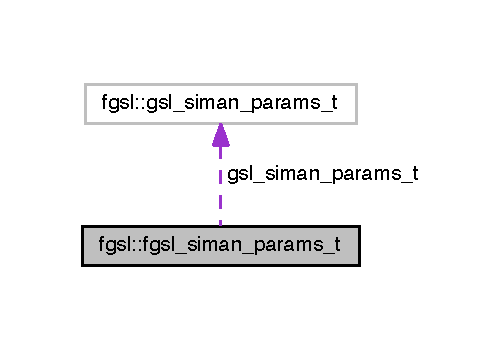
\includegraphics[width=242pt]{structfgsl_1_1fgsl__siman__params__t__coll__graph}
\end{center}
\end{figure}
\subsection*{Public Attributes}
\begin{DoxyCompactItemize}
\item 
type(gsl\-\_\-siman\-\_\-params\-\_\-t), pointer \hyperlink{structfgsl_1_1fgsl__siman__params__t_ab2792193e5f532eb151f335703044adf}{gsl\-\_\-siman\-\_\-params\-\_\-t} =$>$ null()
\end{DoxyCompactItemize}


\subsection{Member Data Documentation}
\hypertarget{structfgsl_1_1fgsl__siman__params__t_ab2792193e5f532eb151f335703044adf}{\index{fgsl\-::fgsl\-\_\-siman\-\_\-params\-\_\-t@{fgsl\-::fgsl\-\_\-siman\-\_\-params\-\_\-t}!gsl\-\_\-siman\-\_\-params\-\_\-t@{gsl\-\_\-siman\-\_\-params\-\_\-t}}
\index{gsl\-\_\-siman\-\_\-params\-\_\-t@{gsl\-\_\-siman\-\_\-params\-\_\-t}!fgsl::fgsl_siman_params_t@{fgsl\-::fgsl\-\_\-siman\-\_\-params\-\_\-t}}
\subsubsection[{gsl\-\_\-siman\-\_\-params\-\_\-t}]{\setlength{\rightskip}{0pt plus 5cm}type(gsl\-\_\-siman\-\_\-params\-\_\-t), pointer fgsl\-::fgsl\-\_\-siman\-\_\-params\-\_\-t\-::gsl\-\_\-siman\-\_\-params\-\_\-t =$>$ null()}}\label{structfgsl_1_1fgsl__siman__params__t_ab2792193e5f532eb151f335703044adf}


The documentation for this type was generated from the following file\-:\begin{DoxyCompactItemize}
\item 
\hyperlink{fgsl_8F90}{fgsl.\-F90}\end{DoxyCompactItemize}

\hypertarget{interfacefgsl__sizeof}{}\section{fgsl\+\_\+sizeof Interface Reference}
\label{interfacefgsl__sizeof}\index{fgsl\+\_\+sizeof@{fgsl\+\_\+sizeof}}
\subsection*{Public Member Functions}
\begin{DoxyCompactItemize}
\item 
\hyperlink{interfacefgsl__sizeof_a09dcf0ba3c399bf4180e068fcc51411b}{fgsl\+\_\+sizeof\+\_\+double}
\item 
\hyperlink{interfacefgsl__sizeof_a7936cc803801f8937a2d40c7aa833cfc}{fgsl\+\_\+sizeof\+\_\+float}
\item 
\hyperlink{interfacefgsl__sizeof_a333c65a82acaa67a814b9b6e09882a17}{fgsl\+\_\+sizeof\+\_\+int}
\item 
\hyperlink{interfacefgsl__sizeof_a6586ee7f0da543a3c7fe825a2f93c1ed}{fgsl\+\_\+sizeof\+\_\+size\+\_\+t}
\item 
\hyperlink{interfacefgsl__sizeof_a357f3f65f86d535f570769027a727b4e}{fgsl\+\_\+sizeof\+\_\+char}
\item 
\hyperlink{interfacefgsl__sizeof_afaff3b5eb24e4ccbe72031bdfa91e14f}{fgsl\+\_\+sizeof\+\_\+vector}
\item 
\hyperlink{interfacefgsl__sizeof_aa0a1ae56e5ae76ebd04c2b39ea8def4e}{fgsl\+\_\+sizeof\+\_\+matrix}
\item 
\hyperlink{interfacefgsl__sizeof_a4ba7154a64a65acbd3f7c97be257cb40}{fgsl\+\_\+sizeof\+\_\+vector\+\_\+complex}
\item 
\hyperlink{interfacefgsl__sizeof_a19e97a760e18face06868c597950f7c3}{fgsl\+\_\+sizeof\+\_\+matrix\+\_\+complex}
\item 
\hyperlink{interfacefgsl__sizeof_a1f6b503a6666f577ef97b17b715ad66a}{fgsl\+\_\+sizeof\+\_\+interp}
\item 
\hyperlink{interfacefgsl__sizeof_a6c1ac48c8524f61d28d906460ab9069c}{fgsl\+\_\+sizeof\+\_\+permutation}
\item 
\hyperlink{interfacefgsl__sizeof_a9ec0415509f4a420702f70eee66b0307}{fgsl\+\_\+sizeof\+\_\+combination}
\item 
\hyperlink{interfacefgsl__sizeof_a669cd8ded29c87b3649014de8ef5bb10}{fgsl\+\_\+sizeof\+\_\+multiset}
\item 
\hyperlink{interfacefgsl__sizeof_a58c8a6d2b7550b2ee309768abc134f70}{fgsl\+\_\+sizeof\+\_\+integration\+\_\+workspace}
\item 
\hyperlink{interfacefgsl__sizeof_ac72b6dd968501a2d7f2f0df2cfff5a82}{fgsl\+\_\+sizeof\+\_\+integration\+\_\+qaws\+\_\+table}
\item 
\hyperlink{interfacefgsl__sizeof_a7a8b70ea6c4a9b87a488d2c3ea37b954}{fgsl\+\_\+sizeof\+\_\+integration\+\_\+qawo\+\_\+table}
\item 
\hyperlink{interfacefgsl__sizeof_af321867808c0e28280fd714d07dc9ace}{fgsl\+\_\+sizeof\+\_\+wavelet}
\item 
\hyperlink{interfacefgsl__sizeof_a3e049aababe44b2249f926c4c78c3fd9}{fgsl\+\_\+sizeof\+\_\+wavelet\+\_\+workspace}
\end{DoxyCompactItemize}


\subsection{Member Function/\+Subroutine Documentation}
\hypertarget{interfacefgsl__sizeof_a357f3f65f86d535f570769027a727b4e}{}\index{fgsl\+\_\+sizeof@{fgsl\+\_\+sizeof}!fgsl\+\_\+sizeof\+\_\+char@{fgsl\+\_\+sizeof\+\_\+char}}
\index{fgsl\+\_\+sizeof\+\_\+char@{fgsl\+\_\+sizeof\+\_\+char}!fgsl\+\_\+sizeof@{fgsl\+\_\+sizeof}}
\subsubsection[{fgsl\+\_\+sizeof\+\_\+char}]{\setlength{\rightskip}{0pt plus 5cm}fgsl\+\_\+sizeof\+::fgsl\+\_\+sizeof\+\_\+char (
\begin{DoxyParamCaption}
{}
\end{DoxyParamCaption}
)}\label{interfacefgsl__sizeof_a357f3f65f86d535f570769027a727b4e}
\hypertarget{interfacefgsl__sizeof_a9ec0415509f4a420702f70eee66b0307}{}\index{fgsl\+\_\+sizeof@{fgsl\+\_\+sizeof}!fgsl\+\_\+sizeof\+\_\+combination@{fgsl\+\_\+sizeof\+\_\+combination}}
\index{fgsl\+\_\+sizeof\+\_\+combination@{fgsl\+\_\+sizeof\+\_\+combination}!fgsl\+\_\+sizeof@{fgsl\+\_\+sizeof}}
\subsubsection[{fgsl\+\_\+sizeof\+\_\+combination}]{\setlength{\rightskip}{0pt plus 5cm}fgsl\+\_\+sizeof\+::fgsl\+\_\+sizeof\+\_\+combination (
\begin{DoxyParamCaption}
{}
\end{DoxyParamCaption}
)}\label{interfacefgsl__sizeof_a9ec0415509f4a420702f70eee66b0307}
\hypertarget{interfacefgsl__sizeof_a09dcf0ba3c399bf4180e068fcc51411b}{}\index{fgsl\+\_\+sizeof@{fgsl\+\_\+sizeof}!fgsl\+\_\+sizeof\+\_\+double@{fgsl\+\_\+sizeof\+\_\+double}}
\index{fgsl\+\_\+sizeof\+\_\+double@{fgsl\+\_\+sizeof\+\_\+double}!fgsl\+\_\+sizeof@{fgsl\+\_\+sizeof}}
\subsubsection[{fgsl\+\_\+sizeof\+\_\+double}]{\setlength{\rightskip}{0pt plus 5cm}fgsl\+\_\+sizeof\+::fgsl\+\_\+sizeof\+\_\+double (
\begin{DoxyParamCaption}
{}
\end{DoxyParamCaption}
)}\label{interfacefgsl__sizeof_a09dcf0ba3c399bf4180e068fcc51411b}
\hypertarget{interfacefgsl__sizeof_a7936cc803801f8937a2d40c7aa833cfc}{}\index{fgsl\+\_\+sizeof@{fgsl\+\_\+sizeof}!fgsl\+\_\+sizeof\+\_\+float@{fgsl\+\_\+sizeof\+\_\+float}}
\index{fgsl\+\_\+sizeof\+\_\+float@{fgsl\+\_\+sizeof\+\_\+float}!fgsl\+\_\+sizeof@{fgsl\+\_\+sizeof}}
\subsubsection[{fgsl\+\_\+sizeof\+\_\+float}]{\setlength{\rightskip}{0pt plus 5cm}fgsl\+\_\+sizeof\+::fgsl\+\_\+sizeof\+\_\+float (
\begin{DoxyParamCaption}
{}
\end{DoxyParamCaption}
)}\label{interfacefgsl__sizeof_a7936cc803801f8937a2d40c7aa833cfc}
\hypertarget{interfacefgsl__sizeof_a333c65a82acaa67a814b9b6e09882a17}{}\index{fgsl\+\_\+sizeof@{fgsl\+\_\+sizeof}!fgsl\+\_\+sizeof\+\_\+int@{fgsl\+\_\+sizeof\+\_\+int}}
\index{fgsl\+\_\+sizeof\+\_\+int@{fgsl\+\_\+sizeof\+\_\+int}!fgsl\+\_\+sizeof@{fgsl\+\_\+sizeof}}
\subsubsection[{fgsl\+\_\+sizeof\+\_\+int}]{\setlength{\rightskip}{0pt plus 5cm}fgsl\+\_\+sizeof\+::fgsl\+\_\+sizeof\+\_\+int (
\begin{DoxyParamCaption}
{}
\end{DoxyParamCaption}
)}\label{interfacefgsl__sizeof_a333c65a82acaa67a814b9b6e09882a17}
\hypertarget{interfacefgsl__sizeof_a7a8b70ea6c4a9b87a488d2c3ea37b954}{}\index{fgsl\+\_\+sizeof@{fgsl\+\_\+sizeof}!fgsl\+\_\+sizeof\+\_\+integration\+\_\+qawo\+\_\+table@{fgsl\+\_\+sizeof\+\_\+integration\+\_\+qawo\+\_\+table}}
\index{fgsl\+\_\+sizeof\+\_\+integration\+\_\+qawo\+\_\+table@{fgsl\+\_\+sizeof\+\_\+integration\+\_\+qawo\+\_\+table}!fgsl\+\_\+sizeof@{fgsl\+\_\+sizeof}}
\subsubsection[{fgsl\+\_\+sizeof\+\_\+integration\+\_\+qawo\+\_\+table}]{\setlength{\rightskip}{0pt plus 5cm}fgsl\+\_\+sizeof\+::fgsl\+\_\+sizeof\+\_\+integration\+\_\+qawo\+\_\+table (
\begin{DoxyParamCaption}
{}
\end{DoxyParamCaption}
)}\label{interfacefgsl__sizeof_a7a8b70ea6c4a9b87a488d2c3ea37b954}
\hypertarget{interfacefgsl__sizeof_ac72b6dd968501a2d7f2f0df2cfff5a82}{}\index{fgsl\+\_\+sizeof@{fgsl\+\_\+sizeof}!fgsl\+\_\+sizeof\+\_\+integration\+\_\+qaws\+\_\+table@{fgsl\+\_\+sizeof\+\_\+integration\+\_\+qaws\+\_\+table}}
\index{fgsl\+\_\+sizeof\+\_\+integration\+\_\+qaws\+\_\+table@{fgsl\+\_\+sizeof\+\_\+integration\+\_\+qaws\+\_\+table}!fgsl\+\_\+sizeof@{fgsl\+\_\+sizeof}}
\subsubsection[{fgsl\+\_\+sizeof\+\_\+integration\+\_\+qaws\+\_\+table}]{\setlength{\rightskip}{0pt plus 5cm}fgsl\+\_\+sizeof\+::fgsl\+\_\+sizeof\+\_\+integration\+\_\+qaws\+\_\+table (
\begin{DoxyParamCaption}
{}
\end{DoxyParamCaption}
)}\label{interfacefgsl__sizeof_ac72b6dd968501a2d7f2f0df2cfff5a82}
\hypertarget{interfacefgsl__sizeof_a58c8a6d2b7550b2ee309768abc134f70}{}\index{fgsl\+\_\+sizeof@{fgsl\+\_\+sizeof}!fgsl\+\_\+sizeof\+\_\+integration\+\_\+workspace@{fgsl\+\_\+sizeof\+\_\+integration\+\_\+workspace}}
\index{fgsl\+\_\+sizeof\+\_\+integration\+\_\+workspace@{fgsl\+\_\+sizeof\+\_\+integration\+\_\+workspace}!fgsl\+\_\+sizeof@{fgsl\+\_\+sizeof}}
\subsubsection[{fgsl\+\_\+sizeof\+\_\+integration\+\_\+workspace}]{\setlength{\rightskip}{0pt plus 5cm}fgsl\+\_\+sizeof\+::fgsl\+\_\+sizeof\+\_\+integration\+\_\+workspace (
\begin{DoxyParamCaption}
{}
\end{DoxyParamCaption}
)}\label{interfacefgsl__sizeof_a58c8a6d2b7550b2ee309768abc134f70}
\hypertarget{interfacefgsl__sizeof_a1f6b503a6666f577ef97b17b715ad66a}{}\index{fgsl\+\_\+sizeof@{fgsl\+\_\+sizeof}!fgsl\+\_\+sizeof\+\_\+interp@{fgsl\+\_\+sizeof\+\_\+interp}}
\index{fgsl\+\_\+sizeof\+\_\+interp@{fgsl\+\_\+sizeof\+\_\+interp}!fgsl\+\_\+sizeof@{fgsl\+\_\+sizeof}}
\subsubsection[{fgsl\+\_\+sizeof\+\_\+interp}]{\setlength{\rightskip}{0pt plus 5cm}fgsl\+\_\+sizeof\+::fgsl\+\_\+sizeof\+\_\+interp (
\begin{DoxyParamCaption}
{}
\end{DoxyParamCaption}
)}\label{interfacefgsl__sizeof_a1f6b503a6666f577ef97b17b715ad66a}
\hypertarget{interfacefgsl__sizeof_aa0a1ae56e5ae76ebd04c2b39ea8def4e}{}\index{fgsl\+\_\+sizeof@{fgsl\+\_\+sizeof}!fgsl\+\_\+sizeof\+\_\+matrix@{fgsl\+\_\+sizeof\+\_\+matrix}}
\index{fgsl\+\_\+sizeof\+\_\+matrix@{fgsl\+\_\+sizeof\+\_\+matrix}!fgsl\+\_\+sizeof@{fgsl\+\_\+sizeof}}
\subsubsection[{fgsl\+\_\+sizeof\+\_\+matrix}]{\setlength{\rightskip}{0pt plus 5cm}fgsl\+\_\+sizeof\+::fgsl\+\_\+sizeof\+\_\+matrix (
\begin{DoxyParamCaption}
{}
\end{DoxyParamCaption}
)}\label{interfacefgsl__sizeof_aa0a1ae56e5ae76ebd04c2b39ea8def4e}
\hypertarget{interfacefgsl__sizeof_a19e97a760e18face06868c597950f7c3}{}\index{fgsl\+\_\+sizeof@{fgsl\+\_\+sizeof}!fgsl\+\_\+sizeof\+\_\+matrix\+\_\+complex@{fgsl\+\_\+sizeof\+\_\+matrix\+\_\+complex}}
\index{fgsl\+\_\+sizeof\+\_\+matrix\+\_\+complex@{fgsl\+\_\+sizeof\+\_\+matrix\+\_\+complex}!fgsl\+\_\+sizeof@{fgsl\+\_\+sizeof}}
\subsubsection[{fgsl\+\_\+sizeof\+\_\+matrix\+\_\+complex}]{\setlength{\rightskip}{0pt plus 5cm}fgsl\+\_\+sizeof\+::fgsl\+\_\+sizeof\+\_\+matrix\+\_\+complex (
\begin{DoxyParamCaption}
{}
\end{DoxyParamCaption}
)}\label{interfacefgsl__sizeof_a19e97a760e18face06868c597950f7c3}
\hypertarget{interfacefgsl__sizeof_a669cd8ded29c87b3649014de8ef5bb10}{}\index{fgsl\+\_\+sizeof@{fgsl\+\_\+sizeof}!fgsl\+\_\+sizeof\+\_\+multiset@{fgsl\+\_\+sizeof\+\_\+multiset}}
\index{fgsl\+\_\+sizeof\+\_\+multiset@{fgsl\+\_\+sizeof\+\_\+multiset}!fgsl\+\_\+sizeof@{fgsl\+\_\+sizeof}}
\subsubsection[{fgsl\+\_\+sizeof\+\_\+multiset}]{\setlength{\rightskip}{0pt plus 5cm}fgsl\+\_\+sizeof\+::fgsl\+\_\+sizeof\+\_\+multiset (
\begin{DoxyParamCaption}
{}
\end{DoxyParamCaption}
)}\label{interfacefgsl__sizeof_a669cd8ded29c87b3649014de8ef5bb10}
\hypertarget{interfacefgsl__sizeof_a6c1ac48c8524f61d28d906460ab9069c}{}\index{fgsl\+\_\+sizeof@{fgsl\+\_\+sizeof}!fgsl\+\_\+sizeof\+\_\+permutation@{fgsl\+\_\+sizeof\+\_\+permutation}}
\index{fgsl\+\_\+sizeof\+\_\+permutation@{fgsl\+\_\+sizeof\+\_\+permutation}!fgsl\+\_\+sizeof@{fgsl\+\_\+sizeof}}
\subsubsection[{fgsl\+\_\+sizeof\+\_\+permutation}]{\setlength{\rightskip}{0pt plus 5cm}fgsl\+\_\+sizeof\+::fgsl\+\_\+sizeof\+\_\+permutation (
\begin{DoxyParamCaption}
{}
\end{DoxyParamCaption}
)}\label{interfacefgsl__sizeof_a6c1ac48c8524f61d28d906460ab9069c}
\hypertarget{interfacefgsl__sizeof_a6586ee7f0da543a3c7fe825a2f93c1ed}{}\index{fgsl\+\_\+sizeof@{fgsl\+\_\+sizeof}!fgsl\+\_\+sizeof\+\_\+size\+\_\+t@{fgsl\+\_\+sizeof\+\_\+size\+\_\+t}}
\index{fgsl\+\_\+sizeof\+\_\+size\+\_\+t@{fgsl\+\_\+sizeof\+\_\+size\+\_\+t}!fgsl\+\_\+sizeof@{fgsl\+\_\+sizeof}}
\subsubsection[{fgsl\+\_\+sizeof\+\_\+size\+\_\+t}]{\setlength{\rightskip}{0pt plus 5cm}fgsl\+\_\+sizeof\+::fgsl\+\_\+sizeof\+\_\+size\+\_\+t (
\begin{DoxyParamCaption}
{}
\end{DoxyParamCaption}
)}\label{interfacefgsl__sizeof_a6586ee7f0da543a3c7fe825a2f93c1ed}
\hypertarget{interfacefgsl__sizeof_afaff3b5eb24e4ccbe72031bdfa91e14f}{}\index{fgsl\+\_\+sizeof@{fgsl\+\_\+sizeof}!fgsl\+\_\+sizeof\+\_\+vector@{fgsl\+\_\+sizeof\+\_\+vector}}
\index{fgsl\+\_\+sizeof\+\_\+vector@{fgsl\+\_\+sizeof\+\_\+vector}!fgsl\+\_\+sizeof@{fgsl\+\_\+sizeof}}
\subsubsection[{fgsl\+\_\+sizeof\+\_\+vector}]{\setlength{\rightskip}{0pt plus 5cm}fgsl\+\_\+sizeof\+::fgsl\+\_\+sizeof\+\_\+vector (
\begin{DoxyParamCaption}
{}
\end{DoxyParamCaption}
)}\label{interfacefgsl__sizeof_afaff3b5eb24e4ccbe72031bdfa91e14f}
\hypertarget{interfacefgsl__sizeof_a4ba7154a64a65acbd3f7c97be257cb40}{}\index{fgsl\+\_\+sizeof@{fgsl\+\_\+sizeof}!fgsl\+\_\+sizeof\+\_\+vector\+\_\+complex@{fgsl\+\_\+sizeof\+\_\+vector\+\_\+complex}}
\index{fgsl\+\_\+sizeof\+\_\+vector\+\_\+complex@{fgsl\+\_\+sizeof\+\_\+vector\+\_\+complex}!fgsl\+\_\+sizeof@{fgsl\+\_\+sizeof}}
\subsubsection[{fgsl\+\_\+sizeof\+\_\+vector\+\_\+complex}]{\setlength{\rightskip}{0pt plus 5cm}fgsl\+\_\+sizeof\+::fgsl\+\_\+sizeof\+\_\+vector\+\_\+complex (
\begin{DoxyParamCaption}
{}
\end{DoxyParamCaption}
)}\label{interfacefgsl__sizeof_a4ba7154a64a65acbd3f7c97be257cb40}
\hypertarget{interfacefgsl__sizeof_af321867808c0e28280fd714d07dc9ace}{}\index{fgsl\+\_\+sizeof@{fgsl\+\_\+sizeof}!fgsl\+\_\+sizeof\+\_\+wavelet@{fgsl\+\_\+sizeof\+\_\+wavelet}}
\index{fgsl\+\_\+sizeof\+\_\+wavelet@{fgsl\+\_\+sizeof\+\_\+wavelet}!fgsl\+\_\+sizeof@{fgsl\+\_\+sizeof}}
\subsubsection[{fgsl\+\_\+sizeof\+\_\+wavelet}]{\setlength{\rightskip}{0pt plus 5cm}fgsl\+\_\+sizeof\+::fgsl\+\_\+sizeof\+\_\+wavelet (
\begin{DoxyParamCaption}
{}
\end{DoxyParamCaption}
)}\label{interfacefgsl__sizeof_af321867808c0e28280fd714d07dc9ace}
\hypertarget{interfacefgsl__sizeof_a3e049aababe44b2249f926c4c78c3fd9}{}\index{fgsl\+\_\+sizeof@{fgsl\+\_\+sizeof}!fgsl\+\_\+sizeof\+\_\+wavelet\+\_\+workspace@{fgsl\+\_\+sizeof\+\_\+wavelet\+\_\+workspace}}
\index{fgsl\+\_\+sizeof\+\_\+wavelet\+\_\+workspace@{fgsl\+\_\+sizeof\+\_\+wavelet\+\_\+workspace}!fgsl\+\_\+sizeof@{fgsl\+\_\+sizeof}}
\subsubsection[{fgsl\+\_\+sizeof\+\_\+wavelet\+\_\+workspace}]{\setlength{\rightskip}{0pt plus 5cm}fgsl\+\_\+sizeof\+::fgsl\+\_\+sizeof\+\_\+wavelet\+\_\+workspace (
\begin{DoxyParamCaption}
{}
\end{DoxyParamCaption}
)}\label{interfacefgsl__sizeof_a3e049aababe44b2249f926c4c78c3fd9}


The documentation for this interface was generated from the following file\+:\begin{DoxyCompactItemize}
\item 
interface/\hyperlink{generics_8finc}{generics.\+finc}\end{DoxyCompactItemize}

\hypertarget{interfacefgsl__sort}{}\section{fgsl\+\_\+sort Interface Reference}
\label{interfacefgsl__sort}\index{fgsl\+\_\+sort@{fgsl\+\_\+sort}}
\subsection*{Public Member Functions}
\begin{DoxyCompactItemize}
\item 
\hyperlink{interfacefgsl__sort_ac96868ba62ebd24850db17233635e2d1}{fgsl\+\_\+sort\+\_\+double}
\item 
\hyperlink{interfacefgsl__sort_a8d415eb7f84ee09c405d8de68a6233a9}{fgsl\+\_\+sort\+\_\+long}
\item 
\hyperlink{interfacefgsl__sort_a39a5b97ec7630f6c5f38f028e1aab311}{fgsl\+\_\+sort\+\_\+vector}
\end{DoxyCompactItemize}


\subsection{Member Function/\+Subroutine Documentation}
\hypertarget{interfacefgsl__sort_ac96868ba62ebd24850db17233635e2d1}{}\index{fgsl\+\_\+sort@{fgsl\+\_\+sort}!fgsl\+\_\+sort\+\_\+double@{fgsl\+\_\+sort\+\_\+double}}
\index{fgsl\+\_\+sort\+\_\+double@{fgsl\+\_\+sort\+\_\+double}!fgsl\+\_\+sort@{fgsl\+\_\+sort}}
\subsubsection[{fgsl\+\_\+sort\+\_\+double}]{\setlength{\rightskip}{0pt plus 5cm}fgsl\+\_\+sort\+::fgsl\+\_\+sort\+\_\+double (
\begin{DoxyParamCaption}
{}
\end{DoxyParamCaption}
)}\label{interfacefgsl__sort_ac96868ba62ebd24850db17233635e2d1}
\hypertarget{interfacefgsl__sort_a8d415eb7f84ee09c405d8de68a6233a9}{}\index{fgsl\+\_\+sort@{fgsl\+\_\+sort}!fgsl\+\_\+sort\+\_\+long@{fgsl\+\_\+sort\+\_\+long}}
\index{fgsl\+\_\+sort\+\_\+long@{fgsl\+\_\+sort\+\_\+long}!fgsl\+\_\+sort@{fgsl\+\_\+sort}}
\subsubsection[{fgsl\+\_\+sort\+\_\+long}]{\setlength{\rightskip}{0pt plus 5cm}fgsl\+\_\+sort\+::fgsl\+\_\+sort\+\_\+long (
\begin{DoxyParamCaption}
{}
\end{DoxyParamCaption}
)}\label{interfacefgsl__sort_a8d415eb7f84ee09c405d8de68a6233a9}
\hypertarget{interfacefgsl__sort_a39a5b97ec7630f6c5f38f028e1aab311}{}\index{fgsl\+\_\+sort@{fgsl\+\_\+sort}!fgsl\+\_\+sort\+\_\+vector@{fgsl\+\_\+sort\+\_\+vector}}
\index{fgsl\+\_\+sort\+\_\+vector@{fgsl\+\_\+sort\+\_\+vector}!fgsl\+\_\+sort@{fgsl\+\_\+sort}}
\subsubsection[{fgsl\+\_\+sort\+\_\+vector}]{\setlength{\rightskip}{0pt plus 5cm}fgsl\+\_\+sort\+::fgsl\+\_\+sort\+\_\+vector (
\begin{DoxyParamCaption}
{}
\end{DoxyParamCaption}
)}\label{interfacefgsl__sort_a39a5b97ec7630f6c5f38f028e1aab311}


The documentation for this interface was generated from the following file\+:\begin{DoxyCompactItemize}
\item 
interface/\hyperlink{generics_8finc}{generics.\+finc}\end{DoxyCompactItemize}

\hypertarget{interfacefgsl__sort__index}{\section{fgsl\-\_\-sort\-\_\-index Interface Reference}
\label{interfacefgsl__sort__index}\index{fgsl\-\_\-sort\-\_\-index@{fgsl\-\_\-sort\-\_\-index}}
}
\subsection*{Public Member Functions}
\begin{DoxyCompactItemize}
\item 
\hyperlink{interfacefgsl__sort__index_a979dd4912ceb293cd0c6d3b606bee49b}{fgsl\-\_\-sort\-\_\-double\-\_\-index}
\item 
\hyperlink{interfacefgsl__sort__index_a251c58ed6de3572d4667956d6d1b04b3}{fgsl\-\_\-sort\-\_\-long\-\_\-index}
\item 
\hyperlink{interfacefgsl__sort__index_ac0c4d0d023d509a965e1bc935dafbca8}{fgsl\-\_\-sort\-\_\-vector\-\_\-index}
\end{DoxyCompactItemize}


\subsection{Member Function/\-Subroutine Documentation}
\hypertarget{interfacefgsl__sort__index_a979dd4912ceb293cd0c6d3b606bee49b}{\index{fgsl\-\_\-sort\-\_\-index@{fgsl\-\_\-sort\-\_\-index}!fgsl\-\_\-sort\-\_\-double\-\_\-index@{fgsl\-\_\-sort\-\_\-double\-\_\-index}}
\index{fgsl\-\_\-sort\-\_\-double\-\_\-index@{fgsl\-\_\-sort\-\_\-double\-\_\-index}!fgsl_sort_index@{fgsl\-\_\-sort\-\_\-index}}
\subsubsection[{fgsl\-\_\-sort\-\_\-double\-\_\-index}]{\setlength{\rightskip}{0pt plus 5cm}fgsl\-\_\-sort\-\_\-index\-::fgsl\-\_\-sort\-\_\-double\-\_\-index (
\begin{DoxyParamCaption}
{}
\end{DoxyParamCaption}
)}}\label{interfacefgsl__sort__index_a979dd4912ceb293cd0c6d3b606bee49b}
\hypertarget{interfacefgsl__sort__index_a251c58ed6de3572d4667956d6d1b04b3}{\index{fgsl\-\_\-sort\-\_\-index@{fgsl\-\_\-sort\-\_\-index}!fgsl\-\_\-sort\-\_\-long\-\_\-index@{fgsl\-\_\-sort\-\_\-long\-\_\-index}}
\index{fgsl\-\_\-sort\-\_\-long\-\_\-index@{fgsl\-\_\-sort\-\_\-long\-\_\-index}!fgsl_sort_index@{fgsl\-\_\-sort\-\_\-index}}
\subsubsection[{fgsl\-\_\-sort\-\_\-long\-\_\-index}]{\setlength{\rightskip}{0pt plus 5cm}fgsl\-\_\-sort\-\_\-index\-::fgsl\-\_\-sort\-\_\-long\-\_\-index (
\begin{DoxyParamCaption}
{}
\end{DoxyParamCaption}
)}}\label{interfacefgsl__sort__index_a251c58ed6de3572d4667956d6d1b04b3}
\hypertarget{interfacefgsl__sort__index_ac0c4d0d023d509a965e1bc935dafbca8}{\index{fgsl\-\_\-sort\-\_\-index@{fgsl\-\_\-sort\-\_\-index}!fgsl\-\_\-sort\-\_\-vector\-\_\-index@{fgsl\-\_\-sort\-\_\-vector\-\_\-index}}
\index{fgsl\-\_\-sort\-\_\-vector\-\_\-index@{fgsl\-\_\-sort\-\_\-vector\-\_\-index}!fgsl_sort_index@{fgsl\-\_\-sort\-\_\-index}}
\subsubsection[{fgsl\-\_\-sort\-\_\-vector\-\_\-index}]{\setlength{\rightskip}{0pt plus 5cm}fgsl\-\_\-sort\-\_\-index\-::fgsl\-\_\-sort\-\_\-vector\-\_\-index (
\begin{DoxyParamCaption}
{}
\end{DoxyParamCaption}
)}}\label{interfacefgsl__sort__index_ac0c4d0d023d509a965e1bc935dafbca8}


The documentation for this interface was generated from the following files\-:\begin{DoxyCompactItemize}
\item 
interface/\hyperlink{generics_8finc}{generics.\-finc}\end{DoxyCompactItemize}

\hypertarget{interfacefgsl__sort__largest}{\section{fgsl\-\_\-sort\-\_\-largest Interface Reference}
\label{interfacefgsl__sort__largest}\index{fgsl\-\_\-sort\-\_\-largest@{fgsl\-\_\-sort\-\_\-largest}}
}
\subsection*{Public Member Functions}
\begin{DoxyCompactItemize}
\item 
\hyperlink{interfacefgsl__sort__largest_acdeefd3309718051ae27f8e290b43f74}{fgsl\-\_\-sort\-\_\-double\-\_\-largest}
\item 
\hyperlink{interfacefgsl__sort__largest_a0dd8552a6d0bedcddf36b31be56e1075}{fgsl\-\_\-sort\-\_\-long\-\_\-largest}
\item 
\hyperlink{interfacefgsl__sort__largest_a4149cae50500783202c97aa4b33583b7}{fgsl\-\_\-sort\-\_\-vector\-\_\-largest}
\end{DoxyCompactItemize}


\subsection{Member Function/\-Subroutine Documentation}
\hypertarget{interfacefgsl__sort__largest_acdeefd3309718051ae27f8e290b43f74}{\index{fgsl\-\_\-sort\-\_\-largest@{fgsl\-\_\-sort\-\_\-largest}!fgsl\-\_\-sort\-\_\-double\-\_\-largest@{fgsl\-\_\-sort\-\_\-double\-\_\-largest}}
\index{fgsl\-\_\-sort\-\_\-double\-\_\-largest@{fgsl\-\_\-sort\-\_\-double\-\_\-largest}!fgsl_sort_largest@{fgsl\-\_\-sort\-\_\-largest}}
\subsubsection[{fgsl\-\_\-sort\-\_\-double\-\_\-largest}]{\setlength{\rightskip}{0pt plus 5cm}fgsl\-\_\-sort\-\_\-largest\-::fgsl\-\_\-sort\-\_\-double\-\_\-largest (
\begin{DoxyParamCaption}
{}
\end{DoxyParamCaption}
)}}\label{interfacefgsl__sort__largest_acdeefd3309718051ae27f8e290b43f74}
\hypertarget{interfacefgsl__sort__largest_a0dd8552a6d0bedcddf36b31be56e1075}{\index{fgsl\-\_\-sort\-\_\-largest@{fgsl\-\_\-sort\-\_\-largest}!fgsl\-\_\-sort\-\_\-long\-\_\-largest@{fgsl\-\_\-sort\-\_\-long\-\_\-largest}}
\index{fgsl\-\_\-sort\-\_\-long\-\_\-largest@{fgsl\-\_\-sort\-\_\-long\-\_\-largest}!fgsl_sort_largest@{fgsl\-\_\-sort\-\_\-largest}}
\subsubsection[{fgsl\-\_\-sort\-\_\-long\-\_\-largest}]{\setlength{\rightskip}{0pt plus 5cm}fgsl\-\_\-sort\-\_\-largest\-::fgsl\-\_\-sort\-\_\-long\-\_\-largest (
\begin{DoxyParamCaption}
{}
\end{DoxyParamCaption}
)}}\label{interfacefgsl__sort__largest_a0dd8552a6d0bedcddf36b31be56e1075}
\hypertarget{interfacefgsl__sort__largest_a4149cae50500783202c97aa4b33583b7}{\index{fgsl\-\_\-sort\-\_\-largest@{fgsl\-\_\-sort\-\_\-largest}!fgsl\-\_\-sort\-\_\-vector\-\_\-largest@{fgsl\-\_\-sort\-\_\-vector\-\_\-largest}}
\index{fgsl\-\_\-sort\-\_\-vector\-\_\-largest@{fgsl\-\_\-sort\-\_\-vector\-\_\-largest}!fgsl_sort_largest@{fgsl\-\_\-sort\-\_\-largest}}
\subsubsection[{fgsl\-\_\-sort\-\_\-vector\-\_\-largest}]{\setlength{\rightskip}{0pt plus 5cm}fgsl\-\_\-sort\-\_\-largest\-::fgsl\-\_\-sort\-\_\-vector\-\_\-largest (
\begin{DoxyParamCaption}
{}
\end{DoxyParamCaption}
)}}\label{interfacefgsl__sort__largest_a4149cae50500783202c97aa4b33583b7}


The documentation for this interface was generated from the following file\-:\begin{DoxyCompactItemize}
\item 
interface/\hyperlink{generics_8finc}{generics.\-finc}\end{DoxyCompactItemize}

\hypertarget{interfacefgsl__sort__largest__index}{\section{fgsl\-\_\-sort\-\_\-largest\-\_\-index Interface Reference}
\label{interfacefgsl__sort__largest__index}\index{fgsl\-\_\-sort\-\_\-largest\-\_\-index@{fgsl\-\_\-sort\-\_\-largest\-\_\-index}}
}
\subsection*{Public Member Functions}
\begin{DoxyCompactItemize}
\item 
\hyperlink{interfacefgsl__sort__largest__index_a0634bd3573e2113207452ea2a01799a2}{fgsl\-\_\-sort\-\_\-double\-\_\-largest\-\_\-index}
\item 
\hyperlink{interfacefgsl__sort__largest__index_ac1be856b6fb7a9b15f34ae528a6b9ad3}{fgsl\-\_\-sort\-\_\-long\-\_\-largest\-\_\-index}
\item 
\hyperlink{interfacefgsl__sort__largest__index_aec7f708d27ccaa19c454316e18a6f648}{fgsl\-\_\-sort\-\_\-vector\-\_\-largest\-\_\-index}
\end{DoxyCompactItemize}


\subsection{Member Function/\-Subroutine Documentation}
\hypertarget{interfacefgsl__sort__largest__index_a0634bd3573e2113207452ea2a01799a2}{\index{fgsl\-\_\-sort\-\_\-largest\-\_\-index@{fgsl\-\_\-sort\-\_\-largest\-\_\-index}!fgsl\-\_\-sort\-\_\-double\-\_\-largest\-\_\-index@{fgsl\-\_\-sort\-\_\-double\-\_\-largest\-\_\-index}}
\index{fgsl\-\_\-sort\-\_\-double\-\_\-largest\-\_\-index@{fgsl\-\_\-sort\-\_\-double\-\_\-largest\-\_\-index}!fgsl_sort_largest_index@{fgsl\-\_\-sort\-\_\-largest\-\_\-index}}
\subsubsection[{fgsl\-\_\-sort\-\_\-double\-\_\-largest\-\_\-index}]{\setlength{\rightskip}{0pt plus 5cm}fgsl\-\_\-sort\-\_\-largest\-\_\-index\-::fgsl\-\_\-sort\-\_\-double\-\_\-largest\-\_\-index (
\begin{DoxyParamCaption}
{}
\end{DoxyParamCaption}
)}}\label{interfacefgsl__sort__largest__index_a0634bd3573e2113207452ea2a01799a2}
\hypertarget{interfacefgsl__sort__largest__index_ac1be856b6fb7a9b15f34ae528a6b9ad3}{\index{fgsl\-\_\-sort\-\_\-largest\-\_\-index@{fgsl\-\_\-sort\-\_\-largest\-\_\-index}!fgsl\-\_\-sort\-\_\-long\-\_\-largest\-\_\-index@{fgsl\-\_\-sort\-\_\-long\-\_\-largest\-\_\-index}}
\index{fgsl\-\_\-sort\-\_\-long\-\_\-largest\-\_\-index@{fgsl\-\_\-sort\-\_\-long\-\_\-largest\-\_\-index}!fgsl_sort_largest_index@{fgsl\-\_\-sort\-\_\-largest\-\_\-index}}
\subsubsection[{fgsl\-\_\-sort\-\_\-long\-\_\-largest\-\_\-index}]{\setlength{\rightskip}{0pt plus 5cm}fgsl\-\_\-sort\-\_\-largest\-\_\-index\-::fgsl\-\_\-sort\-\_\-long\-\_\-largest\-\_\-index (
\begin{DoxyParamCaption}
{}
\end{DoxyParamCaption}
)}}\label{interfacefgsl__sort__largest__index_ac1be856b6fb7a9b15f34ae528a6b9ad3}
\hypertarget{interfacefgsl__sort__largest__index_aec7f708d27ccaa19c454316e18a6f648}{\index{fgsl\-\_\-sort\-\_\-largest\-\_\-index@{fgsl\-\_\-sort\-\_\-largest\-\_\-index}!fgsl\-\_\-sort\-\_\-vector\-\_\-largest\-\_\-index@{fgsl\-\_\-sort\-\_\-vector\-\_\-largest\-\_\-index}}
\index{fgsl\-\_\-sort\-\_\-vector\-\_\-largest\-\_\-index@{fgsl\-\_\-sort\-\_\-vector\-\_\-largest\-\_\-index}!fgsl_sort_largest_index@{fgsl\-\_\-sort\-\_\-largest\-\_\-index}}
\subsubsection[{fgsl\-\_\-sort\-\_\-vector\-\_\-largest\-\_\-index}]{\setlength{\rightskip}{0pt plus 5cm}fgsl\-\_\-sort\-\_\-largest\-\_\-index\-::fgsl\-\_\-sort\-\_\-vector\-\_\-largest\-\_\-index (
\begin{DoxyParamCaption}
{}
\end{DoxyParamCaption}
)}}\label{interfacefgsl__sort__largest__index_aec7f708d27ccaa19c454316e18a6f648}


The documentation for this interface was generated from the following files\-:\begin{DoxyCompactItemize}
\item 
interface/\hyperlink{generics_8finc}{generics.\-finc}\end{DoxyCompactItemize}

\hypertarget{interfacefgsl__sort__smallest}{\section{fgsl\-\_\-sort\-\_\-smallest Interface Reference}
\label{interfacefgsl__sort__smallest}\index{fgsl\-\_\-sort\-\_\-smallest@{fgsl\-\_\-sort\-\_\-smallest}}
}
\subsection*{Public Member Functions}
\begin{DoxyCompactItemize}
\item 
\hyperlink{interfacefgsl__sort__smallest_a1750449525763b921997810a44d099ae}{fgsl\-\_\-sort\-\_\-double\-\_\-smallest}
\item 
\hyperlink{interfacefgsl__sort__smallest_a25a5022777d8408f473cdcce1585d704}{fgsl\-\_\-sort\-\_\-long\-\_\-smallest}
\item 
\hyperlink{interfacefgsl__sort__smallest_a5c4ee27d2b4e278553672206e1cc1314}{fgsl\-\_\-sort\-\_\-vector\-\_\-smallest}
\end{DoxyCompactItemize}


\subsection{Member Function/\-Subroutine Documentation}
\hypertarget{interfacefgsl__sort__smallest_a1750449525763b921997810a44d099ae}{\index{fgsl\-\_\-sort\-\_\-smallest@{fgsl\-\_\-sort\-\_\-smallest}!fgsl\-\_\-sort\-\_\-double\-\_\-smallest@{fgsl\-\_\-sort\-\_\-double\-\_\-smallest}}
\index{fgsl\-\_\-sort\-\_\-double\-\_\-smallest@{fgsl\-\_\-sort\-\_\-double\-\_\-smallest}!fgsl_sort_smallest@{fgsl\-\_\-sort\-\_\-smallest}}
\subsubsection[{fgsl\-\_\-sort\-\_\-double\-\_\-smallest}]{\setlength{\rightskip}{0pt plus 5cm}fgsl\-\_\-sort\-\_\-smallest\-::fgsl\-\_\-sort\-\_\-double\-\_\-smallest (
\begin{DoxyParamCaption}
{}
\end{DoxyParamCaption}
)}}\label{interfacefgsl__sort__smallest_a1750449525763b921997810a44d099ae}
\hypertarget{interfacefgsl__sort__smallest_a25a5022777d8408f473cdcce1585d704}{\index{fgsl\-\_\-sort\-\_\-smallest@{fgsl\-\_\-sort\-\_\-smallest}!fgsl\-\_\-sort\-\_\-long\-\_\-smallest@{fgsl\-\_\-sort\-\_\-long\-\_\-smallest}}
\index{fgsl\-\_\-sort\-\_\-long\-\_\-smallest@{fgsl\-\_\-sort\-\_\-long\-\_\-smallest}!fgsl_sort_smallest@{fgsl\-\_\-sort\-\_\-smallest}}
\subsubsection[{fgsl\-\_\-sort\-\_\-long\-\_\-smallest}]{\setlength{\rightskip}{0pt plus 5cm}fgsl\-\_\-sort\-\_\-smallest\-::fgsl\-\_\-sort\-\_\-long\-\_\-smallest (
\begin{DoxyParamCaption}
{}
\end{DoxyParamCaption}
)}}\label{interfacefgsl__sort__smallest_a25a5022777d8408f473cdcce1585d704}
\hypertarget{interfacefgsl__sort__smallest_a5c4ee27d2b4e278553672206e1cc1314}{\index{fgsl\-\_\-sort\-\_\-smallest@{fgsl\-\_\-sort\-\_\-smallest}!fgsl\-\_\-sort\-\_\-vector\-\_\-smallest@{fgsl\-\_\-sort\-\_\-vector\-\_\-smallest}}
\index{fgsl\-\_\-sort\-\_\-vector\-\_\-smallest@{fgsl\-\_\-sort\-\_\-vector\-\_\-smallest}!fgsl_sort_smallest@{fgsl\-\_\-sort\-\_\-smallest}}
\subsubsection[{fgsl\-\_\-sort\-\_\-vector\-\_\-smallest}]{\setlength{\rightskip}{0pt plus 5cm}fgsl\-\_\-sort\-\_\-smallest\-::fgsl\-\_\-sort\-\_\-vector\-\_\-smallest (
\begin{DoxyParamCaption}
{}
\end{DoxyParamCaption}
)}}\label{interfacefgsl__sort__smallest_a5c4ee27d2b4e278553672206e1cc1314}


The documentation for this interface was generated from the following files\-:\begin{DoxyCompactItemize}
\item 
interface/\hyperlink{generics_8finc}{generics.\-finc}\end{DoxyCompactItemize}

\hypertarget{interfacefgsl__sort__smallest__index}{\section{fgsl\-\_\-sort\-\_\-smallest\-\_\-index Interface Reference}
\label{interfacefgsl__sort__smallest__index}\index{fgsl\-\_\-sort\-\_\-smallest\-\_\-index@{fgsl\-\_\-sort\-\_\-smallest\-\_\-index}}
}
\subsection*{Public Member Functions}
\begin{DoxyCompactItemize}
\item 
\hyperlink{interfacefgsl__sort__smallest__index_ade4dc1cac96031ab43350ccf566b799d}{fgsl\-\_\-sort\-\_\-double\-\_\-smallest\-\_\-index}
\item 
\hyperlink{interfacefgsl__sort__smallest__index_a5f8981ef0c624c3592e9258641ca34e2}{fgsl\-\_\-sort\-\_\-long\-\_\-smallest\-\_\-index}
\item 
\hyperlink{interfacefgsl__sort__smallest__index_af85d6291930b7b6a77712513cf395f68}{fgsl\-\_\-sort\-\_\-vector\-\_\-smallest\-\_\-index}
\end{DoxyCompactItemize}


\subsection{Member Function/\-Subroutine Documentation}
\hypertarget{interfacefgsl__sort__smallest__index_ade4dc1cac96031ab43350ccf566b799d}{\index{fgsl\-\_\-sort\-\_\-smallest\-\_\-index@{fgsl\-\_\-sort\-\_\-smallest\-\_\-index}!fgsl\-\_\-sort\-\_\-double\-\_\-smallest\-\_\-index@{fgsl\-\_\-sort\-\_\-double\-\_\-smallest\-\_\-index}}
\index{fgsl\-\_\-sort\-\_\-double\-\_\-smallest\-\_\-index@{fgsl\-\_\-sort\-\_\-double\-\_\-smallest\-\_\-index}!fgsl_sort_smallest_index@{fgsl\-\_\-sort\-\_\-smallest\-\_\-index}}
\subsubsection[{fgsl\-\_\-sort\-\_\-double\-\_\-smallest\-\_\-index}]{\setlength{\rightskip}{0pt plus 5cm}fgsl\-\_\-sort\-\_\-smallest\-\_\-index\-::fgsl\-\_\-sort\-\_\-double\-\_\-smallest\-\_\-index (
\begin{DoxyParamCaption}
{}
\end{DoxyParamCaption}
)}}\label{interfacefgsl__sort__smallest__index_ade4dc1cac96031ab43350ccf566b799d}
\hypertarget{interfacefgsl__sort__smallest__index_a5f8981ef0c624c3592e9258641ca34e2}{\index{fgsl\-\_\-sort\-\_\-smallest\-\_\-index@{fgsl\-\_\-sort\-\_\-smallest\-\_\-index}!fgsl\-\_\-sort\-\_\-long\-\_\-smallest\-\_\-index@{fgsl\-\_\-sort\-\_\-long\-\_\-smallest\-\_\-index}}
\index{fgsl\-\_\-sort\-\_\-long\-\_\-smallest\-\_\-index@{fgsl\-\_\-sort\-\_\-long\-\_\-smallest\-\_\-index}!fgsl_sort_smallest_index@{fgsl\-\_\-sort\-\_\-smallest\-\_\-index}}
\subsubsection[{fgsl\-\_\-sort\-\_\-long\-\_\-smallest\-\_\-index}]{\setlength{\rightskip}{0pt plus 5cm}fgsl\-\_\-sort\-\_\-smallest\-\_\-index\-::fgsl\-\_\-sort\-\_\-long\-\_\-smallest\-\_\-index (
\begin{DoxyParamCaption}
{}
\end{DoxyParamCaption}
)}}\label{interfacefgsl__sort__smallest__index_a5f8981ef0c624c3592e9258641ca34e2}
\hypertarget{interfacefgsl__sort__smallest__index_af85d6291930b7b6a77712513cf395f68}{\index{fgsl\-\_\-sort\-\_\-smallest\-\_\-index@{fgsl\-\_\-sort\-\_\-smallest\-\_\-index}!fgsl\-\_\-sort\-\_\-vector\-\_\-smallest\-\_\-index@{fgsl\-\_\-sort\-\_\-vector\-\_\-smallest\-\_\-index}}
\index{fgsl\-\_\-sort\-\_\-vector\-\_\-smallest\-\_\-index@{fgsl\-\_\-sort\-\_\-vector\-\_\-smallest\-\_\-index}!fgsl_sort_smallest_index@{fgsl\-\_\-sort\-\_\-smallest\-\_\-index}}
\subsubsection[{fgsl\-\_\-sort\-\_\-vector\-\_\-smallest\-\_\-index}]{\setlength{\rightskip}{0pt plus 5cm}fgsl\-\_\-sort\-\_\-smallest\-\_\-index\-::fgsl\-\_\-sort\-\_\-vector\-\_\-smallest\-\_\-index (
\begin{DoxyParamCaption}
{}
\end{DoxyParamCaption}
)}}\label{interfacefgsl__sort__smallest__index_af85d6291930b7b6a77712513cf395f68}


The documentation for this interface was generated from the following files\-:\begin{DoxyCompactItemize}
\item 
interface/\hyperlink{generics_8finc}{generics.\-finc}\end{DoxyCompactItemize}

\hypertarget{structfgsl_1_1fgsl__spline}{\section{fgsl\-:\-:fgsl\-\_\-spline Type Reference}
\label{structfgsl_1_1fgsl__spline}\index{fgsl\-::fgsl\-\_\-spline@{fgsl\-::fgsl\-\_\-spline}}
}
\subsection*{Public Attributes}
\begin{DoxyCompactItemize}
\item 
type(c\-\_\-ptr) \hyperlink{structfgsl_1_1fgsl__spline_a4f3ae97855a4a1a7fef3927d5b65f453}{gsl\-\_\-spline} = c\-\_\-null\-\_\-ptr
\end{DoxyCompactItemize}


\subsection{Member Data Documentation}
\hypertarget{structfgsl_1_1fgsl__spline_a4f3ae97855a4a1a7fef3927d5b65f453}{\index{fgsl\-::fgsl\-\_\-spline@{fgsl\-::fgsl\-\_\-spline}!gsl\-\_\-spline@{gsl\-\_\-spline}}
\index{gsl\-\_\-spline@{gsl\-\_\-spline}!fgsl::fgsl_spline@{fgsl\-::fgsl\-\_\-spline}}
\subsubsection[{gsl\-\_\-spline}]{\setlength{\rightskip}{0pt plus 5cm}type(c\-\_\-ptr) fgsl\-::fgsl\-\_\-spline\-::gsl\-\_\-spline = c\-\_\-null\-\_\-ptr}}\label{structfgsl_1_1fgsl__spline_a4f3ae97855a4a1a7fef3927d5b65f453}


The documentation for this type was generated from the following file\-:\begin{DoxyCompactItemize}
\item 
\hyperlink{fgsl_8F90}{fgsl.\-F90}\end{DoxyCompactItemize}

\hypertarget{structfgsl_1_1fgsl__sum__levin__u__workspace}{\section{fgsl\-:\-:fgsl\-\_\-sum\-\_\-levin\-\_\-u\-\_\-workspace Type Reference}
\label{structfgsl_1_1fgsl__sum__levin__u__workspace}\index{fgsl\-::fgsl\-\_\-sum\-\_\-levin\-\_\-u\-\_\-workspace@{fgsl\-::fgsl\-\_\-sum\-\_\-levin\-\_\-u\-\_\-workspace}}
}
\subsection*{Public Attributes}
\begin{DoxyCompactItemize}
\item 
type(c\-\_\-ptr) \hyperlink{structfgsl_1_1fgsl__sum__levin__u__workspace_a316ec6b79426fa7cfd0939aa41d162ec}{gsl\-\_\-sum\-\_\-levin\-\_\-u\-\_\-workspace} = c\-\_\-null\-\_\-ptr
\end{DoxyCompactItemize}


\subsection{Member Data Documentation}
\hypertarget{structfgsl_1_1fgsl__sum__levin__u__workspace_a316ec6b79426fa7cfd0939aa41d162ec}{\index{fgsl\-::fgsl\-\_\-sum\-\_\-levin\-\_\-u\-\_\-workspace@{fgsl\-::fgsl\-\_\-sum\-\_\-levin\-\_\-u\-\_\-workspace}!gsl\-\_\-sum\-\_\-levin\-\_\-u\-\_\-workspace@{gsl\-\_\-sum\-\_\-levin\-\_\-u\-\_\-workspace}}
\index{gsl\-\_\-sum\-\_\-levin\-\_\-u\-\_\-workspace@{gsl\-\_\-sum\-\_\-levin\-\_\-u\-\_\-workspace}!fgsl::fgsl_sum_levin_u_workspace@{fgsl\-::fgsl\-\_\-sum\-\_\-levin\-\_\-u\-\_\-workspace}}
\subsubsection[{gsl\-\_\-sum\-\_\-levin\-\_\-u\-\_\-workspace}]{\setlength{\rightskip}{0pt plus 5cm}type(c\-\_\-ptr) fgsl\-::fgsl\-\_\-sum\-\_\-levin\-\_\-u\-\_\-workspace\-::gsl\-\_\-sum\-\_\-levin\-\_\-u\-\_\-workspace = c\-\_\-null\-\_\-ptr}}\label{structfgsl_1_1fgsl__sum__levin__u__workspace_a316ec6b79426fa7cfd0939aa41d162ec}


The documentation for this type was generated from the following file\-:\begin{DoxyCompactItemize}
\item 
\hyperlink{fgsl_8F90}{fgsl.\-F90}\end{DoxyCompactItemize}

\hypertarget{structfgsl_1_1fgsl__sum__levin__utrunc__workspace}{}\section{fgsl\+:\+:fgsl\+\_\+sum\+\_\+levin\+\_\+utrunc\+\_\+workspace Type Reference}
\label{structfgsl_1_1fgsl__sum__levin__utrunc__workspace}\index{fgsl\+::fgsl\+\_\+sum\+\_\+levin\+\_\+utrunc\+\_\+workspace@{fgsl\+::fgsl\+\_\+sum\+\_\+levin\+\_\+utrunc\+\_\+workspace}}
\subsection*{Public Attributes}
\begin{DoxyCompactItemize}
\item 
type(c\+\_\+ptr) \hyperlink{structfgsl_1_1fgsl__sum__levin__utrunc__workspace_a0be7a408bfe2c998883c74a9b3285c5f}{gsl\+\_\+sum\+\_\+levin\+\_\+utrunc\+\_\+workspace} = c\+\_\+null\+\_\+ptr
\end{DoxyCompactItemize}


\subsection{Member Data Documentation}
\hypertarget{structfgsl_1_1fgsl__sum__levin__utrunc__workspace_a0be7a408bfe2c998883c74a9b3285c5f}{}\index{fgsl\+::fgsl\+\_\+sum\+\_\+levin\+\_\+utrunc\+\_\+workspace@{fgsl\+::fgsl\+\_\+sum\+\_\+levin\+\_\+utrunc\+\_\+workspace}!gsl\+\_\+sum\+\_\+levin\+\_\+utrunc\+\_\+workspace@{gsl\+\_\+sum\+\_\+levin\+\_\+utrunc\+\_\+workspace}}
\index{gsl\+\_\+sum\+\_\+levin\+\_\+utrunc\+\_\+workspace@{gsl\+\_\+sum\+\_\+levin\+\_\+utrunc\+\_\+workspace}!fgsl\+::fgsl\+\_\+sum\+\_\+levin\+\_\+utrunc\+\_\+workspace@{fgsl\+::fgsl\+\_\+sum\+\_\+levin\+\_\+utrunc\+\_\+workspace}}
\subsubsection[{gsl\+\_\+sum\+\_\+levin\+\_\+utrunc\+\_\+workspace}]{\setlength{\rightskip}{0pt plus 5cm}type(c\+\_\+ptr) fgsl\+::fgsl\+\_\+sum\+\_\+levin\+\_\+utrunc\+\_\+workspace\+::gsl\+\_\+sum\+\_\+levin\+\_\+utrunc\+\_\+workspace = c\+\_\+null\+\_\+ptr}\label{structfgsl_1_1fgsl__sum__levin__utrunc__workspace_a0be7a408bfe2c998883c74a9b3285c5f}


The documentation for this type was generated from the following file\+:\begin{DoxyCompactItemize}
\item 
\hyperlink{fgsl_8F90}{fgsl.\+F90}\end{DoxyCompactItemize}

\hypertarget{structfgsl_1_1fgsl__vector}{}\section{fgsl\+:\+:fgsl\+\_\+vector Type Reference}
\label{structfgsl_1_1fgsl__vector}\index{fgsl\+::fgsl\+\_\+vector@{fgsl\+::fgsl\+\_\+vector}}
\subsection*{Public Attributes}
\begin{DoxyCompactItemize}
\item 
type(c\+\_\+ptr) \hyperlink{structfgsl_1_1fgsl__vector_abc58a30c78d6edb636f482c148a03b2b}{gsl\+\_\+vector} = c\+\_\+null\+\_\+ptr
\end{DoxyCompactItemize}


\subsection{Member Data Documentation}
\hypertarget{structfgsl_1_1fgsl__vector_abc58a30c78d6edb636f482c148a03b2b}{}\index{fgsl\+::fgsl\+\_\+vector@{fgsl\+::fgsl\+\_\+vector}!gsl\+\_\+vector@{gsl\+\_\+vector}}
\index{gsl\+\_\+vector@{gsl\+\_\+vector}!fgsl\+::fgsl\+\_\+vector@{fgsl\+::fgsl\+\_\+vector}}
\subsubsection[{gsl\+\_\+vector}]{\setlength{\rightskip}{0pt plus 5cm}type(c\+\_\+ptr) fgsl\+::fgsl\+\_\+vector\+::gsl\+\_\+vector = c\+\_\+null\+\_\+ptr}\label{structfgsl_1_1fgsl__vector_abc58a30c78d6edb636f482c148a03b2b}


The documentation for this type was generated from the following file\+:\begin{DoxyCompactItemize}
\item 
\hyperlink{fgsl_8F90}{fgsl.\+F90}\end{DoxyCompactItemize}

\hypertarget{interfacefgsl__vector__align}{\section{fgsl\-\_\-vector\-\_\-align Interface Reference}
\label{interfacefgsl__vector__align}\index{fgsl\-\_\-vector\-\_\-align@{fgsl\-\_\-vector\-\_\-align}}
}
\subsection*{Public Member Functions}
\begin{DoxyCompactItemize}
\item 
\hyperlink{interfacefgsl__vector__align_a5df53301ea5fecab0b51825924a08be9}{fgsl\-\_\-vector\-\_\-align}
\item 
\hyperlink{interfacefgsl__vector__align_a6932d0ad80dd75e9ad17374177ca6ce4}{fgsl\-\_\-vector\-\_\-complex\-\_\-align}
\item 
\hyperlink{interfacefgsl__vector__align_a73ca2dc2d184d8dbe0000e2f3c8354d5}{fgsl\-\_\-vector\-\_\-pointer\-\_\-align}
\item 
\hyperlink{interfacefgsl__vector__align_a1466dc31a496ecce6ab30942c115e86a}{fgsl\-\_\-vector\-\_\-complex\-\_\-pointer\-\_\-align}
\end{DoxyCompactItemize}


\subsection{Constructor \& Destructor Documentation}
\hypertarget{interfacefgsl__vector__align_a5df53301ea5fecab0b51825924a08be9}{\index{fgsl\-\_\-vector\-\_\-align@{fgsl\-\_\-vector\-\_\-align}!fgsl\-\_\-vector\-\_\-align@{fgsl\-\_\-vector\-\_\-align}}
\index{fgsl\-\_\-vector\-\_\-align@{fgsl\-\_\-vector\-\_\-align}!fgsl_vector_align@{fgsl\-\_\-vector\-\_\-align}}
\subsubsection[{fgsl\-\_\-vector\-\_\-align}]{\setlength{\rightskip}{0pt plus 5cm}fgsl\-\_\-vector\-\_\-align\-::fgsl\-\_\-vector\-\_\-align (
\begin{DoxyParamCaption}
{}
\end{DoxyParamCaption}
)}}\label{interfacefgsl__vector__align_a5df53301ea5fecab0b51825924a08be9}


\subsection{Member Function/\-Subroutine Documentation}
\hypertarget{interfacefgsl__vector__align_a6932d0ad80dd75e9ad17374177ca6ce4}{\index{fgsl\-\_\-vector\-\_\-align@{fgsl\-\_\-vector\-\_\-align}!fgsl\-\_\-vector\-\_\-complex\-\_\-align@{fgsl\-\_\-vector\-\_\-complex\-\_\-align}}
\index{fgsl\-\_\-vector\-\_\-complex\-\_\-align@{fgsl\-\_\-vector\-\_\-complex\-\_\-align}!fgsl_vector_align@{fgsl\-\_\-vector\-\_\-align}}
\subsubsection[{fgsl\-\_\-vector\-\_\-complex\-\_\-align}]{\setlength{\rightskip}{0pt plus 5cm}fgsl\-\_\-vector\-\_\-align\-::fgsl\-\_\-vector\-\_\-complex\-\_\-align (
\begin{DoxyParamCaption}
{}
\end{DoxyParamCaption}
)}}\label{interfacefgsl__vector__align_a6932d0ad80dd75e9ad17374177ca6ce4}
\hypertarget{interfacefgsl__vector__align_a1466dc31a496ecce6ab30942c115e86a}{\index{fgsl\-\_\-vector\-\_\-align@{fgsl\-\_\-vector\-\_\-align}!fgsl\-\_\-vector\-\_\-complex\-\_\-pointer\-\_\-align@{fgsl\-\_\-vector\-\_\-complex\-\_\-pointer\-\_\-align}}
\index{fgsl\-\_\-vector\-\_\-complex\-\_\-pointer\-\_\-align@{fgsl\-\_\-vector\-\_\-complex\-\_\-pointer\-\_\-align}!fgsl_vector_align@{fgsl\-\_\-vector\-\_\-align}}
\subsubsection[{fgsl\-\_\-vector\-\_\-complex\-\_\-pointer\-\_\-align}]{\setlength{\rightskip}{0pt plus 5cm}fgsl\-\_\-vector\-\_\-align\-::fgsl\-\_\-vector\-\_\-complex\-\_\-pointer\-\_\-align (
\begin{DoxyParamCaption}
{}
\end{DoxyParamCaption}
)}}\label{interfacefgsl__vector__align_a1466dc31a496ecce6ab30942c115e86a}
\hypertarget{interfacefgsl__vector__align_a73ca2dc2d184d8dbe0000e2f3c8354d5}{\index{fgsl\-\_\-vector\-\_\-align@{fgsl\-\_\-vector\-\_\-align}!fgsl\-\_\-vector\-\_\-pointer\-\_\-align@{fgsl\-\_\-vector\-\_\-pointer\-\_\-align}}
\index{fgsl\-\_\-vector\-\_\-pointer\-\_\-align@{fgsl\-\_\-vector\-\_\-pointer\-\_\-align}!fgsl_vector_align@{fgsl\-\_\-vector\-\_\-align}}
\subsubsection[{fgsl\-\_\-vector\-\_\-pointer\-\_\-align}]{\setlength{\rightskip}{0pt plus 5cm}fgsl\-\_\-vector\-\_\-align\-::fgsl\-\_\-vector\-\_\-pointer\-\_\-align (
\begin{DoxyParamCaption}
{}
\end{DoxyParamCaption}
)}}\label{interfacefgsl__vector__align_a73ca2dc2d184d8dbe0000e2f3c8354d5}


The documentation for this interface was generated from the following file\-:\begin{DoxyCompactItemize}
\item 
interface/\hyperlink{generics_8finc}{generics.\-finc}\end{DoxyCompactItemize}

\hypertarget{structfgsl_1_1fgsl__vector__complex}{\section{fgsl\-:\-:fgsl\-\_\-vector\-\_\-complex Type Reference}
\label{structfgsl_1_1fgsl__vector__complex}\index{fgsl\-::fgsl\-\_\-vector\-\_\-complex@{fgsl\-::fgsl\-\_\-vector\-\_\-complex}}
}
\subsection*{Public Attributes}
\begin{DoxyCompactItemize}
\item 
type(c\-\_\-ptr) \hyperlink{structfgsl_1_1fgsl__vector__complex_a9fed96657e9f003cee00b0a7ad3c4412}{gsl\-\_\-vector\-\_\-complex} = c\-\_\-null\-\_\-ptr
\end{DoxyCompactItemize}


\subsection{Member Data Documentation}
\hypertarget{structfgsl_1_1fgsl__vector__complex_a9fed96657e9f003cee00b0a7ad3c4412}{\index{fgsl\-::fgsl\-\_\-vector\-\_\-complex@{fgsl\-::fgsl\-\_\-vector\-\_\-complex}!gsl\-\_\-vector\-\_\-complex@{gsl\-\_\-vector\-\_\-complex}}
\index{gsl\-\_\-vector\-\_\-complex@{gsl\-\_\-vector\-\_\-complex}!fgsl::fgsl_vector_complex@{fgsl\-::fgsl\-\_\-vector\-\_\-complex}}
\subsubsection[{gsl\-\_\-vector\-\_\-complex}]{\setlength{\rightskip}{0pt plus 5cm}type(c\-\_\-ptr) fgsl\-::fgsl\-\_\-vector\-\_\-complex\-::gsl\-\_\-vector\-\_\-complex = c\-\_\-null\-\_\-ptr}}\label{structfgsl_1_1fgsl__vector__complex_a9fed96657e9f003cee00b0a7ad3c4412}


The documentation for this type was generated from the following file\-:\begin{DoxyCompactItemize}
\item 
\hyperlink{fgsl_8F90}{fgsl.\-F90}\end{DoxyCompactItemize}

\hypertarget{interfacefgsl__vector__free}{\section{fgsl\-\_\-vector\-\_\-free Interface Reference}
\label{interfacefgsl__vector__free}\index{fgsl\-\_\-vector\-\_\-free@{fgsl\-\_\-vector\-\_\-free}}
}
\subsection*{Public Member Functions}
\begin{DoxyCompactItemize}
\item 
\hyperlink{interfacefgsl__vector__free_a7ccd38e483838b449b48a95f9abbe87a}{fgsl\-\_\-vector\-\_\-free}
\item 
\hyperlink{interfacefgsl__vector__free_ad25c2928d5772a10d020f706c37d7d37}{fgsl\-\_\-vector\-\_\-complex\-\_\-free}
\end{DoxyCompactItemize}


\subsection{Constructor \& Destructor Documentation}
\hypertarget{interfacefgsl__vector__free_a7ccd38e483838b449b48a95f9abbe87a}{\index{fgsl\-\_\-vector\-\_\-free@{fgsl\-\_\-vector\-\_\-free}!fgsl\-\_\-vector\-\_\-free@{fgsl\-\_\-vector\-\_\-free}}
\index{fgsl\-\_\-vector\-\_\-free@{fgsl\-\_\-vector\-\_\-free}!fgsl_vector_free@{fgsl\-\_\-vector\-\_\-free}}
\subsubsection[{fgsl\-\_\-vector\-\_\-free}]{\setlength{\rightskip}{0pt plus 5cm}fgsl\-\_\-vector\-\_\-free\-::fgsl\-\_\-vector\-\_\-free (
\begin{DoxyParamCaption}
{}
\end{DoxyParamCaption}
)}}\label{interfacefgsl__vector__free_a7ccd38e483838b449b48a95f9abbe87a}


\subsection{Member Function/\-Subroutine Documentation}
\hypertarget{interfacefgsl__vector__free_ad25c2928d5772a10d020f706c37d7d37}{\index{fgsl\-\_\-vector\-\_\-free@{fgsl\-\_\-vector\-\_\-free}!fgsl\-\_\-vector\-\_\-complex\-\_\-free@{fgsl\-\_\-vector\-\_\-complex\-\_\-free}}
\index{fgsl\-\_\-vector\-\_\-complex\-\_\-free@{fgsl\-\_\-vector\-\_\-complex\-\_\-free}!fgsl_vector_free@{fgsl\-\_\-vector\-\_\-free}}
\subsubsection[{fgsl\-\_\-vector\-\_\-complex\-\_\-free}]{\setlength{\rightskip}{0pt plus 5cm}fgsl\-\_\-vector\-\_\-free\-::fgsl\-\_\-vector\-\_\-complex\-\_\-free (
\begin{DoxyParamCaption}
{}
\end{DoxyParamCaption}
)}}\label{interfacefgsl__vector__free_ad25c2928d5772a10d020f706c37d7d37}


The documentation for this interface was generated from the following file\-:\begin{DoxyCompactItemize}
\item 
interface/\hyperlink{generics_8finc}{generics.\-finc}\end{DoxyCompactItemize}

\hypertarget{interfacefgsl__vector__init}{\section{fgsl\-\_\-vector\-\_\-init Interface Reference}
\label{interfacefgsl__vector__init}\index{fgsl\-\_\-vector\-\_\-init@{fgsl\-\_\-vector\-\_\-init}}
}
\subsection*{Public Member Functions}
\begin{DoxyCompactItemize}
\item 
\hyperlink{interfacefgsl__vector__init_a824328db4702608184b1619b8460d4ae}{fgsl\-\_\-vector\-\_\-init}
\item 
\hyperlink{interfacefgsl__vector__init_ac2e40f504afbc1b35c790c4514cf7205}{fgsl\-\_\-vector\-\_\-complex\-\_\-init}
\end{DoxyCompactItemize}


\subsection{Constructor \& Destructor Documentation}
\hypertarget{interfacefgsl__vector__init_a824328db4702608184b1619b8460d4ae}{\index{fgsl\-\_\-vector\-\_\-init@{fgsl\-\_\-vector\-\_\-init}!fgsl\-\_\-vector\-\_\-init@{fgsl\-\_\-vector\-\_\-init}}
\index{fgsl\-\_\-vector\-\_\-init@{fgsl\-\_\-vector\-\_\-init}!fgsl_vector_init@{fgsl\-\_\-vector\-\_\-init}}
\subsubsection[{fgsl\-\_\-vector\-\_\-init}]{\setlength{\rightskip}{0pt plus 5cm}fgsl\-\_\-vector\-\_\-init\-::fgsl\-\_\-vector\-\_\-init (
\begin{DoxyParamCaption}
{}
\end{DoxyParamCaption}
)}}\label{interfacefgsl__vector__init_a824328db4702608184b1619b8460d4ae}


\subsection{Member Function/\-Subroutine Documentation}
\hypertarget{interfacefgsl__vector__init_ac2e40f504afbc1b35c790c4514cf7205}{\index{fgsl\-\_\-vector\-\_\-init@{fgsl\-\_\-vector\-\_\-init}!fgsl\-\_\-vector\-\_\-complex\-\_\-init@{fgsl\-\_\-vector\-\_\-complex\-\_\-init}}
\index{fgsl\-\_\-vector\-\_\-complex\-\_\-init@{fgsl\-\_\-vector\-\_\-complex\-\_\-init}!fgsl_vector_init@{fgsl\-\_\-vector\-\_\-init}}
\subsubsection[{fgsl\-\_\-vector\-\_\-complex\-\_\-init}]{\setlength{\rightskip}{0pt plus 5cm}fgsl\-\_\-vector\-\_\-init\-::fgsl\-\_\-vector\-\_\-complex\-\_\-init (
\begin{DoxyParamCaption}
{}
\end{DoxyParamCaption}
)}}\label{interfacefgsl__vector__init_ac2e40f504afbc1b35c790c4514cf7205}


The documentation for this interface was generated from the following files\-:\begin{DoxyCompactItemize}
\item 
interface/\hyperlink{generics_8finc}{generics.\-finc}\end{DoxyCompactItemize}

\hypertarget{structfgsl_1_1fgsl__wavelet}{}\section{fgsl\+:\+:fgsl\+\_\+wavelet Type Reference}
\label{structfgsl_1_1fgsl__wavelet}\index{fgsl\+::fgsl\+\_\+wavelet@{fgsl\+::fgsl\+\_\+wavelet}}
\subsection*{Public Attributes}
\begin{DoxyCompactItemize}
\item 
type(c\+\_\+ptr) \hyperlink{structfgsl_1_1fgsl__wavelet_ae48ffae51c40ed145aac8a7fa07ac6ec}{gsl\+\_\+wavelet} = c\+\_\+null\+\_\+ptr
\end{DoxyCompactItemize}


\subsection{Member Data Documentation}
\hypertarget{structfgsl_1_1fgsl__wavelet_ae48ffae51c40ed145aac8a7fa07ac6ec}{}\index{fgsl\+::fgsl\+\_\+wavelet@{fgsl\+::fgsl\+\_\+wavelet}!gsl\+\_\+wavelet@{gsl\+\_\+wavelet}}
\index{gsl\+\_\+wavelet@{gsl\+\_\+wavelet}!fgsl\+::fgsl\+\_\+wavelet@{fgsl\+::fgsl\+\_\+wavelet}}
\subsubsection[{gsl\+\_\+wavelet}]{\setlength{\rightskip}{0pt plus 5cm}type(c\+\_\+ptr) fgsl\+::fgsl\+\_\+wavelet\+::gsl\+\_\+wavelet = c\+\_\+null\+\_\+ptr}\label{structfgsl_1_1fgsl__wavelet_ae48ffae51c40ed145aac8a7fa07ac6ec}


The documentation for this type was generated from the following file\+:\begin{DoxyCompactItemize}
\item 
\hyperlink{fgsl_8F90}{fgsl.\+F90}\end{DoxyCompactItemize}

\hypertarget{structfgsl_1_1fgsl__wavelet__type}{\section{fgsl\-:\-:fgsl\-\_\-wavelet\-\_\-type Type Reference}
\label{structfgsl_1_1fgsl__wavelet__type}\index{fgsl\-::fgsl\-\_\-wavelet\-\_\-type@{fgsl\-::fgsl\-\_\-wavelet\-\_\-type}}
}
\subsection*{Public Attributes}
\begin{DoxyCompactItemize}
\item 
integer(c\-\_\-int) \hyperlink{structfgsl_1_1fgsl__wavelet__type_a8dd95cc4a21d5f8f450959d451d515a5}{which} = 0
\end{DoxyCompactItemize}


\subsection{Member Data Documentation}
\hypertarget{structfgsl_1_1fgsl__wavelet__type_a8dd95cc4a21d5f8f450959d451d515a5}{\index{fgsl\-::fgsl\-\_\-wavelet\-\_\-type@{fgsl\-::fgsl\-\_\-wavelet\-\_\-type}!which@{which}}
\index{which@{which}!fgsl::fgsl_wavelet_type@{fgsl\-::fgsl\-\_\-wavelet\-\_\-type}}
\subsubsection[{which}]{\setlength{\rightskip}{0pt plus 5cm}integer(c\-\_\-int) fgsl\-::fgsl\-\_\-wavelet\-\_\-type\-::which = 0}}\label{structfgsl_1_1fgsl__wavelet__type_a8dd95cc4a21d5f8f450959d451d515a5}


The documentation for this type was generated from the following file\-:\begin{DoxyCompactItemize}
\item 
\hyperlink{fgsl_8F90}{fgsl.\-F90}\end{DoxyCompactItemize}

\hypertarget{structfgsl_1_1fgsl__wavelet__workspace}{}\section{fgsl\+:\+:fgsl\+\_\+wavelet\+\_\+workspace Type Reference}
\label{structfgsl_1_1fgsl__wavelet__workspace}\index{fgsl\+::fgsl\+\_\+wavelet\+\_\+workspace@{fgsl\+::fgsl\+\_\+wavelet\+\_\+workspace}}
\subsection*{Public Attributes}
\begin{DoxyCompactItemize}
\item 
type(c\+\_\+ptr) \hyperlink{structfgsl_1_1fgsl__wavelet__workspace_ae698b882f223dc47c238e1930e55a748}{gsl\+\_\+wavelet\+\_\+workspace}
\end{DoxyCompactItemize}


\subsection{Member Data Documentation}
\hypertarget{structfgsl_1_1fgsl__wavelet__workspace_ae698b882f223dc47c238e1930e55a748}{}\index{fgsl\+::fgsl\+\_\+wavelet\+\_\+workspace@{fgsl\+::fgsl\+\_\+wavelet\+\_\+workspace}!gsl\+\_\+wavelet\+\_\+workspace@{gsl\+\_\+wavelet\+\_\+workspace}}
\index{gsl\+\_\+wavelet\+\_\+workspace@{gsl\+\_\+wavelet\+\_\+workspace}!fgsl\+::fgsl\+\_\+wavelet\+\_\+workspace@{fgsl\+::fgsl\+\_\+wavelet\+\_\+workspace}}
\subsubsection[{gsl\+\_\+wavelet\+\_\+workspace}]{\setlength{\rightskip}{0pt plus 5cm}type(c\+\_\+ptr) fgsl\+::fgsl\+\_\+wavelet\+\_\+workspace\+::gsl\+\_\+wavelet\+\_\+workspace}\label{structfgsl_1_1fgsl__wavelet__workspace_ae698b882f223dc47c238e1930e55a748}


The documentation for this type was generated from the following file\+:\begin{DoxyCompactItemize}
\item 
\hyperlink{fgsl_8F90}{fgsl.\+F90}\end{DoxyCompactItemize}

\hypertarget{interfacefgsl__well__defined}{\section{fgsl\-\_\-well\-\_\-defined Interface Reference}
\label{interfacefgsl__well__defined}\index{fgsl\-\_\-well\-\_\-defined@{fgsl\-\_\-well\-\_\-defined}}
}
\subsection*{Public Member Functions}
\begin{DoxyCompactItemize}
\item 
\hyperlink{interfacefgsl__well__defined_a33e0c65aa79c88ad81052e764091bc27}{fgsl\-\_\-vector\-\_\-status}
\item 
\hyperlink{interfacefgsl__well__defined_a07331a0d9cb8799a4e32602c2dd4c50d}{fgsl\-\_\-matrix\-\_\-status}
\item 
\hyperlink{interfacefgsl__well__defined_a9ba185d2dadb44bf1f2d405fa3db0738}{fgsl\-\_\-vector\-\_\-complex\-\_\-status}
\item 
\hyperlink{interfacefgsl__well__defined_af1397e3ea23d92c940730db99bbd82f7}{fgsl\-\_\-matrix\-\_\-complex\-\_\-status}
\item 
\hyperlink{interfacefgsl__well__defined_a31c950085c0b207f97e87f5a929330fe}{fgsl\-\_\-cheb\-\_\-series\-\_\-status}
\item 
\hyperlink{interfacefgsl__well__defined_a73f7ca7b279395bf73fdfe024d2fcae9}{fgsl\-\_\-interp\-\_\-status}
\item 
\hyperlink{interfacefgsl__well__defined_a63cea1503bb0b2a08e8fbb4bdc4dadc5}{fgsl\-\_\-dht\-\_\-status}
\item 
\hyperlink{interfacefgsl__well__defined_a7c228dd633ee2c67f6a054d29eae41ff}{fgsl\-\_\-error\-\_\-handler\-\_\-status}
\item 
\hyperlink{interfacefgsl__well__defined_a5ea29ed879fe64d5bf15de25dcac8d8d}{fgsl\-\_\-integration\-\_\-workspace\-\_\-status}
\item 
\hyperlink{interfacefgsl__well__defined_acf0bb8ed00359821932d9ef64859dfb0}{fgsl\-\_\-integration\-\_\-cquad\-\_\-workspace\-\_\-status}
\item 
\hyperlink{interfacefgsl__well__defined_adc3349fd6c0f0a2ac03c2189126b97d3}{fgsl\-\_\-integration\-\_\-qawo\-\_\-table\-\_\-status}
\item 
\hyperlink{interfacefgsl__well__defined_a09abcd015959c50185f8b45c7ebcf98f}{fgsl\-\_\-integration\-\_\-qaws\-\_\-table\-\_\-status}
\item 
\hyperlink{interfacefgsl__well__defined_ab90b0b9d8c75b94409b749a87c6deed0}{fgsl\-\_\-integration\-\_\-glfixed\-\_\-table\-\_\-status}
\item 
\hyperlink{interfacefgsl__well__defined_a6d96ec1eb035e67c087c49650e447a01}{fgsl\-\_\-interp\-\_\-accel\-\_\-status}
\item 
\hyperlink{interfacefgsl__well__defined_ad7813b7c806549ae5313bb4d0cf0f6dc}{fgsl\-\_\-spline\-\_\-status}
\item 
\hyperlink{interfacefgsl__well__defined_ae2019a88a04399d84a8a9ff0939b9fd0}{fgsl\-\_\-permutation\-\_\-status}
\item 
\hyperlink{interfacefgsl__well__defined_a5c1398f32d6a7a13b8827e2fc5990b12}{fgsl\-\_\-combination\-\_\-status}
\item 
\hyperlink{interfacefgsl__well__defined_a18cc5790e386d40f3c63a560d9c0126c}{fgsl\-\_\-multiset\-\_\-status}
\item 
\hyperlink{interfacefgsl__well__defined_a4e14590dbb12724805a7090428a9cecf}{fgsl\-\_\-odeiv\-\_\-control\-\_\-status}
\item 
\hyperlink{interfacefgsl__well__defined_a6924068e0d5d62d91a69786571db90f9}{fgsl\-\_\-odeiv\-\_\-evolve\-\_\-status}
\item 
\hyperlink{interfacefgsl__well__defined_a1c76c474049ea289f348687c730f2f2a}{fgsl\-\_\-odeiv\-\_\-step\-\_\-status}
\item 
\hyperlink{interfacefgsl__well__defined_a4c099e60eff73f6d01a3e6ef8891a521}{fgsl\-\_\-odeiv\-\_\-system\-\_\-status}
\item 
\hyperlink{interfacefgsl__well__defined_aef92f52d97a8ab3204731f7d79dba32b}{fgsl\-\_\-odeiv2\-\_\-control\-\_\-status}
\item 
\hyperlink{interfacefgsl__well__defined_af310c60d5bc311ea9b22d04f090ec6ef}{fgsl\-\_\-odeiv2\-\_\-evolve\-\_\-status}
\item 
\hyperlink{interfacefgsl__well__defined_a037f0ecc2cae0b48a28fbc0a9e85dcbc}{fgsl\-\_\-odeiv2\-\_\-step\-\_\-status}
\item 
\hyperlink{interfacefgsl__well__defined_a447d26ad4612e3d1006cdd6fd4a0373e}{fgsl\-\_\-odeiv2\-\_\-system\-\_\-status}
\item 
\hyperlink{interfacefgsl__well__defined_a05c7f5e4b645b1d7902165a47d3926dc}{fgsl\-\_\-odeiv2\-\_\-driver\-\_\-status}
\item 
\hyperlink{interfacefgsl__well__defined_aa0223410e3db936f817a42eecf4e7be7}{fgsl\-\_\-poly\-\_\-complex\-\_\-workspace\-\_\-stat}
\item 
\hyperlink{interfacefgsl__well__defined_ab4562e7727a12c9dac1a81d3b431def1}{fgsl\-\_\-rng\-\_\-status}
\item 
\hyperlink{interfacefgsl__well__defined_a766e94d592780ef94a96d85e80940d6d}{fgsl\-\_\-qrng\-\_\-status}
\item 
\hyperlink{interfacefgsl__well__defined_ade977ef8bf64edf0d4d61b5cef9be9e2}{fgsl\-\_\-ran\-\_\-discrete\-\_\-t\-\_\-status}
\item 
\hyperlink{interfacefgsl__well__defined_a831b4f766e394ed2ee2d241f4f1c90de}{fgsl\-\_\-root\-\_\-fsolver\-\_\-status}
\item 
\hyperlink{interfacefgsl__well__defined_ad5c1a94585fc6e4f967e7d5ed84e91c1}{fgsl\-\_\-root\-\_\-fdfsolver\-\_\-status}
\item 
\hyperlink{interfacefgsl__well__defined_a017f6400ef2108e70f2565170176b249}{fgsl\-\_\-siman\-\_\-params\-\_\-t\-\_\-status}
\item 
\hyperlink{interfacefgsl__well__defined_aa13ac622192d0099afcfed0388a5f7a2}{fgsl\-\_\-min\-\_\-fminimizer\-\_\-status}
\item 
\hyperlink{interfacefgsl__well__defined_aed67793dbe54a71adb40f2756ecd831f}{fgsl\-\_\-histogram\-\_\-status}
\item 
\hyperlink{interfacefgsl__well__defined_ad390488295454f78ff1aa39132cbaba3}{fgsl\-\_\-ntuple\-\_\-status}
\item 
\hyperlink{interfacefgsl__well__defined_a459a96eb9f367db719ae038877f29d12}{fgsl\-\_\-ntuple\-\_\-value\-\_\-fn\-\_\-status}
\item 
\hyperlink{interfacefgsl__well__defined_afbd6733bbbdcbb08fec31a968ac5559d}{fgsl\-\_\-ntuple\-\_\-select\-\_\-fn\-\_\-status}
\item 
\hyperlink{interfacefgsl__well__defined_a9f89c4981bf5ec10c4864190ed091b9c}{fgsl\-\_\-monte\-\_\-function\-\_\-status}
\item 
\hyperlink{interfacefgsl__well__defined_a7d1ea58e14757a223b0b2003719798e1}{fgsl\-\_\-monte\-\_\-plain\-\_\-status}
\item 
\hyperlink{interfacefgsl__well__defined_a5ec0ede38be5235101fcbefeaa8df151}{fgsl\-\_\-monte\-\_\-miser\-\_\-status}
\item 
\hyperlink{interfacefgsl__well__defined_a4d9dfa2b76cddc54d9bcf0f0ab1c5fe4}{fgsl\-\_\-monte\-\_\-vegas\-\_\-status}
\item 
\hyperlink{interfacefgsl__well__defined_a72acddc2a0e9fb582d73528ed3789ef1}{fgsl\-\_\-multiroot\-\_\-fsolver\-\_\-status}
\item 
\hyperlink{interfacefgsl__well__defined_a86de4acfd0934e7031d6b7dcfadcf9ed}{fgsl\-\_\-multiroot\-\_\-fdfsolver\-\_\-status}
\item 
\hyperlink{interfacefgsl__well__defined_a1b315c8666e00622ce281cde85ba8588}{fgsl\-\_\-multimin\-\_\-fminimizer\-\_\-status}
\item 
\hyperlink{interfacefgsl__well__defined_aef39dbce8fd62a2b6a90703b9b8aa4c3}{fgsl\-\_\-multimin\-\_\-fdfminimizer\-\_\-status}
\item 
\hyperlink{interfacefgsl__well__defined_a47c40d8d9b01497173fda6640a594ec7}{fgsl\-\_\-multifit\-\_\-status}
\item 
\hyperlink{interfacefgsl__well__defined_ae18c82ae3950b0f3e54fd2379036dad2}{fgsl\-\_\-multifit\-\_\-fsolver\-\_\-status}
\item 
\hyperlink{interfacefgsl__well__defined_a8e6d0998e8d21ce188d65bbfd4db5a48}{fgsl\-\_\-multifit\-\_\-fdfsolver\-\_\-status}
\item 
\hyperlink{interfacefgsl__well__defined_a4000a5b61590070cd8377b97f1f17b32}{fgsl\-\_\-file\-\_\-status}
\item 
\hyperlink{interfacefgsl__well__defined_a49e5361b6de478db906c033df481ece0}{fgsl\-\_\-wavelet\-\_\-status}
\item 
\hyperlink{interfacefgsl__well__defined_a2a9c7129ba6e03f8aca7077360032044}{fgsl\-\_\-wavelet\-\_\-workspace\-\_\-status}
\end{DoxyCompactItemize}


\subsection{Member Function/\-Subroutine Documentation}
\hypertarget{interfacefgsl__well__defined_a31c950085c0b207f97e87f5a929330fe}{\index{fgsl\-\_\-well\-\_\-defined@{fgsl\-\_\-well\-\_\-defined}!fgsl\-\_\-cheb\-\_\-series\-\_\-status@{fgsl\-\_\-cheb\-\_\-series\-\_\-status}}
\index{fgsl\-\_\-cheb\-\_\-series\-\_\-status@{fgsl\-\_\-cheb\-\_\-series\-\_\-status}!fgsl_well_defined@{fgsl\-\_\-well\-\_\-defined}}
\subsubsection[{fgsl\-\_\-cheb\-\_\-series\-\_\-status}]{\setlength{\rightskip}{0pt plus 5cm}fgsl\-\_\-well\-\_\-defined\-::fgsl\-\_\-cheb\-\_\-series\-\_\-status (
\begin{DoxyParamCaption}
{}
\end{DoxyParamCaption}
)}}\label{interfacefgsl__well__defined_a31c950085c0b207f97e87f5a929330fe}
\hypertarget{interfacefgsl__well__defined_a5c1398f32d6a7a13b8827e2fc5990b12}{\index{fgsl\-\_\-well\-\_\-defined@{fgsl\-\_\-well\-\_\-defined}!fgsl\-\_\-combination\-\_\-status@{fgsl\-\_\-combination\-\_\-status}}
\index{fgsl\-\_\-combination\-\_\-status@{fgsl\-\_\-combination\-\_\-status}!fgsl_well_defined@{fgsl\-\_\-well\-\_\-defined}}
\subsubsection[{fgsl\-\_\-combination\-\_\-status}]{\setlength{\rightskip}{0pt plus 5cm}fgsl\-\_\-well\-\_\-defined\-::fgsl\-\_\-combination\-\_\-status (
\begin{DoxyParamCaption}
{}
\end{DoxyParamCaption}
)}}\label{interfacefgsl__well__defined_a5c1398f32d6a7a13b8827e2fc5990b12}
\hypertarget{interfacefgsl__well__defined_a63cea1503bb0b2a08e8fbb4bdc4dadc5}{\index{fgsl\-\_\-well\-\_\-defined@{fgsl\-\_\-well\-\_\-defined}!fgsl\-\_\-dht\-\_\-status@{fgsl\-\_\-dht\-\_\-status}}
\index{fgsl\-\_\-dht\-\_\-status@{fgsl\-\_\-dht\-\_\-status}!fgsl_well_defined@{fgsl\-\_\-well\-\_\-defined}}
\subsubsection[{fgsl\-\_\-dht\-\_\-status}]{\setlength{\rightskip}{0pt plus 5cm}fgsl\-\_\-well\-\_\-defined\-::fgsl\-\_\-dht\-\_\-status (
\begin{DoxyParamCaption}
{}
\end{DoxyParamCaption}
)}}\label{interfacefgsl__well__defined_a63cea1503bb0b2a08e8fbb4bdc4dadc5}
\hypertarget{interfacefgsl__well__defined_a7c228dd633ee2c67f6a054d29eae41ff}{\index{fgsl\-\_\-well\-\_\-defined@{fgsl\-\_\-well\-\_\-defined}!fgsl\-\_\-error\-\_\-handler\-\_\-status@{fgsl\-\_\-error\-\_\-handler\-\_\-status}}
\index{fgsl\-\_\-error\-\_\-handler\-\_\-status@{fgsl\-\_\-error\-\_\-handler\-\_\-status}!fgsl_well_defined@{fgsl\-\_\-well\-\_\-defined}}
\subsubsection[{fgsl\-\_\-error\-\_\-handler\-\_\-status}]{\setlength{\rightskip}{0pt plus 5cm}fgsl\-\_\-well\-\_\-defined\-::fgsl\-\_\-error\-\_\-handler\-\_\-status (
\begin{DoxyParamCaption}
{}
\end{DoxyParamCaption}
)}}\label{interfacefgsl__well__defined_a7c228dd633ee2c67f6a054d29eae41ff}
\hypertarget{interfacefgsl__well__defined_a4000a5b61590070cd8377b97f1f17b32}{\index{fgsl\-\_\-well\-\_\-defined@{fgsl\-\_\-well\-\_\-defined}!fgsl\-\_\-file\-\_\-status@{fgsl\-\_\-file\-\_\-status}}
\index{fgsl\-\_\-file\-\_\-status@{fgsl\-\_\-file\-\_\-status}!fgsl_well_defined@{fgsl\-\_\-well\-\_\-defined}}
\subsubsection[{fgsl\-\_\-file\-\_\-status}]{\setlength{\rightskip}{0pt plus 5cm}fgsl\-\_\-well\-\_\-defined\-::fgsl\-\_\-file\-\_\-status (
\begin{DoxyParamCaption}
{}
\end{DoxyParamCaption}
)}}\label{interfacefgsl__well__defined_a4000a5b61590070cd8377b97f1f17b32}
\hypertarget{interfacefgsl__well__defined_aed67793dbe54a71adb40f2756ecd831f}{\index{fgsl\-\_\-well\-\_\-defined@{fgsl\-\_\-well\-\_\-defined}!fgsl\-\_\-histogram\-\_\-status@{fgsl\-\_\-histogram\-\_\-status}}
\index{fgsl\-\_\-histogram\-\_\-status@{fgsl\-\_\-histogram\-\_\-status}!fgsl_well_defined@{fgsl\-\_\-well\-\_\-defined}}
\subsubsection[{fgsl\-\_\-histogram\-\_\-status}]{\setlength{\rightskip}{0pt plus 5cm}fgsl\-\_\-well\-\_\-defined\-::fgsl\-\_\-histogram\-\_\-status (
\begin{DoxyParamCaption}
{}
\end{DoxyParamCaption}
)}}\label{interfacefgsl__well__defined_aed67793dbe54a71adb40f2756ecd831f}
\hypertarget{interfacefgsl__well__defined_acf0bb8ed00359821932d9ef64859dfb0}{\index{fgsl\-\_\-well\-\_\-defined@{fgsl\-\_\-well\-\_\-defined}!fgsl\-\_\-integration\-\_\-cquad\-\_\-workspace\-\_\-status@{fgsl\-\_\-integration\-\_\-cquad\-\_\-workspace\-\_\-status}}
\index{fgsl\-\_\-integration\-\_\-cquad\-\_\-workspace\-\_\-status@{fgsl\-\_\-integration\-\_\-cquad\-\_\-workspace\-\_\-status}!fgsl_well_defined@{fgsl\-\_\-well\-\_\-defined}}
\subsubsection[{fgsl\-\_\-integration\-\_\-cquad\-\_\-workspace\-\_\-status}]{\setlength{\rightskip}{0pt plus 5cm}fgsl\-\_\-well\-\_\-defined\-::fgsl\-\_\-integration\-\_\-cquad\-\_\-workspace\-\_\-status (
\begin{DoxyParamCaption}
{}
\end{DoxyParamCaption}
)}}\label{interfacefgsl__well__defined_acf0bb8ed00359821932d9ef64859dfb0}
\hypertarget{interfacefgsl__well__defined_ab90b0b9d8c75b94409b749a87c6deed0}{\index{fgsl\-\_\-well\-\_\-defined@{fgsl\-\_\-well\-\_\-defined}!fgsl\-\_\-integration\-\_\-glfixed\-\_\-table\-\_\-status@{fgsl\-\_\-integration\-\_\-glfixed\-\_\-table\-\_\-status}}
\index{fgsl\-\_\-integration\-\_\-glfixed\-\_\-table\-\_\-status@{fgsl\-\_\-integration\-\_\-glfixed\-\_\-table\-\_\-status}!fgsl_well_defined@{fgsl\-\_\-well\-\_\-defined}}
\subsubsection[{fgsl\-\_\-integration\-\_\-glfixed\-\_\-table\-\_\-status}]{\setlength{\rightskip}{0pt plus 5cm}fgsl\-\_\-well\-\_\-defined\-::fgsl\-\_\-integration\-\_\-glfixed\-\_\-table\-\_\-status (
\begin{DoxyParamCaption}
{}
\end{DoxyParamCaption}
)}}\label{interfacefgsl__well__defined_ab90b0b9d8c75b94409b749a87c6deed0}
\hypertarget{interfacefgsl__well__defined_adc3349fd6c0f0a2ac03c2189126b97d3}{\index{fgsl\-\_\-well\-\_\-defined@{fgsl\-\_\-well\-\_\-defined}!fgsl\-\_\-integration\-\_\-qawo\-\_\-table\-\_\-status@{fgsl\-\_\-integration\-\_\-qawo\-\_\-table\-\_\-status}}
\index{fgsl\-\_\-integration\-\_\-qawo\-\_\-table\-\_\-status@{fgsl\-\_\-integration\-\_\-qawo\-\_\-table\-\_\-status}!fgsl_well_defined@{fgsl\-\_\-well\-\_\-defined}}
\subsubsection[{fgsl\-\_\-integration\-\_\-qawo\-\_\-table\-\_\-status}]{\setlength{\rightskip}{0pt plus 5cm}fgsl\-\_\-well\-\_\-defined\-::fgsl\-\_\-integration\-\_\-qawo\-\_\-table\-\_\-status (
\begin{DoxyParamCaption}
{}
\end{DoxyParamCaption}
)}}\label{interfacefgsl__well__defined_adc3349fd6c0f0a2ac03c2189126b97d3}
\hypertarget{interfacefgsl__well__defined_a09abcd015959c50185f8b45c7ebcf98f}{\index{fgsl\-\_\-well\-\_\-defined@{fgsl\-\_\-well\-\_\-defined}!fgsl\-\_\-integration\-\_\-qaws\-\_\-table\-\_\-status@{fgsl\-\_\-integration\-\_\-qaws\-\_\-table\-\_\-status}}
\index{fgsl\-\_\-integration\-\_\-qaws\-\_\-table\-\_\-status@{fgsl\-\_\-integration\-\_\-qaws\-\_\-table\-\_\-status}!fgsl_well_defined@{fgsl\-\_\-well\-\_\-defined}}
\subsubsection[{fgsl\-\_\-integration\-\_\-qaws\-\_\-table\-\_\-status}]{\setlength{\rightskip}{0pt plus 5cm}fgsl\-\_\-well\-\_\-defined\-::fgsl\-\_\-integration\-\_\-qaws\-\_\-table\-\_\-status (
\begin{DoxyParamCaption}
{}
\end{DoxyParamCaption}
)}}\label{interfacefgsl__well__defined_a09abcd015959c50185f8b45c7ebcf98f}
\hypertarget{interfacefgsl__well__defined_a5ea29ed879fe64d5bf15de25dcac8d8d}{\index{fgsl\-\_\-well\-\_\-defined@{fgsl\-\_\-well\-\_\-defined}!fgsl\-\_\-integration\-\_\-workspace\-\_\-status@{fgsl\-\_\-integration\-\_\-workspace\-\_\-status}}
\index{fgsl\-\_\-integration\-\_\-workspace\-\_\-status@{fgsl\-\_\-integration\-\_\-workspace\-\_\-status}!fgsl_well_defined@{fgsl\-\_\-well\-\_\-defined}}
\subsubsection[{fgsl\-\_\-integration\-\_\-workspace\-\_\-status}]{\setlength{\rightskip}{0pt plus 5cm}fgsl\-\_\-well\-\_\-defined\-::fgsl\-\_\-integration\-\_\-workspace\-\_\-status (
\begin{DoxyParamCaption}
{}
\end{DoxyParamCaption}
)}}\label{interfacefgsl__well__defined_a5ea29ed879fe64d5bf15de25dcac8d8d}
\hypertarget{interfacefgsl__well__defined_a6d96ec1eb035e67c087c49650e447a01}{\index{fgsl\-\_\-well\-\_\-defined@{fgsl\-\_\-well\-\_\-defined}!fgsl\-\_\-interp\-\_\-accel\-\_\-status@{fgsl\-\_\-interp\-\_\-accel\-\_\-status}}
\index{fgsl\-\_\-interp\-\_\-accel\-\_\-status@{fgsl\-\_\-interp\-\_\-accel\-\_\-status}!fgsl_well_defined@{fgsl\-\_\-well\-\_\-defined}}
\subsubsection[{fgsl\-\_\-interp\-\_\-accel\-\_\-status}]{\setlength{\rightskip}{0pt plus 5cm}fgsl\-\_\-well\-\_\-defined\-::fgsl\-\_\-interp\-\_\-accel\-\_\-status (
\begin{DoxyParamCaption}
{}
\end{DoxyParamCaption}
)}}\label{interfacefgsl__well__defined_a6d96ec1eb035e67c087c49650e447a01}
\hypertarget{interfacefgsl__well__defined_a73f7ca7b279395bf73fdfe024d2fcae9}{\index{fgsl\-\_\-well\-\_\-defined@{fgsl\-\_\-well\-\_\-defined}!fgsl\-\_\-interp\-\_\-status@{fgsl\-\_\-interp\-\_\-status}}
\index{fgsl\-\_\-interp\-\_\-status@{fgsl\-\_\-interp\-\_\-status}!fgsl_well_defined@{fgsl\-\_\-well\-\_\-defined}}
\subsubsection[{fgsl\-\_\-interp\-\_\-status}]{\setlength{\rightskip}{0pt plus 5cm}fgsl\-\_\-well\-\_\-defined\-::fgsl\-\_\-interp\-\_\-status (
\begin{DoxyParamCaption}
{}
\end{DoxyParamCaption}
)}}\label{interfacefgsl__well__defined_a73f7ca7b279395bf73fdfe024d2fcae9}
\hypertarget{interfacefgsl__well__defined_af1397e3ea23d92c940730db99bbd82f7}{\index{fgsl\-\_\-well\-\_\-defined@{fgsl\-\_\-well\-\_\-defined}!fgsl\-\_\-matrix\-\_\-complex\-\_\-status@{fgsl\-\_\-matrix\-\_\-complex\-\_\-status}}
\index{fgsl\-\_\-matrix\-\_\-complex\-\_\-status@{fgsl\-\_\-matrix\-\_\-complex\-\_\-status}!fgsl_well_defined@{fgsl\-\_\-well\-\_\-defined}}
\subsubsection[{fgsl\-\_\-matrix\-\_\-complex\-\_\-status}]{\setlength{\rightskip}{0pt plus 5cm}fgsl\-\_\-well\-\_\-defined\-::fgsl\-\_\-matrix\-\_\-complex\-\_\-status (
\begin{DoxyParamCaption}
{}
\end{DoxyParamCaption}
)}}\label{interfacefgsl__well__defined_af1397e3ea23d92c940730db99bbd82f7}
\hypertarget{interfacefgsl__well__defined_a07331a0d9cb8799a4e32602c2dd4c50d}{\index{fgsl\-\_\-well\-\_\-defined@{fgsl\-\_\-well\-\_\-defined}!fgsl\-\_\-matrix\-\_\-status@{fgsl\-\_\-matrix\-\_\-status}}
\index{fgsl\-\_\-matrix\-\_\-status@{fgsl\-\_\-matrix\-\_\-status}!fgsl_well_defined@{fgsl\-\_\-well\-\_\-defined}}
\subsubsection[{fgsl\-\_\-matrix\-\_\-status}]{\setlength{\rightskip}{0pt plus 5cm}fgsl\-\_\-well\-\_\-defined\-::fgsl\-\_\-matrix\-\_\-status (
\begin{DoxyParamCaption}
{}
\end{DoxyParamCaption}
)}}\label{interfacefgsl__well__defined_a07331a0d9cb8799a4e32602c2dd4c50d}
\hypertarget{interfacefgsl__well__defined_aa13ac622192d0099afcfed0388a5f7a2}{\index{fgsl\-\_\-well\-\_\-defined@{fgsl\-\_\-well\-\_\-defined}!fgsl\-\_\-min\-\_\-fminimizer\-\_\-status@{fgsl\-\_\-min\-\_\-fminimizer\-\_\-status}}
\index{fgsl\-\_\-min\-\_\-fminimizer\-\_\-status@{fgsl\-\_\-min\-\_\-fminimizer\-\_\-status}!fgsl_well_defined@{fgsl\-\_\-well\-\_\-defined}}
\subsubsection[{fgsl\-\_\-min\-\_\-fminimizer\-\_\-status}]{\setlength{\rightskip}{0pt plus 5cm}fgsl\-\_\-well\-\_\-defined\-::fgsl\-\_\-min\-\_\-fminimizer\-\_\-status (
\begin{DoxyParamCaption}
{}
\end{DoxyParamCaption}
)}}\label{interfacefgsl__well__defined_aa13ac622192d0099afcfed0388a5f7a2}
\hypertarget{interfacefgsl__well__defined_a9f89c4981bf5ec10c4864190ed091b9c}{\index{fgsl\-\_\-well\-\_\-defined@{fgsl\-\_\-well\-\_\-defined}!fgsl\-\_\-monte\-\_\-function\-\_\-status@{fgsl\-\_\-monte\-\_\-function\-\_\-status}}
\index{fgsl\-\_\-monte\-\_\-function\-\_\-status@{fgsl\-\_\-monte\-\_\-function\-\_\-status}!fgsl_well_defined@{fgsl\-\_\-well\-\_\-defined}}
\subsubsection[{fgsl\-\_\-monte\-\_\-function\-\_\-status}]{\setlength{\rightskip}{0pt plus 5cm}fgsl\-\_\-well\-\_\-defined\-::fgsl\-\_\-monte\-\_\-function\-\_\-status (
\begin{DoxyParamCaption}
{}
\end{DoxyParamCaption}
)}}\label{interfacefgsl__well__defined_a9f89c4981bf5ec10c4864190ed091b9c}
\hypertarget{interfacefgsl__well__defined_a5ec0ede38be5235101fcbefeaa8df151}{\index{fgsl\-\_\-well\-\_\-defined@{fgsl\-\_\-well\-\_\-defined}!fgsl\-\_\-monte\-\_\-miser\-\_\-status@{fgsl\-\_\-monte\-\_\-miser\-\_\-status}}
\index{fgsl\-\_\-monte\-\_\-miser\-\_\-status@{fgsl\-\_\-monte\-\_\-miser\-\_\-status}!fgsl_well_defined@{fgsl\-\_\-well\-\_\-defined}}
\subsubsection[{fgsl\-\_\-monte\-\_\-miser\-\_\-status}]{\setlength{\rightskip}{0pt plus 5cm}fgsl\-\_\-well\-\_\-defined\-::fgsl\-\_\-monte\-\_\-miser\-\_\-status (
\begin{DoxyParamCaption}
{}
\end{DoxyParamCaption}
)}}\label{interfacefgsl__well__defined_a5ec0ede38be5235101fcbefeaa8df151}
\hypertarget{interfacefgsl__well__defined_a7d1ea58e14757a223b0b2003719798e1}{\index{fgsl\-\_\-well\-\_\-defined@{fgsl\-\_\-well\-\_\-defined}!fgsl\-\_\-monte\-\_\-plain\-\_\-status@{fgsl\-\_\-monte\-\_\-plain\-\_\-status}}
\index{fgsl\-\_\-monte\-\_\-plain\-\_\-status@{fgsl\-\_\-monte\-\_\-plain\-\_\-status}!fgsl_well_defined@{fgsl\-\_\-well\-\_\-defined}}
\subsubsection[{fgsl\-\_\-monte\-\_\-plain\-\_\-status}]{\setlength{\rightskip}{0pt plus 5cm}fgsl\-\_\-well\-\_\-defined\-::fgsl\-\_\-monte\-\_\-plain\-\_\-status (
\begin{DoxyParamCaption}
{}
\end{DoxyParamCaption}
)}}\label{interfacefgsl__well__defined_a7d1ea58e14757a223b0b2003719798e1}
\hypertarget{interfacefgsl__well__defined_a4d9dfa2b76cddc54d9bcf0f0ab1c5fe4}{\index{fgsl\-\_\-well\-\_\-defined@{fgsl\-\_\-well\-\_\-defined}!fgsl\-\_\-monte\-\_\-vegas\-\_\-status@{fgsl\-\_\-monte\-\_\-vegas\-\_\-status}}
\index{fgsl\-\_\-monte\-\_\-vegas\-\_\-status@{fgsl\-\_\-monte\-\_\-vegas\-\_\-status}!fgsl_well_defined@{fgsl\-\_\-well\-\_\-defined}}
\subsubsection[{fgsl\-\_\-monte\-\_\-vegas\-\_\-status}]{\setlength{\rightskip}{0pt plus 5cm}fgsl\-\_\-well\-\_\-defined\-::fgsl\-\_\-monte\-\_\-vegas\-\_\-status (
\begin{DoxyParamCaption}
{}
\end{DoxyParamCaption}
)}}\label{interfacefgsl__well__defined_a4d9dfa2b76cddc54d9bcf0f0ab1c5fe4}
\hypertarget{interfacefgsl__well__defined_a8e6d0998e8d21ce188d65bbfd4db5a48}{\index{fgsl\-\_\-well\-\_\-defined@{fgsl\-\_\-well\-\_\-defined}!fgsl\-\_\-multifit\-\_\-fdfsolver\-\_\-status@{fgsl\-\_\-multifit\-\_\-fdfsolver\-\_\-status}}
\index{fgsl\-\_\-multifit\-\_\-fdfsolver\-\_\-status@{fgsl\-\_\-multifit\-\_\-fdfsolver\-\_\-status}!fgsl_well_defined@{fgsl\-\_\-well\-\_\-defined}}
\subsubsection[{fgsl\-\_\-multifit\-\_\-fdfsolver\-\_\-status}]{\setlength{\rightskip}{0pt plus 5cm}fgsl\-\_\-well\-\_\-defined\-::fgsl\-\_\-multifit\-\_\-fdfsolver\-\_\-status (
\begin{DoxyParamCaption}
{}
\end{DoxyParamCaption}
)}}\label{interfacefgsl__well__defined_a8e6d0998e8d21ce188d65bbfd4db5a48}
\hypertarget{interfacefgsl__well__defined_ae18c82ae3950b0f3e54fd2379036dad2}{\index{fgsl\-\_\-well\-\_\-defined@{fgsl\-\_\-well\-\_\-defined}!fgsl\-\_\-multifit\-\_\-fsolver\-\_\-status@{fgsl\-\_\-multifit\-\_\-fsolver\-\_\-status}}
\index{fgsl\-\_\-multifit\-\_\-fsolver\-\_\-status@{fgsl\-\_\-multifit\-\_\-fsolver\-\_\-status}!fgsl_well_defined@{fgsl\-\_\-well\-\_\-defined}}
\subsubsection[{fgsl\-\_\-multifit\-\_\-fsolver\-\_\-status}]{\setlength{\rightskip}{0pt plus 5cm}fgsl\-\_\-well\-\_\-defined\-::fgsl\-\_\-multifit\-\_\-fsolver\-\_\-status (
\begin{DoxyParamCaption}
{}
\end{DoxyParamCaption}
)}}\label{interfacefgsl__well__defined_ae18c82ae3950b0f3e54fd2379036dad2}
\hypertarget{interfacefgsl__well__defined_a47c40d8d9b01497173fda6640a594ec7}{\index{fgsl\-\_\-well\-\_\-defined@{fgsl\-\_\-well\-\_\-defined}!fgsl\-\_\-multifit\-\_\-status@{fgsl\-\_\-multifit\-\_\-status}}
\index{fgsl\-\_\-multifit\-\_\-status@{fgsl\-\_\-multifit\-\_\-status}!fgsl_well_defined@{fgsl\-\_\-well\-\_\-defined}}
\subsubsection[{fgsl\-\_\-multifit\-\_\-status}]{\setlength{\rightskip}{0pt plus 5cm}fgsl\-\_\-well\-\_\-defined\-::fgsl\-\_\-multifit\-\_\-status (
\begin{DoxyParamCaption}
{}
\end{DoxyParamCaption}
)}}\label{interfacefgsl__well__defined_a47c40d8d9b01497173fda6640a594ec7}
\hypertarget{interfacefgsl__well__defined_aef39dbce8fd62a2b6a90703b9b8aa4c3}{\index{fgsl\-\_\-well\-\_\-defined@{fgsl\-\_\-well\-\_\-defined}!fgsl\-\_\-multimin\-\_\-fdfminimizer\-\_\-status@{fgsl\-\_\-multimin\-\_\-fdfminimizer\-\_\-status}}
\index{fgsl\-\_\-multimin\-\_\-fdfminimizer\-\_\-status@{fgsl\-\_\-multimin\-\_\-fdfminimizer\-\_\-status}!fgsl_well_defined@{fgsl\-\_\-well\-\_\-defined}}
\subsubsection[{fgsl\-\_\-multimin\-\_\-fdfminimizer\-\_\-status}]{\setlength{\rightskip}{0pt plus 5cm}fgsl\-\_\-well\-\_\-defined\-::fgsl\-\_\-multimin\-\_\-fdfminimizer\-\_\-status (
\begin{DoxyParamCaption}
{}
\end{DoxyParamCaption}
)}}\label{interfacefgsl__well__defined_aef39dbce8fd62a2b6a90703b9b8aa4c3}
\hypertarget{interfacefgsl__well__defined_a1b315c8666e00622ce281cde85ba8588}{\index{fgsl\-\_\-well\-\_\-defined@{fgsl\-\_\-well\-\_\-defined}!fgsl\-\_\-multimin\-\_\-fminimizer\-\_\-status@{fgsl\-\_\-multimin\-\_\-fminimizer\-\_\-status}}
\index{fgsl\-\_\-multimin\-\_\-fminimizer\-\_\-status@{fgsl\-\_\-multimin\-\_\-fminimizer\-\_\-status}!fgsl_well_defined@{fgsl\-\_\-well\-\_\-defined}}
\subsubsection[{fgsl\-\_\-multimin\-\_\-fminimizer\-\_\-status}]{\setlength{\rightskip}{0pt plus 5cm}fgsl\-\_\-well\-\_\-defined\-::fgsl\-\_\-multimin\-\_\-fminimizer\-\_\-status (
\begin{DoxyParamCaption}
{}
\end{DoxyParamCaption}
)}}\label{interfacefgsl__well__defined_a1b315c8666e00622ce281cde85ba8588}
\hypertarget{interfacefgsl__well__defined_a86de4acfd0934e7031d6b7dcfadcf9ed}{\index{fgsl\-\_\-well\-\_\-defined@{fgsl\-\_\-well\-\_\-defined}!fgsl\-\_\-multiroot\-\_\-fdfsolver\-\_\-status@{fgsl\-\_\-multiroot\-\_\-fdfsolver\-\_\-status}}
\index{fgsl\-\_\-multiroot\-\_\-fdfsolver\-\_\-status@{fgsl\-\_\-multiroot\-\_\-fdfsolver\-\_\-status}!fgsl_well_defined@{fgsl\-\_\-well\-\_\-defined}}
\subsubsection[{fgsl\-\_\-multiroot\-\_\-fdfsolver\-\_\-status}]{\setlength{\rightskip}{0pt plus 5cm}fgsl\-\_\-well\-\_\-defined\-::fgsl\-\_\-multiroot\-\_\-fdfsolver\-\_\-status (
\begin{DoxyParamCaption}
{}
\end{DoxyParamCaption}
)}}\label{interfacefgsl__well__defined_a86de4acfd0934e7031d6b7dcfadcf9ed}
\hypertarget{interfacefgsl__well__defined_a72acddc2a0e9fb582d73528ed3789ef1}{\index{fgsl\-\_\-well\-\_\-defined@{fgsl\-\_\-well\-\_\-defined}!fgsl\-\_\-multiroot\-\_\-fsolver\-\_\-status@{fgsl\-\_\-multiroot\-\_\-fsolver\-\_\-status}}
\index{fgsl\-\_\-multiroot\-\_\-fsolver\-\_\-status@{fgsl\-\_\-multiroot\-\_\-fsolver\-\_\-status}!fgsl_well_defined@{fgsl\-\_\-well\-\_\-defined}}
\subsubsection[{fgsl\-\_\-multiroot\-\_\-fsolver\-\_\-status}]{\setlength{\rightskip}{0pt plus 5cm}fgsl\-\_\-well\-\_\-defined\-::fgsl\-\_\-multiroot\-\_\-fsolver\-\_\-status (
\begin{DoxyParamCaption}
{}
\end{DoxyParamCaption}
)}}\label{interfacefgsl__well__defined_a72acddc2a0e9fb582d73528ed3789ef1}
\hypertarget{interfacefgsl__well__defined_a18cc5790e386d40f3c63a560d9c0126c}{\index{fgsl\-\_\-well\-\_\-defined@{fgsl\-\_\-well\-\_\-defined}!fgsl\-\_\-multiset\-\_\-status@{fgsl\-\_\-multiset\-\_\-status}}
\index{fgsl\-\_\-multiset\-\_\-status@{fgsl\-\_\-multiset\-\_\-status}!fgsl_well_defined@{fgsl\-\_\-well\-\_\-defined}}
\subsubsection[{fgsl\-\_\-multiset\-\_\-status}]{\setlength{\rightskip}{0pt plus 5cm}fgsl\-\_\-well\-\_\-defined\-::fgsl\-\_\-multiset\-\_\-status (
\begin{DoxyParamCaption}
{}
\end{DoxyParamCaption}
)}}\label{interfacefgsl__well__defined_a18cc5790e386d40f3c63a560d9c0126c}
\hypertarget{interfacefgsl__well__defined_afbd6733bbbdcbb08fec31a968ac5559d}{\index{fgsl\-\_\-well\-\_\-defined@{fgsl\-\_\-well\-\_\-defined}!fgsl\-\_\-ntuple\-\_\-select\-\_\-fn\-\_\-status@{fgsl\-\_\-ntuple\-\_\-select\-\_\-fn\-\_\-status}}
\index{fgsl\-\_\-ntuple\-\_\-select\-\_\-fn\-\_\-status@{fgsl\-\_\-ntuple\-\_\-select\-\_\-fn\-\_\-status}!fgsl_well_defined@{fgsl\-\_\-well\-\_\-defined}}
\subsubsection[{fgsl\-\_\-ntuple\-\_\-select\-\_\-fn\-\_\-status}]{\setlength{\rightskip}{0pt plus 5cm}fgsl\-\_\-well\-\_\-defined\-::fgsl\-\_\-ntuple\-\_\-select\-\_\-fn\-\_\-status (
\begin{DoxyParamCaption}
{}
\end{DoxyParamCaption}
)}}\label{interfacefgsl__well__defined_afbd6733bbbdcbb08fec31a968ac5559d}
\hypertarget{interfacefgsl__well__defined_ad390488295454f78ff1aa39132cbaba3}{\index{fgsl\-\_\-well\-\_\-defined@{fgsl\-\_\-well\-\_\-defined}!fgsl\-\_\-ntuple\-\_\-status@{fgsl\-\_\-ntuple\-\_\-status}}
\index{fgsl\-\_\-ntuple\-\_\-status@{fgsl\-\_\-ntuple\-\_\-status}!fgsl_well_defined@{fgsl\-\_\-well\-\_\-defined}}
\subsubsection[{fgsl\-\_\-ntuple\-\_\-status}]{\setlength{\rightskip}{0pt plus 5cm}fgsl\-\_\-well\-\_\-defined\-::fgsl\-\_\-ntuple\-\_\-status (
\begin{DoxyParamCaption}
{}
\end{DoxyParamCaption}
)}}\label{interfacefgsl__well__defined_ad390488295454f78ff1aa39132cbaba3}
\hypertarget{interfacefgsl__well__defined_a459a96eb9f367db719ae038877f29d12}{\index{fgsl\-\_\-well\-\_\-defined@{fgsl\-\_\-well\-\_\-defined}!fgsl\-\_\-ntuple\-\_\-value\-\_\-fn\-\_\-status@{fgsl\-\_\-ntuple\-\_\-value\-\_\-fn\-\_\-status}}
\index{fgsl\-\_\-ntuple\-\_\-value\-\_\-fn\-\_\-status@{fgsl\-\_\-ntuple\-\_\-value\-\_\-fn\-\_\-status}!fgsl_well_defined@{fgsl\-\_\-well\-\_\-defined}}
\subsubsection[{fgsl\-\_\-ntuple\-\_\-value\-\_\-fn\-\_\-status}]{\setlength{\rightskip}{0pt plus 5cm}fgsl\-\_\-well\-\_\-defined\-::fgsl\-\_\-ntuple\-\_\-value\-\_\-fn\-\_\-status (
\begin{DoxyParamCaption}
{}
\end{DoxyParamCaption}
)}}\label{interfacefgsl__well__defined_a459a96eb9f367db719ae038877f29d12}
\hypertarget{interfacefgsl__well__defined_aef92f52d97a8ab3204731f7d79dba32b}{\index{fgsl\-\_\-well\-\_\-defined@{fgsl\-\_\-well\-\_\-defined}!fgsl\-\_\-odeiv2\-\_\-control\-\_\-status@{fgsl\-\_\-odeiv2\-\_\-control\-\_\-status}}
\index{fgsl\-\_\-odeiv2\-\_\-control\-\_\-status@{fgsl\-\_\-odeiv2\-\_\-control\-\_\-status}!fgsl_well_defined@{fgsl\-\_\-well\-\_\-defined}}
\subsubsection[{fgsl\-\_\-odeiv2\-\_\-control\-\_\-status}]{\setlength{\rightskip}{0pt plus 5cm}fgsl\-\_\-well\-\_\-defined\-::fgsl\-\_\-odeiv2\-\_\-control\-\_\-status (
\begin{DoxyParamCaption}
{}
\end{DoxyParamCaption}
)}}\label{interfacefgsl__well__defined_aef92f52d97a8ab3204731f7d79dba32b}
\hypertarget{interfacefgsl__well__defined_a05c7f5e4b645b1d7902165a47d3926dc}{\index{fgsl\-\_\-well\-\_\-defined@{fgsl\-\_\-well\-\_\-defined}!fgsl\-\_\-odeiv2\-\_\-driver\-\_\-status@{fgsl\-\_\-odeiv2\-\_\-driver\-\_\-status}}
\index{fgsl\-\_\-odeiv2\-\_\-driver\-\_\-status@{fgsl\-\_\-odeiv2\-\_\-driver\-\_\-status}!fgsl_well_defined@{fgsl\-\_\-well\-\_\-defined}}
\subsubsection[{fgsl\-\_\-odeiv2\-\_\-driver\-\_\-status}]{\setlength{\rightskip}{0pt plus 5cm}fgsl\-\_\-well\-\_\-defined\-::fgsl\-\_\-odeiv2\-\_\-driver\-\_\-status (
\begin{DoxyParamCaption}
{}
\end{DoxyParamCaption}
)}}\label{interfacefgsl__well__defined_a05c7f5e4b645b1d7902165a47d3926dc}
\hypertarget{interfacefgsl__well__defined_af310c60d5bc311ea9b22d04f090ec6ef}{\index{fgsl\-\_\-well\-\_\-defined@{fgsl\-\_\-well\-\_\-defined}!fgsl\-\_\-odeiv2\-\_\-evolve\-\_\-status@{fgsl\-\_\-odeiv2\-\_\-evolve\-\_\-status}}
\index{fgsl\-\_\-odeiv2\-\_\-evolve\-\_\-status@{fgsl\-\_\-odeiv2\-\_\-evolve\-\_\-status}!fgsl_well_defined@{fgsl\-\_\-well\-\_\-defined}}
\subsubsection[{fgsl\-\_\-odeiv2\-\_\-evolve\-\_\-status}]{\setlength{\rightskip}{0pt plus 5cm}fgsl\-\_\-well\-\_\-defined\-::fgsl\-\_\-odeiv2\-\_\-evolve\-\_\-status (
\begin{DoxyParamCaption}
{}
\end{DoxyParamCaption}
)}}\label{interfacefgsl__well__defined_af310c60d5bc311ea9b22d04f090ec6ef}
\hypertarget{interfacefgsl__well__defined_a037f0ecc2cae0b48a28fbc0a9e85dcbc}{\index{fgsl\-\_\-well\-\_\-defined@{fgsl\-\_\-well\-\_\-defined}!fgsl\-\_\-odeiv2\-\_\-step\-\_\-status@{fgsl\-\_\-odeiv2\-\_\-step\-\_\-status}}
\index{fgsl\-\_\-odeiv2\-\_\-step\-\_\-status@{fgsl\-\_\-odeiv2\-\_\-step\-\_\-status}!fgsl_well_defined@{fgsl\-\_\-well\-\_\-defined}}
\subsubsection[{fgsl\-\_\-odeiv2\-\_\-step\-\_\-status}]{\setlength{\rightskip}{0pt plus 5cm}fgsl\-\_\-well\-\_\-defined\-::fgsl\-\_\-odeiv2\-\_\-step\-\_\-status (
\begin{DoxyParamCaption}
{}
\end{DoxyParamCaption}
)}}\label{interfacefgsl__well__defined_a037f0ecc2cae0b48a28fbc0a9e85dcbc}
\hypertarget{interfacefgsl__well__defined_a447d26ad4612e3d1006cdd6fd4a0373e}{\index{fgsl\-\_\-well\-\_\-defined@{fgsl\-\_\-well\-\_\-defined}!fgsl\-\_\-odeiv2\-\_\-system\-\_\-status@{fgsl\-\_\-odeiv2\-\_\-system\-\_\-status}}
\index{fgsl\-\_\-odeiv2\-\_\-system\-\_\-status@{fgsl\-\_\-odeiv2\-\_\-system\-\_\-status}!fgsl_well_defined@{fgsl\-\_\-well\-\_\-defined}}
\subsubsection[{fgsl\-\_\-odeiv2\-\_\-system\-\_\-status}]{\setlength{\rightskip}{0pt plus 5cm}fgsl\-\_\-well\-\_\-defined\-::fgsl\-\_\-odeiv2\-\_\-system\-\_\-status (
\begin{DoxyParamCaption}
{}
\end{DoxyParamCaption}
)}}\label{interfacefgsl__well__defined_a447d26ad4612e3d1006cdd6fd4a0373e}
\hypertarget{interfacefgsl__well__defined_a4e14590dbb12724805a7090428a9cecf}{\index{fgsl\-\_\-well\-\_\-defined@{fgsl\-\_\-well\-\_\-defined}!fgsl\-\_\-odeiv\-\_\-control\-\_\-status@{fgsl\-\_\-odeiv\-\_\-control\-\_\-status}}
\index{fgsl\-\_\-odeiv\-\_\-control\-\_\-status@{fgsl\-\_\-odeiv\-\_\-control\-\_\-status}!fgsl_well_defined@{fgsl\-\_\-well\-\_\-defined}}
\subsubsection[{fgsl\-\_\-odeiv\-\_\-control\-\_\-status}]{\setlength{\rightskip}{0pt plus 5cm}fgsl\-\_\-well\-\_\-defined\-::fgsl\-\_\-odeiv\-\_\-control\-\_\-status (
\begin{DoxyParamCaption}
{}
\end{DoxyParamCaption}
)}}\label{interfacefgsl__well__defined_a4e14590dbb12724805a7090428a9cecf}
\hypertarget{interfacefgsl__well__defined_a6924068e0d5d62d91a69786571db90f9}{\index{fgsl\-\_\-well\-\_\-defined@{fgsl\-\_\-well\-\_\-defined}!fgsl\-\_\-odeiv\-\_\-evolve\-\_\-status@{fgsl\-\_\-odeiv\-\_\-evolve\-\_\-status}}
\index{fgsl\-\_\-odeiv\-\_\-evolve\-\_\-status@{fgsl\-\_\-odeiv\-\_\-evolve\-\_\-status}!fgsl_well_defined@{fgsl\-\_\-well\-\_\-defined}}
\subsubsection[{fgsl\-\_\-odeiv\-\_\-evolve\-\_\-status}]{\setlength{\rightskip}{0pt plus 5cm}fgsl\-\_\-well\-\_\-defined\-::fgsl\-\_\-odeiv\-\_\-evolve\-\_\-status (
\begin{DoxyParamCaption}
{}
\end{DoxyParamCaption}
)}}\label{interfacefgsl__well__defined_a6924068e0d5d62d91a69786571db90f9}
\hypertarget{interfacefgsl__well__defined_a1c76c474049ea289f348687c730f2f2a}{\index{fgsl\-\_\-well\-\_\-defined@{fgsl\-\_\-well\-\_\-defined}!fgsl\-\_\-odeiv\-\_\-step\-\_\-status@{fgsl\-\_\-odeiv\-\_\-step\-\_\-status}}
\index{fgsl\-\_\-odeiv\-\_\-step\-\_\-status@{fgsl\-\_\-odeiv\-\_\-step\-\_\-status}!fgsl_well_defined@{fgsl\-\_\-well\-\_\-defined}}
\subsubsection[{fgsl\-\_\-odeiv\-\_\-step\-\_\-status}]{\setlength{\rightskip}{0pt plus 5cm}fgsl\-\_\-well\-\_\-defined\-::fgsl\-\_\-odeiv\-\_\-step\-\_\-status (
\begin{DoxyParamCaption}
{}
\end{DoxyParamCaption}
)}}\label{interfacefgsl__well__defined_a1c76c474049ea289f348687c730f2f2a}
\hypertarget{interfacefgsl__well__defined_a4c099e60eff73f6d01a3e6ef8891a521}{\index{fgsl\-\_\-well\-\_\-defined@{fgsl\-\_\-well\-\_\-defined}!fgsl\-\_\-odeiv\-\_\-system\-\_\-status@{fgsl\-\_\-odeiv\-\_\-system\-\_\-status}}
\index{fgsl\-\_\-odeiv\-\_\-system\-\_\-status@{fgsl\-\_\-odeiv\-\_\-system\-\_\-status}!fgsl_well_defined@{fgsl\-\_\-well\-\_\-defined}}
\subsubsection[{fgsl\-\_\-odeiv\-\_\-system\-\_\-status}]{\setlength{\rightskip}{0pt plus 5cm}fgsl\-\_\-well\-\_\-defined\-::fgsl\-\_\-odeiv\-\_\-system\-\_\-status (
\begin{DoxyParamCaption}
{}
\end{DoxyParamCaption}
)}}\label{interfacefgsl__well__defined_a4c099e60eff73f6d01a3e6ef8891a521}
\hypertarget{interfacefgsl__well__defined_ae2019a88a04399d84a8a9ff0939b9fd0}{\index{fgsl\-\_\-well\-\_\-defined@{fgsl\-\_\-well\-\_\-defined}!fgsl\-\_\-permutation\-\_\-status@{fgsl\-\_\-permutation\-\_\-status}}
\index{fgsl\-\_\-permutation\-\_\-status@{fgsl\-\_\-permutation\-\_\-status}!fgsl_well_defined@{fgsl\-\_\-well\-\_\-defined}}
\subsubsection[{fgsl\-\_\-permutation\-\_\-status}]{\setlength{\rightskip}{0pt plus 5cm}fgsl\-\_\-well\-\_\-defined\-::fgsl\-\_\-permutation\-\_\-status (
\begin{DoxyParamCaption}
{}
\end{DoxyParamCaption}
)}}\label{interfacefgsl__well__defined_ae2019a88a04399d84a8a9ff0939b9fd0}
\hypertarget{interfacefgsl__well__defined_aa0223410e3db936f817a42eecf4e7be7}{\index{fgsl\-\_\-well\-\_\-defined@{fgsl\-\_\-well\-\_\-defined}!fgsl\-\_\-poly\-\_\-complex\-\_\-workspace\-\_\-stat@{fgsl\-\_\-poly\-\_\-complex\-\_\-workspace\-\_\-stat}}
\index{fgsl\-\_\-poly\-\_\-complex\-\_\-workspace\-\_\-stat@{fgsl\-\_\-poly\-\_\-complex\-\_\-workspace\-\_\-stat}!fgsl_well_defined@{fgsl\-\_\-well\-\_\-defined}}
\subsubsection[{fgsl\-\_\-poly\-\_\-complex\-\_\-workspace\-\_\-stat}]{\setlength{\rightskip}{0pt plus 5cm}fgsl\-\_\-well\-\_\-defined\-::fgsl\-\_\-poly\-\_\-complex\-\_\-workspace\-\_\-stat (
\begin{DoxyParamCaption}
{}
\end{DoxyParamCaption}
)}}\label{interfacefgsl__well__defined_aa0223410e3db936f817a42eecf4e7be7}
\hypertarget{interfacefgsl__well__defined_a766e94d592780ef94a96d85e80940d6d}{\index{fgsl\-\_\-well\-\_\-defined@{fgsl\-\_\-well\-\_\-defined}!fgsl\-\_\-qrng\-\_\-status@{fgsl\-\_\-qrng\-\_\-status}}
\index{fgsl\-\_\-qrng\-\_\-status@{fgsl\-\_\-qrng\-\_\-status}!fgsl_well_defined@{fgsl\-\_\-well\-\_\-defined}}
\subsubsection[{fgsl\-\_\-qrng\-\_\-status}]{\setlength{\rightskip}{0pt plus 5cm}fgsl\-\_\-well\-\_\-defined\-::fgsl\-\_\-qrng\-\_\-status (
\begin{DoxyParamCaption}
{}
\end{DoxyParamCaption}
)}}\label{interfacefgsl__well__defined_a766e94d592780ef94a96d85e80940d6d}
\hypertarget{interfacefgsl__well__defined_ade977ef8bf64edf0d4d61b5cef9be9e2}{\index{fgsl\-\_\-well\-\_\-defined@{fgsl\-\_\-well\-\_\-defined}!fgsl\-\_\-ran\-\_\-discrete\-\_\-t\-\_\-status@{fgsl\-\_\-ran\-\_\-discrete\-\_\-t\-\_\-status}}
\index{fgsl\-\_\-ran\-\_\-discrete\-\_\-t\-\_\-status@{fgsl\-\_\-ran\-\_\-discrete\-\_\-t\-\_\-status}!fgsl_well_defined@{fgsl\-\_\-well\-\_\-defined}}
\subsubsection[{fgsl\-\_\-ran\-\_\-discrete\-\_\-t\-\_\-status}]{\setlength{\rightskip}{0pt plus 5cm}fgsl\-\_\-well\-\_\-defined\-::fgsl\-\_\-ran\-\_\-discrete\-\_\-t\-\_\-status (
\begin{DoxyParamCaption}
{}
\end{DoxyParamCaption}
)}}\label{interfacefgsl__well__defined_ade977ef8bf64edf0d4d61b5cef9be9e2}
\hypertarget{interfacefgsl__well__defined_ab4562e7727a12c9dac1a81d3b431def1}{\index{fgsl\-\_\-well\-\_\-defined@{fgsl\-\_\-well\-\_\-defined}!fgsl\-\_\-rng\-\_\-status@{fgsl\-\_\-rng\-\_\-status}}
\index{fgsl\-\_\-rng\-\_\-status@{fgsl\-\_\-rng\-\_\-status}!fgsl_well_defined@{fgsl\-\_\-well\-\_\-defined}}
\subsubsection[{fgsl\-\_\-rng\-\_\-status}]{\setlength{\rightskip}{0pt plus 5cm}fgsl\-\_\-well\-\_\-defined\-::fgsl\-\_\-rng\-\_\-status (
\begin{DoxyParamCaption}
{}
\end{DoxyParamCaption}
)}}\label{interfacefgsl__well__defined_ab4562e7727a12c9dac1a81d3b431def1}
\hypertarget{interfacefgsl__well__defined_ad5c1a94585fc6e4f967e7d5ed84e91c1}{\index{fgsl\-\_\-well\-\_\-defined@{fgsl\-\_\-well\-\_\-defined}!fgsl\-\_\-root\-\_\-fdfsolver\-\_\-status@{fgsl\-\_\-root\-\_\-fdfsolver\-\_\-status}}
\index{fgsl\-\_\-root\-\_\-fdfsolver\-\_\-status@{fgsl\-\_\-root\-\_\-fdfsolver\-\_\-status}!fgsl_well_defined@{fgsl\-\_\-well\-\_\-defined}}
\subsubsection[{fgsl\-\_\-root\-\_\-fdfsolver\-\_\-status}]{\setlength{\rightskip}{0pt plus 5cm}fgsl\-\_\-well\-\_\-defined\-::fgsl\-\_\-root\-\_\-fdfsolver\-\_\-status (
\begin{DoxyParamCaption}
{}
\end{DoxyParamCaption}
)}}\label{interfacefgsl__well__defined_ad5c1a94585fc6e4f967e7d5ed84e91c1}
\hypertarget{interfacefgsl__well__defined_a831b4f766e394ed2ee2d241f4f1c90de}{\index{fgsl\-\_\-well\-\_\-defined@{fgsl\-\_\-well\-\_\-defined}!fgsl\-\_\-root\-\_\-fsolver\-\_\-status@{fgsl\-\_\-root\-\_\-fsolver\-\_\-status}}
\index{fgsl\-\_\-root\-\_\-fsolver\-\_\-status@{fgsl\-\_\-root\-\_\-fsolver\-\_\-status}!fgsl_well_defined@{fgsl\-\_\-well\-\_\-defined}}
\subsubsection[{fgsl\-\_\-root\-\_\-fsolver\-\_\-status}]{\setlength{\rightskip}{0pt plus 5cm}fgsl\-\_\-well\-\_\-defined\-::fgsl\-\_\-root\-\_\-fsolver\-\_\-status (
\begin{DoxyParamCaption}
{}
\end{DoxyParamCaption}
)}}\label{interfacefgsl__well__defined_a831b4f766e394ed2ee2d241f4f1c90de}
\hypertarget{interfacefgsl__well__defined_a017f6400ef2108e70f2565170176b249}{\index{fgsl\-\_\-well\-\_\-defined@{fgsl\-\_\-well\-\_\-defined}!fgsl\-\_\-siman\-\_\-params\-\_\-t\-\_\-status@{fgsl\-\_\-siman\-\_\-params\-\_\-t\-\_\-status}}
\index{fgsl\-\_\-siman\-\_\-params\-\_\-t\-\_\-status@{fgsl\-\_\-siman\-\_\-params\-\_\-t\-\_\-status}!fgsl_well_defined@{fgsl\-\_\-well\-\_\-defined}}
\subsubsection[{fgsl\-\_\-siman\-\_\-params\-\_\-t\-\_\-status}]{\setlength{\rightskip}{0pt plus 5cm}fgsl\-\_\-well\-\_\-defined\-::fgsl\-\_\-siman\-\_\-params\-\_\-t\-\_\-status (
\begin{DoxyParamCaption}
{}
\end{DoxyParamCaption}
)}}\label{interfacefgsl__well__defined_a017f6400ef2108e70f2565170176b249}
\hypertarget{interfacefgsl__well__defined_ad7813b7c806549ae5313bb4d0cf0f6dc}{\index{fgsl\-\_\-well\-\_\-defined@{fgsl\-\_\-well\-\_\-defined}!fgsl\-\_\-spline\-\_\-status@{fgsl\-\_\-spline\-\_\-status}}
\index{fgsl\-\_\-spline\-\_\-status@{fgsl\-\_\-spline\-\_\-status}!fgsl_well_defined@{fgsl\-\_\-well\-\_\-defined}}
\subsubsection[{fgsl\-\_\-spline\-\_\-status}]{\setlength{\rightskip}{0pt plus 5cm}fgsl\-\_\-well\-\_\-defined\-::fgsl\-\_\-spline\-\_\-status (
\begin{DoxyParamCaption}
{}
\end{DoxyParamCaption}
)}}\label{interfacefgsl__well__defined_ad7813b7c806549ae5313bb4d0cf0f6dc}
\hypertarget{interfacefgsl__well__defined_a9ba185d2dadb44bf1f2d405fa3db0738}{\index{fgsl\-\_\-well\-\_\-defined@{fgsl\-\_\-well\-\_\-defined}!fgsl\-\_\-vector\-\_\-complex\-\_\-status@{fgsl\-\_\-vector\-\_\-complex\-\_\-status}}
\index{fgsl\-\_\-vector\-\_\-complex\-\_\-status@{fgsl\-\_\-vector\-\_\-complex\-\_\-status}!fgsl_well_defined@{fgsl\-\_\-well\-\_\-defined}}
\subsubsection[{fgsl\-\_\-vector\-\_\-complex\-\_\-status}]{\setlength{\rightskip}{0pt plus 5cm}fgsl\-\_\-well\-\_\-defined\-::fgsl\-\_\-vector\-\_\-complex\-\_\-status (
\begin{DoxyParamCaption}
{}
\end{DoxyParamCaption}
)}}\label{interfacefgsl__well__defined_a9ba185d2dadb44bf1f2d405fa3db0738}
\hypertarget{interfacefgsl__well__defined_a33e0c65aa79c88ad81052e764091bc27}{\index{fgsl\-\_\-well\-\_\-defined@{fgsl\-\_\-well\-\_\-defined}!fgsl\-\_\-vector\-\_\-status@{fgsl\-\_\-vector\-\_\-status}}
\index{fgsl\-\_\-vector\-\_\-status@{fgsl\-\_\-vector\-\_\-status}!fgsl_well_defined@{fgsl\-\_\-well\-\_\-defined}}
\subsubsection[{fgsl\-\_\-vector\-\_\-status}]{\setlength{\rightskip}{0pt plus 5cm}fgsl\-\_\-well\-\_\-defined\-::fgsl\-\_\-vector\-\_\-status (
\begin{DoxyParamCaption}
{}
\end{DoxyParamCaption}
)}}\label{interfacefgsl__well__defined_a33e0c65aa79c88ad81052e764091bc27}
\hypertarget{interfacefgsl__well__defined_a49e5361b6de478db906c033df481ece0}{\index{fgsl\-\_\-well\-\_\-defined@{fgsl\-\_\-well\-\_\-defined}!fgsl\-\_\-wavelet\-\_\-status@{fgsl\-\_\-wavelet\-\_\-status}}
\index{fgsl\-\_\-wavelet\-\_\-status@{fgsl\-\_\-wavelet\-\_\-status}!fgsl_well_defined@{fgsl\-\_\-well\-\_\-defined}}
\subsubsection[{fgsl\-\_\-wavelet\-\_\-status}]{\setlength{\rightskip}{0pt plus 5cm}fgsl\-\_\-well\-\_\-defined\-::fgsl\-\_\-wavelet\-\_\-status (
\begin{DoxyParamCaption}
{}
\end{DoxyParamCaption}
)}}\label{interfacefgsl__well__defined_a49e5361b6de478db906c033df481ece0}
\hypertarget{interfacefgsl__well__defined_a2a9c7129ba6e03f8aca7077360032044}{\index{fgsl\-\_\-well\-\_\-defined@{fgsl\-\_\-well\-\_\-defined}!fgsl\-\_\-wavelet\-\_\-workspace\-\_\-status@{fgsl\-\_\-wavelet\-\_\-workspace\-\_\-status}}
\index{fgsl\-\_\-wavelet\-\_\-workspace\-\_\-status@{fgsl\-\_\-wavelet\-\_\-workspace\-\_\-status}!fgsl_well_defined@{fgsl\-\_\-well\-\_\-defined}}
\subsubsection[{fgsl\-\_\-wavelet\-\_\-workspace\-\_\-status}]{\setlength{\rightskip}{0pt plus 5cm}fgsl\-\_\-well\-\_\-defined\-::fgsl\-\_\-wavelet\-\_\-workspace\-\_\-status (
\begin{DoxyParamCaption}
{}
\end{DoxyParamCaption}
)}}\label{interfacefgsl__well__defined_a2a9c7129ba6e03f8aca7077360032044}


The documentation for this interface was generated from the following files\-:\begin{DoxyCompactItemize}
\item 
interface/\hyperlink{generics_8finc}{generics.\-finc}\end{DoxyCompactItemize}

\hypertarget{structfgsl_1_1gsl__complex}{}\section{fgsl\+:\+:gsl\+\_\+complex Type Reference}
\label{structfgsl_1_1gsl__complex}\index{fgsl\+::gsl\+\_\+complex@{fgsl\+::gsl\+\_\+complex}}
\subsection*{Public Attributes}
\begin{DoxyCompactItemize}
\item 
real(c\+\_\+double), dimension(2) \hyperlink{structfgsl_1_1gsl__complex_a50388c80381b51ae88a07ed9726edf27}{dat}
\end{DoxyCompactItemize}


\subsection{Member Data Documentation}
\hypertarget{structfgsl_1_1gsl__complex_a50388c80381b51ae88a07ed9726edf27}{}\index{fgsl\+::gsl\+\_\+complex@{fgsl\+::gsl\+\_\+complex}!dat@{dat}}
\index{dat@{dat}!fgsl\+::gsl\+\_\+complex@{fgsl\+::gsl\+\_\+complex}}
\subsubsection[{dat}]{\setlength{\rightskip}{0pt plus 5cm}real(c\+\_\+double), dimension(2) fgsl\+::gsl\+\_\+complex\+::dat}\label{structfgsl_1_1gsl__complex_a50388c80381b51ae88a07ed9726edf27}


The documentation for this type was generated from the following file\+:\begin{DoxyCompactItemize}
\item 
\hyperlink{fgsl_8F90}{fgsl.\+F90}\end{DoxyCompactItemize}

\hypertarget{structfgsl_1_1gsl__sf__result}{}\section{fgsl\+:\+:gsl\+\_\+sf\+\_\+result Type Reference}
\label{structfgsl_1_1gsl__sf__result}\index{fgsl\+::gsl\+\_\+sf\+\_\+result@{fgsl\+::gsl\+\_\+sf\+\_\+result}}
\subsection*{Public Attributes}
\begin{DoxyCompactItemize}
\item 
real(c\+\_\+double) \hyperlink{structfgsl_1_1gsl__sf__result_a3cf49c46128f015cdb174291cf9b10fb}{val}
\item 
real(c\+\_\+double) \hyperlink{structfgsl_1_1gsl__sf__result_ae5dd18e3633341000bf91b4fc186ac24}{err}
\end{DoxyCompactItemize}


\subsection{Member Data Documentation}
\hypertarget{structfgsl_1_1gsl__sf__result_ae5dd18e3633341000bf91b4fc186ac24}{}\index{fgsl\+::gsl\+\_\+sf\+\_\+result@{fgsl\+::gsl\+\_\+sf\+\_\+result}!err@{err}}
\index{err@{err}!fgsl\+::gsl\+\_\+sf\+\_\+result@{fgsl\+::gsl\+\_\+sf\+\_\+result}}
\subsubsection[{err}]{\setlength{\rightskip}{0pt plus 5cm}real(c\+\_\+double) fgsl\+::gsl\+\_\+sf\+\_\+result\+::err}\label{structfgsl_1_1gsl__sf__result_ae5dd18e3633341000bf91b4fc186ac24}
\hypertarget{structfgsl_1_1gsl__sf__result_a3cf49c46128f015cdb174291cf9b10fb}{}\index{fgsl\+::gsl\+\_\+sf\+\_\+result@{fgsl\+::gsl\+\_\+sf\+\_\+result}!val@{val}}
\index{val@{val}!fgsl\+::gsl\+\_\+sf\+\_\+result@{fgsl\+::gsl\+\_\+sf\+\_\+result}}
\subsubsection[{val}]{\setlength{\rightskip}{0pt plus 5cm}real(c\+\_\+double) fgsl\+::gsl\+\_\+sf\+\_\+result\+::val}\label{structfgsl_1_1gsl__sf__result_a3cf49c46128f015cdb174291cf9b10fb}


The documentation for this type was generated from the following file\+:\begin{DoxyCompactItemize}
\item 
\hyperlink{fgsl_8F90}{fgsl.\+F90}\end{DoxyCompactItemize}

\hypertarget{structfgsl_1_1gsl__sf__result__e10}{}\section{fgsl\+:\+:gsl\+\_\+sf\+\_\+result\+\_\+e10 Type Reference}
\label{structfgsl_1_1gsl__sf__result__e10}\index{fgsl\+::gsl\+\_\+sf\+\_\+result\+\_\+e10@{fgsl\+::gsl\+\_\+sf\+\_\+result\+\_\+e10}}
\subsection*{Public Attributes}
\begin{DoxyCompactItemize}
\item 
real(c\+\_\+double) \hyperlink{structfgsl_1_1gsl__sf__result__e10_acb74f78fcd7f067d10432958045ebe8b}{val}
\item 
real(c\+\_\+double) \hyperlink{structfgsl_1_1gsl__sf__result__e10_a245eaaf8dd79ae30494173be913e4c69}{err}
\item 
integer(c\+\_\+int) \hyperlink{structfgsl_1_1gsl__sf__result__e10_aced4fab828ae664ee5aa475fa8a713d6}{e10}
\end{DoxyCompactItemize}


\subsection{Member Data Documentation}
\hypertarget{structfgsl_1_1gsl__sf__result__e10_aced4fab828ae664ee5aa475fa8a713d6}{}\index{fgsl\+::gsl\+\_\+sf\+\_\+result\+\_\+e10@{fgsl\+::gsl\+\_\+sf\+\_\+result\+\_\+e10}!e10@{e10}}
\index{e10@{e10}!fgsl\+::gsl\+\_\+sf\+\_\+result\+\_\+e10@{fgsl\+::gsl\+\_\+sf\+\_\+result\+\_\+e10}}
\subsubsection[{e10}]{\setlength{\rightskip}{0pt plus 5cm}integer(c\+\_\+int) fgsl\+::gsl\+\_\+sf\+\_\+result\+\_\+e10\+::e10}\label{structfgsl_1_1gsl__sf__result__e10_aced4fab828ae664ee5aa475fa8a713d6}
\hypertarget{structfgsl_1_1gsl__sf__result__e10_a245eaaf8dd79ae30494173be913e4c69}{}\index{fgsl\+::gsl\+\_\+sf\+\_\+result\+\_\+e10@{fgsl\+::gsl\+\_\+sf\+\_\+result\+\_\+e10}!err@{err}}
\index{err@{err}!fgsl\+::gsl\+\_\+sf\+\_\+result\+\_\+e10@{fgsl\+::gsl\+\_\+sf\+\_\+result\+\_\+e10}}
\subsubsection[{err}]{\setlength{\rightskip}{0pt plus 5cm}real(c\+\_\+double) fgsl\+::gsl\+\_\+sf\+\_\+result\+\_\+e10\+::err}\label{structfgsl_1_1gsl__sf__result__e10_a245eaaf8dd79ae30494173be913e4c69}
\hypertarget{structfgsl_1_1gsl__sf__result__e10_acb74f78fcd7f067d10432958045ebe8b}{}\index{fgsl\+::gsl\+\_\+sf\+\_\+result\+\_\+e10@{fgsl\+::gsl\+\_\+sf\+\_\+result\+\_\+e10}!val@{val}}
\index{val@{val}!fgsl\+::gsl\+\_\+sf\+\_\+result\+\_\+e10@{fgsl\+::gsl\+\_\+sf\+\_\+result\+\_\+e10}}
\subsubsection[{val}]{\setlength{\rightskip}{0pt plus 5cm}real(c\+\_\+double) fgsl\+::gsl\+\_\+sf\+\_\+result\+\_\+e10\+::val}\label{structfgsl_1_1gsl__sf__result__e10_acb74f78fcd7f067d10432958045ebe8b}


The documentation for this type was generated from the following file\+:\begin{DoxyCompactItemize}
\item 
\hyperlink{fgsl_8F90}{fgsl.\+F90}\end{DoxyCompactItemize}

\chapter{File Documentation}
\hypertarget{array_8finc}{\section{api/array.finc File Reference}
\label{array_8finc}\index{api/array.\-finc@{api/array.\-finc}}
}
This graph shows which files directly or indirectly include this file\-:\nopagebreak
\begin{figure}[H]
\begin{center}
\leavevmode
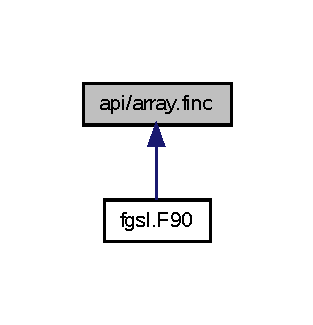
\includegraphics[width=154pt]{array_8finc__dep__incl}
\end{center}
\end{figure}
\subsection*{Functions/\-Subroutines}
\begin{DoxyCompactItemize}
\item 
type(fgsl\-\_\-vector) function \hyperlink{array_8finc_a0b6fe341146fbb3dfb27386e73c5d042}{fgsl\-\_\-vector\-\_\-init} (type)
\begin{DoxyCompactList}\small\item\em Initialize a G\-S\-L vector object. This is invoked via the generic \hyperlink{interfacefgsl__vector__init}{fgsl\-\_\-vector\-\_\-init}. \end{DoxyCompactList}\item 
integer(fgsl\-\_\-int) function \hyperlink{array_8finc_aa6c28c6cc37d807bc8bc0fcf4ab7ad57}{fgsl\-\_\-vector\-\_\-align} (array, len, fvec, size, offset, stride)
\begin{DoxyCompactList}\small\item\em Wrap a rank 1 Fortran array slice inside a double precision real G\-S\-L vector object. This is invoked via the generic \hyperlink{interfacefgsl__vector__align}{fgsl\-\_\-vector\-\_\-align}. \end{DoxyCompactList}\item 
integer(fgsl\-\_\-int) function \hyperlink{array_8finc_a3f528d8f3b1aa8218339bc8fdb41497c}{fgsl\-\_\-vector\-\_\-pointer\-\_\-align} (ptr, fvec)
\begin{DoxyCompactList}\small\item\em Associate a Fortran pointer with the data stored inside a G\-S\-L vector object. This is invoked via the generic \hyperlink{interfacefgsl__vector__align}{fgsl\-\_\-vector\-\_\-align}. Objects of type {\ttfamily gsl\-\_\-vector} which are returned by G\-S\-L routines often are persistent subobjects of other G\-S\-L objects. A Fortran pointer aligned with a subobject hence will remain up-\/to-\/date throughout the lifetime of the object; it may become undefined once the object ceases to exist. \end{DoxyCompactList}\item 
subroutine \hyperlink{array_8finc_a740b61c719ee64b92abc804915115255}{fgsl\-\_\-vector\-\_\-to\-\_\-array} (result, source)
\begin{DoxyCompactList}\small\item\em The assignment operator (see \hyperlink{generics_8finc}{interface/generics.\-finc}) is overloaded to enable copying of the content of a G\-S\-L vector into a Fortran array. \end{DoxyCompactList}\item 
subroutine \hyperlink{array_8finc_a900770fc4f4831abf928959477ba663f}{fgsl\-\_\-vector\-\_\-free} (fvec)
\begin{DoxyCompactList}\small\item\em Free the resources inside a G\-S\-L vector object previously established by a call to \hyperlink{array_8finc_a0b6fe341146fbb3dfb27386e73c5d042}{fgsl\-\_\-vector\-\_\-init()}. This is invoked via the generic \hyperlink{interfacefgsl__vector__free}{fgsl\-\_\-vector\-\_\-free}. \end{DoxyCompactList}\item 
subroutine \hyperlink{array_8finc_a8e80ad86d191ff87ae459b78822d468d}{fgsl\-\_\-vector\-\_\-c\-\_\-ptr} (res, src)
\item 
logical function \hyperlink{array_8finc_a804073922a322c29cd5be43410581ba4}{fgsl\-\_\-vector\-\_\-status} (vector)
\item 
integer(fgsl\-\_\-size\-\_\-t) function \hyperlink{array_8finc_a35a09f656acc547c7613501889490fc0}{fgsl\-\_\-sizeof\-\_\-vector} (w)
\begin{DoxyCompactList}\small\item\em Inquire the size of a double precision real G\-S\-L vector object. \end{DoxyCompactList}\item 
type(fgsl\-\_\-vector\-\_\-complex) function \hyperlink{array_8finc_a71c83c0b1de4b3965b6b8d6efb28cf13}{fgsl\-\_\-vector\-\_\-complex\-\_\-init} (type)
\begin{DoxyCompactList}\small\item\em Initialize a complex G\-S\-L vector object. This is invoked via the generic \hyperlink{interfacefgsl__vector__init}{fgsl\-\_\-vector\-\_\-init}. \end{DoxyCompactList}\item 
integer(fgsl\-\_\-int) function \hyperlink{array_8finc_ad91319661b892e978cfc3da52b15b500}{fgsl\-\_\-vector\-\_\-complex\-\_\-align} (array, len, fvec, size, offset, stride)
\begin{DoxyCompactList}\small\item\em Wrap a rank 1 Fortran array slice inside a double precision complex real G\-S\-L vector object. This is invoked via the generic \hyperlink{interfacefgsl__vector__align}{fgsl\-\_\-vector\-\_\-align}. \end{DoxyCompactList}\item 
integer(fgsl\-\_\-int) function \hyperlink{array_8finc_a0299f0feb175c085408bffdc001cb680}{fgsl\-\_\-vector\-\_\-complex\-\_\-pointer\-\_\-align} (ptr, fvec)
\begin{DoxyCompactList}\small\item\em Associate a Fortran pointer with the data stored inside a G\-S\-L vector object. This is invoked via the generic \hyperlink{interfacefgsl__vector__align}{fgsl\-\_\-vector\-\_\-align}. Objects of type {\ttfamily gsl\-\_\-vector\-\_\-complex} which are returned by G\-S\-L routines often are persistent subobjects of other G\-S\-L objects. A Fortran pointer aligned with a subobject hence will remain up-\/to-\/date throughout the lifetime of the object; it may become undefined once the object ceases to exist. \end{DoxyCompactList}\item 
subroutine \hyperlink{array_8finc_ad9bc465224323cc4ecdcf56589bdfdbb}{fgsl\-\_\-vector\-\_\-complex\-\_\-to\-\_\-array} (result, source)
\begin{DoxyCompactList}\small\item\em The assignment operator (see \hyperlink{generics_8finc}{interface/generics.\-finc}) is overloaded to enable copying of the content of a complex G\-S\-L vector into a Fortran array. \end{DoxyCompactList}\item 
subroutine \hyperlink{array_8finc_a3a8d76f2fe0bb4c9687f06e5e33671b8}{fgsl\-\_\-vector\-\_\-complex\-\_\-free} (fvec)
\begin{DoxyCompactList}\small\item\em Free the resources inside a complex G\-S\-L vector object previously established by a call to \hyperlink{array_8finc_a71c83c0b1de4b3965b6b8d6efb28cf13}{fgsl\-\_\-vector\-\_\-complex\-\_\-init()}. This is invoked via the generic \hyperlink{interfacefgsl__vector__free}{fgsl\-\_\-vector\-\_\-free}. \end{DoxyCompactList}\item 
subroutine \hyperlink{array_8finc_a07419ff1eb431e5a8bf628d31099e9a7}{fgsl\-\_\-vector\-\_\-complex\-\_\-c\-\_\-ptr} (res, src)
\item 
logical function \hyperlink{array_8finc_a04dbf95001922f560a73333ca3d00f81}{fgsl\-\_\-vector\-\_\-complex\-\_\-status} (vector\-\_\-complex)
\item 
integer(fgsl\-\_\-size\-\_\-t) function \hyperlink{array_8finc_af8cb8c5be9be9e6604200da0845dc18d}{fgsl\-\_\-sizeof\-\_\-vector\-\_\-complex} (w)
\begin{DoxyCompactList}\small\item\em Inquire the size of a double precision complex G\-S\-L vector object. \end{DoxyCompactList}\item 
type(fgsl\-\_\-matrix) function \hyperlink{array_8finc_af93d762ccde0b58b767c72579cbfb3cb}{fgsl\-\_\-matrix\-\_\-init} (type)
\begin{DoxyCompactList}\small\item\em Initialize a G\-S\-L matrix object. This is invoked via the generic \hyperlink{interfacefgsl__matrix__init}{fgsl\-\_\-matrix\-\_\-init}. \end{DoxyCompactList}\item 
integer(fgsl\-\_\-int) function \hyperlink{array_8finc_ae0c19c4453ce18db5e6415a047c3a59e}{fgsl\-\_\-matrix\-\_\-align} (array, lda, n, m, fmat)
\begin{DoxyCompactList}\small\item\em Wrap a rank 2 Fortran array inside a double precision real G\-S\-L matrix object. This is invoked via the generic \hyperlink{interfacefgsl__matrix__align}{fgsl\-\_\-matrix\-\_\-align}. \end{DoxyCompactList}\item 
integer(fgsl\-\_\-int) function \hyperlink{array_8finc_a54b17f056b272b74ae425a588e4653d5}{fgsl\-\_\-matrix\-\_\-pointer\-\_\-align} (ptr, fmat)
\begin{DoxyCompactList}\small\item\em Associate a Fortran pointer with the data stored inside a G\-S\-L matrix object. This is invoked via the generic \hyperlink{interfacefgsl__matrix__align}{fgsl\-\_\-matrix\-\_\-align}. Objects of type {\ttfamily gsl\-\_\-matrix} which are returned by G\-S\-L routines often are persistent subobjects of other G\-S\-L objects. A Fortran pointer aligned with a subobject hence will remain up-\/to-\/date throughout the lifetime of the object; it may become undefined once the object ceases to exist. \end{DoxyCompactList}\item 
subroutine \hyperlink{array_8finc_a44e06325d8b322997dcf6ab28417dd4f}{fgsl\-\_\-matrix\-\_\-to\-\_\-array} (result, source)
\begin{DoxyCompactList}\small\item\em The assignment operator (see \hyperlink{generics_8finc}{interface/generics.\-finc}) is overloaded to enable copying of the content of a G\-S\-L matrix into a rank 2 Fortran array. \end{DoxyCompactList}\item 
subroutine \hyperlink{array_8finc_a0b551f436f076593a8a828cd266e372d}{fgsl\-\_\-matrix\-\_\-free} (fvec)
\begin{DoxyCompactList}\small\item\em Free the resources inside a G\-S\-L matrix object previously established by a call to \hyperlink{array_8finc_af93d762ccde0b58b767c72579cbfb3cb}{fgsl\-\_\-matrix\-\_\-init()}. This is invoked via the generic \hyperlink{interfacefgsl__matrix__free}{fgsl\-\_\-matrix\-\_\-free}. \end{DoxyCompactList}\item 
subroutine \hyperlink{array_8finc_ae039428ac81fb123a5223c7676b1b687}{fgsl\-\_\-matrix\-\_\-c\-\_\-ptr} (res, src)
\item 
logical function \hyperlink{array_8finc_a5d41e00e4a2ec9c3b0594ec77ff02c5e}{fgsl\-\_\-matrix\-\_\-status} (matrix)
\item 
integer(fgsl\-\_\-size\-\_\-t) function \hyperlink{array_8finc_addcfbdff17fa7ce904b853ed793bb1d9}{fgsl\-\_\-sizeof\-\_\-matrix} (w)
\begin{DoxyCompactList}\small\item\em Inquire the number of elements in a double precision real G\-S\-L matrix object. \end{DoxyCompactList}\item 
type(fgsl\-\_\-matrix\-\_\-complex) function \hyperlink{array_8finc_af7461bad6c35fe6dde17e9c06bbc5cd0}{fgsl\-\_\-matrix\-\_\-complex\-\_\-init} (type)
\begin{DoxyCompactList}\small\item\em Initialize a G\-S\-L matrix object. This is invoked via the generic \hyperlink{interfacefgsl__matrix__init}{fgsl\-\_\-matrix\-\_\-init}. \end{DoxyCompactList}\item 
integer(fgsl\-\_\-int) function \hyperlink{array_8finc_ada029e69fd21da1d81472a285f1269a2}{fgsl\-\_\-matrix\-\_\-complex\-\_\-align} (array, lda, n, m, fmat)
\begin{DoxyCompactList}\small\item\em Wrap a rank 2 Fortran array inside a double precision complex G\-S\-L matrix object. This is invoked via the generic \hyperlink{interfacefgsl__matrix__align}{fgsl\-\_\-matrix\-\_\-align}. \end{DoxyCompactList}\item 
integer(fgsl\-\_\-int) function \hyperlink{array_8finc_a000f8ca7f88b4dfb7a5cc700ccf3b868}{fgsl\-\_\-matrix\-\_\-complex\-\_\-pointer\-\_\-align} (ptr, fmat)
\begin{DoxyCompactList}\small\item\em Associate a Fortran pointer with the data stored inside a complex G\-S\-L matrix object. This is invoked via the generic \hyperlink{interfacefgsl__matrix__align}{fgsl\-\_\-matrix\-\_\-align}. Objects of type {\ttfamily gsl\-\_\-matrix\-\_\-complex} which are returned by G\-S\-L routines often are persistent subobjects of other G\-S\-L objects. A Fortran pointer aligned with a subobject hence will remain up-\/to-\/date throughout the lifetime of the object; it may become undefined once the object ceases to exist. \end{DoxyCompactList}\item 
subroutine \hyperlink{array_8finc_a4b17724c0c305144fdec66507f8638f7}{fgsl\-\_\-matrix\-\_\-complex\-\_\-to\-\_\-array} (result, source)
\begin{DoxyCompactList}\small\item\em The assignment operator (see \hyperlink{generics_8finc}{interface/generics.\-finc}) is overloaded to enable copying of the content of a complex G\-S\-L matrix into a rank 2 Fortran array. \end{DoxyCompactList}\item 
subroutine \hyperlink{array_8finc_aa26219798c626c7bf6a0a85403f3dbcf}{fgsl\-\_\-matrix\-\_\-complex\-\_\-free} (fvec)
\begin{DoxyCompactList}\small\item\em Free the resources inside a complex G\-S\-L matrix object previously established by a call to \hyperlink{array_8finc_af7461bad6c35fe6dde17e9c06bbc5cd0}{fgsl\-\_\-matrix\-\_\-complex\-\_\-init()}. This is invoked via the generic \hyperlink{interfacefgsl__matrix__free}{fgsl\-\_\-matrix\-\_\-free}. \end{DoxyCompactList}\item 
subroutine \hyperlink{array_8finc_a9f0f952485ef9707174a52c5af21a9a2}{fgsl\-\_\-matrix\-\_\-complex\-\_\-c\-\_\-ptr} (res, src)
\item 
logical function \hyperlink{array_8finc_a3fa8db2b747286e805d60065f6d16640}{fgsl\-\_\-matrix\-\_\-complex\-\_\-status} (matrix\-\_\-complex)
\item 
integer(fgsl\-\_\-size\-\_\-t) function \hyperlink{array_8finc_a14d82675b93fa2b453caf33df1e567a1}{fgsl\-\_\-sizeof\-\_\-matrix\-\_\-complex} (w)
\begin{DoxyCompactList}\small\item\em Inquire the number of elements in a double precision complex G\-S\-L matrix object. \end{DoxyCompactList}\item 
integer(fgsl\-\_\-size\-\_\-t) function \hyperlink{array_8finc_a77255b64802ca66a1ada52fd0a9ceaf6}{fgsl\-\_\-vector\-\_\-get\-\_\-size} (vec)
\item 
integer(fgsl\-\_\-size\-\_\-t) function \hyperlink{array_8finc_adb3b5d4e8f719f06d11479ee5c7ad380}{fgsl\-\_\-vector\-\_\-get\-\_\-stride} (vec)
\item 
integer(fgsl\-\_\-size\-\_\-t) function \hyperlink{array_8finc_a17354bcc1b817f078799391343eee7e4}{fgsl\-\_\-matrix\-\_\-get\-\_\-size1} (matr)
\item 
integer(fgsl\-\_\-size\-\_\-t) function \hyperlink{array_8finc_a14ea1256acfbe059e0ea8e631a470f64}{fgsl\-\_\-matrix\-\_\-get\-\_\-size2} (matr)
\item 
integer(fgsl\-\_\-size\-\_\-t) function \hyperlink{array_8finc_ae49791bd4fbcbd27b90f1cf665fcb008}{fgsl\-\_\-matrix\-\_\-get\-\_\-tda} (matr)
\end{DoxyCompactItemize}


\subsection{Function/\-Subroutine Documentation}
\hypertarget{array_8finc_ae0c19c4453ce18db5e6415a047c3a59e}{\index{array.\-finc@{array.\-finc}!fgsl\-\_\-matrix\-\_\-align@{fgsl\-\_\-matrix\-\_\-align}}
\index{fgsl\-\_\-matrix\-\_\-align@{fgsl\-\_\-matrix\-\_\-align}!array.finc@{array.\-finc}}
\subsubsection[{fgsl\-\_\-matrix\-\_\-align}]{\setlength{\rightskip}{0pt plus 5cm}integer(fgsl\-\_\-int) function {\bf fgsl\-\_\-matrix\-\_\-align} (
\begin{DoxyParamCaption}
\item[{real(fgsl\-\_\-double), dimension(lda, m), intent(in), target}]{array, }
\item[{integer(fgsl\-\_\-size\-\_\-t), intent(in)}]{lda, }
\item[{integer(fgsl\-\_\-size\-\_\-t), intent(in)}]{n, }
\item[{integer(fgsl\-\_\-size\-\_\-t), intent(in)}]{m, }
\item[{type(fgsl\-\_\-matrix), intent(inout)}]{fmat}
\end{DoxyParamCaption}
)}}\label{array_8finc_ae0c19c4453ce18db5e6415a047c3a59e}


Wrap a rank 2 Fortran array inside a double precision real G\-S\-L matrix object. This is invoked via the generic \hyperlink{interfacefgsl__matrix__align}{fgsl\-\_\-matrix\-\_\-align}. 


\begin{DoxyParams}{Parameters}
{\em array} & -\/ requires the actual argument to have the T\-A\-R\-G\-E\-T attribute. Otherwise being passed by reference is not guaranteed by the Fortran standard. \\
\hline
{\em lda} & -\/ leading dimension of the rank 2 array \\
\hline
{\em n} & -\/ number of rows in array \\
\hline
{\em m} & -\/ number of columns in array \\
\hline
{\em fmat} & -\/ previously initialized double precision G\-S\-L matrix object \\
\hline
\end{DoxyParams}
\begin{DoxyReturn}{Returns}
Status 
\end{DoxyReturn}
\hypertarget{array_8finc_ae039428ac81fb123a5223c7676b1b687}{\index{array.\-finc@{array.\-finc}!fgsl\-\_\-matrix\-\_\-c\-\_\-ptr@{fgsl\-\_\-matrix\-\_\-c\-\_\-ptr}}
\index{fgsl\-\_\-matrix\-\_\-c\-\_\-ptr@{fgsl\-\_\-matrix\-\_\-c\-\_\-ptr}!array.finc@{array.\-finc}}
\subsubsection[{fgsl\-\_\-matrix\-\_\-c\-\_\-ptr}]{\setlength{\rightskip}{0pt plus 5cm}subroutine fgsl\-\_\-matrix\-\_\-c\-\_\-ptr (
\begin{DoxyParamCaption}
\item[{type(fgsl\-\_\-matrix), intent(out)}]{res, }
\item[{type(c\-\_\-ptr), intent(in)}]{src}
\end{DoxyParamCaption}
)}}\label{array_8finc_ae039428ac81fb123a5223c7676b1b687}
\hypertarget{array_8finc_ada029e69fd21da1d81472a285f1269a2}{\index{array.\-finc@{array.\-finc}!fgsl\-\_\-matrix\-\_\-complex\-\_\-align@{fgsl\-\_\-matrix\-\_\-complex\-\_\-align}}
\index{fgsl\-\_\-matrix\-\_\-complex\-\_\-align@{fgsl\-\_\-matrix\-\_\-complex\-\_\-align}!array.finc@{array.\-finc}}
\subsubsection[{fgsl\-\_\-matrix\-\_\-complex\-\_\-align}]{\setlength{\rightskip}{0pt plus 5cm}integer(fgsl\-\_\-int) function fgsl\-\_\-matrix\-\_\-complex\-\_\-align (
\begin{DoxyParamCaption}
\item[{complex(fgsl\-\_\-double\-\_\-complex), dimension(lda, m), intent(in), target}]{array, }
\item[{integer(fgsl\-\_\-size\-\_\-t), intent(in)}]{lda, }
\item[{integer(fgsl\-\_\-size\-\_\-t), intent(in)}]{n, }
\item[{integer(fgsl\-\_\-size\-\_\-t), intent(in)}]{m, }
\item[{type(fgsl\-\_\-matrix\-\_\-complex), intent(inout)}]{fmat}
\end{DoxyParamCaption}
)}}\label{array_8finc_ada029e69fd21da1d81472a285f1269a2}


Wrap a rank 2 Fortran array inside a double precision complex G\-S\-L matrix object. This is invoked via the generic \hyperlink{interfacefgsl__matrix__align}{fgsl\-\_\-matrix\-\_\-align}. 


\begin{DoxyParams}{Parameters}
{\em array} & -\/ requires the actual argument to have the T\-A\-R\-G\-E\-T attribute. Otherwise being passed by reference is not guaranteed by the Fortran standard. \\
\hline
{\em lda} & -\/ leading dimension of the rank 2 array \\
\hline
{\em n} & -\/ number of rows in array \\
\hline
{\em m} & -\/ number of columns in array \\
\hline
{\em fmat} & -\/ previously initialized double precision complex G\-S\-L matrix object \\
\hline
\end{DoxyParams}
\begin{DoxyReturn}{Returns}
Status 
\end{DoxyReturn}
\hypertarget{array_8finc_a9f0f952485ef9707174a52c5af21a9a2}{\index{array.\-finc@{array.\-finc}!fgsl\-\_\-matrix\-\_\-complex\-\_\-c\-\_\-ptr@{fgsl\-\_\-matrix\-\_\-complex\-\_\-c\-\_\-ptr}}
\index{fgsl\-\_\-matrix\-\_\-complex\-\_\-c\-\_\-ptr@{fgsl\-\_\-matrix\-\_\-complex\-\_\-c\-\_\-ptr}!array.finc@{array.\-finc}}
\subsubsection[{fgsl\-\_\-matrix\-\_\-complex\-\_\-c\-\_\-ptr}]{\setlength{\rightskip}{0pt plus 5cm}subroutine fgsl\-\_\-matrix\-\_\-complex\-\_\-c\-\_\-ptr (
\begin{DoxyParamCaption}
\item[{type(fgsl\-\_\-matrix\-\_\-complex), intent(out)}]{res, }
\item[{type(c\-\_\-ptr), intent(in)}]{src}
\end{DoxyParamCaption}
)}}\label{array_8finc_a9f0f952485ef9707174a52c5af21a9a2}
\hypertarget{array_8finc_aa26219798c626c7bf6a0a85403f3dbcf}{\index{array.\-finc@{array.\-finc}!fgsl\-\_\-matrix\-\_\-complex\-\_\-free@{fgsl\-\_\-matrix\-\_\-complex\-\_\-free}}
\index{fgsl\-\_\-matrix\-\_\-complex\-\_\-free@{fgsl\-\_\-matrix\-\_\-complex\-\_\-free}!array.finc@{array.\-finc}}
\subsubsection[{fgsl\-\_\-matrix\-\_\-complex\-\_\-free}]{\setlength{\rightskip}{0pt plus 5cm}subroutine fgsl\-\_\-matrix\-\_\-complex\-\_\-free (
\begin{DoxyParamCaption}
\item[{type(fgsl\-\_\-matrix\-\_\-complex), intent(inout)}]{fvec}
\end{DoxyParamCaption}
)}}\label{array_8finc_aa26219798c626c7bf6a0a85403f3dbcf}


Free the resources inside a complex G\-S\-L matrix object previously established by a call to \hyperlink{array_8finc_af7461bad6c35fe6dde17e9c06bbc5cd0}{fgsl\-\_\-matrix\-\_\-complex\-\_\-init()}. This is invoked via the generic \hyperlink{interfacefgsl__matrix__free}{fgsl\-\_\-matrix\-\_\-free}. 

\hypertarget{array_8finc_af7461bad6c35fe6dde17e9c06bbc5cd0}{\index{array.\-finc@{array.\-finc}!fgsl\-\_\-matrix\-\_\-complex\-\_\-init@{fgsl\-\_\-matrix\-\_\-complex\-\_\-init}}
\index{fgsl\-\_\-matrix\-\_\-complex\-\_\-init@{fgsl\-\_\-matrix\-\_\-complex\-\_\-init}!array.finc@{array.\-finc}}
\subsubsection[{fgsl\-\_\-matrix\-\_\-complex\-\_\-init}]{\setlength{\rightskip}{0pt plus 5cm}type(fgsl\-\_\-matrix\-\_\-complex) function fgsl\-\_\-matrix\-\_\-complex\-\_\-init (
\begin{DoxyParamCaption}
\item[{complex(fgsl\-\_\-double\-\_\-complex), intent(in)}]{type}
\end{DoxyParamCaption}
)}}\label{array_8finc_af7461bad6c35fe6dde17e9c06bbc5cd0}


Initialize a G\-S\-L matrix object. This is invoked via the generic \hyperlink{interfacefgsl__matrix__init}{fgsl\-\_\-matrix\-\_\-init}. 


\begin{DoxyParams}{Parameters}
{\em type} & -\/ determine intrinsic type of vector object \\
\hline
\end{DoxyParams}
\begin{DoxyReturn}{Returns}
new object of type fgsl\-\_\-matrix. 
\end{DoxyReturn}
\hypertarget{array_8finc_a000f8ca7f88b4dfb7a5cc700ccf3b868}{\index{array.\-finc@{array.\-finc}!fgsl\-\_\-matrix\-\_\-complex\-\_\-pointer\-\_\-align@{fgsl\-\_\-matrix\-\_\-complex\-\_\-pointer\-\_\-align}}
\index{fgsl\-\_\-matrix\-\_\-complex\-\_\-pointer\-\_\-align@{fgsl\-\_\-matrix\-\_\-complex\-\_\-pointer\-\_\-align}!array.finc@{array.\-finc}}
\subsubsection[{fgsl\-\_\-matrix\-\_\-complex\-\_\-pointer\-\_\-align}]{\setlength{\rightskip}{0pt plus 5cm}integer(fgsl\-\_\-int) function fgsl\-\_\-matrix\-\_\-complex\-\_\-pointer\-\_\-align (
\begin{DoxyParamCaption}
\item[{complex(fgsl\-\_\-double\-\_\-complex), dimension(\-:,\-:), intent(out), pointer}]{ptr, }
\item[{type(fgsl\-\_\-matrix\-\_\-complex), intent(in)}]{fmat}
\end{DoxyParamCaption}
)}}\label{array_8finc_a000f8ca7f88b4dfb7a5cc700ccf3b868}


Associate a Fortran pointer with the data stored inside a complex G\-S\-L matrix object. This is invoked via the generic \hyperlink{interfacefgsl__matrix__align}{fgsl\-\_\-matrix\-\_\-align}. Objects of type {\ttfamily gsl\-\_\-matrix\-\_\-complex} which are returned by G\-S\-L routines often are persistent subobjects of other G\-S\-L objects. A Fortran pointer aligned with a subobject hence will remain up-\/to-\/date throughout the lifetime of the object; it may become undefined once the object ceases to exist. 


\begin{DoxyParams}{Parameters}
{\em ptr} & -\/ rank 2 Fortran pointer \\
\hline
{\em fmat} & -\/ double precision complex G\-S\-L matrix \\
\hline
\end{DoxyParams}
\begin{DoxyReturn}{Returns}
Status 
\end{DoxyReturn}
\hypertarget{array_8finc_a3fa8db2b747286e805d60065f6d16640}{\index{array.\-finc@{array.\-finc}!fgsl\-\_\-matrix\-\_\-complex\-\_\-status@{fgsl\-\_\-matrix\-\_\-complex\-\_\-status}}
\index{fgsl\-\_\-matrix\-\_\-complex\-\_\-status@{fgsl\-\_\-matrix\-\_\-complex\-\_\-status}!array.finc@{array.\-finc}}
\subsubsection[{fgsl\-\_\-matrix\-\_\-complex\-\_\-status}]{\setlength{\rightskip}{0pt plus 5cm}logical function fgsl\-\_\-matrix\-\_\-complex\-\_\-status (
\begin{DoxyParamCaption}
\item[{type(fgsl\-\_\-matrix\-\_\-complex), intent(in)}]{matrix\-\_\-complex}
\end{DoxyParamCaption}
)}}\label{array_8finc_a3fa8db2b747286e805d60065f6d16640}
\hypertarget{array_8finc_a4b17724c0c305144fdec66507f8638f7}{\index{array.\-finc@{array.\-finc}!fgsl\-\_\-matrix\-\_\-complex\-\_\-to\-\_\-array@{fgsl\-\_\-matrix\-\_\-complex\-\_\-to\-\_\-array}}
\index{fgsl\-\_\-matrix\-\_\-complex\-\_\-to\-\_\-array@{fgsl\-\_\-matrix\-\_\-complex\-\_\-to\-\_\-array}!array.finc@{array.\-finc}}
\subsubsection[{fgsl\-\_\-matrix\-\_\-complex\-\_\-to\-\_\-array}]{\setlength{\rightskip}{0pt plus 5cm}subroutine fgsl\-\_\-matrix\-\_\-complex\-\_\-to\-\_\-array (
\begin{DoxyParamCaption}
\item[{complex(fgsl\-\_\-double\-\_\-complex), dimension(\-:,\-:), intent(inout)}]{result, }
\item[{type(fgsl\-\_\-matrix\-\_\-complex), intent(in)}]{source}
\end{DoxyParamCaption}
)}}\label{array_8finc_a4b17724c0c305144fdec66507f8638f7}


The assignment operator (see \hyperlink{generics_8finc}{interface/generics.\-finc}) is overloaded to enable copying of the content of a complex G\-S\-L matrix into a rank 2 Fortran array. 

\hypertarget{array_8finc_a0b551f436f076593a8a828cd266e372d}{\index{array.\-finc@{array.\-finc}!fgsl\-\_\-matrix\-\_\-free@{fgsl\-\_\-matrix\-\_\-free}}
\index{fgsl\-\_\-matrix\-\_\-free@{fgsl\-\_\-matrix\-\_\-free}!array.finc@{array.\-finc}}
\subsubsection[{fgsl\-\_\-matrix\-\_\-free}]{\setlength{\rightskip}{0pt plus 5cm}subroutine {\bf fgsl\-\_\-matrix\-\_\-free} (
\begin{DoxyParamCaption}
\item[{type(fgsl\-\_\-matrix), intent(inout)}]{fvec}
\end{DoxyParamCaption}
)}}\label{array_8finc_a0b551f436f076593a8a828cd266e372d}


Free the resources inside a G\-S\-L matrix object previously established by a call to \hyperlink{array_8finc_af93d762ccde0b58b767c72579cbfb3cb}{fgsl\-\_\-matrix\-\_\-init()}. This is invoked via the generic \hyperlink{interfacefgsl__matrix__free}{fgsl\-\_\-matrix\-\_\-free}. 

\hypertarget{array_8finc_a17354bcc1b817f078799391343eee7e4}{\index{array.\-finc@{array.\-finc}!fgsl\-\_\-matrix\-\_\-get\-\_\-size1@{fgsl\-\_\-matrix\-\_\-get\-\_\-size1}}
\index{fgsl\-\_\-matrix\-\_\-get\-\_\-size1@{fgsl\-\_\-matrix\-\_\-get\-\_\-size1}!array.finc@{array.\-finc}}
\subsubsection[{fgsl\-\_\-matrix\-\_\-get\-\_\-size1}]{\setlength{\rightskip}{0pt plus 5cm}integer(fgsl\-\_\-size\-\_\-t) function fgsl\-\_\-matrix\-\_\-get\-\_\-size1 (
\begin{DoxyParamCaption}
\item[{type(fgsl\-\_\-matrix), intent(in)}]{matr}
\end{DoxyParamCaption}
)}}\label{array_8finc_a17354bcc1b817f078799391343eee7e4}
\hypertarget{array_8finc_a14ea1256acfbe059e0ea8e631a470f64}{\index{array.\-finc@{array.\-finc}!fgsl\-\_\-matrix\-\_\-get\-\_\-size2@{fgsl\-\_\-matrix\-\_\-get\-\_\-size2}}
\index{fgsl\-\_\-matrix\-\_\-get\-\_\-size2@{fgsl\-\_\-matrix\-\_\-get\-\_\-size2}!array.finc@{array.\-finc}}
\subsubsection[{fgsl\-\_\-matrix\-\_\-get\-\_\-size2}]{\setlength{\rightskip}{0pt plus 5cm}integer(fgsl\-\_\-size\-\_\-t) function fgsl\-\_\-matrix\-\_\-get\-\_\-size2 (
\begin{DoxyParamCaption}
\item[{type(fgsl\-\_\-matrix), intent(in)}]{matr}
\end{DoxyParamCaption}
)}}\label{array_8finc_a14ea1256acfbe059e0ea8e631a470f64}
\hypertarget{array_8finc_ae49791bd4fbcbd27b90f1cf665fcb008}{\index{array.\-finc@{array.\-finc}!fgsl\-\_\-matrix\-\_\-get\-\_\-tda@{fgsl\-\_\-matrix\-\_\-get\-\_\-tda}}
\index{fgsl\-\_\-matrix\-\_\-get\-\_\-tda@{fgsl\-\_\-matrix\-\_\-get\-\_\-tda}!array.finc@{array.\-finc}}
\subsubsection[{fgsl\-\_\-matrix\-\_\-get\-\_\-tda}]{\setlength{\rightskip}{0pt plus 5cm}integer(fgsl\-\_\-size\-\_\-t) function fgsl\-\_\-matrix\-\_\-get\-\_\-tda (
\begin{DoxyParamCaption}
\item[{type(fgsl\-\_\-matrix), intent(in)}]{matr}
\end{DoxyParamCaption}
)}}\label{array_8finc_ae49791bd4fbcbd27b90f1cf665fcb008}
\hypertarget{array_8finc_af93d762ccde0b58b767c72579cbfb3cb}{\index{array.\-finc@{array.\-finc}!fgsl\-\_\-matrix\-\_\-init@{fgsl\-\_\-matrix\-\_\-init}}
\index{fgsl\-\_\-matrix\-\_\-init@{fgsl\-\_\-matrix\-\_\-init}!array.finc@{array.\-finc}}
\subsubsection[{fgsl\-\_\-matrix\-\_\-init}]{\setlength{\rightskip}{0pt plus 5cm}type(fgsl\-\_\-matrix) function {\bf fgsl\-\_\-matrix\-\_\-init} (
\begin{DoxyParamCaption}
\item[{real(fgsl\-\_\-double), intent(in)}]{type}
\end{DoxyParamCaption}
)}}\label{array_8finc_af93d762ccde0b58b767c72579cbfb3cb}


Initialize a G\-S\-L matrix object. This is invoked via the generic \hyperlink{interfacefgsl__matrix__init}{fgsl\-\_\-matrix\-\_\-init}. 


\begin{DoxyParams}{Parameters}
{\em type} & -\/ determine intrinsic type of vector object \\
\hline
\end{DoxyParams}
\begin{DoxyReturn}{Returns}
new object of type fgsl\-\_\-matrix. 
\end{DoxyReturn}
\hypertarget{array_8finc_a54b17f056b272b74ae425a588e4653d5}{\index{array.\-finc@{array.\-finc}!fgsl\-\_\-matrix\-\_\-pointer\-\_\-align@{fgsl\-\_\-matrix\-\_\-pointer\-\_\-align}}
\index{fgsl\-\_\-matrix\-\_\-pointer\-\_\-align@{fgsl\-\_\-matrix\-\_\-pointer\-\_\-align}!array.finc@{array.\-finc}}
\subsubsection[{fgsl\-\_\-matrix\-\_\-pointer\-\_\-align}]{\setlength{\rightskip}{0pt plus 5cm}integer(fgsl\-\_\-int) function fgsl\-\_\-matrix\-\_\-pointer\-\_\-align (
\begin{DoxyParamCaption}
\item[{real(fgsl\-\_\-double), dimension(\-:,\-:), intent(out), pointer}]{ptr, }
\item[{type(fgsl\-\_\-matrix), intent(in)}]{fmat}
\end{DoxyParamCaption}
)}}\label{array_8finc_a54b17f056b272b74ae425a588e4653d5}


Associate a Fortran pointer with the data stored inside a G\-S\-L matrix object. This is invoked via the generic \hyperlink{interfacefgsl__matrix__align}{fgsl\-\_\-matrix\-\_\-align}. Objects of type {\ttfamily gsl\-\_\-matrix} which are returned by G\-S\-L routines often are persistent subobjects of other G\-S\-L objects. A Fortran pointer aligned with a subobject hence will remain up-\/to-\/date throughout the lifetime of the object; it may become undefined once the object ceases to exist. 


\begin{DoxyParams}{Parameters}
{\em ptr} & -\/ rank 2 Fortran pointer \\
\hline
{\em fmat} & -\/ double precision real G\-S\-L matrix \\
\hline
\end{DoxyParams}
\begin{DoxyReturn}{Returns}
Status 
\end{DoxyReturn}
\hypertarget{array_8finc_a5d41e00e4a2ec9c3b0594ec77ff02c5e}{\index{array.\-finc@{array.\-finc}!fgsl\-\_\-matrix\-\_\-status@{fgsl\-\_\-matrix\-\_\-status}}
\index{fgsl\-\_\-matrix\-\_\-status@{fgsl\-\_\-matrix\-\_\-status}!array.finc@{array.\-finc}}
\subsubsection[{fgsl\-\_\-matrix\-\_\-status}]{\setlength{\rightskip}{0pt plus 5cm}logical function fgsl\-\_\-matrix\-\_\-status (
\begin{DoxyParamCaption}
\item[{type(fgsl\-\_\-matrix), intent(in)}]{matrix}
\end{DoxyParamCaption}
)}}\label{array_8finc_a5d41e00e4a2ec9c3b0594ec77ff02c5e}
\hypertarget{array_8finc_a44e06325d8b322997dcf6ab28417dd4f}{\index{array.\-finc@{array.\-finc}!fgsl\-\_\-matrix\-\_\-to\-\_\-array@{fgsl\-\_\-matrix\-\_\-to\-\_\-array}}
\index{fgsl\-\_\-matrix\-\_\-to\-\_\-array@{fgsl\-\_\-matrix\-\_\-to\-\_\-array}!array.finc@{array.\-finc}}
\subsubsection[{fgsl\-\_\-matrix\-\_\-to\-\_\-array}]{\setlength{\rightskip}{0pt plus 5cm}subroutine fgsl\-\_\-matrix\-\_\-to\-\_\-array (
\begin{DoxyParamCaption}
\item[{real(fgsl\-\_\-double), dimension(\-:,\-:), intent(inout)}]{result, }
\item[{type(fgsl\-\_\-matrix), intent(in)}]{source}
\end{DoxyParamCaption}
)}}\label{array_8finc_a44e06325d8b322997dcf6ab28417dd4f}


The assignment operator (see \hyperlink{generics_8finc}{interface/generics.\-finc}) is overloaded to enable copying of the content of a G\-S\-L matrix into a rank 2 Fortran array. 

\hypertarget{array_8finc_addcfbdff17fa7ce904b853ed793bb1d9}{\index{array.\-finc@{array.\-finc}!fgsl\-\_\-sizeof\-\_\-matrix@{fgsl\-\_\-sizeof\-\_\-matrix}}
\index{fgsl\-\_\-sizeof\-\_\-matrix@{fgsl\-\_\-sizeof\-\_\-matrix}!array.finc@{array.\-finc}}
\subsubsection[{fgsl\-\_\-sizeof\-\_\-matrix}]{\setlength{\rightskip}{0pt plus 5cm}integer(fgsl\-\_\-size\-\_\-t) function fgsl\-\_\-sizeof\-\_\-matrix (
\begin{DoxyParamCaption}
\item[{type(fgsl\-\_\-matrix), intent(in)}]{w}
\end{DoxyParamCaption}
)}}\label{array_8finc_addcfbdff17fa7ce904b853ed793bb1d9}


Inquire the number of elements in a double precision real G\-S\-L matrix object. 

\hypertarget{array_8finc_a14d82675b93fa2b453caf33df1e567a1}{\index{array.\-finc@{array.\-finc}!fgsl\-\_\-sizeof\-\_\-matrix\-\_\-complex@{fgsl\-\_\-sizeof\-\_\-matrix\-\_\-complex}}
\index{fgsl\-\_\-sizeof\-\_\-matrix\-\_\-complex@{fgsl\-\_\-sizeof\-\_\-matrix\-\_\-complex}!array.finc@{array.\-finc}}
\subsubsection[{fgsl\-\_\-sizeof\-\_\-matrix\-\_\-complex}]{\setlength{\rightskip}{0pt plus 5cm}integer(fgsl\-\_\-size\-\_\-t) function fgsl\-\_\-sizeof\-\_\-matrix\-\_\-complex (
\begin{DoxyParamCaption}
\item[{type(fgsl\-\_\-matrix\-\_\-complex), intent(in)}]{w}
\end{DoxyParamCaption}
)}}\label{array_8finc_a14d82675b93fa2b453caf33df1e567a1}


Inquire the number of elements in a double precision complex G\-S\-L matrix object. 

\hypertarget{array_8finc_a35a09f656acc547c7613501889490fc0}{\index{array.\-finc@{array.\-finc}!fgsl\-\_\-sizeof\-\_\-vector@{fgsl\-\_\-sizeof\-\_\-vector}}
\index{fgsl\-\_\-sizeof\-\_\-vector@{fgsl\-\_\-sizeof\-\_\-vector}!array.finc@{array.\-finc}}
\subsubsection[{fgsl\-\_\-sizeof\-\_\-vector}]{\setlength{\rightskip}{0pt plus 5cm}integer(fgsl\-\_\-size\-\_\-t) function fgsl\-\_\-sizeof\-\_\-vector (
\begin{DoxyParamCaption}
\item[{type(fgsl\-\_\-vector), intent(in)}]{w}
\end{DoxyParamCaption}
)}}\label{array_8finc_a35a09f656acc547c7613501889490fc0}


Inquire the size of a double precision real G\-S\-L vector object. 

\hypertarget{array_8finc_af8cb8c5be9be9e6604200da0845dc18d}{\index{array.\-finc@{array.\-finc}!fgsl\-\_\-sizeof\-\_\-vector\-\_\-complex@{fgsl\-\_\-sizeof\-\_\-vector\-\_\-complex}}
\index{fgsl\-\_\-sizeof\-\_\-vector\-\_\-complex@{fgsl\-\_\-sizeof\-\_\-vector\-\_\-complex}!array.finc@{array.\-finc}}
\subsubsection[{fgsl\-\_\-sizeof\-\_\-vector\-\_\-complex}]{\setlength{\rightskip}{0pt plus 5cm}integer(fgsl\-\_\-size\-\_\-t) function fgsl\-\_\-sizeof\-\_\-vector\-\_\-complex (
\begin{DoxyParamCaption}
\item[{type(fgsl\-\_\-vector\-\_\-complex), intent(in)}]{w}
\end{DoxyParamCaption}
)}}\label{array_8finc_af8cb8c5be9be9e6604200da0845dc18d}


Inquire the size of a double precision complex G\-S\-L vector object. 

\hypertarget{array_8finc_aa6c28c6cc37d807bc8bc0fcf4ab7ad57}{\index{array.\-finc@{array.\-finc}!fgsl\-\_\-vector\-\_\-align@{fgsl\-\_\-vector\-\_\-align}}
\index{fgsl\-\_\-vector\-\_\-align@{fgsl\-\_\-vector\-\_\-align}!array.finc@{array.\-finc}}
\subsubsection[{fgsl\-\_\-vector\-\_\-align}]{\setlength{\rightskip}{0pt plus 5cm}integer(fgsl\-\_\-int) function {\bf fgsl\-\_\-vector\-\_\-align} (
\begin{DoxyParamCaption}
\item[{real(fgsl\-\_\-double), dimension(len), intent(in), target}]{array, }
\item[{integer(fgsl\-\_\-size\-\_\-t), intent(in)}]{len, }
\item[{type(fgsl\-\_\-vector), intent(inout)}]{fvec, }
\item[{integer(fgsl\-\_\-size\-\_\-t), intent(in)}]{size, }
\item[{integer(fgsl\-\_\-size\-\_\-t), intent(in)}]{offset, }
\item[{integer(fgsl\-\_\-size\-\_\-t), intent(in)}]{stride}
\end{DoxyParamCaption}
)}}\label{array_8finc_aa6c28c6cc37d807bc8bc0fcf4ab7ad57}


Wrap a rank 1 Fortran array slice inside a double precision real G\-S\-L vector object. This is invoked via the generic \hyperlink{interfacefgsl__vector__align}{fgsl\-\_\-vector\-\_\-align}. 


\begin{DoxyParams}{Parameters}
{\em array} & -\/ requires the actual argument to have the T\-A\-R\-G\-E\-T attribute. Otherwise being passed by reference is not guaranteed by the Fortran standard. \\
\hline
{\em len} & -\/ number of elements of the rank 1 array \\
\hline
{\em fvec} & -\/ previously initialized G\-S\-L vector object \\
\hline
{\em size} & -\/ number of elements from array wrapped inside fvec \\
\hline
{\em offset} & -\/ index of first element of array to be mapped to fvec \\
\hline
{\em stride} & -\/ stride in array for successive elements of fvec \\
\hline
\end{DoxyParams}
\begin{DoxyReturn}{Returns}
Status 
\end{DoxyReturn}
\hypertarget{array_8finc_a8e80ad86d191ff87ae459b78822d468d}{\index{array.\-finc@{array.\-finc}!fgsl\-\_\-vector\-\_\-c\-\_\-ptr@{fgsl\-\_\-vector\-\_\-c\-\_\-ptr}}
\index{fgsl\-\_\-vector\-\_\-c\-\_\-ptr@{fgsl\-\_\-vector\-\_\-c\-\_\-ptr}!array.finc@{array.\-finc}}
\subsubsection[{fgsl\-\_\-vector\-\_\-c\-\_\-ptr}]{\setlength{\rightskip}{0pt plus 5cm}subroutine fgsl\-\_\-vector\-\_\-c\-\_\-ptr (
\begin{DoxyParamCaption}
\item[{type(fgsl\-\_\-vector), intent(out)}]{res, }
\item[{type(c\-\_\-ptr), intent(in)}]{src}
\end{DoxyParamCaption}
)}}\label{array_8finc_a8e80ad86d191ff87ae459b78822d468d}
\hypertarget{array_8finc_ad91319661b892e978cfc3da52b15b500}{\index{array.\-finc@{array.\-finc}!fgsl\-\_\-vector\-\_\-complex\-\_\-align@{fgsl\-\_\-vector\-\_\-complex\-\_\-align}}
\index{fgsl\-\_\-vector\-\_\-complex\-\_\-align@{fgsl\-\_\-vector\-\_\-complex\-\_\-align}!array.finc@{array.\-finc}}
\subsubsection[{fgsl\-\_\-vector\-\_\-complex\-\_\-align}]{\setlength{\rightskip}{0pt plus 5cm}integer(fgsl\-\_\-int) function fgsl\-\_\-vector\-\_\-complex\-\_\-align (
\begin{DoxyParamCaption}
\item[{complex(fgsl\-\_\-double\-\_\-complex), dimension(len), intent(in), target}]{array, }
\item[{integer(fgsl\-\_\-size\-\_\-t), intent(in)}]{len, }
\item[{type(fgsl\-\_\-vector\-\_\-complex), intent(inout)}]{fvec, }
\item[{integer(fgsl\-\_\-size\-\_\-t), intent(in)}]{size, }
\item[{integer(fgsl\-\_\-size\-\_\-t), intent(in)}]{offset, }
\item[{integer(fgsl\-\_\-size\-\_\-t), intent(in)}]{stride}
\end{DoxyParamCaption}
)}}\label{array_8finc_ad91319661b892e978cfc3da52b15b500}


Wrap a rank 1 Fortran array slice inside a double precision complex real G\-S\-L vector object. This is invoked via the generic \hyperlink{interfacefgsl__vector__align}{fgsl\-\_\-vector\-\_\-align}. 


\begin{DoxyParams}{Parameters}
{\em array} & -\/ requires the actual argument to have the T\-A\-R\-G\-E\-T attribute. Otherwise being passed by reference is not guaranteed by the Fortran standard. \\
\hline
{\em len} & -\/ number of elements of the rank 1 array \\
\hline
{\em fvec} & -\/ previously initialized complex G\-S\-L vector object \\
\hline
{\em size} & -\/ number of elements from array wrapped inside fvec \\
\hline
{\em offset} & -\/ index of first element of array to be mapped to fvec \\
\hline
{\em stride} & -\/ stride in array for successive elements of fvec \\
\hline
\end{DoxyParams}
\begin{DoxyReturn}{Returns}
Status 
\end{DoxyReturn}
\hypertarget{array_8finc_a07419ff1eb431e5a8bf628d31099e9a7}{\index{array.\-finc@{array.\-finc}!fgsl\-\_\-vector\-\_\-complex\-\_\-c\-\_\-ptr@{fgsl\-\_\-vector\-\_\-complex\-\_\-c\-\_\-ptr}}
\index{fgsl\-\_\-vector\-\_\-complex\-\_\-c\-\_\-ptr@{fgsl\-\_\-vector\-\_\-complex\-\_\-c\-\_\-ptr}!array.finc@{array.\-finc}}
\subsubsection[{fgsl\-\_\-vector\-\_\-complex\-\_\-c\-\_\-ptr}]{\setlength{\rightskip}{0pt plus 5cm}subroutine fgsl\-\_\-vector\-\_\-complex\-\_\-c\-\_\-ptr (
\begin{DoxyParamCaption}
\item[{type(fgsl\-\_\-vector\-\_\-complex), intent(out)}]{res, }
\item[{type(c\-\_\-ptr), intent(in)}]{src}
\end{DoxyParamCaption}
)}}\label{array_8finc_a07419ff1eb431e5a8bf628d31099e9a7}
\hypertarget{array_8finc_a3a8d76f2fe0bb4c9687f06e5e33671b8}{\index{array.\-finc@{array.\-finc}!fgsl\-\_\-vector\-\_\-complex\-\_\-free@{fgsl\-\_\-vector\-\_\-complex\-\_\-free}}
\index{fgsl\-\_\-vector\-\_\-complex\-\_\-free@{fgsl\-\_\-vector\-\_\-complex\-\_\-free}!array.finc@{array.\-finc}}
\subsubsection[{fgsl\-\_\-vector\-\_\-complex\-\_\-free}]{\setlength{\rightskip}{0pt plus 5cm}subroutine fgsl\-\_\-vector\-\_\-complex\-\_\-free (
\begin{DoxyParamCaption}
\item[{type(fgsl\-\_\-vector\-\_\-complex), intent(inout)}]{fvec}
\end{DoxyParamCaption}
)}}\label{array_8finc_a3a8d76f2fe0bb4c9687f06e5e33671b8}


Free the resources inside a complex G\-S\-L vector object previously established by a call to \hyperlink{array_8finc_a71c83c0b1de4b3965b6b8d6efb28cf13}{fgsl\-\_\-vector\-\_\-complex\-\_\-init()}. This is invoked via the generic \hyperlink{interfacefgsl__vector__free}{fgsl\-\_\-vector\-\_\-free}. 

\hypertarget{array_8finc_a71c83c0b1de4b3965b6b8d6efb28cf13}{\index{array.\-finc@{array.\-finc}!fgsl\-\_\-vector\-\_\-complex\-\_\-init@{fgsl\-\_\-vector\-\_\-complex\-\_\-init}}
\index{fgsl\-\_\-vector\-\_\-complex\-\_\-init@{fgsl\-\_\-vector\-\_\-complex\-\_\-init}!array.finc@{array.\-finc}}
\subsubsection[{fgsl\-\_\-vector\-\_\-complex\-\_\-init}]{\setlength{\rightskip}{0pt plus 5cm}type(fgsl\-\_\-vector\-\_\-complex) function fgsl\-\_\-vector\-\_\-complex\-\_\-init (
\begin{DoxyParamCaption}
\item[{complex(fgsl\-\_\-double\-\_\-complex), intent(in)}]{type}
\end{DoxyParamCaption}
)}}\label{array_8finc_a71c83c0b1de4b3965b6b8d6efb28cf13}


Initialize a complex G\-S\-L vector object. This is invoked via the generic \hyperlink{interfacefgsl__vector__init}{fgsl\-\_\-vector\-\_\-init}. 


\begin{DoxyParams}{Parameters}
{\em type} & -\/ determine intrinsic type of vector object \\
\hline
\end{DoxyParams}
\begin{DoxyReturn}{Returns}
new object of type fgsl\-\_\-vector 
\end{DoxyReturn}
\hypertarget{array_8finc_a0299f0feb175c085408bffdc001cb680}{\index{array.\-finc@{array.\-finc}!fgsl\-\_\-vector\-\_\-complex\-\_\-pointer\-\_\-align@{fgsl\-\_\-vector\-\_\-complex\-\_\-pointer\-\_\-align}}
\index{fgsl\-\_\-vector\-\_\-complex\-\_\-pointer\-\_\-align@{fgsl\-\_\-vector\-\_\-complex\-\_\-pointer\-\_\-align}!array.finc@{array.\-finc}}
\subsubsection[{fgsl\-\_\-vector\-\_\-complex\-\_\-pointer\-\_\-align}]{\setlength{\rightskip}{0pt plus 5cm}integer(fgsl\-\_\-int) function fgsl\-\_\-vector\-\_\-complex\-\_\-pointer\-\_\-align (
\begin{DoxyParamCaption}
\item[{complex(fgsl\-\_\-double\-\_\-complex), dimension(\-:), intent(out), pointer}]{ptr, }
\item[{type(fgsl\-\_\-vector\-\_\-complex), intent(in)}]{fvec}
\end{DoxyParamCaption}
)}}\label{array_8finc_a0299f0feb175c085408bffdc001cb680}


Associate a Fortran pointer with the data stored inside a G\-S\-L vector object. This is invoked via the generic \hyperlink{interfacefgsl__vector__align}{fgsl\-\_\-vector\-\_\-align}. Objects of type {\ttfamily gsl\-\_\-vector\-\_\-complex} which are returned by G\-S\-L routines often are persistent subobjects of other G\-S\-L objects. A Fortran pointer aligned with a subobject hence will remain up-\/to-\/date throughout the lifetime of the object; it may become undefined once the object ceases to exist. 


\begin{DoxyParams}{Parameters}
{\em ptr} & -\/ rank 1 Fortran pointer \\
\hline
{\em fvec} & -\/ double precision complex G\-S\-L vector \\
\hline
\end{DoxyParams}
\begin{DoxyReturn}{Returns}
Status 
\end{DoxyReturn}
\hypertarget{array_8finc_a04dbf95001922f560a73333ca3d00f81}{\index{array.\-finc@{array.\-finc}!fgsl\-\_\-vector\-\_\-complex\-\_\-status@{fgsl\-\_\-vector\-\_\-complex\-\_\-status}}
\index{fgsl\-\_\-vector\-\_\-complex\-\_\-status@{fgsl\-\_\-vector\-\_\-complex\-\_\-status}!array.finc@{array.\-finc}}
\subsubsection[{fgsl\-\_\-vector\-\_\-complex\-\_\-status}]{\setlength{\rightskip}{0pt plus 5cm}logical function fgsl\-\_\-vector\-\_\-complex\-\_\-status (
\begin{DoxyParamCaption}
\item[{type(fgsl\-\_\-vector\-\_\-complex), intent(in)}]{vector\-\_\-complex}
\end{DoxyParamCaption}
)}}\label{array_8finc_a04dbf95001922f560a73333ca3d00f81}
\hypertarget{array_8finc_ad9bc465224323cc4ecdcf56589bdfdbb}{\index{array.\-finc@{array.\-finc}!fgsl\-\_\-vector\-\_\-complex\-\_\-to\-\_\-array@{fgsl\-\_\-vector\-\_\-complex\-\_\-to\-\_\-array}}
\index{fgsl\-\_\-vector\-\_\-complex\-\_\-to\-\_\-array@{fgsl\-\_\-vector\-\_\-complex\-\_\-to\-\_\-array}!array.finc@{array.\-finc}}
\subsubsection[{fgsl\-\_\-vector\-\_\-complex\-\_\-to\-\_\-array}]{\setlength{\rightskip}{0pt plus 5cm}subroutine fgsl\-\_\-vector\-\_\-complex\-\_\-to\-\_\-array (
\begin{DoxyParamCaption}
\item[{complex(fgsl\-\_\-double\-\_\-complex), dimension(\-:), intent(inout)}]{result, }
\item[{type(fgsl\-\_\-vector\-\_\-complex), intent(in)}]{source}
\end{DoxyParamCaption}
)}}\label{array_8finc_ad9bc465224323cc4ecdcf56589bdfdbb}


The assignment operator (see \hyperlink{generics_8finc}{interface/generics.\-finc}) is overloaded to enable copying of the content of a complex G\-S\-L vector into a Fortran array. 

\hypertarget{array_8finc_a900770fc4f4831abf928959477ba663f}{\index{array.\-finc@{array.\-finc}!fgsl\-\_\-vector\-\_\-free@{fgsl\-\_\-vector\-\_\-free}}
\index{fgsl\-\_\-vector\-\_\-free@{fgsl\-\_\-vector\-\_\-free}!array.finc@{array.\-finc}}
\subsubsection[{fgsl\-\_\-vector\-\_\-free}]{\setlength{\rightskip}{0pt plus 5cm}subroutine {\bf fgsl\-\_\-vector\-\_\-free} (
\begin{DoxyParamCaption}
\item[{type(fgsl\-\_\-vector), intent(inout)}]{fvec}
\end{DoxyParamCaption}
)}}\label{array_8finc_a900770fc4f4831abf928959477ba663f}


Free the resources inside a G\-S\-L vector object previously established by a call to \hyperlink{array_8finc_a0b6fe341146fbb3dfb27386e73c5d042}{fgsl\-\_\-vector\-\_\-init()}. This is invoked via the generic \hyperlink{interfacefgsl__vector__free}{fgsl\-\_\-vector\-\_\-free}. 

\hypertarget{array_8finc_a77255b64802ca66a1ada52fd0a9ceaf6}{\index{array.\-finc@{array.\-finc}!fgsl\-\_\-vector\-\_\-get\-\_\-size@{fgsl\-\_\-vector\-\_\-get\-\_\-size}}
\index{fgsl\-\_\-vector\-\_\-get\-\_\-size@{fgsl\-\_\-vector\-\_\-get\-\_\-size}!array.finc@{array.\-finc}}
\subsubsection[{fgsl\-\_\-vector\-\_\-get\-\_\-size}]{\setlength{\rightskip}{0pt plus 5cm}integer(fgsl\-\_\-size\-\_\-t) function fgsl\-\_\-vector\-\_\-get\-\_\-size (
\begin{DoxyParamCaption}
\item[{type(fgsl\-\_\-vector), intent(in)}]{vec}
\end{DoxyParamCaption}
)}}\label{array_8finc_a77255b64802ca66a1ada52fd0a9ceaf6}
\hypertarget{array_8finc_adb3b5d4e8f719f06d11479ee5c7ad380}{\index{array.\-finc@{array.\-finc}!fgsl\-\_\-vector\-\_\-get\-\_\-stride@{fgsl\-\_\-vector\-\_\-get\-\_\-stride}}
\index{fgsl\-\_\-vector\-\_\-get\-\_\-stride@{fgsl\-\_\-vector\-\_\-get\-\_\-stride}!array.finc@{array.\-finc}}
\subsubsection[{fgsl\-\_\-vector\-\_\-get\-\_\-stride}]{\setlength{\rightskip}{0pt plus 5cm}integer(fgsl\-\_\-size\-\_\-t) function fgsl\-\_\-vector\-\_\-get\-\_\-stride (
\begin{DoxyParamCaption}
\item[{type(fgsl\-\_\-vector), intent(in)}]{vec}
\end{DoxyParamCaption}
)}}\label{array_8finc_adb3b5d4e8f719f06d11479ee5c7ad380}
\hypertarget{array_8finc_a0b6fe341146fbb3dfb27386e73c5d042}{\index{array.\-finc@{array.\-finc}!fgsl\-\_\-vector\-\_\-init@{fgsl\-\_\-vector\-\_\-init}}
\index{fgsl\-\_\-vector\-\_\-init@{fgsl\-\_\-vector\-\_\-init}!array.finc@{array.\-finc}}
\subsubsection[{fgsl\-\_\-vector\-\_\-init}]{\setlength{\rightskip}{0pt plus 5cm}type(fgsl\-\_\-vector) function {\bf fgsl\-\_\-vector\-\_\-init} (
\begin{DoxyParamCaption}
\item[{real(fgsl\-\_\-double), intent(in)}]{type}
\end{DoxyParamCaption}
)}}\label{array_8finc_a0b6fe341146fbb3dfb27386e73c5d042}


Initialize a G\-S\-L vector object. This is invoked via the generic \hyperlink{interfacefgsl__vector__init}{fgsl\-\_\-vector\-\_\-init}. 


\begin{DoxyParams}{Parameters}
{\em type} & -\/ determine intrinsic type of vector object \\
\hline
\end{DoxyParams}
\begin{DoxyReturn}{Returns}
new object of type fgsl\-\_\-vector 
\end{DoxyReturn}
\hypertarget{array_8finc_a3f528d8f3b1aa8218339bc8fdb41497c}{\index{array.\-finc@{array.\-finc}!fgsl\-\_\-vector\-\_\-pointer\-\_\-align@{fgsl\-\_\-vector\-\_\-pointer\-\_\-align}}
\index{fgsl\-\_\-vector\-\_\-pointer\-\_\-align@{fgsl\-\_\-vector\-\_\-pointer\-\_\-align}!array.finc@{array.\-finc}}
\subsubsection[{fgsl\-\_\-vector\-\_\-pointer\-\_\-align}]{\setlength{\rightskip}{0pt plus 5cm}integer(fgsl\-\_\-int) function fgsl\-\_\-vector\-\_\-pointer\-\_\-align (
\begin{DoxyParamCaption}
\item[{real(fgsl\-\_\-double), dimension(\-:), intent(out), pointer}]{ptr, }
\item[{type(fgsl\-\_\-vector), intent(in)}]{fvec}
\end{DoxyParamCaption}
)}}\label{array_8finc_a3f528d8f3b1aa8218339bc8fdb41497c}


Associate a Fortran pointer with the data stored inside a G\-S\-L vector object. This is invoked via the generic \hyperlink{interfacefgsl__vector__align}{fgsl\-\_\-vector\-\_\-align}. Objects of type {\ttfamily gsl\-\_\-vector} which are returned by G\-S\-L routines often are persistent subobjects of other G\-S\-L objects. A Fortran pointer aligned with a subobject hence will remain up-\/to-\/date throughout the lifetime of the object; it may become undefined once the object ceases to exist. 


\begin{DoxyParams}{Parameters}
{\em ptr} & -\/ rank 1 Fortran pointer \\
\hline
{\em fvec} & -\/ double precision real G\-S\-L vector \\
\hline
\end{DoxyParams}
\begin{DoxyReturn}{Returns}
Status 
\end{DoxyReturn}
\hypertarget{array_8finc_a804073922a322c29cd5be43410581ba4}{\index{array.\-finc@{array.\-finc}!fgsl\-\_\-vector\-\_\-status@{fgsl\-\_\-vector\-\_\-status}}
\index{fgsl\-\_\-vector\-\_\-status@{fgsl\-\_\-vector\-\_\-status}!array.finc@{array.\-finc}}
\subsubsection[{fgsl\-\_\-vector\-\_\-status}]{\setlength{\rightskip}{0pt plus 5cm}logical function fgsl\-\_\-vector\-\_\-status (
\begin{DoxyParamCaption}
\item[{type(fgsl\-\_\-vector), intent(in)}]{vector}
\end{DoxyParamCaption}
)}}\label{array_8finc_a804073922a322c29cd5be43410581ba4}
\hypertarget{array_8finc_a740b61c719ee64b92abc804915115255}{\index{array.\-finc@{array.\-finc}!fgsl\-\_\-vector\-\_\-to\-\_\-array@{fgsl\-\_\-vector\-\_\-to\-\_\-array}}
\index{fgsl\-\_\-vector\-\_\-to\-\_\-array@{fgsl\-\_\-vector\-\_\-to\-\_\-array}!array.finc@{array.\-finc}}
\subsubsection[{fgsl\-\_\-vector\-\_\-to\-\_\-array}]{\setlength{\rightskip}{0pt plus 5cm}subroutine fgsl\-\_\-vector\-\_\-to\-\_\-array (
\begin{DoxyParamCaption}
\item[{real(fgsl\-\_\-double), dimension(\-:), intent(inout)}]{result, }
\item[{type(fgsl\-\_\-vector), intent(in)}]{source}
\end{DoxyParamCaption}
)}}\label{array_8finc_a740b61c719ee64b92abc804915115255}


The assignment operator (see \hyperlink{generics_8finc}{interface/generics.\-finc}) is overloaded to enable copying of the content of a G\-S\-L vector into a Fortran array. 


\hypertarget{bspline_8finc}{\section{api/bspline.finc File Reference}
\label{bspline_8finc}\index{api/bspline.\-finc@{api/bspline.\-finc}}
}
This graph shows which files directly or indirectly include this file\-:\nopagebreak
\begin{figure}[H]
\begin{center}
\leavevmode
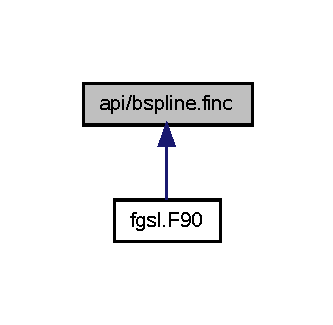
\includegraphics[width=162pt]{bspline_8finc__dep__incl}
\end{center}
\end{figure}
\subsection*{Functions/\-Subroutines}
\begin{DoxyCompactItemize}
\item 
type(fgsl\-\_\-bspline\-\_\-workspace) \\*
function \hyperlink{bspline_8finc_a4e15c7b2231a5f1a625f5d182ca159ed}{fgsl\-\_\-bspline\-\_\-alloc} (k, nbreak)
\item 
subroutine \hyperlink{bspline_8finc_aa6355eaea88c1a3223784670cd61f944}{fgsl\-\_\-bspline\-\_\-free} (w)
\item 
type(fgsl\-\_\-bspline\-\_\-deriv\-\_\-workspace) \\*
function \hyperlink{bspline_8finc_afcbf1aea5432f70f6a80b96c503ce660}{fgsl\-\_\-bspline\-\_\-deriv\-\_\-alloc} (k)
\item 
subroutine \hyperlink{bspline_8finc_a8ccf44ef0167e5813a4671a5d5eaad8b}{fgsl\-\_\-bspline\-\_\-deriv\-\_\-free} (w)
\item 
integer(fgsl\-\_\-int) function \hyperlink{bspline_8finc_a0c926191aa070f99a3f01fd32fa1b95d}{fgsl\-\_\-bspline\-\_\-knots} (breakpts, w)
\item 
integer(fgsl\-\_\-int) function \hyperlink{bspline_8finc_ae8a83e75e87a6475b4ad8584c18c037d}{fgsl\-\_\-bspline\-\_\-knots\-\_\-uniform} (a, b, w)
\item 
integer(fgsl\-\_\-int) function \hyperlink{bspline_8finc_ad884eba33109f4963100c7a64601c9df}{fgsl\-\_\-bspline\-\_\-eval} (x, b, w)
\item 
integer(fgsl\-\_\-int) function \hyperlink{bspline_8finc_a2cf7b76c3b3eacc2458726ce7eec827a}{fgsl\-\_\-bspline\-\_\-eval\-\_\-nonzero} (x, bk, istart, iend, w)
\item 
integer(fgsl\-\_\-int) function \hyperlink{bspline_8finc_a1a0753fdf8d9e838bc1b1886b29e673c}{fgsl\-\_\-bspline\-\_\-deriv\-\_\-eval} (x, nderiv, db, w, dw)
\item 
integer(fgsl\-\_\-int) function \hyperlink{bspline_8finc_a42dce02a85085b1eddf167c995873e38}{fgsl\-\_\-bspline\-\_\-deriv\-\_\-eval\-\_\-nonzero} (x, nderiv, db, istart, iend, w, dw)
\item 
integer(fgsl\-\_\-size\-\_\-t) function \hyperlink{bspline_8finc_a88f74da4054f622ccec25854d7d82a26}{fgsl\-\_\-bspline\-\_\-ncoeffs} (w)
\item 
real(fgsl\-\_\-double) function \hyperlink{bspline_8finc_a3919f7952797fb2dd676ae3f910c6d9e}{fgsl\-\_\-bspline\-\_\-greville\-\_\-abscissa} (i, w)
\item 
integer(fgsl\-\_\-int) function \hyperlink{bspline_8finc_ae82914f8a3d09b557ceac031a59363a0}{fgsl\-\_\-bspline\-\_\-knots\-\_\-greville} (abscissae, w, abserr)
\end{DoxyCompactItemize}


\subsection{Function/\-Subroutine Documentation}
\hypertarget{bspline_8finc_a4e15c7b2231a5f1a625f5d182ca159ed}{\index{bspline.\-finc@{bspline.\-finc}!fgsl\-\_\-bspline\-\_\-alloc@{fgsl\-\_\-bspline\-\_\-alloc}}
\index{fgsl\-\_\-bspline\-\_\-alloc@{fgsl\-\_\-bspline\-\_\-alloc}!bspline.finc@{bspline.\-finc}}
\subsubsection[{fgsl\-\_\-bspline\-\_\-alloc}]{\setlength{\rightskip}{0pt plus 5cm}type(fgsl\-\_\-bspline\-\_\-workspace) function fgsl\-\_\-bspline\-\_\-alloc (
\begin{DoxyParamCaption}
\item[{integer(fgsl\-\_\-size\-\_\-t), intent(in)}]{k, }
\item[{integer(fgsl\-\_\-size\-\_\-t), intent(in)}]{nbreak}
\end{DoxyParamCaption}
)}}\label{bspline_8finc_a4e15c7b2231a5f1a625f5d182ca159ed}
\hypertarget{bspline_8finc_afcbf1aea5432f70f6a80b96c503ce660}{\index{bspline.\-finc@{bspline.\-finc}!fgsl\-\_\-bspline\-\_\-deriv\-\_\-alloc@{fgsl\-\_\-bspline\-\_\-deriv\-\_\-alloc}}
\index{fgsl\-\_\-bspline\-\_\-deriv\-\_\-alloc@{fgsl\-\_\-bspline\-\_\-deriv\-\_\-alloc}!bspline.finc@{bspline.\-finc}}
\subsubsection[{fgsl\-\_\-bspline\-\_\-deriv\-\_\-alloc}]{\setlength{\rightskip}{0pt plus 5cm}type(fgsl\-\_\-bspline\-\_\-deriv\-\_\-workspace) function fgsl\-\_\-bspline\-\_\-deriv\-\_\-alloc (
\begin{DoxyParamCaption}
\item[{integer(fgsl\-\_\-size\-\_\-t), intent(in)}]{k}
\end{DoxyParamCaption}
)}}\label{bspline_8finc_afcbf1aea5432f70f6a80b96c503ce660}
\hypertarget{bspline_8finc_a1a0753fdf8d9e838bc1b1886b29e673c}{\index{bspline.\-finc@{bspline.\-finc}!fgsl\-\_\-bspline\-\_\-deriv\-\_\-eval@{fgsl\-\_\-bspline\-\_\-deriv\-\_\-eval}}
\index{fgsl\-\_\-bspline\-\_\-deriv\-\_\-eval@{fgsl\-\_\-bspline\-\_\-deriv\-\_\-eval}!bspline.finc@{bspline.\-finc}}
\subsubsection[{fgsl\-\_\-bspline\-\_\-deriv\-\_\-eval}]{\setlength{\rightskip}{0pt plus 5cm}integer(fgsl\-\_\-int) function fgsl\-\_\-bspline\-\_\-deriv\-\_\-eval (
\begin{DoxyParamCaption}
\item[{real(fgsl\-\_\-double), intent(in)}]{x, }
\item[{integer(fgsl\-\_\-size\-\_\-t), intent(in)}]{nderiv, }
\item[{type(fgsl\-\_\-matrix), intent(inout)}]{db, }
\item[{type(fgsl\-\_\-bspline\-\_\-workspace), intent(inout)}]{w, }
\item[{type(fgsl\-\_\-bspline\-\_\-deriv\-\_\-workspace), intent(inout)}]{dw}
\end{DoxyParamCaption}
)}}\label{bspline_8finc_a1a0753fdf8d9e838bc1b1886b29e673c}
\hypertarget{bspline_8finc_a42dce02a85085b1eddf167c995873e38}{\index{bspline.\-finc@{bspline.\-finc}!fgsl\-\_\-bspline\-\_\-deriv\-\_\-eval\-\_\-nonzero@{fgsl\-\_\-bspline\-\_\-deriv\-\_\-eval\-\_\-nonzero}}
\index{fgsl\-\_\-bspline\-\_\-deriv\-\_\-eval\-\_\-nonzero@{fgsl\-\_\-bspline\-\_\-deriv\-\_\-eval\-\_\-nonzero}!bspline.finc@{bspline.\-finc}}
\subsubsection[{fgsl\-\_\-bspline\-\_\-deriv\-\_\-eval\-\_\-nonzero}]{\setlength{\rightskip}{0pt plus 5cm}integer(fgsl\-\_\-int) function fgsl\-\_\-bspline\-\_\-deriv\-\_\-eval\-\_\-nonzero (
\begin{DoxyParamCaption}
\item[{real(fgsl\-\_\-double), intent(in)}]{x, }
\item[{integer(fgsl\-\_\-size\-\_\-t), intent(in)}]{nderiv, }
\item[{type(fgsl\-\_\-matrix), intent(inout)}]{db, }
\item[{integer(fgsl\-\_\-size\-\_\-t), intent(inout)}]{istart, }
\item[{integer(fgsl\-\_\-size\-\_\-t), intent(inout)}]{iend, }
\item[{type(fgsl\-\_\-bspline\-\_\-workspace), intent(inout)}]{w, }
\item[{type(fgsl\-\_\-bspline\-\_\-deriv\-\_\-workspace), intent(inout)}]{dw}
\end{DoxyParamCaption}
)}}\label{bspline_8finc_a42dce02a85085b1eddf167c995873e38}
\hypertarget{bspline_8finc_a8ccf44ef0167e5813a4671a5d5eaad8b}{\index{bspline.\-finc@{bspline.\-finc}!fgsl\-\_\-bspline\-\_\-deriv\-\_\-free@{fgsl\-\_\-bspline\-\_\-deriv\-\_\-free}}
\index{fgsl\-\_\-bspline\-\_\-deriv\-\_\-free@{fgsl\-\_\-bspline\-\_\-deriv\-\_\-free}!bspline.finc@{bspline.\-finc}}
\subsubsection[{fgsl\-\_\-bspline\-\_\-deriv\-\_\-free}]{\setlength{\rightskip}{0pt plus 5cm}subroutine fgsl\-\_\-bspline\-\_\-deriv\-\_\-free (
\begin{DoxyParamCaption}
\item[{type(fgsl\-\_\-bspline\-\_\-deriv\-\_\-workspace), intent(inout)}]{w}
\end{DoxyParamCaption}
)}}\label{bspline_8finc_a8ccf44ef0167e5813a4671a5d5eaad8b}
\hypertarget{bspline_8finc_ad884eba33109f4963100c7a64601c9df}{\index{bspline.\-finc@{bspline.\-finc}!fgsl\-\_\-bspline\-\_\-eval@{fgsl\-\_\-bspline\-\_\-eval}}
\index{fgsl\-\_\-bspline\-\_\-eval@{fgsl\-\_\-bspline\-\_\-eval}!bspline.finc@{bspline.\-finc}}
\subsubsection[{fgsl\-\_\-bspline\-\_\-eval}]{\setlength{\rightskip}{0pt plus 5cm}integer(fgsl\-\_\-int) function fgsl\-\_\-bspline\-\_\-eval (
\begin{DoxyParamCaption}
\item[{real(fgsl\-\_\-double), intent(in)}]{x, }
\item[{type(fgsl\-\_\-vector), intent(inout)}]{b, }
\item[{type(fgsl\-\_\-bspline\-\_\-workspace), intent(inout)}]{w}
\end{DoxyParamCaption}
)}}\label{bspline_8finc_ad884eba33109f4963100c7a64601c9df}
\hypertarget{bspline_8finc_a2cf7b76c3b3eacc2458726ce7eec827a}{\index{bspline.\-finc@{bspline.\-finc}!fgsl\-\_\-bspline\-\_\-eval\-\_\-nonzero@{fgsl\-\_\-bspline\-\_\-eval\-\_\-nonzero}}
\index{fgsl\-\_\-bspline\-\_\-eval\-\_\-nonzero@{fgsl\-\_\-bspline\-\_\-eval\-\_\-nonzero}!bspline.finc@{bspline.\-finc}}
\subsubsection[{fgsl\-\_\-bspline\-\_\-eval\-\_\-nonzero}]{\setlength{\rightskip}{0pt plus 5cm}integer(fgsl\-\_\-int) function fgsl\-\_\-bspline\-\_\-eval\-\_\-nonzero (
\begin{DoxyParamCaption}
\item[{real(fgsl\-\_\-double), intent(in)}]{x, }
\item[{type(fgsl\-\_\-vector), intent(inout)}]{bk, }
\item[{integer(fgsl\-\_\-size\-\_\-t), intent(inout)}]{istart, }
\item[{integer(fgsl\-\_\-size\-\_\-t), intent(inout)}]{iend, }
\item[{type(fgsl\-\_\-bspline\-\_\-workspace), intent(inout)}]{w}
\end{DoxyParamCaption}
)}}\label{bspline_8finc_a2cf7b76c3b3eacc2458726ce7eec827a}
\hypertarget{bspline_8finc_aa6355eaea88c1a3223784670cd61f944}{\index{bspline.\-finc@{bspline.\-finc}!fgsl\-\_\-bspline\-\_\-free@{fgsl\-\_\-bspline\-\_\-free}}
\index{fgsl\-\_\-bspline\-\_\-free@{fgsl\-\_\-bspline\-\_\-free}!bspline.finc@{bspline.\-finc}}
\subsubsection[{fgsl\-\_\-bspline\-\_\-free}]{\setlength{\rightskip}{0pt plus 5cm}subroutine fgsl\-\_\-bspline\-\_\-free (
\begin{DoxyParamCaption}
\item[{type(fgsl\-\_\-bspline\-\_\-workspace), intent(inout)}]{w}
\end{DoxyParamCaption}
)}}\label{bspline_8finc_aa6355eaea88c1a3223784670cd61f944}
\hypertarget{bspline_8finc_a3919f7952797fb2dd676ae3f910c6d9e}{\index{bspline.\-finc@{bspline.\-finc}!fgsl\-\_\-bspline\-\_\-greville\-\_\-abscissa@{fgsl\-\_\-bspline\-\_\-greville\-\_\-abscissa}}
\index{fgsl\-\_\-bspline\-\_\-greville\-\_\-abscissa@{fgsl\-\_\-bspline\-\_\-greville\-\_\-abscissa}!bspline.finc@{bspline.\-finc}}
\subsubsection[{fgsl\-\_\-bspline\-\_\-greville\-\_\-abscissa}]{\setlength{\rightskip}{0pt plus 5cm}real(fgsl\-\_\-double) function fgsl\-\_\-bspline\-\_\-greville\-\_\-abscissa (
\begin{DoxyParamCaption}
\item[{integer(fgsl\-\_\-size\-\_\-t)}]{i, }
\item[{type(fgsl\-\_\-bspline\-\_\-workspace), intent(in)}]{w}
\end{DoxyParamCaption}
)}}\label{bspline_8finc_a3919f7952797fb2dd676ae3f910c6d9e}
\hypertarget{bspline_8finc_a0c926191aa070f99a3f01fd32fa1b95d}{\index{bspline.\-finc@{bspline.\-finc}!fgsl\-\_\-bspline\-\_\-knots@{fgsl\-\_\-bspline\-\_\-knots}}
\index{fgsl\-\_\-bspline\-\_\-knots@{fgsl\-\_\-bspline\-\_\-knots}!bspline.finc@{bspline.\-finc}}
\subsubsection[{fgsl\-\_\-bspline\-\_\-knots}]{\setlength{\rightskip}{0pt plus 5cm}integer(fgsl\-\_\-int) function fgsl\-\_\-bspline\-\_\-knots (
\begin{DoxyParamCaption}
\item[{type(fgsl\-\_\-vector), intent(in)}]{breakpts, }
\item[{type(fgsl\-\_\-bspline\-\_\-workspace), intent(inout)}]{w}
\end{DoxyParamCaption}
)}}\label{bspline_8finc_a0c926191aa070f99a3f01fd32fa1b95d}
\hypertarget{bspline_8finc_ae82914f8a3d09b557ceac031a59363a0}{\index{bspline.\-finc@{bspline.\-finc}!fgsl\-\_\-bspline\-\_\-knots\-\_\-greville@{fgsl\-\_\-bspline\-\_\-knots\-\_\-greville}}
\index{fgsl\-\_\-bspline\-\_\-knots\-\_\-greville@{fgsl\-\_\-bspline\-\_\-knots\-\_\-greville}!bspline.finc@{bspline.\-finc}}
\subsubsection[{fgsl\-\_\-bspline\-\_\-knots\-\_\-greville}]{\setlength{\rightskip}{0pt plus 5cm}integer(fgsl\-\_\-int) function fgsl\-\_\-bspline\-\_\-knots\-\_\-greville (
\begin{DoxyParamCaption}
\item[{type(fgsl\-\_\-vector)}]{abscissae, }
\item[{type(fgsl\-\_\-bspline\-\_\-workspace)}]{w, }
\item[{real(fgsl\-\_\-double), intent(out)}]{abserr}
\end{DoxyParamCaption}
)}}\label{bspline_8finc_ae82914f8a3d09b557ceac031a59363a0}
\hypertarget{bspline_8finc_ae8a83e75e87a6475b4ad8584c18c037d}{\index{bspline.\-finc@{bspline.\-finc}!fgsl\-\_\-bspline\-\_\-knots\-\_\-uniform@{fgsl\-\_\-bspline\-\_\-knots\-\_\-uniform}}
\index{fgsl\-\_\-bspline\-\_\-knots\-\_\-uniform@{fgsl\-\_\-bspline\-\_\-knots\-\_\-uniform}!bspline.finc@{bspline.\-finc}}
\subsubsection[{fgsl\-\_\-bspline\-\_\-knots\-\_\-uniform}]{\setlength{\rightskip}{0pt plus 5cm}integer(fgsl\-\_\-int) function fgsl\-\_\-bspline\-\_\-knots\-\_\-uniform (
\begin{DoxyParamCaption}
\item[{real(fgsl\-\_\-double), intent(in)}]{a, }
\item[{real(fgsl\-\_\-double), intent(in)}]{b, }
\item[{type(fgsl\-\_\-bspline\-\_\-workspace), intent(inout)}]{w}
\end{DoxyParamCaption}
)}}\label{bspline_8finc_ae8a83e75e87a6475b4ad8584c18c037d}
\hypertarget{bspline_8finc_a88f74da4054f622ccec25854d7d82a26}{\index{bspline.\-finc@{bspline.\-finc}!fgsl\-\_\-bspline\-\_\-ncoeffs@{fgsl\-\_\-bspline\-\_\-ncoeffs}}
\index{fgsl\-\_\-bspline\-\_\-ncoeffs@{fgsl\-\_\-bspline\-\_\-ncoeffs}!bspline.finc@{bspline.\-finc}}
\subsubsection[{fgsl\-\_\-bspline\-\_\-ncoeffs}]{\setlength{\rightskip}{0pt plus 5cm}integer(fgsl\-\_\-size\-\_\-t) function fgsl\-\_\-bspline\-\_\-ncoeffs (
\begin{DoxyParamCaption}
\item[{type(fgsl\-\_\-bspline\-\_\-workspace), intent(inout)}]{w}
\end{DoxyParamCaption}
)}}\label{bspline_8finc_a88f74da4054f622ccec25854d7d82a26}

\hypertarget{chebyshev_8finc}{\section{api/chebyshev.finc File Reference}
\label{chebyshev_8finc}\index{api/chebyshev.\-finc@{api/chebyshev.\-finc}}
}
This graph shows which files directly or indirectly include this file\-:\nopagebreak
\begin{figure}[H]
\begin{center}
\leavevmode
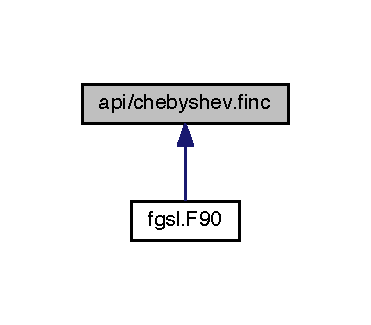
\includegraphics[width=178pt]{chebyshev_8finc__dep__incl}
\end{center}
\end{figure}
\subsection*{Functions/\-Subroutines}
\begin{DoxyCompactItemize}
\item 
type(fgsl\-\_\-cheb\-\_\-series) function \hyperlink{chebyshev_8finc_a18d26925af2b33815928669f2d20c5fc}{fgsl\-\_\-cheb\-\_\-alloc} (n)
\item 
subroutine \hyperlink{chebyshev_8finc_a90dec86100b0f31a78ba02588fcb32fa}{fgsl\-\_\-cheb\-\_\-free} (cs)
\item 
integer(fgsl\-\_\-int) function \hyperlink{chebyshev_8finc_ab5144a511c4795aaa1aef381fba746fe}{fgsl\-\_\-cheb\-\_\-init} (cs, f, a, b)
\item 
integer(fgsl\-\_\-size\-\_\-t) function \hyperlink{chebyshev_8finc_a5779d00f29d0a47bdaca96cfac314d45}{fgsl\-\_\-cheb\-\_\-order} (cs)
\item 
integer(fgsl\-\_\-size\-\_\-t) function \hyperlink{chebyshev_8finc_a27d005e888c9e5c333f506c443f4a685}{fgsl\-\_\-cheb\-\_\-size} (cs)
\item 
real(fgsl\-\_\-double) function, \\*
dimension(\-:), pointer \hyperlink{chebyshev_8finc_a2316b05113eaf931af64fdc1d1a9cb34}{fgsl\-\_\-cheb\-\_\-coeffs} (cs)
\item 
real(fgsl\-\_\-double) function \hyperlink{chebyshev_8finc_a96a78f419947fd9bbf6807b72ebbb54e}{fgsl\-\_\-cheb\-\_\-eval} (cs, x)
\item 
integer(fgsl\-\_\-int) function \hyperlink{chebyshev_8finc_a0d44ec8fe2a70ec2aaaef7cfd8162d29}{fgsl\-\_\-cheb\-\_\-eval\-\_\-err} (cs, x, result, abserr)
\item 
real(fgsl\-\_\-double) function \hyperlink{chebyshev_8finc_ae34a6bce879de1fe39156fc359b1284d}{fgsl\-\_\-cheb\-\_\-eval\-\_\-n} (cs, order, x)
\item 
integer(fgsl\-\_\-int) function \hyperlink{chebyshev_8finc_a658cd8743b6ea29f95e45b09d1a4a33b}{fgsl\-\_\-cheb\-\_\-eval\-\_\-n\-\_\-err} (cs, order, x, result, abserr)
\item 
integer(fgsl\-\_\-int) function \hyperlink{chebyshev_8finc_afca0a21ed23434831b8e29d9d1f414f9}{fgsl\-\_\-cheb\-\_\-calc\-\_\-deriv} (deriv, cs)
\item 
integer(fgsl\-\_\-int) function \hyperlink{chebyshev_8finc_aed9d097bbf1263e532133c421b844d0a}{fgsl\-\_\-cheb\-\_\-calc\-\_\-integ} (integ, cs)
\item 
logical function \hyperlink{chebyshev_8finc_a757025ca75214fce2a6b57688ffa61b7}{fgsl\-\_\-cheb\-\_\-series\-\_\-status} (cheb\-\_\-series)
\end{DoxyCompactItemize}


\subsection{Function/\-Subroutine Documentation}
\hypertarget{chebyshev_8finc_a18d26925af2b33815928669f2d20c5fc}{\index{chebyshev.\-finc@{chebyshev.\-finc}!fgsl\-\_\-cheb\-\_\-alloc@{fgsl\-\_\-cheb\-\_\-alloc}}
\index{fgsl\-\_\-cheb\-\_\-alloc@{fgsl\-\_\-cheb\-\_\-alloc}!chebyshev.finc@{chebyshev.\-finc}}
\subsubsection[{fgsl\-\_\-cheb\-\_\-alloc}]{\setlength{\rightskip}{0pt plus 5cm}type(fgsl\-\_\-cheb\-\_\-series) function fgsl\-\_\-cheb\-\_\-alloc (
\begin{DoxyParamCaption}
\item[{integer(fgsl\-\_\-int), intent(in)}]{n}
\end{DoxyParamCaption}
)}}\label{chebyshev_8finc_a18d26925af2b33815928669f2d20c5fc}
\hypertarget{chebyshev_8finc_afca0a21ed23434831b8e29d9d1f414f9}{\index{chebyshev.\-finc@{chebyshev.\-finc}!fgsl\-\_\-cheb\-\_\-calc\-\_\-deriv@{fgsl\-\_\-cheb\-\_\-calc\-\_\-deriv}}
\index{fgsl\-\_\-cheb\-\_\-calc\-\_\-deriv@{fgsl\-\_\-cheb\-\_\-calc\-\_\-deriv}!chebyshev.finc@{chebyshev.\-finc}}
\subsubsection[{fgsl\-\_\-cheb\-\_\-calc\-\_\-deriv}]{\setlength{\rightskip}{0pt plus 5cm}integer(fgsl\-\_\-int) function fgsl\-\_\-cheb\-\_\-calc\-\_\-deriv (
\begin{DoxyParamCaption}
\item[{type(fgsl\-\_\-cheb\-\_\-series), intent(inout)}]{deriv, }
\item[{type(fgsl\-\_\-cheb\-\_\-series), intent(in)}]{cs}
\end{DoxyParamCaption}
)}}\label{chebyshev_8finc_afca0a21ed23434831b8e29d9d1f414f9}
\hypertarget{chebyshev_8finc_aed9d097bbf1263e532133c421b844d0a}{\index{chebyshev.\-finc@{chebyshev.\-finc}!fgsl\-\_\-cheb\-\_\-calc\-\_\-integ@{fgsl\-\_\-cheb\-\_\-calc\-\_\-integ}}
\index{fgsl\-\_\-cheb\-\_\-calc\-\_\-integ@{fgsl\-\_\-cheb\-\_\-calc\-\_\-integ}!chebyshev.finc@{chebyshev.\-finc}}
\subsubsection[{fgsl\-\_\-cheb\-\_\-calc\-\_\-integ}]{\setlength{\rightskip}{0pt plus 5cm}integer(fgsl\-\_\-int) function fgsl\-\_\-cheb\-\_\-calc\-\_\-integ (
\begin{DoxyParamCaption}
\item[{type(fgsl\-\_\-cheb\-\_\-series), intent(inout)}]{integ, }
\item[{type(fgsl\-\_\-cheb\-\_\-series), intent(in)}]{cs}
\end{DoxyParamCaption}
)}}\label{chebyshev_8finc_aed9d097bbf1263e532133c421b844d0a}
\hypertarget{chebyshev_8finc_a2316b05113eaf931af64fdc1d1a9cb34}{\index{chebyshev.\-finc@{chebyshev.\-finc}!fgsl\-\_\-cheb\-\_\-coeffs@{fgsl\-\_\-cheb\-\_\-coeffs}}
\index{fgsl\-\_\-cheb\-\_\-coeffs@{fgsl\-\_\-cheb\-\_\-coeffs}!chebyshev.finc@{chebyshev.\-finc}}
\subsubsection[{fgsl\-\_\-cheb\-\_\-coeffs}]{\setlength{\rightskip}{0pt plus 5cm}real(fgsl\-\_\-double) function, dimension(\-:), pointer fgsl\-\_\-cheb\-\_\-coeffs (
\begin{DoxyParamCaption}
\item[{type(fgsl\-\_\-cheb\-\_\-series), intent(in)}]{cs}
\end{DoxyParamCaption}
)}}\label{chebyshev_8finc_a2316b05113eaf931af64fdc1d1a9cb34}
\hypertarget{chebyshev_8finc_a96a78f419947fd9bbf6807b72ebbb54e}{\index{chebyshev.\-finc@{chebyshev.\-finc}!fgsl\-\_\-cheb\-\_\-eval@{fgsl\-\_\-cheb\-\_\-eval}}
\index{fgsl\-\_\-cheb\-\_\-eval@{fgsl\-\_\-cheb\-\_\-eval}!chebyshev.finc@{chebyshev.\-finc}}
\subsubsection[{fgsl\-\_\-cheb\-\_\-eval}]{\setlength{\rightskip}{0pt plus 5cm}real(fgsl\-\_\-double) function fgsl\-\_\-cheb\-\_\-eval (
\begin{DoxyParamCaption}
\item[{type(fgsl\-\_\-cheb\-\_\-series), intent(in)}]{cs, }
\item[{real(fgsl\-\_\-double), intent(in)}]{x}
\end{DoxyParamCaption}
)}}\label{chebyshev_8finc_a96a78f419947fd9bbf6807b72ebbb54e}
\hypertarget{chebyshev_8finc_a0d44ec8fe2a70ec2aaaef7cfd8162d29}{\index{chebyshev.\-finc@{chebyshev.\-finc}!fgsl\-\_\-cheb\-\_\-eval\-\_\-err@{fgsl\-\_\-cheb\-\_\-eval\-\_\-err}}
\index{fgsl\-\_\-cheb\-\_\-eval\-\_\-err@{fgsl\-\_\-cheb\-\_\-eval\-\_\-err}!chebyshev.finc@{chebyshev.\-finc}}
\subsubsection[{fgsl\-\_\-cheb\-\_\-eval\-\_\-err}]{\setlength{\rightskip}{0pt plus 5cm}integer(fgsl\-\_\-int) function fgsl\-\_\-cheb\-\_\-eval\-\_\-err (
\begin{DoxyParamCaption}
\item[{type(fgsl\-\_\-cheb\-\_\-series), intent(in)}]{cs, }
\item[{real(fgsl\-\_\-double), intent(in)}]{x, }
\item[{real(fgsl\-\_\-double), intent(out)}]{result, }
\item[{real(fgsl\-\_\-double), intent(out)}]{abserr}
\end{DoxyParamCaption}
)}}\label{chebyshev_8finc_a0d44ec8fe2a70ec2aaaef7cfd8162d29}
\hypertarget{chebyshev_8finc_ae34a6bce879de1fe39156fc359b1284d}{\index{chebyshev.\-finc@{chebyshev.\-finc}!fgsl\-\_\-cheb\-\_\-eval\-\_\-n@{fgsl\-\_\-cheb\-\_\-eval\-\_\-n}}
\index{fgsl\-\_\-cheb\-\_\-eval\-\_\-n@{fgsl\-\_\-cheb\-\_\-eval\-\_\-n}!chebyshev.finc@{chebyshev.\-finc}}
\subsubsection[{fgsl\-\_\-cheb\-\_\-eval\-\_\-n}]{\setlength{\rightskip}{0pt plus 5cm}real(fgsl\-\_\-double) function fgsl\-\_\-cheb\-\_\-eval\-\_\-n (
\begin{DoxyParamCaption}
\item[{type(fgsl\-\_\-cheb\-\_\-series), intent(in)}]{cs, }
\item[{integer(fgsl\-\_\-size\-\_\-t), intent(in)}]{order, }
\item[{real(fgsl\-\_\-double), intent(in)}]{x}
\end{DoxyParamCaption}
)}}\label{chebyshev_8finc_ae34a6bce879de1fe39156fc359b1284d}
\hypertarget{chebyshev_8finc_a658cd8743b6ea29f95e45b09d1a4a33b}{\index{chebyshev.\-finc@{chebyshev.\-finc}!fgsl\-\_\-cheb\-\_\-eval\-\_\-n\-\_\-err@{fgsl\-\_\-cheb\-\_\-eval\-\_\-n\-\_\-err}}
\index{fgsl\-\_\-cheb\-\_\-eval\-\_\-n\-\_\-err@{fgsl\-\_\-cheb\-\_\-eval\-\_\-n\-\_\-err}!chebyshev.finc@{chebyshev.\-finc}}
\subsubsection[{fgsl\-\_\-cheb\-\_\-eval\-\_\-n\-\_\-err}]{\setlength{\rightskip}{0pt plus 5cm}integer(fgsl\-\_\-int) function fgsl\-\_\-cheb\-\_\-eval\-\_\-n\-\_\-err (
\begin{DoxyParamCaption}
\item[{type(fgsl\-\_\-cheb\-\_\-series), intent(in)}]{cs, }
\item[{integer(fgsl\-\_\-size\-\_\-t), intent(in)}]{order, }
\item[{real(fgsl\-\_\-double), intent(in)}]{x, }
\item[{real(fgsl\-\_\-double), intent(out)}]{result, }
\item[{real(fgsl\-\_\-double), intent(out)}]{abserr}
\end{DoxyParamCaption}
)}}\label{chebyshev_8finc_a658cd8743b6ea29f95e45b09d1a4a33b}
\hypertarget{chebyshev_8finc_a90dec86100b0f31a78ba02588fcb32fa}{\index{chebyshev.\-finc@{chebyshev.\-finc}!fgsl\-\_\-cheb\-\_\-free@{fgsl\-\_\-cheb\-\_\-free}}
\index{fgsl\-\_\-cheb\-\_\-free@{fgsl\-\_\-cheb\-\_\-free}!chebyshev.finc@{chebyshev.\-finc}}
\subsubsection[{fgsl\-\_\-cheb\-\_\-free}]{\setlength{\rightskip}{0pt plus 5cm}subroutine fgsl\-\_\-cheb\-\_\-free (
\begin{DoxyParamCaption}
\item[{type(fgsl\-\_\-cheb\-\_\-series), intent(in)}]{cs}
\end{DoxyParamCaption}
)}}\label{chebyshev_8finc_a90dec86100b0f31a78ba02588fcb32fa}
\hypertarget{chebyshev_8finc_ab5144a511c4795aaa1aef381fba746fe}{\index{chebyshev.\-finc@{chebyshev.\-finc}!fgsl\-\_\-cheb\-\_\-init@{fgsl\-\_\-cheb\-\_\-init}}
\index{fgsl\-\_\-cheb\-\_\-init@{fgsl\-\_\-cheb\-\_\-init}!chebyshev.finc@{chebyshev.\-finc}}
\subsubsection[{fgsl\-\_\-cheb\-\_\-init}]{\setlength{\rightskip}{0pt plus 5cm}integer(fgsl\-\_\-int) function fgsl\-\_\-cheb\-\_\-init (
\begin{DoxyParamCaption}
\item[{type(fgsl\-\_\-cheb\-\_\-series), intent(inout)}]{cs, }
\item[{type(fgsl\-\_\-function), intent(in)}]{f, }
\item[{real(fgsl\-\_\-double), intent(in)}]{a, }
\item[{real(fgsl\-\_\-double), intent(in)}]{b}
\end{DoxyParamCaption}
)}}\label{chebyshev_8finc_ab5144a511c4795aaa1aef381fba746fe}
\hypertarget{chebyshev_8finc_a5779d00f29d0a47bdaca96cfac314d45}{\index{chebyshev.\-finc@{chebyshev.\-finc}!fgsl\-\_\-cheb\-\_\-order@{fgsl\-\_\-cheb\-\_\-order}}
\index{fgsl\-\_\-cheb\-\_\-order@{fgsl\-\_\-cheb\-\_\-order}!chebyshev.finc@{chebyshev.\-finc}}
\subsubsection[{fgsl\-\_\-cheb\-\_\-order}]{\setlength{\rightskip}{0pt plus 5cm}integer(fgsl\-\_\-size\-\_\-t) function fgsl\-\_\-cheb\-\_\-order (
\begin{DoxyParamCaption}
\item[{type(fgsl\-\_\-cheb\-\_\-series), intent(in)}]{cs}
\end{DoxyParamCaption}
)}}\label{chebyshev_8finc_a5779d00f29d0a47bdaca96cfac314d45}
\hypertarget{chebyshev_8finc_a757025ca75214fce2a6b57688ffa61b7}{\index{chebyshev.\-finc@{chebyshev.\-finc}!fgsl\-\_\-cheb\-\_\-series\-\_\-status@{fgsl\-\_\-cheb\-\_\-series\-\_\-status}}
\index{fgsl\-\_\-cheb\-\_\-series\-\_\-status@{fgsl\-\_\-cheb\-\_\-series\-\_\-status}!chebyshev.finc@{chebyshev.\-finc}}
\subsubsection[{fgsl\-\_\-cheb\-\_\-series\-\_\-status}]{\setlength{\rightskip}{0pt plus 5cm}logical function fgsl\-\_\-cheb\-\_\-series\-\_\-status (
\begin{DoxyParamCaption}
\item[{type(fgsl\-\_\-cheb\-\_\-series), intent(in)}]{cheb\-\_\-series}
\end{DoxyParamCaption}
)}}\label{chebyshev_8finc_a757025ca75214fce2a6b57688ffa61b7}
\hypertarget{chebyshev_8finc_a27d005e888c9e5c333f506c443f4a685}{\index{chebyshev.\-finc@{chebyshev.\-finc}!fgsl\-\_\-cheb\-\_\-size@{fgsl\-\_\-cheb\-\_\-size}}
\index{fgsl\-\_\-cheb\-\_\-size@{fgsl\-\_\-cheb\-\_\-size}!chebyshev.finc@{chebyshev.\-finc}}
\subsubsection[{fgsl\-\_\-cheb\-\_\-size}]{\setlength{\rightskip}{0pt plus 5cm}integer(fgsl\-\_\-size\-\_\-t) function fgsl\-\_\-cheb\-\_\-size (
\begin{DoxyParamCaption}
\item[{type(fgsl\-\_\-cheb\-\_\-series), intent(in)}]{cs}
\end{DoxyParamCaption}
)}}\label{chebyshev_8finc_a27d005e888c9e5c333f506c443f4a685}

\hypertarget{complex_8finc}{\section{api/complex.finc File Reference}
\label{complex_8finc}\index{api/complex.\-finc@{api/complex.\-finc}}
}
This graph shows which files directly or indirectly include this file\-:\nopagebreak
\begin{figure}[H]
\begin{center}
\leavevmode
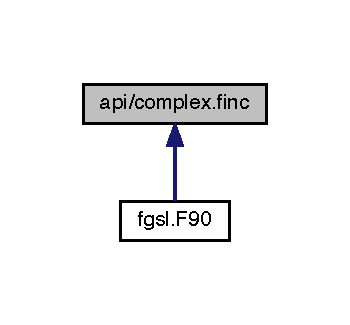
\includegraphics[width=168pt]{complex_8finc__dep__incl}
\end{center}
\end{figure}
\subsection*{Functions/\-Subroutines}
\begin{DoxyCompactItemize}
\item 
real(fgsl\-\_\-double) function \hyperlink{complex_8finc_a0b57597099e0abb1250c833a4e9bff77}{fgsl\-\_\-complex\-\_\-arg} (z)
\item 
real(fgsl\-\_\-double) function \hyperlink{complex_8finc_a42cb53d8f58e2ded216785a6884e761f}{fgsl\-\_\-complex\-\_\-logabs} (z)
\item 
complex(fgsl\-\_\-double\-\_\-complex) \\*
function \hyperlink{complex_8finc_ae9fc7b48e2331e3866c163ac2e8df9af}{fgsl\-\_\-complex\-\_\-log10} (z)
\item 
complex(fgsl\-\_\-double\-\_\-complex) \\*
function \hyperlink{complex_8finc_aa06abfcf4cf0160771747d99a30a6640}{fgsl\-\_\-complex\-\_\-log\-\_\-b} (z, b)
\item 
complex(fgsl\-\_\-double\-\_\-complex) \\*
function \hyperlink{complex_8finc_ae2a77be34dc8a65a8d85e5f0ee6e2629}{fgsl\-\_\-complex\-\_\-arcsin} (z)
\item 
complex(fgsl\-\_\-double\-\_\-complex) \\*
function \hyperlink{complex_8finc_a0d5f1fa6698c94d6506f1e34603e3d18}{fgsl\-\_\-complex\-\_\-arcsin\-\_\-real} (r)
\item 
complex(fgsl\-\_\-double\-\_\-complex) \\*
function \hyperlink{complex_8finc_a483b6501e53d69ff81aa184a60647d6f}{fgsl\-\_\-complex\-\_\-arccos} (z)
\item 
complex(fgsl\-\_\-double\-\_\-complex) \\*
function \hyperlink{complex_8finc_acf733006095db0ebc0b99ea36c171438}{fgsl\-\_\-complex\-\_\-arccos\-\_\-real} (r)
\item 
complex(fgsl\-\_\-double\-\_\-complex) \\*
function \hyperlink{complex_8finc_a8ee7c4c57b7f61614bfb1372f072e36d}{fgsl\-\_\-complex\-\_\-arctan} (z)
\item 
complex(fgsl\-\_\-double\-\_\-complex) \\*
function \hyperlink{complex_8finc_a14d3bb9bb647ba302d97f4cb5ef39f99}{fgsl\-\_\-complex\-\_\-arcsec} (z)
\item 
complex(fgsl\-\_\-double\-\_\-complex) \\*
function \hyperlink{complex_8finc_ad420c933fcc07872208823e44c965190}{fgsl\-\_\-complex\-\_\-arcsec\-\_\-real} (r)
\item 
complex(fgsl\-\_\-double\-\_\-complex) \\*
function \hyperlink{complex_8finc_ac438eff3b3caed126ae6c7929592f750}{fgsl\-\_\-complex\-\_\-arccsc} (z)
\item 
complex(fgsl\-\_\-double\-\_\-complex) \\*
function \hyperlink{complex_8finc_ac5b418b5127b93cddea551723a955143}{fgsl\-\_\-complex\-\_\-arccsc\-\_\-real} (r)
\item 
complex(fgsl\-\_\-double\-\_\-complex) \\*
function \hyperlink{complex_8finc_a4349b9f5549b6c97a88f6d35001bac3f}{fgsl\-\_\-complex\-\_\-arccot} (z)
\item 
complex(fgsl\-\_\-double\-\_\-complex) \\*
function \hyperlink{complex_8finc_ab4a2a9438ed50ba0bfc611356fb209f9}{fgsl\-\_\-complex\-\_\-arcsinh} (z)
\item 
complex(fgsl\-\_\-double\-\_\-complex) \\*
function \hyperlink{complex_8finc_a4b6f8f498bd3315137bdd2fa3c1ca32a}{fgsl\-\_\-complex\-\_\-arccosh} (z)
\item 
complex(fgsl\-\_\-double\-\_\-complex) \\*
function \hyperlink{complex_8finc_ae32a1fa2c5421b1c5a1a24ef6aa3f033}{fgsl\-\_\-complex\-\_\-arccosh\-\_\-real} (r)
\item 
complex(fgsl\-\_\-double\-\_\-complex) \\*
function \hyperlink{complex_8finc_aedade37b8cb8ecb0263b539e086a7538}{fgsl\-\_\-complex\-\_\-arctanh} (z)
\item 
complex(fgsl\-\_\-double\-\_\-complex) \\*
function \hyperlink{complex_8finc_a833a0d9d5e06c7ce4e1a041a537b0607}{fgsl\-\_\-complex\-\_\-arctanh\-\_\-real} (r)
\item 
complex(fgsl\-\_\-double\-\_\-complex) \\*
function \hyperlink{complex_8finc_a2749a6da119458521c78fe5899617a51}{fgsl\-\_\-complex\-\_\-arcsech} (z)
\item 
complex(fgsl\-\_\-double\-\_\-complex) \\*
function \hyperlink{complex_8finc_a6c54ce2eb2c92bf23c14ca4bdf149b73}{fgsl\-\_\-complex\-\_\-arccsch} (z)
\item 
complex(fgsl\-\_\-double\-\_\-complex) \\*
function \hyperlink{complex_8finc_a424df2d30a3b02a8b853c8687957c554}{fgsl\-\_\-complex\-\_\-arccoth} (z)
\item 
elemental subroutine \hyperlink{complex_8finc_aa6202d24e55756a77e0f5883f3ea0c84}{fgsl\-\_\-complex\-\_\-to\-\_\-complex} (result, source)
\item 
elemental subroutine \hyperlink{complex_8finc_a2cbad87c3e0a645db0b486c0f1fddf5a}{complex\-\_\-to\-\_\-fgsl\-\_\-complex} (result, source)
\end{DoxyCompactItemize}


\subsection{Function/\-Subroutine Documentation}
\hypertarget{complex_8finc_a2cbad87c3e0a645db0b486c0f1fddf5a}{\index{complex.\-finc@{complex.\-finc}!complex\-\_\-to\-\_\-fgsl\-\_\-complex@{complex\-\_\-to\-\_\-fgsl\-\_\-complex}}
\index{complex\-\_\-to\-\_\-fgsl\-\_\-complex@{complex\-\_\-to\-\_\-fgsl\-\_\-complex}!complex.finc@{complex.\-finc}}
\subsubsection[{complex\-\_\-to\-\_\-fgsl\-\_\-complex}]{\setlength{\rightskip}{0pt plus 5cm}elemental subroutine complex\-\_\-to\-\_\-fgsl\-\_\-complex (
\begin{DoxyParamCaption}
\item[{type(gsl\-\_\-complex), intent(out)}]{result, }
\item[{complex(fgsl\-\_\-double\-\_\-complex), intent(in)}]{source}
\end{DoxyParamCaption}
)}}\label{complex_8finc_a2cbad87c3e0a645db0b486c0f1fddf5a}
\hypertarget{complex_8finc_a483b6501e53d69ff81aa184a60647d6f}{\index{complex.\-finc@{complex.\-finc}!fgsl\-\_\-complex\-\_\-arccos@{fgsl\-\_\-complex\-\_\-arccos}}
\index{fgsl\-\_\-complex\-\_\-arccos@{fgsl\-\_\-complex\-\_\-arccos}!complex.finc@{complex.\-finc}}
\subsubsection[{fgsl\-\_\-complex\-\_\-arccos}]{\setlength{\rightskip}{0pt plus 5cm}complex(fgsl\-\_\-double\-\_\-complex) function fgsl\-\_\-complex\-\_\-arccos (
\begin{DoxyParamCaption}
\item[{complex(fgsl\-\_\-double\-\_\-complex), intent(in)}]{z}
\end{DoxyParamCaption}
)}}\label{complex_8finc_a483b6501e53d69ff81aa184a60647d6f}
\hypertarget{complex_8finc_acf733006095db0ebc0b99ea36c171438}{\index{complex.\-finc@{complex.\-finc}!fgsl\-\_\-complex\-\_\-arccos\-\_\-real@{fgsl\-\_\-complex\-\_\-arccos\-\_\-real}}
\index{fgsl\-\_\-complex\-\_\-arccos\-\_\-real@{fgsl\-\_\-complex\-\_\-arccos\-\_\-real}!complex.finc@{complex.\-finc}}
\subsubsection[{fgsl\-\_\-complex\-\_\-arccos\-\_\-real}]{\setlength{\rightskip}{0pt plus 5cm}complex(fgsl\-\_\-double\-\_\-complex) function fgsl\-\_\-complex\-\_\-arccos\-\_\-real (
\begin{DoxyParamCaption}
\item[{real(fgsl\-\_\-double), intent(in)}]{r}
\end{DoxyParamCaption}
)}}\label{complex_8finc_acf733006095db0ebc0b99ea36c171438}
\hypertarget{complex_8finc_a4b6f8f498bd3315137bdd2fa3c1ca32a}{\index{complex.\-finc@{complex.\-finc}!fgsl\-\_\-complex\-\_\-arccosh@{fgsl\-\_\-complex\-\_\-arccosh}}
\index{fgsl\-\_\-complex\-\_\-arccosh@{fgsl\-\_\-complex\-\_\-arccosh}!complex.finc@{complex.\-finc}}
\subsubsection[{fgsl\-\_\-complex\-\_\-arccosh}]{\setlength{\rightskip}{0pt plus 5cm}complex(fgsl\-\_\-double\-\_\-complex) function fgsl\-\_\-complex\-\_\-arccosh (
\begin{DoxyParamCaption}
\item[{complex(fgsl\-\_\-double\-\_\-complex), intent(in)}]{z}
\end{DoxyParamCaption}
)}}\label{complex_8finc_a4b6f8f498bd3315137bdd2fa3c1ca32a}
\hypertarget{complex_8finc_ae32a1fa2c5421b1c5a1a24ef6aa3f033}{\index{complex.\-finc@{complex.\-finc}!fgsl\-\_\-complex\-\_\-arccosh\-\_\-real@{fgsl\-\_\-complex\-\_\-arccosh\-\_\-real}}
\index{fgsl\-\_\-complex\-\_\-arccosh\-\_\-real@{fgsl\-\_\-complex\-\_\-arccosh\-\_\-real}!complex.finc@{complex.\-finc}}
\subsubsection[{fgsl\-\_\-complex\-\_\-arccosh\-\_\-real}]{\setlength{\rightskip}{0pt plus 5cm}complex(fgsl\-\_\-double\-\_\-complex) function fgsl\-\_\-complex\-\_\-arccosh\-\_\-real (
\begin{DoxyParamCaption}
\item[{real(fgsl\-\_\-double), intent(in)}]{r}
\end{DoxyParamCaption}
)}}\label{complex_8finc_ae32a1fa2c5421b1c5a1a24ef6aa3f033}
\hypertarget{complex_8finc_a4349b9f5549b6c97a88f6d35001bac3f}{\index{complex.\-finc@{complex.\-finc}!fgsl\-\_\-complex\-\_\-arccot@{fgsl\-\_\-complex\-\_\-arccot}}
\index{fgsl\-\_\-complex\-\_\-arccot@{fgsl\-\_\-complex\-\_\-arccot}!complex.finc@{complex.\-finc}}
\subsubsection[{fgsl\-\_\-complex\-\_\-arccot}]{\setlength{\rightskip}{0pt plus 5cm}complex(fgsl\-\_\-double\-\_\-complex) function fgsl\-\_\-complex\-\_\-arccot (
\begin{DoxyParamCaption}
\item[{complex(fgsl\-\_\-double\-\_\-complex), intent(in)}]{z}
\end{DoxyParamCaption}
)}}\label{complex_8finc_a4349b9f5549b6c97a88f6d35001bac3f}
\hypertarget{complex_8finc_a424df2d30a3b02a8b853c8687957c554}{\index{complex.\-finc@{complex.\-finc}!fgsl\-\_\-complex\-\_\-arccoth@{fgsl\-\_\-complex\-\_\-arccoth}}
\index{fgsl\-\_\-complex\-\_\-arccoth@{fgsl\-\_\-complex\-\_\-arccoth}!complex.finc@{complex.\-finc}}
\subsubsection[{fgsl\-\_\-complex\-\_\-arccoth}]{\setlength{\rightskip}{0pt plus 5cm}complex(fgsl\-\_\-double\-\_\-complex) function fgsl\-\_\-complex\-\_\-arccoth (
\begin{DoxyParamCaption}
\item[{complex(fgsl\-\_\-double\-\_\-complex), intent(in)}]{z}
\end{DoxyParamCaption}
)}}\label{complex_8finc_a424df2d30a3b02a8b853c8687957c554}
\hypertarget{complex_8finc_ac438eff3b3caed126ae6c7929592f750}{\index{complex.\-finc@{complex.\-finc}!fgsl\-\_\-complex\-\_\-arccsc@{fgsl\-\_\-complex\-\_\-arccsc}}
\index{fgsl\-\_\-complex\-\_\-arccsc@{fgsl\-\_\-complex\-\_\-arccsc}!complex.finc@{complex.\-finc}}
\subsubsection[{fgsl\-\_\-complex\-\_\-arccsc}]{\setlength{\rightskip}{0pt plus 5cm}complex(fgsl\-\_\-double\-\_\-complex) function fgsl\-\_\-complex\-\_\-arccsc (
\begin{DoxyParamCaption}
\item[{complex(fgsl\-\_\-double\-\_\-complex), intent(in)}]{z}
\end{DoxyParamCaption}
)}}\label{complex_8finc_ac438eff3b3caed126ae6c7929592f750}
\hypertarget{complex_8finc_ac5b418b5127b93cddea551723a955143}{\index{complex.\-finc@{complex.\-finc}!fgsl\-\_\-complex\-\_\-arccsc\-\_\-real@{fgsl\-\_\-complex\-\_\-arccsc\-\_\-real}}
\index{fgsl\-\_\-complex\-\_\-arccsc\-\_\-real@{fgsl\-\_\-complex\-\_\-arccsc\-\_\-real}!complex.finc@{complex.\-finc}}
\subsubsection[{fgsl\-\_\-complex\-\_\-arccsc\-\_\-real}]{\setlength{\rightskip}{0pt plus 5cm}complex(fgsl\-\_\-double\-\_\-complex) function fgsl\-\_\-complex\-\_\-arccsc\-\_\-real (
\begin{DoxyParamCaption}
\item[{real(fgsl\-\_\-double), intent(in)}]{r}
\end{DoxyParamCaption}
)}}\label{complex_8finc_ac5b418b5127b93cddea551723a955143}
\hypertarget{complex_8finc_a6c54ce2eb2c92bf23c14ca4bdf149b73}{\index{complex.\-finc@{complex.\-finc}!fgsl\-\_\-complex\-\_\-arccsch@{fgsl\-\_\-complex\-\_\-arccsch}}
\index{fgsl\-\_\-complex\-\_\-arccsch@{fgsl\-\_\-complex\-\_\-arccsch}!complex.finc@{complex.\-finc}}
\subsubsection[{fgsl\-\_\-complex\-\_\-arccsch}]{\setlength{\rightskip}{0pt plus 5cm}complex(fgsl\-\_\-double\-\_\-complex) function fgsl\-\_\-complex\-\_\-arccsch (
\begin{DoxyParamCaption}
\item[{complex(fgsl\-\_\-double\-\_\-complex), intent(in)}]{z}
\end{DoxyParamCaption}
)}}\label{complex_8finc_a6c54ce2eb2c92bf23c14ca4bdf149b73}
\hypertarget{complex_8finc_a14d3bb9bb647ba302d97f4cb5ef39f99}{\index{complex.\-finc@{complex.\-finc}!fgsl\-\_\-complex\-\_\-arcsec@{fgsl\-\_\-complex\-\_\-arcsec}}
\index{fgsl\-\_\-complex\-\_\-arcsec@{fgsl\-\_\-complex\-\_\-arcsec}!complex.finc@{complex.\-finc}}
\subsubsection[{fgsl\-\_\-complex\-\_\-arcsec}]{\setlength{\rightskip}{0pt plus 5cm}complex(fgsl\-\_\-double\-\_\-complex) function fgsl\-\_\-complex\-\_\-arcsec (
\begin{DoxyParamCaption}
\item[{complex(fgsl\-\_\-double\-\_\-complex), intent(in)}]{z}
\end{DoxyParamCaption}
)}}\label{complex_8finc_a14d3bb9bb647ba302d97f4cb5ef39f99}
\hypertarget{complex_8finc_ad420c933fcc07872208823e44c965190}{\index{complex.\-finc@{complex.\-finc}!fgsl\-\_\-complex\-\_\-arcsec\-\_\-real@{fgsl\-\_\-complex\-\_\-arcsec\-\_\-real}}
\index{fgsl\-\_\-complex\-\_\-arcsec\-\_\-real@{fgsl\-\_\-complex\-\_\-arcsec\-\_\-real}!complex.finc@{complex.\-finc}}
\subsubsection[{fgsl\-\_\-complex\-\_\-arcsec\-\_\-real}]{\setlength{\rightskip}{0pt plus 5cm}complex(fgsl\-\_\-double\-\_\-complex) function fgsl\-\_\-complex\-\_\-arcsec\-\_\-real (
\begin{DoxyParamCaption}
\item[{real(fgsl\-\_\-double), intent(in)}]{r}
\end{DoxyParamCaption}
)}}\label{complex_8finc_ad420c933fcc07872208823e44c965190}
\hypertarget{complex_8finc_a2749a6da119458521c78fe5899617a51}{\index{complex.\-finc@{complex.\-finc}!fgsl\-\_\-complex\-\_\-arcsech@{fgsl\-\_\-complex\-\_\-arcsech}}
\index{fgsl\-\_\-complex\-\_\-arcsech@{fgsl\-\_\-complex\-\_\-arcsech}!complex.finc@{complex.\-finc}}
\subsubsection[{fgsl\-\_\-complex\-\_\-arcsech}]{\setlength{\rightskip}{0pt plus 5cm}complex(fgsl\-\_\-double\-\_\-complex) function fgsl\-\_\-complex\-\_\-arcsech (
\begin{DoxyParamCaption}
\item[{complex(fgsl\-\_\-double\-\_\-complex), intent(in)}]{z}
\end{DoxyParamCaption}
)}}\label{complex_8finc_a2749a6da119458521c78fe5899617a51}
\hypertarget{complex_8finc_ae2a77be34dc8a65a8d85e5f0ee6e2629}{\index{complex.\-finc@{complex.\-finc}!fgsl\-\_\-complex\-\_\-arcsin@{fgsl\-\_\-complex\-\_\-arcsin}}
\index{fgsl\-\_\-complex\-\_\-arcsin@{fgsl\-\_\-complex\-\_\-arcsin}!complex.finc@{complex.\-finc}}
\subsubsection[{fgsl\-\_\-complex\-\_\-arcsin}]{\setlength{\rightskip}{0pt plus 5cm}complex(fgsl\-\_\-double\-\_\-complex) function fgsl\-\_\-complex\-\_\-arcsin (
\begin{DoxyParamCaption}
\item[{complex(fgsl\-\_\-double\-\_\-complex), intent(in)}]{z}
\end{DoxyParamCaption}
)}}\label{complex_8finc_ae2a77be34dc8a65a8d85e5f0ee6e2629}
\hypertarget{complex_8finc_a0d5f1fa6698c94d6506f1e34603e3d18}{\index{complex.\-finc@{complex.\-finc}!fgsl\-\_\-complex\-\_\-arcsin\-\_\-real@{fgsl\-\_\-complex\-\_\-arcsin\-\_\-real}}
\index{fgsl\-\_\-complex\-\_\-arcsin\-\_\-real@{fgsl\-\_\-complex\-\_\-arcsin\-\_\-real}!complex.finc@{complex.\-finc}}
\subsubsection[{fgsl\-\_\-complex\-\_\-arcsin\-\_\-real}]{\setlength{\rightskip}{0pt plus 5cm}complex(fgsl\-\_\-double\-\_\-complex) function fgsl\-\_\-complex\-\_\-arcsin\-\_\-real (
\begin{DoxyParamCaption}
\item[{real(fgsl\-\_\-double), intent(in)}]{r}
\end{DoxyParamCaption}
)}}\label{complex_8finc_a0d5f1fa6698c94d6506f1e34603e3d18}
\hypertarget{complex_8finc_ab4a2a9438ed50ba0bfc611356fb209f9}{\index{complex.\-finc@{complex.\-finc}!fgsl\-\_\-complex\-\_\-arcsinh@{fgsl\-\_\-complex\-\_\-arcsinh}}
\index{fgsl\-\_\-complex\-\_\-arcsinh@{fgsl\-\_\-complex\-\_\-arcsinh}!complex.finc@{complex.\-finc}}
\subsubsection[{fgsl\-\_\-complex\-\_\-arcsinh}]{\setlength{\rightskip}{0pt plus 5cm}complex(fgsl\-\_\-double\-\_\-complex) function fgsl\-\_\-complex\-\_\-arcsinh (
\begin{DoxyParamCaption}
\item[{complex(fgsl\-\_\-double\-\_\-complex), intent(in)}]{z}
\end{DoxyParamCaption}
)}}\label{complex_8finc_ab4a2a9438ed50ba0bfc611356fb209f9}
\hypertarget{complex_8finc_a8ee7c4c57b7f61614bfb1372f072e36d}{\index{complex.\-finc@{complex.\-finc}!fgsl\-\_\-complex\-\_\-arctan@{fgsl\-\_\-complex\-\_\-arctan}}
\index{fgsl\-\_\-complex\-\_\-arctan@{fgsl\-\_\-complex\-\_\-arctan}!complex.finc@{complex.\-finc}}
\subsubsection[{fgsl\-\_\-complex\-\_\-arctan}]{\setlength{\rightskip}{0pt plus 5cm}complex(fgsl\-\_\-double\-\_\-complex) function fgsl\-\_\-complex\-\_\-arctan (
\begin{DoxyParamCaption}
\item[{complex(fgsl\-\_\-double\-\_\-complex), intent(in)}]{z}
\end{DoxyParamCaption}
)}}\label{complex_8finc_a8ee7c4c57b7f61614bfb1372f072e36d}
\hypertarget{complex_8finc_aedade37b8cb8ecb0263b539e086a7538}{\index{complex.\-finc@{complex.\-finc}!fgsl\-\_\-complex\-\_\-arctanh@{fgsl\-\_\-complex\-\_\-arctanh}}
\index{fgsl\-\_\-complex\-\_\-arctanh@{fgsl\-\_\-complex\-\_\-arctanh}!complex.finc@{complex.\-finc}}
\subsubsection[{fgsl\-\_\-complex\-\_\-arctanh}]{\setlength{\rightskip}{0pt plus 5cm}complex(fgsl\-\_\-double\-\_\-complex) function fgsl\-\_\-complex\-\_\-arctanh (
\begin{DoxyParamCaption}
\item[{complex(fgsl\-\_\-double\-\_\-complex), intent(in)}]{z}
\end{DoxyParamCaption}
)}}\label{complex_8finc_aedade37b8cb8ecb0263b539e086a7538}
\hypertarget{complex_8finc_a833a0d9d5e06c7ce4e1a041a537b0607}{\index{complex.\-finc@{complex.\-finc}!fgsl\-\_\-complex\-\_\-arctanh\-\_\-real@{fgsl\-\_\-complex\-\_\-arctanh\-\_\-real}}
\index{fgsl\-\_\-complex\-\_\-arctanh\-\_\-real@{fgsl\-\_\-complex\-\_\-arctanh\-\_\-real}!complex.finc@{complex.\-finc}}
\subsubsection[{fgsl\-\_\-complex\-\_\-arctanh\-\_\-real}]{\setlength{\rightskip}{0pt plus 5cm}complex(fgsl\-\_\-double\-\_\-complex) function fgsl\-\_\-complex\-\_\-arctanh\-\_\-real (
\begin{DoxyParamCaption}
\item[{real(fgsl\-\_\-double), intent(in)}]{r}
\end{DoxyParamCaption}
)}}\label{complex_8finc_a833a0d9d5e06c7ce4e1a041a537b0607}
\hypertarget{complex_8finc_a0b57597099e0abb1250c833a4e9bff77}{\index{complex.\-finc@{complex.\-finc}!fgsl\-\_\-complex\-\_\-arg@{fgsl\-\_\-complex\-\_\-arg}}
\index{fgsl\-\_\-complex\-\_\-arg@{fgsl\-\_\-complex\-\_\-arg}!complex.finc@{complex.\-finc}}
\subsubsection[{fgsl\-\_\-complex\-\_\-arg}]{\setlength{\rightskip}{0pt plus 5cm}real(fgsl\-\_\-double) function fgsl\-\_\-complex\-\_\-arg (
\begin{DoxyParamCaption}
\item[{complex(fgsl\-\_\-double\-\_\-complex), intent(in)}]{z}
\end{DoxyParamCaption}
)}}\label{complex_8finc_a0b57597099e0abb1250c833a4e9bff77}
\hypertarget{complex_8finc_ae9fc7b48e2331e3866c163ac2e8df9af}{\index{complex.\-finc@{complex.\-finc}!fgsl\-\_\-complex\-\_\-log10@{fgsl\-\_\-complex\-\_\-log10}}
\index{fgsl\-\_\-complex\-\_\-log10@{fgsl\-\_\-complex\-\_\-log10}!complex.finc@{complex.\-finc}}
\subsubsection[{fgsl\-\_\-complex\-\_\-log10}]{\setlength{\rightskip}{0pt plus 5cm}complex(fgsl\-\_\-double\-\_\-complex) function fgsl\-\_\-complex\-\_\-log10 (
\begin{DoxyParamCaption}
\item[{complex(fgsl\-\_\-double\-\_\-complex), intent(in)}]{z}
\end{DoxyParamCaption}
)}}\label{complex_8finc_ae9fc7b48e2331e3866c163ac2e8df9af}
\hypertarget{complex_8finc_aa06abfcf4cf0160771747d99a30a6640}{\index{complex.\-finc@{complex.\-finc}!fgsl\-\_\-complex\-\_\-log\-\_\-b@{fgsl\-\_\-complex\-\_\-log\-\_\-b}}
\index{fgsl\-\_\-complex\-\_\-log\-\_\-b@{fgsl\-\_\-complex\-\_\-log\-\_\-b}!complex.finc@{complex.\-finc}}
\subsubsection[{fgsl\-\_\-complex\-\_\-log\-\_\-b}]{\setlength{\rightskip}{0pt plus 5cm}complex(fgsl\-\_\-double\-\_\-complex) function fgsl\-\_\-complex\-\_\-log\-\_\-b (
\begin{DoxyParamCaption}
\item[{complex(fgsl\-\_\-double\-\_\-complex), intent(in)}]{z, }
\item[{complex(fgsl\-\_\-double\-\_\-complex), intent(in)}]{b}
\end{DoxyParamCaption}
)}}\label{complex_8finc_aa06abfcf4cf0160771747d99a30a6640}
\hypertarget{complex_8finc_a42cb53d8f58e2ded216785a6884e761f}{\index{complex.\-finc@{complex.\-finc}!fgsl\-\_\-complex\-\_\-logabs@{fgsl\-\_\-complex\-\_\-logabs}}
\index{fgsl\-\_\-complex\-\_\-logabs@{fgsl\-\_\-complex\-\_\-logabs}!complex.finc@{complex.\-finc}}
\subsubsection[{fgsl\-\_\-complex\-\_\-logabs}]{\setlength{\rightskip}{0pt plus 5cm}real(fgsl\-\_\-double) function fgsl\-\_\-complex\-\_\-logabs (
\begin{DoxyParamCaption}
\item[{complex(fgsl\-\_\-double\-\_\-complex), intent(in)}]{z}
\end{DoxyParamCaption}
)}}\label{complex_8finc_a42cb53d8f58e2ded216785a6884e761f}
\hypertarget{complex_8finc_aa6202d24e55756a77e0f5883f3ea0c84}{\index{complex.\-finc@{complex.\-finc}!fgsl\-\_\-complex\-\_\-to\-\_\-complex@{fgsl\-\_\-complex\-\_\-to\-\_\-complex}}
\index{fgsl\-\_\-complex\-\_\-to\-\_\-complex@{fgsl\-\_\-complex\-\_\-to\-\_\-complex}!complex.finc@{complex.\-finc}}
\subsubsection[{fgsl\-\_\-complex\-\_\-to\-\_\-complex}]{\setlength{\rightskip}{0pt plus 5cm}elemental subroutine fgsl\-\_\-complex\-\_\-to\-\_\-complex (
\begin{DoxyParamCaption}
\item[{complex(fgsl\-\_\-double\-\_\-complex), intent(out)}]{result, }
\item[{type(gsl\-\_\-complex), intent(in)}]{source}
\end{DoxyParamCaption}
)}}\label{complex_8finc_aa6202d24e55756a77e0f5883f3ea0c84}

\hypertarget{deriv_8finc}{}\section{api/deriv.finc File Reference}
\label{deriv_8finc}\index{api/deriv.\+finc@{api/deriv.\+finc}}
This graph shows which files directly or indirectly include this file\+:\nopagebreak
\begin{figure}[H]
\begin{center}
\leavevmode
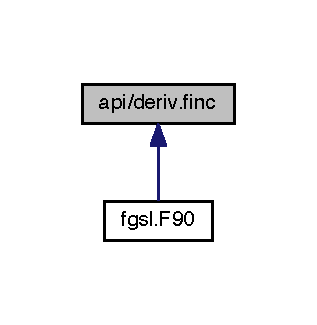
\includegraphics[width=148pt]{deriv_8finc__dep__incl}
\end{center}
\end{figure}
\subsection*{Functions/\+Subroutines}
\begin{DoxyCompactItemize}
\item 
integer(fgsl\+\_\+int) function \hyperlink{deriv_8finc_ac8be2c24bb08d1a46d9b9f941c2f8221}{fgsl\+\_\+deriv\+\_\+central} (f, x, h, result, abserr)
\item 
integer(fgsl\+\_\+int) function \hyperlink{deriv_8finc_ae36c355d73cf6e494e5bf2ce531ff400}{fgsl\+\_\+deriv\+\_\+forward} (f, x, h, result, abserr)
\item 
integer(fgsl\+\_\+int) function \hyperlink{deriv_8finc_ace2b5daaf357f4504c73ebb5f1be2864}{fgsl\+\_\+deriv\+\_\+backward} (f, x, h, result, abserr)
\end{DoxyCompactItemize}


\subsection{Function/\+Subroutine Documentation}
\hypertarget{deriv_8finc_ace2b5daaf357f4504c73ebb5f1be2864}{}\index{deriv.\+finc@{deriv.\+finc}!fgsl\+\_\+deriv\+\_\+backward@{fgsl\+\_\+deriv\+\_\+backward}}
\index{fgsl\+\_\+deriv\+\_\+backward@{fgsl\+\_\+deriv\+\_\+backward}!deriv.\+finc@{deriv.\+finc}}
\subsubsection[{fgsl\+\_\+deriv\+\_\+backward}]{\setlength{\rightskip}{0pt plus 5cm}integer(fgsl\+\_\+int) function fgsl\+\_\+deriv\+\_\+backward (
\begin{DoxyParamCaption}
\item[{type(fgsl\+\_\+function), intent(in)}]{f, }
\item[{real(fgsl\+\_\+double), intent(in)}]{x, }
\item[{real(fgsl\+\_\+double), intent(in)}]{h, }
\item[{real(fgsl\+\_\+double), intent(out)}]{result, }
\item[{real(fgsl\+\_\+double), intent(out)}]{abserr}
\end{DoxyParamCaption}
)}\label{deriv_8finc_ace2b5daaf357f4504c73ebb5f1be2864}
\hypertarget{deriv_8finc_ac8be2c24bb08d1a46d9b9f941c2f8221}{}\index{deriv.\+finc@{deriv.\+finc}!fgsl\+\_\+deriv\+\_\+central@{fgsl\+\_\+deriv\+\_\+central}}
\index{fgsl\+\_\+deriv\+\_\+central@{fgsl\+\_\+deriv\+\_\+central}!deriv.\+finc@{deriv.\+finc}}
\subsubsection[{fgsl\+\_\+deriv\+\_\+central}]{\setlength{\rightskip}{0pt plus 5cm}integer(fgsl\+\_\+int) function fgsl\+\_\+deriv\+\_\+central (
\begin{DoxyParamCaption}
\item[{type(fgsl\+\_\+function), intent(in)}]{f, }
\item[{real(fgsl\+\_\+double), intent(in)}]{x, }
\item[{real(fgsl\+\_\+double), intent(in)}]{h, }
\item[{real(fgsl\+\_\+double), intent(out)}]{result, }
\item[{real(fgsl\+\_\+double), intent(out)}]{abserr}
\end{DoxyParamCaption}
)}\label{deriv_8finc_ac8be2c24bb08d1a46d9b9f941c2f8221}
\hypertarget{deriv_8finc_ae36c355d73cf6e494e5bf2ce531ff400}{}\index{deriv.\+finc@{deriv.\+finc}!fgsl\+\_\+deriv\+\_\+forward@{fgsl\+\_\+deriv\+\_\+forward}}
\index{fgsl\+\_\+deriv\+\_\+forward@{fgsl\+\_\+deriv\+\_\+forward}!deriv.\+finc@{deriv.\+finc}}
\subsubsection[{fgsl\+\_\+deriv\+\_\+forward}]{\setlength{\rightskip}{0pt plus 5cm}integer(fgsl\+\_\+int) function fgsl\+\_\+deriv\+\_\+forward (
\begin{DoxyParamCaption}
\item[{type(fgsl\+\_\+function), intent(in)}]{f, }
\item[{real(fgsl\+\_\+double), intent(in)}]{x, }
\item[{real(fgsl\+\_\+double), intent(in)}]{h, }
\item[{real(fgsl\+\_\+double), intent(out)}]{result, }
\item[{real(fgsl\+\_\+double), intent(out)}]{abserr}
\end{DoxyParamCaption}
)}\label{deriv_8finc_ae36c355d73cf6e494e5bf2ce531ff400}

\hypertarget{dht_8finc}{\section{api/dht.finc File Reference}
\label{dht_8finc}\index{api/dht.\-finc@{api/dht.\-finc}}
}
This graph shows which files directly or indirectly include this file\-:
\nopagebreak
\begin{figure}[H]
\begin{center}
\leavevmode
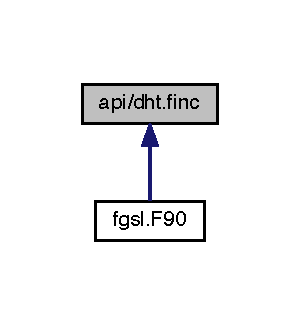
\includegraphics[width=144pt]{dht_8finc__dep__incl}
\end{center}
\end{figure}
\subsection*{Functions/\-Subroutines}
\begin{DoxyCompactItemize}
\item 
type(fgsl\-\_\-dht) function \hyperlink{dht_8finc_afb86f7c8f57dc3d670480fedf967ecd4}{fgsl\-\_\-dht\-\_\-alloc} (size)
\item 
integer(fgsl\-\_\-int) function \hyperlink{dht_8finc_abb2bcd0254c3b7209be2be3e92ff3fa6}{fgsl\-\_\-dht\-\_\-init} (t, nu, xmax)
\item 
type(fgsl\-\_\-dht) function \hyperlink{dht_8finc_adea7d327ef1817dee38b9425de98585b}{fgsl\-\_\-dht\-\_\-new} (size, nu, xmax)
\item 
subroutine \hyperlink{dht_8finc_ae26b17e9d3a3a0e428ace07554351086}{fgsl\-\_\-dht\-\_\-free} (t)
\item 
integer(fgsl\-\_\-int) function \hyperlink{dht_8finc_a587dbba2d2d50e3e07d1f4ba1a7a1989}{fgsl\-\_\-dht\-\_\-apply} (t, f\-\_\-in, f\-\_\-out)
\item 
real(fgsl\-\_\-double) function \hyperlink{dht_8finc_af6b6534c16d8cfcfaeae9ea4ea9fa3c4}{fgsl\-\_\-dht\-\_\-x\-\_\-sample} (t, n)
\item 
real(fgsl\-\_\-double) function \hyperlink{dht_8finc_ab0250953195cfe60a32a5c5d532fdf75}{fgsl\-\_\-dht\-\_\-k\-\_\-sample} (t, n)
\item 
logical function \hyperlink{dht_8finc_a58dc6a67e94415bb013e635effcefa24}{fgsl\-\_\-dht\-\_\-status} (dht)
\end{DoxyCompactItemize}


\subsection{Function/\-Subroutine Documentation}
\hypertarget{dht_8finc_afb86f7c8f57dc3d670480fedf967ecd4}{\index{dht.\-finc@{dht.\-finc}!fgsl\-\_\-dht\-\_\-alloc@{fgsl\-\_\-dht\-\_\-alloc}}
\index{fgsl\-\_\-dht\-\_\-alloc@{fgsl\-\_\-dht\-\_\-alloc}!dht.finc@{dht.\-finc}}
\subsubsection[{fgsl\-\_\-dht\-\_\-alloc}]{\setlength{\rightskip}{0pt plus 5cm}type(fgsl\-\_\-dht) function fgsl\-\_\-dht\-\_\-alloc (
\begin{DoxyParamCaption}
\item[{integer(fgsl\-\_\-size\-\_\-t), intent(in)}]{size}
\end{DoxyParamCaption}
)}}\label{dht_8finc_afb86f7c8f57dc3d670480fedf967ecd4}
\hypertarget{dht_8finc_a587dbba2d2d50e3e07d1f4ba1a7a1989}{\index{dht.\-finc@{dht.\-finc}!fgsl\-\_\-dht\-\_\-apply@{fgsl\-\_\-dht\-\_\-apply}}
\index{fgsl\-\_\-dht\-\_\-apply@{fgsl\-\_\-dht\-\_\-apply}!dht.finc@{dht.\-finc}}
\subsubsection[{fgsl\-\_\-dht\-\_\-apply}]{\setlength{\rightskip}{0pt plus 5cm}integer(fgsl\-\_\-int) function fgsl\-\_\-dht\-\_\-apply (
\begin{DoxyParamCaption}
\item[{type(fgsl\-\_\-dht), intent(in)}]{t, }
\item[{real(fgsl\-\_\-double), dimension(\-:), intent(in)}]{f\-\_\-in, }
\item[{real(fgsl\-\_\-double), dimension(\-:), intent(out)}]{f\-\_\-out}
\end{DoxyParamCaption}
)}}\label{dht_8finc_a587dbba2d2d50e3e07d1f4ba1a7a1989}
\hypertarget{dht_8finc_ae26b17e9d3a3a0e428ace07554351086}{\index{dht.\-finc@{dht.\-finc}!fgsl\-\_\-dht\-\_\-free@{fgsl\-\_\-dht\-\_\-free}}
\index{fgsl\-\_\-dht\-\_\-free@{fgsl\-\_\-dht\-\_\-free}!dht.finc@{dht.\-finc}}
\subsubsection[{fgsl\-\_\-dht\-\_\-free}]{\setlength{\rightskip}{0pt plus 5cm}subroutine fgsl\-\_\-dht\-\_\-free (
\begin{DoxyParamCaption}
\item[{type(fgsl\-\_\-dht), intent(inout)}]{t}
\end{DoxyParamCaption}
)}}\label{dht_8finc_ae26b17e9d3a3a0e428ace07554351086}
\hypertarget{dht_8finc_abb2bcd0254c3b7209be2be3e92ff3fa6}{\index{dht.\-finc@{dht.\-finc}!fgsl\-\_\-dht\-\_\-init@{fgsl\-\_\-dht\-\_\-init}}
\index{fgsl\-\_\-dht\-\_\-init@{fgsl\-\_\-dht\-\_\-init}!dht.finc@{dht.\-finc}}
\subsubsection[{fgsl\-\_\-dht\-\_\-init}]{\setlength{\rightskip}{0pt plus 5cm}integer(fgsl\-\_\-int) function fgsl\-\_\-dht\-\_\-init (
\begin{DoxyParamCaption}
\item[{type(fgsl\-\_\-dht), intent(inout)}]{t, }
\item[{real(fgsl\-\_\-double), intent(in)}]{nu, }
\item[{real(fgsl\-\_\-double), intent(in)}]{xmax}
\end{DoxyParamCaption}
)}}\label{dht_8finc_abb2bcd0254c3b7209be2be3e92ff3fa6}
\hypertarget{dht_8finc_ab0250953195cfe60a32a5c5d532fdf75}{\index{dht.\-finc@{dht.\-finc}!fgsl\-\_\-dht\-\_\-k\-\_\-sample@{fgsl\-\_\-dht\-\_\-k\-\_\-sample}}
\index{fgsl\-\_\-dht\-\_\-k\-\_\-sample@{fgsl\-\_\-dht\-\_\-k\-\_\-sample}!dht.finc@{dht.\-finc}}
\subsubsection[{fgsl\-\_\-dht\-\_\-k\-\_\-sample}]{\setlength{\rightskip}{0pt plus 5cm}real(fgsl\-\_\-double) function fgsl\-\_\-dht\-\_\-k\-\_\-sample (
\begin{DoxyParamCaption}
\item[{type(fgsl\-\_\-dht), intent(in)}]{t, }
\item[{integer(fgsl\-\_\-int), intent(in)}]{n}
\end{DoxyParamCaption}
)}}\label{dht_8finc_ab0250953195cfe60a32a5c5d532fdf75}
\hypertarget{dht_8finc_adea7d327ef1817dee38b9425de98585b}{\index{dht.\-finc@{dht.\-finc}!fgsl\-\_\-dht\-\_\-new@{fgsl\-\_\-dht\-\_\-new}}
\index{fgsl\-\_\-dht\-\_\-new@{fgsl\-\_\-dht\-\_\-new}!dht.finc@{dht.\-finc}}
\subsubsection[{fgsl\-\_\-dht\-\_\-new}]{\setlength{\rightskip}{0pt plus 5cm}type(fgsl\-\_\-dht) function fgsl\-\_\-dht\-\_\-new (
\begin{DoxyParamCaption}
\item[{integer(fgsl\-\_\-size\-\_\-t), intent(in)}]{size, }
\item[{real(fgsl\-\_\-double), intent(in)}]{nu, }
\item[{real(fgsl\-\_\-double), intent(in)}]{xmax}
\end{DoxyParamCaption}
)}}\label{dht_8finc_adea7d327ef1817dee38b9425de98585b}
\hypertarget{dht_8finc_a58dc6a67e94415bb013e635effcefa24}{\index{dht.\-finc@{dht.\-finc}!fgsl\-\_\-dht\-\_\-status@{fgsl\-\_\-dht\-\_\-status}}
\index{fgsl\-\_\-dht\-\_\-status@{fgsl\-\_\-dht\-\_\-status}!dht.finc@{dht.\-finc}}
\subsubsection[{fgsl\-\_\-dht\-\_\-status}]{\setlength{\rightskip}{0pt plus 5cm}logical function fgsl\-\_\-dht\-\_\-status (
\begin{DoxyParamCaption}
\item[{type(fgsl\-\_\-dht), intent(in)}]{dht}
\end{DoxyParamCaption}
)}}\label{dht_8finc_a58dc6a67e94415bb013e635effcefa24}
\hypertarget{dht_8finc_af6b6534c16d8cfcfaeae9ea4ea9fa3c4}{\index{dht.\-finc@{dht.\-finc}!fgsl\-\_\-dht\-\_\-x\-\_\-sample@{fgsl\-\_\-dht\-\_\-x\-\_\-sample}}
\index{fgsl\-\_\-dht\-\_\-x\-\_\-sample@{fgsl\-\_\-dht\-\_\-x\-\_\-sample}!dht.finc@{dht.\-finc}}
\subsubsection[{fgsl\-\_\-dht\-\_\-x\-\_\-sample}]{\setlength{\rightskip}{0pt plus 5cm}real(fgsl\-\_\-double) function fgsl\-\_\-dht\-\_\-x\-\_\-sample (
\begin{DoxyParamCaption}
\item[{type(fgsl\-\_\-dht), intent(in)}]{t, }
\item[{integer(fgsl\-\_\-int), intent(in)}]{n}
\end{DoxyParamCaption}
)}}\label{dht_8finc_af6b6534c16d8cfcfaeae9ea4ea9fa3c4}

\hypertarget{eigen_8finc}{\section{api/eigen.finc File Reference}
\label{eigen_8finc}\index{api/eigen.\-finc@{api/eigen.\-finc}}
}
This graph shows which files directly or indirectly include this file\-:\nopagebreak
\begin{figure}[H]
\begin{center}
\leavevmode
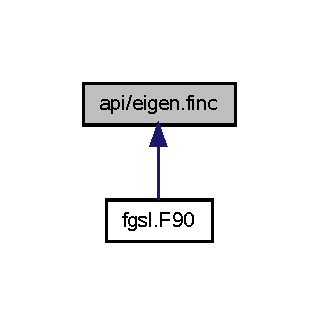
\includegraphics[width=154pt]{eigen_8finc__dep__incl}
\end{center}
\end{figure}
\subsection*{Functions/\-Subroutines}
\begin{DoxyCompactItemize}
\item 
type(fgsl\-\_\-eigen\-\_\-symm\-\_\-workspace) \\*
function \hyperlink{eigen_8finc_a4911814478ea47e01623311df0dfe1b7}{fgsl\-\_\-eigen\-\_\-symm\-\_\-alloc} (n)
\item 
subroutine \hyperlink{eigen_8finc_a9127a0929117934b84723c05fe120916}{fgsl\-\_\-eigen\-\_\-symm\-\_\-free} (w)
\item 
integer(fgsl\-\_\-int) function \hyperlink{eigen_8finc_a5a37dd1d463478768f432232bf994e43}{fgsl\-\_\-eigen\-\_\-symm} (a, eval, w)
\item 
type(fgsl\-\_\-eigen\-\_\-symmv\-\_\-workspace) \\*
function \hyperlink{eigen_8finc_ad1fec4036528852c97539008a009c875}{fgsl\-\_\-eigen\-\_\-symmv\-\_\-alloc} (n)
\item 
subroutine \hyperlink{eigen_8finc_a3f312c4069b7de24f2a7b9112bd11fab}{fgsl\-\_\-eigen\-\_\-symmv\-\_\-free} (w)
\item 
integer(fgsl\-\_\-int) function \hyperlink{eigen_8finc_a42022987fd3e17b60db77ce044515bc1}{fgsl\-\_\-eigen\-\_\-symmv} (a, eval, evec, w)
\item 
type(fgsl\-\_\-eigen\-\_\-herm\-\_\-workspace) \\*
function \hyperlink{eigen_8finc_a6a713bfd56b0df2694ba508eb70ea7b0}{fgsl\-\_\-eigen\-\_\-herm\-\_\-alloc} (n)
\item 
subroutine \hyperlink{eigen_8finc_ab28944c18e254129ddf3289f7b8d8bc4}{fgsl\-\_\-eigen\-\_\-herm\-\_\-free} (w)
\item 
integer(fgsl\-\_\-int) function \hyperlink{eigen_8finc_ad73920fff8c0f5043f47fbf2930280cb}{fgsl\-\_\-eigen\-\_\-herm} (a, eval, w)
\item 
type(fgsl\-\_\-eigen\-\_\-hermv\-\_\-workspace) \\*
function \hyperlink{eigen_8finc_af23f2bdc295d9082a0cd3d383788199a}{fgsl\-\_\-eigen\-\_\-hermv\-\_\-alloc} (n)
\item 
subroutine \hyperlink{eigen_8finc_a6a876223b366e9e91962c7106148929c}{fgsl\-\_\-eigen\-\_\-hermv\-\_\-free} (w)
\item 
integer(fgsl\-\_\-int) function \hyperlink{eigen_8finc_ab9e8f1e044d459595f880d4c380f537f}{fgsl\-\_\-eigen\-\_\-hermv} (a, eval, evec, w)
\item 
type(fgsl\-\_\-eigen\-\_\-nonsymm\-\_\-workspace) \\*
function \hyperlink{eigen_8finc_a67e1213526c2a57e599ea68c4ccb7f17}{fgsl\-\_\-eigen\-\_\-nonsymm\-\_\-alloc} (n)
\item 
subroutine \hyperlink{eigen_8finc_a4c13d8c917420938df8375af8909183f}{fgsl\-\_\-eigen\-\_\-nonsymm\-\_\-free} (w)
\item 
subroutine \hyperlink{eigen_8finc_aa9c147deaa41d2f07a8af9dde8abf35f}{fgsl\-\_\-eigen\-\_\-nonsymm\-\_\-params} (compute\-\_\-t, balance, w)
\item 
integer(fgsl\-\_\-int) function \hyperlink{eigen_8finc_a5044ee7ae8200fc994b55c7cd4f047d7}{fgsl\-\_\-eigen\-\_\-nonsymm} (a, eval, w)
\item 
integer(fgsl\-\_\-int) function \hyperlink{eigen_8finc_ae3e1cd3e7d0f3abd38f98a5f911d6889}{fgsl\-\_\-eigen\-\_\-nonsymm\-\_\-z} (a, eval, z, w)
\item 
type(fgsl\-\_\-eigen\-\_\-nonsymmv\-\_\-workspace) \\*
function \hyperlink{eigen_8finc_af6b786903112c4f4139bee94120feea4}{fgsl\-\_\-eigen\-\_\-nonsymmv\-\_\-alloc} (n)
\item 
subroutine \hyperlink{eigen_8finc_a4684734bff6c27f739aeb31d3b090bee}{fgsl\-\_\-eigen\-\_\-nonsymmv\-\_\-free} (w)
\item 
subroutine \hyperlink{eigen_8finc_ae6a1d284903b7387319d8636df94a679}{fgsl\-\_\-eigen\-\_\-nonsymmv\-\_\-params} (balance, w)
\item 
integer(fgsl\-\_\-int) function \hyperlink{eigen_8finc_aa09384a54b214602b298c94bc07d3c58}{fgsl\-\_\-eigen\-\_\-nonsymmv} (a, eval, evec, w)
\item 
integer(fgsl\-\_\-int) function \hyperlink{eigen_8finc_ad466997b5f8528265070f2aba003ddab}{fgsl\-\_\-eigen\-\_\-nonsymmv\-\_\-z} (a, eval, evec, z, w)
\item 
type(fgsl\-\_\-eigen\-\_\-gensymm\-\_\-workspace) \\*
function \hyperlink{eigen_8finc_a087cf013d99c79e7f2670c0e6035260b}{fgsl\-\_\-eigen\-\_\-gensymm\-\_\-alloc} (n)
\item 
subroutine \hyperlink{eigen_8finc_a6896d5bb5a13213ea85bb1c89bd77109}{fgsl\-\_\-eigen\-\_\-gensymm\-\_\-free} (w)
\item 
integer(fgsl\-\_\-int) function \hyperlink{eigen_8finc_ab6358ebdfcf35887b7fdabc3588d4818}{fgsl\-\_\-eigen\-\_\-gensymm} (a, b, eval, w)
\item 
type(fgsl\-\_\-eigen\-\_\-gensymmv\-\_\-workspace) \\*
function \hyperlink{eigen_8finc_aaf9f9b1f18094f6300da921900b946fa}{fgsl\-\_\-eigen\-\_\-gensymmv\-\_\-alloc} (n)
\item 
subroutine \hyperlink{eigen_8finc_ad60f54bc4c9afe52b1643a53ac4debf0}{fgsl\-\_\-eigen\-\_\-gensymmv\-\_\-free} (w)
\item 
integer(fgsl\-\_\-int) function \hyperlink{eigen_8finc_ad9e2195ef21d925f7e963185cb59e435}{fgsl\-\_\-eigen\-\_\-gensymmv} (a, b, eval, evec, w)
\item 
type(fgsl\-\_\-eigen\-\_\-genherm\-\_\-workspace) \\*
function \hyperlink{eigen_8finc_af69d430a7febbfb70b4021a765d9535d}{fgsl\-\_\-eigen\-\_\-genherm\-\_\-alloc} (n)
\item 
subroutine \hyperlink{eigen_8finc_a6c25ef96c06da3c1ff3926200f36e55b}{fgsl\-\_\-eigen\-\_\-genherm\-\_\-free} (w)
\item 
integer(fgsl\-\_\-int) function \hyperlink{eigen_8finc_a7742445ebb20b3ce43ece2c8ce92b3cb}{fgsl\-\_\-eigen\-\_\-genherm} (a, b, eval, w)
\item 
type(fgsl\-\_\-eigen\-\_\-genhermv\-\_\-workspace) \\*
function \hyperlink{eigen_8finc_a757b1df46b9949413e56c2fb40193358}{fgsl\-\_\-eigen\-\_\-genhermv\-\_\-alloc} (n)
\item 
subroutine \hyperlink{eigen_8finc_a0f8e68362cb297494a149a2abd529499}{fgsl\-\_\-eigen\-\_\-genhermv\-\_\-free} (w)
\item 
integer(fgsl\-\_\-int) function \hyperlink{eigen_8finc_a234ce4166943e7c9fbdf662554831bc4}{fgsl\-\_\-eigen\-\_\-genhermv} (a, b, eval, evec, w)
\item 
type(fgsl\-\_\-eigen\-\_\-gen\-\_\-workspace) \\*
function \hyperlink{eigen_8finc_a93910023619c9d669e02f83b9109c26b}{fgsl\-\_\-eigen\-\_\-gen\-\_\-alloc} (n)
\item 
subroutine \hyperlink{eigen_8finc_acf1f0d8398d2124aaaf77d87fc4f97af}{fgsl\-\_\-eigen\-\_\-gen\-\_\-free} (w)
\item 
subroutine \hyperlink{eigen_8finc_ad892f962a1ec3cab90f26ef37668e631}{fgsl\-\_\-eigen\-\_\-gen\-\_\-params} (compute\-\_\-s, compute\-\_\-t, balance, w)
\item 
integer(fgsl\-\_\-int) function \hyperlink{eigen_8finc_af9248a86edc3501913a04bff373f5f16}{fgsl\-\_\-eigen\-\_\-gen} (a, b, alpha, beta, w)
\item 
integer(fgsl\-\_\-int) function \hyperlink{eigen_8finc_abe397b833eedb3cba80d2abde013bbe4}{fgsl\-\_\-eigen\-\_\-gen\-\_\-qz} (a, b, alpha, beta, q, z, w)
\item 
type(fgsl\-\_\-eigen\-\_\-genv\-\_\-workspace) \\*
function \hyperlink{eigen_8finc_ad5f5628460ae023f294684dc0d2b001c}{fgsl\-\_\-eigen\-\_\-genv\-\_\-alloc} (n)
\item 
subroutine \hyperlink{eigen_8finc_af448040f311f66e9ed9f1e86d6ee8abb}{fgsl\-\_\-eigen\-\_\-genv\-\_\-free} (w)
\item 
integer(fgsl\-\_\-int) function \hyperlink{eigen_8finc_a091964d484996dc36d814dd6f7024885}{fgsl\-\_\-eigen\-\_\-genv} (a, b, alpha, beta, evec, w)
\item 
integer(fgsl\-\_\-int) function \hyperlink{eigen_8finc_ade5191d945be9be6f404d55ce96013c0}{fgsl\-\_\-eigen\-\_\-genv\-\_\-qz} (a, b, alpha, beta, evec, q, z, w)
\item 
integer(fgsl\-\_\-int) function \hyperlink{eigen_8finc_a4de96323ca5ee27e595f0ccc55686200}{fgsl\-\_\-eigen\-\_\-symmv\-\_\-sort} (eval, evec, sort\-\_\-type)
\item 
integer(fgsl\-\_\-int) function \hyperlink{eigen_8finc_a3367196fe5ce83a49332525cf10513ad}{fgsl\-\_\-eigen\-\_\-hermv\-\_\-sort} (eval, evec, sort\-\_\-type)
\item 
integer(fgsl\-\_\-int) function \hyperlink{eigen_8finc_a225c50506c2ef39bf0eb7efdf3d7bd29}{fgsl\-\_\-eigen\-\_\-nonsymmv\-\_\-sort} (eval, evec, sort\-\_\-type)
\item 
integer(fgsl\-\_\-int) function \hyperlink{eigen_8finc_a01fa1634183b5dd7727164f67160ee20}{fgsl\-\_\-eigen\-\_\-gensymmv\-\_\-sort} (eval, evec, sort\-\_\-type)
\item 
integer(fgsl\-\_\-int) function \hyperlink{eigen_8finc_aedab09666f98dd918fc64875cda7c972}{fgsl\-\_\-eigen\-\_\-genhermv\-\_\-sort} (eval, evec, sort\-\_\-type)
\item 
integer(fgsl\-\_\-int) function \hyperlink{eigen_8finc_a277ee7050a1e674988a7392ac9255d21}{fgsl\-\_\-eigen\-\_\-genv\-\_\-sort} (alpha, beta, evec, sort\-\_\-type)
\end{DoxyCompactItemize}


\subsection{Function/\-Subroutine Documentation}
\hypertarget{eigen_8finc_af9248a86edc3501913a04bff373f5f16}{\index{eigen.\-finc@{eigen.\-finc}!fgsl\-\_\-eigen\-\_\-gen@{fgsl\-\_\-eigen\-\_\-gen}}
\index{fgsl\-\_\-eigen\-\_\-gen@{fgsl\-\_\-eigen\-\_\-gen}!eigen.finc@{eigen.\-finc}}
\subsubsection[{fgsl\-\_\-eigen\-\_\-gen}]{\setlength{\rightskip}{0pt plus 5cm}integer(fgsl\-\_\-int) function fgsl\-\_\-eigen\-\_\-gen (
\begin{DoxyParamCaption}
\item[{type(fgsl\-\_\-matrix), intent(inout)}]{a, }
\item[{type(fgsl\-\_\-matrix), intent(inout)}]{b, }
\item[{type(fgsl\-\_\-vector\-\_\-complex), intent(inout)}]{alpha, }
\item[{type(fgsl\-\_\-vector), intent(inout)}]{beta, }
\item[{type(fgsl\-\_\-eigen\-\_\-gen\-\_\-workspace)}]{w}
\end{DoxyParamCaption}
)}}\label{eigen_8finc_af9248a86edc3501913a04bff373f5f16}
\hypertarget{eigen_8finc_a93910023619c9d669e02f83b9109c26b}{\index{eigen.\-finc@{eigen.\-finc}!fgsl\-\_\-eigen\-\_\-gen\-\_\-alloc@{fgsl\-\_\-eigen\-\_\-gen\-\_\-alloc}}
\index{fgsl\-\_\-eigen\-\_\-gen\-\_\-alloc@{fgsl\-\_\-eigen\-\_\-gen\-\_\-alloc}!eigen.finc@{eigen.\-finc}}
\subsubsection[{fgsl\-\_\-eigen\-\_\-gen\-\_\-alloc}]{\setlength{\rightskip}{0pt plus 5cm}type(fgsl\-\_\-eigen\-\_\-gen\-\_\-workspace) function fgsl\-\_\-eigen\-\_\-gen\-\_\-alloc (
\begin{DoxyParamCaption}
\item[{integer(fgsl\-\_\-size\-\_\-t), intent(in)}]{n}
\end{DoxyParamCaption}
)}}\label{eigen_8finc_a93910023619c9d669e02f83b9109c26b}
\hypertarget{eigen_8finc_acf1f0d8398d2124aaaf77d87fc4f97af}{\index{eigen.\-finc@{eigen.\-finc}!fgsl\-\_\-eigen\-\_\-gen\-\_\-free@{fgsl\-\_\-eigen\-\_\-gen\-\_\-free}}
\index{fgsl\-\_\-eigen\-\_\-gen\-\_\-free@{fgsl\-\_\-eigen\-\_\-gen\-\_\-free}!eigen.finc@{eigen.\-finc}}
\subsubsection[{fgsl\-\_\-eigen\-\_\-gen\-\_\-free}]{\setlength{\rightskip}{0pt plus 5cm}subroutine fgsl\-\_\-eigen\-\_\-gen\-\_\-free (
\begin{DoxyParamCaption}
\item[{type(fgsl\-\_\-eigen\-\_\-gen\-\_\-workspace)}]{w}
\end{DoxyParamCaption}
)}}\label{eigen_8finc_acf1f0d8398d2124aaaf77d87fc4f97af}
\hypertarget{eigen_8finc_ad892f962a1ec3cab90f26ef37668e631}{\index{eigen.\-finc@{eigen.\-finc}!fgsl\-\_\-eigen\-\_\-gen\-\_\-params@{fgsl\-\_\-eigen\-\_\-gen\-\_\-params}}
\index{fgsl\-\_\-eigen\-\_\-gen\-\_\-params@{fgsl\-\_\-eigen\-\_\-gen\-\_\-params}!eigen.finc@{eigen.\-finc}}
\subsubsection[{fgsl\-\_\-eigen\-\_\-gen\-\_\-params}]{\setlength{\rightskip}{0pt plus 5cm}subroutine fgsl\-\_\-eigen\-\_\-gen\-\_\-params (
\begin{DoxyParamCaption}
\item[{integer(fgsl\-\_\-int), intent(in)}]{compute\-\_\-s, }
\item[{integer(fgsl\-\_\-int), intent(in)}]{compute\-\_\-t, }
\item[{integer(fgsl\-\_\-int), intent(in)}]{balance, }
\item[{type(fgsl\-\_\-eigen\-\_\-gen\-\_\-workspace), intent(inout)}]{w}
\end{DoxyParamCaption}
)}}\label{eigen_8finc_ad892f962a1ec3cab90f26ef37668e631}
\hypertarget{eigen_8finc_abe397b833eedb3cba80d2abde013bbe4}{\index{eigen.\-finc@{eigen.\-finc}!fgsl\-\_\-eigen\-\_\-gen\-\_\-qz@{fgsl\-\_\-eigen\-\_\-gen\-\_\-qz}}
\index{fgsl\-\_\-eigen\-\_\-gen\-\_\-qz@{fgsl\-\_\-eigen\-\_\-gen\-\_\-qz}!eigen.finc@{eigen.\-finc}}
\subsubsection[{fgsl\-\_\-eigen\-\_\-gen\-\_\-qz}]{\setlength{\rightskip}{0pt plus 5cm}integer(fgsl\-\_\-int) function fgsl\-\_\-eigen\-\_\-gen\-\_\-qz (
\begin{DoxyParamCaption}
\item[{type(fgsl\-\_\-matrix), intent(inout)}]{a, }
\item[{type(fgsl\-\_\-matrix), intent(inout)}]{b, }
\item[{type(fgsl\-\_\-vector\-\_\-complex), intent(inout)}]{alpha, }
\item[{type(fgsl\-\_\-vector), intent(inout)}]{beta, }
\item[{type(fgsl\-\_\-matrix), intent(inout)}]{q, }
\item[{type(fgsl\-\_\-matrix), intent(inout)}]{z, }
\item[{type(fgsl\-\_\-eigen\-\_\-gen\-\_\-workspace)}]{w}
\end{DoxyParamCaption}
)}}\label{eigen_8finc_abe397b833eedb3cba80d2abde013bbe4}
\hypertarget{eigen_8finc_a7742445ebb20b3ce43ece2c8ce92b3cb}{\index{eigen.\-finc@{eigen.\-finc}!fgsl\-\_\-eigen\-\_\-genherm@{fgsl\-\_\-eigen\-\_\-genherm}}
\index{fgsl\-\_\-eigen\-\_\-genherm@{fgsl\-\_\-eigen\-\_\-genherm}!eigen.finc@{eigen.\-finc}}
\subsubsection[{fgsl\-\_\-eigen\-\_\-genherm}]{\setlength{\rightskip}{0pt plus 5cm}integer(fgsl\-\_\-int) function fgsl\-\_\-eigen\-\_\-genherm (
\begin{DoxyParamCaption}
\item[{type(fgsl\-\_\-matrix\-\_\-complex), intent(inout)}]{a, }
\item[{type(fgsl\-\_\-matrix\-\_\-complex), intent(inout)}]{b, }
\item[{type(fgsl\-\_\-vector), intent(inout)}]{eval, }
\item[{type(fgsl\-\_\-eigen\-\_\-genherm\-\_\-workspace)}]{w}
\end{DoxyParamCaption}
)}}\label{eigen_8finc_a7742445ebb20b3ce43ece2c8ce92b3cb}
\hypertarget{eigen_8finc_af69d430a7febbfb70b4021a765d9535d}{\index{eigen.\-finc@{eigen.\-finc}!fgsl\-\_\-eigen\-\_\-genherm\-\_\-alloc@{fgsl\-\_\-eigen\-\_\-genherm\-\_\-alloc}}
\index{fgsl\-\_\-eigen\-\_\-genherm\-\_\-alloc@{fgsl\-\_\-eigen\-\_\-genherm\-\_\-alloc}!eigen.finc@{eigen.\-finc}}
\subsubsection[{fgsl\-\_\-eigen\-\_\-genherm\-\_\-alloc}]{\setlength{\rightskip}{0pt plus 5cm}type(fgsl\-\_\-eigen\-\_\-genherm\-\_\-workspace) function fgsl\-\_\-eigen\-\_\-genherm\-\_\-alloc (
\begin{DoxyParamCaption}
\item[{integer(fgsl\-\_\-size\-\_\-t), intent(in)}]{n}
\end{DoxyParamCaption}
)}}\label{eigen_8finc_af69d430a7febbfb70b4021a765d9535d}
\hypertarget{eigen_8finc_a6c25ef96c06da3c1ff3926200f36e55b}{\index{eigen.\-finc@{eigen.\-finc}!fgsl\-\_\-eigen\-\_\-genherm\-\_\-free@{fgsl\-\_\-eigen\-\_\-genherm\-\_\-free}}
\index{fgsl\-\_\-eigen\-\_\-genherm\-\_\-free@{fgsl\-\_\-eigen\-\_\-genherm\-\_\-free}!eigen.finc@{eigen.\-finc}}
\subsubsection[{fgsl\-\_\-eigen\-\_\-genherm\-\_\-free}]{\setlength{\rightskip}{0pt plus 5cm}subroutine fgsl\-\_\-eigen\-\_\-genherm\-\_\-free (
\begin{DoxyParamCaption}
\item[{type(fgsl\-\_\-eigen\-\_\-genherm\-\_\-workspace)}]{w}
\end{DoxyParamCaption}
)}}\label{eigen_8finc_a6c25ef96c06da3c1ff3926200f36e55b}
\hypertarget{eigen_8finc_a234ce4166943e7c9fbdf662554831bc4}{\index{eigen.\-finc@{eigen.\-finc}!fgsl\-\_\-eigen\-\_\-genhermv@{fgsl\-\_\-eigen\-\_\-genhermv}}
\index{fgsl\-\_\-eigen\-\_\-genhermv@{fgsl\-\_\-eigen\-\_\-genhermv}!eigen.finc@{eigen.\-finc}}
\subsubsection[{fgsl\-\_\-eigen\-\_\-genhermv}]{\setlength{\rightskip}{0pt plus 5cm}integer(fgsl\-\_\-int) function fgsl\-\_\-eigen\-\_\-genhermv (
\begin{DoxyParamCaption}
\item[{type(fgsl\-\_\-matrix\-\_\-complex), intent(inout)}]{a, }
\item[{type(fgsl\-\_\-matrix\-\_\-complex), intent(inout)}]{b, }
\item[{type(fgsl\-\_\-vector), intent(inout)}]{eval, }
\item[{type(fgsl\-\_\-matrix\-\_\-complex), intent(inout)}]{evec, }
\item[{type(fgsl\-\_\-eigen\-\_\-genhermv\-\_\-workspace)}]{w}
\end{DoxyParamCaption}
)}}\label{eigen_8finc_a234ce4166943e7c9fbdf662554831bc4}
\hypertarget{eigen_8finc_a757b1df46b9949413e56c2fb40193358}{\index{eigen.\-finc@{eigen.\-finc}!fgsl\-\_\-eigen\-\_\-genhermv\-\_\-alloc@{fgsl\-\_\-eigen\-\_\-genhermv\-\_\-alloc}}
\index{fgsl\-\_\-eigen\-\_\-genhermv\-\_\-alloc@{fgsl\-\_\-eigen\-\_\-genhermv\-\_\-alloc}!eigen.finc@{eigen.\-finc}}
\subsubsection[{fgsl\-\_\-eigen\-\_\-genhermv\-\_\-alloc}]{\setlength{\rightskip}{0pt plus 5cm}type(fgsl\-\_\-eigen\-\_\-genhermv\-\_\-workspace) function fgsl\-\_\-eigen\-\_\-genhermv\-\_\-alloc (
\begin{DoxyParamCaption}
\item[{integer(fgsl\-\_\-size\-\_\-t), intent(in)}]{n}
\end{DoxyParamCaption}
)}}\label{eigen_8finc_a757b1df46b9949413e56c2fb40193358}
\hypertarget{eigen_8finc_a0f8e68362cb297494a149a2abd529499}{\index{eigen.\-finc@{eigen.\-finc}!fgsl\-\_\-eigen\-\_\-genhermv\-\_\-free@{fgsl\-\_\-eigen\-\_\-genhermv\-\_\-free}}
\index{fgsl\-\_\-eigen\-\_\-genhermv\-\_\-free@{fgsl\-\_\-eigen\-\_\-genhermv\-\_\-free}!eigen.finc@{eigen.\-finc}}
\subsubsection[{fgsl\-\_\-eigen\-\_\-genhermv\-\_\-free}]{\setlength{\rightskip}{0pt plus 5cm}subroutine fgsl\-\_\-eigen\-\_\-genhermv\-\_\-free (
\begin{DoxyParamCaption}
\item[{type(fgsl\-\_\-eigen\-\_\-genhermv\-\_\-workspace)}]{w}
\end{DoxyParamCaption}
)}}\label{eigen_8finc_a0f8e68362cb297494a149a2abd529499}
\hypertarget{eigen_8finc_aedab09666f98dd918fc64875cda7c972}{\index{eigen.\-finc@{eigen.\-finc}!fgsl\-\_\-eigen\-\_\-genhermv\-\_\-sort@{fgsl\-\_\-eigen\-\_\-genhermv\-\_\-sort}}
\index{fgsl\-\_\-eigen\-\_\-genhermv\-\_\-sort@{fgsl\-\_\-eigen\-\_\-genhermv\-\_\-sort}!eigen.finc@{eigen.\-finc}}
\subsubsection[{fgsl\-\_\-eigen\-\_\-genhermv\-\_\-sort}]{\setlength{\rightskip}{0pt plus 5cm}integer(fgsl\-\_\-int) function fgsl\-\_\-eigen\-\_\-genhermv\-\_\-sort (
\begin{DoxyParamCaption}
\item[{type(fgsl\-\_\-vector), intent(inout)}]{eval, }
\item[{type(fgsl\-\_\-matrix\-\_\-complex), intent(inout)}]{evec, }
\item[{integer(fgsl\-\_\-int), intent(in)}]{sort\-\_\-type}
\end{DoxyParamCaption}
)}}\label{eigen_8finc_aedab09666f98dd918fc64875cda7c972}
\hypertarget{eigen_8finc_ab6358ebdfcf35887b7fdabc3588d4818}{\index{eigen.\-finc@{eigen.\-finc}!fgsl\-\_\-eigen\-\_\-gensymm@{fgsl\-\_\-eigen\-\_\-gensymm}}
\index{fgsl\-\_\-eigen\-\_\-gensymm@{fgsl\-\_\-eigen\-\_\-gensymm}!eigen.finc@{eigen.\-finc}}
\subsubsection[{fgsl\-\_\-eigen\-\_\-gensymm}]{\setlength{\rightskip}{0pt plus 5cm}integer(fgsl\-\_\-int) function fgsl\-\_\-eigen\-\_\-gensymm (
\begin{DoxyParamCaption}
\item[{type(fgsl\-\_\-matrix), intent(inout)}]{a, }
\item[{type(fgsl\-\_\-matrix), intent(inout)}]{b, }
\item[{type(fgsl\-\_\-vector), intent(inout)}]{eval, }
\item[{type(fgsl\-\_\-eigen\-\_\-gensymm\-\_\-workspace)}]{w}
\end{DoxyParamCaption}
)}}\label{eigen_8finc_ab6358ebdfcf35887b7fdabc3588d4818}
\hypertarget{eigen_8finc_a087cf013d99c79e7f2670c0e6035260b}{\index{eigen.\-finc@{eigen.\-finc}!fgsl\-\_\-eigen\-\_\-gensymm\-\_\-alloc@{fgsl\-\_\-eigen\-\_\-gensymm\-\_\-alloc}}
\index{fgsl\-\_\-eigen\-\_\-gensymm\-\_\-alloc@{fgsl\-\_\-eigen\-\_\-gensymm\-\_\-alloc}!eigen.finc@{eigen.\-finc}}
\subsubsection[{fgsl\-\_\-eigen\-\_\-gensymm\-\_\-alloc}]{\setlength{\rightskip}{0pt plus 5cm}type(fgsl\-\_\-eigen\-\_\-gensymm\-\_\-workspace) function fgsl\-\_\-eigen\-\_\-gensymm\-\_\-alloc (
\begin{DoxyParamCaption}
\item[{integer(fgsl\-\_\-size\-\_\-t), intent(in)}]{n}
\end{DoxyParamCaption}
)}}\label{eigen_8finc_a087cf013d99c79e7f2670c0e6035260b}
\hypertarget{eigen_8finc_a6896d5bb5a13213ea85bb1c89bd77109}{\index{eigen.\-finc@{eigen.\-finc}!fgsl\-\_\-eigen\-\_\-gensymm\-\_\-free@{fgsl\-\_\-eigen\-\_\-gensymm\-\_\-free}}
\index{fgsl\-\_\-eigen\-\_\-gensymm\-\_\-free@{fgsl\-\_\-eigen\-\_\-gensymm\-\_\-free}!eigen.finc@{eigen.\-finc}}
\subsubsection[{fgsl\-\_\-eigen\-\_\-gensymm\-\_\-free}]{\setlength{\rightskip}{0pt plus 5cm}subroutine fgsl\-\_\-eigen\-\_\-gensymm\-\_\-free (
\begin{DoxyParamCaption}
\item[{type(fgsl\-\_\-eigen\-\_\-gensymm\-\_\-workspace)}]{w}
\end{DoxyParamCaption}
)}}\label{eigen_8finc_a6896d5bb5a13213ea85bb1c89bd77109}
\hypertarget{eigen_8finc_ad9e2195ef21d925f7e963185cb59e435}{\index{eigen.\-finc@{eigen.\-finc}!fgsl\-\_\-eigen\-\_\-gensymmv@{fgsl\-\_\-eigen\-\_\-gensymmv}}
\index{fgsl\-\_\-eigen\-\_\-gensymmv@{fgsl\-\_\-eigen\-\_\-gensymmv}!eigen.finc@{eigen.\-finc}}
\subsubsection[{fgsl\-\_\-eigen\-\_\-gensymmv}]{\setlength{\rightskip}{0pt plus 5cm}integer(fgsl\-\_\-int) function fgsl\-\_\-eigen\-\_\-gensymmv (
\begin{DoxyParamCaption}
\item[{type(fgsl\-\_\-matrix), intent(inout)}]{a, }
\item[{type(fgsl\-\_\-matrix), intent(inout)}]{b, }
\item[{type(fgsl\-\_\-vector), intent(inout)}]{eval, }
\item[{type(fgsl\-\_\-matrix), intent(inout)}]{evec, }
\item[{type(fgsl\-\_\-eigen\-\_\-gensymmv\-\_\-workspace)}]{w}
\end{DoxyParamCaption}
)}}\label{eigen_8finc_ad9e2195ef21d925f7e963185cb59e435}
\hypertarget{eigen_8finc_aaf9f9b1f18094f6300da921900b946fa}{\index{eigen.\-finc@{eigen.\-finc}!fgsl\-\_\-eigen\-\_\-gensymmv\-\_\-alloc@{fgsl\-\_\-eigen\-\_\-gensymmv\-\_\-alloc}}
\index{fgsl\-\_\-eigen\-\_\-gensymmv\-\_\-alloc@{fgsl\-\_\-eigen\-\_\-gensymmv\-\_\-alloc}!eigen.finc@{eigen.\-finc}}
\subsubsection[{fgsl\-\_\-eigen\-\_\-gensymmv\-\_\-alloc}]{\setlength{\rightskip}{0pt plus 5cm}type(fgsl\-\_\-eigen\-\_\-gensymmv\-\_\-workspace) function fgsl\-\_\-eigen\-\_\-gensymmv\-\_\-alloc (
\begin{DoxyParamCaption}
\item[{integer(fgsl\-\_\-size\-\_\-t), intent(in)}]{n}
\end{DoxyParamCaption}
)}}\label{eigen_8finc_aaf9f9b1f18094f6300da921900b946fa}
\hypertarget{eigen_8finc_ad60f54bc4c9afe52b1643a53ac4debf0}{\index{eigen.\-finc@{eigen.\-finc}!fgsl\-\_\-eigen\-\_\-gensymmv\-\_\-free@{fgsl\-\_\-eigen\-\_\-gensymmv\-\_\-free}}
\index{fgsl\-\_\-eigen\-\_\-gensymmv\-\_\-free@{fgsl\-\_\-eigen\-\_\-gensymmv\-\_\-free}!eigen.finc@{eigen.\-finc}}
\subsubsection[{fgsl\-\_\-eigen\-\_\-gensymmv\-\_\-free}]{\setlength{\rightskip}{0pt plus 5cm}subroutine fgsl\-\_\-eigen\-\_\-gensymmv\-\_\-free (
\begin{DoxyParamCaption}
\item[{type(fgsl\-\_\-eigen\-\_\-gensymmv\-\_\-workspace)}]{w}
\end{DoxyParamCaption}
)}}\label{eigen_8finc_ad60f54bc4c9afe52b1643a53ac4debf0}
\hypertarget{eigen_8finc_a01fa1634183b5dd7727164f67160ee20}{\index{eigen.\-finc@{eigen.\-finc}!fgsl\-\_\-eigen\-\_\-gensymmv\-\_\-sort@{fgsl\-\_\-eigen\-\_\-gensymmv\-\_\-sort}}
\index{fgsl\-\_\-eigen\-\_\-gensymmv\-\_\-sort@{fgsl\-\_\-eigen\-\_\-gensymmv\-\_\-sort}!eigen.finc@{eigen.\-finc}}
\subsubsection[{fgsl\-\_\-eigen\-\_\-gensymmv\-\_\-sort}]{\setlength{\rightskip}{0pt plus 5cm}integer(fgsl\-\_\-int) function fgsl\-\_\-eigen\-\_\-gensymmv\-\_\-sort (
\begin{DoxyParamCaption}
\item[{type(fgsl\-\_\-vector), intent(inout)}]{eval, }
\item[{type(fgsl\-\_\-matrix), intent(inout)}]{evec, }
\item[{integer(fgsl\-\_\-int), intent(in)}]{sort\-\_\-type}
\end{DoxyParamCaption}
)}}\label{eigen_8finc_a01fa1634183b5dd7727164f67160ee20}
\hypertarget{eigen_8finc_a091964d484996dc36d814dd6f7024885}{\index{eigen.\-finc@{eigen.\-finc}!fgsl\-\_\-eigen\-\_\-genv@{fgsl\-\_\-eigen\-\_\-genv}}
\index{fgsl\-\_\-eigen\-\_\-genv@{fgsl\-\_\-eigen\-\_\-genv}!eigen.finc@{eigen.\-finc}}
\subsubsection[{fgsl\-\_\-eigen\-\_\-genv}]{\setlength{\rightskip}{0pt plus 5cm}integer(fgsl\-\_\-int) function fgsl\-\_\-eigen\-\_\-genv (
\begin{DoxyParamCaption}
\item[{type(fgsl\-\_\-matrix), intent(inout)}]{a, }
\item[{type(fgsl\-\_\-matrix), intent(inout)}]{b, }
\item[{type(fgsl\-\_\-vector\-\_\-complex), intent(inout)}]{alpha, }
\item[{type(fgsl\-\_\-vector), intent(inout)}]{beta, }
\item[{type(fgsl\-\_\-matrix\-\_\-complex), intent(inout)}]{evec, }
\item[{type(fgsl\-\_\-eigen\-\_\-genv\-\_\-workspace)}]{w}
\end{DoxyParamCaption}
)}}\label{eigen_8finc_a091964d484996dc36d814dd6f7024885}
\hypertarget{eigen_8finc_ad5f5628460ae023f294684dc0d2b001c}{\index{eigen.\-finc@{eigen.\-finc}!fgsl\-\_\-eigen\-\_\-genv\-\_\-alloc@{fgsl\-\_\-eigen\-\_\-genv\-\_\-alloc}}
\index{fgsl\-\_\-eigen\-\_\-genv\-\_\-alloc@{fgsl\-\_\-eigen\-\_\-genv\-\_\-alloc}!eigen.finc@{eigen.\-finc}}
\subsubsection[{fgsl\-\_\-eigen\-\_\-genv\-\_\-alloc}]{\setlength{\rightskip}{0pt plus 5cm}type(fgsl\-\_\-eigen\-\_\-genv\-\_\-workspace) function fgsl\-\_\-eigen\-\_\-genv\-\_\-alloc (
\begin{DoxyParamCaption}
\item[{integer(fgsl\-\_\-size\-\_\-t), intent(in)}]{n}
\end{DoxyParamCaption}
)}}\label{eigen_8finc_ad5f5628460ae023f294684dc0d2b001c}
\hypertarget{eigen_8finc_af448040f311f66e9ed9f1e86d6ee8abb}{\index{eigen.\-finc@{eigen.\-finc}!fgsl\-\_\-eigen\-\_\-genv\-\_\-free@{fgsl\-\_\-eigen\-\_\-genv\-\_\-free}}
\index{fgsl\-\_\-eigen\-\_\-genv\-\_\-free@{fgsl\-\_\-eigen\-\_\-genv\-\_\-free}!eigen.finc@{eigen.\-finc}}
\subsubsection[{fgsl\-\_\-eigen\-\_\-genv\-\_\-free}]{\setlength{\rightskip}{0pt plus 5cm}subroutine fgsl\-\_\-eigen\-\_\-genv\-\_\-free (
\begin{DoxyParamCaption}
\item[{type(fgsl\-\_\-eigen\-\_\-genv\-\_\-workspace)}]{w}
\end{DoxyParamCaption}
)}}\label{eigen_8finc_af448040f311f66e9ed9f1e86d6ee8abb}
\hypertarget{eigen_8finc_ade5191d945be9be6f404d55ce96013c0}{\index{eigen.\-finc@{eigen.\-finc}!fgsl\-\_\-eigen\-\_\-genv\-\_\-qz@{fgsl\-\_\-eigen\-\_\-genv\-\_\-qz}}
\index{fgsl\-\_\-eigen\-\_\-genv\-\_\-qz@{fgsl\-\_\-eigen\-\_\-genv\-\_\-qz}!eigen.finc@{eigen.\-finc}}
\subsubsection[{fgsl\-\_\-eigen\-\_\-genv\-\_\-qz}]{\setlength{\rightskip}{0pt plus 5cm}integer(fgsl\-\_\-int) function fgsl\-\_\-eigen\-\_\-genv\-\_\-qz (
\begin{DoxyParamCaption}
\item[{type(fgsl\-\_\-matrix), intent(inout)}]{a, }
\item[{type(fgsl\-\_\-matrix), intent(inout)}]{b, }
\item[{type(fgsl\-\_\-vector\-\_\-complex), intent(inout)}]{alpha, }
\item[{type(fgsl\-\_\-vector), intent(inout)}]{beta, }
\item[{type(fgsl\-\_\-matrix\-\_\-complex), intent(inout)}]{evec, }
\item[{type(fgsl\-\_\-matrix), intent(inout)}]{q, }
\item[{type(fgsl\-\_\-matrix), intent(inout)}]{z, }
\item[{type(fgsl\-\_\-eigen\-\_\-genv\-\_\-workspace)}]{w}
\end{DoxyParamCaption}
)}}\label{eigen_8finc_ade5191d945be9be6f404d55ce96013c0}
\hypertarget{eigen_8finc_a277ee7050a1e674988a7392ac9255d21}{\index{eigen.\-finc@{eigen.\-finc}!fgsl\-\_\-eigen\-\_\-genv\-\_\-sort@{fgsl\-\_\-eigen\-\_\-genv\-\_\-sort}}
\index{fgsl\-\_\-eigen\-\_\-genv\-\_\-sort@{fgsl\-\_\-eigen\-\_\-genv\-\_\-sort}!eigen.finc@{eigen.\-finc}}
\subsubsection[{fgsl\-\_\-eigen\-\_\-genv\-\_\-sort}]{\setlength{\rightskip}{0pt plus 5cm}integer(fgsl\-\_\-int) function fgsl\-\_\-eigen\-\_\-genv\-\_\-sort (
\begin{DoxyParamCaption}
\item[{type(fgsl\-\_\-vector\-\_\-complex), intent(inout)}]{alpha, }
\item[{type(fgsl\-\_\-vector), intent(inout)}]{beta, }
\item[{type(fgsl\-\_\-matrix\-\_\-complex), intent(inout)}]{evec, }
\item[{integer(fgsl\-\_\-int), intent(in)}]{sort\-\_\-type}
\end{DoxyParamCaption}
)}}\label{eigen_8finc_a277ee7050a1e674988a7392ac9255d21}
\hypertarget{eigen_8finc_ad73920fff8c0f5043f47fbf2930280cb}{\index{eigen.\-finc@{eigen.\-finc}!fgsl\-\_\-eigen\-\_\-herm@{fgsl\-\_\-eigen\-\_\-herm}}
\index{fgsl\-\_\-eigen\-\_\-herm@{fgsl\-\_\-eigen\-\_\-herm}!eigen.finc@{eigen.\-finc}}
\subsubsection[{fgsl\-\_\-eigen\-\_\-herm}]{\setlength{\rightskip}{0pt plus 5cm}integer(fgsl\-\_\-int) function fgsl\-\_\-eigen\-\_\-herm (
\begin{DoxyParamCaption}
\item[{type(fgsl\-\_\-matrix\-\_\-complex), intent(inout)}]{a, }
\item[{type(fgsl\-\_\-vector), intent(inout)}]{eval, }
\item[{type(fgsl\-\_\-eigen\-\_\-herm\-\_\-workspace)}]{w}
\end{DoxyParamCaption}
)}}\label{eigen_8finc_ad73920fff8c0f5043f47fbf2930280cb}
\hypertarget{eigen_8finc_a6a713bfd56b0df2694ba508eb70ea7b0}{\index{eigen.\-finc@{eigen.\-finc}!fgsl\-\_\-eigen\-\_\-herm\-\_\-alloc@{fgsl\-\_\-eigen\-\_\-herm\-\_\-alloc}}
\index{fgsl\-\_\-eigen\-\_\-herm\-\_\-alloc@{fgsl\-\_\-eigen\-\_\-herm\-\_\-alloc}!eigen.finc@{eigen.\-finc}}
\subsubsection[{fgsl\-\_\-eigen\-\_\-herm\-\_\-alloc}]{\setlength{\rightskip}{0pt plus 5cm}type(fgsl\-\_\-eigen\-\_\-herm\-\_\-workspace) function fgsl\-\_\-eigen\-\_\-herm\-\_\-alloc (
\begin{DoxyParamCaption}
\item[{integer(fgsl\-\_\-size\-\_\-t), intent(in)}]{n}
\end{DoxyParamCaption}
)}}\label{eigen_8finc_a6a713bfd56b0df2694ba508eb70ea7b0}
\hypertarget{eigen_8finc_ab28944c18e254129ddf3289f7b8d8bc4}{\index{eigen.\-finc@{eigen.\-finc}!fgsl\-\_\-eigen\-\_\-herm\-\_\-free@{fgsl\-\_\-eigen\-\_\-herm\-\_\-free}}
\index{fgsl\-\_\-eigen\-\_\-herm\-\_\-free@{fgsl\-\_\-eigen\-\_\-herm\-\_\-free}!eigen.finc@{eigen.\-finc}}
\subsubsection[{fgsl\-\_\-eigen\-\_\-herm\-\_\-free}]{\setlength{\rightskip}{0pt plus 5cm}subroutine fgsl\-\_\-eigen\-\_\-herm\-\_\-free (
\begin{DoxyParamCaption}
\item[{type(fgsl\-\_\-eigen\-\_\-herm\-\_\-workspace)}]{w}
\end{DoxyParamCaption}
)}}\label{eigen_8finc_ab28944c18e254129ddf3289f7b8d8bc4}
\hypertarget{eigen_8finc_ab9e8f1e044d459595f880d4c380f537f}{\index{eigen.\-finc@{eigen.\-finc}!fgsl\-\_\-eigen\-\_\-hermv@{fgsl\-\_\-eigen\-\_\-hermv}}
\index{fgsl\-\_\-eigen\-\_\-hermv@{fgsl\-\_\-eigen\-\_\-hermv}!eigen.finc@{eigen.\-finc}}
\subsubsection[{fgsl\-\_\-eigen\-\_\-hermv}]{\setlength{\rightskip}{0pt plus 5cm}integer(fgsl\-\_\-int) function fgsl\-\_\-eigen\-\_\-hermv (
\begin{DoxyParamCaption}
\item[{type(fgsl\-\_\-matrix\-\_\-complex), intent(inout)}]{a, }
\item[{type(fgsl\-\_\-vector), intent(inout)}]{eval, }
\item[{type(fgsl\-\_\-matrix\-\_\-complex), intent(inout)}]{evec, }
\item[{type(fgsl\-\_\-eigen\-\_\-hermv\-\_\-workspace)}]{w}
\end{DoxyParamCaption}
)}}\label{eigen_8finc_ab9e8f1e044d459595f880d4c380f537f}
\hypertarget{eigen_8finc_af23f2bdc295d9082a0cd3d383788199a}{\index{eigen.\-finc@{eigen.\-finc}!fgsl\-\_\-eigen\-\_\-hermv\-\_\-alloc@{fgsl\-\_\-eigen\-\_\-hermv\-\_\-alloc}}
\index{fgsl\-\_\-eigen\-\_\-hermv\-\_\-alloc@{fgsl\-\_\-eigen\-\_\-hermv\-\_\-alloc}!eigen.finc@{eigen.\-finc}}
\subsubsection[{fgsl\-\_\-eigen\-\_\-hermv\-\_\-alloc}]{\setlength{\rightskip}{0pt plus 5cm}type(fgsl\-\_\-eigen\-\_\-hermv\-\_\-workspace) function fgsl\-\_\-eigen\-\_\-hermv\-\_\-alloc (
\begin{DoxyParamCaption}
\item[{integer(fgsl\-\_\-size\-\_\-t), intent(in)}]{n}
\end{DoxyParamCaption}
)}}\label{eigen_8finc_af23f2bdc295d9082a0cd3d383788199a}
\hypertarget{eigen_8finc_a6a876223b366e9e91962c7106148929c}{\index{eigen.\-finc@{eigen.\-finc}!fgsl\-\_\-eigen\-\_\-hermv\-\_\-free@{fgsl\-\_\-eigen\-\_\-hermv\-\_\-free}}
\index{fgsl\-\_\-eigen\-\_\-hermv\-\_\-free@{fgsl\-\_\-eigen\-\_\-hermv\-\_\-free}!eigen.finc@{eigen.\-finc}}
\subsubsection[{fgsl\-\_\-eigen\-\_\-hermv\-\_\-free}]{\setlength{\rightskip}{0pt plus 5cm}subroutine fgsl\-\_\-eigen\-\_\-hermv\-\_\-free (
\begin{DoxyParamCaption}
\item[{type(fgsl\-\_\-eigen\-\_\-hermv\-\_\-workspace)}]{w}
\end{DoxyParamCaption}
)}}\label{eigen_8finc_a6a876223b366e9e91962c7106148929c}
\hypertarget{eigen_8finc_a3367196fe5ce83a49332525cf10513ad}{\index{eigen.\-finc@{eigen.\-finc}!fgsl\-\_\-eigen\-\_\-hermv\-\_\-sort@{fgsl\-\_\-eigen\-\_\-hermv\-\_\-sort}}
\index{fgsl\-\_\-eigen\-\_\-hermv\-\_\-sort@{fgsl\-\_\-eigen\-\_\-hermv\-\_\-sort}!eigen.finc@{eigen.\-finc}}
\subsubsection[{fgsl\-\_\-eigen\-\_\-hermv\-\_\-sort}]{\setlength{\rightskip}{0pt plus 5cm}integer(fgsl\-\_\-int) function fgsl\-\_\-eigen\-\_\-hermv\-\_\-sort (
\begin{DoxyParamCaption}
\item[{type(fgsl\-\_\-vector), intent(inout)}]{eval, }
\item[{type(fgsl\-\_\-matrix\-\_\-complex), intent(inout)}]{evec, }
\item[{integer(fgsl\-\_\-int), intent(in)}]{sort\-\_\-type}
\end{DoxyParamCaption}
)}}\label{eigen_8finc_a3367196fe5ce83a49332525cf10513ad}
\hypertarget{eigen_8finc_a5044ee7ae8200fc994b55c7cd4f047d7}{\index{eigen.\-finc@{eigen.\-finc}!fgsl\-\_\-eigen\-\_\-nonsymm@{fgsl\-\_\-eigen\-\_\-nonsymm}}
\index{fgsl\-\_\-eigen\-\_\-nonsymm@{fgsl\-\_\-eigen\-\_\-nonsymm}!eigen.finc@{eigen.\-finc}}
\subsubsection[{fgsl\-\_\-eigen\-\_\-nonsymm}]{\setlength{\rightskip}{0pt plus 5cm}integer(fgsl\-\_\-int) function fgsl\-\_\-eigen\-\_\-nonsymm (
\begin{DoxyParamCaption}
\item[{type(fgsl\-\_\-matrix), intent(inout)}]{a, }
\item[{type(fgsl\-\_\-vector\-\_\-complex), intent(inout)}]{eval, }
\item[{type(fgsl\-\_\-eigen\-\_\-nonsymm\-\_\-workspace)}]{w}
\end{DoxyParamCaption}
)}}\label{eigen_8finc_a5044ee7ae8200fc994b55c7cd4f047d7}
\hypertarget{eigen_8finc_a67e1213526c2a57e599ea68c4ccb7f17}{\index{eigen.\-finc@{eigen.\-finc}!fgsl\-\_\-eigen\-\_\-nonsymm\-\_\-alloc@{fgsl\-\_\-eigen\-\_\-nonsymm\-\_\-alloc}}
\index{fgsl\-\_\-eigen\-\_\-nonsymm\-\_\-alloc@{fgsl\-\_\-eigen\-\_\-nonsymm\-\_\-alloc}!eigen.finc@{eigen.\-finc}}
\subsubsection[{fgsl\-\_\-eigen\-\_\-nonsymm\-\_\-alloc}]{\setlength{\rightskip}{0pt plus 5cm}type(fgsl\-\_\-eigen\-\_\-nonsymm\-\_\-workspace) function fgsl\-\_\-eigen\-\_\-nonsymm\-\_\-alloc (
\begin{DoxyParamCaption}
\item[{integer(fgsl\-\_\-size\-\_\-t), intent(in)}]{n}
\end{DoxyParamCaption}
)}}\label{eigen_8finc_a67e1213526c2a57e599ea68c4ccb7f17}
\hypertarget{eigen_8finc_a4c13d8c917420938df8375af8909183f}{\index{eigen.\-finc@{eigen.\-finc}!fgsl\-\_\-eigen\-\_\-nonsymm\-\_\-free@{fgsl\-\_\-eigen\-\_\-nonsymm\-\_\-free}}
\index{fgsl\-\_\-eigen\-\_\-nonsymm\-\_\-free@{fgsl\-\_\-eigen\-\_\-nonsymm\-\_\-free}!eigen.finc@{eigen.\-finc}}
\subsubsection[{fgsl\-\_\-eigen\-\_\-nonsymm\-\_\-free}]{\setlength{\rightskip}{0pt plus 5cm}subroutine fgsl\-\_\-eigen\-\_\-nonsymm\-\_\-free (
\begin{DoxyParamCaption}
\item[{type(fgsl\-\_\-eigen\-\_\-nonsymm\-\_\-workspace)}]{w}
\end{DoxyParamCaption}
)}}\label{eigen_8finc_a4c13d8c917420938df8375af8909183f}
\hypertarget{eigen_8finc_aa9c147deaa41d2f07a8af9dde8abf35f}{\index{eigen.\-finc@{eigen.\-finc}!fgsl\-\_\-eigen\-\_\-nonsymm\-\_\-params@{fgsl\-\_\-eigen\-\_\-nonsymm\-\_\-params}}
\index{fgsl\-\_\-eigen\-\_\-nonsymm\-\_\-params@{fgsl\-\_\-eigen\-\_\-nonsymm\-\_\-params}!eigen.finc@{eigen.\-finc}}
\subsubsection[{fgsl\-\_\-eigen\-\_\-nonsymm\-\_\-params}]{\setlength{\rightskip}{0pt plus 5cm}subroutine fgsl\-\_\-eigen\-\_\-nonsymm\-\_\-params (
\begin{DoxyParamCaption}
\item[{integer(fgsl\-\_\-int), intent(in)}]{compute\-\_\-t, }
\item[{integer(fgsl\-\_\-int), intent(in)}]{balance, }
\item[{type(fgsl\-\_\-eigen\-\_\-nonsymm\-\_\-workspace), intent(inout)}]{w}
\end{DoxyParamCaption}
)}}\label{eigen_8finc_aa9c147deaa41d2f07a8af9dde8abf35f}
\hypertarget{eigen_8finc_ae3e1cd3e7d0f3abd38f98a5f911d6889}{\index{eigen.\-finc@{eigen.\-finc}!fgsl\-\_\-eigen\-\_\-nonsymm\-\_\-z@{fgsl\-\_\-eigen\-\_\-nonsymm\-\_\-z}}
\index{fgsl\-\_\-eigen\-\_\-nonsymm\-\_\-z@{fgsl\-\_\-eigen\-\_\-nonsymm\-\_\-z}!eigen.finc@{eigen.\-finc}}
\subsubsection[{fgsl\-\_\-eigen\-\_\-nonsymm\-\_\-z}]{\setlength{\rightskip}{0pt plus 5cm}integer(fgsl\-\_\-int) function fgsl\-\_\-eigen\-\_\-nonsymm\-\_\-z (
\begin{DoxyParamCaption}
\item[{type(fgsl\-\_\-matrix), intent(inout)}]{a, }
\item[{type(fgsl\-\_\-vector\-\_\-complex), intent(inout)}]{eval, }
\item[{type(fgsl\-\_\-matrix), intent(inout)}]{z, }
\item[{type(fgsl\-\_\-eigen\-\_\-nonsymm\-\_\-workspace)}]{w}
\end{DoxyParamCaption}
)}}\label{eigen_8finc_ae3e1cd3e7d0f3abd38f98a5f911d6889}
\hypertarget{eigen_8finc_aa09384a54b214602b298c94bc07d3c58}{\index{eigen.\-finc@{eigen.\-finc}!fgsl\-\_\-eigen\-\_\-nonsymmv@{fgsl\-\_\-eigen\-\_\-nonsymmv}}
\index{fgsl\-\_\-eigen\-\_\-nonsymmv@{fgsl\-\_\-eigen\-\_\-nonsymmv}!eigen.finc@{eigen.\-finc}}
\subsubsection[{fgsl\-\_\-eigen\-\_\-nonsymmv}]{\setlength{\rightskip}{0pt plus 5cm}integer(fgsl\-\_\-int) function fgsl\-\_\-eigen\-\_\-nonsymmv (
\begin{DoxyParamCaption}
\item[{type(fgsl\-\_\-matrix), intent(inout)}]{a, }
\item[{type(fgsl\-\_\-vector\-\_\-complex), intent(inout)}]{eval, }
\item[{type(fgsl\-\_\-matrix\-\_\-complex), intent(inout)}]{evec, }
\item[{type(fgsl\-\_\-eigen\-\_\-nonsymmv\-\_\-workspace)}]{w}
\end{DoxyParamCaption}
)}}\label{eigen_8finc_aa09384a54b214602b298c94bc07d3c58}
\hypertarget{eigen_8finc_af6b786903112c4f4139bee94120feea4}{\index{eigen.\-finc@{eigen.\-finc}!fgsl\-\_\-eigen\-\_\-nonsymmv\-\_\-alloc@{fgsl\-\_\-eigen\-\_\-nonsymmv\-\_\-alloc}}
\index{fgsl\-\_\-eigen\-\_\-nonsymmv\-\_\-alloc@{fgsl\-\_\-eigen\-\_\-nonsymmv\-\_\-alloc}!eigen.finc@{eigen.\-finc}}
\subsubsection[{fgsl\-\_\-eigen\-\_\-nonsymmv\-\_\-alloc}]{\setlength{\rightskip}{0pt plus 5cm}type(fgsl\-\_\-eigen\-\_\-nonsymmv\-\_\-workspace) function fgsl\-\_\-eigen\-\_\-nonsymmv\-\_\-alloc (
\begin{DoxyParamCaption}
\item[{integer(fgsl\-\_\-size\-\_\-t), intent(in)}]{n}
\end{DoxyParamCaption}
)}}\label{eigen_8finc_af6b786903112c4f4139bee94120feea4}
\hypertarget{eigen_8finc_a4684734bff6c27f739aeb31d3b090bee}{\index{eigen.\-finc@{eigen.\-finc}!fgsl\-\_\-eigen\-\_\-nonsymmv\-\_\-free@{fgsl\-\_\-eigen\-\_\-nonsymmv\-\_\-free}}
\index{fgsl\-\_\-eigen\-\_\-nonsymmv\-\_\-free@{fgsl\-\_\-eigen\-\_\-nonsymmv\-\_\-free}!eigen.finc@{eigen.\-finc}}
\subsubsection[{fgsl\-\_\-eigen\-\_\-nonsymmv\-\_\-free}]{\setlength{\rightskip}{0pt plus 5cm}subroutine fgsl\-\_\-eigen\-\_\-nonsymmv\-\_\-free (
\begin{DoxyParamCaption}
\item[{type(fgsl\-\_\-eigen\-\_\-nonsymmv\-\_\-workspace)}]{w}
\end{DoxyParamCaption}
)}}\label{eigen_8finc_a4684734bff6c27f739aeb31d3b090bee}
\hypertarget{eigen_8finc_ae6a1d284903b7387319d8636df94a679}{\index{eigen.\-finc@{eigen.\-finc}!fgsl\-\_\-eigen\-\_\-nonsymmv\-\_\-params@{fgsl\-\_\-eigen\-\_\-nonsymmv\-\_\-params}}
\index{fgsl\-\_\-eigen\-\_\-nonsymmv\-\_\-params@{fgsl\-\_\-eigen\-\_\-nonsymmv\-\_\-params}!eigen.finc@{eigen.\-finc}}
\subsubsection[{fgsl\-\_\-eigen\-\_\-nonsymmv\-\_\-params}]{\setlength{\rightskip}{0pt plus 5cm}subroutine fgsl\-\_\-eigen\-\_\-nonsymmv\-\_\-params (
\begin{DoxyParamCaption}
\item[{integer(fgsl\-\_\-int), intent(in)}]{balance, }
\item[{type(fgsl\-\_\-eigen\-\_\-nonsymm\-\_\-workspace), intent(inout)}]{w}
\end{DoxyParamCaption}
)}}\label{eigen_8finc_ae6a1d284903b7387319d8636df94a679}
\hypertarget{eigen_8finc_a225c50506c2ef39bf0eb7efdf3d7bd29}{\index{eigen.\-finc@{eigen.\-finc}!fgsl\-\_\-eigen\-\_\-nonsymmv\-\_\-sort@{fgsl\-\_\-eigen\-\_\-nonsymmv\-\_\-sort}}
\index{fgsl\-\_\-eigen\-\_\-nonsymmv\-\_\-sort@{fgsl\-\_\-eigen\-\_\-nonsymmv\-\_\-sort}!eigen.finc@{eigen.\-finc}}
\subsubsection[{fgsl\-\_\-eigen\-\_\-nonsymmv\-\_\-sort}]{\setlength{\rightskip}{0pt plus 5cm}integer(fgsl\-\_\-int) function fgsl\-\_\-eigen\-\_\-nonsymmv\-\_\-sort (
\begin{DoxyParamCaption}
\item[{type(fgsl\-\_\-vector\-\_\-complex), intent(inout)}]{eval, }
\item[{type(fgsl\-\_\-matrix\-\_\-complex), intent(inout)}]{evec, }
\item[{integer(fgsl\-\_\-int), intent(in)}]{sort\-\_\-type}
\end{DoxyParamCaption}
)}}\label{eigen_8finc_a225c50506c2ef39bf0eb7efdf3d7bd29}
\hypertarget{eigen_8finc_ad466997b5f8528265070f2aba003ddab}{\index{eigen.\-finc@{eigen.\-finc}!fgsl\-\_\-eigen\-\_\-nonsymmv\-\_\-z@{fgsl\-\_\-eigen\-\_\-nonsymmv\-\_\-z}}
\index{fgsl\-\_\-eigen\-\_\-nonsymmv\-\_\-z@{fgsl\-\_\-eigen\-\_\-nonsymmv\-\_\-z}!eigen.finc@{eigen.\-finc}}
\subsubsection[{fgsl\-\_\-eigen\-\_\-nonsymmv\-\_\-z}]{\setlength{\rightskip}{0pt plus 5cm}integer(fgsl\-\_\-int) function fgsl\-\_\-eigen\-\_\-nonsymmv\-\_\-z (
\begin{DoxyParamCaption}
\item[{type(fgsl\-\_\-matrix), intent(inout)}]{a, }
\item[{type(fgsl\-\_\-vector\-\_\-complex), intent(inout)}]{eval, }
\item[{type(fgsl\-\_\-matrix\-\_\-complex), intent(inout)}]{evec, }
\item[{type(fgsl\-\_\-matrix), intent(inout)}]{z, }
\item[{type(fgsl\-\_\-eigen\-\_\-nonsymmv\-\_\-workspace)}]{w}
\end{DoxyParamCaption}
)}}\label{eigen_8finc_ad466997b5f8528265070f2aba003ddab}
\hypertarget{eigen_8finc_a5a37dd1d463478768f432232bf994e43}{\index{eigen.\-finc@{eigen.\-finc}!fgsl\-\_\-eigen\-\_\-symm@{fgsl\-\_\-eigen\-\_\-symm}}
\index{fgsl\-\_\-eigen\-\_\-symm@{fgsl\-\_\-eigen\-\_\-symm}!eigen.finc@{eigen.\-finc}}
\subsubsection[{fgsl\-\_\-eigen\-\_\-symm}]{\setlength{\rightskip}{0pt plus 5cm}integer(fgsl\-\_\-int) function fgsl\-\_\-eigen\-\_\-symm (
\begin{DoxyParamCaption}
\item[{type(fgsl\-\_\-matrix), intent(inout)}]{a, }
\item[{type(fgsl\-\_\-vector), intent(inout)}]{eval, }
\item[{type(fgsl\-\_\-eigen\-\_\-symm\-\_\-workspace)}]{w}
\end{DoxyParamCaption}
)}}\label{eigen_8finc_a5a37dd1d463478768f432232bf994e43}
\hypertarget{eigen_8finc_a4911814478ea47e01623311df0dfe1b7}{\index{eigen.\-finc@{eigen.\-finc}!fgsl\-\_\-eigen\-\_\-symm\-\_\-alloc@{fgsl\-\_\-eigen\-\_\-symm\-\_\-alloc}}
\index{fgsl\-\_\-eigen\-\_\-symm\-\_\-alloc@{fgsl\-\_\-eigen\-\_\-symm\-\_\-alloc}!eigen.finc@{eigen.\-finc}}
\subsubsection[{fgsl\-\_\-eigen\-\_\-symm\-\_\-alloc}]{\setlength{\rightskip}{0pt plus 5cm}type(fgsl\-\_\-eigen\-\_\-symm\-\_\-workspace) function fgsl\-\_\-eigen\-\_\-symm\-\_\-alloc (
\begin{DoxyParamCaption}
\item[{integer(fgsl\-\_\-size\-\_\-t), intent(in)}]{n}
\end{DoxyParamCaption}
)}}\label{eigen_8finc_a4911814478ea47e01623311df0dfe1b7}
\hypertarget{eigen_8finc_a9127a0929117934b84723c05fe120916}{\index{eigen.\-finc@{eigen.\-finc}!fgsl\-\_\-eigen\-\_\-symm\-\_\-free@{fgsl\-\_\-eigen\-\_\-symm\-\_\-free}}
\index{fgsl\-\_\-eigen\-\_\-symm\-\_\-free@{fgsl\-\_\-eigen\-\_\-symm\-\_\-free}!eigen.finc@{eigen.\-finc}}
\subsubsection[{fgsl\-\_\-eigen\-\_\-symm\-\_\-free}]{\setlength{\rightskip}{0pt plus 5cm}subroutine fgsl\-\_\-eigen\-\_\-symm\-\_\-free (
\begin{DoxyParamCaption}
\item[{type(fgsl\-\_\-eigen\-\_\-symm\-\_\-workspace)}]{w}
\end{DoxyParamCaption}
)}}\label{eigen_8finc_a9127a0929117934b84723c05fe120916}
\hypertarget{eigen_8finc_a42022987fd3e17b60db77ce044515bc1}{\index{eigen.\-finc@{eigen.\-finc}!fgsl\-\_\-eigen\-\_\-symmv@{fgsl\-\_\-eigen\-\_\-symmv}}
\index{fgsl\-\_\-eigen\-\_\-symmv@{fgsl\-\_\-eigen\-\_\-symmv}!eigen.finc@{eigen.\-finc}}
\subsubsection[{fgsl\-\_\-eigen\-\_\-symmv}]{\setlength{\rightskip}{0pt plus 5cm}integer(fgsl\-\_\-int) function fgsl\-\_\-eigen\-\_\-symmv (
\begin{DoxyParamCaption}
\item[{type(fgsl\-\_\-matrix), intent(inout)}]{a, }
\item[{type(fgsl\-\_\-vector), intent(inout)}]{eval, }
\item[{type(fgsl\-\_\-matrix), intent(inout)}]{evec, }
\item[{type(fgsl\-\_\-eigen\-\_\-symmv\-\_\-workspace)}]{w}
\end{DoxyParamCaption}
)}}\label{eigen_8finc_a42022987fd3e17b60db77ce044515bc1}
\hypertarget{eigen_8finc_ad1fec4036528852c97539008a009c875}{\index{eigen.\-finc@{eigen.\-finc}!fgsl\-\_\-eigen\-\_\-symmv\-\_\-alloc@{fgsl\-\_\-eigen\-\_\-symmv\-\_\-alloc}}
\index{fgsl\-\_\-eigen\-\_\-symmv\-\_\-alloc@{fgsl\-\_\-eigen\-\_\-symmv\-\_\-alloc}!eigen.finc@{eigen.\-finc}}
\subsubsection[{fgsl\-\_\-eigen\-\_\-symmv\-\_\-alloc}]{\setlength{\rightskip}{0pt plus 5cm}type(fgsl\-\_\-eigen\-\_\-symmv\-\_\-workspace) function fgsl\-\_\-eigen\-\_\-symmv\-\_\-alloc (
\begin{DoxyParamCaption}
\item[{integer(fgsl\-\_\-size\-\_\-t), intent(in)}]{n}
\end{DoxyParamCaption}
)}}\label{eigen_8finc_ad1fec4036528852c97539008a009c875}
\hypertarget{eigen_8finc_a3f312c4069b7de24f2a7b9112bd11fab}{\index{eigen.\-finc@{eigen.\-finc}!fgsl\-\_\-eigen\-\_\-symmv\-\_\-free@{fgsl\-\_\-eigen\-\_\-symmv\-\_\-free}}
\index{fgsl\-\_\-eigen\-\_\-symmv\-\_\-free@{fgsl\-\_\-eigen\-\_\-symmv\-\_\-free}!eigen.finc@{eigen.\-finc}}
\subsubsection[{fgsl\-\_\-eigen\-\_\-symmv\-\_\-free}]{\setlength{\rightskip}{0pt plus 5cm}subroutine fgsl\-\_\-eigen\-\_\-symmv\-\_\-free (
\begin{DoxyParamCaption}
\item[{type(fgsl\-\_\-eigen\-\_\-symmv\-\_\-workspace)}]{w}
\end{DoxyParamCaption}
)}}\label{eigen_8finc_a3f312c4069b7de24f2a7b9112bd11fab}
\hypertarget{eigen_8finc_a4de96323ca5ee27e595f0ccc55686200}{\index{eigen.\-finc@{eigen.\-finc}!fgsl\-\_\-eigen\-\_\-symmv\-\_\-sort@{fgsl\-\_\-eigen\-\_\-symmv\-\_\-sort}}
\index{fgsl\-\_\-eigen\-\_\-symmv\-\_\-sort@{fgsl\-\_\-eigen\-\_\-symmv\-\_\-sort}!eigen.finc@{eigen.\-finc}}
\subsubsection[{fgsl\-\_\-eigen\-\_\-symmv\-\_\-sort}]{\setlength{\rightskip}{0pt plus 5cm}integer(fgsl\-\_\-int) function fgsl\-\_\-eigen\-\_\-symmv\-\_\-sort (
\begin{DoxyParamCaption}
\item[{type(fgsl\-\_\-vector), intent(inout)}]{eval, }
\item[{type(fgsl\-\_\-matrix), intent(inout)}]{evec, }
\item[{integer(fgsl\-\_\-int), intent(in)}]{sort\-\_\-type}
\end{DoxyParamCaption}
)}}\label{eigen_8finc_a4de96323ca5ee27e595f0ccc55686200}

\hypertarget{error_8finc}{\section{api/error.finc File Reference}
\label{error_8finc}\index{api/error.\-finc@{api/error.\-finc}}
}
This graph shows which files directly or indirectly include this file\-:\nopagebreak
\begin{figure}[H]
\begin{center}
\leavevmode
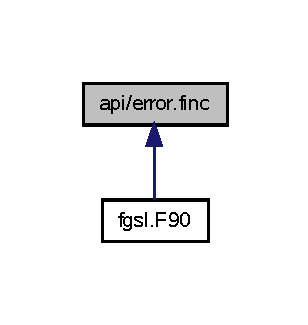
\includegraphics[width=152pt]{error_8finc__dep__incl}
\end{center}
\end{figure}
\subsection*{Functions/\-Subroutines}
\begin{DoxyCompactItemize}
\item 
type(fgsl\-\_\-error\-\_\-handler\-\_\-t) function \hyperlink{error_8finc_a0bcea44cb57ec40ff8ee5deb56628d6c}{fgsl\-\_\-set\-\_\-error\-\_\-handler} (new\-\_\-handler)
\item 
type(fgsl\-\_\-error\-\_\-handler\-\_\-t) function \hyperlink{error_8finc_a038022a5ae74d2221231fb2d484e3fb9}{fgsl\-\_\-set\-\_\-error\-\_\-handler\-\_\-off} ()
\item 
character(kind=fgsl\-\_\-char, len=fgsl\-\_\-strmax) \\*
function \hyperlink{error_8finc_afb379d7136f115fcbc5fbe6178ab1a8b}{fgsl\-\_\-strerror} (errno)
\item 
subroutine \hyperlink{error_8finc_a4d5b557021a59a337ae0a724da2f2f79}{fgsl\-\_\-error} (reason, file, line, errno)
\item 
logical function \hyperlink{error_8finc_aa355a6ea584a0315b6bd48125143f61e}{fgsl\-\_\-error\-\_\-handler\-\_\-status} (error\-\_\-handler\-\_\-t)
\item 
type(fgsl\-\_\-error\-\_\-handler\-\_\-t) function \hyperlink{error_8finc_a2021475812bde99b19e3497120fe502f}{fgsl\-\_\-error\-\_\-handler\-\_\-init} (handler\-\_\-sr)
\end{DoxyCompactItemize}


\subsection{Function/\-Subroutine Documentation}
\hypertarget{error_8finc_a4d5b557021a59a337ae0a724da2f2f79}{\index{error.\-finc@{error.\-finc}!fgsl\-\_\-error@{fgsl\-\_\-error}}
\index{fgsl\-\_\-error@{fgsl\-\_\-error}!error.finc@{error.\-finc}}
\subsubsection[{fgsl\-\_\-error}]{\setlength{\rightskip}{0pt plus 5cm}subroutine fgsl\-\_\-error (
\begin{DoxyParamCaption}
\item[{character(kind=fgsl\-\_\-char,len=$\ast$), intent(in)}]{reason, }
\item[{character(kind=fgsl\-\_\-char,len=$\ast$), intent(in)}]{file, }
\item[{integer(fgsl\-\_\-int), intent(in)}]{line, }
\item[{integer(fgsl\-\_\-int), intent(in)}]{errno}
\end{DoxyParamCaption}
)}}\label{error_8finc_a4d5b557021a59a337ae0a724da2f2f79}
\hypertarget{error_8finc_a2021475812bde99b19e3497120fe502f}{\index{error.\-finc@{error.\-finc}!fgsl\-\_\-error\-\_\-handler\-\_\-init@{fgsl\-\_\-error\-\_\-handler\-\_\-init}}
\index{fgsl\-\_\-error\-\_\-handler\-\_\-init@{fgsl\-\_\-error\-\_\-handler\-\_\-init}!error.finc@{error.\-finc}}
\subsubsection[{fgsl\-\_\-error\-\_\-handler\-\_\-init}]{\setlength{\rightskip}{0pt plus 5cm}type(fgsl\-\_\-error\-\_\-handler\-\_\-t) function fgsl\-\_\-error\-\_\-handler\-\_\-init (
\begin{DoxyParamCaption}
\item[{}]{handler\-\_\-sr}
\end{DoxyParamCaption}
)}}\label{error_8finc_a2021475812bde99b19e3497120fe502f}
\hypertarget{error_8finc_aa355a6ea584a0315b6bd48125143f61e}{\index{error.\-finc@{error.\-finc}!fgsl\-\_\-error\-\_\-handler\-\_\-status@{fgsl\-\_\-error\-\_\-handler\-\_\-status}}
\index{fgsl\-\_\-error\-\_\-handler\-\_\-status@{fgsl\-\_\-error\-\_\-handler\-\_\-status}!error.finc@{error.\-finc}}
\subsubsection[{fgsl\-\_\-error\-\_\-handler\-\_\-status}]{\setlength{\rightskip}{0pt plus 5cm}logical function fgsl\-\_\-error\-\_\-handler\-\_\-status (
\begin{DoxyParamCaption}
\item[{type(fgsl\-\_\-error\-\_\-handler\-\_\-t), intent(in)}]{error\-\_\-handler\-\_\-t}
\end{DoxyParamCaption}
)}}\label{error_8finc_aa355a6ea584a0315b6bd48125143f61e}
\hypertarget{error_8finc_a0bcea44cb57ec40ff8ee5deb56628d6c}{\index{error.\-finc@{error.\-finc}!fgsl\-\_\-set\-\_\-error\-\_\-handler@{fgsl\-\_\-set\-\_\-error\-\_\-handler}}
\index{fgsl\-\_\-set\-\_\-error\-\_\-handler@{fgsl\-\_\-set\-\_\-error\-\_\-handler}!error.finc@{error.\-finc}}
\subsubsection[{fgsl\-\_\-set\-\_\-error\-\_\-handler}]{\setlength{\rightskip}{0pt plus 5cm}type(fgsl\-\_\-error\-\_\-handler\-\_\-t) function fgsl\-\_\-set\-\_\-error\-\_\-handler (
\begin{DoxyParamCaption}
\item[{type(fgsl\-\_\-error\-\_\-handler\-\_\-t), intent(in)}]{new\-\_\-handler}
\end{DoxyParamCaption}
)}}\label{error_8finc_a0bcea44cb57ec40ff8ee5deb56628d6c}
\hypertarget{error_8finc_a038022a5ae74d2221231fb2d484e3fb9}{\index{error.\-finc@{error.\-finc}!fgsl\-\_\-set\-\_\-error\-\_\-handler\-\_\-off@{fgsl\-\_\-set\-\_\-error\-\_\-handler\-\_\-off}}
\index{fgsl\-\_\-set\-\_\-error\-\_\-handler\-\_\-off@{fgsl\-\_\-set\-\_\-error\-\_\-handler\-\_\-off}!error.finc@{error.\-finc}}
\subsubsection[{fgsl\-\_\-set\-\_\-error\-\_\-handler\-\_\-off}]{\setlength{\rightskip}{0pt plus 5cm}type(fgsl\-\_\-error\-\_\-handler\-\_\-t) function fgsl\-\_\-set\-\_\-error\-\_\-handler\-\_\-off (
\begin{DoxyParamCaption}
{}
\end{DoxyParamCaption}
)}}\label{error_8finc_a038022a5ae74d2221231fb2d484e3fb9}
\hypertarget{error_8finc_afb379d7136f115fcbc5fbe6178ab1a8b}{\index{error.\-finc@{error.\-finc}!fgsl\-\_\-strerror@{fgsl\-\_\-strerror}}
\index{fgsl\-\_\-strerror@{fgsl\-\_\-strerror}!error.finc@{error.\-finc}}
\subsubsection[{fgsl\-\_\-strerror}]{\setlength{\rightskip}{0pt plus 5cm}character(kind=fgsl\-\_\-char,len=fgsl\-\_\-strmax) function fgsl\-\_\-strerror (
\begin{DoxyParamCaption}
\item[{integer(fgsl\-\_\-int), intent(in)}]{errno}
\end{DoxyParamCaption}
)}}\label{error_8finc_afb379d7136f115fcbc5fbe6178ab1a8b}

\hypertarget{fft_8finc}{\section{api/fft.finc File Reference}
\label{fft_8finc}\index{api/fft.\-finc@{api/fft.\-finc}}
}
This graph shows which files directly or indirectly include this file\-:\nopagebreak
\begin{figure}[H]
\begin{center}
\leavevmode
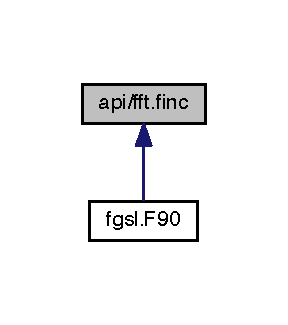
\includegraphics[width=138pt]{fft_8finc__dep__incl}
\end{center}
\end{figure}
\subsection*{Functions/\-Subroutines}
\begin{DoxyCompactItemize}
\item 
integer(fgsl\-\_\-int) function \hyperlink{fft_8finc_a6d6765aceb1cb89aa378e657277cb60e}{fgsl\-\_\-fft\-\_\-complex\-\_\-radix2\-\_\-forward} (data, stride, n)
\item 
integer(fgsl\-\_\-int) function \hyperlink{fft_8finc_adb683798dd4ccce52cc209e16deac0ab}{fgsl\-\_\-fft\-\_\-complex\-\_\-radix2\-\_\-transform} (data, stride, n, sign)
\item 
integer(fgsl\-\_\-int) function \hyperlink{fft_8finc_ac9dfd334102aed6b1833e9b6b936ee38}{fgsl\-\_\-fft\-\_\-complex\-\_\-radix2\-\_\-backward} (data, stride, n)
\item 
integer(fgsl\-\_\-int) function \hyperlink{fft_8finc_a2976591bd53bebb217c69c16b9cb36b4}{fgsl\-\_\-fft\-\_\-complex\-\_\-radix2\-\_\-inverse} (data, stride, n)
\item 
integer(fgsl\-\_\-int) function \hyperlink{fft_8finc_ab346147a5eba7237163db01403bd96e7}{fgsl\-\_\-fft\-\_\-complex\-\_\-radix2\-\_\-dif\-\_\-forward} (data, stride, n)
\item 
integer(fgsl\-\_\-int) function \hyperlink{fft_8finc_ae161490fa787f0b7b2d7aae171abb2fe}{fgsl\-\_\-fft\-\_\-complex\-\_\-radix2\-\_\-dif\-\_\-transform} (data, stride, n, sign)
\item 
integer(fgsl\-\_\-int) function \hyperlink{fft_8finc_a288d6bc95e5d5a7c2d0c0787ed77493a}{fgsl\-\_\-fft\-\_\-complex\-\_\-radix2\-\_\-dif\-\_\-backward} (data, stride, n)
\item 
integer(fgsl\-\_\-int) function \hyperlink{fft_8finc_aa5abc4b2da983c0197e3612ca15f700b}{fgsl\-\_\-fft\-\_\-complex\-\_\-radix2\-\_\-dif\-\_\-inverse} (data, stride, n)
\item 
type(fgsl\-\_\-fft\-\_\-complex\-\_\-wavetable) \\*
function \hyperlink{fft_8finc_afd1a11147328bddf936a7d414f796490}{fgsl\-\_\-fft\-\_\-complex\-\_\-wavetable\-\_\-alloc} (n)
\item 
subroutine \hyperlink{fft_8finc_a8b3b35a0490b49010d2f096a2117e1b0}{fgsl\-\_\-fft\-\_\-complex\-\_\-wavetable\-\_\-free} (w)
\item 
type(fgsl\-\_\-fft\-\_\-complex\-\_\-workspace) \\*
function \hyperlink{fft_8finc_a1ab14d22f845afbded031591ff898b56}{fgsl\-\_\-fft\-\_\-complex\-\_\-workspace\-\_\-alloc} (n)
\item 
subroutine \hyperlink{fft_8finc_a349930160b7e3aa8c2d622086c18cc9f}{fgsl\-\_\-fft\-\_\-complex\-\_\-workspace\-\_\-free} (w)
\item 
integer(fgsl\-\_\-int) function \hyperlink{fft_8finc_a93cd04b58e8404ebe91398ddf33ac2ee}{fgsl\-\_\-fft\-\_\-complex\-\_\-forward} (data, stride, n, wavetable, work)
\item 
integer(fgsl\-\_\-int) function \hyperlink{fft_8finc_a376d447a1955ebc92b2e87a5712185b1}{fgsl\-\_\-fft\-\_\-complex\-\_\-transform} (data, stride, n, wavetable, work, sign)
\item 
integer(fgsl\-\_\-int) function \hyperlink{fft_8finc_a5d26359427318351552aa35ba54fe56a}{fgsl\-\_\-fft\-\_\-complex\-\_\-backward} (data, stride, n, wavetable, work)
\item 
integer(fgsl\-\_\-int) function \hyperlink{fft_8finc_ad553e482847f3d81c3f4bb7f43e68053}{fgsl\-\_\-fft\-\_\-complex\-\_\-inverse} (data, stride, n, wavetable, work)
\item 
integer(fgsl\-\_\-int) function \hyperlink{fft_8finc_a83d3ca22179c1492451233146284096e}{fgsl\-\_\-fft\-\_\-real\-\_\-radix2\-\_\-transform} (data, stride, n)
\item 
integer(fgsl\-\_\-int) function \hyperlink{fft_8finc_a221b77aa4c793385e078efff48b05b78}{fgsl\-\_\-fft\-\_\-halfcomplex\-\_\-radix2\-\_\-inverse} (data, stride, n)
\item 
integer(fgsl\-\_\-int) function \hyperlink{fft_8finc_aa85ca51ea5f1e86190979008004c3e90}{fgsl\-\_\-fft\-\_\-halfcomplex\-\_\-radix2\-\_\-backward} (data, stride, n)
\item 
type(fgsl\-\_\-fft\-\_\-real\-\_\-wavetable) \\*
function \hyperlink{fft_8finc_a2d6bd839e5cea8c45db50f3f39250daf}{fgsl\-\_\-fft\-\_\-real\-\_\-wavetable\-\_\-alloc} (n)
\item 
subroutine \hyperlink{fft_8finc_a1a476c3a23eb0379cce21b6796c38f26}{fgsl\-\_\-fft\-\_\-real\-\_\-wavetable\-\_\-free} (w)
\item 
type(fgsl\-\_\-fft\-\_\-halfcomplex\-\_\-wavetable) \\*
function \hyperlink{fft_8finc_a8d7b46f387eaaf4045a2ae2a8e71acee}{fgsl\-\_\-fft\-\_\-halfcomplex\-\_\-wavetable\-\_\-alloc} (n)
\item 
subroutine \hyperlink{fft_8finc_aea9fde2535cade327c22905e9507060b}{fgsl\-\_\-fft\-\_\-halfcomplex\-\_\-wavetable\-\_\-free} (w)
\item 
type(fgsl\-\_\-fft\-\_\-real\-\_\-workspace) \\*
function \hyperlink{fft_8finc_adbcc56de7ecc248fc58056203f453b5f}{fgsl\-\_\-fft\-\_\-real\-\_\-workspace\-\_\-alloc} (n)
\item 
subroutine \hyperlink{fft_8finc_a70c81dda8b45ee196cb1b6e60416e71c}{fgsl\-\_\-fft\-\_\-real\-\_\-workspace\-\_\-free} (w)
\item 
integer(fgsl\-\_\-int) function \hyperlink{fft_8finc_a85bb82277112471d93ff981547ca5f85}{fgsl\-\_\-fft\-\_\-real\-\_\-transform} (data, stride, n, wavetable, work)
\item 
integer(fgsl\-\_\-int) function \hyperlink{fft_8finc_ac7b50d9cadbbbcb90263686390ef2bc7}{fgsl\-\_\-fft\-\_\-halfcomplex\-\_\-transform} (data, stride, n, wavetable, work)
\item 
integer(fgsl\-\_\-int) function \hyperlink{fft_8finc_a26adedfb325d69561a2d1261f377c652}{fgsl\-\_\-fft\-\_\-real\-\_\-unpack} (real\-\_\-coefficient, complex\-\_\-coefficient, stride, n)
\item 
integer(fgsl\-\_\-int) function \hyperlink{fft_8finc_a31d71847a61aa5b87c60b8498494358f}{fgsl\-\_\-fft\-\_\-halfcomplex\-\_\-unpack} (halfcomplex\-\_\-coefficient, complex\-\_\-coefficient, stride, n)
\end{DoxyCompactItemize}


\subsection{Function/\-Subroutine Documentation}
\hypertarget{fft_8finc_a5d26359427318351552aa35ba54fe56a}{\index{fft.\-finc@{fft.\-finc}!fgsl\-\_\-fft\-\_\-complex\-\_\-backward@{fgsl\-\_\-fft\-\_\-complex\-\_\-backward}}
\index{fgsl\-\_\-fft\-\_\-complex\-\_\-backward@{fgsl\-\_\-fft\-\_\-complex\-\_\-backward}!fft.finc@{fft.\-finc}}
\subsubsection[{fgsl\-\_\-fft\-\_\-complex\-\_\-backward}]{\setlength{\rightskip}{0pt plus 5cm}integer(fgsl\-\_\-int) function fgsl\-\_\-fft\-\_\-complex\-\_\-backward (
\begin{DoxyParamCaption}
\item[{complex(fgsl\-\_\-double\-\_\-complex), dimension($\ast$), intent(inout), target}]{data, }
\item[{integer(fgsl\-\_\-size\-\_\-t), intent(in)}]{stride, }
\item[{integer(fgsl\-\_\-size\-\_\-t), intent(in)}]{n, }
\item[{type(fgsl\-\_\-fft\-\_\-complex\-\_\-wavetable), intent(in)}]{wavetable, }
\item[{type(fgsl\-\_\-fft\-\_\-complex\-\_\-workspace)}]{work}
\end{DoxyParamCaption}
)}}\label{fft_8finc_a5d26359427318351552aa35ba54fe56a}
\hypertarget{fft_8finc_a93cd04b58e8404ebe91398ddf33ac2ee}{\index{fft.\-finc@{fft.\-finc}!fgsl\-\_\-fft\-\_\-complex\-\_\-forward@{fgsl\-\_\-fft\-\_\-complex\-\_\-forward}}
\index{fgsl\-\_\-fft\-\_\-complex\-\_\-forward@{fgsl\-\_\-fft\-\_\-complex\-\_\-forward}!fft.finc@{fft.\-finc}}
\subsubsection[{fgsl\-\_\-fft\-\_\-complex\-\_\-forward}]{\setlength{\rightskip}{0pt plus 5cm}integer(fgsl\-\_\-int) function fgsl\-\_\-fft\-\_\-complex\-\_\-forward (
\begin{DoxyParamCaption}
\item[{complex(fgsl\-\_\-double\-\_\-complex), dimension($\ast$), intent(inout), target}]{data, }
\item[{integer(fgsl\-\_\-size\-\_\-t), intent(in)}]{stride, }
\item[{integer(fgsl\-\_\-size\-\_\-t), intent(in)}]{n, }
\item[{type(fgsl\-\_\-fft\-\_\-complex\-\_\-wavetable), intent(in)}]{wavetable, }
\item[{type(fgsl\-\_\-fft\-\_\-complex\-\_\-workspace)}]{work}
\end{DoxyParamCaption}
)}}\label{fft_8finc_a93cd04b58e8404ebe91398ddf33ac2ee}
\hypertarget{fft_8finc_ad553e482847f3d81c3f4bb7f43e68053}{\index{fft.\-finc@{fft.\-finc}!fgsl\-\_\-fft\-\_\-complex\-\_\-inverse@{fgsl\-\_\-fft\-\_\-complex\-\_\-inverse}}
\index{fgsl\-\_\-fft\-\_\-complex\-\_\-inverse@{fgsl\-\_\-fft\-\_\-complex\-\_\-inverse}!fft.finc@{fft.\-finc}}
\subsubsection[{fgsl\-\_\-fft\-\_\-complex\-\_\-inverse}]{\setlength{\rightskip}{0pt plus 5cm}integer(fgsl\-\_\-int) function fgsl\-\_\-fft\-\_\-complex\-\_\-inverse (
\begin{DoxyParamCaption}
\item[{complex(fgsl\-\_\-double\-\_\-complex), dimension($\ast$), intent(inout), target}]{data, }
\item[{integer(fgsl\-\_\-size\-\_\-t), intent(in)}]{stride, }
\item[{integer(fgsl\-\_\-size\-\_\-t), intent(in)}]{n, }
\item[{type(fgsl\-\_\-fft\-\_\-complex\-\_\-wavetable), intent(in)}]{wavetable, }
\item[{type(fgsl\-\_\-fft\-\_\-complex\-\_\-workspace)}]{work}
\end{DoxyParamCaption}
)}}\label{fft_8finc_ad553e482847f3d81c3f4bb7f43e68053}
\hypertarget{fft_8finc_ac9dfd334102aed6b1833e9b6b936ee38}{\index{fft.\-finc@{fft.\-finc}!fgsl\-\_\-fft\-\_\-complex\-\_\-radix2\-\_\-backward@{fgsl\-\_\-fft\-\_\-complex\-\_\-radix2\-\_\-backward}}
\index{fgsl\-\_\-fft\-\_\-complex\-\_\-radix2\-\_\-backward@{fgsl\-\_\-fft\-\_\-complex\-\_\-radix2\-\_\-backward}!fft.finc@{fft.\-finc}}
\subsubsection[{fgsl\-\_\-fft\-\_\-complex\-\_\-radix2\-\_\-backward}]{\setlength{\rightskip}{0pt plus 5cm}integer(fgsl\-\_\-int) function fgsl\-\_\-fft\-\_\-complex\-\_\-radix2\-\_\-backward (
\begin{DoxyParamCaption}
\item[{complex(fgsl\-\_\-double\-\_\-complex), dimension($\ast$), intent(inout), target}]{data, }
\item[{integer(fgsl\-\_\-size\-\_\-t), intent(in)}]{stride, }
\item[{integer(fgsl\-\_\-size\-\_\-t), intent(in)}]{n}
\end{DoxyParamCaption}
)}}\label{fft_8finc_ac9dfd334102aed6b1833e9b6b936ee38}
\hypertarget{fft_8finc_a288d6bc95e5d5a7c2d0c0787ed77493a}{\index{fft.\-finc@{fft.\-finc}!fgsl\-\_\-fft\-\_\-complex\-\_\-radix2\-\_\-dif\-\_\-backward@{fgsl\-\_\-fft\-\_\-complex\-\_\-radix2\-\_\-dif\-\_\-backward}}
\index{fgsl\-\_\-fft\-\_\-complex\-\_\-radix2\-\_\-dif\-\_\-backward@{fgsl\-\_\-fft\-\_\-complex\-\_\-radix2\-\_\-dif\-\_\-backward}!fft.finc@{fft.\-finc}}
\subsubsection[{fgsl\-\_\-fft\-\_\-complex\-\_\-radix2\-\_\-dif\-\_\-backward}]{\setlength{\rightskip}{0pt plus 5cm}integer(fgsl\-\_\-int) function fgsl\-\_\-fft\-\_\-complex\-\_\-radix2\-\_\-dif\-\_\-backward (
\begin{DoxyParamCaption}
\item[{complex(fgsl\-\_\-double\-\_\-complex), dimension($\ast$), intent(inout), target}]{data, }
\item[{integer(fgsl\-\_\-size\-\_\-t), intent(in)}]{stride, }
\item[{integer(fgsl\-\_\-size\-\_\-t), intent(in)}]{n}
\end{DoxyParamCaption}
)}}\label{fft_8finc_a288d6bc95e5d5a7c2d0c0787ed77493a}
\hypertarget{fft_8finc_ab346147a5eba7237163db01403bd96e7}{\index{fft.\-finc@{fft.\-finc}!fgsl\-\_\-fft\-\_\-complex\-\_\-radix2\-\_\-dif\-\_\-forward@{fgsl\-\_\-fft\-\_\-complex\-\_\-radix2\-\_\-dif\-\_\-forward}}
\index{fgsl\-\_\-fft\-\_\-complex\-\_\-radix2\-\_\-dif\-\_\-forward@{fgsl\-\_\-fft\-\_\-complex\-\_\-radix2\-\_\-dif\-\_\-forward}!fft.finc@{fft.\-finc}}
\subsubsection[{fgsl\-\_\-fft\-\_\-complex\-\_\-radix2\-\_\-dif\-\_\-forward}]{\setlength{\rightskip}{0pt plus 5cm}integer(fgsl\-\_\-int) function fgsl\-\_\-fft\-\_\-complex\-\_\-radix2\-\_\-dif\-\_\-forward (
\begin{DoxyParamCaption}
\item[{complex(fgsl\-\_\-double\-\_\-complex), dimension($\ast$), intent(inout), target}]{data, }
\item[{integer(fgsl\-\_\-size\-\_\-t), intent(in)}]{stride, }
\item[{integer(fgsl\-\_\-size\-\_\-t), intent(in)}]{n}
\end{DoxyParamCaption}
)}}\label{fft_8finc_ab346147a5eba7237163db01403bd96e7}
\hypertarget{fft_8finc_aa5abc4b2da983c0197e3612ca15f700b}{\index{fft.\-finc@{fft.\-finc}!fgsl\-\_\-fft\-\_\-complex\-\_\-radix2\-\_\-dif\-\_\-inverse@{fgsl\-\_\-fft\-\_\-complex\-\_\-radix2\-\_\-dif\-\_\-inverse}}
\index{fgsl\-\_\-fft\-\_\-complex\-\_\-radix2\-\_\-dif\-\_\-inverse@{fgsl\-\_\-fft\-\_\-complex\-\_\-radix2\-\_\-dif\-\_\-inverse}!fft.finc@{fft.\-finc}}
\subsubsection[{fgsl\-\_\-fft\-\_\-complex\-\_\-radix2\-\_\-dif\-\_\-inverse}]{\setlength{\rightskip}{0pt plus 5cm}integer(fgsl\-\_\-int) function fgsl\-\_\-fft\-\_\-complex\-\_\-radix2\-\_\-dif\-\_\-inverse (
\begin{DoxyParamCaption}
\item[{complex(fgsl\-\_\-double\-\_\-complex), dimension($\ast$), intent(inout), target}]{data, }
\item[{integer(fgsl\-\_\-size\-\_\-t), intent(in)}]{stride, }
\item[{integer(fgsl\-\_\-size\-\_\-t), intent(in)}]{n}
\end{DoxyParamCaption}
)}}\label{fft_8finc_aa5abc4b2da983c0197e3612ca15f700b}
\hypertarget{fft_8finc_ae161490fa787f0b7b2d7aae171abb2fe}{\index{fft.\-finc@{fft.\-finc}!fgsl\-\_\-fft\-\_\-complex\-\_\-radix2\-\_\-dif\-\_\-transform@{fgsl\-\_\-fft\-\_\-complex\-\_\-radix2\-\_\-dif\-\_\-transform}}
\index{fgsl\-\_\-fft\-\_\-complex\-\_\-radix2\-\_\-dif\-\_\-transform@{fgsl\-\_\-fft\-\_\-complex\-\_\-radix2\-\_\-dif\-\_\-transform}!fft.finc@{fft.\-finc}}
\subsubsection[{fgsl\-\_\-fft\-\_\-complex\-\_\-radix2\-\_\-dif\-\_\-transform}]{\setlength{\rightskip}{0pt plus 5cm}integer(fgsl\-\_\-int) function fgsl\-\_\-fft\-\_\-complex\-\_\-radix2\-\_\-dif\-\_\-transform (
\begin{DoxyParamCaption}
\item[{complex(fgsl\-\_\-double\-\_\-complex), dimension($\ast$), intent(inout), target}]{data, }
\item[{integer(fgsl\-\_\-size\-\_\-t), intent(in)}]{stride, }
\item[{integer(fgsl\-\_\-size\-\_\-t), intent(in)}]{n, }
\item[{integer(fgsl\-\_\-int), intent(in)}]{sign}
\end{DoxyParamCaption}
)}}\label{fft_8finc_ae161490fa787f0b7b2d7aae171abb2fe}
\hypertarget{fft_8finc_a6d6765aceb1cb89aa378e657277cb60e}{\index{fft.\-finc@{fft.\-finc}!fgsl\-\_\-fft\-\_\-complex\-\_\-radix2\-\_\-forward@{fgsl\-\_\-fft\-\_\-complex\-\_\-radix2\-\_\-forward}}
\index{fgsl\-\_\-fft\-\_\-complex\-\_\-radix2\-\_\-forward@{fgsl\-\_\-fft\-\_\-complex\-\_\-radix2\-\_\-forward}!fft.finc@{fft.\-finc}}
\subsubsection[{fgsl\-\_\-fft\-\_\-complex\-\_\-radix2\-\_\-forward}]{\setlength{\rightskip}{0pt plus 5cm}integer(fgsl\-\_\-int) function fgsl\-\_\-fft\-\_\-complex\-\_\-radix2\-\_\-forward (
\begin{DoxyParamCaption}
\item[{complex(fgsl\-\_\-double\-\_\-complex), dimension($\ast$), intent(inout), target}]{data, }
\item[{integer(fgsl\-\_\-size\-\_\-t), intent(in)}]{stride, }
\item[{integer(fgsl\-\_\-size\-\_\-t), intent(in)}]{n}
\end{DoxyParamCaption}
)}}\label{fft_8finc_a6d6765aceb1cb89aa378e657277cb60e}
\hypertarget{fft_8finc_a2976591bd53bebb217c69c16b9cb36b4}{\index{fft.\-finc@{fft.\-finc}!fgsl\-\_\-fft\-\_\-complex\-\_\-radix2\-\_\-inverse@{fgsl\-\_\-fft\-\_\-complex\-\_\-radix2\-\_\-inverse}}
\index{fgsl\-\_\-fft\-\_\-complex\-\_\-radix2\-\_\-inverse@{fgsl\-\_\-fft\-\_\-complex\-\_\-radix2\-\_\-inverse}!fft.finc@{fft.\-finc}}
\subsubsection[{fgsl\-\_\-fft\-\_\-complex\-\_\-radix2\-\_\-inverse}]{\setlength{\rightskip}{0pt plus 5cm}integer(fgsl\-\_\-int) function fgsl\-\_\-fft\-\_\-complex\-\_\-radix2\-\_\-inverse (
\begin{DoxyParamCaption}
\item[{complex(fgsl\-\_\-double\-\_\-complex), dimension($\ast$), intent(inout), target}]{data, }
\item[{integer(fgsl\-\_\-size\-\_\-t), intent(in)}]{stride, }
\item[{integer(fgsl\-\_\-size\-\_\-t), intent(in)}]{n}
\end{DoxyParamCaption}
)}}\label{fft_8finc_a2976591bd53bebb217c69c16b9cb36b4}
\hypertarget{fft_8finc_adb683798dd4ccce52cc209e16deac0ab}{\index{fft.\-finc@{fft.\-finc}!fgsl\-\_\-fft\-\_\-complex\-\_\-radix2\-\_\-transform@{fgsl\-\_\-fft\-\_\-complex\-\_\-radix2\-\_\-transform}}
\index{fgsl\-\_\-fft\-\_\-complex\-\_\-radix2\-\_\-transform@{fgsl\-\_\-fft\-\_\-complex\-\_\-radix2\-\_\-transform}!fft.finc@{fft.\-finc}}
\subsubsection[{fgsl\-\_\-fft\-\_\-complex\-\_\-radix2\-\_\-transform}]{\setlength{\rightskip}{0pt plus 5cm}integer(fgsl\-\_\-int) function fgsl\-\_\-fft\-\_\-complex\-\_\-radix2\-\_\-transform (
\begin{DoxyParamCaption}
\item[{complex(fgsl\-\_\-double\-\_\-complex), dimension($\ast$), intent(inout), target}]{data, }
\item[{integer(fgsl\-\_\-size\-\_\-t), intent(in)}]{stride, }
\item[{integer(fgsl\-\_\-size\-\_\-t), intent(in)}]{n, }
\item[{integer(fgsl\-\_\-int), intent(in)}]{sign}
\end{DoxyParamCaption}
)}}\label{fft_8finc_adb683798dd4ccce52cc209e16deac0ab}
\hypertarget{fft_8finc_a376d447a1955ebc92b2e87a5712185b1}{\index{fft.\-finc@{fft.\-finc}!fgsl\-\_\-fft\-\_\-complex\-\_\-transform@{fgsl\-\_\-fft\-\_\-complex\-\_\-transform}}
\index{fgsl\-\_\-fft\-\_\-complex\-\_\-transform@{fgsl\-\_\-fft\-\_\-complex\-\_\-transform}!fft.finc@{fft.\-finc}}
\subsubsection[{fgsl\-\_\-fft\-\_\-complex\-\_\-transform}]{\setlength{\rightskip}{0pt plus 5cm}integer(fgsl\-\_\-int) function fgsl\-\_\-fft\-\_\-complex\-\_\-transform (
\begin{DoxyParamCaption}
\item[{complex(fgsl\-\_\-double\-\_\-complex), dimension($\ast$), intent(inout), target}]{data, }
\item[{integer(fgsl\-\_\-size\-\_\-t), intent(in)}]{stride, }
\item[{integer(fgsl\-\_\-size\-\_\-t), intent(in)}]{n, }
\item[{type(fgsl\-\_\-fft\-\_\-complex\-\_\-wavetable), intent(in)}]{wavetable, }
\item[{type(fgsl\-\_\-fft\-\_\-complex\-\_\-workspace)}]{work, }
\item[{integer(fgsl\-\_\-int), intent(in)}]{sign}
\end{DoxyParamCaption}
)}}\label{fft_8finc_a376d447a1955ebc92b2e87a5712185b1}
\hypertarget{fft_8finc_afd1a11147328bddf936a7d414f796490}{\index{fft.\-finc@{fft.\-finc}!fgsl\-\_\-fft\-\_\-complex\-\_\-wavetable\-\_\-alloc@{fgsl\-\_\-fft\-\_\-complex\-\_\-wavetable\-\_\-alloc}}
\index{fgsl\-\_\-fft\-\_\-complex\-\_\-wavetable\-\_\-alloc@{fgsl\-\_\-fft\-\_\-complex\-\_\-wavetable\-\_\-alloc}!fft.finc@{fft.\-finc}}
\subsubsection[{fgsl\-\_\-fft\-\_\-complex\-\_\-wavetable\-\_\-alloc}]{\setlength{\rightskip}{0pt plus 5cm}type(fgsl\-\_\-fft\-\_\-complex\-\_\-wavetable) function fgsl\-\_\-fft\-\_\-complex\-\_\-wavetable\-\_\-alloc (
\begin{DoxyParamCaption}
\item[{integer(fgsl\-\_\-size\-\_\-t), intent(in)}]{n}
\end{DoxyParamCaption}
)}}\label{fft_8finc_afd1a11147328bddf936a7d414f796490}
\hypertarget{fft_8finc_a8b3b35a0490b49010d2f096a2117e1b0}{\index{fft.\-finc@{fft.\-finc}!fgsl\-\_\-fft\-\_\-complex\-\_\-wavetable\-\_\-free@{fgsl\-\_\-fft\-\_\-complex\-\_\-wavetable\-\_\-free}}
\index{fgsl\-\_\-fft\-\_\-complex\-\_\-wavetable\-\_\-free@{fgsl\-\_\-fft\-\_\-complex\-\_\-wavetable\-\_\-free}!fft.finc@{fft.\-finc}}
\subsubsection[{fgsl\-\_\-fft\-\_\-complex\-\_\-wavetable\-\_\-free}]{\setlength{\rightskip}{0pt plus 5cm}subroutine fgsl\-\_\-fft\-\_\-complex\-\_\-wavetable\-\_\-free (
\begin{DoxyParamCaption}
\item[{type(fgsl\-\_\-fft\-\_\-complex\-\_\-wavetable)}]{w}
\end{DoxyParamCaption}
)}}\label{fft_8finc_a8b3b35a0490b49010d2f096a2117e1b0}
\hypertarget{fft_8finc_a1ab14d22f845afbded031591ff898b56}{\index{fft.\-finc@{fft.\-finc}!fgsl\-\_\-fft\-\_\-complex\-\_\-workspace\-\_\-alloc@{fgsl\-\_\-fft\-\_\-complex\-\_\-workspace\-\_\-alloc}}
\index{fgsl\-\_\-fft\-\_\-complex\-\_\-workspace\-\_\-alloc@{fgsl\-\_\-fft\-\_\-complex\-\_\-workspace\-\_\-alloc}!fft.finc@{fft.\-finc}}
\subsubsection[{fgsl\-\_\-fft\-\_\-complex\-\_\-workspace\-\_\-alloc}]{\setlength{\rightskip}{0pt plus 5cm}type(fgsl\-\_\-fft\-\_\-complex\-\_\-workspace) function fgsl\-\_\-fft\-\_\-complex\-\_\-workspace\-\_\-alloc (
\begin{DoxyParamCaption}
\item[{integer(fgsl\-\_\-size\-\_\-t), intent(in)}]{n}
\end{DoxyParamCaption}
)}}\label{fft_8finc_a1ab14d22f845afbded031591ff898b56}
\hypertarget{fft_8finc_a349930160b7e3aa8c2d622086c18cc9f}{\index{fft.\-finc@{fft.\-finc}!fgsl\-\_\-fft\-\_\-complex\-\_\-workspace\-\_\-free@{fgsl\-\_\-fft\-\_\-complex\-\_\-workspace\-\_\-free}}
\index{fgsl\-\_\-fft\-\_\-complex\-\_\-workspace\-\_\-free@{fgsl\-\_\-fft\-\_\-complex\-\_\-workspace\-\_\-free}!fft.finc@{fft.\-finc}}
\subsubsection[{fgsl\-\_\-fft\-\_\-complex\-\_\-workspace\-\_\-free}]{\setlength{\rightskip}{0pt plus 5cm}subroutine fgsl\-\_\-fft\-\_\-complex\-\_\-workspace\-\_\-free (
\begin{DoxyParamCaption}
\item[{type(fgsl\-\_\-fft\-\_\-complex\-\_\-workspace)}]{w}
\end{DoxyParamCaption}
)}}\label{fft_8finc_a349930160b7e3aa8c2d622086c18cc9f}
\hypertarget{fft_8finc_aa85ca51ea5f1e86190979008004c3e90}{\index{fft.\-finc@{fft.\-finc}!fgsl\-\_\-fft\-\_\-halfcomplex\-\_\-radix2\-\_\-backward@{fgsl\-\_\-fft\-\_\-halfcomplex\-\_\-radix2\-\_\-backward}}
\index{fgsl\-\_\-fft\-\_\-halfcomplex\-\_\-radix2\-\_\-backward@{fgsl\-\_\-fft\-\_\-halfcomplex\-\_\-radix2\-\_\-backward}!fft.finc@{fft.\-finc}}
\subsubsection[{fgsl\-\_\-fft\-\_\-halfcomplex\-\_\-radix2\-\_\-backward}]{\setlength{\rightskip}{0pt plus 5cm}integer(fgsl\-\_\-int) function fgsl\-\_\-fft\-\_\-halfcomplex\-\_\-radix2\-\_\-backward (
\begin{DoxyParamCaption}
\item[{real(fgsl\-\_\-double), dimension($\ast$), intent(inout), target}]{data, }
\item[{integer(fgsl\-\_\-size\-\_\-t), intent(in)}]{stride, }
\item[{integer(fgsl\-\_\-size\-\_\-t), intent(in)}]{n}
\end{DoxyParamCaption}
)}}\label{fft_8finc_aa85ca51ea5f1e86190979008004c3e90}
\hypertarget{fft_8finc_a221b77aa4c793385e078efff48b05b78}{\index{fft.\-finc@{fft.\-finc}!fgsl\-\_\-fft\-\_\-halfcomplex\-\_\-radix2\-\_\-inverse@{fgsl\-\_\-fft\-\_\-halfcomplex\-\_\-radix2\-\_\-inverse}}
\index{fgsl\-\_\-fft\-\_\-halfcomplex\-\_\-radix2\-\_\-inverse@{fgsl\-\_\-fft\-\_\-halfcomplex\-\_\-radix2\-\_\-inverse}!fft.finc@{fft.\-finc}}
\subsubsection[{fgsl\-\_\-fft\-\_\-halfcomplex\-\_\-radix2\-\_\-inverse}]{\setlength{\rightskip}{0pt plus 5cm}integer(fgsl\-\_\-int) function fgsl\-\_\-fft\-\_\-halfcomplex\-\_\-radix2\-\_\-inverse (
\begin{DoxyParamCaption}
\item[{real(fgsl\-\_\-double), dimension($\ast$), intent(inout), target}]{data, }
\item[{integer(fgsl\-\_\-size\-\_\-t), intent(in)}]{stride, }
\item[{integer(fgsl\-\_\-size\-\_\-t), intent(in)}]{n}
\end{DoxyParamCaption}
)}}\label{fft_8finc_a221b77aa4c793385e078efff48b05b78}
\hypertarget{fft_8finc_ac7b50d9cadbbbcb90263686390ef2bc7}{\index{fft.\-finc@{fft.\-finc}!fgsl\-\_\-fft\-\_\-halfcomplex\-\_\-transform@{fgsl\-\_\-fft\-\_\-halfcomplex\-\_\-transform}}
\index{fgsl\-\_\-fft\-\_\-halfcomplex\-\_\-transform@{fgsl\-\_\-fft\-\_\-halfcomplex\-\_\-transform}!fft.finc@{fft.\-finc}}
\subsubsection[{fgsl\-\_\-fft\-\_\-halfcomplex\-\_\-transform}]{\setlength{\rightskip}{0pt plus 5cm}integer(fgsl\-\_\-int) function fgsl\-\_\-fft\-\_\-halfcomplex\-\_\-transform (
\begin{DoxyParamCaption}
\item[{real(fgsl\-\_\-double), dimension($\ast$), intent(inout), target}]{data, }
\item[{integer(fgsl\-\_\-size\-\_\-t), intent(in)}]{stride, }
\item[{integer(fgsl\-\_\-size\-\_\-t), intent(in)}]{n, }
\item[{type(fgsl\-\_\-fft\-\_\-halfcomplex\-\_\-wavetable), intent(in)}]{wavetable, }
\item[{type(fgsl\-\_\-fft\-\_\-real\-\_\-workspace)}]{work}
\end{DoxyParamCaption}
)}}\label{fft_8finc_ac7b50d9cadbbbcb90263686390ef2bc7}
\hypertarget{fft_8finc_a31d71847a61aa5b87c60b8498494358f}{\index{fft.\-finc@{fft.\-finc}!fgsl\-\_\-fft\-\_\-halfcomplex\-\_\-unpack@{fgsl\-\_\-fft\-\_\-halfcomplex\-\_\-unpack}}
\index{fgsl\-\_\-fft\-\_\-halfcomplex\-\_\-unpack@{fgsl\-\_\-fft\-\_\-halfcomplex\-\_\-unpack}!fft.finc@{fft.\-finc}}
\subsubsection[{fgsl\-\_\-fft\-\_\-halfcomplex\-\_\-unpack}]{\setlength{\rightskip}{0pt plus 5cm}integer(fgsl\-\_\-int) function fgsl\-\_\-fft\-\_\-halfcomplex\-\_\-unpack (
\begin{DoxyParamCaption}
\item[{real(fgsl\-\_\-double), dimension($\ast$), intent(in), target}]{halfcomplex\-\_\-coefficient, }
\item[{complex(fgsl\-\_\-double\-\_\-complex), dimension($\ast$), intent(inout), target}]{complex\-\_\-coefficient, }
\item[{integer(fgsl\-\_\-size\-\_\-t), intent(in)}]{stride, }
\item[{integer(fgsl\-\_\-size\-\_\-t), intent(in)}]{n}
\end{DoxyParamCaption}
)}}\label{fft_8finc_a31d71847a61aa5b87c60b8498494358f}
\hypertarget{fft_8finc_a8d7b46f387eaaf4045a2ae2a8e71acee}{\index{fft.\-finc@{fft.\-finc}!fgsl\-\_\-fft\-\_\-halfcomplex\-\_\-wavetable\-\_\-alloc@{fgsl\-\_\-fft\-\_\-halfcomplex\-\_\-wavetable\-\_\-alloc}}
\index{fgsl\-\_\-fft\-\_\-halfcomplex\-\_\-wavetable\-\_\-alloc@{fgsl\-\_\-fft\-\_\-halfcomplex\-\_\-wavetable\-\_\-alloc}!fft.finc@{fft.\-finc}}
\subsubsection[{fgsl\-\_\-fft\-\_\-halfcomplex\-\_\-wavetable\-\_\-alloc}]{\setlength{\rightskip}{0pt plus 5cm}type(fgsl\-\_\-fft\-\_\-halfcomplex\-\_\-wavetable) function fgsl\-\_\-fft\-\_\-halfcomplex\-\_\-wavetable\-\_\-alloc (
\begin{DoxyParamCaption}
\item[{integer(fgsl\-\_\-size\-\_\-t), intent(in)}]{n}
\end{DoxyParamCaption}
)}}\label{fft_8finc_a8d7b46f387eaaf4045a2ae2a8e71acee}
\hypertarget{fft_8finc_aea9fde2535cade327c22905e9507060b}{\index{fft.\-finc@{fft.\-finc}!fgsl\-\_\-fft\-\_\-halfcomplex\-\_\-wavetable\-\_\-free@{fgsl\-\_\-fft\-\_\-halfcomplex\-\_\-wavetable\-\_\-free}}
\index{fgsl\-\_\-fft\-\_\-halfcomplex\-\_\-wavetable\-\_\-free@{fgsl\-\_\-fft\-\_\-halfcomplex\-\_\-wavetable\-\_\-free}!fft.finc@{fft.\-finc}}
\subsubsection[{fgsl\-\_\-fft\-\_\-halfcomplex\-\_\-wavetable\-\_\-free}]{\setlength{\rightskip}{0pt plus 5cm}subroutine fgsl\-\_\-fft\-\_\-halfcomplex\-\_\-wavetable\-\_\-free (
\begin{DoxyParamCaption}
\item[{type(fgsl\-\_\-fft\-\_\-halfcomplex\-\_\-wavetable)}]{w}
\end{DoxyParamCaption}
)}}\label{fft_8finc_aea9fde2535cade327c22905e9507060b}
\hypertarget{fft_8finc_a83d3ca22179c1492451233146284096e}{\index{fft.\-finc@{fft.\-finc}!fgsl\-\_\-fft\-\_\-real\-\_\-radix2\-\_\-transform@{fgsl\-\_\-fft\-\_\-real\-\_\-radix2\-\_\-transform}}
\index{fgsl\-\_\-fft\-\_\-real\-\_\-radix2\-\_\-transform@{fgsl\-\_\-fft\-\_\-real\-\_\-radix2\-\_\-transform}!fft.finc@{fft.\-finc}}
\subsubsection[{fgsl\-\_\-fft\-\_\-real\-\_\-radix2\-\_\-transform}]{\setlength{\rightskip}{0pt plus 5cm}integer(fgsl\-\_\-int) function fgsl\-\_\-fft\-\_\-real\-\_\-radix2\-\_\-transform (
\begin{DoxyParamCaption}
\item[{real(fgsl\-\_\-double), dimension($\ast$), intent(inout), target}]{data, }
\item[{integer(fgsl\-\_\-size\-\_\-t), intent(in)}]{stride, }
\item[{integer(fgsl\-\_\-size\-\_\-t), intent(in)}]{n}
\end{DoxyParamCaption}
)}}\label{fft_8finc_a83d3ca22179c1492451233146284096e}
\hypertarget{fft_8finc_a85bb82277112471d93ff981547ca5f85}{\index{fft.\-finc@{fft.\-finc}!fgsl\-\_\-fft\-\_\-real\-\_\-transform@{fgsl\-\_\-fft\-\_\-real\-\_\-transform}}
\index{fgsl\-\_\-fft\-\_\-real\-\_\-transform@{fgsl\-\_\-fft\-\_\-real\-\_\-transform}!fft.finc@{fft.\-finc}}
\subsubsection[{fgsl\-\_\-fft\-\_\-real\-\_\-transform}]{\setlength{\rightskip}{0pt plus 5cm}integer(fgsl\-\_\-int) function fgsl\-\_\-fft\-\_\-real\-\_\-transform (
\begin{DoxyParamCaption}
\item[{real(fgsl\-\_\-double), dimension($\ast$), intent(inout), target}]{data, }
\item[{integer(fgsl\-\_\-size\-\_\-t), intent(in)}]{stride, }
\item[{integer(fgsl\-\_\-size\-\_\-t), intent(in)}]{n, }
\item[{type(fgsl\-\_\-fft\-\_\-real\-\_\-wavetable), intent(in)}]{wavetable, }
\item[{type(fgsl\-\_\-fft\-\_\-real\-\_\-workspace)}]{work}
\end{DoxyParamCaption}
)}}\label{fft_8finc_a85bb82277112471d93ff981547ca5f85}
\hypertarget{fft_8finc_a26adedfb325d69561a2d1261f377c652}{\index{fft.\-finc@{fft.\-finc}!fgsl\-\_\-fft\-\_\-real\-\_\-unpack@{fgsl\-\_\-fft\-\_\-real\-\_\-unpack}}
\index{fgsl\-\_\-fft\-\_\-real\-\_\-unpack@{fgsl\-\_\-fft\-\_\-real\-\_\-unpack}!fft.finc@{fft.\-finc}}
\subsubsection[{fgsl\-\_\-fft\-\_\-real\-\_\-unpack}]{\setlength{\rightskip}{0pt plus 5cm}integer(fgsl\-\_\-int) function fgsl\-\_\-fft\-\_\-real\-\_\-unpack (
\begin{DoxyParamCaption}
\item[{real(fgsl\-\_\-double), dimension($\ast$), intent(in), target}]{real\-\_\-coefficient, }
\item[{complex(fgsl\-\_\-double\-\_\-complex), dimension($\ast$), intent(inout), target}]{complex\-\_\-coefficient, }
\item[{integer(fgsl\-\_\-size\-\_\-t), intent(in)}]{stride, }
\item[{integer(fgsl\-\_\-size\-\_\-t), intent(in)}]{n}
\end{DoxyParamCaption}
)}}\label{fft_8finc_a26adedfb325d69561a2d1261f377c652}
\hypertarget{fft_8finc_a2d6bd839e5cea8c45db50f3f39250daf}{\index{fft.\-finc@{fft.\-finc}!fgsl\-\_\-fft\-\_\-real\-\_\-wavetable\-\_\-alloc@{fgsl\-\_\-fft\-\_\-real\-\_\-wavetable\-\_\-alloc}}
\index{fgsl\-\_\-fft\-\_\-real\-\_\-wavetable\-\_\-alloc@{fgsl\-\_\-fft\-\_\-real\-\_\-wavetable\-\_\-alloc}!fft.finc@{fft.\-finc}}
\subsubsection[{fgsl\-\_\-fft\-\_\-real\-\_\-wavetable\-\_\-alloc}]{\setlength{\rightskip}{0pt plus 5cm}type(fgsl\-\_\-fft\-\_\-real\-\_\-wavetable) function fgsl\-\_\-fft\-\_\-real\-\_\-wavetable\-\_\-alloc (
\begin{DoxyParamCaption}
\item[{integer(fgsl\-\_\-size\-\_\-t), intent(in)}]{n}
\end{DoxyParamCaption}
)}}\label{fft_8finc_a2d6bd839e5cea8c45db50f3f39250daf}
\hypertarget{fft_8finc_a1a476c3a23eb0379cce21b6796c38f26}{\index{fft.\-finc@{fft.\-finc}!fgsl\-\_\-fft\-\_\-real\-\_\-wavetable\-\_\-free@{fgsl\-\_\-fft\-\_\-real\-\_\-wavetable\-\_\-free}}
\index{fgsl\-\_\-fft\-\_\-real\-\_\-wavetable\-\_\-free@{fgsl\-\_\-fft\-\_\-real\-\_\-wavetable\-\_\-free}!fft.finc@{fft.\-finc}}
\subsubsection[{fgsl\-\_\-fft\-\_\-real\-\_\-wavetable\-\_\-free}]{\setlength{\rightskip}{0pt plus 5cm}subroutine fgsl\-\_\-fft\-\_\-real\-\_\-wavetable\-\_\-free (
\begin{DoxyParamCaption}
\item[{type(fgsl\-\_\-fft\-\_\-real\-\_\-wavetable)}]{w}
\end{DoxyParamCaption}
)}}\label{fft_8finc_a1a476c3a23eb0379cce21b6796c38f26}
\hypertarget{fft_8finc_adbcc56de7ecc248fc58056203f453b5f}{\index{fft.\-finc@{fft.\-finc}!fgsl\-\_\-fft\-\_\-real\-\_\-workspace\-\_\-alloc@{fgsl\-\_\-fft\-\_\-real\-\_\-workspace\-\_\-alloc}}
\index{fgsl\-\_\-fft\-\_\-real\-\_\-workspace\-\_\-alloc@{fgsl\-\_\-fft\-\_\-real\-\_\-workspace\-\_\-alloc}!fft.finc@{fft.\-finc}}
\subsubsection[{fgsl\-\_\-fft\-\_\-real\-\_\-workspace\-\_\-alloc}]{\setlength{\rightskip}{0pt plus 5cm}type(fgsl\-\_\-fft\-\_\-real\-\_\-workspace) function fgsl\-\_\-fft\-\_\-real\-\_\-workspace\-\_\-alloc (
\begin{DoxyParamCaption}
\item[{integer(fgsl\-\_\-size\-\_\-t), intent(in)}]{n}
\end{DoxyParamCaption}
)}}\label{fft_8finc_adbcc56de7ecc248fc58056203f453b5f}
\hypertarget{fft_8finc_a70c81dda8b45ee196cb1b6e60416e71c}{\index{fft.\-finc@{fft.\-finc}!fgsl\-\_\-fft\-\_\-real\-\_\-workspace\-\_\-free@{fgsl\-\_\-fft\-\_\-real\-\_\-workspace\-\_\-free}}
\index{fgsl\-\_\-fft\-\_\-real\-\_\-workspace\-\_\-free@{fgsl\-\_\-fft\-\_\-real\-\_\-workspace\-\_\-free}!fft.finc@{fft.\-finc}}
\subsubsection[{fgsl\-\_\-fft\-\_\-real\-\_\-workspace\-\_\-free}]{\setlength{\rightskip}{0pt plus 5cm}subroutine fgsl\-\_\-fft\-\_\-real\-\_\-workspace\-\_\-free (
\begin{DoxyParamCaption}
\item[{type(fgsl\-\_\-fft\-\_\-real\-\_\-workspace)}]{w}
\end{DoxyParamCaption}
)}}\label{fft_8finc_a70c81dda8b45ee196cb1b6e60416e71c}

\hypertarget{fit_8finc}{\section{api/fit.finc File Reference}
\label{fit_8finc}\index{api/fit.\-finc@{api/fit.\-finc}}
}
This graph shows which files directly or indirectly include this file\-:
\nopagebreak
\begin{figure}[H]
\begin{center}
\leavevmode
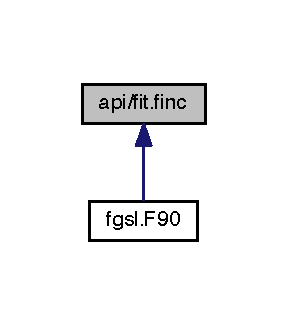
\includegraphics[width=138pt]{fit_8finc__dep__incl}
\end{center}
\end{figure}
\subsection*{Functions/\-Subroutines}
\begin{DoxyCompactItemize}
\item 
integer(fgsl\-\_\-int) function \hyperlink{fit_8finc_a7dbfda6efd2515a9e142a12c4c995cde}{fgsl\-\_\-fit\-\_\-linear} (x, xstride, y, ystride, n, c0, c1, cov00, cov01, cov11, sumsq)
\item 
integer(fgsl\-\_\-int) function \hyperlink{fit_8finc_a19abc39bc86162b79068c44626edb286}{fgsl\-\_\-fit\-\_\-wlinear} (x, xstride, w, wstride, y, ystride, n, c0, c1, cov00, cov01, cov11, chisq)
\item 
integer(fgsl\-\_\-int) function \hyperlink{fit_8finc_a20cd5e248d653b461490237eb98254e1}{fgsl\-\_\-fit\-\_\-linear\-\_\-est} (x, c0, c1, cov00, cov01, cov11, y, y\-\_\-err)
\item 
integer(fgsl\-\_\-int) function \hyperlink{fit_8finc_a127e1658f8bbdb60cb8bb05fe99f3330}{fgsl\-\_\-fit\-\_\-mul} (x, xstride, y, ystride, n, c1, cov11, sumsq)
\item 
integer(fgsl\-\_\-int) function \hyperlink{fit_8finc_ac340f74c0c45fa11d42988d8c8961c3d}{fgsl\-\_\-fit\-\_\-wmul} (x, xstride, w, wstride, y, ystride, n, c1, cov11, chisq)
\item 
integer(fgsl\-\_\-int) function \hyperlink{fit_8finc_a20a41d8704fb027d985e0450d6328a75}{fgsl\-\_\-fit\-\_\-mul\-\_\-est} (x, c1, cov11, y, y\-\_\-err)
\item 
type(fgsl\-\_\-multifit\-\_\-linear\-\_\-workspace) \\*
function \hyperlink{fit_8finc_a2003bf67371be173ab6c188a9fb10c4e}{fgsl\-\_\-multifit\-\_\-linear\-\_\-alloc} (n, p)
\item 
subroutine \hyperlink{fit_8finc_a8a573d86c614625296daddac17b8608e}{fgsl\-\_\-multifit\-\_\-linear\-\_\-free} (w)
\item 
integer(fgsl\-\_\-int) function \hyperlink{fit_8finc_afceca2124515ca5de8c5d5a7e9e00e3f}{fgsl\-\_\-multifit\-\_\-linear} (x, y, c, cov, chisq, work)
\item 
integer(fgsl\-\_\-int) function \hyperlink{fit_8finc_a06f9fb7626ff7c5990b16ace090076f6}{fgsl\-\_\-multifit\-\_\-linear\-\_\-svd} (x, y, tol, rank, c, cov, chisq, work)
\item 
integer(fgsl\-\_\-int) function \hyperlink{fit_8finc_a500bda5206cb389d1d76553f4129b7ed}{fgsl\-\_\-multifit\-\_\-linear\-\_\-usvd} (x, y, tol, rank, c, cov, chisq, work)
\item 
integer(fgsl\-\_\-int) function \hyperlink{fit_8finc_aca3c885bfd73f86607f2dd5a818dda56}{fgsl\-\_\-multifit\-\_\-wlinear} (x, w, y, c, cov, chisq, work)
\item 
integer(fgsl\-\_\-int) function \hyperlink{fit_8finc_a0e7bfa86f1948b97bdc540a44d370f1b}{fgsl\-\_\-multifit\-\_\-wlinear\-\_\-svd} (x, w, y, tol, rank, c, cov, chisq, work)
\item 
integer(fgsl\-\_\-int) function \hyperlink{fit_8finc_a7b805f25c1bfc343d95b2183238bfb3d}{fgsl\-\_\-multifit\-\_\-wlinear\-\_\-usvd} (x, w, y, tol, rank, c, cov, chisq, work)
\item 
integer(fgsl\-\_\-int) function \hyperlink{fit_8finc_a190c5d107367d5f9039e81905cfc85f7}{fgsl\-\_\-multifit\-\_\-linear\-\_\-est} (x, c, cov, y, y\-\_\-err)
\item 
integer(fgsl\-\_\-int) function \hyperlink{fit_8finc_a6f9df5f586bf1ea89402f34d33633b97}{fgsl\-\_\-multifit\-\_\-linear\-\_\-residuals} (x, y, c, r)
\item 
logical function \hyperlink{fit_8finc_add0b89e45ce90eb1a9117d3e45e6b39e}{fgsl\-\_\-multifit\-\_\-status} (multifit)
\end{DoxyCompactItemize}


\subsection{Function/\-Subroutine Documentation}
\hypertarget{fit_8finc_a7dbfda6efd2515a9e142a12c4c995cde}{\index{fit.\-finc@{fit.\-finc}!fgsl\-\_\-fit\-\_\-linear@{fgsl\-\_\-fit\-\_\-linear}}
\index{fgsl\-\_\-fit\-\_\-linear@{fgsl\-\_\-fit\-\_\-linear}!fit.finc@{fit.\-finc}}
\subsubsection[{fgsl\-\_\-fit\-\_\-linear}]{\setlength{\rightskip}{0pt plus 5cm}integer(fgsl\-\_\-int) function fgsl\-\_\-fit\-\_\-linear (
\begin{DoxyParamCaption}
\item[{real(fgsl\-\_\-double), dimension(\-:), intent(in)}]{x, }
\item[{integer(fgsl\-\_\-size\-\_\-t), intent(in)}]{xstride, }
\item[{real(fgsl\-\_\-double), dimension(\-:), intent(in)}]{y, }
\item[{integer(fgsl\-\_\-size\-\_\-t), intent(in)}]{ystride, }
\item[{integer(fgsl\-\_\-size\-\_\-t), intent(in)}]{n, }
\item[{real(fgsl\-\_\-double), intent(out)}]{c0, }
\item[{real(fgsl\-\_\-double), intent(out)}]{c1, }
\item[{real(fgsl\-\_\-double), intent(out)}]{cov00, }
\item[{real(fgsl\-\_\-double), intent(out)}]{cov01, }
\item[{real(fgsl\-\_\-double), intent(out)}]{cov11, }
\item[{real(fgsl\-\_\-double), intent(out)}]{sumsq}
\end{DoxyParamCaption}
)}}\label{fit_8finc_a7dbfda6efd2515a9e142a12c4c995cde}
\hypertarget{fit_8finc_a20cd5e248d653b461490237eb98254e1}{\index{fit.\-finc@{fit.\-finc}!fgsl\-\_\-fit\-\_\-linear\-\_\-est@{fgsl\-\_\-fit\-\_\-linear\-\_\-est}}
\index{fgsl\-\_\-fit\-\_\-linear\-\_\-est@{fgsl\-\_\-fit\-\_\-linear\-\_\-est}!fit.finc@{fit.\-finc}}
\subsubsection[{fgsl\-\_\-fit\-\_\-linear\-\_\-est}]{\setlength{\rightskip}{0pt plus 5cm}integer(fgsl\-\_\-int) function fgsl\-\_\-fit\-\_\-linear\-\_\-est (
\begin{DoxyParamCaption}
\item[{real(fgsl\-\_\-double), intent(in)}]{x, }
\item[{real(fgsl\-\_\-double), intent(in)}]{c0, }
\item[{real(fgsl\-\_\-double), intent(in)}]{c1, }
\item[{real(fgsl\-\_\-double), intent(in)}]{cov00, }
\item[{real(fgsl\-\_\-double), intent(in)}]{cov01, }
\item[{real(fgsl\-\_\-double), intent(in)}]{cov11, }
\item[{real(fgsl\-\_\-double), intent(out)}]{y, }
\item[{real(fgsl\-\_\-double), intent(out)}]{y\-\_\-err}
\end{DoxyParamCaption}
)}}\label{fit_8finc_a20cd5e248d653b461490237eb98254e1}
\hypertarget{fit_8finc_a127e1658f8bbdb60cb8bb05fe99f3330}{\index{fit.\-finc@{fit.\-finc}!fgsl\-\_\-fit\-\_\-mul@{fgsl\-\_\-fit\-\_\-mul}}
\index{fgsl\-\_\-fit\-\_\-mul@{fgsl\-\_\-fit\-\_\-mul}!fit.finc@{fit.\-finc}}
\subsubsection[{fgsl\-\_\-fit\-\_\-mul}]{\setlength{\rightskip}{0pt plus 5cm}integer(fgsl\-\_\-int) function fgsl\-\_\-fit\-\_\-mul (
\begin{DoxyParamCaption}
\item[{real(fgsl\-\_\-double), dimension(\-:), intent(in)}]{x, }
\item[{integer(fgsl\-\_\-size\-\_\-t), intent(in)}]{xstride, }
\item[{real(fgsl\-\_\-double), dimension(\-:), intent(in)}]{y, }
\item[{integer(fgsl\-\_\-size\-\_\-t), intent(in)}]{ystride, }
\item[{integer(fgsl\-\_\-size\-\_\-t), intent(in)}]{n, }
\item[{real(fgsl\-\_\-double), intent(out)}]{c1, }
\item[{real(fgsl\-\_\-double), intent(out)}]{cov11, }
\item[{real(fgsl\-\_\-double), intent(out)}]{sumsq}
\end{DoxyParamCaption}
)}}\label{fit_8finc_a127e1658f8bbdb60cb8bb05fe99f3330}
\hypertarget{fit_8finc_a20a41d8704fb027d985e0450d6328a75}{\index{fit.\-finc@{fit.\-finc}!fgsl\-\_\-fit\-\_\-mul\-\_\-est@{fgsl\-\_\-fit\-\_\-mul\-\_\-est}}
\index{fgsl\-\_\-fit\-\_\-mul\-\_\-est@{fgsl\-\_\-fit\-\_\-mul\-\_\-est}!fit.finc@{fit.\-finc}}
\subsubsection[{fgsl\-\_\-fit\-\_\-mul\-\_\-est}]{\setlength{\rightskip}{0pt plus 5cm}integer(fgsl\-\_\-int) function fgsl\-\_\-fit\-\_\-mul\-\_\-est (
\begin{DoxyParamCaption}
\item[{real(fgsl\-\_\-double), intent(in)}]{x, }
\item[{real(fgsl\-\_\-double), intent(in)}]{c1, }
\item[{real(fgsl\-\_\-double), intent(in)}]{cov11, }
\item[{real(fgsl\-\_\-double), intent(out)}]{y, }
\item[{real(fgsl\-\_\-double), intent(out)}]{y\-\_\-err}
\end{DoxyParamCaption}
)}}\label{fit_8finc_a20a41d8704fb027d985e0450d6328a75}
\hypertarget{fit_8finc_a19abc39bc86162b79068c44626edb286}{\index{fit.\-finc@{fit.\-finc}!fgsl\-\_\-fit\-\_\-wlinear@{fgsl\-\_\-fit\-\_\-wlinear}}
\index{fgsl\-\_\-fit\-\_\-wlinear@{fgsl\-\_\-fit\-\_\-wlinear}!fit.finc@{fit.\-finc}}
\subsubsection[{fgsl\-\_\-fit\-\_\-wlinear}]{\setlength{\rightskip}{0pt plus 5cm}integer(fgsl\-\_\-int) function fgsl\-\_\-fit\-\_\-wlinear (
\begin{DoxyParamCaption}
\item[{real(fgsl\-\_\-double), dimension(\-:), intent(in)}]{x, }
\item[{integer(fgsl\-\_\-size\-\_\-t), intent(in)}]{xstride, }
\item[{real(fgsl\-\_\-double), dimension(\-:), intent(in)}]{w, }
\item[{integer(fgsl\-\_\-size\-\_\-t), intent(in)}]{wstride, }
\item[{real(fgsl\-\_\-double), dimension(\-:), intent(in)}]{y, }
\item[{integer(fgsl\-\_\-size\-\_\-t), intent(in)}]{ystride, }
\item[{integer(fgsl\-\_\-size\-\_\-t), intent(in)}]{n, }
\item[{real(fgsl\-\_\-double), intent(out)}]{c0, }
\item[{real(fgsl\-\_\-double), intent(out)}]{c1, }
\item[{real(fgsl\-\_\-double), intent(out)}]{cov00, }
\item[{real(fgsl\-\_\-double), intent(out)}]{cov01, }
\item[{real(fgsl\-\_\-double), intent(out)}]{cov11, }
\item[{real(fgsl\-\_\-double), intent(out)}]{chisq}
\end{DoxyParamCaption}
)}}\label{fit_8finc_a19abc39bc86162b79068c44626edb286}
\hypertarget{fit_8finc_ac340f74c0c45fa11d42988d8c8961c3d}{\index{fit.\-finc@{fit.\-finc}!fgsl\-\_\-fit\-\_\-wmul@{fgsl\-\_\-fit\-\_\-wmul}}
\index{fgsl\-\_\-fit\-\_\-wmul@{fgsl\-\_\-fit\-\_\-wmul}!fit.finc@{fit.\-finc}}
\subsubsection[{fgsl\-\_\-fit\-\_\-wmul}]{\setlength{\rightskip}{0pt plus 5cm}integer(fgsl\-\_\-int) function fgsl\-\_\-fit\-\_\-wmul (
\begin{DoxyParamCaption}
\item[{real(fgsl\-\_\-double), dimension(\-:), intent(in)}]{x, }
\item[{integer(fgsl\-\_\-size\-\_\-t), intent(in)}]{xstride, }
\item[{real(fgsl\-\_\-double), dimension(\-:), intent(in)}]{w, }
\item[{integer(fgsl\-\_\-size\-\_\-t), intent(in)}]{wstride, }
\item[{real(fgsl\-\_\-double), dimension(\-:), intent(in)}]{y, }
\item[{integer(fgsl\-\_\-size\-\_\-t), intent(in)}]{ystride, }
\item[{integer(fgsl\-\_\-size\-\_\-t), intent(in)}]{n, }
\item[{real(fgsl\-\_\-double), intent(out)}]{c1, }
\item[{real(fgsl\-\_\-double), intent(out)}]{cov11, }
\item[{real(fgsl\-\_\-double), intent(out)}]{chisq}
\end{DoxyParamCaption}
)}}\label{fit_8finc_ac340f74c0c45fa11d42988d8c8961c3d}
\hypertarget{fit_8finc_afceca2124515ca5de8c5d5a7e9e00e3f}{\index{fit.\-finc@{fit.\-finc}!fgsl\-\_\-multifit\-\_\-linear@{fgsl\-\_\-multifit\-\_\-linear}}
\index{fgsl\-\_\-multifit\-\_\-linear@{fgsl\-\_\-multifit\-\_\-linear}!fit.finc@{fit.\-finc}}
\subsubsection[{fgsl\-\_\-multifit\-\_\-linear}]{\setlength{\rightskip}{0pt plus 5cm}integer(fgsl\-\_\-int) function fgsl\-\_\-multifit\-\_\-linear (
\begin{DoxyParamCaption}
\item[{type(fgsl\-\_\-matrix), intent(in)}]{x, }
\item[{type(fgsl\-\_\-vector), intent(in)}]{y, }
\item[{type(fgsl\-\_\-vector), intent(inout)}]{c, }
\item[{type(fgsl\-\_\-matrix), intent(inout)}]{cov, }
\item[{real(fgsl\-\_\-double), intent(inout)}]{chisq, }
\item[{type(fgsl\-\_\-multifit\-\_\-linear\-\_\-workspace), intent(inout)}]{work}
\end{DoxyParamCaption}
)}}\label{fit_8finc_afceca2124515ca5de8c5d5a7e9e00e3f}
\hypertarget{fit_8finc_a2003bf67371be173ab6c188a9fb10c4e}{\index{fit.\-finc@{fit.\-finc}!fgsl\-\_\-multifit\-\_\-linear\-\_\-alloc@{fgsl\-\_\-multifit\-\_\-linear\-\_\-alloc}}
\index{fgsl\-\_\-multifit\-\_\-linear\-\_\-alloc@{fgsl\-\_\-multifit\-\_\-linear\-\_\-alloc}!fit.finc@{fit.\-finc}}
\subsubsection[{fgsl\-\_\-multifit\-\_\-linear\-\_\-alloc}]{\setlength{\rightskip}{0pt plus 5cm}type(fgsl\-\_\-multifit\-\_\-linear\-\_\-workspace) function fgsl\-\_\-multifit\-\_\-linear\-\_\-alloc (
\begin{DoxyParamCaption}
\item[{integer(fgsl\-\_\-size\-\_\-t), intent(in)}]{n, }
\item[{integer(fgsl\-\_\-size\-\_\-t), intent(in)}]{p}
\end{DoxyParamCaption}
)}}\label{fit_8finc_a2003bf67371be173ab6c188a9fb10c4e}
\hypertarget{fit_8finc_a190c5d107367d5f9039e81905cfc85f7}{\index{fit.\-finc@{fit.\-finc}!fgsl\-\_\-multifit\-\_\-linear\-\_\-est@{fgsl\-\_\-multifit\-\_\-linear\-\_\-est}}
\index{fgsl\-\_\-multifit\-\_\-linear\-\_\-est@{fgsl\-\_\-multifit\-\_\-linear\-\_\-est}!fit.finc@{fit.\-finc}}
\subsubsection[{fgsl\-\_\-multifit\-\_\-linear\-\_\-est}]{\setlength{\rightskip}{0pt plus 5cm}integer(fgsl\-\_\-int) function fgsl\-\_\-multifit\-\_\-linear\-\_\-est (
\begin{DoxyParamCaption}
\item[{type(fgsl\-\_\-vector), intent(in)}]{x, }
\item[{type(fgsl\-\_\-vector), intent(in)}]{c, }
\item[{type(fgsl\-\_\-matrix), intent(in)}]{cov, }
\item[{real(fgsl\-\_\-double), intent(inout)}]{y, }
\item[{real(fgsl\-\_\-double), intent(inout)}]{y\-\_\-err}
\end{DoxyParamCaption}
)}}\label{fit_8finc_a190c5d107367d5f9039e81905cfc85f7}
\hypertarget{fit_8finc_a8a573d86c614625296daddac17b8608e}{\index{fit.\-finc@{fit.\-finc}!fgsl\-\_\-multifit\-\_\-linear\-\_\-free@{fgsl\-\_\-multifit\-\_\-linear\-\_\-free}}
\index{fgsl\-\_\-multifit\-\_\-linear\-\_\-free@{fgsl\-\_\-multifit\-\_\-linear\-\_\-free}!fit.finc@{fit.\-finc}}
\subsubsection[{fgsl\-\_\-multifit\-\_\-linear\-\_\-free}]{\setlength{\rightskip}{0pt plus 5cm}subroutine fgsl\-\_\-multifit\-\_\-linear\-\_\-free (
\begin{DoxyParamCaption}
\item[{type(fgsl\-\_\-multifit\-\_\-linear\-\_\-workspace), intent(inout)}]{w}
\end{DoxyParamCaption}
)}}\label{fit_8finc_a8a573d86c614625296daddac17b8608e}
\hypertarget{fit_8finc_a6f9df5f586bf1ea89402f34d33633b97}{\index{fit.\-finc@{fit.\-finc}!fgsl\-\_\-multifit\-\_\-linear\-\_\-residuals@{fgsl\-\_\-multifit\-\_\-linear\-\_\-residuals}}
\index{fgsl\-\_\-multifit\-\_\-linear\-\_\-residuals@{fgsl\-\_\-multifit\-\_\-linear\-\_\-residuals}!fit.finc@{fit.\-finc}}
\subsubsection[{fgsl\-\_\-multifit\-\_\-linear\-\_\-residuals}]{\setlength{\rightskip}{0pt plus 5cm}integer(fgsl\-\_\-int) function fgsl\-\_\-multifit\-\_\-linear\-\_\-residuals (
\begin{DoxyParamCaption}
\item[{type(fgsl\-\_\-matrix), intent(in)}]{x, }
\item[{type(fgsl\-\_\-vector), intent(in)}]{y, }
\item[{type(fgsl\-\_\-vector), intent(in)}]{c, }
\item[{type(fgsl\-\_\-vector), intent(inout)}]{r}
\end{DoxyParamCaption}
)}}\label{fit_8finc_a6f9df5f586bf1ea89402f34d33633b97}
\hypertarget{fit_8finc_a06f9fb7626ff7c5990b16ace090076f6}{\index{fit.\-finc@{fit.\-finc}!fgsl\-\_\-multifit\-\_\-linear\-\_\-svd@{fgsl\-\_\-multifit\-\_\-linear\-\_\-svd}}
\index{fgsl\-\_\-multifit\-\_\-linear\-\_\-svd@{fgsl\-\_\-multifit\-\_\-linear\-\_\-svd}!fit.finc@{fit.\-finc}}
\subsubsection[{fgsl\-\_\-multifit\-\_\-linear\-\_\-svd}]{\setlength{\rightskip}{0pt plus 5cm}integer(fgsl\-\_\-int) function fgsl\-\_\-multifit\-\_\-linear\-\_\-svd (
\begin{DoxyParamCaption}
\item[{type(fgsl\-\_\-matrix), intent(in)}]{x, }
\item[{type(fgsl\-\_\-vector), intent(in)}]{y, }
\item[{real(fgsl\-\_\-double), intent(in)}]{tol, }
\item[{integer(fgsl\-\_\-size\-\_\-t), intent(inout)}]{rank, }
\item[{type(fgsl\-\_\-vector), intent(inout)}]{c, }
\item[{type(fgsl\-\_\-matrix), intent(inout)}]{cov, }
\item[{real(fgsl\-\_\-double), intent(inout)}]{chisq, }
\item[{type(fgsl\-\_\-multifit\-\_\-linear\-\_\-workspace), intent(inout)}]{work}
\end{DoxyParamCaption}
)}}\label{fit_8finc_a06f9fb7626ff7c5990b16ace090076f6}
\hypertarget{fit_8finc_a500bda5206cb389d1d76553f4129b7ed}{\index{fit.\-finc@{fit.\-finc}!fgsl\-\_\-multifit\-\_\-linear\-\_\-usvd@{fgsl\-\_\-multifit\-\_\-linear\-\_\-usvd}}
\index{fgsl\-\_\-multifit\-\_\-linear\-\_\-usvd@{fgsl\-\_\-multifit\-\_\-linear\-\_\-usvd}!fit.finc@{fit.\-finc}}
\subsubsection[{fgsl\-\_\-multifit\-\_\-linear\-\_\-usvd}]{\setlength{\rightskip}{0pt plus 5cm}integer(fgsl\-\_\-int) function fgsl\-\_\-multifit\-\_\-linear\-\_\-usvd (
\begin{DoxyParamCaption}
\item[{type(fgsl\-\_\-matrix), intent(in)}]{x, }
\item[{type(fgsl\-\_\-vector), intent(in)}]{y, }
\item[{real(fgsl\-\_\-double), intent(in)}]{tol, }
\item[{integer(fgsl\-\_\-size\-\_\-t), intent(inout)}]{rank, }
\item[{type(fgsl\-\_\-vector), intent(inout)}]{c, }
\item[{type(fgsl\-\_\-matrix), intent(inout)}]{cov, }
\item[{real(fgsl\-\_\-double), intent(inout)}]{chisq, }
\item[{type(fgsl\-\_\-multifit\-\_\-linear\-\_\-workspace), intent(inout)}]{work}
\end{DoxyParamCaption}
)}}\label{fit_8finc_a500bda5206cb389d1d76553f4129b7ed}
\hypertarget{fit_8finc_add0b89e45ce90eb1a9117d3e45e6b39e}{\index{fit.\-finc@{fit.\-finc}!fgsl\-\_\-multifit\-\_\-status@{fgsl\-\_\-multifit\-\_\-status}}
\index{fgsl\-\_\-multifit\-\_\-status@{fgsl\-\_\-multifit\-\_\-status}!fit.finc@{fit.\-finc}}
\subsubsection[{fgsl\-\_\-multifit\-\_\-status}]{\setlength{\rightskip}{0pt plus 5cm}logical function fgsl\-\_\-multifit\-\_\-status (
\begin{DoxyParamCaption}
\item[{type(fgsl\-\_\-multifit\-\_\-linear\-\_\-workspace), intent(in)}]{multifit}
\end{DoxyParamCaption}
)}}\label{fit_8finc_add0b89e45ce90eb1a9117d3e45e6b39e}
\hypertarget{fit_8finc_aca3c885bfd73f86607f2dd5a818dda56}{\index{fit.\-finc@{fit.\-finc}!fgsl\-\_\-multifit\-\_\-wlinear@{fgsl\-\_\-multifit\-\_\-wlinear}}
\index{fgsl\-\_\-multifit\-\_\-wlinear@{fgsl\-\_\-multifit\-\_\-wlinear}!fit.finc@{fit.\-finc}}
\subsubsection[{fgsl\-\_\-multifit\-\_\-wlinear}]{\setlength{\rightskip}{0pt plus 5cm}integer(fgsl\-\_\-int) function fgsl\-\_\-multifit\-\_\-wlinear (
\begin{DoxyParamCaption}
\item[{type(fgsl\-\_\-matrix), intent(in)}]{x, }
\item[{type(fgsl\-\_\-vector), intent(in)}]{w, }
\item[{type(fgsl\-\_\-vector), intent(in)}]{y, }
\item[{type(fgsl\-\_\-vector), intent(inout)}]{c, }
\item[{type(fgsl\-\_\-matrix), intent(inout)}]{cov, }
\item[{real(fgsl\-\_\-double), intent(inout)}]{chisq, }
\item[{type(fgsl\-\_\-multifit\-\_\-linear\-\_\-workspace), intent(inout)}]{work}
\end{DoxyParamCaption}
)}}\label{fit_8finc_aca3c885bfd73f86607f2dd5a818dda56}
\hypertarget{fit_8finc_a0e7bfa86f1948b97bdc540a44d370f1b}{\index{fit.\-finc@{fit.\-finc}!fgsl\-\_\-multifit\-\_\-wlinear\-\_\-svd@{fgsl\-\_\-multifit\-\_\-wlinear\-\_\-svd}}
\index{fgsl\-\_\-multifit\-\_\-wlinear\-\_\-svd@{fgsl\-\_\-multifit\-\_\-wlinear\-\_\-svd}!fit.finc@{fit.\-finc}}
\subsubsection[{fgsl\-\_\-multifit\-\_\-wlinear\-\_\-svd}]{\setlength{\rightskip}{0pt plus 5cm}integer(fgsl\-\_\-int) function fgsl\-\_\-multifit\-\_\-wlinear\-\_\-svd (
\begin{DoxyParamCaption}
\item[{type(fgsl\-\_\-matrix), intent(in)}]{x, }
\item[{type(fgsl\-\_\-vector), intent(in)}]{w, }
\item[{type(fgsl\-\_\-vector), intent(in)}]{y, }
\item[{real(fgsl\-\_\-double), intent(in)}]{tol, }
\item[{integer(fgsl\-\_\-size\-\_\-t), intent(inout)}]{rank, }
\item[{type(fgsl\-\_\-vector), intent(inout)}]{c, }
\item[{type(fgsl\-\_\-matrix), intent(inout)}]{cov, }
\item[{real(fgsl\-\_\-double), intent(inout)}]{chisq, }
\item[{type(fgsl\-\_\-multifit\-\_\-linear\-\_\-workspace), intent(inout)}]{work}
\end{DoxyParamCaption}
)}}\label{fit_8finc_a0e7bfa86f1948b97bdc540a44d370f1b}
\hypertarget{fit_8finc_a7b805f25c1bfc343d95b2183238bfb3d}{\index{fit.\-finc@{fit.\-finc}!fgsl\-\_\-multifit\-\_\-wlinear\-\_\-usvd@{fgsl\-\_\-multifit\-\_\-wlinear\-\_\-usvd}}
\index{fgsl\-\_\-multifit\-\_\-wlinear\-\_\-usvd@{fgsl\-\_\-multifit\-\_\-wlinear\-\_\-usvd}!fit.finc@{fit.\-finc}}
\subsubsection[{fgsl\-\_\-multifit\-\_\-wlinear\-\_\-usvd}]{\setlength{\rightskip}{0pt plus 5cm}integer(fgsl\-\_\-int) function fgsl\-\_\-multifit\-\_\-wlinear\-\_\-usvd (
\begin{DoxyParamCaption}
\item[{type(fgsl\-\_\-matrix), intent(in)}]{x, }
\item[{type(fgsl\-\_\-vector), intent(in)}]{w, }
\item[{type(fgsl\-\_\-vector), intent(in)}]{y, }
\item[{real(fgsl\-\_\-double), intent(in)}]{tol, }
\item[{integer(fgsl\-\_\-size\-\_\-t), intent(inout)}]{rank, }
\item[{type(fgsl\-\_\-vector), intent(inout)}]{c, }
\item[{type(fgsl\-\_\-matrix), intent(inout)}]{cov, }
\item[{real(fgsl\-\_\-double), intent(inout)}]{chisq, }
\item[{type(fgsl\-\_\-multifit\-\_\-linear\-\_\-workspace), intent(inout)}]{work}
\end{DoxyParamCaption}
)}}\label{fit_8finc_a7b805f25c1bfc343d95b2183238bfb3d}

\hypertarget{histogram_8finc}{}\section{api/histogram.finc File Reference}
\label{histogram_8finc}\index{api/histogram.\+finc@{api/histogram.\+finc}}
This graph shows which files directly or indirectly include this file\+:\nopagebreak
\begin{figure}[H]
\begin{center}
\leavevmode
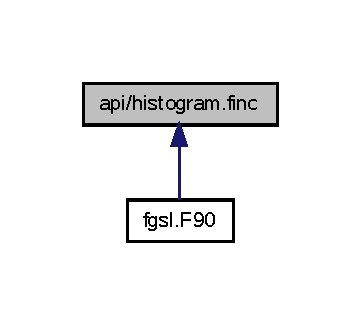
\includegraphics[width=172pt]{histogram_8finc__dep__incl}
\end{center}
\end{figure}
\subsection*{Functions/\+Subroutines}
\begin{DoxyCompactItemize}
\item 
type(fgsl\+\_\+histogram) function \hyperlink{histogram_8finc_a75325ebef92592eba65abd29b6cfadc7}{fgsl\+\_\+histogram\+\_\+alloc} (n)
\item 
integer(fgsl\+\_\+int) function \hyperlink{histogram_8finc_a87bf68114579f570f3b87ec388c136ea}{fgsl\+\_\+histogram\+\_\+set\+\_\+ranges} (h, range)
\item 
integer(fgsl\+\_\+int) function \hyperlink{histogram_8finc_a258b134c27c43ac2108a948c55cf54b7}{fgsl\+\_\+histogram\+\_\+set\+\_\+ranges\+\_\+uniform} (h, xmin, xmax)
\item 
subroutine \hyperlink{histogram_8finc_a34c352dbcdd897703aee1a66777208fe}{fgsl\+\_\+histogram\+\_\+free} (h)
\item 
integer(fgsl\+\_\+int) function \hyperlink{histogram_8finc_a67a6d98e7d1b4186a4b56131eb87bc3c}{fgsl\+\_\+histogram\+\_\+memcpy} (dest, src)
\item 
type(fgsl\+\_\+histogram) function \hyperlink{histogram_8finc_a5a9a45aebea2e21a98f95a561bbc0efe}{fgsl\+\_\+histogram\+\_\+clone} (src)
\item 
integer(fgsl\+\_\+int) function \hyperlink{histogram_8finc_ae8981d30687002aad3dce8c9a029e230}{fgsl\+\_\+histogram\+\_\+increment} (h, x)
\item 
integer(fgsl\+\_\+int) function \hyperlink{histogram_8finc_ac400179f5587a3dbf384fedd0651f354}{fgsl\+\_\+histogram\+\_\+accumulate} (h, x, weight)
\item 
real(fgsl\+\_\+double) function \hyperlink{histogram_8finc_adce52371beeafdc26321bc2c1aa2fcea}{fgsl\+\_\+histogram\+\_\+get} (h, i)
\item 
integer(fgsl\+\_\+int) function \hyperlink{histogram_8finc_a8095fb527d62852e016fec06e1aeeffd}{fgsl\+\_\+histogram\+\_\+get\+\_\+range} (h, i, lower, upper)
\item 
real(fgsl\+\_\+double) function \hyperlink{histogram_8finc_a27016b45c9d32860d6bea50edb523b9a}{fgsl\+\_\+histogram\+\_\+max} (h)
\item 
real(fgsl\+\_\+double) function \hyperlink{histogram_8finc_a703b22dce40bb880886ebed5a1e25269}{fgsl\+\_\+histogram\+\_\+min} (h)
\item 
integer(fgsl\+\_\+size\+\_\+t) function \hyperlink{histogram_8finc_a106c810b7ef3935d89ea6a2fda4f9ac2}{fgsl\+\_\+histogram\+\_\+bins} (h)
\item 
subroutine \hyperlink{histogram_8finc_a49fea1a4cd3aea567784135c870153c1}{fgsl\+\_\+histogram\+\_\+reset} (h)
\item 
integer(fgsl\+\_\+int) function \hyperlink{histogram_8finc_a8c4b14ac540a9a068900fd3e35ee7159}{fgsl\+\_\+histogram\+\_\+find} (h, x, i)
\item 
real(fgsl\+\_\+double) function \hyperlink{histogram_8finc_aa210e74511fada1333cf9a7a4d8b2557}{fgsl\+\_\+histogram\+\_\+max\+\_\+val} (h)
\item 
integer(fgsl\+\_\+size\+\_\+t) function \hyperlink{histogram_8finc_ac32e63df5114b7157f1616e659988426}{fgsl\+\_\+histogram\+\_\+max\+\_\+bin} (h)
\item 
real(fgsl\+\_\+double) function \hyperlink{histogram_8finc_ab0fb2cc0ccc968ef2810a13320e08a0b}{fgsl\+\_\+histogram\+\_\+min\+\_\+val} (h)
\item 
integer(fgsl\+\_\+size\+\_\+t) function \hyperlink{histogram_8finc_a36924510341b52382469d95253f64918}{fgsl\+\_\+histogram\+\_\+min\+\_\+bin} (h)
\item 
real(fgsl\+\_\+double) function \hyperlink{histogram_8finc_a03754e56f78dcc887273fab1e8ac0b98}{fgsl\+\_\+histogram\+\_\+mean} (h)
\item 
real(fgsl\+\_\+double) function \hyperlink{histogram_8finc_a507669e9246974308454e7fa641a9211}{fgsl\+\_\+histogram\+\_\+sigma} (h)
\item 
real(fgsl\+\_\+double) function \hyperlink{histogram_8finc_a11059753ca12bf2c8f77900c47f3eb75}{fgsl\+\_\+histogram\+\_\+sum} (h)
\item 
real(fgsl\+\_\+double) function \hyperlink{histogram_8finc_a593970dbd233b22cc063121a4664ea41}{fgsl\+\_\+histogram\+\_\+equal\+\_\+bins\+\_\+p} (h1, h2)
\item 
real(fgsl\+\_\+double) function \hyperlink{histogram_8finc_ab700a51e118baabdd3fe4589a0083157}{fgsl\+\_\+histogram\+\_\+add} (h1, h2)
\item 
real(fgsl\+\_\+double) function \hyperlink{histogram_8finc_abac617a60f5a51da9555b6f2a8cedc87}{fgsl\+\_\+histogram\+\_\+sub} (h1, h2)
\item 
real(fgsl\+\_\+double) function \hyperlink{histogram_8finc_a1712b526a7c62831c9891515dd2193cd}{fgsl\+\_\+histogram\+\_\+mul} (h1, h2)
\item 
real(fgsl\+\_\+double) function \hyperlink{histogram_8finc_a28f472750d348b24111cf4090e079838}{fgsl\+\_\+histogram\+\_\+div} (h1, h2)
\item 
integer(fgsl\+\_\+int) function \hyperlink{histogram_8finc_a0d549e18c22aae049e46dae9417c90f0}{fgsl\+\_\+histogram\+\_\+scale} (h, scale)
\item 
integer(fgsl\+\_\+int) function \hyperlink{histogram_8finc_a9be390cc9127a6ad9c43f1174f6921a3}{fgsl\+\_\+histogram\+\_\+shift} (h, offset)
\item 
integer(fgsl\+\_\+int) function \hyperlink{histogram_8finc_a9cd60d2b4a8975dbc59173525df57213}{fgsl\+\_\+histogram\+\_\+fwrite} (stream, h)
\item 
integer(fgsl\+\_\+int) function \hyperlink{histogram_8finc_ad4d6685a3377f33f0d5696e20d567c11}{fgsl\+\_\+histogram\+\_\+fread} (stream, h)
\item 
integer(fgsl\+\_\+int) function \hyperlink{histogram_8finc_ac04324f86720d5a8fb31ff67add1b52e}{fgsl\+\_\+histogram\+\_\+fprintf} (stream, h, range\+\_\+format, bin\+\_\+format)
\item 
integer(fgsl\+\_\+int) function \hyperlink{histogram_8finc_aaaba1318d1c622c34f72afd75f57255c}{fgsl\+\_\+histogram\+\_\+fscanf} (stream, h)
\item 
type(fgsl\+\_\+histogram\+\_\+pdf) function \hyperlink{histogram_8finc_ac81a0323bfb973e3f0e8bd98c3acf6b8}{fgsl\+\_\+histogram\+\_\+pdf\+\_\+alloc} (n)
\item 
integer(fgsl\+\_\+int) function \hyperlink{histogram_8finc_a49d1a7fc4dec06f53bb7251385c14d0f}{fgsl\+\_\+histogram\+\_\+pdf\+\_\+init} (p, h)
\item 
subroutine \hyperlink{histogram_8finc_afcdb14cb3224ee516b50ecee1d2bc9af}{fgsl\+\_\+histogram\+\_\+pdf\+\_\+free} (p)
\item 
real(fgsl\+\_\+double) function \hyperlink{histogram_8finc_a6bfe5e29af3597cf776cc60d40950dbe}{fgsl\+\_\+histogram\+\_\+pdf\+\_\+sample} (p, r)
\item 
type(fgsl\+\_\+histogram2d) function \hyperlink{histogram_8finc_a58fa9efe4e0dd763ec4dae80d32248b8}{fgsl\+\_\+histogram2d\+\_\+alloc} (nx, ny)
\item 
integer(fgsl\+\_\+int) function \hyperlink{histogram_8finc_a0135cf665318da2218084c25533cc012}{fgsl\+\_\+histogram2d\+\_\+set\+\_\+ranges} (h, xrange, yrange)
\item 
integer(fgsl\+\_\+int) function \hyperlink{histogram_8finc_ae6a0e35aa839f06904e57a2dab500f4d}{fgsl\+\_\+histogram2d\+\_\+set\+\_\+ranges\+\_\+uniform} (h, xmin, xmax, ymin, ymax)
\item 
subroutine \hyperlink{histogram_8finc_a5ccc6ca92d7e8f566652b057ef620681}{fgsl\+\_\+histogram2d\+\_\+free} (h)
\item 
integer(fgsl\+\_\+int) function \hyperlink{histogram_8finc_ac856a8c737e7efa4fe4aed4e7741bf68}{fgsl\+\_\+histogram2d\+\_\+memcpy} (dest, src)
\item 
type(fgsl\+\_\+histogram2d) function \hyperlink{histogram_8finc_a9604948b71d92f4538af93c78e588094}{fgsl\+\_\+histogram2d\+\_\+clone} (src)
\item 
integer(fgsl\+\_\+int) function \hyperlink{histogram_8finc_a952f7e1fd0f3c40bd6a7e944b276a16e}{fgsl\+\_\+histogram2d\+\_\+increment} (h, x, y)
\item 
integer(fgsl\+\_\+int) function \hyperlink{histogram_8finc_a3a6eeec0c1b7597dbdf4d1ab4cafbeed}{fgsl\+\_\+histogram2d\+\_\+accumulate} (h, x, y, weight)
\item 
real(fgsl\+\_\+double) function \hyperlink{histogram_8finc_a2bf0d6457cd1a1ea900d74e0a3eee4d6}{fgsl\+\_\+histogram2d\+\_\+get} (h, i, j)
\item 
integer(fgsl\+\_\+int) function \hyperlink{histogram_8finc_af5344e677a177dafbbae2dbeef296aec}{fgsl\+\_\+histogram2d\+\_\+get\+\_\+xrange} (h, i, xlower, xupper)
\item 
integer(fgsl\+\_\+int) function \hyperlink{histogram_8finc_ae8df4a522731cb9a11e12f5b67477d73}{fgsl\+\_\+histogram2d\+\_\+get\+\_\+yrange} (h, i, ylower, yupper)
\item 
real(fgsl\+\_\+double) function \hyperlink{histogram_8finc_ad4a38fb97da9239b35d7cb87a5bfd317}{fgsl\+\_\+histogram2d\+\_\+xmax} (h)
\item 
real(fgsl\+\_\+double) function \hyperlink{histogram_8finc_a9e077ca4a5ae72020dc7c4888686cf11}{fgsl\+\_\+histogram2d\+\_\+xmin} (h)
\item 
integer(fgsl\+\_\+size\+\_\+t) function \hyperlink{histogram_8finc_aaeab41d83342219214c6a491f1a787c1}{fgsl\+\_\+histogram2d\+\_\+nx} (h)
\item 
real(fgsl\+\_\+double) function \hyperlink{histogram_8finc_adc8f77aa4dcb1669c67f89007d0dcd88}{fgsl\+\_\+histogram2d\+\_\+ymax} (h)
\item 
real(fgsl\+\_\+double) function \hyperlink{histogram_8finc_ae0c415b04bd1b13d137b79cdf58c7bb4}{fgsl\+\_\+histogram2d\+\_\+ymin} (h)
\item 
integer(fgsl\+\_\+size\+\_\+t) function \hyperlink{histogram_8finc_a38af849a97c19f225fec10a9eafb2d7b}{fgsl\+\_\+histogram2d\+\_\+ny} (h)
\item 
subroutine \hyperlink{histogram_8finc_a386fdbb01672ba3530a25e570706a3da}{fgsl\+\_\+histogram2d\+\_\+reset} (h)
\item 
integer(fgsl\+\_\+int) function \hyperlink{histogram_8finc_a11b26e23f4e370a0c15abe24db476a71}{fgsl\+\_\+histogram2d\+\_\+find} (h, x, y, i, j)
\item 
real(fgsl\+\_\+double) function \hyperlink{histogram_8finc_a19b8d36f12520581d0ba6d595068ed68}{fgsl\+\_\+histogram2d\+\_\+max\+\_\+val} (h)
\item 
subroutine \hyperlink{histogram_8finc_ab1b0844796b5273d68d1d5016712ed22}{fgsl\+\_\+histogram2d\+\_\+max\+\_\+bin} (h, i, j)
\item 
real(fgsl\+\_\+double) function \hyperlink{histogram_8finc_a1ace6d2b9e54162300db8c0f6fc71a92}{fgsl\+\_\+histogram2d\+\_\+min\+\_\+val} (h)
\item 
subroutine \hyperlink{histogram_8finc_a3f4e17703f7235a66629f8c81dcd39ff}{fgsl\+\_\+histogram2d\+\_\+min\+\_\+bin} (h, i, j)
\item 
real(fgsl\+\_\+double) function \hyperlink{histogram_8finc_abc89a40b479ad73436db4b6ee9559b93}{fgsl\+\_\+histogram2d\+\_\+xmean} (h)
\item 
real(fgsl\+\_\+double) function \hyperlink{histogram_8finc_ad8cb782bcdc1619bf271be2898b9ea3a}{fgsl\+\_\+histogram2d\+\_\+ymean} (h)
\item 
real(fgsl\+\_\+double) function \hyperlink{histogram_8finc_a23f05f7ca11815e90e37cb7bc6da9327}{fgsl\+\_\+histogram2d\+\_\+xsigma} (h)
\item 
real(fgsl\+\_\+double) function \hyperlink{histogram_8finc_af14c3ceba9c1d8c6083c9514c74c9d4f}{fgsl\+\_\+histogram2d\+\_\+ysigma} (h)
\item 
real(fgsl\+\_\+double) function \hyperlink{histogram_8finc_a2d7d95fedb019b36a58a11f1af3aeeae}{fgsl\+\_\+histogram2d\+\_\+cov} (h)
\item 
real(fgsl\+\_\+double) function \hyperlink{histogram_8finc_a5063c665369dc777c289d8791e2ec53c}{fgsl\+\_\+histogram2d\+\_\+sum} (h)
\item 
real(fgsl\+\_\+double) function \hyperlink{histogram_8finc_aa38976b1d582468ebee62cffa5365aea}{fgsl\+\_\+histogram2d\+\_\+equal\+\_\+bins\+\_\+p} (h1, h2)
\item 
real(fgsl\+\_\+double) function \hyperlink{histogram_8finc_a48156dfaf1027f1683927780ecbc4fb0}{fgsl\+\_\+histogram2d\+\_\+add} (h1, h2)
\item 
real(fgsl\+\_\+double) function \hyperlink{histogram_8finc_aaff0707aaf0428c8ccb419c1b9703802}{fgsl\+\_\+histogram2d\+\_\+sub} (h1, h2)
\item 
real(fgsl\+\_\+double) function \hyperlink{histogram_8finc_a19b397da4b23893d47bc4d6aff3c9b82}{fgsl\+\_\+histogram2d\+\_\+mul} (h1, h2)
\item 
real(fgsl\+\_\+double) function \hyperlink{histogram_8finc_ac3fdc9fdc419170016f188fad746516c}{fgsl\+\_\+histogram2d\+\_\+div} (h1, h2)
\item 
integer(fgsl\+\_\+int) function \hyperlink{histogram_8finc_aa3e922748f78a89e60704fd558b87bb4}{fgsl\+\_\+histogram2d\+\_\+scale} (h, scale)
\item 
integer(fgsl\+\_\+int) function \hyperlink{histogram_8finc_a525495f254a07ea2349b86f78102433f}{fgsl\+\_\+histogram2d\+\_\+shift} (h, offset)
\item 
integer(fgsl\+\_\+int) function \hyperlink{histogram_8finc_a3ef59b4b026ab698dc81ffff9220e157}{fgsl\+\_\+histogram2d\+\_\+fwrite} (stream, h)
\item 
integer(fgsl\+\_\+int) function \hyperlink{histogram_8finc_a758daf277e6d8a5227ac3d29d2e1210c}{fgsl\+\_\+histogram2d\+\_\+fread} (stream, h)
\item 
integer(fgsl\+\_\+int) function \hyperlink{histogram_8finc_a438e52004996aea464dd46febf6bd3eb}{fgsl\+\_\+histogram2d\+\_\+fprintf} (stream, h, range\+\_\+format, bin\+\_\+format)
\item 
integer(fgsl\+\_\+int) function \hyperlink{histogram_8finc_a70db145af8c4250a8cef0ed580eda1f8}{fgsl\+\_\+histogram2d\+\_\+fscanf} (stream, h)
\item 
type(fgsl\+\_\+histogram2d\+\_\+pdf) function \hyperlink{histogram_8finc_a3c05bd287a175450294a73d0b0602f79}{fgsl\+\_\+histogram2d\+\_\+pdf\+\_\+alloc} (nx, ny)
\item 
integer(fgsl\+\_\+int) function \hyperlink{histogram_8finc_a2ab36a10d3cca3fcc3cc40e7ca494ac8}{fgsl\+\_\+histogram2d\+\_\+pdf\+\_\+init} (p, h)
\item 
subroutine \hyperlink{histogram_8finc_a08916fd4863246e82d56e495a32140fc}{fgsl\+\_\+histogram2d\+\_\+pdf\+\_\+free} (p)
\item 
integer(fgsl\+\_\+int) function \hyperlink{histogram_8finc_a49e8bf3ac9645218532bead7328c83ef}{fgsl\+\_\+histogram2d\+\_\+pdf\+\_\+sample} (p, r1, r2, x, y)
\item 
logical function \hyperlink{histogram_8finc_afed1167e78d0e89d21237ab6fca7c662}{fgsl\+\_\+histogram\+\_\+status} (histogram)
\end{DoxyCompactItemize}


\subsection{Function/\+Subroutine Documentation}
\hypertarget{histogram_8finc_a3a6eeec0c1b7597dbdf4d1ab4cafbeed}{}\index{histogram.\+finc@{histogram.\+finc}!fgsl\+\_\+histogram2d\+\_\+accumulate@{fgsl\+\_\+histogram2d\+\_\+accumulate}}
\index{fgsl\+\_\+histogram2d\+\_\+accumulate@{fgsl\+\_\+histogram2d\+\_\+accumulate}!histogram.\+finc@{histogram.\+finc}}
\subsubsection[{fgsl\+\_\+histogram2d\+\_\+accumulate}]{\setlength{\rightskip}{0pt plus 5cm}integer(fgsl\+\_\+int) function fgsl\+\_\+histogram2d\+\_\+accumulate (
\begin{DoxyParamCaption}
\item[{type(fgsl\+\_\+histogram2d), intent(inout)}]{h, }
\item[{real(fgsl\+\_\+double), intent(in)}]{x, }
\item[{real(fgsl\+\_\+double), intent(in)}]{y, }
\item[{real(fgsl\+\_\+double), intent(in)}]{weight}
\end{DoxyParamCaption}
)}\label{histogram_8finc_a3a6eeec0c1b7597dbdf4d1ab4cafbeed}
\hypertarget{histogram_8finc_a48156dfaf1027f1683927780ecbc4fb0}{}\index{histogram.\+finc@{histogram.\+finc}!fgsl\+\_\+histogram2d\+\_\+add@{fgsl\+\_\+histogram2d\+\_\+add}}
\index{fgsl\+\_\+histogram2d\+\_\+add@{fgsl\+\_\+histogram2d\+\_\+add}!histogram.\+finc@{histogram.\+finc}}
\subsubsection[{fgsl\+\_\+histogram2d\+\_\+add}]{\setlength{\rightskip}{0pt plus 5cm}real(fgsl\+\_\+double) function fgsl\+\_\+histogram2d\+\_\+add (
\begin{DoxyParamCaption}
\item[{type(fgsl\+\_\+histogram2d), intent(inout)}]{h1, }
\item[{type(fgsl\+\_\+histogram2d), intent(in)}]{h2}
\end{DoxyParamCaption}
)}\label{histogram_8finc_a48156dfaf1027f1683927780ecbc4fb0}
\hypertarget{histogram_8finc_a58fa9efe4e0dd763ec4dae80d32248b8}{}\index{histogram.\+finc@{histogram.\+finc}!fgsl\+\_\+histogram2d\+\_\+alloc@{fgsl\+\_\+histogram2d\+\_\+alloc}}
\index{fgsl\+\_\+histogram2d\+\_\+alloc@{fgsl\+\_\+histogram2d\+\_\+alloc}!histogram.\+finc@{histogram.\+finc}}
\subsubsection[{fgsl\+\_\+histogram2d\+\_\+alloc}]{\setlength{\rightskip}{0pt plus 5cm}type(fgsl\+\_\+histogram2d) function fgsl\+\_\+histogram2d\+\_\+alloc (
\begin{DoxyParamCaption}
\item[{integer(fgsl\+\_\+size\+\_\+t), intent(in)}]{nx, }
\item[{integer(fgsl\+\_\+size\+\_\+t), intent(in)}]{ny}
\end{DoxyParamCaption}
)}\label{histogram_8finc_a58fa9efe4e0dd763ec4dae80d32248b8}
\hypertarget{histogram_8finc_a9604948b71d92f4538af93c78e588094}{}\index{histogram.\+finc@{histogram.\+finc}!fgsl\+\_\+histogram2d\+\_\+clone@{fgsl\+\_\+histogram2d\+\_\+clone}}
\index{fgsl\+\_\+histogram2d\+\_\+clone@{fgsl\+\_\+histogram2d\+\_\+clone}!histogram.\+finc@{histogram.\+finc}}
\subsubsection[{fgsl\+\_\+histogram2d\+\_\+clone}]{\setlength{\rightskip}{0pt plus 5cm}type(fgsl\+\_\+histogram2d) function fgsl\+\_\+histogram2d\+\_\+clone (
\begin{DoxyParamCaption}
\item[{type(fgsl\+\_\+histogram2d), intent(in)}]{src}
\end{DoxyParamCaption}
)}\label{histogram_8finc_a9604948b71d92f4538af93c78e588094}
\hypertarget{histogram_8finc_a2d7d95fedb019b36a58a11f1af3aeeae}{}\index{histogram.\+finc@{histogram.\+finc}!fgsl\+\_\+histogram2d\+\_\+cov@{fgsl\+\_\+histogram2d\+\_\+cov}}
\index{fgsl\+\_\+histogram2d\+\_\+cov@{fgsl\+\_\+histogram2d\+\_\+cov}!histogram.\+finc@{histogram.\+finc}}
\subsubsection[{fgsl\+\_\+histogram2d\+\_\+cov}]{\setlength{\rightskip}{0pt plus 5cm}real(fgsl\+\_\+double) function fgsl\+\_\+histogram2d\+\_\+cov (
\begin{DoxyParamCaption}
\item[{type(fgsl\+\_\+histogram2d), intent(in)}]{h}
\end{DoxyParamCaption}
)}\label{histogram_8finc_a2d7d95fedb019b36a58a11f1af3aeeae}
\hypertarget{histogram_8finc_ac3fdc9fdc419170016f188fad746516c}{}\index{histogram.\+finc@{histogram.\+finc}!fgsl\+\_\+histogram2d\+\_\+div@{fgsl\+\_\+histogram2d\+\_\+div}}
\index{fgsl\+\_\+histogram2d\+\_\+div@{fgsl\+\_\+histogram2d\+\_\+div}!histogram.\+finc@{histogram.\+finc}}
\subsubsection[{fgsl\+\_\+histogram2d\+\_\+div}]{\setlength{\rightskip}{0pt plus 5cm}real(fgsl\+\_\+double) function fgsl\+\_\+histogram2d\+\_\+div (
\begin{DoxyParamCaption}
\item[{type(fgsl\+\_\+histogram2d), intent(inout)}]{h1, }
\item[{type(fgsl\+\_\+histogram2d), intent(in)}]{h2}
\end{DoxyParamCaption}
)}\label{histogram_8finc_ac3fdc9fdc419170016f188fad746516c}
\hypertarget{histogram_8finc_aa38976b1d582468ebee62cffa5365aea}{}\index{histogram.\+finc@{histogram.\+finc}!fgsl\+\_\+histogram2d\+\_\+equal\+\_\+bins\+\_\+p@{fgsl\+\_\+histogram2d\+\_\+equal\+\_\+bins\+\_\+p}}
\index{fgsl\+\_\+histogram2d\+\_\+equal\+\_\+bins\+\_\+p@{fgsl\+\_\+histogram2d\+\_\+equal\+\_\+bins\+\_\+p}!histogram.\+finc@{histogram.\+finc}}
\subsubsection[{fgsl\+\_\+histogram2d\+\_\+equal\+\_\+bins\+\_\+p}]{\setlength{\rightskip}{0pt plus 5cm}real(fgsl\+\_\+double) function fgsl\+\_\+histogram2d\+\_\+equal\+\_\+bins\+\_\+p (
\begin{DoxyParamCaption}
\item[{type(fgsl\+\_\+histogram2d), intent(in)}]{h1, }
\item[{type(fgsl\+\_\+histogram2d), intent(in)}]{h2}
\end{DoxyParamCaption}
)}\label{histogram_8finc_aa38976b1d582468ebee62cffa5365aea}
\hypertarget{histogram_8finc_a11b26e23f4e370a0c15abe24db476a71}{}\index{histogram.\+finc@{histogram.\+finc}!fgsl\+\_\+histogram2d\+\_\+find@{fgsl\+\_\+histogram2d\+\_\+find}}
\index{fgsl\+\_\+histogram2d\+\_\+find@{fgsl\+\_\+histogram2d\+\_\+find}!histogram.\+finc@{histogram.\+finc}}
\subsubsection[{fgsl\+\_\+histogram2d\+\_\+find}]{\setlength{\rightskip}{0pt plus 5cm}integer(fgsl\+\_\+int) function fgsl\+\_\+histogram2d\+\_\+find (
\begin{DoxyParamCaption}
\item[{type(fgsl\+\_\+histogram2d), intent(in)}]{h, }
\item[{real(fgsl\+\_\+double), intent(in)}]{x, }
\item[{real(fgsl\+\_\+double), intent(in)}]{y, }
\item[{integer(fgsl\+\_\+size\+\_\+t), intent(out)}]{i, }
\item[{integer(fgsl\+\_\+size\+\_\+t), intent(out)}]{j}
\end{DoxyParamCaption}
)}\label{histogram_8finc_a11b26e23f4e370a0c15abe24db476a71}
\hypertarget{histogram_8finc_a438e52004996aea464dd46febf6bd3eb}{}\index{histogram.\+finc@{histogram.\+finc}!fgsl\+\_\+histogram2d\+\_\+fprintf@{fgsl\+\_\+histogram2d\+\_\+fprintf}}
\index{fgsl\+\_\+histogram2d\+\_\+fprintf@{fgsl\+\_\+histogram2d\+\_\+fprintf}!histogram.\+finc@{histogram.\+finc}}
\subsubsection[{fgsl\+\_\+histogram2d\+\_\+fprintf}]{\setlength{\rightskip}{0pt plus 5cm}integer(fgsl\+\_\+int) function fgsl\+\_\+histogram2d\+\_\+fprintf (
\begin{DoxyParamCaption}
\item[{type(fgsl\+\_\+file), intent(in)}]{stream, }
\item[{type(fgsl\+\_\+histogram2d), intent(in)}]{h, }
\item[{character(kind=fgsl\+\_\+char, len=$\ast$), intent(in)}]{range\+\_\+format, }
\item[{character(kind=fgsl\+\_\+char, len=$\ast$), intent(in)}]{bin\+\_\+format}
\end{DoxyParamCaption}
)}\label{histogram_8finc_a438e52004996aea464dd46febf6bd3eb}
\hypertarget{histogram_8finc_a758daf277e6d8a5227ac3d29d2e1210c}{}\index{histogram.\+finc@{histogram.\+finc}!fgsl\+\_\+histogram2d\+\_\+fread@{fgsl\+\_\+histogram2d\+\_\+fread}}
\index{fgsl\+\_\+histogram2d\+\_\+fread@{fgsl\+\_\+histogram2d\+\_\+fread}!histogram.\+finc@{histogram.\+finc}}
\subsubsection[{fgsl\+\_\+histogram2d\+\_\+fread}]{\setlength{\rightskip}{0pt plus 5cm}integer(fgsl\+\_\+int) function fgsl\+\_\+histogram2d\+\_\+fread (
\begin{DoxyParamCaption}
\item[{type(fgsl\+\_\+file), intent(in)}]{stream, }
\item[{type(fgsl\+\_\+histogram2d), intent(inout)}]{h}
\end{DoxyParamCaption}
)}\label{histogram_8finc_a758daf277e6d8a5227ac3d29d2e1210c}
\hypertarget{histogram_8finc_a5ccc6ca92d7e8f566652b057ef620681}{}\index{histogram.\+finc@{histogram.\+finc}!fgsl\+\_\+histogram2d\+\_\+free@{fgsl\+\_\+histogram2d\+\_\+free}}
\index{fgsl\+\_\+histogram2d\+\_\+free@{fgsl\+\_\+histogram2d\+\_\+free}!histogram.\+finc@{histogram.\+finc}}
\subsubsection[{fgsl\+\_\+histogram2d\+\_\+free}]{\setlength{\rightskip}{0pt plus 5cm}subroutine fgsl\+\_\+histogram2d\+\_\+free (
\begin{DoxyParamCaption}
\item[{type(fgsl\+\_\+histogram2d), intent(inout)}]{h}
\end{DoxyParamCaption}
)}\label{histogram_8finc_a5ccc6ca92d7e8f566652b057ef620681}
\hypertarget{histogram_8finc_a70db145af8c4250a8cef0ed580eda1f8}{}\index{histogram.\+finc@{histogram.\+finc}!fgsl\+\_\+histogram2d\+\_\+fscanf@{fgsl\+\_\+histogram2d\+\_\+fscanf}}
\index{fgsl\+\_\+histogram2d\+\_\+fscanf@{fgsl\+\_\+histogram2d\+\_\+fscanf}!histogram.\+finc@{histogram.\+finc}}
\subsubsection[{fgsl\+\_\+histogram2d\+\_\+fscanf}]{\setlength{\rightskip}{0pt plus 5cm}integer(fgsl\+\_\+int) function fgsl\+\_\+histogram2d\+\_\+fscanf (
\begin{DoxyParamCaption}
\item[{type(fgsl\+\_\+file), intent(in)}]{stream, }
\item[{type(fgsl\+\_\+histogram2d), intent(inout)}]{h}
\end{DoxyParamCaption}
)}\label{histogram_8finc_a70db145af8c4250a8cef0ed580eda1f8}
\hypertarget{histogram_8finc_a3ef59b4b026ab698dc81ffff9220e157}{}\index{histogram.\+finc@{histogram.\+finc}!fgsl\+\_\+histogram2d\+\_\+fwrite@{fgsl\+\_\+histogram2d\+\_\+fwrite}}
\index{fgsl\+\_\+histogram2d\+\_\+fwrite@{fgsl\+\_\+histogram2d\+\_\+fwrite}!histogram.\+finc@{histogram.\+finc}}
\subsubsection[{fgsl\+\_\+histogram2d\+\_\+fwrite}]{\setlength{\rightskip}{0pt plus 5cm}integer(fgsl\+\_\+int) function fgsl\+\_\+histogram2d\+\_\+fwrite (
\begin{DoxyParamCaption}
\item[{type(fgsl\+\_\+file), intent(in)}]{stream, }
\item[{type(fgsl\+\_\+histogram2d), intent(in)}]{h}
\end{DoxyParamCaption}
)}\label{histogram_8finc_a3ef59b4b026ab698dc81ffff9220e157}
\hypertarget{histogram_8finc_a2bf0d6457cd1a1ea900d74e0a3eee4d6}{}\index{histogram.\+finc@{histogram.\+finc}!fgsl\+\_\+histogram2d\+\_\+get@{fgsl\+\_\+histogram2d\+\_\+get}}
\index{fgsl\+\_\+histogram2d\+\_\+get@{fgsl\+\_\+histogram2d\+\_\+get}!histogram.\+finc@{histogram.\+finc}}
\subsubsection[{fgsl\+\_\+histogram2d\+\_\+get}]{\setlength{\rightskip}{0pt plus 5cm}real(fgsl\+\_\+double) function fgsl\+\_\+histogram2d\+\_\+get (
\begin{DoxyParamCaption}
\item[{type(fgsl\+\_\+histogram2d), intent(in)}]{h, }
\item[{integer(fgsl\+\_\+size\+\_\+t), intent(in)}]{i, }
\item[{integer(fgsl\+\_\+size\+\_\+t), intent(in)}]{j}
\end{DoxyParamCaption}
)}\label{histogram_8finc_a2bf0d6457cd1a1ea900d74e0a3eee4d6}
\hypertarget{histogram_8finc_af5344e677a177dafbbae2dbeef296aec}{}\index{histogram.\+finc@{histogram.\+finc}!fgsl\+\_\+histogram2d\+\_\+get\+\_\+xrange@{fgsl\+\_\+histogram2d\+\_\+get\+\_\+xrange}}
\index{fgsl\+\_\+histogram2d\+\_\+get\+\_\+xrange@{fgsl\+\_\+histogram2d\+\_\+get\+\_\+xrange}!histogram.\+finc@{histogram.\+finc}}
\subsubsection[{fgsl\+\_\+histogram2d\+\_\+get\+\_\+xrange}]{\setlength{\rightskip}{0pt plus 5cm}integer(fgsl\+\_\+int) function fgsl\+\_\+histogram2d\+\_\+get\+\_\+xrange (
\begin{DoxyParamCaption}
\item[{type(fgsl\+\_\+histogram2d), intent(in)}]{h, }
\item[{integer(fgsl\+\_\+size\+\_\+t), intent(in)}]{i, }
\item[{real(fgsl\+\_\+double), intent(out)}]{xlower, }
\item[{real(fgsl\+\_\+double), intent(out)}]{xupper}
\end{DoxyParamCaption}
)}\label{histogram_8finc_af5344e677a177dafbbae2dbeef296aec}
\hypertarget{histogram_8finc_ae8df4a522731cb9a11e12f5b67477d73}{}\index{histogram.\+finc@{histogram.\+finc}!fgsl\+\_\+histogram2d\+\_\+get\+\_\+yrange@{fgsl\+\_\+histogram2d\+\_\+get\+\_\+yrange}}
\index{fgsl\+\_\+histogram2d\+\_\+get\+\_\+yrange@{fgsl\+\_\+histogram2d\+\_\+get\+\_\+yrange}!histogram.\+finc@{histogram.\+finc}}
\subsubsection[{fgsl\+\_\+histogram2d\+\_\+get\+\_\+yrange}]{\setlength{\rightskip}{0pt plus 5cm}integer(fgsl\+\_\+int) function fgsl\+\_\+histogram2d\+\_\+get\+\_\+yrange (
\begin{DoxyParamCaption}
\item[{type(fgsl\+\_\+histogram2d), intent(in)}]{h, }
\item[{integer(fgsl\+\_\+size\+\_\+t), intent(in)}]{i, }
\item[{real(fgsl\+\_\+double), intent(out)}]{ylower, }
\item[{real(fgsl\+\_\+double), intent(out)}]{yupper}
\end{DoxyParamCaption}
)}\label{histogram_8finc_ae8df4a522731cb9a11e12f5b67477d73}
\hypertarget{histogram_8finc_a952f7e1fd0f3c40bd6a7e944b276a16e}{}\index{histogram.\+finc@{histogram.\+finc}!fgsl\+\_\+histogram2d\+\_\+increment@{fgsl\+\_\+histogram2d\+\_\+increment}}
\index{fgsl\+\_\+histogram2d\+\_\+increment@{fgsl\+\_\+histogram2d\+\_\+increment}!histogram.\+finc@{histogram.\+finc}}
\subsubsection[{fgsl\+\_\+histogram2d\+\_\+increment}]{\setlength{\rightskip}{0pt plus 5cm}integer(fgsl\+\_\+int) function fgsl\+\_\+histogram2d\+\_\+increment (
\begin{DoxyParamCaption}
\item[{type(fgsl\+\_\+histogram2d), intent(inout)}]{h, }
\item[{real(fgsl\+\_\+double), intent(in)}]{x, }
\item[{real(fgsl\+\_\+double), intent(in)}]{y}
\end{DoxyParamCaption}
)}\label{histogram_8finc_a952f7e1fd0f3c40bd6a7e944b276a16e}
\hypertarget{histogram_8finc_ab1b0844796b5273d68d1d5016712ed22}{}\index{histogram.\+finc@{histogram.\+finc}!fgsl\+\_\+histogram2d\+\_\+max\+\_\+bin@{fgsl\+\_\+histogram2d\+\_\+max\+\_\+bin}}
\index{fgsl\+\_\+histogram2d\+\_\+max\+\_\+bin@{fgsl\+\_\+histogram2d\+\_\+max\+\_\+bin}!histogram.\+finc@{histogram.\+finc}}
\subsubsection[{fgsl\+\_\+histogram2d\+\_\+max\+\_\+bin}]{\setlength{\rightskip}{0pt plus 5cm}subroutine fgsl\+\_\+histogram2d\+\_\+max\+\_\+bin (
\begin{DoxyParamCaption}
\item[{type(fgsl\+\_\+histogram2d), intent(in)}]{h, }
\item[{integer(fgsl\+\_\+size\+\_\+t), intent(out)}]{i, }
\item[{integer(fgsl\+\_\+size\+\_\+t), intent(out)}]{j}
\end{DoxyParamCaption}
)}\label{histogram_8finc_ab1b0844796b5273d68d1d5016712ed22}
\hypertarget{histogram_8finc_a19b8d36f12520581d0ba6d595068ed68}{}\index{histogram.\+finc@{histogram.\+finc}!fgsl\+\_\+histogram2d\+\_\+max\+\_\+val@{fgsl\+\_\+histogram2d\+\_\+max\+\_\+val}}
\index{fgsl\+\_\+histogram2d\+\_\+max\+\_\+val@{fgsl\+\_\+histogram2d\+\_\+max\+\_\+val}!histogram.\+finc@{histogram.\+finc}}
\subsubsection[{fgsl\+\_\+histogram2d\+\_\+max\+\_\+val}]{\setlength{\rightskip}{0pt plus 5cm}real(fgsl\+\_\+double) function fgsl\+\_\+histogram2d\+\_\+max\+\_\+val (
\begin{DoxyParamCaption}
\item[{type(fgsl\+\_\+histogram2d), intent(in)}]{h}
\end{DoxyParamCaption}
)}\label{histogram_8finc_a19b8d36f12520581d0ba6d595068ed68}
\hypertarget{histogram_8finc_ac856a8c737e7efa4fe4aed4e7741bf68}{}\index{histogram.\+finc@{histogram.\+finc}!fgsl\+\_\+histogram2d\+\_\+memcpy@{fgsl\+\_\+histogram2d\+\_\+memcpy}}
\index{fgsl\+\_\+histogram2d\+\_\+memcpy@{fgsl\+\_\+histogram2d\+\_\+memcpy}!histogram.\+finc@{histogram.\+finc}}
\subsubsection[{fgsl\+\_\+histogram2d\+\_\+memcpy}]{\setlength{\rightskip}{0pt plus 5cm}integer(fgsl\+\_\+int) function fgsl\+\_\+histogram2d\+\_\+memcpy (
\begin{DoxyParamCaption}
\item[{type(fgsl\+\_\+histogram2d), intent(inout)}]{dest, }
\item[{type(fgsl\+\_\+histogram2d), intent(in)}]{src}
\end{DoxyParamCaption}
)}\label{histogram_8finc_ac856a8c737e7efa4fe4aed4e7741bf68}
\hypertarget{histogram_8finc_a3f4e17703f7235a66629f8c81dcd39ff}{}\index{histogram.\+finc@{histogram.\+finc}!fgsl\+\_\+histogram2d\+\_\+min\+\_\+bin@{fgsl\+\_\+histogram2d\+\_\+min\+\_\+bin}}
\index{fgsl\+\_\+histogram2d\+\_\+min\+\_\+bin@{fgsl\+\_\+histogram2d\+\_\+min\+\_\+bin}!histogram.\+finc@{histogram.\+finc}}
\subsubsection[{fgsl\+\_\+histogram2d\+\_\+min\+\_\+bin}]{\setlength{\rightskip}{0pt plus 5cm}subroutine fgsl\+\_\+histogram2d\+\_\+min\+\_\+bin (
\begin{DoxyParamCaption}
\item[{type(fgsl\+\_\+histogram2d), intent(in)}]{h, }
\item[{integer(fgsl\+\_\+size\+\_\+t), intent(out)}]{i, }
\item[{integer(fgsl\+\_\+size\+\_\+t), intent(out)}]{j}
\end{DoxyParamCaption}
)}\label{histogram_8finc_a3f4e17703f7235a66629f8c81dcd39ff}
\hypertarget{histogram_8finc_a1ace6d2b9e54162300db8c0f6fc71a92}{}\index{histogram.\+finc@{histogram.\+finc}!fgsl\+\_\+histogram2d\+\_\+min\+\_\+val@{fgsl\+\_\+histogram2d\+\_\+min\+\_\+val}}
\index{fgsl\+\_\+histogram2d\+\_\+min\+\_\+val@{fgsl\+\_\+histogram2d\+\_\+min\+\_\+val}!histogram.\+finc@{histogram.\+finc}}
\subsubsection[{fgsl\+\_\+histogram2d\+\_\+min\+\_\+val}]{\setlength{\rightskip}{0pt plus 5cm}real(fgsl\+\_\+double) function fgsl\+\_\+histogram2d\+\_\+min\+\_\+val (
\begin{DoxyParamCaption}
\item[{type(fgsl\+\_\+histogram2d), intent(in)}]{h}
\end{DoxyParamCaption}
)}\label{histogram_8finc_a1ace6d2b9e54162300db8c0f6fc71a92}
\hypertarget{histogram_8finc_a19b397da4b23893d47bc4d6aff3c9b82}{}\index{histogram.\+finc@{histogram.\+finc}!fgsl\+\_\+histogram2d\+\_\+mul@{fgsl\+\_\+histogram2d\+\_\+mul}}
\index{fgsl\+\_\+histogram2d\+\_\+mul@{fgsl\+\_\+histogram2d\+\_\+mul}!histogram.\+finc@{histogram.\+finc}}
\subsubsection[{fgsl\+\_\+histogram2d\+\_\+mul}]{\setlength{\rightskip}{0pt plus 5cm}real(fgsl\+\_\+double) function fgsl\+\_\+histogram2d\+\_\+mul (
\begin{DoxyParamCaption}
\item[{type(fgsl\+\_\+histogram2d), intent(inout)}]{h1, }
\item[{type(fgsl\+\_\+histogram2d), intent(in)}]{h2}
\end{DoxyParamCaption}
)}\label{histogram_8finc_a19b397da4b23893d47bc4d6aff3c9b82}
\hypertarget{histogram_8finc_aaeab41d83342219214c6a491f1a787c1}{}\index{histogram.\+finc@{histogram.\+finc}!fgsl\+\_\+histogram2d\+\_\+nx@{fgsl\+\_\+histogram2d\+\_\+nx}}
\index{fgsl\+\_\+histogram2d\+\_\+nx@{fgsl\+\_\+histogram2d\+\_\+nx}!histogram.\+finc@{histogram.\+finc}}
\subsubsection[{fgsl\+\_\+histogram2d\+\_\+nx}]{\setlength{\rightskip}{0pt plus 5cm}integer(fgsl\+\_\+size\+\_\+t) function fgsl\+\_\+histogram2d\+\_\+nx (
\begin{DoxyParamCaption}
\item[{type(fgsl\+\_\+histogram2d), intent(in)}]{h}
\end{DoxyParamCaption}
)}\label{histogram_8finc_aaeab41d83342219214c6a491f1a787c1}
\hypertarget{histogram_8finc_a38af849a97c19f225fec10a9eafb2d7b}{}\index{histogram.\+finc@{histogram.\+finc}!fgsl\+\_\+histogram2d\+\_\+ny@{fgsl\+\_\+histogram2d\+\_\+ny}}
\index{fgsl\+\_\+histogram2d\+\_\+ny@{fgsl\+\_\+histogram2d\+\_\+ny}!histogram.\+finc@{histogram.\+finc}}
\subsubsection[{fgsl\+\_\+histogram2d\+\_\+ny}]{\setlength{\rightskip}{0pt plus 5cm}integer(fgsl\+\_\+size\+\_\+t) function fgsl\+\_\+histogram2d\+\_\+ny (
\begin{DoxyParamCaption}
\item[{type(fgsl\+\_\+histogram2d), intent(in)}]{h}
\end{DoxyParamCaption}
)}\label{histogram_8finc_a38af849a97c19f225fec10a9eafb2d7b}
\hypertarget{histogram_8finc_a3c05bd287a175450294a73d0b0602f79}{}\index{histogram.\+finc@{histogram.\+finc}!fgsl\+\_\+histogram2d\+\_\+pdf\+\_\+alloc@{fgsl\+\_\+histogram2d\+\_\+pdf\+\_\+alloc}}
\index{fgsl\+\_\+histogram2d\+\_\+pdf\+\_\+alloc@{fgsl\+\_\+histogram2d\+\_\+pdf\+\_\+alloc}!histogram.\+finc@{histogram.\+finc}}
\subsubsection[{fgsl\+\_\+histogram2d\+\_\+pdf\+\_\+alloc}]{\setlength{\rightskip}{0pt plus 5cm}type(fgsl\+\_\+histogram2d\+\_\+pdf) function fgsl\+\_\+histogram2d\+\_\+pdf\+\_\+alloc (
\begin{DoxyParamCaption}
\item[{integer(fgsl\+\_\+size\+\_\+t), intent(in)}]{nx, }
\item[{integer(fgsl\+\_\+size\+\_\+t), intent(in)}]{ny}
\end{DoxyParamCaption}
)}\label{histogram_8finc_a3c05bd287a175450294a73d0b0602f79}
\hypertarget{histogram_8finc_a08916fd4863246e82d56e495a32140fc}{}\index{histogram.\+finc@{histogram.\+finc}!fgsl\+\_\+histogram2d\+\_\+pdf\+\_\+free@{fgsl\+\_\+histogram2d\+\_\+pdf\+\_\+free}}
\index{fgsl\+\_\+histogram2d\+\_\+pdf\+\_\+free@{fgsl\+\_\+histogram2d\+\_\+pdf\+\_\+free}!histogram.\+finc@{histogram.\+finc}}
\subsubsection[{fgsl\+\_\+histogram2d\+\_\+pdf\+\_\+free}]{\setlength{\rightskip}{0pt plus 5cm}subroutine fgsl\+\_\+histogram2d\+\_\+pdf\+\_\+free (
\begin{DoxyParamCaption}
\item[{type(fgsl\+\_\+histogram2d\+\_\+pdf), intent(inout)}]{p}
\end{DoxyParamCaption}
)}\label{histogram_8finc_a08916fd4863246e82d56e495a32140fc}
\hypertarget{histogram_8finc_a2ab36a10d3cca3fcc3cc40e7ca494ac8}{}\index{histogram.\+finc@{histogram.\+finc}!fgsl\+\_\+histogram2d\+\_\+pdf\+\_\+init@{fgsl\+\_\+histogram2d\+\_\+pdf\+\_\+init}}
\index{fgsl\+\_\+histogram2d\+\_\+pdf\+\_\+init@{fgsl\+\_\+histogram2d\+\_\+pdf\+\_\+init}!histogram.\+finc@{histogram.\+finc}}
\subsubsection[{fgsl\+\_\+histogram2d\+\_\+pdf\+\_\+init}]{\setlength{\rightskip}{0pt plus 5cm}integer(fgsl\+\_\+int) function fgsl\+\_\+histogram2d\+\_\+pdf\+\_\+init (
\begin{DoxyParamCaption}
\item[{type(fgsl\+\_\+histogram2d\+\_\+pdf), intent(inout)}]{p, }
\item[{type(fgsl\+\_\+histogram2d), intent(in)}]{h}
\end{DoxyParamCaption}
)}\label{histogram_8finc_a2ab36a10d3cca3fcc3cc40e7ca494ac8}
\hypertarget{histogram_8finc_a49e8bf3ac9645218532bead7328c83ef}{}\index{histogram.\+finc@{histogram.\+finc}!fgsl\+\_\+histogram2d\+\_\+pdf\+\_\+sample@{fgsl\+\_\+histogram2d\+\_\+pdf\+\_\+sample}}
\index{fgsl\+\_\+histogram2d\+\_\+pdf\+\_\+sample@{fgsl\+\_\+histogram2d\+\_\+pdf\+\_\+sample}!histogram.\+finc@{histogram.\+finc}}
\subsubsection[{fgsl\+\_\+histogram2d\+\_\+pdf\+\_\+sample}]{\setlength{\rightskip}{0pt plus 5cm}integer(fgsl\+\_\+int) function fgsl\+\_\+histogram2d\+\_\+pdf\+\_\+sample (
\begin{DoxyParamCaption}
\item[{type(fgsl\+\_\+histogram2d\+\_\+pdf), intent(in)}]{p, }
\item[{real(fgsl\+\_\+double), intent(in)}]{r1, }
\item[{real(fgsl\+\_\+double), intent(in)}]{r2, }
\item[{real(fgsl\+\_\+double), intent(out)}]{x, }
\item[{real(fgsl\+\_\+double), intent(out)}]{y}
\end{DoxyParamCaption}
)}\label{histogram_8finc_a49e8bf3ac9645218532bead7328c83ef}
\hypertarget{histogram_8finc_a386fdbb01672ba3530a25e570706a3da}{}\index{histogram.\+finc@{histogram.\+finc}!fgsl\+\_\+histogram2d\+\_\+reset@{fgsl\+\_\+histogram2d\+\_\+reset}}
\index{fgsl\+\_\+histogram2d\+\_\+reset@{fgsl\+\_\+histogram2d\+\_\+reset}!histogram.\+finc@{histogram.\+finc}}
\subsubsection[{fgsl\+\_\+histogram2d\+\_\+reset}]{\setlength{\rightskip}{0pt plus 5cm}subroutine fgsl\+\_\+histogram2d\+\_\+reset (
\begin{DoxyParamCaption}
\item[{type(fgsl\+\_\+histogram2d), intent(inout)}]{h}
\end{DoxyParamCaption}
)}\label{histogram_8finc_a386fdbb01672ba3530a25e570706a3da}
\hypertarget{histogram_8finc_aa3e922748f78a89e60704fd558b87bb4}{}\index{histogram.\+finc@{histogram.\+finc}!fgsl\+\_\+histogram2d\+\_\+scale@{fgsl\+\_\+histogram2d\+\_\+scale}}
\index{fgsl\+\_\+histogram2d\+\_\+scale@{fgsl\+\_\+histogram2d\+\_\+scale}!histogram.\+finc@{histogram.\+finc}}
\subsubsection[{fgsl\+\_\+histogram2d\+\_\+scale}]{\setlength{\rightskip}{0pt plus 5cm}integer(fgsl\+\_\+int) function fgsl\+\_\+histogram2d\+\_\+scale (
\begin{DoxyParamCaption}
\item[{type(fgsl\+\_\+histogram2d), intent(inout)}]{h, }
\item[{real(fgsl\+\_\+double), intent(in)}]{scale}
\end{DoxyParamCaption}
)}\label{histogram_8finc_aa3e922748f78a89e60704fd558b87bb4}
\hypertarget{histogram_8finc_a0135cf665318da2218084c25533cc012}{}\index{histogram.\+finc@{histogram.\+finc}!fgsl\+\_\+histogram2d\+\_\+set\+\_\+ranges@{fgsl\+\_\+histogram2d\+\_\+set\+\_\+ranges}}
\index{fgsl\+\_\+histogram2d\+\_\+set\+\_\+ranges@{fgsl\+\_\+histogram2d\+\_\+set\+\_\+ranges}!histogram.\+finc@{histogram.\+finc}}
\subsubsection[{fgsl\+\_\+histogram2d\+\_\+set\+\_\+ranges}]{\setlength{\rightskip}{0pt plus 5cm}integer(fgsl\+\_\+int) function fgsl\+\_\+histogram2d\+\_\+set\+\_\+ranges (
\begin{DoxyParamCaption}
\item[{type(fgsl\+\_\+histogram2d), intent(inout)}]{h, }
\item[{real(fgsl\+\_\+double), dimension(\+:), intent(in), target}]{xrange, }
\item[{real(fgsl\+\_\+double), dimension(\+:), intent(in), target}]{yrange}
\end{DoxyParamCaption}
)}\label{histogram_8finc_a0135cf665318da2218084c25533cc012}
\hypertarget{histogram_8finc_ae6a0e35aa839f06904e57a2dab500f4d}{}\index{histogram.\+finc@{histogram.\+finc}!fgsl\+\_\+histogram2d\+\_\+set\+\_\+ranges\+\_\+uniform@{fgsl\+\_\+histogram2d\+\_\+set\+\_\+ranges\+\_\+uniform}}
\index{fgsl\+\_\+histogram2d\+\_\+set\+\_\+ranges\+\_\+uniform@{fgsl\+\_\+histogram2d\+\_\+set\+\_\+ranges\+\_\+uniform}!histogram.\+finc@{histogram.\+finc}}
\subsubsection[{fgsl\+\_\+histogram2d\+\_\+set\+\_\+ranges\+\_\+uniform}]{\setlength{\rightskip}{0pt plus 5cm}integer(fgsl\+\_\+int) function fgsl\+\_\+histogram2d\+\_\+set\+\_\+ranges\+\_\+uniform (
\begin{DoxyParamCaption}
\item[{type(fgsl\+\_\+histogram2d), intent(inout)}]{h, }
\item[{real(fgsl\+\_\+double), intent(in)}]{xmin, }
\item[{real(fgsl\+\_\+double), intent(in)}]{xmax, }
\item[{real(fgsl\+\_\+double), intent(in)}]{ymin, }
\item[{real(fgsl\+\_\+double), intent(in)}]{ymax}
\end{DoxyParamCaption}
)}\label{histogram_8finc_ae6a0e35aa839f06904e57a2dab500f4d}
\hypertarget{histogram_8finc_a525495f254a07ea2349b86f78102433f}{}\index{histogram.\+finc@{histogram.\+finc}!fgsl\+\_\+histogram2d\+\_\+shift@{fgsl\+\_\+histogram2d\+\_\+shift}}
\index{fgsl\+\_\+histogram2d\+\_\+shift@{fgsl\+\_\+histogram2d\+\_\+shift}!histogram.\+finc@{histogram.\+finc}}
\subsubsection[{fgsl\+\_\+histogram2d\+\_\+shift}]{\setlength{\rightskip}{0pt plus 5cm}integer(fgsl\+\_\+int) function fgsl\+\_\+histogram2d\+\_\+shift (
\begin{DoxyParamCaption}
\item[{type(fgsl\+\_\+histogram2d), intent(inout)}]{h, }
\item[{real(fgsl\+\_\+double), intent(in)}]{offset}
\end{DoxyParamCaption}
)}\label{histogram_8finc_a525495f254a07ea2349b86f78102433f}
\hypertarget{histogram_8finc_aaff0707aaf0428c8ccb419c1b9703802}{}\index{histogram.\+finc@{histogram.\+finc}!fgsl\+\_\+histogram2d\+\_\+sub@{fgsl\+\_\+histogram2d\+\_\+sub}}
\index{fgsl\+\_\+histogram2d\+\_\+sub@{fgsl\+\_\+histogram2d\+\_\+sub}!histogram.\+finc@{histogram.\+finc}}
\subsubsection[{fgsl\+\_\+histogram2d\+\_\+sub}]{\setlength{\rightskip}{0pt plus 5cm}real(fgsl\+\_\+double) function fgsl\+\_\+histogram2d\+\_\+sub (
\begin{DoxyParamCaption}
\item[{type(fgsl\+\_\+histogram2d), intent(inout)}]{h1, }
\item[{type(fgsl\+\_\+histogram2d), intent(in)}]{h2}
\end{DoxyParamCaption}
)}\label{histogram_8finc_aaff0707aaf0428c8ccb419c1b9703802}
\hypertarget{histogram_8finc_a5063c665369dc777c289d8791e2ec53c}{}\index{histogram.\+finc@{histogram.\+finc}!fgsl\+\_\+histogram2d\+\_\+sum@{fgsl\+\_\+histogram2d\+\_\+sum}}
\index{fgsl\+\_\+histogram2d\+\_\+sum@{fgsl\+\_\+histogram2d\+\_\+sum}!histogram.\+finc@{histogram.\+finc}}
\subsubsection[{fgsl\+\_\+histogram2d\+\_\+sum}]{\setlength{\rightskip}{0pt plus 5cm}real(fgsl\+\_\+double) function fgsl\+\_\+histogram2d\+\_\+sum (
\begin{DoxyParamCaption}
\item[{type(fgsl\+\_\+histogram2d), intent(in)}]{h}
\end{DoxyParamCaption}
)}\label{histogram_8finc_a5063c665369dc777c289d8791e2ec53c}
\hypertarget{histogram_8finc_ad4a38fb97da9239b35d7cb87a5bfd317}{}\index{histogram.\+finc@{histogram.\+finc}!fgsl\+\_\+histogram2d\+\_\+xmax@{fgsl\+\_\+histogram2d\+\_\+xmax}}
\index{fgsl\+\_\+histogram2d\+\_\+xmax@{fgsl\+\_\+histogram2d\+\_\+xmax}!histogram.\+finc@{histogram.\+finc}}
\subsubsection[{fgsl\+\_\+histogram2d\+\_\+xmax}]{\setlength{\rightskip}{0pt plus 5cm}real(fgsl\+\_\+double) function fgsl\+\_\+histogram2d\+\_\+xmax (
\begin{DoxyParamCaption}
\item[{type(fgsl\+\_\+histogram2d), intent(in)}]{h}
\end{DoxyParamCaption}
)}\label{histogram_8finc_ad4a38fb97da9239b35d7cb87a5bfd317}
\hypertarget{histogram_8finc_abc89a40b479ad73436db4b6ee9559b93}{}\index{histogram.\+finc@{histogram.\+finc}!fgsl\+\_\+histogram2d\+\_\+xmean@{fgsl\+\_\+histogram2d\+\_\+xmean}}
\index{fgsl\+\_\+histogram2d\+\_\+xmean@{fgsl\+\_\+histogram2d\+\_\+xmean}!histogram.\+finc@{histogram.\+finc}}
\subsubsection[{fgsl\+\_\+histogram2d\+\_\+xmean}]{\setlength{\rightskip}{0pt plus 5cm}real(fgsl\+\_\+double) function fgsl\+\_\+histogram2d\+\_\+xmean (
\begin{DoxyParamCaption}
\item[{type(fgsl\+\_\+histogram2d), intent(in)}]{h}
\end{DoxyParamCaption}
)}\label{histogram_8finc_abc89a40b479ad73436db4b6ee9559b93}
\hypertarget{histogram_8finc_a9e077ca4a5ae72020dc7c4888686cf11}{}\index{histogram.\+finc@{histogram.\+finc}!fgsl\+\_\+histogram2d\+\_\+xmin@{fgsl\+\_\+histogram2d\+\_\+xmin}}
\index{fgsl\+\_\+histogram2d\+\_\+xmin@{fgsl\+\_\+histogram2d\+\_\+xmin}!histogram.\+finc@{histogram.\+finc}}
\subsubsection[{fgsl\+\_\+histogram2d\+\_\+xmin}]{\setlength{\rightskip}{0pt plus 5cm}real(fgsl\+\_\+double) function fgsl\+\_\+histogram2d\+\_\+xmin (
\begin{DoxyParamCaption}
\item[{type(fgsl\+\_\+histogram2d), intent(in)}]{h}
\end{DoxyParamCaption}
)}\label{histogram_8finc_a9e077ca4a5ae72020dc7c4888686cf11}
\hypertarget{histogram_8finc_a23f05f7ca11815e90e37cb7bc6da9327}{}\index{histogram.\+finc@{histogram.\+finc}!fgsl\+\_\+histogram2d\+\_\+xsigma@{fgsl\+\_\+histogram2d\+\_\+xsigma}}
\index{fgsl\+\_\+histogram2d\+\_\+xsigma@{fgsl\+\_\+histogram2d\+\_\+xsigma}!histogram.\+finc@{histogram.\+finc}}
\subsubsection[{fgsl\+\_\+histogram2d\+\_\+xsigma}]{\setlength{\rightskip}{0pt plus 5cm}real(fgsl\+\_\+double) function fgsl\+\_\+histogram2d\+\_\+xsigma (
\begin{DoxyParamCaption}
\item[{type(fgsl\+\_\+histogram2d), intent(in)}]{h}
\end{DoxyParamCaption}
)}\label{histogram_8finc_a23f05f7ca11815e90e37cb7bc6da9327}
\hypertarget{histogram_8finc_adc8f77aa4dcb1669c67f89007d0dcd88}{}\index{histogram.\+finc@{histogram.\+finc}!fgsl\+\_\+histogram2d\+\_\+ymax@{fgsl\+\_\+histogram2d\+\_\+ymax}}
\index{fgsl\+\_\+histogram2d\+\_\+ymax@{fgsl\+\_\+histogram2d\+\_\+ymax}!histogram.\+finc@{histogram.\+finc}}
\subsubsection[{fgsl\+\_\+histogram2d\+\_\+ymax}]{\setlength{\rightskip}{0pt plus 5cm}real(fgsl\+\_\+double) function fgsl\+\_\+histogram2d\+\_\+ymax (
\begin{DoxyParamCaption}
\item[{type(fgsl\+\_\+histogram2d), intent(in)}]{h}
\end{DoxyParamCaption}
)}\label{histogram_8finc_adc8f77aa4dcb1669c67f89007d0dcd88}
\hypertarget{histogram_8finc_ad8cb782bcdc1619bf271be2898b9ea3a}{}\index{histogram.\+finc@{histogram.\+finc}!fgsl\+\_\+histogram2d\+\_\+ymean@{fgsl\+\_\+histogram2d\+\_\+ymean}}
\index{fgsl\+\_\+histogram2d\+\_\+ymean@{fgsl\+\_\+histogram2d\+\_\+ymean}!histogram.\+finc@{histogram.\+finc}}
\subsubsection[{fgsl\+\_\+histogram2d\+\_\+ymean}]{\setlength{\rightskip}{0pt plus 5cm}real(fgsl\+\_\+double) function fgsl\+\_\+histogram2d\+\_\+ymean (
\begin{DoxyParamCaption}
\item[{type(fgsl\+\_\+histogram2d), intent(in)}]{h}
\end{DoxyParamCaption}
)}\label{histogram_8finc_ad8cb782bcdc1619bf271be2898b9ea3a}
\hypertarget{histogram_8finc_ae0c415b04bd1b13d137b79cdf58c7bb4}{}\index{histogram.\+finc@{histogram.\+finc}!fgsl\+\_\+histogram2d\+\_\+ymin@{fgsl\+\_\+histogram2d\+\_\+ymin}}
\index{fgsl\+\_\+histogram2d\+\_\+ymin@{fgsl\+\_\+histogram2d\+\_\+ymin}!histogram.\+finc@{histogram.\+finc}}
\subsubsection[{fgsl\+\_\+histogram2d\+\_\+ymin}]{\setlength{\rightskip}{0pt plus 5cm}real(fgsl\+\_\+double) function fgsl\+\_\+histogram2d\+\_\+ymin (
\begin{DoxyParamCaption}
\item[{type(fgsl\+\_\+histogram2d), intent(in)}]{h}
\end{DoxyParamCaption}
)}\label{histogram_8finc_ae0c415b04bd1b13d137b79cdf58c7bb4}
\hypertarget{histogram_8finc_af14c3ceba9c1d8c6083c9514c74c9d4f}{}\index{histogram.\+finc@{histogram.\+finc}!fgsl\+\_\+histogram2d\+\_\+ysigma@{fgsl\+\_\+histogram2d\+\_\+ysigma}}
\index{fgsl\+\_\+histogram2d\+\_\+ysigma@{fgsl\+\_\+histogram2d\+\_\+ysigma}!histogram.\+finc@{histogram.\+finc}}
\subsubsection[{fgsl\+\_\+histogram2d\+\_\+ysigma}]{\setlength{\rightskip}{0pt plus 5cm}real(fgsl\+\_\+double) function fgsl\+\_\+histogram2d\+\_\+ysigma (
\begin{DoxyParamCaption}
\item[{type(fgsl\+\_\+histogram2d), intent(in)}]{h}
\end{DoxyParamCaption}
)}\label{histogram_8finc_af14c3ceba9c1d8c6083c9514c74c9d4f}
\hypertarget{histogram_8finc_ac400179f5587a3dbf384fedd0651f354}{}\index{histogram.\+finc@{histogram.\+finc}!fgsl\+\_\+histogram\+\_\+accumulate@{fgsl\+\_\+histogram\+\_\+accumulate}}
\index{fgsl\+\_\+histogram\+\_\+accumulate@{fgsl\+\_\+histogram\+\_\+accumulate}!histogram.\+finc@{histogram.\+finc}}
\subsubsection[{fgsl\+\_\+histogram\+\_\+accumulate}]{\setlength{\rightskip}{0pt plus 5cm}integer(fgsl\+\_\+int) function fgsl\+\_\+histogram\+\_\+accumulate (
\begin{DoxyParamCaption}
\item[{type(fgsl\+\_\+histogram), intent(inout)}]{h, }
\item[{real(fgsl\+\_\+double), intent(in)}]{x, }
\item[{real(fgsl\+\_\+double), intent(in)}]{weight}
\end{DoxyParamCaption}
)}\label{histogram_8finc_ac400179f5587a3dbf384fedd0651f354}
\hypertarget{histogram_8finc_ab700a51e118baabdd3fe4589a0083157}{}\index{histogram.\+finc@{histogram.\+finc}!fgsl\+\_\+histogram\+\_\+add@{fgsl\+\_\+histogram\+\_\+add}}
\index{fgsl\+\_\+histogram\+\_\+add@{fgsl\+\_\+histogram\+\_\+add}!histogram.\+finc@{histogram.\+finc}}
\subsubsection[{fgsl\+\_\+histogram\+\_\+add}]{\setlength{\rightskip}{0pt plus 5cm}real(fgsl\+\_\+double) function fgsl\+\_\+histogram\+\_\+add (
\begin{DoxyParamCaption}
\item[{type(fgsl\+\_\+histogram), intent(inout)}]{h1, }
\item[{type(fgsl\+\_\+histogram), intent(in)}]{h2}
\end{DoxyParamCaption}
)}\label{histogram_8finc_ab700a51e118baabdd3fe4589a0083157}
\hypertarget{histogram_8finc_a75325ebef92592eba65abd29b6cfadc7}{}\index{histogram.\+finc@{histogram.\+finc}!fgsl\+\_\+histogram\+\_\+alloc@{fgsl\+\_\+histogram\+\_\+alloc}}
\index{fgsl\+\_\+histogram\+\_\+alloc@{fgsl\+\_\+histogram\+\_\+alloc}!histogram.\+finc@{histogram.\+finc}}
\subsubsection[{fgsl\+\_\+histogram\+\_\+alloc}]{\setlength{\rightskip}{0pt plus 5cm}type(fgsl\+\_\+histogram) function fgsl\+\_\+histogram\+\_\+alloc (
\begin{DoxyParamCaption}
\item[{integer(fgsl\+\_\+size\+\_\+t), intent(in)}]{n}
\end{DoxyParamCaption}
)}\label{histogram_8finc_a75325ebef92592eba65abd29b6cfadc7}
\hypertarget{histogram_8finc_a106c810b7ef3935d89ea6a2fda4f9ac2}{}\index{histogram.\+finc@{histogram.\+finc}!fgsl\+\_\+histogram\+\_\+bins@{fgsl\+\_\+histogram\+\_\+bins}}
\index{fgsl\+\_\+histogram\+\_\+bins@{fgsl\+\_\+histogram\+\_\+bins}!histogram.\+finc@{histogram.\+finc}}
\subsubsection[{fgsl\+\_\+histogram\+\_\+bins}]{\setlength{\rightskip}{0pt plus 5cm}integer(fgsl\+\_\+size\+\_\+t) function fgsl\+\_\+histogram\+\_\+bins (
\begin{DoxyParamCaption}
\item[{type(fgsl\+\_\+histogram), intent(in)}]{h}
\end{DoxyParamCaption}
)}\label{histogram_8finc_a106c810b7ef3935d89ea6a2fda4f9ac2}
\hypertarget{histogram_8finc_a5a9a45aebea2e21a98f95a561bbc0efe}{}\index{histogram.\+finc@{histogram.\+finc}!fgsl\+\_\+histogram\+\_\+clone@{fgsl\+\_\+histogram\+\_\+clone}}
\index{fgsl\+\_\+histogram\+\_\+clone@{fgsl\+\_\+histogram\+\_\+clone}!histogram.\+finc@{histogram.\+finc}}
\subsubsection[{fgsl\+\_\+histogram\+\_\+clone}]{\setlength{\rightskip}{0pt plus 5cm}type(fgsl\+\_\+histogram) function fgsl\+\_\+histogram\+\_\+clone (
\begin{DoxyParamCaption}
\item[{type(fgsl\+\_\+histogram), intent(in)}]{src}
\end{DoxyParamCaption}
)}\label{histogram_8finc_a5a9a45aebea2e21a98f95a561bbc0efe}
\hypertarget{histogram_8finc_a28f472750d348b24111cf4090e079838}{}\index{histogram.\+finc@{histogram.\+finc}!fgsl\+\_\+histogram\+\_\+div@{fgsl\+\_\+histogram\+\_\+div}}
\index{fgsl\+\_\+histogram\+\_\+div@{fgsl\+\_\+histogram\+\_\+div}!histogram.\+finc@{histogram.\+finc}}
\subsubsection[{fgsl\+\_\+histogram\+\_\+div}]{\setlength{\rightskip}{0pt plus 5cm}real(fgsl\+\_\+double) function fgsl\+\_\+histogram\+\_\+div (
\begin{DoxyParamCaption}
\item[{type(fgsl\+\_\+histogram), intent(inout)}]{h1, }
\item[{type(fgsl\+\_\+histogram), intent(in)}]{h2}
\end{DoxyParamCaption}
)}\label{histogram_8finc_a28f472750d348b24111cf4090e079838}
\hypertarget{histogram_8finc_a593970dbd233b22cc063121a4664ea41}{}\index{histogram.\+finc@{histogram.\+finc}!fgsl\+\_\+histogram\+\_\+equal\+\_\+bins\+\_\+p@{fgsl\+\_\+histogram\+\_\+equal\+\_\+bins\+\_\+p}}
\index{fgsl\+\_\+histogram\+\_\+equal\+\_\+bins\+\_\+p@{fgsl\+\_\+histogram\+\_\+equal\+\_\+bins\+\_\+p}!histogram.\+finc@{histogram.\+finc}}
\subsubsection[{fgsl\+\_\+histogram\+\_\+equal\+\_\+bins\+\_\+p}]{\setlength{\rightskip}{0pt plus 5cm}real(fgsl\+\_\+double) function fgsl\+\_\+histogram\+\_\+equal\+\_\+bins\+\_\+p (
\begin{DoxyParamCaption}
\item[{type(fgsl\+\_\+histogram), intent(in)}]{h1, }
\item[{type(fgsl\+\_\+histogram), intent(in)}]{h2}
\end{DoxyParamCaption}
)}\label{histogram_8finc_a593970dbd233b22cc063121a4664ea41}
\hypertarget{histogram_8finc_a8c4b14ac540a9a068900fd3e35ee7159}{}\index{histogram.\+finc@{histogram.\+finc}!fgsl\+\_\+histogram\+\_\+find@{fgsl\+\_\+histogram\+\_\+find}}
\index{fgsl\+\_\+histogram\+\_\+find@{fgsl\+\_\+histogram\+\_\+find}!histogram.\+finc@{histogram.\+finc}}
\subsubsection[{fgsl\+\_\+histogram\+\_\+find}]{\setlength{\rightskip}{0pt plus 5cm}integer(fgsl\+\_\+int) function fgsl\+\_\+histogram\+\_\+find (
\begin{DoxyParamCaption}
\item[{type(fgsl\+\_\+histogram), intent(in)}]{h, }
\item[{real(fgsl\+\_\+double), intent(in)}]{x, }
\item[{integer(fgsl\+\_\+size\+\_\+t), intent(out)}]{i}
\end{DoxyParamCaption}
)}\label{histogram_8finc_a8c4b14ac540a9a068900fd3e35ee7159}
\hypertarget{histogram_8finc_ac04324f86720d5a8fb31ff67add1b52e}{}\index{histogram.\+finc@{histogram.\+finc}!fgsl\+\_\+histogram\+\_\+fprintf@{fgsl\+\_\+histogram\+\_\+fprintf}}
\index{fgsl\+\_\+histogram\+\_\+fprintf@{fgsl\+\_\+histogram\+\_\+fprintf}!histogram.\+finc@{histogram.\+finc}}
\subsubsection[{fgsl\+\_\+histogram\+\_\+fprintf}]{\setlength{\rightskip}{0pt plus 5cm}integer(fgsl\+\_\+int) function fgsl\+\_\+histogram\+\_\+fprintf (
\begin{DoxyParamCaption}
\item[{type(fgsl\+\_\+file), intent(in)}]{stream, }
\item[{type(fgsl\+\_\+histogram), intent(in)}]{h, }
\item[{character(kind=fgsl\+\_\+char, len=$\ast$), intent(in)}]{range\+\_\+format, }
\item[{character(kind=fgsl\+\_\+char, len=$\ast$), intent(in)}]{bin\+\_\+format}
\end{DoxyParamCaption}
)}\label{histogram_8finc_ac04324f86720d5a8fb31ff67add1b52e}
\hypertarget{histogram_8finc_ad4d6685a3377f33f0d5696e20d567c11}{}\index{histogram.\+finc@{histogram.\+finc}!fgsl\+\_\+histogram\+\_\+fread@{fgsl\+\_\+histogram\+\_\+fread}}
\index{fgsl\+\_\+histogram\+\_\+fread@{fgsl\+\_\+histogram\+\_\+fread}!histogram.\+finc@{histogram.\+finc}}
\subsubsection[{fgsl\+\_\+histogram\+\_\+fread}]{\setlength{\rightskip}{0pt plus 5cm}integer(fgsl\+\_\+int) function fgsl\+\_\+histogram\+\_\+fread (
\begin{DoxyParamCaption}
\item[{type(fgsl\+\_\+file), intent(in)}]{stream, }
\item[{type(fgsl\+\_\+histogram), intent(inout)}]{h}
\end{DoxyParamCaption}
)}\label{histogram_8finc_ad4d6685a3377f33f0d5696e20d567c11}
\hypertarget{histogram_8finc_a34c352dbcdd897703aee1a66777208fe}{}\index{histogram.\+finc@{histogram.\+finc}!fgsl\+\_\+histogram\+\_\+free@{fgsl\+\_\+histogram\+\_\+free}}
\index{fgsl\+\_\+histogram\+\_\+free@{fgsl\+\_\+histogram\+\_\+free}!histogram.\+finc@{histogram.\+finc}}
\subsubsection[{fgsl\+\_\+histogram\+\_\+free}]{\setlength{\rightskip}{0pt plus 5cm}subroutine fgsl\+\_\+histogram\+\_\+free (
\begin{DoxyParamCaption}
\item[{type(fgsl\+\_\+histogram), intent(inout)}]{h}
\end{DoxyParamCaption}
)}\label{histogram_8finc_a34c352dbcdd897703aee1a66777208fe}
\hypertarget{histogram_8finc_aaaba1318d1c622c34f72afd75f57255c}{}\index{histogram.\+finc@{histogram.\+finc}!fgsl\+\_\+histogram\+\_\+fscanf@{fgsl\+\_\+histogram\+\_\+fscanf}}
\index{fgsl\+\_\+histogram\+\_\+fscanf@{fgsl\+\_\+histogram\+\_\+fscanf}!histogram.\+finc@{histogram.\+finc}}
\subsubsection[{fgsl\+\_\+histogram\+\_\+fscanf}]{\setlength{\rightskip}{0pt plus 5cm}integer(fgsl\+\_\+int) function fgsl\+\_\+histogram\+\_\+fscanf (
\begin{DoxyParamCaption}
\item[{type(fgsl\+\_\+file), intent(in)}]{stream, }
\item[{type(fgsl\+\_\+histogram), intent(inout)}]{h}
\end{DoxyParamCaption}
)}\label{histogram_8finc_aaaba1318d1c622c34f72afd75f57255c}
\hypertarget{histogram_8finc_a9cd60d2b4a8975dbc59173525df57213}{}\index{histogram.\+finc@{histogram.\+finc}!fgsl\+\_\+histogram\+\_\+fwrite@{fgsl\+\_\+histogram\+\_\+fwrite}}
\index{fgsl\+\_\+histogram\+\_\+fwrite@{fgsl\+\_\+histogram\+\_\+fwrite}!histogram.\+finc@{histogram.\+finc}}
\subsubsection[{fgsl\+\_\+histogram\+\_\+fwrite}]{\setlength{\rightskip}{0pt plus 5cm}integer(fgsl\+\_\+int) function fgsl\+\_\+histogram\+\_\+fwrite (
\begin{DoxyParamCaption}
\item[{type(fgsl\+\_\+file), intent(in)}]{stream, }
\item[{type(fgsl\+\_\+histogram), intent(in)}]{h}
\end{DoxyParamCaption}
)}\label{histogram_8finc_a9cd60d2b4a8975dbc59173525df57213}
\hypertarget{histogram_8finc_adce52371beeafdc26321bc2c1aa2fcea}{}\index{histogram.\+finc@{histogram.\+finc}!fgsl\+\_\+histogram\+\_\+get@{fgsl\+\_\+histogram\+\_\+get}}
\index{fgsl\+\_\+histogram\+\_\+get@{fgsl\+\_\+histogram\+\_\+get}!histogram.\+finc@{histogram.\+finc}}
\subsubsection[{fgsl\+\_\+histogram\+\_\+get}]{\setlength{\rightskip}{0pt plus 5cm}real(fgsl\+\_\+double) function fgsl\+\_\+histogram\+\_\+get (
\begin{DoxyParamCaption}
\item[{type(fgsl\+\_\+histogram), intent(in)}]{h, }
\item[{integer(fgsl\+\_\+size\+\_\+t), intent(in)}]{i}
\end{DoxyParamCaption}
)}\label{histogram_8finc_adce52371beeafdc26321bc2c1aa2fcea}
\hypertarget{histogram_8finc_a8095fb527d62852e016fec06e1aeeffd}{}\index{histogram.\+finc@{histogram.\+finc}!fgsl\+\_\+histogram\+\_\+get\+\_\+range@{fgsl\+\_\+histogram\+\_\+get\+\_\+range}}
\index{fgsl\+\_\+histogram\+\_\+get\+\_\+range@{fgsl\+\_\+histogram\+\_\+get\+\_\+range}!histogram.\+finc@{histogram.\+finc}}
\subsubsection[{fgsl\+\_\+histogram\+\_\+get\+\_\+range}]{\setlength{\rightskip}{0pt plus 5cm}integer(fgsl\+\_\+int) function fgsl\+\_\+histogram\+\_\+get\+\_\+range (
\begin{DoxyParamCaption}
\item[{type(fgsl\+\_\+histogram), intent(in)}]{h, }
\item[{integer(fgsl\+\_\+size\+\_\+t), intent(in)}]{i, }
\item[{real(fgsl\+\_\+double), intent(out)}]{lower, }
\item[{real(fgsl\+\_\+double), intent(out)}]{upper}
\end{DoxyParamCaption}
)}\label{histogram_8finc_a8095fb527d62852e016fec06e1aeeffd}
\hypertarget{histogram_8finc_ae8981d30687002aad3dce8c9a029e230}{}\index{histogram.\+finc@{histogram.\+finc}!fgsl\+\_\+histogram\+\_\+increment@{fgsl\+\_\+histogram\+\_\+increment}}
\index{fgsl\+\_\+histogram\+\_\+increment@{fgsl\+\_\+histogram\+\_\+increment}!histogram.\+finc@{histogram.\+finc}}
\subsubsection[{fgsl\+\_\+histogram\+\_\+increment}]{\setlength{\rightskip}{0pt plus 5cm}integer(fgsl\+\_\+int) function fgsl\+\_\+histogram\+\_\+increment (
\begin{DoxyParamCaption}
\item[{type(fgsl\+\_\+histogram), intent(inout)}]{h, }
\item[{real(fgsl\+\_\+double), intent(in)}]{x}
\end{DoxyParamCaption}
)}\label{histogram_8finc_ae8981d30687002aad3dce8c9a029e230}
\hypertarget{histogram_8finc_a27016b45c9d32860d6bea50edb523b9a}{}\index{histogram.\+finc@{histogram.\+finc}!fgsl\+\_\+histogram\+\_\+max@{fgsl\+\_\+histogram\+\_\+max}}
\index{fgsl\+\_\+histogram\+\_\+max@{fgsl\+\_\+histogram\+\_\+max}!histogram.\+finc@{histogram.\+finc}}
\subsubsection[{fgsl\+\_\+histogram\+\_\+max}]{\setlength{\rightskip}{0pt plus 5cm}real(fgsl\+\_\+double) function fgsl\+\_\+histogram\+\_\+max (
\begin{DoxyParamCaption}
\item[{type(fgsl\+\_\+histogram), intent(in)}]{h}
\end{DoxyParamCaption}
)}\label{histogram_8finc_a27016b45c9d32860d6bea50edb523b9a}
\hypertarget{histogram_8finc_ac32e63df5114b7157f1616e659988426}{}\index{histogram.\+finc@{histogram.\+finc}!fgsl\+\_\+histogram\+\_\+max\+\_\+bin@{fgsl\+\_\+histogram\+\_\+max\+\_\+bin}}
\index{fgsl\+\_\+histogram\+\_\+max\+\_\+bin@{fgsl\+\_\+histogram\+\_\+max\+\_\+bin}!histogram.\+finc@{histogram.\+finc}}
\subsubsection[{fgsl\+\_\+histogram\+\_\+max\+\_\+bin}]{\setlength{\rightskip}{0pt plus 5cm}integer(fgsl\+\_\+size\+\_\+t) function fgsl\+\_\+histogram\+\_\+max\+\_\+bin (
\begin{DoxyParamCaption}
\item[{type(fgsl\+\_\+histogram), intent(in)}]{h}
\end{DoxyParamCaption}
)}\label{histogram_8finc_ac32e63df5114b7157f1616e659988426}
\hypertarget{histogram_8finc_aa210e74511fada1333cf9a7a4d8b2557}{}\index{histogram.\+finc@{histogram.\+finc}!fgsl\+\_\+histogram\+\_\+max\+\_\+val@{fgsl\+\_\+histogram\+\_\+max\+\_\+val}}
\index{fgsl\+\_\+histogram\+\_\+max\+\_\+val@{fgsl\+\_\+histogram\+\_\+max\+\_\+val}!histogram.\+finc@{histogram.\+finc}}
\subsubsection[{fgsl\+\_\+histogram\+\_\+max\+\_\+val}]{\setlength{\rightskip}{0pt plus 5cm}real(fgsl\+\_\+double) function fgsl\+\_\+histogram\+\_\+max\+\_\+val (
\begin{DoxyParamCaption}
\item[{type(fgsl\+\_\+histogram), intent(in)}]{h}
\end{DoxyParamCaption}
)}\label{histogram_8finc_aa210e74511fada1333cf9a7a4d8b2557}
\hypertarget{histogram_8finc_a03754e56f78dcc887273fab1e8ac0b98}{}\index{histogram.\+finc@{histogram.\+finc}!fgsl\+\_\+histogram\+\_\+mean@{fgsl\+\_\+histogram\+\_\+mean}}
\index{fgsl\+\_\+histogram\+\_\+mean@{fgsl\+\_\+histogram\+\_\+mean}!histogram.\+finc@{histogram.\+finc}}
\subsubsection[{fgsl\+\_\+histogram\+\_\+mean}]{\setlength{\rightskip}{0pt plus 5cm}real(fgsl\+\_\+double) function fgsl\+\_\+histogram\+\_\+mean (
\begin{DoxyParamCaption}
\item[{type(fgsl\+\_\+histogram), intent(in)}]{h}
\end{DoxyParamCaption}
)}\label{histogram_8finc_a03754e56f78dcc887273fab1e8ac0b98}
\hypertarget{histogram_8finc_a67a6d98e7d1b4186a4b56131eb87bc3c}{}\index{histogram.\+finc@{histogram.\+finc}!fgsl\+\_\+histogram\+\_\+memcpy@{fgsl\+\_\+histogram\+\_\+memcpy}}
\index{fgsl\+\_\+histogram\+\_\+memcpy@{fgsl\+\_\+histogram\+\_\+memcpy}!histogram.\+finc@{histogram.\+finc}}
\subsubsection[{fgsl\+\_\+histogram\+\_\+memcpy}]{\setlength{\rightskip}{0pt plus 5cm}integer(fgsl\+\_\+int) function fgsl\+\_\+histogram\+\_\+memcpy (
\begin{DoxyParamCaption}
\item[{type(fgsl\+\_\+histogram), intent(inout)}]{dest, }
\item[{type(fgsl\+\_\+histogram), intent(in)}]{src}
\end{DoxyParamCaption}
)}\label{histogram_8finc_a67a6d98e7d1b4186a4b56131eb87bc3c}
\hypertarget{histogram_8finc_a703b22dce40bb880886ebed5a1e25269}{}\index{histogram.\+finc@{histogram.\+finc}!fgsl\+\_\+histogram\+\_\+min@{fgsl\+\_\+histogram\+\_\+min}}
\index{fgsl\+\_\+histogram\+\_\+min@{fgsl\+\_\+histogram\+\_\+min}!histogram.\+finc@{histogram.\+finc}}
\subsubsection[{fgsl\+\_\+histogram\+\_\+min}]{\setlength{\rightskip}{0pt plus 5cm}real(fgsl\+\_\+double) function fgsl\+\_\+histogram\+\_\+min (
\begin{DoxyParamCaption}
\item[{type(fgsl\+\_\+histogram), intent(in)}]{h}
\end{DoxyParamCaption}
)}\label{histogram_8finc_a703b22dce40bb880886ebed5a1e25269}
\hypertarget{histogram_8finc_a36924510341b52382469d95253f64918}{}\index{histogram.\+finc@{histogram.\+finc}!fgsl\+\_\+histogram\+\_\+min\+\_\+bin@{fgsl\+\_\+histogram\+\_\+min\+\_\+bin}}
\index{fgsl\+\_\+histogram\+\_\+min\+\_\+bin@{fgsl\+\_\+histogram\+\_\+min\+\_\+bin}!histogram.\+finc@{histogram.\+finc}}
\subsubsection[{fgsl\+\_\+histogram\+\_\+min\+\_\+bin}]{\setlength{\rightskip}{0pt plus 5cm}integer(fgsl\+\_\+size\+\_\+t) function fgsl\+\_\+histogram\+\_\+min\+\_\+bin (
\begin{DoxyParamCaption}
\item[{type(fgsl\+\_\+histogram), intent(in)}]{h}
\end{DoxyParamCaption}
)}\label{histogram_8finc_a36924510341b52382469d95253f64918}
\hypertarget{histogram_8finc_ab0fb2cc0ccc968ef2810a13320e08a0b}{}\index{histogram.\+finc@{histogram.\+finc}!fgsl\+\_\+histogram\+\_\+min\+\_\+val@{fgsl\+\_\+histogram\+\_\+min\+\_\+val}}
\index{fgsl\+\_\+histogram\+\_\+min\+\_\+val@{fgsl\+\_\+histogram\+\_\+min\+\_\+val}!histogram.\+finc@{histogram.\+finc}}
\subsubsection[{fgsl\+\_\+histogram\+\_\+min\+\_\+val}]{\setlength{\rightskip}{0pt plus 5cm}real(fgsl\+\_\+double) function fgsl\+\_\+histogram\+\_\+min\+\_\+val (
\begin{DoxyParamCaption}
\item[{type(fgsl\+\_\+histogram), intent(in)}]{h}
\end{DoxyParamCaption}
)}\label{histogram_8finc_ab0fb2cc0ccc968ef2810a13320e08a0b}
\hypertarget{histogram_8finc_a1712b526a7c62831c9891515dd2193cd}{}\index{histogram.\+finc@{histogram.\+finc}!fgsl\+\_\+histogram\+\_\+mul@{fgsl\+\_\+histogram\+\_\+mul}}
\index{fgsl\+\_\+histogram\+\_\+mul@{fgsl\+\_\+histogram\+\_\+mul}!histogram.\+finc@{histogram.\+finc}}
\subsubsection[{fgsl\+\_\+histogram\+\_\+mul}]{\setlength{\rightskip}{0pt plus 5cm}real(fgsl\+\_\+double) function fgsl\+\_\+histogram\+\_\+mul (
\begin{DoxyParamCaption}
\item[{type(fgsl\+\_\+histogram), intent(inout)}]{h1, }
\item[{type(fgsl\+\_\+histogram), intent(in)}]{h2}
\end{DoxyParamCaption}
)}\label{histogram_8finc_a1712b526a7c62831c9891515dd2193cd}
\hypertarget{histogram_8finc_ac81a0323bfb973e3f0e8bd98c3acf6b8}{}\index{histogram.\+finc@{histogram.\+finc}!fgsl\+\_\+histogram\+\_\+pdf\+\_\+alloc@{fgsl\+\_\+histogram\+\_\+pdf\+\_\+alloc}}
\index{fgsl\+\_\+histogram\+\_\+pdf\+\_\+alloc@{fgsl\+\_\+histogram\+\_\+pdf\+\_\+alloc}!histogram.\+finc@{histogram.\+finc}}
\subsubsection[{fgsl\+\_\+histogram\+\_\+pdf\+\_\+alloc}]{\setlength{\rightskip}{0pt plus 5cm}type(fgsl\+\_\+histogram\+\_\+pdf) function fgsl\+\_\+histogram\+\_\+pdf\+\_\+alloc (
\begin{DoxyParamCaption}
\item[{integer(fgsl\+\_\+size\+\_\+t), intent(in)}]{n}
\end{DoxyParamCaption}
)}\label{histogram_8finc_ac81a0323bfb973e3f0e8bd98c3acf6b8}
\hypertarget{histogram_8finc_afcdb14cb3224ee516b50ecee1d2bc9af}{}\index{histogram.\+finc@{histogram.\+finc}!fgsl\+\_\+histogram\+\_\+pdf\+\_\+free@{fgsl\+\_\+histogram\+\_\+pdf\+\_\+free}}
\index{fgsl\+\_\+histogram\+\_\+pdf\+\_\+free@{fgsl\+\_\+histogram\+\_\+pdf\+\_\+free}!histogram.\+finc@{histogram.\+finc}}
\subsubsection[{fgsl\+\_\+histogram\+\_\+pdf\+\_\+free}]{\setlength{\rightskip}{0pt plus 5cm}subroutine fgsl\+\_\+histogram\+\_\+pdf\+\_\+free (
\begin{DoxyParamCaption}
\item[{type(fgsl\+\_\+histogram\+\_\+pdf), intent(inout)}]{p}
\end{DoxyParamCaption}
)}\label{histogram_8finc_afcdb14cb3224ee516b50ecee1d2bc9af}
\hypertarget{histogram_8finc_a49d1a7fc4dec06f53bb7251385c14d0f}{}\index{histogram.\+finc@{histogram.\+finc}!fgsl\+\_\+histogram\+\_\+pdf\+\_\+init@{fgsl\+\_\+histogram\+\_\+pdf\+\_\+init}}
\index{fgsl\+\_\+histogram\+\_\+pdf\+\_\+init@{fgsl\+\_\+histogram\+\_\+pdf\+\_\+init}!histogram.\+finc@{histogram.\+finc}}
\subsubsection[{fgsl\+\_\+histogram\+\_\+pdf\+\_\+init}]{\setlength{\rightskip}{0pt plus 5cm}integer(fgsl\+\_\+int) function fgsl\+\_\+histogram\+\_\+pdf\+\_\+init (
\begin{DoxyParamCaption}
\item[{type(fgsl\+\_\+histogram\+\_\+pdf), intent(inout)}]{p, }
\item[{type(fgsl\+\_\+histogram), intent(in)}]{h}
\end{DoxyParamCaption}
)}\label{histogram_8finc_a49d1a7fc4dec06f53bb7251385c14d0f}
\hypertarget{histogram_8finc_a6bfe5e29af3597cf776cc60d40950dbe}{}\index{histogram.\+finc@{histogram.\+finc}!fgsl\+\_\+histogram\+\_\+pdf\+\_\+sample@{fgsl\+\_\+histogram\+\_\+pdf\+\_\+sample}}
\index{fgsl\+\_\+histogram\+\_\+pdf\+\_\+sample@{fgsl\+\_\+histogram\+\_\+pdf\+\_\+sample}!histogram.\+finc@{histogram.\+finc}}
\subsubsection[{fgsl\+\_\+histogram\+\_\+pdf\+\_\+sample}]{\setlength{\rightskip}{0pt plus 5cm}real(fgsl\+\_\+double) function fgsl\+\_\+histogram\+\_\+pdf\+\_\+sample (
\begin{DoxyParamCaption}
\item[{type(fgsl\+\_\+histogram\+\_\+pdf), intent(in)}]{p, }
\item[{real(fgsl\+\_\+double), intent(in)}]{r}
\end{DoxyParamCaption}
)}\label{histogram_8finc_a6bfe5e29af3597cf776cc60d40950dbe}
\hypertarget{histogram_8finc_a49fea1a4cd3aea567784135c870153c1}{}\index{histogram.\+finc@{histogram.\+finc}!fgsl\+\_\+histogram\+\_\+reset@{fgsl\+\_\+histogram\+\_\+reset}}
\index{fgsl\+\_\+histogram\+\_\+reset@{fgsl\+\_\+histogram\+\_\+reset}!histogram.\+finc@{histogram.\+finc}}
\subsubsection[{fgsl\+\_\+histogram\+\_\+reset}]{\setlength{\rightskip}{0pt plus 5cm}subroutine fgsl\+\_\+histogram\+\_\+reset (
\begin{DoxyParamCaption}
\item[{type(fgsl\+\_\+histogram), intent(inout)}]{h}
\end{DoxyParamCaption}
)}\label{histogram_8finc_a49fea1a4cd3aea567784135c870153c1}
\hypertarget{histogram_8finc_a0d549e18c22aae049e46dae9417c90f0}{}\index{histogram.\+finc@{histogram.\+finc}!fgsl\+\_\+histogram\+\_\+scale@{fgsl\+\_\+histogram\+\_\+scale}}
\index{fgsl\+\_\+histogram\+\_\+scale@{fgsl\+\_\+histogram\+\_\+scale}!histogram.\+finc@{histogram.\+finc}}
\subsubsection[{fgsl\+\_\+histogram\+\_\+scale}]{\setlength{\rightskip}{0pt plus 5cm}integer(fgsl\+\_\+int) function fgsl\+\_\+histogram\+\_\+scale (
\begin{DoxyParamCaption}
\item[{type(fgsl\+\_\+histogram), intent(inout)}]{h, }
\item[{real(fgsl\+\_\+double), intent(in)}]{scale}
\end{DoxyParamCaption}
)}\label{histogram_8finc_a0d549e18c22aae049e46dae9417c90f0}
\hypertarget{histogram_8finc_a87bf68114579f570f3b87ec388c136ea}{}\index{histogram.\+finc@{histogram.\+finc}!fgsl\+\_\+histogram\+\_\+set\+\_\+ranges@{fgsl\+\_\+histogram\+\_\+set\+\_\+ranges}}
\index{fgsl\+\_\+histogram\+\_\+set\+\_\+ranges@{fgsl\+\_\+histogram\+\_\+set\+\_\+ranges}!histogram.\+finc@{histogram.\+finc}}
\subsubsection[{fgsl\+\_\+histogram\+\_\+set\+\_\+ranges}]{\setlength{\rightskip}{0pt plus 5cm}integer(fgsl\+\_\+int) function fgsl\+\_\+histogram\+\_\+set\+\_\+ranges (
\begin{DoxyParamCaption}
\item[{type(fgsl\+\_\+histogram), intent(inout)}]{h, }
\item[{real(fgsl\+\_\+double), dimension(\+:), intent(in), target}]{range}
\end{DoxyParamCaption}
)}\label{histogram_8finc_a87bf68114579f570f3b87ec388c136ea}
\hypertarget{histogram_8finc_a258b134c27c43ac2108a948c55cf54b7}{}\index{histogram.\+finc@{histogram.\+finc}!fgsl\+\_\+histogram\+\_\+set\+\_\+ranges\+\_\+uniform@{fgsl\+\_\+histogram\+\_\+set\+\_\+ranges\+\_\+uniform}}
\index{fgsl\+\_\+histogram\+\_\+set\+\_\+ranges\+\_\+uniform@{fgsl\+\_\+histogram\+\_\+set\+\_\+ranges\+\_\+uniform}!histogram.\+finc@{histogram.\+finc}}
\subsubsection[{fgsl\+\_\+histogram\+\_\+set\+\_\+ranges\+\_\+uniform}]{\setlength{\rightskip}{0pt plus 5cm}integer(fgsl\+\_\+int) function fgsl\+\_\+histogram\+\_\+set\+\_\+ranges\+\_\+uniform (
\begin{DoxyParamCaption}
\item[{type(fgsl\+\_\+histogram), intent(inout)}]{h, }
\item[{real(fgsl\+\_\+double), intent(in)}]{xmin, }
\item[{real(fgsl\+\_\+double), intent(in)}]{xmax}
\end{DoxyParamCaption}
)}\label{histogram_8finc_a258b134c27c43ac2108a948c55cf54b7}
\hypertarget{histogram_8finc_a9be390cc9127a6ad9c43f1174f6921a3}{}\index{histogram.\+finc@{histogram.\+finc}!fgsl\+\_\+histogram\+\_\+shift@{fgsl\+\_\+histogram\+\_\+shift}}
\index{fgsl\+\_\+histogram\+\_\+shift@{fgsl\+\_\+histogram\+\_\+shift}!histogram.\+finc@{histogram.\+finc}}
\subsubsection[{fgsl\+\_\+histogram\+\_\+shift}]{\setlength{\rightskip}{0pt plus 5cm}integer(fgsl\+\_\+int) function fgsl\+\_\+histogram\+\_\+shift (
\begin{DoxyParamCaption}
\item[{type(fgsl\+\_\+histogram), intent(inout)}]{h, }
\item[{real(fgsl\+\_\+double), intent(in)}]{offset}
\end{DoxyParamCaption}
)}\label{histogram_8finc_a9be390cc9127a6ad9c43f1174f6921a3}
\hypertarget{histogram_8finc_a507669e9246974308454e7fa641a9211}{}\index{histogram.\+finc@{histogram.\+finc}!fgsl\+\_\+histogram\+\_\+sigma@{fgsl\+\_\+histogram\+\_\+sigma}}
\index{fgsl\+\_\+histogram\+\_\+sigma@{fgsl\+\_\+histogram\+\_\+sigma}!histogram.\+finc@{histogram.\+finc}}
\subsubsection[{fgsl\+\_\+histogram\+\_\+sigma}]{\setlength{\rightskip}{0pt plus 5cm}real(fgsl\+\_\+double) function fgsl\+\_\+histogram\+\_\+sigma (
\begin{DoxyParamCaption}
\item[{type(fgsl\+\_\+histogram), intent(in)}]{h}
\end{DoxyParamCaption}
)}\label{histogram_8finc_a507669e9246974308454e7fa641a9211}
\hypertarget{histogram_8finc_afed1167e78d0e89d21237ab6fca7c662}{}\index{histogram.\+finc@{histogram.\+finc}!fgsl\+\_\+histogram\+\_\+status@{fgsl\+\_\+histogram\+\_\+status}}
\index{fgsl\+\_\+histogram\+\_\+status@{fgsl\+\_\+histogram\+\_\+status}!histogram.\+finc@{histogram.\+finc}}
\subsubsection[{fgsl\+\_\+histogram\+\_\+status}]{\setlength{\rightskip}{0pt plus 5cm}logical function fgsl\+\_\+histogram\+\_\+status (
\begin{DoxyParamCaption}
\item[{type(fgsl\+\_\+histogram), intent(in)}]{histogram}
\end{DoxyParamCaption}
)}\label{histogram_8finc_afed1167e78d0e89d21237ab6fca7c662}
\hypertarget{histogram_8finc_abac617a60f5a51da9555b6f2a8cedc87}{}\index{histogram.\+finc@{histogram.\+finc}!fgsl\+\_\+histogram\+\_\+sub@{fgsl\+\_\+histogram\+\_\+sub}}
\index{fgsl\+\_\+histogram\+\_\+sub@{fgsl\+\_\+histogram\+\_\+sub}!histogram.\+finc@{histogram.\+finc}}
\subsubsection[{fgsl\+\_\+histogram\+\_\+sub}]{\setlength{\rightskip}{0pt plus 5cm}real(fgsl\+\_\+double) function fgsl\+\_\+histogram\+\_\+sub (
\begin{DoxyParamCaption}
\item[{type(fgsl\+\_\+histogram), intent(inout)}]{h1, }
\item[{type(fgsl\+\_\+histogram), intent(in)}]{h2}
\end{DoxyParamCaption}
)}\label{histogram_8finc_abac617a60f5a51da9555b6f2a8cedc87}
\hypertarget{histogram_8finc_a11059753ca12bf2c8f77900c47f3eb75}{}\index{histogram.\+finc@{histogram.\+finc}!fgsl\+\_\+histogram\+\_\+sum@{fgsl\+\_\+histogram\+\_\+sum}}
\index{fgsl\+\_\+histogram\+\_\+sum@{fgsl\+\_\+histogram\+\_\+sum}!histogram.\+finc@{histogram.\+finc}}
\subsubsection[{fgsl\+\_\+histogram\+\_\+sum}]{\setlength{\rightskip}{0pt plus 5cm}real(fgsl\+\_\+double) function fgsl\+\_\+histogram\+\_\+sum (
\begin{DoxyParamCaption}
\item[{type(fgsl\+\_\+histogram), intent(in)}]{h}
\end{DoxyParamCaption}
)}\label{histogram_8finc_a11059753ca12bf2c8f77900c47f3eb75}

\hypertarget{ieee_8finc}{\section{api/ieee.finc File Reference}
\label{ieee_8finc}\index{api/ieee.\-finc@{api/ieee.\-finc}}
}
This graph shows which files directly or indirectly include this file\-:
\nopagebreak
\begin{figure}[H]
\begin{center}
\leavevmode
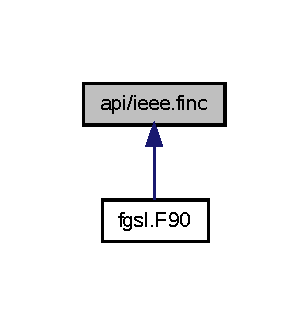
\includegraphics[width=150pt]{ieee_8finc__dep__incl}
\end{center}
\end{figure}
\subsection*{Functions/\-Subroutines}
\begin{DoxyCompactItemize}
\item 
subroutine \hyperlink{ieee_8finc_a5656619970e7be3f84c079454cd9977e}{fgsl\-\_\-ieee\-\_\-fprintf\-\_\-float} (stream, x)
\item 
subroutine \hyperlink{ieee_8finc_a3b87a333512c0de9a7093cf0956ca192}{fgsl\-\_\-ieee\-\_\-fprintf\-\_\-double} (stream, x)
\item 
subroutine \hyperlink{ieee_8finc_a61a933397c2e04ae557673fdef8514a7}{fgsl\-\_\-ieee\-\_\-printf\-\_\-float} (x)
\item 
subroutine \hyperlink{ieee_8finc_a3bb5a84b946bdb9d0d3e774759ba0160}{fgsl\-\_\-ieee\-\_\-printf\-\_\-double} (x)
\item 
subroutine \hyperlink{ieee_8finc_af8395e34fef557f25c33ce024526a143}{fgsl\-\_\-ieee\-\_\-env\-\_\-setup} ()
\end{DoxyCompactItemize}


\subsection{Function/\-Subroutine Documentation}
\hypertarget{ieee_8finc_af8395e34fef557f25c33ce024526a143}{\index{ieee.\-finc@{ieee.\-finc}!fgsl\-\_\-ieee\-\_\-env\-\_\-setup@{fgsl\-\_\-ieee\-\_\-env\-\_\-setup}}
\index{fgsl\-\_\-ieee\-\_\-env\-\_\-setup@{fgsl\-\_\-ieee\-\_\-env\-\_\-setup}!ieee.finc@{ieee.\-finc}}
\subsubsection[{fgsl\-\_\-ieee\-\_\-env\-\_\-setup}]{\setlength{\rightskip}{0pt plus 5cm}subroutine fgsl\-\_\-ieee\-\_\-env\-\_\-setup (
\begin{DoxyParamCaption}
{}
\end{DoxyParamCaption}
)}}\label{ieee_8finc_af8395e34fef557f25c33ce024526a143}
\hypertarget{ieee_8finc_a3b87a333512c0de9a7093cf0956ca192}{\index{ieee.\-finc@{ieee.\-finc}!fgsl\-\_\-ieee\-\_\-fprintf\-\_\-double@{fgsl\-\_\-ieee\-\_\-fprintf\-\_\-double}}
\index{fgsl\-\_\-ieee\-\_\-fprintf\-\_\-double@{fgsl\-\_\-ieee\-\_\-fprintf\-\_\-double}!ieee.finc@{ieee.\-finc}}
\subsubsection[{fgsl\-\_\-ieee\-\_\-fprintf\-\_\-double}]{\setlength{\rightskip}{0pt plus 5cm}subroutine fgsl\-\_\-ieee\-\_\-fprintf\-\_\-double (
\begin{DoxyParamCaption}
\item[{type(fgsl\-\_\-file), intent(in)}]{stream, }
\item[{real(fgsl\-\_\-double)}]{x}
\end{DoxyParamCaption}
)}}\label{ieee_8finc_a3b87a333512c0de9a7093cf0956ca192}
\hypertarget{ieee_8finc_a5656619970e7be3f84c079454cd9977e}{\index{ieee.\-finc@{ieee.\-finc}!fgsl\-\_\-ieee\-\_\-fprintf\-\_\-float@{fgsl\-\_\-ieee\-\_\-fprintf\-\_\-float}}
\index{fgsl\-\_\-ieee\-\_\-fprintf\-\_\-float@{fgsl\-\_\-ieee\-\_\-fprintf\-\_\-float}!ieee.finc@{ieee.\-finc}}
\subsubsection[{fgsl\-\_\-ieee\-\_\-fprintf\-\_\-float}]{\setlength{\rightskip}{0pt plus 5cm}subroutine fgsl\-\_\-ieee\-\_\-fprintf\-\_\-float (
\begin{DoxyParamCaption}
\item[{type(fgsl\-\_\-file), intent(in)}]{stream, }
\item[{real(fgsl\-\_\-float)}]{x}
\end{DoxyParamCaption}
)}}\label{ieee_8finc_a5656619970e7be3f84c079454cd9977e}
\hypertarget{ieee_8finc_a3bb5a84b946bdb9d0d3e774759ba0160}{\index{ieee.\-finc@{ieee.\-finc}!fgsl\-\_\-ieee\-\_\-printf\-\_\-double@{fgsl\-\_\-ieee\-\_\-printf\-\_\-double}}
\index{fgsl\-\_\-ieee\-\_\-printf\-\_\-double@{fgsl\-\_\-ieee\-\_\-printf\-\_\-double}!ieee.finc@{ieee.\-finc}}
\subsubsection[{fgsl\-\_\-ieee\-\_\-printf\-\_\-double}]{\setlength{\rightskip}{0pt plus 5cm}subroutine fgsl\-\_\-ieee\-\_\-printf\-\_\-double (
\begin{DoxyParamCaption}
\item[{real(fgsl\-\_\-double)}]{x}
\end{DoxyParamCaption}
)}}\label{ieee_8finc_a3bb5a84b946bdb9d0d3e774759ba0160}
\hypertarget{ieee_8finc_a61a933397c2e04ae557673fdef8514a7}{\index{ieee.\-finc@{ieee.\-finc}!fgsl\-\_\-ieee\-\_\-printf\-\_\-float@{fgsl\-\_\-ieee\-\_\-printf\-\_\-float}}
\index{fgsl\-\_\-ieee\-\_\-printf\-\_\-float@{fgsl\-\_\-ieee\-\_\-printf\-\_\-float}!ieee.finc@{ieee.\-finc}}
\subsubsection[{fgsl\-\_\-ieee\-\_\-printf\-\_\-float}]{\setlength{\rightskip}{0pt plus 5cm}subroutine fgsl\-\_\-ieee\-\_\-printf\-\_\-float (
\begin{DoxyParamCaption}
\item[{real(fgsl\-\_\-float)}]{x}
\end{DoxyParamCaption}
)}}\label{ieee_8finc_a61a933397c2e04ae557673fdef8514a7}

\hypertarget{integration_8finc}{\section{api/integration.finc File Reference}
\label{integration_8finc}\index{api/integration.\-finc@{api/integration.\-finc}}
}
This graph shows which files directly or indirectly include this file\-:\nopagebreak
\begin{figure}[H]
\begin{center}
\leavevmode
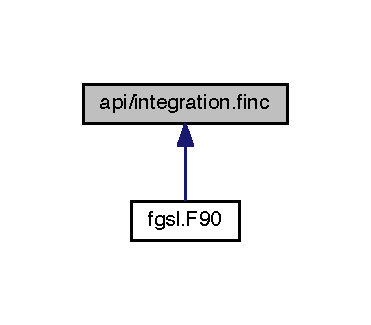
\includegraphics[width=178pt]{integration_8finc__dep__incl}
\end{center}
\end{figure}
\subsection*{Functions/\-Subroutines}
\begin{DoxyCompactItemize}
\item 
integer(fgsl\-\_\-int) function \hyperlink{integration_8finc_aba13a45b5692a07f1722280eca723ef5}{fgsl\-\_\-integration\-\_\-qng} (f, a, b, epsabs, epsrel, result, abserr, neval)
\item 
type(fgsl\-\_\-integration\-\_\-workspace) \\*
function \hyperlink{integration_8finc_a258c0d16c738f2b09e6ba3a095eb4c1a}{fgsl\-\_\-integration\-\_\-workspace\-\_\-alloc} (n)
\item 
subroutine \hyperlink{integration_8finc_a6b0e32245d2c47a94b7a0d377fd88e4b}{fgsl\-\_\-integration\-\_\-workspace\-\_\-free} (w)
\item 
integer(fgsl\-\_\-int) function \hyperlink{integration_8finc_a13d6dc8aee5e46de8ca23b39414615a2}{fgsl\-\_\-integration\-\_\-qag} (f, a, b, epsabs, epsrel, limit, key, workspace, result, abserr)
\item 
integer(fgsl\-\_\-int) function \hyperlink{integration_8finc_a0f40a3f4743cf93f49855ac87cdfe988}{fgsl\-\_\-integration\-\_\-qags} (f, a, b, epsabs, epsrel, limit, workspace, result, abserr)
\item 
integer(fgsl\-\_\-int) function \hyperlink{integration_8finc_ad3b94b869bbc1b157c6b378f8ca31edc}{fgsl\-\_\-integration\-\_\-qagp} (f, pts, npts, epsabs, epsrel, limit, workspace, result, abserr)
\item 
integer(fgsl\-\_\-int) function \hyperlink{integration_8finc_a6f86306a814963ccd09bc4a6839ba0c8}{fgsl\-\_\-integration\-\_\-qagi} (f, epsabs, epsrel, limit, workspace, result, abserr)
\item 
integer(fgsl\-\_\-int) function \hyperlink{integration_8finc_a4ec3624cdae37303102042cb3874ab7d}{fgsl\-\_\-integration\-\_\-qagiu} (f, a, epsabs, epsrel, limit, workspace, result, abserr)
\item 
integer(fgsl\-\_\-int) function \hyperlink{integration_8finc_a7292df51e041f35ed4d1c40e4b44e2b2}{fgsl\-\_\-integration\-\_\-qagil} (f, b, epsabs, epsrel, limit, workspace, result, abserr)
\item 
integer(fgsl\-\_\-int) function \hyperlink{integration_8finc_a9544e1c2217de9f6a9c8cafdf348330b}{fgsl\-\_\-integration\-\_\-qawc} (f, a, b, c, epsabs, epsrel, limit, workspace, result, abserr)
\item 
type(fgsl\-\_\-integration\-\_\-qaws\-\_\-table) \\*
function \hyperlink{integration_8finc_a1b6e906b66759c0fdf4ff29cce1b3d7d}{fgsl\-\_\-integration\-\_\-qaws\-\_\-table\-\_\-alloc} (alpha, beta, mu, nu)
\item 
integer(c\-\_\-int) function \hyperlink{integration_8finc_a3ebff9b31d58dc16c86dcbb4e78ca147}{fgsl\-\_\-integration\-\_\-qaws\-\_\-table\-\_\-set} (t, alpha, beta, mu, nu)
\item 
subroutine \hyperlink{integration_8finc_afbdbd695fee99b46d0c7eecfd8d47090}{fgsl\-\_\-integration\-\_\-qaws\-\_\-table\-\_\-free} (w)
\item 
integer(fgsl\-\_\-int) function \hyperlink{integration_8finc_acfd1871c7ba87e757856816892c109d6}{fgsl\-\_\-integration\-\_\-qaws} (f, a, b, t, epsabs, epsrel, limit, workspace, result, abserr)
\item 
type(fgsl\-\_\-integration\-\_\-qawo\-\_\-table) \\*
function \hyperlink{integration_8finc_ae0570ee20a37dcf429578cdaf6ee23f9}{fgsl\-\_\-integration\-\_\-qawo\-\_\-table\-\_\-alloc} (omega, l, sine, n)
\item 
integer(fgsl\-\_\-int) function \hyperlink{integration_8finc_af7958cb95b86e6240d437d1f95d39bf1}{fgsl\-\_\-integration\-\_\-qawo\-\_\-table\-\_\-set} (t, omega, l, sine)
\item 
integer(fgsl\-\_\-int) function \hyperlink{integration_8finc_ae1ff71ea188bac440272f58cf122ede8}{fgsl\-\_\-integration\-\_\-qawo\-\_\-table\-\_\-set\-\_\-length} (t, l)
\item 
subroutine \hyperlink{integration_8finc_a6ab4eb9bc12269b4318fbf1f51310816}{fgsl\-\_\-integration\-\_\-qawo\-\_\-table\-\_\-free} (w)
\item 
integer(fgsl\-\_\-int) function \hyperlink{integration_8finc_a63f7e2b34135b050947ffdb90bdfd0d0}{fgsl\-\_\-integration\-\_\-qawo} (f, a, epsabs, epsrel, limit, workspace, wf, result, abserr)
\item 
integer(fgsl\-\_\-int) function \hyperlink{integration_8finc_a168d9d1ad61f4965849dee091ec0e105}{fgsl\-\_\-integration\-\_\-qawf} (f, a, epsabs, limit, workspace, cyc\-\_\-workspace, wf, result, abserr)
\item 
type(fgsl\-\_\-integration\-\_\-cquad\-\_\-workspace) \\*
function \hyperlink{integration_8finc_ab01960acc26965be1f87862eaa41e200}{fgsl\-\_\-integration\-\_\-cquad\-\_\-workspace\-\_\-alloc} (n)
\item 
subroutine \hyperlink{integration_8finc_a96d0eb5c74542389355dd8c1fe35d5bd}{fgsl\-\_\-integration\-\_\-cquad\-\_\-workspace\-\_\-free} (w)
\item 
integer(fgsl\-\_\-int) function \hyperlink{integration_8finc_a1ffbbe565fc03775fe50c3c2d9150c05}{fgsl\-\_\-integration\-\_\-cquad} (f, a, b, epsabs, epsrel, workspace, result, abserr, nevals)
\item 
type(fgsl\-\_\-integration\-\_\-glfixed\-\_\-table) \\*
function \hyperlink{integration_8finc_a0372516d9af16579e899b6e836da0890}{fgsl\-\_\-integration\-\_\-glfixed\-\_\-table\-\_\-alloc} (n)
\item 
subroutine \hyperlink{integration_8finc_a77c5cbd4335b0305ecd0b6d3a573a309}{fgsl\-\_\-integration\-\_\-glfixed\-\_\-table\-\_\-free} (t)
\item 
real(fgsl\-\_\-double) function \hyperlink{integration_8finc_a1382e36b9f130563b7df1e1b339f3e8d}{fgsl\-\_\-integration\-\_\-glfixed} (f, a, b, t)
\item 
integer(fgsl\-\_\-int) function \hyperlink{integration_8finc_a64e8396fde2c4a8a76192ed6650977f3}{fgsl\-\_\-integration\-\_\-glfixed\-\_\-point} (a, b, i, xi, wi, t)
\item 
logical function \hyperlink{integration_8finc_a42978e91589d08c3af524cec986ce33c}{fgsl\-\_\-integration\-\_\-workspace\-\_\-status} (integration\-\_\-workspace)
\item 
logical function \hyperlink{integration_8finc_a5da0a8440c5f23a14f8b22c5fefb5404}{fgsl\-\_\-integration\-\_\-qaws\-\_\-table\-\_\-status} (integration\-\_\-qaws\-\_\-table)
\item 
logical function \hyperlink{integration_8finc_aa91a1f90a0f43067989a90e651f53dcb}{fgsl\-\_\-integration\-\_\-qawo\-\_\-table\-\_\-status} (integration\-\_\-qawo\-\_\-table)
\item 
logical function \hyperlink{integration_8finc_a1dcdd67510034ad4aa4c3396fe600818}{fgsl\-\_\-integration\-\_\-cquad\-\_\-workspace\-\_\-status} (integration\-\_\-workspace)
\item 
logical function \hyperlink{integration_8finc_a0cfbd26bc06d3740a8f2ed7821fd958f}{fgsl\-\_\-integration\-\_\-glfixed\-\_\-table\-\_\-status} (integration\-\_\-glfixed\-\_\-table)
\item 
integer(fgsl\-\_\-size\-\_\-t) function \hyperlink{integration_8finc_a25f1356cc9307dc2a56993d387fd9460}{fgsl\-\_\-sizeof\-\_\-integration\-\_\-workspace} (w)
\item 
integer(fgsl\-\_\-size\-\_\-t) function \hyperlink{integration_8finc_a78bc5e30c21dd07ef8c02d6674127ad4}{fgsl\-\_\-sizeof\-\_\-integration\-\_\-qaws\-\_\-table} (w)
\item 
integer(fgsl\-\_\-size\-\_\-t) function \hyperlink{integration_8finc_a8690a1322fb1d8384361ef19dac3483d}{fgsl\-\_\-sizeof\-\_\-integration\-\_\-qawo\-\_\-table} (w)
\end{DoxyCompactItemize}


\subsection{Function/\-Subroutine Documentation}
\hypertarget{integration_8finc_a1ffbbe565fc03775fe50c3c2d9150c05}{\index{integration.\-finc@{integration.\-finc}!fgsl\-\_\-integration\-\_\-cquad@{fgsl\-\_\-integration\-\_\-cquad}}
\index{fgsl\-\_\-integration\-\_\-cquad@{fgsl\-\_\-integration\-\_\-cquad}!integration.finc@{integration.\-finc}}
\subsubsection[{fgsl\-\_\-integration\-\_\-cquad}]{\setlength{\rightskip}{0pt plus 5cm}integer(fgsl\-\_\-int) function fgsl\-\_\-integration\-\_\-cquad (
\begin{DoxyParamCaption}
\item[{type(fgsl\-\_\-function), intent(in)}]{f, }
\item[{real(fgsl\-\_\-double), intent(in)}]{a, }
\item[{real(fgsl\-\_\-double), intent(in)}]{b, }
\item[{real(fgsl\-\_\-double), intent(in)}]{epsabs, }
\item[{real(fgsl\-\_\-double), intent(in)}]{epsrel, }
\item[{type(fgsl\-\_\-integration\-\_\-cquad\-\_\-workspace), intent(inout)}]{workspace, }
\item[{real(fgsl\-\_\-double), intent(out)}]{result, }
\item[{real(fgsl\-\_\-double), intent(out)}]{abserr, }
\item[{integer(fgsl\-\_\-size\-\_\-t), intent(inout)}]{nevals}
\end{DoxyParamCaption}
)}}\label{integration_8finc_a1ffbbe565fc03775fe50c3c2d9150c05}
\hypertarget{integration_8finc_ab01960acc26965be1f87862eaa41e200}{\index{integration.\-finc@{integration.\-finc}!fgsl\-\_\-integration\-\_\-cquad\-\_\-workspace\-\_\-alloc@{fgsl\-\_\-integration\-\_\-cquad\-\_\-workspace\-\_\-alloc}}
\index{fgsl\-\_\-integration\-\_\-cquad\-\_\-workspace\-\_\-alloc@{fgsl\-\_\-integration\-\_\-cquad\-\_\-workspace\-\_\-alloc}!integration.finc@{integration.\-finc}}
\subsubsection[{fgsl\-\_\-integration\-\_\-cquad\-\_\-workspace\-\_\-alloc}]{\setlength{\rightskip}{0pt plus 5cm}type(fgsl\-\_\-integration\-\_\-cquad\-\_\-workspace) function fgsl\-\_\-integration\-\_\-cquad\-\_\-workspace\-\_\-alloc (
\begin{DoxyParamCaption}
\item[{integer(fgsl\-\_\-size\-\_\-t), intent(in)}]{n}
\end{DoxyParamCaption}
)}}\label{integration_8finc_ab01960acc26965be1f87862eaa41e200}
\hypertarget{integration_8finc_a96d0eb5c74542389355dd8c1fe35d5bd}{\index{integration.\-finc@{integration.\-finc}!fgsl\-\_\-integration\-\_\-cquad\-\_\-workspace\-\_\-free@{fgsl\-\_\-integration\-\_\-cquad\-\_\-workspace\-\_\-free}}
\index{fgsl\-\_\-integration\-\_\-cquad\-\_\-workspace\-\_\-free@{fgsl\-\_\-integration\-\_\-cquad\-\_\-workspace\-\_\-free}!integration.finc@{integration.\-finc}}
\subsubsection[{fgsl\-\_\-integration\-\_\-cquad\-\_\-workspace\-\_\-free}]{\setlength{\rightskip}{0pt plus 5cm}subroutine fgsl\-\_\-integration\-\_\-cquad\-\_\-workspace\-\_\-free (
\begin{DoxyParamCaption}
\item[{type(fgsl\-\_\-integration\-\_\-cquad\-\_\-workspace), intent(inout)}]{w}
\end{DoxyParamCaption}
)}}\label{integration_8finc_a96d0eb5c74542389355dd8c1fe35d5bd}
\hypertarget{integration_8finc_a1dcdd67510034ad4aa4c3396fe600818}{\index{integration.\-finc@{integration.\-finc}!fgsl\-\_\-integration\-\_\-cquad\-\_\-workspace\-\_\-status@{fgsl\-\_\-integration\-\_\-cquad\-\_\-workspace\-\_\-status}}
\index{fgsl\-\_\-integration\-\_\-cquad\-\_\-workspace\-\_\-status@{fgsl\-\_\-integration\-\_\-cquad\-\_\-workspace\-\_\-status}!integration.finc@{integration.\-finc}}
\subsubsection[{fgsl\-\_\-integration\-\_\-cquad\-\_\-workspace\-\_\-status}]{\setlength{\rightskip}{0pt plus 5cm}logical function fgsl\-\_\-integration\-\_\-cquad\-\_\-workspace\-\_\-status (
\begin{DoxyParamCaption}
\item[{type(fgsl\-\_\-integration\-\_\-cquad\-\_\-workspace), intent(in)}]{integration\-\_\-workspace}
\end{DoxyParamCaption}
)}}\label{integration_8finc_a1dcdd67510034ad4aa4c3396fe600818}
\hypertarget{integration_8finc_a1382e36b9f130563b7df1e1b339f3e8d}{\index{integration.\-finc@{integration.\-finc}!fgsl\-\_\-integration\-\_\-glfixed@{fgsl\-\_\-integration\-\_\-glfixed}}
\index{fgsl\-\_\-integration\-\_\-glfixed@{fgsl\-\_\-integration\-\_\-glfixed}!integration.finc@{integration.\-finc}}
\subsubsection[{fgsl\-\_\-integration\-\_\-glfixed}]{\setlength{\rightskip}{0pt plus 5cm}real(fgsl\-\_\-double) function fgsl\-\_\-integration\-\_\-glfixed (
\begin{DoxyParamCaption}
\item[{type(fgsl\-\_\-function), intent(in)}]{f, }
\item[{real(fgsl\-\_\-double), intent(in)}]{a, }
\item[{real(fgsl\-\_\-double), intent(in)}]{b, }
\item[{type(fgsl\-\_\-integration\-\_\-glfixed\-\_\-table), intent(in)}]{t}
\end{DoxyParamCaption}
)}}\label{integration_8finc_a1382e36b9f130563b7df1e1b339f3e8d}
\hypertarget{integration_8finc_a64e8396fde2c4a8a76192ed6650977f3}{\index{integration.\-finc@{integration.\-finc}!fgsl\-\_\-integration\-\_\-glfixed\-\_\-point@{fgsl\-\_\-integration\-\_\-glfixed\-\_\-point}}
\index{fgsl\-\_\-integration\-\_\-glfixed\-\_\-point@{fgsl\-\_\-integration\-\_\-glfixed\-\_\-point}!integration.finc@{integration.\-finc}}
\subsubsection[{fgsl\-\_\-integration\-\_\-glfixed\-\_\-point}]{\setlength{\rightskip}{0pt plus 5cm}integer(fgsl\-\_\-int) function fgsl\-\_\-integration\-\_\-glfixed\-\_\-point (
\begin{DoxyParamCaption}
\item[{real(fgsl\-\_\-double), intent(in)}]{a, }
\item[{real(fgsl\-\_\-double), intent(in)}]{b, }
\item[{integer(fgsl\-\_\-size\-\_\-t), intent(in)}]{i, }
\item[{real(fgsl\-\_\-double), intent(inout)}]{xi, }
\item[{real(fgsl\-\_\-double), intent(inout)}]{wi, }
\item[{type(fgsl\-\_\-integration\-\_\-glfixed\-\_\-table), intent(in)}]{t}
\end{DoxyParamCaption}
)}}\label{integration_8finc_a64e8396fde2c4a8a76192ed6650977f3}
\hypertarget{integration_8finc_a0372516d9af16579e899b6e836da0890}{\index{integration.\-finc@{integration.\-finc}!fgsl\-\_\-integration\-\_\-glfixed\-\_\-table\-\_\-alloc@{fgsl\-\_\-integration\-\_\-glfixed\-\_\-table\-\_\-alloc}}
\index{fgsl\-\_\-integration\-\_\-glfixed\-\_\-table\-\_\-alloc@{fgsl\-\_\-integration\-\_\-glfixed\-\_\-table\-\_\-alloc}!integration.finc@{integration.\-finc}}
\subsubsection[{fgsl\-\_\-integration\-\_\-glfixed\-\_\-table\-\_\-alloc}]{\setlength{\rightskip}{0pt plus 5cm}type(fgsl\-\_\-integration\-\_\-glfixed\-\_\-table) function fgsl\-\_\-integration\-\_\-glfixed\-\_\-table\-\_\-alloc (
\begin{DoxyParamCaption}
\item[{integer(fgsl\-\_\-size\-\_\-t), intent(in)}]{n}
\end{DoxyParamCaption}
)}}\label{integration_8finc_a0372516d9af16579e899b6e836da0890}
\hypertarget{integration_8finc_a77c5cbd4335b0305ecd0b6d3a573a309}{\index{integration.\-finc@{integration.\-finc}!fgsl\-\_\-integration\-\_\-glfixed\-\_\-table\-\_\-free@{fgsl\-\_\-integration\-\_\-glfixed\-\_\-table\-\_\-free}}
\index{fgsl\-\_\-integration\-\_\-glfixed\-\_\-table\-\_\-free@{fgsl\-\_\-integration\-\_\-glfixed\-\_\-table\-\_\-free}!integration.finc@{integration.\-finc}}
\subsubsection[{fgsl\-\_\-integration\-\_\-glfixed\-\_\-table\-\_\-free}]{\setlength{\rightskip}{0pt plus 5cm}subroutine fgsl\-\_\-integration\-\_\-glfixed\-\_\-table\-\_\-free (
\begin{DoxyParamCaption}
\item[{type(fgsl\-\_\-integration\-\_\-glfixed\-\_\-table)}]{t}
\end{DoxyParamCaption}
)}}\label{integration_8finc_a77c5cbd4335b0305ecd0b6d3a573a309}
\hypertarget{integration_8finc_a0cfbd26bc06d3740a8f2ed7821fd958f}{\index{integration.\-finc@{integration.\-finc}!fgsl\-\_\-integration\-\_\-glfixed\-\_\-table\-\_\-status@{fgsl\-\_\-integration\-\_\-glfixed\-\_\-table\-\_\-status}}
\index{fgsl\-\_\-integration\-\_\-glfixed\-\_\-table\-\_\-status@{fgsl\-\_\-integration\-\_\-glfixed\-\_\-table\-\_\-status}!integration.finc@{integration.\-finc}}
\subsubsection[{fgsl\-\_\-integration\-\_\-glfixed\-\_\-table\-\_\-status}]{\setlength{\rightskip}{0pt plus 5cm}logical function fgsl\-\_\-integration\-\_\-glfixed\-\_\-table\-\_\-status (
\begin{DoxyParamCaption}
\item[{type(fgsl\-\_\-integration\-\_\-glfixed\-\_\-table), intent(in)}]{integration\-\_\-glfixed\-\_\-table}
\end{DoxyParamCaption}
)}}\label{integration_8finc_a0cfbd26bc06d3740a8f2ed7821fd958f}
\hypertarget{integration_8finc_a13d6dc8aee5e46de8ca23b39414615a2}{\index{integration.\-finc@{integration.\-finc}!fgsl\-\_\-integration\-\_\-qag@{fgsl\-\_\-integration\-\_\-qag}}
\index{fgsl\-\_\-integration\-\_\-qag@{fgsl\-\_\-integration\-\_\-qag}!integration.finc@{integration.\-finc}}
\subsubsection[{fgsl\-\_\-integration\-\_\-qag}]{\setlength{\rightskip}{0pt plus 5cm}integer(fgsl\-\_\-int) function fgsl\-\_\-integration\-\_\-qag (
\begin{DoxyParamCaption}
\item[{type(fgsl\-\_\-function), intent(in)}]{f, }
\item[{real(fgsl\-\_\-double), intent(in)}]{a, }
\item[{real(fgsl\-\_\-double), intent(in)}]{b, }
\item[{real(fgsl\-\_\-double), intent(in)}]{epsabs, }
\item[{real(fgsl\-\_\-double), intent(in)}]{epsrel, }
\item[{integer(fgsl\-\_\-size\-\_\-t), intent(in)}]{limit, }
\item[{integer(fgsl\-\_\-int), intent(in)}]{key, }
\item[{type(fgsl\-\_\-integration\-\_\-workspace), intent(inout)}]{workspace, }
\item[{real(fgsl\-\_\-double), intent(out)}]{result, }
\item[{real(fgsl\-\_\-double), intent(out)}]{abserr}
\end{DoxyParamCaption}
)}}\label{integration_8finc_a13d6dc8aee5e46de8ca23b39414615a2}
\hypertarget{integration_8finc_a6f86306a814963ccd09bc4a6839ba0c8}{\index{integration.\-finc@{integration.\-finc}!fgsl\-\_\-integration\-\_\-qagi@{fgsl\-\_\-integration\-\_\-qagi}}
\index{fgsl\-\_\-integration\-\_\-qagi@{fgsl\-\_\-integration\-\_\-qagi}!integration.finc@{integration.\-finc}}
\subsubsection[{fgsl\-\_\-integration\-\_\-qagi}]{\setlength{\rightskip}{0pt plus 5cm}integer(fgsl\-\_\-int) function fgsl\-\_\-integration\-\_\-qagi (
\begin{DoxyParamCaption}
\item[{type(fgsl\-\_\-function), intent(in)}]{f, }
\item[{real(fgsl\-\_\-double), intent(in)}]{epsabs, }
\item[{real(fgsl\-\_\-double), intent(in)}]{epsrel, }
\item[{integer(fgsl\-\_\-size\-\_\-t), intent(in)}]{limit, }
\item[{type(fgsl\-\_\-integration\-\_\-workspace), intent(inout)}]{workspace, }
\item[{real(fgsl\-\_\-double), intent(out)}]{result, }
\item[{real(fgsl\-\_\-double), intent(out)}]{abserr}
\end{DoxyParamCaption}
)}}\label{integration_8finc_a6f86306a814963ccd09bc4a6839ba0c8}
\hypertarget{integration_8finc_a7292df51e041f35ed4d1c40e4b44e2b2}{\index{integration.\-finc@{integration.\-finc}!fgsl\-\_\-integration\-\_\-qagil@{fgsl\-\_\-integration\-\_\-qagil}}
\index{fgsl\-\_\-integration\-\_\-qagil@{fgsl\-\_\-integration\-\_\-qagil}!integration.finc@{integration.\-finc}}
\subsubsection[{fgsl\-\_\-integration\-\_\-qagil}]{\setlength{\rightskip}{0pt plus 5cm}integer(fgsl\-\_\-int) function fgsl\-\_\-integration\-\_\-qagil (
\begin{DoxyParamCaption}
\item[{type(fgsl\-\_\-function), intent(in)}]{f, }
\item[{real(fgsl\-\_\-double), intent(in)}]{b, }
\item[{real(fgsl\-\_\-double), intent(in)}]{epsabs, }
\item[{real(fgsl\-\_\-double), intent(in)}]{epsrel, }
\item[{integer(fgsl\-\_\-size\-\_\-t), intent(in)}]{limit, }
\item[{type(fgsl\-\_\-integration\-\_\-workspace), intent(inout)}]{workspace, }
\item[{real(fgsl\-\_\-double), intent(out)}]{result, }
\item[{real(fgsl\-\_\-double), intent(out)}]{abserr}
\end{DoxyParamCaption}
)}}\label{integration_8finc_a7292df51e041f35ed4d1c40e4b44e2b2}
\hypertarget{integration_8finc_a4ec3624cdae37303102042cb3874ab7d}{\index{integration.\-finc@{integration.\-finc}!fgsl\-\_\-integration\-\_\-qagiu@{fgsl\-\_\-integration\-\_\-qagiu}}
\index{fgsl\-\_\-integration\-\_\-qagiu@{fgsl\-\_\-integration\-\_\-qagiu}!integration.finc@{integration.\-finc}}
\subsubsection[{fgsl\-\_\-integration\-\_\-qagiu}]{\setlength{\rightskip}{0pt plus 5cm}integer(fgsl\-\_\-int) function fgsl\-\_\-integration\-\_\-qagiu (
\begin{DoxyParamCaption}
\item[{type(fgsl\-\_\-function), intent(in)}]{f, }
\item[{real(fgsl\-\_\-double), intent(in)}]{a, }
\item[{real(fgsl\-\_\-double), intent(in)}]{epsabs, }
\item[{real(fgsl\-\_\-double), intent(in)}]{epsrel, }
\item[{integer(fgsl\-\_\-size\-\_\-t), intent(in)}]{limit, }
\item[{type(fgsl\-\_\-integration\-\_\-workspace), intent(inout)}]{workspace, }
\item[{real(fgsl\-\_\-double), intent(out)}]{result, }
\item[{real(fgsl\-\_\-double), intent(out)}]{abserr}
\end{DoxyParamCaption}
)}}\label{integration_8finc_a4ec3624cdae37303102042cb3874ab7d}
\hypertarget{integration_8finc_ad3b94b869bbc1b157c6b378f8ca31edc}{\index{integration.\-finc@{integration.\-finc}!fgsl\-\_\-integration\-\_\-qagp@{fgsl\-\_\-integration\-\_\-qagp}}
\index{fgsl\-\_\-integration\-\_\-qagp@{fgsl\-\_\-integration\-\_\-qagp}!integration.finc@{integration.\-finc}}
\subsubsection[{fgsl\-\_\-integration\-\_\-qagp}]{\setlength{\rightskip}{0pt plus 5cm}integer(fgsl\-\_\-int) function fgsl\-\_\-integration\-\_\-qagp (
\begin{DoxyParamCaption}
\item[{type(fgsl\-\_\-function), intent(in)}]{f, }
\item[{real(fgsl\-\_\-double), dimension(\-:), intent(in)}]{pts, }
\item[{integer(fgsl\-\_\-size\-\_\-t), intent(in)}]{npts, }
\item[{real(fgsl\-\_\-double), intent(in)}]{epsabs, }
\item[{real(fgsl\-\_\-double), intent(in)}]{epsrel, }
\item[{integer(fgsl\-\_\-size\-\_\-t), intent(in)}]{limit, }
\item[{type(fgsl\-\_\-integration\-\_\-workspace), intent(inout)}]{workspace, }
\item[{real(fgsl\-\_\-double), intent(out)}]{result, }
\item[{real(fgsl\-\_\-double), intent(out)}]{abserr}
\end{DoxyParamCaption}
)}}\label{integration_8finc_ad3b94b869bbc1b157c6b378f8ca31edc}
\hypertarget{integration_8finc_a0f40a3f4743cf93f49855ac87cdfe988}{\index{integration.\-finc@{integration.\-finc}!fgsl\-\_\-integration\-\_\-qags@{fgsl\-\_\-integration\-\_\-qags}}
\index{fgsl\-\_\-integration\-\_\-qags@{fgsl\-\_\-integration\-\_\-qags}!integration.finc@{integration.\-finc}}
\subsubsection[{fgsl\-\_\-integration\-\_\-qags}]{\setlength{\rightskip}{0pt plus 5cm}integer(fgsl\-\_\-int) function fgsl\-\_\-integration\-\_\-qags (
\begin{DoxyParamCaption}
\item[{type(fgsl\-\_\-function), intent(in)}]{f, }
\item[{real(fgsl\-\_\-double), intent(in)}]{a, }
\item[{real(fgsl\-\_\-double), intent(in)}]{b, }
\item[{real(fgsl\-\_\-double), intent(in)}]{epsabs, }
\item[{real(fgsl\-\_\-double), intent(in)}]{epsrel, }
\item[{integer(fgsl\-\_\-size\-\_\-t), intent(in)}]{limit, }
\item[{type(fgsl\-\_\-integration\-\_\-workspace), intent(inout)}]{workspace, }
\item[{real(fgsl\-\_\-double), intent(out)}]{result, }
\item[{real(fgsl\-\_\-double), intent(out)}]{abserr}
\end{DoxyParamCaption}
)}}\label{integration_8finc_a0f40a3f4743cf93f49855ac87cdfe988}
\hypertarget{integration_8finc_a9544e1c2217de9f6a9c8cafdf348330b}{\index{integration.\-finc@{integration.\-finc}!fgsl\-\_\-integration\-\_\-qawc@{fgsl\-\_\-integration\-\_\-qawc}}
\index{fgsl\-\_\-integration\-\_\-qawc@{fgsl\-\_\-integration\-\_\-qawc}!integration.finc@{integration.\-finc}}
\subsubsection[{fgsl\-\_\-integration\-\_\-qawc}]{\setlength{\rightskip}{0pt plus 5cm}integer(fgsl\-\_\-int) function fgsl\-\_\-integration\-\_\-qawc (
\begin{DoxyParamCaption}
\item[{type(fgsl\-\_\-function), intent(in)}]{f, }
\item[{real(fgsl\-\_\-double), intent(in)}]{a, }
\item[{real(fgsl\-\_\-double), intent(in)}]{b, }
\item[{real(fgsl\-\_\-double), intent(in)}]{c, }
\item[{real(fgsl\-\_\-double), intent(in)}]{epsabs, }
\item[{real(fgsl\-\_\-double), intent(in)}]{epsrel, }
\item[{integer(fgsl\-\_\-size\-\_\-t), intent(in)}]{limit, }
\item[{type(fgsl\-\_\-integration\-\_\-workspace), intent(inout)}]{workspace, }
\item[{real(fgsl\-\_\-double), intent(out)}]{result, }
\item[{real(fgsl\-\_\-double), intent(out)}]{abserr}
\end{DoxyParamCaption}
)}}\label{integration_8finc_a9544e1c2217de9f6a9c8cafdf348330b}
\hypertarget{integration_8finc_a168d9d1ad61f4965849dee091ec0e105}{\index{integration.\-finc@{integration.\-finc}!fgsl\-\_\-integration\-\_\-qawf@{fgsl\-\_\-integration\-\_\-qawf}}
\index{fgsl\-\_\-integration\-\_\-qawf@{fgsl\-\_\-integration\-\_\-qawf}!integration.finc@{integration.\-finc}}
\subsubsection[{fgsl\-\_\-integration\-\_\-qawf}]{\setlength{\rightskip}{0pt plus 5cm}integer(fgsl\-\_\-int) function fgsl\-\_\-integration\-\_\-qawf (
\begin{DoxyParamCaption}
\item[{type(fgsl\-\_\-function), intent(in)}]{f, }
\item[{real(fgsl\-\_\-double), intent(in)}]{a, }
\item[{real(fgsl\-\_\-double), intent(in)}]{epsabs, }
\item[{integer(fgsl\-\_\-size\-\_\-t), intent(in)}]{limit, }
\item[{type(fgsl\-\_\-integration\-\_\-workspace), intent(inout)}]{workspace, }
\item[{type(fgsl\-\_\-integration\-\_\-workspace), intent(inout)}]{cyc\-\_\-workspace, }
\item[{type(fgsl\-\_\-integration\-\_\-qawo\-\_\-table), intent(in)}]{wf, }
\item[{real(fgsl\-\_\-double), intent(out)}]{result, }
\item[{real(fgsl\-\_\-double), intent(out)}]{abserr}
\end{DoxyParamCaption}
)}}\label{integration_8finc_a168d9d1ad61f4965849dee091ec0e105}
\hypertarget{integration_8finc_a63f7e2b34135b050947ffdb90bdfd0d0}{\index{integration.\-finc@{integration.\-finc}!fgsl\-\_\-integration\-\_\-qawo@{fgsl\-\_\-integration\-\_\-qawo}}
\index{fgsl\-\_\-integration\-\_\-qawo@{fgsl\-\_\-integration\-\_\-qawo}!integration.finc@{integration.\-finc}}
\subsubsection[{fgsl\-\_\-integration\-\_\-qawo}]{\setlength{\rightskip}{0pt plus 5cm}integer(fgsl\-\_\-int) function fgsl\-\_\-integration\-\_\-qawo (
\begin{DoxyParamCaption}
\item[{type(fgsl\-\_\-function), intent(in)}]{f, }
\item[{real(fgsl\-\_\-double), intent(in)}]{a, }
\item[{real(fgsl\-\_\-double), intent(in)}]{epsabs, }
\item[{real(fgsl\-\_\-double), intent(in)}]{epsrel, }
\item[{integer(fgsl\-\_\-size\-\_\-t), intent(in)}]{limit, }
\item[{type(fgsl\-\_\-integration\-\_\-workspace), intent(inout)}]{workspace, }
\item[{type(fgsl\-\_\-integration\-\_\-qawo\-\_\-table), intent(in)}]{wf, }
\item[{real(fgsl\-\_\-double), intent(out)}]{result, }
\item[{real(fgsl\-\_\-double), intent(out)}]{abserr}
\end{DoxyParamCaption}
)}}\label{integration_8finc_a63f7e2b34135b050947ffdb90bdfd0d0}
\hypertarget{integration_8finc_ae0570ee20a37dcf429578cdaf6ee23f9}{\index{integration.\-finc@{integration.\-finc}!fgsl\-\_\-integration\-\_\-qawo\-\_\-table\-\_\-alloc@{fgsl\-\_\-integration\-\_\-qawo\-\_\-table\-\_\-alloc}}
\index{fgsl\-\_\-integration\-\_\-qawo\-\_\-table\-\_\-alloc@{fgsl\-\_\-integration\-\_\-qawo\-\_\-table\-\_\-alloc}!integration.finc@{integration.\-finc}}
\subsubsection[{fgsl\-\_\-integration\-\_\-qawo\-\_\-table\-\_\-alloc}]{\setlength{\rightskip}{0pt plus 5cm}type(fgsl\-\_\-integration\-\_\-qawo\-\_\-table) function fgsl\-\_\-integration\-\_\-qawo\-\_\-table\-\_\-alloc (
\begin{DoxyParamCaption}
\item[{real(fgsl\-\_\-double), intent(in)}]{omega, }
\item[{real(fgsl\-\_\-double), intent(in)}]{l, }
\item[{integer(fgsl\-\_\-int), intent(in)}]{sine, }
\item[{integer(fgsl\-\_\-size\-\_\-t), intent(in)}]{n}
\end{DoxyParamCaption}
)}}\label{integration_8finc_ae0570ee20a37dcf429578cdaf6ee23f9}
\hypertarget{integration_8finc_a6ab4eb9bc12269b4318fbf1f51310816}{\index{integration.\-finc@{integration.\-finc}!fgsl\-\_\-integration\-\_\-qawo\-\_\-table\-\_\-free@{fgsl\-\_\-integration\-\_\-qawo\-\_\-table\-\_\-free}}
\index{fgsl\-\_\-integration\-\_\-qawo\-\_\-table\-\_\-free@{fgsl\-\_\-integration\-\_\-qawo\-\_\-table\-\_\-free}!integration.finc@{integration.\-finc}}
\subsubsection[{fgsl\-\_\-integration\-\_\-qawo\-\_\-table\-\_\-free}]{\setlength{\rightskip}{0pt plus 5cm}subroutine fgsl\-\_\-integration\-\_\-qawo\-\_\-table\-\_\-free (
\begin{DoxyParamCaption}
\item[{type(fgsl\-\_\-integration\-\_\-qawo\-\_\-table), intent(inout)}]{w}
\end{DoxyParamCaption}
)}}\label{integration_8finc_a6ab4eb9bc12269b4318fbf1f51310816}
\hypertarget{integration_8finc_af7958cb95b86e6240d437d1f95d39bf1}{\index{integration.\-finc@{integration.\-finc}!fgsl\-\_\-integration\-\_\-qawo\-\_\-table\-\_\-set@{fgsl\-\_\-integration\-\_\-qawo\-\_\-table\-\_\-set}}
\index{fgsl\-\_\-integration\-\_\-qawo\-\_\-table\-\_\-set@{fgsl\-\_\-integration\-\_\-qawo\-\_\-table\-\_\-set}!integration.finc@{integration.\-finc}}
\subsubsection[{fgsl\-\_\-integration\-\_\-qawo\-\_\-table\-\_\-set}]{\setlength{\rightskip}{0pt plus 5cm}integer(fgsl\-\_\-int) function fgsl\-\_\-integration\-\_\-qawo\-\_\-table\-\_\-set (
\begin{DoxyParamCaption}
\item[{type(fgsl\-\_\-integration\-\_\-qawo\-\_\-table), intent(inout)}]{t, }
\item[{real(fgsl\-\_\-double), intent(in)}]{omega, }
\item[{real(fgsl\-\_\-double), intent(in)}]{l, }
\item[{integer(fgsl\-\_\-int), intent(in)}]{sine}
\end{DoxyParamCaption}
)}}\label{integration_8finc_af7958cb95b86e6240d437d1f95d39bf1}
\hypertarget{integration_8finc_ae1ff71ea188bac440272f58cf122ede8}{\index{integration.\-finc@{integration.\-finc}!fgsl\-\_\-integration\-\_\-qawo\-\_\-table\-\_\-set\-\_\-length@{fgsl\-\_\-integration\-\_\-qawo\-\_\-table\-\_\-set\-\_\-length}}
\index{fgsl\-\_\-integration\-\_\-qawo\-\_\-table\-\_\-set\-\_\-length@{fgsl\-\_\-integration\-\_\-qawo\-\_\-table\-\_\-set\-\_\-length}!integration.finc@{integration.\-finc}}
\subsubsection[{fgsl\-\_\-integration\-\_\-qawo\-\_\-table\-\_\-set\-\_\-length}]{\setlength{\rightskip}{0pt plus 5cm}integer(fgsl\-\_\-int) function fgsl\-\_\-integration\-\_\-qawo\-\_\-table\-\_\-set\-\_\-length (
\begin{DoxyParamCaption}
\item[{type(fgsl\-\_\-integration\-\_\-qawo\-\_\-table), intent(inout)}]{t, }
\item[{real(fgsl\-\_\-double), intent(in)}]{l}
\end{DoxyParamCaption}
)}}\label{integration_8finc_ae1ff71ea188bac440272f58cf122ede8}
\hypertarget{integration_8finc_aa91a1f90a0f43067989a90e651f53dcb}{\index{integration.\-finc@{integration.\-finc}!fgsl\-\_\-integration\-\_\-qawo\-\_\-table\-\_\-status@{fgsl\-\_\-integration\-\_\-qawo\-\_\-table\-\_\-status}}
\index{fgsl\-\_\-integration\-\_\-qawo\-\_\-table\-\_\-status@{fgsl\-\_\-integration\-\_\-qawo\-\_\-table\-\_\-status}!integration.finc@{integration.\-finc}}
\subsubsection[{fgsl\-\_\-integration\-\_\-qawo\-\_\-table\-\_\-status}]{\setlength{\rightskip}{0pt plus 5cm}logical function fgsl\-\_\-integration\-\_\-qawo\-\_\-table\-\_\-status (
\begin{DoxyParamCaption}
\item[{type(fgsl\-\_\-integration\-\_\-qawo\-\_\-table), intent(in)}]{integration\-\_\-qawo\-\_\-table}
\end{DoxyParamCaption}
)}}\label{integration_8finc_aa91a1f90a0f43067989a90e651f53dcb}
\hypertarget{integration_8finc_acfd1871c7ba87e757856816892c109d6}{\index{integration.\-finc@{integration.\-finc}!fgsl\-\_\-integration\-\_\-qaws@{fgsl\-\_\-integration\-\_\-qaws}}
\index{fgsl\-\_\-integration\-\_\-qaws@{fgsl\-\_\-integration\-\_\-qaws}!integration.finc@{integration.\-finc}}
\subsubsection[{fgsl\-\_\-integration\-\_\-qaws}]{\setlength{\rightskip}{0pt plus 5cm}integer(fgsl\-\_\-int) function fgsl\-\_\-integration\-\_\-qaws (
\begin{DoxyParamCaption}
\item[{type(fgsl\-\_\-function), intent(in)}]{f, }
\item[{real(fgsl\-\_\-double), intent(in)}]{a, }
\item[{real(fgsl\-\_\-double), intent(in)}]{b, }
\item[{type(fgsl\-\_\-integration\-\_\-qaws\-\_\-table), intent(in)}]{t, }
\item[{real(fgsl\-\_\-double), intent(in)}]{epsabs, }
\item[{real(fgsl\-\_\-double), intent(in)}]{epsrel, }
\item[{integer(fgsl\-\_\-size\-\_\-t), intent(in)}]{limit, }
\item[{type(fgsl\-\_\-integration\-\_\-workspace), intent(inout)}]{workspace, }
\item[{real(fgsl\-\_\-double), intent(out)}]{result, }
\item[{real(fgsl\-\_\-double), intent(out)}]{abserr}
\end{DoxyParamCaption}
)}}\label{integration_8finc_acfd1871c7ba87e757856816892c109d6}
\hypertarget{integration_8finc_a1b6e906b66759c0fdf4ff29cce1b3d7d}{\index{integration.\-finc@{integration.\-finc}!fgsl\-\_\-integration\-\_\-qaws\-\_\-table\-\_\-alloc@{fgsl\-\_\-integration\-\_\-qaws\-\_\-table\-\_\-alloc}}
\index{fgsl\-\_\-integration\-\_\-qaws\-\_\-table\-\_\-alloc@{fgsl\-\_\-integration\-\_\-qaws\-\_\-table\-\_\-alloc}!integration.finc@{integration.\-finc}}
\subsubsection[{fgsl\-\_\-integration\-\_\-qaws\-\_\-table\-\_\-alloc}]{\setlength{\rightskip}{0pt plus 5cm}type(fgsl\-\_\-integration\-\_\-qaws\-\_\-table) function fgsl\-\_\-integration\-\_\-qaws\-\_\-table\-\_\-alloc (
\begin{DoxyParamCaption}
\item[{real(fgsl\-\_\-double), intent(in)}]{alpha, }
\item[{real(fgsl\-\_\-double), intent(in)}]{beta, }
\item[{integer(fgsl\-\_\-int), intent(in)}]{mu, }
\item[{integer(fgsl\-\_\-int), intent(in)}]{nu}
\end{DoxyParamCaption}
)}}\label{integration_8finc_a1b6e906b66759c0fdf4ff29cce1b3d7d}
\hypertarget{integration_8finc_afbdbd695fee99b46d0c7eecfd8d47090}{\index{integration.\-finc@{integration.\-finc}!fgsl\-\_\-integration\-\_\-qaws\-\_\-table\-\_\-free@{fgsl\-\_\-integration\-\_\-qaws\-\_\-table\-\_\-free}}
\index{fgsl\-\_\-integration\-\_\-qaws\-\_\-table\-\_\-free@{fgsl\-\_\-integration\-\_\-qaws\-\_\-table\-\_\-free}!integration.finc@{integration.\-finc}}
\subsubsection[{fgsl\-\_\-integration\-\_\-qaws\-\_\-table\-\_\-free}]{\setlength{\rightskip}{0pt plus 5cm}subroutine fgsl\-\_\-integration\-\_\-qaws\-\_\-table\-\_\-free (
\begin{DoxyParamCaption}
\item[{type(fgsl\-\_\-integration\-\_\-qaws\-\_\-table), intent(inout)}]{w}
\end{DoxyParamCaption}
)}}\label{integration_8finc_afbdbd695fee99b46d0c7eecfd8d47090}
\hypertarget{integration_8finc_a3ebff9b31d58dc16c86dcbb4e78ca147}{\index{integration.\-finc@{integration.\-finc}!fgsl\-\_\-integration\-\_\-qaws\-\_\-table\-\_\-set@{fgsl\-\_\-integration\-\_\-qaws\-\_\-table\-\_\-set}}
\index{fgsl\-\_\-integration\-\_\-qaws\-\_\-table\-\_\-set@{fgsl\-\_\-integration\-\_\-qaws\-\_\-table\-\_\-set}!integration.finc@{integration.\-finc}}
\subsubsection[{fgsl\-\_\-integration\-\_\-qaws\-\_\-table\-\_\-set}]{\setlength{\rightskip}{0pt plus 5cm}integer(c\-\_\-int) function fgsl\-\_\-integration\-\_\-qaws\-\_\-table\-\_\-set (
\begin{DoxyParamCaption}
\item[{type(fgsl\-\_\-integration\-\_\-qaws\-\_\-table)}]{t, }
\item[{real(fgsl\-\_\-double), intent(in)}]{alpha, }
\item[{real(fgsl\-\_\-double), intent(in)}]{beta, }
\item[{integer(fgsl\-\_\-int), intent(in)}]{mu, }
\item[{integer(fgsl\-\_\-int), intent(in)}]{nu}
\end{DoxyParamCaption}
)}}\label{integration_8finc_a3ebff9b31d58dc16c86dcbb4e78ca147}
\hypertarget{integration_8finc_a5da0a8440c5f23a14f8b22c5fefb5404}{\index{integration.\-finc@{integration.\-finc}!fgsl\-\_\-integration\-\_\-qaws\-\_\-table\-\_\-status@{fgsl\-\_\-integration\-\_\-qaws\-\_\-table\-\_\-status}}
\index{fgsl\-\_\-integration\-\_\-qaws\-\_\-table\-\_\-status@{fgsl\-\_\-integration\-\_\-qaws\-\_\-table\-\_\-status}!integration.finc@{integration.\-finc}}
\subsubsection[{fgsl\-\_\-integration\-\_\-qaws\-\_\-table\-\_\-status}]{\setlength{\rightskip}{0pt plus 5cm}logical function fgsl\-\_\-integration\-\_\-qaws\-\_\-table\-\_\-status (
\begin{DoxyParamCaption}
\item[{type(fgsl\-\_\-integration\-\_\-qaws\-\_\-table), intent(in)}]{integration\-\_\-qaws\-\_\-table}
\end{DoxyParamCaption}
)}}\label{integration_8finc_a5da0a8440c5f23a14f8b22c5fefb5404}
\hypertarget{integration_8finc_aba13a45b5692a07f1722280eca723ef5}{\index{integration.\-finc@{integration.\-finc}!fgsl\-\_\-integration\-\_\-qng@{fgsl\-\_\-integration\-\_\-qng}}
\index{fgsl\-\_\-integration\-\_\-qng@{fgsl\-\_\-integration\-\_\-qng}!integration.finc@{integration.\-finc}}
\subsubsection[{fgsl\-\_\-integration\-\_\-qng}]{\setlength{\rightskip}{0pt plus 5cm}integer(fgsl\-\_\-int) function fgsl\-\_\-integration\-\_\-qng (
\begin{DoxyParamCaption}
\item[{type(fgsl\-\_\-function), intent(in)}]{f, }
\item[{real(fgsl\-\_\-double), intent(in)}]{a, }
\item[{real(fgsl\-\_\-double), intent(in)}]{b, }
\item[{real(fgsl\-\_\-double), intent(in)}]{epsabs, }
\item[{real(fgsl\-\_\-double), intent(in)}]{epsrel, }
\item[{real(fgsl\-\_\-double), intent(out)}]{result, }
\item[{real(fgsl\-\_\-double), intent(out)}]{abserr, }
\item[{integer(fgsl\-\_\-size\-\_\-t), intent(inout)}]{neval}
\end{DoxyParamCaption}
)}}\label{integration_8finc_aba13a45b5692a07f1722280eca723ef5}
\hypertarget{integration_8finc_a258c0d16c738f2b09e6ba3a095eb4c1a}{\index{integration.\-finc@{integration.\-finc}!fgsl\-\_\-integration\-\_\-workspace\-\_\-alloc@{fgsl\-\_\-integration\-\_\-workspace\-\_\-alloc}}
\index{fgsl\-\_\-integration\-\_\-workspace\-\_\-alloc@{fgsl\-\_\-integration\-\_\-workspace\-\_\-alloc}!integration.finc@{integration.\-finc}}
\subsubsection[{fgsl\-\_\-integration\-\_\-workspace\-\_\-alloc}]{\setlength{\rightskip}{0pt plus 5cm}type(fgsl\-\_\-integration\-\_\-workspace) function fgsl\-\_\-integration\-\_\-workspace\-\_\-alloc (
\begin{DoxyParamCaption}
\item[{integer(fgsl\-\_\-size\-\_\-t), intent(in)}]{n}
\end{DoxyParamCaption}
)}}\label{integration_8finc_a258c0d16c738f2b09e6ba3a095eb4c1a}
\hypertarget{integration_8finc_a6b0e32245d2c47a94b7a0d377fd88e4b}{\index{integration.\-finc@{integration.\-finc}!fgsl\-\_\-integration\-\_\-workspace\-\_\-free@{fgsl\-\_\-integration\-\_\-workspace\-\_\-free}}
\index{fgsl\-\_\-integration\-\_\-workspace\-\_\-free@{fgsl\-\_\-integration\-\_\-workspace\-\_\-free}!integration.finc@{integration.\-finc}}
\subsubsection[{fgsl\-\_\-integration\-\_\-workspace\-\_\-free}]{\setlength{\rightskip}{0pt plus 5cm}subroutine fgsl\-\_\-integration\-\_\-workspace\-\_\-free (
\begin{DoxyParamCaption}
\item[{type(fgsl\-\_\-integration\-\_\-workspace), intent(inout)}]{w}
\end{DoxyParamCaption}
)}}\label{integration_8finc_a6b0e32245d2c47a94b7a0d377fd88e4b}
\hypertarget{integration_8finc_a42978e91589d08c3af524cec986ce33c}{\index{integration.\-finc@{integration.\-finc}!fgsl\-\_\-integration\-\_\-workspace\-\_\-status@{fgsl\-\_\-integration\-\_\-workspace\-\_\-status}}
\index{fgsl\-\_\-integration\-\_\-workspace\-\_\-status@{fgsl\-\_\-integration\-\_\-workspace\-\_\-status}!integration.finc@{integration.\-finc}}
\subsubsection[{fgsl\-\_\-integration\-\_\-workspace\-\_\-status}]{\setlength{\rightskip}{0pt plus 5cm}logical function fgsl\-\_\-integration\-\_\-workspace\-\_\-status (
\begin{DoxyParamCaption}
\item[{type(fgsl\-\_\-integration\-\_\-workspace), intent(in)}]{integration\-\_\-workspace}
\end{DoxyParamCaption}
)}}\label{integration_8finc_a42978e91589d08c3af524cec986ce33c}
\hypertarget{integration_8finc_a8690a1322fb1d8384361ef19dac3483d}{\index{integration.\-finc@{integration.\-finc}!fgsl\-\_\-sizeof\-\_\-integration\-\_\-qawo\-\_\-table@{fgsl\-\_\-sizeof\-\_\-integration\-\_\-qawo\-\_\-table}}
\index{fgsl\-\_\-sizeof\-\_\-integration\-\_\-qawo\-\_\-table@{fgsl\-\_\-sizeof\-\_\-integration\-\_\-qawo\-\_\-table}!integration.finc@{integration.\-finc}}
\subsubsection[{fgsl\-\_\-sizeof\-\_\-integration\-\_\-qawo\-\_\-table}]{\setlength{\rightskip}{0pt plus 5cm}integer(fgsl\-\_\-size\-\_\-t) function fgsl\-\_\-sizeof\-\_\-integration\-\_\-qawo\-\_\-table (
\begin{DoxyParamCaption}
\item[{type(fgsl\-\_\-integration\-\_\-qawo\-\_\-table), intent(in)}]{w}
\end{DoxyParamCaption}
)}}\label{integration_8finc_a8690a1322fb1d8384361ef19dac3483d}
\hypertarget{integration_8finc_a78bc5e30c21dd07ef8c02d6674127ad4}{\index{integration.\-finc@{integration.\-finc}!fgsl\-\_\-sizeof\-\_\-integration\-\_\-qaws\-\_\-table@{fgsl\-\_\-sizeof\-\_\-integration\-\_\-qaws\-\_\-table}}
\index{fgsl\-\_\-sizeof\-\_\-integration\-\_\-qaws\-\_\-table@{fgsl\-\_\-sizeof\-\_\-integration\-\_\-qaws\-\_\-table}!integration.finc@{integration.\-finc}}
\subsubsection[{fgsl\-\_\-sizeof\-\_\-integration\-\_\-qaws\-\_\-table}]{\setlength{\rightskip}{0pt plus 5cm}integer(fgsl\-\_\-size\-\_\-t) function fgsl\-\_\-sizeof\-\_\-integration\-\_\-qaws\-\_\-table (
\begin{DoxyParamCaption}
\item[{type(fgsl\-\_\-integration\-\_\-qaws\-\_\-table), intent(in)}]{w}
\end{DoxyParamCaption}
)}}\label{integration_8finc_a78bc5e30c21dd07ef8c02d6674127ad4}
\hypertarget{integration_8finc_a25f1356cc9307dc2a56993d387fd9460}{\index{integration.\-finc@{integration.\-finc}!fgsl\-\_\-sizeof\-\_\-integration\-\_\-workspace@{fgsl\-\_\-sizeof\-\_\-integration\-\_\-workspace}}
\index{fgsl\-\_\-sizeof\-\_\-integration\-\_\-workspace@{fgsl\-\_\-sizeof\-\_\-integration\-\_\-workspace}!integration.finc@{integration.\-finc}}
\subsubsection[{fgsl\-\_\-sizeof\-\_\-integration\-\_\-workspace}]{\setlength{\rightskip}{0pt plus 5cm}integer(fgsl\-\_\-size\-\_\-t) function fgsl\-\_\-sizeof\-\_\-integration\-\_\-workspace (
\begin{DoxyParamCaption}
\item[{type(fgsl\-\_\-integration\-\_\-workspace), intent(in)}]{w}
\end{DoxyParamCaption}
)}}\label{integration_8finc_a25f1356cc9307dc2a56993d387fd9460}

\hypertarget{interp_8finc}{\section{api/interp.finc File Reference}
\label{interp_8finc}\index{api/interp.\-finc@{api/interp.\-finc}}
}
This graph shows which files directly or indirectly include this file\-:
\nopagebreak
\begin{figure}[H]
\begin{center}
\leavevmode
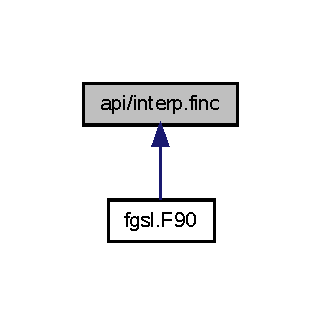
\includegraphics[width=156pt]{interp_8finc__dep__incl}
\end{center}
\end{figure}
\subsection*{Functions/\-Subroutines}
\begin{DoxyCompactItemize}
\item 
type(fgsl\-\_\-interp) function \hyperlink{interp_8finc_a85d81be60660a84879e2148724d250cc}{fgsl\-\_\-interp\-\_\-alloc} (interp\-\_\-type, size)
\item 
subroutine \hyperlink{interp_8finc_a3cec445cbc603ff9045fc6eb5b2aee36}{fgsl\-\_\-interp\-\_\-free} (interp)
\item 
type(fgsl\-\_\-interp\-\_\-accel) function \hyperlink{interp_8finc_a8ef030df058aadca9f34d486136f1a2a}{fgsl\-\_\-interp\-\_\-accel\-\_\-alloc} ()
\item 
subroutine \hyperlink{interp_8finc_a943a42ee8c354909f417bdd5d3e51425}{fgsl\-\_\-interp\-\_\-accel\-\_\-free} (acc)
\item 
logical function \hyperlink{interp_8finc_ae7b75708ca1cabe167d868cd155713d4}{fgsl\-\_\-interp\-\_\-status} (interp)
\item 
logical function \hyperlink{interp_8finc_ae1478c665d9d001580eb90c855b6288d}{fgsl\-\_\-interp\-\_\-accel\-\_\-status} (acc)
\item 
integer(fgsl\-\_\-int) function \hyperlink{interp_8finc_a54c00b2741881cf6689a3799ad490456}{fgsl\-\_\-interp\-\_\-init} (interp, xa, ya, size)
\item 
real(fgsl\-\_\-double) function \hyperlink{interp_8finc_a95909e5a34b271d917d35fdb5f1168f0}{fgsl\-\_\-interp\-\_\-eval} (interp, xa, ya, x, acc)
\item 
integer(fgsl\-\_\-int) function \hyperlink{interp_8finc_a1439d29134b2c5dbaa2b091f925c3dca}{fgsl\-\_\-interp\-\_\-eval\-\_\-e} (interp, xa, ya, x, acc, y)
\item 
real(fgsl\-\_\-double) function \hyperlink{interp_8finc_a51d1986524d01be2a3f9e24ddaccadf5}{fgsl\-\_\-interp\-\_\-eval\-\_\-integ} (interp, xa, ya, a, b, acc)
\item 
integer(fgsl\-\_\-int) function \hyperlink{interp_8finc_a1aa6af97dc477f8439664601e8aa231a}{fgsl\-\_\-interp\-\_\-eval\-\_\-integ\-\_\-e} (interp, xa, ya, a, b, acc, result)
\item 
real(fgsl\-\_\-double) function \hyperlink{interp_8finc_ac57b89652d8434b0ed0c0757e1b408a3}{fgsl\-\_\-interp\-\_\-eval\-\_\-deriv} (interp, xa, ya, x, acc)
\item 
integer(fgsl\-\_\-int) function \hyperlink{interp_8finc_ab255bde1c108629a83829561e5f1b3db}{fgsl\-\_\-interp\-\_\-eval\-\_\-deriv\-\_\-e} (interp, xa, ya, x, acc, d)
\item 
real(fgsl\-\_\-double) function \hyperlink{interp_8finc_a4b15b2342368a4046e9d18f60131a9e7}{fgsl\-\_\-interp\-\_\-eval\-\_\-deriv2} (interp, xa, ya, x, acc)
\item 
integer(fgsl\-\_\-int) function \hyperlink{interp_8finc_a5752fd272762ec6357b0f8c353c6c1a5}{fgsl\-\_\-interp\-\_\-eval\-\_\-deriv2\-\_\-e} (interp, xa, ya, x, acc, d2)
\item 
character(kind=fgsl\-\_\-char, len=fgsl\-\_\-strmax) \\*
function \hyperlink{interp_8finc_a13eac3e860747823e4eb7056cdbaaadb}{fgsl\-\_\-interp\-\_\-name} (interp)
\item 
integer(fgsl\-\_\-long) function \hyperlink{interp_8finc_a573225f56abbabd3f942f378933e3f32}{fgsl\-\_\-interp\-\_\-min\-\_\-size} (interp)
\item 
integer(fgsl\-\_\-long) function \hyperlink{interp_8finc_abecb0b2e997eb9e0f0c71cc9f49ad981}{fgsl\-\_\-interp\-\_\-type\-\_\-min\-\_\-size} (interp)
\item 
integer(fgsl\-\_\-size\-\_\-t) function \hyperlink{interp_8finc_a3dfb39ce96909da1ffe68251b6faec82}{fgsl\-\_\-interp\-\_\-bsearch} (xa, x, index\-\_\-lo, index\-\_\-hi)
\item 
integer(fgsl\-\_\-size\-\_\-t) function \hyperlink{interp_8finc_a056f54ec143fd153992cfa14ef3bd32f}{fgsl\-\_\-interp\-\_\-accel\-\_\-find} (acc, xa, size, x)
\item 
type(fgsl\-\_\-spline) function \hyperlink{interp_8finc_a5a2b4ca82d49d34aff7cf04a9a1b12ab}{fgsl\-\_\-spline\-\_\-alloc} (interp\-\_\-type, size)
\item 
subroutine \hyperlink{interp_8finc_a0f868da0ef3261a833026a41f2c94c83}{fgsl\-\_\-spline\-\_\-free} (spline)
\item 
integer(fgsl\-\_\-int) function \hyperlink{interp_8finc_a1f1a7747866bf3834763d7820d3df506}{fgsl\-\_\-spline\-\_\-init} (spline, xa, ya, size)
\item 
character(len=fgsl\-\_\-strmax) function \hyperlink{interp_8finc_a12c4a34e73aa03ba6dcdcdc6b270565d}{fgsl\-\_\-spline\-\_\-name} (spline)
\item 
integer(fgsl\-\_\-long) function \hyperlink{interp_8finc_a2a9de9f4376d87391948b2a36fd29f00}{fgsl\-\_\-spline\-\_\-min\-\_\-size} (spline)
\item 
real(fgsl\-\_\-double) function \hyperlink{interp_8finc_afd9bb964c160911f8fff6ada1478311e}{fgsl\-\_\-spline\-\_\-eval} (spline, x, acc)
\item 
integer(fgsl\-\_\-int) function \hyperlink{interp_8finc_aaa181d14fba2337815104a29864e8fef}{fgsl\-\_\-spline\-\_\-eval\-\_\-e} (spline, x, acc, y)
\item 
real(fgsl\-\_\-double) function \hyperlink{interp_8finc_ad35a0ca7d65c7ad70cc808689390b9c6}{fgsl\-\_\-spline\-\_\-eval\-\_\-deriv} (spline, x, acc)
\item 
integer(fgsl\-\_\-int) function \hyperlink{interp_8finc_a0ccfb4a4c766da212d6308f80ae9d7b6}{fgsl\-\_\-spline\-\_\-eval\-\_\-deriv\-\_\-e} (spline, x, acc, y)
\item 
real(fgsl\-\_\-double) function \hyperlink{interp_8finc_a134500bed3f7e814dab384a7a9187799}{fgsl\-\_\-spline\-\_\-eval\-\_\-deriv2} (spline, x, acc)
\item 
integer(fgsl\-\_\-int) function \hyperlink{interp_8finc_ad9d2570e13c828bbb27ef3a4c16a896d}{fgsl\-\_\-spline\-\_\-eval\-\_\-deriv2\-\_\-e} (spline, x, acc, y)
\item 
real(fgsl\-\_\-double) function \hyperlink{interp_8finc_a760faf66a424126d3818e61ad7fb20ac}{fgsl\-\_\-spline\-\_\-eval\-\_\-integ} (spline, a, b, acc)
\item 
integer(fgsl\-\_\-int) function \hyperlink{interp_8finc_a369bc13e2713a7b1924249d79af2ec7f}{fgsl\-\_\-spline\-\_\-eval\-\_\-integ\-\_\-e} (spline, a, b, acc, y)
\item 
logical function \hyperlink{interp_8finc_aa23ee1340710742e108a1681c9ee4ef7}{fgsl\-\_\-spline\-\_\-status} (spline)
\item 
integer(fgsl\-\_\-size\-\_\-t) function \hyperlink{interp_8finc_a7acb5abbb8c6382196dcaae035764b85}{fgsl\-\_\-sizeof\-\_\-interp} (w)
\end{DoxyCompactItemize}


\subsection{Function/\-Subroutine Documentation}
\hypertarget{interp_8finc_a8ef030df058aadca9f34d486136f1a2a}{\index{interp.\-finc@{interp.\-finc}!fgsl\-\_\-interp\-\_\-accel\-\_\-alloc@{fgsl\-\_\-interp\-\_\-accel\-\_\-alloc}}
\index{fgsl\-\_\-interp\-\_\-accel\-\_\-alloc@{fgsl\-\_\-interp\-\_\-accel\-\_\-alloc}!interp.finc@{interp.\-finc}}
\subsubsection[{fgsl\-\_\-interp\-\_\-accel\-\_\-alloc}]{\setlength{\rightskip}{0pt plus 5cm}type(fgsl\-\_\-interp\-\_\-accel) function fgsl\-\_\-interp\-\_\-accel\-\_\-alloc (
\begin{DoxyParamCaption}
{}
\end{DoxyParamCaption}
)}}\label{interp_8finc_a8ef030df058aadca9f34d486136f1a2a}
\hypertarget{interp_8finc_a056f54ec143fd153992cfa14ef3bd32f}{\index{interp.\-finc@{interp.\-finc}!fgsl\-\_\-interp\-\_\-accel\-\_\-find@{fgsl\-\_\-interp\-\_\-accel\-\_\-find}}
\index{fgsl\-\_\-interp\-\_\-accel\-\_\-find@{fgsl\-\_\-interp\-\_\-accel\-\_\-find}!interp.finc@{interp.\-finc}}
\subsubsection[{fgsl\-\_\-interp\-\_\-accel\-\_\-find}]{\setlength{\rightskip}{0pt plus 5cm}integer(fgsl\-\_\-size\-\_\-t) function fgsl\-\_\-interp\-\_\-accel\-\_\-find (
\begin{DoxyParamCaption}
\item[{type(fgsl\-\_\-interp\-\_\-accel), intent(inout)}]{acc, }
\item[{real(fgsl\-\_\-double), dimension($\ast$), intent(in)}]{xa, }
\item[{integer(fgsl\-\_\-size\-\_\-t), intent(in)}]{size, }
\item[{real(fgsl\-\_\-double), intent(in)}]{x}
\end{DoxyParamCaption}
)}}\label{interp_8finc_a056f54ec143fd153992cfa14ef3bd32f}
\hypertarget{interp_8finc_a943a42ee8c354909f417bdd5d3e51425}{\index{interp.\-finc@{interp.\-finc}!fgsl\-\_\-interp\-\_\-accel\-\_\-free@{fgsl\-\_\-interp\-\_\-accel\-\_\-free}}
\index{fgsl\-\_\-interp\-\_\-accel\-\_\-free@{fgsl\-\_\-interp\-\_\-accel\-\_\-free}!interp.finc@{interp.\-finc}}
\subsubsection[{fgsl\-\_\-interp\-\_\-accel\-\_\-free}]{\setlength{\rightskip}{0pt plus 5cm}subroutine fgsl\-\_\-interp\-\_\-accel\-\_\-free (
\begin{DoxyParamCaption}
\item[{type(fgsl\-\_\-interp\-\_\-accel), intent(inout)}]{acc}
\end{DoxyParamCaption}
)}}\label{interp_8finc_a943a42ee8c354909f417bdd5d3e51425}
\hypertarget{interp_8finc_ae1478c665d9d001580eb90c855b6288d}{\index{interp.\-finc@{interp.\-finc}!fgsl\-\_\-interp\-\_\-accel\-\_\-status@{fgsl\-\_\-interp\-\_\-accel\-\_\-status}}
\index{fgsl\-\_\-interp\-\_\-accel\-\_\-status@{fgsl\-\_\-interp\-\_\-accel\-\_\-status}!interp.finc@{interp.\-finc}}
\subsubsection[{fgsl\-\_\-interp\-\_\-accel\-\_\-status}]{\setlength{\rightskip}{0pt plus 5cm}logical function fgsl\-\_\-interp\-\_\-accel\-\_\-status (
\begin{DoxyParamCaption}
\item[{type(fgsl\-\_\-interp\-\_\-accel), intent(in)}]{acc}
\end{DoxyParamCaption}
)}}\label{interp_8finc_ae1478c665d9d001580eb90c855b6288d}
\hypertarget{interp_8finc_a85d81be60660a84879e2148724d250cc}{\index{interp.\-finc@{interp.\-finc}!fgsl\-\_\-interp\-\_\-alloc@{fgsl\-\_\-interp\-\_\-alloc}}
\index{fgsl\-\_\-interp\-\_\-alloc@{fgsl\-\_\-interp\-\_\-alloc}!interp.finc@{interp.\-finc}}
\subsubsection[{fgsl\-\_\-interp\-\_\-alloc}]{\setlength{\rightskip}{0pt plus 5cm}type(fgsl\-\_\-interp) function fgsl\-\_\-interp\-\_\-alloc (
\begin{DoxyParamCaption}
\item[{type(fgsl\-\_\-interp\-\_\-type), intent(in)}]{interp\-\_\-type, }
\item[{integer(fgsl\-\_\-size\-\_\-t), intent(in)}]{size}
\end{DoxyParamCaption}
)}}\label{interp_8finc_a85d81be60660a84879e2148724d250cc}
\hypertarget{interp_8finc_a3dfb39ce96909da1ffe68251b6faec82}{\index{interp.\-finc@{interp.\-finc}!fgsl\-\_\-interp\-\_\-bsearch@{fgsl\-\_\-interp\-\_\-bsearch}}
\index{fgsl\-\_\-interp\-\_\-bsearch@{fgsl\-\_\-interp\-\_\-bsearch}!interp.finc@{interp.\-finc}}
\subsubsection[{fgsl\-\_\-interp\-\_\-bsearch}]{\setlength{\rightskip}{0pt plus 5cm}integer(fgsl\-\_\-size\-\_\-t) function fgsl\-\_\-interp\-\_\-bsearch (
\begin{DoxyParamCaption}
\item[{real(fgsl\-\_\-double), dimension(\-:), intent(in)}]{xa, }
\item[{real(fgsl\-\_\-double), intent(in)}]{x, }
\item[{integer(fgsl\-\_\-size\-\_\-t), intent(in)}]{index\-\_\-lo, }
\item[{integer(fgsl\-\_\-size\-\_\-t), intent(in)}]{index\-\_\-hi}
\end{DoxyParamCaption}
)}}\label{interp_8finc_a3dfb39ce96909da1ffe68251b6faec82}
\hypertarget{interp_8finc_a95909e5a34b271d917d35fdb5f1168f0}{\index{interp.\-finc@{interp.\-finc}!fgsl\-\_\-interp\-\_\-eval@{fgsl\-\_\-interp\-\_\-eval}}
\index{fgsl\-\_\-interp\-\_\-eval@{fgsl\-\_\-interp\-\_\-eval}!interp.finc@{interp.\-finc}}
\subsubsection[{fgsl\-\_\-interp\-\_\-eval}]{\setlength{\rightskip}{0pt plus 5cm}real(fgsl\-\_\-double) function fgsl\-\_\-interp\-\_\-eval (
\begin{DoxyParamCaption}
\item[{type(fgsl\-\_\-interp), intent(in)}]{interp, }
\item[{real(fgsl\-\_\-double), dimension(\-:), intent(in)}]{xa, }
\item[{real(fgsl\-\_\-double), dimension(\-:), intent(in)}]{ya, }
\item[{real(fgsl\-\_\-double), intent(in)}]{x, }
\item[{type(fgsl\-\_\-interp\-\_\-accel), intent(inout)}]{acc}
\end{DoxyParamCaption}
)}}\label{interp_8finc_a95909e5a34b271d917d35fdb5f1168f0}
\hypertarget{interp_8finc_ac57b89652d8434b0ed0c0757e1b408a3}{\index{interp.\-finc@{interp.\-finc}!fgsl\-\_\-interp\-\_\-eval\-\_\-deriv@{fgsl\-\_\-interp\-\_\-eval\-\_\-deriv}}
\index{fgsl\-\_\-interp\-\_\-eval\-\_\-deriv@{fgsl\-\_\-interp\-\_\-eval\-\_\-deriv}!interp.finc@{interp.\-finc}}
\subsubsection[{fgsl\-\_\-interp\-\_\-eval\-\_\-deriv}]{\setlength{\rightskip}{0pt plus 5cm}real(fgsl\-\_\-double) function fgsl\-\_\-interp\-\_\-eval\-\_\-deriv (
\begin{DoxyParamCaption}
\item[{type(fgsl\-\_\-interp), intent(in)}]{interp, }
\item[{real(fgsl\-\_\-double), dimension(\-:), intent(in)}]{xa, }
\item[{real(fgsl\-\_\-double), dimension(\-:), intent(in)}]{ya, }
\item[{real(fgsl\-\_\-double), intent(in)}]{x, }
\item[{type(fgsl\-\_\-interp\-\_\-accel), intent(inout)}]{acc}
\end{DoxyParamCaption}
)}}\label{interp_8finc_ac57b89652d8434b0ed0c0757e1b408a3}
\hypertarget{interp_8finc_a4b15b2342368a4046e9d18f60131a9e7}{\index{interp.\-finc@{interp.\-finc}!fgsl\-\_\-interp\-\_\-eval\-\_\-deriv2@{fgsl\-\_\-interp\-\_\-eval\-\_\-deriv2}}
\index{fgsl\-\_\-interp\-\_\-eval\-\_\-deriv2@{fgsl\-\_\-interp\-\_\-eval\-\_\-deriv2}!interp.finc@{interp.\-finc}}
\subsubsection[{fgsl\-\_\-interp\-\_\-eval\-\_\-deriv2}]{\setlength{\rightskip}{0pt plus 5cm}real(fgsl\-\_\-double) function fgsl\-\_\-interp\-\_\-eval\-\_\-deriv2 (
\begin{DoxyParamCaption}
\item[{type(fgsl\-\_\-interp), intent(in)}]{interp, }
\item[{real(fgsl\-\_\-double), dimension(\-:), intent(in)}]{xa, }
\item[{real(fgsl\-\_\-double), dimension(\-:), intent(in)}]{ya, }
\item[{real(fgsl\-\_\-double), intent(in)}]{x, }
\item[{type(fgsl\-\_\-interp\-\_\-accel), intent(inout)}]{acc}
\end{DoxyParamCaption}
)}}\label{interp_8finc_a4b15b2342368a4046e9d18f60131a9e7}
\hypertarget{interp_8finc_a5752fd272762ec6357b0f8c353c6c1a5}{\index{interp.\-finc@{interp.\-finc}!fgsl\-\_\-interp\-\_\-eval\-\_\-deriv2\-\_\-e@{fgsl\-\_\-interp\-\_\-eval\-\_\-deriv2\-\_\-e}}
\index{fgsl\-\_\-interp\-\_\-eval\-\_\-deriv2\-\_\-e@{fgsl\-\_\-interp\-\_\-eval\-\_\-deriv2\-\_\-e}!interp.finc@{interp.\-finc}}
\subsubsection[{fgsl\-\_\-interp\-\_\-eval\-\_\-deriv2\-\_\-e}]{\setlength{\rightskip}{0pt plus 5cm}integer(fgsl\-\_\-int) function fgsl\-\_\-interp\-\_\-eval\-\_\-deriv2\-\_\-e (
\begin{DoxyParamCaption}
\item[{type(fgsl\-\_\-interp), intent(in)}]{interp, }
\item[{real(fgsl\-\_\-double), dimension(\-:), intent(in)}]{xa, }
\item[{real(fgsl\-\_\-double), dimension(\-:), intent(in)}]{ya, }
\item[{real(fgsl\-\_\-double), intent(in)}]{x, }
\item[{type(fgsl\-\_\-interp\-\_\-accel), intent(inout)}]{acc, }
\item[{real(fgsl\-\_\-double), intent(out)}]{d2}
\end{DoxyParamCaption}
)}}\label{interp_8finc_a5752fd272762ec6357b0f8c353c6c1a5}
\hypertarget{interp_8finc_ab255bde1c108629a83829561e5f1b3db}{\index{interp.\-finc@{interp.\-finc}!fgsl\-\_\-interp\-\_\-eval\-\_\-deriv\-\_\-e@{fgsl\-\_\-interp\-\_\-eval\-\_\-deriv\-\_\-e}}
\index{fgsl\-\_\-interp\-\_\-eval\-\_\-deriv\-\_\-e@{fgsl\-\_\-interp\-\_\-eval\-\_\-deriv\-\_\-e}!interp.finc@{interp.\-finc}}
\subsubsection[{fgsl\-\_\-interp\-\_\-eval\-\_\-deriv\-\_\-e}]{\setlength{\rightskip}{0pt plus 5cm}integer(fgsl\-\_\-int) function fgsl\-\_\-interp\-\_\-eval\-\_\-deriv\-\_\-e (
\begin{DoxyParamCaption}
\item[{type(fgsl\-\_\-interp), intent(in)}]{interp, }
\item[{real(fgsl\-\_\-double), dimension(\-:), intent(in)}]{xa, }
\item[{real(fgsl\-\_\-double), dimension(\-:), intent(in)}]{ya, }
\item[{real(fgsl\-\_\-double), intent(in)}]{x, }
\item[{type(fgsl\-\_\-interp\-\_\-accel), intent(inout)}]{acc, }
\item[{real(fgsl\-\_\-double), intent(out)}]{d}
\end{DoxyParamCaption}
)}}\label{interp_8finc_ab255bde1c108629a83829561e5f1b3db}
\hypertarget{interp_8finc_a1439d29134b2c5dbaa2b091f925c3dca}{\index{interp.\-finc@{interp.\-finc}!fgsl\-\_\-interp\-\_\-eval\-\_\-e@{fgsl\-\_\-interp\-\_\-eval\-\_\-e}}
\index{fgsl\-\_\-interp\-\_\-eval\-\_\-e@{fgsl\-\_\-interp\-\_\-eval\-\_\-e}!interp.finc@{interp.\-finc}}
\subsubsection[{fgsl\-\_\-interp\-\_\-eval\-\_\-e}]{\setlength{\rightskip}{0pt plus 5cm}integer(fgsl\-\_\-int) function fgsl\-\_\-interp\-\_\-eval\-\_\-e (
\begin{DoxyParamCaption}
\item[{type(fgsl\-\_\-interp), intent(in)}]{interp, }
\item[{real(fgsl\-\_\-double), dimension(\-:), intent(in)}]{xa, }
\item[{real(fgsl\-\_\-double), dimension(\-:), intent(in)}]{ya, }
\item[{real(fgsl\-\_\-double), intent(in)}]{x, }
\item[{type(fgsl\-\_\-interp\-\_\-accel), intent(inout)}]{acc, }
\item[{real(fgsl\-\_\-double), intent(out)}]{y}
\end{DoxyParamCaption}
)}}\label{interp_8finc_a1439d29134b2c5dbaa2b091f925c3dca}
\hypertarget{interp_8finc_a51d1986524d01be2a3f9e24ddaccadf5}{\index{interp.\-finc@{interp.\-finc}!fgsl\-\_\-interp\-\_\-eval\-\_\-integ@{fgsl\-\_\-interp\-\_\-eval\-\_\-integ}}
\index{fgsl\-\_\-interp\-\_\-eval\-\_\-integ@{fgsl\-\_\-interp\-\_\-eval\-\_\-integ}!interp.finc@{interp.\-finc}}
\subsubsection[{fgsl\-\_\-interp\-\_\-eval\-\_\-integ}]{\setlength{\rightskip}{0pt plus 5cm}real(fgsl\-\_\-double) function fgsl\-\_\-interp\-\_\-eval\-\_\-integ (
\begin{DoxyParamCaption}
\item[{type(fgsl\-\_\-interp), intent(in)}]{interp, }
\item[{real(fgsl\-\_\-double), dimension(\-:), intent(in)}]{xa, }
\item[{real(fgsl\-\_\-double), dimension(\-:), intent(in)}]{ya, }
\item[{real(fgsl\-\_\-double), intent(in)}]{a, }
\item[{real(fgsl\-\_\-double), intent(in)}]{b, }
\item[{type(fgsl\-\_\-interp\-\_\-accel), intent(inout)}]{acc}
\end{DoxyParamCaption}
)}}\label{interp_8finc_a51d1986524d01be2a3f9e24ddaccadf5}
\hypertarget{interp_8finc_a1aa6af97dc477f8439664601e8aa231a}{\index{interp.\-finc@{interp.\-finc}!fgsl\-\_\-interp\-\_\-eval\-\_\-integ\-\_\-e@{fgsl\-\_\-interp\-\_\-eval\-\_\-integ\-\_\-e}}
\index{fgsl\-\_\-interp\-\_\-eval\-\_\-integ\-\_\-e@{fgsl\-\_\-interp\-\_\-eval\-\_\-integ\-\_\-e}!interp.finc@{interp.\-finc}}
\subsubsection[{fgsl\-\_\-interp\-\_\-eval\-\_\-integ\-\_\-e}]{\setlength{\rightskip}{0pt plus 5cm}integer(fgsl\-\_\-int) function fgsl\-\_\-interp\-\_\-eval\-\_\-integ\-\_\-e (
\begin{DoxyParamCaption}
\item[{type(fgsl\-\_\-interp), intent(in)}]{interp, }
\item[{real(fgsl\-\_\-double), dimension(\-:), intent(in)}]{xa, }
\item[{real(fgsl\-\_\-double), dimension(\-:), intent(in)}]{ya, }
\item[{real(fgsl\-\_\-double), intent(in)}]{a, }
\item[{real(fgsl\-\_\-double), intent(in)}]{b, }
\item[{type(fgsl\-\_\-interp\-\_\-accel), intent(inout)}]{acc, }
\item[{real(fgsl\-\_\-double), intent(out)}]{result}
\end{DoxyParamCaption}
)}}\label{interp_8finc_a1aa6af97dc477f8439664601e8aa231a}
\hypertarget{interp_8finc_a3cec445cbc603ff9045fc6eb5b2aee36}{\index{interp.\-finc@{interp.\-finc}!fgsl\-\_\-interp\-\_\-free@{fgsl\-\_\-interp\-\_\-free}}
\index{fgsl\-\_\-interp\-\_\-free@{fgsl\-\_\-interp\-\_\-free}!interp.finc@{interp.\-finc}}
\subsubsection[{fgsl\-\_\-interp\-\_\-free}]{\setlength{\rightskip}{0pt plus 5cm}subroutine fgsl\-\_\-interp\-\_\-free (
\begin{DoxyParamCaption}
\item[{type(fgsl\-\_\-interp), intent(inout)}]{interp}
\end{DoxyParamCaption}
)}}\label{interp_8finc_a3cec445cbc603ff9045fc6eb5b2aee36}
\hypertarget{interp_8finc_a54c00b2741881cf6689a3799ad490456}{\index{interp.\-finc@{interp.\-finc}!fgsl\-\_\-interp\-\_\-init@{fgsl\-\_\-interp\-\_\-init}}
\index{fgsl\-\_\-interp\-\_\-init@{fgsl\-\_\-interp\-\_\-init}!interp.finc@{interp.\-finc}}
\subsubsection[{fgsl\-\_\-interp\-\_\-init}]{\setlength{\rightskip}{0pt plus 5cm}integer(fgsl\-\_\-int) function fgsl\-\_\-interp\-\_\-init (
\begin{DoxyParamCaption}
\item[{type(fgsl\-\_\-interp), intent(inout)}]{interp, }
\item[{real(fgsl\-\_\-double), dimension(size), intent(in)}]{xa, }
\item[{real(fgsl\-\_\-double), dimension(size), intent(in)}]{ya, }
\item[{integer(fgsl\-\_\-size\-\_\-t), intent(in)}]{size}
\end{DoxyParamCaption}
)}}\label{interp_8finc_a54c00b2741881cf6689a3799ad490456}
\hypertarget{interp_8finc_a573225f56abbabd3f942f378933e3f32}{\index{interp.\-finc@{interp.\-finc}!fgsl\-\_\-interp\-\_\-min\-\_\-size@{fgsl\-\_\-interp\-\_\-min\-\_\-size}}
\index{fgsl\-\_\-interp\-\_\-min\-\_\-size@{fgsl\-\_\-interp\-\_\-min\-\_\-size}!interp.finc@{interp.\-finc}}
\subsubsection[{fgsl\-\_\-interp\-\_\-min\-\_\-size}]{\setlength{\rightskip}{0pt plus 5cm}integer(fgsl\-\_\-long) function fgsl\-\_\-interp\-\_\-min\-\_\-size (
\begin{DoxyParamCaption}
\item[{type(fgsl\-\_\-interp), intent(in)}]{interp}
\end{DoxyParamCaption}
)}}\label{interp_8finc_a573225f56abbabd3f942f378933e3f32}
\hypertarget{interp_8finc_a13eac3e860747823e4eb7056cdbaaadb}{\index{interp.\-finc@{interp.\-finc}!fgsl\-\_\-interp\-\_\-name@{fgsl\-\_\-interp\-\_\-name}}
\index{fgsl\-\_\-interp\-\_\-name@{fgsl\-\_\-interp\-\_\-name}!interp.finc@{interp.\-finc}}
\subsubsection[{fgsl\-\_\-interp\-\_\-name}]{\setlength{\rightskip}{0pt plus 5cm}character(kind=fgsl\-\_\-char,len=fgsl\-\_\-strmax) function fgsl\-\_\-interp\-\_\-name (
\begin{DoxyParamCaption}
\item[{type(fgsl\-\_\-interp), intent(in)}]{interp}
\end{DoxyParamCaption}
)}}\label{interp_8finc_a13eac3e860747823e4eb7056cdbaaadb}
\hypertarget{interp_8finc_ae7b75708ca1cabe167d868cd155713d4}{\index{interp.\-finc@{interp.\-finc}!fgsl\-\_\-interp\-\_\-status@{fgsl\-\_\-interp\-\_\-status}}
\index{fgsl\-\_\-interp\-\_\-status@{fgsl\-\_\-interp\-\_\-status}!interp.finc@{interp.\-finc}}
\subsubsection[{fgsl\-\_\-interp\-\_\-status}]{\setlength{\rightskip}{0pt plus 5cm}logical function fgsl\-\_\-interp\-\_\-status (
\begin{DoxyParamCaption}
\item[{type(fgsl\-\_\-interp), intent(in)}]{interp}
\end{DoxyParamCaption}
)}}\label{interp_8finc_ae7b75708ca1cabe167d868cd155713d4}
\hypertarget{interp_8finc_abecb0b2e997eb9e0f0c71cc9f49ad981}{\index{interp.\-finc@{interp.\-finc}!fgsl\-\_\-interp\-\_\-type\-\_\-min\-\_\-size@{fgsl\-\_\-interp\-\_\-type\-\_\-min\-\_\-size}}
\index{fgsl\-\_\-interp\-\_\-type\-\_\-min\-\_\-size@{fgsl\-\_\-interp\-\_\-type\-\_\-min\-\_\-size}!interp.finc@{interp.\-finc}}
\subsubsection[{fgsl\-\_\-interp\-\_\-type\-\_\-min\-\_\-size}]{\setlength{\rightskip}{0pt plus 5cm}integer(fgsl\-\_\-long) function fgsl\-\_\-interp\-\_\-type\-\_\-min\-\_\-size (
\begin{DoxyParamCaption}
\item[{type(fgsl\-\_\-interp\-\_\-type), intent(in)}]{interp}
\end{DoxyParamCaption}
)}}\label{interp_8finc_abecb0b2e997eb9e0f0c71cc9f49ad981}
\hypertarget{interp_8finc_a7acb5abbb8c6382196dcaae035764b85}{\index{interp.\-finc@{interp.\-finc}!fgsl\-\_\-sizeof\-\_\-interp@{fgsl\-\_\-sizeof\-\_\-interp}}
\index{fgsl\-\_\-sizeof\-\_\-interp@{fgsl\-\_\-sizeof\-\_\-interp}!interp.finc@{interp.\-finc}}
\subsubsection[{fgsl\-\_\-sizeof\-\_\-interp}]{\setlength{\rightskip}{0pt plus 5cm}integer(fgsl\-\_\-size\-\_\-t) function fgsl\-\_\-sizeof\-\_\-interp (
\begin{DoxyParamCaption}
\item[{type(fgsl\-\_\-interp), intent(in)}]{w}
\end{DoxyParamCaption}
)}}\label{interp_8finc_a7acb5abbb8c6382196dcaae035764b85}
\hypertarget{interp_8finc_a5a2b4ca82d49d34aff7cf04a9a1b12ab}{\index{interp.\-finc@{interp.\-finc}!fgsl\-\_\-spline\-\_\-alloc@{fgsl\-\_\-spline\-\_\-alloc}}
\index{fgsl\-\_\-spline\-\_\-alloc@{fgsl\-\_\-spline\-\_\-alloc}!interp.finc@{interp.\-finc}}
\subsubsection[{fgsl\-\_\-spline\-\_\-alloc}]{\setlength{\rightskip}{0pt plus 5cm}type(fgsl\-\_\-spline) function fgsl\-\_\-spline\-\_\-alloc (
\begin{DoxyParamCaption}
\item[{type(fgsl\-\_\-interp\-\_\-type), intent(in)}]{interp\-\_\-type, }
\item[{integer(fgsl\-\_\-size\-\_\-t), intent(in)}]{size}
\end{DoxyParamCaption}
)}}\label{interp_8finc_a5a2b4ca82d49d34aff7cf04a9a1b12ab}
\hypertarget{interp_8finc_afd9bb964c160911f8fff6ada1478311e}{\index{interp.\-finc@{interp.\-finc}!fgsl\-\_\-spline\-\_\-eval@{fgsl\-\_\-spline\-\_\-eval}}
\index{fgsl\-\_\-spline\-\_\-eval@{fgsl\-\_\-spline\-\_\-eval}!interp.finc@{interp.\-finc}}
\subsubsection[{fgsl\-\_\-spline\-\_\-eval}]{\setlength{\rightskip}{0pt plus 5cm}real(fgsl\-\_\-double) function fgsl\-\_\-spline\-\_\-eval (
\begin{DoxyParamCaption}
\item[{type(fgsl\-\_\-spline), intent(in)}]{spline, }
\item[{real(fgsl\-\_\-double), intent(in)}]{x, }
\item[{type(fgsl\-\_\-interp\-\_\-accel), intent(inout)}]{acc}
\end{DoxyParamCaption}
)}}\label{interp_8finc_afd9bb964c160911f8fff6ada1478311e}
\hypertarget{interp_8finc_ad35a0ca7d65c7ad70cc808689390b9c6}{\index{interp.\-finc@{interp.\-finc}!fgsl\-\_\-spline\-\_\-eval\-\_\-deriv@{fgsl\-\_\-spline\-\_\-eval\-\_\-deriv}}
\index{fgsl\-\_\-spline\-\_\-eval\-\_\-deriv@{fgsl\-\_\-spline\-\_\-eval\-\_\-deriv}!interp.finc@{interp.\-finc}}
\subsubsection[{fgsl\-\_\-spline\-\_\-eval\-\_\-deriv}]{\setlength{\rightskip}{0pt plus 5cm}real(fgsl\-\_\-double) function fgsl\-\_\-spline\-\_\-eval\-\_\-deriv (
\begin{DoxyParamCaption}
\item[{type(fgsl\-\_\-spline), intent(in)}]{spline, }
\item[{real(fgsl\-\_\-double), intent(in)}]{x, }
\item[{type(fgsl\-\_\-interp\-\_\-accel), intent(inout)}]{acc}
\end{DoxyParamCaption}
)}}\label{interp_8finc_ad35a0ca7d65c7ad70cc808689390b9c6}
\hypertarget{interp_8finc_a134500bed3f7e814dab384a7a9187799}{\index{interp.\-finc@{interp.\-finc}!fgsl\-\_\-spline\-\_\-eval\-\_\-deriv2@{fgsl\-\_\-spline\-\_\-eval\-\_\-deriv2}}
\index{fgsl\-\_\-spline\-\_\-eval\-\_\-deriv2@{fgsl\-\_\-spline\-\_\-eval\-\_\-deriv2}!interp.finc@{interp.\-finc}}
\subsubsection[{fgsl\-\_\-spline\-\_\-eval\-\_\-deriv2}]{\setlength{\rightskip}{0pt plus 5cm}real(fgsl\-\_\-double) function fgsl\-\_\-spline\-\_\-eval\-\_\-deriv2 (
\begin{DoxyParamCaption}
\item[{type(fgsl\-\_\-spline), intent(in)}]{spline, }
\item[{real(fgsl\-\_\-double), intent(in)}]{x, }
\item[{type(fgsl\-\_\-interp\-\_\-accel), intent(inout)}]{acc}
\end{DoxyParamCaption}
)}}\label{interp_8finc_a134500bed3f7e814dab384a7a9187799}
\hypertarget{interp_8finc_ad9d2570e13c828bbb27ef3a4c16a896d}{\index{interp.\-finc@{interp.\-finc}!fgsl\-\_\-spline\-\_\-eval\-\_\-deriv2\-\_\-e@{fgsl\-\_\-spline\-\_\-eval\-\_\-deriv2\-\_\-e}}
\index{fgsl\-\_\-spline\-\_\-eval\-\_\-deriv2\-\_\-e@{fgsl\-\_\-spline\-\_\-eval\-\_\-deriv2\-\_\-e}!interp.finc@{interp.\-finc}}
\subsubsection[{fgsl\-\_\-spline\-\_\-eval\-\_\-deriv2\-\_\-e}]{\setlength{\rightskip}{0pt plus 5cm}integer(fgsl\-\_\-int) function fgsl\-\_\-spline\-\_\-eval\-\_\-deriv2\-\_\-e (
\begin{DoxyParamCaption}
\item[{type(fgsl\-\_\-spline), intent(in)}]{spline, }
\item[{real(fgsl\-\_\-double), intent(in)}]{x, }
\item[{type(fgsl\-\_\-interp\-\_\-accel), intent(inout)}]{acc, }
\item[{real(fgsl\-\_\-double), intent(out)}]{y}
\end{DoxyParamCaption}
)}}\label{interp_8finc_ad9d2570e13c828bbb27ef3a4c16a896d}
\hypertarget{interp_8finc_a0ccfb4a4c766da212d6308f80ae9d7b6}{\index{interp.\-finc@{interp.\-finc}!fgsl\-\_\-spline\-\_\-eval\-\_\-deriv\-\_\-e@{fgsl\-\_\-spline\-\_\-eval\-\_\-deriv\-\_\-e}}
\index{fgsl\-\_\-spline\-\_\-eval\-\_\-deriv\-\_\-e@{fgsl\-\_\-spline\-\_\-eval\-\_\-deriv\-\_\-e}!interp.finc@{interp.\-finc}}
\subsubsection[{fgsl\-\_\-spline\-\_\-eval\-\_\-deriv\-\_\-e}]{\setlength{\rightskip}{0pt plus 5cm}integer(fgsl\-\_\-int) function fgsl\-\_\-spline\-\_\-eval\-\_\-deriv\-\_\-e (
\begin{DoxyParamCaption}
\item[{type(fgsl\-\_\-spline), intent(in)}]{spline, }
\item[{real(fgsl\-\_\-double), intent(in)}]{x, }
\item[{type(fgsl\-\_\-interp\-\_\-accel), intent(inout)}]{acc, }
\item[{real(fgsl\-\_\-double), intent(out)}]{y}
\end{DoxyParamCaption}
)}}\label{interp_8finc_a0ccfb4a4c766da212d6308f80ae9d7b6}
\hypertarget{interp_8finc_aaa181d14fba2337815104a29864e8fef}{\index{interp.\-finc@{interp.\-finc}!fgsl\-\_\-spline\-\_\-eval\-\_\-e@{fgsl\-\_\-spline\-\_\-eval\-\_\-e}}
\index{fgsl\-\_\-spline\-\_\-eval\-\_\-e@{fgsl\-\_\-spline\-\_\-eval\-\_\-e}!interp.finc@{interp.\-finc}}
\subsubsection[{fgsl\-\_\-spline\-\_\-eval\-\_\-e}]{\setlength{\rightskip}{0pt plus 5cm}integer(fgsl\-\_\-int) function fgsl\-\_\-spline\-\_\-eval\-\_\-e (
\begin{DoxyParamCaption}
\item[{type(fgsl\-\_\-spline), intent(in)}]{spline, }
\item[{real(fgsl\-\_\-double), intent(in)}]{x, }
\item[{type(fgsl\-\_\-interp\-\_\-accel), intent(inout)}]{acc, }
\item[{real(fgsl\-\_\-double), intent(out)}]{y}
\end{DoxyParamCaption}
)}}\label{interp_8finc_aaa181d14fba2337815104a29864e8fef}
\hypertarget{interp_8finc_a760faf66a424126d3818e61ad7fb20ac}{\index{interp.\-finc@{interp.\-finc}!fgsl\-\_\-spline\-\_\-eval\-\_\-integ@{fgsl\-\_\-spline\-\_\-eval\-\_\-integ}}
\index{fgsl\-\_\-spline\-\_\-eval\-\_\-integ@{fgsl\-\_\-spline\-\_\-eval\-\_\-integ}!interp.finc@{interp.\-finc}}
\subsubsection[{fgsl\-\_\-spline\-\_\-eval\-\_\-integ}]{\setlength{\rightskip}{0pt plus 5cm}real(fgsl\-\_\-double) function fgsl\-\_\-spline\-\_\-eval\-\_\-integ (
\begin{DoxyParamCaption}
\item[{type(fgsl\-\_\-spline), intent(in)}]{spline, }
\item[{real(fgsl\-\_\-double), intent(in)}]{a, }
\item[{real(fgsl\-\_\-double), intent(in)}]{b, }
\item[{type(fgsl\-\_\-interp\-\_\-accel), intent(inout)}]{acc}
\end{DoxyParamCaption}
)}}\label{interp_8finc_a760faf66a424126d3818e61ad7fb20ac}
\hypertarget{interp_8finc_a369bc13e2713a7b1924249d79af2ec7f}{\index{interp.\-finc@{interp.\-finc}!fgsl\-\_\-spline\-\_\-eval\-\_\-integ\-\_\-e@{fgsl\-\_\-spline\-\_\-eval\-\_\-integ\-\_\-e}}
\index{fgsl\-\_\-spline\-\_\-eval\-\_\-integ\-\_\-e@{fgsl\-\_\-spline\-\_\-eval\-\_\-integ\-\_\-e}!interp.finc@{interp.\-finc}}
\subsubsection[{fgsl\-\_\-spline\-\_\-eval\-\_\-integ\-\_\-e}]{\setlength{\rightskip}{0pt plus 5cm}integer(fgsl\-\_\-int) function fgsl\-\_\-spline\-\_\-eval\-\_\-integ\-\_\-e (
\begin{DoxyParamCaption}
\item[{type(fgsl\-\_\-spline), intent(in)}]{spline, }
\item[{real(fgsl\-\_\-double), intent(in)}]{a, }
\item[{real(fgsl\-\_\-double), intent(in)}]{b, }
\item[{type(fgsl\-\_\-interp\-\_\-accel), intent(inout)}]{acc, }
\item[{real(fgsl\-\_\-double), intent(out)}]{y}
\end{DoxyParamCaption}
)}}\label{interp_8finc_a369bc13e2713a7b1924249d79af2ec7f}
\hypertarget{interp_8finc_a0f868da0ef3261a833026a41f2c94c83}{\index{interp.\-finc@{interp.\-finc}!fgsl\-\_\-spline\-\_\-free@{fgsl\-\_\-spline\-\_\-free}}
\index{fgsl\-\_\-spline\-\_\-free@{fgsl\-\_\-spline\-\_\-free}!interp.finc@{interp.\-finc}}
\subsubsection[{fgsl\-\_\-spline\-\_\-free}]{\setlength{\rightskip}{0pt plus 5cm}subroutine fgsl\-\_\-spline\-\_\-free (
\begin{DoxyParamCaption}
\item[{type(fgsl\-\_\-spline), intent(inout)}]{spline}
\end{DoxyParamCaption}
)}}\label{interp_8finc_a0f868da0ef3261a833026a41f2c94c83}
\hypertarget{interp_8finc_a1f1a7747866bf3834763d7820d3df506}{\index{interp.\-finc@{interp.\-finc}!fgsl\-\_\-spline\-\_\-init@{fgsl\-\_\-spline\-\_\-init}}
\index{fgsl\-\_\-spline\-\_\-init@{fgsl\-\_\-spline\-\_\-init}!interp.finc@{interp.\-finc}}
\subsubsection[{fgsl\-\_\-spline\-\_\-init}]{\setlength{\rightskip}{0pt plus 5cm}integer(fgsl\-\_\-int) function fgsl\-\_\-spline\-\_\-init (
\begin{DoxyParamCaption}
\item[{type(fgsl\-\_\-spline), intent(inout)}]{spline, }
\item[{real(fgsl\-\_\-double), dimension(size), intent(in)}]{xa, }
\item[{real(fgsl\-\_\-double), dimension(size), intent(in)}]{ya, }
\item[{integer(fgsl\-\_\-size\-\_\-t), intent(in)}]{size}
\end{DoxyParamCaption}
)}}\label{interp_8finc_a1f1a7747866bf3834763d7820d3df506}
\hypertarget{interp_8finc_a2a9de9f4376d87391948b2a36fd29f00}{\index{interp.\-finc@{interp.\-finc}!fgsl\-\_\-spline\-\_\-min\-\_\-size@{fgsl\-\_\-spline\-\_\-min\-\_\-size}}
\index{fgsl\-\_\-spline\-\_\-min\-\_\-size@{fgsl\-\_\-spline\-\_\-min\-\_\-size}!interp.finc@{interp.\-finc}}
\subsubsection[{fgsl\-\_\-spline\-\_\-min\-\_\-size}]{\setlength{\rightskip}{0pt plus 5cm}integer(fgsl\-\_\-long) function fgsl\-\_\-spline\-\_\-min\-\_\-size (
\begin{DoxyParamCaption}
\item[{type(fgsl\-\_\-spline), intent(in)}]{spline}
\end{DoxyParamCaption}
)}}\label{interp_8finc_a2a9de9f4376d87391948b2a36fd29f00}
\hypertarget{interp_8finc_a12c4a34e73aa03ba6dcdcdc6b270565d}{\index{interp.\-finc@{interp.\-finc}!fgsl\-\_\-spline\-\_\-name@{fgsl\-\_\-spline\-\_\-name}}
\index{fgsl\-\_\-spline\-\_\-name@{fgsl\-\_\-spline\-\_\-name}!interp.finc@{interp.\-finc}}
\subsubsection[{fgsl\-\_\-spline\-\_\-name}]{\setlength{\rightskip}{0pt plus 5cm}character(len=fgsl\-\_\-strmax) function fgsl\-\_\-spline\-\_\-name (
\begin{DoxyParamCaption}
\item[{type(fgsl\-\_\-spline), intent(in)}]{spline}
\end{DoxyParamCaption}
)}}\label{interp_8finc_a12c4a34e73aa03ba6dcdcdc6b270565d}
\hypertarget{interp_8finc_aa23ee1340710742e108a1681c9ee4ef7}{\index{interp.\-finc@{interp.\-finc}!fgsl\-\_\-spline\-\_\-status@{fgsl\-\_\-spline\-\_\-status}}
\index{fgsl\-\_\-spline\-\_\-status@{fgsl\-\_\-spline\-\_\-status}!interp.finc@{interp.\-finc}}
\subsubsection[{fgsl\-\_\-spline\-\_\-status}]{\setlength{\rightskip}{0pt plus 5cm}logical function fgsl\-\_\-spline\-\_\-status (
\begin{DoxyParamCaption}
\item[{type(fgsl\-\_\-spline), intent(in)}]{spline}
\end{DoxyParamCaption}
)}}\label{interp_8finc_aa23ee1340710742e108a1681c9ee4ef7}

\hypertarget{io_8finc}{}\section{api/io.finc File Reference}
\label{io_8finc}\index{api/io.\+finc@{api/io.\+finc}}
This graph shows which files directly or indirectly include this file\+:\nopagebreak
\begin{figure}[H]
\begin{center}
\leavevmode
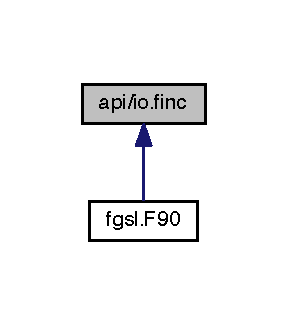
\includegraphics[width=136pt]{io_8finc__dep__incl}
\end{center}
\end{figure}
\subsection*{Functions/\+Subroutines}
\begin{DoxyCompactItemize}
\item 
type(fgsl\+\_\+file) function \hyperlink{io_8finc_a77bd6a72b0526ae80735b42131e5f23d}{fgsl\+\_\+open} (path, mode)
\begin{DoxyCompactList}\small\item\em fgsl\+\_\+open maps the P\+O\+S\+I\+X call fopen() to Fortran \end{DoxyCompactList}\item 
integer(fgsl\+\_\+int) function \hyperlink{io_8finc_a40f28148c9160079e35fde25fa42b7b4}{fgsl\+\_\+close} (fd)
\begin{DoxyCompactList}\small\item\em fgsl\+\_\+open maps the P\+O\+S\+I\+X call fclose() to Fortran \end{DoxyCompactList}\item 
type(fgsl\+\_\+file) function \hyperlink{io_8finc_ae31ece191109b9e7e7af13fb320e4026}{fgsl\+\_\+stdin} ()
\begin{DoxyCompactList}\small\item\em fgsl\+\_\+stdin produces a fgsl\+\_\+file object corresponding to C standard input \end{DoxyCompactList}\item 
type(fgsl\+\_\+file) function \hyperlink{io_8finc_a2fbf2a6da186b942be9b477883bc5177}{fgsl\+\_\+stdout} ()
\begin{DoxyCompactList}\small\item\em fgsl\+\_\+stdout produces a fgsl\+\_\+file object corresponding to C standard output \end{DoxyCompactList}\item 
type(fgsl\+\_\+file) function \hyperlink{io_8finc_ababc632a183fbe488d528fa35ce74908}{fgsl\+\_\+stderr} ()
\begin{DoxyCompactList}\small\item\em fgsl\+\_\+stderr produces a fgsl\+\_\+file object corresponding to C standard error \end{DoxyCompactList}\item 
integer(fgsl\+\_\+int) function \hyperlink{io_8finc_a0f001ee314f4f0881ee4c415e9d19b1b}{fgsl\+\_\+flush} (file)
\begin{DoxyCompactList}\small\item\em fgsl\+\_\+flush flushes a fgsl\+\_\+file object \end{DoxyCompactList}\item 
logical function \hyperlink{io_8finc_ace454d2aea45384f2f7adf4bc7386c27}{fgsl\+\_\+file\+\_\+status} (file)
\end{DoxyCompactItemize}


\subsection{Function/\+Subroutine Documentation}
\hypertarget{io_8finc_a40f28148c9160079e35fde25fa42b7b4}{}\index{io.\+finc@{io.\+finc}!fgsl\+\_\+close@{fgsl\+\_\+close}}
\index{fgsl\+\_\+close@{fgsl\+\_\+close}!io.\+finc@{io.\+finc}}
\subsubsection[{fgsl\+\_\+close}]{\setlength{\rightskip}{0pt plus 5cm}integer(fgsl\+\_\+int) function fgsl\+\_\+close (
\begin{DoxyParamCaption}
\item[{type(fgsl\+\_\+file), intent(inout)}]{fd}
\end{DoxyParamCaption}
)}\label{io_8finc_a40f28148c9160079e35fde25fa42b7b4}


fgsl\+\_\+open maps the P\+O\+S\+I\+X call fclose() to Fortran 


\begin{DoxyParams}{Parameters}
{\em fd} & -\/ on entry\+: open file object \\
\hline
\end{DoxyParams}
\begin{DoxyReturn}{Returns}
Status. 
\end{DoxyReturn}
\hypertarget{io_8finc_ace454d2aea45384f2f7adf4bc7386c27}{}\index{io.\+finc@{io.\+finc}!fgsl\+\_\+file\+\_\+status@{fgsl\+\_\+file\+\_\+status}}
\index{fgsl\+\_\+file\+\_\+status@{fgsl\+\_\+file\+\_\+status}!io.\+finc@{io.\+finc}}
\subsubsection[{fgsl\+\_\+file\+\_\+status}]{\setlength{\rightskip}{0pt plus 5cm}logical function fgsl\+\_\+file\+\_\+status (
\begin{DoxyParamCaption}
\item[{type(fgsl\+\_\+file), intent(in)}]{file}
\end{DoxyParamCaption}
)}\label{io_8finc_ace454d2aea45384f2f7adf4bc7386c27}
\hypertarget{io_8finc_a0f001ee314f4f0881ee4c415e9d19b1b}{}\index{io.\+finc@{io.\+finc}!fgsl\+\_\+flush@{fgsl\+\_\+flush}}
\index{fgsl\+\_\+flush@{fgsl\+\_\+flush}!io.\+finc@{io.\+finc}}
\subsubsection[{fgsl\+\_\+flush}]{\setlength{\rightskip}{0pt plus 5cm}integer(fgsl\+\_\+int) function fgsl\+\_\+flush (
\begin{DoxyParamCaption}
\item[{type(fgsl\+\_\+file), intent(in)}]{file}
\end{DoxyParamCaption}
)}\label{io_8finc_a0f001ee314f4f0881ee4c415e9d19b1b}


fgsl\+\_\+flush flushes a fgsl\+\_\+file object 

\hypertarget{io_8finc_a77bd6a72b0526ae80735b42131e5f23d}{}\index{io.\+finc@{io.\+finc}!fgsl\+\_\+open@{fgsl\+\_\+open}}
\index{fgsl\+\_\+open@{fgsl\+\_\+open}!io.\+finc@{io.\+finc}}
\subsubsection[{fgsl\+\_\+open}]{\setlength{\rightskip}{0pt plus 5cm}type(fgsl\+\_\+file) function fgsl\+\_\+open (
\begin{DoxyParamCaption}
\item[{character(kind=fgsl\+\_\+char, len=$\ast$), intent(in)}]{path, }
\item[{character(kind=fgsl\+\_\+char, len=$\ast$), intent(in)}]{mode}
\end{DoxyParamCaption}
)}\label{io_8finc_a77bd6a72b0526ae80735b42131e5f23d}


fgsl\+\_\+open maps the P\+O\+S\+I\+X call fopen() to Fortran 


\begin{DoxyParams}{Parameters}
{\em path} & -\/ string specifying the path name of the file to be opened \\
\hline
{\em mode} & -\/ string containing the opening mode \\
\hline
\end{DoxyParams}
\begin{DoxyReturn}{Returns}
object of type fgsl\+\_\+file which can be used in other I/\+O calls. 
\end{DoxyReturn}
\hypertarget{io_8finc_ababc632a183fbe488d528fa35ce74908}{}\index{io.\+finc@{io.\+finc}!fgsl\+\_\+stderr@{fgsl\+\_\+stderr}}
\index{fgsl\+\_\+stderr@{fgsl\+\_\+stderr}!io.\+finc@{io.\+finc}}
\subsubsection[{fgsl\+\_\+stderr}]{\setlength{\rightskip}{0pt plus 5cm}type(fgsl\+\_\+file) function fgsl\+\_\+stderr (
\begin{DoxyParamCaption}
{}
\end{DoxyParamCaption}
)}\label{io_8finc_ababc632a183fbe488d528fa35ce74908}


fgsl\+\_\+stderr produces a fgsl\+\_\+file object corresponding to C standard error 

\hypertarget{io_8finc_ae31ece191109b9e7e7af13fb320e4026}{}\index{io.\+finc@{io.\+finc}!fgsl\+\_\+stdin@{fgsl\+\_\+stdin}}
\index{fgsl\+\_\+stdin@{fgsl\+\_\+stdin}!io.\+finc@{io.\+finc}}
\subsubsection[{fgsl\+\_\+stdin}]{\setlength{\rightskip}{0pt plus 5cm}type(fgsl\+\_\+file) function fgsl\+\_\+stdin (
\begin{DoxyParamCaption}
{}
\end{DoxyParamCaption}
)}\label{io_8finc_ae31ece191109b9e7e7af13fb320e4026}


fgsl\+\_\+stdin produces a fgsl\+\_\+file object corresponding to C standard input 

\hypertarget{io_8finc_a2fbf2a6da186b942be9b477883bc5177}{}\index{io.\+finc@{io.\+finc}!fgsl\+\_\+stdout@{fgsl\+\_\+stdout}}
\index{fgsl\+\_\+stdout@{fgsl\+\_\+stdout}!io.\+finc@{io.\+finc}}
\subsubsection[{fgsl\+\_\+stdout}]{\setlength{\rightskip}{0pt plus 5cm}type(fgsl\+\_\+file) function fgsl\+\_\+stdout (
\begin{DoxyParamCaption}
{}
\end{DoxyParamCaption}
)}\label{io_8finc_a2fbf2a6da186b942be9b477883bc5177}


fgsl\+\_\+stdout produces a fgsl\+\_\+file object corresponding to C standard output 


\hypertarget{linalg_8finc}{\section{api/linalg.finc File Reference}
\label{linalg_8finc}\index{api/linalg.\-finc@{api/linalg.\-finc}}
}
This graph shows which files directly or indirectly include this file\-:\nopagebreak
\begin{figure}[H]
\begin{center}
\leavevmode
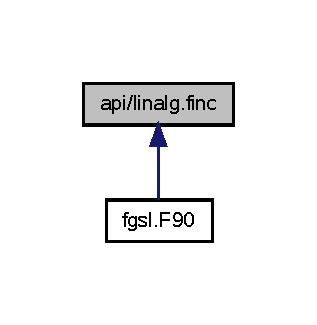
\includegraphics[width=154pt]{linalg_8finc__dep__incl}
\end{center}
\end{figure}
\subsection*{Functions/\-Subroutines}
\begin{DoxyCompactItemize}
\item 
integer(fgsl\-\_\-int) function \hyperlink{linalg_8finc_a121a7317ed9ff3908280670e9df43236}{fgsl\-\_\-linalg\-\_\-lu\-\_\-decomp} (a, p, signum)
\item 
integer(fgsl\-\_\-int) function \hyperlink{linalg_8finc_a0bbccda0d445fb8052f75de6f816b0ce}{fgsl\-\_\-linalg\-\_\-complex\-\_\-lu\-\_\-decomp} (a, p, signum)
\item 
integer(fgsl\-\_\-int) function \hyperlink{linalg_8finc_a79f7596727c6fd25fae6dcc5f519a8d7}{fgsl\-\_\-linalg\-\_\-lu\-\_\-solve} (lu, p, b, x)
\item 
integer(fgsl\-\_\-int) function \hyperlink{linalg_8finc_ad5c7f8769c7bc735e77db729b4355e76}{fgsl\-\_\-linalg\-\_\-complex\-\_\-lu\-\_\-solve} (lu, p, b, x)
\item 
integer(fgsl\-\_\-int) function \hyperlink{linalg_8finc_a79df0025823e3de429baa1263db76d21}{fgsl\-\_\-linalg\-\_\-lu\-\_\-svx} (lu, p, x)
\item 
integer(fgsl\-\_\-int) function \hyperlink{linalg_8finc_afdedc295a99655df475285c0e01407bb}{fgsl\-\_\-linalg\-\_\-complex\-\_\-lu\-\_\-svx} (lu, p, x)
\item 
integer(fgsl\-\_\-int) function \hyperlink{linalg_8finc_aaf17561bd36bb884526bebfc9696558b}{fgsl\-\_\-linalg\-\_\-lu\-\_\-refine} (a, lu, p, b, x, residual)
\item 
integer(fgsl\-\_\-int) function \hyperlink{linalg_8finc_a6303f3ab1b96b8841f7cbcc7291bd79c}{fgsl\-\_\-linalg\-\_\-complex\-\_\-lu\-\_\-refine} (a, lu, p, b, x, residual)
\item 
integer(fgsl\-\_\-int) function \hyperlink{linalg_8finc_ae2390785aa3a33f1619b793bf2caecad}{fgsl\-\_\-linalg\-\_\-lu\-\_\-invert} (lu, p, inverse)
\item 
integer(fgsl\-\_\-int) function \hyperlink{linalg_8finc_a3df5d0ceea88fa0a7675a6a75e749e76}{fgsl\-\_\-linalg\-\_\-complex\-\_\-lu\-\_\-invert} (lu, p, inverse)
\item 
real(fgsl\-\_\-double) function \hyperlink{linalg_8finc_a2f5f7d668125b203b30bcce6415e5cc4}{fgsl\-\_\-linalg\-\_\-lu\-\_\-det} (lu, signum)
\item 
complex(fgsl\-\_\-double\-\_\-complex) \\*
function \hyperlink{linalg_8finc_a4b7c1ddb2195cc26e8040ac0bae5b957}{fgsl\-\_\-linalg\-\_\-complex\-\_\-lu\-\_\-det} (lu, signum)
\item 
real(fgsl\-\_\-double) function \hyperlink{linalg_8finc_a52edf61cc5516e7caf8519816c749ab8}{fgsl\-\_\-linalg\-\_\-lu\-\_\-lndet} (lu)
\item 
real(fgsl\-\_\-double) function \hyperlink{linalg_8finc_a92abce3042e05ad514f7f22b06ed8c27}{fgsl\-\_\-linalg\-\_\-complex\-\_\-lu\-\_\-lndet} (lu)
\item 
integer(fgsl\-\_\-int) function \hyperlink{linalg_8finc_ad630c42318782e35aae8ddf417c988c7}{fgsl\-\_\-linalg\-\_\-lu\-\_\-sgndet} (lu, signum)
\item 
complex(fgsl\-\_\-double\-\_\-complex) \\*
function \hyperlink{linalg_8finc_a3ac75e4a38e037d1b4b652e84030665b}{fgsl\-\_\-linalg\-\_\-complex\-\_\-lu\-\_\-sgndet} (lu, signum)
\item 
integer(fgsl\-\_\-int) function \hyperlink{linalg_8finc_abae4bc6bf64efb5860b999ae7001bda7}{fgsl\-\_\-linalg\-\_\-qr\-\_\-decomp} (a, tau)
\item 
integer(fgsl\-\_\-int) function \hyperlink{linalg_8finc_a453aab0af228f854c2c4e21af6e0f950}{fgsl\-\_\-linalg\-\_\-qr\-\_\-solve} (qr, tau, b, x)
\item 
integer(fgsl\-\_\-int) function \hyperlink{linalg_8finc_a7029ed3e4a0df13a7599a87f5260e377}{fgsl\-\_\-linalg\-\_\-qr\-\_\-svx} (qr, tau, x)
\item 
integer(fgsl\-\_\-int) function \hyperlink{linalg_8finc_afee3a0235231a2e3707a21e1fb07173a}{fgsl\-\_\-linalg\-\_\-qr\-\_\-lssolve} (qr, tau, b, x, residual)
\item 
integer(fgsl\-\_\-int) function \hyperlink{linalg_8finc_a6987f9175c49215f6c78c48de3f01a1d}{fgsl\-\_\-linalg\-\_\-qr\-\_\-qtvec} (qr, tau, v)
\item 
integer(fgsl\-\_\-int) function \hyperlink{linalg_8finc_a8052f69f7485e6a05de0b1be501ed840}{fgsl\-\_\-linalg\-\_\-qr\-\_\-qvec} (qr, tau, v)
\item 
integer(fgsl\-\_\-int) function \hyperlink{linalg_8finc_a261ef794cdf8d3055ef837dd3691f785}{fgsl\-\_\-linalg\-\_\-qr\-\_\-qtmat} (qr, tau, a)
\item 
integer(fgsl\-\_\-int) function \hyperlink{linalg_8finc_a1560faca27750ff17598a738727114e2}{fgsl\-\_\-linalg\-\_\-qr\-\_\-rsolve} (qr, b, x)
\item 
integer(fgsl\-\_\-int) function \hyperlink{linalg_8finc_a0ea403e6c3ec1e67b25bfe4d6b710077}{fgsl\-\_\-linalg\-\_\-qr\-\_\-rsvx} (qr, x)
\item 
integer(fgsl\-\_\-int) function \hyperlink{linalg_8finc_af11174059688ffdbc3f368d6b1a731ee}{fgsl\-\_\-linalg\-\_\-qr\-\_\-unpack} (qr, tau, q, r)
\item 
integer(fgsl\-\_\-int) function \hyperlink{linalg_8finc_a36ef785b86019f22ea32594b5f8060af}{fgsl\-\_\-linalg\-\_\-qr\-\_\-qrsolve} (q, r, b, x)
\item 
integer(fgsl\-\_\-int) function \hyperlink{linalg_8finc_a50523f2137f82ac54ac5f406c4792799}{fgsl\-\_\-linalg\-\_\-qr\-\_\-update} (q, r, w, v)
\item 
integer(fgsl\-\_\-int) function \hyperlink{linalg_8finc_a743b1e1ab7afa142625cd541cffc2147}{fgsl\-\_\-linalg\-\_\-r\-\_\-solve} (r, b, x)
\item 
integer(fgsl\-\_\-int) function \hyperlink{linalg_8finc_abdf5b79e92c6109a0f364962ebcae949}{fgsl\-\_\-linalg\-\_\-r\-\_\-svx} (r, x)
\item 
integer(fgsl\-\_\-int) function \hyperlink{linalg_8finc_a69ea60b78e3baf963ededde50ad72836}{fgsl\-\_\-linalg\-\_\-qrpt\-\_\-decomp} (a, tau, p, signum, norm)
\item 
integer(fgsl\-\_\-int) function \hyperlink{linalg_8finc_a3257e315b9925b49e4c4795631c90808}{fgsl\-\_\-linalg\-\_\-qrpt\-\_\-decomp2} (a, q, r, tau, p, signum, norm)
\item 
integer(fgsl\-\_\-int) function \hyperlink{linalg_8finc_aaa778ea46e4bbefce215f2341620507d}{fgsl\-\_\-linalg\-\_\-qrpt\-\_\-solve} (qr, tau, p, b, x)
\item 
integer(fgsl\-\_\-int) function \hyperlink{linalg_8finc_a79ba5beb414eb0cc23e02a005ee8aa8a}{fgsl\-\_\-linalg\-\_\-qrpt\-\_\-svx} (qr, tau, p, x)
\item 
integer(fgsl\-\_\-int) function \hyperlink{linalg_8finc_a9601978a5c17c13e34d19ddb3d5af6bc}{fgsl\-\_\-linalg\-\_\-qrpt\-\_\-qrsolve} (q, r, p, b, x)
\item 
integer(fgsl\-\_\-int) function \hyperlink{linalg_8finc_a65c186f60ce2d97d132e3df57c18ba35}{fgsl\-\_\-linalg\-\_\-qrpt\-\_\-update} (q, r, p, w, v)
\item 
integer(fgsl\-\_\-int) function \hyperlink{linalg_8finc_a632f5517167f0e2fa649ad9ab2f3d4d0}{fgsl\-\_\-linalg\-\_\-qrpt\-\_\-rsolve} (qr, p, b, x)
\item 
integer(fgsl\-\_\-int) function \hyperlink{linalg_8finc_a58f84af1a42b1026a971543a061f45f8}{fgsl\-\_\-linalg\-\_\-qrpt\-\_\-rsvx} (qr, p, x)
\item 
integer(fgsl\-\_\-int) function \hyperlink{linalg_8finc_ab47674d931fc561a5417410ec464e758}{fgsl\-\_\-linalg\-\_\-sv\-\_\-decomp} (a, v, s, work)
\item 
integer(fgsl\-\_\-int) function \hyperlink{linalg_8finc_af9767f953466e17a78a835c1fb21e588}{fgsl\-\_\-linalg\-\_\-sv\-\_\-decomp\-\_\-mod} (a, x, v, s, work)
\item 
integer(fgsl\-\_\-int) function \hyperlink{linalg_8finc_a523fe136a01c78b49531b7e0156b97b6}{fgsl\-\_\-linalg\-\_\-sv\-\_\-decomp\-\_\-jacobi} (a, v, s)
\item 
integer(fgsl\-\_\-int) function \hyperlink{linalg_8finc_a6d96a619a57aeb6a8713babe93a9b71b}{fgsl\-\_\-linalg\-\_\-sv\-\_\-solve} (u, v, s, b, x)
\item 
integer(fgsl\-\_\-int) function \hyperlink{linalg_8finc_a41dd0ef07e31a1e6d109e4d9a0ea8a13}{fgsl\-\_\-linalg\-\_\-sv\-\_\-leverage} (u, h)
\item 
integer(fgsl\-\_\-int) function \hyperlink{linalg_8finc_aa2fa70a59c49090e137f5df8c8c0100f}{fgsl\-\_\-linalg\-\_\-cholesky\-\_\-decomp} (a)
\item 
integer(fgsl\-\_\-int) function \hyperlink{linalg_8finc_a8f9547ecd2fa79bcf02e423c078bb4ea}{fgsl\-\_\-linalg\-\_\-complex\-\_\-cholesky\-\_\-decomp} (a)
\item 
integer(fgsl\-\_\-int) function \hyperlink{linalg_8finc_a7bca2d4f11f9e651c747926af5a5be70}{fgsl\-\_\-linalg\-\_\-cholesky\-\_\-solve} (chol, b, x)
\item 
integer(fgsl\-\_\-int) function \hyperlink{linalg_8finc_a7ff644dd25158aa5e839ccbc63a5d323}{fgsl\-\_\-linalg\-\_\-complex\-\_\-cholesky\-\_\-solve} (chol, b, x)
\item 
integer(fgsl\-\_\-int) function \hyperlink{linalg_8finc_ac949d4b315b2803bf6d98a3b1549321a}{fgsl\-\_\-linalg\-\_\-cholesky\-\_\-svx} (chol, x)
\item 
integer(fgsl\-\_\-int) function \hyperlink{linalg_8finc_a20424291c37db28845ad5b97cbefb32d}{fgsl\-\_\-linalg\-\_\-complex\-\_\-cholesky\-\_\-svx} (chol, x)
\item 
integer(fgsl\-\_\-int) function \hyperlink{linalg_8finc_a0613e58907c2ae3d3527bc6d76db20f9}{fgsl\-\_\-linalg\-\_\-cholesky\-\_\-invert} (chol)
\item 
integer(fgsl\-\_\-int) function \hyperlink{linalg_8finc_ab986997d7b43b9df1c81a62c0117d3da}{fgsl\-\_\-linalg\-\_\-complex\-\_\-cholesky\-\_\-invert} (chol)
\item 
integer(fgsl\-\_\-int) function \hyperlink{linalg_8finc_a529a24d383e0ed224830a3b5a45329b4}{fgsl\-\_\-linalg\-\_\-symmtd\-\_\-decomp} (a, tau)
\item 
integer(fgsl\-\_\-int) function \hyperlink{linalg_8finc_a43c68814765ca38dd4054712c4dde774}{fgsl\-\_\-linalg\-\_\-symmtd\-\_\-unpack} (a, tau, q, diag, subdiag)
\item 
integer(fgsl\-\_\-int) function \hyperlink{linalg_8finc_a4d487701aea9f427ae6482afc63567ee}{fgsl\-\_\-linalg\-\_\-symmtd\-\_\-unpack\-\_\-t} (a, diag, subdiag)
\item 
integer(fgsl\-\_\-int) function \hyperlink{linalg_8finc_a74f45468131667f4aca749e082229d74}{fgsl\-\_\-linalg\-\_\-hermtd\-\_\-decomp} (a, tau)
\item 
integer(fgsl\-\_\-int) function \hyperlink{linalg_8finc_a01ea43da6a22ccd051afcdb73b7aaec6}{fgsl\-\_\-linalg\-\_\-hermtd\-\_\-unpack} (a, tau, q, diag, subdiag)
\item 
integer(fgsl\-\_\-int) function \hyperlink{linalg_8finc_a37ef96a808f0cfa726988a9455e4dd77}{fgsl\-\_\-linalg\-\_\-hermtd\-\_\-unpack\-\_\-t} (a, diag, subdiag)
\item 
integer(fgsl\-\_\-int) function \hyperlink{linalg_8finc_af4db62c7ddadd76db95bc18c7dea1c17}{fgsl\-\_\-linalg\-\_\-hessenberg\-\_\-decomp} (a, tau)
\item 
integer(fgsl\-\_\-int) function \hyperlink{linalg_8finc_a8a3e7b735728a0611071d965a54afcc0}{fgsl\-\_\-linalg\-\_\-hessenberg\-\_\-unpack} (h, tau, u)
\item 
integer(fgsl\-\_\-int) function \hyperlink{linalg_8finc_aaf9c79890dea66d6d45f2c2bd9af1bec}{fgsl\-\_\-linalg\-\_\-hessenberg\-\_\-unpack\-\_\-accum} (h, tau, v)
\item 
integer(fgsl\-\_\-int) function \hyperlink{linalg_8finc_a1eb4e89fd2d82ec33f0f7ace0c484297}{fgsl\-\_\-linalg\-\_\-hessenberg\-\_\-set\-\_\-zero} (h)
\item 
integer(fgsl\-\_\-int) function \hyperlink{linalg_8finc_abe28bd8eb9ba42991ecd9042e66c9ecb}{fgsl\-\_\-linalg\-\_\-hesstri\-\_\-decomp} (a, b, u, v, work)
\item 
integer(fgsl\-\_\-int) function \hyperlink{linalg_8finc_a1b8fd96dfd1905be8b356cccaa69e8de}{fgsl\-\_\-linalg\-\_\-bidiag\-\_\-decomp} (a, tau\-\_\-u, tau\-\_\-v)
\item 
integer(fgsl\-\_\-int) function \hyperlink{linalg_8finc_ae2b8fd74655b817b2a3a0365dfa75947}{fgsl\-\_\-linalg\-\_\-bidiag\-\_\-unpack} (a, tau\-\_\-u, u, tau\-\_\-v, v, diag, superdiag)
\item 
integer(fgsl\-\_\-int) function \hyperlink{linalg_8finc_aec13a9130466da66635043f17542e07e}{fgsl\-\_\-linalg\-\_\-bidiag\-\_\-unpack2} (a, tau\-\_\-u, tau\-\_\-v, v)
\item 
integer(fgsl\-\_\-int) function \hyperlink{linalg_8finc_a6ba88b99540d03bfd2b8387e7f5ef0a3}{fgsl\-\_\-linalg\-\_\-bidiag\-\_\-unpack\-\_\-b} (a, diag, superdiag)
\item 
real(fgsl\-\_\-double) function \hyperlink{linalg_8finc_a3561232af3abecaf60ac8babfe48a868}{fgsl\-\_\-linalg\-\_\-householder\-\_\-transform} (v)
\item 
complex(fgsl\-\_\-double\-\_\-complex) \\*
function \hyperlink{linalg_8finc_a7bd1bfa2419818da7392462ec4e51a49}{fgsl\-\_\-linalg\-\_\-complex\-\_\-householder\-\_\-transform} (v)
\item 
integer(fgsl\-\_\-int) function \hyperlink{linalg_8finc_abbaccde9508cf3805e8fd920e086b306}{fgsl\-\_\-linalg\-\_\-householder\-\_\-hm} (tau, v, a)
\item 
integer(fgsl\-\_\-int) function \hyperlink{linalg_8finc_a6cfd891d07d48aa2404785b7607a8ca1}{fgsl\-\_\-linalg\-\_\-complex\-\_\-householder\-\_\-hm} (tau, v, a)
\item 
integer(fgsl\-\_\-int) function \hyperlink{linalg_8finc_a0215003deddc89a15be1533dcfadd837}{fgsl\-\_\-linalg\-\_\-householder\-\_\-mh} (tau, v, a)
\item 
integer(fgsl\-\_\-int) function \hyperlink{linalg_8finc_a3c2d047dceeba00601c6a049eedb7c58}{fgsl\-\_\-linalg\-\_\-complex\-\_\-householder\-\_\-mh} (tau, v, a)
\item 
integer(fgsl\-\_\-int) function \hyperlink{linalg_8finc_af93afe6e7341885e9672d74b4d113c62}{fgsl\-\_\-linalg\-\_\-householder\-\_\-hv} (tau, v, w)
\item 
integer(fgsl\-\_\-int) function \hyperlink{linalg_8finc_a577aa9f2f2795c9d8d545502e0baae34}{fgsl\-\_\-linalg\-\_\-complex\-\_\-householder\-\_\-hv} (tau, v, w)
\item 
integer(fgsl\-\_\-int) function \hyperlink{linalg_8finc_a0da76044dd77df2922422968347c1d00}{fgsl\-\_\-linalg\-\_\-hh\-\_\-solve} (a, b, x)
\item 
integer(fgsl\-\_\-int) function \hyperlink{linalg_8finc_ae4d2e360e54f77fbdef78af0fd6c8348}{fgsl\-\_\-linalg\-\_\-hh\-\_\-svx} (a, x)
\item 
integer(c\-\_\-int) function \hyperlink{linalg_8finc_ad5daaa9a613e3d9e8668191df02d1d85}{fgsl\-\_\-linalg\-\_\-solve\-\_\-tridiag} (diag, e, f, b, x)
\item 
integer(c\-\_\-int) function \hyperlink{linalg_8finc_a91cd2d731729955df9677ae3e44b4799}{fgsl\-\_\-linalg\-\_\-solve\-\_\-symm\-\_\-tridiag} (diag, e, b, x)
\item 
integer(c\-\_\-int) function \hyperlink{linalg_8finc_a3a0cc14d7736d7e20be30ed7f07f093e}{fgsl\-\_\-linalg\-\_\-solve\-\_\-cyc\-\_\-tridiag} (diag, e, f, b, x)
\item 
integer(c\-\_\-int) function \hyperlink{linalg_8finc_aea909b87fb81242ac465f6651e63f536}{fgsl\-\_\-linalg\-\_\-solve\-\_\-symm\-\_\-cyc\-\_\-tridiag} (diag, e, b, x)
\item 
integer(fgsl\-\_\-int) function \hyperlink{linalg_8finc_a82232b7f631cacda2a903f1d0fae1263}{fgsl\-\_\-linalg\-\_\-balance\-\_\-matrix} (a, d)
\end{DoxyCompactItemize}


\subsection{Function/\-Subroutine Documentation}
\hypertarget{linalg_8finc_a82232b7f631cacda2a903f1d0fae1263}{\index{linalg.\-finc@{linalg.\-finc}!fgsl\-\_\-linalg\-\_\-balance\-\_\-matrix@{fgsl\-\_\-linalg\-\_\-balance\-\_\-matrix}}
\index{fgsl\-\_\-linalg\-\_\-balance\-\_\-matrix@{fgsl\-\_\-linalg\-\_\-balance\-\_\-matrix}!linalg.finc@{linalg.\-finc}}
\subsubsection[{fgsl\-\_\-linalg\-\_\-balance\-\_\-matrix}]{\setlength{\rightskip}{0pt plus 5cm}integer(fgsl\-\_\-int) function fgsl\-\_\-linalg\-\_\-balance\-\_\-matrix (
\begin{DoxyParamCaption}
\item[{type(fgsl\-\_\-matrix), intent(inout)}]{a, }
\item[{type(fgsl\-\_\-vector), intent(inout)}]{d}
\end{DoxyParamCaption}
)}}\label{linalg_8finc_a82232b7f631cacda2a903f1d0fae1263}
\hypertarget{linalg_8finc_a1b8fd96dfd1905be8b356cccaa69e8de}{\index{linalg.\-finc@{linalg.\-finc}!fgsl\-\_\-linalg\-\_\-bidiag\-\_\-decomp@{fgsl\-\_\-linalg\-\_\-bidiag\-\_\-decomp}}
\index{fgsl\-\_\-linalg\-\_\-bidiag\-\_\-decomp@{fgsl\-\_\-linalg\-\_\-bidiag\-\_\-decomp}!linalg.finc@{linalg.\-finc}}
\subsubsection[{fgsl\-\_\-linalg\-\_\-bidiag\-\_\-decomp}]{\setlength{\rightskip}{0pt plus 5cm}integer(fgsl\-\_\-int) function fgsl\-\_\-linalg\-\_\-bidiag\-\_\-decomp (
\begin{DoxyParamCaption}
\item[{type(fgsl\-\_\-matrix), intent(inout)}]{a, }
\item[{type(fgsl\-\_\-vector), intent(inout)}]{tau\-\_\-u, }
\item[{type(fgsl\-\_\-vector), intent(inout)}]{tau\-\_\-v}
\end{DoxyParamCaption}
)}}\label{linalg_8finc_a1b8fd96dfd1905be8b356cccaa69e8de}
\hypertarget{linalg_8finc_ae2b8fd74655b817b2a3a0365dfa75947}{\index{linalg.\-finc@{linalg.\-finc}!fgsl\-\_\-linalg\-\_\-bidiag\-\_\-unpack@{fgsl\-\_\-linalg\-\_\-bidiag\-\_\-unpack}}
\index{fgsl\-\_\-linalg\-\_\-bidiag\-\_\-unpack@{fgsl\-\_\-linalg\-\_\-bidiag\-\_\-unpack}!linalg.finc@{linalg.\-finc}}
\subsubsection[{fgsl\-\_\-linalg\-\_\-bidiag\-\_\-unpack}]{\setlength{\rightskip}{0pt plus 5cm}integer(fgsl\-\_\-int) function fgsl\-\_\-linalg\-\_\-bidiag\-\_\-unpack (
\begin{DoxyParamCaption}
\item[{type(fgsl\-\_\-matrix), intent(in)}]{a, }
\item[{type(fgsl\-\_\-vector), intent(in)}]{tau\-\_\-u, }
\item[{type(fgsl\-\_\-matrix), intent(inout)}]{u, }
\item[{type(fgsl\-\_\-vector), intent(in)}]{tau\-\_\-v, }
\item[{type(fgsl\-\_\-matrix), intent(inout)}]{v, }
\item[{type(fgsl\-\_\-vector), intent(inout)}]{diag, }
\item[{type(fgsl\-\_\-vector), intent(inout)}]{superdiag}
\end{DoxyParamCaption}
)}}\label{linalg_8finc_ae2b8fd74655b817b2a3a0365dfa75947}
\hypertarget{linalg_8finc_aec13a9130466da66635043f17542e07e}{\index{linalg.\-finc@{linalg.\-finc}!fgsl\-\_\-linalg\-\_\-bidiag\-\_\-unpack2@{fgsl\-\_\-linalg\-\_\-bidiag\-\_\-unpack2}}
\index{fgsl\-\_\-linalg\-\_\-bidiag\-\_\-unpack2@{fgsl\-\_\-linalg\-\_\-bidiag\-\_\-unpack2}!linalg.finc@{linalg.\-finc}}
\subsubsection[{fgsl\-\_\-linalg\-\_\-bidiag\-\_\-unpack2}]{\setlength{\rightskip}{0pt plus 5cm}integer(fgsl\-\_\-int) function fgsl\-\_\-linalg\-\_\-bidiag\-\_\-unpack2 (
\begin{DoxyParamCaption}
\item[{type(fgsl\-\_\-matrix), intent(inout)}]{a, }
\item[{type(fgsl\-\_\-vector), intent(in)}]{tau\-\_\-u, }
\item[{type(fgsl\-\_\-vector), intent(in)}]{tau\-\_\-v, }
\item[{type(fgsl\-\_\-matrix), intent(inout)}]{v}
\end{DoxyParamCaption}
)}}\label{linalg_8finc_aec13a9130466da66635043f17542e07e}
\hypertarget{linalg_8finc_a6ba88b99540d03bfd2b8387e7f5ef0a3}{\index{linalg.\-finc@{linalg.\-finc}!fgsl\-\_\-linalg\-\_\-bidiag\-\_\-unpack\-\_\-b@{fgsl\-\_\-linalg\-\_\-bidiag\-\_\-unpack\-\_\-b}}
\index{fgsl\-\_\-linalg\-\_\-bidiag\-\_\-unpack\-\_\-b@{fgsl\-\_\-linalg\-\_\-bidiag\-\_\-unpack\-\_\-b}!linalg.finc@{linalg.\-finc}}
\subsubsection[{fgsl\-\_\-linalg\-\_\-bidiag\-\_\-unpack\-\_\-b}]{\setlength{\rightskip}{0pt plus 5cm}integer(fgsl\-\_\-int) function fgsl\-\_\-linalg\-\_\-bidiag\-\_\-unpack\-\_\-b (
\begin{DoxyParamCaption}
\item[{type(fgsl\-\_\-matrix), intent(in)}]{a, }
\item[{type(fgsl\-\_\-vector), intent(inout)}]{diag, }
\item[{type(fgsl\-\_\-vector), intent(inout)}]{superdiag}
\end{DoxyParamCaption}
)}}\label{linalg_8finc_a6ba88b99540d03bfd2b8387e7f5ef0a3}
\hypertarget{linalg_8finc_aa2fa70a59c49090e137f5df8c8c0100f}{\index{linalg.\-finc@{linalg.\-finc}!fgsl\-\_\-linalg\-\_\-cholesky\-\_\-decomp@{fgsl\-\_\-linalg\-\_\-cholesky\-\_\-decomp}}
\index{fgsl\-\_\-linalg\-\_\-cholesky\-\_\-decomp@{fgsl\-\_\-linalg\-\_\-cholesky\-\_\-decomp}!linalg.finc@{linalg.\-finc}}
\subsubsection[{fgsl\-\_\-linalg\-\_\-cholesky\-\_\-decomp}]{\setlength{\rightskip}{0pt plus 5cm}integer(fgsl\-\_\-int) function fgsl\-\_\-linalg\-\_\-cholesky\-\_\-decomp (
\begin{DoxyParamCaption}
\item[{type(fgsl\-\_\-matrix), intent(inout)}]{a}
\end{DoxyParamCaption}
)}}\label{linalg_8finc_aa2fa70a59c49090e137f5df8c8c0100f}
\hypertarget{linalg_8finc_a0613e58907c2ae3d3527bc6d76db20f9}{\index{linalg.\-finc@{linalg.\-finc}!fgsl\-\_\-linalg\-\_\-cholesky\-\_\-invert@{fgsl\-\_\-linalg\-\_\-cholesky\-\_\-invert}}
\index{fgsl\-\_\-linalg\-\_\-cholesky\-\_\-invert@{fgsl\-\_\-linalg\-\_\-cholesky\-\_\-invert}!linalg.finc@{linalg.\-finc}}
\subsubsection[{fgsl\-\_\-linalg\-\_\-cholesky\-\_\-invert}]{\setlength{\rightskip}{0pt plus 5cm}integer(fgsl\-\_\-int) function fgsl\-\_\-linalg\-\_\-cholesky\-\_\-invert (
\begin{DoxyParamCaption}
\item[{type(fgsl\-\_\-matrix), intent(inout)}]{chol}
\end{DoxyParamCaption}
)}}\label{linalg_8finc_a0613e58907c2ae3d3527bc6d76db20f9}
\hypertarget{linalg_8finc_a7bca2d4f11f9e651c747926af5a5be70}{\index{linalg.\-finc@{linalg.\-finc}!fgsl\-\_\-linalg\-\_\-cholesky\-\_\-solve@{fgsl\-\_\-linalg\-\_\-cholesky\-\_\-solve}}
\index{fgsl\-\_\-linalg\-\_\-cholesky\-\_\-solve@{fgsl\-\_\-linalg\-\_\-cholesky\-\_\-solve}!linalg.finc@{linalg.\-finc}}
\subsubsection[{fgsl\-\_\-linalg\-\_\-cholesky\-\_\-solve}]{\setlength{\rightskip}{0pt plus 5cm}integer(fgsl\-\_\-int) function fgsl\-\_\-linalg\-\_\-cholesky\-\_\-solve (
\begin{DoxyParamCaption}
\item[{type(fgsl\-\_\-matrix), intent(in)}]{chol, }
\item[{type(fgsl\-\_\-vector), intent(in)}]{b, }
\item[{type(fgsl\-\_\-vector), intent(inout)}]{x}
\end{DoxyParamCaption}
)}}\label{linalg_8finc_a7bca2d4f11f9e651c747926af5a5be70}
\hypertarget{linalg_8finc_ac949d4b315b2803bf6d98a3b1549321a}{\index{linalg.\-finc@{linalg.\-finc}!fgsl\-\_\-linalg\-\_\-cholesky\-\_\-svx@{fgsl\-\_\-linalg\-\_\-cholesky\-\_\-svx}}
\index{fgsl\-\_\-linalg\-\_\-cholesky\-\_\-svx@{fgsl\-\_\-linalg\-\_\-cholesky\-\_\-svx}!linalg.finc@{linalg.\-finc}}
\subsubsection[{fgsl\-\_\-linalg\-\_\-cholesky\-\_\-svx}]{\setlength{\rightskip}{0pt plus 5cm}integer(fgsl\-\_\-int) function fgsl\-\_\-linalg\-\_\-cholesky\-\_\-svx (
\begin{DoxyParamCaption}
\item[{type(fgsl\-\_\-matrix), intent(in)}]{chol, }
\item[{type(fgsl\-\_\-vector), intent(inout)}]{x}
\end{DoxyParamCaption}
)}}\label{linalg_8finc_ac949d4b315b2803bf6d98a3b1549321a}
\hypertarget{linalg_8finc_a8f9547ecd2fa79bcf02e423c078bb4ea}{\index{linalg.\-finc@{linalg.\-finc}!fgsl\-\_\-linalg\-\_\-complex\-\_\-cholesky\-\_\-decomp@{fgsl\-\_\-linalg\-\_\-complex\-\_\-cholesky\-\_\-decomp}}
\index{fgsl\-\_\-linalg\-\_\-complex\-\_\-cholesky\-\_\-decomp@{fgsl\-\_\-linalg\-\_\-complex\-\_\-cholesky\-\_\-decomp}!linalg.finc@{linalg.\-finc}}
\subsubsection[{fgsl\-\_\-linalg\-\_\-complex\-\_\-cholesky\-\_\-decomp}]{\setlength{\rightskip}{0pt plus 5cm}integer(fgsl\-\_\-int) function fgsl\-\_\-linalg\-\_\-complex\-\_\-cholesky\-\_\-decomp (
\begin{DoxyParamCaption}
\item[{type(fgsl\-\_\-matrix\-\_\-complex), intent(inout)}]{a}
\end{DoxyParamCaption}
)}}\label{linalg_8finc_a8f9547ecd2fa79bcf02e423c078bb4ea}
\hypertarget{linalg_8finc_ab986997d7b43b9df1c81a62c0117d3da}{\index{linalg.\-finc@{linalg.\-finc}!fgsl\-\_\-linalg\-\_\-complex\-\_\-cholesky\-\_\-invert@{fgsl\-\_\-linalg\-\_\-complex\-\_\-cholesky\-\_\-invert}}
\index{fgsl\-\_\-linalg\-\_\-complex\-\_\-cholesky\-\_\-invert@{fgsl\-\_\-linalg\-\_\-complex\-\_\-cholesky\-\_\-invert}!linalg.finc@{linalg.\-finc}}
\subsubsection[{fgsl\-\_\-linalg\-\_\-complex\-\_\-cholesky\-\_\-invert}]{\setlength{\rightskip}{0pt plus 5cm}integer(fgsl\-\_\-int) function fgsl\-\_\-linalg\-\_\-complex\-\_\-cholesky\-\_\-invert (
\begin{DoxyParamCaption}
\item[{type(fgsl\-\_\-matrix\-\_\-complex), intent(inout)}]{chol}
\end{DoxyParamCaption}
)}}\label{linalg_8finc_ab986997d7b43b9df1c81a62c0117d3da}
\hypertarget{linalg_8finc_a7ff644dd25158aa5e839ccbc63a5d323}{\index{linalg.\-finc@{linalg.\-finc}!fgsl\-\_\-linalg\-\_\-complex\-\_\-cholesky\-\_\-solve@{fgsl\-\_\-linalg\-\_\-complex\-\_\-cholesky\-\_\-solve}}
\index{fgsl\-\_\-linalg\-\_\-complex\-\_\-cholesky\-\_\-solve@{fgsl\-\_\-linalg\-\_\-complex\-\_\-cholesky\-\_\-solve}!linalg.finc@{linalg.\-finc}}
\subsubsection[{fgsl\-\_\-linalg\-\_\-complex\-\_\-cholesky\-\_\-solve}]{\setlength{\rightskip}{0pt plus 5cm}integer(fgsl\-\_\-int) function fgsl\-\_\-linalg\-\_\-complex\-\_\-cholesky\-\_\-solve (
\begin{DoxyParamCaption}
\item[{type(fgsl\-\_\-matrix\-\_\-complex), intent(in)}]{chol, }
\item[{type(fgsl\-\_\-vector\-\_\-complex), intent(in)}]{b, }
\item[{type(fgsl\-\_\-vector\-\_\-complex), intent(inout)}]{x}
\end{DoxyParamCaption}
)}}\label{linalg_8finc_a7ff644dd25158aa5e839ccbc63a5d323}
\hypertarget{linalg_8finc_a20424291c37db28845ad5b97cbefb32d}{\index{linalg.\-finc@{linalg.\-finc}!fgsl\-\_\-linalg\-\_\-complex\-\_\-cholesky\-\_\-svx@{fgsl\-\_\-linalg\-\_\-complex\-\_\-cholesky\-\_\-svx}}
\index{fgsl\-\_\-linalg\-\_\-complex\-\_\-cholesky\-\_\-svx@{fgsl\-\_\-linalg\-\_\-complex\-\_\-cholesky\-\_\-svx}!linalg.finc@{linalg.\-finc}}
\subsubsection[{fgsl\-\_\-linalg\-\_\-complex\-\_\-cholesky\-\_\-svx}]{\setlength{\rightskip}{0pt plus 5cm}integer(fgsl\-\_\-int) function fgsl\-\_\-linalg\-\_\-complex\-\_\-cholesky\-\_\-svx (
\begin{DoxyParamCaption}
\item[{type(fgsl\-\_\-matrix\-\_\-complex), intent(in)}]{chol, }
\item[{type(fgsl\-\_\-vector\-\_\-complex), intent(inout)}]{x}
\end{DoxyParamCaption}
)}}\label{linalg_8finc_a20424291c37db28845ad5b97cbefb32d}
\hypertarget{linalg_8finc_a6cfd891d07d48aa2404785b7607a8ca1}{\index{linalg.\-finc@{linalg.\-finc}!fgsl\-\_\-linalg\-\_\-complex\-\_\-householder\-\_\-hm@{fgsl\-\_\-linalg\-\_\-complex\-\_\-householder\-\_\-hm}}
\index{fgsl\-\_\-linalg\-\_\-complex\-\_\-householder\-\_\-hm@{fgsl\-\_\-linalg\-\_\-complex\-\_\-householder\-\_\-hm}!linalg.finc@{linalg.\-finc}}
\subsubsection[{fgsl\-\_\-linalg\-\_\-complex\-\_\-householder\-\_\-hm}]{\setlength{\rightskip}{0pt plus 5cm}integer(fgsl\-\_\-int) function fgsl\-\_\-linalg\-\_\-complex\-\_\-householder\-\_\-hm (
\begin{DoxyParamCaption}
\item[{complex(fgsl\-\_\-double\-\_\-complex), intent(in)}]{tau, }
\item[{type(fgsl\-\_\-vector\-\_\-complex), intent(in)}]{v, }
\item[{type(fgsl\-\_\-matrix\-\_\-complex), intent(inout)}]{a}
\end{DoxyParamCaption}
)}}\label{linalg_8finc_a6cfd891d07d48aa2404785b7607a8ca1}
\hypertarget{linalg_8finc_a577aa9f2f2795c9d8d545502e0baae34}{\index{linalg.\-finc@{linalg.\-finc}!fgsl\-\_\-linalg\-\_\-complex\-\_\-householder\-\_\-hv@{fgsl\-\_\-linalg\-\_\-complex\-\_\-householder\-\_\-hv}}
\index{fgsl\-\_\-linalg\-\_\-complex\-\_\-householder\-\_\-hv@{fgsl\-\_\-linalg\-\_\-complex\-\_\-householder\-\_\-hv}!linalg.finc@{linalg.\-finc}}
\subsubsection[{fgsl\-\_\-linalg\-\_\-complex\-\_\-householder\-\_\-hv}]{\setlength{\rightskip}{0pt plus 5cm}integer(fgsl\-\_\-int) function fgsl\-\_\-linalg\-\_\-complex\-\_\-householder\-\_\-hv (
\begin{DoxyParamCaption}
\item[{complex(fgsl\-\_\-double\-\_\-complex), intent(in)}]{tau, }
\item[{type(fgsl\-\_\-vector\-\_\-complex), intent(in)}]{v, }
\item[{type(fgsl\-\_\-vector\-\_\-complex), intent(inout)}]{w}
\end{DoxyParamCaption}
)}}\label{linalg_8finc_a577aa9f2f2795c9d8d545502e0baae34}
\hypertarget{linalg_8finc_a3c2d047dceeba00601c6a049eedb7c58}{\index{linalg.\-finc@{linalg.\-finc}!fgsl\-\_\-linalg\-\_\-complex\-\_\-householder\-\_\-mh@{fgsl\-\_\-linalg\-\_\-complex\-\_\-householder\-\_\-mh}}
\index{fgsl\-\_\-linalg\-\_\-complex\-\_\-householder\-\_\-mh@{fgsl\-\_\-linalg\-\_\-complex\-\_\-householder\-\_\-mh}!linalg.finc@{linalg.\-finc}}
\subsubsection[{fgsl\-\_\-linalg\-\_\-complex\-\_\-householder\-\_\-mh}]{\setlength{\rightskip}{0pt plus 5cm}integer(fgsl\-\_\-int) function fgsl\-\_\-linalg\-\_\-complex\-\_\-householder\-\_\-mh (
\begin{DoxyParamCaption}
\item[{complex(fgsl\-\_\-double\-\_\-complex), intent(in)}]{tau, }
\item[{type(fgsl\-\_\-vector\-\_\-complex), intent(in)}]{v, }
\item[{type(fgsl\-\_\-matrix\-\_\-complex), intent(inout)}]{a}
\end{DoxyParamCaption}
)}}\label{linalg_8finc_a3c2d047dceeba00601c6a049eedb7c58}
\hypertarget{linalg_8finc_a7bd1bfa2419818da7392462ec4e51a49}{\index{linalg.\-finc@{linalg.\-finc}!fgsl\-\_\-linalg\-\_\-complex\-\_\-householder\-\_\-transform@{fgsl\-\_\-linalg\-\_\-complex\-\_\-householder\-\_\-transform}}
\index{fgsl\-\_\-linalg\-\_\-complex\-\_\-householder\-\_\-transform@{fgsl\-\_\-linalg\-\_\-complex\-\_\-householder\-\_\-transform}!linalg.finc@{linalg.\-finc}}
\subsubsection[{fgsl\-\_\-linalg\-\_\-complex\-\_\-householder\-\_\-transform}]{\setlength{\rightskip}{0pt plus 5cm}complex(fgsl\-\_\-double\-\_\-complex) function fgsl\-\_\-linalg\-\_\-complex\-\_\-householder\-\_\-transform (
\begin{DoxyParamCaption}
\item[{type(fgsl\-\_\-vector), intent(inout)}]{v}
\end{DoxyParamCaption}
)}}\label{linalg_8finc_a7bd1bfa2419818da7392462ec4e51a49}
\hypertarget{linalg_8finc_a0bbccda0d445fb8052f75de6f816b0ce}{\index{linalg.\-finc@{linalg.\-finc}!fgsl\-\_\-linalg\-\_\-complex\-\_\-lu\-\_\-decomp@{fgsl\-\_\-linalg\-\_\-complex\-\_\-lu\-\_\-decomp}}
\index{fgsl\-\_\-linalg\-\_\-complex\-\_\-lu\-\_\-decomp@{fgsl\-\_\-linalg\-\_\-complex\-\_\-lu\-\_\-decomp}!linalg.finc@{linalg.\-finc}}
\subsubsection[{fgsl\-\_\-linalg\-\_\-complex\-\_\-lu\-\_\-decomp}]{\setlength{\rightskip}{0pt plus 5cm}integer(fgsl\-\_\-int) function fgsl\-\_\-linalg\-\_\-complex\-\_\-lu\-\_\-decomp (
\begin{DoxyParamCaption}
\item[{type(fgsl\-\_\-matrix\-\_\-complex)}]{a, }
\item[{type(fgsl\-\_\-permutation)}]{p, }
\item[{integer(fgsl\-\_\-int)}]{signum}
\end{DoxyParamCaption}
)}}\label{linalg_8finc_a0bbccda0d445fb8052f75de6f816b0ce}
\hypertarget{linalg_8finc_a4b7c1ddb2195cc26e8040ac0bae5b957}{\index{linalg.\-finc@{linalg.\-finc}!fgsl\-\_\-linalg\-\_\-complex\-\_\-lu\-\_\-det@{fgsl\-\_\-linalg\-\_\-complex\-\_\-lu\-\_\-det}}
\index{fgsl\-\_\-linalg\-\_\-complex\-\_\-lu\-\_\-det@{fgsl\-\_\-linalg\-\_\-complex\-\_\-lu\-\_\-det}!linalg.finc@{linalg.\-finc}}
\subsubsection[{fgsl\-\_\-linalg\-\_\-complex\-\_\-lu\-\_\-det}]{\setlength{\rightskip}{0pt plus 5cm}complex(fgsl\-\_\-double\-\_\-complex) function fgsl\-\_\-linalg\-\_\-complex\-\_\-lu\-\_\-det (
\begin{DoxyParamCaption}
\item[{type(fgsl\-\_\-matrix\-\_\-complex), intent(in)}]{lu, }
\item[{integer(fgsl\-\_\-int), intent(in)}]{signum}
\end{DoxyParamCaption}
)}}\label{linalg_8finc_a4b7c1ddb2195cc26e8040ac0bae5b957}
\hypertarget{linalg_8finc_a3df5d0ceea88fa0a7675a6a75e749e76}{\index{linalg.\-finc@{linalg.\-finc}!fgsl\-\_\-linalg\-\_\-complex\-\_\-lu\-\_\-invert@{fgsl\-\_\-linalg\-\_\-complex\-\_\-lu\-\_\-invert}}
\index{fgsl\-\_\-linalg\-\_\-complex\-\_\-lu\-\_\-invert@{fgsl\-\_\-linalg\-\_\-complex\-\_\-lu\-\_\-invert}!linalg.finc@{linalg.\-finc}}
\subsubsection[{fgsl\-\_\-linalg\-\_\-complex\-\_\-lu\-\_\-invert}]{\setlength{\rightskip}{0pt plus 5cm}integer(fgsl\-\_\-int) function fgsl\-\_\-linalg\-\_\-complex\-\_\-lu\-\_\-invert (
\begin{DoxyParamCaption}
\item[{type(fgsl\-\_\-matrix\-\_\-complex), intent(in)}]{lu, }
\item[{type(fgsl\-\_\-permutation), intent(in)}]{p, }
\item[{type(fgsl\-\_\-matrix\-\_\-complex), intent(inout)}]{inverse}
\end{DoxyParamCaption}
)}}\label{linalg_8finc_a3df5d0ceea88fa0a7675a6a75e749e76}
\hypertarget{linalg_8finc_a92abce3042e05ad514f7f22b06ed8c27}{\index{linalg.\-finc@{linalg.\-finc}!fgsl\-\_\-linalg\-\_\-complex\-\_\-lu\-\_\-lndet@{fgsl\-\_\-linalg\-\_\-complex\-\_\-lu\-\_\-lndet}}
\index{fgsl\-\_\-linalg\-\_\-complex\-\_\-lu\-\_\-lndet@{fgsl\-\_\-linalg\-\_\-complex\-\_\-lu\-\_\-lndet}!linalg.finc@{linalg.\-finc}}
\subsubsection[{fgsl\-\_\-linalg\-\_\-complex\-\_\-lu\-\_\-lndet}]{\setlength{\rightskip}{0pt plus 5cm}real(fgsl\-\_\-double) function fgsl\-\_\-linalg\-\_\-complex\-\_\-lu\-\_\-lndet (
\begin{DoxyParamCaption}
\item[{type(fgsl\-\_\-matrix\-\_\-complex), intent(in)}]{lu}
\end{DoxyParamCaption}
)}}\label{linalg_8finc_a92abce3042e05ad514f7f22b06ed8c27}
\hypertarget{linalg_8finc_a6303f3ab1b96b8841f7cbcc7291bd79c}{\index{linalg.\-finc@{linalg.\-finc}!fgsl\-\_\-linalg\-\_\-complex\-\_\-lu\-\_\-refine@{fgsl\-\_\-linalg\-\_\-complex\-\_\-lu\-\_\-refine}}
\index{fgsl\-\_\-linalg\-\_\-complex\-\_\-lu\-\_\-refine@{fgsl\-\_\-linalg\-\_\-complex\-\_\-lu\-\_\-refine}!linalg.finc@{linalg.\-finc}}
\subsubsection[{fgsl\-\_\-linalg\-\_\-complex\-\_\-lu\-\_\-refine}]{\setlength{\rightskip}{0pt plus 5cm}integer(fgsl\-\_\-int) function fgsl\-\_\-linalg\-\_\-complex\-\_\-lu\-\_\-refine (
\begin{DoxyParamCaption}
\item[{type(fgsl\-\_\-matrix\-\_\-complex), intent(in)}]{a, }
\item[{type(fgsl\-\_\-matrix\-\_\-complex), intent(in)}]{lu, }
\item[{type(fgsl\-\_\-permutation), intent(in)}]{p, }
\item[{type(fgsl\-\_\-vector\-\_\-complex), intent(in)}]{b, }
\item[{type(fgsl\-\_\-vector\-\_\-complex), intent(inout)}]{x, }
\item[{type(fgsl\-\_\-vector\-\_\-complex), intent(inout)}]{residual}
\end{DoxyParamCaption}
)}}\label{linalg_8finc_a6303f3ab1b96b8841f7cbcc7291bd79c}
\hypertarget{linalg_8finc_a3ac75e4a38e037d1b4b652e84030665b}{\index{linalg.\-finc@{linalg.\-finc}!fgsl\-\_\-linalg\-\_\-complex\-\_\-lu\-\_\-sgndet@{fgsl\-\_\-linalg\-\_\-complex\-\_\-lu\-\_\-sgndet}}
\index{fgsl\-\_\-linalg\-\_\-complex\-\_\-lu\-\_\-sgndet@{fgsl\-\_\-linalg\-\_\-complex\-\_\-lu\-\_\-sgndet}!linalg.finc@{linalg.\-finc}}
\subsubsection[{fgsl\-\_\-linalg\-\_\-complex\-\_\-lu\-\_\-sgndet}]{\setlength{\rightskip}{0pt plus 5cm}complex(fgsl\-\_\-double\-\_\-complex) function fgsl\-\_\-linalg\-\_\-complex\-\_\-lu\-\_\-sgndet (
\begin{DoxyParamCaption}
\item[{type(fgsl\-\_\-matrix\-\_\-complex), intent(in)}]{lu, }
\item[{integer(fgsl\-\_\-int), intent(in)}]{signum}
\end{DoxyParamCaption}
)}}\label{linalg_8finc_a3ac75e4a38e037d1b4b652e84030665b}
\hypertarget{linalg_8finc_ad5c7f8769c7bc735e77db729b4355e76}{\index{linalg.\-finc@{linalg.\-finc}!fgsl\-\_\-linalg\-\_\-complex\-\_\-lu\-\_\-solve@{fgsl\-\_\-linalg\-\_\-complex\-\_\-lu\-\_\-solve}}
\index{fgsl\-\_\-linalg\-\_\-complex\-\_\-lu\-\_\-solve@{fgsl\-\_\-linalg\-\_\-complex\-\_\-lu\-\_\-solve}!linalg.finc@{linalg.\-finc}}
\subsubsection[{fgsl\-\_\-linalg\-\_\-complex\-\_\-lu\-\_\-solve}]{\setlength{\rightskip}{0pt plus 5cm}integer(fgsl\-\_\-int) function fgsl\-\_\-linalg\-\_\-complex\-\_\-lu\-\_\-solve (
\begin{DoxyParamCaption}
\item[{type(fgsl\-\_\-matrix\-\_\-complex), intent(in)}]{lu, }
\item[{type(fgsl\-\_\-permutation), intent(in)}]{p, }
\item[{type(fgsl\-\_\-vector\-\_\-complex), intent(in)}]{b, }
\item[{type(fgsl\-\_\-vector\-\_\-complex), intent(inout)}]{x}
\end{DoxyParamCaption}
)}}\label{linalg_8finc_ad5c7f8769c7bc735e77db729b4355e76}
\hypertarget{linalg_8finc_afdedc295a99655df475285c0e01407bb}{\index{linalg.\-finc@{linalg.\-finc}!fgsl\-\_\-linalg\-\_\-complex\-\_\-lu\-\_\-svx@{fgsl\-\_\-linalg\-\_\-complex\-\_\-lu\-\_\-svx}}
\index{fgsl\-\_\-linalg\-\_\-complex\-\_\-lu\-\_\-svx@{fgsl\-\_\-linalg\-\_\-complex\-\_\-lu\-\_\-svx}!linalg.finc@{linalg.\-finc}}
\subsubsection[{fgsl\-\_\-linalg\-\_\-complex\-\_\-lu\-\_\-svx}]{\setlength{\rightskip}{0pt plus 5cm}integer(fgsl\-\_\-int) function fgsl\-\_\-linalg\-\_\-complex\-\_\-lu\-\_\-svx (
\begin{DoxyParamCaption}
\item[{type(fgsl\-\_\-matrix\-\_\-complex), intent(in)}]{lu, }
\item[{type(fgsl\-\_\-permutation), intent(in)}]{p, }
\item[{type(fgsl\-\_\-vector\-\_\-complex), intent(inout)}]{x}
\end{DoxyParamCaption}
)}}\label{linalg_8finc_afdedc295a99655df475285c0e01407bb}
\hypertarget{linalg_8finc_a74f45468131667f4aca749e082229d74}{\index{linalg.\-finc@{linalg.\-finc}!fgsl\-\_\-linalg\-\_\-hermtd\-\_\-decomp@{fgsl\-\_\-linalg\-\_\-hermtd\-\_\-decomp}}
\index{fgsl\-\_\-linalg\-\_\-hermtd\-\_\-decomp@{fgsl\-\_\-linalg\-\_\-hermtd\-\_\-decomp}!linalg.finc@{linalg.\-finc}}
\subsubsection[{fgsl\-\_\-linalg\-\_\-hermtd\-\_\-decomp}]{\setlength{\rightskip}{0pt plus 5cm}integer(fgsl\-\_\-int) function fgsl\-\_\-linalg\-\_\-hermtd\-\_\-decomp (
\begin{DoxyParamCaption}
\item[{type(fgsl\-\_\-matrix\-\_\-complex), intent(inout)}]{a, }
\item[{type(fgsl\-\_\-vector\-\_\-complex), intent(inout)}]{tau}
\end{DoxyParamCaption}
)}}\label{linalg_8finc_a74f45468131667f4aca749e082229d74}
\hypertarget{linalg_8finc_a01ea43da6a22ccd051afcdb73b7aaec6}{\index{linalg.\-finc@{linalg.\-finc}!fgsl\-\_\-linalg\-\_\-hermtd\-\_\-unpack@{fgsl\-\_\-linalg\-\_\-hermtd\-\_\-unpack}}
\index{fgsl\-\_\-linalg\-\_\-hermtd\-\_\-unpack@{fgsl\-\_\-linalg\-\_\-hermtd\-\_\-unpack}!linalg.finc@{linalg.\-finc}}
\subsubsection[{fgsl\-\_\-linalg\-\_\-hermtd\-\_\-unpack}]{\setlength{\rightskip}{0pt plus 5cm}integer(fgsl\-\_\-int) function fgsl\-\_\-linalg\-\_\-hermtd\-\_\-unpack (
\begin{DoxyParamCaption}
\item[{type(fgsl\-\_\-matrix\-\_\-complex), intent(in)}]{a, }
\item[{type(fgsl\-\_\-vector\-\_\-complex), intent(in)}]{tau, }
\item[{type(fgsl\-\_\-matrix\-\_\-complex), intent(inout)}]{q, }
\item[{type(fgsl\-\_\-vector), intent(inout)}]{diag, }
\item[{type(fgsl\-\_\-vector), intent(inout)}]{subdiag}
\end{DoxyParamCaption}
)}}\label{linalg_8finc_a01ea43da6a22ccd051afcdb73b7aaec6}
\hypertarget{linalg_8finc_a37ef96a808f0cfa726988a9455e4dd77}{\index{linalg.\-finc@{linalg.\-finc}!fgsl\-\_\-linalg\-\_\-hermtd\-\_\-unpack\-\_\-t@{fgsl\-\_\-linalg\-\_\-hermtd\-\_\-unpack\-\_\-t}}
\index{fgsl\-\_\-linalg\-\_\-hermtd\-\_\-unpack\-\_\-t@{fgsl\-\_\-linalg\-\_\-hermtd\-\_\-unpack\-\_\-t}!linalg.finc@{linalg.\-finc}}
\subsubsection[{fgsl\-\_\-linalg\-\_\-hermtd\-\_\-unpack\-\_\-t}]{\setlength{\rightskip}{0pt plus 5cm}integer(fgsl\-\_\-int) function fgsl\-\_\-linalg\-\_\-hermtd\-\_\-unpack\-\_\-t (
\begin{DoxyParamCaption}
\item[{type(fgsl\-\_\-matrix\-\_\-complex), intent(in)}]{a, }
\item[{type(fgsl\-\_\-vector), intent(inout)}]{diag, }
\item[{type(fgsl\-\_\-vector), intent(inout)}]{subdiag}
\end{DoxyParamCaption}
)}}\label{linalg_8finc_a37ef96a808f0cfa726988a9455e4dd77}
\hypertarget{linalg_8finc_af4db62c7ddadd76db95bc18c7dea1c17}{\index{linalg.\-finc@{linalg.\-finc}!fgsl\-\_\-linalg\-\_\-hessenberg\-\_\-decomp@{fgsl\-\_\-linalg\-\_\-hessenberg\-\_\-decomp}}
\index{fgsl\-\_\-linalg\-\_\-hessenberg\-\_\-decomp@{fgsl\-\_\-linalg\-\_\-hessenberg\-\_\-decomp}!linalg.finc@{linalg.\-finc}}
\subsubsection[{fgsl\-\_\-linalg\-\_\-hessenberg\-\_\-decomp}]{\setlength{\rightskip}{0pt plus 5cm}integer(fgsl\-\_\-int) function fgsl\-\_\-linalg\-\_\-hessenberg\-\_\-decomp (
\begin{DoxyParamCaption}
\item[{type(fgsl\-\_\-matrix), intent(inout)}]{a, }
\item[{type(fgsl\-\_\-vector), intent(inout)}]{tau}
\end{DoxyParamCaption}
)}}\label{linalg_8finc_af4db62c7ddadd76db95bc18c7dea1c17}
\hypertarget{linalg_8finc_a1eb4e89fd2d82ec33f0f7ace0c484297}{\index{linalg.\-finc@{linalg.\-finc}!fgsl\-\_\-linalg\-\_\-hessenberg\-\_\-set\-\_\-zero@{fgsl\-\_\-linalg\-\_\-hessenberg\-\_\-set\-\_\-zero}}
\index{fgsl\-\_\-linalg\-\_\-hessenberg\-\_\-set\-\_\-zero@{fgsl\-\_\-linalg\-\_\-hessenberg\-\_\-set\-\_\-zero}!linalg.finc@{linalg.\-finc}}
\subsubsection[{fgsl\-\_\-linalg\-\_\-hessenberg\-\_\-set\-\_\-zero}]{\setlength{\rightskip}{0pt plus 5cm}integer(fgsl\-\_\-int) function fgsl\-\_\-linalg\-\_\-hessenberg\-\_\-set\-\_\-zero (
\begin{DoxyParamCaption}
\item[{type(fgsl\-\_\-matrix), intent(inout)}]{h}
\end{DoxyParamCaption}
)}}\label{linalg_8finc_a1eb4e89fd2d82ec33f0f7ace0c484297}
\hypertarget{linalg_8finc_a8a3e7b735728a0611071d965a54afcc0}{\index{linalg.\-finc@{linalg.\-finc}!fgsl\-\_\-linalg\-\_\-hessenberg\-\_\-unpack@{fgsl\-\_\-linalg\-\_\-hessenberg\-\_\-unpack}}
\index{fgsl\-\_\-linalg\-\_\-hessenberg\-\_\-unpack@{fgsl\-\_\-linalg\-\_\-hessenberg\-\_\-unpack}!linalg.finc@{linalg.\-finc}}
\subsubsection[{fgsl\-\_\-linalg\-\_\-hessenberg\-\_\-unpack}]{\setlength{\rightskip}{0pt plus 5cm}integer(fgsl\-\_\-int) function fgsl\-\_\-linalg\-\_\-hessenberg\-\_\-unpack (
\begin{DoxyParamCaption}
\item[{type(fgsl\-\_\-matrix), intent(in)}]{h, }
\item[{type(fgsl\-\_\-vector), intent(in)}]{tau, }
\item[{type(fgsl\-\_\-matrix), intent(inout)}]{u}
\end{DoxyParamCaption}
)}}\label{linalg_8finc_a8a3e7b735728a0611071d965a54afcc0}
\hypertarget{linalg_8finc_aaf9c79890dea66d6d45f2c2bd9af1bec}{\index{linalg.\-finc@{linalg.\-finc}!fgsl\-\_\-linalg\-\_\-hessenberg\-\_\-unpack\-\_\-accum@{fgsl\-\_\-linalg\-\_\-hessenberg\-\_\-unpack\-\_\-accum}}
\index{fgsl\-\_\-linalg\-\_\-hessenberg\-\_\-unpack\-\_\-accum@{fgsl\-\_\-linalg\-\_\-hessenberg\-\_\-unpack\-\_\-accum}!linalg.finc@{linalg.\-finc}}
\subsubsection[{fgsl\-\_\-linalg\-\_\-hessenberg\-\_\-unpack\-\_\-accum}]{\setlength{\rightskip}{0pt plus 5cm}integer(fgsl\-\_\-int) function fgsl\-\_\-linalg\-\_\-hessenberg\-\_\-unpack\-\_\-accum (
\begin{DoxyParamCaption}
\item[{type(fgsl\-\_\-matrix), intent(in)}]{h, }
\item[{type(fgsl\-\_\-vector), intent(in)}]{tau, }
\item[{type(fgsl\-\_\-matrix), intent(inout)}]{v}
\end{DoxyParamCaption}
)}}\label{linalg_8finc_aaf9c79890dea66d6d45f2c2bd9af1bec}
\hypertarget{linalg_8finc_abe28bd8eb9ba42991ecd9042e66c9ecb}{\index{linalg.\-finc@{linalg.\-finc}!fgsl\-\_\-linalg\-\_\-hesstri\-\_\-decomp@{fgsl\-\_\-linalg\-\_\-hesstri\-\_\-decomp}}
\index{fgsl\-\_\-linalg\-\_\-hesstri\-\_\-decomp@{fgsl\-\_\-linalg\-\_\-hesstri\-\_\-decomp}!linalg.finc@{linalg.\-finc}}
\subsubsection[{fgsl\-\_\-linalg\-\_\-hesstri\-\_\-decomp}]{\setlength{\rightskip}{0pt plus 5cm}integer(fgsl\-\_\-int) function fgsl\-\_\-linalg\-\_\-hesstri\-\_\-decomp (
\begin{DoxyParamCaption}
\item[{type(fgsl\-\_\-matrix), intent(inout)}]{a, }
\item[{type(fgsl\-\_\-matrix), intent(inout)}]{b, }
\item[{type(fgsl\-\_\-matrix), intent(inout)}]{u, }
\item[{type(fgsl\-\_\-matrix), intent(inout)}]{v, }
\item[{type(fgsl\-\_\-vector), intent(inout)}]{work}
\end{DoxyParamCaption}
)}}\label{linalg_8finc_abe28bd8eb9ba42991ecd9042e66c9ecb}
\hypertarget{linalg_8finc_a0da76044dd77df2922422968347c1d00}{\index{linalg.\-finc@{linalg.\-finc}!fgsl\-\_\-linalg\-\_\-hh\-\_\-solve@{fgsl\-\_\-linalg\-\_\-hh\-\_\-solve}}
\index{fgsl\-\_\-linalg\-\_\-hh\-\_\-solve@{fgsl\-\_\-linalg\-\_\-hh\-\_\-solve}!linalg.finc@{linalg.\-finc}}
\subsubsection[{fgsl\-\_\-linalg\-\_\-hh\-\_\-solve}]{\setlength{\rightskip}{0pt plus 5cm}integer(fgsl\-\_\-int) function fgsl\-\_\-linalg\-\_\-hh\-\_\-solve (
\begin{DoxyParamCaption}
\item[{type(fgsl\-\_\-matrix), intent(inout)}]{a, }
\item[{type(fgsl\-\_\-vector), intent(in)}]{b, }
\item[{type(fgsl\-\_\-vector), intent(inout)}]{x}
\end{DoxyParamCaption}
)}}\label{linalg_8finc_a0da76044dd77df2922422968347c1d00}
\hypertarget{linalg_8finc_ae4d2e360e54f77fbdef78af0fd6c8348}{\index{linalg.\-finc@{linalg.\-finc}!fgsl\-\_\-linalg\-\_\-hh\-\_\-svx@{fgsl\-\_\-linalg\-\_\-hh\-\_\-svx}}
\index{fgsl\-\_\-linalg\-\_\-hh\-\_\-svx@{fgsl\-\_\-linalg\-\_\-hh\-\_\-svx}!linalg.finc@{linalg.\-finc}}
\subsubsection[{fgsl\-\_\-linalg\-\_\-hh\-\_\-svx}]{\setlength{\rightskip}{0pt plus 5cm}integer(fgsl\-\_\-int) function fgsl\-\_\-linalg\-\_\-hh\-\_\-svx (
\begin{DoxyParamCaption}
\item[{type(fgsl\-\_\-matrix), intent(inout)}]{a, }
\item[{type(fgsl\-\_\-vector), intent(inout)}]{x}
\end{DoxyParamCaption}
)}}\label{linalg_8finc_ae4d2e360e54f77fbdef78af0fd6c8348}
\hypertarget{linalg_8finc_abbaccde9508cf3805e8fd920e086b306}{\index{linalg.\-finc@{linalg.\-finc}!fgsl\-\_\-linalg\-\_\-householder\-\_\-hm@{fgsl\-\_\-linalg\-\_\-householder\-\_\-hm}}
\index{fgsl\-\_\-linalg\-\_\-householder\-\_\-hm@{fgsl\-\_\-linalg\-\_\-householder\-\_\-hm}!linalg.finc@{linalg.\-finc}}
\subsubsection[{fgsl\-\_\-linalg\-\_\-householder\-\_\-hm}]{\setlength{\rightskip}{0pt plus 5cm}integer(fgsl\-\_\-int) function fgsl\-\_\-linalg\-\_\-householder\-\_\-hm (
\begin{DoxyParamCaption}
\item[{real(fgsl\-\_\-double), intent(in)}]{tau, }
\item[{type(fgsl\-\_\-vector), intent(in)}]{v, }
\item[{type(fgsl\-\_\-matrix), intent(inout)}]{a}
\end{DoxyParamCaption}
)}}\label{linalg_8finc_abbaccde9508cf3805e8fd920e086b306}
\hypertarget{linalg_8finc_af93afe6e7341885e9672d74b4d113c62}{\index{linalg.\-finc@{linalg.\-finc}!fgsl\-\_\-linalg\-\_\-householder\-\_\-hv@{fgsl\-\_\-linalg\-\_\-householder\-\_\-hv}}
\index{fgsl\-\_\-linalg\-\_\-householder\-\_\-hv@{fgsl\-\_\-linalg\-\_\-householder\-\_\-hv}!linalg.finc@{linalg.\-finc}}
\subsubsection[{fgsl\-\_\-linalg\-\_\-householder\-\_\-hv}]{\setlength{\rightskip}{0pt plus 5cm}integer(fgsl\-\_\-int) function fgsl\-\_\-linalg\-\_\-householder\-\_\-hv (
\begin{DoxyParamCaption}
\item[{real(fgsl\-\_\-double), intent(in)}]{tau, }
\item[{type(fgsl\-\_\-vector), intent(in)}]{v, }
\item[{type(fgsl\-\_\-vector), intent(inout)}]{w}
\end{DoxyParamCaption}
)}}\label{linalg_8finc_af93afe6e7341885e9672d74b4d113c62}
\hypertarget{linalg_8finc_a0215003deddc89a15be1533dcfadd837}{\index{linalg.\-finc@{linalg.\-finc}!fgsl\-\_\-linalg\-\_\-householder\-\_\-mh@{fgsl\-\_\-linalg\-\_\-householder\-\_\-mh}}
\index{fgsl\-\_\-linalg\-\_\-householder\-\_\-mh@{fgsl\-\_\-linalg\-\_\-householder\-\_\-mh}!linalg.finc@{linalg.\-finc}}
\subsubsection[{fgsl\-\_\-linalg\-\_\-householder\-\_\-mh}]{\setlength{\rightskip}{0pt plus 5cm}integer(fgsl\-\_\-int) function fgsl\-\_\-linalg\-\_\-householder\-\_\-mh (
\begin{DoxyParamCaption}
\item[{real(fgsl\-\_\-double), intent(in)}]{tau, }
\item[{type(fgsl\-\_\-vector), intent(in)}]{v, }
\item[{type(fgsl\-\_\-matrix), intent(inout)}]{a}
\end{DoxyParamCaption}
)}}\label{linalg_8finc_a0215003deddc89a15be1533dcfadd837}
\hypertarget{linalg_8finc_a3561232af3abecaf60ac8babfe48a868}{\index{linalg.\-finc@{linalg.\-finc}!fgsl\-\_\-linalg\-\_\-householder\-\_\-transform@{fgsl\-\_\-linalg\-\_\-householder\-\_\-transform}}
\index{fgsl\-\_\-linalg\-\_\-householder\-\_\-transform@{fgsl\-\_\-linalg\-\_\-householder\-\_\-transform}!linalg.finc@{linalg.\-finc}}
\subsubsection[{fgsl\-\_\-linalg\-\_\-householder\-\_\-transform}]{\setlength{\rightskip}{0pt plus 5cm}real(fgsl\-\_\-double) function fgsl\-\_\-linalg\-\_\-householder\-\_\-transform (
\begin{DoxyParamCaption}
\item[{type(fgsl\-\_\-vector), intent(inout)}]{v}
\end{DoxyParamCaption}
)}}\label{linalg_8finc_a3561232af3abecaf60ac8babfe48a868}
\hypertarget{linalg_8finc_a121a7317ed9ff3908280670e9df43236}{\index{linalg.\-finc@{linalg.\-finc}!fgsl\-\_\-linalg\-\_\-lu\-\_\-decomp@{fgsl\-\_\-linalg\-\_\-lu\-\_\-decomp}}
\index{fgsl\-\_\-linalg\-\_\-lu\-\_\-decomp@{fgsl\-\_\-linalg\-\_\-lu\-\_\-decomp}!linalg.finc@{linalg.\-finc}}
\subsubsection[{fgsl\-\_\-linalg\-\_\-lu\-\_\-decomp}]{\setlength{\rightskip}{0pt plus 5cm}integer(fgsl\-\_\-int) function fgsl\-\_\-linalg\-\_\-lu\-\_\-decomp (
\begin{DoxyParamCaption}
\item[{type(fgsl\-\_\-matrix)}]{a, }
\item[{type(fgsl\-\_\-permutation)}]{p, }
\item[{integer(fgsl\-\_\-int)}]{signum}
\end{DoxyParamCaption}
)}}\label{linalg_8finc_a121a7317ed9ff3908280670e9df43236}
\hypertarget{linalg_8finc_a2f5f7d668125b203b30bcce6415e5cc4}{\index{linalg.\-finc@{linalg.\-finc}!fgsl\-\_\-linalg\-\_\-lu\-\_\-det@{fgsl\-\_\-linalg\-\_\-lu\-\_\-det}}
\index{fgsl\-\_\-linalg\-\_\-lu\-\_\-det@{fgsl\-\_\-linalg\-\_\-lu\-\_\-det}!linalg.finc@{linalg.\-finc}}
\subsubsection[{fgsl\-\_\-linalg\-\_\-lu\-\_\-det}]{\setlength{\rightskip}{0pt plus 5cm}real(fgsl\-\_\-double) function fgsl\-\_\-linalg\-\_\-lu\-\_\-det (
\begin{DoxyParamCaption}
\item[{type(fgsl\-\_\-matrix), intent(in)}]{lu, }
\item[{integer(fgsl\-\_\-int), intent(in)}]{signum}
\end{DoxyParamCaption}
)}}\label{linalg_8finc_a2f5f7d668125b203b30bcce6415e5cc4}
\hypertarget{linalg_8finc_ae2390785aa3a33f1619b793bf2caecad}{\index{linalg.\-finc@{linalg.\-finc}!fgsl\-\_\-linalg\-\_\-lu\-\_\-invert@{fgsl\-\_\-linalg\-\_\-lu\-\_\-invert}}
\index{fgsl\-\_\-linalg\-\_\-lu\-\_\-invert@{fgsl\-\_\-linalg\-\_\-lu\-\_\-invert}!linalg.finc@{linalg.\-finc}}
\subsubsection[{fgsl\-\_\-linalg\-\_\-lu\-\_\-invert}]{\setlength{\rightskip}{0pt plus 5cm}integer(fgsl\-\_\-int) function fgsl\-\_\-linalg\-\_\-lu\-\_\-invert (
\begin{DoxyParamCaption}
\item[{type(fgsl\-\_\-matrix), intent(in)}]{lu, }
\item[{type(fgsl\-\_\-permutation), intent(in)}]{p, }
\item[{type(fgsl\-\_\-matrix), intent(inout)}]{inverse}
\end{DoxyParamCaption}
)}}\label{linalg_8finc_ae2390785aa3a33f1619b793bf2caecad}
\hypertarget{linalg_8finc_a52edf61cc5516e7caf8519816c749ab8}{\index{linalg.\-finc@{linalg.\-finc}!fgsl\-\_\-linalg\-\_\-lu\-\_\-lndet@{fgsl\-\_\-linalg\-\_\-lu\-\_\-lndet}}
\index{fgsl\-\_\-linalg\-\_\-lu\-\_\-lndet@{fgsl\-\_\-linalg\-\_\-lu\-\_\-lndet}!linalg.finc@{linalg.\-finc}}
\subsubsection[{fgsl\-\_\-linalg\-\_\-lu\-\_\-lndet}]{\setlength{\rightskip}{0pt plus 5cm}real(fgsl\-\_\-double) function fgsl\-\_\-linalg\-\_\-lu\-\_\-lndet (
\begin{DoxyParamCaption}
\item[{type(fgsl\-\_\-matrix), intent(in)}]{lu}
\end{DoxyParamCaption}
)}}\label{linalg_8finc_a52edf61cc5516e7caf8519816c749ab8}
\hypertarget{linalg_8finc_aaf17561bd36bb884526bebfc9696558b}{\index{linalg.\-finc@{linalg.\-finc}!fgsl\-\_\-linalg\-\_\-lu\-\_\-refine@{fgsl\-\_\-linalg\-\_\-lu\-\_\-refine}}
\index{fgsl\-\_\-linalg\-\_\-lu\-\_\-refine@{fgsl\-\_\-linalg\-\_\-lu\-\_\-refine}!linalg.finc@{linalg.\-finc}}
\subsubsection[{fgsl\-\_\-linalg\-\_\-lu\-\_\-refine}]{\setlength{\rightskip}{0pt plus 5cm}integer(fgsl\-\_\-int) function fgsl\-\_\-linalg\-\_\-lu\-\_\-refine (
\begin{DoxyParamCaption}
\item[{type(fgsl\-\_\-matrix), intent(in)}]{a, }
\item[{type(fgsl\-\_\-matrix), intent(in)}]{lu, }
\item[{type(fgsl\-\_\-permutation), intent(in)}]{p, }
\item[{type(fgsl\-\_\-vector), intent(in)}]{b, }
\item[{type(fgsl\-\_\-vector), intent(inout)}]{x, }
\item[{type(fgsl\-\_\-vector), intent(inout)}]{residual}
\end{DoxyParamCaption}
)}}\label{linalg_8finc_aaf17561bd36bb884526bebfc9696558b}
\hypertarget{linalg_8finc_ad630c42318782e35aae8ddf417c988c7}{\index{linalg.\-finc@{linalg.\-finc}!fgsl\-\_\-linalg\-\_\-lu\-\_\-sgndet@{fgsl\-\_\-linalg\-\_\-lu\-\_\-sgndet}}
\index{fgsl\-\_\-linalg\-\_\-lu\-\_\-sgndet@{fgsl\-\_\-linalg\-\_\-lu\-\_\-sgndet}!linalg.finc@{linalg.\-finc}}
\subsubsection[{fgsl\-\_\-linalg\-\_\-lu\-\_\-sgndet}]{\setlength{\rightskip}{0pt plus 5cm}integer(fgsl\-\_\-int) function fgsl\-\_\-linalg\-\_\-lu\-\_\-sgndet (
\begin{DoxyParamCaption}
\item[{type(fgsl\-\_\-matrix), intent(in)}]{lu, }
\item[{integer(fgsl\-\_\-int), intent(in)}]{signum}
\end{DoxyParamCaption}
)}}\label{linalg_8finc_ad630c42318782e35aae8ddf417c988c7}
\hypertarget{linalg_8finc_a79f7596727c6fd25fae6dcc5f519a8d7}{\index{linalg.\-finc@{linalg.\-finc}!fgsl\-\_\-linalg\-\_\-lu\-\_\-solve@{fgsl\-\_\-linalg\-\_\-lu\-\_\-solve}}
\index{fgsl\-\_\-linalg\-\_\-lu\-\_\-solve@{fgsl\-\_\-linalg\-\_\-lu\-\_\-solve}!linalg.finc@{linalg.\-finc}}
\subsubsection[{fgsl\-\_\-linalg\-\_\-lu\-\_\-solve}]{\setlength{\rightskip}{0pt plus 5cm}integer(fgsl\-\_\-int) function fgsl\-\_\-linalg\-\_\-lu\-\_\-solve (
\begin{DoxyParamCaption}
\item[{type(fgsl\-\_\-matrix), intent(in)}]{lu, }
\item[{type(fgsl\-\_\-permutation), intent(in)}]{p, }
\item[{type(fgsl\-\_\-vector), intent(in)}]{b, }
\item[{type(fgsl\-\_\-vector), intent(inout)}]{x}
\end{DoxyParamCaption}
)}}\label{linalg_8finc_a79f7596727c6fd25fae6dcc5f519a8d7}
\hypertarget{linalg_8finc_a79df0025823e3de429baa1263db76d21}{\index{linalg.\-finc@{linalg.\-finc}!fgsl\-\_\-linalg\-\_\-lu\-\_\-svx@{fgsl\-\_\-linalg\-\_\-lu\-\_\-svx}}
\index{fgsl\-\_\-linalg\-\_\-lu\-\_\-svx@{fgsl\-\_\-linalg\-\_\-lu\-\_\-svx}!linalg.finc@{linalg.\-finc}}
\subsubsection[{fgsl\-\_\-linalg\-\_\-lu\-\_\-svx}]{\setlength{\rightskip}{0pt plus 5cm}integer(fgsl\-\_\-int) function fgsl\-\_\-linalg\-\_\-lu\-\_\-svx (
\begin{DoxyParamCaption}
\item[{type(fgsl\-\_\-matrix), intent(in)}]{lu, }
\item[{type(fgsl\-\_\-permutation), intent(in)}]{p, }
\item[{type(fgsl\-\_\-vector), intent(inout)}]{x}
\end{DoxyParamCaption}
)}}\label{linalg_8finc_a79df0025823e3de429baa1263db76d21}
\hypertarget{linalg_8finc_abae4bc6bf64efb5860b999ae7001bda7}{\index{linalg.\-finc@{linalg.\-finc}!fgsl\-\_\-linalg\-\_\-qr\-\_\-decomp@{fgsl\-\_\-linalg\-\_\-qr\-\_\-decomp}}
\index{fgsl\-\_\-linalg\-\_\-qr\-\_\-decomp@{fgsl\-\_\-linalg\-\_\-qr\-\_\-decomp}!linalg.finc@{linalg.\-finc}}
\subsubsection[{fgsl\-\_\-linalg\-\_\-qr\-\_\-decomp}]{\setlength{\rightskip}{0pt plus 5cm}integer(fgsl\-\_\-int) function fgsl\-\_\-linalg\-\_\-qr\-\_\-decomp (
\begin{DoxyParamCaption}
\item[{type(fgsl\-\_\-matrix), intent(inout)}]{a, }
\item[{type(fgsl\-\_\-vector), intent(inout)}]{tau}
\end{DoxyParamCaption}
)}}\label{linalg_8finc_abae4bc6bf64efb5860b999ae7001bda7}
\hypertarget{linalg_8finc_afee3a0235231a2e3707a21e1fb07173a}{\index{linalg.\-finc@{linalg.\-finc}!fgsl\-\_\-linalg\-\_\-qr\-\_\-lssolve@{fgsl\-\_\-linalg\-\_\-qr\-\_\-lssolve}}
\index{fgsl\-\_\-linalg\-\_\-qr\-\_\-lssolve@{fgsl\-\_\-linalg\-\_\-qr\-\_\-lssolve}!linalg.finc@{linalg.\-finc}}
\subsubsection[{fgsl\-\_\-linalg\-\_\-qr\-\_\-lssolve}]{\setlength{\rightskip}{0pt plus 5cm}integer(fgsl\-\_\-int) function fgsl\-\_\-linalg\-\_\-qr\-\_\-lssolve (
\begin{DoxyParamCaption}
\item[{type(fgsl\-\_\-matrix), intent(in)}]{qr, }
\item[{type(fgsl\-\_\-vector), intent(in)}]{tau, }
\item[{type(fgsl\-\_\-vector), intent(in)}]{b, }
\item[{type(fgsl\-\_\-vector), intent(inout)}]{x, }
\item[{type(fgsl\-\_\-vector), intent(inout)}]{residual}
\end{DoxyParamCaption}
)}}\label{linalg_8finc_afee3a0235231a2e3707a21e1fb07173a}
\hypertarget{linalg_8finc_a36ef785b86019f22ea32594b5f8060af}{\index{linalg.\-finc@{linalg.\-finc}!fgsl\-\_\-linalg\-\_\-qr\-\_\-qrsolve@{fgsl\-\_\-linalg\-\_\-qr\-\_\-qrsolve}}
\index{fgsl\-\_\-linalg\-\_\-qr\-\_\-qrsolve@{fgsl\-\_\-linalg\-\_\-qr\-\_\-qrsolve}!linalg.finc@{linalg.\-finc}}
\subsubsection[{fgsl\-\_\-linalg\-\_\-qr\-\_\-qrsolve}]{\setlength{\rightskip}{0pt plus 5cm}integer(fgsl\-\_\-int) function fgsl\-\_\-linalg\-\_\-qr\-\_\-qrsolve (
\begin{DoxyParamCaption}
\item[{type(fgsl\-\_\-matrix), intent(in)}]{q, }
\item[{type(fgsl\-\_\-matrix), intent(in)}]{r, }
\item[{type(fgsl\-\_\-vector), intent(in)}]{b, }
\item[{type(fgsl\-\_\-vector), intent(inout)}]{x}
\end{DoxyParamCaption}
)}}\label{linalg_8finc_a36ef785b86019f22ea32594b5f8060af}
\hypertarget{linalg_8finc_a261ef794cdf8d3055ef837dd3691f785}{\index{linalg.\-finc@{linalg.\-finc}!fgsl\-\_\-linalg\-\_\-qr\-\_\-qtmat@{fgsl\-\_\-linalg\-\_\-qr\-\_\-qtmat}}
\index{fgsl\-\_\-linalg\-\_\-qr\-\_\-qtmat@{fgsl\-\_\-linalg\-\_\-qr\-\_\-qtmat}!linalg.finc@{linalg.\-finc}}
\subsubsection[{fgsl\-\_\-linalg\-\_\-qr\-\_\-qtmat}]{\setlength{\rightskip}{0pt plus 5cm}integer(fgsl\-\_\-int) function fgsl\-\_\-linalg\-\_\-qr\-\_\-qtmat (
\begin{DoxyParamCaption}
\item[{type(fgsl\-\_\-matrix), intent(in)}]{qr, }
\item[{type(fgsl\-\_\-vector), intent(in)}]{tau, }
\item[{type(fgsl\-\_\-matrix), intent(inout)}]{a}
\end{DoxyParamCaption}
)}}\label{linalg_8finc_a261ef794cdf8d3055ef837dd3691f785}
\hypertarget{linalg_8finc_a6987f9175c49215f6c78c48de3f01a1d}{\index{linalg.\-finc@{linalg.\-finc}!fgsl\-\_\-linalg\-\_\-qr\-\_\-qtvec@{fgsl\-\_\-linalg\-\_\-qr\-\_\-qtvec}}
\index{fgsl\-\_\-linalg\-\_\-qr\-\_\-qtvec@{fgsl\-\_\-linalg\-\_\-qr\-\_\-qtvec}!linalg.finc@{linalg.\-finc}}
\subsubsection[{fgsl\-\_\-linalg\-\_\-qr\-\_\-qtvec}]{\setlength{\rightskip}{0pt plus 5cm}integer(fgsl\-\_\-int) function fgsl\-\_\-linalg\-\_\-qr\-\_\-qtvec (
\begin{DoxyParamCaption}
\item[{type(fgsl\-\_\-matrix), intent(in)}]{qr, }
\item[{type(fgsl\-\_\-vector), intent(in)}]{tau, }
\item[{type(fgsl\-\_\-vector), intent(inout)}]{v}
\end{DoxyParamCaption}
)}}\label{linalg_8finc_a6987f9175c49215f6c78c48de3f01a1d}
\hypertarget{linalg_8finc_a8052f69f7485e6a05de0b1be501ed840}{\index{linalg.\-finc@{linalg.\-finc}!fgsl\-\_\-linalg\-\_\-qr\-\_\-qvec@{fgsl\-\_\-linalg\-\_\-qr\-\_\-qvec}}
\index{fgsl\-\_\-linalg\-\_\-qr\-\_\-qvec@{fgsl\-\_\-linalg\-\_\-qr\-\_\-qvec}!linalg.finc@{linalg.\-finc}}
\subsubsection[{fgsl\-\_\-linalg\-\_\-qr\-\_\-qvec}]{\setlength{\rightskip}{0pt plus 5cm}integer(fgsl\-\_\-int) function fgsl\-\_\-linalg\-\_\-qr\-\_\-qvec (
\begin{DoxyParamCaption}
\item[{type(fgsl\-\_\-matrix), intent(in)}]{qr, }
\item[{type(fgsl\-\_\-vector), intent(in)}]{tau, }
\item[{type(fgsl\-\_\-vector), intent(inout)}]{v}
\end{DoxyParamCaption}
)}}\label{linalg_8finc_a8052f69f7485e6a05de0b1be501ed840}
\hypertarget{linalg_8finc_a1560faca27750ff17598a738727114e2}{\index{linalg.\-finc@{linalg.\-finc}!fgsl\-\_\-linalg\-\_\-qr\-\_\-rsolve@{fgsl\-\_\-linalg\-\_\-qr\-\_\-rsolve}}
\index{fgsl\-\_\-linalg\-\_\-qr\-\_\-rsolve@{fgsl\-\_\-linalg\-\_\-qr\-\_\-rsolve}!linalg.finc@{linalg.\-finc}}
\subsubsection[{fgsl\-\_\-linalg\-\_\-qr\-\_\-rsolve}]{\setlength{\rightskip}{0pt plus 5cm}integer(fgsl\-\_\-int) function fgsl\-\_\-linalg\-\_\-qr\-\_\-rsolve (
\begin{DoxyParamCaption}
\item[{type(fgsl\-\_\-matrix), intent(in)}]{qr, }
\item[{type(fgsl\-\_\-vector), intent(in)}]{b, }
\item[{type(fgsl\-\_\-vector), intent(inout)}]{x}
\end{DoxyParamCaption}
)}}\label{linalg_8finc_a1560faca27750ff17598a738727114e2}
\hypertarget{linalg_8finc_a0ea403e6c3ec1e67b25bfe4d6b710077}{\index{linalg.\-finc@{linalg.\-finc}!fgsl\-\_\-linalg\-\_\-qr\-\_\-rsvx@{fgsl\-\_\-linalg\-\_\-qr\-\_\-rsvx}}
\index{fgsl\-\_\-linalg\-\_\-qr\-\_\-rsvx@{fgsl\-\_\-linalg\-\_\-qr\-\_\-rsvx}!linalg.finc@{linalg.\-finc}}
\subsubsection[{fgsl\-\_\-linalg\-\_\-qr\-\_\-rsvx}]{\setlength{\rightskip}{0pt plus 5cm}integer(fgsl\-\_\-int) function fgsl\-\_\-linalg\-\_\-qr\-\_\-rsvx (
\begin{DoxyParamCaption}
\item[{type(fgsl\-\_\-matrix), intent(in)}]{qr, }
\item[{type(fgsl\-\_\-vector), intent(inout)}]{x}
\end{DoxyParamCaption}
)}}\label{linalg_8finc_a0ea403e6c3ec1e67b25bfe4d6b710077}
\hypertarget{linalg_8finc_a453aab0af228f854c2c4e21af6e0f950}{\index{linalg.\-finc@{linalg.\-finc}!fgsl\-\_\-linalg\-\_\-qr\-\_\-solve@{fgsl\-\_\-linalg\-\_\-qr\-\_\-solve}}
\index{fgsl\-\_\-linalg\-\_\-qr\-\_\-solve@{fgsl\-\_\-linalg\-\_\-qr\-\_\-solve}!linalg.finc@{linalg.\-finc}}
\subsubsection[{fgsl\-\_\-linalg\-\_\-qr\-\_\-solve}]{\setlength{\rightskip}{0pt plus 5cm}integer(fgsl\-\_\-int) function fgsl\-\_\-linalg\-\_\-qr\-\_\-solve (
\begin{DoxyParamCaption}
\item[{type(fgsl\-\_\-matrix), intent(in)}]{qr, }
\item[{type(fgsl\-\_\-vector), intent(in)}]{tau, }
\item[{type(fgsl\-\_\-vector), intent(in)}]{b, }
\item[{type(fgsl\-\_\-vector), intent(inout)}]{x}
\end{DoxyParamCaption}
)}}\label{linalg_8finc_a453aab0af228f854c2c4e21af6e0f950}
\hypertarget{linalg_8finc_a7029ed3e4a0df13a7599a87f5260e377}{\index{linalg.\-finc@{linalg.\-finc}!fgsl\-\_\-linalg\-\_\-qr\-\_\-svx@{fgsl\-\_\-linalg\-\_\-qr\-\_\-svx}}
\index{fgsl\-\_\-linalg\-\_\-qr\-\_\-svx@{fgsl\-\_\-linalg\-\_\-qr\-\_\-svx}!linalg.finc@{linalg.\-finc}}
\subsubsection[{fgsl\-\_\-linalg\-\_\-qr\-\_\-svx}]{\setlength{\rightskip}{0pt plus 5cm}integer(fgsl\-\_\-int) function fgsl\-\_\-linalg\-\_\-qr\-\_\-svx (
\begin{DoxyParamCaption}
\item[{type(fgsl\-\_\-matrix), intent(in)}]{qr, }
\item[{type(fgsl\-\_\-vector), intent(in)}]{tau, }
\item[{type(fgsl\-\_\-vector), intent(inout)}]{x}
\end{DoxyParamCaption}
)}}\label{linalg_8finc_a7029ed3e4a0df13a7599a87f5260e377}
\hypertarget{linalg_8finc_af11174059688ffdbc3f368d6b1a731ee}{\index{linalg.\-finc@{linalg.\-finc}!fgsl\-\_\-linalg\-\_\-qr\-\_\-unpack@{fgsl\-\_\-linalg\-\_\-qr\-\_\-unpack}}
\index{fgsl\-\_\-linalg\-\_\-qr\-\_\-unpack@{fgsl\-\_\-linalg\-\_\-qr\-\_\-unpack}!linalg.finc@{linalg.\-finc}}
\subsubsection[{fgsl\-\_\-linalg\-\_\-qr\-\_\-unpack}]{\setlength{\rightskip}{0pt plus 5cm}integer(fgsl\-\_\-int) function fgsl\-\_\-linalg\-\_\-qr\-\_\-unpack (
\begin{DoxyParamCaption}
\item[{type(fgsl\-\_\-matrix), intent(in)}]{qr, }
\item[{type(fgsl\-\_\-vector), intent(in)}]{tau, }
\item[{type(fgsl\-\_\-matrix), intent(inout)}]{q, }
\item[{type(fgsl\-\_\-matrix), intent(inout)}]{r}
\end{DoxyParamCaption}
)}}\label{linalg_8finc_af11174059688ffdbc3f368d6b1a731ee}
\hypertarget{linalg_8finc_a50523f2137f82ac54ac5f406c4792799}{\index{linalg.\-finc@{linalg.\-finc}!fgsl\-\_\-linalg\-\_\-qr\-\_\-update@{fgsl\-\_\-linalg\-\_\-qr\-\_\-update}}
\index{fgsl\-\_\-linalg\-\_\-qr\-\_\-update@{fgsl\-\_\-linalg\-\_\-qr\-\_\-update}!linalg.finc@{linalg.\-finc}}
\subsubsection[{fgsl\-\_\-linalg\-\_\-qr\-\_\-update}]{\setlength{\rightskip}{0pt plus 5cm}integer(fgsl\-\_\-int) function fgsl\-\_\-linalg\-\_\-qr\-\_\-update (
\begin{DoxyParamCaption}
\item[{type(fgsl\-\_\-matrix), intent(inout)}]{q, }
\item[{type(fgsl\-\_\-matrix), intent(inout)}]{r, }
\item[{type(fgsl\-\_\-vector), intent(inout)}]{w, }
\item[{type(fgsl\-\_\-vector), intent(in)}]{v}
\end{DoxyParamCaption}
)}}\label{linalg_8finc_a50523f2137f82ac54ac5f406c4792799}
\hypertarget{linalg_8finc_a69ea60b78e3baf963ededde50ad72836}{\index{linalg.\-finc@{linalg.\-finc}!fgsl\-\_\-linalg\-\_\-qrpt\-\_\-decomp@{fgsl\-\_\-linalg\-\_\-qrpt\-\_\-decomp}}
\index{fgsl\-\_\-linalg\-\_\-qrpt\-\_\-decomp@{fgsl\-\_\-linalg\-\_\-qrpt\-\_\-decomp}!linalg.finc@{linalg.\-finc}}
\subsubsection[{fgsl\-\_\-linalg\-\_\-qrpt\-\_\-decomp}]{\setlength{\rightskip}{0pt plus 5cm}integer(fgsl\-\_\-int) function fgsl\-\_\-linalg\-\_\-qrpt\-\_\-decomp (
\begin{DoxyParamCaption}
\item[{type(fgsl\-\_\-matrix), intent(inout)}]{a, }
\item[{type(fgsl\-\_\-vector), intent(inout)}]{tau, }
\item[{type(fgsl\-\_\-permutation), intent(inout)}]{p, }
\item[{integer(fgsl\-\_\-int), intent(out)}]{signum, }
\item[{type(fgsl\-\_\-vector), intent(inout)}]{norm}
\end{DoxyParamCaption}
)}}\label{linalg_8finc_a69ea60b78e3baf963ededde50ad72836}
\hypertarget{linalg_8finc_a3257e315b9925b49e4c4795631c90808}{\index{linalg.\-finc@{linalg.\-finc}!fgsl\-\_\-linalg\-\_\-qrpt\-\_\-decomp2@{fgsl\-\_\-linalg\-\_\-qrpt\-\_\-decomp2}}
\index{fgsl\-\_\-linalg\-\_\-qrpt\-\_\-decomp2@{fgsl\-\_\-linalg\-\_\-qrpt\-\_\-decomp2}!linalg.finc@{linalg.\-finc}}
\subsubsection[{fgsl\-\_\-linalg\-\_\-qrpt\-\_\-decomp2}]{\setlength{\rightskip}{0pt plus 5cm}integer(fgsl\-\_\-int) function fgsl\-\_\-linalg\-\_\-qrpt\-\_\-decomp2 (
\begin{DoxyParamCaption}
\item[{type(fgsl\-\_\-matrix), intent(in)}]{a, }
\item[{type(fgsl\-\_\-matrix), intent(inout)}]{q, }
\item[{type(fgsl\-\_\-matrix), intent(inout)}]{r, }
\item[{type(fgsl\-\_\-vector), intent(inout)}]{tau, }
\item[{type(fgsl\-\_\-permutation), intent(inout)}]{p, }
\item[{integer(fgsl\-\_\-int), intent(out)}]{signum, }
\item[{type(fgsl\-\_\-vector), intent(inout)}]{norm}
\end{DoxyParamCaption}
)}}\label{linalg_8finc_a3257e315b9925b49e4c4795631c90808}
\hypertarget{linalg_8finc_a9601978a5c17c13e34d19ddb3d5af6bc}{\index{linalg.\-finc@{linalg.\-finc}!fgsl\-\_\-linalg\-\_\-qrpt\-\_\-qrsolve@{fgsl\-\_\-linalg\-\_\-qrpt\-\_\-qrsolve}}
\index{fgsl\-\_\-linalg\-\_\-qrpt\-\_\-qrsolve@{fgsl\-\_\-linalg\-\_\-qrpt\-\_\-qrsolve}!linalg.finc@{linalg.\-finc}}
\subsubsection[{fgsl\-\_\-linalg\-\_\-qrpt\-\_\-qrsolve}]{\setlength{\rightskip}{0pt plus 5cm}integer(fgsl\-\_\-int) function fgsl\-\_\-linalg\-\_\-qrpt\-\_\-qrsolve (
\begin{DoxyParamCaption}
\item[{type(fgsl\-\_\-matrix), intent(in)}]{q, }
\item[{type(fgsl\-\_\-matrix), intent(in)}]{r, }
\item[{type(fgsl\-\_\-permutation), intent(in)}]{p, }
\item[{type(fgsl\-\_\-vector), intent(in)}]{b, }
\item[{type(fgsl\-\_\-vector), intent(inout)}]{x}
\end{DoxyParamCaption}
)}}\label{linalg_8finc_a9601978a5c17c13e34d19ddb3d5af6bc}
\hypertarget{linalg_8finc_a632f5517167f0e2fa649ad9ab2f3d4d0}{\index{linalg.\-finc@{linalg.\-finc}!fgsl\-\_\-linalg\-\_\-qrpt\-\_\-rsolve@{fgsl\-\_\-linalg\-\_\-qrpt\-\_\-rsolve}}
\index{fgsl\-\_\-linalg\-\_\-qrpt\-\_\-rsolve@{fgsl\-\_\-linalg\-\_\-qrpt\-\_\-rsolve}!linalg.finc@{linalg.\-finc}}
\subsubsection[{fgsl\-\_\-linalg\-\_\-qrpt\-\_\-rsolve}]{\setlength{\rightskip}{0pt plus 5cm}integer(fgsl\-\_\-int) function fgsl\-\_\-linalg\-\_\-qrpt\-\_\-rsolve (
\begin{DoxyParamCaption}
\item[{type(fgsl\-\_\-matrix), intent(in)}]{qr, }
\item[{type(fgsl\-\_\-permutation), intent(in)}]{p, }
\item[{type(fgsl\-\_\-vector), intent(in)}]{b, }
\item[{type(fgsl\-\_\-vector), intent(inout)}]{x}
\end{DoxyParamCaption}
)}}\label{linalg_8finc_a632f5517167f0e2fa649ad9ab2f3d4d0}
\hypertarget{linalg_8finc_a58f84af1a42b1026a971543a061f45f8}{\index{linalg.\-finc@{linalg.\-finc}!fgsl\-\_\-linalg\-\_\-qrpt\-\_\-rsvx@{fgsl\-\_\-linalg\-\_\-qrpt\-\_\-rsvx}}
\index{fgsl\-\_\-linalg\-\_\-qrpt\-\_\-rsvx@{fgsl\-\_\-linalg\-\_\-qrpt\-\_\-rsvx}!linalg.finc@{linalg.\-finc}}
\subsubsection[{fgsl\-\_\-linalg\-\_\-qrpt\-\_\-rsvx}]{\setlength{\rightskip}{0pt plus 5cm}integer(fgsl\-\_\-int) function fgsl\-\_\-linalg\-\_\-qrpt\-\_\-rsvx (
\begin{DoxyParamCaption}
\item[{type(fgsl\-\_\-matrix), intent(in)}]{qr, }
\item[{type(fgsl\-\_\-permutation), intent(in)}]{p, }
\item[{type(fgsl\-\_\-vector), intent(inout)}]{x}
\end{DoxyParamCaption}
)}}\label{linalg_8finc_a58f84af1a42b1026a971543a061f45f8}
\hypertarget{linalg_8finc_aaa778ea46e4bbefce215f2341620507d}{\index{linalg.\-finc@{linalg.\-finc}!fgsl\-\_\-linalg\-\_\-qrpt\-\_\-solve@{fgsl\-\_\-linalg\-\_\-qrpt\-\_\-solve}}
\index{fgsl\-\_\-linalg\-\_\-qrpt\-\_\-solve@{fgsl\-\_\-linalg\-\_\-qrpt\-\_\-solve}!linalg.finc@{linalg.\-finc}}
\subsubsection[{fgsl\-\_\-linalg\-\_\-qrpt\-\_\-solve}]{\setlength{\rightskip}{0pt plus 5cm}integer(fgsl\-\_\-int) function fgsl\-\_\-linalg\-\_\-qrpt\-\_\-solve (
\begin{DoxyParamCaption}
\item[{type(fgsl\-\_\-matrix), intent(in)}]{qr, }
\item[{type(fgsl\-\_\-vector), intent(in)}]{tau, }
\item[{type(fgsl\-\_\-permutation), intent(in)}]{p, }
\item[{type(fgsl\-\_\-vector), intent(in)}]{b, }
\item[{type(fgsl\-\_\-vector), intent(inout)}]{x}
\end{DoxyParamCaption}
)}}\label{linalg_8finc_aaa778ea46e4bbefce215f2341620507d}
\hypertarget{linalg_8finc_a79ba5beb414eb0cc23e02a005ee8aa8a}{\index{linalg.\-finc@{linalg.\-finc}!fgsl\-\_\-linalg\-\_\-qrpt\-\_\-svx@{fgsl\-\_\-linalg\-\_\-qrpt\-\_\-svx}}
\index{fgsl\-\_\-linalg\-\_\-qrpt\-\_\-svx@{fgsl\-\_\-linalg\-\_\-qrpt\-\_\-svx}!linalg.finc@{linalg.\-finc}}
\subsubsection[{fgsl\-\_\-linalg\-\_\-qrpt\-\_\-svx}]{\setlength{\rightskip}{0pt plus 5cm}integer(fgsl\-\_\-int) function fgsl\-\_\-linalg\-\_\-qrpt\-\_\-svx (
\begin{DoxyParamCaption}
\item[{type(fgsl\-\_\-matrix), intent(in)}]{qr, }
\item[{type(fgsl\-\_\-vector), intent(in)}]{tau, }
\item[{type(fgsl\-\_\-permutation), intent(in)}]{p, }
\item[{type(fgsl\-\_\-vector), intent(inout)}]{x}
\end{DoxyParamCaption}
)}}\label{linalg_8finc_a79ba5beb414eb0cc23e02a005ee8aa8a}
\hypertarget{linalg_8finc_a65c186f60ce2d97d132e3df57c18ba35}{\index{linalg.\-finc@{linalg.\-finc}!fgsl\-\_\-linalg\-\_\-qrpt\-\_\-update@{fgsl\-\_\-linalg\-\_\-qrpt\-\_\-update}}
\index{fgsl\-\_\-linalg\-\_\-qrpt\-\_\-update@{fgsl\-\_\-linalg\-\_\-qrpt\-\_\-update}!linalg.finc@{linalg.\-finc}}
\subsubsection[{fgsl\-\_\-linalg\-\_\-qrpt\-\_\-update}]{\setlength{\rightskip}{0pt plus 5cm}integer(fgsl\-\_\-int) function fgsl\-\_\-linalg\-\_\-qrpt\-\_\-update (
\begin{DoxyParamCaption}
\item[{type(fgsl\-\_\-matrix), intent(inout)}]{q, }
\item[{type(fgsl\-\_\-matrix), intent(inout)}]{r, }
\item[{type(fgsl\-\_\-permutation), intent(in)}]{p, }
\item[{type(fgsl\-\_\-vector), intent(inout)}]{w, }
\item[{type(fgsl\-\_\-vector), intent(in)}]{v}
\end{DoxyParamCaption}
)}}\label{linalg_8finc_a65c186f60ce2d97d132e3df57c18ba35}
\hypertarget{linalg_8finc_a743b1e1ab7afa142625cd541cffc2147}{\index{linalg.\-finc@{linalg.\-finc}!fgsl\-\_\-linalg\-\_\-r\-\_\-solve@{fgsl\-\_\-linalg\-\_\-r\-\_\-solve}}
\index{fgsl\-\_\-linalg\-\_\-r\-\_\-solve@{fgsl\-\_\-linalg\-\_\-r\-\_\-solve}!linalg.finc@{linalg.\-finc}}
\subsubsection[{fgsl\-\_\-linalg\-\_\-r\-\_\-solve}]{\setlength{\rightskip}{0pt plus 5cm}integer(fgsl\-\_\-int) function fgsl\-\_\-linalg\-\_\-r\-\_\-solve (
\begin{DoxyParamCaption}
\item[{type(fgsl\-\_\-matrix), intent(in)}]{r, }
\item[{type(fgsl\-\_\-vector), intent(in)}]{b, }
\item[{type(fgsl\-\_\-vector), intent(inout)}]{x}
\end{DoxyParamCaption}
)}}\label{linalg_8finc_a743b1e1ab7afa142625cd541cffc2147}
\hypertarget{linalg_8finc_abdf5b79e92c6109a0f364962ebcae949}{\index{linalg.\-finc@{linalg.\-finc}!fgsl\-\_\-linalg\-\_\-r\-\_\-svx@{fgsl\-\_\-linalg\-\_\-r\-\_\-svx}}
\index{fgsl\-\_\-linalg\-\_\-r\-\_\-svx@{fgsl\-\_\-linalg\-\_\-r\-\_\-svx}!linalg.finc@{linalg.\-finc}}
\subsubsection[{fgsl\-\_\-linalg\-\_\-r\-\_\-svx}]{\setlength{\rightskip}{0pt plus 5cm}integer(fgsl\-\_\-int) function fgsl\-\_\-linalg\-\_\-r\-\_\-svx (
\begin{DoxyParamCaption}
\item[{type(fgsl\-\_\-matrix), intent(in)}]{r, }
\item[{type(fgsl\-\_\-vector), intent(inout)}]{x}
\end{DoxyParamCaption}
)}}\label{linalg_8finc_abdf5b79e92c6109a0f364962ebcae949}
\hypertarget{linalg_8finc_a3a0cc14d7736d7e20be30ed7f07f093e}{\index{linalg.\-finc@{linalg.\-finc}!fgsl\-\_\-linalg\-\_\-solve\-\_\-cyc\-\_\-tridiag@{fgsl\-\_\-linalg\-\_\-solve\-\_\-cyc\-\_\-tridiag}}
\index{fgsl\-\_\-linalg\-\_\-solve\-\_\-cyc\-\_\-tridiag@{fgsl\-\_\-linalg\-\_\-solve\-\_\-cyc\-\_\-tridiag}!linalg.finc@{linalg.\-finc}}
\subsubsection[{fgsl\-\_\-linalg\-\_\-solve\-\_\-cyc\-\_\-tridiag}]{\setlength{\rightskip}{0pt plus 5cm}integer(c\-\_\-int) function fgsl\-\_\-linalg\-\_\-solve\-\_\-cyc\-\_\-tridiag (
\begin{DoxyParamCaption}
\item[{type(fgsl\-\_\-vector), intent(in)}]{diag, }
\item[{type(fgsl\-\_\-vector), intent(in)}]{e, }
\item[{type(fgsl\-\_\-vector), intent(in)}]{f, }
\item[{type(fgsl\-\_\-vector), intent(in)}]{b, }
\item[{type(fgsl\-\_\-vector), intent(inout)}]{x}
\end{DoxyParamCaption}
)}}\label{linalg_8finc_a3a0cc14d7736d7e20be30ed7f07f093e}
\hypertarget{linalg_8finc_aea909b87fb81242ac465f6651e63f536}{\index{linalg.\-finc@{linalg.\-finc}!fgsl\-\_\-linalg\-\_\-solve\-\_\-symm\-\_\-cyc\-\_\-tridiag@{fgsl\-\_\-linalg\-\_\-solve\-\_\-symm\-\_\-cyc\-\_\-tridiag}}
\index{fgsl\-\_\-linalg\-\_\-solve\-\_\-symm\-\_\-cyc\-\_\-tridiag@{fgsl\-\_\-linalg\-\_\-solve\-\_\-symm\-\_\-cyc\-\_\-tridiag}!linalg.finc@{linalg.\-finc}}
\subsubsection[{fgsl\-\_\-linalg\-\_\-solve\-\_\-symm\-\_\-cyc\-\_\-tridiag}]{\setlength{\rightskip}{0pt plus 5cm}integer(c\-\_\-int) function fgsl\-\_\-linalg\-\_\-solve\-\_\-symm\-\_\-cyc\-\_\-tridiag (
\begin{DoxyParamCaption}
\item[{type(fgsl\-\_\-vector), intent(in)}]{diag, }
\item[{type(fgsl\-\_\-vector), intent(in)}]{e, }
\item[{type(fgsl\-\_\-vector), intent(in)}]{b, }
\item[{type(fgsl\-\_\-vector), intent(inout)}]{x}
\end{DoxyParamCaption}
)}}\label{linalg_8finc_aea909b87fb81242ac465f6651e63f536}
\hypertarget{linalg_8finc_a91cd2d731729955df9677ae3e44b4799}{\index{linalg.\-finc@{linalg.\-finc}!fgsl\-\_\-linalg\-\_\-solve\-\_\-symm\-\_\-tridiag@{fgsl\-\_\-linalg\-\_\-solve\-\_\-symm\-\_\-tridiag}}
\index{fgsl\-\_\-linalg\-\_\-solve\-\_\-symm\-\_\-tridiag@{fgsl\-\_\-linalg\-\_\-solve\-\_\-symm\-\_\-tridiag}!linalg.finc@{linalg.\-finc}}
\subsubsection[{fgsl\-\_\-linalg\-\_\-solve\-\_\-symm\-\_\-tridiag}]{\setlength{\rightskip}{0pt plus 5cm}integer(c\-\_\-int) function fgsl\-\_\-linalg\-\_\-solve\-\_\-symm\-\_\-tridiag (
\begin{DoxyParamCaption}
\item[{type(fgsl\-\_\-vector), intent(in)}]{diag, }
\item[{type(fgsl\-\_\-vector), intent(in)}]{e, }
\item[{type(fgsl\-\_\-vector), intent(in)}]{b, }
\item[{type(fgsl\-\_\-vector), intent(inout)}]{x}
\end{DoxyParamCaption}
)}}\label{linalg_8finc_a91cd2d731729955df9677ae3e44b4799}
\hypertarget{linalg_8finc_ad5daaa9a613e3d9e8668191df02d1d85}{\index{linalg.\-finc@{linalg.\-finc}!fgsl\-\_\-linalg\-\_\-solve\-\_\-tridiag@{fgsl\-\_\-linalg\-\_\-solve\-\_\-tridiag}}
\index{fgsl\-\_\-linalg\-\_\-solve\-\_\-tridiag@{fgsl\-\_\-linalg\-\_\-solve\-\_\-tridiag}!linalg.finc@{linalg.\-finc}}
\subsubsection[{fgsl\-\_\-linalg\-\_\-solve\-\_\-tridiag}]{\setlength{\rightskip}{0pt plus 5cm}integer(c\-\_\-int) function fgsl\-\_\-linalg\-\_\-solve\-\_\-tridiag (
\begin{DoxyParamCaption}
\item[{type(fgsl\-\_\-vector), intent(in)}]{diag, }
\item[{type(fgsl\-\_\-vector), intent(in)}]{e, }
\item[{type(fgsl\-\_\-vector), intent(in)}]{f, }
\item[{type(fgsl\-\_\-vector), intent(in)}]{b, }
\item[{type(fgsl\-\_\-vector), intent(inout)}]{x}
\end{DoxyParamCaption}
)}}\label{linalg_8finc_ad5daaa9a613e3d9e8668191df02d1d85}
\hypertarget{linalg_8finc_ab47674d931fc561a5417410ec464e758}{\index{linalg.\-finc@{linalg.\-finc}!fgsl\-\_\-linalg\-\_\-sv\-\_\-decomp@{fgsl\-\_\-linalg\-\_\-sv\-\_\-decomp}}
\index{fgsl\-\_\-linalg\-\_\-sv\-\_\-decomp@{fgsl\-\_\-linalg\-\_\-sv\-\_\-decomp}!linalg.finc@{linalg.\-finc}}
\subsubsection[{fgsl\-\_\-linalg\-\_\-sv\-\_\-decomp}]{\setlength{\rightskip}{0pt plus 5cm}integer(fgsl\-\_\-int) function fgsl\-\_\-linalg\-\_\-sv\-\_\-decomp (
\begin{DoxyParamCaption}
\item[{type(fgsl\-\_\-matrix), intent(inout)}]{a, }
\item[{type(fgsl\-\_\-matrix), intent(inout)}]{v, }
\item[{type(fgsl\-\_\-vector), intent(inout)}]{s, }
\item[{type(fgsl\-\_\-vector), intent(inout)}]{work}
\end{DoxyParamCaption}
)}}\label{linalg_8finc_ab47674d931fc561a5417410ec464e758}
\hypertarget{linalg_8finc_a523fe136a01c78b49531b7e0156b97b6}{\index{linalg.\-finc@{linalg.\-finc}!fgsl\-\_\-linalg\-\_\-sv\-\_\-decomp\-\_\-jacobi@{fgsl\-\_\-linalg\-\_\-sv\-\_\-decomp\-\_\-jacobi}}
\index{fgsl\-\_\-linalg\-\_\-sv\-\_\-decomp\-\_\-jacobi@{fgsl\-\_\-linalg\-\_\-sv\-\_\-decomp\-\_\-jacobi}!linalg.finc@{linalg.\-finc}}
\subsubsection[{fgsl\-\_\-linalg\-\_\-sv\-\_\-decomp\-\_\-jacobi}]{\setlength{\rightskip}{0pt plus 5cm}integer(fgsl\-\_\-int) function fgsl\-\_\-linalg\-\_\-sv\-\_\-decomp\-\_\-jacobi (
\begin{DoxyParamCaption}
\item[{type(fgsl\-\_\-matrix), intent(inout)}]{a, }
\item[{type(fgsl\-\_\-matrix), intent(inout)}]{v, }
\item[{type(fgsl\-\_\-vector), intent(inout)}]{s}
\end{DoxyParamCaption}
)}}\label{linalg_8finc_a523fe136a01c78b49531b7e0156b97b6}
\hypertarget{linalg_8finc_af9767f953466e17a78a835c1fb21e588}{\index{linalg.\-finc@{linalg.\-finc}!fgsl\-\_\-linalg\-\_\-sv\-\_\-decomp\-\_\-mod@{fgsl\-\_\-linalg\-\_\-sv\-\_\-decomp\-\_\-mod}}
\index{fgsl\-\_\-linalg\-\_\-sv\-\_\-decomp\-\_\-mod@{fgsl\-\_\-linalg\-\_\-sv\-\_\-decomp\-\_\-mod}!linalg.finc@{linalg.\-finc}}
\subsubsection[{fgsl\-\_\-linalg\-\_\-sv\-\_\-decomp\-\_\-mod}]{\setlength{\rightskip}{0pt plus 5cm}integer(fgsl\-\_\-int) function fgsl\-\_\-linalg\-\_\-sv\-\_\-decomp\-\_\-mod (
\begin{DoxyParamCaption}
\item[{type(fgsl\-\_\-matrix), intent(inout)}]{a, }
\item[{type(fgsl\-\_\-matrix), intent(inout)}]{x, }
\item[{type(fgsl\-\_\-matrix), intent(inout)}]{v, }
\item[{type(fgsl\-\_\-vector), intent(inout)}]{s, }
\item[{type(fgsl\-\_\-vector), intent(inout)}]{work}
\end{DoxyParamCaption}
)}}\label{linalg_8finc_af9767f953466e17a78a835c1fb21e588}
\hypertarget{linalg_8finc_a41dd0ef07e31a1e6d109e4d9a0ea8a13}{\index{linalg.\-finc@{linalg.\-finc}!fgsl\-\_\-linalg\-\_\-sv\-\_\-leverage@{fgsl\-\_\-linalg\-\_\-sv\-\_\-leverage}}
\index{fgsl\-\_\-linalg\-\_\-sv\-\_\-leverage@{fgsl\-\_\-linalg\-\_\-sv\-\_\-leverage}!linalg.finc@{linalg.\-finc}}
\subsubsection[{fgsl\-\_\-linalg\-\_\-sv\-\_\-leverage}]{\setlength{\rightskip}{0pt plus 5cm}integer(fgsl\-\_\-int) function fgsl\-\_\-linalg\-\_\-sv\-\_\-leverage (
\begin{DoxyParamCaption}
\item[{type(fgsl\-\_\-matrix), intent(in)}]{u, }
\item[{type(fgsl\-\_\-vector), intent(inout)}]{h}
\end{DoxyParamCaption}
)}}\label{linalg_8finc_a41dd0ef07e31a1e6d109e4d9a0ea8a13}
\hypertarget{linalg_8finc_a6d96a619a57aeb6a8713babe93a9b71b}{\index{linalg.\-finc@{linalg.\-finc}!fgsl\-\_\-linalg\-\_\-sv\-\_\-solve@{fgsl\-\_\-linalg\-\_\-sv\-\_\-solve}}
\index{fgsl\-\_\-linalg\-\_\-sv\-\_\-solve@{fgsl\-\_\-linalg\-\_\-sv\-\_\-solve}!linalg.finc@{linalg.\-finc}}
\subsubsection[{fgsl\-\_\-linalg\-\_\-sv\-\_\-solve}]{\setlength{\rightskip}{0pt plus 5cm}integer(fgsl\-\_\-int) function fgsl\-\_\-linalg\-\_\-sv\-\_\-solve (
\begin{DoxyParamCaption}
\item[{type(fgsl\-\_\-matrix), intent(in)}]{u, }
\item[{type(fgsl\-\_\-matrix), intent(in)}]{v, }
\item[{type(fgsl\-\_\-vector), intent(in)}]{s, }
\item[{type(fgsl\-\_\-vector), intent(in)}]{b, }
\item[{type(fgsl\-\_\-vector), intent(inout)}]{x}
\end{DoxyParamCaption}
)}}\label{linalg_8finc_a6d96a619a57aeb6a8713babe93a9b71b}
\hypertarget{linalg_8finc_a529a24d383e0ed224830a3b5a45329b4}{\index{linalg.\-finc@{linalg.\-finc}!fgsl\-\_\-linalg\-\_\-symmtd\-\_\-decomp@{fgsl\-\_\-linalg\-\_\-symmtd\-\_\-decomp}}
\index{fgsl\-\_\-linalg\-\_\-symmtd\-\_\-decomp@{fgsl\-\_\-linalg\-\_\-symmtd\-\_\-decomp}!linalg.finc@{linalg.\-finc}}
\subsubsection[{fgsl\-\_\-linalg\-\_\-symmtd\-\_\-decomp}]{\setlength{\rightskip}{0pt plus 5cm}integer(fgsl\-\_\-int) function fgsl\-\_\-linalg\-\_\-symmtd\-\_\-decomp (
\begin{DoxyParamCaption}
\item[{type(fgsl\-\_\-matrix), intent(inout)}]{a, }
\item[{type(fgsl\-\_\-vector), intent(inout)}]{tau}
\end{DoxyParamCaption}
)}}\label{linalg_8finc_a529a24d383e0ed224830a3b5a45329b4}
\hypertarget{linalg_8finc_a43c68814765ca38dd4054712c4dde774}{\index{linalg.\-finc@{linalg.\-finc}!fgsl\-\_\-linalg\-\_\-symmtd\-\_\-unpack@{fgsl\-\_\-linalg\-\_\-symmtd\-\_\-unpack}}
\index{fgsl\-\_\-linalg\-\_\-symmtd\-\_\-unpack@{fgsl\-\_\-linalg\-\_\-symmtd\-\_\-unpack}!linalg.finc@{linalg.\-finc}}
\subsubsection[{fgsl\-\_\-linalg\-\_\-symmtd\-\_\-unpack}]{\setlength{\rightskip}{0pt plus 5cm}integer(fgsl\-\_\-int) function fgsl\-\_\-linalg\-\_\-symmtd\-\_\-unpack (
\begin{DoxyParamCaption}
\item[{type(fgsl\-\_\-matrix), intent(in)}]{a, }
\item[{type(fgsl\-\_\-vector), intent(in)}]{tau, }
\item[{type(fgsl\-\_\-matrix), intent(inout)}]{q, }
\item[{type(fgsl\-\_\-vector), intent(inout)}]{diag, }
\item[{type(fgsl\-\_\-vector), intent(inout)}]{subdiag}
\end{DoxyParamCaption}
)}}\label{linalg_8finc_a43c68814765ca38dd4054712c4dde774}
\hypertarget{linalg_8finc_a4d487701aea9f427ae6482afc63567ee}{\index{linalg.\-finc@{linalg.\-finc}!fgsl\-\_\-linalg\-\_\-symmtd\-\_\-unpack\-\_\-t@{fgsl\-\_\-linalg\-\_\-symmtd\-\_\-unpack\-\_\-t}}
\index{fgsl\-\_\-linalg\-\_\-symmtd\-\_\-unpack\-\_\-t@{fgsl\-\_\-linalg\-\_\-symmtd\-\_\-unpack\-\_\-t}!linalg.finc@{linalg.\-finc}}
\subsubsection[{fgsl\-\_\-linalg\-\_\-symmtd\-\_\-unpack\-\_\-t}]{\setlength{\rightskip}{0pt plus 5cm}integer(fgsl\-\_\-int) function fgsl\-\_\-linalg\-\_\-symmtd\-\_\-unpack\-\_\-t (
\begin{DoxyParamCaption}
\item[{type(fgsl\-\_\-matrix), intent(in)}]{a, }
\item[{type(fgsl\-\_\-vector), intent(inout)}]{diag, }
\item[{type(fgsl\-\_\-vector), intent(inout)}]{subdiag}
\end{DoxyParamCaption}
)}}\label{linalg_8finc_a4d487701aea9f427ae6482afc63567ee}

\hypertarget{math_8finc}{}\section{api/math.finc File Reference}
\label{math_8finc}\index{api/math.\+finc@{api/math.\+finc}}
This graph shows which files directly or indirectly include this file\+:\nopagebreak
\begin{figure}[H]
\begin{center}
\leavevmode
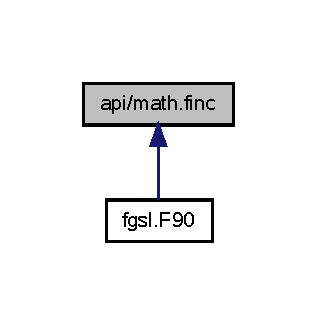
\includegraphics[width=152pt]{math_8finc__dep__incl}
\end{center}
\end{figure}
\subsection*{Functions/\+Subroutines}
\begin{DoxyCompactItemize}
\item 
integer(fgsl\+\_\+int) function \hyperlink{math_8finc_a5067c8634bbc3cd88a507d8816134d40}{fgsl\+\_\+isnan} (x)
\item 
integer(fgsl\+\_\+int) function \hyperlink{math_8finc_aa3b31b6c56e2b1a862bcaced664803fc}{fgsl\+\_\+isinf} (x)
\item 
integer(fgsl\+\_\+int) function \hyperlink{math_8finc_a740aba8e50497aee7f31503b9fa4ba6b}{fgsl\+\_\+finite} (x)
\item 
real(fgsl\+\_\+double) function \hyperlink{math_8finc_ae1ca85647dff8d9f70b3126845c87443}{fgsl\+\_\+log1p} (x)
\item 
real(fgsl\+\_\+double) function \hyperlink{math_8finc_ab63b6ca1585dc1aa1ad824c6621eed51}{fgsl\+\_\+expm1} (x)
\item 
real(fgsl\+\_\+double) function \hyperlink{math_8finc_af7330c8b04fc10b1850f2d4ce9291690}{fgsl\+\_\+acosh} (x)
\item 
real(fgsl\+\_\+double) function \hyperlink{math_8finc_a2d2d1b0a15932d8bbf2741cd2e7a4ba2}{fgsl\+\_\+asinh} (x)
\item 
real(fgsl\+\_\+double) function \hyperlink{math_8finc_a82dce86ff9a928aba7b35f9af6a9f5cc}{fgsl\+\_\+atanh} (x)
\item 
real(fgsl\+\_\+double) function \hyperlink{math_8finc_a4673afab0b7df7e7e3f05a057b5f8486}{fgsl\+\_\+ldexp} (x, e)
\item 
real(fgsl\+\_\+double) function \hyperlink{math_8finc_a178abc026a08abbe00d18c0fe8976135}{fgsl\+\_\+frexp} (x, e)
\item 
integer(fgsl\+\_\+int) function \hyperlink{math_8finc_ab40b3e555596120ef1e85184704415ca}{fgsl\+\_\+fcmp} (x, y, eps)
\item 
type(fgsl\+\_\+function) function \hyperlink{math_8finc_a3763fefa672f280ed40fb19756dbd88c}{fgsl\+\_\+function\+\_\+init} (func, params)
\begin{DoxyCompactList}\small\item\em Constructor for an F\+G\+S\+L function type. \end{DoxyCompactList}\item 
type(fgsl\+\_\+function\+\_\+fdf) function \hyperlink{math_8finc_abb3c595b71761c1825021ce600493f75}{fgsl\+\_\+function\+\_\+fdf\+\_\+init} (f, df, fdf, params)
\begin{DoxyCompactList}\small\item\em Constructor for an F\+G\+S\+L function type including a derivative. \end{DoxyCompactList}\item 
subroutine \hyperlink{math_8finc_a2119e5b0091febc676ee418b8b211bf5}{fgsl\+\_\+function\+\_\+free} (sfunc)
\begin{DoxyCompactList}\small\item\em Free resources associated with a F\+G\+S\+L function object. \end{DoxyCompactList}\item 
subroutine \hyperlink{math_8finc_a03e913de6c833197efae52ed50290cfb}{fgsl\+\_\+function\+\_\+fdf\+\_\+free} (sfunc)
\begin{DoxyCompactList}\small\item\em Free resources associated with a F\+G\+S\+L function with derivative object. \end{DoxyCompactList}\item 
real(fgsl\+\_\+double) function \hyperlink{math_8finc_a6c38a834ecc0149664dbb667f104fcce}{fgsl\+\_\+fn\+\_\+eval} (sfunc, x)
\begin{DoxyCompactList}\small\item\em Evaluate a function value for a F\+G\+S\+L function object. \end{DoxyCompactList}\item 
real(fgsl\+\_\+double) function \hyperlink{math_8finc_a76c063c0086a88bd27f75c808041b9dd}{fgsl\+\_\+fn\+\_\+fdf\+\_\+eval\+\_\+f} (sfunc, x)
\begin{DoxyCompactList}\small\item\em Evaluate a function value for a F\+G\+S\+L function with derivative object. \end{DoxyCompactList}\item 
real(fgsl\+\_\+double) function \hyperlink{math_8finc_a67a49e7d1dec1c5c407e1ccd62db581a}{fgsl\+\_\+fn\+\_\+fdf\+\_\+eval\+\_\+df} (sfunc, x)
\begin{DoxyCompactList}\small\item\em Evaluate a derivative value for a F\+G\+S\+L function with derivative object. \end{DoxyCompactList}\item 
subroutine \hyperlink{math_8finc_a950ecd7cffcfa33d10a2b8db5c6befcd}{fgsl\+\_\+fn\+\_\+fdf\+\_\+eval\+\_\+f\+\_\+df} (sfunc, x, y, dy)
\begin{DoxyCompactList}\small\item\em Evaluate function as well as derivative value for a F\+G\+S\+L function with derivative object. \end{DoxyCompactList}\end{DoxyCompactItemize}


\subsection{Function/\+Subroutine Documentation}
\hypertarget{math_8finc_af7330c8b04fc10b1850f2d4ce9291690}{}\index{math.\+finc@{math.\+finc}!fgsl\+\_\+acosh@{fgsl\+\_\+acosh}}
\index{fgsl\+\_\+acosh@{fgsl\+\_\+acosh}!math.\+finc@{math.\+finc}}
\subsubsection[{fgsl\+\_\+acosh}]{\setlength{\rightskip}{0pt plus 5cm}real(fgsl\+\_\+double) function fgsl\+\_\+acosh (
\begin{DoxyParamCaption}
\item[{real(fgsl\+\_\+double), intent(in)}]{x}
\end{DoxyParamCaption}
)}\label{math_8finc_af7330c8b04fc10b1850f2d4ce9291690}
\hypertarget{math_8finc_a2d2d1b0a15932d8bbf2741cd2e7a4ba2}{}\index{math.\+finc@{math.\+finc}!fgsl\+\_\+asinh@{fgsl\+\_\+asinh}}
\index{fgsl\+\_\+asinh@{fgsl\+\_\+asinh}!math.\+finc@{math.\+finc}}
\subsubsection[{fgsl\+\_\+asinh}]{\setlength{\rightskip}{0pt plus 5cm}real(fgsl\+\_\+double) function fgsl\+\_\+asinh (
\begin{DoxyParamCaption}
\item[{real(fgsl\+\_\+double), intent(in)}]{x}
\end{DoxyParamCaption}
)}\label{math_8finc_a2d2d1b0a15932d8bbf2741cd2e7a4ba2}
\hypertarget{math_8finc_a82dce86ff9a928aba7b35f9af6a9f5cc}{}\index{math.\+finc@{math.\+finc}!fgsl\+\_\+atanh@{fgsl\+\_\+atanh}}
\index{fgsl\+\_\+atanh@{fgsl\+\_\+atanh}!math.\+finc@{math.\+finc}}
\subsubsection[{fgsl\+\_\+atanh}]{\setlength{\rightskip}{0pt plus 5cm}real(fgsl\+\_\+double) function fgsl\+\_\+atanh (
\begin{DoxyParamCaption}
\item[{real(fgsl\+\_\+double), intent(in)}]{x}
\end{DoxyParamCaption}
)}\label{math_8finc_a82dce86ff9a928aba7b35f9af6a9f5cc}
\hypertarget{math_8finc_ab63b6ca1585dc1aa1ad824c6621eed51}{}\index{math.\+finc@{math.\+finc}!fgsl\+\_\+expm1@{fgsl\+\_\+expm1}}
\index{fgsl\+\_\+expm1@{fgsl\+\_\+expm1}!math.\+finc@{math.\+finc}}
\subsubsection[{fgsl\+\_\+expm1}]{\setlength{\rightskip}{0pt plus 5cm}real(fgsl\+\_\+double) function fgsl\+\_\+expm1 (
\begin{DoxyParamCaption}
\item[{real(fgsl\+\_\+double), intent(in)}]{x}
\end{DoxyParamCaption}
)}\label{math_8finc_ab63b6ca1585dc1aa1ad824c6621eed51}
\hypertarget{math_8finc_ab40b3e555596120ef1e85184704415ca}{}\index{math.\+finc@{math.\+finc}!fgsl\+\_\+fcmp@{fgsl\+\_\+fcmp}}
\index{fgsl\+\_\+fcmp@{fgsl\+\_\+fcmp}!math.\+finc@{math.\+finc}}
\subsubsection[{fgsl\+\_\+fcmp}]{\setlength{\rightskip}{0pt plus 5cm}integer(fgsl\+\_\+int) function fgsl\+\_\+fcmp (
\begin{DoxyParamCaption}
\item[{real(fgsl\+\_\+double), intent(in)}]{x, }
\item[{real(fgsl\+\_\+double), intent(in)}]{y, }
\item[{real(fgsl\+\_\+double), intent(in)}]{eps}
\end{DoxyParamCaption}
)}\label{math_8finc_ab40b3e555596120ef1e85184704415ca}
\hypertarget{math_8finc_a740aba8e50497aee7f31503b9fa4ba6b}{}\index{math.\+finc@{math.\+finc}!fgsl\+\_\+finite@{fgsl\+\_\+finite}}
\index{fgsl\+\_\+finite@{fgsl\+\_\+finite}!math.\+finc@{math.\+finc}}
\subsubsection[{fgsl\+\_\+finite}]{\setlength{\rightskip}{0pt plus 5cm}integer(fgsl\+\_\+int) function fgsl\+\_\+finite (
\begin{DoxyParamCaption}
\item[{real(fgsl\+\_\+double), intent(in)}]{x}
\end{DoxyParamCaption}
)}\label{math_8finc_a740aba8e50497aee7f31503b9fa4ba6b}
\hypertarget{math_8finc_a6c38a834ecc0149664dbb667f104fcce}{}\index{math.\+finc@{math.\+finc}!fgsl\+\_\+fn\+\_\+eval@{fgsl\+\_\+fn\+\_\+eval}}
\index{fgsl\+\_\+fn\+\_\+eval@{fgsl\+\_\+fn\+\_\+eval}!math.\+finc@{math.\+finc}}
\subsubsection[{fgsl\+\_\+fn\+\_\+eval}]{\setlength{\rightskip}{0pt plus 5cm}real(fgsl\+\_\+double) function fgsl\+\_\+fn\+\_\+eval (
\begin{DoxyParamCaption}
\item[{type(fgsl\+\_\+function), intent(inout)}]{sfunc, }
\item[{real(fgsl\+\_\+double), intent(in)}]{x}
\end{DoxyParamCaption}
)}\label{math_8finc_a6c38a834ecc0149664dbb667f104fcce}


Evaluate a function value for a F\+G\+S\+L function object. 


\begin{DoxyParams}{Parameters}
{\em sfunc} & -\/ function object. \\
\hline
{\em x} & -\/ argument value \\
\hline
\end{DoxyParams}
\begin{DoxyReturn}{Returns}
Function value 
\end{DoxyReturn}
\hypertarget{math_8finc_a67a49e7d1dec1c5c407e1ccd62db581a}{}\index{math.\+finc@{math.\+finc}!fgsl\+\_\+fn\+\_\+fdf\+\_\+eval\+\_\+df@{fgsl\+\_\+fn\+\_\+fdf\+\_\+eval\+\_\+df}}
\index{fgsl\+\_\+fn\+\_\+fdf\+\_\+eval\+\_\+df@{fgsl\+\_\+fn\+\_\+fdf\+\_\+eval\+\_\+df}!math.\+finc@{math.\+finc}}
\subsubsection[{fgsl\+\_\+fn\+\_\+fdf\+\_\+eval\+\_\+df}]{\setlength{\rightskip}{0pt plus 5cm}real(fgsl\+\_\+double) function fgsl\+\_\+fn\+\_\+fdf\+\_\+eval\+\_\+df (
\begin{DoxyParamCaption}
\item[{type(fgsl\+\_\+function\+\_\+fdf), intent(inout)}]{sfunc, }
\item[{real(fgsl\+\_\+double), intent(in)}]{x}
\end{DoxyParamCaption}
)}\label{math_8finc_a67a49e7d1dec1c5c407e1ccd62db581a}


Evaluate a derivative value for a F\+G\+S\+L function with derivative object. 


\begin{DoxyParams}{Parameters}
{\em sfunc} & -\/ function with derivative object. \\
\hline
{\em x} & -\/ argument value \\
\hline
\end{DoxyParams}
\begin{DoxyReturn}{Returns}
Derivative value 
\end{DoxyReturn}
\hypertarget{math_8finc_a76c063c0086a88bd27f75c808041b9dd}{}\index{math.\+finc@{math.\+finc}!fgsl\+\_\+fn\+\_\+fdf\+\_\+eval\+\_\+f@{fgsl\+\_\+fn\+\_\+fdf\+\_\+eval\+\_\+f}}
\index{fgsl\+\_\+fn\+\_\+fdf\+\_\+eval\+\_\+f@{fgsl\+\_\+fn\+\_\+fdf\+\_\+eval\+\_\+f}!math.\+finc@{math.\+finc}}
\subsubsection[{fgsl\+\_\+fn\+\_\+fdf\+\_\+eval\+\_\+f}]{\setlength{\rightskip}{0pt plus 5cm}real(fgsl\+\_\+double) function fgsl\+\_\+fn\+\_\+fdf\+\_\+eval\+\_\+f (
\begin{DoxyParamCaption}
\item[{type(fgsl\+\_\+function\+\_\+fdf), intent(inout)}]{sfunc, }
\item[{real(fgsl\+\_\+double), intent(in)}]{x}
\end{DoxyParamCaption}
)}\label{math_8finc_a76c063c0086a88bd27f75c808041b9dd}


Evaluate a function value for a F\+G\+S\+L function with derivative object. 


\begin{DoxyParams}{Parameters}
{\em sfunc} & -\/ function with derivative object. \\
\hline
{\em x} & -\/ argument value \\
\hline
\end{DoxyParams}
\begin{DoxyReturn}{Returns}
Function value 
\end{DoxyReturn}
\hypertarget{math_8finc_a950ecd7cffcfa33d10a2b8db5c6befcd}{}\index{math.\+finc@{math.\+finc}!fgsl\+\_\+fn\+\_\+fdf\+\_\+eval\+\_\+f\+\_\+df@{fgsl\+\_\+fn\+\_\+fdf\+\_\+eval\+\_\+f\+\_\+df}}
\index{fgsl\+\_\+fn\+\_\+fdf\+\_\+eval\+\_\+f\+\_\+df@{fgsl\+\_\+fn\+\_\+fdf\+\_\+eval\+\_\+f\+\_\+df}!math.\+finc@{math.\+finc}}
\subsubsection[{fgsl\+\_\+fn\+\_\+fdf\+\_\+eval\+\_\+f\+\_\+df}]{\setlength{\rightskip}{0pt plus 5cm}subroutine fgsl\+\_\+fn\+\_\+fdf\+\_\+eval\+\_\+f\+\_\+df (
\begin{DoxyParamCaption}
\item[{type(fgsl\+\_\+function\+\_\+fdf), intent(inout)}]{sfunc, }
\item[{real(fgsl\+\_\+double), intent(in)}]{x, }
\item[{real(fgsl\+\_\+double), intent(out)}]{y, }
\item[{real(fgsl\+\_\+double), intent(out)}]{dy}
\end{DoxyParamCaption}
)}\label{math_8finc_a950ecd7cffcfa33d10a2b8db5c6befcd}


Evaluate function as well as derivative value for a F\+G\+S\+L function with derivative object. 


\begin{DoxyParams}{Parameters}
{\em sfunc} & -\/ function with derivative object. \\
\hline
{\em x} & -\/ argument value \\
\hline
{\em y} & -\/ function value \\
\hline
{\em dy} & -\/ derivative value \\
\hline
\end{DoxyParams}
\hypertarget{math_8finc_a178abc026a08abbe00d18c0fe8976135}{}\index{math.\+finc@{math.\+finc}!fgsl\+\_\+frexp@{fgsl\+\_\+frexp}}
\index{fgsl\+\_\+frexp@{fgsl\+\_\+frexp}!math.\+finc@{math.\+finc}}
\subsubsection[{fgsl\+\_\+frexp}]{\setlength{\rightskip}{0pt plus 5cm}real(fgsl\+\_\+double) function fgsl\+\_\+frexp (
\begin{DoxyParamCaption}
\item[{real(fgsl\+\_\+double), intent(in)}]{x, }
\item[{integer(fgsl\+\_\+int), intent(out)}]{e}
\end{DoxyParamCaption}
)}\label{math_8finc_a178abc026a08abbe00d18c0fe8976135}
\hypertarget{math_8finc_a03e913de6c833197efae52ed50290cfb}{}\index{math.\+finc@{math.\+finc}!fgsl\+\_\+function\+\_\+fdf\+\_\+free@{fgsl\+\_\+function\+\_\+fdf\+\_\+free}}
\index{fgsl\+\_\+function\+\_\+fdf\+\_\+free@{fgsl\+\_\+function\+\_\+fdf\+\_\+free}!math.\+finc@{math.\+finc}}
\subsubsection[{fgsl\+\_\+function\+\_\+fdf\+\_\+free}]{\setlength{\rightskip}{0pt plus 5cm}subroutine fgsl\+\_\+function\+\_\+fdf\+\_\+free (
\begin{DoxyParamCaption}
\item[{type(fgsl\+\_\+function\+\_\+fdf), intent(inout)}]{sfunc}
\end{DoxyParamCaption}
)}\label{math_8finc_a03e913de6c833197efae52ed50290cfb}


Free resources associated with a F\+G\+S\+L function with derivative object. 

\hypertarget{math_8finc_abb3c595b71761c1825021ce600493f75}{}\index{math.\+finc@{math.\+finc}!fgsl\+\_\+function\+\_\+fdf\+\_\+init@{fgsl\+\_\+function\+\_\+fdf\+\_\+init}}
\index{fgsl\+\_\+function\+\_\+fdf\+\_\+init@{fgsl\+\_\+function\+\_\+fdf\+\_\+init}!math.\+finc@{math.\+finc}}
\subsubsection[{fgsl\+\_\+function\+\_\+fdf\+\_\+init}]{\setlength{\rightskip}{0pt plus 5cm}type(fgsl\+\_\+function\+\_\+fdf) function fgsl\+\_\+function\+\_\+fdf\+\_\+init (
\begin{DoxyParamCaption}
\item[{}]{f, }
\item[{}]{df, }
\item[{}]{fdf, }
\item[{type(c\+\_\+ptr), intent(in)}]{params}
\end{DoxyParamCaption}
)}\label{math_8finc_abb3c595b71761c1825021ce600493f75}


Constructor for an F\+G\+S\+L function type including a derivative. 


\begin{DoxyParams}{Parameters}
{\em f} & -\/ interface for a double precision valued function with a parameter of arbitrary type \\
\hline
{\em df} & -\/ interface for a function evaluating the derivative of f \\
\hline
{\em fdf} & -\/ interface for a subroutine evaluating f as well as its derivative given an argument and a parameter. \\
\hline
{\em params} & -\/ parameter of arbitrary type \\
\hline
\end{DoxyParams}
\begin{DoxyReturn}{Returns}
F\+G\+S\+L function with derivative object. 
\end{DoxyReturn}
\hypertarget{math_8finc_a2119e5b0091febc676ee418b8b211bf5}{}\index{math.\+finc@{math.\+finc}!fgsl\+\_\+function\+\_\+free@{fgsl\+\_\+function\+\_\+free}}
\index{fgsl\+\_\+function\+\_\+free@{fgsl\+\_\+function\+\_\+free}!math.\+finc@{math.\+finc}}
\subsubsection[{fgsl\+\_\+function\+\_\+free}]{\setlength{\rightskip}{0pt plus 5cm}subroutine fgsl\+\_\+function\+\_\+free (
\begin{DoxyParamCaption}
\item[{type(fgsl\+\_\+function), intent(inout)}]{sfunc}
\end{DoxyParamCaption}
)}\label{math_8finc_a2119e5b0091febc676ee418b8b211bf5}


Free resources associated with a F\+G\+S\+L function object. 

\hypertarget{math_8finc_a3763fefa672f280ed40fb19756dbd88c}{}\index{math.\+finc@{math.\+finc}!fgsl\+\_\+function\+\_\+init@{fgsl\+\_\+function\+\_\+init}}
\index{fgsl\+\_\+function\+\_\+init@{fgsl\+\_\+function\+\_\+init}!math.\+finc@{math.\+finc}}
\subsubsection[{fgsl\+\_\+function\+\_\+init}]{\setlength{\rightskip}{0pt plus 5cm}type(fgsl\+\_\+function) function fgsl\+\_\+function\+\_\+init (
\begin{DoxyParamCaption}
\item[{}]{func, }
\item[{type(c\+\_\+ptr), intent(in)}]{params}
\end{DoxyParamCaption}
)}\label{math_8finc_a3763fefa672f280ed40fb19756dbd88c}


Constructor for an F\+G\+S\+L function type. 


\begin{DoxyParams}{Parameters}
{\em func} & -\/ interface for a double precision valued function with a parameter of arbitrary type \\
\hline
{\em params} & -\/ parameter of arbitrary type \\
\hline
\end{DoxyParams}
\begin{DoxyReturn}{Returns}
F\+G\+S\+L function object. 
\end{DoxyReturn}
\hypertarget{math_8finc_aa3b31b6c56e2b1a862bcaced664803fc}{}\index{math.\+finc@{math.\+finc}!fgsl\+\_\+isinf@{fgsl\+\_\+isinf}}
\index{fgsl\+\_\+isinf@{fgsl\+\_\+isinf}!math.\+finc@{math.\+finc}}
\subsubsection[{fgsl\+\_\+isinf}]{\setlength{\rightskip}{0pt plus 5cm}integer(fgsl\+\_\+int) function fgsl\+\_\+isinf (
\begin{DoxyParamCaption}
\item[{real(fgsl\+\_\+double), intent(in)}]{x}
\end{DoxyParamCaption}
)}\label{math_8finc_aa3b31b6c56e2b1a862bcaced664803fc}
\hypertarget{math_8finc_a5067c8634bbc3cd88a507d8816134d40}{}\index{math.\+finc@{math.\+finc}!fgsl\+\_\+isnan@{fgsl\+\_\+isnan}}
\index{fgsl\+\_\+isnan@{fgsl\+\_\+isnan}!math.\+finc@{math.\+finc}}
\subsubsection[{fgsl\+\_\+isnan}]{\setlength{\rightskip}{0pt plus 5cm}integer(fgsl\+\_\+int) function fgsl\+\_\+isnan (
\begin{DoxyParamCaption}
\item[{real(fgsl\+\_\+double), intent(in)}]{x}
\end{DoxyParamCaption}
)}\label{math_8finc_a5067c8634bbc3cd88a507d8816134d40}
\hypertarget{math_8finc_a4673afab0b7df7e7e3f05a057b5f8486}{}\index{math.\+finc@{math.\+finc}!fgsl\+\_\+ldexp@{fgsl\+\_\+ldexp}}
\index{fgsl\+\_\+ldexp@{fgsl\+\_\+ldexp}!math.\+finc@{math.\+finc}}
\subsubsection[{fgsl\+\_\+ldexp}]{\setlength{\rightskip}{0pt plus 5cm}real(fgsl\+\_\+double) function fgsl\+\_\+ldexp (
\begin{DoxyParamCaption}
\item[{real(fgsl\+\_\+double), intent(in)}]{x, }
\item[{integer(fgsl\+\_\+int), intent(in)}]{e}
\end{DoxyParamCaption}
)}\label{math_8finc_a4673afab0b7df7e7e3f05a057b5f8486}
\hypertarget{math_8finc_ae1ca85647dff8d9f70b3126845c87443}{}\index{math.\+finc@{math.\+finc}!fgsl\+\_\+log1p@{fgsl\+\_\+log1p}}
\index{fgsl\+\_\+log1p@{fgsl\+\_\+log1p}!math.\+finc@{math.\+finc}}
\subsubsection[{fgsl\+\_\+log1p}]{\setlength{\rightskip}{0pt plus 5cm}real(fgsl\+\_\+double) function fgsl\+\_\+log1p (
\begin{DoxyParamCaption}
\item[{real(fgsl\+\_\+double), intent(in)}]{x}
\end{DoxyParamCaption}
)}\label{math_8finc_ae1ca85647dff8d9f70b3126845c87443}

\hypertarget{min_8finc}{\section{api/min.finc File Reference}
\label{min_8finc}\index{api/min.\-finc@{api/min.\-finc}}
}
This graph shows which files directly or indirectly include this file\-:\nopagebreak
\begin{figure}[H]
\begin{center}
\leavevmode
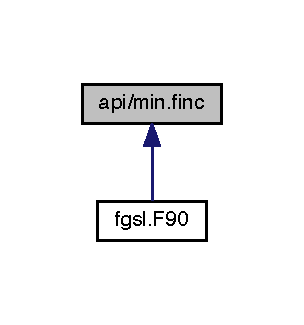
\includegraphics[width=146pt]{min_8finc__dep__incl}
\end{center}
\end{figure}
\subsection*{Functions/\-Subroutines}
\begin{DoxyCompactItemize}
\item 
type(fgsl\-\_\-min\-\_\-fminimizer) function \hyperlink{min_8finc_a97de5ab1b2ebed28f37cb39e68d37f8e}{fgsl\-\_\-min\-\_\-fminimizer\-\_\-alloc} (t)
\item 
subroutine \hyperlink{min_8finc_a16f5fcf8f532d2dfd847713e2eb365fd}{fgsl\-\_\-min\-\_\-fminimizer\-\_\-free} (s)
\item 
integer(fgsl\-\_\-int) function \hyperlink{min_8finc_aebda9dded327ca8921ee1cb2e670d505}{fgsl\-\_\-min\-\_\-fminimizer\-\_\-set} (s, f, x\-\_\-minimum, x\-\_\-lower, x\-\_\-upper)
\item 
integer(fgsl\-\_\-int) function \hyperlink{min_8finc_aad6cfe468d6d91f3b2116b2a6061d2fc}{fgsl\-\_\-min\-\_\-fminimizer\-\_\-set\-\_\-with\-\_\-values} (s, f, x\-\_\-minimum, f\-\_\-minimum, x\-\_\-lower, f\-\_\-lower, x\-\_\-upper, f\-\_\-upper)
\item 
integer(fgsl\-\_\-int) function \hyperlink{min_8finc_a5160e2c8eadc15b80784a0aca5554f3c}{fgsl\-\_\-min\-\_\-fminimizer\-\_\-iterate} (s)
\item 
character(kind=fgsl\-\_\-char, len=fgsl\-\_\-strmax) \\*
function \hyperlink{min_8finc_a3396297e9c77f8b4cd38c67566eac9be}{fgsl\-\_\-min\-\_\-fminimizer\-\_\-name} (s)
\item 
real(fgsl\-\_\-double) function \hyperlink{min_8finc_aa2755b3e3fbef70186fa48681f730638}{fgsl\-\_\-min\-\_\-fminimizer\-\_\-x\-\_\-minimum} (s)
\item 
real(fgsl\-\_\-double) function \hyperlink{min_8finc_a0ee7ec3329162025dc435e578a0bb0f1}{fgsl\-\_\-min\-\_\-fminimizer\-\_\-x\-\_\-lower} (s)
\item 
real(fgsl\-\_\-double) function \hyperlink{min_8finc_a06e4f2a2956710129e0c56bb8d2d1bc9}{fgsl\-\_\-min\-\_\-fminimizer\-\_\-x\-\_\-upper} (s)
\item 
real(fgsl\-\_\-double) function \hyperlink{min_8finc_ac68af52acc51b20808a6aa71d9eccdc7}{fgsl\-\_\-min\-\_\-fminimizer\-\_\-f\-\_\-minimum} (s)
\item 
real(fgsl\-\_\-double) function \hyperlink{min_8finc_a38b3ceaf7f12a7c9406314e9e410bbb4}{fgsl\-\_\-min\-\_\-fminimizer\-\_\-f\-\_\-lower} (s)
\item 
real(fgsl\-\_\-double) function \hyperlink{min_8finc_af552d34276a2d555cf91d53aaca8bbbc}{fgsl\-\_\-min\-\_\-fminimizer\-\_\-f\-\_\-upper} (s)
\item 
integer(fgsl\-\_\-int) function \hyperlink{min_8finc_a80d14f7331cae9ab0c66397d326bc3f8}{fgsl\-\_\-min\-\_\-test\-\_\-interval} (x\-\_\-lower, x\-\_\-upper, epsabs, epsrel)
\item 
logical function \hyperlink{min_8finc_ab663e2a33741f94ed117ca1d743f2390}{fgsl\-\_\-min\-\_\-fminimizer\-\_\-status} (s)
\end{DoxyCompactItemize}


\subsection{Function/\-Subroutine Documentation}
\hypertarget{min_8finc_a97de5ab1b2ebed28f37cb39e68d37f8e}{\index{min.\-finc@{min.\-finc}!fgsl\-\_\-min\-\_\-fminimizer\-\_\-alloc@{fgsl\-\_\-min\-\_\-fminimizer\-\_\-alloc}}
\index{fgsl\-\_\-min\-\_\-fminimizer\-\_\-alloc@{fgsl\-\_\-min\-\_\-fminimizer\-\_\-alloc}!min.finc@{min.\-finc}}
\subsubsection[{fgsl\-\_\-min\-\_\-fminimizer\-\_\-alloc}]{\setlength{\rightskip}{0pt plus 5cm}type(fgsl\-\_\-min\-\_\-fminimizer) function fgsl\-\_\-min\-\_\-fminimizer\-\_\-alloc (
\begin{DoxyParamCaption}
\item[{type(fgsl\-\_\-min\-\_\-fminimizer\-\_\-type), intent(in)}]{t}
\end{DoxyParamCaption}
)}}\label{min_8finc_a97de5ab1b2ebed28f37cb39e68d37f8e}
\hypertarget{min_8finc_a38b3ceaf7f12a7c9406314e9e410bbb4}{\index{min.\-finc@{min.\-finc}!fgsl\-\_\-min\-\_\-fminimizer\-\_\-f\-\_\-lower@{fgsl\-\_\-min\-\_\-fminimizer\-\_\-f\-\_\-lower}}
\index{fgsl\-\_\-min\-\_\-fminimizer\-\_\-f\-\_\-lower@{fgsl\-\_\-min\-\_\-fminimizer\-\_\-f\-\_\-lower}!min.finc@{min.\-finc}}
\subsubsection[{fgsl\-\_\-min\-\_\-fminimizer\-\_\-f\-\_\-lower}]{\setlength{\rightskip}{0pt plus 5cm}real(fgsl\-\_\-double) function fgsl\-\_\-min\-\_\-fminimizer\-\_\-f\-\_\-lower (
\begin{DoxyParamCaption}
\item[{type(fgsl\-\_\-min\-\_\-fminimizer), intent(in)}]{s}
\end{DoxyParamCaption}
)}}\label{min_8finc_a38b3ceaf7f12a7c9406314e9e410bbb4}
\hypertarget{min_8finc_ac68af52acc51b20808a6aa71d9eccdc7}{\index{min.\-finc@{min.\-finc}!fgsl\-\_\-min\-\_\-fminimizer\-\_\-f\-\_\-minimum@{fgsl\-\_\-min\-\_\-fminimizer\-\_\-f\-\_\-minimum}}
\index{fgsl\-\_\-min\-\_\-fminimizer\-\_\-f\-\_\-minimum@{fgsl\-\_\-min\-\_\-fminimizer\-\_\-f\-\_\-minimum}!min.finc@{min.\-finc}}
\subsubsection[{fgsl\-\_\-min\-\_\-fminimizer\-\_\-f\-\_\-minimum}]{\setlength{\rightskip}{0pt plus 5cm}real(fgsl\-\_\-double) function fgsl\-\_\-min\-\_\-fminimizer\-\_\-f\-\_\-minimum (
\begin{DoxyParamCaption}
\item[{type(fgsl\-\_\-min\-\_\-fminimizer), intent(in)}]{s}
\end{DoxyParamCaption}
)}}\label{min_8finc_ac68af52acc51b20808a6aa71d9eccdc7}
\hypertarget{min_8finc_af552d34276a2d555cf91d53aaca8bbbc}{\index{min.\-finc@{min.\-finc}!fgsl\-\_\-min\-\_\-fminimizer\-\_\-f\-\_\-upper@{fgsl\-\_\-min\-\_\-fminimizer\-\_\-f\-\_\-upper}}
\index{fgsl\-\_\-min\-\_\-fminimizer\-\_\-f\-\_\-upper@{fgsl\-\_\-min\-\_\-fminimizer\-\_\-f\-\_\-upper}!min.finc@{min.\-finc}}
\subsubsection[{fgsl\-\_\-min\-\_\-fminimizer\-\_\-f\-\_\-upper}]{\setlength{\rightskip}{0pt plus 5cm}real(fgsl\-\_\-double) function fgsl\-\_\-min\-\_\-fminimizer\-\_\-f\-\_\-upper (
\begin{DoxyParamCaption}
\item[{type(fgsl\-\_\-min\-\_\-fminimizer), intent(in)}]{s}
\end{DoxyParamCaption}
)}}\label{min_8finc_af552d34276a2d555cf91d53aaca8bbbc}
\hypertarget{min_8finc_a16f5fcf8f532d2dfd847713e2eb365fd}{\index{min.\-finc@{min.\-finc}!fgsl\-\_\-min\-\_\-fminimizer\-\_\-free@{fgsl\-\_\-min\-\_\-fminimizer\-\_\-free}}
\index{fgsl\-\_\-min\-\_\-fminimizer\-\_\-free@{fgsl\-\_\-min\-\_\-fminimizer\-\_\-free}!min.finc@{min.\-finc}}
\subsubsection[{fgsl\-\_\-min\-\_\-fminimizer\-\_\-free}]{\setlength{\rightskip}{0pt plus 5cm}subroutine fgsl\-\_\-min\-\_\-fminimizer\-\_\-free (
\begin{DoxyParamCaption}
\item[{type(fgsl\-\_\-min\-\_\-fminimizer), intent(inout)}]{s}
\end{DoxyParamCaption}
)}}\label{min_8finc_a16f5fcf8f532d2dfd847713e2eb365fd}
\hypertarget{min_8finc_a5160e2c8eadc15b80784a0aca5554f3c}{\index{min.\-finc@{min.\-finc}!fgsl\-\_\-min\-\_\-fminimizer\-\_\-iterate@{fgsl\-\_\-min\-\_\-fminimizer\-\_\-iterate}}
\index{fgsl\-\_\-min\-\_\-fminimizer\-\_\-iterate@{fgsl\-\_\-min\-\_\-fminimizer\-\_\-iterate}!min.finc@{min.\-finc}}
\subsubsection[{fgsl\-\_\-min\-\_\-fminimizer\-\_\-iterate}]{\setlength{\rightskip}{0pt plus 5cm}integer(fgsl\-\_\-int) function fgsl\-\_\-min\-\_\-fminimizer\-\_\-iterate (
\begin{DoxyParamCaption}
\item[{type(fgsl\-\_\-min\-\_\-fminimizer), intent(in)}]{s}
\end{DoxyParamCaption}
)}}\label{min_8finc_a5160e2c8eadc15b80784a0aca5554f3c}
\hypertarget{min_8finc_a3396297e9c77f8b4cd38c67566eac9be}{\index{min.\-finc@{min.\-finc}!fgsl\-\_\-min\-\_\-fminimizer\-\_\-name@{fgsl\-\_\-min\-\_\-fminimizer\-\_\-name}}
\index{fgsl\-\_\-min\-\_\-fminimizer\-\_\-name@{fgsl\-\_\-min\-\_\-fminimizer\-\_\-name}!min.finc@{min.\-finc}}
\subsubsection[{fgsl\-\_\-min\-\_\-fminimizer\-\_\-name}]{\setlength{\rightskip}{0pt plus 5cm}character(kind=fgsl\-\_\-char,len=fgsl\-\_\-strmax) function fgsl\-\_\-min\-\_\-fminimizer\-\_\-name (
\begin{DoxyParamCaption}
\item[{type(fgsl\-\_\-min\-\_\-fminimizer), intent(in)}]{s}
\end{DoxyParamCaption}
)}}\label{min_8finc_a3396297e9c77f8b4cd38c67566eac9be}
\hypertarget{min_8finc_aebda9dded327ca8921ee1cb2e670d505}{\index{min.\-finc@{min.\-finc}!fgsl\-\_\-min\-\_\-fminimizer\-\_\-set@{fgsl\-\_\-min\-\_\-fminimizer\-\_\-set}}
\index{fgsl\-\_\-min\-\_\-fminimizer\-\_\-set@{fgsl\-\_\-min\-\_\-fminimizer\-\_\-set}!min.finc@{min.\-finc}}
\subsubsection[{fgsl\-\_\-min\-\_\-fminimizer\-\_\-set}]{\setlength{\rightskip}{0pt plus 5cm}integer(fgsl\-\_\-int) function fgsl\-\_\-min\-\_\-fminimizer\-\_\-set (
\begin{DoxyParamCaption}
\item[{type(fgsl\-\_\-min\-\_\-fminimizer), intent(inout)}]{s, }
\item[{type(fgsl\-\_\-function), intent(in)}]{f, }
\item[{real(fgsl\-\_\-double), intent(in)}]{x\-\_\-minimum, }
\item[{real(fgsl\-\_\-double), intent(in)}]{x\-\_\-lower, }
\item[{real(fgsl\-\_\-double), intent(in)}]{x\-\_\-upper}
\end{DoxyParamCaption}
)}}\label{min_8finc_aebda9dded327ca8921ee1cb2e670d505}
\hypertarget{min_8finc_aad6cfe468d6d91f3b2116b2a6061d2fc}{\index{min.\-finc@{min.\-finc}!fgsl\-\_\-min\-\_\-fminimizer\-\_\-set\-\_\-with\-\_\-values@{fgsl\-\_\-min\-\_\-fminimizer\-\_\-set\-\_\-with\-\_\-values}}
\index{fgsl\-\_\-min\-\_\-fminimizer\-\_\-set\-\_\-with\-\_\-values@{fgsl\-\_\-min\-\_\-fminimizer\-\_\-set\-\_\-with\-\_\-values}!min.finc@{min.\-finc}}
\subsubsection[{fgsl\-\_\-min\-\_\-fminimizer\-\_\-set\-\_\-with\-\_\-values}]{\setlength{\rightskip}{0pt plus 5cm}integer(fgsl\-\_\-int) function fgsl\-\_\-min\-\_\-fminimizer\-\_\-set\-\_\-with\-\_\-values (
\begin{DoxyParamCaption}
\item[{type(fgsl\-\_\-min\-\_\-fminimizer), intent(inout)}]{s, }
\item[{type(fgsl\-\_\-function), intent(in)}]{f, }
\item[{real(fgsl\-\_\-double), intent(in)}]{x\-\_\-minimum, }
\item[{real(fgsl\-\_\-double), intent(in)}]{f\-\_\-minimum, }
\item[{real(fgsl\-\_\-double), intent(in)}]{x\-\_\-lower, }
\item[{real(fgsl\-\_\-double), intent(in)}]{f\-\_\-lower, }
\item[{real(fgsl\-\_\-double), intent(in)}]{x\-\_\-upper, }
\item[{real(fgsl\-\_\-double), intent(in)}]{f\-\_\-upper}
\end{DoxyParamCaption}
)}}\label{min_8finc_aad6cfe468d6d91f3b2116b2a6061d2fc}
\hypertarget{min_8finc_ab663e2a33741f94ed117ca1d743f2390}{\index{min.\-finc@{min.\-finc}!fgsl\-\_\-min\-\_\-fminimizer\-\_\-status@{fgsl\-\_\-min\-\_\-fminimizer\-\_\-status}}
\index{fgsl\-\_\-min\-\_\-fminimizer\-\_\-status@{fgsl\-\_\-min\-\_\-fminimizer\-\_\-status}!min.finc@{min.\-finc}}
\subsubsection[{fgsl\-\_\-min\-\_\-fminimizer\-\_\-status}]{\setlength{\rightskip}{0pt plus 5cm}logical function fgsl\-\_\-min\-\_\-fminimizer\-\_\-status (
\begin{DoxyParamCaption}
\item[{type(fgsl\-\_\-min\-\_\-fminimizer), intent(in)}]{s}
\end{DoxyParamCaption}
)}}\label{min_8finc_ab663e2a33741f94ed117ca1d743f2390}
\hypertarget{min_8finc_a0ee7ec3329162025dc435e578a0bb0f1}{\index{min.\-finc@{min.\-finc}!fgsl\-\_\-min\-\_\-fminimizer\-\_\-x\-\_\-lower@{fgsl\-\_\-min\-\_\-fminimizer\-\_\-x\-\_\-lower}}
\index{fgsl\-\_\-min\-\_\-fminimizer\-\_\-x\-\_\-lower@{fgsl\-\_\-min\-\_\-fminimizer\-\_\-x\-\_\-lower}!min.finc@{min.\-finc}}
\subsubsection[{fgsl\-\_\-min\-\_\-fminimizer\-\_\-x\-\_\-lower}]{\setlength{\rightskip}{0pt plus 5cm}real(fgsl\-\_\-double) function fgsl\-\_\-min\-\_\-fminimizer\-\_\-x\-\_\-lower (
\begin{DoxyParamCaption}
\item[{type(fgsl\-\_\-min\-\_\-fminimizer), intent(in)}]{s}
\end{DoxyParamCaption}
)}}\label{min_8finc_a0ee7ec3329162025dc435e578a0bb0f1}
\hypertarget{min_8finc_aa2755b3e3fbef70186fa48681f730638}{\index{min.\-finc@{min.\-finc}!fgsl\-\_\-min\-\_\-fminimizer\-\_\-x\-\_\-minimum@{fgsl\-\_\-min\-\_\-fminimizer\-\_\-x\-\_\-minimum}}
\index{fgsl\-\_\-min\-\_\-fminimizer\-\_\-x\-\_\-minimum@{fgsl\-\_\-min\-\_\-fminimizer\-\_\-x\-\_\-minimum}!min.finc@{min.\-finc}}
\subsubsection[{fgsl\-\_\-min\-\_\-fminimizer\-\_\-x\-\_\-minimum}]{\setlength{\rightskip}{0pt plus 5cm}real(fgsl\-\_\-double) function fgsl\-\_\-min\-\_\-fminimizer\-\_\-x\-\_\-minimum (
\begin{DoxyParamCaption}
\item[{type(fgsl\-\_\-min\-\_\-fminimizer), intent(in)}]{s}
\end{DoxyParamCaption}
)}}\label{min_8finc_aa2755b3e3fbef70186fa48681f730638}
\hypertarget{min_8finc_a06e4f2a2956710129e0c56bb8d2d1bc9}{\index{min.\-finc@{min.\-finc}!fgsl\-\_\-min\-\_\-fminimizer\-\_\-x\-\_\-upper@{fgsl\-\_\-min\-\_\-fminimizer\-\_\-x\-\_\-upper}}
\index{fgsl\-\_\-min\-\_\-fminimizer\-\_\-x\-\_\-upper@{fgsl\-\_\-min\-\_\-fminimizer\-\_\-x\-\_\-upper}!min.finc@{min.\-finc}}
\subsubsection[{fgsl\-\_\-min\-\_\-fminimizer\-\_\-x\-\_\-upper}]{\setlength{\rightskip}{0pt plus 5cm}real(fgsl\-\_\-double) function fgsl\-\_\-min\-\_\-fminimizer\-\_\-x\-\_\-upper (
\begin{DoxyParamCaption}
\item[{type(fgsl\-\_\-min\-\_\-fminimizer), intent(in)}]{s}
\end{DoxyParamCaption}
)}}\label{min_8finc_a06e4f2a2956710129e0c56bb8d2d1bc9}
\hypertarget{min_8finc_a80d14f7331cae9ab0c66397d326bc3f8}{\index{min.\-finc@{min.\-finc}!fgsl\-\_\-min\-\_\-test\-\_\-interval@{fgsl\-\_\-min\-\_\-test\-\_\-interval}}
\index{fgsl\-\_\-min\-\_\-test\-\_\-interval@{fgsl\-\_\-min\-\_\-test\-\_\-interval}!min.finc@{min.\-finc}}
\subsubsection[{fgsl\-\_\-min\-\_\-test\-\_\-interval}]{\setlength{\rightskip}{0pt plus 5cm}integer(fgsl\-\_\-int) function fgsl\-\_\-min\-\_\-test\-\_\-interval (
\begin{DoxyParamCaption}
\item[{real(fgsl\-\_\-double), intent(in)}]{x\-\_\-lower, }
\item[{real(fgsl\-\_\-double), intent(in)}]{x\-\_\-upper, }
\item[{real(fgsl\-\_\-double), intent(in)}]{epsabs, }
\item[{real(fgsl\-\_\-double), intent(in)}]{epsrel}
\end{DoxyParamCaption}
)}}\label{min_8finc_a80d14f7331cae9ab0c66397d326bc3f8}

\hypertarget{misc_8finc}{\section{api/misc.finc File Reference}
\label{misc_8finc}\index{api/misc.\-finc@{api/misc.\-finc}}
}
This graph shows which files directly or indirectly include this file\-:
\nopagebreak
\begin{figure}[H]
\begin{center}
\leavevmode
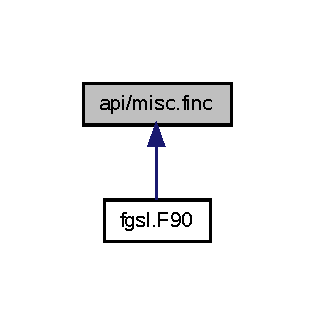
\includegraphics[width=152pt]{misc_8finc__dep__incl}
\end{center}
\end{figure}
\subsection*{Functions/\-Subroutines}
\begin{DoxyCompactItemize}
\item 
character(kind=fgsl\-\_\-char, len=fgsl\-\_\-strmax) \\*
function \hyperlink{misc_8finc_a014cd02b3b4d29919fd8e1947a2673d0}{fgsl\-\_\-name} (c\-\_\-name)
\begin{DoxyCompactList}\small\item\em C string to Fortran string conversion. \end{DoxyCompactList}\item 
integer(fgsl\-\_\-size\-\_\-t) function \hyperlink{misc_8finc_a896bd2c97151708c197858a357ea50e2}{fgsl\-\_\-sizeof\-\_\-double} (x)
\begin{DoxyCompactList}\small\item\em size of intrinsic double precision type \end{DoxyCompactList}\item 
integer(fgsl\-\_\-size\-\_\-t) function \hyperlink{misc_8finc_a993f009131d0e6bf9bcdebe827162450}{fgsl\-\_\-sizeof\-\_\-float} (x)
\begin{DoxyCompactList}\small\item\em size of intrinsic single precision type \end{DoxyCompactList}\item 
integer(fgsl\-\_\-size\-\_\-t) function \hyperlink{misc_8finc_abea36929b3d5a33cb24fbca3f52e6aa2}{fgsl\-\_\-sizeof\-\_\-int} (x)
\begin{DoxyCompactList}\small\item\em size of intrinsic integer type \end{DoxyCompactList}\item 
integer(fgsl\-\_\-size\-\_\-t) function \hyperlink{misc_8finc_ac74c9d7b9d14a74b9b32796d620f685f}{fgsl\-\_\-sizeof\-\_\-long} (x)
\begin{DoxyCompactList}\small\item\em size of intrinsic long integer type \end{DoxyCompactList}\item 
integer(fgsl\-\_\-size\-\_\-t) function \hyperlink{misc_8finc_a4befb04b07c33f2dc158a1349971d416}{fgsl\-\_\-sizeof\-\_\-size\-\_\-t} (x)
\begin{DoxyCompactList}\small\item\em size of intrinsic size\-\_\-t integer type \end{DoxyCompactList}\item 
integer(fgsl\-\_\-size\-\_\-t) function \hyperlink{misc_8finc_a703e0d9c10d808494cfa6597f403d8e3}{fgsl\-\_\-sizeof\-\_\-char} (x)
\begin{DoxyCompactList}\small\item\em size of intrinsic character type \end{DoxyCompactList}\end{DoxyCompactItemize}


\subsection{Function/\-Subroutine Documentation}
\hypertarget{misc_8finc_a014cd02b3b4d29919fd8e1947a2673d0}{\index{misc.\-finc@{misc.\-finc}!fgsl\-\_\-name@{fgsl\-\_\-name}}
\index{fgsl\-\_\-name@{fgsl\-\_\-name}!misc.finc@{misc.\-finc}}
\subsubsection[{fgsl\-\_\-name}]{\setlength{\rightskip}{0pt plus 5cm}character(kind=fgsl\-\_\-char, len=fgsl\-\_\-strmax) function fgsl\-\_\-name (
\begin{DoxyParamCaption}
\item[{type(c\-\_\-ptr), intent(in)}]{c\-\_\-name}
\end{DoxyParamCaption}
)}}\label{misc_8finc_a014cd02b3b4d29919fd8e1947a2673d0}


C string to Fortran string conversion. 

\hypertarget{misc_8finc_a703e0d9c10d808494cfa6597f403d8e3}{\index{misc.\-finc@{misc.\-finc}!fgsl\-\_\-sizeof\-\_\-char@{fgsl\-\_\-sizeof\-\_\-char}}
\index{fgsl\-\_\-sizeof\-\_\-char@{fgsl\-\_\-sizeof\-\_\-char}!misc.finc@{misc.\-finc}}
\subsubsection[{fgsl\-\_\-sizeof\-\_\-char}]{\setlength{\rightskip}{0pt plus 5cm}integer(fgsl\-\_\-size\-\_\-t) function fgsl\-\_\-sizeof\-\_\-char (
\begin{DoxyParamCaption}
\item[{character(fgsl\-\_\-char), intent(in)}]{x}
\end{DoxyParamCaption}
)}}\label{misc_8finc_a703e0d9c10d808494cfa6597f403d8e3}


size of intrinsic character type 

\hypertarget{misc_8finc_a896bd2c97151708c197858a357ea50e2}{\index{misc.\-finc@{misc.\-finc}!fgsl\-\_\-sizeof\-\_\-double@{fgsl\-\_\-sizeof\-\_\-double}}
\index{fgsl\-\_\-sizeof\-\_\-double@{fgsl\-\_\-sizeof\-\_\-double}!misc.finc@{misc.\-finc}}
\subsubsection[{fgsl\-\_\-sizeof\-\_\-double}]{\setlength{\rightskip}{0pt plus 5cm}integer(fgsl\-\_\-size\-\_\-t) function fgsl\-\_\-sizeof\-\_\-double (
\begin{DoxyParamCaption}
\item[{real(fgsl\-\_\-double), intent(in)}]{x}
\end{DoxyParamCaption}
)}}\label{misc_8finc_a896bd2c97151708c197858a357ea50e2}


size of intrinsic double precision type 

\hypertarget{misc_8finc_a993f009131d0e6bf9bcdebe827162450}{\index{misc.\-finc@{misc.\-finc}!fgsl\-\_\-sizeof\-\_\-float@{fgsl\-\_\-sizeof\-\_\-float}}
\index{fgsl\-\_\-sizeof\-\_\-float@{fgsl\-\_\-sizeof\-\_\-float}!misc.finc@{misc.\-finc}}
\subsubsection[{fgsl\-\_\-sizeof\-\_\-float}]{\setlength{\rightskip}{0pt plus 5cm}integer(fgsl\-\_\-size\-\_\-t) function fgsl\-\_\-sizeof\-\_\-float (
\begin{DoxyParamCaption}
\item[{real(fgsl\-\_\-float), intent(in)}]{x}
\end{DoxyParamCaption}
)}}\label{misc_8finc_a993f009131d0e6bf9bcdebe827162450}


size of intrinsic single precision type 

\hypertarget{misc_8finc_abea36929b3d5a33cb24fbca3f52e6aa2}{\index{misc.\-finc@{misc.\-finc}!fgsl\-\_\-sizeof\-\_\-int@{fgsl\-\_\-sizeof\-\_\-int}}
\index{fgsl\-\_\-sizeof\-\_\-int@{fgsl\-\_\-sizeof\-\_\-int}!misc.finc@{misc.\-finc}}
\subsubsection[{fgsl\-\_\-sizeof\-\_\-int}]{\setlength{\rightskip}{0pt plus 5cm}integer(fgsl\-\_\-size\-\_\-t) function fgsl\-\_\-sizeof\-\_\-int (
\begin{DoxyParamCaption}
\item[{integer(fgsl\-\_\-int), intent(in)}]{x}
\end{DoxyParamCaption}
)}}\label{misc_8finc_abea36929b3d5a33cb24fbca3f52e6aa2}


size of intrinsic integer type 

\hypertarget{misc_8finc_ac74c9d7b9d14a74b9b32796d620f685f}{\index{misc.\-finc@{misc.\-finc}!fgsl\-\_\-sizeof\-\_\-long@{fgsl\-\_\-sizeof\-\_\-long}}
\index{fgsl\-\_\-sizeof\-\_\-long@{fgsl\-\_\-sizeof\-\_\-long}!misc.finc@{misc.\-finc}}
\subsubsection[{fgsl\-\_\-sizeof\-\_\-long}]{\setlength{\rightskip}{0pt plus 5cm}integer(fgsl\-\_\-size\-\_\-t) function fgsl\-\_\-sizeof\-\_\-long (
\begin{DoxyParamCaption}
\item[{integer(fgsl\-\_\-long), intent(in)}]{x}
\end{DoxyParamCaption}
)}}\label{misc_8finc_ac74c9d7b9d14a74b9b32796d620f685f}


size of intrinsic long integer type 

\hypertarget{misc_8finc_a4befb04b07c33f2dc158a1349971d416}{\index{misc.\-finc@{misc.\-finc}!fgsl\-\_\-sizeof\-\_\-size\-\_\-t@{fgsl\-\_\-sizeof\-\_\-size\-\_\-t}}
\index{fgsl\-\_\-sizeof\-\_\-size\-\_\-t@{fgsl\-\_\-sizeof\-\_\-size\-\_\-t}!misc.finc@{misc.\-finc}}
\subsubsection[{fgsl\-\_\-sizeof\-\_\-size\-\_\-t}]{\setlength{\rightskip}{0pt plus 5cm}integer(fgsl\-\_\-size\-\_\-t) function fgsl\-\_\-sizeof\-\_\-size\-\_\-t (
\begin{DoxyParamCaption}
\item[{integer(fgsl\-\_\-size\-\_\-t), intent(in)}]{x}
\end{DoxyParamCaption}
)}}\label{misc_8finc_a4befb04b07c33f2dc158a1349971d416}


size of intrinsic size\-\_\-t integer type 


\hypertarget{montecarlo_8finc}{\section{api/montecarlo.finc File Reference}
\label{montecarlo_8finc}\index{api/montecarlo.\-finc@{api/montecarlo.\-finc}}
}
This graph shows which files directly or indirectly include this file\-:
\nopagebreak
\begin{figure}[H]
\begin{center}
\leavevmode
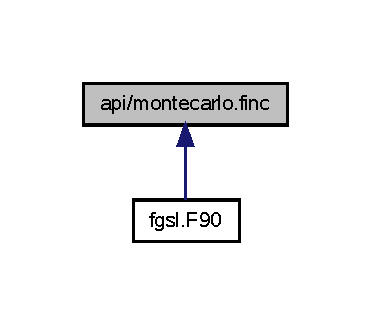
\includegraphics[width=180pt]{montecarlo_8finc__dep__incl}
\end{center}
\end{figure}
\subsection*{Functions/\-Subroutines}
\begin{DoxyCompactItemize}
\item 
type(fgsl\-\_\-monte\-\_\-function) function \hyperlink{montecarlo_8finc_a15f091a9199b5feb5a89e48b523fec5e}{fgsl\-\_\-monte\-\_\-function\-\_\-init} (func, dim, params)
\item 
subroutine \hyperlink{montecarlo_8finc_a1cebacdc85ce175202a13211f5bc5d51}{fgsl\-\_\-monte\-\_\-function\-\_\-free} (func)
\item 
type(fgsl\-\_\-monte\-\_\-plain\-\_\-state) \\*
function \hyperlink{montecarlo_8finc_a78d51cf421999fedc5d8ea880fd5b010}{fgsl\-\_\-monte\-\_\-plain\-\_\-alloc} (dim)
\item 
integer(fgsl\-\_\-int) function \hyperlink{montecarlo_8finc_aa8dce2c1b9acbf0d5ad973b6a9fcb52c}{fgsl\-\_\-monte\-\_\-plain\-\_\-init} (s)
\item 
integer(fgsl\-\_\-int) function \hyperlink{montecarlo_8finc_a055f2d0383f12a1ec343e0e6389e7aac}{fgsl\-\_\-monte\-\_\-plain\-\_\-integrate} (f, xl, xu, dim, calls, r, s, result, abserr)
\item 
subroutine \hyperlink{montecarlo_8finc_ae8b9533f16107ce4fa773962d95ba21c}{fgsl\-\_\-monte\-\_\-plain\-\_\-free} (s)
\item 
type(fgsl\-\_\-monte\-\_\-miser\-\_\-state) \\*
function \hyperlink{montecarlo_8finc_a8cc7ef76d9ac9d08b0fd80d0956e53f4}{fgsl\-\_\-monte\-\_\-miser\-\_\-alloc} (dim)
\item 
integer(fgsl\-\_\-int) function \hyperlink{montecarlo_8finc_ab005757b4f0e3f08eb0595920d166393}{fgsl\-\_\-monte\-\_\-miser\-\_\-init} (s)
\item 
integer(fgsl\-\_\-int) function \hyperlink{montecarlo_8finc_aef41da72b6c8bd738bf13aa19ec02bd1}{fgsl\-\_\-monte\-\_\-miser\-\_\-integrate} (f, xl, xu, dim, calls, r, s, result, abserr)
\item 
subroutine \hyperlink{montecarlo_8finc_a3cf77f03d4317c892a8ca6045580aa2b}{fgsl\-\_\-monte\-\_\-miser\-\_\-free} (s)
\item 
type(fgsl\-\_\-monte\-\_\-vegas\-\_\-state) \\*
function \hyperlink{montecarlo_8finc_a104c37829cabd4b2c65dc53b4d428dad}{fgsl\-\_\-monte\-\_\-vegas\-\_\-alloc} (dim)
\item 
integer(fgsl\-\_\-int) function \hyperlink{montecarlo_8finc_a7b50efe16a1796a72f05bb26779481de}{fgsl\-\_\-monte\-\_\-vegas\-\_\-init} (s)
\item 
integer(fgsl\-\_\-int) function \hyperlink{montecarlo_8finc_a6ca1e03b2c16419ff948d52426d89066}{fgsl\-\_\-monte\-\_\-vegas\-\_\-integrate} (f, xl, xu, dim, calls, r, s, result, abserr)
\item 
subroutine \hyperlink{montecarlo_8finc_a6bcca41c04f47eb0018123519c6c4225}{fgsl\-\_\-monte\-\_\-vegas\-\_\-free} (s)
\item 
real(fgsl\-\_\-double) function \hyperlink{montecarlo_8finc_a2126d5635d3ae538e905c2ab9739628a}{fgsl\-\_\-monte\-\_\-vegas\-\_\-chisq} (s)
\item 
subroutine \hyperlink{montecarlo_8finc_abfa67b6ebc24ac8ecfeb67102151a0db}{fgsl\-\_\-monte\-\_\-vegas\-\_\-runval} (s, result, sigma)
\item 
logical function \hyperlink{montecarlo_8finc_a54997aeeb57044a0d1ea66536cef086d}{fgsl\-\_\-monte\-\_\-function\-\_\-status} (monte\-\_\-function)
\item 
logical function \hyperlink{montecarlo_8finc_a3f0ffca084fe0aa10a2364ae1c12141d}{fgsl\-\_\-monte\-\_\-plain\-\_\-status} (monte\-\_\-plain)
\item 
logical function \hyperlink{montecarlo_8finc_a882c25d3ff7ba5048ee146da2af617d6}{fgsl\-\_\-monte\-\_\-miser\-\_\-status} (monte\-\_\-miser)
\item 
logical function \hyperlink{montecarlo_8finc_a46e22adcca8c7275e4de953205759d11}{fgsl\-\_\-monte\-\_\-vegas\-\_\-status} (monte\-\_\-vegas)
\item 
subroutine \hyperlink{montecarlo_8finc_ad5c6366b571b8d0f4caa29ef51302fcf}{fgsl\-\_\-monte\-\_\-miser\-\_\-setparams} (s, estimate\-\_\-frac, min\-\_\-calls, min\-\_\-calls\-\_\-per\-\_\-bisection, alpha, dither)
\begin{DoxyCompactList}\small\item\em Accessor routine for setting the parameters for the M\-I\-S\-E\-R algorithm. \end{DoxyCompactList}\item 
subroutine \hyperlink{montecarlo_8finc_a408686480497f6952e5dff7bf5d54603}{fgsl\-\_\-monte\-\_\-miser\-\_\-getparams} (s, estimate\-\_\-frac, min\-\_\-calls, min\-\_\-calls\-\_\-per\-\_\-bisection, alpha, dither)
\begin{DoxyCompactList}\small\item\em Accessor routine for reading out the parameters for the M\-I\-S\-E\-R algorithm. \end{DoxyCompactList}\item 
subroutine \hyperlink{montecarlo_8finc_a66bf1b9d3406abbc8ec50759add82650}{fgsl\-\_\-monte\-\_\-vegas\-\_\-setparams} (s, result, sigma, chisq, alpha, iterations, stage, mode, verbose, ostream)
\begin{DoxyCompactList}\small\item\em Accessor routine for setting the parameters for the V\-E\-G\-A\-S algorithm. \end{DoxyCompactList}\item 
subroutine \hyperlink{montecarlo_8finc_a54be28890110b14d8b4d165877e77549}{fgsl\-\_\-monte\-\_\-vegas\-\_\-getparams} (s, result, sigma, chisq, alpha, iterations, stage, mode, verbose, ostream)
\begin{DoxyCompactList}\small\item\em Accessor routine for reading out the parameters for the V\-E\-G\-A\-S algorithm. \end{DoxyCompactList}\end{DoxyCompactItemize}


\subsection{Function/\-Subroutine Documentation}
\hypertarget{montecarlo_8finc_a1cebacdc85ce175202a13211f5bc5d51}{\index{montecarlo.\-finc@{montecarlo.\-finc}!fgsl\-\_\-monte\-\_\-function\-\_\-free@{fgsl\-\_\-monte\-\_\-function\-\_\-free}}
\index{fgsl\-\_\-monte\-\_\-function\-\_\-free@{fgsl\-\_\-monte\-\_\-function\-\_\-free}!montecarlo.finc@{montecarlo.\-finc}}
\subsubsection[{fgsl\-\_\-monte\-\_\-function\-\_\-free}]{\setlength{\rightskip}{0pt plus 5cm}subroutine fgsl\-\_\-monte\-\_\-function\-\_\-free (
\begin{DoxyParamCaption}
\item[{type(fgsl\-\_\-monte\-\_\-function), intent(inout)}]{func}
\end{DoxyParamCaption}
)}}\label{montecarlo_8finc_a1cebacdc85ce175202a13211f5bc5d51}
\hypertarget{montecarlo_8finc_a15f091a9199b5feb5a89e48b523fec5e}{\index{montecarlo.\-finc@{montecarlo.\-finc}!fgsl\-\_\-monte\-\_\-function\-\_\-init@{fgsl\-\_\-monte\-\_\-function\-\_\-init}}
\index{fgsl\-\_\-monte\-\_\-function\-\_\-init@{fgsl\-\_\-monte\-\_\-function\-\_\-init}!montecarlo.finc@{montecarlo.\-finc}}
\subsubsection[{fgsl\-\_\-monte\-\_\-function\-\_\-init}]{\setlength{\rightskip}{0pt plus 5cm}type(fgsl\-\_\-monte\-\_\-function) function fgsl\-\_\-monte\-\_\-function\-\_\-init (
\begin{DoxyParamCaption}
\item[{}]{func, }
\item[{integer(fgsl\-\_\-size\-\_\-t), intent(in)}]{dim, }
\item[{type(c\-\_\-ptr), intent(in)}]{params}
\end{DoxyParamCaption}
)}}\label{montecarlo_8finc_a15f091a9199b5feb5a89e48b523fec5e}
\hypertarget{montecarlo_8finc_a54997aeeb57044a0d1ea66536cef086d}{\index{montecarlo.\-finc@{montecarlo.\-finc}!fgsl\-\_\-monte\-\_\-function\-\_\-status@{fgsl\-\_\-monte\-\_\-function\-\_\-status}}
\index{fgsl\-\_\-monte\-\_\-function\-\_\-status@{fgsl\-\_\-monte\-\_\-function\-\_\-status}!montecarlo.finc@{montecarlo.\-finc}}
\subsubsection[{fgsl\-\_\-monte\-\_\-function\-\_\-status}]{\setlength{\rightskip}{0pt plus 5cm}logical function fgsl\-\_\-monte\-\_\-function\-\_\-status (
\begin{DoxyParamCaption}
\item[{type(fgsl\-\_\-monte\-\_\-function), intent(in)}]{monte\-\_\-function}
\end{DoxyParamCaption}
)}}\label{montecarlo_8finc_a54997aeeb57044a0d1ea66536cef086d}
\hypertarget{montecarlo_8finc_a8cc7ef76d9ac9d08b0fd80d0956e53f4}{\index{montecarlo.\-finc@{montecarlo.\-finc}!fgsl\-\_\-monte\-\_\-miser\-\_\-alloc@{fgsl\-\_\-monte\-\_\-miser\-\_\-alloc}}
\index{fgsl\-\_\-monte\-\_\-miser\-\_\-alloc@{fgsl\-\_\-monte\-\_\-miser\-\_\-alloc}!montecarlo.finc@{montecarlo.\-finc}}
\subsubsection[{fgsl\-\_\-monte\-\_\-miser\-\_\-alloc}]{\setlength{\rightskip}{0pt plus 5cm}type(fgsl\-\_\-monte\-\_\-miser\-\_\-state) function fgsl\-\_\-monte\-\_\-miser\-\_\-alloc (
\begin{DoxyParamCaption}
\item[{integer(fgsl\-\_\-size\-\_\-t)}]{dim}
\end{DoxyParamCaption}
)}}\label{montecarlo_8finc_a8cc7ef76d9ac9d08b0fd80d0956e53f4}
\hypertarget{montecarlo_8finc_a3cf77f03d4317c892a8ca6045580aa2b}{\index{montecarlo.\-finc@{montecarlo.\-finc}!fgsl\-\_\-monte\-\_\-miser\-\_\-free@{fgsl\-\_\-monte\-\_\-miser\-\_\-free}}
\index{fgsl\-\_\-monte\-\_\-miser\-\_\-free@{fgsl\-\_\-monte\-\_\-miser\-\_\-free}!montecarlo.finc@{montecarlo.\-finc}}
\subsubsection[{fgsl\-\_\-monte\-\_\-miser\-\_\-free}]{\setlength{\rightskip}{0pt plus 5cm}subroutine fgsl\-\_\-monte\-\_\-miser\-\_\-free (
\begin{DoxyParamCaption}
\item[{type(fgsl\-\_\-monte\-\_\-miser\-\_\-state), intent(inout)}]{s}
\end{DoxyParamCaption}
)}}\label{montecarlo_8finc_a3cf77f03d4317c892a8ca6045580aa2b}
\hypertarget{montecarlo_8finc_a408686480497f6952e5dff7bf5d54603}{\index{montecarlo.\-finc@{montecarlo.\-finc}!fgsl\-\_\-monte\-\_\-miser\-\_\-getparams@{fgsl\-\_\-monte\-\_\-miser\-\_\-getparams}}
\index{fgsl\-\_\-monte\-\_\-miser\-\_\-getparams@{fgsl\-\_\-monte\-\_\-miser\-\_\-getparams}!montecarlo.finc@{montecarlo.\-finc}}
\subsubsection[{fgsl\-\_\-monte\-\_\-miser\-\_\-getparams}]{\setlength{\rightskip}{0pt plus 5cm}subroutine fgsl\-\_\-monte\-\_\-miser\-\_\-getparams (
\begin{DoxyParamCaption}
\item[{type(fgsl\-\_\-monte\-\_\-miser\-\_\-state), intent(in)}]{s, }
\item[{real(fgsl\-\_\-double), intent(out)}]{estimate\-\_\-frac, }
\item[{integer(fgsl\-\_\-size\-\_\-t), intent(out)}]{min\-\_\-calls, }
\item[{integer(fgsl\-\_\-size\-\_\-t), intent(out)}]{min\-\_\-calls\-\_\-per\-\_\-bisection, }
\item[{real(fgsl\-\_\-double), intent(out)}]{alpha, }
\item[{real(fgsl\-\_\-double), intent(out)}]{dither}
\end{DoxyParamCaption}
)}}\label{montecarlo_8finc_a408686480497f6952e5dff7bf5d54603}


Accessor routine for reading out the parameters for the M\-I\-S\-E\-R algorithm. 

\hypertarget{montecarlo_8finc_ab005757b4f0e3f08eb0595920d166393}{\index{montecarlo.\-finc@{montecarlo.\-finc}!fgsl\-\_\-monte\-\_\-miser\-\_\-init@{fgsl\-\_\-monte\-\_\-miser\-\_\-init}}
\index{fgsl\-\_\-monte\-\_\-miser\-\_\-init@{fgsl\-\_\-monte\-\_\-miser\-\_\-init}!montecarlo.finc@{montecarlo.\-finc}}
\subsubsection[{fgsl\-\_\-monte\-\_\-miser\-\_\-init}]{\setlength{\rightskip}{0pt plus 5cm}integer(fgsl\-\_\-int) function fgsl\-\_\-monte\-\_\-miser\-\_\-init (
\begin{DoxyParamCaption}
\item[{type(fgsl\-\_\-monte\-\_\-miser\-\_\-state), intent(in)}]{s}
\end{DoxyParamCaption}
)}}\label{montecarlo_8finc_ab005757b4f0e3f08eb0595920d166393}
\hypertarget{montecarlo_8finc_aef41da72b6c8bd738bf13aa19ec02bd1}{\index{montecarlo.\-finc@{montecarlo.\-finc}!fgsl\-\_\-monte\-\_\-miser\-\_\-integrate@{fgsl\-\_\-monte\-\_\-miser\-\_\-integrate}}
\index{fgsl\-\_\-monte\-\_\-miser\-\_\-integrate@{fgsl\-\_\-monte\-\_\-miser\-\_\-integrate}!montecarlo.finc@{montecarlo.\-finc}}
\subsubsection[{fgsl\-\_\-monte\-\_\-miser\-\_\-integrate}]{\setlength{\rightskip}{0pt plus 5cm}integer(fgsl\-\_\-int) function fgsl\-\_\-monte\-\_\-miser\-\_\-integrate (
\begin{DoxyParamCaption}
\item[{type(fgsl\-\_\-monte\-\_\-function), intent(in)}]{f, }
\item[{real(fgsl\-\_\-double), dimension(dim), intent(in)}]{xl, }
\item[{real(fgsl\-\_\-double), dimension(dim), intent(in)}]{xu, }
\item[{integer(fgsl\-\_\-size\-\_\-t), intent(in)}]{dim, }
\item[{integer(fgsl\-\_\-size\-\_\-t), intent(in)}]{calls, }
\item[{type(fgsl\-\_\-rng), intent(in)}]{r, }
\item[{type(fgsl\-\_\-monte\-\_\-miser\-\_\-state), intent(in)}]{s, }
\item[{real(fgsl\-\_\-double), intent(out)}]{result, }
\item[{real(fgsl\-\_\-double), intent(out)}]{abserr}
\end{DoxyParamCaption}
)}}\label{montecarlo_8finc_aef41da72b6c8bd738bf13aa19ec02bd1}
\hypertarget{montecarlo_8finc_ad5c6366b571b8d0f4caa29ef51302fcf}{\index{montecarlo.\-finc@{montecarlo.\-finc}!fgsl\-\_\-monte\-\_\-miser\-\_\-setparams@{fgsl\-\_\-monte\-\_\-miser\-\_\-setparams}}
\index{fgsl\-\_\-monte\-\_\-miser\-\_\-setparams@{fgsl\-\_\-monte\-\_\-miser\-\_\-setparams}!montecarlo.finc@{montecarlo.\-finc}}
\subsubsection[{fgsl\-\_\-monte\-\_\-miser\-\_\-setparams}]{\setlength{\rightskip}{0pt plus 5cm}subroutine fgsl\-\_\-monte\-\_\-miser\-\_\-setparams (
\begin{DoxyParamCaption}
\item[{type(fgsl\-\_\-monte\-\_\-miser\-\_\-state), intent(inout)}]{s, }
\item[{real(fgsl\-\_\-double), intent(in)}]{estimate\-\_\-frac, }
\item[{integer(fgsl\-\_\-size\-\_\-t), intent(in)}]{min\-\_\-calls, }
\item[{integer(fgsl\-\_\-size\-\_\-t), intent(in)}]{min\-\_\-calls\-\_\-per\-\_\-bisection, }
\item[{real(fgsl\-\_\-double), intent(in)}]{alpha, }
\item[{real(fgsl\-\_\-double), intent(in)}]{dither}
\end{DoxyParamCaption}
)}}\label{montecarlo_8finc_ad5c6366b571b8d0f4caa29ef51302fcf}


Accessor routine for setting the parameters for the M\-I\-S\-E\-R algorithm. 

\hypertarget{montecarlo_8finc_a882c25d3ff7ba5048ee146da2af617d6}{\index{montecarlo.\-finc@{montecarlo.\-finc}!fgsl\-\_\-monte\-\_\-miser\-\_\-status@{fgsl\-\_\-monte\-\_\-miser\-\_\-status}}
\index{fgsl\-\_\-monte\-\_\-miser\-\_\-status@{fgsl\-\_\-monte\-\_\-miser\-\_\-status}!montecarlo.finc@{montecarlo.\-finc}}
\subsubsection[{fgsl\-\_\-monte\-\_\-miser\-\_\-status}]{\setlength{\rightskip}{0pt plus 5cm}logical function fgsl\-\_\-monte\-\_\-miser\-\_\-status (
\begin{DoxyParamCaption}
\item[{type(fgsl\-\_\-monte\-\_\-miser\-\_\-state), intent(in)}]{monte\-\_\-miser}
\end{DoxyParamCaption}
)}}\label{montecarlo_8finc_a882c25d3ff7ba5048ee146da2af617d6}
\hypertarget{montecarlo_8finc_a78d51cf421999fedc5d8ea880fd5b010}{\index{montecarlo.\-finc@{montecarlo.\-finc}!fgsl\-\_\-monte\-\_\-plain\-\_\-alloc@{fgsl\-\_\-monte\-\_\-plain\-\_\-alloc}}
\index{fgsl\-\_\-monte\-\_\-plain\-\_\-alloc@{fgsl\-\_\-monte\-\_\-plain\-\_\-alloc}!montecarlo.finc@{montecarlo.\-finc}}
\subsubsection[{fgsl\-\_\-monte\-\_\-plain\-\_\-alloc}]{\setlength{\rightskip}{0pt plus 5cm}type(fgsl\-\_\-monte\-\_\-plain\-\_\-state) function fgsl\-\_\-monte\-\_\-plain\-\_\-alloc (
\begin{DoxyParamCaption}
\item[{integer(fgsl\-\_\-size\-\_\-t), intent(in)}]{dim}
\end{DoxyParamCaption}
)}}\label{montecarlo_8finc_a78d51cf421999fedc5d8ea880fd5b010}
\hypertarget{montecarlo_8finc_ae8b9533f16107ce4fa773962d95ba21c}{\index{montecarlo.\-finc@{montecarlo.\-finc}!fgsl\-\_\-monte\-\_\-plain\-\_\-free@{fgsl\-\_\-monte\-\_\-plain\-\_\-free}}
\index{fgsl\-\_\-monte\-\_\-plain\-\_\-free@{fgsl\-\_\-monte\-\_\-plain\-\_\-free}!montecarlo.finc@{montecarlo.\-finc}}
\subsubsection[{fgsl\-\_\-monte\-\_\-plain\-\_\-free}]{\setlength{\rightskip}{0pt plus 5cm}subroutine fgsl\-\_\-monte\-\_\-plain\-\_\-free (
\begin{DoxyParamCaption}
\item[{type(fgsl\-\_\-monte\-\_\-plain\-\_\-state), intent(inout)}]{s}
\end{DoxyParamCaption}
)}}\label{montecarlo_8finc_ae8b9533f16107ce4fa773962d95ba21c}
\hypertarget{montecarlo_8finc_aa8dce2c1b9acbf0d5ad973b6a9fcb52c}{\index{montecarlo.\-finc@{montecarlo.\-finc}!fgsl\-\_\-monte\-\_\-plain\-\_\-init@{fgsl\-\_\-monte\-\_\-plain\-\_\-init}}
\index{fgsl\-\_\-monte\-\_\-plain\-\_\-init@{fgsl\-\_\-monte\-\_\-plain\-\_\-init}!montecarlo.finc@{montecarlo.\-finc}}
\subsubsection[{fgsl\-\_\-monte\-\_\-plain\-\_\-init}]{\setlength{\rightskip}{0pt plus 5cm}integer(fgsl\-\_\-int) function fgsl\-\_\-monte\-\_\-plain\-\_\-init (
\begin{DoxyParamCaption}
\item[{type(fgsl\-\_\-monte\-\_\-plain\-\_\-state), intent(in)}]{s}
\end{DoxyParamCaption}
)}}\label{montecarlo_8finc_aa8dce2c1b9acbf0d5ad973b6a9fcb52c}
\hypertarget{montecarlo_8finc_a055f2d0383f12a1ec343e0e6389e7aac}{\index{montecarlo.\-finc@{montecarlo.\-finc}!fgsl\-\_\-monte\-\_\-plain\-\_\-integrate@{fgsl\-\_\-monte\-\_\-plain\-\_\-integrate}}
\index{fgsl\-\_\-monte\-\_\-plain\-\_\-integrate@{fgsl\-\_\-monte\-\_\-plain\-\_\-integrate}!montecarlo.finc@{montecarlo.\-finc}}
\subsubsection[{fgsl\-\_\-monte\-\_\-plain\-\_\-integrate}]{\setlength{\rightskip}{0pt plus 5cm}integer(fgsl\-\_\-int) function fgsl\-\_\-monte\-\_\-plain\-\_\-integrate (
\begin{DoxyParamCaption}
\item[{type(fgsl\-\_\-monte\-\_\-function), intent(in)}]{f, }
\item[{real(fgsl\-\_\-double), dimension(dim), intent(in)}]{xl, }
\item[{real(fgsl\-\_\-double), dimension(dim), intent(in)}]{xu, }
\item[{integer(fgsl\-\_\-size\-\_\-t), intent(in)}]{dim, }
\item[{integer(fgsl\-\_\-size\-\_\-t), intent(in)}]{calls, }
\item[{type(fgsl\-\_\-rng), intent(in)}]{r, }
\item[{type(fgsl\-\_\-monte\-\_\-plain\-\_\-state), intent(in)}]{s, }
\item[{real(fgsl\-\_\-double), intent(out)}]{result, }
\item[{real(fgsl\-\_\-double), intent(out)}]{abserr}
\end{DoxyParamCaption}
)}}\label{montecarlo_8finc_a055f2d0383f12a1ec343e0e6389e7aac}
\hypertarget{montecarlo_8finc_a3f0ffca084fe0aa10a2364ae1c12141d}{\index{montecarlo.\-finc@{montecarlo.\-finc}!fgsl\-\_\-monte\-\_\-plain\-\_\-status@{fgsl\-\_\-monte\-\_\-plain\-\_\-status}}
\index{fgsl\-\_\-monte\-\_\-plain\-\_\-status@{fgsl\-\_\-monte\-\_\-plain\-\_\-status}!montecarlo.finc@{montecarlo.\-finc}}
\subsubsection[{fgsl\-\_\-monte\-\_\-plain\-\_\-status}]{\setlength{\rightskip}{0pt plus 5cm}logical function fgsl\-\_\-monte\-\_\-plain\-\_\-status (
\begin{DoxyParamCaption}
\item[{type(fgsl\-\_\-monte\-\_\-plain\-\_\-state), intent(in)}]{monte\-\_\-plain}
\end{DoxyParamCaption}
)}}\label{montecarlo_8finc_a3f0ffca084fe0aa10a2364ae1c12141d}
\hypertarget{montecarlo_8finc_a104c37829cabd4b2c65dc53b4d428dad}{\index{montecarlo.\-finc@{montecarlo.\-finc}!fgsl\-\_\-monte\-\_\-vegas\-\_\-alloc@{fgsl\-\_\-monte\-\_\-vegas\-\_\-alloc}}
\index{fgsl\-\_\-monte\-\_\-vegas\-\_\-alloc@{fgsl\-\_\-monte\-\_\-vegas\-\_\-alloc}!montecarlo.finc@{montecarlo.\-finc}}
\subsubsection[{fgsl\-\_\-monte\-\_\-vegas\-\_\-alloc}]{\setlength{\rightskip}{0pt plus 5cm}type(fgsl\-\_\-monte\-\_\-vegas\-\_\-state) function fgsl\-\_\-monte\-\_\-vegas\-\_\-alloc (
\begin{DoxyParamCaption}
\item[{integer(fgsl\-\_\-size\-\_\-t)}]{dim}
\end{DoxyParamCaption}
)}}\label{montecarlo_8finc_a104c37829cabd4b2c65dc53b4d428dad}
\hypertarget{montecarlo_8finc_a2126d5635d3ae538e905c2ab9739628a}{\index{montecarlo.\-finc@{montecarlo.\-finc}!fgsl\-\_\-monte\-\_\-vegas\-\_\-chisq@{fgsl\-\_\-monte\-\_\-vegas\-\_\-chisq}}
\index{fgsl\-\_\-monte\-\_\-vegas\-\_\-chisq@{fgsl\-\_\-monte\-\_\-vegas\-\_\-chisq}!montecarlo.finc@{montecarlo.\-finc}}
\subsubsection[{fgsl\-\_\-monte\-\_\-vegas\-\_\-chisq}]{\setlength{\rightskip}{0pt plus 5cm}real(fgsl\-\_\-double) function fgsl\-\_\-monte\-\_\-vegas\-\_\-chisq (
\begin{DoxyParamCaption}
\item[{type(fgsl\-\_\-monte\-\_\-vegas\-\_\-state), intent(in)}]{s}
\end{DoxyParamCaption}
)}}\label{montecarlo_8finc_a2126d5635d3ae538e905c2ab9739628a}
\hypertarget{montecarlo_8finc_a6bcca41c04f47eb0018123519c6c4225}{\index{montecarlo.\-finc@{montecarlo.\-finc}!fgsl\-\_\-monte\-\_\-vegas\-\_\-free@{fgsl\-\_\-monte\-\_\-vegas\-\_\-free}}
\index{fgsl\-\_\-monte\-\_\-vegas\-\_\-free@{fgsl\-\_\-monte\-\_\-vegas\-\_\-free}!montecarlo.finc@{montecarlo.\-finc}}
\subsubsection[{fgsl\-\_\-monte\-\_\-vegas\-\_\-free}]{\setlength{\rightskip}{0pt plus 5cm}subroutine fgsl\-\_\-monte\-\_\-vegas\-\_\-free (
\begin{DoxyParamCaption}
\item[{type(fgsl\-\_\-monte\-\_\-vegas\-\_\-state), intent(inout)}]{s}
\end{DoxyParamCaption}
)}}\label{montecarlo_8finc_a6bcca41c04f47eb0018123519c6c4225}
\hypertarget{montecarlo_8finc_a54be28890110b14d8b4d165877e77549}{\index{montecarlo.\-finc@{montecarlo.\-finc}!fgsl\-\_\-monte\-\_\-vegas\-\_\-getparams@{fgsl\-\_\-monte\-\_\-vegas\-\_\-getparams}}
\index{fgsl\-\_\-monte\-\_\-vegas\-\_\-getparams@{fgsl\-\_\-monte\-\_\-vegas\-\_\-getparams}!montecarlo.finc@{montecarlo.\-finc}}
\subsubsection[{fgsl\-\_\-monte\-\_\-vegas\-\_\-getparams}]{\setlength{\rightskip}{0pt plus 5cm}subroutine fgsl\-\_\-monte\-\_\-vegas\-\_\-getparams (
\begin{DoxyParamCaption}
\item[{type(fgsl\-\_\-monte\-\_\-vegas\-\_\-state), intent(in)}]{s, }
\item[{real(fgsl\-\_\-double), intent(out)}]{result, }
\item[{real(fgsl\-\_\-double), intent(out)}]{sigma, }
\item[{real(fgsl\-\_\-double), intent(out)}]{chisq, }
\item[{real(fgsl\-\_\-double), intent(out)}]{alpha, }
\item[{integer(fgsl\-\_\-size\-\_\-t), intent(out)}]{iterations, }
\item[{integer(fgsl\-\_\-int), intent(out)}]{stage, }
\item[{integer(fgsl\-\_\-int), intent(out)}]{mode, }
\item[{integer(fgsl\-\_\-int), intent(out)}]{verbose, }
\item[{type(fgsl\-\_\-file), intent(out)}]{ostream}
\end{DoxyParamCaption}
)}}\label{montecarlo_8finc_a54be28890110b14d8b4d165877e77549}


Accessor routine for reading out the parameters for the V\-E\-G\-A\-S algorithm. 

\hypertarget{montecarlo_8finc_a7b50efe16a1796a72f05bb26779481de}{\index{montecarlo.\-finc@{montecarlo.\-finc}!fgsl\-\_\-monte\-\_\-vegas\-\_\-init@{fgsl\-\_\-monte\-\_\-vegas\-\_\-init}}
\index{fgsl\-\_\-monte\-\_\-vegas\-\_\-init@{fgsl\-\_\-monte\-\_\-vegas\-\_\-init}!montecarlo.finc@{montecarlo.\-finc}}
\subsubsection[{fgsl\-\_\-monte\-\_\-vegas\-\_\-init}]{\setlength{\rightskip}{0pt plus 5cm}integer(fgsl\-\_\-int) function fgsl\-\_\-monte\-\_\-vegas\-\_\-init (
\begin{DoxyParamCaption}
\item[{type(fgsl\-\_\-monte\-\_\-vegas\-\_\-state), intent(in)}]{s}
\end{DoxyParamCaption}
)}}\label{montecarlo_8finc_a7b50efe16a1796a72f05bb26779481de}
\hypertarget{montecarlo_8finc_a6ca1e03b2c16419ff948d52426d89066}{\index{montecarlo.\-finc@{montecarlo.\-finc}!fgsl\-\_\-monte\-\_\-vegas\-\_\-integrate@{fgsl\-\_\-monte\-\_\-vegas\-\_\-integrate}}
\index{fgsl\-\_\-monte\-\_\-vegas\-\_\-integrate@{fgsl\-\_\-monte\-\_\-vegas\-\_\-integrate}!montecarlo.finc@{montecarlo.\-finc}}
\subsubsection[{fgsl\-\_\-monte\-\_\-vegas\-\_\-integrate}]{\setlength{\rightskip}{0pt plus 5cm}integer(fgsl\-\_\-int) function fgsl\-\_\-monte\-\_\-vegas\-\_\-integrate (
\begin{DoxyParamCaption}
\item[{type(fgsl\-\_\-monte\-\_\-function), intent(in)}]{f, }
\item[{real(fgsl\-\_\-double), dimension(dim), intent(in)}]{xl, }
\item[{real(fgsl\-\_\-double), dimension(dim), intent(in)}]{xu, }
\item[{integer(fgsl\-\_\-size\-\_\-t), intent(in)}]{dim, }
\item[{integer(fgsl\-\_\-size\-\_\-t), intent(in)}]{calls, }
\item[{type(fgsl\-\_\-rng), intent(in)}]{r, }
\item[{type(fgsl\-\_\-monte\-\_\-vegas\-\_\-state), intent(in)}]{s, }
\item[{real(fgsl\-\_\-double), intent(out)}]{result, }
\item[{real(fgsl\-\_\-double), intent(out)}]{abserr}
\end{DoxyParamCaption}
)}}\label{montecarlo_8finc_a6ca1e03b2c16419ff948d52426d89066}
\hypertarget{montecarlo_8finc_abfa67b6ebc24ac8ecfeb67102151a0db}{\index{montecarlo.\-finc@{montecarlo.\-finc}!fgsl\-\_\-monte\-\_\-vegas\-\_\-runval@{fgsl\-\_\-monte\-\_\-vegas\-\_\-runval}}
\index{fgsl\-\_\-monte\-\_\-vegas\-\_\-runval@{fgsl\-\_\-monte\-\_\-vegas\-\_\-runval}!montecarlo.finc@{montecarlo.\-finc}}
\subsubsection[{fgsl\-\_\-monte\-\_\-vegas\-\_\-runval}]{\setlength{\rightskip}{0pt plus 5cm}subroutine fgsl\-\_\-monte\-\_\-vegas\-\_\-runval (
\begin{DoxyParamCaption}
\item[{type(fgsl\-\_\-monte\-\_\-vegas\-\_\-state), intent(in)}]{s, }
\item[{real(fgsl\-\_\-double), intent(out)}]{result, }
\item[{real(fgsl\-\_\-double), intent(out)}]{sigma}
\end{DoxyParamCaption}
)}}\label{montecarlo_8finc_abfa67b6ebc24ac8ecfeb67102151a0db}
\hypertarget{montecarlo_8finc_a66bf1b9d3406abbc8ec50759add82650}{\index{montecarlo.\-finc@{montecarlo.\-finc}!fgsl\-\_\-monte\-\_\-vegas\-\_\-setparams@{fgsl\-\_\-monte\-\_\-vegas\-\_\-setparams}}
\index{fgsl\-\_\-monte\-\_\-vegas\-\_\-setparams@{fgsl\-\_\-monte\-\_\-vegas\-\_\-setparams}!montecarlo.finc@{montecarlo.\-finc}}
\subsubsection[{fgsl\-\_\-monte\-\_\-vegas\-\_\-setparams}]{\setlength{\rightskip}{0pt plus 5cm}subroutine fgsl\-\_\-monte\-\_\-vegas\-\_\-setparams (
\begin{DoxyParamCaption}
\item[{type(fgsl\-\_\-monte\-\_\-vegas\-\_\-state), intent(inout)}]{s, }
\item[{real(fgsl\-\_\-double), intent(in)}]{result, }
\item[{real(fgsl\-\_\-double), intent(in)}]{sigma, }
\item[{real(fgsl\-\_\-double), intent(in)}]{chisq, }
\item[{real(fgsl\-\_\-double), intent(in)}]{alpha, }
\item[{integer(fgsl\-\_\-size\-\_\-t), intent(in)}]{iterations, }
\item[{integer(fgsl\-\_\-int), intent(in)}]{stage, }
\item[{integer(fgsl\-\_\-int), intent(in)}]{mode, }
\item[{integer(fgsl\-\_\-int), intent(in)}]{verbose, }
\item[{type(fgsl\-\_\-file), intent(in)}]{ostream}
\end{DoxyParamCaption}
)}}\label{montecarlo_8finc_a66bf1b9d3406abbc8ec50759add82650}


Accessor routine for setting the parameters for the V\-E\-G\-A\-S algorithm. 

\hypertarget{montecarlo_8finc_a46e22adcca8c7275e4de953205759d11}{\index{montecarlo.\-finc@{montecarlo.\-finc}!fgsl\-\_\-monte\-\_\-vegas\-\_\-status@{fgsl\-\_\-monte\-\_\-vegas\-\_\-status}}
\index{fgsl\-\_\-monte\-\_\-vegas\-\_\-status@{fgsl\-\_\-monte\-\_\-vegas\-\_\-status}!montecarlo.finc@{montecarlo.\-finc}}
\subsubsection[{fgsl\-\_\-monte\-\_\-vegas\-\_\-status}]{\setlength{\rightskip}{0pt plus 5cm}logical function fgsl\-\_\-monte\-\_\-vegas\-\_\-status (
\begin{DoxyParamCaption}
\item[{type(fgsl\-\_\-monte\-\_\-vegas\-\_\-state), intent(in)}]{monte\-\_\-vegas}
\end{DoxyParamCaption}
)}}\label{montecarlo_8finc_a46e22adcca8c7275e4de953205759d11}

\hypertarget{multifit_8finc}{\section{api/multifit.finc File Reference}
\label{multifit_8finc}\index{api/multifit.\-finc@{api/multifit.\-finc}}
}
This graph shows which files directly or indirectly include this file\-:
\nopagebreak
\begin{figure}[H]
\begin{center}
\leavevmode
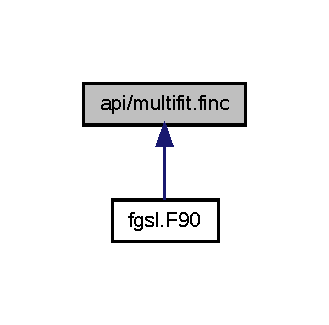
\includegraphics[width=160pt]{multifit_8finc__dep__incl}
\end{center}
\end{figure}
\subsection*{Functions/\-Subroutines}
\begin{DoxyCompactItemize}
\item 
type(fgsl\-\_\-multifit\-\_\-function) \\*
function \hyperlink{multifit_8finc_a2e394cedc80d509b3d36075c158a5e0b}{fgsl\-\_\-multifit\-\_\-function\-\_\-init} (func, ndim, p, params)
\item 
type(fgsl\-\_\-multifit\-\_\-function\-\_\-fdf) \\*
function \hyperlink{multifit_8finc_a2dd878d64008fb31f3d9d031fd5996b7}{fgsl\-\_\-multifit\-\_\-function\-\_\-fdf\-\_\-init} (func, dfunc, fdfunc, ndim, p, params)
\item 
subroutine \hyperlink{multifit_8finc_a00bc267d2137d1f864bd2dad8cf9c1e4}{fgsl\-\_\-multifit\-\_\-function\-\_\-free} (fun)
\item 
subroutine \hyperlink{multifit_8finc_a268c4c5943960408672abc2e9688bf83}{fgsl\-\_\-multifit\-\_\-function\-\_\-fdf\-\_\-free} (fun)
\item 
type(fgsl\-\_\-multifit\-\_\-fsolver) \\*
function \hyperlink{multifit_8finc_ab65091d8504740c62c4e7524b9baf849}{fgsl\-\_\-multifit\-\_\-fsolver\-\_\-alloc} (t, n, p)
\item 
type(fgsl\-\_\-multifit\-\_\-fdfsolver) \\*
function \hyperlink{multifit_8finc_ad6618c0ee5bef46ed5dedb9a15061e4d}{fgsl\-\_\-multifit\-\_\-fdfsolver\-\_\-alloc} (t, n, p)
\item 
subroutine \hyperlink{multifit_8finc_a4edb3e095664b64c3d404361b85646b8}{fgsl\-\_\-multifit\-\_\-fsolver\-\_\-free} (s)
\item 
subroutine \hyperlink{multifit_8finc_a165ecb344b49316126c86c7b77736818}{fgsl\-\_\-multifit\-\_\-fdfsolver\-\_\-free} (s)
\item 
integer(fgsl\-\_\-int) function \hyperlink{multifit_8finc_add0161459835f3bb750e5f1b624a7431}{fgsl\-\_\-multifit\-\_\-fsolver\-\_\-set} (s, f, x)
\item 
integer(fgsl\-\_\-int) function \hyperlink{multifit_8finc_aeeaba728844c99084aa56a584dbd90d6}{fgsl\-\_\-multifit\-\_\-fdfsolver\-\_\-set} (s, fdf, x)
\item 
character(kind=fgsl\-\_\-char, len=fgsl\-\_\-strmax) \\*
function \hyperlink{multifit_8finc_a1c86f8b8187449338d57229da0c9c87a}{fgsl\-\_\-multifit\-\_\-fsolver\-\_\-name} (s)
\item 
character(kind=fgsl\-\_\-char, len=fgsl\-\_\-strmax) \\*
function \hyperlink{multifit_8finc_a771b7c045ca45cddece1bab084d81687}{fgsl\-\_\-multifit\-\_\-fdfsolver\-\_\-name} (s)
\item 
integer(fgsl\-\_\-int) function \hyperlink{multifit_8finc_a6262c763ec214a5143c1aec91f5f61a0}{fgsl\-\_\-multifit\-\_\-fsolver\-\_\-iterate} (s)
\item 
integer(fgsl\-\_\-int) function \hyperlink{multifit_8finc_a62a0cfaf39d63305b4e9ec2feae62e58}{fgsl\-\_\-multifit\-\_\-fdfsolver\-\_\-iterate} (s)
\item 
type(fgsl\-\_\-vector) function \hyperlink{multifit_8finc_ae18bf66b9d8137530d9e00d789cd1b47}{fgsl\-\_\-multifit\-\_\-fsolver\-\_\-position} (s)
\item 
type(fgsl\-\_\-vector) function \hyperlink{multifit_8finc_a21df223213883480f389a670b22333a2}{fgsl\-\_\-multifit\-\_\-fdfsolver\-\_\-position} (s)
\item 
type(fgsl\-\_\-vector) function \hyperlink{multifit_8finc_a5d5d7621f0e81fd1eaf2c01119a9e9ee}{fgsl\-\_\-multifit\-\_\-fdfsolver\-\_\-dx} (s)
\item 
type(fgsl\-\_\-vector) function \hyperlink{multifit_8finc_af31bdf3274659259d4a5bc4eb3e93275}{fgsl\-\_\-multifit\-\_\-fdfsolver\-\_\-f} (s)
\item 
type(fgsl\-\_\-matrix) function \hyperlink{multifit_8finc_ab24fe31ab5a3648bb2aeb958e0a5e2e9}{fgsl\-\_\-multifit\-\_\-fdfsolver\-\_\-jac} (s)
\item 
integer(fgsl\-\_\-int) function \hyperlink{multifit_8finc_a32b6331d1e1c82610b617328dc3234cf}{fgsl\-\_\-multifit\-\_\-test\-\_\-delta} (dx, x, epsabs, epsrel)
\item 
integer(fgsl\-\_\-int) function \hyperlink{multifit_8finc_a6f3f38114ba37459b8d28d7757b0ae3c}{fgsl\-\_\-multifit\-\_\-test\-\_\-gradient} (g, epsabs)
\item 
integer(fgsl\-\_\-int) function \hyperlink{multifit_8finc_a0451b9c85929c00cd7c5a6ad103dfea3}{fgsl\-\_\-multifit\-\_\-gradient} (j, f, g)
\item 
integer(fgsl\-\_\-int) function \hyperlink{multifit_8finc_a843fbc4d78a3e84e537c8b2c10eff8ef}{fgsl\-\_\-multifit\-\_\-covar} (j, epsrel, covar)
\item 
logical function \hyperlink{multifit_8finc_a3945d89bd5d38c87bb6808ee41382e31}{fgsl\-\_\-multifit\-\_\-fsolver\-\_\-status} (s)
\item 
logical function \hyperlink{multifit_8finc_ae28da5d71114b0974e5da3acd305fe34}{fgsl\-\_\-multifit\-\_\-fdfsolver\-\_\-status} (s)
\end{DoxyCompactItemize}


\subsection{Function/\-Subroutine Documentation}
\hypertarget{multifit_8finc_a843fbc4d78a3e84e537c8b2c10eff8ef}{\index{multifit.\-finc@{multifit.\-finc}!fgsl\-\_\-multifit\-\_\-covar@{fgsl\-\_\-multifit\-\_\-covar}}
\index{fgsl\-\_\-multifit\-\_\-covar@{fgsl\-\_\-multifit\-\_\-covar}!multifit.finc@{multifit.\-finc}}
\subsubsection[{fgsl\-\_\-multifit\-\_\-covar}]{\setlength{\rightskip}{0pt plus 5cm}integer(fgsl\-\_\-int) function fgsl\-\_\-multifit\-\_\-covar (
\begin{DoxyParamCaption}
\item[{type(fgsl\-\_\-matrix), intent(in)}]{j, }
\item[{real(fgsl\-\_\-double), intent(in)}]{epsrel, }
\item[{type(fgsl\-\_\-matrix), intent(inout)}]{covar}
\end{DoxyParamCaption}
)}}\label{multifit_8finc_a843fbc4d78a3e84e537c8b2c10eff8ef}
\hypertarget{multifit_8finc_ad6618c0ee5bef46ed5dedb9a15061e4d}{\index{multifit.\-finc@{multifit.\-finc}!fgsl\-\_\-multifit\-\_\-fdfsolver\-\_\-alloc@{fgsl\-\_\-multifit\-\_\-fdfsolver\-\_\-alloc}}
\index{fgsl\-\_\-multifit\-\_\-fdfsolver\-\_\-alloc@{fgsl\-\_\-multifit\-\_\-fdfsolver\-\_\-alloc}!multifit.finc@{multifit.\-finc}}
\subsubsection[{fgsl\-\_\-multifit\-\_\-fdfsolver\-\_\-alloc}]{\setlength{\rightskip}{0pt plus 5cm}type(fgsl\-\_\-multifit\-\_\-fdfsolver) function fgsl\-\_\-multifit\-\_\-fdfsolver\-\_\-alloc (
\begin{DoxyParamCaption}
\item[{type(fgsl\-\_\-multifit\-\_\-fdfsolver\-\_\-type), intent(in)}]{t, }
\item[{integer(fgsl\-\_\-size\-\_\-t), intent(in)}]{n, }
\item[{integer(fgsl\-\_\-size\-\_\-t), intent(in)}]{p}
\end{DoxyParamCaption}
)}}\label{multifit_8finc_ad6618c0ee5bef46ed5dedb9a15061e4d}
\hypertarget{multifit_8finc_a5d5d7621f0e81fd1eaf2c01119a9e9ee}{\index{multifit.\-finc@{multifit.\-finc}!fgsl\-\_\-multifit\-\_\-fdfsolver\-\_\-dx@{fgsl\-\_\-multifit\-\_\-fdfsolver\-\_\-dx}}
\index{fgsl\-\_\-multifit\-\_\-fdfsolver\-\_\-dx@{fgsl\-\_\-multifit\-\_\-fdfsolver\-\_\-dx}!multifit.finc@{multifit.\-finc}}
\subsubsection[{fgsl\-\_\-multifit\-\_\-fdfsolver\-\_\-dx}]{\setlength{\rightskip}{0pt plus 5cm}type(fgsl\-\_\-vector) function fgsl\-\_\-multifit\-\_\-fdfsolver\-\_\-dx (
\begin{DoxyParamCaption}
\item[{type(fgsl\-\_\-multifit\-\_\-fdfsolver), intent(in)}]{s}
\end{DoxyParamCaption}
)}}\label{multifit_8finc_a5d5d7621f0e81fd1eaf2c01119a9e9ee}
\hypertarget{multifit_8finc_af31bdf3274659259d4a5bc4eb3e93275}{\index{multifit.\-finc@{multifit.\-finc}!fgsl\-\_\-multifit\-\_\-fdfsolver\-\_\-f@{fgsl\-\_\-multifit\-\_\-fdfsolver\-\_\-f}}
\index{fgsl\-\_\-multifit\-\_\-fdfsolver\-\_\-f@{fgsl\-\_\-multifit\-\_\-fdfsolver\-\_\-f}!multifit.finc@{multifit.\-finc}}
\subsubsection[{fgsl\-\_\-multifit\-\_\-fdfsolver\-\_\-f}]{\setlength{\rightskip}{0pt plus 5cm}type(fgsl\-\_\-vector) function fgsl\-\_\-multifit\-\_\-fdfsolver\-\_\-f (
\begin{DoxyParamCaption}
\item[{type(fgsl\-\_\-multifit\-\_\-fdfsolver), intent(in)}]{s}
\end{DoxyParamCaption}
)}}\label{multifit_8finc_af31bdf3274659259d4a5bc4eb3e93275}
\hypertarget{multifit_8finc_a165ecb344b49316126c86c7b77736818}{\index{multifit.\-finc@{multifit.\-finc}!fgsl\-\_\-multifit\-\_\-fdfsolver\-\_\-free@{fgsl\-\_\-multifit\-\_\-fdfsolver\-\_\-free}}
\index{fgsl\-\_\-multifit\-\_\-fdfsolver\-\_\-free@{fgsl\-\_\-multifit\-\_\-fdfsolver\-\_\-free}!multifit.finc@{multifit.\-finc}}
\subsubsection[{fgsl\-\_\-multifit\-\_\-fdfsolver\-\_\-free}]{\setlength{\rightskip}{0pt plus 5cm}subroutine fgsl\-\_\-multifit\-\_\-fdfsolver\-\_\-free (
\begin{DoxyParamCaption}
\item[{type(fgsl\-\_\-multifit\-\_\-fdfsolver), intent(inout)}]{s}
\end{DoxyParamCaption}
)}}\label{multifit_8finc_a165ecb344b49316126c86c7b77736818}
\hypertarget{multifit_8finc_a62a0cfaf39d63305b4e9ec2feae62e58}{\index{multifit.\-finc@{multifit.\-finc}!fgsl\-\_\-multifit\-\_\-fdfsolver\-\_\-iterate@{fgsl\-\_\-multifit\-\_\-fdfsolver\-\_\-iterate}}
\index{fgsl\-\_\-multifit\-\_\-fdfsolver\-\_\-iterate@{fgsl\-\_\-multifit\-\_\-fdfsolver\-\_\-iterate}!multifit.finc@{multifit.\-finc}}
\subsubsection[{fgsl\-\_\-multifit\-\_\-fdfsolver\-\_\-iterate}]{\setlength{\rightskip}{0pt plus 5cm}integer(fgsl\-\_\-int) function fgsl\-\_\-multifit\-\_\-fdfsolver\-\_\-iterate (
\begin{DoxyParamCaption}
\item[{type(fgsl\-\_\-multifit\-\_\-fdfsolver), intent(in)}]{s}
\end{DoxyParamCaption}
)}}\label{multifit_8finc_a62a0cfaf39d63305b4e9ec2feae62e58}
\hypertarget{multifit_8finc_ab24fe31ab5a3648bb2aeb958e0a5e2e9}{\index{multifit.\-finc@{multifit.\-finc}!fgsl\-\_\-multifit\-\_\-fdfsolver\-\_\-jac@{fgsl\-\_\-multifit\-\_\-fdfsolver\-\_\-jac}}
\index{fgsl\-\_\-multifit\-\_\-fdfsolver\-\_\-jac@{fgsl\-\_\-multifit\-\_\-fdfsolver\-\_\-jac}!multifit.finc@{multifit.\-finc}}
\subsubsection[{fgsl\-\_\-multifit\-\_\-fdfsolver\-\_\-jac}]{\setlength{\rightskip}{0pt plus 5cm}type(fgsl\-\_\-matrix) function fgsl\-\_\-multifit\-\_\-fdfsolver\-\_\-jac (
\begin{DoxyParamCaption}
\item[{type(fgsl\-\_\-multifit\-\_\-fdfsolver), intent(in)}]{s}
\end{DoxyParamCaption}
)}}\label{multifit_8finc_ab24fe31ab5a3648bb2aeb958e0a5e2e9}
\hypertarget{multifit_8finc_a771b7c045ca45cddece1bab084d81687}{\index{multifit.\-finc@{multifit.\-finc}!fgsl\-\_\-multifit\-\_\-fdfsolver\-\_\-name@{fgsl\-\_\-multifit\-\_\-fdfsolver\-\_\-name}}
\index{fgsl\-\_\-multifit\-\_\-fdfsolver\-\_\-name@{fgsl\-\_\-multifit\-\_\-fdfsolver\-\_\-name}!multifit.finc@{multifit.\-finc}}
\subsubsection[{fgsl\-\_\-multifit\-\_\-fdfsolver\-\_\-name}]{\setlength{\rightskip}{0pt plus 5cm}character(kind=fgsl\-\_\-char,len=fgsl\-\_\-strmax) function fgsl\-\_\-multifit\-\_\-fdfsolver\-\_\-name (
\begin{DoxyParamCaption}
\item[{type(fgsl\-\_\-multifit\-\_\-fdfsolver), intent(in)}]{s}
\end{DoxyParamCaption}
)}}\label{multifit_8finc_a771b7c045ca45cddece1bab084d81687}
\hypertarget{multifit_8finc_a21df223213883480f389a670b22333a2}{\index{multifit.\-finc@{multifit.\-finc}!fgsl\-\_\-multifit\-\_\-fdfsolver\-\_\-position@{fgsl\-\_\-multifit\-\_\-fdfsolver\-\_\-position}}
\index{fgsl\-\_\-multifit\-\_\-fdfsolver\-\_\-position@{fgsl\-\_\-multifit\-\_\-fdfsolver\-\_\-position}!multifit.finc@{multifit.\-finc}}
\subsubsection[{fgsl\-\_\-multifit\-\_\-fdfsolver\-\_\-position}]{\setlength{\rightskip}{0pt plus 5cm}type(fgsl\-\_\-vector) function fgsl\-\_\-multifit\-\_\-fdfsolver\-\_\-position (
\begin{DoxyParamCaption}
\item[{type(fgsl\-\_\-multifit\-\_\-fdfsolver), intent(in)}]{s}
\end{DoxyParamCaption}
)}}\label{multifit_8finc_a21df223213883480f389a670b22333a2}
\hypertarget{multifit_8finc_aeeaba728844c99084aa56a584dbd90d6}{\index{multifit.\-finc@{multifit.\-finc}!fgsl\-\_\-multifit\-\_\-fdfsolver\-\_\-set@{fgsl\-\_\-multifit\-\_\-fdfsolver\-\_\-set}}
\index{fgsl\-\_\-multifit\-\_\-fdfsolver\-\_\-set@{fgsl\-\_\-multifit\-\_\-fdfsolver\-\_\-set}!multifit.finc@{multifit.\-finc}}
\subsubsection[{fgsl\-\_\-multifit\-\_\-fdfsolver\-\_\-set}]{\setlength{\rightskip}{0pt plus 5cm}integer(fgsl\-\_\-int) function fgsl\-\_\-multifit\-\_\-fdfsolver\-\_\-set (
\begin{DoxyParamCaption}
\item[{type(fgsl\-\_\-multifit\-\_\-fdfsolver), intent(inout)}]{s, }
\item[{type(fgsl\-\_\-multifit\-\_\-function\-\_\-fdf), intent(in)}]{fdf, }
\item[{type(fgsl\-\_\-vector), intent(in)}]{x}
\end{DoxyParamCaption}
)}}\label{multifit_8finc_aeeaba728844c99084aa56a584dbd90d6}
\hypertarget{multifit_8finc_ae28da5d71114b0974e5da3acd305fe34}{\index{multifit.\-finc@{multifit.\-finc}!fgsl\-\_\-multifit\-\_\-fdfsolver\-\_\-status@{fgsl\-\_\-multifit\-\_\-fdfsolver\-\_\-status}}
\index{fgsl\-\_\-multifit\-\_\-fdfsolver\-\_\-status@{fgsl\-\_\-multifit\-\_\-fdfsolver\-\_\-status}!multifit.finc@{multifit.\-finc}}
\subsubsection[{fgsl\-\_\-multifit\-\_\-fdfsolver\-\_\-status}]{\setlength{\rightskip}{0pt plus 5cm}logical function fgsl\-\_\-multifit\-\_\-fdfsolver\-\_\-status (
\begin{DoxyParamCaption}
\item[{type(fgsl\-\_\-multifit\-\_\-fdfsolver), intent(in)}]{s}
\end{DoxyParamCaption}
)}}\label{multifit_8finc_ae28da5d71114b0974e5da3acd305fe34}
\hypertarget{multifit_8finc_ab65091d8504740c62c4e7524b9baf849}{\index{multifit.\-finc@{multifit.\-finc}!fgsl\-\_\-multifit\-\_\-fsolver\-\_\-alloc@{fgsl\-\_\-multifit\-\_\-fsolver\-\_\-alloc}}
\index{fgsl\-\_\-multifit\-\_\-fsolver\-\_\-alloc@{fgsl\-\_\-multifit\-\_\-fsolver\-\_\-alloc}!multifit.finc@{multifit.\-finc}}
\subsubsection[{fgsl\-\_\-multifit\-\_\-fsolver\-\_\-alloc}]{\setlength{\rightskip}{0pt plus 5cm}type(fgsl\-\_\-multifit\-\_\-fsolver) function fgsl\-\_\-multifit\-\_\-fsolver\-\_\-alloc (
\begin{DoxyParamCaption}
\item[{type(fgsl\-\_\-multifit\-\_\-fsolver\-\_\-type), intent(in)}]{t, }
\item[{integer(fgsl\-\_\-size\-\_\-t), intent(in)}]{n, }
\item[{integer(fgsl\-\_\-size\-\_\-t), intent(in)}]{p}
\end{DoxyParamCaption}
)}}\label{multifit_8finc_ab65091d8504740c62c4e7524b9baf849}
\hypertarget{multifit_8finc_a4edb3e095664b64c3d404361b85646b8}{\index{multifit.\-finc@{multifit.\-finc}!fgsl\-\_\-multifit\-\_\-fsolver\-\_\-free@{fgsl\-\_\-multifit\-\_\-fsolver\-\_\-free}}
\index{fgsl\-\_\-multifit\-\_\-fsolver\-\_\-free@{fgsl\-\_\-multifit\-\_\-fsolver\-\_\-free}!multifit.finc@{multifit.\-finc}}
\subsubsection[{fgsl\-\_\-multifit\-\_\-fsolver\-\_\-free}]{\setlength{\rightskip}{0pt plus 5cm}subroutine fgsl\-\_\-multifit\-\_\-fsolver\-\_\-free (
\begin{DoxyParamCaption}
\item[{type(fgsl\-\_\-multifit\-\_\-fsolver), intent(inout)}]{s}
\end{DoxyParamCaption}
)}}\label{multifit_8finc_a4edb3e095664b64c3d404361b85646b8}
\hypertarget{multifit_8finc_a6262c763ec214a5143c1aec91f5f61a0}{\index{multifit.\-finc@{multifit.\-finc}!fgsl\-\_\-multifit\-\_\-fsolver\-\_\-iterate@{fgsl\-\_\-multifit\-\_\-fsolver\-\_\-iterate}}
\index{fgsl\-\_\-multifit\-\_\-fsolver\-\_\-iterate@{fgsl\-\_\-multifit\-\_\-fsolver\-\_\-iterate}!multifit.finc@{multifit.\-finc}}
\subsubsection[{fgsl\-\_\-multifit\-\_\-fsolver\-\_\-iterate}]{\setlength{\rightskip}{0pt plus 5cm}integer(fgsl\-\_\-int) function fgsl\-\_\-multifit\-\_\-fsolver\-\_\-iterate (
\begin{DoxyParamCaption}
\item[{type(fgsl\-\_\-multifit\-\_\-fsolver), intent(in)}]{s}
\end{DoxyParamCaption}
)}}\label{multifit_8finc_a6262c763ec214a5143c1aec91f5f61a0}
\hypertarget{multifit_8finc_a1c86f8b8187449338d57229da0c9c87a}{\index{multifit.\-finc@{multifit.\-finc}!fgsl\-\_\-multifit\-\_\-fsolver\-\_\-name@{fgsl\-\_\-multifit\-\_\-fsolver\-\_\-name}}
\index{fgsl\-\_\-multifit\-\_\-fsolver\-\_\-name@{fgsl\-\_\-multifit\-\_\-fsolver\-\_\-name}!multifit.finc@{multifit.\-finc}}
\subsubsection[{fgsl\-\_\-multifit\-\_\-fsolver\-\_\-name}]{\setlength{\rightskip}{0pt plus 5cm}character(kind=fgsl\-\_\-char,len=fgsl\-\_\-strmax) function fgsl\-\_\-multifit\-\_\-fsolver\-\_\-name (
\begin{DoxyParamCaption}
\item[{type(fgsl\-\_\-multifit\-\_\-fsolver), intent(in)}]{s}
\end{DoxyParamCaption}
)}}\label{multifit_8finc_a1c86f8b8187449338d57229da0c9c87a}
\hypertarget{multifit_8finc_ae18bf66b9d8137530d9e00d789cd1b47}{\index{multifit.\-finc@{multifit.\-finc}!fgsl\-\_\-multifit\-\_\-fsolver\-\_\-position@{fgsl\-\_\-multifit\-\_\-fsolver\-\_\-position}}
\index{fgsl\-\_\-multifit\-\_\-fsolver\-\_\-position@{fgsl\-\_\-multifit\-\_\-fsolver\-\_\-position}!multifit.finc@{multifit.\-finc}}
\subsubsection[{fgsl\-\_\-multifit\-\_\-fsolver\-\_\-position}]{\setlength{\rightskip}{0pt plus 5cm}type(fgsl\-\_\-vector) function fgsl\-\_\-multifit\-\_\-fsolver\-\_\-position (
\begin{DoxyParamCaption}
\item[{type(fgsl\-\_\-multifit\-\_\-fsolver), intent(in)}]{s}
\end{DoxyParamCaption}
)}}\label{multifit_8finc_ae18bf66b9d8137530d9e00d789cd1b47}
\hypertarget{multifit_8finc_add0161459835f3bb750e5f1b624a7431}{\index{multifit.\-finc@{multifit.\-finc}!fgsl\-\_\-multifit\-\_\-fsolver\-\_\-set@{fgsl\-\_\-multifit\-\_\-fsolver\-\_\-set}}
\index{fgsl\-\_\-multifit\-\_\-fsolver\-\_\-set@{fgsl\-\_\-multifit\-\_\-fsolver\-\_\-set}!multifit.finc@{multifit.\-finc}}
\subsubsection[{fgsl\-\_\-multifit\-\_\-fsolver\-\_\-set}]{\setlength{\rightskip}{0pt plus 5cm}integer(fgsl\-\_\-int) function fgsl\-\_\-multifit\-\_\-fsolver\-\_\-set (
\begin{DoxyParamCaption}
\item[{type(fgsl\-\_\-multifit\-\_\-fsolver), intent(inout)}]{s, }
\item[{type(fgsl\-\_\-multifit\-\_\-function), intent(in)}]{f, }
\item[{type(fgsl\-\_\-vector), intent(in)}]{x}
\end{DoxyParamCaption}
)}}\label{multifit_8finc_add0161459835f3bb750e5f1b624a7431}
\hypertarget{multifit_8finc_a3945d89bd5d38c87bb6808ee41382e31}{\index{multifit.\-finc@{multifit.\-finc}!fgsl\-\_\-multifit\-\_\-fsolver\-\_\-status@{fgsl\-\_\-multifit\-\_\-fsolver\-\_\-status}}
\index{fgsl\-\_\-multifit\-\_\-fsolver\-\_\-status@{fgsl\-\_\-multifit\-\_\-fsolver\-\_\-status}!multifit.finc@{multifit.\-finc}}
\subsubsection[{fgsl\-\_\-multifit\-\_\-fsolver\-\_\-status}]{\setlength{\rightskip}{0pt plus 5cm}logical function fgsl\-\_\-multifit\-\_\-fsolver\-\_\-status (
\begin{DoxyParamCaption}
\item[{type(fgsl\-\_\-multifit\-\_\-fsolver), intent(in)}]{s}
\end{DoxyParamCaption}
)}}\label{multifit_8finc_a3945d89bd5d38c87bb6808ee41382e31}
\hypertarget{multifit_8finc_a268c4c5943960408672abc2e9688bf83}{\index{multifit.\-finc@{multifit.\-finc}!fgsl\-\_\-multifit\-\_\-function\-\_\-fdf\-\_\-free@{fgsl\-\_\-multifit\-\_\-function\-\_\-fdf\-\_\-free}}
\index{fgsl\-\_\-multifit\-\_\-function\-\_\-fdf\-\_\-free@{fgsl\-\_\-multifit\-\_\-function\-\_\-fdf\-\_\-free}!multifit.finc@{multifit.\-finc}}
\subsubsection[{fgsl\-\_\-multifit\-\_\-function\-\_\-fdf\-\_\-free}]{\setlength{\rightskip}{0pt plus 5cm}subroutine fgsl\-\_\-multifit\-\_\-function\-\_\-fdf\-\_\-free (
\begin{DoxyParamCaption}
\item[{type(fgsl\-\_\-multifit\-\_\-function\-\_\-fdf), intent(inout)}]{fun}
\end{DoxyParamCaption}
)}}\label{multifit_8finc_a268c4c5943960408672abc2e9688bf83}
\hypertarget{multifit_8finc_a2dd878d64008fb31f3d9d031fd5996b7}{\index{multifit.\-finc@{multifit.\-finc}!fgsl\-\_\-multifit\-\_\-function\-\_\-fdf\-\_\-init@{fgsl\-\_\-multifit\-\_\-function\-\_\-fdf\-\_\-init}}
\index{fgsl\-\_\-multifit\-\_\-function\-\_\-fdf\-\_\-init@{fgsl\-\_\-multifit\-\_\-function\-\_\-fdf\-\_\-init}!multifit.finc@{multifit.\-finc}}
\subsubsection[{fgsl\-\_\-multifit\-\_\-function\-\_\-fdf\-\_\-init}]{\setlength{\rightskip}{0pt plus 5cm}type(fgsl\-\_\-multifit\-\_\-function\-\_\-fdf) function fgsl\-\_\-multifit\-\_\-function\-\_\-fdf\-\_\-init (
\begin{DoxyParamCaption}
\item[{}]{func, }
\item[{}]{dfunc, }
\item[{}]{fdfunc, }
\item[{integer(fgsl\-\_\-size\-\_\-t), intent(in)}]{ndim, }
\item[{integer(fgsl\-\_\-size\-\_\-t), intent(in)}]{p, }
\item[{type(c\-\_\-ptr), intent(in)}]{params}
\end{DoxyParamCaption}
)}}\label{multifit_8finc_a2dd878d64008fb31f3d9d031fd5996b7}
\hypertarget{multifit_8finc_a00bc267d2137d1f864bd2dad8cf9c1e4}{\index{multifit.\-finc@{multifit.\-finc}!fgsl\-\_\-multifit\-\_\-function\-\_\-free@{fgsl\-\_\-multifit\-\_\-function\-\_\-free}}
\index{fgsl\-\_\-multifit\-\_\-function\-\_\-free@{fgsl\-\_\-multifit\-\_\-function\-\_\-free}!multifit.finc@{multifit.\-finc}}
\subsubsection[{fgsl\-\_\-multifit\-\_\-function\-\_\-free}]{\setlength{\rightskip}{0pt plus 5cm}subroutine fgsl\-\_\-multifit\-\_\-function\-\_\-free (
\begin{DoxyParamCaption}
\item[{type(fgsl\-\_\-multifit\-\_\-function), intent(inout)}]{fun}
\end{DoxyParamCaption}
)}}\label{multifit_8finc_a00bc267d2137d1f864bd2dad8cf9c1e4}
\hypertarget{multifit_8finc_a2e394cedc80d509b3d36075c158a5e0b}{\index{multifit.\-finc@{multifit.\-finc}!fgsl\-\_\-multifit\-\_\-function\-\_\-init@{fgsl\-\_\-multifit\-\_\-function\-\_\-init}}
\index{fgsl\-\_\-multifit\-\_\-function\-\_\-init@{fgsl\-\_\-multifit\-\_\-function\-\_\-init}!multifit.finc@{multifit.\-finc}}
\subsubsection[{fgsl\-\_\-multifit\-\_\-function\-\_\-init}]{\setlength{\rightskip}{0pt plus 5cm}type(fgsl\-\_\-multifit\-\_\-function) function fgsl\-\_\-multifit\-\_\-function\-\_\-init (
\begin{DoxyParamCaption}
\item[{}]{func, }
\item[{integer(fgsl\-\_\-size\-\_\-t), intent(in)}]{ndim, }
\item[{integer(fgsl\-\_\-size\-\_\-t), intent(in)}]{p, }
\item[{type(c\-\_\-ptr), intent(in)}]{params}
\end{DoxyParamCaption}
)}}\label{multifit_8finc_a2e394cedc80d509b3d36075c158a5e0b}
\hypertarget{multifit_8finc_a0451b9c85929c00cd7c5a6ad103dfea3}{\index{multifit.\-finc@{multifit.\-finc}!fgsl\-\_\-multifit\-\_\-gradient@{fgsl\-\_\-multifit\-\_\-gradient}}
\index{fgsl\-\_\-multifit\-\_\-gradient@{fgsl\-\_\-multifit\-\_\-gradient}!multifit.finc@{multifit.\-finc}}
\subsubsection[{fgsl\-\_\-multifit\-\_\-gradient}]{\setlength{\rightskip}{0pt plus 5cm}integer(fgsl\-\_\-int) function fgsl\-\_\-multifit\-\_\-gradient (
\begin{DoxyParamCaption}
\item[{type(fgsl\-\_\-matrix), intent(in)}]{j, }
\item[{type(fgsl\-\_\-vector), intent(in)}]{f, }
\item[{type(fgsl\-\_\-vector), intent(inout)}]{g}
\end{DoxyParamCaption}
)}}\label{multifit_8finc_a0451b9c85929c00cd7c5a6ad103dfea3}
\hypertarget{multifit_8finc_a32b6331d1e1c82610b617328dc3234cf}{\index{multifit.\-finc@{multifit.\-finc}!fgsl\-\_\-multifit\-\_\-test\-\_\-delta@{fgsl\-\_\-multifit\-\_\-test\-\_\-delta}}
\index{fgsl\-\_\-multifit\-\_\-test\-\_\-delta@{fgsl\-\_\-multifit\-\_\-test\-\_\-delta}!multifit.finc@{multifit.\-finc}}
\subsubsection[{fgsl\-\_\-multifit\-\_\-test\-\_\-delta}]{\setlength{\rightskip}{0pt plus 5cm}integer(fgsl\-\_\-int) function fgsl\-\_\-multifit\-\_\-test\-\_\-delta (
\begin{DoxyParamCaption}
\item[{type(fgsl\-\_\-vector), intent(in)}]{dx, }
\item[{type(fgsl\-\_\-vector), intent(in)}]{x, }
\item[{real(fgsl\-\_\-double), intent(in)}]{epsabs, }
\item[{real(fgsl\-\_\-double), intent(in)}]{epsrel}
\end{DoxyParamCaption}
)}}\label{multifit_8finc_a32b6331d1e1c82610b617328dc3234cf}
\hypertarget{multifit_8finc_a6f3f38114ba37459b8d28d7757b0ae3c}{\index{multifit.\-finc@{multifit.\-finc}!fgsl\-\_\-multifit\-\_\-test\-\_\-gradient@{fgsl\-\_\-multifit\-\_\-test\-\_\-gradient}}
\index{fgsl\-\_\-multifit\-\_\-test\-\_\-gradient@{fgsl\-\_\-multifit\-\_\-test\-\_\-gradient}!multifit.finc@{multifit.\-finc}}
\subsubsection[{fgsl\-\_\-multifit\-\_\-test\-\_\-gradient}]{\setlength{\rightskip}{0pt plus 5cm}integer(fgsl\-\_\-int) function fgsl\-\_\-multifit\-\_\-test\-\_\-gradient (
\begin{DoxyParamCaption}
\item[{type(fgsl\-\_\-vector), intent(in)}]{g, }
\item[{real(fgsl\-\_\-double), intent(in)}]{epsabs}
\end{DoxyParamCaption}
)}}\label{multifit_8finc_a6f3f38114ba37459b8d28d7757b0ae3c}

\hypertarget{multimin_8finc}{\section{api/multimin.finc File Reference}
\label{multimin_8finc}\index{api/multimin.\-finc@{api/multimin.\-finc}}
}
This graph shows which files directly or indirectly include this file\-:
\nopagebreak
\begin{figure}[H]
\begin{center}
\leavevmode
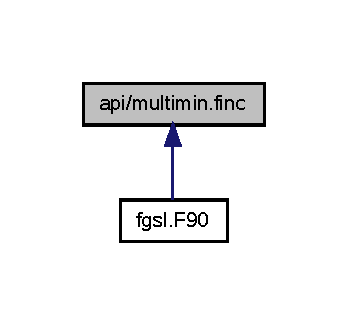
\includegraphics[width=168pt]{multimin_8finc__dep__incl}
\end{center}
\end{figure}
\subsection*{Functions/\-Subroutines}
\begin{DoxyCompactItemize}
\item 
type(fgsl\-\_\-multimin\-\_\-function) \\*
function \hyperlink{multimin_8finc_a1b777bbc4aa79d172caa92121222b5db}{fgsl\-\_\-multimin\-\_\-function\-\_\-init} (func, ndim, params)
\item 
type(fgsl\-\_\-multimin\-\_\-function\-\_\-fdf) \\*
function \hyperlink{multimin_8finc_a38c9b041ca068595cd096fb565b8b84b}{fgsl\-\_\-multimin\-\_\-function\-\_\-fdf\-\_\-init} (func, dfunc, fdfunc, ndim, params)
\item 
subroutine \hyperlink{multimin_8finc_a20359c7761d29e39ee1edbb1a7499814}{fgsl\-\_\-multimin\-\_\-function\-\_\-free} (fun)
\item 
subroutine \hyperlink{multimin_8finc_acf20d19ee20fdd349f2cb779761e15dd}{fgsl\-\_\-multimin\-\_\-function\-\_\-fdf\-\_\-free} (fun)
\item 
type(fgsl\-\_\-multimin\-\_\-fminimizer) \\*
function \hyperlink{multimin_8finc_a9572fe1c742b37999c9dfff7a0ca7ca9}{fgsl\-\_\-multimin\-\_\-fminimizer\-\_\-alloc} (t, n)
\item 
type(fgsl\-\_\-multimin\-\_\-fdfminimizer) \\*
function \hyperlink{multimin_8finc_a4e93d6fb4c774ef02bc0e256fc74f3cf}{fgsl\-\_\-multimin\-\_\-fdfminimizer\-\_\-alloc} (t, n)
\item 
subroutine \hyperlink{multimin_8finc_ab3a786c5c952d55af8c14d3197682c50}{fgsl\-\_\-multimin\-\_\-fminimizer\-\_\-free} (s)
\item 
subroutine \hyperlink{multimin_8finc_a87a418eae01978bd53b1b3d120bd7808}{fgsl\-\_\-multimin\-\_\-fdfminimizer\-\_\-free} (s)
\item 
integer(fgsl\-\_\-int) function \hyperlink{multimin_8finc_acb48fd9d43a274bac09933d5600439bf}{fgsl\-\_\-multimin\-\_\-fminimizer\-\_\-set} (s, f, x, step)
\item 
integer(fgsl\-\_\-int) function \hyperlink{multimin_8finc_a48d15a5b27f8afaf450743f443a6b4e0}{fgsl\-\_\-multimin\-\_\-fdfminimizer\-\_\-set} (s, fdf, x, step, tol)
\item 
character(kind=fgsl\-\_\-char, len=fgsl\-\_\-strmax) \\*
function \hyperlink{multimin_8finc_ac0081b18d8d21a731ab07186254e6421}{fgsl\-\_\-multimin\-\_\-fminimizer\-\_\-name} (s)
\item 
character(kind=fgsl\-\_\-char, len=fgsl\-\_\-strmax) \\*
function \hyperlink{multimin_8finc_add7aec7d233afa06b916d2b936274c41}{fgsl\-\_\-multimin\-\_\-fdfminimizer\-\_\-name} (s)
\item 
integer(fgsl\-\_\-int) function \hyperlink{multimin_8finc_a3197995b850d60e0de902fe245d48bbf}{fgsl\-\_\-multimin\-\_\-fminimizer\-\_\-iterate} (s)
\item 
integer(fgsl\-\_\-int) function \hyperlink{multimin_8finc_ae967ca17e87c39eb2a545c1d710fe3d2}{fgsl\-\_\-multimin\-\_\-fdfminimizer\-\_\-iterate} (s)
\item 
type(fgsl\-\_\-vector) function \hyperlink{multimin_8finc_aa4a9a06fe53544147e23f4c398ea2e3b}{fgsl\-\_\-multimin\-\_\-fminimizer\-\_\-x} (s)
\item 
type(fgsl\-\_\-vector) function \hyperlink{multimin_8finc_a649ffffde4ac9b8567d02ebb30c679b4}{fgsl\-\_\-multimin\-\_\-fdfminimizer\-\_\-x} (s)
\item 
real(fgsl\-\_\-double) function \hyperlink{multimin_8finc_ad82b7976f803bf75a8b762911897a91d}{fgsl\-\_\-multimin\-\_\-fminimizer\-\_\-minimum} (s)
\item 
real(fgsl\-\_\-double) function \hyperlink{multimin_8finc_af074a3128839c747e32a80d7f76ced48}{fgsl\-\_\-multimin\-\_\-fdfminimizer\-\_\-minimum} (s)
\item 
type(fgsl\-\_\-vector) function \hyperlink{multimin_8finc_a831cbe6619ed7b76ae8fe07a2ab3f40b}{fgsl\-\_\-multimin\-\_\-fdfminimizer\-\_\-gradient} (s)
\item 
real(fgsl\-\_\-double) function \hyperlink{multimin_8finc_a78f3abf88b0093e4ca69305e85a78253}{fgsl\-\_\-multimin\-\_\-fminimizer\-\_\-size} (s)
\item 
integer(fgsl\-\_\-int) function \hyperlink{multimin_8finc_ad3a5ccbcbb3cc2029b4790950badeace}{fgsl\-\_\-multimin\-\_\-fdfminimizer\-\_\-restart} (s)
\item 
integer(fgsl\-\_\-int) function \hyperlink{multimin_8finc_ad819b0b49a64995965d3abd7f66f4847}{fgsl\-\_\-multimin\-\_\-test\-\_\-gradient} (g, epsabs)
\item 
integer(fgsl\-\_\-int) function \hyperlink{multimin_8finc_ad9f121a576bee6afbab5fa3c6f8ab5b4}{fgsl\-\_\-multimin\-\_\-test\-\_\-size} (size, epsabs)
\item 
logical function \hyperlink{multimin_8finc_a1a6c440240f101bf70933e5f7a7338ba}{fgsl\-\_\-multimin\-\_\-fminimizer\-\_\-status} (s)
\item 
logical function \hyperlink{multimin_8finc_a39893d424d6495e73046ec17b1c58e69}{fgsl\-\_\-multimin\-\_\-fdfminimizer\-\_\-status} (s)
\end{DoxyCompactItemize}


\subsection{Function/\-Subroutine Documentation}
\hypertarget{multimin_8finc_a4e93d6fb4c774ef02bc0e256fc74f3cf}{\index{multimin.\-finc@{multimin.\-finc}!fgsl\-\_\-multimin\-\_\-fdfminimizer\-\_\-alloc@{fgsl\-\_\-multimin\-\_\-fdfminimizer\-\_\-alloc}}
\index{fgsl\-\_\-multimin\-\_\-fdfminimizer\-\_\-alloc@{fgsl\-\_\-multimin\-\_\-fdfminimizer\-\_\-alloc}!multimin.finc@{multimin.\-finc}}
\subsubsection[{fgsl\-\_\-multimin\-\_\-fdfminimizer\-\_\-alloc}]{\setlength{\rightskip}{0pt plus 5cm}type(fgsl\-\_\-multimin\-\_\-fdfminimizer) function fgsl\-\_\-multimin\-\_\-fdfminimizer\-\_\-alloc (
\begin{DoxyParamCaption}
\item[{type(fgsl\-\_\-multimin\-\_\-fdfminimizer\-\_\-type), intent(in)}]{t, }
\item[{integer(fgsl\-\_\-size\-\_\-t), intent(in)}]{n}
\end{DoxyParamCaption}
)}}\label{multimin_8finc_a4e93d6fb4c774ef02bc0e256fc74f3cf}
\hypertarget{multimin_8finc_a87a418eae01978bd53b1b3d120bd7808}{\index{multimin.\-finc@{multimin.\-finc}!fgsl\-\_\-multimin\-\_\-fdfminimizer\-\_\-free@{fgsl\-\_\-multimin\-\_\-fdfminimizer\-\_\-free}}
\index{fgsl\-\_\-multimin\-\_\-fdfminimizer\-\_\-free@{fgsl\-\_\-multimin\-\_\-fdfminimizer\-\_\-free}!multimin.finc@{multimin.\-finc}}
\subsubsection[{fgsl\-\_\-multimin\-\_\-fdfminimizer\-\_\-free}]{\setlength{\rightskip}{0pt plus 5cm}subroutine fgsl\-\_\-multimin\-\_\-fdfminimizer\-\_\-free (
\begin{DoxyParamCaption}
\item[{type(fgsl\-\_\-multimin\-\_\-fdfminimizer), intent(inout)}]{s}
\end{DoxyParamCaption}
)}}\label{multimin_8finc_a87a418eae01978bd53b1b3d120bd7808}
\hypertarget{multimin_8finc_a831cbe6619ed7b76ae8fe07a2ab3f40b}{\index{multimin.\-finc@{multimin.\-finc}!fgsl\-\_\-multimin\-\_\-fdfminimizer\-\_\-gradient@{fgsl\-\_\-multimin\-\_\-fdfminimizer\-\_\-gradient}}
\index{fgsl\-\_\-multimin\-\_\-fdfminimizer\-\_\-gradient@{fgsl\-\_\-multimin\-\_\-fdfminimizer\-\_\-gradient}!multimin.finc@{multimin.\-finc}}
\subsubsection[{fgsl\-\_\-multimin\-\_\-fdfminimizer\-\_\-gradient}]{\setlength{\rightskip}{0pt plus 5cm}type(fgsl\-\_\-vector) function fgsl\-\_\-multimin\-\_\-fdfminimizer\-\_\-gradient (
\begin{DoxyParamCaption}
\item[{type(fgsl\-\_\-multimin\-\_\-fdfminimizer), intent(in)}]{s}
\end{DoxyParamCaption}
)}}\label{multimin_8finc_a831cbe6619ed7b76ae8fe07a2ab3f40b}
\hypertarget{multimin_8finc_ae967ca17e87c39eb2a545c1d710fe3d2}{\index{multimin.\-finc@{multimin.\-finc}!fgsl\-\_\-multimin\-\_\-fdfminimizer\-\_\-iterate@{fgsl\-\_\-multimin\-\_\-fdfminimizer\-\_\-iterate}}
\index{fgsl\-\_\-multimin\-\_\-fdfminimizer\-\_\-iterate@{fgsl\-\_\-multimin\-\_\-fdfminimizer\-\_\-iterate}!multimin.finc@{multimin.\-finc}}
\subsubsection[{fgsl\-\_\-multimin\-\_\-fdfminimizer\-\_\-iterate}]{\setlength{\rightskip}{0pt plus 5cm}integer(fgsl\-\_\-int) function fgsl\-\_\-multimin\-\_\-fdfminimizer\-\_\-iterate (
\begin{DoxyParamCaption}
\item[{type(fgsl\-\_\-multimin\-\_\-fdfminimizer), intent(in)}]{s}
\end{DoxyParamCaption}
)}}\label{multimin_8finc_ae967ca17e87c39eb2a545c1d710fe3d2}
\hypertarget{multimin_8finc_af074a3128839c747e32a80d7f76ced48}{\index{multimin.\-finc@{multimin.\-finc}!fgsl\-\_\-multimin\-\_\-fdfminimizer\-\_\-minimum@{fgsl\-\_\-multimin\-\_\-fdfminimizer\-\_\-minimum}}
\index{fgsl\-\_\-multimin\-\_\-fdfminimizer\-\_\-minimum@{fgsl\-\_\-multimin\-\_\-fdfminimizer\-\_\-minimum}!multimin.finc@{multimin.\-finc}}
\subsubsection[{fgsl\-\_\-multimin\-\_\-fdfminimizer\-\_\-minimum}]{\setlength{\rightskip}{0pt plus 5cm}real(fgsl\-\_\-double) function fgsl\-\_\-multimin\-\_\-fdfminimizer\-\_\-minimum (
\begin{DoxyParamCaption}
\item[{type(fgsl\-\_\-multimin\-\_\-fdfminimizer), intent(in)}]{s}
\end{DoxyParamCaption}
)}}\label{multimin_8finc_af074a3128839c747e32a80d7f76ced48}
\hypertarget{multimin_8finc_add7aec7d233afa06b916d2b936274c41}{\index{multimin.\-finc@{multimin.\-finc}!fgsl\-\_\-multimin\-\_\-fdfminimizer\-\_\-name@{fgsl\-\_\-multimin\-\_\-fdfminimizer\-\_\-name}}
\index{fgsl\-\_\-multimin\-\_\-fdfminimizer\-\_\-name@{fgsl\-\_\-multimin\-\_\-fdfminimizer\-\_\-name}!multimin.finc@{multimin.\-finc}}
\subsubsection[{fgsl\-\_\-multimin\-\_\-fdfminimizer\-\_\-name}]{\setlength{\rightskip}{0pt plus 5cm}character(kind=fgsl\-\_\-char,len=fgsl\-\_\-strmax) function fgsl\-\_\-multimin\-\_\-fdfminimizer\-\_\-name (
\begin{DoxyParamCaption}
\item[{type(fgsl\-\_\-multimin\-\_\-fdfminimizer), intent(in)}]{s}
\end{DoxyParamCaption}
)}}\label{multimin_8finc_add7aec7d233afa06b916d2b936274c41}
\hypertarget{multimin_8finc_ad3a5ccbcbb3cc2029b4790950badeace}{\index{multimin.\-finc@{multimin.\-finc}!fgsl\-\_\-multimin\-\_\-fdfminimizer\-\_\-restart@{fgsl\-\_\-multimin\-\_\-fdfminimizer\-\_\-restart}}
\index{fgsl\-\_\-multimin\-\_\-fdfminimizer\-\_\-restart@{fgsl\-\_\-multimin\-\_\-fdfminimizer\-\_\-restart}!multimin.finc@{multimin.\-finc}}
\subsubsection[{fgsl\-\_\-multimin\-\_\-fdfminimizer\-\_\-restart}]{\setlength{\rightskip}{0pt plus 5cm}integer(fgsl\-\_\-int) function fgsl\-\_\-multimin\-\_\-fdfminimizer\-\_\-restart (
\begin{DoxyParamCaption}
\item[{type(fgsl\-\_\-multimin\-\_\-fdfminimizer), intent(in)}]{s}
\end{DoxyParamCaption}
)}}\label{multimin_8finc_ad3a5ccbcbb3cc2029b4790950badeace}
\hypertarget{multimin_8finc_a48d15a5b27f8afaf450743f443a6b4e0}{\index{multimin.\-finc@{multimin.\-finc}!fgsl\-\_\-multimin\-\_\-fdfminimizer\-\_\-set@{fgsl\-\_\-multimin\-\_\-fdfminimizer\-\_\-set}}
\index{fgsl\-\_\-multimin\-\_\-fdfminimizer\-\_\-set@{fgsl\-\_\-multimin\-\_\-fdfminimizer\-\_\-set}!multimin.finc@{multimin.\-finc}}
\subsubsection[{fgsl\-\_\-multimin\-\_\-fdfminimizer\-\_\-set}]{\setlength{\rightskip}{0pt plus 5cm}integer(fgsl\-\_\-int) function fgsl\-\_\-multimin\-\_\-fdfminimizer\-\_\-set (
\begin{DoxyParamCaption}
\item[{type(fgsl\-\_\-multimin\-\_\-fdfminimizer), intent(inout)}]{s, }
\item[{type(fgsl\-\_\-multimin\-\_\-function\-\_\-fdf), intent(in)}]{fdf, }
\item[{type(fgsl\-\_\-vector), intent(in)}]{x, }
\item[{real(fgsl\-\_\-double), intent(in)}]{step, }
\item[{real(fgsl\-\_\-double), intent(in)}]{tol}
\end{DoxyParamCaption}
)}}\label{multimin_8finc_a48d15a5b27f8afaf450743f443a6b4e0}
\hypertarget{multimin_8finc_a39893d424d6495e73046ec17b1c58e69}{\index{multimin.\-finc@{multimin.\-finc}!fgsl\-\_\-multimin\-\_\-fdfminimizer\-\_\-status@{fgsl\-\_\-multimin\-\_\-fdfminimizer\-\_\-status}}
\index{fgsl\-\_\-multimin\-\_\-fdfminimizer\-\_\-status@{fgsl\-\_\-multimin\-\_\-fdfminimizer\-\_\-status}!multimin.finc@{multimin.\-finc}}
\subsubsection[{fgsl\-\_\-multimin\-\_\-fdfminimizer\-\_\-status}]{\setlength{\rightskip}{0pt plus 5cm}logical function fgsl\-\_\-multimin\-\_\-fdfminimizer\-\_\-status (
\begin{DoxyParamCaption}
\item[{type(fgsl\-\_\-multimin\-\_\-fdfminimizer), intent(in)}]{s}
\end{DoxyParamCaption}
)}}\label{multimin_8finc_a39893d424d6495e73046ec17b1c58e69}
\hypertarget{multimin_8finc_a649ffffde4ac9b8567d02ebb30c679b4}{\index{multimin.\-finc@{multimin.\-finc}!fgsl\-\_\-multimin\-\_\-fdfminimizer\-\_\-x@{fgsl\-\_\-multimin\-\_\-fdfminimizer\-\_\-x}}
\index{fgsl\-\_\-multimin\-\_\-fdfminimizer\-\_\-x@{fgsl\-\_\-multimin\-\_\-fdfminimizer\-\_\-x}!multimin.finc@{multimin.\-finc}}
\subsubsection[{fgsl\-\_\-multimin\-\_\-fdfminimizer\-\_\-x}]{\setlength{\rightskip}{0pt plus 5cm}type(fgsl\-\_\-vector) function fgsl\-\_\-multimin\-\_\-fdfminimizer\-\_\-x (
\begin{DoxyParamCaption}
\item[{type(fgsl\-\_\-multimin\-\_\-fdfminimizer), intent(in)}]{s}
\end{DoxyParamCaption}
)}}\label{multimin_8finc_a649ffffde4ac9b8567d02ebb30c679b4}
\hypertarget{multimin_8finc_a9572fe1c742b37999c9dfff7a0ca7ca9}{\index{multimin.\-finc@{multimin.\-finc}!fgsl\-\_\-multimin\-\_\-fminimizer\-\_\-alloc@{fgsl\-\_\-multimin\-\_\-fminimizer\-\_\-alloc}}
\index{fgsl\-\_\-multimin\-\_\-fminimizer\-\_\-alloc@{fgsl\-\_\-multimin\-\_\-fminimizer\-\_\-alloc}!multimin.finc@{multimin.\-finc}}
\subsubsection[{fgsl\-\_\-multimin\-\_\-fminimizer\-\_\-alloc}]{\setlength{\rightskip}{0pt plus 5cm}type(fgsl\-\_\-multimin\-\_\-fminimizer) function fgsl\-\_\-multimin\-\_\-fminimizer\-\_\-alloc (
\begin{DoxyParamCaption}
\item[{type(fgsl\-\_\-multimin\-\_\-fminimizer\-\_\-type), intent(in)}]{t, }
\item[{integer(fgsl\-\_\-size\-\_\-t), intent(in)}]{n}
\end{DoxyParamCaption}
)}}\label{multimin_8finc_a9572fe1c742b37999c9dfff7a0ca7ca9}
\hypertarget{multimin_8finc_ab3a786c5c952d55af8c14d3197682c50}{\index{multimin.\-finc@{multimin.\-finc}!fgsl\-\_\-multimin\-\_\-fminimizer\-\_\-free@{fgsl\-\_\-multimin\-\_\-fminimizer\-\_\-free}}
\index{fgsl\-\_\-multimin\-\_\-fminimizer\-\_\-free@{fgsl\-\_\-multimin\-\_\-fminimizer\-\_\-free}!multimin.finc@{multimin.\-finc}}
\subsubsection[{fgsl\-\_\-multimin\-\_\-fminimizer\-\_\-free}]{\setlength{\rightskip}{0pt plus 5cm}subroutine fgsl\-\_\-multimin\-\_\-fminimizer\-\_\-free (
\begin{DoxyParamCaption}
\item[{type(fgsl\-\_\-multimin\-\_\-fminimizer), intent(inout)}]{s}
\end{DoxyParamCaption}
)}}\label{multimin_8finc_ab3a786c5c952d55af8c14d3197682c50}
\hypertarget{multimin_8finc_a3197995b850d60e0de902fe245d48bbf}{\index{multimin.\-finc@{multimin.\-finc}!fgsl\-\_\-multimin\-\_\-fminimizer\-\_\-iterate@{fgsl\-\_\-multimin\-\_\-fminimizer\-\_\-iterate}}
\index{fgsl\-\_\-multimin\-\_\-fminimizer\-\_\-iterate@{fgsl\-\_\-multimin\-\_\-fminimizer\-\_\-iterate}!multimin.finc@{multimin.\-finc}}
\subsubsection[{fgsl\-\_\-multimin\-\_\-fminimizer\-\_\-iterate}]{\setlength{\rightskip}{0pt plus 5cm}integer(fgsl\-\_\-int) function fgsl\-\_\-multimin\-\_\-fminimizer\-\_\-iterate (
\begin{DoxyParamCaption}
\item[{type(fgsl\-\_\-multimin\-\_\-fminimizer), intent(in)}]{s}
\end{DoxyParamCaption}
)}}\label{multimin_8finc_a3197995b850d60e0de902fe245d48bbf}
\hypertarget{multimin_8finc_ad82b7976f803bf75a8b762911897a91d}{\index{multimin.\-finc@{multimin.\-finc}!fgsl\-\_\-multimin\-\_\-fminimizer\-\_\-minimum@{fgsl\-\_\-multimin\-\_\-fminimizer\-\_\-minimum}}
\index{fgsl\-\_\-multimin\-\_\-fminimizer\-\_\-minimum@{fgsl\-\_\-multimin\-\_\-fminimizer\-\_\-minimum}!multimin.finc@{multimin.\-finc}}
\subsubsection[{fgsl\-\_\-multimin\-\_\-fminimizer\-\_\-minimum}]{\setlength{\rightskip}{0pt plus 5cm}real(fgsl\-\_\-double) function fgsl\-\_\-multimin\-\_\-fminimizer\-\_\-minimum (
\begin{DoxyParamCaption}
\item[{type(fgsl\-\_\-multimin\-\_\-fminimizer), intent(in)}]{s}
\end{DoxyParamCaption}
)}}\label{multimin_8finc_ad82b7976f803bf75a8b762911897a91d}
\hypertarget{multimin_8finc_ac0081b18d8d21a731ab07186254e6421}{\index{multimin.\-finc@{multimin.\-finc}!fgsl\-\_\-multimin\-\_\-fminimizer\-\_\-name@{fgsl\-\_\-multimin\-\_\-fminimizer\-\_\-name}}
\index{fgsl\-\_\-multimin\-\_\-fminimizer\-\_\-name@{fgsl\-\_\-multimin\-\_\-fminimizer\-\_\-name}!multimin.finc@{multimin.\-finc}}
\subsubsection[{fgsl\-\_\-multimin\-\_\-fminimizer\-\_\-name}]{\setlength{\rightskip}{0pt plus 5cm}character(kind=fgsl\-\_\-char,len=fgsl\-\_\-strmax) function fgsl\-\_\-multimin\-\_\-fminimizer\-\_\-name (
\begin{DoxyParamCaption}
\item[{type(fgsl\-\_\-multimin\-\_\-fminimizer), intent(in)}]{s}
\end{DoxyParamCaption}
)}}\label{multimin_8finc_ac0081b18d8d21a731ab07186254e6421}
\hypertarget{multimin_8finc_acb48fd9d43a274bac09933d5600439bf}{\index{multimin.\-finc@{multimin.\-finc}!fgsl\-\_\-multimin\-\_\-fminimizer\-\_\-set@{fgsl\-\_\-multimin\-\_\-fminimizer\-\_\-set}}
\index{fgsl\-\_\-multimin\-\_\-fminimizer\-\_\-set@{fgsl\-\_\-multimin\-\_\-fminimizer\-\_\-set}!multimin.finc@{multimin.\-finc}}
\subsubsection[{fgsl\-\_\-multimin\-\_\-fminimizer\-\_\-set}]{\setlength{\rightskip}{0pt plus 5cm}integer(fgsl\-\_\-int) function fgsl\-\_\-multimin\-\_\-fminimizer\-\_\-set (
\begin{DoxyParamCaption}
\item[{type(fgsl\-\_\-multimin\-\_\-fminimizer), intent(inout)}]{s, }
\item[{type(fgsl\-\_\-multimin\-\_\-function), intent(in)}]{f, }
\item[{type(fgsl\-\_\-vector), intent(in)}]{x, }
\item[{type(fgsl\-\_\-vector), intent(in)}]{step}
\end{DoxyParamCaption}
)}}\label{multimin_8finc_acb48fd9d43a274bac09933d5600439bf}
\hypertarget{multimin_8finc_a78f3abf88b0093e4ca69305e85a78253}{\index{multimin.\-finc@{multimin.\-finc}!fgsl\-\_\-multimin\-\_\-fminimizer\-\_\-size@{fgsl\-\_\-multimin\-\_\-fminimizer\-\_\-size}}
\index{fgsl\-\_\-multimin\-\_\-fminimizer\-\_\-size@{fgsl\-\_\-multimin\-\_\-fminimizer\-\_\-size}!multimin.finc@{multimin.\-finc}}
\subsubsection[{fgsl\-\_\-multimin\-\_\-fminimizer\-\_\-size}]{\setlength{\rightskip}{0pt plus 5cm}real(fgsl\-\_\-double) function fgsl\-\_\-multimin\-\_\-fminimizer\-\_\-size (
\begin{DoxyParamCaption}
\item[{type(fgsl\-\_\-multimin\-\_\-fminimizer), intent(in)}]{s}
\end{DoxyParamCaption}
)}}\label{multimin_8finc_a78f3abf88b0093e4ca69305e85a78253}
\hypertarget{multimin_8finc_a1a6c440240f101bf70933e5f7a7338ba}{\index{multimin.\-finc@{multimin.\-finc}!fgsl\-\_\-multimin\-\_\-fminimizer\-\_\-status@{fgsl\-\_\-multimin\-\_\-fminimizer\-\_\-status}}
\index{fgsl\-\_\-multimin\-\_\-fminimizer\-\_\-status@{fgsl\-\_\-multimin\-\_\-fminimizer\-\_\-status}!multimin.finc@{multimin.\-finc}}
\subsubsection[{fgsl\-\_\-multimin\-\_\-fminimizer\-\_\-status}]{\setlength{\rightskip}{0pt plus 5cm}logical function fgsl\-\_\-multimin\-\_\-fminimizer\-\_\-status (
\begin{DoxyParamCaption}
\item[{type(fgsl\-\_\-multimin\-\_\-fminimizer), intent(in)}]{s}
\end{DoxyParamCaption}
)}}\label{multimin_8finc_a1a6c440240f101bf70933e5f7a7338ba}
\hypertarget{multimin_8finc_aa4a9a06fe53544147e23f4c398ea2e3b}{\index{multimin.\-finc@{multimin.\-finc}!fgsl\-\_\-multimin\-\_\-fminimizer\-\_\-x@{fgsl\-\_\-multimin\-\_\-fminimizer\-\_\-x}}
\index{fgsl\-\_\-multimin\-\_\-fminimizer\-\_\-x@{fgsl\-\_\-multimin\-\_\-fminimizer\-\_\-x}!multimin.finc@{multimin.\-finc}}
\subsubsection[{fgsl\-\_\-multimin\-\_\-fminimizer\-\_\-x}]{\setlength{\rightskip}{0pt plus 5cm}type(fgsl\-\_\-vector) function fgsl\-\_\-multimin\-\_\-fminimizer\-\_\-x (
\begin{DoxyParamCaption}
\item[{type(fgsl\-\_\-multimin\-\_\-fminimizer), intent(in)}]{s}
\end{DoxyParamCaption}
)}}\label{multimin_8finc_aa4a9a06fe53544147e23f4c398ea2e3b}
\hypertarget{multimin_8finc_acf20d19ee20fdd349f2cb779761e15dd}{\index{multimin.\-finc@{multimin.\-finc}!fgsl\-\_\-multimin\-\_\-function\-\_\-fdf\-\_\-free@{fgsl\-\_\-multimin\-\_\-function\-\_\-fdf\-\_\-free}}
\index{fgsl\-\_\-multimin\-\_\-function\-\_\-fdf\-\_\-free@{fgsl\-\_\-multimin\-\_\-function\-\_\-fdf\-\_\-free}!multimin.finc@{multimin.\-finc}}
\subsubsection[{fgsl\-\_\-multimin\-\_\-function\-\_\-fdf\-\_\-free}]{\setlength{\rightskip}{0pt plus 5cm}subroutine fgsl\-\_\-multimin\-\_\-function\-\_\-fdf\-\_\-free (
\begin{DoxyParamCaption}
\item[{type(fgsl\-\_\-multimin\-\_\-function\-\_\-fdf), intent(inout)}]{fun}
\end{DoxyParamCaption}
)}}\label{multimin_8finc_acf20d19ee20fdd349f2cb779761e15dd}
\hypertarget{multimin_8finc_a38c9b041ca068595cd096fb565b8b84b}{\index{multimin.\-finc@{multimin.\-finc}!fgsl\-\_\-multimin\-\_\-function\-\_\-fdf\-\_\-init@{fgsl\-\_\-multimin\-\_\-function\-\_\-fdf\-\_\-init}}
\index{fgsl\-\_\-multimin\-\_\-function\-\_\-fdf\-\_\-init@{fgsl\-\_\-multimin\-\_\-function\-\_\-fdf\-\_\-init}!multimin.finc@{multimin.\-finc}}
\subsubsection[{fgsl\-\_\-multimin\-\_\-function\-\_\-fdf\-\_\-init}]{\setlength{\rightskip}{0pt plus 5cm}type(fgsl\-\_\-multimin\-\_\-function\-\_\-fdf) function fgsl\-\_\-multimin\-\_\-function\-\_\-fdf\-\_\-init (
\begin{DoxyParamCaption}
\item[{}]{func, }
\item[{}]{dfunc, }
\item[{}]{fdfunc, }
\item[{integer(fgsl\-\_\-size\-\_\-t), intent(in)}]{ndim, }
\item[{type(c\-\_\-ptr), intent(in)}]{params}
\end{DoxyParamCaption}
)}}\label{multimin_8finc_a38c9b041ca068595cd096fb565b8b84b}
\hypertarget{multimin_8finc_a20359c7761d29e39ee1edbb1a7499814}{\index{multimin.\-finc@{multimin.\-finc}!fgsl\-\_\-multimin\-\_\-function\-\_\-free@{fgsl\-\_\-multimin\-\_\-function\-\_\-free}}
\index{fgsl\-\_\-multimin\-\_\-function\-\_\-free@{fgsl\-\_\-multimin\-\_\-function\-\_\-free}!multimin.finc@{multimin.\-finc}}
\subsubsection[{fgsl\-\_\-multimin\-\_\-function\-\_\-free}]{\setlength{\rightskip}{0pt plus 5cm}subroutine fgsl\-\_\-multimin\-\_\-function\-\_\-free (
\begin{DoxyParamCaption}
\item[{type(fgsl\-\_\-multimin\-\_\-function), intent(inout)}]{fun}
\end{DoxyParamCaption}
)}}\label{multimin_8finc_a20359c7761d29e39ee1edbb1a7499814}
\hypertarget{multimin_8finc_a1b777bbc4aa79d172caa92121222b5db}{\index{multimin.\-finc@{multimin.\-finc}!fgsl\-\_\-multimin\-\_\-function\-\_\-init@{fgsl\-\_\-multimin\-\_\-function\-\_\-init}}
\index{fgsl\-\_\-multimin\-\_\-function\-\_\-init@{fgsl\-\_\-multimin\-\_\-function\-\_\-init}!multimin.finc@{multimin.\-finc}}
\subsubsection[{fgsl\-\_\-multimin\-\_\-function\-\_\-init}]{\setlength{\rightskip}{0pt plus 5cm}type(fgsl\-\_\-multimin\-\_\-function) function fgsl\-\_\-multimin\-\_\-function\-\_\-init (
\begin{DoxyParamCaption}
\item[{}]{func, }
\item[{integer(fgsl\-\_\-size\-\_\-t), intent(in)}]{ndim, }
\item[{type(c\-\_\-ptr), intent(in)}]{params}
\end{DoxyParamCaption}
)}}\label{multimin_8finc_a1b777bbc4aa79d172caa92121222b5db}
\hypertarget{multimin_8finc_ad819b0b49a64995965d3abd7f66f4847}{\index{multimin.\-finc@{multimin.\-finc}!fgsl\-\_\-multimin\-\_\-test\-\_\-gradient@{fgsl\-\_\-multimin\-\_\-test\-\_\-gradient}}
\index{fgsl\-\_\-multimin\-\_\-test\-\_\-gradient@{fgsl\-\_\-multimin\-\_\-test\-\_\-gradient}!multimin.finc@{multimin.\-finc}}
\subsubsection[{fgsl\-\_\-multimin\-\_\-test\-\_\-gradient}]{\setlength{\rightskip}{0pt plus 5cm}integer(fgsl\-\_\-int) function fgsl\-\_\-multimin\-\_\-test\-\_\-gradient (
\begin{DoxyParamCaption}
\item[{type(fgsl\-\_\-vector), intent(in)}]{g, }
\item[{real(fgsl\-\_\-double), intent(in)}]{epsabs}
\end{DoxyParamCaption}
)}}\label{multimin_8finc_ad819b0b49a64995965d3abd7f66f4847}
\hypertarget{multimin_8finc_ad9f121a576bee6afbab5fa3c6f8ab5b4}{\index{multimin.\-finc@{multimin.\-finc}!fgsl\-\_\-multimin\-\_\-test\-\_\-size@{fgsl\-\_\-multimin\-\_\-test\-\_\-size}}
\index{fgsl\-\_\-multimin\-\_\-test\-\_\-size@{fgsl\-\_\-multimin\-\_\-test\-\_\-size}!multimin.finc@{multimin.\-finc}}
\subsubsection[{fgsl\-\_\-multimin\-\_\-test\-\_\-size}]{\setlength{\rightskip}{0pt plus 5cm}integer(fgsl\-\_\-int) function fgsl\-\_\-multimin\-\_\-test\-\_\-size (
\begin{DoxyParamCaption}
\item[{real(fgsl\-\_\-double), intent(in)}]{size, }
\item[{real(fgsl\-\_\-double), intent(in)}]{epsabs}
\end{DoxyParamCaption}
)}}\label{multimin_8finc_ad9f121a576bee6afbab5fa3c6f8ab5b4}

\hypertarget{multiroots_8finc}{\section{api/multiroots.finc File Reference}
\label{multiroots_8finc}\index{api/multiroots.\-finc@{api/multiroots.\-finc}}
}
This graph shows which files directly or indirectly include this file\-:\nopagebreak
\begin{figure}[H]
\begin{center}
\leavevmode
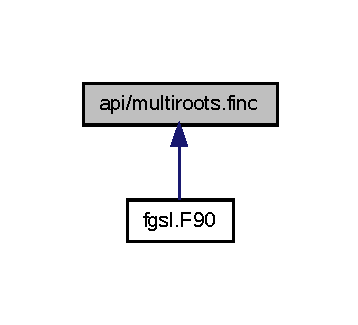
\includegraphics[width=174pt]{multiroots_8finc__dep__incl}
\end{center}
\end{figure}
\subsection*{Functions/\-Subroutines}
\begin{DoxyCompactItemize}
\item 
type(fgsl\-\_\-multiroot\-\_\-function) \\*
function \hyperlink{multiroots_8finc_a78b20b390717ee23f7939615cbe93ff5}{fgsl\-\_\-multiroot\-\_\-function\-\_\-init} (func, ndim, params)
\item 
type(fgsl\-\_\-multiroot\-\_\-function\-\_\-fdf) \\*
function \hyperlink{multiroots_8finc_aa6562b8729129576adc2644344af1d82}{fgsl\-\_\-multiroot\-\_\-function\-\_\-fdf\-\_\-init} (func, dfunc, fdfunc, ndim, params)
\item 
subroutine \hyperlink{multiroots_8finc_a9b0beb12d58e735ed7597de7271439fc}{fgsl\-\_\-multiroot\-\_\-function\-\_\-free} (fun)
\item 
subroutine \hyperlink{multiroots_8finc_ab1e9265827f89cd911c898df0eb8657d}{fgsl\-\_\-multiroot\-\_\-function\-\_\-fdf\-\_\-free} (fun)
\item 
type(fgsl\-\_\-multiroot\-\_\-fsolver) \\*
function \hyperlink{multiroots_8finc_a9967caceee0113037f46962e830a3d7d}{fgsl\-\_\-multiroot\-\_\-fsolver\-\_\-alloc} (t, n)
\item 
type(fgsl\-\_\-multiroot\-\_\-fdfsolver) \\*
function \hyperlink{multiroots_8finc_ab89adde0a73d47f7bcc272997b3f6c8d}{fgsl\-\_\-multiroot\-\_\-fdfsolver\-\_\-alloc} (t, n)
\item 
subroutine \hyperlink{multiroots_8finc_a062ba1ccc85350d3089b310296166e7c}{fgsl\-\_\-multiroot\-\_\-fsolver\-\_\-free} (s)
\item 
subroutine \hyperlink{multiroots_8finc_aee27003f4d58d412ebbde4d72eace13e}{fgsl\-\_\-multiroot\-\_\-fdfsolver\-\_\-free} (s)
\item 
integer(fgsl\-\_\-int) function \hyperlink{multiroots_8finc_a85ec239778cc40c12c0cdda378b3f704}{fgsl\-\_\-multiroot\-\_\-fsolver\-\_\-set} (s, f, x)
\item 
integer(fgsl\-\_\-int) function \hyperlink{multiroots_8finc_a11f98af2f96332f471fa4cdcce719b0a}{fgsl\-\_\-multiroot\-\_\-fdfsolver\-\_\-set} (s, fdf, x)
\item 
character(kind=fgsl\-\_\-char, len=fgsl\-\_\-strmax) \\*
function \hyperlink{multiroots_8finc_aa0ce2f798740b7d41bed54676c414514}{fgsl\-\_\-multiroot\-\_\-fsolver\-\_\-name} (s)
\item 
character(kind=fgsl\-\_\-char, len=fgsl\-\_\-strmax) \\*
function \hyperlink{multiroots_8finc_abc59e0be63f6c4126420aeab1c20081c}{fgsl\-\_\-multiroot\-\_\-fdfsolver\-\_\-name} (s)
\item 
integer(fgsl\-\_\-int) function \hyperlink{multiroots_8finc_ad1d089816977209d88134f95979c2726}{fgsl\-\_\-multiroot\-\_\-fsolver\-\_\-iterate} (s)
\item 
integer(fgsl\-\_\-int) function \hyperlink{multiroots_8finc_a7c2d7b128df269454d93454e6d4117f2}{fgsl\-\_\-multiroot\-\_\-fdfsolver\-\_\-iterate} (s)
\item 
type(fgsl\-\_\-vector) function \hyperlink{multiroots_8finc_a756becbde20557aeffb366a0bbcf8177}{fgsl\-\_\-multiroot\-\_\-fsolver\-\_\-root} (s)
\item 
type(fgsl\-\_\-vector) function \hyperlink{multiroots_8finc_a5b98f55eae83d12a4c0d70b7b6c26508}{fgsl\-\_\-multiroot\-\_\-fdfsolver\-\_\-root} (s)
\item 
type(fgsl\-\_\-vector) function \hyperlink{multiroots_8finc_a7a1a3c9bbcec3621cad66f2a87608bd5}{fgsl\-\_\-multiroot\-\_\-fsolver\-\_\-f} (s)
\item 
type(fgsl\-\_\-vector) function \hyperlink{multiroots_8finc_a3d551eb292c92b30f9628ea8e1d6d251}{fgsl\-\_\-multiroot\-\_\-fdfsolver\-\_\-f} (s)
\item 
type(fgsl\-\_\-vector) function \hyperlink{multiroots_8finc_af5cd6b1ed7e6cb7589c2e64cd4ff22e9}{fgsl\-\_\-multiroot\-\_\-fsolver\-\_\-dx} (s)
\item 
type(fgsl\-\_\-vector) function \hyperlink{multiroots_8finc_a6fa2ba8b4311978a0a28d45afacffeaf}{fgsl\-\_\-multiroot\-\_\-fdfsolver\-\_\-dx} (s)
\item 
integer(fgsl\-\_\-int) function \hyperlink{multiroots_8finc_ad67125d3ae3d333fa1211fdb9ee6c58a}{fgsl\-\_\-multiroot\-\_\-test\-\_\-delta} (dx, x, epsabs, epsrel)
\item 
integer(fgsl\-\_\-int) function \hyperlink{multiroots_8finc_a112c4005ac06aedd7bf4233dbad69244}{fgsl\-\_\-multiroot\-\_\-test\-\_\-residual} (f, epsabs)
\item 
logical function \hyperlink{multiroots_8finc_a1c59daa00ab109e098aab62bc3377912}{fgsl\-\_\-multiroot\-\_\-fsolver\-\_\-status} (s)
\item 
logical function \hyperlink{multiroots_8finc_aa39ce86a033dc3df2cdabd8c2c98215f}{fgsl\-\_\-multiroot\-\_\-fdfsolver\-\_\-status} (s)
\end{DoxyCompactItemize}


\subsection{Function/\-Subroutine Documentation}
\hypertarget{multiroots_8finc_ab89adde0a73d47f7bcc272997b3f6c8d}{\index{multiroots.\-finc@{multiroots.\-finc}!fgsl\-\_\-multiroot\-\_\-fdfsolver\-\_\-alloc@{fgsl\-\_\-multiroot\-\_\-fdfsolver\-\_\-alloc}}
\index{fgsl\-\_\-multiroot\-\_\-fdfsolver\-\_\-alloc@{fgsl\-\_\-multiroot\-\_\-fdfsolver\-\_\-alloc}!multiroots.finc@{multiroots.\-finc}}
\subsubsection[{fgsl\-\_\-multiroot\-\_\-fdfsolver\-\_\-alloc}]{\setlength{\rightskip}{0pt plus 5cm}type(fgsl\-\_\-multiroot\-\_\-fdfsolver) function fgsl\-\_\-multiroot\-\_\-fdfsolver\-\_\-alloc (
\begin{DoxyParamCaption}
\item[{type(fgsl\-\_\-multiroot\-\_\-fdfsolver\-\_\-type), intent(in)}]{t, }
\item[{integer(fgsl\-\_\-size\-\_\-t), intent(in)}]{n}
\end{DoxyParamCaption}
)}}\label{multiroots_8finc_ab89adde0a73d47f7bcc272997b3f6c8d}
\hypertarget{multiroots_8finc_a6fa2ba8b4311978a0a28d45afacffeaf}{\index{multiroots.\-finc@{multiroots.\-finc}!fgsl\-\_\-multiroot\-\_\-fdfsolver\-\_\-dx@{fgsl\-\_\-multiroot\-\_\-fdfsolver\-\_\-dx}}
\index{fgsl\-\_\-multiroot\-\_\-fdfsolver\-\_\-dx@{fgsl\-\_\-multiroot\-\_\-fdfsolver\-\_\-dx}!multiroots.finc@{multiroots.\-finc}}
\subsubsection[{fgsl\-\_\-multiroot\-\_\-fdfsolver\-\_\-dx}]{\setlength{\rightskip}{0pt plus 5cm}type(fgsl\-\_\-vector) function fgsl\-\_\-multiroot\-\_\-fdfsolver\-\_\-dx (
\begin{DoxyParamCaption}
\item[{type(fgsl\-\_\-multiroot\-\_\-fdfsolver), intent(in)}]{s}
\end{DoxyParamCaption}
)}}\label{multiroots_8finc_a6fa2ba8b4311978a0a28d45afacffeaf}
\hypertarget{multiroots_8finc_a3d551eb292c92b30f9628ea8e1d6d251}{\index{multiroots.\-finc@{multiroots.\-finc}!fgsl\-\_\-multiroot\-\_\-fdfsolver\-\_\-f@{fgsl\-\_\-multiroot\-\_\-fdfsolver\-\_\-f}}
\index{fgsl\-\_\-multiroot\-\_\-fdfsolver\-\_\-f@{fgsl\-\_\-multiroot\-\_\-fdfsolver\-\_\-f}!multiroots.finc@{multiroots.\-finc}}
\subsubsection[{fgsl\-\_\-multiroot\-\_\-fdfsolver\-\_\-f}]{\setlength{\rightskip}{0pt plus 5cm}type(fgsl\-\_\-vector) function fgsl\-\_\-multiroot\-\_\-fdfsolver\-\_\-f (
\begin{DoxyParamCaption}
\item[{type(fgsl\-\_\-multiroot\-\_\-fdfsolver), intent(in)}]{s}
\end{DoxyParamCaption}
)}}\label{multiroots_8finc_a3d551eb292c92b30f9628ea8e1d6d251}
\hypertarget{multiroots_8finc_aee27003f4d58d412ebbde4d72eace13e}{\index{multiroots.\-finc@{multiroots.\-finc}!fgsl\-\_\-multiroot\-\_\-fdfsolver\-\_\-free@{fgsl\-\_\-multiroot\-\_\-fdfsolver\-\_\-free}}
\index{fgsl\-\_\-multiroot\-\_\-fdfsolver\-\_\-free@{fgsl\-\_\-multiroot\-\_\-fdfsolver\-\_\-free}!multiroots.finc@{multiroots.\-finc}}
\subsubsection[{fgsl\-\_\-multiroot\-\_\-fdfsolver\-\_\-free}]{\setlength{\rightskip}{0pt plus 5cm}subroutine fgsl\-\_\-multiroot\-\_\-fdfsolver\-\_\-free (
\begin{DoxyParamCaption}
\item[{type(fgsl\-\_\-multiroot\-\_\-fdfsolver), intent(inout)}]{s}
\end{DoxyParamCaption}
)}}\label{multiroots_8finc_aee27003f4d58d412ebbde4d72eace13e}
\hypertarget{multiroots_8finc_a7c2d7b128df269454d93454e6d4117f2}{\index{multiroots.\-finc@{multiroots.\-finc}!fgsl\-\_\-multiroot\-\_\-fdfsolver\-\_\-iterate@{fgsl\-\_\-multiroot\-\_\-fdfsolver\-\_\-iterate}}
\index{fgsl\-\_\-multiroot\-\_\-fdfsolver\-\_\-iterate@{fgsl\-\_\-multiroot\-\_\-fdfsolver\-\_\-iterate}!multiroots.finc@{multiroots.\-finc}}
\subsubsection[{fgsl\-\_\-multiroot\-\_\-fdfsolver\-\_\-iterate}]{\setlength{\rightskip}{0pt plus 5cm}integer(fgsl\-\_\-int) function fgsl\-\_\-multiroot\-\_\-fdfsolver\-\_\-iterate (
\begin{DoxyParamCaption}
\item[{type(fgsl\-\_\-multiroot\-\_\-fdfsolver), intent(in)}]{s}
\end{DoxyParamCaption}
)}}\label{multiroots_8finc_a7c2d7b128df269454d93454e6d4117f2}
\hypertarget{multiroots_8finc_abc59e0be63f6c4126420aeab1c20081c}{\index{multiroots.\-finc@{multiroots.\-finc}!fgsl\-\_\-multiroot\-\_\-fdfsolver\-\_\-name@{fgsl\-\_\-multiroot\-\_\-fdfsolver\-\_\-name}}
\index{fgsl\-\_\-multiroot\-\_\-fdfsolver\-\_\-name@{fgsl\-\_\-multiroot\-\_\-fdfsolver\-\_\-name}!multiroots.finc@{multiroots.\-finc}}
\subsubsection[{fgsl\-\_\-multiroot\-\_\-fdfsolver\-\_\-name}]{\setlength{\rightskip}{0pt plus 5cm}character(kind=fgsl\-\_\-char,len=fgsl\-\_\-strmax) function fgsl\-\_\-multiroot\-\_\-fdfsolver\-\_\-name (
\begin{DoxyParamCaption}
\item[{type(fgsl\-\_\-multiroot\-\_\-fdfsolver), intent(in)}]{s}
\end{DoxyParamCaption}
)}}\label{multiroots_8finc_abc59e0be63f6c4126420aeab1c20081c}
\hypertarget{multiroots_8finc_a5b98f55eae83d12a4c0d70b7b6c26508}{\index{multiroots.\-finc@{multiroots.\-finc}!fgsl\-\_\-multiroot\-\_\-fdfsolver\-\_\-root@{fgsl\-\_\-multiroot\-\_\-fdfsolver\-\_\-root}}
\index{fgsl\-\_\-multiroot\-\_\-fdfsolver\-\_\-root@{fgsl\-\_\-multiroot\-\_\-fdfsolver\-\_\-root}!multiroots.finc@{multiroots.\-finc}}
\subsubsection[{fgsl\-\_\-multiroot\-\_\-fdfsolver\-\_\-root}]{\setlength{\rightskip}{0pt plus 5cm}type(fgsl\-\_\-vector) function fgsl\-\_\-multiroot\-\_\-fdfsolver\-\_\-root (
\begin{DoxyParamCaption}
\item[{type(fgsl\-\_\-multiroot\-\_\-fdfsolver), intent(in)}]{s}
\end{DoxyParamCaption}
)}}\label{multiroots_8finc_a5b98f55eae83d12a4c0d70b7b6c26508}
\hypertarget{multiroots_8finc_a11f98af2f96332f471fa4cdcce719b0a}{\index{multiroots.\-finc@{multiroots.\-finc}!fgsl\-\_\-multiroot\-\_\-fdfsolver\-\_\-set@{fgsl\-\_\-multiroot\-\_\-fdfsolver\-\_\-set}}
\index{fgsl\-\_\-multiroot\-\_\-fdfsolver\-\_\-set@{fgsl\-\_\-multiroot\-\_\-fdfsolver\-\_\-set}!multiroots.finc@{multiroots.\-finc}}
\subsubsection[{fgsl\-\_\-multiroot\-\_\-fdfsolver\-\_\-set}]{\setlength{\rightskip}{0pt plus 5cm}integer(fgsl\-\_\-int) function fgsl\-\_\-multiroot\-\_\-fdfsolver\-\_\-set (
\begin{DoxyParamCaption}
\item[{type(fgsl\-\_\-multiroot\-\_\-fdfsolver), intent(inout)}]{s, }
\item[{type(fgsl\-\_\-multiroot\-\_\-function\-\_\-fdf), intent(in)}]{fdf, }
\item[{type(fgsl\-\_\-vector), intent(in)}]{x}
\end{DoxyParamCaption}
)}}\label{multiroots_8finc_a11f98af2f96332f471fa4cdcce719b0a}
\hypertarget{multiroots_8finc_aa39ce86a033dc3df2cdabd8c2c98215f}{\index{multiroots.\-finc@{multiroots.\-finc}!fgsl\-\_\-multiroot\-\_\-fdfsolver\-\_\-status@{fgsl\-\_\-multiroot\-\_\-fdfsolver\-\_\-status}}
\index{fgsl\-\_\-multiroot\-\_\-fdfsolver\-\_\-status@{fgsl\-\_\-multiroot\-\_\-fdfsolver\-\_\-status}!multiroots.finc@{multiroots.\-finc}}
\subsubsection[{fgsl\-\_\-multiroot\-\_\-fdfsolver\-\_\-status}]{\setlength{\rightskip}{0pt plus 5cm}logical function fgsl\-\_\-multiroot\-\_\-fdfsolver\-\_\-status (
\begin{DoxyParamCaption}
\item[{type(fgsl\-\_\-multiroot\-\_\-fdfsolver), intent(in)}]{s}
\end{DoxyParamCaption}
)}}\label{multiroots_8finc_aa39ce86a033dc3df2cdabd8c2c98215f}
\hypertarget{multiroots_8finc_a9967caceee0113037f46962e830a3d7d}{\index{multiroots.\-finc@{multiroots.\-finc}!fgsl\-\_\-multiroot\-\_\-fsolver\-\_\-alloc@{fgsl\-\_\-multiroot\-\_\-fsolver\-\_\-alloc}}
\index{fgsl\-\_\-multiroot\-\_\-fsolver\-\_\-alloc@{fgsl\-\_\-multiroot\-\_\-fsolver\-\_\-alloc}!multiroots.finc@{multiroots.\-finc}}
\subsubsection[{fgsl\-\_\-multiroot\-\_\-fsolver\-\_\-alloc}]{\setlength{\rightskip}{0pt plus 5cm}type(fgsl\-\_\-multiroot\-\_\-fsolver) function fgsl\-\_\-multiroot\-\_\-fsolver\-\_\-alloc (
\begin{DoxyParamCaption}
\item[{type(fgsl\-\_\-multiroot\-\_\-fsolver\-\_\-type), intent(in)}]{t, }
\item[{integer(fgsl\-\_\-size\-\_\-t), intent(in)}]{n}
\end{DoxyParamCaption}
)}}\label{multiroots_8finc_a9967caceee0113037f46962e830a3d7d}
\hypertarget{multiroots_8finc_af5cd6b1ed7e6cb7589c2e64cd4ff22e9}{\index{multiroots.\-finc@{multiroots.\-finc}!fgsl\-\_\-multiroot\-\_\-fsolver\-\_\-dx@{fgsl\-\_\-multiroot\-\_\-fsolver\-\_\-dx}}
\index{fgsl\-\_\-multiroot\-\_\-fsolver\-\_\-dx@{fgsl\-\_\-multiroot\-\_\-fsolver\-\_\-dx}!multiroots.finc@{multiroots.\-finc}}
\subsubsection[{fgsl\-\_\-multiroot\-\_\-fsolver\-\_\-dx}]{\setlength{\rightskip}{0pt plus 5cm}type(fgsl\-\_\-vector) function fgsl\-\_\-multiroot\-\_\-fsolver\-\_\-dx (
\begin{DoxyParamCaption}
\item[{type(fgsl\-\_\-multiroot\-\_\-fsolver), intent(in)}]{s}
\end{DoxyParamCaption}
)}}\label{multiroots_8finc_af5cd6b1ed7e6cb7589c2e64cd4ff22e9}
\hypertarget{multiroots_8finc_a7a1a3c9bbcec3621cad66f2a87608bd5}{\index{multiroots.\-finc@{multiroots.\-finc}!fgsl\-\_\-multiroot\-\_\-fsolver\-\_\-f@{fgsl\-\_\-multiroot\-\_\-fsolver\-\_\-f}}
\index{fgsl\-\_\-multiroot\-\_\-fsolver\-\_\-f@{fgsl\-\_\-multiroot\-\_\-fsolver\-\_\-f}!multiroots.finc@{multiroots.\-finc}}
\subsubsection[{fgsl\-\_\-multiroot\-\_\-fsolver\-\_\-f}]{\setlength{\rightskip}{0pt plus 5cm}type(fgsl\-\_\-vector) function fgsl\-\_\-multiroot\-\_\-fsolver\-\_\-f (
\begin{DoxyParamCaption}
\item[{type(fgsl\-\_\-multiroot\-\_\-fsolver), intent(in)}]{s}
\end{DoxyParamCaption}
)}}\label{multiroots_8finc_a7a1a3c9bbcec3621cad66f2a87608bd5}
\hypertarget{multiroots_8finc_a062ba1ccc85350d3089b310296166e7c}{\index{multiroots.\-finc@{multiroots.\-finc}!fgsl\-\_\-multiroot\-\_\-fsolver\-\_\-free@{fgsl\-\_\-multiroot\-\_\-fsolver\-\_\-free}}
\index{fgsl\-\_\-multiroot\-\_\-fsolver\-\_\-free@{fgsl\-\_\-multiroot\-\_\-fsolver\-\_\-free}!multiroots.finc@{multiroots.\-finc}}
\subsubsection[{fgsl\-\_\-multiroot\-\_\-fsolver\-\_\-free}]{\setlength{\rightskip}{0pt plus 5cm}subroutine fgsl\-\_\-multiroot\-\_\-fsolver\-\_\-free (
\begin{DoxyParamCaption}
\item[{type(fgsl\-\_\-multiroot\-\_\-fsolver), intent(inout)}]{s}
\end{DoxyParamCaption}
)}}\label{multiroots_8finc_a062ba1ccc85350d3089b310296166e7c}
\hypertarget{multiroots_8finc_ad1d089816977209d88134f95979c2726}{\index{multiroots.\-finc@{multiroots.\-finc}!fgsl\-\_\-multiroot\-\_\-fsolver\-\_\-iterate@{fgsl\-\_\-multiroot\-\_\-fsolver\-\_\-iterate}}
\index{fgsl\-\_\-multiroot\-\_\-fsolver\-\_\-iterate@{fgsl\-\_\-multiroot\-\_\-fsolver\-\_\-iterate}!multiroots.finc@{multiroots.\-finc}}
\subsubsection[{fgsl\-\_\-multiroot\-\_\-fsolver\-\_\-iterate}]{\setlength{\rightskip}{0pt plus 5cm}integer(fgsl\-\_\-int) function fgsl\-\_\-multiroot\-\_\-fsolver\-\_\-iterate (
\begin{DoxyParamCaption}
\item[{type(fgsl\-\_\-multiroot\-\_\-fsolver), intent(in)}]{s}
\end{DoxyParamCaption}
)}}\label{multiroots_8finc_ad1d089816977209d88134f95979c2726}
\hypertarget{multiroots_8finc_aa0ce2f798740b7d41bed54676c414514}{\index{multiroots.\-finc@{multiroots.\-finc}!fgsl\-\_\-multiroot\-\_\-fsolver\-\_\-name@{fgsl\-\_\-multiroot\-\_\-fsolver\-\_\-name}}
\index{fgsl\-\_\-multiroot\-\_\-fsolver\-\_\-name@{fgsl\-\_\-multiroot\-\_\-fsolver\-\_\-name}!multiroots.finc@{multiroots.\-finc}}
\subsubsection[{fgsl\-\_\-multiroot\-\_\-fsolver\-\_\-name}]{\setlength{\rightskip}{0pt plus 5cm}character(kind=fgsl\-\_\-char,len=fgsl\-\_\-strmax) function fgsl\-\_\-multiroot\-\_\-fsolver\-\_\-name (
\begin{DoxyParamCaption}
\item[{type(fgsl\-\_\-multiroot\-\_\-fsolver), intent(in)}]{s}
\end{DoxyParamCaption}
)}}\label{multiroots_8finc_aa0ce2f798740b7d41bed54676c414514}
\hypertarget{multiroots_8finc_a756becbde20557aeffb366a0bbcf8177}{\index{multiroots.\-finc@{multiroots.\-finc}!fgsl\-\_\-multiroot\-\_\-fsolver\-\_\-root@{fgsl\-\_\-multiroot\-\_\-fsolver\-\_\-root}}
\index{fgsl\-\_\-multiroot\-\_\-fsolver\-\_\-root@{fgsl\-\_\-multiroot\-\_\-fsolver\-\_\-root}!multiroots.finc@{multiroots.\-finc}}
\subsubsection[{fgsl\-\_\-multiroot\-\_\-fsolver\-\_\-root}]{\setlength{\rightskip}{0pt plus 5cm}type(fgsl\-\_\-vector) function fgsl\-\_\-multiroot\-\_\-fsolver\-\_\-root (
\begin{DoxyParamCaption}
\item[{type(fgsl\-\_\-multiroot\-\_\-fsolver), intent(in)}]{s}
\end{DoxyParamCaption}
)}}\label{multiroots_8finc_a756becbde20557aeffb366a0bbcf8177}
\hypertarget{multiroots_8finc_a85ec239778cc40c12c0cdda378b3f704}{\index{multiroots.\-finc@{multiroots.\-finc}!fgsl\-\_\-multiroot\-\_\-fsolver\-\_\-set@{fgsl\-\_\-multiroot\-\_\-fsolver\-\_\-set}}
\index{fgsl\-\_\-multiroot\-\_\-fsolver\-\_\-set@{fgsl\-\_\-multiroot\-\_\-fsolver\-\_\-set}!multiroots.finc@{multiroots.\-finc}}
\subsubsection[{fgsl\-\_\-multiroot\-\_\-fsolver\-\_\-set}]{\setlength{\rightskip}{0pt plus 5cm}integer(fgsl\-\_\-int) function fgsl\-\_\-multiroot\-\_\-fsolver\-\_\-set (
\begin{DoxyParamCaption}
\item[{type(fgsl\-\_\-multiroot\-\_\-fsolver), intent(inout)}]{s, }
\item[{type(fgsl\-\_\-multiroot\-\_\-function), intent(in)}]{f, }
\item[{type(fgsl\-\_\-vector), intent(in)}]{x}
\end{DoxyParamCaption}
)}}\label{multiroots_8finc_a85ec239778cc40c12c0cdda378b3f704}
\hypertarget{multiroots_8finc_a1c59daa00ab109e098aab62bc3377912}{\index{multiroots.\-finc@{multiroots.\-finc}!fgsl\-\_\-multiroot\-\_\-fsolver\-\_\-status@{fgsl\-\_\-multiroot\-\_\-fsolver\-\_\-status}}
\index{fgsl\-\_\-multiroot\-\_\-fsolver\-\_\-status@{fgsl\-\_\-multiroot\-\_\-fsolver\-\_\-status}!multiroots.finc@{multiroots.\-finc}}
\subsubsection[{fgsl\-\_\-multiroot\-\_\-fsolver\-\_\-status}]{\setlength{\rightskip}{0pt plus 5cm}logical function fgsl\-\_\-multiroot\-\_\-fsolver\-\_\-status (
\begin{DoxyParamCaption}
\item[{type(fgsl\-\_\-multiroot\-\_\-fsolver), intent(in)}]{s}
\end{DoxyParamCaption}
)}}\label{multiroots_8finc_a1c59daa00ab109e098aab62bc3377912}
\hypertarget{multiroots_8finc_ab1e9265827f89cd911c898df0eb8657d}{\index{multiroots.\-finc@{multiroots.\-finc}!fgsl\-\_\-multiroot\-\_\-function\-\_\-fdf\-\_\-free@{fgsl\-\_\-multiroot\-\_\-function\-\_\-fdf\-\_\-free}}
\index{fgsl\-\_\-multiroot\-\_\-function\-\_\-fdf\-\_\-free@{fgsl\-\_\-multiroot\-\_\-function\-\_\-fdf\-\_\-free}!multiroots.finc@{multiroots.\-finc}}
\subsubsection[{fgsl\-\_\-multiroot\-\_\-function\-\_\-fdf\-\_\-free}]{\setlength{\rightskip}{0pt plus 5cm}subroutine fgsl\-\_\-multiroot\-\_\-function\-\_\-fdf\-\_\-free (
\begin{DoxyParamCaption}
\item[{type(fgsl\-\_\-multiroot\-\_\-function\-\_\-fdf), intent(inout)}]{fun}
\end{DoxyParamCaption}
)}}\label{multiroots_8finc_ab1e9265827f89cd911c898df0eb8657d}
\hypertarget{multiroots_8finc_aa6562b8729129576adc2644344af1d82}{\index{multiroots.\-finc@{multiroots.\-finc}!fgsl\-\_\-multiroot\-\_\-function\-\_\-fdf\-\_\-init@{fgsl\-\_\-multiroot\-\_\-function\-\_\-fdf\-\_\-init}}
\index{fgsl\-\_\-multiroot\-\_\-function\-\_\-fdf\-\_\-init@{fgsl\-\_\-multiroot\-\_\-function\-\_\-fdf\-\_\-init}!multiroots.finc@{multiroots.\-finc}}
\subsubsection[{fgsl\-\_\-multiroot\-\_\-function\-\_\-fdf\-\_\-init}]{\setlength{\rightskip}{0pt plus 5cm}type(fgsl\-\_\-multiroot\-\_\-function\-\_\-fdf) function fgsl\-\_\-multiroot\-\_\-function\-\_\-fdf\-\_\-init (
\begin{DoxyParamCaption}
\item[{}]{func, }
\item[{}]{dfunc, }
\item[{}]{fdfunc, }
\item[{integer(fgsl\-\_\-size\-\_\-t), intent(in)}]{ndim, }
\item[{type(c\-\_\-ptr), intent(in)}]{params}
\end{DoxyParamCaption}
)}}\label{multiroots_8finc_aa6562b8729129576adc2644344af1d82}
\hypertarget{multiroots_8finc_a9b0beb12d58e735ed7597de7271439fc}{\index{multiroots.\-finc@{multiroots.\-finc}!fgsl\-\_\-multiroot\-\_\-function\-\_\-free@{fgsl\-\_\-multiroot\-\_\-function\-\_\-free}}
\index{fgsl\-\_\-multiroot\-\_\-function\-\_\-free@{fgsl\-\_\-multiroot\-\_\-function\-\_\-free}!multiroots.finc@{multiroots.\-finc}}
\subsubsection[{fgsl\-\_\-multiroot\-\_\-function\-\_\-free}]{\setlength{\rightskip}{0pt plus 5cm}subroutine fgsl\-\_\-multiroot\-\_\-function\-\_\-free (
\begin{DoxyParamCaption}
\item[{type(fgsl\-\_\-multiroot\-\_\-function), intent(inout)}]{fun}
\end{DoxyParamCaption}
)}}\label{multiroots_8finc_a9b0beb12d58e735ed7597de7271439fc}
\hypertarget{multiroots_8finc_a78b20b390717ee23f7939615cbe93ff5}{\index{multiroots.\-finc@{multiroots.\-finc}!fgsl\-\_\-multiroot\-\_\-function\-\_\-init@{fgsl\-\_\-multiroot\-\_\-function\-\_\-init}}
\index{fgsl\-\_\-multiroot\-\_\-function\-\_\-init@{fgsl\-\_\-multiroot\-\_\-function\-\_\-init}!multiroots.finc@{multiroots.\-finc}}
\subsubsection[{fgsl\-\_\-multiroot\-\_\-function\-\_\-init}]{\setlength{\rightskip}{0pt plus 5cm}type(fgsl\-\_\-multiroot\-\_\-function) function fgsl\-\_\-multiroot\-\_\-function\-\_\-init (
\begin{DoxyParamCaption}
\item[{}]{func, }
\item[{integer(fgsl\-\_\-size\-\_\-t), intent(in)}]{ndim, }
\item[{type(c\-\_\-ptr), intent(in)}]{params}
\end{DoxyParamCaption}
)}}\label{multiroots_8finc_a78b20b390717ee23f7939615cbe93ff5}
\hypertarget{multiroots_8finc_ad67125d3ae3d333fa1211fdb9ee6c58a}{\index{multiroots.\-finc@{multiroots.\-finc}!fgsl\-\_\-multiroot\-\_\-test\-\_\-delta@{fgsl\-\_\-multiroot\-\_\-test\-\_\-delta}}
\index{fgsl\-\_\-multiroot\-\_\-test\-\_\-delta@{fgsl\-\_\-multiroot\-\_\-test\-\_\-delta}!multiroots.finc@{multiroots.\-finc}}
\subsubsection[{fgsl\-\_\-multiroot\-\_\-test\-\_\-delta}]{\setlength{\rightskip}{0pt plus 5cm}integer(fgsl\-\_\-int) function fgsl\-\_\-multiroot\-\_\-test\-\_\-delta (
\begin{DoxyParamCaption}
\item[{type(fgsl\-\_\-vector), intent(in)}]{dx, }
\item[{type(fgsl\-\_\-vector), intent(in)}]{x, }
\item[{real(fgsl\-\_\-double), intent(in)}]{epsabs, }
\item[{real(fgsl\-\_\-double), intent(in)}]{epsrel}
\end{DoxyParamCaption}
)}}\label{multiroots_8finc_ad67125d3ae3d333fa1211fdb9ee6c58a}
\hypertarget{multiroots_8finc_a112c4005ac06aedd7bf4233dbad69244}{\index{multiroots.\-finc@{multiroots.\-finc}!fgsl\-\_\-multiroot\-\_\-test\-\_\-residual@{fgsl\-\_\-multiroot\-\_\-test\-\_\-residual}}
\index{fgsl\-\_\-multiroot\-\_\-test\-\_\-residual@{fgsl\-\_\-multiroot\-\_\-test\-\_\-residual}!multiroots.finc@{multiroots.\-finc}}
\subsubsection[{fgsl\-\_\-multiroot\-\_\-test\-\_\-residual}]{\setlength{\rightskip}{0pt plus 5cm}integer(fgsl\-\_\-int) function fgsl\-\_\-multiroot\-\_\-test\-\_\-residual (
\begin{DoxyParamCaption}
\item[{type(fgsl\-\_\-vector), intent(in)}]{f, }
\item[{real(fgsl\-\_\-double), intent(in)}]{epsabs}
\end{DoxyParamCaption}
)}}\label{multiroots_8finc_a112c4005ac06aedd7bf4233dbad69244}

\hypertarget{ntuple_8finc}{\section{api/ntuple.finc File Reference}
\label{ntuple_8finc}\index{api/ntuple.\-finc@{api/ntuple.\-finc}}
}
This graph shows which files directly or indirectly include this file\-:\nopagebreak
\begin{figure}[H]
\begin{center}
\leavevmode
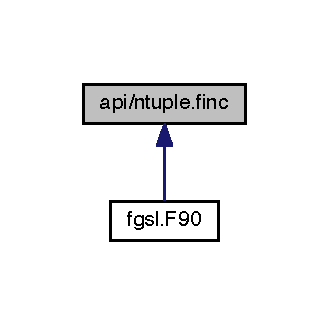
\includegraphics[width=158pt]{ntuple_8finc__dep__incl}
\end{center}
\end{figure}
\subsection*{Functions/\-Subroutines}
\begin{DoxyCompactItemize}
\item 
type(fgsl\-\_\-ntuple) function \hyperlink{ntuple_8finc_a53e8e8c2b59e9996577478079aec392a}{fgsl\-\_\-ntuple\-\_\-create} (fname, data, size)
\item 
type(fgsl\-\_\-ntuple) function \hyperlink{ntuple_8finc_a825ef23e9dc1d74ff1a263191c490bd0}{fgsl\-\_\-ntuple\-\_\-open} (fname, data, size)
\item 
integer(fgsl\-\_\-int) function \hyperlink{ntuple_8finc_a356af99564ad1459930057c34017e161}{fgsl\-\_\-ntuple\-\_\-write} (ntuple)
\item 
integer(fgsl\-\_\-int) function \hyperlink{ntuple_8finc_a88cfeaf087d36f1e4e6a0d81ac04bdb3}{fgsl\-\_\-ntuple\-\_\-bookdata} (ntuple)
\item 
integer(fgsl\-\_\-int) function \hyperlink{ntuple_8finc_a479c00a78c57f2b3b14cc9f12a514b6b}{fgsl\-\_\-ntuple\-\_\-read} (ntuple)
\item 
integer(fgsl\-\_\-int) function \hyperlink{ntuple_8finc_a1a996c87696028b62352cd43a82a6879}{fgsl\-\_\-ntuple\-\_\-close} (ntuple)
\item 
type(fgsl\-\_\-ntuple\-\_\-select\-\_\-fn) \\*
function \hyperlink{ntuple_8finc_aa04c4dfcb377f33a3a63fc7415cb3e3f}{fgsl\-\_\-ntuple\-\_\-select\-\_\-fn\-\_\-init} (func, params)
\item 
type(fgsl\-\_\-ntuple\-\_\-value\-\_\-fn) function \hyperlink{ntuple_8finc_a5672a466c45b2c1eaf5cf76209e6d282}{fgsl\-\_\-ntuple\-\_\-value\-\_\-fn\-\_\-init} (func, params)
\item 
subroutine \hyperlink{ntuple_8finc_ad8dde1fb48951e3df2ed85fdd4dbe928}{fgsl\-\_\-ntuple\-\_\-select\-\_\-fn\-\_\-free} (sfunc)
\item 
subroutine \hyperlink{ntuple_8finc_a79a22db8b1a4e150923981198b5c7aab}{fgsl\-\_\-ntuple\-\_\-value\-\_\-fn\-\_\-free} (sfunc)
\item 
integer(fgsl\-\_\-int) function \hyperlink{ntuple_8finc_ac2d58b11f74188b4b684a7e1bb701042}{fgsl\-\_\-ntuple\-\_\-project} (h, ntuple, value\-\_\-func, select\-\_\-func)
\item 
type(c\-\_\-ptr) function \hyperlink{ntuple_8finc_a6fd6e5da6139dffa2f6f61aa8aceafb1}{fgsl\-\_\-ntuple\-\_\-data} (ntuple)
\item 
integer(fgsl\-\_\-size\-\_\-t) function \hyperlink{ntuple_8finc_a4c85f3d692fd5e14aadd2ffd1ddd7c0a}{fgsl\-\_\-ntuple\-\_\-size} (ntuple)
\item 
logical function \hyperlink{ntuple_8finc_acb6eee4253ad2f01ea71e4c1c9392ed0}{fgsl\-\_\-ntuple\-\_\-status} (ntuple)
\item 
logical function \hyperlink{ntuple_8finc_a62c72f68341a457467ae7f0ceecf9911}{fgsl\-\_\-ntuple\-\_\-value\-\_\-fn\-\_\-status} (ntuple\-\_\-value\-\_\-fn)
\item 
logical function \hyperlink{ntuple_8finc_a7e638d180dad856d12938578ae718601}{fgsl\-\_\-ntuple\-\_\-select\-\_\-fn\-\_\-status} (ntuple\-\_\-select\-\_\-fn)
\end{DoxyCompactItemize}


\subsection{Function/\-Subroutine Documentation}
\hypertarget{ntuple_8finc_a88cfeaf087d36f1e4e6a0d81ac04bdb3}{\index{ntuple.\-finc@{ntuple.\-finc}!fgsl\-\_\-ntuple\-\_\-bookdata@{fgsl\-\_\-ntuple\-\_\-bookdata}}
\index{fgsl\-\_\-ntuple\-\_\-bookdata@{fgsl\-\_\-ntuple\-\_\-bookdata}!ntuple.finc@{ntuple.\-finc}}
\subsubsection[{fgsl\-\_\-ntuple\-\_\-bookdata}]{\setlength{\rightskip}{0pt plus 5cm}integer(fgsl\-\_\-int) function fgsl\-\_\-ntuple\-\_\-bookdata (
\begin{DoxyParamCaption}
\item[{type(fgsl\-\_\-ntuple), intent(in)}]{ntuple}
\end{DoxyParamCaption}
)}}\label{ntuple_8finc_a88cfeaf087d36f1e4e6a0d81ac04bdb3}
\hypertarget{ntuple_8finc_a1a996c87696028b62352cd43a82a6879}{\index{ntuple.\-finc@{ntuple.\-finc}!fgsl\-\_\-ntuple\-\_\-close@{fgsl\-\_\-ntuple\-\_\-close}}
\index{fgsl\-\_\-ntuple\-\_\-close@{fgsl\-\_\-ntuple\-\_\-close}!ntuple.finc@{ntuple.\-finc}}
\subsubsection[{fgsl\-\_\-ntuple\-\_\-close}]{\setlength{\rightskip}{0pt plus 5cm}integer(fgsl\-\_\-int) function fgsl\-\_\-ntuple\-\_\-close (
\begin{DoxyParamCaption}
\item[{type(fgsl\-\_\-ntuple), intent(inout)}]{ntuple}
\end{DoxyParamCaption}
)}}\label{ntuple_8finc_a1a996c87696028b62352cd43a82a6879}
\hypertarget{ntuple_8finc_a53e8e8c2b59e9996577478079aec392a}{\index{ntuple.\-finc@{ntuple.\-finc}!fgsl\-\_\-ntuple\-\_\-create@{fgsl\-\_\-ntuple\-\_\-create}}
\index{fgsl\-\_\-ntuple\-\_\-create@{fgsl\-\_\-ntuple\-\_\-create}!ntuple.finc@{ntuple.\-finc}}
\subsubsection[{fgsl\-\_\-ntuple\-\_\-create}]{\setlength{\rightskip}{0pt plus 5cm}type(fgsl\-\_\-ntuple) function fgsl\-\_\-ntuple\-\_\-create (
\begin{DoxyParamCaption}
\item[{character(kind=fgsl\-\_\-char, len=$\ast$), intent(in)}]{fname, }
\item[{type(c\-\_\-ptr), intent(in)}]{data, }
\item[{integer(fgsl\-\_\-size\-\_\-t), intent(in)}]{size}
\end{DoxyParamCaption}
)}}\label{ntuple_8finc_a53e8e8c2b59e9996577478079aec392a}
\hypertarget{ntuple_8finc_a6fd6e5da6139dffa2f6f61aa8aceafb1}{\index{ntuple.\-finc@{ntuple.\-finc}!fgsl\-\_\-ntuple\-\_\-data@{fgsl\-\_\-ntuple\-\_\-data}}
\index{fgsl\-\_\-ntuple\-\_\-data@{fgsl\-\_\-ntuple\-\_\-data}!ntuple.finc@{ntuple.\-finc}}
\subsubsection[{fgsl\-\_\-ntuple\-\_\-data}]{\setlength{\rightskip}{0pt plus 5cm}type(c\-\_\-ptr) function fgsl\-\_\-ntuple\-\_\-data (
\begin{DoxyParamCaption}
\item[{type(fgsl\-\_\-ntuple), intent(in)}]{ntuple}
\end{DoxyParamCaption}
)}}\label{ntuple_8finc_a6fd6e5da6139dffa2f6f61aa8aceafb1}
\hypertarget{ntuple_8finc_a825ef23e9dc1d74ff1a263191c490bd0}{\index{ntuple.\-finc@{ntuple.\-finc}!fgsl\-\_\-ntuple\-\_\-open@{fgsl\-\_\-ntuple\-\_\-open}}
\index{fgsl\-\_\-ntuple\-\_\-open@{fgsl\-\_\-ntuple\-\_\-open}!ntuple.finc@{ntuple.\-finc}}
\subsubsection[{fgsl\-\_\-ntuple\-\_\-open}]{\setlength{\rightskip}{0pt plus 5cm}type(fgsl\-\_\-ntuple) function fgsl\-\_\-ntuple\-\_\-open (
\begin{DoxyParamCaption}
\item[{character(kind=fgsl\-\_\-char, len=$\ast$), intent(in)}]{fname, }
\item[{type(c\-\_\-ptr), intent(in)}]{data, }
\item[{integer(fgsl\-\_\-size\-\_\-t), intent(in)}]{size}
\end{DoxyParamCaption}
)}}\label{ntuple_8finc_a825ef23e9dc1d74ff1a263191c490bd0}
\hypertarget{ntuple_8finc_ac2d58b11f74188b4b684a7e1bb701042}{\index{ntuple.\-finc@{ntuple.\-finc}!fgsl\-\_\-ntuple\-\_\-project@{fgsl\-\_\-ntuple\-\_\-project}}
\index{fgsl\-\_\-ntuple\-\_\-project@{fgsl\-\_\-ntuple\-\_\-project}!ntuple.finc@{ntuple.\-finc}}
\subsubsection[{fgsl\-\_\-ntuple\-\_\-project}]{\setlength{\rightskip}{0pt plus 5cm}integer(fgsl\-\_\-int) function fgsl\-\_\-ntuple\-\_\-project (
\begin{DoxyParamCaption}
\item[{type(fgsl\-\_\-histogram), intent(inout)}]{h, }
\item[{type(fgsl\-\_\-ntuple), intent(in)}]{ntuple, }
\item[{type(fgsl\-\_\-ntuple\-\_\-value\-\_\-fn), intent(in)}]{value\-\_\-func, }
\item[{type(fgsl\-\_\-ntuple\-\_\-select\-\_\-fn), intent(in)}]{select\-\_\-func}
\end{DoxyParamCaption}
)}}\label{ntuple_8finc_ac2d58b11f74188b4b684a7e1bb701042}
\hypertarget{ntuple_8finc_a479c00a78c57f2b3b14cc9f12a514b6b}{\index{ntuple.\-finc@{ntuple.\-finc}!fgsl\-\_\-ntuple\-\_\-read@{fgsl\-\_\-ntuple\-\_\-read}}
\index{fgsl\-\_\-ntuple\-\_\-read@{fgsl\-\_\-ntuple\-\_\-read}!ntuple.finc@{ntuple.\-finc}}
\subsubsection[{fgsl\-\_\-ntuple\-\_\-read}]{\setlength{\rightskip}{0pt plus 5cm}integer(fgsl\-\_\-int) function fgsl\-\_\-ntuple\-\_\-read (
\begin{DoxyParamCaption}
\item[{type(fgsl\-\_\-ntuple), intent(inout)}]{ntuple}
\end{DoxyParamCaption}
)}}\label{ntuple_8finc_a479c00a78c57f2b3b14cc9f12a514b6b}
\hypertarget{ntuple_8finc_ad8dde1fb48951e3df2ed85fdd4dbe928}{\index{ntuple.\-finc@{ntuple.\-finc}!fgsl\-\_\-ntuple\-\_\-select\-\_\-fn\-\_\-free@{fgsl\-\_\-ntuple\-\_\-select\-\_\-fn\-\_\-free}}
\index{fgsl\-\_\-ntuple\-\_\-select\-\_\-fn\-\_\-free@{fgsl\-\_\-ntuple\-\_\-select\-\_\-fn\-\_\-free}!ntuple.finc@{ntuple.\-finc}}
\subsubsection[{fgsl\-\_\-ntuple\-\_\-select\-\_\-fn\-\_\-free}]{\setlength{\rightskip}{0pt plus 5cm}subroutine fgsl\-\_\-ntuple\-\_\-select\-\_\-fn\-\_\-free (
\begin{DoxyParamCaption}
\item[{type(fgsl\-\_\-ntuple\-\_\-select\-\_\-fn), intent(inout)}]{sfunc}
\end{DoxyParamCaption}
)}}\label{ntuple_8finc_ad8dde1fb48951e3df2ed85fdd4dbe928}
\hypertarget{ntuple_8finc_aa04c4dfcb377f33a3a63fc7415cb3e3f}{\index{ntuple.\-finc@{ntuple.\-finc}!fgsl\-\_\-ntuple\-\_\-select\-\_\-fn\-\_\-init@{fgsl\-\_\-ntuple\-\_\-select\-\_\-fn\-\_\-init}}
\index{fgsl\-\_\-ntuple\-\_\-select\-\_\-fn\-\_\-init@{fgsl\-\_\-ntuple\-\_\-select\-\_\-fn\-\_\-init}!ntuple.finc@{ntuple.\-finc}}
\subsubsection[{fgsl\-\_\-ntuple\-\_\-select\-\_\-fn\-\_\-init}]{\setlength{\rightskip}{0pt plus 5cm}type(fgsl\-\_\-ntuple\-\_\-select\-\_\-fn) function fgsl\-\_\-ntuple\-\_\-select\-\_\-fn\-\_\-init (
\begin{DoxyParamCaption}
\item[{}]{func, }
\item[{type(c\-\_\-ptr), intent(in)}]{params}
\end{DoxyParamCaption}
)}}\label{ntuple_8finc_aa04c4dfcb377f33a3a63fc7415cb3e3f}
\hypertarget{ntuple_8finc_a7e638d180dad856d12938578ae718601}{\index{ntuple.\-finc@{ntuple.\-finc}!fgsl\-\_\-ntuple\-\_\-select\-\_\-fn\-\_\-status@{fgsl\-\_\-ntuple\-\_\-select\-\_\-fn\-\_\-status}}
\index{fgsl\-\_\-ntuple\-\_\-select\-\_\-fn\-\_\-status@{fgsl\-\_\-ntuple\-\_\-select\-\_\-fn\-\_\-status}!ntuple.finc@{ntuple.\-finc}}
\subsubsection[{fgsl\-\_\-ntuple\-\_\-select\-\_\-fn\-\_\-status}]{\setlength{\rightskip}{0pt plus 5cm}logical function fgsl\-\_\-ntuple\-\_\-select\-\_\-fn\-\_\-status (
\begin{DoxyParamCaption}
\item[{type(fgsl\-\_\-ntuple\-\_\-select\-\_\-fn), intent(in)}]{ntuple\-\_\-select\-\_\-fn}
\end{DoxyParamCaption}
)}}\label{ntuple_8finc_a7e638d180dad856d12938578ae718601}
\hypertarget{ntuple_8finc_a4c85f3d692fd5e14aadd2ffd1ddd7c0a}{\index{ntuple.\-finc@{ntuple.\-finc}!fgsl\-\_\-ntuple\-\_\-size@{fgsl\-\_\-ntuple\-\_\-size}}
\index{fgsl\-\_\-ntuple\-\_\-size@{fgsl\-\_\-ntuple\-\_\-size}!ntuple.finc@{ntuple.\-finc}}
\subsubsection[{fgsl\-\_\-ntuple\-\_\-size}]{\setlength{\rightskip}{0pt plus 5cm}integer(fgsl\-\_\-size\-\_\-t) function fgsl\-\_\-ntuple\-\_\-size (
\begin{DoxyParamCaption}
\item[{type(fgsl\-\_\-ntuple), intent(in)}]{ntuple}
\end{DoxyParamCaption}
)}}\label{ntuple_8finc_a4c85f3d692fd5e14aadd2ffd1ddd7c0a}
\hypertarget{ntuple_8finc_acb6eee4253ad2f01ea71e4c1c9392ed0}{\index{ntuple.\-finc@{ntuple.\-finc}!fgsl\-\_\-ntuple\-\_\-status@{fgsl\-\_\-ntuple\-\_\-status}}
\index{fgsl\-\_\-ntuple\-\_\-status@{fgsl\-\_\-ntuple\-\_\-status}!ntuple.finc@{ntuple.\-finc}}
\subsubsection[{fgsl\-\_\-ntuple\-\_\-status}]{\setlength{\rightskip}{0pt plus 5cm}logical function fgsl\-\_\-ntuple\-\_\-status (
\begin{DoxyParamCaption}
\item[{type(fgsl\-\_\-ntuple), intent(in)}]{ntuple}
\end{DoxyParamCaption}
)}}\label{ntuple_8finc_acb6eee4253ad2f01ea71e4c1c9392ed0}
\hypertarget{ntuple_8finc_a79a22db8b1a4e150923981198b5c7aab}{\index{ntuple.\-finc@{ntuple.\-finc}!fgsl\-\_\-ntuple\-\_\-value\-\_\-fn\-\_\-free@{fgsl\-\_\-ntuple\-\_\-value\-\_\-fn\-\_\-free}}
\index{fgsl\-\_\-ntuple\-\_\-value\-\_\-fn\-\_\-free@{fgsl\-\_\-ntuple\-\_\-value\-\_\-fn\-\_\-free}!ntuple.finc@{ntuple.\-finc}}
\subsubsection[{fgsl\-\_\-ntuple\-\_\-value\-\_\-fn\-\_\-free}]{\setlength{\rightskip}{0pt plus 5cm}subroutine fgsl\-\_\-ntuple\-\_\-value\-\_\-fn\-\_\-free (
\begin{DoxyParamCaption}
\item[{type(fgsl\-\_\-ntuple\-\_\-value\-\_\-fn), intent(inout)}]{sfunc}
\end{DoxyParamCaption}
)}}\label{ntuple_8finc_a79a22db8b1a4e150923981198b5c7aab}
\hypertarget{ntuple_8finc_a5672a466c45b2c1eaf5cf76209e6d282}{\index{ntuple.\-finc@{ntuple.\-finc}!fgsl\-\_\-ntuple\-\_\-value\-\_\-fn\-\_\-init@{fgsl\-\_\-ntuple\-\_\-value\-\_\-fn\-\_\-init}}
\index{fgsl\-\_\-ntuple\-\_\-value\-\_\-fn\-\_\-init@{fgsl\-\_\-ntuple\-\_\-value\-\_\-fn\-\_\-init}!ntuple.finc@{ntuple.\-finc}}
\subsubsection[{fgsl\-\_\-ntuple\-\_\-value\-\_\-fn\-\_\-init}]{\setlength{\rightskip}{0pt plus 5cm}type(fgsl\-\_\-ntuple\-\_\-value\-\_\-fn) function fgsl\-\_\-ntuple\-\_\-value\-\_\-fn\-\_\-init (
\begin{DoxyParamCaption}
\item[{}]{func, }
\item[{type(c\-\_\-ptr), intent(in)}]{params}
\end{DoxyParamCaption}
)}}\label{ntuple_8finc_a5672a466c45b2c1eaf5cf76209e6d282}
\hypertarget{ntuple_8finc_a62c72f68341a457467ae7f0ceecf9911}{\index{ntuple.\-finc@{ntuple.\-finc}!fgsl\-\_\-ntuple\-\_\-value\-\_\-fn\-\_\-status@{fgsl\-\_\-ntuple\-\_\-value\-\_\-fn\-\_\-status}}
\index{fgsl\-\_\-ntuple\-\_\-value\-\_\-fn\-\_\-status@{fgsl\-\_\-ntuple\-\_\-value\-\_\-fn\-\_\-status}!ntuple.finc@{ntuple.\-finc}}
\subsubsection[{fgsl\-\_\-ntuple\-\_\-value\-\_\-fn\-\_\-status}]{\setlength{\rightskip}{0pt plus 5cm}logical function fgsl\-\_\-ntuple\-\_\-value\-\_\-fn\-\_\-status (
\begin{DoxyParamCaption}
\item[{type(fgsl\-\_\-ntuple\-\_\-value\-\_\-fn), intent(in)}]{ntuple\-\_\-value\-\_\-fn}
\end{DoxyParamCaption}
)}}\label{ntuple_8finc_a62c72f68341a457467ae7f0ceecf9911}
\hypertarget{ntuple_8finc_a356af99564ad1459930057c34017e161}{\index{ntuple.\-finc@{ntuple.\-finc}!fgsl\-\_\-ntuple\-\_\-write@{fgsl\-\_\-ntuple\-\_\-write}}
\index{fgsl\-\_\-ntuple\-\_\-write@{fgsl\-\_\-ntuple\-\_\-write}!ntuple.finc@{ntuple.\-finc}}
\subsubsection[{fgsl\-\_\-ntuple\-\_\-write}]{\setlength{\rightskip}{0pt plus 5cm}integer(fgsl\-\_\-int) function fgsl\-\_\-ntuple\-\_\-write (
\begin{DoxyParamCaption}
\item[{type(fgsl\-\_\-ntuple), intent(in)}]{ntuple}
\end{DoxyParamCaption}
)}}\label{ntuple_8finc_a356af99564ad1459930057c34017e161}

\hypertarget{ode_8finc}{}\section{api/ode.finc File Reference}
\label{ode_8finc}\index{api/ode.\+finc@{api/ode.\+finc}}
This graph shows which files directly or indirectly include this file\+:\nopagebreak
\begin{figure}[H]
\begin{center}
\leavevmode
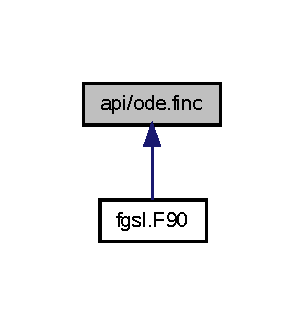
\includegraphics[width=146pt]{ode_8finc__dep__incl}
\end{center}
\end{figure}
\subsection*{Functions/\+Subroutines}
\begin{DoxyCompactItemize}
\item 
type(fgsl\+\_\+odeiv2\+\_\+system) function \hyperlink{ode_8finc_a2ffec24e60a38bee53c48aa9c9e3c1b7}{fgsl\+\_\+odeiv2\+\_\+system\+\_\+init} (func, dimension, params, jacobian)
\begin{DoxyCompactList}\small\item\em Constructor for an O\+D\+E system object. \end{DoxyCompactList}\item 
subroutine \hyperlink{ode_8finc_ab973a74e019e0e361f76db2a15b1ce5d}{fgsl\+\_\+odeiv2\+\_\+system\+\_\+free} (system)
\item 
type(fgsl\+\_\+odeiv2\+\_\+step) function \hyperlink{ode_8finc_a38ccf460c6a701df582e42b350fd9eaf}{fgsl\+\_\+odeiv2\+\_\+step\+\_\+alloc} (t, dim)
\item 
integer(fgsl\+\_\+int) function \hyperlink{ode_8finc_a2e77e51cfb8862339548a89edb5b5f16}{fgsl\+\_\+odeiv2\+\_\+step\+\_\+reset} (s)
\item 
subroutine \hyperlink{ode_8finc_a5ba021a1cf3acf48a05c91f83fae1e92}{fgsl\+\_\+odeiv2\+\_\+step\+\_\+free} (s)
\item 
character(kind=fgsl\+\_\+char, len=fgsl\+\_\+strmax) function \hyperlink{ode_8finc_ae18d4d99a73710093fef3a8bd3501d4b}{fgsl\+\_\+odeiv2\+\_\+step\+\_\+name} (s)
\item 
integer(fgsl\+\_\+int) function \hyperlink{ode_8finc_ae49a399cca2cb8575c6a46ea337c477f}{fgsl\+\_\+odeiv2\+\_\+step\+\_\+order} (s)
\item 
integer(c\+\_\+int) function \hyperlink{ode_8finc_a1f1e1c96acf507d235684138e06ae697}{fgsl\+\_\+odeiv2\+\_\+step\+\_\+set\+\_\+driver} (s, d)
\item 
integer(fgsl\+\_\+int) function \hyperlink{ode_8finc_a912c1ed261b3f77c4223b1e1dafbc20b}{fgsl\+\_\+odeiv2\+\_\+step\+\_\+apply} (s, t, h, y, yerr, dydt\+\_\+in, dydt\+\_\+out, dydt)
\item 
type(fgsl\+\_\+odeiv2\+\_\+control) function \hyperlink{ode_8finc_a1830985a3df6d1a333c80ba967e76eec}{fgsl\+\_\+odeiv2\+\_\+control\+\_\+standard\+\_\+new} (eps\+\_\+abs, eps\+\_\+rel, a\+\_\+y, a\+\_\+dydt)
\item 
type(fgsl\+\_\+odeiv2\+\_\+control) function \hyperlink{ode_8finc_aed35a989d1582ac1920fa082fad216d9}{fgsl\+\_\+odeiv2\+\_\+control\+\_\+y\+\_\+new} (eps\+\_\+abs, eps\+\_\+rel)
\item 
type(fgsl\+\_\+odeiv2\+\_\+control) function \hyperlink{ode_8finc_afd262d0ea5bb3c0a5ed79264eaec7b52}{fgsl\+\_\+odeiv2\+\_\+control\+\_\+yp\+\_\+new} (eps\+\_\+abs, eps\+\_\+rel)
\item 
type(fgsl\+\_\+odeiv2\+\_\+control) function \hyperlink{ode_8finc_ac9023732522b7adc92a721faac704a21}{fgsl\+\_\+odeiv2\+\_\+control\+\_\+scaled\+\_\+new} (eps\+\_\+abs, eps\+\_\+rel, a\+\_\+y, a\+\_\+dydt, scale\+\_\+abs)
\item 
type(fgsl\+\_\+odeiv2\+\_\+control) function \hyperlink{ode_8finc_aa2838bdd478399790455f495923c2a2d}{fgsl\+\_\+odeiv2\+\_\+control\+\_\+alloc} (t)
\begin{DoxyCompactList}\small\item\em Note\+: use of fgsl\+\_\+odeiv2\+\_\+control\+\_\+alloc requires an initializer for the t object written in C. \end{DoxyCompactList}\item 
integer(fgsl\+\_\+int) function \hyperlink{ode_8finc_a4b0b791a775a86ef0f1f74cc68abcc68}{fgsl\+\_\+odeiv2\+\_\+control\+\_\+init} (c, eps\+\_\+abs, eps\+\_\+rel, a\+\_\+y, a\+\_\+dydt)
\item 
subroutine \hyperlink{ode_8finc_aadeb0256bb6a39f1d946c355ac6b2afa}{fgsl\+\_\+odeiv2\+\_\+control\+\_\+free} (c)
\item 
logical function \hyperlink{ode_8finc_af5fcca7af27c62493f685900fe29f999}{fgsl\+\_\+odeiv2\+\_\+control\+\_\+status} (s)
\item 
integer(fgsl\+\_\+int) function \hyperlink{ode_8finc_a3ac22f04f9490100937304830d161b1a}{fgsl\+\_\+odeiv2\+\_\+control\+\_\+hadjust} (c, s, y, yerr, dydt, h)
\item 
character(kind=fgsl\+\_\+char, len=fgsl\+\_\+strmax) function \hyperlink{ode_8finc_ac9512303eeabe05335d9fbada1c5f841}{fgsl\+\_\+odeiv2\+\_\+control\+\_\+name} (c)
\item 
integer(fgsl\+\_\+int) function \hyperlink{ode_8finc_ad529291d0d2c826dec9976f5a24af8b1}{fgsl\+\_\+odeiv2\+\_\+control\+\_\+errlevel} (c, y, dydt, h, ind, errlev)
\item 
integer(fgsl\+\_\+int) function \hyperlink{ode_8finc_a53f1174dfc4a844b55c3654b4ac94c82}{fgsl\+\_\+odeiv2\+\_\+control\+\_\+set\+\_\+driver} (c, d)
\item 
type(fgsl\+\_\+odeiv2\+\_\+evolve) function \hyperlink{ode_8finc_a010ce00112539875b18c9741e3beaa6e}{fgsl\+\_\+odeiv2\+\_\+evolve\+\_\+alloc} (dim)
\item 
integer(fgsl\+\_\+int) function \hyperlink{ode_8finc_a2eebbf858365bd4853b5ddd0a1071d48}{fgsl\+\_\+odeiv2\+\_\+evolve\+\_\+apply} (e, con, step, dydt, t, t1, h, y)
\item 
integer(fgsl\+\_\+int) function \hyperlink{ode_8finc_a784c0214cbb688d0fcb954ba3c868bb8}{fgsl\+\_\+odeiv2\+\_\+evolve\+\_\+apply\+\_\+fixed\+\_\+step} (e, con, step, dydt, t, h0, y)
\item 
integer(c\+\_\+int) function \hyperlink{ode_8finc_a58db655eeefa6587785e3681fe1f1fe3}{fgsl\+\_\+odeiv2\+\_\+evolve\+\_\+reset} (s)
\item 
subroutine \hyperlink{ode_8finc_ae420fff7079d79241900c38192a15b18}{fgsl\+\_\+odeiv2\+\_\+evolve\+\_\+free} (s)
\item 
logical function \hyperlink{ode_8finc_a903a7d2d07429f4d1ce0291ed0a29cf6}{fgsl\+\_\+odeiv2\+\_\+evolve\+\_\+status} (s)
\item 
logical function \hyperlink{ode_8finc_aae3c317f1477f7e8896ed8fa1a50a5ef}{fgsl\+\_\+odeiv2\+\_\+step\+\_\+status} (s)
\item 
logical function \hyperlink{ode_8finc_acedda44a6ed7e98748b97edc43597fbf}{fgsl\+\_\+odeiv2\+\_\+system\+\_\+status} (s)
\item 
integer(fgsl\+\_\+int) function \hyperlink{ode_8finc_a3a068def5f64087448b8b725b56f0f44}{fgsl\+\_\+odeiv2\+\_\+evolve\+\_\+set\+\_\+driver} (c, d)
\item 
type(fgsl\+\_\+odeiv2\+\_\+driver) function \hyperlink{ode_8finc_abb00c1c5c177a7c9a456b02f34a4a9b4}{fgsl\+\_\+odeiv2\+\_\+driver\+\_\+alloc\+\_\+y\+\_\+new} (sys, t, hstart, epsabs, epsrel)
\item 
type(fgsl\+\_\+odeiv2\+\_\+driver) function \hyperlink{ode_8finc_a178c0c3dd596ef26f99e99825d4586d7}{fgsl\+\_\+odeiv2\+\_\+driver\+\_\+alloc\+\_\+yp\+\_\+new} (sys, t, hstart, epsabs, epsrel)
\item 
type(fgsl\+\_\+odeiv2\+\_\+driver) function \hyperlink{ode_8finc_a06a42be695134e3e8301b7148e7ce838}{fgsl\+\_\+odeiv2\+\_\+driver\+\_\+alloc\+\_\+standard\+\_\+new} (sys, t, hstart, epsabs, epsrel, a\+\_\+y, a\+\_\+dydt)
\item 
type(fgsl\+\_\+odeiv2\+\_\+driver) function \hyperlink{ode_8finc_a37b762b00ed8cc4614a5290998dd0be7}{fgsl\+\_\+odeiv2\+\_\+driver\+\_\+alloc\+\_\+scaled\+\_\+new} (sys, t, hstart, epsabs, epsrel, a\+\_\+y, a\+\_\+dydt, scale\+\_\+abs)
\item 
integer(fgsl\+\_\+int) function \hyperlink{ode_8finc_a1a52468942b08b4fc33a09404492b67e}{fgsl\+\_\+odeiv2\+\_\+driver\+\_\+set\+\_\+hmin} (d, hmin)
\item 
integer(fgsl\+\_\+int) function \hyperlink{ode_8finc_a524a858cffa85f419e05e2da0a21f813}{fgsl\+\_\+odeiv2\+\_\+driver\+\_\+set\+\_\+hmax} (d, hmax)
\item 
integer(fgsl\+\_\+int) function \hyperlink{ode_8finc_a672eeb10000330826020da95ce99c391}{fgsl\+\_\+odeiv2\+\_\+driver\+\_\+set\+\_\+nmax} (d, nmax)
\item 
integer(fgsl\+\_\+int) function \hyperlink{ode_8finc_a6cd36ae8668cd6a69d3d8b4200df210d}{fgsl\+\_\+odeiv2\+\_\+driver\+\_\+apply} (d, t, t1, y)
\item 
integer(fgsl\+\_\+int) function \hyperlink{ode_8finc_a9eedde9d2faadc18f0d952e48b364f04}{fgsl\+\_\+odeiv2\+\_\+driver\+\_\+apply\+\_\+fixed\+\_\+step} (d, t, h, n, y)
\item 
integer(fgsl\+\_\+int) function \hyperlink{ode_8finc_abf08671d0ef862295d6bf5fd2b9733b2}{fgsl\+\_\+odeiv2\+\_\+driver\+\_\+reset} (d)
\item 
subroutine \hyperlink{ode_8finc_a1bd2c2d5a3b6758b0a2bf84c64e14c49}{fgsl\+\_\+odeiv2\+\_\+driver\+\_\+free} (d)
\item 
logical function \hyperlink{ode_8finc_af058bdba2f220e7f306c7dac6fefc7e8}{fgsl\+\_\+odeiv2\+\_\+driver\+\_\+status} (s)
\item 
integer(fgsl\+\_\+int) function \hyperlink{ode_8finc_a8428de6bbc5fb897c3795b911a805435}{fgsl\+\_\+odeiv2\+\_\+driver\+\_\+reset\+\_\+hstart} (d, hstart)
\item 
type(fgsl\+\_\+odeiv\+\_\+system) function \hyperlink{ode_8finc_ac5419ee4b9617d0020895e1f452e0ec8}{fgsl\+\_\+odeiv\+\_\+system\+\_\+init} (func, dimension, params, jacobian)
\begin{DoxyCompactList}\small\item\em Constructor for an O\+D\+E system object. \end{DoxyCompactList}\item 
subroutine \hyperlink{ode_8finc_a4fad8d181c7842450901cd34bf9902c5}{fgsl\+\_\+odeiv\+\_\+system\+\_\+free} (system)
\item 
type(fgsl\+\_\+odeiv\+\_\+step) function \hyperlink{ode_8finc_ad80515e2f8704ae9c376357ff184c0b5}{fgsl\+\_\+odeiv\+\_\+step\+\_\+alloc} (t, dim)
\item 
integer(fgsl\+\_\+int) function \hyperlink{ode_8finc_a550b05385e72fdf0e9c8febe9d9c0556}{fgsl\+\_\+odeiv\+\_\+step\+\_\+reset} (s)
\item 
subroutine \hyperlink{ode_8finc_ae2d74056a3dd23aaf31cd48dd757a987}{fgsl\+\_\+odeiv\+\_\+step\+\_\+free} (s)
\item 
character(kind=fgsl\+\_\+char, len=fgsl\+\_\+strmax) function \hyperlink{ode_8finc_a1266ca2607d99bd8f30801f7c5837f6b}{fgsl\+\_\+odeiv\+\_\+step\+\_\+name} (s)
\item 
integer(fgsl\+\_\+int) function \hyperlink{ode_8finc_ad473f673ac73701a32499c4f728c0ec0}{fgsl\+\_\+odeiv\+\_\+step\+\_\+order} (s)
\item 
integer(fgsl\+\_\+int) function \hyperlink{ode_8finc_a0447a8399777f24077e870ca2e3a2618}{fgsl\+\_\+odeiv\+\_\+step\+\_\+apply} (s, t, h, y, yerr, dydt\+\_\+in, dydt\+\_\+out, dydt)
\item 
type(fgsl\+\_\+odeiv\+\_\+control) function \hyperlink{ode_8finc_a8a7d90fb014f8aafeb3258a3edac66bf}{fgsl\+\_\+odeiv\+\_\+control\+\_\+standard\+\_\+new} (eps\+\_\+abs, eps\+\_\+rel, a\+\_\+y, a\+\_\+dydt)
\item 
type(fgsl\+\_\+odeiv\+\_\+control) function \hyperlink{ode_8finc_a1bf14333a561bcc24ac68aa26f69330d}{fgsl\+\_\+odeiv\+\_\+control\+\_\+y\+\_\+new} (eps\+\_\+abs, eps\+\_\+rel)
\item 
type(fgsl\+\_\+odeiv\+\_\+control) function \hyperlink{ode_8finc_a99432f111e5ae998c654c70d6c4196a7}{fgsl\+\_\+odeiv\+\_\+control\+\_\+yp\+\_\+new} (eps\+\_\+abs, eps\+\_\+rel)
\item 
type(fgsl\+\_\+odeiv\+\_\+control) function \hyperlink{ode_8finc_a200a70bf30d5b1501d944e74b30a9254}{fgsl\+\_\+odeiv\+\_\+control\+\_\+scaled\+\_\+new} (eps\+\_\+abs, eps\+\_\+rel, a\+\_\+y, a\+\_\+dydt, scale\+\_\+abs)
\item 
type(fgsl\+\_\+odeiv\+\_\+control) function \hyperlink{ode_8finc_aa135d17ea4a41614a6ac9789c11e220c}{fgsl\+\_\+odeiv\+\_\+control\+\_\+alloc} (t)
\begin{DoxyCompactList}\small\item\em Note\+: Use of fgsl\+\_\+odeiv\+\_\+control\+\_\+alloc requires an initializer for the t object written in C. \end{DoxyCompactList}\item 
integer(fgsl\+\_\+int) function \hyperlink{ode_8finc_a78a741026ae34107fa82e510868530b7}{fgsl\+\_\+odeiv\+\_\+control\+\_\+init} (c, eps\+\_\+abs, eps\+\_\+rel, a\+\_\+y, a\+\_\+dydt)
\item 
subroutine \hyperlink{ode_8finc_a8cc3184bf7c70b2ff108dea05763b452}{fgsl\+\_\+odeiv\+\_\+control\+\_\+free} (c)
\item 
integer(fgsl\+\_\+int) function \hyperlink{ode_8finc_a2792840e81747e88bf03c8ef0689699d}{fgsl\+\_\+odeiv\+\_\+control\+\_\+hadjust} (c, s, y0, yerr, dydt, h)
\item 
character(kind=fgsl\+\_\+char, len=fgsl\+\_\+strmax) function \hyperlink{ode_8finc_a1ff85c5d189557d6c94089dc1dd0bd99}{fgsl\+\_\+odeiv\+\_\+control\+\_\+name} (c)
\item 
type(fgsl\+\_\+odeiv\+\_\+evolve) function \hyperlink{ode_8finc_ad120e740613bd7e968acc114b6079927}{fgsl\+\_\+odeiv\+\_\+evolve\+\_\+alloc} (dim)
\item 
integer(fgsl\+\_\+int) function \hyperlink{ode_8finc_a00660f906cfcd771ee58e0e262392caf}{fgsl\+\_\+odeiv\+\_\+evolve\+\_\+apply} (e, con, step, dydt, t, t1, h, y)
\item 
integer(c\+\_\+int) function \hyperlink{ode_8finc_a0552dfb1f607b579bb1931f4ccfd8977}{fgsl\+\_\+odeiv\+\_\+evolve\+\_\+reset} (s)
\item 
subroutine \hyperlink{ode_8finc_ae0a70f5a4df1196305b974af58ea9b5c}{fgsl\+\_\+odeiv\+\_\+evolve\+\_\+free} (s)
\item 
logical function \hyperlink{ode_8finc_a4c681507748fd1a86eeecfa541a2a78f}{fgsl\+\_\+odeiv\+\_\+evolve\+\_\+status} (s)
\item 
logical function \hyperlink{ode_8finc_a77801649bf76c769195080c1c4c4d67c}{fgsl\+\_\+odeiv\+\_\+control\+\_\+status} (s)
\item 
logical function \hyperlink{ode_8finc_afa5ae89f031dbbbea0813ad20f8efe24}{fgsl\+\_\+odeiv\+\_\+step\+\_\+status} (s)
\item 
logical function \hyperlink{ode_8finc_a024570624b5bebbb6ffb76c89e7630d8}{fgsl\+\_\+odeiv\+\_\+system\+\_\+status} (s)
\end{DoxyCompactItemize}


\subsection{Function/\+Subroutine Documentation}
\hypertarget{ode_8finc_aa2838bdd478399790455f495923c2a2d}{}\index{ode.\+finc@{ode.\+finc}!fgsl\+\_\+odeiv2\+\_\+control\+\_\+alloc@{fgsl\+\_\+odeiv2\+\_\+control\+\_\+alloc}}
\index{fgsl\+\_\+odeiv2\+\_\+control\+\_\+alloc@{fgsl\+\_\+odeiv2\+\_\+control\+\_\+alloc}!ode.\+finc@{ode.\+finc}}
\subsubsection[{fgsl\+\_\+odeiv2\+\_\+control\+\_\+alloc}]{\setlength{\rightskip}{0pt plus 5cm}type(fgsl\+\_\+odeiv2\+\_\+control) function fgsl\+\_\+odeiv2\+\_\+control\+\_\+alloc (
\begin{DoxyParamCaption}
\item[{type(fgsl\+\_\+odeiv2\+\_\+control\+\_\+type), intent(in)}]{t}
\end{DoxyParamCaption}
)}\label{ode_8finc_aa2838bdd478399790455f495923c2a2d}


Note\+: use of fgsl\+\_\+odeiv2\+\_\+control\+\_\+alloc requires an initializer for the t object written in C. 

\hypertarget{ode_8finc_ad529291d0d2c826dec9976f5a24af8b1}{}\index{ode.\+finc@{ode.\+finc}!fgsl\+\_\+odeiv2\+\_\+control\+\_\+errlevel@{fgsl\+\_\+odeiv2\+\_\+control\+\_\+errlevel}}
\index{fgsl\+\_\+odeiv2\+\_\+control\+\_\+errlevel@{fgsl\+\_\+odeiv2\+\_\+control\+\_\+errlevel}!ode.\+finc@{ode.\+finc}}
\subsubsection[{fgsl\+\_\+odeiv2\+\_\+control\+\_\+errlevel}]{\setlength{\rightskip}{0pt plus 5cm}integer(fgsl\+\_\+int) function fgsl\+\_\+odeiv2\+\_\+control\+\_\+errlevel (
\begin{DoxyParamCaption}
\item[{type(fgsl\+\_\+odeiv2\+\_\+control)}]{c, }
\item[{real(fgsl\+\_\+double), intent(in)}]{y, }
\item[{real(fgsl\+\_\+double), intent(in)}]{dydt, }
\item[{real(fgsl\+\_\+double), intent(in)}]{h, }
\item[{integer(fgsl\+\_\+size\+\_\+t), intent(in)}]{ind, }
\item[{real(fgsl\+\_\+double), intent(inout)}]{errlev}
\end{DoxyParamCaption}
)}\label{ode_8finc_ad529291d0d2c826dec9976f5a24af8b1}
\hypertarget{ode_8finc_aadeb0256bb6a39f1d946c355ac6b2afa}{}\index{ode.\+finc@{ode.\+finc}!fgsl\+\_\+odeiv2\+\_\+control\+\_\+free@{fgsl\+\_\+odeiv2\+\_\+control\+\_\+free}}
\index{fgsl\+\_\+odeiv2\+\_\+control\+\_\+free@{fgsl\+\_\+odeiv2\+\_\+control\+\_\+free}!ode.\+finc@{ode.\+finc}}
\subsubsection[{fgsl\+\_\+odeiv2\+\_\+control\+\_\+free}]{\setlength{\rightskip}{0pt plus 5cm}subroutine fgsl\+\_\+odeiv2\+\_\+control\+\_\+free (
\begin{DoxyParamCaption}
\item[{type(fgsl\+\_\+odeiv2\+\_\+control), intent(inout)}]{c}
\end{DoxyParamCaption}
)}\label{ode_8finc_aadeb0256bb6a39f1d946c355ac6b2afa}
\hypertarget{ode_8finc_a3ac22f04f9490100937304830d161b1a}{}\index{ode.\+finc@{ode.\+finc}!fgsl\+\_\+odeiv2\+\_\+control\+\_\+hadjust@{fgsl\+\_\+odeiv2\+\_\+control\+\_\+hadjust}}
\index{fgsl\+\_\+odeiv2\+\_\+control\+\_\+hadjust@{fgsl\+\_\+odeiv2\+\_\+control\+\_\+hadjust}!ode.\+finc@{ode.\+finc}}
\subsubsection[{fgsl\+\_\+odeiv2\+\_\+control\+\_\+hadjust}]{\setlength{\rightskip}{0pt plus 5cm}integer(fgsl\+\_\+int) function fgsl\+\_\+odeiv2\+\_\+control\+\_\+hadjust (
\begin{DoxyParamCaption}
\item[{type(fgsl\+\_\+odeiv2\+\_\+control), intent(in)}]{c, }
\item[{type(fgsl\+\_\+odeiv2\+\_\+step), intent(in)}]{s, }
\item[{real(fgsl\+\_\+double), dimension(\+:), intent(in), target}]{y, }
\item[{real(fgsl\+\_\+double), dimension(\+:), intent(in), target}]{yerr, }
\item[{real(fgsl\+\_\+double), dimension(\+:), intent(in), target}]{dydt, }
\item[{real(fgsl\+\_\+double), intent(out)}]{h}
\end{DoxyParamCaption}
)}\label{ode_8finc_a3ac22f04f9490100937304830d161b1a}
\hypertarget{ode_8finc_a4b0b791a775a86ef0f1f74cc68abcc68}{}\index{ode.\+finc@{ode.\+finc}!fgsl\+\_\+odeiv2\+\_\+control\+\_\+init@{fgsl\+\_\+odeiv2\+\_\+control\+\_\+init}}
\index{fgsl\+\_\+odeiv2\+\_\+control\+\_\+init@{fgsl\+\_\+odeiv2\+\_\+control\+\_\+init}!ode.\+finc@{ode.\+finc}}
\subsubsection[{fgsl\+\_\+odeiv2\+\_\+control\+\_\+init}]{\setlength{\rightskip}{0pt plus 5cm}integer(fgsl\+\_\+int) function fgsl\+\_\+odeiv2\+\_\+control\+\_\+init (
\begin{DoxyParamCaption}
\item[{type(fgsl\+\_\+odeiv2\+\_\+control), intent(in)}]{c, }
\item[{real(fgsl\+\_\+double), intent(in)}]{eps\+\_\+abs, }
\item[{real(fgsl\+\_\+double), intent(in)}]{eps\+\_\+rel, }
\item[{real(fgsl\+\_\+double), intent(in)}]{a\+\_\+y, }
\item[{real(fgsl\+\_\+double), intent(in)}]{a\+\_\+dydt}
\end{DoxyParamCaption}
)}\label{ode_8finc_a4b0b791a775a86ef0f1f74cc68abcc68}
\hypertarget{ode_8finc_ac9512303eeabe05335d9fbada1c5f841}{}\index{ode.\+finc@{ode.\+finc}!fgsl\+\_\+odeiv2\+\_\+control\+\_\+name@{fgsl\+\_\+odeiv2\+\_\+control\+\_\+name}}
\index{fgsl\+\_\+odeiv2\+\_\+control\+\_\+name@{fgsl\+\_\+odeiv2\+\_\+control\+\_\+name}!ode.\+finc@{ode.\+finc}}
\subsubsection[{fgsl\+\_\+odeiv2\+\_\+control\+\_\+name}]{\setlength{\rightskip}{0pt plus 5cm}character(kind=fgsl\+\_\+char, len=fgsl\+\_\+strmax) function fgsl\+\_\+odeiv2\+\_\+control\+\_\+name (
\begin{DoxyParamCaption}
\item[{type(fgsl\+\_\+odeiv2\+\_\+control), intent(in)}]{c}
\end{DoxyParamCaption}
)}\label{ode_8finc_ac9512303eeabe05335d9fbada1c5f841}
\hypertarget{ode_8finc_ac9023732522b7adc92a721faac704a21}{}\index{ode.\+finc@{ode.\+finc}!fgsl\+\_\+odeiv2\+\_\+control\+\_\+scaled\+\_\+new@{fgsl\+\_\+odeiv2\+\_\+control\+\_\+scaled\+\_\+new}}
\index{fgsl\+\_\+odeiv2\+\_\+control\+\_\+scaled\+\_\+new@{fgsl\+\_\+odeiv2\+\_\+control\+\_\+scaled\+\_\+new}!ode.\+finc@{ode.\+finc}}
\subsubsection[{fgsl\+\_\+odeiv2\+\_\+control\+\_\+scaled\+\_\+new}]{\setlength{\rightskip}{0pt plus 5cm}type(fgsl\+\_\+odeiv2\+\_\+control) function fgsl\+\_\+odeiv2\+\_\+control\+\_\+scaled\+\_\+new (
\begin{DoxyParamCaption}
\item[{real(fgsl\+\_\+double), intent(in)}]{eps\+\_\+abs, }
\item[{real(fgsl\+\_\+double), intent(in)}]{eps\+\_\+rel, }
\item[{real(fgsl\+\_\+double), intent(in)}]{a\+\_\+y, }
\item[{real(fgsl\+\_\+double), intent(in)}]{a\+\_\+dydt, }
\item[{real(fgsl\+\_\+double), dimension(\+:), intent(in), target}]{scale\+\_\+abs}
\end{DoxyParamCaption}
)}\label{ode_8finc_ac9023732522b7adc92a721faac704a21}
\hypertarget{ode_8finc_a53f1174dfc4a844b55c3654b4ac94c82}{}\index{ode.\+finc@{ode.\+finc}!fgsl\+\_\+odeiv2\+\_\+control\+\_\+set\+\_\+driver@{fgsl\+\_\+odeiv2\+\_\+control\+\_\+set\+\_\+driver}}
\index{fgsl\+\_\+odeiv2\+\_\+control\+\_\+set\+\_\+driver@{fgsl\+\_\+odeiv2\+\_\+control\+\_\+set\+\_\+driver}!ode.\+finc@{ode.\+finc}}
\subsubsection[{fgsl\+\_\+odeiv2\+\_\+control\+\_\+set\+\_\+driver}]{\setlength{\rightskip}{0pt plus 5cm}integer(fgsl\+\_\+int) function fgsl\+\_\+odeiv2\+\_\+control\+\_\+set\+\_\+driver (
\begin{DoxyParamCaption}
\item[{type(fgsl\+\_\+odeiv2\+\_\+control), intent(inout)}]{c, }
\item[{type(fgsl\+\_\+odeiv2\+\_\+driver), intent(in)}]{d}
\end{DoxyParamCaption}
)}\label{ode_8finc_a53f1174dfc4a844b55c3654b4ac94c82}
\hypertarget{ode_8finc_a1830985a3df6d1a333c80ba967e76eec}{}\index{ode.\+finc@{ode.\+finc}!fgsl\+\_\+odeiv2\+\_\+control\+\_\+standard\+\_\+new@{fgsl\+\_\+odeiv2\+\_\+control\+\_\+standard\+\_\+new}}
\index{fgsl\+\_\+odeiv2\+\_\+control\+\_\+standard\+\_\+new@{fgsl\+\_\+odeiv2\+\_\+control\+\_\+standard\+\_\+new}!ode.\+finc@{ode.\+finc}}
\subsubsection[{fgsl\+\_\+odeiv2\+\_\+control\+\_\+standard\+\_\+new}]{\setlength{\rightskip}{0pt plus 5cm}type(fgsl\+\_\+odeiv2\+\_\+control) function fgsl\+\_\+odeiv2\+\_\+control\+\_\+standard\+\_\+new (
\begin{DoxyParamCaption}
\item[{real(fgsl\+\_\+double), intent(in)}]{eps\+\_\+abs, }
\item[{real(fgsl\+\_\+double), intent(in)}]{eps\+\_\+rel, }
\item[{real(fgsl\+\_\+double), intent(in)}]{a\+\_\+y, }
\item[{real(fgsl\+\_\+double), intent(in)}]{a\+\_\+dydt}
\end{DoxyParamCaption}
)}\label{ode_8finc_a1830985a3df6d1a333c80ba967e76eec}
\hypertarget{ode_8finc_af5fcca7af27c62493f685900fe29f999}{}\index{ode.\+finc@{ode.\+finc}!fgsl\+\_\+odeiv2\+\_\+control\+\_\+status@{fgsl\+\_\+odeiv2\+\_\+control\+\_\+status}}
\index{fgsl\+\_\+odeiv2\+\_\+control\+\_\+status@{fgsl\+\_\+odeiv2\+\_\+control\+\_\+status}!ode.\+finc@{ode.\+finc}}
\subsubsection[{fgsl\+\_\+odeiv2\+\_\+control\+\_\+status}]{\setlength{\rightskip}{0pt plus 5cm}logical function fgsl\+\_\+odeiv2\+\_\+control\+\_\+status (
\begin{DoxyParamCaption}
\item[{type(fgsl\+\_\+odeiv2\+\_\+control), intent(in)}]{s}
\end{DoxyParamCaption}
)}\label{ode_8finc_af5fcca7af27c62493f685900fe29f999}
\hypertarget{ode_8finc_aed35a989d1582ac1920fa082fad216d9}{}\index{ode.\+finc@{ode.\+finc}!fgsl\+\_\+odeiv2\+\_\+control\+\_\+y\+\_\+new@{fgsl\+\_\+odeiv2\+\_\+control\+\_\+y\+\_\+new}}
\index{fgsl\+\_\+odeiv2\+\_\+control\+\_\+y\+\_\+new@{fgsl\+\_\+odeiv2\+\_\+control\+\_\+y\+\_\+new}!ode.\+finc@{ode.\+finc}}
\subsubsection[{fgsl\+\_\+odeiv2\+\_\+control\+\_\+y\+\_\+new}]{\setlength{\rightskip}{0pt plus 5cm}type(fgsl\+\_\+odeiv2\+\_\+control) function fgsl\+\_\+odeiv2\+\_\+control\+\_\+y\+\_\+new (
\begin{DoxyParamCaption}
\item[{real(fgsl\+\_\+double), intent(in)}]{eps\+\_\+abs, }
\item[{real(fgsl\+\_\+double), intent(in)}]{eps\+\_\+rel}
\end{DoxyParamCaption}
)}\label{ode_8finc_aed35a989d1582ac1920fa082fad216d9}
\hypertarget{ode_8finc_afd262d0ea5bb3c0a5ed79264eaec7b52}{}\index{ode.\+finc@{ode.\+finc}!fgsl\+\_\+odeiv2\+\_\+control\+\_\+yp\+\_\+new@{fgsl\+\_\+odeiv2\+\_\+control\+\_\+yp\+\_\+new}}
\index{fgsl\+\_\+odeiv2\+\_\+control\+\_\+yp\+\_\+new@{fgsl\+\_\+odeiv2\+\_\+control\+\_\+yp\+\_\+new}!ode.\+finc@{ode.\+finc}}
\subsubsection[{fgsl\+\_\+odeiv2\+\_\+control\+\_\+yp\+\_\+new}]{\setlength{\rightskip}{0pt plus 5cm}type(fgsl\+\_\+odeiv2\+\_\+control) function fgsl\+\_\+odeiv2\+\_\+control\+\_\+yp\+\_\+new (
\begin{DoxyParamCaption}
\item[{real(fgsl\+\_\+double), intent(in)}]{eps\+\_\+abs, }
\item[{real(fgsl\+\_\+double), intent(in)}]{eps\+\_\+rel}
\end{DoxyParamCaption}
)}\label{ode_8finc_afd262d0ea5bb3c0a5ed79264eaec7b52}
\hypertarget{ode_8finc_a37b762b00ed8cc4614a5290998dd0be7}{}\index{ode.\+finc@{ode.\+finc}!fgsl\+\_\+odeiv2\+\_\+driver\+\_\+alloc\+\_\+scaled\+\_\+new@{fgsl\+\_\+odeiv2\+\_\+driver\+\_\+alloc\+\_\+scaled\+\_\+new}}
\index{fgsl\+\_\+odeiv2\+\_\+driver\+\_\+alloc\+\_\+scaled\+\_\+new@{fgsl\+\_\+odeiv2\+\_\+driver\+\_\+alloc\+\_\+scaled\+\_\+new}!ode.\+finc@{ode.\+finc}}
\subsubsection[{fgsl\+\_\+odeiv2\+\_\+driver\+\_\+alloc\+\_\+scaled\+\_\+new}]{\setlength{\rightskip}{0pt plus 5cm}type(fgsl\+\_\+odeiv2\+\_\+driver) function fgsl\+\_\+odeiv2\+\_\+driver\+\_\+alloc\+\_\+scaled\+\_\+new (
\begin{DoxyParamCaption}
\item[{type(fgsl\+\_\+odeiv2\+\_\+system), intent(in)}]{sys, }
\item[{type(fgsl\+\_\+odeiv2\+\_\+step\+\_\+type), intent(in)}]{t, }
\item[{real(c\+\_\+double), intent(in)}]{hstart, }
\item[{real(c\+\_\+double), intent(in)}]{epsabs, }
\item[{real(c\+\_\+double), intent(in)}]{epsrel, }
\item[{real(c\+\_\+double), intent(in)}]{a\+\_\+y, }
\item[{real(c\+\_\+double), intent(in)}]{a\+\_\+dydt, }
\item[{real(c\+\_\+double), dimension(\+:)}]{scale\+\_\+abs}
\end{DoxyParamCaption}
)}\label{ode_8finc_a37b762b00ed8cc4614a5290998dd0be7}
\hypertarget{ode_8finc_a06a42be695134e3e8301b7148e7ce838}{}\index{ode.\+finc@{ode.\+finc}!fgsl\+\_\+odeiv2\+\_\+driver\+\_\+alloc\+\_\+standard\+\_\+new@{fgsl\+\_\+odeiv2\+\_\+driver\+\_\+alloc\+\_\+standard\+\_\+new}}
\index{fgsl\+\_\+odeiv2\+\_\+driver\+\_\+alloc\+\_\+standard\+\_\+new@{fgsl\+\_\+odeiv2\+\_\+driver\+\_\+alloc\+\_\+standard\+\_\+new}!ode.\+finc@{ode.\+finc}}
\subsubsection[{fgsl\+\_\+odeiv2\+\_\+driver\+\_\+alloc\+\_\+standard\+\_\+new}]{\setlength{\rightskip}{0pt plus 5cm}type(fgsl\+\_\+odeiv2\+\_\+driver) function fgsl\+\_\+odeiv2\+\_\+driver\+\_\+alloc\+\_\+standard\+\_\+new (
\begin{DoxyParamCaption}
\item[{type(fgsl\+\_\+odeiv2\+\_\+system), intent(in)}]{sys, }
\item[{type(fgsl\+\_\+odeiv2\+\_\+step\+\_\+type), intent(in)}]{t, }
\item[{real(c\+\_\+double), intent(in)}]{hstart, }
\item[{real(c\+\_\+double), intent(in)}]{epsabs, }
\item[{real(c\+\_\+double), intent(in)}]{epsrel, }
\item[{real(c\+\_\+double), intent(in)}]{a\+\_\+y, }
\item[{real(c\+\_\+double), intent(in)}]{a\+\_\+dydt}
\end{DoxyParamCaption}
)}\label{ode_8finc_a06a42be695134e3e8301b7148e7ce838}
\hypertarget{ode_8finc_abb00c1c5c177a7c9a456b02f34a4a9b4}{}\index{ode.\+finc@{ode.\+finc}!fgsl\+\_\+odeiv2\+\_\+driver\+\_\+alloc\+\_\+y\+\_\+new@{fgsl\+\_\+odeiv2\+\_\+driver\+\_\+alloc\+\_\+y\+\_\+new}}
\index{fgsl\+\_\+odeiv2\+\_\+driver\+\_\+alloc\+\_\+y\+\_\+new@{fgsl\+\_\+odeiv2\+\_\+driver\+\_\+alloc\+\_\+y\+\_\+new}!ode.\+finc@{ode.\+finc}}
\subsubsection[{fgsl\+\_\+odeiv2\+\_\+driver\+\_\+alloc\+\_\+y\+\_\+new}]{\setlength{\rightskip}{0pt plus 5cm}type(fgsl\+\_\+odeiv2\+\_\+driver) function fgsl\+\_\+odeiv2\+\_\+driver\+\_\+alloc\+\_\+y\+\_\+new (
\begin{DoxyParamCaption}
\item[{type(fgsl\+\_\+odeiv2\+\_\+system), intent(in)}]{sys, }
\item[{type(fgsl\+\_\+odeiv2\+\_\+step\+\_\+type), intent(in)}]{t, }
\item[{real(c\+\_\+double), intent(in)}]{hstart, }
\item[{real(c\+\_\+double), intent(in)}]{epsabs, }
\item[{real(c\+\_\+double), intent(in)}]{epsrel}
\end{DoxyParamCaption}
)}\label{ode_8finc_abb00c1c5c177a7c9a456b02f34a4a9b4}
\hypertarget{ode_8finc_a178c0c3dd596ef26f99e99825d4586d7}{}\index{ode.\+finc@{ode.\+finc}!fgsl\+\_\+odeiv2\+\_\+driver\+\_\+alloc\+\_\+yp\+\_\+new@{fgsl\+\_\+odeiv2\+\_\+driver\+\_\+alloc\+\_\+yp\+\_\+new}}
\index{fgsl\+\_\+odeiv2\+\_\+driver\+\_\+alloc\+\_\+yp\+\_\+new@{fgsl\+\_\+odeiv2\+\_\+driver\+\_\+alloc\+\_\+yp\+\_\+new}!ode.\+finc@{ode.\+finc}}
\subsubsection[{fgsl\+\_\+odeiv2\+\_\+driver\+\_\+alloc\+\_\+yp\+\_\+new}]{\setlength{\rightskip}{0pt plus 5cm}type(fgsl\+\_\+odeiv2\+\_\+driver) function fgsl\+\_\+odeiv2\+\_\+driver\+\_\+alloc\+\_\+yp\+\_\+new (
\begin{DoxyParamCaption}
\item[{type(fgsl\+\_\+odeiv2\+\_\+system), intent(in)}]{sys, }
\item[{type(fgsl\+\_\+odeiv2\+\_\+step\+\_\+type), intent(in)}]{t, }
\item[{real(c\+\_\+double), intent(in)}]{hstart, }
\item[{real(c\+\_\+double), intent(in)}]{epsabs, }
\item[{real(c\+\_\+double), intent(in)}]{epsrel}
\end{DoxyParamCaption}
)}\label{ode_8finc_a178c0c3dd596ef26f99e99825d4586d7}
\hypertarget{ode_8finc_a6cd36ae8668cd6a69d3d8b4200df210d}{}\index{ode.\+finc@{ode.\+finc}!fgsl\+\_\+odeiv2\+\_\+driver\+\_\+apply@{fgsl\+\_\+odeiv2\+\_\+driver\+\_\+apply}}
\index{fgsl\+\_\+odeiv2\+\_\+driver\+\_\+apply@{fgsl\+\_\+odeiv2\+\_\+driver\+\_\+apply}!ode.\+finc@{ode.\+finc}}
\subsubsection[{fgsl\+\_\+odeiv2\+\_\+driver\+\_\+apply}]{\setlength{\rightskip}{0pt plus 5cm}integer(fgsl\+\_\+int) function fgsl\+\_\+odeiv2\+\_\+driver\+\_\+apply (
\begin{DoxyParamCaption}
\item[{type(fgsl\+\_\+odeiv2\+\_\+driver), intent(inout)}]{d, }
\item[{real(fgsl\+\_\+double), intent(inout)}]{t, }
\item[{real(fgsl\+\_\+double), intent(in)}]{t1, }
\item[{real(fgsl\+\_\+double), dimension(\+:), intent(inout)}]{y}
\end{DoxyParamCaption}
)}\label{ode_8finc_a6cd36ae8668cd6a69d3d8b4200df210d}
\hypertarget{ode_8finc_a9eedde9d2faadc18f0d952e48b364f04}{}\index{ode.\+finc@{ode.\+finc}!fgsl\+\_\+odeiv2\+\_\+driver\+\_\+apply\+\_\+fixed\+\_\+step@{fgsl\+\_\+odeiv2\+\_\+driver\+\_\+apply\+\_\+fixed\+\_\+step}}
\index{fgsl\+\_\+odeiv2\+\_\+driver\+\_\+apply\+\_\+fixed\+\_\+step@{fgsl\+\_\+odeiv2\+\_\+driver\+\_\+apply\+\_\+fixed\+\_\+step}!ode.\+finc@{ode.\+finc}}
\subsubsection[{fgsl\+\_\+odeiv2\+\_\+driver\+\_\+apply\+\_\+fixed\+\_\+step}]{\setlength{\rightskip}{0pt plus 5cm}integer(fgsl\+\_\+int) function fgsl\+\_\+odeiv2\+\_\+driver\+\_\+apply\+\_\+fixed\+\_\+step (
\begin{DoxyParamCaption}
\item[{type(fgsl\+\_\+odeiv2\+\_\+driver), intent(inout)}]{d, }
\item[{real(fgsl\+\_\+double), intent(inout)}]{t, }
\item[{real(fgsl\+\_\+double), intent(in)}]{h, }
\item[{integer(fgsl\+\_\+long), intent(in)}]{n, }
\item[{real(fgsl\+\_\+double), dimension(\+:), intent(inout)}]{y}
\end{DoxyParamCaption}
)}\label{ode_8finc_a9eedde9d2faadc18f0d952e48b364f04}
\hypertarget{ode_8finc_a1bd2c2d5a3b6758b0a2bf84c64e14c49}{}\index{ode.\+finc@{ode.\+finc}!fgsl\+\_\+odeiv2\+\_\+driver\+\_\+free@{fgsl\+\_\+odeiv2\+\_\+driver\+\_\+free}}
\index{fgsl\+\_\+odeiv2\+\_\+driver\+\_\+free@{fgsl\+\_\+odeiv2\+\_\+driver\+\_\+free}!ode.\+finc@{ode.\+finc}}
\subsubsection[{fgsl\+\_\+odeiv2\+\_\+driver\+\_\+free}]{\setlength{\rightskip}{0pt plus 5cm}subroutine fgsl\+\_\+odeiv2\+\_\+driver\+\_\+free (
\begin{DoxyParamCaption}
\item[{type(fgsl\+\_\+odeiv2\+\_\+driver), intent(inout)}]{d}
\end{DoxyParamCaption}
)}\label{ode_8finc_a1bd2c2d5a3b6758b0a2bf84c64e14c49}
\hypertarget{ode_8finc_abf08671d0ef862295d6bf5fd2b9733b2}{}\index{ode.\+finc@{ode.\+finc}!fgsl\+\_\+odeiv2\+\_\+driver\+\_\+reset@{fgsl\+\_\+odeiv2\+\_\+driver\+\_\+reset}}
\index{fgsl\+\_\+odeiv2\+\_\+driver\+\_\+reset@{fgsl\+\_\+odeiv2\+\_\+driver\+\_\+reset}!ode.\+finc@{ode.\+finc}}
\subsubsection[{fgsl\+\_\+odeiv2\+\_\+driver\+\_\+reset}]{\setlength{\rightskip}{0pt plus 5cm}integer(fgsl\+\_\+int) function fgsl\+\_\+odeiv2\+\_\+driver\+\_\+reset (
\begin{DoxyParamCaption}
\item[{type(fgsl\+\_\+odeiv2\+\_\+driver), intent(inout)}]{d}
\end{DoxyParamCaption}
)}\label{ode_8finc_abf08671d0ef862295d6bf5fd2b9733b2}
\hypertarget{ode_8finc_a8428de6bbc5fb897c3795b911a805435}{}\index{ode.\+finc@{ode.\+finc}!fgsl\+\_\+odeiv2\+\_\+driver\+\_\+reset\+\_\+hstart@{fgsl\+\_\+odeiv2\+\_\+driver\+\_\+reset\+\_\+hstart}}
\index{fgsl\+\_\+odeiv2\+\_\+driver\+\_\+reset\+\_\+hstart@{fgsl\+\_\+odeiv2\+\_\+driver\+\_\+reset\+\_\+hstart}!ode.\+finc@{ode.\+finc}}
\subsubsection[{fgsl\+\_\+odeiv2\+\_\+driver\+\_\+reset\+\_\+hstart}]{\setlength{\rightskip}{0pt plus 5cm}integer(fgsl\+\_\+int) function fgsl\+\_\+odeiv2\+\_\+driver\+\_\+reset\+\_\+hstart (
\begin{DoxyParamCaption}
\item[{type(fgsl\+\_\+odeiv2\+\_\+driver), intent(inout)}]{d, }
\item[{real(fgsl\+\_\+double), intent(in)}]{hstart}
\end{DoxyParamCaption}
)}\label{ode_8finc_a8428de6bbc5fb897c3795b911a805435}
\hypertarget{ode_8finc_a524a858cffa85f419e05e2da0a21f813}{}\index{ode.\+finc@{ode.\+finc}!fgsl\+\_\+odeiv2\+\_\+driver\+\_\+set\+\_\+hmax@{fgsl\+\_\+odeiv2\+\_\+driver\+\_\+set\+\_\+hmax}}
\index{fgsl\+\_\+odeiv2\+\_\+driver\+\_\+set\+\_\+hmax@{fgsl\+\_\+odeiv2\+\_\+driver\+\_\+set\+\_\+hmax}!ode.\+finc@{ode.\+finc}}
\subsubsection[{fgsl\+\_\+odeiv2\+\_\+driver\+\_\+set\+\_\+hmax}]{\setlength{\rightskip}{0pt plus 5cm}integer(fgsl\+\_\+int) function fgsl\+\_\+odeiv2\+\_\+driver\+\_\+set\+\_\+hmax (
\begin{DoxyParamCaption}
\item[{type(fgsl\+\_\+odeiv2\+\_\+driver), intent(inout)}]{d, }
\item[{real(fgsl\+\_\+double)}]{hmax}
\end{DoxyParamCaption}
)}\label{ode_8finc_a524a858cffa85f419e05e2da0a21f813}
\hypertarget{ode_8finc_a1a52468942b08b4fc33a09404492b67e}{}\index{ode.\+finc@{ode.\+finc}!fgsl\+\_\+odeiv2\+\_\+driver\+\_\+set\+\_\+hmin@{fgsl\+\_\+odeiv2\+\_\+driver\+\_\+set\+\_\+hmin}}
\index{fgsl\+\_\+odeiv2\+\_\+driver\+\_\+set\+\_\+hmin@{fgsl\+\_\+odeiv2\+\_\+driver\+\_\+set\+\_\+hmin}!ode.\+finc@{ode.\+finc}}
\subsubsection[{fgsl\+\_\+odeiv2\+\_\+driver\+\_\+set\+\_\+hmin}]{\setlength{\rightskip}{0pt plus 5cm}integer(fgsl\+\_\+int) function fgsl\+\_\+odeiv2\+\_\+driver\+\_\+set\+\_\+hmin (
\begin{DoxyParamCaption}
\item[{type(fgsl\+\_\+odeiv2\+\_\+driver), intent(inout)}]{d, }
\item[{real(fgsl\+\_\+double)}]{hmin}
\end{DoxyParamCaption}
)}\label{ode_8finc_a1a52468942b08b4fc33a09404492b67e}
\hypertarget{ode_8finc_a672eeb10000330826020da95ce99c391}{}\index{ode.\+finc@{ode.\+finc}!fgsl\+\_\+odeiv2\+\_\+driver\+\_\+set\+\_\+nmax@{fgsl\+\_\+odeiv2\+\_\+driver\+\_\+set\+\_\+nmax}}
\index{fgsl\+\_\+odeiv2\+\_\+driver\+\_\+set\+\_\+nmax@{fgsl\+\_\+odeiv2\+\_\+driver\+\_\+set\+\_\+nmax}!ode.\+finc@{ode.\+finc}}
\subsubsection[{fgsl\+\_\+odeiv2\+\_\+driver\+\_\+set\+\_\+nmax}]{\setlength{\rightskip}{0pt plus 5cm}integer(fgsl\+\_\+int) function fgsl\+\_\+odeiv2\+\_\+driver\+\_\+set\+\_\+nmax (
\begin{DoxyParamCaption}
\item[{type(fgsl\+\_\+odeiv2\+\_\+driver), intent(inout)}]{d, }
\item[{integer(fgsl\+\_\+long)}]{nmax}
\end{DoxyParamCaption}
)}\label{ode_8finc_a672eeb10000330826020da95ce99c391}
\hypertarget{ode_8finc_af058bdba2f220e7f306c7dac6fefc7e8}{}\index{ode.\+finc@{ode.\+finc}!fgsl\+\_\+odeiv2\+\_\+driver\+\_\+status@{fgsl\+\_\+odeiv2\+\_\+driver\+\_\+status}}
\index{fgsl\+\_\+odeiv2\+\_\+driver\+\_\+status@{fgsl\+\_\+odeiv2\+\_\+driver\+\_\+status}!ode.\+finc@{ode.\+finc}}
\subsubsection[{fgsl\+\_\+odeiv2\+\_\+driver\+\_\+status}]{\setlength{\rightskip}{0pt plus 5cm}logical function fgsl\+\_\+odeiv2\+\_\+driver\+\_\+status (
\begin{DoxyParamCaption}
\item[{type(fgsl\+\_\+odeiv2\+\_\+driver), intent(in)}]{s}
\end{DoxyParamCaption}
)}\label{ode_8finc_af058bdba2f220e7f306c7dac6fefc7e8}
\hypertarget{ode_8finc_a010ce00112539875b18c9741e3beaa6e}{}\index{ode.\+finc@{ode.\+finc}!fgsl\+\_\+odeiv2\+\_\+evolve\+\_\+alloc@{fgsl\+\_\+odeiv2\+\_\+evolve\+\_\+alloc}}
\index{fgsl\+\_\+odeiv2\+\_\+evolve\+\_\+alloc@{fgsl\+\_\+odeiv2\+\_\+evolve\+\_\+alloc}!ode.\+finc@{ode.\+finc}}
\subsubsection[{fgsl\+\_\+odeiv2\+\_\+evolve\+\_\+alloc}]{\setlength{\rightskip}{0pt plus 5cm}type(fgsl\+\_\+odeiv2\+\_\+evolve) function fgsl\+\_\+odeiv2\+\_\+evolve\+\_\+alloc (
\begin{DoxyParamCaption}
\item[{integer(fgsl\+\_\+size\+\_\+t), intent(in)}]{dim}
\end{DoxyParamCaption}
)}\label{ode_8finc_a010ce00112539875b18c9741e3beaa6e}
\hypertarget{ode_8finc_a2eebbf858365bd4853b5ddd0a1071d48}{}\index{ode.\+finc@{ode.\+finc}!fgsl\+\_\+odeiv2\+\_\+evolve\+\_\+apply@{fgsl\+\_\+odeiv2\+\_\+evolve\+\_\+apply}}
\index{fgsl\+\_\+odeiv2\+\_\+evolve\+\_\+apply@{fgsl\+\_\+odeiv2\+\_\+evolve\+\_\+apply}!ode.\+finc@{ode.\+finc}}
\subsubsection[{fgsl\+\_\+odeiv2\+\_\+evolve\+\_\+apply}]{\setlength{\rightskip}{0pt plus 5cm}integer(fgsl\+\_\+int) function fgsl\+\_\+odeiv2\+\_\+evolve\+\_\+apply (
\begin{DoxyParamCaption}
\item[{type(fgsl\+\_\+odeiv2\+\_\+evolve), intent(inout)}]{e, }
\item[{type(fgsl\+\_\+odeiv2\+\_\+control), intent(inout)}]{con, }
\item[{type(fgsl\+\_\+odeiv2\+\_\+step), intent(inout)}]{step, }
\item[{type(fgsl\+\_\+odeiv2\+\_\+system), intent(in)}]{dydt, }
\item[{real(fgsl\+\_\+double), intent(inout)}]{t, }
\item[{real(fgsl\+\_\+double), intent(in)}]{t1, }
\item[{real(fgsl\+\_\+double), intent(inout)}]{h, }
\item[{real(fgsl\+\_\+double), dimension(\+:), intent(inout), target}]{y}
\end{DoxyParamCaption}
)}\label{ode_8finc_a2eebbf858365bd4853b5ddd0a1071d48}
\hypertarget{ode_8finc_a784c0214cbb688d0fcb954ba3c868bb8}{}\index{ode.\+finc@{ode.\+finc}!fgsl\+\_\+odeiv2\+\_\+evolve\+\_\+apply\+\_\+fixed\+\_\+step@{fgsl\+\_\+odeiv2\+\_\+evolve\+\_\+apply\+\_\+fixed\+\_\+step}}
\index{fgsl\+\_\+odeiv2\+\_\+evolve\+\_\+apply\+\_\+fixed\+\_\+step@{fgsl\+\_\+odeiv2\+\_\+evolve\+\_\+apply\+\_\+fixed\+\_\+step}!ode.\+finc@{ode.\+finc}}
\subsubsection[{fgsl\+\_\+odeiv2\+\_\+evolve\+\_\+apply\+\_\+fixed\+\_\+step}]{\setlength{\rightskip}{0pt plus 5cm}integer(fgsl\+\_\+int) function fgsl\+\_\+odeiv2\+\_\+evolve\+\_\+apply\+\_\+fixed\+\_\+step (
\begin{DoxyParamCaption}
\item[{type(fgsl\+\_\+odeiv2\+\_\+evolve), intent(inout)}]{e, }
\item[{type(fgsl\+\_\+odeiv2\+\_\+control), intent(inout)}]{con, }
\item[{type(fgsl\+\_\+odeiv2\+\_\+step), intent(inout)}]{step, }
\item[{type(fgsl\+\_\+odeiv2\+\_\+system), intent(in)}]{dydt, }
\item[{real(fgsl\+\_\+double), intent(inout)}]{t, }
\item[{real(fgsl\+\_\+double), intent(in)}]{h0, }
\item[{real(fgsl\+\_\+double), dimension(\+:), intent(inout), target}]{y}
\end{DoxyParamCaption}
)}\label{ode_8finc_a784c0214cbb688d0fcb954ba3c868bb8}
\hypertarget{ode_8finc_ae420fff7079d79241900c38192a15b18}{}\index{ode.\+finc@{ode.\+finc}!fgsl\+\_\+odeiv2\+\_\+evolve\+\_\+free@{fgsl\+\_\+odeiv2\+\_\+evolve\+\_\+free}}
\index{fgsl\+\_\+odeiv2\+\_\+evolve\+\_\+free@{fgsl\+\_\+odeiv2\+\_\+evolve\+\_\+free}!ode.\+finc@{ode.\+finc}}
\subsubsection[{fgsl\+\_\+odeiv2\+\_\+evolve\+\_\+free}]{\setlength{\rightskip}{0pt plus 5cm}subroutine fgsl\+\_\+odeiv2\+\_\+evolve\+\_\+free (
\begin{DoxyParamCaption}
\item[{type(fgsl\+\_\+odeiv2\+\_\+evolve), intent(inout)}]{s}
\end{DoxyParamCaption}
)}\label{ode_8finc_ae420fff7079d79241900c38192a15b18}
\hypertarget{ode_8finc_a58db655eeefa6587785e3681fe1f1fe3}{}\index{ode.\+finc@{ode.\+finc}!fgsl\+\_\+odeiv2\+\_\+evolve\+\_\+reset@{fgsl\+\_\+odeiv2\+\_\+evolve\+\_\+reset}}
\index{fgsl\+\_\+odeiv2\+\_\+evolve\+\_\+reset@{fgsl\+\_\+odeiv2\+\_\+evolve\+\_\+reset}!ode.\+finc@{ode.\+finc}}
\subsubsection[{fgsl\+\_\+odeiv2\+\_\+evolve\+\_\+reset}]{\setlength{\rightskip}{0pt plus 5cm}integer(c\+\_\+int) function fgsl\+\_\+odeiv2\+\_\+evolve\+\_\+reset (
\begin{DoxyParamCaption}
\item[{type(fgsl\+\_\+odeiv2\+\_\+evolve), intent(inout)}]{s}
\end{DoxyParamCaption}
)}\label{ode_8finc_a58db655eeefa6587785e3681fe1f1fe3}
\hypertarget{ode_8finc_a3a068def5f64087448b8b725b56f0f44}{}\index{ode.\+finc@{ode.\+finc}!fgsl\+\_\+odeiv2\+\_\+evolve\+\_\+set\+\_\+driver@{fgsl\+\_\+odeiv2\+\_\+evolve\+\_\+set\+\_\+driver}}
\index{fgsl\+\_\+odeiv2\+\_\+evolve\+\_\+set\+\_\+driver@{fgsl\+\_\+odeiv2\+\_\+evolve\+\_\+set\+\_\+driver}!ode.\+finc@{ode.\+finc}}
\subsubsection[{fgsl\+\_\+odeiv2\+\_\+evolve\+\_\+set\+\_\+driver}]{\setlength{\rightskip}{0pt plus 5cm}integer(fgsl\+\_\+int) function fgsl\+\_\+odeiv2\+\_\+evolve\+\_\+set\+\_\+driver (
\begin{DoxyParamCaption}
\item[{type(fgsl\+\_\+odeiv2\+\_\+evolve), intent(inout)}]{c, }
\item[{type(fgsl\+\_\+odeiv2\+\_\+driver), intent(in)}]{d}
\end{DoxyParamCaption}
)}\label{ode_8finc_a3a068def5f64087448b8b725b56f0f44}
\hypertarget{ode_8finc_a903a7d2d07429f4d1ce0291ed0a29cf6}{}\index{ode.\+finc@{ode.\+finc}!fgsl\+\_\+odeiv2\+\_\+evolve\+\_\+status@{fgsl\+\_\+odeiv2\+\_\+evolve\+\_\+status}}
\index{fgsl\+\_\+odeiv2\+\_\+evolve\+\_\+status@{fgsl\+\_\+odeiv2\+\_\+evolve\+\_\+status}!ode.\+finc@{ode.\+finc}}
\subsubsection[{fgsl\+\_\+odeiv2\+\_\+evolve\+\_\+status}]{\setlength{\rightskip}{0pt plus 5cm}logical function fgsl\+\_\+odeiv2\+\_\+evolve\+\_\+status (
\begin{DoxyParamCaption}
\item[{type(fgsl\+\_\+odeiv2\+\_\+evolve), intent(in)}]{s}
\end{DoxyParamCaption}
)}\label{ode_8finc_a903a7d2d07429f4d1ce0291ed0a29cf6}
\hypertarget{ode_8finc_a38ccf460c6a701df582e42b350fd9eaf}{}\index{ode.\+finc@{ode.\+finc}!fgsl\+\_\+odeiv2\+\_\+step\+\_\+alloc@{fgsl\+\_\+odeiv2\+\_\+step\+\_\+alloc}}
\index{fgsl\+\_\+odeiv2\+\_\+step\+\_\+alloc@{fgsl\+\_\+odeiv2\+\_\+step\+\_\+alloc}!ode.\+finc@{ode.\+finc}}
\subsubsection[{fgsl\+\_\+odeiv2\+\_\+step\+\_\+alloc}]{\setlength{\rightskip}{0pt plus 5cm}type(fgsl\+\_\+odeiv2\+\_\+step) function fgsl\+\_\+odeiv2\+\_\+step\+\_\+alloc (
\begin{DoxyParamCaption}
\item[{type(fgsl\+\_\+odeiv2\+\_\+step\+\_\+type), intent(in)}]{t, }
\item[{integer(fgsl\+\_\+size\+\_\+t), intent(in)}]{dim}
\end{DoxyParamCaption}
)}\label{ode_8finc_a38ccf460c6a701df582e42b350fd9eaf}
\hypertarget{ode_8finc_a912c1ed261b3f77c4223b1e1dafbc20b}{}\index{ode.\+finc@{ode.\+finc}!fgsl\+\_\+odeiv2\+\_\+step\+\_\+apply@{fgsl\+\_\+odeiv2\+\_\+step\+\_\+apply}}
\index{fgsl\+\_\+odeiv2\+\_\+step\+\_\+apply@{fgsl\+\_\+odeiv2\+\_\+step\+\_\+apply}!ode.\+finc@{ode.\+finc}}
\subsubsection[{fgsl\+\_\+odeiv2\+\_\+step\+\_\+apply}]{\setlength{\rightskip}{0pt plus 5cm}integer(fgsl\+\_\+int) function fgsl\+\_\+odeiv2\+\_\+step\+\_\+apply (
\begin{DoxyParamCaption}
\item[{type(fgsl\+\_\+odeiv2\+\_\+step), intent(in)}]{s, }
\item[{real(fgsl\+\_\+double), intent(in)}]{t, }
\item[{real(fgsl\+\_\+double), intent(in)}]{h, }
\item[{real(fgsl\+\_\+double), dimension(\+:), intent(inout), target}]{y, }
\item[{real(fgsl\+\_\+double), dimension(\+:), intent(inout), target}]{yerr, }
\item[{real(fgsl\+\_\+double), dimension(\+:), intent(in), target}]{dydt\+\_\+in, }
\item[{real(fgsl\+\_\+double), dimension(\+:), intent(inout), target}]{dydt\+\_\+out, }
\item[{type(fgsl\+\_\+odeiv2\+\_\+system), intent(in)}]{dydt}
\end{DoxyParamCaption}
)}\label{ode_8finc_a912c1ed261b3f77c4223b1e1dafbc20b}
\hypertarget{ode_8finc_a5ba021a1cf3acf48a05c91f83fae1e92}{}\index{ode.\+finc@{ode.\+finc}!fgsl\+\_\+odeiv2\+\_\+step\+\_\+free@{fgsl\+\_\+odeiv2\+\_\+step\+\_\+free}}
\index{fgsl\+\_\+odeiv2\+\_\+step\+\_\+free@{fgsl\+\_\+odeiv2\+\_\+step\+\_\+free}!ode.\+finc@{ode.\+finc}}
\subsubsection[{fgsl\+\_\+odeiv2\+\_\+step\+\_\+free}]{\setlength{\rightskip}{0pt plus 5cm}subroutine fgsl\+\_\+odeiv2\+\_\+step\+\_\+free (
\begin{DoxyParamCaption}
\item[{type(fgsl\+\_\+odeiv2\+\_\+step), intent(inout)}]{s}
\end{DoxyParamCaption}
)}\label{ode_8finc_a5ba021a1cf3acf48a05c91f83fae1e92}
\hypertarget{ode_8finc_ae18d4d99a73710093fef3a8bd3501d4b}{}\index{ode.\+finc@{ode.\+finc}!fgsl\+\_\+odeiv2\+\_\+step\+\_\+name@{fgsl\+\_\+odeiv2\+\_\+step\+\_\+name}}
\index{fgsl\+\_\+odeiv2\+\_\+step\+\_\+name@{fgsl\+\_\+odeiv2\+\_\+step\+\_\+name}!ode.\+finc@{ode.\+finc}}
\subsubsection[{fgsl\+\_\+odeiv2\+\_\+step\+\_\+name}]{\setlength{\rightskip}{0pt plus 5cm}character(kind=fgsl\+\_\+char, len=fgsl\+\_\+strmax) function fgsl\+\_\+odeiv2\+\_\+step\+\_\+name (
\begin{DoxyParamCaption}
\item[{type(fgsl\+\_\+odeiv2\+\_\+step), intent(in)}]{s}
\end{DoxyParamCaption}
)}\label{ode_8finc_ae18d4d99a73710093fef3a8bd3501d4b}
\hypertarget{ode_8finc_ae49a399cca2cb8575c6a46ea337c477f}{}\index{ode.\+finc@{ode.\+finc}!fgsl\+\_\+odeiv2\+\_\+step\+\_\+order@{fgsl\+\_\+odeiv2\+\_\+step\+\_\+order}}
\index{fgsl\+\_\+odeiv2\+\_\+step\+\_\+order@{fgsl\+\_\+odeiv2\+\_\+step\+\_\+order}!ode.\+finc@{ode.\+finc}}
\subsubsection[{fgsl\+\_\+odeiv2\+\_\+step\+\_\+order}]{\setlength{\rightskip}{0pt plus 5cm}integer(fgsl\+\_\+int) function fgsl\+\_\+odeiv2\+\_\+step\+\_\+order (
\begin{DoxyParamCaption}
\item[{type(fgsl\+\_\+odeiv2\+\_\+step), intent(in)}]{s}
\end{DoxyParamCaption}
)}\label{ode_8finc_ae49a399cca2cb8575c6a46ea337c477f}
\hypertarget{ode_8finc_a2e77e51cfb8862339548a89edb5b5f16}{}\index{ode.\+finc@{ode.\+finc}!fgsl\+\_\+odeiv2\+\_\+step\+\_\+reset@{fgsl\+\_\+odeiv2\+\_\+step\+\_\+reset}}
\index{fgsl\+\_\+odeiv2\+\_\+step\+\_\+reset@{fgsl\+\_\+odeiv2\+\_\+step\+\_\+reset}!ode.\+finc@{ode.\+finc}}
\subsubsection[{fgsl\+\_\+odeiv2\+\_\+step\+\_\+reset}]{\setlength{\rightskip}{0pt plus 5cm}integer(fgsl\+\_\+int) function fgsl\+\_\+odeiv2\+\_\+step\+\_\+reset (
\begin{DoxyParamCaption}
\item[{type(fgsl\+\_\+odeiv2\+\_\+step), intent(inout)}]{s}
\end{DoxyParamCaption}
)}\label{ode_8finc_a2e77e51cfb8862339548a89edb5b5f16}
\hypertarget{ode_8finc_a1f1e1c96acf507d235684138e06ae697}{}\index{ode.\+finc@{ode.\+finc}!fgsl\+\_\+odeiv2\+\_\+step\+\_\+set\+\_\+driver@{fgsl\+\_\+odeiv2\+\_\+step\+\_\+set\+\_\+driver}}
\index{fgsl\+\_\+odeiv2\+\_\+step\+\_\+set\+\_\+driver@{fgsl\+\_\+odeiv2\+\_\+step\+\_\+set\+\_\+driver}!ode.\+finc@{ode.\+finc}}
\subsubsection[{fgsl\+\_\+odeiv2\+\_\+step\+\_\+set\+\_\+driver}]{\setlength{\rightskip}{0pt plus 5cm}integer(c\+\_\+int) function fgsl\+\_\+odeiv2\+\_\+step\+\_\+set\+\_\+driver (
\begin{DoxyParamCaption}
\item[{type(fgsl\+\_\+odeiv2\+\_\+step)}]{s, }
\item[{type(fgsl\+\_\+odeiv2\+\_\+driver), intent(in)}]{d}
\end{DoxyParamCaption}
)}\label{ode_8finc_a1f1e1c96acf507d235684138e06ae697}
\hypertarget{ode_8finc_aae3c317f1477f7e8896ed8fa1a50a5ef}{}\index{ode.\+finc@{ode.\+finc}!fgsl\+\_\+odeiv2\+\_\+step\+\_\+status@{fgsl\+\_\+odeiv2\+\_\+step\+\_\+status}}
\index{fgsl\+\_\+odeiv2\+\_\+step\+\_\+status@{fgsl\+\_\+odeiv2\+\_\+step\+\_\+status}!ode.\+finc@{ode.\+finc}}
\subsubsection[{fgsl\+\_\+odeiv2\+\_\+step\+\_\+status}]{\setlength{\rightskip}{0pt plus 5cm}logical function fgsl\+\_\+odeiv2\+\_\+step\+\_\+status (
\begin{DoxyParamCaption}
\item[{type(fgsl\+\_\+odeiv2\+\_\+step), intent(in)}]{s}
\end{DoxyParamCaption}
)}\label{ode_8finc_aae3c317f1477f7e8896ed8fa1a50a5ef}
\hypertarget{ode_8finc_ab973a74e019e0e361f76db2a15b1ce5d}{}\index{ode.\+finc@{ode.\+finc}!fgsl\+\_\+odeiv2\+\_\+system\+\_\+free@{fgsl\+\_\+odeiv2\+\_\+system\+\_\+free}}
\index{fgsl\+\_\+odeiv2\+\_\+system\+\_\+free@{fgsl\+\_\+odeiv2\+\_\+system\+\_\+free}!ode.\+finc@{ode.\+finc}}
\subsubsection[{fgsl\+\_\+odeiv2\+\_\+system\+\_\+free}]{\setlength{\rightskip}{0pt plus 5cm}subroutine fgsl\+\_\+odeiv2\+\_\+system\+\_\+free (
\begin{DoxyParamCaption}
\item[{type(fgsl\+\_\+odeiv2\+\_\+system), intent(inout)}]{system}
\end{DoxyParamCaption}
)}\label{ode_8finc_ab973a74e019e0e361f76db2a15b1ce5d}
\hypertarget{ode_8finc_a2ffec24e60a38bee53c48aa9c9e3c1b7}{}\index{ode.\+finc@{ode.\+finc}!fgsl\+\_\+odeiv2\+\_\+system\+\_\+init@{fgsl\+\_\+odeiv2\+\_\+system\+\_\+init}}
\index{fgsl\+\_\+odeiv2\+\_\+system\+\_\+init@{fgsl\+\_\+odeiv2\+\_\+system\+\_\+init}!ode.\+finc@{ode.\+finc}}
\subsubsection[{fgsl\+\_\+odeiv2\+\_\+system\+\_\+init}]{\setlength{\rightskip}{0pt plus 5cm}type(fgsl\+\_\+odeiv2\+\_\+system) function fgsl\+\_\+odeiv2\+\_\+system\+\_\+init (
\begin{DoxyParamCaption}
\item[{}]{func, }
\item[{integer(fgsl\+\_\+size\+\_\+t)}]{dimension, }
\item[{type(c\+\_\+ptr), intent(in), optional}]{params, }
\item[{optional}]{jacobian}
\end{DoxyParamCaption}
)}\label{ode_8finc_a2ffec24e60a38bee53c48aa9c9e3c1b7}


Constructor for an O\+D\+E system object. 


\begin{DoxyParams}{Parameters}
{\em func} & -\/ interface for a double precision vector valued function with derivatives and a parameter of arbitrary type \\
\hline
{\em dimension} & -\/ number of components of the vector function \\
\hline
{\em params} & -\/ parameter of arbitrary type \\
\hline
{\em jacobian} & -\/ interface for the jacobian of func \\
\hline
\end{DoxyParams}
\begin{DoxyReturn}{Returns}
O\+D\+E system object. 
\end{DoxyReturn}
\hypertarget{ode_8finc_acedda44a6ed7e98748b97edc43597fbf}{}\index{ode.\+finc@{ode.\+finc}!fgsl\+\_\+odeiv2\+\_\+system\+\_\+status@{fgsl\+\_\+odeiv2\+\_\+system\+\_\+status}}
\index{fgsl\+\_\+odeiv2\+\_\+system\+\_\+status@{fgsl\+\_\+odeiv2\+\_\+system\+\_\+status}!ode.\+finc@{ode.\+finc}}
\subsubsection[{fgsl\+\_\+odeiv2\+\_\+system\+\_\+status}]{\setlength{\rightskip}{0pt plus 5cm}logical function fgsl\+\_\+odeiv2\+\_\+system\+\_\+status (
\begin{DoxyParamCaption}
\item[{type(fgsl\+\_\+odeiv2\+\_\+system), intent(in)}]{s}
\end{DoxyParamCaption}
)}\label{ode_8finc_acedda44a6ed7e98748b97edc43597fbf}
\hypertarget{ode_8finc_aa135d17ea4a41614a6ac9789c11e220c}{}\index{ode.\+finc@{ode.\+finc}!fgsl\+\_\+odeiv\+\_\+control\+\_\+alloc@{fgsl\+\_\+odeiv\+\_\+control\+\_\+alloc}}
\index{fgsl\+\_\+odeiv\+\_\+control\+\_\+alloc@{fgsl\+\_\+odeiv\+\_\+control\+\_\+alloc}!ode.\+finc@{ode.\+finc}}
\subsubsection[{fgsl\+\_\+odeiv\+\_\+control\+\_\+alloc}]{\setlength{\rightskip}{0pt plus 5cm}type(fgsl\+\_\+odeiv\+\_\+control) function fgsl\+\_\+odeiv\+\_\+control\+\_\+alloc (
\begin{DoxyParamCaption}
\item[{type(fgsl\+\_\+odeiv\+\_\+control\+\_\+type), intent(in)}]{t}
\end{DoxyParamCaption}
)}\label{ode_8finc_aa135d17ea4a41614a6ac9789c11e220c}


Note\+: Use of fgsl\+\_\+odeiv\+\_\+control\+\_\+alloc requires an initializer for the t object written in C. 

\hypertarget{ode_8finc_a8cc3184bf7c70b2ff108dea05763b452}{}\index{ode.\+finc@{ode.\+finc}!fgsl\+\_\+odeiv\+\_\+control\+\_\+free@{fgsl\+\_\+odeiv\+\_\+control\+\_\+free}}
\index{fgsl\+\_\+odeiv\+\_\+control\+\_\+free@{fgsl\+\_\+odeiv\+\_\+control\+\_\+free}!ode.\+finc@{ode.\+finc}}
\subsubsection[{fgsl\+\_\+odeiv\+\_\+control\+\_\+free}]{\setlength{\rightskip}{0pt plus 5cm}subroutine fgsl\+\_\+odeiv\+\_\+control\+\_\+free (
\begin{DoxyParamCaption}
\item[{type(fgsl\+\_\+odeiv\+\_\+control), intent(inout)}]{c}
\end{DoxyParamCaption}
)}\label{ode_8finc_a8cc3184bf7c70b2ff108dea05763b452}
\hypertarget{ode_8finc_a2792840e81747e88bf03c8ef0689699d}{}\index{ode.\+finc@{ode.\+finc}!fgsl\+\_\+odeiv\+\_\+control\+\_\+hadjust@{fgsl\+\_\+odeiv\+\_\+control\+\_\+hadjust}}
\index{fgsl\+\_\+odeiv\+\_\+control\+\_\+hadjust@{fgsl\+\_\+odeiv\+\_\+control\+\_\+hadjust}!ode.\+finc@{ode.\+finc}}
\subsubsection[{fgsl\+\_\+odeiv\+\_\+control\+\_\+hadjust}]{\setlength{\rightskip}{0pt plus 5cm}integer(fgsl\+\_\+int) function fgsl\+\_\+odeiv\+\_\+control\+\_\+hadjust (
\begin{DoxyParamCaption}
\item[{type(fgsl\+\_\+odeiv\+\_\+control), intent(in)}]{c, }
\item[{type(fgsl\+\_\+odeiv\+\_\+step), intent(in)}]{s, }
\item[{real(fgsl\+\_\+double), dimension(\+:), intent(in), target}]{y0, }
\item[{real(fgsl\+\_\+double), dimension(\+:), intent(in), target}]{yerr, }
\item[{real(fgsl\+\_\+double), dimension(\+:), intent(in), target}]{dydt, }
\item[{real(fgsl\+\_\+double), dimension(\+:), intent(inout), target}]{h}
\end{DoxyParamCaption}
)}\label{ode_8finc_a2792840e81747e88bf03c8ef0689699d}
\hypertarget{ode_8finc_a78a741026ae34107fa82e510868530b7}{}\index{ode.\+finc@{ode.\+finc}!fgsl\+\_\+odeiv\+\_\+control\+\_\+init@{fgsl\+\_\+odeiv\+\_\+control\+\_\+init}}
\index{fgsl\+\_\+odeiv\+\_\+control\+\_\+init@{fgsl\+\_\+odeiv\+\_\+control\+\_\+init}!ode.\+finc@{ode.\+finc}}
\subsubsection[{fgsl\+\_\+odeiv\+\_\+control\+\_\+init}]{\setlength{\rightskip}{0pt plus 5cm}integer(fgsl\+\_\+int) function fgsl\+\_\+odeiv\+\_\+control\+\_\+init (
\begin{DoxyParamCaption}
\item[{type(fgsl\+\_\+odeiv\+\_\+control), intent(in)}]{c, }
\item[{real(fgsl\+\_\+double), intent(in)}]{eps\+\_\+abs, }
\item[{real(fgsl\+\_\+double), intent(in)}]{eps\+\_\+rel, }
\item[{real(fgsl\+\_\+double), intent(in)}]{a\+\_\+y, }
\item[{real(fgsl\+\_\+double), intent(in)}]{a\+\_\+dydt}
\end{DoxyParamCaption}
)}\label{ode_8finc_a78a741026ae34107fa82e510868530b7}
\hypertarget{ode_8finc_a1ff85c5d189557d6c94089dc1dd0bd99}{}\index{ode.\+finc@{ode.\+finc}!fgsl\+\_\+odeiv\+\_\+control\+\_\+name@{fgsl\+\_\+odeiv\+\_\+control\+\_\+name}}
\index{fgsl\+\_\+odeiv\+\_\+control\+\_\+name@{fgsl\+\_\+odeiv\+\_\+control\+\_\+name}!ode.\+finc@{ode.\+finc}}
\subsubsection[{fgsl\+\_\+odeiv\+\_\+control\+\_\+name}]{\setlength{\rightskip}{0pt plus 5cm}character(kind=fgsl\+\_\+char, len=fgsl\+\_\+strmax) function fgsl\+\_\+odeiv\+\_\+control\+\_\+name (
\begin{DoxyParamCaption}
\item[{type(fgsl\+\_\+odeiv\+\_\+control), intent(in)}]{c}
\end{DoxyParamCaption}
)}\label{ode_8finc_a1ff85c5d189557d6c94089dc1dd0bd99}
\hypertarget{ode_8finc_a200a70bf30d5b1501d944e74b30a9254}{}\index{ode.\+finc@{ode.\+finc}!fgsl\+\_\+odeiv\+\_\+control\+\_\+scaled\+\_\+new@{fgsl\+\_\+odeiv\+\_\+control\+\_\+scaled\+\_\+new}}
\index{fgsl\+\_\+odeiv\+\_\+control\+\_\+scaled\+\_\+new@{fgsl\+\_\+odeiv\+\_\+control\+\_\+scaled\+\_\+new}!ode.\+finc@{ode.\+finc}}
\subsubsection[{fgsl\+\_\+odeiv\+\_\+control\+\_\+scaled\+\_\+new}]{\setlength{\rightskip}{0pt plus 5cm}type(fgsl\+\_\+odeiv\+\_\+control) function fgsl\+\_\+odeiv\+\_\+control\+\_\+scaled\+\_\+new (
\begin{DoxyParamCaption}
\item[{real(fgsl\+\_\+double), intent(in)}]{eps\+\_\+abs, }
\item[{real(fgsl\+\_\+double), intent(in)}]{eps\+\_\+rel, }
\item[{real(fgsl\+\_\+double), intent(in)}]{a\+\_\+y, }
\item[{real(fgsl\+\_\+double), intent(in)}]{a\+\_\+dydt, }
\item[{real(fgsl\+\_\+double), dimension(\+:), intent(in), target}]{scale\+\_\+abs}
\end{DoxyParamCaption}
)}\label{ode_8finc_a200a70bf30d5b1501d944e74b30a9254}
\hypertarget{ode_8finc_a8a7d90fb014f8aafeb3258a3edac66bf}{}\index{ode.\+finc@{ode.\+finc}!fgsl\+\_\+odeiv\+\_\+control\+\_\+standard\+\_\+new@{fgsl\+\_\+odeiv\+\_\+control\+\_\+standard\+\_\+new}}
\index{fgsl\+\_\+odeiv\+\_\+control\+\_\+standard\+\_\+new@{fgsl\+\_\+odeiv\+\_\+control\+\_\+standard\+\_\+new}!ode.\+finc@{ode.\+finc}}
\subsubsection[{fgsl\+\_\+odeiv\+\_\+control\+\_\+standard\+\_\+new}]{\setlength{\rightskip}{0pt plus 5cm}type(fgsl\+\_\+odeiv\+\_\+control) function fgsl\+\_\+odeiv\+\_\+control\+\_\+standard\+\_\+new (
\begin{DoxyParamCaption}
\item[{real(fgsl\+\_\+double), intent(in)}]{eps\+\_\+abs, }
\item[{real(fgsl\+\_\+double), intent(in)}]{eps\+\_\+rel, }
\item[{real(fgsl\+\_\+double), intent(in)}]{a\+\_\+y, }
\item[{real(fgsl\+\_\+double), intent(in)}]{a\+\_\+dydt}
\end{DoxyParamCaption}
)}\label{ode_8finc_a8a7d90fb014f8aafeb3258a3edac66bf}
\hypertarget{ode_8finc_a77801649bf76c769195080c1c4c4d67c}{}\index{ode.\+finc@{ode.\+finc}!fgsl\+\_\+odeiv\+\_\+control\+\_\+status@{fgsl\+\_\+odeiv\+\_\+control\+\_\+status}}
\index{fgsl\+\_\+odeiv\+\_\+control\+\_\+status@{fgsl\+\_\+odeiv\+\_\+control\+\_\+status}!ode.\+finc@{ode.\+finc}}
\subsubsection[{fgsl\+\_\+odeiv\+\_\+control\+\_\+status}]{\setlength{\rightskip}{0pt plus 5cm}logical function fgsl\+\_\+odeiv\+\_\+control\+\_\+status (
\begin{DoxyParamCaption}
\item[{type(fgsl\+\_\+odeiv\+\_\+control), intent(in)}]{s}
\end{DoxyParamCaption}
)}\label{ode_8finc_a77801649bf76c769195080c1c4c4d67c}
\hypertarget{ode_8finc_a1bf14333a561bcc24ac68aa26f69330d}{}\index{ode.\+finc@{ode.\+finc}!fgsl\+\_\+odeiv\+\_\+control\+\_\+y\+\_\+new@{fgsl\+\_\+odeiv\+\_\+control\+\_\+y\+\_\+new}}
\index{fgsl\+\_\+odeiv\+\_\+control\+\_\+y\+\_\+new@{fgsl\+\_\+odeiv\+\_\+control\+\_\+y\+\_\+new}!ode.\+finc@{ode.\+finc}}
\subsubsection[{fgsl\+\_\+odeiv\+\_\+control\+\_\+y\+\_\+new}]{\setlength{\rightskip}{0pt plus 5cm}type(fgsl\+\_\+odeiv\+\_\+control) function fgsl\+\_\+odeiv\+\_\+control\+\_\+y\+\_\+new (
\begin{DoxyParamCaption}
\item[{real(fgsl\+\_\+double), intent(in)}]{eps\+\_\+abs, }
\item[{real(fgsl\+\_\+double), intent(in)}]{eps\+\_\+rel}
\end{DoxyParamCaption}
)}\label{ode_8finc_a1bf14333a561bcc24ac68aa26f69330d}
\hypertarget{ode_8finc_a99432f111e5ae998c654c70d6c4196a7}{}\index{ode.\+finc@{ode.\+finc}!fgsl\+\_\+odeiv\+\_\+control\+\_\+yp\+\_\+new@{fgsl\+\_\+odeiv\+\_\+control\+\_\+yp\+\_\+new}}
\index{fgsl\+\_\+odeiv\+\_\+control\+\_\+yp\+\_\+new@{fgsl\+\_\+odeiv\+\_\+control\+\_\+yp\+\_\+new}!ode.\+finc@{ode.\+finc}}
\subsubsection[{fgsl\+\_\+odeiv\+\_\+control\+\_\+yp\+\_\+new}]{\setlength{\rightskip}{0pt plus 5cm}type(fgsl\+\_\+odeiv\+\_\+control) function fgsl\+\_\+odeiv\+\_\+control\+\_\+yp\+\_\+new (
\begin{DoxyParamCaption}
\item[{real(fgsl\+\_\+double), intent(in)}]{eps\+\_\+abs, }
\item[{real(fgsl\+\_\+double), intent(in)}]{eps\+\_\+rel}
\end{DoxyParamCaption}
)}\label{ode_8finc_a99432f111e5ae998c654c70d6c4196a7}
\hypertarget{ode_8finc_ad120e740613bd7e968acc114b6079927}{}\index{ode.\+finc@{ode.\+finc}!fgsl\+\_\+odeiv\+\_\+evolve\+\_\+alloc@{fgsl\+\_\+odeiv\+\_\+evolve\+\_\+alloc}}
\index{fgsl\+\_\+odeiv\+\_\+evolve\+\_\+alloc@{fgsl\+\_\+odeiv\+\_\+evolve\+\_\+alloc}!ode.\+finc@{ode.\+finc}}
\subsubsection[{fgsl\+\_\+odeiv\+\_\+evolve\+\_\+alloc}]{\setlength{\rightskip}{0pt plus 5cm}type(fgsl\+\_\+odeiv\+\_\+evolve) function fgsl\+\_\+odeiv\+\_\+evolve\+\_\+alloc (
\begin{DoxyParamCaption}
\item[{integer(fgsl\+\_\+size\+\_\+t), intent(in)}]{dim}
\end{DoxyParamCaption}
)}\label{ode_8finc_ad120e740613bd7e968acc114b6079927}
\hypertarget{ode_8finc_a00660f906cfcd771ee58e0e262392caf}{}\index{ode.\+finc@{ode.\+finc}!fgsl\+\_\+odeiv\+\_\+evolve\+\_\+apply@{fgsl\+\_\+odeiv\+\_\+evolve\+\_\+apply}}
\index{fgsl\+\_\+odeiv\+\_\+evolve\+\_\+apply@{fgsl\+\_\+odeiv\+\_\+evolve\+\_\+apply}!ode.\+finc@{ode.\+finc}}
\subsubsection[{fgsl\+\_\+odeiv\+\_\+evolve\+\_\+apply}]{\setlength{\rightskip}{0pt plus 5cm}integer(fgsl\+\_\+int) function fgsl\+\_\+odeiv\+\_\+evolve\+\_\+apply (
\begin{DoxyParamCaption}
\item[{type(fgsl\+\_\+odeiv\+\_\+evolve), intent(inout)}]{e, }
\item[{type(fgsl\+\_\+odeiv\+\_\+control), intent(inout)}]{con, }
\item[{type(fgsl\+\_\+odeiv\+\_\+step), intent(inout)}]{step, }
\item[{type(fgsl\+\_\+odeiv\+\_\+system), intent(in)}]{dydt, }
\item[{real(fgsl\+\_\+double), intent(inout)}]{t, }
\item[{real(fgsl\+\_\+double), intent(in)}]{t1, }
\item[{real(fgsl\+\_\+double), intent(inout)}]{h, }
\item[{real(fgsl\+\_\+double), dimension(\+:), intent(inout), target}]{y}
\end{DoxyParamCaption}
)}\label{ode_8finc_a00660f906cfcd771ee58e0e262392caf}
\hypertarget{ode_8finc_ae0a70f5a4df1196305b974af58ea9b5c}{}\index{ode.\+finc@{ode.\+finc}!fgsl\+\_\+odeiv\+\_\+evolve\+\_\+free@{fgsl\+\_\+odeiv\+\_\+evolve\+\_\+free}}
\index{fgsl\+\_\+odeiv\+\_\+evolve\+\_\+free@{fgsl\+\_\+odeiv\+\_\+evolve\+\_\+free}!ode.\+finc@{ode.\+finc}}
\subsubsection[{fgsl\+\_\+odeiv\+\_\+evolve\+\_\+free}]{\setlength{\rightskip}{0pt plus 5cm}subroutine fgsl\+\_\+odeiv\+\_\+evolve\+\_\+free (
\begin{DoxyParamCaption}
\item[{type(fgsl\+\_\+odeiv\+\_\+evolve), intent(inout)}]{s}
\end{DoxyParamCaption}
)}\label{ode_8finc_ae0a70f5a4df1196305b974af58ea9b5c}
\hypertarget{ode_8finc_a0552dfb1f607b579bb1931f4ccfd8977}{}\index{ode.\+finc@{ode.\+finc}!fgsl\+\_\+odeiv\+\_\+evolve\+\_\+reset@{fgsl\+\_\+odeiv\+\_\+evolve\+\_\+reset}}
\index{fgsl\+\_\+odeiv\+\_\+evolve\+\_\+reset@{fgsl\+\_\+odeiv\+\_\+evolve\+\_\+reset}!ode.\+finc@{ode.\+finc}}
\subsubsection[{fgsl\+\_\+odeiv\+\_\+evolve\+\_\+reset}]{\setlength{\rightskip}{0pt plus 5cm}integer(c\+\_\+int) function fgsl\+\_\+odeiv\+\_\+evolve\+\_\+reset (
\begin{DoxyParamCaption}
\item[{type(fgsl\+\_\+odeiv\+\_\+evolve), intent(inout)}]{s}
\end{DoxyParamCaption}
)}\label{ode_8finc_a0552dfb1f607b579bb1931f4ccfd8977}
\hypertarget{ode_8finc_a4c681507748fd1a86eeecfa541a2a78f}{}\index{ode.\+finc@{ode.\+finc}!fgsl\+\_\+odeiv\+\_\+evolve\+\_\+status@{fgsl\+\_\+odeiv\+\_\+evolve\+\_\+status}}
\index{fgsl\+\_\+odeiv\+\_\+evolve\+\_\+status@{fgsl\+\_\+odeiv\+\_\+evolve\+\_\+status}!ode.\+finc@{ode.\+finc}}
\subsubsection[{fgsl\+\_\+odeiv\+\_\+evolve\+\_\+status}]{\setlength{\rightskip}{0pt plus 5cm}logical function fgsl\+\_\+odeiv\+\_\+evolve\+\_\+status (
\begin{DoxyParamCaption}
\item[{type(fgsl\+\_\+odeiv\+\_\+evolve), intent(in)}]{s}
\end{DoxyParamCaption}
)}\label{ode_8finc_a4c681507748fd1a86eeecfa541a2a78f}
\hypertarget{ode_8finc_ad80515e2f8704ae9c376357ff184c0b5}{}\index{ode.\+finc@{ode.\+finc}!fgsl\+\_\+odeiv\+\_\+step\+\_\+alloc@{fgsl\+\_\+odeiv\+\_\+step\+\_\+alloc}}
\index{fgsl\+\_\+odeiv\+\_\+step\+\_\+alloc@{fgsl\+\_\+odeiv\+\_\+step\+\_\+alloc}!ode.\+finc@{ode.\+finc}}
\subsubsection[{fgsl\+\_\+odeiv\+\_\+step\+\_\+alloc}]{\setlength{\rightskip}{0pt plus 5cm}type(fgsl\+\_\+odeiv\+\_\+step) function fgsl\+\_\+odeiv\+\_\+step\+\_\+alloc (
\begin{DoxyParamCaption}
\item[{type(fgsl\+\_\+odeiv\+\_\+step\+\_\+type), intent(in)}]{t, }
\item[{integer(fgsl\+\_\+size\+\_\+t), intent(in)}]{dim}
\end{DoxyParamCaption}
)}\label{ode_8finc_ad80515e2f8704ae9c376357ff184c0b5}
\hypertarget{ode_8finc_a0447a8399777f24077e870ca2e3a2618}{}\index{ode.\+finc@{ode.\+finc}!fgsl\+\_\+odeiv\+\_\+step\+\_\+apply@{fgsl\+\_\+odeiv\+\_\+step\+\_\+apply}}
\index{fgsl\+\_\+odeiv\+\_\+step\+\_\+apply@{fgsl\+\_\+odeiv\+\_\+step\+\_\+apply}!ode.\+finc@{ode.\+finc}}
\subsubsection[{fgsl\+\_\+odeiv\+\_\+step\+\_\+apply}]{\setlength{\rightskip}{0pt plus 5cm}integer(fgsl\+\_\+int) function fgsl\+\_\+odeiv\+\_\+step\+\_\+apply (
\begin{DoxyParamCaption}
\item[{type(fgsl\+\_\+odeiv\+\_\+step), intent(in)}]{s, }
\item[{real(fgsl\+\_\+double), intent(in)}]{t, }
\item[{real(fgsl\+\_\+double), intent(in)}]{h, }
\item[{real(fgsl\+\_\+double), dimension(\+:), intent(inout), target}]{y, }
\item[{real(fgsl\+\_\+double), dimension(\+:), intent(inout), target}]{yerr, }
\item[{real(fgsl\+\_\+double), dimension(\+:), intent(inout), target}]{dydt\+\_\+in, }
\item[{real(fgsl\+\_\+double), dimension(\+:), intent(inout), target}]{dydt\+\_\+out, }
\item[{type(fgsl\+\_\+odeiv\+\_\+system), intent(in)}]{dydt}
\end{DoxyParamCaption}
)}\label{ode_8finc_a0447a8399777f24077e870ca2e3a2618}
\hypertarget{ode_8finc_ae2d74056a3dd23aaf31cd48dd757a987}{}\index{ode.\+finc@{ode.\+finc}!fgsl\+\_\+odeiv\+\_\+step\+\_\+free@{fgsl\+\_\+odeiv\+\_\+step\+\_\+free}}
\index{fgsl\+\_\+odeiv\+\_\+step\+\_\+free@{fgsl\+\_\+odeiv\+\_\+step\+\_\+free}!ode.\+finc@{ode.\+finc}}
\subsubsection[{fgsl\+\_\+odeiv\+\_\+step\+\_\+free}]{\setlength{\rightskip}{0pt plus 5cm}subroutine fgsl\+\_\+odeiv\+\_\+step\+\_\+free (
\begin{DoxyParamCaption}
\item[{type(fgsl\+\_\+odeiv\+\_\+step), intent(inout)}]{s}
\end{DoxyParamCaption}
)}\label{ode_8finc_ae2d74056a3dd23aaf31cd48dd757a987}
\hypertarget{ode_8finc_a1266ca2607d99bd8f30801f7c5837f6b}{}\index{ode.\+finc@{ode.\+finc}!fgsl\+\_\+odeiv\+\_\+step\+\_\+name@{fgsl\+\_\+odeiv\+\_\+step\+\_\+name}}
\index{fgsl\+\_\+odeiv\+\_\+step\+\_\+name@{fgsl\+\_\+odeiv\+\_\+step\+\_\+name}!ode.\+finc@{ode.\+finc}}
\subsubsection[{fgsl\+\_\+odeiv\+\_\+step\+\_\+name}]{\setlength{\rightskip}{0pt plus 5cm}character(kind=fgsl\+\_\+char, len=fgsl\+\_\+strmax) function fgsl\+\_\+odeiv\+\_\+step\+\_\+name (
\begin{DoxyParamCaption}
\item[{type(fgsl\+\_\+odeiv\+\_\+step), intent(in)}]{s}
\end{DoxyParamCaption}
)}\label{ode_8finc_a1266ca2607d99bd8f30801f7c5837f6b}
\hypertarget{ode_8finc_ad473f673ac73701a32499c4f728c0ec0}{}\index{ode.\+finc@{ode.\+finc}!fgsl\+\_\+odeiv\+\_\+step\+\_\+order@{fgsl\+\_\+odeiv\+\_\+step\+\_\+order}}
\index{fgsl\+\_\+odeiv\+\_\+step\+\_\+order@{fgsl\+\_\+odeiv\+\_\+step\+\_\+order}!ode.\+finc@{ode.\+finc}}
\subsubsection[{fgsl\+\_\+odeiv\+\_\+step\+\_\+order}]{\setlength{\rightskip}{0pt plus 5cm}integer(fgsl\+\_\+int) function fgsl\+\_\+odeiv\+\_\+step\+\_\+order (
\begin{DoxyParamCaption}
\item[{type(fgsl\+\_\+odeiv\+\_\+step), intent(in)}]{s}
\end{DoxyParamCaption}
)}\label{ode_8finc_ad473f673ac73701a32499c4f728c0ec0}
\hypertarget{ode_8finc_a550b05385e72fdf0e9c8febe9d9c0556}{}\index{ode.\+finc@{ode.\+finc}!fgsl\+\_\+odeiv\+\_\+step\+\_\+reset@{fgsl\+\_\+odeiv\+\_\+step\+\_\+reset}}
\index{fgsl\+\_\+odeiv\+\_\+step\+\_\+reset@{fgsl\+\_\+odeiv\+\_\+step\+\_\+reset}!ode.\+finc@{ode.\+finc}}
\subsubsection[{fgsl\+\_\+odeiv\+\_\+step\+\_\+reset}]{\setlength{\rightskip}{0pt plus 5cm}integer(fgsl\+\_\+int) function fgsl\+\_\+odeiv\+\_\+step\+\_\+reset (
\begin{DoxyParamCaption}
\item[{type(fgsl\+\_\+odeiv\+\_\+step), intent(inout)}]{s}
\end{DoxyParamCaption}
)}\label{ode_8finc_a550b05385e72fdf0e9c8febe9d9c0556}
\hypertarget{ode_8finc_afa5ae89f031dbbbea0813ad20f8efe24}{}\index{ode.\+finc@{ode.\+finc}!fgsl\+\_\+odeiv\+\_\+step\+\_\+status@{fgsl\+\_\+odeiv\+\_\+step\+\_\+status}}
\index{fgsl\+\_\+odeiv\+\_\+step\+\_\+status@{fgsl\+\_\+odeiv\+\_\+step\+\_\+status}!ode.\+finc@{ode.\+finc}}
\subsubsection[{fgsl\+\_\+odeiv\+\_\+step\+\_\+status}]{\setlength{\rightskip}{0pt plus 5cm}logical function fgsl\+\_\+odeiv\+\_\+step\+\_\+status (
\begin{DoxyParamCaption}
\item[{type(fgsl\+\_\+odeiv\+\_\+step), intent(in)}]{s}
\end{DoxyParamCaption}
)}\label{ode_8finc_afa5ae89f031dbbbea0813ad20f8efe24}
\hypertarget{ode_8finc_a4fad8d181c7842450901cd34bf9902c5}{}\index{ode.\+finc@{ode.\+finc}!fgsl\+\_\+odeiv\+\_\+system\+\_\+free@{fgsl\+\_\+odeiv\+\_\+system\+\_\+free}}
\index{fgsl\+\_\+odeiv\+\_\+system\+\_\+free@{fgsl\+\_\+odeiv\+\_\+system\+\_\+free}!ode.\+finc@{ode.\+finc}}
\subsubsection[{fgsl\+\_\+odeiv\+\_\+system\+\_\+free}]{\setlength{\rightskip}{0pt plus 5cm}subroutine fgsl\+\_\+odeiv\+\_\+system\+\_\+free (
\begin{DoxyParamCaption}
\item[{type(fgsl\+\_\+odeiv\+\_\+system), intent(inout)}]{system}
\end{DoxyParamCaption}
)}\label{ode_8finc_a4fad8d181c7842450901cd34bf9902c5}
\hypertarget{ode_8finc_ac5419ee4b9617d0020895e1f452e0ec8}{}\index{ode.\+finc@{ode.\+finc}!fgsl\+\_\+odeiv\+\_\+system\+\_\+init@{fgsl\+\_\+odeiv\+\_\+system\+\_\+init}}
\index{fgsl\+\_\+odeiv\+\_\+system\+\_\+init@{fgsl\+\_\+odeiv\+\_\+system\+\_\+init}!ode.\+finc@{ode.\+finc}}
\subsubsection[{fgsl\+\_\+odeiv\+\_\+system\+\_\+init}]{\setlength{\rightskip}{0pt plus 5cm}type(fgsl\+\_\+odeiv\+\_\+system) function fgsl\+\_\+odeiv\+\_\+system\+\_\+init (
\begin{DoxyParamCaption}
\item[{}]{func, }
\item[{integer(fgsl\+\_\+size\+\_\+t)}]{dimension, }
\item[{type(c\+\_\+ptr), intent(in), optional}]{params, }
\item[{optional}]{jacobian}
\end{DoxyParamCaption}
)}\label{ode_8finc_ac5419ee4b9617d0020895e1f452e0ec8}


Constructor for an O\+D\+E system object. 


\begin{DoxyParams}{Parameters}
{\em func} & -\/ interface for a double precision vector valued function with derivatives and a parameter of arbitrary type \\
\hline
{\em dimension} & -\/ number of components of the vector function \\
\hline
{\em params} & -\/ parameter of arbitrary type \\
\hline
{\em jacobian} & -\/ interface for the jacobian of func \\
\hline
\end{DoxyParams}
\begin{DoxyReturn}{Returns}
O\+D\+E system object. 
\end{DoxyReturn}
\hypertarget{ode_8finc_a024570624b5bebbb6ffb76c89e7630d8}{}\index{ode.\+finc@{ode.\+finc}!fgsl\+\_\+odeiv\+\_\+system\+\_\+status@{fgsl\+\_\+odeiv\+\_\+system\+\_\+status}}
\index{fgsl\+\_\+odeiv\+\_\+system\+\_\+status@{fgsl\+\_\+odeiv\+\_\+system\+\_\+status}!ode.\+finc@{ode.\+finc}}
\subsubsection[{fgsl\+\_\+odeiv\+\_\+system\+\_\+status}]{\setlength{\rightskip}{0pt plus 5cm}logical function fgsl\+\_\+odeiv\+\_\+system\+\_\+status (
\begin{DoxyParamCaption}
\item[{type(fgsl\+\_\+odeiv\+\_\+system), intent(in)}]{s}
\end{DoxyParamCaption}
)}\label{ode_8finc_a024570624b5bebbb6ffb76c89e7630d8}

\hypertarget{permutation_8finc}{\section{api/permutation.finc File Reference}
\label{permutation_8finc}\index{api/permutation.\-finc@{api/permutation.\-finc}}
}
This graph shows which files directly or indirectly include this file\-:\nopagebreak
\begin{figure}[H]
\begin{center}
\leavevmode
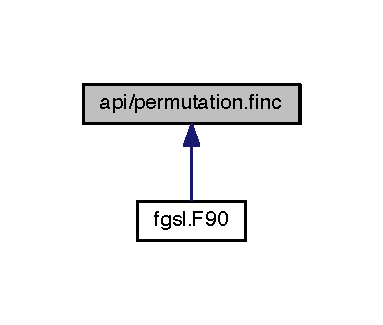
\includegraphics[width=184pt]{permutation_8finc__dep__incl}
\end{center}
\end{figure}
\subsection*{Functions/\-Subroutines}
\begin{DoxyCompactItemize}
\item 
type(fgsl\-\_\-permutation) function \hyperlink{permutation_8finc_ada94635d088a532e6e74096b2dc431b0}{fgsl\-\_\-permutation\-\_\-alloc} (n)
\item 
type(fgsl\-\_\-permutation) function \hyperlink{permutation_8finc_a204b9ecb1475f3681277d149399f49c6}{fgsl\-\_\-permutation\-\_\-calloc} (n)
\item 
subroutine \hyperlink{permutation_8finc_ad59ced94489b46930f05e4e01e0fd91a}{fgsl\-\_\-permutation\-\_\-init} (p)
\item 
subroutine \hyperlink{permutation_8finc_a2cc1fdc81859de1228dfcaf62d03e610}{fgsl\-\_\-permutation\-\_\-free} (p)
\item 
integer(fgsl\-\_\-int) function \hyperlink{permutation_8finc_adf9b7a7b269e0d3679d687c82c2ee69a}{fgsl\-\_\-permutation\-\_\-memcpy} (dest, src)
\item 
integer(fgsl\-\_\-size\-\_\-t) function \hyperlink{permutation_8finc_a5bcaae948bb703b674973a966408e964}{fgsl\-\_\-permutation\-\_\-get} (p, i)
\item 
integer(fgsl\-\_\-int) function \hyperlink{permutation_8finc_a937965d21974947b8027697decfbdf2a}{fgsl\-\_\-permutation\-\_\-swap} (p, i, j)
\item 
integer(fgsl\-\_\-size\-\_\-t) function \hyperlink{permutation_8finc_a89bad660423aef5e3a8f59b93e3c3f7f}{fgsl\-\_\-permutation\-\_\-size} (p)
\item 
integer(fgsl\-\_\-size\-\_\-t) function, \\*
dimension(\-:), pointer \hyperlink{permutation_8finc_a2d8ed5cdeac5c7eb952d34f5c84b70b4}{fgsl\-\_\-permutation\-\_\-data} (p)
\item 
integer(fgsl\-\_\-int) function \hyperlink{permutation_8finc_afdb5b335edee506c4c5edf402c24de2e}{fgsl\-\_\-permutation\-\_\-valid} (p)
\item 
subroutine \hyperlink{permutation_8finc_aba5046d4e21611729ce03009b869d4db}{fgsl\-\_\-permutation\-\_\-reverse} (p)
\item 
integer(fgsl\-\_\-int) function \hyperlink{permutation_8finc_a70977eec8133e0d4159857f6ff86a80d}{fgsl\-\_\-permutation\-\_\-inverse} (inv, p)
\item 
integer(fgsl\-\_\-int) function \hyperlink{permutation_8finc_a67f05c2a45fe4df0f97618debdb10e11}{fgsl\-\_\-permutation\-\_\-next} (p)
\item 
integer(fgsl\-\_\-int) function \hyperlink{permutation_8finc_ad79479a9b29165694fac758d0273dd3b}{fgsl\-\_\-permutation\-\_\-prev} (p)
\item 
integer(fgsl\-\_\-int) function \hyperlink{permutation_8finc_a64ded2ffe57374e81cc24d8ad04b6148}{fgsl\-\_\-permute} (p, data, stride, n)
\item 
integer(fgsl\-\_\-int) function \hyperlink{permutation_8finc_ae71ea0ea188f81ca85fe057156e3d640}{fgsl\-\_\-permute\-\_\-long} (p, data, stride, n)
\item 
integer(fgsl\-\_\-int) function \hyperlink{permutation_8finc_acd5ee6d013add3c9e7d1eb17894f5052}{fgsl\-\_\-permute\-\_\-inverse} (p, data, stride, n)
\item 
integer(fgsl\-\_\-int) function \hyperlink{permutation_8finc_ad2e7ff6db70fadebed473132caea4d0a}{fgsl\-\_\-permute\-\_\-long\-\_\-inverse} (p, data, stride, n)
\item 
integer(fgsl\-\_\-int) function \hyperlink{permutation_8finc_ab81bbdcef327e226cd027f97e0a05a95}{fgsl\-\_\-permute\-\_\-vector} (p, v)
\item 
integer(fgsl\-\_\-int) function \hyperlink{permutation_8finc_a2549c3a5bd772265ce9000cfaa6450dc}{fgsl\-\_\-permute\-\_\-vector\-\_\-inverse} (p, v)
\item 
integer(fgsl\-\_\-int) function \hyperlink{permutation_8finc_ab7b90e7b838d166f4522534e3fdb4892}{fgsl\-\_\-permutation\-\_\-mul} (p, pa, pb)
\item 
integer(fgsl\-\_\-int) function \hyperlink{permutation_8finc_ad5f09fa0443ced857bf3707d63e722ca}{fgsl\-\_\-permutation\-\_\-fwrite} (stream, p)
\item 
integer(fgsl\-\_\-int) function \hyperlink{permutation_8finc_a12d2a8bdd550b927c26430cfe7a1f8a3}{fgsl\-\_\-permutation\-\_\-fread} (stream, p)
\item 
integer(fgsl\-\_\-int) function \hyperlink{permutation_8finc_adcb7bf1d2df5b5a5c929c8c2d2c226f6}{fgsl\-\_\-permutation\-\_\-fprintf} (stream, p, format)
\item 
integer(fgsl\-\_\-int) function \hyperlink{permutation_8finc_aa083e7f38a4e3a1d52c65cff84c58427}{fgsl\-\_\-permutation\-\_\-fscanf} (stream, p)
\item 
integer(fgsl\-\_\-int) function \hyperlink{permutation_8finc_ad78bb0a655c528b6119c36e27e4ba80e}{fgsl\-\_\-permutation\-\_\-linear\-\_\-to\-\_\-canonical} (q, p)
\item 
integer(fgsl\-\_\-int) function \hyperlink{permutation_8finc_adf466e8130262699f0fc3c537628cd69}{fgsl\-\_\-permutation\-\_\-canonical\-\_\-to\-\_\-linear} (p, q)
\item 
integer(fgsl\-\_\-size\-\_\-t) function \hyperlink{permutation_8finc_a85618d9acd677b30eca1256709554b17}{fgsl\-\_\-permutation\-\_\-inversions} (p)
\item 
integer(fgsl\-\_\-size\-\_\-t) function \hyperlink{permutation_8finc_a78568007bb7b73908f8307fa61483e3e}{fgsl\-\_\-permutation\-\_\-linear\-\_\-cycles} (p)
\item 
integer(fgsl\-\_\-size\-\_\-t) function \hyperlink{permutation_8finc_ad00f45e6a50f6b3fd1954fa3f09bcf91}{fgsl\-\_\-permutation\-\_\-canonical\-\_\-cycles} (p)
\item 
type(fgsl\-\_\-combination) function \hyperlink{permutation_8finc_ace565683aa9ef2635c53b2efe6afeee6}{fgsl\-\_\-combination\-\_\-alloc} (n, k)
\item 
type(fgsl\-\_\-combination) function \hyperlink{permutation_8finc_ab0fd8e6b594d8dbd95fb23f8e911f9c4}{fgsl\-\_\-combination\-\_\-calloc} (n, k)
\item 
subroutine \hyperlink{permutation_8finc_a3f234450ae639a2a5f1ee57b3e735dde}{fgsl\-\_\-combination\-\_\-init\-\_\-first} (c)
\item 
subroutine \hyperlink{permutation_8finc_a46a310ddadb5f2d35a7a6b3dd652c9cb}{fgsl\-\_\-combination\-\_\-init\-\_\-last} (c)
\item 
subroutine \hyperlink{permutation_8finc_a5621600a730419e48e135d3c165fd12d}{fgsl\-\_\-combination\-\_\-free} (c)
\item 
integer(fgsl\-\_\-int) function \hyperlink{permutation_8finc_a8c1ed815e15adea5c5eca5a54b74901d}{fgsl\-\_\-combination\-\_\-memcpy} (dest, src)
\item 
integer(fgsl\-\_\-size\-\_\-t) function \hyperlink{permutation_8finc_a1c9f6ecd2ddf2782907a5b1338553b62}{fgsl\-\_\-combination\-\_\-get} (c, i)
\item 
integer(fgsl\-\_\-size\-\_\-t) function \hyperlink{permutation_8finc_a999499c6e216c3cbf8c8eb2cc35efc8b}{fgsl\-\_\-combination\-\_\-n} (c)
\item 
integer(fgsl\-\_\-size\-\_\-t) function \hyperlink{permutation_8finc_ab7fad8757dc445fdd0b66b005d27e619}{fgsl\-\_\-combination\-\_\-k} (c)
\item 
integer(fgsl\-\_\-size\-\_\-t) function, \\*
dimension(\-:), pointer \hyperlink{permutation_8finc_af802fe7025690ec09c892e4a358e58ee}{fgsl\-\_\-combination\-\_\-data} (c)
\item 
integer(fgsl\-\_\-int) function \hyperlink{permutation_8finc_a32ca51968e7eaf13df7d34b23dd948b5}{fgsl\-\_\-combination\-\_\-valid} (c)
\item 
integer(fgsl\-\_\-int) function \hyperlink{permutation_8finc_acf50f6a9728a138e3cbb1e014c047406}{fgsl\-\_\-combination\-\_\-next} (c)
\item 
integer(fgsl\-\_\-int) function \hyperlink{permutation_8finc_aee16ccc363b42c5bb4f5cda5cec21842}{fgsl\-\_\-combination\-\_\-prev} (c)
\item 
integer(fgsl\-\_\-int) function \hyperlink{permutation_8finc_a5c7269a8b592e3fd021ff35690d5c275}{fgsl\-\_\-combination\-\_\-fwrite} (stream, c)
\item 
integer(fgsl\-\_\-int) function \hyperlink{permutation_8finc_a40e24831c4b879f52d7923f0b3a8ea37}{fgsl\-\_\-combination\-\_\-fread} (stream, c)
\item 
integer(fgsl\-\_\-int) function \hyperlink{permutation_8finc_abf0711fb612be5f86dd06b31b26403b9}{fgsl\-\_\-combination\-\_\-fprintf} (stream, c, format)
\item 
integer(fgsl\-\_\-int) function \hyperlink{permutation_8finc_ad2dcdaa5e7550cdda2682f40367fba3a}{fgsl\-\_\-combination\-\_\-fscanf} (stream, c)
\item 
type(fgsl\-\_\-multiset) function \hyperlink{permutation_8finc_a7c55a19cb36e6d24c1937884a8d6c5b8}{fgsl\-\_\-multiset\-\_\-alloc} (n, k)
\item 
type(fgsl\-\_\-multiset) function \hyperlink{permutation_8finc_a9b60ad4de174107a2bb814fa946d2947}{fgsl\-\_\-multiset\-\_\-calloc} (n, k)
\item 
subroutine \hyperlink{permutation_8finc_ab2764f91fad296def839814aa48d405a}{fgsl\-\_\-multiset\-\_\-init\-\_\-first} (c)
\item 
subroutine \hyperlink{permutation_8finc_af11d68a8d9d59bc6b6a6ff371067a4c6}{fgsl\-\_\-multiset\-\_\-init\-\_\-last} (c)
\item 
subroutine \hyperlink{permutation_8finc_aecef1853cef964fa8dabf917628a2cf2}{fgsl\-\_\-multiset\-\_\-free} (c)
\item 
integer(fgsl\-\_\-int) function \hyperlink{permutation_8finc_a4ad5000e4797d1c096bc9c2b938bb3d8}{fgsl\-\_\-multiset\-\_\-memcpy} (dest, src)
\item 
integer(fgsl\-\_\-size\-\_\-t) function \hyperlink{permutation_8finc_a0d65011e4475e4b3b130e5c4e0dd7301}{fgsl\-\_\-multiset\-\_\-get} (c, i)
\item 
integer(fgsl\-\_\-size\-\_\-t) function \hyperlink{permutation_8finc_ab080e2383e519fc3bc3e1f8a09746867}{fgsl\-\_\-multiset\-\_\-n} (c)
\item 
integer(fgsl\-\_\-size\-\_\-t) function \hyperlink{permutation_8finc_a285143abab01c99704934281a8767baa}{fgsl\-\_\-multiset\-\_\-k} (c)
\item 
integer(fgsl\-\_\-size\-\_\-t) function, \\*
dimension(\-:), pointer \hyperlink{permutation_8finc_af687c5f061870efcc8d104654d26b88e}{fgsl\-\_\-multiset\-\_\-data} (c)
\item 
integer(fgsl\-\_\-int) function \hyperlink{permutation_8finc_acde8e9dc3c43e69cae5b2679a4e3156e}{fgsl\-\_\-multiset\-\_\-valid} (c)
\item 
integer(fgsl\-\_\-int) function \hyperlink{permutation_8finc_a8448ce578712a0b1e42918d448856052}{fgsl\-\_\-multiset\-\_\-next} (c)
\item 
integer(fgsl\-\_\-int) function \hyperlink{permutation_8finc_a00e824e9ee9cb15a5939c1f7dec2c5e1}{fgsl\-\_\-multiset\-\_\-prev} (c)
\item 
integer(fgsl\-\_\-int) function \hyperlink{permutation_8finc_ad5694529ae97ed0a85ae153737232382}{fgsl\-\_\-multiset\-\_\-fwrite} (stream, c)
\item 
integer(fgsl\-\_\-int) function \hyperlink{permutation_8finc_acf2bf65c017f6537e1751bcd12b43774}{fgsl\-\_\-multiset\-\_\-fread} (stream, c)
\item 
integer(fgsl\-\_\-int) function \hyperlink{permutation_8finc_aa0d4a4609f7410cb0aba15ff56ae5fa4}{fgsl\-\_\-multiset\-\_\-fprintf} (stream, c, format)
\item 
integer(fgsl\-\_\-int) function \hyperlink{permutation_8finc_a9e05fb001350d8e3667f3fbaee59a0ce}{fgsl\-\_\-multiset\-\_\-fscanf} (stream, c)
\item 
logical function \hyperlink{permutation_8finc_a59b2c2f3d7df483019e0a8f270ad6fb5}{fgsl\-\_\-permutation\-\_\-status} (permutation)
\item 
logical function \hyperlink{permutation_8finc_a579b1fdf03f937579abf673f2a436043}{fgsl\-\_\-combination\-\_\-status} (combination)
\item 
logical function \hyperlink{permutation_8finc_ab7dfd6ba20374a426f2b813cf8bf63ec}{fgsl\-\_\-multiset\-\_\-status} (multiset)
\item 
integer(fgsl\-\_\-size\-\_\-t) function \hyperlink{permutation_8finc_aa3a991b00a25f168c7ff9f0df9e327c9}{fgsl\-\_\-sizeof\-\_\-permutation} (p)
\item 
integer(fgsl\-\_\-size\-\_\-t) function \hyperlink{permutation_8finc_aee397495d24c58890649db47f9a17ebf}{fgsl\-\_\-sizeof\-\_\-combination} (c)
\item 
integer(fgsl\-\_\-size\-\_\-t) function \hyperlink{permutation_8finc_a73a0b5bb42cd2a204bbda54a8aa2869d}{fgsl\-\_\-sizeof\-\_\-multiset} (c)
\end{DoxyCompactItemize}


\subsection{Function/\-Subroutine Documentation}
\hypertarget{permutation_8finc_ace565683aa9ef2635c53b2efe6afeee6}{\index{permutation.\-finc@{permutation.\-finc}!fgsl\-\_\-combination\-\_\-alloc@{fgsl\-\_\-combination\-\_\-alloc}}
\index{fgsl\-\_\-combination\-\_\-alloc@{fgsl\-\_\-combination\-\_\-alloc}!permutation.finc@{permutation.\-finc}}
\subsubsection[{fgsl\-\_\-combination\-\_\-alloc}]{\setlength{\rightskip}{0pt plus 5cm}type(fgsl\-\_\-combination) function fgsl\-\_\-combination\-\_\-alloc (
\begin{DoxyParamCaption}
\item[{integer(fgsl\-\_\-size\-\_\-t), intent(in)}]{n, }
\item[{integer(fgsl\-\_\-size\-\_\-t), intent(in)}]{k}
\end{DoxyParamCaption}
)}}\label{permutation_8finc_ace565683aa9ef2635c53b2efe6afeee6}
\hypertarget{permutation_8finc_ab0fd8e6b594d8dbd95fb23f8e911f9c4}{\index{permutation.\-finc@{permutation.\-finc}!fgsl\-\_\-combination\-\_\-calloc@{fgsl\-\_\-combination\-\_\-calloc}}
\index{fgsl\-\_\-combination\-\_\-calloc@{fgsl\-\_\-combination\-\_\-calloc}!permutation.finc@{permutation.\-finc}}
\subsubsection[{fgsl\-\_\-combination\-\_\-calloc}]{\setlength{\rightskip}{0pt plus 5cm}type(fgsl\-\_\-combination) function fgsl\-\_\-combination\-\_\-calloc (
\begin{DoxyParamCaption}
\item[{integer(fgsl\-\_\-size\-\_\-t), intent(in)}]{n, }
\item[{integer(fgsl\-\_\-size\-\_\-t), intent(in)}]{k}
\end{DoxyParamCaption}
)}}\label{permutation_8finc_ab0fd8e6b594d8dbd95fb23f8e911f9c4}
\hypertarget{permutation_8finc_af802fe7025690ec09c892e4a358e58ee}{\index{permutation.\-finc@{permutation.\-finc}!fgsl\-\_\-combination\-\_\-data@{fgsl\-\_\-combination\-\_\-data}}
\index{fgsl\-\_\-combination\-\_\-data@{fgsl\-\_\-combination\-\_\-data}!permutation.finc@{permutation.\-finc}}
\subsubsection[{fgsl\-\_\-combination\-\_\-data}]{\setlength{\rightskip}{0pt plus 5cm}integer(fgsl\-\_\-size\-\_\-t) function, dimension(\-:), pointer fgsl\-\_\-combination\-\_\-data (
\begin{DoxyParamCaption}
\item[{type(fgsl\-\_\-combination), intent(in)}]{c}
\end{DoxyParamCaption}
)}}\label{permutation_8finc_af802fe7025690ec09c892e4a358e58ee}
\hypertarget{permutation_8finc_abf0711fb612be5f86dd06b31b26403b9}{\index{permutation.\-finc@{permutation.\-finc}!fgsl\-\_\-combination\-\_\-fprintf@{fgsl\-\_\-combination\-\_\-fprintf}}
\index{fgsl\-\_\-combination\-\_\-fprintf@{fgsl\-\_\-combination\-\_\-fprintf}!permutation.finc@{permutation.\-finc}}
\subsubsection[{fgsl\-\_\-combination\-\_\-fprintf}]{\setlength{\rightskip}{0pt plus 5cm}integer(fgsl\-\_\-int) function fgsl\-\_\-combination\-\_\-fprintf (
\begin{DoxyParamCaption}
\item[{type(fgsl\-\_\-file), intent(in)}]{stream, }
\item[{type(fgsl\-\_\-combination), intent(in)}]{c, }
\item[{character(kind=fgsl\-\_\-char, len=$\ast$), intent(in)}]{format}
\end{DoxyParamCaption}
)}}\label{permutation_8finc_abf0711fb612be5f86dd06b31b26403b9}
\hypertarget{permutation_8finc_a40e24831c4b879f52d7923f0b3a8ea37}{\index{permutation.\-finc@{permutation.\-finc}!fgsl\-\_\-combination\-\_\-fread@{fgsl\-\_\-combination\-\_\-fread}}
\index{fgsl\-\_\-combination\-\_\-fread@{fgsl\-\_\-combination\-\_\-fread}!permutation.finc@{permutation.\-finc}}
\subsubsection[{fgsl\-\_\-combination\-\_\-fread}]{\setlength{\rightskip}{0pt plus 5cm}integer(fgsl\-\_\-int) function fgsl\-\_\-combination\-\_\-fread (
\begin{DoxyParamCaption}
\item[{type(fgsl\-\_\-file), intent(in)}]{stream, }
\item[{type(fgsl\-\_\-combination), intent(inout)}]{c}
\end{DoxyParamCaption}
)}}\label{permutation_8finc_a40e24831c4b879f52d7923f0b3a8ea37}
\hypertarget{permutation_8finc_a5621600a730419e48e135d3c165fd12d}{\index{permutation.\-finc@{permutation.\-finc}!fgsl\-\_\-combination\-\_\-free@{fgsl\-\_\-combination\-\_\-free}}
\index{fgsl\-\_\-combination\-\_\-free@{fgsl\-\_\-combination\-\_\-free}!permutation.finc@{permutation.\-finc}}
\subsubsection[{fgsl\-\_\-combination\-\_\-free}]{\setlength{\rightskip}{0pt plus 5cm}subroutine fgsl\-\_\-combination\-\_\-free (
\begin{DoxyParamCaption}
\item[{type(fgsl\-\_\-combination), intent(inout)}]{c}
\end{DoxyParamCaption}
)}}\label{permutation_8finc_a5621600a730419e48e135d3c165fd12d}
\hypertarget{permutation_8finc_ad2dcdaa5e7550cdda2682f40367fba3a}{\index{permutation.\-finc@{permutation.\-finc}!fgsl\-\_\-combination\-\_\-fscanf@{fgsl\-\_\-combination\-\_\-fscanf}}
\index{fgsl\-\_\-combination\-\_\-fscanf@{fgsl\-\_\-combination\-\_\-fscanf}!permutation.finc@{permutation.\-finc}}
\subsubsection[{fgsl\-\_\-combination\-\_\-fscanf}]{\setlength{\rightskip}{0pt plus 5cm}integer(fgsl\-\_\-int) function fgsl\-\_\-combination\-\_\-fscanf (
\begin{DoxyParamCaption}
\item[{type(fgsl\-\_\-file), intent(in)}]{stream, }
\item[{type(fgsl\-\_\-combination), intent(inout)}]{c}
\end{DoxyParamCaption}
)}}\label{permutation_8finc_ad2dcdaa5e7550cdda2682f40367fba3a}
\hypertarget{permutation_8finc_a5c7269a8b592e3fd021ff35690d5c275}{\index{permutation.\-finc@{permutation.\-finc}!fgsl\-\_\-combination\-\_\-fwrite@{fgsl\-\_\-combination\-\_\-fwrite}}
\index{fgsl\-\_\-combination\-\_\-fwrite@{fgsl\-\_\-combination\-\_\-fwrite}!permutation.finc@{permutation.\-finc}}
\subsubsection[{fgsl\-\_\-combination\-\_\-fwrite}]{\setlength{\rightskip}{0pt plus 5cm}integer(fgsl\-\_\-int) function fgsl\-\_\-combination\-\_\-fwrite (
\begin{DoxyParamCaption}
\item[{type(fgsl\-\_\-file), intent(in)}]{stream, }
\item[{type(fgsl\-\_\-combination), intent(in)}]{c}
\end{DoxyParamCaption}
)}}\label{permutation_8finc_a5c7269a8b592e3fd021ff35690d5c275}
\hypertarget{permutation_8finc_a1c9f6ecd2ddf2782907a5b1338553b62}{\index{permutation.\-finc@{permutation.\-finc}!fgsl\-\_\-combination\-\_\-get@{fgsl\-\_\-combination\-\_\-get}}
\index{fgsl\-\_\-combination\-\_\-get@{fgsl\-\_\-combination\-\_\-get}!permutation.finc@{permutation.\-finc}}
\subsubsection[{fgsl\-\_\-combination\-\_\-get}]{\setlength{\rightskip}{0pt plus 5cm}integer(fgsl\-\_\-size\-\_\-t) function fgsl\-\_\-combination\-\_\-get (
\begin{DoxyParamCaption}
\item[{type(fgsl\-\_\-combination), intent(inout)}]{c, }
\item[{integer(fgsl\-\_\-size\-\_\-t), intent(in)}]{i}
\end{DoxyParamCaption}
)}}\label{permutation_8finc_a1c9f6ecd2ddf2782907a5b1338553b62}
\hypertarget{permutation_8finc_a3f234450ae639a2a5f1ee57b3e735dde}{\index{permutation.\-finc@{permutation.\-finc}!fgsl\-\_\-combination\-\_\-init\-\_\-first@{fgsl\-\_\-combination\-\_\-init\-\_\-first}}
\index{fgsl\-\_\-combination\-\_\-init\-\_\-first@{fgsl\-\_\-combination\-\_\-init\-\_\-first}!permutation.finc@{permutation.\-finc}}
\subsubsection[{fgsl\-\_\-combination\-\_\-init\-\_\-first}]{\setlength{\rightskip}{0pt plus 5cm}subroutine fgsl\-\_\-combination\-\_\-init\-\_\-first (
\begin{DoxyParamCaption}
\item[{type(fgsl\-\_\-combination), intent(inout)}]{c}
\end{DoxyParamCaption}
)}}\label{permutation_8finc_a3f234450ae639a2a5f1ee57b3e735dde}
\hypertarget{permutation_8finc_a46a310ddadb5f2d35a7a6b3dd652c9cb}{\index{permutation.\-finc@{permutation.\-finc}!fgsl\-\_\-combination\-\_\-init\-\_\-last@{fgsl\-\_\-combination\-\_\-init\-\_\-last}}
\index{fgsl\-\_\-combination\-\_\-init\-\_\-last@{fgsl\-\_\-combination\-\_\-init\-\_\-last}!permutation.finc@{permutation.\-finc}}
\subsubsection[{fgsl\-\_\-combination\-\_\-init\-\_\-last}]{\setlength{\rightskip}{0pt plus 5cm}subroutine fgsl\-\_\-combination\-\_\-init\-\_\-last (
\begin{DoxyParamCaption}
\item[{type(fgsl\-\_\-combination), intent(inout)}]{c}
\end{DoxyParamCaption}
)}}\label{permutation_8finc_a46a310ddadb5f2d35a7a6b3dd652c9cb}
\hypertarget{permutation_8finc_ab7fad8757dc445fdd0b66b005d27e619}{\index{permutation.\-finc@{permutation.\-finc}!fgsl\-\_\-combination\-\_\-k@{fgsl\-\_\-combination\-\_\-k}}
\index{fgsl\-\_\-combination\-\_\-k@{fgsl\-\_\-combination\-\_\-k}!permutation.finc@{permutation.\-finc}}
\subsubsection[{fgsl\-\_\-combination\-\_\-k}]{\setlength{\rightskip}{0pt plus 5cm}integer(fgsl\-\_\-size\-\_\-t) function fgsl\-\_\-combination\-\_\-k (
\begin{DoxyParamCaption}
\item[{type(fgsl\-\_\-combination), intent(in)}]{c}
\end{DoxyParamCaption}
)}}\label{permutation_8finc_ab7fad8757dc445fdd0b66b005d27e619}
\hypertarget{permutation_8finc_a8c1ed815e15adea5c5eca5a54b74901d}{\index{permutation.\-finc@{permutation.\-finc}!fgsl\-\_\-combination\-\_\-memcpy@{fgsl\-\_\-combination\-\_\-memcpy}}
\index{fgsl\-\_\-combination\-\_\-memcpy@{fgsl\-\_\-combination\-\_\-memcpy}!permutation.finc@{permutation.\-finc}}
\subsubsection[{fgsl\-\_\-combination\-\_\-memcpy}]{\setlength{\rightskip}{0pt plus 5cm}integer(fgsl\-\_\-int) function fgsl\-\_\-combination\-\_\-memcpy (
\begin{DoxyParamCaption}
\item[{type(fgsl\-\_\-combination), intent(inout)}]{dest, }
\item[{type(fgsl\-\_\-combination), intent(in)}]{src}
\end{DoxyParamCaption}
)}}\label{permutation_8finc_a8c1ed815e15adea5c5eca5a54b74901d}
\hypertarget{permutation_8finc_a999499c6e216c3cbf8c8eb2cc35efc8b}{\index{permutation.\-finc@{permutation.\-finc}!fgsl\-\_\-combination\-\_\-n@{fgsl\-\_\-combination\-\_\-n}}
\index{fgsl\-\_\-combination\-\_\-n@{fgsl\-\_\-combination\-\_\-n}!permutation.finc@{permutation.\-finc}}
\subsubsection[{fgsl\-\_\-combination\-\_\-n}]{\setlength{\rightskip}{0pt plus 5cm}integer(fgsl\-\_\-size\-\_\-t) function fgsl\-\_\-combination\-\_\-n (
\begin{DoxyParamCaption}
\item[{type(fgsl\-\_\-combination), intent(in)}]{c}
\end{DoxyParamCaption}
)}}\label{permutation_8finc_a999499c6e216c3cbf8c8eb2cc35efc8b}
\hypertarget{permutation_8finc_acf50f6a9728a138e3cbb1e014c047406}{\index{permutation.\-finc@{permutation.\-finc}!fgsl\-\_\-combination\-\_\-next@{fgsl\-\_\-combination\-\_\-next}}
\index{fgsl\-\_\-combination\-\_\-next@{fgsl\-\_\-combination\-\_\-next}!permutation.finc@{permutation.\-finc}}
\subsubsection[{fgsl\-\_\-combination\-\_\-next}]{\setlength{\rightskip}{0pt plus 5cm}integer(fgsl\-\_\-int) function fgsl\-\_\-combination\-\_\-next (
\begin{DoxyParamCaption}
\item[{type(fgsl\-\_\-combination), intent(in)}]{c}
\end{DoxyParamCaption}
)}}\label{permutation_8finc_acf50f6a9728a138e3cbb1e014c047406}
\hypertarget{permutation_8finc_aee16ccc363b42c5bb4f5cda5cec21842}{\index{permutation.\-finc@{permutation.\-finc}!fgsl\-\_\-combination\-\_\-prev@{fgsl\-\_\-combination\-\_\-prev}}
\index{fgsl\-\_\-combination\-\_\-prev@{fgsl\-\_\-combination\-\_\-prev}!permutation.finc@{permutation.\-finc}}
\subsubsection[{fgsl\-\_\-combination\-\_\-prev}]{\setlength{\rightskip}{0pt plus 5cm}integer(fgsl\-\_\-int) function fgsl\-\_\-combination\-\_\-prev (
\begin{DoxyParamCaption}
\item[{type(fgsl\-\_\-combination), intent(in)}]{c}
\end{DoxyParamCaption}
)}}\label{permutation_8finc_aee16ccc363b42c5bb4f5cda5cec21842}
\hypertarget{permutation_8finc_a579b1fdf03f937579abf673f2a436043}{\index{permutation.\-finc@{permutation.\-finc}!fgsl\-\_\-combination\-\_\-status@{fgsl\-\_\-combination\-\_\-status}}
\index{fgsl\-\_\-combination\-\_\-status@{fgsl\-\_\-combination\-\_\-status}!permutation.finc@{permutation.\-finc}}
\subsubsection[{fgsl\-\_\-combination\-\_\-status}]{\setlength{\rightskip}{0pt plus 5cm}logical function fgsl\-\_\-combination\-\_\-status (
\begin{DoxyParamCaption}
\item[{type(fgsl\-\_\-combination), intent(in)}]{combination}
\end{DoxyParamCaption}
)}}\label{permutation_8finc_a579b1fdf03f937579abf673f2a436043}
\hypertarget{permutation_8finc_a32ca51968e7eaf13df7d34b23dd948b5}{\index{permutation.\-finc@{permutation.\-finc}!fgsl\-\_\-combination\-\_\-valid@{fgsl\-\_\-combination\-\_\-valid}}
\index{fgsl\-\_\-combination\-\_\-valid@{fgsl\-\_\-combination\-\_\-valid}!permutation.finc@{permutation.\-finc}}
\subsubsection[{fgsl\-\_\-combination\-\_\-valid}]{\setlength{\rightskip}{0pt plus 5cm}integer(fgsl\-\_\-int) function fgsl\-\_\-combination\-\_\-valid (
\begin{DoxyParamCaption}
\item[{type(fgsl\-\_\-combination), intent(in)}]{c}
\end{DoxyParamCaption}
)}}\label{permutation_8finc_a32ca51968e7eaf13df7d34b23dd948b5}
\hypertarget{permutation_8finc_a7c55a19cb36e6d24c1937884a8d6c5b8}{\index{permutation.\-finc@{permutation.\-finc}!fgsl\-\_\-multiset\-\_\-alloc@{fgsl\-\_\-multiset\-\_\-alloc}}
\index{fgsl\-\_\-multiset\-\_\-alloc@{fgsl\-\_\-multiset\-\_\-alloc}!permutation.finc@{permutation.\-finc}}
\subsubsection[{fgsl\-\_\-multiset\-\_\-alloc}]{\setlength{\rightskip}{0pt plus 5cm}type(fgsl\-\_\-multiset) function fgsl\-\_\-multiset\-\_\-alloc (
\begin{DoxyParamCaption}
\item[{integer(fgsl\-\_\-size\-\_\-t), intent(in)}]{n, }
\item[{integer(fgsl\-\_\-size\-\_\-t), intent(in)}]{k}
\end{DoxyParamCaption}
)}}\label{permutation_8finc_a7c55a19cb36e6d24c1937884a8d6c5b8}
\hypertarget{permutation_8finc_a9b60ad4de174107a2bb814fa946d2947}{\index{permutation.\-finc@{permutation.\-finc}!fgsl\-\_\-multiset\-\_\-calloc@{fgsl\-\_\-multiset\-\_\-calloc}}
\index{fgsl\-\_\-multiset\-\_\-calloc@{fgsl\-\_\-multiset\-\_\-calloc}!permutation.finc@{permutation.\-finc}}
\subsubsection[{fgsl\-\_\-multiset\-\_\-calloc}]{\setlength{\rightskip}{0pt plus 5cm}type(fgsl\-\_\-multiset) function fgsl\-\_\-multiset\-\_\-calloc (
\begin{DoxyParamCaption}
\item[{integer(fgsl\-\_\-size\-\_\-t), intent(in)}]{n, }
\item[{integer(fgsl\-\_\-size\-\_\-t), intent(in)}]{k}
\end{DoxyParamCaption}
)}}\label{permutation_8finc_a9b60ad4de174107a2bb814fa946d2947}
\hypertarget{permutation_8finc_af687c5f061870efcc8d104654d26b88e}{\index{permutation.\-finc@{permutation.\-finc}!fgsl\-\_\-multiset\-\_\-data@{fgsl\-\_\-multiset\-\_\-data}}
\index{fgsl\-\_\-multiset\-\_\-data@{fgsl\-\_\-multiset\-\_\-data}!permutation.finc@{permutation.\-finc}}
\subsubsection[{fgsl\-\_\-multiset\-\_\-data}]{\setlength{\rightskip}{0pt plus 5cm}integer(fgsl\-\_\-size\-\_\-t) function, dimension(\-:), pointer fgsl\-\_\-multiset\-\_\-data (
\begin{DoxyParamCaption}
\item[{type(fgsl\-\_\-multiset), intent(in)}]{c}
\end{DoxyParamCaption}
)}}\label{permutation_8finc_af687c5f061870efcc8d104654d26b88e}
\hypertarget{permutation_8finc_aa0d4a4609f7410cb0aba15ff56ae5fa4}{\index{permutation.\-finc@{permutation.\-finc}!fgsl\-\_\-multiset\-\_\-fprintf@{fgsl\-\_\-multiset\-\_\-fprintf}}
\index{fgsl\-\_\-multiset\-\_\-fprintf@{fgsl\-\_\-multiset\-\_\-fprintf}!permutation.finc@{permutation.\-finc}}
\subsubsection[{fgsl\-\_\-multiset\-\_\-fprintf}]{\setlength{\rightskip}{0pt plus 5cm}integer(fgsl\-\_\-int) function fgsl\-\_\-multiset\-\_\-fprintf (
\begin{DoxyParamCaption}
\item[{type(fgsl\-\_\-file), intent(in)}]{stream, }
\item[{type(fgsl\-\_\-multiset), intent(in)}]{c, }
\item[{character(kind=fgsl\-\_\-char, len=$\ast$), intent(in)}]{format}
\end{DoxyParamCaption}
)}}\label{permutation_8finc_aa0d4a4609f7410cb0aba15ff56ae5fa4}
\hypertarget{permutation_8finc_acf2bf65c017f6537e1751bcd12b43774}{\index{permutation.\-finc@{permutation.\-finc}!fgsl\-\_\-multiset\-\_\-fread@{fgsl\-\_\-multiset\-\_\-fread}}
\index{fgsl\-\_\-multiset\-\_\-fread@{fgsl\-\_\-multiset\-\_\-fread}!permutation.finc@{permutation.\-finc}}
\subsubsection[{fgsl\-\_\-multiset\-\_\-fread}]{\setlength{\rightskip}{0pt plus 5cm}integer(fgsl\-\_\-int) function fgsl\-\_\-multiset\-\_\-fread (
\begin{DoxyParamCaption}
\item[{type(fgsl\-\_\-file), intent(in)}]{stream, }
\item[{type(fgsl\-\_\-multiset), intent(inout)}]{c}
\end{DoxyParamCaption}
)}}\label{permutation_8finc_acf2bf65c017f6537e1751bcd12b43774}
\hypertarget{permutation_8finc_aecef1853cef964fa8dabf917628a2cf2}{\index{permutation.\-finc@{permutation.\-finc}!fgsl\-\_\-multiset\-\_\-free@{fgsl\-\_\-multiset\-\_\-free}}
\index{fgsl\-\_\-multiset\-\_\-free@{fgsl\-\_\-multiset\-\_\-free}!permutation.finc@{permutation.\-finc}}
\subsubsection[{fgsl\-\_\-multiset\-\_\-free}]{\setlength{\rightskip}{0pt plus 5cm}subroutine fgsl\-\_\-multiset\-\_\-free (
\begin{DoxyParamCaption}
\item[{type(fgsl\-\_\-multiset), intent(inout)}]{c}
\end{DoxyParamCaption}
)}}\label{permutation_8finc_aecef1853cef964fa8dabf917628a2cf2}
\hypertarget{permutation_8finc_a9e05fb001350d8e3667f3fbaee59a0ce}{\index{permutation.\-finc@{permutation.\-finc}!fgsl\-\_\-multiset\-\_\-fscanf@{fgsl\-\_\-multiset\-\_\-fscanf}}
\index{fgsl\-\_\-multiset\-\_\-fscanf@{fgsl\-\_\-multiset\-\_\-fscanf}!permutation.finc@{permutation.\-finc}}
\subsubsection[{fgsl\-\_\-multiset\-\_\-fscanf}]{\setlength{\rightskip}{0pt plus 5cm}integer(fgsl\-\_\-int) function fgsl\-\_\-multiset\-\_\-fscanf (
\begin{DoxyParamCaption}
\item[{type(fgsl\-\_\-file), intent(in)}]{stream, }
\item[{type(fgsl\-\_\-multiset), intent(inout)}]{c}
\end{DoxyParamCaption}
)}}\label{permutation_8finc_a9e05fb001350d8e3667f3fbaee59a0ce}
\hypertarget{permutation_8finc_ad5694529ae97ed0a85ae153737232382}{\index{permutation.\-finc@{permutation.\-finc}!fgsl\-\_\-multiset\-\_\-fwrite@{fgsl\-\_\-multiset\-\_\-fwrite}}
\index{fgsl\-\_\-multiset\-\_\-fwrite@{fgsl\-\_\-multiset\-\_\-fwrite}!permutation.finc@{permutation.\-finc}}
\subsubsection[{fgsl\-\_\-multiset\-\_\-fwrite}]{\setlength{\rightskip}{0pt plus 5cm}integer(fgsl\-\_\-int) function fgsl\-\_\-multiset\-\_\-fwrite (
\begin{DoxyParamCaption}
\item[{type(fgsl\-\_\-file), intent(in)}]{stream, }
\item[{type(fgsl\-\_\-multiset), intent(in)}]{c}
\end{DoxyParamCaption}
)}}\label{permutation_8finc_ad5694529ae97ed0a85ae153737232382}
\hypertarget{permutation_8finc_a0d65011e4475e4b3b130e5c4e0dd7301}{\index{permutation.\-finc@{permutation.\-finc}!fgsl\-\_\-multiset\-\_\-get@{fgsl\-\_\-multiset\-\_\-get}}
\index{fgsl\-\_\-multiset\-\_\-get@{fgsl\-\_\-multiset\-\_\-get}!permutation.finc@{permutation.\-finc}}
\subsubsection[{fgsl\-\_\-multiset\-\_\-get}]{\setlength{\rightskip}{0pt plus 5cm}integer(fgsl\-\_\-size\-\_\-t) function fgsl\-\_\-multiset\-\_\-get (
\begin{DoxyParamCaption}
\item[{type(fgsl\-\_\-multiset), intent(inout)}]{c, }
\item[{integer(fgsl\-\_\-size\-\_\-t), intent(in)}]{i}
\end{DoxyParamCaption}
)}}\label{permutation_8finc_a0d65011e4475e4b3b130e5c4e0dd7301}
\hypertarget{permutation_8finc_ab2764f91fad296def839814aa48d405a}{\index{permutation.\-finc@{permutation.\-finc}!fgsl\-\_\-multiset\-\_\-init\-\_\-first@{fgsl\-\_\-multiset\-\_\-init\-\_\-first}}
\index{fgsl\-\_\-multiset\-\_\-init\-\_\-first@{fgsl\-\_\-multiset\-\_\-init\-\_\-first}!permutation.finc@{permutation.\-finc}}
\subsubsection[{fgsl\-\_\-multiset\-\_\-init\-\_\-first}]{\setlength{\rightskip}{0pt plus 5cm}subroutine fgsl\-\_\-multiset\-\_\-init\-\_\-first (
\begin{DoxyParamCaption}
\item[{type(fgsl\-\_\-multiset), intent(inout)}]{c}
\end{DoxyParamCaption}
)}}\label{permutation_8finc_ab2764f91fad296def839814aa48d405a}
\hypertarget{permutation_8finc_af11d68a8d9d59bc6b6a6ff371067a4c6}{\index{permutation.\-finc@{permutation.\-finc}!fgsl\-\_\-multiset\-\_\-init\-\_\-last@{fgsl\-\_\-multiset\-\_\-init\-\_\-last}}
\index{fgsl\-\_\-multiset\-\_\-init\-\_\-last@{fgsl\-\_\-multiset\-\_\-init\-\_\-last}!permutation.finc@{permutation.\-finc}}
\subsubsection[{fgsl\-\_\-multiset\-\_\-init\-\_\-last}]{\setlength{\rightskip}{0pt plus 5cm}subroutine fgsl\-\_\-multiset\-\_\-init\-\_\-last (
\begin{DoxyParamCaption}
\item[{type(fgsl\-\_\-multiset), intent(inout)}]{c}
\end{DoxyParamCaption}
)}}\label{permutation_8finc_af11d68a8d9d59bc6b6a6ff371067a4c6}
\hypertarget{permutation_8finc_a285143abab01c99704934281a8767baa}{\index{permutation.\-finc@{permutation.\-finc}!fgsl\-\_\-multiset\-\_\-k@{fgsl\-\_\-multiset\-\_\-k}}
\index{fgsl\-\_\-multiset\-\_\-k@{fgsl\-\_\-multiset\-\_\-k}!permutation.finc@{permutation.\-finc}}
\subsubsection[{fgsl\-\_\-multiset\-\_\-k}]{\setlength{\rightskip}{0pt plus 5cm}integer(fgsl\-\_\-size\-\_\-t) function fgsl\-\_\-multiset\-\_\-k (
\begin{DoxyParamCaption}
\item[{type(fgsl\-\_\-multiset), intent(in)}]{c}
\end{DoxyParamCaption}
)}}\label{permutation_8finc_a285143abab01c99704934281a8767baa}
\hypertarget{permutation_8finc_a4ad5000e4797d1c096bc9c2b938bb3d8}{\index{permutation.\-finc@{permutation.\-finc}!fgsl\-\_\-multiset\-\_\-memcpy@{fgsl\-\_\-multiset\-\_\-memcpy}}
\index{fgsl\-\_\-multiset\-\_\-memcpy@{fgsl\-\_\-multiset\-\_\-memcpy}!permutation.finc@{permutation.\-finc}}
\subsubsection[{fgsl\-\_\-multiset\-\_\-memcpy}]{\setlength{\rightskip}{0pt plus 5cm}integer(fgsl\-\_\-int) function fgsl\-\_\-multiset\-\_\-memcpy (
\begin{DoxyParamCaption}
\item[{type(fgsl\-\_\-multiset), intent(inout)}]{dest, }
\item[{type(fgsl\-\_\-multiset), intent(in)}]{src}
\end{DoxyParamCaption}
)}}\label{permutation_8finc_a4ad5000e4797d1c096bc9c2b938bb3d8}
\hypertarget{permutation_8finc_ab080e2383e519fc3bc3e1f8a09746867}{\index{permutation.\-finc@{permutation.\-finc}!fgsl\-\_\-multiset\-\_\-n@{fgsl\-\_\-multiset\-\_\-n}}
\index{fgsl\-\_\-multiset\-\_\-n@{fgsl\-\_\-multiset\-\_\-n}!permutation.finc@{permutation.\-finc}}
\subsubsection[{fgsl\-\_\-multiset\-\_\-n}]{\setlength{\rightskip}{0pt plus 5cm}integer(fgsl\-\_\-size\-\_\-t) function fgsl\-\_\-multiset\-\_\-n (
\begin{DoxyParamCaption}
\item[{type(fgsl\-\_\-multiset), intent(in)}]{c}
\end{DoxyParamCaption}
)}}\label{permutation_8finc_ab080e2383e519fc3bc3e1f8a09746867}
\hypertarget{permutation_8finc_a8448ce578712a0b1e42918d448856052}{\index{permutation.\-finc@{permutation.\-finc}!fgsl\-\_\-multiset\-\_\-next@{fgsl\-\_\-multiset\-\_\-next}}
\index{fgsl\-\_\-multiset\-\_\-next@{fgsl\-\_\-multiset\-\_\-next}!permutation.finc@{permutation.\-finc}}
\subsubsection[{fgsl\-\_\-multiset\-\_\-next}]{\setlength{\rightskip}{0pt plus 5cm}integer(fgsl\-\_\-int) function fgsl\-\_\-multiset\-\_\-next (
\begin{DoxyParamCaption}
\item[{type(fgsl\-\_\-multiset), intent(in)}]{c}
\end{DoxyParamCaption}
)}}\label{permutation_8finc_a8448ce578712a0b1e42918d448856052}
\hypertarget{permutation_8finc_a00e824e9ee9cb15a5939c1f7dec2c5e1}{\index{permutation.\-finc@{permutation.\-finc}!fgsl\-\_\-multiset\-\_\-prev@{fgsl\-\_\-multiset\-\_\-prev}}
\index{fgsl\-\_\-multiset\-\_\-prev@{fgsl\-\_\-multiset\-\_\-prev}!permutation.finc@{permutation.\-finc}}
\subsubsection[{fgsl\-\_\-multiset\-\_\-prev}]{\setlength{\rightskip}{0pt plus 5cm}integer(fgsl\-\_\-int) function fgsl\-\_\-multiset\-\_\-prev (
\begin{DoxyParamCaption}
\item[{type(fgsl\-\_\-multiset), intent(in)}]{c}
\end{DoxyParamCaption}
)}}\label{permutation_8finc_a00e824e9ee9cb15a5939c1f7dec2c5e1}
\hypertarget{permutation_8finc_ab7dfd6ba20374a426f2b813cf8bf63ec}{\index{permutation.\-finc@{permutation.\-finc}!fgsl\-\_\-multiset\-\_\-status@{fgsl\-\_\-multiset\-\_\-status}}
\index{fgsl\-\_\-multiset\-\_\-status@{fgsl\-\_\-multiset\-\_\-status}!permutation.finc@{permutation.\-finc}}
\subsubsection[{fgsl\-\_\-multiset\-\_\-status}]{\setlength{\rightskip}{0pt plus 5cm}logical function fgsl\-\_\-multiset\-\_\-status (
\begin{DoxyParamCaption}
\item[{type(fgsl\-\_\-multiset), intent(in)}]{multiset}
\end{DoxyParamCaption}
)}}\label{permutation_8finc_ab7dfd6ba20374a426f2b813cf8bf63ec}
\hypertarget{permutation_8finc_acde8e9dc3c43e69cae5b2679a4e3156e}{\index{permutation.\-finc@{permutation.\-finc}!fgsl\-\_\-multiset\-\_\-valid@{fgsl\-\_\-multiset\-\_\-valid}}
\index{fgsl\-\_\-multiset\-\_\-valid@{fgsl\-\_\-multiset\-\_\-valid}!permutation.finc@{permutation.\-finc}}
\subsubsection[{fgsl\-\_\-multiset\-\_\-valid}]{\setlength{\rightskip}{0pt plus 5cm}integer(fgsl\-\_\-int) function fgsl\-\_\-multiset\-\_\-valid (
\begin{DoxyParamCaption}
\item[{type(fgsl\-\_\-multiset), intent(in)}]{c}
\end{DoxyParamCaption}
)}}\label{permutation_8finc_acde8e9dc3c43e69cae5b2679a4e3156e}
\hypertarget{permutation_8finc_ada94635d088a532e6e74096b2dc431b0}{\index{permutation.\-finc@{permutation.\-finc}!fgsl\-\_\-permutation\-\_\-alloc@{fgsl\-\_\-permutation\-\_\-alloc}}
\index{fgsl\-\_\-permutation\-\_\-alloc@{fgsl\-\_\-permutation\-\_\-alloc}!permutation.finc@{permutation.\-finc}}
\subsubsection[{fgsl\-\_\-permutation\-\_\-alloc}]{\setlength{\rightskip}{0pt plus 5cm}type(fgsl\-\_\-permutation) function fgsl\-\_\-permutation\-\_\-alloc (
\begin{DoxyParamCaption}
\item[{integer(fgsl\-\_\-size\-\_\-t), intent(in)}]{n}
\end{DoxyParamCaption}
)}}\label{permutation_8finc_ada94635d088a532e6e74096b2dc431b0}
\hypertarget{permutation_8finc_a204b9ecb1475f3681277d149399f49c6}{\index{permutation.\-finc@{permutation.\-finc}!fgsl\-\_\-permutation\-\_\-calloc@{fgsl\-\_\-permutation\-\_\-calloc}}
\index{fgsl\-\_\-permutation\-\_\-calloc@{fgsl\-\_\-permutation\-\_\-calloc}!permutation.finc@{permutation.\-finc}}
\subsubsection[{fgsl\-\_\-permutation\-\_\-calloc}]{\setlength{\rightskip}{0pt plus 5cm}type(fgsl\-\_\-permutation) function fgsl\-\_\-permutation\-\_\-calloc (
\begin{DoxyParamCaption}
\item[{integer(fgsl\-\_\-size\-\_\-t), intent(in)}]{n}
\end{DoxyParamCaption}
)}}\label{permutation_8finc_a204b9ecb1475f3681277d149399f49c6}
\hypertarget{permutation_8finc_ad00f45e6a50f6b3fd1954fa3f09bcf91}{\index{permutation.\-finc@{permutation.\-finc}!fgsl\-\_\-permutation\-\_\-canonical\-\_\-cycles@{fgsl\-\_\-permutation\-\_\-canonical\-\_\-cycles}}
\index{fgsl\-\_\-permutation\-\_\-canonical\-\_\-cycles@{fgsl\-\_\-permutation\-\_\-canonical\-\_\-cycles}!permutation.finc@{permutation.\-finc}}
\subsubsection[{fgsl\-\_\-permutation\-\_\-canonical\-\_\-cycles}]{\setlength{\rightskip}{0pt plus 5cm}integer(fgsl\-\_\-size\-\_\-t) function fgsl\-\_\-permutation\-\_\-canonical\-\_\-cycles (
\begin{DoxyParamCaption}
\item[{type(fgsl\-\_\-permutation), intent(in)}]{p}
\end{DoxyParamCaption}
)}}\label{permutation_8finc_ad00f45e6a50f6b3fd1954fa3f09bcf91}
\hypertarget{permutation_8finc_adf466e8130262699f0fc3c537628cd69}{\index{permutation.\-finc@{permutation.\-finc}!fgsl\-\_\-permutation\-\_\-canonical\-\_\-to\-\_\-linear@{fgsl\-\_\-permutation\-\_\-canonical\-\_\-to\-\_\-linear}}
\index{fgsl\-\_\-permutation\-\_\-canonical\-\_\-to\-\_\-linear@{fgsl\-\_\-permutation\-\_\-canonical\-\_\-to\-\_\-linear}!permutation.finc@{permutation.\-finc}}
\subsubsection[{fgsl\-\_\-permutation\-\_\-canonical\-\_\-to\-\_\-linear}]{\setlength{\rightskip}{0pt plus 5cm}integer(fgsl\-\_\-int) function fgsl\-\_\-permutation\-\_\-canonical\-\_\-to\-\_\-linear (
\begin{DoxyParamCaption}
\item[{type(fgsl\-\_\-permutation), intent(inout)}]{p, }
\item[{type(fgsl\-\_\-permutation), intent(in)}]{q}
\end{DoxyParamCaption}
)}}\label{permutation_8finc_adf466e8130262699f0fc3c537628cd69}
\hypertarget{permutation_8finc_a2d8ed5cdeac5c7eb952d34f5c84b70b4}{\index{permutation.\-finc@{permutation.\-finc}!fgsl\-\_\-permutation\-\_\-data@{fgsl\-\_\-permutation\-\_\-data}}
\index{fgsl\-\_\-permutation\-\_\-data@{fgsl\-\_\-permutation\-\_\-data}!permutation.finc@{permutation.\-finc}}
\subsubsection[{fgsl\-\_\-permutation\-\_\-data}]{\setlength{\rightskip}{0pt plus 5cm}integer(fgsl\-\_\-size\-\_\-t) function, dimension(\-:), pointer fgsl\-\_\-permutation\-\_\-data (
\begin{DoxyParamCaption}
\item[{type(fgsl\-\_\-permutation), intent(in)}]{p}
\end{DoxyParamCaption}
)}}\label{permutation_8finc_a2d8ed5cdeac5c7eb952d34f5c84b70b4}
\hypertarget{permutation_8finc_adcb7bf1d2df5b5a5c929c8c2d2c226f6}{\index{permutation.\-finc@{permutation.\-finc}!fgsl\-\_\-permutation\-\_\-fprintf@{fgsl\-\_\-permutation\-\_\-fprintf}}
\index{fgsl\-\_\-permutation\-\_\-fprintf@{fgsl\-\_\-permutation\-\_\-fprintf}!permutation.finc@{permutation.\-finc}}
\subsubsection[{fgsl\-\_\-permutation\-\_\-fprintf}]{\setlength{\rightskip}{0pt plus 5cm}integer(fgsl\-\_\-int) function fgsl\-\_\-permutation\-\_\-fprintf (
\begin{DoxyParamCaption}
\item[{type(fgsl\-\_\-file), intent(in)}]{stream, }
\item[{type(fgsl\-\_\-permutation), intent(in)}]{p, }
\item[{character(kind=fgsl\-\_\-char, len=$\ast$), intent(in)}]{format}
\end{DoxyParamCaption}
)}}\label{permutation_8finc_adcb7bf1d2df5b5a5c929c8c2d2c226f6}
\hypertarget{permutation_8finc_a12d2a8bdd550b927c26430cfe7a1f8a3}{\index{permutation.\-finc@{permutation.\-finc}!fgsl\-\_\-permutation\-\_\-fread@{fgsl\-\_\-permutation\-\_\-fread}}
\index{fgsl\-\_\-permutation\-\_\-fread@{fgsl\-\_\-permutation\-\_\-fread}!permutation.finc@{permutation.\-finc}}
\subsubsection[{fgsl\-\_\-permutation\-\_\-fread}]{\setlength{\rightskip}{0pt plus 5cm}integer(fgsl\-\_\-int) function fgsl\-\_\-permutation\-\_\-fread (
\begin{DoxyParamCaption}
\item[{type(fgsl\-\_\-file), intent(in)}]{stream, }
\item[{type(fgsl\-\_\-permutation), intent(inout)}]{p}
\end{DoxyParamCaption}
)}}\label{permutation_8finc_a12d2a8bdd550b927c26430cfe7a1f8a3}
\hypertarget{permutation_8finc_a2cc1fdc81859de1228dfcaf62d03e610}{\index{permutation.\-finc@{permutation.\-finc}!fgsl\-\_\-permutation\-\_\-free@{fgsl\-\_\-permutation\-\_\-free}}
\index{fgsl\-\_\-permutation\-\_\-free@{fgsl\-\_\-permutation\-\_\-free}!permutation.finc@{permutation.\-finc}}
\subsubsection[{fgsl\-\_\-permutation\-\_\-free}]{\setlength{\rightskip}{0pt plus 5cm}subroutine fgsl\-\_\-permutation\-\_\-free (
\begin{DoxyParamCaption}
\item[{type(fgsl\-\_\-permutation), intent(inout)}]{p}
\end{DoxyParamCaption}
)}}\label{permutation_8finc_a2cc1fdc81859de1228dfcaf62d03e610}
\hypertarget{permutation_8finc_aa083e7f38a4e3a1d52c65cff84c58427}{\index{permutation.\-finc@{permutation.\-finc}!fgsl\-\_\-permutation\-\_\-fscanf@{fgsl\-\_\-permutation\-\_\-fscanf}}
\index{fgsl\-\_\-permutation\-\_\-fscanf@{fgsl\-\_\-permutation\-\_\-fscanf}!permutation.finc@{permutation.\-finc}}
\subsubsection[{fgsl\-\_\-permutation\-\_\-fscanf}]{\setlength{\rightskip}{0pt plus 5cm}integer(fgsl\-\_\-int) function fgsl\-\_\-permutation\-\_\-fscanf (
\begin{DoxyParamCaption}
\item[{type(fgsl\-\_\-file), intent(in)}]{stream, }
\item[{type(fgsl\-\_\-permutation), intent(inout)}]{p}
\end{DoxyParamCaption}
)}}\label{permutation_8finc_aa083e7f38a4e3a1d52c65cff84c58427}
\hypertarget{permutation_8finc_ad5f09fa0443ced857bf3707d63e722ca}{\index{permutation.\-finc@{permutation.\-finc}!fgsl\-\_\-permutation\-\_\-fwrite@{fgsl\-\_\-permutation\-\_\-fwrite}}
\index{fgsl\-\_\-permutation\-\_\-fwrite@{fgsl\-\_\-permutation\-\_\-fwrite}!permutation.finc@{permutation.\-finc}}
\subsubsection[{fgsl\-\_\-permutation\-\_\-fwrite}]{\setlength{\rightskip}{0pt plus 5cm}integer(fgsl\-\_\-int) function fgsl\-\_\-permutation\-\_\-fwrite (
\begin{DoxyParamCaption}
\item[{type(fgsl\-\_\-file), intent(in)}]{stream, }
\item[{type(fgsl\-\_\-permutation), intent(in)}]{p}
\end{DoxyParamCaption}
)}}\label{permutation_8finc_ad5f09fa0443ced857bf3707d63e722ca}
\hypertarget{permutation_8finc_a5bcaae948bb703b674973a966408e964}{\index{permutation.\-finc@{permutation.\-finc}!fgsl\-\_\-permutation\-\_\-get@{fgsl\-\_\-permutation\-\_\-get}}
\index{fgsl\-\_\-permutation\-\_\-get@{fgsl\-\_\-permutation\-\_\-get}!permutation.finc@{permutation.\-finc}}
\subsubsection[{fgsl\-\_\-permutation\-\_\-get}]{\setlength{\rightskip}{0pt plus 5cm}integer(fgsl\-\_\-size\-\_\-t) function fgsl\-\_\-permutation\-\_\-get (
\begin{DoxyParamCaption}
\item[{type(fgsl\-\_\-permutation), intent(inout)}]{p, }
\item[{integer(fgsl\-\_\-size\-\_\-t), intent(in)}]{i}
\end{DoxyParamCaption}
)}}\label{permutation_8finc_a5bcaae948bb703b674973a966408e964}
\hypertarget{permutation_8finc_ad59ced94489b46930f05e4e01e0fd91a}{\index{permutation.\-finc@{permutation.\-finc}!fgsl\-\_\-permutation\-\_\-init@{fgsl\-\_\-permutation\-\_\-init}}
\index{fgsl\-\_\-permutation\-\_\-init@{fgsl\-\_\-permutation\-\_\-init}!permutation.finc@{permutation.\-finc}}
\subsubsection[{fgsl\-\_\-permutation\-\_\-init}]{\setlength{\rightskip}{0pt plus 5cm}subroutine fgsl\-\_\-permutation\-\_\-init (
\begin{DoxyParamCaption}
\item[{type(fgsl\-\_\-permutation), intent(inout)}]{p}
\end{DoxyParamCaption}
)}}\label{permutation_8finc_ad59ced94489b46930f05e4e01e0fd91a}
\hypertarget{permutation_8finc_a70977eec8133e0d4159857f6ff86a80d}{\index{permutation.\-finc@{permutation.\-finc}!fgsl\-\_\-permutation\-\_\-inverse@{fgsl\-\_\-permutation\-\_\-inverse}}
\index{fgsl\-\_\-permutation\-\_\-inverse@{fgsl\-\_\-permutation\-\_\-inverse}!permutation.finc@{permutation.\-finc}}
\subsubsection[{fgsl\-\_\-permutation\-\_\-inverse}]{\setlength{\rightskip}{0pt plus 5cm}integer(fgsl\-\_\-int) function fgsl\-\_\-permutation\-\_\-inverse (
\begin{DoxyParamCaption}
\item[{type(fgsl\-\_\-permutation), intent(inout)}]{inv, }
\item[{type(fgsl\-\_\-permutation), intent(in)}]{p}
\end{DoxyParamCaption}
)}}\label{permutation_8finc_a70977eec8133e0d4159857f6ff86a80d}
\hypertarget{permutation_8finc_a85618d9acd677b30eca1256709554b17}{\index{permutation.\-finc@{permutation.\-finc}!fgsl\-\_\-permutation\-\_\-inversions@{fgsl\-\_\-permutation\-\_\-inversions}}
\index{fgsl\-\_\-permutation\-\_\-inversions@{fgsl\-\_\-permutation\-\_\-inversions}!permutation.finc@{permutation.\-finc}}
\subsubsection[{fgsl\-\_\-permutation\-\_\-inversions}]{\setlength{\rightskip}{0pt plus 5cm}integer(fgsl\-\_\-size\-\_\-t) function fgsl\-\_\-permutation\-\_\-inversions (
\begin{DoxyParamCaption}
\item[{type(fgsl\-\_\-permutation), intent(in)}]{p}
\end{DoxyParamCaption}
)}}\label{permutation_8finc_a85618d9acd677b30eca1256709554b17}
\hypertarget{permutation_8finc_a78568007bb7b73908f8307fa61483e3e}{\index{permutation.\-finc@{permutation.\-finc}!fgsl\-\_\-permutation\-\_\-linear\-\_\-cycles@{fgsl\-\_\-permutation\-\_\-linear\-\_\-cycles}}
\index{fgsl\-\_\-permutation\-\_\-linear\-\_\-cycles@{fgsl\-\_\-permutation\-\_\-linear\-\_\-cycles}!permutation.finc@{permutation.\-finc}}
\subsubsection[{fgsl\-\_\-permutation\-\_\-linear\-\_\-cycles}]{\setlength{\rightskip}{0pt plus 5cm}integer(fgsl\-\_\-size\-\_\-t) function fgsl\-\_\-permutation\-\_\-linear\-\_\-cycles (
\begin{DoxyParamCaption}
\item[{type(fgsl\-\_\-permutation), intent(in)}]{p}
\end{DoxyParamCaption}
)}}\label{permutation_8finc_a78568007bb7b73908f8307fa61483e3e}
\hypertarget{permutation_8finc_ad78bb0a655c528b6119c36e27e4ba80e}{\index{permutation.\-finc@{permutation.\-finc}!fgsl\-\_\-permutation\-\_\-linear\-\_\-to\-\_\-canonical@{fgsl\-\_\-permutation\-\_\-linear\-\_\-to\-\_\-canonical}}
\index{fgsl\-\_\-permutation\-\_\-linear\-\_\-to\-\_\-canonical@{fgsl\-\_\-permutation\-\_\-linear\-\_\-to\-\_\-canonical}!permutation.finc@{permutation.\-finc}}
\subsubsection[{fgsl\-\_\-permutation\-\_\-linear\-\_\-to\-\_\-canonical}]{\setlength{\rightskip}{0pt plus 5cm}integer(fgsl\-\_\-int) function fgsl\-\_\-permutation\-\_\-linear\-\_\-to\-\_\-canonical (
\begin{DoxyParamCaption}
\item[{type(fgsl\-\_\-permutation), intent(inout)}]{q, }
\item[{type(fgsl\-\_\-permutation), intent(in)}]{p}
\end{DoxyParamCaption}
)}}\label{permutation_8finc_ad78bb0a655c528b6119c36e27e4ba80e}
\hypertarget{permutation_8finc_adf9b7a7b269e0d3679d687c82c2ee69a}{\index{permutation.\-finc@{permutation.\-finc}!fgsl\-\_\-permutation\-\_\-memcpy@{fgsl\-\_\-permutation\-\_\-memcpy}}
\index{fgsl\-\_\-permutation\-\_\-memcpy@{fgsl\-\_\-permutation\-\_\-memcpy}!permutation.finc@{permutation.\-finc}}
\subsubsection[{fgsl\-\_\-permutation\-\_\-memcpy}]{\setlength{\rightskip}{0pt plus 5cm}integer(fgsl\-\_\-int) function fgsl\-\_\-permutation\-\_\-memcpy (
\begin{DoxyParamCaption}
\item[{type(fgsl\-\_\-permutation), intent(inout)}]{dest, }
\item[{type(fgsl\-\_\-permutation), intent(in)}]{src}
\end{DoxyParamCaption}
)}}\label{permutation_8finc_adf9b7a7b269e0d3679d687c82c2ee69a}
\hypertarget{permutation_8finc_ab7b90e7b838d166f4522534e3fdb4892}{\index{permutation.\-finc@{permutation.\-finc}!fgsl\-\_\-permutation\-\_\-mul@{fgsl\-\_\-permutation\-\_\-mul}}
\index{fgsl\-\_\-permutation\-\_\-mul@{fgsl\-\_\-permutation\-\_\-mul}!permutation.finc@{permutation.\-finc}}
\subsubsection[{fgsl\-\_\-permutation\-\_\-mul}]{\setlength{\rightskip}{0pt plus 5cm}integer(fgsl\-\_\-int) function fgsl\-\_\-permutation\-\_\-mul (
\begin{DoxyParamCaption}
\item[{type(fgsl\-\_\-permutation), intent(inout)}]{p, }
\item[{type(fgsl\-\_\-permutation), intent(in)}]{pa, }
\item[{type(fgsl\-\_\-permutation), intent(in)}]{pb}
\end{DoxyParamCaption}
)}}\label{permutation_8finc_ab7b90e7b838d166f4522534e3fdb4892}
\hypertarget{permutation_8finc_a67f05c2a45fe4df0f97618debdb10e11}{\index{permutation.\-finc@{permutation.\-finc}!fgsl\-\_\-permutation\-\_\-next@{fgsl\-\_\-permutation\-\_\-next}}
\index{fgsl\-\_\-permutation\-\_\-next@{fgsl\-\_\-permutation\-\_\-next}!permutation.finc@{permutation.\-finc}}
\subsubsection[{fgsl\-\_\-permutation\-\_\-next}]{\setlength{\rightskip}{0pt plus 5cm}integer(fgsl\-\_\-int) function fgsl\-\_\-permutation\-\_\-next (
\begin{DoxyParamCaption}
\item[{type(fgsl\-\_\-permutation), intent(in)}]{p}
\end{DoxyParamCaption}
)}}\label{permutation_8finc_a67f05c2a45fe4df0f97618debdb10e11}
\hypertarget{permutation_8finc_ad79479a9b29165694fac758d0273dd3b}{\index{permutation.\-finc@{permutation.\-finc}!fgsl\-\_\-permutation\-\_\-prev@{fgsl\-\_\-permutation\-\_\-prev}}
\index{fgsl\-\_\-permutation\-\_\-prev@{fgsl\-\_\-permutation\-\_\-prev}!permutation.finc@{permutation.\-finc}}
\subsubsection[{fgsl\-\_\-permutation\-\_\-prev}]{\setlength{\rightskip}{0pt plus 5cm}integer(fgsl\-\_\-int) function fgsl\-\_\-permutation\-\_\-prev (
\begin{DoxyParamCaption}
\item[{type(fgsl\-\_\-permutation), intent(in)}]{p}
\end{DoxyParamCaption}
)}}\label{permutation_8finc_ad79479a9b29165694fac758d0273dd3b}
\hypertarget{permutation_8finc_aba5046d4e21611729ce03009b869d4db}{\index{permutation.\-finc@{permutation.\-finc}!fgsl\-\_\-permutation\-\_\-reverse@{fgsl\-\_\-permutation\-\_\-reverse}}
\index{fgsl\-\_\-permutation\-\_\-reverse@{fgsl\-\_\-permutation\-\_\-reverse}!permutation.finc@{permutation.\-finc}}
\subsubsection[{fgsl\-\_\-permutation\-\_\-reverse}]{\setlength{\rightskip}{0pt plus 5cm}subroutine fgsl\-\_\-permutation\-\_\-reverse (
\begin{DoxyParamCaption}
\item[{type(fgsl\-\_\-permutation), intent(inout)}]{p}
\end{DoxyParamCaption}
)}}\label{permutation_8finc_aba5046d4e21611729ce03009b869d4db}
\hypertarget{permutation_8finc_a89bad660423aef5e3a8f59b93e3c3f7f}{\index{permutation.\-finc@{permutation.\-finc}!fgsl\-\_\-permutation\-\_\-size@{fgsl\-\_\-permutation\-\_\-size}}
\index{fgsl\-\_\-permutation\-\_\-size@{fgsl\-\_\-permutation\-\_\-size}!permutation.finc@{permutation.\-finc}}
\subsubsection[{fgsl\-\_\-permutation\-\_\-size}]{\setlength{\rightskip}{0pt plus 5cm}integer(fgsl\-\_\-size\-\_\-t) function fgsl\-\_\-permutation\-\_\-size (
\begin{DoxyParamCaption}
\item[{type(fgsl\-\_\-permutation), intent(in)}]{p}
\end{DoxyParamCaption}
)}}\label{permutation_8finc_a89bad660423aef5e3a8f59b93e3c3f7f}
\hypertarget{permutation_8finc_a59b2c2f3d7df483019e0a8f270ad6fb5}{\index{permutation.\-finc@{permutation.\-finc}!fgsl\-\_\-permutation\-\_\-status@{fgsl\-\_\-permutation\-\_\-status}}
\index{fgsl\-\_\-permutation\-\_\-status@{fgsl\-\_\-permutation\-\_\-status}!permutation.finc@{permutation.\-finc}}
\subsubsection[{fgsl\-\_\-permutation\-\_\-status}]{\setlength{\rightskip}{0pt plus 5cm}logical function fgsl\-\_\-permutation\-\_\-status (
\begin{DoxyParamCaption}
\item[{type(fgsl\-\_\-permutation), intent(in)}]{permutation}
\end{DoxyParamCaption}
)}}\label{permutation_8finc_a59b2c2f3d7df483019e0a8f270ad6fb5}
\hypertarget{permutation_8finc_a937965d21974947b8027697decfbdf2a}{\index{permutation.\-finc@{permutation.\-finc}!fgsl\-\_\-permutation\-\_\-swap@{fgsl\-\_\-permutation\-\_\-swap}}
\index{fgsl\-\_\-permutation\-\_\-swap@{fgsl\-\_\-permutation\-\_\-swap}!permutation.finc@{permutation.\-finc}}
\subsubsection[{fgsl\-\_\-permutation\-\_\-swap}]{\setlength{\rightskip}{0pt plus 5cm}integer(fgsl\-\_\-int) function fgsl\-\_\-permutation\-\_\-swap (
\begin{DoxyParamCaption}
\item[{type(fgsl\-\_\-permutation), intent(inout)}]{p, }
\item[{integer(fgsl\-\_\-size\-\_\-t), intent(in)}]{i, }
\item[{integer(fgsl\-\_\-size\-\_\-t), intent(in)}]{j}
\end{DoxyParamCaption}
)}}\label{permutation_8finc_a937965d21974947b8027697decfbdf2a}
\hypertarget{permutation_8finc_afdb5b335edee506c4c5edf402c24de2e}{\index{permutation.\-finc@{permutation.\-finc}!fgsl\-\_\-permutation\-\_\-valid@{fgsl\-\_\-permutation\-\_\-valid}}
\index{fgsl\-\_\-permutation\-\_\-valid@{fgsl\-\_\-permutation\-\_\-valid}!permutation.finc@{permutation.\-finc}}
\subsubsection[{fgsl\-\_\-permutation\-\_\-valid}]{\setlength{\rightskip}{0pt plus 5cm}integer(fgsl\-\_\-int) function fgsl\-\_\-permutation\-\_\-valid (
\begin{DoxyParamCaption}
\item[{type(fgsl\-\_\-permutation), intent(in)}]{p}
\end{DoxyParamCaption}
)}}\label{permutation_8finc_afdb5b335edee506c4c5edf402c24de2e}
\hypertarget{permutation_8finc_a64ded2ffe57374e81cc24d8ad04b6148}{\index{permutation.\-finc@{permutation.\-finc}!fgsl\-\_\-permute@{fgsl\-\_\-permute}}
\index{fgsl\-\_\-permute@{fgsl\-\_\-permute}!permutation.finc@{permutation.\-finc}}
\subsubsection[{fgsl\-\_\-permute}]{\setlength{\rightskip}{0pt plus 5cm}integer(fgsl\-\_\-int) function {\bf fgsl\-\_\-permute} (
\begin{DoxyParamCaption}
\item[{integer(fgsl\-\_\-size\-\_\-t), dimension(\-:), intent(in)}]{p, }
\item[{real(fgsl\-\_\-double), dimension(\-:), intent(inout)}]{data, }
\item[{integer(fgsl\-\_\-size\-\_\-t), intent(in)}]{stride, }
\item[{integer(fgsl\-\_\-size\-\_\-t), intent(in)}]{n}
\end{DoxyParamCaption}
)}}\label{permutation_8finc_a64ded2ffe57374e81cc24d8ad04b6148}
\hypertarget{permutation_8finc_acd5ee6d013add3c9e7d1eb17894f5052}{\index{permutation.\-finc@{permutation.\-finc}!fgsl\-\_\-permute\-\_\-inverse@{fgsl\-\_\-permute\-\_\-inverse}}
\index{fgsl\-\_\-permute\-\_\-inverse@{fgsl\-\_\-permute\-\_\-inverse}!permutation.finc@{permutation.\-finc}}
\subsubsection[{fgsl\-\_\-permute\-\_\-inverse}]{\setlength{\rightskip}{0pt plus 5cm}integer(fgsl\-\_\-int) function {\bf fgsl\-\_\-permute\-\_\-inverse} (
\begin{DoxyParamCaption}
\item[{integer(fgsl\-\_\-size\-\_\-t), dimension(\-:), intent(in)}]{p, }
\item[{real(fgsl\-\_\-double), dimension(\-:), intent(inout)}]{data, }
\item[{integer(fgsl\-\_\-size\-\_\-t), intent(in)}]{stride, }
\item[{integer(fgsl\-\_\-size\-\_\-t), intent(in)}]{n}
\end{DoxyParamCaption}
)}}\label{permutation_8finc_acd5ee6d013add3c9e7d1eb17894f5052}
\hypertarget{permutation_8finc_ae71ea0ea188f81ca85fe057156e3d640}{\index{permutation.\-finc@{permutation.\-finc}!fgsl\-\_\-permute\-\_\-long@{fgsl\-\_\-permute\-\_\-long}}
\index{fgsl\-\_\-permute\-\_\-long@{fgsl\-\_\-permute\-\_\-long}!permutation.finc@{permutation.\-finc}}
\subsubsection[{fgsl\-\_\-permute\-\_\-long}]{\setlength{\rightskip}{0pt plus 5cm}integer(fgsl\-\_\-int) function fgsl\-\_\-permute\-\_\-long (
\begin{DoxyParamCaption}
\item[{integer(fgsl\-\_\-size\-\_\-t), dimension(\-:), intent(in)}]{p, }
\item[{integer(fgsl\-\_\-long), dimension(\-:), intent(inout)}]{data, }
\item[{integer(fgsl\-\_\-size\-\_\-t), intent(in)}]{stride, }
\item[{integer(fgsl\-\_\-size\-\_\-t), intent(in)}]{n}
\end{DoxyParamCaption}
)}}\label{permutation_8finc_ae71ea0ea188f81ca85fe057156e3d640}
\hypertarget{permutation_8finc_ad2e7ff6db70fadebed473132caea4d0a}{\index{permutation.\-finc@{permutation.\-finc}!fgsl\-\_\-permute\-\_\-long\-\_\-inverse@{fgsl\-\_\-permute\-\_\-long\-\_\-inverse}}
\index{fgsl\-\_\-permute\-\_\-long\-\_\-inverse@{fgsl\-\_\-permute\-\_\-long\-\_\-inverse}!permutation.finc@{permutation.\-finc}}
\subsubsection[{fgsl\-\_\-permute\-\_\-long\-\_\-inverse}]{\setlength{\rightskip}{0pt plus 5cm}integer(fgsl\-\_\-int) function fgsl\-\_\-permute\-\_\-long\-\_\-inverse (
\begin{DoxyParamCaption}
\item[{integer(fgsl\-\_\-size\-\_\-t), dimension(\-:), intent(in)}]{p, }
\item[{integer(fgsl\-\_\-long), dimension(\-:), intent(inout)}]{data, }
\item[{integer(fgsl\-\_\-size\-\_\-t), intent(in)}]{stride, }
\item[{integer(fgsl\-\_\-size\-\_\-t), intent(in)}]{n}
\end{DoxyParamCaption}
)}}\label{permutation_8finc_ad2e7ff6db70fadebed473132caea4d0a}
\hypertarget{permutation_8finc_ab81bbdcef327e226cd027f97e0a05a95}{\index{permutation.\-finc@{permutation.\-finc}!fgsl\-\_\-permute\-\_\-vector@{fgsl\-\_\-permute\-\_\-vector}}
\index{fgsl\-\_\-permute\-\_\-vector@{fgsl\-\_\-permute\-\_\-vector}!permutation.finc@{permutation.\-finc}}
\subsubsection[{fgsl\-\_\-permute\-\_\-vector}]{\setlength{\rightskip}{0pt plus 5cm}integer(fgsl\-\_\-int) function fgsl\-\_\-permute\-\_\-vector (
\begin{DoxyParamCaption}
\item[{type(fgsl\-\_\-permutation), intent(in)}]{p, }
\item[{type(fgsl\-\_\-vector), intent(inout)}]{v}
\end{DoxyParamCaption}
)}}\label{permutation_8finc_ab81bbdcef327e226cd027f97e0a05a95}
\hypertarget{permutation_8finc_a2549c3a5bd772265ce9000cfaa6450dc}{\index{permutation.\-finc@{permutation.\-finc}!fgsl\-\_\-permute\-\_\-vector\-\_\-inverse@{fgsl\-\_\-permute\-\_\-vector\-\_\-inverse}}
\index{fgsl\-\_\-permute\-\_\-vector\-\_\-inverse@{fgsl\-\_\-permute\-\_\-vector\-\_\-inverse}!permutation.finc@{permutation.\-finc}}
\subsubsection[{fgsl\-\_\-permute\-\_\-vector\-\_\-inverse}]{\setlength{\rightskip}{0pt plus 5cm}integer(fgsl\-\_\-int) function fgsl\-\_\-permute\-\_\-vector\-\_\-inverse (
\begin{DoxyParamCaption}
\item[{type(fgsl\-\_\-permutation), intent(in)}]{p, }
\item[{type(fgsl\-\_\-vector), intent(inout)}]{v}
\end{DoxyParamCaption}
)}}\label{permutation_8finc_a2549c3a5bd772265ce9000cfaa6450dc}
\hypertarget{permutation_8finc_aee397495d24c58890649db47f9a17ebf}{\index{permutation.\-finc@{permutation.\-finc}!fgsl\-\_\-sizeof\-\_\-combination@{fgsl\-\_\-sizeof\-\_\-combination}}
\index{fgsl\-\_\-sizeof\-\_\-combination@{fgsl\-\_\-sizeof\-\_\-combination}!permutation.finc@{permutation.\-finc}}
\subsubsection[{fgsl\-\_\-sizeof\-\_\-combination}]{\setlength{\rightskip}{0pt plus 5cm}integer(fgsl\-\_\-size\-\_\-t) function fgsl\-\_\-sizeof\-\_\-combination (
\begin{DoxyParamCaption}
\item[{type(fgsl\-\_\-combination), intent(in)}]{c}
\end{DoxyParamCaption}
)}}\label{permutation_8finc_aee397495d24c58890649db47f9a17ebf}
\hypertarget{permutation_8finc_a73a0b5bb42cd2a204bbda54a8aa2869d}{\index{permutation.\-finc@{permutation.\-finc}!fgsl\-\_\-sizeof\-\_\-multiset@{fgsl\-\_\-sizeof\-\_\-multiset}}
\index{fgsl\-\_\-sizeof\-\_\-multiset@{fgsl\-\_\-sizeof\-\_\-multiset}!permutation.finc@{permutation.\-finc}}
\subsubsection[{fgsl\-\_\-sizeof\-\_\-multiset}]{\setlength{\rightskip}{0pt plus 5cm}integer(fgsl\-\_\-size\-\_\-t) function fgsl\-\_\-sizeof\-\_\-multiset (
\begin{DoxyParamCaption}
\item[{type(fgsl\-\_\-multiset), intent(in)}]{c}
\end{DoxyParamCaption}
)}}\label{permutation_8finc_a73a0b5bb42cd2a204bbda54a8aa2869d}
\hypertarget{permutation_8finc_aa3a991b00a25f168c7ff9f0df9e327c9}{\index{permutation.\-finc@{permutation.\-finc}!fgsl\-\_\-sizeof\-\_\-permutation@{fgsl\-\_\-sizeof\-\_\-permutation}}
\index{fgsl\-\_\-sizeof\-\_\-permutation@{fgsl\-\_\-sizeof\-\_\-permutation}!permutation.finc@{permutation.\-finc}}
\subsubsection[{fgsl\-\_\-sizeof\-\_\-permutation}]{\setlength{\rightskip}{0pt plus 5cm}integer(fgsl\-\_\-size\-\_\-t) function fgsl\-\_\-sizeof\-\_\-permutation (
\begin{DoxyParamCaption}
\item[{type(fgsl\-\_\-permutation), intent(in)}]{p}
\end{DoxyParamCaption}
)}}\label{permutation_8finc_aa3a991b00a25f168c7ff9f0df9e327c9}

\hypertarget{poly_8finc}{}\section{api/poly.finc File Reference}
\label{poly_8finc}\index{api/poly.\+finc@{api/poly.\+finc}}
This graph shows which files directly or indirectly include this file\+:\nopagebreak
\begin{figure}[H]
\begin{center}
\leavevmode
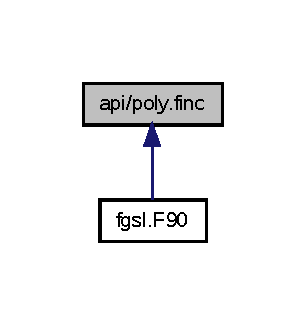
\includegraphics[width=146pt]{poly_8finc__dep__incl}
\end{center}
\end{figure}
\subsection*{Functions/\+Subroutines}
\begin{DoxyCompactItemize}
\item 
real(fgsl\+\_\+double) function \hyperlink{poly_8finc_ae781e76c4974085c40adad5ee7d18765}{fgsl\+\_\+poly\+\_\+eval} (c, x)
\item 
complex(fgsl\+\_\+double\+\_\+complex) function \hyperlink{poly_8finc_a90e9c2000063ce5d9fe5fb589be9cde2}{fgsl\+\_\+poly\+\_\+complex\+\_\+eval} (c, z)
\item 
complex(fgsl\+\_\+double\+\_\+complex) function \hyperlink{poly_8finc_a5cc507446025f6f9a32b4b073f69a2dd}{fgsl\+\_\+complex\+\_\+poly\+\_\+complex\+\_\+eval} (c, z)
\item 
integer(fgsl\+\_\+int) function \hyperlink{poly_8finc_aa61eaba18b05dba3d5c3375c038097ac}{fgsl\+\_\+poly\+\_\+eval\+\_\+derivs} (c, x, res)
\item 
integer(fgsl\+\_\+int) function \hyperlink{poly_8finc_a9414ee6e42cfade6f08005d78247e1bf}{fgsl\+\_\+poly\+\_\+dd\+\_\+init} (dd, x, y)
\item 
real(fgsl\+\_\+double) function \hyperlink{poly_8finc_aa4a8ca0867574aed59f3c0db1f0f8f59}{fgsl\+\_\+poly\+\_\+dd\+\_\+eval} (dd, xa, x)
\item 
integer(fgsl\+\_\+int) function \hyperlink{poly_8finc_a8fa885de79327177b906f6fd5d1e5663}{fgsl\+\_\+poly\+\_\+dd\+\_\+taylor} (c, xp, dd, x, w)
\item 
integer(fgsl\+\_\+int) function \hyperlink{poly_8finc_ad44cde0319ae8fcc422e498318bc8839}{fgsl\+\_\+poly\+\_\+dd\+\_\+hermite\+\_\+init} (dd, z, xa, ya, dya)
\item 
integer(fgsl\+\_\+int) function \hyperlink{poly_8finc_a21062b0907ae31ffc799938513ebae02}{fgsl\+\_\+poly\+\_\+solve\+\_\+quadratic} (a, b, c, x0, x1)
\item 
integer(fgsl\+\_\+int) function \hyperlink{poly_8finc_afe315cb11581a666f03d0c9f2dc78233}{fgsl\+\_\+poly\+\_\+complex\+\_\+solve\+\_\+quadratic} (a, b, c, x0, x1)
\item 
integer(fgsl\+\_\+int) function \hyperlink{poly_8finc_ae68c5a984c47341773668044f141ce19}{fgsl\+\_\+poly\+\_\+solve\+\_\+cubic} (a, b, c, x0, x1, x2)
\item 
integer(fgsl\+\_\+int) function \hyperlink{poly_8finc_a4f38dcb84e7589b62c5419ec6f5816ca}{fgsl\+\_\+poly\+\_\+complex\+\_\+solve\+\_\+cubic} (a, b, c, x0, x1, x2)
\item 
type(fgsl\+\_\+poly\+\_\+complex\+\_\+workspace) function \hyperlink{poly_8finc_ab324087e2007b6a8888d0436e0ac0322}{fgsl\+\_\+poly\+\_\+complex\+\_\+workspace\+\_\+alloc} (n)
\item 
subroutine \hyperlink{poly_8finc_ae2007cfcdbda42950869ce3f470f3109}{fgsl\+\_\+poly\+\_\+complex\+\_\+workspace\+\_\+free} (w)
\item 
logical function \hyperlink{poly_8finc_a2ad3c57aca45300bbe7a535dbb0863b2}{fgsl\+\_\+poly\+\_\+complex\+\_\+workspace\+\_\+stat} (w)
\item 
integer(fgsl\+\_\+int) function \hyperlink{poly_8finc_a84ce53a3eccf9334e4f4266fbf03ab12}{fgsl\+\_\+poly\+\_\+complex\+\_\+solve} (a, n, w, z)
\end{DoxyCompactItemize}


\subsection{Function/\+Subroutine Documentation}
\hypertarget{poly_8finc_a5cc507446025f6f9a32b4b073f69a2dd}{}\index{poly.\+finc@{poly.\+finc}!fgsl\+\_\+complex\+\_\+poly\+\_\+complex\+\_\+eval@{fgsl\+\_\+complex\+\_\+poly\+\_\+complex\+\_\+eval}}
\index{fgsl\+\_\+complex\+\_\+poly\+\_\+complex\+\_\+eval@{fgsl\+\_\+complex\+\_\+poly\+\_\+complex\+\_\+eval}!poly.\+finc@{poly.\+finc}}
\subsubsection[{fgsl\+\_\+complex\+\_\+poly\+\_\+complex\+\_\+eval}]{\setlength{\rightskip}{0pt plus 5cm}complex(fgsl\+\_\+double\+\_\+complex) function fgsl\+\_\+complex\+\_\+poly\+\_\+complex\+\_\+eval (
\begin{DoxyParamCaption}
\item[{complex(fgsl\+\_\+double\+\_\+complex), dimension(\+:), intent(in)}]{c, }
\item[{complex(fgsl\+\_\+double\+\_\+complex), intent(in)}]{z}
\end{DoxyParamCaption}
)}\label{poly_8finc_a5cc507446025f6f9a32b4b073f69a2dd}
\hypertarget{poly_8finc_a90e9c2000063ce5d9fe5fb589be9cde2}{}\index{poly.\+finc@{poly.\+finc}!fgsl\+\_\+poly\+\_\+complex\+\_\+eval@{fgsl\+\_\+poly\+\_\+complex\+\_\+eval}}
\index{fgsl\+\_\+poly\+\_\+complex\+\_\+eval@{fgsl\+\_\+poly\+\_\+complex\+\_\+eval}!poly.\+finc@{poly.\+finc}}
\subsubsection[{fgsl\+\_\+poly\+\_\+complex\+\_\+eval}]{\setlength{\rightskip}{0pt plus 5cm}complex(fgsl\+\_\+double\+\_\+complex) function fgsl\+\_\+poly\+\_\+complex\+\_\+eval (
\begin{DoxyParamCaption}
\item[{real(fgsl\+\_\+double), dimension(\+:), intent(in), target}]{c, }
\item[{complex(fgsl\+\_\+double\+\_\+complex), intent(in)}]{z}
\end{DoxyParamCaption}
)}\label{poly_8finc_a90e9c2000063ce5d9fe5fb589be9cde2}
\hypertarget{poly_8finc_a84ce53a3eccf9334e4f4266fbf03ab12}{}\index{poly.\+finc@{poly.\+finc}!fgsl\+\_\+poly\+\_\+complex\+\_\+solve@{fgsl\+\_\+poly\+\_\+complex\+\_\+solve}}
\index{fgsl\+\_\+poly\+\_\+complex\+\_\+solve@{fgsl\+\_\+poly\+\_\+complex\+\_\+solve}!poly.\+finc@{poly.\+finc}}
\subsubsection[{fgsl\+\_\+poly\+\_\+complex\+\_\+solve}]{\setlength{\rightskip}{0pt plus 5cm}integer(fgsl\+\_\+int) function fgsl\+\_\+poly\+\_\+complex\+\_\+solve (
\begin{DoxyParamCaption}
\item[{real(fgsl\+\_\+double), dimension(\+:), intent(in), target}]{a, }
\item[{integer(fgsl\+\_\+size\+\_\+t), intent(in)}]{n, }
\item[{type(fgsl\+\_\+poly\+\_\+complex\+\_\+workspace), intent(inout)}]{w, }
\item[{complex(fgsl\+\_\+double\+\_\+complex), dimension(\+:), intent(out)}]{z}
\end{DoxyParamCaption}
)}\label{poly_8finc_a84ce53a3eccf9334e4f4266fbf03ab12}
\hypertarget{poly_8finc_a4f38dcb84e7589b62c5419ec6f5816ca}{}\index{poly.\+finc@{poly.\+finc}!fgsl\+\_\+poly\+\_\+complex\+\_\+solve\+\_\+cubic@{fgsl\+\_\+poly\+\_\+complex\+\_\+solve\+\_\+cubic}}
\index{fgsl\+\_\+poly\+\_\+complex\+\_\+solve\+\_\+cubic@{fgsl\+\_\+poly\+\_\+complex\+\_\+solve\+\_\+cubic}!poly.\+finc@{poly.\+finc}}
\subsubsection[{fgsl\+\_\+poly\+\_\+complex\+\_\+solve\+\_\+cubic}]{\setlength{\rightskip}{0pt plus 5cm}integer(fgsl\+\_\+int) function fgsl\+\_\+poly\+\_\+complex\+\_\+solve\+\_\+cubic (
\begin{DoxyParamCaption}
\item[{real(fgsl\+\_\+double), intent(in)}]{a, }
\item[{real(fgsl\+\_\+double), intent(in)}]{b, }
\item[{real(fgsl\+\_\+double), intent(in)}]{c, }
\item[{complex(fgsl\+\_\+double\+\_\+complex), intent(out)}]{x0, }
\item[{complex(fgsl\+\_\+double\+\_\+complex), intent(out)}]{x1, }
\item[{complex(fgsl\+\_\+double\+\_\+complex), intent(out)}]{x2}
\end{DoxyParamCaption}
)}\label{poly_8finc_a4f38dcb84e7589b62c5419ec6f5816ca}
\hypertarget{poly_8finc_afe315cb11581a666f03d0c9f2dc78233}{}\index{poly.\+finc@{poly.\+finc}!fgsl\+\_\+poly\+\_\+complex\+\_\+solve\+\_\+quadratic@{fgsl\+\_\+poly\+\_\+complex\+\_\+solve\+\_\+quadratic}}
\index{fgsl\+\_\+poly\+\_\+complex\+\_\+solve\+\_\+quadratic@{fgsl\+\_\+poly\+\_\+complex\+\_\+solve\+\_\+quadratic}!poly.\+finc@{poly.\+finc}}
\subsubsection[{fgsl\+\_\+poly\+\_\+complex\+\_\+solve\+\_\+quadratic}]{\setlength{\rightskip}{0pt plus 5cm}integer(fgsl\+\_\+int) function fgsl\+\_\+poly\+\_\+complex\+\_\+solve\+\_\+quadratic (
\begin{DoxyParamCaption}
\item[{real(fgsl\+\_\+double), intent(in)}]{a, }
\item[{real(fgsl\+\_\+double), intent(in)}]{b, }
\item[{real(fgsl\+\_\+double), intent(in)}]{c, }
\item[{complex(fgsl\+\_\+double\+\_\+complex), intent(out)}]{x0, }
\item[{complex(fgsl\+\_\+double\+\_\+complex), intent(out)}]{x1}
\end{DoxyParamCaption}
)}\label{poly_8finc_afe315cb11581a666f03d0c9f2dc78233}
\hypertarget{poly_8finc_ab324087e2007b6a8888d0436e0ac0322}{}\index{poly.\+finc@{poly.\+finc}!fgsl\+\_\+poly\+\_\+complex\+\_\+workspace\+\_\+alloc@{fgsl\+\_\+poly\+\_\+complex\+\_\+workspace\+\_\+alloc}}
\index{fgsl\+\_\+poly\+\_\+complex\+\_\+workspace\+\_\+alloc@{fgsl\+\_\+poly\+\_\+complex\+\_\+workspace\+\_\+alloc}!poly.\+finc@{poly.\+finc}}
\subsubsection[{fgsl\+\_\+poly\+\_\+complex\+\_\+workspace\+\_\+alloc}]{\setlength{\rightskip}{0pt plus 5cm}type(fgsl\+\_\+poly\+\_\+complex\+\_\+workspace) function fgsl\+\_\+poly\+\_\+complex\+\_\+workspace\+\_\+alloc (
\begin{DoxyParamCaption}
\item[{integer(fgsl\+\_\+size\+\_\+t), intent(in)}]{n}
\end{DoxyParamCaption}
)}\label{poly_8finc_ab324087e2007b6a8888d0436e0ac0322}
\hypertarget{poly_8finc_ae2007cfcdbda42950869ce3f470f3109}{}\index{poly.\+finc@{poly.\+finc}!fgsl\+\_\+poly\+\_\+complex\+\_\+workspace\+\_\+free@{fgsl\+\_\+poly\+\_\+complex\+\_\+workspace\+\_\+free}}
\index{fgsl\+\_\+poly\+\_\+complex\+\_\+workspace\+\_\+free@{fgsl\+\_\+poly\+\_\+complex\+\_\+workspace\+\_\+free}!poly.\+finc@{poly.\+finc}}
\subsubsection[{fgsl\+\_\+poly\+\_\+complex\+\_\+workspace\+\_\+free}]{\setlength{\rightskip}{0pt plus 5cm}subroutine fgsl\+\_\+poly\+\_\+complex\+\_\+workspace\+\_\+free (
\begin{DoxyParamCaption}
\item[{type(fgsl\+\_\+poly\+\_\+complex\+\_\+workspace), intent(inout)}]{w}
\end{DoxyParamCaption}
)}\label{poly_8finc_ae2007cfcdbda42950869ce3f470f3109}
\hypertarget{poly_8finc_a2ad3c57aca45300bbe7a535dbb0863b2}{}\index{poly.\+finc@{poly.\+finc}!fgsl\+\_\+poly\+\_\+complex\+\_\+workspace\+\_\+stat@{fgsl\+\_\+poly\+\_\+complex\+\_\+workspace\+\_\+stat}}
\index{fgsl\+\_\+poly\+\_\+complex\+\_\+workspace\+\_\+stat@{fgsl\+\_\+poly\+\_\+complex\+\_\+workspace\+\_\+stat}!poly.\+finc@{poly.\+finc}}
\subsubsection[{fgsl\+\_\+poly\+\_\+complex\+\_\+workspace\+\_\+stat}]{\setlength{\rightskip}{0pt plus 5cm}logical function fgsl\+\_\+poly\+\_\+complex\+\_\+workspace\+\_\+stat (
\begin{DoxyParamCaption}
\item[{type(fgsl\+\_\+poly\+\_\+complex\+\_\+workspace), intent(in)}]{w}
\end{DoxyParamCaption}
)}\label{poly_8finc_a2ad3c57aca45300bbe7a535dbb0863b2}
\hypertarget{poly_8finc_aa4a8ca0867574aed59f3c0db1f0f8f59}{}\index{poly.\+finc@{poly.\+finc}!fgsl\+\_\+poly\+\_\+dd\+\_\+eval@{fgsl\+\_\+poly\+\_\+dd\+\_\+eval}}
\index{fgsl\+\_\+poly\+\_\+dd\+\_\+eval@{fgsl\+\_\+poly\+\_\+dd\+\_\+eval}!poly.\+finc@{poly.\+finc}}
\subsubsection[{fgsl\+\_\+poly\+\_\+dd\+\_\+eval}]{\setlength{\rightskip}{0pt plus 5cm}real(fgsl\+\_\+double) function fgsl\+\_\+poly\+\_\+dd\+\_\+eval (
\begin{DoxyParamCaption}
\item[{real(fgsl\+\_\+double), dimension(\+:), intent(in), target}]{dd, }
\item[{real(fgsl\+\_\+double), dimension(\+:), intent(in), target}]{xa, }
\item[{real(fgsl\+\_\+double), intent(in)}]{x}
\end{DoxyParamCaption}
)}\label{poly_8finc_aa4a8ca0867574aed59f3c0db1f0f8f59}
\hypertarget{poly_8finc_ad44cde0319ae8fcc422e498318bc8839}{}\index{poly.\+finc@{poly.\+finc}!fgsl\+\_\+poly\+\_\+dd\+\_\+hermite\+\_\+init@{fgsl\+\_\+poly\+\_\+dd\+\_\+hermite\+\_\+init}}
\index{fgsl\+\_\+poly\+\_\+dd\+\_\+hermite\+\_\+init@{fgsl\+\_\+poly\+\_\+dd\+\_\+hermite\+\_\+init}!poly.\+finc@{poly.\+finc}}
\subsubsection[{fgsl\+\_\+poly\+\_\+dd\+\_\+hermite\+\_\+init}]{\setlength{\rightskip}{0pt plus 5cm}integer(fgsl\+\_\+int) function fgsl\+\_\+poly\+\_\+dd\+\_\+hermite\+\_\+init (
\begin{DoxyParamCaption}
\item[{real(fgsl\+\_\+double), dimension(\+:), intent(inout), target}]{dd, }
\item[{real(fgsl\+\_\+double), dimension(\+:), intent(inout), target}]{z, }
\item[{real(fgsl\+\_\+double), dimension(\+:), intent(in), target}]{xa, }
\item[{real(fgsl\+\_\+double), dimension(\+:), intent(in), target}]{ya, }
\item[{real(fgsl\+\_\+double), dimension(\+:), intent(in), target}]{dya}
\end{DoxyParamCaption}
)}\label{poly_8finc_ad44cde0319ae8fcc422e498318bc8839}
\hypertarget{poly_8finc_a9414ee6e42cfade6f08005d78247e1bf}{}\index{poly.\+finc@{poly.\+finc}!fgsl\+\_\+poly\+\_\+dd\+\_\+init@{fgsl\+\_\+poly\+\_\+dd\+\_\+init}}
\index{fgsl\+\_\+poly\+\_\+dd\+\_\+init@{fgsl\+\_\+poly\+\_\+dd\+\_\+init}!poly.\+finc@{poly.\+finc}}
\subsubsection[{fgsl\+\_\+poly\+\_\+dd\+\_\+init}]{\setlength{\rightskip}{0pt plus 5cm}integer(fgsl\+\_\+int) function fgsl\+\_\+poly\+\_\+dd\+\_\+init (
\begin{DoxyParamCaption}
\item[{real(fgsl\+\_\+double), dimension(\+:), intent(inout), target}]{dd, }
\item[{real(fgsl\+\_\+double), dimension(\+:), intent(in), target}]{x, }
\item[{real(fgsl\+\_\+double), dimension(\+:), intent(in), target}]{y}
\end{DoxyParamCaption}
)}\label{poly_8finc_a9414ee6e42cfade6f08005d78247e1bf}
\hypertarget{poly_8finc_a8fa885de79327177b906f6fd5d1e5663}{}\index{poly.\+finc@{poly.\+finc}!fgsl\+\_\+poly\+\_\+dd\+\_\+taylor@{fgsl\+\_\+poly\+\_\+dd\+\_\+taylor}}
\index{fgsl\+\_\+poly\+\_\+dd\+\_\+taylor@{fgsl\+\_\+poly\+\_\+dd\+\_\+taylor}!poly.\+finc@{poly.\+finc}}
\subsubsection[{fgsl\+\_\+poly\+\_\+dd\+\_\+taylor}]{\setlength{\rightskip}{0pt plus 5cm}integer(fgsl\+\_\+int) function fgsl\+\_\+poly\+\_\+dd\+\_\+taylor (
\begin{DoxyParamCaption}
\item[{real(fgsl\+\_\+double), dimension(\+:), intent(inout), target}]{c, }
\item[{real(fgsl\+\_\+double), intent(in)}]{xp, }
\item[{real(fgsl\+\_\+double), dimension(\+:), intent(in), target}]{dd, }
\item[{real(fgsl\+\_\+double), dimension(\+:), intent(in), target}]{x, }
\item[{real(fgsl\+\_\+double), dimension(\+:), intent(out), target}]{w}
\end{DoxyParamCaption}
)}\label{poly_8finc_a8fa885de79327177b906f6fd5d1e5663}
\hypertarget{poly_8finc_ae781e76c4974085c40adad5ee7d18765}{}\index{poly.\+finc@{poly.\+finc}!fgsl\+\_\+poly\+\_\+eval@{fgsl\+\_\+poly\+\_\+eval}}
\index{fgsl\+\_\+poly\+\_\+eval@{fgsl\+\_\+poly\+\_\+eval}!poly.\+finc@{poly.\+finc}}
\subsubsection[{fgsl\+\_\+poly\+\_\+eval}]{\setlength{\rightskip}{0pt plus 5cm}real(fgsl\+\_\+double) function fgsl\+\_\+poly\+\_\+eval (
\begin{DoxyParamCaption}
\item[{real(fgsl\+\_\+double), dimension(\+:), intent(in), target}]{c, }
\item[{real(fgsl\+\_\+double), intent(in)}]{x}
\end{DoxyParamCaption}
)}\label{poly_8finc_ae781e76c4974085c40adad5ee7d18765}
\hypertarget{poly_8finc_aa61eaba18b05dba3d5c3375c038097ac}{}\index{poly.\+finc@{poly.\+finc}!fgsl\+\_\+poly\+\_\+eval\+\_\+derivs@{fgsl\+\_\+poly\+\_\+eval\+\_\+derivs}}
\index{fgsl\+\_\+poly\+\_\+eval\+\_\+derivs@{fgsl\+\_\+poly\+\_\+eval\+\_\+derivs}!poly.\+finc@{poly.\+finc}}
\subsubsection[{fgsl\+\_\+poly\+\_\+eval\+\_\+derivs}]{\setlength{\rightskip}{0pt plus 5cm}integer(fgsl\+\_\+int) function fgsl\+\_\+poly\+\_\+eval\+\_\+derivs (
\begin{DoxyParamCaption}
\item[{real(fgsl\+\_\+double), dimension(\+:), intent(in), target}]{c, }
\item[{real(fgsl\+\_\+double), intent(in)}]{x, }
\item[{real(fgsl\+\_\+double), dimension(\+:), target}]{res}
\end{DoxyParamCaption}
)}\label{poly_8finc_aa61eaba18b05dba3d5c3375c038097ac}
\hypertarget{poly_8finc_ae68c5a984c47341773668044f141ce19}{}\index{poly.\+finc@{poly.\+finc}!fgsl\+\_\+poly\+\_\+solve\+\_\+cubic@{fgsl\+\_\+poly\+\_\+solve\+\_\+cubic}}
\index{fgsl\+\_\+poly\+\_\+solve\+\_\+cubic@{fgsl\+\_\+poly\+\_\+solve\+\_\+cubic}!poly.\+finc@{poly.\+finc}}
\subsubsection[{fgsl\+\_\+poly\+\_\+solve\+\_\+cubic}]{\setlength{\rightskip}{0pt plus 5cm}integer(fgsl\+\_\+int) function fgsl\+\_\+poly\+\_\+solve\+\_\+cubic (
\begin{DoxyParamCaption}
\item[{real(fgsl\+\_\+double), intent(in)}]{a, }
\item[{real(fgsl\+\_\+double), intent(in)}]{b, }
\item[{real(fgsl\+\_\+double), intent(in)}]{c, }
\item[{real(fgsl\+\_\+double), intent(out)}]{x0, }
\item[{real(fgsl\+\_\+double), intent(out)}]{x1, }
\item[{real(fgsl\+\_\+double), intent(out)}]{x2}
\end{DoxyParamCaption}
)}\label{poly_8finc_ae68c5a984c47341773668044f141ce19}
\hypertarget{poly_8finc_a21062b0907ae31ffc799938513ebae02}{}\index{poly.\+finc@{poly.\+finc}!fgsl\+\_\+poly\+\_\+solve\+\_\+quadratic@{fgsl\+\_\+poly\+\_\+solve\+\_\+quadratic}}
\index{fgsl\+\_\+poly\+\_\+solve\+\_\+quadratic@{fgsl\+\_\+poly\+\_\+solve\+\_\+quadratic}!poly.\+finc@{poly.\+finc}}
\subsubsection[{fgsl\+\_\+poly\+\_\+solve\+\_\+quadratic}]{\setlength{\rightskip}{0pt plus 5cm}integer(fgsl\+\_\+int) function fgsl\+\_\+poly\+\_\+solve\+\_\+quadratic (
\begin{DoxyParamCaption}
\item[{real(fgsl\+\_\+double), intent(in)}]{a, }
\item[{real(fgsl\+\_\+double), intent(in)}]{b, }
\item[{real(fgsl\+\_\+double), intent(in)}]{c, }
\item[{real(fgsl\+\_\+double), intent(out)}]{x0, }
\item[{real(fgsl\+\_\+double), intent(out)}]{x1}
\end{DoxyParamCaption}
)}\label{poly_8finc_a21062b0907ae31ffc799938513ebae02}

\hypertarget{rng_8finc}{\section{api/rng.finc File Reference}
\label{rng_8finc}\index{api/rng.\-finc@{api/rng.\-finc}}
}
This graph shows which files directly or indirectly include this file\-:
\nopagebreak
\begin{figure}[H]
\begin{center}
\leavevmode
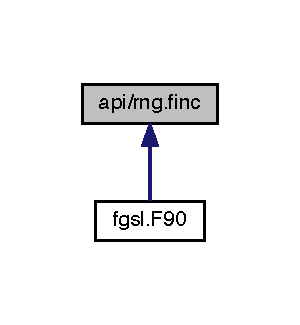
\includegraphics[width=144pt]{rng_8finc__dep__incl}
\end{center}
\end{figure}
\subsection*{Functions/\-Subroutines}
\begin{DoxyCompactItemize}
\item 
type(fgsl\-\_\-rng) function \hyperlink{rng_8finc_a30f2372e956b9bd66f43de5c6de060d9}{fgsl\-\_\-rng\-\_\-alloc} (t)
\item 
subroutine \hyperlink{rng_8finc_a4bff01c18fd9fbf639fd6d8e75c9e85a}{fgsl\-\_\-rng\-\_\-set} (r, s)
\item 
subroutine \hyperlink{rng_8finc_af0801f3c2ac80076ea94f4b0393665a0}{fgsl\-\_\-rng\-\_\-free} (r)
\item 
integer(fgsl\-\_\-long) function \hyperlink{rng_8finc_a437565a21cf12f8aa87eec1ec36ff143}{fgsl\-\_\-rng\-\_\-get} (r)
\item 
real(fgsl\-\_\-double) function \hyperlink{rng_8finc_aa854677900243f9feabf49ee137e38b9}{fgsl\-\_\-rng\-\_\-uniform} (r)
\item 
real(fgsl\-\_\-double) function \hyperlink{rng_8finc_a787ed01d91454a49a28d4344d35559cf}{fgsl\-\_\-rng\-\_\-uniform\-\_\-pos} (r)
\item 
integer(fgsl\-\_\-long) function \hyperlink{rng_8finc_ae0ce08aee233600b619e3ddc2bcb0ef2}{fgsl\-\_\-rng\-\_\-uniform\-\_\-int} (r, n)
\item 
character(kind=fgsl\-\_\-char, len=fgsl\-\_\-strmax) \\*
function \hyperlink{rng_8finc_a54c05ff204ef98053bf5124603d2b334}{fgsl\-\_\-rng\-\_\-name} (r)
\item 
integer(fgsl\-\_\-long) function \hyperlink{rng_8finc_afa55230f7211ea98414429229b64a8c4}{fgsl\-\_\-rng\-\_\-max} (r)
\item 
integer(fgsl\-\_\-long) function \hyperlink{rng_8finc_a61f73ec296fa294c6b0634533d537d01}{fgsl\-\_\-rng\-\_\-min} (r)
\item 
type(fgsl\-\_\-rng\-\_\-type) function \hyperlink{rng_8finc_a398d0b93637d4cd2f0ec42aa9d704fed}{fgsl\-\_\-rng\-\_\-env\-\_\-setup} ()
\item 
integer(fgsl\-\_\-int) function \hyperlink{rng_8finc_a3b20f59958b9d1f96e11c91deb33eebb}{fgsl\-\_\-rng\-\_\-memcpy} (cpy, src)
\item 
type(fgsl\-\_\-rng) function \hyperlink{rng_8finc_acc66804b594701e03a27cea42373fac6}{fgsl\-\_\-rng\-\_\-clone} (r)
\item 
integer(fgsl\-\_\-int) function \hyperlink{rng_8finc_ad9f602fa3c592fdac3659a1746143aa1}{fgsl\-\_\-rng\-\_\-fwrite} (stream, r)
\item 
integer(fgsl\-\_\-int) function \hyperlink{rng_8finc_a1e80994301a7b45f4203ce55d90a86fe}{fgsl\-\_\-rng\-\_\-fread} (stream, r)
\item 
type(fgsl\-\_\-qrng) function \hyperlink{rng_8finc_a5dd0e79d47ed21591ed2906315a5ed4b}{fgsl\-\_\-qrng\-\_\-alloc} (t, d)
\item 
subroutine \hyperlink{rng_8finc_ac61e779e7158279aa883358098f67a5a}{fgsl\-\_\-qrng\-\_\-free} (r)
\item 
subroutine \hyperlink{rng_8finc_adbebd9f4a0213e6eb61756e412046d67}{fgsl\-\_\-qrng\-\_\-init} (r)
\item 
integer(fgsl\-\_\-int) function \hyperlink{rng_8finc_a4c172d25dab4c49dba69428b61bc4adf}{fgsl\-\_\-qrng\-\_\-get} (q, x)
\item 
character(kind=fgsl\-\_\-char, len=fgsl\-\_\-strmax) \\*
function \hyperlink{rng_8finc_af55d78c79c3e7d3a3d8666fc7dfc6ddd}{fgsl\-\_\-qrng\-\_\-name} (q)
\item 
integer(fgsl\-\_\-int) function \hyperlink{rng_8finc_a7ce0da63d2654bb003f84a999bb7b6ce}{fgsl\-\_\-qrng\-\_\-memcpy} (cpy, src)
\item 
type(fgsl\-\_\-qrng) function \hyperlink{rng_8finc_af9487d956c6b72f72ccb50a5ed28e92d}{fgsl\-\_\-qrng\-\_\-clone} (q)
\item 
real(fgsl\-\_\-double) function \hyperlink{rng_8finc_a04f4cd4894dc3510006365f5211b8dda}{fgsl\-\_\-ran\-\_\-gaussian} (r, sigma)
\item 
real(fgsl\-\_\-double) function \hyperlink{rng_8finc_aefb1b7aca8d4240cdf6ad29706f53ba6}{fgsl\-\_\-ran\-\_\-gaussian\-\_\-pdf} (x, sigma)
\item 
real(fgsl\-\_\-double) function \hyperlink{rng_8finc_ab23c2a1b1d2f0b21697675ac00fca191}{fgsl\-\_\-ran\-\_\-gaussian\-\_\-ziggurat} (r, sigma)
\item 
real(fgsl\-\_\-double) function \hyperlink{rng_8finc_a3a942206e136585fd8ffb9761bbad505}{fgsl\-\_\-ran\-\_\-gaussian\-\_\-ratio\-\_\-method} (r, sigma)
\item 
real(fgsl\-\_\-double) function \hyperlink{rng_8finc_a679c4c83b2e8f8cedc96f5eca1b7929a}{fgsl\-\_\-ran\-\_\-ugaussian} (r)
\item 
real(fgsl\-\_\-double) function \hyperlink{rng_8finc_ab45ce99f5d0cc4b3b7981cb89584c0ca}{fgsl\-\_\-ran\-\_\-ugaussian\-\_\-pdf} (x)
\item 
real(fgsl\-\_\-double) function \hyperlink{rng_8finc_a720e375637bfce16e56c42f2e11b5802}{fgsl\-\_\-ran\-\_\-ugaussian\-\_\-ratio\-\_\-method} (r)
\item 
real(fgsl\-\_\-double) function \hyperlink{rng_8finc_a613160a77385ab379bf3a6f5192a97a8}{fgsl\-\_\-cdf\-\_\-gaussian\-\_\-p} (x, sigma)
\item 
real(fgsl\-\_\-double) function \hyperlink{rng_8finc_a257b07452a48220b30b6b6b929637e79}{fgsl\-\_\-cdf\-\_\-gaussian\-\_\-q} (x, sigma)
\item 
real(fgsl\-\_\-double) function \hyperlink{rng_8finc_aa602d289238eeb5318d7b10562f84343}{fgsl\-\_\-cdf\-\_\-gaussian\-\_\-pinv} (p, sigma)
\item 
real(fgsl\-\_\-double) function \hyperlink{rng_8finc_a8f03982161ce0fc231bc4f7526265dc6}{fgsl\-\_\-cdf\-\_\-gaussian\-\_\-qinv} (q, sigma)
\item 
real(fgsl\-\_\-double) function \hyperlink{rng_8finc_a7f2710deecdd590d946d38f33f433e9f}{fgsl\-\_\-cdf\-\_\-ugaussian\-\_\-p} (x)
\item 
real(fgsl\-\_\-double) function \hyperlink{rng_8finc_ac8d79a3464dcf4018b294bb46be5c63c}{fgsl\-\_\-cdf\-\_\-ugaussian\-\_\-q} (x)
\item 
real(fgsl\-\_\-double) function \hyperlink{rng_8finc_a5200879f9cfb0062711be785cb73d8ba}{fgsl\-\_\-cdf\-\_\-ugaussian\-\_\-pinv} (p)
\item 
real(fgsl\-\_\-double) function \hyperlink{rng_8finc_a13c5f38d6806b5f065acab4c2f02cd72}{fgsl\-\_\-cdf\-\_\-ugaussian\-\_\-qinv} (q)
\item 
real(fgsl\-\_\-double) function \hyperlink{rng_8finc_a375409ed447b32016b5901dd7adb5146}{fgsl\-\_\-ran\-\_\-gaussian\-\_\-tail} (r, a, sigma)
\item 
real(fgsl\-\_\-double) function \hyperlink{rng_8finc_a11151be72007e872d4101d2d1fc8a3c2}{fgsl\-\_\-ran\-\_\-gaussian\-\_\-tail\-\_\-pdf} (x, a, sigma)
\item 
real(fgsl\-\_\-double) function \hyperlink{rng_8finc_a7b84620d10a8d1817b621f3a5aedf487}{fgsl\-\_\-ran\-\_\-ugaussian\-\_\-tail} (r, a)
\item 
real(fgsl\-\_\-double) function \hyperlink{rng_8finc_a54ba0fdd3a089ba1f385bf126c25564a}{fgsl\-\_\-ran\-\_\-ugaussian\-\_\-tail\-\_\-pdf} (x, a)
\item 
subroutine \hyperlink{rng_8finc_ac2fd8a36b4c4ed1ef257fc4ea9887902}{fgsl\-\_\-ran\-\_\-bivariate\-\_\-gaussian} (r, sigma\-\_\-x, sigma\-\_\-y, rho, x, y)
\item 
real(fgsl\-\_\-double) function \hyperlink{rng_8finc_ab5fb0d52054fac443429a9262a23b062}{fgsl\-\_\-ran\-\_\-bivariate\-\_\-gaussian\-\_\-pdf} (x, y, sigma\-\_\-x, sigma\-\_\-y, rho)
\item 
real(fgsl\-\_\-double) function \hyperlink{rng_8finc_a6e0d7e6eadeddedceacd263ef26203d0}{fgsl\-\_\-ran\-\_\-exponential} (r, mu)
\item 
real(fgsl\-\_\-double) function \hyperlink{rng_8finc_ae756f259cb8ca3982f646f42a216c96c}{fgsl\-\_\-ran\-\_\-exponential\-\_\-pdf} (x, mu)
\item 
real(fgsl\-\_\-double) function \hyperlink{rng_8finc_a36e9a6ea0993d74b7a8cf7961709fe3c}{fgsl\-\_\-cdf\-\_\-exponential\-\_\-p} (x, mu)
\item 
real(fgsl\-\_\-double) function \hyperlink{rng_8finc_a955e14385e325a6372b465a576cac5c4}{fgsl\-\_\-cdf\-\_\-exponential\-\_\-q} (x, mu)
\item 
real(fgsl\-\_\-double) function \hyperlink{rng_8finc_a488b0d0037afbf0758a6494ea2c79d4b}{fgsl\-\_\-cdf\-\_\-exponential\-\_\-pinv} (p, mu)
\item 
real(fgsl\-\_\-double) function \hyperlink{rng_8finc_a8981dddfb5aa981d5819588d5e6ef0c3}{fgsl\-\_\-cdf\-\_\-exponential\-\_\-qinv} (q, mu)
\item 
real(fgsl\-\_\-double) function \hyperlink{rng_8finc_a4720051c5ef1f7ebcb32a852ac6664cb}{fgsl\-\_\-ran\-\_\-laplace} (r, a)
\item 
real(fgsl\-\_\-double) function \hyperlink{rng_8finc_ab7e39d0b6571ba191082ae83e3586791}{fgsl\-\_\-ran\-\_\-laplace\-\_\-pdf} (x, a)
\item 
real(fgsl\-\_\-double) function \hyperlink{rng_8finc_ae5ad59c95e21c0d422034ad7d56f8257}{fgsl\-\_\-cdf\-\_\-laplace\-\_\-p} (x, a)
\item 
real(fgsl\-\_\-double) function \hyperlink{rng_8finc_a2e38b7a4c5542ab96393a85ac86c3aa5}{fgsl\-\_\-cdf\-\_\-laplace\-\_\-q} (x, a)
\item 
real(fgsl\-\_\-double) function \hyperlink{rng_8finc_a372ea8f42cb280034be93978a227aac8}{fgsl\-\_\-cdf\-\_\-laplace\-\_\-pinv} (p, a)
\item 
real(fgsl\-\_\-double) function \hyperlink{rng_8finc_ae60ab38aedb8d6fb86fbc16d33b8e2fa}{fgsl\-\_\-cdf\-\_\-laplace\-\_\-qinv} (q, a)
\item 
real(fgsl\-\_\-double) function \hyperlink{rng_8finc_a3a4e76ecca55fc88d05ad1dd87b11ecd}{fgsl\-\_\-ran\-\_\-exppow} (r, a, b)
\item 
real(fgsl\-\_\-double) function \hyperlink{rng_8finc_a87c230357f577305a4bd93c4f304e2af}{fgsl\-\_\-ran\-\_\-exppow\-\_\-pdf} (x, a, b)
\item 
real(fgsl\-\_\-double) function \hyperlink{rng_8finc_a332787d73c8b7cc0a561b9de42eab974}{fgsl\-\_\-cdf\-\_\-exppow\-\_\-p} (x, a, b)
\item 
real(fgsl\-\_\-double) function \hyperlink{rng_8finc_ae336d786addd5c9838e379079f2118e8}{fgsl\-\_\-cdf\-\_\-exppow\-\_\-q} (x, a, b)
\item 
real(fgsl\-\_\-double) function \hyperlink{rng_8finc_a5a546c09d9cae9ebedb9b07ea32efeda}{fgsl\-\_\-ran\-\_\-cauchy} (r, a)
\item 
real(fgsl\-\_\-double) function \hyperlink{rng_8finc_ace5b97b9a5d4c816d87a4266696fcdb5}{fgsl\-\_\-ran\-\_\-cauchy\-\_\-pdf} (x, a)
\item 
real(fgsl\-\_\-double) function \hyperlink{rng_8finc_a0e344d18cde233ed8002f084dde9eb60}{fgsl\-\_\-cdf\-\_\-cauchy\-\_\-p} (x, a)
\item 
real(fgsl\-\_\-double) function \hyperlink{rng_8finc_abcdb7697f3622398517eecdcbe437b28}{fgsl\-\_\-cdf\-\_\-cauchy\-\_\-q} (x, a)
\item 
real(fgsl\-\_\-double) function \hyperlink{rng_8finc_a074ae18be87299f8a671bc14c18fb12d}{fgsl\-\_\-cdf\-\_\-cauchy\-\_\-pinv} (p, a)
\item 
real(fgsl\-\_\-double) function \hyperlink{rng_8finc_a74774e42acfb80fb2fe4417ce410e760}{fgsl\-\_\-cdf\-\_\-cauchy\-\_\-qinv} (q, a)
\item 
real(fgsl\-\_\-double) function \hyperlink{rng_8finc_ab3b2b9a1275e0581f2f62f4bb974bba0}{fgsl\-\_\-ran\-\_\-rayleigh} (r, sigma)
\item 
real(fgsl\-\_\-double) function \hyperlink{rng_8finc_aeb1b678250b5a3437e2a5da86dc7027e}{fgsl\-\_\-ran\-\_\-rayleigh\-\_\-pdf} (x, sigma)
\item 
real(fgsl\-\_\-double) function \hyperlink{rng_8finc_a376b011d221203a9830ad4681bda4c53}{fgsl\-\_\-cdf\-\_\-rayleigh\-\_\-p} (x, sigma)
\item 
real(fgsl\-\_\-double) function \hyperlink{rng_8finc_ae07c15e9d38069dc78dd1fc10a3b37ab}{fgsl\-\_\-cdf\-\_\-rayleigh\-\_\-q} (x, sigma)
\item 
real(fgsl\-\_\-double) function \hyperlink{rng_8finc_ac0bf5e17a1114cf02a6d561aafdbebc0}{fgsl\-\_\-cdf\-\_\-rayleigh\-\_\-pinv} (p, sigma)
\item 
real(fgsl\-\_\-double) function \hyperlink{rng_8finc_a669f0c3f452b3f4779ee3d66eb292e6f}{fgsl\-\_\-cdf\-\_\-rayleigh\-\_\-qinv} (q, sigma)
\item 
real(fgsl\-\_\-double) function \hyperlink{rng_8finc_a251553996a7fe7909c52a740eaeb5a5c}{fgsl\-\_\-ran\-\_\-rayleigh\-\_\-tail} (r, a, sigma)
\item 
real(fgsl\-\_\-double) function \hyperlink{rng_8finc_a1d05f85a0832a708308a2022a295f8e2}{fgsl\-\_\-ran\-\_\-rayleigh\-\_\-tail\-\_\-pdf} (x, a, sigma)
\item 
real(fgsl\-\_\-double) function \hyperlink{rng_8finc_a4fddb2cbe7750f04fb6fafeaca3d4475}{fgsl\-\_\-ran\-\_\-landau} (r)
\item 
real(fgsl\-\_\-double) function \hyperlink{rng_8finc_a3838bd54f8cd69e289ce48f50d804e13}{fgsl\-\_\-ran\-\_\-landau\-\_\-pdf} (x)
\item 
real(fgsl\-\_\-double) function \hyperlink{rng_8finc_a8453b1f8c3e81ec2eaabfc6612ce44aa}{fgsl\-\_\-ran\-\_\-levy} (r, c, alpha)
\item 
real(fgsl\-\_\-double) function \hyperlink{rng_8finc_a43ea311600d0fdcccc054b043d6ec519}{fgsl\-\_\-ran\-\_\-levy\-\_\-skew} (r, c, alpha, beta)
\item 
real(fgsl\-\_\-double) function \hyperlink{rng_8finc_a75b8328e601702d544764bf044864486}{fgsl\-\_\-ran\-\_\-gamma} (r, a, b)
\item 
real(fgsl\-\_\-double) function \hyperlink{rng_8finc_ac1a501f4dfe734274569151dfaf25477}{fgsl\-\_\-ran\-\_\-gamma\-\_\-mt} (r, a, b)
\item 
real(fgsl\-\_\-double) function \hyperlink{rng_8finc_ab4786a7f6aa42d75d825b5a32d193ce4}{fgsl\-\_\-ran\-\_\-gamma\-\_\-pdf} (x, a, b)
\item 
real(fgsl\-\_\-double) function \hyperlink{rng_8finc_a0bac4d4b3ce06b0f58112852fa7b32ce}{fgsl\-\_\-cdf\-\_\-gamma\-\_\-p} (x, a, b)
\item 
real(fgsl\-\_\-double) function \hyperlink{rng_8finc_af7323ad0e46d157a40a3a1e8c5adbcc3}{fgsl\-\_\-cdf\-\_\-gamma\-\_\-q} (x, a, b)
\item 
real(fgsl\-\_\-double) function \hyperlink{rng_8finc_ad98d9f27ebc4c29347f7178437ad2042}{fgsl\-\_\-cdf\-\_\-gamma\-\_\-pinv} (p, a, b)
\item 
real(fgsl\-\_\-double) function \hyperlink{rng_8finc_a98d9bdf34354f709686562da8a8852e7}{fgsl\-\_\-cdf\-\_\-gamma\-\_\-qinv} (q, a, b)
\item 
real(fgsl\-\_\-double) function \hyperlink{rng_8finc_acd9641232d480f05b1abe1590c0f27b2}{fgsl\-\_\-ran\-\_\-flat} (r, a, b)
\item 
real(fgsl\-\_\-double) function \hyperlink{rng_8finc_a4436b84330131f34805ea941042e464a}{fgsl\-\_\-ran\-\_\-flat\-\_\-pdf} (x, a, b)
\item 
real(fgsl\-\_\-double) function \hyperlink{rng_8finc_a53c32d3a1c1e49be4369425594820754}{fgsl\-\_\-cdf\-\_\-flat\-\_\-p} (x, a, b)
\item 
real(fgsl\-\_\-double) function \hyperlink{rng_8finc_a98244f046ad60405fb90bd7629d5f1be}{fgsl\-\_\-cdf\-\_\-flat\-\_\-q} (x, a, b)
\item 
real(fgsl\-\_\-double) function \hyperlink{rng_8finc_a42e0a48e22b8aa4b734ccf0f520d6431}{fgsl\-\_\-cdf\-\_\-flat\-\_\-pinv} (p, a, b)
\item 
real(fgsl\-\_\-double) function \hyperlink{rng_8finc_a42ecda3cd6d30fdcb53b3b04e421638d}{fgsl\-\_\-cdf\-\_\-flat\-\_\-qinv} (q, a, b)
\item 
real(fgsl\-\_\-double) function \hyperlink{rng_8finc_a595430ab8b59586c367cc046a9f5debf}{fgsl\-\_\-ran\-\_\-lognormal} (r, zeta, sigma)
\item 
real(fgsl\-\_\-double) function \hyperlink{rng_8finc_a202090301f103185a3f44733bb1bcbd5}{fgsl\-\_\-ran\-\_\-lognormal\-\_\-pdf} (x, zeta, sigma)
\item 
real(fgsl\-\_\-double) function \hyperlink{rng_8finc_a5316890ad8197da791afcc5910bb509a}{fgsl\-\_\-cdf\-\_\-lognormal\-\_\-p} (x, zeta, sigma)
\item 
real(fgsl\-\_\-double) function \hyperlink{rng_8finc_a1f399bfba773e619deb9db2831e1f219}{fgsl\-\_\-cdf\-\_\-lognormal\-\_\-q} (x, zeta, sigma)
\item 
real(fgsl\-\_\-double) function \hyperlink{rng_8finc_aa342d9e7c0eca77722ad14b0ccb3b7d8}{fgsl\-\_\-cdf\-\_\-lognormal\-\_\-pinv} (p, zeta, sigma)
\item 
real(fgsl\-\_\-double) function \hyperlink{rng_8finc_a5e05ee3c7093525db7b13b1dc7f21090}{fgsl\-\_\-cdf\-\_\-lognormal\-\_\-qinv} (q, zeta, sigma)
\item 
real(fgsl\-\_\-double) function \hyperlink{rng_8finc_aafcd4ad23110cdf85cc02b3c17864d57}{fgsl\-\_\-ran\-\_\-chisq} (r, nu)
\item 
real(fgsl\-\_\-double) function \hyperlink{rng_8finc_a01f35dd8aa35ff85f20a6d59868013c4}{fgsl\-\_\-ran\-\_\-chisq\-\_\-pdf} (x, nu)
\item 
real(fgsl\-\_\-double) function \hyperlink{rng_8finc_a4e32d508a8eac8c4edb7d00bcbcda230}{fgsl\-\_\-cdf\-\_\-chisq\-\_\-p} (x, nu)
\item 
real(fgsl\-\_\-double) function \hyperlink{rng_8finc_aa75769eb52c32b5d6c8e769fab0be280}{fgsl\-\_\-cdf\-\_\-chisq\-\_\-q} (x, nu)
\item 
real(fgsl\-\_\-double) function \hyperlink{rng_8finc_a397d079779dd1ce60251527321d48b62}{fgsl\-\_\-cdf\-\_\-chisq\-\_\-pinv} (p, nu)
\item 
real(fgsl\-\_\-double) function \hyperlink{rng_8finc_a4a8a7e2add3fdabcea95ab881048af06}{fgsl\-\_\-cdf\-\_\-chisq\-\_\-qinv} (q, nu)
\item 
real(fgsl\-\_\-double) function \hyperlink{rng_8finc_acd433cb70a78cc54e2c4d02e3a7f9291}{fgsl\-\_\-ran\-\_\-fdist} (r, nu1, nu2)
\item 
real(fgsl\-\_\-double) function \hyperlink{rng_8finc_a752a7663a532c2765b796040098568e8}{fgsl\-\_\-ran\-\_\-fdist\-\_\-pdf} (x, nu1, nu2)
\item 
real(fgsl\-\_\-double) function \hyperlink{rng_8finc_a83d8d3cbe6899eadccd876c082e855b7}{fgsl\-\_\-cdf\-\_\-fdist\-\_\-p} (x, nu1, nu2)
\item 
real(fgsl\-\_\-double) function \hyperlink{rng_8finc_a8d5d5e89002d7fa3b09a8f0dcb223328}{fgsl\-\_\-cdf\-\_\-fdist\-\_\-q} (x, nu1, nu2)
\item 
real(fgsl\-\_\-double) function \hyperlink{rng_8finc_a5b0a774f2b2bfd4ff9a6b2bcba45e5b8}{fgsl\-\_\-cdf\-\_\-fdist\-\_\-pinv} (p, nu1, nu2)
\item 
real(fgsl\-\_\-double) function \hyperlink{rng_8finc_af6ee56a13f73d763ac76b58262768bbb}{fgsl\-\_\-cdf\-\_\-fdist\-\_\-qinv} (q, nu1, nu2)
\item 
real(fgsl\-\_\-double) function \hyperlink{rng_8finc_a588d0c7b571fa84a50e5bc06bd1c58e3}{fgsl\-\_\-ran\-\_\-tdist} (r, nu)
\item 
real(fgsl\-\_\-double) function \hyperlink{rng_8finc_adefcc6298f2b2b37d112870027638578}{fgsl\-\_\-ran\-\_\-tdist\-\_\-pdf} (x, nu)
\item 
real(fgsl\-\_\-double) function \hyperlink{rng_8finc_ace1197a0d3e0f71deda76ecc42b36dcf}{fgsl\-\_\-cdf\-\_\-tdist\-\_\-p} (x, nu)
\item 
real(fgsl\-\_\-double) function \hyperlink{rng_8finc_a4a1e3a8ce1487a5489502e2264c858c9}{fgsl\-\_\-cdf\-\_\-tdist\-\_\-q} (x, nu)
\item 
real(fgsl\-\_\-double) function \hyperlink{rng_8finc_a2473363fb7a8a2283461ae512996150f}{fgsl\-\_\-cdf\-\_\-tdist\-\_\-pinv} (p, nu)
\item 
real(fgsl\-\_\-double) function \hyperlink{rng_8finc_acd06e7e1635e1d1946e0891f0ddc8fa3}{fgsl\-\_\-cdf\-\_\-tdist\-\_\-qinv} (q, nu)
\item 
real(fgsl\-\_\-double) function \hyperlink{rng_8finc_a22e4189fd2ecd84ea6afdab388e7a1fb}{fgsl\-\_\-ran\-\_\-beta} (r, a, b)
\item 
real(fgsl\-\_\-double) function \hyperlink{rng_8finc_af65213d7b9b1dc033ba0b54876d577ed}{fgsl\-\_\-ran\-\_\-beta\-\_\-pdf} (x, a, b)
\item 
real(fgsl\-\_\-double) function \hyperlink{rng_8finc_a98571bac63e7448953ce6b83270fea54}{fgsl\-\_\-cdf\-\_\-beta\-\_\-p} (x, a, b)
\item 
real(fgsl\-\_\-double) function \hyperlink{rng_8finc_a1f77adb144c89fd15a5a9902b3fb0f0a}{fgsl\-\_\-cdf\-\_\-beta\-\_\-q} (x, a, b)
\item 
real(fgsl\-\_\-double) function \hyperlink{rng_8finc_ad9f940388d86851d6a3fb67138f0cda9}{fgsl\-\_\-cdf\-\_\-beta\-\_\-pinv} (p, a, b)
\item 
real(fgsl\-\_\-double) function \hyperlink{rng_8finc_a0009c5b3be187def3e391ddf403e4a36}{fgsl\-\_\-cdf\-\_\-beta\-\_\-qinv} (q, a, b)
\item 
real(fgsl\-\_\-double) function \hyperlink{rng_8finc_afa24e40f001e4ef9cd8e3794447b9a80}{fgsl\-\_\-ran\-\_\-logistic} (r, a)
\item 
real(fgsl\-\_\-double) function \hyperlink{rng_8finc_a3d50904646cacac7540c7734e21a1590}{fgsl\-\_\-ran\-\_\-logistic\-\_\-pdf} (x, a)
\item 
real(fgsl\-\_\-double) function \hyperlink{rng_8finc_aa4001a113de807a07164d4516d756417}{fgsl\-\_\-cdf\-\_\-logistic\-\_\-p} (x, a)
\item 
real(fgsl\-\_\-double) function \hyperlink{rng_8finc_aa286aa32b87ba0c9df449bebcbfcd9f7}{fgsl\-\_\-cdf\-\_\-logistic\-\_\-q} (x, a)
\item 
real(fgsl\-\_\-double) function \hyperlink{rng_8finc_a6acf734873703cca27ee7f86519d42ee}{fgsl\-\_\-cdf\-\_\-logistic\-\_\-pinv} (p, a)
\item 
real(fgsl\-\_\-double) function \hyperlink{rng_8finc_a196052826f8d1b9e958a3732bc05e900}{fgsl\-\_\-cdf\-\_\-logistic\-\_\-qinv} (q, a)
\item 
real(fgsl\-\_\-double) function \hyperlink{rng_8finc_af630ea831bbec975f2b31e0a08aa5fb2}{fgsl\-\_\-ran\-\_\-pareto} (r, a, b)
\item 
real(fgsl\-\_\-double) function \hyperlink{rng_8finc_ae469b5eaa361c5c0e3b888fd3efc0bf3}{fgsl\-\_\-ran\-\_\-pareto\-\_\-pdf} (x, a, b)
\item 
real(fgsl\-\_\-double) function \hyperlink{rng_8finc_a4cdcd55585b860b72e948b1bd7e27461}{fgsl\-\_\-cdf\-\_\-pareto\-\_\-p} (x, a, b)
\item 
real(fgsl\-\_\-double) function \hyperlink{rng_8finc_a1199071cd8707413370f40d23d973108}{fgsl\-\_\-cdf\-\_\-pareto\-\_\-q} (x, a, b)
\item 
real(fgsl\-\_\-double) function \hyperlink{rng_8finc_afd1b3c0e697fb0f2f0935541cd05b804}{fgsl\-\_\-cdf\-\_\-pareto\-\_\-pinv} (p, a, b)
\item 
real(fgsl\-\_\-double) function \hyperlink{rng_8finc_a458ed89072db48fb5f4033bbb48fba61}{fgsl\-\_\-cdf\-\_\-pareto\-\_\-qinv} (q, a, b)
\item 
subroutine \hyperlink{rng_8finc_a80f718ba94b09ba5011351c5284c9743}{fgsl\-\_\-ran\-\_\-dir\-\_\-2d} (r, x, y)
\item 
subroutine \hyperlink{rng_8finc_aad06ec726757689953f49b72533502bc}{fgsl\-\_\-ran\-\_\-dir\-\_\-2d\-\_\-trig\-\_\-method} (r, x, y)
\item 
subroutine \hyperlink{rng_8finc_a76b76d07af9c338b59841a300b1fe713}{fgsl\-\_\-ran\-\_\-dir\-\_\-3d} (r, x, y, z)
\item 
subroutine \hyperlink{rng_8finc_a630c7e86d20d111e9e2257c3ca4d3099}{fgsl\-\_\-ran\-\_\-dir\-\_\-nd} (r, n, x)
\item 
real(fgsl\-\_\-double) function \hyperlink{rng_8finc_a2ae4b421d515bf870ec49f005f1004b9}{fgsl\-\_\-ran\-\_\-weibull} (r, a, b)
\item 
real(fgsl\-\_\-double) function \hyperlink{rng_8finc_afe0ac6dc4d46f4844d0fec31f55db2b4}{fgsl\-\_\-ran\-\_\-weibull\-\_\-pdf} (x, a, b)
\item 
real(fgsl\-\_\-double) function \hyperlink{rng_8finc_aac992deb1d7934dace804f0d289463d8}{fgsl\-\_\-cdf\-\_\-weibull\-\_\-p} (x, a, b)
\item 
real(fgsl\-\_\-double) function \hyperlink{rng_8finc_a195b5d5a03a5b2a91dad73d8057333d9}{fgsl\-\_\-cdf\-\_\-weibull\-\_\-q} (x, a, b)
\item 
real(fgsl\-\_\-double) function \hyperlink{rng_8finc_ab388789e3098acaaf9f3cee993b6d442}{fgsl\-\_\-cdf\-\_\-weibull\-\_\-pinv} (p, a, b)
\item 
real(fgsl\-\_\-double) function \hyperlink{rng_8finc_a5114adcd286e64034c0959254212047b}{fgsl\-\_\-cdf\-\_\-weibull\-\_\-qinv} (q, a, b)
\item 
real(fgsl\-\_\-double) function \hyperlink{rng_8finc_ae340600957508ade0da2ca0078720d6a}{fgsl\-\_\-ran\-\_\-gumbel1} (r, a, b)
\item 
real(fgsl\-\_\-double) function \hyperlink{rng_8finc_a7d4cb752dabe9a68cd165e6b717f487b}{fgsl\-\_\-ran\-\_\-gumbel1\-\_\-pdf} (x, a, b)
\item 
real(fgsl\-\_\-double) function \hyperlink{rng_8finc_aa1f725735b86da6477ee1e6e7f23be25}{fgsl\-\_\-cdf\-\_\-gumbel1\-\_\-p} (x, a, b)
\item 
real(fgsl\-\_\-double) function \hyperlink{rng_8finc_a7ee83d5fc3ce8f58396b8fb373d3c3e6}{fgsl\-\_\-cdf\-\_\-gumbel1\-\_\-q} (x, a, b)
\item 
real(fgsl\-\_\-double) function \hyperlink{rng_8finc_a6da83025c6b0132f69e09cc2681507ca}{fgsl\-\_\-cdf\-\_\-gumbel1\-\_\-pinv} (p, a, b)
\item 
real(fgsl\-\_\-double) function \hyperlink{rng_8finc_af40fcfa8cf59b40ac3cb704ba9d38963}{fgsl\-\_\-cdf\-\_\-gumbel1\-\_\-qinv} (q, a, b)
\item 
real(fgsl\-\_\-double) function \hyperlink{rng_8finc_a8df69840fa11815cfe3c2a5f75e70140}{fgsl\-\_\-ran\-\_\-gumbel2} (r, a, b)
\item 
real(fgsl\-\_\-double) function \hyperlink{rng_8finc_a4064ea0290a475c5d6fc4a09767c6246}{fgsl\-\_\-ran\-\_\-gumbel2\-\_\-pdf} (x, a, b)
\item 
real(fgsl\-\_\-double) function \hyperlink{rng_8finc_aeff0eee0d72c27030164d5c6cb80a06c}{fgsl\-\_\-cdf\-\_\-gumbel2\-\_\-p} (x, a, b)
\item 
real(fgsl\-\_\-double) function \hyperlink{rng_8finc_a3f716068beb8b0ed9023bac7a11077fc}{fgsl\-\_\-cdf\-\_\-gumbel2\-\_\-q} (x, a, b)
\item 
real(fgsl\-\_\-double) function \hyperlink{rng_8finc_aea4916d5cd9092eacf4c3dc7662614c9}{fgsl\-\_\-cdf\-\_\-gumbel2\-\_\-pinv} (p, a, b)
\item 
real(fgsl\-\_\-double) function \hyperlink{rng_8finc_ab0d909e722676fc110f8f44378006c07}{fgsl\-\_\-cdf\-\_\-gumbel2\-\_\-qinv} (q, a, b)
\item 
subroutine \hyperlink{rng_8finc_aed55152f24c3d7788ea10a891af7b28e}{fgsl\-\_\-ran\-\_\-dirichlet} (r, k, alpha, theta)
\item 
real(fgsl\-\_\-double) function \hyperlink{rng_8finc_ad4b62f2563c97a3833e8573cadf3e11c}{fgsl\-\_\-ran\-\_\-dirichlet\-\_\-pdf} (k, alpha, theta)
\item 
real(fgsl\-\_\-double) function \hyperlink{rng_8finc_ad0d73d584086077d1d47e84f1157ce94}{fgsl\-\_\-ran\-\_\-dirichlet\-\_\-lnpdf} (k, alpha, theta)
\item 
type(fgsl\-\_\-ran\-\_\-discrete\-\_\-t) function \hyperlink{rng_8finc_afff9e0980e8ed1185f70b8c9b992acff}{fgsl\-\_\-ran\-\_\-discrete\-\_\-preproc} (k, p)
\item 
integer(fgsl\-\_\-size\-\_\-t) function \hyperlink{rng_8finc_aefc716ef88ffa6cc65fa6282c31dd0f0}{fgsl\-\_\-ran\-\_\-discrete} (r, g)
\item 
real(fgsl\-\_\-double) function \hyperlink{rng_8finc_a156d8a091be2738deec0f2f1b95dfd8a}{fgsl\-\_\-ran\-\_\-discrete\-\_\-pdf} (k, g)
\item 
subroutine \hyperlink{rng_8finc_ac738587037bec690a44a21b02f02e2fc}{fgsl\-\_\-ran\-\_\-discrete\-\_\-free} (g)
\item 
integer(fgsl\-\_\-int) function \hyperlink{rng_8finc_a74186f6416a6812b1e4316ed93dd4219}{fgsl\-\_\-ran\-\_\-poisson} (r, mu)
\item 
real(fgsl\-\_\-double) function \hyperlink{rng_8finc_a8c8223415cae86ff6f8547a1487fdf84}{fgsl\-\_\-ran\-\_\-poisson\-\_\-pdf} (k, mu)
\item 
real(fgsl\-\_\-double) function \hyperlink{rng_8finc_ab2613ed5965934db464cf780a49a7e4c}{fgsl\-\_\-cdf\-\_\-poisson\-\_\-p} (k, mu)
\item 
real(fgsl\-\_\-double) function \hyperlink{rng_8finc_a8cd213b3445aca4ba8cf6b25f12691ac}{fgsl\-\_\-cdf\-\_\-poisson\-\_\-q} (k, mu)
\item 
integer(fgsl\-\_\-int) function \hyperlink{rng_8finc_afd1f26e55ad5ea5baa69e3a2b7539361}{fgsl\-\_\-ran\-\_\-bernoulli} (r, p)
\item 
real(fgsl\-\_\-double) function \hyperlink{rng_8finc_a59759fbd2da5f1ba46671c1f88303305}{fgsl\-\_\-ran\-\_\-bernoulli\-\_\-pdf} (k, p)
\item 
real(fgsl\-\_\-double) function \hyperlink{rng_8finc_a4ee52af6322119ef765d429be9f24c33}{fgsl\-\_\-ran\-\_\-binomial} (r, p, n)
\item 
real(fgsl\-\_\-double) function \hyperlink{rng_8finc_a5ce6b40d19ba62b14e1603e821ea1eb1}{fgsl\-\_\-ran\-\_\-binomial\-\_\-pdf} (k, p, n)
\item 
real(fgsl\-\_\-double) function \hyperlink{rng_8finc_ab413ce31101954114fe2c271532c05da}{fgsl\-\_\-cdf\-\_\-binomial\-\_\-p} (k, p, n)
\item 
real(fgsl\-\_\-double) function \hyperlink{rng_8finc_a9a4484096d0c58e6b7f0f5994196c78c}{fgsl\-\_\-cdf\-\_\-binomial\-\_\-q} (k, p, n)
\item 
subroutine \hyperlink{rng_8finc_acdfa44ffb59d98ed7e61cacc5e7f2a3b}{fgsl\-\_\-ran\-\_\-multinomial} (r, k, nn, p, n)
\item 
real(fgsl\-\_\-double) function \hyperlink{rng_8finc_ab88e926552ce832524eb53539ce0dbc1}{fgsl\-\_\-ran\-\_\-multinomial\-\_\-pdf} (k, p, n)
\item 
real(fgsl\-\_\-double) function \hyperlink{rng_8finc_ab3574aeefea4cf7c0cf8b67dda605465}{fgsl\-\_\-ran\-\_\-multinomial\-\_\-lnpdf} (k, p, n)
\item 
integer(fgsl\-\_\-int) function \hyperlink{rng_8finc_ab25a0cc345a2b7acbac9430436e54362}{fgsl\-\_\-ran\-\_\-negative\-\_\-binomial} (r, p, n)
\item 
real(fgsl\-\_\-double) function \hyperlink{rng_8finc_aaf108cb550b6c3f7cc34cd7b12763b2f}{fgsl\-\_\-ran\-\_\-negative\-\_\-binomial\-\_\-pdf} (k, p, n)
\item 
real(fgsl\-\_\-double) function \hyperlink{rng_8finc_a907fcf3e4f47bf6af2cdf8c849925576}{fgsl\-\_\-cdf\-\_\-negative\-\_\-binomial\-\_\-p} (k, p, n)
\item 
real(fgsl\-\_\-double) function \hyperlink{rng_8finc_a9814ca89dedaa922543eb568e7060a9d}{fgsl\-\_\-cdf\-\_\-negative\-\_\-binomial\-\_\-q} (k, p, n)
\item 
integer(fgsl\-\_\-int) function \hyperlink{rng_8finc_a0027f47bae46e3f5160056c4a0f0bb16}{fgsl\-\_\-ran\-\_\-pascal} (r, p, n)
\item 
real(fgsl\-\_\-double) function \hyperlink{rng_8finc_a1c7effe4be2e34250060a625e3787d84}{fgsl\-\_\-ran\-\_\-pascal\-\_\-pdf} (k, p, n)
\item 
real(fgsl\-\_\-double) function \hyperlink{rng_8finc_a064c1823c11347b4746af47bec4ac6cd}{fgsl\-\_\-cdf\-\_\-pascal\-\_\-p} (k, p, n)
\item 
real(fgsl\-\_\-double) function \hyperlink{rng_8finc_a5635e95d11c8e3cd9d0a8ecb58d45987}{fgsl\-\_\-cdf\-\_\-pascal\-\_\-q} (k, p, n)
\item 
integer(fgsl\-\_\-int) function \hyperlink{rng_8finc_ae482dfe1c492849cb92416b03115b90e}{fgsl\-\_\-ran\-\_\-geometric} (r, p)
\item 
real(fgsl\-\_\-double) function \hyperlink{rng_8finc_ad9e7f55be1f69e7b25a9e65a40708cec}{fgsl\-\_\-ran\-\_\-geometric\-\_\-pdf} (k, p)
\item 
real(fgsl\-\_\-double) function \hyperlink{rng_8finc_a4a120f9eb0d44094801ba645513a989f}{fgsl\-\_\-cdf\-\_\-geometric\-\_\-p} (k, p)
\item 
real(fgsl\-\_\-double) function \hyperlink{rng_8finc_a4aebfe7d978d88066a79acaa75308f22}{fgsl\-\_\-cdf\-\_\-geometric\-\_\-q} (k, p)
\item 
integer(fgsl\-\_\-int) function \hyperlink{rng_8finc_a555f87a230be607e1cd924efad37bbda}{fgsl\-\_\-ran\-\_\-hypergeometric} (r, n1, n2, t)
\item 
real(fgsl\-\_\-double) function \hyperlink{rng_8finc_a7d562f6070fb8375424c9bb8002102ee}{fgsl\-\_\-ran\-\_\-hypergeometric\-\_\-pdf} (k, n1, n2, t)
\item 
real(fgsl\-\_\-double) function \hyperlink{rng_8finc_ad32c3936baaedfa550d4b8290fdd6a3d}{fgsl\-\_\-cdf\-\_\-hypergeometric\-\_\-p} (k, n1, n2, t)
\item 
real(fgsl\-\_\-double) function \hyperlink{rng_8finc_aa84f12c0e14bb16890138becd9def9c4}{fgsl\-\_\-cdf\-\_\-hypergeometric\-\_\-q} (k, n1, n2, t)
\item 
integer(fgsl\-\_\-int) function \hyperlink{rng_8finc_a584f76adbf187041b73db1c34576f40c}{fgsl\-\_\-ran\-\_\-logarithmic} (r, p)
\item 
real(fgsl\-\_\-double) function \hyperlink{rng_8finc_a8ac180ac52e5466637bbbf1161289f49}{fgsl\-\_\-ran\-\_\-logarithmic\-\_\-pdf} (k, p)
\item 
subroutine \hyperlink{rng_8finc_aaaec4c2b90a22f0b1d7006fba9b349ef}{fgsl\-\_\-ran\-\_\-shuffle} (r, base, n, size)
\item 
subroutine \hyperlink{rng_8finc_a33391af19497bfdf9870f129fc114070}{fgsl\-\_\-ran\-\_\-shuffle\-\_\-double} (r, base, n)
\item 
subroutine \hyperlink{rng_8finc_a7d2b8339b78f1d615ebb5f22c308cc21}{fgsl\-\_\-ran\-\_\-shuffle\-\_\-size\-\_\-t} (r, base, n)
\item 
integer(fgsl\-\_\-int) function \hyperlink{rng_8finc_a7a83bdd81ff77823a45f43c9de5a7475}{fgsl\-\_\-ran\-\_\-choose} (r, dest, k, src, n, size)
\item 
subroutine \hyperlink{rng_8finc_af3c71cb897158ffa0aca18cadd745030}{fgsl\-\_\-ran\-\_\-sample} (r, dest, k, src, n, size)
\item 
subroutine \hyperlink{rng_8finc_abe2110f8c489c3b628ea01abd54d973a}{fgsl\-\_\-rng\-\_\-c\-\_\-ptr} (res, src)
\item 
logical function \hyperlink{rng_8finc_ad8000eda2b5a0915e885495569d98538}{fgsl\-\_\-rng\-\_\-status} (rng)
\item 
logical function \hyperlink{rng_8finc_afcce5a85c69e796301406c0c2f8891eb}{fgsl\-\_\-qrng\-\_\-status} (qrng)
\item 
logical function \hyperlink{rng_8finc_a72a06cb2c031418f6139b91ed3af6389}{fgsl\-\_\-ran\-\_\-discrete\-\_\-t\-\_\-status} (ran\-\_\-discrete\-\_\-t)
\end{DoxyCompactItemize}


\subsection{Function/\-Subroutine Documentation}
\hypertarget{rng_8finc_a98571bac63e7448953ce6b83270fea54}{\index{rng.\-finc@{rng.\-finc}!fgsl\-\_\-cdf\-\_\-beta\-\_\-p@{fgsl\-\_\-cdf\-\_\-beta\-\_\-p}}
\index{fgsl\-\_\-cdf\-\_\-beta\-\_\-p@{fgsl\-\_\-cdf\-\_\-beta\-\_\-p}!rng.finc@{rng.\-finc}}
\subsubsection[{fgsl\-\_\-cdf\-\_\-beta\-\_\-p}]{\setlength{\rightskip}{0pt plus 5cm}real(fgsl\-\_\-double) function fgsl\-\_\-cdf\-\_\-beta\-\_\-p (
\begin{DoxyParamCaption}
\item[{real(fgsl\-\_\-double), intent(in)}]{x, }
\item[{real(fgsl\-\_\-double), intent(in)}]{a, }
\item[{real(fgsl\-\_\-double), intent(in)}]{b}
\end{DoxyParamCaption}
)}}\label{rng_8finc_a98571bac63e7448953ce6b83270fea54}
\hypertarget{rng_8finc_ad9f940388d86851d6a3fb67138f0cda9}{\index{rng.\-finc@{rng.\-finc}!fgsl\-\_\-cdf\-\_\-beta\-\_\-pinv@{fgsl\-\_\-cdf\-\_\-beta\-\_\-pinv}}
\index{fgsl\-\_\-cdf\-\_\-beta\-\_\-pinv@{fgsl\-\_\-cdf\-\_\-beta\-\_\-pinv}!rng.finc@{rng.\-finc}}
\subsubsection[{fgsl\-\_\-cdf\-\_\-beta\-\_\-pinv}]{\setlength{\rightskip}{0pt plus 5cm}real(fgsl\-\_\-double) function fgsl\-\_\-cdf\-\_\-beta\-\_\-pinv (
\begin{DoxyParamCaption}
\item[{real(fgsl\-\_\-double), intent(in)}]{p, }
\item[{real(fgsl\-\_\-double), intent(in)}]{a, }
\item[{real(fgsl\-\_\-double), intent(in)}]{b}
\end{DoxyParamCaption}
)}}\label{rng_8finc_ad9f940388d86851d6a3fb67138f0cda9}
\hypertarget{rng_8finc_a1f77adb144c89fd15a5a9902b3fb0f0a}{\index{rng.\-finc@{rng.\-finc}!fgsl\-\_\-cdf\-\_\-beta\-\_\-q@{fgsl\-\_\-cdf\-\_\-beta\-\_\-q}}
\index{fgsl\-\_\-cdf\-\_\-beta\-\_\-q@{fgsl\-\_\-cdf\-\_\-beta\-\_\-q}!rng.finc@{rng.\-finc}}
\subsubsection[{fgsl\-\_\-cdf\-\_\-beta\-\_\-q}]{\setlength{\rightskip}{0pt plus 5cm}real(fgsl\-\_\-double) function fgsl\-\_\-cdf\-\_\-beta\-\_\-q (
\begin{DoxyParamCaption}
\item[{real(fgsl\-\_\-double), intent(in)}]{x, }
\item[{real(fgsl\-\_\-double), intent(in)}]{a, }
\item[{real(fgsl\-\_\-double), intent(in)}]{b}
\end{DoxyParamCaption}
)}}\label{rng_8finc_a1f77adb144c89fd15a5a9902b3fb0f0a}
\hypertarget{rng_8finc_a0009c5b3be187def3e391ddf403e4a36}{\index{rng.\-finc@{rng.\-finc}!fgsl\-\_\-cdf\-\_\-beta\-\_\-qinv@{fgsl\-\_\-cdf\-\_\-beta\-\_\-qinv}}
\index{fgsl\-\_\-cdf\-\_\-beta\-\_\-qinv@{fgsl\-\_\-cdf\-\_\-beta\-\_\-qinv}!rng.finc@{rng.\-finc}}
\subsubsection[{fgsl\-\_\-cdf\-\_\-beta\-\_\-qinv}]{\setlength{\rightskip}{0pt plus 5cm}real(fgsl\-\_\-double) function fgsl\-\_\-cdf\-\_\-beta\-\_\-qinv (
\begin{DoxyParamCaption}
\item[{real(fgsl\-\_\-double), intent(in)}]{q, }
\item[{real(fgsl\-\_\-double), intent(in)}]{a, }
\item[{real(fgsl\-\_\-double), intent(in)}]{b}
\end{DoxyParamCaption}
)}}\label{rng_8finc_a0009c5b3be187def3e391ddf403e4a36}
\hypertarget{rng_8finc_ab413ce31101954114fe2c271532c05da}{\index{rng.\-finc@{rng.\-finc}!fgsl\-\_\-cdf\-\_\-binomial\-\_\-p@{fgsl\-\_\-cdf\-\_\-binomial\-\_\-p}}
\index{fgsl\-\_\-cdf\-\_\-binomial\-\_\-p@{fgsl\-\_\-cdf\-\_\-binomial\-\_\-p}!rng.finc@{rng.\-finc}}
\subsubsection[{fgsl\-\_\-cdf\-\_\-binomial\-\_\-p}]{\setlength{\rightskip}{0pt plus 5cm}real(fgsl\-\_\-double) function fgsl\-\_\-cdf\-\_\-binomial\-\_\-p (
\begin{DoxyParamCaption}
\item[{integer(fgsl\-\_\-int), intent(in)}]{k, }
\item[{real(fgsl\-\_\-double), intent(in)}]{p, }
\item[{integer(fgsl\-\_\-int), intent(in)}]{n}
\end{DoxyParamCaption}
)}}\label{rng_8finc_ab413ce31101954114fe2c271532c05da}
\hypertarget{rng_8finc_a9a4484096d0c58e6b7f0f5994196c78c}{\index{rng.\-finc@{rng.\-finc}!fgsl\-\_\-cdf\-\_\-binomial\-\_\-q@{fgsl\-\_\-cdf\-\_\-binomial\-\_\-q}}
\index{fgsl\-\_\-cdf\-\_\-binomial\-\_\-q@{fgsl\-\_\-cdf\-\_\-binomial\-\_\-q}!rng.finc@{rng.\-finc}}
\subsubsection[{fgsl\-\_\-cdf\-\_\-binomial\-\_\-q}]{\setlength{\rightskip}{0pt plus 5cm}real(fgsl\-\_\-double) function fgsl\-\_\-cdf\-\_\-binomial\-\_\-q (
\begin{DoxyParamCaption}
\item[{integer(fgsl\-\_\-int), intent(in)}]{k, }
\item[{real(fgsl\-\_\-double), intent(in)}]{p, }
\item[{integer(fgsl\-\_\-int), intent(in)}]{n}
\end{DoxyParamCaption}
)}}\label{rng_8finc_a9a4484096d0c58e6b7f0f5994196c78c}
\hypertarget{rng_8finc_a0e344d18cde233ed8002f084dde9eb60}{\index{rng.\-finc@{rng.\-finc}!fgsl\-\_\-cdf\-\_\-cauchy\-\_\-p@{fgsl\-\_\-cdf\-\_\-cauchy\-\_\-p}}
\index{fgsl\-\_\-cdf\-\_\-cauchy\-\_\-p@{fgsl\-\_\-cdf\-\_\-cauchy\-\_\-p}!rng.finc@{rng.\-finc}}
\subsubsection[{fgsl\-\_\-cdf\-\_\-cauchy\-\_\-p}]{\setlength{\rightskip}{0pt plus 5cm}real(fgsl\-\_\-double) function fgsl\-\_\-cdf\-\_\-cauchy\-\_\-p (
\begin{DoxyParamCaption}
\item[{real(fgsl\-\_\-double), intent(in)}]{x, }
\item[{real(fgsl\-\_\-double), intent(in)}]{a}
\end{DoxyParamCaption}
)}}\label{rng_8finc_a0e344d18cde233ed8002f084dde9eb60}
\hypertarget{rng_8finc_a074ae18be87299f8a671bc14c18fb12d}{\index{rng.\-finc@{rng.\-finc}!fgsl\-\_\-cdf\-\_\-cauchy\-\_\-pinv@{fgsl\-\_\-cdf\-\_\-cauchy\-\_\-pinv}}
\index{fgsl\-\_\-cdf\-\_\-cauchy\-\_\-pinv@{fgsl\-\_\-cdf\-\_\-cauchy\-\_\-pinv}!rng.finc@{rng.\-finc}}
\subsubsection[{fgsl\-\_\-cdf\-\_\-cauchy\-\_\-pinv}]{\setlength{\rightskip}{0pt plus 5cm}real(fgsl\-\_\-double) function fgsl\-\_\-cdf\-\_\-cauchy\-\_\-pinv (
\begin{DoxyParamCaption}
\item[{real(fgsl\-\_\-double), intent(in)}]{p, }
\item[{real(fgsl\-\_\-double), intent(in)}]{a}
\end{DoxyParamCaption}
)}}\label{rng_8finc_a074ae18be87299f8a671bc14c18fb12d}
\hypertarget{rng_8finc_abcdb7697f3622398517eecdcbe437b28}{\index{rng.\-finc@{rng.\-finc}!fgsl\-\_\-cdf\-\_\-cauchy\-\_\-q@{fgsl\-\_\-cdf\-\_\-cauchy\-\_\-q}}
\index{fgsl\-\_\-cdf\-\_\-cauchy\-\_\-q@{fgsl\-\_\-cdf\-\_\-cauchy\-\_\-q}!rng.finc@{rng.\-finc}}
\subsubsection[{fgsl\-\_\-cdf\-\_\-cauchy\-\_\-q}]{\setlength{\rightskip}{0pt plus 5cm}real(fgsl\-\_\-double) function fgsl\-\_\-cdf\-\_\-cauchy\-\_\-q (
\begin{DoxyParamCaption}
\item[{real(fgsl\-\_\-double), intent(in)}]{x, }
\item[{real(fgsl\-\_\-double), intent(in)}]{a}
\end{DoxyParamCaption}
)}}\label{rng_8finc_abcdb7697f3622398517eecdcbe437b28}
\hypertarget{rng_8finc_a74774e42acfb80fb2fe4417ce410e760}{\index{rng.\-finc@{rng.\-finc}!fgsl\-\_\-cdf\-\_\-cauchy\-\_\-qinv@{fgsl\-\_\-cdf\-\_\-cauchy\-\_\-qinv}}
\index{fgsl\-\_\-cdf\-\_\-cauchy\-\_\-qinv@{fgsl\-\_\-cdf\-\_\-cauchy\-\_\-qinv}!rng.finc@{rng.\-finc}}
\subsubsection[{fgsl\-\_\-cdf\-\_\-cauchy\-\_\-qinv}]{\setlength{\rightskip}{0pt plus 5cm}real(fgsl\-\_\-double) function fgsl\-\_\-cdf\-\_\-cauchy\-\_\-qinv (
\begin{DoxyParamCaption}
\item[{real(fgsl\-\_\-double), intent(in)}]{q, }
\item[{real(fgsl\-\_\-double), intent(in)}]{a}
\end{DoxyParamCaption}
)}}\label{rng_8finc_a74774e42acfb80fb2fe4417ce410e760}
\hypertarget{rng_8finc_a4e32d508a8eac8c4edb7d00bcbcda230}{\index{rng.\-finc@{rng.\-finc}!fgsl\-\_\-cdf\-\_\-chisq\-\_\-p@{fgsl\-\_\-cdf\-\_\-chisq\-\_\-p}}
\index{fgsl\-\_\-cdf\-\_\-chisq\-\_\-p@{fgsl\-\_\-cdf\-\_\-chisq\-\_\-p}!rng.finc@{rng.\-finc}}
\subsubsection[{fgsl\-\_\-cdf\-\_\-chisq\-\_\-p}]{\setlength{\rightskip}{0pt plus 5cm}real(fgsl\-\_\-double) function fgsl\-\_\-cdf\-\_\-chisq\-\_\-p (
\begin{DoxyParamCaption}
\item[{real(fgsl\-\_\-double), intent(in)}]{x, }
\item[{real(fgsl\-\_\-double), intent(in)}]{nu}
\end{DoxyParamCaption}
)}}\label{rng_8finc_a4e32d508a8eac8c4edb7d00bcbcda230}
\hypertarget{rng_8finc_a397d079779dd1ce60251527321d48b62}{\index{rng.\-finc@{rng.\-finc}!fgsl\-\_\-cdf\-\_\-chisq\-\_\-pinv@{fgsl\-\_\-cdf\-\_\-chisq\-\_\-pinv}}
\index{fgsl\-\_\-cdf\-\_\-chisq\-\_\-pinv@{fgsl\-\_\-cdf\-\_\-chisq\-\_\-pinv}!rng.finc@{rng.\-finc}}
\subsubsection[{fgsl\-\_\-cdf\-\_\-chisq\-\_\-pinv}]{\setlength{\rightskip}{0pt plus 5cm}real(fgsl\-\_\-double) function fgsl\-\_\-cdf\-\_\-chisq\-\_\-pinv (
\begin{DoxyParamCaption}
\item[{real(fgsl\-\_\-double), intent(in)}]{p, }
\item[{real(fgsl\-\_\-double), intent(in)}]{nu}
\end{DoxyParamCaption}
)}}\label{rng_8finc_a397d079779dd1ce60251527321d48b62}
\hypertarget{rng_8finc_aa75769eb52c32b5d6c8e769fab0be280}{\index{rng.\-finc@{rng.\-finc}!fgsl\-\_\-cdf\-\_\-chisq\-\_\-q@{fgsl\-\_\-cdf\-\_\-chisq\-\_\-q}}
\index{fgsl\-\_\-cdf\-\_\-chisq\-\_\-q@{fgsl\-\_\-cdf\-\_\-chisq\-\_\-q}!rng.finc@{rng.\-finc}}
\subsubsection[{fgsl\-\_\-cdf\-\_\-chisq\-\_\-q}]{\setlength{\rightskip}{0pt plus 5cm}real(fgsl\-\_\-double) function fgsl\-\_\-cdf\-\_\-chisq\-\_\-q (
\begin{DoxyParamCaption}
\item[{real(fgsl\-\_\-double), intent(in)}]{x, }
\item[{real(fgsl\-\_\-double), intent(in)}]{nu}
\end{DoxyParamCaption}
)}}\label{rng_8finc_aa75769eb52c32b5d6c8e769fab0be280}
\hypertarget{rng_8finc_a4a8a7e2add3fdabcea95ab881048af06}{\index{rng.\-finc@{rng.\-finc}!fgsl\-\_\-cdf\-\_\-chisq\-\_\-qinv@{fgsl\-\_\-cdf\-\_\-chisq\-\_\-qinv}}
\index{fgsl\-\_\-cdf\-\_\-chisq\-\_\-qinv@{fgsl\-\_\-cdf\-\_\-chisq\-\_\-qinv}!rng.finc@{rng.\-finc}}
\subsubsection[{fgsl\-\_\-cdf\-\_\-chisq\-\_\-qinv}]{\setlength{\rightskip}{0pt plus 5cm}real(fgsl\-\_\-double) function fgsl\-\_\-cdf\-\_\-chisq\-\_\-qinv (
\begin{DoxyParamCaption}
\item[{real(fgsl\-\_\-double), intent(in)}]{q, }
\item[{real(fgsl\-\_\-double), intent(in)}]{nu}
\end{DoxyParamCaption}
)}}\label{rng_8finc_a4a8a7e2add3fdabcea95ab881048af06}
\hypertarget{rng_8finc_a36e9a6ea0993d74b7a8cf7961709fe3c}{\index{rng.\-finc@{rng.\-finc}!fgsl\-\_\-cdf\-\_\-exponential\-\_\-p@{fgsl\-\_\-cdf\-\_\-exponential\-\_\-p}}
\index{fgsl\-\_\-cdf\-\_\-exponential\-\_\-p@{fgsl\-\_\-cdf\-\_\-exponential\-\_\-p}!rng.finc@{rng.\-finc}}
\subsubsection[{fgsl\-\_\-cdf\-\_\-exponential\-\_\-p}]{\setlength{\rightskip}{0pt plus 5cm}real(fgsl\-\_\-double) function fgsl\-\_\-cdf\-\_\-exponential\-\_\-p (
\begin{DoxyParamCaption}
\item[{real(fgsl\-\_\-double), intent(in)}]{x, }
\item[{real(fgsl\-\_\-double), intent(in)}]{mu}
\end{DoxyParamCaption}
)}}\label{rng_8finc_a36e9a6ea0993d74b7a8cf7961709fe3c}
\hypertarget{rng_8finc_a488b0d0037afbf0758a6494ea2c79d4b}{\index{rng.\-finc@{rng.\-finc}!fgsl\-\_\-cdf\-\_\-exponential\-\_\-pinv@{fgsl\-\_\-cdf\-\_\-exponential\-\_\-pinv}}
\index{fgsl\-\_\-cdf\-\_\-exponential\-\_\-pinv@{fgsl\-\_\-cdf\-\_\-exponential\-\_\-pinv}!rng.finc@{rng.\-finc}}
\subsubsection[{fgsl\-\_\-cdf\-\_\-exponential\-\_\-pinv}]{\setlength{\rightskip}{0pt plus 5cm}real(fgsl\-\_\-double) function fgsl\-\_\-cdf\-\_\-exponential\-\_\-pinv (
\begin{DoxyParamCaption}
\item[{real(fgsl\-\_\-double), intent(in)}]{p, }
\item[{real(fgsl\-\_\-double), intent(in)}]{mu}
\end{DoxyParamCaption}
)}}\label{rng_8finc_a488b0d0037afbf0758a6494ea2c79d4b}
\hypertarget{rng_8finc_a955e14385e325a6372b465a576cac5c4}{\index{rng.\-finc@{rng.\-finc}!fgsl\-\_\-cdf\-\_\-exponential\-\_\-q@{fgsl\-\_\-cdf\-\_\-exponential\-\_\-q}}
\index{fgsl\-\_\-cdf\-\_\-exponential\-\_\-q@{fgsl\-\_\-cdf\-\_\-exponential\-\_\-q}!rng.finc@{rng.\-finc}}
\subsubsection[{fgsl\-\_\-cdf\-\_\-exponential\-\_\-q}]{\setlength{\rightskip}{0pt plus 5cm}real(fgsl\-\_\-double) function fgsl\-\_\-cdf\-\_\-exponential\-\_\-q (
\begin{DoxyParamCaption}
\item[{real(fgsl\-\_\-double), intent(in)}]{x, }
\item[{real(fgsl\-\_\-double), intent(in)}]{mu}
\end{DoxyParamCaption}
)}}\label{rng_8finc_a955e14385e325a6372b465a576cac5c4}
\hypertarget{rng_8finc_a8981dddfb5aa981d5819588d5e6ef0c3}{\index{rng.\-finc@{rng.\-finc}!fgsl\-\_\-cdf\-\_\-exponential\-\_\-qinv@{fgsl\-\_\-cdf\-\_\-exponential\-\_\-qinv}}
\index{fgsl\-\_\-cdf\-\_\-exponential\-\_\-qinv@{fgsl\-\_\-cdf\-\_\-exponential\-\_\-qinv}!rng.finc@{rng.\-finc}}
\subsubsection[{fgsl\-\_\-cdf\-\_\-exponential\-\_\-qinv}]{\setlength{\rightskip}{0pt plus 5cm}real(fgsl\-\_\-double) function fgsl\-\_\-cdf\-\_\-exponential\-\_\-qinv (
\begin{DoxyParamCaption}
\item[{real(fgsl\-\_\-double), intent(in)}]{q, }
\item[{real(fgsl\-\_\-double), intent(in)}]{mu}
\end{DoxyParamCaption}
)}}\label{rng_8finc_a8981dddfb5aa981d5819588d5e6ef0c3}
\hypertarget{rng_8finc_a332787d73c8b7cc0a561b9de42eab974}{\index{rng.\-finc@{rng.\-finc}!fgsl\-\_\-cdf\-\_\-exppow\-\_\-p@{fgsl\-\_\-cdf\-\_\-exppow\-\_\-p}}
\index{fgsl\-\_\-cdf\-\_\-exppow\-\_\-p@{fgsl\-\_\-cdf\-\_\-exppow\-\_\-p}!rng.finc@{rng.\-finc}}
\subsubsection[{fgsl\-\_\-cdf\-\_\-exppow\-\_\-p}]{\setlength{\rightskip}{0pt plus 5cm}real(fgsl\-\_\-double) function fgsl\-\_\-cdf\-\_\-exppow\-\_\-p (
\begin{DoxyParamCaption}
\item[{real(fgsl\-\_\-double), intent(in)}]{x, }
\item[{real(fgsl\-\_\-double), intent(in)}]{a, }
\item[{real(fgsl\-\_\-double), intent(in)}]{b}
\end{DoxyParamCaption}
)}}\label{rng_8finc_a332787d73c8b7cc0a561b9de42eab974}
\hypertarget{rng_8finc_ae336d786addd5c9838e379079f2118e8}{\index{rng.\-finc@{rng.\-finc}!fgsl\-\_\-cdf\-\_\-exppow\-\_\-q@{fgsl\-\_\-cdf\-\_\-exppow\-\_\-q}}
\index{fgsl\-\_\-cdf\-\_\-exppow\-\_\-q@{fgsl\-\_\-cdf\-\_\-exppow\-\_\-q}!rng.finc@{rng.\-finc}}
\subsubsection[{fgsl\-\_\-cdf\-\_\-exppow\-\_\-q}]{\setlength{\rightskip}{0pt plus 5cm}real(fgsl\-\_\-double) function fgsl\-\_\-cdf\-\_\-exppow\-\_\-q (
\begin{DoxyParamCaption}
\item[{real(fgsl\-\_\-double), intent(in)}]{x, }
\item[{real(fgsl\-\_\-double), intent(in)}]{a, }
\item[{real(fgsl\-\_\-double), intent(in)}]{b}
\end{DoxyParamCaption}
)}}\label{rng_8finc_ae336d786addd5c9838e379079f2118e8}
\hypertarget{rng_8finc_a83d8d3cbe6899eadccd876c082e855b7}{\index{rng.\-finc@{rng.\-finc}!fgsl\-\_\-cdf\-\_\-fdist\-\_\-p@{fgsl\-\_\-cdf\-\_\-fdist\-\_\-p}}
\index{fgsl\-\_\-cdf\-\_\-fdist\-\_\-p@{fgsl\-\_\-cdf\-\_\-fdist\-\_\-p}!rng.finc@{rng.\-finc}}
\subsubsection[{fgsl\-\_\-cdf\-\_\-fdist\-\_\-p}]{\setlength{\rightskip}{0pt plus 5cm}real(fgsl\-\_\-double) function fgsl\-\_\-cdf\-\_\-fdist\-\_\-p (
\begin{DoxyParamCaption}
\item[{real(fgsl\-\_\-double), intent(in)}]{x, }
\item[{real(fgsl\-\_\-double), intent(in)}]{nu1, }
\item[{real(fgsl\-\_\-double), intent(in)}]{nu2}
\end{DoxyParamCaption}
)}}\label{rng_8finc_a83d8d3cbe6899eadccd876c082e855b7}
\hypertarget{rng_8finc_a5b0a774f2b2bfd4ff9a6b2bcba45e5b8}{\index{rng.\-finc@{rng.\-finc}!fgsl\-\_\-cdf\-\_\-fdist\-\_\-pinv@{fgsl\-\_\-cdf\-\_\-fdist\-\_\-pinv}}
\index{fgsl\-\_\-cdf\-\_\-fdist\-\_\-pinv@{fgsl\-\_\-cdf\-\_\-fdist\-\_\-pinv}!rng.finc@{rng.\-finc}}
\subsubsection[{fgsl\-\_\-cdf\-\_\-fdist\-\_\-pinv}]{\setlength{\rightskip}{0pt plus 5cm}real(fgsl\-\_\-double) function fgsl\-\_\-cdf\-\_\-fdist\-\_\-pinv (
\begin{DoxyParamCaption}
\item[{real(fgsl\-\_\-double), intent(in)}]{p, }
\item[{real(fgsl\-\_\-double), intent(in)}]{nu1, }
\item[{real(fgsl\-\_\-double), intent(in)}]{nu2}
\end{DoxyParamCaption}
)}}\label{rng_8finc_a5b0a774f2b2bfd4ff9a6b2bcba45e5b8}
\hypertarget{rng_8finc_a8d5d5e89002d7fa3b09a8f0dcb223328}{\index{rng.\-finc@{rng.\-finc}!fgsl\-\_\-cdf\-\_\-fdist\-\_\-q@{fgsl\-\_\-cdf\-\_\-fdist\-\_\-q}}
\index{fgsl\-\_\-cdf\-\_\-fdist\-\_\-q@{fgsl\-\_\-cdf\-\_\-fdist\-\_\-q}!rng.finc@{rng.\-finc}}
\subsubsection[{fgsl\-\_\-cdf\-\_\-fdist\-\_\-q}]{\setlength{\rightskip}{0pt plus 5cm}real(fgsl\-\_\-double) function fgsl\-\_\-cdf\-\_\-fdist\-\_\-q (
\begin{DoxyParamCaption}
\item[{real(fgsl\-\_\-double), intent(in)}]{x, }
\item[{real(fgsl\-\_\-double), intent(in)}]{nu1, }
\item[{real(fgsl\-\_\-double), intent(in)}]{nu2}
\end{DoxyParamCaption}
)}}\label{rng_8finc_a8d5d5e89002d7fa3b09a8f0dcb223328}
\hypertarget{rng_8finc_af6ee56a13f73d763ac76b58262768bbb}{\index{rng.\-finc@{rng.\-finc}!fgsl\-\_\-cdf\-\_\-fdist\-\_\-qinv@{fgsl\-\_\-cdf\-\_\-fdist\-\_\-qinv}}
\index{fgsl\-\_\-cdf\-\_\-fdist\-\_\-qinv@{fgsl\-\_\-cdf\-\_\-fdist\-\_\-qinv}!rng.finc@{rng.\-finc}}
\subsubsection[{fgsl\-\_\-cdf\-\_\-fdist\-\_\-qinv}]{\setlength{\rightskip}{0pt plus 5cm}real(fgsl\-\_\-double) function fgsl\-\_\-cdf\-\_\-fdist\-\_\-qinv (
\begin{DoxyParamCaption}
\item[{real(fgsl\-\_\-double), intent(in)}]{q, }
\item[{real(fgsl\-\_\-double), intent(in)}]{nu1, }
\item[{real(fgsl\-\_\-double), intent(in)}]{nu2}
\end{DoxyParamCaption}
)}}\label{rng_8finc_af6ee56a13f73d763ac76b58262768bbb}
\hypertarget{rng_8finc_a53c32d3a1c1e49be4369425594820754}{\index{rng.\-finc@{rng.\-finc}!fgsl\-\_\-cdf\-\_\-flat\-\_\-p@{fgsl\-\_\-cdf\-\_\-flat\-\_\-p}}
\index{fgsl\-\_\-cdf\-\_\-flat\-\_\-p@{fgsl\-\_\-cdf\-\_\-flat\-\_\-p}!rng.finc@{rng.\-finc}}
\subsubsection[{fgsl\-\_\-cdf\-\_\-flat\-\_\-p}]{\setlength{\rightskip}{0pt plus 5cm}real(fgsl\-\_\-double) function fgsl\-\_\-cdf\-\_\-flat\-\_\-p (
\begin{DoxyParamCaption}
\item[{real(fgsl\-\_\-double), intent(in)}]{x, }
\item[{real(fgsl\-\_\-double), intent(in)}]{a, }
\item[{real(fgsl\-\_\-double), intent(in)}]{b}
\end{DoxyParamCaption}
)}}\label{rng_8finc_a53c32d3a1c1e49be4369425594820754}
\hypertarget{rng_8finc_a42e0a48e22b8aa4b734ccf0f520d6431}{\index{rng.\-finc@{rng.\-finc}!fgsl\-\_\-cdf\-\_\-flat\-\_\-pinv@{fgsl\-\_\-cdf\-\_\-flat\-\_\-pinv}}
\index{fgsl\-\_\-cdf\-\_\-flat\-\_\-pinv@{fgsl\-\_\-cdf\-\_\-flat\-\_\-pinv}!rng.finc@{rng.\-finc}}
\subsubsection[{fgsl\-\_\-cdf\-\_\-flat\-\_\-pinv}]{\setlength{\rightskip}{0pt plus 5cm}real(fgsl\-\_\-double) function fgsl\-\_\-cdf\-\_\-flat\-\_\-pinv (
\begin{DoxyParamCaption}
\item[{real(fgsl\-\_\-double), intent(in)}]{p, }
\item[{real(fgsl\-\_\-double), intent(in)}]{a, }
\item[{real(fgsl\-\_\-double), intent(in)}]{b}
\end{DoxyParamCaption}
)}}\label{rng_8finc_a42e0a48e22b8aa4b734ccf0f520d6431}
\hypertarget{rng_8finc_a98244f046ad60405fb90bd7629d5f1be}{\index{rng.\-finc@{rng.\-finc}!fgsl\-\_\-cdf\-\_\-flat\-\_\-q@{fgsl\-\_\-cdf\-\_\-flat\-\_\-q}}
\index{fgsl\-\_\-cdf\-\_\-flat\-\_\-q@{fgsl\-\_\-cdf\-\_\-flat\-\_\-q}!rng.finc@{rng.\-finc}}
\subsubsection[{fgsl\-\_\-cdf\-\_\-flat\-\_\-q}]{\setlength{\rightskip}{0pt plus 5cm}real(fgsl\-\_\-double) function fgsl\-\_\-cdf\-\_\-flat\-\_\-q (
\begin{DoxyParamCaption}
\item[{real(fgsl\-\_\-double), intent(in)}]{x, }
\item[{real(fgsl\-\_\-double), intent(in)}]{a, }
\item[{real(fgsl\-\_\-double), intent(in)}]{b}
\end{DoxyParamCaption}
)}}\label{rng_8finc_a98244f046ad60405fb90bd7629d5f1be}
\hypertarget{rng_8finc_a42ecda3cd6d30fdcb53b3b04e421638d}{\index{rng.\-finc@{rng.\-finc}!fgsl\-\_\-cdf\-\_\-flat\-\_\-qinv@{fgsl\-\_\-cdf\-\_\-flat\-\_\-qinv}}
\index{fgsl\-\_\-cdf\-\_\-flat\-\_\-qinv@{fgsl\-\_\-cdf\-\_\-flat\-\_\-qinv}!rng.finc@{rng.\-finc}}
\subsubsection[{fgsl\-\_\-cdf\-\_\-flat\-\_\-qinv}]{\setlength{\rightskip}{0pt plus 5cm}real(fgsl\-\_\-double) function fgsl\-\_\-cdf\-\_\-flat\-\_\-qinv (
\begin{DoxyParamCaption}
\item[{real(fgsl\-\_\-double), intent(in)}]{q, }
\item[{real(fgsl\-\_\-double), intent(in)}]{a, }
\item[{real(fgsl\-\_\-double), intent(in)}]{b}
\end{DoxyParamCaption}
)}}\label{rng_8finc_a42ecda3cd6d30fdcb53b3b04e421638d}
\hypertarget{rng_8finc_a0bac4d4b3ce06b0f58112852fa7b32ce}{\index{rng.\-finc@{rng.\-finc}!fgsl\-\_\-cdf\-\_\-gamma\-\_\-p@{fgsl\-\_\-cdf\-\_\-gamma\-\_\-p}}
\index{fgsl\-\_\-cdf\-\_\-gamma\-\_\-p@{fgsl\-\_\-cdf\-\_\-gamma\-\_\-p}!rng.finc@{rng.\-finc}}
\subsubsection[{fgsl\-\_\-cdf\-\_\-gamma\-\_\-p}]{\setlength{\rightskip}{0pt plus 5cm}real(fgsl\-\_\-double) function fgsl\-\_\-cdf\-\_\-gamma\-\_\-p (
\begin{DoxyParamCaption}
\item[{real(fgsl\-\_\-double), intent(in)}]{x, }
\item[{real(fgsl\-\_\-double), intent(in)}]{a, }
\item[{real(fgsl\-\_\-double), intent(in)}]{b}
\end{DoxyParamCaption}
)}}\label{rng_8finc_a0bac4d4b3ce06b0f58112852fa7b32ce}
\hypertarget{rng_8finc_ad98d9f27ebc4c29347f7178437ad2042}{\index{rng.\-finc@{rng.\-finc}!fgsl\-\_\-cdf\-\_\-gamma\-\_\-pinv@{fgsl\-\_\-cdf\-\_\-gamma\-\_\-pinv}}
\index{fgsl\-\_\-cdf\-\_\-gamma\-\_\-pinv@{fgsl\-\_\-cdf\-\_\-gamma\-\_\-pinv}!rng.finc@{rng.\-finc}}
\subsubsection[{fgsl\-\_\-cdf\-\_\-gamma\-\_\-pinv}]{\setlength{\rightskip}{0pt plus 5cm}real(fgsl\-\_\-double) function fgsl\-\_\-cdf\-\_\-gamma\-\_\-pinv (
\begin{DoxyParamCaption}
\item[{real(fgsl\-\_\-double), intent(in)}]{p, }
\item[{real(fgsl\-\_\-double), intent(in)}]{a, }
\item[{real(fgsl\-\_\-double), intent(in)}]{b}
\end{DoxyParamCaption}
)}}\label{rng_8finc_ad98d9f27ebc4c29347f7178437ad2042}
\hypertarget{rng_8finc_af7323ad0e46d157a40a3a1e8c5adbcc3}{\index{rng.\-finc@{rng.\-finc}!fgsl\-\_\-cdf\-\_\-gamma\-\_\-q@{fgsl\-\_\-cdf\-\_\-gamma\-\_\-q}}
\index{fgsl\-\_\-cdf\-\_\-gamma\-\_\-q@{fgsl\-\_\-cdf\-\_\-gamma\-\_\-q}!rng.finc@{rng.\-finc}}
\subsubsection[{fgsl\-\_\-cdf\-\_\-gamma\-\_\-q}]{\setlength{\rightskip}{0pt plus 5cm}real(fgsl\-\_\-double) function fgsl\-\_\-cdf\-\_\-gamma\-\_\-q (
\begin{DoxyParamCaption}
\item[{real(fgsl\-\_\-double), intent(in)}]{x, }
\item[{real(fgsl\-\_\-double), intent(in)}]{a, }
\item[{real(fgsl\-\_\-double), intent(in)}]{b}
\end{DoxyParamCaption}
)}}\label{rng_8finc_af7323ad0e46d157a40a3a1e8c5adbcc3}
\hypertarget{rng_8finc_a98d9bdf34354f709686562da8a8852e7}{\index{rng.\-finc@{rng.\-finc}!fgsl\-\_\-cdf\-\_\-gamma\-\_\-qinv@{fgsl\-\_\-cdf\-\_\-gamma\-\_\-qinv}}
\index{fgsl\-\_\-cdf\-\_\-gamma\-\_\-qinv@{fgsl\-\_\-cdf\-\_\-gamma\-\_\-qinv}!rng.finc@{rng.\-finc}}
\subsubsection[{fgsl\-\_\-cdf\-\_\-gamma\-\_\-qinv}]{\setlength{\rightskip}{0pt plus 5cm}real(fgsl\-\_\-double) function fgsl\-\_\-cdf\-\_\-gamma\-\_\-qinv (
\begin{DoxyParamCaption}
\item[{real(fgsl\-\_\-double), intent(in)}]{q, }
\item[{real(fgsl\-\_\-double), intent(in)}]{a, }
\item[{real(fgsl\-\_\-double), intent(in)}]{b}
\end{DoxyParamCaption}
)}}\label{rng_8finc_a98d9bdf34354f709686562da8a8852e7}
\hypertarget{rng_8finc_a613160a77385ab379bf3a6f5192a97a8}{\index{rng.\-finc@{rng.\-finc}!fgsl\-\_\-cdf\-\_\-gaussian\-\_\-p@{fgsl\-\_\-cdf\-\_\-gaussian\-\_\-p}}
\index{fgsl\-\_\-cdf\-\_\-gaussian\-\_\-p@{fgsl\-\_\-cdf\-\_\-gaussian\-\_\-p}!rng.finc@{rng.\-finc}}
\subsubsection[{fgsl\-\_\-cdf\-\_\-gaussian\-\_\-p}]{\setlength{\rightskip}{0pt plus 5cm}real(fgsl\-\_\-double) function fgsl\-\_\-cdf\-\_\-gaussian\-\_\-p (
\begin{DoxyParamCaption}
\item[{real(fgsl\-\_\-double), intent(in)}]{x, }
\item[{real(fgsl\-\_\-double), intent(in)}]{sigma}
\end{DoxyParamCaption}
)}}\label{rng_8finc_a613160a77385ab379bf3a6f5192a97a8}
\hypertarget{rng_8finc_aa602d289238eeb5318d7b10562f84343}{\index{rng.\-finc@{rng.\-finc}!fgsl\-\_\-cdf\-\_\-gaussian\-\_\-pinv@{fgsl\-\_\-cdf\-\_\-gaussian\-\_\-pinv}}
\index{fgsl\-\_\-cdf\-\_\-gaussian\-\_\-pinv@{fgsl\-\_\-cdf\-\_\-gaussian\-\_\-pinv}!rng.finc@{rng.\-finc}}
\subsubsection[{fgsl\-\_\-cdf\-\_\-gaussian\-\_\-pinv}]{\setlength{\rightskip}{0pt plus 5cm}real(fgsl\-\_\-double) function fgsl\-\_\-cdf\-\_\-gaussian\-\_\-pinv (
\begin{DoxyParamCaption}
\item[{real(fgsl\-\_\-double), intent(in)}]{p, }
\item[{real(fgsl\-\_\-double), intent(in)}]{sigma}
\end{DoxyParamCaption}
)}}\label{rng_8finc_aa602d289238eeb5318d7b10562f84343}
\hypertarget{rng_8finc_a257b07452a48220b30b6b6b929637e79}{\index{rng.\-finc@{rng.\-finc}!fgsl\-\_\-cdf\-\_\-gaussian\-\_\-q@{fgsl\-\_\-cdf\-\_\-gaussian\-\_\-q}}
\index{fgsl\-\_\-cdf\-\_\-gaussian\-\_\-q@{fgsl\-\_\-cdf\-\_\-gaussian\-\_\-q}!rng.finc@{rng.\-finc}}
\subsubsection[{fgsl\-\_\-cdf\-\_\-gaussian\-\_\-q}]{\setlength{\rightskip}{0pt plus 5cm}real(fgsl\-\_\-double) function fgsl\-\_\-cdf\-\_\-gaussian\-\_\-q (
\begin{DoxyParamCaption}
\item[{real(fgsl\-\_\-double), intent(in)}]{x, }
\item[{real(fgsl\-\_\-double), intent(in)}]{sigma}
\end{DoxyParamCaption}
)}}\label{rng_8finc_a257b07452a48220b30b6b6b929637e79}
\hypertarget{rng_8finc_a8f03982161ce0fc231bc4f7526265dc6}{\index{rng.\-finc@{rng.\-finc}!fgsl\-\_\-cdf\-\_\-gaussian\-\_\-qinv@{fgsl\-\_\-cdf\-\_\-gaussian\-\_\-qinv}}
\index{fgsl\-\_\-cdf\-\_\-gaussian\-\_\-qinv@{fgsl\-\_\-cdf\-\_\-gaussian\-\_\-qinv}!rng.finc@{rng.\-finc}}
\subsubsection[{fgsl\-\_\-cdf\-\_\-gaussian\-\_\-qinv}]{\setlength{\rightskip}{0pt plus 5cm}real(fgsl\-\_\-double) function fgsl\-\_\-cdf\-\_\-gaussian\-\_\-qinv (
\begin{DoxyParamCaption}
\item[{real(fgsl\-\_\-double), intent(in)}]{q, }
\item[{real(fgsl\-\_\-double), intent(in)}]{sigma}
\end{DoxyParamCaption}
)}}\label{rng_8finc_a8f03982161ce0fc231bc4f7526265dc6}
\hypertarget{rng_8finc_a4a120f9eb0d44094801ba645513a989f}{\index{rng.\-finc@{rng.\-finc}!fgsl\-\_\-cdf\-\_\-geometric\-\_\-p@{fgsl\-\_\-cdf\-\_\-geometric\-\_\-p}}
\index{fgsl\-\_\-cdf\-\_\-geometric\-\_\-p@{fgsl\-\_\-cdf\-\_\-geometric\-\_\-p}!rng.finc@{rng.\-finc}}
\subsubsection[{fgsl\-\_\-cdf\-\_\-geometric\-\_\-p}]{\setlength{\rightskip}{0pt plus 5cm}real(fgsl\-\_\-double) function fgsl\-\_\-cdf\-\_\-geometric\-\_\-p (
\begin{DoxyParamCaption}
\item[{integer(fgsl\-\_\-int), intent(in)}]{k, }
\item[{real(fgsl\-\_\-double), intent(in)}]{p}
\end{DoxyParamCaption}
)}}\label{rng_8finc_a4a120f9eb0d44094801ba645513a989f}
\hypertarget{rng_8finc_a4aebfe7d978d88066a79acaa75308f22}{\index{rng.\-finc@{rng.\-finc}!fgsl\-\_\-cdf\-\_\-geometric\-\_\-q@{fgsl\-\_\-cdf\-\_\-geometric\-\_\-q}}
\index{fgsl\-\_\-cdf\-\_\-geometric\-\_\-q@{fgsl\-\_\-cdf\-\_\-geometric\-\_\-q}!rng.finc@{rng.\-finc}}
\subsubsection[{fgsl\-\_\-cdf\-\_\-geometric\-\_\-q}]{\setlength{\rightskip}{0pt plus 5cm}real(fgsl\-\_\-double) function fgsl\-\_\-cdf\-\_\-geometric\-\_\-q (
\begin{DoxyParamCaption}
\item[{integer(fgsl\-\_\-int), intent(in)}]{k, }
\item[{real(fgsl\-\_\-double), intent(in)}]{p}
\end{DoxyParamCaption}
)}}\label{rng_8finc_a4aebfe7d978d88066a79acaa75308f22}
\hypertarget{rng_8finc_aa1f725735b86da6477ee1e6e7f23be25}{\index{rng.\-finc@{rng.\-finc}!fgsl\-\_\-cdf\-\_\-gumbel1\-\_\-p@{fgsl\-\_\-cdf\-\_\-gumbel1\-\_\-p}}
\index{fgsl\-\_\-cdf\-\_\-gumbel1\-\_\-p@{fgsl\-\_\-cdf\-\_\-gumbel1\-\_\-p}!rng.finc@{rng.\-finc}}
\subsubsection[{fgsl\-\_\-cdf\-\_\-gumbel1\-\_\-p}]{\setlength{\rightskip}{0pt plus 5cm}real(fgsl\-\_\-double) function fgsl\-\_\-cdf\-\_\-gumbel1\-\_\-p (
\begin{DoxyParamCaption}
\item[{real(fgsl\-\_\-double), intent(in)}]{x, }
\item[{real(fgsl\-\_\-double), intent(in)}]{a, }
\item[{real(fgsl\-\_\-double), intent(in)}]{b}
\end{DoxyParamCaption}
)}}\label{rng_8finc_aa1f725735b86da6477ee1e6e7f23be25}
\hypertarget{rng_8finc_a6da83025c6b0132f69e09cc2681507ca}{\index{rng.\-finc@{rng.\-finc}!fgsl\-\_\-cdf\-\_\-gumbel1\-\_\-pinv@{fgsl\-\_\-cdf\-\_\-gumbel1\-\_\-pinv}}
\index{fgsl\-\_\-cdf\-\_\-gumbel1\-\_\-pinv@{fgsl\-\_\-cdf\-\_\-gumbel1\-\_\-pinv}!rng.finc@{rng.\-finc}}
\subsubsection[{fgsl\-\_\-cdf\-\_\-gumbel1\-\_\-pinv}]{\setlength{\rightskip}{0pt plus 5cm}real(fgsl\-\_\-double) function fgsl\-\_\-cdf\-\_\-gumbel1\-\_\-pinv (
\begin{DoxyParamCaption}
\item[{real(fgsl\-\_\-double), intent(in)}]{p, }
\item[{real(fgsl\-\_\-double), intent(in)}]{a, }
\item[{real(fgsl\-\_\-double), intent(in)}]{b}
\end{DoxyParamCaption}
)}}\label{rng_8finc_a6da83025c6b0132f69e09cc2681507ca}
\hypertarget{rng_8finc_a7ee83d5fc3ce8f58396b8fb373d3c3e6}{\index{rng.\-finc@{rng.\-finc}!fgsl\-\_\-cdf\-\_\-gumbel1\-\_\-q@{fgsl\-\_\-cdf\-\_\-gumbel1\-\_\-q}}
\index{fgsl\-\_\-cdf\-\_\-gumbel1\-\_\-q@{fgsl\-\_\-cdf\-\_\-gumbel1\-\_\-q}!rng.finc@{rng.\-finc}}
\subsubsection[{fgsl\-\_\-cdf\-\_\-gumbel1\-\_\-q}]{\setlength{\rightskip}{0pt plus 5cm}real(fgsl\-\_\-double) function fgsl\-\_\-cdf\-\_\-gumbel1\-\_\-q (
\begin{DoxyParamCaption}
\item[{real(fgsl\-\_\-double), intent(in)}]{x, }
\item[{real(fgsl\-\_\-double), intent(in)}]{a, }
\item[{real(fgsl\-\_\-double), intent(in)}]{b}
\end{DoxyParamCaption}
)}}\label{rng_8finc_a7ee83d5fc3ce8f58396b8fb373d3c3e6}
\hypertarget{rng_8finc_af40fcfa8cf59b40ac3cb704ba9d38963}{\index{rng.\-finc@{rng.\-finc}!fgsl\-\_\-cdf\-\_\-gumbel1\-\_\-qinv@{fgsl\-\_\-cdf\-\_\-gumbel1\-\_\-qinv}}
\index{fgsl\-\_\-cdf\-\_\-gumbel1\-\_\-qinv@{fgsl\-\_\-cdf\-\_\-gumbel1\-\_\-qinv}!rng.finc@{rng.\-finc}}
\subsubsection[{fgsl\-\_\-cdf\-\_\-gumbel1\-\_\-qinv}]{\setlength{\rightskip}{0pt plus 5cm}real(fgsl\-\_\-double) function fgsl\-\_\-cdf\-\_\-gumbel1\-\_\-qinv (
\begin{DoxyParamCaption}
\item[{real(fgsl\-\_\-double), intent(in)}]{q, }
\item[{real(fgsl\-\_\-double), intent(in)}]{a, }
\item[{real(fgsl\-\_\-double), intent(in)}]{b}
\end{DoxyParamCaption}
)}}\label{rng_8finc_af40fcfa8cf59b40ac3cb704ba9d38963}
\hypertarget{rng_8finc_aeff0eee0d72c27030164d5c6cb80a06c}{\index{rng.\-finc@{rng.\-finc}!fgsl\-\_\-cdf\-\_\-gumbel2\-\_\-p@{fgsl\-\_\-cdf\-\_\-gumbel2\-\_\-p}}
\index{fgsl\-\_\-cdf\-\_\-gumbel2\-\_\-p@{fgsl\-\_\-cdf\-\_\-gumbel2\-\_\-p}!rng.finc@{rng.\-finc}}
\subsubsection[{fgsl\-\_\-cdf\-\_\-gumbel2\-\_\-p}]{\setlength{\rightskip}{0pt plus 5cm}real(fgsl\-\_\-double) function fgsl\-\_\-cdf\-\_\-gumbel2\-\_\-p (
\begin{DoxyParamCaption}
\item[{real(fgsl\-\_\-double), intent(in)}]{x, }
\item[{real(fgsl\-\_\-double), intent(in)}]{a, }
\item[{real(fgsl\-\_\-double), intent(in)}]{b}
\end{DoxyParamCaption}
)}}\label{rng_8finc_aeff0eee0d72c27030164d5c6cb80a06c}
\hypertarget{rng_8finc_aea4916d5cd9092eacf4c3dc7662614c9}{\index{rng.\-finc@{rng.\-finc}!fgsl\-\_\-cdf\-\_\-gumbel2\-\_\-pinv@{fgsl\-\_\-cdf\-\_\-gumbel2\-\_\-pinv}}
\index{fgsl\-\_\-cdf\-\_\-gumbel2\-\_\-pinv@{fgsl\-\_\-cdf\-\_\-gumbel2\-\_\-pinv}!rng.finc@{rng.\-finc}}
\subsubsection[{fgsl\-\_\-cdf\-\_\-gumbel2\-\_\-pinv}]{\setlength{\rightskip}{0pt plus 5cm}real(fgsl\-\_\-double) function fgsl\-\_\-cdf\-\_\-gumbel2\-\_\-pinv (
\begin{DoxyParamCaption}
\item[{real(fgsl\-\_\-double), intent(in)}]{p, }
\item[{real(fgsl\-\_\-double), intent(in)}]{a, }
\item[{real(fgsl\-\_\-double), intent(in)}]{b}
\end{DoxyParamCaption}
)}}\label{rng_8finc_aea4916d5cd9092eacf4c3dc7662614c9}
\hypertarget{rng_8finc_a3f716068beb8b0ed9023bac7a11077fc}{\index{rng.\-finc@{rng.\-finc}!fgsl\-\_\-cdf\-\_\-gumbel2\-\_\-q@{fgsl\-\_\-cdf\-\_\-gumbel2\-\_\-q}}
\index{fgsl\-\_\-cdf\-\_\-gumbel2\-\_\-q@{fgsl\-\_\-cdf\-\_\-gumbel2\-\_\-q}!rng.finc@{rng.\-finc}}
\subsubsection[{fgsl\-\_\-cdf\-\_\-gumbel2\-\_\-q}]{\setlength{\rightskip}{0pt plus 5cm}real(fgsl\-\_\-double) function fgsl\-\_\-cdf\-\_\-gumbel2\-\_\-q (
\begin{DoxyParamCaption}
\item[{real(fgsl\-\_\-double), intent(in)}]{x, }
\item[{real(fgsl\-\_\-double), intent(in)}]{a, }
\item[{real(fgsl\-\_\-double), intent(in)}]{b}
\end{DoxyParamCaption}
)}}\label{rng_8finc_a3f716068beb8b0ed9023bac7a11077fc}
\hypertarget{rng_8finc_ab0d909e722676fc110f8f44378006c07}{\index{rng.\-finc@{rng.\-finc}!fgsl\-\_\-cdf\-\_\-gumbel2\-\_\-qinv@{fgsl\-\_\-cdf\-\_\-gumbel2\-\_\-qinv}}
\index{fgsl\-\_\-cdf\-\_\-gumbel2\-\_\-qinv@{fgsl\-\_\-cdf\-\_\-gumbel2\-\_\-qinv}!rng.finc@{rng.\-finc}}
\subsubsection[{fgsl\-\_\-cdf\-\_\-gumbel2\-\_\-qinv}]{\setlength{\rightskip}{0pt plus 5cm}real(fgsl\-\_\-double) function fgsl\-\_\-cdf\-\_\-gumbel2\-\_\-qinv (
\begin{DoxyParamCaption}
\item[{real(fgsl\-\_\-double), intent(in)}]{q, }
\item[{real(fgsl\-\_\-double), intent(in)}]{a, }
\item[{real(fgsl\-\_\-double), intent(in)}]{b}
\end{DoxyParamCaption}
)}}\label{rng_8finc_ab0d909e722676fc110f8f44378006c07}
\hypertarget{rng_8finc_ad32c3936baaedfa550d4b8290fdd6a3d}{\index{rng.\-finc@{rng.\-finc}!fgsl\-\_\-cdf\-\_\-hypergeometric\-\_\-p@{fgsl\-\_\-cdf\-\_\-hypergeometric\-\_\-p}}
\index{fgsl\-\_\-cdf\-\_\-hypergeometric\-\_\-p@{fgsl\-\_\-cdf\-\_\-hypergeometric\-\_\-p}!rng.finc@{rng.\-finc}}
\subsubsection[{fgsl\-\_\-cdf\-\_\-hypergeometric\-\_\-p}]{\setlength{\rightskip}{0pt plus 5cm}real(fgsl\-\_\-double) function fgsl\-\_\-cdf\-\_\-hypergeometric\-\_\-p (
\begin{DoxyParamCaption}
\item[{integer(fgsl\-\_\-int), intent(in)}]{k, }
\item[{integer(fgsl\-\_\-int), intent(in)}]{n1, }
\item[{integer(fgsl\-\_\-int), intent(in)}]{n2, }
\item[{integer(fgsl\-\_\-int), intent(in)}]{t}
\end{DoxyParamCaption}
)}}\label{rng_8finc_ad32c3936baaedfa550d4b8290fdd6a3d}
\hypertarget{rng_8finc_aa84f12c0e14bb16890138becd9def9c4}{\index{rng.\-finc@{rng.\-finc}!fgsl\-\_\-cdf\-\_\-hypergeometric\-\_\-q@{fgsl\-\_\-cdf\-\_\-hypergeometric\-\_\-q}}
\index{fgsl\-\_\-cdf\-\_\-hypergeometric\-\_\-q@{fgsl\-\_\-cdf\-\_\-hypergeometric\-\_\-q}!rng.finc@{rng.\-finc}}
\subsubsection[{fgsl\-\_\-cdf\-\_\-hypergeometric\-\_\-q}]{\setlength{\rightskip}{0pt plus 5cm}real(fgsl\-\_\-double) function fgsl\-\_\-cdf\-\_\-hypergeometric\-\_\-q (
\begin{DoxyParamCaption}
\item[{integer(fgsl\-\_\-int), intent(in)}]{k, }
\item[{integer(fgsl\-\_\-int), intent(in)}]{n1, }
\item[{integer(fgsl\-\_\-int), intent(in)}]{n2, }
\item[{integer(fgsl\-\_\-int), intent(in)}]{t}
\end{DoxyParamCaption}
)}}\label{rng_8finc_aa84f12c0e14bb16890138becd9def9c4}
\hypertarget{rng_8finc_ae5ad59c95e21c0d422034ad7d56f8257}{\index{rng.\-finc@{rng.\-finc}!fgsl\-\_\-cdf\-\_\-laplace\-\_\-p@{fgsl\-\_\-cdf\-\_\-laplace\-\_\-p}}
\index{fgsl\-\_\-cdf\-\_\-laplace\-\_\-p@{fgsl\-\_\-cdf\-\_\-laplace\-\_\-p}!rng.finc@{rng.\-finc}}
\subsubsection[{fgsl\-\_\-cdf\-\_\-laplace\-\_\-p}]{\setlength{\rightskip}{0pt plus 5cm}real(fgsl\-\_\-double) function fgsl\-\_\-cdf\-\_\-laplace\-\_\-p (
\begin{DoxyParamCaption}
\item[{real(fgsl\-\_\-double), intent(in)}]{x, }
\item[{real(fgsl\-\_\-double), intent(in)}]{a}
\end{DoxyParamCaption}
)}}\label{rng_8finc_ae5ad59c95e21c0d422034ad7d56f8257}
\hypertarget{rng_8finc_a372ea8f42cb280034be93978a227aac8}{\index{rng.\-finc@{rng.\-finc}!fgsl\-\_\-cdf\-\_\-laplace\-\_\-pinv@{fgsl\-\_\-cdf\-\_\-laplace\-\_\-pinv}}
\index{fgsl\-\_\-cdf\-\_\-laplace\-\_\-pinv@{fgsl\-\_\-cdf\-\_\-laplace\-\_\-pinv}!rng.finc@{rng.\-finc}}
\subsubsection[{fgsl\-\_\-cdf\-\_\-laplace\-\_\-pinv}]{\setlength{\rightskip}{0pt plus 5cm}real(fgsl\-\_\-double) function fgsl\-\_\-cdf\-\_\-laplace\-\_\-pinv (
\begin{DoxyParamCaption}
\item[{real(fgsl\-\_\-double), intent(in)}]{p, }
\item[{real(fgsl\-\_\-double), intent(in)}]{a}
\end{DoxyParamCaption}
)}}\label{rng_8finc_a372ea8f42cb280034be93978a227aac8}
\hypertarget{rng_8finc_a2e38b7a4c5542ab96393a85ac86c3aa5}{\index{rng.\-finc@{rng.\-finc}!fgsl\-\_\-cdf\-\_\-laplace\-\_\-q@{fgsl\-\_\-cdf\-\_\-laplace\-\_\-q}}
\index{fgsl\-\_\-cdf\-\_\-laplace\-\_\-q@{fgsl\-\_\-cdf\-\_\-laplace\-\_\-q}!rng.finc@{rng.\-finc}}
\subsubsection[{fgsl\-\_\-cdf\-\_\-laplace\-\_\-q}]{\setlength{\rightskip}{0pt plus 5cm}real(fgsl\-\_\-double) function fgsl\-\_\-cdf\-\_\-laplace\-\_\-q (
\begin{DoxyParamCaption}
\item[{real(fgsl\-\_\-double), intent(in)}]{x, }
\item[{real(fgsl\-\_\-double), intent(in)}]{a}
\end{DoxyParamCaption}
)}}\label{rng_8finc_a2e38b7a4c5542ab96393a85ac86c3aa5}
\hypertarget{rng_8finc_ae60ab38aedb8d6fb86fbc16d33b8e2fa}{\index{rng.\-finc@{rng.\-finc}!fgsl\-\_\-cdf\-\_\-laplace\-\_\-qinv@{fgsl\-\_\-cdf\-\_\-laplace\-\_\-qinv}}
\index{fgsl\-\_\-cdf\-\_\-laplace\-\_\-qinv@{fgsl\-\_\-cdf\-\_\-laplace\-\_\-qinv}!rng.finc@{rng.\-finc}}
\subsubsection[{fgsl\-\_\-cdf\-\_\-laplace\-\_\-qinv}]{\setlength{\rightskip}{0pt plus 5cm}real(fgsl\-\_\-double) function fgsl\-\_\-cdf\-\_\-laplace\-\_\-qinv (
\begin{DoxyParamCaption}
\item[{real(fgsl\-\_\-double), intent(in)}]{q, }
\item[{real(fgsl\-\_\-double), intent(in)}]{a}
\end{DoxyParamCaption}
)}}\label{rng_8finc_ae60ab38aedb8d6fb86fbc16d33b8e2fa}
\hypertarget{rng_8finc_aa4001a113de807a07164d4516d756417}{\index{rng.\-finc@{rng.\-finc}!fgsl\-\_\-cdf\-\_\-logistic\-\_\-p@{fgsl\-\_\-cdf\-\_\-logistic\-\_\-p}}
\index{fgsl\-\_\-cdf\-\_\-logistic\-\_\-p@{fgsl\-\_\-cdf\-\_\-logistic\-\_\-p}!rng.finc@{rng.\-finc}}
\subsubsection[{fgsl\-\_\-cdf\-\_\-logistic\-\_\-p}]{\setlength{\rightskip}{0pt plus 5cm}real(fgsl\-\_\-double) function fgsl\-\_\-cdf\-\_\-logistic\-\_\-p (
\begin{DoxyParamCaption}
\item[{real(fgsl\-\_\-double), intent(in)}]{x, }
\item[{real(fgsl\-\_\-double), intent(in)}]{a}
\end{DoxyParamCaption}
)}}\label{rng_8finc_aa4001a113de807a07164d4516d756417}
\hypertarget{rng_8finc_a6acf734873703cca27ee7f86519d42ee}{\index{rng.\-finc@{rng.\-finc}!fgsl\-\_\-cdf\-\_\-logistic\-\_\-pinv@{fgsl\-\_\-cdf\-\_\-logistic\-\_\-pinv}}
\index{fgsl\-\_\-cdf\-\_\-logistic\-\_\-pinv@{fgsl\-\_\-cdf\-\_\-logistic\-\_\-pinv}!rng.finc@{rng.\-finc}}
\subsubsection[{fgsl\-\_\-cdf\-\_\-logistic\-\_\-pinv}]{\setlength{\rightskip}{0pt plus 5cm}real(fgsl\-\_\-double) function fgsl\-\_\-cdf\-\_\-logistic\-\_\-pinv (
\begin{DoxyParamCaption}
\item[{real(fgsl\-\_\-double), intent(in)}]{p, }
\item[{real(fgsl\-\_\-double), intent(in)}]{a}
\end{DoxyParamCaption}
)}}\label{rng_8finc_a6acf734873703cca27ee7f86519d42ee}
\hypertarget{rng_8finc_aa286aa32b87ba0c9df449bebcbfcd9f7}{\index{rng.\-finc@{rng.\-finc}!fgsl\-\_\-cdf\-\_\-logistic\-\_\-q@{fgsl\-\_\-cdf\-\_\-logistic\-\_\-q}}
\index{fgsl\-\_\-cdf\-\_\-logistic\-\_\-q@{fgsl\-\_\-cdf\-\_\-logistic\-\_\-q}!rng.finc@{rng.\-finc}}
\subsubsection[{fgsl\-\_\-cdf\-\_\-logistic\-\_\-q}]{\setlength{\rightskip}{0pt plus 5cm}real(fgsl\-\_\-double) function fgsl\-\_\-cdf\-\_\-logistic\-\_\-q (
\begin{DoxyParamCaption}
\item[{real(fgsl\-\_\-double), intent(in)}]{x, }
\item[{real(fgsl\-\_\-double), intent(in)}]{a}
\end{DoxyParamCaption}
)}}\label{rng_8finc_aa286aa32b87ba0c9df449bebcbfcd9f7}
\hypertarget{rng_8finc_a196052826f8d1b9e958a3732bc05e900}{\index{rng.\-finc@{rng.\-finc}!fgsl\-\_\-cdf\-\_\-logistic\-\_\-qinv@{fgsl\-\_\-cdf\-\_\-logistic\-\_\-qinv}}
\index{fgsl\-\_\-cdf\-\_\-logistic\-\_\-qinv@{fgsl\-\_\-cdf\-\_\-logistic\-\_\-qinv}!rng.finc@{rng.\-finc}}
\subsubsection[{fgsl\-\_\-cdf\-\_\-logistic\-\_\-qinv}]{\setlength{\rightskip}{0pt plus 5cm}real(fgsl\-\_\-double) function fgsl\-\_\-cdf\-\_\-logistic\-\_\-qinv (
\begin{DoxyParamCaption}
\item[{real(fgsl\-\_\-double), intent(in)}]{q, }
\item[{real(fgsl\-\_\-double), intent(in)}]{a}
\end{DoxyParamCaption}
)}}\label{rng_8finc_a196052826f8d1b9e958a3732bc05e900}
\hypertarget{rng_8finc_a5316890ad8197da791afcc5910bb509a}{\index{rng.\-finc@{rng.\-finc}!fgsl\-\_\-cdf\-\_\-lognormal\-\_\-p@{fgsl\-\_\-cdf\-\_\-lognormal\-\_\-p}}
\index{fgsl\-\_\-cdf\-\_\-lognormal\-\_\-p@{fgsl\-\_\-cdf\-\_\-lognormal\-\_\-p}!rng.finc@{rng.\-finc}}
\subsubsection[{fgsl\-\_\-cdf\-\_\-lognormal\-\_\-p}]{\setlength{\rightskip}{0pt plus 5cm}real(fgsl\-\_\-double) function fgsl\-\_\-cdf\-\_\-lognormal\-\_\-p (
\begin{DoxyParamCaption}
\item[{real(fgsl\-\_\-double), intent(in)}]{x, }
\item[{real(fgsl\-\_\-double), intent(in)}]{zeta, }
\item[{real(fgsl\-\_\-double), intent(in)}]{sigma}
\end{DoxyParamCaption}
)}}\label{rng_8finc_a5316890ad8197da791afcc5910bb509a}
\hypertarget{rng_8finc_aa342d9e7c0eca77722ad14b0ccb3b7d8}{\index{rng.\-finc@{rng.\-finc}!fgsl\-\_\-cdf\-\_\-lognormal\-\_\-pinv@{fgsl\-\_\-cdf\-\_\-lognormal\-\_\-pinv}}
\index{fgsl\-\_\-cdf\-\_\-lognormal\-\_\-pinv@{fgsl\-\_\-cdf\-\_\-lognormal\-\_\-pinv}!rng.finc@{rng.\-finc}}
\subsubsection[{fgsl\-\_\-cdf\-\_\-lognormal\-\_\-pinv}]{\setlength{\rightskip}{0pt plus 5cm}real(fgsl\-\_\-double) function fgsl\-\_\-cdf\-\_\-lognormal\-\_\-pinv (
\begin{DoxyParamCaption}
\item[{real(fgsl\-\_\-double), intent(in)}]{p, }
\item[{real(fgsl\-\_\-double), intent(in)}]{zeta, }
\item[{real(fgsl\-\_\-double), intent(in)}]{sigma}
\end{DoxyParamCaption}
)}}\label{rng_8finc_aa342d9e7c0eca77722ad14b0ccb3b7d8}
\hypertarget{rng_8finc_a1f399bfba773e619deb9db2831e1f219}{\index{rng.\-finc@{rng.\-finc}!fgsl\-\_\-cdf\-\_\-lognormal\-\_\-q@{fgsl\-\_\-cdf\-\_\-lognormal\-\_\-q}}
\index{fgsl\-\_\-cdf\-\_\-lognormal\-\_\-q@{fgsl\-\_\-cdf\-\_\-lognormal\-\_\-q}!rng.finc@{rng.\-finc}}
\subsubsection[{fgsl\-\_\-cdf\-\_\-lognormal\-\_\-q}]{\setlength{\rightskip}{0pt plus 5cm}real(fgsl\-\_\-double) function fgsl\-\_\-cdf\-\_\-lognormal\-\_\-q (
\begin{DoxyParamCaption}
\item[{real(fgsl\-\_\-double), intent(in)}]{x, }
\item[{real(fgsl\-\_\-double), intent(in)}]{zeta, }
\item[{real(fgsl\-\_\-double), intent(in)}]{sigma}
\end{DoxyParamCaption}
)}}\label{rng_8finc_a1f399bfba773e619deb9db2831e1f219}
\hypertarget{rng_8finc_a5e05ee3c7093525db7b13b1dc7f21090}{\index{rng.\-finc@{rng.\-finc}!fgsl\-\_\-cdf\-\_\-lognormal\-\_\-qinv@{fgsl\-\_\-cdf\-\_\-lognormal\-\_\-qinv}}
\index{fgsl\-\_\-cdf\-\_\-lognormal\-\_\-qinv@{fgsl\-\_\-cdf\-\_\-lognormal\-\_\-qinv}!rng.finc@{rng.\-finc}}
\subsubsection[{fgsl\-\_\-cdf\-\_\-lognormal\-\_\-qinv}]{\setlength{\rightskip}{0pt plus 5cm}real(fgsl\-\_\-double) function fgsl\-\_\-cdf\-\_\-lognormal\-\_\-qinv (
\begin{DoxyParamCaption}
\item[{real(fgsl\-\_\-double), intent(in)}]{q, }
\item[{real(fgsl\-\_\-double), intent(in)}]{zeta, }
\item[{real(fgsl\-\_\-double), intent(in)}]{sigma}
\end{DoxyParamCaption}
)}}\label{rng_8finc_a5e05ee3c7093525db7b13b1dc7f21090}
\hypertarget{rng_8finc_a907fcf3e4f47bf6af2cdf8c849925576}{\index{rng.\-finc@{rng.\-finc}!fgsl\-\_\-cdf\-\_\-negative\-\_\-binomial\-\_\-p@{fgsl\-\_\-cdf\-\_\-negative\-\_\-binomial\-\_\-p}}
\index{fgsl\-\_\-cdf\-\_\-negative\-\_\-binomial\-\_\-p@{fgsl\-\_\-cdf\-\_\-negative\-\_\-binomial\-\_\-p}!rng.finc@{rng.\-finc}}
\subsubsection[{fgsl\-\_\-cdf\-\_\-negative\-\_\-binomial\-\_\-p}]{\setlength{\rightskip}{0pt plus 5cm}real(fgsl\-\_\-double) function fgsl\-\_\-cdf\-\_\-negative\-\_\-binomial\-\_\-p (
\begin{DoxyParamCaption}
\item[{integer(fgsl\-\_\-int), intent(in)}]{k, }
\item[{real(fgsl\-\_\-double), intent(in)}]{p, }
\item[{real(fgsl\-\_\-double), intent(in)}]{n}
\end{DoxyParamCaption}
)}}\label{rng_8finc_a907fcf3e4f47bf6af2cdf8c849925576}
\hypertarget{rng_8finc_a9814ca89dedaa922543eb568e7060a9d}{\index{rng.\-finc@{rng.\-finc}!fgsl\-\_\-cdf\-\_\-negative\-\_\-binomial\-\_\-q@{fgsl\-\_\-cdf\-\_\-negative\-\_\-binomial\-\_\-q}}
\index{fgsl\-\_\-cdf\-\_\-negative\-\_\-binomial\-\_\-q@{fgsl\-\_\-cdf\-\_\-negative\-\_\-binomial\-\_\-q}!rng.finc@{rng.\-finc}}
\subsubsection[{fgsl\-\_\-cdf\-\_\-negative\-\_\-binomial\-\_\-q}]{\setlength{\rightskip}{0pt plus 5cm}real(fgsl\-\_\-double) function fgsl\-\_\-cdf\-\_\-negative\-\_\-binomial\-\_\-q (
\begin{DoxyParamCaption}
\item[{integer(fgsl\-\_\-int), intent(in)}]{k, }
\item[{real(fgsl\-\_\-double), intent(in)}]{p, }
\item[{real(fgsl\-\_\-double), intent(in)}]{n}
\end{DoxyParamCaption}
)}}\label{rng_8finc_a9814ca89dedaa922543eb568e7060a9d}
\hypertarget{rng_8finc_a4cdcd55585b860b72e948b1bd7e27461}{\index{rng.\-finc@{rng.\-finc}!fgsl\-\_\-cdf\-\_\-pareto\-\_\-p@{fgsl\-\_\-cdf\-\_\-pareto\-\_\-p}}
\index{fgsl\-\_\-cdf\-\_\-pareto\-\_\-p@{fgsl\-\_\-cdf\-\_\-pareto\-\_\-p}!rng.finc@{rng.\-finc}}
\subsubsection[{fgsl\-\_\-cdf\-\_\-pareto\-\_\-p}]{\setlength{\rightskip}{0pt plus 5cm}real(fgsl\-\_\-double) function fgsl\-\_\-cdf\-\_\-pareto\-\_\-p (
\begin{DoxyParamCaption}
\item[{real(fgsl\-\_\-double), intent(in)}]{x, }
\item[{real(fgsl\-\_\-double), intent(in)}]{a, }
\item[{real(fgsl\-\_\-double), intent(in)}]{b}
\end{DoxyParamCaption}
)}}\label{rng_8finc_a4cdcd55585b860b72e948b1bd7e27461}
\hypertarget{rng_8finc_afd1b3c0e697fb0f2f0935541cd05b804}{\index{rng.\-finc@{rng.\-finc}!fgsl\-\_\-cdf\-\_\-pareto\-\_\-pinv@{fgsl\-\_\-cdf\-\_\-pareto\-\_\-pinv}}
\index{fgsl\-\_\-cdf\-\_\-pareto\-\_\-pinv@{fgsl\-\_\-cdf\-\_\-pareto\-\_\-pinv}!rng.finc@{rng.\-finc}}
\subsubsection[{fgsl\-\_\-cdf\-\_\-pareto\-\_\-pinv}]{\setlength{\rightskip}{0pt plus 5cm}real(fgsl\-\_\-double) function fgsl\-\_\-cdf\-\_\-pareto\-\_\-pinv (
\begin{DoxyParamCaption}
\item[{real(fgsl\-\_\-double), intent(in)}]{p, }
\item[{real(fgsl\-\_\-double), intent(in)}]{a, }
\item[{real(fgsl\-\_\-double), intent(in)}]{b}
\end{DoxyParamCaption}
)}}\label{rng_8finc_afd1b3c0e697fb0f2f0935541cd05b804}
\hypertarget{rng_8finc_a1199071cd8707413370f40d23d973108}{\index{rng.\-finc@{rng.\-finc}!fgsl\-\_\-cdf\-\_\-pareto\-\_\-q@{fgsl\-\_\-cdf\-\_\-pareto\-\_\-q}}
\index{fgsl\-\_\-cdf\-\_\-pareto\-\_\-q@{fgsl\-\_\-cdf\-\_\-pareto\-\_\-q}!rng.finc@{rng.\-finc}}
\subsubsection[{fgsl\-\_\-cdf\-\_\-pareto\-\_\-q}]{\setlength{\rightskip}{0pt plus 5cm}real(fgsl\-\_\-double) function fgsl\-\_\-cdf\-\_\-pareto\-\_\-q (
\begin{DoxyParamCaption}
\item[{real(fgsl\-\_\-double), intent(in)}]{x, }
\item[{real(fgsl\-\_\-double), intent(in)}]{a, }
\item[{real(fgsl\-\_\-double), intent(in)}]{b}
\end{DoxyParamCaption}
)}}\label{rng_8finc_a1199071cd8707413370f40d23d973108}
\hypertarget{rng_8finc_a458ed89072db48fb5f4033bbb48fba61}{\index{rng.\-finc@{rng.\-finc}!fgsl\-\_\-cdf\-\_\-pareto\-\_\-qinv@{fgsl\-\_\-cdf\-\_\-pareto\-\_\-qinv}}
\index{fgsl\-\_\-cdf\-\_\-pareto\-\_\-qinv@{fgsl\-\_\-cdf\-\_\-pareto\-\_\-qinv}!rng.finc@{rng.\-finc}}
\subsubsection[{fgsl\-\_\-cdf\-\_\-pareto\-\_\-qinv}]{\setlength{\rightskip}{0pt plus 5cm}real(fgsl\-\_\-double) function fgsl\-\_\-cdf\-\_\-pareto\-\_\-qinv (
\begin{DoxyParamCaption}
\item[{real(fgsl\-\_\-double), intent(in)}]{q, }
\item[{real(fgsl\-\_\-double), intent(in)}]{a, }
\item[{real(fgsl\-\_\-double), intent(in)}]{b}
\end{DoxyParamCaption}
)}}\label{rng_8finc_a458ed89072db48fb5f4033bbb48fba61}
\hypertarget{rng_8finc_a064c1823c11347b4746af47bec4ac6cd}{\index{rng.\-finc@{rng.\-finc}!fgsl\-\_\-cdf\-\_\-pascal\-\_\-p@{fgsl\-\_\-cdf\-\_\-pascal\-\_\-p}}
\index{fgsl\-\_\-cdf\-\_\-pascal\-\_\-p@{fgsl\-\_\-cdf\-\_\-pascal\-\_\-p}!rng.finc@{rng.\-finc}}
\subsubsection[{fgsl\-\_\-cdf\-\_\-pascal\-\_\-p}]{\setlength{\rightskip}{0pt plus 5cm}real(fgsl\-\_\-double) function fgsl\-\_\-cdf\-\_\-pascal\-\_\-p (
\begin{DoxyParamCaption}
\item[{integer(fgsl\-\_\-int), intent(in)}]{k, }
\item[{real(fgsl\-\_\-double), intent(in)}]{p, }
\item[{real(fgsl\-\_\-double), intent(in)}]{n}
\end{DoxyParamCaption}
)}}\label{rng_8finc_a064c1823c11347b4746af47bec4ac6cd}
\hypertarget{rng_8finc_a5635e95d11c8e3cd9d0a8ecb58d45987}{\index{rng.\-finc@{rng.\-finc}!fgsl\-\_\-cdf\-\_\-pascal\-\_\-q@{fgsl\-\_\-cdf\-\_\-pascal\-\_\-q}}
\index{fgsl\-\_\-cdf\-\_\-pascal\-\_\-q@{fgsl\-\_\-cdf\-\_\-pascal\-\_\-q}!rng.finc@{rng.\-finc}}
\subsubsection[{fgsl\-\_\-cdf\-\_\-pascal\-\_\-q}]{\setlength{\rightskip}{0pt plus 5cm}real(fgsl\-\_\-double) function fgsl\-\_\-cdf\-\_\-pascal\-\_\-q (
\begin{DoxyParamCaption}
\item[{integer(fgsl\-\_\-int), intent(in)}]{k, }
\item[{real(fgsl\-\_\-double), intent(in)}]{p, }
\item[{real(fgsl\-\_\-double), intent(in)}]{n}
\end{DoxyParamCaption}
)}}\label{rng_8finc_a5635e95d11c8e3cd9d0a8ecb58d45987}
\hypertarget{rng_8finc_ab2613ed5965934db464cf780a49a7e4c}{\index{rng.\-finc@{rng.\-finc}!fgsl\-\_\-cdf\-\_\-poisson\-\_\-p@{fgsl\-\_\-cdf\-\_\-poisson\-\_\-p}}
\index{fgsl\-\_\-cdf\-\_\-poisson\-\_\-p@{fgsl\-\_\-cdf\-\_\-poisson\-\_\-p}!rng.finc@{rng.\-finc}}
\subsubsection[{fgsl\-\_\-cdf\-\_\-poisson\-\_\-p}]{\setlength{\rightskip}{0pt plus 5cm}real(fgsl\-\_\-double) function fgsl\-\_\-cdf\-\_\-poisson\-\_\-p (
\begin{DoxyParamCaption}
\item[{integer(fgsl\-\_\-int), intent(in)}]{k, }
\item[{real(fgsl\-\_\-double), intent(in)}]{mu}
\end{DoxyParamCaption}
)}}\label{rng_8finc_ab2613ed5965934db464cf780a49a7e4c}
\hypertarget{rng_8finc_a8cd213b3445aca4ba8cf6b25f12691ac}{\index{rng.\-finc@{rng.\-finc}!fgsl\-\_\-cdf\-\_\-poisson\-\_\-q@{fgsl\-\_\-cdf\-\_\-poisson\-\_\-q}}
\index{fgsl\-\_\-cdf\-\_\-poisson\-\_\-q@{fgsl\-\_\-cdf\-\_\-poisson\-\_\-q}!rng.finc@{rng.\-finc}}
\subsubsection[{fgsl\-\_\-cdf\-\_\-poisson\-\_\-q}]{\setlength{\rightskip}{0pt plus 5cm}real(fgsl\-\_\-double) function fgsl\-\_\-cdf\-\_\-poisson\-\_\-q (
\begin{DoxyParamCaption}
\item[{integer(fgsl\-\_\-int), intent(in)}]{k, }
\item[{real(fgsl\-\_\-double), intent(in)}]{mu}
\end{DoxyParamCaption}
)}}\label{rng_8finc_a8cd213b3445aca4ba8cf6b25f12691ac}
\hypertarget{rng_8finc_a376b011d221203a9830ad4681bda4c53}{\index{rng.\-finc@{rng.\-finc}!fgsl\-\_\-cdf\-\_\-rayleigh\-\_\-p@{fgsl\-\_\-cdf\-\_\-rayleigh\-\_\-p}}
\index{fgsl\-\_\-cdf\-\_\-rayleigh\-\_\-p@{fgsl\-\_\-cdf\-\_\-rayleigh\-\_\-p}!rng.finc@{rng.\-finc}}
\subsubsection[{fgsl\-\_\-cdf\-\_\-rayleigh\-\_\-p}]{\setlength{\rightskip}{0pt plus 5cm}real(fgsl\-\_\-double) function fgsl\-\_\-cdf\-\_\-rayleigh\-\_\-p (
\begin{DoxyParamCaption}
\item[{real(fgsl\-\_\-double), intent(in)}]{x, }
\item[{real(fgsl\-\_\-double), intent(in)}]{sigma}
\end{DoxyParamCaption}
)}}\label{rng_8finc_a376b011d221203a9830ad4681bda4c53}
\hypertarget{rng_8finc_ac0bf5e17a1114cf02a6d561aafdbebc0}{\index{rng.\-finc@{rng.\-finc}!fgsl\-\_\-cdf\-\_\-rayleigh\-\_\-pinv@{fgsl\-\_\-cdf\-\_\-rayleigh\-\_\-pinv}}
\index{fgsl\-\_\-cdf\-\_\-rayleigh\-\_\-pinv@{fgsl\-\_\-cdf\-\_\-rayleigh\-\_\-pinv}!rng.finc@{rng.\-finc}}
\subsubsection[{fgsl\-\_\-cdf\-\_\-rayleigh\-\_\-pinv}]{\setlength{\rightskip}{0pt plus 5cm}real(fgsl\-\_\-double) function fgsl\-\_\-cdf\-\_\-rayleigh\-\_\-pinv (
\begin{DoxyParamCaption}
\item[{real(fgsl\-\_\-double), intent(in)}]{p, }
\item[{real(fgsl\-\_\-double), intent(in)}]{sigma}
\end{DoxyParamCaption}
)}}\label{rng_8finc_ac0bf5e17a1114cf02a6d561aafdbebc0}
\hypertarget{rng_8finc_ae07c15e9d38069dc78dd1fc10a3b37ab}{\index{rng.\-finc@{rng.\-finc}!fgsl\-\_\-cdf\-\_\-rayleigh\-\_\-q@{fgsl\-\_\-cdf\-\_\-rayleigh\-\_\-q}}
\index{fgsl\-\_\-cdf\-\_\-rayleigh\-\_\-q@{fgsl\-\_\-cdf\-\_\-rayleigh\-\_\-q}!rng.finc@{rng.\-finc}}
\subsubsection[{fgsl\-\_\-cdf\-\_\-rayleigh\-\_\-q}]{\setlength{\rightskip}{0pt plus 5cm}real(fgsl\-\_\-double) function fgsl\-\_\-cdf\-\_\-rayleigh\-\_\-q (
\begin{DoxyParamCaption}
\item[{real(fgsl\-\_\-double), intent(in)}]{x, }
\item[{real(fgsl\-\_\-double), intent(in)}]{sigma}
\end{DoxyParamCaption}
)}}\label{rng_8finc_ae07c15e9d38069dc78dd1fc10a3b37ab}
\hypertarget{rng_8finc_a669f0c3f452b3f4779ee3d66eb292e6f}{\index{rng.\-finc@{rng.\-finc}!fgsl\-\_\-cdf\-\_\-rayleigh\-\_\-qinv@{fgsl\-\_\-cdf\-\_\-rayleigh\-\_\-qinv}}
\index{fgsl\-\_\-cdf\-\_\-rayleigh\-\_\-qinv@{fgsl\-\_\-cdf\-\_\-rayleigh\-\_\-qinv}!rng.finc@{rng.\-finc}}
\subsubsection[{fgsl\-\_\-cdf\-\_\-rayleigh\-\_\-qinv}]{\setlength{\rightskip}{0pt plus 5cm}real(fgsl\-\_\-double) function fgsl\-\_\-cdf\-\_\-rayleigh\-\_\-qinv (
\begin{DoxyParamCaption}
\item[{real(fgsl\-\_\-double), intent(in)}]{q, }
\item[{real(fgsl\-\_\-double), intent(in)}]{sigma}
\end{DoxyParamCaption}
)}}\label{rng_8finc_a669f0c3f452b3f4779ee3d66eb292e6f}
\hypertarget{rng_8finc_ace1197a0d3e0f71deda76ecc42b36dcf}{\index{rng.\-finc@{rng.\-finc}!fgsl\-\_\-cdf\-\_\-tdist\-\_\-p@{fgsl\-\_\-cdf\-\_\-tdist\-\_\-p}}
\index{fgsl\-\_\-cdf\-\_\-tdist\-\_\-p@{fgsl\-\_\-cdf\-\_\-tdist\-\_\-p}!rng.finc@{rng.\-finc}}
\subsubsection[{fgsl\-\_\-cdf\-\_\-tdist\-\_\-p}]{\setlength{\rightskip}{0pt plus 5cm}real(fgsl\-\_\-double) function fgsl\-\_\-cdf\-\_\-tdist\-\_\-p (
\begin{DoxyParamCaption}
\item[{real(fgsl\-\_\-double), intent(in)}]{x, }
\item[{real(fgsl\-\_\-double), intent(in)}]{nu}
\end{DoxyParamCaption}
)}}\label{rng_8finc_ace1197a0d3e0f71deda76ecc42b36dcf}
\hypertarget{rng_8finc_a2473363fb7a8a2283461ae512996150f}{\index{rng.\-finc@{rng.\-finc}!fgsl\-\_\-cdf\-\_\-tdist\-\_\-pinv@{fgsl\-\_\-cdf\-\_\-tdist\-\_\-pinv}}
\index{fgsl\-\_\-cdf\-\_\-tdist\-\_\-pinv@{fgsl\-\_\-cdf\-\_\-tdist\-\_\-pinv}!rng.finc@{rng.\-finc}}
\subsubsection[{fgsl\-\_\-cdf\-\_\-tdist\-\_\-pinv}]{\setlength{\rightskip}{0pt plus 5cm}real(fgsl\-\_\-double) function fgsl\-\_\-cdf\-\_\-tdist\-\_\-pinv (
\begin{DoxyParamCaption}
\item[{real(fgsl\-\_\-double), intent(in)}]{p, }
\item[{real(fgsl\-\_\-double), intent(in)}]{nu}
\end{DoxyParamCaption}
)}}\label{rng_8finc_a2473363fb7a8a2283461ae512996150f}
\hypertarget{rng_8finc_a4a1e3a8ce1487a5489502e2264c858c9}{\index{rng.\-finc@{rng.\-finc}!fgsl\-\_\-cdf\-\_\-tdist\-\_\-q@{fgsl\-\_\-cdf\-\_\-tdist\-\_\-q}}
\index{fgsl\-\_\-cdf\-\_\-tdist\-\_\-q@{fgsl\-\_\-cdf\-\_\-tdist\-\_\-q}!rng.finc@{rng.\-finc}}
\subsubsection[{fgsl\-\_\-cdf\-\_\-tdist\-\_\-q}]{\setlength{\rightskip}{0pt plus 5cm}real(fgsl\-\_\-double) function fgsl\-\_\-cdf\-\_\-tdist\-\_\-q (
\begin{DoxyParamCaption}
\item[{real(fgsl\-\_\-double), intent(in)}]{x, }
\item[{real(fgsl\-\_\-double), intent(in)}]{nu}
\end{DoxyParamCaption}
)}}\label{rng_8finc_a4a1e3a8ce1487a5489502e2264c858c9}
\hypertarget{rng_8finc_acd06e7e1635e1d1946e0891f0ddc8fa3}{\index{rng.\-finc@{rng.\-finc}!fgsl\-\_\-cdf\-\_\-tdist\-\_\-qinv@{fgsl\-\_\-cdf\-\_\-tdist\-\_\-qinv}}
\index{fgsl\-\_\-cdf\-\_\-tdist\-\_\-qinv@{fgsl\-\_\-cdf\-\_\-tdist\-\_\-qinv}!rng.finc@{rng.\-finc}}
\subsubsection[{fgsl\-\_\-cdf\-\_\-tdist\-\_\-qinv}]{\setlength{\rightskip}{0pt plus 5cm}real(fgsl\-\_\-double) function fgsl\-\_\-cdf\-\_\-tdist\-\_\-qinv (
\begin{DoxyParamCaption}
\item[{real(fgsl\-\_\-double), intent(in)}]{q, }
\item[{real(fgsl\-\_\-double), intent(in)}]{nu}
\end{DoxyParamCaption}
)}}\label{rng_8finc_acd06e7e1635e1d1946e0891f0ddc8fa3}
\hypertarget{rng_8finc_a7f2710deecdd590d946d38f33f433e9f}{\index{rng.\-finc@{rng.\-finc}!fgsl\-\_\-cdf\-\_\-ugaussian\-\_\-p@{fgsl\-\_\-cdf\-\_\-ugaussian\-\_\-p}}
\index{fgsl\-\_\-cdf\-\_\-ugaussian\-\_\-p@{fgsl\-\_\-cdf\-\_\-ugaussian\-\_\-p}!rng.finc@{rng.\-finc}}
\subsubsection[{fgsl\-\_\-cdf\-\_\-ugaussian\-\_\-p}]{\setlength{\rightskip}{0pt plus 5cm}real(fgsl\-\_\-double) function fgsl\-\_\-cdf\-\_\-ugaussian\-\_\-p (
\begin{DoxyParamCaption}
\item[{real(fgsl\-\_\-double), intent(in)}]{x}
\end{DoxyParamCaption}
)}}\label{rng_8finc_a7f2710deecdd590d946d38f33f433e9f}
\hypertarget{rng_8finc_a5200879f9cfb0062711be785cb73d8ba}{\index{rng.\-finc@{rng.\-finc}!fgsl\-\_\-cdf\-\_\-ugaussian\-\_\-pinv@{fgsl\-\_\-cdf\-\_\-ugaussian\-\_\-pinv}}
\index{fgsl\-\_\-cdf\-\_\-ugaussian\-\_\-pinv@{fgsl\-\_\-cdf\-\_\-ugaussian\-\_\-pinv}!rng.finc@{rng.\-finc}}
\subsubsection[{fgsl\-\_\-cdf\-\_\-ugaussian\-\_\-pinv}]{\setlength{\rightskip}{0pt plus 5cm}real(fgsl\-\_\-double) function fgsl\-\_\-cdf\-\_\-ugaussian\-\_\-pinv (
\begin{DoxyParamCaption}
\item[{real(fgsl\-\_\-double), intent(in)}]{p}
\end{DoxyParamCaption}
)}}\label{rng_8finc_a5200879f9cfb0062711be785cb73d8ba}
\hypertarget{rng_8finc_ac8d79a3464dcf4018b294bb46be5c63c}{\index{rng.\-finc@{rng.\-finc}!fgsl\-\_\-cdf\-\_\-ugaussian\-\_\-q@{fgsl\-\_\-cdf\-\_\-ugaussian\-\_\-q}}
\index{fgsl\-\_\-cdf\-\_\-ugaussian\-\_\-q@{fgsl\-\_\-cdf\-\_\-ugaussian\-\_\-q}!rng.finc@{rng.\-finc}}
\subsubsection[{fgsl\-\_\-cdf\-\_\-ugaussian\-\_\-q}]{\setlength{\rightskip}{0pt plus 5cm}real(fgsl\-\_\-double) function fgsl\-\_\-cdf\-\_\-ugaussian\-\_\-q (
\begin{DoxyParamCaption}
\item[{real(fgsl\-\_\-double), intent(in)}]{x}
\end{DoxyParamCaption}
)}}\label{rng_8finc_ac8d79a3464dcf4018b294bb46be5c63c}
\hypertarget{rng_8finc_a13c5f38d6806b5f065acab4c2f02cd72}{\index{rng.\-finc@{rng.\-finc}!fgsl\-\_\-cdf\-\_\-ugaussian\-\_\-qinv@{fgsl\-\_\-cdf\-\_\-ugaussian\-\_\-qinv}}
\index{fgsl\-\_\-cdf\-\_\-ugaussian\-\_\-qinv@{fgsl\-\_\-cdf\-\_\-ugaussian\-\_\-qinv}!rng.finc@{rng.\-finc}}
\subsubsection[{fgsl\-\_\-cdf\-\_\-ugaussian\-\_\-qinv}]{\setlength{\rightskip}{0pt plus 5cm}real(fgsl\-\_\-double) function fgsl\-\_\-cdf\-\_\-ugaussian\-\_\-qinv (
\begin{DoxyParamCaption}
\item[{real(fgsl\-\_\-double), intent(in)}]{q}
\end{DoxyParamCaption}
)}}\label{rng_8finc_a13c5f38d6806b5f065acab4c2f02cd72}
\hypertarget{rng_8finc_aac992deb1d7934dace804f0d289463d8}{\index{rng.\-finc@{rng.\-finc}!fgsl\-\_\-cdf\-\_\-weibull\-\_\-p@{fgsl\-\_\-cdf\-\_\-weibull\-\_\-p}}
\index{fgsl\-\_\-cdf\-\_\-weibull\-\_\-p@{fgsl\-\_\-cdf\-\_\-weibull\-\_\-p}!rng.finc@{rng.\-finc}}
\subsubsection[{fgsl\-\_\-cdf\-\_\-weibull\-\_\-p}]{\setlength{\rightskip}{0pt plus 5cm}real(fgsl\-\_\-double) function fgsl\-\_\-cdf\-\_\-weibull\-\_\-p (
\begin{DoxyParamCaption}
\item[{real(fgsl\-\_\-double), intent(in)}]{x, }
\item[{real(fgsl\-\_\-double), intent(in)}]{a, }
\item[{real(fgsl\-\_\-double), intent(in)}]{b}
\end{DoxyParamCaption}
)}}\label{rng_8finc_aac992deb1d7934dace804f0d289463d8}
\hypertarget{rng_8finc_ab388789e3098acaaf9f3cee993b6d442}{\index{rng.\-finc@{rng.\-finc}!fgsl\-\_\-cdf\-\_\-weibull\-\_\-pinv@{fgsl\-\_\-cdf\-\_\-weibull\-\_\-pinv}}
\index{fgsl\-\_\-cdf\-\_\-weibull\-\_\-pinv@{fgsl\-\_\-cdf\-\_\-weibull\-\_\-pinv}!rng.finc@{rng.\-finc}}
\subsubsection[{fgsl\-\_\-cdf\-\_\-weibull\-\_\-pinv}]{\setlength{\rightskip}{0pt plus 5cm}real(fgsl\-\_\-double) function fgsl\-\_\-cdf\-\_\-weibull\-\_\-pinv (
\begin{DoxyParamCaption}
\item[{real(fgsl\-\_\-double), intent(in)}]{p, }
\item[{real(fgsl\-\_\-double), intent(in)}]{a, }
\item[{real(fgsl\-\_\-double), intent(in)}]{b}
\end{DoxyParamCaption}
)}}\label{rng_8finc_ab388789e3098acaaf9f3cee993b6d442}
\hypertarget{rng_8finc_a195b5d5a03a5b2a91dad73d8057333d9}{\index{rng.\-finc@{rng.\-finc}!fgsl\-\_\-cdf\-\_\-weibull\-\_\-q@{fgsl\-\_\-cdf\-\_\-weibull\-\_\-q}}
\index{fgsl\-\_\-cdf\-\_\-weibull\-\_\-q@{fgsl\-\_\-cdf\-\_\-weibull\-\_\-q}!rng.finc@{rng.\-finc}}
\subsubsection[{fgsl\-\_\-cdf\-\_\-weibull\-\_\-q}]{\setlength{\rightskip}{0pt plus 5cm}real(fgsl\-\_\-double) function fgsl\-\_\-cdf\-\_\-weibull\-\_\-q (
\begin{DoxyParamCaption}
\item[{real(fgsl\-\_\-double), intent(in)}]{x, }
\item[{real(fgsl\-\_\-double), intent(in)}]{a, }
\item[{real(fgsl\-\_\-double), intent(in)}]{b}
\end{DoxyParamCaption}
)}}\label{rng_8finc_a195b5d5a03a5b2a91dad73d8057333d9}
\hypertarget{rng_8finc_a5114adcd286e64034c0959254212047b}{\index{rng.\-finc@{rng.\-finc}!fgsl\-\_\-cdf\-\_\-weibull\-\_\-qinv@{fgsl\-\_\-cdf\-\_\-weibull\-\_\-qinv}}
\index{fgsl\-\_\-cdf\-\_\-weibull\-\_\-qinv@{fgsl\-\_\-cdf\-\_\-weibull\-\_\-qinv}!rng.finc@{rng.\-finc}}
\subsubsection[{fgsl\-\_\-cdf\-\_\-weibull\-\_\-qinv}]{\setlength{\rightskip}{0pt plus 5cm}real(fgsl\-\_\-double) function fgsl\-\_\-cdf\-\_\-weibull\-\_\-qinv (
\begin{DoxyParamCaption}
\item[{real(fgsl\-\_\-double), intent(in)}]{q, }
\item[{real(fgsl\-\_\-double), intent(in)}]{a, }
\item[{real(fgsl\-\_\-double), intent(in)}]{b}
\end{DoxyParamCaption}
)}}\label{rng_8finc_a5114adcd286e64034c0959254212047b}
\hypertarget{rng_8finc_a5dd0e79d47ed21591ed2906315a5ed4b}{\index{rng.\-finc@{rng.\-finc}!fgsl\-\_\-qrng\-\_\-alloc@{fgsl\-\_\-qrng\-\_\-alloc}}
\index{fgsl\-\_\-qrng\-\_\-alloc@{fgsl\-\_\-qrng\-\_\-alloc}!rng.finc@{rng.\-finc}}
\subsubsection[{fgsl\-\_\-qrng\-\_\-alloc}]{\setlength{\rightskip}{0pt plus 5cm}type(fgsl\-\_\-qrng) function fgsl\-\_\-qrng\-\_\-alloc (
\begin{DoxyParamCaption}
\item[{type(fgsl\-\_\-qrng\-\_\-type), intent(in)}]{t, }
\item[{integer(fgsl\-\_\-int), intent(in)}]{d}
\end{DoxyParamCaption}
)}}\label{rng_8finc_a5dd0e79d47ed21591ed2906315a5ed4b}
\hypertarget{rng_8finc_af9487d956c6b72f72ccb50a5ed28e92d}{\index{rng.\-finc@{rng.\-finc}!fgsl\-\_\-qrng\-\_\-clone@{fgsl\-\_\-qrng\-\_\-clone}}
\index{fgsl\-\_\-qrng\-\_\-clone@{fgsl\-\_\-qrng\-\_\-clone}!rng.finc@{rng.\-finc}}
\subsubsection[{fgsl\-\_\-qrng\-\_\-clone}]{\setlength{\rightskip}{0pt plus 5cm}type(fgsl\-\_\-qrng) function fgsl\-\_\-qrng\-\_\-clone (
\begin{DoxyParamCaption}
\item[{type(fgsl\-\_\-qrng), intent(in)}]{q}
\end{DoxyParamCaption}
)}}\label{rng_8finc_af9487d956c6b72f72ccb50a5ed28e92d}
\hypertarget{rng_8finc_ac61e779e7158279aa883358098f67a5a}{\index{rng.\-finc@{rng.\-finc}!fgsl\-\_\-qrng\-\_\-free@{fgsl\-\_\-qrng\-\_\-free}}
\index{fgsl\-\_\-qrng\-\_\-free@{fgsl\-\_\-qrng\-\_\-free}!rng.finc@{rng.\-finc}}
\subsubsection[{fgsl\-\_\-qrng\-\_\-free}]{\setlength{\rightskip}{0pt plus 5cm}subroutine fgsl\-\_\-qrng\-\_\-free (
\begin{DoxyParamCaption}
\item[{type(fgsl\-\_\-qrng), intent(inout)}]{r}
\end{DoxyParamCaption}
)}}\label{rng_8finc_ac61e779e7158279aa883358098f67a5a}
\hypertarget{rng_8finc_a4c172d25dab4c49dba69428b61bc4adf}{\index{rng.\-finc@{rng.\-finc}!fgsl\-\_\-qrng\-\_\-get@{fgsl\-\_\-qrng\-\_\-get}}
\index{fgsl\-\_\-qrng\-\_\-get@{fgsl\-\_\-qrng\-\_\-get}!rng.finc@{rng.\-finc}}
\subsubsection[{fgsl\-\_\-qrng\-\_\-get}]{\setlength{\rightskip}{0pt plus 5cm}integer(fgsl\-\_\-int) function fgsl\-\_\-qrng\-\_\-get (
\begin{DoxyParamCaption}
\item[{type(fgsl\-\_\-qrng), intent(in)}]{q, }
\item[{real(fgsl\-\_\-double), dimension(\-:), intent(out)}]{x}
\end{DoxyParamCaption}
)}}\label{rng_8finc_a4c172d25dab4c49dba69428b61bc4adf}
\hypertarget{rng_8finc_adbebd9f4a0213e6eb61756e412046d67}{\index{rng.\-finc@{rng.\-finc}!fgsl\-\_\-qrng\-\_\-init@{fgsl\-\_\-qrng\-\_\-init}}
\index{fgsl\-\_\-qrng\-\_\-init@{fgsl\-\_\-qrng\-\_\-init}!rng.finc@{rng.\-finc}}
\subsubsection[{fgsl\-\_\-qrng\-\_\-init}]{\setlength{\rightskip}{0pt plus 5cm}subroutine fgsl\-\_\-qrng\-\_\-init (
\begin{DoxyParamCaption}
\item[{type(fgsl\-\_\-qrng), intent(inout)}]{r}
\end{DoxyParamCaption}
)}}\label{rng_8finc_adbebd9f4a0213e6eb61756e412046d67}
\hypertarget{rng_8finc_a7ce0da63d2654bb003f84a999bb7b6ce}{\index{rng.\-finc@{rng.\-finc}!fgsl\-\_\-qrng\-\_\-memcpy@{fgsl\-\_\-qrng\-\_\-memcpy}}
\index{fgsl\-\_\-qrng\-\_\-memcpy@{fgsl\-\_\-qrng\-\_\-memcpy}!rng.finc@{rng.\-finc}}
\subsubsection[{fgsl\-\_\-qrng\-\_\-memcpy}]{\setlength{\rightskip}{0pt plus 5cm}integer(fgsl\-\_\-int) function fgsl\-\_\-qrng\-\_\-memcpy (
\begin{DoxyParamCaption}
\item[{type(fgsl\-\_\-qrng), intent(inout)}]{cpy, }
\item[{type(fgsl\-\_\-qrng), intent(in)}]{src}
\end{DoxyParamCaption}
)}}\label{rng_8finc_a7ce0da63d2654bb003f84a999bb7b6ce}
\hypertarget{rng_8finc_af55d78c79c3e7d3a3d8666fc7dfc6ddd}{\index{rng.\-finc@{rng.\-finc}!fgsl\-\_\-qrng\-\_\-name@{fgsl\-\_\-qrng\-\_\-name}}
\index{fgsl\-\_\-qrng\-\_\-name@{fgsl\-\_\-qrng\-\_\-name}!rng.finc@{rng.\-finc}}
\subsubsection[{fgsl\-\_\-qrng\-\_\-name}]{\setlength{\rightskip}{0pt plus 5cm}character(kind=fgsl\-\_\-char, len=fgsl\-\_\-strmax) function fgsl\-\_\-qrng\-\_\-name (
\begin{DoxyParamCaption}
\item[{type(fgsl\-\_\-qrng), intent(in)}]{q}
\end{DoxyParamCaption}
)}}\label{rng_8finc_af55d78c79c3e7d3a3d8666fc7dfc6ddd}
\hypertarget{rng_8finc_afcce5a85c69e796301406c0c2f8891eb}{\index{rng.\-finc@{rng.\-finc}!fgsl\-\_\-qrng\-\_\-status@{fgsl\-\_\-qrng\-\_\-status}}
\index{fgsl\-\_\-qrng\-\_\-status@{fgsl\-\_\-qrng\-\_\-status}!rng.finc@{rng.\-finc}}
\subsubsection[{fgsl\-\_\-qrng\-\_\-status}]{\setlength{\rightskip}{0pt plus 5cm}logical function fgsl\-\_\-qrng\-\_\-status (
\begin{DoxyParamCaption}
\item[{type(fgsl\-\_\-qrng), intent(in)}]{qrng}
\end{DoxyParamCaption}
)}}\label{rng_8finc_afcce5a85c69e796301406c0c2f8891eb}
\hypertarget{rng_8finc_afd1f26e55ad5ea5baa69e3a2b7539361}{\index{rng.\-finc@{rng.\-finc}!fgsl\-\_\-ran\-\_\-bernoulli@{fgsl\-\_\-ran\-\_\-bernoulli}}
\index{fgsl\-\_\-ran\-\_\-bernoulli@{fgsl\-\_\-ran\-\_\-bernoulli}!rng.finc@{rng.\-finc}}
\subsubsection[{fgsl\-\_\-ran\-\_\-bernoulli}]{\setlength{\rightskip}{0pt plus 5cm}integer(fgsl\-\_\-int) function fgsl\-\_\-ran\-\_\-bernoulli (
\begin{DoxyParamCaption}
\item[{type(fgsl\-\_\-rng), intent(in)}]{r, }
\item[{real(fgsl\-\_\-double), intent(in)}]{p}
\end{DoxyParamCaption}
)}}\label{rng_8finc_afd1f26e55ad5ea5baa69e3a2b7539361}
\hypertarget{rng_8finc_a59759fbd2da5f1ba46671c1f88303305}{\index{rng.\-finc@{rng.\-finc}!fgsl\-\_\-ran\-\_\-bernoulli\-\_\-pdf@{fgsl\-\_\-ran\-\_\-bernoulli\-\_\-pdf}}
\index{fgsl\-\_\-ran\-\_\-bernoulli\-\_\-pdf@{fgsl\-\_\-ran\-\_\-bernoulli\-\_\-pdf}!rng.finc@{rng.\-finc}}
\subsubsection[{fgsl\-\_\-ran\-\_\-bernoulli\-\_\-pdf}]{\setlength{\rightskip}{0pt plus 5cm}real(fgsl\-\_\-double) function fgsl\-\_\-ran\-\_\-bernoulli\-\_\-pdf (
\begin{DoxyParamCaption}
\item[{integer(fgsl\-\_\-int), intent(in)}]{k, }
\item[{real(fgsl\-\_\-double), intent(in)}]{p}
\end{DoxyParamCaption}
)}}\label{rng_8finc_a59759fbd2da5f1ba46671c1f88303305}
\hypertarget{rng_8finc_a22e4189fd2ecd84ea6afdab388e7a1fb}{\index{rng.\-finc@{rng.\-finc}!fgsl\-\_\-ran\-\_\-beta@{fgsl\-\_\-ran\-\_\-beta}}
\index{fgsl\-\_\-ran\-\_\-beta@{fgsl\-\_\-ran\-\_\-beta}!rng.finc@{rng.\-finc}}
\subsubsection[{fgsl\-\_\-ran\-\_\-beta}]{\setlength{\rightskip}{0pt plus 5cm}real(fgsl\-\_\-double) function fgsl\-\_\-ran\-\_\-beta (
\begin{DoxyParamCaption}
\item[{type(fgsl\-\_\-rng), intent(in)}]{r, }
\item[{real(fgsl\-\_\-double), intent(in)}]{a, }
\item[{real(fgsl\-\_\-double), intent(in)}]{b}
\end{DoxyParamCaption}
)}}\label{rng_8finc_a22e4189fd2ecd84ea6afdab388e7a1fb}
\hypertarget{rng_8finc_af65213d7b9b1dc033ba0b54876d577ed}{\index{rng.\-finc@{rng.\-finc}!fgsl\-\_\-ran\-\_\-beta\-\_\-pdf@{fgsl\-\_\-ran\-\_\-beta\-\_\-pdf}}
\index{fgsl\-\_\-ran\-\_\-beta\-\_\-pdf@{fgsl\-\_\-ran\-\_\-beta\-\_\-pdf}!rng.finc@{rng.\-finc}}
\subsubsection[{fgsl\-\_\-ran\-\_\-beta\-\_\-pdf}]{\setlength{\rightskip}{0pt plus 5cm}real(fgsl\-\_\-double) function fgsl\-\_\-ran\-\_\-beta\-\_\-pdf (
\begin{DoxyParamCaption}
\item[{real(fgsl\-\_\-double), intent(in)}]{x, }
\item[{real(fgsl\-\_\-double), intent(in)}]{a, }
\item[{real(fgsl\-\_\-double), intent(in)}]{b}
\end{DoxyParamCaption}
)}}\label{rng_8finc_af65213d7b9b1dc033ba0b54876d577ed}
\hypertarget{rng_8finc_a4ee52af6322119ef765d429be9f24c33}{\index{rng.\-finc@{rng.\-finc}!fgsl\-\_\-ran\-\_\-binomial@{fgsl\-\_\-ran\-\_\-binomial}}
\index{fgsl\-\_\-ran\-\_\-binomial@{fgsl\-\_\-ran\-\_\-binomial}!rng.finc@{rng.\-finc}}
\subsubsection[{fgsl\-\_\-ran\-\_\-binomial}]{\setlength{\rightskip}{0pt plus 5cm}real(fgsl\-\_\-double) function fgsl\-\_\-ran\-\_\-binomial (
\begin{DoxyParamCaption}
\item[{type(fgsl\-\_\-rng), intent(in)}]{r, }
\item[{real(fgsl\-\_\-double), intent(in)}]{p, }
\item[{integer(fgsl\-\_\-int), intent(in)}]{n}
\end{DoxyParamCaption}
)}}\label{rng_8finc_a4ee52af6322119ef765d429be9f24c33}
\hypertarget{rng_8finc_a5ce6b40d19ba62b14e1603e821ea1eb1}{\index{rng.\-finc@{rng.\-finc}!fgsl\-\_\-ran\-\_\-binomial\-\_\-pdf@{fgsl\-\_\-ran\-\_\-binomial\-\_\-pdf}}
\index{fgsl\-\_\-ran\-\_\-binomial\-\_\-pdf@{fgsl\-\_\-ran\-\_\-binomial\-\_\-pdf}!rng.finc@{rng.\-finc}}
\subsubsection[{fgsl\-\_\-ran\-\_\-binomial\-\_\-pdf}]{\setlength{\rightskip}{0pt plus 5cm}real(fgsl\-\_\-double) function fgsl\-\_\-ran\-\_\-binomial\-\_\-pdf (
\begin{DoxyParamCaption}
\item[{integer(fgsl\-\_\-int), intent(in)}]{k, }
\item[{real(fgsl\-\_\-double), intent(in)}]{p, }
\item[{integer(fgsl\-\_\-int), intent(in)}]{n}
\end{DoxyParamCaption}
)}}\label{rng_8finc_a5ce6b40d19ba62b14e1603e821ea1eb1}
\hypertarget{rng_8finc_ac2fd8a36b4c4ed1ef257fc4ea9887902}{\index{rng.\-finc@{rng.\-finc}!fgsl\-\_\-ran\-\_\-bivariate\-\_\-gaussian@{fgsl\-\_\-ran\-\_\-bivariate\-\_\-gaussian}}
\index{fgsl\-\_\-ran\-\_\-bivariate\-\_\-gaussian@{fgsl\-\_\-ran\-\_\-bivariate\-\_\-gaussian}!rng.finc@{rng.\-finc}}
\subsubsection[{fgsl\-\_\-ran\-\_\-bivariate\-\_\-gaussian}]{\setlength{\rightskip}{0pt plus 5cm}subroutine fgsl\-\_\-ran\-\_\-bivariate\-\_\-gaussian (
\begin{DoxyParamCaption}
\item[{type(fgsl\-\_\-rng), intent(in)}]{r, }
\item[{real(fgsl\-\_\-double), intent(in)}]{sigma\-\_\-x, }
\item[{real(fgsl\-\_\-double), intent(in)}]{sigma\-\_\-y, }
\item[{real(fgsl\-\_\-double), intent(in)}]{rho, }
\item[{real(fgsl\-\_\-double), intent(out)}]{x, }
\item[{real(fgsl\-\_\-double), intent(out)}]{y}
\end{DoxyParamCaption}
)}}\label{rng_8finc_ac2fd8a36b4c4ed1ef257fc4ea9887902}
\hypertarget{rng_8finc_ab5fb0d52054fac443429a9262a23b062}{\index{rng.\-finc@{rng.\-finc}!fgsl\-\_\-ran\-\_\-bivariate\-\_\-gaussian\-\_\-pdf@{fgsl\-\_\-ran\-\_\-bivariate\-\_\-gaussian\-\_\-pdf}}
\index{fgsl\-\_\-ran\-\_\-bivariate\-\_\-gaussian\-\_\-pdf@{fgsl\-\_\-ran\-\_\-bivariate\-\_\-gaussian\-\_\-pdf}!rng.finc@{rng.\-finc}}
\subsubsection[{fgsl\-\_\-ran\-\_\-bivariate\-\_\-gaussian\-\_\-pdf}]{\setlength{\rightskip}{0pt plus 5cm}real(fgsl\-\_\-double) function fgsl\-\_\-ran\-\_\-bivariate\-\_\-gaussian\-\_\-pdf (
\begin{DoxyParamCaption}
\item[{real(fgsl\-\_\-double), intent(in)}]{x, }
\item[{real(fgsl\-\_\-double), intent(in)}]{y, }
\item[{real(fgsl\-\_\-double), intent(in)}]{sigma\-\_\-x, }
\item[{real(fgsl\-\_\-double), intent(in)}]{sigma\-\_\-y, }
\item[{real(fgsl\-\_\-double), intent(in)}]{rho}
\end{DoxyParamCaption}
)}}\label{rng_8finc_ab5fb0d52054fac443429a9262a23b062}
\hypertarget{rng_8finc_a5a546c09d9cae9ebedb9b07ea32efeda}{\index{rng.\-finc@{rng.\-finc}!fgsl\-\_\-ran\-\_\-cauchy@{fgsl\-\_\-ran\-\_\-cauchy}}
\index{fgsl\-\_\-ran\-\_\-cauchy@{fgsl\-\_\-ran\-\_\-cauchy}!rng.finc@{rng.\-finc}}
\subsubsection[{fgsl\-\_\-ran\-\_\-cauchy}]{\setlength{\rightskip}{0pt plus 5cm}real(fgsl\-\_\-double) function fgsl\-\_\-ran\-\_\-cauchy (
\begin{DoxyParamCaption}
\item[{type(fgsl\-\_\-rng), intent(in)}]{r, }
\item[{real(fgsl\-\_\-double), intent(in)}]{a}
\end{DoxyParamCaption}
)}}\label{rng_8finc_a5a546c09d9cae9ebedb9b07ea32efeda}
\hypertarget{rng_8finc_ace5b97b9a5d4c816d87a4266696fcdb5}{\index{rng.\-finc@{rng.\-finc}!fgsl\-\_\-ran\-\_\-cauchy\-\_\-pdf@{fgsl\-\_\-ran\-\_\-cauchy\-\_\-pdf}}
\index{fgsl\-\_\-ran\-\_\-cauchy\-\_\-pdf@{fgsl\-\_\-ran\-\_\-cauchy\-\_\-pdf}!rng.finc@{rng.\-finc}}
\subsubsection[{fgsl\-\_\-ran\-\_\-cauchy\-\_\-pdf}]{\setlength{\rightskip}{0pt plus 5cm}real(fgsl\-\_\-double) function fgsl\-\_\-ran\-\_\-cauchy\-\_\-pdf (
\begin{DoxyParamCaption}
\item[{real(fgsl\-\_\-double), intent(in)}]{x, }
\item[{real(fgsl\-\_\-double), intent(in)}]{a}
\end{DoxyParamCaption}
)}}\label{rng_8finc_ace5b97b9a5d4c816d87a4266696fcdb5}
\hypertarget{rng_8finc_aafcd4ad23110cdf85cc02b3c17864d57}{\index{rng.\-finc@{rng.\-finc}!fgsl\-\_\-ran\-\_\-chisq@{fgsl\-\_\-ran\-\_\-chisq}}
\index{fgsl\-\_\-ran\-\_\-chisq@{fgsl\-\_\-ran\-\_\-chisq}!rng.finc@{rng.\-finc}}
\subsubsection[{fgsl\-\_\-ran\-\_\-chisq}]{\setlength{\rightskip}{0pt plus 5cm}real(fgsl\-\_\-double) function fgsl\-\_\-ran\-\_\-chisq (
\begin{DoxyParamCaption}
\item[{type(fgsl\-\_\-rng), intent(in)}]{r, }
\item[{real(fgsl\-\_\-double), intent(in)}]{nu}
\end{DoxyParamCaption}
)}}\label{rng_8finc_aafcd4ad23110cdf85cc02b3c17864d57}
\hypertarget{rng_8finc_a01f35dd8aa35ff85f20a6d59868013c4}{\index{rng.\-finc@{rng.\-finc}!fgsl\-\_\-ran\-\_\-chisq\-\_\-pdf@{fgsl\-\_\-ran\-\_\-chisq\-\_\-pdf}}
\index{fgsl\-\_\-ran\-\_\-chisq\-\_\-pdf@{fgsl\-\_\-ran\-\_\-chisq\-\_\-pdf}!rng.finc@{rng.\-finc}}
\subsubsection[{fgsl\-\_\-ran\-\_\-chisq\-\_\-pdf}]{\setlength{\rightskip}{0pt plus 5cm}real(fgsl\-\_\-double) function fgsl\-\_\-ran\-\_\-chisq\-\_\-pdf (
\begin{DoxyParamCaption}
\item[{real(fgsl\-\_\-double), intent(in)}]{x, }
\item[{real(fgsl\-\_\-double), intent(in)}]{nu}
\end{DoxyParamCaption}
)}}\label{rng_8finc_a01f35dd8aa35ff85f20a6d59868013c4}
\hypertarget{rng_8finc_a7a83bdd81ff77823a45f43c9de5a7475}{\index{rng.\-finc@{rng.\-finc}!fgsl\-\_\-ran\-\_\-choose@{fgsl\-\_\-ran\-\_\-choose}}
\index{fgsl\-\_\-ran\-\_\-choose@{fgsl\-\_\-ran\-\_\-choose}!rng.finc@{rng.\-finc}}
\subsubsection[{fgsl\-\_\-ran\-\_\-choose}]{\setlength{\rightskip}{0pt plus 5cm}integer(fgsl\-\_\-int) function fgsl\-\_\-ran\-\_\-choose (
\begin{DoxyParamCaption}
\item[{type(fgsl\-\_\-rng), intent(in)}]{r, }
\item[{type(c\-\_\-ptr), intent(in)}]{dest, }
\item[{integer(fgsl\-\_\-size\-\_\-t), intent(in)}]{k, }
\item[{type(c\-\_\-ptr), intent(in)}]{src, }
\item[{integer(fgsl\-\_\-size\-\_\-t), intent(in)}]{n, }
\item[{integer(fgsl\-\_\-size\-\_\-t), intent(in)}]{size}
\end{DoxyParamCaption}
)}}\label{rng_8finc_a7a83bdd81ff77823a45f43c9de5a7475}
\hypertarget{rng_8finc_a80f718ba94b09ba5011351c5284c9743}{\index{rng.\-finc@{rng.\-finc}!fgsl\-\_\-ran\-\_\-dir\-\_\-2d@{fgsl\-\_\-ran\-\_\-dir\-\_\-2d}}
\index{fgsl\-\_\-ran\-\_\-dir\-\_\-2d@{fgsl\-\_\-ran\-\_\-dir\-\_\-2d}!rng.finc@{rng.\-finc}}
\subsubsection[{fgsl\-\_\-ran\-\_\-dir\-\_\-2d}]{\setlength{\rightskip}{0pt plus 5cm}subroutine fgsl\-\_\-ran\-\_\-dir\-\_\-2d (
\begin{DoxyParamCaption}
\item[{type(fgsl\-\_\-rng), intent(in)}]{r, }
\item[{real(fgsl\-\_\-double), intent(out)}]{x, }
\item[{real(fgsl\-\_\-double), intent(out)}]{y}
\end{DoxyParamCaption}
)}}\label{rng_8finc_a80f718ba94b09ba5011351c5284c9743}
\hypertarget{rng_8finc_aad06ec726757689953f49b72533502bc}{\index{rng.\-finc@{rng.\-finc}!fgsl\-\_\-ran\-\_\-dir\-\_\-2d\-\_\-trig\-\_\-method@{fgsl\-\_\-ran\-\_\-dir\-\_\-2d\-\_\-trig\-\_\-method}}
\index{fgsl\-\_\-ran\-\_\-dir\-\_\-2d\-\_\-trig\-\_\-method@{fgsl\-\_\-ran\-\_\-dir\-\_\-2d\-\_\-trig\-\_\-method}!rng.finc@{rng.\-finc}}
\subsubsection[{fgsl\-\_\-ran\-\_\-dir\-\_\-2d\-\_\-trig\-\_\-method}]{\setlength{\rightskip}{0pt plus 5cm}subroutine fgsl\-\_\-ran\-\_\-dir\-\_\-2d\-\_\-trig\-\_\-method (
\begin{DoxyParamCaption}
\item[{type(fgsl\-\_\-rng), intent(in)}]{r, }
\item[{real(fgsl\-\_\-double), intent(out)}]{x, }
\item[{real(fgsl\-\_\-double), intent(out)}]{y}
\end{DoxyParamCaption}
)}}\label{rng_8finc_aad06ec726757689953f49b72533502bc}
\hypertarget{rng_8finc_a76b76d07af9c338b59841a300b1fe713}{\index{rng.\-finc@{rng.\-finc}!fgsl\-\_\-ran\-\_\-dir\-\_\-3d@{fgsl\-\_\-ran\-\_\-dir\-\_\-3d}}
\index{fgsl\-\_\-ran\-\_\-dir\-\_\-3d@{fgsl\-\_\-ran\-\_\-dir\-\_\-3d}!rng.finc@{rng.\-finc}}
\subsubsection[{fgsl\-\_\-ran\-\_\-dir\-\_\-3d}]{\setlength{\rightskip}{0pt plus 5cm}subroutine fgsl\-\_\-ran\-\_\-dir\-\_\-3d (
\begin{DoxyParamCaption}
\item[{type(fgsl\-\_\-rng), intent(in)}]{r, }
\item[{real(fgsl\-\_\-double), intent(out)}]{x, }
\item[{real(fgsl\-\_\-double), intent(out)}]{y, }
\item[{real(fgsl\-\_\-double), intent(out)}]{z}
\end{DoxyParamCaption}
)}}\label{rng_8finc_a76b76d07af9c338b59841a300b1fe713}
\hypertarget{rng_8finc_a630c7e86d20d111e9e2257c3ca4d3099}{\index{rng.\-finc@{rng.\-finc}!fgsl\-\_\-ran\-\_\-dir\-\_\-nd@{fgsl\-\_\-ran\-\_\-dir\-\_\-nd}}
\index{fgsl\-\_\-ran\-\_\-dir\-\_\-nd@{fgsl\-\_\-ran\-\_\-dir\-\_\-nd}!rng.finc@{rng.\-finc}}
\subsubsection[{fgsl\-\_\-ran\-\_\-dir\-\_\-nd}]{\setlength{\rightskip}{0pt plus 5cm}subroutine fgsl\-\_\-ran\-\_\-dir\-\_\-nd (
\begin{DoxyParamCaption}
\item[{type(fgsl\-\_\-rng), intent(in)}]{r, }
\item[{integer(fgsl\-\_\-size\-\_\-t), intent(in)}]{n, }
\item[{real(fgsl\-\_\-double), intent(out)}]{x}
\end{DoxyParamCaption}
)}}\label{rng_8finc_a630c7e86d20d111e9e2257c3ca4d3099}
\hypertarget{rng_8finc_aed55152f24c3d7788ea10a891af7b28e}{\index{rng.\-finc@{rng.\-finc}!fgsl\-\_\-ran\-\_\-dirichlet@{fgsl\-\_\-ran\-\_\-dirichlet}}
\index{fgsl\-\_\-ran\-\_\-dirichlet@{fgsl\-\_\-ran\-\_\-dirichlet}!rng.finc@{rng.\-finc}}
\subsubsection[{fgsl\-\_\-ran\-\_\-dirichlet}]{\setlength{\rightskip}{0pt plus 5cm}subroutine fgsl\-\_\-ran\-\_\-dirichlet (
\begin{DoxyParamCaption}
\item[{type(fgsl\-\_\-rng), intent(in)}]{r, }
\item[{integer(fgsl\-\_\-size\-\_\-t), intent(in)}]{k, }
\item[{real(fgsl\-\_\-double), dimension(\-:), intent(in)}]{alpha, }
\item[{real(fgsl\-\_\-double), dimension(\-:), intent(out)}]{theta}
\end{DoxyParamCaption}
)}}\label{rng_8finc_aed55152f24c3d7788ea10a891af7b28e}
\hypertarget{rng_8finc_ad0d73d584086077d1d47e84f1157ce94}{\index{rng.\-finc@{rng.\-finc}!fgsl\-\_\-ran\-\_\-dirichlet\-\_\-lnpdf@{fgsl\-\_\-ran\-\_\-dirichlet\-\_\-lnpdf}}
\index{fgsl\-\_\-ran\-\_\-dirichlet\-\_\-lnpdf@{fgsl\-\_\-ran\-\_\-dirichlet\-\_\-lnpdf}!rng.finc@{rng.\-finc}}
\subsubsection[{fgsl\-\_\-ran\-\_\-dirichlet\-\_\-lnpdf}]{\setlength{\rightskip}{0pt plus 5cm}real(fgsl\-\_\-double) function fgsl\-\_\-ran\-\_\-dirichlet\-\_\-lnpdf (
\begin{DoxyParamCaption}
\item[{integer(fgsl\-\_\-size\-\_\-t), intent(in)}]{k, }
\item[{real(fgsl\-\_\-double), dimension(\-:), intent(in)}]{alpha, }
\item[{real(fgsl\-\_\-double), dimension(\-:), intent(in)}]{theta}
\end{DoxyParamCaption}
)}}\label{rng_8finc_ad0d73d584086077d1d47e84f1157ce94}
\hypertarget{rng_8finc_ad4b62f2563c97a3833e8573cadf3e11c}{\index{rng.\-finc@{rng.\-finc}!fgsl\-\_\-ran\-\_\-dirichlet\-\_\-pdf@{fgsl\-\_\-ran\-\_\-dirichlet\-\_\-pdf}}
\index{fgsl\-\_\-ran\-\_\-dirichlet\-\_\-pdf@{fgsl\-\_\-ran\-\_\-dirichlet\-\_\-pdf}!rng.finc@{rng.\-finc}}
\subsubsection[{fgsl\-\_\-ran\-\_\-dirichlet\-\_\-pdf}]{\setlength{\rightskip}{0pt plus 5cm}real(fgsl\-\_\-double) function fgsl\-\_\-ran\-\_\-dirichlet\-\_\-pdf (
\begin{DoxyParamCaption}
\item[{integer(fgsl\-\_\-size\-\_\-t), intent(in)}]{k, }
\item[{real(fgsl\-\_\-double), dimension(\-:), intent(in)}]{alpha, }
\item[{real(fgsl\-\_\-double), dimension(\-:), intent(in)}]{theta}
\end{DoxyParamCaption}
)}}\label{rng_8finc_ad4b62f2563c97a3833e8573cadf3e11c}
\hypertarget{rng_8finc_aefc716ef88ffa6cc65fa6282c31dd0f0}{\index{rng.\-finc@{rng.\-finc}!fgsl\-\_\-ran\-\_\-discrete@{fgsl\-\_\-ran\-\_\-discrete}}
\index{fgsl\-\_\-ran\-\_\-discrete@{fgsl\-\_\-ran\-\_\-discrete}!rng.finc@{rng.\-finc}}
\subsubsection[{fgsl\-\_\-ran\-\_\-discrete}]{\setlength{\rightskip}{0pt plus 5cm}integer(fgsl\-\_\-size\-\_\-t) function fgsl\-\_\-ran\-\_\-discrete (
\begin{DoxyParamCaption}
\item[{type(fgsl\-\_\-rng), intent(in)}]{r, }
\item[{type(fgsl\-\_\-ran\-\_\-discrete\-\_\-t), intent(in)}]{g}
\end{DoxyParamCaption}
)}}\label{rng_8finc_aefc716ef88ffa6cc65fa6282c31dd0f0}
\hypertarget{rng_8finc_ac738587037bec690a44a21b02f02e2fc}{\index{rng.\-finc@{rng.\-finc}!fgsl\-\_\-ran\-\_\-discrete\-\_\-free@{fgsl\-\_\-ran\-\_\-discrete\-\_\-free}}
\index{fgsl\-\_\-ran\-\_\-discrete\-\_\-free@{fgsl\-\_\-ran\-\_\-discrete\-\_\-free}!rng.finc@{rng.\-finc}}
\subsubsection[{fgsl\-\_\-ran\-\_\-discrete\-\_\-free}]{\setlength{\rightskip}{0pt plus 5cm}subroutine fgsl\-\_\-ran\-\_\-discrete\-\_\-free (
\begin{DoxyParamCaption}
\item[{type(fgsl\-\_\-ran\-\_\-discrete\-\_\-t), intent(inout)}]{g}
\end{DoxyParamCaption}
)}}\label{rng_8finc_ac738587037bec690a44a21b02f02e2fc}
\hypertarget{rng_8finc_a156d8a091be2738deec0f2f1b95dfd8a}{\index{rng.\-finc@{rng.\-finc}!fgsl\-\_\-ran\-\_\-discrete\-\_\-pdf@{fgsl\-\_\-ran\-\_\-discrete\-\_\-pdf}}
\index{fgsl\-\_\-ran\-\_\-discrete\-\_\-pdf@{fgsl\-\_\-ran\-\_\-discrete\-\_\-pdf}!rng.finc@{rng.\-finc}}
\subsubsection[{fgsl\-\_\-ran\-\_\-discrete\-\_\-pdf}]{\setlength{\rightskip}{0pt plus 5cm}real(fgsl\-\_\-double) function fgsl\-\_\-ran\-\_\-discrete\-\_\-pdf (
\begin{DoxyParamCaption}
\item[{integer(fgsl\-\_\-size\-\_\-t), intent(in)}]{k, }
\item[{type(fgsl\-\_\-ran\-\_\-discrete\-\_\-t), intent(in)}]{g}
\end{DoxyParamCaption}
)}}\label{rng_8finc_a156d8a091be2738deec0f2f1b95dfd8a}
\hypertarget{rng_8finc_afff9e0980e8ed1185f70b8c9b992acff}{\index{rng.\-finc@{rng.\-finc}!fgsl\-\_\-ran\-\_\-discrete\-\_\-preproc@{fgsl\-\_\-ran\-\_\-discrete\-\_\-preproc}}
\index{fgsl\-\_\-ran\-\_\-discrete\-\_\-preproc@{fgsl\-\_\-ran\-\_\-discrete\-\_\-preproc}!rng.finc@{rng.\-finc}}
\subsubsection[{fgsl\-\_\-ran\-\_\-discrete\-\_\-preproc}]{\setlength{\rightskip}{0pt plus 5cm}type(fgsl\-\_\-ran\-\_\-discrete\-\_\-t) function fgsl\-\_\-ran\-\_\-discrete\-\_\-preproc (
\begin{DoxyParamCaption}
\item[{integer(fgsl\-\_\-size\-\_\-t), intent(in)}]{k, }
\item[{real(fgsl\-\_\-double), dimension(\-:), intent(in)}]{p}
\end{DoxyParamCaption}
)}}\label{rng_8finc_afff9e0980e8ed1185f70b8c9b992acff}
\hypertarget{rng_8finc_a72a06cb2c031418f6139b91ed3af6389}{\index{rng.\-finc@{rng.\-finc}!fgsl\-\_\-ran\-\_\-discrete\-\_\-t\-\_\-status@{fgsl\-\_\-ran\-\_\-discrete\-\_\-t\-\_\-status}}
\index{fgsl\-\_\-ran\-\_\-discrete\-\_\-t\-\_\-status@{fgsl\-\_\-ran\-\_\-discrete\-\_\-t\-\_\-status}!rng.finc@{rng.\-finc}}
\subsubsection[{fgsl\-\_\-ran\-\_\-discrete\-\_\-t\-\_\-status}]{\setlength{\rightskip}{0pt plus 5cm}logical function fgsl\-\_\-ran\-\_\-discrete\-\_\-t\-\_\-status (
\begin{DoxyParamCaption}
\item[{type(fgsl\-\_\-ran\-\_\-discrete\-\_\-t), intent(in)}]{ran\-\_\-discrete\-\_\-t}
\end{DoxyParamCaption}
)}}\label{rng_8finc_a72a06cb2c031418f6139b91ed3af6389}
\hypertarget{rng_8finc_a6e0d7e6eadeddedceacd263ef26203d0}{\index{rng.\-finc@{rng.\-finc}!fgsl\-\_\-ran\-\_\-exponential@{fgsl\-\_\-ran\-\_\-exponential}}
\index{fgsl\-\_\-ran\-\_\-exponential@{fgsl\-\_\-ran\-\_\-exponential}!rng.finc@{rng.\-finc}}
\subsubsection[{fgsl\-\_\-ran\-\_\-exponential}]{\setlength{\rightskip}{0pt plus 5cm}real(fgsl\-\_\-double) function fgsl\-\_\-ran\-\_\-exponential (
\begin{DoxyParamCaption}
\item[{type(fgsl\-\_\-rng), intent(in)}]{r, }
\item[{real(fgsl\-\_\-double), intent(in)}]{mu}
\end{DoxyParamCaption}
)}}\label{rng_8finc_a6e0d7e6eadeddedceacd263ef26203d0}
\hypertarget{rng_8finc_ae756f259cb8ca3982f646f42a216c96c}{\index{rng.\-finc@{rng.\-finc}!fgsl\-\_\-ran\-\_\-exponential\-\_\-pdf@{fgsl\-\_\-ran\-\_\-exponential\-\_\-pdf}}
\index{fgsl\-\_\-ran\-\_\-exponential\-\_\-pdf@{fgsl\-\_\-ran\-\_\-exponential\-\_\-pdf}!rng.finc@{rng.\-finc}}
\subsubsection[{fgsl\-\_\-ran\-\_\-exponential\-\_\-pdf}]{\setlength{\rightskip}{0pt plus 5cm}real(fgsl\-\_\-double) function fgsl\-\_\-ran\-\_\-exponential\-\_\-pdf (
\begin{DoxyParamCaption}
\item[{real(fgsl\-\_\-double), intent(in)}]{x, }
\item[{real(fgsl\-\_\-double), intent(in)}]{mu}
\end{DoxyParamCaption}
)}}\label{rng_8finc_ae756f259cb8ca3982f646f42a216c96c}
\hypertarget{rng_8finc_a3a4e76ecca55fc88d05ad1dd87b11ecd}{\index{rng.\-finc@{rng.\-finc}!fgsl\-\_\-ran\-\_\-exppow@{fgsl\-\_\-ran\-\_\-exppow}}
\index{fgsl\-\_\-ran\-\_\-exppow@{fgsl\-\_\-ran\-\_\-exppow}!rng.finc@{rng.\-finc}}
\subsubsection[{fgsl\-\_\-ran\-\_\-exppow}]{\setlength{\rightskip}{0pt plus 5cm}real(fgsl\-\_\-double) function fgsl\-\_\-ran\-\_\-exppow (
\begin{DoxyParamCaption}
\item[{type(fgsl\-\_\-rng), intent(in)}]{r, }
\item[{real(fgsl\-\_\-double), intent(in)}]{a, }
\item[{real(fgsl\-\_\-double), intent(in)}]{b}
\end{DoxyParamCaption}
)}}\label{rng_8finc_a3a4e76ecca55fc88d05ad1dd87b11ecd}
\hypertarget{rng_8finc_a87c230357f577305a4bd93c4f304e2af}{\index{rng.\-finc@{rng.\-finc}!fgsl\-\_\-ran\-\_\-exppow\-\_\-pdf@{fgsl\-\_\-ran\-\_\-exppow\-\_\-pdf}}
\index{fgsl\-\_\-ran\-\_\-exppow\-\_\-pdf@{fgsl\-\_\-ran\-\_\-exppow\-\_\-pdf}!rng.finc@{rng.\-finc}}
\subsubsection[{fgsl\-\_\-ran\-\_\-exppow\-\_\-pdf}]{\setlength{\rightskip}{0pt plus 5cm}real(fgsl\-\_\-double) function fgsl\-\_\-ran\-\_\-exppow\-\_\-pdf (
\begin{DoxyParamCaption}
\item[{real(fgsl\-\_\-double), intent(in)}]{x, }
\item[{real(fgsl\-\_\-double), intent(in)}]{a, }
\item[{real(fgsl\-\_\-double), intent(in)}]{b}
\end{DoxyParamCaption}
)}}\label{rng_8finc_a87c230357f577305a4bd93c4f304e2af}
\hypertarget{rng_8finc_acd433cb70a78cc54e2c4d02e3a7f9291}{\index{rng.\-finc@{rng.\-finc}!fgsl\-\_\-ran\-\_\-fdist@{fgsl\-\_\-ran\-\_\-fdist}}
\index{fgsl\-\_\-ran\-\_\-fdist@{fgsl\-\_\-ran\-\_\-fdist}!rng.finc@{rng.\-finc}}
\subsubsection[{fgsl\-\_\-ran\-\_\-fdist}]{\setlength{\rightskip}{0pt plus 5cm}real(fgsl\-\_\-double) function fgsl\-\_\-ran\-\_\-fdist (
\begin{DoxyParamCaption}
\item[{type(fgsl\-\_\-rng), intent(in)}]{r, }
\item[{real(fgsl\-\_\-double), intent(in)}]{nu1, }
\item[{real(fgsl\-\_\-double), intent(in)}]{nu2}
\end{DoxyParamCaption}
)}}\label{rng_8finc_acd433cb70a78cc54e2c4d02e3a7f9291}
\hypertarget{rng_8finc_a752a7663a532c2765b796040098568e8}{\index{rng.\-finc@{rng.\-finc}!fgsl\-\_\-ran\-\_\-fdist\-\_\-pdf@{fgsl\-\_\-ran\-\_\-fdist\-\_\-pdf}}
\index{fgsl\-\_\-ran\-\_\-fdist\-\_\-pdf@{fgsl\-\_\-ran\-\_\-fdist\-\_\-pdf}!rng.finc@{rng.\-finc}}
\subsubsection[{fgsl\-\_\-ran\-\_\-fdist\-\_\-pdf}]{\setlength{\rightskip}{0pt plus 5cm}real(fgsl\-\_\-double) function fgsl\-\_\-ran\-\_\-fdist\-\_\-pdf (
\begin{DoxyParamCaption}
\item[{real(fgsl\-\_\-double), intent(in)}]{x, }
\item[{real(fgsl\-\_\-double), intent(in)}]{nu1, }
\item[{real(fgsl\-\_\-double), intent(in)}]{nu2}
\end{DoxyParamCaption}
)}}\label{rng_8finc_a752a7663a532c2765b796040098568e8}
\hypertarget{rng_8finc_acd9641232d480f05b1abe1590c0f27b2}{\index{rng.\-finc@{rng.\-finc}!fgsl\-\_\-ran\-\_\-flat@{fgsl\-\_\-ran\-\_\-flat}}
\index{fgsl\-\_\-ran\-\_\-flat@{fgsl\-\_\-ran\-\_\-flat}!rng.finc@{rng.\-finc}}
\subsubsection[{fgsl\-\_\-ran\-\_\-flat}]{\setlength{\rightskip}{0pt plus 5cm}real(fgsl\-\_\-double) function fgsl\-\_\-ran\-\_\-flat (
\begin{DoxyParamCaption}
\item[{type(fgsl\-\_\-rng), intent(in)}]{r, }
\item[{real(fgsl\-\_\-double), intent(in)}]{a, }
\item[{real(fgsl\-\_\-double), intent(in)}]{b}
\end{DoxyParamCaption}
)}}\label{rng_8finc_acd9641232d480f05b1abe1590c0f27b2}
\hypertarget{rng_8finc_a4436b84330131f34805ea941042e464a}{\index{rng.\-finc@{rng.\-finc}!fgsl\-\_\-ran\-\_\-flat\-\_\-pdf@{fgsl\-\_\-ran\-\_\-flat\-\_\-pdf}}
\index{fgsl\-\_\-ran\-\_\-flat\-\_\-pdf@{fgsl\-\_\-ran\-\_\-flat\-\_\-pdf}!rng.finc@{rng.\-finc}}
\subsubsection[{fgsl\-\_\-ran\-\_\-flat\-\_\-pdf}]{\setlength{\rightskip}{0pt plus 5cm}real(fgsl\-\_\-double) function fgsl\-\_\-ran\-\_\-flat\-\_\-pdf (
\begin{DoxyParamCaption}
\item[{real(fgsl\-\_\-double), intent(in)}]{x, }
\item[{real(fgsl\-\_\-double), intent(in)}]{a, }
\item[{real(fgsl\-\_\-double), intent(in)}]{b}
\end{DoxyParamCaption}
)}}\label{rng_8finc_a4436b84330131f34805ea941042e464a}
\hypertarget{rng_8finc_a75b8328e601702d544764bf044864486}{\index{rng.\-finc@{rng.\-finc}!fgsl\-\_\-ran\-\_\-gamma@{fgsl\-\_\-ran\-\_\-gamma}}
\index{fgsl\-\_\-ran\-\_\-gamma@{fgsl\-\_\-ran\-\_\-gamma}!rng.finc@{rng.\-finc}}
\subsubsection[{fgsl\-\_\-ran\-\_\-gamma}]{\setlength{\rightskip}{0pt plus 5cm}real(fgsl\-\_\-double) function fgsl\-\_\-ran\-\_\-gamma (
\begin{DoxyParamCaption}
\item[{type(fgsl\-\_\-rng), intent(in)}]{r, }
\item[{real(fgsl\-\_\-double), intent(in)}]{a, }
\item[{real(fgsl\-\_\-double), intent(in)}]{b}
\end{DoxyParamCaption}
)}}\label{rng_8finc_a75b8328e601702d544764bf044864486}
\hypertarget{rng_8finc_ac1a501f4dfe734274569151dfaf25477}{\index{rng.\-finc@{rng.\-finc}!fgsl\-\_\-ran\-\_\-gamma\-\_\-mt@{fgsl\-\_\-ran\-\_\-gamma\-\_\-mt}}
\index{fgsl\-\_\-ran\-\_\-gamma\-\_\-mt@{fgsl\-\_\-ran\-\_\-gamma\-\_\-mt}!rng.finc@{rng.\-finc}}
\subsubsection[{fgsl\-\_\-ran\-\_\-gamma\-\_\-mt}]{\setlength{\rightskip}{0pt plus 5cm}real(fgsl\-\_\-double) function fgsl\-\_\-ran\-\_\-gamma\-\_\-mt (
\begin{DoxyParamCaption}
\item[{type(fgsl\-\_\-rng), intent(in)}]{r, }
\item[{real(fgsl\-\_\-double), intent(in)}]{a, }
\item[{real(fgsl\-\_\-double), intent(in)}]{b}
\end{DoxyParamCaption}
)}}\label{rng_8finc_ac1a501f4dfe734274569151dfaf25477}
\hypertarget{rng_8finc_ab4786a7f6aa42d75d825b5a32d193ce4}{\index{rng.\-finc@{rng.\-finc}!fgsl\-\_\-ran\-\_\-gamma\-\_\-pdf@{fgsl\-\_\-ran\-\_\-gamma\-\_\-pdf}}
\index{fgsl\-\_\-ran\-\_\-gamma\-\_\-pdf@{fgsl\-\_\-ran\-\_\-gamma\-\_\-pdf}!rng.finc@{rng.\-finc}}
\subsubsection[{fgsl\-\_\-ran\-\_\-gamma\-\_\-pdf}]{\setlength{\rightskip}{0pt plus 5cm}real(fgsl\-\_\-double) function fgsl\-\_\-ran\-\_\-gamma\-\_\-pdf (
\begin{DoxyParamCaption}
\item[{real(fgsl\-\_\-double), intent(in)}]{x, }
\item[{real(fgsl\-\_\-double), intent(in)}]{a, }
\item[{real(fgsl\-\_\-double), intent(in)}]{b}
\end{DoxyParamCaption}
)}}\label{rng_8finc_ab4786a7f6aa42d75d825b5a32d193ce4}
\hypertarget{rng_8finc_a04f4cd4894dc3510006365f5211b8dda}{\index{rng.\-finc@{rng.\-finc}!fgsl\-\_\-ran\-\_\-gaussian@{fgsl\-\_\-ran\-\_\-gaussian}}
\index{fgsl\-\_\-ran\-\_\-gaussian@{fgsl\-\_\-ran\-\_\-gaussian}!rng.finc@{rng.\-finc}}
\subsubsection[{fgsl\-\_\-ran\-\_\-gaussian}]{\setlength{\rightskip}{0pt plus 5cm}real(fgsl\-\_\-double) function fgsl\-\_\-ran\-\_\-gaussian (
\begin{DoxyParamCaption}
\item[{type(fgsl\-\_\-rng), intent(in)}]{r, }
\item[{real(fgsl\-\_\-double), intent(in)}]{sigma}
\end{DoxyParamCaption}
)}}\label{rng_8finc_a04f4cd4894dc3510006365f5211b8dda}
\hypertarget{rng_8finc_aefb1b7aca8d4240cdf6ad29706f53ba6}{\index{rng.\-finc@{rng.\-finc}!fgsl\-\_\-ran\-\_\-gaussian\-\_\-pdf@{fgsl\-\_\-ran\-\_\-gaussian\-\_\-pdf}}
\index{fgsl\-\_\-ran\-\_\-gaussian\-\_\-pdf@{fgsl\-\_\-ran\-\_\-gaussian\-\_\-pdf}!rng.finc@{rng.\-finc}}
\subsubsection[{fgsl\-\_\-ran\-\_\-gaussian\-\_\-pdf}]{\setlength{\rightskip}{0pt plus 5cm}real(fgsl\-\_\-double) function fgsl\-\_\-ran\-\_\-gaussian\-\_\-pdf (
\begin{DoxyParamCaption}
\item[{real(fgsl\-\_\-double), intent(in)}]{x, }
\item[{real(fgsl\-\_\-double), intent(in)}]{sigma}
\end{DoxyParamCaption}
)}}\label{rng_8finc_aefb1b7aca8d4240cdf6ad29706f53ba6}
\hypertarget{rng_8finc_a3a942206e136585fd8ffb9761bbad505}{\index{rng.\-finc@{rng.\-finc}!fgsl\-\_\-ran\-\_\-gaussian\-\_\-ratio\-\_\-method@{fgsl\-\_\-ran\-\_\-gaussian\-\_\-ratio\-\_\-method}}
\index{fgsl\-\_\-ran\-\_\-gaussian\-\_\-ratio\-\_\-method@{fgsl\-\_\-ran\-\_\-gaussian\-\_\-ratio\-\_\-method}!rng.finc@{rng.\-finc}}
\subsubsection[{fgsl\-\_\-ran\-\_\-gaussian\-\_\-ratio\-\_\-method}]{\setlength{\rightskip}{0pt plus 5cm}real(fgsl\-\_\-double) function fgsl\-\_\-ran\-\_\-gaussian\-\_\-ratio\-\_\-method (
\begin{DoxyParamCaption}
\item[{type(fgsl\-\_\-rng), intent(in)}]{r, }
\item[{real(fgsl\-\_\-double), intent(in)}]{sigma}
\end{DoxyParamCaption}
)}}\label{rng_8finc_a3a942206e136585fd8ffb9761bbad505}
\hypertarget{rng_8finc_a375409ed447b32016b5901dd7adb5146}{\index{rng.\-finc@{rng.\-finc}!fgsl\-\_\-ran\-\_\-gaussian\-\_\-tail@{fgsl\-\_\-ran\-\_\-gaussian\-\_\-tail}}
\index{fgsl\-\_\-ran\-\_\-gaussian\-\_\-tail@{fgsl\-\_\-ran\-\_\-gaussian\-\_\-tail}!rng.finc@{rng.\-finc}}
\subsubsection[{fgsl\-\_\-ran\-\_\-gaussian\-\_\-tail}]{\setlength{\rightskip}{0pt plus 5cm}real(fgsl\-\_\-double) function fgsl\-\_\-ran\-\_\-gaussian\-\_\-tail (
\begin{DoxyParamCaption}
\item[{type(fgsl\-\_\-rng), intent(in)}]{r, }
\item[{real(fgsl\-\_\-double), intent(in)}]{a, }
\item[{real(fgsl\-\_\-double), intent(in)}]{sigma}
\end{DoxyParamCaption}
)}}\label{rng_8finc_a375409ed447b32016b5901dd7adb5146}
\hypertarget{rng_8finc_a11151be72007e872d4101d2d1fc8a3c2}{\index{rng.\-finc@{rng.\-finc}!fgsl\-\_\-ran\-\_\-gaussian\-\_\-tail\-\_\-pdf@{fgsl\-\_\-ran\-\_\-gaussian\-\_\-tail\-\_\-pdf}}
\index{fgsl\-\_\-ran\-\_\-gaussian\-\_\-tail\-\_\-pdf@{fgsl\-\_\-ran\-\_\-gaussian\-\_\-tail\-\_\-pdf}!rng.finc@{rng.\-finc}}
\subsubsection[{fgsl\-\_\-ran\-\_\-gaussian\-\_\-tail\-\_\-pdf}]{\setlength{\rightskip}{0pt plus 5cm}real(fgsl\-\_\-double) function fgsl\-\_\-ran\-\_\-gaussian\-\_\-tail\-\_\-pdf (
\begin{DoxyParamCaption}
\item[{real(fgsl\-\_\-double), intent(in)}]{x, }
\item[{real(fgsl\-\_\-double), intent(in)}]{a, }
\item[{real(fgsl\-\_\-double), intent(in)}]{sigma}
\end{DoxyParamCaption}
)}}\label{rng_8finc_a11151be72007e872d4101d2d1fc8a3c2}
\hypertarget{rng_8finc_ab23c2a1b1d2f0b21697675ac00fca191}{\index{rng.\-finc@{rng.\-finc}!fgsl\-\_\-ran\-\_\-gaussian\-\_\-ziggurat@{fgsl\-\_\-ran\-\_\-gaussian\-\_\-ziggurat}}
\index{fgsl\-\_\-ran\-\_\-gaussian\-\_\-ziggurat@{fgsl\-\_\-ran\-\_\-gaussian\-\_\-ziggurat}!rng.finc@{rng.\-finc}}
\subsubsection[{fgsl\-\_\-ran\-\_\-gaussian\-\_\-ziggurat}]{\setlength{\rightskip}{0pt plus 5cm}real(fgsl\-\_\-double) function fgsl\-\_\-ran\-\_\-gaussian\-\_\-ziggurat (
\begin{DoxyParamCaption}
\item[{type(fgsl\-\_\-rng), intent(in)}]{r, }
\item[{real(fgsl\-\_\-double), intent(in)}]{sigma}
\end{DoxyParamCaption}
)}}\label{rng_8finc_ab23c2a1b1d2f0b21697675ac00fca191}
\hypertarget{rng_8finc_ae482dfe1c492849cb92416b03115b90e}{\index{rng.\-finc@{rng.\-finc}!fgsl\-\_\-ran\-\_\-geometric@{fgsl\-\_\-ran\-\_\-geometric}}
\index{fgsl\-\_\-ran\-\_\-geometric@{fgsl\-\_\-ran\-\_\-geometric}!rng.finc@{rng.\-finc}}
\subsubsection[{fgsl\-\_\-ran\-\_\-geometric}]{\setlength{\rightskip}{0pt plus 5cm}integer(fgsl\-\_\-int) function fgsl\-\_\-ran\-\_\-geometric (
\begin{DoxyParamCaption}
\item[{type(fgsl\-\_\-rng), intent(in)}]{r, }
\item[{real(fgsl\-\_\-double), intent(in)}]{p}
\end{DoxyParamCaption}
)}}\label{rng_8finc_ae482dfe1c492849cb92416b03115b90e}
\hypertarget{rng_8finc_ad9e7f55be1f69e7b25a9e65a40708cec}{\index{rng.\-finc@{rng.\-finc}!fgsl\-\_\-ran\-\_\-geometric\-\_\-pdf@{fgsl\-\_\-ran\-\_\-geometric\-\_\-pdf}}
\index{fgsl\-\_\-ran\-\_\-geometric\-\_\-pdf@{fgsl\-\_\-ran\-\_\-geometric\-\_\-pdf}!rng.finc@{rng.\-finc}}
\subsubsection[{fgsl\-\_\-ran\-\_\-geometric\-\_\-pdf}]{\setlength{\rightskip}{0pt plus 5cm}real(fgsl\-\_\-double) function fgsl\-\_\-ran\-\_\-geometric\-\_\-pdf (
\begin{DoxyParamCaption}
\item[{integer(fgsl\-\_\-int), intent(in)}]{k, }
\item[{real(fgsl\-\_\-double), intent(in)}]{p}
\end{DoxyParamCaption}
)}}\label{rng_8finc_ad9e7f55be1f69e7b25a9e65a40708cec}
\hypertarget{rng_8finc_ae340600957508ade0da2ca0078720d6a}{\index{rng.\-finc@{rng.\-finc}!fgsl\-\_\-ran\-\_\-gumbel1@{fgsl\-\_\-ran\-\_\-gumbel1}}
\index{fgsl\-\_\-ran\-\_\-gumbel1@{fgsl\-\_\-ran\-\_\-gumbel1}!rng.finc@{rng.\-finc}}
\subsubsection[{fgsl\-\_\-ran\-\_\-gumbel1}]{\setlength{\rightskip}{0pt plus 5cm}real(fgsl\-\_\-double) function fgsl\-\_\-ran\-\_\-gumbel1 (
\begin{DoxyParamCaption}
\item[{type(fgsl\-\_\-rng), intent(in)}]{r, }
\item[{real(fgsl\-\_\-double), intent(in)}]{a, }
\item[{real(fgsl\-\_\-double), intent(in)}]{b}
\end{DoxyParamCaption}
)}}\label{rng_8finc_ae340600957508ade0da2ca0078720d6a}
\hypertarget{rng_8finc_a7d4cb752dabe9a68cd165e6b717f487b}{\index{rng.\-finc@{rng.\-finc}!fgsl\-\_\-ran\-\_\-gumbel1\-\_\-pdf@{fgsl\-\_\-ran\-\_\-gumbel1\-\_\-pdf}}
\index{fgsl\-\_\-ran\-\_\-gumbel1\-\_\-pdf@{fgsl\-\_\-ran\-\_\-gumbel1\-\_\-pdf}!rng.finc@{rng.\-finc}}
\subsubsection[{fgsl\-\_\-ran\-\_\-gumbel1\-\_\-pdf}]{\setlength{\rightskip}{0pt plus 5cm}real(fgsl\-\_\-double) function fgsl\-\_\-ran\-\_\-gumbel1\-\_\-pdf (
\begin{DoxyParamCaption}
\item[{real(fgsl\-\_\-double), intent(in)}]{x, }
\item[{real(fgsl\-\_\-double), intent(in)}]{a, }
\item[{real(fgsl\-\_\-double), intent(in)}]{b}
\end{DoxyParamCaption}
)}}\label{rng_8finc_a7d4cb752dabe9a68cd165e6b717f487b}
\hypertarget{rng_8finc_a8df69840fa11815cfe3c2a5f75e70140}{\index{rng.\-finc@{rng.\-finc}!fgsl\-\_\-ran\-\_\-gumbel2@{fgsl\-\_\-ran\-\_\-gumbel2}}
\index{fgsl\-\_\-ran\-\_\-gumbel2@{fgsl\-\_\-ran\-\_\-gumbel2}!rng.finc@{rng.\-finc}}
\subsubsection[{fgsl\-\_\-ran\-\_\-gumbel2}]{\setlength{\rightskip}{0pt plus 5cm}real(fgsl\-\_\-double) function fgsl\-\_\-ran\-\_\-gumbel2 (
\begin{DoxyParamCaption}
\item[{type(fgsl\-\_\-rng), intent(in)}]{r, }
\item[{real(fgsl\-\_\-double), intent(in)}]{a, }
\item[{real(fgsl\-\_\-double), intent(in)}]{b}
\end{DoxyParamCaption}
)}}\label{rng_8finc_a8df69840fa11815cfe3c2a5f75e70140}
\hypertarget{rng_8finc_a4064ea0290a475c5d6fc4a09767c6246}{\index{rng.\-finc@{rng.\-finc}!fgsl\-\_\-ran\-\_\-gumbel2\-\_\-pdf@{fgsl\-\_\-ran\-\_\-gumbel2\-\_\-pdf}}
\index{fgsl\-\_\-ran\-\_\-gumbel2\-\_\-pdf@{fgsl\-\_\-ran\-\_\-gumbel2\-\_\-pdf}!rng.finc@{rng.\-finc}}
\subsubsection[{fgsl\-\_\-ran\-\_\-gumbel2\-\_\-pdf}]{\setlength{\rightskip}{0pt plus 5cm}real(fgsl\-\_\-double) function fgsl\-\_\-ran\-\_\-gumbel2\-\_\-pdf (
\begin{DoxyParamCaption}
\item[{real(fgsl\-\_\-double), intent(in)}]{x, }
\item[{real(fgsl\-\_\-double), intent(in)}]{a, }
\item[{real(fgsl\-\_\-double), intent(in)}]{b}
\end{DoxyParamCaption}
)}}\label{rng_8finc_a4064ea0290a475c5d6fc4a09767c6246}
\hypertarget{rng_8finc_a555f87a230be607e1cd924efad37bbda}{\index{rng.\-finc@{rng.\-finc}!fgsl\-\_\-ran\-\_\-hypergeometric@{fgsl\-\_\-ran\-\_\-hypergeometric}}
\index{fgsl\-\_\-ran\-\_\-hypergeometric@{fgsl\-\_\-ran\-\_\-hypergeometric}!rng.finc@{rng.\-finc}}
\subsubsection[{fgsl\-\_\-ran\-\_\-hypergeometric}]{\setlength{\rightskip}{0pt plus 5cm}integer(fgsl\-\_\-int) function fgsl\-\_\-ran\-\_\-hypergeometric (
\begin{DoxyParamCaption}
\item[{type(fgsl\-\_\-rng), intent(in)}]{r, }
\item[{integer(fgsl\-\_\-int), intent(in)}]{n1, }
\item[{integer(fgsl\-\_\-int), intent(in)}]{n2, }
\item[{integer(fgsl\-\_\-int), intent(in)}]{t}
\end{DoxyParamCaption}
)}}\label{rng_8finc_a555f87a230be607e1cd924efad37bbda}
\hypertarget{rng_8finc_a7d562f6070fb8375424c9bb8002102ee}{\index{rng.\-finc@{rng.\-finc}!fgsl\-\_\-ran\-\_\-hypergeometric\-\_\-pdf@{fgsl\-\_\-ran\-\_\-hypergeometric\-\_\-pdf}}
\index{fgsl\-\_\-ran\-\_\-hypergeometric\-\_\-pdf@{fgsl\-\_\-ran\-\_\-hypergeometric\-\_\-pdf}!rng.finc@{rng.\-finc}}
\subsubsection[{fgsl\-\_\-ran\-\_\-hypergeometric\-\_\-pdf}]{\setlength{\rightskip}{0pt plus 5cm}real(fgsl\-\_\-double) function fgsl\-\_\-ran\-\_\-hypergeometric\-\_\-pdf (
\begin{DoxyParamCaption}
\item[{integer(fgsl\-\_\-int), intent(in)}]{k, }
\item[{integer(fgsl\-\_\-int), intent(in)}]{n1, }
\item[{integer(fgsl\-\_\-int), intent(in)}]{n2, }
\item[{integer(fgsl\-\_\-int), intent(in)}]{t}
\end{DoxyParamCaption}
)}}\label{rng_8finc_a7d562f6070fb8375424c9bb8002102ee}
\hypertarget{rng_8finc_a4fddb2cbe7750f04fb6fafeaca3d4475}{\index{rng.\-finc@{rng.\-finc}!fgsl\-\_\-ran\-\_\-landau@{fgsl\-\_\-ran\-\_\-landau}}
\index{fgsl\-\_\-ran\-\_\-landau@{fgsl\-\_\-ran\-\_\-landau}!rng.finc@{rng.\-finc}}
\subsubsection[{fgsl\-\_\-ran\-\_\-landau}]{\setlength{\rightskip}{0pt plus 5cm}real(fgsl\-\_\-double) function fgsl\-\_\-ran\-\_\-landau (
\begin{DoxyParamCaption}
\item[{type(fgsl\-\_\-rng), intent(in)}]{r}
\end{DoxyParamCaption}
)}}\label{rng_8finc_a4fddb2cbe7750f04fb6fafeaca3d4475}
\hypertarget{rng_8finc_a3838bd54f8cd69e289ce48f50d804e13}{\index{rng.\-finc@{rng.\-finc}!fgsl\-\_\-ran\-\_\-landau\-\_\-pdf@{fgsl\-\_\-ran\-\_\-landau\-\_\-pdf}}
\index{fgsl\-\_\-ran\-\_\-landau\-\_\-pdf@{fgsl\-\_\-ran\-\_\-landau\-\_\-pdf}!rng.finc@{rng.\-finc}}
\subsubsection[{fgsl\-\_\-ran\-\_\-landau\-\_\-pdf}]{\setlength{\rightskip}{0pt plus 5cm}real(fgsl\-\_\-double) function fgsl\-\_\-ran\-\_\-landau\-\_\-pdf (
\begin{DoxyParamCaption}
\item[{real(fgsl\-\_\-double), intent(in)}]{x}
\end{DoxyParamCaption}
)}}\label{rng_8finc_a3838bd54f8cd69e289ce48f50d804e13}
\hypertarget{rng_8finc_a4720051c5ef1f7ebcb32a852ac6664cb}{\index{rng.\-finc@{rng.\-finc}!fgsl\-\_\-ran\-\_\-laplace@{fgsl\-\_\-ran\-\_\-laplace}}
\index{fgsl\-\_\-ran\-\_\-laplace@{fgsl\-\_\-ran\-\_\-laplace}!rng.finc@{rng.\-finc}}
\subsubsection[{fgsl\-\_\-ran\-\_\-laplace}]{\setlength{\rightskip}{0pt plus 5cm}real(fgsl\-\_\-double) function fgsl\-\_\-ran\-\_\-laplace (
\begin{DoxyParamCaption}
\item[{type(fgsl\-\_\-rng), intent(in)}]{r, }
\item[{real(fgsl\-\_\-double), intent(in)}]{a}
\end{DoxyParamCaption}
)}}\label{rng_8finc_a4720051c5ef1f7ebcb32a852ac6664cb}
\hypertarget{rng_8finc_ab7e39d0b6571ba191082ae83e3586791}{\index{rng.\-finc@{rng.\-finc}!fgsl\-\_\-ran\-\_\-laplace\-\_\-pdf@{fgsl\-\_\-ran\-\_\-laplace\-\_\-pdf}}
\index{fgsl\-\_\-ran\-\_\-laplace\-\_\-pdf@{fgsl\-\_\-ran\-\_\-laplace\-\_\-pdf}!rng.finc@{rng.\-finc}}
\subsubsection[{fgsl\-\_\-ran\-\_\-laplace\-\_\-pdf}]{\setlength{\rightskip}{0pt plus 5cm}real(fgsl\-\_\-double) function fgsl\-\_\-ran\-\_\-laplace\-\_\-pdf (
\begin{DoxyParamCaption}
\item[{real(fgsl\-\_\-double), intent(in)}]{x, }
\item[{real(fgsl\-\_\-double), intent(in)}]{a}
\end{DoxyParamCaption}
)}}\label{rng_8finc_ab7e39d0b6571ba191082ae83e3586791}
\hypertarget{rng_8finc_a8453b1f8c3e81ec2eaabfc6612ce44aa}{\index{rng.\-finc@{rng.\-finc}!fgsl\-\_\-ran\-\_\-levy@{fgsl\-\_\-ran\-\_\-levy}}
\index{fgsl\-\_\-ran\-\_\-levy@{fgsl\-\_\-ran\-\_\-levy}!rng.finc@{rng.\-finc}}
\subsubsection[{fgsl\-\_\-ran\-\_\-levy}]{\setlength{\rightskip}{0pt plus 5cm}real(fgsl\-\_\-double) function fgsl\-\_\-ran\-\_\-levy (
\begin{DoxyParamCaption}
\item[{type(fgsl\-\_\-rng), intent(in)}]{r, }
\item[{real(fgsl\-\_\-double), intent(in)}]{c, }
\item[{real(fgsl\-\_\-double), intent(in)}]{alpha}
\end{DoxyParamCaption}
)}}\label{rng_8finc_a8453b1f8c3e81ec2eaabfc6612ce44aa}
\hypertarget{rng_8finc_a43ea311600d0fdcccc054b043d6ec519}{\index{rng.\-finc@{rng.\-finc}!fgsl\-\_\-ran\-\_\-levy\-\_\-skew@{fgsl\-\_\-ran\-\_\-levy\-\_\-skew}}
\index{fgsl\-\_\-ran\-\_\-levy\-\_\-skew@{fgsl\-\_\-ran\-\_\-levy\-\_\-skew}!rng.finc@{rng.\-finc}}
\subsubsection[{fgsl\-\_\-ran\-\_\-levy\-\_\-skew}]{\setlength{\rightskip}{0pt plus 5cm}real(fgsl\-\_\-double) function fgsl\-\_\-ran\-\_\-levy\-\_\-skew (
\begin{DoxyParamCaption}
\item[{type(fgsl\-\_\-rng), intent(in)}]{r, }
\item[{real(fgsl\-\_\-double), intent(in)}]{c, }
\item[{real(fgsl\-\_\-double), intent(in)}]{alpha, }
\item[{real(fgsl\-\_\-double), intent(in)}]{beta}
\end{DoxyParamCaption}
)}}\label{rng_8finc_a43ea311600d0fdcccc054b043d6ec519}
\hypertarget{rng_8finc_a584f76adbf187041b73db1c34576f40c}{\index{rng.\-finc@{rng.\-finc}!fgsl\-\_\-ran\-\_\-logarithmic@{fgsl\-\_\-ran\-\_\-logarithmic}}
\index{fgsl\-\_\-ran\-\_\-logarithmic@{fgsl\-\_\-ran\-\_\-logarithmic}!rng.finc@{rng.\-finc}}
\subsubsection[{fgsl\-\_\-ran\-\_\-logarithmic}]{\setlength{\rightskip}{0pt plus 5cm}integer(fgsl\-\_\-int) function fgsl\-\_\-ran\-\_\-logarithmic (
\begin{DoxyParamCaption}
\item[{type(fgsl\-\_\-rng), intent(in)}]{r, }
\item[{real(fgsl\-\_\-double), intent(in)}]{p}
\end{DoxyParamCaption}
)}}\label{rng_8finc_a584f76adbf187041b73db1c34576f40c}
\hypertarget{rng_8finc_a8ac180ac52e5466637bbbf1161289f49}{\index{rng.\-finc@{rng.\-finc}!fgsl\-\_\-ran\-\_\-logarithmic\-\_\-pdf@{fgsl\-\_\-ran\-\_\-logarithmic\-\_\-pdf}}
\index{fgsl\-\_\-ran\-\_\-logarithmic\-\_\-pdf@{fgsl\-\_\-ran\-\_\-logarithmic\-\_\-pdf}!rng.finc@{rng.\-finc}}
\subsubsection[{fgsl\-\_\-ran\-\_\-logarithmic\-\_\-pdf}]{\setlength{\rightskip}{0pt plus 5cm}real(fgsl\-\_\-double) function fgsl\-\_\-ran\-\_\-logarithmic\-\_\-pdf (
\begin{DoxyParamCaption}
\item[{integer(fgsl\-\_\-int), intent(in)}]{k, }
\item[{real(fgsl\-\_\-double), intent(in)}]{p}
\end{DoxyParamCaption}
)}}\label{rng_8finc_a8ac180ac52e5466637bbbf1161289f49}
\hypertarget{rng_8finc_afa24e40f001e4ef9cd8e3794447b9a80}{\index{rng.\-finc@{rng.\-finc}!fgsl\-\_\-ran\-\_\-logistic@{fgsl\-\_\-ran\-\_\-logistic}}
\index{fgsl\-\_\-ran\-\_\-logistic@{fgsl\-\_\-ran\-\_\-logistic}!rng.finc@{rng.\-finc}}
\subsubsection[{fgsl\-\_\-ran\-\_\-logistic}]{\setlength{\rightskip}{0pt plus 5cm}real(fgsl\-\_\-double) function fgsl\-\_\-ran\-\_\-logistic (
\begin{DoxyParamCaption}
\item[{type(fgsl\-\_\-rng), intent(in)}]{r, }
\item[{real(fgsl\-\_\-double), intent(in)}]{a}
\end{DoxyParamCaption}
)}}\label{rng_8finc_afa24e40f001e4ef9cd8e3794447b9a80}
\hypertarget{rng_8finc_a3d50904646cacac7540c7734e21a1590}{\index{rng.\-finc@{rng.\-finc}!fgsl\-\_\-ran\-\_\-logistic\-\_\-pdf@{fgsl\-\_\-ran\-\_\-logistic\-\_\-pdf}}
\index{fgsl\-\_\-ran\-\_\-logistic\-\_\-pdf@{fgsl\-\_\-ran\-\_\-logistic\-\_\-pdf}!rng.finc@{rng.\-finc}}
\subsubsection[{fgsl\-\_\-ran\-\_\-logistic\-\_\-pdf}]{\setlength{\rightskip}{0pt plus 5cm}real(fgsl\-\_\-double) function fgsl\-\_\-ran\-\_\-logistic\-\_\-pdf (
\begin{DoxyParamCaption}
\item[{real(fgsl\-\_\-double), intent(in)}]{x, }
\item[{real(fgsl\-\_\-double), intent(in)}]{a}
\end{DoxyParamCaption}
)}}\label{rng_8finc_a3d50904646cacac7540c7734e21a1590}
\hypertarget{rng_8finc_a595430ab8b59586c367cc046a9f5debf}{\index{rng.\-finc@{rng.\-finc}!fgsl\-\_\-ran\-\_\-lognormal@{fgsl\-\_\-ran\-\_\-lognormal}}
\index{fgsl\-\_\-ran\-\_\-lognormal@{fgsl\-\_\-ran\-\_\-lognormal}!rng.finc@{rng.\-finc}}
\subsubsection[{fgsl\-\_\-ran\-\_\-lognormal}]{\setlength{\rightskip}{0pt plus 5cm}real(fgsl\-\_\-double) function fgsl\-\_\-ran\-\_\-lognormal (
\begin{DoxyParamCaption}
\item[{type(fgsl\-\_\-rng), intent(in)}]{r, }
\item[{real(fgsl\-\_\-double), intent(in)}]{zeta, }
\item[{real(fgsl\-\_\-double), intent(in)}]{sigma}
\end{DoxyParamCaption}
)}}\label{rng_8finc_a595430ab8b59586c367cc046a9f5debf}
\hypertarget{rng_8finc_a202090301f103185a3f44733bb1bcbd5}{\index{rng.\-finc@{rng.\-finc}!fgsl\-\_\-ran\-\_\-lognormal\-\_\-pdf@{fgsl\-\_\-ran\-\_\-lognormal\-\_\-pdf}}
\index{fgsl\-\_\-ran\-\_\-lognormal\-\_\-pdf@{fgsl\-\_\-ran\-\_\-lognormal\-\_\-pdf}!rng.finc@{rng.\-finc}}
\subsubsection[{fgsl\-\_\-ran\-\_\-lognormal\-\_\-pdf}]{\setlength{\rightskip}{0pt plus 5cm}real(fgsl\-\_\-double) function fgsl\-\_\-ran\-\_\-lognormal\-\_\-pdf (
\begin{DoxyParamCaption}
\item[{real(fgsl\-\_\-double), intent(in)}]{x, }
\item[{real(fgsl\-\_\-double), intent(in)}]{zeta, }
\item[{real(fgsl\-\_\-double), intent(in)}]{sigma}
\end{DoxyParamCaption}
)}}\label{rng_8finc_a202090301f103185a3f44733bb1bcbd5}
\hypertarget{rng_8finc_acdfa44ffb59d98ed7e61cacc5e7f2a3b}{\index{rng.\-finc@{rng.\-finc}!fgsl\-\_\-ran\-\_\-multinomial@{fgsl\-\_\-ran\-\_\-multinomial}}
\index{fgsl\-\_\-ran\-\_\-multinomial@{fgsl\-\_\-ran\-\_\-multinomial}!rng.finc@{rng.\-finc}}
\subsubsection[{fgsl\-\_\-ran\-\_\-multinomial}]{\setlength{\rightskip}{0pt plus 5cm}subroutine fgsl\-\_\-ran\-\_\-multinomial (
\begin{DoxyParamCaption}
\item[{type(fgsl\-\_\-rng), intent(in)}]{r, }
\item[{integer(fgsl\-\_\-size\-\_\-t), intent(in)}]{k, }
\item[{integer(fgsl\-\_\-int), intent(in)}]{nn, }
\item[{real(fgsl\-\_\-double), dimension(\-:), intent(in)}]{p, }
\item[{integer(fgsl\-\_\-int), dimension(\-:), intent(out)}]{n}
\end{DoxyParamCaption}
)}}\label{rng_8finc_acdfa44ffb59d98ed7e61cacc5e7f2a3b}
\hypertarget{rng_8finc_ab3574aeefea4cf7c0cf8b67dda605465}{\index{rng.\-finc@{rng.\-finc}!fgsl\-\_\-ran\-\_\-multinomial\-\_\-lnpdf@{fgsl\-\_\-ran\-\_\-multinomial\-\_\-lnpdf}}
\index{fgsl\-\_\-ran\-\_\-multinomial\-\_\-lnpdf@{fgsl\-\_\-ran\-\_\-multinomial\-\_\-lnpdf}!rng.finc@{rng.\-finc}}
\subsubsection[{fgsl\-\_\-ran\-\_\-multinomial\-\_\-lnpdf}]{\setlength{\rightskip}{0pt plus 5cm}real(fgsl\-\_\-double) function fgsl\-\_\-ran\-\_\-multinomial\-\_\-lnpdf (
\begin{DoxyParamCaption}
\item[{integer(fgsl\-\_\-size\-\_\-t), intent(in)}]{k, }
\item[{real(fgsl\-\_\-double), dimension(\-:), intent(in)}]{p, }
\item[{integer(fgsl\-\_\-int), dimension(\-:), intent(in)}]{n}
\end{DoxyParamCaption}
)}}\label{rng_8finc_ab3574aeefea4cf7c0cf8b67dda605465}
\hypertarget{rng_8finc_ab88e926552ce832524eb53539ce0dbc1}{\index{rng.\-finc@{rng.\-finc}!fgsl\-\_\-ran\-\_\-multinomial\-\_\-pdf@{fgsl\-\_\-ran\-\_\-multinomial\-\_\-pdf}}
\index{fgsl\-\_\-ran\-\_\-multinomial\-\_\-pdf@{fgsl\-\_\-ran\-\_\-multinomial\-\_\-pdf}!rng.finc@{rng.\-finc}}
\subsubsection[{fgsl\-\_\-ran\-\_\-multinomial\-\_\-pdf}]{\setlength{\rightskip}{0pt plus 5cm}real(fgsl\-\_\-double) function fgsl\-\_\-ran\-\_\-multinomial\-\_\-pdf (
\begin{DoxyParamCaption}
\item[{integer(fgsl\-\_\-size\-\_\-t), intent(in)}]{k, }
\item[{real(fgsl\-\_\-double), dimension(\-:), intent(in)}]{p, }
\item[{integer(fgsl\-\_\-int), dimension(\-:), intent(in)}]{n}
\end{DoxyParamCaption}
)}}\label{rng_8finc_ab88e926552ce832524eb53539ce0dbc1}
\hypertarget{rng_8finc_ab25a0cc345a2b7acbac9430436e54362}{\index{rng.\-finc@{rng.\-finc}!fgsl\-\_\-ran\-\_\-negative\-\_\-binomial@{fgsl\-\_\-ran\-\_\-negative\-\_\-binomial}}
\index{fgsl\-\_\-ran\-\_\-negative\-\_\-binomial@{fgsl\-\_\-ran\-\_\-negative\-\_\-binomial}!rng.finc@{rng.\-finc}}
\subsubsection[{fgsl\-\_\-ran\-\_\-negative\-\_\-binomial}]{\setlength{\rightskip}{0pt plus 5cm}integer(fgsl\-\_\-int) function fgsl\-\_\-ran\-\_\-negative\-\_\-binomial (
\begin{DoxyParamCaption}
\item[{type(fgsl\-\_\-rng), intent(in)}]{r, }
\item[{real(fgsl\-\_\-double), intent(in)}]{p, }
\item[{real(fgsl\-\_\-double), intent(in)}]{n}
\end{DoxyParamCaption}
)}}\label{rng_8finc_ab25a0cc345a2b7acbac9430436e54362}
\hypertarget{rng_8finc_aaf108cb550b6c3f7cc34cd7b12763b2f}{\index{rng.\-finc@{rng.\-finc}!fgsl\-\_\-ran\-\_\-negative\-\_\-binomial\-\_\-pdf@{fgsl\-\_\-ran\-\_\-negative\-\_\-binomial\-\_\-pdf}}
\index{fgsl\-\_\-ran\-\_\-negative\-\_\-binomial\-\_\-pdf@{fgsl\-\_\-ran\-\_\-negative\-\_\-binomial\-\_\-pdf}!rng.finc@{rng.\-finc}}
\subsubsection[{fgsl\-\_\-ran\-\_\-negative\-\_\-binomial\-\_\-pdf}]{\setlength{\rightskip}{0pt plus 5cm}real(fgsl\-\_\-double) function fgsl\-\_\-ran\-\_\-negative\-\_\-binomial\-\_\-pdf (
\begin{DoxyParamCaption}
\item[{integer(fgsl\-\_\-int), intent(in)}]{k, }
\item[{real(fgsl\-\_\-double), intent(in)}]{p, }
\item[{real(fgsl\-\_\-double), intent(in)}]{n}
\end{DoxyParamCaption}
)}}\label{rng_8finc_aaf108cb550b6c3f7cc34cd7b12763b2f}
\hypertarget{rng_8finc_af630ea831bbec975f2b31e0a08aa5fb2}{\index{rng.\-finc@{rng.\-finc}!fgsl\-\_\-ran\-\_\-pareto@{fgsl\-\_\-ran\-\_\-pareto}}
\index{fgsl\-\_\-ran\-\_\-pareto@{fgsl\-\_\-ran\-\_\-pareto}!rng.finc@{rng.\-finc}}
\subsubsection[{fgsl\-\_\-ran\-\_\-pareto}]{\setlength{\rightskip}{0pt plus 5cm}real(fgsl\-\_\-double) function fgsl\-\_\-ran\-\_\-pareto (
\begin{DoxyParamCaption}
\item[{type(fgsl\-\_\-rng), intent(in)}]{r, }
\item[{real(fgsl\-\_\-double), intent(in)}]{a, }
\item[{real(fgsl\-\_\-double), intent(in)}]{b}
\end{DoxyParamCaption}
)}}\label{rng_8finc_af630ea831bbec975f2b31e0a08aa5fb2}
\hypertarget{rng_8finc_ae469b5eaa361c5c0e3b888fd3efc0bf3}{\index{rng.\-finc@{rng.\-finc}!fgsl\-\_\-ran\-\_\-pareto\-\_\-pdf@{fgsl\-\_\-ran\-\_\-pareto\-\_\-pdf}}
\index{fgsl\-\_\-ran\-\_\-pareto\-\_\-pdf@{fgsl\-\_\-ran\-\_\-pareto\-\_\-pdf}!rng.finc@{rng.\-finc}}
\subsubsection[{fgsl\-\_\-ran\-\_\-pareto\-\_\-pdf}]{\setlength{\rightskip}{0pt plus 5cm}real(fgsl\-\_\-double) function fgsl\-\_\-ran\-\_\-pareto\-\_\-pdf (
\begin{DoxyParamCaption}
\item[{real(fgsl\-\_\-double), intent(in)}]{x, }
\item[{real(fgsl\-\_\-double), intent(in)}]{a, }
\item[{real(fgsl\-\_\-double), intent(in)}]{b}
\end{DoxyParamCaption}
)}}\label{rng_8finc_ae469b5eaa361c5c0e3b888fd3efc0bf3}
\hypertarget{rng_8finc_a0027f47bae46e3f5160056c4a0f0bb16}{\index{rng.\-finc@{rng.\-finc}!fgsl\-\_\-ran\-\_\-pascal@{fgsl\-\_\-ran\-\_\-pascal}}
\index{fgsl\-\_\-ran\-\_\-pascal@{fgsl\-\_\-ran\-\_\-pascal}!rng.finc@{rng.\-finc}}
\subsubsection[{fgsl\-\_\-ran\-\_\-pascal}]{\setlength{\rightskip}{0pt plus 5cm}integer(fgsl\-\_\-int) function fgsl\-\_\-ran\-\_\-pascal (
\begin{DoxyParamCaption}
\item[{type(fgsl\-\_\-rng), intent(in)}]{r, }
\item[{real(fgsl\-\_\-double), intent(in)}]{p, }
\item[{real(fgsl\-\_\-double), intent(in)}]{n}
\end{DoxyParamCaption}
)}}\label{rng_8finc_a0027f47bae46e3f5160056c4a0f0bb16}
\hypertarget{rng_8finc_a1c7effe4be2e34250060a625e3787d84}{\index{rng.\-finc@{rng.\-finc}!fgsl\-\_\-ran\-\_\-pascal\-\_\-pdf@{fgsl\-\_\-ran\-\_\-pascal\-\_\-pdf}}
\index{fgsl\-\_\-ran\-\_\-pascal\-\_\-pdf@{fgsl\-\_\-ran\-\_\-pascal\-\_\-pdf}!rng.finc@{rng.\-finc}}
\subsubsection[{fgsl\-\_\-ran\-\_\-pascal\-\_\-pdf}]{\setlength{\rightskip}{0pt plus 5cm}real(fgsl\-\_\-double) function fgsl\-\_\-ran\-\_\-pascal\-\_\-pdf (
\begin{DoxyParamCaption}
\item[{integer(fgsl\-\_\-int), intent(in)}]{k, }
\item[{real(fgsl\-\_\-double), intent(in)}]{p, }
\item[{real(fgsl\-\_\-double), intent(in)}]{n}
\end{DoxyParamCaption}
)}}\label{rng_8finc_a1c7effe4be2e34250060a625e3787d84}
\hypertarget{rng_8finc_a74186f6416a6812b1e4316ed93dd4219}{\index{rng.\-finc@{rng.\-finc}!fgsl\-\_\-ran\-\_\-poisson@{fgsl\-\_\-ran\-\_\-poisson}}
\index{fgsl\-\_\-ran\-\_\-poisson@{fgsl\-\_\-ran\-\_\-poisson}!rng.finc@{rng.\-finc}}
\subsubsection[{fgsl\-\_\-ran\-\_\-poisson}]{\setlength{\rightskip}{0pt plus 5cm}integer(fgsl\-\_\-int) function fgsl\-\_\-ran\-\_\-poisson (
\begin{DoxyParamCaption}
\item[{type(fgsl\-\_\-rng), intent(in)}]{r, }
\item[{real(fgsl\-\_\-double), intent(in)}]{mu}
\end{DoxyParamCaption}
)}}\label{rng_8finc_a74186f6416a6812b1e4316ed93dd4219}
\hypertarget{rng_8finc_a8c8223415cae86ff6f8547a1487fdf84}{\index{rng.\-finc@{rng.\-finc}!fgsl\-\_\-ran\-\_\-poisson\-\_\-pdf@{fgsl\-\_\-ran\-\_\-poisson\-\_\-pdf}}
\index{fgsl\-\_\-ran\-\_\-poisson\-\_\-pdf@{fgsl\-\_\-ran\-\_\-poisson\-\_\-pdf}!rng.finc@{rng.\-finc}}
\subsubsection[{fgsl\-\_\-ran\-\_\-poisson\-\_\-pdf}]{\setlength{\rightskip}{0pt plus 5cm}real(fgsl\-\_\-double) function fgsl\-\_\-ran\-\_\-poisson\-\_\-pdf (
\begin{DoxyParamCaption}
\item[{integer(fgsl\-\_\-int), intent(in)}]{k, }
\item[{real(fgsl\-\_\-double), intent(in)}]{mu}
\end{DoxyParamCaption}
)}}\label{rng_8finc_a8c8223415cae86ff6f8547a1487fdf84}
\hypertarget{rng_8finc_ab3b2b9a1275e0581f2f62f4bb974bba0}{\index{rng.\-finc@{rng.\-finc}!fgsl\-\_\-ran\-\_\-rayleigh@{fgsl\-\_\-ran\-\_\-rayleigh}}
\index{fgsl\-\_\-ran\-\_\-rayleigh@{fgsl\-\_\-ran\-\_\-rayleigh}!rng.finc@{rng.\-finc}}
\subsubsection[{fgsl\-\_\-ran\-\_\-rayleigh}]{\setlength{\rightskip}{0pt plus 5cm}real(fgsl\-\_\-double) function fgsl\-\_\-ran\-\_\-rayleigh (
\begin{DoxyParamCaption}
\item[{type(fgsl\-\_\-rng), intent(in)}]{r, }
\item[{real(fgsl\-\_\-double), intent(in)}]{sigma}
\end{DoxyParamCaption}
)}}\label{rng_8finc_ab3b2b9a1275e0581f2f62f4bb974bba0}
\hypertarget{rng_8finc_aeb1b678250b5a3437e2a5da86dc7027e}{\index{rng.\-finc@{rng.\-finc}!fgsl\-\_\-ran\-\_\-rayleigh\-\_\-pdf@{fgsl\-\_\-ran\-\_\-rayleigh\-\_\-pdf}}
\index{fgsl\-\_\-ran\-\_\-rayleigh\-\_\-pdf@{fgsl\-\_\-ran\-\_\-rayleigh\-\_\-pdf}!rng.finc@{rng.\-finc}}
\subsubsection[{fgsl\-\_\-ran\-\_\-rayleigh\-\_\-pdf}]{\setlength{\rightskip}{0pt plus 5cm}real(fgsl\-\_\-double) function fgsl\-\_\-ran\-\_\-rayleigh\-\_\-pdf (
\begin{DoxyParamCaption}
\item[{real(fgsl\-\_\-double), intent(in)}]{x, }
\item[{real(fgsl\-\_\-double), intent(in)}]{sigma}
\end{DoxyParamCaption}
)}}\label{rng_8finc_aeb1b678250b5a3437e2a5da86dc7027e}
\hypertarget{rng_8finc_a251553996a7fe7909c52a740eaeb5a5c}{\index{rng.\-finc@{rng.\-finc}!fgsl\-\_\-ran\-\_\-rayleigh\-\_\-tail@{fgsl\-\_\-ran\-\_\-rayleigh\-\_\-tail}}
\index{fgsl\-\_\-ran\-\_\-rayleigh\-\_\-tail@{fgsl\-\_\-ran\-\_\-rayleigh\-\_\-tail}!rng.finc@{rng.\-finc}}
\subsubsection[{fgsl\-\_\-ran\-\_\-rayleigh\-\_\-tail}]{\setlength{\rightskip}{0pt plus 5cm}real(fgsl\-\_\-double) function fgsl\-\_\-ran\-\_\-rayleigh\-\_\-tail (
\begin{DoxyParamCaption}
\item[{type(fgsl\-\_\-rng), intent(in)}]{r, }
\item[{real(fgsl\-\_\-double), intent(in)}]{a, }
\item[{real(fgsl\-\_\-double), intent(in)}]{sigma}
\end{DoxyParamCaption}
)}}\label{rng_8finc_a251553996a7fe7909c52a740eaeb5a5c}
\hypertarget{rng_8finc_a1d05f85a0832a708308a2022a295f8e2}{\index{rng.\-finc@{rng.\-finc}!fgsl\-\_\-ran\-\_\-rayleigh\-\_\-tail\-\_\-pdf@{fgsl\-\_\-ran\-\_\-rayleigh\-\_\-tail\-\_\-pdf}}
\index{fgsl\-\_\-ran\-\_\-rayleigh\-\_\-tail\-\_\-pdf@{fgsl\-\_\-ran\-\_\-rayleigh\-\_\-tail\-\_\-pdf}!rng.finc@{rng.\-finc}}
\subsubsection[{fgsl\-\_\-ran\-\_\-rayleigh\-\_\-tail\-\_\-pdf}]{\setlength{\rightskip}{0pt plus 5cm}real(fgsl\-\_\-double) function fgsl\-\_\-ran\-\_\-rayleigh\-\_\-tail\-\_\-pdf (
\begin{DoxyParamCaption}
\item[{real(fgsl\-\_\-double), intent(in)}]{x, }
\item[{real(fgsl\-\_\-double), intent(in)}]{a, }
\item[{real(fgsl\-\_\-double), intent(in)}]{sigma}
\end{DoxyParamCaption}
)}}\label{rng_8finc_a1d05f85a0832a708308a2022a295f8e2}
\hypertarget{rng_8finc_af3c71cb897158ffa0aca18cadd745030}{\index{rng.\-finc@{rng.\-finc}!fgsl\-\_\-ran\-\_\-sample@{fgsl\-\_\-ran\-\_\-sample}}
\index{fgsl\-\_\-ran\-\_\-sample@{fgsl\-\_\-ran\-\_\-sample}!rng.finc@{rng.\-finc}}
\subsubsection[{fgsl\-\_\-ran\-\_\-sample}]{\setlength{\rightskip}{0pt plus 5cm}subroutine fgsl\-\_\-ran\-\_\-sample (
\begin{DoxyParamCaption}
\item[{type(fgsl\-\_\-rng), intent(in)}]{r, }
\item[{type(c\-\_\-ptr), intent(in)}]{dest, }
\item[{integer(fgsl\-\_\-size\-\_\-t), intent(in)}]{k, }
\item[{type(c\-\_\-ptr), intent(in)}]{src, }
\item[{integer(fgsl\-\_\-size\-\_\-t), intent(in)}]{n, }
\item[{integer(fgsl\-\_\-size\-\_\-t), intent(in)}]{size}
\end{DoxyParamCaption}
)}}\label{rng_8finc_af3c71cb897158ffa0aca18cadd745030}
\hypertarget{rng_8finc_aaaec4c2b90a22f0b1d7006fba9b349ef}{\index{rng.\-finc@{rng.\-finc}!fgsl\-\_\-ran\-\_\-shuffle@{fgsl\-\_\-ran\-\_\-shuffle}}
\index{fgsl\-\_\-ran\-\_\-shuffle@{fgsl\-\_\-ran\-\_\-shuffle}!rng.finc@{rng.\-finc}}
\subsubsection[{fgsl\-\_\-ran\-\_\-shuffle}]{\setlength{\rightskip}{0pt plus 5cm}subroutine {\bf fgsl\-\_\-ran\-\_\-shuffle} (
\begin{DoxyParamCaption}
\item[{type(fgsl\-\_\-rng), intent(in)}]{r, }
\item[{type(c\-\_\-ptr), intent(in)}]{base, }
\item[{integer(fgsl\-\_\-size\-\_\-t), intent(in)}]{n, }
\item[{integer(fgsl\-\_\-size\-\_\-t), intent(in)}]{size}
\end{DoxyParamCaption}
)}}\label{rng_8finc_aaaec4c2b90a22f0b1d7006fba9b349ef}
\hypertarget{rng_8finc_a33391af19497bfdf9870f129fc114070}{\index{rng.\-finc@{rng.\-finc}!fgsl\-\_\-ran\-\_\-shuffle\-\_\-double@{fgsl\-\_\-ran\-\_\-shuffle\-\_\-double}}
\index{fgsl\-\_\-ran\-\_\-shuffle\-\_\-double@{fgsl\-\_\-ran\-\_\-shuffle\-\_\-double}!rng.finc@{rng.\-finc}}
\subsubsection[{fgsl\-\_\-ran\-\_\-shuffle\-\_\-double}]{\setlength{\rightskip}{0pt plus 5cm}subroutine fgsl\-\_\-ran\-\_\-shuffle\-\_\-double (
\begin{DoxyParamCaption}
\item[{type(fgsl\-\_\-rng), intent(in)}]{r, }
\item[{real(fgsl\-\_\-double), dimension(n), intent(in), target}]{base, }
\item[{integer(fgsl\-\_\-size\-\_\-t), intent(in)}]{n}
\end{DoxyParamCaption}
)}}\label{rng_8finc_a33391af19497bfdf9870f129fc114070}
\hypertarget{rng_8finc_a7d2b8339b78f1d615ebb5f22c308cc21}{\index{rng.\-finc@{rng.\-finc}!fgsl\-\_\-ran\-\_\-shuffle\-\_\-size\-\_\-t@{fgsl\-\_\-ran\-\_\-shuffle\-\_\-size\-\_\-t}}
\index{fgsl\-\_\-ran\-\_\-shuffle\-\_\-size\-\_\-t@{fgsl\-\_\-ran\-\_\-shuffle\-\_\-size\-\_\-t}!rng.finc@{rng.\-finc}}
\subsubsection[{fgsl\-\_\-ran\-\_\-shuffle\-\_\-size\-\_\-t}]{\setlength{\rightskip}{0pt plus 5cm}subroutine fgsl\-\_\-ran\-\_\-shuffle\-\_\-size\-\_\-t (
\begin{DoxyParamCaption}
\item[{type(fgsl\-\_\-rng), intent(in)}]{r, }
\item[{integer(fgsl\-\_\-size\-\_\-t), dimension(n), intent(in), target}]{base, }
\item[{integer(fgsl\-\_\-size\-\_\-t), intent(in)}]{n}
\end{DoxyParamCaption}
)}}\label{rng_8finc_a7d2b8339b78f1d615ebb5f22c308cc21}
\hypertarget{rng_8finc_a588d0c7b571fa84a50e5bc06bd1c58e3}{\index{rng.\-finc@{rng.\-finc}!fgsl\-\_\-ran\-\_\-tdist@{fgsl\-\_\-ran\-\_\-tdist}}
\index{fgsl\-\_\-ran\-\_\-tdist@{fgsl\-\_\-ran\-\_\-tdist}!rng.finc@{rng.\-finc}}
\subsubsection[{fgsl\-\_\-ran\-\_\-tdist}]{\setlength{\rightskip}{0pt plus 5cm}real(fgsl\-\_\-double) function fgsl\-\_\-ran\-\_\-tdist (
\begin{DoxyParamCaption}
\item[{type(fgsl\-\_\-rng), intent(in)}]{r, }
\item[{real(fgsl\-\_\-double), intent(in)}]{nu}
\end{DoxyParamCaption}
)}}\label{rng_8finc_a588d0c7b571fa84a50e5bc06bd1c58e3}
\hypertarget{rng_8finc_adefcc6298f2b2b37d112870027638578}{\index{rng.\-finc@{rng.\-finc}!fgsl\-\_\-ran\-\_\-tdist\-\_\-pdf@{fgsl\-\_\-ran\-\_\-tdist\-\_\-pdf}}
\index{fgsl\-\_\-ran\-\_\-tdist\-\_\-pdf@{fgsl\-\_\-ran\-\_\-tdist\-\_\-pdf}!rng.finc@{rng.\-finc}}
\subsubsection[{fgsl\-\_\-ran\-\_\-tdist\-\_\-pdf}]{\setlength{\rightskip}{0pt plus 5cm}real(fgsl\-\_\-double) function fgsl\-\_\-ran\-\_\-tdist\-\_\-pdf (
\begin{DoxyParamCaption}
\item[{real(fgsl\-\_\-double), intent(in)}]{x, }
\item[{real(fgsl\-\_\-double), intent(in)}]{nu}
\end{DoxyParamCaption}
)}}\label{rng_8finc_adefcc6298f2b2b37d112870027638578}
\hypertarget{rng_8finc_a679c4c83b2e8f8cedc96f5eca1b7929a}{\index{rng.\-finc@{rng.\-finc}!fgsl\-\_\-ran\-\_\-ugaussian@{fgsl\-\_\-ran\-\_\-ugaussian}}
\index{fgsl\-\_\-ran\-\_\-ugaussian@{fgsl\-\_\-ran\-\_\-ugaussian}!rng.finc@{rng.\-finc}}
\subsubsection[{fgsl\-\_\-ran\-\_\-ugaussian}]{\setlength{\rightskip}{0pt plus 5cm}real(fgsl\-\_\-double) function fgsl\-\_\-ran\-\_\-ugaussian (
\begin{DoxyParamCaption}
\item[{type(fgsl\-\_\-rng), intent(in)}]{r}
\end{DoxyParamCaption}
)}}\label{rng_8finc_a679c4c83b2e8f8cedc96f5eca1b7929a}
\hypertarget{rng_8finc_ab45ce99f5d0cc4b3b7981cb89584c0ca}{\index{rng.\-finc@{rng.\-finc}!fgsl\-\_\-ran\-\_\-ugaussian\-\_\-pdf@{fgsl\-\_\-ran\-\_\-ugaussian\-\_\-pdf}}
\index{fgsl\-\_\-ran\-\_\-ugaussian\-\_\-pdf@{fgsl\-\_\-ran\-\_\-ugaussian\-\_\-pdf}!rng.finc@{rng.\-finc}}
\subsubsection[{fgsl\-\_\-ran\-\_\-ugaussian\-\_\-pdf}]{\setlength{\rightskip}{0pt plus 5cm}real(fgsl\-\_\-double) function fgsl\-\_\-ran\-\_\-ugaussian\-\_\-pdf (
\begin{DoxyParamCaption}
\item[{real(fgsl\-\_\-double), intent(in)}]{x}
\end{DoxyParamCaption}
)}}\label{rng_8finc_ab45ce99f5d0cc4b3b7981cb89584c0ca}
\hypertarget{rng_8finc_a720e375637bfce16e56c42f2e11b5802}{\index{rng.\-finc@{rng.\-finc}!fgsl\-\_\-ran\-\_\-ugaussian\-\_\-ratio\-\_\-method@{fgsl\-\_\-ran\-\_\-ugaussian\-\_\-ratio\-\_\-method}}
\index{fgsl\-\_\-ran\-\_\-ugaussian\-\_\-ratio\-\_\-method@{fgsl\-\_\-ran\-\_\-ugaussian\-\_\-ratio\-\_\-method}!rng.finc@{rng.\-finc}}
\subsubsection[{fgsl\-\_\-ran\-\_\-ugaussian\-\_\-ratio\-\_\-method}]{\setlength{\rightskip}{0pt plus 5cm}real(fgsl\-\_\-double) function fgsl\-\_\-ran\-\_\-ugaussian\-\_\-ratio\-\_\-method (
\begin{DoxyParamCaption}
\item[{type(fgsl\-\_\-rng), intent(in)}]{r}
\end{DoxyParamCaption}
)}}\label{rng_8finc_a720e375637bfce16e56c42f2e11b5802}
\hypertarget{rng_8finc_a7b84620d10a8d1817b621f3a5aedf487}{\index{rng.\-finc@{rng.\-finc}!fgsl\-\_\-ran\-\_\-ugaussian\-\_\-tail@{fgsl\-\_\-ran\-\_\-ugaussian\-\_\-tail}}
\index{fgsl\-\_\-ran\-\_\-ugaussian\-\_\-tail@{fgsl\-\_\-ran\-\_\-ugaussian\-\_\-tail}!rng.finc@{rng.\-finc}}
\subsubsection[{fgsl\-\_\-ran\-\_\-ugaussian\-\_\-tail}]{\setlength{\rightskip}{0pt plus 5cm}real(fgsl\-\_\-double) function fgsl\-\_\-ran\-\_\-ugaussian\-\_\-tail (
\begin{DoxyParamCaption}
\item[{type(fgsl\-\_\-rng), intent(in)}]{r, }
\item[{real(fgsl\-\_\-double), intent(in)}]{a}
\end{DoxyParamCaption}
)}}\label{rng_8finc_a7b84620d10a8d1817b621f3a5aedf487}
\hypertarget{rng_8finc_a54ba0fdd3a089ba1f385bf126c25564a}{\index{rng.\-finc@{rng.\-finc}!fgsl\-\_\-ran\-\_\-ugaussian\-\_\-tail\-\_\-pdf@{fgsl\-\_\-ran\-\_\-ugaussian\-\_\-tail\-\_\-pdf}}
\index{fgsl\-\_\-ran\-\_\-ugaussian\-\_\-tail\-\_\-pdf@{fgsl\-\_\-ran\-\_\-ugaussian\-\_\-tail\-\_\-pdf}!rng.finc@{rng.\-finc}}
\subsubsection[{fgsl\-\_\-ran\-\_\-ugaussian\-\_\-tail\-\_\-pdf}]{\setlength{\rightskip}{0pt plus 5cm}real(fgsl\-\_\-double) function fgsl\-\_\-ran\-\_\-ugaussian\-\_\-tail\-\_\-pdf (
\begin{DoxyParamCaption}
\item[{real(fgsl\-\_\-double), intent(in)}]{x, }
\item[{real(fgsl\-\_\-double), intent(in)}]{a}
\end{DoxyParamCaption}
)}}\label{rng_8finc_a54ba0fdd3a089ba1f385bf126c25564a}
\hypertarget{rng_8finc_a2ae4b421d515bf870ec49f005f1004b9}{\index{rng.\-finc@{rng.\-finc}!fgsl\-\_\-ran\-\_\-weibull@{fgsl\-\_\-ran\-\_\-weibull}}
\index{fgsl\-\_\-ran\-\_\-weibull@{fgsl\-\_\-ran\-\_\-weibull}!rng.finc@{rng.\-finc}}
\subsubsection[{fgsl\-\_\-ran\-\_\-weibull}]{\setlength{\rightskip}{0pt plus 5cm}real(fgsl\-\_\-double) function fgsl\-\_\-ran\-\_\-weibull (
\begin{DoxyParamCaption}
\item[{type(fgsl\-\_\-rng), intent(in)}]{r, }
\item[{real(fgsl\-\_\-double), intent(in)}]{a, }
\item[{real(fgsl\-\_\-double), intent(in)}]{b}
\end{DoxyParamCaption}
)}}\label{rng_8finc_a2ae4b421d515bf870ec49f005f1004b9}
\hypertarget{rng_8finc_afe0ac6dc4d46f4844d0fec31f55db2b4}{\index{rng.\-finc@{rng.\-finc}!fgsl\-\_\-ran\-\_\-weibull\-\_\-pdf@{fgsl\-\_\-ran\-\_\-weibull\-\_\-pdf}}
\index{fgsl\-\_\-ran\-\_\-weibull\-\_\-pdf@{fgsl\-\_\-ran\-\_\-weibull\-\_\-pdf}!rng.finc@{rng.\-finc}}
\subsubsection[{fgsl\-\_\-ran\-\_\-weibull\-\_\-pdf}]{\setlength{\rightskip}{0pt plus 5cm}real(fgsl\-\_\-double) function fgsl\-\_\-ran\-\_\-weibull\-\_\-pdf (
\begin{DoxyParamCaption}
\item[{real(fgsl\-\_\-double), intent(in)}]{x, }
\item[{real(fgsl\-\_\-double), intent(in)}]{a, }
\item[{real(fgsl\-\_\-double), intent(in)}]{b}
\end{DoxyParamCaption}
)}}\label{rng_8finc_afe0ac6dc4d46f4844d0fec31f55db2b4}
\hypertarget{rng_8finc_a30f2372e956b9bd66f43de5c6de060d9}{\index{rng.\-finc@{rng.\-finc}!fgsl\-\_\-rng\-\_\-alloc@{fgsl\-\_\-rng\-\_\-alloc}}
\index{fgsl\-\_\-rng\-\_\-alloc@{fgsl\-\_\-rng\-\_\-alloc}!rng.finc@{rng.\-finc}}
\subsubsection[{fgsl\-\_\-rng\-\_\-alloc}]{\setlength{\rightskip}{0pt plus 5cm}type(fgsl\-\_\-rng) function fgsl\-\_\-rng\-\_\-alloc (
\begin{DoxyParamCaption}
\item[{type(fgsl\-\_\-rng\-\_\-type), intent(inout)}]{t}
\end{DoxyParamCaption}
)}}\label{rng_8finc_a30f2372e956b9bd66f43de5c6de060d9}
\hypertarget{rng_8finc_abe2110f8c489c3b628ea01abd54d973a}{\index{rng.\-finc@{rng.\-finc}!fgsl\-\_\-rng\-\_\-c\-\_\-ptr@{fgsl\-\_\-rng\-\_\-c\-\_\-ptr}}
\index{fgsl\-\_\-rng\-\_\-c\-\_\-ptr@{fgsl\-\_\-rng\-\_\-c\-\_\-ptr}!rng.finc@{rng.\-finc}}
\subsubsection[{fgsl\-\_\-rng\-\_\-c\-\_\-ptr}]{\setlength{\rightskip}{0pt plus 5cm}subroutine fgsl\-\_\-rng\-\_\-c\-\_\-ptr (
\begin{DoxyParamCaption}
\item[{type(fgsl\-\_\-rng), intent(out)}]{res, }
\item[{type(c\-\_\-ptr), intent(in)}]{src}
\end{DoxyParamCaption}
)}}\label{rng_8finc_abe2110f8c489c3b628ea01abd54d973a}
\hypertarget{rng_8finc_acc66804b594701e03a27cea42373fac6}{\index{rng.\-finc@{rng.\-finc}!fgsl\-\_\-rng\-\_\-clone@{fgsl\-\_\-rng\-\_\-clone}}
\index{fgsl\-\_\-rng\-\_\-clone@{fgsl\-\_\-rng\-\_\-clone}!rng.finc@{rng.\-finc}}
\subsubsection[{fgsl\-\_\-rng\-\_\-clone}]{\setlength{\rightskip}{0pt plus 5cm}type(fgsl\-\_\-rng) function fgsl\-\_\-rng\-\_\-clone (
\begin{DoxyParamCaption}
\item[{type(fgsl\-\_\-rng), intent(in)}]{r}
\end{DoxyParamCaption}
)}}\label{rng_8finc_acc66804b594701e03a27cea42373fac6}
\hypertarget{rng_8finc_a398d0b93637d4cd2f0ec42aa9d704fed}{\index{rng.\-finc@{rng.\-finc}!fgsl\-\_\-rng\-\_\-env\-\_\-setup@{fgsl\-\_\-rng\-\_\-env\-\_\-setup}}
\index{fgsl\-\_\-rng\-\_\-env\-\_\-setup@{fgsl\-\_\-rng\-\_\-env\-\_\-setup}!rng.finc@{rng.\-finc}}
\subsubsection[{fgsl\-\_\-rng\-\_\-env\-\_\-setup}]{\setlength{\rightskip}{0pt plus 5cm}type(fgsl\-\_\-rng\-\_\-type) function fgsl\-\_\-rng\-\_\-env\-\_\-setup (
\begin{DoxyParamCaption}
{}
\end{DoxyParamCaption}
)}}\label{rng_8finc_a398d0b93637d4cd2f0ec42aa9d704fed}
\hypertarget{rng_8finc_a1e80994301a7b45f4203ce55d90a86fe}{\index{rng.\-finc@{rng.\-finc}!fgsl\-\_\-rng\-\_\-fread@{fgsl\-\_\-rng\-\_\-fread}}
\index{fgsl\-\_\-rng\-\_\-fread@{fgsl\-\_\-rng\-\_\-fread}!rng.finc@{rng.\-finc}}
\subsubsection[{fgsl\-\_\-rng\-\_\-fread}]{\setlength{\rightskip}{0pt plus 5cm}integer(fgsl\-\_\-int) function fgsl\-\_\-rng\-\_\-fread (
\begin{DoxyParamCaption}
\item[{type(fgsl\-\_\-file), intent(in)}]{stream, }
\item[{type(fgsl\-\_\-rng), intent(inout)}]{r}
\end{DoxyParamCaption}
)}}\label{rng_8finc_a1e80994301a7b45f4203ce55d90a86fe}
\hypertarget{rng_8finc_af0801f3c2ac80076ea94f4b0393665a0}{\index{rng.\-finc@{rng.\-finc}!fgsl\-\_\-rng\-\_\-free@{fgsl\-\_\-rng\-\_\-free}}
\index{fgsl\-\_\-rng\-\_\-free@{fgsl\-\_\-rng\-\_\-free}!rng.finc@{rng.\-finc}}
\subsubsection[{fgsl\-\_\-rng\-\_\-free}]{\setlength{\rightskip}{0pt plus 5cm}subroutine fgsl\-\_\-rng\-\_\-free (
\begin{DoxyParamCaption}
\item[{type(fgsl\-\_\-rng), intent(inout)}]{r}
\end{DoxyParamCaption}
)}}\label{rng_8finc_af0801f3c2ac80076ea94f4b0393665a0}
\hypertarget{rng_8finc_ad9f602fa3c592fdac3659a1746143aa1}{\index{rng.\-finc@{rng.\-finc}!fgsl\-\_\-rng\-\_\-fwrite@{fgsl\-\_\-rng\-\_\-fwrite}}
\index{fgsl\-\_\-rng\-\_\-fwrite@{fgsl\-\_\-rng\-\_\-fwrite}!rng.finc@{rng.\-finc}}
\subsubsection[{fgsl\-\_\-rng\-\_\-fwrite}]{\setlength{\rightskip}{0pt plus 5cm}integer(fgsl\-\_\-int) function fgsl\-\_\-rng\-\_\-fwrite (
\begin{DoxyParamCaption}
\item[{type(fgsl\-\_\-file), intent(in)}]{stream, }
\item[{type(fgsl\-\_\-rng), intent(in)}]{r}
\end{DoxyParamCaption}
)}}\label{rng_8finc_ad9f602fa3c592fdac3659a1746143aa1}
\hypertarget{rng_8finc_a437565a21cf12f8aa87eec1ec36ff143}{\index{rng.\-finc@{rng.\-finc}!fgsl\-\_\-rng\-\_\-get@{fgsl\-\_\-rng\-\_\-get}}
\index{fgsl\-\_\-rng\-\_\-get@{fgsl\-\_\-rng\-\_\-get}!rng.finc@{rng.\-finc}}
\subsubsection[{fgsl\-\_\-rng\-\_\-get}]{\setlength{\rightskip}{0pt plus 5cm}integer(fgsl\-\_\-long) function fgsl\-\_\-rng\-\_\-get (
\begin{DoxyParamCaption}
\item[{type(fgsl\-\_\-rng), intent(in)}]{r}
\end{DoxyParamCaption}
)}}\label{rng_8finc_a437565a21cf12f8aa87eec1ec36ff143}
\hypertarget{rng_8finc_afa55230f7211ea98414429229b64a8c4}{\index{rng.\-finc@{rng.\-finc}!fgsl\-\_\-rng\-\_\-max@{fgsl\-\_\-rng\-\_\-max}}
\index{fgsl\-\_\-rng\-\_\-max@{fgsl\-\_\-rng\-\_\-max}!rng.finc@{rng.\-finc}}
\subsubsection[{fgsl\-\_\-rng\-\_\-max}]{\setlength{\rightskip}{0pt plus 5cm}integer(fgsl\-\_\-long) function fgsl\-\_\-rng\-\_\-max (
\begin{DoxyParamCaption}
\item[{type(fgsl\-\_\-rng), intent(in)}]{r}
\end{DoxyParamCaption}
)}}\label{rng_8finc_afa55230f7211ea98414429229b64a8c4}
\hypertarget{rng_8finc_a3b20f59958b9d1f96e11c91deb33eebb}{\index{rng.\-finc@{rng.\-finc}!fgsl\-\_\-rng\-\_\-memcpy@{fgsl\-\_\-rng\-\_\-memcpy}}
\index{fgsl\-\_\-rng\-\_\-memcpy@{fgsl\-\_\-rng\-\_\-memcpy}!rng.finc@{rng.\-finc}}
\subsubsection[{fgsl\-\_\-rng\-\_\-memcpy}]{\setlength{\rightskip}{0pt plus 5cm}integer(fgsl\-\_\-int) function fgsl\-\_\-rng\-\_\-memcpy (
\begin{DoxyParamCaption}
\item[{type(fgsl\-\_\-rng), intent(inout)}]{cpy, }
\item[{type(fgsl\-\_\-rng), intent(in)}]{src}
\end{DoxyParamCaption}
)}}\label{rng_8finc_a3b20f59958b9d1f96e11c91deb33eebb}
\hypertarget{rng_8finc_a61f73ec296fa294c6b0634533d537d01}{\index{rng.\-finc@{rng.\-finc}!fgsl\-\_\-rng\-\_\-min@{fgsl\-\_\-rng\-\_\-min}}
\index{fgsl\-\_\-rng\-\_\-min@{fgsl\-\_\-rng\-\_\-min}!rng.finc@{rng.\-finc}}
\subsubsection[{fgsl\-\_\-rng\-\_\-min}]{\setlength{\rightskip}{0pt plus 5cm}integer(fgsl\-\_\-long) function fgsl\-\_\-rng\-\_\-min (
\begin{DoxyParamCaption}
\item[{type(fgsl\-\_\-rng), intent(in)}]{r}
\end{DoxyParamCaption}
)}}\label{rng_8finc_a61f73ec296fa294c6b0634533d537d01}
\hypertarget{rng_8finc_a54c05ff204ef98053bf5124603d2b334}{\index{rng.\-finc@{rng.\-finc}!fgsl\-\_\-rng\-\_\-name@{fgsl\-\_\-rng\-\_\-name}}
\index{fgsl\-\_\-rng\-\_\-name@{fgsl\-\_\-rng\-\_\-name}!rng.finc@{rng.\-finc}}
\subsubsection[{fgsl\-\_\-rng\-\_\-name}]{\setlength{\rightskip}{0pt plus 5cm}character(kind=fgsl\-\_\-char, len=fgsl\-\_\-strmax) function fgsl\-\_\-rng\-\_\-name (
\begin{DoxyParamCaption}
\item[{type(fgsl\-\_\-rng), intent(in)}]{r}
\end{DoxyParamCaption}
)}}\label{rng_8finc_a54c05ff204ef98053bf5124603d2b334}
\hypertarget{rng_8finc_a4bff01c18fd9fbf639fd6d8e75c9e85a}{\index{rng.\-finc@{rng.\-finc}!fgsl\-\_\-rng\-\_\-set@{fgsl\-\_\-rng\-\_\-set}}
\index{fgsl\-\_\-rng\-\_\-set@{fgsl\-\_\-rng\-\_\-set}!rng.finc@{rng.\-finc}}
\subsubsection[{fgsl\-\_\-rng\-\_\-set}]{\setlength{\rightskip}{0pt plus 5cm}subroutine fgsl\-\_\-rng\-\_\-set (
\begin{DoxyParamCaption}
\item[{type(fgsl\-\_\-rng), intent(inout)}]{r, }
\item[{integer(fgsl\-\_\-long), intent(in)}]{s}
\end{DoxyParamCaption}
)}}\label{rng_8finc_a4bff01c18fd9fbf639fd6d8e75c9e85a}
\hypertarget{rng_8finc_ad8000eda2b5a0915e885495569d98538}{\index{rng.\-finc@{rng.\-finc}!fgsl\-\_\-rng\-\_\-status@{fgsl\-\_\-rng\-\_\-status}}
\index{fgsl\-\_\-rng\-\_\-status@{fgsl\-\_\-rng\-\_\-status}!rng.finc@{rng.\-finc}}
\subsubsection[{fgsl\-\_\-rng\-\_\-status}]{\setlength{\rightskip}{0pt plus 5cm}logical function fgsl\-\_\-rng\-\_\-status (
\begin{DoxyParamCaption}
\item[{type(fgsl\-\_\-rng), intent(in)}]{rng}
\end{DoxyParamCaption}
)}}\label{rng_8finc_ad8000eda2b5a0915e885495569d98538}
\hypertarget{rng_8finc_aa854677900243f9feabf49ee137e38b9}{\index{rng.\-finc@{rng.\-finc}!fgsl\-\_\-rng\-\_\-uniform@{fgsl\-\_\-rng\-\_\-uniform}}
\index{fgsl\-\_\-rng\-\_\-uniform@{fgsl\-\_\-rng\-\_\-uniform}!rng.finc@{rng.\-finc}}
\subsubsection[{fgsl\-\_\-rng\-\_\-uniform}]{\setlength{\rightskip}{0pt plus 5cm}real(fgsl\-\_\-double) function fgsl\-\_\-rng\-\_\-uniform (
\begin{DoxyParamCaption}
\item[{type(fgsl\-\_\-rng), intent(in)}]{r}
\end{DoxyParamCaption}
)}}\label{rng_8finc_aa854677900243f9feabf49ee137e38b9}
\hypertarget{rng_8finc_ae0ce08aee233600b619e3ddc2bcb0ef2}{\index{rng.\-finc@{rng.\-finc}!fgsl\-\_\-rng\-\_\-uniform\-\_\-int@{fgsl\-\_\-rng\-\_\-uniform\-\_\-int}}
\index{fgsl\-\_\-rng\-\_\-uniform\-\_\-int@{fgsl\-\_\-rng\-\_\-uniform\-\_\-int}!rng.finc@{rng.\-finc}}
\subsubsection[{fgsl\-\_\-rng\-\_\-uniform\-\_\-int}]{\setlength{\rightskip}{0pt plus 5cm}integer(fgsl\-\_\-long) function fgsl\-\_\-rng\-\_\-uniform\-\_\-int (
\begin{DoxyParamCaption}
\item[{type(fgsl\-\_\-rng), intent(in)}]{r, }
\item[{integer(fgsl\-\_\-long), intent(in)}]{n}
\end{DoxyParamCaption}
)}}\label{rng_8finc_ae0ce08aee233600b619e3ddc2bcb0ef2}
\hypertarget{rng_8finc_a787ed01d91454a49a28d4344d35559cf}{\index{rng.\-finc@{rng.\-finc}!fgsl\-\_\-rng\-\_\-uniform\-\_\-pos@{fgsl\-\_\-rng\-\_\-uniform\-\_\-pos}}
\index{fgsl\-\_\-rng\-\_\-uniform\-\_\-pos@{fgsl\-\_\-rng\-\_\-uniform\-\_\-pos}!rng.finc@{rng.\-finc}}
\subsubsection[{fgsl\-\_\-rng\-\_\-uniform\-\_\-pos}]{\setlength{\rightskip}{0pt plus 5cm}real(fgsl\-\_\-double) function fgsl\-\_\-rng\-\_\-uniform\-\_\-pos (
\begin{DoxyParamCaption}
\item[{type(fgsl\-\_\-rng), intent(in)}]{r}
\end{DoxyParamCaption}
)}}\label{rng_8finc_a787ed01d91454a49a28d4344d35559cf}

\hypertarget{roots_8finc}{}\section{api/roots.finc File Reference}
\label{roots_8finc}\index{api/roots.\+finc@{api/roots.\+finc}}
This graph shows which files directly or indirectly include this file\+:\nopagebreak
\begin{figure}[H]
\begin{center}
\leavevmode
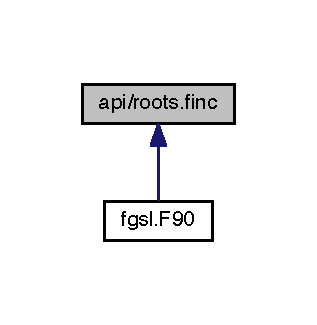
\includegraphics[width=152pt]{roots_8finc__dep__incl}
\end{center}
\end{figure}
\subsection*{Functions/\+Subroutines}
\begin{DoxyCompactItemize}
\item 
type(fgsl\+\_\+root\+\_\+fsolver) function \hyperlink{roots_8finc_a9e423996b996cace4445b0b7c8d49c47}{fgsl\+\_\+root\+\_\+fsolver\+\_\+alloc} (t)
\item 
type(fgsl\+\_\+root\+\_\+fdfsolver) function \hyperlink{roots_8finc_a754a00901764d3a2702b28492377d31f}{fgsl\+\_\+root\+\_\+fdfsolver\+\_\+alloc} (t)
\item 
integer(fgsl\+\_\+int) function \hyperlink{roots_8finc_a4eaeff2b5c48b40a60627201b0ed2a1c}{fgsl\+\_\+root\+\_\+fsolver\+\_\+set} (s, f, x\+\_\+lower, x\+\_\+upper)
\item 
integer(fgsl\+\_\+int) function \hyperlink{roots_8finc_ad5cfd8eab01316799d223177c8902c2f}{fgsl\+\_\+root\+\_\+fdfsolver\+\_\+set} (s, fdf, x)
\item 
subroutine \hyperlink{roots_8finc_ab651ed93d541399c16b925c81eda546d}{fgsl\+\_\+root\+\_\+fsolver\+\_\+free} (s)
\item 
subroutine \hyperlink{roots_8finc_a35459afca718dd3a99651e5e993f46a3}{fgsl\+\_\+root\+\_\+fdfsolver\+\_\+free} (s)
\item 
character(kind=fgsl\+\_\+char, len=fgsl\+\_\+strmax) function \hyperlink{roots_8finc_a8f1354b9512e43ae0af0752cb4a29f0b}{fgsl\+\_\+root\+\_\+fsolver\+\_\+name} (s)
\item 
character(kind=fgsl\+\_\+char, len=fgsl\+\_\+strmax) function \hyperlink{roots_8finc_a949c461b3543e81b68a43e4fd100e88b}{fgsl\+\_\+root\+\_\+fdfsolver\+\_\+name} (s)
\item 
integer(fgsl\+\_\+int) function \hyperlink{roots_8finc_a16e821dd161b28bc9cd5ff5e68358915}{fgsl\+\_\+root\+\_\+fsolver\+\_\+iterate} (s)
\item 
integer(fgsl\+\_\+int) function \hyperlink{roots_8finc_aabdb1cc46e7b7bd1bdf6d70756c1f414}{fgsl\+\_\+root\+\_\+fdfsolver\+\_\+iterate} (s)
\item 
real(fgsl\+\_\+double) function \hyperlink{roots_8finc_abd614e562da9a1d0f498ad9705a5bf17}{fgsl\+\_\+root\+\_\+fsolver\+\_\+root} (s)
\item 
real(fgsl\+\_\+double) function \hyperlink{roots_8finc_aa56f439a45653c3ad87c4dab8bce52cc}{fgsl\+\_\+root\+\_\+fdfsolver\+\_\+root} (s)
\item 
real(fgsl\+\_\+double) function \hyperlink{roots_8finc_a50e5822efb5024274b19e437e33776b2}{fgsl\+\_\+root\+\_\+fsolver\+\_\+x\+\_\+lower} (s)
\item 
real(fgsl\+\_\+double) function \hyperlink{roots_8finc_a5eab10a10072a9ca636cad6c7ffcad10}{fgsl\+\_\+root\+\_\+fsolver\+\_\+x\+\_\+upper} (s)
\item 
integer(fgsl\+\_\+int) function \hyperlink{roots_8finc_a156ed7fa6e25c07decded2880ee5c9e6}{fgsl\+\_\+root\+\_\+test\+\_\+interval} (x\+\_\+lower, x\+\_\+upper, epsabs, epsrel)
\item 
integer(fgsl\+\_\+int) function \hyperlink{roots_8finc_a397c00c2706cec9e7774bab00e9d3488}{fgsl\+\_\+root\+\_\+test\+\_\+delta} (x1, x0, epsabs, epsrel)
\item 
integer(fgsl\+\_\+int) function \hyperlink{roots_8finc_af9ecc6e6a7c09d84fb5548c8eea95035}{fgsl\+\_\+root\+\_\+test\+\_\+residual} (f, epsabs)
\item 
logical function \hyperlink{roots_8finc_ab11a61f02e9c07f0ba691967526370ff}{fgsl\+\_\+root\+\_\+fsolver\+\_\+status} (s)
\item 
logical function \hyperlink{roots_8finc_a11b750f9689b4905ab50f323d3d7cfd5}{fgsl\+\_\+root\+\_\+fdfsolver\+\_\+status} (s)
\end{DoxyCompactItemize}


\subsection{Function/\+Subroutine Documentation}
\hypertarget{roots_8finc_a754a00901764d3a2702b28492377d31f}{}\index{roots.\+finc@{roots.\+finc}!fgsl\+\_\+root\+\_\+fdfsolver\+\_\+alloc@{fgsl\+\_\+root\+\_\+fdfsolver\+\_\+alloc}}
\index{fgsl\+\_\+root\+\_\+fdfsolver\+\_\+alloc@{fgsl\+\_\+root\+\_\+fdfsolver\+\_\+alloc}!roots.\+finc@{roots.\+finc}}
\subsubsection[{fgsl\+\_\+root\+\_\+fdfsolver\+\_\+alloc}]{\setlength{\rightskip}{0pt plus 5cm}type(fgsl\+\_\+root\+\_\+fdfsolver) function fgsl\+\_\+root\+\_\+fdfsolver\+\_\+alloc (
\begin{DoxyParamCaption}
\item[{type(fgsl\+\_\+root\+\_\+fdfsolver\+\_\+type), intent(in)}]{t}
\end{DoxyParamCaption}
)}\label{roots_8finc_a754a00901764d3a2702b28492377d31f}
\hypertarget{roots_8finc_a35459afca718dd3a99651e5e993f46a3}{}\index{roots.\+finc@{roots.\+finc}!fgsl\+\_\+root\+\_\+fdfsolver\+\_\+free@{fgsl\+\_\+root\+\_\+fdfsolver\+\_\+free}}
\index{fgsl\+\_\+root\+\_\+fdfsolver\+\_\+free@{fgsl\+\_\+root\+\_\+fdfsolver\+\_\+free}!roots.\+finc@{roots.\+finc}}
\subsubsection[{fgsl\+\_\+root\+\_\+fdfsolver\+\_\+free}]{\setlength{\rightskip}{0pt plus 5cm}subroutine fgsl\+\_\+root\+\_\+fdfsolver\+\_\+free (
\begin{DoxyParamCaption}
\item[{type(fgsl\+\_\+root\+\_\+fdfsolver), intent(inout)}]{s}
\end{DoxyParamCaption}
)}\label{roots_8finc_a35459afca718dd3a99651e5e993f46a3}
\hypertarget{roots_8finc_aabdb1cc46e7b7bd1bdf6d70756c1f414}{}\index{roots.\+finc@{roots.\+finc}!fgsl\+\_\+root\+\_\+fdfsolver\+\_\+iterate@{fgsl\+\_\+root\+\_\+fdfsolver\+\_\+iterate}}
\index{fgsl\+\_\+root\+\_\+fdfsolver\+\_\+iterate@{fgsl\+\_\+root\+\_\+fdfsolver\+\_\+iterate}!roots.\+finc@{roots.\+finc}}
\subsubsection[{fgsl\+\_\+root\+\_\+fdfsolver\+\_\+iterate}]{\setlength{\rightskip}{0pt plus 5cm}integer(fgsl\+\_\+int) function fgsl\+\_\+root\+\_\+fdfsolver\+\_\+iterate (
\begin{DoxyParamCaption}
\item[{type(fgsl\+\_\+root\+\_\+fdfsolver), intent(inout)}]{s}
\end{DoxyParamCaption}
)}\label{roots_8finc_aabdb1cc46e7b7bd1bdf6d70756c1f414}
\hypertarget{roots_8finc_a949c461b3543e81b68a43e4fd100e88b}{}\index{roots.\+finc@{roots.\+finc}!fgsl\+\_\+root\+\_\+fdfsolver\+\_\+name@{fgsl\+\_\+root\+\_\+fdfsolver\+\_\+name}}
\index{fgsl\+\_\+root\+\_\+fdfsolver\+\_\+name@{fgsl\+\_\+root\+\_\+fdfsolver\+\_\+name}!roots.\+finc@{roots.\+finc}}
\subsubsection[{fgsl\+\_\+root\+\_\+fdfsolver\+\_\+name}]{\setlength{\rightskip}{0pt plus 5cm}character(kind=fgsl\+\_\+char,len=fgsl\+\_\+strmax) function fgsl\+\_\+root\+\_\+fdfsolver\+\_\+name (
\begin{DoxyParamCaption}
\item[{type(fgsl\+\_\+root\+\_\+fdfsolver), intent(in)}]{s}
\end{DoxyParamCaption}
)}\label{roots_8finc_a949c461b3543e81b68a43e4fd100e88b}
\hypertarget{roots_8finc_aa56f439a45653c3ad87c4dab8bce52cc}{}\index{roots.\+finc@{roots.\+finc}!fgsl\+\_\+root\+\_\+fdfsolver\+\_\+root@{fgsl\+\_\+root\+\_\+fdfsolver\+\_\+root}}
\index{fgsl\+\_\+root\+\_\+fdfsolver\+\_\+root@{fgsl\+\_\+root\+\_\+fdfsolver\+\_\+root}!roots.\+finc@{roots.\+finc}}
\subsubsection[{fgsl\+\_\+root\+\_\+fdfsolver\+\_\+root}]{\setlength{\rightskip}{0pt plus 5cm}real(fgsl\+\_\+double) function fgsl\+\_\+root\+\_\+fdfsolver\+\_\+root (
\begin{DoxyParamCaption}
\item[{type(fgsl\+\_\+root\+\_\+fdfsolver), intent(inout)}]{s}
\end{DoxyParamCaption}
)}\label{roots_8finc_aa56f439a45653c3ad87c4dab8bce52cc}
\hypertarget{roots_8finc_ad5cfd8eab01316799d223177c8902c2f}{}\index{roots.\+finc@{roots.\+finc}!fgsl\+\_\+root\+\_\+fdfsolver\+\_\+set@{fgsl\+\_\+root\+\_\+fdfsolver\+\_\+set}}
\index{fgsl\+\_\+root\+\_\+fdfsolver\+\_\+set@{fgsl\+\_\+root\+\_\+fdfsolver\+\_\+set}!roots.\+finc@{roots.\+finc}}
\subsubsection[{fgsl\+\_\+root\+\_\+fdfsolver\+\_\+set}]{\setlength{\rightskip}{0pt plus 5cm}integer(fgsl\+\_\+int) function fgsl\+\_\+root\+\_\+fdfsolver\+\_\+set (
\begin{DoxyParamCaption}
\item[{type(fgsl\+\_\+root\+\_\+fdfsolver), intent(in)}]{s, }
\item[{type(fgsl\+\_\+function\+\_\+fdf), intent(in)}]{fdf, }
\item[{real(fgsl\+\_\+double), intent(in)}]{x}
\end{DoxyParamCaption}
)}\label{roots_8finc_ad5cfd8eab01316799d223177c8902c2f}
\hypertarget{roots_8finc_a11b750f9689b4905ab50f323d3d7cfd5}{}\index{roots.\+finc@{roots.\+finc}!fgsl\+\_\+root\+\_\+fdfsolver\+\_\+status@{fgsl\+\_\+root\+\_\+fdfsolver\+\_\+status}}
\index{fgsl\+\_\+root\+\_\+fdfsolver\+\_\+status@{fgsl\+\_\+root\+\_\+fdfsolver\+\_\+status}!roots.\+finc@{roots.\+finc}}
\subsubsection[{fgsl\+\_\+root\+\_\+fdfsolver\+\_\+status}]{\setlength{\rightskip}{0pt plus 5cm}logical function fgsl\+\_\+root\+\_\+fdfsolver\+\_\+status (
\begin{DoxyParamCaption}
\item[{type(fgsl\+\_\+root\+\_\+fdfsolver), intent(in)}]{s}
\end{DoxyParamCaption}
)}\label{roots_8finc_a11b750f9689b4905ab50f323d3d7cfd5}
\hypertarget{roots_8finc_a9e423996b996cace4445b0b7c8d49c47}{}\index{roots.\+finc@{roots.\+finc}!fgsl\+\_\+root\+\_\+fsolver\+\_\+alloc@{fgsl\+\_\+root\+\_\+fsolver\+\_\+alloc}}
\index{fgsl\+\_\+root\+\_\+fsolver\+\_\+alloc@{fgsl\+\_\+root\+\_\+fsolver\+\_\+alloc}!roots.\+finc@{roots.\+finc}}
\subsubsection[{fgsl\+\_\+root\+\_\+fsolver\+\_\+alloc}]{\setlength{\rightskip}{0pt plus 5cm}type(fgsl\+\_\+root\+\_\+fsolver) function fgsl\+\_\+root\+\_\+fsolver\+\_\+alloc (
\begin{DoxyParamCaption}
\item[{type(fgsl\+\_\+root\+\_\+fsolver\+\_\+type), intent(in)}]{t}
\end{DoxyParamCaption}
)}\label{roots_8finc_a9e423996b996cace4445b0b7c8d49c47}
\hypertarget{roots_8finc_ab651ed93d541399c16b925c81eda546d}{}\index{roots.\+finc@{roots.\+finc}!fgsl\+\_\+root\+\_\+fsolver\+\_\+free@{fgsl\+\_\+root\+\_\+fsolver\+\_\+free}}
\index{fgsl\+\_\+root\+\_\+fsolver\+\_\+free@{fgsl\+\_\+root\+\_\+fsolver\+\_\+free}!roots.\+finc@{roots.\+finc}}
\subsubsection[{fgsl\+\_\+root\+\_\+fsolver\+\_\+free}]{\setlength{\rightskip}{0pt plus 5cm}subroutine fgsl\+\_\+root\+\_\+fsolver\+\_\+free (
\begin{DoxyParamCaption}
\item[{type(fgsl\+\_\+root\+\_\+fsolver), intent(inout)}]{s}
\end{DoxyParamCaption}
)}\label{roots_8finc_ab651ed93d541399c16b925c81eda546d}
\hypertarget{roots_8finc_a16e821dd161b28bc9cd5ff5e68358915}{}\index{roots.\+finc@{roots.\+finc}!fgsl\+\_\+root\+\_\+fsolver\+\_\+iterate@{fgsl\+\_\+root\+\_\+fsolver\+\_\+iterate}}
\index{fgsl\+\_\+root\+\_\+fsolver\+\_\+iterate@{fgsl\+\_\+root\+\_\+fsolver\+\_\+iterate}!roots.\+finc@{roots.\+finc}}
\subsubsection[{fgsl\+\_\+root\+\_\+fsolver\+\_\+iterate}]{\setlength{\rightskip}{0pt plus 5cm}integer(fgsl\+\_\+int) function fgsl\+\_\+root\+\_\+fsolver\+\_\+iterate (
\begin{DoxyParamCaption}
\item[{type(fgsl\+\_\+root\+\_\+fsolver), intent(inout)}]{s}
\end{DoxyParamCaption}
)}\label{roots_8finc_a16e821dd161b28bc9cd5ff5e68358915}
\hypertarget{roots_8finc_a8f1354b9512e43ae0af0752cb4a29f0b}{}\index{roots.\+finc@{roots.\+finc}!fgsl\+\_\+root\+\_\+fsolver\+\_\+name@{fgsl\+\_\+root\+\_\+fsolver\+\_\+name}}
\index{fgsl\+\_\+root\+\_\+fsolver\+\_\+name@{fgsl\+\_\+root\+\_\+fsolver\+\_\+name}!roots.\+finc@{roots.\+finc}}
\subsubsection[{fgsl\+\_\+root\+\_\+fsolver\+\_\+name}]{\setlength{\rightskip}{0pt plus 5cm}character(kind=fgsl\+\_\+char,len=fgsl\+\_\+strmax) function fgsl\+\_\+root\+\_\+fsolver\+\_\+name (
\begin{DoxyParamCaption}
\item[{type(fgsl\+\_\+root\+\_\+fsolver), intent(in)}]{s}
\end{DoxyParamCaption}
)}\label{roots_8finc_a8f1354b9512e43ae0af0752cb4a29f0b}
\hypertarget{roots_8finc_abd614e562da9a1d0f498ad9705a5bf17}{}\index{roots.\+finc@{roots.\+finc}!fgsl\+\_\+root\+\_\+fsolver\+\_\+root@{fgsl\+\_\+root\+\_\+fsolver\+\_\+root}}
\index{fgsl\+\_\+root\+\_\+fsolver\+\_\+root@{fgsl\+\_\+root\+\_\+fsolver\+\_\+root}!roots.\+finc@{roots.\+finc}}
\subsubsection[{fgsl\+\_\+root\+\_\+fsolver\+\_\+root}]{\setlength{\rightskip}{0pt plus 5cm}real(fgsl\+\_\+double) function fgsl\+\_\+root\+\_\+fsolver\+\_\+root (
\begin{DoxyParamCaption}
\item[{type(fgsl\+\_\+root\+\_\+fsolver), intent(inout)}]{s}
\end{DoxyParamCaption}
)}\label{roots_8finc_abd614e562da9a1d0f498ad9705a5bf17}
\hypertarget{roots_8finc_a4eaeff2b5c48b40a60627201b0ed2a1c}{}\index{roots.\+finc@{roots.\+finc}!fgsl\+\_\+root\+\_\+fsolver\+\_\+set@{fgsl\+\_\+root\+\_\+fsolver\+\_\+set}}
\index{fgsl\+\_\+root\+\_\+fsolver\+\_\+set@{fgsl\+\_\+root\+\_\+fsolver\+\_\+set}!roots.\+finc@{roots.\+finc}}
\subsubsection[{fgsl\+\_\+root\+\_\+fsolver\+\_\+set}]{\setlength{\rightskip}{0pt plus 5cm}integer(fgsl\+\_\+int) function fgsl\+\_\+root\+\_\+fsolver\+\_\+set (
\begin{DoxyParamCaption}
\item[{type(fgsl\+\_\+root\+\_\+fsolver), intent(in)}]{s, }
\item[{type(fgsl\+\_\+function), intent(in)}]{f, }
\item[{real(fgsl\+\_\+double), intent(in)}]{x\+\_\+lower, }
\item[{real(fgsl\+\_\+double), intent(in)}]{x\+\_\+upper}
\end{DoxyParamCaption}
)}\label{roots_8finc_a4eaeff2b5c48b40a60627201b0ed2a1c}
\hypertarget{roots_8finc_ab11a61f02e9c07f0ba691967526370ff}{}\index{roots.\+finc@{roots.\+finc}!fgsl\+\_\+root\+\_\+fsolver\+\_\+status@{fgsl\+\_\+root\+\_\+fsolver\+\_\+status}}
\index{fgsl\+\_\+root\+\_\+fsolver\+\_\+status@{fgsl\+\_\+root\+\_\+fsolver\+\_\+status}!roots.\+finc@{roots.\+finc}}
\subsubsection[{fgsl\+\_\+root\+\_\+fsolver\+\_\+status}]{\setlength{\rightskip}{0pt plus 5cm}logical function fgsl\+\_\+root\+\_\+fsolver\+\_\+status (
\begin{DoxyParamCaption}
\item[{type(fgsl\+\_\+root\+\_\+fsolver), intent(in)}]{s}
\end{DoxyParamCaption}
)}\label{roots_8finc_ab11a61f02e9c07f0ba691967526370ff}
\hypertarget{roots_8finc_a50e5822efb5024274b19e437e33776b2}{}\index{roots.\+finc@{roots.\+finc}!fgsl\+\_\+root\+\_\+fsolver\+\_\+x\+\_\+lower@{fgsl\+\_\+root\+\_\+fsolver\+\_\+x\+\_\+lower}}
\index{fgsl\+\_\+root\+\_\+fsolver\+\_\+x\+\_\+lower@{fgsl\+\_\+root\+\_\+fsolver\+\_\+x\+\_\+lower}!roots.\+finc@{roots.\+finc}}
\subsubsection[{fgsl\+\_\+root\+\_\+fsolver\+\_\+x\+\_\+lower}]{\setlength{\rightskip}{0pt plus 5cm}real(fgsl\+\_\+double) function fgsl\+\_\+root\+\_\+fsolver\+\_\+x\+\_\+lower (
\begin{DoxyParamCaption}
\item[{type(fgsl\+\_\+root\+\_\+fsolver), intent(inout)}]{s}
\end{DoxyParamCaption}
)}\label{roots_8finc_a50e5822efb5024274b19e437e33776b2}
\hypertarget{roots_8finc_a5eab10a10072a9ca636cad6c7ffcad10}{}\index{roots.\+finc@{roots.\+finc}!fgsl\+\_\+root\+\_\+fsolver\+\_\+x\+\_\+upper@{fgsl\+\_\+root\+\_\+fsolver\+\_\+x\+\_\+upper}}
\index{fgsl\+\_\+root\+\_\+fsolver\+\_\+x\+\_\+upper@{fgsl\+\_\+root\+\_\+fsolver\+\_\+x\+\_\+upper}!roots.\+finc@{roots.\+finc}}
\subsubsection[{fgsl\+\_\+root\+\_\+fsolver\+\_\+x\+\_\+upper}]{\setlength{\rightskip}{0pt plus 5cm}real(fgsl\+\_\+double) function fgsl\+\_\+root\+\_\+fsolver\+\_\+x\+\_\+upper (
\begin{DoxyParamCaption}
\item[{type(fgsl\+\_\+root\+\_\+fsolver), intent(inout)}]{s}
\end{DoxyParamCaption}
)}\label{roots_8finc_a5eab10a10072a9ca636cad6c7ffcad10}
\hypertarget{roots_8finc_a397c00c2706cec9e7774bab00e9d3488}{}\index{roots.\+finc@{roots.\+finc}!fgsl\+\_\+root\+\_\+test\+\_\+delta@{fgsl\+\_\+root\+\_\+test\+\_\+delta}}
\index{fgsl\+\_\+root\+\_\+test\+\_\+delta@{fgsl\+\_\+root\+\_\+test\+\_\+delta}!roots.\+finc@{roots.\+finc}}
\subsubsection[{fgsl\+\_\+root\+\_\+test\+\_\+delta}]{\setlength{\rightskip}{0pt plus 5cm}integer(fgsl\+\_\+int) function fgsl\+\_\+root\+\_\+test\+\_\+delta (
\begin{DoxyParamCaption}
\item[{real(fgsl\+\_\+double), intent(in)}]{x1, }
\item[{real(fgsl\+\_\+double), intent(in)}]{x0, }
\item[{real(fgsl\+\_\+double), intent(in)}]{epsabs, }
\item[{real(fgsl\+\_\+double), intent(in)}]{epsrel}
\end{DoxyParamCaption}
)}\label{roots_8finc_a397c00c2706cec9e7774bab00e9d3488}
\hypertarget{roots_8finc_a156ed7fa6e25c07decded2880ee5c9e6}{}\index{roots.\+finc@{roots.\+finc}!fgsl\+\_\+root\+\_\+test\+\_\+interval@{fgsl\+\_\+root\+\_\+test\+\_\+interval}}
\index{fgsl\+\_\+root\+\_\+test\+\_\+interval@{fgsl\+\_\+root\+\_\+test\+\_\+interval}!roots.\+finc@{roots.\+finc}}
\subsubsection[{fgsl\+\_\+root\+\_\+test\+\_\+interval}]{\setlength{\rightskip}{0pt plus 5cm}integer(fgsl\+\_\+int) function fgsl\+\_\+root\+\_\+test\+\_\+interval (
\begin{DoxyParamCaption}
\item[{real(fgsl\+\_\+double), intent(in)}]{x\+\_\+lower, }
\item[{real(fgsl\+\_\+double), intent(in)}]{x\+\_\+upper, }
\item[{real(fgsl\+\_\+double), intent(in)}]{epsabs, }
\item[{real(fgsl\+\_\+double), intent(in)}]{epsrel}
\end{DoxyParamCaption}
)}\label{roots_8finc_a156ed7fa6e25c07decded2880ee5c9e6}
\hypertarget{roots_8finc_af9ecc6e6a7c09d84fb5548c8eea95035}{}\index{roots.\+finc@{roots.\+finc}!fgsl\+\_\+root\+\_\+test\+\_\+residual@{fgsl\+\_\+root\+\_\+test\+\_\+residual}}
\index{fgsl\+\_\+root\+\_\+test\+\_\+residual@{fgsl\+\_\+root\+\_\+test\+\_\+residual}!roots.\+finc@{roots.\+finc}}
\subsubsection[{fgsl\+\_\+root\+\_\+test\+\_\+residual}]{\setlength{\rightskip}{0pt plus 5cm}integer(fgsl\+\_\+int) function fgsl\+\_\+root\+\_\+test\+\_\+residual (
\begin{DoxyParamCaption}
\item[{real(fgsl\+\_\+double), intent(in)}]{f, }
\item[{real(fgsl\+\_\+double), intent(in)}]{epsabs}
\end{DoxyParamCaption}
)}\label{roots_8finc_af9ecc6e6a7c09d84fb5548c8eea95035}

\hypertarget{siman_8finc}{\section{api/siman.finc File Reference}
\label{siman_8finc}\index{api/siman.\-finc@{api/siman.\-finc}}
}
This graph shows which files directly or indirectly include this file\-:
\nopagebreak
\begin{figure}[H]
\begin{center}
\leavevmode
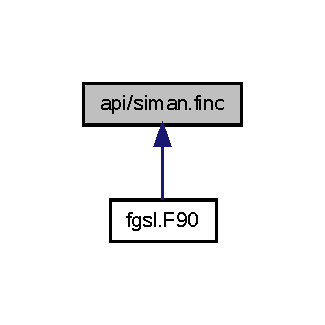
\includegraphics[width=158pt]{siman_8finc__dep__incl}
\end{center}
\end{figure}
\subsection*{Functions/\-Subroutines}
\begin{DoxyCompactItemize}
\item 
subroutine \hyperlink{siman_8finc_adcfa0c681728d5c3e90be5349806375b}{fgsl\-\_\-siman\-\_\-params\-\_\-init} (params, n\-\_\-tries, iters\-\_\-fixed\-\_\-t, step\-\_\-size, k, t\-\_\-initial, mu\-\_\-t, t\-\_\-min)
\item 
subroutine \hyperlink{siman_8finc_a8b4f3ab19289692f276bbb194756b38d}{fgsl\-\_\-siman\-\_\-params\-\_\-free} (params)
\item 
subroutine \hyperlink{siman_8finc_a3f8e1e92cd57d563d21153e5bf61f0cc}{fgsl\-\_\-siman\-\_\-solve} (rng, x0\-\_\-p, ef, take\-\_\-step, distance, print\-\_\-position, copy\-\_\-func, copy\-\_\-constructor, destructor, element\-\_\-size, params)
\item 
logical function \hyperlink{siman_8finc_a1e555a955ce705b0a8833ea6e6822ae8}{fgsl\-\_\-siman\-\_\-params\-\_\-t\-\_\-status} (siman\-\_\-params\-\_\-t)
\end{DoxyCompactItemize}


\subsection{Function/\-Subroutine Documentation}
\hypertarget{siman_8finc_a8b4f3ab19289692f276bbb194756b38d}{\index{siman.\-finc@{siman.\-finc}!fgsl\-\_\-siman\-\_\-params\-\_\-free@{fgsl\-\_\-siman\-\_\-params\-\_\-free}}
\index{fgsl\-\_\-siman\-\_\-params\-\_\-free@{fgsl\-\_\-siman\-\_\-params\-\_\-free}!siman.finc@{siman.\-finc}}
\subsubsection[{fgsl\-\_\-siman\-\_\-params\-\_\-free}]{\setlength{\rightskip}{0pt plus 5cm}subroutine fgsl\-\_\-siman\-\_\-params\-\_\-free (
\begin{DoxyParamCaption}
\item[{type(fgsl\-\_\-siman\-\_\-params\-\_\-t), intent(inout)}]{params}
\end{DoxyParamCaption}
)}}\label{siman_8finc_a8b4f3ab19289692f276bbb194756b38d}
\hypertarget{siman_8finc_adcfa0c681728d5c3e90be5349806375b}{\index{siman.\-finc@{siman.\-finc}!fgsl\-\_\-siman\-\_\-params\-\_\-init@{fgsl\-\_\-siman\-\_\-params\-\_\-init}}
\index{fgsl\-\_\-siman\-\_\-params\-\_\-init@{fgsl\-\_\-siman\-\_\-params\-\_\-init}!siman.finc@{siman.\-finc}}
\subsubsection[{fgsl\-\_\-siman\-\_\-params\-\_\-init}]{\setlength{\rightskip}{0pt plus 5cm}subroutine fgsl\-\_\-siman\-\_\-params\-\_\-init (
\begin{DoxyParamCaption}
\item[{type(fgsl\-\_\-siman\-\_\-params\-\_\-t), intent(inout)}]{params, }
\item[{integer(fgsl\-\_\-int)}]{n\-\_\-tries, }
\item[{integer(fgsl\-\_\-int)}]{iters\-\_\-fixed\-\_\-t, }
\item[{real(fgsl\-\_\-double)}]{step\-\_\-size, }
\item[{real(fgsl\-\_\-double)}]{k, }
\item[{real(fgsl\-\_\-double)}]{t\-\_\-initial, }
\item[{real(fgsl\-\_\-double)}]{mu\-\_\-t, }
\item[{real(fgsl\-\_\-double)}]{t\-\_\-min}
\end{DoxyParamCaption}
)}}\label{siman_8finc_adcfa0c681728d5c3e90be5349806375b}
\hypertarget{siman_8finc_a1e555a955ce705b0a8833ea6e6822ae8}{\index{siman.\-finc@{siman.\-finc}!fgsl\-\_\-siman\-\_\-params\-\_\-t\-\_\-status@{fgsl\-\_\-siman\-\_\-params\-\_\-t\-\_\-status}}
\index{fgsl\-\_\-siman\-\_\-params\-\_\-t\-\_\-status@{fgsl\-\_\-siman\-\_\-params\-\_\-t\-\_\-status}!siman.finc@{siman.\-finc}}
\subsubsection[{fgsl\-\_\-siman\-\_\-params\-\_\-t\-\_\-status}]{\setlength{\rightskip}{0pt plus 5cm}logical function fgsl\-\_\-siman\-\_\-params\-\_\-t\-\_\-status (
\begin{DoxyParamCaption}
\item[{type(fgsl\-\_\-siman\-\_\-params\-\_\-t), intent(in)}]{siman\-\_\-params\-\_\-t}
\end{DoxyParamCaption}
)}}\label{siman_8finc_a1e555a955ce705b0a8833ea6e6822ae8}
\hypertarget{siman_8finc_a3f8e1e92cd57d563d21153e5bf61f0cc}{\index{siman.\-finc@{siman.\-finc}!fgsl\-\_\-siman\-\_\-solve@{fgsl\-\_\-siman\-\_\-solve}}
\index{fgsl\-\_\-siman\-\_\-solve@{fgsl\-\_\-siman\-\_\-solve}!siman.finc@{siman.\-finc}}
\subsubsection[{fgsl\-\_\-siman\-\_\-solve}]{\setlength{\rightskip}{0pt plus 5cm}subroutine fgsl\-\_\-siman\-\_\-solve (
\begin{DoxyParamCaption}
\item[{type(fgsl\-\_\-rng), intent(in)}]{rng, }
\item[{type(c\-\_\-ptr), intent(inout)}]{x0\-\_\-p, }
\item[{}]{ef, }
\item[{}]{take\-\_\-step, }
\item[{}]{distance, }
\item[{optional}]{print\-\_\-position, }
\item[{optional}]{copy\-\_\-func, }
\item[{optional}]{copy\-\_\-constructor, }
\item[{optional}]{destructor, }
\item[{integer(fgsl\-\_\-size\-\_\-t), intent(in), optional}]{element\-\_\-size, }
\item[{type(fgsl\-\_\-siman\-\_\-params\-\_\-t), intent(in)}]{params}
\end{DoxyParamCaption}
)}}\label{siman_8finc_a3f8e1e92cd57d563d21153e5bf61f0cc}

\hypertarget{sort_8finc}{\section{api/sort.finc File Reference}
\label{sort_8finc}\index{api/sort.\-finc@{api/sort.\-finc}}
}
This graph shows which files directly or indirectly include this file\-:\nopagebreak
\begin{figure}[H]
\begin{center}
\leavevmode
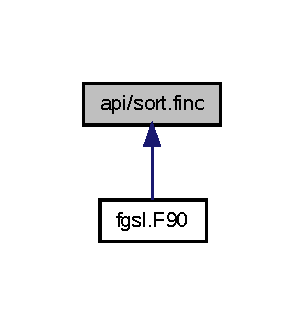
\includegraphics[width=148pt]{sort_8finc__dep__incl}
\end{center}
\end{figure}
\subsection*{Functions/\-Subroutines}
\begin{DoxyCompactItemize}
\item 
subroutine \hyperlink{sort_8finc_a29c0ed778f056399d921407b94883bb0}{fgsl\-\_\-heapsort} (array, count, size, compare)
\item 
integer(fgsl\-\_\-int) function \hyperlink{sort_8finc_a3f576ca19a0cc0b7cc24ccd80ac5d7d2}{fgsl\-\_\-heapsort\-\_\-index} (p, array, count, size, compare)
\item 
subroutine \hyperlink{sort_8finc_a1dec49e9c2067642bb4a24ccd7939fe4}{fgsl\-\_\-sort\-\_\-double} (data, stride, n)
\item 
subroutine \hyperlink{sort_8finc_adf92649e442927793bb64d8e6c627b64}{fgsl\-\_\-sort\-\_\-double\-\_\-index} (p, data, stride, n)
\item 
integer(fgsl\-\_\-int) function \hyperlink{sort_8finc_a7737cd05792ca6276f0f0abf3ec7e35e}{fgsl\-\_\-sort\-\_\-double\-\_\-smallest} (dest, k, src, stride, n)
\item 
integer(fgsl\-\_\-int) function \hyperlink{sort_8finc_abc3f234c4b7c8fcdb2e5a6ee28c96a84}{fgsl\-\_\-sort\-\_\-double\-\_\-smallest\-\_\-index} (p, k, src, stride, n)
\item 
integer(fgsl\-\_\-int) function \hyperlink{sort_8finc_abbfdbcc768b9fc574bca1aabd5c4ea6f}{fgsl\-\_\-sort\-\_\-double\-\_\-largest} (dest, k, src, stride, n)
\item 
integer(fgsl\-\_\-int) function \hyperlink{sort_8finc_af27bfe3694fe4135ad32cc5d042430da}{fgsl\-\_\-sort\-\_\-double\-\_\-largest\-\_\-index} (p, k, src, stride, n)
\item 
subroutine \hyperlink{sort_8finc_a964150c5e4c1e9126d3e5c133d4cf874}{fgsl\-\_\-sort\-\_\-long} (data, stride, n)
\item 
subroutine \hyperlink{sort_8finc_a6deeedcc9a03ca18bc0fbaddfc4c57bb}{fgsl\-\_\-sort\-\_\-long\-\_\-index} (p, data, stride, n)
\item 
integer(fgsl\-\_\-int) function \hyperlink{sort_8finc_ab63afc3e56f9ed94c784637dc54be97b}{fgsl\-\_\-sort\-\_\-long\-\_\-smallest} (dest, k, src, stride, n)
\item 
integer(fgsl\-\_\-int) function \hyperlink{sort_8finc_ad008a109280ac9782800fdb013a41ce9}{fgsl\-\_\-sort\-\_\-long\-\_\-smallest\-\_\-index} (p, k, src, stride, n)
\item 
integer(fgsl\-\_\-int) function \hyperlink{sort_8finc_a732fd6a26c63eb3ed81178d8dc4dd128}{fgsl\-\_\-sort\-\_\-long\-\_\-largest} (dest, k, src, stride, n)
\item 
integer(fgsl\-\_\-int) function \hyperlink{sort_8finc_a49b77db1a738b1500cf01500e77a63cc}{fgsl\-\_\-sort\-\_\-long\-\_\-largest\-\_\-index} (p, k, src, stride, n)
\item 
subroutine \hyperlink{sort_8finc_ae260f94887ee5bdfdb33bbe94eb83143}{fgsl\-\_\-sort\-\_\-vector} (v)
\item 
subroutine \hyperlink{sort_8finc_aaf339d54c8b44755134ee15293303f09}{fgsl\-\_\-sort\-\_\-vector2} (v1, v2)
\item 
subroutine \hyperlink{sort_8finc_a818d4e659a7756cbf3d20d33ae53b418}{fgsl\-\_\-sort\-\_\-vector\-\_\-index} (p, v)
\item 
integer(fgsl\-\_\-int) function \hyperlink{sort_8finc_a0e00f85dfc87a4eefab581ca773362d1}{fgsl\-\_\-sort\-\_\-vector\-\_\-smallest} (dest, k, v)
\item 
integer(fgsl\-\_\-int) function \hyperlink{sort_8finc_ac0555f574fa147cddc39c7a027c5d9ae}{fgsl\-\_\-sort\-\_\-vector\-\_\-largest} (dest, k, v)
\item 
integer(fgsl\-\_\-int) function \hyperlink{sort_8finc_ac094e38c25cd8d2532ce3729a564a199}{fgsl\-\_\-sort\-\_\-vector\-\_\-smallest\-\_\-index} (p, k, v)
\item 
integer(fgsl\-\_\-int) function \hyperlink{sort_8finc_a5b6b9851e59760427ededc824ea5866d}{fgsl\-\_\-sort\-\_\-vector\-\_\-largest\-\_\-index} (p, k, v)
\end{DoxyCompactItemize}


\subsection{Function/\-Subroutine Documentation}
\hypertarget{sort_8finc_a29c0ed778f056399d921407b94883bb0}{\index{sort.\-finc@{sort.\-finc}!fgsl\-\_\-heapsort@{fgsl\-\_\-heapsort}}
\index{fgsl\-\_\-heapsort@{fgsl\-\_\-heapsort}!sort.finc@{sort.\-finc}}
\subsubsection[{fgsl\-\_\-heapsort}]{\setlength{\rightskip}{0pt plus 5cm}subroutine fgsl\-\_\-heapsort (
\begin{DoxyParamCaption}
\item[{type(c\-\_\-ptr)}]{array, }
\item[{integer(fgsl\-\_\-size\-\_\-t), intent(in)}]{count, }
\item[{integer(fgsl\-\_\-size\-\_\-t), intent(in)}]{size, }
\item[{}]{compare}
\end{DoxyParamCaption}
)}}\label{sort_8finc_a29c0ed778f056399d921407b94883bb0}
\hypertarget{sort_8finc_a3f576ca19a0cc0b7cc24ccd80ac5d7d2}{\index{sort.\-finc@{sort.\-finc}!fgsl\-\_\-heapsort\-\_\-index@{fgsl\-\_\-heapsort\-\_\-index}}
\index{fgsl\-\_\-heapsort\-\_\-index@{fgsl\-\_\-heapsort\-\_\-index}!sort.finc@{sort.\-finc}}
\subsubsection[{fgsl\-\_\-heapsort\-\_\-index}]{\setlength{\rightskip}{0pt plus 5cm}integer(fgsl\-\_\-int) function fgsl\-\_\-heapsort\-\_\-index (
\begin{DoxyParamCaption}
\item[{integer(fgsl\-\_\-size\-\_\-t), dimension(count), intent(out)}]{p, }
\item[{type(c\-\_\-ptr)}]{array, }
\item[{integer(fgsl\-\_\-size\-\_\-t), intent(in)}]{count, }
\item[{integer(fgsl\-\_\-size\-\_\-t), intent(in)}]{size, }
\item[{}]{compare}
\end{DoxyParamCaption}
)}}\label{sort_8finc_a3f576ca19a0cc0b7cc24ccd80ac5d7d2}
\hypertarget{sort_8finc_a1dec49e9c2067642bb4a24ccd7939fe4}{\index{sort.\-finc@{sort.\-finc}!fgsl\-\_\-sort\-\_\-double@{fgsl\-\_\-sort\-\_\-double}}
\index{fgsl\-\_\-sort\-\_\-double@{fgsl\-\_\-sort\-\_\-double}!sort.finc@{sort.\-finc}}
\subsubsection[{fgsl\-\_\-sort\-\_\-double}]{\setlength{\rightskip}{0pt plus 5cm}subroutine fgsl\-\_\-sort\-\_\-double (
\begin{DoxyParamCaption}
\item[{real(fgsl\-\_\-double), dimension(\-:), intent(inout)}]{data, }
\item[{integer(fgsl\-\_\-size\-\_\-t), intent(in)}]{stride, }
\item[{integer(fgsl\-\_\-size\-\_\-t), intent(in)}]{n}
\end{DoxyParamCaption}
)}}\label{sort_8finc_a1dec49e9c2067642bb4a24ccd7939fe4}
\hypertarget{sort_8finc_adf92649e442927793bb64d8e6c627b64}{\index{sort.\-finc@{sort.\-finc}!fgsl\-\_\-sort\-\_\-double\-\_\-index@{fgsl\-\_\-sort\-\_\-double\-\_\-index}}
\index{fgsl\-\_\-sort\-\_\-double\-\_\-index@{fgsl\-\_\-sort\-\_\-double\-\_\-index}!sort.finc@{sort.\-finc}}
\subsubsection[{fgsl\-\_\-sort\-\_\-double\-\_\-index}]{\setlength{\rightskip}{0pt plus 5cm}subroutine fgsl\-\_\-sort\-\_\-double\-\_\-index (
\begin{DoxyParamCaption}
\item[{integer(fgsl\-\_\-size\-\_\-t), dimension(\-:), intent(out)}]{p, }
\item[{real(fgsl\-\_\-double), dimension(\-:), intent(in)}]{data, }
\item[{integer(fgsl\-\_\-size\-\_\-t), intent(in)}]{stride, }
\item[{integer(fgsl\-\_\-size\-\_\-t), intent(in)}]{n}
\end{DoxyParamCaption}
)}}\label{sort_8finc_adf92649e442927793bb64d8e6c627b64}
\hypertarget{sort_8finc_abbfdbcc768b9fc574bca1aabd5c4ea6f}{\index{sort.\-finc@{sort.\-finc}!fgsl\-\_\-sort\-\_\-double\-\_\-largest@{fgsl\-\_\-sort\-\_\-double\-\_\-largest}}
\index{fgsl\-\_\-sort\-\_\-double\-\_\-largest@{fgsl\-\_\-sort\-\_\-double\-\_\-largest}!sort.finc@{sort.\-finc}}
\subsubsection[{fgsl\-\_\-sort\-\_\-double\-\_\-largest}]{\setlength{\rightskip}{0pt plus 5cm}integer(fgsl\-\_\-int) function fgsl\-\_\-sort\-\_\-double\-\_\-largest (
\begin{DoxyParamCaption}
\item[{real(fgsl\-\_\-double), dimension(k), intent(out)}]{dest, }
\item[{integer(fgsl\-\_\-size\-\_\-t), intent(in)}]{k, }
\item[{real(fgsl\-\_\-double), dimension(\-:), intent(in)}]{src, }
\item[{integer(fgsl\-\_\-size\-\_\-t), intent(in)}]{stride, }
\item[{integer(fgsl\-\_\-size\-\_\-t), intent(in)}]{n}
\end{DoxyParamCaption}
)}}\label{sort_8finc_abbfdbcc768b9fc574bca1aabd5c4ea6f}
\hypertarget{sort_8finc_af27bfe3694fe4135ad32cc5d042430da}{\index{sort.\-finc@{sort.\-finc}!fgsl\-\_\-sort\-\_\-double\-\_\-largest\-\_\-index@{fgsl\-\_\-sort\-\_\-double\-\_\-largest\-\_\-index}}
\index{fgsl\-\_\-sort\-\_\-double\-\_\-largest\-\_\-index@{fgsl\-\_\-sort\-\_\-double\-\_\-largest\-\_\-index}!sort.finc@{sort.\-finc}}
\subsubsection[{fgsl\-\_\-sort\-\_\-double\-\_\-largest\-\_\-index}]{\setlength{\rightskip}{0pt plus 5cm}integer(fgsl\-\_\-int) function fgsl\-\_\-sort\-\_\-double\-\_\-largest\-\_\-index (
\begin{DoxyParamCaption}
\item[{integer(fgsl\-\_\-size\-\_\-t), dimension(k), intent(out)}]{p, }
\item[{integer(fgsl\-\_\-size\-\_\-t), intent(in)}]{k, }
\item[{real(fgsl\-\_\-double), dimension(\-:), intent(in)}]{src, }
\item[{integer(fgsl\-\_\-size\-\_\-t), intent(in)}]{stride, }
\item[{integer(fgsl\-\_\-size\-\_\-t), intent(in)}]{n}
\end{DoxyParamCaption}
)}}\label{sort_8finc_af27bfe3694fe4135ad32cc5d042430da}
\hypertarget{sort_8finc_a7737cd05792ca6276f0f0abf3ec7e35e}{\index{sort.\-finc@{sort.\-finc}!fgsl\-\_\-sort\-\_\-double\-\_\-smallest@{fgsl\-\_\-sort\-\_\-double\-\_\-smallest}}
\index{fgsl\-\_\-sort\-\_\-double\-\_\-smallest@{fgsl\-\_\-sort\-\_\-double\-\_\-smallest}!sort.finc@{sort.\-finc}}
\subsubsection[{fgsl\-\_\-sort\-\_\-double\-\_\-smallest}]{\setlength{\rightskip}{0pt plus 5cm}integer(fgsl\-\_\-int) function fgsl\-\_\-sort\-\_\-double\-\_\-smallest (
\begin{DoxyParamCaption}
\item[{real(fgsl\-\_\-double), dimension(k), intent(out)}]{dest, }
\item[{integer(fgsl\-\_\-size\-\_\-t), intent(in)}]{k, }
\item[{real(fgsl\-\_\-double), dimension(\-:), intent(in)}]{src, }
\item[{integer(fgsl\-\_\-size\-\_\-t), intent(in)}]{stride, }
\item[{integer(fgsl\-\_\-size\-\_\-t), intent(in)}]{n}
\end{DoxyParamCaption}
)}}\label{sort_8finc_a7737cd05792ca6276f0f0abf3ec7e35e}
\hypertarget{sort_8finc_abc3f234c4b7c8fcdb2e5a6ee28c96a84}{\index{sort.\-finc@{sort.\-finc}!fgsl\-\_\-sort\-\_\-double\-\_\-smallest\-\_\-index@{fgsl\-\_\-sort\-\_\-double\-\_\-smallest\-\_\-index}}
\index{fgsl\-\_\-sort\-\_\-double\-\_\-smallest\-\_\-index@{fgsl\-\_\-sort\-\_\-double\-\_\-smallest\-\_\-index}!sort.finc@{sort.\-finc}}
\subsubsection[{fgsl\-\_\-sort\-\_\-double\-\_\-smallest\-\_\-index}]{\setlength{\rightskip}{0pt plus 5cm}integer(fgsl\-\_\-int) function fgsl\-\_\-sort\-\_\-double\-\_\-smallest\-\_\-index (
\begin{DoxyParamCaption}
\item[{integer(fgsl\-\_\-size\-\_\-t), dimension(k), intent(out)}]{p, }
\item[{integer(fgsl\-\_\-size\-\_\-t), intent(in)}]{k, }
\item[{real(fgsl\-\_\-double), dimension(\-:), intent(in)}]{src, }
\item[{integer(fgsl\-\_\-size\-\_\-t), intent(in)}]{stride, }
\item[{integer(fgsl\-\_\-size\-\_\-t), intent(in)}]{n}
\end{DoxyParamCaption}
)}}\label{sort_8finc_abc3f234c4b7c8fcdb2e5a6ee28c96a84}
\hypertarget{sort_8finc_a964150c5e4c1e9126d3e5c133d4cf874}{\index{sort.\-finc@{sort.\-finc}!fgsl\-\_\-sort\-\_\-long@{fgsl\-\_\-sort\-\_\-long}}
\index{fgsl\-\_\-sort\-\_\-long@{fgsl\-\_\-sort\-\_\-long}!sort.finc@{sort.\-finc}}
\subsubsection[{fgsl\-\_\-sort\-\_\-long}]{\setlength{\rightskip}{0pt plus 5cm}subroutine fgsl\-\_\-sort\-\_\-long (
\begin{DoxyParamCaption}
\item[{integer(fgsl\-\_\-long), dimension(\-:), intent(inout)}]{data, }
\item[{integer(fgsl\-\_\-size\-\_\-t), intent(in)}]{stride, }
\item[{integer(fgsl\-\_\-size\-\_\-t), intent(in)}]{n}
\end{DoxyParamCaption}
)}}\label{sort_8finc_a964150c5e4c1e9126d3e5c133d4cf874}
\hypertarget{sort_8finc_a6deeedcc9a03ca18bc0fbaddfc4c57bb}{\index{sort.\-finc@{sort.\-finc}!fgsl\-\_\-sort\-\_\-long\-\_\-index@{fgsl\-\_\-sort\-\_\-long\-\_\-index}}
\index{fgsl\-\_\-sort\-\_\-long\-\_\-index@{fgsl\-\_\-sort\-\_\-long\-\_\-index}!sort.finc@{sort.\-finc}}
\subsubsection[{fgsl\-\_\-sort\-\_\-long\-\_\-index}]{\setlength{\rightskip}{0pt plus 5cm}subroutine fgsl\-\_\-sort\-\_\-long\-\_\-index (
\begin{DoxyParamCaption}
\item[{integer(fgsl\-\_\-size\-\_\-t), dimension(\-:), intent(out)}]{p, }
\item[{integer(fgsl\-\_\-long), dimension(\-:), intent(in)}]{data, }
\item[{integer(fgsl\-\_\-size\-\_\-t), intent(in)}]{stride, }
\item[{integer(fgsl\-\_\-size\-\_\-t), intent(in)}]{n}
\end{DoxyParamCaption}
)}}\label{sort_8finc_a6deeedcc9a03ca18bc0fbaddfc4c57bb}
\hypertarget{sort_8finc_a732fd6a26c63eb3ed81178d8dc4dd128}{\index{sort.\-finc@{sort.\-finc}!fgsl\-\_\-sort\-\_\-long\-\_\-largest@{fgsl\-\_\-sort\-\_\-long\-\_\-largest}}
\index{fgsl\-\_\-sort\-\_\-long\-\_\-largest@{fgsl\-\_\-sort\-\_\-long\-\_\-largest}!sort.finc@{sort.\-finc}}
\subsubsection[{fgsl\-\_\-sort\-\_\-long\-\_\-largest}]{\setlength{\rightskip}{0pt plus 5cm}integer(fgsl\-\_\-int) function fgsl\-\_\-sort\-\_\-long\-\_\-largest (
\begin{DoxyParamCaption}
\item[{integer(fgsl\-\_\-long), dimension(k), intent(out)}]{dest, }
\item[{integer(fgsl\-\_\-size\-\_\-t), intent(in)}]{k, }
\item[{integer(fgsl\-\_\-long), dimension(\-:), intent(in)}]{src, }
\item[{integer(fgsl\-\_\-size\-\_\-t), intent(in)}]{stride, }
\item[{integer(fgsl\-\_\-size\-\_\-t), intent(in)}]{n}
\end{DoxyParamCaption}
)}}\label{sort_8finc_a732fd6a26c63eb3ed81178d8dc4dd128}
\hypertarget{sort_8finc_a49b77db1a738b1500cf01500e77a63cc}{\index{sort.\-finc@{sort.\-finc}!fgsl\-\_\-sort\-\_\-long\-\_\-largest\-\_\-index@{fgsl\-\_\-sort\-\_\-long\-\_\-largest\-\_\-index}}
\index{fgsl\-\_\-sort\-\_\-long\-\_\-largest\-\_\-index@{fgsl\-\_\-sort\-\_\-long\-\_\-largest\-\_\-index}!sort.finc@{sort.\-finc}}
\subsubsection[{fgsl\-\_\-sort\-\_\-long\-\_\-largest\-\_\-index}]{\setlength{\rightskip}{0pt plus 5cm}integer(fgsl\-\_\-int) function fgsl\-\_\-sort\-\_\-long\-\_\-largest\-\_\-index (
\begin{DoxyParamCaption}
\item[{integer(fgsl\-\_\-size\-\_\-t), dimension(k), intent(out)}]{p, }
\item[{integer(fgsl\-\_\-size\-\_\-t), intent(in)}]{k, }
\item[{integer(fgsl\-\_\-long), dimension(\-:), intent(in)}]{src, }
\item[{integer(fgsl\-\_\-size\-\_\-t), intent(in)}]{stride, }
\item[{integer(fgsl\-\_\-size\-\_\-t), intent(in)}]{n}
\end{DoxyParamCaption}
)}}\label{sort_8finc_a49b77db1a738b1500cf01500e77a63cc}
\hypertarget{sort_8finc_ab63afc3e56f9ed94c784637dc54be97b}{\index{sort.\-finc@{sort.\-finc}!fgsl\-\_\-sort\-\_\-long\-\_\-smallest@{fgsl\-\_\-sort\-\_\-long\-\_\-smallest}}
\index{fgsl\-\_\-sort\-\_\-long\-\_\-smallest@{fgsl\-\_\-sort\-\_\-long\-\_\-smallest}!sort.finc@{sort.\-finc}}
\subsubsection[{fgsl\-\_\-sort\-\_\-long\-\_\-smallest}]{\setlength{\rightskip}{0pt plus 5cm}integer(fgsl\-\_\-int) function fgsl\-\_\-sort\-\_\-long\-\_\-smallest (
\begin{DoxyParamCaption}
\item[{integer(fgsl\-\_\-long), dimension(k), intent(out)}]{dest, }
\item[{integer(fgsl\-\_\-size\-\_\-t), intent(in)}]{k, }
\item[{integer(fgsl\-\_\-long), dimension(\-:), intent(in)}]{src, }
\item[{integer(fgsl\-\_\-size\-\_\-t), intent(in)}]{stride, }
\item[{integer(fgsl\-\_\-size\-\_\-t), intent(in)}]{n}
\end{DoxyParamCaption}
)}}\label{sort_8finc_ab63afc3e56f9ed94c784637dc54be97b}
\hypertarget{sort_8finc_ad008a109280ac9782800fdb013a41ce9}{\index{sort.\-finc@{sort.\-finc}!fgsl\-\_\-sort\-\_\-long\-\_\-smallest\-\_\-index@{fgsl\-\_\-sort\-\_\-long\-\_\-smallest\-\_\-index}}
\index{fgsl\-\_\-sort\-\_\-long\-\_\-smallest\-\_\-index@{fgsl\-\_\-sort\-\_\-long\-\_\-smallest\-\_\-index}!sort.finc@{sort.\-finc}}
\subsubsection[{fgsl\-\_\-sort\-\_\-long\-\_\-smallest\-\_\-index}]{\setlength{\rightskip}{0pt plus 5cm}integer(fgsl\-\_\-int) function fgsl\-\_\-sort\-\_\-long\-\_\-smallest\-\_\-index (
\begin{DoxyParamCaption}
\item[{integer(fgsl\-\_\-size\-\_\-t), dimension(k), intent(out)}]{p, }
\item[{integer(fgsl\-\_\-size\-\_\-t), intent(in)}]{k, }
\item[{integer(fgsl\-\_\-long), dimension(\-:), intent(in)}]{src, }
\item[{integer(fgsl\-\_\-size\-\_\-t), intent(in)}]{stride, }
\item[{integer(fgsl\-\_\-size\-\_\-t), intent(in)}]{n}
\end{DoxyParamCaption}
)}}\label{sort_8finc_ad008a109280ac9782800fdb013a41ce9}
\hypertarget{sort_8finc_ae260f94887ee5bdfdb33bbe94eb83143}{\index{sort.\-finc@{sort.\-finc}!fgsl\-\_\-sort\-\_\-vector@{fgsl\-\_\-sort\-\_\-vector}}
\index{fgsl\-\_\-sort\-\_\-vector@{fgsl\-\_\-sort\-\_\-vector}!sort.finc@{sort.\-finc}}
\subsubsection[{fgsl\-\_\-sort\-\_\-vector}]{\setlength{\rightskip}{0pt plus 5cm}subroutine fgsl\-\_\-sort\-\_\-vector (
\begin{DoxyParamCaption}
\item[{type(fgsl\-\_\-vector), intent(inout)}]{v}
\end{DoxyParamCaption}
)}}\label{sort_8finc_ae260f94887ee5bdfdb33bbe94eb83143}
\hypertarget{sort_8finc_aaf339d54c8b44755134ee15293303f09}{\index{sort.\-finc@{sort.\-finc}!fgsl\-\_\-sort\-\_\-vector2@{fgsl\-\_\-sort\-\_\-vector2}}
\index{fgsl\-\_\-sort\-\_\-vector2@{fgsl\-\_\-sort\-\_\-vector2}!sort.finc@{sort.\-finc}}
\subsubsection[{fgsl\-\_\-sort\-\_\-vector2}]{\setlength{\rightskip}{0pt plus 5cm}subroutine fgsl\-\_\-sort\-\_\-vector2 (
\begin{DoxyParamCaption}
\item[{type(fgsl\-\_\-vector), intent(inout)}]{v1, }
\item[{type(fgsl\-\_\-vector), intent(inout)}]{v2}
\end{DoxyParamCaption}
)}}\label{sort_8finc_aaf339d54c8b44755134ee15293303f09}
\hypertarget{sort_8finc_a818d4e659a7756cbf3d20d33ae53b418}{\index{sort.\-finc@{sort.\-finc}!fgsl\-\_\-sort\-\_\-vector\-\_\-index@{fgsl\-\_\-sort\-\_\-vector\-\_\-index}}
\index{fgsl\-\_\-sort\-\_\-vector\-\_\-index@{fgsl\-\_\-sort\-\_\-vector\-\_\-index}!sort.finc@{sort.\-finc}}
\subsubsection[{fgsl\-\_\-sort\-\_\-vector\-\_\-index}]{\setlength{\rightskip}{0pt plus 5cm}subroutine fgsl\-\_\-sort\-\_\-vector\-\_\-index (
\begin{DoxyParamCaption}
\item[{type(fgsl\-\_\-permutation), intent(inout)}]{p, }
\item[{type(fgsl\-\_\-vector), intent(in)}]{v}
\end{DoxyParamCaption}
)}}\label{sort_8finc_a818d4e659a7756cbf3d20d33ae53b418}
\hypertarget{sort_8finc_ac0555f574fa147cddc39c7a027c5d9ae}{\index{sort.\-finc@{sort.\-finc}!fgsl\-\_\-sort\-\_\-vector\-\_\-largest@{fgsl\-\_\-sort\-\_\-vector\-\_\-largest}}
\index{fgsl\-\_\-sort\-\_\-vector\-\_\-largest@{fgsl\-\_\-sort\-\_\-vector\-\_\-largest}!sort.finc@{sort.\-finc}}
\subsubsection[{fgsl\-\_\-sort\-\_\-vector\-\_\-largest}]{\setlength{\rightskip}{0pt plus 5cm}integer(fgsl\-\_\-int) function fgsl\-\_\-sort\-\_\-vector\-\_\-largest (
\begin{DoxyParamCaption}
\item[{real(fgsl\-\_\-double), dimension(k), intent(out)}]{dest, }
\item[{integer(fgsl\-\_\-size\-\_\-t), intent(in)}]{k, }
\item[{type(fgsl\-\_\-vector), intent(inout)}]{v}
\end{DoxyParamCaption}
)}}\label{sort_8finc_ac0555f574fa147cddc39c7a027c5d9ae}
\hypertarget{sort_8finc_a5b6b9851e59760427ededc824ea5866d}{\index{sort.\-finc@{sort.\-finc}!fgsl\-\_\-sort\-\_\-vector\-\_\-largest\-\_\-index@{fgsl\-\_\-sort\-\_\-vector\-\_\-largest\-\_\-index}}
\index{fgsl\-\_\-sort\-\_\-vector\-\_\-largest\-\_\-index@{fgsl\-\_\-sort\-\_\-vector\-\_\-largest\-\_\-index}!sort.finc@{sort.\-finc}}
\subsubsection[{fgsl\-\_\-sort\-\_\-vector\-\_\-largest\-\_\-index}]{\setlength{\rightskip}{0pt plus 5cm}integer(fgsl\-\_\-int) function fgsl\-\_\-sort\-\_\-vector\-\_\-largest\-\_\-index (
\begin{DoxyParamCaption}
\item[{integer(fgsl\-\_\-size\-\_\-t), dimension(k), intent(out)}]{p, }
\item[{integer(fgsl\-\_\-size\-\_\-t), intent(in)}]{k, }
\item[{type(fgsl\-\_\-vector), intent(inout)}]{v}
\end{DoxyParamCaption}
)}}\label{sort_8finc_a5b6b9851e59760427ededc824ea5866d}
\hypertarget{sort_8finc_a0e00f85dfc87a4eefab581ca773362d1}{\index{sort.\-finc@{sort.\-finc}!fgsl\-\_\-sort\-\_\-vector\-\_\-smallest@{fgsl\-\_\-sort\-\_\-vector\-\_\-smallest}}
\index{fgsl\-\_\-sort\-\_\-vector\-\_\-smallest@{fgsl\-\_\-sort\-\_\-vector\-\_\-smallest}!sort.finc@{sort.\-finc}}
\subsubsection[{fgsl\-\_\-sort\-\_\-vector\-\_\-smallest}]{\setlength{\rightskip}{0pt plus 5cm}integer(fgsl\-\_\-int) function fgsl\-\_\-sort\-\_\-vector\-\_\-smallest (
\begin{DoxyParamCaption}
\item[{real(fgsl\-\_\-double), dimension(k), intent(out)}]{dest, }
\item[{integer(fgsl\-\_\-size\-\_\-t), intent(in)}]{k, }
\item[{type(fgsl\-\_\-vector), intent(inout)}]{v}
\end{DoxyParamCaption}
)}}\label{sort_8finc_a0e00f85dfc87a4eefab581ca773362d1}
\hypertarget{sort_8finc_ac094e38c25cd8d2532ce3729a564a199}{\index{sort.\-finc@{sort.\-finc}!fgsl\-\_\-sort\-\_\-vector\-\_\-smallest\-\_\-index@{fgsl\-\_\-sort\-\_\-vector\-\_\-smallest\-\_\-index}}
\index{fgsl\-\_\-sort\-\_\-vector\-\_\-smallest\-\_\-index@{fgsl\-\_\-sort\-\_\-vector\-\_\-smallest\-\_\-index}!sort.finc@{sort.\-finc}}
\subsubsection[{fgsl\-\_\-sort\-\_\-vector\-\_\-smallest\-\_\-index}]{\setlength{\rightskip}{0pt plus 5cm}integer(fgsl\-\_\-int) function fgsl\-\_\-sort\-\_\-vector\-\_\-smallest\-\_\-index (
\begin{DoxyParamCaption}
\item[{integer(fgsl\-\_\-size\-\_\-t), dimension(k), intent(out)}]{p, }
\item[{integer(fgsl\-\_\-size\-\_\-t), intent(in)}]{k, }
\item[{type(fgsl\-\_\-vector), intent(inout)}]{v}
\end{DoxyParamCaption}
)}}\label{sort_8finc_ac094e38c25cd8d2532ce3729a564a199}

\hypertarget{specfunc_8finc}{\section{api/specfunc.finc File Reference}
\label{specfunc_8finc}\index{api/specfunc.\-finc@{api/specfunc.\-finc}}
}
This graph shows which files directly or indirectly include this file\-:\nopagebreak
\begin{figure}[H]
\begin{center}
\leavevmode
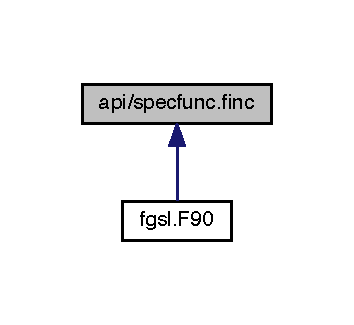
\includegraphics[width=170pt]{specfunc_8finc__dep__incl}
\end{center}
\end{figure}
\subsection*{Functions/\-Subroutines}
\begin{DoxyCompactItemize}
\item 
real(fgsl\-\_\-double) function \hyperlink{specfunc_8finc_a0a9cb6f83b4092fd74711030c2ce7a51}{fgsl\-\_\-sf\-\_\-airy\-\_\-ai} (x, mode)
\item 
integer(fgsl\-\_\-int) function \hyperlink{specfunc_8finc_aae74426785db074c7469d742379ce839}{fgsl\-\_\-sf\-\_\-airy\-\_\-ai\-\_\-e} (x, mode, result)
\item 
real(fgsl\-\_\-double) function \hyperlink{specfunc_8finc_ac8715e3bab2797eaae8b23af36409624}{fgsl\-\_\-sf\-\_\-airy\-\_\-bi} (x, mode)
\item 
integer(fgsl\-\_\-int) function \hyperlink{specfunc_8finc_a556a6d52466a83c16d32407abc301192}{fgsl\-\_\-sf\-\_\-airy\-\_\-bi\-\_\-e} (x, mode, result)
\item 
real(fgsl\-\_\-double) function \hyperlink{specfunc_8finc_a95c23bef46cbe6739e304b7c5f9c8846}{fgsl\-\_\-sf\-\_\-airy\-\_\-ai\-\_\-scaled} (x, mode)
\item 
integer(fgsl\-\_\-int) function \hyperlink{specfunc_8finc_acdf1711fdbaa7e6053fb2df543bd6a57}{fgsl\-\_\-sf\-\_\-airy\-\_\-ai\-\_\-scaled\-\_\-e} (x, mode, result)
\item 
real(fgsl\-\_\-double) function \hyperlink{specfunc_8finc_a20d61b75eb06b8f739012682165eb8ac}{fgsl\-\_\-sf\-\_\-airy\-\_\-bi\-\_\-scaled} (x, mode)
\item 
integer(fgsl\-\_\-int) function \hyperlink{specfunc_8finc_adfc309f1d316dfd0727966cd8376ecc0}{fgsl\-\_\-sf\-\_\-airy\-\_\-bi\-\_\-scaled\-\_\-e} (x, mode, result)
\item 
real(fgsl\-\_\-double) function \hyperlink{specfunc_8finc_a8cccae83c96b49f243622c2376f6c79c}{fgsl\-\_\-sf\-\_\-airy\-\_\-ai\-\_\-deriv} (x, mode)
\item 
integer(fgsl\-\_\-int) function \hyperlink{specfunc_8finc_a5a2b51dce047483401907c6f8a700a24}{fgsl\-\_\-sf\-\_\-airy\-\_\-ai\-\_\-deriv\-\_\-e} (x, mode, result)
\item 
real(fgsl\-\_\-double) function \hyperlink{specfunc_8finc_a94ab39a6b0392152feab691f5db95887}{fgsl\-\_\-sf\-\_\-airy\-\_\-bi\-\_\-deriv} (x, mode)
\item 
integer(fgsl\-\_\-int) function \hyperlink{specfunc_8finc_a9a8b6c05c9a91fdcd6606152ea3ae60e}{fgsl\-\_\-sf\-\_\-airy\-\_\-bi\-\_\-deriv\-\_\-e} (x, mode, result)
\item 
real(fgsl\-\_\-double) function \hyperlink{specfunc_8finc_a62e20904bc1014cdb00b144a19d71a1b}{fgsl\-\_\-sf\-\_\-airy\-\_\-ai\-\_\-deriv\-\_\-scaled} (x, mode)
\item 
integer(fgsl\-\_\-int) function \hyperlink{specfunc_8finc_ac8ac3ea3c8e3eede9394a02664127672}{fgsl\-\_\-sf\-\_\-airy\-\_\-ai\-\_\-deriv\-\_\-scaled\-\_\-e} (x, mode, result)
\item 
real(fgsl\-\_\-double) function \hyperlink{specfunc_8finc_a04ba87efb77bcd09477afa381cc42b83}{fgsl\-\_\-sf\-\_\-airy\-\_\-bi\-\_\-deriv\-\_\-scaled} (x, mode)
\item 
integer(fgsl\-\_\-int) function \hyperlink{specfunc_8finc_a79163f45acbbd01d6a77d2dd3deba867}{fgsl\-\_\-sf\-\_\-airy\-\_\-bi\-\_\-deriv\-\_\-scaled\-\_\-e} (x, mode, result)
\item 
real(fgsl\-\_\-double) function \hyperlink{specfunc_8finc_a923a93771a5ee0e06805113016146e9d}{fgsl\-\_\-sf\-\_\-airy\-\_\-zero\-\_\-ai} (s)
\item 
integer(fgsl\-\_\-int) function \hyperlink{specfunc_8finc_a5233f5c6cac412fb4a24145a1d800dbe}{fgsl\-\_\-sf\-\_\-airy\-\_\-zero\-\_\-ai\-\_\-e} (s, result)
\item 
real(fgsl\-\_\-double) function \hyperlink{specfunc_8finc_ade6dd69303b96c3b449ae37c7c9e776d}{fgsl\-\_\-sf\-\_\-airy\-\_\-zero\-\_\-bi} (s)
\item 
integer(fgsl\-\_\-int) function \hyperlink{specfunc_8finc_a7a902baef34b378f8e8a36093b0f8354}{fgsl\-\_\-sf\-\_\-airy\-\_\-zero\-\_\-bi\-\_\-e} (s, result)
\item 
real(fgsl\-\_\-double) function \hyperlink{specfunc_8finc_afe7e2c7cdad1edb4b04d1375f353c0b1}{fgsl\-\_\-sf\-\_\-airy\-\_\-zero\-\_\-ai\-\_\-deriv} (s)
\item 
integer(fgsl\-\_\-int) function \hyperlink{specfunc_8finc_a4ef02912c6ef5409f4de9651d8471f50}{fgsl\-\_\-sf\-\_\-airy\-\_\-zero\-\_\-ai\-\_\-deriv\-\_\-e} (s, result)
\item 
real(fgsl\-\_\-double) function \hyperlink{specfunc_8finc_ada3f1532d9db39bcd789d2dd8a558b19}{fgsl\-\_\-sf\-\_\-airy\-\_\-zero\-\_\-bi\-\_\-deriv} (s)
\item 
integer(fgsl\-\_\-int) function \hyperlink{specfunc_8finc_a3daa8cdb6f16d461ad5c14f31894b4a9}{fgsl\-\_\-sf\-\_\-airy\-\_\-zero\-\_\-bi\-\_\-deriv\-\_\-e} (s, result)
\item 
real(fgsl\-\_\-double) function \hyperlink{specfunc_8finc_ade323a111e69823d5dc00ff166702be1}{fgsl\-\_\-sf\-\_\-bessel\-\_\-jc0} (x)
\item 
integer(fgsl\-\_\-int) function \hyperlink{specfunc_8finc_a9f07ea6b51f0159a9f0a4605684494e8}{fgsl\-\_\-sf\-\_\-bessel\-\_\-jc0\-\_\-e} (x, result)
\item 
real(fgsl\-\_\-double) function \hyperlink{specfunc_8finc_ad97100dab3f0815f10173d61f1a305dd}{fgsl\-\_\-sf\-\_\-bessel\-\_\-jc1} (x)
\item 
integer(fgsl\-\_\-int) function \hyperlink{specfunc_8finc_a474165b4ec20444e49b8bea32be9dc16}{fgsl\-\_\-sf\-\_\-bessel\-\_\-jc1\-\_\-e} (x, result)
\item 
real(fgsl\-\_\-double) function \hyperlink{specfunc_8finc_a30a63ae95bae3d7985833566a9a4e494}{fgsl\-\_\-sf\-\_\-bessel\-\_\-jcn} (n, x)
\item 
integer(fgsl\-\_\-int) function \hyperlink{specfunc_8finc_afc52092a2e06b4be193e617c4bdec3ea}{fgsl\-\_\-sf\-\_\-bessel\-\_\-jcn\-\_\-e} (n, x, result)
\item 
integer(fgsl\-\_\-int) function \hyperlink{specfunc_8finc_a93875ce80eff9c84d5099c5aaf06ebf6}{fgsl\-\_\-sf\-\_\-bessel\-\_\-jcn\-\_\-array} (nmin, nmax, x, result)
\item 
real(fgsl\-\_\-double) function \hyperlink{specfunc_8finc_a2a8653b50716c1da1479f3f6cfcdfe4e}{fgsl\-\_\-sf\-\_\-bessel\-\_\-yc0} (x)
\item 
integer(fgsl\-\_\-int) function \hyperlink{specfunc_8finc_a76da6cb8aec48174a2bbbf7651c51593}{fgsl\-\_\-sf\-\_\-bessel\-\_\-yc0\-\_\-e} (x, result)
\item 
real(fgsl\-\_\-double) function \hyperlink{specfunc_8finc_a35ddf553357b6cc58f9eb7ac0331262c}{fgsl\-\_\-sf\-\_\-bessel\-\_\-yc1} (x)
\item 
integer(fgsl\-\_\-int) function \hyperlink{specfunc_8finc_a6e7e769252b3a8869dcf48a143d6885d}{fgsl\-\_\-sf\-\_\-bessel\-\_\-yc1\-\_\-e} (x, result)
\item 
real(fgsl\-\_\-double) function \hyperlink{specfunc_8finc_a7c5fdbf056fca8d635d35b32e8e9e3ac}{fgsl\-\_\-sf\-\_\-bessel\-\_\-ycn} (n, x)
\item 
integer(fgsl\-\_\-int) function \hyperlink{specfunc_8finc_a5e9c9671afb1c2e0ec7d830d48d0aae0}{fgsl\-\_\-sf\-\_\-bessel\-\_\-ycn\-\_\-e} (n, x, result)
\item 
integer(fgsl\-\_\-int) function \hyperlink{specfunc_8finc_acbeff6d1931ac060ec162d6abf87759e}{fgsl\-\_\-sf\-\_\-bessel\-\_\-ycn\-\_\-array} (nmin, nmax, x, result)
\item 
real(fgsl\-\_\-double) function \hyperlink{specfunc_8finc_ab670cac105db3ebe0b3ddd64826808e1}{fgsl\-\_\-sf\-\_\-bessel\-\_\-ic0} (x)
\item 
integer(fgsl\-\_\-int) function \hyperlink{specfunc_8finc_a7b8276504f35982296fdb8f0a73ac700}{fgsl\-\_\-sf\-\_\-bessel\-\_\-ic0\-\_\-e} (x, result)
\item 
real(fgsl\-\_\-double) function \hyperlink{specfunc_8finc_a57ca7afe78547adb6e6a8bc0ae3fe151}{fgsl\-\_\-sf\-\_\-bessel\-\_\-ic1} (x)
\item 
integer(fgsl\-\_\-int) function \hyperlink{specfunc_8finc_a1a560a42327064c9157aeb31a5f087b9}{fgsl\-\_\-sf\-\_\-bessel\-\_\-ic1\-\_\-e} (x, result)
\item 
real(fgsl\-\_\-double) function \hyperlink{specfunc_8finc_a73b3d7193eb8237855b8092ed6fb1320}{fgsl\-\_\-sf\-\_\-bessel\-\_\-icn} (n, x)
\item 
integer(fgsl\-\_\-int) function \hyperlink{specfunc_8finc_a9a54b8667a7e68a6c786c9c013e638fd}{fgsl\-\_\-sf\-\_\-bessel\-\_\-icn\-\_\-e} (n, x, result)
\item 
integer(fgsl\-\_\-int) function \hyperlink{specfunc_8finc_acc794c9ba7b396f80bd9ec1f3683e647}{fgsl\-\_\-sf\-\_\-bessel\-\_\-icn\-\_\-array} (nmin, nmax, x, result)
\item 
real(fgsl\-\_\-double) function \hyperlink{specfunc_8finc_a1ba45c364c2186f7f7c4104ea4cbec0a}{fgsl\-\_\-sf\-\_\-bessel\-\_\-ic0\-\_\-scaled} (x)
\item 
integer(fgsl\-\_\-int) function \hyperlink{specfunc_8finc_a61d95545cf0d5ed13f88048c83a102a1}{fgsl\-\_\-sf\-\_\-bessel\-\_\-ic0\-\_\-scaled\-\_\-e} (x, result)
\item 
real(fgsl\-\_\-double) function \hyperlink{specfunc_8finc_a1376d1f85a72eb89941dfa0bb5f83bf2}{fgsl\-\_\-sf\-\_\-bessel\-\_\-ic1\-\_\-scaled} (x)
\item 
integer(fgsl\-\_\-int) function \hyperlink{specfunc_8finc_a84b633483b90407d430234d42efd37ab}{fgsl\-\_\-sf\-\_\-bessel\-\_\-ic1\-\_\-scaled\-\_\-e} (x, result)
\item 
real(fgsl\-\_\-double) function \hyperlink{specfunc_8finc_a1796b471859cc00a3bc313795e954ab8}{fgsl\-\_\-sf\-\_\-bessel\-\_\-icn\-\_\-scaled} (n, x)
\item 
integer(fgsl\-\_\-int) function \hyperlink{specfunc_8finc_a3bee5c7f1b8bd64220882a37fe6222c1}{fgsl\-\_\-sf\-\_\-bessel\-\_\-icn\-\_\-scaled\-\_\-e} (n, x, result)
\item 
integer(fgsl\-\_\-int) function \hyperlink{specfunc_8finc_a2f95a0c0c77e1521ead5d98240f81cc0}{fgsl\-\_\-sf\-\_\-bessel\-\_\-icn\-\_\-scaled\-\_\-array} (nmin, nmax, x, result)
\item 
real(fgsl\-\_\-double) function \hyperlink{specfunc_8finc_ac1738fb58677153aebb95154e0cb15fc}{fgsl\-\_\-sf\-\_\-bessel\-\_\-kc0} (x)
\item 
integer(fgsl\-\_\-int) function \hyperlink{specfunc_8finc_a4c3f1b48377b63e306013e0d3ed2fc47}{fgsl\-\_\-sf\-\_\-bessel\-\_\-kc0\-\_\-e} (x, result)
\item 
real(fgsl\-\_\-double) function \hyperlink{specfunc_8finc_a53ef70e6a6af47bfcdca7e3b5166213a}{fgsl\-\_\-sf\-\_\-bessel\-\_\-kc1} (x)
\item 
integer(fgsl\-\_\-int) function \hyperlink{specfunc_8finc_a188436151ab0e62e67c63c3f7a4dbc43}{fgsl\-\_\-sf\-\_\-bessel\-\_\-kc1\-\_\-e} (x, result)
\item 
real(fgsl\-\_\-double) function \hyperlink{specfunc_8finc_a43affe20564cff1ca8ebf59e536a4a51}{fgsl\-\_\-sf\-\_\-bessel\-\_\-kcn} (n, x)
\item 
integer(fgsl\-\_\-int) function \hyperlink{specfunc_8finc_a51ae1fce2df99aac942fe51242f0460b}{fgsl\-\_\-sf\-\_\-bessel\-\_\-kcn\-\_\-e} (n, x, result)
\item 
integer(fgsl\-\_\-int) function \hyperlink{specfunc_8finc_a7285353c97655105247f0d232b65a5ac}{fgsl\-\_\-sf\-\_\-bessel\-\_\-kcn\-\_\-array} (nmin, nmax, x, result)
\item 
real(fgsl\-\_\-double) function \hyperlink{specfunc_8finc_ad7c1b7c76d6881306f5aa9f0d4a1c498}{fgsl\-\_\-sf\-\_\-bessel\-\_\-kc0\-\_\-scaled} (x)
\item 
integer(fgsl\-\_\-int) function \hyperlink{specfunc_8finc_a7a0524a18062458bed82c133810231f5}{fgsl\-\_\-sf\-\_\-bessel\-\_\-kc0\-\_\-scaled\-\_\-e} (x, result)
\item 
real(fgsl\-\_\-double) function \hyperlink{specfunc_8finc_a1fa7add25cfe89073f4640118a6a3a0d}{fgsl\-\_\-sf\-\_\-bessel\-\_\-kc1\-\_\-scaled} (x)
\item 
integer(fgsl\-\_\-int) function \hyperlink{specfunc_8finc_a6edc260c54c8a66b67d0df91d5b4056c}{fgsl\-\_\-sf\-\_\-bessel\-\_\-kc1\-\_\-scaled\-\_\-e} (x, result)
\item 
real(fgsl\-\_\-double) function \hyperlink{specfunc_8finc_ab65bd6ab8ef876d3c550390bf2206a00}{fgsl\-\_\-sf\-\_\-bessel\-\_\-kcn\-\_\-scaled} (n, x)
\item 
integer(fgsl\-\_\-int) function \hyperlink{specfunc_8finc_a797130c78ea5076eb86b51cd564334fa}{fgsl\-\_\-sf\-\_\-bessel\-\_\-kcn\-\_\-scaled\-\_\-e} (n, x, result)
\item 
integer(fgsl\-\_\-int) function \hyperlink{specfunc_8finc_a7a521e31cb6419d89eeb73ffc086a508}{fgsl\-\_\-sf\-\_\-bessel\-\_\-kcn\-\_\-scaled\-\_\-array} (nmin, nmax, x, result)
\item 
real(fgsl\-\_\-double) function \hyperlink{specfunc_8finc_a2966accc3e88380bcbaee51586c8b43d}{fgsl\-\_\-sf\-\_\-bessel\-\_\-js0} (x)
\item 
integer(fgsl\-\_\-int) function \hyperlink{specfunc_8finc_a1dc8fcfff146f535450ede5e44a90cea}{fgsl\-\_\-sf\-\_\-bessel\-\_\-js0\-\_\-e} (x, result)
\item 
real(fgsl\-\_\-double) function \hyperlink{specfunc_8finc_a02f9f26c36dfe54bc655e3b93894fb90}{fgsl\-\_\-sf\-\_\-bessel\-\_\-js1} (x)
\item 
integer(fgsl\-\_\-int) function \hyperlink{specfunc_8finc_a86aaeb9694ad08a11e19d1acada66004}{fgsl\-\_\-sf\-\_\-bessel\-\_\-js1\-\_\-e} (x, result)
\item 
real(fgsl\-\_\-double) function \hyperlink{specfunc_8finc_a608f4e025e3aa1384a6789234f830848}{fgsl\-\_\-sf\-\_\-bessel\-\_\-js2} (x)
\item 
integer(fgsl\-\_\-int) function \hyperlink{specfunc_8finc_a1f79f88aefc057bb8992f2ed7f47e2b0}{fgsl\-\_\-sf\-\_\-bessel\-\_\-js2\-\_\-e} (x, result)
\item 
real(fgsl\-\_\-double) function \hyperlink{specfunc_8finc_ad3d25735619514a2f11d8f3d82a46a18}{fgsl\-\_\-sf\-\_\-bessel\-\_\-jsl} (n, x)
\item 
integer(fgsl\-\_\-int) function \hyperlink{specfunc_8finc_a115a99b84e0d4433a55530edd599c07e}{fgsl\-\_\-sf\-\_\-bessel\-\_\-jsl\-\_\-e} (n, x, result)
\item 
integer(fgsl\-\_\-int) function \hyperlink{specfunc_8finc_adad29813d45e51c21cee09228d83621e}{fgsl\-\_\-sf\-\_\-bessel\-\_\-jsl\-\_\-array} (lmax, x, result)
\item 
integer(fgsl\-\_\-int) function \hyperlink{specfunc_8finc_a83a1bfba4edb59ec86b0f4151d9e916a}{fgsl\-\_\-sf\-\_\-bessel\-\_\-jsl\-\_\-steed\-\_\-array} (lmax, x, result)
\item 
real(fgsl\-\_\-double) function \hyperlink{specfunc_8finc_a1d0cce4a15fb4e807c6085abee9d6bfc}{fgsl\-\_\-sf\-\_\-bessel\-\_\-ys0} (x)
\item 
integer(fgsl\-\_\-int) function \hyperlink{specfunc_8finc_a481cf0b90daf25842c450603ba108c16}{fgsl\-\_\-sf\-\_\-bessel\-\_\-ys0\-\_\-e} (x, result)
\item 
real(fgsl\-\_\-double) function \hyperlink{specfunc_8finc_a6bd2124b7b0c9c34d4b5a5256b99aa0f}{fgsl\-\_\-sf\-\_\-bessel\-\_\-ys1} (x)
\item 
integer(fgsl\-\_\-int) function \hyperlink{specfunc_8finc_aa60914e596879edadfc6824a44200ca3}{fgsl\-\_\-sf\-\_\-bessel\-\_\-ys1\-\_\-e} (x, result)
\item 
real(fgsl\-\_\-double) function \hyperlink{specfunc_8finc_aa420c0082944ca91380fff36accdca85}{fgsl\-\_\-sf\-\_\-bessel\-\_\-ys2} (x)
\item 
integer(fgsl\-\_\-int) function \hyperlink{specfunc_8finc_a5a4e5351a849979f0d4b854bfe7bcbc9}{fgsl\-\_\-sf\-\_\-bessel\-\_\-ys2\-\_\-e} (x, result)
\item 
real(fgsl\-\_\-double) function \hyperlink{specfunc_8finc_acea044354e5de5f02815d2246cd4661d}{fgsl\-\_\-sf\-\_\-bessel\-\_\-ysl} (n, x)
\item 
integer(fgsl\-\_\-int) function \hyperlink{specfunc_8finc_accca890e7731268378117d252770985f}{fgsl\-\_\-sf\-\_\-bessel\-\_\-ysl\-\_\-e} (n, x, result)
\item 
integer(fgsl\-\_\-int) function \hyperlink{specfunc_8finc_a32a304d26cfd3ed3f115177ca8c4fc00}{fgsl\-\_\-sf\-\_\-bessel\-\_\-ysl\-\_\-array} (lmax, x, result)
\item 
real(fgsl\-\_\-double) function \hyperlink{specfunc_8finc_aefdf46b4b529a2c3c7ff2aea4b9ef39c}{fgsl\-\_\-sf\-\_\-bessel\-\_\-is0\-\_\-scaled} (x)
\item 
integer(fgsl\-\_\-int) function \hyperlink{specfunc_8finc_a5315a6bcb6ea338e48f5d2e456ec6ae5}{fgsl\-\_\-sf\-\_\-bessel\-\_\-is0\-\_\-scaled\-\_\-e} (x, result)
\item 
real(fgsl\-\_\-double) function \hyperlink{specfunc_8finc_a75591023377883b34dd97a83636987e2}{fgsl\-\_\-sf\-\_\-bessel\-\_\-is1\-\_\-scaled} (x)
\item 
integer(fgsl\-\_\-int) function \hyperlink{specfunc_8finc_a6cd23bcdbd5e162709e2105bd6a414f6}{fgsl\-\_\-sf\-\_\-bessel\-\_\-is1\-\_\-scaled\-\_\-e} (x, result)
\item 
real(fgsl\-\_\-double) function \hyperlink{specfunc_8finc_a310d2b10adf86bea7021155aac2cd80c}{fgsl\-\_\-sf\-\_\-bessel\-\_\-is2\-\_\-scaled} (x)
\item 
integer(fgsl\-\_\-int) function \hyperlink{specfunc_8finc_afcc428b9c5d6acc160b6b0fc6d66f795}{fgsl\-\_\-sf\-\_\-bessel\-\_\-is2\-\_\-scaled\-\_\-e} (x, result)
\item 
real(fgsl\-\_\-double) function \hyperlink{specfunc_8finc_a60d2720c3bf8d9771830e29a7899a67c}{fgsl\-\_\-sf\-\_\-bessel\-\_\-isl\-\_\-scaled} (n, x)
\item 
integer(fgsl\-\_\-int) function \hyperlink{specfunc_8finc_a4fe4e94f17df4a2711bcfe8c6f4d9bd9}{fgsl\-\_\-sf\-\_\-bessel\-\_\-isl\-\_\-scaled\-\_\-e} (n, x, result)
\item 
integer(fgsl\-\_\-int) function \hyperlink{specfunc_8finc_af82f9a0bceb2a20163ad54dff5c36239}{fgsl\-\_\-sf\-\_\-bessel\-\_\-isl\-\_\-scaled\-\_\-array} (lmax, x, result)
\item 
real(fgsl\-\_\-double) function \hyperlink{specfunc_8finc_a41c2af16b0cc8e0306bf69674ecd76f8}{fgsl\-\_\-sf\-\_\-bessel\-\_\-ks0\-\_\-scaled} (x)
\item 
integer(fgsl\-\_\-int) function \hyperlink{specfunc_8finc_a036ee716e4369b0904c5283cb0a38866}{fgsl\-\_\-sf\-\_\-bessel\-\_\-ks0\-\_\-scaled\-\_\-e} (x, result)
\item 
real(fgsl\-\_\-double) function \hyperlink{specfunc_8finc_abbd61ad4dae926a7a5ad87a77d80ff83}{fgsl\-\_\-sf\-\_\-bessel\-\_\-ks1\-\_\-scaled} (x)
\item 
integer(fgsl\-\_\-int) function \hyperlink{specfunc_8finc_af142a77938198971f45eb2898c019836}{fgsl\-\_\-sf\-\_\-bessel\-\_\-ks1\-\_\-scaled\-\_\-e} (x, result)
\item 
real(fgsl\-\_\-double) function \hyperlink{specfunc_8finc_ad9186c32d03ac512165c1555935a1d3b}{fgsl\-\_\-sf\-\_\-bessel\-\_\-ks2\-\_\-scaled} (x)
\item 
integer(fgsl\-\_\-int) function \hyperlink{specfunc_8finc_a4fb8e3c619e4c3cb21df907b65e224f2}{fgsl\-\_\-sf\-\_\-bessel\-\_\-ks2\-\_\-scaled\-\_\-e} (x, result)
\item 
real(fgsl\-\_\-double) function \hyperlink{specfunc_8finc_af51da4a346dc5348e883162b1e2a7e34}{fgsl\-\_\-sf\-\_\-bessel\-\_\-ksl\-\_\-scaled} (n, x)
\item 
integer(fgsl\-\_\-int) function \hyperlink{specfunc_8finc_a22e67d04021e66154f4b788f89aabe5e}{fgsl\-\_\-sf\-\_\-bessel\-\_\-ksl\-\_\-scaled\-\_\-e} (n, x, result)
\item 
integer(fgsl\-\_\-int) function \hyperlink{specfunc_8finc_a670c5d38f6b7f68a55eb4c548b55b3e7}{fgsl\-\_\-sf\-\_\-bessel\-\_\-ksl\-\_\-scaled\-\_\-array} (lmax, x, result)
\item 
real(fgsl\-\_\-double) function \hyperlink{specfunc_8finc_a3d7685e959d0f63da798c30a353f1ab7}{fgsl\-\_\-sf\-\_\-bessel\-\_\-jnu} (n, x)
\item 
integer(fgsl\-\_\-int) function \hyperlink{specfunc_8finc_af5b4077bf8637dff5f36872c4f3b5ec7}{fgsl\-\_\-sf\-\_\-bessel\-\_\-jnu\-\_\-e} (n, x, result)
\item 
integer(fgsl\-\_\-int) function \hyperlink{specfunc_8finc_a1144fd4cf0b88775bb9fbb35835e550c}{fgsl\-\_\-sf\-\_\-bessel\-\_\-sequence\-\_\-jnu\-\_\-e} (nu, mode, size, v)
\item 
real(fgsl\-\_\-double) function \hyperlink{specfunc_8finc_af17a614beaf7642fa1a49fa951d331c0}{fgsl\-\_\-sf\-\_\-bessel\-\_\-ynu} (n, x)
\item 
integer(fgsl\-\_\-int) function \hyperlink{specfunc_8finc_aaa4e71884b289a2a52e6827a6eca9163}{fgsl\-\_\-sf\-\_\-bessel\-\_\-ynu\-\_\-e} (n, x, result)
\item 
real(fgsl\-\_\-double) function \hyperlink{specfunc_8finc_a1fed6ab1d4221c89be58f1e79a528230}{fgsl\-\_\-sf\-\_\-bessel\-\_\-inu} (n, x)
\item 
integer(fgsl\-\_\-int) function \hyperlink{specfunc_8finc_a8aa2ba9a048cc5ea1e075070a497ee72}{fgsl\-\_\-sf\-\_\-bessel\-\_\-inu\-\_\-e} (n, x, result)
\item 
real(fgsl\-\_\-double) function \hyperlink{specfunc_8finc_ac81f883430311e81a4c1014f558b5a2e}{fgsl\-\_\-sf\-\_\-bessel\-\_\-inu\-\_\-scaled} (n, x)
\item 
integer(fgsl\-\_\-int) function \hyperlink{specfunc_8finc_aff47bcb8483e57dc967dc3af2333337e}{fgsl\-\_\-sf\-\_\-bessel\-\_\-inu\-\_\-scaled\-\_\-e} (n, x, result)
\item 
real(fgsl\-\_\-double) function \hyperlink{specfunc_8finc_af4e2055bacde99b9ec42b58de6d9ccf1}{fgsl\-\_\-sf\-\_\-bessel\-\_\-knu} (n, x)
\item 
integer(fgsl\-\_\-int) function \hyperlink{specfunc_8finc_ad59eb26cf0d188829b69d2a0fbf62121}{fgsl\-\_\-sf\-\_\-bessel\-\_\-knu\-\_\-e} (n, x, result)
\item 
real(fgsl\-\_\-double) function \hyperlink{specfunc_8finc_ab96aff271057d2eec6c792a8e9b7139b}{fgsl\-\_\-sf\-\_\-bessel\-\_\-lnknu} (n, x)
\item 
integer(fgsl\-\_\-int) function \hyperlink{specfunc_8finc_aed7316a251f3d85c7984974a4bd7fd83}{fgsl\-\_\-sf\-\_\-bessel\-\_\-lnknu\-\_\-e} (n, x, result)
\item 
real(fgsl\-\_\-double) function \hyperlink{specfunc_8finc_a2abcdcc3f6a98141e4a3e7e825352f05}{fgsl\-\_\-sf\-\_\-bessel\-\_\-knu\-\_\-scaled} (n, x)
\item 
integer(fgsl\-\_\-int) function \hyperlink{specfunc_8finc_a2766197eb341e83dd19cd3906760f3f1}{fgsl\-\_\-sf\-\_\-bessel\-\_\-knu\-\_\-scaled\-\_\-e} (n, x, result)
\item 
real(fgsl\-\_\-double) function \hyperlink{specfunc_8finc_a04a84cf0899f959c847effbbc7097fdc}{fgsl\-\_\-sf\-\_\-bessel\-\_\-zero\-\_\-jc0} (s)
\item 
integer(fgsl\-\_\-int) function \hyperlink{specfunc_8finc_a037e54be265dc2efed30af169b68e7b4}{fgsl\-\_\-sf\-\_\-bessel\-\_\-zero\-\_\-jc0\-\_\-e} (s, result)
\item 
real(fgsl\-\_\-double) function \hyperlink{specfunc_8finc_aa0aae64cbda6d484991901f401cb31ce}{fgsl\-\_\-sf\-\_\-bessel\-\_\-zero\-\_\-jc1} (s)
\item 
integer(fgsl\-\_\-int) function \hyperlink{specfunc_8finc_a07b02a139009500202e44b443fb68629}{fgsl\-\_\-sf\-\_\-bessel\-\_\-zero\-\_\-jc1\-\_\-e} (s, result)
\item 
real(fgsl\-\_\-double) function \hyperlink{specfunc_8finc_a2b6a51e0fcaa2078253f433e0d39ac1d}{fgsl\-\_\-sf\-\_\-bessel\-\_\-zero\-\_\-jnu} (nu, s)
\item 
integer(fgsl\-\_\-int) function \hyperlink{specfunc_8finc_a4e22b00fa69e7c5052d064ecbba7284e}{fgsl\-\_\-sf\-\_\-bessel\-\_\-zero\-\_\-jnu\-\_\-e} (nu, s, result)
\item 
real(fgsl\-\_\-double) function \hyperlink{specfunc_8finc_a1b58fdfbc073d6678d5337273b140816}{fgsl\-\_\-sf\-\_\-clausen} (x)
\item 
integer(fgsl\-\_\-int) function \hyperlink{specfunc_8finc_a9792a5504136b8a7b5a4d8fae4a4c6de}{fgsl\-\_\-sf\-\_\-clausen\-\_\-e} (x, result)
\item 
real(fgsl\-\_\-double) function \hyperlink{specfunc_8finc_ae6ef61980500abaf485ac9e5029ffcf4}{fgsl\-\_\-sf\-\_\-hydrogenicr\-\_\-1} (z, r)
\item 
integer(fgsl\-\_\-int) function \hyperlink{specfunc_8finc_a1de0cb50a7d57621c2ee852e68de8172}{fgsl\-\_\-sf\-\_\-hydrogenicr\-\_\-1\-\_\-e} (z, r, result)
\item 
real(fgsl\-\_\-double) function \hyperlink{specfunc_8finc_a9cbd481a2f8c7bad674927e1f3307c2d}{fgsl\-\_\-sf\-\_\-hydrogenicr} (n, l, z, r)
\item 
integer(fgsl\-\_\-int) function \hyperlink{specfunc_8finc_aa17737135642df0a246210aa5d83bcf9}{fgsl\-\_\-sf\-\_\-hydrogenicr\-\_\-e} (n, l, z, r, result)
\item 
integer(fgsl\-\_\-int) function \hyperlink{specfunc_8finc_af1f9930ebb769e81b695b20e1b4b232a}{fgsl\-\_\-sf\-\_\-coulomb\-\_\-wave\-\_\-fg\-\_\-e} (eta, x, l\-\_\-f, k, f, fp, g, gp, exp\-\_\-f, exp\-\_\-g)
\item 
integer(fgsl\-\_\-int) function \hyperlink{specfunc_8finc_acef9a2dc73a5a28850e696ed71a99566}{fgsl\-\_\-sf\-\_\-coulomb\-\_\-wave\-\_\-f\-\_\-array} (l\-\_\-min, kmax, eta, x, fc\-\_\-array, f\-\_\-exponent)
\item 
integer(fgsl\-\_\-int) function \hyperlink{specfunc_8finc_a052fc18829041d8a732a3341f0ef78c1}{fgsl\-\_\-sf\-\_\-coulomb\-\_\-wave\-\_\-fg\-\_\-array} (l\-\_\-min, kmax, eta, x, fc\-\_\-array, gc\-\_\-array, f\-\_\-exponent, g\-\_\-exponent)
\item 
integer(fgsl\-\_\-int) function \hyperlink{specfunc_8finc_a8b506e9cd4c5f3f69723392bbefdc5fb}{fgsl\-\_\-sf\-\_\-coulomb\-\_\-wave\-\_\-fgp\-\_\-array} (l\-\_\-min, kmax, eta, x, fc\-\_\-array, fcp\-\_\-array, gc\-\_\-array, gcp\-\_\-array, f\-\_\-exponent, g\-\_\-exponent)
\item 
integer(fgsl\-\_\-int) function \hyperlink{specfunc_8finc_a4b75330437d7b3314c613d2bdd1706d8}{fgsl\-\_\-sf\-\_\-coulomb\-\_\-wave\-\_\-sphf\-\_\-array} (l\-\_\-min, kmax, eta, x, fc\-\_\-array, f\-\_\-exponent)
\item 
integer(fgsl\-\_\-int) function \hyperlink{specfunc_8finc_a99a2eb4d58b6aa34c2ee31b1a255d0ea}{fgsl\-\_\-sf\-\_\-coulomb\-\_\-cl\-\_\-e} (l, eta, result)
\item 
integer(fgsl\-\_\-int) function \hyperlink{specfunc_8finc_afe3c9153c268283632e3f90f3bfb8bd3}{fgsl\-\_\-sf\-\_\-coulomb\-\_\-cl\-\_\-array} (l\-\_\-min, kmax, eta, cl)
\item 
real(fgsl\-\_\-double) function \hyperlink{specfunc_8finc_ae015149f5c9ca59e3031fe680d0e9881}{fgsl\-\_\-sf\-\_\-coupling\-\_\-3j} (two\-\_\-ja, two\-\_\-jb, two\-\_\-jc, two\-\_\-ma, two\-\_\-mb, two\-\_\-mc)
\item 
integer(fgsl\-\_\-int) function \hyperlink{specfunc_8finc_a3db589dce83b968f5b6621791e4e568a}{fgsl\-\_\-sf\-\_\-coupling\-\_\-3j\-\_\-e} (two\-\_\-ja, two\-\_\-jb, two\-\_\-jc, two\-\_\-ma, two\-\_\-mb, two\-\_\-mc, result)
\item 
real(fgsl\-\_\-double) function \hyperlink{specfunc_8finc_a959b7ee7f4c971f2054f116438fda348}{fgsl\-\_\-sf\-\_\-coupling\-\_\-6j} (two\-\_\-ja, two\-\_\-jb, two\-\_\-jc, two\-\_\-jd, two\-\_\-je, two\-\_\-jf)
\item 
integer(fgsl\-\_\-int) function \hyperlink{specfunc_8finc_a9847533ffaa754d197fbb6120badbeaf}{fgsl\-\_\-sf\-\_\-coupling\-\_\-6j\-\_\-e} (two\-\_\-ja, two\-\_\-jb, two\-\_\-jc, two\-\_\-jd, two\-\_\-je, two\-\_\-jf, result)
\item 
real(fgsl\-\_\-double) function \hyperlink{specfunc_8finc_a42140d537a50976fcb7da0a0853a612a}{fgsl\-\_\-sf\-\_\-coupling\-\_\-9j} (two\-\_\-ja, two\-\_\-jb, two\-\_\-jc, two\-\_\-jd, two\-\_\-je, two\-\_\-jf, two\-\_\-jg, two\-\_\-jh, two\-\_\-ji)
\item 
integer(fgsl\-\_\-int) function \hyperlink{specfunc_8finc_ac454227ac58ca2eff93e5fab56cb83a5}{fgsl\-\_\-sf\-\_\-coupling\-\_\-9j\-\_\-e} (two\-\_\-ja, two\-\_\-jb, two\-\_\-jc, two\-\_\-jd, two\-\_\-je, two\-\_\-jf, two\-\_\-jg, two\-\_\-jh, two\-\_\-ji, result)
\item 
real(fgsl\-\_\-double) function \hyperlink{specfunc_8finc_a26f4bdcc96e17a721cae630d62f2408b}{fgsl\-\_\-sf\-\_\-dawson} (x)
\item 
integer(fgsl\-\_\-int) function \hyperlink{specfunc_8finc_a1bfd7ee3ad93daa0cd3278f881e7ff20}{fgsl\-\_\-sf\-\_\-dawson\-\_\-e} (x, result)
\item 
real(fgsl\-\_\-double) function \hyperlink{specfunc_8finc_a4ef82c5fc8e68127eca8f0f2cdbde0bc}{fgsl\-\_\-sf\-\_\-debye\-\_\-1} (x)
\item 
integer(fgsl\-\_\-int) function \hyperlink{specfunc_8finc_a2e5afb8111803eb0b2a7441de6a1170c}{fgsl\-\_\-sf\-\_\-debye\-\_\-1\-\_\-e} (x, result)
\item 
real(fgsl\-\_\-double) function \hyperlink{specfunc_8finc_a62c2ce1dff2f2b1519304904b5b63904}{fgsl\-\_\-sf\-\_\-debye\-\_\-2} (x)
\item 
integer(fgsl\-\_\-int) function \hyperlink{specfunc_8finc_af1e4dedb2969a56cb1fa064ba2afebcf}{fgsl\-\_\-sf\-\_\-debye\-\_\-2\-\_\-e} (x, result)
\item 
real(fgsl\-\_\-double) function \hyperlink{specfunc_8finc_a0ba50e786951a7fcaaa8f6d742895764}{fgsl\-\_\-sf\-\_\-debye\-\_\-3} (x)
\item 
integer(fgsl\-\_\-int) function \hyperlink{specfunc_8finc_aea530ad8b0a50d0364340ff2c08c2f72}{fgsl\-\_\-sf\-\_\-debye\-\_\-3\-\_\-e} (x, result)
\item 
real(fgsl\-\_\-double) function \hyperlink{specfunc_8finc_ac9896ebe16c12552170b1508faae4eda}{fgsl\-\_\-sf\-\_\-debye\-\_\-4} (x)
\item 
integer(fgsl\-\_\-int) function \hyperlink{specfunc_8finc_ab1c4c84cd96400fa02653332c3b476e5}{fgsl\-\_\-sf\-\_\-debye\-\_\-4\-\_\-e} (x, result)
\item 
real(fgsl\-\_\-double) function \hyperlink{specfunc_8finc_aff618cd1aff8bcd5e91919ebd4587bdb}{fgsl\-\_\-sf\-\_\-debye\-\_\-5} (x)
\item 
integer(fgsl\-\_\-int) function \hyperlink{specfunc_8finc_a5b10b4c227a519e516761c97d8235736}{fgsl\-\_\-sf\-\_\-debye\-\_\-5\-\_\-e} (x, result)
\item 
real(fgsl\-\_\-double) function \hyperlink{specfunc_8finc_acfe1f2e0403e22af565ff0456a5bbae9}{fgsl\-\_\-sf\-\_\-debye\-\_\-6} (x)
\item 
integer(fgsl\-\_\-int) function \hyperlink{specfunc_8finc_ad26350c3525af043e0d411b84233b51c}{fgsl\-\_\-sf\-\_\-debye\-\_\-6\-\_\-e} (x, result)
\item 
real(fgsl\-\_\-double) function \hyperlink{specfunc_8finc_a556d535339f0a052f462ea518420e496}{fgsl\-\_\-sf\-\_\-dilog} (x)
\item 
integer(fgsl\-\_\-int) function \hyperlink{specfunc_8finc_a8c1b3284b3462ea295b41cbbf77dd5c2}{fgsl\-\_\-sf\-\_\-dilog\-\_\-e} (x, result)
\item 
integer(fgsl\-\_\-int) function \hyperlink{specfunc_8finc_a22e46d53082bc5cd7b95310ab4015de3}{fgsl\-\_\-sf\-\_\-complex\-\_\-dilog\-\_\-e} (r, theta, result\-\_\-re, result\-\_\-im)
\item 
integer(fgsl\-\_\-int) function \hyperlink{specfunc_8finc_a88051ba6dc239deaf189aa04bec6c760}{fgsl\-\_\-sf\-\_\-multiply\-\_\-e} (x, y, result)
\item 
integer(fgsl\-\_\-int) function \hyperlink{specfunc_8finc_aa3906e99af0b3d5ebb5c7132916e564f}{fgsl\-\_\-sf\-\_\-multiply\-\_\-err\-\_\-e} (x, dx, y, dy, result)
\item 
real(fgsl\-\_\-double) function \hyperlink{specfunc_8finc_a0fd9b9da6309c4124ac958c8dc07985d}{fgsl\-\_\-sf\-\_\-ellint\-\_\-kcomp} (k, mode)
\item 
integer(fgsl\-\_\-int) function \hyperlink{specfunc_8finc_a35bddb22f495db07473338a26554b2ee}{fgsl\-\_\-sf\-\_\-ellint\-\_\-kcomp\-\_\-e} (k, mode, result)
\item 
real(fgsl\-\_\-double) function \hyperlink{specfunc_8finc_ab7b235eeba115f0001b16727b60956f0}{fgsl\-\_\-sf\-\_\-ellint\-\_\-ecomp} (k, mode)
\item 
integer(fgsl\-\_\-int) function \hyperlink{specfunc_8finc_a94f1b4905d619abdcc0f096bbbbb3cd7}{fgsl\-\_\-sf\-\_\-ellint\-\_\-ecomp\-\_\-e} (k, mode, result)
\item 
real(fgsl\-\_\-double) function \hyperlink{specfunc_8finc_a55ce744a4ed005e9a3d61ac70ce54650}{fgsl\-\_\-sf\-\_\-ellint\-\_\-pcomp} (k, n, mode)
\item 
integer(fgsl\-\_\-int) function \hyperlink{specfunc_8finc_a5f126c30a9ef61fcb6a5e1c01cf56cb5}{fgsl\-\_\-sf\-\_\-ellint\-\_\-pcomp\-\_\-e} (k, n, mode, result)
\item 
real(fgsl\-\_\-double) function \hyperlink{specfunc_8finc_a792cb2852a913e6f3fd37c58b7907ee2}{fgsl\-\_\-sf\-\_\-ellint\-\_\-f} (phi, k, mode)
\item 
integer(fgsl\-\_\-int) function \hyperlink{specfunc_8finc_af79d3fb7872a2c40ee25553c4c209a23}{fgsl\-\_\-sf\-\_\-ellint\-\_\-f\-\_\-e} (phi, k, mode, result)
\item 
real(fgsl\-\_\-double) function \hyperlink{specfunc_8finc_a286872eeaa9701d0de36ee03a1e9ecff}{fgsl\-\_\-sf\-\_\-ellint\-\_\-e} (phi, k, mode)
\item 
integer(fgsl\-\_\-int) function \hyperlink{specfunc_8finc_a7546a3ed0428be3886c947823fbb54d5}{fgsl\-\_\-sf\-\_\-ellint\-\_\-e\-\_\-e} (phi, k, mode, result)
\item 
real(fgsl\-\_\-double) function \hyperlink{specfunc_8finc_ac0e8d59bbbbf84452cdefb65cf1dc38c}{fgsl\-\_\-sf\-\_\-ellint\-\_\-p} (phi, k, n, mode)
\item 
integer(fgsl\-\_\-int) function \hyperlink{specfunc_8finc_ab23078451803edd7689b0e3ec28b4dff}{fgsl\-\_\-sf\-\_\-ellint\-\_\-p\-\_\-e} (phi, k, n, mode, result)
\item 
real(fgsl\-\_\-double) function \hyperlink{specfunc_8finc_acdff073e25dde9dce6119c2298f1c0bc}{fgsl\-\_\-sf\-\_\-ellint\-\_\-d} (phi, k, n, mode)
\item 
integer(fgsl\-\_\-int) function \hyperlink{specfunc_8finc_ae4fdb63820ab4747100940d56bdec2c7}{fgsl\-\_\-sf\-\_\-ellint\-\_\-d\-\_\-e} (phi, k, n, mode, result)
\item 
real(fgsl\-\_\-double) function \hyperlink{specfunc_8finc_a1d5f3ce316b48bf6ffb8982ca5057082}{fgsl\-\_\-sf\-\_\-ellint\-\_\-rc} (x, y, mode)
\item 
integer(fgsl\-\_\-int) function \hyperlink{specfunc_8finc_a719664cd13b3a41176c83a57444bc4f5}{fgsl\-\_\-sf\-\_\-ellint\-\_\-rc\-\_\-e} (x, y, mode, result)
\item 
real(fgsl\-\_\-double) function \hyperlink{specfunc_8finc_a96ae786ccf6f90310994e69eee97b77c}{fgsl\-\_\-sf\-\_\-ellint\-\_\-rd} (x, y, z, mode)
\item 
integer(fgsl\-\_\-int) function \hyperlink{specfunc_8finc_a8084cb09e7e835c687eb9c2a5cad7ca3}{fgsl\-\_\-sf\-\_\-ellint\-\_\-rd\-\_\-e} (x, y, z, mode, result)
\item 
real(fgsl\-\_\-double) function \hyperlink{specfunc_8finc_aa707e789919facfc58a92e5a08ca2de2}{fgsl\-\_\-sf\-\_\-ellint\-\_\-rf} (x, y, z, mode)
\item 
integer(fgsl\-\_\-int) function \hyperlink{specfunc_8finc_a5e71262e6008d0136c89240b94fc7380}{fgsl\-\_\-sf\-\_\-ellint\-\_\-rf\-\_\-e} (x, y, z, mode, result)
\item 
real(fgsl\-\_\-double) function \hyperlink{specfunc_8finc_a7fc2447a6251348ae8b394cfae4e08f5}{fgsl\-\_\-sf\-\_\-ellint\-\_\-rj} (x, y, z, p, mode)
\item 
integer(fgsl\-\_\-int) function \hyperlink{specfunc_8finc_a1937bf929872bcfaf8486f0e5b2886fc}{fgsl\-\_\-sf\-\_\-ellint\-\_\-rj\-\_\-e} (x, y, z, p, mode, result)
\item 
integer(fgsl\-\_\-int) function \hyperlink{specfunc_8finc_a380d6346bd860573f6536a7e4879b650}{fgsl\-\_\-sf\-\_\-elljac\-\_\-e} (u, m, sn, cn, dn)
\item 
real(fgsl\-\_\-double) function \hyperlink{specfunc_8finc_ac6186ec7c1d34190b0b934c8081e04e4}{fgsl\-\_\-sf\-\_\-erf} (x)
\item 
integer(fgsl\-\_\-int) function \hyperlink{specfunc_8finc_ab802f6d2fa1b4c7397098ee78eb00ae8}{fgsl\-\_\-sf\-\_\-erf\-\_\-e} (x, result)
\item 
real(fgsl\-\_\-double) function \hyperlink{specfunc_8finc_a14066e6dcb26748cffe3c3ea69ec2f35}{fgsl\-\_\-sf\-\_\-erfc} (x)
\item 
integer(fgsl\-\_\-int) function \hyperlink{specfunc_8finc_ab614e2480ee403c09e3220475ff4cdbd}{fgsl\-\_\-sf\-\_\-erfc\-\_\-e} (x, result)
\item 
real(fgsl\-\_\-double) function \hyperlink{specfunc_8finc_a3baa066f6192858ef58ad5f26a1719be}{fgsl\-\_\-sf\-\_\-log\-\_\-erfc} (x)
\item 
integer(fgsl\-\_\-int) function \hyperlink{specfunc_8finc_aba0192bba0eed7c77d0d6bd9bc1928b6}{fgsl\-\_\-sf\-\_\-log\-\_\-erfc\-\_\-e} (x, result)
\item 
real(fgsl\-\_\-double) function \hyperlink{specfunc_8finc_a095b336918f901f69eaca301fb143ace}{fgsl\-\_\-sf\-\_\-erf\-\_\-z} (x)
\item 
integer(fgsl\-\_\-int) function \hyperlink{specfunc_8finc_a85a48dea1aca3cacf4ecdc95d5d988e6}{fgsl\-\_\-sf\-\_\-erf\-\_\-z\-\_\-e} (x, result)
\item 
real(fgsl\-\_\-double) function \hyperlink{specfunc_8finc_a1b3c416f75498a3e96bd59bf0121ff45}{fgsl\-\_\-sf\-\_\-erf\-\_\-q} (x)
\item 
integer(fgsl\-\_\-int) function \hyperlink{specfunc_8finc_a269110d6eb74a848148b00764673225d}{fgsl\-\_\-sf\-\_\-erf\-\_\-q\-\_\-e} (x, result)
\item 
real(fgsl\-\_\-double) function \hyperlink{specfunc_8finc_a4bd454315927591d35336280b3ffc3d9}{fgsl\-\_\-sf\-\_\-hazard} (x)
\item 
integer(fgsl\-\_\-int) function \hyperlink{specfunc_8finc_a9cf498c10fe1a9fac6ae81e58d8fe620}{fgsl\-\_\-sf\-\_\-hazard\-\_\-e} (x, result)
\item 
real(fgsl\-\_\-double) function \hyperlink{specfunc_8finc_a043b6435a1861419db28f6e918e981d7}{fgsl\-\_\-sf\-\_\-exp} (x)
\item 
integer(fgsl\-\_\-int) function \hyperlink{specfunc_8finc_a7963c74fa729d05029c56d547d96990e}{fgsl\-\_\-sf\-\_\-exp\-\_\-e} (x, result)
\item 
integer(fgsl\-\_\-int) function \hyperlink{specfunc_8finc_a88816c6d5ff5472450226157f7c8f090}{fgsl\-\_\-sf\-\_\-exp\-\_\-e10\-\_\-e} (x, result)
\item 
real(fgsl\-\_\-double) function \hyperlink{specfunc_8finc_a089388c68bea55ad034bfbc8d250b3ad}{fgsl\-\_\-sf\-\_\-exp\-\_\-mult} (x, y)
\item 
integer(fgsl\-\_\-int) function \hyperlink{specfunc_8finc_a6e78d00e401f995d4d3365406c561b2f}{fgsl\-\_\-sf\-\_\-exp\-\_\-mult\-\_\-e} (x, y, result)
\item 
integer(fgsl\-\_\-int) function \hyperlink{specfunc_8finc_a1a3354d6af9718cbbe9d95f41f2b9cd1}{fgsl\-\_\-sf\-\_\-exp\-\_\-mult\-\_\-e10\-\_\-e} (x, y, result)
\item 
real(fgsl\-\_\-double) function \hyperlink{specfunc_8finc_ad0a937e1ec4b7bdea2b628caf271786d}{fgsl\-\_\-sf\-\_\-expm1} (x)
\item 
integer(fgsl\-\_\-int) function \hyperlink{specfunc_8finc_ada0379a9eba99de7dcf4410f332c74f3}{fgsl\-\_\-sf\-\_\-expm1\-\_\-e} (x, result)
\item 
real(fgsl\-\_\-double) function \hyperlink{specfunc_8finc_ababb3e3014171c0edf9bfd8625c06998}{fgsl\-\_\-sf\-\_\-exprel} (x)
\item 
integer(fgsl\-\_\-int) function \hyperlink{specfunc_8finc_aee95356cdffdb3e951e2b3219a1329ef}{fgsl\-\_\-sf\-\_\-exprel\-\_\-e} (x, result)
\item 
real(fgsl\-\_\-double) function \hyperlink{specfunc_8finc_a1e868f3537cdc53fd75dc0e4d56942f8}{fgsl\-\_\-sf\-\_\-exprel\-\_\-2} (x)
\item 
integer(fgsl\-\_\-int) function \hyperlink{specfunc_8finc_a584638727a909890e63dd80afd9f1de2}{fgsl\-\_\-sf\-\_\-exprel\-\_\-2\-\_\-e} (x, result)
\item 
real(fgsl\-\_\-double) function \hyperlink{specfunc_8finc_aa1f4b697cbf2127882f14148eac03980}{fgsl\-\_\-sf\-\_\-exprel\-\_\-n} (n, x)
\item 
integer(fgsl\-\_\-int) function \hyperlink{specfunc_8finc_ae45756713b8e1fadad813ec51929beeb}{fgsl\-\_\-sf\-\_\-exprel\-\_\-n\-\_\-e} (n, x, result)
\item 
integer(fgsl\-\_\-int) function \hyperlink{specfunc_8finc_a27bd49c119d2e56693ed8f12a824d1a1}{fgsl\-\_\-sf\-\_\-exp\-\_\-err\-\_\-e} (x, dx, result)
\item 
integer(fgsl\-\_\-int) function \hyperlink{specfunc_8finc_ad8c7fec7d48cadf94025121c8c5bc735}{fgsl\-\_\-sf\-\_\-exp\-\_\-err\-\_\-e10\-\_\-e} (x, dx, result)
\item 
integer(fgsl\-\_\-int) function \hyperlink{specfunc_8finc_a6bef4e16739c2e191a1767d9c871935e}{fgsl\-\_\-sf\-\_\-exp\-\_\-mult\-\_\-err\-\_\-e} (x, dx, y, dy, result)
\item 
integer(fgsl\-\_\-int) function \hyperlink{specfunc_8finc_a6480d8ed6eb0074e26773f375d6379e0}{fgsl\-\_\-sf\-\_\-exp\-\_\-mult\-\_\-err\-\_\-e10\-\_\-e} (x, dx, y, dy, result)
\item 
real(fgsl\-\_\-double) function \hyperlink{specfunc_8finc_af3fd73541cafadd5f25039bdc364e01e}{fgsl\-\_\-sf\-\_\-expint\-\_\-e1} (x)
\item 
integer(fgsl\-\_\-int) function \hyperlink{specfunc_8finc_a16a9e5c0464dbb48ed274a8873ebbfda}{fgsl\-\_\-sf\-\_\-expint\-\_\-e1\-\_\-e} (x, result)
\item 
real(fgsl\-\_\-double) function \hyperlink{specfunc_8finc_ab6079b2df39d2fb6a3bfd9819f6212e6}{fgsl\-\_\-sf\-\_\-expint\-\_\-e2} (x)
\item 
integer(fgsl\-\_\-int) function \hyperlink{specfunc_8finc_a3e069fda991712e2b6351aaa26c2189a}{fgsl\-\_\-sf\-\_\-expint\-\_\-e2\-\_\-e} (x, result)
\item 
real(fgsl\-\_\-double) function \hyperlink{specfunc_8finc_a16ce71837e8b52a820deb3fab6b66a60}{fgsl\-\_\-sf\-\_\-expint\-\_\-en} (n, x)
\item 
integer(fgsl\-\_\-int) function \hyperlink{specfunc_8finc_af8874814e990349a2b3264aad080fded}{fgsl\-\_\-sf\-\_\-expint\-\_\-en\-\_\-e} (n, x, result)
\item 
real(fgsl\-\_\-double) function \hyperlink{specfunc_8finc_a048398b35a68cecd603f6eb9b631f2f9}{fgsl\-\_\-sf\-\_\-expint\-\_\-ei} (x)
\item 
integer(fgsl\-\_\-int) function \hyperlink{specfunc_8finc_af532efbc43623c9a9f75c9aef2ad2636}{fgsl\-\_\-sf\-\_\-expint\-\_\-ei\-\_\-e} (x, result)
\item 
real(fgsl\-\_\-double) function \hyperlink{specfunc_8finc_adb58b4b179f3b35d19743293daa4b686}{fgsl\-\_\-sf\-\_\-shi} (x)
\item 
integer(fgsl\-\_\-int) function \hyperlink{specfunc_8finc_ac5a4218a89f523d20b305b0dc1e1ca1b}{fgsl\-\_\-sf\-\_\-shi\-\_\-e} (x, result)
\item 
real(fgsl\-\_\-double) function \hyperlink{specfunc_8finc_ae7e5c37b2434e580f641b0e53fe96371}{fgsl\-\_\-sf\-\_\-chi} (x)
\item 
integer(fgsl\-\_\-int) function \hyperlink{specfunc_8finc_aedcf2efcc9e986772e6bdcc007ffc27a}{fgsl\-\_\-sf\-\_\-chi\-\_\-e} (x, result)
\item 
real(fgsl\-\_\-double) function \hyperlink{specfunc_8finc_a958f500a44e09d559fadac3339ce9519}{fgsl\-\_\-sf\-\_\-expint\-\_\-3} (x)
\item 
integer(fgsl\-\_\-int) function \hyperlink{specfunc_8finc_a325507af4aa0896b4423cf73b8a5a34e}{fgsl\-\_\-sf\-\_\-expint\-\_\-3\-\_\-e} (x, result)
\item 
real(fgsl\-\_\-double) function \hyperlink{specfunc_8finc_aa859f421d91e31ea36a969ef6d360669}{fgsl\-\_\-sf\-\_\-si} (x)
\item 
integer(fgsl\-\_\-int) function \hyperlink{specfunc_8finc_aad8bb79beecb4c68e0c47f16dae52eba}{fgsl\-\_\-sf\-\_\-si\-\_\-e} (x, result)
\item 
real(fgsl\-\_\-double) function \hyperlink{specfunc_8finc_af37d91f8a5f87d50df39eb28669792a1}{fgsl\-\_\-sf\-\_\-ci} (x)
\item 
integer(fgsl\-\_\-int) function \hyperlink{specfunc_8finc_a60780872ace717f6d08ba8818deafd29}{fgsl\-\_\-sf\-\_\-ci\-\_\-e} (x, result)
\item 
real(fgsl\-\_\-double) function \hyperlink{specfunc_8finc_aea59dd2be70a210689b1d8c72fe0c188}{fgsl\-\_\-sf\-\_\-atanint} (x)
\item 
integer(fgsl\-\_\-int) function \hyperlink{specfunc_8finc_a50b0fa2ad22bafa445a01572532bef66}{fgsl\-\_\-sf\-\_\-atanint\-\_\-e} (x, result)
\item 
real(fgsl\-\_\-double) function \hyperlink{specfunc_8finc_a93a0202e4ca9ec26774efcda9cba3d9e}{fgsl\-\_\-sf\-\_\-fermi\-\_\-dirac\-\_\-m1} (x)
\item 
integer(fgsl\-\_\-int) function \hyperlink{specfunc_8finc_a2634cfd8188ced8da822511514bea417}{fgsl\-\_\-sf\-\_\-fermi\-\_\-dirac\-\_\-m1\-\_\-e} (x, result)
\item 
real(fgsl\-\_\-double) function \hyperlink{specfunc_8finc_a45b38529fa2fd7f50dca41709c8414fc}{fgsl\-\_\-sf\-\_\-fermi\-\_\-dirac\-\_\-0} (x)
\item 
integer(fgsl\-\_\-int) function \hyperlink{specfunc_8finc_a17a9fa088836577a44dd0b3dacbf15d9}{fgsl\-\_\-sf\-\_\-fermi\-\_\-dirac\-\_\-0\-\_\-e} (x, result)
\item 
real(fgsl\-\_\-double) function \hyperlink{specfunc_8finc_a109ba391d8bb217c69c866f3955db733}{fgsl\-\_\-sf\-\_\-fermi\-\_\-dirac\-\_\-1} (x)
\item 
integer(fgsl\-\_\-int) function \hyperlink{specfunc_8finc_adaaba19e458a726cbafc839539cf2045}{fgsl\-\_\-sf\-\_\-fermi\-\_\-dirac\-\_\-1\-\_\-e} (x, result)
\item 
real(fgsl\-\_\-double) function \hyperlink{specfunc_8finc_a80eb8b1b52f1a43af6c7ff6069d6c8e9}{fgsl\-\_\-sf\-\_\-fermi\-\_\-dirac\-\_\-2} (x)
\item 
integer(fgsl\-\_\-int) function \hyperlink{specfunc_8finc_aba4378d6806c9ae250445d8c75df96e7}{fgsl\-\_\-sf\-\_\-fermi\-\_\-dirac\-\_\-2\-\_\-e} (x, result)
\item 
real(fgsl\-\_\-double) function \hyperlink{specfunc_8finc_ad2208724ae514764c396eac76762b470}{fgsl\-\_\-sf\-\_\-fermi\-\_\-dirac\-\_\-int} (i, x)
\item 
integer(fgsl\-\_\-int) function \hyperlink{specfunc_8finc_a31ba435ef71d98ce1d0f9fff5489e146}{fgsl\-\_\-sf\-\_\-fermi\-\_\-dirac\-\_\-int\-\_\-e} (i, x, result)
\item 
real(fgsl\-\_\-double) function \hyperlink{specfunc_8finc_a49deb5984fe9f1d840ce7d11adbbadd9}{fgsl\-\_\-sf\-\_\-fermi\-\_\-dirac\-\_\-mhalf} (x)
\item 
integer(fgsl\-\_\-int) function \hyperlink{specfunc_8finc_a47006f83ac0109642ee9e09e8009316f}{fgsl\-\_\-sf\-\_\-fermi\-\_\-dirac\-\_\-mhalf\-\_\-e} (x, result)
\item 
real(fgsl\-\_\-double) function \hyperlink{specfunc_8finc_a43a9df047893e2cdf5b08ce4d949d2d4}{fgsl\-\_\-sf\-\_\-fermi\-\_\-dirac\-\_\-half} (x)
\item 
integer(fgsl\-\_\-int) function \hyperlink{specfunc_8finc_acbc03700253fa611c06df89599db49e0}{fgsl\-\_\-sf\-\_\-fermi\-\_\-dirac\-\_\-half\-\_\-e} (x, result)
\item 
real(fgsl\-\_\-double) function \hyperlink{specfunc_8finc_a7895eca050c928050b368d6420db34c5}{fgsl\-\_\-sf\-\_\-fermi\-\_\-dirac\-\_\-3half} (x)
\item 
integer(fgsl\-\_\-int) function \hyperlink{specfunc_8finc_aa53efeb5a773eee83b61e14b1e8bff60}{fgsl\-\_\-sf\-\_\-fermi\-\_\-dirac\-\_\-3half\-\_\-e} (x, result)
\item 
real(fgsl\-\_\-double) function \hyperlink{specfunc_8finc_a7196ccb37de9c0cee74474a21229edc3}{fgsl\-\_\-sf\-\_\-fermi\-\_\-dirac\-\_\-inc\-\_\-0} (x, b)
\item 
integer(fgsl\-\_\-int) function \hyperlink{specfunc_8finc_a6022a04398679d3d36fba8f20bec29d5}{fgsl\-\_\-sf\-\_\-fermi\-\_\-dirac\-\_\-inc\-\_\-0\-\_\-e} (x, b, result)
\item 
real(fgsl\-\_\-double) function \hyperlink{specfunc_8finc_a22d0896ae7f07082ec311981ca10c06a}{fgsl\-\_\-sf\-\_\-gamma} (x)
\item 
integer(fgsl\-\_\-int) function \hyperlink{specfunc_8finc_adbcecf1033cdc899b05e34fddb52574d}{fgsl\-\_\-sf\-\_\-gamma\-\_\-e} (x, result)
\item 
real(fgsl\-\_\-double) function \hyperlink{specfunc_8finc_a3366e0498820e05faceffd9b4e5ef96a}{fgsl\-\_\-sf\-\_\-lngamma} (x)
\item 
integer(fgsl\-\_\-int) function \hyperlink{specfunc_8finc_a6da8dad547399e50f65840de68047ade}{fgsl\-\_\-sf\-\_\-lngamma\-\_\-e} (x, result)
\item 
integer(fgsl\-\_\-int) function \hyperlink{specfunc_8finc_a73d2e8584445eb1d4bbd2306091e92f4}{fgsl\-\_\-sf\-\_\-lngamma\-\_\-sgn\-\_\-e} (x, result\-\_\-lg, sgn)
\item 
real(fgsl\-\_\-double) function \hyperlink{specfunc_8finc_ae531dae295cc1cdeb68df23e1fce4a25}{fgsl\-\_\-sf\-\_\-gammastar} (x)
\item 
integer(fgsl\-\_\-int) function \hyperlink{specfunc_8finc_a697a45fa47f4ead4ff604d24d1ef3290}{fgsl\-\_\-sf\-\_\-gammastar\-\_\-e} (x, result)
\item 
real(fgsl\-\_\-double) function \hyperlink{specfunc_8finc_a5a0962bf114d408c81b897b2ca2ee2de}{fgsl\-\_\-sf\-\_\-gammainv} (x)
\item 
integer(fgsl\-\_\-int) function \hyperlink{specfunc_8finc_a363fd577d026f303770994c868fabead}{fgsl\-\_\-sf\-\_\-gammainv\-\_\-e} (x, result)
\item 
integer(fgsl\-\_\-int) function \hyperlink{specfunc_8finc_aca9a851c2395f976dece945be9e0f590}{fgsl\-\_\-sf\-\_\-lngamma\-\_\-complex\-\_\-e} (zr, zi, lnr, arg)
\item 
real(fgsl\-\_\-double) function \hyperlink{specfunc_8finc_ab03fa6d812137aa04d0ca36921fd159e}{fgsl\-\_\-sf\-\_\-fact} (n)
\item 
integer(fgsl\-\_\-int) function \hyperlink{specfunc_8finc_ad79b4ad84aa27db38dec1c03c406198b}{fgsl\-\_\-sf\-\_\-fact\-\_\-e} (n, result)
\item 
real(fgsl\-\_\-double) function \hyperlink{specfunc_8finc_afe9f831cfcd997212fbd82604c0ac4d8}{fgsl\-\_\-sf\-\_\-doublefact} (n)
\item 
integer(fgsl\-\_\-int) function \hyperlink{specfunc_8finc_a4a3f40584ccc4237ad1ad6c849fe9e57}{fgsl\-\_\-sf\-\_\-doublefact\-\_\-e} (n, result)
\item 
real(fgsl\-\_\-double) function \hyperlink{specfunc_8finc_a4b7229cc02a457d012f56e0e67cfe206}{fgsl\-\_\-sf\-\_\-lnfact} (n)
\item 
integer(fgsl\-\_\-int) function \hyperlink{specfunc_8finc_a81a651d61889020c1d9960f5df422c61}{fgsl\-\_\-sf\-\_\-lnfact\-\_\-e} (n, result)
\item 
real(fgsl\-\_\-double) function \hyperlink{specfunc_8finc_a673eb36e50bde3322bd3579a0689fd23}{fgsl\-\_\-sf\-\_\-lndoublefact} (n)
\item 
integer(fgsl\-\_\-int) function \hyperlink{specfunc_8finc_a3d0c83939347006a120f91d4a1a31818}{fgsl\-\_\-sf\-\_\-lndoublefact\-\_\-e} (n, result)
\item 
real(fgsl\-\_\-double) function \hyperlink{specfunc_8finc_afb59552f4c03d4ca967861276ee330af}{fgsl\-\_\-sf\-\_\-choose} (n, m)
\item 
integer(fgsl\-\_\-int) function \hyperlink{specfunc_8finc_a2ea70000ea563e0e5b88d33ec5a28225}{fgsl\-\_\-sf\-\_\-choose\-\_\-e} (n, m, result)
\item 
real(fgsl\-\_\-double) function \hyperlink{specfunc_8finc_a21b8069a2cd450ab9d95ae8677d0ddf8}{fgsl\-\_\-sf\-\_\-lnchoose} (n, m)
\item 
integer(fgsl\-\_\-int) function \hyperlink{specfunc_8finc_a3e88f853a2bc050050fe4b95fcc934aa}{fgsl\-\_\-sf\-\_\-lnchoose\-\_\-e} (n, m, result)
\item 
real(fgsl\-\_\-double) function \hyperlink{specfunc_8finc_ada974ef72747d7801e2d156c9405e348}{fgsl\-\_\-sf\-\_\-taylorcoeff} (n, x)
\item 
integer(fgsl\-\_\-int) function \hyperlink{specfunc_8finc_a2a21bc0bca483d88ca6dbf497fad556e}{fgsl\-\_\-sf\-\_\-taylorcoeff\-\_\-e} (n, x, result)
\item 
real(fgsl\-\_\-double) function \hyperlink{specfunc_8finc_ad671fdb0ba4a2de7e928d1c0d9f817a3}{fgsl\-\_\-sf\-\_\-poch} (a, x)
\item 
integer(fgsl\-\_\-int) function \hyperlink{specfunc_8finc_a9c27185f9a79f0b502e4004eef77694f}{fgsl\-\_\-sf\-\_\-poch\-\_\-e} (a, x, result)
\item 
real(fgsl\-\_\-double) function \hyperlink{specfunc_8finc_ab4a6d83007f92e667128998936805deb}{fgsl\-\_\-sf\-\_\-lnpoch} (a, x)
\item 
integer(fgsl\-\_\-int) function \hyperlink{specfunc_8finc_afbc52045f5d774156b1059d51f83e1af}{fgsl\-\_\-sf\-\_\-lnpoch\-\_\-e} (a, x, result)
\item 
integer(fgsl\-\_\-int) function \hyperlink{specfunc_8finc_ab5b4bdeb8c0d3f934706161bb20443f5}{fgsl\-\_\-sf\-\_\-lnpoch\-\_\-sgn\-\_\-e} (a, x, result\-\_\-lg, sgn)
\item 
real(fgsl\-\_\-double) function \hyperlink{specfunc_8finc_a8a0327ea5087c41334d770c3c5b6436c}{fgsl\-\_\-sf\-\_\-pochrel} (a, x)
\item 
integer(fgsl\-\_\-int) function \hyperlink{specfunc_8finc_ad17f3c64c4a0b1929878d3ee767ad1d7}{fgsl\-\_\-sf\-\_\-pochrel\-\_\-e} (a, x, result)
\item 
real(fgsl\-\_\-double) function \hyperlink{specfunc_8finc_a4cc957b18f8e34d5708a9a6622076129}{fgsl\-\_\-sf\-\_\-gamma\-\_\-inc} (a, x)
\item 
integer(fgsl\-\_\-int) function \hyperlink{specfunc_8finc_a09464cf084f6cb6eb0b9431d4cb7755c}{fgsl\-\_\-sf\-\_\-gamma\-\_\-inc\-\_\-e} (a, x, result)
\item 
real(fgsl\-\_\-double) function \hyperlink{specfunc_8finc_a3094fbe23207acc003bcc48b10173e81}{fgsl\-\_\-sf\-\_\-gamma\-\_\-inc\-\_\-q} (a, x)
\item 
integer(fgsl\-\_\-int) function \hyperlink{specfunc_8finc_a56e429ccd4b6223adfde43c33d146249}{fgsl\-\_\-sf\-\_\-gamma\-\_\-inc\-\_\-q\-\_\-e} (a, x, result)
\item 
real(fgsl\-\_\-double) function \hyperlink{specfunc_8finc_acb9d3ffcf38260a1cb629bc3cdad20fe}{fgsl\-\_\-sf\-\_\-gamma\-\_\-inc\-\_\-p} (a, x)
\item 
integer(fgsl\-\_\-int) function \hyperlink{specfunc_8finc_a15c354c5d960189a152fe6f30725ff75}{fgsl\-\_\-sf\-\_\-gamma\-\_\-inc\-\_\-p\-\_\-e} (a, x, result)
\item 
real(fgsl\-\_\-double) function \hyperlink{specfunc_8finc_aa79e39f5567af8b628834fb638933f38}{fgsl\-\_\-sf\-\_\-beta} (a, b)
\item 
integer(fgsl\-\_\-int) function \hyperlink{specfunc_8finc_a22f4a85b4d7a1d80ca0154875042bb7e}{fgsl\-\_\-sf\-\_\-beta\-\_\-e} (a, b, result)
\item 
real(fgsl\-\_\-double) function \hyperlink{specfunc_8finc_abc0af8d0d6c3904815ed1e74467e1144}{fgsl\-\_\-sf\-\_\-lnbeta} (a, b)
\item 
integer(fgsl\-\_\-int) function \hyperlink{specfunc_8finc_af3a95042172ed33f922f0c3e24fca696}{fgsl\-\_\-sf\-\_\-lnbeta\-\_\-e} (a, b, result)
\item 
real(fgsl\-\_\-double) function \hyperlink{specfunc_8finc_a5530256039c61d1851614d87d23f5217}{fgsl\-\_\-sf\-\_\-beta\-\_\-inc} (a, b, x)
\item 
integer(fgsl\-\_\-int) function \hyperlink{specfunc_8finc_a75c70bd54700019f07ed1032bbb01041}{fgsl\-\_\-sf\-\_\-beta\-\_\-inc\-\_\-e} (a, b, x, result)
\item 
real(fgsl\-\_\-double) function \hyperlink{specfunc_8finc_ad13551ab56b61fef8c1ad859db6a587f}{fgsl\-\_\-sf\-\_\-gegenpoly\-\_\-1} (lambda, x)
\item 
integer(fgsl\-\_\-int) function \hyperlink{specfunc_8finc_aa644625cd39347bf093362807bbca584}{fgsl\-\_\-sf\-\_\-gegenpoly\-\_\-1\-\_\-e} (lambda, x, result)
\item 
real(fgsl\-\_\-double) function \hyperlink{specfunc_8finc_acb63c00b5218df04dc6c416a8520c266}{fgsl\-\_\-sf\-\_\-gegenpoly\-\_\-2} (lambda, x)
\item 
integer(fgsl\-\_\-int) function \hyperlink{specfunc_8finc_ad85f6557dac4edb6b33bba6aba5bab2a}{fgsl\-\_\-sf\-\_\-gegenpoly\-\_\-2\-\_\-e} (lambda, x, result)
\item 
real(fgsl\-\_\-double) function \hyperlink{specfunc_8finc_aa1b13aeb26a6ee235072177a9b63abf0}{fgsl\-\_\-sf\-\_\-gegenpoly\-\_\-3} (lambda, x)
\item 
integer(fgsl\-\_\-int) function \hyperlink{specfunc_8finc_a0258d23ae548968fb79d4508cd0b3fca}{fgsl\-\_\-sf\-\_\-gegenpoly\-\_\-3\-\_\-e} (lambda, x, result)
\item 
real(fgsl\-\_\-double) function \hyperlink{specfunc_8finc_a877dc1a2a3dfef5095b7d1ecea26148d}{fgsl\-\_\-sf\-\_\-gegenpoly\-\_\-n} (n, lambda, x)
\item 
integer(fgsl\-\_\-int) function \hyperlink{specfunc_8finc_a12853ef98eefd27714b71133da5b7c20}{fgsl\-\_\-sf\-\_\-gegenpoly\-\_\-n\-\_\-e} (n, lambda, x, result)
\item 
integer(fgsl\-\_\-int) function \hyperlink{specfunc_8finc_a0c3d64b3d72b596617ab4cb81676155c}{fgsl\-\_\-sf\-\_\-gegenpoly\-\_\-array} (nmax, lambda, x, result\-\_\-array)
\item 
real(fgsl\-\_\-double) function \hyperlink{specfunc_8finc_ab35818a0e5fc4a0a82aa9fba39555bc9}{fgsl\-\_\-sf\-\_\-hyperg\-\_\-0f1} (c, x)
\item 
integer(fgsl\-\_\-int) function \hyperlink{specfunc_8finc_a07945fd0ca236c371ebcfd276b4fa79e}{fgsl\-\_\-sf\-\_\-hyperg\-\_\-0f1\-\_\-e} (c, x, result)
\item 
real(fgsl\-\_\-double) function \hyperlink{specfunc_8finc_a27fb68a134070920937fea3f8a9d4a5a}{fgsl\-\_\-sf\-\_\-hyperg\-\_\-1f1\-\_\-int} (m, n, x)
\item 
integer(fgsl\-\_\-int) function \hyperlink{specfunc_8finc_a3fdaf30a4ab2665297ec2062b509a847}{fgsl\-\_\-sf\-\_\-hyperg\-\_\-1f1\-\_\-int\-\_\-e} (m, n, x, result)
\item 
real(fgsl\-\_\-double) function \hyperlink{specfunc_8finc_a5c5a56079183e6da71e9d512ff325ba9}{fgsl\-\_\-sf\-\_\-hyperg\-\_\-1f1} (a, b, x)
\item 
integer(fgsl\-\_\-int) function \hyperlink{specfunc_8finc_a1654064106d18ac64d8bd8c77c3e8797}{fgsl\-\_\-sf\-\_\-hyperg\-\_\-1f1\-\_\-e} (a, b, x, result)
\item 
real(fgsl\-\_\-double) function \hyperlink{specfunc_8finc_ab4ff7b25632e1df2e941b857d3b3345d}{fgsl\-\_\-sf\-\_\-hyperg\-\_\-u\-\_\-int} (m, n, x)
\item 
integer(fgsl\-\_\-int) function \hyperlink{specfunc_8finc_ae52effddd477a734a5228e61d6b52cd6}{fgsl\-\_\-sf\-\_\-hyperg\-\_\-u\-\_\-int\-\_\-e} (m, n, x, result)
\item 
integer(fgsl\-\_\-int) function \hyperlink{specfunc_8finc_aba822c9be62292db8b3571bb22345e23}{fgsl\-\_\-sf\-\_\-hyperg\-\_\-u\-\_\-int\-\_\-e10\-\_\-e} (m, n, x, result)
\item 
real(fgsl\-\_\-double) function \hyperlink{specfunc_8finc_ae25339fd752554a568356d5fe08c3d91}{fgsl\-\_\-sf\-\_\-hyperg\-\_\-u} (a, b, x)
\item 
integer(fgsl\-\_\-int) function \hyperlink{specfunc_8finc_aca06018149f6691b1145778b57e92a5f}{fgsl\-\_\-sf\-\_\-hyperg\-\_\-u\-\_\-e} (a, b, x, result)
\item 
integer(fgsl\-\_\-int) function \hyperlink{specfunc_8finc_a20c40edefef252ba75ecb8db90c3911d}{fgsl\-\_\-sf\-\_\-hyperg\-\_\-u\-\_\-e10\-\_\-e} (a, b, x, result)
\item 
real(fgsl\-\_\-double) function \hyperlink{specfunc_8finc_ab2fdce3ce4c3c756d86f5923d0051acb}{fgsl\-\_\-sf\-\_\-hyperg\-\_\-2f1} (a, b, c, x)
\item 
integer(fgsl\-\_\-int) function \hyperlink{specfunc_8finc_a6e3a3bc5ee5222671a75e63762558a90}{fgsl\-\_\-sf\-\_\-hyperg\-\_\-2f1\-\_\-e} (a, b, c, x, result)
\item 
real(fgsl\-\_\-double) function \hyperlink{specfunc_8finc_a9252e667b8b8e170248df6de4b007835}{fgsl\-\_\-sf\-\_\-hyperg\-\_\-2f1\-\_\-conj} (ar, ai, c, x)
\item 
integer(fgsl\-\_\-int) function \hyperlink{specfunc_8finc_ae90490f040c7ac25a292a19039b1f984}{fgsl\-\_\-sf\-\_\-hyperg\-\_\-2f1\-\_\-conj\-\_\-e} (ar, ai, c, x, result)
\item 
real(fgsl\-\_\-double) function \hyperlink{specfunc_8finc_ab27b61eccc2ba49afff5f6bc4872345a}{fgsl\-\_\-sf\-\_\-hyperg\-\_\-2f1\-\_\-renorm} (a, b, c, x)
\item 
integer(fgsl\-\_\-int) function \hyperlink{specfunc_8finc_a39eb4a4ce7e1167447fd344643f1e6b7}{fgsl\-\_\-sf\-\_\-hyperg\-\_\-2f1\-\_\-renorm\-\_\-e} (a, b, c, x, result)
\item 
real(fgsl\-\_\-double) function \hyperlink{specfunc_8finc_a311475a4efa7232c466604aa93181538}{fgsl\-\_\-sf\-\_\-hyperg\-\_\-2f1\-\_\-conj\-\_\-renorm} (ar, ai, c, x)
\item 
integer(fgsl\-\_\-int) function \hyperlink{specfunc_8finc_a4c8097d38f25f2b48187eb722c15d4d4}{fgsl\-\_\-sf\-\_\-hyperg\-\_\-2f1\-\_\-conj\-\_\-renorm\-\_\-e} (ar, ai, c, x, result)
\item 
real(fgsl\-\_\-double) function \hyperlink{specfunc_8finc_ae0a22f5a6e016aa56b54c6072b0ef4ff}{fgsl\-\_\-sf\-\_\-hyperg\-\_\-2f0} (a, b, x)
\item 
integer(fgsl\-\_\-int) function \hyperlink{specfunc_8finc_a4ac61401038582cac13f7f368a38bdc3}{fgsl\-\_\-sf\-\_\-hyperg\-\_\-2f0\-\_\-e} (a, b, x, result)
\item 
real(fgsl\-\_\-double) function \hyperlink{specfunc_8finc_a904e27e8ae4ffd91e2b851c13de7e1fe}{fgsl\-\_\-sf\-\_\-laguerre\-\_\-1} (a, x)
\item 
integer(fgsl\-\_\-int) function \hyperlink{specfunc_8finc_a599bfb76f67c77fcfcd272e971224c3b}{fgsl\-\_\-sf\-\_\-laguerre\-\_\-1\-\_\-e} (a, x, result)
\item 
real(fgsl\-\_\-double) function \hyperlink{specfunc_8finc_aea3ca5431913e8573dcaade93a1d5255}{fgsl\-\_\-sf\-\_\-laguerre\-\_\-2} (a, x)
\item 
integer(fgsl\-\_\-int) function \hyperlink{specfunc_8finc_af1c3e3b6b4459d9383a9a94a8eca1f42}{fgsl\-\_\-sf\-\_\-laguerre\-\_\-2\-\_\-e} (a, x, result)
\item 
real(fgsl\-\_\-double) function \hyperlink{specfunc_8finc_a83902835346ca0e6af9816d85f2b3c85}{fgsl\-\_\-sf\-\_\-laguerre\-\_\-3} (a, x)
\item 
integer(fgsl\-\_\-int) function \hyperlink{specfunc_8finc_a5217c8d0228eb2c947aa79b59d677258}{fgsl\-\_\-sf\-\_\-laguerre\-\_\-3\-\_\-e} (a, x, result)
\item 
real(fgsl\-\_\-double) function \hyperlink{specfunc_8finc_a16713f52eee01f82af0324da5f57ffa1}{fgsl\-\_\-sf\-\_\-laguerre\-\_\-n} (n, a, x)
\item 
integer(fgsl\-\_\-int) function \hyperlink{specfunc_8finc_a9768949b164412b7e758faf5c505dc1e}{fgsl\-\_\-sf\-\_\-laguerre\-\_\-n\-\_\-e} (n, a, x, result)
\item 
real(fgsl\-\_\-double) function \hyperlink{specfunc_8finc_a6aff0287bf8a1c5b0a42a6f8a1f4d46b}{fgsl\-\_\-sf\-\_\-lambert\-\_\-w0} (x)
\item 
integer(fgsl\-\_\-int) function \hyperlink{specfunc_8finc_a5b5826857aea38ebf608d399147b4cac}{fgsl\-\_\-sf\-\_\-lambert\-\_\-w0\-\_\-e} (x, result)
\item 
real(fgsl\-\_\-double) function \hyperlink{specfunc_8finc_a888c8f8f84824ad675730060333efac0}{fgsl\-\_\-sf\-\_\-lambert\-\_\-wm1} (x)
\item 
integer(fgsl\-\_\-int) function \hyperlink{specfunc_8finc_a43be02b4dffc9595930a1161342d91ee}{fgsl\-\_\-sf\-\_\-lambert\-\_\-wm1\-\_\-e} (x, result)
\item 
real(fgsl\-\_\-double) function \hyperlink{specfunc_8finc_ae078a1a7a0d1f73399c6fb75b80ac199}{fgsl\-\_\-sf\-\_\-legendre\-\_\-p1} (x)
\item 
integer(fgsl\-\_\-int) function \hyperlink{specfunc_8finc_a42d2c1164bef96a014bd173ddac852ff}{fgsl\-\_\-sf\-\_\-legendre\-\_\-p1\-\_\-e} (x, result)
\item 
real(fgsl\-\_\-double) function \hyperlink{specfunc_8finc_aed1db565bdfb41fe1d48aa49e14cf3a3}{fgsl\-\_\-sf\-\_\-legendre\-\_\-p2} (x)
\item 
integer(fgsl\-\_\-int) function \hyperlink{specfunc_8finc_a2650254eeeb5b0047d60c8710c64cc7a}{fgsl\-\_\-sf\-\_\-legendre\-\_\-p2\-\_\-e} (x, result)
\item 
real(fgsl\-\_\-double) function \hyperlink{specfunc_8finc_a716b4f9763c898ae50a684e3008d50f1}{fgsl\-\_\-sf\-\_\-legendre\-\_\-p3} (x)
\item 
integer(fgsl\-\_\-int) function \hyperlink{specfunc_8finc_a7ce68144036ae6e97c835517bbc45400}{fgsl\-\_\-sf\-\_\-legendre\-\_\-p3\-\_\-e} (x, result)
\item 
real(fgsl\-\_\-double) function \hyperlink{specfunc_8finc_afb0baf64a977e0dabe33ad79c96570f8}{fgsl\-\_\-sf\-\_\-legendre\-\_\-pl} (l, x)
\item 
integer(fgsl\-\_\-int) function \hyperlink{specfunc_8finc_aa58254a8ae52577f262870394cdd2e82}{fgsl\-\_\-sf\-\_\-legendre\-\_\-pl\-\_\-e} (l, x, result)
\item 
real(fgsl\-\_\-double) function \hyperlink{specfunc_8finc_aa632d778e7b18f2eb2088bb28b6e6b4e}{fgsl\-\_\-sf\-\_\-legendre\-\_\-pl\-\_\-array} (lmax, x, result\-\_\-array)
\item 
real(fgsl\-\_\-double) function \hyperlink{specfunc_8finc_a90ab44200f64ec38d8bca55a7b0f0e6d}{fgsl\-\_\-sf\-\_\-legendre\-\_\-pl\-\_\-deriv\-\_\-array} (lmax, x, result\-\_\-array, deriv\-\_\-array)
\item 
real(fgsl\-\_\-double) function \hyperlink{specfunc_8finc_a947175f5f90940488727610a78674043}{fgsl\-\_\-sf\-\_\-legendre\-\_\-q0} (x)
\item 
integer(fgsl\-\_\-int) function \hyperlink{specfunc_8finc_ad601f9cd38bce88eafd6800f6c5dfce0}{fgsl\-\_\-sf\-\_\-legendre\-\_\-q0\-\_\-e} (x, result)
\item 
real(fgsl\-\_\-double) function \hyperlink{specfunc_8finc_af91dbd074093a7e9197a9c056faa8bd9}{fgsl\-\_\-sf\-\_\-legendre\-\_\-q1} (x)
\item 
integer(fgsl\-\_\-int) function \hyperlink{specfunc_8finc_a6717b9f8c5bbe2d16c0945f8f6ba4e31}{fgsl\-\_\-sf\-\_\-legendre\-\_\-q1\-\_\-e} (x, result)
\item 
real(fgsl\-\_\-double) function \hyperlink{specfunc_8finc_a241fb356e66dcf70f7490f778260efb7}{fgsl\-\_\-sf\-\_\-legendre\-\_\-ql} (l, x)
\item 
integer(fgsl\-\_\-int) function \hyperlink{specfunc_8finc_a37ea075ca4b4e399d0ce8d823f3bca11}{fgsl\-\_\-sf\-\_\-legendre\-\_\-ql\-\_\-e} (l, x, result)
\item 
real(fgsl\-\_\-double) function \hyperlink{specfunc_8finc_aa6ad8aad3b72623dc894234a51bf0f02}{fgsl\-\_\-sf\-\_\-legendre\-\_\-plm} (l, m, x)
\item 
integer(fgsl\-\_\-int) function \hyperlink{specfunc_8finc_a11383b00066d2ced2e3524326b1d5c80}{fgsl\-\_\-sf\-\_\-legendre\-\_\-plm\-\_\-e} (l, m, x, result)
\item 
real(fgsl\-\_\-double) function \hyperlink{specfunc_8finc_a77600a62d38529aa0f00edfe567d4b11}{fgsl\-\_\-sf\-\_\-legendre\-\_\-plm\-\_\-array} (lmax, m, x, result\-\_\-array)
\item 
real(fgsl\-\_\-double) function \hyperlink{specfunc_8finc_a855f45661e71888c2181a5fb352ff6d2}{fgsl\-\_\-sf\-\_\-legendre\-\_\-plm\-\_\-deriv\-\_\-array} (lmax, m, x, result\-\_\-array, deriv\-\_\-array)
\item 
real(fgsl\-\_\-double) function \hyperlink{specfunc_8finc_a98af4aba68beb6b6f9630db934f6e003}{fgsl\-\_\-sf\-\_\-legendre\-\_\-sphplm} (l, m, x)
\item 
integer(fgsl\-\_\-int) function \hyperlink{specfunc_8finc_a1cba953d6b10e13eda8a407fb8025a6f}{fgsl\-\_\-sf\-\_\-legendre\-\_\-sphplm\-\_\-e} (l, m, x, result)
\item 
real(fgsl\-\_\-double) function \hyperlink{specfunc_8finc_adef22f22a5536ebff61c9dafa805915a}{fgsl\-\_\-sf\-\_\-legendre\-\_\-sphplm\-\_\-array} (lmax, m, x, result\-\_\-array)
\item 
real(fgsl\-\_\-double) function \hyperlink{specfunc_8finc_a9c4907dfb8e793fbb06bba0d1da3177b}{fgsl\-\_\-sf\-\_\-legendre\-\_\-sphplm\-\_\-deriv\-\_\-array} (lmax, m, x, result\-\_\-array, deriv\-\_\-array)
\item 
integer(c\-\_\-int) function \hyperlink{specfunc_8finc_a6df67a5331537dc96e40094b935d8420}{fgsl\-\_\-sf\-\_\-legendre\-\_\-array\-\_\-size} (lmax, m)
\item 
real(fgsl\-\_\-double) function \hyperlink{specfunc_8finc_af47a6418398d7e389d60906572c597fc}{fgsl\-\_\-sf\-\_\-conicalp\-\_\-half} (lambda, x)
\item 
integer(fgsl\-\_\-int) function \hyperlink{specfunc_8finc_a7b02a030c69d177bd52361b67c7356bf}{fgsl\-\_\-sf\-\_\-conicalp\-\_\-half\-\_\-e} (lambda, x, result)
\item 
real(fgsl\-\_\-double) function \hyperlink{specfunc_8finc_a2b7fae81306ac8f6f1fcc41cdf972236}{fgsl\-\_\-sf\-\_\-conicalp\-\_\-mhalf} (lambda, x)
\item 
integer(fgsl\-\_\-int) function \hyperlink{specfunc_8finc_a86b8b852607f9dc665b1fef86dd7aba5}{fgsl\-\_\-sf\-\_\-conicalp\-\_\-mhalf\-\_\-e} (lambda, x, result)
\item 
real(fgsl\-\_\-double) function \hyperlink{specfunc_8finc_a7475f8415e567c47f5791cb480304c4d}{fgsl\-\_\-sf\-\_\-conicalp\-\_\-0} (lambda, x)
\item 
integer(fgsl\-\_\-int) function \hyperlink{specfunc_8finc_a97d7773d6e9d7a5a20b85623107240fe}{fgsl\-\_\-sf\-\_\-conicalp\-\_\-0\-\_\-e} (lambda, x, result)
\item 
real(fgsl\-\_\-double) function \hyperlink{specfunc_8finc_a3bb680614906528c022e197c2b0b7318}{fgsl\-\_\-sf\-\_\-conicalp\-\_\-1} (lambda, x)
\item 
integer(fgsl\-\_\-int) function \hyperlink{specfunc_8finc_ab62ce997d158de5d7a9d518483208556}{fgsl\-\_\-sf\-\_\-conicalp\-\_\-1\-\_\-e} (lambda, x, result)
\item 
real(fgsl\-\_\-double) function \hyperlink{specfunc_8finc_a11c52aac96d22334585ea7b6fd29fcd9}{fgsl\-\_\-sf\-\_\-conicalp\-\_\-sph\-\_\-reg} (l, lambda, x)
\item 
integer(fgsl\-\_\-int) function \hyperlink{specfunc_8finc_a903c76a10015fa1a0abf142afc033ac3}{fgsl\-\_\-sf\-\_\-conicalp\-\_\-sph\-\_\-reg\-\_\-e} (l, lambda, x, result)
\item 
real(fgsl\-\_\-double) function \hyperlink{specfunc_8finc_ac8ee55b9021c5e2c23b744765bddb373}{fgsl\-\_\-sf\-\_\-conicalp\-\_\-cyl\-\_\-reg} (l, lambda, x)
\item 
integer(fgsl\-\_\-int) function \hyperlink{specfunc_8finc_a0a2e0199a0c50c50090791c959dbf7c5}{fgsl\-\_\-sf\-\_\-conicalp\-\_\-cyl\-\_\-reg\-\_\-e} (l, lambda, x, result)
\item 
real(fgsl\-\_\-double) function \hyperlink{specfunc_8finc_ab5903aacdd1a2d46b70c67ab2ad7816a}{fgsl\-\_\-sf\-\_\-legendre\-\_\-h3d\-\_\-0} (lambda, eta)
\item 
integer(fgsl\-\_\-int) function \hyperlink{specfunc_8finc_adffa978971a6881eb6f8cb7d7a718c58}{fgsl\-\_\-sf\-\_\-legendre\-\_\-h3d\-\_\-0\-\_\-e} (lambda, eta, result)
\item 
real(fgsl\-\_\-double) function \hyperlink{specfunc_8finc_aeb960c0b1e2393677a18642e723de91e}{fgsl\-\_\-sf\-\_\-legendre\-\_\-h3d\-\_\-1} (lambda, eta)
\item 
integer(fgsl\-\_\-int) function \hyperlink{specfunc_8finc_acd96c1b247f9feb26a6aba0f155fc826}{fgsl\-\_\-sf\-\_\-legendre\-\_\-h3d\-\_\-1\-\_\-e} (lambda, eta, result)
\item 
real(fgsl\-\_\-double) function \hyperlink{specfunc_8finc_a49522d27cea17494b3b8037627f6590f}{fgsl\-\_\-sf\-\_\-legendre\-\_\-h3d} (l, lambda, eta)
\item 
integer(fgsl\-\_\-int) function \hyperlink{specfunc_8finc_aee989feed5b2b9559c15fda0f82a6ce0}{fgsl\-\_\-sf\-\_\-legendre\-\_\-h3d\-\_\-e} (l, lambda, eta, result)
\item 
integer(fgsl\-\_\-int) function \hyperlink{specfunc_8finc_a2168d8994e50a077a9f362e01867f0dc}{fgsl\-\_\-sf\-\_\-legendre\-\_\-h3d\-\_\-array} (lmax, lambda, eta, result\-\_\-array)
\item 
real(fgsl\-\_\-double) function \hyperlink{specfunc_8finc_a11c53d41419d49626362b644dff29fe4}{fgsl\-\_\-sf\-\_\-log} (x)
\item 
integer(fgsl\-\_\-int) function \hyperlink{specfunc_8finc_acba32e298535b22e43bec80c9964e3c1}{fgsl\-\_\-sf\-\_\-log\-\_\-e} (x, result)
\item 
real(fgsl\-\_\-double) function \hyperlink{specfunc_8finc_a0f6de609e56b2190101659007e284343}{fgsl\-\_\-sf\-\_\-log\-\_\-abs} (x)
\item 
integer(fgsl\-\_\-int) function \hyperlink{specfunc_8finc_adb97222a064d07be2bf6df44f4d8121b}{fgsl\-\_\-sf\-\_\-log\-\_\-abs\-\_\-e} (x, result)
\item 
integer(fgsl\-\_\-int) function \hyperlink{specfunc_8finc_af917d4b6a5658b1827d0485e5f3b62d8}{fgsl\-\_\-sf\-\_\-complex\-\_\-log\-\_\-e} (zr, zi, lnr, theta)
\item 
real(fgsl\-\_\-double) function \hyperlink{specfunc_8finc_a33af9ff7d269f4f075be7fa05b56d292}{fgsl\-\_\-sf\-\_\-log\-\_\-1plusx} (x)
\item 
integer(fgsl\-\_\-int) function \hyperlink{specfunc_8finc_a19fdda460dd1ff4a4e95e9e5a50eaa33}{fgsl\-\_\-sf\-\_\-log\-\_\-1plusx\-\_\-e} (x, result)
\item 
real(fgsl\-\_\-double) function \hyperlink{specfunc_8finc_a053c501251b69c88d8f66d602bccd6c2}{fgsl\-\_\-sf\-\_\-log\-\_\-1plusx\-\_\-mx} (x)
\item 
integer(fgsl\-\_\-int) function \hyperlink{specfunc_8finc_aa37478c65e0ec41374adacdbaff2756e}{fgsl\-\_\-sf\-\_\-log\-\_\-1plusx\-\_\-mx\-\_\-e} (x, result)
\item 
real(fgsl\-\_\-double) function \hyperlink{specfunc_8finc_ab3c88437981ec1773582b6268cb4ac73}{fgsl\-\_\-sf\-\_\-psi\-\_\-int} (n)
\item 
integer(fgsl\-\_\-int) function \hyperlink{specfunc_8finc_a11370016efa890eccd3ad164f2c7d5fe}{fgsl\-\_\-sf\-\_\-psi\-\_\-int\-\_\-e} (n, result)
\item 
real(fgsl\-\_\-double) function \hyperlink{specfunc_8finc_ae2ad3b35d7a4796bafff5acea65b806c}{fgsl\-\_\-sf\-\_\-psi} (x)
\item 
integer(fgsl\-\_\-int) function \hyperlink{specfunc_8finc_abaab30a9208765ca24711fcb5535e566}{fgsl\-\_\-sf\-\_\-psi\-\_\-e} (x, result)
\item 
real(fgsl\-\_\-double) function \hyperlink{specfunc_8finc_afc36a0cecadb24ae6cf4fa19d8e648e1}{fgsl\-\_\-sf\-\_\-psi\-\_\-1\-\_\-int} (n)
\item 
integer(fgsl\-\_\-int) function \hyperlink{specfunc_8finc_a5dc442d40bcd780c8796587f326ad84a}{fgsl\-\_\-sf\-\_\-psi\-\_\-1\-\_\-int\-\_\-e} (n, result)
\item 
real(fgsl\-\_\-double) function \hyperlink{specfunc_8finc_aec74f69cd3f70ff1b47f8c936a0d2d52}{fgsl\-\_\-sf\-\_\-psi\-\_\-1} (x)
\item 
integer(fgsl\-\_\-int) function \hyperlink{specfunc_8finc_a80fe4950516eda1ff1e15fb928cc29d6}{fgsl\-\_\-sf\-\_\-psi\-\_\-1\-\_\-e} (x, result)
\item 
real(fgsl\-\_\-double) function \hyperlink{specfunc_8finc_a80562cfacb64fb925a3c7ce5ec91d7c4}{fgsl\-\_\-sf\-\_\-psi\-\_\-n} (m, x)
\item 
integer(fgsl\-\_\-int) function \hyperlink{specfunc_8finc_a3ddb539ba9d0c948be7666ac805f333c}{fgsl\-\_\-sf\-\_\-psi\-\_\-n\-\_\-e} (m, x, result)
\item 
real(fgsl\-\_\-double) function \hyperlink{specfunc_8finc_a55d5470345e74e337247c83d906ce14e}{fgsl\-\_\-sf\-\_\-psi\-\_\-1piy} (x)
\item 
integer(fgsl\-\_\-int) function \hyperlink{specfunc_8finc_a16d5deef40eaf1313ebe52a074b60b73}{fgsl\-\_\-sf\-\_\-psi\-\_\-1piy\-\_\-e} (x, result)
\item 
real(fgsl\-\_\-double) function \hyperlink{specfunc_8finc_a34fa10e4dcc187cb900f253714e6c29c}{fgsl\-\_\-sf\-\_\-synchrotron\-\_\-1} (x)
\item 
integer(fgsl\-\_\-int) function \hyperlink{specfunc_8finc_adc7ff5b8886e060fb8dbb58f517dc7fa}{fgsl\-\_\-sf\-\_\-synchrotron\-\_\-1\-\_\-e} (x, result)
\item 
real(fgsl\-\_\-double) function \hyperlink{specfunc_8finc_afbf1c93cb6fb629046d5228ab93cba8d}{fgsl\-\_\-sf\-\_\-synchrotron\-\_\-2} (x)
\item 
integer(fgsl\-\_\-int) function \hyperlink{specfunc_8finc_a66807d05fcd1f327597dc10126dac061}{fgsl\-\_\-sf\-\_\-synchrotron\-\_\-2\-\_\-e} (x, result)
\item 
real(fgsl\-\_\-double) function \hyperlink{specfunc_8finc_a08185c256797e453e453f095259a6f1d}{fgsl\-\_\-sf\-\_\-transport\-\_\-2} (x)
\item 
integer(fgsl\-\_\-int) function \hyperlink{specfunc_8finc_aa0d7b42b274ec2614c0d055f95fa815c}{fgsl\-\_\-sf\-\_\-transport\-\_\-2\-\_\-e} (x, result)
\item 
real(fgsl\-\_\-double) function \hyperlink{specfunc_8finc_a666e431990a5c84ba04a9986e8cc83e7}{fgsl\-\_\-sf\-\_\-transport\-\_\-3} (x)
\item 
integer(fgsl\-\_\-int) function \hyperlink{specfunc_8finc_acbe93f73e5f115885c4ea244d1e2e02e}{fgsl\-\_\-sf\-\_\-transport\-\_\-3\-\_\-e} (x, result)
\item 
real(fgsl\-\_\-double) function \hyperlink{specfunc_8finc_a938e89b7c0e98f4bd33f5121ce7b3d85}{fgsl\-\_\-sf\-\_\-transport\-\_\-4} (x)
\item 
integer(fgsl\-\_\-int) function \hyperlink{specfunc_8finc_aab758066583d4c24bce57899092b6897}{fgsl\-\_\-sf\-\_\-transport\-\_\-4\-\_\-e} (x, result)
\item 
real(fgsl\-\_\-double) function \hyperlink{specfunc_8finc_a8e68293fb93439d28464bb8c412301c5}{fgsl\-\_\-sf\-\_\-transport\-\_\-5} (x)
\item 
integer(fgsl\-\_\-int) function \hyperlink{specfunc_8finc_ae2471dfc998320a633b03dd217ee4a4a}{fgsl\-\_\-sf\-\_\-transport\-\_\-5\-\_\-e} (x, result)
\item 
real(fgsl\-\_\-double) function \hyperlink{specfunc_8finc_a0cb9cfebcedb5a689ad9bb56d410e829}{fgsl\-\_\-sf\-\_\-hypot} (x, y)
\item 
integer(fgsl\-\_\-int) function \hyperlink{specfunc_8finc_ade7cfa1350a14a8cf5435bd603a12cb0}{fgsl\-\_\-sf\-\_\-hypot\-\_\-e} (x, y, result)
\item 
real(fgsl\-\_\-double) function \hyperlink{specfunc_8finc_a5de6b8dace55d850a032754ef7c970f8}{fgsl\-\_\-sf\-\_\-sinc} (x)
\item 
integer(fgsl\-\_\-int) function \hyperlink{specfunc_8finc_a06fe56f01f7a54748213d698086b7c79}{fgsl\-\_\-sf\-\_\-sinc\-\_\-e} (x, result)
\item 
integer(fgsl\-\_\-int) function \hyperlink{specfunc_8finc_a796e7d0e3c831db7c7d4ec07aa6adee9}{fgsl\-\_\-sf\-\_\-complex\-\_\-sin\-\_\-e} (zr, zi, szr, szi)
\item 
integer(fgsl\-\_\-int) function \hyperlink{specfunc_8finc_a268d1473862e7d9ff7d46cf86b298db9}{fgsl\-\_\-sf\-\_\-complex\-\_\-cos\-\_\-e} (zr, zi, czr, czi)
\item 
integer(fgsl\-\_\-int) function \hyperlink{specfunc_8finc_acc1ca8d3cd2cadd0970408ffd4028569}{fgsl\-\_\-sf\-\_\-complex\-\_\-logsin\-\_\-e} (zr, zi, lszr, lszi)
\item 
real(fgsl\-\_\-double) function \hyperlink{specfunc_8finc_a4a161e72b8946f3d4745d5a2a00c4118}{fgsl\-\_\-sf\-\_\-lnsinh} (x)
\item 
integer(fgsl\-\_\-int) function \hyperlink{specfunc_8finc_a60a53c313477b372d770fbd1d649745b}{fgsl\-\_\-sf\-\_\-lnsinh\-\_\-e} (x, result)
\item 
real(fgsl\-\_\-double) function \hyperlink{specfunc_8finc_a119b7fc003b918daff467e93f5dfabf4}{fgsl\-\_\-sf\-\_\-lncosh} (x)
\item 
integer(fgsl\-\_\-int) function \hyperlink{specfunc_8finc_a468056cedb614e0479f0b72f7bd5d564}{fgsl\-\_\-sf\-\_\-lncosh\-\_\-e} (x, result)
\item 
integer(fgsl\-\_\-int) function \hyperlink{specfunc_8finc_a158890c3630914d2603572633ac07da1}{fgsl\-\_\-sf\-\_\-polar\-\_\-to\-\_\-rect} (r, theta, x, y)
\item 
integer(fgsl\-\_\-int) function \hyperlink{specfunc_8finc_a213288b2759873ac9d8f04e1bca141ab}{fgsl\-\_\-sf\-\_\-rect\-\_\-to\-\_\-polar} (x, y, r, theta)
\item 
real(fgsl\-\_\-double) function \hyperlink{specfunc_8finc_aa7d60325b186984c8cd117203d2ac494}{fgsl\-\_\-sf\-\_\-angle\-\_\-restrict\-\_\-symm} (theta)
\item 
integer(fgsl\-\_\-int) function \hyperlink{specfunc_8finc_a8d0429655dd67743a735e27d1f8ad077}{fgsl\-\_\-sf\-\_\-angle\-\_\-restrict\-\_\-symm\-\_\-e} (theta)
\item 
real(fgsl\-\_\-double) function \hyperlink{specfunc_8finc_a83fc3ecbb2016e0bfb9ffbef3458f793}{fgsl\-\_\-sf\-\_\-angle\-\_\-restrict\-\_\-pos} (theta)
\item 
integer(fgsl\-\_\-int) function \hyperlink{specfunc_8finc_a79e9eb81ed49440d7af94e13bbb97253}{fgsl\-\_\-sf\-\_\-angle\-\_\-restrict\-\_\-pos\-\_\-e} (theta)
\item 
integer(fgsl\-\_\-int) function \hyperlink{specfunc_8finc_ac9c94e408974c1a29afbdeba275e206e}{fgsl\-\_\-sf\-\_\-sin\-\_\-err\-\_\-e} (x, dx, result)
\item 
integer(fgsl\-\_\-int) function \hyperlink{specfunc_8finc_a3692646ebbef1e7eb581ec851029d615}{fgsl\-\_\-sf\-\_\-cos\-\_\-err\-\_\-e} (x, dx, result)
\item 
real(fgsl\-\_\-double) function \hyperlink{specfunc_8finc_af9c46c23455b430937b3d21e3e8c5678}{fgsl\-\_\-sf\-\_\-zeta\-\_\-int} (n)
\item 
integer(fgsl\-\_\-int) function \hyperlink{specfunc_8finc_a922363ceb589f2ed5186461873b8f63c}{fgsl\-\_\-sf\-\_\-zeta\-\_\-int\-\_\-e} (n, result)
\item 
real(fgsl\-\_\-double) function \hyperlink{specfunc_8finc_a75dbcf8f19fa5845ba4a0c15fd6bff2c}{fgsl\-\_\-sf\-\_\-zeta} (x)
\item 
integer(fgsl\-\_\-int) function \hyperlink{specfunc_8finc_a4d4cd10f3d4bdefaf60496978adb455e}{fgsl\-\_\-sf\-\_\-zeta\-\_\-e} (x, result)
\item 
real(fgsl\-\_\-double) function \hyperlink{specfunc_8finc_abb2fd0500d52ae949df6f8a21eca3499}{fgsl\-\_\-sf\-\_\-zetam1\-\_\-int} (n)
\item 
integer(fgsl\-\_\-int) function \hyperlink{specfunc_8finc_a70a3f78f3169bba6f910a9469ee62102}{fgsl\-\_\-sf\-\_\-zetam1\-\_\-int\-\_\-e} (n, result)
\item 
real(fgsl\-\_\-double) function \hyperlink{specfunc_8finc_a9401283d3378c5dd26d0f228441c104f}{fgsl\-\_\-sf\-\_\-zetam1} (x)
\item 
integer(fgsl\-\_\-int) function \hyperlink{specfunc_8finc_af728059dee8d3b74441fc8b39fe80bf9}{fgsl\-\_\-sf\-\_\-zetam1\-\_\-e} (x, result)
\item 
real(fgsl\-\_\-double) function \hyperlink{specfunc_8finc_a06def0fd7fc6ef5a113c86345ccac664}{fgsl\-\_\-sf\-\_\-hzeta} (s, q)
\item 
integer(fgsl\-\_\-int) function \hyperlink{specfunc_8finc_afb41b3e3377e51e351583156fd9c9190}{fgsl\-\_\-sf\-\_\-hzeta\-\_\-e} (s, q, result)
\item 
real(fgsl\-\_\-double) function \hyperlink{specfunc_8finc_aea4cbe49ad0822e1ec94dc6bff365190}{fgsl\-\_\-sf\-\_\-eta\-\_\-int} (n)
\item 
integer(fgsl\-\_\-int) function \hyperlink{specfunc_8finc_a0c3b0e24d1a6bcd28adbe3b233f4ecc2}{fgsl\-\_\-sf\-\_\-eta\-\_\-int\-\_\-e} (n, result)
\item 
real(fgsl\-\_\-double) function \hyperlink{specfunc_8finc_a32b1b6c6849c131cd0b836d6af4a6cae}{fgsl\-\_\-sf\-\_\-eta} (x)
\item 
integer(fgsl\-\_\-int) function \hyperlink{specfunc_8finc_a38802183c57ee1d71a8fe1fbb635a69e}{fgsl\-\_\-sf\-\_\-eta\-\_\-e} (x, result)
\item 
elemental subroutine \hyperlink{specfunc_8finc_ab7a244077f80b9af6ea47fff561ce5b2}{gsl\-\_\-sf\-\_\-to\-\_\-fgsl\-\_\-sf} (result, source)
\item 
elemental subroutine \hyperlink{specfunc_8finc_ad836c9890e9d3696c58e0fe5e1d4f117}{gsl\-\_\-sfe10\-\_\-to\-\_\-fgsl\-\_\-sfe10} (result, source)
\end{DoxyCompactItemize}


\subsection{Function/\-Subroutine Documentation}
\hypertarget{specfunc_8finc_a0a9cb6f83b4092fd74711030c2ce7a51}{\index{specfunc.\-finc@{specfunc.\-finc}!fgsl\-\_\-sf\-\_\-airy\-\_\-ai@{fgsl\-\_\-sf\-\_\-airy\-\_\-ai}}
\index{fgsl\-\_\-sf\-\_\-airy\-\_\-ai@{fgsl\-\_\-sf\-\_\-airy\-\_\-ai}!specfunc.finc@{specfunc.\-finc}}
\subsubsection[{fgsl\-\_\-sf\-\_\-airy\-\_\-ai}]{\setlength{\rightskip}{0pt plus 5cm}real(fgsl\-\_\-double) function fgsl\-\_\-sf\-\_\-airy\-\_\-ai (
\begin{DoxyParamCaption}
\item[{real(fgsl\-\_\-double), intent(in)}]{x, }
\item[{type(fgsl\-\_\-mode\-\_\-t), intent(in)}]{mode}
\end{DoxyParamCaption}
)}}\label{specfunc_8finc_a0a9cb6f83b4092fd74711030c2ce7a51}
\hypertarget{specfunc_8finc_a8cccae83c96b49f243622c2376f6c79c}{\index{specfunc.\-finc@{specfunc.\-finc}!fgsl\-\_\-sf\-\_\-airy\-\_\-ai\-\_\-deriv@{fgsl\-\_\-sf\-\_\-airy\-\_\-ai\-\_\-deriv}}
\index{fgsl\-\_\-sf\-\_\-airy\-\_\-ai\-\_\-deriv@{fgsl\-\_\-sf\-\_\-airy\-\_\-ai\-\_\-deriv}!specfunc.finc@{specfunc.\-finc}}
\subsubsection[{fgsl\-\_\-sf\-\_\-airy\-\_\-ai\-\_\-deriv}]{\setlength{\rightskip}{0pt plus 5cm}real(fgsl\-\_\-double) function fgsl\-\_\-sf\-\_\-airy\-\_\-ai\-\_\-deriv (
\begin{DoxyParamCaption}
\item[{real(fgsl\-\_\-double), intent(in)}]{x, }
\item[{type(fgsl\-\_\-mode\-\_\-t), intent(in)}]{mode}
\end{DoxyParamCaption}
)}}\label{specfunc_8finc_a8cccae83c96b49f243622c2376f6c79c}
\hypertarget{specfunc_8finc_a5a2b51dce047483401907c6f8a700a24}{\index{specfunc.\-finc@{specfunc.\-finc}!fgsl\-\_\-sf\-\_\-airy\-\_\-ai\-\_\-deriv\-\_\-e@{fgsl\-\_\-sf\-\_\-airy\-\_\-ai\-\_\-deriv\-\_\-e}}
\index{fgsl\-\_\-sf\-\_\-airy\-\_\-ai\-\_\-deriv\-\_\-e@{fgsl\-\_\-sf\-\_\-airy\-\_\-ai\-\_\-deriv\-\_\-e}!specfunc.finc@{specfunc.\-finc}}
\subsubsection[{fgsl\-\_\-sf\-\_\-airy\-\_\-ai\-\_\-deriv\-\_\-e}]{\setlength{\rightskip}{0pt plus 5cm}integer(fgsl\-\_\-int) function fgsl\-\_\-sf\-\_\-airy\-\_\-ai\-\_\-deriv\-\_\-e (
\begin{DoxyParamCaption}
\item[{real(fgsl\-\_\-double), intent(in)}]{x, }
\item[{type(fgsl\-\_\-mode\-\_\-t), intent(in)}]{mode, }
\item[{type(fgsl\-\_\-sf\-\_\-result), intent(out)}]{result}
\end{DoxyParamCaption}
)}}\label{specfunc_8finc_a5a2b51dce047483401907c6f8a700a24}
\hypertarget{specfunc_8finc_a62e20904bc1014cdb00b144a19d71a1b}{\index{specfunc.\-finc@{specfunc.\-finc}!fgsl\-\_\-sf\-\_\-airy\-\_\-ai\-\_\-deriv\-\_\-scaled@{fgsl\-\_\-sf\-\_\-airy\-\_\-ai\-\_\-deriv\-\_\-scaled}}
\index{fgsl\-\_\-sf\-\_\-airy\-\_\-ai\-\_\-deriv\-\_\-scaled@{fgsl\-\_\-sf\-\_\-airy\-\_\-ai\-\_\-deriv\-\_\-scaled}!specfunc.finc@{specfunc.\-finc}}
\subsubsection[{fgsl\-\_\-sf\-\_\-airy\-\_\-ai\-\_\-deriv\-\_\-scaled}]{\setlength{\rightskip}{0pt plus 5cm}real(fgsl\-\_\-double) function fgsl\-\_\-sf\-\_\-airy\-\_\-ai\-\_\-deriv\-\_\-scaled (
\begin{DoxyParamCaption}
\item[{real(fgsl\-\_\-double), intent(in)}]{x, }
\item[{type(fgsl\-\_\-mode\-\_\-t), intent(in)}]{mode}
\end{DoxyParamCaption}
)}}\label{specfunc_8finc_a62e20904bc1014cdb00b144a19d71a1b}
\hypertarget{specfunc_8finc_ac8ac3ea3c8e3eede9394a02664127672}{\index{specfunc.\-finc@{specfunc.\-finc}!fgsl\-\_\-sf\-\_\-airy\-\_\-ai\-\_\-deriv\-\_\-scaled\-\_\-e@{fgsl\-\_\-sf\-\_\-airy\-\_\-ai\-\_\-deriv\-\_\-scaled\-\_\-e}}
\index{fgsl\-\_\-sf\-\_\-airy\-\_\-ai\-\_\-deriv\-\_\-scaled\-\_\-e@{fgsl\-\_\-sf\-\_\-airy\-\_\-ai\-\_\-deriv\-\_\-scaled\-\_\-e}!specfunc.finc@{specfunc.\-finc}}
\subsubsection[{fgsl\-\_\-sf\-\_\-airy\-\_\-ai\-\_\-deriv\-\_\-scaled\-\_\-e}]{\setlength{\rightskip}{0pt plus 5cm}integer(fgsl\-\_\-int) function fgsl\-\_\-sf\-\_\-airy\-\_\-ai\-\_\-deriv\-\_\-scaled\-\_\-e (
\begin{DoxyParamCaption}
\item[{real(fgsl\-\_\-double), intent(in)}]{x, }
\item[{type(fgsl\-\_\-mode\-\_\-t), intent(in)}]{mode, }
\item[{type(fgsl\-\_\-sf\-\_\-result), intent(out)}]{result}
\end{DoxyParamCaption}
)}}\label{specfunc_8finc_ac8ac3ea3c8e3eede9394a02664127672}
\hypertarget{specfunc_8finc_aae74426785db074c7469d742379ce839}{\index{specfunc.\-finc@{specfunc.\-finc}!fgsl\-\_\-sf\-\_\-airy\-\_\-ai\-\_\-e@{fgsl\-\_\-sf\-\_\-airy\-\_\-ai\-\_\-e}}
\index{fgsl\-\_\-sf\-\_\-airy\-\_\-ai\-\_\-e@{fgsl\-\_\-sf\-\_\-airy\-\_\-ai\-\_\-e}!specfunc.finc@{specfunc.\-finc}}
\subsubsection[{fgsl\-\_\-sf\-\_\-airy\-\_\-ai\-\_\-e}]{\setlength{\rightskip}{0pt plus 5cm}integer(fgsl\-\_\-int) function fgsl\-\_\-sf\-\_\-airy\-\_\-ai\-\_\-e (
\begin{DoxyParamCaption}
\item[{real(fgsl\-\_\-double), intent(in)}]{x, }
\item[{type(fgsl\-\_\-mode\-\_\-t), intent(in)}]{mode, }
\item[{type(fgsl\-\_\-sf\-\_\-result), intent(out)}]{result}
\end{DoxyParamCaption}
)}}\label{specfunc_8finc_aae74426785db074c7469d742379ce839}
\hypertarget{specfunc_8finc_a95c23bef46cbe6739e304b7c5f9c8846}{\index{specfunc.\-finc@{specfunc.\-finc}!fgsl\-\_\-sf\-\_\-airy\-\_\-ai\-\_\-scaled@{fgsl\-\_\-sf\-\_\-airy\-\_\-ai\-\_\-scaled}}
\index{fgsl\-\_\-sf\-\_\-airy\-\_\-ai\-\_\-scaled@{fgsl\-\_\-sf\-\_\-airy\-\_\-ai\-\_\-scaled}!specfunc.finc@{specfunc.\-finc}}
\subsubsection[{fgsl\-\_\-sf\-\_\-airy\-\_\-ai\-\_\-scaled}]{\setlength{\rightskip}{0pt plus 5cm}real(fgsl\-\_\-double) function fgsl\-\_\-sf\-\_\-airy\-\_\-ai\-\_\-scaled (
\begin{DoxyParamCaption}
\item[{real(fgsl\-\_\-double), intent(in)}]{x, }
\item[{type(fgsl\-\_\-mode\-\_\-t), intent(in)}]{mode}
\end{DoxyParamCaption}
)}}\label{specfunc_8finc_a95c23bef46cbe6739e304b7c5f9c8846}
\hypertarget{specfunc_8finc_acdf1711fdbaa7e6053fb2df543bd6a57}{\index{specfunc.\-finc@{specfunc.\-finc}!fgsl\-\_\-sf\-\_\-airy\-\_\-ai\-\_\-scaled\-\_\-e@{fgsl\-\_\-sf\-\_\-airy\-\_\-ai\-\_\-scaled\-\_\-e}}
\index{fgsl\-\_\-sf\-\_\-airy\-\_\-ai\-\_\-scaled\-\_\-e@{fgsl\-\_\-sf\-\_\-airy\-\_\-ai\-\_\-scaled\-\_\-e}!specfunc.finc@{specfunc.\-finc}}
\subsubsection[{fgsl\-\_\-sf\-\_\-airy\-\_\-ai\-\_\-scaled\-\_\-e}]{\setlength{\rightskip}{0pt plus 5cm}integer(fgsl\-\_\-int) function fgsl\-\_\-sf\-\_\-airy\-\_\-ai\-\_\-scaled\-\_\-e (
\begin{DoxyParamCaption}
\item[{real(fgsl\-\_\-double), intent(in)}]{x, }
\item[{type(fgsl\-\_\-mode\-\_\-t), intent(in)}]{mode, }
\item[{type(fgsl\-\_\-sf\-\_\-result), intent(out)}]{result}
\end{DoxyParamCaption}
)}}\label{specfunc_8finc_acdf1711fdbaa7e6053fb2df543bd6a57}
\hypertarget{specfunc_8finc_ac8715e3bab2797eaae8b23af36409624}{\index{specfunc.\-finc@{specfunc.\-finc}!fgsl\-\_\-sf\-\_\-airy\-\_\-bi@{fgsl\-\_\-sf\-\_\-airy\-\_\-bi}}
\index{fgsl\-\_\-sf\-\_\-airy\-\_\-bi@{fgsl\-\_\-sf\-\_\-airy\-\_\-bi}!specfunc.finc@{specfunc.\-finc}}
\subsubsection[{fgsl\-\_\-sf\-\_\-airy\-\_\-bi}]{\setlength{\rightskip}{0pt plus 5cm}real(fgsl\-\_\-double) function fgsl\-\_\-sf\-\_\-airy\-\_\-bi (
\begin{DoxyParamCaption}
\item[{real(fgsl\-\_\-double), intent(in)}]{x, }
\item[{type(fgsl\-\_\-mode\-\_\-t), intent(in)}]{mode}
\end{DoxyParamCaption}
)}}\label{specfunc_8finc_ac8715e3bab2797eaae8b23af36409624}
\hypertarget{specfunc_8finc_a94ab39a6b0392152feab691f5db95887}{\index{specfunc.\-finc@{specfunc.\-finc}!fgsl\-\_\-sf\-\_\-airy\-\_\-bi\-\_\-deriv@{fgsl\-\_\-sf\-\_\-airy\-\_\-bi\-\_\-deriv}}
\index{fgsl\-\_\-sf\-\_\-airy\-\_\-bi\-\_\-deriv@{fgsl\-\_\-sf\-\_\-airy\-\_\-bi\-\_\-deriv}!specfunc.finc@{specfunc.\-finc}}
\subsubsection[{fgsl\-\_\-sf\-\_\-airy\-\_\-bi\-\_\-deriv}]{\setlength{\rightskip}{0pt plus 5cm}real(fgsl\-\_\-double) function fgsl\-\_\-sf\-\_\-airy\-\_\-bi\-\_\-deriv (
\begin{DoxyParamCaption}
\item[{real(fgsl\-\_\-double), intent(in)}]{x, }
\item[{type(fgsl\-\_\-mode\-\_\-t), intent(in)}]{mode}
\end{DoxyParamCaption}
)}}\label{specfunc_8finc_a94ab39a6b0392152feab691f5db95887}
\hypertarget{specfunc_8finc_a9a8b6c05c9a91fdcd6606152ea3ae60e}{\index{specfunc.\-finc@{specfunc.\-finc}!fgsl\-\_\-sf\-\_\-airy\-\_\-bi\-\_\-deriv\-\_\-e@{fgsl\-\_\-sf\-\_\-airy\-\_\-bi\-\_\-deriv\-\_\-e}}
\index{fgsl\-\_\-sf\-\_\-airy\-\_\-bi\-\_\-deriv\-\_\-e@{fgsl\-\_\-sf\-\_\-airy\-\_\-bi\-\_\-deriv\-\_\-e}!specfunc.finc@{specfunc.\-finc}}
\subsubsection[{fgsl\-\_\-sf\-\_\-airy\-\_\-bi\-\_\-deriv\-\_\-e}]{\setlength{\rightskip}{0pt plus 5cm}integer(fgsl\-\_\-int) function fgsl\-\_\-sf\-\_\-airy\-\_\-bi\-\_\-deriv\-\_\-e (
\begin{DoxyParamCaption}
\item[{real(fgsl\-\_\-double), intent(in)}]{x, }
\item[{type(fgsl\-\_\-mode\-\_\-t), intent(in)}]{mode, }
\item[{type(fgsl\-\_\-sf\-\_\-result), intent(out)}]{result}
\end{DoxyParamCaption}
)}}\label{specfunc_8finc_a9a8b6c05c9a91fdcd6606152ea3ae60e}
\hypertarget{specfunc_8finc_a04ba87efb77bcd09477afa381cc42b83}{\index{specfunc.\-finc@{specfunc.\-finc}!fgsl\-\_\-sf\-\_\-airy\-\_\-bi\-\_\-deriv\-\_\-scaled@{fgsl\-\_\-sf\-\_\-airy\-\_\-bi\-\_\-deriv\-\_\-scaled}}
\index{fgsl\-\_\-sf\-\_\-airy\-\_\-bi\-\_\-deriv\-\_\-scaled@{fgsl\-\_\-sf\-\_\-airy\-\_\-bi\-\_\-deriv\-\_\-scaled}!specfunc.finc@{specfunc.\-finc}}
\subsubsection[{fgsl\-\_\-sf\-\_\-airy\-\_\-bi\-\_\-deriv\-\_\-scaled}]{\setlength{\rightskip}{0pt plus 5cm}real(fgsl\-\_\-double) function fgsl\-\_\-sf\-\_\-airy\-\_\-bi\-\_\-deriv\-\_\-scaled (
\begin{DoxyParamCaption}
\item[{real(fgsl\-\_\-double), intent(in)}]{x, }
\item[{type(fgsl\-\_\-mode\-\_\-t), intent(in)}]{mode}
\end{DoxyParamCaption}
)}}\label{specfunc_8finc_a04ba87efb77bcd09477afa381cc42b83}
\hypertarget{specfunc_8finc_a79163f45acbbd01d6a77d2dd3deba867}{\index{specfunc.\-finc@{specfunc.\-finc}!fgsl\-\_\-sf\-\_\-airy\-\_\-bi\-\_\-deriv\-\_\-scaled\-\_\-e@{fgsl\-\_\-sf\-\_\-airy\-\_\-bi\-\_\-deriv\-\_\-scaled\-\_\-e}}
\index{fgsl\-\_\-sf\-\_\-airy\-\_\-bi\-\_\-deriv\-\_\-scaled\-\_\-e@{fgsl\-\_\-sf\-\_\-airy\-\_\-bi\-\_\-deriv\-\_\-scaled\-\_\-e}!specfunc.finc@{specfunc.\-finc}}
\subsubsection[{fgsl\-\_\-sf\-\_\-airy\-\_\-bi\-\_\-deriv\-\_\-scaled\-\_\-e}]{\setlength{\rightskip}{0pt plus 5cm}integer(fgsl\-\_\-int) function fgsl\-\_\-sf\-\_\-airy\-\_\-bi\-\_\-deriv\-\_\-scaled\-\_\-e (
\begin{DoxyParamCaption}
\item[{real(fgsl\-\_\-double), intent(in)}]{x, }
\item[{type(fgsl\-\_\-mode\-\_\-t), intent(in)}]{mode, }
\item[{type(fgsl\-\_\-sf\-\_\-result), intent(out)}]{result}
\end{DoxyParamCaption}
)}}\label{specfunc_8finc_a79163f45acbbd01d6a77d2dd3deba867}
\hypertarget{specfunc_8finc_a556a6d52466a83c16d32407abc301192}{\index{specfunc.\-finc@{specfunc.\-finc}!fgsl\-\_\-sf\-\_\-airy\-\_\-bi\-\_\-e@{fgsl\-\_\-sf\-\_\-airy\-\_\-bi\-\_\-e}}
\index{fgsl\-\_\-sf\-\_\-airy\-\_\-bi\-\_\-e@{fgsl\-\_\-sf\-\_\-airy\-\_\-bi\-\_\-e}!specfunc.finc@{specfunc.\-finc}}
\subsubsection[{fgsl\-\_\-sf\-\_\-airy\-\_\-bi\-\_\-e}]{\setlength{\rightskip}{0pt plus 5cm}integer(fgsl\-\_\-int) function fgsl\-\_\-sf\-\_\-airy\-\_\-bi\-\_\-e (
\begin{DoxyParamCaption}
\item[{real(fgsl\-\_\-double), intent(in)}]{x, }
\item[{type(fgsl\-\_\-mode\-\_\-t), intent(in)}]{mode, }
\item[{type(fgsl\-\_\-sf\-\_\-result), intent(out)}]{result}
\end{DoxyParamCaption}
)}}\label{specfunc_8finc_a556a6d52466a83c16d32407abc301192}
\hypertarget{specfunc_8finc_a20d61b75eb06b8f739012682165eb8ac}{\index{specfunc.\-finc@{specfunc.\-finc}!fgsl\-\_\-sf\-\_\-airy\-\_\-bi\-\_\-scaled@{fgsl\-\_\-sf\-\_\-airy\-\_\-bi\-\_\-scaled}}
\index{fgsl\-\_\-sf\-\_\-airy\-\_\-bi\-\_\-scaled@{fgsl\-\_\-sf\-\_\-airy\-\_\-bi\-\_\-scaled}!specfunc.finc@{specfunc.\-finc}}
\subsubsection[{fgsl\-\_\-sf\-\_\-airy\-\_\-bi\-\_\-scaled}]{\setlength{\rightskip}{0pt plus 5cm}real(fgsl\-\_\-double) function fgsl\-\_\-sf\-\_\-airy\-\_\-bi\-\_\-scaled (
\begin{DoxyParamCaption}
\item[{real(fgsl\-\_\-double), intent(in)}]{x, }
\item[{type(fgsl\-\_\-mode\-\_\-t), intent(in)}]{mode}
\end{DoxyParamCaption}
)}}\label{specfunc_8finc_a20d61b75eb06b8f739012682165eb8ac}
\hypertarget{specfunc_8finc_adfc309f1d316dfd0727966cd8376ecc0}{\index{specfunc.\-finc@{specfunc.\-finc}!fgsl\-\_\-sf\-\_\-airy\-\_\-bi\-\_\-scaled\-\_\-e@{fgsl\-\_\-sf\-\_\-airy\-\_\-bi\-\_\-scaled\-\_\-e}}
\index{fgsl\-\_\-sf\-\_\-airy\-\_\-bi\-\_\-scaled\-\_\-e@{fgsl\-\_\-sf\-\_\-airy\-\_\-bi\-\_\-scaled\-\_\-e}!specfunc.finc@{specfunc.\-finc}}
\subsubsection[{fgsl\-\_\-sf\-\_\-airy\-\_\-bi\-\_\-scaled\-\_\-e}]{\setlength{\rightskip}{0pt plus 5cm}integer(fgsl\-\_\-int) function fgsl\-\_\-sf\-\_\-airy\-\_\-bi\-\_\-scaled\-\_\-e (
\begin{DoxyParamCaption}
\item[{real(fgsl\-\_\-double), intent(in)}]{x, }
\item[{type(fgsl\-\_\-mode\-\_\-t), intent(in)}]{mode, }
\item[{type(fgsl\-\_\-sf\-\_\-result), intent(out)}]{result}
\end{DoxyParamCaption}
)}}\label{specfunc_8finc_adfc309f1d316dfd0727966cd8376ecc0}
\hypertarget{specfunc_8finc_a923a93771a5ee0e06805113016146e9d}{\index{specfunc.\-finc@{specfunc.\-finc}!fgsl\-\_\-sf\-\_\-airy\-\_\-zero\-\_\-ai@{fgsl\-\_\-sf\-\_\-airy\-\_\-zero\-\_\-ai}}
\index{fgsl\-\_\-sf\-\_\-airy\-\_\-zero\-\_\-ai@{fgsl\-\_\-sf\-\_\-airy\-\_\-zero\-\_\-ai}!specfunc.finc@{specfunc.\-finc}}
\subsubsection[{fgsl\-\_\-sf\-\_\-airy\-\_\-zero\-\_\-ai}]{\setlength{\rightskip}{0pt plus 5cm}real(fgsl\-\_\-double) function fgsl\-\_\-sf\-\_\-airy\-\_\-zero\-\_\-ai (
\begin{DoxyParamCaption}
\item[{integer(fgsl\-\_\-int), intent(in)}]{s}
\end{DoxyParamCaption}
)}}\label{specfunc_8finc_a923a93771a5ee0e06805113016146e9d}
\hypertarget{specfunc_8finc_afe7e2c7cdad1edb4b04d1375f353c0b1}{\index{specfunc.\-finc@{specfunc.\-finc}!fgsl\-\_\-sf\-\_\-airy\-\_\-zero\-\_\-ai\-\_\-deriv@{fgsl\-\_\-sf\-\_\-airy\-\_\-zero\-\_\-ai\-\_\-deriv}}
\index{fgsl\-\_\-sf\-\_\-airy\-\_\-zero\-\_\-ai\-\_\-deriv@{fgsl\-\_\-sf\-\_\-airy\-\_\-zero\-\_\-ai\-\_\-deriv}!specfunc.finc@{specfunc.\-finc}}
\subsubsection[{fgsl\-\_\-sf\-\_\-airy\-\_\-zero\-\_\-ai\-\_\-deriv}]{\setlength{\rightskip}{0pt plus 5cm}real(fgsl\-\_\-double) function fgsl\-\_\-sf\-\_\-airy\-\_\-zero\-\_\-ai\-\_\-deriv (
\begin{DoxyParamCaption}
\item[{integer(fgsl\-\_\-int), intent(in)}]{s}
\end{DoxyParamCaption}
)}}\label{specfunc_8finc_afe7e2c7cdad1edb4b04d1375f353c0b1}
\hypertarget{specfunc_8finc_a4ef02912c6ef5409f4de9651d8471f50}{\index{specfunc.\-finc@{specfunc.\-finc}!fgsl\-\_\-sf\-\_\-airy\-\_\-zero\-\_\-ai\-\_\-deriv\-\_\-e@{fgsl\-\_\-sf\-\_\-airy\-\_\-zero\-\_\-ai\-\_\-deriv\-\_\-e}}
\index{fgsl\-\_\-sf\-\_\-airy\-\_\-zero\-\_\-ai\-\_\-deriv\-\_\-e@{fgsl\-\_\-sf\-\_\-airy\-\_\-zero\-\_\-ai\-\_\-deriv\-\_\-e}!specfunc.finc@{specfunc.\-finc}}
\subsubsection[{fgsl\-\_\-sf\-\_\-airy\-\_\-zero\-\_\-ai\-\_\-deriv\-\_\-e}]{\setlength{\rightskip}{0pt plus 5cm}integer(fgsl\-\_\-int) function fgsl\-\_\-sf\-\_\-airy\-\_\-zero\-\_\-ai\-\_\-deriv\-\_\-e (
\begin{DoxyParamCaption}
\item[{integer(fgsl\-\_\-int), intent(in)}]{s, }
\item[{type(fgsl\-\_\-sf\-\_\-result), intent(out)}]{result}
\end{DoxyParamCaption}
)}}\label{specfunc_8finc_a4ef02912c6ef5409f4de9651d8471f50}
\hypertarget{specfunc_8finc_a5233f5c6cac412fb4a24145a1d800dbe}{\index{specfunc.\-finc@{specfunc.\-finc}!fgsl\-\_\-sf\-\_\-airy\-\_\-zero\-\_\-ai\-\_\-e@{fgsl\-\_\-sf\-\_\-airy\-\_\-zero\-\_\-ai\-\_\-e}}
\index{fgsl\-\_\-sf\-\_\-airy\-\_\-zero\-\_\-ai\-\_\-e@{fgsl\-\_\-sf\-\_\-airy\-\_\-zero\-\_\-ai\-\_\-e}!specfunc.finc@{specfunc.\-finc}}
\subsubsection[{fgsl\-\_\-sf\-\_\-airy\-\_\-zero\-\_\-ai\-\_\-e}]{\setlength{\rightskip}{0pt plus 5cm}integer(fgsl\-\_\-int) function fgsl\-\_\-sf\-\_\-airy\-\_\-zero\-\_\-ai\-\_\-e (
\begin{DoxyParamCaption}
\item[{integer(fgsl\-\_\-int), intent(in)}]{s, }
\item[{type(fgsl\-\_\-sf\-\_\-result), intent(out)}]{result}
\end{DoxyParamCaption}
)}}\label{specfunc_8finc_a5233f5c6cac412fb4a24145a1d800dbe}
\hypertarget{specfunc_8finc_ade6dd69303b96c3b449ae37c7c9e776d}{\index{specfunc.\-finc@{specfunc.\-finc}!fgsl\-\_\-sf\-\_\-airy\-\_\-zero\-\_\-bi@{fgsl\-\_\-sf\-\_\-airy\-\_\-zero\-\_\-bi}}
\index{fgsl\-\_\-sf\-\_\-airy\-\_\-zero\-\_\-bi@{fgsl\-\_\-sf\-\_\-airy\-\_\-zero\-\_\-bi}!specfunc.finc@{specfunc.\-finc}}
\subsubsection[{fgsl\-\_\-sf\-\_\-airy\-\_\-zero\-\_\-bi}]{\setlength{\rightskip}{0pt plus 5cm}real(fgsl\-\_\-double) function fgsl\-\_\-sf\-\_\-airy\-\_\-zero\-\_\-bi (
\begin{DoxyParamCaption}
\item[{integer(fgsl\-\_\-int), intent(in)}]{s}
\end{DoxyParamCaption}
)}}\label{specfunc_8finc_ade6dd69303b96c3b449ae37c7c9e776d}
\hypertarget{specfunc_8finc_ada3f1532d9db39bcd789d2dd8a558b19}{\index{specfunc.\-finc@{specfunc.\-finc}!fgsl\-\_\-sf\-\_\-airy\-\_\-zero\-\_\-bi\-\_\-deriv@{fgsl\-\_\-sf\-\_\-airy\-\_\-zero\-\_\-bi\-\_\-deriv}}
\index{fgsl\-\_\-sf\-\_\-airy\-\_\-zero\-\_\-bi\-\_\-deriv@{fgsl\-\_\-sf\-\_\-airy\-\_\-zero\-\_\-bi\-\_\-deriv}!specfunc.finc@{specfunc.\-finc}}
\subsubsection[{fgsl\-\_\-sf\-\_\-airy\-\_\-zero\-\_\-bi\-\_\-deriv}]{\setlength{\rightskip}{0pt plus 5cm}real(fgsl\-\_\-double) function fgsl\-\_\-sf\-\_\-airy\-\_\-zero\-\_\-bi\-\_\-deriv (
\begin{DoxyParamCaption}
\item[{integer(fgsl\-\_\-int), intent(in)}]{s}
\end{DoxyParamCaption}
)}}\label{specfunc_8finc_ada3f1532d9db39bcd789d2dd8a558b19}
\hypertarget{specfunc_8finc_a3daa8cdb6f16d461ad5c14f31894b4a9}{\index{specfunc.\-finc@{specfunc.\-finc}!fgsl\-\_\-sf\-\_\-airy\-\_\-zero\-\_\-bi\-\_\-deriv\-\_\-e@{fgsl\-\_\-sf\-\_\-airy\-\_\-zero\-\_\-bi\-\_\-deriv\-\_\-e}}
\index{fgsl\-\_\-sf\-\_\-airy\-\_\-zero\-\_\-bi\-\_\-deriv\-\_\-e@{fgsl\-\_\-sf\-\_\-airy\-\_\-zero\-\_\-bi\-\_\-deriv\-\_\-e}!specfunc.finc@{specfunc.\-finc}}
\subsubsection[{fgsl\-\_\-sf\-\_\-airy\-\_\-zero\-\_\-bi\-\_\-deriv\-\_\-e}]{\setlength{\rightskip}{0pt plus 5cm}integer(fgsl\-\_\-int) function fgsl\-\_\-sf\-\_\-airy\-\_\-zero\-\_\-bi\-\_\-deriv\-\_\-e (
\begin{DoxyParamCaption}
\item[{integer(fgsl\-\_\-int), intent(in)}]{s, }
\item[{type(fgsl\-\_\-sf\-\_\-result), intent(out)}]{result}
\end{DoxyParamCaption}
)}}\label{specfunc_8finc_a3daa8cdb6f16d461ad5c14f31894b4a9}
\hypertarget{specfunc_8finc_a7a902baef34b378f8e8a36093b0f8354}{\index{specfunc.\-finc@{specfunc.\-finc}!fgsl\-\_\-sf\-\_\-airy\-\_\-zero\-\_\-bi\-\_\-e@{fgsl\-\_\-sf\-\_\-airy\-\_\-zero\-\_\-bi\-\_\-e}}
\index{fgsl\-\_\-sf\-\_\-airy\-\_\-zero\-\_\-bi\-\_\-e@{fgsl\-\_\-sf\-\_\-airy\-\_\-zero\-\_\-bi\-\_\-e}!specfunc.finc@{specfunc.\-finc}}
\subsubsection[{fgsl\-\_\-sf\-\_\-airy\-\_\-zero\-\_\-bi\-\_\-e}]{\setlength{\rightskip}{0pt plus 5cm}integer(fgsl\-\_\-int) function fgsl\-\_\-sf\-\_\-airy\-\_\-zero\-\_\-bi\-\_\-e (
\begin{DoxyParamCaption}
\item[{integer(fgsl\-\_\-int), intent(in)}]{s, }
\item[{type(fgsl\-\_\-sf\-\_\-result), intent(out)}]{result}
\end{DoxyParamCaption}
)}}\label{specfunc_8finc_a7a902baef34b378f8e8a36093b0f8354}
\hypertarget{specfunc_8finc_a83fc3ecbb2016e0bfb9ffbef3458f793}{\index{specfunc.\-finc@{specfunc.\-finc}!fgsl\-\_\-sf\-\_\-angle\-\_\-restrict\-\_\-pos@{fgsl\-\_\-sf\-\_\-angle\-\_\-restrict\-\_\-pos}}
\index{fgsl\-\_\-sf\-\_\-angle\-\_\-restrict\-\_\-pos@{fgsl\-\_\-sf\-\_\-angle\-\_\-restrict\-\_\-pos}!specfunc.finc@{specfunc.\-finc}}
\subsubsection[{fgsl\-\_\-sf\-\_\-angle\-\_\-restrict\-\_\-pos}]{\setlength{\rightskip}{0pt plus 5cm}real(fgsl\-\_\-double) function fgsl\-\_\-sf\-\_\-angle\-\_\-restrict\-\_\-pos (
\begin{DoxyParamCaption}
\item[{real(fgsl\-\_\-double), intent(in)}]{theta}
\end{DoxyParamCaption}
)}}\label{specfunc_8finc_a83fc3ecbb2016e0bfb9ffbef3458f793}
\hypertarget{specfunc_8finc_a79e9eb81ed49440d7af94e13bbb97253}{\index{specfunc.\-finc@{specfunc.\-finc}!fgsl\-\_\-sf\-\_\-angle\-\_\-restrict\-\_\-pos\-\_\-e@{fgsl\-\_\-sf\-\_\-angle\-\_\-restrict\-\_\-pos\-\_\-e}}
\index{fgsl\-\_\-sf\-\_\-angle\-\_\-restrict\-\_\-pos\-\_\-e@{fgsl\-\_\-sf\-\_\-angle\-\_\-restrict\-\_\-pos\-\_\-e}!specfunc.finc@{specfunc.\-finc}}
\subsubsection[{fgsl\-\_\-sf\-\_\-angle\-\_\-restrict\-\_\-pos\-\_\-e}]{\setlength{\rightskip}{0pt plus 5cm}integer(fgsl\-\_\-int) function fgsl\-\_\-sf\-\_\-angle\-\_\-restrict\-\_\-pos\-\_\-e (
\begin{DoxyParamCaption}
\item[{real(fgsl\-\_\-double), intent(inout)}]{theta}
\end{DoxyParamCaption}
)}}\label{specfunc_8finc_a79e9eb81ed49440d7af94e13bbb97253}
\hypertarget{specfunc_8finc_aa7d60325b186984c8cd117203d2ac494}{\index{specfunc.\-finc@{specfunc.\-finc}!fgsl\-\_\-sf\-\_\-angle\-\_\-restrict\-\_\-symm@{fgsl\-\_\-sf\-\_\-angle\-\_\-restrict\-\_\-symm}}
\index{fgsl\-\_\-sf\-\_\-angle\-\_\-restrict\-\_\-symm@{fgsl\-\_\-sf\-\_\-angle\-\_\-restrict\-\_\-symm}!specfunc.finc@{specfunc.\-finc}}
\subsubsection[{fgsl\-\_\-sf\-\_\-angle\-\_\-restrict\-\_\-symm}]{\setlength{\rightskip}{0pt plus 5cm}real(fgsl\-\_\-double) function fgsl\-\_\-sf\-\_\-angle\-\_\-restrict\-\_\-symm (
\begin{DoxyParamCaption}
\item[{real(fgsl\-\_\-double), intent(in)}]{theta}
\end{DoxyParamCaption}
)}}\label{specfunc_8finc_aa7d60325b186984c8cd117203d2ac494}
\hypertarget{specfunc_8finc_a8d0429655dd67743a735e27d1f8ad077}{\index{specfunc.\-finc@{specfunc.\-finc}!fgsl\-\_\-sf\-\_\-angle\-\_\-restrict\-\_\-symm\-\_\-e@{fgsl\-\_\-sf\-\_\-angle\-\_\-restrict\-\_\-symm\-\_\-e}}
\index{fgsl\-\_\-sf\-\_\-angle\-\_\-restrict\-\_\-symm\-\_\-e@{fgsl\-\_\-sf\-\_\-angle\-\_\-restrict\-\_\-symm\-\_\-e}!specfunc.finc@{specfunc.\-finc}}
\subsubsection[{fgsl\-\_\-sf\-\_\-angle\-\_\-restrict\-\_\-symm\-\_\-e}]{\setlength{\rightskip}{0pt plus 5cm}integer(fgsl\-\_\-int) function fgsl\-\_\-sf\-\_\-angle\-\_\-restrict\-\_\-symm\-\_\-e (
\begin{DoxyParamCaption}
\item[{real(fgsl\-\_\-double), intent(inout)}]{theta}
\end{DoxyParamCaption}
)}}\label{specfunc_8finc_a8d0429655dd67743a735e27d1f8ad077}
\hypertarget{specfunc_8finc_aea59dd2be70a210689b1d8c72fe0c188}{\index{specfunc.\-finc@{specfunc.\-finc}!fgsl\-\_\-sf\-\_\-atanint@{fgsl\-\_\-sf\-\_\-atanint}}
\index{fgsl\-\_\-sf\-\_\-atanint@{fgsl\-\_\-sf\-\_\-atanint}!specfunc.finc@{specfunc.\-finc}}
\subsubsection[{fgsl\-\_\-sf\-\_\-atanint}]{\setlength{\rightskip}{0pt plus 5cm}real(fgsl\-\_\-double) function fgsl\-\_\-sf\-\_\-atanint (
\begin{DoxyParamCaption}
\item[{real(fgsl\-\_\-double), intent(in)}]{x}
\end{DoxyParamCaption}
)}}\label{specfunc_8finc_aea59dd2be70a210689b1d8c72fe0c188}
\hypertarget{specfunc_8finc_a50b0fa2ad22bafa445a01572532bef66}{\index{specfunc.\-finc@{specfunc.\-finc}!fgsl\-\_\-sf\-\_\-atanint\-\_\-e@{fgsl\-\_\-sf\-\_\-atanint\-\_\-e}}
\index{fgsl\-\_\-sf\-\_\-atanint\-\_\-e@{fgsl\-\_\-sf\-\_\-atanint\-\_\-e}!specfunc.finc@{specfunc.\-finc}}
\subsubsection[{fgsl\-\_\-sf\-\_\-atanint\-\_\-e}]{\setlength{\rightskip}{0pt plus 5cm}integer(fgsl\-\_\-int) function fgsl\-\_\-sf\-\_\-atanint\-\_\-e (
\begin{DoxyParamCaption}
\item[{real(fgsl\-\_\-double), intent(in)}]{x, }
\item[{type(fgsl\-\_\-sf\-\_\-result), intent(out)}]{result}
\end{DoxyParamCaption}
)}}\label{specfunc_8finc_a50b0fa2ad22bafa445a01572532bef66}
\hypertarget{specfunc_8finc_ab670cac105db3ebe0b3ddd64826808e1}{\index{specfunc.\-finc@{specfunc.\-finc}!fgsl\-\_\-sf\-\_\-bessel\-\_\-ic0@{fgsl\-\_\-sf\-\_\-bessel\-\_\-ic0}}
\index{fgsl\-\_\-sf\-\_\-bessel\-\_\-ic0@{fgsl\-\_\-sf\-\_\-bessel\-\_\-ic0}!specfunc.finc@{specfunc.\-finc}}
\subsubsection[{fgsl\-\_\-sf\-\_\-bessel\-\_\-ic0}]{\setlength{\rightskip}{0pt plus 5cm}real(fgsl\-\_\-double) function fgsl\-\_\-sf\-\_\-bessel\-\_\-ic0 (
\begin{DoxyParamCaption}
\item[{real(fgsl\-\_\-double), intent(in)}]{x}
\end{DoxyParamCaption}
)}}\label{specfunc_8finc_ab670cac105db3ebe0b3ddd64826808e1}
\hypertarget{specfunc_8finc_a7b8276504f35982296fdb8f0a73ac700}{\index{specfunc.\-finc@{specfunc.\-finc}!fgsl\-\_\-sf\-\_\-bessel\-\_\-ic0\-\_\-e@{fgsl\-\_\-sf\-\_\-bessel\-\_\-ic0\-\_\-e}}
\index{fgsl\-\_\-sf\-\_\-bessel\-\_\-ic0\-\_\-e@{fgsl\-\_\-sf\-\_\-bessel\-\_\-ic0\-\_\-e}!specfunc.finc@{specfunc.\-finc}}
\subsubsection[{fgsl\-\_\-sf\-\_\-bessel\-\_\-ic0\-\_\-e}]{\setlength{\rightskip}{0pt plus 5cm}integer(fgsl\-\_\-int) function fgsl\-\_\-sf\-\_\-bessel\-\_\-ic0\-\_\-e (
\begin{DoxyParamCaption}
\item[{real(fgsl\-\_\-double), intent(in)}]{x, }
\item[{type(fgsl\-\_\-sf\-\_\-result), intent(out)}]{result}
\end{DoxyParamCaption}
)}}\label{specfunc_8finc_a7b8276504f35982296fdb8f0a73ac700}
\hypertarget{specfunc_8finc_a1ba45c364c2186f7f7c4104ea4cbec0a}{\index{specfunc.\-finc@{specfunc.\-finc}!fgsl\-\_\-sf\-\_\-bessel\-\_\-ic0\-\_\-scaled@{fgsl\-\_\-sf\-\_\-bessel\-\_\-ic0\-\_\-scaled}}
\index{fgsl\-\_\-sf\-\_\-bessel\-\_\-ic0\-\_\-scaled@{fgsl\-\_\-sf\-\_\-bessel\-\_\-ic0\-\_\-scaled}!specfunc.finc@{specfunc.\-finc}}
\subsubsection[{fgsl\-\_\-sf\-\_\-bessel\-\_\-ic0\-\_\-scaled}]{\setlength{\rightskip}{0pt plus 5cm}real(fgsl\-\_\-double) function fgsl\-\_\-sf\-\_\-bessel\-\_\-ic0\-\_\-scaled (
\begin{DoxyParamCaption}
\item[{real(fgsl\-\_\-double), intent(in)}]{x}
\end{DoxyParamCaption}
)}}\label{specfunc_8finc_a1ba45c364c2186f7f7c4104ea4cbec0a}
\hypertarget{specfunc_8finc_a61d95545cf0d5ed13f88048c83a102a1}{\index{specfunc.\-finc@{specfunc.\-finc}!fgsl\-\_\-sf\-\_\-bessel\-\_\-ic0\-\_\-scaled\-\_\-e@{fgsl\-\_\-sf\-\_\-bessel\-\_\-ic0\-\_\-scaled\-\_\-e}}
\index{fgsl\-\_\-sf\-\_\-bessel\-\_\-ic0\-\_\-scaled\-\_\-e@{fgsl\-\_\-sf\-\_\-bessel\-\_\-ic0\-\_\-scaled\-\_\-e}!specfunc.finc@{specfunc.\-finc}}
\subsubsection[{fgsl\-\_\-sf\-\_\-bessel\-\_\-ic0\-\_\-scaled\-\_\-e}]{\setlength{\rightskip}{0pt plus 5cm}integer(fgsl\-\_\-int) function fgsl\-\_\-sf\-\_\-bessel\-\_\-ic0\-\_\-scaled\-\_\-e (
\begin{DoxyParamCaption}
\item[{real(fgsl\-\_\-double), intent(in)}]{x, }
\item[{type(fgsl\-\_\-sf\-\_\-result), intent(out)}]{result}
\end{DoxyParamCaption}
)}}\label{specfunc_8finc_a61d95545cf0d5ed13f88048c83a102a1}
\hypertarget{specfunc_8finc_a57ca7afe78547adb6e6a8bc0ae3fe151}{\index{specfunc.\-finc@{specfunc.\-finc}!fgsl\-\_\-sf\-\_\-bessel\-\_\-ic1@{fgsl\-\_\-sf\-\_\-bessel\-\_\-ic1}}
\index{fgsl\-\_\-sf\-\_\-bessel\-\_\-ic1@{fgsl\-\_\-sf\-\_\-bessel\-\_\-ic1}!specfunc.finc@{specfunc.\-finc}}
\subsubsection[{fgsl\-\_\-sf\-\_\-bessel\-\_\-ic1}]{\setlength{\rightskip}{0pt plus 5cm}real(fgsl\-\_\-double) function fgsl\-\_\-sf\-\_\-bessel\-\_\-ic1 (
\begin{DoxyParamCaption}
\item[{real(fgsl\-\_\-double), intent(in)}]{x}
\end{DoxyParamCaption}
)}}\label{specfunc_8finc_a57ca7afe78547adb6e6a8bc0ae3fe151}
\hypertarget{specfunc_8finc_a1a560a42327064c9157aeb31a5f087b9}{\index{specfunc.\-finc@{specfunc.\-finc}!fgsl\-\_\-sf\-\_\-bessel\-\_\-ic1\-\_\-e@{fgsl\-\_\-sf\-\_\-bessel\-\_\-ic1\-\_\-e}}
\index{fgsl\-\_\-sf\-\_\-bessel\-\_\-ic1\-\_\-e@{fgsl\-\_\-sf\-\_\-bessel\-\_\-ic1\-\_\-e}!specfunc.finc@{specfunc.\-finc}}
\subsubsection[{fgsl\-\_\-sf\-\_\-bessel\-\_\-ic1\-\_\-e}]{\setlength{\rightskip}{0pt plus 5cm}integer(fgsl\-\_\-int) function fgsl\-\_\-sf\-\_\-bessel\-\_\-ic1\-\_\-e (
\begin{DoxyParamCaption}
\item[{real(fgsl\-\_\-double), intent(in)}]{x, }
\item[{type(fgsl\-\_\-sf\-\_\-result), intent(out)}]{result}
\end{DoxyParamCaption}
)}}\label{specfunc_8finc_a1a560a42327064c9157aeb31a5f087b9}
\hypertarget{specfunc_8finc_a1376d1f85a72eb89941dfa0bb5f83bf2}{\index{specfunc.\-finc@{specfunc.\-finc}!fgsl\-\_\-sf\-\_\-bessel\-\_\-ic1\-\_\-scaled@{fgsl\-\_\-sf\-\_\-bessel\-\_\-ic1\-\_\-scaled}}
\index{fgsl\-\_\-sf\-\_\-bessel\-\_\-ic1\-\_\-scaled@{fgsl\-\_\-sf\-\_\-bessel\-\_\-ic1\-\_\-scaled}!specfunc.finc@{specfunc.\-finc}}
\subsubsection[{fgsl\-\_\-sf\-\_\-bessel\-\_\-ic1\-\_\-scaled}]{\setlength{\rightskip}{0pt plus 5cm}real(fgsl\-\_\-double) function fgsl\-\_\-sf\-\_\-bessel\-\_\-ic1\-\_\-scaled (
\begin{DoxyParamCaption}
\item[{real(fgsl\-\_\-double), intent(in)}]{x}
\end{DoxyParamCaption}
)}}\label{specfunc_8finc_a1376d1f85a72eb89941dfa0bb5f83bf2}
\hypertarget{specfunc_8finc_a84b633483b90407d430234d42efd37ab}{\index{specfunc.\-finc@{specfunc.\-finc}!fgsl\-\_\-sf\-\_\-bessel\-\_\-ic1\-\_\-scaled\-\_\-e@{fgsl\-\_\-sf\-\_\-bessel\-\_\-ic1\-\_\-scaled\-\_\-e}}
\index{fgsl\-\_\-sf\-\_\-bessel\-\_\-ic1\-\_\-scaled\-\_\-e@{fgsl\-\_\-sf\-\_\-bessel\-\_\-ic1\-\_\-scaled\-\_\-e}!specfunc.finc@{specfunc.\-finc}}
\subsubsection[{fgsl\-\_\-sf\-\_\-bessel\-\_\-ic1\-\_\-scaled\-\_\-e}]{\setlength{\rightskip}{0pt plus 5cm}integer(fgsl\-\_\-int) function fgsl\-\_\-sf\-\_\-bessel\-\_\-ic1\-\_\-scaled\-\_\-e (
\begin{DoxyParamCaption}
\item[{real(fgsl\-\_\-double), intent(in)}]{x, }
\item[{type(fgsl\-\_\-sf\-\_\-result), intent(out)}]{result}
\end{DoxyParamCaption}
)}}\label{specfunc_8finc_a84b633483b90407d430234d42efd37ab}
\hypertarget{specfunc_8finc_a73b3d7193eb8237855b8092ed6fb1320}{\index{specfunc.\-finc@{specfunc.\-finc}!fgsl\-\_\-sf\-\_\-bessel\-\_\-icn@{fgsl\-\_\-sf\-\_\-bessel\-\_\-icn}}
\index{fgsl\-\_\-sf\-\_\-bessel\-\_\-icn@{fgsl\-\_\-sf\-\_\-bessel\-\_\-icn}!specfunc.finc@{specfunc.\-finc}}
\subsubsection[{fgsl\-\_\-sf\-\_\-bessel\-\_\-icn}]{\setlength{\rightskip}{0pt plus 5cm}real(fgsl\-\_\-double) function fgsl\-\_\-sf\-\_\-bessel\-\_\-icn (
\begin{DoxyParamCaption}
\item[{integer(fgsl\-\_\-int), intent(in)}]{n, }
\item[{real(fgsl\-\_\-double), intent(in)}]{x}
\end{DoxyParamCaption}
)}}\label{specfunc_8finc_a73b3d7193eb8237855b8092ed6fb1320}
\hypertarget{specfunc_8finc_acc794c9ba7b396f80bd9ec1f3683e647}{\index{specfunc.\-finc@{specfunc.\-finc}!fgsl\-\_\-sf\-\_\-bessel\-\_\-icn\-\_\-array@{fgsl\-\_\-sf\-\_\-bessel\-\_\-icn\-\_\-array}}
\index{fgsl\-\_\-sf\-\_\-bessel\-\_\-icn\-\_\-array@{fgsl\-\_\-sf\-\_\-bessel\-\_\-icn\-\_\-array}!specfunc.finc@{specfunc.\-finc}}
\subsubsection[{fgsl\-\_\-sf\-\_\-bessel\-\_\-icn\-\_\-array}]{\setlength{\rightskip}{0pt plus 5cm}integer(fgsl\-\_\-int) function fgsl\-\_\-sf\-\_\-bessel\-\_\-icn\-\_\-array (
\begin{DoxyParamCaption}
\item[{integer(fgsl\-\_\-int), intent(in)}]{nmin, }
\item[{integer(fgsl\-\_\-int), intent(in)}]{nmax, }
\item[{real(fgsl\-\_\-double), intent(in)}]{x, }
\item[{real(fgsl\-\_\-double), dimension(\-:), intent(out)}]{result}
\end{DoxyParamCaption}
)}}\label{specfunc_8finc_acc794c9ba7b396f80bd9ec1f3683e647}
\hypertarget{specfunc_8finc_a9a54b8667a7e68a6c786c9c013e638fd}{\index{specfunc.\-finc@{specfunc.\-finc}!fgsl\-\_\-sf\-\_\-bessel\-\_\-icn\-\_\-e@{fgsl\-\_\-sf\-\_\-bessel\-\_\-icn\-\_\-e}}
\index{fgsl\-\_\-sf\-\_\-bessel\-\_\-icn\-\_\-e@{fgsl\-\_\-sf\-\_\-bessel\-\_\-icn\-\_\-e}!specfunc.finc@{specfunc.\-finc}}
\subsubsection[{fgsl\-\_\-sf\-\_\-bessel\-\_\-icn\-\_\-e}]{\setlength{\rightskip}{0pt plus 5cm}integer(fgsl\-\_\-int) function fgsl\-\_\-sf\-\_\-bessel\-\_\-icn\-\_\-e (
\begin{DoxyParamCaption}
\item[{integer(fgsl\-\_\-int), intent(in)}]{n, }
\item[{real(fgsl\-\_\-double), intent(in)}]{x, }
\item[{type(fgsl\-\_\-sf\-\_\-result), intent(out)}]{result}
\end{DoxyParamCaption}
)}}\label{specfunc_8finc_a9a54b8667a7e68a6c786c9c013e638fd}
\hypertarget{specfunc_8finc_a1796b471859cc00a3bc313795e954ab8}{\index{specfunc.\-finc@{specfunc.\-finc}!fgsl\-\_\-sf\-\_\-bessel\-\_\-icn\-\_\-scaled@{fgsl\-\_\-sf\-\_\-bessel\-\_\-icn\-\_\-scaled}}
\index{fgsl\-\_\-sf\-\_\-bessel\-\_\-icn\-\_\-scaled@{fgsl\-\_\-sf\-\_\-bessel\-\_\-icn\-\_\-scaled}!specfunc.finc@{specfunc.\-finc}}
\subsubsection[{fgsl\-\_\-sf\-\_\-bessel\-\_\-icn\-\_\-scaled}]{\setlength{\rightskip}{0pt plus 5cm}real(fgsl\-\_\-double) function fgsl\-\_\-sf\-\_\-bessel\-\_\-icn\-\_\-scaled (
\begin{DoxyParamCaption}
\item[{integer(fgsl\-\_\-int), intent(in)}]{n, }
\item[{real(fgsl\-\_\-double), intent(in)}]{x}
\end{DoxyParamCaption}
)}}\label{specfunc_8finc_a1796b471859cc00a3bc313795e954ab8}
\hypertarget{specfunc_8finc_a2f95a0c0c77e1521ead5d98240f81cc0}{\index{specfunc.\-finc@{specfunc.\-finc}!fgsl\-\_\-sf\-\_\-bessel\-\_\-icn\-\_\-scaled\-\_\-array@{fgsl\-\_\-sf\-\_\-bessel\-\_\-icn\-\_\-scaled\-\_\-array}}
\index{fgsl\-\_\-sf\-\_\-bessel\-\_\-icn\-\_\-scaled\-\_\-array@{fgsl\-\_\-sf\-\_\-bessel\-\_\-icn\-\_\-scaled\-\_\-array}!specfunc.finc@{specfunc.\-finc}}
\subsubsection[{fgsl\-\_\-sf\-\_\-bessel\-\_\-icn\-\_\-scaled\-\_\-array}]{\setlength{\rightskip}{0pt plus 5cm}integer(fgsl\-\_\-int) function fgsl\-\_\-sf\-\_\-bessel\-\_\-icn\-\_\-scaled\-\_\-array (
\begin{DoxyParamCaption}
\item[{integer(fgsl\-\_\-int), intent(in)}]{nmin, }
\item[{integer(fgsl\-\_\-int), intent(in)}]{nmax, }
\item[{real(fgsl\-\_\-double), intent(in)}]{x, }
\item[{real(fgsl\-\_\-double), dimension(\-:), intent(out)}]{result}
\end{DoxyParamCaption}
)}}\label{specfunc_8finc_a2f95a0c0c77e1521ead5d98240f81cc0}
\hypertarget{specfunc_8finc_a3bee5c7f1b8bd64220882a37fe6222c1}{\index{specfunc.\-finc@{specfunc.\-finc}!fgsl\-\_\-sf\-\_\-bessel\-\_\-icn\-\_\-scaled\-\_\-e@{fgsl\-\_\-sf\-\_\-bessel\-\_\-icn\-\_\-scaled\-\_\-e}}
\index{fgsl\-\_\-sf\-\_\-bessel\-\_\-icn\-\_\-scaled\-\_\-e@{fgsl\-\_\-sf\-\_\-bessel\-\_\-icn\-\_\-scaled\-\_\-e}!specfunc.finc@{specfunc.\-finc}}
\subsubsection[{fgsl\-\_\-sf\-\_\-bessel\-\_\-icn\-\_\-scaled\-\_\-e}]{\setlength{\rightskip}{0pt plus 5cm}integer(fgsl\-\_\-int) function fgsl\-\_\-sf\-\_\-bessel\-\_\-icn\-\_\-scaled\-\_\-e (
\begin{DoxyParamCaption}
\item[{integer(fgsl\-\_\-int), intent(in)}]{n, }
\item[{real(fgsl\-\_\-double), intent(in)}]{x, }
\item[{type(fgsl\-\_\-sf\-\_\-result), intent(out)}]{result}
\end{DoxyParamCaption}
)}}\label{specfunc_8finc_a3bee5c7f1b8bd64220882a37fe6222c1}
\hypertarget{specfunc_8finc_a1fed6ab1d4221c89be58f1e79a528230}{\index{specfunc.\-finc@{specfunc.\-finc}!fgsl\-\_\-sf\-\_\-bessel\-\_\-inu@{fgsl\-\_\-sf\-\_\-bessel\-\_\-inu}}
\index{fgsl\-\_\-sf\-\_\-bessel\-\_\-inu@{fgsl\-\_\-sf\-\_\-bessel\-\_\-inu}!specfunc.finc@{specfunc.\-finc}}
\subsubsection[{fgsl\-\_\-sf\-\_\-bessel\-\_\-inu}]{\setlength{\rightskip}{0pt plus 5cm}real(fgsl\-\_\-double) function fgsl\-\_\-sf\-\_\-bessel\-\_\-inu (
\begin{DoxyParamCaption}
\item[{real(fgsl\-\_\-double), intent(in)}]{n, }
\item[{real(fgsl\-\_\-double), intent(in)}]{x}
\end{DoxyParamCaption}
)}}\label{specfunc_8finc_a1fed6ab1d4221c89be58f1e79a528230}
\hypertarget{specfunc_8finc_a8aa2ba9a048cc5ea1e075070a497ee72}{\index{specfunc.\-finc@{specfunc.\-finc}!fgsl\-\_\-sf\-\_\-bessel\-\_\-inu\-\_\-e@{fgsl\-\_\-sf\-\_\-bessel\-\_\-inu\-\_\-e}}
\index{fgsl\-\_\-sf\-\_\-bessel\-\_\-inu\-\_\-e@{fgsl\-\_\-sf\-\_\-bessel\-\_\-inu\-\_\-e}!specfunc.finc@{specfunc.\-finc}}
\subsubsection[{fgsl\-\_\-sf\-\_\-bessel\-\_\-inu\-\_\-e}]{\setlength{\rightskip}{0pt plus 5cm}integer(fgsl\-\_\-int) function fgsl\-\_\-sf\-\_\-bessel\-\_\-inu\-\_\-e (
\begin{DoxyParamCaption}
\item[{real(fgsl\-\_\-double), intent(in)}]{n, }
\item[{real(fgsl\-\_\-double), intent(in)}]{x, }
\item[{type(fgsl\-\_\-sf\-\_\-result), intent(out)}]{result}
\end{DoxyParamCaption}
)}}\label{specfunc_8finc_a8aa2ba9a048cc5ea1e075070a497ee72}
\hypertarget{specfunc_8finc_ac81f883430311e81a4c1014f558b5a2e}{\index{specfunc.\-finc@{specfunc.\-finc}!fgsl\-\_\-sf\-\_\-bessel\-\_\-inu\-\_\-scaled@{fgsl\-\_\-sf\-\_\-bessel\-\_\-inu\-\_\-scaled}}
\index{fgsl\-\_\-sf\-\_\-bessel\-\_\-inu\-\_\-scaled@{fgsl\-\_\-sf\-\_\-bessel\-\_\-inu\-\_\-scaled}!specfunc.finc@{specfunc.\-finc}}
\subsubsection[{fgsl\-\_\-sf\-\_\-bessel\-\_\-inu\-\_\-scaled}]{\setlength{\rightskip}{0pt plus 5cm}real(fgsl\-\_\-double) function fgsl\-\_\-sf\-\_\-bessel\-\_\-inu\-\_\-scaled (
\begin{DoxyParamCaption}
\item[{real(fgsl\-\_\-double), intent(in)}]{n, }
\item[{real(fgsl\-\_\-double), intent(in)}]{x}
\end{DoxyParamCaption}
)}}\label{specfunc_8finc_ac81f883430311e81a4c1014f558b5a2e}
\hypertarget{specfunc_8finc_aff47bcb8483e57dc967dc3af2333337e}{\index{specfunc.\-finc@{specfunc.\-finc}!fgsl\-\_\-sf\-\_\-bessel\-\_\-inu\-\_\-scaled\-\_\-e@{fgsl\-\_\-sf\-\_\-bessel\-\_\-inu\-\_\-scaled\-\_\-e}}
\index{fgsl\-\_\-sf\-\_\-bessel\-\_\-inu\-\_\-scaled\-\_\-e@{fgsl\-\_\-sf\-\_\-bessel\-\_\-inu\-\_\-scaled\-\_\-e}!specfunc.finc@{specfunc.\-finc}}
\subsubsection[{fgsl\-\_\-sf\-\_\-bessel\-\_\-inu\-\_\-scaled\-\_\-e}]{\setlength{\rightskip}{0pt plus 5cm}integer(fgsl\-\_\-int) function fgsl\-\_\-sf\-\_\-bessel\-\_\-inu\-\_\-scaled\-\_\-e (
\begin{DoxyParamCaption}
\item[{real(fgsl\-\_\-double), intent(in)}]{n, }
\item[{real(fgsl\-\_\-double), intent(in)}]{x, }
\item[{type(fgsl\-\_\-sf\-\_\-result), intent(out)}]{result}
\end{DoxyParamCaption}
)}}\label{specfunc_8finc_aff47bcb8483e57dc967dc3af2333337e}
\hypertarget{specfunc_8finc_aefdf46b4b529a2c3c7ff2aea4b9ef39c}{\index{specfunc.\-finc@{specfunc.\-finc}!fgsl\-\_\-sf\-\_\-bessel\-\_\-is0\-\_\-scaled@{fgsl\-\_\-sf\-\_\-bessel\-\_\-is0\-\_\-scaled}}
\index{fgsl\-\_\-sf\-\_\-bessel\-\_\-is0\-\_\-scaled@{fgsl\-\_\-sf\-\_\-bessel\-\_\-is0\-\_\-scaled}!specfunc.finc@{specfunc.\-finc}}
\subsubsection[{fgsl\-\_\-sf\-\_\-bessel\-\_\-is0\-\_\-scaled}]{\setlength{\rightskip}{0pt plus 5cm}real(fgsl\-\_\-double) function fgsl\-\_\-sf\-\_\-bessel\-\_\-is0\-\_\-scaled (
\begin{DoxyParamCaption}
\item[{real(fgsl\-\_\-double), intent(in)}]{x}
\end{DoxyParamCaption}
)}}\label{specfunc_8finc_aefdf46b4b529a2c3c7ff2aea4b9ef39c}
\hypertarget{specfunc_8finc_a5315a6bcb6ea338e48f5d2e456ec6ae5}{\index{specfunc.\-finc@{specfunc.\-finc}!fgsl\-\_\-sf\-\_\-bessel\-\_\-is0\-\_\-scaled\-\_\-e@{fgsl\-\_\-sf\-\_\-bessel\-\_\-is0\-\_\-scaled\-\_\-e}}
\index{fgsl\-\_\-sf\-\_\-bessel\-\_\-is0\-\_\-scaled\-\_\-e@{fgsl\-\_\-sf\-\_\-bessel\-\_\-is0\-\_\-scaled\-\_\-e}!specfunc.finc@{specfunc.\-finc}}
\subsubsection[{fgsl\-\_\-sf\-\_\-bessel\-\_\-is0\-\_\-scaled\-\_\-e}]{\setlength{\rightskip}{0pt plus 5cm}integer(fgsl\-\_\-int) function fgsl\-\_\-sf\-\_\-bessel\-\_\-is0\-\_\-scaled\-\_\-e (
\begin{DoxyParamCaption}
\item[{real(fgsl\-\_\-double), intent(in)}]{x, }
\item[{type(fgsl\-\_\-sf\-\_\-result), intent(out)}]{result}
\end{DoxyParamCaption}
)}}\label{specfunc_8finc_a5315a6bcb6ea338e48f5d2e456ec6ae5}
\hypertarget{specfunc_8finc_a75591023377883b34dd97a83636987e2}{\index{specfunc.\-finc@{specfunc.\-finc}!fgsl\-\_\-sf\-\_\-bessel\-\_\-is1\-\_\-scaled@{fgsl\-\_\-sf\-\_\-bessel\-\_\-is1\-\_\-scaled}}
\index{fgsl\-\_\-sf\-\_\-bessel\-\_\-is1\-\_\-scaled@{fgsl\-\_\-sf\-\_\-bessel\-\_\-is1\-\_\-scaled}!specfunc.finc@{specfunc.\-finc}}
\subsubsection[{fgsl\-\_\-sf\-\_\-bessel\-\_\-is1\-\_\-scaled}]{\setlength{\rightskip}{0pt plus 5cm}real(fgsl\-\_\-double) function fgsl\-\_\-sf\-\_\-bessel\-\_\-is1\-\_\-scaled (
\begin{DoxyParamCaption}
\item[{real(fgsl\-\_\-double), intent(in)}]{x}
\end{DoxyParamCaption}
)}}\label{specfunc_8finc_a75591023377883b34dd97a83636987e2}
\hypertarget{specfunc_8finc_a6cd23bcdbd5e162709e2105bd6a414f6}{\index{specfunc.\-finc@{specfunc.\-finc}!fgsl\-\_\-sf\-\_\-bessel\-\_\-is1\-\_\-scaled\-\_\-e@{fgsl\-\_\-sf\-\_\-bessel\-\_\-is1\-\_\-scaled\-\_\-e}}
\index{fgsl\-\_\-sf\-\_\-bessel\-\_\-is1\-\_\-scaled\-\_\-e@{fgsl\-\_\-sf\-\_\-bessel\-\_\-is1\-\_\-scaled\-\_\-e}!specfunc.finc@{specfunc.\-finc}}
\subsubsection[{fgsl\-\_\-sf\-\_\-bessel\-\_\-is1\-\_\-scaled\-\_\-e}]{\setlength{\rightskip}{0pt plus 5cm}integer(fgsl\-\_\-int) function fgsl\-\_\-sf\-\_\-bessel\-\_\-is1\-\_\-scaled\-\_\-e (
\begin{DoxyParamCaption}
\item[{real(fgsl\-\_\-double), intent(in)}]{x, }
\item[{type(fgsl\-\_\-sf\-\_\-result), intent(out)}]{result}
\end{DoxyParamCaption}
)}}\label{specfunc_8finc_a6cd23bcdbd5e162709e2105bd6a414f6}
\hypertarget{specfunc_8finc_a310d2b10adf86bea7021155aac2cd80c}{\index{specfunc.\-finc@{specfunc.\-finc}!fgsl\-\_\-sf\-\_\-bessel\-\_\-is2\-\_\-scaled@{fgsl\-\_\-sf\-\_\-bessel\-\_\-is2\-\_\-scaled}}
\index{fgsl\-\_\-sf\-\_\-bessel\-\_\-is2\-\_\-scaled@{fgsl\-\_\-sf\-\_\-bessel\-\_\-is2\-\_\-scaled}!specfunc.finc@{specfunc.\-finc}}
\subsubsection[{fgsl\-\_\-sf\-\_\-bessel\-\_\-is2\-\_\-scaled}]{\setlength{\rightskip}{0pt plus 5cm}real(fgsl\-\_\-double) function fgsl\-\_\-sf\-\_\-bessel\-\_\-is2\-\_\-scaled (
\begin{DoxyParamCaption}
\item[{real(fgsl\-\_\-double), intent(in)}]{x}
\end{DoxyParamCaption}
)}}\label{specfunc_8finc_a310d2b10adf86bea7021155aac2cd80c}
\hypertarget{specfunc_8finc_afcc428b9c5d6acc160b6b0fc6d66f795}{\index{specfunc.\-finc@{specfunc.\-finc}!fgsl\-\_\-sf\-\_\-bessel\-\_\-is2\-\_\-scaled\-\_\-e@{fgsl\-\_\-sf\-\_\-bessel\-\_\-is2\-\_\-scaled\-\_\-e}}
\index{fgsl\-\_\-sf\-\_\-bessel\-\_\-is2\-\_\-scaled\-\_\-e@{fgsl\-\_\-sf\-\_\-bessel\-\_\-is2\-\_\-scaled\-\_\-e}!specfunc.finc@{specfunc.\-finc}}
\subsubsection[{fgsl\-\_\-sf\-\_\-bessel\-\_\-is2\-\_\-scaled\-\_\-e}]{\setlength{\rightskip}{0pt plus 5cm}integer(fgsl\-\_\-int) function fgsl\-\_\-sf\-\_\-bessel\-\_\-is2\-\_\-scaled\-\_\-e (
\begin{DoxyParamCaption}
\item[{real(fgsl\-\_\-double), intent(in)}]{x, }
\item[{type(fgsl\-\_\-sf\-\_\-result), intent(out)}]{result}
\end{DoxyParamCaption}
)}}\label{specfunc_8finc_afcc428b9c5d6acc160b6b0fc6d66f795}
\hypertarget{specfunc_8finc_a60d2720c3bf8d9771830e29a7899a67c}{\index{specfunc.\-finc@{specfunc.\-finc}!fgsl\-\_\-sf\-\_\-bessel\-\_\-isl\-\_\-scaled@{fgsl\-\_\-sf\-\_\-bessel\-\_\-isl\-\_\-scaled}}
\index{fgsl\-\_\-sf\-\_\-bessel\-\_\-isl\-\_\-scaled@{fgsl\-\_\-sf\-\_\-bessel\-\_\-isl\-\_\-scaled}!specfunc.finc@{specfunc.\-finc}}
\subsubsection[{fgsl\-\_\-sf\-\_\-bessel\-\_\-isl\-\_\-scaled}]{\setlength{\rightskip}{0pt plus 5cm}real(fgsl\-\_\-double) function fgsl\-\_\-sf\-\_\-bessel\-\_\-isl\-\_\-scaled (
\begin{DoxyParamCaption}
\item[{integer(fgsl\-\_\-int), intent(in)}]{n, }
\item[{real(fgsl\-\_\-double), intent(in)}]{x}
\end{DoxyParamCaption}
)}}\label{specfunc_8finc_a60d2720c3bf8d9771830e29a7899a67c}
\hypertarget{specfunc_8finc_af82f9a0bceb2a20163ad54dff5c36239}{\index{specfunc.\-finc@{specfunc.\-finc}!fgsl\-\_\-sf\-\_\-bessel\-\_\-isl\-\_\-scaled\-\_\-array@{fgsl\-\_\-sf\-\_\-bessel\-\_\-isl\-\_\-scaled\-\_\-array}}
\index{fgsl\-\_\-sf\-\_\-bessel\-\_\-isl\-\_\-scaled\-\_\-array@{fgsl\-\_\-sf\-\_\-bessel\-\_\-isl\-\_\-scaled\-\_\-array}!specfunc.finc@{specfunc.\-finc}}
\subsubsection[{fgsl\-\_\-sf\-\_\-bessel\-\_\-isl\-\_\-scaled\-\_\-array}]{\setlength{\rightskip}{0pt plus 5cm}integer(fgsl\-\_\-int) function fgsl\-\_\-sf\-\_\-bessel\-\_\-isl\-\_\-scaled\-\_\-array (
\begin{DoxyParamCaption}
\item[{integer(fgsl\-\_\-int), intent(in)}]{lmax, }
\item[{real(fgsl\-\_\-double), intent(in)}]{x, }
\item[{real(fgsl\-\_\-double), dimension(\-:), intent(out)}]{result}
\end{DoxyParamCaption}
)}}\label{specfunc_8finc_af82f9a0bceb2a20163ad54dff5c36239}
\hypertarget{specfunc_8finc_a4fe4e94f17df4a2711bcfe8c6f4d9bd9}{\index{specfunc.\-finc@{specfunc.\-finc}!fgsl\-\_\-sf\-\_\-bessel\-\_\-isl\-\_\-scaled\-\_\-e@{fgsl\-\_\-sf\-\_\-bessel\-\_\-isl\-\_\-scaled\-\_\-e}}
\index{fgsl\-\_\-sf\-\_\-bessel\-\_\-isl\-\_\-scaled\-\_\-e@{fgsl\-\_\-sf\-\_\-bessel\-\_\-isl\-\_\-scaled\-\_\-e}!specfunc.finc@{specfunc.\-finc}}
\subsubsection[{fgsl\-\_\-sf\-\_\-bessel\-\_\-isl\-\_\-scaled\-\_\-e}]{\setlength{\rightskip}{0pt plus 5cm}integer(fgsl\-\_\-int) function fgsl\-\_\-sf\-\_\-bessel\-\_\-isl\-\_\-scaled\-\_\-e (
\begin{DoxyParamCaption}
\item[{integer(fgsl\-\_\-int), intent(in)}]{n, }
\item[{real(fgsl\-\_\-double), intent(in)}]{x, }
\item[{type(fgsl\-\_\-sf\-\_\-result), intent(out)}]{result}
\end{DoxyParamCaption}
)}}\label{specfunc_8finc_a4fe4e94f17df4a2711bcfe8c6f4d9bd9}
\hypertarget{specfunc_8finc_ade323a111e69823d5dc00ff166702be1}{\index{specfunc.\-finc@{specfunc.\-finc}!fgsl\-\_\-sf\-\_\-bessel\-\_\-jc0@{fgsl\-\_\-sf\-\_\-bessel\-\_\-jc0}}
\index{fgsl\-\_\-sf\-\_\-bessel\-\_\-jc0@{fgsl\-\_\-sf\-\_\-bessel\-\_\-jc0}!specfunc.finc@{specfunc.\-finc}}
\subsubsection[{fgsl\-\_\-sf\-\_\-bessel\-\_\-jc0}]{\setlength{\rightskip}{0pt plus 5cm}real(fgsl\-\_\-double) function fgsl\-\_\-sf\-\_\-bessel\-\_\-jc0 (
\begin{DoxyParamCaption}
\item[{real(fgsl\-\_\-double), intent(in)}]{x}
\end{DoxyParamCaption}
)}}\label{specfunc_8finc_ade323a111e69823d5dc00ff166702be1}
\hypertarget{specfunc_8finc_a9f07ea6b51f0159a9f0a4605684494e8}{\index{specfunc.\-finc@{specfunc.\-finc}!fgsl\-\_\-sf\-\_\-bessel\-\_\-jc0\-\_\-e@{fgsl\-\_\-sf\-\_\-bessel\-\_\-jc0\-\_\-e}}
\index{fgsl\-\_\-sf\-\_\-bessel\-\_\-jc0\-\_\-e@{fgsl\-\_\-sf\-\_\-bessel\-\_\-jc0\-\_\-e}!specfunc.finc@{specfunc.\-finc}}
\subsubsection[{fgsl\-\_\-sf\-\_\-bessel\-\_\-jc0\-\_\-e}]{\setlength{\rightskip}{0pt plus 5cm}integer(fgsl\-\_\-int) function fgsl\-\_\-sf\-\_\-bessel\-\_\-jc0\-\_\-e (
\begin{DoxyParamCaption}
\item[{real(fgsl\-\_\-double), intent(in)}]{x, }
\item[{type(fgsl\-\_\-sf\-\_\-result), intent(out)}]{result}
\end{DoxyParamCaption}
)}}\label{specfunc_8finc_a9f07ea6b51f0159a9f0a4605684494e8}
\hypertarget{specfunc_8finc_ad97100dab3f0815f10173d61f1a305dd}{\index{specfunc.\-finc@{specfunc.\-finc}!fgsl\-\_\-sf\-\_\-bessel\-\_\-jc1@{fgsl\-\_\-sf\-\_\-bessel\-\_\-jc1}}
\index{fgsl\-\_\-sf\-\_\-bessel\-\_\-jc1@{fgsl\-\_\-sf\-\_\-bessel\-\_\-jc1}!specfunc.finc@{specfunc.\-finc}}
\subsubsection[{fgsl\-\_\-sf\-\_\-bessel\-\_\-jc1}]{\setlength{\rightskip}{0pt plus 5cm}real(fgsl\-\_\-double) function fgsl\-\_\-sf\-\_\-bessel\-\_\-jc1 (
\begin{DoxyParamCaption}
\item[{real(fgsl\-\_\-double), intent(in)}]{x}
\end{DoxyParamCaption}
)}}\label{specfunc_8finc_ad97100dab3f0815f10173d61f1a305dd}
\hypertarget{specfunc_8finc_a474165b4ec20444e49b8bea32be9dc16}{\index{specfunc.\-finc@{specfunc.\-finc}!fgsl\-\_\-sf\-\_\-bessel\-\_\-jc1\-\_\-e@{fgsl\-\_\-sf\-\_\-bessel\-\_\-jc1\-\_\-e}}
\index{fgsl\-\_\-sf\-\_\-bessel\-\_\-jc1\-\_\-e@{fgsl\-\_\-sf\-\_\-bessel\-\_\-jc1\-\_\-e}!specfunc.finc@{specfunc.\-finc}}
\subsubsection[{fgsl\-\_\-sf\-\_\-bessel\-\_\-jc1\-\_\-e}]{\setlength{\rightskip}{0pt plus 5cm}integer(fgsl\-\_\-int) function fgsl\-\_\-sf\-\_\-bessel\-\_\-jc1\-\_\-e (
\begin{DoxyParamCaption}
\item[{real(fgsl\-\_\-double), intent(in)}]{x, }
\item[{type(fgsl\-\_\-sf\-\_\-result), intent(out)}]{result}
\end{DoxyParamCaption}
)}}\label{specfunc_8finc_a474165b4ec20444e49b8bea32be9dc16}
\hypertarget{specfunc_8finc_a30a63ae95bae3d7985833566a9a4e494}{\index{specfunc.\-finc@{specfunc.\-finc}!fgsl\-\_\-sf\-\_\-bessel\-\_\-jcn@{fgsl\-\_\-sf\-\_\-bessel\-\_\-jcn}}
\index{fgsl\-\_\-sf\-\_\-bessel\-\_\-jcn@{fgsl\-\_\-sf\-\_\-bessel\-\_\-jcn}!specfunc.finc@{specfunc.\-finc}}
\subsubsection[{fgsl\-\_\-sf\-\_\-bessel\-\_\-jcn}]{\setlength{\rightskip}{0pt plus 5cm}real(fgsl\-\_\-double) function fgsl\-\_\-sf\-\_\-bessel\-\_\-jcn (
\begin{DoxyParamCaption}
\item[{integer(fgsl\-\_\-int), intent(in)}]{n, }
\item[{real(fgsl\-\_\-double), intent(in)}]{x}
\end{DoxyParamCaption}
)}}\label{specfunc_8finc_a30a63ae95bae3d7985833566a9a4e494}
\hypertarget{specfunc_8finc_a93875ce80eff9c84d5099c5aaf06ebf6}{\index{specfunc.\-finc@{specfunc.\-finc}!fgsl\-\_\-sf\-\_\-bessel\-\_\-jcn\-\_\-array@{fgsl\-\_\-sf\-\_\-bessel\-\_\-jcn\-\_\-array}}
\index{fgsl\-\_\-sf\-\_\-bessel\-\_\-jcn\-\_\-array@{fgsl\-\_\-sf\-\_\-bessel\-\_\-jcn\-\_\-array}!specfunc.finc@{specfunc.\-finc}}
\subsubsection[{fgsl\-\_\-sf\-\_\-bessel\-\_\-jcn\-\_\-array}]{\setlength{\rightskip}{0pt plus 5cm}integer(fgsl\-\_\-int) function fgsl\-\_\-sf\-\_\-bessel\-\_\-jcn\-\_\-array (
\begin{DoxyParamCaption}
\item[{integer(fgsl\-\_\-int), intent(in)}]{nmin, }
\item[{integer(fgsl\-\_\-int), intent(in)}]{nmax, }
\item[{real(fgsl\-\_\-double), intent(in)}]{x, }
\item[{real(fgsl\-\_\-double), dimension(\-:), intent(out)}]{result}
\end{DoxyParamCaption}
)}}\label{specfunc_8finc_a93875ce80eff9c84d5099c5aaf06ebf6}
\hypertarget{specfunc_8finc_afc52092a2e06b4be193e617c4bdec3ea}{\index{specfunc.\-finc@{specfunc.\-finc}!fgsl\-\_\-sf\-\_\-bessel\-\_\-jcn\-\_\-e@{fgsl\-\_\-sf\-\_\-bessel\-\_\-jcn\-\_\-e}}
\index{fgsl\-\_\-sf\-\_\-bessel\-\_\-jcn\-\_\-e@{fgsl\-\_\-sf\-\_\-bessel\-\_\-jcn\-\_\-e}!specfunc.finc@{specfunc.\-finc}}
\subsubsection[{fgsl\-\_\-sf\-\_\-bessel\-\_\-jcn\-\_\-e}]{\setlength{\rightskip}{0pt plus 5cm}integer(fgsl\-\_\-int) function fgsl\-\_\-sf\-\_\-bessel\-\_\-jcn\-\_\-e (
\begin{DoxyParamCaption}
\item[{integer(fgsl\-\_\-int), intent(in)}]{n, }
\item[{real(fgsl\-\_\-double), intent(in)}]{x, }
\item[{type(fgsl\-\_\-sf\-\_\-result), intent(out)}]{result}
\end{DoxyParamCaption}
)}}\label{specfunc_8finc_afc52092a2e06b4be193e617c4bdec3ea}
\hypertarget{specfunc_8finc_a3d7685e959d0f63da798c30a353f1ab7}{\index{specfunc.\-finc@{specfunc.\-finc}!fgsl\-\_\-sf\-\_\-bessel\-\_\-jnu@{fgsl\-\_\-sf\-\_\-bessel\-\_\-jnu}}
\index{fgsl\-\_\-sf\-\_\-bessel\-\_\-jnu@{fgsl\-\_\-sf\-\_\-bessel\-\_\-jnu}!specfunc.finc@{specfunc.\-finc}}
\subsubsection[{fgsl\-\_\-sf\-\_\-bessel\-\_\-jnu}]{\setlength{\rightskip}{0pt plus 5cm}real(fgsl\-\_\-double) function fgsl\-\_\-sf\-\_\-bessel\-\_\-jnu (
\begin{DoxyParamCaption}
\item[{real(fgsl\-\_\-double), intent(in)}]{n, }
\item[{real(fgsl\-\_\-double), intent(in)}]{x}
\end{DoxyParamCaption}
)}}\label{specfunc_8finc_a3d7685e959d0f63da798c30a353f1ab7}
\hypertarget{specfunc_8finc_af5b4077bf8637dff5f36872c4f3b5ec7}{\index{specfunc.\-finc@{specfunc.\-finc}!fgsl\-\_\-sf\-\_\-bessel\-\_\-jnu\-\_\-e@{fgsl\-\_\-sf\-\_\-bessel\-\_\-jnu\-\_\-e}}
\index{fgsl\-\_\-sf\-\_\-bessel\-\_\-jnu\-\_\-e@{fgsl\-\_\-sf\-\_\-bessel\-\_\-jnu\-\_\-e}!specfunc.finc@{specfunc.\-finc}}
\subsubsection[{fgsl\-\_\-sf\-\_\-bessel\-\_\-jnu\-\_\-e}]{\setlength{\rightskip}{0pt plus 5cm}integer(fgsl\-\_\-int) function fgsl\-\_\-sf\-\_\-bessel\-\_\-jnu\-\_\-e (
\begin{DoxyParamCaption}
\item[{real(fgsl\-\_\-double), intent(in)}]{n, }
\item[{real(fgsl\-\_\-double), intent(in)}]{x, }
\item[{type(fgsl\-\_\-sf\-\_\-result), intent(out)}]{result}
\end{DoxyParamCaption}
)}}\label{specfunc_8finc_af5b4077bf8637dff5f36872c4f3b5ec7}
\hypertarget{specfunc_8finc_a2966accc3e88380bcbaee51586c8b43d}{\index{specfunc.\-finc@{specfunc.\-finc}!fgsl\-\_\-sf\-\_\-bessel\-\_\-js0@{fgsl\-\_\-sf\-\_\-bessel\-\_\-js0}}
\index{fgsl\-\_\-sf\-\_\-bessel\-\_\-js0@{fgsl\-\_\-sf\-\_\-bessel\-\_\-js0}!specfunc.finc@{specfunc.\-finc}}
\subsubsection[{fgsl\-\_\-sf\-\_\-bessel\-\_\-js0}]{\setlength{\rightskip}{0pt plus 5cm}real(fgsl\-\_\-double) function fgsl\-\_\-sf\-\_\-bessel\-\_\-js0 (
\begin{DoxyParamCaption}
\item[{real(fgsl\-\_\-double), intent(in)}]{x}
\end{DoxyParamCaption}
)}}\label{specfunc_8finc_a2966accc3e88380bcbaee51586c8b43d}
\hypertarget{specfunc_8finc_a1dc8fcfff146f535450ede5e44a90cea}{\index{specfunc.\-finc@{specfunc.\-finc}!fgsl\-\_\-sf\-\_\-bessel\-\_\-js0\-\_\-e@{fgsl\-\_\-sf\-\_\-bessel\-\_\-js0\-\_\-e}}
\index{fgsl\-\_\-sf\-\_\-bessel\-\_\-js0\-\_\-e@{fgsl\-\_\-sf\-\_\-bessel\-\_\-js0\-\_\-e}!specfunc.finc@{specfunc.\-finc}}
\subsubsection[{fgsl\-\_\-sf\-\_\-bessel\-\_\-js0\-\_\-e}]{\setlength{\rightskip}{0pt plus 5cm}integer(fgsl\-\_\-int) function fgsl\-\_\-sf\-\_\-bessel\-\_\-js0\-\_\-e (
\begin{DoxyParamCaption}
\item[{real(fgsl\-\_\-double), intent(in)}]{x, }
\item[{type(fgsl\-\_\-sf\-\_\-result), intent(out)}]{result}
\end{DoxyParamCaption}
)}}\label{specfunc_8finc_a1dc8fcfff146f535450ede5e44a90cea}
\hypertarget{specfunc_8finc_a02f9f26c36dfe54bc655e3b93894fb90}{\index{specfunc.\-finc@{specfunc.\-finc}!fgsl\-\_\-sf\-\_\-bessel\-\_\-js1@{fgsl\-\_\-sf\-\_\-bessel\-\_\-js1}}
\index{fgsl\-\_\-sf\-\_\-bessel\-\_\-js1@{fgsl\-\_\-sf\-\_\-bessel\-\_\-js1}!specfunc.finc@{specfunc.\-finc}}
\subsubsection[{fgsl\-\_\-sf\-\_\-bessel\-\_\-js1}]{\setlength{\rightskip}{0pt plus 5cm}real(fgsl\-\_\-double) function fgsl\-\_\-sf\-\_\-bessel\-\_\-js1 (
\begin{DoxyParamCaption}
\item[{real(fgsl\-\_\-double), intent(in)}]{x}
\end{DoxyParamCaption}
)}}\label{specfunc_8finc_a02f9f26c36dfe54bc655e3b93894fb90}
\hypertarget{specfunc_8finc_a86aaeb9694ad08a11e19d1acada66004}{\index{specfunc.\-finc@{specfunc.\-finc}!fgsl\-\_\-sf\-\_\-bessel\-\_\-js1\-\_\-e@{fgsl\-\_\-sf\-\_\-bessel\-\_\-js1\-\_\-e}}
\index{fgsl\-\_\-sf\-\_\-bessel\-\_\-js1\-\_\-e@{fgsl\-\_\-sf\-\_\-bessel\-\_\-js1\-\_\-e}!specfunc.finc@{specfunc.\-finc}}
\subsubsection[{fgsl\-\_\-sf\-\_\-bessel\-\_\-js1\-\_\-e}]{\setlength{\rightskip}{0pt plus 5cm}integer(fgsl\-\_\-int) function fgsl\-\_\-sf\-\_\-bessel\-\_\-js1\-\_\-e (
\begin{DoxyParamCaption}
\item[{real(fgsl\-\_\-double), intent(in)}]{x, }
\item[{type(fgsl\-\_\-sf\-\_\-result), intent(out)}]{result}
\end{DoxyParamCaption}
)}}\label{specfunc_8finc_a86aaeb9694ad08a11e19d1acada66004}
\hypertarget{specfunc_8finc_a608f4e025e3aa1384a6789234f830848}{\index{specfunc.\-finc@{specfunc.\-finc}!fgsl\-\_\-sf\-\_\-bessel\-\_\-js2@{fgsl\-\_\-sf\-\_\-bessel\-\_\-js2}}
\index{fgsl\-\_\-sf\-\_\-bessel\-\_\-js2@{fgsl\-\_\-sf\-\_\-bessel\-\_\-js2}!specfunc.finc@{specfunc.\-finc}}
\subsubsection[{fgsl\-\_\-sf\-\_\-bessel\-\_\-js2}]{\setlength{\rightskip}{0pt plus 5cm}real(fgsl\-\_\-double) function fgsl\-\_\-sf\-\_\-bessel\-\_\-js2 (
\begin{DoxyParamCaption}
\item[{real(fgsl\-\_\-double), intent(in)}]{x}
\end{DoxyParamCaption}
)}}\label{specfunc_8finc_a608f4e025e3aa1384a6789234f830848}
\hypertarget{specfunc_8finc_a1f79f88aefc057bb8992f2ed7f47e2b0}{\index{specfunc.\-finc@{specfunc.\-finc}!fgsl\-\_\-sf\-\_\-bessel\-\_\-js2\-\_\-e@{fgsl\-\_\-sf\-\_\-bessel\-\_\-js2\-\_\-e}}
\index{fgsl\-\_\-sf\-\_\-bessel\-\_\-js2\-\_\-e@{fgsl\-\_\-sf\-\_\-bessel\-\_\-js2\-\_\-e}!specfunc.finc@{specfunc.\-finc}}
\subsubsection[{fgsl\-\_\-sf\-\_\-bessel\-\_\-js2\-\_\-e}]{\setlength{\rightskip}{0pt plus 5cm}integer(fgsl\-\_\-int) function fgsl\-\_\-sf\-\_\-bessel\-\_\-js2\-\_\-e (
\begin{DoxyParamCaption}
\item[{real(fgsl\-\_\-double), intent(in)}]{x, }
\item[{type(fgsl\-\_\-sf\-\_\-result), intent(out)}]{result}
\end{DoxyParamCaption}
)}}\label{specfunc_8finc_a1f79f88aefc057bb8992f2ed7f47e2b0}
\hypertarget{specfunc_8finc_ad3d25735619514a2f11d8f3d82a46a18}{\index{specfunc.\-finc@{specfunc.\-finc}!fgsl\-\_\-sf\-\_\-bessel\-\_\-jsl@{fgsl\-\_\-sf\-\_\-bessel\-\_\-jsl}}
\index{fgsl\-\_\-sf\-\_\-bessel\-\_\-jsl@{fgsl\-\_\-sf\-\_\-bessel\-\_\-jsl}!specfunc.finc@{specfunc.\-finc}}
\subsubsection[{fgsl\-\_\-sf\-\_\-bessel\-\_\-jsl}]{\setlength{\rightskip}{0pt plus 5cm}real(fgsl\-\_\-double) function fgsl\-\_\-sf\-\_\-bessel\-\_\-jsl (
\begin{DoxyParamCaption}
\item[{integer(fgsl\-\_\-int), intent(in)}]{n, }
\item[{real(fgsl\-\_\-double), intent(in)}]{x}
\end{DoxyParamCaption}
)}}\label{specfunc_8finc_ad3d25735619514a2f11d8f3d82a46a18}
\hypertarget{specfunc_8finc_adad29813d45e51c21cee09228d83621e}{\index{specfunc.\-finc@{specfunc.\-finc}!fgsl\-\_\-sf\-\_\-bessel\-\_\-jsl\-\_\-array@{fgsl\-\_\-sf\-\_\-bessel\-\_\-jsl\-\_\-array}}
\index{fgsl\-\_\-sf\-\_\-bessel\-\_\-jsl\-\_\-array@{fgsl\-\_\-sf\-\_\-bessel\-\_\-jsl\-\_\-array}!specfunc.finc@{specfunc.\-finc}}
\subsubsection[{fgsl\-\_\-sf\-\_\-bessel\-\_\-jsl\-\_\-array}]{\setlength{\rightskip}{0pt plus 5cm}integer(fgsl\-\_\-int) function fgsl\-\_\-sf\-\_\-bessel\-\_\-jsl\-\_\-array (
\begin{DoxyParamCaption}
\item[{integer(fgsl\-\_\-int), intent(in)}]{lmax, }
\item[{real(fgsl\-\_\-double), intent(in)}]{x, }
\item[{real(fgsl\-\_\-double), dimension(\-:), intent(out)}]{result}
\end{DoxyParamCaption}
)}}\label{specfunc_8finc_adad29813d45e51c21cee09228d83621e}
\hypertarget{specfunc_8finc_a115a99b84e0d4433a55530edd599c07e}{\index{specfunc.\-finc@{specfunc.\-finc}!fgsl\-\_\-sf\-\_\-bessel\-\_\-jsl\-\_\-e@{fgsl\-\_\-sf\-\_\-bessel\-\_\-jsl\-\_\-e}}
\index{fgsl\-\_\-sf\-\_\-bessel\-\_\-jsl\-\_\-e@{fgsl\-\_\-sf\-\_\-bessel\-\_\-jsl\-\_\-e}!specfunc.finc@{specfunc.\-finc}}
\subsubsection[{fgsl\-\_\-sf\-\_\-bessel\-\_\-jsl\-\_\-e}]{\setlength{\rightskip}{0pt plus 5cm}integer(fgsl\-\_\-int) function fgsl\-\_\-sf\-\_\-bessel\-\_\-jsl\-\_\-e (
\begin{DoxyParamCaption}
\item[{integer(fgsl\-\_\-int), intent(in)}]{n, }
\item[{real(fgsl\-\_\-double), intent(in)}]{x, }
\item[{type(fgsl\-\_\-sf\-\_\-result), intent(out)}]{result}
\end{DoxyParamCaption}
)}}\label{specfunc_8finc_a115a99b84e0d4433a55530edd599c07e}
\hypertarget{specfunc_8finc_a83a1bfba4edb59ec86b0f4151d9e916a}{\index{specfunc.\-finc@{specfunc.\-finc}!fgsl\-\_\-sf\-\_\-bessel\-\_\-jsl\-\_\-steed\-\_\-array@{fgsl\-\_\-sf\-\_\-bessel\-\_\-jsl\-\_\-steed\-\_\-array}}
\index{fgsl\-\_\-sf\-\_\-bessel\-\_\-jsl\-\_\-steed\-\_\-array@{fgsl\-\_\-sf\-\_\-bessel\-\_\-jsl\-\_\-steed\-\_\-array}!specfunc.finc@{specfunc.\-finc}}
\subsubsection[{fgsl\-\_\-sf\-\_\-bessel\-\_\-jsl\-\_\-steed\-\_\-array}]{\setlength{\rightskip}{0pt plus 5cm}integer(fgsl\-\_\-int) function fgsl\-\_\-sf\-\_\-bessel\-\_\-jsl\-\_\-steed\-\_\-array (
\begin{DoxyParamCaption}
\item[{integer(fgsl\-\_\-int), intent(in)}]{lmax, }
\item[{real(fgsl\-\_\-double), intent(in)}]{x, }
\item[{real(fgsl\-\_\-double), dimension(\-:), intent(out)}]{result}
\end{DoxyParamCaption}
)}}\label{specfunc_8finc_a83a1bfba4edb59ec86b0f4151d9e916a}
\hypertarget{specfunc_8finc_ac1738fb58677153aebb95154e0cb15fc}{\index{specfunc.\-finc@{specfunc.\-finc}!fgsl\-\_\-sf\-\_\-bessel\-\_\-kc0@{fgsl\-\_\-sf\-\_\-bessel\-\_\-kc0}}
\index{fgsl\-\_\-sf\-\_\-bessel\-\_\-kc0@{fgsl\-\_\-sf\-\_\-bessel\-\_\-kc0}!specfunc.finc@{specfunc.\-finc}}
\subsubsection[{fgsl\-\_\-sf\-\_\-bessel\-\_\-kc0}]{\setlength{\rightskip}{0pt plus 5cm}real(fgsl\-\_\-double) function fgsl\-\_\-sf\-\_\-bessel\-\_\-kc0 (
\begin{DoxyParamCaption}
\item[{real(fgsl\-\_\-double), intent(in)}]{x}
\end{DoxyParamCaption}
)}}\label{specfunc_8finc_ac1738fb58677153aebb95154e0cb15fc}
\hypertarget{specfunc_8finc_a4c3f1b48377b63e306013e0d3ed2fc47}{\index{specfunc.\-finc@{specfunc.\-finc}!fgsl\-\_\-sf\-\_\-bessel\-\_\-kc0\-\_\-e@{fgsl\-\_\-sf\-\_\-bessel\-\_\-kc0\-\_\-e}}
\index{fgsl\-\_\-sf\-\_\-bessel\-\_\-kc0\-\_\-e@{fgsl\-\_\-sf\-\_\-bessel\-\_\-kc0\-\_\-e}!specfunc.finc@{specfunc.\-finc}}
\subsubsection[{fgsl\-\_\-sf\-\_\-bessel\-\_\-kc0\-\_\-e}]{\setlength{\rightskip}{0pt plus 5cm}integer(fgsl\-\_\-int) function fgsl\-\_\-sf\-\_\-bessel\-\_\-kc0\-\_\-e (
\begin{DoxyParamCaption}
\item[{real(fgsl\-\_\-double), intent(in)}]{x, }
\item[{type(fgsl\-\_\-sf\-\_\-result), intent(out)}]{result}
\end{DoxyParamCaption}
)}}\label{specfunc_8finc_a4c3f1b48377b63e306013e0d3ed2fc47}
\hypertarget{specfunc_8finc_ad7c1b7c76d6881306f5aa9f0d4a1c498}{\index{specfunc.\-finc@{specfunc.\-finc}!fgsl\-\_\-sf\-\_\-bessel\-\_\-kc0\-\_\-scaled@{fgsl\-\_\-sf\-\_\-bessel\-\_\-kc0\-\_\-scaled}}
\index{fgsl\-\_\-sf\-\_\-bessel\-\_\-kc0\-\_\-scaled@{fgsl\-\_\-sf\-\_\-bessel\-\_\-kc0\-\_\-scaled}!specfunc.finc@{specfunc.\-finc}}
\subsubsection[{fgsl\-\_\-sf\-\_\-bessel\-\_\-kc0\-\_\-scaled}]{\setlength{\rightskip}{0pt plus 5cm}real(fgsl\-\_\-double) function fgsl\-\_\-sf\-\_\-bessel\-\_\-kc0\-\_\-scaled (
\begin{DoxyParamCaption}
\item[{real(fgsl\-\_\-double), intent(in)}]{x}
\end{DoxyParamCaption}
)}}\label{specfunc_8finc_ad7c1b7c76d6881306f5aa9f0d4a1c498}
\hypertarget{specfunc_8finc_a7a0524a18062458bed82c133810231f5}{\index{specfunc.\-finc@{specfunc.\-finc}!fgsl\-\_\-sf\-\_\-bessel\-\_\-kc0\-\_\-scaled\-\_\-e@{fgsl\-\_\-sf\-\_\-bessel\-\_\-kc0\-\_\-scaled\-\_\-e}}
\index{fgsl\-\_\-sf\-\_\-bessel\-\_\-kc0\-\_\-scaled\-\_\-e@{fgsl\-\_\-sf\-\_\-bessel\-\_\-kc0\-\_\-scaled\-\_\-e}!specfunc.finc@{specfunc.\-finc}}
\subsubsection[{fgsl\-\_\-sf\-\_\-bessel\-\_\-kc0\-\_\-scaled\-\_\-e}]{\setlength{\rightskip}{0pt plus 5cm}integer(fgsl\-\_\-int) function fgsl\-\_\-sf\-\_\-bessel\-\_\-kc0\-\_\-scaled\-\_\-e (
\begin{DoxyParamCaption}
\item[{real(fgsl\-\_\-double), intent(in)}]{x, }
\item[{type(fgsl\-\_\-sf\-\_\-result), intent(out)}]{result}
\end{DoxyParamCaption}
)}}\label{specfunc_8finc_a7a0524a18062458bed82c133810231f5}
\hypertarget{specfunc_8finc_a53ef70e6a6af47bfcdca7e3b5166213a}{\index{specfunc.\-finc@{specfunc.\-finc}!fgsl\-\_\-sf\-\_\-bessel\-\_\-kc1@{fgsl\-\_\-sf\-\_\-bessel\-\_\-kc1}}
\index{fgsl\-\_\-sf\-\_\-bessel\-\_\-kc1@{fgsl\-\_\-sf\-\_\-bessel\-\_\-kc1}!specfunc.finc@{specfunc.\-finc}}
\subsubsection[{fgsl\-\_\-sf\-\_\-bessel\-\_\-kc1}]{\setlength{\rightskip}{0pt plus 5cm}real(fgsl\-\_\-double) function fgsl\-\_\-sf\-\_\-bessel\-\_\-kc1 (
\begin{DoxyParamCaption}
\item[{real(fgsl\-\_\-double), intent(in)}]{x}
\end{DoxyParamCaption}
)}}\label{specfunc_8finc_a53ef70e6a6af47bfcdca7e3b5166213a}
\hypertarget{specfunc_8finc_a188436151ab0e62e67c63c3f7a4dbc43}{\index{specfunc.\-finc@{specfunc.\-finc}!fgsl\-\_\-sf\-\_\-bessel\-\_\-kc1\-\_\-e@{fgsl\-\_\-sf\-\_\-bessel\-\_\-kc1\-\_\-e}}
\index{fgsl\-\_\-sf\-\_\-bessel\-\_\-kc1\-\_\-e@{fgsl\-\_\-sf\-\_\-bessel\-\_\-kc1\-\_\-e}!specfunc.finc@{specfunc.\-finc}}
\subsubsection[{fgsl\-\_\-sf\-\_\-bessel\-\_\-kc1\-\_\-e}]{\setlength{\rightskip}{0pt plus 5cm}integer(fgsl\-\_\-int) function fgsl\-\_\-sf\-\_\-bessel\-\_\-kc1\-\_\-e (
\begin{DoxyParamCaption}
\item[{real(fgsl\-\_\-double), intent(in)}]{x, }
\item[{type(fgsl\-\_\-sf\-\_\-result), intent(out)}]{result}
\end{DoxyParamCaption}
)}}\label{specfunc_8finc_a188436151ab0e62e67c63c3f7a4dbc43}
\hypertarget{specfunc_8finc_a1fa7add25cfe89073f4640118a6a3a0d}{\index{specfunc.\-finc@{specfunc.\-finc}!fgsl\-\_\-sf\-\_\-bessel\-\_\-kc1\-\_\-scaled@{fgsl\-\_\-sf\-\_\-bessel\-\_\-kc1\-\_\-scaled}}
\index{fgsl\-\_\-sf\-\_\-bessel\-\_\-kc1\-\_\-scaled@{fgsl\-\_\-sf\-\_\-bessel\-\_\-kc1\-\_\-scaled}!specfunc.finc@{specfunc.\-finc}}
\subsubsection[{fgsl\-\_\-sf\-\_\-bessel\-\_\-kc1\-\_\-scaled}]{\setlength{\rightskip}{0pt plus 5cm}real(fgsl\-\_\-double) function fgsl\-\_\-sf\-\_\-bessel\-\_\-kc1\-\_\-scaled (
\begin{DoxyParamCaption}
\item[{real(fgsl\-\_\-double), intent(in)}]{x}
\end{DoxyParamCaption}
)}}\label{specfunc_8finc_a1fa7add25cfe89073f4640118a6a3a0d}
\hypertarget{specfunc_8finc_a6edc260c54c8a66b67d0df91d5b4056c}{\index{specfunc.\-finc@{specfunc.\-finc}!fgsl\-\_\-sf\-\_\-bessel\-\_\-kc1\-\_\-scaled\-\_\-e@{fgsl\-\_\-sf\-\_\-bessel\-\_\-kc1\-\_\-scaled\-\_\-e}}
\index{fgsl\-\_\-sf\-\_\-bessel\-\_\-kc1\-\_\-scaled\-\_\-e@{fgsl\-\_\-sf\-\_\-bessel\-\_\-kc1\-\_\-scaled\-\_\-e}!specfunc.finc@{specfunc.\-finc}}
\subsubsection[{fgsl\-\_\-sf\-\_\-bessel\-\_\-kc1\-\_\-scaled\-\_\-e}]{\setlength{\rightskip}{0pt plus 5cm}integer(fgsl\-\_\-int) function fgsl\-\_\-sf\-\_\-bessel\-\_\-kc1\-\_\-scaled\-\_\-e (
\begin{DoxyParamCaption}
\item[{real(fgsl\-\_\-double), intent(in)}]{x, }
\item[{type(fgsl\-\_\-sf\-\_\-result), intent(out)}]{result}
\end{DoxyParamCaption}
)}}\label{specfunc_8finc_a6edc260c54c8a66b67d0df91d5b4056c}
\hypertarget{specfunc_8finc_a43affe20564cff1ca8ebf59e536a4a51}{\index{specfunc.\-finc@{specfunc.\-finc}!fgsl\-\_\-sf\-\_\-bessel\-\_\-kcn@{fgsl\-\_\-sf\-\_\-bessel\-\_\-kcn}}
\index{fgsl\-\_\-sf\-\_\-bessel\-\_\-kcn@{fgsl\-\_\-sf\-\_\-bessel\-\_\-kcn}!specfunc.finc@{specfunc.\-finc}}
\subsubsection[{fgsl\-\_\-sf\-\_\-bessel\-\_\-kcn}]{\setlength{\rightskip}{0pt plus 5cm}real(fgsl\-\_\-double) function fgsl\-\_\-sf\-\_\-bessel\-\_\-kcn (
\begin{DoxyParamCaption}
\item[{integer(fgsl\-\_\-int), intent(in)}]{n, }
\item[{real(fgsl\-\_\-double), intent(in)}]{x}
\end{DoxyParamCaption}
)}}\label{specfunc_8finc_a43affe20564cff1ca8ebf59e536a4a51}
\hypertarget{specfunc_8finc_a7285353c97655105247f0d232b65a5ac}{\index{specfunc.\-finc@{specfunc.\-finc}!fgsl\-\_\-sf\-\_\-bessel\-\_\-kcn\-\_\-array@{fgsl\-\_\-sf\-\_\-bessel\-\_\-kcn\-\_\-array}}
\index{fgsl\-\_\-sf\-\_\-bessel\-\_\-kcn\-\_\-array@{fgsl\-\_\-sf\-\_\-bessel\-\_\-kcn\-\_\-array}!specfunc.finc@{specfunc.\-finc}}
\subsubsection[{fgsl\-\_\-sf\-\_\-bessel\-\_\-kcn\-\_\-array}]{\setlength{\rightskip}{0pt plus 5cm}integer(fgsl\-\_\-int) function fgsl\-\_\-sf\-\_\-bessel\-\_\-kcn\-\_\-array (
\begin{DoxyParamCaption}
\item[{integer(fgsl\-\_\-int), intent(in)}]{nmin, }
\item[{integer(fgsl\-\_\-int), intent(in)}]{nmax, }
\item[{real(fgsl\-\_\-double), intent(in)}]{x, }
\item[{real(fgsl\-\_\-double), dimension(\-:), intent(out)}]{result}
\end{DoxyParamCaption}
)}}\label{specfunc_8finc_a7285353c97655105247f0d232b65a5ac}
\hypertarget{specfunc_8finc_a51ae1fce2df99aac942fe51242f0460b}{\index{specfunc.\-finc@{specfunc.\-finc}!fgsl\-\_\-sf\-\_\-bessel\-\_\-kcn\-\_\-e@{fgsl\-\_\-sf\-\_\-bessel\-\_\-kcn\-\_\-e}}
\index{fgsl\-\_\-sf\-\_\-bessel\-\_\-kcn\-\_\-e@{fgsl\-\_\-sf\-\_\-bessel\-\_\-kcn\-\_\-e}!specfunc.finc@{specfunc.\-finc}}
\subsubsection[{fgsl\-\_\-sf\-\_\-bessel\-\_\-kcn\-\_\-e}]{\setlength{\rightskip}{0pt plus 5cm}integer(fgsl\-\_\-int) function fgsl\-\_\-sf\-\_\-bessel\-\_\-kcn\-\_\-e (
\begin{DoxyParamCaption}
\item[{integer(fgsl\-\_\-int), intent(in)}]{n, }
\item[{real(fgsl\-\_\-double), intent(in)}]{x, }
\item[{type(fgsl\-\_\-sf\-\_\-result), intent(out)}]{result}
\end{DoxyParamCaption}
)}}\label{specfunc_8finc_a51ae1fce2df99aac942fe51242f0460b}
\hypertarget{specfunc_8finc_ab65bd6ab8ef876d3c550390bf2206a00}{\index{specfunc.\-finc@{specfunc.\-finc}!fgsl\-\_\-sf\-\_\-bessel\-\_\-kcn\-\_\-scaled@{fgsl\-\_\-sf\-\_\-bessel\-\_\-kcn\-\_\-scaled}}
\index{fgsl\-\_\-sf\-\_\-bessel\-\_\-kcn\-\_\-scaled@{fgsl\-\_\-sf\-\_\-bessel\-\_\-kcn\-\_\-scaled}!specfunc.finc@{specfunc.\-finc}}
\subsubsection[{fgsl\-\_\-sf\-\_\-bessel\-\_\-kcn\-\_\-scaled}]{\setlength{\rightskip}{0pt plus 5cm}real(fgsl\-\_\-double) function fgsl\-\_\-sf\-\_\-bessel\-\_\-kcn\-\_\-scaled (
\begin{DoxyParamCaption}
\item[{integer(fgsl\-\_\-int), intent(in)}]{n, }
\item[{real(fgsl\-\_\-double), intent(in)}]{x}
\end{DoxyParamCaption}
)}}\label{specfunc_8finc_ab65bd6ab8ef876d3c550390bf2206a00}
\hypertarget{specfunc_8finc_a7a521e31cb6419d89eeb73ffc086a508}{\index{specfunc.\-finc@{specfunc.\-finc}!fgsl\-\_\-sf\-\_\-bessel\-\_\-kcn\-\_\-scaled\-\_\-array@{fgsl\-\_\-sf\-\_\-bessel\-\_\-kcn\-\_\-scaled\-\_\-array}}
\index{fgsl\-\_\-sf\-\_\-bessel\-\_\-kcn\-\_\-scaled\-\_\-array@{fgsl\-\_\-sf\-\_\-bessel\-\_\-kcn\-\_\-scaled\-\_\-array}!specfunc.finc@{specfunc.\-finc}}
\subsubsection[{fgsl\-\_\-sf\-\_\-bessel\-\_\-kcn\-\_\-scaled\-\_\-array}]{\setlength{\rightskip}{0pt plus 5cm}integer(fgsl\-\_\-int) function fgsl\-\_\-sf\-\_\-bessel\-\_\-kcn\-\_\-scaled\-\_\-array (
\begin{DoxyParamCaption}
\item[{integer(fgsl\-\_\-int), intent(in)}]{nmin, }
\item[{integer(fgsl\-\_\-int), intent(in)}]{nmax, }
\item[{real(fgsl\-\_\-double), intent(in)}]{x, }
\item[{real(fgsl\-\_\-double), dimension(\-:), intent(out)}]{result}
\end{DoxyParamCaption}
)}}\label{specfunc_8finc_a7a521e31cb6419d89eeb73ffc086a508}
\hypertarget{specfunc_8finc_a797130c78ea5076eb86b51cd564334fa}{\index{specfunc.\-finc@{specfunc.\-finc}!fgsl\-\_\-sf\-\_\-bessel\-\_\-kcn\-\_\-scaled\-\_\-e@{fgsl\-\_\-sf\-\_\-bessel\-\_\-kcn\-\_\-scaled\-\_\-e}}
\index{fgsl\-\_\-sf\-\_\-bessel\-\_\-kcn\-\_\-scaled\-\_\-e@{fgsl\-\_\-sf\-\_\-bessel\-\_\-kcn\-\_\-scaled\-\_\-e}!specfunc.finc@{specfunc.\-finc}}
\subsubsection[{fgsl\-\_\-sf\-\_\-bessel\-\_\-kcn\-\_\-scaled\-\_\-e}]{\setlength{\rightskip}{0pt plus 5cm}integer(fgsl\-\_\-int) function fgsl\-\_\-sf\-\_\-bessel\-\_\-kcn\-\_\-scaled\-\_\-e (
\begin{DoxyParamCaption}
\item[{integer(fgsl\-\_\-int), intent(in)}]{n, }
\item[{real(fgsl\-\_\-double), intent(in)}]{x, }
\item[{type(fgsl\-\_\-sf\-\_\-result), intent(out)}]{result}
\end{DoxyParamCaption}
)}}\label{specfunc_8finc_a797130c78ea5076eb86b51cd564334fa}
\hypertarget{specfunc_8finc_af4e2055bacde99b9ec42b58de6d9ccf1}{\index{specfunc.\-finc@{specfunc.\-finc}!fgsl\-\_\-sf\-\_\-bessel\-\_\-knu@{fgsl\-\_\-sf\-\_\-bessel\-\_\-knu}}
\index{fgsl\-\_\-sf\-\_\-bessel\-\_\-knu@{fgsl\-\_\-sf\-\_\-bessel\-\_\-knu}!specfunc.finc@{specfunc.\-finc}}
\subsubsection[{fgsl\-\_\-sf\-\_\-bessel\-\_\-knu}]{\setlength{\rightskip}{0pt plus 5cm}real(fgsl\-\_\-double) function fgsl\-\_\-sf\-\_\-bessel\-\_\-knu (
\begin{DoxyParamCaption}
\item[{real(fgsl\-\_\-double), intent(in)}]{n, }
\item[{real(fgsl\-\_\-double), intent(in)}]{x}
\end{DoxyParamCaption}
)}}\label{specfunc_8finc_af4e2055bacde99b9ec42b58de6d9ccf1}
\hypertarget{specfunc_8finc_ad59eb26cf0d188829b69d2a0fbf62121}{\index{specfunc.\-finc@{specfunc.\-finc}!fgsl\-\_\-sf\-\_\-bessel\-\_\-knu\-\_\-e@{fgsl\-\_\-sf\-\_\-bessel\-\_\-knu\-\_\-e}}
\index{fgsl\-\_\-sf\-\_\-bessel\-\_\-knu\-\_\-e@{fgsl\-\_\-sf\-\_\-bessel\-\_\-knu\-\_\-e}!specfunc.finc@{specfunc.\-finc}}
\subsubsection[{fgsl\-\_\-sf\-\_\-bessel\-\_\-knu\-\_\-e}]{\setlength{\rightskip}{0pt plus 5cm}integer(fgsl\-\_\-int) function fgsl\-\_\-sf\-\_\-bessel\-\_\-knu\-\_\-e (
\begin{DoxyParamCaption}
\item[{real(fgsl\-\_\-double), intent(in)}]{n, }
\item[{real(fgsl\-\_\-double), intent(in)}]{x, }
\item[{type(fgsl\-\_\-sf\-\_\-result), intent(out)}]{result}
\end{DoxyParamCaption}
)}}\label{specfunc_8finc_ad59eb26cf0d188829b69d2a0fbf62121}
\hypertarget{specfunc_8finc_a2abcdcc3f6a98141e4a3e7e825352f05}{\index{specfunc.\-finc@{specfunc.\-finc}!fgsl\-\_\-sf\-\_\-bessel\-\_\-knu\-\_\-scaled@{fgsl\-\_\-sf\-\_\-bessel\-\_\-knu\-\_\-scaled}}
\index{fgsl\-\_\-sf\-\_\-bessel\-\_\-knu\-\_\-scaled@{fgsl\-\_\-sf\-\_\-bessel\-\_\-knu\-\_\-scaled}!specfunc.finc@{specfunc.\-finc}}
\subsubsection[{fgsl\-\_\-sf\-\_\-bessel\-\_\-knu\-\_\-scaled}]{\setlength{\rightskip}{0pt plus 5cm}real(fgsl\-\_\-double) function fgsl\-\_\-sf\-\_\-bessel\-\_\-knu\-\_\-scaled (
\begin{DoxyParamCaption}
\item[{real(fgsl\-\_\-double), intent(in)}]{n, }
\item[{real(fgsl\-\_\-double), intent(in)}]{x}
\end{DoxyParamCaption}
)}}\label{specfunc_8finc_a2abcdcc3f6a98141e4a3e7e825352f05}
\hypertarget{specfunc_8finc_a2766197eb341e83dd19cd3906760f3f1}{\index{specfunc.\-finc@{specfunc.\-finc}!fgsl\-\_\-sf\-\_\-bessel\-\_\-knu\-\_\-scaled\-\_\-e@{fgsl\-\_\-sf\-\_\-bessel\-\_\-knu\-\_\-scaled\-\_\-e}}
\index{fgsl\-\_\-sf\-\_\-bessel\-\_\-knu\-\_\-scaled\-\_\-e@{fgsl\-\_\-sf\-\_\-bessel\-\_\-knu\-\_\-scaled\-\_\-e}!specfunc.finc@{specfunc.\-finc}}
\subsubsection[{fgsl\-\_\-sf\-\_\-bessel\-\_\-knu\-\_\-scaled\-\_\-e}]{\setlength{\rightskip}{0pt plus 5cm}integer(fgsl\-\_\-int) function fgsl\-\_\-sf\-\_\-bessel\-\_\-knu\-\_\-scaled\-\_\-e (
\begin{DoxyParamCaption}
\item[{real(fgsl\-\_\-double), intent(in)}]{n, }
\item[{real(fgsl\-\_\-double), intent(in)}]{x, }
\item[{type(fgsl\-\_\-sf\-\_\-result), intent(out)}]{result}
\end{DoxyParamCaption}
)}}\label{specfunc_8finc_a2766197eb341e83dd19cd3906760f3f1}
\hypertarget{specfunc_8finc_a41c2af16b0cc8e0306bf69674ecd76f8}{\index{specfunc.\-finc@{specfunc.\-finc}!fgsl\-\_\-sf\-\_\-bessel\-\_\-ks0\-\_\-scaled@{fgsl\-\_\-sf\-\_\-bessel\-\_\-ks0\-\_\-scaled}}
\index{fgsl\-\_\-sf\-\_\-bessel\-\_\-ks0\-\_\-scaled@{fgsl\-\_\-sf\-\_\-bessel\-\_\-ks0\-\_\-scaled}!specfunc.finc@{specfunc.\-finc}}
\subsubsection[{fgsl\-\_\-sf\-\_\-bessel\-\_\-ks0\-\_\-scaled}]{\setlength{\rightskip}{0pt plus 5cm}real(fgsl\-\_\-double) function fgsl\-\_\-sf\-\_\-bessel\-\_\-ks0\-\_\-scaled (
\begin{DoxyParamCaption}
\item[{real(fgsl\-\_\-double), intent(in)}]{x}
\end{DoxyParamCaption}
)}}\label{specfunc_8finc_a41c2af16b0cc8e0306bf69674ecd76f8}
\hypertarget{specfunc_8finc_a036ee716e4369b0904c5283cb0a38866}{\index{specfunc.\-finc@{specfunc.\-finc}!fgsl\-\_\-sf\-\_\-bessel\-\_\-ks0\-\_\-scaled\-\_\-e@{fgsl\-\_\-sf\-\_\-bessel\-\_\-ks0\-\_\-scaled\-\_\-e}}
\index{fgsl\-\_\-sf\-\_\-bessel\-\_\-ks0\-\_\-scaled\-\_\-e@{fgsl\-\_\-sf\-\_\-bessel\-\_\-ks0\-\_\-scaled\-\_\-e}!specfunc.finc@{specfunc.\-finc}}
\subsubsection[{fgsl\-\_\-sf\-\_\-bessel\-\_\-ks0\-\_\-scaled\-\_\-e}]{\setlength{\rightskip}{0pt plus 5cm}integer(fgsl\-\_\-int) function fgsl\-\_\-sf\-\_\-bessel\-\_\-ks0\-\_\-scaled\-\_\-e (
\begin{DoxyParamCaption}
\item[{real(fgsl\-\_\-double), intent(in)}]{x, }
\item[{type(fgsl\-\_\-sf\-\_\-result), intent(out)}]{result}
\end{DoxyParamCaption}
)}}\label{specfunc_8finc_a036ee716e4369b0904c5283cb0a38866}
\hypertarget{specfunc_8finc_abbd61ad4dae926a7a5ad87a77d80ff83}{\index{specfunc.\-finc@{specfunc.\-finc}!fgsl\-\_\-sf\-\_\-bessel\-\_\-ks1\-\_\-scaled@{fgsl\-\_\-sf\-\_\-bessel\-\_\-ks1\-\_\-scaled}}
\index{fgsl\-\_\-sf\-\_\-bessel\-\_\-ks1\-\_\-scaled@{fgsl\-\_\-sf\-\_\-bessel\-\_\-ks1\-\_\-scaled}!specfunc.finc@{specfunc.\-finc}}
\subsubsection[{fgsl\-\_\-sf\-\_\-bessel\-\_\-ks1\-\_\-scaled}]{\setlength{\rightskip}{0pt plus 5cm}real(fgsl\-\_\-double) function fgsl\-\_\-sf\-\_\-bessel\-\_\-ks1\-\_\-scaled (
\begin{DoxyParamCaption}
\item[{real(fgsl\-\_\-double), intent(in)}]{x}
\end{DoxyParamCaption}
)}}\label{specfunc_8finc_abbd61ad4dae926a7a5ad87a77d80ff83}
\hypertarget{specfunc_8finc_af142a77938198971f45eb2898c019836}{\index{specfunc.\-finc@{specfunc.\-finc}!fgsl\-\_\-sf\-\_\-bessel\-\_\-ks1\-\_\-scaled\-\_\-e@{fgsl\-\_\-sf\-\_\-bessel\-\_\-ks1\-\_\-scaled\-\_\-e}}
\index{fgsl\-\_\-sf\-\_\-bessel\-\_\-ks1\-\_\-scaled\-\_\-e@{fgsl\-\_\-sf\-\_\-bessel\-\_\-ks1\-\_\-scaled\-\_\-e}!specfunc.finc@{specfunc.\-finc}}
\subsubsection[{fgsl\-\_\-sf\-\_\-bessel\-\_\-ks1\-\_\-scaled\-\_\-e}]{\setlength{\rightskip}{0pt plus 5cm}integer(fgsl\-\_\-int) function fgsl\-\_\-sf\-\_\-bessel\-\_\-ks1\-\_\-scaled\-\_\-e (
\begin{DoxyParamCaption}
\item[{real(fgsl\-\_\-double), intent(in)}]{x, }
\item[{type(fgsl\-\_\-sf\-\_\-result), intent(out)}]{result}
\end{DoxyParamCaption}
)}}\label{specfunc_8finc_af142a77938198971f45eb2898c019836}
\hypertarget{specfunc_8finc_ad9186c32d03ac512165c1555935a1d3b}{\index{specfunc.\-finc@{specfunc.\-finc}!fgsl\-\_\-sf\-\_\-bessel\-\_\-ks2\-\_\-scaled@{fgsl\-\_\-sf\-\_\-bessel\-\_\-ks2\-\_\-scaled}}
\index{fgsl\-\_\-sf\-\_\-bessel\-\_\-ks2\-\_\-scaled@{fgsl\-\_\-sf\-\_\-bessel\-\_\-ks2\-\_\-scaled}!specfunc.finc@{specfunc.\-finc}}
\subsubsection[{fgsl\-\_\-sf\-\_\-bessel\-\_\-ks2\-\_\-scaled}]{\setlength{\rightskip}{0pt plus 5cm}real(fgsl\-\_\-double) function fgsl\-\_\-sf\-\_\-bessel\-\_\-ks2\-\_\-scaled (
\begin{DoxyParamCaption}
\item[{real(fgsl\-\_\-double), intent(in)}]{x}
\end{DoxyParamCaption}
)}}\label{specfunc_8finc_ad9186c32d03ac512165c1555935a1d3b}
\hypertarget{specfunc_8finc_a4fb8e3c619e4c3cb21df907b65e224f2}{\index{specfunc.\-finc@{specfunc.\-finc}!fgsl\-\_\-sf\-\_\-bessel\-\_\-ks2\-\_\-scaled\-\_\-e@{fgsl\-\_\-sf\-\_\-bessel\-\_\-ks2\-\_\-scaled\-\_\-e}}
\index{fgsl\-\_\-sf\-\_\-bessel\-\_\-ks2\-\_\-scaled\-\_\-e@{fgsl\-\_\-sf\-\_\-bessel\-\_\-ks2\-\_\-scaled\-\_\-e}!specfunc.finc@{specfunc.\-finc}}
\subsubsection[{fgsl\-\_\-sf\-\_\-bessel\-\_\-ks2\-\_\-scaled\-\_\-e}]{\setlength{\rightskip}{0pt plus 5cm}integer(fgsl\-\_\-int) function fgsl\-\_\-sf\-\_\-bessel\-\_\-ks2\-\_\-scaled\-\_\-e (
\begin{DoxyParamCaption}
\item[{real(fgsl\-\_\-double), intent(in)}]{x, }
\item[{type(fgsl\-\_\-sf\-\_\-result), intent(out)}]{result}
\end{DoxyParamCaption}
)}}\label{specfunc_8finc_a4fb8e3c619e4c3cb21df907b65e224f2}
\hypertarget{specfunc_8finc_af51da4a346dc5348e883162b1e2a7e34}{\index{specfunc.\-finc@{specfunc.\-finc}!fgsl\-\_\-sf\-\_\-bessel\-\_\-ksl\-\_\-scaled@{fgsl\-\_\-sf\-\_\-bessel\-\_\-ksl\-\_\-scaled}}
\index{fgsl\-\_\-sf\-\_\-bessel\-\_\-ksl\-\_\-scaled@{fgsl\-\_\-sf\-\_\-bessel\-\_\-ksl\-\_\-scaled}!specfunc.finc@{specfunc.\-finc}}
\subsubsection[{fgsl\-\_\-sf\-\_\-bessel\-\_\-ksl\-\_\-scaled}]{\setlength{\rightskip}{0pt plus 5cm}real(fgsl\-\_\-double) function fgsl\-\_\-sf\-\_\-bessel\-\_\-ksl\-\_\-scaled (
\begin{DoxyParamCaption}
\item[{integer(fgsl\-\_\-int), intent(in)}]{n, }
\item[{real(fgsl\-\_\-double), intent(in)}]{x}
\end{DoxyParamCaption}
)}}\label{specfunc_8finc_af51da4a346dc5348e883162b1e2a7e34}
\hypertarget{specfunc_8finc_a670c5d38f6b7f68a55eb4c548b55b3e7}{\index{specfunc.\-finc@{specfunc.\-finc}!fgsl\-\_\-sf\-\_\-bessel\-\_\-ksl\-\_\-scaled\-\_\-array@{fgsl\-\_\-sf\-\_\-bessel\-\_\-ksl\-\_\-scaled\-\_\-array}}
\index{fgsl\-\_\-sf\-\_\-bessel\-\_\-ksl\-\_\-scaled\-\_\-array@{fgsl\-\_\-sf\-\_\-bessel\-\_\-ksl\-\_\-scaled\-\_\-array}!specfunc.finc@{specfunc.\-finc}}
\subsubsection[{fgsl\-\_\-sf\-\_\-bessel\-\_\-ksl\-\_\-scaled\-\_\-array}]{\setlength{\rightskip}{0pt plus 5cm}integer(fgsl\-\_\-int) function fgsl\-\_\-sf\-\_\-bessel\-\_\-ksl\-\_\-scaled\-\_\-array (
\begin{DoxyParamCaption}
\item[{integer(fgsl\-\_\-int), intent(in)}]{lmax, }
\item[{real(fgsl\-\_\-double), intent(in)}]{x, }
\item[{real(fgsl\-\_\-double), dimension(\-:), intent(out)}]{result}
\end{DoxyParamCaption}
)}}\label{specfunc_8finc_a670c5d38f6b7f68a55eb4c548b55b3e7}
\hypertarget{specfunc_8finc_a22e67d04021e66154f4b788f89aabe5e}{\index{specfunc.\-finc@{specfunc.\-finc}!fgsl\-\_\-sf\-\_\-bessel\-\_\-ksl\-\_\-scaled\-\_\-e@{fgsl\-\_\-sf\-\_\-bessel\-\_\-ksl\-\_\-scaled\-\_\-e}}
\index{fgsl\-\_\-sf\-\_\-bessel\-\_\-ksl\-\_\-scaled\-\_\-e@{fgsl\-\_\-sf\-\_\-bessel\-\_\-ksl\-\_\-scaled\-\_\-e}!specfunc.finc@{specfunc.\-finc}}
\subsubsection[{fgsl\-\_\-sf\-\_\-bessel\-\_\-ksl\-\_\-scaled\-\_\-e}]{\setlength{\rightskip}{0pt plus 5cm}integer(fgsl\-\_\-int) function fgsl\-\_\-sf\-\_\-bessel\-\_\-ksl\-\_\-scaled\-\_\-e (
\begin{DoxyParamCaption}
\item[{integer(fgsl\-\_\-int), intent(in)}]{n, }
\item[{real(fgsl\-\_\-double), intent(in)}]{x, }
\item[{type(fgsl\-\_\-sf\-\_\-result), intent(out)}]{result}
\end{DoxyParamCaption}
)}}\label{specfunc_8finc_a22e67d04021e66154f4b788f89aabe5e}
\hypertarget{specfunc_8finc_ab96aff271057d2eec6c792a8e9b7139b}{\index{specfunc.\-finc@{specfunc.\-finc}!fgsl\-\_\-sf\-\_\-bessel\-\_\-lnknu@{fgsl\-\_\-sf\-\_\-bessel\-\_\-lnknu}}
\index{fgsl\-\_\-sf\-\_\-bessel\-\_\-lnknu@{fgsl\-\_\-sf\-\_\-bessel\-\_\-lnknu}!specfunc.finc@{specfunc.\-finc}}
\subsubsection[{fgsl\-\_\-sf\-\_\-bessel\-\_\-lnknu}]{\setlength{\rightskip}{0pt plus 5cm}real(fgsl\-\_\-double) function fgsl\-\_\-sf\-\_\-bessel\-\_\-lnknu (
\begin{DoxyParamCaption}
\item[{real(fgsl\-\_\-double), intent(in)}]{n, }
\item[{real(fgsl\-\_\-double), intent(in)}]{x}
\end{DoxyParamCaption}
)}}\label{specfunc_8finc_ab96aff271057d2eec6c792a8e9b7139b}
\hypertarget{specfunc_8finc_aed7316a251f3d85c7984974a4bd7fd83}{\index{specfunc.\-finc@{specfunc.\-finc}!fgsl\-\_\-sf\-\_\-bessel\-\_\-lnknu\-\_\-e@{fgsl\-\_\-sf\-\_\-bessel\-\_\-lnknu\-\_\-e}}
\index{fgsl\-\_\-sf\-\_\-bessel\-\_\-lnknu\-\_\-e@{fgsl\-\_\-sf\-\_\-bessel\-\_\-lnknu\-\_\-e}!specfunc.finc@{specfunc.\-finc}}
\subsubsection[{fgsl\-\_\-sf\-\_\-bessel\-\_\-lnknu\-\_\-e}]{\setlength{\rightskip}{0pt plus 5cm}integer(fgsl\-\_\-int) function fgsl\-\_\-sf\-\_\-bessel\-\_\-lnknu\-\_\-e (
\begin{DoxyParamCaption}
\item[{real(fgsl\-\_\-double), intent(in)}]{n, }
\item[{real(fgsl\-\_\-double), intent(in)}]{x, }
\item[{type(fgsl\-\_\-sf\-\_\-result), intent(out)}]{result}
\end{DoxyParamCaption}
)}}\label{specfunc_8finc_aed7316a251f3d85c7984974a4bd7fd83}
\hypertarget{specfunc_8finc_a1144fd4cf0b88775bb9fbb35835e550c}{\index{specfunc.\-finc@{specfunc.\-finc}!fgsl\-\_\-sf\-\_\-bessel\-\_\-sequence\-\_\-jnu\-\_\-e@{fgsl\-\_\-sf\-\_\-bessel\-\_\-sequence\-\_\-jnu\-\_\-e}}
\index{fgsl\-\_\-sf\-\_\-bessel\-\_\-sequence\-\_\-jnu\-\_\-e@{fgsl\-\_\-sf\-\_\-bessel\-\_\-sequence\-\_\-jnu\-\_\-e}!specfunc.finc@{specfunc.\-finc}}
\subsubsection[{fgsl\-\_\-sf\-\_\-bessel\-\_\-sequence\-\_\-jnu\-\_\-e}]{\setlength{\rightskip}{0pt plus 5cm}integer(fgsl\-\_\-int) function fgsl\-\_\-sf\-\_\-bessel\-\_\-sequence\-\_\-jnu\-\_\-e (
\begin{DoxyParamCaption}
\item[{real(fgsl\-\_\-double), intent(in)}]{nu, }
\item[{type(fgsl\-\_\-mode\-\_\-t), intent(in)}]{mode, }
\item[{integer(fgsl\-\_\-size\-\_\-t), intent(in)}]{size, }
\item[{real(fgsl\-\_\-double), dimension(\-:), intent(inout)}]{v}
\end{DoxyParamCaption}
)}}\label{specfunc_8finc_a1144fd4cf0b88775bb9fbb35835e550c}
\hypertarget{specfunc_8finc_a2a8653b50716c1da1479f3f6cfcdfe4e}{\index{specfunc.\-finc@{specfunc.\-finc}!fgsl\-\_\-sf\-\_\-bessel\-\_\-yc0@{fgsl\-\_\-sf\-\_\-bessel\-\_\-yc0}}
\index{fgsl\-\_\-sf\-\_\-bessel\-\_\-yc0@{fgsl\-\_\-sf\-\_\-bessel\-\_\-yc0}!specfunc.finc@{specfunc.\-finc}}
\subsubsection[{fgsl\-\_\-sf\-\_\-bessel\-\_\-yc0}]{\setlength{\rightskip}{0pt plus 5cm}real(fgsl\-\_\-double) function fgsl\-\_\-sf\-\_\-bessel\-\_\-yc0 (
\begin{DoxyParamCaption}
\item[{real(fgsl\-\_\-double), intent(in)}]{x}
\end{DoxyParamCaption}
)}}\label{specfunc_8finc_a2a8653b50716c1da1479f3f6cfcdfe4e}
\hypertarget{specfunc_8finc_a76da6cb8aec48174a2bbbf7651c51593}{\index{specfunc.\-finc@{specfunc.\-finc}!fgsl\-\_\-sf\-\_\-bessel\-\_\-yc0\-\_\-e@{fgsl\-\_\-sf\-\_\-bessel\-\_\-yc0\-\_\-e}}
\index{fgsl\-\_\-sf\-\_\-bessel\-\_\-yc0\-\_\-e@{fgsl\-\_\-sf\-\_\-bessel\-\_\-yc0\-\_\-e}!specfunc.finc@{specfunc.\-finc}}
\subsubsection[{fgsl\-\_\-sf\-\_\-bessel\-\_\-yc0\-\_\-e}]{\setlength{\rightskip}{0pt plus 5cm}integer(fgsl\-\_\-int) function fgsl\-\_\-sf\-\_\-bessel\-\_\-yc0\-\_\-e (
\begin{DoxyParamCaption}
\item[{real(fgsl\-\_\-double), intent(in)}]{x, }
\item[{type(fgsl\-\_\-sf\-\_\-result), intent(out)}]{result}
\end{DoxyParamCaption}
)}}\label{specfunc_8finc_a76da6cb8aec48174a2bbbf7651c51593}
\hypertarget{specfunc_8finc_a35ddf553357b6cc58f9eb7ac0331262c}{\index{specfunc.\-finc@{specfunc.\-finc}!fgsl\-\_\-sf\-\_\-bessel\-\_\-yc1@{fgsl\-\_\-sf\-\_\-bessel\-\_\-yc1}}
\index{fgsl\-\_\-sf\-\_\-bessel\-\_\-yc1@{fgsl\-\_\-sf\-\_\-bessel\-\_\-yc1}!specfunc.finc@{specfunc.\-finc}}
\subsubsection[{fgsl\-\_\-sf\-\_\-bessel\-\_\-yc1}]{\setlength{\rightskip}{0pt plus 5cm}real(fgsl\-\_\-double) function fgsl\-\_\-sf\-\_\-bessel\-\_\-yc1 (
\begin{DoxyParamCaption}
\item[{real(fgsl\-\_\-double), intent(in)}]{x}
\end{DoxyParamCaption}
)}}\label{specfunc_8finc_a35ddf553357b6cc58f9eb7ac0331262c}
\hypertarget{specfunc_8finc_a6e7e769252b3a8869dcf48a143d6885d}{\index{specfunc.\-finc@{specfunc.\-finc}!fgsl\-\_\-sf\-\_\-bessel\-\_\-yc1\-\_\-e@{fgsl\-\_\-sf\-\_\-bessel\-\_\-yc1\-\_\-e}}
\index{fgsl\-\_\-sf\-\_\-bessel\-\_\-yc1\-\_\-e@{fgsl\-\_\-sf\-\_\-bessel\-\_\-yc1\-\_\-e}!specfunc.finc@{specfunc.\-finc}}
\subsubsection[{fgsl\-\_\-sf\-\_\-bessel\-\_\-yc1\-\_\-e}]{\setlength{\rightskip}{0pt plus 5cm}integer(fgsl\-\_\-int) function fgsl\-\_\-sf\-\_\-bessel\-\_\-yc1\-\_\-e (
\begin{DoxyParamCaption}
\item[{real(fgsl\-\_\-double), intent(in)}]{x, }
\item[{type(fgsl\-\_\-sf\-\_\-result), intent(out)}]{result}
\end{DoxyParamCaption}
)}}\label{specfunc_8finc_a6e7e769252b3a8869dcf48a143d6885d}
\hypertarget{specfunc_8finc_a7c5fdbf056fca8d635d35b32e8e9e3ac}{\index{specfunc.\-finc@{specfunc.\-finc}!fgsl\-\_\-sf\-\_\-bessel\-\_\-ycn@{fgsl\-\_\-sf\-\_\-bessel\-\_\-ycn}}
\index{fgsl\-\_\-sf\-\_\-bessel\-\_\-ycn@{fgsl\-\_\-sf\-\_\-bessel\-\_\-ycn}!specfunc.finc@{specfunc.\-finc}}
\subsubsection[{fgsl\-\_\-sf\-\_\-bessel\-\_\-ycn}]{\setlength{\rightskip}{0pt plus 5cm}real(fgsl\-\_\-double) function fgsl\-\_\-sf\-\_\-bessel\-\_\-ycn (
\begin{DoxyParamCaption}
\item[{integer(fgsl\-\_\-int), intent(in)}]{n, }
\item[{real(fgsl\-\_\-double), intent(in)}]{x}
\end{DoxyParamCaption}
)}}\label{specfunc_8finc_a7c5fdbf056fca8d635d35b32e8e9e3ac}
\hypertarget{specfunc_8finc_acbeff6d1931ac060ec162d6abf87759e}{\index{specfunc.\-finc@{specfunc.\-finc}!fgsl\-\_\-sf\-\_\-bessel\-\_\-ycn\-\_\-array@{fgsl\-\_\-sf\-\_\-bessel\-\_\-ycn\-\_\-array}}
\index{fgsl\-\_\-sf\-\_\-bessel\-\_\-ycn\-\_\-array@{fgsl\-\_\-sf\-\_\-bessel\-\_\-ycn\-\_\-array}!specfunc.finc@{specfunc.\-finc}}
\subsubsection[{fgsl\-\_\-sf\-\_\-bessel\-\_\-ycn\-\_\-array}]{\setlength{\rightskip}{0pt plus 5cm}integer(fgsl\-\_\-int) function fgsl\-\_\-sf\-\_\-bessel\-\_\-ycn\-\_\-array (
\begin{DoxyParamCaption}
\item[{integer(fgsl\-\_\-int), intent(in)}]{nmin, }
\item[{integer(fgsl\-\_\-int), intent(in)}]{nmax, }
\item[{real(fgsl\-\_\-double), intent(in)}]{x, }
\item[{real(fgsl\-\_\-double), dimension(\-:), intent(out)}]{result}
\end{DoxyParamCaption}
)}}\label{specfunc_8finc_acbeff6d1931ac060ec162d6abf87759e}
\hypertarget{specfunc_8finc_a5e9c9671afb1c2e0ec7d830d48d0aae0}{\index{specfunc.\-finc@{specfunc.\-finc}!fgsl\-\_\-sf\-\_\-bessel\-\_\-ycn\-\_\-e@{fgsl\-\_\-sf\-\_\-bessel\-\_\-ycn\-\_\-e}}
\index{fgsl\-\_\-sf\-\_\-bessel\-\_\-ycn\-\_\-e@{fgsl\-\_\-sf\-\_\-bessel\-\_\-ycn\-\_\-e}!specfunc.finc@{specfunc.\-finc}}
\subsubsection[{fgsl\-\_\-sf\-\_\-bessel\-\_\-ycn\-\_\-e}]{\setlength{\rightskip}{0pt plus 5cm}integer(fgsl\-\_\-int) function fgsl\-\_\-sf\-\_\-bessel\-\_\-ycn\-\_\-e (
\begin{DoxyParamCaption}
\item[{integer(fgsl\-\_\-int), intent(in)}]{n, }
\item[{real(fgsl\-\_\-double), intent(in)}]{x, }
\item[{type(fgsl\-\_\-sf\-\_\-result), intent(out)}]{result}
\end{DoxyParamCaption}
)}}\label{specfunc_8finc_a5e9c9671afb1c2e0ec7d830d48d0aae0}
\hypertarget{specfunc_8finc_af17a614beaf7642fa1a49fa951d331c0}{\index{specfunc.\-finc@{specfunc.\-finc}!fgsl\-\_\-sf\-\_\-bessel\-\_\-ynu@{fgsl\-\_\-sf\-\_\-bessel\-\_\-ynu}}
\index{fgsl\-\_\-sf\-\_\-bessel\-\_\-ynu@{fgsl\-\_\-sf\-\_\-bessel\-\_\-ynu}!specfunc.finc@{specfunc.\-finc}}
\subsubsection[{fgsl\-\_\-sf\-\_\-bessel\-\_\-ynu}]{\setlength{\rightskip}{0pt plus 5cm}real(fgsl\-\_\-double) function fgsl\-\_\-sf\-\_\-bessel\-\_\-ynu (
\begin{DoxyParamCaption}
\item[{real(fgsl\-\_\-double), intent(in)}]{n, }
\item[{real(fgsl\-\_\-double), intent(in)}]{x}
\end{DoxyParamCaption}
)}}\label{specfunc_8finc_af17a614beaf7642fa1a49fa951d331c0}
\hypertarget{specfunc_8finc_aaa4e71884b289a2a52e6827a6eca9163}{\index{specfunc.\-finc@{specfunc.\-finc}!fgsl\-\_\-sf\-\_\-bessel\-\_\-ynu\-\_\-e@{fgsl\-\_\-sf\-\_\-bessel\-\_\-ynu\-\_\-e}}
\index{fgsl\-\_\-sf\-\_\-bessel\-\_\-ynu\-\_\-e@{fgsl\-\_\-sf\-\_\-bessel\-\_\-ynu\-\_\-e}!specfunc.finc@{specfunc.\-finc}}
\subsubsection[{fgsl\-\_\-sf\-\_\-bessel\-\_\-ynu\-\_\-e}]{\setlength{\rightskip}{0pt plus 5cm}integer(fgsl\-\_\-int) function fgsl\-\_\-sf\-\_\-bessel\-\_\-ynu\-\_\-e (
\begin{DoxyParamCaption}
\item[{real(fgsl\-\_\-double), intent(in)}]{n, }
\item[{real(fgsl\-\_\-double), intent(in)}]{x, }
\item[{type(fgsl\-\_\-sf\-\_\-result), intent(out)}]{result}
\end{DoxyParamCaption}
)}}\label{specfunc_8finc_aaa4e71884b289a2a52e6827a6eca9163}
\hypertarget{specfunc_8finc_a1d0cce4a15fb4e807c6085abee9d6bfc}{\index{specfunc.\-finc@{specfunc.\-finc}!fgsl\-\_\-sf\-\_\-bessel\-\_\-ys0@{fgsl\-\_\-sf\-\_\-bessel\-\_\-ys0}}
\index{fgsl\-\_\-sf\-\_\-bessel\-\_\-ys0@{fgsl\-\_\-sf\-\_\-bessel\-\_\-ys0}!specfunc.finc@{specfunc.\-finc}}
\subsubsection[{fgsl\-\_\-sf\-\_\-bessel\-\_\-ys0}]{\setlength{\rightskip}{0pt plus 5cm}real(fgsl\-\_\-double) function fgsl\-\_\-sf\-\_\-bessel\-\_\-ys0 (
\begin{DoxyParamCaption}
\item[{real(fgsl\-\_\-double), intent(in)}]{x}
\end{DoxyParamCaption}
)}}\label{specfunc_8finc_a1d0cce4a15fb4e807c6085abee9d6bfc}
\hypertarget{specfunc_8finc_a481cf0b90daf25842c450603ba108c16}{\index{specfunc.\-finc@{specfunc.\-finc}!fgsl\-\_\-sf\-\_\-bessel\-\_\-ys0\-\_\-e@{fgsl\-\_\-sf\-\_\-bessel\-\_\-ys0\-\_\-e}}
\index{fgsl\-\_\-sf\-\_\-bessel\-\_\-ys0\-\_\-e@{fgsl\-\_\-sf\-\_\-bessel\-\_\-ys0\-\_\-e}!specfunc.finc@{specfunc.\-finc}}
\subsubsection[{fgsl\-\_\-sf\-\_\-bessel\-\_\-ys0\-\_\-e}]{\setlength{\rightskip}{0pt plus 5cm}integer(fgsl\-\_\-int) function fgsl\-\_\-sf\-\_\-bessel\-\_\-ys0\-\_\-e (
\begin{DoxyParamCaption}
\item[{real(fgsl\-\_\-double), intent(in)}]{x, }
\item[{type(fgsl\-\_\-sf\-\_\-result), intent(out)}]{result}
\end{DoxyParamCaption}
)}}\label{specfunc_8finc_a481cf0b90daf25842c450603ba108c16}
\hypertarget{specfunc_8finc_a6bd2124b7b0c9c34d4b5a5256b99aa0f}{\index{specfunc.\-finc@{specfunc.\-finc}!fgsl\-\_\-sf\-\_\-bessel\-\_\-ys1@{fgsl\-\_\-sf\-\_\-bessel\-\_\-ys1}}
\index{fgsl\-\_\-sf\-\_\-bessel\-\_\-ys1@{fgsl\-\_\-sf\-\_\-bessel\-\_\-ys1}!specfunc.finc@{specfunc.\-finc}}
\subsubsection[{fgsl\-\_\-sf\-\_\-bessel\-\_\-ys1}]{\setlength{\rightskip}{0pt plus 5cm}real(fgsl\-\_\-double) function fgsl\-\_\-sf\-\_\-bessel\-\_\-ys1 (
\begin{DoxyParamCaption}
\item[{real(fgsl\-\_\-double), intent(in)}]{x}
\end{DoxyParamCaption}
)}}\label{specfunc_8finc_a6bd2124b7b0c9c34d4b5a5256b99aa0f}
\hypertarget{specfunc_8finc_aa60914e596879edadfc6824a44200ca3}{\index{specfunc.\-finc@{specfunc.\-finc}!fgsl\-\_\-sf\-\_\-bessel\-\_\-ys1\-\_\-e@{fgsl\-\_\-sf\-\_\-bessel\-\_\-ys1\-\_\-e}}
\index{fgsl\-\_\-sf\-\_\-bessel\-\_\-ys1\-\_\-e@{fgsl\-\_\-sf\-\_\-bessel\-\_\-ys1\-\_\-e}!specfunc.finc@{specfunc.\-finc}}
\subsubsection[{fgsl\-\_\-sf\-\_\-bessel\-\_\-ys1\-\_\-e}]{\setlength{\rightskip}{0pt plus 5cm}integer(fgsl\-\_\-int) function fgsl\-\_\-sf\-\_\-bessel\-\_\-ys1\-\_\-e (
\begin{DoxyParamCaption}
\item[{real(fgsl\-\_\-double), intent(in)}]{x, }
\item[{type(fgsl\-\_\-sf\-\_\-result), intent(out)}]{result}
\end{DoxyParamCaption}
)}}\label{specfunc_8finc_aa60914e596879edadfc6824a44200ca3}
\hypertarget{specfunc_8finc_aa420c0082944ca91380fff36accdca85}{\index{specfunc.\-finc@{specfunc.\-finc}!fgsl\-\_\-sf\-\_\-bessel\-\_\-ys2@{fgsl\-\_\-sf\-\_\-bessel\-\_\-ys2}}
\index{fgsl\-\_\-sf\-\_\-bessel\-\_\-ys2@{fgsl\-\_\-sf\-\_\-bessel\-\_\-ys2}!specfunc.finc@{specfunc.\-finc}}
\subsubsection[{fgsl\-\_\-sf\-\_\-bessel\-\_\-ys2}]{\setlength{\rightskip}{0pt plus 5cm}real(fgsl\-\_\-double) function fgsl\-\_\-sf\-\_\-bessel\-\_\-ys2 (
\begin{DoxyParamCaption}
\item[{real(fgsl\-\_\-double), intent(in)}]{x}
\end{DoxyParamCaption}
)}}\label{specfunc_8finc_aa420c0082944ca91380fff36accdca85}
\hypertarget{specfunc_8finc_a5a4e5351a849979f0d4b854bfe7bcbc9}{\index{specfunc.\-finc@{specfunc.\-finc}!fgsl\-\_\-sf\-\_\-bessel\-\_\-ys2\-\_\-e@{fgsl\-\_\-sf\-\_\-bessel\-\_\-ys2\-\_\-e}}
\index{fgsl\-\_\-sf\-\_\-bessel\-\_\-ys2\-\_\-e@{fgsl\-\_\-sf\-\_\-bessel\-\_\-ys2\-\_\-e}!specfunc.finc@{specfunc.\-finc}}
\subsubsection[{fgsl\-\_\-sf\-\_\-bessel\-\_\-ys2\-\_\-e}]{\setlength{\rightskip}{0pt plus 5cm}integer(fgsl\-\_\-int) function fgsl\-\_\-sf\-\_\-bessel\-\_\-ys2\-\_\-e (
\begin{DoxyParamCaption}
\item[{real(fgsl\-\_\-double), intent(in)}]{x, }
\item[{type(fgsl\-\_\-sf\-\_\-result), intent(out)}]{result}
\end{DoxyParamCaption}
)}}\label{specfunc_8finc_a5a4e5351a849979f0d4b854bfe7bcbc9}
\hypertarget{specfunc_8finc_acea044354e5de5f02815d2246cd4661d}{\index{specfunc.\-finc@{specfunc.\-finc}!fgsl\-\_\-sf\-\_\-bessel\-\_\-ysl@{fgsl\-\_\-sf\-\_\-bessel\-\_\-ysl}}
\index{fgsl\-\_\-sf\-\_\-bessel\-\_\-ysl@{fgsl\-\_\-sf\-\_\-bessel\-\_\-ysl}!specfunc.finc@{specfunc.\-finc}}
\subsubsection[{fgsl\-\_\-sf\-\_\-bessel\-\_\-ysl}]{\setlength{\rightskip}{0pt plus 5cm}real(fgsl\-\_\-double) function fgsl\-\_\-sf\-\_\-bessel\-\_\-ysl (
\begin{DoxyParamCaption}
\item[{integer(fgsl\-\_\-int), intent(in)}]{n, }
\item[{real(fgsl\-\_\-double), intent(in)}]{x}
\end{DoxyParamCaption}
)}}\label{specfunc_8finc_acea044354e5de5f02815d2246cd4661d}
\hypertarget{specfunc_8finc_a32a304d26cfd3ed3f115177ca8c4fc00}{\index{specfunc.\-finc@{specfunc.\-finc}!fgsl\-\_\-sf\-\_\-bessel\-\_\-ysl\-\_\-array@{fgsl\-\_\-sf\-\_\-bessel\-\_\-ysl\-\_\-array}}
\index{fgsl\-\_\-sf\-\_\-bessel\-\_\-ysl\-\_\-array@{fgsl\-\_\-sf\-\_\-bessel\-\_\-ysl\-\_\-array}!specfunc.finc@{specfunc.\-finc}}
\subsubsection[{fgsl\-\_\-sf\-\_\-bessel\-\_\-ysl\-\_\-array}]{\setlength{\rightskip}{0pt plus 5cm}integer(fgsl\-\_\-int) function fgsl\-\_\-sf\-\_\-bessel\-\_\-ysl\-\_\-array (
\begin{DoxyParamCaption}
\item[{integer(fgsl\-\_\-int), intent(in)}]{lmax, }
\item[{real(fgsl\-\_\-double), intent(in)}]{x, }
\item[{real(fgsl\-\_\-double), dimension(\-:), intent(out)}]{result}
\end{DoxyParamCaption}
)}}\label{specfunc_8finc_a32a304d26cfd3ed3f115177ca8c4fc00}
\hypertarget{specfunc_8finc_accca890e7731268378117d252770985f}{\index{specfunc.\-finc@{specfunc.\-finc}!fgsl\-\_\-sf\-\_\-bessel\-\_\-ysl\-\_\-e@{fgsl\-\_\-sf\-\_\-bessel\-\_\-ysl\-\_\-e}}
\index{fgsl\-\_\-sf\-\_\-bessel\-\_\-ysl\-\_\-e@{fgsl\-\_\-sf\-\_\-bessel\-\_\-ysl\-\_\-e}!specfunc.finc@{specfunc.\-finc}}
\subsubsection[{fgsl\-\_\-sf\-\_\-bessel\-\_\-ysl\-\_\-e}]{\setlength{\rightskip}{0pt plus 5cm}integer(fgsl\-\_\-int) function fgsl\-\_\-sf\-\_\-bessel\-\_\-ysl\-\_\-e (
\begin{DoxyParamCaption}
\item[{integer(fgsl\-\_\-int), intent(in)}]{n, }
\item[{real(fgsl\-\_\-double), intent(in)}]{x, }
\item[{type(fgsl\-\_\-sf\-\_\-result), intent(out)}]{result}
\end{DoxyParamCaption}
)}}\label{specfunc_8finc_accca890e7731268378117d252770985f}
\hypertarget{specfunc_8finc_a04a84cf0899f959c847effbbc7097fdc}{\index{specfunc.\-finc@{specfunc.\-finc}!fgsl\-\_\-sf\-\_\-bessel\-\_\-zero\-\_\-jc0@{fgsl\-\_\-sf\-\_\-bessel\-\_\-zero\-\_\-jc0}}
\index{fgsl\-\_\-sf\-\_\-bessel\-\_\-zero\-\_\-jc0@{fgsl\-\_\-sf\-\_\-bessel\-\_\-zero\-\_\-jc0}!specfunc.finc@{specfunc.\-finc}}
\subsubsection[{fgsl\-\_\-sf\-\_\-bessel\-\_\-zero\-\_\-jc0}]{\setlength{\rightskip}{0pt plus 5cm}real(fgsl\-\_\-double) function fgsl\-\_\-sf\-\_\-bessel\-\_\-zero\-\_\-jc0 (
\begin{DoxyParamCaption}
\item[{integer(fgsl\-\_\-int), intent(in)}]{s}
\end{DoxyParamCaption}
)}}\label{specfunc_8finc_a04a84cf0899f959c847effbbc7097fdc}
\hypertarget{specfunc_8finc_a037e54be265dc2efed30af169b68e7b4}{\index{specfunc.\-finc@{specfunc.\-finc}!fgsl\-\_\-sf\-\_\-bessel\-\_\-zero\-\_\-jc0\-\_\-e@{fgsl\-\_\-sf\-\_\-bessel\-\_\-zero\-\_\-jc0\-\_\-e}}
\index{fgsl\-\_\-sf\-\_\-bessel\-\_\-zero\-\_\-jc0\-\_\-e@{fgsl\-\_\-sf\-\_\-bessel\-\_\-zero\-\_\-jc0\-\_\-e}!specfunc.finc@{specfunc.\-finc}}
\subsubsection[{fgsl\-\_\-sf\-\_\-bessel\-\_\-zero\-\_\-jc0\-\_\-e}]{\setlength{\rightskip}{0pt plus 5cm}integer(fgsl\-\_\-int) function fgsl\-\_\-sf\-\_\-bessel\-\_\-zero\-\_\-jc0\-\_\-e (
\begin{DoxyParamCaption}
\item[{integer(fgsl\-\_\-int), intent(in)}]{s, }
\item[{type(fgsl\-\_\-sf\-\_\-result), intent(out)}]{result}
\end{DoxyParamCaption}
)}}\label{specfunc_8finc_a037e54be265dc2efed30af169b68e7b4}
\hypertarget{specfunc_8finc_aa0aae64cbda6d484991901f401cb31ce}{\index{specfunc.\-finc@{specfunc.\-finc}!fgsl\-\_\-sf\-\_\-bessel\-\_\-zero\-\_\-jc1@{fgsl\-\_\-sf\-\_\-bessel\-\_\-zero\-\_\-jc1}}
\index{fgsl\-\_\-sf\-\_\-bessel\-\_\-zero\-\_\-jc1@{fgsl\-\_\-sf\-\_\-bessel\-\_\-zero\-\_\-jc1}!specfunc.finc@{specfunc.\-finc}}
\subsubsection[{fgsl\-\_\-sf\-\_\-bessel\-\_\-zero\-\_\-jc1}]{\setlength{\rightskip}{0pt plus 5cm}real(fgsl\-\_\-double) function fgsl\-\_\-sf\-\_\-bessel\-\_\-zero\-\_\-jc1 (
\begin{DoxyParamCaption}
\item[{integer(fgsl\-\_\-int), intent(in)}]{s}
\end{DoxyParamCaption}
)}}\label{specfunc_8finc_aa0aae64cbda6d484991901f401cb31ce}
\hypertarget{specfunc_8finc_a07b02a139009500202e44b443fb68629}{\index{specfunc.\-finc@{specfunc.\-finc}!fgsl\-\_\-sf\-\_\-bessel\-\_\-zero\-\_\-jc1\-\_\-e@{fgsl\-\_\-sf\-\_\-bessel\-\_\-zero\-\_\-jc1\-\_\-e}}
\index{fgsl\-\_\-sf\-\_\-bessel\-\_\-zero\-\_\-jc1\-\_\-e@{fgsl\-\_\-sf\-\_\-bessel\-\_\-zero\-\_\-jc1\-\_\-e}!specfunc.finc@{specfunc.\-finc}}
\subsubsection[{fgsl\-\_\-sf\-\_\-bessel\-\_\-zero\-\_\-jc1\-\_\-e}]{\setlength{\rightskip}{0pt plus 5cm}integer(fgsl\-\_\-int) function fgsl\-\_\-sf\-\_\-bessel\-\_\-zero\-\_\-jc1\-\_\-e (
\begin{DoxyParamCaption}
\item[{integer(fgsl\-\_\-int), intent(in)}]{s, }
\item[{type(fgsl\-\_\-sf\-\_\-result), intent(out)}]{result}
\end{DoxyParamCaption}
)}}\label{specfunc_8finc_a07b02a139009500202e44b443fb68629}
\hypertarget{specfunc_8finc_a2b6a51e0fcaa2078253f433e0d39ac1d}{\index{specfunc.\-finc@{specfunc.\-finc}!fgsl\-\_\-sf\-\_\-bessel\-\_\-zero\-\_\-jnu@{fgsl\-\_\-sf\-\_\-bessel\-\_\-zero\-\_\-jnu}}
\index{fgsl\-\_\-sf\-\_\-bessel\-\_\-zero\-\_\-jnu@{fgsl\-\_\-sf\-\_\-bessel\-\_\-zero\-\_\-jnu}!specfunc.finc@{specfunc.\-finc}}
\subsubsection[{fgsl\-\_\-sf\-\_\-bessel\-\_\-zero\-\_\-jnu}]{\setlength{\rightskip}{0pt plus 5cm}real(fgsl\-\_\-double) function fgsl\-\_\-sf\-\_\-bessel\-\_\-zero\-\_\-jnu (
\begin{DoxyParamCaption}
\item[{real(fgsl\-\_\-double), intent(in)}]{nu, }
\item[{integer(fgsl\-\_\-int), intent(in)}]{s}
\end{DoxyParamCaption}
)}}\label{specfunc_8finc_a2b6a51e0fcaa2078253f433e0d39ac1d}
\hypertarget{specfunc_8finc_a4e22b00fa69e7c5052d064ecbba7284e}{\index{specfunc.\-finc@{specfunc.\-finc}!fgsl\-\_\-sf\-\_\-bessel\-\_\-zero\-\_\-jnu\-\_\-e@{fgsl\-\_\-sf\-\_\-bessel\-\_\-zero\-\_\-jnu\-\_\-e}}
\index{fgsl\-\_\-sf\-\_\-bessel\-\_\-zero\-\_\-jnu\-\_\-e@{fgsl\-\_\-sf\-\_\-bessel\-\_\-zero\-\_\-jnu\-\_\-e}!specfunc.finc@{specfunc.\-finc}}
\subsubsection[{fgsl\-\_\-sf\-\_\-bessel\-\_\-zero\-\_\-jnu\-\_\-e}]{\setlength{\rightskip}{0pt plus 5cm}integer(fgsl\-\_\-int) function fgsl\-\_\-sf\-\_\-bessel\-\_\-zero\-\_\-jnu\-\_\-e (
\begin{DoxyParamCaption}
\item[{real(fgsl\-\_\-double), intent(in)}]{nu, }
\item[{integer(fgsl\-\_\-int), intent(in)}]{s, }
\item[{type(fgsl\-\_\-sf\-\_\-result), intent(out)}]{result}
\end{DoxyParamCaption}
)}}\label{specfunc_8finc_a4e22b00fa69e7c5052d064ecbba7284e}
\hypertarget{specfunc_8finc_aa79e39f5567af8b628834fb638933f38}{\index{specfunc.\-finc@{specfunc.\-finc}!fgsl\-\_\-sf\-\_\-beta@{fgsl\-\_\-sf\-\_\-beta}}
\index{fgsl\-\_\-sf\-\_\-beta@{fgsl\-\_\-sf\-\_\-beta}!specfunc.finc@{specfunc.\-finc}}
\subsubsection[{fgsl\-\_\-sf\-\_\-beta}]{\setlength{\rightskip}{0pt plus 5cm}real(fgsl\-\_\-double) function fgsl\-\_\-sf\-\_\-beta (
\begin{DoxyParamCaption}
\item[{real(fgsl\-\_\-double), intent(in)}]{a, }
\item[{real(fgsl\-\_\-double), intent(in)}]{b}
\end{DoxyParamCaption}
)}}\label{specfunc_8finc_aa79e39f5567af8b628834fb638933f38}
\hypertarget{specfunc_8finc_a22f4a85b4d7a1d80ca0154875042bb7e}{\index{specfunc.\-finc@{specfunc.\-finc}!fgsl\-\_\-sf\-\_\-beta\-\_\-e@{fgsl\-\_\-sf\-\_\-beta\-\_\-e}}
\index{fgsl\-\_\-sf\-\_\-beta\-\_\-e@{fgsl\-\_\-sf\-\_\-beta\-\_\-e}!specfunc.finc@{specfunc.\-finc}}
\subsubsection[{fgsl\-\_\-sf\-\_\-beta\-\_\-e}]{\setlength{\rightskip}{0pt plus 5cm}integer(fgsl\-\_\-int) function fgsl\-\_\-sf\-\_\-beta\-\_\-e (
\begin{DoxyParamCaption}
\item[{real(fgsl\-\_\-double), intent(in)}]{a, }
\item[{real(fgsl\-\_\-double), intent(in)}]{b, }
\item[{type(fgsl\-\_\-sf\-\_\-result), intent(out)}]{result}
\end{DoxyParamCaption}
)}}\label{specfunc_8finc_a22f4a85b4d7a1d80ca0154875042bb7e}
\hypertarget{specfunc_8finc_a5530256039c61d1851614d87d23f5217}{\index{specfunc.\-finc@{specfunc.\-finc}!fgsl\-\_\-sf\-\_\-beta\-\_\-inc@{fgsl\-\_\-sf\-\_\-beta\-\_\-inc}}
\index{fgsl\-\_\-sf\-\_\-beta\-\_\-inc@{fgsl\-\_\-sf\-\_\-beta\-\_\-inc}!specfunc.finc@{specfunc.\-finc}}
\subsubsection[{fgsl\-\_\-sf\-\_\-beta\-\_\-inc}]{\setlength{\rightskip}{0pt plus 5cm}real(fgsl\-\_\-double) function fgsl\-\_\-sf\-\_\-beta\-\_\-inc (
\begin{DoxyParamCaption}
\item[{real(fgsl\-\_\-double), intent(in)}]{a, }
\item[{real(fgsl\-\_\-double), intent(in)}]{b, }
\item[{real(fgsl\-\_\-double), intent(in)}]{x}
\end{DoxyParamCaption}
)}}\label{specfunc_8finc_a5530256039c61d1851614d87d23f5217}
\hypertarget{specfunc_8finc_a75c70bd54700019f07ed1032bbb01041}{\index{specfunc.\-finc@{specfunc.\-finc}!fgsl\-\_\-sf\-\_\-beta\-\_\-inc\-\_\-e@{fgsl\-\_\-sf\-\_\-beta\-\_\-inc\-\_\-e}}
\index{fgsl\-\_\-sf\-\_\-beta\-\_\-inc\-\_\-e@{fgsl\-\_\-sf\-\_\-beta\-\_\-inc\-\_\-e}!specfunc.finc@{specfunc.\-finc}}
\subsubsection[{fgsl\-\_\-sf\-\_\-beta\-\_\-inc\-\_\-e}]{\setlength{\rightskip}{0pt plus 5cm}integer(fgsl\-\_\-int) function fgsl\-\_\-sf\-\_\-beta\-\_\-inc\-\_\-e (
\begin{DoxyParamCaption}
\item[{real(fgsl\-\_\-double), intent(in)}]{a, }
\item[{real(fgsl\-\_\-double), intent(in)}]{b, }
\item[{real(fgsl\-\_\-double), intent(in)}]{x, }
\item[{type(fgsl\-\_\-sf\-\_\-result), intent(out)}]{result}
\end{DoxyParamCaption}
)}}\label{specfunc_8finc_a75c70bd54700019f07ed1032bbb01041}
\hypertarget{specfunc_8finc_ae7e5c37b2434e580f641b0e53fe96371}{\index{specfunc.\-finc@{specfunc.\-finc}!fgsl\-\_\-sf\-\_\-chi@{fgsl\-\_\-sf\-\_\-chi}}
\index{fgsl\-\_\-sf\-\_\-chi@{fgsl\-\_\-sf\-\_\-chi}!specfunc.finc@{specfunc.\-finc}}
\subsubsection[{fgsl\-\_\-sf\-\_\-chi}]{\setlength{\rightskip}{0pt plus 5cm}real(fgsl\-\_\-double) function fgsl\-\_\-sf\-\_\-chi (
\begin{DoxyParamCaption}
\item[{real(fgsl\-\_\-double), intent(in)}]{x}
\end{DoxyParamCaption}
)}}\label{specfunc_8finc_ae7e5c37b2434e580f641b0e53fe96371}
\hypertarget{specfunc_8finc_aedcf2efcc9e986772e6bdcc007ffc27a}{\index{specfunc.\-finc@{specfunc.\-finc}!fgsl\-\_\-sf\-\_\-chi\-\_\-e@{fgsl\-\_\-sf\-\_\-chi\-\_\-e}}
\index{fgsl\-\_\-sf\-\_\-chi\-\_\-e@{fgsl\-\_\-sf\-\_\-chi\-\_\-e}!specfunc.finc@{specfunc.\-finc}}
\subsubsection[{fgsl\-\_\-sf\-\_\-chi\-\_\-e}]{\setlength{\rightskip}{0pt plus 5cm}integer(fgsl\-\_\-int) function fgsl\-\_\-sf\-\_\-chi\-\_\-e (
\begin{DoxyParamCaption}
\item[{real(fgsl\-\_\-double), intent(in)}]{x, }
\item[{type(fgsl\-\_\-sf\-\_\-result), intent(out)}]{result}
\end{DoxyParamCaption}
)}}\label{specfunc_8finc_aedcf2efcc9e986772e6bdcc007ffc27a}
\hypertarget{specfunc_8finc_afb59552f4c03d4ca967861276ee330af}{\index{specfunc.\-finc@{specfunc.\-finc}!fgsl\-\_\-sf\-\_\-choose@{fgsl\-\_\-sf\-\_\-choose}}
\index{fgsl\-\_\-sf\-\_\-choose@{fgsl\-\_\-sf\-\_\-choose}!specfunc.finc@{specfunc.\-finc}}
\subsubsection[{fgsl\-\_\-sf\-\_\-choose}]{\setlength{\rightskip}{0pt plus 5cm}real(fgsl\-\_\-double) function fgsl\-\_\-sf\-\_\-choose (
\begin{DoxyParamCaption}
\item[{integer(c\-\_\-int), intent(in)}]{n, }
\item[{integer(c\-\_\-int), intent(in)}]{m}
\end{DoxyParamCaption}
)}}\label{specfunc_8finc_afb59552f4c03d4ca967861276ee330af}
\hypertarget{specfunc_8finc_a2ea70000ea563e0e5b88d33ec5a28225}{\index{specfunc.\-finc@{specfunc.\-finc}!fgsl\-\_\-sf\-\_\-choose\-\_\-e@{fgsl\-\_\-sf\-\_\-choose\-\_\-e}}
\index{fgsl\-\_\-sf\-\_\-choose\-\_\-e@{fgsl\-\_\-sf\-\_\-choose\-\_\-e}!specfunc.finc@{specfunc.\-finc}}
\subsubsection[{fgsl\-\_\-sf\-\_\-choose\-\_\-e}]{\setlength{\rightskip}{0pt plus 5cm}integer(fgsl\-\_\-int) function fgsl\-\_\-sf\-\_\-choose\-\_\-e (
\begin{DoxyParamCaption}
\item[{integer(c\-\_\-int), intent(in)}]{n, }
\item[{integer(c\-\_\-int), intent(in)}]{m, }
\item[{type(fgsl\-\_\-sf\-\_\-result), intent(out)}]{result}
\end{DoxyParamCaption}
)}}\label{specfunc_8finc_a2ea70000ea563e0e5b88d33ec5a28225}
\hypertarget{specfunc_8finc_af37d91f8a5f87d50df39eb28669792a1}{\index{specfunc.\-finc@{specfunc.\-finc}!fgsl\-\_\-sf\-\_\-ci@{fgsl\-\_\-sf\-\_\-ci}}
\index{fgsl\-\_\-sf\-\_\-ci@{fgsl\-\_\-sf\-\_\-ci}!specfunc.finc@{specfunc.\-finc}}
\subsubsection[{fgsl\-\_\-sf\-\_\-ci}]{\setlength{\rightskip}{0pt plus 5cm}real(fgsl\-\_\-double) function fgsl\-\_\-sf\-\_\-ci (
\begin{DoxyParamCaption}
\item[{real(fgsl\-\_\-double), intent(in)}]{x}
\end{DoxyParamCaption}
)}}\label{specfunc_8finc_af37d91f8a5f87d50df39eb28669792a1}
\hypertarget{specfunc_8finc_a60780872ace717f6d08ba8818deafd29}{\index{specfunc.\-finc@{specfunc.\-finc}!fgsl\-\_\-sf\-\_\-ci\-\_\-e@{fgsl\-\_\-sf\-\_\-ci\-\_\-e}}
\index{fgsl\-\_\-sf\-\_\-ci\-\_\-e@{fgsl\-\_\-sf\-\_\-ci\-\_\-e}!specfunc.finc@{specfunc.\-finc}}
\subsubsection[{fgsl\-\_\-sf\-\_\-ci\-\_\-e}]{\setlength{\rightskip}{0pt plus 5cm}integer(fgsl\-\_\-int) function fgsl\-\_\-sf\-\_\-ci\-\_\-e (
\begin{DoxyParamCaption}
\item[{real(fgsl\-\_\-double), intent(in)}]{x, }
\item[{type(fgsl\-\_\-sf\-\_\-result), intent(out)}]{result}
\end{DoxyParamCaption}
)}}\label{specfunc_8finc_a60780872ace717f6d08ba8818deafd29}
\hypertarget{specfunc_8finc_a1b58fdfbc073d6678d5337273b140816}{\index{specfunc.\-finc@{specfunc.\-finc}!fgsl\-\_\-sf\-\_\-clausen@{fgsl\-\_\-sf\-\_\-clausen}}
\index{fgsl\-\_\-sf\-\_\-clausen@{fgsl\-\_\-sf\-\_\-clausen}!specfunc.finc@{specfunc.\-finc}}
\subsubsection[{fgsl\-\_\-sf\-\_\-clausen}]{\setlength{\rightskip}{0pt plus 5cm}real(fgsl\-\_\-double) function fgsl\-\_\-sf\-\_\-clausen (
\begin{DoxyParamCaption}
\item[{real(fgsl\-\_\-double), intent(in)}]{x}
\end{DoxyParamCaption}
)}}\label{specfunc_8finc_a1b58fdfbc073d6678d5337273b140816}
\hypertarget{specfunc_8finc_a9792a5504136b8a7b5a4d8fae4a4c6de}{\index{specfunc.\-finc@{specfunc.\-finc}!fgsl\-\_\-sf\-\_\-clausen\-\_\-e@{fgsl\-\_\-sf\-\_\-clausen\-\_\-e}}
\index{fgsl\-\_\-sf\-\_\-clausen\-\_\-e@{fgsl\-\_\-sf\-\_\-clausen\-\_\-e}!specfunc.finc@{specfunc.\-finc}}
\subsubsection[{fgsl\-\_\-sf\-\_\-clausen\-\_\-e}]{\setlength{\rightskip}{0pt plus 5cm}integer(fgsl\-\_\-int) function fgsl\-\_\-sf\-\_\-clausen\-\_\-e (
\begin{DoxyParamCaption}
\item[{real(fgsl\-\_\-double), intent(in)}]{x, }
\item[{type(fgsl\-\_\-sf\-\_\-result), intent(out)}]{result}
\end{DoxyParamCaption}
)}}\label{specfunc_8finc_a9792a5504136b8a7b5a4d8fae4a4c6de}
\hypertarget{specfunc_8finc_a268d1473862e7d9ff7d46cf86b298db9}{\index{specfunc.\-finc@{specfunc.\-finc}!fgsl\-\_\-sf\-\_\-complex\-\_\-cos\-\_\-e@{fgsl\-\_\-sf\-\_\-complex\-\_\-cos\-\_\-e}}
\index{fgsl\-\_\-sf\-\_\-complex\-\_\-cos\-\_\-e@{fgsl\-\_\-sf\-\_\-complex\-\_\-cos\-\_\-e}!specfunc.finc@{specfunc.\-finc}}
\subsubsection[{fgsl\-\_\-sf\-\_\-complex\-\_\-cos\-\_\-e}]{\setlength{\rightskip}{0pt plus 5cm}integer(fgsl\-\_\-int) function fgsl\-\_\-sf\-\_\-complex\-\_\-cos\-\_\-e (
\begin{DoxyParamCaption}
\item[{real(fgsl\-\_\-double), intent(in)}]{zr, }
\item[{real(fgsl\-\_\-double), intent(in)}]{zi, }
\item[{type(fgsl\-\_\-sf\-\_\-result), intent(out)}]{czr, }
\item[{type(fgsl\-\_\-sf\-\_\-result), intent(out)}]{czi}
\end{DoxyParamCaption}
)}}\label{specfunc_8finc_a268d1473862e7d9ff7d46cf86b298db9}
\hypertarget{specfunc_8finc_a22e46d53082bc5cd7b95310ab4015de3}{\index{specfunc.\-finc@{specfunc.\-finc}!fgsl\-\_\-sf\-\_\-complex\-\_\-dilog\-\_\-e@{fgsl\-\_\-sf\-\_\-complex\-\_\-dilog\-\_\-e}}
\index{fgsl\-\_\-sf\-\_\-complex\-\_\-dilog\-\_\-e@{fgsl\-\_\-sf\-\_\-complex\-\_\-dilog\-\_\-e}!specfunc.finc@{specfunc.\-finc}}
\subsubsection[{fgsl\-\_\-sf\-\_\-complex\-\_\-dilog\-\_\-e}]{\setlength{\rightskip}{0pt plus 5cm}integer(fgsl\-\_\-int) function fgsl\-\_\-sf\-\_\-complex\-\_\-dilog\-\_\-e (
\begin{DoxyParamCaption}
\item[{real(fgsl\-\_\-double), intent(in)}]{r, }
\item[{real(fgsl\-\_\-double), intent(in)}]{theta, }
\item[{type(fgsl\-\_\-sf\-\_\-result), intent(out)}]{result\-\_\-re, }
\item[{type(fgsl\-\_\-sf\-\_\-result), intent(out)}]{result\-\_\-im}
\end{DoxyParamCaption}
)}}\label{specfunc_8finc_a22e46d53082bc5cd7b95310ab4015de3}
\hypertarget{specfunc_8finc_af917d4b6a5658b1827d0485e5f3b62d8}{\index{specfunc.\-finc@{specfunc.\-finc}!fgsl\-\_\-sf\-\_\-complex\-\_\-log\-\_\-e@{fgsl\-\_\-sf\-\_\-complex\-\_\-log\-\_\-e}}
\index{fgsl\-\_\-sf\-\_\-complex\-\_\-log\-\_\-e@{fgsl\-\_\-sf\-\_\-complex\-\_\-log\-\_\-e}!specfunc.finc@{specfunc.\-finc}}
\subsubsection[{fgsl\-\_\-sf\-\_\-complex\-\_\-log\-\_\-e}]{\setlength{\rightskip}{0pt plus 5cm}integer(fgsl\-\_\-int) function fgsl\-\_\-sf\-\_\-complex\-\_\-log\-\_\-e (
\begin{DoxyParamCaption}
\item[{real(fgsl\-\_\-double), intent(in)}]{zr, }
\item[{real(fgsl\-\_\-double), intent(in)}]{zi, }
\item[{type(fgsl\-\_\-sf\-\_\-result), intent(out)}]{lnr, }
\item[{type(fgsl\-\_\-sf\-\_\-result), intent(out)}]{theta}
\end{DoxyParamCaption}
)}}\label{specfunc_8finc_af917d4b6a5658b1827d0485e5f3b62d8}
\hypertarget{specfunc_8finc_acc1ca8d3cd2cadd0970408ffd4028569}{\index{specfunc.\-finc@{specfunc.\-finc}!fgsl\-\_\-sf\-\_\-complex\-\_\-logsin\-\_\-e@{fgsl\-\_\-sf\-\_\-complex\-\_\-logsin\-\_\-e}}
\index{fgsl\-\_\-sf\-\_\-complex\-\_\-logsin\-\_\-e@{fgsl\-\_\-sf\-\_\-complex\-\_\-logsin\-\_\-e}!specfunc.finc@{specfunc.\-finc}}
\subsubsection[{fgsl\-\_\-sf\-\_\-complex\-\_\-logsin\-\_\-e}]{\setlength{\rightskip}{0pt plus 5cm}integer(fgsl\-\_\-int) function fgsl\-\_\-sf\-\_\-complex\-\_\-logsin\-\_\-e (
\begin{DoxyParamCaption}
\item[{real(fgsl\-\_\-double), intent(in)}]{zr, }
\item[{real(fgsl\-\_\-double), intent(in)}]{zi, }
\item[{type(fgsl\-\_\-sf\-\_\-result), intent(out)}]{lszr, }
\item[{type(fgsl\-\_\-sf\-\_\-result), intent(out)}]{lszi}
\end{DoxyParamCaption}
)}}\label{specfunc_8finc_acc1ca8d3cd2cadd0970408ffd4028569}
\hypertarget{specfunc_8finc_a796e7d0e3c831db7c7d4ec07aa6adee9}{\index{specfunc.\-finc@{specfunc.\-finc}!fgsl\-\_\-sf\-\_\-complex\-\_\-sin\-\_\-e@{fgsl\-\_\-sf\-\_\-complex\-\_\-sin\-\_\-e}}
\index{fgsl\-\_\-sf\-\_\-complex\-\_\-sin\-\_\-e@{fgsl\-\_\-sf\-\_\-complex\-\_\-sin\-\_\-e}!specfunc.finc@{specfunc.\-finc}}
\subsubsection[{fgsl\-\_\-sf\-\_\-complex\-\_\-sin\-\_\-e}]{\setlength{\rightskip}{0pt plus 5cm}integer(fgsl\-\_\-int) function fgsl\-\_\-sf\-\_\-complex\-\_\-sin\-\_\-e (
\begin{DoxyParamCaption}
\item[{real(fgsl\-\_\-double), intent(in)}]{zr, }
\item[{real(fgsl\-\_\-double), intent(in)}]{zi, }
\item[{type(fgsl\-\_\-sf\-\_\-result), intent(out)}]{szr, }
\item[{type(fgsl\-\_\-sf\-\_\-result), intent(out)}]{szi}
\end{DoxyParamCaption}
)}}\label{specfunc_8finc_a796e7d0e3c831db7c7d4ec07aa6adee9}
\hypertarget{specfunc_8finc_a7475f8415e567c47f5791cb480304c4d}{\index{specfunc.\-finc@{specfunc.\-finc}!fgsl\-\_\-sf\-\_\-conicalp\-\_\-0@{fgsl\-\_\-sf\-\_\-conicalp\-\_\-0}}
\index{fgsl\-\_\-sf\-\_\-conicalp\-\_\-0@{fgsl\-\_\-sf\-\_\-conicalp\-\_\-0}!specfunc.finc@{specfunc.\-finc}}
\subsubsection[{fgsl\-\_\-sf\-\_\-conicalp\-\_\-0}]{\setlength{\rightskip}{0pt plus 5cm}real(fgsl\-\_\-double) function fgsl\-\_\-sf\-\_\-conicalp\-\_\-0 (
\begin{DoxyParamCaption}
\item[{real(fgsl\-\_\-double), intent(in)}]{lambda, }
\item[{real(fgsl\-\_\-double), intent(in)}]{x}
\end{DoxyParamCaption}
)}}\label{specfunc_8finc_a7475f8415e567c47f5791cb480304c4d}
\hypertarget{specfunc_8finc_a97d7773d6e9d7a5a20b85623107240fe}{\index{specfunc.\-finc@{specfunc.\-finc}!fgsl\-\_\-sf\-\_\-conicalp\-\_\-0\-\_\-e@{fgsl\-\_\-sf\-\_\-conicalp\-\_\-0\-\_\-e}}
\index{fgsl\-\_\-sf\-\_\-conicalp\-\_\-0\-\_\-e@{fgsl\-\_\-sf\-\_\-conicalp\-\_\-0\-\_\-e}!specfunc.finc@{specfunc.\-finc}}
\subsubsection[{fgsl\-\_\-sf\-\_\-conicalp\-\_\-0\-\_\-e}]{\setlength{\rightskip}{0pt plus 5cm}integer(fgsl\-\_\-int) function fgsl\-\_\-sf\-\_\-conicalp\-\_\-0\-\_\-e (
\begin{DoxyParamCaption}
\item[{real(fgsl\-\_\-double), intent(in)}]{lambda, }
\item[{real(fgsl\-\_\-double), intent(in)}]{x, }
\item[{type(fgsl\-\_\-sf\-\_\-result), intent(out)}]{result}
\end{DoxyParamCaption}
)}}\label{specfunc_8finc_a97d7773d6e9d7a5a20b85623107240fe}
\hypertarget{specfunc_8finc_a3bb680614906528c022e197c2b0b7318}{\index{specfunc.\-finc@{specfunc.\-finc}!fgsl\-\_\-sf\-\_\-conicalp\-\_\-1@{fgsl\-\_\-sf\-\_\-conicalp\-\_\-1}}
\index{fgsl\-\_\-sf\-\_\-conicalp\-\_\-1@{fgsl\-\_\-sf\-\_\-conicalp\-\_\-1}!specfunc.finc@{specfunc.\-finc}}
\subsubsection[{fgsl\-\_\-sf\-\_\-conicalp\-\_\-1}]{\setlength{\rightskip}{0pt plus 5cm}real(fgsl\-\_\-double) function fgsl\-\_\-sf\-\_\-conicalp\-\_\-1 (
\begin{DoxyParamCaption}
\item[{real(fgsl\-\_\-double), intent(in)}]{lambda, }
\item[{real(fgsl\-\_\-double), intent(in)}]{x}
\end{DoxyParamCaption}
)}}\label{specfunc_8finc_a3bb680614906528c022e197c2b0b7318}
\hypertarget{specfunc_8finc_ab62ce997d158de5d7a9d518483208556}{\index{specfunc.\-finc@{specfunc.\-finc}!fgsl\-\_\-sf\-\_\-conicalp\-\_\-1\-\_\-e@{fgsl\-\_\-sf\-\_\-conicalp\-\_\-1\-\_\-e}}
\index{fgsl\-\_\-sf\-\_\-conicalp\-\_\-1\-\_\-e@{fgsl\-\_\-sf\-\_\-conicalp\-\_\-1\-\_\-e}!specfunc.finc@{specfunc.\-finc}}
\subsubsection[{fgsl\-\_\-sf\-\_\-conicalp\-\_\-1\-\_\-e}]{\setlength{\rightskip}{0pt plus 5cm}integer(fgsl\-\_\-int) function fgsl\-\_\-sf\-\_\-conicalp\-\_\-1\-\_\-e (
\begin{DoxyParamCaption}
\item[{real(fgsl\-\_\-double), intent(in)}]{lambda, }
\item[{real(fgsl\-\_\-double), intent(in)}]{x, }
\item[{type(fgsl\-\_\-sf\-\_\-result), intent(out)}]{result}
\end{DoxyParamCaption}
)}}\label{specfunc_8finc_ab62ce997d158de5d7a9d518483208556}
\hypertarget{specfunc_8finc_ac8ee55b9021c5e2c23b744765bddb373}{\index{specfunc.\-finc@{specfunc.\-finc}!fgsl\-\_\-sf\-\_\-conicalp\-\_\-cyl\-\_\-reg@{fgsl\-\_\-sf\-\_\-conicalp\-\_\-cyl\-\_\-reg}}
\index{fgsl\-\_\-sf\-\_\-conicalp\-\_\-cyl\-\_\-reg@{fgsl\-\_\-sf\-\_\-conicalp\-\_\-cyl\-\_\-reg}!specfunc.finc@{specfunc.\-finc}}
\subsubsection[{fgsl\-\_\-sf\-\_\-conicalp\-\_\-cyl\-\_\-reg}]{\setlength{\rightskip}{0pt plus 5cm}real(fgsl\-\_\-double) function fgsl\-\_\-sf\-\_\-conicalp\-\_\-cyl\-\_\-reg (
\begin{DoxyParamCaption}
\item[{integer(fgsl\-\_\-int), intent(in)}]{l, }
\item[{real(fgsl\-\_\-double), intent(in)}]{lambda, }
\item[{real(fgsl\-\_\-double), intent(in)}]{x}
\end{DoxyParamCaption}
)}}\label{specfunc_8finc_ac8ee55b9021c5e2c23b744765bddb373}
\hypertarget{specfunc_8finc_a0a2e0199a0c50c50090791c959dbf7c5}{\index{specfunc.\-finc@{specfunc.\-finc}!fgsl\-\_\-sf\-\_\-conicalp\-\_\-cyl\-\_\-reg\-\_\-e@{fgsl\-\_\-sf\-\_\-conicalp\-\_\-cyl\-\_\-reg\-\_\-e}}
\index{fgsl\-\_\-sf\-\_\-conicalp\-\_\-cyl\-\_\-reg\-\_\-e@{fgsl\-\_\-sf\-\_\-conicalp\-\_\-cyl\-\_\-reg\-\_\-e}!specfunc.finc@{specfunc.\-finc}}
\subsubsection[{fgsl\-\_\-sf\-\_\-conicalp\-\_\-cyl\-\_\-reg\-\_\-e}]{\setlength{\rightskip}{0pt plus 5cm}integer(fgsl\-\_\-int) function fgsl\-\_\-sf\-\_\-conicalp\-\_\-cyl\-\_\-reg\-\_\-e (
\begin{DoxyParamCaption}
\item[{integer(fgsl\-\_\-int), intent(in)}]{l, }
\item[{real(fgsl\-\_\-double), intent(in)}]{lambda, }
\item[{real(fgsl\-\_\-double), intent(in)}]{x, }
\item[{type(fgsl\-\_\-sf\-\_\-result), intent(out)}]{result}
\end{DoxyParamCaption}
)}}\label{specfunc_8finc_a0a2e0199a0c50c50090791c959dbf7c5}
\hypertarget{specfunc_8finc_af47a6418398d7e389d60906572c597fc}{\index{specfunc.\-finc@{specfunc.\-finc}!fgsl\-\_\-sf\-\_\-conicalp\-\_\-half@{fgsl\-\_\-sf\-\_\-conicalp\-\_\-half}}
\index{fgsl\-\_\-sf\-\_\-conicalp\-\_\-half@{fgsl\-\_\-sf\-\_\-conicalp\-\_\-half}!specfunc.finc@{specfunc.\-finc}}
\subsubsection[{fgsl\-\_\-sf\-\_\-conicalp\-\_\-half}]{\setlength{\rightskip}{0pt plus 5cm}real(fgsl\-\_\-double) function fgsl\-\_\-sf\-\_\-conicalp\-\_\-half (
\begin{DoxyParamCaption}
\item[{real(fgsl\-\_\-double), intent(in)}]{lambda, }
\item[{real(fgsl\-\_\-double), intent(in)}]{x}
\end{DoxyParamCaption}
)}}\label{specfunc_8finc_af47a6418398d7e389d60906572c597fc}
\hypertarget{specfunc_8finc_a7b02a030c69d177bd52361b67c7356bf}{\index{specfunc.\-finc@{specfunc.\-finc}!fgsl\-\_\-sf\-\_\-conicalp\-\_\-half\-\_\-e@{fgsl\-\_\-sf\-\_\-conicalp\-\_\-half\-\_\-e}}
\index{fgsl\-\_\-sf\-\_\-conicalp\-\_\-half\-\_\-e@{fgsl\-\_\-sf\-\_\-conicalp\-\_\-half\-\_\-e}!specfunc.finc@{specfunc.\-finc}}
\subsubsection[{fgsl\-\_\-sf\-\_\-conicalp\-\_\-half\-\_\-e}]{\setlength{\rightskip}{0pt plus 5cm}integer(fgsl\-\_\-int) function fgsl\-\_\-sf\-\_\-conicalp\-\_\-half\-\_\-e (
\begin{DoxyParamCaption}
\item[{real(fgsl\-\_\-double), intent(in)}]{lambda, }
\item[{real(fgsl\-\_\-double), intent(in)}]{x, }
\item[{type(fgsl\-\_\-sf\-\_\-result), intent(out)}]{result}
\end{DoxyParamCaption}
)}}\label{specfunc_8finc_a7b02a030c69d177bd52361b67c7356bf}
\hypertarget{specfunc_8finc_a2b7fae81306ac8f6f1fcc41cdf972236}{\index{specfunc.\-finc@{specfunc.\-finc}!fgsl\-\_\-sf\-\_\-conicalp\-\_\-mhalf@{fgsl\-\_\-sf\-\_\-conicalp\-\_\-mhalf}}
\index{fgsl\-\_\-sf\-\_\-conicalp\-\_\-mhalf@{fgsl\-\_\-sf\-\_\-conicalp\-\_\-mhalf}!specfunc.finc@{specfunc.\-finc}}
\subsubsection[{fgsl\-\_\-sf\-\_\-conicalp\-\_\-mhalf}]{\setlength{\rightskip}{0pt plus 5cm}real(fgsl\-\_\-double) function fgsl\-\_\-sf\-\_\-conicalp\-\_\-mhalf (
\begin{DoxyParamCaption}
\item[{real(fgsl\-\_\-double), intent(in)}]{lambda, }
\item[{real(fgsl\-\_\-double), intent(in)}]{x}
\end{DoxyParamCaption}
)}}\label{specfunc_8finc_a2b7fae81306ac8f6f1fcc41cdf972236}
\hypertarget{specfunc_8finc_a86b8b852607f9dc665b1fef86dd7aba5}{\index{specfunc.\-finc@{specfunc.\-finc}!fgsl\-\_\-sf\-\_\-conicalp\-\_\-mhalf\-\_\-e@{fgsl\-\_\-sf\-\_\-conicalp\-\_\-mhalf\-\_\-e}}
\index{fgsl\-\_\-sf\-\_\-conicalp\-\_\-mhalf\-\_\-e@{fgsl\-\_\-sf\-\_\-conicalp\-\_\-mhalf\-\_\-e}!specfunc.finc@{specfunc.\-finc}}
\subsubsection[{fgsl\-\_\-sf\-\_\-conicalp\-\_\-mhalf\-\_\-e}]{\setlength{\rightskip}{0pt plus 5cm}integer(fgsl\-\_\-int) function fgsl\-\_\-sf\-\_\-conicalp\-\_\-mhalf\-\_\-e (
\begin{DoxyParamCaption}
\item[{real(fgsl\-\_\-double), intent(in)}]{lambda, }
\item[{real(fgsl\-\_\-double), intent(in)}]{x, }
\item[{type(fgsl\-\_\-sf\-\_\-result), intent(out)}]{result}
\end{DoxyParamCaption}
)}}\label{specfunc_8finc_a86b8b852607f9dc665b1fef86dd7aba5}
\hypertarget{specfunc_8finc_a11c52aac96d22334585ea7b6fd29fcd9}{\index{specfunc.\-finc@{specfunc.\-finc}!fgsl\-\_\-sf\-\_\-conicalp\-\_\-sph\-\_\-reg@{fgsl\-\_\-sf\-\_\-conicalp\-\_\-sph\-\_\-reg}}
\index{fgsl\-\_\-sf\-\_\-conicalp\-\_\-sph\-\_\-reg@{fgsl\-\_\-sf\-\_\-conicalp\-\_\-sph\-\_\-reg}!specfunc.finc@{specfunc.\-finc}}
\subsubsection[{fgsl\-\_\-sf\-\_\-conicalp\-\_\-sph\-\_\-reg}]{\setlength{\rightskip}{0pt plus 5cm}real(fgsl\-\_\-double) function fgsl\-\_\-sf\-\_\-conicalp\-\_\-sph\-\_\-reg (
\begin{DoxyParamCaption}
\item[{integer(fgsl\-\_\-int), intent(in)}]{l, }
\item[{real(fgsl\-\_\-double), intent(in)}]{lambda, }
\item[{real(fgsl\-\_\-double), intent(in)}]{x}
\end{DoxyParamCaption}
)}}\label{specfunc_8finc_a11c52aac96d22334585ea7b6fd29fcd9}
\hypertarget{specfunc_8finc_a903c76a10015fa1a0abf142afc033ac3}{\index{specfunc.\-finc@{specfunc.\-finc}!fgsl\-\_\-sf\-\_\-conicalp\-\_\-sph\-\_\-reg\-\_\-e@{fgsl\-\_\-sf\-\_\-conicalp\-\_\-sph\-\_\-reg\-\_\-e}}
\index{fgsl\-\_\-sf\-\_\-conicalp\-\_\-sph\-\_\-reg\-\_\-e@{fgsl\-\_\-sf\-\_\-conicalp\-\_\-sph\-\_\-reg\-\_\-e}!specfunc.finc@{specfunc.\-finc}}
\subsubsection[{fgsl\-\_\-sf\-\_\-conicalp\-\_\-sph\-\_\-reg\-\_\-e}]{\setlength{\rightskip}{0pt plus 5cm}integer(fgsl\-\_\-int) function fgsl\-\_\-sf\-\_\-conicalp\-\_\-sph\-\_\-reg\-\_\-e (
\begin{DoxyParamCaption}
\item[{integer(fgsl\-\_\-int), intent(in)}]{l, }
\item[{real(fgsl\-\_\-double), intent(in)}]{lambda, }
\item[{real(fgsl\-\_\-double), intent(in)}]{x, }
\item[{type(fgsl\-\_\-sf\-\_\-result), intent(out)}]{result}
\end{DoxyParamCaption}
)}}\label{specfunc_8finc_a903c76a10015fa1a0abf142afc033ac3}
\hypertarget{specfunc_8finc_a3692646ebbef1e7eb581ec851029d615}{\index{specfunc.\-finc@{specfunc.\-finc}!fgsl\-\_\-sf\-\_\-cos\-\_\-err\-\_\-e@{fgsl\-\_\-sf\-\_\-cos\-\_\-err\-\_\-e}}
\index{fgsl\-\_\-sf\-\_\-cos\-\_\-err\-\_\-e@{fgsl\-\_\-sf\-\_\-cos\-\_\-err\-\_\-e}!specfunc.finc@{specfunc.\-finc}}
\subsubsection[{fgsl\-\_\-sf\-\_\-cos\-\_\-err\-\_\-e}]{\setlength{\rightskip}{0pt plus 5cm}integer(fgsl\-\_\-int) function fgsl\-\_\-sf\-\_\-cos\-\_\-err\-\_\-e (
\begin{DoxyParamCaption}
\item[{real(fgsl\-\_\-double), intent(in)}]{x, }
\item[{real(fgsl\-\_\-double), intent(in)}]{dx, }
\item[{type(fgsl\-\_\-sf\-\_\-result), intent(out)}]{result}
\end{DoxyParamCaption}
)}}\label{specfunc_8finc_a3692646ebbef1e7eb581ec851029d615}
\hypertarget{specfunc_8finc_afe3c9153c268283632e3f90f3bfb8bd3}{\index{specfunc.\-finc@{specfunc.\-finc}!fgsl\-\_\-sf\-\_\-coulomb\-\_\-cl\-\_\-array@{fgsl\-\_\-sf\-\_\-coulomb\-\_\-cl\-\_\-array}}
\index{fgsl\-\_\-sf\-\_\-coulomb\-\_\-cl\-\_\-array@{fgsl\-\_\-sf\-\_\-coulomb\-\_\-cl\-\_\-array}!specfunc.finc@{specfunc.\-finc}}
\subsubsection[{fgsl\-\_\-sf\-\_\-coulomb\-\_\-cl\-\_\-array}]{\setlength{\rightskip}{0pt plus 5cm}integer(fgsl\-\_\-int) function fgsl\-\_\-sf\-\_\-coulomb\-\_\-cl\-\_\-array (
\begin{DoxyParamCaption}
\item[{real(fgsl\-\_\-double), intent(in)}]{l\-\_\-min, }
\item[{integer(fgsl\-\_\-int), intent(in)}]{kmax, }
\item[{real(fgsl\-\_\-double), intent(in)}]{eta, }
\item[{real(fgsl\-\_\-double), dimension(\-:), intent(out)}]{cl}
\end{DoxyParamCaption}
)}}\label{specfunc_8finc_afe3c9153c268283632e3f90f3bfb8bd3}
\hypertarget{specfunc_8finc_a99a2eb4d58b6aa34c2ee31b1a255d0ea}{\index{specfunc.\-finc@{specfunc.\-finc}!fgsl\-\_\-sf\-\_\-coulomb\-\_\-cl\-\_\-e@{fgsl\-\_\-sf\-\_\-coulomb\-\_\-cl\-\_\-e}}
\index{fgsl\-\_\-sf\-\_\-coulomb\-\_\-cl\-\_\-e@{fgsl\-\_\-sf\-\_\-coulomb\-\_\-cl\-\_\-e}!specfunc.finc@{specfunc.\-finc}}
\subsubsection[{fgsl\-\_\-sf\-\_\-coulomb\-\_\-cl\-\_\-e}]{\setlength{\rightskip}{0pt plus 5cm}integer(fgsl\-\_\-int) function fgsl\-\_\-sf\-\_\-coulomb\-\_\-cl\-\_\-e (
\begin{DoxyParamCaption}
\item[{real(fgsl\-\_\-double), intent(in)}]{l, }
\item[{real(fgsl\-\_\-double), intent(in)}]{eta, }
\item[{type(fgsl\-\_\-sf\-\_\-result), intent(out)}]{result}
\end{DoxyParamCaption}
)}}\label{specfunc_8finc_a99a2eb4d58b6aa34c2ee31b1a255d0ea}
\hypertarget{specfunc_8finc_acef9a2dc73a5a28850e696ed71a99566}{\index{specfunc.\-finc@{specfunc.\-finc}!fgsl\-\_\-sf\-\_\-coulomb\-\_\-wave\-\_\-f\-\_\-array@{fgsl\-\_\-sf\-\_\-coulomb\-\_\-wave\-\_\-f\-\_\-array}}
\index{fgsl\-\_\-sf\-\_\-coulomb\-\_\-wave\-\_\-f\-\_\-array@{fgsl\-\_\-sf\-\_\-coulomb\-\_\-wave\-\_\-f\-\_\-array}!specfunc.finc@{specfunc.\-finc}}
\subsubsection[{fgsl\-\_\-sf\-\_\-coulomb\-\_\-wave\-\_\-f\-\_\-array}]{\setlength{\rightskip}{0pt plus 5cm}integer(fgsl\-\_\-int) function fgsl\-\_\-sf\-\_\-coulomb\-\_\-wave\-\_\-f\-\_\-array (
\begin{DoxyParamCaption}
\item[{real(fgsl\-\_\-double), intent(in)}]{l\-\_\-min, }
\item[{integer(fgsl\-\_\-int), intent(in)}]{kmax, }
\item[{real(fgsl\-\_\-double), intent(in)}]{eta, }
\item[{real(fgsl\-\_\-double), intent(in)}]{x, }
\item[{real(fgsl\-\_\-double), dimension(\-:), intent(out)}]{fc\-\_\-array, }
\item[{real(fgsl\-\_\-double), intent(out)}]{f\-\_\-exponent}
\end{DoxyParamCaption}
)}}\label{specfunc_8finc_acef9a2dc73a5a28850e696ed71a99566}
\hypertarget{specfunc_8finc_a052fc18829041d8a732a3341f0ef78c1}{\index{specfunc.\-finc@{specfunc.\-finc}!fgsl\-\_\-sf\-\_\-coulomb\-\_\-wave\-\_\-fg\-\_\-array@{fgsl\-\_\-sf\-\_\-coulomb\-\_\-wave\-\_\-fg\-\_\-array}}
\index{fgsl\-\_\-sf\-\_\-coulomb\-\_\-wave\-\_\-fg\-\_\-array@{fgsl\-\_\-sf\-\_\-coulomb\-\_\-wave\-\_\-fg\-\_\-array}!specfunc.finc@{specfunc.\-finc}}
\subsubsection[{fgsl\-\_\-sf\-\_\-coulomb\-\_\-wave\-\_\-fg\-\_\-array}]{\setlength{\rightskip}{0pt plus 5cm}integer(fgsl\-\_\-int) function fgsl\-\_\-sf\-\_\-coulomb\-\_\-wave\-\_\-fg\-\_\-array (
\begin{DoxyParamCaption}
\item[{real(fgsl\-\_\-double), intent(in)}]{l\-\_\-min, }
\item[{integer(fgsl\-\_\-int), intent(in)}]{kmax, }
\item[{real(fgsl\-\_\-double), intent(in)}]{eta, }
\item[{real(fgsl\-\_\-double), intent(in)}]{x, }
\item[{real(fgsl\-\_\-double), dimension(\-:), intent(out)}]{fc\-\_\-array, }
\item[{real(fgsl\-\_\-double), dimension(\-:), intent(out)}]{gc\-\_\-array, }
\item[{real(fgsl\-\_\-double), intent(out)}]{f\-\_\-exponent, }
\item[{real(fgsl\-\_\-double), intent(out)}]{g\-\_\-exponent}
\end{DoxyParamCaption}
)}}\label{specfunc_8finc_a052fc18829041d8a732a3341f0ef78c1}
\hypertarget{specfunc_8finc_af1f9930ebb769e81b695b20e1b4b232a}{\index{specfunc.\-finc@{specfunc.\-finc}!fgsl\-\_\-sf\-\_\-coulomb\-\_\-wave\-\_\-fg\-\_\-e@{fgsl\-\_\-sf\-\_\-coulomb\-\_\-wave\-\_\-fg\-\_\-e}}
\index{fgsl\-\_\-sf\-\_\-coulomb\-\_\-wave\-\_\-fg\-\_\-e@{fgsl\-\_\-sf\-\_\-coulomb\-\_\-wave\-\_\-fg\-\_\-e}!specfunc.finc@{specfunc.\-finc}}
\subsubsection[{fgsl\-\_\-sf\-\_\-coulomb\-\_\-wave\-\_\-fg\-\_\-e}]{\setlength{\rightskip}{0pt plus 5cm}integer(fgsl\-\_\-int) function fgsl\-\_\-sf\-\_\-coulomb\-\_\-wave\-\_\-fg\-\_\-e (
\begin{DoxyParamCaption}
\item[{real(fgsl\-\_\-double), intent(in)}]{eta, }
\item[{real(fgsl\-\_\-double), intent(in)}]{x, }
\item[{real(fgsl\-\_\-double), intent(in)}]{l\-\_\-f, }
\item[{integer(fgsl\-\_\-int), intent(in)}]{k, }
\item[{type(fgsl\-\_\-sf\-\_\-result), intent(out)}]{f, }
\item[{type(fgsl\-\_\-sf\-\_\-result), intent(out)}]{fp, }
\item[{type(fgsl\-\_\-sf\-\_\-result), intent(out)}]{g, }
\item[{type(fgsl\-\_\-sf\-\_\-result), intent(out)}]{gp, }
\item[{real(fgsl\-\_\-double), intent(out)}]{exp\-\_\-f, }
\item[{real(fgsl\-\_\-double), intent(out)}]{exp\-\_\-g}
\end{DoxyParamCaption}
)}}\label{specfunc_8finc_af1f9930ebb769e81b695b20e1b4b232a}
\hypertarget{specfunc_8finc_a8b506e9cd4c5f3f69723392bbefdc5fb}{\index{specfunc.\-finc@{specfunc.\-finc}!fgsl\-\_\-sf\-\_\-coulomb\-\_\-wave\-\_\-fgp\-\_\-array@{fgsl\-\_\-sf\-\_\-coulomb\-\_\-wave\-\_\-fgp\-\_\-array}}
\index{fgsl\-\_\-sf\-\_\-coulomb\-\_\-wave\-\_\-fgp\-\_\-array@{fgsl\-\_\-sf\-\_\-coulomb\-\_\-wave\-\_\-fgp\-\_\-array}!specfunc.finc@{specfunc.\-finc}}
\subsubsection[{fgsl\-\_\-sf\-\_\-coulomb\-\_\-wave\-\_\-fgp\-\_\-array}]{\setlength{\rightskip}{0pt plus 5cm}integer(fgsl\-\_\-int) function fgsl\-\_\-sf\-\_\-coulomb\-\_\-wave\-\_\-fgp\-\_\-array (
\begin{DoxyParamCaption}
\item[{real(fgsl\-\_\-double), intent(in)}]{l\-\_\-min, }
\item[{integer(fgsl\-\_\-int), intent(in)}]{kmax, }
\item[{real(fgsl\-\_\-double), intent(in)}]{eta, }
\item[{real(fgsl\-\_\-double), intent(in)}]{x, }
\item[{real(fgsl\-\_\-double), dimension(\-:), intent(out)}]{fc\-\_\-array, }
\item[{real(fgsl\-\_\-double), dimension(\-:), intent(out)}]{fcp\-\_\-array, }
\item[{real(fgsl\-\_\-double), dimension(\-:), intent(out)}]{gc\-\_\-array, }
\item[{real(fgsl\-\_\-double), dimension(\-:), intent(out)}]{gcp\-\_\-array, }
\item[{real(fgsl\-\_\-double), intent(out)}]{f\-\_\-exponent, }
\item[{real(fgsl\-\_\-double), intent(out)}]{g\-\_\-exponent}
\end{DoxyParamCaption}
)}}\label{specfunc_8finc_a8b506e9cd4c5f3f69723392bbefdc5fb}
\hypertarget{specfunc_8finc_a4b75330437d7b3314c613d2bdd1706d8}{\index{specfunc.\-finc@{specfunc.\-finc}!fgsl\-\_\-sf\-\_\-coulomb\-\_\-wave\-\_\-sphf\-\_\-array@{fgsl\-\_\-sf\-\_\-coulomb\-\_\-wave\-\_\-sphf\-\_\-array}}
\index{fgsl\-\_\-sf\-\_\-coulomb\-\_\-wave\-\_\-sphf\-\_\-array@{fgsl\-\_\-sf\-\_\-coulomb\-\_\-wave\-\_\-sphf\-\_\-array}!specfunc.finc@{specfunc.\-finc}}
\subsubsection[{fgsl\-\_\-sf\-\_\-coulomb\-\_\-wave\-\_\-sphf\-\_\-array}]{\setlength{\rightskip}{0pt plus 5cm}integer(fgsl\-\_\-int) function fgsl\-\_\-sf\-\_\-coulomb\-\_\-wave\-\_\-sphf\-\_\-array (
\begin{DoxyParamCaption}
\item[{real(fgsl\-\_\-double), intent(in)}]{l\-\_\-min, }
\item[{integer(fgsl\-\_\-int), intent(in)}]{kmax, }
\item[{real(fgsl\-\_\-double), intent(in)}]{eta, }
\item[{real(fgsl\-\_\-double), intent(in)}]{x, }
\item[{real(fgsl\-\_\-double), dimension(\-:), intent(out)}]{fc\-\_\-array, }
\item[{real(fgsl\-\_\-double), intent(out)}]{f\-\_\-exponent}
\end{DoxyParamCaption}
)}}\label{specfunc_8finc_a4b75330437d7b3314c613d2bdd1706d8}
\hypertarget{specfunc_8finc_ae015149f5c9ca59e3031fe680d0e9881}{\index{specfunc.\-finc@{specfunc.\-finc}!fgsl\-\_\-sf\-\_\-coupling\-\_\-3j@{fgsl\-\_\-sf\-\_\-coupling\-\_\-3j}}
\index{fgsl\-\_\-sf\-\_\-coupling\-\_\-3j@{fgsl\-\_\-sf\-\_\-coupling\-\_\-3j}!specfunc.finc@{specfunc.\-finc}}
\subsubsection[{fgsl\-\_\-sf\-\_\-coupling\-\_\-3j}]{\setlength{\rightskip}{0pt plus 5cm}real(fgsl\-\_\-double) function fgsl\-\_\-sf\-\_\-coupling\-\_\-3j (
\begin{DoxyParamCaption}
\item[{integer(fgsl\-\_\-int), intent(in)}]{two\-\_\-ja, }
\item[{integer(fgsl\-\_\-int), intent(in)}]{two\-\_\-jb, }
\item[{integer(fgsl\-\_\-int), intent(in)}]{two\-\_\-jc, }
\item[{integer(fgsl\-\_\-int), intent(in)}]{two\-\_\-ma, }
\item[{integer(fgsl\-\_\-int), intent(in)}]{two\-\_\-mb, }
\item[{integer(fgsl\-\_\-int), intent(in)}]{two\-\_\-mc}
\end{DoxyParamCaption}
)}}\label{specfunc_8finc_ae015149f5c9ca59e3031fe680d0e9881}
\hypertarget{specfunc_8finc_a3db589dce83b968f5b6621791e4e568a}{\index{specfunc.\-finc@{specfunc.\-finc}!fgsl\-\_\-sf\-\_\-coupling\-\_\-3j\-\_\-e@{fgsl\-\_\-sf\-\_\-coupling\-\_\-3j\-\_\-e}}
\index{fgsl\-\_\-sf\-\_\-coupling\-\_\-3j\-\_\-e@{fgsl\-\_\-sf\-\_\-coupling\-\_\-3j\-\_\-e}!specfunc.finc@{specfunc.\-finc}}
\subsubsection[{fgsl\-\_\-sf\-\_\-coupling\-\_\-3j\-\_\-e}]{\setlength{\rightskip}{0pt plus 5cm}integer(fgsl\-\_\-int) function fgsl\-\_\-sf\-\_\-coupling\-\_\-3j\-\_\-e (
\begin{DoxyParamCaption}
\item[{integer(fgsl\-\_\-int), intent(in)}]{two\-\_\-ja, }
\item[{integer(fgsl\-\_\-int), intent(in)}]{two\-\_\-jb, }
\item[{integer(fgsl\-\_\-int), intent(in)}]{two\-\_\-jc, }
\item[{integer(fgsl\-\_\-int), intent(in)}]{two\-\_\-ma, }
\item[{integer(fgsl\-\_\-int), intent(in)}]{two\-\_\-mb, }
\item[{integer(fgsl\-\_\-int), intent(in)}]{two\-\_\-mc, }
\item[{type(fgsl\-\_\-sf\-\_\-result), intent(out)}]{result}
\end{DoxyParamCaption}
)}}\label{specfunc_8finc_a3db589dce83b968f5b6621791e4e568a}
\hypertarget{specfunc_8finc_a959b7ee7f4c971f2054f116438fda348}{\index{specfunc.\-finc@{specfunc.\-finc}!fgsl\-\_\-sf\-\_\-coupling\-\_\-6j@{fgsl\-\_\-sf\-\_\-coupling\-\_\-6j}}
\index{fgsl\-\_\-sf\-\_\-coupling\-\_\-6j@{fgsl\-\_\-sf\-\_\-coupling\-\_\-6j}!specfunc.finc@{specfunc.\-finc}}
\subsubsection[{fgsl\-\_\-sf\-\_\-coupling\-\_\-6j}]{\setlength{\rightskip}{0pt plus 5cm}real(fgsl\-\_\-double) function fgsl\-\_\-sf\-\_\-coupling\-\_\-6j (
\begin{DoxyParamCaption}
\item[{integer(fgsl\-\_\-int), intent(in)}]{two\-\_\-ja, }
\item[{integer(fgsl\-\_\-int), intent(in)}]{two\-\_\-jb, }
\item[{integer(fgsl\-\_\-int), intent(in)}]{two\-\_\-jc, }
\item[{integer(fgsl\-\_\-int), intent(in)}]{two\-\_\-jd, }
\item[{integer(fgsl\-\_\-int), intent(in)}]{two\-\_\-je, }
\item[{integer(fgsl\-\_\-int), intent(in)}]{two\-\_\-jf}
\end{DoxyParamCaption}
)}}\label{specfunc_8finc_a959b7ee7f4c971f2054f116438fda348}
\hypertarget{specfunc_8finc_a9847533ffaa754d197fbb6120badbeaf}{\index{specfunc.\-finc@{specfunc.\-finc}!fgsl\-\_\-sf\-\_\-coupling\-\_\-6j\-\_\-e@{fgsl\-\_\-sf\-\_\-coupling\-\_\-6j\-\_\-e}}
\index{fgsl\-\_\-sf\-\_\-coupling\-\_\-6j\-\_\-e@{fgsl\-\_\-sf\-\_\-coupling\-\_\-6j\-\_\-e}!specfunc.finc@{specfunc.\-finc}}
\subsubsection[{fgsl\-\_\-sf\-\_\-coupling\-\_\-6j\-\_\-e}]{\setlength{\rightskip}{0pt plus 5cm}integer(fgsl\-\_\-int) function fgsl\-\_\-sf\-\_\-coupling\-\_\-6j\-\_\-e (
\begin{DoxyParamCaption}
\item[{integer(fgsl\-\_\-int), intent(in)}]{two\-\_\-ja, }
\item[{integer(fgsl\-\_\-int), intent(in)}]{two\-\_\-jb, }
\item[{integer(fgsl\-\_\-int), intent(in)}]{two\-\_\-jc, }
\item[{integer(fgsl\-\_\-int), intent(in)}]{two\-\_\-jd, }
\item[{integer(fgsl\-\_\-int), intent(in)}]{two\-\_\-je, }
\item[{integer(fgsl\-\_\-int), intent(in)}]{two\-\_\-jf, }
\item[{type(fgsl\-\_\-sf\-\_\-result), intent(out)}]{result}
\end{DoxyParamCaption}
)}}\label{specfunc_8finc_a9847533ffaa754d197fbb6120badbeaf}
\hypertarget{specfunc_8finc_a42140d537a50976fcb7da0a0853a612a}{\index{specfunc.\-finc@{specfunc.\-finc}!fgsl\-\_\-sf\-\_\-coupling\-\_\-9j@{fgsl\-\_\-sf\-\_\-coupling\-\_\-9j}}
\index{fgsl\-\_\-sf\-\_\-coupling\-\_\-9j@{fgsl\-\_\-sf\-\_\-coupling\-\_\-9j}!specfunc.finc@{specfunc.\-finc}}
\subsubsection[{fgsl\-\_\-sf\-\_\-coupling\-\_\-9j}]{\setlength{\rightskip}{0pt plus 5cm}real(fgsl\-\_\-double) function fgsl\-\_\-sf\-\_\-coupling\-\_\-9j (
\begin{DoxyParamCaption}
\item[{integer(fgsl\-\_\-int), intent(in)}]{two\-\_\-ja, }
\item[{integer(fgsl\-\_\-int), intent(in)}]{two\-\_\-jb, }
\item[{integer(fgsl\-\_\-int), intent(in)}]{two\-\_\-jc, }
\item[{integer(fgsl\-\_\-int), intent(in)}]{two\-\_\-jd, }
\item[{integer(fgsl\-\_\-int), intent(in)}]{two\-\_\-je, }
\item[{integer(fgsl\-\_\-int), intent(in)}]{two\-\_\-jf, }
\item[{integer(fgsl\-\_\-int), intent(in)}]{two\-\_\-jg, }
\item[{integer(fgsl\-\_\-int), intent(in)}]{two\-\_\-jh, }
\item[{integer(fgsl\-\_\-int), intent(in)}]{two\-\_\-ji}
\end{DoxyParamCaption}
)}}\label{specfunc_8finc_a42140d537a50976fcb7da0a0853a612a}
\hypertarget{specfunc_8finc_ac454227ac58ca2eff93e5fab56cb83a5}{\index{specfunc.\-finc@{specfunc.\-finc}!fgsl\-\_\-sf\-\_\-coupling\-\_\-9j\-\_\-e@{fgsl\-\_\-sf\-\_\-coupling\-\_\-9j\-\_\-e}}
\index{fgsl\-\_\-sf\-\_\-coupling\-\_\-9j\-\_\-e@{fgsl\-\_\-sf\-\_\-coupling\-\_\-9j\-\_\-e}!specfunc.finc@{specfunc.\-finc}}
\subsubsection[{fgsl\-\_\-sf\-\_\-coupling\-\_\-9j\-\_\-e}]{\setlength{\rightskip}{0pt plus 5cm}integer(fgsl\-\_\-int) function fgsl\-\_\-sf\-\_\-coupling\-\_\-9j\-\_\-e (
\begin{DoxyParamCaption}
\item[{integer(fgsl\-\_\-int), intent(in)}]{two\-\_\-ja, }
\item[{integer(fgsl\-\_\-int), intent(in)}]{two\-\_\-jb, }
\item[{integer(fgsl\-\_\-int), intent(in)}]{two\-\_\-jc, }
\item[{integer(fgsl\-\_\-int), intent(in)}]{two\-\_\-jd, }
\item[{integer(fgsl\-\_\-int), intent(in)}]{two\-\_\-je, }
\item[{integer(fgsl\-\_\-int), intent(in)}]{two\-\_\-jf, }
\item[{integer(fgsl\-\_\-int), intent(in)}]{two\-\_\-jg, }
\item[{integer(fgsl\-\_\-int), intent(in)}]{two\-\_\-jh, }
\item[{integer(fgsl\-\_\-int), intent(in)}]{two\-\_\-ji, }
\item[{type(fgsl\-\_\-sf\-\_\-result), intent(out)}]{result}
\end{DoxyParamCaption}
)}}\label{specfunc_8finc_ac454227ac58ca2eff93e5fab56cb83a5}
\hypertarget{specfunc_8finc_a26f4bdcc96e17a721cae630d62f2408b}{\index{specfunc.\-finc@{specfunc.\-finc}!fgsl\-\_\-sf\-\_\-dawson@{fgsl\-\_\-sf\-\_\-dawson}}
\index{fgsl\-\_\-sf\-\_\-dawson@{fgsl\-\_\-sf\-\_\-dawson}!specfunc.finc@{specfunc.\-finc}}
\subsubsection[{fgsl\-\_\-sf\-\_\-dawson}]{\setlength{\rightskip}{0pt plus 5cm}real(fgsl\-\_\-double) function fgsl\-\_\-sf\-\_\-dawson (
\begin{DoxyParamCaption}
\item[{real(fgsl\-\_\-double), intent(in)}]{x}
\end{DoxyParamCaption}
)}}\label{specfunc_8finc_a26f4bdcc96e17a721cae630d62f2408b}
\hypertarget{specfunc_8finc_a1bfd7ee3ad93daa0cd3278f881e7ff20}{\index{specfunc.\-finc@{specfunc.\-finc}!fgsl\-\_\-sf\-\_\-dawson\-\_\-e@{fgsl\-\_\-sf\-\_\-dawson\-\_\-e}}
\index{fgsl\-\_\-sf\-\_\-dawson\-\_\-e@{fgsl\-\_\-sf\-\_\-dawson\-\_\-e}!specfunc.finc@{specfunc.\-finc}}
\subsubsection[{fgsl\-\_\-sf\-\_\-dawson\-\_\-e}]{\setlength{\rightskip}{0pt plus 5cm}integer(fgsl\-\_\-int) function fgsl\-\_\-sf\-\_\-dawson\-\_\-e (
\begin{DoxyParamCaption}
\item[{real(fgsl\-\_\-double), intent(in)}]{x, }
\item[{type(fgsl\-\_\-sf\-\_\-result), intent(out)}]{result}
\end{DoxyParamCaption}
)}}\label{specfunc_8finc_a1bfd7ee3ad93daa0cd3278f881e7ff20}
\hypertarget{specfunc_8finc_a4ef82c5fc8e68127eca8f0f2cdbde0bc}{\index{specfunc.\-finc@{specfunc.\-finc}!fgsl\-\_\-sf\-\_\-debye\-\_\-1@{fgsl\-\_\-sf\-\_\-debye\-\_\-1}}
\index{fgsl\-\_\-sf\-\_\-debye\-\_\-1@{fgsl\-\_\-sf\-\_\-debye\-\_\-1}!specfunc.finc@{specfunc.\-finc}}
\subsubsection[{fgsl\-\_\-sf\-\_\-debye\-\_\-1}]{\setlength{\rightskip}{0pt plus 5cm}real(fgsl\-\_\-double) function fgsl\-\_\-sf\-\_\-debye\-\_\-1 (
\begin{DoxyParamCaption}
\item[{real(fgsl\-\_\-double), intent(in)}]{x}
\end{DoxyParamCaption}
)}}\label{specfunc_8finc_a4ef82c5fc8e68127eca8f0f2cdbde0bc}
\hypertarget{specfunc_8finc_a2e5afb8111803eb0b2a7441de6a1170c}{\index{specfunc.\-finc@{specfunc.\-finc}!fgsl\-\_\-sf\-\_\-debye\-\_\-1\-\_\-e@{fgsl\-\_\-sf\-\_\-debye\-\_\-1\-\_\-e}}
\index{fgsl\-\_\-sf\-\_\-debye\-\_\-1\-\_\-e@{fgsl\-\_\-sf\-\_\-debye\-\_\-1\-\_\-e}!specfunc.finc@{specfunc.\-finc}}
\subsubsection[{fgsl\-\_\-sf\-\_\-debye\-\_\-1\-\_\-e}]{\setlength{\rightskip}{0pt plus 5cm}integer(fgsl\-\_\-int) function fgsl\-\_\-sf\-\_\-debye\-\_\-1\-\_\-e (
\begin{DoxyParamCaption}
\item[{real(fgsl\-\_\-double), intent(in)}]{x, }
\item[{type(fgsl\-\_\-sf\-\_\-result), intent(out)}]{result}
\end{DoxyParamCaption}
)}}\label{specfunc_8finc_a2e5afb8111803eb0b2a7441de6a1170c}
\hypertarget{specfunc_8finc_a62c2ce1dff2f2b1519304904b5b63904}{\index{specfunc.\-finc@{specfunc.\-finc}!fgsl\-\_\-sf\-\_\-debye\-\_\-2@{fgsl\-\_\-sf\-\_\-debye\-\_\-2}}
\index{fgsl\-\_\-sf\-\_\-debye\-\_\-2@{fgsl\-\_\-sf\-\_\-debye\-\_\-2}!specfunc.finc@{specfunc.\-finc}}
\subsubsection[{fgsl\-\_\-sf\-\_\-debye\-\_\-2}]{\setlength{\rightskip}{0pt plus 5cm}real(fgsl\-\_\-double) function fgsl\-\_\-sf\-\_\-debye\-\_\-2 (
\begin{DoxyParamCaption}
\item[{real(fgsl\-\_\-double), intent(in)}]{x}
\end{DoxyParamCaption}
)}}\label{specfunc_8finc_a62c2ce1dff2f2b1519304904b5b63904}
\hypertarget{specfunc_8finc_af1e4dedb2969a56cb1fa064ba2afebcf}{\index{specfunc.\-finc@{specfunc.\-finc}!fgsl\-\_\-sf\-\_\-debye\-\_\-2\-\_\-e@{fgsl\-\_\-sf\-\_\-debye\-\_\-2\-\_\-e}}
\index{fgsl\-\_\-sf\-\_\-debye\-\_\-2\-\_\-e@{fgsl\-\_\-sf\-\_\-debye\-\_\-2\-\_\-e}!specfunc.finc@{specfunc.\-finc}}
\subsubsection[{fgsl\-\_\-sf\-\_\-debye\-\_\-2\-\_\-e}]{\setlength{\rightskip}{0pt plus 5cm}integer(fgsl\-\_\-int) function fgsl\-\_\-sf\-\_\-debye\-\_\-2\-\_\-e (
\begin{DoxyParamCaption}
\item[{real(fgsl\-\_\-double), intent(in)}]{x, }
\item[{type(fgsl\-\_\-sf\-\_\-result), intent(out)}]{result}
\end{DoxyParamCaption}
)}}\label{specfunc_8finc_af1e4dedb2969a56cb1fa064ba2afebcf}
\hypertarget{specfunc_8finc_a0ba50e786951a7fcaaa8f6d742895764}{\index{specfunc.\-finc@{specfunc.\-finc}!fgsl\-\_\-sf\-\_\-debye\-\_\-3@{fgsl\-\_\-sf\-\_\-debye\-\_\-3}}
\index{fgsl\-\_\-sf\-\_\-debye\-\_\-3@{fgsl\-\_\-sf\-\_\-debye\-\_\-3}!specfunc.finc@{specfunc.\-finc}}
\subsubsection[{fgsl\-\_\-sf\-\_\-debye\-\_\-3}]{\setlength{\rightskip}{0pt plus 5cm}real(fgsl\-\_\-double) function fgsl\-\_\-sf\-\_\-debye\-\_\-3 (
\begin{DoxyParamCaption}
\item[{real(fgsl\-\_\-double), intent(in)}]{x}
\end{DoxyParamCaption}
)}}\label{specfunc_8finc_a0ba50e786951a7fcaaa8f6d742895764}
\hypertarget{specfunc_8finc_aea530ad8b0a50d0364340ff2c08c2f72}{\index{specfunc.\-finc@{specfunc.\-finc}!fgsl\-\_\-sf\-\_\-debye\-\_\-3\-\_\-e@{fgsl\-\_\-sf\-\_\-debye\-\_\-3\-\_\-e}}
\index{fgsl\-\_\-sf\-\_\-debye\-\_\-3\-\_\-e@{fgsl\-\_\-sf\-\_\-debye\-\_\-3\-\_\-e}!specfunc.finc@{specfunc.\-finc}}
\subsubsection[{fgsl\-\_\-sf\-\_\-debye\-\_\-3\-\_\-e}]{\setlength{\rightskip}{0pt plus 5cm}integer(fgsl\-\_\-int) function fgsl\-\_\-sf\-\_\-debye\-\_\-3\-\_\-e (
\begin{DoxyParamCaption}
\item[{real(fgsl\-\_\-double), intent(in)}]{x, }
\item[{type(fgsl\-\_\-sf\-\_\-result), intent(out)}]{result}
\end{DoxyParamCaption}
)}}\label{specfunc_8finc_aea530ad8b0a50d0364340ff2c08c2f72}
\hypertarget{specfunc_8finc_ac9896ebe16c12552170b1508faae4eda}{\index{specfunc.\-finc@{specfunc.\-finc}!fgsl\-\_\-sf\-\_\-debye\-\_\-4@{fgsl\-\_\-sf\-\_\-debye\-\_\-4}}
\index{fgsl\-\_\-sf\-\_\-debye\-\_\-4@{fgsl\-\_\-sf\-\_\-debye\-\_\-4}!specfunc.finc@{specfunc.\-finc}}
\subsubsection[{fgsl\-\_\-sf\-\_\-debye\-\_\-4}]{\setlength{\rightskip}{0pt plus 5cm}real(fgsl\-\_\-double) function fgsl\-\_\-sf\-\_\-debye\-\_\-4 (
\begin{DoxyParamCaption}
\item[{real(fgsl\-\_\-double), intent(in)}]{x}
\end{DoxyParamCaption}
)}}\label{specfunc_8finc_ac9896ebe16c12552170b1508faae4eda}
\hypertarget{specfunc_8finc_ab1c4c84cd96400fa02653332c3b476e5}{\index{specfunc.\-finc@{specfunc.\-finc}!fgsl\-\_\-sf\-\_\-debye\-\_\-4\-\_\-e@{fgsl\-\_\-sf\-\_\-debye\-\_\-4\-\_\-e}}
\index{fgsl\-\_\-sf\-\_\-debye\-\_\-4\-\_\-e@{fgsl\-\_\-sf\-\_\-debye\-\_\-4\-\_\-e}!specfunc.finc@{specfunc.\-finc}}
\subsubsection[{fgsl\-\_\-sf\-\_\-debye\-\_\-4\-\_\-e}]{\setlength{\rightskip}{0pt plus 5cm}integer(fgsl\-\_\-int) function fgsl\-\_\-sf\-\_\-debye\-\_\-4\-\_\-e (
\begin{DoxyParamCaption}
\item[{real(fgsl\-\_\-double), intent(in)}]{x, }
\item[{type(fgsl\-\_\-sf\-\_\-result), intent(out)}]{result}
\end{DoxyParamCaption}
)}}\label{specfunc_8finc_ab1c4c84cd96400fa02653332c3b476e5}
\hypertarget{specfunc_8finc_aff618cd1aff8bcd5e91919ebd4587bdb}{\index{specfunc.\-finc@{specfunc.\-finc}!fgsl\-\_\-sf\-\_\-debye\-\_\-5@{fgsl\-\_\-sf\-\_\-debye\-\_\-5}}
\index{fgsl\-\_\-sf\-\_\-debye\-\_\-5@{fgsl\-\_\-sf\-\_\-debye\-\_\-5}!specfunc.finc@{specfunc.\-finc}}
\subsubsection[{fgsl\-\_\-sf\-\_\-debye\-\_\-5}]{\setlength{\rightskip}{0pt plus 5cm}real(fgsl\-\_\-double) function fgsl\-\_\-sf\-\_\-debye\-\_\-5 (
\begin{DoxyParamCaption}
\item[{real(fgsl\-\_\-double), intent(in)}]{x}
\end{DoxyParamCaption}
)}}\label{specfunc_8finc_aff618cd1aff8bcd5e91919ebd4587bdb}
\hypertarget{specfunc_8finc_a5b10b4c227a519e516761c97d8235736}{\index{specfunc.\-finc@{specfunc.\-finc}!fgsl\-\_\-sf\-\_\-debye\-\_\-5\-\_\-e@{fgsl\-\_\-sf\-\_\-debye\-\_\-5\-\_\-e}}
\index{fgsl\-\_\-sf\-\_\-debye\-\_\-5\-\_\-e@{fgsl\-\_\-sf\-\_\-debye\-\_\-5\-\_\-e}!specfunc.finc@{specfunc.\-finc}}
\subsubsection[{fgsl\-\_\-sf\-\_\-debye\-\_\-5\-\_\-e}]{\setlength{\rightskip}{0pt plus 5cm}integer(fgsl\-\_\-int) function fgsl\-\_\-sf\-\_\-debye\-\_\-5\-\_\-e (
\begin{DoxyParamCaption}
\item[{real(fgsl\-\_\-double), intent(in)}]{x, }
\item[{type(fgsl\-\_\-sf\-\_\-result), intent(out)}]{result}
\end{DoxyParamCaption}
)}}\label{specfunc_8finc_a5b10b4c227a519e516761c97d8235736}
\hypertarget{specfunc_8finc_acfe1f2e0403e22af565ff0456a5bbae9}{\index{specfunc.\-finc@{specfunc.\-finc}!fgsl\-\_\-sf\-\_\-debye\-\_\-6@{fgsl\-\_\-sf\-\_\-debye\-\_\-6}}
\index{fgsl\-\_\-sf\-\_\-debye\-\_\-6@{fgsl\-\_\-sf\-\_\-debye\-\_\-6}!specfunc.finc@{specfunc.\-finc}}
\subsubsection[{fgsl\-\_\-sf\-\_\-debye\-\_\-6}]{\setlength{\rightskip}{0pt plus 5cm}real(fgsl\-\_\-double) function fgsl\-\_\-sf\-\_\-debye\-\_\-6 (
\begin{DoxyParamCaption}
\item[{real(fgsl\-\_\-double), intent(in)}]{x}
\end{DoxyParamCaption}
)}}\label{specfunc_8finc_acfe1f2e0403e22af565ff0456a5bbae9}
\hypertarget{specfunc_8finc_ad26350c3525af043e0d411b84233b51c}{\index{specfunc.\-finc@{specfunc.\-finc}!fgsl\-\_\-sf\-\_\-debye\-\_\-6\-\_\-e@{fgsl\-\_\-sf\-\_\-debye\-\_\-6\-\_\-e}}
\index{fgsl\-\_\-sf\-\_\-debye\-\_\-6\-\_\-e@{fgsl\-\_\-sf\-\_\-debye\-\_\-6\-\_\-e}!specfunc.finc@{specfunc.\-finc}}
\subsubsection[{fgsl\-\_\-sf\-\_\-debye\-\_\-6\-\_\-e}]{\setlength{\rightskip}{0pt plus 5cm}integer(fgsl\-\_\-int) function fgsl\-\_\-sf\-\_\-debye\-\_\-6\-\_\-e (
\begin{DoxyParamCaption}
\item[{real(fgsl\-\_\-double), intent(in)}]{x, }
\item[{type(fgsl\-\_\-sf\-\_\-result), intent(out)}]{result}
\end{DoxyParamCaption}
)}}\label{specfunc_8finc_ad26350c3525af043e0d411b84233b51c}
\hypertarget{specfunc_8finc_a556d535339f0a052f462ea518420e496}{\index{specfunc.\-finc@{specfunc.\-finc}!fgsl\-\_\-sf\-\_\-dilog@{fgsl\-\_\-sf\-\_\-dilog}}
\index{fgsl\-\_\-sf\-\_\-dilog@{fgsl\-\_\-sf\-\_\-dilog}!specfunc.finc@{specfunc.\-finc}}
\subsubsection[{fgsl\-\_\-sf\-\_\-dilog}]{\setlength{\rightskip}{0pt plus 5cm}real(fgsl\-\_\-double) function fgsl\-\_\-sf\-\_\-dilog (
\begin{DoxyParamCaption}
\item[{real(fgsl\-\_\-double), intent(in)}]{x}
\end{DoxyParamCaption}
)}}\label{specfunc_8finc_a556d535339f0a052f462ea518420e496}
\hypertarget{specfunc_8finc_a8c1b3284b3462ea295b41cbbf77dd5c2}{\index{specfunc.\-finc@{specfunc.\-finc}!fgsl\-\_\-sf\-\_\-dilog\-\_\-e@{fgsl\-\_\-sf\-\_\-dilog\-\_\-e}}
\index{fgsl\-\_\-sf\-\_\-dilog\-\_\-e@{fgsl\-\_\-sf\-\_\-dilog\-\_\-e}!specfunc.finc@{specfunc.\-finc}}
\subsubsection[{fgsl\-\_\-sf\-\_\-dilog\-\_\-e}]{\setlength{\rightskip}{0pt plus 5cm}integer(fgsl\-\_\-int) function fgsl\-\_\-sf\-\_\-dilog\-\_\-e (
\begin{DoxyParamCaption}
\item[{real(fgsl\-\_\-double), intent(in)}]{x, }
\item[{type(fgsl\-\_\-sf\-\_\-result), intent(out)}]{result}
\end{DoxyParamCaption}
)}}\label{specfunc_8finc_a8c1b3284b3462ea295b41cbbf77dd5c2}
\hypertarget{specfunc_8finc_afe9f831cfcd997212fbd82604c0ac4d8}{\index{specfunc.\-finc@{specfunc.\-finc}!fgsl\-\_\-sf\-\_\-doublefact@{fgsl\-\_\-sf\-\_\-doublefact}}
\index{fgsl\-\_\-sf\-\_\-doublefact@{fgsl\-\_\-sf\-\_\-doublefact}!specfunc.finc@{specfunc.\-finc}}
\subsubsection[{fgsl\-\_\-sf\-\_\-doublefact}]{\setlength{\rightskip}{0pt plus 5cm}real(fgsl\-\_\-double) function fgsl\-\_\-sf\-\_\-doublefact (
\begin{DoxyParamCaption}
\item[{integer(c\-\_\-int), intent(in)}]{n}
\end{DoxyParamCaption}
)}}\label{specfunc_8finc_afe9f831cfcd997212fbd82604c0ac4d8}
\hypertarget{specfunc_8finc_a4a3f40584ccc4237ad1ad6c849fe9e57}{\index{specfunc.\-finc@{specfunc.\-finc}!fgsl\-\_\-sf\-\_\-doublefact\-\_\-e@{fgsl\-\_\-sf\-\_\-doublefact\-\_\-e}}
\index{fgsl\-\_\-sf\-\_\-doublefact\-\_\-e@{fgsl\-\_\-sf\-\_\-doublefact\-\_\-e}!specfunc.finc@{specfunc.\-finc}}
\subsubsection[{fgsl\-\_\-sf\-\_\-doublefact\-\_\-e}]{\setlength{\rightskip}{0pt plus 5cm}integer(fgsl\-\_\-int) function fgsl\-\_\-sf\-\_\-doublefact\-\_\-e (
\begin{DoxyParamCaption}
\item[{integer(c\-\_\-int), intent(in)}]{n, }
\item[{type(fgsl\-\_\-sf\-\_\-result), intent(out)}]{result}
\end{DoxyParamCaption}
)}}\label{specfunc_8finc_a4a3f40584ccc4237ad1ad6c849fe9e57}
\hypertarget{specfunc_8finc_acdff073e25dde9dce6119c2298f1c0bc}{\index{specfunc.\-finc@{specfunc.\-finc}!fgsl\-\_\-sf\-\_\-ellint\-\_\-d@{fgsl\-\_\-sf\-\_\-ellint\-\_\-d}}
\index{fgsl\-\_\-sf\-\_\-ellint\-\_\-d@{fgsl\-\_\-sf\-\_\-ellint\-\_\-d}!specfunc.finc@{specfunc.\-finc}}
\subsubsection[{fgsl\-\_\-sf\-\_\-ellint\-\_\-d}]{\setlength{\rightskip}{0pt plus 5cm}real(fgsl\-\_\-double) function fgsl\-\_\-sf\-\_\-ellint\-\_\-d (
\begin{DoxyParamCaption}
\item[{real(fgsl\-\_\-double), intent(in)}]{phi, }
\item[{real(fgsl\-\_\-double), intent(in)}]{k, }
\item[{real(fgsl\-\_\-double), intent(in)}]{n, }
\item[{type(fgsl\-\_\-mode\-\_\-t), intent(in)}]{mode}
\end{DoxyParamCaption}
)}}\label{specfunc_8finc_acdff073e25dde9dce6119c2298f1c0bc}
\hypertarget{specfunc_8finc_ae4fdb63820ab4747100940d56bdec2c7}{\index{specfunc.\-finc@{specfunc.\-finc}!fgsl\-\_\-sf\-\_\-ellint\-\_\-d\-\_\-e@{fgsl\-\_\-sf\-\_\-ellint\-\_\-d\-\_\-e}}
\index{fgsl\-\_\-sf\-\_\-ellint\-\_\-d\-\_\-e@{fgsl\-\_\-sf\-\_\-ellint\-\_\-d\-\_\-e}!specfunc.finc@{specfunc.\-finc}}
\subsubsection[{fgsl\-\_\-sf\-\_\-ellint\-\_\-d\-\_\-e}]{\setlength{\rightskip}{0pt plus 5cm}integer(fgsl\-\_\-int) function fgsl\-\_\-sf\-\_\-ellint\-\_\-d\-\_\-e (
\begin{DoxyParamCaption}
\item[{real(fgsl\-\_\-double), intent(in)}]{phi, }
\item[{real(fgsl\-\_\-double), intent(in)}]{k, }
\item[{real(fgsl\-\_\-double), intent(in)}]{n, }
\item[{type(fgsl\-\_\-mode\-\_\-t), intent(in)}]{mode, }
\item[{type(fgsl\-\_\-sf\-\_\-result), intent(out)}]{result}
\end{DoxyParamCaption}
)}}\label{specfunc_8finc_ae4fdb63820ab4747100940d56bdec2c7}
\hypertarget{specfunc_8finc_a286872eeaa9701d0de36ee03a1e9ecff}{\index{specfunc.\-finc@{specfunc.\-finc}!fgsl\-\_\-sf\-\_\-ellint\-\_\-e@{fgsl\-\_\-sf\-\_\-ellint\-\_\-e}}
\index{fgsl\-\_\-sf\-\_\-ellint\-\_\-e@{fgsl\-\_\-sf\-\_\-ellint\-\_\-e}!specfunc.finc@{specfunc.\-finc}}
\subsubsection[{fgsl\-\_\-sf\-\_\-ellint\-\_\-e}]{\setlength{\rightskip}{0pt plus 5cm}real(fgsl\-\_\-double) function fgsl\-\_\-sf\-\_\-ellint\-\_\-e (
\begin{DoxyParamCaption}
\item[{real(fgsl\-\_\-double), intent(in)}]{phi, }
\item[{real(fgsl\-\_\-double), intent(in)}]{k, }
\item[{type(fgsl\-\_\-mode\-\_\-t), intent(in)}]{mode}
\end{DoxyParamCaption}
)}}\label{specfunc_8finc_a286872eeaa9701d0de36ee03a1e9ecff}
\hypertarget{specfunc_8finc_a7546a3ed0428be3886c947823fbb54d5}{\index{specfunc.\-finc@{specfunc.\-finc}!fgsl\-\_\-sf\-\_\-ellint\-\_\-e\-\_\-e@{fgsl\-\_\-sf\-\_\-ellint\-\_\-e\-\_\-e}}
\index{fgsl\-\_\-sf\-\_\-ellint\-\_\-e\-\_\-e@{fgsl\-\_\-sf\-\_\-ellint\-\_\-e\-\_\-e}!specfunc.finc@{specfunc.\-finc}}
\subsubsection[{fgsl\-\_\-sf\-\_\-ellint\-\_\-e\-\_\-e}]{\setlength{\rightskip}{0pt plus 5cm}integer(fgsl\-\_\-int) function fgsl\-\_\-sf\-\_\-ellint\-\_\-e\-\_\-e (
\begin{DoxyParamCaption}
\item[{real(fgsl\-\_\-double), intent(in)}]{phi, }
\item[{real(fgsl\-\_\-double), intent(in)}]{k, }
\item[{type(fgsl\-\_\-mode\-\_\-t), intent(in)}]{mode, }
\item[{type(fgsl\-\_\-sf\-\_\-result), intent(out)}]{result}
\end{DoxyParamCaption}
)}}\label{specfunc_8finc_a7546a3ed0428be3886c947823fbb54d5}
\hypertarget{specfunc_8finc_ab7b235eeba115f0001b16727b60956f0}{\index{specfunc.\-finc@{specfunc.\-finc}!fgsl\-\_\-sf\-\_\-ellint\-\_\-ecomp@{fgsl\-\_\-sf\-\_\-ellint\-\_\-ecomp}}
\index{fgsl\-\_\-sf\-\_\-ellint\-\_\-ecomp@{fgsl\-\_\-sf\-\_\-ellint\-\_\-ecomp}!specfunc.finc@{specfunc.\-finc}}
\subsubsection[{fgsl\-\_\-sf\-\_\-ellint\-\_\-ecomp}]{\setlength{\rightskip}{0pt plus 5cm}real(fgsl\-\_\-double) function fgsl\-\_\-sf\-\_\-ellint\-\_\-ecomp (
\begin{DoxyParamCaption}
\item[{real(fgsl\-\_\-double), intent(in)}]{k, }
\item[{type(fgsl\-\_\-mode\-\_\-t), intent(in)}]{mode}
\end{DoxyParamCaption}
)}}\label{specfunc_8finc_ab7b235eeba115f0001b16727b60956f0}
\hypertarget{specfunc_8finc_a94f1b4905d619abdcc0f096bbbbb3cd7}{\index{specfunc.\-finc@{specfunc.\-finc}!fgsl\-\_\-sf\-\_\-ellint\-\_\-ecomp\-\_\-e@{fgsl\-\_\-sf\-\_\-ellint\-\_\-ecomp\-\_\-e}}
\index{fgsl\-\_\-sf\-\_\-ellint\-\_\-ecomp\-\_\-e@{fgsl\-\_\-sf\-\_\-ellint\-\_\-ecomp\-\_\-e}!specfunc.finc@{specfunc.\-finc}}
\subsubsection[{fgsl\-\_\-sf\-\_\-ellint\-\_\-ecomp\-\_\-e}]{\setlength{\rightskip}{0pt plus 5cm}integer(fgsl\-\_\-int) function fgsl\-\_\-sf\-\_\-ellint\-\_\-ecomp\-\_\-e (
\begin{DoxyParamCaption}
\item[{real(fgsl\-\_\-double), intent(in)}]{k, }
\item[{type(fgsl\-\_\-mode\-\_\-t), intent(in)}]{mode, }
\item[{type(fgsl\-\_\-sf\-\_\-result), intent(out)}]{result}
\end{DoxyParamCaption}
)}}\label{specfunc_8finc_a94f1b4905d619abdcc0f096bbbbb3cd7}
\hypertarget{specfunc_8finc_a792cb2852a913e6f3fd37c58b7907ee2}{\index{specfunc.\-finc@{specfunc.\-finc}!fgsl\-\_\-sf\-\_\-ellint\-\_\-f@{fgsl\-\_\-sf\-\_\-ellint\-\_\-f}}
\index{fgsl\-\_\-sf\-\_\-ellint\-\_\-f@{fgsl\-\_\-sf\-\_\-ellint\-\_\-f}!specfunc.finc@{specfunc.\-finc}}
\subsubsection[{fgsl\-\_\-sf\-\_\-ellint\-\_\-f}]{\setlength{\rightskip}{0pt plus 5cm}real(fgsl\-\_\-double) function fgsl\-\_\-sf\-\_\-ellint\-\_\-f (
\begin{DoxyParamCaption}
\item[{real(fgsl\-\_\-double), intent(in)}]{phi, }
\item[{real(fgsl\-\_\-double), intent(in)}]{k, }
\item[{type(fgsl\-\_\-mode\-\_\-t), intent(in)}]{mode}
\end{DoxyParamCaption}
)}}\label{specfunc_8finc_a792cb2852a913e6f3fd37c58b7907ee2}
\hypertarget{specfunc_8finc_af79d3fb7872a2c40ee25553c4c209a23}{\index{specfunc.\-finc@{specfunc.\-finc}!fgsl\-\_\-sf\-\_\-ellint\-\_\-f\-\_\-e@{fgsl\-\_\-sf\-\_\-ellint\-\_\-f\-\_\-e}}
\index{fgsl\-\_\-sf\-\_\-ellint\-\_\-f\-\_\-e@{fgsl\-\_\-sf\-\_\-ellint\-\_\-f\-\_\-e}!specfunc.finc@{specfunc.\-finc}}
\subsubsection[{fgsl\-\_\-sf\-\_\-ellint\-\_\-f\-\_\-e}]{\setlength{\rightskip}{0pt plus 5cm}integer(fgsl\-\_\-int) function fgsl\-\_\-sf\-\_\-ellint\-\_\-f\-\_\-e (
\begin{DoxyParamCaption}
\item[{real(fgsl\-\_\-double), intent(in)}]{phi, }
\item[{real(fgsl\-\_\-double), intent(in)}]{k, }
\item[{type(fgsl\-\_\-mode\-\_\-t), intent(in)}]{mode, }
\item[{type(fgsl\-\_\-sf\-\_\-result), intent(out)}]{result}
\end{DoxyParamCaption}
)}}\label{specfunc_8finc_af79d3fb7872a2c40ee25553c4c209a23}
\hypertarget{specfunc_8finc_a0fd9b9da6309c4124ac958c8dc07985d}{\index{specfunc.\-finc@{specfunc.\-finc}!fgsl\-\_\-sf\-\_\-ellint\-\_\-kcomp@{fgsl\-\_\-sf\-\_\-ellint\-\_\-kcomp}}
\index{fgsl\-\_\-sf\-\_\-ellint\-\_\-kcomp@{fgsl\-\_\-sf\-\_\-ellint\-\_\-kcomp}!specfunc.finc@{specfunc.\-finc}}
\subsubsection[{fgsl\-\_\-sf\-\_\-ellint\-\_\-kcomp}]{\setlength{\rightskip}{0pt plus 5cm}real(fgsl\-\_\-double) function fgsl\-\_\-sf\-\_\-ellint\-\_\-kcomp (
\begin{DoxyParamCaption}
\item[{real(fgsl\-\_\-double), intent(in)}]{k, }
\item[{type(fgsl\-\_\-mode\-\_\-t), intent(in)}]{mode}
\end{DoxyParamCaption}
)}}\label{specfunc_8finc_a0fd9b9da6309c4124ac958c8dc07985d}
\hypertarget{specfunc_8finc_a35bddb22f495db07473338a26554b2ee}{\index{specfunc.\-finc@{specfunc.\-finc}!fgsl\-\_\-sf\-\_\-ellint\-\_\-kcomp\-\_\-e@{fgsl\-\_\-sf\-\_\-ellint\-\_\-kcomp\-\_\-e}}
\index{fgsl\-\_\-sf\-\_\-ellint\-\_\-kcomp\-\_\-e@{fgsl\-\_\-sf\-\_\-ellint\-\_\-kcomp\-\_\-e}!specfunc.finc@{specfunc.\-finc}}
\subsubsection[{fgsl\-\_\-sf\-\_\-ellint\-\_\-kcomp\-\_\-e}]{\setlength{\rightskip}{0pt plus 5cm}integer(fgsl\-\_\-int) function fgsl\-\_\-sf\-\_\-ellint\-\_\-kcomp\-\_\-e (
\begin{DoxyParamCaption}
\item[{real(fgsl\-\_\-double), intent(in)}]{k, }
\item[{type(fgsl\-\_\-mode\-\_\-t), intent(in)}]{mode, }
\item[{type(fgsl\-\_\-sf\-\_\-result), intent(out)}]{result}
\end{DoxyParamCaption}
)}}\label{specfunc_8finc_a35bddb22f495db07473338a26554b2ee}
\hypertarget{specfunc_8finc_ac0e8d59bbbbf84452cdefb65cf1dc38c}{\index{specfunc.\-finc@{specfunc.\-finc}!fgsl\-\_\-sf\-\_\-ellint\-\_\-p@{fgsl\-\_\-sf\-\_\-ellint\-\_\-p}}
\index{fgsl\-\_\-sf\-\_\-ellint\-\_\-p@{fgsl\-\_\-sf\-\_\-ellint\-\_\-p}!specfunc.finc@{specfunc.\-finc}}
\subsubsection[{fgsl\-\_\-sf\-\_\-ellint\-\_\-p}]{\setlength{\rightskip}{0pt plus 5cm}real(fgsl\-\_\-double) function fgsl\-\_\-sf\-\_\-ellint\-\_\-p (
\begin{DoxyParamCaption}
\item[{real(fgsl\-\_\-double), intent(in)}]{phi, }
\item[{real(fgsl\-\_\-double), intent(in)}]{k, }
\item[{real(fgsl\-\_\-double), intent(in)}]{n, }
\item[{type(fgsl\-\_\-mode\-\_\-t), intent(in)}]{mode}
\end{DoxyParamCaption}
)}}\label{specfunc_8finc_ac0e8d59bbbbf84452cdefb65cf1dc38c}
\hypertarget{specfunc_8finc_ab23078451803edd7689b0e3ec28b4dff}{\index{specfunc.\-finc@{specfunc.\-finc}!fgsl\-\_\-sf\-\_\-ellint\-\_\-p\-\_\-e@{fgsl\-\_\-sf\-\_\-ellint\-\_\-p\-\_\-e}}
\index{fgsl\-\_\-sf\-\_\-ellint\-\_\-p\-\_\-e@{fgsl\-\_\-sf\-\_\-ellint\-\_\-p\-\_\-e}!specfunc.finc@{specfunc.\-finc}}
\subsubsection[{fgsl\-\_\-sf\-\_\-ellint\-\_\-p\-\_\-e}]{\setlength{\rightskip}{0pt plus 5cm}integer(fgsl\-\_\-int) function fgsl\-\_\-sf\-\_\-ellint\-\_\-p\-\_\-e (
\begin{DoxyParamCaption}
\item[{real(fgsl\-\_\-double), intent(in)}]{phi, }
\item[{real(fgsl\-\_\-double), intent(in)}]{k, }
\item[{real(fgsl\-\_\-double), intent(in)}]{n, }
\item[{type(fgsl\-\_\-mode\-\_\-t), intent(in)}]{mode, }
\item[{type(fgsl\-\_\-sf\-\_\-result), intent(out)}]{result}
\end{DoxyParamCaption}
)}}\label{specfunc_8finc_ab23078451803edd7689b0e3ec28b4dff}
\hypertarget{specfunc_8finc_a55ce744a4ed005e9a3d61ac70ce54650}{\index{specfunc.\-finc@{specfunc.\-finc}!fgsl\-\_\-sf\-\_\-ellint\-\_\-pcomp@{fgsl\-\_\-sf\-\_\-ellint\-\_\-pcomp}}
\index{fgsl\-\_\-sf\-\_\-ellint\-\_\-pcomp@{fgsl\-\_\-sf\-\_\-ellint\-\_\-pcomp}!specfunc.finc@{specfunc.\-finc}}
\subsubsection[{fgsl\-\_\-sf\-\_\-ellint\-\_\-pcomp}]{\setlength{\rightskip}{0pt plus 5cm}real(fgsl\-\_\-double) function fgsl\-\_\-sf\-\_\-ellint\-\_\-pcomp (
\begin{DoxyParamCaption}
\item[{real(fgsl\-\_\-double), intent(in)}]{k, }
\item[{real(fgsl\-\_\-double), intent(in)}]{n, }
\item[{type(fgsl\-\_\-mode\-\_\-t), intent(in)}]{mode}
\end{DoxyParamCaption}
)}}\label{specfunc_8finc_a55ce744a4ed005e9a3d61ac70ce54650}
\hypertarget{specfunc_8finc_a5f126c30a9ef61fcb6a5e1c01cf56cb5}{\index{specfunc.\-finc@{specfunc.\-finc}!fgsl\-\_\-sf\-\_\-ellint\-\_\-pcomp\-\_\-e@{fgsl\-\_\-sf\-\_\-ellint\-\_\-pcomp\-\_\-e}}
\index{fgsl\-\_\-sf\-\_\-ellint\-\_\-pcomp\-\_\-e@{fgsl\-\_\-sf\-\_\-ellint\-\_\-pcomp\-\_\-e}!specfunc.finc@{specfunc.\-finc}}
\subsubsection[{fgsl\-\_\-sf\-\_\-ellint\-\_\-pcomp\-\_\-e}]{\setlength{\rightskip}{0pt plus 5cm}integer(fgsl\-\_\-int) function fgsl\-\_\-sf\-\_\-ellint\-\_\-pcomp\-\_\-e (
\begin{DoxyParamCaption}
\item[{real(fgsl\-\_\-double), intent(in)}]{k, }
\item[{real(fgsl\-\_\-double), intent(in)}]{n, }
\item[{type(fgsl\-\_\-mode\-\_\-t), intent(in)}]{mode, }
\item[{type(fgsl\-\_\-sf\-\_\-result), intent(out)}]{result}
\end{DoxyParamCaption}
)}}\label{specfunc_8finc_a5f126c30a9ef61fcb6a5e1c01cf56cb5}
\hypertarget{specfunc_8finc_a1d5f3ce316b48bf6ffb8982ca5057082}{\index{specfunc.\-finc@{specfunc.\-finc}!fgsl\-\_\-sf\-\_\-ellint\-\_\-rc@{fgsl\-\_\-sf\-\_\-ellint\-\_\-rc}}
\index{fgsl\-\_\-sf\-\_\-ellint\-\_\-rc@{fgsl\-\_\-sf\-\_\-ellint\-\_\-rc}!specfunc.finc@{specfunc.\-finc}}
\subsubsection[{fgsl\-\_\-sf\-\_\-ellint\-\_\-rc}]{\setlength{\rightskip}{0pt plus 5cm}real(fgsl\-\_\-double) function fgsl\-\_\-sf\-\_\-ellint\-\_\-rc (
\begin{DoxyParamCaption}
\item[{real(fgsl\-\_\-double), intent(in)}]{x, }
\item[{real(fgsl\-\_\-double), intent(in)}]{y, }
\item[{type(fgsl\-\_\-mode\-\_\-t), intent(in)}]{mode}
\end{DoxyParamCaption}
)}}\label{specfunc_8finc_a1d5f3ce316b48bf6ffb8982ca5057082}
\hypertarget{specfunc_8finc_a719664cd13b3a41176c83a57444bc4f5}{\index{specfunc.\-finc@{specfunc.\-finc}!fgsl\-\_\-sf\-\_\-ellint\-\_\-rc\-\_\-e@{fgsl\-\_\-sf\-\_\-ellint\-\_\-rc\-\_\-e}}
\index{fgsl\-\_\-sf\-\_\-ellint\-\_\-rc\-\_\-e@{fgsl\-\_\-sf\-\_\-ellint\-\_\-rc\-\_\-e}!specfunc.finc@{specfunc.\-finc}}
\subsubsection[{fgsl\-\_\-sf\-\_\-ellint\-\_\-rc\-\_\-e}]{\setlength{\rightskip}{0pt plus 5cm}integer(fgsl\-\_\-int) function fgsl\-\_\-sf\-\_\-ellint\-\_\-rc\-\_\-e (
\begin{DoxyParamCaption}
\item[{real(fgsl\-\_\-double), intent(in)}]{x, }
\item[{real(fgsl\-\_\-double), intent(in)}]{y, }
\item[{type(fgsl\-\_\-mode\-\_\-t), intent(in)}]{mode, }
\item[{type(fgsl\-\_\-sf\-\_\-result), intent(out)}]{result}
\end{DoxyParamCaption}
)}}\label{specfunc_8finc_a719664cd13b3a41176c83a57444bc4f5}
\hypertarget{specfunc_8finc_a96ae786ccf6f90310994e69eee97b77c}{\index{specfunc.\-finc@{specfunc.\-finc}!fgsl\-\_\-sf\-\_\-ellint\-\_\-rd@{fgsl\-\_\-sf\-\_\-ellint\-\_\-rd}}
\index{fgsl\-\_\-sf\-\_\-ellint\-\_\-rd@{fgsl\-\_\-sf\-\_\-ellint\-\_\-rd}!specfunc.finc@{specfunc.\-finc}}
\subsubsection[{fgsl\-\_\-sf\-\_\-ellint\-\_\-rd}]{\setlength{\rightskip}{0pt plus 5cm}real(fgsl\-\_\-double) function fgsl\-\_\-sf\-\_\-ellint\-\_\-rd (
\begin{DoxyParamCaption}
\item[{real(fgsl\-\_\-double), intent(in)}]{x, }
\item[{real(fgsl\-\_\-double), intent(in)}]{y, }
\item[{real(fgsl\-\_\-double), intent(in)}]{z, }
\item[{type(fgsl\-\_\-mode\-\_\-t), intent(in)}]{mode}
\end{DoxyParamCaption}
)}}\label{specfunc_8finc_a96ae786ccf6f90310994e69eee97b77c}
\hypertarget{specfunc_8finc_a8084cb09e7e835c687eb9c2a5cad7ca3}{\index{specfunc.\-finc@{specfunc.\-finc}!fgsl\-\_\-sf\-\_\-ellint\-\_\-rd\-\_\-e@{fgsl\-\_\-sf\-\_\-ellint\-\_\-rd\-\_\-e}}
\index{fgsl\-\_\-sf\-\_\-ellint\-\_\-rd\-\_\-e@{fgsl\-\_\-sf\-\_\-ellint\-\_\-rd\-\_\-e}!specfunc.finc@{specfunc.\-finc}}
\subsubsection[{fgsl\-\_\-sf\-\_\-ellint\-\_\-rd\-\_\-e}]{\setlength{\rightskip}{0pt plus 5cm}integer(fgsl\-\_\-int) function fgsl\-\_\-sf\-\_\-ellint\-\_\-rd\-\_\-e (
\begin{DoxyParamCaption}
\item[{real(fgsl\-\_\-double), intent(in)}]{x, }
\item[{real(fgsl\-\_\-double), intent(in)}]{y, }
\item[{real(fgsl\-\_\-double), intent(in)}]{z, }
\item[{type(fgsl\-\_\-mode\-\_\-t), intent(in)}]{mode, }
\item[{type(fgsl\-\_\-sf\-\_\-result), intent(out)}]{result}
\end{DoxyParamCaption}
)}}\label{specfunc_8finc_a8084cb09e7e835c687eb9c2a5cad7ca3}
\hypertarget{specfunc_8finc_aa707e789919facfc58a92e5a08ca2de2}{\index{specfunc.\-finc@{specfunc.\-finc}!fgsl\-\_\-sf\-\_\-ellint\-\_\-rf@{fgsl\-\_\-sf\-\_\-ellint\-\_\-rf}}
\index{fgsl\-\_\-sf\-\_\-ellint\-\_\-rf@{fgsl\-\_\-sf\-\_\-ellint\-\_\-rf}!specfunc.finc@{specfunc.\-finc}}
\subsubsection[{fgsl\-\_\-sf\-\_\-ellint\-\_\-rf}]{\setlength{\rightskip}{0pt plus 5cm}real(fgsl\-\_\-double) function fgsl\-\_\-sf\-\_\-ellint\-\_\-rf (
\begin{DoxyParamCaption}
\item[{real(fgsl\-\_\-double), intent(in)}]{x, }
\item[{real(fgsl\-\_\-double), intent(in)}]{y, }
\item[{real(fgsl\-\_\-double), intent(in)}]{z, }
\item[{type(fgsl\-\_\-mode\-\_\-t), intent(in)}]{mode}
\end{DoxyParamCaption}
)}}\label{specfunc_8finc_aa707e789919facfc58a92e5a08ca2de2}
\hypertarget{specfunc_8finc_a5e71262e6008d0136c89240b94fc7380}{\index{specfunc.\-finc@{specfunc.\-finc}!fgsl\-\_\-sf\-\_\-ellint\-\_\-rf\-\_\-e@{fgsl\-\_\-sf\-\_\-ellint\-\_\-rf\-\_\-e}}
\index{fgsl\-\_\-sf\-\_\-ellint\-\_\-rf\-\_\-e@{fgsl\-\_\-sf\-\_\-ellint\-\_\-rf\-\_\-e}!specfunc.finc@{specfunc.\-finc}}
\subsubsection[{fgsl\-\_\-sf\-\_\-ellint\-\_\-rf\-\_\-e}]{\setlength{\rightskip}{0pt plus 5cm}integer(fgsl\-\_\-int) function fgsl\-\_\-sf\-\_\-ellint\-\_\-rf\-\_\-e (
\begin{DoxyParamCaption}
\item[{real(fgsl\-\_\-double), intent(in)}]{x, }
\item[{real(fgsl\-\_\-double), intent(in)}]{y, }
\item[{real(fgsl\-\_\-double), intent(in)}]{z, }
\item[{type(fgsl\-\_\-mode\-\_\-t), intent(in)}]{mode, }
\item[{type(fgsl\-\_\-sf\-\_\-result), intent(out)}]{result}
\end{DoxyParamCaption}
)}}\label{specfunc_8finc_a5e71262e6008d0136c89240b94fc7380}
\hypertarget{specfunc_8finc_a7fc2447a6251348ae8b394cfae4e08f5}{\index{specfunc.\-finc@{specfunc.\-finc}!fgsl\-\_\-sf\-\_\-ellint\-\_\-rj@{fgsl\-\_\-sf\-\_\-ellint\-\_\-rj}}
\index{fgsl\-\_\-sf\-\_\-ellint\-\_\-rj@{fgsl\-\_\-sf\-\_\-ellint\-\_\-rj}!specfunc.finc@{specfunc.\-finc}}
\subsubsection[{fgsl\-\_\-sf\-\_\-ellint\-\_\-rj}]{\setlength{\rightskip}{0pt plus 5cm}real(fgsl\-\_\-double) function fgsl\-\_\-sf\-\_\-ellint\-\_\-rj (
\begin{DoxyParamCaption}
\item[{real(fgsl\-\_\-double), intent(in)}]{x, }
\item[{real(fgsl\-\_\-double), intent(in)}]{y, }
\item[{real(fgsl\-\_\-double), intent(in)}]{z, }
\item[{real(fgsl\-\_\-double), intent(in)}]{p, }
\item[{type(fgsl\-\_\-mode\-\_\-t), intent(in)}]{mode}
\end{DoxyParamCaption}
)}}\label{specfunc_8finc_a7fc2447a6251348ae8b394cfae4e08f5}
\hypertarget{specfunc_8finc_a1937bf929872bcfaf8486f0e5b2886fc}{\index{specfunc.\-finc@{specfunc.\-finc}!fgsl\-\_\-sf\-\_\-ellint\-\_\-rj\-\_\-e@{fgsl\-\_\-sf\-\_\-ellint\-\_\-rj\-\_\-e}}
\index{fgsl\-\_\-sf\-\_\-ellint\-\_\-rj\-\_\-e@{fgsl\-\_\-sf\-\_\-ellint\-\_\-rj\-\_\-e}!specfunc.finc@{specfunc.\-finc}}
\subsubsection[{fgsl\-\_\-sf\-\_\-ellint\-\_\-rj\-\_\-e}]{\setlength{\rightskip}{0pt plus 5cm}integer(fgsl\-\_\-int) function fgsl\-\_\-sf\-\_\-ellint\-\_\-rj\-\_\-e (
\begin{DoxyParamCaption}
\item[{real(fgsl\-\_\-double), intent(in)}]{x, }
\item[{real(fgsl\-\_\-double), intent(in)}]{y, }
\item[{real(fgsl\-\_\-double), intent(in)}]{z, }
\item[{real(fgsl\-\_\-double), intent(in)}]{p, }
\item[{type(fgsl\-\_\-mode\-\_\-t), intent(in)}]{mode, }
\item[{type(fgsl\-\_\-sf\-\_\-result), intent(out)}]{result}
\end{DoxyParamCaption}
)}}\label{specfunc_8finc_a1937bf929872bcfaf8486f0e5b2886fc}
\hypertarget{specfunc_8finc_a380d6346bd860573f6536a7e4879b650}{\index{specfunc.\-finc@{specfunc.\-finc}!fgsl\-\_\-sf\-\_\-elljac\-\_\-e@{fgsl\-\_\-sf\-\_\-elljac\-\_\-e}}
\index{fgsl\-\_\-sf\-\_\-elljac\-\_\-e@{fgsl\-\_\-sf\-\_\-elljac\-\_\-e}!specfunc.finc@{specfunc.\-finc}}
\subsubsection[{fgsl\-\_\-sf\-\_\-elljac\-\_\-e}]{\setlength{\rightskip}{0pt plus 5cm}integer(fgsl\-\_\-int) function fgsl\-\_\-sf\-\_\-elljac\-\_\-e (
\begin{DoxyParamCaption}
\item[{real(fgsl\-\_\-double), intent(in)}]{u, }
\item[{real(fgsl\-\_\-double), intent(in)}]{m, }
\item[{real(fgsl\-\_\-double), intent(out)}]{sn, }
\item[{real(fgsl\-\_\-double), intent(out)}]{cn, }
\item[{real(fgsl\-\_\-double), intent(out)}]{dn}
\end{DoxyParamCaption}
)}}\label{specfunc_8finc_a380d6346bd860573f6536a7e4879b650}
\hypertarget{specfunc_8finc_ac6186ec7c1d34190b0b934c8081e04e4}{\index{specfunc.\-finc@{specfunc.\-finc}!fgsl\-\_\-sf\-\_\-erf@{fgsl\-\_\-sf\-\_\-erf}}
\index{fgsl\-\_\-sf\-\_\-erf@{fgsl\-\_\-sf\-\_\-erf}!specfunc.finc@{specfunc.\-finc}}
\subsubsection[{fgsl\-\_\-sf\-\_\-erf}]{\setlength{\rightskip}{0pt plus 5cm}real(fgsl\-\_\-double) function fgsl\-\_\-sf\-\_\-erf (
\begin{DoxyParamCaption}
\item[{real(fgsl\-\_\-double), intent(in)}]{x}
\end{DoxyParamCaption}
)}}\label{specfunc_8finc_ac6186ec7c1d34190b0b934c8081e04e4}
\hypertarget{specfunc_8finc_ab802f6d2fa1b4c7397098ee78eb00ae8}{\index{specfunc.\-finc@{specfunc.\-finc}!fgsl\-\_\-sf\-\_\-erf\-\_\-e@{fgsl\-\_\-sf\-\_\-erf\-\_\-e}}
\index{fgsl\-\_\-sf\-\_\-erf\-\_\-e@{fgsl\-\_\-sf\-\_\-erf\-\_\-e}!specfunc.finc@{specfunc.\-finc}}
\subsubsection[{fgsl\-\_\-sf\-\_\-erf\-\_\-e}]{\setlength{\rightskip}{0pt plus 5cm}integer(fgsl\-\_\-int) function fgsl\-\_\-sf\-\_\-erf\-\_\-e (
\begin{DoxyParamCaption}
\item[{real(fgsl\-\_\-double), intent(in)}]{x, }
\item[{type(fgsl\-\_\-sf\-\_\-result), intent(out)}]{result}
\end{DoxyParamCaption}
)}}\label{specfunc_8finc_ab802f6d2fa1b4c7397098ee78eb00ae8}
\hypertarget{specfunc_8finc_a1b3c416f75498a3e96bd59bf0121ff45}{\index{specfunc.\-finc@{specfunc.\-finc}!fgsl\-\_\-sf\-\_\-erf\-\_\-q@{fgsl\-\_\-sf\-\_\-erf\-\_\-q}}
\index{fgsl\-\_\-sf\-\_\-erf\-\_\-q@{fgsl\-\_\-sf\-\_\-erf\-\_\-q}!specfunc.finc@{specfunc.\-finc}}
\subsubsection[{fgsl\-\_\-sf\-\_\-erf\-\_\-q}]{\setlength{\rightskip}{0pt plus 5cm}real(fgsl\-\_\-double) function fgsl\-\_\-sf\-\_\-erf\-\_\-q (
\begin{DoxyParamCaption}
\item[{real(fgsl\-\_\-double), intent(in)}]{x}
\end{DoxyParamCaption}
)}}\label{specfunc_8finc_a1b3c416f75498a3e96bd59bf0121ff45}
\hypertarget{specfunc_8finc_a269110d6eb74a848148b00764673225d}{\index{specfunc.\-finc@{specfunc.\-finc}!fgsl\-\_\-sf\-\_\-erf\-\_\-q\-\_\-e@{fgsl\-\_\-sf\-\_\-erf\-\_\-q\-\_\-e}}
\index{fgsl\-\_\-sf\-\_\-erf\-\_\-q\-\_\-e@{fgsl\-\_\-sf\-\_\-erf\-\_\-q\-\_\-e}!specfunc.finc@{specfunc.\-finc}}
\subsubsection[{fgsl\-\_\-sf\-\_\-erf\-\_\-q\-\_\-e}]{\setlength{\rightskip}{0pt plus 5cm}integer(fgsl\-\_\-int) function fgsl\-\_\-sf\-\_\-erf\-\_\-q\-\_\-e (
\begin{DoxyParamCaption}
\item[{real(fgsl\-\_\-double), intent(in)}]{x, }
\item[{type(fgsl\-\_\-sf\-\_\-result), intent(out)}]{result}
\end{DoxyParamCaption}
)}}\label{specfunc_8finc_a269110d6eb74a848148b00764673225d}
\hypertarget{specfunc_8finc_a095b336918f901f69eaca301fb143ace}{\index{specfunc.\-finc@{specfunc.\-finc}!fgsl\-\_\-sf\-\_\-erf\-\_\-z@{fgsl\-\_\-sf\-\_\-erf\-\_\-z}}
\index{fgsl\-\_\-sf\-\_\-erf\-\_\-z@{fgsl\-\_\-sf\-\_\-erf\-\_\-z}!specfunc.finc@{specfunc.\-finc}}
\subsubsection[{fgsl\-\_\-sf\-\_\-erf\-\_\-z}]{\setlength{\rightskip}{0pt plus 5cm}real(fgsl\-\_\-double) function fgsl\-\_\-sf\-\_\-erf\-\_\-z (
\begin{DoxyParamCaption}
\item[{real(fgsl\-\_\-double), intent(in)}]{x}
\end{DoxyParamCaption}
)}}\label{specfunc_8finc_a095b336918f901f69eaca301fb143ace}
\hypertarget{specfunc_8finc_a85a48dea1aca3cacf4ecdc95d5d988e6}{\index{specfunc.\-finc@{specfunc.\-finc}!fgsl\-\_\-sf\-\_\-erf\-\_\-z\-\_\-e@{fgsl\-\_\-sf\-\_\-erf\-\_\-z\-\_\-e}}
\index{fgsl\-\_\-sf\-\_\-erf\-\_\-z\-\_\-e@{fgsl\-\_\-sf\-\_\-erf\-\_\-z\-\_\-e}!specfunc.finc@{specfunc.\-finc}}
\subsubsection[{fgsl\-\_\-sf\-\_\-erf\-\_\-z\-\_\-e}]{\setlength{\rightskip}{0pt plus 5cm}integer(fgsl\-\_\-int) function fgsl\-\_\-sf\-\_\-erf\-\_\-z\-\_\-e (
\begin{DoxyParamCaption}
\item[{real(fgsl\-\_\-double), intent(in)}]{x, }
\item[{type(fgsl\-\_\-sf\-\_\-result), intent(out)}]{result}
\end{DoxyParamCaption}
)}}\label{specfunc_8finc_a85a48dea1aca3cacf4ecdc95d5d988e6}
\hypertarget{specfunc_8finc_a14066e6dcb26748cffe3c3ea69ec2f35}{\index{specfunc.\-finc@{specfunc.\-finc}!fgsl\-\_\-sf\-\_\-erfc@{fgsl\-\_\-sf\-\_\-erfc}}
\index{fgsl\-\_\-sf\-\_\-erfc@{fgsl\-\_\-sf\-\_\-erfc}!specfunc.finc@{specfunc.\-finc}}
\subsubsection[{fgsl\-\_\-sf\-\_\-erfc}]{\setlength{\rightskip}{0pt plus 5cm}real(fgsl\-\_\-double) function fgsl\-\_\-sf\-\_\-erfc (
\begin{DoxyParamCaption}
\item[{real(fgsl\-\_\-double), intent(in)}]{x}
\end{DoxyParamCaption}
)}}\label{specfunc_8finc_a14066e6dcb26748cffe3c3ea69ec2f35}
\hypertarget{specfunc_8finc_ab614e2480ee403c09e3220475ff4cdbd}{\index{specfunc.\-finc@{specfunc.\-finc}!fgsl\-\_\-sf\-\_\-erfc\-\_\-e@{fgsl\-\_\-sf\-\_\-erfc\-\_\-e}}
\index{fgsl\-\_\-sf\-\_\-erfc\-\_\-e@{fgsl\-\_\-sf\-\_\-erfc\-\_\-e}!specfunc.finc@{specfunc.\-finc}}
\subsubsection[{fgsl\-\_\-sf\-\_\-erfc\-\_\-e}]{\setlength{\rightskip}{0pt plus 5cm}integer(fgsl\-\_\-int) function fgsl\-\_\-sf\-\_\-erfc\-\_\-e (
\begin{DoxyParamCaption}
\item[{real(fgsl\-\_\-double), intent(in)}]{x, }
\item[{type(fgsl\-\_\-sf\-\_\-result), intent(out)}]{result}
\end{DoxyParamCaption}
)}}\label{specfunc_8finc_ab614e2480ee403c09e3220475ff4cdbd}
\hypertarget{specfunc_8finc_a32b1b6c6849c131cd0b836d6af4a6cae}{\index{specfunc.\-finc@{specfunc.\-finc}!fgsl\-\_\-sf\-\_\-eta@{fgsl\-\_\-sf\-\_\-eta}}
\index{fgsl\-\_\-sf\-\_\-eta@{fgsl\-\_\-sf\-\_\-eta}!specfunc.finc@{specfunc.\-finc}}
\subsubsection[{fgsl\-\_\-sf\-\_\-eta}]{\setlength{\rightskip}{0pt plus 5cm}real(fgsl\-\_\-double) function fgsl\-\_\-sf\-\_\-eta (
\begin{DoxyParamCaption}
\item[{real(fgsl\-\_\-double), intent(in)}]{x}
\end{DoxyParamCaption}
)}}\label{specfunc_8finc_a32b1b6c6849c131cd0b836d6af4a6cae}
\hypertarget{specfunc_8finc_a38802183c57ee1d71a8fe1fbb635a69e}{\index{specfunc.\-finc@{specfunc.\-finc}!fgsl\-\_\-sf\-\_\-eta\-\_\-e@{fgsl\-\_\-sf\-\_\-eta\-\_\-e}}
\index{fgsl\-\_\-sf\-\_\-eta\-\_\-e@{fgsl\-\_\-sf\-\_\-eta\-\_\-e}!specfunc.finc@{specfunc.\-finc}}
\subsubsection[{fgsl\-\_\-sf\-\_\-eta\-\_\-e}]{\setlength{\rightskip}{0pt plus 5cm}integer(fgsl\-\_\-int) function fgsl\-\_\-sf\-\_\-eta\-\_\-e (
\begin{DoxyParamCaption}
\item[{real(fgsl\-\_\-double), intent(in)}]{x, }
\item[{type(fgsl\-\_\-sf\-\_\-result), intent(out)}]{result}
\end{DoxyParamCaption}
)}}\label{specfunc_8finc_a38802183c57ee1d71a8fe1fbb635a69e}
\hypertarget{specfunc_8finc_aea4cbe49ad0822e1ec94dc6bff365190}{\index{specfunc.\-finc@{specfunc.\-finc}!fgsl\-\_\-sf\-\_\-eta\-\_\-int@{fgsl\-\_\-sf\-\_\-eta\-\_\-int}}
\index{fgsl\-\_\-sf\-\_\-eta\-\_\-int@{fgsl\-\_\-sf\-\_\-eta\-\_\-int}!specfunc.finc@{specfunc.\-finc}}
\subsubsection[{fgsl\-\_\-sf\-\_\-eta\-\_\-int}]{\setlength{\rightskip}{0pt plus 5cm}real(fgsl\-\_\-double) function fgsl\-\_\-sf\-\_\-eta\-\_\-int (
\begin{DoxyParamCaption}
\item[{integer(c\-\_\-int), intent(in)}]{n}
\end{DoxyParamCaption}
)}}\label{specfunc_8finc_aea4cbe49ad0822e1ec94dc6bff365190}
\hypertarget{specfunc_8finc_a0c3b0e24d1a6bcd28adbe3b233f4ecc2}{\index{specfunc.\-finc@{specfunc.\-finc}!fgsl\-\_\-sf\-\_\-eta\-\_\-int\-\_\-e@{fgsl\-\_\-sf\-\_\-eta\-\_\-int\-\_\-e}}
\index{fgsl\-\_\-sf\-\_\-eta\-\_\-int\-\_\-e@{fgsl\-\_\-sf\-\_\-eta\-\_\-int\-\_\-e}!specfunc.finc@{specfunc.\-finc}}
\subsubsection[{fgsl\-\_\-sf\-\_\-eta\-\_\-int\-\_\-e}]{\setlength{\rightskip}{0pt plus 5cm}integer(fgsl\-\_\-int) function fgsl\-\_\-sf\-\_\-eta\-\_\-int\-\_\-e (
\begin{DoxyParamCaption}
\item[{integer(c\-\_\-int), intent(in)}]{n, }
\item[{type(fgsl\-\_\-sf\-\_\-result), intent(out)}]{result}
\end{DoxyParamCaption}
)}}\label{specfunc_8finc_a0c3b0e24d1a6bcd28adbe3b233f4ecc2}
\hypertarget{specfunc_8finc_a043b6435a1861419db28f6e918e981d7}{\index{specfunc.\-finc@{specfunc.\-finc}!fgsl\-\_\-sf\-\_\-exp@{fgsl\-\_\-sf\-\_\-exp}}
\index{fgsl\-\_\-sf\-\_\-exp@{fgsl\-\_\-sf\-\_\-exp}!specfunc.finc@{specfunc.\-finc}}
\subsubsection[{fgsl\-\_\-sf\-\_\-exp}]{\setlength{\rightskip}{0pt plus 5cm}real(fgsl\-\_\-double) function fgsl\-\_\-sf\-\_\-exp (
\begin{DoxyParamCaption}
\item[{real(fgsl\-\_\-double), intent(in)}]{x}
\end{DoxyParamCaption}
)}}\label{specfunc_8finc_a043b6435a1861419db28f6e918e981d7}
\hypertarget{specfunc_8finc_a7963c74fa729d05029c56d547d96990e}{\index{specfunc.\-finc@{specfunc.\-finc}!fgsl\-\_\-sf\-\_\-exp\-\_\-e@{fgsl\-\_\-sf\-\_\-exp\-\_\-e}}
\index{fgsl\-\_\-sf\-\_\-exp\-\_\-e@{fgsl\-\_\-sf\-\_\-exp\-\_\-e}!specfunc.finc@{specfunc.\-finc}}
\subsubsection[{fgsl\-\_\-sf\-\_\-exp\-\_\-e}]{\setlength{\rightskip}{0pt plus 5cm}integer(fgsl\-\_\-int) function fgsl\-\_\-sf\-\_\-exp\-\_\-e (
\begin{DoxyParamCaption}
\item[{real(fgsl\-\_\-double), intent(in)}]{x, }
\item[{type(fgsl\-\_\-sf\-\_\-result), intent(out)}]{result}
\end{DoxyParamCaption}
)}}\label{specfunc_8finc_a7963c74fa729d05029c56d547d96990e}
\hypertarget{specfunc_8finc_a88816c6d5ff5472450226157f7c8f090}{\index{specfunc.\-finc@{specfunc.\-finc}!fgsl\-\_\-sf\-\_\-exp\-\_\-e10\-\_\-e@{fgsl\-\_\-sf\-\_\-exp\-\_\-e10\-\_\-e}}
\index{fgsl\-\_\-sf\-\_\-exp\-\_\-e10\-\_\-e@{fgsl\-\_\-sf\-\_\-exp\-\_\-e10\-\_\-e}!specfunc.finc@{specfunc.\-finc}}
\subsubsection[{fgsl\-\_\-sf\-\_\-exp\-\_\-e10\-\_\-e}]{\setlength{\rightskip}{0pt plus 5cm}integer(fgsl\-\_\-int) function fgsl\-\_\-sf\-\_\-exp\-\_\-e10\-\_\-e (
\begin{DoxyParamCaption}
\item[{real(fgsl\-\_\-double), intent(in)}]{x, }
\item[{type(fgsl\-\_\-sf\-\_\-result\-\_\-e10), intent(out)}]{result}
\end{DoxyParamCaption}
)}}\label{specfunc_8finc_a88816c6d5ff5472450226157f7c8f090}
\hypertarget{specfunc_8finc_a27bd49c119d2e56693ed8f12a824d1a1}{\index{specfunc.\-finc@{specfunc.\-finc}!fgsl\-\_\-sf\-\_\-exp\-\_\-err\-\_\-e@{fgsl\-\_\-sf\-\_\-exp\-\_\-err\-\_\-e}}
\index{fgsl\-\_\-sf\-\_\-exp\-\_\-err\-\_\-e@{fgsl\-\_\-sf\-\_\-exp\-\_\-err\-\_\-e}!specfunc.finc@{specfunc.\-finc}}
\subsubsection[{fgsl\-\_\-sf\-\_\-exp\-\_\-err\-\_\-e}]{\setlength{\rightskip}{0pt plus 5cm}integer(fgsl\-\_\-int) function fgsl\-\_\-sf\-\_\-exp\-\_\-err\-\_\-e (
\begin{DoxyParamCaption}
\item[{real(fgsl\-\_\-double), intent(in)}]{x, }
\item[{real(fgsl\-\_\-double), intent(in)}]{dx, }
\item[{type(fgsl\-\_\-sf\-\_\-result), intent(out)}]{result}
\end{DoxyParamCaption}
)}}\label{specfunc_8finc_a27bd49c119d2e56693ed8f12a824d1a1}
\hypertarget{specfunc_8finc_ad8c7fec7d48cadf94025121c8c5bc735}{\index{specfunc.\-finc@{specfunc.\-finc}!fgsl\-\_\-sf\-\_\-exp\-\_\-err\-\_\-e10\-\_\-e@{fgsl\-\_\-sf\-\_\-exp\-\_\-err\-\_\-e10\-\_\-e}}
\index{fgsl\-\_\-sf\-\_\-exp\-\_\-err\-\_\-e10\-\_\-e@{fgsl\-\_\-sf\-\_\-exp\-\_\-err\-\_\-e10\-\_\-e}!specfunc.finc@{specfunc.\-finc}}
\subsubsection[{fgsl\-\_\-sf\-\_\-exp\-\_\-err\-\_\-e10\-\_\-e}]{\setlength{\rightskip}{0pt plus 5cm}integer(fgsl\-\_\-int) function fgsl\-\_\-sf\-\_\-exp\-\_\-err\-\_\-e10\-\_\-e (
\begin{DoxyParamCaption}
\item[{real(fgsl\-\_\-double), intent(in)}]{x, }
\item[{real(fgsl\-\_\-double), intent(in)}]{dx, }
\item[{type(fgsl\-\_\-sf\-\_\-result\-\_\-e10), intent(out)}]{result}
\end{DoxyParamCaption}
)}}\label{specfunc_8finc_ad8c7fec7d48cadf94025121c8c5bc735}
\hypertarget{specfunc_8finc_a089388c68bea55ad034bfbc8d250b3ad}{\index{specfunc.\-finc@{specfunc.\-finc}!fgsl\-\_\-sf\-\_\-exp\-\_\-mult@{fgsl\-\_\-sf\-\_\-exp\-\_\-mult}}
\index{fgsl\-\_\-sf\-\_\-exp\-\_\-mult@{fgsl\-\_\-sf\-\_\-exp\-\_\-mult}!specfunc.finc@{specfunc.\-finc}}
\subsubsection[{fgsl\-\_\-sf\-\_\-exp\-\_\-mult}]{\setlength{\rightskip}{0pt plus 5cm}real(fgsl\-\_\-double) function fgsl\-\_\-sf\-\_\-exp\-\_\-mult (
\begin{DoxyParamCaption}
\item[{real(fgsl\-\_\-double), intent(in)}]{x, }
\item[{real(fgsl\-\_\-double), intent(in)}]{y}
\end{DoxyParamCaption}
)}}\label{specfunc_8finc_a089388c68bea55ad034bfbc8d250b3ad}
\hypertarget{specfunc_8finc_a6e78d00e401f995d4d3365406c561b2f}{\index{specfunc.\-finc@{specfunc.\-finc}!fgsl\-\_\-sf\-\_\-exp\-\_\-mult\-\_\-e@{fgsl\-\_\-sf\-\_\-exp\-\_\-mult\-\_\-e}}
\index{fgsl\-\_\-sf\-\_\-exp\-\_\-mult\-\_\-e@{fgsl\-\_\-sf\-\_\-exp\-\_\-mult\-\_\-e}!specfunc.finc@{specfunc.\-finc}}
\subsubsection[{fgsl\-\_\-sf\-\_\-exp\-\_\-mult\-\_\-e}]{\setlength{\rightskip}{0pt plus 5cm}integer(fgsl\-\_\-int) function fgsl\-\_\-sf\-\_\-exp\-\_\-mult\-\_\-e (
\begin{DoxyParamCaption}
\item[{real(fgsl\-\_\-double), intent(in)}]{x, }
\item[{real(fgsl\-\_\-double), intent(in)}]{y, }
\item[{type(fgsl\-\_\-sf\-\_\-result), intent(out)}]{result}
\end{DoxyParamCaption}
)}}\label{specfunc_8finc_a6e78d00e401f995d4d3365406c561b2f}
\hypertarget{specfunc_8finc_a1a3354d6af9718cbbe9d95f41f2b9cd1}{\index{specfunc.\-finc@{specfunc.\-finc}!fgsl\-\_\-sf\-\_\-exp\-\_\-mult\-\_\-e10\-\_\-e@{fgsl\-\_\-sf\-\_\-exp\-\_\-mult\-\_\-e10\-\_\-e}}
\index{fgsl\-\_\-sf\-\_\-exp\-\_\-mult\-\_\-e10\-\_\-e@{fgsl\-\_\-sf\-\_\-exp\-\_\-mult\-\_\-e10\-\_\-e}!specfunc.finc@{specfunc.\-finc}}
\subsubsection[{fgsl\-\_\-sf\-\_\-exp\-\_\-mult\-\_\-e10\-\_\-e}]{\setlength{\rightskip}{0pt plus 5cm}integer(fgsl\-\_\-int) function fgsl\-\_\-sf\-\_\-exp\-\_\-mult\-\_\-e10\-\_\-e (
\begin{DoxyParamCaption}
\item[{real(fgsl\-\_\-double), intent(in)}]{x, }
\item[{real(fgsl\-\_\-double), intent(in)}]{y, }
\item[{type(fgsl\-\_\-sf\-\_\-result\-\_\-e10), intent(out)}]{result}
\end{DoxyParamCaption}
)}}\label{specfunc_8finc_a1a3354d6af9718cbbe9d95f41f2b9cd1}
\hypertarget{specfunc_8finc_a6bef4e16739c2e191a1767d9c871935e}{\index{specfunc.\-finc@{specfunc.\-finc}!fgsl\-\_\-sf\-\_\-exp\-\_\-mult\-\_\-err\-\_\-e@{fgsl\-\_\-sf\-\_\-exp\-\_\-mult\-\_\-err\-\_\-e}}
\index{fgsl\-\_\-sf\-\_\-exp\-\_\-mult\-\_\-err\-\_\-e@{fgsl\-\_\-sf\-\_\-exp\-\_\-mult\-\_\-err\-\_\-e}!specfunc.finc@{specfunc.\-finc}}
\subsubsection[{fgsl\-\_\-sf\-\_\-exp\-\_\-mult\-\_\-err\-\_\-e}]{\setlength{\rightskip}{0pt plus 5cm}integer(fgsl\-\_\-int) function fgsl\-\_\-sf\-\_\-exp\-\_\-mult\-\_\-err\-\_\-e (
\begin{DoxyParamCaption}
\item[{real(fgsl\-\_\-double), intent(in)}]{x, }
\item[{real(fgsl\-\_\-double), intent(in)}]{dx, }
\item[{real(fgsl\-\_\-double), intent(in)}]{y, }
\item[{real(fgsl\-\_\-double), intent(in)}]{dy, }
\item[{type(fgsl\-\_\-sf\-\_\-result), intent(out)}]{result}
\end{DoxyParamCaption}
)}}\label{specfunc_8finc_a6bef4e16739c2e191a1767d9c871935e}
\hypertarget{specfunc_8finc_a6480d8ed6eb0074e26773f375d6379e0}{\index{specfunc.\-finc@{specfunc.\-finc}!fgsl\-\_\-sf\-\_\-exp\-\_\-mult\-\_\-err\-\_\-e10\-\_\-e@{fgsl\-\_\-sf\-\_\-exp\-\_\-mult\-\_\-err\-\_\-e10\-\_\-e}}
\index{fgsl\-\_\-sf\-\_\-exp\-\_\-mult\-\_\-err\-\_\-e10\-\_\-e@{fgsl\-\_\-sf\-\_\-exp\-\_\-mult\-\_\-err\-\_\-e10\-\_\-e}!specfunc.finc@{specfunc.\-finc}}
\subsubsection[{fgsl\-\_\-sf\-\_\-exp\-\_\-mult\-\_\-err\-\_\-e10\-\_\-e}]{\setlength{\rightskip}{0pt plus 5cm}integer(fgsl\-\_\-int) function fgsl\-\_\-sf\-\_\-exp\-\_\-mult\-\_\-err\-\_\-e10\-\_\-e (
\begin{DoxyParamCaption}
\item[{real(fgsl\-\_\-double), intent(in)}]{x, }
\item[{real(fgsl\-\_\-double), intent(in)}]{dx, }
\item[{real(fgsl\-\_\-double), intent(in)}]{y, }
\item[{real(fgsl\-\_\-double), intent(in)}]{dy, }
\item[{type(fgsl\-\_\-sf\-\_\-result\-\_\-e10), intent(out)}]{result}
\end{DoxyParamCaption}
)}}\label{specfunc_8finc_a6480d8ed6eb0074e26773f375d6379e0}
\hypertarget{specfunc_8finc_a958f500a44e09d559fadac3339ce9519}{\index{specfunc.\-finc@{specfunc.\-finc}!fgsl\-\_\-sf\-\_\-expint\-\_\-3@{fgsl\-\_\-sf\-\_\-expint\-\_\-3}}
\index{fgsl\-\_\-sf\-\_\-expint\-\_\-3@{fgsl\-\_\-sf\-\_\-expint\-\_\-3}!specfunc.finc@{specfunc.\-finc}}
\subsubsection[{fgsl\-\_\-sf\-\_\-expint\-\_\-3}]{\setlength{\rightskip}{0pt plus 5cm}real(fgsl\-\_\-double) function fgsl\-\_\-sf\-\_\-expint\-\_\-3 (
\begin{DoxyParamCaption}
\item[{real(fgsl\-\_\-double), intent(in)}]{x}
\end{DoxyParamCaption}
)}}\label{specfunc_8finc_a958f500a44e09d559fadac3339ce9519}
\hypertarget{specfunc_8finc_a325507af4aa0896b4423cf73b8a5a34e}{\index{specfunc.\-finc@{specfunc.\-finc}!fgsl\-\_\-sf\-\_\-expint\-\_\-3\-\_\-e@{fgsl\-\_\-sf\-\_\-expint\-\_\-3\-\_\-e}}
\index{fgsl\-\_\-sf\-\_\-expint\-\_\-3\-\_\-e@{fgsl\-\_\-sf\-\_\-expint\-\_\-3\-\_\-e}!specfunc.finc@{specfunc.\-finc}}
\subsubsection[{fgsl\-\_\-sf\-\_\-expint\-\_\-3\-\_\-e}]{\setlength{\rightskip}{0pt plus 5cm}integer(fgsl\-\_\-int) function fgsl\-\_\-sf\-\_\-expint\-\_\-3\-\_\-e (
\begin{DoxyParamCaption}
\item[{real(fgsl\-\_\-double), intent(in)}]{x, }
\item[{type(fgsl\-\_\-sf\-\_\-result), intent(out)}]{result}
\end{DoxyParamCaption}
)}}\label{specfunc_8finc_a325507af4aa0896b4423cf73b8a5a34e}
\hypertarget{specfunc_8finc_af3fd73541cafadd5f25039bdc364e01e}{\index{specfunc.\-finc@{specfunc.\-finc}!fgsl\-\_\-sf\-\_\-expint\-\_\-e1@{fgsl\-\_\-sf\-\_\-expint\-\_\-e1}}
\index{fgsl\-\_\-sf\-\_\-expint\-\_\-e1@{fgsl\-\_\-sf\-\_\-expint\-\_\-e1}!specfunc.finc@{specfunc.\-finc}}
\subsubsection[{fgsl\-\_\-sf\-\_\-expint\-\_\-e1}]{\setlength{\rightskip}{0pt plus 5cm}real(fgsl\-\_\-double) function fgsl\-\_\-sf\-\_\-expint\-\_\-e1 (
\begin{DoxyParamCaption}
\item[{real(fgsl\-\_\-double), intent(in)}]{x}
\end{DoxyParamCaption}
)}}\label{specfunc_8finc_af3fd73541cafadd5f25039bdc364e01e}
\hypertarget{specfunc_8finc_a16a9e5c0464dbb48ed274a8873ebbfda}{\index{specfunc.\-finc@{specfunc.\-finc}!fgsl\-\_\-sf\-\_\-expint\-\_\-e1\-\_\-e@{fgsl\-\_\-sf\-\_\-expint\-\_\-e1\-\_\-e}}
\index{fgsl\-\_\-sf\-\_\-expint\-\_\-e1\-\_\-e@{fgsl\-\_\-sf\-\_\-expint\-\_\-e1\-\_\-e}!specfunc.finc@{specfunc.\-finc}}
\subsubsection[{fgsl\-\_\-sf\-\_\-expint\-\_\-e1\-\_\-e}]{\setlength{\rightskip}{0pt plus 5cm}integer(fgsl\-\_\-int) function fgsl\-\_\-sf\-\_\-expint\-\_\-e1\-\_\-e (
\begin{DoxyParamCaption}
\item[{real(fgsl\-\_\-double), intent(in)}]{x, }
\item[{type(fgsl\-\_\-sf\-\_\-result), intent(out)}]{result}
\end{DoxyParamCaption}
)}}\label{specfunc_8finc_a16a9e5c0464dbb48ed274a8873ebbfda}
\hypertarget{specfunc_8finc_ab6079b2df39d2fb6a3bfd9819f6212e6}{\index{specfunc.\-finc@{specfunc.\-finc}!fgsl\-\_\-sf\-\_\-expint\-\_\-e2@{fgsl\-\_\-sf\-\_\-expint\-\_\-e2}}
\index{fgsl\-\_\-sf\-\_\-expint\-\_\-e2@{fgsl\-\_\-sf\-\_\-expint\-\_\-e2}!specfunc.finc@{specfunc.\-finc}}
\subsubsection[{fgsl\-\_\-sf\-\_\-expint\-\_\-e2}]{\setlength{\rightskip}{0pt plus 5cm}real(fgsl\-\_\-double) function fgsl\-\_\-sf\-\_\-expint\-\_\-e2 (
\begin{DoxyParamCaption}
\item[{real(fgsl\-\_\-double), intent(in)}]{x}
\end{DoxyParamCaption}
)}}\label{specfunc_8finc_ab6079b2df39d2fb6a3bfd9819f6212e6}
\hypertarget{specfunc_8finc_a3e069fda991712e2b6351aaa26c2189a}{\index{specfunc.\-finc@{specfunc.\-finc}!fgsl\-\_\-sf\-\_\-expint\-\_\-e2\-\_\-e@{fgsl\-\_\-sf\-\_\-expint\-\_\-e2\-\_\-e}}
\index{fgsl\-\_\-sf\-\_\-expint\-\_\-e2\-\_\-e@{fgsl\-\_\-sf\-\_\-expint\-\_\-e2\-\_\-e}!specfunc.finc@{specfunc.\-finc}}
\subsubsection[{fgsl\-\_\-sf\-\_\-expint\-\_\-e2\-\_\-e}]{\setlength{\rightskip}{0pt plus 5cm}integer(fgsl\-\_\-int) function fgsl\-\_\-sf\-\_\-expint\-\_\-e2\-\_\-e (
\begin{DoxyParamCaption}
\item[{real(fgsl\-\_\-double), intent(in)}]{x, }
\item[{type(fgsl\-\_\-sf\-\_\-result), intent(out)}]{result}
\end{DoxyParamCaption}
)}}\label{specfunc_8finc_a3e069fda991712e2b6351aaa26c2189a}
\hypertarget{specfunc_8finc_a048398b35a68cecd603f6eb9b631f2f9}{\index{specfunc.\-finc@{specfunc.\-finc}!fgsl\-\_\-sf\-\_\-expint\-\_\-ei@{fgsl\-\_\-sf\-\_\-expint\-\_\-ei}}
\index{fgsl\-\_\-sf\-\_\-expint\-\_\-ei@{fgsl\-\_\-sf\-\_\-expint\-\_\-ei}!specfunc.finc@{specfunc.\-finc}}
\subsubsection[{fgsl\-\_\-sf\-\_\-expint\-\_\-ei}]{\setlength{\rightskip}{0pt plus 5cm}real(fgsl\-\_\-double) function fgsl\-\_\-sf\-\_\-expint\-\_\-ei (
\begin{DoxyParamCaption}
\item[{real(fgsl\-\_\-double), intent(in)}]{x}
\end{DoxyParamCaption}
)}}\label{specfunc_8finc_a048398b35a68cecd603f6eb9b631f2f9}
\hypertarget{specfunc_8finc_af532efbc43623c9a9f75c9aef2ad2636}{\index{specfunc.\-finc@{specfunc.\-finc}!fgsl\-\_\-sf\-\_\-expint\-\_\-ei\-\_\-e@{fgsl\-\_\-sf\-\_\-expint\-\_\-ei\-\_\-e}}
\index{fgsl\-\_\-sf\-\_\-expint\-\_\-ei\-\_\-e@{fgsl\-\_\-sf\-\_\-expint\-\_\-ei\-\_\-e}!specfunc.finc@{specfunc.\-finc}}
\subsubsection[{fgsl\-\_\-sf\-\_\-expint\-\_\-ei\-\_\-e}]{\setlength{\rightskip}{0pt plus 5cm}integer(fgsl\-\_\-int) function fgsl\-\_\-sf\-\_\-expint\-\_\-ei\-\_\-e (
\begin{DoxyParamCaption}
\item[{real(fgsl\-\_\-double), intent(in)}]{x, }
\item[{type(fgsl\-\_\-sf\-\_\-result), intent(out)}]{result}
\end{DoxyParamCaption}
)}}\label{specfunc_8finc_af532efbc43623c9a9f75c9aef2ad2636}
\hypertarget{specfunc_8finc_a16ce71837e8b52a820deb3fab6b66a60}{\index{specfunc.\-finc@{specfunc.\-finc}!fgsl\-\_\-sf\-\_\-expint\-\_\-en@{fgsl\-\_\-sf\-\_\-expint\-\_\-en}}
\index{fgsl\-\_\-sf\-\_\-expint\-\_\-en@{fgsl\-\_\-sf\-\_\-expint\-\_\-en}!specfunc.finc@{specfunc.\-finc}}
\subsubsection[{fgsl\-\_\-sf\-\_\-expint\-\_\-en}]{\setlength{\rightskip}{0pt plus 5cm}real(fgsl\-\_\-double) function fgsl\-\_\-sf\-\_\-expint\-\_\-en (
\begin{DoxyParamCaption}
\item[{integer(fgsl\-\_\-int), intent(in)}]{n, }
\item[{real(fgsl\-\_\-double), intent(in)}]{x}
\end{DoxyParamCaption}
)}}\label{specfunc_8finc_a16ce71837e8b52a820deb3fab6b66a60}
\hypertarget{specfunc_8finc_af8874814e990349a2b3264aad080fded}{\index{specfunc.\-finc@{specfunc.\-finc}!fgsl\-\_\-sf\-\_\-expint\-\_\-en\-\_\-e@{fgsl\-\_\-sf\-\_\-expint\-\_\-en\-\_\-e}}
\index{fgsl\-\_\-sf\-\_\-expint\-\_\-en\-\_\-e@{fgsl\-\_\-sf\-\_\-expint\-\_\-en\-\_\-e}!specfunc.finc@{specfunc.\-finc}}
\subsubsection[{fgsl\-\_\-sf\-\_\-expint\-\_\-en\-\_\-e}]{\setlength{\rightskip}{0pt plus 5cm}integer(fgsl\-\_\-int) function fgsl\-\_\-sf\-\_\-expint\-\_\-en\-\_\-e (
\begin{DoxyParamCaption}
\item[{integer(fgsl\-\_\-int), intent(in)}]{n, }
\item[{real(fgsl\-\_\-double), intent(in)}]{x, }
\item[{type(fgsl\-\_\-sf\-\_\-result), intent(out)}]{result}
\end{DoxyParamCaption}
)}}\label{specfunc_8finc_af8874814e990349a2b3264aad080fded}
\hypertarget{specfunc_8finc_ad0a937e1ec4b7bdea2b628caf271786d}{\index{specfunc.\-finc@{specfunc.\-finc}!fgsl\-\_\-sf\-\_\-expm1@{fgsl\-\_\-sf\-\_\-expm1}}
\index{fgsl\-\_\-sf\-\_\-expm1@{fgsl\-\_\-sf\-\_\-expm1}!specfunc.finc@{specfunc.\-finc}}
\subsubsection[{fgsl\-\_\-sf\-\_\-expm1}]{\setlength{\rightskip}{0pt plus 5cm}real(fgsl\-\_\-double) function fgsl\-\_\-sf\-\_\-expm1 (
\begin{DoxyParamCaption}
\item[{real(fgsl\-\_\-double), intent(in)}]{x}
\end{DoxyParamCaption}
)}}\label{specfunc_8finc_ad0a937e1ec4b7bdea2b628caf271786d}
\hypertarget{specfunc_8finc_ada0379a9eba99de7dcf4410f332c74f3}{\index{specfunc.\-finc@{specfunc.\-finc}!fgsl\-\_\-sf\-\_\-expm1\-\_\-e@{fgsl\-\_\-sf\-\_\-expm1\-\_\-e}}
\index{fgsl\-\_\-sf\-\_\-expm1\-\_\-e@{fgsl\-\_\-sf\-\_\-expm1\-\_\-e}!specfunc.finc@{specfunc.\-finc}}
\subsubsection[{fgsl\-\_\-sf\-\_\-expm1\-\_\-e}]{\setlength{\rightskip}{0pt plus 5cm}integer(fgsl\-\_\-int) function fgsl\-\_\-sf\-\_\-expm1\-\_\-e (
\begin{DoxyParamCaption}
\item[{real(fgsl\-\_\-double), intent(in)}]{x, }
\item[{type(fgsl\-\_\-sf\-\_\-result), intent(out)}]{result}
\end{DoxyParamCaption}
)}}\label{specfunc_8finc_ada0379a9eba99de7dcf4410f332c74f3}
\hypertarget{specfunc_8finc_ababb3e3014171c0edf9bfd8625c06998}{\index{specfunc.\-finc@{specfunc.\-finc}!fgsl\-\_\-sf\-\_\-exprel@{fgsl\-\_\-sf\-\_\-exprel}}
\index{fgsl\-\_\-sf\-\_\-exprel@{fgsl\-\_\-sf\-\_\-exprel}!specfunc.finc@{specfunc.\-finc}}
\subsubsection[{fgsl\-\_\-sf\-\_\-exprel}]{\setlength{\rightskip}{0pt plus 5cm}real(fgsl\-\_\-double) function fgsl\-\_\-sf\-\_\-exprel (
\begin{DoxyParamCaption}
\item[{real(fgsl\-\_\-double), intent(in)}]{x}
\end{DoxyParamCaption}
)}}\label{specfunc_8finc_ababb3e3014171c0edf9bfd8625c06998}
\hypertarget{specfunc_8finc_a1e868f3537cdc53fd75dc0e4d56942f8}{\index{specfunc.\-finc@{specfunc.\-finc}!fgsl\-\_\-sf\-\_\-exprel\-\_\-2@{fgsl\-\_\-sf\-\_\-exprel\-\_\-2}}
\index{fgsl\-\_\-sf\-\_\-exprel\-\_\-2@{fgsl\-\_\-sf\-\_\-exprel\-\_\-2}!specfunc.finc@{specfunc.\-finc}}
\subsubsection[{fgsl\-\_\-sf\-\_\-exprel\-\_\-2}]{\setlength{\rightskip}{0pt plus 5cm}real(fgsl\-\_\-double) function fgsl\-\_\-sf\-\_\-exprel\-\_\-2 (
\begin{DoxyParamCaption}
\item[{real(fgsl\-\_\-double), intent(in)}]{x}
\end{DoxyParamCaption}
)}}\label{specfunc_8finc_a1e868f3537cdc53fd75dc0e4d56942f8}
\hypertarget{specfunc_8finc_a584638727a909890e63dd80afd9f1de2}{\index{specfunc.\-finc@{specfunc.\-finc}!fgsl\-\_\-sf\-\_\-exprel\-\_\-2\-\_\-e@{fgsl\-\_\-sf\-\_\-exprel\-\_\-2\-\_\-e}}
\index{fgsl\-\_\-sf\-\_\-exprel\-\_\-2\-\_\-e@{fgsl\-\_\-sf\-\_\-exprel\-\_\-2\-\_\-e}!specfunc.finc@{specfunc.\-finc}}
\subsubsection[{fgsl\-\_\-sf\-\_\-exprel\-\_\-2\-\_\-e}]{\setlength{\rightskip}{0pt plus 5cm}integer(fgsl\-\_\-int) function fgsl\-\_\-sf\-\_\-exprel\-\_\-2\-\_\-e (
\begin{DoxyParamCaption}
\item[{real(fgsl\-\_\-double), intent(in)}]{x, }
\item[{type(fgsl\-\_\-sf\-\_\-result), intent(out)}]{result}
\end{DoxyParamCaption}
)}}\label{specfunc_8finc_a584638727a909890e63dd80afd9f1de2}
\hypertarget{specfunc_8finc_aee95356cdffdb3e951e2b3219a1329ef}{\index{specfunc.\-finc@{specfunc.\-finc}!fgsl\-\_\-sf\-\_\-exprel\-\_\-e@{fgsl\-\_\-sf\-\_\-exprel\-\_\-e}}
\index{fgsl\-\_\-sf\-\_\-exprel\-\_\-e@{fgsl\-\_\-sf\-\_\-exprel\-\_\-e}!specfunc.finc@{specfunc.\-finc}}
\subsubsection[{fgsl\-\_\-sf\-\_\-exprel\-\_\-e}]{\setlength{\rightskip}{0pt plus 5cm}integer(fgsl\-\_\-int) function fgsl\-\_\-sf\-\_\-exprel\-\_\-e (
\begin{DoxyParamCaption}
\item[{real(fgsl\-\_\-double), intent(in)}]{x, }
\item[{type(fgsl\-\_\-sf\-\_\-result), intent(out)}]{result}
\end{DoxyParamCaption}
)}}\label{specfunc_8finc_aee95356cdffdb3e951e2b3219a1329ef}
\hypertarget{specfunc_8finc_aa1f4b697cbf2127882f14148eac03980}{\index{specfunc.\-finc@{specfunc.\-finc}!fgsl\-\_\-sf\-\_\-exprel\-\_\-n@{fgsl\-\_\-sf\-\_\-exprel\-\_\-n}}
\index{fgsl\-\_\-sf\-\_\-exprel\-\_\-n@{fgsl\-\_\-sf\-\_\-exprel\-\_\-n}!specfunc.finc@{specfunc.\-finc}}
\subsubsection[{fgsl\-\_\-sf\-\_\-exprel\-\_\-n}]{\setlength{\rightskip}{0pt plus 5cm}real(fgsl\-\_\-double) function fgsl\-\_\-sf\-\_\-exprel\-\_\-n (
\begin{DoxyParamCaption}
\item[{integer(fgsl\-\_\-int), intent(in)}]{n, }
\item[{real(fgsl\-\_\-double), intent(in)}]{x}
\end{DoxyParamCaption}
)}}\label{specfunc_8finc_aa1f4b697cbf2127882f14148eac03980}
\hypertarget{specfunc_8finc_ae45756713b8e1fadad813ec51929beeb}{\index{specfunc.\-finc@{specfunc.\-finc}!fgsl\-\_\-sf\-\_\-exprel\-\_\-n\-\_\-e@{fgsl\-\_\-sf\-\_\-exprel\-\_\-n\-\_\-e}}
\index{fgsl\-\_\-sf\-\_\-exprel\-\_\-n\-\_\-e@{fgsl\-\_\-sf\-\_\-exprel\-\_\-n\-\_\-e}!specfunc.finc@{specfunc.\-finc}}
\subsubsection[{fgsl\-\_\-sf\-\_\-exprel\-\_\-n\-\_\-e}]{\setlength{\rightskip}{0pt plus 5cm}integer(fgsl\-\_\-int) function fgsl\-\_\-sf\-\_\-exprel\-\_\-n\-\_\-e (
\begin{DoxyParamCaption}
\item[{integer(fgsl\-\_\-int), intent(in)}]{n, }
\item[{real(fgsl\-\_\-double), intent(in)}]{x, }
\item[{type(fgsl\-\_\-sf\-\_\-result), intent(out)}]{result}
\end{DoxyParamCaption}
)}}\label{specfunc_8finc_ae45756713b8e1fadad813ec51929beeb}
\hypertarget{specfunc_8finc_ab03fa6d812137aa04d0ca36921fd159e}{\index{specfunc.\-finc@{specfunc.\-finc}!fgsl\-\_\-sf\-\_\-fact@{fgsl\-\_\-sf\-\_\-fact}}
\index{fgsl\-\_\-sf\-\_\-fact@{fgsl\-\_\-sf\-\_\-fact}!specfunc.finc@{specfunc.\-finc}}
\subsubsection[{fgsl\-\_\-sf\-\_\-fact}]{\setlength{\rightskip}{0pt plus 5cm}real(fgsl\-\_\-double) function fgsl\-\_\-sf\-\_\-fact (
\begin{DoxyParamCaption}
\item[{integer(c\-\_\-int), intent(in)}]{n}
\end{DoxyParamCaption}
)}}\label{specfunc_8finc_ab03fa6d812137aa04d0ca36921fd159e}
\hypertarget{specfunc_8finc_ad79b4ad84aa27db38dec1c03c406198b}{\index{specfunc.\-finc@{specfunc.\-finc}!fgsl\-\_\-sf\-\_\-fact\-\_\-e@{fgsl\-\_\-sf\-\_\-fact\-\_\-e}}
\index{fgsl\-\_\-sf\-\_\-fact\-\_\-e@{fgsl\-\_\-sf\-\_\-fact\-\_\-e}!specfunc.finc@{specfunc.\-finc}}
\subsubsection[{fgsl\-\_\-sf\-\_\-fact\-\_\-e}]{\setlength{\rightskip}{0pt plus 5cm}integer(fgsl\-\_\-int) function fgsl\-\_\-sf\-\_\-fact\-\_\-e (
\begin{DoxyParamCaption}
\item[{integer(c\-\_\-int), intent(in)}]{n, }
\item[{type(fgsl\-\_\-sf\-\_\-result), intent(out)}]{result}
\end{DoxyParamCaption}
)}}\label{specfunc_8finc_ad79b4ad84aa27db38dec1c03c406198b}
\hypertarget{specfunc_8finc_a45b38529fa2fd7f50dca41709c8414fc}{\index{specfunc.\-finc@{specfunc.\-finc}!fgsl\-\_\-sf\-\_\-fermi\-\_\-dirac\-\_\-0@{fgsl\-\_\-sf\-\_\-fermi\-\_\-dirac\-\_\-0}}
\index{fgsl\-\_\-sf\-\_\-fermi\-\_\-dirac\-\_\-0@{fgsl\-\_\-sf\-\_\-fermi\-\_\-dirac\-\_\-0}!specfunc.finc@{specfunc.\-finc}}
\subsubsection[{fgsl\-\_\-sf\-\_\-fermi\-\_\-dirac\-\_\-0}]{\setlength{\rightskip}{0pt plus 5cm}real(fgsl\-\_\-double) function fgsl\-\_\-sf\-\_\-fermi\-\_\-dirac\-\_\-0 (
\begin{DoxyParamCaption}
\item[{real(fgsl\-\_\-double), intent(in)}]{x}
\end{DoxyParamCaption}
)}}\label{specfunc_8finc_a45b38529fa2fd7f50dca41709c8414fc}
\hypertarget{specfunc_8finc_a17a9fa088836577a44dd0b3dacbf15d9}{\index{specfunc.\-finc@{specfunc.\-finc}!fgsl\-\_\-sf\-\_\-fermi\-\_\-dirac\-\_\-0\-\_\-e@{fgsl\-\_\-sf\-\_\-fermi\-\_\-dirac\-\_\-0\-\_\-e}}
\index{fgsl\-\_\-sf\-\_\-fermi\-\_\-dirac\-\_\-0\-\_\-e@{fgsl\-\_\-sf\-\_\-fermi\-\_\-dirac\-\_\-0\-\_\-e}!specfunc.finc@{specfunc.\-finc}}
\subsubsection[{fgsl\-\_\-sf\-\_\-fermi\-\_\-dirac\-\_\-0\-\_\-e}]{\setlength{\rightskip}{0pt plus 5cm}integer(fgsl\-\_\-int) function fgsl\-\_\-sf\-\_\-fermi\-\_\-dirac\-\_\-0\-\_\-e (
\begin{DoxyParamCaption}
\item[{real(fgsl\-\_\-double), intent(in)}]{x, }
\item[{type(fgsl\-\_\-sf\-\_\-result), intent(out)}]{result}
\end{DoxyParamCaption}
)}}\label{specfunc_8finc_a17a9fa088836577a44dd0b3dacbf15d9}
\hypertarget{specfunc_8finc_a109ba391d8bb217c69c866f3955db733}{\index{specfunc.\-finc@{specfunc.\-finc}!fgsl\-\_\-sf\-\_\-fermi\-\_\-dirac\-\_\-1@{fgsl\-\_\-sf\-\_\-fermi\-\_\-dirac\-\_\-1}}
\index{fgsl\-\_\-sf\-\_\-fermi\-\_\-dirac\-\_\-1@{fgsl\-\_\-sf\-\_\-fermi\-\_\-dirac\-\_\-1}!specfunc.finc@{specfunc.\-finc}}
\subsubsection[{fgsl\-\_\-sf\-\_\-fermi\-\_\-dirac\-\_\-1}]{\setlength{\rightskip}{0pt plus 5cm}real(fgsl\-\_\-double) function fgsl\-\_\-sf\-\_\-fermi\-\_\-dirac\-\_\-1 (
\begin{DoxyParamCaption}
\item[{real(fgsl\-\_\-double), intent(in)}]{x}
\end{DoxyParamCaption}
)}}\label{specfunc_8finc_a109ba391d8bb217c69c866f3955db733}
\hypertarget{specfunc_8finc_adaaba19e458a726cbafc839539cf2045}{\index{specfunc.\-finc@{specfunc.\-finc}!fgsl\-\_\-sf\-\_\-fermi\-\_\-dirac\-\_\-1\-\_\-e@{fgsl\-\_\-sf\-\_\-fermi\-\_\-dirac\-\_\-1\-\_\-e}}
\index{fgsl\-\_\-sf\-\_\-fermi\-\_\-dirac\-\_\-1\-\_\-e@{fgsl\-\_\-sf\-\_\-fermi\-\_\-dirac\-\_\-1\-\_\-e}!specfunc.finc@{specfunc.\-finc}}
\subsubsection[{fgsl\-\_\-sf\-\_\-fermi\-\_\-dirac\-\_\-1\-\_\-e}]{\setlength{\rightskip}{0pt plus 5cm}integer(fgsl\-\_\-int) function fgsl\-\_\-sf\-\_\-fermi\-\_\-dirac\-\_\-1\-\_\-e (
\begin{DoxyParamCaption}
\item[{real(fgsl\-\_\-double), intent(in)}]{x, }
\item[{type(fgsl\-\_\-sf\-\_\-result), intent(out)}]{result}
\end{DoxyParamCaption}
)}}\label{specfunc_8finc_adaaba19e458a726cbafc839539cf2045}
\hypertarget{specfunc_8finc_a80eb8b1b52f1a43af6c7ff6069d6c8e9}{\index{specfunc.\-finc@{specfunc.\-finc}!fgsl\-\_\-sf\-\_\-fermi\-\_\-dirac\-\_\-2@{fgsl\-\_\-sf\-\_\-fermi\-\_\-dirac\-\_\-2}}
\index{fgsl\-\_\-sf\-\_\-fermi\-\_\-dirac\-\_\-2@{fgsl\-\_\-sf\-\_\-fermi\-\_\-dirac\-\_\-2}!specfunc.finc@{specfunc.\-finc}}
\subsubsection[{fgsl\-\_\-sf\-\_\-fermi\-\_\-dirac\-\_\-2}]{\setlength{\rightskip}{0pt plus 5cm}real(fgsl\-\_\-double) function fgsl\-\_\-sf\-\_\-fermi\-\_\-dirac\-\_\-2 (
\begin{DoxyParamCaption}
\item[{real(fgsl\-\_\-double), intent(in)}]{x}
\end{DoxyParamCaption}
)}}\label{specfunc_8finc_a80eb8b1b52f1a43af6c7ff6069d6c8e9}
\hypertarget{specfunc_8finc_aba4378d6806c9ae250445d8c75df96e7}{\index{specfunc.\-finc@{specfunc.\-finc}!fgsl\-\_\-sf\-\_\-fermi\-\_\-dirac\-\_\-2\-\_\-e@{fgsl\-\_\-sf\-\_\-fermi\-\_\-dirac\-\_\-2\-\_\-e}}
\index{fgsl\-\_\-sf\-\_\-fermi\-\_\-dirac\-\_\-2\-\_\-e@{fgsl\-\_\-sf\-\_\-fermi\-\_\-dirac\-\_\-2\-\_\-e}!specfunc.finc@{specfunc.\-finc}}
\subsubsection[{fgsl\-\_\-sf\-\_\-fermi\-\_\-dirac\-\_\-2\-\_\-e}]{\setlength{\rightskip}{0pt plus 5cm}integer(fgsl\-\_\-int) function fgsl\-\_\-sf\-\_\-fermi\-\_\-dirac\-\_\-2\-\_\-e (
\begin{DoxyParamCaption}
\item[{real(fgsl\-\_\-double), intent(in)}]{x, }
\item[{type(fgsl\-\_\-sf\-\_\-result), intent(out)}]{result}
\end{DoxyParamCaption}
)}}\label{specfunc_8finc_aba4378d6806c9ae250445d8c75df96e7}
\hypertarget{specfunc_8finc_a7895eca050c928050b368d6420db34c5}{\index{specfunc.\-finc@{specfunc.\-finc}!fgsl\-\_\-sf\-\_\-fermi\-\_\-dirac\-\_\-3half@{fgsl\-\_\-sf\-\_\-fermi\-\_\-dirac\-\_\-3half}}
\index{fgsl\-\_\-sf\-\_\-fermi\-\_\-dirac\-\_\-3half@{fgsl\-\_\-sf\-\_\-fermi\-\_\-dirac\-\_\-3half}!specfunc.finc@{specfunc.\-finc}}
\subsubsection[{fgsl\-\_\-sf\-\_\-fermi\-\_\-dirac\-\_\-3half}]{\setlength{\rightskip}{0pt plus 5cm}real(fgsl\-\_\-double) function fgsl\-\_\-sf\-\_\-fermi\-\_\-dirac\-\_\-3half (
\begin{DoxyParamCaption}
\item[{real(fgsl\-\_\-double), intent(in)}]{x}
\end{DoxyParamCaption}
)}}\label{specfunc_8finc_a7895eca050c928050b368d6420db34c5}
\hypertarget{specfunc_8finc_aa53efeb5a773eee83b61e14b1e8bff60}{\index{specfunc.\-finc@{specfunc.\-finc}!fgsl\-\_\-sf\-\_\-fermi\-\_\-dirac\-\_\-3half\-\_\-e@{fgsl\-\_\-sf\-\_\-fermi\-\_\-dirac\-\_\-3half\-\_\-e}}
\index{fgsl\-\_\-sf\-\_\-fermi\-\_\-dirac\-\_\-3half\-\_\-e@{fgsl\-\_\-sf\-\_\-fermi\-\_\-dirac\-\_\-3half\-\_\-e}!specfunc.finc@{specfunc.\-finc}}
\subsubsection[{fgsl\-\_\-sf\-\_\-fermi\-\_\-dirac\-\_\-3half\-\_\-e}]{\setlength{\rightskip}{0pt plus 5cm}integer(fgsl\-\_\-int) function fgsl\-\_\-sf\-\_\-fermi\-\_\-dirac\-\_\-3half\-\_\-e (
\begin{DoxyParamCaption}
\item[{real(fgsl\-\_\-double), intent(in)}]{x, }
\item[{type(fgsl\-\_\-sf\-\_\-result), intent(out)}]{result}
\end{DoxyParamCaption}
)}}\label{specfunc_8finc_aa53efeb5a773eee83b61e14b1e8bff60}
\hypertarget{specfunc_8finc_a43a9df047893e2cdf5b08ce4d949d2d4}{\index{specfunc.\-finc@{specfunc.\-finc}!fgsl\-\_\-sf\-\_\-fermi\-\_\-dirac\-\_\-half@{fgsl\-\_\-sf\-\_\-fermi\-\_\-dirac\-\_\-half}}
\index{fgsl\-\_\-sf\-\_\-fermi\-\_\-dirac\-\_\-half@{fgsl\-\_\-sf\-\_\-fermi\-\_\-dirac\-\_\-half}!specfunc.finc@{specfunc.\-finc}}
\subsubsection[{fgsl\-\_\-sf\-\_\-fermi\-\_\-dirac\-\_\-half}]{\setlength{\rightskip}{0pt plus 5cm}real(fgsl\-\_\-double) function fgsl\-\_\-sf\-\_\-fermi\-\_\-dirac\-\_\-half (
\begin{DoxyParamCaption}
\item[{real(fgsl\-\_\-double), intent(in)}]{x}
\end{DoxyParamCaption}
)}}\label{specfunc_8finc_a43a9df047893e2cdf5b08ce4d949d2d4}
\hypertarget{specfunc_8finc_acbc03700253fa611c06df89599db49e0}{\index{specfunc.\-finc@{specfunc.\-finc}!fgsl\-\_\-sf\-\_\-fermi\-\_\-dirac\-\_\-half\-\_\-e@{fgsl\-\_\-sf\-\_\-fermi\-\_\-dirac\-\_\-half\-\_\-e}}
\index{fgsl\-\_\-sf\-\_\-fermi\-\_\-dirac\-\_\-half\-\_\-e@{fgsl\-\_\-sf\-\_\-fermi\-\_\-dirac\-\_\-half\-\_\-e}!specfunc.finc@{specfunc.\-finc}}
\subsubsection[{fgsl\-\_\-sf\-\_\-fermi\-\_\-dirac\-\_\-half\-\_\-e}]{\setlength{\rightskip}{0pt plus 5cm}integer(fgsl\-\_\-int) function fgsl\-\_\-sf\-\_\-fermi\-\_\-dirac\-\_\-half\-\_\-e (
\begin{DoxyParamCaption}
\item[{real(fgsl\-\_\-double), intent(in)}]{x, }
\item[{type(fgsl\-\_\-sf\-\_\-result), intent(out)}]{result}
\end{DoxyParamCaption}
)}}\label{specfunc_8finc_acbc03700253fa611c06df89599db49e0}
\hypertarget{specfunc_8finc_a7196ccb37de9c0cee74474a21229edc3}{\index{specfunc.\-finc@{specfunc.\-finc}!fgsl\-\_\-sf\-\_\-fermi\-\_\-dirac\-\_\-inc\-\_\-0@{fgsl\-\_\-sf\-\_\-fermi\-\_\-dirac\-\_\-inc\-\_\-0}}
\index{fgsl\-\_\-sf\-\_\-fermi\-\_\-dirac\-\_\-inc\-\_\-0@{fgsl\-\_\-sf\-\_\-fermi\-\_\-dirac\-\_\-inc\-\_\-0}!specfunc.finc@{specfunc.\-finc}}
\subsubsection[{fgsl\-\_\-sf\-\_\-fermi\-\_\-dirac\-\_\-inc\-\_\-0}]{\setlength{\rightskip}{0pt plus 5cm}real(fgsl\-\_\-double) function fgsl\-\_\-sf\-\_\-fermi\-\_\-dirac\-\_\-inc\-\_\-0 (
\begin{DoxyParamCaption}
\item[{real(fgsl\-\_\-double), intent(in)}]{x, }
\item[{real(fgsl\-\_\-double), intent(in)}]{b}
\end{DoxyParamCaption}
)}}\label{specfunc_8finc_a7196ccb37de9c0cee74474a21229edc3}
\hypertarget{specfunc_8finc_a6022a04398679d3d36fba8f20bec29d5}{\index{specfunc.\-finc@{specfunc.\-finc}!fgsl\-\_\-sf\-\_\-fermi\-\_\-dirac\-\_\-inc\-\_\-0\-\_\-e@{fgsl\-\_\-sf\-\_\-fermi\-\_\-dirac\-\_\-inc\-\_\-0\-\_\-e}}
\index{fgsl\-\_\-sf\-\_\-fermi\-\_\-dirac\-\_\-inc\-\_\-0\-\_\-e@{fgsl\-\_\-sf\-\_\-fermi\-\_\-dirac\-\_\-inc\-\_\-0\-\_\-e}!specfunc.finc@{specfunc.\-finc}}
\subsubsection[{fgsl\-\_\-sf\-\_\-fermi\-\_\-dirac\-\_\-inc\-\_\-0\-\_\-e}]{\setlength{\rightskip}{0pt plus 5cm}integer(fgsl\-\_\-int) function fgsl\-\_\-sf\-\_\-fermi\-\_\-dirac\-\_\-inc\-\_\-0\-\_\-e (
\begin{DoxyParamCaption}
\item[{real(fgsl\-\_\-double), intent(in)}]{x, }
\item[{real(fgsl\-\_\-double), intent(in)}]{b, }
\item[{type(fgsl\-\_\-sf\-\_\-result), intent(out)}]{result}
\end{DoxyParamCaption}
)}}\label{specfunc_8finc_a6022a04398679d3d36fba8f20bec29d5}
\hypertarget{specfunc_8finc_ad2208724ae514764c396eac76762b470}{\index{specfunc.\-finc@{specfunc.\-finc}!fgsl\-\_\-sf\-\_\-fermi\-\_\-dirac\-\_\-int@{fgsl\-\_\-sf\-\_\-fermi\-\_\-dirac\-\_\-int}}
\index{fgsl\-\_\-sf\-\_\-fermi\-\_\-dirac\-\_\-int@{fgsl\-\_\-sf\-\_\-fermi\-\_\-dirac\-\_\-int}!specfunc.finc@{specfunc.\-finc}}
\subsubsection[{fgsl\-\_\-sf\-\_\-fermi\-\_\-dirac\-\_\-int}]{\setlength{\rightskip}{0pt plus 5cm}real(fgsl\-\_\-double) function fgsl\-\_\-sf\-\_\-fermi\-\_\-dirac\-\_\-int (
\begin{DoxyParamCaption}
\item[{integer(fgsl\-\_\-int), intent(in)}]{i, }
\item[{real(fgsl\-\_\-double), intent(in)}]{x}
\end{DoxyParamCaption}
)}}\label{specfunc_8finc_ad2208724ae514764c396eac76762b470}
\hypertarget{specfunc_8finc_a31ba435ef71d98ce1d0f9fff5489e146}{\index{specfunc.\-finc@{specfunc.\-finc}!fgsl\-\_\-sf\-\_\-fermi\-\_\-dirac\-\_\-int\-\_\-e@{fgsl\-\_\-sf\-\_\-fermi\-\_\-dirac\-\_\-int\-\_\-e}}
\index{fgsl\-\_\-sf\-\_\-fermi\-\_\-dirac\-\_\-int\-\_\-e@{fgsl\-\_\-sf\-\_\-fermi\-\_\-dirac\-\_\-int\-\_\-e}!specfunc.finc@{specfunc.\-finc}}
\subsubsection[{fgsl\-\_\-sf\-\_\-fermi\-\_\-dirac\-\_\-int\-\_\-e}]{\setlength{\rightskip}{0pt plus 5cm}integer(fgsl\-\_\-int) function fgsl\-\_\-sf\-\_\-fermi\-\_\-dirac\-\_\-int\-\_\-e (
\begin{DoxyParamCaption}
\item[{integer(fgsl\-\_\-int), intent(in)}]{i, }
\item[{real(fgsl\-\_\-double), intent(in)}]{x, }
\item[{type(fgsl\-\_\-sf\-\_\-result), intent(out)}]{result}
\end{DoxyParamCaption}
)}}\label{specfunc_8finc_a31ba435ef71d98ce1d0f9fff5489e146}
\hypertarget{specfunc_8finc_a93a0202e4ca9ec26774efcda9cba3d9e}{\index{specfunc.\-finc@{specfunc.\-finc}!fgsl\-\_\-sf\-\_\-fermi\-\_\-dirac\-\_\-m1@{fgsl\-\_\-sf\-\_\-fermi\-\_\-dirac\-\_\-m1}}
\index{fgsl\-\_\-sf\-\_\-fermi\-\_\-dirac\-\_\-m1@{fgsl\-\_\-sf\-\_\-fermi\-\_\-dirac\-\_\-m1}!specfunc.finc@{specfunc.\-finc}}
\subsubsection[{fgsl\-\_\-sf\-\_\-fermi\-\_\-dirac\-\_\-m1}]{\setlength{\rightskip}{0pt plus 5cm}real(fgsl\-\_\-double) function fgsl\-\_\-sf\-\_\-fermi\-\_\-dirac\-\_\-m1 (
\begin{DoxyParamCaption}
\item[{real(fgsl\-\_\-double), intent(in)}]{x}
\end{DoxyParamCaption}
)}}\label{specfunc_8finc_a93a0202e4ca9ec26774efcda9cba3d9e}
\hypertarget{specfunc_8finc_a2634cfd8188ced8da822511514bea417}{\index{specfunc.\-finc@{specfunc.\-finc}!fgsl\-\_\-sf\-\_\-fermi\-\_\-dirac\-\_\-m1\-\_\-e@{fgsl\-\_\-sf\-\_\-fermi\-\_\-dirac\-\_\-m1\-\_\-e}}
\index{fgsl\-\_\-sf\-\_\-fermi\-\_\-dirac\-\_\-m1\-\_\-e@{fgsl\-\_\-sf\-\_\-fermi\-\_\-dirac\-\_\-m1\-\_\-e}!specfunc.finc@{specfunc.\-finc}}
\subsubsection[{fgsl\-\_\-sf\-\_\-fermi\-\_\-dirac\-\_\-m1\-\_\-e}]{\setlength{\rightskip}{0pt plus 5cm}integer(fgsl\-\_\-int) function fgsl\-\_\-sf\-\_\-fermi\-\_\-dirac\-\_\-m1\-\_\-e (
\begin{DoxyParamCaption}
\item[{real(fgsl\-\_\-double), intent(in)}]{x, }
\item[{type(fgsl\-\_\-sf\-\_\-result), intent(out)}]{result}
\end{DoxyParamCaption}
)}}\label{specfunc_8finc_a2634cfd8188ced8da822511514bea417}
\hypertarget{specfunc_8finc_a49deb5984fe9f1d840ce7d11adbbadd9}{\index{specfunc.\-finc@{specfunc.\-finc}!fgsl\-\_\-sf\-\_\-fermi\-\_\-dirac\-\_\-mhalf@{fgsl\-\_\-sf\-\_\-fermi\-\_\-dirac\-\_\-mhalf}}
\index{fgsl\-\_\-sf\-\_\-fermi\-\_\-dirac\-\_\-mhalf@{fgsl\-\_\-sf\-\_\-fermi\-\_\-dirac\-\_\-mhalf}!specfunc.finc@{specfunc.\-finc}}
\subsubsection[{fgsl\-\_\-sf\-\_\-fermi\-\_\-dirac\-\_\-mhalf}]{\setlength{\rightskip}{0pt plus 5cm}real(fgsl\-\_\-double) function fgsl\-\_\-sf\-\_\-fermi\-\_\-dirac\-\_\-mhalf (
\begin{DoxyParamCaption}
\item[{real(fgsl\-\_\-double), intent(in)}]{x}
\end{DoxyParamCaption}
)}}\label{specfunc_8finc_a49deb5984fe9f1d840ce7d11adbbadd9}
\hypertarget{specfunc_8finc_a47006f83ac0109642ee9e09e8009316f}{\index{specfunc.\-finc@{specfunc.\-finc}!fgsl\-\_\-sf\-\_\-fermi\-\_\-dirac\-\_\-mhalf\-\_\-e@{fgsl\-\_\-sf\-\_\-fermi\-\_\-dirac\-\_\-mhalf\-\_\-e}}
\index{fgsl\-\_\-sf\-\_\-fermi\-\_\-dirac\-\_\-mhalf\-\_\-e@{fgsl\-\_\-sf\-\_\-fermi\-\_\-dirac\-\_\-mhalf\-\_\-e}!specfunc.finc@{specfunc.\-finc}}
\subsubsection[{fgsl\-\_\-sf\-\_\-fermi\-\_\-dirac\-\_\-mhalf\-\_\-e}]{\setlength{\rightskip}{0pt plus 5cm}integer(fgsl\-\_\-int) function fgsl\-\_\-sf\-\_\-fermi\-\_\-dirac\-\_\-mhalf\-\_\-e (
\begin{DoxyParamCaption}
\item[{real(fgsl\-\_\-double), intent(in)}]{x, }
\item[{type(fgsl\-\_\-sf\-\_\-result), intent(out)}]{result}
\end{DoxyParamCaption}
)}}\label{specfunc_8finc_a47006f83ac0109642ee9e09e8009316f}
\hypertarget{specfunc_8finc_a22d0896ae7f07082ec311981ca10c06a}{\index{specfunc.\-finc@{specfunc.\-finc}!fgsl\-\_\-sf\-\_\-gamma@{fgsl\-\_\-sf\-\_\-gamma}}
\index{fgsl\-\_\-sf\-\_\-gamma@{fgsl\-\_\-sf\-\_\-gamma}!specfunc.finc@{specfunc.\-finc}}
\subsubsection[{fgsl\-\_\-sf\-\_\-gamma}]{\setlength{\rightskip}{0pt plus 5cm}real(fgsl\-\_\-double) function fgsl\-\_\-sf\-\_\-gamma (
\begin{DoxyParamCaption}
\item[{real(fgsl\-\_\-double), intent(in)}]{x}
\end{DoxyParamCaption}
)}}\label{specfunc_8finc_a22d0896ae7f07082ec311981ca10c06a}
\hypertarget{specfunc_8finc_adbcecf1033cdc899b05e34fddb52574d}{\index{specfunc.\-finc@{specfunc.\-finc}!fgsl\-\_\-sf\-\_\-gamma\-\_\-e@{fgsl\-\_\-sf\-\_\-gamma\-\_\-e}}
\index{fgsl\-\_\-sf\-\_\-gamma\-\_\-e@{fgsl\-\_\-sf\-\_\-gamma\-\_\-e}!specfunc.finc@{specfunc.\-finc}}
\subsubsection[{fgsl\-\_\-sf\-\_\-gamma\-\_\-e}]{\setlength{\rightskip}{0pt plus 5cm}integer(fgsl\-\_\-int) function fgsl\-\_\-sf\-\_\-gamma\-\_\-e (
\begin{DoxyParamCaption}
\item[{real(fgsl\-\_\-double), intent(in)}]{x, }
\item[{type(fgsl\-\_\-sf\-\_\-result), intent(out)}]{result}
\end{DoxyParamCaption}
)}}\label{specfunc_8finc_adbcecf1033cdc899b05e34fddb52574d}
\hypertarget{specfunc_8finc_a4cc957b18f8e34d5708a9a6622076129}{\index{specfunc.\-finc@{specfunc.\-finc}!fgsl\-\_\-sf\-\_\-gamma\-\_\-inc@{fgsl\-\_\-sf\-\_\-gamma\-\_\-inc}}
\index{fgsl\-\_\-sf\-\_\-gamma\-\_\-inc@{fgsl\-\_\-sf\-\_\-gamma\-\_\-inc}!specfunc.finc@{specfunc.\-finc}}
\subsubsection[{fgsl\-\_\-sf\-\_\-gamma\-\_\-inc}]{\setlength{\rightskip}{0pt plus 5cm}real(fgsl\-\_\-double) function fgsl\-\_\-sf\-\_\-gamma\-\_\-inc (
\begin{DoxyParamCaption}
\item[{real(fgsl\-\_\-double), intent(in)}]{a, }
\item[{real(fgsl\-\_\-double), intent(in)}]{x}
\end{DoxyParamCaption}
)}}\label{specfunc_8finc_a4cc957b18f8e34d5708a9a6622076129}
\hypertarget{specfunc_8finc_a09464cf084f6cb6eb0b9431d4cb7755c}{\index{specfunc.\-finc@{specfunc.\-finc}!fgsl\-\_\-sf\-\_\-gamma\-\_\-inc\-\_\-e@{fgsl\-\_\-sf\-\_\-gamma\-\_\-inc\-\_\-e}}
\index{fgsl\-\_\-sf\-\_\-gamma\-\_\-inc\-\_\-e@{fgsl\-\_\-sf\-\_\-gamma\-\_\-inc\-\_\-e}!specfunc.finc@{specfunc.\-finc}}
\subsubsection[{fgsl\-\_\-sf\-\_\-gamma\-\_\-inc\-\_\-e}]{\setlength{\rightskip}{0pt plus 5cm}integer(fgsl\-\_\-int) function fgsl\-\_\-sf\-\_\-gamma\-\_\-inc\-\_\-e (
\begin{DoxyParamCaption}
\item[{real(fgsl\-\_\-double), intent(in)}]{a, }
\item[{real(fgsl\-\_\-double), intent(in)}]{x, }
\item[{type(fgsl\-\_\-sf\-\_\-result), intent(out)}]{result}
\end{DoxyParamCaption}
)}}\label{specfunc_8finc_a09464cf084f6cb6eb0b9431d4cb7755c}
\hypertarget{specfunc_8finc_acb9d3ffcf38260a1cb629bc3cdad20fe}{\index{specfunc.\-finc@{specfunc.\-finc}!fgsl\-\_\-sf\-\_\-gamma\-\_\-inc\-\_\-p@{fgsl\-\_\-sf\-\_\-gamma\-\_\-inc\-\_\-p}}
\index{fgsl\-\_\-sf\-\_\-gamma\-\_\-inc\-\_\-p@{fgsl\-\_\-sf\-\_\-gamma\-\_\-inc\-\_\-p}!specfunc.finc@{specfunc.\-finc}}
\subsubsection[{fgsl\-\_\-sf\-\_\-gamma\-\_\-inc\-\_\-p}]{\setlength{\rightskip}{0pt plus 5cm}real(fgsl\-\_\-double) function fgsl\-\_\-sf\-\_\-gamma\-\_\-inc\-\_\-p (
\begin{DoxyParamCaption}
\item[{real(fgsl\-\_\-double), intent(in)}]{a, }
\item[{real(fgsl\-\_\-double), intent(in)}]{x}
\end{DoxyParamCaption}
)}}\label{specfunc_8finc_acb9d3ffcf38260a1cb629bc3cdad20fe}
\hypertarget{specfunc_8finc_a15c354c5d960189a152fe6f30725ff75}{\index{specfunc.\-finc@{specfunc.\-finc}!fgsl\-\_\-sf\-\_\-gamma\-\_\-inc\-\_\-p\-\_\-e@{fgsl\-\_\-sf\-\_\-gamma\-\_\-inc\-\_\-p\-\_\-e}}
\index{fgsl\-\_\-sf\-\_\-gamma\-\_\-inc\-\_\-p\-\_\-e@{fgsl\-\_\-sf\-\_\-gamma\-\_\-inc\-\_\-p\-\_\-e}!specfunc.finc@{specfunc.\-finc}}
\subsubsection[{fgsl\-\_\-sf\-\_\-gamma\-\_\-inc\-\_\-p\-\_\-e}]{\setlength{\rightskip}{0pt plus 5cm}integer(fgsl\-\_\-int) function fgsl\-\_\-sf\-\_\-gamma\-\_\-inc\-\_\-p\-\_\-e (
\begin{DoxyParamCaption}
\item[{real(fgsl\-\_\-double), intent(in)}]{a, }
\item[{real(fgsl\-\_\-double), intent(in)}]{x, }
\item[{type(fgsl\-\_\-sf\-\_\-result), intent(out)}]{result}
\end{DoxyParamCaption}
)}}\label{specfunc_8finc_a15c354c5d960189a152fe6f30725ff75}
\hypertarget{specfunc_8finc_a3094fbe23207acc003bcc48b10173e81}{\index{specfunc.\-finc@{specfunc.\-finc}!fgsl\-\_\-sf\-\_\-gamma\-\_\-inc\-\_\-q@{fgsl\-\_\-sf\-\_\-gamma\-\_\-inc\-\_\-q}}
\index{fgsl\-\_\-sf\-\_\-gamma\-\_\-inc\-\_\-q@{fgsl\-\_\-sf\-\_\-gamma\-\_\-inc\-\_\-q}!specfunc.finc@{specfunc.\-finc}}
\subsubsection[{fgsl\-\_\-sf\-\_\-gamma\-\_\-inc\-\_\-q}]{\setlength{\rightskip}{0pt plus 5cm}real(fgsl\-\_\-double) function fgsl\-\_\-sf\-\_\-gamma\-\_\-inc\-\_\-q (
\begin{DoxyParamCaption}
\item[{real(fgsl\-\_\-double), intent(in)}]{a, }
\item[{real(fgsl\-\_\-double), intent(in)}]{x}
\end{DoxyParamCaption}
)}}\label{specfunc_8finc_a3094fbe23207acc003bcc48b10173e81}
\hypertarget{specfunc_8finc_a56e429ccd4b6223adfde43c33d146249}{\index{specfunc.\-finc@{specfunc.\-finc}!fgsl\-\_\-sf\-\_\-gamma\-\_\-inc\-\_\-q\-\_\-e@{fgsl\-\_\-sf\-\_\-gamma\-\_\-inc\-\_\-q\-\_\-e}}
\index{fgsl\-\_\-sf\-\_\-gamma\-\_\-inc\-\_\-q\-\_\-e@{fgsl\-\_\-sf\-\_\-gamma\-\_\-inc\-\_\-q\-\_\-e}!specfunc.finc@{specfunc.\-finc}}
\subsubsection[{fgsl\-\_\-sf\-\_\-gamma\-\_\-inc\-\_\-q\-\_\-e}]{\setlength{\rightskip}{0pt plus 5cm}integer(fgsl\-\_\-int) function fgsl\-\_\-sf\-\_\-gamma\-\_\-inc\-\_\-q\-\_\-e (
\begin{DoxyParamCaption}
\item[{real(fgsl\-\_\-double), intent(in)}]{a, }
\item[{real(fgsl\-\_\-double), intent(in)}]{x, }
\item[{type(fgsl\-\_\-sf\-\_\-result), intent(out)}]{result}
\end{DoxyParamCaption}
)}}\label{specfunc_8finc_a56e429ccd4b6223adfde43c33d146249}
\hypertarget{specfunc_8finc_a5a0962bf114d408c81b897b2ca2ee2de}{\index{specfunc.\-finc@{specfunc.\-finc}!fgsl\-\_\-sf\-\_\-gammainv@{fgsl\-\_\-sf\-\_\-gammainv}}
\index{fgsl\-\_\-sf\-\_\-gammainv@{fgsl\-\_\-sf\-\_\-gammainv}!specfunc.finc@{specfunc.\-finc}}
\subsubsection[{fgsl\-\_\-sf\-\_\-gammainv}]{\setlength{\rightskip}{0pt plus 5cm}real(fgsl\-\_\-double) function fgsl\-\_\-sf\-\_\-gammainv (
\begin{DoxyParamCaption}
\item[{real(fgsl\-\_\-double), intent(in)}]{x}
\end{DoxyParamCaption}
)}}\label{specfunc_8finc_a5a0962bf114d408c81b897b2ca2ee2de}
\hypertarget{specfunc_8finc_a363fd577d026f303770994c868fabead}{\index{specfunc.\-finc@{specfunc.\-finc}!fgsl\-\_\-sf\-\_\-gammainv\-\_\-e@{fgsl\-\_\-sf\-\_\-gammainv\-\_\-e}}
\index{fgsl\-\_\-sf\-\_\-gammainv\-\_\-e@{fgsl\-\_\-sf\-\_\-gammainv\-\_\-e}!specfunc.finc@{specfunc.\-finc}}
\subsubsection[{fgsl\-\_\-sf\-\_\-gammainv\-\_\-e}]{\setlength{\rightskip}{0pt plus 5cm}integer(fgsl\-\_\-int) function fgsl\-\_\-sf\-\_\-gammainv\-\_\-e (
\begin{DoxyParamCaption}
\item[{real(fgsl\-\_\-double), intent(in)}]{x, }
\item[{type(fgsl\-\_\-sf\-\_\-result), intent(out)}]{result}
\end{DoxyParamCaption}
)}}\label{specfunc_8finc_a363fd577d026f303770994c868fabead}
\hypertarget{specfunc_8finc_ae531dae295cc1cdeb68df23e1fce4a25}{\index{specfunc.\-finc@{specfunc.\-finc}!fgsl\-\_\-sf\-\_\-gammastar@{fgsl\-\_\-sf\-\_\-gammastar}}
\index{fgsl\-\_\-sf\-\_\-gammastar@{fgsl\-\_\-sf\-\_\-gammastar}!specfunc.finc@{specfunc.\-finc}}
\subsubsection[{fgsl\-\_\-sf\-\_\-gammastar}]{\setlength{\rightskip}{0pt plus 5cm}real(fgsl\-\_\-double) function fgsl\-\_\-sf\-\_\-gammastar (
\begin{DoxyParamCaption}
\item[{real(fgsl\-\_\-double), intent(in)}]{x}
\end{DoxyParamCaption}
)}}\label{specfunc_8finc_ae531dae295cc1cdeb68df23e1fce4a25}
\hypertarget{specfunc_8finc_a697a45fa47f4ead4ff604d24d1ef3290}{\index{specfunc.\-finc@{specfunc.\-finc}!fgsl\-\_\-sf\-\_\-gammastar\-\_\-e@{fgsl\-\_\-sf\-\_\-gammastar\-\_\-e}}
\index{fgsl\-\_\-sf\-\_\-gammastar\-\_\-e@{fgsl\-\_\-sf\-\_\-gammastar\-\_\-e}!specfunc.finc@{specfunc.\-finc}}
\subsubsection[{fgsl\-\_\-sf\-\_\-gammastar\-\_\-e}]{\setlength{\rightskip}{0pt plus 5cm}integer(fgsl\-\_\-int) function fgsl\-\_\-sf\-\_\-gammastar\-\_\-e (
\begin{DoxyParamCaption}
\item[{real(fgsl\-\_\-double), intent(in)}]{x, }
\item[{type(fgsl\-\_\-sf\-\_\-result), intent(out)}]{result}
\end{DoxyParamCaption}
)}}\label{specfunc_8finc_a697a45fa47f4ead4ff604d24d1ef3290}
\hypertarget{specfunc_8finc_ad13551ab56b61fef8c1ad859db6a587f}{\index{specfunc.\-finc@{specfunc.\-finc}!fgsl\-\_\-sf\-\_\-gegenpoly\-\_\-1@{fgsl\-\_\-sf\-\_\-gegenpoly\-\_\-1}}
\index{fgsl\-\_\-sf\-\_\-gegenpoly\-\_\-1@{fgsl\-\_\-sf\-\_\-gegenpoly\-\_\-1}!specfunc.finc@{specfunc.\-finc}}
\subsubsection[{fgsl\-\_\-sf\-\_\-gegenpoly\-\_\-1}]{\setlength{\rightskip}{0pt plus 5cm}real(fgsl\-\_\-double) function fgsl\-\_\-sf\-\_\-gegenpoly\-\_\-1 (
\begin{DoxyParamCaption}
\item[{real(fgsl\-\_\-double), intent(in)}]{lambda, }
\item[{real(fgsl\-\_\-double), intent(in)}]{x}
\end{DoxyParamCaption}
)}}\label{specfunc_8finc_ad13551ab56b61fef8c1ad859db6a587f}
\hypertarget{specfunc_8finc_aa644625cd39347bf093362807bbca584}{\index{specfunc.\-finc@{specfunc.\-finc}!fgsl\-\_\-sf\-\_\-gegenpoly\-\_\-1\-\_\-e@{fgsl\-\_\-sf\-\_\-gegenpoly\-\_\-1\-\_\-e}}
\index{fgsl\-\_\-sf\-\_\-gegenpoly\-\_\-1\-\_\-e@{fgsl\-\_\-sf\-\_\-gegenpoly\-\_\-1\-\_\-e}!specfunc.finc@{specfunc.\-finc}}
\subsubsection[{fgsl\-\_\-sf\-\_\-gegenpoly\-\_\-1\-\_\-e}]{\setlength{\rightskip}{0pt plus 5cm}integer(fgsl\-\_\-int) function fgsl\-\_\-sf\-\_\-gegenpoly\-\_\-1\-\_\-e (
\begin{DoxyParamCaption}
\item[{real(fgsl\-\_\-double), intent(in)}]{lambda, }
\item[{real(fgsl\-\_\-double), intent(in)}]{x, }
\item[{type(fgsl\-\_\-sf\-\_\-result), intent(out)}]{result}
\end{DoxyParamCaption}
)}}\label{specfunc_8finc_aa644625cd39347bf093362807bbca584}
\hypertarget{specfunc_8finc_acb63c00b5218df04dc6c416a8520c266}{\index{specfunc.\-finc@{specfunc.\-finc}!fgsl\-\_\-sf\-\_\-gegenpoly\-\_\-2@{fgsl\-\_\-sf\-\_\-gegenpoly\-\_\-2}}
\index{fgsl\-\_\-sf\-\_\-gegenpoly\-\_\-2@{fgsl\-\_\-sf\-\_\-gegenpoly\-\_\-2}!specfunc.finc@{specfunc.\-finc}}
\subsubsection[{fgsl\-\_\-sf\-\_\-gegenpoly\-\_\-2}]{\setlength{\rightskip}{0pt plus 5cm}real(fgsl\-\_\-double) function fgsl\-\_\-sf\-\_\-gegenpoly\-\_\-2 (
\begin{DoxyParamCaption}
\item[{real(fgsl\-\_\-double), intent(in)}]{lambda, }
\item[{real(fgsl\-\_\-double), intent(in)}]{x}
\end{DoxyParamCaption}
)}}\label{specfunc_8finc_acb63c00b5218df04dc6c416a8520c266}
\hypertarget{specfunc_8finc_ad85f6557dac4edb6b33bba6aba5bab2a}{\index{specfunc.\-finc@{specfunc.\-finc}!fgsl\-\_\-sf\-\_\-gegenpoly\-\_\-2\-\_\-e@{fgsl\-\_\-sf\-\_\-gegenpoly\-\_\-2\-\_\-e}}
\index{fgsl\-\_\-sf\-\_\-gegenpoly\-\_\-2\-\_\-e@{fgsl\-\_\-sf\-\_\-gegenpoly\-\_\-2\-\_\-e}!specfunc.finc@{specfunc.\-finc}}
\subsubsection[{fgsl\-\_\-sf\-\_\-gegenpoly\-\_\-2\-\_\-e}]{\setlength{\rightskip}{0pt plus 5cm}integer(fgsl\-\_\-int) function fgsl\-\_\-sf\-\_\-gegenpoly\-\_\-2\-\_\-e (
\begin{DoxyParamCaption}
\item[{real(fgsl\-\_\-double), intent(in)}]{lambda, }
\item[{real(fgsl\-\_\-double), intent(in)}]{x, }
\item[{type(fgsl\-\_\-sf\-\_\-result), intent(out)}]{result}
\end{DoxyParamCaption}
)}}\label{specfunc_8finc_ad85f6557dac4edb6b33bba6aba5bab2a}
\hypertarget{specfunc_8finc_aa1b13aeb26a6ee235072177a9b63abf0}{\index{specfunc.\-finc@{specfunc.\-finc}!fgsl\-\_\-sf\-\_\-gegenpoly\-\_\-3@{fgsl\-\_\-sf\-\_\-gegenpoly\-\_\-3}}
\index{fgsl\-\_\-sf\-\_\-gegenpoly\-\_\-3@{fgsl\-\_\-sf\-\_\-gegenpoly\-\_\-3}!specfunc.finc@{specfunc.\-finc}}
\subsubsection[{fgsl\-\_\-sf\-\_\-gegenpoly\-\_\-3}]{\setlength{\rightskip}{0pt plus 5cm}real(fgsl\-\_\-double) function fgsl\-\_\-sf\-\_\-gegenpoly\-\_\-3 (
\begin{DoxyParamCaption}
\item[{real(fgsl\-\_\-double), intent(in)}]{lambda, }
\item[{real(fgsl\-\_\-double), intent(in)}]{x}
\end{DoxyParamCaption}
)}}\label{specfunc_8finc_aa1b13aeb26a6ee235072177a9b63abf0}
\hypertarget{specfunc_8finc_a0258d23ae548968fb79d4508cd0b3fca}{\index{specfunc.\-finc@{specfunc.\-finc}!fgsl\-\_\-sf\-\_\-gegenpoly\-\_\-3\-\_\-e@{fgsl\-\_\-sf\-\_\-gegenpoly\-\_\-3\-\_\-e}}
\index{fgsl\-\_\-sf\-\_\-gegenpoly\-\_\-3\-\_\-e@{fgsl\-\_\-sf\-\_\-gegenpoly\-\_\-3\-\_\-e}!specfunc.finc@{specfunc.\-finc}}
\subsubsection[{fgsl\-\_\-sf\-\_\-gegenpoly\-\_\-3\-\_\-e}]{\setlength{\rightskip}{0pt plus 5cm}integer(fgsl\-\_\-int) function fgsl\-\_\-sf\-\_\-gegenpoly\-\_\-3\-\_\-e (
\begin{DoxyParamCaption}
\item[{real(fgsl\-\_\-double), intent(in)}]{lambda, }
\item[{real(fgsl\-\_\-double), intent(in)}]{x, }
\item[{type(fgsl\-\_\-sf\-\_\-result), intent(out)}]{result}
\end{DoxyParamCaption}
)}}\label{specfunc_8finc_a0258d23ae548968fb79d4508cd0b3fca}
\hypertarget{specfunc_8finc_a0c3d64b3d72b596617ab4cb81676155c}{\index{specfunc.\-finc@{specfunc.\-finc}!fgsl\-\_\-sf\-\_\-gegenpoly\-\_\-array@{fgsl\-\_\-sf\-\_\-gegenpoly\-\_\-array}}
\index{fgsl\-\_\-sf\-\_\-gegenpoly\-\_\-array@{fgsl\-\_\-sf\-\_\-gegenpoly\-\_\-array}!specfunc.finc@{specfunc.\-finc}}
\subsubsection[{fgsl\-\_\-sf\-\_\-gegenpoly\-\_\-array}]{\setlength{\rightskip}{0pt plus 5cm}integer(fgsl\-\_\-int) function fgsl\-\_\-sf\-\_\-gegenpoly\-\_\-array (
\begin{DoxyParamCaption}
\item[{integer(fgsl\-\_\-int), intent(in)}]{nmax, }
\item[{real(fgsl\-\_\-double), intent(in)}]{lambda, }
\item[{real(fgsl\-\_\-double), intent(in)}]{x, }
\item[{real(fgsl\-\_\-double), dimension(\-:), intent(out)}]{result\-\_\-array}
\end{DoxyParamCaption}
)}}\label{specfunc_8finc_a0c3d64b3d72b596617ab4cb81676155c}
\hypertarget{specfunc_8finc_a877dc1a2a3dfef5095b7d1ecea26148d}{\index{specfunc.\-finc@{specfunc.\-finc}!fgsl\-\_\-sf\-\_\-gegenpoly\-\_\-n@{fgsl\-\_\-sf\-\_\-gegenpoly\-\_\-n}}
\index{fgsl\-\_\-sf\-\_\-gegenpoly\-\_\-n@{fgsl\-\_\-sf\-\_\-gegenpoly\-\_\-n}!specfunc.finc@{specfunc.\-finc}}
\subsubsection[{fgsl\-\_\-sf\-\_\-gegenpoly\-\_\-n}]{\setlength{\rightskip}{0pt plus 5cm}real(fgsl\-\_\-double) function fgsl\-\_\-sf\-\_\-gegenpoly\-\_\-n (
\begin{DoxyParamCaption}
\item[{integer(fgsl\-\_\-int), intent(in)}]{n, }
\item[{real(fgsl\-\_\-double), intent(in)}]{lambda, }
\item[{real(fgsl\-\_\-double), intent(in)}]{x}
\end{DoxyParamCaption}
)}}\label{specfunc_8finc_a877dc1a2a3dfef5095b7d1ecea26148d}
\hypertarget{specfunc_8finc_a12853ef98eefd27714b71133da5b7c20}{\index{specfunc.\-finc@{specfunc.\-finc}!fgsl\-\_\-sf\-\_\-gegenpoly\-\_\-n\-\_\-e@{fgsl\-\_\-sf\-\_\-gegenpoly\-\_\-n\-\_\-e}}
\index{fgsl\-\_\-sf\-\_\-gegenpoly\-\_\-n\-\_\-e@{fgsl\-\_\-sf\-\_\-gegenpoly\-\_\-n\-\_\-e}!specfunc.finc@{specfunc.\-finc}}
\subsubsection[{fgsl\-\_\-sf\-\_\-gegenpoly\-\_\-n\-\_\-e}]{\setlength{\rightskip}{0pt plus 5cm}integer(fgsl\-\_\-int) function fgsl\-\_\-sf\-\_\-gegenpoly\-\_\-n\-\_\-e (
\begin{DoxyParamCaption}
\item[{integer(fgsl\-\_\-int), intent(in)}]{n, }
\item[{real(fgsl\-\_\-double), intent(in)}]{lambda, }
\item[{real(fgsl\-\_\-double), intent(in)}]{x, }
\item[{type(fgsl\-\_\-sf\-\_\-result), intent(out)}]{result}
\end{DoxyParamCaption}
)}}\label{specfunc_8finc_a12853ef98eefd27714b71133da5b7c20}
\hypertarget{specfunc_8finc_a4bd454315927591d35336280b3ffc3d9}{\index{specfunc.\-finc@{specfunc.\-finc}!fgsl\-\_\-sf\-\_\-hazard@{fgsl\-\_\-sf\-\_\-hazard}}
\index{fgsl\-\_\-sf\-\_\-hazard@{fgsl\-\_\-sf\-\_\-hazard}!specfunc.finc@{specfunc.\-finc}}
\subsubsection[{fgsl\-\_\-sf\-\_\-hazard}]{\setlength{\rightskip}{0pt plus 5cm}real(fgsl\-\_\-double) function fgsl\-\_\-sf\-\_\-hazard (
\begin{DoxyParamCaption}
\item[{real(fgsl\-\_\-double), intent(in)}]{x}
\end{DoxyParamCaption}
)}}\label{specfunc_8finc_a4bd454315927591d35336280b3ffc3d9}
\hypertarget{specfunc_8finc_a9cf498c10fe1a9fac6ae81e58d8fe620}{\index{specfunc.\-finc@{specfunc.\-finc}!fgsl\-\_\-sf\-\_\-hazard\-\_\-e@{fgsl\-\_\-sf\-\_\-hazard\-\_\-e}}
\index{fgsl\-\_\-sf\-\_\-hazard\-\_\-e@{fgsl\-\_\-sf\-\_\-hazard\-\_\-e}!specfunc.finc@{specfunc.\-finc}}
\subsubsection[{fgsl\-\_\-sf\-\_\-hazard\-\_\-e}]{\setlength{\rightskip}{0pt plus 5cm}integer(fgsl\-\_\-int) function fgsl\-\_\-sf\-\_\-hazard\-\_\-e (
\begin{DoxyParamCaption}
\item[{real(fgsl\-\_\-double), intent(in)}]{x, }
\item[{type(fgsl\-\_\-sf\-\_\-result), intent(out)}]{result}
\end{DoxyParamCaption}
)}}\label{specfunc_8finc_a9cf498c10fe1a9fac6ae81e58d8fe620}
\hypertarget{specfunc_8finc_a9cbd481a2f8c7bad674927e1f3307c2d}{\index{specfunc.\-finc@{specfunc.\-finc}!fgsl\-\_\-sf\-\_\-hydrogenicr@{fgsl\-\_\-sf\-\_\-hydrogenicr}}
\index{fgsl\-\_\-sf\-\_\-hydrogenicr@{fgsl\-\_\-sf\-\_\-hydrogenicr}!specfunc.finc@{specfunc.\-finc}}
\subsubsection[{fgsl\-\_\-sf\-\_\-hydrogenicr}]{\setlength{\rightskip}{0pt plus 5cm}real(fgsl\-\_\-double) function fgsl\-\_\-sf\-\_\-hydrogenicr (
\begin{DoxyParamCaption}
\item[{integer(fgsl\-\_\-int), intent(in)}]{n, }
\item[{integer(fgsl\-\_\-int), intent(in)}]{l, }
\item[{real(fgsl\-\_\-double), intent(in)}]{z, }
\item[{real(fgsl\-\_\-double), intent(in)}]{r}
\end{DoxyParamCaption}
)}}\label{specfunc_8finc_a9cbd481a2f8c7bad674927e1f3307c2d}
\hypertarget{specfunc_8finc_ae6ef61980500abaf485ac9e5029ffcf4}{\index{specfunc.\-finc@{specfunc.\-finc}!fgsl\-\_\-sf\-\_\-hydrogenicr\-\_\-1@{fgsl\-\_\-sf\-\_\-hydrogenicr\-\_\-1}}
\index{fgsl\-\_\-sf\-\_\-hydrogenicr\-\_\-1@{fgsl\-\_\-sf\-\_\-hydrogenicr\-\_\-1}!specfunc.finc@{specfunc.\-finc}}
\subsubsection[{fgsl\-\_\-sf\-\_\-hydrogenicr\-\_\-1}]{\setlength{\rightskip}{0pt plus 5cm}real(fgsl\-\_\-double) function fgsl\-\_\-sf\-\_\-hydrogenicr\-\_\-1 (
\begin{DoxyParamCaption}
\item[{real(fgsl\-\_\-double), intent(in)}]{z, }
\item[{real(fgsl\-\_\-double), intent(in)}]{r}
\end{DoxyParamCaption}
)}}\label{specfunc_8finc_ae6ef61980500abaf485ac9e5029ffcf4}
\hypertarget{specfunc_8finc_a1de0cb50a7d57621c2ee852e68de8172}{\index{specfunc.\-finc@{specfunc.\-finc}!fgsl\-\_\-sf\-\_\-hydrogenicr\-\_\-1\-\_\-e@{fgsl\-\_\-sf\-\_\-hydrogenicr\-\_\-1\-\_\-e}}
\index{fgsl\-\_\-sf\-\_\-hydrogenicr\-\_\-1\-\_\-e@{fgsl\-\_\-sf\-\_\-hydrogenicr\-\_\-1\-\_\-e}!specfunc.finc@{specfunc.\-finc}}
\subsubsection[{fgsl\-\_\-sf\-\_\-hydrogenicr\-\_\-1\-\_\-e}]{\setlength{\rightskip}{0pt plus 5cm}integer(fgsl\-\_\-int) function fgsl\-\_\-sf\-\_\-hydrogenicr\-\_\-1\-\_\-e (
\begin{DoxyParamCaption}
\item[{real(fgsl\-\_\-double), intent(in)}]{z, }
\item[{real(fgsl\-\_\-double), intent(in)}]{r, }
\item[{type(fgsl\-\_\-sf\-\_\-result), intent(out)}]{result}
\end{DoxyParamCaption}
)}}\label{specfunc_8finc_a1de0cb50a7d57621c2ee852e68de8172}
\hypertarget{specfunc_8finc_aa17737135642df0a246210aa5d83bcf9}{\index{specfunc.\-finc@{specfunc.\-finc}!fgsl\-\_\-sf\-\_\-hydrogenicr\-\_\-e@{fgsl\-\_\-sf\-\_\-hydrogenicr\-\_\-e}}
\index{fgsl\-\_\-sf\-\_\-hydrogenicr\-\_\-e@{fgsl\-\_\-sf\-\_\-hydrogenicr\-\_\-e}!specfunc.finc@{specfunc.\-finc}}
\subsubsection[{fgsl\-\_\-sf\-\_\-hydrogenicr\-\_\-e}]{\setlength{\rightskip}{0pt plus 5cm}integer(fgsl\-\_\-int) function fgsl\-\_\-sf\-\_\-hydrogenicr\-\_\-e (
\begin{DoxyParamCaption}
\item[{integer(fgsl\-\_\-int), intent(in)}]{n, }
\item[{integer(fgsl\-\_\-int), intent(in)}]{l, }
\item[{real(fgsl\-\_\-double), intent(in)}]{z, }
\item[{real(fgsl\-\_\-double), intent(in)}]{r, }
\item[{type(fgsl\-\_\-sf\-\_\-result), intent(out)}]{result}
\end{DoxyParamCaption}
)}}\label{specfunc_8finc_aa17737135642df0a246210aa5d83bcf9}
\hypertarget{specfunc_8finc_ab35818a0e5fc4a0a82aa9fba39555bc9}{\index{specfunc.\-finc@{specfunc.\-finc}!fgsl\-\_\-sf\-\_\-hyperg\-\_\-0f1@{fgsl\-\_\-sf\-\_\-hyperg\-\_\-0f1}}
\index{fgsl\-\_\-sf\-\_\-hyperg\-\_\-0f1@{fgsl\-\_\-sf\-\_\-hyperg\-\_\-0f1}!specfunc.finc@{specfunc.\-finc}}
\subsubsection[{fgsl\-\_\-sf\-\_\-hyperg\-\_\-0f1}]{\setlength{\rightskip}{0pt plus 5cm}real(fgsl\-\_\-double) function fgsl\-\_\-sf\-\_\-hyperg\-\_\-0f1 (
\begin{DoxyParamCaption}
\item[{real(fgsl\-\_\-double), intent(in)}]{c, }
\item[{real(fgsl\-\_\-double), intent(in)}]{x}
\end{DoxyParamCaption}
)}}\label{specfunc_8finc_ab35818a0e5fc4a0a82aa9fba39555bc9}
\hypertarget{specfunc_8finc_a07945fd0ca236c371ebcfd276b4fa79e}{\index{specfunc.\-finc@{specfunc.\-finc}!fgsl\-\_\-sf\-\_\-hyperg\-\_\-0f1\-\_\-e@{fgsl\-\_\-sf\-\_\-hyperg\-\_\-0f1\-\_\-e}}
\index{fgsl\-\_\-sf\-\_\-hyperg\-\_\-0f1\-\_\-e@{fgsl\-\_\-sf\-\_\-hyperg\-\_\-0f1\-\_\-e}!specfunc.finc@{specfunc.\-finc}}
\subsubsection[{fgsl\-\_\-sf\-\_\-hyperg\-\_\-0f1\-\_\-e}]{\setlength{\rightskip}{0pt plus 5cm}integer(fgsl\-\_\-int) function fgsl\-\_\-sf\-\_\-hyperg\-\_\-0f1\-\_\-e (
\begin{DoxyParamCaption}
\item[{real(fgsl\-\_\-double), intent(in)}]{c, }
\item[{real(fgsl\-\_\-double), intent(in)}]{x, }
\item[{type(fgsl\-\_\-sf\-\_\-result), intent(out)}]{result}
\end{DoxyParamCaption}
)}}\label{specfunc_8finc_a07945fd0ca236c371ebcfd276b4fa79e}
\hypertarget{specfunc_8finc_a5c5a56079183e6da71e9d512ff325ba9}{\index{specfunc.\-finc@{specfunc.\-finc}!fgsl\-\_\-sf\-\_\-hyperg\-\_\-1f1@{fgsl\-\_\-sf\-\_\-hyperg\-\_\-1f1}}
\index{fgsl\-\_\-sf\-\_\-hyperg\-\_\-1f1@{fgsl\-\_\-sf\-\_\-hyperg\-\_\-1f1}!specfunc.finc@{specfunc.\-finc}}
\subsubsection[{fgsl\-\_\-sf\-\_\-hyperg\-\_\-1f1}]{\setlength{\rightskip}{0pt plus 5cm}real(fgsl\-\_\-double) function fgsl\-\_\-sf\-\_\-hyperg\-\_\-1f1 (
\begin{DoxyParamCaption}
\item[{real(fgsl\-\_\-double), intent(in)}]{a, }
\item[{real(fgsl\-\_\-double), intent(in)}]{b, }
\item[{real(fgsl\-\_\-double), intent(in)}]{x}
\end{DoxyParamCaption}
)}}\label{specfunc_8finc_a5c5a56079183e6da71e9d512ff325ba9}
\hypertarget{specfunc_8finc_a1654064106d18ac64d8bd8c77c3e8797}{\index{specfunc.\-finc@{specfunc.\-finc}!fgsl\-\_\-sf\-\_\-hyperg\-\_\-1f1\-\_\-e@{fgsl\-\_\-sf\-\_\-hyperg\-\_\-1f1\-\_\-e}}
\index{fgsl\-\_\-sf\-\_\-hyperg\-\_\-1f1\-\_\-e@{fgsl\-\_\-sf\-\_\-hyperg\-\_\-1f1\-\_\-e}!specfunc.finc@{specfunc.\-finc}}
\subsubsection[{fgsl\-\_\-sf\-\_\-hyperg\-\_\-1f1\-\_\-e}]{\setlength{\rightskip}{0pt plus 5cm}integer(fgsl\-\_\-int) function fgsl\-\_\-sf\-\_\-hyperg\-\_\-1f1\-\_\-e (
\begin{DoxyParamCaption}
\item[{real(fgsl\-\_\-double), intent(in)}]{a, }
\item[{real(fgsl\-\_\-double), intent(in)}]{b, }
\item[{real(fgsl\-\_\-double), intent(in)}]{x, }
\item[{type(fgsl\-\_\-sf\-\_\-result), intent(out)}]{result}
\end{DoxyParamCaption}
)}}\label{specfunc_8finc_a1654064106d18ac64d8bd8c77c3e8797}
\hypertarget{specfunc_8finc_a27fb68a134070920937fea3f8a9d4a5a}{\index{specfunc.\-finc@{specfunc.\-finc}!fgsl\-\_\-sf\-\_\-hyperg\-\_\-1f1\-\_\-int@{fgsl\-\_\-sf\-\_\-hyperg\-\_\-1f1\-\_\-int}}
\index{fgsl\-\_\-sf\-\_\-hyperg\-\_\-1f1\-\_\-int@{fgsl\-\_\-sf\-\_\-hyperg\-\_\-1f1\-\_\-int}!specfunc.finc@{specfunc.\-finc}}
\subsubsection[{fgsl\-\_\-sf\-\_\-hyperg\-\_\-1f1\-\_\-int}]{\setlength{\rightskip}{0pt plus 5cm}real(fgsl\-\_\-double) function fgsl\-\_\-sf\-\_\-hyperg\-\_\-1f1\-\_\-int (
\begin{DoxyParamCaption}
\item[{integer(fgsl\-\_\-int), intent(in)}]{m, }
\item[{integer(fgsl\-\_\-int), intent(in)}]{n, }
\item[{real(fgsl\-\_\-double), intent(in)}]{x}
\end{DoxyParamCaption}
)}}\label{specfunc_8finc_a27fb68a134070920937fea3f8a9d4a5a}
\hypertarget{specfunc_8finc_a3fdaf30a4ab2665297ec2062b509a847}{\index{specfunc.\-finc@{specfunc.\-finc}!fgsl\-\_\-sf\-\_\-hyperg\-\_\-1f1\-\_\-int\-\_\-e@{fgsl\-\_\-sf\-\_\-hyperg\-\_\-1f1\-\_\-int\-\_\-e}}
\index{fgsl\-\_\-sf\-\_\-hyperg\-\_\-1f1\-\_\-int\-\_\-e@{fgsl\-\_\-sf\-\_\-hyperg\-\_\-1f1\-\_\-int\-\_\-e}!specfunc.finc@{specfunc.\-finc}}
\subsubsection[{fgsl\-\_\-sf\-\_\-hyperg\-\_\-1f1\-\_\-int\-\_\-e}]{\setlength{\rightskip}{0pt plus 5cm}integer(fgsl\-\_\-int) function fgsl\-\_\-sf\-\_\-hyperg\-\_\-1f1\-\_\-int\-\_\-e (
\begin{DoxyParamCaption}
\item[{integer(fgsl\-\_\-int), intent(in)}]{m, }
\item[{integer(fgsl\-\_\-int), intent(in)}]{n, }
\item[{real(fgsl\-\_\-double), intent(in)}]{x, }
\item[{type(fgsl\-\_\-sf\-\_\-result), intent(out)}]{result}
\end{DoxyParamCaption}
)}}\label{specfunc_8finc_a3fdaf30a4ab2665297ec2062b509a847}
\hypertarget{specfunc_8finc_ae0a22f5a6e016aa56b54c6072b0ef4ff}{\index{specfunc.\-finc@{specfunc.\-finc}!fgsl\-\_\-sf\-\_\-hyperg\-\_\-2f0@{fgsl\-\_\-sf\-\_\-hyperg\-\_\-2f0}}
\index{fgsl\-\_\-sf\-\_\-hyperg\-\_\-2f0@{fgsl\-\_\-sf\-\_\-hyperg\-\_\-2f0}!specfunc.finc@{specfunc.\-finc}}
\subsubsection[{fgsl\-\_\-sf\-\_\-hyperg\-\_\-2f0}]{\setlength{\rightskip}{0pt plus 5cm}real(fgsl\-\_\-double) function fgsl\-\_\-sf\-\_\-hyperg\-\_\-2f0 (
\begin{DoxyParamCaption}
\item[{real(fgsl\-\_\-double), intent(in)}]{a, }
\item[{real(fgsl\-\_\-double), intent(in)}]{b, }
\item[{real(fgsl\-\_\-double), intent(in)}]{x}
\end{DoxyParamCaption}
)}}\label{specfunc_8finc_ae0a22f5a6e016aa56b54c6072b0ef4ff}
\hypertarget{specfunc_8finc_a4ac61401038582cac13f7f368a38bdc3}{\index{specfunc.\-finc@{specfunc.\-finc}!fgsl\-\_\-sf\-\_\-hyperg\-\_\-2f0\-\_\-e@{fgsl\-\_\-sf\-\_\-hyperg\-\_\-2f0\-\_\-e}}
\index{fgsl\-\_\-sf\-\_\-hyperg\-\_\-2f0\-\_\-e@{fgsl\-\_\-sf\-\_\-hyperg\-\_\-2f0\-\_\-e}!specfunc.finc@{specfunc.\-finc}}
\subsubsection[{fgsl\-\_\-sf\-\_\-hyperg\-\_\-2f0\-\_\-e}]{\setlength{\rightskip}{0pt plus 5cm}integer(fgsl\-\_\-int) function fgsl\-\_\-sf\-\_\-hyperg\-\_\-2f0\-\_\-e (
\begin{DoxyParamCaption}
\item[{real(fgsl\-\_\-double), intent(in)}]{a, }
\item[{real(fgsl\-\_\-double), intent(in)}]{b, }
\item[{real(fgsl\-\_\-double), intent(in)}]{x, }
\item[{type(fgsl\-\_\-sf\-\_\-result), intent(out)}]{result}
\end{DoxyParamCaption}
)}}\label{specfunc_8finc_a4ac61401038582cac13f7f368a38bdc3}
\hypertarget{specfunc_8finc_ab2fdce3ce4c3c756d86f5923d0051acb}{\index{specfunc.\-finc@{specfunc.\-finc}!fgsl\-\_\-sf\-\_\-hyperg\-\_\-2f1@{fgsl\-\_\-sf\-\_\-hyperg\-\_\-2f1}}
\index{fgsl\-\_\-sf\-\_\-hyperg\-\_\-2f1@{fgsl\-\_\-sf\-\_\-hyperg\-\_\-2f1}!specfunc.finc@{specfunc.\-finc}}
\subsubsection[{fgsl\-\_\-sf\-\_\-hyperg\-\_\-2f1}]{\setlength{\rightskip}{0pt plus 5cm}real(fgsl\-\_\-double) function fgsl\-\_\-sf\-\_\-hyperg\-\_\-2f1 (
\begin{DoxyParamCaption}
\item[{real(fgsl\-\_\-double), intent(in)}]{a, }
\item[{real(fgsl\-\_\-double), intent(in)}]{b, }
\item[{real(fgsl\-\_\-double), intent(in)}]{c, }
\item[{real(fgsl\-\_\-double), intent(in)}]{x}
\end{DoxyParamCaption}
)}}\label{specfunc_8finc_ab2fdce3ce4c3c756d86f5923d0051acb}
\hypertarget{specfunc_8finc_a9252e667b8b8e170248df6de4b007835}{\index{specfunc.\-finc@{specfunc.\-finc}!fgsl\-\_\-sf\-\_\-hyperg\-\_\-2f1\-\_\-conj@{fgsl\-\_\-sf\-\_\-hyperg\-\_\-2f1\-\_\-conj}}
\index{fgsl\-\_\-sf\-\_\-hyperg\-\_\-2f1\-\_\-conj@{fgsl\-\_\-sf\-\_\-hyperg\-\_\-2f1\-\_\-conj}!specfunc.finc@{specfunc.\-finc}}
\subsubsection[{fgsl\-\_\-sf\-\_\-hyperg\-\_\-2f1\-\_\-conj}]{\setlength{\rightskip}{0pt plus 5cm}real(fgsl\-\_\-double) function fgsl\-\_\-sf\-\_\-hyperg\-\_\-2f1\-\_\-conj (
\begin{DoxyParamCaption}
\item[{real(fgsl\-\_\-double), intent(in)}]{ar, }
\item[{real(fgsl\-\_\-double), intent(in)}]{ai, }
\item[{real(fgsl\-\_\-double), intent(in)}]{c, }
\item[{real(fgsl\-\_\-double), intent(in)}]{x}
\end{DoxyParamCaption}
)}}\label{specfunc_8finc_a9252e667b8b8e170248df6de4b007835}
\hypertarget{specfunc_8finc_ae90490f040c7ac25a292a19039b1f984}{\index{specfunc.\-finc@{specfunc.\-finc}!fgsl\-\_\-sf\-\_\-hyperg\-\_\-2f1\-\_\-conj\-\_\-e@{fgsl\-\_\-sf\-\_\-hyperg\-\_\-2f1\-\_\-conj\-\_\-e}}
\index{fgsl\-\_\-sf\-\_\-hyperg\-\_\-2f1\-\_\-conj\-\_\-e@{fgsl\-\_\-sf\-\_\-hyperg\-\_\-2f1\-\_\-conj\-\_\-e}!specfunc.finc@{specfunc.\-finc}}
\subsubsection[{fgsl\-\_\-sf\-\_\-hyperg\-\_\-2f1\-\_\-conj\-\_\-e}]{\setlength{\rightskip}{0pt plus 5cm}integer(fgsl\-\_\-int) function fgsl\-\_\-sf\-\_\-hyperg\-\_\-2f1\-\_\-conj\-\_\-e (
\begin{DoxyParamCaption}
\item[{real(fgsl\-\_\-double), intent(in)}]{ar, }
\item[{real(fgsl\-\_\-double), intent(in)}]{ai, }
\item[{real(fgsl\-\_\-double), intent(in)}]{c, }
\item[{real(fgsl\-\_\-double), intent(in)}]{x, }
\item[{type(fgsl\-\_\-sf\-\_\-result), intent(out)}]{result}
\end{DoxyParamCaption}
)}}\label{specfunc_8finc_ae90490f040c7ac25a292a19039b1f984}
\hypertarget{specfunc_8finc_a311475a4efa7232c466604aa93181538}{\index{specfunc.\-finc@{specfunc.\-finc}!fgsl\-\_\-sf\-\_\-hyperg\-\_\-2f1\-\_\-conj\-\_\-renorm@{fgsl\-\_\-sf\-\_\-hyperg\-\_\-2f1\-\_\-conj\-\_\-renorm}}
\index{fgsl\-\_\-sf\-\_\-hyperg\-\_\-2f1\-\_\-conj\-\_\-renorm@{fgsl\-\_\-sf\-\_\-hyperg\-\_\-2f1\-\_\-conj\-\_\-renorm}!specfunc.finc@{specfunc.\-finc}}
\subsubsection[{fgsl\-\_\-sf\-\_\-hyperg\-\_\-2f1\-\_\-conj\-\_\-renorm}]{\setlength{\rightskip}{0pt plus 5cm}real(fgsl\-\_\-double) function fgsl\-\_\-sf\-\_\-hyperg\-\_\-2f1\-\_\-conj\-\_\-renorm (
\begin{DoxyParamCaption}
\item[{real(fgsl\-\_\-double), intent(in)}]{ar, }
\item[{real(fgsl\-\_\-double), intent(in)}]{ai, }
\item[{real(fgsl\-\_\-double), intent(in)}]{c, }
\item[{real(fgsl\-\_\-double), intent(in)}]{x}
\end{DoxyParamCaption}
)}}\label{specfunc_8finc_a311475a4efa7232c466604aa93181538}
\hypertarget{specfunc_8finc_a4c8097d38f25f2b48187eb722c15d4d4}{\index{specfunc.\-finc@{specfunc.\-finc}!fgsl\-\_\-sf\-\_\-hyperg\-\_\-2f1\-\_\-conj\-\_\-renorm\-\_\-e@{fgsl\-\_\-sf\-\_\-hyperg\-\_\-2f1\-\_\-conj\-\_\-renorm\-\_\-e}}
\index{fgsl\-\_\-sf\-\_\-hyperg\-\_\-2f1\-\_\-conj\-\_\-renorm\-\_\-e@{fgsl\-\_\-sf\-\_\-hyperg\-\_\-2f1\-\_\-conj\-\_\-renorm\-\_\-e}!specfunc.finc@{specfunc.\-finc}}
\subsubsection[{fgsl\-\_\-sf\-\_\-hyperg\-\_\-2f1\-\_\-conj\-\_\-renorm\-\_\-e}]{\setlength{\rightskip}{0pt plus 5cm}integer(fgsl\-\_\-int) function fgsl\-\_\-sf\-\_\-hyperg\-\_\-2f1\-\_\-conj\-\_\-renorm\-\_\-e (
\begin{DoxyParamCaption}
\item[{real(fgsl\-\_\-double), intent(in)}]{ar, }
\item[{real(fgsl\-\_\-double), intent(in)}]{ai, }
\item[{real(fgsl\-\_\-double), intent(in)}]{c, }
\item[{real(fgsl\-\_\-double), intent(in)}]{x, }
\item[{type(fgsl\-\_\-sf\-\_\-result), intent(out)}]{result}
\end{DoxyParamCaption}
)}}\label{specfunc_8finc_a4c8097d38f25f2b48187eb722c15d4d4}
\hypertarget{specfunc_8finc_a6e3a3bc5ee5222671a75e63762558a90}{\index{specfunc.\-finc@{specfunc.\-finc}!fgsl\-\_\-sf\-\_\-hyperg\-\_\-2f1\-\_\-e@{fgsl\-\_\-sf\-\_\-hyperg\-\_\-2f1\-\_\-e}}
\index{fgsl\-\_\-sf\-\_\-hyperg\-\_\-2f1\-\_\-e@{fgsl\-\_\-sf\-\_\-hyperg\-\_\-2f1\-\_\-e}!specfunc.finc@{specfunc.\-finc}}
\subsubsection[{fgsl\-\_\-sf\-\_\-hyperg\-\_\-2f1\-\_\-e}]{\setlength{\rightskip}{0pt plus 5cm}integer(fgsl\-\_\-int) function fgsl\-\_\-sf\-\_\-hyperg\-\_\-2f1\-\_\-e (
\begin{DoxyParamCaption}
\item[{real(fgsl\-\_\-double), intent(in)}]{a, }
\item[{real(fgsl\-\_\-double), intent(in)}]{b, }
\item[{real(fgsl\-\_\-double), intent(in)}]{c, }
\item[{real(fgsl\-\_\-double), intent(in)}]{x, }
\item[{type(fgsl\-\_\-sf\-\_\-result), intent(out)}]{result}
\end{DoxyParamCaption}
)}}\label{specfunc_8finc_a6e3a3bc5ee5222671a75e63762558a90}
\hypertarget{specfunc_8finc_ab27b61eccc2ba49afff5f6bc4872345a}{\index{specfunc.\-finc@{specfunc.\-finc}!fgsl\-\_\-sf\-\_\-hyperg\-\_\-2f1\-\_\-renorm@{fgsl\-\_\-sf\-\_\-hyperg\-\_\-2f1\-\_\-renorm}}
\index{fgsl\-\_\-sf\-\_\-hyperg\-\_\-2f1\-\_\-renorm@{fgsl\-\_\-sf\-\_\-hyperg\-\_\-2f1\-\_\-renorm}!specfunc.finc@{specfunc.\-finc}}
\subsubsection[{fgsl\-\_\-sf\-\_\-hyperg\-\_\-2f1\-\_\-renorm}]{\setlength{\rightskip}{0pt plus 5cm}real(fgsl\-\_\-double) function fgsl\-\_\-sf\-\_\-hyperg\-\_\-2f1\-\_\-renorm (
\begin{DoxyParamCaption}
\item[{real(fgsl\-\_\-double), intent(in)}]{a, }
\item[{real(fgsl\-\_\-double), intent(in)}]{b, }
\item[{real(fgsl\-\_\-double), intent(in)}]{c, }
\item[{real(fgsl\-\_\-double), intent(in)}]{x}
\end{DoxyParamCaption}
)}}\label{specfunc_8finc_ab27b61eccc2ba49afff5f6bc4872345a}
\hypertarget{specfunc_8finc_a39eb4a4ce7e1167447fd344643f1e6b7}{\index{specfunc.\-finc@{specfunc.\-finc}!fgsl\-\_\-sf\-\_\-hyperg\-\_\-2f1\-\_\-renorm\-\_\-e@{fgsl\-\_\-sf\-\_\-hyperg\-\_\-2f1\-\_\-renorm\-\_\-e}}
\index{fgsl\-\_\-sf\-\_\-hyperg\-\_\-2f1\-\_\-renorm\-\_\-e@{fgsl\-\_\-sf\-\_\-hyperg\-\_\-2f1\-\_\-renorm\-\_\-e}!specfunc.finc@{specfunc.\-finc}}
\subsubsection[{fgsl\-\_\-sf\-\_\-hyperg\-\_\-2f1\-\_\-renorm\-\_\-e}]{\setlength{\rightskip}{0pt plus 5cm}integer(fgsl\-\_\-int) function fgsl\-\_\-sf\-\_\-hyperg\-\_\-2f1\-\_\-renorm\-\_\-e (
\begin{DoxyParamCaption}
\item[{real(fgsl\-\_\-double), intent(in)}]{a, }
\item[{real(fgsl\-\_\-double), intent(in)}]{b, }
\item[{real(fgsl\-\_\-double), intent(in)}]{c, }
\item[{real(fgsl\-\_\-double), intent(in)}]{x, }
\item[{type(fgsl\-\_\-sf\-\_\-result), intent(out)}]{result}
\end{DoxyParamCaption}
)}}\label{specfunc_8finc_a39eb4a4ce7e1167447fd344643f1e6b7}
\hypertarget{specfunc_8finc_ae25339fd752554a568356d5fe08c3d91}{\index{specfunc.\-finc@{specfunc.\-finc}!fgsl\-\_\-sf\-\_\-hyperg\-\_\-u@{fgsl\-\_\-sf\-\_\-hyperg\-\_\-u}}
\index{fgsl\-\_\-sf\-\_\-hyperg\-\_\-u@{fgsl\-\_\-sf\-\_\-hyperg\-\_\-u}!specfunc.finc@{specfunc.\-finc}}
\subsubsection[{fgsl\-\_\-sf\-\_\-hyperg\-\_\-u}]{\setlength{\rightskip}{0pt plus 5cm}real(fgsl\-\_\-double) function fgsl\-\_\-sf\-\_\-hyperg\-\_\-u (
\begin{DoxyParamCaption}
\item[{real(fgsl\-\_\-double), intent(in)}]{a, }
\item[{real(fgsl\-\_\-double), intent(in)}]{b, }
\item[{real(fgsl\-\_\-double), intent(in)}]{x}
\end{DoxyParamCaption}
)}}\label{specfunc_8finc_ae25339fd752554a568356d5fe08c3d91}
\hypertarget{specfunc_8finc_aca06018149f6691b1145778b57e92a5f}{\index{specfunc.\-finc@{specfunc.\-finc}!fgsl\-\_\-sf\-\_\-hyperg\-\_\-u\-\_\-e@{fgsl\-\_\-sf\-\_\-hyperg\-\_\-u\-\_\-e}}
\index{fgsl\-\_\-sf\-\_\-hyperg\-\_\-u\-\_\-e@{fgsl\-\_\-sf\-\_\-hyperg\-\_\-u\-\_\-e}!specfunc.finc@{specfunc.\-finc}}
\subsubsection[{fgsl\-\_\-sf\-\_\-hyperg\-\_\-u\-\_\-e}]{\setlength{\rightskip}{0pt plus 5cm}integer(fgsl\-\_\-int) function fgsl\-\_\-sf\-\_\-hyperg\-\_\-u\-\_\-e (
\begin{DoxyParamCaption}
\item[{real(fgsl\-\_\-double), intent(in)}]{a, }
\item[{real(fgsl\-\_\-double), intent(in)}]{b, }
\item[{real(fgsl\-\_\-double), intent(in)}]{x, }
\item[{type(fgsl\-\_\-sf\-\_\-result), intent(out)}]{result}
\end{DoxyParamCaption}
)}}\label{specfunc_8finc_aca06018149f6691b1145778b57e92a5f}
\hypertarget{specfunc_8finc_a20c40edefef252ba75ecb8db90c3911d}{\index{specfunc.\-finc@{specfunc.\-finc}!fgsl\-\_\-sf\-\_\-hyperg\-\_\-u\-\_\-e10\-\_\-e@{fgsl\-\_\-sf\-\_\-hyperg\-\_\-u\-\_\-e10\-\_\-e}}
\index{fgsl\-\_\-sf\-\_\-hyperg\-\_\-u\-\_\-e10\-\_\-e@{fgsl\-\_\-sf\-\_\-hyperg\-\_\-u\-\_\-e10\-\_\-e}!specfunc.finc@{specfunc.\-finc}}
\subsubsection[{fgsl\-\_\-sf\-\_\-hyperg\-\_\-u\-\_\-e10\-\_\-e}]{\setlength{\rightskip}{0pt plus 5cm}integer(fgsl\-\_\-int) function fgsl\-\_\-sf\-\_\-hyperg\-\_\-u\-\_\-e10\-\_\-e (
\begin{DoxyParamCaption}
\item[{real(fgsl\-\_\-double), intent(in)}]{a, }
\item[{real(fgsl\-\_\-double), intent(in)}]{b, }
\item[{real(fgsl\-\_\-double), intent(in)}]{x, }
\item[{type(fgsl\-\_\-sf\-\_\-result\-\_\-e10), intent(out)}]{result}
\end{DoxyParamCaption}
)}}\label{specfunc_8finc_a20c40edefef252ba75ecb8db90c3911d}
\hypertarget{specfunc_8finc_ab4ff7b25632e1df2e941b857d3b3345d}{\index{specfunc.\-finc@{specfunc.\-finc}!fgsl\-\_\-sf\-\_\-hyperg\-\_\-u\-\_\-int@{fgsl\-\_\-sf\-\_\-hyperg\-\_\-u\-\_\-int}}
\index{fgsl\-\_\-sf\-\_\-hyperg\-\_\-u\-\_\-int@{fgsl\-\_\-sf\-\_\-hyperg\-\_\-u\-\_\-int}!specfunc.finc@{specfunc.\-finc}}
\subsubsection[{fgsl\-\_\-sf\-\_\-hyperg\-\_\-u\-\_\-int}]{\setlength{\rightskip}{0pt plus 5cm}real(fgsl\-\_\-double) function fgsl\-\_\-sf\-\_\-hyperg\-\_\-u\-\_\-int (
\begin{DoxyParamCaption}
\item[{integer(fgsl\-\_\-int), intent(in)}]{m, }
\item[{integer(fgsl\-\_\-int), intent(in)}]{n, }
\item[{real(fgsl\-\_\-double), intent(in)}]{x}
\end{DoxyParamCaption}
)}}\label{specfunc_8finc_ab4ff7b25632e1df2e941b857d3b3345d}
\hypertarget{specfunc_8finc_ae52effddd477a734a5228e61d6b52cd6}{\index{specfunc.\-finc@{specfunc.\-finc}!fgsl\-\_\-sf\-\_\-hyperg\-\_\-u\-\_\-int\-\_\-e@{fgsl\-\_\-sf\-\_\-hyperg\-\_\-u\-\_\-int\-\_\-e}}
\index{fgsl\-\_\-sf\-\_\-hyperg\-\_\-u\-\_\-int\-\_\-e@{fgsl\-\_\-sf\-\_\-hyperg\-\_\-u\-\_\-int\-\_\-e}!specfunc.finc@{specfunc.\-finc}}
\subsubsection[{fgsl\-\_\-sf\-\_\-hyperg\-\_\-u\-\_\-int\-\_\-e}]{\setlength{\rightskip}{0pt plus 5cm}integer(fgsl\-\_\-int) function fgsl\-\_\-sf\-\_\-hyperg\-\_\-u\-\_\-int\-\_\-e (
\begin{DoxyParamCaption}
\item[{integer(fgsl\-\_\-int), intent(in)}]{m, }
\item[{integer(fgsl\-\_\-int), intent(in)}]{n, }
\item[{real(fgsl\-\_\-double), intent(in)}]{x, }
\item[{type(fgsl\-\_\-sf\-\_\-result), intent(out)}]{result}
\end{DoxyParamCaption}
)}}\label{specfunc_8finc_ae52effddd477a734a5228e61d6b52cd6}
\hypertarget{specfunc_8finc_aba822c9be62292db8b3571bb22345e23}{\index{specfunc.\-finc@{specfunc.\-finc}!fgsl\-\_\-sf\-\_\-hyperg\-\_\-u\-\_\-int\-\_\-e10\-\_\-e@{fgsl\-\_\-sf\-\_\-hyperg\-\_\-u\-\_\-int\-\_\-e10\-\_\-e}}
\index{fgsl\-\_\-sf\-\_\-hyperg\-\_\-u\-\_\-int\-\_\-e10\-\_\-e@{fgsl\-\_\-sf\-\_\-hyperg\-\_\-u\-\_\-int\-\_\-e10\-\_\-e}!specfunc.finc@{specfunc.\-finc}}
\subsubsection[{fgsl\-\_\-sf\-\_\-hyperg\-\_\-u\-\_\-int\-\_\-e10\-\_\-e}]{\setlength{\rightskip}{0pt plus 5cm}integer(fgsl\-\_\-int) function fgsl\-\_\-sf\-\_\-hyperg\-\_\-u\-\_\-int\-\_\-e10\-\_\-e (
\begin{DoxyParamCaption}
\item[{integer(fgsl\-\_\-int), intent(in)}]{m, }
\item[{integer(fgsl\-\_\-int), intent(in)}]{n, }
\item[{real(fgsl\-\_\-double), intent(in)}]{x, }
\item[{type(fgsl\-\_\-sf\-\_\-result\-\_\-e10), intent(out)}]{result}
\end{DoxyParamCaption}
)}}\label{specfunc_8finc_aba822c9be62292db8b3571bb22345e23}
\hypertarget{specfunc_8finc_a0cb9cfebcedb5a689ad9bb56d410e829}{\index{specfunc.\-finc@{specfunc.\-finc}!fgsl\-\_\-sf\-\_\-hypot@{fgsl\-\_\-sf\-\_\-hypot}}
\index{fgsl\-\_\-sf\-\_\-hypot@{fgsl\-\_\-sf\-\_\-hypot}!specfunc.finc@{specfunc.\-finc}}
\subsubsection[{fgsl\-\_\-sf\-\_\-hypot}]{\setlength{\rightskip}{0pt plus 5cm}real(fgsl\-\_\-double) function fgsl\-\_\-sf\-\_\-hypot (
\begin{DoxyParamCaption}
\item[{real(fgsl\-\_\-double), intent(in)}]{x, }
\item[{real(fgsl\-\_\-double), intent(in)}]{y}
\end{DoxyParamCaption}
)}}\label{specfunc_8finc_a0cb9cfebcedb5a689ad9bb56d410e829}
\hypertarget{specfunc_8finc_ade7cfa1350a14a8cf5435bd603a12cb0}{\index{specfunc.\-finc@{specfunc.\-finc}!fgsl\-\_\-sf\-\_\-hypot\-\_\-e@{fgsl\-\_\-sf\-\_\-hypot\-\_\-e}}
\index{fgsl\-\_\-sf\-\_\-hypot\-\_\-e@{fgsl\-\_\-sf\-\_\-hypot\-\_\-e}!specfunc.finc@{specfunc.\-finc}}
\subsubsection[{fgsl\-\_\-sf\-\_\-hypot\-\_\-e}]{\setlength{\rightskip}{0pt plus 5cm}integer(fgsl\-\_\-int) function fgsl\-\_\-sf\-\_\-hypot\-\_\-e (
\begin{DoxyParamCaption}
\item[{real(fgsl\-\_\-double), intent(in)}]{x, }
\item[{real(fgsl\-\_\-double), intent(in)}]{y, }
\item[{type(fgsl\-\_\-sf\-\_\-result), intent(out)}]{result}
\end{DoxyParamCaption}
)}}\label{specfunc_8finc_ade7cfa1350a14a8cf5435bd603a12cb0}
\hypertarget{specfunc_8finc_a06def0fd7fc6ef5a113c86345ccac664}{\index{specfunc.\-finc@{specfunc.\-finc}!fgsl\-\_\-sf\-\_\-hzeta@{fgsl\-\_\-sf\-\_\-hzeta}}
\index{fgsl\-\_\-sf\-\_\-hzeta@{fgsl\-\_\-sf\-\_\-hzeta}!specfunc.finc@{specfunc.\-finc}}
\subsubsection[{fgsl\-\_\-sf\-\_\-hzeta}]{\setlength{\rightskip}{0pt plus 5cm}real(fgsl\-\_\-double) function fgsl\-\_\-sf\-\_\-hzeta (
\begin{DoxyParamCaption}
\item[{real(fgsl\-\_\-double), intent(in)}]{s, }
\item[{real(fgsl\-\_\-double), intent(in)}]{q}
\end{DoxyParamCaption}
)}}\label{specfunc_8finc_a06def0fd7fc6ef5a113c86345ccac664}
\hypertarget{specfunc_8finc_afb41b3e3377e51e351583156fd9c9190}{\index{specfunc.\-finc@{specfunc.\-finc}!fgsl\-\_\-sf\-\_\-hzeta\-\_\-e@{fgsl\-\_\-sf\-\_\-hzeta\-\_\-e}}
\index{fgsl\-\_\-sf\-\_\-hzeta\-\_\-e@{fgsl\-\_\-sf\-\_\-hzeta\-\_\-e}!specfunc.finc@{specfunc.\-finc}}
\subsubsection[{fgsl\-\_\-sf\-\_\-hzeta\-\_\-e}]{\setlength{\rightskip}{0pt plus 5cm}integer(fgsl\-\_\-int) function fgsl\-\_\-sf\-\_\-hzeta\-\_\-e (
\begin{DoxyParamCaption}
\item[{real(fgsl\-\_\-double), intent(in)}]{s, }
\item[{real(fgsl\-\_\-double), intent(in)}]{q, }
\item[{type(fgsl\-\_\-sf\-\_\-result), intent(out)}]{result}
\end{DoxyParamCaption}
)}}\label{specfunc_8finc_afb41b3e3377e51e351583156fd9c9190}
\hypertarget{specfunc_8finc_a904e27e8ae4ffd91e2b851c13de7e1fe}{\index{specfunc.\-finc@{specfunc.\-finc}!fgsl\-\_\-sf\-\_\-laguerre\-\_\-1@{fgsl\-\_\-sf\-\_\-laguerre\-\_\-1}}
\index{fgsl\-\_\-sf\-\_\-laguerre\-\_\-1@{fgsl\-\_\-sf\-\_\-laguerre\-\_\-1}!specfunc.finc@{specfunc.\-finc}}
\subsubsection[{fgsl\-\_\-sf\-\_\-laguerre\-\_\-1}]{\setlength{\rightskip}{0pt plus 5cm}real(fgsl\-\_\-double) function fgsl\-\_\-sf\-\_\-laguerre\-\_\-1 (
\begin{DoxyParamCaption}
\item[{real(fgsl\-\_\-double), intent(in)}]{a, }
\item[{real(fgsl\-\_\-double), intent(in)}]{x}
\end{DoxyParamCaption}
)}}\label{specfunc_8finc_a904e27e8ae4ffd91e2b851c13de7e1fe}
\hypertarget{specfunc_8finc_a599bfb76f67c77fcfcd272e971224c3b}{\index{specfunc.\-finc@{specfunc.\-finc}!fgsl\-\_\-sf\-\_\-laguerre\-\_\-1\-\_\-e@{fgsl\-\_\-sf\-\_\-laguerre\-\_\-1\-\_\-e}}
\index{fgsl\-\_\-sf\-\_\-laguerre\-\_\-1\-\_\-e@{fgsl\-\_\-sf\-\_\-laguerre\-\_\-1\-\_\-e}!specfunc.finc@{specfunc.\-finc}}
\subsubsection[{fgsl\-\_\-sf\-\_\-laguerre\-\_\-1\-\_\-e}]{\setlength{\rightskip}{0pt plus 5cm}integer(fgsl\-\_\-int) function fgsl\-\_\-sf\-\_\-laguerre\-\_\-1\-\_\-e (
\begin{DoxyParamCaption}
\item[{real(fgsl\-\_\-double), intent(in)}]{a, }
\item[{real(fgsl\-\_\-double), intent(in)}]{x, }
\item[{type(fgsl\-\_\-sf\-\_\-result), intent(out)}]{result}
\end{DoxyParamCaption}
)}}\label{specfunc_8finc_a599bfb76f67c77fcfcd272e971224c3b}
\hypertarget{specfunc_8finc_aea3ca5431913e8573dcaade93a1d5255}{\index{specfunc.\-finc@{specfunc.\-finc}!fgsl\-\_\-sf\-\_\-laguerre\-\_\-2@{fgsl\-\_\-sf\-\_\-laguerre\-\_\-2}}
\index{fgsl\-\_\-sf\-\_\-laguerre\-\_\-2@{fgsl\-\_\-sf\-\_\-laguerre\-\_\-2}!specfunc.finc@{specfunc.\-finc}}
\subsubsection[{fgsl\-\_\-sf\-\_\-laguerre\-\_\-2}]{\setlength{\rightskip}{0pt plus 5cm}real(fgsl\-\_\-double) function fgsl\-\_\-sf\-\_\-laguerre\-\_\-2 (
\begin{DoxyParamCaption}
\item[{real(fgsl\-\_\-double), intent(in)}]{a, }
\item[{real(fgsl\-\_\-double), intent(in)}]{x}
\end{DoxyParamCaption}
)}}\label{specfunc_8finc_aea3ca5431913e8573dcaade93a1d5255}
\hypertarget{specfunc_8finc_af1c3e3b6b4459d9383a9a94a8eca1f42}{\index{specfunc.\-finc@{specfunc.\-finc}!fgsl\-\_\-sf\-\_\-laguerre\-\_\-2\-\_\-e@{fgsl\-\_\-sf\-\_\-laguerre\-\_\-2\-\_\-e}}
\index{fgsl\-\_\-sf\-\_\-laguerre\-\_\-2\-\_\-e@{fgsl\-\_\-sf\-\_\-laguerre\-\_\-2\-\_\-e}!specfunc.finc@{specfunc.\-finc}}
\subsubsection[{fgsl\-\_\-sf\-\_\-laguerre\-\_\-2\-\_\-e}]{\setlength{\rightskip}{0pt plus 5cm}integer(fgsl\-\_\-int) function fgsl\-\_\-sf\-\_\-laguerre\-\_\-2\-\_\-e (
\begin{DoxyParamCaption}
\item[{real(fgsl\-\_\-double), intent(in)}]{a, }
\item[{real(fgsl\-\_\-double), intent(in)}]{x, }
\item[{type(fgsl\-\_\-sf\-\_\-result), intent(out)}]{result}
\end{DoxyParamCaption}
)}}\label{specfunc_8finc_af1c3e3b6b4459d9383a9a94a8eca1f42}
\hypertarget{specfunc_8finc_a83902835346ca0e6af9816d85f2b3c85}{\index{specfunc.\-finc@{specfunc.\-finc}!fgsl\-\_\-sf\-\_\-laguerre\-\_\-3@{fgsl\-\_\-sf\-\_\-laguerre\-\_\-3}}
\index{fgsl\-\_\-sf\-\_\-laguerre\-\_\-3@{fgsl\-\_\-sf\-\_\-laguerre\-\_\-3}!specfunc.finc@{specfunc.\-finc}}
\subsubsection[{fgsl\-\_\-sf\-\_\-laguerre\-\_\-3}]{\setlength{\rightskip}{0pt plus 5cm}real(fgsl\-\_\-double) function fgsl\-\_\-sf\-\_\-laguerre\-\_\-3 (
\begin{DoxyParamCaption}
\item[{real(fgsl\-\_\-double), intent(in)}]{a, }
\item[{real(fgsl\-\_\-double), intent(in)}]{x}
\end{DoxyParamCaption}
)}}\label{specfunc_8finc_a83902835346ca0e6af9816d85f2b3c85}
\hypertarget{specfunc_8finc_a5217c8d0228eb2c947aa79b59d677258}{\index{specfunc.\-finc@{specfunc.\-finc}!fgsl\-\_\-sf\-\_\-laguerre\-\_\-3\-\_\-e@{fgsl\-\_\-sf\-\_\-laguerre\-\_\-3\-\_\-e}}
\index{fgsl\-\_\-sf\-\_\-laguerre\-\_\-3\-\_\-e@{fgsl\-\_\-sf\-\_\-laguerre\-\_\-3\-\_\-e}!specfunc.finc@{specfunc.\-finc}}
\subsubsection[{fgsl\-\_\-sf\-\_\-laguerre\-\_\-3\-\_\-e}]{\setlength{\rightskip}{0pt plus 5cm}integer(fgsl\-\_\-int) function fgsl\-\_\-sf\-\_\-laguerre\-\_\-3\-\_\-e (
\begin{DoxyParamCaption}
\item[{real(fgsl\-\_\-double), intent(in)}]{a, }
\item[{real(fgsl\-\_\-double), intent(in)}]{x, }
\item[{type(fgsl\-\_\-sf\-\_\-result), intent(out)}]{result}
\end{DoxyParamCaption}
)}}\label{specfunc_8finc_a5217c8d0228eb2c947aa79b59d677258}
\hypertarget{specfunc_8finc_a16713f52eee01f82af0324da5f57ffa1}{\index{specfunc.\-finc@{specfunc.\-finc}!fgsl\-\_\-sf\-\_\-laguerre\-\_\-n@{fgsl\-\_\-sf\-\_\-laguerre\-\_\-n}}
\index{fgsl\-\_\-sf\-\_\-laguerre\-\_\-n@{fgsl\-\_\-sf\-\_\-laguerre\-\_\-n}!specfunc.finc@{specfunc.\-finc}}
\subsubsection[{fgsl\-\_\-sf\-\_\-laguerre\-\_\-n}]{\setlength{\rightskip}{0pt plus 5cm}real(fgsl\-\_\-double) function fgsl\-\_\-sf\-\_\-laguerre\-\_\-n (
\begin{DoxyParamCaption}
\item[{integer(fgsl\-\_\-int), intent(in)}]{n, }
\item[{real(fgsl\-\_\-double), intent(in)}]{a, }
\item[{real(fgsl\-\_\-double), intent(in)}]{x}
\end{DoxyParamCaption}
)}}\label{specfunc_8finc_a16713f52eee01f82af0324da5f57ffa1}
\hypertarget{specfunc_8finc_a9768949b164412b7e758faf5c505dc1e}{\index{specfunc.\-finc@{specfunc.\-finc}!fgsl\-\_\-sf\-\_\-laguerre\-\_\-n\-\_\-e@{fgsl\-\_\-sf\-\_\-laguerre\-\_\-n\-\_\-e}}
\index{fgsl\-\_\-sf\-\_\-laguerre\-\_\-n\-\_\-e@{fgsl\-\_\-sf\-\_\-laguerre\-\_\-n\-\_\-e}!specfunc.finc@{specfunc.\-finc}}
\subsubsection[{fgsl\-\_\-sf\-\_\-laguerre\-\_\-n\-\_\-e}]{\setlength{\rightskip}{0pt plus 5cm}integer(fgsl\-\_\-int) function fgsl\-\_\-sf\-\_\-laguerre\-\_\-n\-\_\-e (
\begin{DoxyParamCaption}
\item[{integer(fgsl\-\_\-int), intent(in)}]{n, }
\item[{real(fgsl\-\_\-double), intent(in)}]{a, }
\item[{real(fgsl\-\_\-double), intent(in)}]{x, }
\item[{type(fgsl\-\_\-sf\-\_\-result), intent(out)}]{result}
\end{DoxyParamCaption}
)}}\label{specfunc_8finc_a9768949b164412b7e758faf5c505dc1e}
\hypertarget{specfunc_8finc_a6aff0287bf8a1c5b0a42a6f8a1f4d46b}{\index{specfunc.\-finc@{specfunc.\-finc}!fgsl\-\_\-sf\-\_\-lambert\-\_\-w0@{fgsl\-\_\-sf\-\_\-lambert\-\_\-w0}}
\index{fgsl\-\_\-sf\-\_\-lambert\-\_\-w0@{fgsl\-\_\-sf\-\_\-lambert\-\_\-w0}!specfunc.finc@{specfunc.\-finc}}
\subsubsection[{fgsl\-\_\-sf\-\_\-lambert\-\_\-w0}]{\setlength{\rightskip}{0pt plus 5cm}real(fgsl\-\_\-double) function fgsl\-\_\-sf\-\_\-lambert\-\_\-w0 (
\begin{DoxyParamCaption}
\item[{real(fgsl\-\_\-double), intent(in)}]{x}
\end{DoxyParamCaption}
)}}\label{specfunc_8finc_a6aff0287bf8a1c5b0a42a6f8a1f4d46b}
\hypertarget{specfunc_8finc_a5b5826857aea38ebf608d399147b4cac}{\index{specfunc.\-finc@{specfunc.\-finc}!fgsl\-\_\-sf\-\_\-lambert\-\_\-w0\-\_\-e@{fgsl\-\_\-sf\-\_\-lambert\-\_\-w0\-\_\-e}}
\index{fgsl\-\_\-sf\-\_\-lambert\-\_\-w0\-\_\-e@{fgsl\-\_\-sf\-\_\-lambert\-\_\-w0\-\_\-e}!specfunc.finc@{specfunc.\-finc}}
\subsubsection[{fgsl\-\_\-sf\-\_\-lambert\-\_\-w0\-\_\-e}]{\setlength{\rightskip}{0pt plus 5cm}integer(fgsl\-\_\-int) function fgsl\-\_\-sf\-\_\-lambert\-\_\-w0\-\_\-e (
\begin{DoxyParamCaption}
\item[{real(fgsl\-\_\-double), intent(in)}]{x, }
\item[{type(fgsl\-\_\-sf\-\_\-result), intent(out)}]{result}
\end{DoxyParamCaption}
)}}\label{specfunc_8finc_a5b5826857aea38ebf608d399147b4cac}
\hypertarget{specfunc_8finc_a888c8f8f84824ad675730060333efac0}{\index{specfunc.\-finc@{specfunc.\-finc}!fgsl\-\_\-sf\-\_\-lambert\-\_\-wm1@{fgsl\-\_\-sf\-\_\-lambert\-\_\-wm1}}
\index{fgsl\-\_\-sf\-\_\-lambert\-\_\-wm1@{fgsl\-\_\-sf\-\_\-lambert\-\_\-wm1}!specfunc.finc@{specfunc.\-finc}}
\subsubsection[{fgsl\-\_\-sf\-\_\-lambert\-\_\-wm1}]{\setlength{\rightskip}{0pt plus 5cm}real(fgsl\-\_\-double) function fgsl\-\_\-sf\-\_\-lambert\-\_\-wm1 (
\begin{DoxyParamCaption}
\item[{real(fgsl\-\_\-double), intent(in)}]{x}
\end{DoxyParamCaption}
)}}\label{specfunc_8finc_a888c8f8f84824ad675730060333efac0}
\hypertarget{specfunc_8finc_a43be02b4dffc9595930a1161342d91ee}{\index{specfunc.\-finc@{specfunc.\-finc}!fgsl\-\_\-sf\-\_\-lambert\-\_\-wm1\-\_\-e@{fgsl\-\_\-sf\-\_\-lambert\-\_\-wm1\-\_\-e}}
\index{fgsl\-\_\-sf\-\_\-lambert\-\_\-wm1\-\_\-e@{fgsl\-\_\-sf\-\_\-lambert\-\_\-wm1\-\_\-e}!specfunc.finc@{specfunc.\-finc}}
\subsubsection[{fgsl\-\_\-sf\-\_\-lambert\-\_\-wm1\-\_\-e}]{\setlength{\rightskip}{0pt plus 5cm}integer(fgsl\-\_\-int) function fgsl\-\_\-sf\-\_\-lambert\-\_\-wm1\-\_\-e (
\begin{DoxyParamCaption}
\item[{real(fgsl\-\_\-double), intent(in)}]{x, }
\item[{type(fgsl\-\_\-sf\-\_\-result), intent(out)}]{result}
\end{DoxyParamCaption}
)}}\label{specfunc_8finc_a43be02b4dffc9595930a1161342d91ee}
\hypertarget{specfunc_8finc_a6df67a5331537dc96e40094b935d8420}{\index{specfunc.\-finc@{specfunc.\-finc}!fgsl\-\_\-sf\-\_\-legendre\-\_\-array\-\_\-size@{fgsl\-\_\-sf\-\_\-legendre\-\_\-array\-\_\-size}}
\index{fgsl\-\_\-sf\-\_\-legendre\-\_\-array\-\_\-size@{fgsl\-\_\-sf\-\_\-legendre\-\_\-array\-\_\-size}!specfunc.finc@{specfunc.\-finc}}
\subsubsection[{fgsl\-\_\-sf\-\_\-legendre\-\_\-array\-\_\-size}]{\setlength{\rightskip}{0pt plus 5cm}integer(c\-\_\-int) function fgsl\-\_\-sf\-\_\-legendre\-\_\-array\-\_\-size (
\begin{DoxyParamCaption}
\item[{integer(fgsl\-\_\-int), intent(in)}]{lmax, }
\item[{integer(fgsl\-\_\-int), intent(in)}]{m}
\end{DoxyParamCaption}
)}}\label{specfunc_8finc_a6df67a5331537dc96e40094b935d8420}
\hypertarget{specfunc_8finc_a49522d27cea17494b3b8037627f6590f}{\index{specfunc.\-finc@{specfunc.\-finc}!fgsl\-\_\-sf\-\_\-legendre\-\_\-h3d@{fgsl\-\_\-sf\-\_\-legendre\-\_\-h3d}}
\index{fgsl\-\_\-sf\-\_\-legendre\-\_\-h3d@{fgsl\-\_\-sf\-\_\-legendre\-\_\-h3d}!specfunc.finc@{specfunc.\-finc}}
\subsubsection[{fgsl\-\_\-sf\-\_\-legendre\-\_\-h3d}]{\setlength{\rightskip}{0pt plus 5cm}real(fgsl\-\_\-double) function fgsl\-\_\-sf\-\_\-legendre\-\_\-h3d (
\begin{DoxyParamCaption}
\item[{integer(fgsl\-\_\-int), intent(in)}]{l, }
\item[{real(fgsl\-\_\-double), intent(in)}]{lambda, }
\item[{real(fgsl\-\_\-double), intent(in)}]{eta}
\end{DoxyParamCaption}
)}}\label{specfunc_8finc_a49522d27cea17494b3b8037627f6590f}
\hypertarget{specfunc_8finc_ab5903aacdd1a2d46b70c67ab2ad7816a}{\index{specfunc.\-finc@{specfunc.\-finc}!fgsl\-\_\-sf\-\_\-legendre\-\_\-h3d\-\_\-0@{fgsl\-\_\-sf\-\_\-legendre\-\_\-h3d\-\_\-0}}
\index{fgsl\-\_\-sf\-\_\-legendre\-\_\-h3d\-\_\-0@{fgsl\-\_\-sf\-\_\-legendre\-\_\-h3d\-\_\-0}!specfunc.finc@{specfunc.\-finc}}
\subsubsection[{fgsl\-\_\-sf\-\_\-legendre\-\_\-h3d\-\_\-0}]{\setlength{\rightskip}{0pt plus 5cm}real(fgsl\-\_\-double) function fgsl\-\_\-sf\-\_\-legendre\-\_\-h3d\-\_\-0 (
\begin{DoxyParamCaption}
\item[{real(fgsl\-\_\-double), intent(in)}]{lambda, }
\item[{real(fgsl\-\_\-double), intent(in)}]{eta}
\end{DoxyParamCaption}
)}}\label{specfunc_8finc_ab5903aacdd1a2d46b70c67ab2ad7816a}
\hypertarget{specfunc_8finc_adffa978971a6881eb6f8cb7d7a718c58}{\index{specfunc.\-finc@{specfunc.\-finc}!fgsl\-\_\-sf\-\_\-legendre\-\_\-h3d\-\_\-0\-\_\-e@{fgsl\-\_\-sf\-\_\-legendre\-\_\-h3d\-\_\-0\-\_\-e}}
\index{fgsl\-\_\-sf\-\_\-legendre\-\_\-h3d\-\_\-0\-\_\-e@{fgsl\-\_\-sf\-\_\-legendre\-\_\-h3d\-\_\-0\-\_\-e}!specfunc.finc@{specfunc.\-finc}}
\subsubsection[{fgsl\-\_\-sf\-\_\-legendre\-\_\-h3d\-\_\-0\-\_\-e}]{\setlength{\rightskip}{0pt plus 5cm}integer(fgsl\-\_\-int) function fgsl\-\_\-sf\-\_\-legendre\-\_\-h3d\-\_\-0\-\_\-e (
\begin{DoxyParamCaption}
\item[{real(fgsl\-\_\-double), intent(in)}]{lambda, }
\item[{real(fgsl\-\_\-double), intent(in)}]{eta, }
\item[{type(fgsl\-\_\-sf\-\_\-result), intent(out)}]{result}
\end{DoxyParamCaption}
)}}\label{specfunc_8finc_adffa978971a6881eb6f8cb7d7a718c58}
\hypertarget{specfunc_8finc_aeb960c0b1e2393677a18642e723de91e}{\index{specfunc.\-finc@{specfunc.\-finc}!fgsl\-\_\-sf\-\_\-legendre\-\_\-h3d\-\_\-1@{fgsl\-\_\-sf\-\_\-legendre\-\_\-h3d\-\_\-1}}
\index{fgsl\-\_\-sf\-\_\-legendre\-\_\-h3d\-\_\-1@{fgsl\-\_\-sf\-\_\-legendre\-\_\-h3d\-\_\-1}!specfunc.finc@{specfunc.\-finc}}
\subsubsection[{fgsl\-\_\-sf\-\_\-legendre\-\_\-h3d\-\_\-1}]{\setlength{\rightskip}{0pt plus 5cm}real(fgsl\-\_\-double) function fgsl\-\_\-sf\-\_\-legendre\-\_\-h3d\-\_\-1 (
\begin{DoxyParamCaption}
\item[{real(fgsl\-\_\-double), intent(in)}]{lambda, }
\item[{real(fgsl\-\_\-double), intent(in)}]{eta}
\end{DoxyParamCaption}
)}}\label{specfunc_8finc_aeb960c0b1e2393677a18642e723de91e}
\hypertarget{specfunc_8finc_acd96c1b247f9feb26a6aba0f155fc826}{\index{specfunc.\-finc@{specfunc.\-finc}!fgsl\-\_\-sf\-\_\-legendre\-\_\-h3d\-\_\-1\-\_\-e@{fgsl\-\_\-sf\-\_\-legendre\-\_\-h3d\-\_\-1\-\_\-e}}
\index{fgsl\-\_\-sf\-\_\-legendre\-\_\-h3d\-\_\-1\-\_\-e@{fgsl\-\_\-sf\-\_\-legendre\-\_\-h3d\-\_\-1\-\_\-e}!specfunc.finc@{specfunc.\-finc}}
\subsubsection[{fgsl\-\_\-sf\-\_\-legendre\-\_\-h3d\-\_\-1\-\_\-e}]{\setlength{\rightskip}{0pt plus 5cm}integer(fgsl\-\_\-int) function fgsl\-\_\-sf\-\_\-legendre\-\_\-h3d\-\_\-1\-\_\-e (
\begin{DoxyParamCaption}
\item[{real(fgsl\-\_\-double), intent(in)}]{lambda, }
\item[{real(fgsl\-\_\-double), intent(in)}]{eta, }
\item[{type(fgsl\-\_\-sf\-\_\-result), intent(out)}]{result}
\end{DoxyParamCaption}
)}}\label{specfunc_8finc_acd96c1b247f9feb26a6aba0f155fc826}
\hypertarget{specfunc_8finc_a2168d8994e50a077a9f362e01867f0dc}{\index{specfunc.\-finc@{specfunc.\-finc}!fgsl\-\_\-sf\-\_\-legendre\-\_\-h3d\-\_\-array@{fgsl\-\_\-sf\-\_\-legendre\-\_\-h3d\-\_\-array}}
\index{fgsl\-\_\-sf\-\_\-legendre\-\_\-h3d\-\_\-array@{fgsl\-\_\-sf\-\_\-legendre\-\_\-h3d\-\_\-array}!specfunc.finc@{specfunc.\-finc}}
\subsubsection[{fgsl\-\_\-sf\-\_\-legendre\-\_\-h3d\-\_\-array}]{\setlength{\rightskip}{0pt plus 5cm}integer(fgsl\-\_\-int) function fgsl\-\_\-sf\-\_\-legendre\-\_\-h3d\-\_\-array (
\begin{DoxyParamCaption}
\item[{integer(fgsl\-\_\-int), intent(in)}]{lmax, }
\item[{real(fgsl\-\_\-double), intent(in)}]{lambda, }
\item[{real(fgsl\-\_\-double), intent(in)}]{eta, }
\item[{real(fgsl\-\_\-double), dimension(\-:), intent(out)}]{result\-\_\-array}
\end{DoxyParamCaption}
)}}\label{specfunc_8finc_a2168d8994e50a077a9f362e01867f0dc}
\hypertarget{specfunc_8finc_aee989feed5b2b9559c15fda0f82a6ce0}{\index{specfunc.\-finc@{specfunc.\-finc}!fgsl\-\_\-sf\-\_\-legendre\-\_\-h3d\-\_\-e@{fgsl\-\_\-sf\-\_\-legendre\-\_\-h3d\-\_\-e}}
\index{fgsl\-\_\-sf\-\_\-legendre\-\_\-h3d\-\_\-e@{fgsl\-\_\-sf\-\_\-legendre\-\_\-h3d\-\_\-e}!specfunc.finc@{specfunc.\-finc}}
\subsubsection[{fgsl\-\_\-sf\-\_\-legendre\-\_\-h3d\-\_\-e}]{\setlength{\rightskip}{0pt plus 5cm}integer(fgsl\-\_\-int) function fgsl\-\_\-sf\-\_\-legendre\-\_\-h3d\-\_\-e (
\begin{DoxyParamCaption}
\item[{integer(fgsl\-\_\-int), intent(in)}]{l, }
\item[{real(fgsl\-\_\-double), intent(in)}]{lambda, }
\item[{real(fgsl\-\_\-double), intent(in)}]{eta, }
\item[{type(fgsl\-\_\-sf\-\_\-result), intent(out)}]{result}
\end{DoxyParamCaption}
)}}\label{specfunc_8finc_aee989feed5b2b9559c15fda0f82a6ce0}
\hypertarget{specfunc_8finc_ae078a1a7a0d1f73399c6fb75b80ac199}{\index{specfunc.\-finc@{specfunc.\-finc}!fgsl\-\_\-sf\-\_\-legendre\-\_\-p1@{fgsl\-\_\-sf\-\_\-legendre\-\_\-p1}}
\index{fgsl\-\_\-sf\-\_\-legendre\-\_\-p1@{fgsl\-\_\-sf\-\_\-legendre\-\_\-p1}!specfunc.finc@{specfunc.\-finc}}
\subsubsection[{fgsl\-\_\-sf\-\_\-legendre\-\_\-p1}]{\setlength{\rightskip}{0pt plus 5cm}real(fgsl\-\_\-double) function fgsl\-\_\-sf\-\_\-legendre\-\_\-p1 (
\begin{DoxyParamCaption}
\item[{real(fgsl\-\_\-double), intent(in)}]{x}
\end{DoxyParamCaption}
)}}\label{specfunc_8finc_ae078a1a7a0d1f73399c6fb75b80ac199}
\hypertarget{specfunc_8finc_a42d2c1164bef96a014bd173ddac852ff}{\index{specfunc.\-finc@{specfunc.\-finc}!fgsl\-\_\-sf\-\_\-legendre\-\_\-p1\-\_\-e@{fgsl\-\_\-sf\-\_\-legendre\-\_\-p1\-\_\-e}}
\index{fgsl\-\_\-sf\-\_\-legendre\-\_\-p1\-\_\-e@{fgsl\-\_\-sf\-\_\-legendre\-\_\-p1\-\_\-e}!specfunc.finc@{specfunc.\-finc}}
\subsubsection[{fgsl\-\_\-sf\-\_\-legendre\-\_\-p1\-\_\-e}]{\setlength{\rightskip}{0pt plus 5cm}integer(fgsl\-\_\-int) function fgsl\-\_\-sf\-\_\-legendre\-\_\-p1\-\_\-e (
\begin{DoxyParamCaption}
\item[{real(fgsl\-\_\-double), intent(in)}]{x, }
\item[{type(fgsl\-\_\-sf\-\_\-result), intent(out)}]{result}
\end{DoxyParamCaption}
)}}\label{specfunc_8finc_a42d2c1164bef96a014bd173ddac852ff}
\hypertarget{specfunc_8finc_aed1db565bdfb41fe1d48aa49e14cf3a3}{\index{specfunc.\-finc@{specfunc.\-finc}!fgsl\-\_\-sf\-\_\-legendre\-\_\-p2@{fgsl\-\_\-sf\-\_\-legendre\-\_\-p2}}
\index{fgsl\-\_\-sf\-\_\-legendre\-\_\-p2@{fgsl\-\_\-sf\-\_\-legendre\-\_\-p2}!specfunc.finc@{specfunc.\-finc}}
\subsubsection[{fgsl\-\_\-sf\-\_\-legendre\-\_\-p2}]{\setlength{\rightskip}{0pt plus 5cm}real(fgsl\-\_\-double) function fgsl\-\_\-sf\-\_\-legendre\-\_\-p2 (
\begin{DoxyParamCaption}
\item[{real(fgsl\-\_\-double), intent(in)}]{x}
\end{DoxyParamCaption}
)}}\label{specfunc_8finc_aed1db565bdfb41fe1d48aa49e14cf3a3}
\hypertarget{specfunc_8finc_a2650254eeeb5b0047d60c8710c64cc7a}{\index{specfunc.\-finc@{specfunc.\-finc}!fgsl\-\_\-sf\-\_\-legendre\-\_\-p2\-\_\-e@{fgsl\-\_\-sf\-\_\-legendre\-\_\-p2\-\_\-e}}
\index{fgsl\-\_\-sf\-\_\-legendre\-\_\-p2\-\_\-e@{fgsl\-\_\-sf\-\_\-legendre\-\_\-p2\-\_\-e}!specfunc.finc@{specfunc.\-finc}}
\subsubsection[{fgsl\-\_\-sf\-\_\-legendre\-\_\-p2\-\_\-e}]{\setlength{\rightskip}{0pt plus 5cm}integer(fgsl\-\_\-int) function fgsl\-\_\-sf\-\_\-legendre\-\_\-p2\-\_\-e (
\begin{DoxyParamCaption}
\item[{real(fgsl\-\_\-double), intent(in)}]{x, }
\item[{type(fgsl\-\_\-sf\-\_\-result), intent(out)}]{result}
\end{DoxyParamCaption}
)}}\label{specfunc_8finc_a2650254eeeb5b0047d60c8710c64cc7a}
\hypertarget{specfunc_8finc_a716b4f9763c898ae50a684e3008d50f1}{\index{specfunc.\-finc@{specfunc.\-finc}!fgsl\-\_\-sf\-\_\-legendre\-\_\-p3@{fgsl\-\_\-sf\-\_\-legendre\-\_\-p3}}
\index{fgsl\-\_\-sf\-\_\-legendre\-\_\-p3@{fgsl\-\_\-sf\-\_\-legendre\-\_\-p3}!specfunc.finc@{specfunc.\-finc}}
\subsubsection[{fgsl\-\_\-sf\-\_\-legendre\-\_\-p3}]{\setlength{\rightskip}{0pt plus 5cm}real(fgsl\-\_\-double) function fgsl\-\_\-sf\-\_\-legendre\-\_\-p3 (
\begin{DoxyParamCaption}
\item[{real(fgsl\-\_\-double), intent(in)}]{x}
\end{DoxyParamCaption}
)}}\label{specfunc_8finc_a716b4f9763c898ae50a684e3008d50f1}
\hypertarget{specfunc_8finc_a7ce68144036ae6e97c835517bbc45400}{\index{specfunc.\-finc@{specfunc.\-finc}!fgsl\-\_\-sf\-\_\-legendre\-\_\-p3\-\_\-e@{fgsl\-\_\-sf\-\_\-legendre\-\_\-p3\-\_\-e}}
\index{fgsl\-\_\-sf\-\_\-legendre\-\_\-p3\-\_\-e@{fgsl\-\_\-sf\-\_\-legendre\-\_\-p3\-\_\-e}!specfunc.finc@{specfunc.\-finc}}
\subsubsection[{fgsl\-\_\-sf\-\_\-legendre\-\_\-p3\-\_\-e}]{\setlength{\rightskip}{0pt plus 5cm}integer(fgsl\-\_\-int) function fgsl\-\_\-sf\-\_\-legendre\-\_\-p3\-\_\-e (
\begin{DoxyParamCaption}
\item[{real(fgsl\-\_\-double), intent(in)}]{x, }
\item[{type(fgsl\-\_\-sf\-\_\-result), intent(out)}]{result}
\end{DoxyParamCaption}
)}}\label{specfunc_8finc_a7ce68144036ae6e97c835517bbc45400}
\hypertarget{specfunc_8finc_afb0baf64a977e0dabe33ad79c96570f8}{\index{specfunc.\-finc@{specfunc.\-finc}!fgsl\-\_\-sf\-\_\-legendre\-\_\-pl@{fgsl\-\_\-sf\-\_\-legendre\-\_\-pl}}
\index{fgsl\-\_\-sf\-\_\-legendre\-\_\-pl@{fgsl\-\_\-sf\-\_\-legendre\-\_\-pl}!specfunc.finc@{specfunc.\-finc}}
\subsubsection[{fgsl\-\_\-sf\-\_\-legendre\-\_\-pl}]{\setlength{\rightskip}{0pt plus 5cm}real(fgsl\-\_\-double) function fgsl\-\_\-sf\-\_\-legendre\-\_\-pl (
\begin{DoxyParamCaption}
\item[{integer(fgsl\-\_\-int), intent(in)}]{l, }
\item[{real(fgsl\-\_\-double), intent(in)}]{x}
\end{DoxyParamCaption}
)}}\label{specfunc_8finc_afb0baf64a977e0dabe33ad79c96570f8}
\hypertarget{specfunc_8finc_aa632d778e7b18f2eb2088bb28b6e6b4e}{\index{specfunc.\-finc@{specfunc.\-finc}!fgsl\-\_\-sf\-\_\-legendre\-\_\-pl\-\_\-array@{fgsl\-\_\-sf\-\_\-legendre\-\_\-pl\-\_\-array}}
\index{fgsl\-\_\-sf\-\_\-legendre\-\_\-pl\-\_\-array@{fgsl\-\_\-sf\-\_\-legendre\-\_\-pl\-\_\-array}!specfunc.finc@{specfunc.\-finc}}
\subsubsection[{fgsl\-\_\-sf\-\_\-legendre\-\_\-pl\-\_\-array}]{\setlength{\rightskip}{0pt plus 5cm}real(fgsl\-\_\-double) function fgsl\-\_\-sf\-\_\-legendre\-\_\-pl\-\_\-array (
\begin{DoxyParamCaption}
\item[{integer(fgsl\-\_\-int), intent(in)}]{lmax, }
\item[{real(fgsl\-\_\-double), intent(in)}]{x, }
\item[{real(fgsl\-\_\-double), dimension(\-:), intent(out)}]{result\-\_\-array}
\end{DoxyParamCaption}
)}}\label{specfunc_8finc_aa632d778e7b18f2eb2088bb28b6e6b4e}
\hypertarget{specfunc_8finc_a90ab44200f64ec38d8bca55a7b0f0e6d}{\index{specfunc.\-finc@{specfunc.\-finc}!fgsl\-\_\-sf\-\_\-legendre\-\_\-pl\-\_\-deriv\-\_\-array@{fgsl\-\_\-sf\-\_\-legendre\-\_\-pl\-\_\-deriv\-\_\-array}}
\index{fgsl\-\_\-sf\-\_\-legendre\-\_\-pl\-\_\-deriv\-\_\-array@{fgsl\-\_\-sf\-\_\-legendre\-\_\-pl\-\_\-deriv\-\_\-array}!specfunc.finc@{specfunc.\-finc}}
\subsubsection[{fgsl\-\_\-sf\-\_\-legendre\-\_\-pl\-\_\-deriv\-\_\-array}]{\setlength{\rightskip}{0pt plus 5cm}real(fgsl\-\_\-double) function fgsl\-\_\-sf\-\_\-legendre\-\_\-pl\-\_\-deriv\-\_\-array (
\begin{DoxyParamCaption}
\item[{integer(fgsl\-\_\-int), intent(in)}]{lmax, }
\item[{real(fgsl\-\_\-double), intent(in)}]{x, }
\item[{real(fgsl\-\_\-double), dimension(\-:), intent(out)}]{result\-\_\-array, }
\item[{real(fgsl\-\_\-double), dimension(\-:), intent(out)}]{deriv\-\_\-array}
\end{DoxyParamCaption}
)}}\label{specfunc_8finc_a90ab44200f64ec38d8bca55a7b0f0e6d}
\hypertarget{specfunc_8finc_aa58254a8ae52577f262870394cdd2e82}{\index{specfunc.\-finc@{specfunc.\-finc}!fgsl\-\_\-sf\-\_\-legendre\-\_\-pl\-\_\-e@{fgsl\-\_\-sf\-\_\-legendre\-\_\-pl\-\_\-e}}
\index{fgsl\-\_\-sf\-\_\-legendre\-\_\-pl\-\_\-e@{fgsl\-\_\-sf\-\_\-legendre\-\_\-pl\-\_\-e}!specfunc.finc@{specfunc.\-finc}}
\subsubsection[{fgsl\-\_\-sf\-\_\-legendre\-\_\-pl\-\_\-e}]{\setlength{\rightskip}{0pt plus 5cm}integer(fgsl\-\_\-int) function fgsl\-\_\-sf\-\_\-legendre\-\_\-pl\-\_\-e (
\begin{DoxyParamCaption}
\item[{integer(fgsl\-\_\-int), intent(in)}]{l, }
\item[{real(fgsl\-\_\-double), intent(in)}]{x, }
\item[{type(fgsl\-\_\-sf\-\_\-result), intent(out)}]{result}
\end{DoxyParamCaption}
)}}\label{specfunc_8finc_aa58254a8ae52577f262870394cdd2e82}
\hypertarget{specfunc_8finc_aa6ad8aad3b72623dc894234a51bf0f02}{\index{specfunc.\-finc@{specfunc.\-finc}!fgsl\-\_\-sf\-\_\-legendre\-\_\-plm@{fgsl\-\_\-sf\-\_\-legendre\-\_\-plm}}
\index{fgsl\-\_\-sf\-\_\-legendre\-\_\-plm@{fgsl\-\_\-sf\-\_\-legendre\-\_\-plm}!specfunc.finc@{specfunc.\-finc}}
\subsubsection[{fgsl\-\_\-sf\-\_\-legendre\-\_\-plm}]{\setlength{\rightskip}{0pt plus 5cm}real(fgsl\-\_\-double) function fgsl\-\_\-sf\-\_\-legendre\-\_\-plm (
\begin{DoxyParamCaption}
\item[{integer(fgsl\-\_\-int), intent(in)}]{l, }
\item[{integer(fgsl\-\_\-int), intent(in)}]{m, }
\item[{real(fgsl\-\_\-double), intent(in)}]{x}
\end{DoxyParamCaption}
)}}\label{specfunc_8finc_aa6ad8aad3b72623dc894234a51bf0f02}
\hypertarget{specfunc_8finc_a77600a62d38529aa0f00edfe567d4b11}{\index{specfunc.\-finc@{specfunc.\-finc}!fgsl\-\_\-sf\-\_\-legendre\-\_\-plm\-\_\-array@{fgsl\-\_\-sf\-\_\-legendre\-\_\-plm\-\_\-array}}
\index{fgsl\-\_\-sf\-\_\-legendre\-\_\-plm\-\_\-array@{fgsl\-\_\-sf\-\_\-legendre\-\_\-plm\-\_\-array}!specfunc.finc@{specfunc.\-finc}}
\subsubsection[{fgsl\-\_\-sf\-\_\-legendre\-\_\-plm\-\_\-array}]{\setlength{\rightskip}{0pt plus 5cm}real(fgsl\-\_\-double) function fgsl\-\_\-sf\-\_\-legendre\-\_\-plm\-\_\-array (
\begin{DoxyParamCaption}
\item[{integer(fgsl\-\_\-int), intent(in)}]{lmax, }
\item[{integer(fgsl\-\_\-int), intent(in)}]{m, }
\item[{real(fgsl\-\_\-double), intent(in)}]{x, }
\item[{real(fgsl\-\_\-double), dimension(\-:), intent(out)}]{result\-\_\-array}
\end{DoxyParamCaption}
)}}\label{specfunc_8finc_a77600a62d38529aa0f00edfe567d4b11}
\hypertarget{specfunc_8finc_a855f45661e71888c2181a5fb352ff6d2}{\index{specfunc.\-finc@{specfunc.\-finc}!fgsl\-\_\-sf\-\_\-legendre\-\_\-plm\-\_\-deriv\-\_\-array@{fgsl\-\_\-sf\-\_\-legendre\-\_\-plm\-\_\-deriv\-\_\-array}}
\index{fgsl\-\_\-sf\-\_\-legendre\-\_\-plm\-\_\-deriv\-\_\-array@{fgsl\-\_\-sf\-\_\-legendre\-\_\-plm\-\_\-deriv\-\_\-array}!specfunc.finc@{specfunc.\-finc}}
\subsubsection[{fgsl\-\_\-sf\-\_\-legendre\-\_\-plm\-\_\-deriv\-\_\-array}]{\setlength{\rightskip}{0pt plus 5cm}real(fgsl\-\_\-double) function fgsl\-\_\-sf\-\_\-legendre\-\_\-plm\-\_\-deriv\-\_\-array (
\begin{DoxyParamCaption}
\item[{integer(fgsl\-\_\-int), intent(in)}]{lmax, }
\item[{integer(fgsl\-\_\-int), intent(in)}]{m, }
\item[{real(fgsl\-\_\-double), intent(in)}]{x, }
\item[{real(fgsl\-\_\-double), dimension(\-:), intent(out)}]{result\-\_\-array, }
\item[{real(fgsl\-\_\-double), dimension(\-:), intent(out)}]{deriv\-\_\-array}
\end{DoxyParamCaption}
)}}\label{specfunc_8finc_a855f45661e71888c2181a5fb352ff6d2}
\hypertarget{specfunc_8finc_a11383b00066d2ced2e3524326b1d5c80}{\index{specfunc.\-finc@{specfunc.\-finc}!fgsl\-\_\-sf\-\_\-legendre\-\_\-plm\-\_\-e@{fgsl\-\_\-sf\-\_\-legendre\-\_\-plm\-\_\-e}}
\index{fgsl\-\_\-sf\-\_\-legendre\-\_\-plm\-\_\-e@{fgsl\-\_\-sf\-\_\-legendre\-\_\-plm\-\_\-e}!specfunc.finc@{specfunc.\-finc}}
\subsubsection[{fgsl\-\_\-sf\-\_\-legendre\-\_\-plm\-\_\-e}]{\setlength{\rightskip}{0pt plus 5cm}integer(fgsl\-\_\-int) function fgsl\-\_\-sf\-\_\-legendre\-\_\-plm\-\_\-e (
\begin{DoxyParamCaption}
\item[{integer(fgsl\-\_\-int), intent(in)}]{l, }
\item[{integer(fgsl\-\_\-int), intent(in)}]{m, }
\item[{real(fgsl\-\_\-double), intent(in)}]{x, }
\item[{type(fgsl\-\_\-sf\-\_\-result), intent(out)}]{result}
\end{DoxyParamCaption}
)}}\label{specfunc_8finc_a11383b00066d2ced2e3524326b1d5c80}
\hypertarget{specfunc_8finc_a947175f5f90940488727610a78674043}{\index{specfunc.\-finc@{specfunc.\-finc}!fgsl\-\_\-sf\-\_\-legendre\-\_\-q0@{fgsl\-\_\-sf\-\_\-legendre\-\_\-q0}}
\index{fgsl\-\_\-sf\-\_\-legendre\-\_\-q0@{fgsl\-\_\-sf\-\_\-legendre\-\_\-q0}!specfunc.finc@{specfunc.\-finc}}
\subsubsection[{fgsl\-\_\-sf\-\_\-legendre\-\_\-q0}]{\setlength{\rightskip}{0pt plus 5cm}real(fgsl\-\_\-double) function fgsl\-\_\-sf\-\_\-legendre\-\_\-q0 (
\begin{DoxyParamCaption}
\item[{real(fgsl\-\_\-double), intent(in)}]{x}
\end{DoxyParamCaption}
)}}\label{specfunc_8finc_a947175f5f90940488727610a78674043}
\hypertarget{specfunc_8finc_ad601f9cd38bce88eafd6800f6c5dfce0}{\index{specfunc.\-finc@{specfunc.\-finc}!fgsl\-\_\-sf\-\_\-legendre\-\_\-q0\-\_\-e@{fgsl\-\_\-sf\-\_\-legendre\-\_\-q0\-\_\-e}}
\index{fgsl\-\_\-sf\-\_\-legendre\-\_\-q0\-\_\-e@{fgsl\-\_\-sf\-\_\-legendre\-\_\-q0\-\_\-e}!specfunc.finc@{specfunc.\-finc}}
\subsubsection[{fgsl\-\_\-sf\-\_\-legendre\-\_\-q0\-\_\-e}]{\setlength{\rightskip}{0pt plus 5cm}integer(fgsl\-\_\-int) function fgsl\-\_\-sf\-\_\-legendre\-\_\-q0\-\_\-e (
\begin{DoxyParamCaption}
\item[{real(fgsl\-\_\-double), intent(in)}]{x, }
\item[{type(fgsl\-\_\-sf\-\_\-result), intent(out)}]{result}
\end{DoxyParamCaption}
)}}\label{specfunc_8finc_ad601f9cd38bce88eafd6800f6c5dfce0}
\hypertarget{specfunc_8finc_af91dbd074093a7e9197a9c056faa8bd9}{\index{specfunc.\-finc@{specfunc.\-finc}!fgsl\-\_\-sf\-\_\-legendre\-\_\-q1@{fgsl\-\_\-sf\-\_\-legendre\-\_\-q1}}
\index{fgsl\-\_\-sf\-\_\-legendre\-\_\-q1@{fgsl\-\_\-sf\-\_\-legendre\-\_\-q1}!specfunc.finc@{specfunc.\-finc}}
\subsubsection[{fgsl\-\_\-sf\-\_\-legendre\-\_\-q1}]{\setlength{\rightskip}{0pt plus 5cm}real(fgsl\-\_\-double) function fgsl\-\_\-sf\-\_\-legendre\-\_\-q1 (
\begin{DoxyParamCaption}
\item[{real(fgsl\-\_\-double), intent(in)}]{x}
\end{DoxyParamCaption}
)}}\label{specfunc_8finc_af91dbd074093a7e9197a9c056faa8bd9}
\hypertarget{specfunc_8finc_a6717b9f8c5bbe2d16c0945f8f6ba4e31}{\index{specfunc.\-finc@{specfunc.\-finc}!fgsl\-\_\-sf\-\_\-legendre\-\_\-q1\-\_\-e@{fgsl\-\_\-sf\-\_\-legendre\-\_\-q1\-\_\-e}}
\index{fgsl\-\_\-sf\-\_\-legendre\-\_\-q1\-\_\-e@{fgsl\-\_\-sf\-\_\-legendre\-\_\-q1\-\_\-e}!specfunc.finc@{specfunc.\-finc}}
\subsubsection[{fgsl\-\_\-sf\-\_\-legendre\-\_\-q1\-\_\-e}]{\setlength{\rightskip}{0pt plus 5cm}integer(fgsl\-\_\-int) function fgsl\-\_\-sf\-\_\-legendre\-\_\-q1\-\_\-e (
\begin{DoxyParamCaption}
\item[{real(fgsl\-\_\-double), intent(in)}]{x, }
\item[{type(fgsl\-\_\-sf\-\_\-result), intent(out)}]{result}
\end{DoxyParamCaption}
)}}\label{specfunc_8finc_a6717b9f8c5bbe2d16c0945f8f6ba4e31}
\hypertarget{specfunc_8finc_a241fb356e66dcf70f7490f778260efb7}{\index{specfunc.\-finc@{specfunc.\-finc}!fgsl\-\_\-sf\-\_\-legendre\-\_\-ql@{fgsl\-\_\-sf\-\_\-legendre\-\_\-ql}}
\index{fgsl\-\_\-sf\-\_\-legendre\-\_\-ql@{fgsl\-\_\-sf\-\_\-legendre\-\_\-ql}!specfunc.finc@{specfunc.\-finc}}
\subsubsection[{fgsl\-\_\-sf\-\_\-legendre\-\_\-ql}]{\setlength{\rightskip}{0pt plus 5cm}real(fgsl\-\_\-double) function fgsl\-\_\-sf\-\_\-legendre\-\_\-ql (
\begin{DoxyParamCaption}
\item[{integer(fgsl\-\_\-int), intent(in)}]{l, }
\item[{real(fgsl\-\_\-double), intent(in)}]{x}
\end{DoxyParamCaption}
)}}\label{specfunc_8finc_a241fb356e66dcf70f7490f778260efb7}
\hypertarget{specfunc_8finc_a37ea075ca4b4e399d0ce8d823f3bca11}{\index{specfunc.\-finc@{specfunc.\-finc}!fgsl\-\_\-sf\-\_\-legendre\-\_\-ql\-\_\-e@{fgsl\-\_\-sf\-\_\-legendre\-\_\-ql\-\_\-e}}
\index{fgsl\-\_\-sf\-\_\-legendre\-\_\-ql\-\_\-e@{fgsl\-\_\-sf\-\_\-legendre\-\_\-ql\-\_\-e}!specfunc.finc@{specfunc.\-finc}}
\subsubsection[{fgsl\-\_\-sf\-\_\-legendre\-\_\-ql\-\_\-e}]{\setlength{\rightskip}{0pt plus 5cm}integer(fgsl\-\_\-int) function fgsl\-\_\-sf\-\_\-legendre\-\_\-ql\-\_\-e (
\begin{DoxyParamCaption}
\item[{integer(fgsl\-\_\-int), intent(in)}]{l, }
\item[{real(fgsl\-\_\-double), intent(in)}]{x, }
\item[{type(fgsl\-\_\-sf\-\_\-result), intent(out)}]{result}
\end{DoxyParamCaption}
)}}\label{specfunc_8finc_a37ea075ca4b4e399d0ce8d823f3bca11}
\hypertarget{specfunc_8finc_a98af4aba68beb6b6f9630db934f6e003}{\index{specfunc.\-finc@{specfunc.\-finc}!fgsl\-\_\-sf\-\_\-legendre\-\_\-sphplm@{fgsl\-\_\-sf\-\_\-legendre\-\_\-sphplm}}
\index{fgsl\-\_\-sf\-\_\-legendre\-\_\-sphplm@{fgsl\-\_\-sf\-\_\-legendre\-\_\-sphplm}!specfunc.finc@{specfunc.\-finc}}
\subsubsection[{fgsl\-\_\-sf\-\_\-legendre\-\_\-sphplm}]{\setlength{\rightskip}{0pt plus 5cm}real(fgsl\-\_\-double) function fgsl\-\_\-sf\-\_\-legendre\-\_\-sphplm (
\begin{DoxyParamCaption}
\item[{integer(fgsl\-\_\-int), intent(in)}]{l, }
\item[{integer(fgsl\-\_\-int), intent(in)}]{m, }
\item[{real(fgsl\-\_\-double), intent(in)}]{x}
\end{DoxyParamCaption}
)}}\label{specfunc_8finc_a98af4aba68beb6b6f9630db934f6e003}
\hypertarget{specfunc_8finc_adef22f22a5536ebff61c9dafa805915a}{\index{specfunc.\-finc@{specfunc.\-finc}!fgsl\-\_\-sf\-\_\-legendre\-\_\-sphplm\-\_\-array@{fgsl\-\_\-sf\-\_\-legendre\-\_\-sphplm\-\_\-array}}
\index{fgsl\-\_\-sf\-\_\-legendre\-\_\-sphplm\-\_\-array@{fgsl\-\_\-sf\-\_\-legendre\-\_\-sphplm\-\_\-array}!specfunc.finc@{specfunc.\-finc}}
\subsubsection[{fgsl\-\_\-sf\-\_\-legendre\-\_\-sphplm\-\_\-array}]{\setlength{\rightskip}{0pt plus 5cm}real(fgsl\-\_\-double) function fgsl\-\_\-sf\-\_\-legendre\-\_\-sphplm\-\_\-array (
\begin{DoxyParamCaption}
\item[{integer(fgsl\-\_\-int), intent(in)}]{lmax, }
\item[{integer(fgsl\-\_\-int), intent(in)}]{m, }
\item[{real(fgsl\-\_\-double), intent(in)}]{x, }
\item[{real(fgsl\-\_\-double), dimension(\-:), intent(out)}]{result\-\_\-array}
\end{DoxyParamCaption}
)}}\label{specfunc_8finc_adef22f22a5536ebff61c9dafa805915a}
\hypertarget{specfunc_8finc_a9c4907dfb8e793fbb06bba0d1da3177b}{\index{specfunc.\-finc@{specfunc.\-finc}!fgsl\-\_\-sf\-\_\-legendre\-\_\-sphplm\-\_\-deriv\-\_\-array@{fgsl\-\_\-sf\-\_\-legendre\-\_\-sphplm\-\_\-deriv\-\_\-array}}
\index{fgsl\-\_\-sf\-\_\-legendre\-\_\-sphplm\-\_\-deriv\-\_\-array@{fgsl\-\_\-sf\-\_\-legendre\-\_\-sphplm\-\_\-deriv\-\_\-array}!specfunc.finc@{specfunc.\-finc}}
\subsubsection[{fgsl\-\_\-sf\-\_\-legendre\-\_\-sphplm\-\_\-deriv\-\_\-array}]{\setlength{\rightskip}{0pt plus 5cm}real(fgsl\-\_\-double) function fgsl\-\_\-sf\-\_\-legendre\-\_\-sphplm\-\_\-deriv\-\_\-array (
\begin{DoxyParamCaption}
\item[{integer(fgsl\-\_\-int), intent(in)}]{lmax, }
\item[{integer(fgsl\-\_\-int), intent(in)}]{m, }
\item[{real(fgsl\-\_\-double), intent(in)}]{x, }
\item[{real(fgsl\-\_\-double), dimension(\-:), intent(out)}]{result\-\_\-array, }
\item[{real(fgsl\-\_\-double), dimension(\-:), intent(out)}]{deriv\-\_\-array}
\end{DoxyParamCaption}
)}}\label{specfunc_8finc_a9c4907dfb8e793fbb06bba0d1da3177b}
\hypertarget{specfunc_8finc_a1cba953d6b10e13eda8a407fb8025a6f}{\index{specfunc.\-finc@{specfunc.\-finc}!fgsl\-\_\-sf\-\_\-legendre\-\_\-sphplm\-\_\-e@{fgsl\-\_\-sf\-\_\-legendre\-\_\-sphplm\-\_\-e}}
\index{fgsl\-\_\-sf\-\_\-legendre\-\_\-sphplm\-\_\-e@{fgsl\-\_\-sf\-\_\-legendre\-\_\-sphplm\-\_\-e}!specfunc.finc@{specfunc.\-finc}}
\subsubsection[{fgsl\-\_\-sf\-\_\-legendre\-\_\-sphplm\-\_\-e}]{\setlength{\rightskip}{0pt plus 5cm}integer(fgsl\-\_\-int) function fgsl\-\_\-sf\-\_\-legendre\-\_\-sphplm\-\_\-e (
\begin{DoxyParamCaption}
\item[{integer(fgsl\-\_\-int), intent(in)}]{l, }
\item[{integer(fgsl\-\_\-int), intent(in)}]{m, }
\item[{real(fgsl\-\_\-double), intent(in)}]{x, }
\item[{type(fgsl\-\_\-sf\-\_\-result), intent(out)}]{result}
\end{DoxyParamCaption}
)}}\label{specfunc_8finc_a1cba953d6b10e13eda8a407fb8025a6f}
\hypertarget{specfunc_8finc_abc0af8d0d6c3904815ed1e74467e1144}{\index{specfunc.\-finc@{specfunc.\-finc}!fgsl\-\_\-sf\-\_\-lnbeta@{fgsl\-\_\-sf\-\_\-lnbeta}}
\index{fgsl\-\_\-sf\-\_\-lnbeta@{fgsl\-\_\-sf\-\_\-lnbeta}!specfunc.finc@{specfunc.\-finc}}
\subsubsection[{fgsl\-\_\-sf\-\_\-lnbeta}]{\setlength{\rightskip}{0pt plus 5cm}real(fgsl\-\_\-double) function fgsl\-\_\-sf\-\_\-lnbeta (
\begin{DoxyParamCaption}
\item[{real(fgsl\-\_\-double), intent(in)}]{a, }
\item[{real(fgsl\-\_\-double), intent(in)}]{b}
\end{DoxyParamCaption}
)}}\label{specfunc_8finc_abc0af8d0d6c3904815ed1e74467e1144}
\hypertarget{specfunc_8finc_af3a95042172ed33f922f0c3e24fca696}{\index{specfunc.\-finc@{specfunc.\-finc}!fgsl\-\_\-sf\-\_\-lnbeta\-\_\-e@{fgsl\-\_\-sf\-\_\-lnbeta\-\_\-e}}
\index{fgsl\-\_\-sf\-\_\-lnbeta\-\_\-e@{fgsl\-\_\-sf\-\_\-lnbeta\-\_\-e}!specfunc.finc@{specfunc.\-finc}}
\subsubsection[{fgsl\-\_\-sf\-\_\-lnbeta\-\_\-e}]{\setlength{\rightskip}{0pt plus 5cm}integer(fgsl\-\_\-int) function fgsl\-\_\-sf\-\_\-lnbeta\-\_\-e (
\begin{DoxyParamCaption}
\item[{real(fgsl\-\_\-double), intent(in)}]{a, }
\item[{real(fgsl\-\_\-double), intent(in)}]{b, }
\item[{type(fgsl\-\_\-sf\-\_\-result), intent(out)}]{result}
\end{DoxyParamCaption}
)}}\label{specfunc_8finc_af3a95042172ed33f922f0c3e24fca696}
\hypertarget{specfunc_8finc_a21b8069a2cd450ab9d95ae8677d0ddf8}{\index{specfunc.\-finc@{specfunc.\-finc}!fgsl\-\_\-sf\-\_\-lnchoose@{fgsl\-\_\-sf\-\_\-lnchoose}}
\index{fgsl\-\_\-sf\-\_\-lnchoose@{fgsl\-\_\-sf\-\_\-lnchoose}!specfunc.finc@{specfunc.\-finc}}
\subsubsection[{fgsl\-\_\-sf\-\_\-lnchoose}]{\setlength{\rightskip}{0pt plus 5cm}real(fgsl\-\_\-double) function fgsl\-\_\-sf\-\_\-lnchoose (
\begin{DoxyParamCaption}
\item[{integer(c\-\_\-int), intent(in)}]{n, }
\item[{integer(c\-\_\-int), intent(in)}]{m}
\end{DoxyParamCaption}
)}}\label{specfunc_8finc_a21b8069a2cd450ab9d95ae8677d0ddf8}
\hypertarget{specfunc_8finc_a3e88f853a2bc050050fe4b95fcc934aa}{\index{specfunc.\-finc@{specfunc.\-finc}!fgsl\-\_\-sf\-\_\-lnchoose\-\_\-e@{fgsl\-\_\-sf\-\_\-lnchoose\-\_\-e}}
\index{fgsl\-\_\-sf\-\_\-lnchoose\-\_\-e@{fgsl\-\_\-sf\-\_\-lnchoose\-\_\-e}!specfunc.finc@{specfunc.\-finc}}
\subsubsection[{fgsl\-\_\-sf\-\_\-lnchoose\-\_\-e}]{\setlength{\rightskip}{0pt plus 5cm}integer(fgsl\-\_\-int) function fgsl\-\_\-sf\-\_\-lnchoose\-\_\-e (
\begin{DoxyParamCaption}
\item[{integer(c\-\_\-int), intent(in)}]{n, }
\item[{integer(c\-\_\-int), intent(in)}]{m, }
\item[{type(fgsl\-\_\-sf\-\_\-result), intent(out)}]{result}
\end{DoxyParamCaption}
)}}\label{specfunc_8finc_a3e88f853a2bc050050fe4b95fcc934aa}
\hypertarget{specfunc_8finc_a119b7fc003b918daff467e93f5dfabf4}{\index{specfunc.\-finc@{specfunc.\-finc}!fgsl\-\_\-sf\-\_\-lncosh@{fgsl\-\_\-sf\-\_\-lncosh}}
\index{fgsl\-\_\-sf\-\_\-lncosh@{fgsl\-\_\-sf\-\_\-lncosh}!specfunc.finc@{specfunc.\-finc}}
\subsubsection[{fgsl\-\_\-sf\-\_\-lncosh}]{\setlength{\rightskip}{0pt plus 5cm}real(fgsl\-\_\-double) function fgsl\-\_\-sf\-\_\-lncosh (
\begin{DoxyParamCaption}
\item[{real(fgsl\-\_\-double), intent(in)}]{x}
\end{DoxyParamCaption}
)}}\label{specfunc_8finc_a119b7fc003b918daff467e93f5dfabf4}
\hypertarget{specfunc_8finc_a468056cedb614e0479f0b72f7bd5d564}{\index{specfunc.\-finc@{specfunc.\-finc}!fgsl\-\_\-sf\-\_\-lncosh\-\_\-e@{fgsl\-\_\-sf\-\_\-lncosh\-\_\-e}}
\index{fgsl\-\_\-sf\-\_\-lncosh\-\_\-e@{fgsl\-\_\-sf\-\_\-lncosh\-\_\-e}!specfunc.finc@{specfunc.\-finc}}
\subsubsection[{fgsl\-\_\-sf\-\_\-lncosh\-\_\-e}]{\setlength{\rightskip}{0pt plus 5cm}integer(fgsl\-\_\-int) function fgsl\-\_\-sf\-\_\-lncosh\-\_\-e (
\begin{DoxyParamCaption}
\item[{real(fgsl\-\_\-double), intent(in)}]{x, }
\item[{type(fgsl\-\_\-sf\-\_\-result), intent(out)}]{result}
\end{DoxyParamCaption}
)}}\label{specfunc_8finc_a468056cedb614e0479f0b72f7bd5d564}
\hypertarget{specfunc_8finc_a673eb36e50bde3322bd3579a0689fd23}{\index{specfunc.\-finc@{specfunc.\-finc}!fgsl\-\_\-sf\-\_\-lndoublefact@{fgsl\-\_\-sf\-\_\-lndoublefact}}
\index{fgsl\-\_\-sf\-\_\-lndoublefact@{fgsl\-\_\-sf\-\_\-lndoublefact}!specfunc.finc@{specfunc.\-finc}}
\subsubsection[{fgsl\-\_\-sf\-\_\-lndoublefact}]{\setlength{\rightskip}{0pt plus 5cm}real(fgsl\-\_\-double) function fgsl\-\_\-sf\-\_\-lndoublefact (
\begin{DoxyParamCaption}
\item[{integer(c\-\_\-int), intent(in)}]{n}
\end{DoxyParamCaption}
)}}\label{specfunc_8finc_a673eb36e50bde3322bd3579a0689fd23}
\hypertarget{specfunc_8finc_a3d0c83939347006a120f91d4a1a31818}{\index{specfunc.\-finc@{specfunc.\-finc}!fgsl\-\_\-sf\-\_\-lndoublefact\-\_\-e@{fgsl\-\_\-sf\-\_\-lndoublefact\-\_\-e}}
\index{fgsl\-\_\-sf\-\_\-lndoublefact\-\_\-e@{fgsl\-\_\-sf\-\_\-lndoublefact\-\_\-e}!specfunc.finc@{specfunc.\-finc}}
\subsubsection[{fgsl\-\_\-sf\-\_\-lndoublefact\-\_\-e}]{\setlength{\rightskip}{0pt plus 5cm}integer(fgsl\-\_\-int) function fgsl\-\_\-sf\-\_\-lndoublefact\-\_\-e (
\begin{DoxyParamCaption}
\item[{integer(c\-\_\-int), intent(in)}]{n, }
\item[{type(fgsl\-\_\-sf\-\_\-result), intent(out)}]{result}
\end{DoxyParamCaption}
)}}\label{specfunc_8finc_a3d0c83939347006a120f91d4a1a31818}
\hypertarget{specfunc_8finc_a4b7229cc02a457d012f56e0e67cfe206}{\index{specfunc.\-finc@{specfunc.\-finc}!fgsl\-\_\-sf\-\_\-lnfact@{fgsl\-\_\-sf\-\_\-lnfact}}
\index{fgsl\-\_\-sf\-\_\-lnfact@{fgsl\-\_\-sf\-\_\-lnfact}!specfunc.finc@{specfunc.\-finc}}
\subsubsection[{fgsl\-\_\-sf\-\_\-lnfact}]{\setlength{\rightskip}{0pt plus 5cm}real(fgsl\-\_\-double) function fgsl\-\_\-sf\-\_\-lnfact (
\begin{DoxyParamCaption}
\item[{integer(c\-\_\-int), intent(in)}]{n}
\end{DoxyParamCaption}
)}}\label{specfunc_8finc_a4b7229cc02a457d012f56e0e67cfe206}
\hypertarget{specfunc_8finc_a81a651d61889020c1d9960f5df422c61}{\index{specfunc.\-finc@{specfunc.\-finc}!fgsl\-\_\-sf\-\_\-lnfact\-\_\-e@{fgsl\-\_\-sf\-\_\-lnfact\-\_\-e}}
\index{fgsl\-\_\-sf\-\_\-lnfact\-\_\-e@{fgsl\-\_\-sf\-\_\-lnfact\-\_\-e}!specfunc.finc@{specfunc.\-finc}}
\subsubsection[{fgsl\-\_\-sf\-\_\-lnfact\-\_\-e}]{\setlength{\rightskip}{0pt plus 5cm}integer(fgsl\-\_\-int) function fgsl\-\_\-sf\-\_\-lnfact\-\_\-e (
\begin{DoxyParamCaption}
\item[{integer(c\-\_\-int), intent(in)}]{n, }
\item[{type(fgsl\-\_\-sf\-\_\-result), intent(out)}]{result}
\end{DoxyParamCaption}
)}}\label{specfunc_8finc_a81a651d61889020c1d9960f5df422c61}
\hypertarget{specfunc_8finc_a3366e0498820e05faceffd9b4e5ef96a}{\index{specfunc.\-finc@{specfunc.\-finc}!fgsl\-\_\-sf\-\_\-lngamma@{fgsl\-\_\-sf\-\_\-lngamma}}
\index{fgsl\-\_\-sf\-\_\-lngamma@{fgsl\-\_\-sf\-\_\-lngamma}!specfunc.finc@{specfunc.\-finc}}
\subsubsection[{fgsl\-\_\-sf\-\_\-lngamma}]{\setlength{\rightskip}{0pt plus 5cm}real(fgsl\-\_\-double) function fgsl\-\_\-sf\-\_\-lngamma (
\begin{DoxyParamCaption}
\item[{real(fgsl\-\_\-double), intent(in)}]{x}
\end{DoxyParamCaption}
)}}\label{specfunc_8finc_a3366e0498820e05faceffd9b4e5ef96a}
\hypertarget{specfunc_8finc_aca9a851c2395f976dece945be9e0f590}{\index{specfunc.\-finc@{specfunc.\-finc}!fgsl\-\_\-sf\-\_\-lngamma\-\_\-complex\-\_\-e@{fgsl\-\_\-sf\-\_\-lngamma\-\_\-complex\-\_\-e}}
\index{fgsl\-\_\-sf\-\_\-lngamma\-\_\-complex\-\_\-e@{fgsl\-\_\-sf\-\_\-lngamma\-\_\-complex\-\_\-e}!specfunc.finc@{specfunc.\-finc}}
\subsubsection[{fgsl\-\_\-sf\-\_\-lngamma\-\_\-complex\-\_\-e}]{\setlength{\rightskip}{0pt plus 5cm}integer(fgsl\-\_\-int) function fgsl\-\_\-sf\-\_\-lngamma\-\_\-complex\-\_\-e (
\begin{DoxyParamCaption}
\item[{real(fgsl\-\_\-double), intent(in)}]{zr, }
\item[{real(fgsl\-\_\-double), intent(in)}]{zi, }
\item[{type(fgsl\-\_\-sf\-\_\-result), intent(out)}]{lnr, }
\item[{type(fgsl\-\_\-sf\-\_\-result), intent(out)}]{arg}
\end{DoxyParamCaption}
)}}\label{specfunc_8finc_aca9a851c2395f976dece945be9e0f590}
\hypertarget{specfunc_8finc_a6da8dad547399e50f65840de68047ade}{\index{specfunc.\-finc@{specfunc.\-finc}!fgsl\-\_\-sf\-\_\-lngamma\-\_\-e@{fgsl\-\_\-sf\-\_\-lngamma\-\_\-e}}
\index{fgsl\-\_\-sf\-\_\-lngamma\-\_\-e@{fgsl\-\_\-sf\-\_\-lngamma\-\_\-e}!specfunc.finc@{specfunc.\-finc}}
\subsubsection[{fgsl\-\_\-sf\-\_\-lngamma\-\_\-e}]{\setlength{\rightskip}{0pt plus 5cm}integer(fgsl\-\_\-int) function fgsl\-\_\-sf\-\_\-lngamma\-\_\-e (
\begin{DoxyParamCaption}
\item[{real(fgsl\-\_\-double), intent(in)}]{x, }
\item[{type(fgsl\-\_\-sf\-\_\-result), intent(out)}]{result}
\end{DoxyParamCaption}
)}}\label{specfunc_8finc_a6da8dad547399e50f65840de68047ade}
\hypertarget{specfunc_8finc_a73d2e8584445eb1d4bbd2306091e92f4}{\index{specfunc.\-finc@{specfunc.\-finc}!fgsl\-\_\-sf\-\_\-lngamma\-\_\-sgn\-\_\-e@{fgsl\-\_\-sf\-\_\-lngamma\-\_\-sgn\-\_\-e}}
\index{fgsl\-\_\-sf\-\_\-lngamma\-\_\-sgn\-\_\-e@{fgsl\-\_\-sf\-\_\-lngamma\-\_\-sgn\-\_\-e}!specfunc.finc@{specfunc.\-finc}}
\subsubsection[{fgsl\-\_\-sf\-\_\-lngamma\-\_\-sgn\-\_\-e}]{\setlength{\rightskip}{0pt plus 5cm}integer(fgsl\-\_\-int) function fgsl\-\_\-sf\-\_\-lngamma\-\_\-sgn\-\_\-e (
\begin{DoxyParamCaption}
\item[{real(fgsl\-\_\-double), intent(in)}]{x, }
\item[{type(fgsl\-\_\-sf\-\_\-result), intent(out)}]{result\-\_\-lg, }
\item[{real(fgsl\-\_\-double), intent(out)}]{sgn}
\end{DoxyParamCaption}
)}}\label{specfunc_8finc_a73d2e8584445eb1d4bbd2306091e92f4}
\hypertarget{specfunc_8finc_ab4a6d83007f92e667128998936805deb}{\index{specfunc.\-finc@{specfunc.\-finc}!fgsl\-\_\-sf\-\_\-lnpoch@{fgsl\-\_\-sf\-\_\-lnpoch}}
\index{fgsl\-\_\-sf\-\_\-lnpoch@{fgsl\-\_\-sf\-\_\-lnpoch}!specfunc.finc@{specfunc.\-finc}}
\subsubsection[{fgsl\-\_\-sf\-\_\-lnpoch}]{\setlength{\rightskip}{0pt plus 5cm}real(fgsl\-\_\-double) function fgsl\-\_\-sf\-\_\-lnpoch (
\begin{DoxyParamCaption}
\item[{real(fgsl\-\_\-double), intent(in)}]{a, }
\item[{real(fgsl\-\_\-double), intent(in)}]{x}
\end{DoxyParamCaption}
)}}\label{specfunc_8finc_ab4a6d83007f92e667128998936805deb}
\hypertarget{specfunc_8finc_afbc52045f5d774156b1059d51f83e1af}{\index{specfunc.\-finc@{specfunc.\-finc}!fgsl\-\_\-sf\-\_\-lnpoch\-\_\-e@{fgsl\-\_\-sf\-\_\-lnpoch\-\_\-e}}
\index{fgsl\-\_\-sf\-\_\-lnpoch\-\_\-e@{fgsl\-\_\-sf\-\_\-lnpoch\-\_\-e}!specfunc.finc@{specfunc.\-finc}}
\subsubsection[{fgsl\-\_\-sf\-\_\-lnpoch\-\_\-e}]{\setlength{\rightskip}{0pt plus 5cm}integer(fgsl\-\_\-int) function fgsl\-\_\-sf\-\_\-lnpoch\-\_\-e (
\begin{DoxyParamCaption}
\item[{real(fgsl\-\_\-double), intent(in)}]{a, }
\item[{real(fgsl\-\_\-double), intent(in)}]{x, }
\item[{type(fgsl\-\_\-sf\-\_\-result), intent(out)}]{result}
\end{DoxyParamCaption}
)}}\label{specfunc_8finc_afbc52045f5d774156b1059d51f83e1af}
\hypertarget{specfunc_8finc_ab5b4bdeb8c0d3f934706161bb20443f5}{\index{specfunc.\-finc@{specfunc.\-finc}!fgsl\-\_\-sf\-\_\-lnpoch\-\_\-sgn\-\_\-e@{fgsl\-\_\-sf\-\_\-lnpoch\-\_\-sgn\-\_\-e}}
\index{fgsl\-\_\-sf\-\_\-lnpoch\-\_\-sgn\-\_\-e@{fgsl\-\_\-sf\-\_\-lnpoch\-\_\-sgn\-\_\-e}!specfunc.finc@{specfunc.\-finc}}
\subsubsection[{fgsl\-\_\-sf\-\_\-lnpoch\-\_\-sgn\-\_\-e}]{\setlength{\rightskip}{0pt plus 5cm}integer(fgsl\-\_\-int) function fgsl\-\_\-sf\-\_\-lnpoch\-\_\-sgn\-\_\-e (
\begin{DoxyParamCaption}
\item[{real(fgsl\-\_\-double), intent(in)}]{a, }
\item[{real(fgsl\-\_\-double), intent(in)}]{x, }
\item[{type(fgsl\-\_\-sf\-\_\-result), intent(out)}]{result\-\_\-lg, }
\item[{real(fgsl\-\_\-double), intent(out)}]{sgn}
\end{DoxyParamCaption}
)}}\label{specfunc_8finc_ab5b4bdeb8c0d3f934706161bb20443f5}
\hypertarget{specfunc_8finc_a4a161e72b8946f3d4745d5a2a00c4118}{\index{specfunc.\-finc@{specfunc.\-finc}!fgsl\-\_\-sf\-\_\-lnsinh@{fgsl\-\_\-sf\-\_\-lnsinh}}
\index{fgsl\-\_\-sf\-\_\-lnsinh@{fgsl\-\_\-sf\-\_\-lnsinh}!specfunc.finc@{specfunc.\-finc}}
\subsubsection[{fgsl\-\_\-sf\-\_\-lnsinh}]{\setlength{\rightskip}{0pt plus 5cm}real(fgsl\-\_\-double) function fgsl\-\_\-sf\-\_\-lnsinh (
\begin{DoxyParamCaption}
\item[{real(fgsl\-\_\-double), intent(in)}]{x}
\end{DoxyParamCaption}
)}}\label{specfunc_8finc_a4a161e72b8946f3d4745d5a2a00c4118}
\hypertarget{specfunc_8finc_a60a53c313477b372d770fbd1d649745b}{\index{specfunc.\-finc@{specfunc.\-finc}!fgsl\-\_\-sf\-\_\-lnsinh\-\_\-e@{fgsl\-\_\-sf\-\_\-lnsinh\-\_\-e}}
\index{fgsl\-\_\-sf\-\_\-lnsinh\-\_\-e@{fgsl\-\_\-sf\-\_\-lnsinh\-\_\-e}!specfunc.finc@{specfunc.\-finc}}
\subsubsection[{fgsl\-\_\-sf\-\_\-lnsinh\-\_\-e}]{\setlength{\rightskip}{0pt plus 5cm}integer(fgsl\-\_\-int) function fgsl\-\_\-sf\-\_\-lnsinh\-\_\-e (
\begin{DoxyParamCaption}
\item[{real(fgsl\-\_\-double), intent(in)}]{x, }
\item[{type(fgsl\-\_\-sf\-\_\-result), intent(out)}]{result}
\end{DoxyParamCaption}
)}}\label{specfunc_8finc_a60a53c313477b372d770fbd1d649745b}
\hypertarget{specfunc_8finc_a11c53d41419d49626362b644dff29fe4}{\index{specfunc.\-finc@{specfunc.\-finc}!fgsl\-\_\-sf\-\_\-log@{fgsl\-\_\-sf\-\_\-log}}
\index{fgsl\-\_\-sf\-\_\-log@{fgsl\-\_\-sf\-\_\-log}!specfunc.finc@{specfunc.\-finc}}
\subsubsection[{fgsl\-\_\-sf\-\_\-log}]{\setlength{\rightskip}{0pt plus 5cm}real(fgsl\-\_\-double) function fgsl\-\_\-sf\-\_\-log (
\begin{DoxyParamCaption}
\item[{real(fgsl\-\_\-double), intent(in)}]{x}
\end{DoxyParamCaption}
)}}\label{specfunc_8finc_a11c53d41419d49626362b644dff29fe4}
\hypertarget{specfunc_8finc_a33af9ff7d269f4f075be7fa05b56d292}{\index{specfunc.\-finc@{specfunc.\-finc}!fgsl\-\_\-sf\-\_\-log\-\_\-1plusx@{fgsl\-\_\-sf\-\_\-log\-\_\-1plusx}}
\index{fgsl\-\_\-sf\-\_\-log\-\_\-1plusx@{fgsl\-\_\-sf\-\_\-log\-\_\-1plusx}!specfunc.finc@{specfunc.\-finc}}
\subsubsection[{fgsl\-\_\-sf\-\_\-log\-\_\-1plusx}]{\setlength{\rightskip}{0pt plus 5cm}real(fgsl\-\_\-double) function fgsl\-\_\-sf\-\_\-log\-\_\-1plusx (
\begin{DoxyParamCaption}
\item[{real(fgsl\-\_\-double), intent(in)}]{x}
\end{DoxyParamCaption}
)}}\label{specfunc_8finc_a33af9ff7d269f4f075be7fa05b56d292}
\hypertarget{specfunc_8finc_a19fdda460dd1ff4a4e95e9e5a50eaa33}{\index{specfunc.\-finc@{specfunc.\-finc}!fgsl\-\_\-sf\-\_\-log\-\_\-1plusx\-\_\-e@{fgsl\-\_\-sf\-\_\-log\-\_\-1plusx\-\_\-e}}
\index{fgsl\-\_\-sf\-\_\-log\-\_\-1plusx\-\_\-e@{fgsl\-\_\-sf\-\_\-log\-\_\-1plusx\-\_\-e}!specfunc.finc@{specfunc.\-finc}}
\subsubsection[{fgsl\-\_\-sf\-\_\-log\-\_\-1plusx\-\_\-e}]{\setlength{\rightskip}{0pt plus 5cm}integer(fgsl\-\_\-int) function fgsl\-\_\-sf\-\_\-log\-\_\-1plusx\-\_\-e (
\begin{DoxyParamCaption}
\item[{real(fgsl\-\_\-double), intent(in)}]{x, }
\item[{type(fgsl\-\_\-sf\-\_\-result), intent(out)}]{result}
\end{DoxyParamCaption}
)}}\label{specfunc_8finc_a19fdda460dd1ff4a4e95e9e5a50eaa33}
\hypertarget{specfunc_8finc_a053c501251b69c88d8f66d602bccd6c2}{\index{specfunc.\-finc@{specfunc.\-finc}!fgsl\-\_\-sf\-\_\-log\-\_\-1plusx\-\_\-mx@{fgsl\-\_\-sf\-\_\-log\-\_\-1plusx\-\_\-mx}}
\index{fgsl\-\_\-sf\-\_\-log\-\_\-1plusx\-\_\-mx@{fgsl\-\_\-sf\-\_\-log\-\_\-1plusx\-\_\-mx}!specfunc.finc@{specfunc.\-finc}}
\subsubsection[{fgsl\-\_\-sf\-\_\-log\-\_\-1plusx\-\_\-mx}]{\setlength{\rightskip}{0pt plus 5cm}real(fgsl\-\_\-double) function fgsl\-\_\-sf\-\_\-log\-\_\-1plusx\-\_\-mx (
\begin{DoxyParamCaption}
\item[{real(fgsl\-\_\-double), intent(in)}]{x}
\end{DoxyParamCaption}
)}}\label{specfunc_8finc_a053c501251b69c88d8f66d602bccd6c2}
\hypertarget{specfunc_8finc_aa37478c65e0ec41374adacdbaff2756e}{\index{specfunc.\-finc@{specfunc.\-finc}!fgsl\-\_\-sf\-\_\-log\-\_\-1plusx\-\_\-mx\-\_\-e@{fgsl\-\_\-sf\-\_\-log\-\_\-1plusx\-\_\-mx\-\_\-e}}
\index{fgsl\-\_\-sf\-\_\-log\-\_\-1plusx\-\_\-mx\-\_\-e@{fgsl\-\_\-sf\-\_\-log\-\_\-1plusx\-\_\-mx\-\_\-e}!specfunc.finc@{specfunc.\-finc}}
\subsubsection[{fgsl\-\_\-sf\-\_\-log\-\_\-1plusx\-\_\-mx\-\_\-e}]{\setlength{\rightskip}{0pt plus 5cm}integer(fgsl\-\_\-int) function fgsl\-\_\-sf\-\_\-log\-\_\-1plusx\-\_\-mx\-\_\-e (
\begin{DoxyParamCaption}
\item[{real(fgsl\-\_\-double), intent(in)}]{x, }
\item[{type(fgsl\-\_\-sf\-\_\-result), intent(out)}]{result}
\end{DoxyParamCaption}
)}}\label{specfunc_8finc_aa37478c65e0ec41374adacdbaff2756e}
\hypertarget{specfunc_8finc_a0f6de609e56b2190101659007e284343}{\index{specfunc.\-finc@{specfunc.\-finc}!fgsl\-\_\-sf\-\_\-log\-\_\-abs@{fgsl\-\_\-sf\-\_\-log\-\_\-abs}}
\index{fgsl\-\_\-sf\-\_\-log\-\_\-abs@{fgsl\-\_\-sf\-\_\-log\-\_\-abs}!specfunc.finc@{specfunc.\-finc}}
\subsubsection[{fgsl\-\_\-sf\-\_\-log\-\_\-abs}]{\setlength{\rightskip}{0pt plus 5cm}real(fgsl\-\_\-double) function fgsl\-\_\-sf\-\_\-log\-\_\-abs (
\begin{DoxyParamCaption}
\item[{real(fgsl\-\_\-double), intent(in)}]{x}
\end{DoxyParamCaption}
)}}\label{specfunc_8finc_a0f6de609e56b2190101659007e284343}
\hypertarget{specfunc_8finc_adb97222a064d07be2bf6df44f4d8121b}{\index{specfunc.\-finc@{specfunc.\-finc}!fgsl\-\_\-sf\-\_\-log\-\_\-abs\-\_\-e@{fgsl\-\_\-sf\-\_\-log\-\_\-abs\-\_\-e}}
\index{fgsl\-\_\-sf\-\_\-log\-\_\-abs\-\_\-e@{fgsl\-\_\-sf\-\_\-log\-\_\-abs\-\_\-e}!specfunc.finc@{specfunc.\-finc}}
\subsubsection[{fgsl\-\_\-sf\-\_\-log\-\_\-abs\-\_\-e}]{\setlength{\rightskip}{0pt plus 5cm}integer(fgsl\-\_\-int) function fgsl\-\_\-sf\-\_\-log\-\_\-abs\-\_\-e (
\begin{DoxyParamCaption}
\item[{real(fgsl\-\_\-double), intent(in)}]{x, }
\item[{type(fgsl\-\_\-sf\-\_\-result), intent(out)}]{result}
\end{DoxyParamCaption}
)}}\label{specfunc_8finc_adb97222a064d07be2bf6df44f4d8121b}
\hypertarget{specfunc_8finc_acba32e298535b22e43bec80c9964e3c1}{\index{specfunc.\-finc@{specfunc.\-finc}!fgsl\-\_\-sf\-\_\-log\-\_\-e@{fgsl\-\_\-sf\-\_\-log\-\_\-e}}
\index{fgsl\-\_\-sf\-\_\-log\-\_\-e@{fgsl\-\_\-sf\-\_\-log\-\_\-e}!specfunc.finc@{specfunc.\-finc}}
\subsubsection[{fgsl\-\_\-sf\-\_\-log\-\_\-e}]{\setlength{\rightskip}{0pt plus 5cm}integer(fgsl\-\_\-int) function fgsl\-\_\-sf\-\_\-log\-\_\-e (
\begin{DoxyParamCaption}
\item[{real(fgsl\-\_\-double), intent(in)}]{x, }
\item[{type(fgsl\-\_\-sf\-\_\-result), intent(out)}]{result}
\end{DoxyParamCaption}
)}}\label{specfunc_8finc_acba32e298535b22e43bec80c9964e3c1}
\hypertarget{specfunc_8finc_a3baa066f6192858ef58ad5f26a1719be}{\index{specfunc.\-finc@{specfunc.\-finc}!fgsl\-\_\-sf\-\_\-log\-\_\-erfc@{fgsl\-\_\-sf\-\_\-log\-\_\-erfc}}
\index{fgsl\-\_\-sf\-\_\-log\-\_\-erfc@{fgsl\-\_\-sf\-\_\-log\-\_\-erfc}!specfunc.finc@{specfunc.\-finc}}
\subsubsection[{fgsl\-\_\-sf\-\_\-log\-\_\-erfc}]{\setlength{\rightskip}{0pt plus 5cm}real(fgsl\-\_\-double) function fgsl\-\_\-sf\-\_\-log\-\_\-erfc (
\begin{DoxyParamCaption}
\item[{real(fgsl\-\_\-double), intent(in)}]{x}
\end{DoxyParamCaption}
)}}\label{specfunc_8finc_a3baa066f6192858ef58ad5f26a1719be}
\hypertarget{specfunc_8finc_aba0192bba0eed7c77d0d6bd9bc1928b6}{\index{specfunc.\-finc@{specfunc.\-finc}!fgsl\-\_\-sf\-\_\-log\-\_\-erfc\-\_\-e@{fgsl\-\_\-sf\-\_\-log\-\_\-erfc\-\_\-e}}
\index{fgsl\-\_\-sf\-\_\-log\-\_\-erfc\-\_\-e@{fgsl\-\_\-sf\-\_\-log\-\_\-erfc\-\_\-e}!specfunc.finc@{specfunc.\-finc}}
\subsubsection[{fgsl\-\_\-sf\-\_\-log\-\_\-erfc\-\_\-e}]{\setlength{\rightskip}{0pt plus 5cm}integer(fgsl\-\_\-int) function fgsl\-\_\-sf\-\_\-log\-\_\-erfc\-\_\-e (
\begin{DoxyParamCaption}
\item[{real(fgsl\-\_\-double), intent(in)}]{x, }
\item[{type(fgsl\-\_\-sf\-\_\-result), intent(out)}]{result}
\end{DoxyParamCaption}
)}}\label{specfunc_8finc_aba0192bba0eed7c77d0d6bd9bc1928b6}
\hypertarget{specfunc_8finc_a88051ba6dc239deaf189aa04bec6c760}{\index{specfunc.\-finc@{specfunc.\-finc}!fgsl\-\_\-sf\-\_\-multiply\-\_\-e@{fgsl\-\_\-sf\-\_\-multiply\-\_\-e}}
\index{fgsl\-\_\-sf\-\_\-multiply\-\_\-e@{fgsl\-\_\-sf\-\_\-multiply\-\_\-e}!specfunc.finc@{specfunc.\-finc}}
\subsubsection[{fgsl\-\_\-sf\-\_\-multiply\-\_\-e}]{\setlength{\rightskip}{0pt plus 5cm}integer(fgsl\-\_\-int) function fgsl\-\_\-sf\-\_\-multiply\-\_\-e (
\begin{DoxyParamCaption}
\item[{real(fgsl\-\_\-double), intent(in)}]{x, }
\item[{real(fgsl\-\_\-double), intent(in)}]{y, }
\item[{type(fgsl\-\_\-sf\-\_\-result), intent(out)}]{result}
\end{DoxyParamCaption}
)}}\label{specfunc_8finc_a88051ba6dc239deaf189aa04bec6c760}
\hypertarget{specfunc_8finc_aa3906e99af0b3d5ebb5c7132916e564f}{\index{specfunc.\-finc@{specfunc.\-finc}!fgsl\-\_\-sf\-\_\-multiply\-\_\-err\-\_\-e@{fgsl\-\_\-sf\-\_\-multiply\-\_\-err\-\_\-e}}
\index{fgsl\-\_\-sf\-\_\-multiply\-\_\-err\-\_\-e@{fgsl\-\_\-sf\-\_\-multiply\-\_\-err\-\_\-e}!specfunc.finc@{specfunc.\-finc}}
\subsubsection[{fgsl\-\_\-sf\-\_\-multiply\-\_\-err\-\_\-e}]{\setlength{\rightskip}{0pt plus 5cm}integer(fgsl\-\_\-int) function fgsl\-\_\-sf\-\_\-multiply\-\_\-err\-\_\-e (
\begin{DoxyParamCaption}
\item[{real(fgsl\-\_\-double), intent(in)}]{x, }
\item[{real(fgsl\-\_\-double), intent(in)}]{dx, }
\item[{real(fgsl\-\_\-double), intent(in)}]{y, }
\item[{real(fgsl\-\_\-double), intent(in)}]{dy, }
\item[{type(fgsl\-\_\-sf\-\_\-result), intent(out)}]{result}
\end{DoxyParamCaption}
)}}\label{specfunc_8finc_aa3906e99af0b3d5ebb5c7132916e564f}
\hypertarget{specfunc_8finc_ad671fdb0ba4a2de7e928d1c0d9f817a3}{\index{specfunc.\-finc@{specfunc.\-finc}!fgsl\-\_\-sf\-\_\-poch@{fgsl\-\_\-sf\-\_\-poch}}
\index{fgsl\-\_\-sf\-\_\-poch@{fgsl\-\_\-sf\-\_\-poch}!specfunc.finc@{specfunc.\-finc}}
\subsubsection[{fgsl\-\_\-sf\-\_\-poch}]{\setlength{\rightskip}{0pt plus 5cm}real(fgsl\-\_\-double) function fgsl\-\_\-sf\-\_\-poch (
\begin{DoxyParamCaption}
\item[{real(fgsl\-\_\-double), intent(in)}]{a, }
\item[{real(fgsl\-\_\-double), intent(in)}]{x}
\end{DoxyParamCaption}
)}}\label{specfunc_8finc_ad671fdb0ba4a2de7e928d1c0d9f817a3}
\hypertarget{specfunc_8finc_a9c27185f9a79f0b502e4004eef77694f}{\index{specfunc.\-finc@{specfunc.\-finc}!fgsl\-\_\-sf\-\_\-poch\-\_\-e@{fgsl\-\_\-sf\-\_\-poch\-\_\-e}}
\index{fgsl\-\_\-sf\-\_\-poch\-\_\-e@{fgsl\-\_\-sf\-\_\-poch\-\_\-e}!specfunc.finc@{specfunc.\-finc}}
\subsubsection[{fgsl\-\_\-sf\-\_\-poch\-\_\-e}]{\setlength{\rightskip}{0pt plus 5cm}integer(fgsl\-\_\-int) function fgsl\-\_\-sf\-\_\-poch\-\_\-e (
\begin{DoxyParamCaption}
\item[{real(fgsl\-\_\-double), intent(in)}]{a, }
\item[{real(fgsl\-\_\-double), intent(in)}]{x, }
\item[{type(fgsl\-\_\-sf\-\_\-result), intent(out)}]{result}
\end{DoxyParamCaption}
)}}\label{specfunc_8finc_a9c27185f9a79f0b502e4004eef77694f}
\hypertarget{specfunc_8finc_a8a0327ea5087c41334d770c3c5b6436c}{\index{specfunc.\-finc@{specfunc.\-finc}!fgsl\-\_\-sf\-\_\-pochrel@{fgsl\-\_\-sf\-\_\-pochrel}}
\index{fgsl\-\_\-sf\-\_\-pochrel@{fgsl\-\_\-sf\-\_\-pochrel}!specfunc.finc@{specfunc.\-finc}}
\subsubsection[{fgsl\-\_\-sf\-\_\-pochrel}]{\setlength{\rightskip}{0pt plus 5cm}real(fgsl\-\_\-double) function fgsl\-\_\-sf\-\_\-pochrel (
\begin{DoxyParamCaption}
\item[{real(fgsl\-\_\-double), intent(in)}]{a, }
\item[{real(fgsl\-\_\-double), intent(in)}]{x}
\end{DoxyParamCaption}
)}}\label{specfunc_8finc_a8a0327ea5087c41334d770c3c5b6436c}
\hypertarget{specfunc_8finc_ad17f3c64c4a0b1929878d3ee767ad1d7}{\index{specfunc.\-finc@{specfunc.\-finc}!fgsl\-\_\-sf\-\_\-pochrel\-\_\-e@{fgsl\-\_\-sf\-\_\-pochrel\-\_\-e}}
\index{fgsl\-\_\-sf\-\_\-pochrel\-\_\-e@{fgsl\-\_\-sf\-\_\-pochrel\-\_\-e}!specfunc.finc@{specfunc.\-finc}}
\subsubsection[{fgsl\-\_\-sf\-\_\-pochrel\-\_\-e}]{\setlength{\rightskip}{0pt plus 5cm}integer(fgsl\-\_\-int) function fgsl\-\_\-sf\-\_\-pochrel\-\_\-e (
\begin{DoxyParamCaption}
\item[{real(fgsl\-\_\-double), intent(in)}]{a, }
\item[{real(fgsl\-\_\-double), intent(in)}]{x, }
\item[{type(fgsl\-\_\-sf\-\_\-result), intent(out)}]{result}
\end{DoxyParamCaption}
)}}\label{specfunc_8finc_ad17f3c64c4a0b1929878d3ee767ad1d7}
\hypertarget{specfunc_8finc_a158890c3630914d2603572633ac07da1}{\index{specfunc.\-finc@{specfunc.\-finc}!fgsl\-\_\-sf\-\_\-polar\-\_\-to\-\_\-rect@{fgsl\-\_\-sf\-\_\-polar\-\_\-to\-\_\-rect}}
\index{fgsl\-\_\-sf\-\_\-polar\-\_\-to\-\_\-rect@{fgsl\-\_\-sf\-\_\-polar\-\_\-to\-\_\-rect}!specfunc.finc@{specfunc.\-finc}}
\subsubsection[{fgsl\-\_\-sf\-\_\-polar\-\_\-to\-\_\-rect}]{\setlength{\rightskip}{0pt plus 5cm}integer(fgsl\-\_\-int) function fgsl\-\_\-sf\-\_\-polar\-\_\-to\-\_\-rect (
\begin{DoxyParamCaption}
\item[{real(fgsl\-\_\-double), intent(in)}]{r, }
\item[{real(fgsl\-\_\-double), intent(in)}]{theta, }
\item[{type(fgsl\-\_\-sf\-\_\-result), intent(out)}]{x, }
\item[{type(fgsl\-\_\-sf\-\_\-result), intent(out)}]{y}
\end{DoxyParamCaption}
)}}\label{specfunc_8finc_a158890c3630914d2603572633ac07da1}
\hypertarget{specfunc_8finc_ae2ad3b35d7a4796bafff5acea65b806c}{\index{specfunc.\-finc@{specfunc.\-finc}!fgsl\-\_\-sf\-\_\-psi@{fgsl\-\_\-sf\-\_\-psi}}
\index{fgsl\-\_\-sf\-\_\-psi@{fgsl\-\_\-sf\-\_\-psi}!specfunc.finc@{specfunc.\-finc}}
\subsubsection[{fgsl\-\_\-sf\-\_\-psi}]{\setlength{\rightskip}{0pt plus 5cm}real(fgsl\-\_\-double) function fgsl\-\_\-sf\-\_\-psi (
\begin{DoxyParamCaption}
\item[{real(fgsl\-\_\-double), intent(in)}]{x}
\end{DoxyParamCaption}
)}}\label{specfunc_8finc_ae2ad3b35d7a4796bafff5acea65b806c}
\hypertarget{specfunc_8finc_aec74f69cd3f70ff1b47f8c936a0d2d52}{\index{specfunc.\-finc@{specfunc.\-finc}!fgsl\-\_\-sf\-\_\-psi\-\_\-1@{fgsl\-\_\-sf\-\_\-psi\-\_\-1}}
\index{fgsl\-\_\-sf\-\_\-psi\-\_\-1@{fgsl\-\_\-sf\-\_\-psi\-\_\-1}!specfunc.finc@{specfunc.\-finc}}
\subsubsection[{fgsl\-\_\-sf\-\_\-psi\-\_\-1}]{\setlength{\rightskip}{0pt plus 5cm}real(fgsl\-\_\-double) function fgsl\-\_\-sf\-\_\-psi\-\_\-1 (
\begin{DoxyParamCaption}
\item[{real(fgsl\-\_\-double), intent(in)}]{x}
\end{DoxyParamCaption}
)}}\label{specfunc_8finc_aec74f69cd3f70ff1b47f8c936a0d2d52}
\hypertarget{specfunc_8finc_a80fe4950516eda1ff1e15fb928cc29d6}{\index{specfunc.\-finc@{specfunc.\-finc}!fgsl\-\_\-sf\-\_\-psi\-\_\-1\-\_\-e@{fgsl\-\_\-sf\-\_\-psi\-\_\-1\-\_\-e}}
\index{fgsl\-\_\-sf\-\_\-psi\-\_\-1\-\_\-e@{fgsl\-\_\-sf\-\_\-psi\-\_\-1\-\_\-e}!specfunc.finc@{specfunc.\-finc}}
\subsubsection[{fgsl\-\_\-sf\-\_\-psi\-\_\-1\-\_\-e}]{\setlength{\rightskip}{0pt plus 5cm}integer(fgsl\-\_\-int) function fgsl\-\_\-sf\-\_\-psi\-\_\-1\-\_\-e (
\begin{DoxyParamCaption}
\item[{real(fgsl\-\_\-double), intent(in)}]{x, }
\item[{type(fgsl\-\_\-sf\-\_\-result), intent(out)}]{result}
\end{DoxyParamCaption}
)}}\label{specfunc_8finc_a80fe4950516eda1ff1e15fb928cc29d6}
\hypertarget{specfunc_8finc_afc36a0cecadb24ae6cf4fa19d8e648e1}{\index{specfunc.\-finc@{specfunc.\-finc}!fgsl\-\_\-sf\-\_\-psi\-\_\-1\-\_\-int@{fgsl\-\_\-sf\-\_\-psi\-\_\-1\-\_\-int}}
\index{fgsl\-\_\-sf\-\_\-psi\-\_\-1\-\_\-int@{fgsl\-\_\-sf\-\_\-psi\-\_\-1\-\_\-int}!specfunc.finc@{specfunc.\-finc}}
\subsubsection[{fgsl\-\_\-sf\-\_\-psi\-\_\-1\-\_\-int}]{\setlength{\rightskip}{0pt plus 5cm}real(fgsl\-\_\-double) function fgsl\-\_\-sf\-\_\-psi\-\_\-1\-\_\-int (
\begin{DoxyParamCaption}
\item[{integer(c\-\_\-int), intent(in)}]{n}
\end{DoxyParamCaption}
)}}\label{specfunc_8finc_afc36a0cecadb24ae6cf4fa19d8e648e1}
\hypertarget{specfunc_8finc_a5dc442d40bcd780c8796587f326ad84a}{\index{specfunc.\-finc@{specfunc.\-finc}!fgsl\-\_\-sf\-\_\-psi\-\_\-1\-\_\-int\-\_\-e@{fgsl\-\_\-sf\-\_\-psi\-\_\-1\-\_\-int\-\_\-e}}
\index{fgsl\-\_\-sf\-\_\-psi\-\_\-1\-\_\-int\-\_\-e@{fgsl\-\_\-sf\-\_\-psi\-\_\-1\-\_\-int\-\_\-e}!specfunc.finc@{specfunc.\-finc}}
\subsubsection[{fgsl\-\_\-sf\-\_\-psi\-\_\-1\-\_\-int\-\_\-e}]{\setlength{\rightskip}{0pt plus 5cm}integer(fgsl\-\_\-int) function fgsl\-\_\-sf\-\_\-psi\-\_\-1\-\_\-int\-\_\-e (
\begin{DoxyParamCaption}
\item[{integer(c\-\_\-int), intent(in)}]{n, }
\item[{type(fgsl\-\_\-sf\-\_\-result), intent(out)}]{result}
\end{DoxyParamCaption}
)}}\label{specfunc_8finc_a5dc442d40bcd780c8796587f326ad84a}
\hypertarget{specfunc_8finc_a55d5470345e74e337247c83d906ce14e}{\index{specfunc.\-finc@{specfunc.\-finc}!fgsl\-\_\-sf\-\_\-psi\-\_\-1piy@{fgsl\-\_\-sf\-\_\-psi\-\_\-1piy}}
\index{fgsl\-\_\-sf\-\_\-psi\-\_\-1piy@{fgsl\-\_\-sf\-\_\-psi\-\_\-1piy}!specfunc.finc@{specfunc.\-finc}}
\subsubsection[{fgsl\-\_\-sf\-\_\-psi\-\_\-1piy}]{\setlength{\rightskip}{0pt plus 5cm}real(fgsl\-\_\-double) function fgsl\-\_\-sf\-\_\-psi\-\_\-1piy (
\begin{DoxyParamCaption}
\item[{real(fgsl\-\_\-double), intent(in)}]{x}
\end{DoxyParamCaption}
)}}\label{specfunc_8finc_a55d5470345e74e337247c83d906ce14e}
\hypertarget{specfunc_8finc_a16d5deef40eaf1313ebe52a074b60b73}{\index{specfunc.\-finc@{specfunc.\-finc}!fgsl\-\_\-sf\-\_\-psi\-\_\-1piy\-\_\-e@{fgsl\-\_\-sf\-\_\-psi\-\_\-1piy\-\_\-e}}
\index{fgsl\-\_\-sf\-\_\-psi\-\_\-1piy\-\_\-e@{fgsl\-\_\-sf\-\_\-psi\-\_\-1piy\-\_\-e}!specfunc.finc@{specfunc.\-finc}}
\subsubsection[{fgsl\-\_\-sf\-\_\-psi\-\_\-1piy\-\_\-e}]{\setlength{\rightskip}{0pt plus 5cm}integer(fgsl\-\_\-int) function fgsl\-\_\-sf\-\_\-psi\-\_\-1piy\-\_\-e (
\begin{DoxyParamCaption}
\item[{real(fgsl\-\_\-double), intent(in)}]{x, }
\item[{type(fgsl\-\_\-sf\-\_\-result), intent(out)}]{result}
\end{DoxyParamCaption}
)}}\label{specfunc_8finc_a16d5deef40eaf1313ebe52a074b60b73}
\hypertarget{specfunc_8finc_abaab30a9208765ca24711fcb5535e566}{\index{specfunc.\-finc@{specfunc.\-finc}!fgsl\-\_\-sf\-\_\-psi\-\_\-e@{fgsl\-\_\-sf\-\_\-psi\-\_\-e}}
\index{fgsl\-\_\-sf\-\_\-psi\-\_\-e@{fgsl\-\_\-sf\-\_\-psi\-\_\-e}!specfunc.finc@{specfunc.\-finc}}
\subsubsection[{fgsl\-\_\-sf\-\_\-psi\-\_\-e}]{\setlength{\rightskip}{0pt plus 5cm}integer(fgsl\-\_\-int) function fgsl\-\_\-sf\-\_\-psi\-\_\-e (
\begin{DoxyParamCaption}
\item[{real(fgsl\-\_\-double), intent(in)}]{x, }
\item[{type(fgsl\-\_\-sf\-\_\-result), intent(out)}]{result}
\end{DoxyParamCaption}
)}}\label{specfunc_8finc_abaab30a9208765ca24711fcb5535e566}
\hypertarget{specfunc_8finc_ab3c88437981ec1773582b6268cb4ac73}{\index{specfunc.\-finc@{specfunc.\-finc}!fgsl\-\_\-sf\-\_\-psi\-\_\-int@{fgsl\-\_\-sf\-\_\-psi\-\_\-int}}
\index{fgsl\-\_\-sf\-\_\-psi\-\_\-int@{fgsl\-\_\-sf\-\_\-psi\-\_\-int}!specfunc.finc@{specfunc.\-finc}}
\subsubsection[{fgsl\-\_\-sf\-\_\-psi\-\_\-int}]{\setlength{\rightskip}{0pt plus 5cm}real(fgsl\-\_\-double) function fgsl\-\_\-sf\-\_\-psi\-\_\-int (
\begin{DoxyParamCaption}
\item[{integer(c\-\_\-int), intent(in)}]{n}
\end{DoxyParamCaption}
)}}\label{specfunc_8finc_ab3c88437981ec1773582b6268cb4ac73}
\hypertarget{specfunc_8finc_a11370016efa890eccd3ad164f2c7d5fe}{\index{specfunc.\-finc@{specfunc.\-finc}!fgsl\-\_\-sf\-\_\-psi\-\_\-int\-\_\-e@{fgsl\-\_\-sf\-\_\-psi\-\_\-int\-\_\-e}}
\index{fgsl\-\_\-sf\-\_\-psi\-\_\-int\-\_\-e@{fgsl\-\_\-sf\-\_\-psi\-\_\-int\-\_\-e}!specfunc.finc@{specfunc.\-finc}}
\subsubsection[{fgsl\-\_\-sf\-\_\-psi\-\_\-int\-\_\-e}]{\setlength{\rightskip}{0pt plus 5cm}integer(fgsl\-\_\-int) function fgsl\-\_\-sf\-\_\-psi\-\_\-int\-\_\-e (
\begin{DoxyParamCaption}
\item[{integer(c\-\_\-int), intent(in)}]{n, }
\item[{type(fgsl\-\_\-sf\-\_\-result), intent(out)}]{result}
\end{DoxyParamCaption}
)}}\label{specfunc_8finc_a11370016efa890eccd3ad164f2c7d5fe}
\hypertarget{specfunc_8finc_a80562cfacb64fb925a3c7ce5ec91d7c4}{\index{specfunc.\-finc@{specfunc.\-finc}!fgsl\-\_\-sf\-\_\-psi\-\_\-n@{fgsl\-\_\-sf\-\_\-psi\-\_\-n}}
\index{fgsl\-\_\-sf\-\_\-psi\-\_\-n@{fgsl\-\_\-sf\-\_\-psi\-\_\-n}!specfunc.finc@{specfunc.\-finc}}
\subsubsection[{fgsl\-\_\-sf\-\_\-psi\-\_\-n}]{\setlength{\rightskip}{0pt plus 5cm}real(fgsl\-\_\-double) function fgsl\-\_\-sf\-\_\-psi\-\_\-n (
\begin{DoxyParamCaption}
\item[{integer(fgsl\-\_\-int), intent(in)}]{m, }
\item[{real(fgsl\-\_\-double), intent(in)}]{x}
\end{DoxyParamCaption}
)}}\label{specfunc_8finc_a80562cfacb64fb925a3c7ce5ec91d7c4}
\hypertarget{specfunc_8finc_a3ddb539ba9d0c948be7666ac805f333c}{\index{specfunc.\-finc@{specfunc.\-finc}!fgsl\-\_\-sf\-\_\-psi\-\_\-n\-\_\-e@{fgsl\-\_\-sf\-\_\-psi\-\_\-n\-\_\-e}}
\index{fgsl\-\_\-sf\-\_\-psi\-\_\-n\-\_\-e@{fgsl\-\_\-sf\-\_\-psi\-\_\-n\-\_\-e}!specfunc.finc@{specfunc.\-finc}}
\subsubsection[{fgsl\-\_\-sf\-\_\-psi\-\_\-n\-\_\-e}]{\setlength{\rightskip}{0pt plus 5cm}integer(fgsl\-\_\-int) function fgsl\-\_\-sf\-\_\-psi\-\_\-n\-\_\-e (
\begin{DoxyParamCaption}
\item[{integer(fgsl\-\_\-int), intent(in)}]{m, }
\item[{real(fgsl\-\_\-double), intent(in)}]{x, }
\item[{type(fgsl\-\_\-sf\-\_\-result), intent(out)}]{result}
\end{DoxyParamCaption}
)}}\label{specfunc_8finc_a3ddb539ba9d0c948be7666ac805f333c}
\hypertarget{specfunc_8finc_a213288b2759873ac9d8f04e1bca141ab}{\index{specfunc.\-finc@{specfunc.\-finc}!fgsl\-\_\-sf\-\_\-rect\-\_\-to\-\_\-polar@{fgsl\-\_\-sf\-\_\-rect\-\_\-to\-\_\-polar}}
\index{fgsl\-\_\-sf\-\_\-rect\-\_\-to\-\_\-polar@{fgsl\-\_\-sf\-\_\-rect\-\_\-to\-\_\-polar}!specfunc.finc@{specfunc.\-finc}}
\subsubsection[{fgsl\-\_\-sf\-\_\-rect\-\_\-to\-\_\-polar}]{\setlength{\rightskip}{0pt plus 5cm}integer(fgsl\-\_\-int) function fgsl\-\_\-sf\-\_\-rect\-\_\-to\-\_\-polar (
\begin{DoxyParamCaption}
\item[{real(fgsl\-\_\-double), intent(in)}]{x, }
\item[{real(fgsl\-\_\-double), intent(in)}]{y, }
\item[{type(fgsl\-\_\-sf\-\_\-result), intent(out)}]{r, }
\item[{type(fgsl\-\_\-sf\-\_\-result), intent(out)}]{theta}
\end{DoxyParamCaption}
)}}\label{specfunc_8finc_a213288b2759873ac9d8f04e1bca141ab}
\hypertarget{specfunc_8finc_adb58b4b179f3b35d19743293daa4b686}{\index{specfunc.\-finc@{specfunc.\-finc}!fgsl\-\_\-sf\-\_\-shi@{fgsl\-\_\-sf\-\_\-shi}}
\index{fgsl\-\_\-sf\-\_\-shi@{fgsl\-\_\-sf\-\_\-shi}!specfunc.finc@{specfunc.\-finc}}
\subsubsection[{fgsl\-\_\-sf\-\_\-shi}]{\setlength{\rightskip}{0pt plus 5cm}real(fgsl\-\_\-double) function fgsl\-\_\-sf\-\_\-shi (
\begin{DoxyParamCaption}
\item[{real(fgsl\-\_\-double), intent(in)}]{x}
\end{DoxyParamCaption}
)}}\label{specfunc_8finc_adb58b4b179f3b35d19743293daa4b686}
\hypertarget{specfunc_8finc_ac5a4218a89f523d20b305b0dc1e1ca1b}{\index{specfunc.\-finc@{specfunc.\-finc}!fgsl\-\_\-sf\-\_\-shi\-\_\-e@{fgsl\-\_\-sf\-\_\-shi\-\_\-e}}
\index{fgsl\-\_\-sf\-\_\-shi\-\_\-e@{fgsl\-\_\-sf\-\_\-shi\-\_\-e}!specfunc.finc@{specfunc.\-finc}}
\subsubsection[{fgsl\-\_\-sf\-\_\-shi\-\_\-e}]{\setlength{\rightskip}{0pt plus 5cm}integer(fgsl\-\_\-int) function fgsl\-\_\-sf\-\_\-shi\-\_\-e (
\begin{DoxyParamCaption}
\item[{real(fgsl\-\_\-double), intent(in)}]{x, }
\item[{type(fgsl\-\_\-sf\-\_\-result), intent(out)}]{result}
\end{DoxyParamCaption}
)}}\label{specfunc_8finc_ac5a4218a89f523d20b305b0dc1e1ca1b}
\hypertarget{specfunc_8finc_aa859f421d91e31ea36a969ef6d360669}{\index{specfunc.\-finc@{specfunc.\-finc}!fgsl\-\_\-sf\-\_\-si@{fgsl\-\_\-sf\-\_\-si}}
\index{fgsl\-\_\-sf\-\_\-si@{fgsl\-\_\-sf\-\_\-si}!specfunc.finc@{specfunc.\-finc}}
\subsubsection[{fgsl\-\_\-sf\-\_\-si}]{\setlength{\rightskip}{0pt plus 5cm}real(fgsl\-\_\-double) function fgsl\-\_\-sf\-\_\-si (
\begin{DoxyParamCaption}
\item[{real(fgsl\-\_\-double), intent(in)}]{x}
\end{DoxyParamCaption}
)}}\label{specfunc_8finc_aa859f421d91e31ea36a969ef6d360669}
\hypertarget{specfunc_8finc_aad8bb79beecb4c68e0c47f16dae52eba}{\index{specfunc.\-finc@{specfunc.\-finc}!fgsl\-\_\-sf\-\_\-si\-\_\-e@{fgsl\-\_\-sf\-\_\-si\-\_\-e}}
\index{fgsl\-\_\-sf\-\_\-si\-\_\-e@{fgsl\-\_\-sf\-\_\-si\-\_\-e}!specfunc.finc@{specfunc.\-finc}}
\subsubsection[{fgsl\-\_\-sf\-\_\-si\-\_\-e}]{\setlength{\rightskip}{0pt plus 5cm}integer(fgsl\-\_\-int) function fgsl\-\_\-sf\-\_\-si\-\_\-e (
\begin{DoxyParamCaption}
\item[{real(fgsl\-\_\-double), intent(in)}]{x, }
\item[{type(fgsl\-\_\-sf\-\_\-result), intent(out)}]{result}
\end{DoxyParamCaption}
)}}\label{specfunc_8finc_aad8bb79beecb4c68e0c47f16dae52eba}
\hypertarget{specfunc_8finc_ac9c94e408974c1a29afbdeba275e206e}{\index{specfunc.\-finc@{specfunc.\-finc}!fgsl\-\_\-sf\-\_\-sin\-\_\-err\-\_\-e@{fgsl\-\_\-sf\-\_\-sin\-\_\-err\-\_\-e}}
\index{fgsl\-\_\-sf\-\_\-sin\-\_\-err\-\_\-e@{fgsl\-\_\-sf\-\_\-sin\-\_\-err\-\_\-e}!specfunc.finc@{specfunc.\-finc}}
\subsubsection[{fgsl\-\_\-sf\-\_\-sin\-\_\-err\-\_\-e}]{\setlength{\rightskip}{0pt plus 5cm}integer(fgsl\-\_\-int) function fgsl\-\_\-sf\-\_\-sin\-\_\-err\-\_\-e (
\begin{DoxyParamCaption}
\item[{real(fgsl\-\_\-double), intent(in)}]{x, }
\item[{real(fgsl\-\_\-double), intent(in)}]{dx, }
\item[{type(fgsl\-\_\-sf\-\_\-result), intent(out)}]{result}
\end{DoxyParamCaption}
)}}\label{specfunc_8finc_ac9c94e408974c1a29afbdeba275e206e}
\hypertarget{specfunc_8finc_a5de6b8dace55d850a032754ef7c970f8}{\index{specfunc.\-finc@{specfunc.\-finc}!fgsl\-\_\-sf\-\_\-sinc@{fgsl\-\_\-sf\-\_\-sinc}}
\index{fgsl\-\_\-sf\-\_\-sinc@{fgsl\-\_\-sf\-\_\-sinc}!specfunc.finc@{specfunc.\-finc}}
\subsubsection[{fgsl\-\_\-sf\-\_\-sinc}]{\setlength{\rightskip}{0pt plus 5cm}real(fgsl\-\_\-double) function fgsl\-\_\-sf\-\_\-sinc (
\begin{DoxyParamCaption}
\item[{real(fgsl\-\_\-double), intent(in)}]{x}
\end{DoxyParamCaption}
)}}\label{specfunc_8finc_a5de6b8dace55d850a032754ef7c970f8}
\hypertarget{specfunc_8finc_a06fe56f01f7a54748213d698086b7c79}{\index{specfunc.\-finc@{specfunc.\-finc}!fgsl\-\_\-sf\-\_\-sinc\-\_\-e@{fgsl\-\_\-sf\-\_\-sinc\-\_\-e}}
\index{fgsl\-\_\-sf\-\_\-sinc\-\_\-e@{fgsl\-\_\-sf\-\_\-sinc\-\_\-e}!specfunc.finc@{specfunc.\-finc}}
\subsubsection[{fgsl\-\_\-sf\-\_\-sinc\-\_\-e}]{\setlength{\rightskip}{0pt plus 5cm}integer(fgsl\-\_\-int) function fgsl\-\_\-sf\-\_\-sinc\-\_\-e (
\begin{DoxyParamCaption}
\item[{real(fgsl\-\_\-double), intent(in)}]{x, }
\item[{type(fgsl\-\_\-sf\-\_\-result), intent(out)}]{result}
\end{DoxyParamCaption}
)}}\label{specfunc_8finc_a06fe56f01f7a54748213d698086b7c79}
\hypertarget{specfunc_8finc_a34fa10e4dcc187cb900f253714e6c29c}{\index{specfunc.\-finc@{specfunc.\-finc}!fgsl\-\_\-sf\-\_\-synchrotron\-\_\-1@{fgsl\-\_\-sf\-\_\-synchrotron\-\_\-1}}
\index{fgsl\-\_\-sf\-\_\-synchrotron\-\_\-1@{fgsl\-\_\-sf\-\_\-synchrotron\-\_\-1}!specfunc.finc@{specfunc.\-finc}}
\subsubsection[{fgsl\-\_\-sf\-\_\-synchrotron\-\_\-1}]{\setlength{\rightskip}{0pt plus 5cm}real(fgsl\-\_\-double) function fgsl\-\_\-sf\-\_\-synchrotron\-\_\-1 (
\begin{DoxyParamCaption}
\item[{real(fgsl\-\_\-double), intent(in)}]{x}
\end{DoxyParamCaption}
)}}\label{specfunc_8finc_a34fa10e4dcc187cb900f253714e6c29c}
\hypertarget{specfunc_8finc_adc7ff5b8886e060fb8dbb58f517dc7fa}{\index{specfunc.\-finc@{specfunc.\-finc}!fgsl\-\_\-sf\-\_\-synchrotron\-\_\-1\-\_\-e@{fgsl\-\_\-sf\-\_\-synchrotron\-\_\-1\-\_\-e}}
\index{fgsl\-\_\-sf\-\_\-synchrotron\-\_\-1\-\_\-e@{fgsl\-\_\-sf\-\_\-synchrotron\-\_\-1\-\_\-e}!specfunc.finc@{specfunc.\-finc}}
\subsubsection[{fgsl\-\_\-sf\-\_\-synchrotron\-\_\-1\-\_\-e}]{\setlength{\rightskip}{0pt plus 5cm}integer(fgsl\-\_\-int) function fgsl\-\_\-sf\-\_\-synchrotron\-\_\-1\-\_\-e (
\begin{DoxyParamCaption}
\item[{real(fgsl\-\_\-double), intent(in)}]{x, }
\item[{type(fgsl\-\_\-sf\-\_\-result), intent(out)}]{result}
\end{DoxyParamCaption}
)}}\label{specfunc_8finc_adc7ff5b8886e060fb8dbb58f517dc7fa}
\hypertarget{specfunc_8finc_afbf1c93cb6fb629046d5228ab93cba8d}{\index{specfunc.\-finc@{specfunc.\-finc}!fgsl\-\_\-sf\-\_\-synchrotron\-\_\-2@{fgsl\-\_\-sf\-\_\-synchrotron\-\_\-2}}
\index{fgsl\-\_\-sf\-\_\-synchrotron\-\_\-2@{fgsl\-\_\-sf\-\_\-synchrotron\-\_\-2}!specfunc.finc@{specfunc.\-finc}}
\subsubsection[{fgsl\-\_\-sf\-\_\-synchrotron\-\_\-2}]{\setlength{\rightskip}{0pt plus 5cm}real(fgsl\-\_\-double) function fgsl\-\_\-sf\-\_\-synchrotron\-\_\-2 (
\begin{DoxyParamCaption}
\item[{real(fgsl\-\_\-double), intent(in)}]{x}
\end{DoxyParamCaption}
)}}\label{specfunc_8finc_afbf1c93cb6fb629046d5228ab93cba8d}
\hypertarget{specfunc_8finc_a66807d05fcd1f327597dc10126dac061}{\index{specfunc.\-finc@{specfunc.\-finc}!fgsl\-\_\-sf\-\_\-synchrotron\-\_\-2\-\_\-e@{fgsl\-\_\-sf\-\_\-synchrotron\-\_\-2\-\_\-e}}
\index{fgsl\-\_\-sf\-\_\-synchrotron\-\_\-2\-\_\-e@{fgsl\-\_\-sf\-\_\-synchrotron\-\_\-2\-\_\-e}!specfunc.finc@{specfunc.\-finc}}
\subsubsection[{fgsl\-\_\-sf\-\_\-synchrotron\-\_\-2\-\_\-e}]{\setlength{\rightskip}{0pt plus 5cm}integer(fgsl\-\_\-int) function fgsl\-\_\-sf\-\_\-synchrotron\-\_\-2\-\_\-e (
\begin{DoxyParamCaption}
\item[{real(fgsl\-\_\-double), intent(in)}]{x, }
\item[{type(fgsl\-\_\-sf\-\_\-result), intent(out)}]{result}
\end{DoxyParamCaption}
)}}\label{specfunc_8finc_a66807d05fcd1f327597dc10126dac061}
\hypertarget{specfunc_8finc_ada974ef72747d7801e2d156c9405e348}{\index{specfunc.\-finc@{specfunc.\-finc}!fgsl\-\_\-sf\-\_\-taylorcoeff@{fgsl\-\_\-sf\-\_\-taylorcoeff}}
\index{fgsl\-\_\-sf\-\_\-taylorcoeff@{fgsl\-\_\-sf\-\_\-taylorcoeff}!specfunc.finc@{specfunc.\-finc}}
\subsubsection[{fgsl\-\_\-sf\-\_\-taylorcoeff}]{\setlength{\rightskip}{0pt plus 5cm}real(fgsl\-\_\-double) function fgsl\-\_\-sf\-\_\-taylorcoeff (
\begin{DoxyParamCaption}
\item[{integer(fgsl\-\_\-int), intent(in)}]{n, }
\item[{real(fgsl\-\_\-double), intent(in)}]{x}
\end{DoxyParamCaption}
)}}\label{specfunc_8finc_ada974ef72747d7801e2d156c9405e348}
\hypertarget{specfunc_8finc_a2a21bc0bca483d88ca6dbf497fad556e}{\index{specfunc.\-finc@{specfunc.\-finc}!fgsl\-\_\-sf\-\_\-taylorcoeff\-\_\-e@{fgsl\-\_\-sf\-\_\-taylorcoeff\-\_\-e}}
\index{fgsl\-\_\-sf\-\_\-taylorcoeff\-\_\-e@{fgsl\-\_\-sf\-\_\-taylorcoeff\-\_\-e}!specfunc.finc@{specfunc.\-finc}}
\subsubsection[{fgsl\-\_\-sf\-\_\-taylorcoeff\-\_\-e}]{\setlength{\rightskip}{0pt plus 5cm}integer(fgsl\-\_\-int) function fgsl\-\_\-sf\-\_\-taylorcoeff\-\_\-e (
\begin{DoxyParamCaption}
\item[{integer(fgsl\-\_\-int), intent(in)}]{n, }
\item[{real(fgsl\-\_\-double), intent(in)}]{x, }
\item[{type(fgsl\-\_\-sf\-\_\-result), intent(out)}]{result}
\end{DoxyParamCaption}
)}}\label{specfunc_8finc_a2a21bc0bca483d88ca6dbf497fad556e}
\hypertarget{specfunc_8finc_a08185c256797e453e453f095259a6f1d}{\index{specfunc.\-finc@{specfunc.\-finc}!fgsl\-\_\-sf\-\_\-transport\-\_\-2@{fgsl\-\_\-sf\-\_\-transport\-\_\-2}}
\index{fgsl\-\_\-sf\-\_\-transport\-\_\-2@{fgsl\-\_\-sf\-\_\-transport\-\_\-2}!specfunc.finc@{specfunc.\-finc}}
\subsubsection[{fgsl\-\_\-sf\-\_\-transport\-\_\-2}]{\setlength{\rightskip}{0pt plus 5cm}real(fgsl\-\_\-double) function fgsl\-\_\-sf\-\_\-transport\-\_\-2 (
\begin{DoxyParamCaption}
\item[{real(fgsl\-\_\-double), intent(in)}]{x}
\end{DoxyParamCaption}
)}}\label{specfunc_8finc_a08185c256797e453e453f095259a6f1d}
\hypertarget{specfunc_8finc_aa0d7b42b274ec2614c0d055f95fa815c}{\index{specfunc.\-finc@{specfunc.\-finc}!fgsl\-\_\-sf\-\_\-transport\-\_\-2\-\_\-e@{fgsl\-\_\-sf\-\_\-transport\-\_\-2\-\_\-e}}
\index{fgsl\-\_\-sf\-\_\-transport\-\_\-2\-\_\-e@{fgsl\-\_\-sf\-\_\-transport\-\_\-2\-\_\-e}!specfunc.finc@{specfunc.\-finc}}
\subsubsection[{fgsl\-\_\-sf\-\_\-transport\-\_\-2\-\_\-e}]{\setlength{\rightskip}{0pt plus 5cm}integer(fgsl\-\_\-int) function fgsl\-\_\-sf\-\_\-transport\-\_\-2\-\_\-e (
\begin{DoxyParamCaption}
\item[{real(fgsl\-\_\-double), intent(in)}]{x, }
\item[{type(fgsl\-\_\-sf\-\_\-result), intent(out)}]{result}
\end{DoxyParamCaption}
)}}\label{specfunc_8finc_aa0d7b42b274ec2614c0d055f95fa815c}
\hypertarget{specfunc_8finc_a666e431990a5c84ba04a9986e8cc83e7}{\index{specfunc.\-finc@{specfunc.\-finc}!fgsl\-\_\-sf\-\_\-transport\-\_\-3@{fgsl\-\_\-sf\-\_\-transport\-\_\-3}}
\index{fgsl\-\_\-sf\-\_\-transport\-\_\-3@{fgsl\-\_\-sf\-\_\-transport\-\_\-3}!specfunc.finc@{specfunc.\-finc}}
\subsubsection[{fgsl\-\_\-sf\-\_\-transport\-\_\-3}]{\setlength{\rightskip}{0pt plus 5cm}real(fgsl\-\_\-double) function fgsl\-\_\-sf\-\_\-transport\-\_\-3 (
\begin{DoxyParamCaption}
\item[{real(fgsl\-\_\-double), intent(in)}]{x}
\end{DoxyParamCaption}
)}}\label{specfunc_8finc_a666e431990a5c84ba04a9986e8cc83e7}
\hypertarget{specfunc_8finc_acbe93f73e5f115885c4ea244d1e2e02e}{\index{specfunc.\-finc@{specfunc.\-finc}!fgsl\-\_\-sf\-\_\-transport\-\_\-3\-\_\-e@{fgsl\-\_\-sf\-\_\-transport\-\_\-3\-\_\-e}}
\index{fgsl\-\_\-sf\-\_\-transport\-\_\-3\-\_\-e@{fgsl\-\_\-sf\-\_\-transport\-\_\-3\-\_\-e}!specfunc.finc@{specfunc.\-finc}}
\subsubsection[{fgsl\-\_\-sf\-\_\-transport\-\_\-3\-\_\-e}]{\setlength{\rightskip}{0pt plus 5cm}integer(fgsl\-\_\-int) function fgsl\-\_\-sf\-\_\-transport\-\_\-3\-\_\-e (
\begin{DoxyParamCaption}
\item[{real(fgsl\-\_\-double), intent(in)}]{x, }
\item[{type(fgsl\-\_\-sf\-\_\-result), intent(out)}]{result}
\end{DoxyParamCaption}
)}}\label{specfunc_8finc_acbe93f73e5f115885c4ea244d1e2e02e}
\hypertarget{specfunc_8finc_a938e89b7c0e98f4bd33f5121ce7b3d85}{\index{specfunc.\-finc@{specfunc.\-finc}!fgsl\-\_\-sf\-\_\-transport\-\_\-4@{fgsl\-\_\-sf\-\_\-transport\-\_\-4}}
\index{fgsl\-\_\-sf\-\_\-transport\-\_\-4@{fgsl\-\_\-sf\-\_\-transport\-\_\-4}!specfunc.finc@{specfunc.\-finc}}
\subsubsection[{fgsl\-\_\-sf\-\_\-transport\-\_\-4}]{\setlength{\rightskip}{0pt plus 5cm}real(fgsl\-\_\-double) function fgsl\-\_\-sf\-\_\-transport\-\_\-4 (
\begin{DoxyParamCaption}
\item[{real(fgsl\-\_\-double), intent(in)}]{x}
\end{DoxyParamCaption}
)}}\label{specfunc_8finc_a938e89b7c0e98f4bd33f5121ce7b3d85}
\hypertarget{specfunc_8finc_aab758066583d4c24bce57899092b6897}{\index{specfunc.\-finc@{specfunc.\-finc}!fgsl\-\_\-sf\-\_\-transport\-\_\-4\-\_\-e@{fgsl\-\_\-sf\-\_\-transport\-\_\-4\-\_\-e}}
\index{fgsl\-\_\-sf\-\_\-transport\-\_\-4\-\_\-e@{fgsl\-\_\-sf\-\_\-transport\-\_\-4\-\_\-e}!specfunc.finc@{specfunc.\-finc}}
\subsubsection[{fgsl\-\_\-sf\-\_\-transport\-\_\-4\-\_\-e}]{\setlength{\rightskip}{0pt plus 5cm}integer(fgsl\-\_\-int) function fgsl\-\_\-sf\-\_\-transport\-\_\-4\-\_\-e (
\begin{DoxyParamCaption}
\item[{real(fgsl\-\_\-double), intent(in)}]{x, }
\item[{type(fgsl\-\_\-sf\-\_\-result), intent(out)}]{result}
\end{DoxyParamCaption}
)}}\label{specfunc_8finc_aab758066583d4c24bce57899092b6897}
\hypertarget{specfunc_8finc_a8e68293fb93439d28464bb8c412301c5}{\index{specfunc.\-finc@{specfunc.\-finc}!fgsl\-\_\-sf\-\_\-transport\-\_\-5@{fgsl\-\_\-sf\-\_\-transport\-\_\-5}}
\index{fgsl\-\_\-sf\-\_\-transport\-\_\-5@{fgsl\-\_\-sf\-\_\-transport\-\_\-5}!specfunc.finc@{specfunc.\-finc}}
\subsubsection[{fgsl\-\_\-sf\-\_\-transport\-\_\-5}]{\setlength{\rightskip}{0pt plus 5cm}real(fgsl\-\_\-double) function fgsl\-\_\-sf\-\_\-transport\-\_\-5 (
\begin{DoxyParamCaption}
\item[{real(fgsl\-\_\-double), intent(in)}]{x}
\end{DoxyParamCaption}
)}}\label{specfunc_8finc_a8e68293fb93439d28464bb8c412301c5}
\hypertarget{specfunc_8finc_ae2471dfc998320a633b03dd217ee4a4a}{\index{specfunc.\-finc@{specfunc.\-finc}!fgsl\-\_\-sf\-\_\-transport\-\_\-5\-\_\-e@{fgsl\-\_\-sf\-\_\-transport\-\_\-5\-\_\-e}}
\index{fgsl\-\_\-sf\-\_\-transport\-\_\-5\-\_\-e@{fgsl\-\_\-sf\-\_\-transport\-\_\-5\-\_\-e}!specfunc.finc@{specfunc.\-finc}}
\subsubsection[{fgsl\-\_\-sf\-\_\-transport\-\_\-5\-\_\-e}]{\setlength{\rightskip}{0pt plus 5cm}integer(fgsl\-\_\-int) function fgsl\-\_\-sf\-\_\-transport\-\_\-5\-\_\-e (
\begin{DoxyParamCaption}
\item[{real(fgsl\-\_\-double), intent(in)}]{x, }
\item[{type(fgsl\-\_\-sf\-\_\-result), intent(out)}]{result}
\end{DoxyParamCaption}
)}}\label{specfunc_8finc_ae2471dfc998320a633b03dd217ee4a4a}
\hypertarget{specfunc_8finc_a75dbcf8f19fa5845ba4a0c15fd6bff2c}{\index{specfunc.\-finc@{specfunc.\-finc}!fgsl\-\_\-sf\-\_\-zeta@{fgsl\-\_\-sf\-\_\-zeta}}
\index{fgsl\-\_\-sf\-\_\-zeta@{fgsl\-\_\-sf\-\_\-zeta}!specfunc.finc@{specfunc.\-finc}}
\subsubsection[{fgsl\-\_\-sf\-\_\-zeta}]{\setlength{\rightskip}{0pt plus 5cm}real(fgsl\-\_\-double) function fgsl\-\_\-sf\-\_\-zeta (
\begin{DoxyParamCaption}
\item[{real(fgsl\-\_\-double), intent(in)}]{x}
\end{DoxyParamCaption}
)}}\label{specfunc_8finc_a75dbcf8f19fa5845ba4a0c15fd6bff2c}
\hypertarget{specfunc_8finc_a4d4cd10f3d4bdefaf60496978adb455e}{\index{specfunc.\-finc@{specfunc.\-finc}!fgsl\-\_\-sf\-\_\-zeta\-\_\-e@{fgsl\-\_\-sf\-\_\-zeta\-\_\-e}}
\index{fgsl\-\_\-sf\-\_\-zeta\-\_\-e@{fgsl\-\_\-sf\-\_\-zeta\-\_\-e}!specfunc.finc@{specfunc.\-finc}}
\subsubsection[{fgsl\-\_\-sf\-\_\-zeta\-\_\-e}]{\setlength{\rightskip}{0pt plus 5cm}integer(fgsl\-\_\-int) function fgsl\-\_\-sf\-\_\-zeta\-\_\-e (
\begin{DoxyParamCaption}
\item[{real(fgsl\-\_\-double), intent(in)}]{x, }
\item[{type(fgsl\-\_\-sf\-\_\-result), intent(out)}]{result}
\end{DoxyParamCaption}
)}}\label{specfunc_8finc_a4d4cd10f3d4bdefaf60496978adb455e}
\hypertarget{specfunc_8finc_af9c46c23455b430937b3d21e3e8c5678}{\index{specfunc.\-finc@{specfunc.\-finc}!fgsl\-\_\-sf\-\_\-zeta\-\_\-int@{fgsl\-\_\-sf\-\_\-zeta\-\_\-int}}
\index{fgsl\-\_\-sf\-\_\-zeta\-\_\-int@{fgsl\-\_\-sf\-\_\-zeta\-\_\-int}!specfunc.finc@{specfunc.\-finc}}
\subsubsection[{fgsl\-\_\-sf\-\_\-zeta\-\_\-int}]{\setlength{\rightskip}{0pt plus 5cm}real(fgsl\-\_\-double) function fgsl\-\_\-sf\-\_\-zeta\-\_\-int (
\begin{DoxyParamCaption}
\item[{integer(c\-\_\-int), intent(in)}]{n}
\end{DoxyParamCaption}
)}}\label{specfunc_8finc_af9c46c23455b430937b3d21e3e8c5678}
\hypertarget{specfunc_8finc_a922363ceb589f2ed5186461873b8f63c}{\index{specfunc.\-finc@{specfunc.\-finc}!fgsl\-\_\-sf\-\_\-zeta\-\_\-int\-\_\-e@{fgsl\-\_\-sf\-\_\-zeta\-\_\-int\-\_\-e}}
\index{fgsl\-\_\-sf\-\_\-zeta\-\_\-int\-\_\-e@{fgsl\-\_\-sf\-\_\-zeta\-\_\-int\-\_\-e}!specfunc.finc@{specfunc.\-finc}}
\subsubsection[{fgsl\-\_\-sf\-\_\-zeta\-\_\-int\-\_\-e}]{\setlength{\rightskip}{0pt plus 5cm}integer(fgsl\-\_\-int) function fgsl\-\_\-sf\-\_\-zeta\-\_\-int\-\_\-e (
\begin{DoxyParamCaption}
\item[{integer(c\-\_\-int), intent(in)}]{n, }
\item[{type(fgsl\-\_\-sf\-\_\-result), intent(out)}]{result}
\end{DoxyParamCaption}
)}}\label{specfunc_8finc_a922363ceb589f2ed5186461873b8f63c}
\hypertarget{specfunc_8finc_a9401283d3378c5dd26d0f228441c104f}{\index{specfunc.\-finc@{specfunc.\-finc}!fgsl\-\_\-sf\-\_\-zetam1@{fgsl\-\_\-sf\-\_\-zetam1}}
\index{fgsl\-\_\-sf\-\_\-zetam1@{fgsl\-\_\-sf\-\_\-zetam1}!specfunc.finc@{specfunc.\-finc}}
\subsubsection[{fgsl\-\_\-sf\-\_\-zetam1}]{\setlength{\rightskip}{0pt plus 5cm}real(fgsl\-\_\-double) function fgsl\-\_\-sf\-\_\-zetam1 (
\begin{DoxyParamCaption}
\item[{real(fgsl\-\_\-double), intent(in)}]{x}
\end{DoxyParamCaption}
)}}\label{specfunc_8finc_a9401283d3378c5dd26d0f228441c104f}
\hypertarget{specfunc_8finc_af728059dee8d3b74441fc8b39fe80bf9}{\index{specfunc.\-finc@{specfunc.\-finc}!fgsl\-\_\-sf\-\_\-zetam1\-\_\-e@{fgsl\-\_\-sf\-\_\-zetam1\-\_\-e}}
\index{fgsl\-\_\-sf\-\_\-zetam1\-\_\-e@{fgsl\-\_\-sf\-\_\-zetam1\-\_\-e}!specfunc.finc@{specfunc.\-finc}}
\subsubsection[{fgsl\-\_\-sf\-\_\-zetam1\-\_\-e}]{\setlength{\rightskip}{0pt plus 5cm}integer(fgsl\-\_\-int) function fgsl\-\_\-sf\-\_\-zetam1\-\_\-e (
\begin{DoxyParamCaption}
\item[{real(fgsl\-\_\-double), intent(in)}]{x, }
\item[{type(fgsl\-\_\-sf\-\_\-result), intent(out)}]{result}
\end{DoxyParamCaption}
)}}\label{specfunc_8finc_af728059dee8d3b74441fc8b39fe80bf9}
\hypertarget{specfunc_8finc_abb2fd0500d52ae949df6f8a21eca3499}{\index{specfunc.\-finc@{specfunc.\-finc}!fgsl\-\_\-sf\-\_\-zetam1\-\_\-int@{fgsl\-\_\-sf\-\_\-zetam1\-\_\-int}}
\index{fgsl\-\_\-sf\-\_\-zetam1\-\_\-int@{fgsl\-\_\-sf\-\_\-zetam1\-\_\-int}!specfunc.finc@{specfunc.\-finc}}
\subsubsection[{fgsl\-\_\-sf\-\_\-zetam1\-\_\-int}]{\setlength{\rightskip}{0pt plus 5cm}real(fgsl\-\_\-double) function fgsl\-\_\-sf\-\_\-zetam1\-\_\-int (
\begin{DoxyParamCaption}
\item[{integer(c\-\_\-int), intent(in)}]{n}
\end{DoxyParamCaption}
)}}\label{specfunc_8finc_abb2fd0500d52ae949df6f8a21eca3499}
\hypertarget{specfunc_8finc_a70a3f78f3169bba6f910a9469ee62102}{\index{specfunc.\-finc@{specfunc.\-finc}!fgsl\-\_\-sf\-\_\-zetam1\-\_\-int\-\_\-e@{fgsl\-\_\-sf\-\_\-zetam1\-\_\-int\-\_\-e}}
\index{fgsl\-\_\-sf\-\_\-zetam1\-\_\-int\-\_\-e@{fgsl\-\_\-sf\-\_\-zetam1\-\_\-int\-\_\-e}!specfunc.finc@{specfunc.\-finc}}
\subsubsection[{fgsl\-\_\-sf\-\_\-zetam1\-\_\-int\-\_\-e}]{\setlength{\rightskip}{0pt plus 5cm}integer(fgsl\-\_\-int) function fgsl\-\_\-sf\-\_\-zetam1\-\_\-int\-\_\-e (
\begin{DoxyParamCaption}
\item[{integer(c\-\_\-int), intent(in)}]{n, }
\item[{type(fgsl\-\_\-sf\-\_\-result), intent(out)}]{result}
\end{DoxyParamCaption}
)}}\label{specfunc_8finc_a70a3f78f3169bba6f910a9469ee62102}
\hypertarget{specfunc_8finc_ab7a244077f80b9af6ea47fff561ce5b2}{\index{specfunc.\-finc@{specfunc.\-finc}!gsl\-\_\-sf\-\_\-to\-\_\-fgsl\-\_\-sf@{gsl\-\_\-sf\-\_\-to\-\_\-fgsl\-\_\-sf}}
\index{gsl\-\_\-sf\-\_\-to\-\_\-fgsl\-\_\-sf@{gsl\-\_\-sf\-\_\-to\-\_\-fgsl\-\_\-sf}!specfunc.finc@{specfunc.\-finc}}
\subsubsection[{gsl\-\_\-sf\-\_\-to\-\_\-fgsl\-\_\-sf}]{\setlength{\rightskip}{0pt plus 5cm}elemental subroutine gsl\-\_\-sf\-\_\-to\-\_\-fgsl\-\_\-sf (
\begin{DoxyParamCaption}
\item[{type(fgsl\-\_\-sf\-\_\-result), intent(out)}]{result, }
\item[{type(gsl\-\_\-sf\-\_\-result), intent(in)}]{source}
\end{DoxyParamCaption}
)}}\label{specfunc_8finc_ab7a244077f80b9af6ea47fff561ce5b2}
\hypertarget{specfunc_8finc_ad836c9890e9d3696c58e0fe5e1d4f117}{\index{specfunc.\-finc@{specfunc.\-finc}!gsl\-\_\-sfe10\-\_\-to\-\_\-fgsl\-\_\-sfe10@{gsl\-\_\-sfe10\-\_\-to\-\_\-fgsl\-\_\-sfe10}}
\index{gsl\-\_\-sfe10\-\_\-to\-\_\-fgsl\-\_\-sfe10@{gsl\-\_\-sfe10\-\_\-to\-\_\-fgsl\-\_\-sfe10}!specfunc.finc@{specfunc.\-finc}}
\subsubsection[{gsl\-\_\-sfe10\-\_\-to\-\_\-fgsl\-\_\-sfe10}]{\setlength{\rightskip}{0pt plus 5cm}elemental subroutine gsl\-\_\-sfe10\-\_\-to\-\_\-fgsl\-\_\-sfe10 (
\begin{DoxyParamCaption}
\item[{type(fgsl\-\_\-sf\-\_\-result\-\_\-e10), intent(out)}]{result, }
\item[{type(gsl\-\_\-sf\-\_\-result\-\_\-e10), intent(in)}]{source}
\end{DoxyParamCaption}
)}}\label{specfunc_8finc_ad836c9890e9d3696c58e0fe5e1d4f117}

\hypertarget{statistics_8finc}{\section{api/statistics.finc File Reference}
\label{statistics_8finc}\index{api/statistics.\-finc@{api/statistics.\-finc}}
}
This graph shows which files directly or indirectly include this file\-:\nopagebreak
\begin{figure}[H]
\begin{center}
\leavevmode
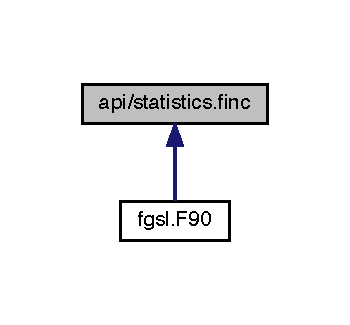
\includegraphics[width=168pt]{statistics_8finc__dep__incl}
\end{center}
\end{figure}
\subsection*{Functions/\-Subroutines}
\begin{DoxyCompactItemize}
\item 
real(fgsl\-\_\-double) function \hyperlink{statistics_8finc_a13ad6bf10a4daeba24e77b90512a2e04}{fgsl\-\_\-stats\-\_\-mean} (data, stride, n)
\item 
real(fgsl\-\_\-double) function \hyperlink{statistics_8finc_abd5a6101ce9b7e8278e6b9843c92e121}{fgsl\-\_\-stats\-\_\-variance} (data, stride, n)
\item 
real(fgsl\-\_\-double) function \hyperlink{statistics_8finc_a82ebcf08a4a62d8acd2cd4516e655092}{fgsl\-\_\-stats\-\_\-variance\-\_\-m} (data, stride, n, mean)
\item 
real(fgsl\-\_\-double) function \hyperlink{statistics_8finc_ad6a8382d4b0eaf033302a684a19c48d7}{fgsl\-\_\-stats\-\_\-sd} (data, stride, n)
\item 
real(fgsl\-\_\-double) function \hyperlink{statistics_8finc_a2b705cc724e72bbfaab255052b08b4aa}{fgsl\-\_\-stats\-\_\-sd\-\_\-m} (data, stride, n, mean)
\item 
real(fgsl\-\_\-double) function \hyperlink{statistics_8finc_a6b816113373329675a28ef28d833fda2}{fgsl\-\_\-stats\-\_\-variance\-\_\-with\-\_\-fixed\-\_\-mean} (data, stride, n, mean)
\item 
real(fgsl\-\_\-double) function \hyperlink{statistics_8finc_a940f39032c1dcf2fc8ec83114169ded5}{fgsl\-\_\-stats\-\_\-sd\-\_\-with\-\_\-fixed\-\_\-mean} (data, stride, n, mean)
\item 
real(fgsl\-\_\-double) function \hyperlink{statistics_8finc_a63ca760a17cd6d3109ff5cfd2c0c0fc1}{fgsl\-\_\-stats\-\_\-absdev} (data, stride, n)
\item 
real(fgsl\-\_\-double) function \hyperlink{statistics_8finc_a776af1d0102b9c73f4839963012a066f}{fgsl\-\_\-stats\-\_\-absdev\-\_\-m} (data, stride, n, mean)
\item 
real(fgsl\-\_\-double) function \hyperlink{statistics_8finc_afa3dfb29e31d3a70b48eb755419ff252}{fgsl\-\_\-stats\-\_\-skew} (data, stride, n)
\item 
real(fgsl\-\_\-double) function \hyperlink{statistics_8finc_abe7a2765433ae6d8d5b01871079bc214}{fgsl\-\_\-stats\-\_\-skew\-\_\-m\-\_\-sd} (data, stride, n, mean, sd)
\item 
real(fgsl\-\_\-double) function \hyperlink{statistics_8finc_ab717a41e26eca4a329a3b1ba8ad49e36}{fgsl\-\_\-stats\-\_\-kurtosis} (data, stride, n)
\item 
real(fgsl\-\_\-double) function \hyperlink{statistics_8finc_a73f37fa7fc26bbc32b2ec4f430ff4237}{fgsl\-\_\-stats\-\_\-kurtosis\-\_\-m\-\_\-sd} (data, stride, n, mean, sd)
\item 
real(fgsl\-\_\-double) function \hyperlink{statistics_8finc_aec9e1868404363cdd4071d759452dffa}{fgsl\-\_\-stats\-\_\-lag1\-\_\-autocorrelation} (data, stride, n)
\item 
real(fgsl\-\_\-double) function \hyperlink{statistics_8finc_ab2de33bfbff99ba0e1519a92ffc2a198}{fgsl\-\_\-stats\-\_\-lag1\-\_\-autocorrelation\-\_\-m} (data, stride, n, mean)
\item 
real(fgsl\-\_\-double) function \hyperlink{statistics_8finc_abe8b984e22ce9662518b3058c5ed3fc9}{fgsl\-\_\-stats\-\_\-covariance} (data1, stride1, data2, stride2, n)
\item 
real(fgsl\-\_\-double) function \hyperlink{statistics_8finc_a022a3337d746efe8ba47bb7b790978a9}{fgsl\-\_\-stats\-\_\-covariance\-\_\-m} (data1, stride1, data2, stride2, n, mean1, mean2)
\item 
real(fgsl\-\_\-double) function \hyperlink{statistics_8finc_ad641fcad25f9ad39af269073822f3700}{fgsl\-\_\-stats\-\_\-correlation} (data1, stride1, data2, stride2, n)
\item 
real(fgsl\-\_\-double) function \hyperlink{statistics_8finc_ad2978bbd93b93ac7bb5e47373546bbd6}{fgsl\-\_\-stats\-\_\-spearman} (data1, stride1, data2, stride2, n, work)
\item 
real(fgsl\-\_\-double) function \hyperlink{statistics_8finc_ac44e8f61b5d6ece8de2c7859c7324df9}{fgsl\-\_\-stats\-\_\-wmean} (w, wstride, data, stride, n)
\item 
real(fgsl\-\_\-double) function \hyperlink{statistics_8finc_a7369e6ff86c963b93045d041e0318b37}{fgsl\-\_\-stats\-\_\-wvariance} (w, wstride, data, stride, n)
\item 
real(fgsl\-\_\-double) function \hyperlink{statistics_8finc_a58b0acc505557f72f2cfc2813e945666}{fgsl\-\_\-stats\-\_\-wvariance\-\_\-m} (w, wstride, data, stride, n, mean)
\item 
real(fgsl\-\_\-double) function \hyperlink{statistics_8finc_a07bed243844c213b933de5274daa9116}{fgsl\-\_\-stats\-\_\-wsd} (w, wstride, data, stride, n)
\item 
real(fgsl\-\_\-double) function \hyperlink{statistics_8finc_a9be620d1825095d70f5a3eb93f1e8304}{fgsl\-\_\-stats\-\_\-wsd\-\_\-m} (w, wstride, data, stride, n, mean)
\item 
real(fgsl\-\_\-double) function \hyperlink{statistics_8finc_a6106f2ae69fddefef4d5e233e54a8df0}{fgsl\-\_\-stats\-\_\-wvariance\-\_\-with\-\_\-fixed\-\_\-mean} (w, wstride, data, stride, n, mean)
\item 
real(fgsl\-\_\-double) function \hyperlink{statistics_8finc_af3b6967068ce44444a8278bff7faddb0}{fgsl\-\_\-stats\-\_\-wsd\-\_\-with\-\_\-fixed\-\_\-mean} (w, wstride, data, stride, n, mean)
\item 
real(fgsl\-\_\-double) function \hyperlink{statistics_8finc_afcfaf0a75c6ace9379598604ff9b43a2}{fgsl\-\_\-stats\-\_\-wabsdev} (w, wstride, data, stride, n)
\item 
real(fgsl\-\_\-double) function \hyperlink{statistics_8finc_afa3b19f786f2175102a537cb331bc106}{fgsl\-\_\-stats\-\_\-wabsdev\-\_\-m} (w, wstride, data, stride, n, mean)
\item 
real(fgsl\-\_\-double) function \hyperlink{statistics_8finc_a0b7db46a9119ac52cf72617363432d06}{fgsl\-\_\-stats\-\_\-wskew} (w, wstride, data, stride, n)
\item 
real(fgsl\-\_\-double) function \hyperlink{statistics_8finc_af0bb94b056828ffa447fabaf8063709d}{fgsl\-\_\-stats\-\_\-wskew\-\_\-m\-\_\-sd} (w, wstride, data, stride, n, mean, sd)
\item 
real(fgsl\-\_\-double) function \hyperlink{statistics_8finc_ae618234938730cd9600050ccf92948b2}{fgsl\-\_\-stats\-\_\-wkurtosis} (w, wstride, data, stride, n)
\item 
real(fgsl\-\_\-double) function \hyperlink{statistics_8finc_a87a18e52ff4740838de69e55f3104845}{fgsl\-\_\-stats\-\_\-wkurtosis\-\_\-m\-\_\-sd} (w, wstride, data, stride, n, mean, sd)
\item 
real(fgsl\-\_\-double) function \hyperlink{statistics_8finc_acd520fe9c06f6a23888dd0ed36579cde}{fgsl\-\_\-stats\-\_\-max} (data, stride, n)
\item 
real(fgsl\-\_\-double) function \hyperlink{statistics_8finc_a7f2c953b9cd6539cbb324ba19040a590}{fgsl\-\_\-stats\-\_\-min} (data, stride, n)
\item 
subroutine \hyperlink{statistics_8finc_aafd29d9a05b0e4bd19f0b7a8dc420ef4}{fgsl\-\_\-stats\-\_\-minmax} (min, max, data, stride, n)
\item 
integer(fgsl\-\_\-size\-\_\-t) function \hyperlink{statistics_8finc_a1e72fff24ca3d2df17beaf579d12c450}{fgsl\-\_\-stats\-\_\-max\-\_\-index} (data, stride, n)
\item 
integer(fgsl\-\_\-size\-\_\-t) function \hyperlink{statistics_8finc_a24e500a11c59d3ec7bb0ce2f61b4f649}{fgsl\-\_\-stats\-\_\-min\-\_\-index} (data, stride, n)
\item 
subroutine \hyperlink{statistics_8finc_add4224c7bb957c91f26f69441bf81190}{fgsl\-\_\-stats\-\_\-minmax\-\_\-index} (min\-\_\-index, max\-\_\-index, data, stride, n)
\item 
real(fgsl\-\_\-double) function \hyperlink{statistics_8finc_a8dbecd85911d5151cd08f93e7510cf6c}{fgsl\-\_\-stats\-\_\-median\-\_\-from\-\_\-sorted\-\_\-data} (data, stride, n)
\item 
real(fgsl\-\_\-double) function \hyperlink{statistics_8finc_acedbc5cc1b4c8b4389c5011d15e75122}{fgsl\-\_\-stats\-\_\-quantile\-\_\-from\-\_\-sorted\-\_\-data} (data, stride, n, f)
\end{DoxyCompactItemize}


\subsection{Function/\-Subroutine Documentation}
\hypertarget{statistics_8finc_a63ca760a17cd6d3109ff5cfd2c0c0fc1}{\index{statistics.\-finc@{statistics.\-finc}!fgsl\-\_\-stats\-\_\-absdev@{fgsl\-\_\-stats\-\_\-absdev}}
\index{fgsl\-\_\-stats\-\_\-absdev@{fgsl\-\_\-stats\-\_\-absdev}!statistics.finc@{statistics.\-finc}}
\subsubsection[{fgsl\-\_\-stats\-\_\-absdev}]{\setlength{\rightskip}{0pt plus 5cm}real(fgsl\-\_\-double) function fgsl\-\_\-stats\-\_\-absdev (
\begin{DoxyParamCaption}
\item[{real(fgsl\-\_\-double), dimension(\-:), intent(in)}]{data, }
\item[{integer(fgsl\-\_\-size\-\_\-t), intent(in)}]{stride, }
\item[{integer(fgsl\-\_\-size\-\_\-t), intent(in)}]{n}
\end{DoxyParamCaption}
)}}\label{statistics_8finc_a63ca760a17cd6d3109ff5cfd2c0c0fc1}
\hypertarget{statistics_8finc_a776af1d0102b9c73f4839963012a066f}{\index{statistics.\-finc@{statistics.\-finc}!fgsl\-\_\-stats\-\_\-absdev\-\_\-m@{fgsl\-\_\-stats\-\_\-absdev\-\_\-m}}
\index{fgsl\-\_\-stats\-\_\-absdev\-\_\-m@{fgsl\-\_\-stats\-\_\-absdev\-\_\-m}!statistics.finc@{statistics.\-finc}}
\subsubsection[{fgsl\-\_\-stats\-\_\-absdev\-\_\-m}]{\setlength{\rightskip}{0pt plus 5cm}real(fgsl\-\_\-double) function fgsl\-\_\-stats\-\_\-absdev\-\_\-m (
\begin{DoxyParamCaption}
\item[{real(fgsl\-\_\-double), dimension(\-:), intent(in)}]{data, }
\item[{integer(fgsl\-\_\-size\-\_\-t), intent(in)}]{stride, }
\item[{integer(fgsl\-\_\-size\-\_\-t), intent(in)}]{n, }
\item[{real(fgsl\-\_\-double), intent(in)}]{mean}
\end{DoxyParamCaption}
)}}\label{statistics_8finc_a776af1d0102b9c73f4839963012a066f}
\hypertarget{statistics_8finc_ad641fcad25f9ad39af269073822f3700}{\index{statistics.\-finc@{statistics.\-finc}!fgsl\-\_\-stats\-\_\-correlation@{fgsl\-\_\-stats\-\_\-correlation}}
\index{fgsl\-\_\-stats\-\_\-correlation@{fgsl\-\_\-stats\-\_\-correlation}!statistics.finc@{statistics.\-finc}}
\subsubsection[{fgsl\-\_\-stats\-\_\-correlation}]{\setlength{\rightskip}{0pt plus 5cm}real(fgsl\-\_\-double) function fgsl\-\_\-stats\-\_\-correlation (
\begin{DoxyParamCaption}
\item[{real(fgsl\-\_\-double), dimension(\-:), intent(in)}]{data1, }
\item[{integer(fgsl\-\_\-size\-\_\-t), intent(in)}]{stride1, }
\item[{real(fgsl\-\_\-double), dimension(\-:), intent(in)}]{data2, }
\item[{integer(fgsl\-\_\-size\-\_\-t), intent(in)}]{stride2, }
\item[{integer(fgsl\-\_\-size\-\_\-t), intent(in)}]{n}
\end{DoxyParamCaption}
)}}\label{statistics_8finc_ad641fcad25f9ad39af269073822f3700}
\hypertarget{statistics_8finc_abe8b984e22ce9662518b3058c5ed3fc9}{\index{statistics.\-finc@{statistics.\-finc}!fgsl\-\_\-stats\-\_\-covariance@{fgsl\-\_\-stats\-\_\-covariance}}
\index{fgsl\-\_\-stats\-\_\-covariance@{fgsl\-\_\-stats\-\_\-covariance}!statistics.finc@{statistics.\-finc}}
\subsubsection[{fgsl\-\_\-stats\-\_\-covariance}]{\setlength{\rightskip}{0pt plus 5cm}real(fgsl\-\_\-double) function fgsl\-\_\-stats\-\_\-covariance (
\begin{DoxyParamCaption}
\item[{real(fgsl\-\_\-double), dimension(\-:), intent(in)}]{data1, }
\item[{integer(fgsl\-\_\-size\-\_\-t), intent(in)}]{stride1, }
\item[{real(fgsl\-\_\-double), dimension(\-:), intent(in)}]{data2, }
\item[{integer(fgsl\-\_\-size\-\_\-t), intent(in)}]{stride2, }
\item[{integer(fgsl\-\_\-size\-\_\-t), intent(in)}]{n}
\end{DoxyParamCaption}
)}}\label{statistics_8finc_abe8b984e22ce9662518b3058c5ed3fc9}
\hypertarget{statistics_8finc_a022a3337d746efe8ba47bb7b790978a9}{\index{statistics.\-finc@{statistics.\-finc}!fgsl\-\_\-stats\-\_\-covariance\-\_\-m@{fgsl\-\_\-stats\-\_\-covariance\-\_\-m}}
\index{fgsl\-\_\-stats\-\_\-covariance\-\_\-m@{fgsl\-\_\-stats\-\_\-covariance\-\_\-m}!statistics.finc@{statistics.\-finc}}
\subsubsection[{fgsl\-\_\-stats\-\_\-covariance\-\_\-m}]{\setlength{\rightskip}{0pt plus 5cm}real(fgsl\-\_\-double) function fgsl\-\_\-stats\-\_\-covariance\-\_\-m (
\begin{DoxyParamCaption}
\item[{real(fgsl\-\_\-double), dimension(\-:), intent(in)}]{data1, }
\item[{integer(fgsl\-\_\-size\-\_\-t), intent(in)}]{stride1, }
\item[{real(fgsl\-\_\-double), dimension(\-:), intent(in)}]{data2, }
\item[{integer(fgsl\-\_\-size\-\_\-t), intent(in)}]{stride2, }
\item[{integer(fgsl\-\_\-size\-\_\-t), intent(in)}]{n, }
\item[{real(fgsl\-\_\-double), intent(in)}]{mean1, }
\item[{real(fgsl\-\_\-double), intent(in)}]{mean2}
\end{DoxyParamCaption}
)}}\label{statistics_8finc_a022a3337d746efe8ba47bb7b790978a9}
\hypertarget{statistics_8finc_ab717a41e26eca4a329a3b1ba8ad49e36}{\index{statistics.\-finc@{statistics.\-finc}!fgsl\-\_\-stats\-\_\-kurtosis@{fgsl\-\_\-stats\-\_\-kurtosis}}
\index{fgsl\-\_\-stats\-\_\-kurtosis@{fgsl\-\_\-stats\-\_\-kurtosis}!statistics.finc@{statistics.\-finc}}
\subsubsection[{fgsl\-\_\-stats\-\_\-kurtosis}]{\setlength{\rightskip}{0pt plus 5cm}real(fgsl\-\_\-double) function fgsl\-\_\-stats\-\_\-kurtosis (
\begin{DoxyParamCaption}
\item[{real(fgsl\-\_\-double), dimension(\-:), intent(in)}]{data, }
\item[{integer(fgsl\-\_\-size\-\_\-t), intent(in)}]{stride, }
\item[{integer(fgsl\-\_\-size\-\_\-t), intent(in)}]{n}
\end{DoxyParamCaption}
)}}\label{statistics_8finc_ab717a41e26eca4a329a3b1ba8ad49e36}
\hypertarget{statistics_8finc_a73f37fa7fc26bbc32b2ec4f430ff4237}{\index{statistics.\-finc@{statistics.\-finc}!fgsl\-\_\-stats\-\_\-kurtosis\-\_\-m\-\_\-sd@{fgsl\-\_\-stats\-\_\-kurtosis\-\_\-m\-\_\-sd}}
\index{fgsl\-\_\-stats\-\_\-kurtosis\-\_\-m\-\_\-sd@{fgsl\-\_\-stats\-\_\-kurtosis\-\_\-m\-\_\-sd}!statistics.finc@{statistics.\-finc}}
\subsubsection[{fgsl\-\_\-stats\-\_\-kurtosis\-\_\-m\-\_\-sd}]{\setlength{\rightskip}{0pt plus 5cm}real(fgsl\-\_\-double) function fgsl\-\_\-stats\-\_\-kurtosis\-\_\-m\-\_\-sd (
\begin{DoxyParamCaption}
\item[{real(fgsl\-\_\-double), dimension(\-:), intent(in)}]{data, }
\item[{integer(fgsl\-\_\-size\-\_\-t), intent(in)}]{stride, }
\item[{integer(fgsl\-\_\-size\-\_\-t), intent(in)}]{n, }
\item[{real(fgsl\-\_\-double), intent(in)}]{mean, }
\item[{real(fgsl\-\_\-double), intent(in)}]{sd}
\end{DoxyParamCaption}
)}}\label{statistics_8finc_a73f37fa7fc26bbc32b2ec4f430ff4237}
\hypertarget{statistics_8finc_aec9e1868404363cdd4071d759452dffa}{\index{statistics.\-finc@{statistics.\-finc}!fgsl\-\_\-stats\-\_\-lag1\-\_\-autocorrelation@{fgsl\-\_\-stats\-\_\-lag1\-\_\-autocorrelation}}
\index{fgsl\-\_\-stats\-\_\-lag1\-\_\-autocorrelation@{fgsl\-\_\-stats\-\_\-lag1\-\_\-autocorrelation}!statistics.finc@{statistics.\-finc}}
\subsubsection[{fgsl\-\_\-stats\-\_\-lag1\-\_\-autocorrelation}]{\setlength{\rightskip}{0pt plus 5cm}real(fgsl\-\_\-double) function fgsl\-\_\-stats\-\_\-lag1\-\_\-autocorrelation (
\begin{DoxyParamCaption}
\item[{real(fgsl\-\_\-double), dimension(\-:), intent(in)}]{data, }
\item[{integer(fgsl\-\_\-size\-\_\-t), intent(in)}]{stride, }
\item[{integer(fgsl\-\_\-size\-\_\-t), intent(in)}]{n}
\end{DoxyParamCaption}
)}}\label{statistics_8finc_aec9e1868404363cdd4071d759452dffa}
\hypertarget{statistics_8finc_ab2de33bfbff99ba0e1519a92ffc2a198}{\index{statistics.\-finc@{statistics.\-finc}!fgsl\-\_\-stats\-\_\-lag1\-\_\-autocorrelation\-\_\-m@{fgsl\-\_\-stats\-\_\-lag1\-\_\-autocorrelation\-\_\-m}}
\index{fgsl\-\_\-stats\-\_\-lag1\-\_\-autocorrelation\-\_\-m@{fgsl\-\_\-stats\-\_\-lag1\-\_\-autocorrelation\-\_\-m}!statistics.finc@{statistics.\-finc}}
\subsubsection[{fgsl\-\_\-stats\-\_\-lag1\-\_\-autocorrelation\-\_\-m}]{\setlength{\rightskip}{0pt plus 5cm}real(fgsl\-\_\-double) function fgsl\-\_\-stats\-\_\-lag1\-\_\-autocorrelation\-\_\-m (
\begin{DoxyParamCaption}
\item[{real(fgsl\-\_\-double), dimension(\-:), intent(in)}]{data, }
\item[{integer(fgsl\-\_\-size\-\_\-t), intent(in)}]{stride, }
\item[{integer(fgsl\-\_\-size\-\_\-t), intent(in)}]{n, }
\item[{real(fgsl\-\_\-double), intent(in)}]{mean}
\end{DoxyParamCaption}
)}}\label{statistics_8finc_ab2de33bfbff99ba0e1519a92ffc2a198}
\hypertarget{statistics_8finc_acd520fe9c06f6a23888dd0ed36579cde}{\index{statistics.\-finc@{statistics.\-finc}!fgsl\-\_\-stats\-\_\-max@{fgsl\-\_\-stats\-\_\-max}}
\index{fgsl\-\_\-stats\-\_\-max@{fgsl\-\_\-stats\-\_\-max}!statistics.finc@{statistics.\-finc}}
\subsubsection[{fgsl\-\_\-stats\-\_\-max}]{\setlength{\rightskip}{0pt plus 5cm}real(fgsl\-\_\-double) function fgsl\-\_\-stats\-\_\-max (
\begin{DoxyParamCaption}
\item[{real(fgsl\-\_\-double), dimension(\-:), intent(in)}]{data, }
\item[{integer(fgsl\-\_\-size\-\_\-t), intent(in)}]{stride, }
\item[{integer(fgsl\-\_\-size\-\_\-t), intent(in)}]{n}
\end{DoxyParamCaption}
)}}\label{statistics_8finc_acd520fe9c06f6a23888dd0ed36579cde}
\hypertarget{statistics_8finc_a1e72fff24ca3d2df17beaf579d12c450}{\index{statistics.\-finc@{statistics.\-finc}!fgsl\-\_\-stats\-\_\-max\-\_\-index@{fgsl\-\_\-stats\-\_\-max\-\_\-index}}
\index{fgsl\-\_\-stats\-\_\-max\-\_\-index@{fgsl\-\_\-stats\-\_\-max\-\_\-index}!statistics.finc@{statistics.\-finc}}
\subsubsection[{fgsl\-\_\-stats\-\_\-max\-\_\-index}]{\setlength{\rightskip}{0pt plus 5cm}integer(fgsl\-\_\-size\-\_\-t) function fgsl\-\_\-stats\-\_\-max\-\_\-index (
\begin{DoxyParamCaption}
\item[{real(fgsl\-\_\-double), dimension(\-:), intent(in)}]{data, }
\item[{integer(fgsl\-\_\-size\-\_\-t), intent(in)}]{stride, }
\item[{integer(fgsl\-\_\-size\-\_\-t), intent(in)}]{n}
\end{DoxyParamCaption}
)}}\label{statistics_8finc_a1e72fff24ca3d2df17beaf579d12c450}
\hypertarget{statistics_8finc_a13ad6bf10a4daeba24e77b90512a2e04}{\index{statistics.\-finc@{statistics.\-finc}!fgsl\-\_\-stats\-\_\-mean@{fgsl\-\_\-stats\-\_\-mean}}
\index{fgsl\-\_\-stats\-\_\-mean@{fgsl\-\_\-stats\-\_\-mean}!statistics.finc@{statistics.\-finc}}
\subsubsection[{fgsl\-\_\-stats\-\_\-mean}]{\setlength{\rightskip}{0pt plus 5cm}real(fgsl\-\_\-double) function fgsl\-\_\-stats\-\_\-mean (
\begin{DoxyParamCaption}
\item[{real(fgsl\-\_\-double), dimension(\-:), intent(in)}]{data, }
\item[{integer(fgsl\-\_\-size\-\_\-t), intent(in)}]{stride, }
\item[{integer(fgsl\-\_\-size\-\_\-t), intent(in)}]{n}
\end{DoxyParamCaption}
)}}\label{statistics_8finc_a13ad6bf10a4daeba24e77b90512a2e04}
\hypertarget{statistics_8finc_a8dbecd85911d5151cd08f93e7510cf6c}{\index{statistics.\-finc@{statistics.\-finc}!fgsl\-\_\-stats\-\_\-median\-\_\-from\-\_\-sorted\-\_\-data@{fgsl\-\_\-stats\-\_\-median\-\_\-from\-\_\-sorted\-\_\-data}}
\index{fgsl\-\_\-stats\-\_\-median\-\_\-from\-\_\-sorted\-\_\-data@{fgsl\-\_\-stats\-\_\-median\-\_\-from\-\_\-sorted\-\_\-data}!statistics.finc@{statistics.\-finc}}
\subsubsection[{fgsl\-\_\-stats\-\_\-median\-\_\-from\-\_\-sorted\-\_\-data}]{\setlength{\rightskip}{0pt plus 5cm}real(fgsl\-\_\-double) function fgsl\-\_\-stats\-\_\-median\-\_\-from\-\_\-sorted\-\_\-data (
\begin{DoxyParamCaption}
\item[{real(fgsl\-\_\-double), dimension(\-:), intent(in)}]{data, }
\item[{integer(fgsl\-\_\-size\-\_\-t), intent(in)}]{stride, }
\item[{integer(fgsl\-\_\-size\-\_\-t), intent(in)}]{n}
\end{DoxyParamCaption}
)}}\label{statistics_8finc_a8dbecd85911d5151cd08f93e7510cf6c}
\hypertarget{statistics_8finc_a7f2c953b9cd6539cbb324ba19040a590}{\index{statistics.\-finc@{statistics.\-finc}!fgsl\-\_\-stats\-\_\-min@{fgsl\-\_\-stats\-\_\-min}}
\index{fgsl\-\_\-stats\-\_\-min@{fgsl\-\_\-stats\-\_\-min}!statistics.finc@{statistics.\-finc}}
\subsubsection[{fgsl\-\_\-stats\-\_\-min}]{\setlength{\rightskip}{0pt plus 5cm}real(fgsl\-\_\-double) function fgsl\-\_\-stats\-\_\-min (
\begin{DoxyParamCaption}
\item[{real(fgsl\-\_\-double), dimension(\-:), intent(in)}]{data, }
\item[{integer(fgsl\-\_\-size\-\_\-t), intent(in)}]{stride, }
\item[{integer(fgsl\-\_\-size\-\_\-t), intent(in)}]{n}
\end{DoxyParamCaption}
)}}\label{statistics_8finc_a7f2c953b9cd6539cbb324ba19040a590}
\hypertarget{statistics_8finc_a24e500a11c59d3ec7bb0ce2f61b4f649}{\index{statistics.\-finc@{statistics.\-finc}!fgsl\-\_\-stats\-\_\-min\-\_\-index@{fgsl\-\_\-stats\-\_\-min\-\_\-index}}
\index{fgsl\-\_\-stats\-\_\-min\-\_\-index@{fgsl\-\_\-stats\-\_\-min\-\_\-index}!statistics.finc@{statistics.\-finc}}
\subsubsection[{fgsl\-\_\-stats\-\_\-min\-\_\-index}]{\setlength{\rightskip}{0pt plus 5cm}integer(fgsl\-\_\-size\-\_\-t) function fgsl\-\_\-stats\-\_\-min\-\_\-index (
\begin{DoxyParamCaption}
\item[{real(fgsl\-\_\-double), dimension(\-:), intent(in)}]{data, }
\item[{integer(fgsl\-\_\-size\-\_\-t), intent(in)}]{stride, }
\item[{integer(fgsl\-\_\-size\-\_\-t), intent(in)}]{n}
\end{DoxyParamCaption}
)}}\label{statistics_8finc_a24e500a11c59d3ec7bb0ce2f61b4f649}
\hypertarget{statistics_8finc_aafd29d9a05b0e4bd19f0b7a8dc420ef4}{\index{statistics.\-finc@{statistics.\-finc}!fgsl\-\_\-stats\-\_\-minmax@{fgsl\-\_\-stats\-\_\-minmax}}
\index{fgsl\-\_\-stats\-\_\-minmax@{fgsl\-\_\-stats\-\_\-minmax}!statistics.finc@{statistics.\-finc}}
\subsubsection[{fgsl\-\_\-stats\-\_\-minmax}]{\setlength{\rightskip}{0pt plus 5cm}subroutine fgsl\-\_\-stats\-\_\-minmax (
\begin{DoxyParamCaption}
\item[{real(fgsl\-\_\-double), intent(out)}]{min, }
\item[{real(fgsl\-\_\-double), intent(out)}]{max, }
\item[{real(fgsl\-\_\-double), dimension(\-:), intent(in)}]{data, }
\item[{integer(fgsl\-\_\-size\-\_\-t), intent(in)}]{stride, }
\item[{integer(fgsl\-\_\-size\-\_\-t), intent(in)}]{n}
\end{DoxyParamCaption}
)}}\label{statistics_8finc_aafd29d9a05b0e4bd19f0b7a8dc420ef4}
\hypertarget{statistics_8finc_add4224c7bb957c91f26f69441bf81190}{\index{statistics.\-finc@{statistics.\-finc}!fgsl\-\_\-stats\-\_\-minmax\-\_\-index@{fgsl\-\_\-stats\-\_\-minmax\-\_\-index}}
\index{fgsl\-\_\-stats\-\_\-minmax\-\_\-index@{fgsl\-\_\-stats\-\_\-minmax\-\_\-index}!statistics.finc@{statistics.\-finc}}
\subsubsection[{fgsl\-\_\-stats\-\_\-minmax\-\_\-index}]{\setlength{\rightskip}{0pt plus 5cm}subroutine fgsl\-\_\-stats\-\_\-minmax\-\_\-index (
\begin{DoxyParamCaption}
\item[{integer(fgsl\-\_\-size\-\_\-t), intent(out)}]{min\-\_\-index, }
\item[{integer(fgsl\-\_\-size\-\_\-t), intent(out)}]{max\-\_\-index, }
\item[{real(fgsl\-\_\-double), dimension(\-:), intent(in)}]{data, }
\item[{integer(fgsl\-\_\-size\-\_\-t), intent(in)}]{stride, }
\item[{integer(fgsl\-\_\-size\-\_\-t), intent(in)}]{n}
\end{DoxyParamCaption}
)}}\label{statistics_8finc_add4224c7bb957c91f26f69441bf81190}
\hypertarget{statistics_8finc_acedbc5cc1b4c8b4389c5011d15e75122}{\index{statistics.\-finc@{statistics.\-finc}!fgsl\-\_\-stats\-\_\-quantile\-\_\-from\-\_\-sorted\-\_\-data@{fgsl\-\_\-stats\-\_\-quantile\-\_\-from\-\_\-sorted\-\_\-data}}
\index{fgsl\-\_\-stats\-\_\-quantile\-\_\-from\-\_\-sorted\-\_\-data@{fgsl\-\_\-stats\-\_\-quantile\-\_\-from\-\_\-sorted\-\_\-data}!statistics.finc@{statistics.\-finc}}
\subsubsection[{fgsl\-\_\-stats\-\_\-quantile\-\_\-from\-\_\-sorted\-\_\-data}]{\setlength{\rightskip}{0pt plus 5cm}real(fgsl\-\_\-double) function fgsl\-\_\-stats\-\_\-quantile\-\_\-from\-\_\-sorted\-\_\-data (
\begin{DoxyParamCaption}
\item[{real(fgsl\-\_\-double), dimension(\-:), intent(in)}]{data, }
\item[{integer(fgsl\-\_\-size\-\_\-t), intent(in)}]{stride, }
\item[{integer(fgsl\-\_\-size\-\_\-t), intent(in)}]{n, }
\item[{real(fgsl\-\_\-double), intent(in)}]{f}
\end{DoxyParamCaption}
)}}\label{statistics_8finc_acedbc5cc1b4c8b4389c5011d15e75122}
\hypertarget{statistics_8finc_ad6a8382d4b0eaf033302a684a19c48d7}{\index{statistics.\-finc@{statistics.\-finc}!fgsl\-\_\-stats\-\_\-sd@{fgsl\-\_\-stats\-\_\-sd}}
\index{fgsl\-\_\-stats\-\_\-sd@{fgsl\-\_\-stats\-\_\-sd}!statistics.finc@{statistics.\-finc}}
\subsubsection[{fgsl\-\_\-stats\-\_\-sd}]{\setlength{\rightskip}{0pt plus 5cm}real(fgsl\-\_\-double) function fgsl\-\_\-stats\-\_\-sd (
\begin{DoxyParamCaption}
\item[{real(fgsl\-\_\-double), dimension(\-:), intent(in)}]{data, }
\item[{integer(fgsl\-\_\-size\-\_\-t), intent(in)}]{stride, }
\item[{integer(fgsl\-\_\-size\-\_\-t), intent(in)}]{n}
\end{DoxyParamCaption}
)}}\label{statistics_8finc_ad6a8382d4b0eaf033302a684a19c48d7}
\hypertarget{statistics_8finc_a2b705cc724e72bbfaab255052b08b4aa}{\index{statistics.\-finc@{statistics.\-finc}!fgsl\-\_\-stats\-\_\-sd\-\_\-m@{fgsl\-\_\-stats\-\_\-sd\-\_\-m}}
\index{fgsl\-\_\-stats\-\_\-sd\-\_\-m@{fgsl\-\_\-stats\-\_\-sd\-\_\-m}!statistics.finc@{statistics.\-finc}}
\subsubsection[{fgsl\-\_\-stats\-\_\-sd\-\_\-m}]{\setlength{\rightskip}{0pt plus 5cm}real(fgsl\-\_\-double) function fgsl\-\_\-stats\-\_\-sd\-\_\-m (
\begin{DoxyParamCaption}
\item[{real(fgsl\-\_\-double), dimension(\-:), intent(in)}]{data, }
\item[{integer(fgsl\-\_\-size\-\_\-t), intent(in)}]{stride, }
\item[{integer(fgsl\-\_\-size\-\_\-t), intent(in)}]{n, }
\item[{real(fgsl\-\_\-double), intent(in)}]{mean}
\end{DoxyParamCaption}
)}}\label{statistics_8finc_a2b705cc724e72bbfaab255052b08b4aa}
\hypertarget{statistics_8finc_a940f39032c1dcf2fc8ec83114169ded5}{\index{statistics.\-finc@{statistics.\-finc}!fgsl\-\_\-stats\-\_\-sd\-\_\-with\-\_\-fixed\-\_\-mean@{fgsl\-\_\-stats\-\_\-sd\-\_\-with\-\_\-fixed\-\_\-mean}}
\index{fgsl\-\_\-stats\-\_\-sd\-\_\-with\-\_\-fixed\-\_\-mean@{fgsl\-\_\-stats\-\_\-sd\-\_\-with\-\_\-fixed\-\_\-mean}!statistics.finc@{statistics.\-finc}}
\subsubsection[{fgsl\-\_\-stats\-\_\-sd\-\_\-with\-\_\-fixed\-\_\-mean}]{\setlength{\rightskip}{0pt plus 5cm}real(fgsl\-\_\-double) function fgsl\-\_\-stats\-\_\-sd\-\_\-with\-\_\-fixed\-\_\-mean (
\begin{DoxyParamCaption}
\item[{real(fgsl\-\_\-double), dimension(\-:), intent(in)}]{data, }
\item[{integer(fgsl\-\_\-size\-\_\-t), intent(in)}]{stride, }
\item[{integer(fgsl\-\_\-size\-\_\-t), intent(in)}]{n, }
\item[{real(fgsl\-\_\-double), intent(in)}]{mean}
\end{DoxyParamCaption}
)}}\label{statistics_8finc_a940f39032c1dcf2fc8ec83114169ded5}
\hypertarget{statistics_8finc_afa3dfb29e31d3a70b48eb755419ff252}{\index{statistics.\-finc@{statistics.\-finc}!fgsl\-\_\-stats\-\_\-skew@{fgsl\-\_\-stats\-\_\-skew}}
\index{fgsl\-\_\-stats\-\_\-skew@{fgsl\-\_\-stats\-\_\-skew}!statistics.finc@{statistics.\-finc}}
\subsubsection[{fgsl\-\_\-stats\-\_\-skew}]{\setlength{\rightskip}{0pt plus 5cm}real(fgsl\-\_\-double) function fgsl\-\_\-stats\-\_\-skew (
\begin{DoxyParamCaption}
\item[{real(fgsl\-\_\-double), dimension(\-:), intent(in)}]{data, }
\item[{integer(fgsl\-\_\-size\-\_\-t), intent(in)}]{stride, }
\item[{integer(fgsl\-\_\-size\-\_\-t), intent(in)}]{n}
\end{DoxyParamCaption}
)}}\label{statistics_8finc_afa3dfb29e31d3a70b48eb755419ff252}
\hypertarget{statistics_8finc_abe7a2765433ae6d8d5b01871079bc214}{\index{statistics.\-finc@{statistics.\-finc}!fgsl\-\_\-stats\-\_\-skew\-\_\-m\-\_\-sd@{fgsl\-\_\-stats\-\_\-skew\-\_\-m\-\_\-sd}}
\index{fgsl\-\_\-stats\-\_\-skew\-\_\-m\-\_\-sd@{fgsl\-\_\-stats\-\_\-skew\-\_\-m\-\_\-sd}!statistics.finc@{statistics.\-finc}}
\subsubsection[{fgsl\-\_\-stats\-\_\-skew\-\_\-m\-\_\-sd}]{\setlength{\rightskip}{0pt plus 5cm}real(fgsl\-\_\-double) function fgsl\-\_\-stats\-\_\-skew\-\_\-m\-\_\-sd (
\begin{DoxyParamCaption}
\item[{real(fgsl\-\_\-double), dimension(\-:), intent(in)}]{data, }
\item[{integer(fgsl\-\_\-size\-\_\-t), intent(in)}]{stride, }
\item[{integer(fgsl\-\_\-size\-\_\-t), intent(in)}]{n, }
\item[{real(fgsl\-\_\-double), intent(in)}]{mean, }
\item[{real(fgsl\-\_\-double), intent(in)}]{sd}
\end{DoxyParamCaption}
)}}\label{statistics_8finc_abe7a2765433ae6d8d5b01871079bc214}
\hypertarget{statistics_8finc_ad2978bbd93b93ac7bb5e47373546bbd6}{\index{statistics.\-finc@{statistics.\-finc}!fgsl\-\_\-stats\-\_\-spearman@{fgsl\-\_\-stats\-\_\-spearman}}
\index{fgsl\-\_\-stats\-\_\-spearman@{fgsl\-\_\-stats\-\_\-spearman}!statistics.finc@{statistics.\-finc}}
\subsubsection[{fgsl\-\_\-stats\-\_\-spearman}]{\setlength{\rightskip}{0pt plus 5cm}real(fgsl\-\_\-double) function fgsl\-\_\-stats\-\_\-spearman (
\begin{DoxyParamCaption}
\item[{real(fgsl\-\_\-double), dimension(\-:), intent(in)}]{data1, }
\item[{integer(fgsl\-\_\-size\-\_\-t), intent(in)}]{stride1, }
\item[{real(fgsl\-\_\-double), dimension(\-:), intent(in)}]{data2, }
\item[{integer(fgsl\-\_\-size\-\_\-t), intent(in)}]{stride2, }
\item[{integer(fgsl\-\_\-size\-\_\-t), intent(in)}]{n, }
\item[{real(fgsl\-\_\-double), dimension(\-:), intent(inout)}]{work}
\end{DoxyParamCaption}
)}}\label{statistics_8finc_ad2978bbd93b93ac7bb5e47373546bbd6}
\hypertarget{statistics_8finc_abd5a6101ce9b7e8278e6b9843c92e121}{\index{statistics.\-finc@{statistics.\-finc}!fgsl\-\_\-stats\-\_\-variance@{fgsl\-\_\-stats\-\_\-variance}}
\index{fgsl\-\_\-stats\-\_\-variance@{fgsl\-\_\-stats\-\_\-variance}!statistics.finc@{statistics.\-finc}}
\subsubsection[{fgsl\-\_\-stats\-\_\-variance}]{\setlength{\rightskip}{0pt plus 5cm}real(fgsl\-\_\-double) function fgsl\-\_\-stats\-\_\-variance (
\begin{DoxyParamCaption}
\item[{real(fgsl\-\_\-double), dimension(\-:), intent(in)}]{data, }
\item[{integer(fgsl\-\_\-size\-\_\-t), intent(in)}]{stride, }
\item[{integer(fgsl\-\_\-size\-\_\-t), intent(in)}]{n}
\end{DoxyParamCaption}
)}}\label{statistics_8finc_abd5a6101ce9b7e8278e6b9843c92e121}
\hypertarget{statistics_8finc_a82ebcf08a4a62d8acd2cd4516e655092}{\index{statistics.\-finc@{statistics.\-finc}!fgsl\-\_\-stats\-\_\-variance\-\_\-m@{fgsl\-\_\-stats\-\_\-variance\-\_\-m}}
\index{fgsl\-\_\-stats\-\_\-variance\-\_\-m@{fgsl\-\_\-stats\-\_\-variance\-\_\-m}!statistics.finc@{statistics.\-finc}}
\subsubsection[{fgsl\-\_\-stats\-\_\-variance\-\_\-m}]{\setlength{\rightskip}{0pt plus 5cm}real(fgsl\-\_\-double) function fgsl\-\_\-stats\-\_\-variance\-\_\-m (
\begin{DoxyParamCaption}
\item[{real(fgsl\-\_\-double), dimension(\-:), intent(in)}]{data, }
\item[{integer(fgsl\-\_\-size\-\_\-t), intent(in)}]{stride, }
\item[{integer(fgsl\-\_\-size\-\_\-t), intent(in)}]{n, }
\item[{real(fgsl\-\_\-double), intent(in)}]{mean}
\end{DoxyParamCaption}
)}}\label{statistics_8finc_a82ebcf08a4a62d8acd2cd4516e655092}
\hypertarget{statistics_8finc_a6b816113373329675a28ef28d833fda2}{\index{statistics.\-finc@{statistics.\-finc}!fgsl\-\_\-stats\-\_\-variance\-\_\-with\-\_\-fixed\-\_\-mean@{fgsl\-\_\-stats\-\_\-variance\-\_\-with\-\_\-fixed\-\_\-mean}}
\index{fgsl\-\_\-stats\-\_\-variance\-\_\-with\-\_\-fixed\-\_\-mean@{fgsl\-\_\-stats\-\_\-variance\-\_\-with\-\_\-fixed\-\_\-mean}!statistics.finc@{statistics.\-finc}}
\subsubsection[{fgsl\-\_\-stats\-\_\-variance\-\_\-with\-\_\-fixed\-\_\-mean}]{\setlength{\rightskip}{0pt plus 5cm}real(fgsl\-\_\-double) function fgsl\-\_\-stats\-\_\-variance\-\_\-with\-\_\-fixed\-\_\-mean (
\begin{DoxyParamCaption}
\item[{real(fgsl\-\_\-double), dimension(\-:), intent(in)}]{data, }
\item[{integer(fgsl\-\_\-size\-\_\-t), intent(in)}]{stride, }
\item[{integer(fgsl\-\_\-size\-\_\-t), intent(in)}]{n, }
\item[{real(fgsl\-\_\-double), intent(in)}]{mean}
\end{DoxyParamCaption}
)}}\label{statistics_8finc_a6b816113373329675a28ef28d833fda2}
\hypertarget{statistics_8finc_afcfaf0a75c6ace9379598604ff9b43a2}{\index{statistics.\-finc@{statistics.\-finc}!fgsl\-\_\-stats\-\_\-wabsdev@{fgsl\-\_\-stats\-\_\-wabsdev}}
\index{fgsl\-\_\-stats\-\_\-wabsdev@{fgsl\-\_\-stats\-\_\-wabsdev}!statistics.finc@{statistics.\-finc}}
\subsubsection[{fgsl\-\_\-stats\-\_\-wabsdev}]{\setlength{\rightskip}{0pt plus 5cm}real(fgsl\-\_\-double) function fgsl\-\_\-stats\-\_\-wabsdev (
\begin{DoxyParamCaption}
\item[{real(fgsl\-\_\-double), dimension(\-:), intent(in)}]{w, }
\item[{integer(fgsl\-\_\-size\-\_\-t), intent(in)}]{wstride, }
\item[{real(fgsl\-\_\-double), dimension(\-:), intent(in)}]{data, }
\item[{integer(fgsl\-\_\-size\-\_\-t), intent(in)}]{stride, }
\item[{integer(fgsl\-\_\-size\-\_\-t), intent(in)}]{n}
\end{DoxyParamCaption}
)}}\label{statistics_8finc_afcfaf0a75c6ace9379598604ff9b43a2}
\hypertarget{statistics_8finc_afa3b19f786f2175102a537cb331bc106}{\index{statistics.\-finc@{statistics.\-finc}!fgsl\-\_\-stats\-\_\-wabsdev\-\_\-m@{fgsl\-\_\-stats\-\_\-wabsdev\-\_\-m}}
\index{fgsl\-\_\-stats\-\_\-wabsdev\-\_\-m@{fgsl\-\_\-stats\-\_\-wabsdev\-\_\-m}!statistics.finc@{statistics.\-finc}}
\subsubsection[{fgsl\-\_\-stats\-\_\-wabsdev\-\_\-m}]{\setlength{\rightskip}{0pt plus 5cm}real(fgsl\-\_\-double) function fgsl\-\_\-stats\-\_\-wabsdev\-\_\-m (
\begin{DoxyParamCaption}
\item[{real(fgsl\-\_\-double), dimension(\-:), intent(in)}]{w, }
\item[{integer(fgsl\-\_\-size\-\_\-t), intent(in)}]{wstride, }
\item[{real(fgsl\-\_\-double), dimension(\-:), intent(in)}]{data, }
\item[{integer(fgsl\-\_\-size\-\_\-t), intent(in)}]{stride, }
\item[{integer(fgsl\-\_\-size\-\_\-t), intent(in)}]{n, }
\item[{real(fgsl\-\_\-double), intent(in)}]{mean}
\end{DoxyParamCaption}
)}}\label{statistics_8finc_afa3b19f786f2175102a537cb331bc106}
\hypertarget{statistics_8finc_ae618234938730cd9600050ccf92948b2}{\index{statistics.\-finc@{statistics.\-finc}!fgsl\-\_\-stats\-\_\-wkurtosis@{fgsl\-\_\-stats\-\_\-wkurtosis}}
\index{fgsl\-\_\-stats\-\_\-wkurtosis@{fgsl\-\_\-stats\-\_\-wkurtosis}!statistics.finc@{statistics.\-finc}}
\subsubsection[{fgsl\-\_\-stats\-\_\-wkurtosis}]{\setlength{\rightskip}{0pt plus 5cm}real(fgsl\-\_\-double) function fgsl\-\_\-stats\-\_\-wkurtosis (
\begin{DoxyParamCaption}
\item[{real(fgsl\-\_\-double), dimension(\-:), intent(in)}]{w, }
\item[{integer(fgsl\-\_\-size\-\_\-t), intent(in)}]{wstride, }
\item[{real(fgsl\-\_\-double), dimension(\-:), intent(in)}]{data, }
\item[{integer(fgsl\-\_\-size\-\_\-t), intent(in)}]{stride, }
\item[{integer(fgsl\-\_\-size\-\_\-t), intent(in)}]{n}
\end{DoxyParamCaption}
)}}\label{statistics_8finc_ae618234938730cd9600050ccf92948b2}
\hypertarget{statistics_8finc_a87a18e52ff4740838de69e55f3104845}{\index{statistics.\-finc@{statistics.\-finc}!fgsl\-\_\-stats\-\_\-wkurtosis\-\_\-m\-\_\-sd@{fgsl\-\_\-stats\-\_\-wkurtosis\-\_\-m\-\_\-sd}}
\index{fgsl\-\_\-stats\-\_\-wkurtosis\-\_\-m\-\_\-sd@{fgsl\-\_\-stats\-\_\-wkurtosis\-\_\-m\-\_\-sd}!statistics.finc@{statistics.\-finc}}
\subsubsection[{fgsl\-\_\-stats\-\_\-wkurtosis\-\_\-m\-\_\-sd}]{\setlength{\rightskip}{0pt plus 5cm}real(fgsl\-\_\-double) function fgsl\-\_\-stats\-\_\-wkurtosis\-\_\-m\-\_\-sd (
\begin{DoxyParamCaption}
\item[{real(fgsl\-\_\-double), dimension(\-:), intent(in)}]{w, }
\item[{integer(fgsl\-\_\-size\-\_\-t), intent(in)}]{wstride, }
\item[{real(fgsl\-\_\-double), dimension(\-:), intent(in)}]{data, }
\item[{integer(fgsl\-\_\-size\-\_\-t), intent(in)}]{stride, }
\item[{integer(fgsl\-\_\-size\-\_\-t), intent(in)}]{n, }
\item[{real(fgsl\-\_\-double), intent(in)}]{mean, }
\item[{real(fgsl\-\_\-double), intent(in)}]{sd}
\end{DoxyParamCaption}
)}}\label{statistics_8finc_a87a18e52ff4740838de69e55f3104845}
\hypertarget{statistics_8finc_ac44e8f61b5d6ece8de2c7859c7324df9}{\index{statistics.\-finc@{statistics.\-finc}!fgsl\-\_\-stats\-\_\-wmean@{fgsl\-\_\-stats\-\_\-wmean}}
\index{fgsl\-\_\-stats\-\_\-wmean@{fgsl\-\_\-stats\-\_\-wmean}!statistics.finc@{statistics.\-finc}}
\subsubsection[{fgsl\-\_\-stats\-\_\-wmean}]{\setlength{\rightskip}{0pt plus 5cm}real(fgsl\-\_\-double) function fgsl\-\_\-stats\-\_\-wmean (
\begin{DoxyParamCaption}
\item[{real(fgsl\-\_\-double), dimension(\-:), intent(in)}]{w, }
\item[{integer(fgsl\-\_\-size\-\_\-t), intent(in)}]{wstride, }
\item[{real(fgsl\-\_\-double), dimension(\-:), intent(in)}]{data, }
\item[{integer(fgsl\-\_\-size\-\_\-t), intent(in)}]{stride, }
\item[{integer(fgsl\-\_\-size\-\_\-t), intent(in)}]{n}
\end{DoxyParamCaption}
)}}\label{statistics_8finc_ac44e8f61b5d6ece8de2c7859c7324df9}
\hypertarget{statistics_8finc_a07bed243844c213b933de5274daa9116}{\index{statistics.\-finc@{statistics.\-finc}!fgsl\-\_\-stats\-\_\-wsd@{fgsl\-\_\-stats\-\_\-wsd}}
\index{fgsl\-\_\-stats\-\_\-wsd@{fgsl\-\_\-stats\-\_\-wsd}!statistics.finc@{statistics.\-finc}}
\subsubsection[{fgsl\-\_\-stats\-\_\-wsd}]{\setlength{\rightskip}{0pt plus 5cm}real(fgsl\-\_\-double) function fgsl\-\_\-stats\-\_\-wsd (
\begin{DoxyParamCaption}
\item[{real(fgsl\-\_\-double), dimension(\-:), intent(in)}]{w, }
\item[{integer(fgsl\-\_\-size\-\_\-t), intent(in)}]{wstride, }
\item[{real(fgsl\-\_\-double), dimension(\-:), intent(in)}]{data, }
\item[{integer(fgsl\-\_\-size\-\_\-t), intent(in)}]{stride, }
\item[{integer(fgsl\-\_\-size\-\_\-t), intent(in)}]{n}
\end{DoxyParamCaption}
)}}\label{statistics_8finc_a07bed243844c213b933de5274daa9116}
\hypertarget{statistics_8finc_a9be620d1825095d70f5a3eb93f1e8304}{\index{statistics.\-finc@{statistics.\-finc}!fgsl\-\_\-stats\-\_\-wsd\-\_\-m@{fgsl\-\_\-stats\-\_\-wsd\-\_\-m}}
\index{fgsl\-\_\-stats\-\_\-wsd\-\_\-m@{fgsl\-\_\-stats\-\_\-wsd\-\_\-m}!statistics.finc@{statistics.\-finc}}
\subsubsection[{fgsl\-\_\-stats\-\_\-wsd\-\_\-m}]{\setlength{\rightskip}{0pt plus 5cm}real(fgsl\-\_\-double) function fgsl\-\_\-stats\-\_\-wsd\-\_\-m (
\begin{DoxyParamCaption}
\item[{real(fgsl\-\_\-double), dimension(\-:), intent(in)}]{w, }
\item[{integer(fgsl\-\_\-size\-\_\-t), intent(in)}]{wstride, }
\item[{real(fgsl\-\_\-double), dimension(\-:), intent(in)}]{data, }
\item[{integer(fgsl\-\_\-size\-\_\-t), intent(in)}]{stride, }
\item[{integer(fgsl\-\_\-size\-\_\-t), intent(in)}]{n, }
\item[{real(fgsl\-\_\-double), intent(in)}]{mean}
\end{DoxyParamCaption}
)}}\label{statistics_8finc_a9be620d1825095d70f5a3eb93f1e8304}
\hypertarget{statistics_8finc_af3b6967068ce44444a8278bff7faddb0}{\index{statistics.\-finc@{statistics.\-finc}!fgsl\-\_\-stats\-\_\-wsd\-\_\-with\-\_\-fixed\-\_\-mean@{fgsl\-\_\-stats\-\_\-wsd\-\_\-with\-\_\-fixed\-\_\-mean}}
\index{fgsl\-\_\-stats\-\_\-wsd\-\_\-with\-\_\-fixed\-\_\-mean@{fgsl\-\_\-stats\-\_\-wsd\-\_\-with\-\_\-fixed\-\_\-mean}!statistics.finc@{statistics.\-finc}}
\subsubsection[{fgsl\-\_\-stats\-\_\-wsd\-\_\-with\-\_\-fixed\-\_\-mean}]{\setlength{\rightskip}{0pt plus 5cm}real(fgsl\-\_\-double) function fgsl\-\_\-stats\-\_\-wsd\-\_\-with\-\_\-fixed\-\_\-mean (
\begin{DoxyParamCaption}
\item[{real(fgsl\-\_\-double), dimension(\-:), intent(in)}]{w, }
\item[{integer(fgsl\-\_\-size\-\_\-t), intent(in)}]{wstride, }
\item[{real(fgsl\-\_\-double), dimension(\-:), intent(in)}]{data, }
\item[{integer(fgsl\-\_\-size\-\_\-t), intent(in)}]{stride, }
\item[{integer(fgsl\-\_\-size\-\_\-t), intent(in)}]{n, }
\item[{real(fgsl\-\_\-double), intent(in)}]{mean}
\end{DoxyParamCaption}
)}}\label{statistics_8finc_af3b6967068ce44444a8278bff7faddb0}
\hypertarget{statistics_8finc_a0b7db46a9119ac52cf72617363432d06}{\index{statistics.\-finc@{statistics.\-finc}!fgsl\-\_\-stats\-\_\-wskew@{fgsl\-\_\-stats\-\_\-wskew}}
\index{fgsl\-\_\-stats\-\_\-wskew@{fgsl\-\_\-stats\-\_\-wskew}!statistics.finc@{statistics.\-finc}}
\subsubsection[{fgsl\-\_\-stats\-\_\-wskew}]{\setlength{\rightskip}{0pt plus 5cm}real(fgsl\-\_\-double) function fgsl\-\_\-stats\-\_\-wskew (
\begin{DoxyParamCaption}
\item[{real(fgsl\-\_\-double), dimension(\-:), intent(in)}]{w, }
\item[{integer(fgsl\-\_\-size\-\_\-t), intent(in)}]{wstride, }
\item[{real(fgsl\-\_\-double), dimension(\-:), intent(in)}]{data, }
\item[{integer(fgsl\-\_\-size\-\_\-t), intent(in)}]{stride, }
\item[{integer(fgsl\-\_\-size\-\_\-t), intent(in)}]{n}
\end{DoxyParamCaption}
)}}\label{statistics_8finc_a0b7db46a9119ac52cf72617363432d06}
\hypertarget{statistics_8finc_af0bb94b056828ffa447fabaf8063709d}{\index{statistics.\-finc@{statistics.\-finc}!fgsl\-\_\-stats\-\_\-wskew\-\_\-m\-\_\-sd@{fgsl\-\_\-stats\-\_\-wskew\-\_\-m\-\_\-sd}}
\index{fgsl\-\_\-stats\-\_\-wskew\-\_\-m\-\_\-sd@{fgsl\-\_\-stats\-\_\-wskew\-\_\-m\-\_\-sd}!statistics.finc@{statistics.\-finc}}
\subsubsection[{fgsl\-\_\-stats\-\_\-wskew\-\_\-m\-\_\-sd}]{\setlength{\rightskip}{0pt plus 5cm}real(fgsl\-\_\-double) function fgsl\-\_\-stats\-\_\-wskew\-\_\-m\-\_\-sd (
\begin{DoxyParamCaption}
\item[{real(fgsl\-\_\-double), dimension(\-:), intent(in)}]{w, }
\item[{integer(fgsl\-\_\-size\-\_\-t), intent(in)}]{wstride, }
\item[{real(fgsl\-\_\-double), dimension(\-:), intent(in)}]{data, }
\item[{integer(fgsl\-\_\-size\-\_\-t), intent(in)}]{stride, }
\item[{integer(fgsl\-\_\-size\-\_\-t), intent(in)}]{n, }
\item[{real(fgsl\-\_\-double), intent(in)}]{mean, }
\item[{real(fgsl\-\_\-double), intent(in)}]{sd}
\end{DoxyParamCaption}
)}}\label{statistics_8finc_af0bb94b056828ffa447fabaf8063709d}
\hypertarget{statistics_8finc_a7369e6ff86c963b93045d041e0318b37}{\index{statistics.\-finc@{statistics.\-finc}!fgsl\-\_\-stats\-\_\-wvariance@{fgsl\-\_\-stats\-\_\-wvariance}}
\index{fgsl\-\_\-stats\-\_\-wvariance@{fgsl\-\_\-stats\-\_\-wvariance}!statistics.finc@{statistics.\-finc}}
\subsubsection[{fgsl\-\_\-stats\-\_\-wvariance}]{\setlength{\rightskip}{0pt plus 5cm}real(fgsl\-\_\-double) function fgsl\-\_\-stats\-\_\-wvariance (
\begin{DoxyParamCaption}
\item[{real(fgsl\-\_\-double), dimension(\-:), intent(in)}]{w, }
\item[{integer(fgsl\-\_\-size\-\_\-t), intent(in)}]{wstride, }
\item[{real(fgsl\-\_\-double), dimension(\-:), intent(in)}]{data, }
\item[{integer(fgsl\-\_\-size\-\_\-t), intent(in)}]{stride, }
\item[{integer(fgsl\-\_\-size\-\_\-t), intent(in)}]{n}
\end{DoxyParamCaption}
)}}\label{statistics_8finc_a7369e6ff86c963b93045d041e0318b37}
\hypertarget{statistics_8finc_a58b0acc505557f72f2cfc2813e945666}{\index{statistics.\-finc@{statistics.\-finc}!fgsl\-\_\-stats\-\_\-wvariance\-\_\-m@{fgsl\-\_\-stats\-\_\-wvariance\-\_\-m}}
\index{fgsl\-\_\-stats\-\_\-wvariance\-\_\-m@{fgsl\-\_\-stats\-\_\-wvariance\-\_\-m}!statistics.finc@{statistics.\-finc}}
\subsubsection[{fgsl\-\_\-stats\-\_\-wvariance\-\_\-m}]{\setlength{\rightskip}{0pt plus 5cm}real(fgsl\-\_\-double) function fgsl\-\_\-stats\-\_\-wvariance\-\_\-m (
\begin{DoxyParamCaption}
\item[{real(fgsl\-\_\-double), dimension(\-:), intent(in)}]{w, }
\item[{integer(fgsl\-\_\-size\-\_\-t), intent(in)}]{wstride, }
\item[{real(fgsl\-\_\-double), dimension(\-:), intent(in)}]{data, }
\item[{integer(fgsl\-\_\-size\-\_\-t), intent(in)}]{stride, }
\item[{integer(fgsl\-\_\-size\-\_\-t), intent(in)}]{n, }
\item[{real(fgsl\-\_\-double), intent(in)}]{mean}
\end{DoxyParamCaption}
)}}\label{statistics_8finc_a58b0acc505557f72f2cfc2813e945666}
\hypertarget{statistics_8finc_a6106f2ae69fddefef4d5e233e54a8df0}{\index{statistics.\-finc@{statistics.\-finc}!fgsl\-\_\-stats\-\_\-wvariance\-\_\-with\-\_\-fixed\-\_\-mean@{fgsl\-\_\-stats\-\_\-wvariance\-\_\-with\-\_\-fixed\-\_\-mean}}
\index{fgsl\-\_\-stats\-\_\-wvariance\-\_\-with\-\_\-fixed\-\_\-mean@{fgsl\-\_\-stats\-\_\-wvariance\-\_\-with\-\_\-fixed\-\_\-mean}!statistics.finc@{statistics.\-finc}}
\subsubsection[{fgsl\-\_\-stats\-\_\-wvariance\-\_\-with\-\_\-fixed\-\_\-mean}]{\setlength{\rightskip}{0pt plus 5cm}real(fgsl\-\_\-double) function fgsl\-\_\-stats\-\_\-wvariance\-\_\-with\-\_\-fixed\-\_\-mean (
\begin{DoxyParamCaption}
\item[{real(fgsl\-\_\-double), dimension(\-:), intent(in)}]{w, }
\item[{integer(fgsl\-\_\-size\-\_\-t), intent(in)}]{wstride, }
\item[{real(fgsl\-\_\-double), dimension(\-:), intent(in)}]{data, }
\item[{integer(fgsl\-\_\-size\-\_\-t), intent(in)}]{stride, }
\item[{integer(fgsl\-\_\-size\-\_\-t), intent(in)}]{n, }
\item[{real(fgsl\-\_\-double), intent(in)}]{mean}
\end{DoxyParamCaption}
)}}\label{statistics_8finc_a6106f2ae69fddefef4d5e233e54a8df0}

\hypertarget{sum__levin_8finc}{\section{api/sum\-\_\-levin.finc File Reference}
\label{sum__levin_8finc}\index{api/sum\-\_\-levin.\-finc@{api/sum\-\_\-levin.\-finc}}
}
This graph shows which files directly or indirectly include this file\-:\nopagebreak
\begin{figure}[H]
\begin{center}
\leavevmode
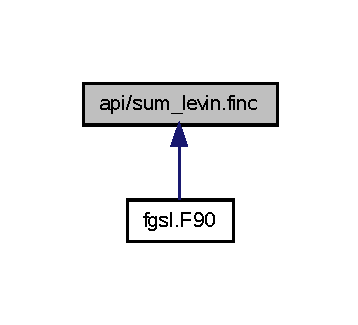
\includegraphics[width=176pt]{sum__levin_8finc__dep__incl}
\end{center}
\end{figure}
\subsection*{Functions/\-Subroutines}
\begin{DoxyCompactItemize}
\item 
type(fgsl\-\_\-sum\-\_\-levin\-\_\-u\-\_\-workspace) \\*
function \hyperlink{sum__levin_8finc_ad6ebf8afa62ed4d6df0ccc045becc409}{fgsl\-\_\-sum\-\_\-levin\-\_\-u\-\_\-alloc} (n)
\item 
integer(fgsl\-\_\-int) function \hyperlink{sum__levin_8finc_aaf7b37dc4577512c18cb3973ad84252e}{fgsl\-\_\-sum\-\_\-levin\-\_\-u\-\_\-free} (w)
\item 
integer(fgsl\-\_\-int) function \hyperlink{sum__levin_8finc_ae945413c5c10344d97cc10002dd760c2}{fgsl\-\_\-sum\-\_\-levin\-\_\-u\-\_\-accel} (array, array\-\_\-size, w, sum\-\_\-accel, abserr)
\item 
type(fgsl\-\_\-sum\-\_\-levin\-\_\-utrunc\-\_\-workspace) \\*
function \hyperlink{sum__levin_8finc_a877def7077d13d9c9f6940266bc44a54}{fgsl\-\_\-sum\-\_\-levin\-\_\-utrunc\-\_\-alloc} (n)
\item 
integer(fgsl\-\_\-int) function \hyperlink{sum__levin_8finc_a4703b473d5be9896645002d25bff9467}{fgsl\-\_\-sum\-\_\-levin\-\_\-utrunc\-\_\-free} (w)
\item 
integer(fgsl\-\_\-int) function \hyperlink{sum__levin_8finc_aafbf5e22d1e3d84b254f5b0800c4c3bf}{fgsl\-\_\-sum\-\_\-levin\-\_\-utrunc\-\_\-accel} (array, array\-\_\-size, w, sum\-\_\-accel, abserr)
\end{DoxyCompactItemize}


\subsection{Function/\-Subroutine Documentation}
\hypertarget{sum__levin_8finc_ae945413c5c10344d97cc10002dd760c2}{\index{sum\-\_\-levin.\-finc@{sum\-\_\-levin.\-finc}!fgsl\-\_\-sum\-\_\-levin\-\_\-u\-\_\-accel@{fgsl\-\_\-sum\-\_\-levin\-\_\-u\-\_\-accel}}
\index{fgsl\-\_\-sum\-\_\-levin\-\_\-u\-\_\-accel@{fgsl\-\_\-sum\-\_\-levin\-\_\-u\-\_\-accel}!sum_levin.finc@{sum\-\_\-levin.\-finc}}
\subsubsection[{fgsl\-\_\-sum\-\_\-levin\-\_\-u\-\_\-accel}]{\setlength{\rightskip}{0pt plus 5cm}integer(fgsl\-\_\-int) function fgsl\-\_\-sum\-\_\-levin\-\_\-u\-\_\-accel (
\begin{DoxyParamCaption}
\item[{real(fgsl\-\_\-double), dimension(array\-\_\-size), intent(in)}]{array, }
\item[{integer(fgsl\-\_\-size\-\_\-t), intent(in)}]{array\-\_\-size, }
\item[{type(fgsl\-\_\-sum\-\_\-levin\-\_\-u\-\_\-workspace), intent(in)}]{w, }
\item[{real(fgsl\-\_\-double), intent(out)}]{sum\-\_\-accel, }
\item[{real(fgsl\-\_\-double), intent(out)}]{abserr}
\end{DoxyParamCaption}
)}}\label{sum__levin_8finc_ae945413c5c10344d97cc10002dd760c2}
\hypertarget{sum__levin_8finc_ad6ebf8afa62ed4d6df0ccc045becc409}{\index{sum\-\_\-levin.\-finc@{sum\-\_\-levin.\-finc}!fgsl\-\_\-sum\-\_\-levin\-\_\-u\-\_\-alloc@{fgsl\-\_\-sum\-\_\-levin\-\_\-u\-\_\-alloc}}
\index{fgsl\-\_\-sum\-\_\-levin\-\_\-u\-\_\-alloc@{fgsl\-\_\-sum\-\_\-levin\-\_\-u\-\_\-alloc}!sum_levin.finc@{sum\-\_\-levin.\-finc}}
\subsubsection[{fgsl\-\_\-sum\-\_\-levin\-\_\-u\-\_\-alloc}]{\setlength{\rightskip}{0pt plus 5cm}type(fgsl\-\_\-sum\-\_\-levin\-\_\-u\-\_\-workspace) function fgsl\-\_\-sum\-\_\-levin\-\_\-u\-\_\-alloc (
\begin{DoxyParamCaption}
\item[{integer(fgsl\-\_\-size\-\_\-t), intent(in)}]{n}
\end{DoxyParamCaption}
)}}\label{sum__levin_8finc_ad6ebf8afa62ed4d6df0ccc045becc409}
\hypertarget{sum__levin_8finc_aaf7b37dc4577512c18cb3973ad84252e}{\index{sum\-\_\-levin.\-finc@{sum\-\_\-levin.\-finc}!fgsl\-\_\-sum\-\_\-levin\-\_\-u\-\_\-free@{fgsl\-\_\-sum\-\_\-levin\-\_\-u\-\_\-free}}
\index{fgsl\-\_\-sum\-\_\-levin\-\_\-u\-\_\-free@{fgsl\-\_\-sum\-\_\-levin\-\_\-u\-\_\-free}!sum_levin.finc@{sum\-\_\-levin.\-finc}}
\subsubsection[{fgsl\-\_\-sum\-\_\-levin\-\_\-u\-\_\-free}]{\setlength{\rightskip}{0pt plus 5cm}integer(fgsl\-\_\-int) function fgsl\-\_\-sum\-\_\-levin\-\_\-u\-\_\-free (
\begin{DoxyParamCaption}
\item[{type(fgsl\-\_\-sum\-\_\-levin\-\_\-u\-\_\-workspace), intent(inout)}]{w}
\end{DoxyParamCaption}
)}}\label{sum__levin_8finc_aaf7b37dc4577512c18cb3973ad84252e}
\hypertarget{sum__levin_8finc_aafbf5e22d1e3d84b254f5b0800c4c3bf}{\index{sum\-\_\-levin.\-finc@{sum\-\_\-levin.\-finc}!fgsl\-\_\-sum\-\_\-levin\-\_\-utrunc\-\_\-accel@{fgsl\-\_\-sum\-\_\-levin\-\_\-utrunc\-\_\-accel}}
\index{fgsl\-\_\-sum\-\_\-levin\-\_\-utrunc\-\_\-accel@{fgsl\-\_\-sum\-\_\-levin\-\_\-utrunc\-\_\-accel}!sum_levin.finc@{sum\-\_\-levin.\-finc}}
\subsubsection[{fgsl\-\_\-sum\-\_\-levin\-\_\-utrunc\-\_\-accel}]{\setlength{\rightskip}{0pt plus 5cm}integer(fgsl\-\_\-int) function fgsl\-\_\-sum\-\_\-levin\-\_\-utrunc\-\_\-accel (
\begin{DoxyParamCaption}
\item[{real(fgsl\-\_\-double), dimension(array\-\_\-size), intent(in)}]{array, }
\item[{integer(fgsl\-\_\-size\-\_\-t), intent(in)}]{array\-\_\-size, }
\item[{type(fgsl\-\_\-sum\-\_\-levin\-\_\-utrunc\-\_\-workspace), intent(in)}]{w, }
\item[{real(fgsl\-\_\-double), intent(out)}]{sum\-\_\-accel, }
\item[{real(fgsl\-\_\-double), intent(out)}]{abserr}
\end{DoxyParamCaption}
)}}\label{sum__levin_8finc_aafbf5e22d1e3d84b254f5b0800c4c3bf}
\hypertarget{sum__levin_8finc_a877def7077d13d9c9f6940266bc44a54}{\index{sum\-\_\-levin.\-finc@{sum\-\_\-levin.\-finc}!fgsl\-\_\-sum\-\_\-levin\-\_\-utrunc\-\_\-alloc@{fgsl\-\_\-sum\-\_\-levin\-\_\-utrunc\-\_\-alloc}}
\index{fgsl\-\_\-sum\-\_\-levin\-\_\-utrunc\-\_\-alloc@{fgsl\-\_\-sum\-\_\-levin\-\_\-utrunc\-\_\-alloc}!sum_levin.finc@{sum\-\_\-levin.\-finc}}
\subsubsection[{fgsl\-\_\-sum\-\_\-levin\-\_\-utrunc\-\_\-alloc}]{\setlength{\rightskip}{0pt plus 5cm}type(fgsl\-\_\-sum\-\_\-levin\-\_\-utrunc\-\_\-workspace) function fgsl\-\_\-sum\-\_\-levin\-\_\-utrunc\-\_\-alloc (
\begin{DoxyParamCaption}
\item[{integer(fgsl\-\_\-size\-\_\-t), intent(in)}]{n}
\end{DoxyParamCaption}
)}}\label{sum__levin_8finc_a877def7077d13d9c9f6940266bc44a54}
\hypertarget{sum__levin_8finc_a4703b473d5be9896645002d25bff9467}{\index{sum\-\_\-levin.\-finc@{sum\-\_\-levin.\-finc}!fgsl\-\_\-sum\-\_\-levin\-\_\-utrunc\-\_\-free@{fgsl\-\_\-sum\-\_\-levin\-\_\-utrunc\-\_\-free}}
\index{fgsl\-\_\-sum\-\_\-levin\-\_\-utrunc\-\_\-free@{fgsl\-\_\-sum\-\_\-levin\-\_\-utrunc\-\_\-free}!sum_levin.finc@{sum\-\_\-levin.\-finc}}
\subsubsection[{fgsl\-\_\-sum\-\_\-levin\-\_\-utrunc\-\_\-free}]{\setlength{\rightskip}{0pt plus 5cm}integer(fgsl\-\_\-int) function fgsl\-\_\-sum\-\_\-levin\-\_\-utrunc\-\_\-free (
\begin{DoxyParamCaption}
\item[{type(fgsl\-\_\-sum\-\_\-levin\-\_\-utrunc\-\_\-workspace), intent(inout)}]{w}
\end{DoxyParamCaption}
)}}\label{sum__levin_8finc_a4703b473d5be9896645002d25bff9467}

\hypertarget{wavelet_8finc}{}\section{api/wavelet.finc File Reference}
\label{wavelet_8finc}\index{api/wavelet.\+finc@{api/wavelet.\+finc}}
This graph shows which files directly or indirectly include this file\+:\nopagebreak
\begin{figure}[H]
\begin{center}
\leavevmode
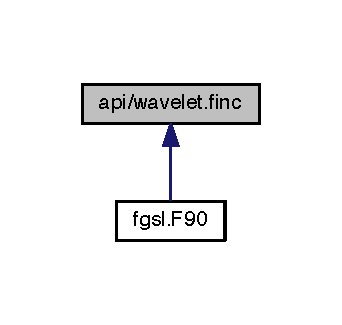
\includegraphics[width=160pt]{wavelet_8finc__dep__incl}
\end{center}
\end{figure}
\subsection*{Functions/\+Subroutines}
\begin{DoxyCompactItemize}
\item 
type(fgsl\+\_\+wavelet) function \hyperlink{wavelet_8finc_a0534f5b9d5db58fc98d3996bf7eefc20}{fgsl\+\_\+wavelet\+\_\+alloc} (t, k)
\item 
character(kind=fgsl\+\_\+char, len=fgsl\+\_\+strmax) function \hyperlink{wavelet_8finc_a2ff5880cd29c1fa264f815fda096f4ab}{fgsl\+\_\+wavelet\+\_\+name} (wavelet)
\item 
subroutine \hyperlink{wavelet_8finc_af843924a1fcec19d66e6c2aa89b6fb71}{fgsl\+\_\+wavelet\+\_\+free} (w)
\item 
type(fgsl\+\_\+wavelet\+\_\+workspace) function \hyperlink{wavelet_8finc_aa120476a77ed63c701cb8cf8fc575409}{fgsl\+\_\+wavelet\+\_\+workspace\+\_\+alloc} (n)
\item 
subroutine \hyperlink{wavelet_8finc_a8877c7b5815c334ab195f6517273a91e}{fgsl\+\_\+wavelet\+\_\+workspace\+\_\+free} (w)
\item 
integer(fgsl\+\_\+int) function \hyperlink{wavelet_8finc_a3dd1ffd5ce0dd32861b9221f6afae511}{fgsl\+\_\+wavelet\+\_\+transform} (w, data, stride, n, dir, work)
\item 
integer(fgsl\+\_\+int) function \hyperlink{wavelet_8finc_a70c8c242811e478cebb88eb3b27788ab}{fgsl\+\_\+wavelet\+\_\+transform\+\_\+forward} (w, data, stride, n, work)
\item 
integer(fgsl\+\_\+int) function \hyperlink{wavelet_8finc_a34094547d54cf81dc906fff09ceb1a44}{fgsl\+\_\+wavelet\+\_\+transform\+\_\+inverse} (w, data, stride, n, work)
\item 
integer(fgsl\+\_\+int) function \hyperlink{wavelet_8finc_ae721627d9553cf0c2d1396e45d1fb146}{fgsl\+\_\+wavelet2d\+\_\+transform} (w, data, tda, size1, size2, dir, work)
\item 
integer(fgsl\+\_\+int) function \hyperlink{wavelet_8finc_a0ae200617e842d153159591b59cc56b5}{fgsl\+\_\+wavelet2d\+\_\+transform\+\_\+forward} (w, data, tda, size1, size2, work)
\item 
integer(fgsl\+\_\+int) function \hyperlink{wavelet_8finc_a05d7bb6ada598550a9df3b0a0cdfdb05}{fgsl\+\_\+wavelet2d\+\_\+transform\+\_\+inverse} (w, data, tda, size1, size2, work)
\item 
integer(fgsl\+\_\+int) function \hyperlink{wavelet_8finc_abbe205405ba63a585d68d1e3f5db5903}{fgsl\+\_\+wavelet2d\+\_\+transform\+\_\+matrix} (w, m, dir, work)
\item 
integer(fgsl\+\_\+int) function \hyperlink{wavelet_8finc_a96ce5dd5582a999b163f947e95a1ae40}{fgsl\+\_\+wavelet2d\+\_\+transform\+\_\+matrix\+\_\+forward} (w, m, work)
\item 
integer(fgsl\+\_\+int) function \hyperlink{wavelet_8finc_a9d0bcdfff907e1c19166cddf01fdc15d}{fgsl\+\_\+wavelet2d\+\_\+transform\+\_\+matrix\+\_\+inverse} (w, m, work)
\item 
integer(fgsl\+\_\+int) function \hyperlink{wavelet_8finc_a488377ebb90c0a2cbfddd028be2dc41b}{fgsl\+\_\+wavelet2d\+\_\+nstransform} (w, data, tda, size1, size2, dir, work)
\item 
integer(fgsl\+\_\+int) function \hyperlink{wavelet_8finc_afa1e0433033a7898a4cb3992ac848f88}{fgsl\+\_\+wavelet2d\+\_\+nstransform\+\_\+forward} (w, data, tda, size1, size2, work)
\item 
integer(fgsl\+\_\+int) function \hyperlink{wavelet_8finc_a3424c04dfbf288aebc2d8e5e9164565f}{fgsl\+\_\+wavelet2d\+\_\+nstransform\+\_\+inverse} (w, data, tda, size1, size2, work)
\item 
integer(fgsl\+\_\+int) function \hyperlink{wavelet_8finc_a22dbfeae87b11490a8ecebe3254f85fe}{fgsl\+\_\+wavelet2d\+\_\+nstransform\+\_\+matrix} (w, m, dir, work)
\item 
integer(fgsl\+\_\+int) function \hyperlink{wavelet_8finc_a82cc729239d174d054777ed3b7477260}{fgsl\+\_\+wavelet2d\+\_\+nstransform\+\_\+matrix\+\_\+forward} (w, m, work)
\item 
integer(fgsl\+\_\+int) function \hyperlink{wavelet_8finc_a68e1cc4b337ecb5fef13dbea1b47b33a}{fgsl\+\_\+wavelet2d\+\_\+nstransform\+\_\+matrix\+\_\+inverse} (w, m, work)
\item 
logical function \hyperlink{wavelet_8finc_ae806a3d76e07c7169657aa6541928766}{fgsl\+\_\+wavelet\+\_\+status} (wavelet)
\item 
logical function \hyperlink{wavelet_8finc_abb974e06092a14e00e8d4ad2601c012a}{fgsl\+\_\+wavelet\+\_\+workspace\+\_\+status} (wavelet\+\_\+workspace)
\item 
integer(fgsl\+\_\+size\+\_\+t) function \hyperlink{wavelet_8finc_aa94fb05c91cf6594b1afe524d87ce40e}{fgsl\+\_\+sizeof\+\_\+wavelet} (w)
\item 
integer(fgsl\+\_\+size\+\_\+t) function \hyperlink{wavelet_8finc_a709a83f8f0d23fc64a4933894f474ae1}{fgsl\+\_\+sizeof\+\_\+wavelet\+\_\+workspace} (w)
\end{DoxyCompactItemize}


\subsection{Function/\+Subroutine Documentation}
\hypertarget{wavelet_8finc_aa94fb05c91cf6594b1afe524d87ce40e}{}\index{wavelet.\+finc@{wavelet.\+finc}!fgsl\+\_\+sizeof\+\_\+wavelet@{fgsl\+\_\+sizeof\+\_\+wavelet}}
\index{fgsl\+\_\+sizeof\+\_\+wavelet@{fgsl\+\_\+sizeof\+\_\+wavelet}!wavelet.\+finc@{wavelet.\+finc}}
\subsubsection[{fgsl\+\_\+sizeof\+\_\+wavelet}]{\setlength{\rightskip}{0pt plus 5cm}integer(fgsl\+\_\+size\+\_\+t) function fgsl\+\_\+sizeof\+\_\+wavelet (
\begin{DoxyParamCaption}
\item[{type(fgsl\+\_\+wavelet), intent(in)}]{w}
\end{DoxyParamCaption}
)}\label{wavelet_8finc_aa94fb05c91cf6594b1afe524d87ce40e}
\hypertarget{wavelet_8finc_a709a83f8f0d23fc64a4933894f474ae1}{}\index{wavelet.\+finc@{wavelet.\+finc}!fgsl\+\_\+sizeof\+\_\+wavelet\+\_\+workspace@{fgsl\+\_\+sizeof\+\_\+wavelet\+\_\+workspace}}
\index{fgsl\+\_\+sizeof\+\_\+wavelet\+\_\+workspace@{fgsl\+\_\+sizeof\+\_\+wavelet\+\_\+workspace}!wavelet.\+finc@{wavelet.\+finc}}
\subsubsection[{fgsl\+\_\+sizeof\+\_\+wavelet\+\_\+workspace}]{\setlength{\rightskip}{0pt plus 5cm}integer(fgsl\+\_\+size\+\_\+t) function fgsl\+\_\+sizeof\+\_\+wavelet\+\_\+workspace (
\begin{DoxyParamCaption}
\item[{type(fgsl\+\_\+wavelet\+\_\+workspace), intent(in)}]{w}
\end{DoxyParamCaption}
)}\label{wavelet_8finc_a709a83f8f0d23fc64a4933894f474ae1}
\hypertarget{wavelet_8finc_a488377ebb90c0a2cbfddd028be2dc41b}{}\index{wavelet.\+finc@{wavelet.\+finc}!fgsl\+\_\+wavelet2d\+\_\+nstransform@{fgsl\+\_\+wavelet2d\+\_\+nstransform}}
\index{fgsl\+\_\+wavelet2d\+\_\+nstransform@{fgsl\+\_\+wavelet2d\+\_\+nstransform}!wavelet.\+finc@{wavelet.\+finc}}
\subsubsection[{fgsl\+\_\+wavelet2d\+\_\+nstransform}]{\setlength{\rightskip}{0pt plus 5cm}integer(fgsl\+\_\+int) function fgsl\+\_\+wavelet2d\+\_\+nstransform (
\begin{DoxyParamCaption}
\item[{type(fgsl\+\_\+wavelet), intent(in)}]{w, }
\item[{real(fgsl\+\_\+double), dimension(\+:), intent(inout), target}]{data, }
\item[{integer(fgsl\+\_\+size\+\_\+t), intent(in)}]{tda, }
\item[{integer(fgsl\+\_\+size\+\_\+t), intent(in)}]{size1, }
\item[{integer(fgsl\+\_\+size\+\_\+t), intent(in)}]{size2, }
\item[{integer(fgsl\+\_\+int), intent(in)}]{dir, }
\item[{type(fgsl\+\_\+wavelet\+\_\+workspace), intent(inout)}]{work}
\end{DoxyParamCaption}
)}\label{wavelet_8finc_a488377ebb90c0a2cbfddd028be2dc41b}
\hypertarget{wavelet_8finc_afa1e0433033a7898a4cb3992ac848f88}{}\index{wavelet.\+finc@{wavelet.\+finc}!fgsl\+\_\+wavelet2d\+\_\+nstransform\+\_\+forward@{fgsl\+\_\+wavelet2d\+\_\+nstransform\+\_\+forward}}
\index{fgsl\+\_\+wavelet2d\+\_\+nstransform\+\_\+forward@{fgsl\+\_\+wavelet2d\+\_\+nstransform\+\_\+forward}!wavelet.\+finc@{wavelet.\+finc}}
\subsubsection[{fgsl\+\_\+wavelet2d\+\_\+nstransform\+\_\+forward}]{\setlength{\rightskip}{0pt plus 5cm}integer(fgsl\+\_\+int) function fgsl\+\_\+wavelet2d\+\_\+nstransform\+\_\+forward (
\begin{DoxyParamCaption}
\item[{type(fgsl\+\_\+wavelet), intent(in)}]{w, }
\item[{real(fgsl\+\_\+double), dimension(\+:), intent(inout), target}]{data, }
\item[{integer(fgsl\+\_\+size\+\_\+t), intent(in)}]{tda, }
\item[{integer(fgsl\+\_\+size\+\_\+t), intent(in)}]{size1, }
\item[{integer(fgsl\+\_\+size\+\_\+t), intent(in)}]{size2, }
\item[{type(fgsl\+\_\+wavelet\+\_\+workspace), intent(inout)}]{work}
\end{DoxyParamCaption}
)}\label{wavelet_8finc_afa1e0433033a7898a4cb3992ac848f88}
\hypertarget{wavelet_8finc_a3424c04dfbf288aebc2d8e5e9164565f}{}\index{wavelet.\+finc@{wavelet.\+finc}!fgsl\+\_\+wavelet2d\+\_\+nstransform\+\_\+inverse@{fgsl\+\_\+wavelet2d\+\_\+nstransform\+\_\+inverse}}
\index{fgsl\+\_\+wavelet2d\+\_\+nstransform\+\_\+inverse@{fgsl\+\_\+wavelet2d\+\_\+nstransform\+\_\+inverse}!wavelet.\+finc@{wavelet.\+finc}}
\subsubsection[{fgsl\+\_\+wavelet2d\+\_\+nstransform\+\_\+inverse}]{\setlength{\rightskip}{0pt plus 5cm}integer(fgsl\+\_\+int) function fgsl\+\_\+wavelet2d\+\_\+nstransform\+\_\+inverse (
\begin{DoxyParamCaption}
\item[{type(fgsl\+\_\+wavelet), intent(in)}]{w, }
\item[{real(fgsl\+\_\+double), dimension(\+:), intent(inout), target}]{data, }
\item[{integer(fgsl\+\_\+size\+\_\+t), intent(in)}]{tda, }
\item[{integer(fgsl\+\_\+size\+\_\+t), intent(in)}]{size1, }
\item[{integer(fgsl\+\_\+size\+\_\+t), intent(in)}]{size2, }
\item[{type(fgsl\+\_\+wavelet\+\_\+workspace), intent(inout)}]{work}
\end{DoxyParamCaption}
)}\label{wavelet_8finc_a3424c04dfbf288aebc2d8e5e9164565f}
\hypertarget{wavelet_8finc_a22dbfeae87b11490a8ecebe3254f85fe}{}\index{wavelet.\+finc@{wavelet.\+finc}!fgsl\+\_\+wavelet2d\+\_\+nstransform\+\_\+matrix@{fgsl\+\_\+wavelet2d\+\_\+nstransform\+\_\+matrix}}
\index{fgsl\+\_\+wavelet2d\+\_\+nstransform\+\_\+matrix@{fgsl\+\_\+wavelet2d\+\_\+nstransform\+\_\+matrix}!wavelet.\+finc@{wavelet.\+finc}}
\subsubsection[{fgsl\+\_\+wavelet2d\+\_\+nstransform\+\_\+matrix}]{\setlength{\rightskip}{0pt plus 5cm}integer(fgsl\+\_\+int) function fgsl\+\_\+wavelet2d\+\_\+nstransform\+\_\+matrix (
\begin{DoxyParamCaption}
\item[{type(fgsl\+\_\+wavelet), intent(in)}]{w, }
\item[{type(fgsl\+\_\+matrix), intent(inout)}]{m, }
\item[{integer(fgsl\+\_\+int), intent(in)}]{dir, }
\item[{type(fgsl\+\_\+wavelet\+\_\+workspace)}]{work}
\end{DoxyParamCaption}
)}\label{wavelet_8finc_a22dbfeae87b11490a8ecebe3254f85fe}
\hypertarget{wavelet_8finc_a82cc729239d174d054777ed3b7477260}{}\index{wavelet.\+finc@{wavelet.\+finc}!fgsl\+\_\+wavelet2d\+\_\+nstransform\+\_\+matrix\+\_\+forward@{fgsl\+\_\+wavelet2d\+\_\+nstransform\+\_\+matrix\+\_\+forward}}
\index{fgsl\+\_\+wavelet2d\+\_\+nstransform\+\_\+matrix\+\_\+forward@{fgsl\+\_\+wavelet2d\+\_\+nstransform\+\_\+matrix\+\_\+forward}!wavelet.\+finc@{wavelet.\+finc}}
\subsubsection[{fgsl\+\_\+wavelet2d\+\_\+nstransform\+\_\+matrix\+\_\+forward}]{\setlength{\rightskip}{0pt plus 5cm}integer(fgsl\+\_\+int) function fgsl\+\_\+wavelet2d\+\_\+nstransform\+\_\+matrix\+\_\+forward (
\begin{DoxyParamCaption}
\item[{type(fgsl\+\_\+wavelet), intent(in)}]{w, }
\item[{type(fgsl\+\_\+matrix), intent(inout)}]{m, }
\item[{type(fgsl\+\_\+wavelet\+\_\+workspace)}]{work}
\end{DoxyParamCaption}
)}\label{wavelet_8finc_a82cc729239d174d054777ed3b7477260}
\hypertarget{wavelet_8finc_a68e1cc4b337ecb5fef13dbea1b47b33a}{}\index{wavelet.\+finc@{wavelet.\+finc}!fgsl\+\_\+wavelet2d\+\_\+nstransform\+\_\+matrix\+\_\+inverse@{fgsl\+\_\+wavelet2d\+\_\+nstransform\+\_\+matrix\+\_\+inverse}}
\index{fgsl\+\_\+wavelet2d\+\_\+nstransform\+\_\+matrix\+\_\+inverse@{fgsl\+\_\+wavelet2d\+\_\+nstransform\+\_\+matrix\+\_\+inverse}!wavelet.\+finc@{wavelet.\+finc}}
\subsubsection[{fgsl\+\_\+wavelet2d\+\_\+nstransform\+\_\+matrix\+\_\+inverse}]{\setlength{\rightskip}{0pt plus 5cm}integer(fgsl\+\_\+int) function fgsl\+\_\+wavelet2d\+\_\+nstransform\+\_\+matrix\+\_\+inverse (
\begin{DoxyParamCaption}
\item[{type(fgsl\+\_\+wavelet), intent(in)}]{w, }
\item[{type(fgsl\+\_\+matrix), intent(inout)}]{m, }
\item[{type(fgsl\+\_\+wavelet\+\_\+workspace)}]{work}
\end{DoxyParamCaption}
)}\label{wavelet_8finc_a68e1cc4b337ecb5fef13dbea1b47b33a}
\hypertarget{wavelet_8finc_ae721627d9553cf0c2d1396e45d1fb146}{}\index{wavelet.\+finc@{wavelet.\+finc}!fgsl\+\_\+wavelet2d\+\_\+transform@{fgsl\+\_\+wavelet2d\+\_\+transform}}
\index{fgsl\+\_\+wavelet2d\+\_\+transform@{fgsl\+\_\+wavelet2d\+\_\+transform}!wavelet.\+finc@{wavelet.\+finc}}
\subsubsection[{fgsl\+\_\+wavelet2d\+\_\+transform}]{\setlength{\rightskip}{0pt plus 5cm}integer(fgsl\+\_\+int) function fgsl\+\_\+wavelet2d\+\_\+transform (
\begin{DoxyParamCaption}
\item[{type(fgsl\+\_\+wavelet), intent(in)}]{w, }
\item[{real(fgsl\+\_\+double), dimension(\+:), intent(inout), target}]{data, }
\item[{integer(fgsl\+\_\+size\+\_\+t), intent(in)}]{tda, }
\item[{integer(fgsl\+\_\+size\+\_\+t), intent(in)}]{size1, }
\item[{integer(fgsl\+\_\+size\+\_\+t), intent(in)}]{size2, }
\item[{integer(fgsl\+\_\+int), intent(in)}]{dir, }
\item[{type(fgsl\+\_\+wavelet\+\_\+workspace), intent(inout)}]{work}
\end{DoxyParamCaption}
)}\label{wavelet_8finc_ae721627d9553cf0c2d1396e45d1fb146}
\hypertarget{wavelet_8finc_a0ae200617e842d153159591b59cc56b5}{}\index{wavelet.\+finc@{wavelet.\+finc}!fgsl\+\_\+wavelet2d\+\_\+transform\+\_\+forward@{fgsl\+\_\+wavelet2d\+\_\+transform\+\_\+forward}}
\index{fgsl\+\_\+wavelet2d\+\_\+transform\+\_\+forward@{fgsl\+\_\+wavelet2d\+\_\+transform\+\_\+forward}!wavelet.\+finc@{wavelet.\+finc}}
\subsubsection[{fgsl\+\_\+wavelet2d\+\_\+transform\+\_\+forward}]{\setlength{\rightskip}{0pt plus 5cm}integer(fgsl\+\_\+int) function fgsl\+\_\+wavelet2d\+\_\+transform\+\_\+forward (
\begin{DoxyParamCaption}
\item[{type(fgsl\+\_\+wavelet), intent(in)}]{w, }
\item[{real(fgsl\+\_\+double), dimension(\+:), intent(inout), target}]{data, }
\item[{integer(fgsl\+\_\+size\+\_\+t), intent(in)}]{tda, }
\item[{integer(fgsl\+\_\+size\+\_\+t), intent(in)}]{size1, }
\item[{integer(fgsl\+\_\+size\+\_\+t), intent(in)}]{size2, }
\item[{type(fgsl\+\_\+wavelet\+\_\+workspace), intent(inout)}]{work}
\end{DoxyParamCaption}
)}\label{wavelet_8finc_a0ae200617e842d153159591b59cc56b5}
\hypertarget{wavelet_8finc_a05d7bb6ada598550a9df3b0a0cdfdb05}{}\index{wavelet.\+finc@{wavelet.\+finc}!fgsl\+\_\+wavelet2d\+\_\+transform\+\_\+inverse@{fgsl\+\_\+wavelet2d\+\_\+transform\+\_\+inverse}}
\index{fgsl\+\_\+wavelet2d\+\_\+transform\+\_\+inverse@{fgsl\+\_\+wavelet2d\+\_\+transform\+\_\+inverse}!wavelet.\+finc@{wavelet.\+finc}}
\subsubsection[{fgsl\+\_\+wavelet2d\+\_\+transform\+\_\+inverse}]{\setlength{\rightskip}{0pt plus 5cm}integer(fgsl\+\_\+int) function fgsl\+\_\+wavelet2d\+\_\+transform\+\_\+inverse (
\begin{DoxyParamCaption}
\item[{type(fgsl\+\_\+wavelet), intent(in)}]{w, }
\item[{real(fgsl\+\_\+double), dimension(\+:), intent(inout), target}]{data, }
\item[{integer(fgsl\+\_\+size\+\_\+t), intent(in)}]{tda, }
\item[{integer(fgsl\+\_\+size\+\_\+t), intent(in)}]{size1, }
\item[{integer(fgsl\+\_\+size\+\_\+t), intent(in)}]{size2, }
\item[{type(fgsl\+\_\+wavelet\+\_\+workspace), intent(inout)}]{work}
\end{DoxyParamCaption}
)}\label{wavelet_8finc_a05d7bb6ada598550a9df3b0a0cdfdb05}
\hypertarget{wavelet_8finc_abbe205405ba63a585d68d1e3f5db5903}{}\index{wavelet.\+finc@{wavelet.\+finc}!fgsl\+\_\+wavelet2d\+\_\+transform\+\_\+matrix@{fgsl\+\_\+wavelet2d\+\_\+transform\+\_\+matrix}}
\index{fgsl\+\_\+wavelet2d\+\_\+transform\+\_\+matrix@{fgsl\+\_\+wavelet2d\+\_\+transform\+\_\+matrix}!wavelet.\+finc@{wavelet.\+finc}}
\subsubsection[{fgsl\+\_\+wavelet2d\+\_\+transform\+\_\+matrix}]{\setlength{\rightskip}{0pt plus 5cm}integer(fgsl\+\_\+int) function fgsl\+\_\+wavelet2d\+\_\+transform\+\_\+matrix (
\begin{DoxyParamCaption}
\item[{type(fgsl\+\_\+wavelet), intent(in)}]{w, }
\item[{type(fgsl\+\_\+matrix), intent(inout)}]{m, }
\item[{integer(fgsl\+\_\+int), intent(in)}]{dir, }
\item[{type(fgsl\+\_\+wavelet\+\_\+workspace)}]{work}
\end{DoxyParamCaption}
)}\label{wavelet_8finc_abbe205405ba63a585d68d1e3f5db5903}
\hypertarget{wavelet_8finc_a96ce5dd5582a999b163f947e95a1ae40}{}\index{wavelet.\+finc@{wavelet.\+finc}!fgsl\+\_\+wavelet2d\+\_\+transform\+\_\+matrix\+\_\+forward@{fgsl\+\_\+wavelet2d\+\_\+transform\+\_\+matrix\+\_\+forward}}
\index{fgsl\+\_\+wavelet2d\+\_\+transform\+\_\+matrix\+\_\+forward@{fgsl\+\_\+wavelet2d\+\_\+transform\+\_\+matrix\+\_\+forward}!wavelet.\+finc@{wavelet.\+finc}}
\subsubsection[{fgsl\+\_\+wavelet2d\+\_\+transform\+\_\+matrix\+\_\+forward}]{\setlength{\rightskip}{0pt plus 5cm}integer(fgsl\+\_\+int) function fgsl\+\_\+wavelet2d\+\_\+transform\+\_\+matrix\+\_\+forward (
\begin{DoxyParamCaption}
\item[{type(fgsl\+\_\+wavelet), intent(in)}]{w, }
\item[{type(fgsl\+\_\+matrix), intent(inout)}]{m, }
\item[{type(fgsl\+\_\+wavelet\+\_\+workspace)}]{work}
\end{DoxyParamCaption}
)}\label{wavelet_8finc_a96ce5dd5582a999b163f947e95a1ae40}
\hypertarget{wavelet_8finc_a9d0bcdfff907e1c19166cddf01fdc15d}{}\index{wavelet.\+finc@{wavelet.\+finc}!fgsl\+\_\+wavelet2d\+\_\+transform\+\_\+matrix\+\_\+inverse@{fgsl\+\_\+wavelet2d\+\_\+transform\+\_\+matrix\+\_\+inverse}}
\index{fgsl\+\_\+wavelet2d\+\_\+transform\+\_\+matrix\+\_\+inverse@{fgsl\+\_\+wavelet2d\+\_\+transform\+\_\+matrix\+\_\+inverse}!wavelet.\+finc@{wavelet.\+finc}}
\subsubsection[{fgsl\+\_\+wavelet2d\+\_\+transform\+\_\+matrix\+\_\+inverse}]{\setlength{\rightskip}{0pt plus 5cm}integer(fgsl\+\_\+int) function fgsl\+\_\+wavelet2d\+\_\+transform\+\_\+matrix\+\_\+inverse (
\begin{DoxyParamCaption}
\item[{type(fgsl\+\_\+wavelet), intent(in)}]{w, }
\item[{type(fgsl\+\_\+matrix), intent(inout)}]{m, }
\item[{type(fgsl\+\_\+wavelet\+\_\+workspace)}]{work}
\end{DoxyParamCaption}
)}\label{wavelet_8finc_a9d0bcdfff907e1c19166cddf01fdc15d}
\hypertarget{wavelet_8finc_a0534f5b9d5db58fc98d3996bf7eefc20}{}\index{wavelet.\+finc@{wavelet.\+finc}!fgsl\+\_\+wavelet\+\_\+alloc@{fgsl\+\_\+wavelet\+\_\+alloc}}
\index{fgsl\+\_\+wavelet\+\_\+alloc@{fgsl\+\_\+wavelet\+\_\+alloc}!wavelet.\+finc@{wavelet.\+finc}}
\subsubsection[{fgsl\+\_\+wavelet\+\_\+alloc}]{\setlength{\rightskip}{0pt plus 5cm}type(fgsl\+\_\+wavelet) function fgsl\+\_\+wavelet\+\_\+alloc (
\begin{DoxyParamCaption}
\item[{type(fgsl\+\_\+wavelet\+\_\+type), intent(in)}]{t, }
\item[{integer(fgsl\+\_\+size\+\_\+t), intent(in)}]{k}
\end{DoxyParamCaption}
)}\label{wavelet_8finc_a0534f5b9d5db58fc98d3996bf7eefc20}
\hypertarget{wavelet_8finc_af843924a1fcec19d66e6c2aa89b6fb71}{}\index{wavelet.\+finc@{wavelet.\+finc}!fgsl\+\_\+wavelet\+\_\+free@{fgsl\+\_\+wavelet\+\_\+free}}
\index{fgsl\+\_\+wavelet\+\_\+free@{fgsl\+\_\+wavelet\+\_\+free}!wavelet.\+finc@{wavelet.\+finc}}
\subsubsection[{fgsl\+\_\+wavelet\+\_\+free}]{\setlength{\rightskip}{0pt plus 5cm}subroutine fgsl\+\_\+wavelet\+\_\+free (
\begin{DoxyParamCaption}
\item[{type(fgsl\+\_\+wavelet), intent(inout)}]{w}
\end{DoxyParamCaption}
)}\label{wavelet_8finc_af843924a1fcec19d66e6c2aa89b6fb71}
\hypertarget{wavelet_8finc_a2ff5880cd29c1fa264f815fda096f4ab}{}\index{wavelet.\+finc@{wavelet.\+finc}!fgsl\+\_\+wavelet\+\_\+name@{fgsl\+\_\+wavelet\+\_\+name}}
\index{fgsl\+\_\+wavelet\+\_\+name@{fgsl\+\_\+wavelet\+\_\+name}!wavelet.\+finc@{wavelet.\+finc}}
\subsubsection[{fgsl\+\_\+wavelet\+\_\+name}]{\setlength{\rightskip}{0pt plus 5cm}character(kind=fgsl\+\_\+char,len=fgsl\+\_\+strmax) function fgsl\+\_\+wavelet\+\_\+name (
\begin{DoxyParamCaption}
\item[{type(fgsl\+\_\+wavelet), intent(in)}]{wavelet}
\end{DoxyParamCaption}
)}\label{wavelet_8finc_a2ff5880cd29c1fa264f815fda096f4ab}
\hypertarget{wavelet_8finc_ae806a3d76e07c7169657aa6541928766}{}\index{wavelet.\+finc@{wavelet.\+finc}!fgsl\+\_\+wavelet\+\_\+status@{fgsl\+\_\+wavelet\+\_\+status}}
\index{fgsl\+\_\+wavelet\+\_\+status@{fgsl\+\_\+wavelet\+\_\+status}!wavelet.\+finc@{wavelet.\+finc}}
\subsubsection[{fgsl\+\_\+wavelet\+\_\+status}]{\setlength{\rightskip}{0pt plus 5cm}logical function fgsl\+\_\+wavelet\+\_\+status (
\begin{DoxyParamCaption}
\item[{type(fgsl\+\_\+wavelet), intent(in)}]{wavelet}
\end{DoxyParamCaption}
)}\label{wavelet_8finc_ae806a3d76e07c7169657aa6541928766}
\hypertarget{wavelet_8finc_a3dd1ffd5ce0dd32861b9221f6afae511}{}\index{wavelet.\+finc@{wavelet.\+finc}!fgsl\+\_\+wavelet\+\_\+transform@{fgsl\+\_\+wavelet\+\_\+transform}}
\index{fgsl\+\_\+wavelet\+\_\+transform@{fgsl\+\_\+wavelet\+\_\+transform}!wavelet.\+finc@{wavelet.\+finc}}
\subsubsection[{fgsl\+\_\+wavelet\+\_\+transform}]{\setlength{\rightskip}{0pt plus 5cm}integer(fgsl\+\_\+int) function fgsl\+\_\+wavelet\+\_\+transform (
\begin{DoxyParamCaption}
\item[{type(fgsl\+\_\+wavelet), intent(in)}]{w, }
\item[{real(fgsl\+\_\+double), dimension(\+:), intent(inout), target}]{data, }
\item[{integer(fgsl\+\_\+size\+\_\+t), intent(in)}]{stride, }
\item[{integer(fgsl\+\_\+size\+\_\+t), intent(in)}]{n, }
\item[{integer(fgsl\+\_\+int), intent(in)}]{dir, }
\item[{type(fgsl\+\_\+wavelet\+\_\+workspace), intent(inout)}]{work}
\end{DoxyParamCaption}
)}\label{wavelet_8finc_a3dd1ffd5ce0dd32861b9221f6afae511}
\hypertarget{wavelet_8finc_a70c8c242811e478cebb88eb3b27788ab}{}\index{wavelet.\+finc@{wavelet.\+finc}!fgsl\+\_\+wavelet\+\_\+transform\+\_\+forward@{fgsl\+\_\+wavelet\+\_\+transform\+\_\+forward}}
\index{fgsl\+\_\+wavelet\+\_\+transform\+\_\+forward@{fgsl\+\_\+wavelet\+\_\+transform\+\_\+forward}!wavelet.\+finc@{wavelet.\+finc}}
\subsubsection[{fgsl\+\_\+wavelet\+\_\+transform\+\_\+forward}]{\setlength{\rightskip}{0pt plus 5cm}integer(fgsl\+\_\+int) function fgsl\+\_\+wavelet\+\_\+transform\+\_\+forward (
\begin{DoxyParamCaption}
\item[{type(fgsl\+\_\+wavelet), intent(in)}]{w, }
\item[{real(fgsl\+\_\+double), dimension(\+:), intent(inout), target}]{data, }
\item[{integer(fgsl\+\_\+size\+\_\+t), intent(in)}]{stride, }
\item[{integer(fgsl\+\_\+size\+\_\+t), intent(in)}]{n, }
\item[{type(fgsl\+\_\+wavelet\+\_\+workspace), intent(inout)}]{work}
\end{DoxyParamCaption}
)}\label{wavelet_8finc_a70c8c242811e478cebb88eb3b27788ab}
\hypertarget{wavelet_8finc_a34094547d54cf81dc906fff09ceb1a44}{}\index{wavelet.\+finc@{wavelet.\+finc}!fgsl\+\_\+wavelet\+\_\+transform\+\_\+inverse@{fgsl\+\_\+wavelet\+\_\+transform\+\_\+inverse}}
\index{fgsl\+\_\+wavelet\+\_\+transform\+\_\+inverse@{fgsl\+\_\+wavelet\+\_\+transform\+\_\+inverse}!wavelet.\+finc@{wavelet.\+finc}}
\subsubsection[{fgsl\+\_\+wavelet\+\_\+transform\+\_\+inverse}]{\setlength{\rightskip}{0pt plus 5cm}integer(fgsl\+\_\+int) function fgsl\+\_\+wavelet\+\_\+transform\+\_\+inverse (
\begin{DoxyParamCaption}
\item[{type(fgsl\+\_\+wavelet), intent(in)}]{w, }
\item[{real(fgsl\+\_\+double), dimension(\+:), intent(inout), target}]{data, }
\item[{integer(fgsl\+\_\+size\+\_\+t), intent(in)}]{stride, }
\item[{integer(fgsl\+\_\+size\+\_\+t), intent(in)}]{n, }
\item[{type(fgsl\+\_\+wavelet\+\_\+workspace), intent(inout)}]{work}
\end{DoxyParamCaption}
)}\label{wavelet_8finc_a34094547d54cf81dc906fff09ceb1a44}
\hypertarget{wavelet_8finc_aa120476a77ed63c701cb8cf8fc575409}{}\index{wavelet.\+finc@{wavelet.\+finc}!fgsl\+\_\+wavelet\+\_\+workspace\+\_\+alloc@{fgsl\+\_\+wavelet\+\_\+workspace\+\_\+alloc}}
\index{fgsl\+\_\+wavelet\+\_\+workspace\+\_\+alloc@{fgsl\+\_\+wavelet\+\_\+workspace\+\_\+alloc}!wavelet.\+finc@{wavelet.\+finc}}
\subsubsection[{fgsl\+\_\+wavelet\+\_\+workspace\+\_\+alloc}]{\setlength{\rightskip}{0pt plus 5cm}type(fgsl\+\_\+wavelet\+\_\+workspace) function fgsl\+\_\+wavelet\+\_\+workspace\+\_\+alloc (
\begin{DoxyParamCaption}
\item[{integer(fgsl\+\_\+size\+\_\+t), intent(in)}]{n}
\end{DoxyParamCaption}
)}\label{wavelet_8finc_aa120476a77ed63c701cb8cf8fc575409}
\hypertarget{wavelet_8finc_a8877c7b5815c334ab195f6517273a91e}{}\index{wavelet.\+finc@{wavelet.\+finc}!fgsl\+\_\+wavelet\+\_\+workspace\+\_\+free@{fgsl\+\_\+wavelet\+\_\+workspace\+\_\+free}}
\index{fgsl\+\_\+wavelet\+\_\+workspace\+\_\+free@{fgsl\+\_\+wavelet\+\_\+workspace\+\_\+free}!wavelet.\+finc@{wavelet.\+finc}}
\subsubsection[{fgsl\+\_\+wavelet\+\_\+workspace\+\_\+free}]{\setlength{\rightskip}{0pt plus 5cm}subroutine fgsl\+\_\+wavelet\+\_\+workspace\+\_\+free (
\begin{DoxyParamCaption}
\item[{type(fgsl\+\_\+wavelet\+\_\+workspace), intent(inout)}]{w}
\end{DoxyParamCaption}
)}\label{wavelet_8finc_a8877c7b5815c334ab195f6517273a91e}
\hypertarget{wavelet_8finc_abb974e06092a14e00e8d4ad2601c012a}{}\index{wavelet.\+finc@{wavelet.\+finc}!fgsl\+\_\+wavelet\+\_\+workspace\+\_\+status@{fgsl\+\_\+wavelet\+\_\+workspace\+\_\+status}}
\index{fgsl\+\_\+wavelet\+\_\+workspace\+\_\+status@{fgsl\+\_\+wavelet\+\_\+workspace\+\_\+status}!wavelet.\+finc@{wavelet.\+finc}}
\subsubsection[{fgsl\+\_\+wavelet\+\_\+workspace\+\_\+status}]{\setlength{\rightskip}{0pt plus 5cm}logical function fgsl\+\_\+wavelet\+\_\+workspace\+\_\+status (
\begin{DoxyParamCaption}
\item[{type(fgsl\+\_\+wavelet\+\_\+workspace), intent(in)}]{wavelet\+\_\+workspace}
\end{DoxyParamCaption}
)}\label{wavelet_8finc_abb974e06092a14e00e8d4ad2601c012a}

\hypertarget{fgsl_8F90}{\section{fgsl.\-F90 File Reference}
\label{fgsl_8F90}\index{fgsl.\-F90@{fgsl.\-F90}}
}
{\ttfamily \#include \char`\"{}config.\-h\char`\"{}}\\*
{\ttfamily \#include \char`\"{}interface/error.\-finc\char`\"{}}\\*
{\ttfamily \#include \char`\"{}interface/misc.\-finc\char`\"{}}\\*
{\ttfamily \#include \char`\"{}interface/io.\-finc\char`\"{}}\\*
{\ttfamily \#include \char`\"{}interface/math.\-finc\char`\"{}}\\*
{\ttfamily \#include \char`\"{}interface/complex.\-finc\char`\"{}}\\*
{\ttfamily \#include \char`\"{}interface/poly.\-finc\char`\"{}}\\*
{\ttfamily \#include \char`\"{}interface/specfunc.\-finc\char`\"{}}\\*
{\ttfamily \#include \char`\"{}interface/array.\-finc\char`\"{}}\\*
{\ttfamily \#include \char`\"{}interface/interp.\-finc\char`\"{}}\\*
{\ttfamily \#include \char`\"{}interface/permutation.\-finc\char`\"{}}\\*
{\ttfamily \#include \char`\"{}interface/sort.\-finc\char`\"{}}\\*
{\ttfamily \#include \char`\"{}interface/linalg.\-finc\char`\"{}}\\*
{\ttfamily \#include \char`\"{}interface/eigen.\-finc\char`\"{}}\\*
{\ttfamily \#include \char`\"{}interface/fft.\-finc\char`\"{}}\\*
{\ttfamily \#include \char`\"{}interface/integration.\-finc\char`\"{}}\\*
{\ttfamily \#include \char`\"{}interface/rng.\-finc\char`\"{}}\\*
{\ttfamily \#include \char`\"{}interface/statistics.\-finc\char`\"{}}\\*
{\ttfamily \#include \char`\"{}interface/histogram.\-finc\char`\"{}}\\*
{\ttfamily \#include \char`\"{}interface/ntuple.\-finc\char`\"{}}\\*
{\ttfamily \#include \char`\"{}interface/montecarlo.\-finc\char`\"{}}\\*
{\ttfamily \#include \char`\"{}interface/siman.\-finc\char`\"{}}\\*
{\ttfamily \#include \char`\"{}interface/ode.\-finc\char`\"{}}\\*
{\ttfamily \#include \char`\"{}interface/deriv.\-finc\char`\"{}}\\*
{\ttfamily \#include \char`\"{}interface/chebyshev.\-finc\char`\"{}}\\*
{\ttfamily \#include \char`\"{}interface/sum\-\_\-levin.\-finc\char`\"{}}\\*
{\ttfamily \#include \char`\"{}interface/wavelet.\-finc\char`\"{}}\\*
{\ttfamily \#include \char`\"{}interface/dht.\-finc\char`\"{}}\\*
{\ttfamily \#include \char`\"{}interface/roots.\-finc\char`\"{}}\\*
{\ttfamily \#include \char`\"{}interface/min.\-finc\char`\"{}}\\*
{\ttfamily \#include \char`\"{}interface/multiroots.\-finc\char`\"{}}\\*
{\ttfamily \#include \char`\"{}interface/multimin.\-finc\char`\"{}}\\*
{\ttfamily \#include \char`\"{}interface/fit.\-finc\char`\"{}}\\*
{\ttfamily \#include \char`\"{}interface/multifit.\-finc\char`\"{}}\\*
{\ttfamily \#include \char`\"{}interface/bspline.\-finc\char`\"{}}\\*
{\ttfamily \#include \char`\"{}interface/ieee.\-finc\char`\"{}}\\*
{\ttfamily \#include \char`\"{}interface/generics.\-finc\char`\"{}}\\*
{\ttfamily \#include \char`\"{}api/error.\-finc\char`\"{}}\\*
{\ttfamily \#include \char`\"{}api/misc.\-finc\char`\"{}}\\*
{\ttfamily \#include \char`\"{}api/io.\-finc\char`\"{}}\\*
{\ttfamily \#include \char`\"{}api/math.\-finc\char`\"{}}\\*
{\ttfamily \#include \char`\"{}api/complex.\-finc\char`\"{}}\\*
{\ttfamily \#include \char`\"{}api/poly.\-finc\char`\"{}}\\*
{\ttfamily \#include \char`\"{}api/specfunc.\-finc\char`\"{}}\\*
{\ttfamily \#include \char`\"{}api/array.\-finc\char`\"{}}\\*
{\ttfamily \#include \char`\"{}api/interp.\-finc\char`\"{}}\\*
{\ttfamily \#include \char`\"{}api/permutation.\-finc\char`\"{}}\\*
{\ttfamily \#include \char`\"{}api/sort.\-finc\char`\"{}}\\*
{\ttfamily \#include \char`\"{}api/linalg.\-finc\char`\"{}}\\*
{\ttfamily \#include \char`\"{}api/eigen.\-finc\char`\"{}}\\*
{\ttfamily \#include \char`\"{}api/fft.\-finc\char`\"{}}\\*
{\ttfamily \#include \char`\"{}api/integration.\-finc\char`\"{}}\\*
{\ttfamily \#include \char`\"{}api/rng.\-finc\char`\"{}}\\*
{\ttfamily \#include \char`\"{}api/statistics.\-finc\char`\"{}}\\*
{\ttfamily \#include \char`\"{}api/histogram.\-finc\char`\"{}}\\*
{\ttfamily \#include \char`\"{}api/ntuple.\-finc\char`\"{}}\\*
{\ttfamily \#include \char`\"{}api/montecarlo.\-finc\char`\"{}}\\*
{\ttfamily \#include \char`\"{}api/siman.\-finc\char`\"{}}\\*
{\ttfamily \#include \char`\"{}api/ode.\-finc\char`\"{}}\\*
{\ttfamily \#include \char`\"{}api/deriv.\-finc\char`\"{}}\\*
{\ttfamily \#include \char`\"{}api/chebyshev.\-finc\char`\"{}}\\*
{\ttfamily \#include \char`\"{}api/sum\-\_\-levin.\-finc\char`\"{}}\\*
{\ttfamily \#include \char`\"{}api/wavelet.\-finc\char`\"{}}\\*
{\ttfamily \#include \char`\"{}api/dht.\-finc\char`\"{}}\\*
{\ttfamily \#include \char`\"{}api/roots.\-finc\char`\"{}}\\*
{\ttfamily \#include \char`\"{}api/min.\-finc\char`\"{}}\\*
{\ttfamily \#include \char`\"{}api/multiroots.\-finc\char`\"{}}\\*
{\ttfamily \#include \char`\"{}api/multimin.\-finc\char`\"{}}\\*
{\ttfamily \#include \char`\"{}api/fit.\-finc\char`\"{}}\\*
{\ttfamily \#include \char`\"{}api/multifit.\-finc\char`\"{}}\\*
{\ttfamily \#include \char`\"{}api/bspline.\-finc\char`\"{}}\\*
{\ttfamily \#include \char`\"{}api/ieee.\-finc\char`\"{}}\\*
Include dependency graph for fgsl.\-F90\-:\nopagebreak
\begin{figure}[H]
\begin{center}
\leavevmode

\includegraphics[width=350pt]{fgsl_8F90__incl}
\end{center}
\end{figure}
\subsection*{Data Types}
\begin{DoxyCompactItemize}
\item 
module \hyperlink{classfgsl}{fgsl}
\item 
type \hyperlink{structfgsl_1_1fgsl__error__handler__t}{fgsl\-::fgsl\-\_\-error\-\_\-handler\-\_\-t}
\item 
type \hyperlink{structfgsl_1_1fgsl__file}{fgsl\-::fgsl\-\_\-file}
\item 
type \hyperlink{structfgsl_1_1fgsl__function}{fgsl\-::fgsl\-\_\-function}
\item 
type \hyperlink{structfgsl_1_1fgsl__function__fdf}{fgsl\-::fgsl\-\_\-function\-\_\-fdf}
\item 
type \hyperlink{structfgsl_1_1gsl__complex}{fgsl\-::gsl\-\_\-complex}
\item 
type \hyperlink{structfgsl_1_1fgsl__poly__complex__workspace}{fgsl\-::fgsl\-\_\-poly\-\_\-complex\-\_\-workspace}
\item 
type \hyperlink{structfgsl_1_1fgsl__sf__result}{fgsl\-::fgsl\-\_\-sf\-\_\-result}
\item 
type \hyperlink{structfgsl_1_1gsl__sf__result}{fgsl\-::gsl\-\_\-sf\-\_\-result}
\item 
type \hyperlink{structfgsl_1_1fgsl__sf__result__e10}{fgsl\-::fgsl\-\_\-sf\-\_\-result\-\_\-e10}
\item 
type \hyperlink{structfgsl_1_1gsl__sf__result__e10}{fgsl\-::gsl\-\_\-sf\-\_\-result\-\_\-e10}
\item 
type \hyperlink{structfgsl_1_1fgsl__mode__t}{fgsl\-::fgsl\-\_\-mode\-\_\-t}
\item 
type \hyperlink{structfgsl_1_1fgsl__vector}{fgsl\-::fgsl\-\_\-vector}
\item 
type \hyperlink{structfgsl_1_1fgsl__matrix}{fgsl\-::fgsl\-\_\-matrix}
\item 
type \hyperlink{structfgsl_1_1fgsl__vector__complex}{fgsl\-::fgsl\-\_\-vector\-\_\-complex}
\item 
type \hyperlink{structfgsl_1_1fgsl__matrix__complex}{fgsl\-::fgsl\-\_\-matrix\-\_\-complex}
\item 
type \hyperlink{structfgsl_1_1fgsl__interp__type}{fgsl\-::fgsl\-\_\-interp\-\_\-type}
\item 
type \hyperlink{structfgsl_1_1fgsl__interp}{fgsl\-::fgsl\-\_\-interp}
\item 
type \hyperlink{structfgsl_1_1fgsl__interp__accel}{fgsl\-::fgsl\-\_\-interp\-\_\-accel}
\item 
type \hyperlink{structfgsl_1_1fgsl__spline}{fgsl\-::fgsl\-\_\-spline}
\item 
type \hyperlink{structfgsl_1_1fgsl__permutation}{fgsl\-::fgsl\-\_\-permutation}
\item 
type \hyperlink{structfgsl_1_1fgsl__combination}{fgsl\-::fgsl\-\_\-combination}
\item 
type \hyperlink{structfgsl_1_1fgsl__multiset}{fgsl\-::fgsl\-\_\-multiset}
\item 
type \hyperlink{structfgsl_1_1fgsl__multifit__robust__type}{fgsl\-::fgsl\-\_\-multifit\-\_\-robust\-\_\-type}
\item 
type \hyperlink{structfgsl_1_1fgsl__multifit__robust__workspace}{fgsl\-::fgsl\-\_\-multifit\-\_\-robust\-\_\-workspace}
\item 
type \hyperlink{structfgsl_1_1fgsl__multifit__robust__stats}{fgsl\-::fgsl\-\_\-multifit\-\_\-robust\-\_\-stats}
\item 
type \hyperlink{structfgsl_1_1fgsl__eigen__symm__workspace}{fgsl\-::fgsl\-\_\-eigen\-\_\-symm\-\_\-workspace}
\item 
type \hyperlink{structfgsl_1_1fgsl__eigen__symmv__workspace}{fgsl\-::fgsl\-\_\-eigen\-\_\-symmv\-\_\-workspace}
\item 
type \hyperlink{structfgsl_1_1fgsl__eigen__herm__workspace}{fgsl\-::fgsl\-\_\-eigen\-\_\-herm\-\_\-workspace}
\item 
type \hyperlink{structfgsl_1_1fgsl__eigen__hermv__workspace}{fgsl\-::fgsl\-\_\-eigen\-\_\-hermv\-\_\-workspace}
\item 
type \hyperlink{structfgsl_1_1fgsl__eigen__nonsymm__workspace}{fgsl\-::fgsl\-\_\-eigen\-\_\-nonsymm\-\_\-workspace}
\item 
type \hyperlink{structfgsl_1_1fgsl__eigen__nonsymmv__workspace}{fgsl\-::fgsl\-\_\-eigen\-\_\-nonsymmv\-\_\-workspace}
\item 
type \hyperlink{structfgsl_1_1fgsl__eigen__gensymm__workspace}{fgsl\-::fgsl\-\_\-eigen\-\_\-gensymm\-\_\-workspace}
\item 
type \hyperlink{structfgsl_1_1fgsl__eigen__gensymmv__workspace}{fgsl\-::fgsl\-\_\-eigen\-\_\-gensymmv\-\_\-workspace}
\item 
type \hyperlink{structfgsl_1_1fgsl__eigen__genherm__workspace}{fgsl\-::fgsl\-\_\-eigen\-\_\-genherm\-\_\-workspace}
\item 
type \hyperlink{structfgsl_1_1fgsl__eigen__genhermv__workspace}{fgsl\-::fgsl\-\_\-eigen\-\_\-genhermv\-\_\-workspace}
\item 
type \hyperlink{structfgsl_1_1fgsl__eigen__gen__workspace}{fgsl\-::fgsl\-\_\-eigen\-\_\-gen\-\_\-workspace}
\item 
type \hyperlink{structfgsl_1_1fgsl__eigen__genv__workspace}{fgsl\-::fgsl\-\_\-eigen\-\_\-genv\-\_\-workspace}
\item 
type \hyperlink{structfgsl_1_1fgsl__fft__complex__wavetable}{fgsl\-::fgsl\-\_\-fft\-\_\-complex\-\_\-wavetable}
\item 
type \hyperlink{structfgsl_1_1fgsl__fft__real__wavetable}{fgsl\-::fgsl\-\_\-fft\-\_\-real\-\_\-wavetable}
\item 
type \hyperlink{structfgsl_1_1fgsl__fft__halfcomplex__wavetable}{fgsl\-::fgsl\-\_\-fft\-\_\-halfcomplex\-\_\-wavetable}
\item 
type \hyperlink{structfgsl_1_1fgsl__fft__complex__workspace}{fgsl\-::fgsl\-\_\-fft\-\_\-complex\-\_\-workspace}
\item 
type \hyperlink{structfgsl_1_1fgsl__fft__real__workspace}{fgsl\-::fgsl\-\_\-fft\-\_\-real\-\_\-workspace}
\item 
type \hyperlink{structfgsl_1_1fgsl__integration__workspace}{fgsl\-::fgsl\-\_\-integration\-\_\-workspace}
\item 
type \hyperlink{structfgsl_1_1fgsl__integration__qaws__table}{fgsl\-::fgsl\-\_\-integration\-\_\-qaws\-\_\-table}
\item 
type \hyperlink{structfgsl_1_1fgsl__integration__qawo__table}{fgsl\-::fgsl\-\_\-integration\-\_\-qawo\-\_\-table}
\item 
type \hyperlink{structfgsl_1_1fgsl__integration__cquad__workspace}{fgsl\-::fgsl\-\_\-integration\-\_\-cquad\-\_\-workspace}
\item 
type \hyperlink{structfgsl_1_1fgsl__integration__glfixed__table}{fgsl\-::fgsl\-\_\-integration\-\_\-glfixed\-\_\-table}
\item 
type \hyperlink{structfgsl_1_1fgsl__rng}{fgsl\-::fgsl\-\_\-rng}
\item 
type \hyperlink{structfgsl_1_1fgsl__rng__type}{fgsl\-::fgsl\-\_\-rng\-\_\-type}
\item 
type \hyperlink{structfgsl_1_1fgsl__qrng}{fgsl\-::fgsl\-\_\-qrng}
\item 
type \hyperlink{structfgsl_1_1fgsl__qrng__type}{fgsl\-::fgsl\-\_\-qrng\-\_\-type}
\item 
type \hyperlink{structfgsl_1_1fgsl__ran__discrete__t}{fgsl\-::fgsl\-\_\-ran\-\_\-discrete\-\_\-t}
\item 
type \hyperlink{structfgsl_1_1fgsl__histogram}{fgsl\-::fgsl\-\_\-histogram}
\item 
type \hyperlink{structfgsl_1_1fgsl__histogram__pdf}{fgsl\-::fgsl\-\_\-histogram\-\_\-pdf}
\item 
type \hyperlink{structfgsl_1_1fgsl__histogram2d}{fgsl\-::fgsl\-\_\-histogram2d}
\item 
type \hyperlink{structfgsl_1_1fgsl__histogram2d__pdf}{fgsl\-::fgsl\-\_\-histogram2d\-\_\-pdf}
\item 
type \hyperlink{structfgsl_1_1fgsl__ntuple}{fgsl\-::fgsl\-\_\-ntuple}
\item 
type \hyperlink{structfgsl_1_1fgsl__ntuple__select__fn}{fgsl\-::fgsl\-\_\-ntuple\-\_\-select\-\_\-fn}
\item 
type \hyperlink{structfgsl_1_1fgsl__ntuple__value__fn}{fgsl\-::fgsl\-\_\-ntuple\-\_\-value\-\_\-fn}
\item 
type \hyperlink{structfgsl_1_1fgsl__monte__function}{fgsl\-::fgsl\-\_\-monte\-\_\-function}
\item 
type \hyperlink{structfgsl_1_1fgsl__monte__plain__state}{fgsl\-::fgsl\-\_\-monte\-\_\-plain\-\_\-state}
\item 
type \hyperlink{structfgsl_1_1fgsl__monte__miser__state}{fgsl\-::fgsl\-\_\-monte\-\_\-miser\-\_\-state}
\item 
type \hyperlink{structfgsl_1_1fgsl__monte__vegas__state}{fgsl\-::fgsl\-\_\-monte\-\_\-vegas\-\_\-state}
\item 
type \hyperlink{structfgsl_1_1fgsl__siman__params__t}{fgsl\-::fgsl\-\_\-siman\-\_\-params\-\_\-t}
\item 
type \hyperlink{structfgsl_1_1fgsl__odeiv2__system}{fgsl\-::fgsl\-\_\-odeiv2\-\_\-system}
\item 
type \hyperlink{structfgsl_1_1fgsl__odeiv2__step__type}{fgsl\-::fgsl\-\_\-odeiv2\-\_\-step\-\_\-type}
\item 
type \hyperlink{structfgsl_1_1fgsl__odeiv2__step}{fgsl\-::fgsl\-\_\-odeiv2\-\_\-step}
\item 
type \hyperlink{structfgsl_1_1fgsl__odeiv2__driver}{fgsl\-::fgsl\-\_\-odeiv2\-\_\-driver}
\item 
type \hyperlink{structfgsl_1_1fgsl__odeiv2__control__type}{fgsl\-::fgsl\-\_\-odeiv2\-\_\-control\-\_\-type}
\item 
type \hyperlink{structfgsl_1_1fgsl__odeiv2__control}{fgsl\-::fgsl\-\_\-odeiv2\-\_\-control}
\item 
type \hyperlink{structfgsl_1_1fgsl__odeiv2__evolve}{fgsl\-::fgsl\-\_\-odeiv2\-\_\-evolve}
\item 
type \hyperlink{structfgsl_1_1fgsl__odeiv__system}{fgsl\-::fgsl\-\_\-odeiv\-\_\-system}
\item 
type \hyperlink{structfgsl_1_1fgsl__odeiv__step__type}{fgsl\-::fgsl\-\_\-odeiv\-\_\-step\-\_\-type}
\item 
type \hyperlink{structfgsl_1_1fgsl__odeiv__step}{fgsl\-::fgsl\-\_\-odeiv\-\_\-step}
\item 
type \hyperlink{structfgsl_1_1fgsl__odeiv__control}{fgsl\-::fgsl\-\_\-odeiv\-\_\-control}
\item 
type \hyperlink{structfgsl_1_1fgsl__odeiv__control__type}{fgsl\-::fgsl\-\_\-odeiv\-\_\-control\-\_\-type}
\item 
type \hyperlink{structfgsl_1_1fgsl__odeiv__evolve}{fgsl\-::fgsl\-\_\-odeiv\-\_\-evolve}
\item 
type \hyperlink{structfgsl_1_1fgsl__cheb__series}{fgsl\-::fgsl\-\_\-cheb\-\_\-series}
\item 
type \hyperlink{structfgsl_1_1fgsl__sum__levin__u__workspace}{fgsl\-::fgsl\-\_\-sum\-\_\-levin\-\_\-u\-\_\-workspace}
\item 
type \hyperlink{structfgsl_1_1fgsl__sum__levin__utrunc__workspace}{fgsl\-::fgsl\-\_\-sum\-\_\-levin\-\_\-utrunc\-\_\-workspace}
\item 
type \hyperlink{structfgsl_1_1fgsl__wavelet}{fgsl\-::fgsl\-\_\-wavelet}
\item 
type \hyperlink{structfgsl_1_1fgsl__wavelet__type}{fgsl\-::fgsl\-\_\-wavelet\-\_\-type}
\item 
type \hyperlink{structfgsl_1_1fgsl__wavelet__workspace}{fgsl\-::fgsl\-\_\-wavelet\-\_\-workspace}
\item 
type \hyperlink{structfgsl_1_1fgsl__dht}{fgsl\-::fgsl\-\_\-dht}
\item 
type \hyperlink{structfgsl_1_1fgsl__root__fsolver__type}{fgsl\-::fgsl\-\_\-root\-\_\-fsolver\-\_\-type}
\item 
type \hyperlink{structfgsl_1_1fgsl__root__fdfsolver__type}{fgsl\-::fgsl\-\_\-root\-\_\-fdfsolver\-\_\-type}
\item 
type \hyperlink{structfgsl_1_1fgsl__root__fsolver}{fgsl\-::fgsl\-\_\-root\-\_\-fsolver}
\item 
type \hyperlink{structfgsl_1_1fgsl__root__fdfsolver}{fgsl\-::fgsl\-\_\-root\-\_\-fdfsolver}
\item 
type \hyperlink{structfgsl_1_1fgsl__min__fminimizer__type}{fgsl\-::fgsl\-\_\-min\-\_\-fminimizer\-\_\-type}
\item 
type \hyperlink{structfgsl_1_1fgsl__min__fminimizer}{fgsl\-::fgsl\-\_\-min\-\_\-fminimizer}
\item 
type \hyperlink{structfgsl_1_1fgsl__multiroot__function}{fgsl\-::fgsl\-\_\-multiroot\-\_\-function}
\item 
type \hyperlink{structfgsl_1_1fgsl__multiroot__function__fdf}{fgsl\-::fgsl\-\_\-multiroot\-\_\-function\-\_\-fdf}
\item 
type \hyperlink{structfgsl_1_1fgsl__multiroot__fsolver}{fgsl\-::fgsl\-\_\-multiroot\-\_\-fsolver}
\item 
type \hyperlink{structfgsl_1_1fgsl__multiroot__fsolver__type}{fgsl\-::fgsl\-\_\-multiroot\-\_\-fsolver\-\_\-type}
\item 
type \hyperlink{structfgsl_1_1fgsl__multiroot__fdfsolver}{fgsl\-::fgsl\-\_\-multiroot\-\_\-fdfsolver}
\item 
type \hyperlink{structfgsl_1_1fgsl__multiroot__fdfsolver__type}{fgsl\-::fgsl\-\_\-multiroot\-\_\-fdfsolver\-\_\-type}
\item 
type \hyperlink{structfgsl_1_1fgsl__multimin__function}{fgsl\-::fgsl\-\_\-multimin\-\_\-function}
\item 
type \hyperlink{structfgsl_1_1fgsl__multimin__function__fdf}{fgsl\-::fgsl\-\_\-multimin\-\_\-function\-\_\-fdf}
\item 
type \hyperlink{structfgsl_1_1fgsl__multimin__fminimizer}{fgsl\-::fgsl\-\_\-multimin\-\_\-fminimizer}
\item 
type \hyperlink{structfgsl_1_1fgsl__multimin__fminimizer__type}{fgsl\-::fgsl\-\_\-multimin\-\_\-fminimizer\-\_\-type}
\item 
type \hyperlink{structfgsl_1_1fgsl__multimin__fdfminimizer}{fgsl\-::fgsl\-\_\-multimin\-\_\-fdfminimizer}
\item 
type \hyperlink{structfgsl_1_1fgsl__multimin__fdfminimizer__type}{fgsl\-::fgsl\-\_\-multimin\-\_\-fdfminimizer\-\_\-type}
\item 
type \hyperlink{structfgsl_1_1fgsl__multifit__linear__workspace}{fgsl\-::fgsl\-\_\-multifit\-\_\-linear\-\_\-workspace}
\item 
type \hyperlink{structfgsl_1_1fgsl__multifit__function}{fgsl\-::fgsl\-\_\-multifit\-\_\-function}
\item 
type \hyperlink{structfgsl_1_1fgsl__multifit__function__fdf}{fgsl\-::fgsl\-\_\-multifit\-\_\-function\-\_\-fdf}
\item 
type \hyperlink{structfgsl_1_1fgsl__multifit__fsolver}{fgsl\-::fgsl\-\_\-multifit\-\_\-fsolver}
\item 
type \hyperlink{structfgsl_1_1fgsl__multifit__fsolver__type}{fgsl\-::fgsl\-\_\-multifit\-\_\-fsolver\-\_\-type}
\item 
type \hyperlink{structfgsl_1_1fgsl__multifit__fdfsolver}{fgsl\-::fgsl\-\_\-multifit\-\_\-fdfsolver}
\item 
type \hyperlink{structfgsl_1_1fgsl__multifit__fdfsolver__type}{fgsl\-::fgsl\-\_\-multifit\-\_\-fdfsolver\-\_\-type}
\item 
type \hyperlink{structfgsl_1_1fgsl__bspline__workspace}{fgsl\-::fgsl\-\_\-bspline\-\_\-workspace}
\item 
type \hyperlink{structfgsl_1_1fgsl__bspline__deriv__workspace}{fgsl\-::fgsl\-\_\-bspline\-\_\-deriv\-\_\-workspace}
\end{DoxyCompactItemize}

\hypertarget{generics_8finc}{}\section{interface/generics.finc File Reference}
\label{generics_8finc}\index{interface/generics.\+finc@{interface/generics.\+finc}}
This graph shows which files directly or indirectly include this file\+:\nopagebreak
\begin{figure}[H]
\begin{center}
\leavevmode
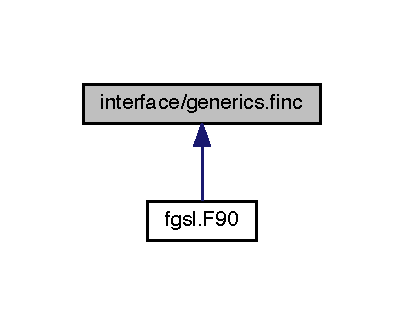
\includegraphics[width=190pt]{generics_8finc__dep__incl}
\end{center}
\end{figure}
\subsection*{Data Types}
\begin{DoxyCompactItemize}
\item 
interface \hyperlink{interfacefgsl__well__defined}{fgsl\+\_\+well\+\_\+defined}
\item 
interface \hyperlink{interfacefgsl__sizeof}{fgsl\+\_\+sizeof}
\item 
interface \hyperlink{interfacefgsl__obj__c__ptr}{fgsl\+\_\+obj\+\_\+c\+\_\+ptr}
\item 
interface \hyperlink{interfaceassignment_07_0A_08}{assignment(=)}
\item 
interface \hyperlink{interfacefgsl__vector__init}{fgsl\+\_\+vector\+\_\+init}
\item 
interface \hyperlink{interfacefgsl__vector__free}{fgsl\+\_\+vector\+\_\+free}
\item 
interface \hyperlink{interfacefgsl__matrix__init}{fgsl\+\_\+matrix\+\_\+init}
\item 
interface \hyperlink{interfacefgsl__matrix__free}{fgsl\+\_\+matrix\+\_\+free}
\item 
interface \hyperlink{interfacefgsl__vector__align}{fgsl\+\_\+vector\+\_\+align}
\item 
interface \hyperlink{interfacefgsl__matrix__align}{fgsl\+\_\+matrix\+\_\+align}
\item 
interface \hyperlink{interfacefgsl__permute}{fgsl\+\_\+permute}
\item 
interface \hyperlink{interfacefgsl__permute__inverse}{fgsl\+\_\+permute\+\_\+inverse}
\item 
interface \hyperlink{interfacefgsl__sort}{fgsl\+\_\+sort}
\item 
interface \hyperlink{interfacefgsl__sort__index}{fgsl\+\_\+sort\+\_\+index}
\item 
interface \hyperlink{interfacefgsl__sort__smallest}{fgsl\+\_\+sort\+\_\+smallest}
\item 
interface \hyperlink{interfacefgsl__sort__smallest__index}{fgsl\+\_\+sort\+\_\+smallest\+\_\+index}
\item 
interface \hyperlink{interfacefgsl__sort__largest}{fgsl\+\_\+sort\+\_\+largest}
\item 
interface \hyperlink{interfacefgsl__sort__largest__index}{fgsl\+\_\+sort\+\_\+largest\+\_\+index}
\item 
interface \hyperlink{interfacefgsl__ran__shuffle}{fgsl\+\_\+ran\+\_\+shuffle}
\item 
interface \hyperlink{interfacefgsl__ieee__fprintf}{fgsl\+\_\+ieee\+\_\+fprintf}
\item 
interface \hyperlink{interfacefgsl__ieee__printf}{fgsl\+\_\+ieee\+\_\+printf}
\item 
interface \hyperlink{interfacefgsl__multifit__fdfsolver__dif__df}{fgsl\+\_\+multifit\+\_\+fdfsolver\+\_\+dif\+\_\+df}
\item 
interface \hyperlink{interfacefgsl__multifit__eval__wf}{fgsl\+\_\+multifit\+\_\+eval\+\_\+wf}
\item 
interface \hyperlink{interfacefgsl__multifit__eval__wdf}{fgsl\+\_\+multifit\+\_\+eval\+\_\+wdf}
\end{DoxyCompactItemize}

\addcontentsline{toc}{part}{Index}
\printindex
\end{document}
